\documentclass{book}
%\usepackage[letterpaper, portrait, margin=1cm]{geometry}
%\usepackage[letterpaper, bindingoffset=0.2in, left=1in,right=1in,top=.5in,bottom=.5in,footskip=.25in,marginparwidth=5em]{geometry}
\usepackage[letterpaper, left=1in,right=1in,top=.5in,bottom=.5in,footskip=.25in,marginparwidth=1cm]{geometry}
% ---------------------
% mini-table-of-content
% ---------------------
\usepackage{minitoc}
\setcounter{minitocdepth}{1}
\setlength{\mtcindent}{24pt}
\setcounter{secnumdepth}{-2}
%\renewcommand{\mtcfont}{\small\rm}
%\renewcommand{\mtcSfont}{\small\bf}
%\usepackage{setspace}
%\usepackage{tocloft}
%\setlength\cftparskip{-1.2pt}
%\setlength\cftbeforesecskip{1.3pt}
%\setlength\cftaftertoctitleskip{2pt}
%\renewcommand{\cftsecafterpnum}{\hspace*{02.0em}}
%\renewcommand{\cftsubsecafterpnum}{\hspace*{02.0em}}

% ---------------------------
% Chinese Characters Packages
% ---------------------------
\usepackage{fontspec} 
\usepackage{xeCJK}
\setmainfont{Times}
\setCJKmainfont{BiauKai}
\newfontfamily\sblgoodhebrew{SBL BibLit}[Script=Hebrew,Contextuals=Alternate]
\newfontfamily\sblgoodgreek{SBL BibLit}[Script=Greek,Contextuals=Alternate]

\usepackage{ifpdf,cite,algorithmic,url,tikz}
\usepackage[cmex10]{amsmath}

% ---------------------------
% Hebrew Characters Packages
% ---------------------------
\usepackage{polyglossia}
\setmainfont{Times New Roman}

% -------
% General
% -------
\usepackage{multicol}
\usepackage{multirow}
\usepackage{color,colortbl}
\usepackage{xparse}
\usepackage{pbox}
\usepackage{stackengine}
\usepackage{titlesec}% http://ctan.org/pkg/titlesec
\usepackage{tabularx}
\usepackage{xltabular}
\usepackage{titlesec}
\usepackage{makecell}
\newcommand{\sectionbreak}{\clearpage}

\author{
  Editor, Michael Chan\\
  \texttt{michaelchan\_wahyan@yahoo.com.hk}
}
\usepackage{tocloft}

\usepackage{hyperref}
\hypersetup{
    colorlinks=true, % set true if you want colored links
    linktoc   =all , % set to all if you want both sections and subsections linked
    linkcolor =blue, % choose some color if you want links to stand out
}

% ----------
% Afterword
% ----------
\usepackage{marginnote}
\usepackage{sectsty}
\usepackage{ragged2e}
\usepackage{lineno}
\usepackage{xcolor}
\usepackage{paracol}

\begin{document}

\clearpage
%% temporary titles
% command to provide stretchy vertical space in proportion
\newcommand\nbvspace[1][3]{\vspace*{\stretch{#1}}}
% allow some slack to avoid under/overfull boxes
\newcommand\nbstretchyspace{\spaceskip0.5em plus 0.25em minus 0.25em}
% To improve spacing on titlepages
\newcommand{\nbtitlestretch}{\spaceskip0.6em}
\pagestyle{empty}
\begin{center}
\bfseries
\nbvspace[1]
\Huge
{%\nbtitlestretch
\Large
\textbf{宣道傳意及出版事工 粵語講道逐字稿 2025-26 \\
       Youtube Channel:  Alliance Communications Ministry
       }}

\nbvspace[1]

{\large
Editor: Michael\\
\texttt{michaelchan\_wahyan@yahoo.com.hk}
}

\nbvspace[1]

{\large
Revision: \texttt{v1.2}\\
Last Update: \today
}


\vfill
\begin{tikzpicture}
    %remove comment for OT cover%\node (0,0) [opacity=0.03]{
\includegraphics[width=15cm]{../bible_out/ot_frontcover.png}} ;
    %remove comment for NT cover%\node (0,0) [opacity=0.03]{\includegraphics[width=15cm]{../bible_out/christ_on_cross.png}} ;
    %remove comment for Bible cover%\node (0,0) [xshift=0.8cm, yshift=+2cm, opacity=0.03]{\includegraphics[width=10cm]{./christ_on_cross.png}} ;
    %remove comment for Bible cover%\node (0,0) [              yshift=-2cm, opacity=0.03]{
\includegraphics[width=14cm]{./ot_frontcover.png}} ;
\end{tikzpicture}
\vfill

\end{center}

\newpage

\setcounter{tocdepth}{0}
\dominitoc
\begin{multicols}{3}
\addtocontents{toc}{\protect\hypertarget{toc}{}}
\tableofcontents
\end{multicols}

\large
%\twocolumn

% the color definition syntax is as follow:
% \definecolor{name}{system}{definition}
% example: a mono-channel color can be defined as
%          \definecolor{Gray}{gray}{0.9}
% example: an rgb-3-channel color can be defined as
%          \definecolor{LightCyan}{rgb}{0.88,1,1}
%          \definecolor{pink}{rgb}{0.68,0,0.68}

\definecolor{CUV1LightRed}{rgb}{1,0.75,0.75}     % for CUV1
\definecolor{LZZVLightGray}{rgb}{0.9,0.9,0.9}    % for LZZ
\definecolor{KJVVLightGreen}{rgb}{0.75,1,0.85}   % for KJV
\definecolor{CUV2LightYellow}{rgb}{1,1,0.75}     % for CUV2
\definecolor{CNVVLightBrown}{rgb}{1,0.85,0.7}    % for CNV
\definecolor{NRSVLightBlue}{rgb}{0.75,1,1}       % for NRSV
\definecolor{WENLLightPurple}{rgb}{0.95,0.85,0.9}% for WENL
\definecolor{TCV19PaleGreen}{rgb}{0.85,1,0.95}   % for TCV19
\definecolor{MSGVLightWhite}{rgb}{0.98,0.98,0.98}% for MSGV
\definecolor{NETSLightRed}{rgb}{1,0.75,0.75}     % for NETS
\definecolor{JPS1917LightYellow}{rgb}{1,1,0.75}  % for JPS1917
\definecolor{SBLGNTPaleRed}{rgb}{1,0.85,0.80}    % for SBLGNT

\section{目錄\small{(順題)}}
\label{sec:index_title}
{ \scriptsize


\begin{xltabular}{\textwidth}{|p{0.15\textwidth} p{0.6\textwidth}|p{0.07\textwidth} p{0.1\textwidth}|}
\hline
箴言   & \hyperref[sec:8bGnissFEEg]{\#新書分享|《潛游於智慧之洋——123篇箴言靈修》|麥耀光牧師|} & 2025-01-23 & \href{https://youtube.com/watch?v=8bGnissFEEg}{\texttt{8bGnissFEEg}} \\
    & \hyperref[sec:fqqhH28LKSk]{「生存」和「生活」,究竟是為了甚麼?(講員:溫偉耀博士)} & 2025-01-12 & \href{https://youtube.com/watch?v=fqqhH28LKSk}{\texttt{fqqhH28LKSk}} \\
    & \hyperref[sec:LJqrc9hl48o]{「要 ? 不要 ?」的人生 2(講員:劉立武牧師)} & 2025-02-19 & \href{https://youtube.com/watch?v=LJqrc9hl48o}{\texttt{LJqrc9hl48o}} \\
    & \hyperref[sec:orqqBPvNXw0]{「要 ? 不要 ?」的人生(講員:劉立武牧師)} & 2025-02-19 & \href{https://youtube.com/watch?v=orqqBPvNXw0}{\texttt{orqqBPvNXw0}} \\
    & \hyperref[sec:zN9v_5CdyLI]{不再懼怕(講員:溫偉耀博士)} & 2025-02-19 & \href{https://youtube.com/watch?v=zN9v-5CdyLI}{\texttt{zN9v-5CdyLI}} \\
    & \hyperref[sec:zYtu_hEpNiM]{不出賣道德人格的信仰(講員:溫偉耀博士)} & 2025-01-27 & \href{https://youtube.com/watch?v=zYtu_hEpNiM}{\texttt{zYtu\_hEpNiM}} \\
    & \hyperref[sec:U6isuM74qVU]{不要沉睡(講員:蕭壽華牧師)} & 2025-03-27 & \href{https://youtube.com/watch?v=U6isuM74qVU}{\texttt{U6isuM74qVU}} \\
    & \hyperref[sec:GPrT6U1NahU]{主耶穌所行的神蹟(講員:溫偉耀博士)} & 2025-03-09 & \href{https://youtube.com/watch?v=GPrT6U1NahU}{\texttt{GPrT6U1NahU}} \\
    & \hyperref[sec:aGr6ZT2aWY0]{主耶穌的禱告生活(講員:溫偉耀博士)} & 2025-03-06 & \href{https://youtube.com/watch?v=aGr6ZT2aWY0}{\texttt{aGr6ZT2aWY0}} \\
    & \hyperref[sec:4raVBWVTkH4]{主耶穌的禱告生活(講員:蕭壽華牧師)} & 2025-01-13 & \href{https://youtube.com/watch?v=4raVBWVTkH4}{\texttt{4raVBWVTkH4}} \\
    & \hyperref[sec:hKsfSsPrx6c]{人喜樂的原因(講員: 梁志聰神學生)} & 2025-02-14 & \href{https://youtube.com/watch?v=hKsfSsPrx6c}{\texttt{hKsfSsPrx6c}} \\
    & \hyperref[sec:1kBljexPPp4]{人在,心在,神在(講員:劉立武牧師)} & 2025-02-19 & \href{https://youtube.com/watch?v=1kBljexPPp4}{\texttt{1kBljexPPp4}} \\
    & \hyperref[sec:LGccaaHSYGo]{人的一生和永生(講員: 丘志明牧師)} & 2025-02-14 & \href{https://youtube.com/watch?v=LGccaaHSYGo}{\texttt{LGccaaHSYGo}} \\
    & \hyperref[sec:ngsYfKFR7GQ]{以利亞的掙扎與陰霾(講員:溫偉耀博士)} & 2025-02-14 & \href{https://youtube.com/watch?v=ngsYfKFR7GQ}{\texttt{ngsYfKFR7GQ}} \\
    & \hyperref[sec:J_bn4sNGM3E]{以耶和華為樂(講員:蕭壽華牧師)} & 2025-01-27 & \href{https://youtube.com/watch?v=J_bn4sNGM3E}{\texttt{J\_bn4sNGM3E}} \\
    & \hyperref[sec:Vfcgy71ypjM]{你是誰的奴僕(講員:溫偉耀博士)} & 2025-03-21 & \href{https://youtube.com/watch?v=Vfcgy71ypjM}{\texttt{Vfcgy71ypjM}} \\
    & \hyperref[sec:qsDdPi_dD4A]{你真知道所信的是誰?(講員:微光傳道)} & 2025-01-14 & \href{https://youtube.com/watch?v=qsDdPi-dD4A}{\texttt{qsDdPi-dD4A}} \\
    & \hyperref[sec:kwMXnh6wxMc]{你總要付的代價(講員: 賀志勇傳道)} & 2025-02-14 & \href{https://youtube.com/watch?v=kwMXnh6wxMc}{\texttt{kwMXnh6wxMc}} \\
    & \hyperref[sec:Ml5MykmoNU8]{信仰有問題|EP10|謝甘霖博士|金句式經文問題在於?|查經,釋經,靈修有咩唔同?} & 2025-02-24 & \href{https://youtube.com/watch?v=Ml5MykmoNU8}{\texttt{Ml5MykmoNU8}} \\
路加福音 14:25-35 & \hyperref[sec:KCI5jFUT58A]{信仰的代價是沉重的嗎?【路加福音14\_25-35】(講員:阮成國牧師)} & 2025-01-13 & \href{https://youtube.com/watch?v=KCI5jFUT58A}{\texttt{KCI5jFUT58A}} \\
    & \hyperref[sec:iG4wtjvLnxk]{信耶穌真好(講員:溫偉耀博士)} & 2025-03-28 & \href{https://youtube.com/watch?v=iG4wtjvLnxk}{\texttt{iG4wtjvLnxk}} \\
    & \hyperref[sec:acPeIDvrkpM]{信靠順服主得勝(講員:蕭壽華牧師)} & 2025-02-28 & \href{https://youtube.com/watch?v=acPeIDvrkpM}{\texttt{acPeIDvrkpM}} \\
    & \hyperref[sec:9AH79u6nzv0]{公義能力惟獨在乎耶和華(講員:蕭壽華牧師)} & 2025-02-21 & \href{https://youtube.com/watch?v=9AH79u6nzv0}{\texttt{9AH79u6nzv0}} \\
    & \hyperref[sec:hdbWHV6areY]{剛強踐行真理(講員:蕭壽華牧師)} & 2025-02-10 & \href{https://youtube.com/watch?v=hdbWHV6areY}{\texttt{hdbWHV6areY}} \\
    & \hyperref[sec:zuzAwb7hPRM]{受苦的榜樣(講員:溫偉耀博士)} & 2025-03-28 & \href{https://youtube.com/watch?v=zuzAwb7hPRM}{\texttt{zuzAwb7hPRM}} \\
    & \hyperref[sec:tgTnfiK4ZKk]{受苦鍛鍊出來的得勝生活(講員:溫偉耀博士)} & 2025-01-08 & \href{https://youtube.com/watch?v=tgTnfiK4ZKk}{\texttt{tgTnfiK4ZKk}} \\
    & \hyperref[sec:HOOP7aoFOM0]{另一條路,而不是絕路(講員:溫偉耀博士)} & 2025-01-17 & \href{https://youtube.com/watch?v=HOOP7aoFOM0}{\texttt{HOOP7aoFOM0}} \\
    & \hyperref[sec:cgvOihZZtJg]{同伴 x 羈絆(講員:劉立武牧師)} & 2025-02-19 & \href{https://youtube.com/watch?v=cgvOihZZtJg}{\texttt{cgvOihZZtJg}} \\
    & \hyperref[sec:OcxA80XebMs]{同來,同哀,同坐(講員:楊靖紀牧師)} & 2025-02-04 & \href{https://youtube.com/watch?v=OcxA80XebMs}{\texttt{OcxA80XebMs}} \\
    & \hyperref[sec:3bH1aeUVS48]{同心建造裡面的聖殿(講員:滕近輝牧師)} & 2025-03-27 & \href{https://youtube.com/watch?v=3bH1aeUVS48}{\texttt{3bH1aeUVS48}} \\
    & \hyperref[sec:TEonkp3tw2Q]{向眾人行善(講員:蕭壽華牧師)} & 2025-03-31 & \href{https://youtube.com/watch?v=TEonkp3tw2Q}{\texttt{TEonkp3tw2Q}} \\
    & \hyperref[sec:74TBpGzKHaM]{呼吸 x 值得(講員:劉立武牧師)} & 2025-02-19 & \href{https://youtube.com/watch?v=74TBpGzKHaM}{\texttt{74TBpGzKHaM}} \\
    & \hyperref[sec:PjXchLqu6SM]{啟示苦難之謎的神(講員:楊靖紀牧師)} & 2025-02-24 & \href{https://youtube.com/watch?v=PjXchLqu6SM}{\texttt{PjXchLqu6SM}} \\
    & \hyperref[sec:feIl6FWBiog]{喜悅施恩的上帝(講員:蕭壽華牧師)} & 2025-02-06 & \href{https://youtube.com/watch?v=feIl6FWBiog}{\texttt{feIl6FWBiog}} \\
    & \hyperref[sec:QKYRS_WDfas]{回歸神的挑戰和呼喚(講員:溫偉耀博士)} & 2025-03-21 & \href{https://youtube.com/watch?v=QKYRS-WDfas}{\texttt{QKYRS-WDfas}} \\
    & \hyperref[sec:Oy3xrS8gf_c]{在信中領受聖靈(講員:蕭壽華牧師)} & 2025-02-04 & \href{https://youtube.com/watch?v=Oy3xrS8gf-c}{\texttt{Oy3xrS8gf-c}} \\
    & \hyperref[sec:aGL0zAIeHPQ]{在光明中同行(講員:蕭壽華牧師)} & 2025-02-21 & \href{https://youtube.com/watch?v=aGL0zAIeHPQ}{\texttt{aGL0zAIeHPQ}} \\
    & \hyperref[sec:_nM8ndHAo3w]{在崗位上作主門徒(講員:蕭壽華牧師)} & 2025-01-20 & \href{https://youtube.com/watch?v=-nM8ndHAo3w}{\texttt{-nM8ndHAo3w}} \\
    & \hyperref[sec:HDh9t31qf5A]{在涼薄殘酷社會中的愛的故事(講員:溫偉耀博士)} & 2025-01-10 & \href{https://youtube.com/watch?v=HDh9t31qf5A}{\texttt{HDh9t31qf5A}} \\
    & \hyperref[sec:0OY0d6UU9H8]{在至聖真道上造就自己(講員:蕭壽華牧師)} & 2025-02-28 & \href{https://youtube.com/watch?v=0OY0d6UU9H8}{\texttt{0OY0d6UU9H8}} \\
    & \hyperref[sec:_kEYXPIaggo]{在迷惑中持守信心到底(講員:蕭壽華牧師)} & 2025-03-20 & \href{https://youtube.com/watch?v=-kEYXPIaggo}{\texttt{-kEYXPIaggo}} \\
    & \hyperref[sec:V_msDX1DjUQ]{基督教會模式縱橫談(講員:溫偉耀博士)} & 2025-02-04 & \href{https://youtube.com/watch?v=V_msDX1DjUQ}{\texttt{V\_msDX1DjUQ}} \\
    & \hyperref[sec:bsgmoTJYu5g]{基督的靈永遠與我同在(講員:蕭壽華牧師)} & 2025-03-10 & \href{https://youtube.com/watch?v=bsgmoTJYu5g}{\texttt{bsgmoTJYu5g}} \\
    & \hyperref[sec:6scsoPLXxKs]{多元化社會中的遷就與堅持(講員:蕭壽華牧師)} & 2025-02-13 & \href{https://youtube.com/watch?v=6scsoPLXxKs}{\texttt{6scsoPLXxKs}} \\
    & \hyperref[sec:gMrpGRyMhZs]{天地的主基督(講員:蕭壽華牧師)} & 2025-03-11 & \href{https://youtube.com/watch?v=gMrpGRyMhZs}{\texttt{gMrpGRyMhZs}} \\
    & \hyperref[sec:COzuuI8DpxQ]{天外來客——重尋失去了的平安 (講員:溫偉耀博士)} & 2025-02-27 & \href{https://youtube.com/watch?v=COzuuI8DpxQ}{\texttt{COzuuI8DpxQ}} \\
    & \hyperref[sec:s6xUj67EP48]{好撒瑪利亞人好在哪裡?(講員: 賀志勇傳道)} & 2025-02-14 & \href{https://youtube.com/watch?v=s6xUj67EP48}{\texttt{s6xUj67EP48}} \\
腓立比書 4:1-23 & \hyperref[sec:_vJtLavJH2I]{如何在逆境中得著真正的平安【腓立比書4\_1-23】(講員:阮成國牧師)} & 2025-02-03 & \href{https://youtube.com/watch?v=-vJtLavJH2I}{\texttt{-vJtLavJH2I}} \\
使徒行傳 4:1-12 & \hyperref[sec:wRMwHzmWpBQ]{如何知道耶穌已復活了?【使徒行傳4\_1-12】(講員:阮成國牧師)} & 2025-02-21 & \href{https://youtube.com/watch?v=wRMwHzmWpBQ}{\texttt{wRMwHzmWpBQ}} \\
    & \hyperref[sec:GCynJz1sHAo]{定局(講員:劉立武牧師)} & 2025-02-19 & \href{https://youtube.com/watch?v=GCynJz1sHAo}{\texttt{GCynJz1sHAo}} \\
    & \hyperref[sec:FK3yHR8bgk0]{定時(講員:劉立武牧師)} & 2025-01-21 & \href{https://youtube.com/watch?v=FK3yHR8bgk0}{\texttt{FK3yHR8bgk0}} \\
    & \hyperref[sec:_CO6yMvWJ40]{家的盼望(講員:賀志勇傳道)} & 2025-01-14 & \href{https://youtube.com/watch?v=_CO6yMvWJ40}{\texttt{\_CO6yMvWJ40}} \\
    & \hyperref[sec:Oa1rBXqNweo]{專心尋求神,看見神的手(講員:溫偉耀博士)} & 2025-02-11 & \href{https://youtube.com/watch?v=Oa1rBXqNweo}{\texttt{Oa1rBXqNweo}} \\
    & \hyperref[sec:nthk651cZA0]{屬靈生命的十大關鍵——第 01 講(講員:滕近輝牧師)} & 2025-02-15 & \href{https://youtube.com/watch?v=nthk651cZA0}{\texttt{nthk651cZA0}} \\
    & \hyperref[sec:5_Aa6o34ukk]{屬靈生命的十大關鍵——第 02 講(講員:滕近輝牧師)} & 2025-02-15 & \href{https://youtube.com/watch?v=5_Aa6o34ukk}{\texttt{5\_Aa6o34ukk}} \\
    & \hyperref[sec:rT8dVCIegOQ]{屬靈生命的十大關鍵——第 03 講(講員:滕近輝牧師)} & 2025-02-15 & \href{https://youtube.com/watch?v=rT8dVCIegOQ}{\texttt{rT8dVCIegOQ}} \\
    & \hyperref[sec:DH2zD8HgZ0o]{屬靈生命的十大關鍵——第 04 講(講員:滕近輝牧師)} & 2025-02-15 & \href{https://youtube.com/watch?v=DH2zD8HgZ0o}{\texttt{DH2zD8HgZ0o}} \\
    & \hyperref[sec:NYe36mKzwsw]{屬靈生命的十大關鍵——第 05 講(講員:滕近輝牧師)} & 2025-02-15 & \href{https://youtube.com/watch?v=NYe36mKzwsw}{\texttt{NYe36mKzwsw}} \\
    & \hyperref[sec:iSZWdeKlirk]{屬靈生命的十大關鍵——第 06 講(講員:滕近輝牧師)} & 2025-02-15 & \href{https://youtube.com/watch?v=iSZWdeKlirk}{\texttt{iSZWdeKlirk}} \\
    & \hyperref[sec:kf8IdqLSGgo]{屬靈的呼聲(講員:滕近輝牧師)} & 2025-03-10 & \href{https://youtube.com/watch?v=kf8IdqLSGgo}{\texttt{kf8IdqLSGgo}} \\
    & \hyperref[sec:vn6NaMi2lw8]{屬靈的爭戰(講員:溫偉耀博士)} & 2025-01-16 & \href{https://youtube.com/watch?v=vn6NaMi2lw8}{\texttt{vn6NaMi2lw8}} \\
    & \hyperref[sec:DLDi5AFAw3c]{彼此守望,同心禱告(講員:蕭壽華牧師)} & 2025-03-14 & \href{https://youtube.com/watch?v=DLDi5AFAw3c}{\texttt{DLDi5AFAw3c}} \\
    & \hyperref[sec:E3IyhrQQkPc]{得勝有餘的經歷(講員:溫偉耀博士)} & 2025-02-26 & \href{https://youtube.com/watch?v=E3IyhrQQkPc}{\texttt{E3IyhrQQkPc}} \\
    & \hyperref[sec:egq2sP_95d0]{從信心和盼望而來的生命力(講員:溫偉耀博士)} & 2025-03-03 & \href{https://youtube.com/watch?v=egq2sP_95d0}{\texttt{egq2sP\_95d0}} \\
歌羅西書 3:12-4:1 & \hyperref[sec:8TqUg0pNX8I]{從空虛到豐盛的生命【歌羅西書3\_12-4\_1】(講員:阮成國牧師)} & 2025-02-03 & \href{https://youtube.com/watch?v=8TqUg0pNX8I}{\texttt{8TqUg0pNX8I}} \\
    & \hyperref[sec:zQEnAAlxyc4]{從追逐財富到奉獻的生命(講員:溫偉耀博士)} & 2025-01-24 & \href{https://youtube.com/watch?v=zQEnAAlxyc4}{\texttt{zQEnAAlxyc4}} \\
    & \hyperref[sec:SvsC2KUaafw]{忍耐艱難的末世教會(講員:蕭壽華牧師)} & 2025-01-21 & \href{https://youtube.com/watch?v=SvsC2KUaafw}{\texttt{SvsC2KUaafw}} \\
    & \hyperref[sec:4oQivp4xGAE]{愛,信心與代求(講員:蕭壽華牧師)} & 2025-04-01 & \href{https://youtube.com/watch?v=4oQivp4xGAE}{\texttt{4oQivp4xGAE}} \\
    & \hyperref[sec:P5krMppFFpc]{愛才是永遠常存的(講員:蕭壽華牧師)} & 2025-03-21 & \href{https://youtube.com/watch?v=P5krMppFFpc}{\texttt{P5krMppFFpc}} \\
    & \hyperref[sec:JjyVY_rYfM4]{我們都需要「同行者」(講員:溫偉耀博士)} & 2025-03-17 & \href{https://youtube.com/watch?v=JjyVY_rYfM4}{\texttt{JjyVY\_rYfM4}} \\
    & \hyperref[sec:xqMpUgphfTQ]{我向你們所做的,你們明白嗎?(講員:楊靖紀牧師)} & 2025-03-10 & \href{https://youtube.com/watch?v=xqMpUgphfTQ}{\texttt{xqMpUgphfTQ}} \\
    & \hyperref[sec:qIKWE5r6wu0]{我怎能不親近神(講員:蕭壽華牧師)} & 2025-03-06 & \href{https://youtube.com/watch?v=qIKWE5r6wu0}{\texttt{qIKWE5r6wu0}} \\
    & \hyperref[sec:hMSSQbSQfrU]{我有所要,我有所求(講員:蕭壽華牧師)} & 2025-02-24 & \href{https://youtube.com/watch?v=hMSSQbSQfrU}{\texttt{hMSSQbSQfrU}} \\
    & \hyperref[sec:5bipFMRUTm0]{我還有勇氣向前闖嗎(講員:溫偉耀博士)} & 2025-02-14 & \href{https://youtube.com/watch?v=5bipFMRUTm0}{\texttt{5bipFMRUTm0}} \\
    & \hyperref[sec:utzTifZGaps]{承認主耶穌的名(講員:蕭壽華牧師)} & 2025-04-01 & \href{https://youtube.com/watch?v=utzTifZGaps}{\texttt{utzTifZGaps}} \\
路加福音 18:31-19:10 & \hyperref[sec:nYOq4Ul9fCk]{救恩的真正意義【路加福音18\_31-19\_10】(講員:阮成國牧師)} & 2025-02-18 & \href{https://youtube.com/watch?v=nYOq4Ul9fCk}{\texttt{nYOq4Ul9fCk}} \\
    & \hyperref[sec:6QSE_20ZcZk]{教會生活信息——團契生活——第 01 講(講員:滕近輝牧師)} & 2025-03-11 & \href{https://youtube.com/watch?v=6QSE_20ZcZk}{\texttt{6QSE\_20ZcZk}} \\
    & \hyperref[sec:Y4v77aj_Qrk]{教會生活信息——團契生活——第 02 講(講員:滕近輝牧師)} & 2025-03-11 & \href{https://youtube.com/watch?v=Y4v77aj_Qrk}{\texttt{Y4v77aj\_Qrk}} \\
    & \hyperref[sec:1icf5GUQAXo]{教會生活信息——敬拜生活——第 01 講(講員:滕近輝牧師)} & 2025-03-11 & \href{https://youtube.com/watch?v=1icf5GUQAXo}{\texttt{1icf5GUQAXo}} \\
    & \hyperref[sec:vg3YsiRWYmo]{教會生活信息——敬拜生活——第 02 講(講員:滕近輝牧師)} & 2025-03-11 & \href{https://youtube.com/watch?v=vg3YsiRWYmo}{\texttt{vg3YsiRWYmo}} \\
    & \hyperref[sec:M5OrjsGErj4]{教會生活信息——祈禱生活——第 01 講(講員:滕近輝牧師)} & 2025-03-11 & \href{https://youtube.com/watch?v=M5OrjsGErj4}{\texttt{M5OrjsGErj4}} \\
    & \hyperref[sec:RnYwyq5kZXg]{教會生活信息——祈禱生活——第 02 講(講員:滕近輝牧師)} & 2025-03-11 & \href{https://youtube.com/watch?v=RnYwyq5kZXg}{\texttt{RnYwyq5kZXg}} \\
    & \hyperref[sec:f83rTRX9_DY]{教會生活信息——見證生活——第 01 講(講員:滕近輝牧師)} & 2025-03-11 & \href{https://youtube.com/watch?v=f83rTRX9-DY}{\texttt{f83rTRX9-DY}} \\
    & \hyperref[sec:iHysqqI_Dxk]{教會生活信息——見證生活——第 02 講(講員:滕近輝牧師)} & 2025-03-11 & \href{https://youtube.com/watch?v=iHysqqI-Dxk}{\texttt{iHysqqI-Dxk}} \\
    & \hyperref[sec:f2_dDlt4U1o]{教會生活信息——見證生活——第 03 講(講員:滕近輝牧師)} & 2025-03-11 & \href{https://youtube.com/watch?v=f2-dDlt4U1o}{\texttt{f2-dDlt4U1o}} \\
    & \hyperref[sec:EKxYZ5clELI]{教會紀律——不要縱容邪惡(講員:蕭壽華牧師)} & 2025-01-15 & \href{https://youtube.com/watch?v=EKxYZ5clELI}{\texttt{EKxYZ5clELI}} \\
    & \hyperref[sec:L9WUypq3kWs]{敬畏與漠視(講員: 黃啟生傳道)} & 2025-02-14 & \href{https://youtube.com/watch?v=L9WUypq3kWs}{\texttt{L9WUypq3kWs}} \\
    & \hyperref[sec:r8ub3P5DQJ0]{日光之下(講員:劉立武牧師)} & 2025-01-14 & \href{https://youtube.com/watch?v=r8ub3P5DQJ0}{\texttt{r8ub3P5DQJ0}} \\
    & \hyperref[sec:BaPKvcfNLaA]{是「試探」抑或是「試煉」? 由你來決定} & 2025-02-03 & \href{https://youtube.com/watch?v=BaPKvcfNLaA}{\texttt{BaPKvcfNLaA}} \\
    & \hyperref[sec:9LfSDTEClj8]{有神呼召的人生(講員:溫偉耀博士)} & 2025-01-20 & \href{https://youtube.com/watch?v=9LfSDTEClj8}{\texttt{9LfSDTEClj8}} \\
    & \hyperref[sec:VSRlXOjmI3k]{榮耀的勝利——第 01 講(講員:滕近輝牧師)} & 2025-03-17 & \href{https://youtube.com/watch?v=VSRlXOjmI3k}{\texttt{VSRlXOjmI3k}} \\
    & \hyperref[sec:f7Di6PlJqq0]{榮耀的勝利——第 02 講(講員:滕近輝牧師)} & 2025-03-17 & \href{https://youtube.com/watch?v=f7Di6PlJqq0}{\texttt{f7Di6PlJqq0}} \\
    & \hyperref[sec:Y8Lq3e7QUyY]{榮耀的勝利——第 03 講(講員:滕近輝牧師)} & 2025-03-17 & \href{https://youtube.com/watch?v=Y8Lq3e7QUyY}{\texttt{Y8Lq3e7QUyY}} \\
    & \hyperref[sec:0jeh_ITLCfM]{榮耀的勝利——第 04 講(講員:滕近輝牧師)} & 2025-03-17 & \href{https://youtube.com/watch?v=0jeh-ITLCfM}{\texttt{0jeh-ITLCfM}} \\
    & \hyperref[sec:YxRBIzj5yUk]{權柄與信心(講員: 賀志勇傳道)} & 2025-02-14 & \href{https://youtube.com/watch?v=YxRBIzj5yUk}{\texttt{YxRBIzj5yUk}} \\
    & \hyperref[sec:S3TNC6I7cYY]{求使我心傾向你的話(講員:蕭壽華牧師)} & 2025-01-27 & \href{https://youtube.com/watch?v=S3TNC6I7cYY}{\texttt{S3TNC6I7cYY}} \\
    & \hyperref[sec:KTyJtbVOSp0]{活出主愛(講員:楊靖紀牧師)} & 2025-03-24 & \href{https://youtube.com/watch?v=KTyJtbVOSp0}{\texttt{KTyJtbVOSp0}} \\
路加福音 11:33-54 & \hyperref[sec:z_WiwUapNaM]{活出表裡一致的信仰【路加福音11\_33-54】(講員:阮成國牧師)} & 2025-01-06 & \href{https://youtube.com/watch?v=z-WiwUapNaM}{\texttt{z-WiwUapNaM}} \\
    & \hyperref[sec:pqCsPoIpVbc]{活水泉源(講員:蕭壽華牧師)} & 2025-03-26 & \href{https://youtube.com/watch?v=pqCsPoIpVbc}{\texttt{pqCsPoIpVbc}} \\
    & \hyperref[sec:4hQ0msme5PY]{火燒荊棘的呼召(講員:蕭壽華牧師)} & 2025-03-24 & \href{https://youtube.com/watch?v=4hQ0msme5PY}{\texttt{4hQ0msme5PY}} \\
    & \hyperref[sec:0Td9L1uAaPc]{為別人蒙恩而眼紅嗎?(講員:蕭壽華牧師)} & 2025-03-19 & \href{https://youtube.com/watch?v=0Td9L1uAaPc}{\texttt{0Td9L1uAaPc}} \\
    & \hyperref[sec:du8JBRzD18w]{為我受死(講員:楊靖紀牧師)} & 2025-01-02 & \href{https://youtube.com/watch?v=du8JBRzD18w}{\texttt{du8JBRzD18w}} \\
    & \hyperref[sec:CiTS3kSY3dc]{為神的道剛強(講員:蕭壽華牧師)} & 2025-03-14 & \href{https://youtube.com/watch?v=CiTS3kSY3dc}{\texttt{CiTS3kSY3dc}} \\
    & \hyperref[sec:N0HxBwqLjq4]{無定(講員:劉立武牧師)} & 2025-02-15 & \href{https://youtube.com/watch?v=N0HxBwqLjq4}{\texttt{N0HxBwqLjq4}} \\
    & \hyperref[sec:2s_2KKNcTz0]{無常(講員:劉立武牧師)} & 2025-02-06 & \href{https://youtube.com/watch?v=2s-2KKNcTz0}{\texttt{2s-2KKNcTz0}} \\
    & \hyperref[sec:hfi4kKo8Woc]{父在信主的人身上作大事(講員:蕭壽華牧師)} & 2025-03-05 & \href{https://youtube.com/watch?v=hfi4kKo8Woc}{\texttt{hfi4kKo8Woc}} \\
    & \hyperref[sec:ehlNasRc2KM]{獻上最好的(講員:蕭壽華牧師)} & 2025-04-02 & \href{https://youtube.com/watch?v=ehlNasRc2KM}{\texttt{ehlNasRc2KM}} \\
路加福音 18:1-14 & \hyperref[sec:wRjql45QKus]{甚麼是信心的祈禱【路加福音18\_1-14】(講員:阮成國牧師)} & 2025-01-27 & \href{https://youtube.com/watch?v=wRjql45QKus}{\texttt{wRjql45QKus}} \\
    & \hyperref[sec:08_UCG_4TFk]{生命與使命(講員:溫偉耀博士)} & 2025-02-24 & \href{https://youtube.com/watch?v=08_UCG_4TFk}{\texttt{08\_UCG\_4TFk}} \\
    & \hyperref[sec:YkJ1Z7X2ACU]{當存敬畏的心敬拜主(講員:蕭壽華牧師)} & 2025-02-05 & \href{https://youtube.com/watch?v=YkJ1Z7X2ACU}{\texttt{YkJ1Z7X2ACU}} \\
    & \hyperref[sec:dSto7HEe9zY]{當心跌倒(講員:蕭壽華牧師)} & 2025-03-18 & \href{https://youtube.com/watch?v=dSto7HEe9zY}{\texttt{dSto7HEe9zY}} \\
    & \hyperref[sec:TeAElIBfx5E]{當珍惜主的話(講員:蕭壽華牧師)} & 2025-03-04 & \href{https://youtube.com/watch?v=TeAElIBfx5E}{\texttt{TeAElIBfx5E}} \\
    & \hyperref[sec:TF_DD5lQWrA]{盡力尋求與家人復和(講員:蕭壽華牧師)} & 2025-01-27 & \href{https://youtube.com/watch?v=TF-DD5lQWrA}{\texttt{TF-DD5lQWrA}} \\
    & \hyperref[sec:HATs5dNPyLc]{盼望與堅持(講員:溫偉耀博士)} & 2025-02-21 & \href{https://youtube.com/watch?v=HATs5dNPyLc}{\texttt{HATs5dNPyLc}} \\
    & \hyperref[sec:AwnMN0uz5bM]{看顧人的神(講員: 倪步曉博士)} & 2025-02-14 & \href{https://youtube.com/watch?v=AwnMN0uz5bM}{\texttt{AwnMN0uz5bM}} \\
    & \hyperref[sec:cR6vfVsSi3c]{知主同行(講員:蘇立言傳道)} & 2025-01-14 & \href{https://youtube.com/watch?v=cR6vfVsSi3c}{\texttt{cR6vfVsSi3c}} \\
    & \hyperref[sec:ihMDk6psINY]{神使用禱告的人(講員:蕭壽華牧師)} & 2025-02-13 & \href{https://youtube.com/watch?v=ihMDk6psINY}{\texttt{ihMDk6psINY}} \\
    & \hyperref[sec:oKdOwgTjkOg]{神工「智慧」(講員:劉立武牧師)} & 2025-01-16 & \href{https://youtube.com/watch?v=oKdOwgTjkOg}{\texttt{oKdOwgTjkOg}} \\
    & \hyperref[sec:ENZaUFphYKc]{神的教訓是生命(講員:蕭壽華牧師)} & 2025-01-27 & \href{https://youtube.com/watch?v=ENZaUFphYKc}{\texttt{ENZaUFphYKc}} \\
使徒行傳 2:25-36 & \hyperref[sec:4lLrCgMya_M]{神的旨意,人的配合【使徒行傳2\_25-36】(講員:阮成國牧師)} & 2025-02-21 & \href{https://youtube.com/watch?v=4lLrCgMya_M}{\texttt{4lLrCgMya\_M}} \\
    & \hyperref[sec:_xvNoEJuYo4]{神臨在的「認出過程」(講員: 倪步曉博士)} & 2025-02-14 & \href{https://youtube.com/watch?v=-xvNoEJuYo4}{\texttt{-xvNoEJuYo4}} \\
    & \hyperref[sec:8yzFcYvBjHs]{神與人同在的大使命(講員: 尹焯君神學生)} & 2025-02-14 & \href{https://youtube.com/watch?v=8yzFcYvBjHs}{\texttt{8yzFcYvBjHs}} \\
    & \hyperref[sec:qjZ0uccsfL0]{第 91 屆港九培靈研經會——講道會——第3講:主再來的預兆(講員:蕭壽華牧師)} & 2025-01-04 & \href{https://youtube.com/watch?v=qjZ0uccsfL0}{\texttt{qjZ0uccsfL0}} \\
    & \hyperref[sec:zzppyTDMTwU]{第 91 屆港九培靈研經會——講道會——第5講:神公義的審判(講員:蕭壽華牧師)} & 2025-01-05 & \href{https://youtube.com/watch?v=zzppyTDMTwU}{\texttt{zzppyTDMTwU}} \\
    & \hyperref[sec:EHWnTlIQ_gc]{第 91 屆港九培靈研經會——講道會——第6講:祂要再來,無懼試驗(講員:蕭壽華牧師)} & 2025-01-06 & \href{https://youtube.com/watch?v=EHWnTlIQ-gc}{\texttt{EHWnTlIQ-gc}} \\
    & \hyperref[sec:xpQ9_zZe8ho]{第 91 屆港九培靈研經會——講道會——第7講:殷勤配合天召(講員:蕭壽華牧師)} & 2025-01-07 & \href{https://youtube.com/watch?v=xpQ9_zZe8ho}{\texttt{xpQ9\_zZe8ho}} \\
    & \hyperref[sec:i0YvGqF5VsE]{第 91 屆港九培靈研經會——講道會——第8講:「主耶穌啊,我願你來!」(講員:蕭壽華牧師)} & 2025-01-08 & \href{https://youtube.com/watch?v=i0YvGqF5VsE}{\texttt{i0YvGqF5VsE}} \\
    & \hyperref[sec:EmPwTBw_fHo]{第 91 屆港九培靈研經會——講道會——第9講:要得神在基督裡從上面召我來得的獎賞(講員:蕭壽華牧師)} & 2025-01-09 & \href{https://youtube.com/watch?v=EmPwTBw_fHo}{\texttt{EmPwTBw\_fHo}} \\
    & \hyperref[sec:s9LVGaFdZr4]{耶和華的日子臨近了(講員:溫偉耀博士)} & 2025-01-27 & \href{https://youtube.com/watch?v=s9LVGaFdZr4}{\texttt{s9LVGaFdZr4}} \\
路加福音 20:1-19 & \hyperref[sec:p1fZhhmYLk4]{耶穌是你生命的主嗎?【路加福音20\_1-19】(講員:阮成國牧師)} & 2025-02-18 & \href{https://youtube.com/watch?v=p1fZhhmYLk4}{\texttt{p1fZhhmYLk4}} \\
    & \hyperref[sec:mFSdWQD1D7I]{聖禮,禮儀,信仰(講員:溫偉耀博士)} & 2025-02-04 & \href{https://youtube.com/watch?v=mFSdWQD1D7I}{\texttt{mFSdWQD1D7I}} \\
    & \hyperref[sec:9S7NRa_M_Sg]{聖靈復生的能力(講員:蕭壽華牧師)} & 2025-01-10 & \href{https://youtube.com/watch?v=9S7NRa_M-Sg}{\texttt{9S7NRa\_M-Sg}} \\
路加福音 9:18-27 & \hyperref[sec:1nChgXA3VNM]{背十架的福氣【路加福音9\_18-27】(講員:阮成國牧師)} & 2025-01-02 & \href{https://youtube.com/watch?v=1nChgXA3VNM}{\texttt{1nChgXA3VNM}} \\
    & \hyperref[sec:ZU0rPcH74Ok]{脫去纏累,專注耶穌(講員:蕭壽華牧師)} & 2025-01-26 & \href{https://youtube.com/watch?v=ZU0rPcH74Ok}{\texttt{ZU0rPcH74Ok}} \\
    & \hyperref[sec:V4G4pNiKVXs]{膽大包添(講員:楊小玲師母)} & 2025-01-14 & \href{https://youtube.com/watch?v=V4G4pNiKVXs}{\texttt{V4G4pNiKVXs}} \\
    & \hyperref[sec:WNZYAGOJigs]{至寶貴的是得著基督(講員:蕭壽華牧師)} & 2025-03-12 & \href{https://youtube.com/watch?v=WNZYAGOJigs}{\texttt{WNZYAGOJigs}} \\
    & \hyperref[sec:sUdjNzq43BQ]{與主聯合在聖靈裡(講員:蕭壽華牧師)} & 2025-03-05 & \href{https://youtube.com/watch?v=sUdjNzq43BQ}{\texttt{sUdjNzq43BQ}} \\
    & \hyperref[sec:Co7KPoYLF2c]{與神同行(講員:溫偉耀博士)} & 2025-01-27 & \href{https://youtube.com/watch?v=Co7KPoYLF2c}{\texttt{Co7KPoYLF2c}} \\
    & \hyperref[sec:JEc2aVEZ4PM]{與苦難共舞(講員:楊靖紀牧師)} & 2025-02-17 & \href{https://youtube.com/watch?v=JEc2aVEZ4PM}{\texttt{JEc2aVEZ4PM}} \\
    & \hyperref[sec:DvC_Z2Ss1HA]{被「看為怪」的末世教會(講員:蕭壽華牧師)} & 2025-01-24 & \href{https://youtube.com/watch?v=DvC_Z2Ss1HA}{\texttt{DvC\_Z2Ss1HA}} \\
使徒行傳 4:23-31 & \hyperref[sec:1WIzZOfhAgM]{被聖靈充滿的生命【使徒行傳4\_23-31】(講員:阮成國牧師)} & 2025-02-21 & \href{https://youtube.com/watch?v=1WIzZOfhAgM}{\texttt{1WIzZOfhAgM}} \\
    & \hyperref[sec:EOT05UT8uYI]{要建立金銀寶石的生命工程(講員:蕭壽華牧師)} & 2025-03-14 & \href{https://youtube.com/watch?v=EOT05UT8uYI}{\texttt{EOT05UT8uYI}} \\
    & \hyperref[sec:8zQDQjtTJg0]{要默想主的話(講員:蕭壽華牧師)} & 2025-01-16 & \href{https://youtube.com/watch?v=8zQDQjtTJg0}{\texttt{8zQDQjtTJg0}} \\
路加福音 16:19-31 & \hyperref[sec:Y0JOMCrwBXs]{財主與拉撒路-不同結局的選擇 【路加福音16\_19-31】(講員:阮成國牧師)} & 2025-01-21 & \href{https://youtube.com/watch?v=Y0JOMCrwBXs}{\texttt{Y0JOMCrwBXs}} \\
    & \hyperref[sec:ihf8o0I48WM]{貧窮與富裕(講員:溫偉耀博士)} & 2025-03-13 & \href{https://youtube.com/watch?v=ihf8o0I48WM}{\texttt{ihf8o0I48WM}} \\
    & \hyperref[sec:k_WEHKUbtZs]{赴羔羊婚筵的有福了(講員:蕭壽華牧師)} & 2025-02-17 & \href{https://youtube.com/watch?v=k-WEHKUbtZs}{\texttt{k-WEHKUbtZs}} \\
列王記上 8:22-53 & \hyperref[sec:n3AcEBuYmdY]{跟從上帝態度的再思【列王記上8\_22-53】(講員:阮成國牧師)} & 2025-02-21 & \href{https://youtube.com/watch?v=n3AcEBuYmdY}{\texttt{n3AcEBuYmdY}} \\
    & \hyperref[sec:52Iml7kITHU]{遇上苦難的敬虔者(講員:楊靖紀牧師)} & 2025-01-06 & \href{https://youtube.com/watch?v=52Iml7kITHU}{\texttt{52Iml7kITHU}} \\
    & \hyperref[sec:Al1dyye6vUI]{道成了肉身,住在我們中間(講員:蕭壽華牧師)} & 2025-02-25 & \href{https://youtube.com/watch?v=Al1dyye6vUI}{\texttt{Al1dyye6vUI}} \\
    & \hyperref[sec:o6rKJN5JEeg]{遵從真理又教導人,遵從的人必蒙福(講員:蕭壽華牧師)} & 2025-01-23 & \href{https://youtube.com/watch?v=o6rKJN5JEeg}{\texttt{o6rKJN5JEeg}} \\
    & \hyperref[sec:EAuuFBUY28s]{邁向成長的階梯(講員:蕭壽華牧師)} & 2025-02-04 & \href{https://youtube.com/watch?v=EAuuFBUY28s}{\texttt{EAuuFBUY28s}} \\
    & \hyperref[sec:LR1qrF5un00]{關於事奉的幾個比喻(講員:滕近輝牧師)} & 2025-03-11 & \href{https://youtube.com/watch?v=LR1qrF5un00}{\texttt{LR1qrF5un00}} \\
    & \hyperref[sec:73YrVUzBgOc]{隱藏中施與(講員:蕭壽華牧師)} & 2025-03-25 & \href{https://youtube.com/watch?v=73YrVUzBgOc}{\texttt{73YrVUzBgOc}} \\
    & \hyperref[sec:N7uWuxsecsY]{靠著聖靈守著生命之道(講員:蕭壽華牧師)} & 2025-02-18 & \href{https://youtube.com/watch?v=N7uWuxsecsY}{\texttt{N7uWuxsecsY}} \\
    & \hyperref[sec:Fn9B3iJU0Ts]{順服神話語的敬拜(講員:蕭壽華牧師)} & 2025-02-28 & \href{https://youtube.com/watch?v=Fn9B3iJU0Ts}{\texttt{Fn9B3iJU0Ts}} \\
\end{xltabular}
}
\newpage

\section{目錄\small{(順仕)}}
\label{sec:index_preacher}
{ \scriptsize


\begin{xltabular}{\textwidth}{|p{0.15\textwidth} p{0.6\textwidth}|p{0.07\textwidth} p{0.1\textwidth}|}
\hline
    & \hyperref[sec:BaPKvcfNLaA]{是「試探」抑或是「試煉」? 由你來決定} & 2025-02-03 & \href{https://youtube.com/watch?v=BaPKvcfNLaA}{\texttt{BaPKvcfNLaA}} \\
    & \hyperref[sec:LGccaaHSYGo]{人的一生和永生(講員: 丘志明牧師)} & 2025-02-14 & \href{https://youtube.com/watch?v=LGccaaHSYGo}{\texttt{LGccaaHSYGo}} \\
    & \hyperref[sec:AwnMN0uz5bM]{看顧人的神(講員: 倪步曉博士)} & 2025-02-14 & \href{https://youtube.com/watch?v=AwnMN0uz5bM}{\texttt{AwnMN0uz5bM}} \\
    & \hyperref[sec:_xvNoEJuYo4]{神臨在的「認出過程」(講員: 倪步曉博士)} & 2025-02-14 & \href{https://youtube.com/watch?v=-xvNoEJuYo4}{\texttt{-xvNoEJuYo4}} \\
    & \hyperref[sec:LJqrc9hl48o]{「要 ? 不要 ?」的人生 2(講員:劉立武牧師)} & 2025-02-19 & \href{https://youtube.com/watch?v=LJqrc9hl48o}{\texttt{LJqrc9hl48o}} \\
    & \hyperref[sec:orqqBPvNXw0]{「要 ? 不要 ?」的人生(講員:劉立武牧師)} & 2025-02-19 & \href{https://youtube.com/watch?v=orqqBPvNXw0}{\texttt{orqqBPvNXw0}} \\
    & \hyperref[sec:1kBljexPPp4]{人在,心在,神在(講員:劉立武牧師)} & 2025-02-19 & \href{https://youtube.com/watch?v=1kBljexPPp4}{\texttt{1kBljexPPp4}} \\
    & \hyperref[sec:cgvOihZZtJg]{同伴 x 羈絆(講員:劉立武牧師)} & 2025-02-19 & \href{https://youtube.com/watch?v=cgvOihZZtJg}{\texttt{cgvOihZZtJg}} \\
    & \hyperref[sec:74TBpGzKHaM]{呼吸 x 值得(講員:劉立武牧師)} & 2025-02-19 & \href{https://youtube.com/watch?v=74TBpGzKHaM}{\texttt{74TBpGzKHaM}} \\
    & \hyperref[sec:GCynJz1sHAo]{定局(講員:劉立武牧師)} & 2025-02-19 & \href{https://youtube.com/watch?v=GCynJz1sHAo}{\texttt{GCynJz1sHAo}} \\
    & \hyperref[sec:FK3yHR8bgk0]{定時(講員:劉立武牧師)} & 2025-01-21 & \href{https://youtube.com/watch?v=FK3yHR8bgk0}{\texttt{FK3yHR8bgk0}} \\
    & \hyperref[sec:r8ub3P5DQJ0]{日光之下(講員:劉立武牧師)} & 2025-01-14 & \href{https://youtube.com/watch?v=r8ub3P5DQJ0}{\texttt{r8ub3P5DQJ0}} \\
    & \hyperref[sec:N0HxBwqLjq4]{無定(講員:劉立武牧師)} & 2025-02-15 & \href{https://youtube.com/watch?v=N0HxBwqLjq4}{\texttt{N0HxBwqLjq4}} \\
    & \hyperref[sec:2s_2KKNcTz0]{無常(講員:劉立武牧師)} & 2025-02-06 & \href{https://youtube.com/watch?v=2s-2KKNcTz0}{\texttt{2s-2KKNcTz0}} \\
    & \hyperref[sec:oKdOwgTjkOg]{神工「智慧」(講員:劉立武牧師)} & 2025-01-16 & \href{https://youtube.com/watch?v=oKdOwgTjkOg}{\texttt{oKdOwgTjkOg}} \\
    & \hyperref[sec:8yzFcYvBjHs]{神與人同在的大使命(講員: 尹焯君神學生)} & 2025-02-14 & \href{https://youtube.com/watch?v=8yzFcYvBjHs}{\texttt{8yzFcYvBjHs}} \\
    & \hyperref[sec:qsDdPi_dD4A]{你真知道所信的是誰?(講員:微光傳道)} & 2025-01-14 & \href{https://youtube.com/watch?v=qsDdPi-dD4A}{\texttt{qsDdPi-dD4A}} \\
    & \hyperref[sec:hKsfSsPrx6c]{人喜樂的原因(講員: 梁志聰神學生)} & 2025-02-14 & \href{https://youtube.com/watch?v=hKsfSsPrx6c}{\texttt{hKsfSsPrx6c}} \\
    & \hyperref[sec:V4G4pNiKVXs]{膽大包添(講員:楊小玲師母)} & 2025-01-14 & \href{https://youtube.com/watch?v=V4G4pNiKVXs}{\texttt{V4G4pNiKVXs}} \\
    & \hyperref[sec:OcxA80XebMs]{同來,同哀,同坐(講員:楊靖紀牧師)} & 2025-02-04 & \href{https://youtube.com/watch?v=OcxA80XebMs}{\texttt{OcxA80XebMs}} \\
    & \hyperref[sec:PjXchLqu6SM]{啟示苦難之謎的神(講員:楊靖紀牧師)} & 2025-02-24 & \href{https://youtube.com/watch?v=PjXchLqu6SM}{\texttt{PjXchLqu6SM}} \\
    & \hyperref[sec:xqMpUgphfTQ]{我向你們所做的,你們明白嗎?(講員:楊靖紀牧師)} & 2025-03-10 & \href{https://youtube.com/watch?v=xqMpUgphfTQ}{\texttt{xqMpUgphfTQ}} \\
    & \hyperref[sec:KTyJtbVOSp0]{活出主愛(講員:楊靖紀牧師)} & 2025-03-24 & \href{https://youtube.com/watch?v=KTyJtbVOSp0}{\texttt{KTyJtbVOSp0}} \\
    & \hyperref[sec:du8JBRzD18w]{為我受死(講員:楊靖紀牧師)} & 2025-01-02 & \href{https://youtube.com/watch?v=du8JBRzD18w}{\texttt{du8JBRzD18w}} \\
    & \hyperref[sec:JEc2aVEZ4PM]{與苦難共舞(講員:楊靖紀牧師)} & 2025-02-17 & \href{https://youtube.com/watch?v=JEc2aVEZ4PM}{\texttt{JEc2aVEZ4PM}} \\
    & \hyperref[sec:52Iml7kITHU]{遇上苦難的敬虔者(講員:楊靖紀牧師)} & 2025-01-06 & \href{https://youtube.com/watch?v=52Iml7kITHU}{\texttt{52Iml7kITHU}} \\
    & \hyperref[sec:fqqhH28LKSk]{「生存」和「生活」,究竟是為了甚麼?(講員:溫偉耀博士)} & 2025-01-12 & \href{https://youtube.com/watch?v=fqqhH28LKSk}{\texttt{fqqhH28LKSk}} \\
    & \hyperref[sec:zN9v_5CdyLI]{不再懼怕(講員:溫偉耀博士)} & 2025-02-19 & \href{https://youtube.com/watch?v=zN9v-5CdyLI}{\texttt{zN9v-5CdyLI}} \\
    & \hyperref[sec:zYtu_hEpNiM]{不出賣道德人格的信仰(講員:溫偉耀博士)} & 2025-01-27 & \href{https://youtube.com/watch?v=zYtu_hEpNiM}{\texttt{zYtu\_hEpNiM}} \\
    & \hyperref[sec:GPrT6U1NahU]{主耶穌所行的神蹟(講員:溫偉耀博士)} & 2025-03-09 & \href{https://youtube.com/watch?v=GPrT6U1NahU}{\texttt{GPrT6U1NahU}} \\
    & \hyperref[sec:aGr6ZT2aWY0]{主耶穌的禱告生活(講員:溫偉耀博士)} & 2025-03-06 & \href{https://youtube.com/watch?v=aGr6ZT2aWY0}{\texttt{aGr6ZT2aWY0}} \\
    & \hyperref[sec:ngsYfKFR7GQ]{以利亞的掙扎與陰霾(講員:溫偉耀博士)} & 2025-02-14 & \href{https://youtube.com/watch?v=ngsYfKFR7GQ}{\texttt{ngsYfKFR7GQ}} \\
    & \hyperref[sec:Vfcgy71ypjM]{你是誰的奴僕(講員:溫偉耀博士)} & 2025-03-21 & \href{https://youtube.com/watch?v=Vfcgy71ypjM}{\texttt{Vfcgy71ypjM}} \\
    & \hyperref[sec:iG4wtjvLnxk]{信耶穌真好(講員:溫偉耀博士)} & 2025-03-28 & \href{https://youtube.com/watch?v=iG4wtjvLnxk}{\texttt{iG4wtjvLnxk}} \\
    & \hyperref[sec:zuzAwb7hPRM]{受苦的榜樣(講員:溫偉耀博士)} & 2025-03-28 & \href{https://youtube.com/watch?v=zuzAwb7hPRM}{\texttt{zuzAwb7hPRM}} \\
    & \hyperref[sec:tgTnfiK4ZKk]{受苦鍛鍊出來的得勝生活(講員:溫偉耀博士)} & 2025-01-08 & \href{https://youtube.com/watch?v=tgTnfiK4ZKk}{\texttt{tgTnfiK4ZKk}} \\
    & \hyperref[sec:HOOP7aoFOM0]{另一條路,而不是絕路(講員:溫偉耀博士)} & 2025-01-17 & \href{https://youtube.com/watch?v=HOOP7aoFOM0}{\texttt{HOOP7aoFOM0}} \\
    & \hyperref[sec:QKYRS_WDfas]{回歸神的挑戰和呼喚(講員:溫偉耀博士)} & 2025-03-21 & \href{https://youtube.com/watch?v=QKYRS-WDfas}{\texttt{QKYRS-WDfas}} \\
    & \hyperref[sec:HDh9t31qf5A]{在涼薄殘酷社會中的愛的故事(講員:溫偉耀博士)} & 2025-01-10 & \href{https://youtube.com/watch?v=HDh9t31qf5A}{\texttt{HDh9t31qf5A}} \\
    & \hyperref[sec:V_msDX1DjUQ]{基督教會模式縱橫談(講員:溫偉耀博士)} & 2025-02-04 & \href{https://youtube.com/watch?v=V_msDX1DjUQ}{\texttt{V\_msDX1DjUQ}} \\
    & \hyperref[sec:COzuuI8DpxQ]{天外來客——重尋失去了的平安 (講員:溫偉耀博士)} & 2025-02-27 & \href{https://youtube.com/watch?v=COzuuI8DpxQ}{\texttt{COzuuI8DpxQ}} \\
    & \hyperref[sec:Oa1rBXqNweo]{專心尋求神,看見神的手(講員:溫偉耀博士)} & 2025-02-11 & \href{https://youtube.com/watch?v=Oa1rBXqNweo}{\texttt{Oa1rBXqNweo}} \\
    & \hyperref[sec:vn6NaMi2lw8]{屬靈的爭戰(講員:溫偉耀博士)} & 2025-01-16 & \href{https://youtube.com/watch?v=vn6NaMi2lw8}{\texttt{vn6NaMi2lw8}} \\
    & \hyperref[sec:E3IyhrQQkPc]{得勝有餘的經歷(講員:溫偉耀博士)} & 2025-02-26 & \href{https://youtube.com/watch?v=E3IyhrQQkPc}{\texttt{E3IyhrQQkPc}} \\
    & \hyperref[sec:egq2sP_95d0]{從信心和盼望而來的生命力(講員:溫偉耀博士)} & 2025-03-03 & \href{https://youtube.com/watch?v=egq2sP_95d0}{\texttt{egq2sP\_95d0}} \\
    & \hyperref[sec:zQEnAAlxyc4]{從追逐財富到奉獻的生命(講員:溫偉耀博士)} & 2025-01-24 & \href{https://youtube.com/watch?v=zQEnAAlxyc4}{\texttt{zQEnAAlxyc4}} \\
    & \hyperref[sec:JjyVY_rYfM4]{我們都需要「同行者」(講員:溫偉耀博士)} & 2025-03-17 & \href{https://youtube.com/watch?v=JjyVY_rYfM4}{\texttt{JjyVY\_rYfM4}} \\
    & \hyperref[sec:5bipFMRUTm0]{我還有勇氣向前闖嗎(講員:溫偉耀博士)} & 2025-02-14 & \href{https://youtube.com/watch?v=5bipFMRUTm0}{\texttt{5bipFMRUTm0}} \\
    & \hyperref[sec:9LfSDTEClj8]{有神呼召的人生(講員:溫偉耀博士)} & 2025-01-20 & \href{https://youtube.com/watch?v=9LfSDTEClj8}{\texttt{9LfSDTEClj8}} \\
    & \hyperref[sec:08_UCG_4TFk]{生命與使命(講員:溫偉耀博士)} & 2025-02-24 & \href{https://youtube.com/watch?v=08_UCG_4TFk}{\texttt{08\_UCG\_4TFk}} \\
    & \hyperref[sec:HATs5dNPyLc]{盼望與堅持(講員:溫偉耀博士)} & 2025-02-21 & \href{https://youtube.com/watch?v=HATs5dNPyLc}{\texttt{HATs5dNPyLc}} \\
    & \hyperref[sec:s9LVGaFdZr4]{耶和華的日子臨近了(講員:溫偉耀博士)} & 2025-01-27 & \href{https://youtube.com/watch?v=s9LVGaFdZr4}{\texttt{s9LVGaFdZr4}} \\
    & \hyperref[sec:mFSdWQD1D7I]{聖禮,禮儀,信仰(講員:溫偉耀博士)} & 2025-02-04 & \href{https://youtube.com/watch?v=mFSdWQD1D7I}{\texttt{mFSdWQD1D7I}} \\
    & \hyperref[sec:Co7KPoYLF2c]{與神同行(講員:溫偉耀博士)} & 2025-01-27 & \href{https://youtube.com/watch?v=Co7KPoYLF2c}{\texttt{Co7KPoYLF2c}} \\
    & \hyperref[sec:ihf8o0I48WM]{貧窮與富裕(講員:溫偉耀博士)} & 2025-03-13 & \href{https://youtube.com/watch?v=ihf8o0I48WM}{\texttt{ihf8o0I48WM}} \\
    & \hyperref[sec:3bH1aeUVS48]{同心建造裡面的聖殿(講員:滕近輝牧師)} & 2025-03-27 & \href{https://youtube.com/watch?v=3bH1aeUVS48}{\texttt{3bH1aeUVS48}} \\
    & \hyperref[sec:nthk651cZA0]{屬靈生命的十大關鍵——第 01 講(講員:滕近輝牧師)} & 2025-02-15 & \href{https://youtube.com/watch?v=nthk651cZA0}{\texttt{nthk651cZA0}} \\
    & \hyperref[sec:5_Aa6o34ukk]{屬靈生命的十大關鍵——第 02 講(講員:滕近輝牧師)} & 2025-02-15 & \href{https://youtube.com/watch?v=5_Aa6o34ukk}{\texttt{5\_Aa6o34ukk}} \\
    & \hyperref[sec:rT8dVCIegOQ]{屬靈生命的十大關鍵——第 03 講(講員:滕近輝牧師)} & 2025-02-15 & \href{https://youtube.com/watch?v=rT8dVCIegOQ}{\texttt{rT8dVCIegOQ}} \\
    & \hyperref[sec:DH2zD8HgZ0o]{屬靈生命的十大關鍵——第 04 講(講員:滕近輝牧師)} & 2025-02-15 & \href{https://youtube.com/watch?v=DH2zD8HgZ0o}{\texttt{DH2zD8HgZ0o}} \\
    & \hyperref[sec:NYe36mKzwsw]{屬靈生命的十大關鍵——第 05 講(講員:滕近輝牧師)} & 2025-02-15 & \href{https://youtube.com/watch?v=NYe36mKzwsw}{\texttt{NYe36mKzwsw}} \\
    & \hyperref[sec:iSZWdeKlirk]{屬靈生命的十大關鍵——第 06 講(講員:滕近輝牧師)} & 2025-02-15 & \href{https://youtube.com/watch?v=iSZWdeKlirk}{\texttt{iSZWdeKlirk}} \\
    & \hyperref[sec:kf8IdqLSGgo]{屬靈的呼聲(講員:滕近輝牧師)} & 2025-03-10 & \href{https://youtube.com/watch?v=kf8IdqLSGgo}{\texttt{kf8IdqLSGgo}} \\
    & \hyperref[sec:6QSE_20ZcZk]{教會生活信息——團契生活——第 01 講(講員:滕近輝牧師)} & 2025-03-11 & \href{https://youtube.com/watch?v=6QSE_20ZcZk}{\texttt{6QSE\_20ZcZk}} \\
    & \hyperref[sec:Y4v77aj_Qrk]{教會生活信息——團契生活——第 02 講(講員:滕近輝牧師)} & 2025-03-11 & \href{https://youtube.com/watch?v=Y4v77aj_Qrk}{\texttt{Y4v77aj\_Qrk}} \\
    & \hyperref[sec:1icf5GUQAXo]{教會生活信息——敬拜生活——第 01 講(講員:滕近輝牧師)} & 2025-03-11 & \href{https://youtube.com/watch?v=1icf5GUQAXo}{\texttt{1icf5GUQAXo}} \\
    & \hyperref[sec:vg3YsiRWYmo]{教會生活信息——敬拜生活——第 02 講(講員:滕近輝牧師)} & 2025-03-11 & \href{https://youtube.com/watch?v=vg3YsiRWYmo}{\texttt{vg3YsiRWYmo}} \\
    & \hyperref[sec:M5OrjsGErj4]{教會生活信息——祈禱生活——第 01 講(講員:滕近輝牧師)} & 2025-03-11 & \href{https://youtube.com/watch?v=M5OrjsGErj4}{\texttt{M5OrjsGErj4}} \\
    & \hyperref[sec:RnYwyq5kZXg]{教會生活信息——祈禱生活——第 02 講(講員:滕近輝牧師)} & 2025-03-11 & \href{https://youtube.com/watch?v=RnYwyq5kZXg}{\texttt{RnYwyq5kZXg}} \\
    & \hyperref[sec:f83rTRX9_DY]{教會生活信息——見證生活——第 01 講(講員:滕近輝牧師)} & 2025-03-11 & \href{https://youtube.com/watch?v=f83rTRX9-DY}{\texttt{f83rTRX9-DY}} \\
    & \hyperref[sec:iHysqqI_Dxk]{教會生活信息——見證生活——第 02 講(講員:滕近輝牧師)} & 2025-03-11 & \href{https://youtube.com/watch?v=iHysqqI-Dxk}{\texttt{iHysqqI-Dxk}} \\
    & \hyperref[sec:f2_dDlt4U1o]{教會生活信息——見證生活——第 03 講(講員:滕近輝牧師)} & 2025-03-11 & \href{https://youtube.com/watch?v=f2-dDlt4U1o}{\texttt{f2-dDlt4U1o}} \\
    & \hyperref[sec:VSRlXOjmI3k]{榮耀的勝利——第 01 講(講員:滕近輝牧師)} & 2025-03-17 & \href{https://youtube.com/watch?v=VSRlXOjmI3k}{\texttt{VSRlXOjmI3k}} \\
    & \hyperref[sec:f7Di6PlJqq0]{榮耀的勝利——第 02 講(講員:滕近輝牧師)} & 2025-03-17 & \href{https://youtube.com/watch?v=f7Di6PlJqq0}{\texttt{f7Di6PlJqq0}} \\
    & \hyperref[sec:Y8Lq3e7QUyY]{榮耀的勝利——第 03 講(講員:滕近輝牧師)} & 2025-03-17 & \href{https://youtube.com/watch?v=Y8Lq3e7QUyY}{\texttt{Y8Lq3e7QUyY}} \\
    & \hyperref[sec:0jeh_ITLCfM]{榮耀的勝利——第 04 講(講員:滕近輝牧師)} & 2025-03-17 & \href{https://youtube.com/watch?v=0jeh-ITLCfM}{\texttt{0jeh-ITLCfM}} \\
    & \hyperref[sec:LR1qrF5un00]{關於事奉的幾個比喻(講員:滕近輝牧師)} & 2025-03-11 & \href{https://youtube.com/watch?v=LR1qrF5un00}{\texttt{LR1qrF5un00}} \\
    & \hyperref[sec:U6isuM74qVU]{不要沉睡(講員:蕭壽華牧師)} & 2025-03-27 & \href{https://youtube.com/watch?v=U6isuM74qVU}{\texttt{U6isuM74qVU}} \\
    & \hyperref[sec:4raVBWVTkH4]{主耶穌的禱告生活(講員:蕭壽華牧師)} & 2025-01-13 & \href{https://youtube.com/watch?v=4raVBWVTkH4}{\texttt{4raVBWVTkH4}} \\
    & \hyperref[sec:J_bn4sNGM3E]{以耶和華為樂(講員:蕭壽華牧師)} & 2025-01-27 & \href{https://youtube.com/watch?v=J_bn4sNGM3E}{\texttt{J\_bn4sNGM3E}} \\
    & \hyperref[sec:acPeIDvrkpM]{信靠順服主得勝(講員:蕭壽華牧師)} & 2025-02-28 & \href{https://youtube.com/watch?v=acPeIDvrkpM}{\texttt{acPeIDvrkpM}} \\
    & \hyperref[sec:9AH79u6nzv0]{公義能力惟獨在乎耶和華(講員:蕭壽華牧師)} & 2025-02-21 & \href{https://youtube.com/watch?v=9AH79u6nzv0}{\texttt{9AH79u6nzv0}} \\
    & \hyperref[sec:hdbWHV6areY]{剛強踐行真理(講員:蕭壽華牧師)} & 2025-02-10 & \href{https://youtube.com/watch?v=hdbWHV6areY}{\texttt{hdbWHV6areY}} \\
    & \hyperref[sec:TEonkp3tw2Q]{向眾人行善(講員:蕭壽華牧師)} & 2025-03-31 & \href{https://youtube.com/watch?v=TEonkp3tw2Q}{\texttt{TEonkp3tw2Q}} \\
    & \hyperref[sec:feIl6FWBiog]{喜悅施恩的上帝(講員:蕭壽華牧師)} & 2025-02-06 & \href{https://youtube.com/watch?v=feIl6FWBiog}{\texttt{feIl6FWBiog}} \\
    & \hyperref[sec:Oy3xrS8gf_c]{在信中領受聖靈(講員:蕭壽華牧師)} & 2025-02-04 & \href{https://youtube.com/watch?v=Oy3xrS8gf-c}{\texttt{Oy3xrS8gf-c}} \\
    & \hyperref[sec:aGL0zAIeHPQ]{在光明中同行(講員:蕭壽華牧師)} & 2025-02-21 & \href{https://youtube.com/watch?v=aGL0zAIeHPQ}{\texttt{aGL0zAIeHPQ}} \\
    & \hyperref[sec:_nM8ndHAo3w]{在崗位上作主門徒(講員:蕭壽華牧師)} & 2025-01-20 & \href{https://youtube.com/watch?v=-nM8ndHAo3w}{\texttt{-nM8ndHAo3w}} \\
    & \hyperref[sec:0OY0d6UU9H8]{在至聖真道上造就自己(講員:蕭壽華牧師)} & 2025-02-28 & \href{https://youtube.com/watch?v=0OY0d6UU9H8}{\texttt{0OY0d6UU9H8}} \\
    & \hyperref[sec:_kEYXPIaggo]{在迷惑中持守信心到底(講員:蕭壽華牧師)} & 2025-03-20 & \href{https://youtube.com/watch?v=-kEYXPIaggo}{\texttt{-kEYXPIaggo}} \\
    & \hyperref[sec:bsgmoTJYu5g]{基督的靈永遠與我同在(講員:蕭壽華牧師)} & 2025-03-10 & \href{https://youtube.com/watch?v=bsgmoTJYu5g}{\texttt{bsgmoTJYu5g}} \\
    & \hyperref[sec:6scsoPLXxKs]{多元化社會中的遷就與堅持(講員:蕭壽華牧師)} & 2025-02-13 & \href{https://youtube.com/watch?v=6scsoPLXxKs}{\texttt{6scsoPLXxKs}} \\
    & \hyperref[sec:gMrpGRyMhZs]{天地的主基督(講員:蕭壽華牧師)} & 2025-03-11 & \href{https://youtube.com/watch?v=gMrpGRyMhZs}{\texttt{gMrpGRyMhZs}} \\
    & \hyperref[sec:DLDi5AFAw3c]{彼此守望,同心禱告(講員:蕭壽華牧師)} & 2025-03-14 & \href{https://youtube.com/watch?v=DLDi5AFAw3c}{\texttt{DLDi5AFAw3c}} \\
    & \hyperref[sec:SvsC2KUaafw]{忍耐艱難的末世教會(講員:蕭壽華牧師)} & 2025-01-21 & \href{https://youtube.com/watch?v=SvsC2KUaafw}{\texttt{SvsC2KUaafw}} \\
    & \hyperref[sec:4oQivp4xGAE]{愛,信心與代求(講員:蕭壽華牧師)} & 2025-04-01 & \href{https://youtube.com/watch?v=4oQivp4xGAE}{\texttt{4oQivp4xGAE}} \\
    & \hyperref[sec:P5krMppFFpc]{愛才是永遠常存的(講員:蕭壽華牧師)} & 2025-03-21 & \href{https://youtube.com/watch?v=P5krMppFFpc}{\texttt{P5krMppFFpc}} \\
    & \hyperref[sec:qIKWE5r6wu0]{我怎能不親近神(講員:蕭壽華牧師)} & 2025-03-06 & \href{https://youtube.com/watch?v=qIKWE5r6wu0}{\texttt{qIKWE5r6wu0}} \\
    & \hyperref[sec:hMSSQbSQfrU]{我有所要,我有所求(講員:蕭壽華牧師)} & 2025-02-24 & \href{https://youtube.com/watch?v=hMSSQbSQfrU}{\texttt{hMSSQbSQfrU}} \\
    & \hyperref[sec:utzTifZGaps]{承認主耶穌的名(講員:蕭壽華牧師)} & 2025-04-01 & \href{https://youtube.com/watch?v=utzTifZGaps}{\texttt{utzTifZGaps}} \\
    & \hyperref[sec:EKxYZ5clELI]{教會紀律——不要縱容邪惡(講員:蕭壽華牧師)} & 2025-01-15 & \href{https://youtube.com/watch?v=EKxYZ5clELI}{\texttt{EKxYZ5clELI}} \\
    & \hyperref[sec:S3TNC6I7cYY]{求使我心傾向你的話(講員:蕭壽華牧師)} & 2025-01-27 & \href{https://youtube.com/watch?v=S3TNC6I7cYY}{\texttt{S3TNC6I7cYY}} \\
    & \hyperref[sec:pqCsPoIpVbc]{活水泉源(講員:蕭壽華牧師)} & 2025-03-26 & \href{https://youtube.com/watch?v=pqCsPoIpVbc}{\texttt{pqCsPoIpVbc}} \\
    & \hyperref[sec:4hQ0msme5PY]{火燒荊棘的呼召(講員:蕭壽華牧師)} & 2025-03-24 & \href{https://youtube.com/watch?v=4hQ0msme5PY}{\texttt{4hQ0msme5PY}} \\
    & \hyperref[sec:0Td9L1uAaPc]{為別人蒙恩而眼紅嗎?(講員:蕭壽華牧師)} & 2025-03-19 & \href{https://youtube.com/watch?v=0Td9L1uAaPc}{\texttt{0Td9L1uAaPc}} \\
    & \hyperref[sec:CiTS3kSY3dc]{為神的道剛強(講員:蕭壽華牧師)} & 2025-03-14 & \href{https://youtube.com/watch?v=CiTS3kSY3dc}{\texttt{CiTS3kSY3dc}} \\
    & \hyperref[sec:hfi4kKo8Woc]{父在信主的人身上作大事(講員:蕭壽華牧師)} & 2025-03-05 & \href{https://youtube.com/watch?v=hfi4kKo8Woc}{\texttt{hfi4kKo8Woc}} \\
    & \hyperref[sec:ehlNasRc2KM]{獻上最好的(講員:蕭壽華牧師)} & 2025-04-02 & \href{https://youtube.com/watch?v=ehlNasRc2KM}{\texttt{ehlNasRc2KM}} \\
    & \hyperref[sec:YkJ1Z7X2ACU]{當存敬畏的心敬拜主(講員:蕭壽華牧師)} & 2025-02-05 & \href{https://youtube.com/watch?v=YkJ1Z7X2ACU}{\texttt{YkJ1Z7X2ACU}} \\
    & \hyperref[sec:dSto7HEe9zY]{當心跌倒(講員:蕭壽華牧師)} & 2025-03-18 & \href{https://youtube.com/watch?v=dSto7HEe9zY}{\texttt{dSto7HEe9zY}} \\
    & \hyperref[sec:TeAElIBfx5E]{當珍惜主的話(講員:蕭壽華牧師)} & 2025-03-04 & \href{https://youtube.com/watch?v=TeAElIBfx5E}{\texttt{TeAElIBfx5E}} \\
    & \hyperref[sec:TF_DD5lQWrA]{盡力尋求與家人復和(講員:蕭壽華牧師)} & 2025-01-27 & \href{https://youtube.com/watch?v=TF-DD5lQWrA}{\texttt{TF-DD5lQWrA}} \\
    & \hyperref[sec:ihMDk6psINY]{神使用禱告的人(講員:蕭壽華牧師)} & 2025-02-13 & \href{https://youtube.com/watch?v=ihMDk6psINY}{\texttt{ihMDk6psINY}} \\
    & \hyperref[sec:ENZaUFphYKc]{神的教訓是生命(講員:蕭壽華牧師)} & 2025-01-27 & \href{https://youtube.com/watch?v=ENZaUFphYKc}{\texttt{ENZaUFphYKc}} \\
    & \hyperref[sec:qjZ0uccsfL0]{第 91 屆港九培靈研經會——講道會——第3講:主再來的預兆(講員:蕭壽華牧師)} & 2025-01-04 & \href{https://youtube.com/watch?v=qjZ0uccsfL0}{\texttt{qjZ0uccsfL0}} \\
    & \hyperref[sec:zzppyTDMTwU]{第 91 屆港九培靈研經會——講道會——第5講:神公義的審判(講員:蕭壽華牧師)} & 2025-01-05 & \href{https://youtube.com/watch?v=zzppyTDMTwU}{\texttt{zzppyTDMTwU}} \\
    & \hyperref[sec:EHWnTlIQ_gc]{第 91 屆港九培靈研經會——講道會——第6講:祂要再來,無懼試驗(講員:蕭壽華牧師)} & 2025-01-06 & \href{https://youtube.com/watch?v=EHWnTlIQ-gc}{\texttt{EHWnTlIQ-gc}} \\
    & \hyperref[sec:xpQ9_zZe8ho]{第 91 屆港九培靈研經會——講道會——第7講:殷勤配合天召(講員:蕭壽華牧師)} & 2025-01-07 & \href{https://youtube.com/watch?v=xpQ9_zZe8ho}{\texttt{xpQ9\_zZe8ho}} \\
    & \hyperref[sec:i0YvGqF5VsE]{第 91 屆港九培靈研經會——講道會——第8講:「主耶穌啊,我願你來!」(講員:蕭壽華牧師)} & 2025-01-08 & \href{https://youtube.com/watch?v=i0YvGqF5VsE}{\texttt{i0YvGqF5VsE}} \\
    & \hyperref[sec:EmPwTBw_fHo]{第 91 屆港九培靈研經會——講道會——第9講:要得神在基督裡從上面召我來得的獎賞(講員:蕭壽華牧師)} & 2025-01-09 & \href{https://youtube.com/watch?v=EmPwTBw_fHo}{\texttt{EmPwTBw\_fHo}} \\
    & \hyperref[sec:9S7NRa_M_Sg]{聖靈復生的能力(講員:蕭壽華牧師)} & 2025-01-10 & \href{https://youtube.com/watch?v=9S7NRa_M-Sg}{\texttt{9S7NRa\_M-Sg}} \\
    & \hyperref[sec:ZU0rPcH74Ok]{脫去纏累,專注耶穌(講員:蕭壽華牧師)} & 2025-01-26 & \href{https://youtube.com/watch?v=ZU0rPcH74Ok}{\texttt{ZU0rPcH74Ok}} \\
    & \hyperref[sec:WNZYAGOJigs]{至寶貴的是得著基督(講員:蕭壽華牧師)} & 2025-03-12 & \href{https://youtube.com/watch?v=WNZYAGOJigs}{\texttt{WNZYAGOJigs}} \\
    & \hyperref[sec:sUdjNzq43BQ]{與主聯合在聖靈裡(講員:蕭壽華牧師)} & 2025-03-05 & \href{https://youtube.com/watch?v=sUdjNzq43BQ}{\texttt{sUdjNzq43BQ}} \\
    & \hyperref[sec:DvC_Z2Ss1HA]{被「看為怪」的末世教會(講員:蕭壽華牧師)} & 2025-01-24 & \href{https://youtube.com/watch?v=DvC_Z2Ss1HA}{\texttt{DvC\_Z2Ss1HA}} \\
    & \hyperref[sec:EOT05UT8uYI]{要建立金銀寶石的生命工程(講員:蕭壽華牧師)} & 2025-03-14 & \href{https://youtube.com/watch?v=EOT05UT8uYI}{\texttt{EOT05UT8uYI}} \\
    & \hyperref[sec:8zQDQjtTJg0]{要默想主的話(講員:蕭壽華牧師)} & 2025-01-16 & \href{https://youtube.com/watch?v=8zQDQjtTJg0}{\texttt{8zQDQjtTJg0}} \\
    & \hyperref[sec:k_WEHKUbtZs]{赴羔羊婚筵的有福了(講員:蕭壽華牧師)} & 2025-02-17 & \href{https://youtube.com/watch?v=k-WEHKUbtZs}{\texttt{k-WEHKUbtZs}} \\
    & \hyperref[sec:Al1dyye6vUI]{道成了肉身,住在我們中間(講員:蕭壽華牧師)} & 2025-02-25 & \href{https://youtube.com/watch?v=Al1dyye6vUI}{\texttt{Al1dyye6vUI}} \\
    & \hyperref[sec:o6rKJN5JEeg]{遵從真理又教導人,遵從的人必蒙福(講員:蕭壽華牧師)} & 2025-01-23 & \href{https://youtube.com/watch?v=o6rKJN5JEeg}{\texttt{o6rKJN5JEeg}} \\
    & \hyperref[sec:EAuuFBUY28s]{邁向成長的階梯(講員:蕭壽華牧師)} & 2025-02-04 & \href{https://youtube.com/watch?v=EAuuFBUY28s}{\texttt{EAuuFBUY28s}} \\
    & \hyperref[sec:73YrVUzBgOc]{隱藏中施與(講員:蕭壽華牧師)} & 2025-03-25 & \href{https://youtube.com/watch?v=73YrVUzBgOc}{\texttt{73YrVUzBgOc}} \\
    & \hyperref[sec:N7uWuxsecsY]{靠著聖靈守著生命之道(講員:蕭壽華牧師)} & 2025-02-18 & \href{https://youtube.com/watch?v=N7uWuxsecsY}{\texttt{N7uWuxsecsY}} \\
    & \hyperref[sec:Fn9B3iJU0Ts]{順服神話語的敬拜(講員:蕭壽華牧師)} & 2025-02-28 & \href{https://youtube.com/watch?v=Fn9B3iJU0Ts}{\texttt{Fn9B3iJU0Ts}} \\
    & \hyperref[sec:cR6vfVsSi3c]{知主同行(講員:蘇立言傳道)} & 2025-01-14 & \href{https://youtube.com/watch?v=cR6vfVsSi3c}{\texttt{cR6vfVsSi3c}} \\
    & \hyperref[sec:Ml5MykmoNU8]{信仰有問題|EP10|謝甘霖博士|金句式經文問題在於?|查經,釋經,靈修有咩唔同?} & 2025-02-24 & \href{https://youtube.com/watch?v=Ml5MykmoNU8}{\texttt{Ml5MykmoNU8}} \\
    & \hyperref[sec:kwMXnh6wxMc]{你總要付的代價(講員: 賀志勇傳道)} & 2025-02-14 & \href{https://youtube.com/watch?v=kwMXnh6wxMc}{\texttt{kwMXnh6wxMc}} \\
    & \hyperref[sec:s6xUj67EP48]{好撒瑪利亞人好在哪裡?(講員: 賀志勇傳道)} & 2025-02-14 & \href{https://youtube.com/watch?v=s6xUj67EP48}{\texttt{s6xUj67EP48}} \\
    & \hyperref[sec:_CO6yMvWJ40]{家的盼望(講員:賀志勇傳道)} & 2025-01-14 & \href{https://youtube.com/watch?v=_CO6yMvWJ40}{\texttt{\_CO6yMvWJ40}} \\
    & \hyperref[sec:YxRBIzj5yUk]{權柄與信心(講員: 賀志勇傳道)} & 2025-02-14 & \href{https://youtube.com/watch?v=YxRBIzj5yUk}{\texttt{YxRBIzj5yUk}} \\
列王記上 8:22-53 & \hyperref[sec:n3AcEBuYmdY]{跟從上帝態度的再思【列王記上8\_22-53】(講員:阮成國牧師)} & 2025-02-21 & \href{https://youtube.com/watch?v=n3AcEBuYmdY}{\texttt{n3AcEBuYmdY}} \\
路加福音 9:18-27 & \hyperref[sec:1nChgXA3VNM]{背十架的福氣【路加福音9\_18-27】(講員:阮成國牧師)} & 2025-01-02 & \href{https://youtube.com/watch?v=1nChgXA3VNM}{\texttt{1nChgXA3VNM}} \\
路加福音 11:33-54 & \hyperref[sec:z_WiwUapNaM]{活出表裡一致的信仰【路加福音11\_33-54】(講員:阮成國牧師)} & 2025-01-06 & \href{https://youtube.com/watch?v=z-WiwUapNaM}{\texttt{z-WiwUapNaM}} \\
路加福音 14:25-35 & \hyperref[sec:KCI5jFUT58A]{信仰的代價是沉重的嗎?【路加福音14\_25-35】(講員:阮成國牧師)} & 2025-01-13 & \href{https://youtube.com/watch?v=KCI5jFUT58A}{\texttt{KCI5jFUT58A}} \\
路加福音 16:19-31 & \hyperref[sec:Y0JOMCrwBXs]{財主與拉撒路-不同結局的選擇 【路加福音16\_19-31】(講員:阮成國牧師)} & 2025-01-21 & \href{https://youtube.com/watch?v=Y0JOMCrwBXs}{\texttt{Y0JOMCrwBXs}} \\
路加福音 18:31-19:10 & \hyperref[sec:nYOq4Ul9fCk]{救恩的真正意義【路加福音18\_31-19\_10】(講員:阮成國牧師)} & 2025-02-18 & \href{https://youtube.com/watch?v=nYOq4Ul9fCk}{\texttt{nYOq4Ul9fCk}} \\
路加福音 18:1-14 & \hyperref[sec:wRjql45QKus]{甚麼是信心的祈禱【路加福音18\_1-14】(講員:阮成國牧師)} & 2025-01-27 & \href{https://youtube.com/watch?v=wRjql45QKus}{\texttt{wRjql45QKus}} \\
路加福音 20:1-19 & \hyperref[sec:p1fZhhmYLk4]{耶穌是你生命的主嗎?【路加福音20\_1-19】(講員:阮成國牧師)} & 2025-02-18 & \href{https://youtube.com/watch?v=p1fZhhmYLk4}{\texttt{p1fZhhmYLk4}} \\
使徒行傳 2:25-36 & \hyperref[sec:4lLrCgMya_M]{神的旨意,人的配合【使徒行傳2\_25-36】(講員:阮成國牧師)} & 2025-02-21 & \href{https://youtube.com/watch?v=4lLrCgMya_M}{\texttt{4lLrCgMya\_M}} \\
使徒行傳 4:1-12 & \hyperref[sec:wRMwHzmWpBQ]{如何知道耶穌已復活了?【使徒行傳4\_1-12】(講員:阮成國牧師)} & 2025-02-21 & \href{https://youtube.com/watch?v=wRMwHzmWpBQ}{\texttt{wRMwHzmWpBQ}} \\
使徒行傳 4:23-31 & \hyperref[sec:1WIzZOfhAgM]{被聖靈充滿的生命【使徒行傳4\_23-31】(講員:阮成國牧師)} & 2025-02-21 & \href{https://youtube.com/watch?v=1WIzZOfhAgM}{\texttt{1WIzZOfhAgM}} \\
腓立比書 4:1-23 & \hyperref[sec:_vJtLavJH2I]{如何在逆境中得著真正的平安【腓立比書4\_1-23】(講員:阮成國牧師)} & 2025-02-03 & \href{https://youtube.com/watch?v=-vJtLavJH2I}{\texttt{-vJtLavJH2I}} \\
歌羅西書 3:12-4:1 & \hyperref[sec:8TqUg0pNX8I]{從空虛到豐盛的生命【歌羅西書3\_12-4\_1】(講員:阮成國牧師)} & 2025-02-03 & \href{https://youtube.com/watch?v=8TqUg0pNX8I}{\texttt{8TqUg0pNX8I}} \\
箴言   & \hyperref[sec:8bGnissFEEg]{\#新書分享|《潛游於智慧之洋——123篇箴言靈修》|麥耀光牧師|} & 2025-01-23 & \href{https://youtube.com/watch?v=8bGnissFEEg}{\texttt{8bGnissFEEg}} \\
    & \hyperref[sec:L9WUypq3kWs]{敬畏與漠視(講員: 黃啟生傳道)} & 2025-02-14 & \href{https://youtube.com/watch?v=L9WUypq3kWs}{\texttt{L9WUypq3kWs}} \\
\end{xltabular}
}
\newpage

\section{目錄\small{(順卷)}}
\label{sec:index_scriptual}
{ \scriptsize


\begin{xltabular}{\textwidth}{|p{0.15\textwidth} p{0.6\textwidth}|p{0.07\textwidth} p{0.1\textwidth}|}
\hline
列王記上 8:22-53 & \hyperref[sec:n3AcEBuYmdY]{跟從上帝態度的再思【列王記上8\_22-53】(講員:阮成國牧師)} & 2025-02-21 & \href{https://youtube.com/watch?v=n3AcEBuYmdY}{\texttt{n3AcEBuYmdY}} \\
箴言   & \hyperref[sec:8bGnissFEEg]{\#新書分享|《潛游於智慧之洋——123篇箴言靈修》|麥耀光牧師|} & 2025-01-23 & \href{https://youtube.com/watch?v=8bGnissFEEg}{\texttt{8bGnissFEEg}} \\
路加福音 9:18-27 & \hyperref[sec:1nChgXA3VNM]{背十架的福氣【路加福音9\_18-27】(講員:阮成國牧師)} & 2025-01-02 & \href{https://youtube.com/watch?v=1nChgXA3VNM}{\texttt{1nChgXA3VNM}} \\
路加福音 11:33-54 & \hyperref[sec:z_WiwUapNaM]{活出表裡一致的信仰【路加福音11\_33-54】(講員:阮成國牧師)} & 2025-01-06 & \href{https://youtube.com/watch?v=z-WiwUapNaM}{\texttt{z-WiwUapNaM}} \\
路加福音 14:25-35 & \hyperref[sec:KCI5jFUT58A]{信仰的代價是沉重的嗎?【路加福音14\_25-35】(講員:阮成國牧師)} & 2025-01-13 & \href{https://youtube.com/watch?v=KCI5jFUT58A}{\texttt{KCI5jFUT58A}} \\
路加福音 16:19-31 & \hyperref[sec:Y0JOMCrwBXs]{財主與拉撒路-不同結局的選擇 【路加福音16\_19-31】(講員:阮成國牧師)} & 2025-01-21 & \href{https://youtube.com/watch?v=Y0JOMCrwBXs}{\texttt{Y0JOMCrwBXs}} \\
路加福音 18:31-19:10 & \hyperref[sec:nYOq4Ul9fCk]{救恩的真正意義【路加福音18\_31-19\_10】(講員:阮成國牧師)} & 2025-02-18 & \href{https://youtube.com/watch?v=nYOq4Ul9fCk}{\texttt{nYOq4Ul9fCk}} \\
路加福音 18:1-14 & \hyperref[sec:wRjql45QKus]{甚麼是信心的祈禱【路加福音18\_1-14】(講員:阮成國牧師)} & 2025-01-27 & \href{https://youtube.com/watch?v=wRjql45QKus}{\texttt{wRjql45QKus}} \\
路加福音 20:1-19 & \hyperref[sec:p1fZhhmYLk4]{耶穌是你生命的主嗎?【路加福音20\_1-19】(講員:阮成國牧師)} & 2025-02-18 & \href{https://youtube.com/watch?v=p1fZhhmYLk4}{\texttt{p1fZhhmYLk4}} \\
使徒行傳 2:25-36 & \hyperref[sec:4lLrCgMya_M]{神的旨意,人的配合【使徒行傳2\_25-36】(講員:阮成國牧師)} & 2025-02-21 & \href{https://youtube.com/watch?v=4lLrCgMya_M}{\texttt{4lLrCgMya\_M}} \\
使徒行傳 4:1-12 & \hyperref[sec:wRMwHzmWpBQ]{如何知道耶穌已復活了?【使徒行傳4\_1-12】(講員:阮成國牧師)} & 2025-02-21 & \href{https://youtube.com/watch?v=wRMwHzmWpBQ}{\texttt{wRMwHzmWpBQ}} \\
使徒行傳 4:23-31 & \hyperref[sec:1WIzZOfhAgM]{被聖靈充滿的生命【使徒行傳4\_23-31】(講員:阮成國牧師)} & 2025-02-21 & \href{https://youtube.com/watch?v=1WIzZOfhAgM}{\texttt{1WIzZOfhAgM}} \\
腓立比書 4:1-23 & \hyperref[sec:_vJtLavJH2I]{如何在逆境中得著真正的平安【腓立比書4\_1-23】(講員:阮成國牧師)} & 2025-02-03 & \href{https://youtube.com/watch?v=-vJtLavJH2I}{\texttt{-vJtLavJH2I}} \\
歌羅西書 3:12-4:1 & \hyperref[sec:8TqUg0pNX8I]{從空虛到豐盛的生命【歌羅西書3\_12-4\_1】(講員:阮成國牧師)} & 2025-02-03 & \href{https://youtube.com/watch?v=8TqUg0pNX8I}{\texttt{8TqUg0pNX8I}} \\
    & \hyperref[sec:fqqhH28LKSk]{「生存」和「生活」,究竟是為了甚麼?(講員:溫偉耀博士)} & 2025-01-12 & \href{https://youtube.com/watch?v=fqqhH28LKSk}{\texttt{fqqhH28LKSk}} \\
    & \hyperref[sec:LJqrc9hl48o]{「要 ? 不要 ?」的人生 2(講員:劉立武牧師)} & 2025-02-19 & \href{https://youtube.com/watch?v=LJqrc9hl48o}{\texttt{LJqrc9hl48o}} \\
    & \hyperref[sec:orqqBPvNXw0]{「要 ? 不要 ?」的人生(講員:劉立武牧師)} & 2025-02-19 & \href{https://youtube.com/watch?v=orqqBPvNXw0}{\texttt{orqqBPvNXw0}} \\
    & \hyperref[sec:zN9v_5CdyLI]{不再懼怕(講員:溫偉耀博士)} & 2025-02-19 & \href{https://youtube.com/watch?v=zN9v-5CdyLI}{\texttt{zN9v-5CdyLI}} \\
    & \hyperref[sec:zYtu_hEpNiM]{不出賣道德人格的信仰(講員:溫偉耀博士)} & 2025-01-27 & \href{https://youtube.com/watch?v=zYtu_hEpNiM}{\texttt{zYtu\_hEpNiM}} \\
    & \hyperref[sec:U6isuM74qVU]{不要沉睡(講員:蕭壽華牧師)} & 2025-03-27 & \href{https://youtube.com/watch?v=U6isuM74qVU}{\texttt{U6isuM74qVU}} \\
    & \hyperref[sec:GPrT6U1NahU]{主耶穌所行的神蹟(講員:溫偉耀博士)} & 2025-03-09 & \href{https://youtube.com/watch?v=GPrT6U1NahU}{\texttt{GPrT6U1NahU}} \\
    & \hyperref[sec:aGr6ZT2aWY0]{主耶穌的禱告生活(講員:溫偉耀博士)} & 2025-03-06 & \href{https://youtube.com/watch?v=aGr6ZT2aWY0}{\texttt{aGr6ZT2aWY0}} \\
    & \hyperref[sec:4raVBWVTkH4]{主耶穌的禱告生活(講員:蕭壽華牧師)} & 2025-01-13 & \href{https://youtube.com/watch?v=4raVBWVTkH4}{\texttt{4raVBWVTkH4}} \\
    & \hyperref[sec:hKsfSsPrx6c]{人喜樂的原因(講員: 梁志聰神學生)} & 2025-02-14 & \href{https://youtube.com/watch?v=hKsfSsPrx6c}{\texttt{hKsfSsPrx6c}} \\
    & \hyperref[sec:1kBljexPPp4]{人在,心在,神在(講員:劉立武牧師)} & 2025-02-19 & \href{https://youtube.com/watch?v=1kBljexPPp4}{\texttt{1kBljexPPp4}} \\
    & \hyperref[sec:LGccaaHSYGo]{人的一生和永生(講員: 丘志明牧師)} & 2025-02-14 & \href{https://youtube.com/watch?v=LGccaaHSYGo}{\texttt{LGccaaHSYGo}} \\
    & \hyperref[sec:ngsYfKFR7GQ]{以利亞的掙扎與陰霾(講員:溫偉耀博士)} & 2025-02-14 & \href{https://youtube.com/watch?v=ngsYfKFR7GQ}{\texttt{ngsYfKFR7GQ}} \\
    & \hyperref[sec:J_bn4sNGM3E]{以耶和華為樂(講員:蕭壽華牧師)} & 2025-01-27 & \href{https://youtube.com/watch?v=J_bn4sNGM3E}{\texttt{J\_bn4sNGM3E}} \\
    & \hyperref[sec:Vfcgy71ypjM]{你是誰的奴僕(講員:溫偉耀博士)} & 2025-03-21 & \href{https://youtube.com/watch?v=Vfcgy71ypjM}{\texttt{Vfcgy71ypjM}} \\
    & \hyperref[sec:qsDdPi_dD4A]{你真知道所信的是誰?(講員:微光傳道)} & 2025-01-14 & \href{https://youtube.com/watch?v=qsDdPi-dD4A}{\texttt{qsDdPi-dD4A}} \\
    & \hyperref[sec:kwMXnh6wxMc]{你總要付的代價(講員: 賀志勇傳道)} & 2025-02-14 & \href{https://youtube.com/watch?v=kwMXnh6wxMc}{\texttt{kwMXnh6wxMc}} \\
    & \hyperref[sec:Ml5MykmoNU8]{信仰有問題|EP10|謝甘霖博士|金句式經文問題在於?|查經,釋經,靈修有咩唔同?} & 2025-02-24 & \href{https://youtube.com/watch?v=Ml5MykmoNU8}{\texttt{Ml5MykmoNU8}} \\
    & \hyperref[sec:iG4wtjvLnxk]{信耶穌真好(講員:溫偉耀博士)} & 2025-03-28 & \href{https://youtube.com/watch?v=iG4wtjvLnxk}{\texttt{iG4wtjvLnxk}} \\
    & \hyperref[sec:acPeIDvrkpM]{信靠順服主得勝(講員:蕭壽華牧師)} & 2025-02-28 & \href{https://youtube.com/watch?v=acPeIDvrkpM}{\texttt{acPeIDvrkpM}} \\
    & \hyperref[sec:9AH79u6nzv0]{公義能力惟獨在乎耶和華(講員:蕭壽華牧師)} & 2025-02-21 & \href{https://youtube.com/watch?v=9AH79u6nzv0}{\texttt{9AH79u6nzv0}} \\
    & \hyperref[sec:hdbWHV6areY]{剛強踐行真理(講員:蕭壽華牧師)} & 2025-02-10 & \href{https://youtube.com/watch?v=hdbWHV6areY}{\texttt{hdbWHV6areY}} \\
    & \hyperref[sec:zuzAwb7hPRM]{受苦的榜樣(講員:溫偉耀博士)} & 2025-03-28 & \href{https://youtube.com/watch?v=zuzAwb7hPRM}{\texttt{zuzAwb7hPRM}} \\
    & \hyperref[sec:tgTnfiK4ZKk]{受苦鍛鍊出來的得勝生活(講員:溫偉耀博士)} & 2025-01-08 & \href{https://youtube.com/watch?v=tgTnfiK4ZKk}{\texttt{tgTnfiK4ZKk}} \\
    & \hyperref[sec:HOOP7aoFOM0]{另一條路,而不是絕路(講員:溫偉耀博士)} & 2025-01-17 & \href{https://youtube.com/watch?v=HOOP7aoFOM0}{\texttt{HOOP7aoFOM0}} \\
    & \hyperref[sec:cgvOihZZtJg]{同伴 x 羈絆(講員:劉立武牧師)} & 2025-02-19 & \href{https://youtube.com/watch?v=cgvOihZZtJg}{\texttt{cgvOihZZtJg}} \\
    & \hyperref[sec:OcxA80XebMs]{同來,同哀,同坐(講員:楊靖紀牧師)} & 2025-02-04 & \href{https://youtube.com/watch?v=OcxA80XebMs}{\texttt{OcxA80XebMs}} \\
    & \hyperref[sec:3bH1aeUVS48]{同心建造裡面的聖殿(講員:滕近輝牧師)} & 2025-03-27 & \href{https://youtube.com/watch?v=3bH1aeUVS48}{\texttt{3bH1aeUVS48}} \\
    & \hyperref[sec:TEonkp3tw2Q]{向眾人行善(講員:蕭壽華牧師)} & 2025-03-31 & \href{https://youtube.com/watch?v=TEonkp3tw2Q}{\texttt{TEonkp3tw2Q}} \\
    & \hyperref[sec:74TBpGzKHaM]{呼吸 x 值得(講員:劉立武牧師)} & 2025-02-19 & \href{https://youtube.com/watch?v=74TBpGzKHaM}{\texttt{74TBpGzKHaM}} \\
    & \hyperref[sec:PjXchLqu6SM]{啟示苦難之謎的神(講員:楊靖紀牧師)} & 2025-02-24 & \href{https://youtube.com/watch?v=PjXchLqu6SM}{\texttt{PjXchLqu6SM}} \\
    & \hyperref[sec:feIl6FWBiog]{喜悅施恩的上帝(講員:蕭壽華牧師)} & 2025-02-06 & \href{https://youtube.com/watch?v=feIl6FWBiog}{\texttt{feIl6FWBiog}} \\
    & \hyperref[sec:QKYRS_WDfas]{回歸神的挑戰和呼喚(講員:溫偉耀博士)} & 2025-03-21 & \href{https://youtube.com/watch?v=QKYRS-WDfas}{\texttt{QKYRS-WDfas}} \\
    & \hyperref[sec:Oy3xrS8gf_c]{在信中領受聖靈(講員:蕭壽華牧師)} & 2025-02-04 & \href{https://youtube.com/watch?v=Oy3xrS8gf-c}{\texttt{Oy3xrS8gf-c}} \\
    & \hyperref[sec:aGL0zAIeHPQ]{在光明中同行(講員:蕭壽華牧師)} & 2025-02-21 & \href{https://youtube.com/watch?v=aGL0zAIeHPQ}{\texttt{aGL0zAIeHPQ}} \\
    & \hyperref[sec:_nM8ndHAo3w]{在崗位上作主門徒(講員:蕭壽華牧師)} & 2025-01-20 & \href{https://youtube.com/watch?v=-nM8ndHAo3w}{\texttt{-nM8ndHAo3w}} \\
    & \hyperref[sec:HDh9t31qf5A]{在涼薄殘酷社會中的愛的故事(講員:溫偉耀博士)} & 2025-01-10 & \href{https://youtube.com/watch?v=HDh9t31qf5A}{\texttt{HDh9t31qf5A}} \\
    & \hyperref[sec:0OY0d6UU9H8]{在至聖真道上造就自己(講員:蕭壽華牧師)} & 2025-02-28 & \href{https://youtube.com/watch?v=0OY0d6UU9H8}{\texttt{0OY0d6UU9H8}} \\
    & \hyperref[sec:_kEYXPIaggo]{在迷惑中持守信心到底(講員:蕭壽華牧師)} & 2025-03-20 & \href{https://youtube.com/watch?v=-kEYXPIaggo}{\texttt{-kEYXPIaggo}} \\
    & \hyperref[sec:V_msDX1DjUQ]{基督教會模式縱橫談(講員:溫偉耀博士)} & 2025-02-04 & \href{https://youtube.com/watch?v=V_msDX1DjUQ}{\texttt{V\_msDX1DjUQ}} \\
    & \hyperref[sec:bsgmoTJYu5g]{基督的靈永遠與我同在(講員:蕭壽華牧師)} & 2025-03-10 & \href{https://youtube.com/watch?v=bsgmoTJYu5g}{\texttt{bsgmoTJYu5g}} \\
    & \hyperref[sec:6scsoPLXxKs]{多元化社會中的遷就與堅持(講員:蕭壽華牧師)} & 2025-02-13 & \href{https://youtube.com/watch?v=6scsoPLXxKs}{\texttt{6scsoPLXxKs}} \\
    & \hyperref[sec:gMrpGRyMhZs]{天地的主基督(講員:蕭壽華牧師)} & 2025-03-11 & \href{https://youtube.com/watch?v=gMrpGRyMhZs}{\texttt{gMrpGRyMhZs}} \\
    & \hyperref[sec:COzuuI8DpxQ]{天外來客——重尋失去了的平安 (講員:溫偉耀博士)} & 2025-02-27 & \href{https://youtube.com/watch?v=COzuuI8DpxQ}{\texttt{COzuuI8DpxQ}} \\
    & \hyperref[sec:s6xUj67EP48]{好撒瑪利亞人好在哪裡?(講員: 賀志勇傳道)} & 2025-02-14 & \href{https://youtube.com/watch?v=s6xUj67EP48}{\texttt{s6xUj67EP48}} \\
    & \hyperref[sec:GCynJz1sHAo]{定局(講員:劉立武牧師)} & 2025-02-19 & \href{https://youtube.com/watch?v=GCynJz1sHAo}{\texttt{GCynJz1sHAo}} \\
    & \hyperref[sec:FK3yHR8bgk0]{定時(講員:劉立武牧師)} & 2025-01-21 & \href{https://youtube.com/watch?v=FK3yHR8bgk0}{\texttt{FK3yHR8bgk0}} \\
    & \hyperref[sec:_CO6yMvWJ40]{家的盼望(講員:賀志勇傳道)} & 2025-01-14 & \href{https://youtube.com/watch?v=_CO6yMvWJ40}{\texttt{\_CO6yMvWJ40}} \\
    & \hyperref[sec:Oa1rBXqNweo]{專心尋求神,看見神的手(講員:溫偉耀博士)} & 2025-02-11 & \href{https://youtube.com/watch?v=Oa1rBXqNweo}{\texttt{Oa1rBXqNweo}} \\
    & \hyperref[sec:nthk651cZA0]{屬靈生命的十大關鍵——第 01 講(講員:滕近輝牧師)} & 2025-02-15 & \href{https://youtube.com/watch?v=nthk651cZA0}{\texttt{nthk651cZA0}} \\
    & \hyperref[sec:5_Aa6o34ukk]{屬靈生命的十大關鍵——第 02 講(講員:滕近輝牧師)} & 2025-02-15 & \href{https://youtube.com/watch?v=5_Aa6o34ukk}{\texttt{5\_Aa6o34ukk}} \\
    & \hyperref[sec:rT8dVCIegOQ]{屬靈生命的十大關鍵——第 03 講(講員:滕近輝牧師)} & 2025-02-15 & \href{https://youtube.com/watch?v=rT8dVCIegOQ}{\texttt{rT8dVCIegOQ}} \\
    & \hyperref[sec:DH2zD8HgZ0o]{屬靈生命的十大關鍵——第 04 講(講員:滕近輝牧師)} & 2025-02-15 & \href{https://youtube.com/watch?v=DH2zD8HgZ0o}{\texttt{DH2zD8HgZ0o}} \\
    & \hyperref[sec:NYe36mKzwsw]{屬靈生命的十大關鍵——第 05 講(講員:滕近輝牧師)} & 2025-02-15 & \href{https://youtube.com/watch?v=NYe36mKzwsw}{\texttt{NYe36mKzwsw}} \\
    & \hyperref[sec:iSZWdeKlirk]{屬靈生命的十大關鍵——第 06 講(講員:滕近輝牧師)} & 2025-02-15 & \href{https://youtube.com/watch?v=iSZWdeKlirk}{\texttt{iSZWdeKlirk}} \\
    & \hyperref[sec:kf8IdqLSGgo]{屬靈的呼聲(講員:滕近輝牧師)} & 2025-03-10 & \href{https://youtube.com/watch?v=kf8IdqLSGgo}{\texttt{kf8IdqLSGgo}} \\
    & \hyperref[sec:vn6NaMi2lw8]{屬靈的爭戰(講員:溫偉耀博士)} & 2025-01-16 & \href{https://youtube.com/watch?v=vn6NaMi2lw8}{\texttt{vn6NaMi2lw8}} \\
    & \hyperref[sec:DLDi5AFAw3c]{彼此守望,同心禱告(講員:蕭壽華牧師)} & 2025-03-14 & \href{https://youtube.com/watch?v=DLDi5AFAw3c}{\texttt{DLDi5AFAw3c}} \\
    & \hyperref[sec:E3IyhrQQkPc]{得勝有餘的經歷(講員:溫偉耀博士)} & 2025-02-26 & \href{https://youtube.com/watch?v=E3IyhrQQkPc}{\texttt{E3IyhrQQkPc}} \\
    & \hyperref[sec:egq2sP_95d0]{從信心和盼望而來的生命力(講員:溫偉耀博士)} & 2025-03-03 & \href{https://youtube.com/watch?v=egq2sP_95d0}{\texttt{egq2sP\_95d0}} \\
    & \hyperref[sec:zQEnAAlxyc4]{從追逐財富到奉獻的生命(講員:溫偉耀博士)} & 2025-01-24 & \href{https://youtube.com/watch?v=zQEnAAlxyc4}{\texttt{zQEnAAlxyc4}} \\
    & \hyperref[sec:SvsC2KUaafw]{忍耐艱難的末世教會(講員:蕭壽華牧師)} & 2025-01-21 & \href{https://youtube.com/watch?v=SvsC2KUaafw}{\texttt{SvsC2KUaafw}} \\
    & \hyperref[sec:4oQivp4xGAE]{愛,信心與代求(講員:蕭壽華牧師)} & 2025-04-01 & \href{https://youtube.com/watch?v=4oQivp4xGAE}{\texttt{4oQivp4xGAE}} \\
    & \hyperref[sec:P5krMppFFpc]{愛才是永遠常存的(講員:蕭壽華牧師)} & 2025-03-21 & \href{https://youtube.com/watch?v=P5krMppFFpc}{\texttt{P5krMppFFpc}} \\
    & \hyperref[sec:JjyVY_rYfM4]{我們都需要「同行者」(講員:溫偉耀博士)} & 2025-03-17 & \href{https://youtube.com/watch?v=JjyVY_rYfM4}{\texttt{JjyVY\_rYfM4}} \\
    & \hyperref[sec:xqMpUgphfTQ]{我向你們所做的,你們明白嗎?(講員:楊靖紀牧師)} & 2025-03-10 & \href{https://youtube.com/watch?v=xqMpUgphfTQ}{\texttt{xqMpUgphfTQ}} \\
    & \hyperref[sec:qIKWE5r6wu0]{我怎能不親近神(講員:蕭壽華牧師)} & 2025-03-06 & \href{https://youtube.com/watch?v=qIKWE5r6wu0}{\texttt{qIKWE5r6wu0}} \\
    & \hyperref[sec:hMSSQbSQfrU]{我有所要,我有所求(講員:蕭壽華牧師)} & 2025-02-24 & \href{https://youtube.com/watch?v=hMSSQbSQfrU}{\texttt{hMSSQbSQfrU}} \\
    & \hyperref[sec:5bipFMRUTm0]{我還有勇氣向前闖嗎(講員:溫偉耀博士)} & 2025-02-14 & \href{https://youtube.com/watch?v=5bipFMRUTm0}{\texttt{5bipFMRUTm0}} \\
    & \hyperref[sec:utzTifZGaps]{承認主耶穌的名(講員:蕭壽華牧師)} & 2025-04-01 & \href{https://youtube.com/watch?v=utzTifZGaps}{\texttt{utzTifZGaps}} \\
    & \hyperref[sec:6QSE_20ZcZk]{教會生活信息——團契生活——第 01 講(講員:滕近輝牧師)} & 2025-03-11 & \href{https://youtube.com/watch?v=6QSE_20ZcZk}{\texttt{6QSE\_20ZcZk}} \\
    & \hyperref[sec:Y4v77aj_Qrk]{教會生活信息——團契生活——第 02 講(講員:滕近輝牧師)} & 2025-03-11 & \href{https://youtube.com/watch?v=Y4v77aj_Qrk}{\texttt{Y4v77aj\_Qrk}} \\
    & \hyperref[sec:1icf5GUQAXo]{教會生活信息——敬拜生活——第 01 講(講員:滕近輝牧師)} & 2025-03-11 & \href{https://youtube.com/watch?v=1icf5GUQAXo}{\texttt{1icf5GUQAXo}} \\
    & \hyperref[sec:vg3YsiRWYmo]{教會生活信息——敬拜生活——第 02 講(講員:滕近輝牧師)} & 2025-03-11 & \href{https://youtube.com/watch?v=vg3YsiRWYmo}{\texttt{vg3YsiRWYmo}} \\
    & \hyperref[sec:M5OrjsGErj4]{教會生活信息——祈禱生活——第 01 講(講員:滕近輝牧師)} & 2025-03-11 & \href{https://youtube.com/watch?v=M5OrjsGErj4}{\texttt{M5OrjsGErj4}} \\
    & \hyperref[sec:RnYwyq5kZXg]{教會生活信息——祈禱生活——第 02 講(講員:滕近輝牧師)} & 2025-03-11 & \href{https://youtube.com/watch?v=RnYwyq5kZXg}{\texttt{RnYwyq5kZXg}} \\
    & \hyperref[sec:f83rTRX9_DY]{教會生活信息——見證生活——第 01 講(講員:滕近輝牧師)} & 2025-03-11 & \href{https://youtube.com/watch?v=f83rTRX9-DY}{\texttt{f83rTRX9-DY}} \\
    & \hyperref[sec:iHysqqI_Dxk]{教會生活信息——見證生活——第 02 講(講員:滕近輝牧師)} & 2025-03-11 & \href{https://youtube.com/watch?v=iHysqqI-Dxk}{\texttt{iHysqqI-Dxk}} \\
    & \hyperref[sec:f2_dDlt4U1o]{教會生活信息——見證生活——第 03 講(講員:滕近輝牧師)} & 2025-03-11 & \href{https://youtube.com/watch?v=f2-dDlt4U1o}{\texttt{f2-dDlt4U1o}} \\
    & \hyperref[sec:EKxYZ5clELI]{教會紀律——不要縱容邪惡(講員:蕭壽華牧師)} & 2025-01-15 & \href{https://youtube.com/watch?v=EKxYZ5clELI}{\texttt{EKxYZ5clELI}} \\
    & \hyperref[sec:L9WUypq3kWs]{敬畏與漠視(講員: 黃啟生傳道)} & 2025-02-14 & \href{https://youtube.com/watch?v=L9WUypq3kWs}{\texttt{L9WUypq3kWs}} \\
    & \hyperref[sec:r8ub3P5DQJ0]{日光之下(講員:劉立武牧師)} & 2025-01-14 & \href{https://youtube.com/watch?v=r8ub3P5DQJ0}{\texttt{r8ub3P5DQJ0}} \\
    & \hyperref[sec:BaPKvcfNLaA]{是「試探」抑或是「試煉」? 由你來決定} & 2025-02-03 & \href{https://youtube.com/watch?v=BaPKvcfNLaA}{\texttt{BaPKvcfNLaA}} \\
    & \hyperref[sec:9LfSDTEClj8]{有神呼召的人生(講員:溫偉耀博士)} & 2025-01-20 & \href{https://youtube.com/watch?v=9LfSDTEClj8}{\texttt{9LfSDTEClj8}} \\
    & \hyperref[sec:VSRlXOjmI3k]{榮耀的勝利——第 01 講(講員:滕近輝牧師)} & 2025-03-17 & \href{https://youtube.com/watch?v=VSRlXOjmI3k}{\texttt{VSRlXOjmI3k}} \\
    & \hyperref[sec:f7Di6PlJqq0]{榮耀的勝利——第 02 講(講員:滕近輝牧師)} & 2025-03-17 & \href{https://youtube.com/watch?v=f7Di6PlJqq0}{\texttt{f7Di6PlJqq0}} \\
    & \hyperref[sec:Y8Lq3e7QUyY]{榮耀的勝利——第 03 講(講員:滕近輝牧師)} & 2025-03-17 & \href{https://youtube.com/watch?v=Y8Lq3e7QUyY}{\texttt{Y8Lq3e7QUyY}} \\
    & \hyperref[sec:0jeh_ITLCfM]{榮耀的勝利——第 04 講(講員:滕近輝牧師)} & 2025-03-17 & \href{https://youtube.com/watch?v=0jeh-ITLCfM}{\texttt{0jeh-ITLCfM}} \\
    & \hyperref[sec:YxRBIzj5yUk]{權柄與信心(講員: 賀志勇傳道)} & 2025-02-14 & \href{https://youtube.com/watch?v=YxRBIzj5yUk}{\texttt{YxRBIzj5yUk}} \\
    & \hyperref[sec:S3TNC6I7cYY]{求使我心傾向你的話(講員:蕭壽華牧師)} & 2025-01-27 & \href{https://youtube.com/watch?v=S3TNC6I7cYY}{\texttt{S3TNC6I7cYY}} \\
    & \hyperref[sec:KTyJtbVOSp0]{活出主愛(講員:楊靖紀牧師)} & 2025-03-24 & \href{https://youtube.com/watch?v=KTyJtbVOSp0}{\texttt{KTyJtbVOSp0}} \\
    & \hyperref[sec:pqCsPoIpVbc]{活水泉源(講員:蕭壽華牧師)} & 2025-03-26 & \href{https://youtube.com/watch?v=pqCsPoIpVbc}{\texttt{pqCsPoIpVbc}} \\
    & \hyperref[sec:4hQ0msme5PY]{火燒荊棘的呼召(講員:蕭壽華牧師)} & 2025-03-24 & \href{https://youtube.com/watch?v=4hQ0msme5PY}{\texttt{4hQ0msme5PY}} \\
    & \hyperref[sec:0Td9L1uAaPc]{為別人蒙恩而眼紅嗎?(講員:蕭壽華牧師)} & 2025-03-19 & \href{https://youtube.com/watch?v=0Td9L1uAaPc}{\texttt{0Td9L1uAaPc}} \\
    & \hyperref[sec:du8JBRzD18w]{為我受死(講員:楊靖紀牧師)} & 2025-01-02 & \href{https://youtube.com/watch?v=du8JBRzD18w}{\texttt{du8JBRzD18w}} \\
    & \hyperref[sec:CiTS3kSY3dc]{為神的道剛強(講員:蕭壽華牧師)} & 2025-03-14 & \href{https://youtube.com/watch?v=CiTS3kSY3dc}{\texttt{CiTS3kSY3dc}} \\
    & \hyperref[sec:N0HxBwqLjq4]{無定(講員:劉立武牧師)} & 2025-02-15 & \href{https://youtube.com/watch?v=N0HxBwqLjq4}{\texttt{N0HxBwqLjq4}} \\
    & \hyperref[sec:2s_2KKNcTz0]{無常(講員:劉立武牧師)} & 2025-02-06 & \href{https://youtube.com/watch?v=2s-2KKNcTz0}{\texttt{2s-2KKNcTz0}} \\
    & \hyperref[sec:hfi4kKo8Woc]{父在信主的人身上作大事(講員:蕭壽華牧師)} & 2025-03-05 & \href{https://youtube.com/watch?v=hfi4kKo8Woc}{\texttt{hfi4kKo8Woc}} \\
    & \hyperref[sec:ehlNasRc2KM]{獻上最好的(講員:蕭壽華牧師)} & 2025-04-02 & \href{https://youtube.com/watch?v=ehlNasRc2KM}{\texttt{ehlNasRc2KM}} \\
    & \hyperref[sec:08_UCG_4TFk]{生命與使命(講員:溫偉耀博士)} & 2025-02-24 & \href{https://youtube.com/watch?v=08_UCG_4TFk}{\texttt{08\_UCG\_4TFk}} \\
    & \hyperref[sec:YkJ1Z7X2ACU]{當存敬畏的心敬拜主(講員:蕭壽華牧師)} & 2025-02-05 & \href{https://youtube.com/watch?v=YkJ1Z7X2ACU}{\texttt{YkJ1Z7X2ACU}} \\
    & \hyperref[sec:dSto7HEe9zY]{當心跌倒(講員:蕭壽華牧師)} & 2025-03-18 & \href{https://youtube.com/watch?v=dSto7HEe9zY}{\texttt{dSto7HEe9zY}} \\
    & \hyperref[sec:TeAElIBfx5E]{當珍惜主的話(講員:蕭壽華牧師)} & 2025-03-04 & \href{https://youtube.com/watch?v=TeAElIBfx5E}{\texttt{TeAElIBfx5E}} \\
    & \hyperref[sec:TF_DD5lQWrA]{盡力尋求與家人復和(講員:蕭壽華牧師)} & 2025-01-27 & \href{https://youtube.com/watch?v=TF-DD5lQWrA}{\texttt{TF-DD5lQWrA}} \\
    & \hyperref[sec:HATs5dNPyLc]{盼望與堅持(講員:溫偉耀博士)} & 2025-02-21 & \href{https://youtube.com/watch?v=HATs5dNPyLc}{\texttt{HATs5dNPyLc}} \\
    & \hyperref[sec:AwnMN0uz5bM]{看顧人的神(講員: 倪步曉博士)} & 2025-02-14 & \href{https://youtube.com/watch?v=AwnMN0uz5bM}{\texttt{AwnMN0uz5bM}} \\
    & \hyperref[sec:cR6vfVsSi3c]{知主同行(講員:蘇立言傳道)} & 2025-01-14 & \href{https://youtube.com/watch?v=cR6vfVsSi3c}{\texttt{cR6vfVsSi3c}} \\
    & \hyperref[sec:ihMDk6psINY]{神使用禱告的人(講員:蕭壽華牧師)} & 2025-02-13 & \href{https://youtube.com/watch?v=ihMDk6psINY}{\texttt{ihMDk6psINY}} \\
    & \hyperref[sec:oKdOwgTjkOg]{神工「智慧」(講員:劉立武牧師)} & 2025-01-16 & \href{https://youtube.com/watch?v=oKdOwgTjkOg}{\texttt{oKdOwgTjkOg}} \\
    & \hyperref[sec:ENZaUFphYKc]{神的教訓是生命(講員:蕭壽華牧師)} & 2025-01-27 & \href{https://youtube.com/watch?v=ENZaUFphYKc}{\texttt{ENZaUFphYKc}} \\
    & \hyperref[sec:_xvNoEJuYo4]{神臨在的「認出過程」(講員: 倪步曉博士)} & 2025-02-14 & \href{https://youtube.com/watch?v=-xvNoEJuYo4}{\texttt{-xvNoEJuYo4}} \\
    & \hyperref[sec:8yzFcYvBjHs]{神與人同在的大使命(講員: 尹焯君神學生)} & 2025-02-14 & \href{https://youtube.com/watch?v=8yzFcYvBjHs}{\texttt{8yzFcYvBjHs}} \\
    & \hyperref[sec:qjZ0uccsfL0]{第 91 屆港九培靈研經會——講道會——第3講:主再來的預兆(講員:蕭壽華牧師)} & 2025-01-04 & \href{https://youtube.com/watch?v=qjZ0uccsfL0}{\texttt{qjZ0uccsfL0}} \\
    & \hyperref[sec:zzppyTDMTwU]{第 91 屆港九培靈研經會——講道會——第5講:神公義的審判(講員:蕭壽華牧師)} & 2025-01-05 & \href{https://youtube.com/watch?v=zzppyTDMTwU}{\texttt{zzppyTDMTwU}} \\
    & \hyperref[sec:EHWnTlIQ_gc]{第 91 屆港九培靈研經會——講道會——第6講:祂要再來,無懼試驗(講員:蕭壽華牧師)} & 2025-01-06 & \href{https://youtube.com/watch?v=EHWnTlIQ-gc}{\texttt{EHWnTlIQ-gc}} \\
    & \hyperref[sec:xpQ9_zZe8ho]{第 91 屆港九培靈研經會——講道會——第7講:殷勤配合天召(講員:蕭壽華牧師)} & 2025-01-07 & \href{https://youtube.com/watch?v=xpQ9_zZe8ho}{\texttt{xpQ9\_zZe8ho}} \\
    & \hyperref[sec:i0YvGqF5VsE]{第 91 屆港九培靈研經會——講道會——第8講:「主耶穌啊,我願你來!」(講員:蕭壽華牧師)} & 2025-01-08 & \href{https://youtube.com/watch?v=i0YvGqF5VsE}{\texttt{i0YvGqF5VsE}} \\
    & \hyperref[sec:EmPwTBw_fHo]{第 91 屆港九培靈研經會——講道會——第9講:要得神在基督裡從上面召我來得的獎賞(講員:蕭壽華牧師)} & 2025-01-09 & \href{https://youtube.com/watch?v=EmPwTBw_fHo}{\texttt{EmPwTBw\_fHo}} \\
    & \hyperref[sec:s9LVGaFdZr4]{耶和華的日子臨近了(講員:溫偉耀博士)} & 2025-01-27 & \href{https://youtube.com/watch?v=s9LVGaFdZr4}{\texttt{s9LVGaFdZr4}} \\
    & \hyperref[sec:mFSdWQD1D7I]{聖禮,禮儀,信仰(講員:溫偉耀博士)} & 2025-02-04 & \href{https://youtube.com/watch?v=mFSdWQD1D7I}{\texttt{mFSdWQD1D7I}} \\
    & \hyperref[sec:9S7NRa_M_Sg]{聖靈復生的能力(講員:蕭壽華牧師)} & 2025-01-10 & \href{https://youtube.com/watch?v=9S7NRa_M-Sg}{\texttt{9S7NRa\_M-Sg}} \\
    & \hyperref[sec:ZU0rPcH74Ok]{脫去纏累,專注耶穌(講員:蕭壽華牧師)} & 2025-01-26 & \href{https://youtube.com/watch?v=ZU0rPcH74Ok}{\texttt{ZU0rPcH74Ok}} \\
    & \hyperref[sec:V4G4pNiKVXs]{膽大包添(講員:楊小玲師母)} & 2025-01-14 & \href{https://youtube.com/watch?v=V4G4pNiKVXs}{\texttt{V4G4pNiKVXs}} \\
    & \hyperref[sec:WNZYAGOJigs]{至寶貴的是得著基督(講員:蕭壽華牧師)} & 2025-03-12 & \href{https://youtube.com/watch?v=WNZYAGOJigs}{\texttt{WNZYAGOJigs}} \\
    & \hyperref[sec:sUdjNzq43BQ]{與主聯合在聖靈裡(講員:蕭壽華牧師)} & 2025-03-05 & \href{https://youtube.com/watch?v=sUdjNzq43BQ}{\texttt{sUdjNzq43BQ}} \\
    & \hyperref[sec:Co7KPoYLF2c]{與神同行(講員:溫偉耀博士)} & 2025-01-27 & \href{https://youtube.com/watch?v=Co7KPoYLF2c}{\texttt{Co7KPoYLF2c}} \\
    & \hyperref[sec:JEc2aVEZ4PM]{與苦難共舞(講員:楊靖紀牧師)} & 2025-02-17 & \href{https://youtube.com/watch?v=JEc2aVEZ4PM}{\texttt{JEc2aVEZ4PM}} \\
    & \hyperref[sec:DvC_Z2Ss1HA]{被「看為怪」的末世教會(講員:蕭壽華牧師)} & 2025-01-24 & \href{https://youtube.com/watch?v=DvC_Z2Ss1HA}{\texttt{DvC\_Z2Ss1HA}} \\
    & \hyperref[sec:EOT05UT8uYI]{要建立金銀寶石的生命工程(講員:蕭壽華牧師)} & 2025-03-14 & \href{https://youtube.com/watch?v=EOT05UT8uYI}{\texttt{EOT05UT8uYI}} \\
    & \hyperref[sec:8zQDQjtTJg0]{要默想主的話(講員:蕭壽華牧師)} & 2025-01-16 & \href{https://youtube.com/watch?v=8zQDQjtTJg0}{\texttt{8zQDQjtTJg0}} \\
    & \hyperref[sec:ihf8o0I48WM]{貧窮與富裕(講員:溫偉耀博士)} & 2025-03-13 & \href{https://youtube.com/watch?v=ihf8o0I48WM}{\texttt{ihf8o0I48WM}} \\
    & \hyperref[sec:k_WEHKUbtZs]{赴羔羊婚筵的有福了(講員:蕭壽華牧師)} & 2025-02-17 & \href{https://youtube.com/watch?v=k-WEHKUbtZs}{\texttt{k-WEHKUbtZs}} \\
    & \hyperref[sec:52Iml7kITHU]{遇上苦難的敬虔者(講員:楊靖紀牧師)} & 2025-01-06 & \href{https://youtube.com/watch?v=52Iml7kITHU}{\texttt{52Iml7kITHU}} \\
    & \hyperref[sec:Al1dyye6vUI]{道成了肉身,住在我們中間(講員:蕭壽華牧師)} & 2025-02-25 & \href{https://youtube.com/watch?v=Al1dyye6vUI}{\texttt{Al1dyye6vUI}} \\
    & \hyperref[sec:o6rKJN5JEeg]{遵從真理又教導人,遵從的人必蒙福(講員:蕭壽華牧師)} & 2025-01-23 & \href{https://youtube.com/watch?v=o6rKJN5JEeg}{\texttt{o6rKJN5JEeg}} \\
    & \hyperref[sec:EAuuFBUY28s]{邁向成長的階梯(講員:蕭壽華牧師)} & 2025-02-04 & \href{https://youtube.com/watch?v=EAuuFBUY28s}{\texttt{EAuuFBUY28s}} \\
    & \hyperref[sec:LR1qrF5un00]{關於事奉的幾個比喻(講員:滕近輝牧師)} & 2025-03-11 & \href{https://youtube.com/watch?v=LR1qrF5un00}{\texttt{LR1qrF5un00}} \\
    & \hyperref[sec:73YrVUzBgOc]{隱藏中施與(講員:蕭壽華牧師)} & 2025-03-25 & \href{https://youtube.com/watch?v=73YrVUzBgOc}{\texttt{73YrVUzBgOc}} \\
    & \hyperref[sec:N7uWuxsecsY]{靠著聖靈守著生命之道(講員:蕭壽華牧師)} & 2025-02-18 & \href{https://youtube.com/watch?v=N7uWuxsecsY}{\texttt{N7uWuxsecsY}} \\
    & \hyperref[sec:Fn9B3iJU0Ts]{順服神話語的敬拜(講員:蕭壽華牧師)} & 2025-02-28 & \href{https://youtube.com/watch?v=Fn9B3iJU0Ts}{\texttt{Fn9B3iJU0Ts}} \\
\end{xltabular}
}
\newpage



\section{箴言}
\label{sec:8bGnissFEEg}
\textbf{\#新書分享|《潛游於智慧之洋——123篇箴言靈修》|麥耀光牧師|}
\newline
\newline
連結: \href{https://youtube.com/watch?v=8bGnissFEEg}{\texttt{https://youtube.com/watch?v=8bGnissFEEg}} ~~~~ 語音日期: 2025-01-23
\newline
\newline
\hyperref[sec:Fn9B3iJU0Ts]{\small{< < < PREV SERMON < < <}}
~
\hyperref[sec:index_title]{\small{[返順題目]}}
~
\hyperref[sec:index_preacher]{\small{[返順仕目]}}
~
\hyperref[sec:index_scriptual]{\small{[返順卷目]}}
~
\hyperref[sec:fqqhH28LKSk]{\small{> > > NEXT SERMON > > >}}
\newline
\newline
$^{1}$其實這是一個大膽的嘗試.
教會在幾年之前.
在港壇有一個訊息.
就是從箴言宣講.
因此我有一個想法.
會不會一雞兩美.
一方面預備港島的訊息.
另外一方面就是寫箴言的零收材料.
因此用了幾個月的時間.
慢慢地一篇一篇寫.
一共寫了123篇的箴言零收材料.
整個話語是Timeless和Timely.
換言之是超越時空和時代.
如果從所羅門在主前970年.
到耶穌基督的時間.
都差不多過了一千年.
耶穌基督也曾經引用過.
箴言在教導當中.
例如在箴言第八章十七節.
「親愛的,我也愛他.
懇切尋求的,我必尋見」.
在《讓福音》十四章也懇切耶穌基督這樣說.
「有了我的命令而又遵守的人.
就是愛我的.
愛我的人,我乎也愛他.
我也要愛他.
並且要親自向他顯現」.
另外在箴言第25章六到七節這樣說.
「不可在君王面前妄自尊大.
也不如站在大人的位上.
寧可讓人家說請你上道者裡來.
強於在你懇見的貴人面前.
下令你退下」.
耶穌基督在《路加福音》十四章這樣說.
耶穌見所請的客人選擇守衛.
就用比喻跟他們說.
「你們被人請去赴宴的時候.
不要坐在守衛上.
恐怕主人請了比你更尊貴的客人.
請你和他的乃人面前對你說.

$^{41}$請你讓位給這個人.
你就羞恥退到沒位了」.
同樣在今天我們也可以應用到.
箴言在我們的生活當中.
因此對我們來說.
如何按著聖經的教導.
應用在今天的場景當中.
其實這本是一個靈修書籍.
不是一個釋經書.
整個的箴言有三十一章.
九百多節.
因此在我這個靈修書當中.
沒有辦法逐節和大家解釋.
但當我們在靈修的時候.
看到當中的經文.
有一些重點能夠掌握的話.
透過聖靈的引導.
我們透過一個反思.
可以應用在我們生活當中.
亦是透過這個靈修材料當中.
讓大家察覺到.
當中有些觀念.
可能需要更詳細去研讀.
可以再翻其他的釋經書.
\newpage



\section{}
\label{sec:fqqhH28LKSk}
\textbf{「生存」和「生活」,究竟是為了甚麼?(講員:溫偉耀博士)}
\newline
\newline
連結: \href{https://youtube.com/watch?v=fqqhH28LKSk}{\texttt{https://youtube.com/watch?v=fqqhH28LKSk}} ~~~~ 語音日期: 2025-01-12
\newline
\newline
\hyperref[sec:8bGnissFEEg]{\small{< < < PREV SERMON < < <}}
~
\hyperref[sec:index_title]{\small{[返順題目]}}
~
\hyperref[sec:index_preacher]{\small{[返順仕目]}}
~
\hyperref[sec:index_scriptual]{\small{[返順卷目]}}
~
\hyperref[sec:LJqrc9hl48o]{\small{> > > NEXT SERMON > > >}}
\newline
\newline
$^{1}$今次我和大家所講的題目.
剛才多謝容牧師也讀了一些經文出來.
我們打開你手上的大綱.
我們一起來看.
今天我想和大家講的第三講.
勇往直前的基督徒這個信息.
不單是給全福堂的.
我們勇往直前.
這個信息也給每一個全福堂的弟兄姊妹你和我.
我們如何勇往直前的基督徒.
更加今早這一堂有特別的意思.
因為這一篇道.
我預備的時候.
一開始是為了我自己.
為什麼呢.
大概在一兩個月前.
我自己去準備的時候.
我不是只為了今天這個聚會.
當時我在想一個問題.
我想很多人都像我這樣想這個問題.
我今年62歲.
我突然間有一段時間.
我真的問自己.
這樣就快過了一輩子了.
有什麼意思呢.
我病過.
我的家人也病過.
我也算成功過.
讀了學位.
但是每天忙這個忙那個.
我不知道你有沒有像我這樣想.
可能你覺得我.
怎麼會這樣想.
遲早你也會想的.
你現在年輕了你不明白.
但是我想你有時候也會想.
為了什麼.
這樣就一輩子了.
究竟一個生命為了什麼.
於是我就為了要回答這個問題.

$^{41}$我不想用一個哲學.
雖然我讀了很多哲學.
有中國哲學有西方哲學.
如果你要找答案.
不知道有多少書可以回答.
但我在聖經裡面重新再找.
於是我就集中兩個人.
一個是耶穌一個是保羅.
今天我們讀聖經就看.
我看看他臨死的時候.
他想些什麼說些什麼.
看回我自己.
究竟我有些什麼在學習.
所以今天你剛才沒有留意.
讀那兩段經文.
差不多就是這兩個人臨死的時候說的.
他回顧當然臨死的時候還有很多其他說話.
但這幾段就是他們.
保羅和耶穌差不多生命結束的時候.
要回顧他生命的時候.
他究竟想了些什麼說了些什麼.
今天我們試著帶著這個心情去看這幾段聖經.
我試著告訴大家我看到些什麼.
我們一起互相訓練.
互相提醒我們自己.
好,我們先看耶穌.
剛才我們讀了關於耶穌那一段.
是約翰福音第十八章.
我們請AV的同工再打出來剛才那一段.
剛才我們讀過了.
不過可能你沒有留意這一段.
這段對話其實挺有趣的.
這段對話大家應該都很容易知道.
就是比拉多.
這個在偉大的羅馬帝國裡面.
一個巴勒斯坦的九品芝麻官.
他和耶穌的對話.
老實說比拉多是什麼人來的.
不知道他幸運還是不幸運.
他搞到2000年前之後.

$^{81}$在亞洲香港的佐敦還有人在說他.
他真的被抓到了.
2000年前在同時代.
羅馬帝國有多少偉大的人.
多少偉大的將軍.
多少偉大的政客.
他們花了一輩子.
傾家蕩產.
妻離子散都要走.
打到國會的位置.
做一下政客.
覺得自己一輩子就是為了那件事.
都值得.
坦白說到今天2000年之後.
會是什麼人來的.
我都不知道.
對不起,是誰.
我忘記了,記得是比拉多.
比拉多和耶穌說了這段話.
我覺得很有意思,記載了下來.
比拉多這段話其實.
你看下去.
說句老實話.
比拉多很敷衍.
敷衍到極.
超敷衍.
他都不知道自己做什麼.
他也不覺得自己做什麼.
因為作為一個羅馬的.
一輩子做過官.
官仔.
有天他接到一單案子.
這案子他都不知道是做什麼的.
他都不想理會.
作為一個羅馬的當地官.
五六等公民的猶太人.
你搞什麼關我什麼事.
誰知道那幫人非要推耶穌.
要他去殺他.
因為猶太人當然想殺耶穌.

$^{121}$你知道的.
那幫民事發起的.
他想殺耶穌.
但是猶太人因為當時在別人那裡.
做五六等公民.
他沒有權去判死刑.
他總是要經過羅馬政府.
才可以判他死刑.
所以就推他來比拉多.
所以你看到比拉多.
一看到這件事的時候.
你看他本來根本就不想理會.
猶太人推他.
他都不知道.
很煩.
於是他很快快想搞定.
在他的態度就是這樣.
沒有的.
在他生命裡耶穌是誰.
關我什麼事.
於是一開口就說.
你是不是猶太人的王.
為什麼呢.
這句話很簡單.
如果他唯有說是.
一下子就釘死他.
因為在羅馬帝國裡面.
有人說自己是王.
那就死定了.
他最希望他說我是.
誰知道耶穌從來都不會直接回答人.
有沒有留意.
有人統計過.
耶穌在四福音裡面.
三百多個他和人對話裡面.
別人問他的問題裡面.
有二百五十幾個是他問他的.
耶穌很精的.
耶穌.
你有沒有留意.

$^{161}$有空你不信我.
有空你看聖經.
他通常都不是自己.
他沒有直接回答.
通常他回答.
都是問問題.
問回他.
這個耶穌是一樣的.
比拉多就隨便的問他.
希望他一下子就釘死他.
但是耶穌就很認真回答他.
我們的主耶穌真是.
這樣的人.
我就很佩服耶穌.
你換了我.
我都無謂跟你說話.
但不是.
耶穌這句話是你說.
別人就告訴你.
就是說你知不知道自己在說什麼.
比拉多就更加不高興.
你爽手一點好嗎.
我都不是猶太人.
猶太人搞這樣的事情.
推你來給我.
我都不知道.
無所謂.
究竟你做了些什麼.
於是耶穌就很認真回答他.
你有沒有留意.
很認真回答.
我的國.
不屬於這個國.
屬於這個世界.
我的國.
如果屬於這個世界.
我的臣民就為我爭戰.
但是我的國.
不屬於這個世界.
講了三次.

$^{201}$他問耶穌你是不是王.
耶穌說我不跟你講王.
我講國.
而且我的國.
不是你所了解的那個國.
現在我們慢慢研究一下為什麼.
為什麼耶穌這樣說.
然後你有沒有留意.
比拉多又再回答.
你看他的態度.
你看看.
比拉多就問他.
那你究竟是不是王.
他又再問一次.
問第二次.
一開始就問你是不是王.
然後耶穌就說了一大堆.
心裡就說你不要說那麼多廢話.
這些只是廢話.
我都沒有心情聽你說.
那你是不是王.
又再問他一次.
他最想耶穌說是.
那就搞定了.
誰知道耶穌又沒有直接回答他.
你有沒有留意.
耶穌說你.
我是王.
你如果問我的時候.
我國.
你講的.
是不是.
然後他又跟他說什麼呢.
說真理.
耶穌真是厲害.
一個這麼無聊的人.
耶穌這麼認真跟他說.
他說幸好耶穌記載了這裡所說的話.
幫助了我們很多.
他說我為真理做見證.

$^{241}$我為此而生.
為此而死.
為此而來到這個世界.
凡屬於真理的人.
其他人都聽我的話.
然後比拉多又再說.
這些最精彩的就是那幾句話.
很無聊的那幾句話.
比拉多說什麼叫做真理.
這句真是偉大.
真理是什麼.
不過你看下去就看到.
講完這句話還沒等耶穌回答.
他就走了出去.
其實他也問真理是什麼.
我們所謂的.
這是什麼.
他沒有心去聽.
沒有心去問.
不過.
我在我的大綱裡面就開始了這個課題.
我們這個對話裡面就是.
今天我們看到有一個很無聊的人.
但竟然問了一個對人生極有意義的問題.
第一個比拉多問.
你究竟作了什麼.
英文翻譯就比較好.
What have you done.
OK.
今天比拉多也繼續問我們這個問題.
What have you done.
你做了什麼.
你一輩子做了什麼.
這是第一個.
其實很嚴肅.
很認真的問題.
不過他問的時候也不知道自己在問什麼.
不要緊.
他敷衍他的事.
但他問這個問題嚴重.

$^{281}$第二.
真理是什麼.
What is true.
我們就在這兩個問題裡面看看我們主耶穌怎麼回答.
剛才我們說主耶穌的回答是很特別.
因為他雖然這兩個是.
他自己也不知道自己在問什麼的一個無聊的人.
但是這兩個問題實在太重要.
於是耶穌回答得很認真.
第一個問題說你是不是黃.
耶穌說你跟我說黃.
黃只是一個名銜而已.
我要跟你說國.
如果是原文裡面有一點像的.
你是不是白色.
是不是黃.
耶穌說我不跟你說白色.
我跟你說白色.
我跟你說什麼.
說國.
國呢.
耶穌說得很清楚.
說了三次.
你沒理由在36節那裡用三次說.
我的國是不屬於這個世界.
我的國不是屬於這個世界.
如果我的國屬於這個世界.
我就不會是這樣.
在那裡被你抓著我.
這幾句重複了三次.
耶穌不是從一個好像對立的角度說.
我的國不是這個世界.
所以你不要跟我說這些東西.
所以我是另外一個領域的.
我只是宗教而已.
我不是政治的.
耶穌不是這麼膚淺.
我們要明白耶穌一生裡面.
聖經記載他所說到的最主要的核心課題.
就是神的國.

$^{321}$Kingdom of God.
大家知道的.
那麼這個神的國.
如果你做一點點的研究.
今天我不詳細跟大家去交代.
很多有興趣的.
你可以繼續看下去有關的經文.
神的國呢.
如果你把它綜合研究的時候.
那個最重要的意思.
並不是說到一個政治的力量.
很多人誤解了耶穌.
所以以為耶穌要來革命.
不是.
神的國.
這個國這個字當時來說.
最重要的不是一塊的領土.
甚至一個政治的系統.
不是.
國這個字和我們今天所了解有一點點不同.
當時國呢.
一想到國這個字.
就想到一種權力.
所謂掌管的權力.
不是一個土地啊.
機構啊.
而是說到什麼呢.
皇帝所能夠施予的權力.
那種權力就是說.
是管理.
管治.
一切你都不能去再反抗的.
於是是一種無上的權威的權力.
所以.
耶穌的回答其實是很深刻的.
比拉多就想問你是不是王啊.
耶穌說王是一個名銜來的.
最重要的是那個權力.
是誰的手裡的.
或者今天和你和我說的時候.

$^{361}$我想我們最重要的要問一個問題就是.
我們人生裡.
好像耶穌要問的.
究竟掌管我們的權力是什麼.
不是問你做什麼工作.
不是問你做什麼名銜.
你的工作的名銜可能是一個職員.
但耶穌問究竟誰在這裡.
是你的王.
你的權力在誰那裡.
是誰來決定著.
你自己真正在指揮著你的.
讓你人生的選擇.
你認為重要的東西.
你的快樂.
你的擔憂.
你的人生的標準.
在誰的手裡.
所以你是可以做一個職員.
但是耶穌說你的國.
你的身份.
永遠都是神國的子民.
指揮你的.
當然你為了謀生.
是你的老闆.
但是真正指揮你的人生.
不是你的老闆.
指揮你的可能是你的客人.
要做的事.
但是指揮你的人生的.
是神自己.
耶穌說究竟你問我的名銜.
我的職銜.
我不想跟你說這個職銜.
我根本就是王.
然後他說我是.
但是最重要我要你明白.
是什麼在指揮著你的人生.
是不是神的國.
是不是神自己在指揮你的人生.

$^{401}$這是第一個很重要的.
第二.
接著耶穌就說.
我和你說真理.
為什麼和他說真理呢.
因為真理這個字.
又是和我們今天有一點不同的認識.
Aletheia這個字.
在約翰福音.
尤其是在約翰福音裡面.
在耶穌所用的字眼裡面.
絕對不是.
好像我們今天所說的.
比如說物理定律.
化學定律.
那些是真理.
Truth.
那些真理只不過是頭腦上的真理.
真正的真理是什麼呢.
聖經裡面耶穌就很清楚.
在約翰福音裡面.
好像說.
真理必須你得到自由.
是不是 聽得懂嗎.
那個真理就不是一些.
學術上的所謂的道理.
而是什麼呢.
是真的認識到神自己.
而帶來生命裡面的改變.
所以耶穌說得很清楚.
凡熟真理的人.
都會什麼呢.
聽我的聲音.
是不是 記得嗎.
剛才那裡說的.
聽我的聲音這句話.
你不是很熟悉.
是啊 沒錯.
就是約翰福音第十章那裡說的.
我的羊聽我的聲音.

$^{441}$我是牠的好牧人.
意思就是說.
認識真理的意思就是.
認識神自己.
不是一種概念.
而是將神自己的生命.
神自己的真實.
在自己的生命裡面.
每天經歷出來.
和跟隨祂而過的日子.
這個就叫做認識真理.
所以耶穌說.
你問我是不是王.
我想問你.
你認不認識真理.
很可惜剛才我們說.
比拉多就說什麼叫真理.
就這樣走了出去.
一個很嚴肅的問題.
但是他就輕輕的放過.
今天我們不要跟比拉多一樣的敷衍.
我們要很認真問問題.
我們要問我自己.
我認不認識真理.
你說我相信耶穌.
當然認識真理.
不是的.
你有沒有跟隨祂.
認識真理的人.
必定會跟隨祂這樣做下去.
什麼叫認識真理而跟隨呢.
在十六世紀有一個.
耶穌會的創辦人叫做.
伊納爵 Ignatius.
他說很有意思.
他說一個真正的屬靈的人.
一個真正跟隨耶穌的人.
有兩個特質.
第一.
Hearing God in your heart.

$^{481}$第二.
Seeing God in all things.
中文的意思來說.
就是說一個所謂跟隨耶穌的人.
是每時每刻.
在你心裡面都能夠親近神.
聽見神和你說話.
不是一個很大件事.
人生危機的時候.
哎呀 才看到原來神在這裡.
不是.
是時常在大事小事上.
時常Hearing God in your heart.
在你的心裡面時常聽見神和你聊天.
你開心不開心的時候.
神都在你身邊.
這種這樣的感受.
這種被神自己包圍著.
擁抱著的一種人生.
每天生活裡面.
第二.
Seeing God in all things.
意思就是說.
能夠在你的際遇裡面.
在心裡面.
每時每刻都聽到神自己很親切的.
和你一起溝通.
然後在你人生的際遇.
在外面.
無論大事小事.
都看見神的手在這裡.
繼續帶著你.
保護你.
愛你.
為你安排.
提醒你.
在我們的人生裡面.
在外面所際遇的事情裡面.
到處都看見神的手在這裡.
在心裡面.

$^{521}$時常聽到神自己的聲音.
這個就是跟隨神的人.
我覺得這兩個指標很好.
這個就是耶穌所說的.
有真理的人.
有真理的人不是你讀了很多書.
懂得一些這樣的學問.
這些不是叫真正的真理.
雖然那些都是事實.
但是真理在聖經裡面告訴我們.
就是一個這樣.
時常在心裡面親近神.
在我每天的日常的經歷裡面.
時常看見神的手.
周圍在你自己人生的際遇當中.
這個就是一個真正的.
屬真理的人.
所以我們.
不是每一個人都會做全職的傳道人.
不是每一個人都會做全職的牧師.
但是我們每一個人.
每一個基督徒都是全職的基督徒.
你明不明白意思?.
耶穌的意思就是說.
你是做全職的基督徒.
你不是到星期六,星期日.
才回來做基督徒的.
一到五.
在你的工作崗位裡面.
是跟你星期六,星期日是一樣的.
因為你是無時無刻都是屬真理的人.
我不知道有沒有跟大家說過.
一件這樣的很小的事.
但是我印象很深刻.
我二十多年前去加拿大.
最初參加了一間教會.
在教會裡面我開始認識一些基督徒.
其中有些長老,一些執事.
都很好.
對我們家庭都很關心.

$^{561}$其中有一個長老特別熱心.
對我們家庭.
因為我們初來報到.
很多關心.
很熱切的.
請我們家裡吃飯.
我們都很感動.
這個長老就去到認識了他.
都覺得真的很深的印象.
有一次一個社區的活動.
過了一兩年.
一個社區的活動.
社區活動裡面.
我們大家就分一圍坐.
分一圍坐的時候.
其實大部分的人都不認識的.
因為那些社區的活動籌款那些.
坐下來有不同的界別的人在這裡.
聊天大家找一些話題.
聊天的時候.
其中有一個人說到他自己的工作背景.
突然間我記起和我認識的那個長老是同一行的.
那個長老其實在他的行裡面都挺活躍的.
我知道.
雖然我們不是很熟.
於是找到話題.
你明白嗎.
原來你是做這一行的.
我認識一個朋友.
我來了.
在我們教會裡面.
有個長老.
他也是這一行的.
你認不認識他什麼名字.
一說出名字那個人臉色都沉了.
他說這位人兄在我們行裡很出名的.
出名心狠手辣.
哇 死了這次撞翻了.
緊了.
你明白嗎.

$^{601}$本來想找一些共同話題說.
原來在他的行裡面.
在外面這個人.
聲譽是極劣的.
你都明白.
那一頓我都不知道怎麼吃下去.
你明白嗎.
哎 早知道.
以後我精明了.
如果問起同一行的時候.
我問你認不認識誰.
當然認識他.
你覺得他怎麼樣.
他很好.
是啊.
他是基督徒.
我這樣才是第三句才這樣回答.
你明白嗎.
要不然撞翻撞得多.
我想你也試過撞翻.
有些人在教會是一個樣子.
在外面是另外一個樣子.
耶穌說這不是真理.
不是跟隨我的.
耶穌說你要回答幾個問題.
比拉多.
你不知道你問什麼問題.
但是我很認真地問你幾個問題.
其實弟兄姊妹.
你知不知道今天我們每一天生活裡面.
我們周圍的朋友就好像比拉多一樣.
繼續問問題.
你的王是誰.
你的國是什麼國.
你有沒有跟從真理.
我不知道我們怎麼回答他.
我們能不能夠很大膽的.
好像耶穌那樣.
或者我們跟隨耶穌那樣回答他.
告訴他們.

$^{641}$我的王是誰.
我的王是我的主耶穌基督.
我的王是耶穌基督.
我的國是神的國.
我的生命是被神掌管的.
然後我是為真理作見證的.
我不怕你在哪個時間見到我.
我都是這樣.
是跟隨神的.
我在心裡面.
時常聽到神和我說話.
我在人生的際遇裡面.
到處看到神的手.
我的生命就是這樣活的時候.
我告訴你.
我相信這樣你就無憾了.
耶穌就是這樣回答.
希望你和我也明白.
我們周圍的人其實不斷在審問我們.
你的王是誰.
你自己回答.
你的王是你的生意.
是你日思夜想追求的目標.
還是你的王是耶穌.
你的國是誰在掌管你的人生.
掌管你人生的是誰.
在支配你.
在指揮你.
真正在指揮你的是誰.
是些什麼.
第三.
你有沒有為真理繼續作見證.
別人在你身上見不見到真理.
見不見到神自己.
回答到這三個問題.
我相信我們的生命就可以無憾了.
我們看保羅.
保羅在菲律賓書第一章那裡.
保羅也是面對生死的問題.
菲律賓書第一章那裡.

$^{681}$其實保羅正在坐牢.
大家都知道.
寫菲律賓書的時候他正在坐牢.
老人家坐牢.
那次之後後來放出來.
歷史告訴我們.
後來再抓那次就出不來了.
就是我們看提摩太后書那段.
我先看菲律賓書那段.
菲律賓書那段的時候.
保羅想著自己一定死的.
因為你知道去到羅馬坐牢.
作為一個猶太人.
有時候不用審的.
和現在不同.
現在坐牢就很不同了.
有冷氣有東西吃.
還可以讀學位.
而當年那些你知道坐牢.
就不是這樣關著你的.
有個洞你明白嗎.
扔你下去.
那你以後就可能.
他什麼時候不倒點東西下來給你吃.
沒有水給你喝.
你就自己死了.
或者被蛇蟲鼠蟻咬死.
或者有一天打開蓋子.
上來這樣拿出去.
或者放獅子出來.
那你就沒有了.
所以做到這樣的地步.
其實人人都會想到死的問題.
生死的問題.
保羅在這個律賓書第一章.
就想到生死的問題.
我回顧他生命的時候.
他開始就問究竟.
我會生還是會死呢.
於是他就自己回答這個問題.

$^{721}$很有趣的.
保羅說我在.
能夠我就不知道.
現在如果我生和死.
究竟給我有一個選擇的話.
我選擇什麼呢.
很有趣的保羅.
竟然有一個很不同的答案的.
他說什麼.
我處於兩難之間.
23節.
兩難之後我不知道生還是死.
這個很現實的問題.
可能明天我就會死.
究竟我怎麼面對的時候.
他說這個答案很有趣.
我寧願離世.
與基督同在.
因為這次好得無比.
保羅寧願死.
這個答案和很多人不同.
不用問了.
生死你選擇.
我當然是多打三下.
他不是的.
保羅寧願死.
有沒有留意這個第一個很特別的答案.
保羅寧願死.
這個絕對當然大家明白.
不是因為保羅消極.
不是因為保羅不上年紀.
這麼辛苦.
死他就好過了.
不是這樣說我寧願死.
因為保羅解了他的理由.
他說如果我死.
我為什麼寧願死呢.
因為我死了的時候.
我可以立即與基督同在.
因為這件事好得無比.

$^{761}$他很積極的想死.
就是說保羅說我現在在生的日子裡.
我已經經歷了耶穌基督那種精彩.
不過有時斷斷續續.
有時也不是說事實上這麼明確.
但是我經歷過真實.
由他第一次在大馬式的路上.
被耶穌復活的光打下來的時候.
他開始認識耶穌之後.
其實他沒有親眼見過耶穌.
不過在經驗裡面.
耶穌這麼真實.
多次你看史坦傳.
多次在他生命裡面出現.
令他生命有一個很大的改變.
於是說耶穌這麼好.
不過我沒有機會可以經常親近他.
如果我死了的時候.
一死了.
轉.
就可以從早到晚.
永遠與他在一起.
這事好得無比.
你看真的很厲害.
就是保羅找到這個.
由人生的生到死的一個延續點.
就是保羅在生的時候.
已經經驗到死了之後.
與耶穌永遠在一起的那種甜蜜.
現在過得不夠後.
所以我死了的時候可以與他在一起.
這就是保羅不怕死的秘訣.
在生裡面已經有了將來永恆的那種經驗的話.
這個人是不會怕死的.
但是如果一個人無論你多厲害也好.
或者你多努力也好.
如果在生的時候.
那些你最愛的東西.
並不是在死了之後可以繼續有的話.
你一定怕死的.

$^{801}$你不用騙我.
你不用騙你自己.
你一定怕死的.
一死了沒有了你最喜歡的東西的時候.
為什麼不怕.
我多大都不想死.
保羅不是.
保羅說我現在最喜歡的東西已經在永恆裡面有.
這個經驗對於我這段話.
在十幾年前有一個小小的體會.
今天可能長了一點.
12點9我們完了.
不好意思.
忍耐一點.
吃飯吃遲15分鐘可以嗎.
OK.
在90年代的時候.
我在加拿大的時候.
在多倫多.
有一天我自己看聖經就看到這一段.
那天早上我自己看聖經看到這一段.
看到特別被這個情願這兩個字吸引.
保羅說我情願死.
情願就是一種情.
不是一個理由.
不是一個標準主義學習案.
就是他很想的.
於是我突然間有一個這樣的意念.
不如我問一下我自己.
我情願什麼.
我就很誠實問自己.
雖然我已經教了神學這麼多年.
但是我當時問自己.
溫慧瑤如果現在給你選擇.
情願你情願什麼.
我就說想一想.
我情願那時候剛剛經過人生很大的波折.
再結婚和太太.
開始重返一個比較幸福的一個家庭生活.
他說我情願和我太太.

$^{841}$那時候我記得我情願和太太.
很簡單的.
可以長相廝守.
有機會可以去一下湖邊.
那時候在多倫多.
湖邊很美.
坐在那裡看日落.
大家聊聊天.
這是我自己最情願的事情.
很誠實的.
我自己要問自己.
我最喜歡什麼就問這件事.
我說第二名呢.
如果情願的話.
我情願寫幾本舉世的神學的巨著.
留給世人.
那我就無憾了.
第三呢.
我就說我自己要求不是很多.
我人比較靜.
你給我真正喜歡的話.
我真的情願選擇一個下午.
舒舒服服自己一個人.
聽一下音樂.
喝一杯香茶.
看自己喜歡看的書.
那我就覺得很舒服很開心.
說到這裡的時候我就開始害怕.
你知道我害怕什麼嗎.
數了第一名第二名第三名都沒有耶穌.
我的情願在裡面.
我突然間就發覺我和保羅差很遠.
保羅說我情願死都不怕.
因為我見到耶穌.
原來我的三名裡面都沒有耶穌.
我就開始問我搞什麼.
我教了這麼多年神學.
我去講了這麼多道.
我激勵了這麼多人.
原來在我一二三名的情願裡面.

$^{881}$都沒有耶穌.
如果今天神說不如你回來的時候.
我會害怕我不肯.
因為我最喜歡的東西在天堂.
會沒有的.
於是我說我不行.
我一定要整頓一下自己.
於是從那時候開始.
我要重新說我要學學怎麼重新愛耶穌.
那時候我在多倫多.
有一個很出名的神父叫做盧雲.
Henry Nauwin.
有些人可能看過他的作品.
中文都翻譯得到他的作品.
他就在我駕車大概半個小時的地方.
在北面有一個中心.
照顧一些嚴重智障的人.
我認識他.
他那裡很好.
中心下面地牢有個祈禱室.
鋪了地毯.
暗暗的光.
進去的時候有些櫃墊.
牆上有十字架.
有些不同的聖像.
我就可以去到不同的地方.
向著牆可以祈禱.
我就決定自己每個禮拜二上午.
因為那天早上我不用教書.
每個禮拜二上午我就去祈禱室.
和耶穌聊天.
我要重新愛耶穌.
我不是為了一些工作的原因.
我早上星期二上午有兩三個小時.
和他有個約會.
去到祈禱室裡面就是和耶穌聊天.
沒有什麼特別的功利的關係.
就這樣和他聊天.
好像情人約會一樣.
說一下心事.

$^{921}$於是我就開始了這種習慣.
慢慢成為一種風雨無間的.
就是這樣去.
每個禮拜二早上就去.
跟著聊完天之後.
就開車回到自己家附近.
吃一碗雲吞麵就回家.
這個就是我每個禮拜二上午的日子.
很享受.
直到有一天.
那天是冬天.
我最記得.
那天星期二早上是大風雪.
多倫多大風雪是很致命的.
一兩個小時可以有一尺多二尺雪.
而且那天風雪真的來得很快.
政府就宣佈那天是不用上學.
因為太危險了.
上班就由你自己決定.
老闆不能強迫你上班.
不過如果你認為可以上班就上.
你不上班的時候.
老闆也沒有辦法.
絕對不可以扣你工資.
這個很嚴重的.
那天早上我就沒有理那麼多.
我照常就起來剷雪.
剷了大半個小時雪.
剷了一條路.
然後掃了車上的雪.
開車就繼續去路運中心祈禱.
一直開的時候已經很難開了.
都還好.
但是去到中心.
那個祈禱室就在一個小小的斜坡上.
我以前是不察覺的.
開車上去.
停下來就進去祈禱.
但那天因為雪太厚.
車上了一半的時候.

$^{961}$開始浮了.
雪碰不到地面.
不停地不去.
車就不上不下.
於是我覺得有點危險.
如果被雪掃回來怎麼辦.
於是就快速地停在路邊.
鎖了車.
下車就自己走上去.
一路走的時候.
那些風很厲害.
雪一路飄過來.
一路走上去.
一路走上去那個祈禱室.
一路走上去.
突然間我有一個感覺.
為什麼我這麼傻.
有些功都不用上.
學都不用上.
為什麼我還要不停地走上去祈禱.
不過那時候我突然間心裡就很興奮.
我開始明白一件事.
也發現一件事.
肯定一件事.
我和耶穌的約會.
已經成為我生命裡一個不可以沒有的部分.
我都想都沒想過其他的可能性.
留在家裡.
約了耶穌.
我就去.
到那天祈禱的時候.
我開始有一點點的膽子.
比起主耶穌.
我開始有一點點的膽子.
和你說我情願.
情願要你.
不要其他的東西.
好像保羅那樣.
頂姐妹這個就是.
保羅所說的那個情願.

$^{1001}$如果你找到永恆的那個連繫點.
你的愛的東西在永恆裡面繼續會有的話.
你是不會怕死的.
好像保羅那樣.
是不會怕死的.
不過我想還沒說完.
還有另外一件事.
話口未完.
保羅說我還是想著不要死.
有沒有留意.
這個真的很合理.
他剛剛說我情願離世了.
好得無比.
接著就那一節.
可是為了你們.
我更需要活在世上.
是不是.
我決定不死了.
是不是.
情願死了.
不過我決定不死.
這個保羅不死.
不是他怕.
也不是說他三心兩意.
哎呀.
那也不好.
不是.
他有另外一個理由.
有沒有留意.
理由就是說.
為什麼我要活在世上.
我不是怕死.
是因為能夠.
令到你們.
可以繼續大家在一起.
令到你們信心上有長進有喜樂的話.
我就能夠.
我就要深信我仍要活下去.
原來保羅生存的原因.
他不怕死.

$^{1041}$他情願死.
但是他決定生存下來的原因.
不是為了他自己.
而是因為他仍然在別人的生命當中.
好像在菲律賓的教會.
其他人的生命裡面.
能夠放下他一些能夠.
去給他們的禮物和痕跡.
令到他們又長進.
又喜樂的話.
就值得他生存下去.
這個是保羅那個生存的第二個.
很重要的原因.
也是永恆.
為什麼永恆呢.
保羅會死.
但是一個人當他再生的時候.
有機會.
不吝惜他自己的時間和他的生命.
在需要的人身上留下他的痕跡的話.
他會死.
但是他留下在別人的生命裡面的痕跡.
會繼續存留下去.
這是永恆的第二個意義.
第一個永恆的意義就是.
我們能夠永恆的和耶穌在一起.
但是第二個永恆的意義就是.
當我仍然在生的時候.
我已經將我的生命給了一些人.
在那些人的生命裡面.
有一天我會離開.
但是那些東西會繼續在他身上生長.
好像耶穌所說.
好像一顆麥子落在地上死了.
但是會結出很多的子粒.
我不知道有沒有跟大家說過這個例子.
我覺得是很有意思的.
我在一份的資料裡面看到.
應該可能是真的.
雖然我沒有去過那個地方.

$^{1081}$他說墨西哥.
在墨西哥的墳場.
很特別的.
墨西哥的墳場.
分兩段的.
前面一段.
和後面一段.
都用一些牌坊的門來分開的.
前面一段的墳場.
寫著是死人的墳場.
這樣就很明顯了.
不死怎麼會去裡面.
但是後面一段很有意思.
它分一半的.
還有一個牌坊寫著.
真正死了的人的墳場.
那究竟死人的墳場.
和真正死了的人的墳場.
有什麼分別呢.
原來有這樣的原則和規定.
看墳的那個人.
如果死了.
就葬在前面那裡.
當然是前面那裡.
就叫做死人的墳場.
如果看墳的那個人.
一路看著.
他發覺有些墳.
在前面那裡.
有五年或以上.
是沒有人來拜祭過的.
他們就將他搬到後面.
那些是真正死了的人.
我覺得很有意思.
真的很有意思.
你的生命還要存留在別人的生命裡面.
有痕跡的話.
你是不會死的.
這個是保羅的人生.
我覺得他找到永恆.

$^{1121}$所以他真的.
我覺得很服他.
他不會怕死.
他生也可以.
死也可以.
因為他找到.
剛才我們說.
他有兩個生存的永恆性.
第一個.
他是知道他永恆的裡面.
他看到耶穌基督.
所以他會情願去都不要緊.
但第二個.
他看到的就是.
因為他的生命.
已經放在別人的生命裡面.
有一天他離開也好.
他沒有死.
頂多我不知道你.
能不能像保羅那樣.
有這種雙重永恆性.
如果你有這種雙重永恆性.
我覺得你的人生.
都不會覺得是恐懼的.
什麼時候死.
什麼時候去.
我不是說得輕鬆.
但我覺得都夠了.
因為我沒有消失.
問題是你能不能把握這兩樣東西.
無論你多厲害.
你為自己做了多少.
有些人一死了.
什麼都沒有了.
有些人.
他能夠將它留到永恆.
然後最後我們看看.
保羅所說的提摩太后書那段說話.
那段說話我覺得.
當然是很出名.

$^{1161}$也很重要.
提摩太后書大家知道.
是保羅最後的一個遺言.
寫給提摩太后的信.
當時已經被人抓去坐牢.
變成知道一定死的了.
當時羅馬這樣的.
瘋狂的逼迫基督教.
他又是代表基督教的領袖.
死定了.
所以他不會想再出來了.
在這個時間他寫這幾句說話.
也是提摩太后書最後那句.
那段說話裡面.
最後那章裡面所說的.
這幾句說話很出名.
我想大家有些人都記得.
他說我要問我幾樣東西.
他說我被囂電的時間.
我離世的時候都到了.
於是我問自己幾樣東西.
我不會怕.
我也不會覺得遺憾.
為什麼呢.
有幾樣東西.
第一.
我美好的將我已經打過.
當跑的路我已經跑盡了.
所守的信仰我已經守住了.
從今之後我有冠冕等待我.
這三樣東西.
我相信是他最後要問自己的問題.
一個沒有遺憾的人生裡面.
有三樣東西.
第一.
要守的信仰.
所持守的信仰我守過了.
I kept my faith.
第二.
最美好的將我已經打過了.

$^{1201}$美好的將我已經打過是什麼意思呢.
就是說.
沒錯.
英文就譯得好一點.
I fought the good fight.
good fight 意思是我人生裡面有很多場仗要打.
你和我都打過很多場仗.
有時候是我們的.
有時候是我們健康的仗.
有時候是我們的事業的仗.
有時候我們和人與人之間的關係的仗.
不一定說要對立.
而是挑戰.
人生挑戰這些仗.
保羅說.
什麼呢.
你留心他說.
保羅沒有說我每次都打贏.
不過保羅說我每次都漂漂亮亮的打過我就夠了.
我盡力去打過.
有時候我會打輸.
我會有時候跌倒.
我甚至有損傷.
但是不要緊.
我對得住自己.
我努力的做過.
和人際的關係裡面我盡了力.
這些人始終不能夠接受我.
我沒有辦法.
但是我已經盡了力去愛他.
這場仗我身體上有軟弱.
但是在這個軟弱的身體面前.
我沒有被他打垮.
我努力去面對過他.
在事業上有高有低.
有成就有失敗.
但是不要緊.
我努力的漂漂亮亮的打過.
第三句是難明白一點的.
他說什麼呢.

$^{1241}$當跑的路我已經跑盡了.
老實說.
人生的路到你死的時候當然跑盡了.
你不跑盡你還繼續生小孩.
你死的時候當然跑盡了.
有什麼特別呢.
跑盡自己要跑的路.
後來我就一直問這個問題.
我就再找到.
剛才我最後讀的那段.
保羅有另外一段在《史唐傳》那裡.
那裡也是保羅都.
面對著一個相當危機和生死的時間.
就是聖靈神感動他回耶路撒冷.
大家知道保羅向外幫人傳福音.
猶太教的教徒就很憎恨保羅.
因為他覺得他是叛徒.
耶路撒冷就是猶太教的大本營.
神就感動保羅要回耶路撒冷.
其實老實說.
人人都知道回耶路撒冷渣都沒有了.
那些他的仇敵等著他去就要弄死他了.
所以保羅其實這一條路.
他上船回耶路撒冷那條路.
他知道他面對.
好像他說我不知道前面有什麼事會遭遇.
不過我只是知道.
我會有困所患難等著我.
不過接著他說這句就有意思了.
但我不珍惜自己的性命.
只求跑完我的路程.
完成我從神所領受的積分.
一樣了.
原來他這個也是同一句話.
果然是保羅的語氣.
保羅在《史堂傳》和《提摩太學書》裡面.
同樣說這句話.
我跑完我的路.
但這裡加了一個解釋.
完成我所受的積分.

$^{1281}$Diakonian.
原來的意思就是.
什麼叫跑完人生的路呢.
跑完人生的路就好像保羅的解釋一樣.
一個人跑完他的路.
保羅說我選擇的就是.
神交託給我的使命.
我現在完成了.
我就無憾了.
完成了的意思就是說.
保羅有什麼使命.
保羅就很清楚他的使命.
保羅說我.
神一救我的時候.
我就知道他要我去向外邦人傳福音.
去外邦人傳教的工作.
我已經盡了力去做了.
如果我現在死.
我跑完了.
因為我已經完成了.
我盡力地交託給我的積分.
神交託給我的積分.
我就做了.
一個人知道神交託什麼積分給他.
他盡力去做.
這個就是叫跑完他人生的路.
每個人都有不同的.
我和保羅不同.
我不覺得我要向外邦人傳福音.
反而神給我一個這樣的感動.
70年代的時候很清楚.
我要向我自己中國的同胞.
去傳這個福音.
於是我在這40年裡面.
是沒有違背這件事.
我不知道我還有多少年命.
但是我覺得.
我跑盡了人生的路.
我盡了我的力量.
在這條路上.

$^{1321}$我們有時可以有時不行.
有時成功有時失敗.
在中國你知道中國多複雜.
有時進去的時候.
一點都做不到.
有時還被人排擠.
有時能夠做到一些事.
但是人生現在回頭看.
我不是覺得.
懶來高檔的說話.
人生有高有低.
每個人都有.
但是有時人生的高.
好像一個.
好像.
就好像比如.
新年那些煙花那樣.
煙花過後.
很快又過去.
燦爛.
有時人生的低谷.
回頭看的時候.
不也是這樣過去了.
這些東西.
並不是我們生命裡面.
是決定我們生命的成功.
或者失敗的地方.
真正的保羅華我能夠做的.
就是我能夠跑完這裡.
上帝給我什麼的職份.
我就做.
做了我盡力去做完的時候.
我的生命就可以無憾.
每個人都有.
甚至每個階段都有不同的職份.
不過最可怕的就是你都不知道.
有些人都不知道自己為了什麼.
你說我不是的.
我都很 humble.
我很少的.

$^{1361}$我想好好地養大兩個子女.
那這個就是你的職份.
你說我好好地養大兩個子女.
讓他能夠愛主.
我乖的話.
這個就是你的職份.
好了 現在他長大了.
於是你的職份是什麼呢.
你不斷問自己.
問自己.
只要我知道我的職份.
然後我全力以赴.
我對得住神.
就好像保羅華說的.
跑完人生這一條路.
美好的仗我打過.
當跑過路我跑盡.
要守的信仰我守得住的話.
從此之後.
我的生命是無憾的.
今天我想和大家分享.
這個其實是給我自己的答案.
希望和你們分享.
希望成為你的答案.
我們主耶穌基督和保羅.
就是在這個人生的最後階段裡面.
講出這幾句話.
剛才我們說.
耶穌告訴我們.
我要問我們的問題.
耶穌基督是不是你的王.
你的生活.
你是不是神國的子民.
你的國是不是神的國.
你有沒有為真理作見證.
你在永恆裡面.
你有沒有這種.
要想見耶穌這一種情願.
那份的愛和情.
以至你不會面對死亡的時候.

$^{1401}$有任何的恐懼.
你在別人的生命裡面.
有沒有留下一些痕跡.
以至你離開之後.
你仍然是沒有死的.
然後你回顧一生.
你的帳有沒有漂漂亮亮的白.
你知不知道神.
給你什麼積分.
然後你有沒有全力以赴.
走完這一條你要走的路.
你回答到這個問題的時候.
我相信你是不會有遺憾的.
縱然一生裡面.
有些東西你永遠得不到.
一生裡面.
你曾經顯赫過.
又或者在別人的唾罵當中.
被人冷落過.
這些都會過.
唯有在神.
剛才我們問這幾個問題.
你的生命就生存得有意思.
個人如此.
一間教會也是如此.
好嗎?.
祝福大家.
在這間教會.
在你自己個人裡面.
都好像我們主耶穌.
都好像保羅一樣.
無憾無悔.
我們一起祈禱.
在耶穌的身上.
在保羅的身上.
你留下美好的榜樣.
求主這些問題.
一直都問我們每一個人.
讓我們不要無無畏畏地過了一生.
無論一個人.

$^{1441}$無論我們在人生當中.
在別人的眼中.
是怎樣的一個成功或者失敗.
成就或者渺小的人.
我們知道在你的眼中.
我們看的不是這些.
你看的我們在永恆裡面.
有什麼價值.
最後多謝你.
求主勉勵我們.
提醒我們.
讓我們走在這條無悔無憾的人生.
奉主的名祈禱.
\newpage



\section{}
\label{sec:LJqrc9hl48o}
\textbf{「要 ? 不要 ?」的人生 2(講員:劉立武牧師)}
\newline
\newline
連結: \href{https://youtube.com/watch?v=LJqrc9hl48o}{\texttt{https://youtube.com/watch?v=LJqrc9hl48o}} ~~~~ 語音日期: 2025-02-19
\newline
\newline
\hyperref[sec:fqqhH28LKSk]{\small{< < < PREV SERMON < < <}}
~
\hyperref[sec:index_title]{\small{[返順題目]}}
~
\hyperref[sec:index_preacher]{\small{[返順仕目]}}
~
\hyperref[sec:index_scriptual]{\small{[返順卷目]}}
~
\hyperref[sec:orqqBPvNXw0]{\small{> > > NEXT SERMON > > >}}
\newline
\newline
$^{1}$(主持人:好,弟兄姊妹平安,我們上次說不完,這次就下集吧).
(主持人:好,先說一個,剛剛這個星期看到一個,也不算新聞,一個節目的一個個案報導).
(主持人:不知道有沒有聽,或者甚至看過那個報導,就是說).
(主持人:在港鐵有一個伯伯被一對情侶撞跌了,暈暈的).
(主持人:暈的時候,有好心的一位小姐,還是女士照顧他,扶他).
(主持人:故事發展就是說,伯伯醒了之後就控告這個女士).
(主持人:還有索償五萬元,我就沒有再追究這個事件,是去年發生的).
(主持人:不過今年有一個節目就報導了這樣的事情).
(主持人:好,今天聚會完結了,大家都按你們的節奏,搭車回家).
(主持人:剛好你又搭地鐵,剛好在大堂你又看到有一個老人家跌在地上).
(主持人:被人撞跌了,暈暈的,剛好你今早,記得劉牧師說過你的例子).
(主持人:那一刻你會怎樣做呢?正常可能你說扶他).
(主持人:但剛好今早聽完這樣的個案之後,你會怎樣做呢?).
(主持人:視而不見,就像薩馬利亞的故事).
(主持人:還是,你們中間都會很聰明的,找港鐵職員).
(主持人:還是,都不知道哪裡找,突然間這麼大,但你有良心有感受).
(主持人:跌了你當然扶他,正常,專家說找多個隔壁有沒有同行或人一起幫忙).
(主持人:有什麼事這麼不幸,就有證人的,不要像伯伯所說的情況).
(主持人:可能會這樣,但幫人而已,有點愛心,但這個世界為什麼變成這樣).
(主持人:我還記得你上次說到段落的經文,他其實是說).
(主持人:有時候傳說中要有智慧,我當然要有智慧判斷).
(主持人:大家都要保護自己,不要做好心,還要被人告或索償,這樣就很慘了).
(主持人:但他說有智慧其實是有用的,但也有限制).
(主持人:所以今次繼續延續的段落,是7至10章的段落).
(主持人:他肯定是有智慧,但也有說有智慧是有不足的地方).
(主持人:不是上帝不足,是人有限制).
(主持人:神的主權下,上次說了第7章15節至29節).
(主持人:整個結構,7章15及8章14,他提出人生的疑難).
(主持人:顛倒報應,有些例子,做好心做什麼,不是好報嗎,不是多謝我還要反過來).
(主持人:他在說有時候人生會遇到的現象,所以第7章是說教訓).
(主持人:不要行惡過分,上次解釋過,大家記得).
(主持人:不要以為中文翻譯是誤會,我們不要做好事做得太多).
(主持人:不要行惡過分,做惡也難免,做少少就好,不要太過分,中庸之道).
(主持人:他不是說這件事,他在說正確的事我們要分辨,要做).
(主持人:不是因為我行義過分,我希望做多些善有善報,做好事就應該會換取福氣,換取多些好處).
(主持人:反過來,第7章14節前的上半章也提到有些人得不到,就用自己的方法去勒索賄賂).
(主持人:或者去做些不好的事,靈性也出現問題,想滿足得到一些東西).
(主持人:其實19-29節講檢視也是,不要行惡過分,或者17節那個不要行惡過分).
(主持人:也不應該行惡去換取好處,所以19-29節是講行義與智慧都是好的).
(主持人:但是不代表你能解決所有問題).

$^{41}$(主持人:所以包含了第15節,7章和8章14節是講有異人行義,反之滅亡,有惡人行惡,倒向長壽,在虛空之日中所見).
(主持人:其實上次提到的14節也是一樣講相似的東西,再重溫一下想講什麼).
(主持人:第8章14節也是講異人所遭遇,反照惡人所行,又有惡人所遭遇,又反照異人所行).
(主持人:他覺得有時候一個現象很虛空,所以今天你跟我生活都是要繼續面對做抉擇的時間).
(主持人:究竟我們的信仰,價值觀,善惡的觀念如何去對應即使有時候是顛倒的是非).
(主持人:所以他提醒到我們18節是要敬畏神).
(主持人:其實5章整個傳道書的中心都是提醒我們心裡有神要敬畏神).
(主持人:去面向這個世界即使有時候不公平,有時候出現一些問題).
(主持人:剛才說的印象,如果還記得B章的平衡,就是這次說的智慧失敗,或者智慧有用,但也不完全的時間).
(主持人:其實在1-2章,索羅門王的作者已經說得很清楚).
(主持人:他還記得有四個範疇,無論是吃喝玩樂最盡,追求哲理,追求好的品德,做了很多的豐功偉績成就,貢獻).
(主持人:他發現都是虛空,都是不能夠完全的,對應第七章平衡的時間,他也在說).
(主持人:在一個場景,我們看看經文,看到這個場景是怎樣的呢?).
(主持人:上一個段落是說行義和智慧,比較正面的說).
(主持人:仍然是好的,有價值的,你有智慧,還有應該要行義的).
(主持人:你找不到一個二人,或者你仍然是有限制的).
(主持人:到這裡,他在說第八章,他在說另一個檢視,需要怎樣的人生,是不是恨惡對愚昧又怎樣呢?).
(主持人:他就引用了一個背景,因為背景他是一個皇帝,在國家社會層面).
(主持人:皇帝是管理國家,治理人民的需要,判斷案件等等).
(主持人:所以我們看到,作為一個皇帝,在舊約記載,他也親身做這些事情).
(主持人:所以這裡說什麼呢?他仍然肯定智慧,不過就說第一節).
(主持人:誰如智慧人呢?誰知道事情的解釋,人的智慧使他的念發光,並使他念上的步棄改變).
(主持人:一個人有智慧,看得通事情,不會迷失迷茫,懂得怎樣面對).
(主持人:他仍然肯定,不過他問有沒有這樣的人呢?).
(主持人:我們如果遇到困難,都會希望自己解決,或者希望找到一些我不熟悉的範疇).
(主持人:比如有時在法律問題,我們自然會找專業的律師,幫我們解決問題).
(主持人:可能教育的問題,找老師或相關的人).
(主持人:是這樣的,但他說誰是智慧人,誰知道人生的一些事情的解釋呢?).
(主持人:人的智慧仍然肯定,意思就是他可以幫到他,他的淚氣軟化下來).
(主持人:或者他有一種面容的光彩等等的情況,很有一種智慧的智者的力量).
(主持人:但他在背景的這個段落,到九節,他在用王的權力下說).
(主持人:一般情況下,白姓王好,或者他有能力智慧判斷,白姓會配合).
(主持人:但三至四句提醒,智者就算提醒不要善利,本身就職守).
(主持人:原本我們在任何的角色都有一個職守崗位).
(主持人:他就用反面提醒,不要急躁離開王的面,表示不滿和不忠).
(主持人:即是表示那種固執是到一個程度,不滿到行惡,壞的主義).
(主持人:一個國家,一個地區,一個組織的群體有不同的角色).
(主持人:他提醒一些人要這樣去遵守王的命令,第五節在權力下必不受禍害).
(主持人:他提到智慧人,或者有智慧的心,知道怎樣正當的步驟).
(主持人:但現實生活,道理就知道,有時很難判斷).

$^{81}$(主持人:特別我們做一個抉擇,會希望最大的效益,還有什麼會考慮?).
(主持人:你會有可能道德的考慮,有沒有私人感情的考慮?).
(主持人:很難免都會有些個人喜好,或者你私人感情的).
(主持人:這幾件事,走在一起的時候,要做一個抉擇,有時不容易).
(主持人:甚至我們幾個人都有不同的想法,不要說多人,再大一點的群體).
(主持人:有一個測驗,一個思考的個案,他說希望不會發生).
(主持人:就說有一個劫持者抓了我們十個人,這裡有十個).
(主持人:包括你,他說要找一個人,我寫10號仔,即是1到10).
(主持人:這個10個人裡面,他說要找到他,但不知道誰是10號仔).
(主持人:找不到10號仔出來,我就殺一半,即是殺5個).
(主持人:好,問題來了,你知道誰是10號仔,你會做什麼呢?).
(主持人:不說,還是把他抓出來,可能10號仔跟你不太合).
(主持人:送他一程,那個10號仔在那裡,你會說沒那麼不對,沒那麼壞).
(主持人:壞小子,沒道義,把他推出來死).
(主持人:好,這個是Level 1,Level 2,Level 2可能比較容易,你就是那個10號仔).
(主持人:好,我犧牲,我約拿,我出來,我是10號,你找的人是我,殺了我算了).
(主持人:一個救九個,用成本效益好像挺對).
(主持人:最好一個都不要犧牲,Level 3是難一點,死自己好像也不容易).
(主持人:不過10號仔原來是你的配偶,甚至子女).
(主持人:哇,你說做不出,你犧牲自己還好,那個你重視了外人,更加難搞).
(主持人:道德良心,成本效益還是私人感情,始終有一個死,這樣比死五個好,很多計算).
(主持人:你堅持,甚至一群人商量,我不確定我將這個問題給AI,它會給什麼答案).
(主持人:有些人說AI也有感情,現在什麼都問AI,做事也).
(主持人:可能你說我生活中有時候做一些抉擇比這些更痛苦更困難也說不定).
(主持人:智慧是有限的,所以他說,王,所羅門王這麼厲害,他也會有限的).
(主持人:六節他說,各樣事務成就有時候和定理,因為人的苦難壓在他身上).
(主持人:這裡說的苦難或者苦惱很沉重,即使有關王的權之下,仍然有些情況是可能會灰心,迷惑,困擾的情況).
(主持人:不是說我很聰明,我什麼都能解決,人生的事務就是他形容的苦難,重壓在人的心).
(主持人:第七節說,不知道將來的事,原來是有限,包括你再有知識,智慧,你卻不是有水晶球知道將來).
(主持人:你可以預測,甚至你說我很準確,我預測,也不可能百分百,也有你預計不到,有你誰能告訴他呢).
(主持人:第八節說,沒有人有權力掌管生命,當然直接說到生命的留住,沒有人留得住,也沒有人有權力掌管死期).
(主持人:這場真戰無人能免,惡邪惡也不能救那好恨邪惡的人,第八節).
(主持人:第九節,這一切我都見過,細心查考過,日光之下,你齊時有時都管轄那人,都令人受害).
(主持人:他講到掌管生命的原文,就是掌管風的約束,你能不能待會出街,我叫風向某個方向吹,或者我要捉住風).
(主持人:他說沒有人掌管生命就是這樣,沒有人能夠掌管生死,沒有人有權,即是人的層面).
(主持人:智慧人就好像說見過查過,做這些判斷,有時就算你有權,有智慧能力,都難免做得不理想,或者有人受害).
(主持人:做正確的判斷和決定,有時都不容易,但可能你卻是一個角色).
(主持人:我想說,你說我不是皇,我又不是特首,政府高官,不是,你在生活總有一個範疇領域).
(主持人:可能你有權,或者責,小到可能你的家庭,你說可以涉及不太多人,但都可以一家五口都有不滿意,這個喜歡那個不滿意).
(主持人:那怎樣有智慧去做判斷,做決定呢?).

$^{121}$(主持人:有一個刺激大家思考的情況,有一家醫院,或者可能要移動一點).
(主持人:有一家醫院有五個重病的人,他們的重病需要移植一個器官才能醫好生存下來,不然會死的).
(主持人:這個時間有第六個病人沒那麼重症,身體也算健康).
(主持人:這個醫生可不可以把輕症患者搞定,令他好像罕見的不幸事故呢?).
(主持人:有一個健全的身體,可以分給五個病患的人,把器官醫好,殺一救五有沒有成本效益呢?).
(主持人:那五個死定了,明天死的,現在犧牲一個救五個,你說這麼不道德,有沒有搞錯?).
(主持人:不可能的,有些醫生醫得的,不可能去僭越健康人的生命).
(主持人:但讓那五個人死,又很令人可惜).
(主持人:當然醫術常識,醫生也沒有殺害健康人的權利).
(主持人:大多數人都會覺得很不幸,那五個病患沒人想有人因為病患或失救而離開).
(主持人:可能這個也不是太難決定,可能也會有些憂傷).
(主持人:不過表面上是智商問題,但現實生活人性的自私,權力財力在不同的地方).
(主持人:是否真的繼續發生這件事,我想說不是未發生,是繼續發生).
(主持人:當然不是這個個案的情況,可能更可怕).
(主持人:因為世代進化而人性進步了,道德的質素有沒有提升?).
(主持人:還是很多人都在參與一些事情?).
(主持人:喜歡看電影嗎?近兩年很多港產片都挺有迴響,叫好又叫座).
(主持人:說幾套你一定知道,《獨善大狀》,《年少日記》,早一點《正義迴廊》).
(主持人:還有一套《白日之下》,很沉重的,每個人看完都很沉重).
(主持人:水準高不高,或者有黑的電影拍,我不確定,留待專家分析).
(主持人:我想迴響大,因為這些事情全部都在我們身邊發生).
(主持人:就好像經文說的,不是遙遠的鎖羅門,自己亂說一些).
(主持人:以前的社會那麼亂,歷史歷代人性有序的軟弱).
(主持人:都繼續發生一些我們很難接受,不認同的事情).
(主持人:不過迴響大正是很現實在我們身邊,是這樣的,同化了).
(主持人:我都沒有辦法,聖經提到我們遇到的現象,怎樣面對).
(主持人:他說到最困擾是去到第十節打號).
(主持人:他還說,好像不見惡人受罰,他說).
(主持人:我見惡人埋葬歸入墳墓第十節,又見行正直事的離開聖地).
(主持人:剛剛相反,在城中被遺忘,這時去控).
(主持人:他的意思是,他認為葬禮對以色列人很重要).
(主持人:我想我們華人一樣很重視,搞得好看的葬禮喪事).
(主持人:他說惡人還在聖殿入土為安,得到榮譽誇獎的情況).
(主持人:但那些行事正直就沒有,不葬在那裡,可能處理得差一點,甚至被人遺忘).
(主持人:上一節他說,因為斷定罪名,已經肯定那個不對的,為什麼沒有受到司道刑罰).
(主持人:所以世人滿心作惡,一個很令人氣憤的描述).
(主持人:不受刑罰,不如我也犯罪,不守規矩,不相信有報應,產生誤解).
(主持人:下面回應,他說,第一十二節,上半節也說罪人,雖然坐八次,好像還倒向長久的年日).
(主持人:不過他在十二節下半節修正,他說我準知道,敬畏神的就是在他面前敬畏人).
(主持人:忠狗必得福樂,十三節惡人卻不得福樂).

$^{161}$(主持人:他講得很正,其實他們不是,也不得長久的年日).
(主持人:不過我們眼目,有時候眼見,當下是一些,為什麼不是立刻報應他,或者他做壞事,為什麼逃得掉).
(主持人:所以剛才說的電影,描述可能現實生活中未必是那麼理想的).
(主持人:我也想有一個這樣的黃子華大狀,幫我拯救我).
(主持人:不過,電影裡有,現實可能也有,但是否真的能救所有人,或者有些人在中間受苦).
(主持人:但然而,傳道者仍然不是想講一個悲觀的世界,而是他提到).
(主持人:不是的,終極的惡人也不得長久,也不能真正的興旺,二人敬畏神,因為永恆而圓滿).
(主持人:意思是仍然要敬畏神,仍然要持守我們,而不是跟隨錯誤的事情).
(主持人:所以對照兩個段落,七節,智慧和恆意是對的,雖然有限制,我們不是用那些來換取好的回報或福氣).
(主持人:因為整個創造上,我告訴他,你得到的福是神賜,不是我們賺取回來的).
(主持人:但就算你不要行惡去爭取你想要的東西,或者隨波逐流).
(主持人:還要在十五節求的結論,主要的意思是,主想我們要什麼呢?).
(主持人:主的心意是要我們從勞碌中時享受所得,雖然你前面說很多不開心的事情,或者有時候不順利,但不是所有,有時候).
(主持人:所以十五節的結論是,我稱讚快樂,原來人在日光之下莫強於吃喝快樂).
(主持人:因為他在日光之下神賜他一生的年日,要從勞碌中時享受所得的).
(主持人:意思是提醒我們,在日光之下,他要賜我們年日,雖然勞碌,但要享受所得的).
(主持人:當然不是在這裡鼓吹享樂主義,說我們很慌張,很差的吃喝玩樂).
(主持人:在短暫人生中,我們仍然可以實在經歷到作恆意,作智慧人有的快樂,是神給的禮物).
(主持人:有一個小故事,在早一個月靈修,可能有些人也有印象看過).
(主持人:我覺得可以對應到我們反思生命,是什麼重要的事,我們怎樣去活).
(主持人:有兩個被患病的病人,一個小明,一個大明,比較容易說).
(主持人:小明說,如果我檢查完這個被發現是癌症,即是重病).
(主持人:我就立即去旅行,做一些我很想做的事情).
(主持人:旁邊的大明也是有鼻子問題,也在等檢查結果).
(主持人:我也認同,如果我真的有癌症,不如我也追求我想做的事情).
(主持人:結果小明真的有鼻子癌症,大明就鼻息欲,即是小事很多,也要自理).
(主持人:小明立即離開醫院,實現他人生的計劃).
(主持人:去想去的地方旅行,去讀書,去讀他想讀的課程).
(主持人:有一天大明在媒體上看到小明有一篇關於生命的文章).
(主持人:他立即打給小明,跟他聊天,小明說,其實我真的想像不到).
(主持人:如果不是這場病,我的生命仍然會覺得很差勁,很糟糕).
(主持人:他說這疾病雖然不好,但提醒了他努力實現自己想做但未做的夢想).
(主持人:都是很正面的事情,去旅行,讀書,或者去一些不同的體驗).
(主持人:他這樣體會到什麼是真正的生命和人生).
(主持人:剛才說大明因為沒有病,沒有癌症,接受了一般的避色慾治療).
(主持人:早已忘記了,之前妹妹都希望把握機會,她的人生不是這樣繼續走下去).
(主持人:其實我們每個人沒有病,但有一個相同的地方,傳道書經常說).
(主持人:異人和惡人一樣都會死,亦都說我和你的生命都有限).
(主持人:我昨天崇拜的時候,還未開始講道,不知道為什麼突然間想到).
(主持人:會不會是最後一篇講道,明天可能意外死了).

$^{201}$(主持人:我也不知道為什麼,可能這個故事啟發了我).
(主持人:真的,你和我怎知道還有多少日子,不用說我們驗出癌症).
(主持人:我想這個故事啟發了我,老套的說法就是).
(主持人:我們每一天都是最後一天,好好珍惜,享受今天神給我有的東西).
(主持人:或者做好,明天如何,我們當然都會計劃).
(主持人:可能會進修,讀書,有工作,有目標,或者你真的很想去的地方).
(主持人:如何把握生命,因為正經地告訴我們,我們只是暫時寄居).
(主持人:而我們最重要的,主要不是告訴我們,其實有沒有一些東西我覺得重要).
(主持人:都未必重要,好像故事裡面,可能他忙,不是這個病,他忙碌一些).
(主持人:或者都是好,或者一般生活的需要,而我就忽略了).
(主持人:神有什麼在我生命裡最重要的事情呢?).
(主持人:以至我們生命一種永恆而有的圓滿).
(主持人:但我們仍然由這裡去到天家,還有不知道多長多短的路程).
(主持人:我們如何能夠,好像聖經所說,從牢籠中享受所得).
(主持人:一種圓滿的感受生命).
(主持人:十七節,他也有小結,因為傳道書還沒完).
(主持人:明明在說享受所得,然後又說).
(主持人:他說:沾心尋求智慧要看世上所做的,後面括著有晝夜不睡覺不合眼).
(主持人:他說什麼呢?他說求智慧要看世上所有事).
(主持人:就是說你有那個智慧,你看得透明白了,或者你經驗人生).
(主持人:什麼風浪沒見過,我很安定的,有什麼好怕的).
(主持人:不過晝夜不安,睡不著).
(主持人:你是可以有的,我預測,劉博士你不太好,我預測的十件事我中了九件事).
(主持人:厲害了,不過你睡不睡得著?你有沒有真正從神而來平安?).
(主持人:十七節重要,我就看明神一切作為).
(主持人:你看得透明是不夠的,你能看得明神的作為).
(主持人:就好像大圖畫裡面,你看見風浪,看見困難,有人很害怕,有人很擔心).
(主持人:有人說我什麼都行,不怕,而且無論你害怕與否,你能看見神嗎?).
(主持人:害怕的看不到大圖畫有上帝在,你繼續很害怕).
(主持人:不怕的,你覺得自己很有智慧能力,看不到大圖畫有神,你不懂得害怕).
(主持人:你就自以為是,自以為自己掌控一切,甚至那種驕傲不能謙卑於神面前).
(主持人:所以十七節後面說,他知道看得明神一切作為,反而他不是完全知道).
(主持人:就是看得明神的作為,而知道人查不出日光下所做的事).
(主持人:任憑他費多少尋查都查不出,即是他查不出,可能真的不明白).
(主持人:包括在經文後面,整本書在第九章後面說到,你不掌握).
(主持人:那天就是智慧人雖然想知道,但也查不出來,啟發或提醒我們什麼呢?).
(主持人:我們有限,智慧也有限,就是明白,你有一件事明白).
(主持人:人生安於我們,也有些查不透,不能掌握的事情才是真智慧).
(主持人:以致你安然地說,那些交給上帝,我盡力做了要做的事).
(主持人:所以三個重點重溫,就是神賜給我們享受,十五節說).

$^{241}$(主持人:我們今天能否享受呢?你勞碌的,在日光下預料了).
(主持人:但也能享受神賜給你的恩典禮物).
(主持人:你預料了一些不公義不順利不明白的狀況,表示什麼呢?).
(主持人:你剛才所說的,不要過份放大問題,蓋過了,甚至連上帝也在其中遮蔽了).
(主持人:所以今天你也會看見一些現象問題,可能你仍不明白).
(主持人:最重要的是,我求問你,你的心意如何?你想我如何回應呢?).
(主持人:真正問題出現,好像好撒瑪利亞人的故事出現了的時間).
(主持人:你可以找社會福利署,或是找什麼機構幫忙,或是你過去幫他).
(主持人:如果可以的話,怎樣去多找一你?).
近幾個月,我最近這兩天也有分享,憂傷這個字在我的物相,禱告中出現.
因為三至四個月,很多姐妹自己或家人都有不同的病情,需要做手術.
當然有些感恩,手術成功,原來再檢查也不需要做手術.
但過程中,除了病患的人,包括我們家人,長者.
那種憂傷的心情,在一個憂傷的世界,你是有點不明白.
不明白,不知道如何面對.
但聖經提醒,我自己憂傷痛烈心,主必不輕降.
又是漢堅,你看見什麼,你查冊,你叻,十六節,我什麼也看透.
不過你晝夜不睡覺,不合眼,因為你放下不了,交託不了.
第十七節,你要看到明神的作為,包括你有些事查不出來,查不透.
智慧是心裡有神,我們的生命狀況,我們仍然謙卑來到神面前.
查不出就提醒你謙卑在神面前.
明白聖經發揮教訓督責,使我們歸正的力量有多重要和厲害.
雖然有軟弱偶然被果敗所成.
但我們仍持守這裡所提到.
短暫有限,不滿足,日光之下,不過它展示永恆才真正圓滿.
什麼叫真正圓滿呢?我最近看一些信仰神學反思.
我們一直掌握舊屬神學,彰顯了千年來所講的愛和恩典,基督的故事.
五百年前,亞馬丁路德處理了信的問題.
因信稱義,搞清楚是不是靠行為,信靠上主,就得著這個.
近代多講信愛盼望.
盼望其中提到永恆的解釋,意思就是圓滿.
弟兄姊妹,你覺得自己是否圓滿?你會說自己有很多問題,甚至發生了很多不完美的事情.
圓滿是因為上主給予我們永恆,第三章提到神給予我們永恆感.
但他不斷說因為地上短暫,永恆的帶來是上帝給予我們盼望.
以致那種圓滿,不是說人生勝利組,你考過第一名嗎?我考過,三年級,還是不知如何是差班考第一.
那你完不完美?你很差勁,比起年年考第一,什麼都厲害的人,我真的不完美.
但沒問題,我覺得我人生圓滿,因為我相信他,跟隨他有永恆.
以及我回應他,比如我現在做的工作,服侍,就是回應他給我的.
上帝有你,他給你的那份使命,你回應他,跟隨他就是圓滿.
為什麼圓滿呢?我早前有個信徒跟我分享結合,令我很深體會.

$^{281}$他剛剛移民,有一次他跟我聊天,他自己跟我說.
這次移走,他說跟別人分享,說再見,他說再見,他說事情很圓滿.
我聽完,細想他這句說話,我回應了,如果要走任何情況,移民也好,離世也好.
能夠有一個人可以跟他說再見,不是無緣無故,沒有關係的,他有反應的那種.
是一件幸福的事,可以道別也好,或者一種關係,很圓滿.
剛才我們知道說的圓滿,更加是基於永恆說的圓滿.
耶穌基督為我們預備了,永恆天家將來接我們到那裡的家裡.
所以在這封福音說,你不要憂愁.
基於這麼重要的信仰福音的基礎,我們今天應該有一種圓滿的生命體會.
你說很不覺,希望我們一起努力去更加感受到.
因為他說在這麼變幻莫測的世界裡,有一個盼望很重要.
而不是錯誤理解那種完美,或者忽略了今生的短暫,我們追求什麼.
所以最後想說,生命中有什麼是最重要的,可能不同階段有不同的機會.
但最重要是上主告訴我,這是我生命中最重要的東西.
我相信是最好的,為我預備,不需要比較.
相信上主是我生命的心意最好的.
所以這個圖畫是什麼時光呢?.
大家會打卡,有個習慣,跟什麼時間?吃飯,跟喜歡的人打卡.
有沒有跟耶穌打卡?.
看不到,這個意象,想像一下.
有時候你跟風景拍照,你會想像,上帝創造的.
耶穌在我們中間,雖然眼看不到,但那種看見不是肉眼那種看見的.
你會相信上主在你生活任何情況都跟你同在.
你就會像你,我看見某人很喜歡他,很開心,我就跟他打卡.
有沒有跟耶穌打卡?.
還是你看不到他,就當他不在.
有時候我們避開了,詩篇139篇.
我往哪裡去逃避你的靈.
詩人說的很棒,我們有時候逃避上帝.
我們怕祂在.
不過我們多數忘記了,不是當祂沒有到.
所以眼目就看見那些令我們睡不著的東西.
你看得很透,很厲害,厲害了,厲害了.
厲害到連上帝都忘記了.
厲害到你當耶穌不用在.
是不是這樣?.
但反過來,這班門徒,想像,當時應該沒有手機.
但他跟耶穌在心裡有神,跟耶穌一起.
即使當時的環境不完美,也有很多問題.
無論各方面,但耶穌的同在帶來他們的生命完美.

$^{321}$我想請詩琴彈一個詩歌的時間.
讓我們有片刻安靜祈禱.
\newpage



\section{}
\label{sec:orqqBPvNXw0}
\textbf{「要 ? 不要 ?」的人生(講員:劉立武牧師)}
\newline
\newline
連結: \href{https://youtube.com/watch?v=orqqBPvNXw0}{\texttt{https://youtube.com/watch?v=orqqBPvNXw0}} ~~~~ 語音日期: 2025-02-19
\newline
\newline
\hyperref[sec:LJqrc9hl48o]{\small{< < < PREV SERMON < < <}}
~
\hyperref[sec:index_title]{\small{[返順題目]}}
~
\hyperref[sec:index_preacher]{\small{[返順仕目]}}
~
\hyperref[sec:index_scriptual]{\small{[返順卷目]}}
~
\hyperref[sec:zN9v_5CdyLI]{\small{> > > NEXT SERMON > > >}}
\newline
\newline
$^{1}$兄弟姐妹早安,平安,我們是要不要.
這裡的題目,周康不是答錯,是有刪除線加上去的.
最初的題目是要不要的人生.
其實你跟我生活,每天都在經歷這個事情.
你問人,或者被人問,要不要?.
吃不吃?.
意思是我們每天都做很多選擇.
你怕什麼影響你的選擇?.
當然是喜好,或者你覺得不益處的事,好的事.
或者有些重要的事,你更加需要用你的信仰,你的價值觀.
或者你有善惡的觀念,很多時候我們都會行事.
會聽那句說話,從小到大,善有善報.
惡有惡報,然後最重要是後面那個.
若然未報,時辰未到.
仍然有惡人,不好的事情還在發生.
報應未到.
我們不同民族,國家,宗教都會有一個觀念.
有報應的,你這樣做是壞事.
不過現在還不是時候.
這個都會影響我們,是不是要做好事呢?.
你的意思是做好事壞事,會有相應的報應.
不過今天要看的經文或者傳道書,這裡又是挺衝擊我們.
它在說一個現實的世界,有些時候是報應的顛倒.
不是跟剛才所說的情況,發生的時間.
不過你說時辰未到,但你仍然看到有些情況是令你很憤怒.
或者覺得很不公平,又是怎樣的狀況呢?.
所以要不要都在今天想分享的經文都會不斷出現.
它說要怎樣,或者不要要怎樣.
裡面究竟說了什麼呢?.
我們就去思考吧.
看回一點,經文的結構我們說到第七章.
周刊和剛才展示出來說到八章.
這次就要不要了,先不要第八章.
今天時間所限,我集中說第七章,十五節.
整個第七章.
再看智慧失敗,其實是一個平衡.
就是一章十二至二章二十六,曾經對一個題目.
這裡說什麼呢?.
他回顧一章十二節的段落.
其實是說傳道者在四個範疇去嘗試尋找人生答案.

$^{41}$他在哲理上,在吃喝玩樂上去追尋.
在品格上去追尋.
最後他連同對世界社會有貢獻去追尋.
他發覺都找不到,都覺得虛空.
作為一個所羅門王,他那麼有能力智慧.
他發覺仍然不滿足,仍然有限制.
這裡對應一個相應的題目.
仍然是追尋有智慧的人生是怎樣呢?.
仍然覺得找不到出路.
他在創造主權下的結構,我們在說創造主權.
我們回到經文,字比較細.
但你見淺淺的紫灰色的七章十五和八章十四.
其實我想說出整個題目的段落.
他要不要人生,他面對善惡報應顛倒的狀況.
是怎樣呢?他就有一個人生的疑問.
第七章十五和八章十四.
剛剛好似漢堡包一樣包著.
中間那裡,我主要會說橙色的第一部份.
七章那裡,是需要什麼呢?或者不要什麼呢?.
需要什麼就是行善和智慧,不需要的就是行惡和智慧.
我們先看頭頂那兩節經文.
七章十五和八章十四,他定了一個定調.
或者一個題目,就是在說什麼叫顛倒報應呢?.
他說有義人行義,反智滅亡.
有惡人行惡,倒享長壽.
這個是虛度之日,在短暫的日光之下的人生.
他見過,他觀察,他看到.
八章十四包著,他好像在呼應.
世上有一件很虛空的事,就是這樣說.
就是義人所遭遇,反照惡人所行.
這個報應不是我們剛才所說的善有善報.
但是惡人遭遇呢,又好像OK好.
就是義人善有善報,他做壞事,惡人也.
他說看到這些現況,他覺得很虛空.
我們誠實一點去面對,的確.
在很發達的國家,或者很貧窮的地方.
都會有一些不公平,不公義的事出現.
傳道者作為一個智慧人去觀察到這個現況.
他看到,他怎樣說呢?.
他繼續說,十六至十八節.

$^{81}$他做了一個教訓,這個教訓在經文的段落都很重要.
他說十六節不要行義過分,也不要過於自情自為,何必自取罷呢?.
第十七節我們再看,他說不要.
不要行惡過分,也不要為人愚昧,何必不到其而死呢?.
這是在說什麼呢?.
他是不是說做好事不要做得太多?.
剛剛好,或者十七節說.
做壞事都難免的,都要為了利益.
不過不要太過分.
所以是不是不要行義過分,不要行惡過分呢?.
原來這個不要行義過分,這個過分.
可能中文的翻譯這個字令我們感覺,不要太過分就行了.
其實應該是說不要增加行義,也不要自以為有智慧,也不要自情自為.
什麼意思呢?什麼時候會增加行義呢?.
一般人去想,行善積福,做好事,有好報.
他在說不要增加行義是為了報仇.
他說這是錯誤動機,事實上行義是不是一定好報,是不知道的.
有一個牧師見到一個撿紙皮的婆婆.
又瘦又沒力,推著大鐵車.
他有善心想怎樣呢?幫幫她,走過去.
你見她這麼辛苦幫她,她還沒走到,還沒碰到紙皮.
婆婆就很空氣地說,不要等我,是我的.
如果你是這位牧師,你的反應是怎樣呢?.
我心裡見你這麼辛苦,這麼沒力,想幫幫你.
不要等我,她馬上就要走開.
你心裡可能不太受,如果你是她,我心裡見你這樣幫幫你.
不幫就算了,不用罵我吧,很兇.
有時候可能你的善意導了一些事,是不是一定好.
你說誤會而已,也是誤會.
所以這裡說,如果出於正確動機你行義,你覺得做對的事就行.
你不會說,以後不幫人了,沒心好報,還被人罵.
不是,你的動機不是為了報仇,一定有好的回報你.
對的事要做,不要有智慧,不要覺得自己很厲害.
不幫人就有種自以為意.
你會失望,因為當他所說的,在十五節定了,或八章十四節定了狀況.
到十七節,或容易理解,在道德秩序之下.
我們知道要行善,要做對的事.
所以就不難理解,所以他更加會很清楚地說.
不要為了好處,得益處,增加你的行惡.
不要行惡要增加.

$^{121}$因為你對十七章十九至十七節提了三個敗壞的靈性.
敗壞的內心和敗壞的行為.
那裡背後也是說,希望改變不了命運.
但我想得到我要的東西,就做些勒索賄賂的事.
其實上一章已經說了.
這裡同樣的意義,增加行惡希望得到益處.
更加大的事,你何必不到期而死,朝至遭遇,和還會死.
道德秩序仍然是生效的.
有時候看到狀況,行義好像沒有報,行惡好像還在殺人放火.
還要打去做,好像還在威風,生活很好.
那就是和物質秩序有關.
物質秩序就是每個人去為人預備了.
你覺得他那個怎樣呢?.
有好的東西,或者你有不同的.
我們知道不是說宿命.
所以這裡說的狀況不是忠庸之道.
不要行義過分,不要行惡過分.
行惡怎樣都不對,這個不難理解.
我們去嘗試理解,我們要或不要人生的時間.
偏偏遇上善惡報應顛倒的世界,或者一些張力.
我不知道你生活裡最不公平不公義的是什麼.
有些可能職場很多不公平,拉升誰,機會和關係,有很多手段.
社會也會有,或者有小朋友升學的.
早年好像派彩,很緊張,搞到父母不知道能不能上去學校.
去不到怎麼辦呢?.
有時候個人際遇,或者最近看奧運我們都會做一個判斷.
那個裁判不公平,這樣判,這樣判.
每個人都有一個看法.
如果問你,你覺得你的人生暫時,有長有短.
你覺得幸運的時間,順利的時間多,還是不順利不幸運的時間多?.
看性格,我積極樂觀,好像順利好一點,多一點,或者真的,很難計算.
又或者你說,我真是黑仔,地獄黑仔王,很不順利.
不過有些分析,我們通常不幸運,不順利的事情,我們會容易放大.
順利的事情我們都開心,不過覺得應該是這樣.
所以有時候我們聽到厭,就說厭那半杯水和小確幸的樂觀積極的人生大道理.
又說,行了,行了.
如果你覺得那時間很不順利的時間,你可能聽不進去.
你明白而已,複雜困難的處境有時候改變不了.
這兩天我也分享了一個最近看書的思考題目.
可能聰明的你會有你的答案.

$^{161}$第一個題目是,你開著一輛車,我不懂得開車,你懂得開車比我厲害.
載著三個乘客,突然間路崩壞,總之是倒塌了,就掉了一塊石頭下來.
你有幾個選擇,轉左,你要左,就掉下山崖,那就死定了.
轉右,路面站了一個年輕人,你會怎麼選擇呢?.
昨天很聰明的年輕人可能會開車,會撞壁.
山泥傾瀉,撞壁就撞石頭,你也是沒得選擇.
還有電光火石間,你是不是有這樣的聰明,即時的反應也不肯定.
所以我會有一個思考,不是要你們回答答案.
有時候人生也有些困難,究竟我身後的三個人生命如何呢?.
不過你開車比我厲害,我的車是最好防撞的,那個馬上彈出來,不死人的.
是不是這樣呢?給你足夠時間,不知道你是否覺得我夠時間決定.
如果一間你的工作公司,學校,或者一個單位,你發現了高層的貪污腐敗.
而唯獨你有證據在你手上,你會不會揭露它呢?.
揭露它,你當然面對一個這麼兇猛的形勢下,可能會麻煩.
又會心陷險境,但不揭露的話,這個會持續下去,會不公平,會有人繼續受苦.
你覺得會怎樣呢?.
廉政主討問,不叫我們預見,不要發生,看不到就看不到.
不要恨意過份,不要恨惡過份,但不要錯誤形容.
第十八節,他說要敬畏神,不要放棄,他持守這個唯美也不要鬆手.
因為敬畏神的人必從兩樣出來.
他的意思就是回應十六,十七節的教訓.
不是無齡兩可,不是忠庸之道,不是騎牆,不是平衡一下吧.
人生處世要不要太過份,不是說這件事.
他說這個情況是勸人要敬畏神.
回應當時人面對不公義,通常有兩種情況,十六節可以說是自以為義.
或者另一個翻譯叫扮演疑人,扮的,他不是疑人,因為下面的經文說一個都沒有.
十七節就是說,屈服於罪,妥協,沒有問題,最多是犯罪.
他說敬畏神不會自以為義,也不會犯罪.
不會在報應益處決定我們恨意或恨惡.
因為敬畏神才是做正確的行為,真正的智慧在那裡.
仍然有智慧選擇行善行義,做事,或者關係.
我曾經就這個假設的思考題目和很多不同的人談過.
這個假設的情況就是,我看完這本書覺得是虛空的.
就是人與人的關係,好與壞的關係都虛空.
他說智慧人與愚拙人,有一樣東西都是一樣,就是死亡.
所以不能聰明,聰明有智慧人,愚拙的人都要死亡.
我就想,我和我配偶,或者家人,你所愛的人,或者關係很緊密的人.
雖然在日光之下短暫的生活,是怎樣呢?.
我就想,如果我和我配偶,他很好,很完美的,好不好?.
應該好,但如果他要走的時間,慘不慘?.

$^{201}$很慘啊,思心涅槃啊,很痛苦啊,我所愛的人走了.
我相信會是這樣,如果他很完美的話,我心目中最愛的.
反過來,他很差的人,算了,他死了,我OK的,你死得快點.
或者我不會難過的,你死了,因為我生平,你和我一起,你令我很痛苦.
是不是這樣呢?這個極端思考令我們去想想.
在短暫人生裡面,如果他太好,我不捨得他走的時間.
如果他太差,他沒走,我會很痛苦.
短暫人生的虛空就是,其實從來人與人的關係不是加減數去做的.
傳道書都說物質鐵罪是神預備的,不是你可以選擇的.
特別是家人,從聖經角度去思考.
因為剛才你發覺十六,十七節,他們的問題都是自我中心去思考問題.
我想得到我的益處,但十八節帶我們回去.
你要敬畏神為中心,才去智慧.
為什麼這樣說呢?這個也是值得去想.
智慧人和愚昧人都要死的,但是做智慧人好一點,你還是做好.
希望有個美好回憶,幸福的回憶,你不會故意做壞自己.
我做壞一點,讓你人生不要掛念我,讓你不要那麼痛苦.
我走的時候,或者你說我做一個不要太好,不要太差的人就對了.
或者你和你老公老婆說,你不要太好,你太好,你走,我不捨得.
你不要太差,你縱容之道,沒有人這樣做人.
你做真我,或者你去有一個這樣的生命.
所以這裡說十八節,你敬畏神有智慧去做正直美善的事情.
不要邪惡,不要犯罪,要敬畏神堅持做正確的事.
你的良心,你自己對得起神,也不會犯罪.
軟弱了,或者偏離了左右.
在七章,去到第二個段落,剛才我們看.
這個分段,他說十九至二十九節,檢視生命,你需要怎樣的人生.
他先說要有恆意和智慧.
八章今天沒有時間說,他反過來說不要恆惡和愚昧.
雖然他在說顛倒的,報應的人生而難的處境.
他仍然鼓勵我們有智慧去做選擇.
要義人與智者,他說有智慧使,有智慧人比城中十個官長更有能力.
比一些很資深領袖的意見更加優勝.
他說幫你脫離困難的智慧,十九至二十節.
要增加恆意,確實有困難的限制.
他一方面叫我們有智慧,好像很矛盾.
但要追尋神給我們的智慧.
他卻說不是智慧有問題,而是人的限制,我們都有困難.
所以他說二十節有善而不犯罪的義人,世上沒有.
像羅馬書說,一個義人也沒有.

$^{241}$人所說的一切不要放在心上.
他又提醒我們,恐怕聽你的人就受到壓力.
因為你心裡知道自己有27年.
他說沒有一個義人會不犯罪.
通常一些奇怪的事情會在廣播.
然後又會被偷聽到秘密.
所以我不知道你的耳朵靈不靈.
如果你說你的耳朵不靈,可能是福氣.
因為你的耳朵靈,經常會聽到是非.
聽到廣告壞話.
不過你自己也知道,你也知道.
你也有時候說人的壞話也不妙.
他說到需要智慧分辨,但你又不覺得智慧.
有時候聽到是靈,像信封儀.
我的眼睛就是法庭,我是審判.
你又覺得自己很痛苦,覺得自己是正確.
世上很難的,這個世界資訊又多.
今天說的東西,明天可能又有新的資訊.
打倒昨天的資訊,或者所謂的道理.
所以我很喜歡這個故事.
叫做父子騎驢,或者這個版本叫夫婦騎驢.
這裡說的是四甲漫畫.
他說有隻驢和一對夫婦一起騎.
被人看到,這兩夫婦真是狠心.
這麼重騎在小驢身上,想小驢死嗎?.
他就唯有,老公你騎吧.
旁邊的那個就說,又有人說.
這麼自私的,老公,老婆走到一隻東西都不讓老婆騎.
行了,老婆你騎吧,我走一走.
然後說,這是公主病.
這個女人沒理由不讓老公做事這麼辛苦.
自己想著自己享受騎驢.
老公走到嘴巴都張開了.
最後,行了,我們不騎了.
最後又怎樣?.
這兩夫婦真是笨蛋.
有驢都不會騎,自己走到這麼辛苦.
今天天氣34度.
真的,你有沒有第五甲?我不知道.
只是四甲.

$^{281}$如果你在工作是做一個帶領的人.
或者你是做一個組長,負責人.
你的神隊友都可能會怎樣?.
給你很多意見.
你每一個都很有道理.
都不知道怎樣決定.
其實我都不知道怎樣決定.
不過我自己去思想,經文帶我們去敬畏神.
我相信一件事很重要.
我們要學懂聽分辨,更加要知道討神的喜悅.
你要神的心意是怎樣?.
有時候不知道.
可能做一個決定,有人都會說你這麼蠢.
或者你這樣不對.
但很明顯,如果是道德問題,或是一些是非黑白.
很清晰我們知道我們要行善.
選擇對的事.
但我們敬畏神更加多一層.
怎樣決定知道主的心意.
這才是我們最重要問的.
滿足和討神的喜悅,你才真正得到滿足.
接著23節,要知道,要考察.
轉念他,一心要知道,要考察.
要尋求智慧.
人都喜歡想問理由,萬事的理由.
又要知道要分辨邪惡為愚昧,愚昧為狂妄.
知道不對的東西要分辨.
這三節他還用智慧試驗.
他覺得要得智慧,23節.
但他發現不是智慧問題,而是我們人的限制.
與我甚遠,我們有些東西未必能夠掌握.
就好像當那個問題出現.
在一個顛倒的情況下.
我們才會想,難道人會這樣嗎.
在這個世界,他堅持要尋尋找找.
但他找不到,他找不到正直.
他去尋找的時候,他在6節.
他講到下半節,他夢神喜悅的人.
躲避他,躲避壓制,壓力,手段的東西.
但有罪的人卻被他纏著.

$^{321}$所以夢神喜悅的人,就是有智慧的人.
都有用的,都可以避免一些牢籠,核制.
原來上半節是說,有些婦人比死還苦.
她的心是網羅手是鎖鏈.
她在說有些人很有手段,帶來身邊人的壓力.
她說夢神喜悅的人不用怕,都可以躲避脫離這些.
但有罪的人,聖經說有罪人不是犯罪.
而是在說,詩歌智慧書說有罪人.
是在說與智慧人相反的.
如果我們早前一直說,心裡沒有神.
他就被纏著了.
在當時幾乎全部由男性主導時代.
傳道者說,他想找有沒有正直的人.
即是二人,在27,28節說.
看,一千男子中,我找到一個正直的人.
但眾女子沒有找到一個.
我將事一一比較,要尋求其理.
我心裡要尋找,卻未曾找到.
在49節,我找到的只有一件事,就是神做人,原是正直.
但他們尋出許多巧計.
在處理女性,26,28節都在說一些狀況.
她說找不到正直的人.
29節都在處理.
28節應該說,一千男子中,我找到一個.
不知道大家聽完有什麼感受.
我們都很小心地說一些性別歧視的東西.
聖經是文學手法.
其實他說的,都是找不到.
有些人說,男子中就有一個.
有些人就想找找,那個應該是耶穌.
但這個也不是正式的解釋.
文學手法都是說沒有的.
一千個找到一個,其實都找不到.
只是一個表達.
他說找到正直的人都找不到.
其實他想說什麼?他作出的結論就是沒有.
一個正直的人都沒有.
如果找到,好像有出路.
也有一個可以分辨得到.
他就說,人的罪,人本身神做人是正直.

$^{361}$不過他說只有一件事認清.
災難從罪的問題開始.
所以神做人本來是正直的.
但罪卻讓人的生命有很多問題.
甚至你說找正直的人考計.
其實他說仍然是有些狡猾的.
用欺騙的方式做事,是很普遍的.
所以他說,我嘗試去找出路.
但找不到.
所以這裡展示,其實二人行善行義都是有益處的.
不過找不到,也是正常的.
所以我們去想,從一個角度去說.
所以才叫耶穌.
如果我真的靠自己努力得.
就不需要有新約救贖神學.
所以這個需要有盼望的地方,我自己體會.
值得我們去思考.
可能你聽了我過去半年都分享的傳道書.
有種感覺,好像很灰暗.
的確是,創造神學是在說你短暫的人生.
短暫的人生是有很多這些好現實問題.
甚至你是必然改變得到的.
所以這個黑暗的展示的一面.
做不好的事也算是做得好.
剛才說得很清楚,有一段說我們不要行.
仍然要敬畏神為難.
所以我們需要盼望的是.
新約神學就是救贖神學.
日光之上帶來的盼望.
所有事情都是同樣重要.
所以我經常告訴你.
神將永遠的改變.
帶來我們活在一個暫時不遠的人生裡.
所以你不能夠在今生.
不過祂只是鼓勵.
提醒你可以有你那份好好享受的.
享受你的人生.
因為我們只在得救贖.
看不到黑暗的世界.
你又不覺得需要上帝.

$^{401}$你不明白什麼是福音.
就好像剛才我跟後面說的光很強.
光就好,有熱.
但如果我現在在袋子拿著電筒.
很光的那支電筒.
開著了你覺不覺得.
你開電筒嗎?我看不到.
因為這個燈給我電筒的光.
如果我們在白日之下開著電筒.
我們看不到.
福音也是.
唯有你認清這個世界的真實情況.
或者罪帶來的問題我們解決不了.
唯有福音就像在黑暗裡開著電筒.
或者那個光芒出來.
而不是一個自私.
我得救就行了.
而是關乎上帝計劃.
他的救贖使命我們都一起承擔.
只是有創造也不行.
我們錯誤期望今生就行了.
好好享受今生就行了.
我們又沒有永恆的盼望和出路.
當我們今生不順利.
我們不如意.
或者有很多問題卡住.
我們又有很多牢騷.
很多不滿足.
很多問題.
所以傳道書記告訴我.
短暫的限制是有些東西不滿足.
不過你可以享受.
而只是你在永恆裡面才完滿.
最近我看書講到什麼是永恆.
永恆原來就是表示完滿.
頂枝妹你的人生覺得完滿嗎.
我最近看完這個反思.
我覺得我人生完滿.
不是說我不會病.
很有錢.

$^{441}$人生一帆風順.
我也有挫折有困難.
有我的憂愁.
有憂愁會憤怒.
憂勞有哀樂有哀傷.
但會有喜樂.
這個才是人生.
但我覺得完滿不是因為我人生勝利組.
什麼都好.
而是因為有上帝有永恆.
這個永恆影響我們真正的完滿.
如果你用傳道書第二章到第七章.
我追求的尾線完滿滿足.
傳道書的作者告訴你.
你是失望的.
包括你說我做好人.
不是告訴你.
是有不公義失望的情況.
但我又怎樣有信靠.
去經歷這種光芒尾線.
最後分享一個故事.
就是關於限制中磨練中成長.
我小時候踢球.
當然沒有機會做運動員.
但踢球你知道去哪裡踢球.
去籃球場.
有沒有去過籃球場踢球.
因為足球場被大人霸佔.
不要說霸佔.
他們正在用這個.
我們小朋友小一點就去籃球場踢球.
三打三.
原來好.
這麼窄的場地讓你訓練腳法.
學到很多東西.
看回原來很多世界級球星.
在非洲踢沙地,舞草.
球也是爛的.
原來他們在這些限制中沒有條件.
練了身好武功.

$^{481}$到他們有機會去踢職業足球.
他們是比別人不同.
正規訓練當然很好.
但他們沒有正規訓練在小時候.
但原來他們可以有更強的磨練技巧.
就好比一個限制的故事.
你說東京奧運勾了.
先不說巴黎,還沒完.
原來在三年前.
因為遲了一年才舉行奧運.
有一個日本滑板選手叫四十住英.
應該沒有讀錯.
他在當時2021年.
大家在過什麼生活.
新冠肺炎的生活.
很多限制.
包括他本來來回三小時練習的場地.
都沒有了.
那怎麼辦?.
不能練習,怎麼去奧運呢?.
這個時候他住的地方.
有一個酒廠的社長負責人.
就看到這樣的情況.
我就將我一個空置的木廠房.
改建成一個滑板訓練場.
讓運動員選手.
在這段時間可以用五分鐘車程去練習.
繼續讓他追夢.
結果甚至說.
木沒有隔音.
他就跟居民說.
大家忍耐一下.
會有噪音,很吵的.
在那裡練習.
希望讓年輕人在這段時間.
可以努力練習.
大家接受.
最後他住的地方.
大家都很支持.
共同得到這塊金牌.

$^{521}$我再想想這個故事.
我看到.
我們都在新冠肺炎.
或者遇過一些困難.
你可能都會抱怨.
會很鬱悶.
如果我們是這個年輕人.
我們會怎樣呢?.
會抱怨.
怪運氣不佳.
或者別人的責任.
所以不關我的事.
我放棄了.
還是我仍然希望努力堅持.
去想辦法.
在限制裡面原來是有因典的.
原來是可以有機會去幫助到人.
沒事就不會需要你幫忙.
而如果你是這個社長.
會不會說.
我自己生意不行.
我都可能會蝕.
我都不知道要不要倒閉.
我還要精神去理會.
你這個20歲都還不夠.
還是.
不如我坐牢丟空.
可以做到的.
他們不確定會拿金牌.
不是做生意.
或者到時大家會.
轉世間之間我們走狀.
不肯定.
亦都可以以為他只是發作出局.
今年我聽了解.
好像他都有參賽.
不過就.
不一定拿冠軍.
我想到我們在限制裡面.
原來不只是在限制裡面.

$^{561}$在限制裡面.
你可以經歷到神的恩典.
又或者在限制裡面.
有個需要.
你可以成為那個伸出援手.
幫助別人.
就好像耶穌基督.
道成肉身來到世界.
祂有很多限制.
祂一點都不方便.
祂本來是神是沒有限制的.
但祂是道成肉身來到地上.
很多限制.
很多人好像那四張漫畫.
不用上十字架.
用其他方法去.
真是蠢啊耶穌.
你受死那麼笨.
受苦.
不是,他們就是用這個方法.
因為祂的智慧比我們更高更大.
要去成就.
救恩.
去祝福人.
所以這個故事就好像限制裡面.
反而成為一個恩典.
祝福的機會.
耶穌基督都在.
地上限制裡面.
人的生命.
隨祂咒詛.
我們用首詩歌成為我們.
今天在訊息裡面.
的禱告.
好嗎.
\newpage



\section{}
\label{sec:zN9v_5CdyLI}
\textbf{不再懼怕(講員:溫偉耀博士)}
\newline
\newline
連結: \href{https://youtube.com/watch?v=zN9v-5CdyLI}{\texttt{https://youtube.com/watch?v=zN9v-5CdyLI}} ~~~~ 語音日期: 2025-02-19
\newline
\newline
\hyperref[sec:orqqBPvNXw0]{\small{< < < PREV SERMON < < <}}
~
\hyperref[sec:index_title]{\small{[返順題目]}}
~
\hyperref[sec:index_preacher]{\small{[返順仕目]}}
~
\hyperref[sec:index_scriptual]{\small{[返順卷目]}}
~
\hyperref[sec:zYtu_hEpNiM]{\small{> > > NEXT SERMON > > >}}
\newline
\newline
$^{1}$我們今天崇拜一切思想的.
就是剛才我們所讀的聖經.
詩篇四十六篇.
而我們的主題就是不再懼怕.
我們一直有這個系列來幫助我們.
去思想從神的說話,神的真理來看.
我們人生所碰見的風浪.
我們是否可以不懼怕.
聖經詩篇四十六篇.
是今天我們研究的主要課題.
所以我想弟兄姊妹幫我們一起打開.
看回這個聖經.
剛才雖然讀過一次.
但待會我們會再揭其它的經文.
你打開聖經就可以跟得到一起.
好不好?.
如果你說我沒有.
不如和隔壁一起看.
好不好?.
我們都想和大家在聖經裡面看見神的真理.
今天我們所說的大綱.
就會在我們程序單的第二頁.
大家可以一邊打開一邊對著來思想.
詩篇四十六篇.
不是很多人很熟悉這篇詩篇.
不像詩篇二十三篇.
詩篇一百篇.
一百二十六篇.
一百三十九篇.
這些是著名的詩篇.
詩篇一百四十六篇.
有些經文.
有些弟兄姊妹可能都很喜歡.
有一兩句金句.
例如剛才我們讀的第一節.
第一節很多人很喜歡的.
神是我們的避難所.
是我們的力量.
是我們在患難當中隨時的幫助.
這句都鼓勵了很多弟兄姊妹.

$^{41}$還有一節.
剛才我們讀新譯本可能沒有那麼熟悉.
但是如果你讀和合本.
即舊的譯本.
就是第十節.
有很多人很喜歡的.
第十節有兩句話.
它說你們要休息.
要知道我是神.
究竟這篇詩篇有什麼特別呢?.
如果你分析這篇詩篇.
我們說有三個段落.
一般你看詩篇.
如果你看到中間在右邊有個小小的詞叫細拉.
你知道那裡停一停.
第一節的.
細拉.
大家知道細拉是一個翻譯的音.
slap.
希伯來文.
意思就是停一停.
不是細細力拉.
不要搞錯.
第一節到第三節就有個細拉.
第一段.
第一節到第三節就說到大自然裡面.
很恐怖的事情發生.
山都會震盪.
山都會塌.
山是最穩定的.
山都會塌.
海澎湃洶湧.
這麼恐怖的事情發生的時候.
詩篇裡的詩人說了兩次.
我們也不害怕.
這個就是整個大自然裡面所發生.
令我們恐懼的事情.
在面前詩人說我們不害怕.
這是第一段.
第二段就是第四節.

$^{81}$到第七節.
有個細拉.
第七節那裡.
第八節到最後.
第十一節.
第三段.
很多人看到第二段的時候.
就開始有些困惑.
因為這篇詩篇似乎有些東西.
我們不是很明白的.
為什麼這麼說呢.
第四節那裡突然間有一條河.
什麼河呢?.
然後他說那些很小的支流.
令神的城充滿快樂.
那是誰的城呢?.
又沒有交代.
這個已經是一個比較奇怪的了.
很多人都相信.
我們都相信.
這篇詩篇背後一定有些典故.
所以典故也就是說.
他寫這個詩的時候.
是有另外一件事發生了.
然後他寫詩的時候.
因為當時唱的人個個都知道.
二千多年前.
當時唱的時候.
作者寫的時候不用解釋給你聽.
其實都知道這件事的了.
但是到了現在.
我們那二千多年就比較難搞了.
不知道什麼事.
有條河什麼河呢?.
有個城.
那城有什麼快樂呢?.
那條河有什麼令城這麼快樂呢?.
那時候很多疑問的.
然後第五節又奇怪的.
他說「神在城中,成必不動如虎」.

$^{121}$都可以接受.
神在城裡面.
那個城就穩固了.
就不用恐懼了.
然後他說.
「天一亮,神就幫助這個城了」.
神就幫助他.
天一亮好像很特別.
為什麼要天亮呢?.
晚上不行嗎?.
下午不行嗎?.
就是說肯定是有些事情在說的.
不過我們不知道是什麼.
這個就是第二個我們所看到的特色.
第八節似乎也有些特別的.
第八,九節那裡說到.
神在戰爭當中.
是紫色戰爭.
第九節那裡說.
「他使增戰爭紫色」.
這個我們也可以接受.
神有能力讓戰爭可以平息.
帶來和平.
不過剛剛說完.
接著那兩句就比較奇怪.
他說神將弓截毀.
把矛砍斷.
把戰車用火焚燒.
這幾個描述就是戰爭的場面.
大家知道打仗的時候.
打贏的那方.
就將對方的弓弄斷.
那些矛截斷.
大家看過那些電影.
古代戰爭場面都是這樣.
對方就燒了那些馬車.
這是一個戰爭的場面.
剛剛說完.
神是帶來和平紫色戰爭.
描述一個戰爭的場面.

$^{161}$是不是很矛盾?.
也是矛盾.
肯定是有些事情很奇怪.
某一些事件發生了.
而這個事件.
正成為這篇詩篇.
詩人背後的思想.
和他信仰的一個很重要的參考.
所以他時常都講解那件事.
回顧那件事.
如果我們不知道那件事.
對這篇詩篇的了解就會弱很多.
所以很多學者就努力去對照找一下.
究竟那件事是什麼事呢?.
我不詳細交代如何找出來.
不過找到了.
所以今天就帶大家先看看那件事.
你明白那件事.
你就明白詩人寫的時候的心境.
和他把握的參考.
對這篇詩篇有一個更深刻的體會.
那件事記載在哪裡呢?.
那件事記載在《爾賽雅書》的36和37章.
所以如果你有聖經的話.
我們試試去後面一點.
《爾賽雅書》.
《爾賽雅書》不難找的.
《先知書》裡面有一個很長的.
所以是36章而已.
我們只看36章和37章.
我們先交代了這篇詩篇46篇背後的故事.
發生了什麼事.
然後我們就會更加明白這篇詩篇的意義.
然後我們再進入今天我們所了解的主題.
為什麼我們可以在這麼多人生的險境當中.
我們不需要懼怕.
好,找到了.
《爾賽雅書》的36章.
《爾賽雅書》36章一開始就說.
希西佳王做十四年的時候.

$^{201}$亞述王西拿基勒來攻打猶大國.
打完他的成員.
然後兵臨城下.
去到耶路撒冷.
那他又好像沒頭沒尾.
那他要交代幾句才行.
不然的話你又會摸不著頭腦.
如果你稍微知道以色列人的歷史.
曾經試過一段時間叫王國的時代.
很快王國就分裂了.
北國以色列國很強盛的.
佔地很多.
軍事上,經濟上都很強的.
不過那些皇帝通常信仰很墮落.
敬拜列邦任的敬畏耶和華.
另外一個國家分裂了.
南邊叫猶大國.
很弱的.
很少的.
地勢又少.
支派又少.
軍力又少.
錢又少.
不過他有個特色.
他在地域裡面.
他就是擁有耶路撒冷.
有神的聖殿在那裡.
而歷史告訴我們.
在猶大國的歷史當中.
都出過幾個相當虔誠敬畏神的皇帝.
就是這樣的分別.
兩個元素的.
一個力量很大.
不過又很離開神.
一個很弱的.
國勢比較弱.
但是都有幾個好的皇帝.
當然不是每個皇帝都那麼好.
希西加就是一個很好的皇帝.
希西加是一個很虔誠的.

$^{241}$很敬畏神的皇帝.
不過希西加做皇帝的時候.
已經是猶大國的晚期了.
國勢更加弱.
還有更加險的.
就是北邊很強的以色列國.
已經被人滅了.
被什麼滅了呢?.
一個新興更厲害的帝國.
就是亞述國.
我想歷史你們都會知道.
亞述國大概是現在伊朗那些地方.
伊拉克伊朗那些地方.
佔地很大.
還有軍力很強盛.
當時一個很重要.
在歷史上我們讀中東的歷史.
我們都會讀到他的.
就是西拿基勒.
這個很出名的皇帝.
很能打的.
但是很殘暴的.
脾氣很差的.
這個就是我們歷史的記載.
亞述國已經將北國.
一個比猶大國更強的國家.
已經滅了.
已經沒有了.
剩下這麼小的猶大國.
你說亞述國這麼厲害.
連他最厲害的北國以色列也滅了.
為什麼不順手打完猶大國呢?.
當時的歷史就是說.
猶大國根本沒得打.
哪裡能打呢?.
歷史上沒得打.
但是猶大國有一個做法.
就說不如這樣吧.
你不要打我們.
我們給錢吧.

$^{281}$以前叫進貢.
大家都明白了.
中國以前也有這樣的情況.
舊時的歷史就是這樣.
就是說我每年進貢.
給錢.
當時亞述的皇帝.
我不知道什麼原因.
覺得好吧.
既然你給錢就算了.
放過你吧.
於是就回到他的國家.
於是從那時候開始.
當時就欺西加做皇帝的時候.
就不斷每年給錢.
每年給錢進貢給亞述.
討好他.
讓他不要繼續打他.
因為沒得打的.
哪裡能打呢?.
一定不夠人打的.
然後呢.
歷史就告訴我們.
不知道欺西加聽了哪一個顧問.
軍事顧問.
欺西加的人很愛神的.
很虔誠的.
但是做皇帝來說.
真的一般般.
軍事才幹.
外交那些.
人有很多的.
他那方面一般般.
不是特別強.
也不是特別英明.
精明.
人很好.
他就聽一個顧問的說法.
就說.
喂.

$^{321}$我們每年給錢別人.
給了這麼多.
我們自己也沒錢.
不用別人打我們.
自己也完蛋了.
於是就說.
不如我們想其他辦法.
在當時.
就有一個新興的帝國興起.
就是猶大國的南部.
就是現在的非洲.
埃及的地方.
興起的埃及帝國.
埃及帝國興起的時候.
軍力也挺強的.
你知道了.
埃及地又大.
和以色列這些猶大國這麼小.
沒得比的.
這個大國興起了.
好像挺好.
而且似乎埃及的皇帝法老.
和猶大國的關係.
都好像外交上.
你知道的.
永遠都是講利益的.
覺得好像大家談得來.
於是他就派人去和埃及談.
埃及帝國說.
好啊.
既然我們剛剛才新興起.
要更多的盟軍.
如果你有興趣的時候.
你可以參與.
我們和你結盟.
那不就欺世家聽.
好啊.
不用被人欺負.
新興的帝國又這麼好.
又肯幫我們.

$^{361}$而且他說.
我也要給錢他的.
不過便宜很多.
不用給亞述那麼多.
收少很多.
所以不如就這樣.
於是就轉了.
把他的錢給了埃及的帝國.
和他結盟.
讓他軍事保住他.
於是就不再給錢亞述帝國.
確實和他斷絕關係.
斷絕外交.
我想這些大家都經常聽到.
今天都是做這些事.
這個國和那個國.
好了.
一決定之後.
問題就來了.
這個亞述王就很生氣了.
這麼大膽.
我們怎麼知道這麼多這些資訊呢?.
其實因為亞述的歷史.
很多時候是寫在他的泥板上.
他有很多文字的記載.
今天如果你讀大學裡面.
如果你讀研究院.
有一條叫亞述學的.
Astrology.
Astrology的意思就是.
研究當時古亞述的文獻的悲文.
那些悲文當然我們普通人不會讀.
但是你研究的時候可以讀出來.
因為這些亞述的記載.
通常他打仗的時候.
出征之前.
他就寫很多這些宣戰的.
我想是憤青自己的同胞.
他的軍隊.
他就會寫我現在要打哪個國家.

$^{401}$我勢如破竹.
講得很厲害.
然後他會很殘酷的.
因為我有個朋友.
他曾經讀亞述學的.
他說看那些悲文.
看得你嘔.
因為很殘忍的.
他說我去打哪個國家的時候.
如果我攻佔了城的時候.
我就將那些人的眼睛挖出來.
然後心又挖出來.
吊他的頭在城牆上.
看到他一邊讀一邊讀的時候.
忍不住.
終於不讀了.
轉行.
讀什麼就讀舊約.
讀舊約很多.
聖經很多.
就是這樣.
所以亞述有很多這些記載.
當時其實你找到.
我們考古學裡面找到這些泥板.
就記載這件事.
有直接記載這件事.
就是當時的西拿基勒.
這個皇帝知道猶大國.
背叛他不再進貢的時候.
他就決定出兵.
去打猶大國.
一舉打到他.
還有殘害人民.
然後他再講一件事.
他說我要給猶大國看看我的厲害.
你靠什麼?.
你靠埃及帝國.
我就不打猶大.
我先打埃及帝國.
將你的靠山打低.

$^{441}$然後再在南面鏟上來打過來.
他那時候就這樣講.
所以這是出征之前.
他寫了這些悲文.
今天我們在博物館裡面.
還有這些悲文可以查到.
就是這樣.
這件事就在36章開始出現.
當時就真的是.
西拿基勒的大軍.
就打了這個皇帝國.
打到他落花流水.
然後再鏟上去.
直鏟.
聖經說他打低所有堅固的城.
就是說.
以色列那些猶大國的城.
全部打低了.
然後來到耶路撒冷.
在冰林城下.
就是那幅圖畫了.
大家知道已經是很險的了.
然後.
當然皇帝自己不用申致出來的.
就派一個大將軍.
叫做拉伯沙基.
來罵戰.
拉伯沙基的罵戰.
聖經記載他站在哪裡罵戰呢?.
在城下.
在站在上池的水溝旁.
就是在往漂泊地之大路上的時候.
去罵戰.
說真的這麼複雜.
古代這是戰略.
戰略就是.
如果一個城被人圍困.
他守得多久呢?.
他守就是在乎他有沒有水.
有沒有資源.

$^{481}$有些城是靠井水的.
他們可以守多久呢?.
水是自己來的.
但是耶路撒冷就很慘了.
耶路撒冷的水是從外面進來的.
他說.
所以這個將軍站在那裡.
其實是有意思的.
就是說.
你知不知道你的水傳從哪裡來的呢?.
那些水他說明了.
是漂遠的人.
洗衣服,漂泊的.
那些是流動的水.
是流動的水.
就是說.
那些水的水源就是供應給耶路撒冷城裡面的人.
而這個將軍就站在那裡.
就在罵戰.
就告訴你.
我知道你的命脈就在我下面.
我就算不用打你.
我淹污你的水.
那你都死了.
所以是從任何角度來說.
根本是空有成竹.
沒得打的.
所以接著我們看第36章.
這個將軍所說的話.
非常之噁心.
又非常之粗俗.
是極盡羞辱的.
那種文字.
去羞辱猶大國.
罵完他我才打你.
就是.
手到擒來的.
就是這個意思.
於是他就罵他.
說什麼呢?.

$^{521}$聖經就記載了.
希西加就害怕了.
就派了三個大臣上城牆上聽他罵.
皇帝躲在宮殿裡面.
三個大臣就上來聽他罵.
那個大將軍就罵了.
你這麼膽小.
背叛我們的國家.
然後聖經就說.
那個人就罵他.
你依靠誰啊?.
你靠什麼?.
他說我知道啊.
你說靠埃及嘛.
接著他就說.
埃及嘛.
你看看埃及有什麼下場.
埃及已經變成了壓傷的蘆葦.
明白嗎?.
埃及最多蘆葦.
全部被他掃了.
還靠著蘆葦.
刺傷了你的手.
你看多麼的刻薄.
刺傷了你的手.
接著就更加差的.
你說靠耶和華嘛.
我想他不知道什麼叫耶和華上帝.
他不知道靠你的神.
你說你依靠耶和華的神.
他說耶和華是誰啊?.
他說很可能.
他就很諷刺.
可能是耶和華叫我來打你.
明白嗎?.
是很羞辱的.
難保你的耶和華叫我來打你.
所以我就打你.
是吧?.
你靠他做什麼?.

$^{561}$接著他說.
我跟你打賭.
我給你二千匹馬.
你都不夠人騎.
你明白嗎?.
說得多麼的刻薄.
你怎麼打?.
你看看我的軍隊.
你看看你什麼貨色.
你這個人.
我讓賽.
我給你二千匹馬.
你都不夠人騎.
你怎麼跟我打?.
所以他說現在我打你的時候.
你根本等死.
在聖經第十一節.
那三個大臣當然害怕.
而且他說.
你不要罵這麼大聲.
不知道以前的人這麼大聲.
可以罵得整個城市都罵得很大聲.
他說你不用這麼大聲.
他說我懂得聽阿難民的.
就是說.
你不要用猶太話來說.
你用猶太話來罵.
那些人民又聽得懂.
是不是?.
這樣很醜的.
他說我們都讀過書的.
其他文都懂.
你用其他文吧.
因為猶太文不是亞述的文.
這個將軍也挺厲害.
他用你的文來罵.
保證你聽得懂.
你明白嗎?.
羞辱你的時候.
保證你沒有跑路.

$^{601}$於是你看到.
這個真的是聖經這樣說.
我照讀.
然後第十二節.
那個白拉莎基說.
那個主人派我來跟你說.
你以為我只是跟你說嗎?.
我要跟你一起吃屎.
一起喝尿的人說.
很俗啊.
對不起.
不過沒辦法.
聖經是這樣說的.
他是這樣說的.
不關我的事.
他而已.
不是我說的.
你想一下.
那時候被人羞辱到這麼厲害.
然後他就繼續再罵.
你不要被這個皇帝騙.
沒用的.
你投降吧.
誰可以救你呢?.
我們亞述的手.
誰可以救你呢?.
你說吧.
下一節.
眾人都默不作聲.
有什麼好說的.
頭暈頭疼.
於是將這件事告訴了希西加.
希西加當然害怕得無地自容.
那怎麼辦呢?.
希西加是一個敬畏神的人.
三十七章就說到.
希西加唯有一樣東西.
去找先知爾賽亞.
先知爾賽亞說.
這個人,這個國家.

$^{641}$這樣來攻擊的時候.
他還得罪了耶和華.
神會保護你的.
不過你要仰望耶和華.
於是我們看到這三十七章.
希西加就在這個殿裡面.
向神作出一個很好的禱告.
今天我們時間不多.
我們就不研究這個禱告了.
將他自己的心告訴神.
將他的恐懼告訴神.
還有一個很重要的事情.
就是在祈禱裡面.
他告訴神.
那些使者以來要攻擊我們.
其實他們不只是攻擊我們.
他們是在辱罵永生的神.
第十七章.
不是,是第三十七章第十七節.
他們是在辱罵你永生的神.
所以現在求你拯救我們.
脫離亞述王的手.
使地上的萬國都知道.
唯有你是耶和華.
是神.
哇!厲害了.
真是很有信心.
於是神就應許告訴爾賽亞.
好,我會保護這個城.
然後他說這些亞述無論如何.
它如何來.
它就如何走.
它不可以勝利得過你.
我必保護這城.
拯救這城.
這是第三十七章.
第三十五節裡面所說的.
然後聖經日記再發生甚麼事呢?.
三十六節.
就是那一晚.

$^{681}$於是耶和華的使者就出去.
在亞述的營中擊殺了十八萬五千人.
到了早晨.
有人起來所見的全都是死屍.
一句說完當時所發生的事情.
就是那一晚耶和華的使者.
耶和華的使者是誰怎樣.
我們不知道.
可能是當時耶和華神用了瘟疫.
或者是傳染病.
總之一晚死了十八萬五千人軍隊.
然後第二天.
聖經說有人起來一看.
都是死屍.
跟著這個旺孽.
當然是害怕了.
因為如果一晚死了十八萬五千人.
怎知道第二晚又來了十八萬五千人.
死了他.
馬上就拔刑.
立刻走.
就回到原地.
這件事很有趣.
甚麼有趣呢?.
我們今天的考古學.
又是繼續看見.
亞述的碑裡面有一個初.
如果你不相信聖經.
你就不明白.
看聖經原來有個資料在這裡.
你就知道了.
在亞述的碑文裡面.
剛才不是說.
他出征之前.
怎樣打猶太.
先打埃及.
這些全部記載了.
很有趣的.
接著他就說他打了埃及.
有記載的.

$^{721}$接著說完之後.
皇帝就回去.
首都尼尼微了.
就沒有說.
其實很奇怪.
在碑文裡面.
他出征的時候說明主要是打猶太.
怎知道回去之後.
他就說打了埃及.
沒有提猶太.
當然了.
很丟臉.
這樣回去.
當然是不出聲了.
今天我們看碑文的時候.
看回這段聖經就對應了.
原來就是這樣.
是真的.
是完全歷史就是這樣記載.
很有趣.
我們不先說歷史的有趣.
我們先說這件事.
說到這裡.
我相信大家開始明白.
詩篇46篇.
說的是什麼.
我們看回詩篇46篇.
詩篇46篇.
詩人一開始的時候說.
天地崩裂.
我都不會怕.
為什麼?.
因為我有一個基礎.
我有根據.
這個根據就是.
我經歷過神自己是怎樣的神.
那件事.
就是我們剛才所看見的.
希西加王的歷史所發生的事.
所以你們明白第四節了.

$^{761}$有一條河.
這條河本來就是被敵人站在那裡.
要抓死他的命脈.
在人的角度來看是不能打的.
整個城.
所有的依賴就是這條河.
這個資源來的.
現在這個落在敵人的手裡.
你說還有誰能打呢?.
就好像我們有時人生一樣.
有時我們人生面對一些的爭戰.
有些人在這個情況下.
對方我們根本不能和他對抗.
但他就是這樣羞辱你.
就是這樣踐踏你.
怎樣和他對抗呢?.
錢在他那裡.
權力在他那裡.
是不是?.
所有的陣營都在他那裡.
那你在那裡捱打.
究竟神怎樣幫到我呢?.
在人的角度來看是沒有可能的.
頂尖的我們人生裡面是一樣的.
不只是希西加才是靈育.
你和我都會有這樣的人生.
這樣的困難.
這些難處我們是好像走投無路一樣.
就好像敵人站在你的命脈裡.
踩著你的命脈說你惡甚麼.
我明天就打敗你.
我隨時都可以打敗你.
你可以有甚麼說呢?.
詩人說但是有一條河.
這條河不是敵人踩著的那條河.
那條河是在神自己而來的活水.
我們信神的人有另外一條河.
那條的活水是在耶和華神的城裡面.
祂只是一個眾多的支流.
很小的其中一條支流.

$^{801}$已經足夠給我們生命和力量.
這是一個有神的人.
他所看見兩個不同的方向.
如果沒有神的人.
他看見的就是敵人在哪裡.
敵人拿著甚麼.
我拿著甚麼.
一定是絕望.
但是有神的人說我不是.
我看見的雖然敵人在那裡.
但是我看見的是另外一個水源.
就好像主耶穌在約翰福音第四章.
和井旁那個女人說的話一樣.
是的.
你人生走到這個地步.
你的婚姻又不行.
你周圍的人又看不起你.
搞到你中午來那裡打水.
天天這麼辛苦.
最熱的時候就來打水.
為甚麼你不想見人.
這個世界都沒有人接納你.
不過耶穌說你知不知道還有另外一種水.
這個叫做活水.
這個活水是你可以喝了之後不會再渴.
是另外一個源頭.
這個源頭是我們信仰裡面有的.
另外一個源頭就是.
我們看見的不是從人而來的力量.
和計算機計算出來.
誰的實力強誰的實力弱.
是神的力量從裡面湧出來的.
從上面下來的.
不是從外面流進來的.
不是靠外面的力量.
頂智妹.
私下我看見另外一條河.
這條河是從神而來的.
這條河只要祂在.
為甚麼呢.

$^{841}$因為神在.
在這個城裡面的時候就有這條河.
這條河是打不到的.
是沒有人可以禁制的.
是敵人不能夠封鎖的.
這條河就是在神的電裡面流出來的.
至高者的河.
第五戰我想大家就明白了.
因為神要幫助這個城.
神在城中.
天一亮.
明白了嗎?.
因為十八晚才有人死了.
天一亮.
神幫助這個城.
施恩說我記得這件事.
是呀.
在人世間我們總有很多的困難和危險.
前三節說到大自然的危難.
跟著第四節到第七節.
講到歷史上人生裡面從人而來的攻擊.
其實人生的痛苦苦難不外就是這兩方面.
一是從人而來的攻擊.
一是自然界的病痛.
可能是大自然裡面天氣的改變.
或者我們先一排在美國的颱風.
這些我們不需要再在這裡講了.
因為新聞天天都在講.
現在我們這個世界根本就是你知道.
整個世界所發生的事.
無論是天氣也好病菌也好經濟問題也好.
全部都是歷史性的.
沒有試過這麼厲害的.
我們不是危言聳聽.
這是一個事實.
人生在這樣的環境.
在這些突然而來無法防備.
也沒有辦法去力量去防備的日子裡面.
如何可以不懼怕.
施恩說是呀.

$^{881}$你看著這些東西你一定會懼怕.
不過請你知道.
這些東西背後.
這東西上面還有一位神.
當我們能夠相信神的人.
我們的特權就在這裡.
我們看到的.
是令我們最怕的.
看著亞述的軍隊誰不怕.
看著這個山都可以動搖的誰不怕地震.
看著這個海都可以崩騰的.
以色列是最怕海的.
因為以色列不是一個屬水性的民族.
所以你看到聖經裡面.
最怕的時候就說.
吊在心冤.
波濤漫過我身.
就是這樣.
他很怕水的.
最怕的事情都發生了.
最穩陣的山都可以搖動的時候.
為什麼施恩可以說兩次.
我們也不害怕.
因為他知道這些一切.
體見的恐懼的上面.
神仍然在掌管.
這個也是我最近一直.
寫書的時候.
不斷給我一個很大的信心.
所以今天我說的時候.
我充滿了一個信心.
你們聽得出來.
我不需要騙你.
我也不需要唱高調.
這個是很真實的.
如果記得我兩個月前.
跟大家說到信心的時候.
我說那時候寫了一本書.
關於是否真有神的存在.
現在這本書來到了.

$^{921}$我不是去宣傳這本書.
不過這本書我用了很多時間.
去搜集這些資料的時候.
我跟大家說過.
我們看到的和神自己的安排.
是兩幅不同的圖畫.
我們看到的這個好像是一般的世界.
但是其實這些花草樹木.
這些雀鳥.
這些昆蟲.
每一隻最微細的背後.
神的手.
神的無微不至的設計和看顧.
一直在這裡.
沒有離開過.
在過去的一個月.
我在蘇格蘭的愛德博大學裡面.
寫了這個系列.
寫了第二本.
第二本其實是更難寫的.
叫做《上帝與人間的苦難》.
這本書我很想寫的.
現在終於我心甘情願地寫了.
一個月裡面.
我將稿子已經寫完了.
我覺得我自己也很驚訝.
不可能的.
是很難寫的.
但是我又重新得到一個很大的鼓勵.
可以和大家分享一點.
當然了.
在這個寫作的過程裡面.
說到人生的苦難的時候.
如何面對在信仰裡面.
如何面對的時候.
是離不開其中一個很重要的參考.
就是約伯記.
約伯記就是討論這件事.
約伯就受了很多苦.
身體有病.

$^{961}$他的親人有災殃.
然後呢.
約伯記也不容易的.
因為約伯記雖然是說這件事.
但是研究約伯記是很辛苦的.
很難的.
為什麼約伯記很長呢?.
然後約伯記受苦之後.
他有三個朋友來跟他辯論.
記載了很長的三十多章.
只是看那三十多章辯論.
本身就是受苦.
是苦難.
很辛苦的.
那些人說來說去很煩的.
而且那些是強詞奪理的.
那幾個朋友就越勸越懶.
越懶越懶.
兩個都很勞嘈.
四個都勞嘈.
搞了一大輪都沒有結果的.
說來說去為什麼會受苦呢?.
為什麼會搞成這樣?.
說來說去都沒有結果的.
我知道很多頂智媒都明白.
好像我的心情一樣.
到了第38章.
聖經說耶和華出來了.
神自己出來回答.
你不要吵了.
你們這群人亂說.
讓我來回答.
那我們就很高興了.
聖經說耶和華在旋風中回答約伯的問題.
人受苦的問題.
我們睜大眼睛去看.
一回答就回答了四章這麼長.
很長.
38,39,40,41.
四章聖經.

$^{1001}$你有空回去看.
我相信你一看的時候.
就和我看的感覺一樣.
眾目離頭.
對不起我這麼說.
為什麼呢?.
因為我們期待神說.
因為這樣.
我告訴你.
為什麼會受苦.
沒有回答.
反而神問了約伯更多的問題.
約伯已經問了夠多問題.
問題老年了.
但是他還問了更多問題.
問什麼問題更無理頭的問題.
問植物學,動物學的問題.
你知不知道獅子是怎樣捉獵物的呢?.
你知不知道鹿為什麼一屈身就生了一隻鹿出來呢?.
你知不知道那些野牛是怎樣跳來跳去的呢?.
約伯說我怎麼知道呢?.
我又不是生物學家.
有些河馬為什麼嘴巴開這麼大一塊就吃了東西呢?.
我不知道啊.
你會發覺四章聖經裡面.
全部都是問這些問題.
沒有回答約伯.
我已經頭暈了.
不過我告訴你.
為什麼我最難接受的呢.
就是神說完這麼多無理頭的問題.
問了約伯回答沒有回答之後.
第四十二章的時候.
約伯說我明白了.
哇!真是.
我都不理會你說什麼.
這樣我都好一點.
不陪了.
約伯說我明白了.
你明白了嗎?.

$^{1041}$然後約伯說我.
以前風聞有你.
現在我親眼看到你.
那我就不用再問了.
我明白了.
我真是擔心.
我沒理由他明白我不明白.
我搞了很久.
為什麼他聽到什麼呢?.
神那四章這樣的回答算什麼呢?.
於是我就真的.
這次我一定要搞通了才回來.
我想來想去參考了很多書籍.
所以要去看很多學者的書籍.
很多很多不同的說法.
後來終於有晚我說我明白了.
我都明白了這次.
我解釋給你聽.
我不會像約伯那樣.
不說給人家怎麼解釋的.
我明白了.
有幾位學者都是這樣看的.
我自己都覺得是對的.
他說你有沒有留意那四章聖經裡面.
列出所有的例子裡面.
那些全部都是野獸.
野獸有什麼特別呢?.
野獸的意思就是說.
這些好像很偶然的.
烏鴉飛來飛去找不到東西吃.
獅子撲出來捉牠的獵物.
鷹向上飛一盤樹.
衝衝下來衝得很快.
這些全部我們眼看見的世界.
好像很偶然的.
好像很沒有規律的.
只不過這些東西跳來跳去.
搞來搞去而已.
是不是?.
不舒服啊.

$^{1081}$是不是?.
OK,不怕.
不要緊的.
有聲音不要緊.
不過最重要是很舒服.
好.
我們這些的.
這些的所有的例子裡面.
神要告訴約伯.
你看看這些東西.
你明不明白?.
約伯我不明白.
是正常的.
在你看來.
這些全部的野獸.
好像亂跳亂飛亂咬.
但是你知不知道.
這些每一隻的背後.
我的手仍然在那裡.
一點都沒有偶然.
每一樣東西都有規律.
就好像我和大家說過.
那些候鳥這樣.
眼睛滾滾的.
頭這樣動來動去的.
你以為很簡單的.
裡面有三種的神設計的.
獨行系統.
以致祂斯八千多里路.
祂不會走失.
就是說你看不到.
不等於沒有啊.
神說你看不到.
你以為是偶然嗎?.
在神的手裡面.
一切都不是偶然.
這本書裡面.
我又舉了另外一些例子.
又幫助我自己很大的.
那些象啊.

$^{1121}$每年在非洲那些象.
就大遷移的.
去找水源.
那些象很厲害的.
到時候到後.
就開始起行的了.
你不要理會它.
它就走的了.
它又知道走哪個方向的.
你都不知道.
我等你在非洲.
你知道走哪個方向.
才找到水源.
它又知道的.
是這樣去.
更奇妙的就是.
它去了很長的時間.
差不多有一個多月.
兩個月.
去到那個地方.
去到那個平原的時候.
剛剛春天附近.
旁邊那個山.
高山上的那些冰就融了.
那些水慢慢流下來.
都不是馬上到的.
那些水剛剛.
那些冰融了.
那些水流到平原的時候.
那些象就剛剛到.
再遲幾天.
它就渴死了.
就是這樣.
你說奇不奇妙.
你以為象啊.
咆哮啊.
甩啊甩啊甩.
沒什麼.
它背後神一直在那裡.
沒有離開的.

$^{1161}$就在聖經裡面都說到.
烏鴉.
第38章那裡.
我列了給大家看.
我看到這次我就明白了.
他說烏鴉.
烏鴉之初因為找不到食物.
飛來飛去.
當時誰預備食物給他.
你當然是回答不了.
耶穌在路加福音裡說.
烏鴉又不懂得種.
又不懂得收.
又沒有倉又沒有庫.
耶穌說什麼.
是啊.
你那隻很似的.
但神尚且養活它.
更加寶貴.
然後耶穌說.
何況是你.
我這麼愛惜的.
烏鴉都不死.
你會死的.
你明不明白.
那個觀點.
神說你看不到.
不是表示沒有.
我的手仍然在那裡.
你明不明白.
有些事我沒辦法解釋給你聽.
但肯定不是偶然的.
肯定是我的手在背後.
來種這些一切.
你知道我在做這些一切的時候.
你的心就不同的看法.
這個就是約伯所得到的答案.
約伯你看不到不是沒有.
我在這裡.
你以為偶然其實是不偶然的.

$^{1201}$因為我是在我計劃裡的一部份.
頂主們你不要以為這間公司被人接了.
是偶然的.
不偶然的.
神知道.
你現在沒了那份工作.
神知不知道會知道.
有同事老闆這樣踩你.
他知不知道會知道.
我不明白為什麼.
你可能都不明白.
神也不一定是事實上解釋給我們聽.
為什麼會發生這樣的事.
接著會發生什麼事.
但是神有一樣東西很清楚告訴你.
絕對不是偶然的.
屬神的人所發生的每一件事.
你一隻烏鴉神都在看顧的時候.
何況是你.
你記住耶穌這句話.
這個就是那個詩人的信心.
詩人說我回顧去舊陣時.
希西家的日子裡面.
你看希西家從人的角度來講.
怎麼打呢?.
沒得打的了.
死定的時候就是這樣.
一轉身那些人就自己走了.
頂主妹.
這個就是那個詩人所看見的信心.
所以詩人說我看見山崩.
我看見海浪紛擾的時候.
我也不懼怕.
因為我知道這一切背後神仍然在.
那位平靜風浪的耶穌基督仍然在.
祂沒有失手.
祂沒有搞錯.
如果我們看著這個把握的時候.
縱然有戰爭.
縱然敵人厲害.

$^{1241}$縱然我所看見的環境.
我所看見的身體的病痛.
這些好像要將我打倒的時候.
我知道我裡面還有一個活存.
從神而來的一條河.
小小的滋漏都可以令我重新歡喜.
因為就好像哥林多後書第四章所講的.
外體可以毀壞.
一天一天的毀壞.
但內心卻可以一天一天.
生死一天.
這是一種從神而來逆轉的力量.
頂主妹.
如果我們能夠得到這種明白的相信.
神自己這種力量的話.
相信自己的真實的話.
我們的人生是從不同的角度去看的.
你看著這個世界.
當然有令你害怕的地方.
人來的嘛.
怎會不害怕呢.
這樣計算.
可以計算的.
結果是可以計算的.
但是有神的人說你計算不了.
這就是我們看見第四十六章.
先編四十六篇.
後面那幾節.
很寶貴的說話.
我們看第八節到第十一節.
送給大家.
作為我們的結束.
第八節.
我想送一句說話給大家.
第八節說.
你們都來看耀華的作品.
真是有意思.
我想大家留意這個看耀.
看.
看著什麼.

$^{1281}$頂主妹.
當你在人生的困境裡.
你在看著什麼.
我們要知道.
我們忍不住要看著那件事.
看著那些人.
看著那個環境.
看著那些凶險來臨.
是啊.
我們要看到.
不過詩人說.
我們要看.
你們都來看.
看耀華的作品.
你看看他好不好.
除了看這環境之外.
你看看他.
你看到些什麼.
接著就是.
第九節那句話.
你看看他怎麼洗地方糧.
就是說如果耀華要戰勝.
他用不著用刀兵.
他看他怎麼止息這個戰爭.
好了.
這句話呢.
加多一點點解釋.
剛才那件事件你明白了之後.
我相信你都可以和我一樣.
想像到為什麼會有這節.
剛才我們還沒解釋這節.
這節就是這樣.
我們相信當時.
西拿基勒這個亞述王.
一晚死了18萬5千人.
他當然害怕.
剛才說過.
馬上拔刑就走了.
好了.
拔刑走的時候問題就來了.

$^{1321}$死了18萬5千軍隊.
18萬5千每個士兵都有他的矛.
有他的槍.
於是就多了很多矛槍在那裡.
其他的還沒死的.
我不知道剩下多少.
但是都沒辦法帶同伴走.
又重又怎樣拿走呢.
由巴勒斯坦回到伊朗.
古代很長路.
所謂又怎樣呢.
又不會留給敵人.
讓他們成為新軍力.
於是就自己弄斷它.
弄爛弓.
打斷矛.
原來神說我不用打仗的.
敵人親手自己將自己的矛.
將自己的弓打爛.
不是我打爛它.
是它自己要打爛.
我一轉變的時候.
它就沒辦法可以突勝.
那戰車呢.
這個是我的想像.
我相信我的想像也不是太過份.
我都合理的.
我覺得當日拉伯沙基.
他這麼囂張.
嘲笑攻擊.
我給你二千匹馬.
都沒人夠騎.
你怎樣跟他打.
你靠夜話有什麼用.
我相信這麼囂張的時候.
神一樣是對付他.
不單止十八萬五千人.
軍隊死.
我相信馬都死.
所以我相信西拿基勒一醒了.

$^{1361}$一看到馬都死了的時候.
那些戰車用馬拖.
戰車用馬拖.
馬都死了.
戰車怎麼用.
又沒辦法推回去.
又沒理由留給敵人.
等他以後拿來做他們的軍隊.
於是就燒它.
燒它才走.
大家明白意思嗎.
就是這樣.
這次聖經.
我們看到神說.
我要打贏仗.
何必用刀兵.
我要你自己燒自己的矛.
自己打斷你的矛.
自己燒自己的戰車.
頂紫門.
我們知道我們的敵人.
在我們面前是凶神惡神.
但神說在他的手裡.
誰可以贏得到他.
神用他的方法.
一調動的時候.
要你敵人自己燒自己的東西.
頂紫門.
我們在.
詩人說.
我在《西西家王》的歷史裡.
親眼看到一樣.
所以我心裡有把握.
有平安.
為什麼有把握.
你看到.
第十節.
下半節.
他說.
所以我要.

$^{1401}$神說我要在列國中被尊崇.
我要在全地上被尊崇.
這兩句話.
已經總結了.
怎麼總結.
剛才我說.
人生的危險.
不外乎是來自人的.
爭戰.
爭奪.
這就是列國的增進.
神說列國會增進.
你也在其中.
不過.
我在上面.
看著.
要被尊崇.
我有一個更高手.
在那裡贏了.
然後.
第二.
全地.
就是說.
可能大自然的災難.
我們身體裡的災難.
這些災難.
神說我是大自然的主.
我一樣是掌管.
等於我們人生.
要麼是來自人的.
要麼是來自自然的.
這些恐嚇.
攻擊的時候.
神說我兩樣東西都在上面.
你怕什麼.
你明白意思了.
所以說.
我們來看的話.
你不要再看這些東西.
我們不是要盲目.

$^{1441}$我們不是要非理性.
我們都不能夠忍.
不過我除了看著這些東西的時候.
心驚膽戰的時候.
我們看著漢耶和華.
看著他在全地上掌管的力量的時候.
你的心就不同了.
更加寶貴.
我再送一次給你.
第十一節.
萬君之耶和華與我無在.
就是說.
我們的心靈眼睛看上去.
我看到神的作為.
看見他在一切之上.
掌管掌權並沒有失守.
然後更加寶貴的.
就是這位神.
今天與我與你同在.
一起走這條路.
你怕什麼.
你明白這幾節聖經的邏輯.
你明白的時候.
你明白剛才我們說的.
很喜歡的金句.
第十節的上半節.
你們要休息.
要知道我是神.
老實說.
我又不是很喜歡這個翻譯.
我比較黑.
比較奄奄.
這個翻譯.
中文的翻譯.
我覺得翻譯得不太好.
和學本的翻譯.
就說你們要休息.
我覺得好像很消極.
用俗俗的廣東話.
早點休息吧.

$^{1481}$就是不好.
不是說.
好像沒得打了.
依靠神吧.
不是消極的.
依靠神不是消極的.
或者是新譯本.
我覺得都有點失望.
新譯本的譯導.
剛才說你們要駐守.
不要動.
那是很消極的.
不要動.
為什麼不動.
依靠神不是表示不動.
西家都到處去祈禱.
要找以賽亞.
我們有病.
我們要找醫生.
我們有困難的時候.
我們要找另一份工作.
我們要努力在工作上.
我們面對敵人的時候.
我們有困難的時候.
我們攻擊我們人的時候.
我們要防守.
我們要做所有的事.
你說駐守.
休息.
這些是很消極的.
我看原文.
希伯來文.
這個字.
絕對沒有消極的意思.
英文譯也好.
有幾個英文譯本.
一個譯做relax.
就這麼容易.
relax.
還有一個譯本.

$^{1521}$let go.
我覺得這兩個都譯得好.
意思就是說放鬆.
放鬆不是我不做事.
而是在這些壓力下.
我心仍然可以放得低.
為什麼.
不是因為我有把握可以搞定.
不是因為我的敵人走了.
而是我知道神在做事.
所以原文其實比我們中文譯不到味道.
如果我用英文的譯法.
就說let go.
或者relax.
and know that I, your God.
is the one who has done all this.
如果直譯就是這樣.
用中文的意思就是說.
你放鬆.
為什麼.
因為請你知道.
就是我.
你的神.
就是神跟我們說.
正在做這些事.
頂姐妹.
我覺得這一節是很美麗的.
我們明白了整篇詩篇.
就欣賞到這一半節.
就是這個意思.
頂姐妹.
我知道我們人生有困難.
人生有衝擊.
人生有苦難.
來自什麼我不知道.
你有你的.
我也有我的.
頂姐妹.
不過.
請我們真的學習.

$^{1561}$好像私人的挑戰.
和邀請說.
你們來.
我們也來.
看耶和華的作為.
你看他的高手.
他只會征戰.
何須用刀兵.
全地都在掌控當中.
無論來自人間的增進.
無論來自大自然的變動.
都在神自己的掌管下.
他要被尊崇.
然後這一位主.
這一位這麼偉大的主.
今日與你同在.
所以你的心.
就可以放得低.
面對波濤洶湧的時候.
施人說我們也不改變.
我祈求神將這麼寶貴的訊息.
送給每一個頂姐妹.
尤其是在苦難當中.
在增進當中.
在困難當中.
甚至在想絕望的當中.
求神的力量.
像一條河.
重新注入你的生命當中.
令你重新因為耶和華而歡喜快樂.
因為有耶和華的同在.
這個誠必不動搖.
我們一起祈福.
我們的主,我們的神.
我們多謝你.
你在希西加身上.
在以色列民族當中所做的事.
你在大自然當中所做的事.
我們親眼看到了.
我們求你重新再一次.

$^{1601}$將這些功課.
應用在我們每一個人的身上.
主啊.
讓我們的心同樣地望見你.
望見你在一切之上掌權.
我們的心就可以放鬆.
因為你與我們同在.
頂姐妹我想用一分鐘的時間.
給我們每一個人.
自己跟神說幾句話.
如果今天你碰見很大的困難.
有很多的擔憂.
你的心靈的手.
好像將這些困難帶到神的面前.
你向上看看祂.
詩人說你看.
看著看著耶和華的作為.
然後你的心.
就將祂放在你的人生當中.
你有一種不同的心境.
我給你一分鐘.
跟神說幾句你心裡的說話.
我和大家做一個簡單的結束祈禱.
我們做一個結束祈禱.
天地的主,我們的神.
我們求你聆聽.
剛才每一個頂姐妹對你心裡所說出來的說話.
不單止你聆聽.
你讓我們在來近的日子裡面親自經歷.
你是那位天地的主宰.
你掌管一切.
並且與我們同行的主.
讓我們交託給你的擔憂.
我們的禱告.
蒙你自己的聆聽和回答.
讓你自己的榮耀彰顯出來.
讓眾人都知道你就是神.
你一直沒有停過.
要施行你自己的奇妙的作為.
求你看我們祈禱.

$^{1641}$奉耶穌基督的名.
Amen.
\newpage



\section{}
\label{sec:zYtu_hEpNiM}
\textbf{不出賣道德人格的信仰(講員:溫偉耀博士)}
\newline
\newline
連結: \href{https://youtube.com/watch?v=zYtu_hEpNiM}{\texttt{https://youtube.com/watch?v=zYtu\_hEpNiM}} ~~~~ 語音日期: 2025-01-27
\newline
\newline
\hyperref[sec:zN9v_5CdyLI]{\small{< < < PREV SERMON < < <}}
~
\hyperref[sec:index_title]{\small{[返順題目]}}
~
\hyperref[sec:index_preacher]{\small{[返順仕目]}}
~
\hyperref[sec:index_scriptual]{\small{[返順卷目]}}
~
\hyperref[sec:U6isuM74qVU]{\small{> > > NEXT SERMON > > >}}
\newline
\newline
$^{1}$剛才我們也說了希望用三次的崇拜.
跟大家一起去研讀新約的《雅各書》.
新約的《雅各書》可以說是最有舊約味道.
譬如好像《箴言》,甚至《傳道書》那種特色.
《雅各書》裡面充滿了智慧和很多很實質的提醒.
這也會成為我們這幾次在講道裡面特別強調的地方.
我看《雅各書》裡面有三個經常重複出現的主題.
就打起精神看看《雅各記錄》怎麼講下去.
一開頭就已經這麼共鳴了.
我們會想到如果這麼艱難的時刻.
怎樣才可以渡過呢?.
怎樣可以不用被它打倒呢?.
我們正在想這件事.
但是接著看下去.
下半截你會發覺很令你震撼的.
我們在很艱難的時刻的時候.
《雅各》有一個很特別的第二句.
它說我們要捍衛喜樂.
這樣也可以.
不難過已經很好了.
怎麼還可以捍衛喜樂?.
這個喜樂這個字原來還很強的.
用希臘文就是Pasakaran.
就是說非常之非常之興奮.
喂!這麼艱難.
怎麼可以興奮呢?.
我們也說過了.
聖經是真是很賀神的說話.
從來沒有在唱高調.
你興奮了.
你自己想辦法去吧.
不是的.
它一定會解釋給我們聽的.
並且是做得到的.
先講接著那幾節.
教我們怎樣可以在艱難的時刻裡面.
竟然可以得到成為我們的興奮和喜樂.
它說有兩個很重要的階段.
如果你在這個艱難的時刻.
不是單單看見這些艱難是怎樣怎樣.

$^{41}$或者哪個人害你.
或者哪些世界有哪些不幸的事情的意義.
而是看到這些艱難可以成為你的信心的考驗.
這是第一個.
你將它看成為一個信心的考驗.
還不夠.
這個考驗令到你要有忍耐接受這個考驗.
並且要忍耐到底.
還要堅持到底.
這樣的時候.
你就開始發覺你會越來越成熟了.
用聖經的話.
聖經說會變得完全毫無缺陷.
就是說還有賺.
不會虧蝕.
還有賺.
你的生命人生有賺.
有賺的時候.
你是不是還多了一些東西.
有了這個困難.
最後令到你的人生成熟有賺.
成為一個很興奮的收穫.
這就是聖經裡面所說的.
那種路竟然可以讓你有興奮.
當然了.
你和我心裡面想.
也不是每個人都可以.
有人可以.
有人不行.
有人在艱難的時刻.
百官試煉的時候.
就會打倒.
有人竟然可以成為喜樂的.
成熟的.
那個分別.
剛才我說了兩件事.
第一.
你怎樣將這個艱難.
看到它成為信心的考驗.
OK.

$^{81}$這個題目就會成為我們另外一次.
講道裡面.
一個主題.
就是說.
詩探和詩煉.
這個是亞國書裡面一個很重要的主題.
我們今天不說了.
你能夠看到這件事.
還有能夠堅持.
你就可以得到這種.
和其他人很不同的結果.
在這一切的發展裡面.
你怎樣可以得到呢?.
然後亞國就出了一個.
更加是我們今天的主題.
如果你能夠真的做到那些.
有些人做不到的.
你就需要有從神而來給你的智慧.
然後就說.
要向神求智慧.
OK.
出了智慧這個字.
神得到這種智慧的話.
你就可以在百般的試煉當中.
竟然可以捍衛喜樂.
所以關鍵就是看你有沒有這種.
從神求回來得到的智慧.
所以在亞國書裡面就花了不少篇章.
特別去解釋.
來提醒我們這種智慧是怎樣的智慧.
這就是我們今天要特別去研究的.
OK.
好了.
如果是這樣的話.
我們就先要問究竟.
從神而來的.
在聖經裡面那種智慧.
不是那些普通的聰明智慧.
聰明聰明的智慧.
有什麼不同的地方.

$^{121}$有什麼獨特的地方.
容許我用短短的時間.
將聖經裡面的那種智慧.
不是一般人的智慧.
是聖經裡面特別說的那種智慧.
把它綜合一下.
給大家看一幅圖畫.
然後我們再回到亞國書.
看這個智慧.
我們就比較明顯了.
那個基礎.
聖經裡面所說的智慧是怎樣的呢?.
尤其是舊約聖經就說了不少的.
剛才我們說的.
《箴言》,《詩篇》,《傳道書》.
都有說到這方面的智慧.
有幾個很重要的重點.
我們一定要了解的.
首先第一.
在聖經裡面告訴我們.
進逃的智慧.
有從神而來的智慧.
首先第一樣有神.
神永遠都是智慧的基礎.
這個和世人的智慧不同的地方.
因為我們有神.
還有不單單是因為我們信有神.
我們和神有一種很特別的親切.
和對祂敬畏的關係才可以.
就是說我們要有一個敬畏神.
和祂建立一個很親切的關係.
才可以有這種智慧.
這個是一切智慧的基礎.
我不管你讀了多少書.
多聰明也好.
多多智商.
這是另外一回事.
但是這種聖經裡的智慧.
你一定要從這裡開始.
這個就沒得說了.

$^{161}$我相信大家一定認識一句很熟悉的金句.
金句事實上也是基礎.
《箴言九章十節》.
敬畏而和華.
是智慧的開端.
認識自聖者.
便是聰明.
是不是? 大家很熟悉了.
這句真是總結了一個最基本的核心.
這裡說到你不單單信有神.
你和神有一種很深切的關係.
因為你敬畏祂.
敬畏祂不只是怕祂.
而是敬畏的意思是.
神在你的生命裡.
時常佔據一個很重要的時常.
圍繞著你的關係.
神永遠都是你自己經常想著的核心.
不是可有可無的.
這才是敬畏.
就像初戀的女孩.
無論走到哪裡做到什麼都記起她的情人一樣.
那種就叫敬畏.
就是心裡經常依附著神自己.
這是第一樣.
第二.
並且認識自聖者.
認識神.
這個認識又是一樣.
並不是一個很普通的.
我認識祂.
有神嘛.
我看過聖經.
我上過101.
我認識祂.
不是,這個認識是和祂有很深切的關係.
深切到怎樣呢?.
原來希伯來文裡.
認識這個字.
「達」「阿」這個字.

$^{201}$是來自另一個字根的源頭.
那個字叫「日達」.
這個字在哪裡出現呢?.
第一次.
這個字出現在《創世記》第四章第一節.
那裡說到亞當和夏娃.
我們中文聖經是這麼翻譯的.
亞當和夏娃同房.
就生了他的下代.
用同房這個字.
大家知道什麼意思了.
就是夫妻的性互相的關係.
就是生了嬰兒.
其實呢.
如果你看回原文.
這個「日達」這個字.
其實直譯就是認識.
原文意思就是亞當那晚認識夏娃.
他們就生了嬰兒.
所以這個認識肯定不是一種很表面的.
只是頭腦上的知道.
而是他和他有一個很親切的.
二人成為一體的那種關係.
你和神認識自聖者.
你認識這樣的認識神.
你就開始得到那個智慧了.
你說有了神之後.
這樣的關係這麼深切的關係.
敬畏祂認識祂.
這個關係為什麼帶來一種人生的智慧呢?.
原來因為有了這樣的基礎之後.
那個人就會開始從一個不同的角度.
去看待他遭遇的事情.
也會從一個不同的角度去看待這個世界.
甚至會從一個不同的角度去看待他自己.
這個就是真正帶來人生的智慧了.
就是說當他能夠這麼深刻的認識神的時候.
他開始看他所遭遇的事情.
周圍發生在他身上的事情的時候.
雖然有時高有時低.

$^{241}$有時順利有時困難.
但是因為他有了神在他的生命裡面.
他會從一個神的角度去看.
他不會徹底的恐懼到什麼盼望都沒有了.
因為他知道這一切的背後.
雖然他還沒有看到什麼出路.
但是他知道神在這裡.
並且他認識那位是一位大能的有智慧的.
那個愛心沒有減少的那位神.
所以他面對雖然是很困難.
他看不到什麼出路.
但是他不會絕望.
他仍然有盼望.
他仍然有把握.
這個就是那個智慧了.
有了有神在這裡的智慧.
還有呢.
他會用一個不同的眼光去看待這個世界.
雖然這個世界有很多的邪惡.
但是他不會徹底的失望.
因為他知道這個世界是神自己所創造的.
以及神仍然在掌管著.
所以他對這個世界仍然有一種的欣賞.
仍然有一種的感恩來看待這個世界.
他的眼光和周圍的人.
沒有神的人的眼光是不同的.
再進一步.
剛才我們說.
他甚至會有一個新的眼光去看待他自己.
因為有神在生命的時候.
他看見神事實上在他生命裡面.
他對比起來的時候.
他知道自己不完美.
他知道自己仍然有缺陷.
他懂得謙虛.
一個真的有神的.
敬畏神的人.
在他的生命裡面.
和神有一個很深的關係.
神事實上在他生命裡面出現的人.

$^{281}$他不會囂張到一個地步.
自我膨脹.
不可一世的.
怎麼可能不可一世呢?.
因為有神在生命裡面的時候.
他不會說.
是在主觀到一個地步.
你講一些話和他不同的時候.
他就會發狂地打你.
要證明自己對.
永遠都是我自己對.
永遠都是別人錯的.
沒有我自己錯的.
不會的.
一個人雖然和他的看法不一定相同.
也不一定對對方.
但是他不會馬上什麼都不管.
就先打你.
是吧?.
你這樣說話.
在舊約裡面的箴言是很厲害的.
講到智慧的時候.
那些智慧人的其中一個很重要的表現.
他在箴言重複重複地說.
如果你有空可以看看.
就說那些智慧人最喜歡聽.
和他看法不同的人說的話.
他會多謝他.
為什麼呢?.
因為一個有智慧的人.
他心裡面總是有那種.
他知道自己還不足夠.
他承認自己還是有不足的.
不是完美的.
所以他有一種開放.
當有人說話.
看法和他不同的時候.
第一當然不是高興.
因為你這樣說.
但是他不會馬上不聽你的話.

$^{321}$聽什麼?.
你和我說話不同.
他說因為有智慧的人.
他聽到一些和你的看法不同的時候.
雖然心裡面不舒服.
但是他會知道.
可能他所說的正是我沒有想過的東西.
是吧?.
如果他的說法和我的一樣.
我不會生氣的.
他正正就是我剛剛相反的.
可能正是我盲點的地方.
所以能夠有這樣的想法的人.
他心裡面有智慧了.
他能夠願意聆聽.
可能最後不一定是他對方是對的.
不一定.
不過不會盲目的否定別人.
攻擊別人.
他的自我不會膨脹到一個地步.
不可一世.
但是也不會自卑到什麼都覺得自己不行.
因為雖然覺得自己仍然有很多.
是不足的地方.
但是.
這一位這麼偉大的神仍然愛我.
甚至為我而死.
心裡面充滿了感恩.
所以他肯定自己仍然有他的價值.
所以在這樣又能夠謙虛.
又能夠自我珍惜的時間.
他的生命就表現出那種對其他人.
有柔和的.
願意付出的.
甚至懂得去欣賞的.
要求自己有誠信的那種人生的.
更高的道德的表現.
這就是一個在舊約.
在十字新約裡面.
說到智慧的時候.

$^{361}$是說到一幅這樣的圖畫.
有神在生命裡面.
帶來一種不同的角度.
不同的人生的表現的圖畫.
很美麗吧?.
是啊,這就是聖經裡面的智慧.
聖經提醒我們每個人都要追求信徒.
因為有神.
所以我們都可以追求做一個有智慧的人.
好,接著我們今天就轉到亞國書的智慧.
亞國書的智慧有什麼特別呢?.
亞國書的智慧當然不會和.
剛才我們所說的聖經裡面的智慧的了解.
是衝突的.
不會的.
不過亞國書你讀下去的時候.
你會發覺有兩樣特別突出的教導.
而這兩樣突出的教導.
也提醒了我們兩個很重要.
經常會犯的錯誤和警告.
我們就說這兩樣東西.
第一樣比較簡單.
但是也很重要.
再一次提醒.
在亞國書裡面.
第一章我們剛才說的.
如果你要得到這個智慧.
你要求神.
向神祈求.
祂會給你的.
接著出現了一個字眼.
祂說你求的時候.
不可以三心兩意.
要憑著信心來求.
不要疑惑.
這個就是第一章裡面提醒我們的一個態度.
如果你只是看第一章.
你會很容易誤解了.
這裡只不過是說.
我們向神求智慧的時候.

$^{401}$不可以三心兩意.
意思就是說.
有時候有信心.
有時候沒有信心.
一定要用信心.
就是說死女.
求祂一定要給我.
不可以這樣心軟的.
不是的.
原來你看看聖經裡面.
到了第四章.
亞國書再一次出現了這個字.
三心兩意.
三心兩意這個字.
英文也叫做Double-minded.
和Unstable.
英文也比較好.
原文希臘文.
這個字是一個Diacrinomenous.
Diacrinomenous.
真正的翻譯.
比較直接的譯.
就是不要做兩頭蛇.
不要做兩頭蛇.
什麼意思呢.
第四章又再出現這個字的時候.
很明顯的說得清楚很多.
他說原來我們在世間上.
有很多人提醒我們.
有些是從世界和魔鬼來的智慧.
當你順從魔鬼的時候.
它也會給你智慧.
世俗的智慧都是很聰明的.
教你走精面.
教你賺好處.
但是如果你以為這樣就是智慧.
你搞錯了.
因為從神而來的智慧.
和它有一個拉力在這裡.
真正的智慧一定要透過你順從神.

$^{441}$敬畏神而來的智慧.
所以我們要加倍提醒自己.
問自己有沒有一個敬畏神的心.
沒有敬畏神的心.
你又以為自己有智慧的話.
對不起.
你搞錯了.
這些智慧是來自世界的屬勢.
甚至是魔鬼的.
你說這麼重要.
是的.
是兩個拉力在這裡的.
我覺得雅各真是厲害.
他2000年前說的話.
我想到了2000年後.
我們更加明顯看到這種拉力.
因為這個世界有很多機會.
教我們有很多種的智慧.
其實今天我們大家.
因為這些新的科技,資訊.
我們現在世界上每個人都變得很有智慧.
我們現在周圍的人都很聰明.
因為他很容易查資料就查到了.
甚至他有很多很巧妙的東西.
可以走到精面著數.
很容易就.
這個世界經常告訴你.
這些是智慧.
其實雅各說你很小心.
因為現在20世紀21世紀更容易.
我們時常都會覺得.
我們自己人人都以為自己很有智慧.
這個世界.
你看看每個人.
一說話的時候都是專家.
為什麼呢?.
當然是你查一查Google就變成專家了.
我記得我在幾年前.
我和Renee.
我們兩個去參加一個旅遊團.

$^{481}$我們很少參加旅遊團的.
因為那次有親戚.
我們就和他一起去參加.
那個旅遊團裡面.
我記得有一個團友.
聊天吃飯的時候.
他講到說.
如果你去紐西蘭.
你去試那些叫做激流的運動.
就是在很快的水下來.
坐一隻脊上肥艇.
你要很小心.
因為如果你懂得你要抓哪裡.
如果你不懂得抓的時候.
一下就一下就一下就整個人拋出去.
你命都沒有.
還有你的獎.
你不要以為一快的時候.
你要收獎.
不然你會刮到獎.
會斷的.
我們大家聽到這個人真的很厲害.
很有經驗.
過了兩天之後.
我們才發覺原來他沒有去過紐西蘭.
真的服了他.
可能聽他的朋友說.
可能他看Google.
講到專家.
我們聽到真的要小心.
現在這個世界.
個個都是專家.
一開口就是時事評論員.
比電視,報紙更厲害.
因為太多資訊.
我們發覺很容易被你覺得.
甚至你都以為自己有智慧.
亞哥提醒和警告真的很好.
你不要以為你有智慧.
你最重要的是什麼呢?.

$^{521}$檢查一下自己對神.
是不是一個敬畏的心.
如果你沒有就對不起了.
你覺得你多有智慧都是假的.
這是很重要的第一個.
你不可以做兩頭蛇.
又要神的智慧.
又要這個世界的智慧.
不是這樣的.
這是第一個很重要的警告.
第二個警告就是.
今天我們會再講多一點.
第二個警告.
就是到了第三章.
就開始出一個比較詳細的描述.
亞哥稱它為從天上來的智慧.
基督徒有沒有從天上來的智慧呢?.
還是他剛才所說的智慧.
只不過是屬地的,屬血氣的,屬魔鬼的智慧呢?.
那怎麼分辨得到?.
剛才我們說應該有很大的張力.
分辨是透過你的行為的表現和操守才能看到的.
有時連你自己都欺騙了自己.
這就是亞哥書裡面很重要和很厲害的提醒和警告.
值得我們多花一點時間來砌思想.
就是說.
你怎麼才能夠查到你有真正從天上來的智慧的條件呢?.
關鍵條件就是你有沒有行為的表現出來.
這就三章十三節直接說的.
很清楚的.
剛才我們讀的時候.
可能你沒有留意.
我再讀一次.
三章十三節.
我們剛才那裡讀的話.
你們中間誰是?.
你怎麼知道有智慧,有見識的呢?.
那個關鍵的條件就是他就應該有什麼呢?.
美好的生活,明智的溫柔.
將自己的行為表現出來.

$^{561}$很清楚.
將行為表現出來.
美好的生活.
這裡所謂的美好.
"美好"這個字就不是.
當然不是說夠錢花.
有東西吃.
不是.
"美好"就是一個道德美好的表現.
就是說你看看你的表現.
顯出知道你是不是有真正的行為表現的時候.
有了.
那麼你的智慧就是真的.
沒有了.
對不起.
你以為自己有.
或者你告訴別人有.
你甚至很相信自己有.
這個都是假的.
瓦格爾用一些很強烈的字眼.
你的信心是死的.
你是自己欺騙自己的.
瓦格爾用的字眼.
哇!你說這麼厲害的.
是不是真的這麼厲害的.
是啊.
看看你做了些什麼出來.
所以這個就是瓦格爾第二個很重要.
並且他繼續會發揮的一個警告.
就是我們有時候那個錯誤.
以為我很相信.
我是很誠心的.
我是相信神的.
瓦格爾說:等一下.
不等於你有那個從神而來的智慧.
那我怎麼知道是不是真的.
有沒有騙我自己.
看看你有沒有美好的道德人格.
所以這個就是瓦格爾將它鎖死了.
鎖緊了在我們那個行為的表現上面.

$^{601}$這個行為的表現不是一個很表面的.
可能是虛假的.
不是.
而是你看著行為表現的時候.
你就知道了.
瓦格爾這一點.
有些人就說.
哇!這一點好像跟保羅經常說的.
我們內心的改變好像是充實的.
沒有.
完全沒有.
瓦格爾的讀法方式就是從外面進入內心的.
約翰福音的那個.
從內心的生命生活行為的表現.
其實這兩者是分不開的.
好.
我們今天就用瓦格爾的角度來看.
為什麼一個人可以自以為虔誠.
甚至他有純正的信仰.
卻可以不去行道呢?.
這個就是瓦格爾接著要發揮的問題.
為什麼沒有東西看呢?.
他不是很虔誠的嗎?.
為什麼有信心而可以沒有行為呢?.
為什麼有人可以聽道之後.
是不會行道的呢?.
我覺得這個就是瓦格爾很核心要問的問題.
好.
今天我們用一點時間.
來進入這個問題的更加關鍵的考慮上.
希望我講得清楚.
這裡我不是想和大家去搞一些很複雜的道德哲學.
或者道德的心理學.
不過我也想借用他們的法研究.
和大家講一個很重要的事實.
在這些學者的研究裡面發現.
原來有三樣東西是分不開的.
信念.
意欲.
和行動.

$^{641}$這三個呢.
有這樣的次序.
信念就是Belief.
很抱歉.
我講語裡面後來才發現.
原來信念寫了desire是錯的.
意欲才是desire.
信念.
意欲.
desire.
然後行動.
Actions.
Actions就是具體我們行出了什麼.
和我們的信念.
原來呢.
學者告訴我們.
一個人只有信念.
是沒有產生行動出來的.
能夠產生你有什麼行動呢.
是你裡面有什麼意欲.
才能出現你的行動.
什麼叫意欲呢.
簡單來說就是.
你很清楚知道自己要做什麼.
要得到什麼.
有一種動機去.
很明確的.
不是說我相信一件事.
舉個簡單的例子來說.
我很相信我家有65吋的大電視.
我很誠心很虔誠地相信65吋的大電視在我家.
今天晚上回到家裡一開門.
沒有的.
只是一個小電視在那裡.
一樣的.
不等於你就會有個電視的.
不過.
你去過別人家裡.
看過那65吋大電視很爽啊.
哇很有現場感啊.

$^{681}$播放起來的時候.
就想想如果我家裡有個65吋的大電視就好了.
小朋友就不用躲在客廳裡.
坐在沙發上很舒服地看大電視.
於是你有了這個意欲.
你很想有.
明白了嗎?.
這個是意欲.
你不是相信自己有.
你很希望.
很意願上.
很想自己很明確地有一個65吋的大電視在家裡.
當你有這個意欲的時候.
自然會產生行動出來的.
你一定會繼續想.
那我怎麼可以有呢?.
去買一個.
什麼時候買呢?.
這個星期買.
或者下個星期買.
又或者你想想.
65吋這麼大的電視很貴的.
不夠錢買的.
那怎麼辦呢?.
那不如加班吧.
跟公司說.
加班一個月.
用加班的錢.
就拿來買這個65吋的大電視.
你有沒有留意?.
這些全部都是行動.
就是說你有了意欲之後才會出行動的.
你相信自己有沒有呢?.
你是沒有行動的.
你就是想有這個電視的時候才行動.
你明白我的意思嗎?.
所以呢.
只是信念是不會產生行動的.
信念一定要透過你很具體的意欲.
才能產生行動出來的.

$^{721}$這個就是.
在《雅各書》裡面所說的.
有很多人有信念.
他很相信他的信仰.
但是不等於他可以有行動的.
有信念.
不等於有行動.
並且你行動其實呢.
是在證明你的信念是真的還是假的.
你說.
是嗎?.
是啊.
又再舉個例子好嗎?.
或者有一種雪糕你是很喜歡吃的.
很香.
很喜歡那個牌子的那種雪糕.
那你呢.
你懂科學的嘛.
你看過這些雪糕後面寫的那些成份的嘛.
還有它所產生的熱量的嘛.
你是很知道.
並且很相信這隻雪糕吃了之後.
所產生的熱量是令你會肥的嘛.
OK.
你作為現代人你全部都知道的.
信不信呢?.
信.
科學都不信.
消費者委員會不放過他.
他寫錯了.
是嗎?.
OK.
第二.
你都可能很相信.
你自己是需要減肥的嘛.
你覺得.
哇 你這個暑假吃那麼多東西.
不行啊.
給那麼多磅.
我是要減肥.

$^{761}$你信不信你要減肥呢?.
純是不是很虔誠地相信你要減肥呢?.
是.
不過你今天下午終於走過那家雪糕店.
啊 你走進去吃.
在那裡吃的時候呢.
雅各的說法就是.
認了它吧.
你不是真的相信的.
你的信仰是假的.
要麼就是不相信你要減肥.
你說我不是.
我很虔誠相信要減肥.
對不起.
你是不一定相信.
你是.
你的行動告訴你.
你沒有相信你要減肥的.
又或者你相信要減肥.
不過你不相信科學.
不相信那杯雪糕後面所寫的東西.
是會產生熱量的.
你明白雅各在說什麼嗎?.
這裡不是在說聖經裡面的那個.
但是你知道同一個原理.
如果你沒有那個相應的行為.
那個表現出來的話.
對不起啊.
你覺得你是很虔誠的.
那是假的.
除非你的信仰.
加多了一個你自己很具體要決定要做的那個意欲.
做出來了.
那信仰才是真的.
你明白嗎?.
你不可以跳過這個.
心裡面這一種這樣很具體的要求自己的行動.
雅各在第二章裡面.
繼續用了兩個很.
直接的.

$^{801}$例子.
聖經裡面的例子.
一個就是阿伯拉罕.
另外一個就是妓女拉合.
我們看看這兩個例子我們就會明白.
先說拉合.
大家聽過拉合這個.
在約書亞記第二章記載的那件事件.
拉合是耶利哥裡面的一個妓女.
但是兩個以色列人的探子走去耶利哥城的時候.
拉合去他家裡拉合沒有告發他.
並且救了他們放走了他們.
就是跟他們說.
大家記得嗎?.
他說我聽到.
你們在以色列人在抗野那個相信的耶和華很厲害.
他說有一天如果你攻打這個城的時候請你來紀念我.
於是.
最後大家看到了.
城倒塌的時候.
只有這個家庭.
因為他有一條紅線D掉下來.
按照這兩個探子的提議.
他就全家人得救了.
大家記得這件事.
在這件事件裡面.
拉合的信仰.
信念.
他所相信的東西.
其實和其他耶利哥城的人是一樣的.
起碼大部分.
耶利哥城和拉合都聽到.
很清楚在抗野裡面.
抗野裡面這幫叫以色列人.
他們那個神叫做耶和華是很厲害的.
去到哪裡都贏的.
這個是大能的.
不過你有沒有留意.
他相信拉合和其他耶利哥城的人是一樣的.
不過拉合再加多一個他的意願.

$^{841}$就是說有一天.
我碰到這個耶和華的時候.
我要成為他的信徒.
這個拉合和其他耶利哥人不同了.
如果兩個探子去了另外一個耶利哥人的家.
他就抓了他去.
交備官.
就是說.
其實他們分別拉合和其他耶利哥城的人.
分別不是他的信仰.
不是他相信.
不是他知道的東西.
是一樣的.
不過拉合加多一樣東西.
就是他要自定義.
要成為耶和華的信徒.
所以他就放走這兩個探子.
他就得救了.
那個分別是意欲.
不是信念.
大家聽明白了嗎?.
阿伯拉罕是一樣的.
阿伯拉罕在他的信念裡面.
在他的信仰裡面.
他知道神是全能的.
他相信神是全能的.
他又很相信神自己的應許.
他說過一定會成就的.
他的後代就像海邊的沙.
天空的星一樣.
是不是?.
他相信的.
不過他還加多一樣東西.
就是說.
他對神的相信成為他自己的定義.
就是說.
無論發生什麼事情.
神永遠都是最重要的.
他一定是最重要的.
所以當神要求他將他的兒子.

$^{881}$以撒去獻祭給他的時候.
坦白說.
對於阿伯拉罕的感情上.
理智上都是很大的衝突.
但是他已經肯定定了意.
既然神.
我相信他的時候.
我就要在任何的事情.
無論發生什麼事情.
神都是最重要的.
神說可以就可以.
神要做我就做.
這是他的意欲.
大家明白了嗎?.
他意欲到一個地步.
亞各很好.
甚至神稱他為神的朋友.
因為他信任神.
這個信任不是他單單知道有神.
相信神.
他信任就是說.
我信任你.
所以無論你要求我做什麼.
我一定要做.
這個就是阿伯拉罕的意欲.
大家明白了嗎?.
他的精彩之處就是他的意欲.
不是他的信任.
不是他的信仰.
所以接著.
很有意思的.
亞各再來一個很厲害的挑戰.
就是說.
你說你信.
你信的不錯.
就連魔鬼也信神.
但是卻是賤精.
有沒有留意?.
分別在哪裡?.
魔鬼信不信神?.

$^{921}$信.
你信不信神?.
信.
阿伯拉罕信不信神?.
信.
為什麼魔鬼做出來的事.
和阿伯拉罕那麼不同呢?.
因為魔鬼信神.
但是他的意欲是什麼呢?.
他想要做的事.
就是想要破壞神的工作.
所以一見到神的時候.
聖經說他就結戰經.
阿伯拉罕.
他相信神.
但是他的意欲就是.
無論神要他做什麼.
他都願意去順從.
要他做的話.
所以結果.
神稱他為朋友.
你明白嗎?.
阿伯拉罕是神的朋友.
魔鬼是神的戰經.
分別不是他們的信仰.
他們兩個都很虔誠.
很真正地信.
有神的.
不過是他們的意欲.
大家明白了嗎?.
所以這個分別就是.
你一定要看.
你做了什麼出來.
那件事.
是真正去.
檢驗你裡面的信.
是真的還是假的.
是生的還是死的.
大家明白我的意思嗎?.
所以雅各宣就.

$^{961}$用了不少的篇幅.
舉出了三方面的具體的行為表現.
和道德人格出來的.
第一就是.
有沒有被世俗.
有沒有跟隨了世俗.
以世俗為友.
如果你是以世俗為友的話.
對不起了.
你說我很相信神.
其實你是在騙自己.
你是沒有天上來的智慧的.
有天上來的智慧.
是不會跟世俗做朋友的.
第二.
就是你的舌頭.
你說話的舌頭.
如果你控制不了你的舌頭.
你說誇大的話.
甚至你用你的舌頭去奏助.
照著神自己形象做的人的話.
你說我又敬畏神.
我敬拜神的.
雅各說你騙自己.
因為你用你的舌頭去稱頌神.
又用同樣的舌頭去罵人的時候.
其實你稱頌神的行動.
你以為自己是一個信仰上.
稱頌神的人.
其實這個是假的.
這個是很厲害的挑戰.
我掙扎過一點.
不知道這樣說不說.
但是我決定要說.
在過去這兩三年裡面.
到今天我都看到.
有一些基督徒的社交媒體.
在用髒話罵基督徒.
罵人.
甚至罵牧師.

$^{1001}$罵傳道人.
如果你不能夠控制你的舌頭.
你奏助那些.
按照神的形象做的人.
不要說牧師,傳道人.
是神所呼召的人.
你又用你的舌頭去稱頌神的時候.
這個就是.
亞國所說的.
那個荒謬.
和你的稱頌是假的.
不是.
我這些是形容詞而已.
助語詞而已.
不用這麼緊張.
我感情澎湃的時候.
就多說兩句.
表達一下我的情感豐富而已.
老實說.
你在公司.
對董事做報告的時候.
又不見你說髒話.
又不見你說我XX.
今天X你們這個報告.
你看見你女朋友.
第一次在家裡.
見她爸媽的時候.
你感情夠澎湃了.
你又不會說.
你不會對著她爸媽說.
我XX你女兒.
我真是很X你.
你會不會?.
你又不會?.
你又可以控制?.
大家明白我的意思嗎?.
亞國所說的就是這件事.
你不要欺騙自己.
不要欺騙自己欺騙自己.
你欺騙你自己.

$^{1041}$還有一個.
表現.
就是對.
患難中的孤兒寡婦.
這個又成為我們.
以後另外一次的主題.
貧窮和富裕.
在亞國書裡面的主題.
我們這次不說.
第一樣.
就是你要去.
去測驗自己的行為表現.
你不要說這些很小事.
不小事.
這些很嚴重的.
因為這些全部反映你裡面.
證明.
檢視你裡面的是真是假.
第二樣.
在這裡我想再加多一個.
我用保羅的說話.
加上比較完整一點.
就是我們外表的行為.
你不要小看它.
當我們的行為有操守.
要求自己這麼做的時候.
慢慢慢慢.
本來你裡面都不是這樣.
都可以變成這樣.
你說行的嗎?.
我稱之為逆向反饋的.
一個情況和現象.
所以逆向反饋.
就好像.
高羅西書第三章裡面所說的.
他說當我們脫去舊人.
我信耶穌了.
我們成為基督徒.
我們要脫去舊人.
但是我還要穿上新人.

$^{1081}$穿上新人的衣服而已.
裡面好像還是我.
不過.
當你穿上的時候.
這個新人按照做他神的形象.
裡面會漸漸更新.
充分認識主.
這個漸漸更新肯定不是外表的表現.
但是.
當你用外面的表現要求.
這樣做的時候.
你會發覺裡面也漸漸變成這樣.
本來你是舊人.
你會慢慢慢慢更新.
原來外面要求你自己的操守.
堅持要堅持操守的時候.
你裡面慢慢慢慢都更新.
變成這樣.
如果你外面是粗俗的.
是攻擊人的話.
你裡面開始都變成攻擊人的話.
你外面是一個柔和謙卑.
願意付出的操守的時候.
裡面慢慢都願意付出.
頂曉妹你不要小看這個.
這個很重要.
是一個很真實的力量.
如果你是研究教育心理學.
這個完全是很多實驗證明.
如果用一個比較世俗一點的俗語說法.
叫做弄假成真.
一開始那些表現可能是假的.
但是我們中國人很特別的.
我們叫做家教.
我記得我在加拿大的時候.
我們去過一個家庭.
那兩個兒子.
都已經是很年輕的了.
中文都不會說了.
但是坐下來吃飯的時候.

$^{1121}$那次去探望他家裡.
我和我太太到現在還記得.
一坐下來吃飯的時候.
那兩個小朋友.
就說爺爺吃飯.
媽媽吃飯.
叫人.
爸爸吃飯.
媽媽吃飯.
看一看我們兩個沒見過的.
叔叔吃飯.
阿姨吃飯.
我們真的是.
喂.
土生仔.
但這個不是單單是家教這麼簡單.
接著我們看著他成長.
到十幾二十歲的時候.
讀大學的時候.
兩個男孩子裡面.
那種對其他人的尊重.
變成真的.
一開始可能家裡就逼他一定要這麼說的.
要不然就把你塞進筷子裡.
I don't know.
不知道他用什麼方法.
總之他的爸媽真是厲害.
然後呢.
他裡面就真的變成.
其中一個大兒子.
他變成一個做社會的工作者.
他真的幫很多貧窮人.
他關心他.
裡面出了泥的.
你明白嗎?.
一個很強烈的對比.
對不起.
我告訴你.
我幾個星期前去另一間教會講道.
幸好不是這間.

$^{1161}$那間教會坐很久的電梯上樓.
那電梯的時候剛剛住了學放學.
那些小朋友進來.
那些家長進來.
哇.
很多人.
大家都坐在一起.
今天到來有個小朋友.
小學的男生.
他媽媽就帶著他.
玩著飛機.
嗚嗚嗚.
那媽媽就見到我.
哎呀.
德文博士早上.
早上早上.
然後低頭.
Johnny.
叫牧師早上.
小朋友.
嗚嗚嗚.
我太太Renee跟他教育的背景.
就說這些可能叫做疑似志逼症.
疑似而已.
不是真是.
你猜他聽不聽到.
他聽到.
不過他不理你而已.
那媽媽就說.
你叫牧師早上.
嗚嗚嗚.
那媽媽就說.
我不是很好意思.
哎呀.
我兒子很害羞.
不喜歡叫人.
對不起.
我沒什麼興趣.
我跟他講道而已.
我不是做親子的工作.

$^{1201}$那我不說了.
老實說.
我不是生氣.
我用不著生氣.
你硬說我跟他有什麼關係.
不過我擔心.
你明白嗎?.
嗚嗚嗚.
再過幾年.
媽媽跟他說話.
嗚嗚嗚.
理你都傻了.
很有趣的.
外面習慣了.
不用理人.
裡面就不理人了.
這是很嚴重的問題.
聖經經常提醒我們.
所以亞伯斯.
我們要約束你的舌頭.
舌頭當它是另外一樣東西.
約束它.
不讓它說壞話.
不讓它誇大說話.
不讓它失控.
不讓它詛咒別人.
你這樣的時候.
這不是什麼律法主義.
不是這樣.
你這樣慢慢的時候.
你裡面就開始不詛咒別人了.
這是很重要的.
你不要毀謗你的弟兄.
你不讓你自己毀謗你的弟兄的時候.
裡面慢慢你就開始懂得去欣賞和尊重你的弟兄.
裡面的人.
是從外面的人又回到裡面的.
我和大家可能都分享過.
有些人說.
為什麼你們結婚三十多年.

$^{1241}$我和太太經常都說對不起.
謝謝.
還用說嗎.
這麼熟悉.
我說為什麼不說.
那些我見過一次.
或者不熟悉的人.
我都和他講對不起.
為什麼這個我最珍惜的.
和我一起生活了三十多年的人.
可以和他不說對不起.
如果我做錯事的時候.
為什麼不會說謝謝.
我發覺這麼多年.
慢慢慢慢.
我心裡面就真的多了很多.
能夠承認自己有時候會做錯事的那種.
裡面內心的生命就在變了.
那個感激又多了出來.
所以你不要看這些是小事.
這些一點都不小事.
一點都不表面.
一點都不是硬著頭皮.
你真的要這樣的時候.
內心生命就有改變.
結束的時候.
我想和大家很簡單的來提一提.
這些是二千年前亞國所講的舉例.
但是這些例子其實和我們今天都很有關係.
我都和亞國書盡力去找了.
但是我講了四樣東西.
我拿心出來和大家講四樣東西.
今天我看到我們周圍的世界.
所做的行為的表現.
和我們基督徒要求自己的操守.
什麼行為的表現呢?.
很直接的和大家講.
我覺得有四個方面.
第一你會發覺我們現在周圍的世界.
是很沒有承擔.

$^{1281}$沒有責任感.
也不守規矩的這個世界.
是不是?.
這個時候我們作為一個.
有神自己的智慧.
從天上來的智慧的人.
我們的表現就要要求自己.
做人做事.
真的要有誠信.
不要跟著世俗的做法.
我們做人是有標準的.
我們有原則的.
對自己我們有要求的.
無論老闆見不見到.
朋友見不見到.
我對自己是有要求的.
因為這件事.
你記住.
是有一種反饋的作用的.
你慢慢慢慢裡面都有要求的.
如果你發覺你外面不做.
你發覺你慢慢慢慢.
你自己和他們一樣的了.
第二.
我們周圍的世界.
我們看到的.
是很喜歡刺耳的去批評.
負面的批評.
攻擊的.
一有錯.
永遠都是別人錯.
我沒有錯的.
這個世界.
我們周圍的人都是這樣.
如果是這樣的話.
我們就更加要學改變自己.
在我們行為操守.
我們看看我自己.
檢查清楚我自己.
我有沒有那種恩慈.

$^{1321}$我有沒有和平.
有沒有那種溫柔.
我有沒有謙遜.
我要求自己有.
總之我要求自己有的時候.
我裡面慢慢就會改變.
我就知道我裡面.
是一個不同的人.
一個新的人.
你不要騙自己.
如果你沒有這些.
和別人一樣的時候.
你根本是欺騙自己的.
你裡面是.
你說我很相信神的.
這些是假的.
你的信心是死的.
雅各華.
第三.
如果這個世界根本就是.
周圍都是.
習慣了會刻薄的.
自私的.
放縱的.
如果世界是這樣的話.
我就要求自己.
要更加提醒自己.
我要在.
那個意欲.
我要決定.
我要做的事上面.
我要有.
找機會要去犧牲給別人.
找機會要慷慨地付出.
這樣的時候.
第四就是.
這個世界是世俗的.
唯有的世界.
我就是要保守自己.
不讓這個世俗要厭惡.

$^{1361}$這個世界是這樣做.
我就不喜歡.
我就不要自己.
不讓自己這樣做.
我要信從神的.
我要做好像阿伯拉罕一樣.
是神的朋友.
我要按照聖經裡面.
好像聖靈所結的果子一樣.
我要求.
經常檢查自己.
我有沒有忍耐的.
我有沒有仁愛的.
有沒有喜樂的.
有沒有和平的.
有沒有溫柔的.
有沒有良善的.
有沒有節制的.
有了這些.
我們生命就不同了.
頂智慕讓我在這裡簡單總結.
兩句話.
我們就結束了.
《雅各》裡面說到這個智慧.
最重要的兩個提醒.
原則和警告.
第一.
事實上要測驗自己的行為.
操守道德人格.
由那裡去斷定.
自己所謂的信仰.
究竟是生的還是死的.
有沒有欺騙自己.
第二.
我們不單止是要測驗自己的行為.
我們還要直接的不斷的操練.
就是直接的操練自己.
約束自己的行為操守.
以致叫我們的內心.
都慢慢的變成為這種.

$^{1401}$有高尚的.
有美好的生命.
成為一個新的人.
好嗎?.
這個就是《雅各書》的要求和提醒.
我們一起向著這個方向去學習.
和努力.
我們在這裡祈禱.
主我們的神.
我們多謝你.
多謝你給《雅各書》很厲害的.
挑戰,提醒,警告.
我們知道我們不可以欺騙你.
我們更加不可以欺騙自己.
我們求你讓我們看著自己的行為操守.
以致我們知道我們的生命是不是已經更新.
我們的信仰是不是真的.
我們要經常的要求自己.
要行出來一個能夠令你喜悅.
給你稱得上朋友的道德生命.
求你聽我們祈禱.
奉耶穌基督的名.
阿門.
\newpage



\section{}
\label{sec:U6isuM74qVU}
\textbf{不要沉睡(講員:蕭壽華牧師)}
\newline
\newline
連結: \href{https://youtube.com/watch?v=U6isuM74qVU}{\texttt{https://youtube.com/watch?v=U6isuM74qVU}} ~~~~ 語音日期: 2025-03-27
\newline
\newline
\hyperref[sec:zYtu_hEpNiM]{\small{< < < PREV SERMON < < <}}
~
\hyperref[sec:index_title]{\small{[返順題目]}}
~
\hyperref[sec:index_preacher]{\small{[返順仕目]}}
~
\hyperref[sec:index_scriptual]{\small{[返順卷目]}}
~
\hyperref[sec:GPrT6U1NahU]{\small{> > > NEXT SERMON > > >}}
\newline
\newline
$^{1}$當聖經提到沉睡的時候.
有一個很重要的訊息.
就像我們現在所講及的.
就是一邊行一邊睡.
在日間當行路的時候.
一邊行一邊睡.
這就是聖經裡面包含了一種沉睡的含義.
當然如果在實際生活上.
如果你能夠一邊行一邊睡.
你的技術也很高超.
我相信沒有誰可以這樣做.
但當然有些人能夠這樣做.
我們叫他們做什麼?.
做夢遊.
我真的認識一個親人.
他的家庭有一次去到一個地方旅行.
半夜的時候全部人都睡了.
突然間酒店的員工走來敲門.
帶了一個小童.
小童哥是不是你們?.
他說:是呀,女兒怎麼會走出去?.
原來小孩子半夜夢遊.
出了酒店周圍的地方.
一個人周圍走.
經過游泳池.
可能遇到陌生人.
最後被員工發現.
問及他:你哪裡來的?.
在哪間房?.
他才醒過來.
但他不知道自己住哪間房.
所以經過一輪查冊.
敲門之後才找到他的父母.
帶他進去.
如果一邊行一邊睡.
或者你覺得很有效率.
可以一邊工作一邊睡.
但另一方面你會很清楚知道.
這種情況是極其危險的情形.
隨時會遇到意外.

$^{41}$甚至有很多傷亡.
聖經講述一個情況.
人既然在白天生活.
就不應該沉睡.
亦意味著屬神的人.
既然屬於白日.
聖經稱為白日之子.
白晝之子.
就不應該沉睡.
所以在聖經第五章.
貼在前書.
正是勉勵我們要留心.
不要在白日來沉睡.
大家請先看聖經第五章第二節.
聖經說:因為你們自己清楚知道.
主的日子來到.
就像夜間的賊來到一樣.
貼前是每一章聖經都有提及.
主耶穌再來的事情.
在這裡去到第五章最後一章的時候.
聖經說:你們知道主的日子來到.
亦是主再來要施行審判的日子.
這個日子沒有人能夠避開.
聖經用兩個比喻來描述這種情況.
第一種情況是.
主的日子來到就像夜間的賊來到一樣.
夜間的賊來到.
是不會事先通知你的.
亦不會打電話給你.
今晚三點半鐘來.
時間合不合適.
不會跟你商量.
不會跟你預約.
是會在你完全意想不到.
沒有預料到的情況.
出其不意突然間會出現.
聖經描述主耶穌的再來.
是沒有人能夠預料何時.
是突然間出來出現的情況.
聖經又再說.

$^{81}$主耶穌再來的時候.
好像婦人懷胎生產的時候的情形.
第三節.
人正在說平安穩妥的時候.
毀滅性的災禍就突然臨到他們.
好像生產的痛苦臨到懷胎的婦人一樣.
他們絕不能逃脫.
一位女士要生產孩子的時候.
她沒錯大概預計到是何時.
但當胎兒要出生的時候.
她不可以說這個時候不太方便.
我正在享受一餐豐富的晚餐.
小孩請你遲些再來.
是不可以將事情推延的.
不可以去改變那個時刻.
她要去接受那個時刻.
是不可以逃避開的.
聖經就說到這種情況.
當主來到日子的時候.
既然我們不能夠逃避開.
亦不能夠作所謂的預備.
反而我們是常作準備.
沒有預料到是何時.
但常作準備.
就是一種真正的回應的態度.
正因為這樣的情況.
聖經就說沒錯.
我們要面對將來神的審判.
但這個時候我們作為神的子民.
要怎樣去作準備呢?.
因此第五節就再說.
祂說:你們都是光明之子.
白晝之子.
我們不是屬於黑夜的.
也不是屬於黑暗的.
是光明之子相對於黑暗.
黑暗亦都意味著.
是在罪惡的權勢之下.
在罪惡的綑綁的裡面.
但不是在黑暗當中.

$^{121}$亦都意味著是屬於光明的.
是屬於在光的因點裡面.
不是屬於黑夜的.
相對於白晝的.
我們既然是白晝之子.
就不屬於這個黑夜的世界.
一個沒有盼望的世界.
而是屬於有盼望的.
一個光明的世界.
當聖經提到我們是白晝之子.
是光明之子.
是說我們已經有的.
一種屬靈的生命狀況.
是上帝將我們從黑暗的權勢.
轉移到祂自己的愛子的角度.
亦都是光明的角度.
我們今日雖然仍然生活在這個世界上.
但我們生命已經在神的光明的角度裡面.
亦都聖經說我們是光明之子.
白晝之子.
既然是白晝之子.
聖經就接著說第六節.
所以我們不要沉睡像別人一樣.
總要警醒謹慎.
不要沉睡.
有些人會沉睡.
但你不需要沉睡.
因為你在白天裡.
這裡的沉睡亦都包含了一種.
很特別的講述道人.
那種在道德上的隨意而行.
任意而行.
沒有所謂是與非對與錯.
都不要緊.
很隨意的來生活的一種狀況.
或者你會留意到一些人士.
突然發現自己.
最近的錢不夠用.
不要緊.
在公司拿筆出來調動一下.

$^{161}$暫時借用.
公司不會知道的.
或者有些學生.
當他在大學裡面要寫一篇論文的時候.
趕忙寫不及.
不要緊.
上網上找找相關的文章.
用一些方法改少少字眼.
將整篇可以轉載過來.
成為自己的論文.
學校未必一定查得到.
或者有些時候.
有人在自己的公司裡面.
找到一個女同事對自己投懷送抱.
不要緊.
多個關係都很好.
很多時候.
生活上有不同的事情出現.
當人是一種沉睡的狀況.
意味著在很多不同的事情上.
可以很隨便地去接受.
而讓自己跌入很多的陷阱當中.
聖經就提及.
我們不要沉睡.
正如剛才讀的聖經.
不要沉睡像別人一樣.
總要警醒和謹慎.
聖經提出一個方向.
就是在過程當中.
要警醒著.
要謹慎著.
聖經提到警醒.
正是意味著.
在你人生的路上.
如果你是走在白晝.
你知道前面有什麼障礙物.
你會避開它.
你會留意到什麼是一條歪路.
你不要走上去.
你在白晝白日走路.

$^{201}$聖經就說.
你要警醒.
亦意味著一種警覺的心思.
我很高興見到一位作者.
大家認識.
路易斯先生C.S. Lewis.
寫了一本書.
這本書的英文名稱叫.
Mind Awake.
清醒的心.
神賜給我們清醒的心.
是讓我們能夠在這個世上.
可以分辨到.
知道什麼是要警覺著.
而不再陷在這些陷阱裡面.
所以你跳到下面第十五節.
十五節.
聖經就說.
你們要注意.
清醒的人.
會注意到前面有陷阱.
不管是誰.
都不要以惡報惡.
確要在彼此相處.
和對待眾人這方面.
向上追求良善.
聖經提到.
我們有些時候會容易.
被自己的情慾控制了.
容易去以惡報惡.
人家怎樣待我.
好,我怎樣待他.
但聖經就說.
你留心.
你要去注意.
不要以惡報惡.
就算是誰都好.
然後就提及.
無論在彼此的相處.
和待眾人的事上.

$^{241}$要向上追求良善.
向上追求良善.
甚至在一切衝擊的情況下.
留心保持神對我們的心意.
下面聖經第十六節.
大家熟悉的.
不如我們再讀一次.
第十六到第十八節.
要常常喜樂.
不住禱告.
凡事謝恩.
這就是神在基督耶穌裡.
給你們的旨意.
遇到一些衝擊困難的時候.
仍然是常常喜樂.
當然聖經所說的.
不單單是說一種.
好像情緒的表現.
或者有些人比較樂天.
隨時可以喜樂快樂.
但聖經所說的喜樂.
是一種內心的態度.
你記得菲律賓書第四章第六節.
我們常常說.
應當一無掛雷.
將你們所有的.
交託神.
然後前面的第四章第四節.
前兩節經文就說.
你們要靠主常常喜樂.
我們不會自己可以.
常常喜樂.
但主提醒我們.
依靠主.
知道祂仍然掌管我的人生.
知道祂仍然以慈愛待我.
所以可以常常喜樂.
並且聖經就說.
我再說你們要喜樂.
大家記得保羅死的這段話的時候.

$^{281}$當時他正在坐牢.
然後他勉勵我們.
要常常喜樂.
所以說常常喜樂.
不住的禱告.
不要放鬆你每一天.
和神的關係.
也要學習.
在一切的情況之下.
都去謝恩.
凡事謝恩.
只是神在基督耶穌裡.
向我們所定的旨意.
一個人當他心靈清醒的時候.
他會知道在一些衝擊之下.
仍然留心著去常常喜樂.
不住禱告凡事謝恩.
以致他的心靈清醒.
不至跌在陷阱裡.
這個是不至沉睡的一種表現.
你再看上面的時候.
我們記得剛才讀第六節.
聖經就說要警醒謹慎.
要謹慎自己.
謹慎也表達出一種自制的能力.
是知道去判辯.
什麼情況之下適可而止.
什麼情況之下.
在一條對的路走上去.
什麼時候可以知道.
要避開這些錯誤.
這裡所說的謹慎.
下面經文一直都在描述.
簡單看一看.
在第聖經就說.
在下宗第八節.
我們既然屬於白晝.
就應當謹慎.
按披上順和愛的胸甲.
戴上舊人的盼望作頭盔.

$^{321}$人生留心著順望愛的追求.
然後再說到第十節.
我們無論是醒著或睡著.
無論在生或過世.
都留心是一同與主同活.
然後在下面.
去到整段經文的二十一節.
聖經就說.
凡事都要察驗.
好的要持守.
各樣的惡事要遠離.
在一個清醒的人生裡.
他會謹慎自己.
他會知道如何作出自制.
當聖經說到謹慎的時候.
其中上述到一些人.
當喝醉酒的時候.
是不能自制的那種情況.
被酒精控制著那種情況.
但是屬神的人.
光明的人.
內心有聖靈.
因此聖靈幫助我們.
能夠留意到那種情況.
以作出適當的取捨判斷.
經文去到差不多尾的時候提到.
你們要留心.
凡事都要察驗.
當說察驗.
大家記不記得一句話.
是我們常常讀的.
羅馬書第十二章第一節.
所以弟兄們.
以神的慈悲勸你們.
將身體獻上.
然後又說到.
你們不要效仿這個世界.
要心意更新而變化.
察驗何為神的善良.
察驗是表達一種裡面的謹慎.

$^{361}$去問神的旨意是怎樣.
去問神的旨意是.
要我怎樣作這個決定.
各位弟兄姊妹.
我們很多時候說讀聖經.
我們不是純粹去知道一些內容.
而在神的話當中.
我們更加能夠領受神給我們的智慧.
怎樣去判辯是與非.
我記得看到一本書.
一位很資深的教徒傳媒的朋友.
他就講述一件事情.
他說今天.
當在網上看到很多資訊的時候.
他有一個很清楚對自己的要求.
就是要很留心.
去質疑網上每一句話.
每一個影片的片段.
或者是每一幅相片.
要抱著一個很認真尋求真的精神.
然後他說因為一個判斷的思維.
是必須要否則就會在一個.
眼花繚亂的數據的世界裡迷失了.
這個世界有很多不同的觀念.
一直浮現.
你和我都知道.
今天到處都有很多不同的思潮.
聖經就不斷提醒我們.
要測驗何謂神的善良.
然後就說你測驗的時候.
美好的持守著.
緊握著它.
持守著.
然後惡的事情要遠離.
要避開.
要遠離這些惡的事情.
當聖經一路說的時候.
你會留意到前面的第十九節.
他說不要涉滅聖靈的感動.
不要藐視先知的話語.

$^{401}$不是我們自己.
我們好像憑自己不能夠做到.
但是聖經一路給我們一種很清楚的盼望.
就是聖靈幫助我們能夠領受祂的提醒.
不過聖經說小心不要涉滅祂的感動.
你也留心神透過某些人.
來將祂的說話帶給我們.
透過不同的渠道.
讓我們明白真理.
以致能夠可以測驗清楚.
行在神的路上.
各位靈智妹.
我們看了這段經文.
你記得我們開始時說什麼.
記得不要夢遊.
我們不需要.
亦都是危險的事情.
聖經說不要沉睡.
我們要明白主的旨意.
而行在光明的路上.
我們一起祈禱.
\newpage



\section{}
\label{sec:GPrT6U1NahU}
\textbf{主耶穌所行的神蹟(講員:溫偉耀博士)}
\newline
\newline
連結: \href{https://youtube.com/watch?v=GPrT6U1NahU}{\texttt{https://youtube.com/watch?v=GPrT6U1NahU}} ~~~~ 語音日期: 2025-03-09
\newline
\newline
\hyperref[sec:U6isuM74qVU]{\small{< < < PREV SERMON < < <}}
~
\hyperref[sec:index_title]{\small{[返順題目]}}
~
\hyperref[sec:index_preacher]{\small{[返順仕目]}}
~
\hyperref[sec:index_scriptual]{\small{[返順卷目]}}
~
\hyperref[sec:aGr6ZT2aWY0]{\small{> > > NEXT SERMON > > >}}
\newline
\newline
$^{1}$請節目平安.
如果你是一直在全福堂有參與這個敬拜.
你可能會記得我曾經和大家說過.
我希望用三次的時間,三次的聚會.
和大家一起思想我們怎樣可以.
跟隨我們主耶穌基督的腳蹤.
當然在耶穌基督所做的事,所說的說話裡面.
有相當相當豐富的記載.
尤其是在四福音裡面.
但是我們特別抽出很重要的核心課題.
我曾經和大家說過耶穌基督所說的比喻裡面.
天國的奧秘.
你還有些印象.
跟著我們用一次.
上一次我們說到我們主耶穌的祈禱.
祂的禱告的生活.
今天我們來到第三次.
也是我選擇的最後一次.
我想和大家說主耶穌所行的神蹟.
主耶穌所行的神蹟.
剛才我們讀那幾節聖經.
可以說是一個總結性在四福音裡面.
說到耶穌基督在公開祂的侍奉那幾年.
祂所描述的究竟是主要哪些部份呢?.
聖經通常都會說.
耶穌基督主要的活動就是祂全福音.
全天國的道理.
但是祂也是醫病,趕鬼,行神蹟.
這個可以說是耶穌基督的標誌.
我和大家在一個講義裡面.
如果你們手上有我們的網頁.
你都可以看到的.
是今天有一個講道的大綱.
已經在周刊裡面發給大家.
大家可以看著.
因為有些經文我可以省下.
就不用讀完所有的.
不過無論如何.
我和大家也是很簡略的做了一個總結.
究竟耶穌基督在祂在公開活動的時候.

$^{41}$祂做過些什麼神蹟呢?.
大大概概的主要集中在四方面.
我寫了出來.
很簡單的說.
如果你是基督徒的話.
你就會很容易記得的.
做得最多的就是醫病.
祂是用超自然的神蹟的方法醫病.
比如天生盲眼的.
絕症的麻瘋病.
枯瘦的.
癱瘓的.
都是耶穌所行的神蹟其中一個很重要的部份.
第二.
祂是趕鬼.
趕鬼就是將人心裡面.
尤其是魔鬼,撒旦.
在控制了人心靈的捆綁的狀態裡面釋放出來.
這是第二個超自然能力的表現.
第三.
祂甚至是扭轉了一些自然界的定律.
比如祂將水變為酒.
祂在水面上行走.
祂斥責風浪.
風和海都停止了.
這也是超自然律.
耶穌扭轉祂產生的神蹟.
第四種的神蹟.
甚至有死了的人.
可以因為神蹟的緣故而復活.
最出名的當然就是拉薩路復活.
但是還有呢.
聖經裡面記載.
譬如有一個管堂主管的女兒叫艾魯.
他的女兒死了之後可以復活.
甚至是那恩城寡婦的兒子復活.
這四方面可以說是總結了耶穌所行的神蹟的幾個方面.
今天我們可以直接說.
耶穌基督所行的神蹟裡面.
究竟想帶給我們什麼樣的真理和意義.

$^{81}$這個我一定會說的.
在我大部分的講道裡面都會說的.
不過之前我想了一會兒.
我也覺得應該簡單交代一下.
或者我在我們的螢光幕牆前面的一些朋友.
你未必是一個基督教徒.
或者你是基督徒.
但是心裡面總有一些.
有人問過你.
或者你自己有些疑問的.
我也想透過短短的.
很簡單而已.
不是我們今天的重點.
但是交代一下.
讓你可以很肯定.
耶穌真的行過這些神蹟.
我們不是說神話.
今天我們不是說傳說.
今天我們不是說一個民間的故事.
有些神怪的表現.
不是.
耶穌真的在2000年前.
祂行過這些超自然的神蹟.
那你何以見得呢?.
剛才我們說過了.
如果你是基督教徒.
對你來說這個不是一個問題.
是不是?.
因為你既然相信.
你和我相信.
是有一位超自然的創造宇宙定律的神.
祂有這種超然的力量的時候.
祂能夠行神.
祂道成肉身來到這個世界.
祂可以越過這些超自然的律.
比如死亡的律.
生物的律.
物理的律.
病痛的生理的律.
這些祂都可以勝過.

$^{121}$這個絕對是.
基本上如果你相信神的時候.
邏輯上這個是完全不會成為一個阻攔的.
是不是?.
還有如果你是基督教徒的話.
你相信聖經.
聖經是神自己的默示.
聖經的權威.
聖經是這樣記載.
我們就這樣相信.
這個呢.
是很自然的.
不過我還是嘗試再進一步.
再回答一些可能有些人會提出來的問題.
或者這個也有人問過你.
不過在這裡我再多說幾句.
多時少少.
和你做一些打底的功夫.
就是說我們說我們相信耶穌.
行這些神蹟.
絕對不是一個人家這麼說.
我就這麼相信.
不用理他.
不是的.
我們可以質疑的.
第一方面的疑問就是.
真的歷史上有沒有做過這些神蹟.
祂可以行神蹟.
聽清楚這個分別.
耶穌如果祂是道成肉身的上帝.
祂當然有能力可以行神蹟.
但是不一定等於祂需要行這些神蹟.
是不是?.
那麼究竟有沒有在歷史上.
耶穌是不是真的從歷史的考據裡面.
行過這些神蹟呢?.
我們試試很簡單的回答.
很多學者的研究.
也是我自己很相信這個.
是值得大家留意的回答.

$^{161}$第一.
關於耶穌所行的神蹟的記載.
今天你看回我們在四福音裡面.
關於耶穌的生平的記載裡面.
我們可以說這些差不多是祂最重要的標誌.
有一個學者說.
如果你將耶穌在四福音裡面.
將祂所行的神蹟全部抽出來.
其實是假的.
沒有的.
剩下那麼多的記載.
根本耶穌的生平是不成生平的.
耶穌的公開活動也是支離破碎的.
很多耶穌說的道理都是透過神蹟之後想說出來的.
所以我們說.
這個可以說是第一.
已經可以說是完全變樣了.
這是第一樣.
如果沒有了耶穌的神蹟.
所以不是耶穌的生平裡面.
已經很多東西了.
祂已經很偉大的人了.
於是再加幾句.
神怪祂.
神化祂.
於是就說了兩個很神奇很厲害的表現出來.
震懾一下你們讀者.
不是那麼簡單的.
不是像一些古代的民間小說那樣.
一直傳說傳說.
加多幾個.
加鹽加醋.
不是的.
你將耶穌佔了很多.
還有一樣很重要.
給我們看見一幅圖畫.
就是當日人們蜂擁的.
就是耶穌這麼快.
吸引這麼多人來一起.
來聽祂講道.

$^{201}$到處都是蜂擁而來去找祂的時候.
很多時候主要就是因為耶穌有超自然的表現.
祂可以醫病.
所以人們就湧來找祂.
他還沒聽祂講道之後.
之前他已經跑來找祂.
為什麼呢?.
因為蜂聞祂.
很特別.
所以耶穌的神蹟可以說是.
當時或者是整個歷史裡面.
記載裡面的一個標誌.
沒有了這些神蹟.
還有祂的數量之多.
根本不是一兩個.
加鹽加醋的誇張.
這個我們可以想象.
是不可能從耶穌整個公開的表現裡面抽出來的.
另外一樣很有趣的.
當日.
那些反對耶穌的人.
當然不是每個人都贊成耶穌的.
有些人當然是擁護祂.
那些人說耶穌有行神蹟.
那些人當然是每個人都相信祂.
就當祂有.
但是那些反對耶穌.
甚至是教外的人.
他就沒理由幫助耶穌說好話.
今天起碼我和大家選三個當日和耶穌同時代的人.
而那三個.
他寫出來的時候.
都不是那些擁護耶穌.
不是信教的.
是教外的.
甚至是反對耶穌的人.
他們說.
值得我們特別的反證的見證.
首先就是當時的猶太教.
猶太教一直是反對耶穌.

$^{241}$因為他們覺得耶穌是一個叛徒.
因為耶穌所說的道理.
和傳統他們猶太教.
就是猶太人舊約裡面所記載的.
他們認為是太大亦不道了.
大家都知道這個背景.
所以猶太教的經典.
尤其是很著名的巴比倫的《塔穆德》.
Babylonian Talmud.
裡面是這樣記載的.
記載關於耶穌的時候.
當時猶太人要拿石頭打死耶穌.
因為這句是他們所寫的.
因為他曾經施行巫術.
你說我巫術而已.
有趣的地方就是這樣.
那些教外的人和反對耶穌的人.
當然不相信耶穌是憑神跡.
他不是神.
他覺得耶穌當然不是神.
但是他很有趣.
他沒辦法否定耶穌做了一些事情.
他們解釋不明白.
是一種超然的非常表現.
於是他唯有用他自己的解釋.
所以他的解釋是一回事.
但是他似乎沒辦法否定耶穌.
他實在有些超然的表現.
否定的話.
他就說耶穌沒有.
有人說他行神者根沒有行過.
這樣就行了.
但是他沒辦法這麼說.
因為每個人都知道他有.
於是他就硬要找一些解釋.
說他懂得巫術.
所以很有趣的.
第二個就是一個.
第二世紀的很反對基督教的.
很鄙視基督教的希臘哲學家.

$^{281}$他叫Celsus.
他所寫的文章後來.
有基督教人士反對他.
和他辯論的時候.
引述他說過的話.
在這個反基督教的作者裡面.
他這麼寫.
他寫說從埃及.
耶穌從埃及學會了辯氣法的能力.
靠著那些能力.
他就自稱自己是上帝.
這個當然是很諷刺的一個說法.
但是同樣的.
剛才我們說過不再重複了.
有趣的地方就是.
他沒辦法否定耶穌真的可以走出一些.
大家都解釋不明白的.
一個非常令人驚訝的表現.
於是他硬要說.
不如看看他從埃及學回來的.
那些是辯氣法.
是魔術而已.
第三.
就是當時一個很出名的猶太教的歷史學家.
叫做約瑟夫·Josephus.
他寫了一本很重要的.
今天歷史上很重要的文獻叫做.
《猶太古史》.
在《猶太古史》裡面.
他也記載了當時有一個叫做耶穌的.
他說耶穌是一個行其義忌毅的人.
就是這麼簡單.
所以我們說這三個記載裡面.
沒理由他會為基督教去做辯護.
不過他也表現了側面的.
表現了耶穌真的有些令人詫異不能夠解釋的行為.
於是這個反而反證了耶穌行神跡的真確性.
我想說到這裡.
你一開始覺得不是人云亦云.
歷史裡面是這麼加上幾句的做法.

$^{321}$耶穌真的隨著他.
是不可能否認有很多神跡隨著他.
他在生的時候擁護他的人成為他的標誌.
反對他的人也無法反對.
無法否定他這種表現.
最後有些人的說法就是.
耶穌是一個很特別的表現.
所以有些人.
如果你追著不值得的時候.
可能你還有一個解釋.
他真的是用冶萬法.
他是魔術師.
他弄了一些東西出來.
當時人們不太明白.
於是就說當他有神跡.
可不可能這樣去解釋呢?.
可不可能耶穌真的用了冶萬法.
或者是一些心理效應,催眠效應.
令到那個人本來有病.
就以為自己沒有病呢?.
這些解釋我們不能夠隨便猜測的.
我們要在心理學和.
心理和身軀的反應裡面的研究去了解.
有兩件事我們一定要很明白.
和質疑這樣的嘗試去解釋.
首先第一.
就是你發覺耶穌所行的神蹟.
尤其是他醫病,趕鬼的時候.
他這個神蹟是有種即時性的.
我們說Psychosomatic effect.
就是說你的心裡面凝聚著.
於是你就病了.
有時候是可以解釋到一個人為什麼會病.
有時候甚至可以倒過來解釋.
為什麼他會覺得他會好起來.
後來真的好起來.
因為他心理上不斷說服自己說我沒事.
於是就充起了那個氣勢.
最後可能身體都會越來越好.
有沒有這樣的情況呢?.

$^{361}$是會有一些這樣的情況.
不過其中一個很重要的條件.
是要重複多次出現一段時間.
來讓那個人自然能夠說服自己.
人家說服了他的心理.
然後他身體才慢慢起到相應的反應.
但是你看耶穌所行的神蹟裡面.
他是立即的.
很多是即時的.
比如說麻風病人.
麻風病就不是病菌.
不是一種心理裡面的效應.
可以一句話好起來你就馬上好起來.
但是很多次耶穌所醫的麻風病人.
得到立即的潔淨.
也是我們看到的那些生來盲眼的人.
而那個盲眼的人.
他父母都知道.
因為他父母都說他生出來盲眼.
他解釋不了.
他的同鄉每個人都知道他一出生就盲眼.
而那個盲眼的人立即可以看見.
這個肯定不可以用.
Psychosomatic.
就是所謂心理身體的相互影響的效應.
來解釋.
即時的變化.
低於長期的自願.
如果是用心理治療.
又或者是這種催眠術.
可能突然間有一種很短暫的反彈的作用.
不過這個是需要不斷不斷的被迫著.
因為或者一過了之後他又沒有了.
但是這種情況在耶穌很多的神蹟裡面.
是完全沒有出現的.
剛才說過例如拉薩路的復活.
拉薩路的復活在眾目睽睽之下.
他在墳墓裡面出來.
還被人壓著.
解開了出來.

$^{401}$他繼續生活.
這個長期的治癒是不可能用心理學.
或者催眠去解釋的.
難道到處都看到這麼多的見證人.
是集體被催眠嗎?.
還有麻風病人.
耶穌很大膽的.
好了之後.
有些情況.
耶穌叫人去給祭司檢驗你的身體.
是乾淨了沒有.
以後你就可以正常的生活.
因為如果他帶著這些病.
在當時的社會裡面完全被排擠.
不能夠進到這個社區裡面生活.
並且他可以將來完全在社區裡面生活.
所以我們說如果我們就這樣想像.
用一個心理學或者是.
一些這樣的效應.
或者催眠的效應去理解的時候.
對於耶穌所行的神蹟來說.
是完全解釋不了.
這些表現的獨特性.
如果你硬要說可能是的時候.
我相信你的信心.
真的比你相信神蹟大.
好.
今天我們就不說這個.
跟大家打了個底.
不過很重要.
既然耶穌行了這麼多神蹟.
很多神蹟.
那麼這些神蹟拿來做什麼呢?.
意義是什麼呢?.
很有趣的.
很多人說耶穌行神蹟就要證明他就是那位彌賽亞.
就是神的舊約裡面的寓言人彌賽亞.
如果你看回當時猶太教的教義.
在當時來說.
如果這一位是彌賽亞的話.

$^{441}$按照他們要求的標準.
不一定需要懂得行神蹟.
就是說耶穌行神蹟不是一個條件.
是不是要扮演耶塞亞的時候.
他就行神蹟給你看.
不是的.
不需要一定行神蹟.
都可以是彌賽亞的.
如果他真的是彌賽亞的話.
他只是一個勝利的君王的姿態出現.
就可以了.
但他都不是.
當時有些人說他自己.
騙其他人說我是彌賽亞的時候.
他都沒有行神蹟.
但人們都相信他是彌賽亞.
所以耶穌的行神蹟不一定需要.
是要用來證明他是彌賽亞.
我相信耶穌自己說的話.
可能比較令我們更加能夠把握明白.
耶穌行神蹟主要的意義在哪裡.
在《馬太福音》十二章二十八節.
耶穌說.
如果我是靠神的靈趕鬼的話.
就是要顯示神的國已經臨到你們了.
神的國.
我相信在前兩次和大家講到耶穌的教訓裡面.
尤其是天國福音的道理的時候.
我也看過了.
神的國.
The kingdom of God.
神的國.
神的國是什麼意思呢?.
神的國不是一個政治的意義.
而是神在人的生命裡面.
絕對掌管的那種狀態.
就叫做神的國.
是一種狀態.
一種願意神完全掌管的狀態.
所以我們說耶穌這麼說的時候.

$^{481}$你留意一件事.
這件事跟傳統或者很多的迷信.
或者傳統的神話故事.
說到主角有超然的力量表現的時候.
有很不同的地方.
在傳統的故事裡面.
在神話故事裡面.
宗愛神話故事裡面.
每次說到主角或者其中一些角色.
他有一種超然的力量的時候.
通常他最主要的作用就是要證明.
或者強化那個角色.
那個主角本身的超然力量.
那種強大.
令人很驚訝.
令人很佩服的地方.
是不是?.
大家記得.
隨便你們都可以找到很多例子.
但是在聖經裡面很有趣.
耶穌行完神蹟之後.
他有沒有特別拿那些機會.
去強化他自己那種超然的地位.
和令人驚訝的地方呢?.
沒有.
耶穌很多次都說.
你不要告訴別人.
你好了就回去吧.
好好地侍奉神.
那些人蜂擁地跟著他.
因為他行了神蹟.
這個神蹟是公開來做的.
所以那些人一定是很興奮的.
大家就很蜂擁地跟著他的時候.
很多次耶穌甚至避開他們.
上到山上來祈禱.
如果上一次你有跟.
一路敬拜的時候.
我講的道理裡面.
講的耶穌的禱告生活.

$^{521}$我們講到耶穌行了五餅二魚這麼偉大的神蹟.
那些人瘋狂地要跟著他的時候.
耶穌還趕走他們.
所以耶穌不是要強化他自己那種威武.
和令人震懾的地方.
反而是為什麼耶穌行了這麼偉大的神蹟.
他又不強調這些必然的即時的.
和很自然的後果.
還要避開他呢?.
我相信耶穌很有意思.
耶穌行了這麼偉大的神蹟之後.
這些神蹟最主要的目標.
剛剛講的.
就是讓人能夠經驗到神的過.
就是說神蹟最重要是.
耶穌將人帶到神的面前.
他不是要強化他自己的形象.
是要將你帶到神的面前.
讓神的管治,讓神的力量.
的同在成為你自己最重要的人生的結果.
所以耶穌的神蹟是將人帶向歸回神.
而不是將這個重心放在他自己的吸引力上.
所以這個其實是很不同的一個結果.
當然另外一個更加重要的.
也是最直接的.
耶穌行這些神蹟.
尤其是這麼多的醫病,趕鬼的神蹟.
很簡單.
就是出於一種悲悯的心.
就是那個人需要的病.
他痛苦.
他的心靈被魔鬼去控制.
所以耶穌就釋放他.
就是這麼簡單.
最直接的.
令人的生命重新得到恢復,醫治,治癒.
可以得到一個更加豐盛完整的生命.
我都說豐盛完整的生命.
是因為我們經常都問.
為什麼耶穌要行這麼多醫病的神蹟.

$^{561}$醫病的神蹟其實就是對人的身體得到醫治.
待會我們會再發揮多一點.
不過我還是說一句.
你有沒有想過.
其實短短的人生裡面.
人總會有病的.
你醫好他這次.
下次他也會有病的.
我有時候有些人說.
他能夠令拉薩路死了復活.
拉薩路有一天他也會老的.
他也會死的.
現在不在了.
就是說.
耶穌基督所行的神蹟.
在人的身體裡面.
不只是一個短暫的扭轉而已.
這麼短暫的扭轉.
花這麼多時間.
不如多說一點.
時間這麼短.
怎麼夠時間.
還要猛醫治.
然後回家的時候.
或者過了一段時間.
過了十年八年.
他就好了.
過了這個生活之後.
然後他又會再有病.
然後他又會死.
那都是為什麼呢?.
我們從人的角度很難去理解.
得到耶穌所行的神蹟.
為什麼要這麼多的醫病.
不過我相信有一個很清楚的意思.
耶穌說完又再說的.
就是他存有一個憐憫的心.
這裡引了兩節聖經.
大家可以再看更多的.
譬如馬達福音14章.

$^{601}$那裡聖經記載.
耶穌走出來.
一見到很多的人.
就憐憫他們.
就醫治好了他們的病人.
耶穌是一個憐憫的心.
看到他們.
哇!很多人病啊.
身體很辛苦.
耶穌就是這麼直接.
我們的神就是這麼直接.
他不僅是關心我們的靈魂得救.
耶穌是每時每刻在我們的生命裡面.
我病啊.
我很累啊.
我很辛苦啊.
我痛啊.
神說我愛你到一個地步.
不是說你痛不要緊.
先撐著.
他的靈魂最重要.
你好好的跟隨我.
你的心多讀聖經祈禱.
不是這麼簡單.
耶穌見到他就憐憫他們.
馬達福音第20章34節就說到.
耶利哥城出來.
見到有兩個盲的人.
他們就喊.
耶穌啊.
可憐我啊.
我們很慘啊.
聖經說什麼?.
耶穌就動了慈心.
這個耶穌行神的動機.
意思是什麼?.
就是摸他們的眼睛.
摸是不需要的.
耶穌好起來就行了.
他有超然的力量.

$^{641}$耶穌守著摸他們.
因為讓他們知道.
耶穌的關心.
耶穌的悲憫.
動了慈心.
就醫好了他們.
讓他們重新可以看見.
這個就是耶穌基督最重要的行神蹟.
也代表了神的心意.
好了.
剩下的時間.
我希望大家抽出其中幾個比較有代表性的神蹟.
當然說不完.
但是剛才我們大為的說了.
對我們很重要的基礎.
以及我們對耶穌基督所行的神蹟.
已經有一個總體的了解了.
但是我心裡面還是覺得.
不如我們再深入一點.
透過幾個神蹟.
跟大家再一次去體會.
耶穌基督行神蹟的時候.
他的心腸.
特別是在這些行動上.
這些事情上.
他也希望我們不僅是那天的人.
被醫好的人.
也讓我們今天看的人.
可以了解到一些什麼的真理.
好嗎?.
所以請你容許我再用一點時間.
再進入幾個神蹟.
跟大家再直接一點.
具體一點.
跟大家說說耶穌基督的神蹟.
令我們特別應該記得明白的真理.
我仍然用剛才說的幾個大的類別.
第一.
他是醫病.
第二我跟大家說他趕鬼.

$^{681}$第三我跟大家說他糾轉自然界的一些定律.
這三方面的神蹟.
首先說醫病.
我也提過了.
耶穌基督的醫病是佔他神蹟裡面最多最多的.
我就選了《馬克福音》第五章裡面.
那一段聖經.
這段聖經挺有趣的.
它是直接記載了耶穌行兩個醫治.
並且叫死人復活的神蹟.
是同一個時間發生.
是兩個一起記載的.
一個叫做是捱老.
或者我們給他一個形容.
聖經裡面的形容.
他是猶太會堂.
館堂的一個人.
這個當時來說在猶太教.
在宗教裡面的地位相當相當高.
就是一個猶太教的會堂.
整個會堂裡面最高的主管那個.
這一位的捱老先生.
就有和其他的經常反對耶穌的人有些不同.
我相信他的心態就是.
也都加上他自己一種很急切的.
雖然他的女兒.
他十二歲的女兒病得很嚴重.
快要死了.
於是他知道.
最後可能試一試.
找耶穌去醫好她.
於是他老遠的就走去找耶穌.
請他去他家裡.
醫好他那個快要死的女兒.
所以他聖經記載他很急切的.
來到看到耶穌就跪下.
很難得的.
一個這麼有地位.
這麼被尊崇的一個人.
跪下在耶穌面前.

$^{721}$沒辦法了.
因為他女兒病了.
他說我的女兒已經快要死了.
求你來我家按手.
按一按手在他身上.
看到他可以繼續生存下去.
於是耶穌就和他回去.
誰知道聖經記載在這個過程當中.
在路上又發生了另外一件事.
又是另外一個女人.
被耶穌得到醫治.
在這個路程上.
因為耶穌去到哪裡.
聖經記載了.
一大群人都跟著他.
於是耶穌就一直去癌痘家裡.
大家聽到那個.
會猜到的那幅圖畫.
很多人跟著耶穌.
其中有一個是.
患了十二年血漏病的女人.
這個女人和癌痘就很不同了.
如果我們說癌痘是一個地位很高.
很有辦法的人.
很被尊貴很尊崇的人.
這個女人.
就可以說是被人踩到鐵底的人.
因為第一.
聖經說這個女人.
就是病了十二年.
她不僅病.
她是患血漏病.
就是婦女的病.
而是不斷的流血.
在聖經裡面.
記載在舊約.
尤其是在猶太教裡面.
女人的地位已經貶低.
女人有病.
尤其是性有關的病.

$^{761}$血漏病這類.
更加視為不潔.
所以在社會地位上.
甚至在家庭裡面.
她完全沒有地位.
很羞愧.
看到人都覺得.
這個女人的病.
所以她不僅身體受苦.
她尊嚴受苦的地位.
完全沒有.
聖經甚至加了幾句.
她可能一開始也有些錢.
或者家裡有些錢.
但是她花盡一切所有.
毫無喜悉.
反而更加沉重.
可以說是一個.
去到絕望.
和完全沒有尊嚴.
沒有任何希望的一個情況.
這個女人也都是來到耶穌那裡.
她甚至不敢叫耶穌醫她.
聖經說她已經自創了一個方法.
其實老實說.
有一點迷信.
就說.
我不用叫耶穌了.
無謂搞大了.
人們就看我了.
於是她很自卑.
她就摸一摸耶穌的衣服後面.
她說摸一摸就碰到了.
其實.
有沒有這樣的事情.
這是她自己想出來的.
誰知道一摸的時候.
她就好了.
耶穌就轉身問誰摸我.
那些門徒其實說得對.

$^{801}$那些門徒說師父.
這麼多人擁著你.
每個人都摸你了.
問誰呢.
我怎麼知道.
耶穌說不是.
我經驗到我的力量出來了.
這個女人就是因為摸一摸耶穌.
聖經那裡.
原文說得很有戲劇性.
她湧流的血突然就停了.
於是這個女人就很害怕.
耶穌問誰的時候.
她最後就走出來說.
是我啊.
不好意思啊.
於是耶穌就說.
女兒啊.
你的信心痊癒了.
救了你.
平安回去了.
你的病已經好了.
就在這件事裡搞了一輪.
然後呢.
待會我們跟大家一起看看.
這個捱老.
如果你是捱老的話.
在旁邊就真的很心急.
是不是?.
喂.
我女兒死定了.
還搞這麼多事情.
你還這樣那樣.
回頭問.
好就算了.
不好就算了.
總之哪有治這麼多.
我相信如果作為一個這麼愛.
這麼緊張的兒子.
女兒的捱老.

$^{841}$他一定是很心急.
但誰知道耶穌搞了一輪這些事情.
於是就.
好了.
快點去吧.
很遲了.
誰知道就在這個時間.
在他家裡走來的僕人.
跟他說不用來了.
死了.
我相信如果你是捱老的話.
我也可以想像那種突然間.
從天唯一的最後一點點盼望.
跌到谷底.
就是了.
搞什麼呢?.
你快點去吧.
還在搞這樣搞那樣.
現在沒有了.
但耶穌一直跟著他回家.
回家的時候發覺.
很多人都已經在舉哀了.
已經在.
我們中國都有的傳統.
已經在哭喪了.
所以這個捱老實在是地位很高的.
因為有很多人幫他哭喪.
他可以請你去剪.
家裡人有這樣的禮儀.
所以這個捱老.
很多人哭喪.
所以你不要吵.
於是就去見到這個小女兒.
22歲的.
就牽起她.
她說女兒.
我吩咐你起來.
於是拉著手.
那個女孩就復活了.
這兩件事一起來記載.

$^{881}$我相信如果你再追問下去.
有很深刻的很多的意思.
今天我在這裡就不能夠全部.
將當中很豐富的意義跟大家講.
我想跟大家特別留意幾樣東西好不好?.
第一樣.
這兩件事一起來記載.
提醒我們一樣東西.
無論你是什麼人.
你很有辦法.
很權威.
很富裕.
好像這個捱老一樣.
又或者.
你已經傾盡一切.
毫無辦法.
毫無盼望.
毫無機會.
連自尊都沒有的時候.
耶穌都可以拯救你.
耶穌都可以醫治你.
或者倒回另一個角度來說.
你無論什麼人.
怎樣的人.
你的生命裡面都會有疾病的.
都有你解決不了的時候.
神都會來的.
這是第一個值得我們留意的.
是吧?.
不過第二個.
我想大家在這兩件事情裡面.
特別留意得到的.
這個女人.
剛才我們講過.
我們不是批評她.
不過可能她什麼都不是很知道.
她只是想耶穌醫好她.
所以她剛才說她用了自創的.
甚至我們說有一點迷信的方法.
不過她迷信.

$^{921}$耶穌不等於這樣拒絕她.
只要來到神的面前.
來到耶穌面前.
又不至於用她自己自創的方法.
其實是錯的.
摸一摸她以為這樣就行了.
她自己創的.
但是耶穌不會讓她這樣做.
但是耶穌仍然醫好她.
耶穌愛她.
耶穌憐憫她.
但是耶穌仍然轉身問.
誰摸我.
於是她不能夠不見到耶穌.
連門徒都不明白耶穌的心事.
門徒說誰摸你.
每個人都摸你.
對於門徒來說.
這麼多的群眾.
祂只不過是一個不無關重要.
可能有些門徒都知道.
這個女人的背景的時候.
這些人你都不要理她.
沒空了.
熬老這麼重要.
你快點去她家.
我相信我們人都有這樣的觀點.
和這樣的傾向.
但是耶穌不是.
有沒有留意.
我們的神不是.
耶穌轉身問誰.
祂不是要罵她.
當這個女人很害怕.
走出來說.
不好意思.
我搞到你.
我想得到醫治的時候.
你發覺.
耶穌用一個很親切的語句.

$^{961}$跟她說.
女兒.
My daughter.
你好像我的女兒一樣.
你的信心使你平平安安的回去.
這個就是我們神的心腸.
神的心腸就是.
總言之我來到神的面前.
神總會知道.
耶穌要這個女兒.
這個女人明白一件事.
當然在她一生裡面.
最重要就是她醫得好.
醫得好她就能解決所有問題.
但是耶穌說有一樣更加重要的.
你要認識我.
我也想認識你.
剛才我們不是說過.
神蹟當然是解決了人的問題.
但是我們從人的角度來說.
最重要的問題是解決.
我病醫好的就搞定.
那件事是最重要的.
但是你發覺.
耶穌永遠看見的就是.
我和你的關係怎麼樣.
你知不知道.
你不是要在我這裡拿了能力.
power.
我好了沒事了.
這個就解決了所有問題.
耶穌說不是.
我更加需要的是.
你要知道我是誰.
我也知道你是誰.
然後我愛你.
你一直在我的愛護下.
你不想讓我認識你.
但是耶穌說我想認識你.
我相信這個就是我們明白.

$^{1001}$我們主所含的神蹟裡面.
不單單是一種超然的神奇的獨特的表現.
而是要人和祂建立一個更深的關係.
我相信耶路.
艾路都能夠明白這個道理.
剛才我們說.
如果我們跟著艾路的心路歷程的時候.
我相信他中間那段時間.
真的已經跌到谷底.
死錯了.
是不是呢?.
你要救那些什麼人.
搞什麼.
快點去吧.
現在沒有了.
意思是他能夠看到.
在什麼情況下.
一個最有辦法的人.
已經去到最絕的路.
有時候神讓我們跌到最低點.
好像這個艾路那樣.
他就要提醒我們.
你可以做到什麼.
你很有辦法嗎?.
你很多人幫你嗎?.
到頭來你什麼都做不到的時候.
赤裸裸的來到神的面前.
讓神和你起死回生.
親愛的朋友.
親愛的兄弟姐妹.
有沒有聽到這個訊息.
你願不願意.
最重要就是來到神的面前.
讓祂和你建立一個關係.
你的生命就是一種徹底的.
不可預料的改變和反彈.
好,我們看耶穌的講鬼.
馬太福音第17章.
講到耶穌的講鬼.
耶穌很多次的講鬼.

$^{1041}$我們都沒辦法和大家一一的交代和討論.
但是這件事有一點特別.
這件事的開始點也不是同一般的情況.
那個弟弟那個年輕人.
就是被鬼附著.
有邪靈進入了他裡面.
控制了他.
聖經說那個年輕人就好像一個癲癇的人.
但是他不單單是癲癇.
因為他又跳進水裡又跳進火裡.
你想像他的父母.
我自己也是曾經有一位.
嚴重智障的情緒失調的女兒.
我就很明白.
我看到的時候很多的共鳴.
帶回我很多的回憶.
很多的危險.
當年我的女兒的病.
給我一個最深的印象就是.
我不能夠不看著她.
如果我回頭不看著她.
數十下就一定出事了.
要不就在窗口跳出去.
要不就撞到東西.
要不就拿了一些不應該吃的東西.
扔到她的口裡.
是你每時每刻都很緊張很痛苦.
我相信這個父親就是這樣的父親.
所以他來到耶穌面前就跪下.
就說可憐我的兒子.
他這樣搞到.
不過他再加多了一句.
就頗為尷尬的.
不是對耶穌尷尬.
也不是他尷尬.
是那些門徒尷尬.
因為那些門徒一定是在旁邊聽的.
他就說我帶這個兒子去見你的門徒.
他們卻不能醫好他.
這一句就要命了.

$^{1081}$我們可以想像那些門徒.
那種尷尬的情況.
門徒是耶穌給他的能力可以醫治的.
於是他也曾經經歷過這些事.
誰知道就在這件事上.
說得比較俗一點.
就慣了.
不行.
我相信那些門徒就說.
好了你帶你的兒子來.
於是幾個門徒就合起來.
奉耶穌的名要把裡面的鬼趕出來.
於是趕都趕不出來.
越叫那些鬼就越跟他鬥爭.
最後那個父親就說你不要試了.
不行了.
我相信那些門徒心裡面.
尷尬死了.
於是這個父親才帶這個病人來到耶穌面前.
耶穌就說.
今天他的信心在哪裡呢?.
於是他就斥責那個鬼.
曾經說那個鬼從那個小孩的身上出來了.
那就好了.
好了之後還有一個小小的後話.
這件事就完了.
那個父親很高興.
兒子走了.
大家就散了會.
散了會之後.
聖經十九節那些門徒悄悄地前來問耶穌.
那些門徒就開始尷尬死了.
從頭到尾都尷尬了.
已經不出聲了.
到現在就說.
為什麼我們不能把鬼趕出去呢?.
為什麼這件事不行呢?.
如果我們比較俗一點說.
為什麼這個不行呢?.
其他的都可以.

$^{1121}$這個不行呢?.
到底是什麼事?.
什麼鬼來的?.
耶穌對他說.
因為你信心太少.
這個小小的不同的記載的情況.
和一個普通的一般.
我們見到這麼多次的.
講鬼有一點點不同的地方.
就是那個門徒的角色.
問題在哪裡?.
當然最直接的問題就是信心不夠.
門徒.
是不是?.
師父出馬就行了.
我相信不是這麼簡單.
整件事裡面.
如果耶穌要門徒有這個力量.
可以趕走鬼的時候.
門徒不可能不趕走這些鬼.
正如他在其他情況下.
憑著耶穌的名.
呼喚耶穌.
奉耶穌的名的緣故.
他都趕走這些鬼.
耶穌這次特意讓他們.
經驗這種挫敗.
在眾目睽睽之下.
要他爸爸最後找師父出馬.
為什麼要門徒這麼尷尬.
他想門徒學到一件事.
第一當然.
你的信心不夠.
但是更加深的一件事.
你有沒有留意.
我和大家引述了他所說的話.
門徒的心裡面.
這種困惑和尷尬.
就是想問一個問題.
究竟這件是什麼事?.

$^{1161}$為什麼這件事這麼難?.
這是什麼鬼?.
是不是?.
在門徒的心裡面.
就是這件事為什麼我搞不定.
我們人總會是.
這也不是說完全錯的.
我們很自然的.
門徒都不能夠例外.
他看到這件事的時候.
他就問究竟這件是什麼事?.
為什麼我搞不定?.
人的角度總是從那件事去搞.
但是耶穌的答案很有意思.
是你們的信心不夠.
耶穌看的永遠是人.
門徒看的和我們一樣.
是事.
今天我們看一些事情的時候.
就說這件事這麼大這麼難.
大概很尷尬的了.
不行的了.
除非神很奇妙的做一些大能的事.
這些事少一點.
不用神我也搞定.
人總是比較事的大少.
大的就難.
少的就容易.
不過耶穌想門徒學到一件事.
對於神來說.
有什麼叫做大事,小事,難事,易事呢?.
在這位絕對的大能者的手裡.
有什麼這麼難呢?.
弟兄姐妹.
今天你和我所面對你人生的.
所謂的難處的時候.
我們通常都很難忍受.
不用一個人的角度去處理.
去量度這件事.
哇!很難啊.

$^{1201}$這件事這麼大件.
這個情況下到這樣的地步.
是無法挽回的.
這也是我們的推理.
不過請.
弟兄姐妹.
我們很難.
不過我們也要嘗試.
你想想.
如果從神的角度看.
有什麼難呢?.
死了也可以復活.
水可以變酒.
回到風浪可以立刻停止.
在神的手裡沒有所謂難或者不難的.
最難是什麼呢?.
最難是人的信心不夠.
你的信心不夠.
人的信心不夠.
就很難叫他有信心.
他要自己去讓自己的訓練.
這個對於神來講才叫做真的難.
因為牽涉到給人有自由.
但是人有用他的自由.
願意去信靠徹底的相信神.
對於神來講.
事情的改變.
生物學,生理學,物理學,化學.
這些定律在他手裡用什麼呢?.
甚至生命他都可以扭轉使他復活.
對於神來講.
這些不是困難.
真的困難的就是.
我們這些人在神面前存有什麼心態.
神不會強迫我們.
也不會用神跡去扭轉我們.
他要讓我們自願的去信靠他.
去聽他的話.
去徹底的信任他.
這一刻.

$^{1241}$神是管不了的.
他要我們用我們生命的決定去回歸.
這個才是難.
頂小妹你明白嗎?.
在神的角度裡面.
這個弟弟那個鬼趕走用什麼?.
不過.
門徒啊.
我要你們徹底的謙卑.
對我有徹底的相信.
和神自己的大能.
那種依賴.
這個才是真的難學的功課.
如果我們這樣看的時候.
我們會明白第三個我們所引用的例子.
就是扭轉自然律的裡面.
耶穌裡面在他自己在生的時候.
他做過一些神蹟.
是扭轉自然律的.
剛才我們講過了.
譬如我們拿這個在迦納的地方.
耶穌在記載裡面行的第一個神蹟.
在婚禮裡面.
將水變成美好的酒.
第二.
有個很出名的.
耶穌的工作.
或者是侍奉的高峰.
就是他用五個餅.
兩條魚.
餵飽了五千人.
這兩個都是一個.
自然界規律的扭轉的.
打破的神蹟.
耶穌為什麼要行這兩個神蹟.
或是這類的神蹟.
那你問他是不是要行神蹟.
不是的.
有時候這些要打破自然規律的.
在自然規律下有病就看醫生.

$^{1281}$跌倒就爬起來.
有地心吸力.
手有力量.
這些物理的生物的規律.
都可以讓我們解決很多的問題.
甚至讓我們願意用我們的智慧.
用我們的學問.
用我們的經驗.
用我們的文明去解決很多問題.
為什麼有時候要出手.
做一些超然的方式.
越過這些的定律.
去讓我們能夠.
經驗這些超然的經驗.
就好像我們剛才說的神蹟.
當然一個很簡單的直接的答案就是.
當人用盡方法都不行的時候.
神就要加一把力.
當然也會有.
聖經裡面超然的神蹟.
有時候好幾次出現在.
門徒在海上大風浪.
他們自己的船要沉了.
面對生命的危險.
在絕境裡面.
要透過超自然的方法扭轉.
所以平靜風浪.
這個很自然我們也會猜到.
不用神蹟.
船就翻了.
這是一個必然性.
但是剛才我們說的兩個神蹟.
我特別想提的.
一個婚禮裡面.
喝酒而已.
沒得喝就沒得喝.
這樣就醜一點.
因為以前的婚禮.
是幾天的.
可能到了第二天就沒酒了.

$^{1321}$然後那幾天又有水.
大家就很掃興.
這個神蹟只是增加氣氛.
五餅二魚.
他們沒東西吃.
當時耶穌已經說到晚上了.
其實已經散會了.
他們不吃東西.
頂多餓兩個小時.
自己回家.
自己去找東西吃.
人們也不是沒辦法找東西吃的.
不是說餓死了.
五千人餓死了.
就行神蹟.
就是有些理由.
已經散會了.
但耶穌都用五餅兩魚.
給他們吃.
吃完都很晚了.
上次我講到.
那些人已經半夜.
耶穌就用祈禱.
總而言之.
那個必要性.
又不是那麼重要.
為什麼耶穌要行這個神蹟.
我想和大家說.
我們進入.
另外一個.
很有趣的.
思想.
在我們人的了解.
這些情況下.
不用神蹟.
都可以解決.
為什麼耶穌.
我們的神仍然要施行神蹟.
你問神.
為什麼要這樣做呢.

$^{1361}$坦白說.
我不是神自己.
我不能代表神去回答你的問題.
不過我看到一件事.
在這兩個神蹟裡.
神的心意.
他不是單單.
令我們走投無路.
他才救救我們.
神願意將一個.
能夠給我們最好的情況裡.
都給我們.
剛才說.
一個婚禮裡有好的酒.
喝.
喝到婚禮完.
氣氛好.
用料.
更好.
酒比以前的好.
這兩樣東西.
不是一個生死.
邊緣.
絕境的要求.
但是我們的.
耶穌基督.
連這些都給我們.
我不知道能不能說清楚.
我們回到.
看貼到神的心意.
神願意.
將最好的給我們.
包括我們的身體.
氣氛.
我們的喜慶.
神都沒有忘記.
這些不重要.
不是,神都重要.
如果從這個角度.
我們稍微明白多一點.

$^{1401}$當日一個比較奇怪的.
對話.
就是耶穌的母親瑪利亞.
和耶穌的對話.
是耶穌的母親走來和耶穌說.
他們沒有酒喝了.
耶穌說了幾句.
好像很特別的說話.
有些人說耶穌很沒禮貌.
耶穌和瑪利亞說.
母親.
即是說婦人.
女人.
有什麼關係呢?.
這句話真的很奇怪.
不過我今天在看的時候.
我一路在了解的時候.
我想告訴你,這句話真的很有意思.
起碼第一件事.
反映了瑪利亞真的明白.
耶穌的心意.
她的明白就不一定說.
我是你母親.
你沒有酒喝,我吩咐你.
幫我搞定她,你聽我的話.
不是.
瑪利亞在這裡用了一個姊妹.
來信徒的心.
但她真的很明白耶穌的心意.
她知道在神的心意,在耶穌的心意裡.
喜慶.
好的氣氛,最好的.
質料的食品.
和酒.
都是神自己願意我們得到的.
不妨就來到.
耶穌說.
他們這樣,很掃興.
那怎麼辦?.
跟耶穌說.

$^{1441}$耶穌的回答.
第一,耶穌的回答.
是不是很沒禮貌的婦人.
用今天的說法.
大嬸.
那麼.
究竟是不是.
這個.
這樣的稱呼是不是很沒禮貌呢.
今天我們不需要.
再討論了,因為很多學者研究過.
都不是沒禮貌,是一個很親切.
很有趣的一個,比較幽默的.
女士.
你和我.
說的時候.
你想我做什麼.
跟著那兩句.
很明顯是真的有一點負面的.
反對的意思.
第一,我和你有什麼關係.
這句真慘.
這句中文就很慘.
原文完全不是這樣的意思.
不是完全,只是差很遠.
這句原文的直譯.
應該說是.
這件事.
跟你和我有什麼關係.
不是說女人.
我和你有什麼關係.
這樣就真的很沒禮貌了.
這樣跟媽媽說話.
中國人都不行了,現在都不行了.
不是,耶穌說.
這件事,就是說他們有沒有酒喝.
這件事和你和我.
有什麼關係.
是不是很有關係,是不是必然要處理他們的問題.
然後他說我時間還沒到.

$^{1481}$就是說我的身份.
是不是適合在這個時間.
公開.
彌賽亞.
我道成肉身的身份.
耶穌是有一點.
反面,不是說負面.
去回應瑪利亞.
不過你有留意.
最後耶穌有沒有做.
有.
這裡提醒我們一件事.
瑪利亞實在是很知道.
耶穌的心的意思是什麼.
不是知道耶穌一定會做.
不過瑪利亞真的比我們基督徒好很多.
儘管問.
沒壞的.
你心裡面不知道神會不會做.
耶穌會不會做.
但是他很明白.
耶穌那種愛到一個地步.
是願意將最美好的.
最豐盛的生命給所有的人.
既然這個不是.
在一個缺欠的情況下.
都可以來到耶穌面前.
他也沒有要求耶穌可以做到什麼.
或者要他怎樣做.
但他只是將他的需要.
帶到耶穌面前.
也不是他自私的需要.
是別人的需要.
而耶穌很清楚.
其實他的答案裡面.
這個不是一個.
最好的.
最適合的時間來做.
但是耶穌.
終於都做了.

$^{1521}$在這件事上.
我們說.
我們不要估計耶穌和神.
會怎樣介入我們的生命.
我們只知道一件事.
神愛我們到一個地步.
在我們生命的豐富.
我們不要自創一些.
規範說神會理這些.
神就不會理這些.
太過邊緣.
不是的 神在我們的生命裡面.
美上留下一樣好處.
不讓那些行動沉寂.
羅馬書第八章說.
萬事在我們生命所發生的.
神愛他的人得到益處.
這就是耶穌.
行這個奇怪的神蹟.
裡面一種.
的意義.
就是我們的主.
我們的神給我們.
最豐富最完整的.
生命.
剛才我們說五餅二魚.
同樣都是.
五餅二魚是最偉大的神蹟.
五個餅兩條魚.
但這五個餅兩條魚.
讓我們學到什麼.
讓我們學到耶穌的愛心腸.
他們聽完道.
他們肚餓了沒東西吃.
於是就用五個餅兩條魚.
餵飽了才離開.
就是這麼簡單.
你不要再想其他更深刻的.
原因.
就是讓他們的身體得到滿足.

$^{1561}$飽足.
不單是你聽道.
聽完道沒得吃都不要緊.
回家吧 捱吧.
耶穌的愛.
神的愛.
同情共感.
就像剛才的婚宴.
祂想用最好的料.
最好的氣氛.
讓我們能夠.
享受得到人生.
這就是我們的神.
所以我們用了一個字眼.
叫百合花的比喻.
大家記得路加福音所說的百合花.
百合花.
神耶穌說.
百合花.
今天就在.
過幾天就死了.
這麼短暫的生命.
神賜給她這麼美麗的祝福.
這就是神的裝飾的美.
祂不是像麻雀.
麻雀如果沒東西吃.
就會死.
祂不是要死.
這麼短的時間在百合花的身上.
神賜給祂的祝福.
我們說百合花.
你不用弄漂亮它.
但神仍然裝飾到.
每一個神所創造的.
雖然很短暫.
甚至沒有人欣賞.
沒有人懂得欣賞.
但神同樣給祂一種.
過於祂需要擁有的.
美麗和裝飾.

$^{1601}$和愛和豐盛.
希望這些神蹟.
讓你看到神的心意.
神的心意.
我想我們時間已經夠了.
好想和大家簡單總結幾句話.
我們就結束了.
今天我們看到的真理裡面.
首先.
第一.
我覺得我們真的很幸福.
因為我們所相信的信仰裡面.
有位可以行神蹟的神.
祂超過一切人類的信仰.
祂超過一切人.
正為可能和不可能.
我們有沒有驚訝.
我們所信的神.
是可以行超然的神蹟.
我們真的很幸福.
有這樣的信仰.
我們信有這樣的主.
然後第二.
祂真的可以行神蹟的時候.
中然神蹟.
剛才我們說過.
超然的神蹟.
只不過是短暫的解決我們一些問題.
我們真的要明白.
神所看的和我們人所看的.
是兩個不同的角度.
我們當然要學習神所看的.
我們都沒有辦法避開人的看.
我們看的就是問題的解決.
但神要看的.
大家記得嗎?我們說過很多次.
每次神蹟最重要的不是解決你這個問題.
而是想你知道.
我想和你建立一個更深的關係.
神蹟是提醒我們.

$^{1641}$當中的人.
學到謙卑了嗎?.
學到信心了嗎?.
學到他願意.
在神的計劃當中.
信服神.
那個大靈.
以致見到神自己的奇妙.
這個心態了嗎?.
我相信每一個神蹟.
最重要的不是那件事的解決.
是讓那些人.
你和我.
的生命可以得到成長.
建立和神一個更深的關係.
不單認識他是一個大能的神.
也認識他是一位.
過於我們所能夠.
估計的愛.
關懷.
值得我們信任.
或者用剛才我們所說的話.
一個白合花的神.
裝飾白合花的神.
讓我們能夠.
因為這樣的緣故.
更加珍惜.
欣賞和感恩.
我們有這樣的信仰.
我們耶穌基督可以行神蹟.
我們的神是一個超然的神.
讓我們能夠.
享受這種生命.
這種信仰的時候.
這就是我們最大.
其中一個的福分.
我們一起祈禱.
我們的主,我們的神.
今天我們稍微.
看一看你自己當日.

$^{1681}$行偉大的神蹟的時候.
背後這麼深的意思.
你從來都不會為了自己.
要將這種震懾力.
來行這些神蹟.
你乃是為了我們這些卑微的人的學習.
讓我們的生命因為這些體會.
不尋常的經歷.
不斷的進步.
以致能夠更加的豐盛.
多謝你對我們的愛.
多謝你對我們悉心的帶領.
和看顧.
和保守.
奉耶穌的名祈禱.
Amen.
\newpage



\section{}
\label{sec:aGr6ZT2aWY0}
\textbf{主耶穌的禱告生活(講員:溫偉耀博士)}
\newline
\newline
連結: \href{https://youtube.com/watch?v=aGr6ZT2aWY0}{\texttt{https://youtube.com/watch?v=aGr6ZT2aWY0}} ~~~~ 語音日期: 2025-03-06
\newline
\newline
\hyperref[sec:GPrT6U1NahU]{\small{< < < PREV SERMON < < <}}
~
\hyperref[sec:index_title]{\small{[返順題目]}}
~
\hyperref[sec:index_preacher]{\small{[返順仕目]}}
~
\hyperref[sec:index_scriptual]{\small{[返順卷目]}}
~
\hyperref[sec:4raVBWVTkH4]{\small{> > > NEXT SERMON > > >}}
\newline
\newline
$^{1}$領事們我們今天一起去思想耶穌的禱告生活.
如果你們一直有傳福堂.
我們一起來敬拜的話.
你會記得上一次我和大家講到.
耶穌基督的比喻裡面的天國奧秘.
我們很希望用幾次的時間.
一起來跟從主耶穌的腳蹤.
主耶穌的腳蹤當天祂有說過的話.
祂也有做過的事.
我們上一次就和大家講到祂用的比喻.
可能大家如果有記得.
你也會記得主耶穌的比喻裡面有很精彩.
很深刻的驚奇.
讓我們明白天國有很多令我們很驚訝的地方.
但是有很深刻的真理在裡面.
天國有一種不可思議的爆炸性.
天國有一種混含性.
神的大能和人的軟弱.
甚至罪惡是並存在這個現實的世界裡面.
直到等到耶穌基督的再來.
才能夠完全的去解決.
天國還有不同的拉力.
讓我們的心裡面有一些向神的渴慕的力量.
我們心裡面也有一些讓我們離開神的抗拒的力量.
在這些不同的拉力的制衡當中.
我們的屬靈生命才可以慢慢成長.
如果你不記得講過些什麼.
或者你說 啊 這樣啊.
那你就聽回那次的錄音也可以的.
不過今天我們轉一下由耶穌基督所講過的精彩的說話.
我們來看看耶穌基督的一些行動.
祂的生活 祂所做過的事.
今天我們特別集中在一個課題.
剛才讀了幾節聖經.
你也會知道 會感受到.
我們的主耶穌當日是一個禱告的生活.
但究竟是怎麼樣的呢?.
那你說 這個很普通的 我經常都聽的.
我希望今天和大家進入一個更加深的層次裡面.
去理解我們主耶穌的禱告生活.

$^{41}$我想將它分為兩部分.
第一就是耶穌禱告的那種律則.
就是祂什麼時候祈禱的呢?.
在什麼情況之下祈禱的呢?.
為什麼祂會這樣呢?.
這是第一部分.
第二部分 我們嘗試進入耶穌的祈禱的內容裡面.
我們一起看看耶穌的祈禱祈什麼.
這兩樣我相信都成為我們很重要的.
學習的 跟隨祂的一些資料.
好了 我們不要浪費時間.
我們就正式進入耶穌禱告生活的律則.
祂的規律究竟是怎麼樣的呢?.
那麼 剛才我們所讀的聖經.
因為很短 只是說到耶穌祈禱那一句.
就沒有說到祂的前文後理.
其實你看聖經 你一路讀下去的時候.
你留意到.
你就看到原來耶穌的祈禱有一些的規律.
什麼規律呢?.
尤其是當耶穌特別是受人注意和重視的時候.
祂就特別多去祈禱.
這個不只是剛才那幾節.
還有很多其他的經文.
例如我剛才讀的時候.
我們看到的馬克福音的第一章.
馬克福音的第一章可以說是耶穌開始.
用現代的說法 開始竄紅了.
耶穌基督說這個世間其實時間很短的.
就是在世的.
公開的是侍奉只有三年的時間.
所以祂要很把握時間.
當然我們看到聖經記載.
耶穌一出來開始說.
天國近了 祂傳福音.
然後很快就吸引了很多人開始去留意祂.
並且跟隨祂 很受歡迎.
為什麼呢?.
當然耶穌的說法肯定是很有魅力.
一聽的時候大家都知道.

$^{81}$這個人所說的.
跟他們一直聽的民事,法理,賽人.
那些宗教領袖說的完全不同的.
還有當然更加重要的.
就是耶穌基督不單止能夠講道.
並且可以行神蹟.
祂醫病 祂趕鬼.
這幾件事很快 很早期一開始的時候.
聖經說祂受人的注目.
受人重視.
並且很多人要來找祂.
馬克福音大綱裡面也引用了聖經.
第一章說到黃昏有人.
你留意這些字眼.
聖經用的字眼是一種很強烈的字眼.
重複了幾次.
不斷時常所有人.
擋住那種虛幻的情況.
在黃昏 已經是晚上了.
已經是一天了.
大家應該休息 但不是.
還有人不斷將那些生病和被鬼附的.
都帶到耶穌面前.
然後聖經說全城的人.
可能這個誇張一點 不是每個人.
不過差不多大部分的人.
都聚集在耶穌的門口.
你可以想像那種很虛幻的場面.
哇 人人都來.
耶穌就醫治了他們各樣的病.
不是某一種病 什麼病祂都能夠治好.
並且趕出了許多的鬼.
你留意剛才我們說.
用這些字眼 聖經很強調.
告訴我們那幅圖畫.
那幅擁戴那幅是耶穌那種大能.
而且不讓鬼說話 因為鬼都認識祂.
我相信在場的人 大家都很震撼.
哇 耶穌這麼厲害.
於是大家更加興奮.

$^{121}$大家就說不如叫誰又來.
誰病了快點叫他來.
但是聖經第35節.
然後有一個很高潮的裡面.
有一個很重要的信息.
就是剛才我們所讀的.
是日 第二天早上.
第二天早上我相信.
那些人一早就來找耶穌.
但是你發覺那些人還沒到.
因為凌晨 即是白天還沒出.
天還沒有亮.
剛才這幾個字.
然後耶穌就起來就出去.
祂不是等那些人來.
祂走了去 走去哪裡?.
去到荒野的地方在那裡祈禱.
這就是那幅很強烈的對比的圖畫.
而這些門徒真的都不明白.
因為門徒起來.
人們湧過來的時候.
走來找 找到耶穌找不到.
於是到處去找.
聖經最後加多一個小小的後著.
他就找到耶穌的時候.
可能還在荒野.
他說大家都在找你.
你可以看到這幅圖畫.
我們在讀的時候.
你都可以感覺到那幅圖畫.
不單是早期.
接著在它再發展下去的時候.
一樣是這樣的情況.
聖經在路加福音第五章裡面記載.
當那些人開始認識耶穌之後.
耶穌當然是明星.
不單是廣.
而且他是越來越忙.
越來越多人要找他的時候.
或者他的成功越來越被傳揚的時候.

$^{161}$尤其是他治好大麻瘋的病人之後.
聖經說他的名字就廣被傳揚.
聖經說但他的明星卻越發傳揚出去.
越來越多人.
一群人來聚集要聽道.
並且要使他們很多帶來的病人.
得到傳言.
又一樣.
十五節之後接著一到十六節.
有一個很大的整幅圖畫的對比.
聖經告訴你.
耶穌卻退到曠野去操工.
就在這個高潮的時候.
最受人注意需要的時候.
耶穌走了.
耶穌去祈禱.
聖經如果留意原來的意思.
耶穌卻是一種很強烈的意思.
其實大家都知道.
很多人找耶穌.
很多人找你的時候.
你是不是要應付他們呢?.
就算你覺得很辛苦.
你也要應付他們.
因為為什麼要等人在等你呢?.
得罪人是不好的.
但耶穌卻的意思就是說.
在耶穌應該做的事情裡面.
耶穌故意沒有做.
做了相反的事情.
卻退到.
退到這個字.
原文是.
.
這個字是一個.
.
其實意思就是說.
耶穌是時常的.
越多人找祂就越走.
祂不是不理會他們.

$^{201}$千萬不要搞錯.
耶穌是依祂來的.
但是耶穌一定.
無論如何勉強.
就算有人要找祂.
祂提早那些人到之前祂走.
祂一定要不斷的.
聖經說祂是時常的.
經常的要走去祈禱.
好了.
我相信這幅圖畫清楚了.
我們就要問一下.
耶穌為什麼會這樣做.
還有這個在背後.
讓我們明白.
耶穌禱告的一些什麼.
首先你留意.
《馬可福音》裡面所說到的.
表達的方法.
祂說天還未亮.
祂就出去.
並且去到哪裡呢?.
去到荒野.
這裡的表達裡面.
包括了兩個很重要的重點.
第一.
應該要做的事情.
那些人要找祂的時候.
耶穌特意.
那些人還沒來.
還沒到.
祂就走了.
這個代表了耶穌做這件事.
是成為耶穌的祈禱.
是祂的一個第一優先.
就是第一樣重要的東西.
重要過所有的東西.
人人都以為祂會在這裡.
怎麼應付人也好.
怎麼也好.

$^{241}$但是耶穌要決定.
原來在祂的心中最重要的東西.
重要過所有的東西.
就是祈禱.
第二.
耶穌是在眾人都還沒找到祂之前.
祂就走了.
並且走去一個沒有人到的.
荒野的地方去祈禱.
這個代表了兩個很重要的祈禱元素.
一個就是獨處.
一個就是安靜.
耶穌為什麼要這麼做呢?.
因為祂要找一個祂自己一個人的地方.
如果祂在家裡關上門.
說等一下.
你們十點鐘才來.
或者在門口等我.
等我先祈禱一下.
祂沒有這麼做.
因為在那裡的時候.
還會有聲音.
祂要去到一個完全靜默的地方.
沒有人打擾的地方.
為什麼我們禱告要獨處要安靜.
耶穌看這件事是祂自己最忙碌的時候.
我們發覺耶穌是最不適合走去祈禱的時候.
祂特意越是找時間來祈禱.
這件事是一種對抗性的行動.
對抗什麼?.
耶穌的獨處和安靜.
為什麼我們有時候祈禱.
我們不是說祈禱一定要自己一個人躲起來祈禱.
當然祈禱要這樣.
但是祈禱有時候我們在走路.
甚至我們可以在心裡和神傾談幾句.
行不行?.
都行.
完全沒問題的.
是可以的.

$^{281}$不過我們發覺.
甚至耶穌的自己.
他都堅持一定有一個不斷的.
經常的.
經常不一定每天早上都會這樣做.
聖經沒有記載.
但是肯定不會是一個月兩個月都不用這樣做.
耶穌起碼.
我不知道.
今天你和我.
就算我們要求很低很低.
一個星期總有一段時間.
總有一次.
你說很長.
好像耶穌那樣.
一整天躲起來.
耶穌其實也不是一整天的.
因為他很快就會下來.
是吧?.
因為很多人等他.
但是他之前無論如何都要擠一些時間出來.
無論如何都要逼自己一些時間出來.
要獨處.
要安靜.
為什麼獨處和安靜.
為什麼一定要這樣呢?.
是不是很大的儀式?.
是不是很多規律?.
規矩要這樣做.
不是.
而是因為一個人真正的獨處和安靜.
是有些事情你不獨處不安靜是做不到的.
在祈禱上.
獨處.
是因為你可以擺脫了你周圍所發生的事情.
你說我周圍發生的事情.
我一邊做工作.
我一邊看著家裡.
我看著小孩.
我都可以祈禱.

$^{321}$當然是.
但是.
你不能夠完全的去經驗那種.
不被支配的那種感覺.
然後什麼都不管.
只是那段時間.
不一定很長.
但是可以長一點.
不過時間不是問題.
但是那個經驗很重要.
那個經驗就是.
我可以什麼都不碰.
不想.
單單這件事.
只有一件事是一個時間.
我和神聊聊天.
這就是祈禱其中一個很重要的元素.
這種元素.
你如果沒有一個獨處的時刻.
是做不到的.
你說不是.
我很專心的.
我隨時都可以祈禱.
有些事情就好像打籃球一樣.
如果你站在那裡.
都射不進籃子裡.
我告訴你.
你上場打球比賽的時候.
被人標記著.
你射進去的機會就不一定沒有可能.
不過是很低.
到你站在那裡.
沒有人標記你了.
只要有一個蓋在的環境.
除去一些干擾之後.
你能夠運用你的手.
你能夠做到射進籃子裡的功夫.
你練習的夠多了.
於是跑步的時候.
有人標記你的時候.

$^{361}$你都可以射進去.
那種機會肯定是多的.
你站在那裡都射不進去.
我不相信你跑步的時候.
是時常都射得進去.
這種是一個規律.
禱告也是一樣.
如果你不經歷過那種周圍都沒有聲音.
你心裡面有安靜.
其實老實說.
很多時候周圍聲音都停了的時候.
你心裡面還是很嘈吵的.
你有沒有留意.
你說周圍都沒有聲音了.
我現在祈禱的時候.
發覺你的腦袋還在飄來飄去.
因為還有電話還沒打.
WhatsApp還有幾個還沒回.
然後就說今天買菜買什麼呢.
如果你在公司裡面工作的.
心裡面想著.
老闆叫的那個項目我都還沒做完.
那怎麼可以在星期三搞定它呢?.
就是你周圍的聲音停了.
但是你心裡面的聲音還是很嘈吵的.
所以我們說.
如果你不經歷一個能夠有.
就算有多長都好.
試過周圍都完全安靜了.
然後你讓自己心裡面都安靜了.
專一的跟神傾幾句心裡面的話.
沒有其他東西打擾.
那時候你經驗到了.
就像剛才說的.
射籃打球那樣.
然後去到嘈吵的環境裡面.
很多東西干擾環境裡面.
你心裡面開始明白.
什麼叫做可以專一跟神傾幾句.
這個就是我們主耶穌.

$^{401}$你看看我想跟大家說.
連我們的主耶穌都這麼做.
兄弟妹妹.
你和我有什麼資格可以不用這麼做.
我不知道這個話你聽不聽得懂我想說什麼.
我們無論如何都要找一點時間出來.
多少是每一個人自己衡量.
剛才說就算你一個星期.
你一直都沒有試過的.
都沒有試過好好的.
有10分鐘15分鐘.
安靜.
找一個獨處的安靜的時間跟神傾下話.
你連這些都沒有經驗過.
你告訴我.
你怎麼可以在周圍都很嘈雜.
周圍都搞著你.
聲音又這樣.
責任還沒完的時候.
你心裡面可以跟神好好地傾談.
你不要騙你自己.
耶穌都這麼做.
何況你和我這些這麼軟弱的人.
頂智滿這個是耶穌給我們一個很重要的提醒和榜樣.
坦白說.
現在你和我在這個疫症流行的時候.
你和我時間其實多了.
我們時間我們不要再賴說.
我現在工作都沒辦法.
有些人拖著我.
要上班要開會.
我相信無論我們大部分的人.
可能包括你在內.
你都真的多了一些時間空間.
是你自己可以控制的.
如果連這樣的情況下.
你不想.
但是你都被迫地.
這樣的生活裡面.
你都不可以好好地去計劃一下.

$^{441}$一個星期有多少次.
在哪個時刻.
好像和神的約會一樣.
和神約會的時間.
神在我來到你面前.
就是那段時間我什麼都不理.
我只是在裡面和你聊天.
用十分鐘也好.
十五分鐘也好.
如果你可以的話.
十半個小時也好.
你心裡面就什麼都不再搞擾你.
不受支配.
不受干擾.
去將你自己的心交給神和神聊天.
有位靈修學家說.
這個叫做神的空間.
很多時候我們心裡面被很多東西充塞了.
神想找個空間.
祂自己和你聊幾句都沒有機會.
你這樣怎麼和祂溝通呢?.
我們的主耶穌.
祂和神的關係這麼近.
這麼深刻.
這麼親切.
但是祂都仍然堅持.
拿走祂自己最忙碌的時刻.
生活裡面的一個部分.
然後和神有一個.
留給神的一個空間和祂溝通.
你和我有什麼資格.
也有什麼理由可以說不用呢?.
這是第一點.
好 接著我們再看下去.
耶穌特別當祂很有成就的時候.
用英文來說.
很demanding的時候.
就是每個人都要祂的時候.
如果我們今天用一個.
現代的說法.

$^{481}$在事業的最高峰的時候.
你發覺就是那時候.
耶穌就是特意祈禱.
是啊.
我剛才看到.
這個也是順著耶穌所發展.
不過今天.
我想和你在這裡再說多一點.
你留心看著.
我想說的是什麼呢?.
當然.
如果你說耶穌基督在世的時候.
在祂的侍奉和受歡迎.
和受擁戴的最高峰是什麼呢?.
當然就是五餅二魚.
這個神蹟的事件.
今天你和我都不需要.
很詳細地重複這個五餅二魚的神蹟.
耶穌基督在那天的講道裡面.
聖經告訴我們.
五千人.
這段聖經.
我們有馬來福音.
每個福音都有講.
馬來福音講道說.
只是婦女和孩子都有五千人.
我相信你和我都聽過這個理解.
當時猶太人古代.
人數只計算男人.
當然性別各方面.
有些不同的理解.
以及不公平.
女孩子和孩子不當計算.
所以我相信當時當然有婦女.
當然有一切聽道.
只是男人都五千的話.
加上婦女我想差不多上萬了.
你想像一下.
上萬人是一個很虛憾的場面.
然後耶穌做了一件驚訝的事情.

$^{521}$因為四個福音都有記載.
而那件事.
在今天我們研究的歷史裡面.
就是說耶穌當日最其中一件事.
最令大家驚訝.
以及大家對他擁戴.
甚至那些經常都想剷除他的敵人.
決定要殺他.
就是那次開始的.
耶穌用五個餅.
兩條魚撕著撕著.
餵飽了.
差不多上萬人.
並且撿一些碎.
撿了很多籮.
這個不可思議的神蹟.
我們不詳細說這個.
相信你和我都應該很熟悉.
在這件事之後.
我們想大家今天留意.
我們很多時候看到這裡.
高潮就完了.
但今天我想和大家再研究一下.
這件事之後.
在馬拉福音第22節說.
這件最高潮的事情發生了之後.
耶穌第一天.
催門徒.
是祂叫.
叫那些跟祂的門徒.
那十幾個.
上船上船.
去哪裡?.
過對面岸.
我遲些會合你們.
就是經過加利利海.
去到對面的岸邊.
然後聖經說.
他卻留下來.
就打發了群眾.

$^{561}$走吧走吧走吧.
這個聚會完了.
門徒都走了.
那他做什麼?.
他解散了群眾之後.
就獨自上山祈禱.
聖經再加多一句.
的形容.
到了晚上.
他還是獨自一人.
在哪裡?.
我們剛才說了.
我們不再重複.
這個耶穌是.
在最需要祂的時間.
最成功的時間.
最受歡迎的時間.
大家都不捨得祂的時間.
耶穌退出去.
特意去祈禱.
不過我想和大家繼續.
探索.
進一步.
發生什麼事.
第一.
為什麼耶穌.
是要在這個最不適合的時間.
人人都需要祂的時候.
你和我都明白的.
你和我在人生一些關鍵的時刻裡面.
我們最需要去處理這件事情.
就算是在你公司.
在你的工作.
在你的生意裡面.
是最成功的時候.
就在這個時候.
為什麼耶穌特意要抽出來.
自己獨自一個人上山.
連那些門徒都打發他.
你過海吧.

$^{601}$你過海去對面.
我遲些來找你們.
他就要爭取這個必然需要有的時間.
獨自在山上.
到了晚上.
耶穌還是只有他自己一個人.
好了.
今天.
在這裡.
剛才說過.
我們不去說獨處和安靜.
這個已經說了.
這個是必須要的做法.
除了這個之外.
耶穌為什麼在這麼關鍵的時刻去祈禱.
我相信你和我都會.
了解到一個很基本的原因.
一個人最成功的時候.
最多人需要他的時候.
最滿意他的人生的時候.
其實在他的屬靈生命裡面.
是一個危機的時候.
因為這個時間裡面.
我們很表面都已經知道了.
最容易是什麼呢?.
要我啊.
個個都要我.
聖經說那些人.
我相信他們群情洶湧到一個地步.
是近於瘋狂.
五個餅兩條魚.
開玩笑的.
這麼簡單的事情.
一萬人吃飽以後.
跟著這個領袖.
你叫我做什麼都可以.
為什麼呢?.
因為跟著你的時候.
我不用買東西.
我不用生活了.

$^{641}$你肚子餓的時候.
他就撕幾下.
又可以吃.
就是人的情緒最高漲的時候.
耶穌也在這個時間裡面.
是受盡歡迎和擁戴的時間.
這個時間是一個人最容易.
當然是驕傲的時間.
這個我相信大家都想得到的.
為什麼這個時間要特意祈禱.
為什麼大家這個時間要退出來.
自己一個人.
不再看到那些人.
因為在這個時間裡面.
一個人最成功的時候.
總是一些大事發生的時候.
是他在眾人注目的時候.
他更加需要獨處.
因為他那個.
其實人就是這樣.
就是這麼簡單.
你怎麼不到你想不想.
當你生意很成功的時候.
你的腦子是不是從早到晚想著那盤生意.
因為一件大事發生了.
成功的時候.
他不會放過你的.
不是他一定要引誘你.
他是不放過你.
因為做到這麼大.
你怎麼可以不想呢.
從早到晚都在想.
那麼神的空間在哪裡呢.
在你的生命裡面.
自然就在一邊了.
我不是說你特意不理神.
而是你根本.
那些東西會佔據你生命裡面的.
內心世界的空間.
是不是.

$^{681}$甚至你說.
舉例子妹.
你出資你的兒子.
進到那間你很心儀的學校.
那間名校.
你說你的腦子裡面在想什麼.
從早到晚就在想怎麼辦.
他在那個新名校.
你快要開學了.
那麼開學的時候.
我應該.
陪不陪他去門口.
應該怎麼去找補習.
對不對.
我不是說你犯罪.
不過這些東西你抓不掉的.
在那些東西裡面.
自然就湧過來.
還有.
每一次當你最成功的時候.
得到你最心意的東西的時候.
你就要付出最大的代價去維繫它.
或者.
如果在男人來說.
或者我們做生意的那些.
做工作的時候.
你樹立的敵人就是最厲害的.
因為他想要搶你.
因為你成功嘛.
所以我們說.
那些的.
你不想理都不行的.
最需要你的時間.
你不想理都不行.
就在這個時間.
除非你.
決定好像耶穌那樣.
我就在這個時間裡面.
拖出來的時間.
我重新來到神的面前.

$^{721}$不再給這些東西去支配我.
讓我的心.
再次問一下.
神啊 你想我.
做什麼.
你想我怎樣繼續下去過我的人生.
你想我前面的路怎樣走.
好了.
這裡我和大家又多說一點.
五餅二魚之後發生什麼事.
還有耶穌那一晚.
自己一個人.
剛才說.
祈禱嘛.
那祈禱什麼出來.
當然我們沒有記載.
耶穌在山上面前.
和祂說了什麼.
和神談好了什麼.
不過很明顯.
我們看著所發生的事.
然後.
很有趣.
我和大家先說了發生什麼事.
然後我們試一下.
去做一下.
從中探案去找一下.
究竟耶穌那一晚的祈禱裡面.
祈了些什麼.
OK.
我們試一下探索耶穌的禱告.
那些奧妙的地方.
聖經記載告訴我們.
你看到四個方格加起來的時候.
那個發展.
原來是這樣的.
那一萬人就洶湧了.
那耶穌就說散會了.
我相信那些人心裡面都很失望.
耶穌我跟著你去哪裡.

$^{761}$我跟著你.
是不是.
耶穌說你不要理我了.
散會了.
打發他們走.
然後門徒呢.
門徒你都過海了.
過去對面海.
坐船.
那門徒說我們一起去.
耶穌說不用.
你先去.
我和你們會合.
我自己上山祈禱.
這個就是剛才所說的第一步.
然後聖經告訴我們.
所發生的事是什麼.
耶穌獨自一個人在山上禱告.
到了晚上.
他仍然是自己一個人.
然後那個鏡頭就轉向海上.
幾段的聖經都記載.
那些門徒就繼續.
坐船過去.
那時候已經是晚上了.
坐船的時候去到.
海中心的時候.
突然間翻起風浪.
哇.
門徒就很害怕.
就在這個時間.
耶穌就走到海上.
聖經告訴我們.
耶穌就走到海上走到門徒的船上.
但是因為很黑.
那些門徒看到黑影走過來的時候.
聖經說他們就喊.
有鬼啊.
耶穌說不是鬼.
是我.

$^{801}$很多時候我們以為在我們人生最黑暗的時候.
有這個動作的時候.
鬼啊.
這次死了.
神說不是.
是我在這裡.
我的手.
還有很有趣的.
為什麼門徒喊有鬼呢?.
因為在門徒的世界裡面是不可能的.
第一.
明明當他們的船離開岸邊的時候.
耶穌是自己走上山的.
所以他們很知道耶穌根本不在海上.
第二.
有什麼東西可以從海上走過來呢?.
所以他們做夢都沒有想到是耶穌.
竟然就是耶穌.
這件事情.
代表了門徒的理解.
耶穌在這個行動裡面.
是有意完全打破他們思考的常規.
還有耶穌說.
我在這裡.
你以為我不在這裡.
你一百個理由都以為我還在山上.
其實我在這裡.
你以為我不在這裡的時候.
我在這裡.
你明不明白我在說什麼?.
那個信仰和靈修的心意.
當我們以為神不在這裡.
不可能在這裡.
這件事情發生成這樣.
神都走了.
神沒有理會我.
神就在這裡.
第二.
門徒想都沒有想過.
耶穌知道他們正在面對的風浪.

$^{841}$因為祂在山上.
祂怎麼知道呢?.
祂祈禱祂不在這裡.
但是神是知道的.
你以為神不知道的時候.
其實神是知道的.
你以為神沒有理會你的時候.
神是在理會你.
你以為神已經不在的時候.
神一直看著你.
這就是耶穌要對門徒.
也都對你和我.
一起要學的功課裡面.
一個很重要的一環.
祂讓門徒明白.
原來耶穌基督就是神自己的同在.
是你想都沒有想過的.
一直在你生命裡面.
你以為祂不在.
你以為祂還在山上.
祂一直在這裡.
祂一直知道.
祂一直在你身邊.
與你同行.
這是第一樣.
第二樣.
當門徒過了海的時候.
耶穌當然也上了船.
因為這個神蹟.
上船的時候.
約翰福音記載了很有趣.
那群人你知道瘋狂到什麼程度嗎?.
那群人看到耶穌坐船過去.
他就知道耶穌會遲一點到.
於是那些人就沒有坐船.
就跟著岸邊沿著走去追他.
夠瘋狂了吧.
我們可以說是超級粉絲了.
我們相信那幅圖畫很重要.
就算沒有一萬人.

$^{881}$就算有幾千人.
就算幾百人.
都是很大的圖.
一個場面.
他們走到路邊.
一直沿著海邊走.
走去找耶穌.
而耶穌和門徒的船過到海的時候.
沒多久.
那群人就追到那裡了.
你可以想像.
哇.
那幅圖畫你都很難想像.
哇.
那些人走去.
聖經說那些人一走過去就問.
啊.
你什麼時候來的?.
我們找你.
就是說.
你去到哪裡.
我們都追著你.
然後你沒有留意.
聖經約翰福音.
然後就記載.
耶穌就說了一篇很長.
但是很重要的.
偉大的講章.
叫做《我是生命的糧》.
我是生命的糧.
這個擺明是和五餅二魚.
他們所期待的.
這群觀眾所期待的訊息.
是一個對立的.
湯頭棒喝也好.
潑一盤冷水也好.
耶穌說你想跟我.
你今天這麼蜂擁的來跟我的時候.
因為你可以吃嘛.
你以為跟著我的時候.

$^{921}$你就不憂柴不憂米.
我們中國人說.
如果在他們外國人來說.
你不憂麵包.
你不憂有東西喝.
其實不是的.
真正的食物就是我.
我是從天上來的食物.
我的肉可以吃的.
我的血是可以喝的.
就是我所教你們的真理.
才是永遠的活水.
那樣才是你們需要喝的東西.
我不知道有多少人聽得明白.
有些人聽得明白.
有些人聽不明白.
總之反應呢.
聖經記載得很清楚.
那些人說我口腔深.
總之就是不中聽.
想跟你而已.
何必說這麼複雜的東西.
其實你的意思就是沒東西吃了.
是不是?.
聖經說從此.
那時候說完這段講章之後.
那些人開始走了.
這幅圖畫真的很蕭條.
也很唏噓的.
哇 湧大.
到那些人說沒東西吃了.
走了.
這個人不知道急什麼.
這個人不跟他了.
於是聖經說一個一個的走了.
剩下幾個門徒站在那裡.
耶穌沒有說你們真是好了.
那些人都走了.
你是我自己最忠實的.
就是擁躉.

$^{961}$我們一起去危世界再來.
沒有.
有沒有留意耶穌說什麼?.
那些門徒說.
那些人呢.
那些人都走了.
耶穌說你們也要走嗎?.
走啊.
他們都走了.
你不走?.
然後彼得才代表眾門徒.
出來說了一句千古匿真的話.
他說主啊.
你有永生之道.
我們還跟從誰呢?.
門徒在那時候明白.
這個主耶穌.
才是他們真正要跟從.
群眾擁戴也好.
他被人遺棄也好.
不會改變他們對耶穌基督那種忠心的跟從.
這個決定.
一跟從了.
到他們殉道.
在舍行絕.
以後的日子裡面.
所面對的各樣的迫害.
都沒有辦法再移動他們的心.
那你說.
你想說什麼?.
我想用這個所發生的後著.
跟大家說一件事.
我相信原來當日耶穌自己一個在山上祈禱.
不單去面對祂的引誘.
不會被群眾那種的虛憾.
和那種擁戴拖了祂去.
或者變成一個驕傲的.
做一個要聽群眾的話的領袖.
沒有.
這件事對於耶穌來說.

$^{1001}$可能都不是最大的挑戰.
而是我相信祂那天晚上在祈禱什麼呢?.
從祂接著所發生的事情.
我們相信那天晚上祂跟神一路聊的時候.
祂開始找到.
神給了祂一個.
一個很深的.
很不同的.
只是我們心裡面.
人猜不到的知識.
最重要的不是這一萬人.
不是群情的洶湧.
那種的成就.
最重要的就是你手頭.
這十二個的門徒.
祂是不是願意真正的跟從.
我們看回整個人類的歷史.
接著所發展的.
就是這十二個人.
就是這幫的門徒.
整個世界都被改變.
整個教會被建立起來.
你和我看事情.
和神看事情有多不同.
我相信耶穌基督在那天晚上裡面.
祂就看到原來祂整個的.
最重要現在當前要做的.
不是要應付這一萬人的人.
祂要應付的.
就是這十二個門徒.
所以祂用盡各樣的方法.
就是在海上教他們功課.
然後等人們都走了的時候.
仍然提醒他們說你們走.
然後在他們的生命裡面.
祂有一個大反轉.
然後肯定.
在耶穌基督說.
我跟從你.
你有生命之道.

$^{1041}$我不會再跟從其他.
這個整個過程.
就是耶穌最重要的.
在禱告裡面發言.
你有沒有留意.
這個禱告發言.
和你和我所估計的有多不同.
我相信耶穌當時.
祂祈禱之前.
祂都想不到.
原來這個才是祂自己最重要.
接著要走的下一步.
等於怎麼會當你在世界上.
很多東西支配你的時候.
你有想過要走哪一步.
很多時候你和我忍不住.
就因為那些事情的發生.
我們就在那些事情裡面打滾.
哎呀 那怎麼辦呢.
我們可能都是很想愛神.
很想跟隨神.
但是我們有沒有真的足夠的.
抽離我們自己.
讓神告訴我們.
在祂的計劃裡面走的什麼.
神的計劃和你和我所看到的.
是事實上都不同的.
如果耶穌不是這樣.
獨自一個人禱告.
我相信他都看不到這件事.
厲害.
我們說耶穌就是看到這件事.
產生一條這樣很不同的路.
在這裡我順便想和大家再說幾句.
在聖經裡面當然記載到.
耶穌選這十二個門徒的時候.
在路加福音第六章說到.
耶穌一樣.
在重要的抉擇裡面.
耶穌就上山禱告.

$^{1081}$並且聖經再加多一句.
他整夜.
就是站了一整晚通宵的祈禱.
然後他就和他那幫.
還有一幫.
我相信當時已經有不少的人.
有些已經是入室弟子.
已經很懂大局.
一定不止十二個.
在當中挑選了十二個人.
稱他們為使徒.
他選這十二個門徒.
等一下我又想和你們說多一句話.
我在想.
他整晚祈禱.
祈什麼.
他整晚.
要站了一整晚通宵祈禱.
就選出那十二個人.
如果就算你和我.
我自己也會生白狂.
如果就算我.
我整晚又怎樣呢.
我整晚對著名單.
那五十多個.
十二個就夠了.
那十二個.
那五十多個.
那三十多個.
怎樣去剔去.
這個是的.
這個不是的.
於是就想了想.
這個有沒有用.
這個怎麼說話.
這個背景是這樣.
如果我們十二個人.
要找十二個的時候.
我們的資源的分配.
有些有長處.

$^{1121}$這個人有弱點.
雖然想找他.
還是不要了.
我們會想了很多.
可能整晚.
老實說.
幾十人找了十二個出來.
你覺得耶穌是不是這樣做.
我認為耶穌一定不是這樣做.
你說這麼肯定.
我講一下我的理由.
我們會這樣做.
耶穌不是這樣做.
因為如果從歷史看回頭.
坦白說.
我講他比較老實的說話.
這十二個裡面.
當然彼得很出名.
不用說了.
約翰就很出名.
很重要.
還有一個很出名的叫猶大.
不出名都不行.
還出賣耶穌.
剩下的那幾個.
剩下大部分那些.
巴多羅馬.
安德烈.
憤慮黨的西門.
阿勒肥的兒子約亞國.
他們是哪一位.
這些人.
不是沒用.
而是後來.
你發覺在教會的歷史裡面.
他們所擔當的角色.
不是很重要.
不是最出名.
如果你問我.
耶穌選來選去.

$^{1161}$選了一整晚.
選了十二個裡面.
只有兩三個是有用的.
如果在策略上.
剩下的那一大堆.
都是沒什麼用的.
從人的角度.
對不起.
得罪了那些仕途.
在人的策略裡面.
在龐大的宣教計劃.
和教會歷史上.
剩下的大部分.
其實都不是很有用的.
都不是幫了很多忙.
那你選他做什麼呢?.
是不是耶穌選錯人了?.
我相信耶穌一定不是選錯人.
那為什麼選了一整晚.
都選了這樣的人出來呢?.
你有沒有想過?.
我一直想這個問題.
我的答案大概是這樣.
耶穌那一晚裡面.
不是在想神的策略和計劃.
然後選十二個人來.
Fill up the blank.
插個位置進去.
不是像你和我這樣.
在計劃書裡計算.
而是我相信.
祂那一晚裡面.
祂手頭可以選的.
幾十人裡面.
祂逐個為他們祈禱.
逐個幫他們想.
祂不是在想.
祂自己那個神的計劃.
那個的功能.
祂是在想每一個人.

$^{1201}$在祂的名字背後.
祂的生命.
祂所面對的事情.
然後如果祂做了使徒之後.
尤其是做了使徒之後.
祂最後會什麼?.
祂會殉道.
要付很大的代價.
那麼這位仁兄.
他跟從我.
但是他的生命.
是不是應該走上這一條路呢?.
我相信.
祂是逐個逐個去.
為他們祈禱去想.
最後祂就選了這十二個.
出來做使徒這個職位.
其他人不是沒有用.
這十二個都不是.
在功能上最有用.
祂覺得在這十二個人裡面.
應該走上這個人.
他自己在神面前所看見.
最應該走最好的路.
你知道我想說什麼嗎?.
我想說在神的想法裡面.
和我們人的想法.
其實有一個很大的差距.
我時常都這樣想.
有一天我上天堂的時候.
問神的時候.
看回我人生過去的經驗.
一些日子的時候.
一些關鍵的時刻的時候.
我才會突然間.
有一個很大的驚訝.
我當時上天堂的日子.
見到神的時候.
我突然間會很驚訝.
神在那段日子裡面.

$^{1241}$那件事我以為最重要.
是這件事.
原來在你們看來.
一點都不重要.
重要過這些的.
還有一些很重要的東西.
原來當時我以為很不重要.
大家明白我的意思嗎?.
還有我的想法和神是很不同的.
我們的主耶穌不是想著.
一個龐大的計劃.
而去選那十二個人.
我們的主耶穌是想著每一個人.
神是關心每一個人.
他的生命的路.
然後祂不選這十二個人.
不選他成為十二個之一.
是因為那條路不是他要走的.
神的心意是對每一個人.
在這裡和大家分享.
一個很短的小小的見證.
在九十年代末的時候.
我的女兒Flora.
當時在加拿大.
在美國要讀大學.
她考到很好的成績.
最後她自己要在兩間大學裡面選擇.
都是這些叫做Ivy League的學校.
一間叫做Cornell University.
另外一間叫做Darmouth College.
都是這些長春藤的大學.
她就很煩惱.
兩間都說收我.
那我去哪一間好呢?.
我記得那時候.
我就寫了一封短短的信給她.
在那裡我說.
你問爸爸.
我不能給你答案.
我只想告訴你.

$^{1281}$神看東西和人看東西是很不同的.
你所看的.
今天對於你重要的就是.
我去Cornell 又去Darmouth.
哪間學校 哪些科目適合我.
我去那裡會不會快樂一點.
我們人是這麼看的.
我說如果神看.
我相信神一定看到另外一些的東西.
我說不如你花點時間.
去等候神的心意.
我去祈禱.
其實那時候她的信仰.
都已經比較退步.
在入大學之前那幾年.
她開始在教會裡面給了邊緣.
她花了很少時間和神在一起.
她只顧著她的學業.
但這封信我相信對於她也有些影響.
我不知道她祈禱了多少次.
但作為父親我就努力地祈禱神.
我不是要她去哪間Cornell 哪間Darmouth.
不要讓這些衝塞我的腦子.
讓我來到她面前.
神啊 如果你要去哪間就感動她.
讓她去那間.
最後她就決定去Darmouth College.
在山上.
那時候學校都很好.
決定了之後.
今天回頭看.
我們都不知道.
神究竟想她做什麼.
不過原來.
送到Darmouth College的時候.
學校就編了她.
一個宿舍.
不是我們自己選的.
就編了她一間房.
那間房進去的時候.

$^{1321}$原來神還告訴我們.
她同房一個韓國的女孩.
那個韓國的同學.
是一個很愛主的.
一個韓國女孩.
進去的時候那個韓國女孩同學.
那個愛心.
令她很大的感動.
那個女孩很喜歡唱詩.
韓國女孩.
喜歡唱歌.
雖然她後來唱詩很少.
但她唱歌唱得相當厲害.
她的親生媽媽是一個唱歌很厲害的人.
天生的一個背景.
於是她想練歌.
於是跟這個韓國女孩.
參加了學校的師班.
這個師班原來很厲害.
這個師班不單是技術厲害.
那個師班每次練習之前.
又敬拜又禱告.
像整個團體一樣.
於是她為了要參加那個.
那個師班被迫每次.
跟著那些人一起敬拜.
慢慢看著她.
那兩年開始.
整個淑玲的生命就慢慢變了.
到了她第三年.
她自己和一些.
這個師班一起去.
美國另外一個城市做報道的時候.
在這個報道會裡面.
呼召的時候.
她自己走出去.
重新決志.
將自己的生命奉獻給神.
回看.
什麼大夫.

$^{1361}$什麼艾維利.
在神的眼中.
這些沒有什麼.
最重要的是原來.
這麼久整件事.
想她認識這個女孩.
將她帶回神那裡.
那樣東西才難.
在神的計劃裡.
就是逐個人為你度身訂做.
你以為今天在你面前.
哇這麼大件事.
但對神來說用什麼.
神幫你找一份工作.
用什麼.
神醫好你的病用什麼.
神醫好你最緊張的人的病用什麼.
我不是說風涼話.
但神要你回到她的面前.
難.
因為要你自己決定.
神的決定.
和人的決定.
我花一點時間.
和大家說.
今天我們先說禱告的內容.
今天我們不會詳細.
去研究耶穌所有禱告的內容.
聖經裡面記載.
耶穌比較長的禱告不是很多.
當然最出名的就是.
《約翰福音》第十七章.
當祂要離開的時候.
為門徒要做大祭司的禱告.
這是為門徒的禱告.
代討我們今天不說了.
另外一個更加出名的.
就是《馬拉福音》第六章裡面.
所說的主討問.
我們想看看耶穌祂自己.

$^{1401}$祈求什麼.
在這裡我和大家選了兩段.
短短的禱告.
想和大家作為小小的分享.
抱歉我遲了一點.
再用多五分鐘的時間.
和大家分享.
第一.
耶穌基督.
聖經記載.
在祂進入.
祂最後的侍奉之前.
祂做了一件很重要的.
宣教的工作.
派了七十二個門徒.
進入鄉村裡面.
比利亞的村裡面.
兩個兩個做全科工作.
這段聖經大家都記得很出名.
不過簡單來說.
這段聖經獨特的地方.
就是當耶穌.
開展這個重要.
最龐大的宣教計劃裡面的時候.
祂選了七十二個人.
是最沒有能力的.
最沒有條件.
最沒有裝備.
當時是最不適合的.
天時地利人和都不行的時候.
為什麼呢.
因為這七十二個人進入了村裡.
耶穌在祂的出發禮之前.
就和他們講了一個道.
大家還記得裡面有句很著名的說話.
你們現在進去.
好像羊進入狼群之中.
你想想這幅圖.
不是狼進入羊群.
如果他們是狼進入羊群.

$^{1441}$要哪一隻就要哪一隻.
他們就像羊進入狼群一樣.
沒有駕駛.
耶穌說你們去那個地方.
那些人就反對你.
並且不會接受你.
就像狼一樣攻擊你.
但你都要進去.
所以這個完全不適合的.
第二這班人沒有什麼準備.
因為時間很匆促.
然後就去.
誰接待就住在那裡.
沒人接待就去旁邊找人.
這是一個沒有裝備.
沒有預備.
和耶穌最後所講的幾句說話.
剛才我們在聖經裡讀過.
當這班門徒.
這班門徒走回來的時候.
聖經說他們很興奮.
沒有天時沒有地利沒有人和.
我們每個人都不行的時候.
以為死定的時候.
誰知道原來連鬼都怕了我們.
我們全方位很有功效.
聖經說當時.
由耶穌的聖靈感動而歡樂.
阿基里亞.
這個希臘文.
阿基里亞是一個很強烈的.
聖經裡面很少的.
這個可以說開心到震.
抽筋.
耶穌很少記載耶穌.
是這麼開心的.
我們問為什麼耶穌開心得這麼厲害.
很多人的解釋我自己都不滿意.
很多人的解釋說那當然了.
因為耶穌看到這班人很成功.

$^{1481}$耶穌沒有見過成功嗎?.
沒有試過很多人.
在宣教上有結果嗎?.
不是.
然後耶穌說的那幾句.
才是真正的.
然後他就禱告.
耶穌的歡樂裡面禱告.
天地的主我讚美你.
因為你的事向聰明通達的人.
聰明的人.
智慧的人就隱藏起來.
向鷹牌就顯明.
耶穌很清楚他的理由.
他的理由興奮不是因為.
很多人信了主這麼簡單.
耶穌的興奮.
是因為那些.
應該完全沒有條件的.
軟弱的無能的人.
在無能的情況下.
完全不適合他們的情況下.
竟然可以成就那些最厲害.
最聰明的人都做不到的事.
然後耶穌加了一句.
很大的感觸.
因為你的美意本是如此.
頂姐們.
這是神自己的.
是神自己的顛覆性.
神是特意.
喜歡找那些軟弱的人.
在軟弱的情況下.
讓人看見原來完全不是他自己做.
而是神自己做到.
大能的人都沒有可能想像的事.
最厲害的人都做不到的時候.
這就是神自己的.
美意.
如果今天你落在軟弱的情況下.

$^{1521}$我恭喜你.
你已經合乎條件.
神是有意的.
傾斜在軟弱.
無能的情況.
和人的身上.
然後我們的主耶穌.
說完之後就說.
你看見我.
就看見乎.
看見乎.
就看見我.
這裡想說些什麼.
我們沿著剛才.
所看到的真理.
第一 神想的事和我們人想的事.
是很不同的.
這也是我們禱告裡面.
一個最重要的挑戰和功課.
什麼意思?.
因為今天你和我成為基督徒之後.
我們初初成為基督徒的時候.
我們的背景.
我們的想法 我們的價值觀念.
我們所喜好的東西和不喜歡的東西.
和神自己的價值觀念.
和喜好的東西差很遠.
兩個很不同的想法.
和兩個生命.
開始結合.
祂稱我們為兒女.
但是我們那條.
屬靈的路是怎樣?.
就是不斷透過祈禱.
我們將我們的思想.
慢慢慢慢改變.
我們的價值觀念改變.
本來耶穌基督在這裡 本來我們的神在這裡.
我們慢慢慢慢改變我們自己.
越來越貼近神.

$^{1561}$越來越像祂.
這個就是禱告所產生的必然方向.
到一個地步.
耶穌告訴我們.
父就是我 我就是父.
父的旨意就是我的旨意.
所以我完全明白神的旨意.
神的美意原來是這樣.
在人來說 永遠不可能想像.
這是人的了解的美意.
但是神的美意和人的美意.
是完全不同的地方.
這個就是禱告.
慢慢慢慢將我們的生命貼近.
這個就是主耶穌告訴我們.
禱告最重要的目標.
弟兄姊妹.
你站了多少年?.
十幾年了.
你站了多少年?.
幾年了.
在這幾年裡 你的心意.
你所喜歡的東西.
和神有沒有越來越接近?.
還是差這麼遠?.
如果是這樣的話.
我相信你沒有一個.
健康的祈禱.
弟兄姊妹 今天.
我講得比較長了.
不好意思.
最後這一段 我相信.
都沒有辦法和大家講完.
但是今天.
你和我所看見的耶穌基督.
的祈禱的規律.
和祂的禱告.
最重要的目標.
是與神的心意合一.
我相信.

$^{1601}$都成為你和我.
很重要的提醒.
和朋友.
為了我們主耶穌基督的禱告.
成為我們.
跟從祂的腳踏中行.
一個很重要的一環.
不如我們一起祈禱.
我們告訴耶穌基督.
我們主耶穌基督 我們多謝你.
在聖經裡面.
記載你的禱告.
記載你禱告裡面所講的話.
我們發覺.
真的有學不盡.
的真理和功課.
我們就求我們的主.
在我們.
每天的生活裡面.
把握.
多親近你.
在禱告裡面.
不斷.
貼近你的心意.
以致你.
和我們的關係.
一路一路的.
欣賞我們的禱告.
我們被改變.
我們有成長.
求主耶穌憐憫.
須聽我們的祈禱.
奉耶穌基督的命求.
Amen.
\newpage



\section{}
\label{sec:4raVBWVTkH4}
\textbf{主耶穌的禱告生活(講員:蕭壽華牧師)}
\newline
\newline
連結: \href{https://youtube.com/watch?v=4raVBWVTkH4}{\texttt{https://youtube.com/watch?v=4raVBWVTkH4}} ~~~~ 語音日期: 2025-01-13
\newline
\newline
\hyperref[sec:aGr6ZT2aWY0]{\small{< < < PREV SERMON < < <}}
~
\hyperref[sec:index_title]{\small{[返順題目]}}
~
\hyperref[sec:index_preacher]{\small{[返順仕目]}}
~
\hyperref[sec:index_scriptual]{\small{[返順卷目]}}
~
\hyperref[sec:hKsfSsPrx6c]{\small{> > > NEXT SERMON > > >}}
\newline
\newline
$^{1}$大家都會記得我們在英國季度.
一直在思想著很多主耶穌.
祂給我們的榜樣.
我們提及我們是學校基督.
所以這段時間當我們思想到主耶穌的各方面的時候.
但我們不會單單聽了明白了.
而是常常思想我們怎樣來學像我們的主.
我們稱自己為基督徒.
自自我們的生命應當像主耶穌.
所以當我們今天講到主耶穌的禱告生活的時候.
也都幫助我們.
求神幫我們都能夠學主耶穌.
在禱告上追求.
我記得有一次我去到公園裡面.
做一些運動跑步.
我間中都會去公園跑步.
我記得那次我很小心留心周圍我看到的很多其他人.
我就發覺一個現象.
在公園神祖跑步或者運動的人.
你猜多數是哪些人呢.
大家不用說你都會知道.
很多是年長的.
或者是中年女士.
大多數是這一兩類的人.
我慢慢就感覺.
為什麼其他人不來呢.
很自然如果是中年男士.
可能大多都覺得很忙碌很多工作.
所以他們沒有時間來.
但當我再留心的時候.
我就突然遇到一位弟兄.
這位弟兄是中年弟兄.
他告訴我每天都會來做運動.
我就稱讚他很有紀律很有恆心.
他說不恆心是不行的.
因為我曾經有重的糖尿病.
很多的問題.
身體很不妥當.
醫生就說你還不做運動呢.
你很麻煩的.

$^{41}$所以他從此就提起決心來做運動.
我再一次意識.
原來一個人無論他什麼年紀都好.
當他意識到自己的需要.
他會做運動.
或者說從祈禱的角度來說.
當人很深刻地意識到.
自己每一天需要主的幫助.
很清楚知道.
罪惡對自己的攻擊是多麼的厲害.
他就不敢放鬆不去祈禱.
當人意識到自己的需要的時候.
他就會分別到時間去祈禱.
當我們看回主耶穌的榜樣的時候.
主耶穌當他在地上.
雖然他是基督他是神.
但當他在地上的時候.
他仍然很警醒地祈禱.
各位弟兄姊妹.
當你看見耶穌這樣祈禱的時候.
你絕對不可以說.
他是耶穌.
所以我很難跟著他這樣.
其實從這個角度來說.
連主耶穌一位天上的掌權者.
在地上的時候.
都這麼留心祈禱.
何況我們呢.
他這麼需要去為自己禱告.
為別人禱告.
我們豈不是更加需要警醒.
留心為自己祈禱.
為別人祈禱.
所以當我們思想到.
禱告的訊息的時候.
我們求神將一個很清晰的意識.
很深刻地覺得自己的需要.
有那種動力.
來學習耶穌.
來祈禱.

$^{81}$所以我們嘗試從聖經的兩方面看看.
大家看回剛才的《馬可福音》.
《馬可福音》當時我們看的第一章.
聖經在35節就提到.
主耶穌他清早起來祈禱的事情.
如果大家留心前面.
就會留意到.
主耶穌去了加伯隆這個地方.
其實他一清早就去到會堂裡面教訓人.
在聖經的21節開始提及.
當他去教導人之後.
後來就趕鬼.
然後趕鬼之後.
聖經就提到他去了西門的惡母家.
後來又醫治了西門的惡母.
所以你可以想像.
主耶穌一開始就一清晨.
一路工作工作.
差不多去到傍晚的時間.
去到晚上的時候.
大家看看聖經的32節.
第一章的32節.
聖經就說天晚日落的時候.
有人帶著一切害病的和被鬼附的.
來到耶穌的座前.
然後合乘的人都聚集在門前.
耶穌就治好了許多害國人病的人.
又趕出許多鬼.
不許鬼說話.
因為鬼認識他.
大家看完經文就知道.
當時晚上的時候.
應該是休息的時候.
但仍有很多人樂業不絕.
來找耶穌.
耶穌沒有拒絕他們.
就一個一個來醫治他們.
幫助他們.
所以你可以想像.
耶穌當時的身體狀況應該是怎樣的呢.

$^{121}$應該是很累的時間.
理該他就睡一覺.
好的一覺.
第二天早上晚一點起來.
就足夠休息.
可能星期一是全團休息天.
可能有這樣的歷史根據都未定.
我們都會這樣想.
他應該是需要休息的.
但聖經就提到在第35節.
聖經就說.
次日早晨天未亮的時候.
耶穌起來到曠野地方.
去在那裡禱告.
天未亮的時候.
耶穌去到曠野地方.
大家可以想像一個很安靜的地方.
一個不會被打擾的地方.
一個獨處的地方.
他一個人去到那個地方就祈禱了.
或者我們再問回剛才的問題.
為什麼耶穌要這麼早.
天未亮.
他就要去祈禱呢?.
原因在哪裡呢?.
或者我們再看下面.
會更加清楚知道原因.
36節.
聖經就說.
西門和同伴追了他去.
遇見了就對他說.
眾人都找你.
當時耶穌就回答.
我們可以往別處去.
到鄰近的鄉村.
我也好在那裡傳道.
因為我是為者是出來的.
當時我相信當彼得和其他門徒.
起來的時候.
發現不見了耶穌.

$^{161}$然後就到處去找他.
找了一段時間之後.
找到他了.
他就說了.
眾人都找你.
大家想一想.
當彼得這樣說的時候.
這句話有什麼含義呢?.
眾人都找你啊.
這也好像意味著.
耶穌為什麼你這麼早走出來.
很多人需要你幫忙.
你為什麼不回應他們呢?.
可能甚至含有一點.
好像責怪耶穌的語氣.
為什麼你要獨自一個人.
走出來這裡.
這麼多人找你.
你都不理他們呢?.
當時耶穌沒有和彼得爭拗.
應不應該早出來.
他反而說了第二件事情.
剛才三十八節所說的.
我們可以去別處.
去鄰近的鄉村.
去那裡傳道.
然後寫了這樣說.
因為我是為這事出來的.
當時耶穌的回答.
令到門徒們很驚訝.
為什麼他會這樣說呢?.
如果從人的角度來說.
當時耶穌的侍奉的生命.
去到一個巔峰.
雖然剛剛出來沒多久.
但是開始有很多人認識他.
他的名聲傳播到處.
而且的確有很多的需要.
也有很多的機會.
竟然耶穌說.

$^{201}$我們現在去第二個地方.
加勃隆豈不是一個.
好的侍奉的地方呢?.
大家接納你的服侍.
而且也有很多的需要.
為什麼耶穌會說.
現在要去第二個地方?.
我相信當時的門徒.
是很難明白.
為什麼耶穌會這樣決定.
但是聖經告訴我們.
主耶穌說.
因為我是為這事出來的.
主耶穌清楚說出.
他自己內心很清楚明白.
他的生命的方向.
他是為什麼事情.
來到世上呢?.
他去傳道和講鬼.
優先的.
是將福音傳到不同的地方.
不單是加勃隆的地方.
所以他說我要去到.
其他的地方.
去傳揚神的道.
然後再來講鬼,醫病.
所以他的重點.
不單是為了能夠在一個地方.
來醫病,講鬼.
他的重點是各處的地方.
各位電影姐妹.
當我們看這段的時候.
突然間我們明白了.
當我們祈禱的時候.
我們的心思.
可以再清晰自己的方向.
在禱告當中.
不單是我們有事情.
講給神聽.
而是神讓我們知道.

$^{241}$人生的方向應該是怎樣.
正如主耶穌在禱告當中.
重新確認他的方向.
按照這個方向.
他就能夠作出取捨.
哪些要做.
哪些不要做.
哪些要去.
哪些不要去.
各位電影姐妹.
今天香港人很忙碌.
其中一個重要原因.
就是失去了方向.
失去方向的時候.
無從去判斷.
哪些要做.
哪些不要做.
因此對一個基督徒來說.
有清楚人生方向.
就會避免一些不必要的忙碌.
而且能夠知道去取捨.
這是第一方面.
第二方面我們發現.
當時耶穌祈禱完之後.
雖然彼得告訴他.
很多人等著你.
但耶穌不會給予人的期望.
來牽制著他.
他不會給予人的需要.
沒錯有需要.
不過需要不等於.
他必須要回應.
這個世界有很多的需要.
但不是所有的需要.
都要你回應.
很簡單的例子.
大家知道.
當耶穌去到不是大池的時候.
是不是有很多的病人.
大家記得聖經的故事.

$^{281}$當時耶穌醫治了多少個人.
如果你記得.
是一個.
三十八年病患的人.
耶穌知道他去到.
只是為了他.
不是所有的需要.
都要你去回應.
但當你禱告的時候.
你能夠不避眼前的事情牽制你.
以至你分辨清楚.
你要做的是什麼.
或者問回剛才的問題.
為什麼趁著天未亮的時候.
要起床呢.
我想問一下.
當彼得出來找耶穌的時候.
有沒有人已經來到.
找耶穌醫治.
有沒有.
很明顯已經有了.
因為當彼得和耶穌說的時候.
他說.
眾人都找你.
當他出來的時候.
已經有很多人來找耶穌.
不過不見了他.
可以猜想當時已經有很多人.
很早就來找耶穌.
似乎在主耶穌的心裡面.
祂知道如果祂不是早一點出來的話.
整個環境有很大的.
或者說拖力.
拉力.
令到祂不能夠.
即時.
可以作出一些判斷.
因此祂早一點出來的時候.
給自己機會去安靜.
然後一種敏銳的心靈知道.

$^{321}$我不是要回應他們的.
我是應該去到其他的村莊.
去幫助他們明白福音.
趁其他人還沒有出現.
趁需要還沒有來到眼前的時候.
祂就先來祈禱.
以至更清晰自己的方向.
所以主耶穌很早就起身了.
但是另一個問題.
大家都會想.
難道耶穌不用睡覺嗎?.
我想跟大家說.
當我今天說到這段經文的時候.
我不想大家以為.
基督徒就可以不用睡覺.
或者牧師你們敬虔一點.
你們一天睡三個小時都可以了.
不是的.
我很清楚知道.
我們身體睡眠的需要.
是出於神的創造.
整個創造秩序.
是讓人有機會工作.
有機會休息的.
因此當你可以很舒服地睡.
七個小時,八個小時,九個小時的時候.
你不要內疚.
哎呀,糟了,睡了這麼多天.
如果你有機會休息.
你在當中感恩.
領受神給你休息的機會.
香港人其中一個最大的問題.
就是睡眠不足.
因此產生很多的情緒.
甚至意外.
大家知道我說.
交通意外.
很多時候是因為司機睡眠不足產生的.
既然是這樣.
如果我們需要睡眠,需要休息.

$^{361}$而主耶穌又可以這麼早起床.
那為什麼祂可以呢?.
我相信在某些時候.
當我們的心靈警覺到.
環境的狀況.
有些時候這種心靈警覺.
知道我們可以暫時放下身體的需要.
我所說的是暫時.
當他意識到整個的環境.
對他有一個很強的拉力的時候.
他知道他必須要清晰自己的方向.
所以暫時放下一些需要.
睡少一點.
但是目的是更加明白.
以至他知道當作的路.
當作的事情.
但是如果你身體有的確的需要.
你不要以為一定要睡少一點.
才可以祈禱.
或者你可不可以考慮.
我真的決心.
祈禱求神.
讓我可以請到半天假期.
或者你說很難請假的.
或者你可以考慮.
吃一個很簡單的午餐.
一份三文治.
五分鐘十分鐘吃完.
用你的午餐時間.
就那段時間.
全心的專心的祈禱.
去嘗試爭取機會.
來祈禱.
不一定是不睡覺去祈禱.
當然我知道有些時候.
的確是沒有其他的可能性.
但你可能是知道.
暫時要放下身體的需要.
以至你能夠有空間去祈禱.
我感覺到香港人.

$^{401}$香港的基督徒.
不去祈禱.
大多數不是因為不夠時間.
你明白我的意思嗎?.
大多數基督徒不去祈禱.
不是因為沒有時間.
你只要問他.
你每天上網用了多少時間?.
你只要問他.
你每天用了多少時間看電視?.
你就會發現他有時間看電視.
有時間上網.
但沒有時間祈禱.
香港有很多研究發現.
香港人現在的忙碌情況很厲害.
不過同時.
娛樂事業發展得非常快.
很多人用很多時間娛樂.
我不是反對娛樂.
但我想說的就是.
當你真的意識到自己需要.
你會找到時間祈禱.
因此常常留心自己生命的情況.
有時候我回想.
香港的忙碌情況.
有些像是高速汽車.
一些跑車.
一邊跑一邊跑的時候.
越駛越快.
到了一個很危險的狀況.
我曾經說過.
我自己過去學駕駛的時候.
我記得有一次.
師父帶我去一個.
小小斜坡的路.
一邊駕駛的時候.
我當時想著.
下到斜坡底.
師父就會叫我轉右邊.
多數會轉右邊.

$^{441}$一邊下的時候.
下斜坡.
如果不按著煞車按鈕.
你猜這輛車會怎樣?.
越駛就會越快.
通常需要按著煞車按鈕.
但當時我沒有留意.
只想著下到斜坡後就轉彎.
一到斜坡底.
一轉彎.
你可以想像會發生什麼事.
很大聲地喊.
因為很衝行.
轉彎時轉不到彎.
而且是很危險的情況.
因為當車子快的時候.
會有很多危險.
會衝紅燈.
甚至會出現意外的事情.
一個生命.
如果你很快速.
而你發覺你沒有機會停下來.
安靜地祈禱.
你要很留心.
因為隨時會出現生命的意外.
隨時你會犯罪.
在你不意識到的時候.
突然間跌倒.
因為你沒有讓自己定下來.
重新安靜地祈禱.
請讓我們看到.
當主耶穌面對著不同的需要.
和挑戰的時候.
祂會很認真地分別時間祈禱.
何況我們呢.
這是第一方面我們看到的.
我請大家再看另一處經文.
在接著的路加福音第22章.
聖經路加福音第22章.
我們看第39節.

$^{481}$路加福音22章第39節.
當時聖經說到.
當主耶穌他們一起吃完了.
雨節的晚餐之後.
主將會快被捉拿.
在那時候聖經就說了.
39節.
耶穌出來照常往橄欖山去.
門徒也跟隨他.
到了那地方就對他們說.
你們要禱告免得入了迷惑.
於是就離開他們.
然後跪下禱告.
聖經提到當時主耶穌將快被捉拿.
主耶穌一定會意識到那種危機.
所以當時他很深刻感覺自己需要祈禱.
當年主耶穌不是在很緊急的時候才祈禱.
你留心39節.
耶穌出來之後有兩個字是什麼呢.
照常.
他是照常去到橄欖山祈禱.
可以想像耶穌是每一天.
這個時候都出到橄欖山.
如常地禱告.
他的禱告生活不是緊急的時候才祈禱.
而是穩定地固定時間.
每一天都來禱告.
當然其他的福音書提及這個地方.
就是赫西瑪利園.
在當中祈禱.
有些夫婦說.
生活上很忙碌.
跟先生和太太聊天的機會都沒有.
後來我就聽到一對夫婦.
他們說不是.
我們經常都有機會聊天.
問他們為什麼會有空間聊天呢.
因為他們弟弟還小.
通常比較早睡.
九點多十點鐘.

$^{521}$兩個小朋友睡了.
他們習慣.
夫婦會走出客廳.
一人倒杯好奶茶.
因為工作完了.
弟弟睡了.
靜了.
很安樂.
兩人喝奶茶.
然後聊當日所發生的事情.
每天就是這樣.
大家倒杯奶茶.
聊家常的事情.
很開心.
溝通一下.
如果你說.
他們兩個平時能夠溝通.
是為什麼呢.
當然他們想聊天.
但更重要的其中一樣.
他們會每一天預定一段時間.
一定坐下來大家聊天.
神給我恩典.
星期二.
教會給我們一天的假期休息.
然後我會每一個星期二.
和太太一起.
有一些時間.
吃飯.
逛街.
聊天.
如果不是一早的安排.
我估計我都未必有機會和太太溝通.
各位電視節目.
禱告不是一個規條.
禱告是一種關係.
和神的關係.
要建立關係.
是需要時間的.
你不要以為.

$^{561}$神知道我的心情如何.
沒錯.
祂知道你的心情.
但和神建立關係是需要時間.
而且需要固定的.
穩定的時間.
我見過不少的基督徒.
當他信主之後.
仍然以神為王大仙.
你知道我說什麼嗎.
王大仙的意思就是.
臨急就抱佛腳.
平時不會祈禱.
突然公司說要裁員.
就急急祈禱.
那段時間祈禱很多次.
突然公司說沒事了.
不解僱他.
他就不再祈禱.
很多人仍然當神是王大仙.
有事就求.
沒事就不要理.
但如果知道那個祈禱.
其實是一種關係.
是經常固定的.
和神有關係.
可以傾心吐意的.
將他今天的心情告訴神.
可以讓神進入他的內心.
進入他的感情.
進入他的心思.
亦都嘗試去明白神的心意.
去回應神對自己的心意.
在關係當中.
越來越體貼神.
原來祂想我這樣做.
然後去追隨著神的心意.
所以那種關係是自然的關係.
是一種密切的關係.
有些人說.

$^{601}$我都不懂得即時祈禱.
遇到問題.
之後才想為何當時不祈禱呢.
我曾經說笑.
亦都真實的.
一位姊妹我們一起去飲茶的時候.
她多數找到位置.
我們後來問她.
為何你找到位置.
她說我祈禱.
我祈禱.
因為我已經找到位置了.
生活上一些微小的事情.
很自然很意識到可以祈禱.
是因為有一個固定的關係.
是因為平時和神很自然的交往.
遇到事情的時候.
很自然就祈禱.
我想大家多看一本經文.
你試試看前面的第十章.
《路加福音》第十章.
其中有二十一節.
第十章之前的第十七節.
提到主耶穌差派七十個人出去傳道.
當他們回來的時候.
告訴耶穌整個的情況.
聖經就說.
正當那時耶穌被聖靈感動.
就歡樂說.
接著我讀讀主耶穌的禱文.
父啊天地的主.
因為你將這些事向聰明通達的人就藏起來.
向英孩就顯出來.
父啊是的因為你的美意本是如此.
一切所有的都是父交付我的.
除了父沒有人知道子是誰.
除了子和子所願意指示的.
沒有人知道父是誰.
當時主耶穌的禱告.
是不是為了什麼特別的需要呢.

$^{641}$又不是什麼特別的需要.
只是心中一種感動.
被聖靈感動.
感覺到神的恩典很大.
讓這一班的.
好像平凡的小子.
竟然看到神偉大的作為.
向英孩.
神顯明出他自己的奇妙.
因此很自然就向天父說.
當你小心看這段聖經的時候.
絕對不是一些.
好像隨口而出的說話.
不是一些念口往.
我們廣東人說的.
在他心裡面.
主耶穌和父神的關係很密切.
是因為他每一天和神.
來溝通祈禱.
因此在生活上.
每一個片段.
有什麼事情出現的時候.
即時禱告.
我看到一些弟兄姊妹都是這樣.
我很欣賞他們.
我提及過一位姊妹的故事.
我想再說.
一位姊妹和我分享.
中型的姊妹.
她說有一次.
當我帶一個少年的女兒.
逛街過馬路.
過馬路的時候.
女兒很快就一步.
飆到對面.
媽媽在後面.
都沒有過馬路.
但是發覺.
有輛車突然間車過來.
女兒看不到車.

$^{681}$還在這樣走.
媽媽看到車.
正好撞向女兒.
那時候.
這個母親沒有什麼可以做.
她馬上上車.
只能有祈禱.
她就大聲地求.
主啊 求你救她吧.
她說當時我就這樣.
立即看著女兒.
立即為女兒祈禱.
但是那時候.
車已經到女兒身邊.
把女兒捧在正著.
甚至把女兒拋高.
然後從遠處的地方掉下來.
你想像媽媽的心情是怎樣.
很恐慌.
立即走過去.
很多路人都立即走過去.
大家想像.
可能一灘鮮血都未定.
誰知走過去的時候.
這個少年就站起來.
然後拍拍拍拍身.
他竟然一點事都沒有.
他還問眼鏡呢.
眼鏡好像掉在車上的電線.
我聽的時候.
我都不可以相信.
我說真的嗎.
是的 他拋高了.
我看著他拋高了.
掉到地上.
但是他竟然站起來.
只是一點皮外傷.
我心裡就很感激神.
神在那片刻的期間.
就聽母親真誠的呼求.

$^{721}$救了他的女兒.
各位弟兄姊妹.
這不是急的一種才智.
而是跟神的一種關係.
來得很自然.
有什麼事情的時候.
很自然就呼求神.
神就聽他的禱告.
各位弟兄姊妹.
不要做一個拜黃大仙式的教徒.
你永遠不會經歷到神的信實.
除非你每一天.
跟神來得親近.
你才會感受那種關係.
那種真實.
當我們再看聖經的時候.
我們就會發現一件事情.
主耶穌當時.
來到去勸勉門徒禱告.
我們大家回到剛才.
盧家福音我們所看過的經文.
我們看盧家福音第二十二章.
在二十二章剛才讀的三十九節裡面.
主耶穌就去禱告.
然後在四十節.
祂就提醒門徒.
這些要禱告的原因在哪裡.
免得入了迷惑.
如果不禱告.
一個後果就是會進入迷惑裡面.
英文就是fall into temptation.
是什麼temptation.
什麼是迷惑呢.
你看看前面的三十一節.
當時彼得正是誇耀.
他不會不認耶穌.
在三十一節主就跟他說.
西門西門.
撒旦想要得著你們.
好西你們像西墨子一樣.

$^{761}$但我已經為你祈求.
叫你不至於失了信心.
你回頭以後要兼顧你的弟兄.
聖經就說當時的西門.
面對著撒旦的一個計謀.
這個計謀主耶穌用了一個比喻.
好像西墨子.
大家知道如果墨子.
在筲箕裡撈的時候.
那些衣那些糠坯就會脫落出來.
然後當它大力一點.
就會隨風飄走了.
剩下的是好的墨子.
飛走的是糠坯.
是不好用的東西.
撒旦想要西我們.
西到一個地步.
當我們失了那種信心.
然後好像成為了糠坯.
就被風吹走了.
在當時主耶穌說.
你們要小心.
當你不祈禱的時候.
你對神的信心失了.
遇到困難的時候就埋怨神.
就不願意再相信神.
甚至不認神.
彼得就是這樣.
他不意識到那種危機.
因此在當中.
他就面對著後來那種失敗.
主耶穌多次告訴他.
你們要祈禱.
免得入了迷幻.
當然大家也記得.
其他科幻書有提及過.
一句我們很多時候會說的話.
你們心靈雖然圓而肉體就軟弱.
過去我也曾經分享過.
我們神上誤解了英哲經文.

$^{801}$我們以為我們拿英哲經文.
可以作為一個藉口.
你知道的.
我很想的.
不過心靈不願意肉體軟弱.
這就解釋了為什麼自己不祈禱.
但是聖經如果你看回新譯本.
翻譯就比較準確了.
它說我們心靈雖然圓而肉體卻是軟弱的.
正正告訴我們.
就算你很想也好.
你未必做到.
因為肉體是軟弱的.
正因為我們知道自己肉體軟弱.
所以我們必須要祈禱.
我們才有力量不會跌倒.
如果既然明白自己肉體是軟弱的.
雖然想的是一樣.
但做出來是另一樣.
因此要祈禱祈禱.
以致有力量可以做到自己做不到的事情.
這正正是聖經所說.
它說知道自己軟弱.
所以就要小心祈禱.
以致可以堅強.
當時的彼得他以為自己堅強.
所以大家見到彼得和主耶穌說.
在第三十三節.
他說主啊.
我就是和你下監和你受死.
亦都甘心.
我不會不認你的.
人很多時候看不到自己會有的軟弱.
但唯有當他警醒著.
很留心自己的情況.
他才會祈禱.
當他覺得自己沒有問題的時候.
他就不會祈禱.
各位靈性姐妹.
我們其實每一個人.

$^{841}$就算你多麼淑女也好.
你也有軟弱的時刻.
我也和大家分享一件事情.
我很多時候有一種體會.
作為一間教會的牧師.
容易會有試探.
特別是驕傲的試探.
我試過有幾次.
有些訪客來北宣.
他們參觀我們教會.
很想來從我們當中學習.
有些時候我會介紹給他們.
認識教會的情況.
但試了兩次之後.
我發覺又試探.
當他們看完教會的情況.
會讚賞教會.
又讚賞一下蕭牧師.
然後我有些時候.
就察覺那個試探出現.
經過了幾次之後.
每次有人來探訪教會的時候.
我就自己察覺.
我需要小心為自己祈禱.
我說主啊.
當我介紹的時候.
保守我的心.
清楚知道是你的工作.
當人讚賞的時候.
給我耐心將讚賞轉回給你.
當我這樣祈禱的時候.
我才可以避開那些時候.
會有的試探.
有些時候.
另一件事情.
做牧師的很多時候.
會負責施洗.
當弟兄姊妹被你施洗的時候.
他們會很開心.
上上都很想找你拍照.

$^{881}$我也很樂意和弟兄姊妹拍照.
很開心的事情.
但在浸禮的過程當中.
有些時候會不自覺.
將焦點放在牧師身上.
當我察覺有這樣的情況的時候.
每當我負責施洗.
我就為自己祈禱.
上下保守我.
讓我深刻知道.
不是我奉蕭秀娃的名去施洗.
我是奉聖父,聖子,聖靈的名.
為人施洗.
唯有耶穌基督是那個焦點.
求你保守我的心.
當我負責施洗.
當我和人拍照的時候.
我知道.
唯有主耶穌.
祂當得榮耀.
但如果不是我小心祈禱.
就算我知道.
我也避不開那些試探.
各位弟兄姊妹.
聖經清楚地說.
你們要祈禱.
免得入了迷惑.
正是對我們每一個人.
要講述出來.
是你和我所需要留心.
警覺著的事情.
你會發覺.
當主耶穌為彼得祈禱的時候.
祂不單止自己警醒.
而且祂為彼得警醒.
所以你再看剛才的經文.
在第32節.
主耶穌說.
我已經為你祈求.
叫你不至於失去信心.

$^{921}$你回求以後.
要堅固你的弟兄.
主耶穌很清楚地.
向彼得表達出他的折瓦.
因此我想.
如果主耶穌當時和彼得相對的時候.
可以有很不同的對話.
可以說.
彼得,你不要這麼沉氣.
你將來怎樣.
你怎會知道呢.
你會不認我的.
難為我三年.
一直幫助你.
去到最後你竟然不認我.
我真的很後悔收了你.
可以有很多不同的說話.
但當小心看回這節的聖經.
你會發覺主耶穌那種完全的體恤.
祂對他的折瓦.
明知祂會錯.
但仍然接納祂.
而且充滿著對將來的盼望.
你將來堅固的時候.
你回頭的時候.
你去堅固其他弟兄.
為什麼耶穌有這麼大的盼望呢.
因為祂不單止自己警醒.
祂也為別人警醒祈禱.
以弗所書六章十八節.
大家一定熟悉的經文.
聖經說.
你要警醒不倦.
為眾聖徒祈求.
為人祈禱.
都需要帶著警醒的心.
留意到他會面對著可能的危機.
然後留心為他祈禱.
然後他可以放心.
沒問題的.

$^{961}$雖然跌倒.
不過他會再重新站立.
再一次來服侍神.
各位弟兄姊妹.
當你警醒的時候.
你發覺不單止自己蒙恩.
你身邊的弟兄姊妹.
你的朋友家人.
都可以蒙恩.
因為你的禱告.
他們蒙福.
當我們看完這兩段聖經的時候.
我們都要嘗試問自己.
我內心的心靈是否敏銳呢.
我是否知道自己內心的需要.
我已經意識到自己需要祈禱.
好像我開始的時候所說.
那位曾經患了糖尿病的弟兄.
他會知道自己.
我不運動就會有問題.
是否我們都能夠告訴自己.
我必須把握機會祈禱.
我不祈禱就會出問題.
第二.
是否你已經有固定的禱告習慣.
如果你未曾有.
我很願意請你定時安排機會.
每一天禱告.
建立一個定時禱告的習慣.
在禱告當中.
你都要尋求力量.
去勝過很多的危機.
縱使軟弱.
但仍然能夠站立起來.
我再說.
主耶穌是天地的主.
當祂在地上的時候.
祂都需要警醒禱告.
何況你和我.
我們都能夠追求.

$^{1001}$跟隨主的榜樣.
我們一起祈禱.
\newpage



\section{}
\label{sec:hKsfSsPrx6c}
\textbf{人喜樂的原因(講員: 梁志聰神學生)}
\newline
\newline
連結: \href{https://youtube.com/watch?v=hKsfSsPrx6c}{\texttt{https://youtube.com/watch?v=hKsfSsPrx6c}} ~~~~ 語音日期: 2025-02-14
\newline
\newline
\hyperref[sec:4raVBWVTkH4]{\small{< < < PREV SERMON < < <}}
~
\hyperref[sec:index_title]{\small{[返順題目]}}
~
\hyperref[sec:index_preacher]{\small{[返順仕目]}}
~
\hyperref[sec:index_scriptual]{\small{[返順卷目]}}
~
\hyperref[sec:1kBljexPPp4]{\small{> > > NEXT SERMON > > >}}
\newline
\newline
$^{1}$菲利比書1章12-26節.
弟兄們,我要你們知道,我所遭遇的事,反而使福音更興旺,以至育吟全軍和其餘的人都知道,我是為基督的緣故受捆索的..
而且,那在主裡的弟兄,多半都因我受的捆索而篤信不疑,越發放膽,無所畏懼地傳道..
所以,有些人傳基督是出於極度紛爭,有些人是出於好意,後者是出於愛心,知道我奉差遣是為福音辯護的,前者傳基督是出於自私,動機不純,企圖要加增我捆索的苦楚..
這又何妨呢?或是假意,或是真心,無論如何,只要基督被傳開了,為此我就歡喜,我還要歡喜,因為我知道這是藉著你們的祈禱和耶穌基督的靈的幫助,終必使我得到釋放..
這就是我所竊慕,所盼望的,沒有一事能使我羞愧,凡事坦然無懼,無論是生是死,總要讓基督在我身上照常顯大,因為我活著就是基督,死了就有益處..
但是,我在肉身活著,若能有工作的成果,我就不知道該挑選什麼..
我處在兩難之間,我情願離世與基督同在,因為這是好的無比的,然而,我為你們肉身活著更加要緊,既然我這樣深信,就知道仍要留在世間,且與你們眾人一起存留,使你們在所信的道上又長進又喜樂..
為了我再到你們那裡時,你們在基督耶穌裡的誇耀,越發加增..
各位弟兄姊妹,午安!新的一年,我祝大家新年快樂,喜樂盈盈!.
不知道大家在這個新年,有沒有和你的朋友們見面聚一聚呢?.
還是說,選擇做宅男宅女,留在家裡,無論是什麼時候,有朋友的陪伴真的很重要..
在上個星期,我扭傷了腳,被迫留在家裡,正當我感到孤單無助的時候,我在神學院的同學們就到我的家裡給我買飯,還有給我包紮,送上溫暖..
因為我行動不便,有的同學就會陪我一起去上學,去照顧我..
我在那個時候特別感受到基督的愛,基督的溫暖,這就是基督的群體,也是一個愛的群體..
上帝創造人的時候,他是把我們創造成群體的動物,我們都需要彼此幫助才能生活..
所以其實我們都希望有群體的陪伴,尤其經歷過之前三年的疫情之後,我相信大家都同意我的說法..
回到今天的經文,原來保羅他也經歷過孤單,因為他被抓去坐牢了,他失去了人生的自由..
那個時候雖然他失去了人生的自由,但是他也活在一個愛的群體裡面..
今天我想和大家一起看一下保羅如何經歷耶穌基督同在的那一份喜樂..
菲利比是在羅馬統治的一個城市,菲利比教會是保羅在歐洲建立的教會..
菲利比書被稱為監獄的書信之一,因為保羅寫信給菲利比教會的時候,他正在坐牢..
但是菲利比書也被稱為喜樂的書信,保羅很多次表達自己的喜樂,他還呼籲菲利比教會也要跟他一樣喜樂..
我在想,不對啊,明明都坐牢了,保羅為什麼還那麼的喜樂呢?.
我想應該不是因為保羅他的個性非常積極正面,而是因為他得到了來自基督,來自教會的支持..
我們今天看的經文是菲利比書1章12到26節,我把它分成三個部分..
第一個部分是第12到18節,他講了保羅雖然坐牢了,但是他也感到很喜樂..
第二個部分是18到21節,他講了保羅對未來充滿了喜樂和盼望..
第三部分是22到26節,保羅分享了他對菲利比教會的強烈的思念..
我們先一起來看第12到18節,這一段經文交代了保羅受到捆索..
經文沒有明確的說保羅寫信給菲利比教會的時候,他所身在的城市是哪裡..
但是根據經文的一些線索,不少的解經家就相信他當時被囚禁在羅馬,被禦營軍的士兵看守著..
他在等候凱撒的就是羅馬皇帝的審訊..
保羅為什麼要坐牢呢?是因為他犯罪了嗎?不是的..
在第13節,保羅有說,禦營全軍和其餘的人都知道我是為基督的緣故受捆索的..
原來因為保羅傳福音的緣故,根據經文的一些線索,有可能保羅是跟猶太人因為福音起了衝突,也有可能他是被一些外邦的異教徒逼迫..
無論如何,最根本就是這個世界在拒絕耶穌基督的福音..
其實坐牢已經很慘了,但是還不夠,保羅還要被其他的基督徒嫉妒..
他有提到,有些人是出於私心,並非真誠地宣講基督,以為可以給保羅在那些捆索當中帶來痛苦..
在教會外面,保羅面對敵人的指控和迫害,在教會裡面,他面對一些基督徒的競爭還有嫉妒..

$^{41}$如果是一般人的話,他一定會很傷心,很絕望,但是保羅不一樣,他很喜樂,因為一件意想不到的事情發生了..
耶穌的福音竟然透過保羅的遭遇而被傳開了,明明在牢裡面什麼都做不了,有誰會想到福音反而更加的興旺?.
不但整個育嬰軍和所有其他的人都認識了基督,而且主內的弟兄姊妹們也更加勇敢無懼地分享福音的真道..
這個結果超越了人的理性,絕對不是出於人的能力,我深信這是因為上帝奇妙的工作..
保羅看見上帝的工作,他就更加的輕看他面對的困難,原來耶穌基督與他同工,與他同在,上帝正在工作,那我還怕誰呢?.
我相信保羅的喜樂,不單單是因為他個性上有多積極正面,而是來自上帝靈裡面的工作..
弟兄姊妹,你有看到上帝的工作嗎?你有像保羅那樣經歷到喜樂的時刻嗎?.
下一頁,上一頁,麻煩,下一頁,再下一頁..
我在2021年的時候,一個人到了內地工作了一年的時間,服侍一群有身體障礙的孩子的家庭..
那一年是很難忘的時間,我感受到上帝的工作,因為疫情的原因,我入境內地之前被迫要在酒店隔離一個月的時間,一個月..
雖然我是一個很耐得住寂寞的人,但當我一個人面對酒店內四面牆,在夜深人靜的時刻,總有孤單失意的時候..
即使我到了工作的城市,我見著人了,但是身邊沒有特別認識的朋友,有很多事情也不知道應該找誰去傾訴..
但是上帝的工作勝過人的孤單,透過Zoom,我可以跟孩子們一起去上課,我也看到孩子們的笑容,和家長們的笑容,我就覺得很開心..
當我可以跟孩子們面對面的時候,我和他們擁抱,握住他們的手,那之前的孤單也變得不值一提了..
我還記得我要回香港之前,跟他們有個farewell,看著孩子和家長們臉上依依不捨的表情,我感受到和他們建立了很深厚的感情..
我做的事情是有意義的.弟兄姊妹們,在過去一年,你有遇到什麼困難嗎?在那些困難當中,你看到上帝的哪些工作呢?.
願我們就好像保羅一樣,可以看見上帝的工作,就輕看眼前的困難..
保羅不單在困難當中喜樂,他對未來也充滿了盼望..
我們一起來看一下第18到21節..
這一段保羅用的都是將來式..
首先保羅說,我還要歡喜.在原文就是說,我不但現在歡喜,我在將來還要繼續歡喜..
保羅為什麼那麼有信心自己將來還會繼續歡喜呢?.
因為保羅知道,藉著菲律賓教會的祈禱,還有耶穌基督的靈的保守,他將來必定會得救..
保羅還說,他將來不會感到羞愧,因為無論是生是死,在他裡面,基督都將會被大大的彰顯出來..
因為他活著就是基督,他死了就有益處..
保羅因為真實的做到了沒有羞愧,沒有懼怕,所以才會那麼的喜樂,那麼充滿盼望..
試問有多少人可以做到他那樣,沒有羞愧,沒有懼怕呢?.
下一頁..
那我們每個人都有羞愧的事情..
作為一個基督徒,我想自己最大的羞愧就是沒有好好的為耶穌基督做好見證..
我有時候在每年的年初會做一些勵志,為自己訂下新一年的目標..
記得在上一年的春節,我就給自己立了一個心願,就是說給隔壁的家裡的人拜年,還有傳福音..
那我之前是住在屯門的公租屋裡面,我介紹一下,就是政府租的比較便宜的屋..
那它一層有很多戶,很多人,但是很奇怪的是,大家都通常都是大門緊閉著,我們很少會見到同一層的人..
即使剛好我出門遇到了我隔壁鄰居,也只是會簡單地問個好..
所以我和隔壁的家庭說話的機會很少,甚至見面的機會也不多..
大家就這樣一直不聞不問地生活了那麼多年,我也沒有發現覺得有什麼問題..
不知道大家生活的環境是不是也一樣還是不一樣呢?.
我聽說呢,就是上一輩的人他們住公租屋的時候呢,是非常的溫馨的,他們非常的有愛..
大家都叫得出鄰居的名字,還有一起吃飯什麼的..

$^{81}$在上一年呢,我突然有了一份感動,我覺得要關心我的鄰居,與他們多溝通..
所以春節之前呢,我就立志要藉著這個農曆新年的機會與他們聊天,分享見證..
最後呢,我發現原來這很困難,我們平常就根本沒有多說幾句話..
我需要鼓起勇氣,不怕尷尬地去敲門,去送禮,主動地建立關係..
當我把自己的想法告訴了我的父母的時候呢,他們都反對,覺得多一事不如小一事..
最後的結果是呢,我只是趁著偶爾見面的時候呢,多說上幾句祝福的話,就沒有建立到關係,更不要說見證了..
那怎麼辦呢?是要放棄嗎?不是的..
這份感動呢,還在我的心裡面,我和鄰居他們的關係也多少走近了一點..
既然我要走的路呢,還沒有走完,那麼我就要更加地努力了,要回應主耶穌基督,祂的感動..
那現在呢,也請大家為我祈禱吧,就是我相信呢,藉著教會的禱告,還有耶穌基督的靈的保守呢,.
我必定會突破自己的障礙,還有社會的冷漠..
在這裡呢,也鼓勵弟兄姊妹,有哪些人一直存在你的心裡面,是你很想關心的人呢?.
鼓勵你去行動,也去關心他們,我相信呢,這也是上帝所喜悅的..
好,下一頁..
最後呢,保羅的喜樂不單單是他一個人的喜樂,也是菲律賓教會的喜樂..
我們一起來看看第22到26節..
前面的經文,保羅說,我活著就是基督,死了就有益處..
他對生死的態度是那麼擴大..
但是在24節,他卻說,肉身活著更加要緊..
25節,人要留在世間,且與你們眾人一起存留..
這看著不是很矛盾嗎?.
不是的,保羅是為了教會的好處而停留..
他為的是使你們在所幸的道上又長進,又喜樂..
為了我再到你們那裡時,你們在基督耶穌裡的誇耀越發加增..
由此我們可以了解,保羅是多麼的愛教會..
教會是基督的身體,保羅對菲律賓教會的愛,正是基督耶穌對教會的愛..
菲律賓書除了是喜樂的書信,它也被稱為友誼的書信..
它展現了保羅對菲律賓教會深厚的友誼..
我可以這樣說,保羅喜樂是為了教會而喜樂..
我再說,保羅喜樂是為了教會而喜樂..
我覺得信仰的群體的生活確實很重要..
就算是我這種很內向的人,也需要多和人接觸,多聊天,分享生活..
有時候我上網會看見有一些人分享那些叫做雞湯文,就說要享受孤獨,.
說什麼聰明的人都是孤獨的呀,孤獨給你心靈上的自由..
剛開始聽的時候覺得好像好厲害呀,但認真想了想,好像不對,我不認同..
我覺得現代人的問題就是太孤獨了,現代人的生活非常個人化..
我們得到了社交網絡,Facebook,Instagram,抖音,卻失去了社交生活..
我們很少跟親人,跟我們的朋友相聚..
在美國人生活調查中心2021年的報告就說,確認男性有友誼衰退的現象..
有15\%的男性表示自己沒有親密的朋友,不知道大家有沒有男性,有沒有,弟兄們有沒有親密的朋友,15\%..

$^{121}$而1990年的時候只有3\%,孤獨這個問題在日本更加的嚴重..
根據日本的一個調查,如今有50萬名的減居族,他們會住在房間裡面好幾年,不外出,吃喝拉撒都在房間裡面..
他們的家人也很擔心..
大家有沒有發現我們現在人與人的距離越來越遠了,心靈也越來越空虛,我們跟親友的見面也越來越少了,.
就是過年感覺年味也沒有以前那麼濃了..
當社會變得冷漠,那麼教會就要更加的溫暖..
當社會不珍惜關係,那麼教會就更加要重視群體..
主耶穌是我們個人的救主,同時他也是我們眾人的主..
大家看一下身邊的弟兄姊妹們,我們能夠在一同成為一個身體,在主裡面相遇,是蒙了何等大的恩典..
我們有沒有好好地珍惜身邊的人呢?.
用保羅的心,耶穌基督的心,牧者的心來看待身邊的弟兄姊妹..
我們有沒有用同樣的心去看待我們所生活的社區的鄰居呢?.
下一頁麻煩,謝謝..
那我前面說在上個星期呢,我扭到腳了,被迫留在家裡面,本來我以為,我以為傷得不重,.
就沒有去醫院看病了,但是呢,弟兄姊妹就在隔天來我家裡面探望我,還送上了一雙拐杖,給我包紮,給我送飯,還不斷地勸說我,要去醫院看一下呀..
那我是一個很怕麻煩,也很怕麻煩到別人的人,我的性格就是有什麼事情自己砍,不求人..
但是當天呢,他們來探望我的時候,我真的很感動,我在他們身上看見基督的愛,那個時候呢,我感覺基督就在我們中間..
所以說呢,我也改變自己吧,就是也多多地去接受他們的幫助,那也認真的去看醫院,去看一下這個腳吧,他們也去醫院探望我了..
我想分享呢,我也想分享呢,在恩橋裡面呢,恩橋潭裡面,我也感受到溫暖的時刻,就是在之前的年終感恩聚餐裡面,我看到弟兄姊妹圍在一起,.
我聽著大家分享在過去那一年的感恩,還有禱告,大家是怎樣來到恩橋潭裡面的,是怎樣見證到上帝的工作,是如何藉著群體的力量,從各種的困難,傷痛當中走出來..
特別感動的是聽到一些剛來到香港的朋友,他來到恩橋潭,他感受到溫暖,家的溫暖,那個時候呢,我坐在後面那個音控台那邊,我聽著聽著,不禁也開始落淚..
馬太福音18章20節說,因為無論在哪裡,有兩三個人奉我的名聚會,那裡就有我在他們中間..
我想,保羅的喜樂是因為他知道他自己不是一個人.他有菲律賓教會,有在羅馬和他同宮的弟兄姊妹,最重要的,他有耶穌基督和他同在..
我盼望在新的一年,各位弟兄姊妹也時時刻刻的經歷到耶穌基督與大家同在,我們一起來禱告..
求您幫助我們彼此相愛,同心合意,做好見證,也求您顧念我們,無論遭遇怎樣的困難,也與您緊緊的相連,有信心,有盼望,奉主耶穌基督的名請..
Amen.
\newpage



\section{}
\label{sec:1kBljexPPp4}
\textbf{人在,心在,神在(講員:劉立武牧師)}
\newline
\newline
連結: \href{https://youtube.com/watch?v=1kBljexPPp4}{\texttt{https://youtube.com/watch?v=1kBljexPPp4}} ~~~~ 語音日期: 2025-02-19
\newline
\newline
\hyperref[sec:hKsfSsPrx6c]{\small{< < < PREV SERMON < < <}}
~
\hyperref[sec:index_title]{\small{[返順題目]}}
~
\hyperref[sec:index_preacher]{\small{[返順仕目]}}
~
\hyperref[sec:index_scriptual]{\small{[返順卷目]}}
~
\hyperref[sec:LGccaaHSYGo]{\small{> > > NEXT SERMON > > >}}
\newline
\newline
$^{1}$好,請姐妹平安.
很多時候我們都會說一句話.
人在心不在.
在什麼情況會見呢?.
去家裡吃飯,或者.
或者什麼?那個叫做.
走漏.
走漏,想不起來怎麼說.
見到現象是一起吃飯,不過就各自看自己的手機.
Stin 讚揚我們香港人的特性,是很多功能的.
每時每刻都在做超過一件事.
可能在吃飯就要處理很多事情.
不過回想早幾年我們在疫情的相反現象.
我們因為各自隔離了.
很難約人吃飯,就唯有一個人拿著自己的飯盒.
在視像一起吃飯,很奇怪.
你今天吃什麼?我吃腸蛋飯,你那碗呢?.
看著視像.
但所謂復常就沒有了.
反而各自忙碌.
很多有趣的現象.
不正常反而我們有正常的關係.
不知道是怎樣的現象.
所以人在心在.
人容易被太多東西分散注意力.
或者把重點放在我自己那裡.
有時一個狀況是這樣.
忙碌,失去了自我,忽略了.
忽略了可能一直在傳道書.
你的墳你可以享受,但我們太忙碌,聚焦了另一件事.
所以同台吃飯以前有句說話.
各自手行,各自守機.
人在心在不在呢?.
透過我們人生的旅程.
人在,未死就在.
心在不在呢?在不在神那裡.
在不在你和我的生命裡呢?.
所以今天去到第九章一開始.
說到人在和心在.
人在,人生是變化莫測的.

$^{41}$這個不需要太多解釋,經文很直接.
他將一切事放在心上.
詳細考察就知道.
二人和智慧人並他們.
作為在神手中,或是愛或是恨都在他們面前.
最重要是人不能知道.
原來他很清楚明白理解.
沒有人能夠預知你所有的遭遇.
延續第八章十六十七節說過.
變化莫測,當然你說有計劃.
我可以預計到,可以做到.
但有時都會發現有變化莫測的事.
沒有人想到2022,23,24年.
移民潮會比97更厲害.
或者那個震撼的影響.
預測不到.
早幾年告訴別人都未必相信.
有很多我們預計不到.
而他說到這種預計不到.
他有一件事是預計到的.
在之前的章節都說過類似的訊息.
人皆有死同一遭遇.
第二節說到眾人的事都是一樣的.
二人惡人,不理你是什麼人.
都一樣的遭遇,就是死亡.
所以無論你欠祭與不欠祭.
你有沒有宗教信仰,信上帝也好.
好人如何,罪人也如何.
所以在日光之下.
第三節說到所有一切事有一件和環.
眾人所遭遇的都是一樣.
並一世人心裡充滿惡.
活著的時候心裡狂妄.
後來歸死人.
不過這裡指著那些沒有智慧而愚昧的人.
他們更加糟糕.
問題是他們充滿惡.
他們狂妄,用一些亂七八糟的.
沒有原則的生活方式更加差.
下面會回應有智慧的活著仍然是好的.

$^{81}$但終局他才說出都是一樣的.
泛淋到眾人的事都是一樣.
這裡和十一節都會再提到類似.
泛淋到眾人的事.
他特別指到二人惡人都要面對死亡.
因為在日光之下有不同.
死亡是否因為害怕或擔心.
還是因為有一種智慧去面對.
這個訪問是最近的訪問.
梁子敦先生是一位註冊社工.
他特別的地方是.
在19年我們教會也有請他來講專題講座.
為什麼請他呢?.
原來他是一位從事臨終關懷.
喪親輔導.
所以他的工作基本上是每天陪伴喪親者.
面對家人死亡的傷痛.
積極推廣新社教育.
但他在過程中有一個很特別的經歷.
就是他母親的離去讓他有切身體會.
他更加明白上帝把這份工作給他.
其實他應該在2007年才開始做支援喪親哀傷輔導的社工.
未找到這份工作之前.
他畢業想做青少年服務.
但找不到就找不到.
傳道書講時機沒有就沒有.
反而他畢業後就做了.
但他是否很懂得做呢?.
其實最初他也不知道要講什麼.
遇到這些狀況.
沒有什麼概念,邊學邊做.
但慢慢明白到哀傷輔導的重要.
但更重要的是.
他的母親病患將會離開的時間.
他當時能醫不治醫.
他就選擇逃避.
每天上班,上辦公室工作.
下班就躲在病房.
但有一天他發覺不能這樣,不能逃避.
他就和他的母親坦誠分享他的感受.

$^{121}$想法,表達愛.
結果他們的關係更加親密.
而更重要的是他明白上帝藉著他的工作.
裝備他自己去面對自己的哀傷.
走出困境.
同樣是他體會他工作的使命和價值.
其實我覺得這件事很傳道書.
物質秩序告訴我們.
你的墳和有限制.
他這個就在死亡生命的限制裡面.
但他沒有停留在這裡.
而是他發揮到功能秩序.
說神給他的恩賜.
或給你和我的恩賜和使命.
就在這裡有限制卻可以有使命.
令事情不一樣.
令死亡不是一個可怕的句號.
工作經常接觸死亡.
令他想到如果這個處境是他面對會怎樣呢.
而他很體會他希望.
當離開這個世界的時間.
能和上帝和自己說.
美好的仗已經打過.
要走的路已經走盡.
因為世上他用盡了上帝賜的恩典.
以愛去服務社會服務人群.
現在我能夠安息回到主的身邊.
你的人生未完.
會不會都可以這樣和上帝說.
我完了人生.
可以安息.
很圓滿.
死不是令我們覺得可怕.
而是只是一個完結在上帝裡面.
所以調轉知道死我們學習怎樣活.
就是接著四至六節.
活著就有盼望.
他很簡單直接說.
人生終結必會死亡臨到.
但是活人相連的人還有子亡.

$^{161}$因為活著的狗比死了的獅子更強.
狗就猶太人看為不好的.
很差的.
獅子就是正面.
甚至好像君王很強壯的表達.
但是他在這裡說.
活著的狗總比死了的更強.
什麼意思呢?.
五節 活著的人知道必死.
死了的人毫無所知.
亦不得賞賜.
甚至死了的人沒有人紀念.
他們的愛和恨的疾度早已消滅.
關之下 所有一切事.
永不再有份.
沒有了.
活窮人勝過死財主.
今生重要的地方是.
原來神讓我們活著.
有盼望 有機會.
死了人毫無所知.
死了人沒有了.
上天堂也好.
死了人也好.
今生若然有機會.
我們可以盡力去做.
若然有難處.
是沒有人喜歡的.
不過也可以擁抱一下.
這個難處我可以怎樣解決.
可以看見神的恩典或幫助.
人生的終結.
沒有就沒有了.
所以第七至十節.
盡你的手去做.
把握時間去做.
無論在第七節.
享受你所得的.
第八節是舒適的生活.
第九節是伴侶或家人的關係.

$^{201}$所以第十節就總結.
你手上所做的事要盡力去做.
你仍然活著.
可以做就做.
因為你日後回到天堂.
不用做了.
你想做也沒有機會.
有意義的人生就是.
你可以怎樣珍惜.
因為去到陰間.
沒有工作.
沒有謀算.
你很辛苦不想做.
有時也是的.
停一停休息一下.
休息一下.
求神給你智慧.
怎樣去解決眼前的難題.
或者求神的恩典.
因為人生苦短.
傳道書的八章都說.
可以怎樣快樂度日.
但不是放縱及時行樂.
而是功能秩序.
我們有責任有使命.
神給你因此就盡力去做.
積極一點努力一點去做.
死亡或陰間表示死亡.
一切機會就沒有了.
你還有健康.
還有力量去做.
這不是勸人及時行樂.
即是享樂主義.
只是說到人人都有死.
將來不確定就勸我們.
享受神所賜的生命.
但盡力去做神給你的機會.
去侍奉祂.
是侍奉祂.
不享受生命快樂.

$^{241}$反而.
讓我想起所羅門.
他也很有能力財力.
他也求神給他智慧.
要判斷他的國家審判.
做審判的角色.
求神幫我們.
所以生命雖然無常短暫.
但盡我們活出一個充實的人生.
在第十一至十二節.
他說到既是活著.
神一樣死.
人人都會死.
但仍然活著有盼望就盡力去做.
但我們又要知道.
臨到眾人.
是在乎當時時機的.
十一節說到的.
什麼意思呢.
他說轉念在日光之下.
快跑未必能贏.
力戰未必得勝.
智慧未必得糧食.
名節未必得知才.
所臨到眾人.
是在乎當時的機會.
他臨到是時間和機會.
智慧也不能確保我們.
他利用了五個序.
他有時也真的特別.
可能你覺得我最好.
但是否一定你得或你贏呢.
在運動場上最明白.
最好的有時是每次都最快.
不過決賽輸了.
真是不幸.
他在說時間和機會.
剛受傷.
不行.
僅僅於懷.

$^{281}$原來人生就是這樣.
在乎當時的機會.
人智慧能力的極限.
五個序都不一定保證成功.
但人確定時間是因為神的定時.
在第三章和第七章八章都有提到.
有時這些都期望落差.
我們太心急.
在乎自己.
還是在乎上主呢.
雖然有不明白.
早兩月有個靈修小故事.
我覺得挺有趣.
他在說人很心急.
他說有一個地方發生戰爭.
農村各地要成立一個民兵隊.
民兵隊沒有太多資源.
他很期望縣官去支援他們.
打仗起碼有支槍.
誰知有一天縣官來到民兵隊.
報告說我是縣長.
大家一聽到就很開心.
縣長親自來到.
但他還未說完.
縣長下面說是派來的.
大家就很失望.
縣長派我來.
說關於槍的事縣官決定.
每人給一支.
大家聽到就相當振奮.
每人有一支槍.
不知道他是漏口還是說話慢.
他說每人給一支.
是不可能的.
大家聽完就很氣餒.
但縣官派來的人說.
兩個人一支呢.
大家心裡想.
不要一支也好.
兩個人一支.

$^{321}$都是有困難的.
結果說話太慢不是太好.
太快有時我們聽得很急.
又聽錯了.
看WhatsApp有時看錯了.
看漏了.
看少了.
不準確.
有時我們在生活上.
甚至在上帝面前.
可能都很心急.
心急帶著我們一些期望.
有時真的會短視.
現在這樣就很失望.
或者人與人的相處有誤會傷害.
求主賜我們有謙卑的心.
與人相處.
與上帝的關係.
我們不要太心急.
否則就像現在的處境.
期望落差.
身不從事運氣不好.
不幸運.
努力也沒用.
所以我們一般看第十一節.
不太接受到.
罪也不行.
所以民間世間才有.
無冕冠軍.
類似這個意思.
應該他是最好的.
這個球隊最好的.
這個運動員最厲害.
但決賽輸了.
拿不到金牌或冠軍.
但客觀他可能是最好的.
究竟有沒有其他意思呢.
冠軍只有一個.
誰說亞軍沒努力.
或者出局包尾.

$^{361}$可能是負職最多.
你和我都做不到判斷.
我們不要讓世界或某些事限制.
下面說到.
我們放棄了智慧.
變得愚昧.
想得到更多成功.
可能是最帶來的傷害和敗壞.
死人按神的旨意.
日光之下.
我們不要限制期望過高.
或用太完美去錯判.
但他仍持守我們認真上帝的工作和侍奉他.
所以13至16節就沒有.
智慧都不足.
去到17至18節.
他仍然肯定我們要追隨神給的智慧.
有限的.
但人的有限不是神有限.
但形成愚昧和罪.
因為愚昧.
放棄了智慧和美善.
可能會有短暫的益處.
但放棄了智慧和行善得不償失.
所以他說.
17 寧可在安靜中聽智慧人言語.
不聽長官愚昧人的喊聲.
智慧勝過打仗兵器.
但一個罪人能敗壞許多善事.
其實去到十章一節都是相關.
比喻說.
死的蒼蠅使造香的膏油發出.
臭氣這一樣一點愚昧.
也能敗壞智慧和尊榮.
就好像你剛才蒸水蛋.
突然有兩隻蒼蠅掉下去.
你真的很憤怒.
應該還未蒸的時候.
如果我們父母一代蒸好.
就舀起那兩隻蒼蠅的圓圈照吃.

$^{401}$如果還未蒸蛋汁.
融入了那兩隻蒼蠅的體系.
你真是正常健康.
穿上也先扔掉吧.
不過罪的敗壞就是這樣.
智慧有別於愚昧和罪.
就是有限但形成過愚昧和罪.
帶來的益處.
所以智慧不一定帶來所謂人間的成功.
但有智慧活著.
我們想到可以享受神賜給你的那一份.
而不是僅僅於壞一些的事情.
人在心在.
人在就是仍有機會盡力去做.
剛才四至六章說到.
去侍奉上帝.
有三個過去可能有很多機會聽過.
再次提醒我們.
本位的侍奉就是敬拜上帝.
如果單純敬拜上帝也做不到.
可能是靈性出現問題而錯了重點.
上見.
或者我這樣說.
在教會侍奉上見到一些神蹟.
就是很多時候一些軟弱的肢體.
需要有人去服侍它.
包括在掌崇或是注日.
在右校那邊特別.
可能輪椅接送.
有些頂姐妹就預早時間去做服侍.
正經科學書有一個神蹟.
四個人抬一個人去找耶穌.
這個是服侍.
這個是敬拜上帝.
不輕忽不重視不隨便.
敬拜上帝萬軍的事.
不要成為錯誤焦點.
這個是很多時候看到.
包括在掌崇星期五.
有很多輪椅的服侍接送.

$^{441}$花很多資源.
有些是導師和童工.
預早接送.
接完又送回去.
有時有些頂姐妹幫忙.
但這個是讓我看到.
真正敬拜上帝的人是怎樣.
亦都在教會有很多時候.
可能包括你.
腰骨都痛.
坐不久.
但好幾次他們不約而同.
都很想堅持.
回來就親身回來.
他們沒有選擇用妄想.
他們去營養一點力就去.
我覺得這個上帝很穴立.
亦都看到無論服侍.
或是你自己那種.
被人感動和欣賞.
生活的時侯.
整個生活的見證.
有沒有很好的.
人在的時間我們就做.
你回到天堂不能做見證.
不能去做福音工作.
特別今年多了這個地方.
我們就有不同的機會.
嘗試新的事.
在這裡有九個月.
進入第十個月.
社區服務.
經歷很多不同的事.
不詳述了.
在一些分享聚會.
或者都有說.
特別七至九月.
我們在崇拜後.
有啟發旅程.
有感恩.

$^{481}$當我們完結後.
啟發機構又和我們聯絡.
我們過程不說詳述.
但很轉接地聯絡我們.
或是這個地方.
星期三下午.
做一個午餐的啟發.
是新的程式.
在這裡做了兩次.
做一個直播去各區的在職人士.
他們一起會透過.
看片.
一起分組分享.
每個早上都會有一個小組.
都是在附近工作的職場的人.
發現原來可以透過生活的.
用到的地方去服務.
頂姐妹和童工很愛心服務.
學習繼續學習.
繼續學習愛,樂,捨.
尚處在其中.
去使事情變得圓滿.
雖然有很多限制.
我們都想是否要借.
先試一次.
試第二次.
準備借到十一月.
整個十次的旅程.
崗位是否按你的恩賜.
相信很多頂姐妹在教會內.
具體的崗位實際行動.
甚至教會外.
都可以建立基督的身體服務.
是否能夠忠心用心服務.
不是只求自己的益處.
而是按著神給你的恩賜.
很感動其中.
有一個信徒.
過往在教會參加查經班.
他現在在自己工作的地方.

$^{521}$召了三,四個服務的人.
每月有一次跟他們查經.
他將自己的經驗.
去職場的一些場景服務.
他沒有讀什麼神學.
特別給教會的領袖.
是一個很有心的教會信徒.
我聽到後很感動.
他有這麼多的惡咒放出來.
去用心,甘心地服務.
人在,更加我們期望.
心在.
十一節或轉念.
觀察創造主的作為.
就像羅馬書說.
心意根深變化.
察驗神的旨意.
不單止是察驗去分辨.
在那裡說分辨什麼時機定時.
神的定時.
我們知道不是卡在那裡的限制.
而是把握時間用心去做.
所以就像物質秩序說.
你的份有限.
然後功能秩序說.
好像有張力.
其實不是張力.
只是世界不完全有限.
我們卻是活生生地在地上遊走.
用這個詞,究竟怎樣遊走呢?.
最近看了一篇文章.
引述了張愛玲作家的一句說話.
她說怎樣遊走呢?.
人生都在缺乏和滿足的搖搖板上忙碌著平衡.
她是一位著名作家.
寫了一篇文章引述她的一句說話.
去演繹或分享.
什麼叫缺乏?什麼叫滿足?.
她說缺乏往往成為進步動力.
可能缺乏是我們追求去學習.

$^{561}$成為動力.
缺乏又說會使人在另一面因為缺乏而焦慮.
我不被人讚賞,或我沒有這東西.
我不敢面對別人.
缺乏可以是愛,自信心,安全感.
甚至是實際的物質,金錢.
但缺乏是讓人費盡心思去追尋滿足.
但缺乏或滿足的人可能做同一件事,是完全感受不一樣.
她的文章說到,缺乏愛人談戀愛是怎樣的?.
是一味想索取.
但有愛或愛裡面滿足的人,談戀愛就是會分享.
缺乏安全感的人,與人合作是維護自己的權益.
有安全感十足的人,與人合作是為了團隊的需要或別人的需要.
金錢物質上缺乏的人,很正常,努力希望賺取更多.
但可能還是不滿足.
但如果是一個感覺滿足的人,是為了解決問題和幫助大家獲益處.
缺乏的時間,我們在任何角色裡面都需要努力.
究竟是索取,還是我們可以成為滿足的角色去給予呢?.
先求他的國,我他的義,是我們熟悉的經文.
正在說的狀況,這些東西都加一匹我們了.
今天你站在搖搖板的邊邊,或邊邊多一點.
你真正缺乏什麼,就在乎你在哪一邊.
虛心的人有福,因為天國是他們的,因為是零裡貧窮的翻譯.
虛心人就是零裡貧窮,就變成缺乏,成為滿足.
所以什麼都不肯定不要緊,肯定侍奉永恆的主就不缺乏.
如果真的感覺到不夠,焦慮,不安,慌張,惶恐.
我相信沒有什麼秘訣給你,可能你不是不好.
有時你跟別人分享,我不好,我不足,可能你又有學位.
你有份穩定功,你有樓住,為什麼你還缺乏呢?.
因為缺乏的人總是感覺不夠,不滿足,想更多.
滿足的人我見很多,他真的不夠,但他很滿足.
而在信仰裡我看見虛心的人有福,因為零裡貧窮.
我們帶著使命去付出,如果你感覺不夠的時間.
單純不帶任何意圖去付出,缺乏就會停止.
反而你經歷施比受禁就會有福.
第十章接著提醒道:神在,這裡我打漏了.
神在的意思是心裡有神,有智慧感活著.
第二節三節接著說:愚昧人的無知因心裡無神,即是沒有神秘的智慧.
智慧人的心居猶,愚昧人的心居藏.
並且愚昧人行露顯出無知,對眾人說他是愚昧.

$^{601}$意思是醫學上或一般來說,我們心在左邊.
所以這裡不是說人體的解構.
他在說的「有」是聖經,是猶太人的智慧,是好的.
是智慧的意思,是保護,有見識被保護.
相反左就是愚昧,或者是毫無防範,即是沒有保護.
意思是愚昧人在三節行露,他行露這麼簡單.
也被人看到他的無知,如果他選擇了做愚昧.
不是說蠢,而是心裡沒有了神,不跟神的智慧.
這裡可以說任性敗壞了智慧.
愚人所行的路就是缺少知識,保護到顯身,帶來的敗壞.
所以延伸十二,十三節,說到智慧有因言.
口說出因言,愚昧人的嘴吞滅自己.
他口中的言語起頭是愚昧,他一話末尾是奸惡的狂妄.
你由心到口去展示一個不同的生命狀態.
特別是愚昧的話,說話吞滅自己,意思是消耗,吞沒,損害了意思.
妨礙了行善,不單止.
今天我們檢視一下生命,不是說因言去建立造就人.
而是不知不覺地用了愚昧的話去攻擊,消耗,連自己也吞滅.
很消耗,所以這裡提到有智慧人是怎樣說話.
口顯出愚昧還是智慧,是考驗出來的.
所以十二至十五節都說了愚昧人的話,是很牢固的.
可能是他沒有仔細地分辨到,放大了自己.
所以在十章的結尾,他特別提到不可就坐.
當然這裡說的是軍王和他的背景,說到一個處境.
但我自己去看,其實不是軍王,不是說軍王以外可以就坐.
軍王代表管理整個國家,可能你看見他有問題.
但你心卻不懷一個就坐的惡念.
他在說如果軍王管理的人是愚昧人.
處理國事也沒有益處,十六至二十節整個段落.
他倒轉說成熟領袖帶來國家的福氣,或者你管理.
如果你不負責任,自私懶惰帶來的禍患,在十六十七節.
所以他提到智慧人,但即使如此也不心懷惡念,去就坐.
任何時間都和十二十三節呼應.
如果神在你生命裡面,有智慧地活著的時間.
仍持守純淨,不就坐,不懷惡念,不作惡的時間.
跟傳道書二至三章有關,就是提醒我們回到創造主的主權.
認識從神守女領袖,今日的生命,就是第九章說.
你和我都知有一死,不過今日活著有盼望,所以盡力去做.
盡力去做,雖然有些事情不一定成功掌握.
但我們卻是持守有神的生命,所以你的人是否在呢?.

$^{641}$你的心也在,最重要的是你知道神也在.
所以無論任何組織,政府,機構,家庭,教會.
中間做領袖,如何知道要依靠神呢?.
而不是依靠其他方法,物質,甚至金錢去解決問題.
可能帶來短暫的實在需要,但終極仍然沒有解決到人的問題.
所以我們去想一想神在,傳道書表面看來好像很消極.
其實不是,它很積極地告訴你,是有限制,是會完的.
今生是不完全,所以積極第九章,特別是第九章說.
盡力去做,你仍然活著,去敬畏神,去道理的每一天.
知道祂給你的快樂,你的那一份是什麼.
預計會有機會禍患,迷惘,疑惑,但可能先收聲,求智慧.
這是整個約伯記的訊息,不是單要解釋,有些東西可能無法解釋.
或者解釋了我們接受不到的時間.
傷了神給我們享福的福和使命.
所以經文提到臨到指導時機,是否相信掌管時機的神更重要呢?.
我們有時會否把握到機會,很緊張,其實那個機會時機都是神給的.
神的臨在在我們中間,這個世界是WOW,是WOW,不是錯.
第三個W是問Why,我們有很多矛盾卡在這裡.
但一起回到創造主的主權和秩序裡,我們在乎什麼呢?.
是否在乎創造主的臨在呢?.
所以信仰我最近看了一個很有趣的表達,是一個藝術表演.
我在裡面啟發,信仰其實都要很離地.
我們先看看片段,要可能….
幫我播放.
這個藝術表演是講述一個世界轉動,時間流逝中.
人和人各自前行成長,但會相遇,又會分離.
在某個時間互相相遇,建構,相處,溝通.
我看完後給我深深的體會,我們跟神的關係都是這樣.
自己行,祂從來沒有預見主.
但當我們停下來,有一刻甚至擁抱著上主,信心放手.
我們要盡努力做都可以做.
單純信靠主,放下一種我們要控制一切的心,才真正找到上主.
人生要離地,我們敬拜都要離地,接通天地,在這個獵王.
在列王記提到,敬拜.
當我們經歷了心系永恆盼望,我們再站在天地之間,不會迷失.
所以我九月有機會四五天來阿地.
我認識了一位牧師,他是香港牧師,去了台灣開了他的服務店.
聯繫本地居民,有機會香港移民的人,跟很多人聊天,關心.
他不是正式開一間教會,不過那裡可能會借給人聚會.
不過你知道台灣的東西很舊,我去了四五天,好像穿越了80年代.

$^{681}$不過也不錯,最重要是有一個穿越了過去一年半的好朋友.
可以跟他暢所欲言,去說一下,離一離地.
但這個感覺的實在和圓滿,我們那幾天沒有什麼計劃,最好的計劃就是什麼都說.
心境反而在那幾天變得清明.
韓劇很多喜歡穿越,我就當自己是韓劇的男主角.
穿越了過去,跟自己對話,跟神對話,跟人去對話.
心系永恆的盼望,當然穿越完回來現實是不簡單的.
可以在天地之間,上帝擁抱著.
所以最後我想有一個回應,在上次分享了一點,就是圓滿.
盼望神學,說一個永恆的意思就是圓滿.
上次分享有些回應說覺得得到安慰.
但也有些聽到很疑惑,我怎樣圓滿我的人生.
我想說圓形的圓不是完全的圓.
當然圓滿和圓滿都有用,這個用詞也有周全的意思.
但不同的地方圓結的圓就是設想一些實現,或者圓結圓不一些事情.
圓滿是說到沒有欠缺,令人滿意的意思.
這個意思是說到,特別是在永恆之主而來的圓滿,不是完美.
不是說人生考第一,拿很多冠軍,做什麼都成功,那些標準程序.
圓滿是單單因為主而來的安慰和擁抱.
相對你今天如果仍然有很多疑惑,否定,拒絕.
你需要擁抱上主已經給了你這種圓滿.
不要沒讓主完成你身上的事.
活然完成主想你完成,圓滿在乎主.
基督在地上的一生是圓滿的,但從人間標準33歲短命.
他又沒有建立什麼豐功偉績,有什麼圓滿的耶穌基督.
如果人看來,他的門徒成功一點,建立了一個最大的組織,地上教會.
耶穌沒有,只有12個不聽話,有一個出賣他的門徒,失敗.
還被釘上十字架,不是的,基督在地上一生是圓滿.
成就了神的旨意,上帝救贖計劃的旨意,因為上主的旨意就洗心.
你和我的生命是不是都這樣呢?讓我們有片刻.
請施咁談,詩歌時間,我請大家有個祈禱.
\newpage



\section{}
\label{sec:LGccaaHSYGo}
\textbf{人的一生和永生(講員: 丘志明牧師)}
\newline
\newline
連結: \href{https://youtube.com/watch?v=LGccaaHSYGo}{\texttt{https://youtube.com/watch?v=LGccaaHSYGo}} ~~~~ 語音日期: 2025-02-14
\newline
\newline
\hyperref[sec:1kBljexPPp4]{\small{< < < PREV SERMON < < <}}
~
\hyperref[sec:index_title]{\small{[返順題目]}}
~
\hyperref[sec:index_preacher]{\small{[返順仕目]}}
~
\hyperref[sec:index_scriptual]{\small{[返順卷目]}}
~
\hyperref[sec:ngsYfKFR7GQ]{\small{> > > NEXT SERMON > > >}}
\newline
\newline
$^{1}$敬請您平安.
來到這邊分享是很高興.
特別是因為從小在香港長大.
宣道會去了很多次.
但是從來沒有一次能站在講台裡面.
去了越南宣教的時候.
有一次參加.
我覺得是宣道會.
他們說改了名字.
但其實宣道會的前身很好.
所以對我來說是很大.
西柏林堂在小的時候一直聽.
一直覺得這個地方不曉得在哪裡.
因為這個地方不屬於香港的一個路名.
所以西柏林在聖經裡面.
後來知道靠近佐敦道尖沙咀那一帶.
我是香港人.
所以我移民新加坡去35年.
所以我這次來的話.
主要是跟大家分享兩個.
一個就是我個人的見證.
見證用聖經四篇23篇來分享.
另外也跟他做彼此的鼓勵.
因為在新加坡的時候.
我最大的工作.
我覺得除了自己的工作.
家庭跟著太太.
還有就是主要是學了普通話.
我記得第一天去那邊的時候.
就有告訴自己.
在新加坡裡面必要把普通話學好.
那邊說華語.
把華語說好.
還有把英文說好.
那我們就當時就從第一天.
我們就跟我自此.
就特別跟中國的朋友傳福音.
到了神的時間就覺得差不多的時候.
我就辭掉了大學的教授的工作.
然後就開了一個教會.

$^{41}$教會名字叫方舟五神節聖結會.
是個不大不小的教會.
但是神帶領我.
所以當我知道在你們恩橋堂.
有這個開的時候.
我心裡面相當的感動.
我覺得是很適合.
香港跟新加坡有一點相似的地方.
他們基本上有自治的教會.
已經相當的.
怎麼說呢.
已經很多了.
所以他們覺得是.
中國人朋友來的時候.
他們只要加入他們的教會裡面.
然後就慢慢的就同化了.
那同化在新加坡來說是說英文.
在香港來說說廣東話.
所以就覺得可以.
在過去很多年來.
我們香港教會都是這樣.
新加坡教會有一段時間都是這樣.
後來新加坡教會就發現.
這個做法是.
不完全能配合到.
大量的中國朋友過來.
因為數目太多.
人太多的時候.
覺得有更改的必要.
所以短短的十年之間.
新加坡的中國人教會.
從沒有到現在大概有八間左右.
但是其實還是很少.
當我覺得聽到.
你們教會辦公室跟何傳道.
他們說到希望有一個安橋.
還將來更多的中國教會.
我心裡面是相當的恩惠的.
我把這個意向.
跟很多人都提一下.

$^{81}$提一下的時候.
我覺得這個是很好.
可以做.
因為特別在香港.
就出了很多問題之後.
現在更大量的中國朋友來這邊.
所以我鼓勵大家繼續做.
我們是傳福音.
所以我帶來一本小書.
就是孫我之的訪問.
那個訪問是兩次.
一次在電台.
一次在個人訪問.
我寫下我自己的個人經歷.
做個信徒.
做為開教會.
各位對中國人的看法.
所以帶來的不多.
因為我一個行李有限.
放在後面.
好像帶了三十本.
所以希望每個人都能拿到一本.
給大家看看.
希望這邊能鼓勵大家.
我們就努力的.
一起開一個中國人的教會.
我們相信.
無論誰都有福音的需要.
這是真實的.
今天.
但是我們傳福音的時候.
我們肯定要問一個很重要的問題.
有人可能為其他理由.
但是普通的信徒.
只有一個理由.
就是我們把.
我們覺得最好的東西.
分享出去.
特別分享給我們的同胞.
希望他們都能認識福音.

$^{121}$無論細節怎麼的改變.
但是福音是最需要的.
但來到福音需要的時候.
我們來到是.
我們跟神的關係是如何.
但我在想到這邊的時候.
大概五年前的時候.
我得了癌症.
當我開始教會的時候.
我五十四歲左右.
五十五歲左右.
我跟上帝說.
要開一個中國人教會不容易.
中國人比較長.
比較黏.
所以我們必須要多很多的時間.
我跟上帝說.
你給我十年的沒有病沒有痛.
果然就是十年.
十年之後就有癌症了.
但癌症的時候.
教會就說.
我們就因為你有癌症的話.
教會就會垮了.
我說不會垮的.
上帝的恩典是祝福我們.
甭管我們是碰到什麼事情.
上帝都照樣的祝福的.
所以今天想分享的四篇二十三篇.
就用這個來分享我的病.
也分享我對聖經裡面最大的領受.
我把我的獎章就寫了一本書.
很小的書.
特別因為太小了.
故意把很多圖片放在裡面.
把中間很硬的殼子.
所以看起來比較硬一點.
所以也放在後面有三十本.
所以你拿去看的時候.
覺得這個寫的比講的更好.

$^{161}$因為講到看到人.
寫的時候看到上帝.
所以感覺有點不一樣的.
各位姐妹.
我們確定我們跟神的關係的時候.
不管你是多少年的揪圖.
當你領受太多恩惠的時候.
你就捨不得不跟人分享.
我們不看其他的理由.
不看其他的利益.
不看其他的因素在裡面.
不看什麼政治社會的運動.
只因為我們領受上帝的恩典.
我們想分享出去.
分享給最容易的.
跟我們語言相通的.
跟我們血脈相通的中國朋友.
來我們一起做個禱告.
當我們知道我們不配的時候.
從過去今天直到永遠.
也是與我們一起.
主我們願意這個愛.
這個關懷.
這個照顧.
這個盼望.
在我們身上的手.
讓成為這個福音的基本.
讓我們願意跟其他的同胞分享.
在香港跟其他的地方.
分享出去.
讓更多的朋友認識.
知道他們生命最重要的事情.
就是認識主耶穌.
認識主你.
主啊,求聖靈今天與我們同在.
祈求聖靈知道.
我們中間每一個人的生命如何.
求你的話語進入心裡面.
讓我們得到鼓勵.
得到勉勵.

$^{201}$我們如期禱告.
封主耶穌名求.
Amen.
CPS三篇.
我是四五歲就聽耶穌了.
但是我第一次聽的時候.
是我媽媽唱給我聽的.
媽媽也不是唱給我聽.
媽媽是唱給她自己聽.
媽媽是信徒.
她很苦.
嫁了一個不應該嫁的人.
生了八個孩子.
也沒有錢什麼什麼.
但是她知道上帝愛她.
所以她很苦的時候.
洗碗啊,做這些.
就會唱CPS三篇.
所以我很小的時候.
就覺得隱約都聽了CPS三篇.
她唱得不太好.
因為她就普通話跟廣東話.
之間唱來唱去.
因為我們在香港就知道.
我們很多的古老的詩歌.
其實是普通話的.
但是我們香港過去.
都用廣東話來唱.
所以我們唱了幾十年.
也覺得不怎麼.
現在再想回來.
我很小就背CPS三篇.
當我告訴我的基督徒姐妹說.
CPS三篇是每一個基督徒.
必須要讀的.
最好是背下來的時候.
他們就挑戰我了.
年輕人就會這樣.
牧師你背一次來聽.
背不了.

$^{241}$為什麼呢.
用廣東話背的嗎.
我從小就廣東話背的.
背聖經.
當你熟睡的時候.
就跟詩歌一樣.
就韻律這個去的.
.
對我來說是個韻律來的.
所以你用廣東話是我的目的.
我必不自覺.
我要想想才讀出來.
當然有它的韻律.
所以我背不來.
他們覺得你背不來不像.
我背廣東話.
你們聽不懂.
但是後來他們覺得.
廣東話很有趣.
跟你們一樣.
我們在新加坡裡面.
廣東話班裡面參加的人.
比來崇拜的人多.
我們其實也不明白.
因為我們不是在香港.
但是他們都受了影響.
他們覺得香港的電影.
歌曲.
文化很特別.
他覺得裡面有一點內容是特別的.
他覺得必須要說到廣東話才可以.
所以我們以前沒想過.
後來我們一直用廣東話班.
來做我們傳福音的技巧.
真是莫名其妙的.
我們現在還不太明白.
他們覺得廣東話好.
所以他們還是想回.
周星馳必須要懂得才能說.
他就問我說.

$^{281}$破地獄是不是就看廣東話版.
不然的話就沒辦法了.
看廣東話版.
上面有字幕就可以了.
跟清楚.
當我們拿4篇23篇的時候.
我提醒我自己說.
我們應該把4篇23篇讀下來.
背下來.
我小的時候.
牧師的老牧師告訴我說.
邱君明你要把它背下來.
不然的話一背有用.
我試一下這個.
是朝哪個方向呢.
隨便啦.
朝那邊.
按沒有效果.
按.
剛才沒試過.
按了.
朝這邊.
我很喜歡4篇23篇.
一定講不完.
但是我覺得是有時間的限制.
所以看到那個鐘在前面.
我現在才看到那個鐘.
因為那個鐘不夠那個電視燭光.
所以看到那個鐘.
所以有一次去講到的時候.
那個鐘也放在電視旁邊.
完全看不到.
所以就過時了.
就過時是說.
本來是一個小時講到.
15分鐘講完了.
我怕嘛.
所以就15分鐘講完.
又看不到那個時間表.
各位姐妹們.

$^{321}$我們4篇23篇是神祝福給我們.
很大的寶藏.
我們知道這個是.
對我們很大的鼓勵的時候.
我們剛才讀過了.
無論你是用普通話讀.
廣東話讀也沒所謂.
就是你自己讀.
把它背下來.
把它唱下來.
這最理想了.
因為我們知道.
這是大衛的一生.
這所描述的大衛一生.
我們說是大衛的靜思.
寫在他人生的哪一個階段.
這個神學家.
研究幾十年都寫不通.
他覺得這首詩.
也就是這首歌.
如果寫一首歌要多少時間.
在香港很多的創作都知道.
他們其實兩秒.
如果有的話就兩秒.
沒有的話兩年都寫不出來.
這是靈感.
靈感跟我們生命的感動.
是有共同的地方.
大衛是怎麼寫的呢.
在牧羊的時候寫的嗎.
還是他很順利的時候.
一帆風順的時候.
打仗有贏什麼都好.
什麼都可以的時候寫的.
還是他犯罪的時候寫的.
他犯罪了.
把那個女人娶過來.
娶她過來.
跟她換了姦淫.
還殺了她老公.

$^{361}$是不是那個時候.
犯罪都能寫嗎.
真的可以的.
人很多的大著作.
很多時候犯罪的時候.
才指著刑事來無價.
還是他患難的時候.
給兩個兒子最殺他.
他最難過的.
我們人生最難過.
不是我們的同事.
是我們的鄰居對我們不好.
是我們的社會裡面的.
其他的政治意念對我們不好.
是我們家人.
他給兩個兒子最殺他的時候.
難過的時候.
給他朋友最好.
他難過他患難.
還是他生病的時候.
之前說他生病.
不曉得什麼病.
其實病到很冷.
很冷很冷.
冷到地步必須找一個女孩子.
跟著睡在裡面.
我覺得這個寫得很清楚.
他沒有什麼的行為.
只是太冷了.
還是他晚年軟弱著手.
沒可能嘛.
詩篇23篇只有6節.
怎麼可能跨越那麼多時間呢.
我真的不知道.
今天我們也不是來神學院.
也不是來查究這個事情.
但是有一點是我們知道的.
詩篇特別是這首詩.
是神永續留下來.
是給他給領我的.

$^{401}$是給我們在不同的人生階段裡面寫的.
所以是給我們剛剛興築的時候.
讓我們想起來的.
他給我們戲水旁.
那個有草青草地.
他給我們在碰到春景的時候.
我們不知道我們前面該怎麼做.
我們迷失的時候.
我們寫給我們的.
碰到日子的時候.
身體生病的時候.
將來受難的時候.
或者是我們有一天.
我們要離開這個地上.
我們總有一天要離開的.
就是我們面對的事實.
是什麼時候寫給他.
不知道.
今年68歲的時候.
經過五年那個癌症的時候.
當我現在每次我去講道的時候.
我告訴自己.
無論去一個新的教會講道.
一定是講我自己的癌症.
還結合詩篇23篇.
神給我們的豐富.
我一直以來沒有大病.
我只有有癌症的時候才有大病.
我當時就說.
上帝啊 你給我這個恩典.
所以當我說.
我一定要經歷過所有的苦.
所有的治療過程.
我都要經過.
有醫生跟我說.
邱牧師啊.
其實這個病蠻嚴重的.
不如就等吧.
就所謂是按數治療.
就慢慢的吃點痛藥.

$^{441}$等去上帝.
你捨得嗎.
我見上帝肯定高興啊.
保羅說嗎.
我最開心不過就是現在去上天教.
但是他還有沒做完的事情.
對我來說.
我要經歷一下.
在痛苦 在困難 在絕望的時候.
神如此愛我.
因為詩篇23篇.
我背了很多年.
我唱了很多年.
但是他說你在死亡幼骨的時候.
究竟的感覺是怎麼樣嗎.
不知道.
所以去上帝.
18年9月的時候.
我就突然覺得.
是指大便有壓力了.
就後來就看醫生.
醫生一下子告訴我說.
他真的跟我說的.
恭喜你啊.
就是你有癌症了.
還是很晚期的.
那他知道我是牧師嘛.
他是說我是很虔誠的教徒.
我最佩服牧師的了.
我不認識他的.
是有人介紹給我的.
我說你果然厲害.
所以你這樣態度的話.
你就可以做手術吧.
那算是減肥了.
還是這樣的事情.
化療做了差不多一年時間.
就覺得差不多該好的時候.
痛苦了很久.
就以為可以了.

$^{481}$然後就轉移成為肝癌.
那肝癌之後覺得蠻嚴重的.
兩個醫生又再跟我說.
可以不做什麼事情了.
因為這個太快的轉移了.
然後就化療.
然後再吃了把它肝了.
最搞笑的醫生就是這樣.
他說我吃你的肝吧.
但是你擋在旁邊不好看.
把它切掉.
我說你為什麼說這句話呢.
跟你開玩笑的啦.
那時候還開心.
但是真的要割.
只是理由不一樣而已.
不能不割.
因為太旁邊了.
不能不割.
所以嚴重就水腫.
他安慰我.
牧師如果你手術之後.
七天能出院你就好了.
如果不能出院.
你就準備去天堂了.
我就住了兩個月.
所以他就最後給我出院了.
他說一定給你出院.
要是你不再出院的話.
我怕你會發神經.
我說不會的.
上帝祝福我.
弟兄姊妹.
當我去做癌症的時候.
我去關懷癌症病人.
當我去關懷一位.
特別是基督徒的時候.
我能說.
我能說這句話.
其他不能說.

$^{521}$我說弟兄姊妹啊.
上帝愛我們.
你沒有經歷過困難的時候.
上帝照樣愛你們.
你為什麼喜歡你媽媽.
因為你還記得媽媽.
在你最困難的時候照顧你.
這是事實啊.
你會記得在自己痛的時候.
發燒的時候.
難過的時候.
媽媽陪起來.
你覺得媽媽對你好得不得了.
當然我們不能咒咒人.
你是一定有這個癌症才可以.
沒有這個必要.
有人一帆風順的.
但是神對我們每個人不同安排.
當我兩個癌症過去的時候.
我覺得已經過去了.
醫生說你很幸運.
你是我們沒有見過的.
新加坡來說.
可能中國很多.
沒有見過的後遺症相當嚴重的人.
我現在寫了四個.
但是還沒寫完.
到什麼時候呢.
他說到永遠.
他說沒有到永遠.
他開玩笑了.
到你離開那一天.
這是後遺症很多人都會有.
但是嚴重後遺症比較少.
能維持很久的沒有.
所以我把自己改名了.
我叫首先退下了教會.
叫顧問務師.
然後呢.
再走來走去來香港回家.

$^{561}$叫老王同.
我們的心態是怎樣的.
我們是變成神經大俠.
因為我的神經是痛的.
這時候.
太太是最接近自己的人.
我連我太太都沒有告訴她.
我現在怎麼痛.
因為覺得是很煩.
你病得太久.
你旁邊的人很辛苦的.
這是事實.
我們都知道的.
病久了真的知道.
不想講了.
但偶然會提醒他一下.
但我的家裡面的家人.
大概知道的時候.
哎呀你的問題還在嗎.
一直在沒有好.
繼續覺得越壞.
但神的祝福就這樣.
所以想到說.
很多人說.
上帝的恩典.
就是在柔弱的人身上顯得完全.
但是我們不需要求這個.
上帝覺得你需要就給你了.
這是很真實的.
我們都很喜歡看一個.
蜀靈的日記.
就是考門夫人.
那個是那個方.
怎麼讀啊.
慢慢來啊.
方木甘泉怎麼讀.
很難讀的.
方.
木.
甘.

$^{601}$泉.
這個四個字真的很難讀.
這位太太.
她沒有特別的病.
但是她丈夫病得嚴重了.
她要照顧他.
她丈夫是個很虔誠的基督徒.
是宣教士.
但是她看到心裡面的軟弱.
她心裡面自己的軟弱.
在不知不覺一年期間.
幫她照顧她的時候.
寫下了靈修.
沒想過.
這個靈修成為很多人.
很多年來.
基督徒基本上不能不看的.
一個靈修日記.
這是為什麼.
神祝福她.
透過她.
這位姐妹.
我們不知道.
如果你有這個教育的時候.
上帝究竟是什麼態度.
我們不明白.
我們不做.
但是我們看.
四篇二十三篇.
就是給我們豐豐富富的飽滿.
因為它的大主題是說.
葉華是我的牧者.
一生的牧者.
是我們剛說.
我們剛新竹的時候.
祂給我們是幸福.
有吃有喝有照顧.
但我們在順境的時候.
我們人生裡面就迷失了.
中年人.

$^{641}$我們有錢人.
我們是發達的.
我們娶了很好的老婆.
我們孩子參了好了.
我們就迷失了.
不需要來教會了.
我們說的成功是靠自知的.
或是我們在人生裡面.
很多考驗的時候.
無論是我們在工作上.
我們的身體上.
我們的危機.
絕望.
死亡的時候.
或是我們在眾人之間.
在家庭裡面.
我們太多的敵人的時候.
神都在中間顯現給我們.
以及大衛能最後一節是說.
我一生一世有恩惠也有慈愛.
不單是如此.
大衛最後還暗示說.
我們死亡之後.
還有神的懷抱.
是永遠永生.
詩篇23篇.
太寶貝了.
如果不能背不能看.
那是太浪費了.
我們看到葉華是我的牧者.
我必不自缺乏.
這個是一個.
官府長的詩篇.
是一個該負一生.
官府一生的.
延續永生的詩.
一句話就夠了.
我每次斷手術的時候.
坐在手術肯定會昏迷.
就跟醫生說.

$^{681}$等一下.
那他等什麼.
我要背詩篇23篇.
你能背啊.
我這個肯定能背了.
能背23篇.
你就慢慢背吧.
我真的覺得每次醒過來.
我自己覺得背了一節.
就是一節一節.
我就每次都跟醫生說.
你這不應該.
我就叫你慢一點.
他說我不知道.
可能自己住一間.
你說我又等了幾秒.
葉華是我的牧者.
我必不自缺乏.
葉華是我的牧者.
我必不自缺乏.
記得我年少的時候.
在中學的時候.
在中學廳裡面背詩篇.
我也背這個.
我就背一節.
背一節之後重複三次.
然後再背下面的.
我覺得這句話很有意思.
葉華是我的牧者.
我必不自缺乏.
I want no more.
I shall not want.
這個意思是說.
是因為他站在我們中間.
自指女神.
我shall not want.
我什麼都不需要.
小朋友的信心.
是耶穌說我們是要回到的.
當回到小孩子信心的時候.

$^{721}$就能進天國了.
為什麼.
他知道爸爸什麼都有.
媽媽什麼都有.
他就不缺乏.
他不需要擔心了.
明天出什麼.
後天出什麼.
他遭遇什麼困難.
爸爸媽媽會照顧他.
因為我們信了上帝信了神.
我們有沒有這個把握.
有沒有這個把握.
我曾經在香港工作的時候.
有些找不到工作.
就找這個日本的公司工作.
工作了七天.
我就退下來了.
但是我蠻佩服他們上班前.
老闆說.
上班前我們一起來.
放下所有東西去天台.
然後喊口號.
我們今天一定贏.
我就後來問老闆.
有這個必要嗎.
我要把口號喊到.
從裡面跑進去.
讓你自己都相信.
這個做法.
他說.
你們基督徒唱詩歌不是這個意思嗎.
畢聖經不是這個意思嗎.
我說可能是.
但是我們的神是證實的.
不是自己騙自己的.
弟兄姊妹.
當我做過牧師.
去探訪的時候.
看到弟兄姊姊生病有困難.

$^{761}$有危機.
或是有出問題的時候.
他們真的跟我說.
牧師為我禱告.
告訴我.
神是我的牧者.
我什麼都不缺乏.
我說.
西方文章23篇.
不是這樣寫的.
西方文章23篇不是說.
耶和華是你的牧者.
西方文章23篇是.
耶和華是我的牧者.
我必不自缺乏.
這是我們的信念.
我們的把握.
弟兄姊妹.
如果六節太長的話.
請你爸爸好好把他背一把.
是是.
耶和華是我們的過去.
是羊的一切.
羊很笨.
很單純.
我們其實生命中.
也需要那麼簡單的單純.
過去是這樣.
將來是這樣.
現在就是這樣.
很多基督徒說.
我知道過去上帝對我好.
將來神也對我很好.
但現在不好呢.
為什麼呢.
兩個人加起來.
主耶穌的引導保護.
與我們同在.
供應我們信徒一切的需要.
今生延續到永遠.

$^{801}$我覺得上帝創造諾言.
給人類在地球活一段時間.
現在雖然我們犯罪.
我們也有離開.
就是讓我們體驗一下.
神如此的愛我們.
讓我們知道.
在永生裡面.
永遠有這個福氣在裡面.
耶和華是我的牧者.
我必不自缺乏.
I shall want no more.
你能說這句話嗎.
你能把握這句話.
當你有困難的時候說.
神是我的牧者.
祂一時一切.
就是最重要的事情了.
甚至說祂使我躺臥在青草地上.
令我在乾澀的水邊.
就是順利平安的日子.
一直在愛眾享受.
神如此的看顧我們種種的需要.
丁姐妹有時候.
很多人就覺得是.
我不知道為什麼信神了.
我要離開了.
我覺得神沒有祝福我.
我不好問我.
我就問他.
你剛信耶穌的時候.
你沒有順利的時候嗎.
沒有啊.
一順利的時候就很苦的.
就是很被愛的.
很悲慘的.
那我就不知道為什麼.
能繼續信耶穌了.
這不是說信耶穌有甜頭.
但是我們其實經歷過.

$^{841}$上帝給我們一切.
中國人來說.
有得吃.
有得喝.
有保護.
能躺平.
哇 現在的年輕人多喜歡躺平.
因為他知道媽媽在.
爸爸在.
他們的錢財用不完.
我們打工那麼辛苦.
產兩千塊.
他們的退休金一萬塊.
那就這樣躺平.
他們就這樣躺平.
但是我們的躺平.
因為我們知道.
神供應我們的青草地.
給我們吸水.
要有得吃.
有得喝.
我們知道在以色列裡面.
基本上很難找到青草地的.
更難找到吸水旁.
能找到兩個在一起的話.
幾乎沒可能.
人家覺得這大衛.
可能是一個誇張的設法.
我們不知道.
不辯論這個事情.
但是.
我們的人生就是這樣.
當我們一對夫妻.
來到我面前的時候.
我一定跟他離婚.
他對我不好.
我對他好.
我不曉得為什麼要嫁給他.
但我就只能安慰他.
不要生氣.

$^{881}$來來來.
我們坐下來談談.
我再寫一下之前.
你想一想.
你真的沒愛過他.
他也沒愛過你.
你們兩個沒有開心的時間.
不要跟我以前.
以前為什麼不講呢.
各位姐妹.
我們心裡也是一樣.
上帝給我們有豐富的日子.
給我們有順境的日子.
給我們有好好的保護的手.
是給我們的力量提醒我們.
所以我提醒我哥.
提醒我的親人說.
你不要把孩子最重要的時刻.
離開他.
你那個時候.
離開他放在中國.
放在英國.
放在美國.
我好好在那邊拼命.
香港就是拼命天堂.
我們做很多工作.
賺很多的錢.
他長大之後.
我又有錢供應他了.
那段最重要的時間.
你不陪他在身旁.
他沒感覺.
神愛我們.
當我們舉手相親的時候.
來到教會.
來到團聚的時候.
當我們讀聖經.
來禱告靈修的時候.
神祝福我們每一段路.
他就利用這個來提醒你.

$^{921}$讓你有力量.
有信心走以後的路.
不要忘記.
你只要不忘記的話.
神就祝福我們.
那個躺臥.
是我們完全的信靠.
是順服.
是享受著身體語言.
安然.
神使我們的衣無掛慮.
讓我們身心靈都得到供應.
令你的寶珠感受到自主.
喜樂.
平安.
和安息.
我們總有一些朋友.
是跟我們.
跟老牧師爭執的.
是不是舉手.
信主就有永生.
我說對.
那我最後一秒才信嗎.
你告訴我什麼分別.
哇.
他肯定覺得我是沒辦法回答他.
我說.
沒分別.
啊.
他高興得不得了.
那我最後請問你.
去天堂之後.
你找到耶穌嗎.
你都沒見過他.
你都沒有跟他經歷過.
你覺得跟耶穌的關係怎麼樣呢.
你有沒有經歷過呢.
這種事情好像在中國很多的視頻裡面.
往往出現.
一個孩子給人拐賣了40年.

$^{961}$以後告訴你.
我們DNA找到了.
他是你爸爸.
你是他兒子.
很開心.
很激動.
但是感覺沒有.
他們懂得需要長時間.
才知道這是什麼爸爸.
這是什麼孩子.
聽不聽得見嗎.
我告訴那個朋友說.
我比你幸運.
我五六歲就信耶穌了.
我很久很長時間的時候.
我感覺他要給我清草地.
洗水泡.
他照顧我.
我覺得神是最多好的.
有一個老牧師.
在中國在變化的時候.
那個時候.
在文革的時候.
你信耶穌.
你要背叛耶穌.
你說背叛耶穌.
我就放過你.
不打你.
他說.
年輕人啊.
我真的做不了了.
我從小到大.
就是耶穌如此愛我.
大漠的真實.
你怎麼樣我能背棄祂呢.
弟兄姊妹.
讓我們很記得.
神給我們討厭在清草地.
洗水泡的日子.
你忘記了嗎.

$^{1001}$背這個經文.
你忘記了嗎.
唱好的詩歌.
你忘記了嗎.
寫下來.
作為你的鼓勵.
人生中心裡面.
很多我們順緊太久的時候.
大衛也寫到了.
這時候迷失了.
大衛順緊太久了.
他就覺得沒事做了.
打仗.
可能沒過去打就贏了.
大家怕了他了.
看到一個美女.
就二話不說.
就把這個美女打過來.
都沒有問清楚.
那個美女是不是已經結婚了.
是不是.
她應不應該的.
迷路了.
聖經說.
祂使我的靈魂蘇醒.
為自己引導我走一路.
羊如果不停地吃.
不停地喝.
喝完又吃.
吃完又喝.
越來越胖.
好像我現在.
越來越胖.
胖的時候就躺在裡面.
然後就站不起來了.
站不起來了.
滾來滾去.
滾不起來.
滾不起來就怎麼效果呢.
那個胃液倒流了.

$^{1041}$胃倒流就啃死它的了.
這個不是我說的錯.
所以牧羊人就知道的.
所以牧羊人吃飽就躺著.
必須要把它翻.
必須要把它翻的.
不翻的話.
牧羊人會死的.
不但翻.
要牧羊人走.
要告訴牧羊人.
草吃完了.
水沒有了.
我們從這邊走去另外一邊.
這個時候另外兩個意思.
一個是不夠了.
因為其實是需要運動.
醫生說.
邱牧師.
運動一下吧.
每次看不運動的話.
身體很多問題的.
祂使我們的靈魂蘇醒.
祂醉了.
多少人來教會一段時間.
慢慢發現.
我現在有的一切.
是我的擁有.
是我聰明.
我厲害.
我幸運.
我懂得關係.
我懂得怎麼門路.
我就是那個幸運的人.
沒有感恩的心.
迷失了.
我不再來教會了.
我不再相信神的帶領了.
神說.
為自己的名.

$^{1081}$引導我走一路.
但我就覺得.
神為什麼會領導我們呢.
正是因為祂的名.
因為你曾經相信祂.
所以祂願意等你.
因為你是那個富庸的兒子.
所以雖然你離開.
走到去浪子.
祂又等你.
因為你是祂的兒子.
你曾經在教會裡面.
在團體裡面.
在眾人面前說.
主啊 我相信你.
你是祂兒子的時候.
兒女的時候.
祂知道.
你迷失了.
你挫敗了.
祂又會等你.
考驗的日子.
我們看到.
靈就是上帝.
上帝為了祂的名字.
讓我們能走起來.
我們看到羊就是羊.
我們綿羊四十條天.
躺在那裡無法翻身的時候.
一擊就沒有甦醒.
但是一路是主耶穌走在前面.
不走在後面.
祂就用愛來引導我們.
因為前面一生裡面.
神就是如此愛我們.
給我們順境.
當我們順境之後.
我們迷失的時候.
又帶我們回來.
讓我們知道.

$^{1121}$你不要走迷了.
走迷之後.
我們不能再做.
整個教會.
所有教會.
我看你們的.
宣道會的大教會.
老教會.
都等很多中間裡面.
離開的人.
等你十年回來.
等你二十年回來.
上帝在等你.
上帝是為了自己的名字.
引導我們走一路.
人生裡面有很多的困難.
連我都知道.
祂說.
我雖然行過洗人的誘惑.
也不怕遭害.
因為你與我同在.
你的臟你的肝.
都安慰我.
因為前面我們看到.
開始的時候.
那個作者是講.
大衛說.
耶和華神.
你是我的牧者.
然後說.
祂.
然後神突然間.
跑到前面再來.
祂引導我走一路.
現在.
你與我同在.
所以明顯看到.
耶和華神從遠處的.
變成可以見到的.
現在在我身旁.

$^{1161}$為什麼在身旁.
因為祂知道.
你又經歷很多的困難.
行過.
就是說.
祂不是一次.
你不要開心.
人生裡面的考驗.
不只一次.
你的工作.
你的事業.
你的婚姻.
你的戀愛.
你的身體.
你的家人.
種種的問題都有.
人生就高高低低的.
人生的事情不順利的.
七跟三的分別.
所以祂行過的這路.
我們只有羊就這樣.
這邊吃完.
可能幾個月之後.
就必須要離開.
走一條路.
經過一個肉骨.
跑到另外的地方.
又幾個月之後.
又跑另外的地方.
但每次跑過來.
羊沒有記性.
就覺得很危險.
肉骨本來是很大自然的奇景.
但是沒有燈.
也沒有手機.
也沒有其他辦法.
所以祂很怕.
羊很笨的.
我們都是很單純的.
每一次經過困難的時候.

$^{1201}$都有忘記上一次困難.
怎麼經過的.
就是這個經難.
就過不了了.
祂說我雖然行過死亡的肉骨.
但是也不怕遭害.
我經歷過了.
但是我不怕遭害.
因為什麼呢.
因為神與我們同在.
當我在病痛的時候.
我就問上帝.
你怎麼讓我知道.
你與我同在.
神與我同在.
就是經過死因肉骨.
才能達到另外的草場.
因為聖經說.
因為你的脹.
你的肝都安慰我.
脹是短短的.
這每次你走在前面的時候.
一個羊走在肉骨的時候.
其實.
耶穌會說話嗎.
說話聽不到.
每個羊都喵喵叫.
它驚慌嗎.
牧羊人多大的聲音.
沒有麥克風都聽不到的.
所以它必須有個脹.
短短的脹.
讓你走迷的手.
砰打你一下.
走過了.
偏左了.
偏右了.
但是也不過的.
還有一個長長的肝.
長長的肝就丟在前面.

$^{1241}$告訴你.
你就抬頭看著前面.
有光的地方.
有肝的地方就是前面.
當我們在危機的時候.
我們需要兩個.
一個就是有盼頭.
哦.
有希望的.
這個病不會病很久的.
人生有盡頭的.
但是神在我們體內.
但是我看到神在我們身旁.
來保護我們.
讓我們不再看環境.
只單獨的注目著神的面前.
在我病痛的時候.
每次動手術的時候.
每次難過的時候.
我就覺得是.
上帝啊.
你與我同在.
我現在覺得沒有盼望.
我忘記了以前.
忘記了將來.
忘記了現在這個.
你要與我同在.
你的話語.
你的戰要打我.
你的肝又看到有盼望的前頭.
我就知道.
我勇敢的走前去.
當我們經歷過死亡的誘骨.
發生種種的危機的時候.
我們會發現.
進入另外一個大平原.
所以這個圖畫就改了.
聖經說.
在我敵人面前.
你為我擺設 演習.

$^{1281}$這個不是羊囉.
已經不是羊了.
就利用油蓋我的頭.
你是我的福輩滿意.
人來的囉.
所以很明顯.
從一個羊的身份.
變成人的身份.
在大平原裡面.
給我擺設演習.
演習不是給我吃而已.
最重要的是.
讓我跟敵人和好.
年輕的時候.
我不太明白這個道理.
年紀大了.
我能慢慢明白了.
我去很多的喪禮裡面.
主祈喪禮的時候.
都發現總有這個對話.
這個人不能來.
這個人我不見.
再加上說這個人是敵頭.
不告訴他.
不能來.
我太太呢.
我太太師母也是這樣.
她告訴我了.
如果你死了.
你去喪禮裡面.
教會裡面的那叮叮叮.
那三個人不能來.
他對你不尊重.
不太好.
我說你不要講.
敵人.
一輩子.
我們有太多的敵人.
很多敵人.
我是自己編造出來的.

$^{1321}$我家裡面有十六個這種姐妹.
基本上所有都是敵人.
一開飯.
你慢一步都沒得吃了.
就成為敵人.
很多時候是敵人.
你的同學本來是你讀書他讀書.
但是你考第一他考第二.
他覺得你是敵人.
我出來社會的話.
你喜歡這個喜歡我這個.
為什麼我為了政治問題.
我會成為敵人呢.
我們太多的敵人了.
我們在婚姻裡面.
在朋友之間.
太多敵人.
有時候是自己做出來的.
有時候沒有做出來.
一生裡面最幸福的.
當你跑到某個地步的時候.
就是沒有敵人.
大衛打仗的人.
王帝來的.
所以他寫這句話的時候.
他深深的領受.
領受到.
如果他沒有敵人.
多麼的好呢.
所以他寫下這句話說.
在我敵人面前.
你為我擺設宴席.
你用有高榮的頭.
使我的福倍滿溢.
弟兄姊妹.
我們一生一世裡面.
如果我們看到.
神祝福我們的過去.
有吃有喝.
神帶領我們不走迷的路.

$^{1361}$帶領我們經過他的危機.
跟我們解決所有的敵人的話.
你會很開心的.
你會很開心.
我的哥哥大哥.
當我癌症的中間的時候.
他有完癌症.
當時當大哥.
讓所有人都不喜歡的.
他很自私自利的.
所以得罪了所有人.
那時候得癌症的時候.
跟我說.
弟弟啊.
我很羨慕你.
你能幫我跟他們和好嗎.
用你的名義.
我們吃頓飯嗎.
我知道了.
叫頓飯過來.
只有兩個人來.
我們十六個都不來.
不容易.
但我不甘心.
如果今天走的話.
就沒有的話.
我不甘心.
弟兄姊妹.
上帝對我們的恩惠就是這樣.
上帝給我們的油.
就是給我們.
是聖靈的恩告.
給我們一切.
我們最後一節看到.
大衛寫完一生的時候.
他說到用紀念寫完.
我記得我在癌症最困難的時候.
醫生說你可能會死亡.
太太說你可能沒得救的時候.
當時我跟上帝說.

$^{1401}$我該做什麼.
當時有人跟我說.
你不用擔心牧師.
你去死的時候.
聽說.
就你腦袋裡面.
就會有個很快速的電吸機.
放完你一輩子的生命.
那你就踩走的.
我就想起來.
很有意思.
不如我現在就開始想.
我開始想回我五歲.
六歲.
七歲.
八歲.
當時用感恩的態度來想.
我用感恩態度.
重想我過去六十多年來.
所有的經歷.
每天寫一大段.
然後我都告訴我太太說.
如果我真的病痛死去.
請你把這個打成一本書.
這個是邱志明我的一生.
在喪禮裡面給每人一本.
他們不肯不拿的.
他一定會拿的.
那你沒死呢.
沒死的話.
我就自己在做.
然後出來寫老頑童.
繼父一生.
我自己現在在看回那些人.
我自己也很感動.
原來我自己用感恩態度.
看回過去的話.
就是這樣.
大衛拿到六節的時候.
他就說.

$^{1441}$我一生一世.
必有恩惠慈愛隨著我.
他知道生命中裡面.
他覺得上帝給他一生就是一世.
就是一輩子的意思.
他覺得經歷過一切.
他經歷過很多時候.
所以我們看到生命裡面.
能給上帝稱讚的人.
只有他一個.
他說這個是我核心心願的人.
只有他一個人.
不是他沒有犯罪.
不是他沒有軟弱.
我相信.
我從四篇二十三篇.
我們都看到.
真的是他的態度.
經歷過一切.
他明白.
上帝對他一生的祝福.
你可以.
我也可以.
所以他說有一個宣告.
之前是一個宣告.
神是我的目的.
我必不屈服.
結尾的時候的宣告說.
一個宣告.
回應開頭的宣告說.
有恩惠有慈愛.
根本的是持在我們跟隨主.
恩典使我們成長.
使我們勝過力度.
大衛沒有這句話結束.
本來這句話就可以結束了.
完整了.
一生都好了.
總結了.
一生都好了.

$^{1481}$我們是基督徒.
我們相信神對我們一生的愛.
不單如此.
愛我們到永遠.
保羅說.
如果沒有復活.
沒有永生.
我們比其他的人更可憐.
因為我們騙自己.
這位姐妹.
很多年輕人說.
哎呀不要說死亡的事情.
死亡當我們有把握的時候.
是個幸福的事情.
難中間是困難的.
但是神祝福我們.
所以大衛最後半句的時候.
他說.
我才要住在佑華的殿中.
直到永遠.
這句話相當的優美.
以前沒有發現.
因為我們讀聖經的時候.
沒有注意到.
那個時候大衛沒有佑華的殿.
佑華的聖殿是大衛想建.
但是神不允許他建.
神卻允許他兒子所羅門建.
所以他沒有建過神的殿.
他沒有建過的.
但是他這邊說.
我要住在佑華的殿中.
就是跨越了這個生命.
跨越生命然後直到永遠.
這位姐妹.
當我們在離樓之間.
跟這位姐妹說.
我們跟她握手就說.
好.
你先走.

$^{1521}$我們在天堂見.
這句話其實相當的溫馨.
我媽媽走的時候.
我也是在耳旁邊講.
在墓碑裡面說這句話.
媽媽.
您好.
天堂再見.
這句話對她的安慰.
對我們的安慰是多麼的安慰.
是真實的.
所以大衛這邊寫.
我要住在.
我現在還不知道.
但將來一定有的.
佑華的殿中直到永遠.
結果大衛是怕死嗎.
沒有.
那看到神是這樣.
神給我們這一切.
所以他說我要住在神的殿中直到永遠.
但是我們知道.
聖經告訴我們說.
大衛是完全沒有概念.
他不服氣.
神啊你不給我建的聖殿就不完美了.
所以他畫了圖.
請了人.
收集了所有材料.
又跟達勒好關係.
告訴人說.
我兒子過來拿東西.
你就給他吧.
所以信眾其實他腦海裡面.
是有個佑華的殿.
是怎麼樣的.
弟兄姊妹.
我們也有.
我們在聖經裡面.
神允許我們.

$^{1561}$知道我們的天堂是如何的.
在天堂裡面是有黃金街.
有很多地方.
有永遠的地方.
永遠的福樂.
有愛我們的上帝在裡面.
都給我們一個很清楚的圖畫裡面說.
所以他這個盼望是證實的.
在這邊的時候.
我覺得神真的很愛我們.
所以愛我們是一生一世.
我那時候就想.
哎呀上帝啊你愛我們.
我們短短的幾十年一百年在地上.
究竟為什麼.
分明你們老了.
人家就問.
究竟活了為什麼.
我說.
就為了我們經歷過神的愛.
以致我們知道.
將來的天堂.
那個愛是怎麼樣的.
我們開個玩笑.
就唱多的詩歌.
在基督教區裡面有詩歌可以唱.
我們這邊就是個練習.
一個經歷.
上帝給我們.
聖靈在我們中間給我們.
弟兄姊妹.
早點信耶穌.
告訴我們朋友說.
早點信耶穌.
我姐姐結婚.
她想嫁給一個沒信主的男生.
我當時跟我姐夫說.
信耶穌吧.
哎呀很忙很忙很忙.
過了二十多年她信耶穌了.

$^{1601}$她第一句話告訴我說.
哎呀沒想過.
如果早點信耶穌的話.
我的生活就更不一樣了.
他現在在教會裡面一直服侍.
真的很好.
我們傳福音就有這個態度.
我們要告訴他.
不單止信耶穌.
不單止有這個永生的盼望.
如果今生裡面受過四變還是三變.
提醒我們.
因為神如此愛我們.
早保藏著愛.
甚至於我們在癌症.
在危機這困難中間的時候.
上帝還在祝福我們.
在結尾的時候.
有說一個.
不看這個泡泡拿.
讓我跳了.
說一個影響.
這個影響也告訴大家.
我們同樣這樣做.
1975年.
應該很多人都沒.
我們的主席應該還沒坐上去吧.
1975年.
1975年我應該十七八歲.
我教會是很小的.
在香水.
神教會.
大概三十多人的教會.
所以老牧師說.
你們教會太小了.
但是你們應該參加很多的.
推修會.
查經班.
培靈會.
所以他每次.

$^{1641}$所有外面的宣道會.
中華基督教會.
很多舉辦的營會.
他都推我們參加的.
所以我參加很多.
我參加相當多.
1975年在中文大學舉辦一次.
好像中華基督教會開的.
大概有一千多人的.
五天的一個推修會.
我參加了.
但是我們只有十幾個年輕人去.
所以我們就分佈在不同地方.
簡單來說.
一個人的branch.
還是年輕人.
也是小小的年輕人.
一個人的branch.
所以這五天的聚會之後.
結束的時候.
下午的時候.
自然有一個分享的完結.
他們就十幾個人.
就圍一個小圈.
十幾個圈一個圈.
很大很多的圈.
然後再講到五天裡面的感受.
這個很平常的做法.
我就作為小小的年輕人.
都很靜靜靜靜.
就準備要先說什麼.
如果要點名點到我的時候.
當要那個祖先說.
現在我們誰先講.
誰先講呢.
就有一個大概二十.
大概二十三歲左右的.
我覺得他大學畢業沒多久.
他站起來.
男生.

$^{1681}$然後就講話了.
他講得很慢.
等了一陣子再講.
第一個字.
思.
當然是廣東話.
思.
然後等一下就.
篇.
我們就要講詩篇.
那麼慢.
但是因為我告訴你.
我沒有一個人認識.
也是最年輕是我.
就可能不好意思說話.
所以他慢慢的.
詩篇二十三篇.
就背下來.
年輕人就是這樣.
我很想把聖經給他的.
因為我覺得太慢了.
可能不熟.
就給他看看.
你就看他讀就好一點.
但是也不敢做這事情.
詩篇三篇六節.
他背了四十分鐘.
每一個字.
一個字來讀出來.
慢到要死.
但是我們也不好意思.
我們很有怕.
也很禮貌.
他讀完之後.
他覺得就很納悶.
那個祖先說.
都差不多時間了.
那今天就不再講了.
那就坐下來就散會了.
所以我這個事情一直記住.

$^{1721}$就覺得是莫名其妙.
就過了幾個月之後.
我跟老牧師說.
當天發生這個事情.
他說那麼奇怪.
我打聽一下.
打聽回來他告訴我.
當天那個年輕人.
是個新竹很久的年輕人.
從小在教會長大的.
但是他得了喉癌.
他喉癌要動手術.
所以他禮拜一來參加退休會.
禮拜二去動手術.
禮拜三在醫院裡面休息.
禮拜四禮拜五的.
禮拜五早上再回來.
然後醫生告訴他說.
因為你已經二十幾歲.
你講話很多年.
所以你還是能勉強講一次話的.
但是你懂得利用你的肌肉來講話.
是比較辛苦.
只能講一次.
所以他就覺得這個很珍貴.
他知道有這個完結.
他特別回來.
在眾人面前.
把他覺得最寶貴的.
因為他不能再想什麼.
他最寶貴的就是十篇二十三篇.
一個字一個字背下來.
聽到這邊我回想這個圖畫的時候.
我沒有難過.
我激動.
每一句說的我都激動.
我不覺得他難過.
我只覺得他很開心.
他就告訴大家說.
雖然將來他就不能做啞巴.

$^{1761}$不能再講話.
但是他分享給他說.
他只有二十幾歲.
神對他一生的照顧.
就是那麼美.
這幾十年前對我的影響.
到今天.
每次講的時候我都有受影響.
我相信.
我們做傳福音的.
你不要小看你跟他說的見證.
你說的小動作.
一個話語.
甚至好像這個年輕人.
是個絕症.
可能不能說話.
可能會死.
但這影響到我這一輩子到今天.
影響我對尊重四百二十三篇.
我們要努力去傳福音.
上帝給我們這個平台.
讓我們有機會在香港這個地方.
這個宣道會.
在恩橋堂裡面.
可以跟眾多人來傳福音的時候.
無論得時不得時.
傳福音.
把我們覺得最美好的.
我們盡力的告訴他.
好到大衛一樣.
大衛寫四篇的時候.
肯定把他最裡面的感受都寫出來.
我一生一世.
必要恩惠此愛隨著我.
我才要住在耶華的殿中直到永遠.
總結說是.
神是我的目的.
連我都不再缺乏.
好 我一起大禱告.
你是如此愛我們.

$^{1801}$聖經裡清楚告訴我們說.
還沒出生之前的時候.
你就選了我們.
你愛我們.
讓我們有青草地.
溪水旁.
有純淨的時候.
有迷失的時候.
你還是照顧我們.
讓我們不去走太迷的路.
以致我們懂得回來.
在我們種種的危機.
困難.
絕境的時候.
你與我們同在.
你的話語.
你的幹.
你的降.
都指點我們.
不但如此.
你知道我們生命中很多的敵人.
很多的仇恨.
你幫我們一一的解除.
一生一世.
你愛我們.
以致我們知道.
我們在天堂的時候.
跟你就享受這個美好的福氣.
美好的愛.
主媽再一次感恩.
求求你讓我們.
透過這個充滿的愛.
以致我們願意分享給.
更多的中國同胞朋友.
撇開他們所有遭遇的困難.
不管他們的政治.
社會.
錢財環境.
把這個福音送給他們.
把福音分享給他們.

$^{1841}$讓他們知道.
在地上可以有永遠的福樂.
在天上裡面.
有永遠的平安.
我們今天禱告.
封主耶穌名求.
\newpage



\section{}
\label{sec:ngsYfKFR7GQ}
\textbf{以利亞的掙扎與陰霾(講員:溫偉耀博士)}
\newline
\newline
連結: \href{https://youtube.com/watch?v=ngsYfKFR7GQ}{\texttt{https://youtube.com/watch?v=ngsYfKFR7GQ}} ~~~~ 語音日期: 2025-02-14
\newline
\newline
\hyperref[sec:LGccaaHSYGo]{\small{< < < PREV SERMON < < <}}
~
\hyperref[sec:index_title]{\small{[返順題目]}}
~
\hyperref[sec:index_preacher]{\small{[返順仕目]}}
~
\hyperref[sec:index_scriptual]{\small{[返順卷目]}}
~
\hyperref[sec:J_bn4sNGM3E]{\small{> > > NEXT SERMON > > >}}
\newline
\newline
$^{1}$請姐妹平安 我自己有一個心意.
就是很想在聖經裡面開一個新的系列.
一起在神的話語裡面去看一下.
究竟我們怎樣才可以重新得力 展翅上騰.
我相信講這個題目對大家來說都會明白.
都不是陌生 這個題目是因為我們在過去這段日子.
其實無論你自己個人 或者你的際遇.
又或者你的家 甚至我們周圍的社會.
我們這個世界 都很多令我們很失望.
令我們很消沉 令我們很厭悶.
甚至有時候很無奈 很憤怒.
帶來給我們一個很抑鬱和很深的一個感覺.
究竟神的話語怎樣可以再次.
讓我們在這個幽谷裡面能夠走出來呢?.
或者說我OK 但是可能你身邊有人.
都是會這樣的時候 我相信這個是我們所需要的信息.
今天在第一次的主題裡面.
我想和大家一起看一看 舊約一個人物的個案.
就是這個偉大的先知 以利亞.
其實一個偉大的先知也好 一個小人物也好.
都會有抑鬱的.
我們對以利亞不陌生的了.
所以我們今天特別研究一下他.
以利亞他和我們其實不是相差很遠的.
新約聖經在《雅各書》特別提到.
其實以利亞和我們一樣有相同的限制.
他也是一個軟弱的人 我們看回舊約聖經裡面.
以利亞真是一個很自卑.
但是也曾經是一個很自負的人.
他也是一個很恐懼 但是也很驕傲的人.
這個就是以利亞那種的複雜.
就好像你和我一樣.
有時候在他的人生裡面高高低低的當中.
他面對很多的挑戰 尤其是他的抑鬱.
我們今天一起看看究竟發生了什麼事.
為了對大家有一些交代.
我很短的時間 很快將以利亞這種人生裡面的起起伏伏.
很快的講一次 希望提醒你和我一些回憶.
有興趣大家回去可以特別看回《列王記嘗》的十八,十九章.
還有一些其他的記載.

$^{41}$不過最重要的是這兩章的聖經.
剛才我們說以利亞的起始點.
其實是一個很自卑的人.
因為他應該自卑 因為他來自一個寂寂無聞的地方.
聖經裡面一開始就說以利亞是提斯比人.
提斯比這個地方就是約旦河東那些很山楂的地方.
那些地方很少人住的 就算住也是寄居的.
但是以利亞的鄉下就很少人住.
但是以利亞的鄉下就在那裡.
所以他極度有限 他家裡完全是不見經傳.
不過神的呼召就臨到一個這樣的人.
神就選了他要去做一件很偉大的事.
就是走去皇帝的面前 要面對整個國家的宗教信仰.
因為那時候的以色列國是一個很墮落的國家.
道德上的墮落 信仰上的墮落.
很多的偶像 尤其是巴力的敬拜.
和阿哈這個皇帝的太太中間 叫耶西別.
他就引進了這個叫做亞瑟拉的女神的敬拜.
所以在這個一塌糊塗的世代裡面.
神就呼召了一個寂寂無聞的以利亞.
要去扭轉這個時代 要去跟皇帝說.
他叫他跟皇帝說 如果你不悔改.
天就三年都不下雨 成為你的警告和懲罰.
於是以利亞就去了.
但是我們看到以利亞的記載裡面.
智裡行間一個很複雜的人.
一個本來很自卑的 想都沒想過他要承擔這麼重的責任的人.
突然間會看到飄飄然.
整個國家彈在我身上.
於是我們發覺有些說話你猜到.
也看到以利亞心裡面那種開始自我膨脹.
你見到以利亞去見這個阿哈皇帝的時候.
他說什麼呢?.
他說如果沒有我的命令 天就不下雨了.
其實這句話肯定不是神叫他說的.
是他自己說的.
因為神的意思就是說.
如果你不悔改的話 神就不下雨.
不下雨的是神.
但是以利亞當他說的時候.

$^{81}$阿哈說如果沒有我的命令.
就留意到這個字.
沒有我的命令就不會下雨了.
然後真的沒有下雨的時候.
三年的時候.
皇帝很緊張.
就派了一個家宰.
或者我們說是他自己的管家.
就到處找水.
在路上碰到以利亞.
聖經記載說他見到以利亞的時候.
說你就是那個以利亞.
那以利亞說什麼呢?.
他說你回去告訴你老闆.
以利亞在這裡.
哇 真厲害.
你想找水啊?.
你想下雨啊?.
問我吧.
問以利亞吧.
你看這個人突然間就膨脹了.
他感覺到他自己是承擔這麼重要的責任.
這樣的人神怎麼可以用他呢?.
所以神就給他一個很厲害的訓練.
這個訓練我在幾年前跟大家在崇拜裡面也提過了.
今天不是我們的重點.
不過我跟大家很快的總結一下.
這三個訓練裡面.
要將以利亞從一個自我膨脹的人一直收.
去打.
然後讓他適合給神所用.
第一個的訓練就是叫他去基納溪旁.
基納溪也是一條小到無倫的溪.
那條溪水每年到了夏季都已經乾了.
再加上天天不下雨.
那條水根本是不能喝的.
於是就去那裡.
要等什麼呢?.
就是等這個小鳥來吃.
果然跟著很快就沒水了.

$^{121}$在這個過程中.
以利亞對神有一種絕對的信任.
他要學對神的信任.
他要學到忍耐.
他要學到完全的信服.
有這種基本的素質之後.
才可以給神所用.
然後他就離開了這個地方.
神叫他去撒勒法的地方.
去投靠一個什麼都沒有寡婦.
在這個過程當中.
他發覺他能夠靠著神有一個很大的神蹟.
不過你留意為什麼要去撒勒法呢?.
如果查你就知道撒勒法就是最奸的耶駒別的家鄉.
敵人的大本營裡面.
投靠一個一無所有的寡婦.
那寡婦當然有一個很特別的神蹟.
以利亞.
他奴隸什麼都不能吃.
又沒有油.
沒有粉.
根本大家會餓死.
於是以利亞就在他的神蹟裡面.
讓這些油和麵粉不住不住的都有.
這是一個很偉大很驚人的神蹟.
不過有一個很有趣的.
剛才說.
要他在一個敵人的家鄉裡面.
在敵人的陣地裡面做.
於是他沒辦法.
公開表演.
他只是關上門整整齊齊地做.
將他自我膨脹的機會完全減到零.
以利亞經歷了神的真實.
但是他沒有機會讓他自己去表演他的偉大的神蹟.
最後一個挑戰更加厲害.
就是這個時候慢慢發生另外一件事.
就是他寡婦的兒子病死了.
這是唯一的兒子.
這是他的心肝.

$^{161}$這個兒子病的時候.
一邊病一邊被人病死了.
於是寡婦就狂罵以利亞.
有時候我們說為什麼要狂罵他.
關他什麼事.
你的兒子病而已.
別人沒有弄死你的兒子.
但是我後來想了想.
也有理由.
你想想過程當中.
這個毫無辦法的寡婦什麼都沒有.
兒子開始病的時候.
這是他最心痛的事.
最危險的事.
最擔心的事.
我相信很簡單.
第一件他一定會做的.
就是什麼呢?.
家裡有一個神人.
以利亞.
所以他一定會找以利亞為他祈禱.
以利亞肯定不會說.
我最近很忙.
我沒空.
不會的.
他一定會為他祈禱.
我很好.
我為你祈禱.
於是聖經告訴我們.
這個兒子.
以利亞一邊祈禱.
這個兒子越病越重.
以利亞越來越祈禱.
那個兒子就越病越重.
最後死了.
所以那個媽媽非常生氣.
為什麼會這樣.
你祈什麼.
以利亞這個時候.
他的自尊真的踩到鐵底.

$^{201}$什麼辦法都沒有.
他只好抱著這個年輕人的死屍.
一直叫神說.
神你幫他.
你救他.
於是這個生命重新復活.
在這幾個挑戰裡面.
讓以利亞.
自我以利亞那種自己的驕傲.
一直削弱到沒有.
他就合格了.
於是就可以做一件大事.
於是生命又開始上到高峰.
大家應該很記得.
神就讓他在加密山上.
一個人對抗850個假先知的敵人.
一對850.
450個巴力的先知.
400個亞瑟拉的先知.
人多勢眾.
但是整個過程當中.
神顯出偉大站在以利亞那邊.
於是火從天上燒取以利亞的祭物.
那些假先知搞來搞去都出不來.
於是群情洶湧.
當時阿哈也在場.
這個皇帝.
看到群情說真的知道了.
這就是耶和華的真神.
於是人們就將這些假先知抓去殺.
在這個時間裡面.
以利亞感覺到以色列的宗教信仰的復興要來了.
群眾醒了.
阿哈親眼看到.
於是阿哈就轉身.
坐馬車回到他的王城以色列.
在這個地方.
聖經告訴我們.
以利亞很興奮.
紮了一條腰帶.

$^{241}$然後就跑.
跑到和車一樣那麼快跑過頭.
那麼快做什麼?.
回到王城裡面要看復興.
怎知道回到去的時候.
他所得到的並不是看到以色列的復興.
他所期待的那幅圖畫.
而是耶洗別聽了阿哈丈夫的報告之後.
耶洗別找人來和以利亞說.
明天我不殺你.
我不姓耶.
不是這麼說的.
總之我一定要殺你.
於是以利亞就走了.
突然間一個很大的情緒崩潰.
聖經說以利亞恐懼逃跑.
甚至求死.
什麼都放棄.
就是我們剛才所讀的聖經.
不需要詳細再說.
一直走向南走.
走到別士巴.
這是礦野的地方.
沒有水的地方.
去到那裡的時候.
最後將他跟著他的僕人都放下.
我自己走.
你不要再跟我.
自己一個人走到羅騰樹下就求死.
聖經所說的話是極度的憂鬱.
我夠了.
我不知道他的意思是神你玩夠我了.
或者神我人生夠了.
我不會再做了.
我死了就好了.
因為我什麼都做不出來.
我吸不上我以往的列祖.
就在這個時間裡面.
以利亞就放下.
聖經告訴我們.

$^{281}$以利亞是一個典型的抑鬱.
這個典型的抑鬱裡面.
我們看看.
如果你看看他這個現象.
第一他抽離了自己.
他不想再見人.
情緒低落.
他自憐.
覺得自己很慘.
他自卑.
覺得自己什麼用都沒有.
他喪失了所有的信心.
他對一切都沒有興趣.
他不想犧牲.
他很疲倦.
他心靈疲倦.
身體又疲倦.
他什麼都不想再試.
他放棄.
他憤怒.
他甚至想自己的命都不要.
這個是不是你有時和我見到這一幅很嚴重的圖畫.
可能在你身上.
也可能在你身邊的人身上.
究竟我們的神怎樣去和他重新帶他出這個幽谷.
這個就是今天我們和大家一起去研究的地方.
第一.
一個人他有情緒的崩潰.
到了這樣的地步.
肯定有原因.
一個引發的.
通常是一些引發的事件.
以利亞就很清楚.
以利亞我不知道他當時他自不自知.
不過今天我們看他的時候就很明顯.
什麼令到以利亞整個人崩潰了.
搞到這樣完全抑鬱.
就是那件事.
就是他期望的事情沒有出現.
並且他充滿了那種滿心的期待.

$^{321}$帶來的是徹底的失望.
這個落差是將以利亞打到情緒崩潰.
肯定有些事情.
可能以利亞是這樣.
可能對另外一些人來說有另外一些事情.
如果你不知道那是什麼.
你就沒有辦法去慢慢走出那個幽谷.
那是什麼事情.
為什麼落差這麼大.
待會我們才處理.
但是那個落差我們一定要明白.
去DSE你以為我怎麼都有.
五星星的.
如果沒有五星星起碼也有五星星.
誰知道出來只有三星星.
整個人很慌.
為什麼我不行.
自卑.
自戀.
震驚.
這個就是這樣.
還有很多不同的情況.
我們上一年到了暑假之前已經覺得.
這個疫症應該結束了.
怎麼搞這麼久.
就算暑假去不了旅行.
起碼秋天也可以.
聖誕節一定可以.
誰知道搞到現在一年之後.
還是這樣.
高高低低又出.
又說不行.
又說可以.
又正常.
為什麼又說不會正常.
甚至我們以後都會這樣.
整個人厭悶.
感覺到我們根本不知道怎麼將希望.
怎麼計劃.
我們心裡面感覺到前面那條路怎麼走下去.

$^{361}$生活不知道怎麼準備.
你以為你自己忠心工作.
你期待你忠心工作的時候.
就可以熬過這個困難.
最困難的日子裡面.
你撐著.
老闆說你真的好.
謝謝你和我們一起撐著工作.
誰知道現在生意慢慢好起來的時候才開除你.
砰一聲.
怎麼會這樣.
就是這樣.
這是以利亞那種徹底的失望.
徹底失望是他一直帶著那些圖畫.
我相信以利亞一直狂奔回耶穌列的時候.
他腦子裡面一直出現的福.
就是以色列整個國家的宗教信仰復興的那幅圖畫.
因為群眾已經在山上表現.
他回到去的時候.
他相信群眾已經大聲讚美耶和華.
就算阿罕不想.
他也開始說好了.
那些酋長也要收拾一下.
不要搞這麼多事情.
起碼他們看到這幅圖畫.
誰知道一回到去的時候.
他被人追殺令.
什麼都沒有了.
令他突然間被打沉的一個原因.
你知不知道你被人打沉是什麼原因.
是什麼打沉.
你有什麼辦法.
就是這樣.
就是這樣令我失望.
這個社會.
這個社會就是這樣令我失望.
這個際遇就是這樣令我失望.
我周圍的人就是這樣令我失望.
這件事就是這樣令我失望.
我都改不了.

$^{401}$好.
在這裡我們看看神怎麼去做.
我們不是單單要知道.
或者告訴自己我改不了.
神帶我們去看.
為什麼我們要有這樣的期望.
這個不是悲觀.
我們可以說.
這種可以是一種健康的接納.
因為這個世間有什麼特別.
為什麼我們經常都會失望.
其實很多人都告訴我們.
一個積鬱最大的最重要的一個表現情況.
就是因為我們有失望.
失望令我們抑鬱.
為什麼我們會失望.
好.
我們和大家一起看.
我們看看神怎麼說.
首先這個人生的際遇.
我不知道我六十多歲.
我不想老氣橫秋地說.
其實我想告訴你.
人生的際遇根本就是這樣.
充滿了令我們失望的時候.
如果有失望的時候.
你不要以為奇怪.
這個世界根本就是這樣.
為什麼會這樣.
因為很多時候我們有兩樣東西.
第一.
我們對這個世界有期望.
有錯誤的信念.
因為我們是應該這樣的.
從小到大.
我們的教育.
我們的父母.
這個社會都是教我們.
但事實上不是這樣的.
好心是有好報的.

$^{441}$你以為.
你好好心.
你以為對方會有好報給你.
他才踩你兩腳.
突然間你發覺.
為何會這樣做.
為何不會這樣做.
這是一個罪惡的世界.
這就是這麼邪惡的世界.
有時候我們被這個邪惡世界.
我們教會的人很純情.
其實我們也不是很純情.
我們也知道這個世界不是這樣.
但我們真的不知道.
或者不會接納到這個世界.
有些人是邪惡成這樣.
為什麼會這樣.
我們看回阿蝦和椰洗別.
我們用這個個案.
你看看阿蝦.
在整件事裡面.
我相信.
這個皇帝雖然不相信以利亞.
不過他在山上.
起碼親眼看到了所發生的事.
按道理.
就算他不會說出所有.
起碼說出神的火在天上.
這是一個最重要的時刻.
火在天上.
一下來的時候.
燒了以利亞的祭物.
這個很清楚.
誰是真神.
誰是假神.
這是不能說的.
這是最清楚的事件.
群眾都明白這件事.
誰知道聖經告訴我們.
以利亞回去的時候.

$^{481}$用了一個可圈可點的聖經描述.
他說回去的時候.
和他太太.
這個最奸的椰洗別說.
以利亞怎樣用刀殺了他.
眾先知一切時.
都告訴了.
這個名字.
原文的意思.
不是只是說.
只是解釋過.
解釋過.
不是真的這樣說.
這個我相信.
阿哈的意思就是說.
那個以利亞就在山上.
發動群眾.
怎樣殺了我們的先知.
就是說這些.
最重要的又不說.
這樣都可以.
我剛才告訴你.
就是這樣都可以.
這個世間裡.
就是有人可以這樣.
為什麼會這麼奸的.
最重要的那句話不說.
就說了那些假的東西.
就是假的東西.
他才說.
令到你的人覺得很不可能.
但是你接受不了.
於是你很憤怒.
你就沒辦法.
你就很diverse.
就是這樣.
椰洗別也是這樣.
你看椰洗別.
很多時候.
有專家去研究.

$^{521}$為什麼椰洗別要找人去告訴以利亞.
我明天一定要殺你.
何必搞到明天.
如果找到人.
去找到以利亞的話.
即時就殺他.
很多人研究的時候就說.
應該那時候椰洗別.
他自己都沒有把握.
因為他都不知道這個國家.
可能那些群眾已經開始動亂.
所以他其實他自己都不敢怎樣動.
他就想嚇這個以利亞也好.
或者去發洩來報仇也好.
嚇走他也好.
總之其實他自己都沒有實力.
你說如果以利亞.
知不知道這件事.
如果他是頭腦清醒.
他應該看到這件事.
他應該可以和椰洗別說.
為什麼你現在不殺我.
表示你什麼都沒有.
於是如果他能夠這樣的時候.
他還好一點.
但是以利亞.
你發覺他的反應是怎麼樣.
走啊.
又要殺我.
其實這個就是他當時整個人的情緒.
已經是崩潰.
他面對他完全失望的那幅圖畫的時候.
已經失望了.
很有趣的.
當一個人情緒低落的時候.
會產生一件事.
他就開始遮掩了.
遮蓋了他應該看到的東西.
他的眼睛瞎了.
他只看到最不好的東西.

$^{561}$他看到那些最失敗的東西.
看到那幅圖畫.
他想著復興的圖畫.
變成一幅要殺他的圖畫.
他看不到.
人就是這樣.
在這個時間裡面.
你令到他被綑綁了.
被鎖住了.
他應該看到他看不到.
他應該做一個決定.
他沒有真正要做一個.
他可以做的決定.
他走啊.
馬上就走.
馬上就決定走.
我不敢說我在這裡學到什麼.
不過我自己過去的人生裡面.
我都經常提醒我自己一件事.
當我情緒最差的時候.
當我最depress的時候.
或者當我最心情最崩潰的時候.
我絕對不做重要的決定.
為什麼呢.
就算是對的.
我都會後悔的.
有一天.
我都不會告訴自己.
好吧,我就這樣吧.
不要.
我要等一等.
再過一點點時間.
我看清楚一點.
我人平復了一點.
想前想後.
可能最後還是做回.
本來我想做的決定.
不過這個有什麼分別.
就是有一天.
如果我想後悔的時候.

$^{601}$我不會後悔.
不會以為我自己一時衝動.
就做了這樣的決定.
我要想清楚.
以利亞不是.
就走啊.
一路走一路走的時候.
腦子裡已經轉了另外一幅圖畫.
沒有了.
好像以利亞後來對耶華所說.
夠了.
我夠了.
沒有了這個世界.
要做就做盡吧.
以利亞的意思就是說.
你看看.
我本來什麼都沒有.
但是神又特意叫我.
如果不是要叫我的時候.
為什麼要找我呢.
找了我的時候還要這樣訓練我.
好了.
我願意預備好自己.
我連命都不要了.
我上山隨時都死的.
就算他根本去見阿蝦的時候.
大家知道古代皇帝一不喜歡你.
你就死的.
他連命都不要.
他上山上.
他親眼看見神就站在他那邊.
神的大能.
連周圍的百姓都看到.
什麼都做盡了.
但是為什麼出來是什麼呢.
他整個腦子都.
逃走的時候.
他整個腦子就是這種.
很灰的一個很盼望的圖畫.
還有什麼可以做呢.

$^{641}$沒有什麼可以做了.
在這個時間裡.
我們發覺他不單止是對這個世界.
所期待的東西完全失望.
令他整個人被打低.
他對自己也失望.
這是另外一個.
我相信.
大家都會知道.
在一個人的一個抑鬱裡.
很多時候會同時出現的.
就是很自卑.
很自卑.
很自憐.
他什麼都沒有.
以利亞就是.
錯誤的估計了他.
那裡寫了.
以利亞高估了他自己.
然後以利亞又低估了他自己.
這個才要命.
不是他自己.
聖經很好.
聖經提醒我們新約.
我們要看自己合乎中度.
保羅說連我自己都不批評我自己.
我也不理別人怎麼批評我.
唯一只有一位有資格批評我的.
就是神志奇.
這個真是好.
但以利亞當然不是這樣.
剛才我們說以利亞.
第一他高估自己.
他高估自己的時候.
他覺得他可以扭轉整個歷史.
他的努力扭轉整個國家.
這個是他期待的.
但是結果.
他沒有.
於是就倒轉180度.

$^{681}$就覺得我自己沒用.
我有什麼用.
搞來搞去.
其實我一點都不重要.
在別人眼中我仍然是一個鄉下人.
有什麼優秀.
或者我還有什麼存在的意義.
這個以利亞不想做下去.
完全放棄那個原因.
然後.
以利亞還有第三樣東西.
是對自己一個錯誤的.
估計也是一個錯誤的策略.
就是讓自己孤單.
留意.
覺得好孤單.
好孤單.
他腦裡面告訴自己.
我好孤單.
只有我一個.
大家很熟悉.
一路他繼續.
天使叫醒他.
剛才我們說.
一路走到荷里山.
他進了一個山洞裡面.
神叫他出來.
問了他兩次.
以利亞.
你在做什麼.
以利亞那段說話就很經典.
很出名.
我衛耀說.
萬軍之神大發熱心.
因為以色列背棄了你.
拆毀你的壇.
用刀殺了你的眾善寺.
剩下我一個人.
現在都要殺了我.
還有什麼救呢.

$^{721}$沒得救了.
好孤單.
天地間只有我一個.
連我也要死.
這就是以利亞的心.
以利亞當時的情緒.
孤單是一個很厲害.
很要命的傷害.
但是最慘就是當情緒低落的時候.
你很不想見人.
以利亞就是這樣.
躲在山洞裡.
但是神很有意思.
叫他出來.
聖經說.
以利亞躲在山洞裡.
神說你出來.
我想和你說話.
你留意.
如果你看那個場景.
那個描述.
以利亞根本沒有出來.
在山洞裡裝出來.
神在他前面.
我要向你顯然經過.
大家記得那個.
三個是一個很龐大.
很偉大的震撼的場面.
有大風.
崩山碎石.
有地震.
有火.
神就不在其中.
因為神要想以利亞看到什麼.
你以為我在那裡.
因為這三樣東西.
在舊約聖經裡.
神要出現的時候.
大顯權能的時候.
通常有的場面.

$^{761}$以利亞.
你知不知道.
你以為我在這裡.
其實我真的在這裡.
不過不是你以為.
那種在這裡的出現的場面.
神在一個很小的聲音裡面.
跟著跟他說.
再問他.
以利亞.
你在這裡做什麼.
在整個過程裡.
神真的有很好的部署.
他讓以利亞知道一件事.
神告訴他.
我一直在這裡.
整個過程當中.
我一直在這裡.
不過我在這裡出現的方式.
和你所期待.
以為我出現的方式不同.
你以為做了這麼多事的時候.
以色列的復興就會來臨.
這是你的期待.
這是你認為邏輯上必然會有.
很多時候我們有這樣的邏輯.
這個邏輯其實不是錯的.
剛才說.
因為我們從小到大都是這樣教我們.
好人好報.
努力會成功.
但這個世界其實是很複雜的.
這個複雜的世界.
是我們沒辦法估計的.
不是一個數學的世界.
這個世界其實複雜到一個地步.
你和我都估計不到.
我們以為一定是這樣.
其實是這樣.
偏偏不是這樣.

$^{801}$你知不知道.
還有一樣東西.
你以為我是這樣.
其實我偏偏不是像你想像的那樣.
我用的方法.
並不是像你以為我一定會用的方法.
以利亞鎖死了的就是那幅圖畫.
現在我做了這些事.
我見了皇帝.
然後三年不下雨.
然後就在山上的偉大的場面.
然後邏輯上應該復興就來了.
這個是以利亞整幅圖畫.
但神的圖畫是怎樣.
神的圖畫他沒有解釋給以利亞聽.
不過他和以利亞說了一些話.
很多人說神為什麼這麼特別.
然後他和他說什麼.
大家記得嗎.
神說我還有事交給你做.
做三樣事.
第一你要高立這個亞蘭王.
哈舌.
亞蘭就是當時以色列國的死敵.
就是說你要走去敵國高立他的皇帝.
第二你要高立以色列的另一個皇帝.
叫做耶護.
這個耶護根本不是皇朝的那條線.
是一個叛變的將軍.
要取代阿哈皇朝.
第三你要找一個叫做以利沙的人.
去承繼你做先知.
還有一句很有名的說話.
他說天下間只剩下你一個.
你是天下第一.
對不起.
還有七千人.
你是七千零一.
在這裡神說了這段話.
他不是像我們估計的.

$^{841}$我和你做一些counseling.
不是,其實是神正在做.
神很有意思的.
神告訴你.
你知不知道這個世界不斷發生.
你以為這個世界結束了.
神說我在這個世界未有奈結束.
你以為這個以色列都沒有復興.
搞來幹什麼.
沒意思的了.
死定了.
神說你知不知道.
我不單是以色列的神.
我是以色列敵人的神.
那些人不肯承認我的.
走不掉我的計劃和掌握之中.
我的力量和範圍比你想像的遠得多.
其實你看歷史.
是很諷刺的.
神交給以利亞的東西.
你看歷史發生.
第一,亞蘭王是不是以利亞高納.
他不是以利亞高納.
是以利沙的學生.
以利沙的高納.
第二,就算耶護.
以利亞的皇帝.
叫以利亞高納.
但歷史最後發展出來的時候.
根本也不是以利亞高納.
是以利沙的學生高納.
第三,以利亞所期待的.
真正的以色列的信仰上的迴轉復興.
以利亞再生的時候完全沒有發生過.
其實坦白說.
整個以色列國的信仰都還沒有好過.
有以利亞在,沒有以利亞在.
是搞不起來的.
真正能夠令信仰慢慢扭轉的.
整個猶太人的.

$^{881}$就是以利沙慢慢的.
他的學生所建立的.
先知學校.
慢慢滲透在不同的社群裡.
將他們的信仰慢慢帶回來.
神跟他們說的.
以利亞以為.
以利亞所發生的完全沒有發生過.
我又想和大家說一個問題.
有些人就會問.
搞一場大龍鳳以利亞用來做什麼呢?.
是不是.
又要訓練又要呼召.
又要見皇帝又要上山.
搞了一輪,最後整個國家都沒有改變.
那以利亞做什麼呢?.
只有一個吉.
搞一場大龍鳳出來.
那以利亞也有理由說.
那你想找我做什麼?.
為什麼神會這樣.
我們看回整個歷史.
以利亞當時當然不會明白.
但我們看回整個歷史.
看新約.
以利亞始終成為一個最偉大的先知.
不是因為他扭轉了.
以色列的民族.
那個信仰.
以利亞的偉大是什麼呢?.
以利亞的偉大就是完成了.
神叫他所做的事的使命.
和他那種勇氣.
以一個寂寂無聞的人.
什麼都沒有的人.
神說你去和皇帝說話.
他就去,這種勇氣.
這種犧牲的精神.
這種在山上以一敵八百五十的.
那種場面.

$^{921}$以利亞雖然是.
結果是輸了.
因為他沒有帶來以色列的復興.
但是他整個生命在這個過程當中.
他就是完成了神要他所完成的事.
你看看新約裡面.
馬拉基樹已經將以利亞提醒了.
他是耶和華的先鋒.
到了新約就很清楚了.
耶穌出來之前的施洗約翰.
作為這個先鋒.
事實上由耶穌基督自己.
和當時新約的聖經.
都說這個施洗約翰.
作為彌賽亞的先鋒.
就是好像以利亞一樣.
以利亞的偉大到一個地步.
耶穌基督在登山變相的時候.
登山的時候有兩個舊約裡面的代表.
和我們的主耶穌在那裡.
在那裡聊天.
一個是代表了律法.
這個是摩西再回來在山上見耶穌.
然後另外一個代表了先知.
是誰呢?.
是以利亞.
以利亞在舊約裡面先知最偉大的那個.
為什麼他這麼偉大.
因為他完成了他要走的先鋒.
他鋪了路.
他雖然看不到.
甚至他很depressed.
因為他做不到.
以利亞的錯在哪裡呢.
他看錯了.
他看錯了什麼呢.
神說你要做彌賽亞的先鋒.
但是以利亞以為他就是那個彌賽亞.
對不起.
你不是彌賽亞就不是彌賽亞.

$^{961}$這樣很不公平.
完成了神的使命.
就是一個最偉大的人.
今天神的使命在你身上做什麼.
我不知道.
但是你自己會知道.
完成了神給你的使命.
你做了你所能做的.
這個就是一個最偉大.
你會說這樣沒有什麼意思.
這樣也做不到.
不是的.
大家記得在路加夫音.
耶穌基督告訴我們.
我們天上每一個人都要記得.
天上有一個永恆的銀行.
那裡沒有拆偷沒有重拗.
你做過的你努力過的.
你是忠心過的.
這個就是你的偉大.
這個就是以利亞那個.
真正成為歷史上.
被紀念的地方.
頂尖我們真是在這條路上.
我們看以利亞.
以利亞他.
他一直看不到他自己.
我一直在我研究裡.
看的時候.
我都忍不住.
其實有兩個.
最錯誤的策略.
這裡我都想和大家.
簡單分享.
我一講出來你會知道.
以利亞他自己最困難.
他受打擊.
他的情緒受困擾.
他有抑鬱.
他採取了兩個錯誤的策略.

$^{1001}$搞到他自己本來沒那麼差.
他更差了.
第一個是透支他自己興奮的情緒.
第二.
他容讓他自己孤立.
什麼叫做透支的情緒.
有些人經常都在研究.
以利亞.
為什麼他站到最高峰的時候.
突然間會跌到那麼低.
變成一個那麼自卑.
那麼恐懼.
本來不是很勇敢的嗎.
人就是那麼複雜.
這個絕對不誇張.
在過去的十年裡.
因為我想預備講章.
我就看一下這些資料.
裡面有些人在腦裡的研究裡面.
研究一些人為什麼會吃了興奮劑.
會上癮.
他就開始找到原來.
我們每一個人的腦裡面.
有一些區域.
叫做希多尼熱點.
興奮的熱點.
現在找到有五個.
起碼有五個.
甚至更多.
當我們有些興奮的時候.
令我們高興的時候.
或者刺激的時候.
那些熱點就會.
首先.
就知道了.
接收到了.
然後透過這個神經訊息.
這個神經訊息.
就會放射到我們腦裡面.
不同的區域.

$^{1041}$然後我們就告訴自己.
我現在很開心.
很快樂.
這個其實是好事.
不過神做我們的腦裡面是很奇妙的.
他會有一個自我平衡的機制.
有時候你用很多的精力.
因為你會興奮.
你會做很多的事.
於是腦裡面會自動.
做一個調節.
開始有新的訊息.
告訴你其實你不是很興奮.
這個在某個角度來說.
這個就是一個令你抑鬱.
和減低你的興奮.
的反作用.
等你自己慢慢.
平衡的時候.
你就過回正常的.
生活的一種情緒.
不過有時候.
好像那些人的研究.
如果有些人是讓自己.
那個興奮情緒是過度的激盪.
或者你吃一些.
或者興奮劑.
或者你開始.
很興奮的時候.
你就以為自己無敵.
很開心不轉地踩兩晚通宵.
玩盡它.
就好像以利亞那樣.
跑在車前面.
身體都已經疲倦.
一直疲倦.
你身體的疲倦.
加上你過度的興奮.
會產生一個.
不平衡的反作用.

$^{1081}$就會產生過度的.
情緒抑鬱.
拉你回頭.
於是結果.
為什麼我這麼興奮之後.
突然間覺得很空虛.
突然覺得很抑鬱.
情緒會這麼低落.
而你在他自己認為.
已經達到目的的時候.
他一路跑的時候.
他將他自己的興奮.
過度的投資.
令到他自己.
完全的崩潰.
但神真的很好.
我有沒有留意.
神真的好愛.
我不知道你有沒有一個像神的心.
如果抑鬱的不是你.
是你身邊的人.
神沒有說不行.
你看這個世界.
其實不是的.
你看到的就是這樣.
你以為我的世界.
不是像你想的.
那時候聽不下去.
當一個人情緒到了這麼低落.
已經崩潰了.
在羅藤樹下的時候.
他聽不明白.
完全聽不到.
神做的做法大家都知道.
很慈愛.
睡覺.
睡一會.
吃點東西.
喝點水.
休息.

$^{1121}$讓你的腦.
如果用今天的角度.
腦的運作.
開始平衡.
一路走到山上.
神才和你說話.
我不知道你會不會是那個天使.
在你身邊有人的時候.
神會不會.
好像要你做天使.
做的事情一樣.
拍拍他.
告訴他我在這裡.
你以為你很孤單.
其實我在這裡.
這是以利亞第二個犯的錯誤.
他容讓自己孤單.
當一個人情緒不好的時候.
他不想見人.
他不想和別人說話.
越不想說話的時候.
就越需要見人.
為什麼?因為這個孤單.
可以完全蠶食你.
大家記得.
我們不需要詳細再說.
因為神告訴你.
你以為你是孤單.
其實你看不到你自己.
其實周圍還有很多人在.
其實當我們.
覺得自己最孤單.
最不想見人的時候.
其實.
總會有人在你身邊.
很想陪你.
很想去幫你.
很想去愛你.
不過是你趕走他們.
容讓我大膽說.

$^{1161}$好像以利亞.
當然他腦裡就說只有我一個.
整個腦子就說只有我一個.
現在我都要死了.
還有什麼機會和希望呢.
神說不是,還有七千人和你一起.
大家都記得.
其實以利亞應該不止這麼多.
他知道的.
如果你看十八章的時候.
剛才說的俄巴底.
路上見到的那個.
那個都是愛神的人,就多一個.
還有他已經用他的方法.
用他自己的地位.
收藏了一百個才知道.
他自己也有收藏.
七千一百個.
再數下去.
不止這麼多,不止.
你不要忘記.
那個一直跟著他逃亡.
都不肯離開他那個僕人.
連命都不要跟他.
去到別時巴.
以利亞說你不要跟著我.
我自己走.
那個連命都不要跟著他.
那個是最好的支持者,但他都要趕走他.
你是不是很傻.
當然更加不止這麼少.
剛才說了,還有一個拍醒他的天使.
是怎樣的.
那個人是在他身邊的.
你沒有想過他來到你身邊.
當然還有神一直在.
頂尖妹你不要以為你就是天下間.
最孤單的人.
不是的.
一直有人在你身邊,不過你看不到他.

$^{1201}$你不肯看他.
所以神帶他去到山洞的時候.
你出來.
你最不想見他的時候.
我就要跟你說話,不是逼你.
不過我很想跟你說.
你不想聽的時候你要聽.
你不想看的時候都要看.
這個就是.
神自己那種慈愛.
當一個人.
最傷最殘的時候.
他已經沒有力氣.
他所需要的不是一個理由.
他需要的是關懷.
所以告訴他.
拍拍他的肩膀.
你還在.
我們應該記得神叫天使跟他說什麼.
吃點東西,休息一下.
為什麼呢?因為你要走的路.
還很遠.
每個人的路是很遠.
我很喜歡有一個.
有一個海報.
他的英文很有意思.
他的英文就說.
God has not done with you yet.
那個海報.
中文如果翻譯出來.
就說你在神的手上還沒完蛋.
每個人的人生.
在神的手上.
永遠是還沒完蛋.
只要你還有一條命.
所以天使說話很有意思.
起床,吃點東西.
因為你所要走的路.
你當走的路甚遠.
請姐妹.

$^{1241}$以利亞要當走的路甚遠.
你和我要當走的路甚遠.
沒錯.
他沒有扭轉到大時代以利亞.
他沒有帶來當時.
國家的復興.
但以利亞仍然是一個.
最偉大完成了.
神使命的人.
神要他看見的.
他走的路.
你以為前面那條路.
沒得走,在神的手裡.
永遠都可以走.
不過對不起.
那條路不是你估計.
應該這樣走.
你夠膽繼續走下去的時候.
這條路永遠.
在神的手裡都可以走.
神還沒完蛋.
還沒完蛋.
還有很多路要走.
香港還沒完蛋.
這個世界還沒完蛋.
你說你為什麼這麼膚淺.
我不膚淺.
但是當你走的時候.
我們就看見.
在神的手裡.
你不知道他會怎麼做.
真正懲罰這個國家的不公義.
就是那個殺人不眨眼的耶護.
最後你知道嗎.
就是那個叛軍.
最後他就清理了.
這些我們以利亞.
為什麼這麼不公義的事.
想不到神.
用一個還壞的人去清理.

$^{1281}$真正帶來的就是伊斯利福兄剛才說的.
是他想都想不到的.
是要慢慢慢慢的.
這個以利沙所建立的.
先知學校.
你看到多少.
你知道神在做什麼嗎.
如果我們能夠放下.
我們慢慢說神.
好.
我就放長雙眼看你怎麼做.
神說你相信我.
在我手裡.
有一天你回顧.
你就知道.
我所要做的.
遠比你們想像中多.
就好像你以為.
大風地震火的時候.
你看不到我嗎.
但其實我一直在.
你知道我一直在.
不過我特意.
我就是要從一個很細微的聲音.
想都想不到的時候.
我做了你沒想過要我做的事.
我相信這個就是.
你和我在以利亞.
生命當中.
所看見的那幅圖畫.
我不知道.
今天這幅圖畫對你有什麼啟迪.
我也不敢希望.
可以帶來什麼結果.
不過我一樣.
當我預備這篇講道的時候.
我用盡心機去預備.
為什麼呢.
我就是要完成我的使命.
今天早上站在這裡說.

$^{1321}$說完了.
我覺得神知道.
神的說話在這裡.
能不能改到美.
能不能改到香港.
我相信神才知道.
但頂尖妹.
讓我們能夠.
在前面的路上.
我們永遠記得.
天使所說的話.
吃點東西.
喝點水.
繼續走.
因為你要走的路.
很遠.
我們每一個人都要走很遠的路.
我們一起祈禱.
我們要祝我們的神.
我們謝謝你.
以利亞一個.
這麼偉大或者這麼軟弱的人.
從來都沒有隱藏.
讓他的生命在我們面前.
提醒我們.
求主讓我們在以利亞的生命當中.
聽到你要對我們.
每一個人所說的信息.
我們承認有時我們很難過.
我們很沉鬱.
我們甚至憤怒.
我們無奈.
我們對很多事都失去興趣.
我們疲倦.
但主讓我們知道.
在你自己的角度裡面.
永遠有一幅不同的圖畫.
讓我們的心.
不是自我安慰.
而是真的有信得過你自己.

$^{1361}$走在你自己.
要我們走的每一步路上的時候.
我們一生無悔.
無悔無憂.
同志聽我們祈禱.
奉耶穌基督的名.
\newpage



\section{}
\label{sec:J_bn4sNGM3E}
\textbf{以耶和華為樂(講員:蕭壽華牧師)}
\newline
\newline
連結: \href{https://youtube.com/watch?v=J_bn4sNGM3E}{\texttt{https://youtube.com/watch?v=J\_bn4sNGM3E}} ~~~~ 語音日期: 2025-01-27
\newline
\newline
\hyperref[sec:ngsYfKFR7GQ]{\small{< < < PREV SERMON < < <}}
~
\hyperref[sec:index_title]{\small{[返順題目]}}
~
\hyperref[sec:index_preacher]{\small{[返順仕目]}}
~
\hyperref[sec:index_scriptual]{\small{[返順卷目]}}
~
\hyperref[sec:Vfcgy71ypjM]{\small{> > > NEXT SERMON > > >}}
\newline
\newline
$^{1}$請提到神將祂的平安和喜樂賜給我們.
而其中最大的關鍵.
如何得到神給我們的恩福呢?.
關鍵就是四個字.
「以神為樂」.
以神為樂.
以遵從神為我們最大的快樂.
在內心深處.
是甘心樂意.
以遵從神為我們人生的目標.
為我們最快樂的事情.
這就是蒙福的秘訣.
因此聖經裡面特別詩篇上提到.
要留心以神為樂.
去聽從祂.
這是我們得到真福的關鍵.
我們一起看聖經詩篇第37篇.
看看詩人如何教導我們以神為樂.
在聖經詩篇第37篇第一第二節.
聖經提醒我們不要因為惡人得到福樂.
我們就妒忌他們.
不要因為他們有好處.
我們就去學校他們.
在第一節這樣說.
「不要因作惡的人心懷不平.
不要因犯罪的人產生嫉妒.
因為他們好像草.
快要枯乾.
像即將凋萎的青草」.
大家會很明白.
我們身處在這個社會裡面.
有時會聽到,見到,經歷到一些不公義的事情.
有些人憑著某些權勢.
某些關係.
就得到利益,名位.
當他得到某些權勢的時候.
很多時候用他的權力.
去剝削別人的利益.
我們聽見,看見這些事情的時候.
心裡面很不忿.

$^{41}$很不甘心.
但有些時候心裡想.
他做得到,為甚麼我不做得到.
有些時候是一種試探.
要學校他們.
好像他們這樣.
我自己記得.
我自己在小時候.
有一件很不光彩的事情.
不過今天有這麼多小朋友在.
我也照樣說.
是甚麼事情呢?.
就是一件事情.
在我小學的時候.
當時的微信耶穌.
我很想在小息的時候有東西吃.
但當時未必有零用錢.
但同學們走過來告訴我.
有東西吃,不用給錢.
養著一條雪條.
你們喜歡吃雪條嗎?.
不喜歡.
他就告訴我.
不用錢的.
我就說為甚麼會不用錢呢?.
慢慢我留意下就發覺.
原來他們的方法是這樣的.
一大班小朋友湧去小食店.
那個校工都沒有機會去收錢.
一邊拿一邊遞食物出去.
一邊收錢.
大家湧過去的時候.
我就學習別人的方法.
當然說出來.
其實是不應該的事.
就是怎樣做呢?.
就是走過去.
拿著一張紙幣.
放在手上.
然後伸手就拿雪條.

$^{81}$拿完之後.
這樣就很逼人.
就退下退下.
就退出來.
就不用給錢.
就有雪條吃.
如是者試過好幾次都是這樣.
但當時學了這班同學.
他們所做的事情.
雖然得到一些即時的滿足.
但自己後來就很清楚知道.
是不應該做的事情.
別人的好處.
會有時候試探自己.
去學習他們所做的.
不單止這樣.
其實很多時候我們生活上.
有些時候見到一些惡人做一些惡事.
我們想做一些事情.
去向他報復.
甚至做一些更惡的事情.
大家看看聖經.
剛才讀的第一,第二節.
你再去到第七節再看看.
37章第七節.
在中間一句話.
「不要因那凡事順利的.
和那惡謀得逞的心懷不平」.
第八節.
「要抑制怒氣消除烈怒一切都.
不要心懷不平.
那只會導致你作惡」.
如果你很憤怒.
你很不平.
有時候你會不自覺地走他所走的路.
用惡去對惡.
甚至用更大的邪惡.
來控制對方的惡.
我永遠不忘記一位長老.
很多年前跟我分享他的經歷.

$^{121}$他說他有一個晚上.
突然在教會裡有一位弟兄.
打電話給他.
深夜的時候.
這位弟兄告訴他.
長老.
我知道你很關心我.
我知道我一定要跟你通個電話.
我才去做這件事.
長老說你做什麼事?.
他說我的太太跟了一個男的朋友.
走了.
我很憤怒.
我認識這個朋友.
他竟然引誘了我太太走.
所以我已經決定了.
我今晚就去殺了他.
這位長老一聽見的時候.
當然心裡很擔心.
一直來到跟他說.
你想清楚.
但是對方不肯受他的勸告.
他說無論如何.
讓我來你家裡為你祈禱.
對方就接受了.
那晚他馬上坐的士去他家裡.
去到家裡的時候.
看到這位弟兄滿面淚溶.
很大的憤恨.
然後弟兄在當中告訴他.
知道我如何如何預備去殺人.
這位長老就一直勸告他.
最後他沒有辦法.
他只能夠說.
不如我們看聖經.
看聖經的時候.
他們就一起揭開聖經的羅馬書第十二章.
在其中的第十七節.
他們讀的時候.
十九節的時候.

$^{161}$聖經就這樣說.
他說不要自己伸冤.
寧可讓步聽憑主路.
因為主說伸冤在我.
我必報應.
這句話.
當然弟兄在讀的時候.
他就繼續流淚.
然後他就問長老.
長老.
這句話真不真.
長老告訴他.
這句話是神確實的應許.
是他真實永恆的話.
你相信神會為你伸冤.
因此弟兄在那時候.
整個人就軟化下來.
他說好.
我交給神.
然後他就放下了他殺人的動機.
當我聽到長老講這件事的時候.
我心裡就覺得很震驚.
竟然有人願意在那時候.
放下他自己一個很強烈的殺人動機.
只因為他知道神會為他伸冤.
各位聽眾.
留心你心中有可能的憤怒.
不要讓它成為叫你作惡的情緒.
你知道神會掌管著.
為什麼呢?.
聖經就跟著說.
剛才讀的第二節.
你看到.
為什麼不要羨慕.
不要妒忌他們呢?.
因為他們好像草快要枯乾.
像即將凋萎的青草.
在中東地區一帶很乾旱.
他們很多時候會發現一片草叢.
很翠綠.

$^{201}$但早上一日.
熱頭一出的時候.
猛烈一曬的太陽.
曬著這些青草.
然後刮下熱風.
在當日.
這些草就會枯萎了.
很短的時間就會枯萎.
這些草.
聖經就說你們看一下這些草.
他說惡人也是這樣.
你看聖經第九節.
因為作惡的必被剪除.
第十節.
再過不久.
惡人就不存在了.
你到他的地方尋找.
你想找他.
發覺已經消失了.
神會監察惡人.
或者他有眼前的利益.
你不要羨慕.
因為這些一切.
包括他自己.
都會被剪除.
這正是聖經對我們提醒.
不要羨慕惡人所得的福氣.
然後聖經就說.
如果不羨慕.
那怎麼做呢.
在第三節說.
你們要倚靠耶和華.
並要行善.
你要住在地上.
以信實為糧食.
不要去窒道.
但卻可以做的.
就是堅持你的良善.
因為相信神是.
行公義審判的神.

$^{241}$去信靠祂.
這個信心的表現.
就是堅持你的良善.
在過程當中.
以神的信實為糧.
知道神是信實的.
祂會去應許.
賜福給凡是行事正直的人.
行事正直的人.
神一定會賜福的.
因此你相信神的話.
就好像讓這個信念.
成為你的糧食.
維持著你的善行.
你的生命.
以祂的信實為你的糧食.
因此面對著很多.
很多不公義的事情的時候.
仍然堅持你的良善.
因為你知道神是信實的.
各位弟兄姊妹.
神是信實的.
所以我想你將這句話.
放在心中.
神是信實的.
不如你和你旁邊的人說一聲.
記住.
神是信實的.
沒錯.
神是信實的.
因此我們可以堅持著.
行善土神的歡喜.
然後聖經還告訴我們.
不僅繼續行善.
第四節說.
「你要以耶和華為樂.
它就把你心裡所求的賜給你」.
以神為樂.
一般的人在世界上.
都是以自己為樂.

$^{281}$是什麼意思呢?.
一切都是為自己的.
是不是?.
一切都是靠自己的.
這是一般人生活的方式.
所以以自己能夠操控自己的生活為樂.
但敬畏神的人.
認識神的人.
他們以神為樂.
以聽從神為他們最快樂的事情.
願意去按神的心意來生活.
有人說這樣太多拘束了.
不是太好.
大家有沒有留意到.
最近在中國常常說的火車.
是什麼呢?.
是高鐵.
我們心裡都想坐一坐.
怎麼可以這麼快呢?.
他們高速的時候.
三百多公里.
放在茶杯的桌面上.
竟然沒有皺紋在水面上.
嘩!這麼厲害.
很多人都很羨慕這些高速的火車.
但如果高速火車.
假設他們有思想.
他說怎麼止高速呢?.
我還可以上山下海.
我可以不受約束.
沒有任何的路軌.
需要限制我們.
我們沒有路軌都可以隨便走.
你猜後果是怎樣?.
後果是毀滅.
如果不按照創造者對他的設計.
他隨意奔走.
他只會帶來自己的毀滅.
我所說的就是.
我們的創造主知道我們的生命.

$^{321}$怎樣能夠帶給我們真正的好處.
他讓我們有聖經的真理.
叫我們行在其中.
如果我們不願意去聽從.
帶來的就是自己的毀滅.
神不是要約束我們.
只是知道什麼是給我們真正的祝福.
他定義我們行公義行正直.
是要讓我們真正的蒙福.
所以以耶和華為樂.
是他對我們的心意.
然後他所說的.
「他就把你心裡所求的賜給你」.
以神為樂的人.
神將一切你心中所渴望的賜給你.
大家新年的時候常常有很多的「揮春」.
其中一句揮春很多人都想要的.
「心想事成」.
哇,多好啊.
想要什麼就能得到什麼.
但你想想如果所有人的心想事成都成全.
你猜這個世界會怎樣呢?.
我很想要他的跑車.
我最想他離開一間豪宅讓我住進去.
我想要他的太太.
如果所有人心想事成.
這個世界很危險.
但正如師兄所說.
沒錯,神願意把我們心裡所求的賜給我們.
但大前提就是以神為樂.
當你能夠以神為樂的時候.
神是不吝嗇的.
他很樂意把最美善的賜給你.
但關鍵就是他怕.
當我們得到恩典的時候.
而恩典代替了神自己.
這些恩典就成為了對我們的奏奏.
如果你不能堅定地以神為你最重要的.
其他一切的物質,一切的好處.
會成為你的捆綁.

$^{361}$一位教徒姊妹曾經這樣跟我們分享.
她說:我一生最盼望能夠有一個好的男朋友.
我希望有一個好的丈夫.
因此常常為這件事祈禱尋求神的幫助.
在過程當中一直等候.
突然出現一個男孩.
這個男孩很有才華,很聰明.
但他仍未相信主.
在過程當中很快就大家認識.
很快就拍拖.
很快就有男士不斷提出要求有關係.
這位姊妹心裡面有很大的掙扎.
她不想失去這個男朋友.
自己內心一直祈禱.
但最後她很清楚地跟男朋友說.
她說:對不起.
我寧願聽從神的意思.
不想滿足你這個時候的要求.
這個男朋友很不高興.
終於放棄了她.
神在一段日子之後.
賜給這位姊妹另一位弟兄.
是真正能夠同心,跟隨神的弟兄.
神所掛心的就是.
何時我們不以神為樂.
以遵從祂為最大的快樂.
我們會跌入很多的陷阱中.
所以為何亞伯拉罕獻以殺的時候.
神要知道他的心是否沒有留下其他好處.
不願意給神.
因此神賜福給她.
萬代因為她得福.
各位弟兄姊妹.
你心裡面最渴望甚麼.
你放膽向神求.
但你心裡面知道.
如果這件事叫你不能以神為樂.
你就安然地放下它.
神不會虧待你.
神不會賜福給你.

$^{401}$在生活上一些物質的需要.
你有缺乏的.
你放膽向神求.
神不會吝嗇.
我想和大家分享一件往年的事.
最近突然想起一件事.
就是很多年前.
當我在加拿大生活的時候.
當時讀神學.
我自己就去到一個地方住.
這個地方是一間屋的下層的土庫.
一個basement.
當然地方沒有那麼理想.
不過當時做學生不緊要.
去到的時候發覺.
客廳的地毯很霉爛.
房屋的地毯.
我和太太就祈禱.
天父說.
我們都很想有弟兄姊妹.
能夠來到我們當中.
如果有地毯坐在地上一起圍著聊天.
是很開心的事情.
所以求你將一塊地毯賜給我們.
我們就出去試試買.
周圍看的時候.
回來就想一想.
還是不好.
我們負擔不起.
地毯也不便宜.
所以我們就放棄了.
但過了幾天.
很奇怪的事情.
就是業主突然找人.
托著一條大的地毯.
兩個男士托來搬來給我們.
那張地毯你猜有多大張呢?.
他告訴我們.
可以給你們用作房間的地毯.
但我們量一量.

$^{441}$其實很大張.
比房間大就需要.
剛剛是客廳的大小.
所以我們很開心.
將地毯放在客廳裡面.
一張很舒服的.
弟兄姊妹可以坐在地上.
一起聊天的地毯.
過了一段時間.
有位姊妹搬屋.
她問我們要不要地毯.
我們說還要.
但房間還沒有.
然後送了第二張來.
她自己不要的.
剛剛是房間的大小.
不用裁剪.
就已經鋪在房裡面.
這些事情雖然很微小.
但我們上上上班的時候.
心裡面上上感恩.
神賜恩給我們的上帝.
你以祂為樂.
祂會樂意將一切.
你所渴慕的賜給你.
包括你心靈最深切的渴慕.
祂樂意賜給你.
其中你留心.
在過程當中.
有兩件事要注意.
第一.
交託給主.
大家看看五節.
「你若把你的道路交託耶和華.
並依靠他.
他就必成全」.
在道路上可能會有困難.
或者別人說.
「為什麼你吃虧」.
「吃眼前虧」.

$^{481}$你堅持這麼多原則.
可能會失去.
跟別人那種競爭的能力.
很多這樣的挑戰.
甚至你會受到一些人剝削也未定.
但在過程當中.
你堅持自己的良善.
聖經就說.
「你要留心.
你交託給神.
將你的道路交給神.
然後依靠祂.
祂就會成全」.
什麼叫成全.
成全就是介入.
神會介入你的困境裡.
祂會幫助你.
「直至祂讓你的公義.
好像光發出.
你的公正如日中天」.
有一次我乘飛機遇到一位弟兄.
有時候我認識弟兄姐妹.
跟弟兄姐妹聊天.
在很多不同的交通工具.
乘飛機竟然遇到一位.
在北宣的弟兄.
在前面的座位.
他走過來跟我聊天.
聊到他自己原來是一家公司的副總裁.
他告訴我.
當我最初加入這家公司的時候.
有另一位副總裁.
這位副總裁很懂得用手段.
因此得到老闆的歡心.
所以他有很多機會的發揮.
搶了這位弟兄的機會.
這位弟兄心裡很難受.
但他忍耐著做自己要做的事情.
但過了一段時間.
突然這位老闆發現.

$^{521}$這位副總裁很多事情.
其實是在傷害公司的利益.
因此就將他辭退.
在那個時候突然間大家都發現.
還有一位副總裁.
其實他一直以來的風格處事.
是很誠實.
很能夠真正幫助公司.
因此將一切的責任交託給他.
而他得到公司的縱容.
有很重要的發揮.
而他在當中也見證了神教徒的生命見證.
我想反省所說.
他的公義如日中天.
他的公正被神所確認.
而他得到他所要得到的.
他在第五次回中.
即使在生日時未必得到一份肯定.
但你要知道.
交託神不會忘記你.
不僅交託神.
神請繼續說第七節.
祂說你要在耶和華的面前靜默無聲.
為甚麼呢?.
耐心地等候祂.
要去等候神.
等候祂成全奇妙的事情.
耐心地等候祂.
未必即時有果效.
不像這個社會說到一些即時的利益.
要快速成就.
即刻有果效.
不一定.
聖經就說要耐性等候祂.
在帛琉書第六章第十二節說.
總要效法那些憑信心.
和忍耐的人去承受應許.
領受應許是要憑信心和憑忍耐.
以至你能夠得著.
在當中可以領受神給你的福氣.

$^{561}$我之前在一個崇拜當中說到.
有一個朋友去到一個農莊.
發覺裡面有很多杜鵑花.
種滿了杜鵑花.
去到其中一片田地的時候.
就發覺杜鵑花竟然未曾開.
只是小小的苗長了出來.
這位朋友就很奇怪地問莊主.
農莊的莊主.
為什麼這裡沒有杜鵑花呢?.
他說不是.
這個田地將會長出最美的杜鵑花.
因為這些杜鵑花的種子.
是要二十五年才會長出來.
我已經跟兒子說了.
等他將來去見到這些最美的杜鵑花.
是真的有這樣的品種.
各位弟兄姊妹.
有些時候我們未必馬上知道.
但是聖經提醒我們.
耐心等候.
耐心等候意味著你堅持行善.
相信總之有一天會長出來.
而聖經如何應許我們呢?.
大家再看第九節.
第九節中間說.
但等候耶華的.
必承受地土.
凡是等候神的.
要承受地土.
這裡不是說我給你一個物業.
我記得一次去紐西蘭.
去到一個地方的時候.
大片的草原.
我身邊開車的弟兄.
他說施牧師.
這裡的土地很便宜.
你買一塊吧.
可以養羊.
可以種菜.

$^{601}$可以建一間屋子做別墅.
我看見的時候.
都覺得很吸引.
有一片土地.
是真的頗吸引的事情.
但是聖經所應許的.
不是土地.
是產業.
是神給我們永恆的產業.
是承受地土.
是迦南地.
是應許地.
是永恆給你安居的地方.
以及豐盛的祠福.
你再看第十一節.
「但謙卑的人必承受地土.
可以享受豐盛的平安」.
一位姐妹當她年紀很老.
過去一生很多時候為生活.
為家人很多的掛慮.
當她信主的時候.
她就跟我說.
她說現在不掛心了.
現在很安樂.
她安樂這兩個字.
一直刻在我心裡面.
我相信她的面容.
她說現在很安樂.
神要賜給我們的.
是豐盛的平安.
不單是一點點的平安.
而是豐盛的.
是最大的平安.
是最大的安樂.
因為我們以祂為樂.
各位弟兄姊妹.
如果你小心再看.
下面的經文.
起碼你會找到四處.
不斷說「承受地土」.

$^{641}$信靠神.
內心等候祂的人.
是會承受地土.
這是聖經神給我們的應許.
最後大家可否再讀剛才的.
第三節,第四節的兩節經文.
我請大家一起讀出來.
「你要依靠耶和華.
並要行善.
你要住在地上.
以信實為糧食.
你要以耶和華為樂.
祂就把你心裡所求的.
賜給你」.
當我們看完《斷聖經》的時候.
大家記不記得剛才的大利是封.
小朋友你猜到.
這個利是封裡面有什麼味道嗎?.
(朱古力!).
哈哈哈哈.
看看有沒有朱古力.
這是什麼呢?.
嘩!很大封利是.
先看看.
是什麼呢?.
「以神為樂」.
還有呢.
還有.
又不是朱古力.
「承受地土」.
不如我們一起讀一次.
「以神為樂.
承受地土」.
這是很適時的響聲.
讓我們知道是神鏗鏘的話.
我們一起同心祈禱.
\newpage



\section{}
\label{sec:Vfcgy71ypjM}
\textbf{你是誰的奴僕(講員:溫偉耀博士)}
\newline
\newline
連結: \href{https://youtube.com/watch?v=Vfcgy71ypjM}{\texttt{https://youtube.com/watch?v=Vfcgy71ypjM}} ~~~~ 語音日期: 2025-03-21
\newline
\newline
\hyperref[sec:J_bn4sNGM3E]{\small{< < < PREV SERMON < < <}}
~
\hyperref[sec:index_title]{\small{[返順題目]}}
~
\hyperref[sec:index_preacher]{\small{[返順仕目]}}
~
\hyperref[sec:index_scriptual]{\small{[返順卷目]}}
~
\hyperref[sec:qsDdPi_dD4A]{\small{> > > NEXT SERMON > > >}}
\newline
\newline
$^{1}$今日我們研究的經文就是剛剛我們所讀完的經文.
羅馬書的第六章.
我們只是研究了九節的聖經.
第十五節至二十三節.
但是大家如果有聖經的話.
我都很希望你能夠打開聖經.
一手打開聖經.
一手打開我們今天的程序單裡面的講章的大綱.
由第三頁到第五頁.
我們一起來思想今天這段很重要的經文.
因為我們不單止是這一段聖經.
待會我們會引用羅馬書的第七章,第八章.
所以如果有的話到時你遣導的時候就有很直接的了解.
我們在這段日子裡面.
好像剛才我們的禱告紀念香港的中環.
我們紀念香港的情況.
雖然我們是遠方.
我們發覺我們是有很多的失望.
我們對人很多的失望.
我們有很多的憤怒.
我們甚至不單止在遠方的香港.
在中國.
我們在我們周圍.
在加拿大.
在多倫多這個地方.
我們其實都見到很多人的醜惡.
我希望我們今早除了我們看見這些人的醜惡的事實.
我們看見那些人所犯的錯之外.
今天我們同樣的.
有一個很大膽很坦誠的態度.
看回你和我自己的內心.
今天這段聖經.
如果你問我.
我覺得是一個很嚴肅.
是很重要很重要的宣佈.
是關於你.
關於我個人.
內心.
人性裡面一個很重要的真相.
如果你說基督教所講的是福音.

$^{41}$福音英文其實就是Good News.
好消息.
有什麼好消息呢.
今天這段聖經雖然短短的九節.
就是講的一個很重要的好消息.
什麼待會我跟大家講.
這個好消息是關於你.
關於我.
但是我需要你和我傳一個很坦誠的心.
今天我不會要求大家舉手告訴我發生了什麼事.
但是你自己知道.
你知.
天地的主在知.
如果今天我們當中有.
未成為基督徒的朋友的話.
我歡迎你來聽一聽.
來看看.
也希望你能夠誠意的.
打開你的誠心.
來看看.
今天我們在聖經裡面.
所講到的事實.
是不是就是你的事實.
我們一起來思想這段聖經.
剛才讀的時候.
可能你不是完全把握到內容.
但是肯定有兩個特色.
你在這段聖經裡面會發現得到的.
我一講出來你就知道了.
第一.
這段聖經很強調.
不斷的強調一個對比.
一個對比.
我就列出來了.
在大綱那裡.
我也不需要和大家慢慢讀.
我列出來我想告訴大家.
看看每一節.
這九節聖經裡面.
由十五節到廿三節.

$^{81}$每一節都是用對比.
平衡對比的方式來表達.
這個不單單是一種文學的手法.
代表了聖經作者保羅.
和他自己的體會裡面.
有一個很明確的對立性.
平衡的對比.
什麼對比呢.
就是在律法之下.
在罪裡面的情況.
和得救之後.
一種新的情況.
那個情況是很明確的對立的.
在罪裡面.
然後在義裡面.
在罪做奴隸.
獻給義做奴僕.
第十九節.
從前怎樣將你的肢體獻給不義和不法做奴僕.
以至於不法.
現在也要照樣把你們的肢體獻給義作奴僕.
以至於成聖.
很明顯是一個明確的對比.
結局就是死.
結局就是永生.
第廿三節.
罪的功架就是死.
罪和神對比.
神的賞賜卻是永生.
很明顯的好像對牛一樣.
這個對立的對比性.
大家應該明白.
當然這個不單單是一種文學的手法.
他背後強調了兩個狀態.
是剛剛相反和對立.
這兩個是什麼狀態呢.
第二個特色.
剛才我們說.
你在聖經裡面讀的時候.
你一定會留意到的.

$^{121}$短短的這九節聖經裡面.
如果你有空.
有心水清數一下.
出現了八次一個字.
是什麼字.
奴僕.
奴隸.
奴僕.
Dulos.
原文就是奴隸.
奴隸當然對我們來說有些遙遠.
但是對於第一世紀的讀者來說.
一讀就知道了.
大家可能看過紀錄片.
或者一些研究.
甚至電影.
當時的羅馬社會裡面.
那些奴隸制度完全沒有自由的.
是沒有身不由己的奴隸.
所以這個對比.
今天我們要說的.
就是這麼簡單.
就是.
罪的奴隸.
神自己的奴僕.
兩個的對比.
好.
我們直接就馬上來研究.
什麼叫做罪的奴隸.
罪的奴隸和神的奴僕之間.
發生了什麼事.
我們說發生了一個驚天動地的事.
如果上一次你有來崇拜的時候.
羅馬書第六章上面那一段.
就說了一件事.
就是.
我們信耶穌的人.
或者你已經信了耶穌.
你可能沒有留意.
甚至可能沒有察覺.

$^{161}$你知不知道是另外一回事.
但是聖經告訴我們.
就發生了.
就在那個時間裡面.
發生了驚天動地的事.
在你生命裡面.
因為.
就是當你說我願意接受神.
接受耶穌基督.
做我救主的時候.
你就是那一剎那.
神就讓你和天地的主宰耶穌基督.
同死.
同埋葬.
同復活.
不得了的事.
天地主宰的死和復活.
從此之後和你有關.
本來你是拒絕的.
現在你和他一起死.
一起埋葬.
一起復活.
好了,這件驚天動地所發生的事.
有什麼結果.
就是今天我們要研究的對比.
這件事發生之前.
你是罪的奴隸.
聖經用很多次描述這個字眼.
然後.
之後你成為義的奴僕.
神自己的奴僕.
好,我們先問.
罪的奴隸究竟是什麼意思.
是怎樣的.
我們按照聖經的研究.
我想和大家一起思想.
奴僕奴隸.
剛才說的.
不需要我多作介紹.
是吧.

$^{201}$一想起就知道.
最大的特色就是他沒有自由.
身不由己.
不由自主.
這就是奴隸的特色.
所以十六節也同樣說.
你信從誰.
就做了誰的奴僕.
所以是不能不的.
所以聖經多次用這些字眼.
都可以描述.
約束.
沒有自由.
不能釋放.
相反來說.
釋放了你就有自由.
這就是奴僕的意思.
好,我們不需要再慢慢解釋這個特色.
現在的問題是什麼叫做罪的奴隸.
就是我們成為罪的奴隸.
我們不由自主.
為什麼會這樣.
成為罪的奴隸.
按照聖經裡面的教導.
神給我們的真理.
有兩個原因.
很重要.
為什麼我們沒有和耶穌基督.
我們沒有和我們的神.
同死同埋葬同復活.
我們沒有成為基督徒的狀態下.
我們是罪的奴隸.
身不由己去犯罪呢.
有兩個原因.
第一.
不是表示我們一點善行都沒有.
我們都會做好事.
我們都會有好心.
不過.
聖經第一個告訴我們.

$^{241}$我們的善心.
我們的好心.
我們有時做好的事情.
這些是事實.
但是聖經告訴我們.
人性是有一個限制.
我們的限制.
最明確的表現.
就是我們沒有辦法能夠突破.
我們這種的限制.
我和大家分享過.
我自己都是教中國哲學.
我是研究中國儒式道.
修養的功夫.
我教這一科.
為什麼我今天站在這裡.
仍然講基督教信仰.
因為我知道有一樣東西.
在儒學裡面.
在佛學裡面.
這些都是很精彩的教育.
教我們怎樣去修煉.
修養我們自己.
這些都是很美麗的.
我告訴你.
我覺得是人類文明裡面.
一個最高的成就.
孔子教我們.
仁者愛人.
己所不欲.
勿施於人.
自己不喜歡的.
你不要給別人.
人和人之間.
應該有一種同情共感.
己欲達而達人.
己欲立而立人.
我喜歡的東西.
讓人同樣的能夠得到.
我不喜歡的東西.

$^{281}$不要落在別人的生命當中.
你多偉大.
我告訴你.
是人類可以想得出來.
最高貴的一種情操.
仁者能夠愛人.
無私的愛人.
但事實上你和我.
苦心自問.
你和我.
如果誠實的話.
我知道應該這樣做.
不過我做不到.
羅馬書第七章.
說了一個很有意思的話.
我引述出來給大家.
第十八節.
那裡說.
我須有行善的善心.
的心願.
但是我沒有行善的能力.
行出來.
尤不得我.
這是舊譯本的譯法.
都是一樣的意思.
就是我想行.
你以為我不想嗎.
我想.
我知道不可以有私心.
愛人嘛.
我應該能夠將我最好的.
給予別人.
但為什麼我人生裡.
好像跟著羅馬書第七章.
你會讀到.
我知道要做好事.
但為什麼我做不到出來.
我不是不知道它好.
你不要再教我.
我知道要怎麼做.

$^{321}$但我做不到.
那些我不應該做的事.
我知道不應該.
還教人不要做.
不知為何我又做了出來.
真是很苦.
裡面那種人性.
那種無可奈何的極限的力量.
我做不到.
這就是聖經告訴我們.
為什麼我們做罪的奴隸.
因為我們的人性裡有一種極限.
我們不是不想做好.
不過我們做不到.
佛學教我們.
應該有一個智慧.
有大智慧.
波耶.
Baroque.
大智慧.
你看波耶經裡.
你看心經裡.
講的波耶.
這個智慧.
人的智慧應該看透宇宙人生終極空.
既然你看透人生終極空.
有這種智慧的時候.
這個世界不能被執著.
你不能被執著.
你就不要去執著.
以致你能夠解脫.
很高的智慧.
非常之高的智慧.
因為智慧教我們.
怎麼可以不執著.
因為我們的心不要留在任何一件事上.
六祖曇經說.
無住.
你的心靈.
你的心情.

$^{361}$你的念頭.
你留住在任何一件事上的時候.
任何一件事來.
任何一件事過去的時候.
你就不會再執著.
這個是一個極大的智慧.
這個是非常之高超的智慧.
不過同樣我們要回答的問題就是.
我做不到.
如果我不想.
如果我想留住.
我想放下.
但我放不到.
這個就是我們人性裡.
聖經告訴我們.
一而再再而三.
那種無可奈何.
奴隸因為我們無可奈何.
你想自己超越.
是啊我知道.
就好像我們托著下巴上升高那樣.
離地飛起.
你飛不到.
托著托著.
最多拉長你的頸.
你離不到地.
那怎麼辦.
其實很簡單.
聖經的意思.
你過隔離一按電梯.
那就上了.
有外面的力量拉你上去.
但是我們很多人在掙扎.
說我想好.
我想好.
好不到.
這個就是一種奴隸的狀態.
不過我想說.
在聖經告訴我們.
還有第二個更加嚴重的原因.

$^{401}$令我們做罪的奴隸.
為什麼我說嚴重.
因為這個嚴重性牽涉到超自然的因素.
你說你講神話.
如果不信耶穌基督的朋友.
不是.
我相信你都不會覺得我在講神話.
因為我是不會.
盲目的人.
我都是讀書人.
我都是讀哲學的.
我相信我不會是盲目的.
但是我想跟你說一件事.
如果你相信有神.
我們今天要抓所有的基督徒.
我們都明白.
如果我們相信有神.
即是我們相信這個.
我們可以見得到摸得到的世界以外.
超自然界有它的真實.
有神的真實.
也有魔鬼,邪靈,魔鬼撒旦的真實.
魔鬼撒旦不是我們想像中那麼簡單.
說晚上出來.
真是猙獰的面孔.
嚇你流血那樣.
不是那些.
更厲害的是.
它在這裡.
但是在你的心靈裡.
它來到.
是將聖經所講的.
在你的人性軟弱裡的下手.
來控制你.
用那種約束這個字.
用在你的肉身.
在你的舊人.
在你犯罪的習慣裡.
來發動令你無可抗拒.
這個不只是你的問題.

$^{441}$原來你犯罪的背後.
還有一個超自然的力量.
我都不是在講神話.
剛才我講.
我想講我自己的例子給你聽.
有些弟兄姊妹可能在崇拜裡聽我講過.
我覺得這個雖然是醜事.
但是應該和大家一起來分享.
因為你如果能夠見證到神自己.
1968年8月26號.
我和大家的弟兄姊妹曾經提過.
為什麼那麼記得.
因為那天是我人生裡頭.
剛才講的轉捩點.
比較我生日更加重要.
因為我記得那天.
是我一生裡第一次.
我和神講出我第一句誠實的話.
接受神進入我的生命裡.
和祂同死同埋葬同復活.
那個例子那件事情.
我已經講過我不再講.
那天我只是和神說.
對不起.
是從心裡和祂說的時候.
我就在哭.
因為那天我突然間看見.
原來溫韋耀以為自己很厲害.
原來自己是那麼醜陋.
原來自己是令自己那麼羞恥.
我就在老神的面前.
將我的生命重新和祂結連.
這個就是剛才我們所講.
分水嶺的轉捩點.
每個人都有.
你都可以有.
就算你說我還沒有.
你今天可以有.
你今天坐在這裡就可以有.
你願意和神同死同埋葬同復活.

$^{481}$是一個新的關係.
不過我想和大家講的時候.
這個今天所講的.
就是跟著之後那一年.
我的生命裡繼續發生了一些事情.
我很熱心.
回教會.
很想愛神.
追求神.
我自己也很經驗到.
真正的生命在我裡面.
但是有一樣東西困擾了我超過一年的時間.
我相信多久都不太記得.
因為是四十多年前的事.
但是超過一年的時間.
我有很大的掙扎.
為什麼呢.
我覺得我仍然是罪的奴隸.
我未信耶穌之前.
我和我哥都一般般.
我們年輕人十多歲.
除了打樂隊之外.
就去廟街買色情雜誌看.
廟街當年和現在不同.
現在只是景點.
那時候是紅燈區.
我們又不夠膽去召妓.
但是去那些暗角樓梯.
唐樓樓梯底那裡買色情雜誌.
那些色情雜誌.
那些人自己印的.
很勤的.
我買了回去就看.
以前我和我哥看完之後.
嘩就很興奮.
覺得沒事的.
不知道為什麼信了耶穌之後.
你發覺聖靈來了.
心裡很不舒服.
覺得不應該這麼污穢.

$^{521}$不應該看這些.
為什麼這麼壞.
但是發覺自己沒辦法忍受.
血氣方剛.
尤其是沒有人在家的時候.
我哥真的大整蠱.
他未信耶穌.
他說弟弟.
只會提醒你一個.
我最記得他說.
只會提醒你一個.
等你那裡.
千萬不要告訴父母.
有空拿來看.
嘩那一下就慘了.
沒有人在家的時候.
那裡發光.
你知不知道.
嘩真是.
不看不看不看.
但最後又去看.
看完之後很後悔.
懲罰自己.
但是發覺那種拉力.
就好像剛才說的奴隸的感覺.
我告訴你.
我明白什麼叫做.
最奴隸的感覺.
身不由己.
不由自主.
直到有一次突破.
那一次到今天我都記得.
我想告訴你這個事實.
那次沒有人在家.
嘩那個人又來.
最後我忍無可忍.
又走去那裡打開.
就要拿雜誌來看.
一打開.
空了裡面.

$^{561}$沒有了.
不知道我哥哥在哪裡.
轉移了陣地.
我第一個反應是什麼.
我很開心.
哎呀好了今天不用犯罪.
很開心.
但是.
剛剛這個意念.
剛剛才說.
哎呀真的不用犯罪的時候.
我腦裡出現了一聲聲音.
那句聲音是男人女人我不知道.
不過無論那句聲音.
我很清楚的.
他說在那邊.
我還記得.
床下底那邊.
我就走去床下底那邊.
一打開.
果然我哥哥轉了陣在那裡.
我一看見果然在那裡的時候.
我告訴你.
我就開始心寒了.
你知道為什麼嗎.
因為我知道那句話.
一定不是出於我的.
我不是善知.
整間屋子這麼大.
東西這麼亂.
怎麼會想到在床下底那邊.
撒旦魔鬼.
他怕死我犯不了罪.
他幫我.
不過這次他露出馬腳.
我那次之後.
我就開始發覺.
原來這場仗不是這麼容易打.
這場仗不是溫慧要和意志力堅持.
或者我對自己那種慾望.

$^{601}$那種制止的仗.
原來這場仗背後還有一個超自然的力量.
在那裡按著我打.
我說怎麼打.
超自然的力量.
是要用超自然的力量去對抗.
在那段時間裡.
我讀聖經.
我讀羅馬書第六章.
第七章第八章.
那段時間我就在這裡.
我告訴你.
今天我說的時候.
就從那天開始.
我發現到這個秘訣.
羅馬書第六章告訴我.
我可以不再做罪的奴隸.
一會兒我才告訴你.
夏文是怎麼樣.
不過這件事.
從那天開始我知道.
信了耶穌之後.
一年左右我開始知道一件事.
原來你和我犯罪.
不單單是我們肉體的軟弱.
那種有限.
原來後面還有一個超自然的力量.
去控制我們.
聖經說.
是俘虜我們去服從.
羅馬書第七章二十三字.
這個字是很清楚的.
他俘虜我們因為我們肉體是軟弱.
魔鬼撒旦就知道.
誰是我們最軟弱的地方.
每一個人都有他自己最弱的地方.
你不知道.
不好意思.
撒旦當然知道.
他比你更知道.

$^{641}$你說很多人貪心.
有些人是牙刷刷.
我不是的.
我又不貪心又不牙刷.
但他知道你情慾上是你的最弱點.
有些人說我情慾都沒事.
我都是無所求的.
他知道你懶惰和冷漠是你的弱點.
他就在那裡入手.
就要打你.
當他在你最弱的地方.
下手魔鬼找到打你的時候.
聖經說他就完全控制到你.
因為這個是你最弱的.
人性已經是有限的.
這個超自然力量在那裡的時候.
你發覺就在那裡.
每一次那樣東西出來的時候.
你就掉下去了.
這個是不是.
這個就是你的經驗.
你經驗得到的.
不知道為什麼就是那樣東西.
每樣東西都好.
但見到那個人你是恨他的.
他雖無過犯面目可憎.
你覺得他笑都笑到肉酸過人的.
你說我不能夠這樣再妒忌人的.
不知道為什麼他一出現的時候.
你又生他的氣.
你發覺那裡因為魔鬼的力量.
是真實的超自然力量.
來擄掠你.
去俘虜你.
要你去信從他.
信服他犯罪.
這個就是罪的奴隸的意思.
好了.
然後我們接著說.
究竟.

$^{681}$剛才我們說這個驚天動地的.
我們和神開始了一個新的關係.
發生了什麼樣的改變.
當我們成為基督徒的時候.
當我們願意和神建立一個新的關係的時候.
宇宙天地的主宰做了一件事.
我想在聖經裡面和大家說.
羅馬書第八章第九節.
那裡說.
神自己的靈就住在你.
住在我的心裡面.
這句話.
如果你知道那種驚天動地性.
你會珍惜到不得了.
不可思議的.
神自己宇宙的主宰的靈住在我的心裡面.
以前沒有的.
為什麼沒有.
因為其實神做人的時候.
亞當的時候.
他都將他的生命的氣吹在泥土上.
成為有靈的活人.
人本來是有神自己的生命在裡面.
不過人自己不願意和神建立關係.
人與宇宙的主宰的靈.
生命的靈切斷關係.
所以那個靈在他裡面死亡.
直到他願意與神恢復關係.
神的靈在他裡面重新出現.
這是一個極大的奧秘.
但是一個極真實的經驗.
就是神的靈進入你的生命裡面.
在那一剎那.
你信耶穌那一剎那.
你可能不經驗得到.
這個不要緊.
你經不經驗得到.
即時有什麼變化.
有些人會有即時的變化.
有些人會哭.

$^{721}$不知道為什麼.
哭得像我上次.
在《羅馬書第五章》.
和大家說到.
我另外一位朋友.
那位著名電影的製作人.
他哭自己都不明白.
為什麼會哭.
有些人會有這樣的情況.
但有些人好像沒什麼特別感.
但不要緊.
你有這個經驗.
又沒有這個經驗.
即時是怎樣反應不要緊.
因為你只知道一件事實.
神說我按照我應許.
在那一剎那.
我將我的生命的靈進入你裡面.
從此之後.
你裡面就有聖靈.
就有神自己的靈.
我曾經和大家.
在不同的講章裡面都說過.
這個神的靈.
成為你自己生命裡最寶貴的.
與你同行.
帶領你走一條.
應該的決定的人生的路.
祂給你有無限的安慰.
與你同在.
這個不在話下.
今天我想說另外一個.
在這件事的結果.
就是羅馬書第八章第二節和第三節.
祂不單止這樣陪著你.
行人生的路.
祂給你一種從來沒有過的.
不可能的力量.
羅馬書第八章第二第三節.
祂說就是因為這個十字架的代價.

$^{761}$賜生命的靈賜了給我們.
生命的靈就是能夠.
令耶穌基督復活的靈.
這個是無能.
就是一個無所不能的能力.
進入了你和我裡面.
結果最重要.
是什麼.
就是我們本來因為肉體軟弱.
所做不到的.
我們現在做到了.
你聽到這個好消息沒有.
聖經就是告訴我們.
這個最重要的好消息.
其中一樣東西.
就是我們本來因為肉體的軟弱.
做不到的.
我們現在做到了.
做到不是因為我們厲害了.
不是因為我們強壯了.
不是因為我們人性翻幾番.
超越了.
不是我們還是有軟弱的.
不過我們裡面有一個.
神自己的靈.
生命的靈在我們裡面.
令到我們.
能夠做到我們做不到的事.
以前無能為力的.
現在我有能力.
這個突破性.
就是怪不得聖經多次說.
我們已經什麼呢.
是釋放了.
釋放了這個字.
得到自由了.
得到自由.
為什麼可以釋放.
為什麼可以得到自由呢.
我就比較複雜.

$^{801}$我不是詳細會解釋.
就畫了一個圖在這裡.
很複雜的圖.
第四頁那裡.
其實你看下去.
其實不難的.
很簡單的.
意思就是當聖靈來了的時候.
你看見在我們的內心世界裡面.
發生了兩方面的.
左邊是因為神自己的靈.
祂在做兩件事.
第一是正面的.
推動我們.
開始了我們從來沒有的.
善念.
很多人告訴你.
其實你自己可能.
如果你是基督徒.
你也經歷過.
我自己當然經歷過.
就是當我們信了耶穌之後.
有時不知道為什麼自己都不明白.
有時有一個善念.
我本來是很憤怒的一個人.
本來憤怒了很多年.
沒辦法饒恕他.
但竟然可以.
突然在那天.
心裡湧出一個意念.
說不如我們饒恕他.
為什麼你不可以饒恕他.
都經過掙扎.
但竟然說出一句.
能夠饒恕人的說話.
你自己都驚訝.
你試過吧.
你試過的.
你自己都驚訝.
為什麼我會說出這句話.

$^{841}$因為不是你說的.
裡面那個聖靈.
神自己生命的靈.
推動你.
有這種關懷.
憐憫.
饒恕.
這種善念.
你自己都驚訝.
自己可以這樣.
不是你厲害了.
不是你偉大了.
其實是裡面的聖靈.
推動你.
同樣的.
聖靈幫我們.
剛才說.
去抵擋魔鬼殺蛋.
超自然.
控制我們肉體.
要我們犯罪.
這種行徑.
你和我武力.
可以抵抗超自然的魔鬼的力量.
聖靈可以.
當我們想去犯罪的時候.
聖靈在這裡.
幫我們去制止.
因為聖經告訴我們.
聖靈的能力已經將我們釋放了出來.
從今之後.
魔鬼已經沒有絕對的控制能力.
他沒辦法再俘虜我們.
聖靈釋放了我們.
所以沒辦法控制我們.
我再說剛才那件事的下半場.
當我知道.
原來我犯罪背後還有超自然的力量的時候.
今天我回頭看我就知道了.
因為今天我是研究中國的哲學.

$^{881}$就是為什麼意識到不夠.
它是很好.
不夠因為它沒有超自然的力量.
教我們怎麼做.
但是沒有給我們力量去做.
那個力量.
因為我們今天犯罪.
我們那種醜惡.
我連自己都恨自己.
那種不由自主的.
那種罪的奴隸的狀態.
因為背後有超自然的力量.
超自然的力量要有超自然的聖靈去對抗.
所以從那天開始.
我當時不懂得中國的哲學.
但是我知道一件事.
這場仗不是這樣打的.
我要對付後面這個超自然的力量.
不是靠我自己.
我多意志多堅強.
我一定會死的.
我都不行的.
我贏不了他.
於是跟著不知道多久之後.
可能一個兩個禮拜.
我都不記得了已經.
那次又是沒有人在家的時候.
當那個人又來的時候.
我採取一個新的策略.
到現在都很記得.
如果我剛才說.
1968年8月26日.
我第一次向神說話.
那次就是我第一次向魔鬼說話.
那次我真的很大膽.
沒有人在家.
我跟魔鬼說.
你不用再騙我了.
我看了聖經.
羅馬書第六章第六節.

$^{921}$告訴你我可以不再做罪的奴隸.
我最記得那天我跟他說.
你不可以再拉著我鼻子走.
我最記得這句話.
我不會再做你的奴隸.
你不用再騙我.
我不是你的奴隸.
以前是現在不是了.
聖經告訴我.
你走吧.
我最記得這幾句話.
到今天我仍然記得那個經驗.
當我說完這句話的時候.
我不知道是怎樣的經驗.
總之我只是感覺到.
好像在胸口裡面有一陣風.
一下子就走了.
然後那個奇妙的地方.
我看著那裡.
等那些色情雜誌的位置.
沒有發光.
完全沒有感覺.
我真的經歷到原來.
之前我那個罪的奴隸的狀態是.
魔鬼在我身體的軟弱裡面.
在俘虜我.
原來現在魔鬼已經沒有.
俘虜我的權了.
不過他一直在騙我.
我還以為是.
原來我奉耶穌的命.
聖靈已經將他趕走了.
我看著那裡.
沒有,沒有感覺.
完全沒有感覺.
我突然間說.
哎呀,就是這麼簡單.
騙了我一年多.
看著我多麼高興.
我記得那天我很興奮.

$^{961}$我走出門.
我興奮到走出門.
一直坐電梯.
每一個進來的人.
我想告訴他們.
這是福音的大能.
不過我不敢說.
人家問我什麼事.
這麼醜.
但是我自己很記得那種興奮.
我原來真的.
嘩,這麼真.
當我用聖靈去致死身體的惡行.
《羅莫書》第八章那裡說.
靠著聖靈致死身體惡行的時候.
我們就不會再做罪的奴隸.
釋放了這種捆綁.
這是很真實的經驗.
真實的經驗.
聖經告訴你.
每個人都可以有.
我不知道今天你還是不是罪的奴隸.
我不會問你.
你自己知道.
有些事上你可以勝過.
但是有些事你發覺.
每一次一出現的時候.
你就掉下去.
每一次出現的時候.
你就掉下去.
如果是這樣的話.
你仍然是做罪的奴隸.
今天有一個好消息.
Good news.
好消息.
福音是什麼呢.
我告訴你.
你不再需要做罪的奴隸.
如果你願意和耶穌同死.
同埋葬同復活的話.

$^{1001}$這是事實.
這不是一個理論.
理論我讀了很多.
儒釋道的理論我也讀了很多.
但是我們今天要問這個能力的事實.
就是因為聖靈.
聖經確說的.
藉著耶穌基督十字架.
生命的靈進入你的生命當中.
住在你裡面.
以前你以前因為肉體的軟弱.
做不到的.
現在做到了.
我們在背羅馬書第八章第二和第三節.
聖經說這個就叫做.
罪的釋放.
除了罪釋放之外.
有一個更積極的字眼描述.
就是我們要成為義的奴僕.
請大家揭開第五頁.
成為義的奴僕.
我們不單止在罪裡面得到釋放.
聖經很有意思.
它告訴我們不要忘記.
我們的人性的限制仍然是.
不是無堅不摧的.
你不要以為你信耶穌之後.
我就變了超人.
不是的.
你和我都是有人性.
都是有軟弱的.
剛才說的.
不過.
聖靈已經將我們釋放了出來.
我們可以不再受魔鬼罪的捆綁.
不由自主的犯罪.
不再做罪的奴隸.
但是不等於我們從今之後.
我們就可以無堅不摧.
我們就可以成為超人.

$^{1041}$搞定.
重新做人.
將神放在一邊.
我告訴你.
這樣的時候.
同樣是陷在一個自我的驕傲裡面.
一樣是犯罪.
魔鬼有時用這個方法.
你行了.
釋放了.
你不用犯.
你不會再犯罪.
或者不要緊.
你自由了.
聖經說你用你的自由.
將你自己獻給神.
成為神的奴僕.
當然做神的奴僕.
和做罪的奴隸.
狀態有些不同.
罪的奴隸就是你不由自主.
根本你沒有自由.
你不想都要犯.
做神的奴僕.
你是甘心情願的.
我們聖經這部說得很有意思.
它就是在第十七節和十九節.
第六章那裡說.
是要從心裡面.
順從了神所教導的教義的規範.
獻給義做奴僕.
從心裡.
即是說很甘心情願.
將自己的生命獻給.
順從給神自己.
怎樣呢.
順從神的教導.
決定自己不會再變心.
不會再改變.
這種在神裡面.

$^{1081}$願意讓神自己成為你的主宰.
這種狀態是怎樣的狀態呢.
剛才我們唱了一首詩歌.
多謝札美之傳幫我們唱了一首詩歌.
很有意思的.
也是用了耶穌的記錄.
在約翰福音.
今天我想和大家簡單講一講.
就是耶穌所說的話.
你們要在我裡面.
大家很熟悉這句說話.
就好像枝子摺在葡萄樹上.
即是說我們獻給神的意思.
就是將我們的生命緊緊連著這個桿.
因為生命的源頭的力量在這裡.
你走出來我自由了.
這樣一發就乾了.
是我們連著在神的生命.
這就是獻給神.
但是有些人.
很多人研究都說.
究竟耶穌所說的你們要在我裡面.
是甚麼意思呢.
好像抽象一樣.
耶穌說我在你們裡面就很簡單.
因為耶穌是透過聖靈在我們裡面.
很清楚的.
剛才說過了.
我們不再說.
現在問題倒轉了.
我們怎樣在耶穌裡面呢.
耶穌在哪裡呢.
耶穌在天上.
我怎樣進去他裡面呢.
我死了的時候可能就在他裡面.
但我未死的時候.
我怎樣在他裡面呢.
這句說話明顯不是說我們死後的狀態.
耶穌這樣說的時候.
我們說最好的解釋.

$^{1121}$最好的理解是甚麼呢.
最好的理解就是由耶穌自己的解釋.
如果你看約翰福音.
耶穌每一次說到這句話的時候.
通常繼續有解釋的.
所以我們讀聖經要用心去看清楚.
耶穌的解釋是怎樣呢.
他說你們要在我裡面.
我背出來你們一定記得的.
就好像我在我的腹裡面.
記得嗎.
約翰福音說了很多次的.
每次說到你們要在我裡面.
他對聖徒說.
你們要在我裡面.
那又怎樣呢.
他用了一個對比的.
一個很清楚的標準.
就是好像我在天腹裡面.
好.
我們就在這個角度就能夠很容易明白.
耶穌在天腹裡面是怎樣的情況呢.
第一不是一個空間的概念.
因為耶穌在地上生活.
仍然在道成肉身.
天腹在天上.
所以耶穌沒有跳到天上.
而是進了他裡面.
不是進了他裡面那種形象.
那種空間的感覺.
那甚麼叫做耶穌說.
我在我腹裡面呢.
我們看耶穌的生平裡面.
我們在馬太羅的精流裡面.
就蒸餾了五樣東西.
五樣的特色我們就列了出來.
很簡單的和大家說幾句.
那個意思就是說.
耶穌怎樣在腹裡面的狀態.
就是我們怎樣在耶穌基督裡面的狀態.

$^{1161}$OK.
這種狀態有幾個很重要的特色.
我們一看就看到.
第一.
我們在天上和腹部經常保持一種.
很深刻很親切的情.
他事實上很掛念他.
很親近他.
我們耶穌在世的時候.
用一個很獨特的字眼叫天父.
叫做阿爸腹.
阿爸.
阿爸腹這個亞蘭文當時所用的字.
就是小朋友叫爸爸很嗲的.
好像我們今天說的爸爸.
是很親切的.
學者研究說從來沒有人敢這樣叫神.
是耶穌這樣叫的.
他和神是一種.
可以說是一種親切的一種情的關係.
這是第一樣.
第二.
他不單止是在情上親近他.
他在溝通上.
事實上聽見神和他說話.
他和神有溝通.
這個是耶穌在世的時候.
雖然他在地上.
但他和神的溝通從來沒有斷過.
這裡做一個小小的補充.
我們都很熟悉.
其實如果你是基督徒.
你一定記得的.
當耶穌基督講道的時候.
記載他講那些講章的時候.
和門徒講道的時候.
通常他開場白是怎樣的.
我實實在在的告訴你們.
是不是很熟悉.
看聖經起碼.

$^{1201}$你都不會走甩這個.
耶穌很習慣這種口頭禪.
我實實在在的告訴你們.
很多時候我們看聖經.
在查經就讀完這句話.
略過就看後面的那些餡.
但是有一個學者.
二十世紀有一個德國的學者.
叫做Jakob Jellemeyer.
他做一個很認真的研究.
這是一個第一世紀巴勒斯坦的猶太教和猶太研究的一個學者.
他很認真的研究.
耶穌用這句話.
他說一點都不簡單.
他的研究是這樣.
他說今天我們看不到.
中文就說我實實在在的告訴你們.
耶穌說很重要的.
聽清楚了.
我們以為是這樣.
但其實原文就叫做.
Amen Amen Leku Humin.
這是原文希臘文.
如果用亞蘭文.
其實大家不用怕.
有兩個字你肯定會.
Leku Humin你就不會.
接著就說我告訴你們.
這個就很簡單直譯.
前面呢.
我實實在在.
亦是什麼呢.
原文是Amen Amen.
Amen Amen呢.
這兩個字好像都沒聽過.
你聽過的.
如果用英文就說.
Amen Amen.
你聽過了.
Amen就是我們祈完禱的時候說的.

$^{1241}$Amen.
所以耶穌其實當日說的那句話是.
Amen Amen.
我告訴你們.
於是翻譯聖經的那些學者.
有時候頭痛的中文學者就說.
怎麼翻譯呢.
Amen Amen.
就很怪.
於是就說不如這樣.
Amen的意思就是.
我們祈完禱之後.
我說我真是實實在在的.
贊成這句話.
那就叫做Amen.
所以耶穌就說.
我實實在在告訴你們.
就這樣翻譯.
但是那位德國學者說他翻譯錯了.
他最有趣的發現.
他說研究了整個第一世紀和之前之後.
從來在當時的習慣裡面.
沒有人將Amen這個字.
是等於一句說話.
或者一段說話的開頭用的.
永遠都是一段說話結束的時候用的.
是不是.
你和我今天也是.
祈完禱說什麼.
Amen.
就是說.
以上的東西我贊成Amen的意思.
為什麼耶穌這麼奇怪呢.
每次都是說話之前說的.
於是他最後.
到了很多研究之後.
得出一個我相信是非常可靠的結論.
他說.
他說他相信原來.
可能應該是這樣的解釋.

$^{1281}$當耶穌說Amen Amen的時候.
其實他不是說給那些聽眾聽的.
他說給天父聽的.
就是說他聽了天父跟他說了很多東西.
在他心裡面.
說了一段說話.
於是他說Amen Amen.
就是我們今天收到了.
Roger.
那.
我告訴你.
他是傳話給他們聽的.
我覺得這個解釋是非常有學術性和可靠.
就是說我們的主耶穌在他在生的時候.
在地上的時候.
雖然他和天父的距離很遠.
但是在心靈裡面從來沒有分開過.
他在地上聽見神跟他說話.
不是像我們這樣.
一年365天.
好一天都不跟神聊天.
死到臨頭了.
明天要回香港了.
於是就說神啊你告訴我吧.
我明天應不應該回香港.
現在才問遲不遲一點.
那幾個月你又不理他.
幾年都沒有理他.
現在才問他.
不是神沒有憐憫.
有時候神都會憐憫的.
不過不是這樣吧.
耶穌是不斷地跟人溝通.
這是第二個特性.
第三個特色.
聖經記載耶穌.
起碼在文字上.
十二歲的時候.
在歷史上文字記載.
第一次開金口.

$^{1321}$他父母去聖殿找他的時候.
說什麼.
你豈不知我應當以我父的事為念.
耶穌說.
每個人都有很多個掛念.
不過我最掛念的.
最重要的一件事.
永遠都是我父的事.
弟兄姊妹.
你和我又怎樣.
我們掛念什麼.
你有沒有像耶穌一樣.
和父的關係.
掛念父.
就好像我們掛念耶穌基督一樣.
耶穌的標準是這樣.
怎樣在我裡面.
耶穌說.
看看我怎樣在父裡面.
第四.
耶穌很清楚的身份.
那個見證.
很簡單的.
他說.
人而見到我.
就看見了父.
你想知道天父是怎樣.
看我.
弟兄姊妹.
你和我有沒有這種豪氣.
對周圍的人說.
你想見耶穌怎樣.
看我.
這個就是耶穌給我們的標準.
在他裡面就是這樣.
第五.
最後.
耶穌說了很多次.
要使世人知道我愛父.
什麼叫我愛父.

$^{1361}$好抽象.
不抽象.
並且知道父怎樣吩咐了我.
我就怎樣行.
就是這麼簡單.
聽了他的話.
他叫我做什麼.
我就聽他的話.
這個就是叫做愛父.
愛父並不是一個抽象的理念.
甚至不是一種感覺.
雖然他有感覺.
很親切的感覺.
但是這裡包含了很豐富的.
是遵行他的生意.
弟兄姊妹.
這個就是為什麼耶穌每一次.
你在我裡面的時候.
然後呢.
如果你看了愛父.
再加多一句.
不單止說.
就好像我在父裡面.
還說什麼.
並且遵行父的旨意.
就是愛我.
遵行我的命令.
就是愛我.
為什麼耶穌這麼說.
就是這麼簡單.
這個就是正正.
剛才我們所說的.
羅馬書第六章所說的那種.
從心裡面.
順從了神的教導.
和話語的規範.
就是這個意思.
所以我們說獻給義造奴僕.
一點都不抽象.
就好像我們怎樣在耶穌基督裡面.

$^{1401}$剛才說.
就好像耶穌在父裡面.
在心境和心情上.
我們事上最重要的關注.
是想念神自己.
在情上.
去親近神自己.
在心理上.
我們事上聽到神的聲音.
和我們有溝通.
聆聽到神的聲音.
在行動上.
我們去遵行神的旨意.
神怎樣吩咐我.
耶穌怎樣吩咐我.
我就怎樣去做.
並且有一種豪氣說.
你們想見耶穌嗎.
看我吧.
能夠在這些的遵行上.
能夠這樣追尋的話.
這個就是做義的奴僕.
做義的奴僕.
從心裡面.
信從了神自己.
在耶穌基督裡面.
這個就是一個新的生命.
當我們有這種積極的新的生命的時候.
你發覺.
你不單止享受到平安喜樂.
你開始慢慢發覺.
那些罪對你那種俘虜的力量越來越少.
慢慢慢慢你從一個失敗的基督徒.
成為一個得勝的基督徒.
弟兄姊妹.
今天我站在這裡的時候.
我覺得心裡面有很大的沉重和壓力.
但是我想跟大家說.
今天是一個很重要的訊息.
我不多說了.

$^{1441}$我站在這裡說.
但這個真的很重要.
整個福音.
這是一個很重要的消息.
有驚天動地的消息.
你可以不再需要做罪的奴隸.
這是事實.
第二.
你可以將你的生命獻給神自己.
成為義的奴僕.
過一個得勝的生命.
不是說的.
不是理論.
你試一下.
是行得到的.
因為神答應和祂有個靈在你裡面.
等候著你願意依靠祂的時候.
你看看你的生命有什麼改變.
好不好.
我們不要再做罪的奴隸.
如果未信耶穌的朋友.
希望你在這個時刻裡面.
你看到那個關鍵的改變的時候.
你都從今天開始.
但現在就可以開始.
你不再需要做罪的奴隸.
你可以開始一個新的生命.
讓神的靈進入你的生命裡面.
跟祂說幾句話.
神啊,我想回到你那裡.
你和我重見的關係.
你的聖靈進入我裡面.
看看我能不能經驗到剛才說的那些.
我告訴你,你一定能經驗到.
因為不單是聖經說的.
不單是我經驗到.
四十多年了我已經經驗了.
你周圍帶你來的基督徒.
朋友,親友.
都經驗到.

$^{1481}$所以祂告訴你,你來聽吧.
就是這個意思.
祂想害你嗎?.
祂要騙你嗎?.
祂說,是的.
求聖靈感動你和我的心.
我們一起祈禱.
聖靈,我們多謝你.
因為自從我們願意和你.
開始一個新的關係.
接納你之後.
你進入我們的心裡面.
只有這麼奇妙的力量.
是我們永遠都想不明白.
但卻這麼真實.
我們願每一個願意來到你面前.
接納你的人.
都同樣地不再做罪的奴隸.
成為神自己的奴僕.
享受得勝的生命經歷.
奉耶穌名祈禱.
Amen.
\newpage



\section{}
\label{sec:qsDdPi_dD4A}
\textbf{你真知道所信的是誰?(講員:微光傳道)}
\newline
\newline
連結: \href{https://youtube.com/watch?v=qsDdPi-dD4A}{\texttt{https://youtube.com/watch?v=qsDdPi-dD4A}} ~~~~ 語音日期: 2025-01-14
\newline
\newline
\hyperref[sec:Vfcgy71ypjM]{\small{< < < PREV SERMON < < <}}
~
\hyperref[sec:index_title]{\small{[返順題目]}}
~
\hyperref[sec:index_preacher]{\small{[返順仕目]}}
~
\hyperref[sec:index_scriptual]{\small{[返順卷目]}}
~
\hyperref[sec:kwMXnh6wxMc]{\small{> > > NEXT SERMON > > >}}
\newline
\newline
$^{1}$今天正道的經文是馬可福音4章35到41節.
那天晚上耶穌對門徒說.
我們渡到對岸去吧.
門徒離開眾人.
耶穌已在船上.
他們就請他一同去.
也有別的船和他同行.
忽然狂風大作.
波浪打入船內.
以致船灌滿了水.
耶穌在船尾.
枕著枕頭睡覺.
門徒叫醒他說.
老師我們快沒命了.
你不管嗎.
耶穌醒了.
斥責那風向海說.
住了吧.
靜了吧.
風就止住.
大大平靜了.
耶穌對他們說.
為什麼膽怯.
你們還沒有信心嗎.
他們就非常懼怕.
彼此說.
這到底是誰.
連風和海都聽從他.
這是上主的話.
各位弟兄姐妹平安.
我叫維光.
這是第一次來到恩橋堂.
又不是第一次來到這個地方.
第一次來恩橋堂.
因為恩橋堂成立以後.
我是第一次來.
很榮幸來講道.
不是第一次.
因為我昨天看過了.
十年前.

$^{41}$我住在這裡.
做一個實習的神學生.
在這裡講道第一次.
所以十年了.
白頭髮也多了.
當年在這裡.
這裡也有一些墓者.
就是當年在鞭打我.
不是鞭策我.
讓我成為更好的一個神道人.
其中一個坐在後面.
很高興今天能夠來到.
跟大家分享上帝的話語.
今天我分享那一段經文.
我相信你們非常的熟悉.
對吧.
肯定聽過.
肯定講到查經的時候.
有瞭解過這一段經文.
但是我想問一下.
這一段經文給你的印象.
是講什麼的.
通常就是四個字.
是什麼字.
平靜.
風浪.
對吧.
所以我們的印象.
這一段經文就是平靜風浪.
如果你看聖經.
中文的翻譯版.
其實他給的標題也是平靜風浪.
或者不是平靜風浪的時候.
兒童祖日學.
也有聽過這個故事的時候.
關於什麼.
有耶穌在船上.
我們就有平安.
那今天我們非常希望.
再一次來到一段.

$^{81}$非常熟悉的經文的時候.
願意我們再思想一下.
經文是不是講最主要.
最主要就是講平靜風浪.
或者有耶穌就有平安.
讓我們首先有一個禱告.
我們的主.
我們的上帝.
你教會我們再一次.
我們奉你的名來崇拜.
今天我們每一個人.
來到你的面前.
無論是坐著的.
站著的.
我們都是一個敬拜者.
幫助我們能夠再一次.
來到你花園的面前.
全千倍的心.
因為今天的經文.
實在太熟悉了.
我們已經有很多的概念.
有很多的想法.
但是求聖靈打開我們的心.
幫助我們能夠再一次.
有你的亮光.
明白這一段的經文.
封主耶穌基督的名.
Amen.
那今天的經文一開啟.
他就說什麼.
那天晚上.
那是哪一天啊.
你就知道你要看相聞了是吧.
相聞原來提到.
耶穌在岸邊講道一整天.
向眾人向門徒講道一整天.
講了什麼道啊.
你記得的.
撒種的比喻.
芥菜種的比喻.

$^{121}$都是關於信的道.
好了講了一整天.
然後他們或者應該說.
耶穌選擇不留在岸邊.
去休息一天晚上.
反而他建議要過對岸去.
對岸就是哪裡啊.
要渡過一個海.
是哪一個海啊.
其實他沒有講哪一個海了.
對吧.
我們以為.
我們知道是加利利為什麼了.
其實可以看的.
原來在相聞.
他說過了對岸.
就是格拉聖人的地方.
如果你看地圖.
就是在哪裡.
右邊了.
對吧.
那中間就是哪一個海啊.
加利利.
這好像在香港哦.
如果你說啊.
我要過對岸尖沙咀了.
肯定是哪一個.
維多利亞海港了.
對吧.
就是同樣的道理.
這一天晚上.
耶穌沒有選擇休息.
他要過對岸去哦.
然後門徒以為.
是平凡的一天結束了.
婦人.
婦人狂風大作.
狂風大作其實直接的翻譯.
就是大巨風.
剛剛香港有打風哦.

$^{161}$那是不是最厲害的.
大巨風.
為什麼是婦人呢.
沒有警報的嗎.
沒有預報的嗎.
因為加利利的地理啊.
不用擔心.
我會講很複雜.
中間就是加利利海哦.
你看見他比起水平線還要低.
兩百多米.
然後兩邊都有山.
一邊是高的.
一邊是低的.
所以當一些冷空氣從高山滾下來的時候.
在海面上就怎麼樣.
捲起那些風浪刮大風了.
今天如果你可以去加利利啊.
他仍然是這樣子的.
有機會可以去啊.
但是現在打仗不能夠去哦.
現在還是這樣.
因為他的地理的原因.
所以刮大風了.
還有當時的漁船是怎樣的.
他不是大船了.
如果他是長度大概八米.
然後寬大概兩米.
就是一道門那麼寬了.
但是高了就是一道門的一半一米多.
所以你可以想象.
如果有兩米三米高的風浪倒下來的時候.
整艘整艘漁船會怎樣.
都是水了.
所以下一個經文.
他都形容了波浪打入船內.
一隻船灌滿了水.
就是當時候這個情況.
如果如果你是一個導演.
你要將現在那一幕去拍成一個電影.

$^{201}$下一幕你會拍什麼.
風浪很厲害了.
水都進去了.
下一個鏡頭.
會不會選擇近距離的看一看那些面容.
他們的表情.
對吧.
會不會有些人抓住你的船.
有些人都在倒水了.
對吧.
如果你講起很有趣的聖經.
如果你往往你蓋著下部分.
你猜想下部分是怎樣.
通常都是猜錯的.
因為下面一講就講什麼.
耶穌的反應.
耶穌反應是如何的.
枕著枕頭睡覺.
再那麼混亂.
失控的環境.
你猜想下一個經文就是很害怕.
很混亂.
但是就是一個很安靜.
很平靜的畫面.
這裡是四個福音的當中.
第一次也是唯一一次形容耶穌睡覺的情況.
那我要問.
或者你們查經也問過了.
耶穌是不是在撞碎.
能夠睡覺的嗎.
這樣的環境能夠嗎.
那如果不能夠可可能是撞碎吧.
有沒有覺得是撞碎.
給我一個舉手.
沒有啊.
你們那麼肯定有人.
為什麼不是撞碎呢.
有沒有見過一些父母啊.
在商場裡邊.
然後小孩子走迷了.

$^{241}$然後他父母就不立馬出現.
床在後邊看看他的兒子怎麼反應.
是不是耶穌也這樣子呢.
我猜想也是.
不是撞的.
為什麼.
耶穌從來有沒有撞過.
他是哭.
他走哭.
他不假哭.
他是憤怒.
他走憤怒.
對不對.
他的情緒.
他做任何的事情都不假裝的.
所以聖經形容耶穌在睡覺.
他就真的在睡覺.
而且有一句說話說.
你永遠無法叫醒一個撞碎的人.
的確大風暴不能夠叫醒耶穌.
但是什麼能夠叫醒他.
門徒的叫喊是吧.
這好像父母啊.
白天工作很累了.
晚上睡覺打雷也聽不見.
但是隔壁孩子一聲的喊叫.
他就醒起來了.
對吧.
所以我們發現耶穌給我們看見一個道理.
原來風暴與睡覺.
是可以並存的.
大風暴跟平安是可以並存的.
在最不安的環境的當中.
是可以有完全安穩的狀態.
耶穌就給我們表現示範了.
另外一邊呢.
耶穌的反應是很平靜安穩.
另外一邊呢.
門徒的反應作為經驗豐富打雨出海的加利利的漁夫.
從他們的反應.

$^{281}$你可以知道那個風暴的程度是非常厲害.
前所未見的.
他們也被嚇倒了.
但是現在沒有發很多地形容他其他的行為.
單單形容一個行為.
什麼.
叫醒耶穌說.
老師我們快沒命了.
你不管嗎.
有沒有留意生死關頭.
他們還有空間做什麼.
他們這句話是做什麼.
埋怨上帝.
埋怨耶穌.
他將耶穌在風暴的安穩負面的解讀為不關心他們.
弟兄姐妹現在我們停一下.
停一下.
我們知道聖經所寫的時候.
一開始不是寫給你跟我看的.
當然現在我們每個人看呢.
當然了.
但是寫的時候那個作者是有一個心中的一個群體.
他有個目的要寫給他們.
當時候要寫給的就是跟馬可.
如果馬可是一個作者.
馬可同時代的羅馬教會.
羅馬教會當時候呢.
你說受了很大的逼迫嗎.
也不算是很大.
但是有一定程度的逼迫.
那所以當時候羅馬教會的門徒讀這一段經文的時候.
他很能夠認同.
因為他們也正在受苦.
他們也發現上帝好像不存在一樣.
所以他們正在經歷黑夜的風暴.
發出一個疑問.
主啊.
我們快沒命了.
你不管我們嗎.
我不知道你有沒有經歷過黑夜的風暴.

$^{321}$有沒有啊.
然後也覺得上帝沒有管你.
沒有關心你.
有沒有啊.
我試過有一次.
我的一個家人.
他經歷一個很大的困難.
也是因為他有一些問題.
所導致的問題.
然後有一天晚上他打給我.
打給我.
然後他說他要結束自己的生命了.
其實他想告訴我是想.
透過這樣子來讓我去幫他.
用一些不是真的能夠幫助他的方法來幫他.
那我知道不應該按照他所說的去幫他.
但是我真的很害怕.
我怕得不得了.
但是我又要知道我要裝鎮定.
然後我就跟他聊到一回.
我就掛起電話.
一掛起電話.
我就哭得不得了.
我在自己的房間呢.
全黑的.
我沒有開燈.
因為很能夠反映我的心情.
我一直哭哭哭哭的非常厲害.
當時我沒有想過要找任何的朋友家人.
因為其實他們不能夠幫助我.
然後我心裡也有一個疑問.
我當時真的問上帝你在什麼地方呢.
為什麼你不幫助我呢.
就在門徒富翰的時候.
故事的高橋出現了.
困難怎麼解決呢.
我們一起來讀三十九節.
耶穌醒了.
上海說.
出了大清河.

$^{361}$風又吹出大大平靜.
還記得剛才有個大颶風嗎.
現在經文出現第二個大.
是大平靜.
耶穌的命令一髮出.
大颶風.
變成大平靜.
想象一個三米高的浪.
快要吞噬那個小船了.
就在那顆無力的倒回大海當中.
下一秒大平靜.
耶穌出場了.
問題解決了.
所以故事來到這裡.
四十節.
下一節耶穌就說.
好了好了沒事了.
回去睡覺吧.
明天一大早我們還要去服事的.
是不是這樣子玩啊.
那次風浪不是已經平靜了嗎.
不是應該玩了嗎.
你知道不是這樣子玩的.
但是很多的經文的中文的翻譯本.
給他的標題就是平靜風浪.
我們發現還沒玩就證明其中一樣.
故事還有信事要告訴你.
讓我們一起來讀.
還有什麼要告訴我們.
一起來讀四十到四十一節.
耶穌對他們說.
為什麼感情不能感覺有信心呢.
他們覺得非常驚訝.
意思是說.
這到底是誰.
連風和海都無盡.
最後的兩節.
留意一下.
王耀是哪一個主角啊.
針對是哪一個群體啊.

$^{401}$門徒是不是.
結尾部分的主角不是耶穌.
是門徒.
特別是他們升級之後的反應.
平靜風浪之後.
還有話要說.
正如考試之後.
還要派成績表.
對吧.
那現在門徒及格嗎.
風浪平靜了.
耶穌首先做的不是我們想象的.
安慰他們.
好了.
沒事了.
不是.
耶穌首先是責備門徒.
為什麼你們還沒有信心.
這裡是馬可福音第一次.
耶穌責備門徒.
你放心.
不會是最後一次.
往後你會發現.
很多門徒的信心不似預期.
耶穌不斷的責備他們.
你發現上船之前.
在岸邊聽了一整天的道.
都是關於信心的.
可是沒有辦法幫助門徒考試及格.
耶穌的評價是膽怯.
還沒有信心.
是不是考試.
我們廣東話說肥樓了.
掛科了.
可能是大學.
你們啊.
經文讀到這裡啊.
我還是要問一個問題啊.
膽怯跟信心有什麼關係.
中文如果考試.

$^{441}$為什麼膽怯.
你們還沒有.
然後要你填.
你要填什麼.
中文考試.
勇氣或者膽量.
如果你填信心呢.
有沒有分數呢.
我相信你是零雞蛋.
沒有分數.
可是你發現.
從耶穌的角度.
從聖經.
聖經記錄在這裡啊.
聖經的角度.
膽怯的相反.
不是勇氣.
而是信心.
膽怯不是缺乏勇氣.
而是沒有信心.
所以我們來看.
害怕.
就沒有信心.
但是你有信心的話.
你就不去怕.
不要怕.
只要信.
在整個馬可福音.
章位不斷地看見.
蠻徒在暴風雨中害怕.
沒有辦法相信耶穌.
關心他們.
不相信耶穌.
有平靜風浪的能力.
但是你說.
哎 衛光不對啊.
他們有去找耶穌幫忙啊.
對吧.
所以他們也有一定的信心啊.
但是我想問你哦.

$^{481}$最終的結果.
他們的反應如何.
Hallelujah.
我們唱一首贊美詩.
對不對.
很粉心嗎.
沒有.
41節第三個大.
他們就非常.
就是大.
興奮嗎.
贊美嗎.
懼怕.
他們是比之前更加害怕.
這裡的經文出現第三個大.
海面大大的平靜.
換來的不是大大的贊美.
而是大大的懼怕.
看來這個風暴.
的確在海面上消失了.
但是現在卷到哪裡啊.
蠻徒的內心.
所以我要問一個問題哦.
如果經文是關於.
有耶穌在船上.
我就不怕風浪.
我想問一下耶穌.
有沒有離開過這一頭.
這一頭船啊.
沒有啊.
他沒有跳船.
沒有下海.
我.
但是為什麼蠻徒.
由始至終.
都沒有平安的.
耶穌一直都在.
他們卻沒有平安.
反而更加的懼怕.
去到一個大懼怕的地步.

$^{521}$他們在懼怕什麼.
最後的時間.
他們懼怕什麼.
很明顯他們懼怕的.
不是暴風浪已經沒了.
他們懼怕的是.
眼前的主耶穌.
懼怕是因為他認不出.
面前的這一個是誰.
這到底是誰.
連風和海都聽從他.
為什麼問耶穌是誰.
他們剛才不是稱呼耶穌.
為什麼.
老師嗎.
現在又問他是誰.
因為他們發現老師.
是沒有能力平靜風浪的.
唯有誰能夠平靜風浪呢.
當時的門徒熟悉的.
就是舊約的經文.
舊約的經文.
很多的地方提到七折.
七折還有風浪平靜.
我們一起來讀兩段的經文.
你的七折一髮水就奔逃.
你的雷聲一髮水就分裂.
耶和華.
萬民之上的力量.
哪個大方身不下.
哪個地方的花.
你的氣息.
在哪裡是為何.
你我在下海的荒唐.
我和南方的水.
你是什麼.
當時門徒熟悉的.
舊約唯一能夠平靜風浪的.
就是耶和華上帝.
剛才誰平靜了風浪.

$^{561}$耶穌就是他們口中.
稱為老師.
見證他枕著枕頭.
睡覺會累的耶穌.
門徒大大懼怕.
是因為獨一的真神上帝.
顯現在他的眼前.
坐在他們那只小船上.
原來有上帝神聖的靈在.
就好像現在.
如果正在崇拜的當中.
你發現旁邊的不是你的朋友.
是上帝坐在你的旁邊.
你畏懼怕.
畏懼上帝.
其實面對耶穌.
彰顯神聖的身份.
有怎樣子反應的.
門徒不是第一個.
如果你要看馬可福音第一章.
23到27節.
一邊讀的時候.
我請你留意一下.
有什麼重復的.
很像是的地方好不好.
我們一起讀23到27節來.
當時.
他說.
中人都驚訝.
有什麼像是的地方.
有嗎.
記者看得見一下.
我背了不同的顏色.
首先關於耶穌的身份.
是吧.
你是上帝的聖者.
還有呢.
不要作聲.
很像.
然後呢.

$^{601}$彼此對問.
剛才門徒有沒有彼此對問.
是到底是誰嗎.
然後呢.
還有一個.
不是風和海.
也聽窮了.
哇.
作者馬可.
是不是沒有新的詞語可以用了.
重復又重復的呀.
為什麼.
其實他想要比較兩幫人.
這一幫人是中人.
中人是誰呀.
有可能是不姓主的人.
有可能是剛剛姓主的人.
也包含了門徒.
但是他們的反應.
卻跟隨耶穌.
早中晚.
三天一天.
一年三年的陪靈會.
常常給耶穌拉在身邊.
講天國奧秘的勸內人.
門徒.
反應是一樣的.
代表什麼.
門徒的表現.
跟可能不姓主.
或者剛剛姓主的人.
沒兩樣.
你姓主了十年.
二十年.
三十年.
當面對風暴的時候.
你的反應會不會跟不姓的人一樣.
所以問題出現在這裡了.
現在門徒所需要的.
不是聽多一場道.

$^{641}$否則耶穌就說.
留在岸邊多一天.
我們來一個講道會.
偏偏耶穌要帶領門徒.
在這個時間過對岸去.
經歷一場黑夜的風暴.
說明門徒聽到之後.
要親身經歷.
一個風暴.
切實了兩樣事情.
從大颶風到大瓶頸.
切實了耶穌是神.
從大瓶頸到大懼怕.
洩露了門徒原來是.
不認識.
不相信耶穌是神.
這個身份.
弟兄姊妹.
如果可以選擇.
你會不會選擇風暴.
不會啦.
我也不會.
不過.
沒有這個風暴.
門徒對耶穌的認識.
只會停留在.
老師.
會累了睡覺的人子.
但黑夜風暴讓他們.
真正的知道.
不是頭腦.
親身的經歷.
耶穌是真神.
上帝.
而這一個經歷.
不是一開始就有了.
是不斷的經歷.
不斷的親身的認識.
才建立起來.
弟兄姊妹.

$^{681}$經文的確有提到平靜風浪.
關於暴風中有祖童在.
但不要忘記哦.
從故事的開始.
結尾高橋.
顯示耶穌是全能的上帝.
但門徒對於耶穌是神.
這個身份.
卻認識信心不足.
原來耶穌可以一直都在.
我們不認識他是誰的時候.
依舊會害怕與不安.
所以認識耶穌是神.
才是這一段經文的關鍵.
而認識不是頭腦的.
而是親身的經歷.
最後來一個應用.
有兩個應用.
我用回經文當中的問題.
其實你發現.
這一段經文的所有的對話.
都是問題.
沒有人回答的問題.
第一個問題.
為什麼膽怯.
你們還沒有信心嗎.
首先我想問一下.
你們有沒有害怕的事情.
今天我們不會去加利利.
但是你也有害怕的事情.
想一想你害怕什麼.
想一想.
有人就去做了一個調研.
研究.
發現有十個最大害怕的事情.
死亡.
被拒絕了.
所以不想開口.
跟人保持距離.
因為我怕被拒絕了.

$^{721}$還有呢.
被取笑了.
所以我怎麼樣.
不願意表達自己的意見.
苦難.
我很怕受苦的.
所以在安穩的地方就最好了.
我不要離開.
我不想要害怕失望.
所以我不會再有盼望期望.
這個都是我們會經歷的.
對吧.
就都會經歷的.
一開始你想象的懼怕.
可能是有型的.
但是這裡大部分的.
都是來自於五行的懼怕.
你猜得到第一位是什麼嗎.
失敗.
人不敢嘗試.
或者再會不願意求變.
有可能根底里是因為害怕失敗.
小朋友沒有什麼可怕的.
因為他們沒有什麼可輸的.
對吧.
我們成人人擁有越多.
我們就越輸不起了.
很多的顧慮.
坦白承認我們心裡的害怕是第一步.
第二步我們就要問.
我們還沒有信心嗎.
我們所懼怕的地方.
其實反映我們對上帝是誰.
還沒有信心的地方.
你想想是不是.
門徒害怕什麼.
風浪.
代表他們是不相信耶穌.
是掌管風浪的主.
如果我害怕十一奉獻.

$^{761}$可能我根底里我害怕.
我不相信耶穌是我的牧者.
我能夠一無缺乏.
對吧.
我想害怕也不是個人的.
也是教會整體的.
面對大環境的變化.
當時羅馬教會有害怕.
今天的教會有沒有害怕呢.
值得我們去想想.
第二個問題.
除了為什麼膽怯.
你們還沒有信心.
耶穌到底是誰.
就是暴風中的第二個問題.
要面對你的懼怕.
你就要在你的懼怕當中.
你問耶穌是誰.
你要在懼怕當中.
與耶穌相遇.
重新認識他是誰.
我曾經親身經歷過.
好像剛才四哥所唱的.
耶和華是我的亮光.
剛才我不是講.
我有一天晚上哭得很厲害嗎.
在黑漆漆的房間.
我想分享這個經歷的下集.
這個圖畫是黑漆漆.
然後有一個手機亮起來了.
其實當天晚上.
我沒有想過找任何人.
然後我就一直在哭.
我將電話拋在我的牆尾.
然後突然間.
當我問上帝.
為什麼你不在的時候.
過了其實幾分鐘.
叮 亮起來了.
有朋友發我一個信息.

$^{801}$那個不是一個普通的朋友.
那個是我一個.
你可以說是閨蜜.
我的好朋友.
她一直都知道我家庭的狀況.
所以我可以不費力氣的跟她說.
很簡單的說我的情況.
她就能瞭解.
她就能守望.
她就能安慰.
你知道.
透過那個叮那個亮光.
我知道上帝是我的亮光.
是我的拯救.
其實那個朋友.
我跟他不常聯繫的.
我們是偶爾發一個信息.
他為什麼當天晚上發一個信息.
其實我是三四個星期之前.
問了他一個問題.
他忘記回我了.
剛好在三個星期之後.
那個晚上的那一刻.
他記得了.
他發一個信息問我.
你是不是問了我一個問題.
恰巧就是在那一刻.
上帝是我的亮光.
我的拯救.
所以弟兄姐妹.
你說祖是你的牧者.
在哪一方面.
你能夠具體的說.
上帝供應了你呢.
你說上帝是你的拯救.
在哪一個患難的當中.
你曾經經歷了.
你說上帝是你的盆石.
你曾經怎麼給上帝建構你呢.
你說上帝是愛.

$^{841}$最近你怎樣見證上帝的愛.
在你的生命的當中.
實踐使命.
我們總要面對挑戰.
正如耶穌要過對岸去.
幫助被囚禁的格賴森人.
他要面對大水.
風浪.
混亂.
這一切其實在猶他的.
傳統信仰的當中.
就是邪惡的勢力.
但為什麼他要難走.
耶穌要過對岸去.
因為耶穌要過對岸去.
趕鬼了.
所以今天弟兄姊妹.
我們要活出完全免於恐懼的人生.
不容易.
多多少少我要與恐懼並存的.
對不對.
我說完全沒有恐懼.
好像太離地了.
但又何妨呢.
最重要是我們不要被恐懼蠶食.
令你自己或者教會原地踏步.
甚至退步.
我們可以漸漸進進的.
為使命踏出一小步.
那個就是信心.
人生有很多要懼怕.
但是唯一要懼怕的.
其實就是我們的上帝.
今天在教會這一首小春.
香港教會跟當時候的羅馬教會一樣.
要用信心去相信邪惡的權勢.
雖然將狂.
但男主我們執劍使命.
但教會的權絕對不會淹沒.
為什麼.

$^{881}$因為我跟你很厲害嗎.
不是.
是因為主耶穌會與教會同在.
而且我們認識的主.
就是你為在大水上坐黃掌權的上帝.
阿們.
讓我們一起來禱告.
弟兄姊妹.
我想你用一點點時間想一想.
你剛才害怕的事情.
問一下你是不是還沒有信心.
你自己向上帝發出一個禱告.
為你懼怕的事情.
環境或者人.
你懼怕的地方就反映你信心不足.
求上帝幫助你.
就在懼怕的地方.
真實的經歷耶穌是誰.
請你發出一個禱告.
我們一起來禱告.
讓我們能夠在這次危險的時刻.
能夠在這次危險的時刻.
\newpage



\section{}
\label{sec:kwMXnh6wxMc}
\textbf{你總要付的代價(講員: 賀志勇傳道)}
\newline
\newline
連結: \href{https://youtube.com/watch?v=kwMXnh6wxMc}{\texttt{https://youtube.com/watch?v=kwMXnh6wxMc}} ~~~~ 語音日期: 2025-02-14
\newline
\newline
\hyperref[sec:qsDdPi_dD4A]{\small{< < < PREV SERMON < < <}}
~
\hyperref[sec:index_title]{\small{[返順題目]}}
~
\hyperref[sec:index_preacher]{\small{[返順仕目]}}
~
\hyperref[sec:index_scriptual]{\small{[返順卷目]}}
~
\hyperref[sec:Ml5MykmoNU8]{\small{> > > NEXT SERMON > > >}}
\newline
\newline
$^{1}$宣讀《路加福音》第十四章二十五到三十三節.
有一大群人和耶穌同行.
他轉過來對他們說.
無論什麼人到我這裡來.
若不愛我.
勝過愛自己的父母妻子兒女弟兄姐妹.
甚至自己的性命.
就不能做我的門徒.
凡不背著自己的十字架來跟從我的.
也不能做我的門徒.
你們哪一個要蓋一座樓.
不先坐下來計算費用.
看能不能蓋成.
免得按了地基不能蓋成.
看見的人都笑話他說.
這個人開了工.
卻不能完工.
或是一個王出去和別的王打仗.
豈不先坐下來著了.
他能不能用一萬兵去抵擋那領二萬兵來攻打他的呢.
若是不能.
他就趁敵人還遠的時候.
派使者去談和平的條件.
這樣.
你們無論什麼人.
若不撇下一切所有的.
就不能做我的門徒.
這是上主的話.
還賜下我們能夠來敬拜你的機會.
我們真的是感恩的.
因為這個世界並不是那麼的平靜的.
我們看到加州的山火.
也看到西藏的地震.
我們都知道世界並不那麼平靜.
求主憐憫開恩.
拯救那些有需要的人.
把這個平安賜給他們.
同樣主也借著你的話語.
把平安賜給我們.
在這裡的每一位弟兄姊妹.

$^{41}$或者還沒有來到的弟兄姊妹.
我們知道我們唯有仰望你.
倚靠你才有真正的喜樂源泉.
我們願每一個人都能夠從你的話裡面.
得到感動和造就.
我們這樣仰望交托.
奉主耶穌得勝的民囚.
Amen.
呃.
是不是大家已經很久沒有怎麼看過.
奧運會了是吧.
啊很久都沒看過了啊.
我覺得好像以前的奧運會好看一點啊.
啊.
呃我記得有一個牧師分享過呢.
1980年的冬季奧運會.
他非常喜歡看.
為什麼呢.
他說那次奧運會啊非常的精彩.
怎麼精彩啊.
就是那個冰上曲棍球賽.
當時啊最弱的一個隊呢.
就是美國隊.
隊員呢全部是來自美國中部西部的.
啊岌岌無名的大學生.
好像是這個臨時呢.
拼湊起來呢.
參加比賽的一樣.
所以當時啊沒有人看好他們.
沒有人認為呢他們可以打得進決賽.
為什麼他們不像NBA那樣的話.
他們不是球星.
全部都不是職業球員.
都是些呢年輕的大學生.
所以呢沒有人看好他們.
但是你看看其他的隊伍.
呃當時蘇聯隊嘛.
啊自1964年以來的話呢.
蘇聯隊呢在冰上曲棍球啊.
沒有輸過一場球.

$^{81}$還有你看看哈瑞典隊.
啊芬蘭隊.
這些呢全部都是呢.
冰上曲棍球的勁旅.
厲害啊.
所以當時沒有人看得上呢這只.
岌岌無名的美國隊.
但不知道怎麼搞的哈.
他們一開始呢就跟瑞典打和.
然後連勝幾場呢.
立刻進履了捷克隊.
在半決賽的時候呢.
他們竟然打敗了從沒有失敗過的.
蘇聯隊.
在決賽的時候呢啊.
在0比2落後的情況底下呢.
他們最終呢以4比2反敗為勝.
戰勝了強大的芬蘭隊.
奪得了金牌.
你想全部都不是職業運動員.
只是一群大學生.
然後呢奪得了金牌奧運金牌.
哇整個體壇整個世界都沸騰了.
那麼這樣子的話肯定.
媒體就不放過了都要去採訪了.
然後呢.
呃當時呢就是記者去採訪那個.
教練說哇你有什麼秘訣呀.
你有什麼秘方分享給我們.
你怎麼敢把這一幫.
這個.
小同學們打造成一幫這個世界冠軍呢.
這個教練呢後來講了一句話.
講的呢.
讓這個世界呢都難忘.
他說啊.
我們沒有任何突出的戰術.
沒有任何秘方.
但是呢我們能夠奪得世界冠軍的話呢.
絕對不是冷門.

$^{121}$絕對不是偶然.
因為呢我們成功有一個很重要的因素.
那是什麼.
就是我們每一個球員.
每一個管理.
上至領隊.
下至總務.
後勤哪怕是撿球的.
每一個球員無論是正選的還是後備的.
他們都是百分之百呢.
投入在這個球隊中.
投身在這個球隊中.
沒有半條心的.
這叫什麼.
用英文來講就是total commitment.
沒有半條心的.
其實我們想一下.
如果我們N橋堂要組織一個籃球隊.
看一下這條啊.
啊.
然後呢潘牧師做領隊兼教練.
但是呢我們可以請姚明做中鋒.
Coopy Byron做後衛.
然後喬丹做前鋒.
全明星隊伍.
強不強啊.
啊.
但是如果這些球員呢.
懶懶散散.
喜歡就來練.
不喜歡呢就不來練.
天氣好呢.
就練多一點.
天氣不好啊今天這麼冷啊我就不來了.
遲到.
早退.
不用心.
各打各的.
完全不投入在整個球隊裡面.
我相信啊就算明星再多.

$^{161}$恐怕我們母堂西堂組個隊.
他們都打不過.
為什麼.
因為完全不投入啊.
完全不能好好的配合訓練呢.
一幫不投入的人.
一個不投入的球隊.
是永遠不能成為一個好球隊的.
縱然你有多麼出色的球員.
縱然你有多麼出色的教練.
但隊員不投入的話.
這支隊伍最後都是打不好.
你想中國也有球員呢.
每次都花重金請那個什麼足球隊的.
明星教練國外的.
最後呢總是衝不出亞洲.
所以在這個社會當中.
在我們今天這個膚淺的社會中.
我們這個社會是不願意講投入.
不願意講責任的社會.
在投入或者尾聲這個字.
似乎呢已經從很多人的字典裡面呢.
挪走了.
今天這段經文.
就是講尾聲的經文.
但是呢也是令很多牧師都頭疼的經文.
為什麼.
因為怕把人嚇走了.
啊怕趕客人走啊.
是不是.
我們很少有人像耶穌基督呢這麼坦白.
這麼坦白的講出來.
跟從他.
是要付代價的.
我們不講代價.
我們怕講代價.
怕講尾聲.
就好像我有個朋友.
他媽媽聽說他信主了.
就對他說.

$^{201}$哎呀女兒我不反對你信啊.
不過不要太認真啊.
啊去教堂做做禮拜就好了.
但是要你捐錢啊千萬不要啊.
但是呢.
耶穌講啊.
世上有一種人最可憐.
那種人呢.
一輩子以為自己信了耶穌.
到耶穌基督再來的時候說.
耶穌耶穌你記不記得我啊.
我不是經常來恩橋堂聚會嗎.
我不是做過好多侍奉嗎.
你認不認得我啊.
耶穌說.
我從不認得你.
信耶穌.
不簡單啊.
信耶穌呢是一件絕對不簡單的事.
那究竟什麼是信耶穌呢.
我邀請大家回看我們之前的經文.
好請回到之前的經文.
首先我們看到25節.
25節講呢.
有極多的人和耶穌同行.
什麼叫同行啊.
同行這個字呢英文是解作going along with.
用香港話講就是買對.
用普通話講呢就是.
大家一起走.
其實呢深入一點呢.
希臘文原文的意思呢.
是一起去看戲的意思.
同行就好像一起去看戲一樣.
是完全不需要偽身的.
不需要投入的.
哎聽說耶穌最近行了很多神跡哦.
名氣很大哦.
哎我們一起去看看吧.
啊去看一下.

$^{241}$就像在那個電影院看戲一樣.
有沒有說過.
如果表演的好.
表演的不好去過另一場哦.
反正電影院有這麼多場.
從早放到晚.
哎再不行拉隊走人.
不需要責任.
也不需要付什麼代價.
天氣好我就來.
天氣不好呢.
哎呀什麼王不王的我不來了.
講道講的好我就來.
講的不好聽哎走人.
廣東話說散.
行呢啊.
嗯.
啊.
這就叫呢有極多的人與主同行.
也就是呢.
想來看看主怎麼表演的.
我講如果今天有人也是這樣.
這樣來教會的話呢.
就跟聖誕節呢.
去尖東看倒數一樣的.
娛樂放鬆嘛.
完全不需要偽身嘛.
那跟看戲.
真的分別也不大.
但是對不起.
耶穌不買這些群眾的賬.
耶穌轉過頭來呢.
講出的讓這堆群眾極度不樂意聽的話.
讓他們覺得呢非常之難聽的話.
可能我們會聽了會批評說.
耶穌你有沒有搞錯啊.
你這樣講會嚇走人的.
你有沒有學過教會增長術啊.
但是對不起.
耶穌呢.

$^{281}$很誠實的邀請你.
要你好好想想.
要你想清想楚呢.
再來做一個基督徒.
也就是說你只要你要想清楚.
你究竟要付上什麼樣的代價.
做一名基督徒.
信耶穌不是跟風.
不是買堆.
信耶穌呢有你不得不付的代價.
那就是偽身.
什麼是偽身呢.
耶穌在後面的經文裡頭呢提到了.
偽身的三重含義.
好第一重的話呢就是二十六節.
耶穌說呢.
人到我這裡來.
若不愛我.
甚過愛自己的父母.
妻子兒女弟兄姊妹和自己的性命.
就不能做我的門徒.
其實呢.
這句話翻譯的已經夠柔和的了哈.
因為原文的意思呢.
人若不愛我.
恨自己的父母妻子兒女等等.
就不能做我的門徒.
啊.
你說.
耶穌.
你說什麼意思啊.
難道我信你就要六親不認.
甚至是大義滅親啊.
要愛你還要恨自己的這個家人.
哎我想這樣解釋不對的.
耶穌這句話的意思呢.
路加福音呢十章二十七節.
耶穌吩咐我們乾嘛呀.
要愛靈色如同愛自己啊.
那更加.

$^{321}$肯定那怎麼說肯定不是要恨家人呢.
其實在這裡的話呢.
耶穌並不是真的要我們去恨家人.
要愛他恨家人.
耶穌只是想呢加強一下語氣.
讓你的印象呢更深刻.
這是一種修持講法.
哎.
廣東人說.
恨死恨死你個爺.
就是呢哎呀我恨死這個菜了.
因為讓我吃的欲罷不能啊.
啊所以恨這個東西呢.
他並不是一種.
真實的這個意思而是一種修持講法.
耶穌這麼對比.
他是用一種對比的方法呢.
是想突出兩種情感的強烈對比.
是兩種呢不同的愛的強烈對比.
也就是說你要更愛更愛我.
我們當然愛自己的父母妻子兒女.
和自己的性命.
為什麼不愛啊.
但是我們為什麼會這麼愛呢.
因為那是我的父母.
我的妻子我的兒女我的性命.
不是別人的父母妻子兒女性命.
我的.
所以這種愛.
我們可以稱之為自我中心的愛.
因為一切都是我的.
愛他們就等於愛自己愛的延伸嘛.
但是神要我們轉變.
要我們把這種呢自我中心的愛呢.
轉變成以神為中心的愛.
也就是說.
我們要先愛神.
其次才是自己的父母妻子兒女.
否則呢.
我們就很容易把父母妻子兒女.

$^{361}$看成是自己的私有財產了.
就可能會愛的很不恰當.
比方說有的人愛父母.
有錢呢就有愛.
有錢呢就有親情.
但是呢父母沒錢給呀.
那回家吃頓飯都沒時間.
我聽說呢以前看新聞啊.
深水Po 有個老人家.
好不容易把幾個孩子都供到大學畢業.
小孩做了律師.
商人.
然後呢再沒有人去看過他.
再沒有人去看過他.
十幾年一次都沒有.
除了社工去看他以外.
十幾年呢.
再沒有一個孩子去探望過他.
某一個方面是不是也反映出.
他愛孩子的方式也出了問題呢.
自我中心的愛.
就是這麼容易變質啊.
我們愛孩子也是啊.
養兒防老養兒防老.
我們是抱著什麼樣的心態來培養孩子呢.
我們要孩子學這個學那個.
給他買這個買那個.
是為了我們的孩子.
還是為了我們自己呢.
我們愛孩子是除了關心他的事業前途外.
我們還關心他的性格靈性的成長嗎.
還關心他跟神的關係嗎.
所以很多時候我看見父母為孩子選學校.
但是我很少看見父母為孩子選教會.
我不是說選名校不好啊.
但是當我們自我中心的去愛時的話呢.
我們可能並不懂得真正的去愛這個孩子.
愛不是因為我們需求才去愛他.
我們喜歡才去愛他.
是因為我們愛神.

$^{401}$我們才懂得去愛他.
所以耶穌挑戰我們要把他.
愛他擺在首位.
我們只有真正的懂得去愛他的時候.
我們才懂得不是自我中心的去愛別人.
愛我們的父母妻子兒女.
耶穌挑戰我們.
因為他看到我們把很多愛的次序呢.
擺反了.
我們喜歡我們的孩子父母.
所以我們愛他.
我們喜歡的男朋友女朋友.
所以我們花很多時間去愛他.
但是次序擺反的時候的話呢.
可能會出危險的.
所以耶穌挑戰我們要我們付這樣的代價.
就是擺脫這種自我中心的愛.
你說這話很難.
是的.
是很難.
因為人太有自己的想法了.
但耶穌基督很誠實的告訴我們.
告訴那些跟隨他的人.
你真的要跟隨我嗎.
如果你真的愛我.
就以我為中心.
不要以你自己為中心去愛了.
你做得到嗎.
這就是尾聲的第一層含義.
第二呢.
二十七節.
耶穌說啊.
凡不背著自己十字架跟從我的.
就不能做我的門徒.
做門徒要背個十字架.
哎呀.
算了吧.
這麼重掛一個十字架就好了嗎.
啊.
我們香港人這麼忙.

$^{441}$這麼累.
哪有時間來背個十字架啊.
有沒有塑膠板啊.
什麼是背十字架.
背十字架呢.
是父神呢.
天父要耶穌基督呢.
犧牲自己.
然後為父神去做功.
所以基督呢.
要我們背十字架.
就是要我們學習他放下自我中心.
去做他想要我們做的功.
啊.
不背十字架.
是為了主做功.
我們願意付上時間能力呢.
哪怕付上生命的代價都不怕.
就像耶穌基督為天父所做的那樣.
這就是背十字架.
所以我們想一下.
我們今天我們願意為我們的信仰呢.
付上什麼代價呢.
啊.
我們今天呢.
許多人不要說為主付上代價啊.
就算讓他付上一點時間.
讓他早點起床.
他都捨不得.
啊.
你問他.
哎.
怎麼不見你來參加主日崇拜啊.
理由一般是以下幾個.
我有家庭聚會.
今天要飲茶.
哎.
我要看著小孩做功課.
啊.
我要接待朋友.

$^{481}$啊.
我要送小孩.
總之呢.
就是我很忙.
我日理萬機啊.
忙的沒有時間來敬拜上帝.
或者說呢.
哎呀.
我今天心情不好.
還是不要讓上帝看見我心情不好的樣子吧.
不好意思啊.
我懂得這麼多呢.
是因為有的理由呢.
我以前也用過.
背十字架很難嗎.
當然難了.
難就難在呢.
他不僅要求我們去愛.
還要我們放下自我中心去愛.
他不僅要求我們侍奉.
還要求我們的放下自我中心去侍奉.
所以我經常會問弟兄姐妹一個問題.
就是呢.
侍奉是為了什麼.
侍奉最難的地方呢.
不是我們付出了時間.
精力去做一些事情.
更重要的是呢.
是放下我們自我中心去做一些事情.
侍奉最難的地方呢.
不是我們喜歡做點什麼就做點什麼.
而是看到主需要我們做什麼.
教會需要什麼.
然後我們去侍奉.
侍奉呢.
恩賜固然重要.
但主的呼召感動更重要.
侍奉就是去聽命令的.
是聽神的命令的去做的.
但很難.

$^{521}$因為我們不喜歡聽令.
我以前呢.
在中文大學重啟禮拜堂.
做普通話傳道那時候.
當時呢.
師班呢.
缺少弟兄.
姊妹很多.
唱詩的姊妹很多.
弟兄特別少.
然後我們就不斷的呼召啊.
最後呼召了很久.
終於有兩個.
除了有兩個還不錯的.
突然間又報名了兩個.
是那個唱歌跑調的.
他們說哎呀.
不好意思被神感動來了.
然後呢.
我們發現了他真的很跑調.
他能把整個師班都往那邊扯.
所以的話呢.
師班長呢.
還是想了各種方法.
那我們大家呢.
學習了怎麼去蹭他們.
怎麼樣把他們揉進來.
怎麼樣把他的跑調拉回來一點點.
雖然呢.
後來最後訓練了大半年.
他們還是會跑調.
但是呢.
我們因為可以蹭他們之後的話呢.
我們的現實就很美好.
我想呢.
這就是一個教會應該有的樣子.
這就是背著十字架的侍奉.
因為這些跑調的弟兄的話呢.
他們沒有放下自己的自尊心啊.
放下自己的不好意思.

$^{561}$然後呢.
彼此跟我們成為了一個身體.
聽令.
勝於獻祭.
這就是委身的第二重意思.
不是跟自己的喜好來侍奉.
而是跟主的命令.
教會的需要來侍奉.
好.
第三了.
三十三節之後啊.
是最難解的.
因為有一個比喻非常難解.
好像上下邏輯都不一致.
啊.
三十三節的耶穌說.
你們無論什麼人若不撇下一切所有的.
就不能做我的門徒.
這句經文不難解啊.
不就是要你放下所有嗎.
老生常談的.
但是你聯繫前面兩個比喻的話.
你就覺得很費解了.
你看啊.
在這個前面講了兩個比喻.
第一個是什麼呢.
是要人在蓋樓之前呢.
計算花費.
恐怕呢.
蓋不成爛尾樓.
被人笑話.
就好像明日大雨爛尾了.
然後第二個呢.
是打仗的比喻.
就是打仗的時候呢.
看打得過打不過.
打不過呢.
你就要算一算代價了.
打不過就要跟敵人講和算算代價了.
然後呢.

$^{601}$你後面突然接一句啊.
就說啊.
要跟從我要撇下所有一切.
所有的就不能做我的門徒.
然後你想哇.
這個邏輯不通啊.
到底什麼意思來著.
難道耶穌說的是.
各位你們今天好好計算一下.
打下算盤.
然後呢.
你們算一下你們跟不跟得了我.
如果你們吃不了這個苦.
哎.
算了.
趕緊回去飲茶吧.
不要做基督徒了.
算下代價了啊.
我想呢.
如果耶穌說了這個意思的話呢.
今天各位聽完我這個道呢.
估計要走一半.
誰願意吃這個苦啊.
又要愛他.
又要恨自己的父母.
妻子.
兒女啊.
還要天天背十字架.
啊.
我車子哪怕是奔馳.
也放不下那個十字架呀.
耶穌說的呢.
我們想絕不是這個意思.
難道真的是要我們跟撒旦撒旦打仗.
打不過就去求和啊.
絕不是.
其實耶穌基督是這樣告訴我們一下.
就說你好好計算一下.
無論你好好計算一下.
你計算來計算去.

$^{641}$你發現靠你自己呢.
你玩得了工嗎.
靠你自己的話呢.
你打得贏仗嗎.
若是不依靠上帝的大能.
你玩得了工嗎.
正如詩篇127篇所說啊.
大家很熟啊.
若不是耶和華建造房屋.
建造的人就枉然勞力.
若不是耶和華看守城池.
看守的人就枉然警醒.
其實耶穌是換一個方式引用了這樣的詩篇.
他是讓我們看到呢.
如果不靠神的話呢.
弟兄姊妹.
我們見不完.
打不贏.
我們自己想想是不是啊.
弟兄姊妹.
我們跟時間鬥.
我們鬥得贏時間嗎.
我們鬥得贏這個世界的得失成敗.
生老病死嗎.
很多東西鬥不過.
我們連自己的脾氣都鬥不過.
很多時候.
所以耶穌基督說.
那我們算完代價.
你就知道你只能依靠他.
你只能撇下了一切去跟從他.
依靠他.
跟從他就是不要你再依靠自己的能力.
錢財工作股票去過你的日子.
那些東西你最後都靠不住.
要依靠他去過日子去生活.
這才是算完代價跟從他的意思.
撇下一切.
我們不是簡單的指物質哈.
不是說簡單.

$^{681}$哎呀.
做了基督徒.
你就趕緊賣樓賣車.
哎呀.
賣公司.
然後來跟從他一聽.
哎呀.
嚇跑了.
那哪行啊.
總得過日子吧.
我想主講的不單是如此.
主要講的更重要的是呢.
撇下一切是要撇下之前所說的那種自我中心的愛.
撇下我們種種的野心.
撇下我們種種的驕傲.
撇下我們內疚.
自卑.
撇下我們的勞苦.
愁煩.
撇下那些捆綁我們一切的東西.
把平安與希望都放在基督的肩膀上去跟從他.
當我們撇下這一切.
我們會發現我們不但沒有失去什麼.
我們還會獲得的更多.
那就是釋放自由喜樂.
這就是委身的第三層意識.
撇下那些捆綁你的東西去跟從他.
我有一個老朋友.
1949年呢.
跟父親逃到香港.
因為他父親是國民黨嘛.
然後呢.
過了一年.
他父親覺得香港的日子不好過啊.
那個時候.
老家呢.
還有田有地.
但是他父親是國民黨嘛.
想回去又不敢.
於是呢.

$^{721}$讓他的母親呢.
帶著他的弟弟妹妹呢.
先回去看看吧.
這樣風險就小吧.
那一年呢.
他說他五歲.
然後那年他睜開眼睛.
看著媽媽帶著弟弟妹妹回去大陸.
之後就再沒有回來.
後來才知道呢.
他母親回家就被逮捕了.
然後說他是地主公審批鬥.
兩個星期後他母親受不了.
懸梁自盡了.
從此以後呢.
他父親終身未娶.
因為他父親心裡很內疚啊.
他覺得他做錯了決定.
連累了他的太太和子女.
所以他父親幾十年都沒有在笑過.
然後一聽到他說起母親呢.
就會大怒.
就會打他.
所以他也不再敢提他的母親.
一直到他長大.
他都知道了那份內疚呢.
一直在父親心裡.
直到他自己做了牧師.
他又幫助他的父親信了主之後呢.
他的父親才臉上重新有了笑容.
有一天呢.
他回到家裡時候呢.
他看見父親平靜的坐在椅子上呢.
睡著了.
去世了.
回天家了.
這樣一份內疚捆綁他父親很多年.
終於在主耶穌裡面呢.
他父親得了平靜.
得了釋放.

$^{761}$跟從他.
你得到的其實是更多更多.
我們怕把時間給神.
怕把我們的心智才能脾氣性格的交給神.
投靠他.
偽身他.
怕失去自己.
但是其實不是的.
不要以為耶穌基督整天的要求我們好煩啊.
整天給我們講律法呀.
耶穌你好煩啊.
我整天很忙的.
我整天日理萬機比總理還忙.
你還要求我這麼多.
其實耶穌要求我們只不過是要我們放下自我中心的愛.
學習呢.
背起他的十字架.
跟隨他來侍奉.
撇下了困境.
我們那些一切的東西.
當我們真的去這樣跟隨的時候呢.
我們發現我們賺得起是更多更多.
表面看起來我們失去了我們更多的自己.
但實際上我們得到的是更多的自由.
用一句當年很流行的話來講.
是.
我們失去的是枷鎖.
但我們將得到的是整個世界.
international就一定會實現.
願神的話語.
在我們每個人心中開花結果.
讓我們可以走出這個門的時候.
我們都有那一份釋放喜樂.
\newpage



\section{}
\label{sec:Ml5MykmoNU8}
\textbf{信仰有問題|EP10|謝甘霖博士|金句式經文問題在於?|查經,釋經,靈修有咩唔同?}
\newline
\newline
連結: \href{https://youtube.com/watch?v=Ml5MykmoNU8}{\texttt{https://youtube.com/watch?v=Ml5MykmoNU8}} ~~~~ 語音日期: 2025-02-24
\newline
\newline
\hyperref[sec:kwMXnh6wxMc]{\small{< < < PREV SERMON < < <}}
~
\hyperref[sec:index_title]{\small{[返順題目]}}
~
\hyperref[sec:index_preacher]{\small{[返順仕目]}}
~
\hyperref[sec:index_scriptual]{\small{[返順卷目]}}
~
\hyperref[sec:KCI5jFUT58A]{\small{> > > NEXT SERMON > > >}}
\newline
\newline
$^{1}$(字幕組:請按讚,訂閱,分享).
讓我們看看今天有什麼問題.
金句式採用經文有什麼問題?.
這個問題其實是關於一個金句.
我們經常用金句的一種現象.
我自己認為金句其實不是一個問題.
而金句的使用和所使用的處境.
是否很合適呢?.
這是一個很重要的問題.
而我認為金句之所以成為金句.
其實是有它的原因的.
這麼多處的經文.
你只選這一處的經文作為金句.
其實是有原因的.
一定是因為這一句金句可能安慰了很多人.
或者大家的使用率很高.
至於金句本身.
很有可能它本身是有一種超越處境和時間的能力.
讓不同時間的人在不同處境裡面.
都可以感受到信仰的力量.
或者金句所提出的力量.
譬如我們探病的時候.
有時都會用一些經文的安慰.
譬如在《腓臘比書》第四章六至七節說.
應當一無掛慮.
我們凡事藉著感恩.
藉著祈禱.
用這些經文在病床邊的時候.
其實是很有力量的.
而你不會在床邊和它開始去展開.
去解釋一下經文的歷史處境.
那些一大堆.
或者我們在婚禮裡面.
都會用一些歸外的經文.
但其實原先的經文不是在說婚姻.
但我們都會照用.
是因為我們真的在經文裡面.
體會到那種對愛情的理解.
所以其實我認為金句是有一個.
它本身有一個價值在這裡.

$^{41}$但是問題就在於.
如果它被濫用的話.
問題就出現了.
譬如如果我們進行一個倫理的教導的話.
用金句來做教導.
你就會簡化了.
或者弱化了那個.
牧養的場景.
或者是生命處境.
那種複雜性.
那種複雜的情感.
有不同的歷史等等.
如果用一個金句來概括的話.
對應不到它所關心的問題.
以來你其實是解答不到那麼複雜的問題.
很容易忽略了對方的感受.
甚至會給一些信徒帶來不必要的傷害.
第二件事就是.
如果你想幫這個信徒的信仰.
有一個盡心的理解的話.
其實你用金句也做不到一個盡心的理解.
因為我們需要去探索那個經文背後.
那個處境或者歷史等等.
以至於我們今天在運用.
我們的信仰的一些價值的時候.
是可以對應到那個複雜性.
但是金句呢.
這一種命題式的.
這一種一句說話概括的方法.
其實是幫助不到我們.
可以盡心去進行一個信仰的理解.
所以最後是.
很簡單地說.
金句的使用.
其實很視乎我們的心態.
如果是帶著一種的.
鼓勵人.
安慰人.
沒有其他說話可以代替金句.
你就用金句.

$^{81}$給一張金句卡.
然後在床邊讀一讀一些金句.
給一些病患去聽.
其實是很有幫助.
但另一方面如果我們要作為一個論點.
作為一個論據.
論點來盡心討論.
或者作為一個倫理教導.
就不是很合適了.
好,我們看看這條問題是甚麼.
因為很多時候我們會嘗試去分別.
查經,識經和靈修之間的差異.
顧名思義的話.
查經就是查考聖經.
我們通常都在教會的場景裡面.
和弟兄姊妹或者團體裡面去查經.
識經就是傳息聖經,經文.
可能是一些牧者.
可能在神套院裡面.
我們都會進行一個很基本的訓練.
靈修就是我們每個基督徒都會做的.
一個靈命的塑造等等.
但好像這三個概念是不同的概念.
但我認為當我們盡心仔細去思考這三個概念的時候.
你就會發現這三個概念可能是有很多的關聯.
首先我們看看教會的查經.
雖然它是查考聖經.
但如果我們看它的最終目的的話.
它不單止是讓弟兄姊妹可以更加明白上帝的說話.
更加有一個很重要的目的.
就是要透過明白上帝的說話.
來指引他們的生活.
如何可以在查經的過程裡面.
上上去問.
我們常用OIA.
Observation.
觀察.
然後Interpretation.
解釋.
然後Application.

$^{121}$就是應用.
我們通常都會有這三個步驟去進行查經.
但在整個查經的過程裡面.
你會發現原理A是相當之重要的.
最終都是要去回你如何應用在我們的生活裡面.
或者是了解你那個生命.
屬靈生命的狀態是怎樣.
所以查經就會有這種的向導.
很想去指引我們的生活.
其實我們原本的那種理解就是Exorcism.
就是將經文的意思從經文裡面發掘出來.
而不是將自己的意思讀入聖經裡面.
在這種理解下.
其實有一個很重要的觀念.
現在開始慢慢去討論.
就是究竟經文的意思在哪裡呢.
是否真的很絕對地有一個意思.
客觀地在經文裡面.
然後我們只需要去查一下不同的字眼等等.
探索一下.
然後就可以找到那個意思.
然後就拿出來去見到它.
後來我們發現其實每一個人在裡面.
都有很多自己的觀點.
是帶著某一個部分的觀點.
進入聖經裡面去看到聖經的內容.
所以當我們去詮釋聖經的時候.
很多時候都會開始著重.
那個詮釋者自身的一些生命故事.
一些意識形態.
受緊甚麼文化去影響.
以至於我們可以做一個詮釋的時候.
可以對應我們怎樣可以將2000年的經文.
詮釋出來對今日的人是有用呢.
我們怎樣去形容.
怎樣可以在今日的時代.
仍然可以將主的說話.
去用在不同的群體裡面呢.
這個也是詮釋聖經的任務.
第三者就是靈修.

$^{161}$靈修就是要提升和上帝之間的關係.
很多時候我們都會著重讀經.
我們會撥一段時間出來.
晚上去讀經文.
或者早上就會去默想經文等等.
這種做法其實很多時候我們都會.
很著重那種.
你讀經然後感受上帝和你的同在.
和你講甚麼說話.
而今日我們會發現.
我們對靈修的認識.
不單止是一段時間裡面撥出來.
然後做一個叫做靈修的活動.
而靈修的最高境界.
竟然是我們生活的每一個細節.
我們每一個的行為.
我可能吃飯.
可能洗碗.
都可以是一種靈修.
所以這種物觀的生命.
是在提升我們對靈修的理解.
就是你做甚麼都可以是靈修.
即是說在這三個概念在變化的時候.
很可能它們是互相連結.
是一種你中有我.
我中有你的那種狀態.
就是你查經的時候.
其實你都需要識經.
你都是在做靈修.
因為你在查經的過程裡面.
你可能是在經驗和上帝之間的對話.
你在識經的時候.
你都要去尋問.
究竟這段經文對我有甚麼意思.
這段經文對讀者有甚麼意思.
可能都是在查經的內容.
同時是在做那種靈修.
所以我更加是趨向三者互相連結.
而不是斬開去看.
這件事可能是今天我們在教會裡面.

$^{201}$都需要有的意識.
我們不是這個時候叫查經.
然後我們只是在做查經的事.
我們沒有識經.
我們沒有靈修.
我們只是靈修.
我們沒有識經沒有查經.
而是大家互相去支持.
互相去補充的一種關係.
多謝您收睇時局新聞,再會!.
\newpage



\section{路加福音 14:25-35 14}
\label{sec:KCI5jFUT58A}
\textbf{信仰的代價是沉重的嗎?【路加福音14\_25-35】(講員:阮成國牧師)}
\newline
\newline
連結: \href{https://youtube.com/watch?v=KCI5jFUT58A}{\texttt{https://youtube.com/watch?v=KCI5jFUT58A}} ~~~~ 語音日期: 2025-01-13
\newline
\newline
\hyperref[sec:Ml5MykmoNU8]{\small{< < < PREV SERMON < < <}}
~
\hyperref[sec:index_title]{\small{[返順題目]}}
~
\hyperref[sec:index_preacher]{\small{[返順仕目]}}
~
\hyperref[sec:index_scriptual]{\small{[返順卷目]}}
~
\hyperref[sec:iG4wtjvLnxk]{\small{> > > NEXT SERMON > > >}}
\newline
\newline
路加福音 14:25-35
\newline
\begin{longtable}{cl}
\hline
\hline
章節 & 經文 (和合本修訂版)\\
\hline
14:25 & \begin{tabularx}{0.7\textwidth}{X} 有一大群人和耶穌同行。他轉過來對他們說: \end{tabularx} \\ \\ \relax
14:26 & \begin{tabularx}{0.7\textwidth}{X} 「無論甚麼人到我這裡來,若不愛我勝過愛自己的父母、妻子、兒女、兄弟、姊妹,甚至自己的性命,就不能作我的門徒。 \end{tabularx} \\ \\ \relax
14:27 & \begin{tabularx}{0.7\textwidth}{X} 凡不背著自己的十字架來跟從我的,也不能作我的門徒。 \end{tabularx} \\ \\ \relax
14:28 & \begin{tabularx}{0.7\textwidth}{X} 你們哪一個要蓋一座樓,不先坐下來計算費用,看能不能蓋成? \end{tabularx} \\ \\ \relax
14:29 & \begin{tabularx}{0.7\textwidth}{X} 免得安了地基,不能蓋成,看見的人都笑話他,說: \end{tabularx} \\ \\ \relax
14:30 & \begin{tabularx}{0.7\textwidth}{X} 『這個人開了工,卻不能完工。』 \end{tabularx} \\ \\ \relax
14:31 & \begin{tabularx}{0.7\textwidth}{X} 或是一個王出去和別的王打仗,豈不先坐下來酌量,他能不能用一萬兵去抵抗那領二萬兵來攻打他的嗎? \end{tabularx} \\ \\ \relax
14:32 & \begin{tabularx}{0.7\textwidth}{X} 若是不能,他就趁敵人還遠的時候,派使者去談和平的條件。 \end{tabularx} \\ \\ \relax
14:33 & \begin{tabularx}{0.7\textwidth}{X} 這樣,你們無論甚麼人,若不撇下一切所有的,就不能作我的門徒。」 \end{tabularx} \\ \\ \relax
14:34 & \begin{tabularx}{0.7\textwidth}{X} 「鹽本是好的;鹽若失了味,怎能叫它再鹹呢? \end{tabularx} \\ \\ \relax
14:35 & \begin{tabularx}{0.7\textwidth}{X} 或用在田裡,或堆在糞裡,都不合適,只好丟在外面。有耳可聽的,就應當聽!」 \end{tabularx} \\ \\
[1ex]
\hline
\hline
\end{longtable}
$^{1}$甚麼是在你生命當中最重要的呢?.
接著在這段經文一開始.
有極多的人與耶穌同行.
祂轉過來對他們說.
其實耶穌剛剛在加里尼出來侍奉的時候.
當時有很多宗教領袖.
法利塞人,文士去抵擋耶穌.
亦都已經商議怎樣去對付耶穌.
但與此同時亦有很多群眾繼續跟從耶穌.
聽從耶穌所說的真理.
即是學習怎樣去跟從上帝.
就在這段時間裡面.
當耶穌與一班法利塞人講.
一班宗教領袖說你們應該怎樣去跟從上帝.
對這班人作出呼召.
接著耶穌轉過來對這班群眾.
祂對這班群眾說出同一個訊息.
就是一個人怎樣才可以得到上帝左慈永恆的福氣.
祂對這班群眾作出同樣的呼召.
在第26至27節說.
「人到我這裡來若不愛我.
勝過自己的父母,妻子,兒女,弟兄,姐妹.
和自己的姓名,就不能作我的門徒.
凡不背著自己十字架跟從我的.
也不能作我的門徒」.
耶穌在這裡說.
究竟在你人生當中.
甚麼是最重要的呢?.
是物質重要?.
是其他人與人之間的關係重要?.
抑或跟從上帝最重要呢?.
要得到上帝所賜的永恆福氣重要呢?.
其實耶穌在這裡說.
不是說當人願意跟從上帝的時候.
你就不要愛你的親人.
你不要愛你的家人.
耶穌在這裡不是這樣的意思.
在《九字聖經》裡面.
十誡第五誡.
「當孝敬父母」.

$^{41}$對人來說.
在人倫的關係裡面.
父母的關係是很親密的.
應該孝敬父母.
耶穌在傳道的過程裡面.
亦有些法理學人說.
當我的奉獻已經奉獻給上帝了.
我就不需要去照顧我的家人.
照顧我的父母.
耶穌對這班假冒為善的人.
作出很嚴厲的批評.
所以在正常的情況之下.
可以這樣說.
我們是直著去愛我們的家人.
直著去愛我們身邊的人.
去表示我們是一個愛上帝的人.
可以這樣說.
我們是一個全心愛上帝的人.
我們亦是一個全心愛家人的人.
在正常的情況之下.
應該這樣去表達.
但是如果當有些情況.
或者當家人叫自己.
不要再去相信上帝了.
是因為家人的緣故.
而放棄了跟從上帝的路.
這就是一個錯誤.
在這種情況裡面.
就反映到.
究竟一個人在你生命當中.
甚麼是最重要的呢?.
耶穌在此再提醒一班跟隨的人說.
「凡不背著自己十字架跟從我的.
就不能作我的門徒」.
其實在此耶穌在此說.
讓人再思想一件事.
究竟在你生命當中.
甚麼是最重要的?.
財物最重要?.
人與人之間的關係最重要?.

$^{81}$抑或你與上帝之間的關係是最重要的?.
耶穌在此作出一個很清楚的呼召.
讓人知道.
當人願意跟從上帝的時候.
在你的人生裡面.
上帝就成為你生命的中心.
上帝就成為你生命最重要的一個位置.
耶穌在此作出這樣的呼召.
祂自己也成為一個典範.
祂自己也行一個榜樣.
當祂對人作出這樣的呼召的時候.
祂其實是走著一條被釘十字架的路.
祂說這段話的時候.
祂正是在人生裡面最後的一個階段.
祂很清楚知道.
上帝要祂來.
是要祂走上一條為人類的罪.
為你的罪,為我的罪.
釘在十字架上.
祂很清楚知道.
祂再回到耶路撒冷的時候.
是被釘在十字架上的事實.
所以耶穌可以說.
祂自己也成為一個榜樣.
讓人知道如何跟從上帝.
什麼是最重要的呢?.
在耶穌的一生裡面.
祂就是為了完成上帝要祂所作的工作.
祂就甘於付上任何代價.
最後祂的生命都擺上出來.
讓人的罪.
為人的罪的緣故.
釘在十字架上.
去完成上帝請求的計劃.
耶穌的教導.
可以說是跟當時社會的標準.
是一個背道而馳.
在當時的羅馬人的眼中.
一個被釘上十字架的人.
是一個被羞辱的記號.

$^{121}$不是一個榮耀.
是一個被羞辱的象徵.
是被社會的人唾棄的象徵.
在猶太人的觀念裡.
亦認為一個人被掛起來的時候.
他是被上帝就坐的一個人.
哪些人會被掛起來呢?.
是被上帝就坐的一個人.
所以無論從羅馬人的標準.
無論從猶太人的標準.
被釘十字架的事實.
都不是一個好的代表.
是一個被羞辱,被唾棄的象徵.
所以耶穌呼召一群人跟從的時候.
可以說叫一群人.
你要想清楚.
你亦要很清楚地知道.
究竟跟從上帝背起十字架是什麼意思.
是和當時的社會標準.
社會一般的人的看法相當不同.
你要付上這個代價.
耶穌在此提醒跟從祂的人.
要知道跟從上帝的路是怎樣走.
在現代社會.
可能我們都相信耶穌.
我們都不需要付很大的代價.
現在我們可以這樣說.
在一個文明的社會裡.
但是在上個世紀.
九十年代在阿富汗的地方.
我不知道大家有沒有印象.
阿富汗這個國家在上個世紀.
仍然有地方.
當你說要去信耶穌的時候.
你可能要面對死亡的威脅.
在九零年代有一個消息出來.
有二十四個基督徒被當地政府抓了.
有十六個是本地人.
有八個是外來的人.
這八個外來的人是幫助他們扶貧的工作.

$^{161}$抓他們的原因是因為他們派一些科學家擔張.
然後就被抓了.
按照當時阿富汗國家的法例.
他們可能要面對死刑的後果.
在阿富汗這個地方.
我們當時也看到一些新聞.
有一個阿富汗本地人.
因為信耶穌的緣故.
被他的家人指證出來.
從一個國家的信仰裡轉信基督教.
所以這個弟兄也要面對死亡的威脅.
這是國家的法例.
在這個世紀裡.
我們也看到很多不同的地方.
有很多人為了信耶穌的緣故.
是甘於負上很重的代價.
有些人可能願性命都願意擺上.
為了堅持他的信仰.
曾經有一個老師問一班學生.
在你們心目當中.
究竟在世界上仍然有的七個奇蹟.
是哪七個呢?.
當時的學生就寫了.
有很多世界上仍然存在的七個奇蹟.
通常學生會說是.
埃及的金字塔,印度的太基靈,.
美國的大峽谷,羅馬的聖彼得大教堂.
還有中國的萬里長城.
當時有一個女學生.
寫來寫去都寫不出來.
老師就問為何你寫不出來.
有什麼可以幫你呢?.
這個學生就說.
其實在我的腦海當中.
有很多奇蹟我想寫出來.
我不知道選擇什麼寫出來.
所以就有這個猶豫.
老師就跟她說.
究竟你想起什麼奇蹟呢?.
她就說.

$^{201}$當我能見到世界上美好的事物.
這是一個奇蹟.
當我能夠聽到鳥的叫聲.
這是一個奇蹟.
當我能夠觸摸一些新奇有趣的事物.
這是一個奇蹟.
當我能夠品嘗不同美味的食物.
這是一個奇蹟.
當我能夠暢所開懷大笑.
這是一個奇蹟.
當我能夠體會愛人和被愛的感覺.
這是一個奇蹟.
當她說完這番話的時候.
一群同學都靜下來.
他們沒有從這個角度去理解.
這是一個奇蹟.
我在想.
今天如果我說.
在你們心目當中.
世界七大奇蹟是什麼呢?.
你要寫什麼內容呢?.
我會說.
當然我不會用奇蹟.
我會用神蹟.
就是七大神蹟.
我想其中一個神蹟就是.
在今天這個社會裡面.
世界每一個角落.
每一天都有很多人願意相信耶穌.
這是一個神蹟.
在地上.
今天有很多人知道信耶穌.
都要付上很大的代價.
但他們仍然願意相信耶穌.
仍然選擇去相信耶穌.
這是一個神蹟.
今天在地上有很多基督徒.
為了其他人信耶穌的緣故.
甘於付上很多代價.
這是一個神蹟.

$^{241}$但願這神蹟.
上帝讓它不停延續下去.
耶穌在這裡說.
當人選擇去跟從上帝的時候.
他要重整自己生命的方向.
什麼是最重要.
什麼在人生當中是最要堅持的呢?.
接著耶穌再繼續說.
28至33節說.
耶穌說了兩個這樣的比喻.
「你們哪一個要蓋一座樓.
不先坐下算計花費.
能蓋成不能呢?.
恐怕安了地基不能成功.
看見的人就笑話他說.
這個人開了工他不能完工.
或是一個王出去和別的王打仗.
豈不先坐下算計.
能用一萬兵去敵那二萬兵來攻打他嗎?.
若是不能.
就趁敵人還軟的時候.
派使者去求和式的條款.
這樣你們無論什麼人.
若不撇下一切所有的.
就不能作我的門徒」.
在這段經文裡.
耶穌繼續說.
表面上就像說了兩個比喻.
一個是蓋房的比喻.
一個是打仗的比喻.
一般傳統的解釋.
就是耶穌指導.
叫人去計算一下代價.
做事之前蓋一座樓.
你要計算一下自己有沒有這樣的力量.
如果你沒有這樣的力量.
你就不要做了.
一般傳統的理解就是這樣.
但是這個解釋.
其實是有些困難的.

$^{281}$起碼有三個困難在當中.
第一個困難就是.
在剛剛所說的第一部分.
那段經文裡.
耶穌就是叫人.
你要放下一切所有的東西.
憑著一個單純的信心.
去跟從上帝.
但是這裡似乎.
耶穌如果這樣去解釋.
好像是一個不太協調的地方.
叫人計算一下代價.
但是這是一個不太協調的地方.
第二就是在第32節那裡說.
當說到和一群人說.
如果你兩個打仗.
如果你覺得打不過.
你就和別人求和.
似乎和《路加福音書》所說的道理.
也不是很協調.
第三就是.
在最後耶穌在說.
你們要放下一切的.
去跟從耶穌.
一個只會計算代價的人.
其實是很難放下一切.
去跟從上帝.
所以一個傳統的理解.
似乎是有一個困難的地方.
另一方面就是.
似乎在說耶穌叫人.
避免別人取笑你.
如果你完成不了工作.
別人就會取笑你.
似乎耶穌在說.
叫人避免其他人取笑你的緣故.
所以你就要想清楚.
但是正如剛才所說.
背起十字架跟從耶穌.
在當事人來說.

$^{321}$其實就是被人嘲笑.
其實就是被人恥笑.
所以當耶穌說.
你要背起自己的十字架.
去跟從他的時候.
其實他是呼召一群人.
甘於被人嘲笑.
甘於被其他人.
被家人.
被其他人.
被朋友嘲笑.
被社會人嘲笑.
但是你仍然願意跟從上帝.
所以在整個上下文裡.
按照傳統的理解.
似乎是有一定的困難.
其實耶穌在說什麼呢?.
在第二個比喻裡說.
如果你人少人多.
你覺得打不過.
你就跟人求和.
但是在舊約的傳統裡.
說到打仗.
基本上不是說人多人少.
而是說.
究竟上帝有沒有使你去打這場仗呢?.
上帝在過程裡有沒有參與呢?.
如果上帝要你去打的時候.
這場仗一定會贏.
在舊約傳統裡.
或者描述打仗的事實裡.
是說到上帝的能力參與才是最重要.
不是計算人的力量的多少.
所以耶穌其實在這裡說.
你是要計算資源.
去作出一個抉擇.
不過你計算的不是自己的資源有多少.
而是你要知道自己的資源是很有限的.
你的能力是很有限的.
靠著你自己是不可以贏的.

$^{361}$一萬兵和二萬兵.
當然是二萬兵打贏一萬兵.
但是如果你知道不是靠著自己的能力.
自己的資源去打仗的時候.
你就知道唯有單單去倚靠上帝.
倚靠上帝所彰顯的能力.
在你身上所彰顯的能力.
在客觀上所彰顯的作為.
這個你才能夠明白.
是跟從上帝的意義.
所以耶穌在這裡說.
你是要計算.
不過不是計算你自己有多少資源.
而是計算上帝給你有多少資源.
去跟從祂.
所以在這裡說.
一個王和另一個王去宣戰.
基本上可以說是代表上帝和撒旦的一場戰爭.
耶穌呼召我們參與這場屬靈的戰爭.
當我們參與這場屬靈的戰爭的時候.
不是去看自己有多少能力去打贏這場仗.
而是去看上帝已經給我們有足夠的能力.
去打贏這場勝仗.
結局已經定了.
因為上帝必定會得勝.
在各地上撒旦的能力是不會戰勝的.
上帝必定會戰勝.
結局已經定了.
所以耶穌在這裡提醒一群跟從祂的人.
不要倚靠自己的能力去跟從上帝.
唯有倚靠上帝賜給我們的大能.
我們才能戰勝這場仗.
耶穌在這裡說出一個很重要的真理.
就是當我們在這場跟從上帝的路的過程裡.
這場戰爭已經打勝了.
我們必定會勝.
因為上帝給我們能力戰勝這場戰爭.
在剛剛過完的奧斯卡頒獎典禮.
我想很多人都留意到.
在奧斯卡頒獎典禮裡.

$^{401}$一年一度將一些電影獎項給他們.
其實當中有一些人領獎的時候.
他們會說每一個參賽的電影都相當有水準.
其實每一部電影參賽的電影背後.
很多人都盡了全力去拍.
他們盡了很多的集合人力物力資源.
去拍一齣很有質素的電影.
但是最後他們能否得獎呢?.
其實是不知道的.
或者可以這樣說.
能否有機會參賽呢?.
參賽都不知道的.
但是當我們說我們是一個跟從上帝的人.
我們背起十字架.
我們重新在人生裡有一個定位.
以上帝為我們生命的主.
去跟從上帝的時候.
我們知道我們人生的結果已經定了.
上帝已經預備了一些獎項給我們.
讓我們去拿.
所以我們不是不知道結果.
我們是知道結果.
是上帝已經預備了一些獎項.
讓我們去拿.
問題是我們願不願意去拿這個獎項.
所以跟一般人的心態是很不同的.
因為我們已經清楚知道.
上帝已經為我們預備了一個獎項.
預備我們自己去拿.
在奧斯卡裡面有九部的電影.
成為了最佳電影的入選.
最後得獎的最佳電影的導演就去說.
其實九部的電影都是相當的出色.
就算落選的電影.
那些能夠參選.
但落選了.
其實那些都是相當的出色.
其實每一部成功的電影的背後.
都有很多人的參與.
很多人的努力.

$^{441}$拿最佳導演的導演去說.
他上台的時候說.
多謝三千個人背後的協助.
我第一個聽的時候.
心中有個愕然.
三千個人.
我沒有看過這個電影.
但在我印象裡面.
這個電影好像只有很少人.
好像來來去去都很少人.
他多謝三千個人.
我才驚覺到.
原來這部電影背後有這麼多人參與.
用了很多人力物力.
我也想像不到.
原來他用了很多錢去拍的電影.
我想在教會.
讓我反省到一件事.
在教會發展的過程裡.
由耶穌基督.
聖天.
教會發展了二千年的時間.
教會一代一代的傳下去.
信徒也一代一代的傳下去.
當我們去問.
教會為什麼會一代一代的傳下去呢?.
為什麼信仰.
每一代的人.
都有很多的人都願意相信耶穌呢?.
可能我們要說出很多的原因.
我們說因為有很多歷史客觀的因素.
因為有很多的人.
有很多很特別的人.
很突出的人出來.
去帶領著一個時代.
所以一個時代就去了.
繼續教會發展.
當然最後是因為有上帝的工作在當中.
所以教會才由一代一代的傳下去.
我相信這些都是一些很真實的理由.

$^{481}$但我相信教會的歷史.
一代一代的傳下去.
信仰能夠一代一代傳下去.
除了因為上帝的工作之外.
我想一個很重要的方式.
就是上帝在每一個世代裡.
仍然保守著有很多很忠心的信徒.
他們甘於為上帝.
為信仰付上代價.
在生活當中去見證上帝的名.
無論付多少代價都好.
持守信仰.
讓更多人有機會去相信耶穌.
我們回顧過去.
就算在中國教會的歷史裡.
我們說這百多年的發展.
為什麼教會會這麼興旺發展.
可能我們只能說出一些特別的人物.
可能我們說得出宋常哲.
一個人帶了十幾萬人信耶穌.
然後王明道,倪托星.
我們說得出這些人物.
但其實教會的發展不是靠這些人物.
教會的發展是靠很多默默無聲的信徒.
在他們日常生活的崗位上持守信仰.
帶領其他人去信耶穌.
為了別人信耶穌的緣故.
也甘於付上很多代價.
在這些無數的信徒.
默默地為上帝工作.
教會一代一代繼續去傳開.
沒有人去記得這些信徒.
我們也不認識這些信徒.
但我相信上帝會紀念.
一個電影的成功是有很多人的配合.
可能我們十年後再看奧斯卡.
今年的頒獎典禮.
我們只會記得一齣的最佳電影.
誰是最佳的導演.
有很多幕後的人我們也不會記得.

$^{521}$但在信仰裡讓我們知道.
上帝會紀念我們每一個人所作的工作.
上帝會紀念我們每一個人在地上.
每一天的生活.
主必紀念.
在最後那段內容裡.
耶穌作了一個比喻再說.
祂提出:.
「鹽本是好的,鹽若失了味,.
可用甚麼叫它再鹹呢?.
或用在田裡,或堆在糞裡,都不合適,.
只好雕在外面,有意可聽的,就應當聽.」.
鹽本來不應該失味.
但當時有些商人混雜一些雜質在鹽裡.
所以真正的鹽溶了之後.
就留下一些雜質在當中.
就變成失味一樣.
失味的一些雜質.
當時的人會用一些鹽作為防腐.
會灑在農作物的田裡.
或在糞土裡作為防腐的工作.
不過耶穌的年代.
當時連這些方式都不會.
很少用這樣的方式去做.
究竟耶穌說這一句比喻是什麼意思呢?.
其實鹽這個代表.
可以代表著一個意思.
在《哥羅西書》第四章第六節補羅這樣說.
「你們的言語要常常帶著和氣.
好像用鹽調和.
就可知道該怎樣回答各人」.
所以鹽其中一個意思.
可以代表著智慧的意思.
「失了味」這個字.
其實在原來的意思裡.
是同一個字.
所以沒有了智慧.
其實你是愚拙的.
所以耶穌的意思是.
叫我們要作一個有智慧的選擇和決定.

$^{561}$所以最後祂說.
「有耳可聽的就應當聽」.
耶穌藉著這個比喻去說.
祂說了上面.
一個有智慧的人.
是不會計算自己有多少資源.
祂只要去看.
上帝已經給了我們很多資源.
上帝已經給了我們有足夠的信心.
足夠的能力去跟從祂.
因為如果我們只去想.
跟從上帝的路原來是這樣的.
大家可以想像.
如果在整個社會裡.
當願意去信耶穌的時候.
是成為眾人的笑柄.
被人辱罵.
被人推卸的時候.
還會不會有人信耶穌呢?.
由剛才我所說的.
那個弟兄.
有些基督徒.
當他願意信耶穌的時候.
連生命都可能要擺上的時候.
還有沒有人信耶穌呢?.
但是在地上他見到.
有很多人知道.
信耶穌要付很多代價.
同人傳福音都要付很多代價.
但他們仍然甘於付上.
因為他們是願意放下一切.
憑單純的信心.
去跟從上帝的一群人.
耶穌在說.
當人看到自己的無能.
當人知道自己的軟弱.
他們才會經歷.
耶穌基督在十字架上.
所彰顯的大能.
才會見到上帝賜給我們的能力.

$^{601}$是何等的豪大.
當一個人.
可以這樣說.
當一個人一生裡.
如果都很順利.
沒有經過逆境的時候.
也許這個人都不學會.
什麼叫做謙卑.
什麼叫做學會.
自己是一個軟弱的人.
但當我們經歷.
人生很多的挫折.
有很多的困難.
在困難當中.
我們見到自己的軟弱.
自己的能力有限的時候.
我們反而能夠學習到.
單純的信心.
去倚靠上帝.
我們才能夠學到真正.
有一個單純的信心.
見到上帝賜給我們的能力.
在基督教裡.
有一個大家都很熟悉的弟兄.
叫溫韋耀弟兄.
不知道大家有沒有聽過他的名字.
溫韋耀弟兄在基督教裡.
有很多人認識他.
他是一個很有學問的人.
在信仰上.
他有很多體驗的信徒.
他在神學院裡教書.
有一段很長的時期.
他都在神學院裡教導一班神學生.
在2008年.
他寫了一篇很簡短的文章.
這個文章是紀念他在世26年的女兒.
他的女兒26歲.
叫曉華.
離開了這個世界.

$^{641}$他的女兒一出生的時候.
比他有很多困難.
有很多挑戰.
因為一出生沒多久就發現.
他女兒其實是一個嚴重的自閉症.
智力只有很少很少.
連拿筆畫圓圈都做不到的女孩.
當他26歲離開這個世界的時候.
溫韋耀弟兄就寫了一篇很簡短的文章.
分享他自己在多年來的感受和經歷.
我想在這個時間裡.
和大家分享他自己的一些體驗.
他在這裡說.
用第一身語去說.
自從你曉華兩歲半的那一天.
爸爸就擁抱著你突然抽筋的弱小的身體.
當時嚇得我的腦袋一片空白.
到昨天在你離樓的床邊.
你無助的眼神.
我們看見你掙扎著呼吸.
24年了.
我們問過無數次.
如果有些人生下來就是為了受苦.
他們的生命究竟有什麼意義呢?.
後來我們想到耶穌.
耶穌豈不是就是為了受苦而生存在地上呢?.
祂不是面對極大的痛苦.
而至於為我們人類的罪而釘上十字架嗎?.
想到這個事件的時候.
我們的心只有默然.
曾經有一次.
有一個神學生的聚會當中.
有同學問爸爸.
究竟在爸爸的一生當中.
影響我最深的三位神學家是哪三位呢?.
當時我就說.
第一位就是來中國傳呼音.
創立了中國內地會的大德生.
第二個就是一個本色的神學家.
名叫做魏拓星.

$^{681}$第三位就是我那位在人看來嚴重智力殘障的女兒溫曉華.
當時大家不太明白.
為什麼在人看來.
你是一個連畫圓圈都畫不到的弱者.
為什麼你要成為影響我一生的重要神學家呢?.
但是上帝偏偏地揀選了你.
差派了你進入我的生命裡面.
是你教會了我很多博士學位都讀不到的人生學問.
曾經有一個古代的東方智者對他的門生說.
今日我想介紹我的老師給你們認識.
當這班學生很驚訝.
究竟哪一個人可以做我們認為.
公認有智慧的老師呢?.
這個人究竟會是一個什麼人呢?.
這個智者在懷裡面拿了一個小石頭.
他說這個小石頭就是我的老師.
然後他說今日當我走路回到學校時.
我走著走著腳不舒服.
原來我的腳鞋裡面有一顆小石頭.
我就停下來把鞋裡面的石頭拿出來.
當我停下來那一刻.
我再看兩旁的花花草草.
我就發覺原來這些花草和草都開得相當美麗.
相當好看.
他說如果不是因為這顆小石頭.
我每天都走過這個地方.
我欣賞不到這些花的美麗.
我欣賞不到這些草的美麗.
就是因為這顆小石頭讓我能夠停下來.
欣賞到大自然這個美麗.
然後溫慧瑤說.
你就是我生命當中的一個小石頭.
就是因為你帶給我很多困難很多困苦.
就是因為你的脆弱.
令到我雄心勃勃的爸爸.
在名譽和地位的路上被迫一次又一次的停下來.
然後我才有機會去觸摸很多很多受苦的心靈.
和他們人性的尊嚴.
孩子,多謝你.
是你將我們從成就的迷路當中挽回過來.

$^{721}$你無謂的笑臉.
不造作的眼淚.
叫我們有愧於自己的真我.
在你單純的世界裡面.
我常常提醒自己.
人是否真的需要這麼多複雜的娛樂節目.
才可以得到滿足呢?.
多謝你,孩子.
你是我的好老師.
曉華,我們始終相信.
你是上帝派來的天使.
吃盡人間的痛苦.
卻仍然純美無瑕的天使.
現在你的任務完成了.
你被天父接回天家.
享受天父賜給你永遠的福氣.
現在爸爸媽媽很幸福.
我們竟然可以接待了天使.
我們無法不掛念你.
但想到你在天上的笑臉.
縱然我們心碎.
但我們仍然微笑.
一個很簡短的文章.
導出了一個爸爸媽媽.
照顧了一個嚴重殘障的女兒.
二十多年的心境.
就是因為這麼多困難.
讓她看見自己能力的有限.
自己的無助.
在過程當中更加傳授了單純的信心.
去跟從上帝.
以致看見其實這些困難.
不是讓自己的生命停頓.
反而是令自己的生命有更多體驗.
在信仰上更加明白.
上帝的能力和主權.
但願我們能夠學習這個心態.
耶穌提醒我們.
我們要去計算.
但我們不是計算自己有多少資源.

$^{761}$我們有多少能力.
去為上帝工作.
去跟從上帝.
而是計算上帝給我們有多少能力.
有多少資源.
以致在地上.
縱然面對很多困難和挑戰.
我們仍然有一個單純的信心.
放下一切去跟從上帝.
但願我們每一個弟兄姐妹.
都有一個單純的信心.
我們一起去祈禱.
親愛的天父.
我們求你保守我們每一個弟兄姐妹的心.
我們藉著今天這一段經文.
你再提醒我們.
在我們生命當中.
究竟什麼是最重要.
究竟你是否我們生命當中的主.
你是否我們生命的中心.
我們也多謝天父讓我們知道.
縱然我們跟從你的路上面.
面對很多困難和挑戰.
但你教導我們.
我們真的要存在一個單純的信心.
去跟從你.
因為你已經讓我們知道.
我們人生這條路.
跟從你的路.
我們必定會得勝.
你已經預備了你的獎項.
讓我們去獲得.
求主讓我們存在一個這樣的信心.
去跟從你.
在地上作你美好的見證.
祈禱奉耶穌的名.
阿們.
\newpage



\section{}
\label{sec:iG4wtjvLnxk}
\textbf{信耶穌真好(講員:溫偉耀博士)}
\newline
\newline
連結: \href{https://youtube.com/watch?v=iG4wtjvLnxk}{\texttt{https://youtube.com/watch?v=iG4wtjvLnxk}} ~~~~ 語音日期: 2025-03-28
\newline
\newline
\hyperref[sec:KCI5jFUT58A]{\small{< < < PREV SERMON < < <}}
~
\hyperref[sec:index_title]{\small{[返順題目]}}
~
\hyperref[sec:index_preacher]{\small{[返順仕目]}}
~
\hyperref[sec:index_scriptual]{\small{[返順卷目]}}
~
\hyperref[sec:acPeIDvrkpM]{\small{> > > NEXT SERMON > > >}}
\newline
\newline
$^{1}$比利時書的第三章.
我們看這十節的聖經.
剛才我們一開始讀的時候.
可能大家心裡已經有一種共鳴.
但也有些困難.
或者不明白的地方.
13節一開始就說.
如果我熱心行善.
有誰能害你們呢.
如果我熱心行善.
沒人可以害到我.
有經驗的人心裡有一個很大的反應說.
不對的.
我不知道做了多少好事.
但竟然被人誤會.
其實這節的聖經.
不是好像表面我們所了解的解釋.
如果你看原來的意思就是說.
如果你們熱心行善.
誰能夠真正的害到你們呢.
這就展開了彼得前書一直跟著下去.
差不多有兩章聖經所討論的問題.
就是我們用一個什麼態度來看我們所受的苦.
彼得前書當然他的讀者當時也受了很多的苦.
作為基督徒在羅馬帝國裡面.
受到羅馬帝國的迫害.
大家知道有三百年的時間.
受到甚至死亡的恐嚇.
信主的.
為了信仰的緣故.
要受到很大的慘痛被殺.
甚至很殘酷的被殺.
在獅子的兜修場裡面被野獸咬死.
甚至因為信仰的緣故.
這些全部都是好的事.
為了信仰.
行善竟然會受苦.
會不會呢? 會.
我們當然不會像他們當天那樣.
受到這麼大的痛苦.

$^{41}$甚至死亡的壓力.
但是在我們多倫多的地方.
在我們加拿大這個地方.
也不見得是我們想像中的樂土.
有時候我們堅持我們的信仰.
仍然被人罵.
我們心裡面有時候很大的困擾.
為什麼我要按照真理來行事.
都被人指責.
甚至那些害我的人.
我為了他好.
付出我的愛心.
但還被他誤解.
甚至這些人.
在我們自己的家裡.
應該是最親切的人.
竟然不能夠了解我對他的愛.
還受到他的懷疑.
甚至攻擊.
我們人生都有這些日子.
行善竟然會受苦.
今天我們就看看聖經怎麼回答這些問題.
看看聖經怎麼回答這些問題.
你看這十節的聖經.
很清楚分了兩段.
五節五節.
前面五節就要回答剛才我們所問出的問題.
究竟應該怎樣去用一個什麼態度.
去面對這種事情.
發生在你和我身上.
第十八節跟著那五節.
就說因為基督也曾一次.
因為耶穌基督.
我們所相信的主.
祂也是這樣.
祂也曾經行善.
但也受到很大的折磨.
很大的攻擊.
甚至死亡的結果.
我們的主也有這樣的經驗的時候.

$^{81}$我們要看著祂成為我們受苦的榜樣.
所以我們看看前面五節後面五節.
都是要圍繞著這個課題來發展.
希望今天你和我可以在聖經的真理裡.
得到我們一些突破.
甚至我們心裡能夠放得下.
心裡很多時候我們真的放不下.
因為我們心裡經常要問.
為什麼我沒有做錯事.
仍然會受到這樣的傷害.
如果要回答.
我們就看第十七節.
好像一前一後.
第十三節問一個問題.
第十七節作為一個總結.
第十七節是一個很終極的角度去考慮.
它的說法就是說.
如果神的旨意是要你們受苦.
那麼為了行善來受苦.
總比較行惡受苦好.
這裡點出了兩樣東西.
第一.
受苦是人生必需要也必經的階段.
沒有一個人一生可以不用受苦的.
當受苦難臨到你的時候.
我們不是悲觀.
而是一個很現實的問題.
要問自己.
也可以回答得到的就是.
苦難有什麼奇怪的.
這是一個墮落的世界.
今天我不會受苦.
明天我們也會受苦.
很多人當他受苦的時候.
他心裡不喜歡.
很不快樂.
他問為什麼偏偏要臨到我.
為何偏偏選中我.
這個小尼飛也會唱這首主題曲.
其實這句話的答案很簡單.

$^{121}$就是為何偏偏不選中你.
為什麼天天看到報紙.
這麼多人撞車死了.
為什麼那些車子總是在旁邊過.
為什麼你今天還可以生存下去.
為什麼他不撞你.
他和你有什麼分別.
為什麼他不撞你會撞那個人.
這個人生有時候.
你今天能夠可以平安的度日.
這個其實是一個感恩.
苦難是我們人生一個.
是不可分割的部分.
而且第二.
原來他說究竟這樣的時候.
如果是的時候.
你問你自己究竟你為了行惡而受苦好.
還是為了行善而受苦.
如果苦根本免不了的時候.
苦有不同的原因.
我最近寫完一本書.
叫做上帝與人間的苦難.
當中我就比較仔細的提出來.
我們人生受苦.
有很多不同的原因.
剛才我們說我們很不值得.
我沒有做錯事.
為什麼我要受苦.
這個其實是問一個.
行惡而受苦的一個標準.
我如果做錯事.
我去打劫被人抓了.
被人抓去坐牢.
那我就該死了.
那我就沒得說了.
我是行惡所以受苦.
但是我想告訴大家.
在我們研究裡面看見.
其實人生的苦.
起碼我數出來有六種不同的原因.

$^{161}$今天我們不會詳細的說.
但是是行惡你做錯事.
做了很大的惡事而受到痛苦.
這個只是其中六分之一的原因.
還有六分之五不一定是你做錯事.
你說會嗎?當然會.
如果你稍微有人生經驗你都知道.
有時候是人家所做的錯.
令到你受苦.
是不是?.
那個人做什麼.
喝醉酒還在那裡開車.
開到對面的車站.
撞過來.
那你整家人.
受很大的苦.
通常我經常說.
反而撞那個人沒事的.
無辜那個人就受苦了.
人的錯是可以令到你受苦的.
不一定是你做錯才會受苦的.
這是一個連累的世界.
你問我這樣不是很公平嗎?.
我還想跟你說公不公平.
這是現實.
這個世界永遠都不會是一人做事一人當的.
我們中國人最喜歡說一人做事一人當.
很好戲其實這句話是最錯的.
一人做事一人當.
你就想一人做事很多人幫你當.
你又在當很多人所做的錯事.
對不對?.
這是事實.
我們還在當.
有些人到幾十歲還在當他父母當日所做的錯事.
很多無辜的人民.
還在當他國家領導人所做的錯事.
人的犯罪人的錯.
他人的錯可以令到你受到痛苦.
這是事實.

$^{201}$你不要問為什麼.
這是因為這是一個不公平的世界.
這是一個犯罪的世界.
這是一個可怕的世界.
這是事實就是這樣.
有時候我們小小的錯誤.
我們不是犯了很大.
我們沒有殺人放火.
但是我們受到很大的痛苦.
那天你不知道為什麼突然間.
希望可以將你的財富.
可以投資在一個比較穩陣的兄弟那裡.
是不是?.
於是就受苦到現在.
你做的好壞嗎?.
你沒有壞.
你有殺人放火嗎?.
姦淫擄掠嗎?.
沒有啊.
為什麼一輩子受苦?.
是啊.
有時候你做了一點點的.
投資上的.
或者思想上的.
你估計上的錯誤.
可以帶給你很大的痛苦.
痛苦的程度.
和你所犯的錯誤.
一定是對比的.
你說今天很不值得.
我不想和你說值不值得.
對不起今天我不是和你辯駁.
這是一個事實.
是這樣的.
我不接受這個事實.
那你只能夠注定你一生的痛苦.
是不是?.
這個是事實.
你接受不了這個事實.
這個世界就是這樣的世界.

$^{241}$是不是?.
還有一些是自然的災害.
就好像最近我們所見到的.
很悲慘的.
菲律賓的.
颱風一樣.
很多人一樣是會受苦.
所以受苦有很多很多的原因.
還有一種.
今天我們要討論的.
就是我做好事.
都會受苦.
會嗎?.
當然會.
但是我們怎樣去面對這件事.
正是我們今天特別要面對的.
就是在聖經裡面所說的.
我們心裡面很不舒服的.
很難放得下.
有機會和一位姐妹聊天的時候.
我很難放得下.
幾十年我都放不下.
沒錯.
我經常會想著為什麼我做好.
我為了那個人好.
竟然得到的.
是他這麼毒辣的回敬給我.
為什麼我自己在努力的工作.
還有人會戳我背.
我又沒有害他.
我又沒有陷害他.
我沒有攻擊他.
為什麼他要來攻擊我.
我相信你和我在我們人生裡面.
都曾經發過這種.
這樣很痛苦的一種問題.
我行善.
為什麼我要受苦.
好,我們看看聖經怎麼回答.
彼得說.

$^{281}$我想和你一起討論這個問題.
就用兩節的聖經.
第十四和第十五節.
兩節的聖經.
兩節短短的聖經.
但是很複雜的.
不容易的.
因為彼得的作者.
在這裡用兩節聖經裡面.
引用了新約.
引用了舊約.
一些的經文來支持他的了解.
所以如果我們不知道他引用什麼經文.
拿出來做一個對比.
我們會失去了很多.
彼得寫的時候在想的東西.
因為彼得只不過是一個.
用一個很簡單的.
或者是一個總結.
用一個總結.
簡約的寫出來.
所以我們看回原來他所引述的.
那個道理就會清楚了.
首先我們說彼得引用了新約.
引用了哪裡呢.
是哪一節呢.
你看見第十四節.
我就在大綱裡面列出來.
比較對照容易看一些.
還加上給你.
做了功課.
當然應該比較容易能夠把握.
第十四節的上半節裡說.
彼得說就算你們要為義而受苦.
也是有福的.
如果你熟悉聖經.
看到這一節.
你會說好像熟悉了.
沒錯.
你記得對的.

$^{321}$就是馬太福音第五章至第七章.
我們主耶穌所說的登山裡面.
八福最後的一個福氣.
在那裡其實就是記載.
馬太福音的第五章至十二節.
就是彼得所說這句話裡面.
那個更加詳細的經文的根據.
當日耶穌說什麼呢.
為義受逼迫的人.
這裡.
為義受苦的.
為義受逼迫的人有福了.
但是彼得沒有繼續說下去.
因為聖經已經說了.
讀者應該都記得.
因為天國是他們的.
還沒說完.
要再加多一點.
繼續的描述和延伸下去.
他說:人若因我的緣故辱罵你們.
迫害你們.
並且捏造各樣的壞話.
誹謗你們.
你們就有福了.
因為應該歡喜快樂.
因為你們在天上的賞賜是大的.
在你們以前的先知.
他們也曾這樣迫害.
耶穌在這裡所說的話.
就回答了我們第一個的角度.
去理解我們行善.
為義.
但是我們會受逼迫嗎?.
是的,會的.
如果在為義受逼迫的人.
心裡面這麼痛苦.
心裡面這麼受傷害的時候.
應該怎麼辦呢?.
耶穌在這裡說了一句話.
我相信值得你和我去深深思想.

$^{361}$耶穌在這裡所說的話.
並不是說風涼話.
耶穌好像看到你說風涼話.
有人因為我的緣故.
迫害你們.
你裂開了各種誹謗的說話裡面.
你們就有福了.
他真的很風涼地說.
有福了,有什麼福呢?.
你記住.
因為耶穌有一個原因.
因為有天上的賞賜是大的.
你們行善.
但是竟然受人迫迫.
受人迫害.
通常我們的反應是怎樣呢?.
通常我們的心結就是.
我整天想著那個人.
為什麼他這樣對我.
為什麼那個人要這樣對我.
我沒有對他做錯事.
我甚至對他好.
為什麼要這樣做.
為什麼他要這樣對我.
心裡經常想著那個人.
放不下.
第二.
想著自己.
為什麼我這麼不幸.
為什麼我不被愛.
我一片好心.
好心不得好報.
搞到我自己這麼痛苦.
通常我們一心結.
那種痛苦的掙扎裡面.
就整天想著那個害我的人.
那個傷害我的人.
想著自己那種不幸.
耶穌基督和聖經提醒我們.
還有第三條路去想.

$^{401}$如果你不是基督徒.
你只能夠想來想去.
就是要麼他要麼我.
這個世界就是這樣.
很不公平.
很慘.
但是作為神自己的兒女.
還有第三個方向去想.
在上面.
天上的賞賜.
這個就是做基督徒的福分.
因為我們還有第三個角度去想.
就是一個永恆的角度.
所以耶穌說.
是呀.
你為義.
為了做好的事.
你行善.
而竟然受到傷害.
這是一種很難過的痛苦.
但是請你第一步.
你不要將你的集中的注意力.
看在那件事上.
那個人生上.
甚至你自己的可憐.
和被傷害那種慘況上.
你先將你的心向上去看.
看見什麼.
看見天國.
是屬於你.
天國是什麼.
就是神的掌管.
神的掌權.
天國就是神自己掌權的規律.
就是說當你行善的時候.
沒錯你仍然被人誤解.
當你行善的時候.
你還被人傷害.
但是神告訴我們.
耶穌說.

$^{441}$你看向上的時候.
你看見神說我知道.
人人都不知道.
全世界都不明白.
神說我明白.
你做的每一件事.
你做的付出的每一個愛心.
你為了真理的緣故.
每一次的持守.
所作出的犧牲.
神說人家看不見.
但是我看見.
我知道.
現在這個世界是我掌管.
有時候我們未必看見.
但是神說我看見.
人看不見.
神說我看見.
因為你們在天上的賞賜是大的.
我們中國人很喜歡說.
人死如燈滅.
人死了一了百了.
什麼都沒有.
如果是這樣的話.
這個世界真是最不公平的世界.
如果人死了之後.
沒有永恆的審判.
沒有主持公義的主在這裡.
在永恆裡面說.
這些人雖然在世是受苦.
但是你是良善又忠心的僕人.
可以進來和我一起坐寂.
頂主妹.
我們真是珍惜這個信仰的寶貴.
因為我們知道人生是短暫的人生.
如果比較在永恆的時候.
短暫人生裡面.
如果沒有一個永恆的人.
這個世界真是最不公平的.
為什麼這麼壞的人可以生活得這麼快樂.

$^{481}$為什麼這麼好的人.
為什麼他會這樣收場.
如果接著就一了百了.
人死如燈滅的話.
這個世界真是最不公平的世界.
我們告訴大家.
我們聖經告訴我們.
生命是永恆的.
主宰的是神的國在主宰.
所以神說你要妄想上面.
不是爭朝夕.
我們不是阿Q.
如果是沒有一位神的話.
我們這樣想法就是阿Q.
但是神說.
我是知道.
天國的賞賜是大.
你為了信仰的緣故.
你持守.
因此而受到傷害.
在世間來看.
好像很不值.
但是神說.
我知道.
我的獎賞.
我天上的冠冕.
天上的賢職.
我等著你.
這個就是那種角度上的不同.
當然是.
我們要提醒自己.
每一次都提醒自己.
不是等於說.
哎呀,我心地好.
於是就一定是.
我們都要聰明一點.
要懂得做一點.
說話不是那麼刮.
婉轉一點.
有智慧一點.

$^{521}$這些我們都努力去改.
但是有時候我們做了這些一切.
但是我們的好意.
仍然成為別人對我們的傷害的話.
我們心裡就有一種把握.
說我妄想上面.
我不再妄想那個人.
我也不需要妄想自己.
如果你永遠都妄想著那個人.
為什麼他會這樣對我.
從早到晚都在想為什麼他會這樣對我.
為什麼他會這樣對我.
又想著自己為什麼我會這麼苦.
我告訴你.
你永遠就是在這個陷阱裡面.
一直掙扎.
你走不出來.
我和一位姐妹說起的時候.
我突然間心裡有一個這樣的提議.
如果那個人一直這樣對你.
你心裡會覺得很難過.
於是你又天天在折磨自己.
其實你最不值得.
我開始學到一件事.
那個人這樣對我.
我現在經常在想著他為什麼要這樣對我.
然後折磨自己.
那個人對於我來說太重要了.
你明白我說什麼嗎.
我不覺得他在我生命裡面值得這麼重要.
影響了我的寫作.
影響了我的家庭.
影響了我自己的快樂.
影響了我對神的關係.
如果這樣的時候那個人太重要.
那個人是什麼人來的.
他值得這麼重要嗎.
於是我再也不用想他.
他沒有價值在我生命當中.
這樣的人有什麼價值.

$^{561}$我不想他.
那你想什麼呢.
想上天.
這個是神給我們的方法.
所以耶穌教我們.
當我們為異獸迫伯的時候.
我們望向上面.
天國的賞賜是大的.
因為神知道.
天國是他們的.
是那些的.
他會掌管他的權威的時候.
他會伸張正義.
在永恆的角度.
在短暫的這幾年.
這個短暫甚至一生.
算得了什麼.
神的掌管.
所以這個是彼得的第一個答案.
接著第二個答案.
在現實的世間上.
他怎麼看呢.
接著彼得就說了一段聖經.
其實我們的新月本.
都有一個quotation mark.
表示他引用另外一段.
那段先說說彼得怎麼說.
在14至15節說.
不要怕人的恐嚇.
也不要畏懼.
只要心裡尊基督為聖.
以他為主.
其實這一段.
彼得又是引用了.
另外一段的聖經.
這一段就沒那麼熟了.
就在舊約的.
以賽亞書第八章.
我又列出來.
你們不用翻出來.

$^{601}$對比.
以賽亞書第八章的12節.
到13節.
就正是彼得所引用的經文.
那裡又較為詳細一點.
所以只看彼得那句.
你就未必摸到彼得.
真正想說聖經裡說的意思.
看完以賽亞書.
你又會更加明確明白一點.
那句聖經.
以賽亞書怎麼說呢.
彼得說不要怕人的恐嚇.
其實很簡略的說了.
其實原來那個舊約是這麼說的.
他們所怕的.
你們不要怕.
Do not fear what they fear.
然後也不要畏懼.
這個就是彼得直接引用的那句.
然後你們要尊萬君之耶和華為聖.
當然了.
舊約的時候就沒有耶穌基督.
所以到新約.
彼得就將耶穌基督.
取代了萬君之耶和華.
一樣三位一體的神.
都是神自己.
所以舊約就說.
你們要尊萬君之耶和華為聖.
彼得就說.
只要心裡尊基督為聖.
這個一樣.
那時候以他為主.
其實原來的舊約裡.
以賽亞書說.
他才是你們應當怕的.
敬畏的也是你們當畏懼的.
這個就是以賽亞書裡所說的.
那以賽亞書提了我們什麼呢.

$^{641}$彼得這麼說的時候.
有另外一樣東西.
我覺得很有智慧.
我越想越有智慧.
就是以賽亞書那句.
彼得沒有詳細引述那句.
就是他們所怕的.
你們不要怕.
Do not fear what they fear.
哎呀 我越想越有意思.
聖經提醒我們一個.
很重要的人生的了解.
當我們做好事的時候.
為什麼有人還令到我們受苦.
為什麼有人攻擊我們.
聖經說因為他們怕.
你知不知道.
因為他們怕.
為什麼我做好事的時候.
他妒忌.
我愛人 我幫助其他人的時候.
人多謝我的時候.
那個人就在後面戳我背部.
因為他們怕.
因為我做好事的時候.
暴露了他們的醜惡.
有時候我們聽到聖經說.
為什麼我在公司裡.
我老老實實去做事.
我勤勤力力站在那裡.
都被人戳我.
當然了.
因為你影衰他.
就是因為你站在那裡影衰他.
沒有你支持他.
衰是沒有人說的.
都不覺的.
就是因為你這麼勤力.
影起他懶.
他就打你.

$^{681}$就是這樣 因為他們怕.
聖經說.
其實他們fear.
你知道他們多可憐.
他們怕.
他們妒忌你.
因為他們怕.
你按照真理來行事的時候.
顯出他們那種虛荒.
所以他們怕.
聖經很有意思的.
如果你明白這件事的時候.
你就記住.
不要像他們那樣.
怕他們怕的那些東西.
有些人就在這件事上.
就走錯了.
就哭著說.
如果那些人這樣.
我努力去做事.
那些人還是這樣.
來攻擊我.
好心不行.
好報.
我都不做好心了.
我好像他們那樣.
對人一樣.
為什麼要這麼好人.
為什麼還要這麼努力.
為什麼什麼什麼.
於是你就降低了你的標準.
走回他們一樣的路.
聖經說.
你就跟著他們一樣的拍.
你就走在這個行程當中.
聖經說.
你不要怕他們所怕的.
他們怕.
因為他們很可憐.
他們怕你.

$^{721}$他們怕暴露了他們的弱點出來.
如果是這樣的時候.
請你心裡面.
聖經說.
然後說.
你要持著無愧的良心.
我就是這樣做.
因為我知道什麼叫做真理.
我知道什麼叫做標準.
其實你看到主耶穌不一樣.
我們的主耶穌就是因為.
為什麼人們要用石頭打他.
為什麼人們最後要殺他.
那些文字和法理出去.
因為耶穌暴露了他們的虛偽.
耶穌說真理的時候.
暴露了他們那種虛謊.
那種假.
所以我們記住.
聖經說.
不要怕他們所怕的.
那你怕什麼.
你只能夠怕一個.
不要用怕這個字.
用敬畏這個字.
就是那位主.
以他為聖.
很有意思.
如果你要怕的話.
你不用怕人怎樣對你.
你只需要怕一件事.
就是敬畏那位掌管一切的神.
我時常在心裡面.
越來越體會一件事.
一個人如果你真正的去怕神的話.
敬畏神的話.
你不會再怕任何東西.
你不會怕人生的際遇.
你不會怕那些要對付你的人.
因為你知道神是最偉大那位主宰的話.

$^{761}$如果你能夠敬畏神的人.
你是不會再敬畏.
不會再懼怕任何其他東西.
所以聖經說.
只要懼怕一位.
就是什麼呢.
就是敬畏那位至尊的萬君之爺.
我覺得這句話.
真是有很深的智慧.
如果我也不明白你說什麼敬畏神的時候.
如果真的敬畏神.
你就不用怕其他東西.
如果你明白就回去慢慢想.
你想一想你會知道.
你體會一下你會知道.
真是.
當你全心全意.
真的能夠衷心的敬畏神的時候.
你發覺你不需要再怕任何東西.
真是.
這個就是聖經裡面所提議的.
所以我們說我們要問自己.
究竟我做得是否合乎神的心願.
我看著神.
在天上我對不對得起神.
如果是這樣的話.
我就不會再有任何的懼怕.
我也不會走人家那些懼怕的路.
我甚至想一想那個人真是很可憐.
好像他在得勝.
他好像在頑強.
其實他在後面.
就是因為他懼怕.
他那種醜惡被顯露出來.
既然是這樣的時候.
我何必要跟他走這條路呢.
所以聖經就說.
你們心裡面要尊耶穌基督為聖.
以祂為主.
常常作好準備.

$^{801}$那我作好甚麼準備呢.
作好準備就是心裡面存有一個.
溫柔,敬畏,無愧的良心.
有了這些準備之後.
你已經不會被打倒.
孫子兵法.
你已經站在不敗之地了.
然後才求勝.
我不是表示你逆來順受.
甚麼都算了.
不是.
在行動上.
你可以有智慧.
你可以去找出一些伸張正義的方式.
但是你的心不要存一個苦澀.
你的心也不會存一種仇恨.
因為你的心的眼目是看著天上.
將來神給你的.
或者甚至他在你的人生裡面.
會給你的賞賜.
這樣的時候.
你就有一種內心的把握.
你已經不能被打倒.
然後你就上傳準備.
帶著這種盼望去作見證.
有時中文亦說回答.
這個字其實很窄.
其實應該是apologia.
apology這個字的原文希臘文.
apologia這個字應該是作見證.
即是你要見證給周圍的人看.
有些人不明白的.
我想告訴大家.
第十六節就是一個回答.
他說:史那西.
無賴你們在基督裡有很品行的人.
在誹謗你們的事上蒙羞.
你說不是的.
他們好像還在贏.
我想跟大家說.

$^{841}$真的.
人生我到今天已經過了六十歲.
我開始真的明白一個事實.
不是爭超值.
人生是講長線的投資.
人生就真的好像一個長跑.
一個馬拉松的跑一樣.
那些最後跑贏的.
通常一開步的時候.
在前面的都不是他們.
是不是.
嘩!那些人很勁的.
每個人在後面跑呀跑呀.
但跑到差不多的時候.
那些人就墮後.
誰勝出.
是一個長線你才見到.
歷史上一樣.
你看舊約.
約瑟.
約瑟他一直被他的兄弟.
他的兄長.
不是兄弟.
是他的兄長.
他的哥.
去妒忌.
跟著出賣約瑟.
什麼做錯都沒有.
他只不過是好好的做一個人.
但他就是被他的兄長出賣.
甚至賣去埃及.
在人生的路上.
好像他的兄長贏了.
是不是.
賣到埃及的時候.
好.
都算他好彩了.
去做一個波提弗.
一個有錢人的家.
做一個管家.

$^{881}$他就誠誠實實地做得很好.
誰知道他的太太.
主母又要引誘他.
於是聖經那裡說.
約瑟說.
我怎麼可以犯罪得罪神呢.
他堅持他做人的原則.
為善行善.
結果是什麼呢.
他的主母就誣告他.
於是又被人抓去坐牢.
你看看.
約瑟並沒有因為這樣.
心裡就苦澀.
就放下.
就好像怕他那些害他的人一樣怕.
他在監獄裡面仍然保持原則.
一樣對人這麼好.
他幫這個酒精.
又幫那個善長.
最後他想都沒有想過.
就這個酒精.
其中一個官出了監之後.
初時好像忘記了他.
誰知道兩年之後.
法老王說.
哎呀 死了.
現在如果又發了一個夢.
想不明白.
在什麼時候.
突然間.
神就給他一個機會.
這個善長說.
我想起在監獄裡面有一個朋友.
他對我很好.
並且他很聰明的.
他懂得解夢.
於是就這樣輾轉之後.
他就在法老的面前.
能夠得到他的讚賞.

$^{921}$一人之下萬人之上.
今天我們所說的宰相.
人生很巧妙的.
如果沒有一位神.
我們說這些是白日夢.
但如果有一位神的時候.
我們有沒有信心知道.
神你知道.
有一天.
我所做的事.
在你的計劃裡面.
在你自己的計算裡面.
你都不會忘記.
這樣的時候.
不是差朝夕.
我希望大家心裡有這種把握.
就像聖經裡面所說的.
我知道神的手在這裡.
我知道神是知道.
我眼光看著神的時候.
我心裡就有這種無愧的良心.
我就可以常帶著這種盼望.
去見證給人看.
我做人是這樣.
其實有時候.
吾生日突然間這麼悲觀.
到將來在天國的時候.
在天堂的時候.
才會顯出誰對誰錯.
不是的.
有時候.
回頭看.
有時候那些以為他得勢.
得風得雨的人.
到頭來他能夠回來.
有時候你很感慨.
很感慨.
其實.
神的手一直沒有離開.
問題是我們有沒有這樣的信心.

$^{961}$彼得說如果我們能夠這樣的時候.
我們面對熱心行事.
就沒有人能夠真正的害到他們.
這是第十三節所說的.
十八節.
接著一直到二十二節.
這五節聖經.
有學者將它評為.
新約聖經裡面最難解的.
五段的聖經之一.
如果今天我和你慢慢解.
解到今晚就解不完了.
只是我找到的.
解釋的不同的.
起碼都有十四種.
我今天不會和你慢慢討論這十四種.
我將其中一個很重要的.
我覺得是比較合理的.
給一個滿意的解釋給大家.
但無論你用什麼角度去解.
不要緊的.
為什麼?因為.
整段聖經的方向和要表達的重點是一樣.
表達是什麼呢?.
就是彼得想告訴我們.
我講完剛才那些提議.
你面對這些苦難的時候的提議.
然後我請你再看看耶穌.
我們所相信的主其實祂走的路.
就是給你一個很好的榜樣.
祂都因為義的緣故.
受苦.
受害.
但是你看看祂的結局是怎麼樣.
第十八節就看出那個結局.
原來聖經告訴我們第十八節.
耶穌基督也都一次.
曾經一次因為你們的罪死了.
祂是義的代替不義.
是你們不義令祂受苦的.

$^{1001}$但是就是因為這樣.
祂能夠將你們領到神的面前.
就肉體方面來說.
祂曾死去.
就靈的方面來說.
祂復活了.
這裡想講一件什麼.
就是說第一.
如果你說你受苦.
我們的主耶穌基督祂都受苦.
你說我做好事都會受苦.
你的主耶穌基督.
你和我的主耶穌基督.
都是做好事都受苦.
是不是一樣.
不過最重要的就是結局並不是受苦.
結局不是十字架.
十字架只是一個過程.
結局是什麼呢.
這裡所講最終極的是復活.
是勝利.
在神的計劃和心意裡面.
如果我們要明白的話.
你看耶穌.
耶穌就是神自己心意的彰顯.
神的心意彰顯就是.
十字架並不是結局.
復活才是結局.
你記住這件事.
在神的心意裡面.
十字架是一個過程.
我們都會經過十字架.
耶穌都經過這個十字架.
你說你知不知道我好慘啊.
我被人這樣出賣.
多麼慘啊.
我做好人還被人出賣.
是不是慘啊.
耶穌說我知道.
因為我也被人出賣過.

$^{1041}$你說我一生勤勤力力.
到我可以休息一下.
誰知道現在病成這樣.
由頭到腳都痛.
耶穌說我知道.
因為我的雙手被釘穿.
我的雙腳都被釘穿.
你的痛我是知道.
你所行的苦.
你所經過的苦.
我知道.
你說我被外人陷害.
耶穌說我知道.
因為我也被外人陷害.
不過耶穌說.
你記住看下去.
終極並不是陷害.
終極並不是十字架的死.
終極是復活.
勝過死亡的復活的勝利.
才是在神的計劃裡面的心意.
而且這個復活.
在十九二十節說.
不單是彰顯出他的勝利.
並且是要被宣告.
這個宣告.
就不單單是向世人宣告.
甚至在靈界裡面都被宣告.
我相信我們在神面前受苦的時候.
因為做好事.
行善而受苦的時候.
不單止神說我知道.
並且你這個勝利.
你這種的受苦.
是在靈界裡面被宣告.
宣告給甚麼?.
給天使看到.
給墮落的天使.
都令到他受到羞辱.
這個就是十九二十節要說的內容.

$^{1081}$今天我不在這裡和大家慢慢拆解.
每一個字的解釋.
這兩節聖經應該是這樣.
然後第三.
第二十節那裡.
第二十節那裡說到.
挪亞.
為何提出挪亞和洪水呢?.
這裡用了一個很象徵的意義來說.
挪亞的洪水是代表了.
神的懲罰滅絕.
但是亦代表了一個拯救的開始.
是一個階段.
這裡聖經裡用了一個象徵的意義.
挪亞的水就好像水泥.
浸泥的水一樣.
當日的洪水好像是一個災難.
但是就好像人生的苦一樣.
這個災難帶來甚麼呢?.
帶來顯出神自己的拯救.
帶來甚麼呢?.
這裡所提到的.
帶來這種生命的練正.
純潔的良心.
可以能夠在這裡.
常傳到純潔的良心.
原來水好像是一個災難的來臨.
但是就好像挪亞的水一樣.
好像浸泥的水一樣.
它同時顯出了神自己的拯救.
又顯出了水對生命的練正和潔正.
所以聖經提醒我們.
你要看的事情.
水的過程是兩面的.
一方面好像是苦.
好像是你人生的苦一樣.
但是你人生的苦就好像那個水一樣.
就像挪亞的洪水一樣.
就好像水泥一樣.
這些水也可以帶來人生的好處.

$^{1121}$這個真是的.
如果你和我去想清楚.
人生有時正正就是因為有這樣的日子.
有這樣的苦難的日子.
我們更加看見神的手那個拯救的真實和奇妙.
平平淡淡平平順順的日子裡面.
神好像離得很遠.
好像很抽象一樣.
就是在這些人裡面.
在鬥爭的日子裡面.
好像失敗的時候.
你看見神的手就出現的時候.
你反而更加看見神的拯救的真實.
你說這個是祝福還是咒詛呢?.
這個肯定不是咒詛.
這個是變相的祝福.
這個就是聖經所說的.
你看見洪水好像是一個懲罰.
但其實已經顯出了那些人是不救的.
真正是跟隨神的人.
反而是經歷到神的拯救.
就好像我們所面對的苦難,災難的日子一樣.
不過無論如何.
第22節提醒我們第四個很重要的肯定.
就是將我們的眼目帶到天上永恆的裡面.
他說基督已經進到天上在神的右邊.
眾天使有權勢的,有能力的都服從了他.
人間有什麼力量可以勝過呢?.
耶穌升天的時候宣佈說.
天上地下所有權柄的人都歸於我.
我們跟隨的是這位主.
希望這個讚歌最後成為一個最肯定的.
就是說我們的主在天上,在神的右邊.
一切的權力都在祂的耳下.
祂既然是掌管一切的時候.
今天我們跟隨祂.
仍然用一個信心.
以神自己的真理和信仰的標準來繼續行事的時候.
縱然會受到有攻擊.
這個絕不出奇.

$^{1161}$但是是不能夠害到我們.
因為我知道神體健.
神的手並沒有離開.
我們又知道我們不會跟那些人這樣做.
因為他們這樣做是因為他們怕.
他們可憐.
我不要將我的眼目看在他們的身上.
他們不值得在我生命裡這麼重要.
他們不值得搞我一生受他們影響這麼重要.
我將他們扔開一面.
我都不再看自己那種可憐,自憐,自卑.
我看的是神自己.
在天上的賞賜是大的.
而我心裡上傳的盼望.
就見證出我可以仍然去溫柔的.
以敬畏神的心.
無愧的良心.
去見證我的生命.
是另外一種的生命.
總有人見到.
神自己見到.
這個就是我們的德性.
希望今天我們這段聖經.
成為我們在神面前的一個把握.
聖經並沒有在說高言大字,高話.
在說風涼話.
人生總會有困難的日子.
我希望今天這段聖經.
在你心裡能夠放下.
好像我們上一次說到放下.
接著有幾個回應都說很難放下.
是的,我知道放下並不是一次就行.
只要你有一個角度.
你今天比昨天放下多一點.
你已經是走在勝利的當中.
求主這段聖經.
一樣成為我們生命裡重新的方向.
新的得力.
祝福大家,我們看祈禱.
「我指耶穌,基督,我們多謝你.

$^{1201}$你在世有給我們這樣的榜樣.
你都為義而受苦」.
我們是什麼呢?.
我們是誰呢?.
我們是你們自己的門徒.
老師如此,學生也應該如此.
我們看見你自己的受苦並不是終結.
你最後是勝利和復活.
我們心裡就有這種信心和把握和盼望.
求主讓我們有這種力量.
不要受世間上的人的困擾.
不要好像他的懼怕成為我們的害怕.
主讓我們求你讓我們能夠繼續向前行.
仰望天上的賞賜.
然後心存盼望.
能夠用見證.
去見證出我們心裡有這種力量和無愧的良心.
主啊,求你恩代每一個弟兄姊妹.
我們祈禱奉耶穌基督的名.
Amen.
\newpage



\section{}
\label{sec:acPeIDvrkpM}
\textbf{信靠順服主得勝(講員:蕭壽華牧師)}
\newline
\newline
連結: \href{https://youtube.com/watch?v=acPeIDvrkpM}{\texttt{https://youtube.com/watch?v=acPeIDvrkpM}} ~~~~ 語音日期: 2025-02-28
\newline
\newline
\hyperref[sec:iG4wtjvLnxk]{\small{< < < PREV SERMON < < <}}
~
\hyperref[sec:index_title]{\small{[返順題目]}}
~
\hyperref[sec:index_preacher]{\small{[返順仕目]}}
~
\hyperref[sec:index_scriptual]{\small{[返順卷目]}}
~
\hyperref[sec:9AH79u6nzv0]{\small{> > > NEXT SERMON > > >}}
\newline
\newline
$^{1}$當我們思想到信靠順服主能夠得勝.
大家知道我們這次的經文是一段你熟悉的經文.
講到耶利哥城島塔的經過.
我們今天試試從一個屬靈的角度看回.
沒錯今天我們未必要去打仗.
但我們會經歷到一些屬靈的征戰.
或者是有一些惡勢力要攻擊我們.
又或者是神差派我們去敵對一些惡勢力.
去站在公義和真理的立場中.
來面對這些挑戰.
在這些勢力裡面我們常常記得.
這個戰爭不是我們自己的戰爭.
我們是在神的真道當中面對這些屬靈的征戰.
當你讀這段聖經的時候.
你發覺有一個字.
有一個數目字是經常出現的.
是甚麼?.
是七.
很特別.
他們是圍繞一整場七天.
第七天的時候.
圍繞多少次?.
是七次.
前面有多少個祭司在前面行?.
有七個祭司.
拿著七個陽閣來吹號.
大家知道七次是代表一個完全的數字.
亦都是代表神.
因此他們打仗是神的征戰.
一些神必定在其中.
當你是奉主的命.
面對著一些屬靈的攻擊.
或者是站在真理的立場.
面對一些人事或者社會的挑戰的時候.
你知道神會站在你的生命中.
那個戰爭是神的戰爭.
因此當我們去思想這段經文的時候.
我們知道我們在其中有神自己的工作.
但是面對戰爭的時候.
有甚麼態度.

$^{41}$有甚麼原則我們需要留意?.
我們就試一下從這段經文一起來思想.
大家再看剛才的經文.
我們先看第六章第二節.
「聖經提到 神對約書亞說.
看我已經把耶利哥和耶利哥的王.
以及英勇的戰士都交在你的手中了.
你們所有作戰.
能夠作戰的南京要圍繞這城.
一天圍繞一次.
六天都要這樣行.
並且派七個祭司拿著七個陽閣.
走在約櫃的前面.
到第七天就要繞七次.
祭司都要吹角」.
你發覺神將一個很特別的戰略方式.
來指教他們 指示他們.
相信當時以色列人.
他們按這個方式行的時候.
他們裡面一定有很多懷疑.
有沒有搞錯?.
怎麼可以繞城.
就期望它可以倒塌呢?.
我想你也會感覺到.
如果你是當時的以色列人.
當你繞城的時候.
你的心可能咕嚕咕嚕咕嚕.
有沒有搞錯?.
這樣的方法也可以的.
甚至你很擔心.
繞城的時候.
會不會城牆裡面的人.
在取笑自己.
甚至突然間他們衝出來突襲我們.
我們沒有打算打仗.
只是想圍繞城牆而已.
好像一個很奇怪的方式.
怎麼可能是這樣呢?.
還有你會發覺當時約書亞吩咐他們.
一件事情就是不准出聲.

$^{81}$不准說話也挺辛苦的.
要忍耐著一直繞城的時候.
不准說話.
是要忍耐著聽從神給他們的指示.
各位弟兄姊妹.
在面對著很多不同的衝擊的時候.
很多時候上帝給我們的指示.
是信靠信服.
你們記得羅亞嗎?.
羅亞當他造方舟的時候.
在哪裡造船呢?.
你不要說碼頭.
不是在海邊造船.
他在陸地上造船.
你一定會想像.
當時的人一定見到他的時候.
就會取笑他.
哇!你有沒有精神問題?.
為什麼會做這樣的奇怪的事情?.
但是聖經就說.
羅亞因為聽到神的吩咐.
就動了敬畏的心.
希伯來書說.
然後就聽從神一切的吩咐.
然後就拯救了自己.
也定了那個世代的人的罪.
有些時候你會發覺.
神給我們的真理.
好像是一些很不流行的說法.
譬如說.
聖經教我們要以善勝惡.
不是以惡對惡.
以牙還牙.
是以善以良善對惡.
當你面對一些不公平的對待的時候.
有些時候要去信靠信服.
你才能得到神給你的應許.
我很記得在我自己很早年的時候.
青年時期奉獻自己作傳道.
在當日的牧者.

$^{121}$他呼籲我們奉獻自己.
當中的信息我絕大多數忘記了.
但是有四個字.
我永遠不會忘記.
這位講員說.
「哪一個要奉獻自己.
跟隨上帝.
一生必須要信靠信服」.
相信他自己的真理.
是永恆的真理.
而信從在其中.
諾亞信靠信服.
因此他領受神給他生命的拯救.
成為歷世歷代的見證.
在當時.
以色列人能夠恭喊一個堅固的誠邑.
是因為他們信靠信服上帝.
剛才我講到以善勝惡.
我有機會在過去今年的年初.
去到內地的地方.
去到當地探訪一間教會.
也知道這個地區是我們九一位的姐妹.
一個家庭.
他們的鄉下.
去到的時候聽到一些故事.
他們告訴我.
這位姐妹是北村家的姐妹.
在早年的時候.
因為他們是基督徒.
當時是文化大革命的時候.
當時村裡的人很不喜歡基督徒.
因此對他們諸般的羞辱.
以及對他們有逼迫.
他們家庭很辛苦.
但是他們忍耐住.
後來神帶領他們來到香港.
來到教會北村聚會.
後來他們發覺.
鄉下裡面有很多的需要.
他們就用經濟.

$^{161}$用各方面支持鄉下的鄉家.
親人朋友他們的需要.
也要協助捐贈一些金錢.
來維修一些在鄉間裡面的樓房.
在過程當中鄉下的人發覺.
為甚麼這麼奇怪.
這個家庭我們以前諸般流難.
但為甚麼他們敢待我們呢?.
他們不明白.
後來有一次.
姐妹和她的家人就回到自己的鄉下.
都很怕見到這些曾經傷害他們的人.
但是他們全部走出來.
不單止沒有傷害他們.
而且很清楚向他們尋求寬恕.
他們就說我們以前這樣待你們.
不要再怪我們.
但是姐妹就很清楚表示.
我們是教徒.
上帝寬恕了我們.
我們不會記掛以前的事情.
他們的見證.
在他們中間產生很大的影響.
後來在那個地方建立了教會.
我這次回去.
他們都告訴我.
各位弟兄姐妹.
有些時候我們未必會明白很多.
甚至會覺得自己吃緊一些虧.
但是在神的真理裡面.
是能夠帶來真正的生命和平安.
為甚麼以善成惡呢?.
因為惡只會帶來更多的惡.
沒有其他.
但是良善能夠帶來生命.
帶來了平安.
是聖經的真理所教導我們.
因此我們知道.
當時他們面對這些征戰的時候.
聖經教導的是信靠順服的一種回應.

$^{201}$第二我們再看.
我們看看第六章的第八節.
「當時約雪雅吩咐人民以後.
七個濟斯拿著七個楊國.
走在耶和華的前面.
並且吹角.
耶和華的約貴在他們後面跟著走.
他們吹角.
很大聲地吹楊國」.
吹角有甚麼含義呢?.
聖經有很多處地方解釋給我們知道.
我請大家看一看前面的民數記.
聖經民數記第十章二百零七頁.
民數記第十章第九節.
第九節聖經這樣說.
「你們在本地與希臘你們的仇敵作戰的時候.
就要吹大聲.
使你們在耶和華你們的神面前得蒙紀念.
也得拯救.
脫離你們的仇敵.
此外.
在你們快樂的日子和指定的節期.
以及月數.
你們獻繁祭和平安祭的時候.
也要吹號.
這都要在你們的神面前.
替你們作為紀念.
我是耶和華你們的神」.
兩節聖經簡單說出吹號的兩個含義.
第一個含義就是.
他們吹號的時候表示著向神的呼求.
是呼求上帝去拯救他們.
去保護他們.
去幫助他們.
因此他們吹號的時候.
他們就在當中表明.
我們倚靠上帝.
尋求上帝的幫助.
另一方面就是.
當他們在快樂的節期.

$^{241}$他們慶祝的時候.
他們會向神吹號.
表示著他們紀念神.
在過去在他們中間所施的恩惠.
過去曾經有的對他們的保守.
看顧 引導.
他們去紀念.
知道神會繼續.
好像過往一樣.
今天幫助他們.
大家知道我們很快就去.
教會有六十週年我們的堂慶了.
五十週年堂慶的時候.
我們在紅磡體育館.
不知道有沒有看過節目有去過.
我想都不少有去過.
你記不記得五十週年.
我們的主題是什麼?.
我們的主題是「感恩求恩」.
感恩求恩意味著.
在我們慶祝的時候.
想神的作為信心得到激勵.
因此放膽去求更大的恩.
因為當你知道神自己的工作.
你就可以有一種信心.
放膽再求新的恩典.
人得不到恩典.
是因為沒有求.
因此不祈禱的人.
是不會經歷神的恩典.
一間不祈禱的教會.
也只有人的工作.
沒有神的工作在當中.
在他們打仗的時候.
他們摧國.
清楚地向神發出一種呼求.
「神啊 求你幫助 求你工作」.
紀念神的作為.
繼續放膽去求神施恩.
當然很多時候.

$^{281}$我們大家都體會到.
在很多生活上.
我們都自然就會用自己的方法來面對.
大家在過去幾個星期.
一定看很多電視.
看什麼電視?.
看奧運.
在奧運有很多很吸引的運動比賽.
但我相信你一定不會忘記.
當劉翔先生踏出起步線的時候.
全世界的華人.
十三,四億的華人.
是定睛在他的身上.
但當他跌倒的時候.
大家都很失望.
劉翔先生在2004年的奧運當中.
是拿到110米的跨欄金牌.
是中國有史以來第一個人.
能夠在英國的賽事當中拿到金牌.
因此其後兩次的奧運.
眾多的期望壓在他身上.
很多人期望他再次得勝.
沒錯 一位很強的運動員.
有些時候都會失敗.
當我看的時候.
我自然想起另一位人物.
你會認識的.
就是李愛銳先生.
Eric Liddell.
大家記得那位烈火戰車的主角.
曾經因為在主日遊賽事.
他為了敬拜上帝.
他不願意參加他拿到金牌的200米比賽.
他放下放棄了.
後來再安排他參加400米的比賽.
但這不是他專門受訓的賽事.
他的傳記說.
他跑的時候完全沒有把握.
初賽的時候成績一般.
當他跑決賽的時候.

$^{321}$初賽的200米.
是他很有把握的.
因此跑得很快.
但接著的200米.
完全不是他的力量能夠做到的.
如果你要看他的傳記.
你會知道Eric Liddell的跑姿是很奇怪的.
一般人跑步的頭是怎樣的呢?.
稍微低一點.
不要撞到風.
速度不受影響.
但Eric Liddell跑步的時候.
他的頭是這樣的.
是昂首向前的.
是擋風的.
但當他這樣做的時候.
好像表達出一種對神的仰望.
在最後的200米.
他有很奇怪的表現.
因此他在那個時候.
竟然拿了世界破紀錄的賽事的結果.
拿到金牌.
很多時候我看回他這個見證.
我就想回自己的人生.
可能人生的上半載.
上半世.
可能是可以憑著自己少少的衝勁.
去侍奉上帝去做一些事.
但到了某個時候.
每個人都體會到自己有的不足.
以及有的身體各方面的軟弱.
但在那個時候抬起頭來.
仰望上帝.
呼求祂的幫助.
去經歷到不是自己的力量.
去經歷到神自己的能力.
在自己身上.
做成祂要我們做的事情.
在你人生的路上.
不要忘記催覺.

$^{361}$去呼求這位主.
成為你的幫助.
面對著一些屬靈的攻擊的時候.
更加知道去禱告尋求上帝.
詩篇50篇第15節.
一節很多人都會背誦的.
聖經就說.
當你面對著困難的時候.
你要求告我.
我必答救你.
你也要榮耀我.
在這些患難期間.
你去呼求上帝.
神告訴你.
我必答救你.
而且你能夠在那一刻.
榮耀上帝.
我們再看.
除了楊國崔起之外.
第六節.
你回到第六節.
我們回到《約書亞記》第六章第六節.
「於是亂的兒子約書亞.
把祭司召來對他們說.
你們要抬起約櫃.
並派七個祭司.
拿著七個楊國在約櫃的前面」.
你會看到聖經描述的這個約櫃.
前面有拿著七個楊國.
在約櫃的前面.
前面有拿著武器的.
然後有祭司.
然後有約櫃.
約櫃後面有一些防衛的兵士.
但最中心有約櫃.
約櫃是什麼意思?.
約櫃是代表神的同在.
以色列人很清楚看到.
這個戰士有神在我們當中.
我們不會面對任何的衝擊.

$^{401}$你記得尋求神的同在.
而且牢記神在你裡面.
你就不需要懼怕.
神的同在成為了最終極的保障.
一位弟兄說到.
他自己開一間店舖.
這間店舖被一些黑社會人士騷擾.
很擔心隨時會發生事.
在當時能夠做什麼呢?.
似乎怎樣報警都沒有什麼大的幫助.
但他內心有一個很清楚的信念.
就是只要神與我同在.
我就可以放膽面對.
只要我保守自己在神的裡面.
我就不怕這些衝擊.
怎樣保守自己在神的裡面?.
你記不記得耶和華君中的元帥.
我們之前讀第五章.
若孫雅見到君中的元帥的時候.
元帥吩咐他做什麼.
記不記得?.
脫下鞋子.
因為你所站的是神聖的地方.
怎樣能夠有神的同在呢?.
在那些時刻.
你要祈禱求神光照.
有什麼得罪神的.
求神赦免你.
當神潔淨你的時候.
祂再次賜下祂的同在.
你也留心.
其實祂常常在你身邊.
你放心.
因為祂在你身邊.
你就可以安然地面對一切.
或者我們再翻譯剛才的民數記第十章.
民數記第十章.
你看看後面的三十三節.
約季有什麼意義呢?.
三十三節.

$^{441}$以色列人從耶和華的山起行.
離開西奈山進入曠野.
行了三天的路程.
耶和華的約季在他們前面.
行了三天的路程.
為他們尋找安息的地方.
然後跳去三十五節.
約季起行的時候.
摩西就說:.
「耶和華求你起來.
願你的仇敵四散.
願恨你的人從你面前逃跑」.
約季停住的時候.
他就說.
摩西就說:.
「耶和華求你歸來.
回到以色列的千萬人中」.
在他們在曠野走.
這條路沒有走過.
但不要緊.
因為約季在前面走.
然後他們清楚地向神.
發出一種信心的呼喚.
「神啊 求你在前面興起.
驅逐仇敵」.
然後約季帶領他們.
走到可安息的地方.
當他們安定下來的時候.
他們就說:.
「神啊 求你的約季興起.
回到你的子民當中」.
因此約季一個清晰的表達.
就是他在前面.
說領我們 上帝.
不單止保護引導我們.
也帶給我們安息.
各位弟兄姊妹.
我不知道你現在.
來到你人生哪個階段.
今次各位弟兄告訴我.

$^{481}$施牧師我開始退休了.
有些弟兄姊妹.
剛剛轉了一份新工作.
有些剛剛結婚.
有些有孫子.
不同的階段裡面.
有不同的挑戰.
但無論如何.
在你新階段開始的時候.
你記得耶和華的約季.
在你前面帶領你走.
你的心可以向神求.
「神啊 求你的約季興起.
興起 在前面驅逐仇敵.
讓我在你面前進入安息」.
正如神對當時的.
以色列人的應許.
今天在我們面對一切的.
新的挑戰的時候.
祂的約季與我們同行.
我們安心來到祂的耳邊.
最後我們看看.
我們回到約書亞記.
在約書亞記.
我們看回前面第六章第五節.
中間一句話說.
「全體人民要大聲呼喊.
那時城牆就必塌陷.
你們各人要向前直衝」.
後面又說到二十節.
他們人人向前把城攻取.
他們到時要大聲呼喊.
是清楚表達出.
他們是同心合意.
去相信神的應許.
一起憑信心回應.
然後城牆就倒塌了.
聖經的真理是.
吩咐我們屬神的人.
同心合意來聽從.

$^{521}$以至能夠得著神給我們的應許.
能夠見到神自己的德性.
各位電影姊妹.
我們今天簡單看完這段經文.
你記得是神的增賤.
你記得信靠馴服上帝.
也知道催覺.
向神發出呼求.
紀念神過去的工作.
也知道約慧在我們中間.
說領我們.
她帶給我們安息.
在其中呼籲我們身邊的電影姊妹.
同心合意聽從上帝.
而去經歷神給我們的德性和平安.
我自己相信.
在今天神在不同的角落.
祂是呼籲我們為祂增賤.
在不義當中建立公義.
在虛假當中建立誠實.
今天我們需要奉獻自己.
求神用我們為祂增賤.
我們一起祈禱.
\newpage



\section{}
\label{sec:9AH79u6nzv0}
\textbf{公義能力惟獨在乎耶和華(講員:蕭壽華牧師)}
\newline
\newline
連結: \href{https://youtube.com/watch?v=9AH79u6nzv0}{\texttt{https://youtube.com/watch?v=9AH79u6nzv0}} ~~~~ 語音日期: 2025-02-21
\newline
\newline
\hyperref[sec:acPeIDvrkpM]{\small{< < < PREV SERMON < < <}}
~
\hyperref[sec:index_title]{\small{[返順題目]}}
~
\hyperref[sec:index_preacher]{\small{[返順仕目]}}
~
\hyperref[sec:index_scriptual]{\small{[返順卷目]}}
~
\hyperref[sec:hdbWHV6areY]{\small{> > > NEXT SERMON > > >}}
\newline
\newline
$^{1}$我們今天思想的聖經在這座書第45章.
剛才讀過的經文.
在大家周刊的第七頁.
也有這段經文的新譯本翻譯.
大家歡迎可以來參照思想有關的經文.
我們今天思想的是公義能力唯獨在乎耶和華.
我不知道大家有沒有試過去一些很多人的場合.
可能很多家庭大男大女一家大小.
一起去遊玩或者參觀某些活動.
我有幾次去到這些聚會的時候.
這些活動的時候就察覺.
有些父母很開心.
一個爸爸牽著女兒.
但大家都很開心地在看周圍的風景.
爸爸放下手然後走到旁邊.
女兒也不察覺爸爸走開了.
後面有位男士走上來.
站在爸爸的位置.
女兒很開心地繼續牽著男士的手.
牽著牽著男士的手.
男士把手放開了.
女兒才察覺不是爸爸.
這些情景很少在一些場合中看到.
有些時候我們也會發覺.
人生的路也好像是這樣.
走著走著牽著的時候.
咦?牽錯了.
以為那是自己的上帝.
以為那是天地的上帝.
但其實原來是假的.
不是真的.
聖經清楚告訴我們一件很重要的事實.
提摩太前書第二章說.
很清楚宣告.
祂說只有一位神.
在神和人中間.
只有一位宗寶.
就是降世為人的基督耶穌.
沒有兩位神.
只有一位神.

$^{41}$在神和人的中間.
一位的宗寶.
就是耶穌基督自己.
因此在我們生活上常常提醒自己.
小心不要搞錯.
很多人告訴你.
我是哪個部門的總經理.
我是哪個醫生.
我可以幫到你的.
原來發覺他只不過是想.
假冒某些地位身份.
來從你身上得到利益.
在過程當中你要小心.
這個世界也有很多的偶像.
很多的權勢告訴你.
你相信我吧.
我可以影響你一生.
你相信我吧.
我可以給你很多福氣.
在當中我們要留心.
在這段金融風暴的時間.
這個世界四十多年.
相信一個人的說話.
就是自由經濟的那位格魯先生.
今天當他承認自己的錯失的時候.
很多人都覺得很痛苦.
沒錯.
這時候我們要常常反思.
世上有很多事情.
會不會成為我們一個.
最終極的倚靠.
讓我們真正全心全意的.
知道只有一位神.
是我們所有思想.
和敬畏倚靠的對象.
《一年經文》四十五章.
正在不斷重複一個訊息.
除了我以外再沒有別神.
而呼籲我們全心的歸向祂.
大家先看第十八節.

$^{81}$在十八節聖經提到.
這位真神就是創造天地的真神.
在十八節說.
創造諸天的耶和華.
製造成全大地的神.
祂創造堅定大地.
並非使地荒涼.
是要給人居住.
祂如此說.
聖經描寫這位上帝.
是祂創造諸天.
天上的天都是祂所創造的.
祂製造,祂成全.
和祂堅定大地.
聖經提到祂製造.
在新葉本提到是塑造.
祂塑造這個天地.
就好像一個瓷匠.
陶瓷的工匠.
拿一團泥.
按祂的意思來塑造.
某些物品.
或者一個茶壺.
或者一件物品.
一件容器.
成為了一個有用的東西.
按祂的意思.
亦清楚表示祂裡面.
蘊含著祂的智慧.
創造這些事情.
所以大家一定記得.
詩篇不斷提到.
神創造的智慧.
詩篇104篇提到.
耶和華.
你所做的何其多.
都是用你的智慧所造成的.
遍地都滿了你的豐富.
因為上帝用祂的智慧.
創造這個大地.

$^{121}$叫我們在祂的面前.
來蒙福.
而聖經就說.
祂不單止創造.
祂不單止去塑造這個大地.
祂是成全的.
是完成了這件事情.
然後提到祂是堅定大地.
或者說祂是建立著.
這個地球.
讓祂很穩固.
不會動搖.
但做這些一切.
有一個目的.
這個目的.
聖經說.
並非使地方糧.
是要給人居住.
清楚讓我們知道.
神要將慈愛賜給我們.
這個世界.
當你小心看的時候.
沒錯有很多敗壞的事情.
但你看回整個神的創造.
你會感受這位創造主.
是帶著慈愛創造天地.
當你早上起床的時候.
有些時候看到很舒適的.
溫暖的陽光.
你會看到一個藍天白雲.
我們間中香港也有.
你會感受到創造主的心意.
其實是想將恩惠賜給地上的人.
我記得有一次.
當我自己和一個朋友約見吃飯.
這位朋友是我自己.
一個很特別的人物.
我知道很不容易和他溝通.
但也需要和他談一些事情.
當我去到餐廳的時候.

$^{161}$我坐下.
我心裡也很擔心.
一會兒怎麼說.
裡面有很多掛雷.
突然間我在掛雷當中.
我看到餐桌中間.
有一個小的花瓶.
一朵小的花.
大家看到餐廳也會這樣擺設.
我小心看一看那朵花.
很小朵.
但很精緻.
很完整.
顏色很鮮艷.
我看下去的時候.
好像沒有什麼瑕疵.
裡面的顏色和綠葉的配搭.
非常美麗.
我也很小心地看一朵小的花.
看著看著的時候.
突然間就感受.
創造天地的主.
何等的奇妙和偉大.
我又何須擔憂呢?.
短短一段時間.
我的心就得到鼓勵.
我就放心面對著.
接著那段溝通的時間.
各位弟兄姊妹.
將你的心思再轉移.
不要忘記祂是創造天地的主.
不要忘記聖經所說.
「他如此說.
我是耶和華.
再沒有別神」.
在當中清楚知道.
這位上帝.
就是創造天地的上帝.
也是我們一同相信的耶和華.
在第二節就繼續說到另一方面.

$^{201}$大家再看十九節.
聖經提到這位真神.
他向人啟示真理.
很清晰地啟示他自己.
「我沒有再隱密黑暗之地說話.
我沒有對雅各的後裔說.
你們尋求我是途然的」.
聖經提到這位上帝.
沒有隱密黑暗的地方說話.
隱密黑暗的地方會怎樣呢?.
你會迷路的.
你會走錯路的.
也不像當時很多的儀端.
所說的好像很魔幻.
或者很暗晦的道理.
好像很玄虛.
要你猜測到底是甚麼是真理.
神不是這樣.
聖經提到這位上帝.
是由最開始的時候.
直到先知不斷向人.
清楚地講述自己.
去到新約的時候.
希伯來書說.
神透過他自己的兒子耶穌.
清楚地向我們啟示他的真理.
他的道理不難明白.
是清楚地告訴我們.
道成肉身來到世上.
主耶穌帶給我們的救恩.
而且他對亞各.
對很多尋求的人說.
尋求我的不是徒然的.
不會告訴你.
我在地極之處.
你不要找我.
你找不到的.
不是.
他清楚地向我們啟示他自己.
而他所說的話是公義的.

$^{241}$再看聖經.
我耶和華所說的是公義.
所說的是正直.
他所說的話.
是簡單正直的道理.
不是像是是而非.
故弄玄虛的道理.
有時候大家看科幻書.
你會明白.
科幻書裡面講述.
主耶穌很多的教訓.
你會發覺他很多時候.
不會轉彎抹角.
很直接地將真正的道理.
說出來.
一大群人帶著一個.
行淫時被捉拿的女子.
來到耶穌面前.
問應不應該石頭打死她.
耶穌說什麼?.
很簡單一句話.
誰沒有罪.
可以先拿石頭打他.
很清楚地說出.
所有人都有罪.
第二.
我們沒有權定別人的罪.
第三.
我們接著會知道.
耶穌基督.
他清楚地說.
我又不定你的罪.
他有權定別人的罪.
但他赦免別人的罪.
很多科幻書的故事.
你看看聖經所說.
因為上帝所說的是公義的.
完全合乎真理的.
是正直的道理.
當我們看完.

$^{281}$創造和神的啟示之後.
來到第20節.
你會發覺.
從20節到22節.
就說到一位創造的主.
他是獨一的救主.
他拯救我們.
你們從列國逃脫的人.
一些仍然有生命的人.
要反省了.
那些抬著挑黑木偶的.
那些是不能夠救人的神.
你們可以講述你們的道理.
讓你們彼此相議.
你們可以一起聚集.
去討論.
去找出結論.
究竟哪一個值得你信求.
然後大家留心.
21節中間說.
誰從古時指明.
誰從上古述說呢.
各位弟兄姊妹.
我想問問大家.
在聖經以外.
有哪一本宗教的經典.
有講述寓言的.
有沒有?.
是沒有的.
其他一切宗教的經典.
是不敢講到寓言.
因為講到將會發生的事情.
如果到時沒有發生.
大家就知道這一本的經典.
是錯的.
因此就摒棄這些經典.
但是聖經裡面.
藏著極多的寓言.
超過一千處獨立的寓言.
大概每四節聖經.

$^{321}$就有一節聖經裡面.
有些寓言成份的說話.
是不斷寓言將會發生的事情.
是宣告未來的事情.
因為上帝不斷向我們顯明出.
祂是掌管人類歷史的.
也常常在《異創俠書》.
《耶利米蘇》等等的經文講到.
就是因為我是神.
我能夠從古時指明將來的事.
從上古述說後來的事情.
在段經文當中提到一位君王.
神要興起他來釋放以色列人.
大家看看45章的第一節.
在45章的第一節.
聖經說.
我耶和華所高的塞魯士.
亦即是古列.
我參乎他的右手.
使列各行服在他面前.
我又要放鬆列王的腰帶.
使城門在他面前敞開不得關閉.
聖經提到.
神興起一位愛邦的君王.
甚至都不認識神的君王.
但用他的手來作拯救的工作.
他去到不同的國家.
這些國家都要降服在他面前.
他們很高大的城門.
都要在他面前敞開.
在歷史當中就記述一個塞魯士王.
古列王曾經所做的事情.
神都興起他去攻陷了巴比倫.
當猶太人被擄到巴比倫的時候.
聖經預言70年之後.
猶太人要返回自己的故土重建城牆.
當時的人完全不能夠相信.
嗤之以鼻覺得是不可能發生的事情.
但去到大概70年的時間.
神興起了塞魯士.

$^{361}$當時他去到攻打巴比倫.
歷史記載當時巴比倫已經是一個.
開始慢慢退後的國家.
淫亂荒蕩的君王.
不理政事.
當時當他們攻打巴比倫城的時候.
因為城牆堅固.
他們關閉城牆.
用他們自己所儲存的糧食.
但軍隊圍困了很多日子.
而且他們做了一件事情.
將通入城池的水道全部切斷.
因此城牆裡面缺水.
因此經過一段時間之後.
晚間他們偷偷走出來.
去到城外的河流取水.
在那個時候被塞魯士王城墟移入.
攻陷了巴比倫城.
然後他就吩咐.
要讓猶太人返回自己的家園.
重建他們的城牆.
你再看聖經45章第13節.
聖經第13節這樣說.
我憑公義興起塞魯士.
又要修直他一切道路.
他必建造我的城.
釋放我被擄的民.
不是為功架也不是為賞賜.
這是萬君子耶和華說的.
不是為了什麼代價.
或者一些賞賜.
是他裡面自動地願意釋放神的選民.
而且幫助我們回去重建城牆.
耶路撒冷城.
這件事是歷代的人都很難解釋.
但聖經一早預言將會發生的事情.
我最近看到一本上一期的中信雜誌.
大家可能都會看到.
其中一篇文章我看完之後覺得很特別.
而且很有意思.

$^{401}$就說到地震傳出什麼信息.
不知道大家有沒有看到.
一位作者他從美國的好幾個重要的國家的資料庫裡面.
拿出一些地震的數據.
然後他發覺那件事就是.
從公元開始到1900年.
這1900年的日子裡面.
地震的數目很少.
六級以上的大地震.
每十年只有2.8次.
都不夠三次.
但1900年到2000年之間.
這100年.
每十年.
你猜有多少次地震.
六級以上.
是有400次.
剛才是多少次.
大概三次.
現在是400次.
每十年有400次.
但從2001年到2007年.
這7年之間.
六級以上的地震.
你猜有多少次.
1570次.
這十年.
剛才是按照那七年再推算.
這十年.
就是說2001年到2010年之間.
會有1570次.
當這些研究一路發出的時候.
每個人都會想起聖經所講的話.
末世必有饑荒.
然後多處有地震.
在聖經裡面不斷向我們發出一個呼喚.
一個警告.
因為上帝是會按照祂的計劃來承傳.
一切在祂的掌權當中.
整個天地都在祂的手裡.

$^{441}$而不斷傳出警訊.
要我們知道.
這位神是掌管一切.
而叫我們快快地回轉來歸向祂.
在聖咒描述說.
「不是我爺和皇媽」.
第21節中間說.
「誰從古時指名誰從上古述說.
不是我爺和媽媽.
除了我以外再沒有神.
我是公義的神又是救主.
除了我以外再沒有神」.
是不斷重複地說.
這位上帝唯獨祂是真神.
然後聖經在第22節你再看.
聖經說.
「地極的人都當仰望我.
就必得救.
因為我是神再沒有別神」.
地極.
意味著各處最遙遠的地方的人.
都可以來到去仰望神.
這個仰望表示一種轉向.
或者說歸回的意思.
人可以歸回.
轉向這位上帝就必得救.
創造的主.
向人啟示的主.
是要拯救人的主.
當我們轉向祂的時候.
祂就要拯救我們.
然後聖經在第23節.
一路講述.
就是不斷確實地說.
這位是上帝.
是德性的上帝.
23節.
「我指著自己起誓」.
聖經所說.
指著自己.

$^{481}$有些人會覺得很奇怪.
為何會指著自己起誓呢?.
但天地之間最確實.
最永恆不變的.
就是神自己.
因此祂就指著自己.
最確實的.
來講出這句話.
「我口所出的話是憑公義.
並不返回」.
意味著是不會改變的.
是一定會成全的.
「並不返回」下面有個標點符號.
是甚麼呢?.
是一個小小的母號.
「並不返回」是說甚麼呢?.
下面一句說話說.
「萬失必向我跪拜.
天口必憑我起誓」.
天地之間一切的人群.
都要向神來跪拜.
有些是甘心情願的.
有些可能不是多甘心.
但很清楚.
他沒有選擇.
因為的確.
這位上帝是天地的真神.
大家可能有些經驗.
會看過日出的情景.
我有幾次經驗.
在山上看日出.
感受很深刻.
通常很多人在山頭聚集.
去到山頂又沒有太陽.
通常會怎樣呢?.
比較冷.
有些人拿著毛毯.
套著又很顫抖地等待.
很希望有陽光出現.
在等待的時候.

$^{521}$突然大家把毛毯丟下.
站起來很興奮.
「出來吧!出來吧!」.
很開心.
你突然會看到太陽慢慢地上升.
很短的時間.
照遍整個大地.
好幾次我就會想到.
當主耶穌再降臨的時候.
聖經就說.
遍地的人都要看見他.
因為主從天上降臨.
帶著榮耀和眾使者.
在雲中駕臨.
《瑪立方面》十四章.
就不斷描述這些情況.
各位弟兄姊妹.
聖經裡面有很多預言已經應驗了.
但一個最大的預言.
就是耶穌基督會第二次再回來.
也將會應驗.
在那個時候.
聖經所提及萬族要看見人子.
他們要跪拜.
要承認這位是全地的上帝.
然後跟著他們說.
公義,能力,惟獨在乎.
耶和華.
聖經提到公義和能力是並排.
不單是真理.
是公正的道.
是公義的道.
也就是帶著能力.
不單只能夠說出來.
也可以行出來.
剛才我提到太陽.
大家一定會明白.
在以前早期的時候.
很多人不喜歡用乾衣機.
就把衣服放出去曬乾.

$^{561}$不單止可以乾了衣服.
還有什麼作用.
還可以殺菌.
陽光的功能.
帶著能力.
可以不單止曬乾.
還有清潔這些衣服.
因為上帝說到.
惟獨公義,能力是屬乎他的.
新曰本就說.
只有在耶和華裡面.
才會有公義和能力.
惟獨在他裡面.
才會有這一切.
因此我們知道聖經提到.
人都必歸向他.
然後聖經提到.
有些人並沒有歸向他.
凡向他發怒的.
必自蒙羞.
這些不願意去敬畏真神的人.
他們要蒙羞.
大家看前面聖經第十七節.
第十七節.
惟有以色列必蒙耶和華的拯救.
得永遠的救恩.
你們必不蒙羞.
也不抱愧.
也永世無盡.
敬畏神的人不會蒙羞.
十六節所說.
他們就會抱愧蒙羞.
但回到最後的二十五節.
以色列的後裔.
或真以色列的人.
都必因耶和華得稱為義.
並要誇耀.
誇耀的意思是光榮的意思.
不單止不蒙羞.
而領受神給我們真正的光榮.

$^{601}$是永世不盡的無盡的光榮.
各位靚姐妹.
這個世界的財富.
地位.
身份.
不會給你真正的光榮.
唯獨當你真正去尋求.
轉向這位的真神.
你的心轉向他.
神就很歡喜將恩惠賜給你.
好像一個人打開窗口.
一打開窗口的時候.
新鮮的空氣就有機會進入房間裡.
神就有機會將恩典傾注給你.
而祂將永恆的光榮賜給你.
各位靚姐妹.
剛才我們所說的訊息.
可能你會覺得耳熟能詳.
沒錯.
我知道神是創造主.
我知道祂啟示真理.
但當我再看回這段聖經的時候.
我就感覺一種肅然起敬的心境.
唯獨耶和華是上帝.
除他以外別無真神.
你和我今天認識這位的真神.
以及我們可以依靠祂.
因為能力和公義在祂的裡面.
我們一起祈禱.
\newpage



\section{}
\label{sec:hdbWHV6areY}
\textbf{剛強踐行真理(講員:蕭壽華牧師)}
\newline
\newline
連結: \href{https://youtube.com/watch?v=hdbWHV6areY}{\texttt{https://youtube.com/watch?v=hdbWHV6areY}} ~~~~ 語音日期: 2025-02-10
\newline
\newline
\hyperref[sec:9AH79u6nzv0]{\small{< < < PREV SERMON < < <}}
~
\hyperref[sec:index_title]{\small{[返順題目]}}
~
\hyperref[sec:index_preacher]{\small{[返順仕目]}}
~
\hyperref[sec:index_scriptual]{\small{[返順卷目]}}
~
\hyperref[sec:zuzAwb7hPRM]{\small{> > > NEXT SERMON > > >}}
\newline
\newline
$^{1}$我們這個季篤露思想.
如何能夠學校耶穌基督.
而今天我們特別思想的就是.
如何能夠學校主耶穌.
祂剛強的實踐聖經的真理.
實踐真理.
或者大家都會經歷到.
很多時候有不同的處境裡面.
有些的抉擇.
你的心裡面知道真理.
是要你怎樣走出來的.
但你會聽見有些人.
在你身邊就告訴你.
你不要這樣做.
叫你不要這樣做.
甚至會小意大意地告訴你.
有些這樣的後果.
叫你不要這樣做.
好,這位弟兄.
當他去到一間新公司上班的時候.
他發覺其中一位同事.
是其他人所排斥的.
一開始以為他有什麼特別的問題.
後來才發覺他沒有問題.
而且感受到他是一個很盡責.
很盡力工作的同事.
上司很賞識他.
但可能其他同事.
不高興他這樣做.
因此排斥他.
當他嘗試和這位朋友.
稍為有些溝通接觸的時候.
就有其他同事走過來警告他.
告訴他.
如果你再這樣做.
大家會排斥你.
又勸告他.
你不如不要和他那麼多合作.
那麼多接觸,不是很麻煩.
如果你是那位的基督徒.

$^{41}$你會怎樣做.
你會真的.
遠離這位同事.
還是嘗試去接納他.
很多時候我們面對著一些處境.
你知道真理是怎樣.
但環境壓力很大.
有些時候難於.
去實行你所知道的真理.
因此今天我們一起.
同心思想的,就是主耶穌給我們的榜樣.
是什麼.
面對著一些處境的時候.
他怎樣去堅持行真理.
我們自己很多時候會軟弱.
但想起主耶穌的榜樣.
會激勵我們的心.
知道怎樣去堅守真理.
我們一起看聖經.
剛才讀的《馬可福音》.
第三章的經文.
我們試試從三方面思想.
這段短短的經文.
首先我們看到主耶穌.
他是沒有迴避去行真理的.
他是正面的.
來去面對.
第三章第一節說.
耶穌有進了回堂.
在那裡有一個人,夫君有一隻手.
眾人窺探耶穌.
逐安昔日,醫治不醫治.
以先兆要控告耶穌.
耶穌對那夫君一隻手的人說.
「起來站在當中」.
聖經第二節提到眾人窺探耶穌.
是當時一班猶太人.
他們很想能夠捉到.
耶穌的把柄.
來控告祂.

$^{81}$大家知道這個背景.
當時耶穌出現的時候.
很多群眾擁護耶穌.
因為祂帶來了.
真理和醫治.
突然間這些法利賽人.
這些宗教的領袖.
感覺他們的地位被耶穌取代了.
所以他們很不開心.
他們妒忌耶穌.
妒忌耶穌得到人的擁戴.
因此他們想找出一些把柄.
來控告耶穌.
將祂從被尊重的位置.
拉下來.
這是當時猶太人的動機.
耶穌明白他們的情況.
當他們窺探耶穌的時候.
不是很願意.
人去遵守神的律法.
只不過用律法的一些規條.
來想去定耶穌的罪.
他們也不是關心.
那個病人得不得到醫治.
他們只是想找一些藉口.
來控告耶穌.
當他們窺探耶穌的時候.
不是很願意.
用藉口來控告耶穌.
這是當時的處境.
但是當時耶穌就很直接地.
來跟這個病人說.
第三節.
耶穌對那夫官一隻手的人說.
起來站在當中.
不要迴避.
只是叫他來到大家的中間.
很明顯的一個位置.
要公開面對這件事情.
大家可能會考慮到.

$^{121}$如果你是耶穌.
你會有一個感覺.
不需要和他正面衝突.
暫時避開一下.
或者進去會堂的地方.
找幾個人.
跟他聊天.
集中注意力.
在這幾個人身上.
當作看不見病人.
避開困局.
又或者.
不需要在人面前醫治他.
可以離開會堂.
再過一段時間.
人少一點的時候再回來.
然後靜靜地醫好他.
就不用面對衝突了.
有時候我們都會想避開某些處境.
但是當時耶穌是請一個人.
來到眾人當中.
就醫治他.
大家也會想.
香港有一些的教徒官員.
有時候.
他們在公開的場合.
很清晰地表現他們是教徒的身份.
其中有一位.
我心裡面很欣賞的.
我記得有一次公開的.
一個祭祀的活動.
很多祭品.
當地的街坊領袖.
他們在當中.
就要來拜祭他們的神靈.
但是因為教徒官員很清楚.
他就站後了.
其實他是領導人之一.
很應該在當中主持.
但是他很清楚表明他的立場.

$^{161}$他不會參與這個祭祀的活動.
很明顯.
大家都看著他.
但是他的立場很清楚.
他相信.
唯獨基督耶穌是真神.
他不向其他的神靈.
來拜祭.
我記得以前.
我曾經和大家分享一件事情.
一位牧者在我們中間講道的時候提及.
在國內很多年之前.
有一間教會.
是被當地的公安.
來封查.
這些人.
去到他們中間的時候.
當時差不多是文革的期間.
當他們進去教會.
把這些人趕走.
叫他們出來前面一塊空地.
其中有一個領導.
就進去教會裡面.
把耶穌的照片.
在教會裡面貼上的照片就拔下來.
然後就放在地上.
在外面放在地上.
然後跟那些弟兄姊妹說.
那些信徒說.
你們哪一個.
走過來.
向福相吐口水.
你們就可以走.
當時整個群體.
因為都將要被捉拿.
在那個處境裡面.
沒有人敢做第一個.
但後來.
有一個中年男士.
就走出來.

$^{201}$然後.
公安就說.
好,你走了.
看到這樣的情況.
其他人就陸續走出來.
向耶穌的照片.
吐口水.
然後一個一個走了.
在過程當中.
學到一個少年人.
這個少年人走出來.
在照片旁邊.
大家都想著.
他也會像其他人一樣.
吐口水.
但想不到這個少年人在那個時候.
把照片拿起來.
用他的手.
然後袖子.
一路抹.
抹乾淨照片.
這件事情.
對我自己很深刻.
我記得這位目者.
一路說的時候.
我心中會問一個問題.
如果我當日在其中.
我會怎樣做.
故事背後.
最後是怎樣的結果.
這個少年人會面對什麼困難.
我們不知道.
但這件事情.
給我的提醒就是.
很多時候我們說基督徒要堅守真理.
但其實是面對著.
很大的壓力.
如果不是神的靈在當中幫我們.
我們很容易會隨著別人.
否定信仰.

$^{241}$但這個榜樣.
也讓我們看到.
神幫助一些人.
能夠堅持著.
縱使面對著壓力.
仍然堅持著.
主耶穌永遠是那位天地的主宰.
是我們要尊榮的對象.
祂的真理是我們要堅守的真理.
我們看回聖經.
當時主耶穌就叫一個人站出來.
站在他們當中.
就來做.
大家會記得在聖經的.
哥林多前書第十三章.
是我們常常說的什麼章.
愛章.
我們說.
愛是含苟忍耐.
又有恩慈等等.
大家會念了.
到聖經中間的時候.
聖經就說.
愛是不喜歡.
不宜只喜歡真理.
很多人以為愛是一種感情.
而已.
但其實愛比感情更大.
是一種定向.
是意志上.
立定了一個方向.
是不喜歡不宜.
不單單是說自己.
還說不喜歡別人.
因為行不宜.
以致受到傷害.
然後見到別人行不宜的時候.
心裡很不想他行不宜.
因此勸他.
幫他.

$^{281}$行在真理當中.
這是愛的表現.
愛是不喜歡不宜.
只喜歡別人.
行在真理裡面.
當時耶穌叫這個人站出來.
有人認為.
他想讓猶太人.
羞辱他們.
耶穌沒有意思羞辱他們.
祂只是很想.
讓他們在公開的情況下.
反省自己.
耶穌的動機是愛他們.
希望他們醒察自己.
因此他的行動.
其實也是一個愛的行動.
大家會記得.
保羅的第二章提到.
當時他帶著一個小孩.
在第二章提到.
當時他帶著提多.
提多.
大家知道他是一個愛邦人.
是一個希臘人.
聖經說當時有些奉國禮的猶太人.
來這裡敲詐保羅.
看他會不會要求提多受國禮.
如果提多受國禮.
就會服從他們的律法觀念.
但聖經說到.
保羅說.
我不會勉強提多受國禮.
免於沒有一刻.
來依從他們.
以致福音的真理.
能夠存在他們中間.
保羅就是一個這樣的人.
他明白別人對他的壓力和要求.
但他沒有一刻的功夫.

$^{321}$願意遷就他們.
以致福音的真理.
能夠確立在他們中間.
各位聽眾.
當我們講到這裡的時候.
我自己也常常感受到.
今天的教徒.
不單單需要認識真理.
還需要神給我們一種.
我們所說的道德勇氣.
一個moral courage.
這種道德勇氣.
是能夠去面對著.
一些群眾的壓力.
仍能夠放膽去表達出.
我們對真理的確認.
保羅說.
我一刻的功夫.
我都不會依從他們.
以致福音的真理.
能夠存在你們中間.
我自己感覺.
自己的性情是比較.
柔和的性情.
因此面對著一些衝突的處境.
有時候我也覺得自己.
好像不太敢去.
強調自己的看法.
正因為這樣.
我常常都這樣祈禱神幫助我.
給我一種道德的勇氣.
在需要表達立場的時候.
有神給我的力量.
和膽量.
去放膽.
去說要說的話.
做當做的事情.
真正的勇氣不是來自性格.
真正的勇氣.
是來自性靈.

$^{361}$帶給我們的膽量.
能夠可以放膽.
去堅守真理.
主耶穌就叫人.
來到當中.
大家再看經文.
在第二部分已經提到.
主耶穌他發怒.
他憂愁.
所以異怒和憂愁之間是怎樣的呢?.
我們再看第四節.
安息日的日子.
是應當做什麼的呢?.
聖經有很多很詳細的經文.
解釋安息日.
其中關鍵的意思就是.
安息日.
是放下自己人的努力.
然後去確認.
一切都在那位上帝的掌管當中.
因此安息日.
不再去高舉自己的力量.
只是敬拜神.
去承認祂是掌權的.
去尊榮祂.
去讚美祂.
因此聖經裡面的確提到.
安息日是不去做自己的私事.
而是凡事敬畏神.
聽從祂的指示.
但是猶太人慢慢.
衍生很多的法規.
要求人在安息日.
不做那些.
因此大家知道.
在當時的猶太人.
他們認為在安息日.
是不可以醫治疾病的.
是不應該做這個行動的.
他們去了一個極端的.

$^{401}$規條的方向.
當時耶穌就公開地問他們.
在安息日.
行善行惡.
救命害命.
哪樣可以呢?.
當然答案很自然.
安息日當然是可以行善.
可以救命.
這是很自然的答案.
大家可以再看多一次經文.
你翻看前面的馬太福音.
馬太福音第十二章第十一節.
是同一件事情.
馬太多記述了當時耶穌的一句話.
第十二章第十一節.
耶穌說:你們中間誰有一隻羊.
當安息日釣在坑裡.
把羊抓住,拉上來.
人比羊何等貴重呢?.
所以在安息日做善事是可以的.
很簡單的一個日常生活的例子.
如果你擁有一隻羊.
在安息日掉進了坑裡.
你會不會說.
安息日,不要救牠.
不會,自然的反應.
就是會救牠上來.
耶穌說.
安息日救回人的性命.
是理所當然的.
行善的事情是合神的心意.
主耶穌在當中糾正他們的觀念.
當他這樣說的時候.
他期待著大家會回應.
行善救命是可以的.
但當時的人有沒有出聲?.
聖經就說他們是都不作聲.
大家可以想像.
當時一個病人的手枯乾了.

$^{441}$耶穌在旁邊.
他看著很多人.
耶穌說.
安息日行善行惡救命害命.
哪有可以的.
期望他們回答.
但全部人都不作聲.
為什麼不作聲?.
理所當然的回覆.
他們不回答.
他們內心的驕傲.
他們不願意去回答.
一些應該回答的問題.
不願意在當中承認.
耶穌所說的真理.
內心很剛硬.
聖經就說.
耶穌怒目看他們.
怒目周圍看這一班人.
聖經所說.
這位上帝是公義的.
他的公義的震怒.
淋在那些不乾不義的人身上.
大家記得.
《南華書》第一章說.
神的憤怒淋在一切不乾不義的人身上.
就是那些行不義.
阻擋真理的人.
神的憤怒會淋在他們身上.
大家一定知道.
最近這兩天.
香港很多報紙不斷講述.
失歲的男童被兩個男士.
斬他的手.
踢了他六刀.
那個叫做賢仔.
很多人看到之後.
自然感受就會很憤怒.
就算爸爸媽媽做錯事.
你也不可以將錯事的責任.

$^{481}$歸咎給孩子.
一個孩童.
就算有什麼事情.
也不應該用刀來劈斷他的手.
因此很多人.
很多反應都覺得很憤怒.
我們的政府提到.
人神共憤.
沒錯.
我相信這是真實的.
不單止人憤怒.
其實人的憤怒.
公義的上帝.
豈不是更憤怒.
人這種兇殘的作法.
在當中我們會感受到.
其實是促使神憤怒的事情.
如果大家有經歷過.
一些地震的經驗.
我過去曾經講過.
我曾經在美國羅省.
經歷過大地震的經歷.
在地震的時候.
當我看到書架上.
倒下的書.
我會覺得很憤怒.
那些書在書架上倒下來.
我拉著那張床.
好像什麼呢.
我最深刻的感覺.
好像是一輛火車.
脫了軌.
好像沒有軌跡.
兩邊搖晃.
在那時候會稍微體會到.
神的震怒是什麼.
各位弟兄姊妹.
這位上帝.
沒錯他是慈愛的上帝.
但他清楚講及.

$^{521}$他為那些行不義.
阻擋真理的人.
會憤怒.
因此子子就說.
耶穌盧沐周圍看他們.
但不單止停在這裡.
還在講.
憂愁他們的心剛硬.
這個憂愁是在講.
他很深刻的難過.
難過他們的心剛硬.
這種剛硬.
是一種意志的抗拒.
內心裡雖然明白了真理.
但刻意拒絕.
立意不去聽從.
這就是剛硬.
剛硬是一種內心意志上的抗拒.
耶穌看到他們的情況.
一方面憤怒.
另一方面很難受.
各位弟兄姊妹.
如果你是耶穌的時候.
你會最關心什麼呢.
大家知道這件事之後.
會有什麼後果嗎.
你看回第六節最後.
他們相議.
怎樣可以除滅耶穌.
耶穌會明白.
他將來會有的後果.
因此大多數人在這樣的處境.
都會擔心自己的安危.
但耶穌這個時候沒有擔心自己的安危.
反而很憂愁他們為什麼會這樣.
很難過他們的剛硬的心.
為他們難過.
因此神的公義和慈愛.
在當中很清楚地表達出來.
我記得我以前講及一位牧者.

$^{561}$我也想再分享.
當他講到他在教會的經歷.
一位信徒.
走過來和他聊天.
他說牧師.
我很不值得那個弟兄.
經常在旁邊批評你.
你知不知道他批評你什麼.
然後一直說出.
讓牧師知道這個人怎樣批評他.
牧師聽完之後.
這位弟兄大概以為.
他一定會說.
這樣也有的?.
是誰?.
或者會和應他所說的話.
但想不到這位牧者.
他就說.
可能是他誤會了.
我所認識的這位弟兄.
他其實有很多優點.
然後把很多很多優點.
告訴這位弟兄.
因為弟兄覺得很沒人性.
他好像不認同我告訴他.
然後就說.
但他也是一種很容易說話的人.
後來他把牧師所說的話.
告訴這位批評牧師的人.
這個批評的人.
後來覺得很慚愧.
就來到牧師面前.
他告訴牧師.
我想不到你反而會讚我.
對不起我經常在旁邊批評你.
當我聽到的時候.
我心裡有一種感受.
沒錯有時候你面對別人對你的說話.
甚至一些人對你的說話.
你會覺得.

$^{601}$這是很不公平的說話.
甚至一些不公平的行動.
一個跟隨耶穌基督的人.
我們沒有其他選擇.
我們只是堅持良善.
不會去以惡報惡.
這是聖經給我們.
主耶穌很清楚的榜樣.
我想大家.
你常常讀哥林多前書13章.
哥林多後書13章也很好.
大家試一試片去.
看.
這段片子.
大家試一試片去.
臨後第十三章.
在臨後十三章.
當時提到保羅被人批評.
因為他不是使徒.
然後保羅在第十三章.
第七節.
保羅仍然是外戶.
信徒.
然後就這樣說.
我們求神.
叫你們一件惡事都不做.
這不是要顯明我們是蒙越納的.
而是為了你們行事端正.
任憑人看我們是被棄絕的罷.
你們怎樣看我們.
怎樣批評我們也不要緊.
只希望你們不要做任何的惡事.
第八節.
保羅將他人生的立場.
說出來.
保羅說.
我們凡事不能抵擋真理.
只能輔助真理.
保羅說.
我們凡事不能抵擋真理.

$^{641}$只能輔助或維護真理.
在他內心清楚知道.
只能夠維護真理.
是他唯一的選擇.
只能夠維護真理.
因此第九節說.
即使我們軟弱你們剛強.
我們也歡喜.
並且我們所求的.
只要是你們.
作源傳人.
所以我們看到.
史特保羅.
按照耶穌的榜樣.
在他一切所行的事上.
他保持著他的良善.
也是我們第三方面再看的.
大家可以回到馬克福音.
第三章第五節.
當時耶穌憂愁他們.
心剛硬的時候.
也意味著如果耶穌堅持.
去醫治這個.
枯乾手的人.
其實是要面對著他們的殺害.
其實在這個時刻.
當他們剛硬的時候.
他們不願意改變態度的時候.
耶穌的行動意味著.
他將要被殺.
但你小心看.
跟著耶穌說什麼.
就對那人說.
伸出手來.
當我自己看聖經的時候.
看到這裡.
我就體會到.
這四個字.
是帶著極大的慈愛.
說出來.

$^{681}$因為當耶穌說這句話的時候.
意味著這些人就捉到把柄.
就會殺害耶穌.
而他雖然.
明白這樣的後果.
但他堅持行真理.
伸出手來.
就醫治了這個病人.
不單是帶著能力.
更加帶著一種慈愛.
大家一定看過.
受難曲.
有一個片段.
不知道大家記不記得.
當耶穌下身馬利園.
被人捉拿的時候.
大祭司的僕人.
給了他一把刀.
將他削了右耳.
這個人叫什麼名字.
聖經問答遊戲.
馬勒古.
因為他名叫馬勒古的僕人.
他的耳朵被削傷了.
削脫了.
在那個時候.
耶穌大概會很掛心.
他自己.
他被人捉緊.
但他整個心思留意到這個僕人.
他關心到他.
然後醫治了.
他就醫治了.
醫治了他.
鏡頭拍到這個僕人.
在混亂當中摸摸自己耳朵.
在樹邊一個人停留.
我想他有很多很多的困惑.
為什麼我去捉這個人.
這個人竟然.

$^{721}$反而會醫治我.
這個是主耶穌的堅持.
是他仍然堅持行善.
各位弟兄姊妹.
當我們看完這段經文.
簡單幾節的經文.
但將主耶穌的榜樣刻劃在我們眼中.
跟隨耶穌的人.
我們只有一個選擇.
正如聖經剛才我們所讀的.
臨後十三章第八節.
我們凡事不能抵擋真理.
只能夠去維護真理.
輔助真理.
弟兄姊妹.
但願這個真理.
能夠保護我們.
弟兄姊妹.
但願這個永遠成為我們人生的取向.
我們人生的堅定的目標.
來行在真理當中.
我們同心祈禱.
\newpage



\section{}
\label{sec:zuzAwb7hPRM}
\textbf{受苦的榜樣(講員:溫偉耀博士)}
\newline
\newline
連結: \href{https://youtube.com/watch?v=zuzAwb7hPRM}{\texttt{https://youtube.com/watch?v=zuzAwb7hPRM}} ~~~~ 語音日期: 2025-03-28
\newline
\newline
\hyperref[sec:hdbWHV6areY]{\small{< < < PREV SERMON < < <}}
~
\hyperref[sec:index_title]{\small{[返順題目]}}
~
\hyperref[sec:index_preacher]{\small{[返順仕目]}}
~
\hyperref[sec:index_scriptual]{\small{[返順卷目]}}
~
\hyperref[sec:tgTnfiK4ZKk]{\small{> > > NEXT SERMON > > >}}
\newline
\newline
$^{1}$比利時書的第三章.
我們看這十節的聖經.
剛才我們一開始讀的時候.
可能大家心裡已經有一種共鳴.
但也有些困難.
或者不明白的地方.
13節一開始就說.
如果我熱心行善.
有誰能害你們呢.
如果我熱心行善.
沒人可以害到我.
有經驗的人心裡有一個很大的反應說.
不對的.
我不知道做了多少好事.
但竟然被人誤會.
其實這節的聖經.
不是好像表面我們所了解的解釋.
如果你看原來的意思就是說.
如果你們熱心行善.
誰能夠真正的害到你們呢.
這就展開了彼得前書一直跟著下去.
差不多有兩章聖經所討論的問題.
就是我們用一個什麼態度來看我們所受的苦.
彼得前書當然他的讀者當時也受了很多的苦.
作為基督徒在羅馬帝國裡面.
受到羅馬帝國的迫害.
大家知道有三百年的時間.
受到甚至死亡的恐嚇.
信主的.
為了信仰的緣故.
要受到很大的慘痛被殺.
甚至很殘酷的被殺.
在獅子的兜修場裡面被野獸咬死.
甚至因為信仰的緣故.
這些全部都是好的事.
為了信仰.
行善竟然會受苦.
會不會呢? 會.
我們當然不會像他們當天那樣.
受到這麼大的痛苦.

$^{41}$甚至死亡的壓力.
但是在我們多倫多的地方.
在我們加拿大這個地方.
也不見得是我們想像中的樂土.
有時候我們堅持我們的信仰.
仍然被人罵.
我們心裡面有時候很大的困擾.
為什麼我要按照真理來行事.
都被人指責.
甚至那些害我的人.
我為了他好.
付出我的愛心.
但還被他誤解.
甚至這些人.
在我們自己的家裡.
應該是最親切的人.
竟然不能夠了解我對他的愛.
還受到他的懷疑.
甚至攻擊.
我們人生都有這些日子.
行善竟然會受苦.
今天我們就看看聖經怎麼回答這些問題.
看看聖經怎麼回答這些問題.
你看這十節的聖經.
很清楚分了兩段.
五節五節.
前面五節就要回答剛才我們所問出的問題.
究竟應該怎樣去用一個什麼態度.
去面對這種事情.
發生在你和我身上.
第十八節跟著那五節.
就說因為基督也曾一次.
因為耶穌基督.
我們所相信的主.
祂也是這樣.
祂也曾經行善.
但也受到很大的折磨.
很大的攻擊.
甚至死亡的結果.
我們的主也有這樣的經驗的時候.

$^{81}$我們要看著祂成為我們受苦的榜樣.
所以我們看看前面五節後面五節.
都是要圍繞著這個課題來發展.
希望今天你和我可以在聖經的真理裡.
得到我們一些突破.
甚至我們心裡能夠放得下.
心裡很多時候我們真的放不下.
因為我們心裡經常要問.
為什麼我沒有做錯事.
仍然會受到這樣的傷害.
如果要回答.
我們就看第十七節.
好像一前一後.
第十三節問一個問題.
第十七節作為一個總結.
第十七節是一個很終極的角度去考慮.
它的說法就是說.
如果神的旨意是要你們受苦.
那麼為了行善來受苦.
總比較行惡受苦好.
這裡點出了兩樣東西.
第一.
受苦是人生必需要也必經的階段.
沒有一個人一生可以不用受苦的.
當受苦難臨到你的時候.
我們不是悲觀.
而是一個很現實的問題.
要問自己.
也可以回答得到的就是.
苦難有什麼奇怪的.
這是一個墮落的世界.
今天我不會受苦.
明天我們也會受苦.
很多人當他受苦的時候.
他心裡不喜歡.
很不快樂.
他問為什麼偏偏要臨到我.
為何偏偏選中我.
這個小尼飛也會唱這首主題曲.
其實這句話的答案很簡單.

$^{121}$就是為何偏偏不選中你.
為什麼天天看到報紙.
這麼多人撞車死了.
為什麼那些車子總是在旁邊過.
為什麼你今天還可以生存下去.
為什麼他不撞你.
他和你有什麼分別.
為什麼他不撞你會撞那個人.
這個人生有時候.
你今天能夠可以平安的度日.
這個其實是一個感恩.
苦難是我們人生一個.
是不可分割的部分.
而且第二.
原來他說究竟這樣的時候.
如果是的時候.
你問你自己究竟你為了行惡而受苦好.
還是為了行善而受苦.
如果苦根本免不了的時候.
苦有不同的原因.
我最近寫完一本書.
叫做上帝與人間的苦難.
當中我就比較仔細的提出來.
我們人生受苦.
有很多不同的原因.
剛才我們說我們很不值得.
我沒有做錯事.
為什麼我要受苦.
這個其實是問一個.
行惡而受苦的一個標準.
我如果做錯事.
我去打劫被人抓了.
被人抓去坐牢.
那我就該死了.
那我就沒得說了.
我是行惡所以受苦.
但是我想告訴大家.
在我們研究裡面看見.
其實人生的苦.
起碼我數出來有六種不同的原因.

$^{161}$今天我們不會詳細的說.
但是是行惡你做錯事.
做了很大的惡事而受到痛苦.
這個只是其中六分之一的原因.
還有六分之五不一定是你做錯事.
你說會嗎?當然會.
如果你稍微有人生經驗你都知道.
有時候是人家所做的錯.
令到你受苦.
是不是?.
那個人做什麼.
喝醉酒還在那裡開車.
開到對面的車站.
撞過來.
那你整家人.
受很大的苦.
通常我經常說.
反而撞那個人沒事的.
無辜那個人就受苦了.
人的錯是可以令到你受苦的.
不一定是你做錯才會受苦的.
這是一個連累的世界.
你問我這樣不是很公平嗎?.
我還想跟你說公不公平.
這是現實.
這個世界永遠都不會是一人做事一人當的.
我們中國人最喜歡說一人做事一人當.
很好戲其實這句話是最錯的.
一人做事一人當.
你就想一人做事很多人幫你當.
你又在當很多人所做的錯事.
對不對?.
這是事實.
我們還在當.
有些人到幾十歲還在當他父母當日所做的錯事.
很多無辜的人民.
還在當他國家領導人所做的錯事.
人的犯罪人的錯.
他人的錯可以令到你受到痛苦.
這是事實.

$^{201}$你不要問為什麼.
這是因為這是一個不公平的世界.
這是一個犯罪的世界.
這是一個可怕的世界.
這是事實就是這樣.
有時候我們小小的錯誤.
我們不是犯了很大.
我們沒有殺人放火.
但是我們受到很大的痛苦.
那天你不知道為什麼突然間.
希望可以將你的財富.
可以投資在一個比較穩陣的兄弟那裡.
是不是?.
於是就受苦到現在.
你做的好壞嗎?.
你沒有壞.
你有殺人放火嗎?.
姦淫擄掠嗎?.
沒有啊.
為什麼一輩子受苦?.
是啊.
有時候你做了一點點的.
投資上的.
或者思想上的.
你估計上的錯誤.
可以帶給你很大的痛苦.
痛苦的程度.
和你所犯的錯誤.
一定是對比的.
你說今天很不值得.
我不想和你說值不值得.
對不起今天我不是和你辯駁.
這是一個事實.
是這樣的.
我不接受這個事實.
那你只能夠注定你一生的痛苦.
是不是?.
這個是事實.
你接受不了這個事實.
這個世界就是這樣的世界.

$^{241}$是不是?.
還有一些是自然的災害.
就好像最近我們所見到的.
很悲慘的.
菲律賓的.
颱風一樣.
很多人一樣是會受苦.
所以受苦有很多很多的原因.
還有一種.
今天我們要討論的.
就是我做好事.
都會受苦.
會嗎?.
當然會.
但是我們怎樣去面對這件事.
正是我們今天特別要面對的.
就是在聖經裡面所說的.
我們心裡面很不舒服的.
很難放得下.
有機會和一位姐妹聊天的時候.
我很難放得下.
幾十年我都放不下.
沒錯.
我經常會想著為什麼我做好.
我為了那個人好.
竟然得到的.
是他這麼毒辣的回敬給我.
為什麼我自己在努力的工作.
還有人會戳我背.
我又沒有害他.
我又沒有陷害他.
我沒有攻擊他.
為什麼他要來攻擊我.
我相信你和我在我們人生裡面.
都曾經發過這種.
這樣很痛苦的一種問題.
我行善.
為什麼我要受苦.
好,我們看看聖經怎麼回答.
彼得說.

$^{281}$我想和你一起討論這個問題.
就用兩節的聖經.
第十四和第十五節.
兩節的聖經.
兩節短短的聖經.
但是很複雜的.
不容易的.
因為彼得的作者.
在這裡用兩節聖經裡面.
引用了新約.
引用了舊約.
一些的經文來支持他的了解.
所以如果我們不知道他引用什麼經文.
拿出來做一個對比.
我們會失去了很多.
彼得寫的時候在想的東西.
因為彼得只不過是一個.
用一個很簡單的.
或者是一個總結.
用一個總結.
簡約的寫出來.
所以我們看回原來他所引述的.
那個道理就會清楚了.
首先我們說彼得引用了新約.
引用了哪裡呢.
是哪一節呢.
你看見第十四節.
我就在大綱裡面列出來.
比較對照容易看一些.
還加上給你.
做了功課.
當然應該比較容易能夠把握.
第十四節的上半節裡說.
彼得說就算你們要為義而受苦.
也是有福的.
如果你熟悉聖經.
看到這一節.
你會說好像熟悉了.
沒錯.
你記得對的.

$^{321}$就是馬太福音第五章至第七章.
我們主耶穌所說的登山裡面.
八福最後的一個福氣.
在那裡其實就是記載.
馬太福音的第五章至十二節.
就是彼得所說這句話裡面.
那個更加詳細的經文的根據.
當日耶穌說什麼呢.
為義受逼迫的人.
這裡.
為義受苦的.
為義受逼迫的人有福了.
但是彼得沒有繼續說下去.
因為聖經已經說了.
讀者應該都記得.
因為天國是他們的.
還沒說完.
要再加多一點.
繼續的描述和延伸下去.
他說:人若因我的緣故辱罵你們.
迫害你們.
並且捏造各樣的壞話.
誹謗你們.
你們就有福了.
因為應該歡喜快樂.
因為你們在天上的賞賜是大的.
在你們以前的先知.
他們也曾這樣迫害.
耶穌在這裡所說的話.
就回答了我們第一個的角度.
去理解我們行善.
為義.
但是我們會受逼迫嗎?.
是的,會的.
如果在為義受逼迫的人.
心裡面這麼痛苦.
心裡面這麼受傷害的時候.
應該怎麼辦呢?.
耶穌在這裡說了一句話.
我相信值得你和我去深深思想.

$^{361}$耶穌在這裡所說的話.
並不是說風涼話.
耶穌好像看到你說風涼話.
有人因為我的緣故.
迫害你們.
你裂開了各種誹謗的說話裡面.
你們就有福了.
他真的很風涼地說.
有福了,有什麼福呢?.
你記住.
因為耶穌有一個原因.
因為有天上的賞賜是大的.
你們行善.
但是竟然受人迫迫.
受人迫害.
通常我們的反應是怎樣呢?.
通常我們的心結就是.
我整天想著那個人.
為什麼他這樣對我.
為什麼那個人要這樣對我.
我沒有對他做錯事.
我甚至對他好.
為什麼要這樣做.
為什麼他要這樣對我.
心裡經常想著那個人.
放不下.
第二.
想著自己.
為什麼我這麼不幸.
為什麼我不被愛.
我一片好心.
好心不得好報.
搞到我自己這麼痛苦.
通常我們一心結.
那種痛苦的掙扎裡面.
就整天想著那個害我的人.
那個傷害我的人.
想著自己那種不幸.
耶穌基督和聖經提醒我們.
還有第三條路去想.

$^{401}$如果你不是基督徒.
你只能夠想來想去.
就是要麼他要麼我.
這個世界就是這樣.
很不公平.
很慘.
但是作為神自己的兒女.
還有第三個方向去想.
在上面.
天上的賞賜.
這個就是做基督徒的福分.
因為我們還有第三個角度去想.
就是一個永恆的角度.
所以耶穌說.
是呀.
你為義.
為了做好的事.
你行善.
而竟然受到傷害.
這是一種很難過的痛苦.
但是請你第一步.
你不要將你的集中的注意力.
看在那件事上.
那個人生上.
甚至你自己的可憐.
和被傷害那種慘況上.
你先將你的心向上去看.
看見什麼.
看見天國.
是屬於你.
天國是什麼.
就是神的掌管.
神的掌權.
天國就是神自己掌權的規律.
就是說當你行善的時候.
沒錯你仍然被人誤解.
當你行善的時候.
你還被人傷害.
但是神告訴我們.
耶穌說.

$^{441}$你看向上的時候.
你看見神說我知道.
人人都不知道.
全世界都不明白.
神說我明白.
你做的每一件事.
你做的付出的每一個愛心.
你為了真理的緣故.
每一次的持守.
所作出的犧牲.
神說人家看不見.
但是我看見.
我知道.
現在這個世界是我掌管.
有時候我們未必看見.
但是神說我看見.
人看不見.
神說我看見.
因為你們在天上的賞賜是大的.
我們中國人很喜歡說.
人死如燈滅.
人死了一了百了.
什麼都沒有.
如果是這樣的話.
這個世界真是最不公平的世界.
如果人死了之後.
沒有永恆的審判.
沒有主持公義的主在這裡.
在永恆裡面說.
這些人雖然在世是受苦.
但是你是良善又忠心的僕人.
可以進來和我一起坐寂.
頂主妹.
我們真是珍惜這個信仰的寶貴.
因為我們知道人生是短暫的人生.
如果比較在永恆的時候.
短暫人生裡面.
如果沒有一個永恆的人.
這個世界真是最不公平的.
為什麼這麼壞的人可以生活得這麼快樂.

$^{481}$為什麼這麼好的人.
為什麼他會這樣收場.
如果接著就一了百了.
人死如燈滅的話.
這個世界真是最不公平的世界.
我們告訴大家.
我們聖經告訴我們.
生命是永恆的.
主宰的是神的國在主宰.
所以神說你要妄想上面.
不是爭朝夕.
我們不是阿Q.
如果是沒有一位神的話.
我們這樣想法就是阿Q.
但是神說.
我是知道.
天國的賞賜是大.
你為了信仰的緣故.
你持守.
因此而受到傷害.
在世間來看.
好像很不值.
但是神說.
我知道.
我的獎賞.
我天上的冠冕.
天上的賢職.
我等著你.
這個就是那種角度上的不同.
當然是.
我們要提醒自己.
每一次都提醒自己.
不是等於說.
哎呀,我心地好.
於是就一定是.
我們都要聰明一點.
要懂得做一點.
說話不是那麼刮.
婉轉一點.
有智慧一點.

$^{521}$這些我們都努力去改.
但是有時候我們做了這些一切.
但是我們的好意.
仍然成為別人對我們的傷害的話.
我們心裡就有一種把握.
說我妄想上面.
我不再妄想那個人.
我也不需要妄想自己.
如果你永遠都妄想著那個人.
為什麼他會這樣對我.
從早到晚都在想為什麼他會這樣對我.
為什麼他會這樣對我.
又想著自己為什麼我會這麼苦.
我告訴你.
你永遠就是在這個陷阱裡面.
一直掙扎.
你走不出來.
我和一位姐妹說起的時候.
我突然間心裡有一個這樣的提議.
如果那個人一直這樣對你.
你心裡會覺得很難過.
於是你又天天在折磨自己.
其實你最不值得.
我開始學到一件事.
那個人這樣對我.
我現在經常在想著他為什麼要這樣對我.
然後折磨自己.
那個人對於我來說太重要了.
你明白我說什麼嗎.
我不覺得他在我生命裡面值得這麼重要.
影響了我的寫作.
影響了我的家庭.
影響了我自己的快樂.
影響了我對神的關係.
如果這樣的時候那個人太重要.
那個人是什麼人來的.
他值得這麼重要嗎.
於是我再也不用想他.
他沒有價值在我生命當中.
這樣的人有什麼價值.

$^{561}$我不想他.
那你想什麼呢.
想上天.
這個是神給我們的方法.
所以耶穌教我們.
當我們為異獸迫伯的時候.
我們望向上面.
天國的賞賜是大的.
因為神知道.
天國是他們的.
是那些的.
他會掌管他的權威的時候.
他會伸張正義.
在永恆的角度.
在短暫的這幾年.
這個短暫甚至一生.
算得了什麼.
神的掌管.
所以這個是彼得的第一個答案.
接著第二個答案.
在現實的世間上.
他怎麼看呢.
接著彼得就說了一段聖經.
其實我們的新月本.
都有一個quotation mark.
表示他引用另外一段.
那段先說說彼得怎麼說.
在14至15節說.
不要怕人的恐嚇.
也不要畏懼.
只要心裡尊基督為聖.
以他為主.
其實這一段.
彼得又是引用了.
另外一段的聖經.
這一段就沒那麼熟了.
就在舊約的.
以賽亞書第八章.
我又列出來.
你們不用翻出來.

$^{601}$對比.
以賽亞書第八章的12節.
到13節.
就正是彼得所引用的經文.
那裡又較為詳細一點.
所以只看彼得那句.
你就未必摸到彼得.
真正想說聖經裡說的意思.
看完以賽亞書.
你又會更加明確明白一點.
那句聖經.
以賽亞書怎麼說呢.
彼得說不要怕人的恐嚇.
其實很簡略的說了.
其實原來那個舊約是這麼說的.
他們所怕的.
你們不要怕.
Do not fear what they fear.
然後也不要畏懼.
這個就是彼得直接引用的那句.
然後你們要尊萬君之耶和華為聖.
當然了.
舊約的時候就沒有耶穌基督.
所以到新約.
彼得就將耶穌基督.
取代了萬君之耶和華.
一樣三位一體的神.
都是神自己.
所以舊約就說.
你們要尊萬君之耶和華為聖.
彼得就說.
只要心裡尊基督為聖.
這個一樣.
那時候以他為主.
其實原來的舊約裡.
以賽亞書說.
他才是你們應當怕的.
敬畏的也是你們當畏懼的.
這個就是以賽亞書裡所說的.
那以賽亞書提了我們什麼呢.

$^{641}$彼得這麼說的時候.
有另外一樣東西.
我覺得很有智慧.
我越想越有智慧.
就是以賽亞書那句.
彼得沒有詳細引述那句.
就是他們所怕的.
你們不要怕.
Do not fear what they fear.
哎呀 我越想越有意思.
聖經提醒我們一個.
很重要的人生的了解.
當我們做好事的時候.
為什麼有人還令到我們受苦.
為什麼有人攻擊我們.
聖經說因為他們怕.
你知不知道.
因為他們怕.
為什麼我做好事的時候.
他妒忌.
我愛人 我幫助其他人的時候.
人多謝我的時候.
那個人就在後面戳我背部.
因為他們怕.
因為我做好事的時候.
暴露了他們的醜惡.
有時候我們聽到聖經說.
為什麼我在公司裡.
我老老實實去做事.
我勤勤力力站在那裡.
都被人戳我.
當然了.
因為你影衰他.
就是因為你站在那裡影衰他.
沒有你支持他.
衰是沒有人說的.
都不覺的.
就是因為你這麼勤力.
影起他懶.
他就打你.

$^{681}$就是這樣 因為他們怕.
聖經說.
其實他們fear.
你知道他們多可憐.
他們怕.
他們妒忌你.
因為他們怕.
你按照真理來行事的時候.
顯出他們那種虛荒.
所以他們怕.
聖經很有意思的.
如果你明白這件事的時候.
你就記住.
不要像他們那樣.
怕他們怕的那些東西.
有些人就在這件事上.
就走錯了.
就哭著說.
如果那些人這樣.
我努力去做事.
那些人還是這樣.
來攻擊我.
好心不行.
好報.
我都不做好心了.
我好像他們那樣.
對人一樣.
為什麼要這麼好人.
為什麼還要這麼努力.
為什麼什麼什麼.
於是你就降低了你的標準.
走回他們一樣的路.
聖經說.
你就跟著他們一樣的拍.
你就走在這個行程當中.
聖經說.
你不要怕他們所怕的.
他們怕.
因為他們很可憐.
他們怕你.

$^{721}$他們怕暴露了他們的弱點出來.
如果是這樣的時候.
請你心裡面.
聖經說.
然後說.
你要持著無愧的良心.
我就是這樣做.
因為我知道什麼叫做真理.
我知道什麼叫做標準.
其實你看到主耶穌不一樣.
我們的主耶穌就是因為.
為什麼人們要用石頭打他.
為什麼人們最後要殺他.
那些文字和法理出去.
因為耶穌暴露了他們的虛偽.
耶穌說真理的時候.
暴露了他們那種虛謊.
那種假.
所以我們記住.
聖經說.
不要怕他們所怕的.
那你怕什麼.
你只能夠怕一個.
不要用怕這個字.
用敬畏這個字.
就是那位主.
以他為聖.
很有意思.
如果你要怕的話.
你不用怕人怎樣對你.
你只需要怕一件事.
就是敬畏那位掌管一切的神.
我時常在心裡面.
越來越體會一件事.
一個人如果你真正的去怕神的話.
敬畏神的話.
你不會再怕任何東西.
你不會怕人生的際遇.
你不會怕那些要對付你的人.
因為你知道神是最偉大那位主宰的話.

$^{761}$如果你能夠敬畏神的人.
你是不會再敬畏.
不會再懼怕任何其他東西.
所以聖經說.
只要懼怕一位.
就是什麼呢.
就是敬畏那位至尊的萬君之爺.
我覺得這句話.
真是有很深的智慧.
如果我也不明白你說什麼敬畏神的時候.
如果真的敬畏神.
你就不用怕其他東西.
如果你明白就回去慢慢想.
你想一想你會知道.
你體會一下你會知道.
真是.
當你全心全意.
真的能夠衷心的敬畏神的時候.
你發覺你不需要再怕任何東西.
真是.
這個就是聖經裡面所提議的.
所以我們說我們要問自己.
究竟我做得是否合乎神的心願.
我看著神.
在天上我對不對得起神.
如果是這樣的話.
我就不會再有任何的懼怕.
我也不會走人家那些懼怕的路.
我甚至想一想那個人真是很可憐.
好像他在得勝.
他好像在頑強.
其實他在後面.
就是因為他懼怕.
他那種醜惡被顯露出來.
既然是這樣的時候.
我何必要跟他走這條路呢.
所以聖經就說.
你們心裡面要尊耶穌基督為聖.
以祂為主.
常常作好準備.

$^{801}$那我作好甚麼準備呢.
作好準備就是心裡面存有一個.
溫柔,敬畏,無愧的良心.
有了這些準備之後.
你已經不會被打倒.
孫子兵法.
你已經站在不敗之地了.
然後才求勝.
我不是表示你逆來順受.
甚麼都算了.
不是.
在行動上.
你可以有智慧.
你可以去找出一些伸張正義的方式.
但是你的心不要存一個苦澀.
你的心也不會存一種仇恨.
因為你的心的眼目是看著天上.
將來神給你的.
或者甚至他在你的人生裡面.
會給你的賞賜.
這樣的時候.
你就有一種內心的把握.
你已經不能被打倒.
然後你就上傳準備.
帶著這種盼望去作見證.
有時中文亦說回答.
這個字其實很窄.
其實應該是apologia.
apology這個字的原文希臘文.
apologia這個字應該是作見證.
即是你要見證給周圍的人看.
有些人不明白的.
我想告訴大家.
第十六節就是一個回答.
他說:史那西.
無賴你們在基督裡有很品行的人.
在誹謗你們的事上蒙羞.
你說不是的.
他們好像還在贏.
我想跟大家說.

$^{841}$真的.
人生我到今天已經過了六十歲.
我開始真的明白一個事實.
不是爭超值.
人生是講長線的投資.
人生就真的好像一個長跑.
一個馬拉松的跑一樣.
那些最後跑贏的.
通常一開步的時候.
在前面的都不是他們.
是不是.
嘩!那些人很勁的.
每個人在後面跑呀跑呀.
但跑到差不多的時候.
那些人就墮後.
誰勝出.
是一個長線你才見到.
歷史上一樣.
你看舊約.
約瑟.
約瑟他一直被他的兄弟.
他的兄長.
不是兄弟.
是他的兄長.
他的哥.
去妒忌.
跟著出賣約瑟.
什麼做錯都沒有.
他只不過是好好的做一個人.
但他就是被他的兄長出賣.
甚至賣去埃及.
在人生的路上.
好像他的兄長贏了.
是不是.
賣到埃及的時候.
好.
都算他好彩了.
去做一個波提弗.
一個有錢人的家.
做一個管家.

$^{881}$他就誠誠實實地做得很好.
誰知道他的太太.
主母又要引誘他.
於是聖經那裡說.
約瑟說.
我怎麼可以犯罪得罪神呢.
他堅持他做人的原則.
為善行善.
結果是什麼呢.
他的主母就誣告他.
於是又被人抓去坐牢.
你看看.
約瑟並沒有因為這樣.
心裡就苦澀.
就放下.
就好像怕他那些害他的人一樣怕.
他在監獄裡面仍然保持原則.
一樣對人這麼好.
他幫這個酒精.
又幫那個善長.
最後他想都沒有想過.
就這個酒精.
其中一個官出了監之後.
初時好像忘記了他.
誰知道兩年之後.
法老王說.
哎呀 死了.
現在如果又發了一個夢.
想不明白.
在什麼時候.
突然間.
神就給他一個機會.
這個善長說.
我想起在監獄裡面有一個朋友.
他對我很好.
並且他很聰明的.
他懂得解夢.
於是就這樣輾轉之後.
他就在法老的面前.
能夠得到他的讚賞.

$^{921}$一人之下萬人之上.
今天我們所說的宰相.
人生很巧妙的.
如果沒有一位神.
我們說這些是白日夢.
但如果有一位神的時候.
我們有沒有信心知道.
神你知道.
有一天.
我所做的事.
在你的計劃裡面.
在你自己的計算裡面.
你都不會忘記.
這樣的時候.
不是差朝夕.
我希望大家心裡有這種把握.
就像聖經裡面所說的.
我知道神的手在這裡.
我知道神是知道.
我眼光看著神的時候.
我心裡就有這種無愧的良心.
我就可以常帶著這種盼望.
去見證給人看.
我做人是這樣.
其實有時候.
吾生日突然間這麼悲觀.
到將來在天國的時候.
在天堂的時候.
才會顯出誰對誰錯.
不是的.
有時候.
回頭看.
有時候那些以為他得勢.
得風得雨的人.
到頭來他能夠回來.
有時候你很感慨.
很感慨.
其實.
神的手一直沒有離開.
問題是我們有沒有這樣的信心.

$^{961}$彼得說如果我們能夠這樣的時候.
我們面對熱心行事.
就沒有人能夠真正的害到他們.
這是第十三節所說的.
十八節.
接著一直到二十二節.
這五節聖經.
有學者將它評為.
新約聖經裡面最難解的.
五段的聖經之一.
如果今天我和你慢慢解.
解到今晚就解不完了.
只是我找到的.
解釋的不同的.
起碼都有十四種.
我今天不會和你慢慢討論這十四種.
我將其中一個很重要的.
我覺得是比較合理的.
給一個滿意的解釋給大家.
但無論你用什麼角度去解.
不要緊的.
為什麼?因為.
整段聖經的方向和要表達的重點是一樣.
表達是什麼呢?.
就是彼得想告訴我們.
我講完剛才那些提議.
你面對這些苦難的時候的提議.
然後我請你再看看耶穌.
我們所相信的主其實祂走的路.
就是給你一個很好的榜樣.
祂都因為義的緣故.
受苦.
受害.
但是你看看祂的結局是怎麼樣.
第十八節就看出那個結局.
原來聖經告訴我們第十八節.
耶穌基督也都一次.
曾經一次因為你們的罪死了.
祂是義的代替不義.
是你們不義令祂受苦的.

$^{1001}$但是就是因為這樣.
祂能夠將你們領到神的面前.
就肉體方面來說.
祂曾死去.
就靈的方面來說.
祂復活了.
這裡想講一件什麼.
就是說第一.
如果你說你受苦.
我們的主耶穌基督祂都受苦.
你說我做好事都會受苦.
你的主耶穌基督.
你和我的主耶穌基督.
都是做好事都受苦.
是不是一樣.
不過最重要的就是結局並不是受苦.
結局不是十字架.
十字架只是一個過程.
結局是什麼呢.
這裡所講最終極的是復活.
是勝利.
在神的計劃和心意裡面.
如果我們要明白的話.
你看耶穌.
耶穌就是神自己心意的彰顯.
神的心意彰顯就是.
十字架並不是結局.
復活才是結局.
你記住這件事.
在神的心意裡面.
十字架是一個過程.
我們都會經過十字架.
耶穌都經過這個十字架.
你說你知不知道我好慘啊.
我被人這樣出賣.
多麼慘啊.
我做好人還被人出賣.
是不是慘啊.
耶穌說我知道.
因為我也被人出賣過.

$^{1041}$你說我一生勤勤力力.
到我可以休息一下.
誰知道現在病成這樣.
由頭到腳都痛.
耶穌說我知道.
因為我的雙手被釘穿.
我的雙腳都被釘穿.
你的痛我是知道.
你所行的苦.
你所經過的苦.
我知道.
你說我被外人陷害.
耶穌說我知道.
因為我也被外人陷害.
不過耶穌說.
你記住看下去.
終極並不是陷害.
終極並不是十字架的死.
終極是復活.
勝過死亡的復活的勝利.
才是在神的計劃裡面的心意.
而且這個復活.
在十九二十節說.
不單是彰顯出他的勝利.
並且是要被宣告.
這個宣告.
就不單單是向世人宣告.
甚至在靈界裡面都被宣告.
我相信我們在神面前受苦的時候.
因為做好事.
行善而受苦的時候.
不單止神說我知道.
並且你這個勝利.
你這種的受苦.
是在靈界裡面被宣告.
宣告給甚麼?.
給天使看到.
給墮落的天使.
都令到他受到羞辱.
這個就是十九二十節要說的內容.

$^{1081}$今天我不在這裡和大家慢慢拆解.
每一個字的解釋.
這兩節聖經應該是這樣.
然後第三.
第二十節那裡.
第二十節那裡說到.
挪亞.
為何提出挪亞和洪水呢?.
這裡用了一個很象徵的意義來說.
挪亞的洪水是代表了.
神的懲罰滅絕.
但是亦代表了一個拯救的開始.
是一個階段.
這裡聖經裡用了一個象徵的意義.
挪亞的水就好像水泥.
浸泥的水一樣.
當日的洪水好像是一個災難.
但是就好像人生的苦一樣.
這個災難帶來甚麼呢?.
帶來顯出神自己的拯救.
帶來甚麼呢?.
這裡所提到的.
帶來這種生命的練正.
純潔的良心.
可以能夠在這裡.
常傳到純潔的良心.
原來水好像是一個災難的來臨.
但是就好像挪亞的水一樣.
好像浸泥的水一樣.
它同時顯出了神自己的拯救.
又顯出了水對生命的練正和潔正.
所以聖經提醒我們.
你要看的事情.
水的過程是兩面的.
一方面好像是苦.
好像是你人生的苦一樣.
但是你人生的苦就好像那個水一樣.
就像挪亞的洪水一樣.
就好像水泥一樣.
這些水也可以帶來人生的好處.

$^{1121}$這個真是的.
如果你和我去想清楚.
人生有時正正就是因為有這樣的日子.
有這樣的苦難的日子.
我們更加看見神的手那個拯救的真實和奇妙.
平平淡淡平平順順的日子裡面.
神好像離得很遠.
好像很抽象一樣.
就是在這些人裡面.
在鬥爭的日子裡面.
好像失敗的時候.
你看見神的手就出現的時候.
你反而更加看見神的拯救的真實.
你說這個是祝福還是咒詛呢?.
這個肯定不是咒詛.
這個是變相的祝福.
這個就是聖經所說的.
你看見洪水好像是一個懲罰.
但其實已經顯出了那些人是不救的.
真正是跟隨神的人.
反而是經歷到神的拯救.
就好像我們所面對的苦難,災難的日子一樣.
不過無論如何.
第22節提醒我們第四個很重要的肯定.
就是將我們的眼目帶到天上永恆的裡面.
他說基督已經進到天上在神的右邊.
眾天使有權勢的,有能力的都服從了他.
人間有什麼力量可以勝過呢?.
耶穌升天的時候宣佈說.
天上地下所有權柄的人都歸於我.
我們跟隨的是這位主.
希望這個讚歌最後成為一個最肯定的.
就是說我們的主在天上,在神的右邊.
一切的權力都在祂的耳下.
祂既然是掌管一切的時候.
今天我們跟隨祂.
仍然用一個信心.
以神自己的真理和信仰的標準來繼續行事的時候.
縱然會受到有攻擊.
這個絕不出奇.

$^{1161}$但是是不能夠害到我們.
因為我知道神體健.
神的手並沒有離開.
我們又知道我們不會跟那些人這樣做.
因為他們這樣做是因為他們怕.
他們可憐.
我不要將我的眼目看在他們的身上.
他們不值得在我生命裡這麼重要.
他們不值得搞我一生受他們影響這麼重要.
我將他們扔開一面.
我都不再看自己那種可憐,自憐,自卑.
我看的是神自己.
在天上的賞賜是大的.
而我心裡上傳的盼望.
就見證出我可以仍然去溫柔的.
以敬畏神的心.
無愧的良心.
去見證我的生命.
是另外一種的生命.
總有人見到.
神自己見到.
這個就是我們的德性.
希望今天我們這段聖經.
成為我們在神面前的一個把握.
聖經並沒有在說高言大字,高話.
在說風涼話.
人生總會有困難的日子.
我希望今天這段聖經.
在你心裡能夠放下.
好像我們上一次說到放下.
接著有幾個回應都說很難放下.
是的,我知道放下並不是一次就行.
只要你有一個角度.
你今天比昨天放下多一點.
你已經是走在勝利的當中.
求主這段聖經.
一樣成為我們生命裡重新的方向.
新的得力.
祝福大家,我們看祈禱.
「我指耶穌,基督,我們多謝你.

$^{1201}$你在世有給我們這樣的榜樣.
你都為義而受苦」.
我們是什麼呢?.
我們是誰呢?.
我們是你們自己的門徒.
老師如此,學生也應該如此.
我們看見你自己的受苦並不是終結.
你最後是勝利和復活.
我們心裡就有這種信心和把握和盼望.
求主讓我們有這種力量.
不要受世間上的人的困擾.
不要好像他的懼怕成為我們的害怕.
主讓我們求你讓我們能夠繼續向前行.
仰望天上的賞賜.
然後心存盼望.
能夠用見證.
去見證出我們心裡有這種力量和無愧的良心.
主啊,求你恩代每一個弟兄姊妹.
我們祈禱奉耶穌基督的名.
Amen.
\newpage



\section{}
\label{sec:tgTnfiK4ZKk}
\textbf{受苦鍛鍊出來的得勝生活(講員:溫偉耀博士)}
\newline
\newline
連結: \href{https://youtube.com/watch?v=tgTnfiK4ZKk}{\texttt{https://youtube.com/watch?v=tgTnfiK4ZKk}} ~~~~ 語音日期: 2025-01-08
\newline
\newline
\hyperref[sec:zuzAwb7hPRM]{\small{< < < PREV SERMON < < <}}
~
\hyperref[sec:index_title]{\small{[返順題目]}}
~
\hyperref[sec:index_preacher]{\small{[返順仕目]}}
~
\hyperref[sec:index_scriptual]{\small{[返順卷目]}}
~
\hyperref[sec:HOOP7aoFOM0]{\small{> > > NEXT SERMON > > >}}
\newline
\newline
$^{1}$彼得前書第四章當然就是彼得在年老的時候所寫的書信.
彼得前書很有意思的,因為年老的彼得當時他自己和教會的弟兄姊妹.
他就是收信的人,都是在面對著很多的打擊.
這個打擊是因為當時羅馬帝國對基督徒有很多的迫害.
甚至是很多的虐待,很多的死亡,令他們很痛苦.
究竟作為一個教會的領袖,神自己感動彼得怎樣和他們一起去面對這些問題.
年老的彼得真的很有經驗,一會兒你看就知道.
他提出了一些讓我們值得去留心的地方.
希望神的話今天都感動你,也感動我.
可能你就是在傷痛裡面,可能你就是在這種仍然受傷和創傷之中.
如果是這樣的話,我希望神的話可以一起互相鼓勵.
不過說第四章,剛才我們讀了一至十一節.
其實第四章還有其他很多很好的經文.
我們會跟大家一起來思想.
先說一下最近我自己的經驗.
不久之前我出席了一個晚宴.
這個晚宴比較特別的地方是有十多人一位.
都是社會上非常有成就的人.
他們除了兩個邀請基督徒的朋友之外,其他都不是基督徒.
他們為什麼會來呢?.
說明了,他們來就是想和你們說一下基督教的信仰.
因為這些朋友是不會去禮拜堂的.
因為他們在禮拜堂出現的時候,大家認得他們.
那時候他們根本就不肯去.
但是這些朋友自己邀請到,他們就願意來坐下來.
就說那晚總而言之,溫博士在這裡.
他又不會說道,但是你們有什麼信仰.
基督教信仰的問題,你想問,你想了解的.
那就隨便,在很自由的氣氛下,大家交流.
他們很認真的,他們問的問題都很厲害.
就劈頭問了第一個問題.
有一位朋友就立刻問,為什麼這個世界這麼多的痛苦.
我知道他在問什麼,就是說你的神在搞什麼.
你的神如果是真的,為什麼這個世界還有這麼多的痛苦.
那我就試試,我說不如我這樣回答吧.
我先從佛教來回答你.
他就看著我,你不是回答基督教嗎?.
我說,我從佛教來講,佛教其實是看得很透.
一開始的時候,佛教講人生的四苦.
四樣的苦,生,老,病,死.

$^{41}$無論你多有錢,無論你多厲害,你都逃不掉.
人人都要面對.
而且這四樣的東西,是苦來的.
所以你問,為什麼這個世界有這麼多的痛苦.
答案就是,痛苦根本就是我們生命必然會經過的東西.
你說,誰不會生病呢?.
誰生病是不痛苦的?.
誰不會死呢?.
誰死是不痛苦的?.
誰死之前是不痛苦的?.
為什麼你老是說,為什麼這麼痛苦?.
今年沒有,下一年有.
這是人生的一個必然.
當我們這樣想的時候,我們轉了一個生命的角度去看這個問題.
如果你這樣了解的話,你看見彼得就厲害了.
彼得我先跟大家講第一節到第十一節.
我講第十二節.
第十二節是彼得前書裡面一個很出名的說話.
你想清楚,真的是很深刻的體會.
第十二節那裡說,親愛的朋友,親愛的基督徒.
你們有火焰的試煉臨到你們.
很難受的事情.
不要以為奇怪,好像遭遇非常的事.
彼得的意思是正常的.
有很難受的事情發生在你身上.
你不要以為奇怪,像剛才說的.
這個根本在我們生命裡必然會有的.
生命一代一代的過去.
有生命的取代,有生命的死亡.
怎麼會沒有痛苦呢?.
這個世界根本就是會有痛苦.
你問為什麼會有痛苦.
彼得說第一個我們的態度就是.
你不要以為奇怪,怎麼會這麼苦呢?.
有什麼奇怪呢?.
怎麼會不會呢?.
為什麼我會生病呢?為什麼你不會生病呢?.
是不是?.
好像到了我這個年紀的時候.
為什麼我會有這個不舒服那個不舒服呢?.

$^{81}$當然有了,沒有才奇怪嘛,你明白嗎?.
你要倒過來這樣想.
我不是悲觀.
不過這個是生命裡面.
聖經就說這個才是正常的.
如果你從這個角度.
你就會開始心有不甘.
不用這麼憤怒.
全世界只有你一個很苦嗎?.
不是的嘛.
這個是一個事實.
好了,如果我們從這個角度去理解的時候.
夠不夠呢?當然不夠.
這個是佛教其他地方都會告訴我們的一個看法.
有一樣東西彼得柔說了.
也是不容易明白.
不過我們應該要留心去想想.
第十九節.
十九節他就說.
所以那些信著神的旨意而受苦的人.
就要繼續積極地去行善去做.
不要放棄.
而且將自己的生命交託給那位信術的創造者.
就是我們的神.
這裡有一句話.
你有沒有留意呢?.
如果你留心讀的時候.
他說.
信著神的旨意而受苦.
原來受苦.
這個基督教就不同了.
受苦的背後有神的旨意.
就是說有神的計劃讓我們受苦.
不是神令我們受苦.
聽清楚.
神從來不會令人受苦.
神是愛我們.
不過就是這個世界.
它自然地我們走不掉的痛苦的時候.
有些時候它是讓我們在這個痛苦當中.

$^{121}$有時候我們心裡最不喜歡的就是.
為什麼我求神.
神都沒有將這個痛苦拿走.
沒錯.
神是可以有這個能力將這個痛苦拿走.
為什麼在這個痛苦上面.
他沒有拿走這個痛苦呢?.
聖經說.
有神的計劃在這裡.
這是什麼計劃.
我沒辦法代你回答.
神才知道.
可能你自己也不知道.
在我過去人生.
現在65歲.
在我過去人生裡有很多痛苦的日子.
這些痛苦日子裡.
到了現在65歲.
回頭看.
能不能明白為什麼.
我也明白不了為什麼.
有些我明白了.
回頭看.
原來發生了一些事情的時候.
產生了一個結果.
帶來一些我意想不到的事情.
在我的文章裡也寫了很多.
有些有.
但是有很多根本不知道.
不知道為什麼.
不過.
聖經有一個很特別的角度.
就是希望當我們面對.
或者你現在面對這些傷痛的時候.
難過痛苦的時候.
你知道.
第一.
你不要以為奇怪.
第二.
這些事情.

$^{161}$有意思的.
因為神是知道.
並且他有一個計劃在這裡.
但是有計劃在這裡.
也很難忍受的.
是不是.
那怎麼可以面對呢.
這個我們就看回第四章前面的十一節.
我想和大家很簡單的.
將這兩章當中.
我認為是很重要的提醒.
來和我們一起思想.
也寫在我們這個大綱裡.
第一.
我們面對痛苦的時候.
聖經說.
我們有武器.
可以去抵擋的.
第一節那裡很有意思的.
他說基督.
耶穌既然在肉身受過苦.
你們也應當以同樣的心智.
去裝備自己.
同樣的心智.
就是和耶穌一樣的心智.
耶穌是什麼心智呢.
就是他在肉身受苦的心智.
這是心智來的.
是一個目標來的.
去做什麼呢.
去裝備自己.
Arm yourself.
去裝備自己做什麼呢.
很簡單.
裝備自己面對痛苦.
原來我們受痛苦的時候.
有一個武器.
去裝備自己.
就好像耶穌基督.
那個受苦的心智.

$^{201}$你聽得明白嗎.
可能還不能完全把握.
我先講這個大題目.
就是說耶穌怎樣受苦的心智.
成為我們的榜樣.
我們學耶穌去裝備自己.
去面對痛苦.
剛才我們說.
我喜歡不喜歡.
我都會面對痛苦.
或者你現在正在痛苦當中.
如果在痛苦當中的時候.
那你怎樣去面對呢.
要裝備自己去面對.
那怎樣裝備呢.
就好像耶穌基督受苦的心智.
那耶穌基督怎樣受苦呢.
這裡就是說.
他在聖經裡面告訴你.
他也是來這個世間.
是透過受苦.
去戰勝罪和死亡.
有些人讀這節聖經的時候.
可能翻譯不是很清楚.
他覺得很特別的.
括弧裡面說.
因為在肉身受過苦的.
就已經與罪斷絕.
這個不是說一個普遍的規律.
肉身受過苦就沒有罪了.
那我受苦也挺值得的.
受苦之後我就沒有罪了.
不是說這個規律聖經是沒有的.
基督教信仰沒有這個看法的.
不過這句話.
其實原文你讀的時候.
就比較清楚一點.
中文難譯一點.
就是還有一個單數.
就是說因為那位在肉身受苦的.

$^{241}$就可以已經與罪斷絕.
這個是說耶穌基督.
這句話只是說耶穌基督.
那你說耶穌基督當然是.
他肉身受苦.
然後他死亡.
就將罪割斷.
戰勝罪惡.
這個是耶穌基督最特別的.
但是為什麼他這麼特別的說.
是有一點點的隱喻和提醒我們.
耶穌來這個世界.
不只是要解決罪的問題.
耶穌來這個世界.
他就透過他的肉身受苦.
成為一種力量.
去幫助我們同樣面對肉身的受苦.
或者我們心靈裡面的受苦.
就是說我們的受苦.
耶穌都試過.
耶穌有辦法去對抗.
耶穌用什麼.
耶穌就是他會用他自己那種.
面對苦難的.
甘於苦難那種的自制力.
這個我們有時候很少用這樣的角度去看耶穌基督.
但是給的很有意思的.
你看回耶穌基督的時候.
回顧他的生命.
他的生命裡面就是面對很多的痛苦.
其實耶穌不需要面對痛苦的.
他來到這個世界.
不需要因為他是神.
但是耶穌同樣的和我們一樣.
他面對很多的比如說隱憂.
試探.
但是他不犯罪.
這個不容易的.
死定的.
要很大的力量去對付.

$^{281}$當然更大的.
就是當他面對痛苦的時候.
人家對他的攻擊.
他不會還手.
在很不公平的審判之下.
人家去掌摑他.
人家去誣告他.
他也不自辯.
甚至釘他十字架的時候.
主耶穌說.
你以為我不可以叫天父.
差一點十二刑的天使來拯救我嗎.
但是我要走上這條路.
在赫西瑪利園他痛苦.
因為他要面對人生裡面最大的抉擇.
因為很恐怖的一個死亡.
他祈禱神.
天父說如果可以的話.
讓這些苦杯離開我.
聖經說他的汗好像血一樣滴下來.
很痛苦很困難.
但是他面對痛苦.
最後說出那句話.
原地的旨意成就在我身上.
不要照我的意思.
這個就是耶穌的榜樣.
耶穌是有這樣的心智.
不怕受苦的心智.
去抗衡去面對痛苦.
這個就是第一個.
如果你問是秘訣也好.
方法也好.
兵器也好.
這個就是兵器.
就是一種人的自制力.
有時候我們很多時候.
做基督徒就.
總是說神給我安慰.
這個也是很真實的.
但是很少說這件事.

$^{321}$今天我就特意要說這件事.
今天我們很多時候被痛苦打倒.
是因為我們根本沒有這種面對痛苦的力量.
你看看這個世界上有兩個人.
同樣的面對痛苦.
兩個人一樣病.
一個人就在咒詛生命.
不單止他痛苦.
周圍的人也痛苦.
陪他一起痛苦.
直到他離開這個世界.
但是有些人.
有另外一個人同樣的病.
但是生命竟然可以發出火花.
甚至可以鼓勵到他身邊的人.
生命變得燦爛.
雖然是很短暫.
他又去離開世界.
你看看.
不是那個苦的分別.
而是兩個不同的人.
究竟不同在哪裡.
因為他用了不同的心態.
或者不同的心智所說的.
不同的裝備去面對痛苦.
究竟這個裝備是什麼呢?.
聖經說.
就好像耶穌那樣.
他不怕受苦.
這個今天我想和大家說的就是.
我們面對痛苦的時候.
為什麼我們被痛苦打倒.
剛才說了.
面對痛苦你就走不掉的.
今天不會,明天可能也會.
問題就是你能不能夠有這個.
面對痛苦的力量.
說到那個自制力.
這個自制力.
為什麼今天我們要說.

$^{361}$其實很多時候我們被痛苦打倒.
是因為我們是一個很脆弱的人.
我知道這樣說不是很客氣.
但事實上.
我想告訴你.
我們這個現代化的社會.
和一個高度消費主義的社會.
其實不斷在培育我們越來越脆弱.
在意志上越來越薄弱.
是不是?.
我們捱不住的.
為什麼呢?.
因為這個消費的社會.
它要做我們生意的時候.
一定是給一些最快.
可以令我們最不痛苦的出路.
那你肯給錢嘛.
是不是?.
如果你賣藥.
說你頭痛.
吃了之後.
大概三天左右就會好一點.
你有沒有人買呢?.
沒有人買的.
現在的藥就是.
為什麼一直追著要出的時候.
為什麼你出錢買呢?.
因為你一吃下去.
特效藥即時不痛.
你想痛.
你不想痛嗎?.
即時可以不痛.
以前沒有藥的時候.
病你幾天.
捱.
為什麼呢?.
因為藥沒用.
你撿幾劑.
吃了之後又是差不多.
於是就說.

$^{401}$再繼續發燒.
媽媽說.
你找些凍水淋一淋.
抹一抹腋下.
抹一抹額頭.
讓它沒那麼熱.
那就繼續燒.
燒三天.
是不是?.
現在多簡單.
弄一粒就沒事了.
是不是?.
什麼都要超快.
超方便.
是不是?.
一按個鍵.
它自然幫你電腦搞定了.
終於就出來.
一個整鍋飯又香又成.
是不是?.
多少水什麼都知道.
是不是?.
以前我不說舊陣了.
因為你們說我懷舊.
是不是?.
用火水爐的年代.
用風爐的時代.
我都用過.
是不是?.
點點火酒.
在那裡潑.
潑潑潑.
煮一煮飯.
弄到兩個小時.
是不是?.
但是那個年代有什麼好處.
和現在有什麼壞處.
那個代價就是.
我們捱不住苦.
我們忍不住.

$^{441}$痛苦對於我們的打擊.
是遠重過當.
以前的時代.
這個就是一個.
為什麼我們要面對問這個問題.
究竟我們有多少.
可以去面對.
痛苦的裝備.
如果是研究心理學的人.
多半都認識.
聽過一個大概五十多年前.
或者大半個世紀之前的一個實驗.
很出名的一個實驗.
那個心理學家.
美國的心理學家.
叫做Walter Mitchell.
被稱為.
棉花糖先生.
Marsmallow Man.
棉花糖先生是做什麼呢.
這位教授設計了一個實驗.
然後就追蹤研究心理學家.
他做什麼呢.
他有一個房間.
他專門找了一些五歲的小朋友.
隨便找的.
有男的有女的.
給他一顆棉花糖.
叫他在這個房間裡.
不要吃啊.
15分鐘.
如果15分鐘都不吃呢.
就有兩顆.
就這樣.
他自己進去.
當然那間房間有一個鏡子.
他看不到你.
你就看到他.
於是很多小朋友就做這些實驗.
有些進去就吃了.

$^{481}$有些就忍了一輪.
最後就吃了.
有些是真的忍得住的.
這個我們一會兒再說.
究竟有什麼分別.
不過他最有意思的是.
他接著做一些追蹤的研究.
追蹤一路記錄那些小朋友長大之後.
大概20多年至30年的追蹤.
他得到的結果是很驚人的.
告訴你這個結果到現在都很出名的.
他說那些能夠捱到15分鐘而不吃.
拿到那兩顆小朋友.
和那些捱不到15分鐘的那些.
後來的發展是很不同的.
他說一顆棉花糖就小事.
但是接著所發生的東西就有分別.
譬如.
第一.
那些能夠捱到15分鐘的小朋友.
無論男生女生都好.
平均來講.
統計來講.
他們考SAT的成績是高的.
高過那些吃了的那些.
SAT的意思就是說他進了大學.
所以他們接著進了大學.
讀到比較高的學位的人是多一點的.
比例是多了.
第二.
痴肥的人數少過另外那一群是很多的.
第三.
是吸毒的.
比例是極少的.
很大的比例是少過那些.
就是.
能夠捱到15分鐘的那些.
還有.
普遍來講.
這一群能夠捱到15分鐘的.

$^{521}$他們.
建立一個比較健康正常的家庭.
是多的.
他的結果就是說.
這顆棉花糖是小事.
但這顆棉花糖也代表了一個東西.
還有所看到背後的意志力.
所產生的結果.
就是很大.
我相信這個就是.
剛才我們說.
為什麼我們.
第一.
我們喜歡不喜歡都有打擊的.
喜歡不喜歡我們都會傷痛的.
告訴你.
問題就是.
你有沒有這種裝備.
這種心智.
好像耶穌基督那樣.
去面對這個.
這個我可以說是一個.
負面一點的.
或者是消極一點的方法.
這個可以說是一個.
令自己沒那麼怕痛.
沒那麼怕痛.
以前的人是捱得.
為什麼呢?.
因為他沒那麼怕痛.
現在我們同樣的痛苦.
我們就捱不住.
所以我們有時.
在這個現代的社會裡面.
我們要提醒自己.
因為我們的肉體呢.
不是壞的.
在神的心中.
我們的肉體不壞的.
但是當我們呢.

$^{561}$去習慣地放縱它的時候.
不單止它操控我們的心靈.
並且它還有一個.
相同.
就是繼續而來的結果.
就是我們面對痛苦的能力.
是一路減弱的.
所以一樣的痛苦.
臨到你的時候.
你就瘋了.
覺得撐不住.
你覺得呢.
全世界對不住你.
你覺得沒可能.
這樣再生活下去.
甚至有些人放棄.
他自己的勇氣.
就是為什麼呢?.
因為.
就是那個.
肉體就說了.
在肉體受苦這回事.
將你征服了.
當一個人被肉體受苦這回事.
征服的時候.
你發覺.
你就是一個.
在痛苦的面前.
被打倒的失敗者.
所以他就跟著.
很有意思的.
彼得說.
所以你們就想清楚.
分清楚.
你以前沒信耶穌之前.
就像外邦人一樣.
當時就說羅馬希臘的社會.
就是什麼呢?.
行邪淫.
私慾.

$^{601}$醉酒.
謊言.
狂飲.
可憎的.
拜偶像的事.
簡單的.
我跟大家做了一點.
就是.
就是三樣東西.
羅女.
三樣東西.
吃.
還有探.
就是這三樣東西.
我們神從來沒告訴你.
吃不對.
不過吃到放縱.
就是譬如說.
他用他所說的字眼來說.
譬如醉酒.
謊言.
狂飲.
就是我放縱去吃.
很有趣的.
當人放縱去吃的時候.
就說很爽.
可以吃.
為什麼不吃呢?.
為什麼要吃好東西呢?.
好了.
當你開始放縱去吃的時候.
身體的滿足感.
成為你一種拉力.
你沒辦法抗拒.
慢慢你自己的心靈就被控制了.
那就.
就開始不停想.
吃那些很棒的東西.
想再吃好一點.
那個拉力.

$^{641}$我不懂得怎麼說.
不過我有一點體會到.
因為我自己喜歡喝中國茶.
其實以前也不懂得喝.
因為十幾二十年就去了中國大陸.
當我在中國裡面.
認識了很多大學裡面的教授.
那些文人.
那些文人不是很多錢.
不過他們很客氣.
總是想送一些東西給我.
他知道我想試試喝茶.
於是種一些茶.
越種越好.
我發覺很要命的.
你喝了那些很棒的普洱之後.
去茶樓喝那些茶精水.
你是很難受的.
但是我經常提醒自己.
我是可以喝到最好的普洱.
一個人送給我.
不過.
我也可以喝茶精水.
這個就是那個.
那個自由.
我就記起.
菲律賓書第四章那裡所說的.
就是我可以處悲戰.
我可以處負足.
我可以有餘亦可以不足.
隨時隨待.
我要得了庇權.
我說這個才是真正的自由.
你明白嗎?.
就是你上得去.
吃到那些好東西.
於是你以後都要吃好東西.
吃回那些普通的東西.
哇!這樣的味道.
怎麼吃得下呢?.

$^{681}$垃圾來的.
我告訴你.
你就開始沒有那種面對痛苦的力量.
沒有那種心智.
沒有那種裝備.
所以你一病的時候.
你就想死.
因為沒有好東西吃.
是不是?.
吃白粥.
去醫院坐著.
怎麼搞的?.
吃了就吃了.
如果你吃慣了白粥.
就吃吧.
無所謂的.
反正都是吃的.
我不是說要你折磨自己.
折墮自己.
你明白當中的那件事.
在我們生命裡面.
不可以讓肉體去控制它.
所以這裡不是在說道德問題而已.
是在說一種力量.
性慾同樣也是.
是不是?.
就是你發覺.
性慾如果放縱.
性其實是美麗的.
唐世紀告訴你.
是神所創造的.
男女之間.
但是當性的慾望.
那個肉體去支配你的時候.
你放縱的時候.
你發覺你的心靈就一直被它支配.
你的腦筋.
你整天想那些東西.
貪也是.
私慾也是.

$^{721}$我們擁有不是錯的.
擁有不是罪.
不過當你整天心裡面.
就是被那些擁有的.
整天想著新的牌子.
新的產品出來的時候.
我又要再追這個.
反正我們快要一套了.
最重要的這個.
原來只有這麼少的.
貴就貴一點.
不過不要緊.
反正都出得起錢.
買了它.
原來被人搶了.
不行.
再轉手去訂.
開始你整個心就去了那裡.
到那時候.
突然間你發覺.
一個打擊來.
一個挫敗來的時候.
你沒辦法接受得到.
為什麼我要的東西.
全部是我得到的.
為什麼突然間.
我得不到我要的東西.
突然間我有的東西都沒有了.
那你就慘了.
如果根本就沒有的.
不是很多的.
可以有可以沒有的話.
痛苦同樣會來.
不過那個打擊.
不能夠戰勝你.
這個就是那個心智.
還有那種武器.
那種兵器.
這個就是第一樣.
好像耶穌基督那樣.

$^{761}$既然我們的主耶穌基督.
都不怕受苦.
希望你和我在我們生命當中.
要走上一條路的時候.
不要被這些肉體去控制.
我們能夠倒過來.
我們能夠操控.
控制自己的心.
真是好東西.
《箴言》25章28節說過一句話.
說一個不能夠控制自己的心的人.
他說得很好.
就好像一個破了牆的城.
什麼都能進去.
引誘也能進去.
打擊一樣能進去.
如果有一面牆.
你是能夠緊守約束自己的心.
能夠有這種掌控的.
自我控制.
控制自己的心的話.
掌控自己的思想的話.
真是你發覺.
有痛苦來.
你也可以抵擋.
就不是一個沒牆的城.
你記住.
我不想我們弟兄姊妹.
我們現代人成為沒牆的城.
好了.
這是第一樣.
當然.
如果只是說這個.
就好像大家都知道.
其他人都是這樣說.
要捱得住.
當然不是那麼膚淺.
但這是事實上很重要的.
其中第一個我們要提醒自己的.
接著.

$^{801}$第二節第三節.
他說除了你要用心智去裝備自己之外.
你還要什麼呢?.
第二節.
好叫你們不再隨從人的私慾.
不隨從人的私慾.
不會被私慾掌控.
就是隨從.
還沒說完.
隨從神的旨意.
這是另外一個方向.
這可以說是一個積極的面.
就是怎樣呢?.
是順從神的旨意.
如果說我們要在意志上.
我們要學習如何面對這些痛苦的打擊.
上我們要努力的話.
同樣更加重要的努力.
積極的.
就是我們要訓練我們屬靈的肌肉.
就是說.
如果你事實上看著這些痛苦來攻擊自己.
你太常常覺得自己很苦了.
我知道對於你來說是很重要的.
是很痛苦.
但如果你從早到晚只注意自己.
你發覺你走不掉在痛苦裡面.
所以我用了一個字眼.
大家如果唱過聖詩就知道.
我用了一個詩歌的名字.
當轉眼仰望耶穌.
Turn your eyes upon Jesus.
就是說你要轉向.
這個其實是有它的作用.
很有意思的.
說完剛才講完的實驗.
如果你問那個學者.
Professor Mitchell.
他說他研究到.
觀察到那些五歲的小朋友.

$^{841}$有些真的可以熬到15分鐘.
究竟是他用了什麼方法呢?.
他的小朋友很厲害.
自己想的,沒有人教他.
進去看著.
每逢進去看著那顆糖果的.
多半死了.
看著看著就近一點.
聞一下就玩完了.
忍不住了.
但那些哪些可以呢?.
他說用了兩個D.
Distancing和Distract.
意思就是說.
進去的時候.
他知道他有15分鐘.
很清楚,之後我有兩顆.
所以他看著的時候.
他就不看了.
進去的時候.
轉過頭來不看他.
他就搞事了.
將眼睛看別的地方.
不要將他放在那個重點裡面.
越看越走不掉.
痛苦如此,忍憂也如此.
他轉去別的地方.
有些就是在那裡唱歌.
到處走去唱歌.
唱到15分鐘就搞定.
是不是?.
那又有兩顆糖果.
所以這個就是.
這個心意去轉向.
轉向.
那轉向什麼呢?.
當然在我們.
聖經裡面教我們.
就是轉向看耶穌.
注視耶穌基督.

$^{881}$當我們轉向看耶穌的時候.
我們說.
我們開始去訓練.
另外一個積極的力量.
我將它稱為一個.
就是屬靈的肌肉.
我們要面對痛苦的時候.
你知道不容易的.
打擊不斷來的時候.
你怎麼可以站得住呢?.
除了你自己有意志上的自我.
自制力之外.
你還要有一種屬靈的肌肉去抗衡.
這個聖經裡面提醒我們.
從神而來的力量.
不只是靠我們.
自己去捱.
自己去忍的.
自己忍是重要的.
所以呢.
但是如果沒有了神自己的恩典的力量.
不去依靠神.
就變成了苦修.
苦行主義.
在歷史裡面.
甚至基督教歷史都有這樣的.
有些人是走火入魔的.
你知道嗎?.
如果你看第四第五世紀的時候.
有些叫做抗野的教父.
他就是一輩子都不洗澡.
很能熬的.
有一個就走上一棵樹.
不肯下來.
那些神的人告訴你.
你幹嘛呢?.
這樣就可以了嗎?.
是啊,他都能熬多久.
不過那個並不是真正面對痛苦的解決方法.
因為他沒有在神那裡支取力量.

$^{921}$他沒有練那個屬靈的肌肉.
屬靈的肌肉怎麼練呢?.
好像很抽象.
當然不是靠去健身.
去舉重.
或者運動.
長跑.
這樣練.
屬靈的肌肉怎麼練呢?.
屬靈的肌肉.
我看聖經裡面.
介紹兩節的聖經.
我覺得很有啟發性.
教我們怎麼去練屬靈的肌肉.
第一段是大家比較熟悉的.
《倚創眼書》第四十章.
他們說你們要等候耶和華.
必從身得力.
有力了.
這個力很明顯不是手乖起展那種力.
是什麼呢?.
屬靈的靈力.
一個人怎麼可以有能力呢?.
要等候耶和華.
並且他們好像鷹展翅上騰.
他們奔跑不疲倦.
行走不疲乏.
厲害了.
就是說有這個能力.
怎麼做呢?.
等候耶和華.
等候神.
這句話很熟悉.
在舊的聖經裡面.
很多時候說要等候耶和華.
等候神.
Waiting upon God.
Or wait upon God.
為什麼要等候?.
但你想想其實是挺要命的.

$^{961}$等候也挺要命的.
等候神的意思是什麼呢?.
什麼叫等候呢?.
如果你約了人三點鐘.
三點鐘就見到他.
一起去喝茶.
那就不用等候.
等候你明白意思嗎?.
三點鐘就很靈.
你就站在那裡等.
等到三點半還沒來.
這叫等候.
我們覺得應該來的還沒來.
應該發生的沒有發生.
那又怎樣呢?.
那你為什麼還要等呢?.
只有一個原因.
你對那個對方有信任.
他一定會來的.
他當然有些事不能來.
他應該發個WhatsApp來.
可能他沒有帶相機.
你幫他解釋為什麼你對他很有信任.
這個朋友是不會不值得的.
這個朋友是不會.
雖然他遲了一定有原因的.
但這種信任.
等候耶和華的操練.
這種熟齡肌肉的操練.
就是你對神有信任.
當你認為神應該出手的時候.
竟然看不到祂出手.
應該是這個時間.
神就幫我了.
祂好像沒有幫你.
因為你竟然看不到祂的手在那裡.
這個就是一個訓練的時刻.
你有沒有那時候對神說.
神啊我不明白為什麼我會仍然這樣.
我求了你那麼多次.

$^{1001}$但你沒有給我.
看到我所求的東西出現.
不過我相信你.
我信任你.
就好像你信任的那個朋友一樣.
三點半還沒來.
一定有原因的.
什麼原因?.
我不知道啊.
對神說.
神更加我們不知道.
神說我不知道是什麼原因.
但我不埋怨你.
神說我相信你.
你對我的愛是不會改變的.
你的能力是不會減少的.
你的旨意是不會搞錯的.
於是我就繼續走下去.
這種信任是一個靈力的訓練.
第二種靈力的訓練.
就是注視耶穌.
希伯來書第十二章說.
你要專心注視耶穌.
要看著他.
這當然是心靈的望.
不是肉眼的望.
在心靈裡面視上去看著主耶穌.
看著他做什麼呢?.
看著這位又是神又是人的耶穌基督.
作為一個人.
接著那段話我們稍為說過了.
他就是那位信心創始成中的完成者.
接著作為一個人.
他是因為他擺在面前的喜樂.
就忍受了十字架.
看輕了羞辱.
現在就坐在神的寶座的右邊.
只能忍受罪人那樣頂撞的耶穌.
你要仔細思想.
如果不是的話.

$^{1041}$你就會被罰灰心.
怎麼可以不累呢?.
仰望耶穌.
看著耶穌.
將你的重心,注意力去看著耶穌.
看著他做什麼呢?.
剛才說了.
這裡描述到耶穌是神自己.
他是信心創始者,完成者.
也坐在神的右邊.
但他就是一個人.
他就是因為成為人的時候.
他忍受十字架.
有羞辱他也能看輕.
為什麼呢?.
他面對神給他的目標.
原來我們主人有目標.
他知道來這個世界做什麼.
所以他面對很多挑戰的時候.
他不會走上一條普通的.
一種反應式的路.
你激我,我就罵你.
我不喜歡就不做.
不會.
因為耶穌基督最偉大的地方.
就是他和我們一樣.
他碰見所有困難.
所有的孕幼.
但他沒有犯罪.
這個就是他有目標.
加上我們剛才說.
他對自己有要求.
心智的心智.
和他心智上的裝備.
我們主耶穌.
這種態度.
事實上成為我們提醒.
我們專一注視耶穌基督.
經常記得他這件事的時候.
既然我們的主是這樣.

$^{1081}$我們也要同樣的面對.
我們面對人生的困難.
我們面對打擊的時候.
我說我要繼續下去.
為什麼?.
不是我有什麼勇氣.
也不是我硬頸.
是因為我的生命是要繼續走下去.
繼續走下去.
就好像主耶穌那樣.
面對前面的喜樂.
我就要忍受所面對的羞辱.
這是第一個.
我們已經提過.
我們不詳細說.
第二個.
主耶穌基督.
他作為一個神自己.
他作為在我們生命當中.
陪著我們走的.
我們要事實上仰望他.
這裡沒有詳細說.
我想介紹和引用一個.
十九世紀的基督徒姊妹.
所說的話.
她的傳聲我覺得是很值得我們反思.
起碼對於我來說是很大的幫助.
我介紹給大家.
她的名字叫小德蘭.
她是一個法國的女生.
在十九世紀.
二十四歲就病死了.
肺癌死了.
這個女生在一生中很短命.
一生中一直有很多病.
並且她的際遇也算是相當坎坷.
她的痛苦.
身體和心靈的痛苦.
人們對她的痛苦.
時常在矯持.

$^{1121}$可以成為她生命中不斷的一部分.
但為什麼這位姊妹可以這麼喜樂.
沒有埋怨.
而可以這樣過呢.
這就是她的秘訣.
因為看她的作品.
她的自傳中有幾句說話幫到我.
我想和大家分享.
她說當我痛苦的時候.
我就仰望耶穌基督的眼淚.
她的哭.
我仰望耶穌的微笑.
什麼意思呢.
她說當我心裡仰望.
仰望著耶穌的眼淚的時候.
我就知道我的主沒有忘記我.
祂為世人流眼淚.
也為我流眼淚.
所以我的痛苦並不是罕有的.
我主是知道的.
然後我再看她的微笑.
她的微笑代表了她的把握.
世界仍然在她掌握當中.
我又帶著盼望.
她向著我微笑的時候.
她說I'm fine and you are fine.
你不用擔心.
路可以走下去.
這位姊妹就是看著耶穌基督的眼淚.
看著耶穌基督的微笑.
面對她的痛苦就這樣走下去.
我覺得很有意思.
仰望耶穌.
仰望著專一的注視耶穌.
這是一個力量的來源.
當我們有注視耶穌的時候.
我們不單是每天都在訓練自己.
這是需要訓練自己面對不怕苦.
但我們更加需要積極訓練我們屬靈的肌肉.
當我們屬靈肌肉強壯的時候.

$^{1161}$我們就可以面對同樣的痛苦.
發覺不同了.
我的生命不同了.
我的心境不同了.
因為我們已經有足夠的生命的.
即是德性的裝備.
接著那幾節聖經.
第四節到第六節.
都是很有意思的.
因為這裡提到.
其實那些人.
因為見到你和他們不同.
沒有一樣的放蕩.
他們就覺得奇怪.
並且他們會毀謗你.
不過很有意思的.
魯比德說不要緊.
他們怎麼做.
他們做是他們.
這條路是他們走的.
不過你要最緊要知道你自己怎麼走.
不要因為別人這樣走.
你就受他們的影響.
於是灰心喪志.
是的,這個世界.
其實很多時候令我們痛苦的是一些人.
是不是.
可能是一些人令我們痛苦.
你想一下是不是.
甚至可能你的病.
都是因為有人和沒有人在你身邊.
什麼人在你身邊.
本來是痛苦的.
有適當的人在你身邊的時候.
那些好的.
令你沒有那麼痛苦.
有些人本來沒有那麼痛苦.
因為有些人在你身邊.
或者他病.
或者他遇見一些事情的時候.

$^{1201}$看見那些人那種的冷酷.
那種的變臉.
那他就走了.
他心裡其實增加你的痛苦.
很多人在你身邊.
其實是的.
帶來很多的痛苦.
不過魯比德很有意思.
他說你不要這樣去.
去介懷他們.
因為他們和你是不同的.
你要明白.
你要走的路.
你要看著前面.
因為為什麼呢.
要去從永恆的角度.
去看回你現在的痛苦.
痛苦並不只是今生去面對的問題.
痛苦可以看看來生可以做到什麼.
我們主耶穌看著那個要面前的永恆的喜樂.
他就可以看輕他自己所暫時碰見的羞辱.
一個沒有盼望的人.
他面對痛苦的時候就很慘.
因為他不知道什麼時候.
要熬多久.
今天明天好了沒有.
明天的事情過去了沒有.
明天的困難結束了沒有.
明天又沒有結束.
於是他又繼續去熬的時候.
繼續可能會埋怨.
但是呢.
無論是保羅也好.
比德也好.
教我們.
我們仰望著一個永恆的主宰.
永恆的主宰那裡.
聖經說得很有意思的.
他說那位審判活人死人的主.
還有一節.

$^{1241}$第六節好像很多人不太明白.
中文翻譯翻譯不到原來的意思.
如果看原來的希臘文.
就會比較容易明白一點.
第六節說.
因此死了的人也曾有福音傳給他們.
好似他們的肉體受了人的審判.
他們的靈魂卻靠神會做.
好像死人也有福音給他們.
這就是煉肉.
其實這個不是這個意思.
但原文直接的時候.
他說那些已死的人.
在生的時候.
曾經有福音傳給他們.
不是死了之後有福音傳給他們.
讀的時候中文的時態不是很清楚.
就是說他在說什麼呢?.
在說基督徒.
因為當時是很多的信徒被迫爆.
甚至死了被人殺死.
所以他說那些殺了你的人.
你不要想他們怎麼樣.
因為審判的主.
活人死人的審判.
讓他們將來面對神自己.
不過我們其實是幸福的.
因為雖然我們肉體受了人要受的審判.
即是被迫爆.
不過我們的靈卻靠神會做.
所以這是永恆的.
我們看清楚.
無論如何痛苦是短暫的.
為什麼呢?.
是有限的.
當我們離開這個世界.
就算我們真的痛苦到離開世界那一天.
永恆裡面相比起我們人生短短的幾十年.
在永恆裡面我們只是一個BB.
這樣看的時候.

$^{1281}$我們不是做阿Q.
這是一個事實.
有永恆那個靈的.
即是神自己的同在.
和我們現今的那個苦楚.
保羅也是這樣說的.
你記得嗎?.
哥林多後書第四章那裡說.
我們自暫自輕的苦楚.
比起那個極重無比永遠的榮耀.
很強的.
講了幾句形容詞.
就算不得心.
痛苦是痛苦的.
你說保羅不痛苦?.
你看哥林多後書說.
保羅有多少痛苦.
又被人沉船,被蛇咬,被人用石頭扔.
每天掛慮很多的東西.
掛慮什麼?.
不是他自己的東西.
掛慮宗教會的東西.
保羅數了一列.
他很苦.
但他說我自暫自輕.
很大的痛苦可以成為自暫自輕.
因為什麼呢?.
他將它比起極重永遠無比的榮耀.
痛苦就算不得痛苦.
這個就是基督徒的那種.
屬靈生命裡的出路.
不是做阿Q.
不過你有沒有看到永恆的角度.
去看現在的痛苦的時候.
現在是苦.
不過這個苦是有限度的.
所以雖然肉體受了人的逼迫.
沒錯.
可能你和我.
不像羅馬希臘社會那時候.

$^{1321}$但你和我可能是因為痛苦來自別人的逼迫.
OK.
你記住.
別人的逼迫是.
他們因為不喜歡我們.
因為他們覺得我們不是和他們一起奔跑那條放蕩的.
眾情的路.
所以他們就會誹謗他們不喜歡我們.
甚至逼迫我們.
但是.
這些事情交給神自己.
祂自己會做.
這個世界.
我覺得就是.
我有時候和朋友說.
如果人死.
中國人常說人死如燈滅.
什麼都沒有.
這是最不公平的世界.
有些很壞的人.
這樣就走了.
有永恆的審判.
一定有永恆的審判.
這個交給神審判活人死人的.
交給神.
但是我們呢.
我們可以肉身雖然有受苦.
但是我們靠神的靈.
我們可以靠神活著.
這個是我們生命裡一個新的盼望.
有了這幾樣東西.
我們有.
我們去.
剛才我們說了三樣東西.
在消極來說.
訓練我們讓我們不會怕痛.
痛苦一來的時候.
變得輕盈.
第二.
我們訓練熟人的肌肉.

$^{1361}$我們去學習去等候神.
信任神.
我們學習可以去仰望.
注視耶穌.
讓耶穌基督的榜樣.
受苦的榜樣.
鼓勵我們.
讓耶穌的眼淚.
讓耶穌的微笑.
成為我們生命裡的一個力量.
然後我們去用永恆的角度去看的時候.
痛苦同樣來.
不要以為奇怪.
不過痛苦並不能將你打倒.
我希望我剛才和大家分享聖經的說話.
不是一個所謂的空談.
只是一個太過高調.
事實上是可以這樣.
彼得所面對的是一個很大的痛苦的時代.
但他仍然可以這樣說.
我相信他有經驗.
也有聖靈的工作.
最後有幾節的聖經和大家分享.
我就結束了.
第七節到第十一節很有意思.
萬物結局近了.
剛才說我們真的知道.
世間有痛苦嗎?.
但這是有限的.
因為我們只是蘇黎的日子.
我們的日子不會太多.
不過在這些日子來臨之前.
我們不要放棄不得已.
我們要好好地謹守.
我提到聖經裡有三件事.
第一,要謹守自己.
對自己要謹守.
要好好地警醒.
禱告,謹慎地禱告.
因為是說我們和神之間的關係.

$^{1401}$要好好地抓住神.
因為警醒的禱告.
是一種等待神的行為.
你知道我們主耶穌會再來.
如果你是在等待一個.
你所愛的,你所熟悉的.
你是不會害怕的.
聖經說.
警醒就是因為我們要等待耶穌基督的來臨.
所以我們在禱告裡.
我們要有謹慎的心.
我們要抓住耶穌基督.
我們的禱告是.
我們不要在最需要神的時候.
我們就和祂吵架.
抗拒祂.
這個我時常提醒.
我自己也提醒弟兄姊妹.
很多時候我們在痛苦當中的時候.
其中一個撒旦比亞最大的癮.
就說神都不愛你了.
你看看神整蠱你.
神陷害你,你看看這麼慘.
越來越慘.
你還信什麼神呢.
心裡面如果這樣的時候.
你就落正了圈套了.
我經常說,公理一點說.
當我們最痛苦的時候.
就是最需要神的時候.
是不是,我是不明白為什麼我會繼續這麼痛苦.
我不明白為什麼我求的東西.
不是很出現.
不過,剛才說的第一,如果我對神有信任.
第二,如果公理一點說.
這個時間是我最需要神的時間.
如果我這個時間和祂吵架.
推走祂.
有什麼好處.
如果我推走神.

$^{1441}$罵壞祂.
不理祂了.
生了祂,我太太就復活了.
我女兒不生病,那我也願意啊.
是不是.
但我罵了神之後,我最需要祂的時候.
我罵了祂,我不要祂.
於是我太太仍然會死.
仍然有癌症,我女兒仍然生病.
有什麼好處.
我多大的壓力都抓住祂.
如果公理一點說.
雖然我不明白神.
但是我仍然需要你.
所以在禱告裡面和神不可以離開的關係.
是不是.
我講得比較幽默一點說.
事情過了之後才和神說.
喂,你怎麼這樣.
那時候才說.
最需要神的時候,你把祂趕走.
是不是最蠢.
在禱告裡面.
謹慎自守.
去警醒自己.
第二個很有意思的.
在日子裡面.
我們怎樣可以去.
有淑寧的操守.
和弟兄姊妹一起.
很重要的,有兩節.
都是講團契.
最重要是什麼.
彼此切實相愛.
因為愛能遮掩很多的罪.
互相接待,不發怨言.
然後做神恩賜.
神給你的特長.
恩賜的好管家.
為什麼.

$^{1481}$因為用你的恩賜去領受.
彼此服侍.
然後再講.
有兩件事.
很有意思的.
就是你要.
去接待.
互相接待,接待就是接納別人.
用你的心.
不發怨言.
用一個切實相愛的心去接待.
別人給你的東西.
還有.
第二,你要去服侍.
付出,服侍是什麼.
用盡你的恩賜去服侍.
這個就是基督徒群體的美麗.
基督徒群體的美麗.
在痛苦當中,最可憐的是單打獨鬥.
你是需要頂住的.
人們都不理睬我.
不是的.
是你不理睬他們.
有些人生氣起來,趕走別人.
但這個世界總有關心你的人.
總有關心你的人.
不過你不知道他在哪裡.
放開我們的心.
我們是一個群體.
聖經說我們是一個肢體受苦.
眾肢體一起受苦.
這是每一個人都要做.
所以我們有兩線.
第一.
我們要盡我們的思想.
用我們的體能去說.
你知道自己的恩賜是什麼.
你就想想你的恩賜可以怎樣幫助受苦的弟兄姊妹.
弟兄姊妹,我們教會裡面.
所有受苦的弟兄姊妹.

$^{1521}$有時候你可以在通訊.
或者在我們的周刊裡面.
知道,就算你不認識.
你為他祈禱.
不只是牧師傳道人的責任.
是你和我的責任.
我們怎樣去進入他們的世界當中.
我有什麼恩賜神給我.
我就用我的恩賜.
用盡你的可能想到的東西.
去服事.
然後當別人服事你的時候.
你用一個切實的心.
去很開心的.
用一個接納的心.
去接納別人對你的服事.
讓我們一起來面對.
每一個的痛苦.
都是我們所有.
整家人在教會裡面.
這就是第二個.
很重要的互相扶持.
彼此去服事的一個態度.
第三,就是我們剛才讀的最後那節.
要讓使神.
藉著耶穌基督的榮耀.
榮耀權能都歸給他.
直到永遠.
這就是將一切的榮耀歸給神.
一個見證.
讓我們這個群體成為一個與別不同的見證.
這是一個很冷酷的社會.
但進入這個群體裡面.
我們發覺我們成為一個見證.
因為我們認識神.
我們抓住在禱告裡面抓住神.
讓我們大家互相成為一個肢體.
互相去服事.
互相去接納.
然後我們成為一個群體.

$^{1561}$去見證神的榮耀.
所以痛苦.
有時反而可能.
可以成為一種.
意想不到的一個見證.
和感動人.
甚至鼓勵人.
甚至帶人信耶穌的一個機緣.
很奇妙.
所以你不要說痛苦有什麼好處.
只是負面.
不一定,在神的手裡.
成為一個訓練你自己的意志.
的力量.
然後有神自己的.
屬靈的肌肉.
讓我們可以.
去將痛苦.
苦難成為一個.
榮耀神的見證.
希望今天在.
比利前書的這段聖經.
提醒我們.
帶給我們一些很真實的說話.
有火煉的試驗.
臨到你我身上.
不要以為奇怪.
認為好像很不平常的事.
是正常的.
不過在乎你和我.
可不可以去面對.
可不可以繼續走下去.
走下去的話.
可以成為祝福.
甚至可以成為其他人的祝福.
我們一起祈禱.
我們主要是謝謝你.
讓彼得用他自己的經歷.
用你自己的聖靈的感動.
寫出這些說話.

$^{1601}$求主同樣地.
用你的真理.
去帶動我們的心.
我們必然會面對的.
苦難的日子當中.
我們反而成為一個有力.
的見證.
讓你得到榮耀.
讓我們的生命更加充實.
主啊,我們知道.
每一次的痛苦你容許臨到我們身上.
都有你的旨意.
我們就安然地.
勇敢地.
預備自己的心智.
去面對.
求主幫助.
奉耶穌名祈禱.
Amen.
\newpage



\section{}
\label{sec:HOOP7aoFOM0}
\textbf{另一條路,而不是絕路(講員:溫偉耀博士)}
\newline
\newline
連結: \href{https://youtube.com/watch?v=HOOP7aoFOM0}{\texttt{https://youtube.com/watch?v=HOOP7aoFOM0}} ~~~~ 語音日期: 2025-01-17
\newline
\newline
\hyperref[sec:tgTnfiK4ZKk]{\small{< < < PREV SERMON < < <}}
~
\hyperref[sec:index_title]{\small{[返順題目]}}
~
\hyperref[sec:index_preacher]{\small{[返順仕目]}}
~
\hyperref[sec:index_scriptual]{\small{[返順卷目]}}
~
\hyperref[sec:cgvOihZZtJg]{\small{> > > NEXT SERMON > > >}}
\newline
\newline
$^{1}$在我們今天的崇拜,我們一起思想.
這世界要變成怎樣的第三講,也是最後的一講.
題目是「另一條路,而不是絕路」.
「另一條路,而不是絕路」.
當我們看向明天的時候.
英國一位社會學家Antony Giddens在研究中說.
當人看向明天不可知的日子的時候.
他總有一種與生俱來的.
他稱之為本體性的安全感.
很哲學性的,擁有一種基本的安全感.
Antological security,基本安全感可能是來自.
每個人小時候,小朋友三四歲突然間半夜發惡夢.
突然驚醒,哭到很害怕,很緊要的時候.
當時媽媽走過來抱著,他說沒事的,媽媽在這裡.
我們人需要這種安全感,是一種盼望.
柳暗花明會有一村,船途橋頭都會自然直.
始終都會沒事的.
不過這位社會學家說來到我們現代人的世界.
這個系統性的災難和危機.
不單是突發,而且快速上來是不能收拾的.
所以我們連這種基本的安全感都會失去.
真的會有事的,不碰的話,不會有事的.
真的會不碰的.
這就是我們現在面對的這種焦慮的壓力.
那怎麼辦呢?.
面對真的會有事的,真的不碰的話怎麼辦呢?.
我不知道有沒有跟大家報道過.
我在一篇講道裡面,好像我記得跟大家提過.
特別是「你米」那次,如果我沒有記錯.
我就說我看到一個學術性的雜誌,挺有意思的.
他訪問了當時大疫症流行,和整個世界亂了.
他訪問了世界上七間最有名的,最有學術地位的大學裡的商學院的院長.
這些都是很厲害的人,面對風浪,面對困難,他解決問題都是最厲害的人.
他就問說在這樣的災難裡,在這樣的困難,在亂了的日子裡.
會發生什麼事,是什麼人,怎樣才可以準備自己去面對呢?.
這些問題真的很好.
這七個不同背景的院長,包括哈佛的,斯坦福的,新加坡南洋大學的.
這些都是一流的學者,還有他們很有經驗的人.
當然他們有不同的立場,有不同的說話.
但是當中有很多相同的地方.

$^{41}$我一邊聽一邊看的時候,我發覺很值得我們留意的.
他們都覺得很真實,當這些困難災難每逢大規模的全球性的困難來臨的時候.
會是很殘忍的,自然會有些人被淘汰的.
這些說話我不想聽,但是事實是有些人會被淘汰.
喜歡不喜歡,過了之後,有些人可以生存下來.
還有少部分的人會得益,不過大部分的人都會被淘汰.
什麼人被淘汰?.
他們說,在他們的分析裡面,他們有共同的看法.
基本上是那些懶的人,那些是苟且的,恩秦的.
是以為沒事的,不用理他們,遲些就搞定了.
那些才會被淘汰.
但是我們最有興趣的是,什麼人才是survivor.
倖存者是什麼人?.
他說這些倖存者通常都會具有一些品質.
那些人不是一定有錢,有才,有地位,不一定的.
但是那些人有生命的品質,這幾個生命品質,我抄下來都挺有意思的.
綜合了他們的看法,但是他們有幾樣東西.
第一,這些人是創意的人,這些人有勇氣的.
他們不會怕面對困難,也不怕面對新的事物.
好啊,我又來過,有這樣的人就survivor.
可以倖存下去.
第二種他們的性格特色,應該有的就是那些懂得溝通的人.
懂得和人合作,有彈性的,不是死牛一鞭頸的.
他能夠和不同的人,他沒見過的都可以合作.
這些人就能夠生存下去.
第三個特色,就是那些能夠生存下去的人.
多數是能夠有這種能力,這種質素,他可以有自我管理.
他能夠管理自己的情緒,控制自己的情緒.
有打擊的時候,不可以接受的時候,他就發脾氣,罵這個,埋怨那個.
完全逃避,這些人是沒辦法生存的.
我覺得說得挺好,我們真的需要這樣的質素的人.
可能你和我在心底裡還有疑問,如果我沒有怎麼辦?死定了.
如果沒有怎麼辦?是有人沒有的,我們也不一定,我們努力了.
我們也很想跟著剛才那幾個的質素,但這些質素不是一朝一夕的.
我這麼大個人,我是不是在等死呢?.
今天我想和大家在聖經裡面,在另外一條路.
聖經裡面說有神的人應該還有一條新的路.
縱然我們不一定像這些學者,這些有經驗的人,他能夠分析到這樣的質素.
就算我未必有這些質素,但是我有神,我有另外一條路,應該有路走的.
今天我們就向著這個方向一起研究一下.

$^{81}$當然我們也要回到聖經裡面,這也是我自己覺得最重要的.
不如我們首先不要說那條路,我們先看看聖經裡面有沒有絕路.
今天我們題目是另外一條路而不是絕路,聖經裡面有沒有絕路?.
當然有,多少次多少人都走過絕路,我們熟悉聖經.
我們看幾個例子,還有很多的,不過我想看幾個比較典型的,比較代表性的個案.
第一條絕路,聖經裡面你想到什麼?我想很多人都和我一樣想到什麼呢?.
磨細,帶著以色列人出走埃及,去到紅海邊.
這個真的是我們中國成語所說的,前無去路,後有追兵.
我相信不需要我再多說,這個真的是這樣.
前面的路沒有了,後面的埃及軍沒有打的.
他們衝過來追過來的時候,以色列人死定了,等他們屠殺.
那就要走了,向前走,海邊,這個很深的紅海海邊,怎麼走?.
我相信大家還記得這幅圖畫,這條絕路.
不過我們順便說說這條絕路,幸好我們經過幾千年,我們看回歷史.
這條路會繼續發展下去的.
當然聖經告訴我們,見到神自己的大能和他的保護.
摩西舉杖,按照神自己的應許,紅海分開.
紅海分開,於是他們就走了過去,將那些追兵殲滅了.
這個是我們很熟悉的,不過我們要留意,如果繞了幾十年看聖經.
故事還沒完,人生的故事,歷史的故事是不會完的.
這個人說,哎呀,可以走了,真爽,解決了,沒事了.
不是的,不是的,然後我們看回,以後我們發現.
這才是由那時候開始的漫長的抗野訓練的開始.
人生有時就是這樣的路,我不再詳細去引申和解釋.
一會兒我會繼續和大家說,這是第一條絕路.
第二條絕路是什麼呢?我想大家也想到.
第二條絕路要數一下,就是約書亞.
約書亞終於帶著以色列人和以色列人一起去到.
神應許的流瀨與物之地的門口.
在門口的時候,過約旦河.
不過一過了約旦河之後,第一個面對的就是耶利哥城.
這個真是絕路,如果歷史告訴我們.
我想約書亞也更加明白為什麼是絕路.
因為神應許給他們流瀨與物之地.
誰知道這個地方已經住了很多外族人.
而且那些外族人很強悍的,從我們今天的考古學知道.
這些外族人的文化,文明,軍備.
起碼比當時的以色列那些在抗野漂流了40年的烏合之眾.
高達幾十年,甚至接近100年才進來.
是沒得打的,怎麼拿呢?.

$^{121}$這條路是沒得走下去的.
而且大家也記得,面對的是耶利哥城.
耶利哥城,聖經說約書亞囚除滿治的時候.
突然間見到路前有一個拿著刀的人.
他就害怕,說要幫我們,幫敵人.
當然大家都知道耶和華的使者不知道.
我不是,不是的,看你站在哪邊.
這個故事是可以繼續講下去的.
大家也記得,不需要我再重複慢慢地講.
他們經歷了神在劣勢中得勝.
耶利哥城圍住他們七天,他們就倒了.
這個根本沒得攻打的,沒得打,你多厲害都打不到.
這個城很厚的,歷史告訴我們,這個城很厚的.
你看聖經就知道,那個妓女拉合住在城牆那裡.
他們的城牆厚到可以住人的.
這個城是自己會倒的.
所以我相信,到約書亞記最後.
當約書亞臨死的時候.
他的回顧,所到的總結是很有意思的.
約書亞告訴伊斯蘭人,告訴他自己和所有的人.
他說我們可以清清楚楚知道.
耶和華你們的神,應許賜福給你們的話.
沒有一句是落空的.
這個就是約書亞的結論.
這兩條絕路走過.
不過留意,這兩條絕路是因為有神蹟.
有神蹟發生,所以走過去.
如果沒有神蹟怎麼辦?.
聖經裡面有些地方,有些城牆有些絕路是沒有神蹟的.
我再講下去,你們就知道了.
第一個沒有神蹟的絕路,再發展下去,按照歷史.
我就選擇做以色列人和猶太人的亡國.
秘路,大家記得嗎?.
明天怎麼辦?沒有了.
完蛋了,國家都亡了,還有什麼前途呢?.
這條路還怎麼走下去呢?.
以為說以前北角以色列被亞述滅的時候.
猶太起碼還有耶路撒冷.
我們是神的選民,神是保護我們的.
還有聖殿,現在聖殿都爛了.

$^{161}$所以難怪這種絕望很悲觀.
你記得嗎?斯人描述後來他再描述的時候.
我們越來越離開耶路撒冷回顧的時候.
那裡被人擄去,被人鎖住,去巴比倫的時候.
斯人說我開始慢慢看不到耶路撒冷,因為我越來越遠.
然後斯人說我從黑門山,我從米薩領去紀念耶路撒冷.
為什麼呢?黑門山已經夠遠了,去到北邊.
米薩山已經去到東邊.
越走越遠,心越來越死.
還慘呢,以色列人那時候有沒有神馬?沒有啊.
有沒有神馬來臨救?沒有啊,沒有救他們啊.
而且他一直被擄的時候,一直亡國的時候.
加上一份的罪疚感,因為就是得死得罪神.
我們不聽神話,有罪疚感,又走一條回不了頭,沒有前面的絕路.
那怎麼辦呢?我們回頭看.
當時以色列人當然看不到.
後來到了新約的時候,到羅馬書,保羅就看到.
保羅在羅馬書第十一章那裡這樣說.
他說難道神丟棄了他的指紋嗎?絕對沒有.
為什麼這樣說呢?他說我要說,他們的失足是要倒下去嗎?絕對不是.
反而因為他們的過犯,救恩就臨到外族人.
這件事是以色列人被擄的時候,甚至他們以為可以回歸.
其實是回去重建耶路撒冷的城牆和聖殿.
最後也是亡國,亡了二千多年.
二千多年之後再復國的時候,到現在還在打.
如果你這樣看,那條路真的回不了頭.
但是神開了另外一條路.
保羅看到,就是因為這樣.
反而猶太人的亡國將福音,將神的救恩帶到列國列邦裡面.
因為他們再沒有辦法說他們是神的唯一選民.
這件事是當時的猶太人沒有人看得到.
但是今天我們回頭看,起碼保羅好像看到我們今天看到.
另外一個絕路,到新約了.
我們看《使徒行傳》.
《使徒行傳》大家都很熟悉.
第八章,一節三節.
第七章就說到史提反第一個殉道者被石頭打死之後.
這個教會大有能力的執事之後.
聖經說從那天起耶路撒冷的教會就大遭逼白.
你想想如果你是我和當時的基督徒,我心裡真的很沉悶.

$^{201}$因為當時他跟耶穌,耶穌基督是神自己的兒子.
耶穌基督是要來的彌賽亞.
所以我們跟從他,雖然後來被釘十字架.
不過釘十字架之後復活會有幾十天.
他看到耶穌基督的大能.
原來他被殺,但他復活.
他真的證明他就是那位要來的主和彌賽亞神的拯救.
然後《使徒行傳》說一開始的時候聖靈有降臨.
幾千人一日信主,可以了.
雖然經過困難,但重新教會站立起來.
在這個時間又被大逼白,逼白到全部人都離開了.
你說還有沒有救?沒有,完了.
但聖經當然厲害了.
然後《使徒行傳》的作者路加就說.
還沒完,因為四散的基督徒,他們分散的人.
經過各地要傳揚福音的真道.
我看這聖經的時候,其實在人看來就沒有了.
但在神看來,在歷史看回頭.
那時候福音突破了猶太人的框框.
從耶路撒冷到全世界,當日耶穌的預言所說.
從耶路撒冷到撒瑪利亞,猶太傳遞直到地極.
做他的見證,不過有一樣東西我想跟你說.
我發覺很有趣,路加寫的《使徒行傳》真厲害.
在教會沒有路可走,已經被人迫使分散的時候.
在這章第八章之前,使徒被人用石頭打死的時候.
他留下了一句說話,大家留心讀聖經.
七章五十八節,在上一章聖經最後.
說了一句好像很無厘頭的說話.
當使徒被人用石頭打死的時候.
有一個年輕人叫做素羅幫助使徒.
一件這麼大的事,作者突然加他這麼無厘頭的東西.
大家當然知道為什麼.
因為發覺這件事發展下去.
這個素羅就是後來悔改的保羅.
聖經的作者想告訴我們.
當我們發覺無路可走的時候.
神的手在動,你看到嗎?你看不到.
神的手已經在保羅和素羅動手.
神一直在動手,你看不到不代表神沒有動手.
這就是神已經在進行的信念.

$^{241}$好了,我們看最後一個例子.
保羅成為了傳福音到外邦的人.
但保羅也有絕路.
聖經說明了保羅的絕路.
這個就是馬其頓的異象的絕路.
馬其頓的異象發生的時候.
保羅在小亞細亞到處傳福音.
聖經說在那裡走到處都不行.
傳到處都傳不到.
諸多的阻攔.
相信不單是猶太人.
當時他當然是向猶太人傳道.
不單是猶太人反抗他.
聖經說連聖靈也阻止他.
我也不知道是用什麼方法.
總之我相信如果我是保羅.
我會很憤怒.
我只是想傳福音.
全部都不行.
在這個時間他就看到.
在異象當中有一個歐洲人馬其頓.
在歐洲希臘那邊.
叫他過來幫助我們.
聖經說當時保羅明不明白.
他也不明白.
不過聖經說保羅他們真的有很好的態度.
他說保羅見了這異象.
他們就認定是神呼召他們.
去傳福音給外邦人.
於是就立即設法前往馬其頓.
這個態度真是厲害.
這個態度就是我不明白.
不過我聽.
我就走下去.
走下去的時候.
相信大家現在回頭看教會歷史和我的歷史.
這一步太重要了.
從那時候開始.
福音就越過了正式猶太人的區域.
去到外邦人那邊.

$^{281}$然後之後外邦人信主的越來越多.
整個福音的方向就傳到了歐洲.
向西邊.
影響了二千年直到今天.
我們基督教的歷史.
這麼大的一件事.
原來就是那一刻.
幸好保羅聽和他們一起的同工.
我不知道為什麼.
過去就過去.
這個就是我們看到的那些沒有神蹟的時候.
你可能要回頭看原來神在那裡.
祂的手一直在進行.
就在乎你聽不聽祂的話.
能不能夠鼓起勇氣.
好我就走下去.
然後發覺事情真的回頭看.
整個歷史就不同了.
好.
這個就是聖經裡面的絕路.
和另外一條路.
我相信不單止在聖經.
在你和我的身上.
甚至在我們的城市.
在我們現在這個世界.
神同樣在做同樣的事.
就好像聖經一樣.
不過我還沒講完.
如果是這樣的時候.
這另外一條路而不是絕路.
怎樣才能走上去.
我想提出幾點.
大家一起分享鼓勵.
兩個基礎.
兩個態度.
兩個基礎我相信你也能猜到.
從神而來的基礎.
兩個我們人要配合的態度.
好我們看看聖經裡面怎麼說.
為什麼要有基礎要有態度呢.

$^{321}$不如我們試著想想.
當我們面對人生的絕路的時候.
其實大家都會.
我剛才說了這麼久.
或者你自己的經驗.
我也是經驗過.
其實真的不知不覺有兩個.
令我們更加絕望的期待和想像.
我想再提一次.
當我們面對好像走不下去的絕路的時候.
有兩樣東西令我們更加絕望.
第一樣.
不好意思我真的很坦白說.
望向前面的時候.
我們期待會有神蹟發生.
你千萬不要誤會我的意思.
我絕對相信有神蹟.
因為神當然有神蹟.
不過神蹟不是一定會發生的.
神蹟是會有的.
摩西的紅海是有神蹟的.
約書亞的耶利哥城是有神蹟的.
猶太人的亡國有沒有神蹟呢?沒有.
信徒被人逼迫的日子裡有沒有神蹟呢?沒有.
甚至保羅在小亞細亞傳道被逼迫.
有沒有神蹟呢?沒有.
那裡有沒有人立刻說不如你去信主吧.
祈願圖之後他們大大復興?沒有.
神蹟是會有的.
我絕對不懷疑.
不過如果我們只期待神蹟會出現.
如果沒有怎麼辦?.
你不是更加絕望嗎?這是第一個.
第二.
當我們回顧的時候.
我相信我們是忍不住的.
什麼叫絕路呢?.
絕路就是我們走的那條路走不下去.
我們人總是這樣.
我們只有一個經驗.

$^{361}$就是我們一直走.
每個月底我都要發工資.
發工資就可以生活.
現在我的工作沒了.
沒工資發工資我怎麼生活呢?.
這個一定是.
所以我們說這條路這麼絕.
是因為我沒辦法再回到我走的那條路.
恢復以往生活的方式.
如果我們帶著這兩種心態.
我們一定是絕路.
一定是更加絕望.
所以我們說怎麼辦呢?.
今天我想跟大家說聖經裡的信息.
就是這個題目.
我們應該是準備走一條新的路.
而不是說這條是絕路.
就停在這裡.
我一直想著要走一條新的路.
為什麼要走一條新的路呢?.
這個世界真的有一條新的路嗎?.
為什麼你知道會有兩個基礎呢?.
我跟大家說的聖經大家都很熟悉.
不過我還是要說的.
因為這些基礎一定是神的.
不是我們自己的一往情深.
一廂情願的希望.
不是的.
接著我說的不是溫偉耀說的.
是神自己說的.
我是重覆神說的.
請你相信他.
因為他說過他不會騙你的.
第一個基礎.
神的應許.
神的應許就是我們在聖經裡應承過的東西.
幾件事我想跟大家說.
第一.
他是不會離開你的.
真的不會離開你的.

$^{401}$我想那幾節聖經.
我數出來不用多說了.
詩篇23篇第4節.
是不是?.
詩篇23篇.
我雖然行過死刃的幽谷.
也不怕遭害.
因為你與我同在.
你的醬你的肝都安慰我.
聖經說.
在死刃的幽谷.
神都與他同在.
約書亞記第1章第9節.
剛才我們說約書亞.
愁除滿志什麼辦法都沒有的時候.
神對他說.
這是神說的話.
對我們每個人說.
我不是吩咐過你嗎?.
要剛強勇敢.
所以你不要懼怕.
不要驚慌.
為什麼我不用懼怕.
不用驚慌.
因為你無論在那裡.
耶和華你的神.
必與你同在.
你走到哪裡.
在什麼時候.
你周圍看.
你看都看不到.
神都在那裡.
OK?.
夠清楚了.
我們繼續再說.
這是第一個神.
他答應的.
他沒有離開.
他在那裡.
不是形勢會有什麼改變的時候.

$^{441}$就影響了他在那裡.
如果不在那裡.
神說我一直在那裡.
第二.
他不只是在那裡.
在那裡就說.
哎呀真慘.
那怎麼辦.
不是的.
神在那裡還要做第二件事.
他答應過.
他一定是掌管著.
掌控著大局.
神是有那個能力.
他不只是在那裡.
並且在掌控著.
就是說他是空有成足的.
二卦書十四章說得很清楚.
萬君子耶和華起了誓.
他根本不用起誓.
不過他要很重要.
很嚴重.
最嚴重的.
最嚴肅的這麼說.
我怎樣想.
事就怎樣成就.
我怎樣計劃.
事就怎樣立定.
就是說.
神說我沒有失手的.
在這句經文裡面很清楚.
神說你知道嗎.
我在腦裡面.
在我的思想裡面.
我在想的事情.
事情就會這樣發生.
是沒有差錯的.
這是第一個.
神自己很肯定.
這個世界上沒有任何的事物.

$^{481}$沒有任何其他的力量.
可以阻礙神的.
這個神說得很清楚.
沒有說神說我是計劃這樣.
我希望這樣.
然後你說.
哎呀真是不好意思.
真的搞錯了.
或者說哎呀.
為什麼會這樣.
怎麼會出這種事.
沒有的.
人就會有.
神是沒有的.
他這樣計劃.
事就怎樣成為事實.
這個是神掌控大局.
第三.
好像我們剛才所說的.
你看到看不到不是一件事.
但最重要的是.
神其實在先發制人.
已經在動手了.
你還不知道的時候.
神已經在動手.
他已經有作為了.
有一節聖經.
大家很熟悉的.
羅馬書第八章28節.
我們曉得萬事都互相效力.
叫愛神的人.
亦傳這兩句很短的經文.
有三樣東西.
三個真理.
很清楚的.
第一.
萬事都互相效力.
就是說.
發生在你和我.
或者世界裡面.

$^{521}$所有的事.
並不是偶然掉下來.
偶然出現的.
由病菌到工作.
到政治到經濟.
我們看就是.
哎呀這麼巧.
哎呀這樣都搞成這樣.
我們看就是.
但在神的看法.
這個事實就是萬事.
每一件事.
都是互相效力.
就是說.
他們之間是有聯繫的.
他不是分散地.
一堆米撒在地上.
掉到哪裡.
不是的.
他每一粒.
所發生的事.
都互相效力.
這是第一個真理.
萬事不是偶然的.
都是互相效力.
第二.
他是什麼呢.
他是按照.
神自己的目標.
有一個進法的.
萬事的效力是什麼呢.
是叫有一個目標的.
叫.
就是他有一個purpose的.
要做什麼呢.
愛神的人.
得到益處的.
第三個.
那個方向不是要懲罰的.
是要益處的.

$^{561}$不過呢.
有個條件的.
愛神的人.
不是全世界的人.
愛神的人.
如果你是愛神的人.
你符合這個條件的時候.
那些發生的事.
是要最後.
組織起來.
編織起來.
就是要給這個.
愛神的人.
得到益處的.
所以短短的兩節裡面.
有幾個很重要的真理.
全部是有東西在.
神的手一直在.
在動的.
你看不到.
但是神一直在動.
所以難怪.
《約翰福音》十三章.
第七節.
主耶穌說得很好.
耶穌說.
我所作的.
你現在不知道.
以後.
就會.
明白.
神的手沒有停過.
這是第一個基礎.
這個基礎就是.
我知道.
剛才我們說.
我們是忍不住的.
當我們向前看的時候.
看不到.
因為我們用回.

$^{601}$我們自己的回顧.
看看路怎麼走.
我相信.
這個典型的就是當日.
約書亞站在.
這個約旦河邊.
看著耶利哥城的時候.
他的心境.
難怪約書亞第一章.
一到九節神說了三次.
約書亞你不要怕.
你要剛強壯膽.
為什麼說完又說.
因為約書亞真的很怕.
忍不住是很怕.
因為路是絕路.
向前看.
看到那個魏俄的耶利哥城.
怎麼打.
然後向後看.
回頭.
神真的很絕.
約書亞一開始的時候.
神對約書亞說什麼.
我的僕人摩西.
死了.
哇.
真的好敢不敢說.
你知道約書亞.
其實都是年輕人.
沒什麼本事.
摩西一直帶著他出來.
只有摩西能打仗.
以色列人在抗議.
摩西是王子.
摩西會打仗.
所有的東西都是摩西.
約書亞都跟著他.
但這個年輕人跟著他的時候.
好了然後第一句.

$^{641}$最困難的時候.
打耶利哥城的時候.
神真的絕了這句話.
摩西死了.
回頭看.
唯一能幫你的.
死了.
向前看.
怎麼打.
向後看摩西死了.
然後向周圍看.
剛才說過了.
那些以色列人.
叫他排隊都排不到.
怎麼打.
你說有什麼邏輯.
有什麼把握他可以打下去.
沒什麼可以打下去.
但我相信神很有意思.
為什麼要說三次.
神對約書亞說你看前面.
圓頂.
看後面沒有靠山.
什麼都沒有了.
看周圍所有可以依賴的.
都會令你失望.
在這個時間.
你應該向上看.
你看看我好不好.
這個就是神召說的.
你看看我.
要看他.
丁子妹在我們這個絕路的面前.
第一步要做的.
我們要轉眼.
看神.
向上看.
不是逃避.
我拿著四隻網子前面又不行.
後面又不行.

$^{681}$怎麼辦.
先看上面.
你聽到神說我答應過你什麼.
我答應過你什麼.
我的能力有多大.
發生在你身上的事.
周圍的事.
我的手在不在.
你聽清楚他說話.
這是第一.
第二基礎.
不單止神這麼偉大.
這麼答應.
還有他的智慧.
是遠高過我們的估計.
這不只是神學.
是很實際的.
剛才我們說.
其實今天在這個絕路的面前.
我們最失望.
最絕望的.
因為我們看見這是絕路.
為什麼定義是絕路.
是因為我們用我們過去的經驗.
邏輯去推理.
說這條路不能走.
這條邏輯的路.
是我們自己經驗到.
剛才我說.
普亥這樣說.
我們要求大家.
但事實我們都忍不住.
因為我們過去就是這樣生活.
那條路就是這樣走.
現在走到這裡.
我們當然要用過去能不能走.
這個推理來說.
不過問題在.
這個關鍵的地方.
我們要將這個邏輯.

$^{721}$放下.
剛才我們.
轉眼向上望.
現在我們要將自己的邏輯.
放下.
這個邏輯要放下.
這個過程是不容易的.
剛才說過.
過去的邏輯就是我每個月.
月底有薪水出.
我就可以跟著走下去.
我就可以生活了.
家裡就夠錢了.
現在沒了工作.
這個邏輯是不能走下去的.
在這個時間裡.
你能不能有這個勇氣.
放下這種邏輯.
為什麼我們有這樣的膽量.
聖經裡面.
講完就講.
很清楚.
第一.
因為神的想法.
是你想不通的.
也沒辦法想得透.
在百記十一章七節.
有句經文很有意思.
我就按照原文的翻譯出來.
不是中文的照抄.
原文的意思就是.
神的想法.
神高深莫測之事.
你怎能尋索得出呢.
你怎能終極的去洞悉到.
全能者的極限呢.
真是好聽的一句話.
一百幾就這樣講.
你想想.
這件事會怎樣發生.

$^{761}$用你的推理去較量.
應該怎樣發生嗎.
你傻的.
神說.
你應該去想想.
這件事會怎樣發生.
神說.
你推理得到嗎.
你不如問我.
我也未必馬上告訴你.
不過我想告訴你.
我的高深莫測.
你尋找不到的.
我的洞悉能力.
全盤的洞悉.
你是不可能知道極限去到哪裡.
第二.
神的道路.
一定高超過.
你的道路.
你有什麼把握.
因為神說的.
神說我就相信.
我希望你也相信.
這句經文就熟悉了.
二次學會書55章.
我的意念.
不是你們的意念.
我的道路.
也不是你們的道路.
天怎樣高過地.
我的道路又怎樣高過你們的道路.
我的意念.
又怎樣高過你們的意念.
不用說了.
神鋪排出來的道路.
和我們估計的.
推理的道路.
是不同的.
好,我們到最後了.

$^{801}$我們人.
要怎樣的態度去配合.
一定要和大家看看.
聖經裡面.
幾個很基本的態度.
我希望你們朋友們有.
有這些態度.
我們就可以走到神給我們.
開展了那條.
不同的路.
不是每個人都.
受惠的.
不好意思.
聖經沒有告訴你.
每個人都受惠的.
神是有一條路在前面會走的.
不過不是每個人都走得上去.
譬如有些人是典型的.
以色列人.
去到入迦南.
這個應許之地的時候.
去到迦南的時候.
他們說不肯進去.
大家記得嗎?.
民訴記說他們去打探訪.
哇,怎樣打啊.
這班人.
探子回來說.
我們看他.
好像裝猛看他一樣.
我們看自己也是如此.
他們高到這麼低.
我們好像裝猛一樣.
在他們面前,然後說我看自己.
我們也是裝猛.
於是他們就說不肯進去.
於是你留意.
那些人全部.
死在.
狂野.

$^{841}$沒有一個人進去迦南.
所以神有條路繼續走.
剛才我們說的,當然有條路可以走.
不過這條路不是每個人都.
可以受惠的,問題是你有什麼.
質素可以走下去.
我相信質素更重要.
剛才我們所說的.
商學院院長所說的質素.
人要求的質素是什麼質素.
有三樣東西我想聖經裡總結出來.
第一.
你有期待.
你不是說這樣就沒有了.
於是就放棄了.
想想辦法,搞回頭.
或者怎樣,或者失望.
不是這條路有期待.
你大膽的說好.
我就走下去.
我不再帶著我自己本身的.
那種估計.
我拿起我的勇氣.
走出那條不可知.
不可預料的路.
這條路怎樣,我不知道.
不過既然神在那裡,神掌管.
神的路一定高過.
我的路,那條路是怎樣.
我真的不知道,但這真的要很大的勇氣.
但我看回最後.
我們有一段.
聖經很有趣的,馬拉福音.
第八章.
我想大家都很熟悉耶穌.
所說的幾句話.
聖經說.
有個文士走來對耶穌說.
夫子你無論往哪裡去.
我要跟從你.

$^{881}$耶穌就回答,大家都很熟悉.
狐狸有洞.
飛鳥有窩.
人子連枕首的地方.
都沒有.
我們都很熟悉後來那幾句話.
我們覺得要跟隨主.
要很有代價.
負的代價.
耶穌基督你看多難,連分的地方都沒有.
狐狸飛鳥都比祂好.
但我想和大家從另一個角度去想.
其實這件事.
都很特別,第一.
這個文士走來問耶穌.
文士大家都記得.
基本上當時的文士.
大部分,差不多所有.
都是反對耶穌基督的人.
那些很牙刷,因為他們覺得自己很有學問.
他們抄寫聖經,他們研究聖經.
研究舊約.
所以他們是反對耶穌,但這個文士.
真的很謙卑,在耶穌面前.
後來他講的那幾句話.
真的很好.
這幾句話是很好的態度.
夫子.
老師.
你無論去哪裡.
我都要.
跟從你.
這兩句話,你問我.
如果我是耶穌,我都會反應.
來來來,真是很好.
難得一千零一個有一個文士.
這樣做事,肯這樣謙卑.
是不是?為什麼耶穌還說.
這麼難的事,要這樣.
是不是很絕?不是.

$^{921}$耶穌講這兩句話.
你有沒有留意,耶穌的意思是.
好,你來跟從我,當然是好.
不過你知道.
你來跟從我的時候,你要預備一個心態.
心態就是.
你睡哪裡,你都不知道.
你要預備一個我不可知的心態.
我什麼都沒有.
你不要預備任何東西,你都不要預備.
你以前預備的東西.
我作為文士,我當然有.
價值,所以反應尊重.
如果沒有人尊重你,那怎麼辦?.
如果沒有地方睡,那怎麼辦?.
耶穌講的時候,不是要.
讓他不要跟從他,耶穌說.
你如果真的要走一條.
另一條路,那條路.
是你全都放給我.
我來為你設計.
而你的態度就是,你無論.
什麼路,你說好.
我就走下去.
這個就是剛才所講的.
那種期待.
我期待進入.
一種不可預料的狀態.
這個勇氣.
很重要,第二,這個勇氣.
令到我們自己有一種樂觀.
不是恐懼.
恐懼是因為我們面對前面.
我們沒辦法走下去.
我就恐懼,事實上是.
但是.
恐懼什麼呢?其實你跟我.
我們恐懼改變.
我們本來不想改變的.
本來的東西都很好,為什麼都沒有了?.

$^{961}$我們恐懼,我們恐懼失去.
但是聖經裡面很有意思.
我尋求耶和華.
祂就應允我.
救我脫離一切的恐懼.
那些尋求神的人.
他們是不會有.
恐懼,不恐懼的意思.
就是說,我不怕.
不是說自己騙自己.
就是說,我不再去.
介懷我會有什麼改變.
我不會再去怕.
有什麼失去.
因為我知道這些一切.
在新的路上.
可能不會再有.
不過那條路跟我估計是不同的.
那條路是什麼路?我甚至不知道.
不過我走下去的時候.
我可以跟從.
耶和華,第三.
所以我要帶一個謙卑的心.
謙卑的心.
走這條路.
聖經裡面說得很有意思.
詩篇25篇.
要說是量善正直的.
因為祂必指示罪人.
祂自己的路.
祂必引導謙卑的人.
走正確的路.
和祂的道路.
是教人謙卑.
說了兩次,謙卑.
不是再用自己的方法.
去部署.
你不謙卑.
你不肯走.
神沒有辦法的.

$^{1001}$有人會.
沒辦法走那條路.
有的.
什麼人才能走?他願意謙卑走.
阿伯拉罕和撒拉.
大家記得嗎?.
他們兩個.
神說你有後代.
你的後裔.
好像天上的沙一樣.
天上的星一樣,地上的沙一樣.
他們信不信?.
撒拉起碼不信.
聖經說撒拉暗笑.
神的使者.
暗笑什麼?沒有.
神說你有暗示.
暗笑什麼?撒拉心裡很清楚.
說說吧.
我99歲了.
這麼老,哪裡能生.
你看他們這樣.
不單不信.
沒有謙卑去接受.
我不知道為什麼,不過我信是可以的.
於是他自己想辦法.
於是阿伯拉罕娶了夏甲.
夏甲生了以實瑪利.
以實瑪利後來和.
後代和以色列鬥到死死打到現在.
所以我們感覺到.
這就是那種.
態度的分別.
你願意.
謙卑走下去.
有這三個態度,你就能走下去.
最後我一個很簡單的問題要問.
如果是這樣.
我們面對現在的困難.
是不是躺平主義.

$^{1041}$隨便吧.
等一條新的路.
不是的.
聖經沒有叫我們,不過態度很不同.
聖經說.
用一個字眼很有意思.
就是要忠心.
盡忠.
忠心的意思就是說.
我現在這條路我不知道怎樣.
不過我盡力去做.
不過我不期待.
我的努力會有必然的.
我邏輯推理的成果.
於是我就說.
好,我就這樣走上去.
神要對.
管家所要求的是.
要態度忠心.
走完這條路.
這條路究竟走到怎樣.
我不知道,不過我會盡力去走.
就算不成功.
我都繼續走.
等神自己的路在我的生命裡.
因為他看到我這樣的質素.
按照他自己的應許.
去帶我走一條新的路.
丙姐妹.
這條路.
就是這樣走出來.
希望今天我和大家一起.
思想的訊息.
成為你和我的鼓勵.
也成為我和你的把握.
沒錯.
是另外一條路.
而不是絕路.
我們一起祈禱.
我們的神.

$^{1081}$我們多謝你.
讓我們充分看見.
跟隨你的.
尋求你的.
在你面前有勇氣和謙卑.
走進這條.
不可知的路.
不可預料的路.
這條路一定有你在.
你的手.
還在.
讓我們不斷發現.
原來你是這麼奇妙真實的主.
求主賜下.
這一種信心和勇氣.
聽我們禱告.
奉耶穌基督的名號.
阿們.
\newpage



\section{}
\label{sec:cgvOihZZtJg}
\textbf{同伴 x 羈絆(講員:劉立武牧師)}
\newline
\newline
連結: \href{https://youtube.com/watch?v=cgvOihZZtJg}{\texttt{https://youtube.com/watch?v=cgvOihZZtJg}} ~~~~ 語音日期: 2025-02-19
\newline
\newline
\hyperref[sec:HOOP7aoFOM0]{\small{< < < PREV SERMON < < <}}
~
\hyperref[sec:index_title]{\small{[返順題目]}}
~
\hyperref[sec:index_preacher]{\small{[返順仕目]}}
~
\hyperref[sec:index_scriptual]{\small{[返順卷目]}}
~
\hyperref[sec:OcxA80XebMs]{\small{> > > NEXT SERMON > > >}}
\newline
\newline
$^{1}$前面有很多位.
寫了相片坐前面也可以的.
不要介意一家人.
今天是唐慶的崇拜.
我們全感恩的心.
數算神的恩典.
特別在幾個月前.
私下領受經文.
也給自己獻得益.
也跟大家今天的分享.
唐慶旁邊左右.
是否熟悉?弟兄姊妹.
是否說生日快樂?.
不知道.
還是當是吧.
教會的基督身體就是大家.
我們彼此祝福.
彼此祝賀.
求神也給我們.
我記得6月2日的崇拜.
跟大家分享的題目就是.
這個.
先看看還未開.
先按一下.
這個就是今天分享的題目.
經文.
講呼吸和祈禱的生活.
值得.
跟大家講教會和神的滿足關係.
但滿足不夠.
不只是自己一個.
所以今天的題目.
是講同伴.
基本是說什麼?.
其實很簡單.
團契的生活.
小組的口團契.
只是不同的形式.
我們知道彼此相愛.
是神的豐富的誡命.

$^{41}$讓我們實踐.
因為這是一個好的見證.
讓人認出我們屬於主的門徒.
所以屬靈的群體生活.
帶著使命的一種關係.
所以無論是小組,團契.
或是在不同的教會都經歷過.
都是不同的方式.
重要的是.
就算是我們奉主的名.
兩三個人聚集.
主在我們中間.
那種關係.
關心守望是一個需要.
有一個早前的新聞.
不知道大家有沒有看過.
有一個人.
在少年的時候失蹤了.
知道他去了哪裡嗎?.
被隔離屋的人抓了.
被關了多少年?.
26年.
我也想像不到.
我都懷疑新聞是否真的.
如果是這樣的話.
他由一個少年變成一個中年.
差不多吧.
他26年來是否有生活呢?.
我懷疑他沒有生活.
他只是生存.
我們的教會生活.
都是一種生活.
是一種需要去學習經歷建立.
而不是純粹我們自己生存.
現代意識很喜歡一人之境.
甚至去到信仰層面.
習慣了.
所以不知道十多年前.
餐廳都開始喜歡.
有些獨立位置.

$^{81}$自修室.
以前的自修室.
遲些會不會一人一教會呢?.
我們都失業了.
AI.
AI目者.
我想要嚴厲目者.
1號按.
AI目者.
我要溫柔的目者.
AI不知道是多少號碼.
一人一教會.
當然有靈的活人.
沒有可能取代.
剛才施班.
今早我都說.
遲些不用施班了.
AI施班.
不用練.
還一定不會走音.
是不是這樣呢?.
哥林多教會.
出了名很有恩賜能力.
不過卻屬乎血氣.
他們都出現了問題.
保羅都提醒教導他們.
要建立一個真正的教會生活.
就好像今天.
很想和大家一起去學習.
或思考真正的團契.
有時人和人的相處.
彼此相愛.
知道耶穌的吩咐.
是否這麼容易呢?.
正所謂你愛我就應該.
我愛你就麻煩.
你愛我就應該.
我愛你.
有時要付代價.
不容易.

$^{121}$但聖經提醒我們.
我們本身都是蒙恩的罪人.
我們都不可愛.
或有很多欠缺限制.
但基督卻用他的犧牲愛.
去教導我們.
所謂真正團契很簡單.
基督為中心.
我們奉主的名罪.
一起建立生命關係.
並做見證.
去見證上帝的關係.
所以我比較不喜歡或少用.
聯誼.
因為教會聯誼.
聯誼也好.
你和人玩玩聊聊天.
不過不說到.
真正教會生活的.
核心好處或價值.
因為我們常說相交或團契.
Fellowship.
它很強調基督在我們中間.
以至無論是祈禱,讀經.
甚至一群人去玩,吃飯,聊天.
如果你很肯定.
或求主在我們中間.
你那個也是團契.
不是說我做祈禱一定比較淑靈.
當然重要.
我做某些事.
我現在崇拜才是信仰.
不是.
在我們奉主的名.
他就是特別.
人和人之間.
更加豐富於單純的關係.
聯誼.
因為上帝在我們中間.
沒有上帝在中間.

$^{161}$不是真正的團契.
所以今天的題目.
同伴大家不難理解.
引述傳道書的經文.
上兩個月.
特別這段沒有再說.
其實很簡單.
他說兩個人總比一個人好.
他說人需要有朋友,有同伴.
二人勞碌同得美好的果效.
或者報償.
和修版說.
如果怎樣呢.
一個人跌低.
有他的同伴扶起.
如果自己一個.
就沒有人扶起.
就有和了.
他再說.
二人同睡就都戀和.
一人獨睡.
怎能戀和呢.
有人攻勝孤身一人.
如果敵人攻擊.
孤身很難抵擋.
但有兩個人可以抵擋.
三個合成的聖子.
更加不易折斷.
其實就是說.
他在日光下去觀察.
有些人就算是很有錢.
很有成就.
但他無子無兄.
沒有什麼友伴.
都是不滿足的.
換句話說.
無論有錢或沒錢.
都需要有友伴.
所以我們要鼓勵.
有教會生活.

$^{201}$小組團契合.
第九,第十二節.
下半節他特別強調.
有同伴勝於或比孤身好.
兩個人總比一個人好.
有敵人你都可以抵擋.
自己就很孤單.
而同享的益處是什麼呢.
一起勞碌也好.
跌倒.
第十節說.
其實在心坑.
表示意外.
人生有意外的.
有難處.
寒夜是表示十一節的缺乏.
寒冬的夜晚.
十二節說到.
你會遇到可能有敵人.
或者用另一個翻譯.
強盜.
因為上古那個時代.
你出門遠行.
就會遇到這些事.
意外.
有人攻擊你.
可能盜賊.
或者寒夜怎樣.
所以他用一個處境.
原來有同伴同行.
你是有一個好處.
有個照應和彼此幫助.
而群體需要.
正是有難同當.
有福當然希望同享.
神讓人有友伴.
結聚我們.
那個團契是重要的.
不是獨狼獨王的關係.
同伴大家不難理解.

$^{241}$什麼是基本呢.
我先說這個伴字.
你會發覺這個伴字.
通常你會用在什麼地方.
差點就半腳石.
你見這個畫面.
2011年發生什麼事呢.
大家知道.
1995年開始.
在日本的漢字能力檢定協會.
什麼組織來的.
定了一件事.
每年12月就會公佈一個.
由民眾推薦的漢字.
代表那一年.
或者世界發生的事.
2011年日本發生什麼事.
311地震.
很大的事.
特別對日本這個地方.
當時他們對這個字很深感受.
這個字原來在日文漢字.
理解為同理心的溫暖.
人情.
就是伴的意思.
所以當時地震後.
很多民眾捐錢.
去做支援救災.
特別地震後.
有很多重建等等.
各地或日本地方也好.
很多人都自願成為義工.
甚至很特別的地方.
他們可能是沒去過的地方.
香港這麼大你也沒去過.
香港不是很大.
反而是一個國家.
有些人看到需要.
就用他們的方法.
這種動機就是源自.

$^{281}$剛才所說的伴的意思.
所以當他們經歷了這次地震.
更加加強他們對伴的理解.
是人生和其他人和時的命運.
好像捆綁在一起.
你有沒有這些人的關係.
有福同享當然好.
有難你很樂意能夠同當.
甚至不問究竟.
很特別的地方.
所以在這個字公佈了一年後.
更加深化了日本人對災難後.
感受到家族朋友之間的伴.
這種伴的關係更加深化了.
舊有已經很正面.
但這種伴的意思.
但這個基本是什麼呢.
可能你有用過這個字.
或沒有用過這個字.
如果真的直譯.
機就是那些皮.
例如皮夾綁著馬.
用來操控著牠.
綁著牠.
意思是有些束縛限制.
有關著動物的繩子.
伴就是剛才提到的.
伴腳蛇.
阻礙.
這兩個字加起來.
似乎未必太正面.
就是你卡住 忍住.
但不自由妨礙.
還是很像一個負面的意思.
原來當在現代有一個用語.
轉化了一個表達.
就是人與人之間難以割捨的友情.
或者愛情 或者親情.
兄弟姐妹等等.
這種難以割捨的關係感情.

$^{321}$表示你很強.
親情 朋友之間.
有時候也有很多.
能夠表示人間的愛.
或者形容兩個人.
基本好心.
就是一輩子.
大家都是無計可施.
能夠願意為對方捨忌犧牲的一種情感.
一種情懷.
我想家人也是這樣.
願意義無反顧.
雖然有時候對方有點麻煩的時候.
我也會怒氣激氣.
或者我有點麻煩.
激到家人.
也是這樣.
不過特點是.
一家人囉囉嗦嗦.
一直罵你老公.
或者罵你老婆.
你也是幫他執手尾.
一直暗沉你的子女.
也是幫他包底.
你就算真的有搞什麼麻煩.
或者我們的父母也是.
他又長氣又沉.
最後你也是聽他說.
幫他處理他的事情.
但是一家人就是.
有時候你幫我 有時候我幫你.
就是算不清.
小故事是這樣的.
一家人很窮的.
現在香港很少這麼窮的人.
或者某些世界地方可能真的不窮.
窮成怎樣呢.
他有四個碗 一隻碟.
剛剛夠開飯.
還有四對筷子.

$^{361}$好景不常.
只剩下一對.
怎麼開飯呢.
一家人要一起吃.
輪流用吧.
一家人先支住爸爸.
爸爸是吧.
先給他用.
吃了兩口飯.
夾了一件菜之後.
老婆說老公.
到我用了.
給了老婆.
夾了煮菜.
吃第一口.
準備吃第二口.
大女兒說媽媽.
肚子餓嗎.
拿筷子來.
問也不問就拿了.
手袖抹一抹.
抹完.
又到她吃了.
接著到弟弟.
姐姐你沒理由不讓我吧.
給我用吧.
可能你未必會經歷.
有沒有這麼窮.
我送給他吧.
沒有筷子.
送叉子給他吧.
欠廁所有沒有試過.
家裡有兩個廁所.
起碼分一分流.
爭得沒那麼厲害.
也有機會爭.
一般家裡可能一個洗手間.
爭的.
關門.
出來吧.

$^{401}$我趕著要用.
一家人有時是這樣.
基本更加超越這種.
飲飲食食.
爭廁所.
彼此相愛不是浪漫開心.
是很實在的.
有時你計算不來.
我和家人也計算不來.
你怎麼計算.
你父母照顧我BB到長大.
十幾二十年的日子.
但他們年老病患.
我陪他覆診.
我和他一起.
有時說神的家.
也是這樣.
我服侍多點.
我幫你多點.
你開始計算就有問題.
因為你計算不來.
說得差一點.
一天沒掟蓋.
不知道你幫我多點.
還是我幫你多點.
所以從來不應該.
也不需要這樣計算.
在同伴.
說到基本.
又是否障礙.
你阻礙我.
有時也難過.
我親身聽過一些故事.
子女很想有發展天地.
但碰巧家中遇到很大困難.
例如經濟困難.
本來想多做點事.
但經濟需要考量.
但這可能是基本展示.
可能有不開心的感受.

$^{441}$但因為這種關係.
願意學習.
特別我們聖主的人.
有很多問題的時候.
我們能否用這種關係.
彼此建立.
互相不計較.
成為一種不能割捨的基本.
而不是視之為.
阻礙或不好.
所以在《馬雅各書》五章十三至十六節.
真實的團契.
就是要成為基本.
因為有時我們會說.
不好的事不要說.
免得大家成為負累.
但《馬雅各書》反過來.
這段經文.
我們早兩月開始.
《末遊祈禱》在《朱牙》裡.
就是說你有困難有受苦.
我們請教會的群體為你祈禱.
我們相信祈禱.
相信上帝.
但我想留意一點或兩點.
真正的團契原來是這樣.
你將你的困難事情帶到來.
你就好像一個基本.
我們是一個有狀態.
有需要的群體.
讓大家一起面對.
有時我們礙於面子.
礙於不同原因.
我們不想說.
我們能否塑造建立一個群體.
樂於一起承擔.
是要學習.
另一個重點留意.
真正的團契提醒我們.
十六節說.

$^{481}$彼此認罪互相代求.
上上人一定有軟弱.
亦由我們未信主.
就是要認罪悔改求主憐憫.
即使信了主.
仍然是一種情況.
不會自以為義.
比高人一等.
我們都是需要.
認清我們本上蒙恩的罪人.
亦謙卑地彼此需要.
所以去年十一月有一個目者心聲.
我自己到現在仍然努力學習.
未學得完全.
當有事發生.
人與人之間感受意見.
我們做判斷.
很正常.
就要祈禱.
但有時我們感受意見判斷.
就繼續說.
或者情緒變成論斷.
是非在聖經提醒.
就會定罪.
自以為義.
或者中了一些陷阱.
所以感受意見.
是有是非.
有對錯的判斷.
但我們就在那裡禱告.
來到.
所以不要由祈禱.
我想像一下.
有人來到.
告訴他.
我軟弱.
有病.
要做手術.
你會怎樣.
用愛心為祈禱.

$^{521}$你會說.
我已經告訴你.
不斷吃肥膩的東西.
你還教訓他.
大家戴上愛心.
希望他的病可以得以治.
你可能之後有什麼.
再用愛心說誠實話也好.
你不要再責備.
我們看見軟弱.
應該轉化我們的心.
成為基本.
有時我需要別人幫助.
有時別人需要別人幫助.
彼此.
我們幫助的生命.
是一起面對災難.
而不是變成一種關係的災難.
基本的關係就是親人.
那種尾線的關係.
轉化可能在我們特別信徒裡.
更加有一種彼此建立的關係.
學習成為基本.
有時我們不太喜歡麻煩人.
有時真的需要你麻煩人.
有時別人又麻煩你.
真實的團契.
不會因為有困難.
其實那些困難我都沒有把握.
所以經文說.
來到神面前.
交給上帝.
而不是單單用自己的方法.
自衛處理.
所以這種關係.
有一篇文章.
約旦河邊別見基督的三一團契.
真實的團契.
我看文章裡面.
用一些畫作.

$^{561}$耶穌受洗的景況.
展示聖父,聖子,聖靈.
三一內在,內蘊的平安.
喜悅和團契.
展示我們在中間.
進入了我們人中間的群體.
成為我們的榜樣.
團契生活是值得的.
在彼得前書.
《末後的日子萬物結局近了》.
提醒.
有三點.
第一是謹慎自守.
謹慎禱告.
相思禱告重要.
基於我們和神的關係.
在實踐要彼此切實相愛.
因為愛能夠遮掩許多罪.
原來激發愛心.
能夠去遮蓋我們的軟弱.
不計較別人的得失.
以至再具體一點.
我們的服事.
出於甘心樂意去款待.
背景就是以前的人.
教會的款待很重要.
因為沒有酒店.
或者沒有那麼多旅館.
教會也未必有地方.
有些宣教士.
或者遠離的人.
來到要接待.
去哪裡呢?.
就是弟兄姊妹的家中.
或者去到不同的信徒的家中.
去接待他們.
款待就是.
今天可以用不同的方式去服事.
並且各人因勤用恩賜去建立這個地方.
真正的團契生活是怎樣呢?.

$^{601}$不是我們完美才接納.
有一個網上圖表示.
我們有時覺得自己要求完美.
或者要求別人完美.
其實不是的.
我們就是不完美.
走在一起去接納.
不是因為我最完美.
值得被愛.
不是因為對方好.
我值得被愛.
是有時不容易.
但基督的愛提醒.
服事就是用恩賜彼此服事.
現代人世界.
人權是慢慢變成另一種自私或驕傲.
不能夠去接納.
或者要求別人.
求主給我們的要求.
的確聖經有不同的要求.
但祂是給我們成為一個標準的學習.
基督.
近半年我都在討論《操練》.
其中有趣的一本書.
啟發我的思考.
什麼是各人看別人比自己強.
謙卑的生命.
那本書說.
每次遇到人跟你有衝突.
爭吵.
他就說你在心裡念三次.
我可能錯了.
這不是魔法.
但這本經文.
我想是要謙卑一點.
要各人看別人比自己強的意思.
有時我們很堅持己見.
這個世界會很強調.
或者你在某個範疇.
你真的覺得對.

$^{641}$但有時.
是否有機會不是這樣呢.
或者在事情上.
所以另一個牧師.
在最近退休.
成為我自己提醒的學習.
都是遇到有時內裡的掙扎衝擊.
他就會心裡脈搏.
求主耶穌憐憫.
他寫在那裡給自己看著.
不要省那十多秒半個分鐘.
幫一幫自己.
求主幫我們.
建立團契.
不只是停留在一些困難裡.
或者對人的不同意見.
或者大家的情緒裡.
所以團契在哪裡.
最近給我的一個啟發.
除了你有固定的小組.
有團契生活.
可能茶經,祈禱,分享,吃飯都好.
或者你完結後.
一起聊天.
或者一起喝東西.
都是一個團契.
因為如果你有基督.
有上帝.
你的關係裡.
為主的時間.
不只是滿足自己.
聯誼可以有很多方式.
但可能可以沒有上帝.
在醫院裡探訪.
我發覺是團契.
短短十五分鐘.
三十分鐘.
一起聊天.
為彼此的祈禱.
最近我們去殯儀館.

$^{681}$都是一個團契.
為那個信徒.
出來在門口.
我們一起圍住.
十幾個頂字門.
是十分鐘發生.
不過他有分享.
我們一起祈禱.
有他們可以做一個慰問.
在網絡上都是團契.
我記得去年仍然多.
我知道有些頂字門都用網絡.
繼續開小組.
去年的生命茶經開放.
讓跨區難得.
不同牧區.
年青年長.
一起在組長邀請.
來茶考聖經.
茶完回小組.
我覺得每次都是團契.
大家分享經文.
一起學習.
今年有幸.
不知道新人是否有機會一次.
因為婦女組長.
想茶考聖經.
我和她預茶.
是公事.
不過我亦享受.
不是純粹將聖經和他們分享.
回去小組茶經.
他們都有很多生命的回應.
我覺得那是團契.
當我去開婦女組.
少一點機會.
特別的地方是教會.
祈禱會.
也可以是團契.
上帝在我們中間.

$^{721}$你真誠的分享.
代禱守墨.
特別的是我早一個月.
去了書室買東西.
碰到兩個人.
第一個談了半小時.
是另一個教會的同工.
談了談你的教會怎樣.
很多困難.
我們就聊天.
聊了半小時.
有另一個人來到.
很特別.
他就說和你聊天.
聊了兩個半小時.
在書室暈倒.
好像有買書.
聊天.
站著坐著.
原來他在心事.
剛剛自己一個人.
我和太太一起坐下來.
彼此認識.
他又聊了半小時.
其實我心裡面的祈禱.
求神預備.
有人和我聊天.
可能不方便和不同的人聊.
一起聊.
回想這個團契.
沒有約定.
是否我們的生命.
以基督中心彼此服侍.
那種真實的團契展示.
團契在哪裡呢.
最後在神的家.
在神的家裡.
今天是唐慶.
有需要情感上的需要.
聊天.

$^{761}$小組團契.
有時有家務彼此服侍.
包括服侍.
可能有參加機會探訪的服侍.
參加不同的服侍.
今天好像晚一點.
有Alpha啟發的參與服侍.
其實都不重要.
最重要是分擔家務.
所以在保羅話.
我們親愛弟兄勸勉.
在哥林多前書最後.
務要堅固不可動.
有時我們不堅固就有很多問題.
勞騷很多.
卡住我們不能服侍.
但其實很簡單.
單純就是勸勉.
竭力多作主公.
是你們的勞苦不是討厭.
有時我們卡住跟人的關係.
卡住對事的關係.
結果我們不能夠全心全意.
所以做家務.
最近我們跟公分享.
都頗有意思的形容.
不見了一種文化.
這裡是神的家.
家務就每人都有份去分擔.
不是某些人做.
可以各按恩賜.
剛才在彼得前書經文提到.
家務有一個特點.
大家知不知道.
家務是做了就不察覺.
不做就很察覺.
即是清潔了很乾淨.
你不會理會.
大部份情況.
誰清潔的呢.

$^{801}$是不是很乾淨.
玻璃沒有塵.
但不做會怎樣.
這麼多塵.
寫到字的.
玻璃.
誰沒有做.
為何不做.
為何不是我做.
意思是有些服事.
可能你做了不察覺.
但重要.
有些服事不做就很察覺.
不過保羅獎說.
無論甚麼服事.
多作主公不是討厭.
就算效果明顯.
都是.
所以可能你關心的人.
大概不會登周刊.
但有意思.
你幫手做一件隱藏的服事.
在唐慶我們去感恩.
上帝供應很多.
但我們亦學習欣賞和參與服事.
而不是給一些失去服事的恩典.
一個機會.
所以分擔家務我們學習.
我們常跟大家分享.
靈明俊心 使命承擔.
上帝尋找到你.
好像珍珠一樣.
是寶.
寶的意思是.
最好的東西.
上帝原來放在你不會去找的地方.
在哪裡.
這是一個諺語.
在你的袋子裡.
有時我們在找一些覺得重要的東西.

$^{841}$不是.
最好的東西.
上帝已經放在你的袋子裡.
或在你那裡.
我們可能有很多不滿.
或不夠滿足.
忽略了.
不是這樣才是好東西.
所以今天講的題目基本.
究竟你視為阻礙你的東西還是不是.
這是跟你生命結連.
不能割捨的.
無論關係.
無論跟神的關係.
跟你的關係.
上帝將最好的東西.
你信得過祂給你.
是否跟神和人相遇.
是一個蒙恩的生命.
有好的土伴.
弟兄姊妹.
跟你的關係.
但有時你和我的性格.
都有盲點.
有欠缺.
能否學習.
有句話很有趣.
他說.
敵人.
真正出現的時候.
是你真正學習寬恕機會.
一個修行.
雖然我們的靈修不是這種修行.
不過它也有些意思.
特別我們應該再厲害一點.
因為耶穌叫我們學.
愛仇敵的功課.
暗示有機會有敵人.
有仇敵.
不要太完美.

$^{881}$我沒有敵人.
我很愛的.
傻的吧.
耶穌也被人攻擊.
敵人不是我們樹立的.
只是當一種很特別的關係出現.
原來你也有東西學.
聖經耶穌說愛敵人.
另一個.
我覺得很有趣的漫畫.
三格是講求學院的老師和求學生的相遇.
他說院長.
我在哪裡學到最多的東西.
院長說.
去你最不喜歡的地方.
學生繼續問.
我在哪一個人身上學到最多的東西.
他說你最不喜歡的人.
這個學生很恭敬.
回應院長.
難怪我在這裡.
從你身上學到這麼多東西.
是的.
我實實說.
我爸爸回到天家.
也有很多東西在他身上學習.
他有很多不完美的.
原來我的脾氣也是師承於他.
我的缺點也是延續他.
有些東西學習在你最親密的人也好.
或者跟你相處的環境裡.
所以我和顧問牧師有些話題提醒.
屬靈生命的堅實成長.
就是在真實的群體裡發生.
在一人的教會是發生不到.
在獨自一人的時間.
所以最後.
我們是否繼續我信我行地去實踐這種關係呢?.
\newpage



\section{}
\label{sec:OcxA80XebMs}
\textbf{同來,同哀,同坐(講員:楊靖紀牧師)}
\newline
\newline
連結: \href{https://youtube.com/watch?v=OcxA80XebMs}{\texttt{https://youtube.com/watch?v=OcxA80XebMs}} ~~~~ 語音日期: 2025-02-04
\newline
\newline
\hyperref[sec:cgvOihZZtJg]{\small{< < < PREV SERMON < < <}}
~
\hyperref[sec:index_title]{\small{[返順題目]}}
~
\hyperref[sec:index_preacher]{\small{[返順仕目]}}
~
\hyperref[sec:index_scriptual]{\small{[返順卷目]}}
~
\hyperref[sec:3bH1aeUVS48]{\small{> > > NEXT SERMON > > >}}
\newline
\newline
$^{1}$今日的題目是同來同哀同助.
我想起一個經歷.
在上年十二月中,我跑了一場一百零三公里的賽事.
在這個賽事當中,也不是我第一次跑.
大家都知道我跑了好幾次.
不過這次是不同的.
因為這次由起步到完結.
是我和一個好朋友一起去展開的.
就是紅色圈那個.
我們一起起步.
在林村出發,也挺應景的.
在現在的生年期間,在林村出發.
總之在星界北部,那幾座大山,八仙嶺那些.
我們都去過了.
晚上出發,晚上十點.
出發當然是精神奕奕.
過了一夜,繼續進行.
到了第二天的黃昏入夜的時候.
我們剛剛完成了八十公里.
去到大帽山的一個檢查站.
那時候的周末,十二月中的周末.
非常冷.
只有單位數字,大帽山.
我和我的朋友說.
有衣服就穿吧.
背包上的衣服.
不要去背氣味的,全都穿上.
然後我們離開了檢查站.
補充完食物和體力之後.
怎麼這麼黑.
向左還是向右呢.
然後我的朋友說.
等等,先看看.
我們不如走這條路吧.
我們一起走.
沿著,真的有標記.
前幾步有標記.
一直走,走上大帽山.
大風又冷又震.
然後一步一步.

$^{41}$其實都很想回家睡覺.
但是就在這個時候.
因為身邊有同伴.
真的,在艱難當中有同伴真的很不同.
一步一步的,我看著他,他看著我.
兩個人就完成了.
從大帽山下去吳同寨.
上去大都仁,去到林村終點.
走了25個小時.
都很辛苦,回到家.
馬上,都要洗澡的.
但是馬上睡覺.
第二天就見到我回到教會.
其實不知道你們知不知道.
我那天是完成了艱難的賽事回到教會.
今天經過三個朋友.
約伯的三個朋友來探望.
一個受苦當中的約伯.
和他們同行.
當中有一些很寶貴的.
宿靈的教導讓我們一起學習.
經文當中我們會發覺.
其實在第一第二章.
無論是我,Candle傳道都說了.
約伯是一個很正直的人.
在神眼中看為義的人.
不過他受了很多艱難.
失去了他們的財產.
十個兒女.
失去了身體的健康.
被太太所辱罵等等.
生心靈都很痛苦.
所以第一第二章給了我們一個很重要的神學思想.
一個人的受苦不一定和罪有關.
好像約翰福第九章.
有人問為何那個人身出黑眼.
是不是他犯了錯.
是不是他父母做錯了.
耶穌說不是.
是要從他這個受苦的生命上.

$^{81}$彰顯上帝的榮耀.
所以一個人的艱難.
不一定和苦難有關.
或者和罪有關.
在這個時候.
經文提到有三個朋友.
經文提到第十一節.
有三個朋友叫提曼人爾利法.
書亞人比格達.
和拿馬人所法.
這三個朋友就在這裡.
有趣的是經文一開始.
他會提到聽說一切的災禍淋到在若白身上.
災禍這個字.
災禍這個字的原文是什麼意思.
災禍的原文就是邪惡.
邪惡的意思.
Evil 邪惡.
我們知道在創世記第一第二章.
神創造天地萬物都是美好的.
在第三章.
當人犯罪.
罪轉入世界.
死亡淋在人身上.
邪惡就發生.
所以在創世記六章五節.
耶和華見世地上所有人.
這個罪惡就是這個字.
邪惡甚大.
中日所想的都是惡事.
也就是說.
邪惡本身不是上帝創造的一部分.
邪惡.
若白的受苦.
也不是出於.
若白的受苦當中是上帝容許的.
上帝容許這件事發生.
但是真正攻擊.
若白的.
我們知道在第一章的時候.

$^{121}$是撒旦.
或者是神透過撒旦的手.
讓若白在當中學習一些功課.
在幾天前.
四天前納粹集中營.
解放八十週年.
可能大家在電視上看到一些新聞.
有一些在當年十幾歲的少女.
被送入集中營.
當中八十年後到九十幾歲.
回到當地.
都是倖存者.
已經是少數.
八十年前的事.
回到當地他們當然有很多感受.
但是.
總歸無論是倖存者.
或者是不同國家的元首.
他們都會說到.
無忘歷史.
不要忘記過去的歷史.
還有對抗邪惡.
我們對抗邪惡.
經文說到.
這三個朋友.
聽到若白.
患著艱難的時候.
就來探望他.
聽說就是猶太人一個很重要的字眼.
就是Shema這個字.
《申命記錄章》四節.
以色列你要聽.
耶和華我們的神是獨一的主.
你要盡心盡性盡義愛耶和華的神.
聽.
所以聽不單止是一個資訊的收集.
聽了一些東西.
好像收到一些資訊.
而是要用心聆聽.
用心.

$^{161}$盡心盡性.
聽完之後要盡心盡性愛你的神.
用心聆聽.
三個朋友聽了.
聽到若白遇著艱難的時候.
他會什麼呢.
感同身受.
明白他當中的悲哀.
失去.
痛苦.
你會再次墮入去.
在若白的情境當中.
再去想多一點.
接著他提到這幾個朋友.
分兩個階段來到.
第一是從自己不同的地方.
他們來自不同的地方.
三個人分別聽了.
一起在不同的地方出發.
聚集在一起.
然後去探望.
和去見若白.
讓我想起.
領B小組的組份.
兩個人總比一個人好.
因為二人來屋同得美好的果效.
最後他說.
三股合成的繩子不容易截斷.
在一個情況當中.
普通的.
一個人幫一個人是可以的.
是可以的.
譬如說我不夠高在圖書館的書架拿書.
我找Candle幫我拿書.
是可以的.
因為她夠高.
很容易拿到.
不過在一個複雜艱難的處境當中.
是要一對人去關心患難者.
今天早上.

$^{201}$我回來也算早.
但Herbert更早.
因為Herbert本來不是當值的.
Clara病了.
所以找了Herbert代替她.
做PowerPoint.
我回來後看到Herbert在.
昨天沒有夜青和空手道班.
所以我開始一個人設牆.
Herbert看到.
一個人一起幫忙.
之後Jacky又回來上水利班.
他在後段又加入.
我覺得真的好.
一個人能不能設牆是可以的.
不過慢和艱難.
多些人一起.
在經文當中.
他會說到這三個朋友.
來做什麼呢.
這三個人來為他悲傷安慰他.
等下他會在下文再說悲傷安慰他.
不過我想說.
首先悲傷這個字.
是在說走來走去.
原文的意思是走來走去.
即是徘徊.
在那個人當中徘徊.
安慰的意思是.
他透一口氣.
去哀嘆.
一直徘徊.
陪著他一直為他哀嘆.
就這麼起.
一月份LA大火.
其實你看到.
LA六參機大火.
燒了很多東西.
燒了多少東西呢.
左邊的圖是說.

$^{241}$燒了二萬七千公頃.
其實我不是很清楚什麼叫二萬七千公頃.
我上網轉化為.
香港島是多大.
原來燒了的地方.
比香港島還要大.
多二十個百分比.
整個香港島沒有了.
是很誇張.
超過十五萬人.
無家可歸.
重建工作.
真的需要相當日子.
你可以想像.
右邊的圖.
火深.
大火前和大火後.
是同一個畫面.
但是.
很不同的場景.
很多人.
失去了很多回憶.
失去了家園.
失去了至親.
受訪者都是很哀傷.
前天在華盛頓州.
兩架機相撞.
黑鷹直升機撞在機上.
事後我們看新聞.
在這班客機.
很多都是.
來自不同地方的人.
當然當中有不少.
年輕流兵的選手.
和他媽媽.
一起去到.
集訓完之後回家.
真的很哀傷.
十幾歲.
很有前途的一些.

$^{281}$明日之星.
這些流兵選手.
悲傷安慰.
這三位朋友.
如何去為.
約伯悲傷安慰.
經文說到.
遠遠望見的時候.
卻認不出他來.
其實也不難想像.
因為在上文第七第八節.
經文說到.
約伯他從腳掌.
到頭頂都塞滿了毒瘡.
並且用啞片.
刮這些瘡.
整個身體.
已經是.
扭曲了.
你不會認得這個人.
約伯是一個.
很不同的人.
他們三個朋友聚集.
來到見到.
接著做了三件事.
第一就是大聲的.
哀哭.
其實在新約聖經.
多次都說到.
我們如何和受苦的人.
同行.
與喜樂的人要同樂.
與哀哭的人要同哭.
一個肢體受苦.
所有肢體都一同受苦.
其實我們都活在.
這個世代.
每個世代都是.
我們都活在勞苦嘆息當中.
特別說到.

$^{321}$我們是受造之物.
一同嘆息勞苦直到如今.
信了耶穌.
未信耶穌的.
都是要經歷這些事.
無一倖免.
我們都是在嘆息當中.
經文也說到.
這三個朋友.
撕裂外袍.
把塵土向天揚起.
落在自己頭上.
這個動作.
舊約其他經文也會出現.
包括約書亞.
打贏耶利哥之後.
下一個城叫艾城.
原本是一個.
很小的城.
相對於耶利哥堅固的城.
所以只能夠派很少人去.
派了三千人去.
打贏艾城.
誰知道當中.
因為亞綱犯罪.
死了三十六人.
三十六個以色列子民死了.
約書亞就撕裂.
衣服在耶和華的約櫃前.
下拜.
另一個故事.
就是.
阿沙隆的妹妹.
叫做湯瑪.
被大衛.
另一個兒子.
同父異母.
暗戀所污辱.
湯瑪被污辱之後.
被趕出門口.

$^{361}$他也是撕裂.
他被撕裂後.
他被採衣.
大哭.
是外顯的.
披麻蒙灰.
散落自己頭上.
是演出內心的悲傷.
從女兒到外.
這三個朋友.
都很替約白艱難.
十三節他講到.
這三個朋友.
一句說話都不說.
極其的痛苦.
坐在地上.
用英文的字.
意思是.
ambush.
獵人想捉野生動物.
怎樣捉呢.
他會掘一個洞.
然後躲在旁邊.
靜靜的等候.
等候獵物.
掉進洞裡就可以捕捉獵物.
坐在.
靜候.
埋伏靜候.
在他旁邊.
七日七夜.
有趣的是.
我們知道中間.
下個禮拜.
講第三章.
由到三十一章.
三個朋友和約白有三個.
循環的對話.
現在二章尾.
他們就不說話.

$^{401}$到三十二章頭.
講完二十九章經文.
都不說話.
前後都是呼應.
在以色列的傳統當中.
當一個悲哀者.
哀傷者.
未說話的時候.
其他前來的人.
都不會說話.
所以為什麼這三個朋友不說話.
經文裡也說了.
他們七日七夜陪伴.
按著.
創世記五十章第十節.
和薩姆爾記上.
三十一章十三節.
一個星期代表為一個死者而哀傷.
也就是說.
當三個朋友.
來見到約白的時候.
這樣的狀況.
不單止哀傷.
他們也差不多認定.
約白好像死了一樣.
經文就大致上解釋完.
然後我就引申四個.
給大家思想.
無論你作為.
受苦者或同行者.
我們應採取.
應該有什麼.
行動.
讓我們一同去面對.
作為我們受苦者.
或同行者.
特別是你見到一些哀傷的人.
同行的人.
靜候靜默.
都是一個挺好的行動.

$^{441}$在.
Eugene Pinterson.
這本書當中.
翻譯成聖經.
他在約白的.
引言當中有說.
我們每一個人.
都在艱難當中.
包括在醫院有病患.
親友離世.
或失去工作.
關係破裂.
甚至我們個人也會有.
抑鬱等等.
在哀傷當中.
身邊的朋友.
身邊的人就會出現.
他們就會探討.
好像一個解決者一樣.
究竟這個哀傷者.
我自己有什麼問題.
我怎樣令這個人更加好.
他們會突然變成一個神學家.
好像一個專家.
怎樣幫助這個哀傷者.
能夠脫離苦難.
繼而.
使用神的話語.
很經常的.
但也很鬆散的.
使用.
在哀傷的人身上.
作出一個屬靈的診斷.
包括你會不會犯罪.
得罪了神.
以致你有這樣的下場.
又或者說.
你媽媽離世了.
節哀順變.
會不會這樣.

$^{481}$在這些情況下.
彷如這些安慰說話.
卻是.
令哀傷者更加難受.
更加難受.
我們面對哀傷者.
不是不說話.
但是.
要說什麼話.
什麼時候說.
這也需要有聖靈的導引和智慧.
這張照片是.
上年11月.
我們.
中國神學研究院.
我讀神學的時候.
中神畢業班.
20週年.
這張圖.
當中.
那晚.
有不同的同學出來分享.
點滴.
未必是過去20年.
這段時間.
他在柬埔寨.
做神學教育工作.
他為了讀.
他很有心.
去宣教.
但因為他要.
做神學教育.
他要接受進一步的裝備.
所以他離開.
他先生是柬埔寨人.
去了美國進修神學.
讀了好幾年.
5至7年左右.
好長時間.
他們很感恩.

$^{521}$有一個嬰兒.
神賜給他們一個禮物.
但那嬰兒被診斷.
那些.
基因.
突變.
所以醫生診斷.
嬰兒出生不會生存很久.
果然.
嬰兒出生不夠一天就離世.
他們經歷了.
很艱難的日子.
這位同學分享.
他說.
最艱難的時候.
身邊有些人.
用一兩句簡單說話.
去安慰他.
鼓勵他.
但他說他很不喜歡.
約伯記的三個朋友.
特別是第3章至第31章的三個朋友.
不斷地.
用很多神學的觀念.
去解釋.
為什麼他嬰兒離開.
為什麼他不喜歡.
所以第一點.
當我們.
作為同行者.
要去面對哀傷者.
真的要求神.
給我們智慧.
可能哀傷者.
最需要的那段時間.
就是一個同在.
presence 同在.
你出現就已經很大的鼓勵.
不需要說很多話.
同在.

$^{561}$其實在這麼多年.
在查孫家.
很多次安息禮拜.
我看到很多弟兄姊妹.
你們的出現.
其實這些出現本身已經帶來.
對哀傷者一個很大的安慰.
第二點我們可以再思想.
是什麼呢?.
在Eugene P.Peterson這本書.
引言繼續這樣說.
其實我們作為同行者.
面對哀傷者.
其實可能哀傷者本身.
都教會我們一些.
很寶貴的功課.
我們要學習.
Peterson牧師這樣說.
已故的牧者.
我們不需要去做.
解決問題.
或者去修補.
好像做一個修理現時的.
處理者.
因為本身我們根本不知道.
對方.
受苦者.
為什麼會發生.
這樣的狀況.
我們不太知道.
約伯記也是這樣說.
其實他不太知道.
不過經文告訴我們.
原來天上和華神.
和魔鬼有對話.
地上根本不知道發生什麼事.
天上才知道.
我們不需要.
去解決問題.
因為我們根本不知道.

$^{601}$為什麼問題發生在朋友身上.
第二.
其實我們朋友不需要.
很多的勸解.
不需要.
第三,他說更加諷刺的是.
其實.
那些愛主.
跟隨耶穌的人.
不會比其他人.
受苦更少.
更多.
你衷心一生.
跟隨耶穌的時候.
跟隨他的腳踏中的路的時候.
你可能受的苦比其他人更多.
就在這個時候.
這些人的生命.
他們的生命不斷地轉化.
不斷地更新.
不斷地展現出.
上主他自己.
的光輝和聖潔.
你從這個人生上.
會學到一些.
很寶貴的功課.
是的.
與其.
幫助他,不如反過來.
這些受苦者正在幫助你.
正在幫助我自己.
去看一看.
究竟我們怎樣走.
信仰的路.
或者我們共同.
去參與在苦難當中的人.
無論受苦者和行者.
參與在苦難當中的人.
我們一同去到.
有生命不斷地轉化.

$^{641}$活得更加像耶穌基督.
在我.
不要說處理安息禮拜.
面對很多人生離死別.
我一生人的遊客.
很深刻印象.
其中有兩位姿態很寶貴.
兩個師母.
一個是美娟.
一個叫Karen.
兩個都是在.
我們在團體成長期間.
與我們一起的.
相遇.
他們在.
三十多歲的時候.
他們都在患上末期癌症.
我記得.
我曾經和大家分享過.
我和師母有一次去到.
沙田威爾斯親王醫院.
看到一個很瘦弱.
很虛弱,差不多離世的美娟.
我們為探望她.
捉住她的手,祈禱.
為她感恩.
這個很弱小的生命.
捉住我和師母的手.
為我們未信主的父母.
祈禱.
我真的一生不會忘記.
美娟那麼閃亮的生命.
臨終的時候.
仍然記掛著.
身邊未信主的親友.
其實是很難得.
其實一個受苦者的生命.
是在凸顯.
基督就是他們一切.
Karen也是.

$^{681}$我去聖母醫院探望她的時候.
都看到一個.
很堅強.
很仍然很有喜樂.
去到面對苦難的姐妹.
她的安息禮拜.
是我和她的.
她的安息禮拜.
是我從來沒有見過的.
她要教一個.
慶祝的安息禮拜.
所以邀請了她.
離別前告訴她的朋友.
不要哀傷.
我現在進入一個新天新地.
與基督同在.
好得無比.
這段就是他們的生命.
其實苦難者的生命就是.
我們所說的生命.
我們有很多雲彩的見證人.
圍繞著我們.
他們就成為我們.
的榜樣.
生命的見證.
讓我們放下.
各種的重擔,潛慮.
全心忍耐.
崩壓擺在我們前面的無情.
所以我們不一定.
我們可以和他們.
哀傷者同行.
但哀傷者也成為我們.
很寶貴的提醒.
和勸勉.
叫我們繼續在.
信仰路上奔走.
奔走.
這張圖是因為我喜歡跑步.
有時候我也會留意一下.

$^{721}$跑步的消息.
這位就是一個比利時的.
女士,55歲.
我不知道她幾歲.
不過她做了什麼呢?.
她在過去一年,2024年每天跑一場馬拉松.
我心想.
她真的行嗎?.
每天跑42公里.
1月1日跑一個.
1月2日跑一個,1月3日跑一個.
她說.
其實她.
跑完之後.
她說她學到什麼功課呢?.
其實她說真的很辛苦.
因為每天跑一個.
辛苦的,雖然說可以吃東西.
休息,她學到的功課.
就是.
要完成這個任務.
最重要的就是你的意志.
你要堅持.
在同一時間.
同一地點.
起身,繼續去跑.
前面的路程.
放棄是很容易的,弟兄姊妹.
放棄,堅持.
是很艱難的.
其實哀傷者.
受苦者,他們能夠堅持.
信仰,其實值得.
我們去學校的.
我們不要這麼容易.
有一點風浪.
埋怨神,放棄神.
不要,弟兄姊妹.
第三樣我們值得去想的.
就是其實.

$^{761}$我們是一個身體.
在《以弗所書》2章19節.
他說我們是.
神家裡面的人.
臨前12章12節.
我們是基督的身體.
其實我們彼此有結連.
我們沒有血緣關係.
當然沒有,怎會有呢.
我們也有不同的性.
不過我們在屬靈上.
你是我的肢體.
你是我的弟兄,你是我的姊妹.
並且在耶穌基督裡.
我們的同盟.
祝福,同盟.
因為.
我們各有因此彼此的配搭.
彼此的結連.
所以在艱難當中的時候.
弟兄姊妹.
要吝嗇你們.
少少的同在.
同行和慰問.
他們需要的.
在1月22日的周三.
祈禱.
我們的肉體會衰殘.
不過我們要記得.
看到的,都是暫時的.
短暫的.
看不到的.
才是永恆的.
我們的身體會扭壞.
我會記憶衰退.
地方更美好的家鄉.
比地上更好的家鄉.
為我們喘口水.
所以當我們.
受苦者同行者.

$^{801}$面對苦難的時候.
我們可以.
去想一想.
不單止想到.
我們可以彼此.
去同行,同在,分擔.
學習.
更加想到.
見不到的上帝.
是耶穌基督.
想念,學習基督更多.
我在上個主日.
去了播道會.
恩傳堂的廣道.
其實到現在.
我都不知道.
為什麼他們請我去廣道.
因為沒有一個教會我認識的.
無論如何.
請了我去廣道.
廣差傳主日.
其中一段我引用.
保羅的經文.
(文中).
接著我說.
如果楊靜己今天.
我收到醫生的身體檢查之後.
我患了第四期的.
耳撞癌,只有三個月的命.
我會怎樣呢?.
我是否會.
放棄信仰呢?.
在艱難當中,我如何去面對呢?.
這樣說吧.
散會之後.
有好幾位.
恩傳堂的肢體走到我身邊.
關心我.
楊牧師.
你是不是患了.

$^{841}$第四期耳撞癌?.
我說:不,真是不好意思.
我說漏了.
假如.
假如楊牧師患了.
收到醫生報告,真是令人擔憂.
不過這件事就令我想起.
就好像今天.
經文所說.
有些人聽到我分享的東西.
他們關心.
其實我跟恩傳堂不認識的.
現在不是我的教會.
你們認識我.
恩傳堂,每個弟兄姊妹.
第一次見我.
但都有人主動走前關心.
這就是教會觀.
不是中派.
我們在.
不是地方教會,我們在同一個肢體.
所以.
我們的視野.
不單止是停留在柴酸家.
當你聽到.
一些肢體受苦的時候.
我們都可以同樣的.
主動的跟他們同行.
關心.
求主使用我們,好嗎?柴酸家.
成為多人的祝福,我們一起同心的禱告.
好高.
謝謝大家.
\newpage



\section{}
\label{sec:3bH1aeUVS48}
\textbf{同心建造裡面的聖殿(講員:滕近輝牧師)}
\newline
\newline
連結: \href{https://youtube.com/watch?v=3bH1aeUVS48}{\texttt{https://youtube.com/watch?v=3bH1aeUVS48}} ~~~~ 語音日期: 2025-03-27
\newline
\newline
\hyperref[sec:OcxA80XebMs]{\small{< < < PREV SERMON < < <}}
~
\hyperref[sec:index_title]{\small{[返順題目]}}
~
\hyperref[sec:index_preacher]{\small{[返順仕目]}}
~
\hyperref[sec:index_scriptual]{\small{[返順卷目]}}
~
\hyperref[sec:TEonkp3tw2Q]{\small{> > > NEXT SERMON > > >}}
\newline
\newline
$^{1}$今天我要奉主的名傳達一個信息.
我們外面的物質的聖殿建好之後.
我們外表的物質的聖殿建好之後.
我們還要同心的建立我們裡面的聖殿.
讓我們裡面的聖殿和外面的聖殿能夠配合.
讓我們裡面的聖殿能夠和外面的聖殿互相配合.
這樣我們才能夠真正的將榮耀歸給天父.
在舊約裡面有一篇很短的詩.
是詩篇第122篇.
這篇詩裡面給我們看見神所喜悅的聖殿教會的藍圖.
我們在這裡能夠看到神所喜悅的一間教會的藍圖是怎樣的.
雖然很短但是裡面充滿了寶貴的真理.
雖然是很短但是裡面充滿了寶貴的真理.
我要和各位的弟兄姊妹同工一同來領受彼此的綿力.
請大家回到詩篇第122篇.
我們從第一節開始看起.
人對我說 我們往耶和華的殿去 我就歡喜.
這是世人的心.
他很愛神.
因為愛神所以愛神的殿.
一聽見人說 讓我們敬拜神 讓我們到神的家去.
他一聽見人說 讓我們敬拜神 讓我們到神的家.
他的心裡就充滿喜樂.
這就表示世人是愛神的人.
因為愛神而愛神的家.
但願在座的各位弟兄姊妹都是愛神的人.
也都因為愛神而愛神的教會.
這是一個蒙神喜悅的教會.
我們以神為樂.
好像世人一想到神就快樂一樣.
以神為樂是屬靈的最高境界.
我們以神為樂 神也以我們為樂.
第一句 第一節的第一句說 人對我說.
在這裡我們看見屬神的人彼此的團契的作用.
人對我說 我對人說.
講什麼呢?.
讓我們愛神 讓我們愛神 愛神的教會.
彼此的對說 彼此的勉勵.
這是團契.
教會裡面有這樣的團契 何等的寶貴.

$^{41}$每個人都發出一種影響力.
就是彼此的勉勵 一同的追求來愛神 愛教會.
我們以後要常常 我對你說 你對我說.
讓我們愛神 讓我們愛教會.
以後我們彼此都要這樣講.
你對我講 我對你講 讓我們愛神 讓我們愛教會.
第二節 耶路撒冷啊 我們的腳站在你的門內.
這是什麼意思呢?.
這是一個很強烈的歸屬感.
耶路撒冷神的城啊 神的家 神的殿啊.
我的腳站在你的門內 我是屬於你的.
一個強烈的歸屬感.
我們是屬神的 我們也是屬神的家.
我們在這個家裡彼此是弟兄姊妹.
神把我們放在自己的教會裡.
在這裡說 神把我們放在北宣.
我們對神安排我們敬拜祂 侍奉祂的地方.
要有一個歸屬感.
我們在神安排我們的地方來盡忠.
我們要向神盡忠.
我們要向神的家盡忠.
神的教會啊.
我們的腳站在你的門內 我們是屬於你的.
第三節.
耶路撒冷被建造如同聯絡整齊的一座城.
這是世人看耶路撒冷的時候的感受.
他發現城中的房屋彼此的聯絡很好.
是有計劃的 不是零散的.
在神的教中 教會中也是一樣.
我們互相配搭 彼此合作.
我們心連心 手拉手 肩並肩.
我們一同來興旺福音.
把我們從主領受的恩賜獻上.
一隻手領受 一隻手獻上.
我們都有兩隻手.
兩隻手都要用.
一隻手領受.
我們不再到這裡停止.
還有一隻手.
我們把另外一隻手都伸出來.

$^{81}$把我們從主領受的獻上.
當我們領受又獻上的時候.
我們就領受更多.
這是北宣的經驗.
我們把神的恩典和別人分享的時候.
神賜下來給我們的就更多.
我們越多的領受 越多的獻上.
這樣兩隻手就完成了神的旨意.
我們獻上的 神要用出去.
獻上 成為賜福的器皿.
成為恩典的通道.
這是神的旨意.
我們要互相的配搭.
每一個人有份.
每一個人在葡萄園外面賢戰.
我們每一個人都要配搭.
每一個人都不要懶惰.
不要在葡萄園外面走懶.
《馬太福音》第20章第一段.
主耶穌說天國好像葡萄園.
園主到園外去看看.
看到很多人在那裡賢戰.
他就發出一個呼召.
為什麼站在那裡賢戰呢?.
進葡萄園去.
做工 一起做工.
在葡萄園裡的每一個人都是工人.
沒有閒人 沒有旁觀者 沒有袖手的人.
我們都進到葡萄園去.
把自己領受的恩惠獻上為主用.
第四節.
眾支派就是耶和華的支派上那裡去.
按以色列的常例稱讚耶和華的名.
眾支派.
十二個支派.
所有屬神的人.
都學習敬拜讚美神.
敬拜的真理在這裡出現.
有學習 有長進.
我們真是願意每一次到這裡.

$^{121}$走到面前 走到殿中的時候.
我們心立刻向神打開.
我們真是很希望每一次我們來到這裡.
坐在這裡的時候.
我們的心靈裡面就會立即打開.
向神獻上讚美和敬拜.
但願這個地方充滿讚美.
充滿歌頌.
充滿感恩.
將一切的榮耀歸給神.
神的存在充滿在這個地方.
神的心的滿足.
你看在啟示錄裡面.
我們不斷地聽到歌聲.
新歌 新歌 新歌.
在啟示錄裡面我們不停地看到.
裡面有新歌 有新歌 有新歌.
有一次我聽到一位姊妹說.
這首詩我唱了二十年了.
今天好像新的一樣.
為什麼是新的呢?.
從心裡唱出來就是新的.
廣東話和國語在這裡不同了.
國語是兩個字同音.
心裡唱的就是新舊的新歌.
在心裡唱的就是新歌.
我們願意在敬拜上繼續地學習.
如果將來在天家.
如果我們將來主要的工作是榮耀神 讚美神.
今天就要預備了.
因為一顆心是充滿了感恩的讚美的心.
自然地流露一點不煩悶.
就不會煩悶了.
第五節.
因為在那裡設立神派的寶座.
就是大衛家的寶座.
耶路撒冷有什麼呢?.
聖殿有什麼呢?.
有神的寶座.
聖殿是神作王的地方.

$^{161}$是基督作元首的地方.
是基督坐在寶座上的地方.
我們環繞寶座.
我們尊主偉大.
這是瑪利亞的心聲.
我的心 我的靈.
以神為大 以神為樂.
我的心 我的靈 以神為大 以神為樂.
我們願意所有的信徒都做門徒.
什麼是門徒呢?.
接受基督的主權就是門徒.
信徒就是做主的門徒.
有的人單單做信徒.
他信徒耶穌基督是他的救主.
但他沒有信徒主.
他沒有跟從主.
沒有見證主.
也沒有侍奉主.
他就停止在信的地步.
但願每一個信徒都進一步做門徒.
讓我們接受基督的主權.
來順服他完成他的託付.
第六節.
你們要為耶路撒冷求平安.
耶路撒冷愛你的人必然興旺.
瑪利亞這句真是寶貴.
愛神的人必然興旺.
今天我心裡有一個禱告.
也是從這一節引發出來的.
但願在這個地方.
有更多更多愛主的人.
愛主的人必然興旺.
興旺有兩個意思.
第一個意思是增加人數.
愛主的人興旺就是更多更多愛主的人.
第二個意思.
愛主的人蒙恩興旺.
他們的靈性興旺.
但願這個禱告得到主的吹聽.
在神的眼中.

$^{201}$他看的不是人多.
他看的是愛他的人多.
不知巴不得我們今天在座的.
許多弟兄姊妹都成為愛主的人.
第七節.
願你城中平安.
願你宮內興旺.
宮內是王在的地方.
是領袖所在的地方.
宮內興旺.
在教會裡面.
領袖們非常重要.
求主在眾弟兄姊妹中間.
多多興起領袖.
不是爭權奪利的領袖.
乃是愛主的領袖.
乃是有意象的領袖.
乃是有主的話充滿在心中的領袖.
乃是真正帶領弟兄姊妹走出道路的領袖.
乃是帶領弟兄姊妹走出道路的領袖.
不單單傳道人是領袖.
弟兄姊妹中間也有許多領袖.
這樣的領袖多起來.
大家跟著他們走愛主的路.
這樣的弟兄多起來.
就有許多人跟著他們走愛主的路.
在那裡願你的教會.
領袖們蒙福,蒙恩.
願你教會的領袖蒙恩,蒙福.
主啊!求你恩待你的教會的領袖們.
第八節.
因我的兄和同伴的緣故.
我們在教會的領袖們.
因我的兄和同伴的緣故.
我們在教會裡面彼此有兩種的關係.
我們是弟兄姊妹.
我們也是同伴.
是靈有屬靈的朋友.
也是工有工作的朋友.
靈有我們都是神的兒女.

$^{241}$我們是弟兄姊妹.
我們是屬靈的親友.
我們也是工有.
我們一起工作.
我們在工作上是同伴.
我們在靈性上彼此是肢體.
在這裡私人提到兩種的關係很寶貴.
我的弟兄.
我的同伴.
我的弟兄姊妹.
我的同工們.
每一個弟兄每一個姊妹都是同工.
神的家怎會不興旺呢.
第八節第二句.
我要說願平安在你們中間.
平安.
在這篇詩裡平安有兩個意思.
一個意思勝過城外的仇敵.
仇敵不敢來攻擊.
或者來攻擊的時候我們勝過他.
這是平安.
在仇敵的威脅之下有平安.
這是勝過仇敵.
這是第六節所說的平安的意思.
你們要為耶路撒冷求平安.
平安是這個意思.
第二個意思.
第七節第一句.
願你城中平安.
第八節第二句.
願平安在你們中間.
這是城內的人彼此的和好.
合而為一.
同心合一.
沒有紛爭.
兩種的平安.
都需要.
但願神把這兩種的平安.
勝過仇敵的平安.
合而為一的平安.

$^{281}$都賜給這間教會.
第九節.
我們一起讀.
凡是手中有聖經的我們一起讀.
我們每一個人同聲讀出來.
因耶和華我們佛殿的緣故.
我要為你求福.
因耶和華我們佛殿的緣故.
我要為你求福.
這裡也是兩個求.
在第五節的求.
第六節的求.
是祈求 禱告的求.
是祈求向神禱告的求.
第九節的求.
是尋求 追求.
這是原文的意思.
我們向神禱告來求.
我們還要追求.
這兩個求合在一起就好了.
這兩個求合在一起就非常好了.
一定得到我們所求的.
剛才我們所讀的.
最後我請大家拿著聖經.
舉起你的右手來再讀第九節.
我們想再請大家舉起你的右手再讀一次.
第九節.
因耶和華我們神殿的緣故.
我要為你求福.
阿們.
\newpage



\section{}
\label{sec:TEonkp3tw2Q}
\textbf{向眾人行善(講員:蕭壽華牧師)}
\newline
\newline
連結: \href{https://youtube.com/watch?v=TEonkp3tw2Q}{\texttt{https://youtube.com/watch?v=TEonkp3tw2Q}} ~~~~ 語音日期: 2025-03-31
\newline
\newline
\hyperref[sec:3bH1aeUVS48]{\small{< < < PREV SERMON < < <}}
~
\hyperref[sec:index_title]{\small{[返順題目]}}
~
\hyperref[sec:index_preacher]{\small{[返順仕目]}}
~
\hyperref[sec:index_scriptual]{\small{[返順卷目]}}
~
\hyperref[sec:74TBpGzKHaM]{\small{> > > NEXT SERMON > > >}}
\newline
\newline
$^{1}$大家打開聖經,我們剛才讀過的二創下書第一章.
大家知道今天是社關主日,我們都思想一個題目就是.
向眾人行善.
當我們提到社關主日的時候.
我們都很盼望神激勵我們北村家弟兄姊妹.
不單單關心家的事,關心自己的事情.
正如聖經所說,各人不要單顧自己的事情.
求神給我們有力量,有開廣的胸襟.
能夠關心到社會上其他人的需要.
我們的福音不可以單單停留在教會裡面.
福音透過傳揚主耶穌的救贖.
以及透過福音的見證,生活的見證.
在整個的社會來延伸.
這正是你和我的應有的方向.
聖經提到,驕度是炎和光.
在世上有防護和照明的作用.
因此你和我放膽發揮出來.
不要擔心,因為在你裡面有寶貝.
神能夠透過你的生命,將光和明亮的生命照耀出去.
叫你身邊的人得著祝福.
這正是我們今天在思想的,如何能夠向眾人行善.
在看二再書之前,我想和大家先思想一件事情.
就是什麼叫做行善呢?.
大家很多時候會讀提摩太后書三章十六節.
都會識念,聖經都是神所默示的.
與教訓督責使人歸正,教導人學義,都是有益的.
叫屬神的人得以完全預備行各樣的善事.
原來神將祂的真理賜給我們有一個目的.
就是要幫助我們,裝備我們,準備我們能夠行善事.
這是驕度人生的方向,也是神對我們的心意.
不單止這樣,你會發覺聖經很多次提及善事.
譬如提多書,就提到這位主耶穌.
祂拯救我們,將我們從罪惡中釋放出來.
然後叫我們特作他的子民熱心行善.
神的子民有一個特徵,就是熱心行善.
當你的內心將自己開闖.
神就用你在不同的處境來行善.
例如,我星期六早上一定會買一支旗.
放在我口中,做善事.
金錢的捐贈是一種善行.

$^{41}$但聖經所說的良善和善行是更大的期望.
有些聖經亦稱為Right Way,是正確的路.
這個標準在哪裡呢?.
標準就是神自己的說話和真理裡面.
按他的真理而行,在生活行為上.
按他要我們所行的來生活工作.
這就是善行.
因此驕度人生裡面,常常留心.
究竟神對我的心意如何?.
甚麼是正確的事?甚麼是Right?.
是正當的事情?.
要留心行善在其中.
不單止個人如是,在社會層面.
在整個政治層面都學習這樣做.
這正是神對我們的心意和方向.
在今天的聖經二十二課第一章.
其中特別十六至二十三節是我們集中看的.
而我會再集中多一點在十六及十七兩節.
所以我想大家再讀讀這兩節經文.
這裡有八行,我會試試從四個方面.
兩行一個重點,來跟大家分享這兩節經文.
大家再讀十六,十七節.
你們要洗滌自己,潔淨自己.
從我眼前除掉你們的惡行.
要停止作惡,學習行善.
尋求公平,指責殘暴的人.
替孤兒申冤,為寡婦辯骨.
首先聖經提醒我們要去洗淨自己.
聖經提醒我們要去洗滌,潔淨和除掉一切污穢.
特別強調要在我眼前除掉你們的惡行.
如果有人告訴你從我眼前要處理這件事.
是甚麼意思呢?.
這意味著神監察著,留心著這件事.
等候我們去做.
要去潔淨,要去除掉這些污穢.
當聖經提到潔淨的時候.
很明顯是指不單單你的心會悔改.
而是你的行為與悔改的心是相稱的.
亦意味著當一個人做錯事的時候.
他會負責糾正錯誤.

$^{81}$以及為自己所做的事情負責任.
這是聖經所提出要做的事情.
而你發覺聖經提到不單止這樣.
要向神有忠貞,我們跳一跳去二十一節.
那忠貞的誠怎會變成妓女?.
她從前充滿公平,有公義居在其中.
這裡所說的忠貞是向神忠貞.
是忠於神對我們的吩咐.
是敬畏祂,是不想得罪祂.
一個人當他心裡有敬畏神的心的時候.
他就能夠可以不犯罪.
我們常常在很多場合都會說.
他心中無神,所以就目中無人.
當他心裡不懂得敬畏神的時候.
他不會懂得尊敬人.
當他心中有神,去徵向神的時候.
他就留心神的心意.
縱使是一些很卑微的人.
都會懂得尊重他們.
會懂得去行公義的事情.
因為他心裡不單看見眼前的事情.
他更加留心神對他的心意.
我最近看一篇文章,心裡很感動.
說到關於去年有一對在加拿大的宣教士.
去到肯亞非洲的地方做宣教工作.
年紀很大了,他們都不介意.
太太66歲,丈夫70歲.
在他們退休之後,他說容顏有精神不要緊.
就去到當地.
去到當地他們就開了一個農莊.
自己種植一些水果.
希望能夠有食物供應當地很多的孤兒.
另外去到教會當中分享信息.
他們去到那個地方發覺.
英國人的教會充滿著很多民族的仇恨.
因為旁邊有一些民族經常來騷擾他們.
甚至殘害他們.
這些騷擾的人住在叢林裡,是一些暴徒.
因此教會充滿著很大的憤恨.
這對夫婦去到的時候.

$^{121}$他們就深深地知道要傳講瑤樹的信息.
這是神的心意.
忠於神的人會樂意去聽從.
因此教會頂尖學習瑤樹.
頂尖會真的接受聖經的教導.
去瑤樹叢林的那些暴徒.
後來那些暴徒發覺.
竟然這群人善待自己.
所以他們就有些開始反省.
有些就放下氣械,就自首.
進了監獄之後.
這些會友就說「好啦」.
不是幸災樂禍.
他說現在可以去探望他們了.
現在可以去幫他們講主耶穌的事.
因此這個群體開始有些轉變.
但是事情未曾結束.
這群暴徒他們發現自己的工作.
被這兩個宣教士打擊了.
因此有一個晚上去到他們的農莊.
用大刀,用棍去毒打弟兄,一個男士.
打到他們以為他死了才走.
然後去到英國太太的房間.
有五六個這些暴徒.
輪姦了這位姊妹.
當我看的時候,我的心都跳動.
但接著看到的就是.
這位姊妹當我在醫院的時候.
她心裡清楚知道神給她一個訊息.
「你放心,神在你的生命當中保守你」.
所以她和一群圍著她的弟兄和當地的目者說.
「我是純潔的」.
因為主耶穌的補血已經潔淨我.
外面的侵犯不能夠改變我內心的純淨.
因此她的心仍然平安.
然後她就公開地跟他們說.
「我願意靠著主去饒恕剛才那批淪暴我的暴徒」.
然後逐個來到她說出.
「我寬恕他,寬恕他」.
也寬恕那些曾經毒打我丈夫的朋友.

$^{161}$在過程當中,周邊的護士,醫生他們都很感動.
很多都流淚.
他們知道不是人能夠這樣做.
但當人願意忠於上帝的時候.
能夠做超乎自己所能夠做.
因為她那種的饒恕,心情比較輕鬆.
他們說很奇怪.
後來子女從加拿大飛來探望她.
第一個晚上,竟然她們的房間.
大家都在歡笑.
讚美神的工作,讚美神的保守.
甚至護士說你們小聲一點,不要吵到隔壁的病人.
在其中,聖經給我們看見的.
就是當我們願意忠於上帝的時候.
神就給我們恩典.
可以遠離自己的罪.
而行在公義,平安當中.
你再看下第二十二節,二十一節之後.
當城市失去中正的時候.
我們剛才看到,就變成了妓女之城.
變成了屬靈的淫亂,是違背神的.
而且二十二節所說,你的銀子變成了渣滓.
很寶貴,很貴重的銀子.
變成了無用的渣滓.
那些酒用水參運.
也意味著那些很純,很貴重的酒.
現在淡化了.
這個教徒當他對神沒有一種毀身的時候.
生命就變得淡化.
甚至別人分辨不到.
不,他是教徒嗎?.
他不像.
但是當人能夠有一份忠貞的時候.
那種純粹和寶貴就出現了.
再看二十三節.
聖經當時再責備一些當時的官長.
說他們與盜賊同夥.
他們貪愛賄賂追殺一些私人的囚牢.
聖經上面常常提到一些賄賂的問題.
這些賄賂的問題是叫人眼睛合眼的.

$^{201}$大家知道的時候.
你翻一翻聖經的申命記.
前面的申命記第十六章.
大家知道創出了「你問新」第五卷的聖經.
在第十六章.
我們看第十九節和合本.
聖經說.
「不可屈往正直」第十九節.
「也不可看人的外貌」.
「也不可受賄賂」.
因為賄賂能讓智慧人的眼變黑了.
就算他有智慧.
一旦受賄賂之後.
眼睛昏花.
人生的路混亂了.
變得黑眼.
而且顛倒二人的話.
賄賂帶來了很多問題.
不要以為賄賂只不過是令某些人失去利益.
賄賂是關乎生和死的.
大家一定聽過很多在國內的豆腐渣工程.
不單單是金錢的問題.
很多人在當中受傷受死.
賄賂帶來的災禍很大.
所以神是厭惡賄賂的.
你再看多一些.
在後面的申命記二十五章.
二十五章我們看第十二節.
對不起 十三節.
二十五章十三節.
「你囊中不可有一大一小兩樣的法馬.
你家裡不可有一大一小兩樣的星斗.
當用對準公平的法馬公平的星斗.
這樣在耶和華你神賜賜你的地上.
你的日子就可以長久」.
什麼意思?.
是一些不公道的買賣量度標準.
有大的星斗和小的星斗.
對著可以欺負的就用小的星斗.
對著很有才勢的就沒辦法按照標準賣給他.

$^{241}$但聖經所強調的就是.
神要求的是一個公平的行為.
不知道大家有沒有看過.
最近報紙說東松草.
我看完之後才嚇一跳.
原來東松草可以有這麼多變化.
因為在店舖買回來就可以吃.
很昂貴.
但發覺原來昂貴背後.
很多人因此想逃離.
一條完整的東松草.
你算一算可能二十元一條.
三十元一條.
但它很完整.
因為裡面有條竹籤戳著.
不單止有竹籤.
可能有什麼?.
鐵線.
很難想像你吃的東松草.
有鐵線是怎樣的.
有些更加將東松草發脹起來.
因此看起來很漂亮.
或者可以賣貴一點.
因為重一點.
很多背後很多奸詐欺騙.
聖經說這些是神所掩護.
當然不單止是貨品.
我們香港這一兩年.
一直在說很多雷曼事件.
有些人可能在過程當中.
他自己因為某些緣故.
買了一些投資產品.
也可能因為被一些推銷員.
用很多方法去促銷產生問題.
但我想提的就是.
不單止是股票.
在很多不同的推銷行業.
你都會發覺有些時候.
有人會不尊重客人的真正意願.
或者沒有理會到他真正的需要.

$^{281}$為了促銷就不斷用很多不同的方法.
用利誘.
用方法誤導.
用方法去威嚇對方.
去購買那些產品.
這些事情都是神所不喜悅的.
就算是教徒.
如果你說我想為神賺一些錢.
將來賺到的錢可以多些奉獻.
但如果過程當中所用的手段.
是神所不喜歡的.
你要知道那些奉獻.
神都不會閱立的.
因為聖經很多時候清楚地講述.
要去留心將這些事情改變過來.
要去潔淨你雙手.
如果我們在公義公平當中.
如果你在不知不覺當中.
跌在這些陷阱.
求主幫助你.
能夠潔淨自己.
我們回到二次學書.
在第二方面我們再看.
在十六節的中間.
要停止作惡.
學習行善.
停止作惡.
但有一個新的方向.
就是學習行善.
這個學習是一個很重要的態度.
表示人生的方向.
是追隨著神的方向.
大家我都會常常讀.
尼加書六章八節.
這節經文很寶貴.
「世人吶,神經指示你何為善?.
他所要的是什麼?.
就是要你,要我.
行公義,好憐憫.
全謙卑的心與神同行」.

$^{321}$因為上帝講出什麼是良善.
祂要你所行的善是什麼.
就用三方面去定義.
第一方面.
第二,第三.
特別提第三先.
就是「全謙卑的心與你的神同行」.
這裡我請大家去看一看.
聖經新約的雅各書.
我們看多一次經文.
聖經的雅各書.
在聖經一百一千八百的三十二頁.
雅各書第四章第十三節.
在第四章第十三節.
這段話大家都熟悉.
有人誇口說他自己可以今天明天去哪個城市買賣.
就可以得到利益.
但聖經告訴他.
其實明天如何你還不知道.
很快你的生命就會消失.
你怎麼可以這樣誇口呢.
十五節就說.
主若願意我們就可以活著.
可以做這件事做那件事.
然後到十七節.
人若知道該行善事.
卻不去行.
我讀新譯本.
這就是他的罪了.
很奇怪.
聖經說一個自誇的人.
突然說到善行.
說到罪.
那個關係在哪裡呢.
那個關係就是.
當人內心充滿著一種驕傲.
認為我可以操控自己的前途.
因此內心充斥著自己的大計.
但同時他就會輕忽了.
神要他行的善.

$^{361}$他知道要行的.
但他沒有心去遵行.
整個心思在那種驕傲的.
自我的計劃當中.
聖經不是告訴我們.
你不需要做計劃.
行就行,不行就不行.
不是.
我們都應該做計劃.
但過程當中帶著謙卑的心.
知道一切在神的掌管當中.
依靠祂,等候祂.
但一些你很清楚知道.
神要你有的善行.
而你不去做.
聖經就說.
這就是罪了.
因此一個謙卑的人.
才會行善.
謙卑與神同行的人.
他的內心才有一種空間.
去留心神對他的引導.
亦都會去祈禱.
去計劃.
去行善.
因此第三個關鍵.
決定了你能否行善.
我們回到二創教書第一章.
聖經提到全謙卑的心.
亦都在這裡所說.
你一定要學習行善.
然後再說另一方面.
就是尋求公平指責殘暴的人.
尋求公平.
聖經提到行善的.
其中一方面就是行公義.
這裡所說的公平.
不一定是平均主義.
而是聖經所特別強調的.
是公正的.

$^{401}$去指責那些殘暴.
應該指責原來的意思.
是去糾正.
去correct.
一些剝削人的人.
行不義的人.
要去糾正他們.
去指出錯誤.
這也是聖經對我們.
一種特別的提醒.
不知道大家有沒有留意到.
香港這幾年開始發展.
公平貿易的產品.
因此有些產品.
會有標籤.
寫著Fair Trade Certification.
是公平貿易的標籤認證.
這是什麼呢.
就是越來越發覺.
很多跨國的大企業公司.
因為他們有很多實力.
所以壟斷了市場.
壟斷了資源.
因此很多的工人.
很多的農民.
提供一些貨品給他們.
他們就壓價錢.
大家知道這個情況.
因為你不賣給他.
沒有人會幫你收購.
你的貨品.
所以不得已壓低價錢.
所以有些人稱呼那些工廠.
叫做血汗工廠.
做十幾個小時.
也都不足以維持兩餐.
因此有些人賺到很多錢.
有些人再努力也好.
最基本的都不能夠得到.
因此很多人知道貧窮的問題.

$^{441}$其實不一定是沒有資源的問題.
貧窮是因為不義產生.
因此這個機構就開始推動.
要幫助貧窮人.
提高他們議價的能力.
去跟那些大企業去談.
如何能夠避免他們壟斷市場.
亦都鼓勵那些消費者.
不要以為便宜的一定很好.
叫他們學習去買一些.
可能稍為貴一點.
但一些公平貿易的產品.
是能夠給足夠的報酬.
給那些工人農人而得的產品.
所以香港我們發覺.
開始推動一些公平貿易.
而背後是一種動機.
就是尋求公平.
你見到很多香港人告訴你.
我人生沒有什麼.
只是求財.
我沒有什麼.
只是求名.
求名求利就表示.
人生的方向是朝向名和利.
但正如所說.
尋求公平.
亦都表示你轉變的人生方向.
在人生的大小事上.
行公正路.
這是聖經對我們講的良善.
一個很重要的地方.
最後來到聖經第十七節的.
最後兩句.
為孤兒身冤.
為寡婦便屈.
行公義.
接著是什麼.
好憐憫.
行善包括了行公義和謙卑.

$^{481}$和神同行.
亦都包括了憐憫.
憐憫那些孤苦的.
那些受害的人.
所以你見到聖經所提及的.
要為那些孤兒來到身冤.
為寡婦.
那些當時沒有社會地位的人.
來到為他們爭取應該有的權益.
大家早前都常常看得出的電影.
奇異因典Amazing Grace.
講到William Wilberforce.
為伯福的議員.
在英國推動反黑奴的行動.
大家知道這件事.
但可能很多人都不知道.
在美國有一些類似的事.
不是黑奴.
而是有一位牧師.
這位叫做.
墨菲牧師Edgar Murphy.
在美國二十世紀初的時候.
因為周圍有很多新的工廠出現.
但當時沒有什麼的.
或者勞工法例.
請了很多童工.
童工大家知道不是教務童工.
是兒童來到工廠工作.
有一次牧師去到工廠.
見到兒童七歲.
這男子在兩座機器當中.
將棉花,棉紗編成一些幼絲.
他拿起手看一看.
手指裡面三隻手指是不見了.
他就問廠長為何會這樣.
廠長就說.
他不小心.
被機器砸斷了三隻手指.
牧師當時內心很難過.
他就跟這位廠長說.

$^{521}$難道七歲的小朋友.
沒有權利去不小心嗎?.
你怎可以期望七歲的男孩子.
可以常常小心去處理機器?.
因此在他心裡面甚感動他.
他就寫了很多傳單.
發放全國不同的地方.
不斷地推動要立法反對童工.
他創立了全國的童工會.
National Child Labour Committee.
是當時很重要的組織.
後來促成了立法.
禁止童工在工廠工作.
這個立法出現後.
影響了千千萬萬的兒童的人生.
各位弟兄姊妹.
不要小看你自己.
神可以用你在不同的範圍.
帶來公平公義.
讓很多生命得著祝福.
你不知怎樣做.
你就祈禱神.
帶領我.
讓我知道你喜悅.
我怎樣來見證你.
去服侍你.
或者你說.
以前有這樣的問題.
不過香港現在應該挺富裕.
應該挺好.
沒什麼大問題.
最近股市又好一點.
應該沒什麼問題.
但大家知道.
股票的升跌和貧窮的情況.
是兩個世界.
今天香港貧富懸殊的情況.
大家知道是越來越厲害.
我記得有一次看報紙.
不知道你們有沒有留意到.

$^{561}$在上水火車站.
有一班公公婆婆.
在閘口外面.
不斷叫乘客.
拿雜誌給我.
公公婆婆拿那麼多雜誌做什麼呢.
免費的雜誌.
用來做什麼呢.
當廢紙那樣賣.
因此有些乘客就拿一疊給他們.
一拿給他們的時候.
他們就爭.
一爭就打架.
因此警察來.
要送他們去醫院.
當我看的時候.
公公婆婆要爭舊報紙雜誌.
為了維持糧餐.
因此我心裡面.
有一個很大的盼望.
求神給我們教會弟兄姊妹.
北宣教比較多的資源.
求神不單在傳福音上.
我們竭力去作供.
也留心回應社會的需要.
或者神會感動我們.
一些弟兄姊妹組成小組.
一起關心一些新移民.
或者有一個小組.
專門幫助一些獨居的老人家.
又或者在某個層面上.
留心社會不公義的制度.
作出一些應有的批判.
無論怎樣也好.
我們只知道一件事情.
就是神喜悅我們行公義.
好憐憫.
全謙卑的心與祂同行.
我們不需要去自責.
或者責備別人.

$^{601}$只是謙卑神鴨使用我們.
成為世上真正的光和炎.
我們一起祈禱.
\newpage



\section{}
\label{sec:74TBpGzKHaM}
\textbf{呼吸 x 值得(講員:劉立武牧師)}
\newline
\newline
連結: \href{https://youtube.com/watch?v=74TBpGzKHaM}{\texttt{https://youtube.com/watch?v=74TBpGzKHaM}} ~~~~ 語音日期: 2025-02-19
\newline
\newline
\hyperref[sec:TEonkp3tw2Q]{\small{< < < PREV SERMON < < <}}
~
\hyperref[sec:index_title]{\small{[返順題目]}}
~
\hyperref[sec:index_preacher]{\small{[返順仕目]}}
~
\hyperref[sec:index_scriptual]{\small{[返順卷目]}}
~
\hyperref[sec:PjXchLqu6SM]{\small{> > > NEXT SERMON > > >}}
\newline
\newline
$^{1}$兄弟姐妹平安,我也平安.
前幾天颱風,不知為何打了日本宣教士和顧問牧師回來.
開玩笑而已,很開心見到相聚.
雖然我們去到中東的同工和宣教士都在很多地方內轉.
上帝在各地施行祈禱,包括在29年來在凱兒堂有祂的作為.
今天進入六月份,好像是堂慶月.
今天和23號都會有我分享,23號堂慶崇拜都會有我分享訊息.
今天說的是祈禱生活,23號希望和大家分享團契的生活.
題目值得早兩個星期的「牧者心聲」和大家分享.
堂慶一個讓我們思想的題目,值得.
媒體的鼓勵你抽時間看我所分享的.
這個題目在4月1號教務執事的退休時間,我領受到思想.
有什麼值得在神的工作,在凱兒堂的生命.
呼吸就是過去半年我深經歷的神跟我說話.
關於呼吸其實是說祈禱.
享受祈禱本身,祈禱不是工具不是手段.
就好像很多形容呼吸一樣自然.
但有重要的,有時我們覺得初信甚至未信的人.
有時還懂得祈禱,因為祈禱最重要不是用詞是真誠.
你想想若拿在船上的經歷,那些其實不是信耶和華的人.
他們更真誠,更直接呼求神.
住上一代反而不懂祈禱,或是忽輕視了.
好像祈禱重要,但又失去了那種純粹.
原來純粹很難的,你向神的祈禱學習的過程.
是上帝給我提醒和大家分享.
亦是我們推動禱告的一切操練.
呼吸很特別,你現在做的,呼吸何時會困難.
剛中了COVID,還是呼吸感染有病的時候.
這些都不用解釋,另外有否試過呼吸困難甚麼時候.
被人氣壞,你這個壞人,你會很自然地表達嗎.
因為你影響了呼吸,原來呼吸不暢順.
除了身體染病,可能心情不好.
甚至我們形容祈禱像一個屬靈的呼吸.
你沒有祈禱是屬靈的死亡或植物人.
你不是很享受祈禱,怎樣去值得呢.
我們回顧上個月,剛剛分享傳道書第五章或第六章.
整個傳道書的中心,其中一個結構中心.
就是在第五章一至七節,或一至二節提到.
來到神殿要謹慎,在神面前.
我們來到神面前,那種敬畏神,以神為中心.

$^{41}$我們常常提到心裡有神,做智慧人是甚麼.
心裡有神,如幻人心裡沒有神,不是他比較蠢.
我再提就是相反,智慧人是心裡有神.
怎樣持守,我常常在每個生活時刻都心裡有神.
所以第五章就面向前後一個變幻不定.
很麻煩,很不理想,控制不到的世界.
以神為中心出發,面向這個世界.
所以今天延續,以神為中心.
找回你的重點,才面向這個世界.
你可以有很多知識智慧,都未必是錯的.
可能學過很多課程,教我們面對這個世界.
甚至是否,但不可少的是來到神面前.
心裡有神,這正是我們呼吸的狀態.
不是這樣的狀態.
在今天的經文,想和大家分享.
詩篇主要八十一篇十節.
「我是耶和利的神,臣把你從埃及地領上來.
你要大大張口,我就給你充滿」.
這經文在八十一篇,整篇詩篇.
很簡單的重點.
其實是在詩人呼籲神的子民聚集.
在一個節慶的日子.
所以六月如果是一個堂慶29週年.
除了感恩慶祝,我們怎樣慶祝呢?.
可以仿效以色列人.
他們一起聚集子民宣告.
特別是六至十六節.
回想神如何救贖子民離開埃及.
提醒以色列人他們以前走過的路.
特別是搏役的事.
要表達神在子民的信服心願.
所以你看到第六節.
字體比較小,大概意思是說.
埃及地受苦困境,被牢圍牢的地方.
甚至是在罪裡面的狀況.
需要拯救救贖.
上主引喻救贖子民脫離埃及的困境.
不單止這樣.
在第七節說,雷的隱密處.
是指他們在西乃山上.

$^{81}$神向以色列人們的啟示.
展示自己成為神的子民.
而後面提到米利巴爭吵的意思.
就是米利巴有兩次的事件.
以色列人埋怨沒有水的時候.
神都有神職的供應.
這些都是他們所經歷走過的日子.
回顧歷史,有犯錯的.
有更大的重要就是.
上帝的恩典如何帶群體走過.
而八至十節說的是.
他們的信靠和信服.
摩西五經很重要的主題就是信靠和信服.
所以在這裡,八至十節.
說的是神的吩咐經歷.
以色列的經歷,第七節剛才說到.
但十一節說的是我民不信服的情況.
再次提醒他們要信服.
而剛才說到的第十節.
就是展示他們的救贖和滿足在神身上.
「我是耶華利的神,.
神把你從埃及地領上來,.
你要大大張口,我就給你充滿」.
在和合本修訂版很相似.
「我是耶華利的上帝,.
神把你從埃及地領上來,.
你要大大張口,我就給你充滿」.
在和合本修訂版很相似.
「充滿」,「滿足」.
原文這個字也包含了這種意思.
充滿你,或者給你滿足.
你跟神的關係是否很滿足.
或者我們群體跟神的關係是否很滿足.
是否熱切跟神的關係.
當然回顧我們每個人蒙恩得救的歷程可能也不同.
但同歸於同一位主.
祂的看顧和保護.
值得的,我們跟主的關係.
所以你的信靠主你今天才坐在這裡.
或者你會為主擺上服事.

$^{121}$但怎樣值得發生了這種跟神的關係.
或者整個群體跟神的關係怎樣延續呢.
就像呼吸般自然.
這是Facebook展示的宣傳.
過去一月,三月份.
其實每星期我們也有.
Fill up,即是我們星期四在這個地方.
一起有共享空間.
讓附近工作的人來到這裡.
可以免費喝一杯咖啡,熱茶.
甚至他們來吃東西也可以.
拿一個飯盒.
由初初他們在玻璃門試過.
看一看就走了.
到走進來,拿一杯咖啡就走了.
到願意坐下15分鐘,半小時.
再有些好像我覺得賓至如歸都不理我們.
當自己家裡一樣坐下.
我剛剛上星期看到有一包食物.
是請我們Fill up的弟兄姊妹吃的.
是請我們吃東西.
我們其實是一個關係建立.
短短五個月.
每個星期見一次.
希望我們有些基督徒,有些非基督徒.
甚至做了兩次工作.
跟他們的關係很自然.
Fill up其實就是說.
耶穌充滿我,洗我福杯滿日.
很有意思,我們童工設計這個服侍的名稱.
就是為你這杯咖啡有一個更深意義.
希望你做到這麼累.
來到這裡可以休息一會.
有時忙到我們工作呼吸都沒空.
誇張一點說一句.
而經文本身只是說.
你要大大張口,我便洗你滿足.
其實你要是一個命令.
上帝說命令你要這樣.
因為是重要的事,不是說操控你.

$^{161}$你要大大張口,你要向我完全打開.
預備你自己,做什麼預備.
就是讓上主充滿我們.
或者用另一個譯本就是滿足你.
這就是真實我們和上主的關係.
我們第一願意接受祂的吩咐.
打開,預備好自己.
有時我們有很多保留.
我們頭腦知道信靠祂.
不過去到某些地方.
我們便有界線,有距離.
這裡是說無保留甚至零距離.
你和上主的關係.
因為祂說我要充滿你.
是刻意的原文的意思.
祂是要這樣做.
祂刻意要這樣去向我們做這種關係.
所以我們的服事都是要刻意的.
甚至我們很多頂尖妹妹去下面.
拿著牌,派卷,做宣傳.
我們當然在網上都做宣傳.
希望來到刻意去做這件事.
是為了祝福人.
祝福我們的生命.
使我們真正的充滿是滿足.
其實一月開始到現在都不間斷.
甚至我們盡量安排.
每個星期四都發生這件事.
發生這種可以得到滿足的關係.
所以滿日的意思.
當有趣的地方.
為什麼是呼吸呢?.
就是我一月的時間.
宣傳和一些微信的朋友.
都是咖啡之友.
微信的朋友.
我們有一個服事.
免費派一個共享空間.
叫做Fill up.
他聽完就笑.

$^{201}$很活該.
他說什麼事?.
他說呼吸.
他跟我說呼吸.
我說什麼呼吸?.
他說你Fill up呼吸.
諧音.
我回去跟工作人員分享.
其實我說原住不是這樣的.
只是滿日.
但我覺得這個都很有意思.
做到一頭煙來坐下來.
呼吸一下.
休息一下.
多好.
上主提醒.
我自己也是.
事實上更重要的提醒.
就是剛才所說.
我在1月17日.
其實不制我們星期三晚的一個.
祈禱會和祈禱操練.
其實那次我安靜.
1月17日.
這節經文浮現在我腦裡.
整晚.
那段時間我就用這節祈禱.
這節經文不斷在禱告.
再去思想.
事實上對我很大幫助.
原來接著在1月的時間.
有一個早晨.
大家知道我喜歡咖啡.
很多人都很有愛心.
送很香的咖啡豆給我.
那個星期日的早上.
我都會去我家喝一杯咖啡.
當我第一次想喝的時候.
我就停下來.
我就在呼吸一下.

$^{241}$那時候也開始學習一些禱告操練.
包括一種安靜呼吸的操練.
在神面前.
我就一路吸.
當然是好的.
你完了不要問我那種咖啡豆.
重點不是咖啡豆.
重點是祈禱.
我就安靜三分鐘.
先不喝.
一路慢慢節奏在神面前調整.
原來因為星期六.
剛剛那個1月20日很忙.
很多事情要追趕.
要交功課.
交給同工.
要完成.
身心很疲累.
星期六晚上睡得不好.
但一早你知道星期日就要回教會侍奉.
那一刻我就提醒用安靜呼吸的祈禱.
在神面前.
先體會神的同在.
那次是一個很特別的經歷.
很不同的力量.
我還記得我和同工8時3分的時候.
在祈禱時也分享了這個體會.
我學會用那天崇拜後的祈禱會負責.
我和參加的弟兄姊妹一起分享.
不如我們一起慢慢呼吸一分鐘.
安靜在神面前祈禱.
將一切交給主.
當時你知道在有效的祈禱會.
我們其實完了.
走廊有人走.
有些聲音.
有人要執拾.
其實安靜一分鐘.
環境不是很安靜.
按道理你安靜祈禱時.

$^{281}$有些雜聲會怎樣.
你會說這麼吵.
我們祈禱會大聲.
你們一起安靜.
會容易香港人.
特色是甚麼.
暴躁.
甚至阻礙我祈禱.
和神祈禱有多大件事.
你們還阻礙我.
但那一刻安靜的一分鐘.
我反而有個很深的體會.
我轉發.
我聽到有些人聲在執拾.
他在服侍我們.
我心裡感恩.
我心裡再想.
我有沒有多謝他.
當然我們服侍.
不需要求人多謝.
不過我們都可以多謝.
我們中間服侍弟兄姊妹.
可能今天場地準備.
完了又執拾.
又有一千個詩琴.
可能我們回了廿年教會.
我們沒有多謝.
感恩為他一聲.
我覺得應該的.
原來你心裡有神.
祈禱幫我們在很嘈雜.
很煩擾裡面.
我們找回一個軌跡.
一個視野去聽.
同樣的事件.
可能我都試過.
我們聚會中.
你們嘈端巴閉.
阻礙我們.
我們都可以罵他.

$^{321}$他都在服侍.
我轉化我的心情.
是喜樂的心情.
一起祈禱.
而不是只以自己的感覺為中心.
救主成為我們生命的主.
是以基督為中心.
而不是再以自我為中心.
所以在呼吸裡面.
我都忘記按了.
讓我們充滿滿足.
你才可以充滿別人.
如果我們舉例.
我們星期四的服侍.
每個人都嘈吵.
吵架.
那些人進來都怕了.
都不想留在這裡.
但我肯定不是.
那些人進來很安靜.
喜歡坐在這裡.
聊天.
我們頂尖的朋友.
很自然地跟他們聊天.
分享不同的事.
關心他們.
有些人說.
其實我是哪裡的教會.
有一種不同的關係.
有些未信的朋友.
送一些小禮物.
跟他們分享.
我們下一步希望.
再有機會邀請他們.
未信的回教會.
不同的聚會.
求神給我們.
先有一個好的生命.
去預備.
去服侍.

$^{361}$去承載.
呼吸.
就是禱告.
值得.
發現了上帝.
過去五個月.
分享傳道書.
一個總結.
就是生命有限和虛空.
不過因為心裡有神.
即使在牢籠中.
我們享受神給我們的那一份.
所以活著是甚麼.
值得的.
值得.
不是因為我們有多厲害.
值得.
我們人體不是這樣的.
人體說這個學歷高.
值得.
那個又不知所措.
不免在香港.
被一種精英主義影響.
在神眼裡.
怎樣看我們生命值得呢.
有價值.
世界定的價和耶穌定的價.
所以在上次.
《牧者心聲》分享過.
《聖經》中的計算價值.
分享了三個人的事情.
瑪利亞獻香膏.
保羅要上耶路撒冷.
耶穌準備釘十字架.
都被門徒或信徒.
想阻礙他們.
我們會否都這樣呢.
我的分享反思.
在實際生活裡.
我們都覺得.

$^{401}$因為以前我們那輩都說.
你信還信.
然後加一句.
不要太迷.
甚至當時.
難了耶穌.
瑪利亞和保羅的人.
你們走火入魔.
耶穌不會走火入魔.
他看什麼值得.
他為著救恩上十架.
我們信仰展示另一種狀況.
狀況就是.
例如我們想家人回教會.
但家人未回到教會.
未信主.
你還可以嗎.
當然要努力.
不回也死不了.
但如果家人.
兒女也好.
他願意回教會.
信主甚至家人.
或父母.
我想做孫教授.
你有什麼反應.
真心那句.
Vicky沒有回答.
我聽過很多說.
不要吧.
可能背後我們覺得走火入魔.
不是啊.
真實信仰是.
我要向你大大張口.
是完全的張口.
我們很有距離.
不知道去年還是今年.
有同工說過一篇訊息.
叫距離.
正常距離.

$^{441}$跟社交距離.
普通關係不會很近.
男女異性也有距離.
除非是太太或子女.
不同的關係.
展示不同的距離.
但我們跟神的距離.
上帝你那裡好.
不要再靠近我.
不要再有要求我.
近幾年我們也感受到.
當社運到疫情爆發.
我們有兩種反應.
我們覺得很需要上帝.
搞不定.
或有些信仰的衝擊.
這麼大的衝擊.
疫情困難.
社會的動盪.
為什麼上帝不在場.
不過你說這句.
仍然是你期望上帝在場.
即是你仍然想需要上帝.
不過過去年多.
生活復常我們覺得.
是否不需要上帝.
或是生活得很好.
上星期說完.
只是說這是什麼世代.
不需要上帝.
也能生活得很好的時代.
包括激怒.
生活復常.
我們是否感覺需要上帝.
還是我們不想上帝在場.
有距離便可以.
上帝你站在那裡.
我想這樣.
向你大大張口.
不是走火入魔.

$^{481}$是真正的完全和滿足在那裡.
呼吸值得.
呼吸表示你活著.
你心裡有神.
呼吸禱告.
就是真正沒有阻隔的關係.
我覺得我們本來不懂得祈禱.
所以要學習操練.
甚至應該要去教會一間祈禱學校.
因為有一個人分享過.
祈禱本身值得.
什麼意思.
我知道祈禱值得.
當我們能夠更單純.
純粹的意思.
不放下功能.
放下功利.
放下想求多少的東西.
純粹的祈禱不是為了.
祈願靈性好一點.
高超一點.
或者我等有個兒女.
我們會代求.
甚至今天會由祈禱求醫治.
不過我想說.
祈禱生活建基於.
你和這位主.
是否有一個生活的日常.
是否呼吸那麼自然.
比如今天我有困難.
想求一個人.
你會找什麼人.
正常你會找一個.
你相信有能力.
甚至和你關係很好的人.
喂 老友 你是不是不幫我.
有沒有說過這些.
你會很有把握.
那個老友寫命都會幫你.
但我不會在街上無神見到一個.

$^{521}$不認識的人.
三不認識七不認識我.
你要幫我.
他可能會以為你騙案.
你什麼事.
騙錢.
除非你很緊急.
在街上沒有人幫忙.
先生可不可以幫我.
小姐可不可以幫我.
正常你有一件困難的事.
你會找你熟悉的人.
我們在神面前.
你會代求祈求主幫助.
但我認不認識這位神.
所以有時候我們不找神幫.
可能是因為.
原來我們沒有生活.
那麼自然和祂的關係.
為主而活.
為主呼吸.
是說我們那種.
生命值得我們需要主.
我們在禱告裡面.
很實在.
當我們很自然能夠呼吸.
就好像很自然去禱告.
去享受那一刻和祂的同在.
專注心裡有神去呼吸.
帶來的力量.
我相信很大.
心裡有沒有神呢.
我們會讓劉伯.
讓聖靈工作表示.
有些操練都提到.
多呼吸少思考.
我不擔心大家不思考.
我們用腦反而太多.
我們會計劃.
會思考.

$^{561}$會分析.
是的.
那些很足夠.
甚至我們會看上網.
聽人的WhatsApp群組.
很多很多意見.
我不擔心沒有.
所以這個世代最需要.
基督徒最需要什麼呢.
或者最不需要什麼呢.
我自己去想.
最不需要那麼多意見.
因為太多了.
最需要是禱告.
禱告去神面前.
我今天見到劉牧師大膽地說.
如果我有些大的困難.
要決定.
你知道我們有兩個顧問牧師.
如果我問完兩個顧問牧師.
兩個意見相反.
我聽誰.
我當然聽神.
將他們的意見帶到神面前.
主人我不懂聽誰.
兩個意見都有道理.
兩個意見都好.
我們很尊重.
不過兩個都不同的時間.
剛好他們有不同的領受看法.
我就要來更加清楚.
我們不怕沒有意見.
我們太多了.
我們沒有單純純粹來到神面前.
去看到祂.
所以那種祈禱不是我們那種異能.
祈完禱很興奮很厲害.
那種可能逃不掉.
逃不掉都是用自我中心來.
聖靈工作有時不一定是這樣.

$^{601}$可能很安靜地讓你很純粹地面對.
我記得去年23日.
不是3月.
我有四天刻意去一個退修營.
營地安靜退修.
那個營地每晚都有祈禱的時間.
不知是8點到9點.
自由參與.
我第一晚當然去.
去其實很簡單.
點一支蠟燭.
唱首短詩.
我忘記有沒有.
總之有五十多分鐘.
是你自己安靜祈禱.
看著暗燈和蠟燭就祈禱.
好不好.
我覺得很好.
第一晚.
精彩的在第二晚.
第二晚我就想.
又到8點.
去不去呢.
有種想法.
祈禱而已.
我回房間或是在營地的空間.
自己可以祈禱.
比較自由.
坐在房間裡又好像怎樣呢.
昨晚都去過.
不過最後忍受不住.
禱告的誘惑.
我懷疑沒有人用過這個詞.
祈禱通常都會害怕沉悶.
不知怎樣.
捱過.
我真的很想祈禱.
進去.
勝過不參加的誘惑.
因為我回想.

$^{641}$如果我在營地或是房間.
我就分心.
又可能不經意找手機.
做其他事.
那個小時就容讓自己.
一個上帝的空間.
有少少不自由.
但真正自由就是在祈禱.
禱告裡我體會到一件事.
很有趣.
我又壞的.
我去之前就想.
今晚祈禱我有議程.
我想為那三件事祈禱.
怎知一坐下.
上帝就說放下那三件事.
我不需要你的議程.
上主有更好.
美善的禱告心意.
向我展示.
我們有沒有禱告裡.
只是帶著自己的東西.
自己的議程.
原來上主有更值得的東西.
想跟你說.
你從來沒有空間給我.
只想自己.
反而阻礙了生命成長.
甚至教會成長.
禱告學習放下.
是最難的.
我覺得很難.
那種純粹.
有個故事都啟發我思考.
這個故事可能聽過前半部.
這個故事就是.
有個師父和徒弟經過一條河.
看見有個女子想過河.
但不敢過不到.
記得這個故事.

$^{681}$師父就怎樣.
就揹著女子過河.
放下她.
繼續跟徒弟上路.
徒弟心裡就很焦慮.
師父真的不對.
不合禮教.
揹著女子.
走了一段路就忍不住.
師父.
你這樣不合禮.
師父就跟徒弟說.
我揹著她過河.
過河就放下了.
但你揹著她二十里路.
都還未放下.
我就一早放下了.
你的心為什麼不放下呢.
通常聽到第一個故事.
原來還有下集.
師父和徒弟又經過這條河.
又看見有個女子過河.
又不敢過.
師父又再次主動揹著女子過河.
過河放下女子.
跟徒弟繼續上路.
徒弟心裡就覺得.
師父這樣.
但我上次被他教訓完.
我不會說.
走了一段路.
他說師父.
你放下了.
我也放下了.
師父就跟徒弟說.
既然你放下了.
又何必要再說呢.
言為心聲.
你的嘴巴沒有放下.
其實你的心裡一直都沒有放下.

$^{721}$你仍然念念不忘.
再過了幾天.
師父和徒弟又經過這條河.
這次又看見這個女子.
徒弟又懶醒.
這次讓我揹著她過河.
揹著這個女子過河.
徒弟年輕一點.
這個女子就多謝他.
你比師父體力好.
不如你送我回家.
徒弟就想了想.
好吧.
我就送你回家.
送到女子家的門口.
這時她家裡有個大隻佬衝出來.
就是她老公.
打了他一身.
嘩 你搞錯了.
這樣揹著我老婆.
師父見徒弟就跟他說.
徒弟你放下得太遲了.
幾個月之後.
師父和徒弟再次經過這條河.
這次見到大隻佬.
大隻佬不代表他懂游泳.
也不敢過河.
但兩師徒裝聾裝啞.
看不到.
大隻佬很生氣.
你搞錯了.
揹我老婆過河就行.
不揹我.
打了師父一身.
教徒弟有責任.
要徒弟揹他過河.
徒弟揹大隻佬過河後.
師父說我們都放下了.
不過別人還沒放下.
徒弟思前想後.

$^{761}$心中放不下.
口中放不下.
到別人放不下.
於是請教師父.
究竟怎麼辦呢.
師父二話不說.
跟徒弟說.
但凡以後我跟你一起.
不要再經過這條河.
不過有趣的結果.
這對夫婦因為再無依無靠.
他們學會了怎樣自己過河.
徒弟也覺得自己真的放下了.
過了一天徒弟經過這條河.
突然想通了一些事.
原來放下是很簡單.
不過不容易.
因為要放下自我.
要無我.
我記得前一個月.
傳道書三四章的經文.
提到無常的世界.
正是我們學習.
第一無敵.
不需要對立.
雖然無常無定的世界.
但第三點正是無我.
很多問題都是來自我們.
自我放不下.
我們呼吸都很自然.
禱告就是讓主.
帶領著我們的生命.
亦是宣導會宣誓博士.
很重要的提醒.
有一首詩歌叫做非我為主.
在生命聖詩三百七十二首.
提到非我為主.
那種屬靈的生命追求.
讓主成為我們生命主.
而湊巧今天的敬拜選擇詩歌.

$^{801}$另一個展示是.
唯獨耶穌.
我們真正放下無我.
不是說好像很虛空.
而是在聖經裡很清楚.
我們需要有基督為中心的信仰.
所以今天我大大張口向你.
打開自己.
讓你充滿滿足我.
第一方面真正滿足在神那裡.
使我們不虛空.
以致面向世界.
第二方面.
我們領受吩咐.
我們生命滿足.
調整我們的生命.
有時候我們的生命.
好像那個師父.
或者很釋懷灑脫.
或者好像那個徒弟.
僅僅於懷難以釋懷.
呼吸有序.
就是告訴他.
你只是吸不呼會怎樣.
或者只是呼不吸都有問題.
很多廢氣頂住難免.
所以我們容不下上主在我們裡面.
作主的時間.
我們就抱怨懷恨.
身心靈都不快不涼.
放下什麼帶走什麼.
有人比喻.
我們生命好像現在每個人都有雲端.
放下很多我們要用的東西.
不過有很多廢物.
我們沒有清的時間.
爆了.
你要不要放那麼多東西.
第一第二.
或者用另一個向度.

$^{841}$你不要什麼都下載.
我們背得很重.
我們自以為是.
背得很重.
另一個我們情緒有時候很多困擾.
我自己都有些時間.
有個提醒.
你不要24小時online.
在那些的意念.
那些的煩惱.
你反而24小時online在上帝那裡.
禱告清心.
讓我們看見上主.
有更值得的心意.
意情想跟我們說.
不要我們裡面擠塞了.
沒有空間.
沒有留白給上主.
那些阻礙我們生命成長.
可能只是我們自我中心那種固執.
不必要堅持.
有時候我們心中放不下.
口中放不下.
或者放得太遲.
都是沒有讓上主帶領.
有一個年輕人有個說法.
他說電子產品.
例如智能手機落在成年人的手上.
是什麼.
他說是一種浪費.
浪費了.
年輕人這樣看我們.
大部分是成年人.
我認的可能智能手機在我手上.
用到低於20\%的能力.
有些年輕人.
他們可能這樣看.
這樣用的.
iPhone那麼蠢.
沒有講出口.

$^{881}$只用這樣的功能.
不如不要買這麼貴的手機.
可能祈禱落在居屋頭的手中.
會不會成為一種浪費.
祈禱好.
每個人都有祈禱.
不過我們沒有很盡心.
能夠向上主大大張口.
讓他充滿滿足.
在2019年.
我去到昨晚.
陪靈會的講員的教會.
雅根堂.
地方當然不小.
但最吸引我.
他有一間祈禱房.
有很多地方.
一進去就心靈安靜.
我經常都想.
教會有間應該這樣的地方.
讓靈姐妹隨時開放來祈禱.
2019年.
我在安息年.
另外去了一個地方.
看到童工團隊很重視.
他們有禱告祭壇.
所以我2019年回來.
領袖和教會.
和童工一起實踐.
甚至推動.
不過2020年.
買了一箱物資.
就知道發生什麼事嗎.
沒有實體聚會.
那箱東西放了兩年.
但是時間一跳.
就跳到2024年.
我們有新的地方.
所以過去我們一推動.
禱告祭壇是一個.

$^{921}$信念.
一個實踐.
用不同的形式.
除了很多我們可以.
有待討的需要.
更加我們很自然.
在神面前那種呼吸的關係.
我發覺才是真正.
頂姐妹和屬靈的生命的出路.
不是不斷學很多很多東西.
那些是好的.
你學了很多東西.
但是我們生命.
是否真的和主那種關係.
最需要不是太多意見.
最需要是禱告.
在上年分享過.
陽佛陰盡息.
葡萄樹和獅子的關係.
常在裡面.
更好的翻譯是住在主裡面.
就是這種狀態.
當我們推動祈禱會的操練.
希望鼓勵我們刻意的.
需要更多的操練.
求主幫我們心裡有神.
這樣去禱告.
我們一起唱首回應詩.
\newpage



\section{}
\label{sec:PjXchLqu6SM}
\textbf{啟示苦難之謎的神(講員:楊靖紀牧師)}
\newline
\newline
連結: \href{https://youtube.com/watch?v=PjXchLqu6SM}{\texttt{https://youtube.com/watch?v=PjXchLqu6SM}} ~~~~ 語音日期: 2025-02-24
\newline
\newline
\hyperref[sec:74TBpGzKHaM]{\small{< < < PREV SERMON < < <}}
~
\hyperref[sec:index_title]{\small{[返順題目]}}
~
\hyperref[sec:index_preacher]{\small{[返順仕目]}}
~
\hyperref[sec:index_scriptual]{\small{[返順卷目]}}
~
\hyperref[sec:feIl6FWBiog]{\small{> > > NEXT SERMON > > >}}
\newline
\newline
$^{1}$早幾個星期跟師母逛街的時候.
我們說幾個中文字.
都令我作為今天的廣導人而言.
有圖有真相.
嘩 幾好啊 有圖有真相.
我們需要有真相嘛.
有圖片就有真相嘛.
不過是不是呢.
好.
登登.
不太行.
要做.
這張就是圖.
這張圖就是我大廈下面的公共停車場.
停車場 私家停車場.
這張圖一看過去就有很多途人看.
因為每個人都看到.
有輛車退後撞到圍欄.
我想十個有九個當中.
都會說這個司機真是.
不知道是什麼司機.
沒理由拍車是這樣的.
拍拍下可能踩錯油門.
拍 砰 一聲.
整輛車就撞到圍欄.
就封了.
那些管理公司來.
有些途人在拍照.
那這個是不是真相呢.
好 下一張.
真相是這樣的.
真相有警察到.
就因為有輛車在停車場.
不知道為什麼踩錯油門.
就撞到一輛紅色的車.
這輛紅色車沒有人.
這輛紅色車就退後.
砰 衝出去.
不過這也不是真相的全部.
因為大家都知道.

$^{41}$真相這輛紅色車是屬於私募和我.
這是真相.
不過這也不是真相的全部.
因為真相的全部是什麼呢.
我是穿著短袖衫短袖褲.
在停車場等了半小時警察來.
真的冷到我.
因為那時候我正在跑步.
跑步的時候.
管理處說楊生.
你是不是BC78的車主.
我說什麼事.
我當時以為他要把車移走.
維修天花板那些.
不是 車被人撞了.
被人撞了.
只是輕輕地被人打.
想不到會搞到這麼嚴重.
不過終於經過了.
生意完結前發生的事.
到現在就把車修好.
回復正常.
有圖有真相.
但有時候我們未必知道真相全部.
苦難有沒有真相呢.
約伯受了這麼多苦有沒有真相呢.
今天就是耶和華神.
去揭示真相給我們看.
告訴我們究竟發生什麼事.
我們先看一些重溫.
這個.
重溫.
這個就是約伯記.
整個約伯書當中.
當中的一個結構.
我們重溫一下約伯記當中.
在說什麼.
包括有一個倒影或扇形結構.
頭兩章是說約伯的敬虔和受苦.
下星期就說.

$^{81}$Candle傳道說.
第42章.
他如何能夠蒙福.
生命有很大的更新.
我們期待下星期的總結.
上星期我已經說了.
第31章.
是說約伯和那三位朋友的對話.
今天就會說.
耶和華神如何回答.
約伯有關苦難的問題.
中間就是以利烏的對話.
其實以利烏這個我們沒有特別去研究.
但是以利烏.
他當中說的是.
以利烏本身.
作為最年輕的朋友當中.
他聽了約伯和三位朋友的對話之後.
就覺得他們說的話都是不對的.
二人本來為什麼要受苦呢.
除非你做錯事.
這是三位朋友的假設性取向.
但是其實二人都可以受苦.
行為正直的人都可以受苦.
當中以利烏說.
二人受苦有兩個主要原因.
第一就是.
二人受苦就是.
看你本身有多麼愛神.
你本身有多麼愛神.
因為當約伯失去產業.
失去兒女.
失去健康.
其實這些都是我們生命中很寶貴的東西.
就是我們所住的地方.
我們的下一代.
還有我們個人的身體.
都是重要的.
失去的時候.
究竟我們怎樣看神呢.

$^{121}$我們還愛不愛神呢.
這都是在苦難當中.
考驗當中.
讓我們知道究竟我們有多麼信靠.
或者去愛神.
但是另外一個向導的以利烏就說.
其實苦難不單止是由我們向上.
怎樣對神.
是上帝透過這些狀況來練證我們的心靈.
練證我們的心靈.
將我們屬靈的驕傲.
一些隱藏的惡.
顯露出來.
在苦難當中幫助我們成長成聖.
這就是希伯來書十二章所說.
我們二人的受苦.
為什麼要受苦呢.
因為神要我們結出公義和美善的果子.
在以利烏差不多在三十七章結束的時候.
他聽到一個雷電聚集.
讓以利烏發出敬畏.
彷如他感覺到耶和華神即將出現.
果然在三十八章.
以利烏說完之後.
三十八章一開始.
耶和華真的出現了.
在這裡還沒有說.
今天的三十八章.
或者由三十八到四十一章.
在耶和華說什麼之前.
我們要留意一點.
在三十八章一節.
當耶和華說話的時候.
在約伯記當中.
在三十八章一節之前.
耶和華對上的時候是什麼時候說話呢.
就是二章的第六節.
那時候耶和華神在天庭和撒旦對話.
也就是說整本約伯記.
有超過八成的段落和文章沒有提及耶和華.

$^{161}$又或者有三十五章的經文.
耶和華是沒有出現過的.
那代表什麼呢.
那代表著.
其實這本約伯記讓我們想一件事.
有件事值得我們去想.
當約伯或我們困難苦難的時候.
我們當然會禱告.
我們當然會仰望神.
倚靠神.
這是很自然的.
不過神可以靜默無聲.
約伯記有超過八成的段落.
耶和華沒有出現過.
他的靜默無聲.
當然不是代表著他不存在.
也不代表著他不關心我們.
不是的.
正正是耶和華的靜默無聲讓我們學習一件事.
究竟在這樣的狀況當中.
我們如何去面對自己的生命和面對上帝.
耶和華神不回答是有原因的.
每一件事的發生不是偶然的.
每一件事在神容許發生是有目的的.
而終極的目的是美好的.
因為我們知道生天生地.
終極的最盡的場景.
啟示局21,22章是最美善的.
最完美的.
神的障目在人間.
神上與我們同在.
不過我們眼目常常看到的是.
整個人生當中.
當一條很長的人生線當中看到一點.
或者看到一段.
而這一點或這一段.
是耶和華神好像不理我們.
和不跟我們說話.
這正是讓我們知道.
約伯記幫我們思考一個很重要的訊息.

$^{201}$即使耶和華神沒有解脫.
或者去釋除我們心中很多困惑疑慮的時候.
他仍然坐著為王.
回到今天的經文.
經文是由38到41章.
我透過今天的訊息和大家說.
有五個思想值得我們去思考.
五樣東西.
有關耶和華神現在和約伯.
一個仇富的約伯.
正直公義誠實無偽的約伯.
和他說話.
說什麼呢?.
有五樣東西值得我們去思考.
第一樣.
那時耶和華從旋風中回答約伯.
在原文中.
你會看到這個字.
一開首.
頭38章.
第一個字就是Yagwe.
這個字是什麼字呢?.
就是出埃及記三章.
當摩西看見荊棘火的時候.
耶和華顯然叫他去到埃及地帶領以色列人離開埃及.
摩西就說.
如果以色列人問我.
是誰和我說話.
那耶和華神.
我怎樣向以色列人表白.
你叫什麼名字呢?.
那耶和華神就說.
I am who I am.
Yagwe.
我就是我.
自有永有.
Yagwe.
這個字在舊約多次出現.
不單止是神的名字.
其實神的名字是寶貴.

$^{241}$聖潔.
分別出來的.
他在說.
我耶和華神是以色列子民的神.
是和以色列子民納約的神.
Confidential God.
整本聖經是說.
神很想和我們重建關係.
納約重建關係.
在基督裡的關係.
愛神的關係.
所以當耶和華神面對一個受苦的約伯的時候.
他很多疑惑的時候.
他出現的時候.
他用什麼形象.
Imagery.
出現的時候.
是用耶和華.
Yagwe.
我和你納約.
我和你有關係.
你是我的兒女.
你是我的子民.
我從來都沒有離開過你.
並且我是Faithful God.
我是信實的.
我會守我的約.
縱然人失信.
耶和華神永遠都不會失信.
我和你納約.
這個很重要.
有時候我們在一些困難當中.
很多迷惑當中.
甚至覺得神很遠的時候.
要記得我們的神是一個怎樣的神.
和我們納約的神.
納約的神.
這是第一點.
這個應許是值得我們去思考的.
第二個就是.

$^{281}$旋風.
耶和華在哪裡出現呢.
是用一個World Wind.
一個旋風的形象出現.
這個旋風在舊約有不同的地方都說過.
包括在詩篇第107篇25和29節.
是說耶和華神命令旋風出現.
旋風出現代表什麼呢.
按著耶利米蘇23章19節.
30章23節.
以西結書13章13節.
是代表著耶和華的憤怒.
旋風是一個審判.
不過我們又知道.
在列王記下.
2章的時候.
以利亞如何回到上面呢.
是被旋風帶上去的.
OK.
以及在以西結書9章14節.
都會說到耶和華神是用他的旋風.
顯現他和神的選民同在.
我們就知道.
在這個場景當中.
耶和華神是用一個很超然的狀況.
創造旋風.
你可以想像.
美國經常有龍捲風.
你見到都會害怕.
用這樣的大自然的狀況出現.
是很超然的.
不過他又跟約伯說.
我好像接走以利亞一樣.
我和他同在.
旋風的出現是同在.
剛才說到納約.
納約關係當中.
現在是同在.
我和你同在.
在旋風當中說我在這裡.

$^{321}$我在這裡.
這正正就是耶穌的名字.
耳馬內利.
神與我們同在.
如果用神學性來說.
耶和華神又是超越.
又是臨在.
又是管治宇宙萬有.
又住在我們的內心.
我們的神就是這樣的神.
這是第二個我們要想的.
當約伯有很多迷惑的時候.
或者我們人生很多處境.
不知道的時候.
我們要知道有一個神.
是這樣的神.
創造宇宙超然超越一切.
並且但耐住在我心中.
上與我們同在的神.
第三樣.
第三樣就是.
對話也很有趣.
一開始耶和華神說.
誰用無知的言語使我的旨意暗昧不明.
然後過了四章之後.
約伯這樣說.
誰用無知的言語使你的旨意隱藏呢?.
約伯套用耶和華的說話.
去說同一樣的東西.
一開始耶和華怎樣說.
到最後終結的時候.
約伯也是這樣說.
這是什麼意思呢?.
其中一個值得我們去想的.
其實耶和華神看到一個受苦的約伯.
他受苦.
在當中.
我上一次說到.
他就在自己的出世.
其實他開始約伯.

$^{361}$他是忠誠.
但面對困難的時候.
也有一刻.
對神有一個不正常的理解.
他就這樣說.
他心中有些迷惑.
信心被動搖.
如果一個耶和華神對著一個信心被動搖的人.
會怎樣呢?.
或者你看到一個兒女.
本來很聽話的.
有一刻.
突然不太聽話.
你會怎樣對她呢?.
會罵她嗎?.
這個對話當中.
由耶和華說了一句說話.
約伯重覆.
其實可以讓我們去想.
其實當中這四章經文.
不是耶和華神想罵約伯.
因為如果不是的話.
如果套用同一個說話.
約伯會罵神嗎?.
不會的.
因為我們知道約伯悔改.
四十二章悔改.
下一次Kendall會講.
所以不是用罵的形式.
而是一個對話的形式.
這個對話很有趣.
到了第四點.
因為耶和華神問了很多條問題.
約伯回答不了.
這個對話很有趣.
對話當中.
耶和華神說.
你要如勇士速邀.
我問你,你可以指示我.
彷如現在去到一個法庭.

$^{401}$有一個審判官.
檢控官.
來問約伯.
我現在問你.
你現在要作答.
我現在問你一條問題.
你回答吧.
問了什麼問題呢?.
問了很多條問題.
很多條問題.
包括什麼呢?.
在世界之下的東西.
大地,海水,神光,海源.
在世界之上的東西.
是什麼呢?.
光明與黑暗的本位.
雪庫,雪泡,雨水,霜,冰,眾星,閃電.
又說到什麼呢?.
世界的動物.
包括什麼呢?.
獅子與烏鴉的公認.
野生羊與母鹿的生產.
野牢,野牛,沒有智慧的鴕鳥.
大力的馬,大鷹.
又包括什麼呢?.
又說到神的能力和管治.
因為他說河馬,鱷魚.
都是由他控制的.
說這些問題.
問了很多問題.
答不了.
前提是什麼呢?.
當耶和華神問了很多問題.
但約伯答不了.
前提是什麼呢?.
懂得回答這些問題的.
就是管治這些東西的人.
你懂得回答嘛.
如果你懂得回答.
你明白答案.

$^{441}$那你就是這些東西的創造主.
就是這麼簡單.
你懂不懂得回答?.
你懂得回答就行了.
你有答案.
就證明你知道後面的原因和過程.
那你就知道.
你很厲害.
你不是創造萬有.
你懂得回答這些的時候.
很明顯我們知道.
這個.
誰懂得回答呢?.
就是耶和華神.
耶和華神問的問題.
只有他懂得回答.
是人回答不了的.
其實這個對我來說.
也不難理解.
這張照片呢.
這張照片是滿天繁星.
很漂亮.
這張照片看到有兩個人在下面.
其實那兩個人是沒有特異的.
因為攝影師說.
你兩個背著我.
你這個男人.
把手指放在天上.
我就拍了銀河系給大家看.
這對男人.
你知道真相是誰嗎?.
又是我們.
我們這些港獨就是出賣自己.
我舉了很久.
他要曝光.
後面那個攝影師.
當然這個島是在印尼的一個島.
這個島很小.
不過很多海龜.
上了這個島的沙灘.

$^{481}$去產大龜的蛋.
然後早上看到.
小龜慢慢從蛋裡出來.
慢慢爬到大海裡.
是一個很神奇的旅程.
看到滿天的繁星.
我們當然不知道答案.
這些不知道答案.
就讓我們明白到一件事.
約伯說他不知道.
這些東西是怎樣來的.
又不知道是誰創造的.
又不知道全部都是OB.
那代表什麼呢?.
如果我問你很多問題.
你每一條都不懂得答.
那代表什麼呢?.
無知.
說得不好一點.
無知.
很渺小.
沒有用.
或者是.
自己非常有限.
我很記得.
這些無知有限的東西.
我記得一個情景發生在我身上.
我那時候在神學院三年級.
去飯堂吃東西.
旁邊有一個新藥教授.
我跟他聊天.
來了一個一年級.
剛入神學院的新生.
坐在我對面.
他問我一條問題.
其實我都忘記了是什麼問題.
我就知道.
我不懂得答.
他問一條應該是神學問題.
或者聖經問題.

$^{521}$我不懂得答.
旁邊的教授看到我.
說不是吧?.
你是三年級.
這條問題你怎麼會不懂得答?.
他就幫我答.
後來我發現.
為什麼我不懂得答.
我後來發現.
因為經過二十多年之後.
我發現.
因為我坐在對面的那個.
現在就是神學院的教授.
他很厲害.
難怪我不懂得答.
學霸之上有學霸.
你明白嗎?.
一山還有一山高.
我不懂得答原來是很正常.
對面那個更厲害.
若白不懂得答很多問題.
那代表什麼呢?.
有兩件事值得我們去想.
既然你不懂得答這些問題.
在創造率當中你不懂得答問題.
那在道德率呢.
你也是不懂得答的.
包括什麼呢?.
為什麼你受苦.
你也是不懂得答的.
你是不知道的.
若白,為什麼你受苦.
或者為什麼我們身邊.
所愛的人受苦.
我們是不知道的.
這是第一點.
第二點呢.
我們回到第二章.
第二章就是耶和華神和撒旦在天庭對話.
講了很多東西.

$^{561}$如果耶和華神想告訴若白.
我告訴你為什麼你受苦.
就正正因為第二章.
我和撒旦聊天.
那你就是受苦.
就告訴你答案就行了.
正好.
在38章到41章.
撒旦這個名字有沒有出現過.
是沒有的.
耶和華神一點兒都沒有提及第二章發生什麼事.
那是什麼意思呢?.
就正正因為若白這麼多東西都不懂得答.
不單覺得渺小.
並且耶和華神一點兒都不提撒旦.
那若白做什麼好呢?.
我現在談判的對象只有一個.
若白和耶和華神對話.
我談判的對象就是耶和華.
這一點很重要.
當我們在困難當中的時候.
我們所謂的談判.
不是和撒旦談判.
因為撒旦也在耶和華神之下.
我們要向那位至高者對話.
祈禱是這樣的.
在困難當中是向至高者.
上一回說的救贖者.
我的救贖者活著.
Redeemer.
祂是拯救.
祂是有責任去看著我的生命.
你說和我立約.
和我同在.
我現在處境當中.
神啊你幫助我.
這就是為什麼撒旦不出現在38到41章.
而是耶和華神很想直接.
和若白面對面親自對話.
祈禱是這樣的.

$^{601}$我們和神對話.
在困難當中.
你傾心吐耳.
將你所需要的帶到神根前.
是這樣的.
還有一點.
第五點.
我覺得最後結束是更重要的.
因為在很多不知道當中.
40章就說.
其實若白不知道是.
他很渺小.
很多事情都不知道.
他都沒有資格去審判神.
但是若白在這麼困惑的時候.
耶和華神想帶他去思考多一點.
思考什麼呢?.
在40章的10至14節.
就說.
你要以榮耀莊嚴為裝飾.
以尊榮威嚴為衣服.
要發出你滿日的怒氣.
見一切驕傲的人使他降服.
見一切驕傲的人將他制服.
耶和華神現在和若白說.
當你真的不懂得回答這些問題的時候.
你要明白.
其實背後.
你的受苦是有原因的.
因為耶和華使一個人受苦不是無端端的.
或者很隨意的.
不是的.
一個人的受苦.
要彰顯到耶和華的尾線和終極的計劃.
耶和華的尾線和終極計劃是什麼呢?.
特別是在一個受苦的人身上.
就是他要讓人謙卑.
他要讓人謙卑.
他要讓受苦者.
要匍匐跪拜那位配得一切榮耀尊崇的神的根前.

$^{641}$因為你很多事情都不知道.
我知道一切.
我知道你三年.
三十年之後發生什麼事.
你不知道.
我知道.
所以你要謙卑.
你要跟從我.
這個世界不是這樣的.
弟兄姊妹.
這個世界是反過來的.
這個世界說什麼呢?.
這個世界說.
我知道很多事情.
我能夠做很多事情.
看電視的時候.
有時候看著看著都會生氣.
我不知道你.
如果我做總統.
我就這樣做.
現在真的超人.
那些言行舉動.
你覺得是不是這樣的.
你可以掌管一切.
你可以停止一切.
是不是這樣.
可以去到月球.
可以去到火星.
可以去到居住.
我們人類不斷自我膨脹.
其實是彷如巴別塔.
昨天我們也說了.
AI是否讓.
這個工具.
我們叫它「AI」.
這個工具究竟是好還是不好.
視乎你怎麼用.
真的.
可以讓人自我膨脹到.
我能夠掌管一切.

$^{681}$我不需要神.
不過聖經也說了.
我們要務必在主的面前.
自卑.
主必叫你們升高.
唯有是.
在上帝的根前.
明白我們的有限.
和上帝的全知全能的時候.
我們才能夠去到.
過我們基督徒的生活.
整個約伯記.
其實有一個很重要的思想.
正正因為我們.
很多事情都不是在我們掌握手中.
我們更加要信靠神.
弟兄姊妹.
真的.
求主幫助我們.
我們總結吧.
苦難沒有一個答案.
而人也會受苦.
明白神和約伯納約.
他用了一個約和華語.
以色列指的是文約的形式出現.
並且他不單創造萬有.
他住在我們心中.
住在心中.
上了我們同在的神.
他很想和受苦者有對話.
不妨我們將我們內心的世界.
向神傾心吐意.
他很願意我們親近他.
來到神的根前的時候.
我們知道.
我們明白到神.
隨時都願意聽我們的禱告.
來到神的根前.
我們繼續信靠.
相信他.

$^{721}$因為知道他會將所有.
美善的祝福.
都淋在你和我身上.
要信得過他.
這一刻亦見不到.
讓我同心同道.
\newpage



\section{}
\label{sec:feIl6FWBiog}
\textbf{喜悅施恩的上帝(講員:蕭壽華牧師)}
\newline
\newline
連結: \href{https://youtube.com/watch?v=feIl6FWBiog}{\texttt{https://youtube.com/watch?v=feIl6FWBiog}} ~~~~ 語音日期: 2025-02-06
\newline
\newline
\hyperref[sec:PjXchLqu6SM]{\small{< < < PREV SERMON < < <}}
~
\hyperref[sec:index_title]{\small{[返順題目]}}
~
\hyperref[sec:index_preacher]{\small{[返順仕目]}}
~
\hyperref[sec:index_scriptual]{\small{[返順卷目]}}
~
\hyperref[sec:QKYRS_WDfas]{\small{> > > NEXT SERMON > > >}}
\newline
\newline
$^{1}$首先我和大家思想.
就是曾經提到這位神是喜悅施恩的上帝.
我們常常都說我們所信靠的神.
是一位自由永久的神.
這位上帝是完全自我足夠的.
祂不需要我們加添什麼給祂.
我們常常說我們服侍神.
我們奉獻的時候.
不要以為神有些缺乏.
所以我們去幫助下神.
幫補下神.
祂是完全自我足夠的.
不需要我們加添什麼給祂.
另一方面我們常常說.
這位上帝是豐盛的上帝.
一切的豐盛藏在祂的裡面.
當祂去付出.
當祂去賜予的時候.
不因為祂分了出去.
祂會減少了一些.
因為祂本身就是一切一切的全元.
全元是永留不絕的.
不因為祂付出了.
因此祂減少了.
當祂付出的時候.
祂仍然是完全的豐富.
這位上帝當祂要施恩的時候.
聖經清楚描述.
祂是一位不吝惜的上帝.
祂不會計較一下.
給多了一點點.
不行 收回.
祂是很願意給我們.
而且聖經描述祂是很快樂地.
將恩典賜給願意接受的人.
因此這位上帝很願意將恩典賜下.
但聖經勉勵我們.
詩篇34篇說.
「你們要嘗嘗主恩的滋味.
就知道祂是美善」.

$^{41}$沒錯 神願意施恩.
但有些時候我們不願意接受.
聖經勉勵我們要嘗嘗.
神的恩典是多麼美善.
所以弟兄姊妹.
不要單單明白神是施恩的神.
在將來的日子.
好像你過去一樣.
繼續不斷去尋求.
要更深切地嘗到主恩的滋味.
你向神求.
讓神讓我能夠在人生裡面.
不斷經歷你的恩典.
以至你知道祂的恩典是美善.
因此在我們生命當中.
是經常大事小事經歷神的恩.
而你會深刻地經歷.
祂是施恩的上帝.
我們今天所看的經文.
描寫著大衛這位君王.
他如何經歷這位上帝.
是施恩的上帝.
從他的身上.
我們一起來了解和明白.
我請大家重溫剛才的聖經.
《歷代至上》第十七章.
我們首先思想的第一方面.
就是這位上帝.
祂是提拔貧寒人.
將那些卑賤的人提升的上帝.
在第十七章第一節提到.
就是大衛當時很想為神建造聖殿.
但是神拒絕了他的好意.
然後告訴他.
在第十七章第七節.
他透過拿丹仙芝跟大衛說.
第七節:現在你要告訴我僕人大衛.
說萬君之要話如此說.
我從陽圈中將你召來.
叫你不再跟從陽群.

$^{81}$立你作我民以色列的君.
聖經一開始在說話的時候.
就告訴大衛.
你知不知道你以前的身份.
重提他以前的出身.
他就說你以前是跟從陽群的.
但是我從陽圈中將你召出來.
大家會知道大衛.
他本身有多少個兄弟.
有八個兄弟.
他排第幾呢?.
排尾第八.
在他的兄弟當中有一些有名聲的.
頭三個兄弟,哥哥.
他們是很強勇的戰士.
因此被蘇羅招募作為他們軍中的勇士.
但是大衛排第尾.
他沒有什麼特別的戰士的表現.
當時蘇羅稱呼大衛的時候.
用一個特別的稱號.
他說那個放羊的大衛.
在他眼中只是一個牧羊人.
一個很平凡的人.
事實上對於大衛來說.
他知道自己的家族出身於伯利恆.
是一個很微小的城鎮.
一個很平凡的家庭.
在兄弟當中排最少.
當神告訴他.
你要記得我從陽圈中將你召出來.
叫你不再跟從陽群.
但是今天立你作以色列民的君.
一個很奇妙的提升.
是大衛深刻的感動.
各位靈智會.
當大衛心裡面很想能夠為神做一些事情.
為神建造聖殿的時候.
神就馬上提醒他.
你要記得你原本的身份.
不要以為你可以為我做些什麼.

$^{121}$從最開始是我將這種君王的身份給你.
是我先建立你.
你才可以有今天的奉獻.
請知當你今天奉獻.
當你今天要侍奉神的時候.
你要記得是神先在你生命當中.
將各樣的恩惠給你.
你才談得上什麼叫做奉獻.
神在當中這樣提醒.
而大衛也很深切地回應.
大家看回後面十六節的經文.
第十七章十六節.
「於是大衛王進去坐在耶和華面前.
他就回應了.
耶和華說:神啊!我是誰?.
我的家算什麼?.
你竟使我到這地步?.
神啊!在你眼中還看為小.
有英雄亦獨人的家.
自於久遠.
大衛很清楚知道自己的身份.
他就說:我是誰?.
英文的翻譯很直接地說:.
Who am I?.
我是誰?.
竟然蒙受神的賜福.
他一定知道什麼是恩典.
恩典的意思就是白白領受回來.
不是你給什麼代價賺取回來.
貪想賺.
而是白白領受回來.
就是恩典.
大衛知道他不配.
但神就說:我要將恩典賜給你.
我是誰?.
我的家算什麼?.
你竟然使我到這地步?.
我請大家在劫住歷代至上時.
你翻一翻詩篇113篇.
這幾句話就描寫著很多人的感受.

$^{161}$我們看第113篇第五節開始.
第五節.
「誰將耶和華我們的神呢?.
他在在至高之處.
但他自己謙卑.
觀向天上地下的事.
特別留心那些貧寒的人」第七節.
「他從灰塵裡抬舉貧寒人.
從粉堆中提拔窮乏人.
使他們與王子同坐.
就是與本國的王子同坐.
他使不能生育的婦人安居家中.
為多子的樂母」.
這幾句話很多的教徒是深刻的感受.
或者他未必有什麼社會的崇高位置.
或者未必有很多的成就.
但他自己深刻知道.
他雖然是一個平凡的人.
但他在神的眼中是神的兒子.
別人就算小看他.
但他內心有一種很強的自尊.
因為他知道神將他高抬.
在永恆當中是與神分享榮耀的.
因此很多人體會到.
這位上帝是提拔貧寒人的上帝.
我記得有一次.
當我去到美國的一間華人教會.
在當地港島.
在港島的時候我遇到一位.
這間教會的一位女傳道.
後來我知道她是一位義務的女傳道.
她自己心裡面很想來去服侍神.
但不想有任何的酬勞.
她就義務地來服侍.
她告訴我.
她說在過去經歷了很多恩典.
所以很想來服侍.
我就問她.
你經歷了什麼恩典.
她就說在幾年之前.

$^{201}$在911的時候.
她有很深刻的經歷.
她說她當時在世貿的94樓.
在當中辦公.
但因為在那個時候之前.
公司突然間想調動她去一個部門工作.
這個部門要求一件事情.
就是要她星期六日都上班.
因此她發覺如果星期六日上班.
她就不可以參加崇拜.
不可以有機會與頂尖友團契生活.
經過一段時間的考慮.
她祈禱之後就拒絕了這個調遷.
因此就沒有了工作.
後來她自己再另外找工作.
在911之前的星期四.
去到一個新的地方開始上班.
但她永遠想不到.
過了幾天之後.
突然間她的94樓.
和全棟的大廈.
全部倒塌.
當她聽到這件事的時候.
她心裡面是震動的.
她說如果我不是轉了工作.
我今天在壓力當中死亡.
同樣她想到很多的同事.
她熟悉的同事全部都消失了.
其中包括了有基督徒的同事.
但她深刻知道神保存了她的生命.
在那段時間裡面.
她一直反思自己的人生.
因此她心裡想.
既然神保存了我的命.
我很想服侍祂.
因此她的心就樂意將自己奉獻給神.
然後願意服侍著.
各位靈性姐妹.
當你看回自己人生很多的歷程的時候.
當你說要侍奉神.

$^{241}$要奉獻的時候.
你想起其實是神一早將恩典給過你.
你才能夠到今天.
你才可以說我可以奉獻.
當大衛起了心意為神建造聖殿的時候.
神就告訴他知道.
你知不知道.
我從陽圈中將你照出來.
叫你成為了君王.
這是大衛很深刻體會的.
我們再看.
在另一方面我們見到.
神描寫祂自己給人的那種先設的恩典.
《歷代至上》第17章第一節.
當時聖經就說.
大衛住在自己的宮中對先知拿單說.
看那我住在黑白木的宮中.
而和我的藥櫃反在萬子裡.
當他搬進自己的華麗宮殿的時候.
他一想到神的藥櫃.
他就心裡不安.
很想能夠為神做一個聖殿.
配得上神自己的榮耀.
我相信神都預納了他這種心意.
但是當大衛未曾這樣做的時候.
神已經說我要向你賜更大的恩典.
神賜給他什麼恩典呢?.
在後來的經文.
你會分析到起碼有三方面.
很重要神賜給他的恩惠.
大家看第八節.
「你無論往哪裡去.
我常願你同在.
剪除你的一切仇敵.
我必使你得大名.
好像世上大大有名的人一樣」.
第一 除去他的敵人.
讓他有好的名聲.
得到大名.
這是神第一樣要賜給他的.

$^{281}$第二 在第九節.
「我必為我們以色列選定一個地方.
栽培他們.
讓他們住自己的地方.
不再遷移空惡至此.
也不再從前擾害他們」.
過去被很多仇敵攻擊.
其實當時以色列國還是被仇敵.
被外敵入侵.
所以不適合建造聖殿的時候.
但在那個時候神告訴他們.
將來我會將你們栽種一個穩定的地方.
仇敵不能再侵擾你們.
可以安然立國.
這是第二個神給他們的一個恩典.
第三 在第十節.
「定不在我命是施至你.
我民以色列的時候一樣.
我必自服你的一切仇敵.
並且我耶和華應許你.
必為你建立家室」.
為他建立家室.
也意味著為大衛建立了王朝.
是一個延續到永久的王朝.
以致他的後來的家族.
可以繼續來承擔君王的職位.
你想一想.
當人稍微起一點心意.
要費神做一點事.
神就很願意將各種恩惠.
傾注在他的生命當中.
這就是大衛深刻的經歷.
如果你剛才留心第七節到第十節.
有一個字是經常重複出現的.
大家不知道有沒有留意到.
是哪個字呢?.
很簡單的.
就是「我」的字.
是神不斷告訴大衛.
「是我為你造成這一切的」.

$^{321}$你留心回第七節.
「我從陽圈中.
我常與你同在.
我必使你得大名」.
第九節.
「我必為你民以色列選定的地方」.
然後第十節中間.
「我必自服」.
然後「我耶和華應許你.
必為你建立家室」.
整段的一段說話.
很清楚地強調.
是「我為你造成這一切奇妙的事情」.
是神在當中施恩工作.
到了第十節的最後的時候.
「我必為你建立家室」.
「家室」這個字.
英文譯作house.
在原來的文字和聖殿很相似.
大衛要為神建造聖殿.
為神預備一個居住的地方.
但是神說.
「我為你預備家室」.
「為你預備長久的家族」.
然後將來你的兒子.
可以為我建造聖殿.
同一個字眼再出現.
神在當中告訴大衛知道.
你不要以為.
你為我做了什麼大事.
其實我很想為你建立家室.
如果不是為他建立家室.
他將來也不能有人.
來為神建造聖殿.
各位弟兄姊妹.
我們要留心.
神為我們做的事情.
比我們可以做的事情.
永遠是更加重要的.
我們能夠服侍.

$^{361}$能夠奉獻.
永遠是神先開始將恩典給我們.
而且由始至終.
我們和神之間的關係.
都是先由於.
先基於神在我們生命當中的恩典.
一切是祂開始.
因此有神學家曾經說.
神有一種先設性的恩惠.
以致我們今天能夠向神回應.
我上星期去另一間教會講道.
我起初不知道.
去到這個地方深水Po .
突然間看到一個很大座的禮拜堂.
可能我知道是剛剛新建的.
改裝戲院而成的禮拜堂.
是一間舊式的禮拜堂.
地方很大.
進去的時候聽到他們說.
購買這個地方.
裝修這個地方.
而且很快速地完成整個工程.
我就問他們的過程是怎樣的.
這位牧師跟我分享.
他說他們以前在美孚.
向政府申請一塊地.
做服務和教會.
但是整個手續很繁複.
因此經過很多部門.
很多的文件.
經過了八年之後.
然後發覺不成功.
做了很多功夫.
但是發覺最終是失敗了.
因為知道教會預備購買堂祠.
買地.
但是就開始奉獻.
因此累積了八年的奉獻.
之後神就給他們發現了.
這個舊的戲院.

$^{401}$很適合改裝禮拜堂.
樓面很高.
地方很大.
因此他們用了一筆錢.
就可以成功地購入這個戲院.
來改裝禮拜堂.
我就問他們.
為什麼這麼快就可以做完裝修工程呢?.
他們說最初其實是有很多問題.
當他們預備裝修的時候.
發覺有工程車.
政府工程車.
在他們外面的馬路上.
畫了兩條雙黃線.
大家知道嗎?.
如果有雙黃線.
表示其他的工程車.
帶很多材料.
工字鐵,鋼鐵,鋼筋.
全部不能停泊在那裡.
那怎麼辦呢?.
很遠地把鋼鐵搬過來.
是不可能的.
當他們看到兩條雙黃線的時候.
大家就心一冷.
他們不知道怎麼辦.
工程可能有很大的延誤.
因此教會.
整個教會就同心祈禱.
一段很長的時間.
兩個星期.
大家同心一路祈禱.
有一個早上.
突然間看到另一個工程車來到.
然後就畫了一條單黃線.
其後突然之間來到教會.
看到一條單黃線在外面就問.
牧師是否你們晚上油了那條線.
怎麼會變成一條單黃線呢?.
他們都不明白.

$^{441}$為什麼突然要改成單行.
因此這些材料.
這些貨車.
就可以順利泊在教會門口.
把材料運進來.
然後開始整個裝修工程.
神給我們儲了八年前.
神給我們很方便.
以至能夠順利把教會建成.
當你小心思想很多不同的事的時候.
永遠都是神在當中.
掌管,先賜恩.
以至我們能夠為神工作.
神首先賜恩.
我們可以為神工作.
我們可以施出祂.
其實嚴格來說.
不是我們施出祂.
是祂給我們.
以至我們能夠施出祂.
當我們想到聖經所描寫的.
當我們何時奉獻的時候.
神就告訴我們.
你可以試試我的.
萬禧記書大家記得經文.
你可以試試我的.
試試奉獻給我.
試試服侍我.
你看我會不會將天上的窗戶打開.
以至我可以將各種的恩惠傾覆於你.
甚至你無處可用.
你想大衛稍微想一下.
我很想能夠為神建造聖殿.
神就閱納他的心.
就將各樣的恩典給他.
以至他將來能夠有兒子.
可以為神建造聖殿.
但你留心聖經剛才讀的第十七章.
第十七節.
第十七章 第十七節.

$^{481}$大衛說:神啊!在你眼中還看為少.
又應許你僕人的家自於久遠.
而我說:神啊!你看顧我.
好像看顧高貴的人.
大衛心裡感受.
神經很奇妙地提升了他.
而且神好像覺得仍然不夠.
覺得仍然很少.
所以再應許他的家自於久遠.
長遠地來賜福他的家庭.
我相信神真的會恩待敬錢人的後裔.
因為他的恩典是延續到永遠.
而聖經就說到.
神好像不夠.
又很想將更多更多來賜給我們.
其實神要為他的子民做大事情.
大家再看下面的二十一節.
「世上有何民能比你的民以色列?.
你神從安及救贖他們作自己的子民.
又在你贖出來的民面前行大而可畏的事.
驅逐列邦人顯出你的大名」.
神顯出他的大能.
為他的子民做大事.
你再看前面第十九節.
「你行了這大事並且顯明出來.
是因你僕人的緣故」第一.
第二「也是照你的心意」.
神是很願意為我們的緣故行大事.
沒錯是為了他的榮耀.
但同時他的心很願意為我們個別.
為他的子民來成就大事.
我這次看回這段經文時.
想起一個過去的經歷.
很多年之前我和太太在加拿大.
當時她懷孕.
我們很開心期待著孩子出生.
教會突然知道我太太懷孕.
他們說不如幫我們安排一個「浴室派對」.
大家知道是一個迎接孩子出生的派對.
他們說不要讓她知道.

$^{521}$要找辦法帶她來教會.
我們已經預備好場地.
要給她一些驚喜.
我想怎麼可以讓太太不知道呢.
有一次崇拜之後.
我就留下了一件毛衣在教會.
跟她出去吃飯.
吃完飯回來.
留下了一件毛衣在教會.
真的 不是說假的.
我們就回去拿了.
就一起回去.
進入教會的一個副堂.
一進去很多人就拍手.
歡迎我們進去.
太太很驚訝 什麼事呢.
他們佈置得很漂亮.
預備了很多禮物.
其中一件禮物就是有一個姐妹.
專門為我們預備了一個蛋糕.
這個蛋糕是一個嬰兒衣服形狀的蛋糕.
你見過嗎?.
特別為我們做的.
太太走過去的時候看一看.
特別為我們做的.
這個情景在我心裡面特別為我們做的.
各位弟兄姊妹.
你的神是你的父.
祂會特別為你的緣故向你施恩.
你張開你心靈的眼睛.
在人生裡面你會見到大大小小的恩典.
在你身上.
祂是為你的緣故.
亦是祂的心意.
祂的心定義向祂的子民施恩.
這正是聖經所描寫的.
我們所信靠的神是為如此施恩的上帝.
第三方面我們再看.
當大衛聽到神的恩惠的時候.
他就很願意向神求.

$^{561}$按照神給他的應許.
就向神求.
你看回聖經的十六節到二十七節.
嚴格來說是重覆神所說的話.
大衛的祈禱其實是按神所說過的.
來向神祈禱.
你看回二十三節.
二十三節最後一句話.
「神啊 照你所說的而行」.
「神啊 你說過的.
求你按照你所說過的來行出來」.
二十五節.
「我的神啊 因你啟示僕人說.
我必為你建立家室.
所以僕人大膽在你面前祈禱」.
二十七節最後.
「你有沒有說.
你已經賜福.
還要賜福到永遠」.
大衛的禱告是.
捉住神的應許.
以放膽向神求.
以祂知道神會給他.
各位聽眾.
今天我們未必會聽到神的話.
但是神給我們聖經的真理.
充滿著神各種的應許.
你留心看的時候.
你按照神給你的應許.
你向神放膽求.
就好像「先求他的國和他的義」.
跟著他的應許是什麼呢?.
「這些一切東西都要加給你們」.
當你生活有所需的時候.
你向神求.
你等候祂.
你知道是祂應許給你的.
當你說「施比受更為有福」的時候.
當你施出的時候.
你向神求.

$^{601}$「神啊 求你將福氣賜給我」.
是你應許過的.
不一定是物質的福氣.
但是求你將你捍衛好的福氣賜給我.
因為你說過「施比受更為有福」.
抓住祂的應許.
向神放膽的求.
在你人生當中.
去經歷祂給你各種的恩惠.
因此我們知道.
我們再說.
稍微向神表達出我們的心願.
去服侍祂.
去奉獻給祂.
神要向我們施大恩.
我們一起祈禱.
\newpage



\section{}
\label{sec:QKYRS_WDfas}
\textbf{回歸神的挑戰和呼喚(講員:溫偉耀博士)}
\newline
\newline
連結: \href{https://youtube.com/watch?v=QKYRS-WDfas}{\texttt{https://youtube.com/watch?v=QKYRS-WDfas}} ~~~~ 語音日期: 2025-03-21
\newline
\newline
\hyperref[sec:feIl6FWBiog]{\small{< < < PREV SERMON < < <}}
~
\hyperref[sec:index_title]{\small{[返順題目]}}
~
\hyperref[sec:index_preacher]{\small{[返順仕目]}}
~
\hyperref[sec:index_scriptual]{\small{[返順卷目]}}
~
\hyperref[sec:Oy3xrS8gf_c]{\small{> > > NEXT SERMON > > >}}
\newline
\newline
$^{1}$今天選讀和大家砌思想的經文.
不是因為那件事.
當然我很久以前已經預備開始和大家分享.
但正正就是《以賽亞書》第57章.
剛才我們所讀那段成經.
我給了一個題目.
是神透過先知以賽亞和她的說話.
呼籲我們回歸祂 回歸神.
我相信這正是我們今天人類的訊息.
也是你和我的訊息.
有人說我們成了北唐三十年還要回歸神嗎?.
沒錯.
每一個基督徒無論他是怎樣.
包括我站在台上的我.
都要回歸神.
每一間教會都要回歸神.
為什麼?.
因為我們有時候自己都不知不覺的.
我們已經慢慢遠離了神.
我們要不斷提醒我們自己.
要聽神自己所說的話.
和對我們的挑戰.
呼籲來回歸祂.
回歸神的呼喚.
什麼叫做回歸神?.
有些弟兄姊妹說我今天不是回了禮拜堂嗎?.
我何須看這個題目呢?.
我在不久的時間也有來禮拜堂.
沒錯,我不是說你不來禮拜堂.
不是說星期六沒有在.
或者甚至我去團契.
或者你去有不同的侍奉.
有主日學.
但是神的意思.
回歸祂.
不是單單一些活動.
參與一些聚會.
回歸神是將你的心.
你的生活.
重新將神放回最重要的位置.

$^{41}$這是神聖經裡面.
多次說到回歸的時候所說的意思.
待會我們會看下去.
這段聖經也是一樣.
是這樣說的.
為什麼我們在這個時代裡面.
真的要說.
更多說回歸神這個訊息呢?.
我們說時代變了.
從以前一直傳統的社會到現在.
有些社會學家用了一個新的字眼來描述.
就叫做Secularization.
世俗化.
什麼叫世俗化呢?.
世俗化和以前的社會.
對信仰有什麼不同呢?.
以前的社會.
比如你看回三百年前.
你看回當時那些人所寫的字.
所寫的信件.
早上起床所做的事情.
晚上.
每天裡面.
很多時候.
無論他明不明.
他做不做也好.
他知不知道也好.
習慣不習慣也好.
他都已經是不斷的.
在信仰.
在生命裡面是一個很重要的部分.
每一封寫的信.
你看回當時的.
或者美國的時候.
托方者的時候.
那個時代的清教徒.
星期天全天由早到晚.
做一件事就是敬拜神.
然後分享.
神自己的恩典.

$^{81}$然後晚上大家一起祈禱.
家庭也是.
整個社區也是.
沒有店鋪開的.
這個就是.
信仰在他們生命裡面.
佔一個最重要的位置.
我知道有些人說.
哎呀,這些很老套的.
這些事情以前是這樣.
現在不行了.
是的.
或者那時候做得有時候很虛偽.
會表面化.
但是起碼信仰在生命當中.
是佔一個很重要的位置.
如果你跟我一樣信了幾十年的.
你可能記得當年.
我們在教會裡面.
70年代的時候.
那時候討論些什麼呢?.
在教會裡面.
那時候華人教會.
我們是整個團契的聚會.
在那裡討論什麼呢?.
討論可不可以穿牛仔褲回來禮拜堂.
牧師說你千萬不要.
約人的時候.
約他在戲院門口等.
無謂被人誤會你是看戲.
現在回想起來.
這很好笑.
是不是?.
這樣也可以的.
是.
那時候可能有很多事情好像很.
變得表面僵化.
律法主義.
但是今天起碼我們又轉到.
另外一樣東西.

$^{121}$轉到一個世俗化的地方.
我們不需要神.
今天我們在多倫多的街頭.
你隨便問一個人.
整個禮拜.
上個禮拜.
由早到晚.
24小時.
7天.
他可以不需要神.
而活得好好的.
恐怕有時候.
你和我.
基督徒有時候也是這樣.
假如我們星期六日回來.
禮拜堂.
第一至六的時候.
你發覺你自己.
根本是不需要神的.
由早上起床.
吃東西.
上班.
開車.
解決.
你自己公司裡面的問題.
然後解決家裡面的問題.
你沒有想過用神.
沒有想過在神那裡得到甚麼意思.
沒有想過去尋求祂.
去怎樣去解答.
然後你憑著你自己的經驗.
和所擁有的東西.
而足以解決.
所以神.
所以我們的信仰.
在我們的生活裡面.
很窄.
窄到星期六日在團契.
或者在主日學.
或者在教堂裡面.

$^{161}$才出現的.
跟著其他時間就消失了.
這個叫世俗化.
我們就是一個這樣的社會.
我們不知不覺.
我們已經在這樣的社會當中.
我們過著這樣的生活.
所以神呼籲我們說.
你要回歸.
究竟甚麼叫做回歸.
怎樣去回歸.
今天我們用這段聖經.
一起來思想.
我相信這段聖經.
不是很多頂智媒很熟悉.
剛才讀的時候.
可能你會發覺.
是較為陌生.
如果是的話.
你和我一起.
不如打開.
如果有聖經的話.
你打開《以徹夏書》第57章.
我們今天就看第10節.
到第21節.
你打開的時候.
讀起來.
前後文裡面所講的東西.
比較容易把握.
我們的情緒丹裡面.
第3頁第4頁.
是我們講到的大綱.
你都可以打開一起來.
思想.
這樣就比較容易.
知道究竟這段聖經.
我們要看的是甚麼.
《以徹夏書》第57章.
如果你將它.
去分析的時候.

$^{201}$我自己個人覺得.
最核心的主題.
反而是跳到中間那兩節聖經.
第14和第15節.
就告訴你.
為甚麼我們要回歸神.
剛才我們說.
為甚麼我們要回歸神.
我們現在的生活.
不是很好嗎.
聖經這裡.
神用祂自己的說話.
來提醒我們.
第14節那裡說.
必有人算.
你們要填高填高.
要修平道路.
把障礙物.
從我的子民的路上除掉.
為甚麼要回歸神.
因為我們人生的路.
遲早.
你沒有辦法逃避的.
要填很多填的.
填高填高的意思.
因為有填的.
人生的路上會有填的.
你還要甚麼呢.
要修平那些.
它還要的.
是障礙物.
要移開.
因為它還有阻礙.
有山的.
人生會有山.
人生要有填.
你喜歡不喜歡都可以.
要填很多填.
我們每天都要填很多填.
你今天不用填.

$^{241}$明天可能填.
要填很多錢的填.
你簽了簽證卡.
你要填那個填.
你的兒子現在要去讀大學了.
你要填很多填.
不斷想辦法去填.
當然不單單是錢的問題.
這人生的填不只是錢.
有時候我欠了人的情.
我們欠了人一個道歉.
我們填這些填.
有時候我們人家所做的錯事.
或者我們父母所做的錯事.
我們還幫他填這些填.
有時候我們做的錯事.
一生都填這些填.
人生有很多填要填的.
聖經那裡說.
所以人生的路你要填的.
你今天不填.
你不要以為沒事.
明天你都要填.
人生還有很多山.
要移開的.
你不知道走到哪裡.
你會碰到山.
一些障礙物.
你要移開的.
這些移開的山可能是.
很多不同的東西.
可能是你人生所面對的.
經濟上的困難.
可能要移開的.
是你的病痛.
可能你要面對.
所以要移開的.
是你家裡所碰到的.
人際之間的困難.
傳染你.

$^{281}$你要去將它移開.
神說我們人生的路.
個人也好.
我們教會也好.
我們不斷要知道.
我們有填要填.
有障礙物要移開.
就在這些挑戰的面前.
神派出一個問題.
你依靠誰?.
你要尋找.
在這個時間你要尋找誰?.
這裡神給了我們兩個選擇.
第一.
你是否尋找那些.
昏暗的低沉的人?.
聖經就問.
你尋找誰?.
你尋找那些.
根本他自己也不行的.
好像第十六節.
第十五節說到.
他的心也需要被甦醒的人.
那些低沉的人.
抑或.
你尋找那位.
聖經裡面用了三個形容.
永遠存在.
至高無上.
他名為聖的神.
這就是我們.
所要面對神給我們的挑戰.
很直接了當.
為什麼要回歸神?.
因為我們人生有填要填.
你有一天.
你要面對這些障礙物.
要移開.
在這個時間.
你不道理.

$^{321}$不作一個選擇.
你用什麼去移開它?.
你靠什麼去填它?.
你說我很厲害.
我有很多辦法.
神說是嗎?.
不如你聽下去.
神對你所繼續發出的挑戰.
這些挑戰可能好像成為一個測試.
可以成為一些測試.
來看看你和我自己.
究竟怎麼去回答.
剛才這個十四十五節.
作為一個中間的分界的時候.
我們發覺之前的幾節聖經.
由第十節到第十三節.
短短的四節裡面.
神提出了兩個挑戰的問題.
要我們回答.
然後十六節到二十一節.
後面又提出了一些路讓我們去選擇.
好像這段聖經.
經常在我們面前兩個方向.
你要這邊.
要這邊.
你走這邊.
你走那邊.
不斷問我們.
今天我們就聽到神的說話.
希望我們今早.
就在這段聖經的面前.
在神的說話面前.
成為一個測試問我們自己.
既然神問我.
既然神問你的時候.
你和我怎麼去回答.
你自己知道.
希望大家和我們一起來思想.
聽一聽神問到些什麼.
首先我們看第十節到第十三節.

$^{361}$在這四節聖經裡面.
剛才我們說神提出了一些挑戰.
提出了什麼挑戰呢.
我覺得神提出了兩個問題.
很嚴厲的問題.
要我們去回答.
我不知道你們怎麼去回答.
第一個問題.
第十一節.
他說你怕誰呢.
你因誰而懼怕.
以至你對我夠膽說謊呢.
你不紀念我.
也不把我放在心上.
是不是因為我長久監牢.
你就不懼怕我呢.
第一個問題.
神說你怕誰.
第二個問題.
第十三節.
那你呼求的時候.
當你面對人生的風雨的時候.
不濟的時候.
你靠誰.
神說你將.
如果你這麼厲害.
你就將你那些所收集的偶像.
來拯救你.
這兩個問題.
我覺得神很嚴厲.
今天你和我都要面對.
祂問這兩個問題.
第一.
神說你怕什麼.
沒錯今天我們有很多事情怕.
我們無可防禦.
我們怕我們的工作不行.
怕我們身體突然有一天.
醫生宣佈我們驗身的結果的時候.
晴天霹靂.

$^{401}$甚至我們怕我們不知道.
有什麼災禍.
有什麼災難會突然間.
淋到你和我的身上.
或者我們家人的身上.
我最近看一篇文章.
叫做為什麼21世紀.
這個恐怖主義.
成為我們最嚴重的焦慮.
焦慮是因為不是恐懼這麼簡單.
我一直都好像解過.
在心理學或者哲學裡面.
恐懼和憂慮是不同的.
恐懼就是我知道有一個.
有一個威脅我的對象.
東西正在來.
有一個獅子撲過來.
我恐懼當然恐懼.
但是我知道它撲過來.
我知道是什麼.
焦慮是我也不知道是什麼.
不知道是什麼事.
但是我總是知道有些事情不妥的.
會來的.
但是我又無法防備.
這種焦慮足以令我們精神崩潰.
今天我們這個焦慮.
新的焦慮那篇文章說.
就是這種恐怖主義者.
恐怖主義者為什麼成為焦慮.
因為我們不知道他什麼時候.
他在哪裡會做些什麼.
而最恐怖的就是.
最焦慮的.
因為你和我都想不到.
什麼時候我們都有份.
或者我家人有份.
我們以前都說.
要小心一點.
有些地方不要去.

$^{441}$你不要得罪人.
你吃宵夜的時候.
一眼就看著旁邊那個.
被人打了一身.
就該死了.
雖然也是很無辜.
這樣被人打了一身.
你還是不要去找他.
但是今天我們都不知道他去到哪裡.
我們度假的時候.
他砰一聲.
他就來殺我們了.
而且他殺的不是那些得罪他的人.
是無關的無辜者.
還有他們的做法.
是不要自己的命的.
他們是和你同歸於盡的.
你是沒有辦法去抵擋他們的.
因為他們自己的命都不要.
你沒有辦法來保護自己的.
因為他們自己不需要要自己的命.
和你一起死的.
在這種情況下.
今天你和我.
活在一個21世紀.
有一個社會學家.
他叫做一個風險的社會.
高風險的社會.
風險是因為我們完全不知道.
有什麼事情發生.
不單止我不知道明天.
或者下一年那個經濟.
會變成怎樣.
我更加也不知道.
那個天氣會變成怎樣.
我們不知道我們.
那間公司會有什麼.
以為最穩健的時候.
就倒閉了.
這些的風險.

$^{481}$帶給我們很多的恐懼.
沒錯,今天你和我.
充滿了很多的恐懼.
但是神在這個時間.
當我們充滿恐懼的時候.
神問一個問題.
你怕什麼.
但是更加重要的.
你怕誰.
神說你從早到晚.
很多事情害怕.
你怕這個人.
威脅你.
怕那件事發生了.
神說讓你看看.
你有沒有怕過我.
神說.
神很嚴厲的說.
是不是因為你做的事情.
你將它放在一邊.
你就怕你為了自己.
在籌算這些那些的時候.
將它放在一邊.
你不用理我.
神說是不是因為我禁.
你好像發覺.
沒什麼的.
幾天不用祈禱.
都沒事的.
神都不理的.
是不是.
看完聖經.
當那些聖經是沒什麼的.
不用理它的.
將神放在一邊.
神好像沒什麼反應.
神說是不是因為我容忍你.
我不出聲.
你就當我沒到.
聖經說.

$^{521}$是不是因為我這樣.
你就當我不理你.
你就可以放肆了嗎.
聖經所說的.
你可以和我說放.
你不需要再紀念我.
也不需要將我放在心上.
神很嚴厲的.
提醒你和我.
世俗化其中一個很重要.
很嚴重的情況.
就是我們沒將神再放在心上.
我們不覺得神有什麼重要.
有時間就理它.
沒時間可以不理就不理.
並且大膽的可以.
公然的覺得.
是的.
有什麼的.
好像以前那樣.
經常都好像很多律法主義.
現在不用了.
我釋放了.
我見過有神學生打乒乓球.
一抽抽過去.
對方打不到他.
哈利路亞讚美主.
這樣都說得出來.
這樣玩法.
我不是說那個說話對不對.
最近看一篇文章.
一個神學老師.
在一間神學院裡教的.
他說其實說粗口有什麼問題.
他在香港.
現在這麼多人說粗口.
電台說粗口說的很噁心.
瘋狂的用粗口罵人.
他說你要理解.
他心底裡要發洩.

$^{561}$我們詩篇.
那些奏作詩篇.
不都是這樣說法.
這樣戒經都可以.
這叫世俗化.
世俗化是你發覺.
有時候我們和人聊天的時候.
你發覺都是基督徒.
很不同的.
有些基督徒你和他聊天的時候.
他很喜歡和你分享.
信仰裡的經歷.
有很多見證可以分享.
有些是他自己.
有些是他認識的朋友.
我曾經和一對夫婦聊天的時候.
大家在信仰裡說得很共鳴.
他從外國回來.
由早說到晚.
晚飯不行.
還沒聊完再說.
不是因為我們強行找些課題出來和他們聊天.
不是的.
他數很多在自己的教會裡發生的奇妙事情.
改變了的人.
那些本來過不了的關.
竟然過了.
我又是.
人生裡我經歷了很多.
我又分享.
又認識一個傳教士.
他所經歷的事.
真的困難到不得了.
但他仍然有這樣的喜樂.
我說是囉.
於是我們你一句我一句.
你一個故事我一個故事.
你一個見證我一個見證.
說到晚上吃完晚飯.
都不肯走.

$^{601}$這是他對信仰的那種.
的.
的心上.
我又曾經和那些基督徒聊天的時候.
你發覺.
你和他說到屬靈的事.
說到神的恩典.
說到見證.
沒反應.
甚至你不要說那麼多了.
這些事.
一說到吃東西.
嘩!很多事要說.
一說到旅行.
很多事要說.
一說到屬靈的.
沒話要說.
這個不是叫坦誠和率直.
這個叫世俗化.
這個叫神說你沒有將我放在心裡.
你以為這樣的態度.
我又沒怎麼罰你.
覺得沒什麼事.
這樣就可以繼續來.
神說你懼怕誰.
是不是因為我不出聲.
你就不用理我.
這是神第一個.
要問我們的問題.
第二個問題.
就是當風雨來臨的時候.
你靠誰.
神說你去找你的偶像.
第十節.
如果你慢慢研究的時候.
很多學者告訴我們.
第十節要小心.
第十節這句話是說反話的.
第十節是說什麼呢.
他說你因路途遙遠而困乏.

$^{641}$但不會說我沒有希望.
因為你找到生命的力量.
所以你不會覺得疲倦.
表面上看好像很正面.
我找到生命的力量所以我不疲倦.
但其實這句話是在諷刺他們.
諷刺那些以色列人.
也在諷刺有些人.
或者你和我.
你走了很遠的路.
你說我不怕累.
為什麼.
因為我找到力量的來源.
我已經充滿力量了.
我不是像卡通電影.
我已經充滿力量了.
所以我是不會覺得疲倦的.
我找到力量的來源.
這句話好像很好.
其實看下面就知道.
其實是在諷刺他們.
你這樣說是因為你找到你的靠山.
那些就是你的偶像.
行了.
我押了一筆錢進去.
我將來慢慢退休.
也要用很長時間.
這是你的偶像.
你將這些押在你的偶像.
這個偶像當然不只是錢.
你的偶像可能是.
你自己的子女.
這個偶像是你的子女.
你為你的兒子找到一間名校.
竟然讓你進去.
以後我就很行了.
我和別人說也行.
將來我兒子找到一份工作.
很行.
所以我說我不會疲倦.

$^{681}$我不用怕了.
剛才我們說第十三節.
對他發出一個很嚴厲的挑戰.
當風雨來臨的時候.
你的偶像去哪裡.
你找你的偶像去拯救你吧.
你這麼好.
但風一吹就將他吹走.
一口氣將他吹走.
這是神給我們一個很大的警告.
你押吧.
你這麼好.
押你自己的生命在你的偶像裡面.
那你就告訴自己.
我很安全,我有力量,我充滿力量.
如果你們寫書簽送給別人.
不要寫這句,第十節.
你看清楚才行.
這句不能寫.
這是諷刺.
不是真的.
當風雨來臨的時候.
你記得.
你的偶像去哪裡.
你不要找我,找你的偶像吧.
你不是將你的錢押在匯豐那裡嗎.
現在你找他吧.
電信營科.
電信營科你就找他吧.
人民幣永遠不會跌.
你找他吧.
你的兒子進名校.
你找一間名校去救你吧.
神說你找誰.
當風雨來臨的時候.
你找誰.
那些偶像去哪裡.
那些能幫你的去哪裡.
風一吹就沒了.
然後神說你看看.

$^{721}$你記得當天你怎樣過的日子.
是我.
然後投靠我的必承受地圖.
和得著我的聖山作產業.
我的聖山是地圖.
是穩固的.
不是投資.
而是神說你記得的.
當你走投無路的時候.
你的偶像全部被風吹走的時候.
是什麼令你長大的日子.
起碼又是我的說話.
給你的力量和安慰嗎.
起碼又是我的說話.
給你的力量和安慰嗎.
起碼當天你走投無路的時候.
回到我面前的祈禱.
神給你開路嗎.
神說.
我的聖山.
我的地圖.
才是穩固的.
不要今天事情.
還沒發生的時候你就抱著你的偶像.
就說你抱著他.
你以為自己安全了.
我充滿力量了.
然後風一來的時候.
你今天抱著的是什麼.
這兩句挑戰的問號.
永遠都成為你和我.
每天不斷的.
問自己的說話.
然後在第16節.
到21節.
下半節.
神在每一個.
屬他的人的面前.
兩條路.
兩樣的事情.

$^{761}$我們先看看這幾件事.
第一,我大綱裡面寫了.
第二個對比就是.
你要認識神.
認識自己.
在16節到21節那裡.
神就開始.
給我們一個抉擇.
要對神有認識.
首先我們看神怎樣去教我們.
去認識他.
當我們說要回歸神.
回歸神的時候.
聖經說不如.
你看看我是怎樣的神.
由我自己親自告訴你.
我是怎樣的神.
我們聽清楚了.
不是溫美堯在這裡.
跟大家說的.
是神自己說的.
第一,如果要回歸我的時候.
你要知道.
第一,我是會發怒的.
就說我是會發怒的.
16,17節.
神說我是會發怒的.
第17節.
因為人的貪婪的罪孽.
我發怒了.
我擊打他.
向他掩面.
並且發怒.
我們看短短的兩節.
聖經第16節和第17節.
你留意.
神說我發怒了.
我發怒了.
我還沒想到講章繼續講下去.
拖時間.

$^{801}$是神說了三次.
連續說了三次.
我發怒了.
我真的會生氣.
我們的神是會生氣的.
你不要以為他不生氣.
神說你不要以為我奸脈.
不要以為我不出聲.
你當我沒到.
我會生氣的.
什麼時候生氣?兩件事情.
第一,你只顧著自己.
人仍然隨著自己的心意背道.
第二,你貪婪別人的東西.
想將別人的東西拿過來.
當神說你這樣做的時候.
神說我真的會生氣的.
我會很生氣.
並且我不單生氣.
我會掩面.
我不看他.
還要擊打他.
要不我們就不要聽神的話.
神的話是這樣說的.
我就按照神的話講給大家聽.
或者講給自己聽.
我在神面前我們都要賤敬.
神是真的會生氣的.
神說我會生氣的.
當我們為了自己.
經常想著自己.
我們不是說自己不對.
為了自己.
但是我們從早到晚想的就是為了自己.
為了自己的籌算.
為了自己的計劃.
一切都是自己.
我有了自己的小小的安樂窩.
我有了自己的小小的烏托邦.
我有了自己的小小的夢想.

$^{841}$然後看著夢想慢慢實現.
嘩!夠了.
爽了!其他事情有時間才做.
那些人做.
甚至那些人做的時候.
嘖!很厲害嗎?他這樣做.
假虔誠而已.
當我們這樣.
將心意在別人身上.
來漠視.
神說當我們為了自己.
來驕傲.
甚至到那個地步.
去背道.
去否定.
去不再洗禮道道是神的真理.
將神的真理.
一路降格.
一路將神的真理.
一路去溝稀.
不要緊的!每個人都是這樣做的.
誰不為了自己.
整個辦公室都是這樣做的.
何必這麼清高.
你做我做而已.
將神的標準降低.
一路降低.
給自己藉口.
其實背後就是為了自己.
為了自己.
隨自己的心意.
要得到自己的東西.
神說當一個人這樣的時候.
神說我會生氣的.
我真的生氣.
你不要以為他不出聲.
他就不知道就不算.
這是第一個.
神要告訴我們.
關於他自己.

$^{881}$是怎樣的.
第二.
當我們這樣的時候.
我讀這段聖經.
我想告訴你我的心情.
讀到第17節.
當我們仍然隨著自己的心意背道.
令到他這麼生氣的時候.
我經常問我會說什麼.
如果我是神.
我會繞圈子的.
但我讀到第18節.
我是很驚訝的.
第17節轉到第18節.
第18節說什麼.
神說他要導路我看見了.
糟了.
不是的.
我卻要醫治他.
引導他.
把安慰賞賜他.
和他的哀悼者.
很奇妙.
很難以想像.
神的慈愛.
我們這樣.
我們剛才說.
我們看見我們自己人類這樣.
無地自容.
看見自己.
在神面前的失敗和醜態.
我們根本無地自容.
就在這樣的情況下.
竟然我們聽見神說.
不會.
我不永遠和他爭辯.
也不會長久發怒.
我會醫治他.
我要引導他.
我要安慰他.

$^{921}$我要把平安.
歸給遠處.
也歸給近處的人.
這是我們神所說的話.
所以我們真的要看見神自己說.
我們才相信.
我們猜也猜不到.
神說我是很憤怒的.
神會憤怒的.
不過神也是這麼慈愛的.
這是一個很矛盾的性格.
但在神裡面兩樣都是這麼真實.
我是極憤怒的.
我是有要求的.
你不要以為當我沒有.
但神說我是同樣的.
這麼愛這麼慈愛.
沒有一個來到神的面前的人.
神會放棄他.
這就是神那種.
不可思議的慈愛.
為什麼?.
因為神說了出來他的原因.
他說.
有一節聖經我很感動.
第十六節說.
神的令就是.
我所做的人在我面前.
就發昏.
神說如果我懲罰他的時候.
神說我見到.
這個是我所做的人.
我所做的人.
這是我所做的人.
他在我面前發昏.
我的心就難過.
這是神自己的心意.
我看見他,我很憤怒.
但是.
無論如何.

$^{961}$這都是我所做的人.
就好像父母對著子女.
這是我兒子.
這是我女兒.
我憤怒得不得了.
他氣得我死.
但我心仍然愛他.
因為是我的骨肉.
這是我神的心意.
神說我是愛他的.
不過大家聽清楚.
聖經沒有說.
如果神是這樣就好了.
就像我們父母.
罵到他壞.
你還不做功課.
今晚不要吃飯.
剛剛話口未完.
塞幾個餅乾和蛋糕給他.
不是,神不是那些父母.
神的要求是.
我們在神的面前.
他是因為我們有心靈.
哀傷,謙卑.
痛悔的人.
神要求我們要好好照顧他.
這是一個條件.
昨天下午.
有一個姐妹走過來說.
有一個姐妹.
她老公找了另一個女人.
她很難過.
沒辦法解決這個問題.
跟她老公說話說不定.
她問我應不應該.
饒恕她老公.
於是找她老公再說一次.
她老公說我還要去遠一點.
我和那個女人要去更遠一點.
讓你不要煩我.

$^{1001}$那姐妹問.
她認識的那個姐妹.
應不應該饒恕她老公.
我說饒恕什麼.
饒恕是來自認錯.
一個人都沒有認錯.
一個人如果在神面前都不認錯.
神都不會饒恕他.
是不是.
饒恕來自認錯.
一個認錯的人.
神一定饒恕他.
但是一個不願意認錯的人.
不願意謙卑.
不願意在神面前痛悔的人.
他是得不到意志.
得不到蘇醒.
你看到嗎?這是神自己的標準.
所以等於我們面前有兩條路.
就是我是這麼兇的.
我是這麼要求的.
但是我又很慈愛的.
不過你有沒有符合這個條件.
就是在我面前重新回到神面前.
神說我知道.
你是認真的.
我不敢再亂來了.
我不敢將你再丟到一邊.
當你無道.
我認認真真的來你面前.
我是痛悔.
我是謙卑的話.
神說我一定醫治你.
一定引導你.
我一定賜你平安.
不過二十至二十一節.
有另外一條路.
那些惡人.
惡人的意思其實在舊約裡面.
惡人不是道德上很壞的人.

$^{1041}$惡人就是那些將神.
丟到一邊的人.
拒絕神的人.
離棄神的人.
這個就叫惡人.
你看完聖經你就知道.
那些神說你繼續不要我的.
繼續當我無道的.
第二十節那裡說.
卻像翻騰的海.
不能平靜.
海中的水不住的.
翻起污穢和淤泥來.
我的神說.
惡人必沒有.
平安.
這個神話我很清楚告訴你.
結果是這樣的.
你不要以為我的慈愛.
不論你做什麼我都會給你.
不是的.
我的慈愛是很多是無限的.
不過我是給那些痛悔願意回到他面前.
回歸給他的人.
但是那些不願意回歸的人.
是走他自己的路的人.
惡人的心.
是不會得到平安.
這個不平安的心.
就像那些.
海水不斷的湧起.
將底下那些.
本來收得起來的東西.
那些污穢都翻出來.
有很好的形容詞.
一個不願意回到神面前的人.
仍然以自己的驕傲.
以自己的偶像.
作為他的保護.
和他自己安全感的人.

$^{1081}$就是神話他永遠.
都得不到平安.
因為他就像那些海水不斷的湧出來.
裡面那些污穢又湧上來.
他以為按下去.
按著按著又湧上來.
這個就是那種心態.
這個就是那種遭遇和那種情況.
你就試一下不用要我.
你就試一下走你自己的路.
神話你得到的是什麼呢.
必沒有平安.
平安.
這個就是以賽亞書裡面.
神直著先知以賽亞的宣佈.
對每一個人的宣佈.
回歸我.
神問了很多的問題.
成為我們的測試.
的checklist.
你怎麼回答.
我怎麼回答.
主老說凡有意的.
就應當聽.
要我們聽到神.
對我們.
對你要問的問題.
也都聽到你.
對神的回答.
我們一起祈禱.
我們主我們的神.
我們聽到了.
聽到你要我們回答的問題.
和你的警告.
更加聽到.
要我們在你面前.
所作出的抉擇.
走的道路.
我們其實真的知道.
我們人生的路.

$^{1121}$今天好像很平順.
但前面永遠都有.
坑要填.
有障礙物要移開.
有風雨來臨的時候.
就是考驗也都暴露了.
我們倚靠的是誰.
我們懼怕的是誰.
我們願不願意在你面前.
回歸向你.
知不知道你是那位.
真的會煩惱.
但又同樣充滿慈愛的主宰.
主啊.
求你憐憫我們每一個人.
求主憐憫.
醫治.
引導.
在我們三十一年開始的時候.
行在你的路上.
討你的喜悅.
得到你所賜的.
平安.
遠處的.
近處的都得到平安.
祈禱為奉主耶穌.
Amen.
\newpage



\section{}
\label{sec:Oy3xrS8gf_c}
\textbf{在信中領受聖靈(講員:蕭壽華牧師)}
\newline
\newline
連結: \href{https://youtube.com/watch?v=Oy3xrS8gf-c}{\texttt{https://youtube.com/watch?v=Oy3xrS8gf-c}} ~~~~ 語音日期: 2025-02-04
\newline
\newline
\hyperref[sec:QKYRS_WDfas]{\small{< < < PREV SERMON < < <}}
~
\hyperref[sec:index_title]{\small{[返順題目]}}
~
\hyperref[sec:index_preacher]{\small{[返順仕目]}}
~
\hyperref[sec:index_scriptual]{\small{[返順卷目]}}
~
\hyperref[sec:aGL0zAIeHPQ]{\small{> > > NEXT SERMON > > >}}
\newline
\newline
$^{1}$在信心當中領受聖靈.
不單止聖靈幫助我們能夠重生.
祂與我們同在.
按照聖經所說.
神賜給我們聖靈是永遠與我們同在的.
因此我們要留心.
祂在我們裡面.
留心去倚靠祂來面對不同的試探.
倚靠祂得著力量去走一條光明的路.
也要留心去聽從祂.
因為聖靈會提醒我們.
會光照我們.
因此我們留心去聽從.
去體貼祂的心意.
按照祂被我們引導來生活.
我們就能夠行在一條蒙恩的路.
所以不單單頭腦上認識聖靈的真理.
而是留心去倚靠.
去體貼,去聽從.
在聖經《若行方案》第三章.
很多時候我們讀的時候.
就會讀給一些未信的朋友聽.
就是關於尼哥德姆這個人.
問及重生的事.
我們今天嘗試集中思想.
其中關於聖靈的部分.
我們在當中再了解.
《若行方案》第三章.
一開始的時候說到一個法利塞人.
他是一個有地位的人.
是猶太人的官長.
名叫尼哥德姆.
他夜間來找耶穌.
心裡有很多問題.
但似乎一開始的時候.
沒有清楚講述.
但主耶穌知道他內心所想的.
就單刀直入.
很清楚地回應他心中的問題.
第三節.

$^{41}$耶穌回答:我實實在在告訴你.
人若不重生.
就不能見神的國.
見神的國.
也意味著是進入神的國.
神的國是甚麼的國呢?.
是永恆的國.
是永遠的國度.
因此人必須進入重生.
領受神給我們永遠的生命.
才能夠進入到神永恆的國.
因此主耶穌很清楚地說.
人若不重生.
就不能夠進入神的國度.
當然當尼哥德姆聽見的時候.
他不明白耶穌所說的.
他在第四節說.
人都老了,怎能夠重生呢?.
難道他能夠再進入母腹.
再生出來嗎?.
你一聽就知道.
尼哥德姆在想甚麼.
在想一個物質的層面.
在想人肉身的層面.
但主耶穌不是在說肉身的層面.
他是在說一個心靈,靈魂的層面.
今天很多人以為這個世界.
只有物質的世界.
所想的只是世界上的事情.
但體會不到神創造生命.
是有靈魂.
而忘記去思想.
疏忽去留意到屬靈的層面.
然後大家再看第六節.
主耶穌將兩個層面清楚地講述出來.
從肉身生的就是肉身.
從靈生的就是靈.
從肉身是不會生出靈的.
肉身只能夠生肉身.
因為母親當她生產小孩子的時候.

$^{81}$她會很驚訝.
這個生命竟然從自己身上生出來.
但所生出來的是肉身的人.
沒錯,它裡面有靈魂.
但靈魂按照聖經所說.
已經在罪中死去.
聖經提到當我們未認識神之前.
我們死在過犯罪惡之中.
這個靈魂已死了.
但唯有聖靈能夠再次復生我們的靈魂.
唯有靈能夠生出靈.
或者簡單一個.
可能幫我們明白多一點的例子.
我一次認識一位姊妹.
這位姊妹告訴我.
她笑笑口說.
「我只有一個神」.
當然我就問她.
「你只有一個神?」.
「是的,因為我的妹妹有神病」.
因此經過很長的時間之後.
醫生就說.
「不行,一定要換神」.
「找誰給神給她呢?」.
周圍檢查.
發覺只能夠是她的姐姐.
就是這位姊妹.
她的神是適合她的.
大家知道有些時候.
就算有好的健康的神.
如果是互相排斥.
就算移植了也沒有用.
所以經過檢查之後.
「姐姐的神很適合你」.
「是配合你的身體」.
所以經過一個手術.
把她身上的神切出來.
移植在妹妹的身上.
妹妹領受了新的神之後.
身體健康了很多.

$^{121}$可以正常地生活.
將神給她.
但她知道必須從姐姐身上來.
她才可以得到復生.
大家明白.
沒錯,有些人都可能可以將神轉給他.
但你知道必須要配合著.
他才得到一個幫助.
愛斯說.
如果不是聖靈的工作.
不是任何人的工程.
任何人的努力.
任何人的資源.
能夠製造一個新的靈給你.
唯有創造生命的上帝.
藉著聖靈.
能夠讓我們的靈復生.
所以你看到主耶穌清楚說了一句話.
從肉身生的就是肉身.
從靈生的才會是靈.
第七節.
你不要因我.
因為我對你說.
你們必須重生而感到稀奇.
是的.
是必須要重生.
你才會得到永恆的生命.
你如果沒有經歷過這種生命的重生.
你不會可以進入永恆.
因此聖經的真理很清晰地說.
你們必須重生.
但你會問一個問題.
那如何能夠重生呢?.
當然在當時施洗約翰.
來到全港悔改的洗禮.
但當他在當中作見證的時候.
他就說我用水洗禮.
不過有一個人來到.
不是單用水洗禮.
大家看前面第一章.

$^{161}$在第一章你看到33節.
第一章33節.
施洗約翰說.
我本來不認識這位彌賽亞基督.
但那差我來用水施洗的對我說.
上帝指引約翰.
你看見聖靈降下來停留在誰身上.
誰就是用聖靈施洗的.
聖靈在主耶穌的身上.
是無可限量的.
聖經說.
聖靈與主耶穌是合一的.
因此祂就能夠用聖靈施洗.
不單單是水的洗禮.
更加藉由聖靈將我們裡面更新過來.
因此我們領受耶穌基督給我們的救恩.
是祂藉聖靈在我們生命中的施洗.
這個施洗帶來給我們的重生.
當你再看第三章的時候.
你會再留意耶穌將這兩件事放在一起.
第三章第五節.
耶穌回答.
我實實在在告訴你.
人若不是從水和聖靈生的.
就不能進神的國.
兩方面從水和聖靈生的.
就可以領受神的永恆的生命.
當說到水的時候.
當時的人立刻會想到.
施洗約翰用什麼施洗?.
用水施洗.
水是一個悔罪的洗禮.
因此祂呼籲人要悔改.
要歸向上帝.
因此水就象徵著人.
願意承認自己的罪.
承認自己得罪上帝.
尋求神的赦罪.
因此接受悔罪的洗禮.
人領受神的赦免之後.

$^{201}$就領受聖靈了.
所以大家一定要記得.
在聖經的士堂傳第二章.
我們常常說的三十八節.
當時彼得和一群信主的人說.
你們都要奉主的名受洗.
你們要悔改.
奉主的名受洗.
然後叫你們的罪得到赦免.
接著就必領受所賜的聖靈.
兩件事必然是連在一起.
第一.
是你願意悔罪.
領受赦罪.
第二.
神就賜下聖靈.
在你生命當中.
工作.
重生你的生命.
同樣今天當你信主之後.
你會發覺這個賜罪常常出現.
何時你在罪當中.
聖靈就很難在你生命當中工作.
當你悔罪.
當你願意在神面前求神賜清潔的心.
聖靈就更能夠在你生命當中工作.
沒錯.
你已經領受聖靈長駐在你心中.
但聖靈好像被你壓抑著.
唯有當你在其中認罪的時候.
神的靈就更能夠在你生命當中工作.
這個賜罪不單在新約.
在舊約也不斷地講述.
大家這個時候.
翻看舊約的《以西結書》.
聖經舊約一千二百八十四頁.
《以西結書》第三十六章一二八四.
《以西結書》三十六章第二十五節.
二十五節.
聖經說「我必用潔淨的水灑在你們身上.

$^{241}$你們就潔淨了.
我必潔淨你們的一切污穢.
使你們遠離所有可憎的偶像」.
聖經提到神賜給我們潔淨的水.
完全地清洗我們的生命.
直到主耶穌基督降生.
彌創阿吉臨在.
就潔淨了我們的生命.
說到水.
我不知道大家有沒有一些經歷.
我想也不少人有.
就是如果你是洗澡的時候.
洗澡的時候.
突然間沒有水.
有試過嗎?.
有些點頭.
我就試過.
而且是塗了肥皂.
那個時候一扭.
咦?沒有水.
糟了.
怎麼辦呢?.
之後用各種方法通知家人.
喂!倒些水樽水下來.
拿些水來讓我可以稍微沖一沖.
用了少許水.
進來的時候稍微沖一沖.
當然不是很舒服.
不過也要這樣做.
就這樣就算了.
是不足夠的.
是不舒服的.
是不乾淨的.
但當你上來的時候.
有足夠的水.
你會覺得很舒服.
能夠潔淨自己.
但更重要的是你的生命.
聖經說.
神賜給我們潔淨的水.

$^{281}$是說一種生命的潔淨過程.
讓你能夠得到洗淨.
是神一個奇妙的恩惠.
聖經說.
神要潔淨凡是在罪當中的.
要叫我們一切的污穢被清除.
接著接著的二十六節.
你再看.
我必把身心賜給你們.
把身靈放在你們裡面.
我必從你們的肉體中.
除去石心.
把肉心賜給你們.
我們過去靈魂已死.
良心已經很多時候有麻木.
但神讓這個心能夠復甦.
成為肉心.
他把新的靈放在我們裡面.
這個已死的靈復生.
領受神給我們新的心靈.
是能夠和主溝通的.
可以向神祈禱的.
這個心靈開始重新發揮.
神創造我們所要發揮的作用.
在潔淨之後.
神就賜成靈.
到新約的時候.
我們就去經歷到.
我們經歷到自己生命的改變和重生.
弟兄姊妹當中.
可能有些已經信了主很多年.
但你也會想起.
在信主之後.
有一些弟兄姊妹是比較明顯地改變.
有一些是慢慢慢慢感受到.
自己生命的不同.
我曾經提及一位律師弟兄.
這位弟兄就說.
他信耶穌之後.
一個很深刻的感受.

$^{321}$他說當我未信主之前.
我每一個晚上臨睡之前.
都不是太睡得著.
是會有很多事情在想.
有人問他你在想什麼.
他說我每次都會想.
在我的律師樓.
有哪位同事.
哪位拍檔.
他們的錢比我多.
他也會想.
有什麼方法可以賺錢賺得比他多.
他要第一.
他要賺錢賺得比別人多.
所以經常在轉.
究竟有什麼賺錢的方法.
可以比其他的同事厲害.
他就說當我信耶穌之後.
很清楚地感受那種裡面的改變.
發覺不再想了.
覺得無所謂.
別人多錢一點又怎樣呢.
然後開始想.
我可以怎樣用我的錢去捐助給別人.
在那時候他就體會自己裡面變了.
很多基督徒感受到生命的重生的改變.
有一位少年告訴我們.
他說我有了一個新媽媽.
那些人可能不太明白.
你爸爸再結婚了嗎?.
他說不是.
我媽媽信了耶穌.
整個人變了.
我好像有了新媽媽一樣.
很開心地跟他的朋友說.
生命經歷重生.
是當時人甚至周圍的人都會感受到.
但那種重生是怎樣出現的呢?.
是否能夠看到呢?.
大家再看聖經約翰福音第三章.

$^{361}$在第三章當主耶穌這樣說的時候.
這位尼哥德穆就不能夠明白.
他說怎能夠有這樣的事呢?.
這是第九節.
然後第八節.
主耶穌就在之前講及一個比喻.
「風隨意而吹.
你聽見他的響聲.
卻不知道他從哪裡來往哪裡去.
凡從聖靈生的也是這樣」.
大家有沒有試過.
有些時候比較熱.
突然間一陣涼風吹過.
很舒服.
有沒有試過?.
有試過.
但你知不知道風從哪裡吹來的?.
好像西方.
不太肯定.
人家問你風是怎樣形成的?.
你可能可以解釋一點點.
但又解釋不完.
但問你有沒有風?.
有.
It's real.
真的.
我感覺到.
我知道真的有風.
聖經裡面的用字.
聖經原來的文字.
風和聖靈是同一個字.
所以創世記你會見到.
神用泥土做了一個人.
然後怎樣做?.
吹一口氣或一口風.
這個人就成為有生命的活人.
神讓聖靈進入我們的生命當中.
我們就有生命了.
因此聖經講到.
「風隨著意思吹」.

$^{401}$你未必知道他的方向.
但你知道真實.
而聖靈在你生命當中的工作.
就算你未必能夠解釋.
但是真實的工作.
因此主耶穌告訴我們.
聖靈很真實的.
在我們裡面.
要重生我們的生命.
當然聖靈不單重生我們.
而且祂要給我們生命的滿足.
給我們豐盛的生命.
我們現在就看第七章三十七節.
第七章三十七節.
聖經說.
「節期的最後一天.
就是最隆重的那一天.
耶穌站著高聲說.
人若學了可以到我這裡來學」.
這裡所說的節期是鑄棚節的節期.
當時猶太人常常會來紀念.
在曠野當中.
神如何將活水賜給他們.
所以猶太人當中有一個習慣.
就是當他們慶祝鑄棚節的時候.
他們一定會有一些祭司們.
他們會列隊去一個地方.
叫做西羅亞池.
在那裡用一個金瓶.
將一些水盛滿了.
然後一路拿到聖殿.
在聖殿的祭壇旁邊.
有一個銀盆.
然後將金瓶的水倒入銀盆裡.
然後將這些水奉獻給上帝.
表達對神的感恩.
他們想在曠野這個乾旱的地方.
他們有水喝.
先祖經歷神給他們的供應.
是從哪裡來的水?.

$^{441}$是摩西擊盤出水.
盤石代表著主耶穌基督.
在祂裡面我們得著水源.
因此他們很深刻想在先祖在曠野當中.
領受水得到可以滿足.
得到滋潤.
但主耶穌給他們知道.
沒錯水給你們滋潤.
但以後還是要再學.
但我要賜給你們永遠的水泉.
所以他們就說.
誰學了可以到我這裡來.
凡是願意到耶穌面前承認他饑渴的.
然後相信第38節.
信我的人就像聖經所說的.
從他腹中要湧流出活水的江河來.
在當時猶太人.
他們這些祭司在拿水的時候.
他們會純粹重讀舊日聖經有關的經文.
例如《華爾茶書》第十二章第三節.
他們會說.
你們必從救恩的泉源歡言取水.
一直說.
你們必從救恩的泉源歡言取水.
在主耶穌賜給我們的救恩當中.
我們歡喜快樂.
領受神給我們生命的水泉.
但主所賜的水泉.
聖經所說.
要在你的腹中.
腹是表示你心靈的深處.
是在你的深處給你最完全的滿足.
也就是流出活水江河.
什麼是最大的滿足?.
如果是令你自己得到滿足.
那不是最大的滿足.
最大的滿足就是你本身得到滿足之餘.
神會透過你的生命.
讓活水流出去.
甚至你身邊的人都得到滿足.

$^{481}$那是最大的滿足.
而神所賜的恩惠.
各位弟兄姊妹.
是常常超過我們所能夠想像.
因為上帝要把聖靈賜給我們.
在我們生命當中.
祂會給我們極大的恩惠.
我曾經提及過.
我有機會去一個福音機構.
他們有一個畢業典禮.
是什麼畢業典禮呢?.
就是一班參加了賭博輔導課程的學員.
去到的時候我才發覺.
差不多四十人當中.
有一半是過來人.
大家知道什麼是過來人嗎?.
他們曾經是賭徒.
他們靠著福音戒賭.
你不要只以為福音可以戒毒.
福音戒賭.
他們靠著祈禱.
神幫助他們改變了.
他們就想學習怎樣幫助別人戒賭.
所以參加了戒賭的輔導課程.
另外一半的人.
我就問他們.
他們是什麼背景?.
他們全部是家人.
是賭徒的家人.
他們也有很多的新孫.
你看過報紙.
突然門口有些紅漆堵滿了.
貼著一個戒字.
「還債」.
家人經常都很驚慌.
不知道有什麼困難或傷害.
臨到他們.
但他們看到自己的家人信耶穌戒賭.
他們自己很有心.
他們很想自己也能夠信耶穌.

$^{521}$他們學習怎樣去輔導.
輔導那些曾經.
好像他們的經歷一樣.
面對一些困難的家人.
當我在當中見到一群畢業成員的時候.
我心裡面很感動.
裡面很清楚浮現.
是聖靈的工作.
是聖靈奇妙的.
在人生命當中奇妙改變的工作.
因此知道.
要慰煮自己去更新這群人.
來恩待他們.
當然聖經裡所說到的.
在第39節再說.
主耶穌所說的話是說到.
當他在得到榮耀之後.
他者說:是子就信他的人要接受聖靈說的.
那時聖靈還沒有降臨.
因為耶穌還沒有得著榮耀.
耶穌在福音說得著榮耀.
是在說主耶穌被釘十字架.
然後復活是得著榮耀的過程.
當他成就了救恩之後.
我們今天因為信靠耶穌領受赦罪.
以致我們就領受聖靈.
因此今天聖靈已經臨在我們當中.
成就一切奇妙的工作.
各位弟兄姊妹.
最後我要說.
聖靈不單止給你有重生.
祂今天在你裡面.
要成為你的力量.
你的能力.
因此聖經告訴我們.
在《加拉提書》第五章第五節.
很簡單.
但直接說了八個字.
就是靠著聖靈.
憑著信心.

$^{561}$領受神賜給我們的義.
不是你去掙扎去拼搏.
你可以得到自己的義.
你靠著聖靈.
因此去勝過罪惡的.
不是你的掙扎.
而是聖靈的幫助.
能夠可以行出良善的.
不是你自己被人敬虔.
而是聖靈在你生命當中的工作.
因此你靠著祂.
可以成為一個蒙福.
又能夠敬虔的生命.
但是憑著信心.
意味著你去相信聖靈的工作.
以靠祂去面對這些挑戰.
很簡單說.
我想提起很久以前.
已經兩年多了.
當我做完心臟手術之後.
在深切治療室.
躺在那裡不能動.
經過兩三天之後.
有物理治療師走過來.
他說你試試坐起來.
我坐起來?.
怎麼行?.
我身上還有喉管插著.
而且我一咳嗽.
就會痛到撕裂.
因為我中間是開口的.
我咳嗽的時候.
一定要拿著枕頭掩著.
減少痛楚.
但是這位治療師就說.
你放心,試試坐起來.
我就真的試試坐起來.
雖然有一點點痛.
但是發覺可以.
然後他說你試試動動手.

$^{601}$我就很開心.
我就第一次可以動了.
我多謝這位治療師對我的鼓勵.
但同時體會到當時.
要有一點勇氣.
試試憑著一種勇敢.
就站起來.
就做要做的事情.
你明白我的意思嗎?.
就是聖靈在你裡面.
面對著試探的時候.
你應該走開.
但是你的心想.
我走不開的.
但你的心裡面主求你.
這個聖靈幫助我.
你就放開膽量.
憑著信心就走開.
你就經歷神給你的那種能力.
而得勝罪惡.
你都可以行在善當中.
各位弟兄姊妹.
神在你的生命當中賜下聖靈.
與你同在.
上上留心去倚靠聖靈.
上上留心去聽從它.
你就得著重生.
和豐盛的生命.
我們一起祈禱.
\newpage



\section{}
\label{sec:aGL0zAIeHPQ}
\textbf{在光明中同行(講員:蕭壽華牧師)}
\newline
\newline
連結: \href{https://youtube.com/watch?v=aGL0zAIeHPQ}{\texttt{https://youtube.com/watch?v=aGL0zAIeHPQ}} ~~~~ 語音日期: 2025-02-21
\newline
\newline
\hyperref[sec:Oy3xrS8gf_c]{\small{< < < PREV SERMON < < <}}
~
\hyperref[sec:index_title]{\small{[返順題目]}}
~
\hyperref[sec:index_preacher]{\small{[返順仕目]}}
~
\hyperref[sec:index_scriptual]{\small{[返順卷目]}}
~
\hyperref[sec:_nM8ndHAo3w]{\small{> > > NEXT SERMON > > >}}
\newline
\newline
$^{1}$在過去這幾年比較多的弟兄姊妹.
會慶祝一些結婚週年紀念.
我參加過有十週年的.
二十週年,三十週年的結婚紀念日.
他們會請弟兄姊妹來一起.
講述他們所經歷的因典.
他們很多都講到夫妻幾十年能夠一起同心同行.
是叫他們很滿足.
而我在旁邊聽到他們分享的時候.
都感受到兩個人能夠一起互相扶持.
是很寶貴的事情.
但我更加想回教徒.
在我們人生的路程裡面.
無論我們已婚的,未婚的.
我們可以與神同行.
神給我們每一天的引導,保守.
是何等的寶貴.
當聖經提及神很想與我們同行.
就提到神在光明當中.
因此哪一個人能夠在光明裡面.
就可以與神同行.
而聖經告訴我們.
當我們與神同行的時候.
我們就更加明白.
如何得著基督.
因為與神同行.
更盡心地領受自保的主耶穌.
在我們生命中.
因此我們今天思想的就是.
如何在生活當中.
我們更能夠行在光明當中.
我請大家一起翻閱剛才讀過的.
《約翰一書》.
首先聖經鼓勵我們.
去接受生命之道.
是最寶貴的.
在《約翰一書》第一章第一節.
聖經就這樣說.
「論道從起初原有的生命之道.
就是我們所聽見,所看見.

$^{41}$親眼看過,親手摸過」.
當大家讀完這經文的時候.
會立即想起.
《約翰福音》第一章第一節.
是否很相似.
那裡說什麼呢?.
「太初有道.
道與神同在」.
聖經在這裡提到太初.
或者這裡所說的起初.
同樣提及道是永恆的.
在永恆當中存在.
聖經提到起初的時候.
是在說時間的開始.
人類歷史.
或者說世界歷史的開始.
但是開始的時候.
道已經存在了.
太初的時候已經有道.
因此聖經提及那種永恆的存在.
是超越了時間.
超越了歷史.
而聖經又提及太初有道.
有些人就問.
為什麼不說太初有耶穌呢?.
直接一點,清楚一點.
聖經沒有用耶穌這個名字.
因為主耶穌.
當祂來到世上的時候.
祂以耶穌為祂的名字.
特別講述祂在人類歷史當中.
所行的那段日子的情況.
也都表示祂拯救的意思.
但是聖經提到太初有道.
很明顯道是完全超越了時間,空間.
祂是那種超越性.
那種永恆性.
透過道來更具體,清楚地表明出來.
所以太初有道.
而聖經提到道的時候.

$^{81}$特別是《約翰一書》提及.
是生命之道.
起初原有的生命之道.
生命之道就是似生命的道.
當主耶穌來到的時候.
祂就說.
祂說我是天上來的糧食.
在世上的時候.
從天上降到地下來.
要似生命給這個世界.
主耶穌來到的時候.
祂讓自己成為了似生命的源頭.
因此生命的道也是生命的源頭.
我們從生命的道領受生命.
也都得著生命.
當你看回聖經的第二節的時候.
最後一句.
就講到是怎樣的生命呢?.
聖經說:那永遠的生命.
是永恆的生命.
是賜予給我們.
各位弟兄姊妹.
我們所領受的救恩就是生命之道.
生命之道是賜生命給我們.
而我們在當中得著真正的生命.
當我們領受之後.
當時的使徒很清楚地明白這件事情.
因此第二節就說.
「這生命已經顯現出來」.
去到最後一句.
「且顯現於我們」.
永恆的道.
我們好像很難明白.
但是道樂意進入人類的歷史.
道成肉身.
顯現出來.
所以當時的使徒就說.
在我們所聽見的第一節.
所看見.
親眼看過.

$^{121}$親手摸過.
親手摸過的意思就是.
他們很細密地查察過.
是他們經驗到.
很真實地向我們顯現的神.
然後聖經就說.
當他們明白領受這種顯現之後.
他們就很想能夠傳揚出去.
大家看看在第二節.
在第二節最後一句說.
「那永恆的生命傳給你們」.
然後大家再看.
在第三節開始.
我們將所看見所聽見的傳給你們.
使你們與我們相交.
我們乃是與父.
並他而子.
耶穌基督相交的.
使徒提到.
當我們領受了這一份的救恩.
我們傳揚出去.
讓聽聞真道的人.
都能夠可以彼此又相交.
相交就是團契的意思.
當我們領受生命之道的時候.
就一同進入了神自己兒子的角度裡面.
我們稱為弟兄姊妹.
各位弟兄姊妹.
當你去到參加某個團契小組.
你成為了團友的時候.
雖然你是團友.
但如果你未曾接受生命之道.
你都未能夠和其他的團友.
有真正生命的團契關係.
而這種生命的關係.
是更加基於我們與父.
並他而子.
耶穌基督相交的.
當人和神和耶穌基督.
有生命的團契的時候.

$^{161}$就有一個基礎.
叫我們能夠真正和人有生命的團契.
而至終.
聖所要帶給我們的.
就是要叫我們能夠喜樂.
第四節.
我們將這些話寫給你們.
使你們的喜樂充足.
讓你們能夠充充滿滿的.
豐富的領受神給我們喜樂的生命.
我記得好幾次.
有新壽站的弟兄姊妹來我家的時候.
他們講述他們自己信主的經過.
有好幾次當他們講完之後.
我都聽到他們講.
他們就說.
如果我能夠早些信耶穌就好了.
為什麼我這麼遲才信呢.
如果我早些信耶穌.
就不用在外面受這麼多苦頭.
如果我早些信耶穌.
我的女兒就不用被我打這麼多次了.
很多他們這些感慨的表達.
他們就感受到信耶穌之後.
神給他們一種改變.
給他們一種喜樂.
因此他們內心就可以很快樂地領受救恩.
各位弟兄姊妹.
神賜給我們生命之道.
是要將那份真正的平安和喜樂賜給我們.
讓我們去領受.
去領受而得著.
當我已經講完了領受生命之道之後.
第五節就開始提及.
我們要行在光明當中.
我們直接看第五節.
「神就是光.
在他毫無黑暗」.
神本身就是光明.
祂行事 祂工作不會有黑暗的.

$^{201}$因為祂不會違背自己的.
神就是光明.
因此如果我們說我們與神有關係的.
我們就理當行在光明當中.
因此我們跳去第七節.
聖經這樣說.
「我們若在光明中行.
如同神在光明中」.
甚麼叫做在光明中行呢?.
或者你說.
外面出太陽了.
我走出去.
在太陽之下.
那就是光明中了.
當然淑玲的意思就是說.
有兩個重要的我們要思想的.
第一 行在光明中.
就是表示你自己的內心定義.
要行光明的路.
你是決定了決心.
不會讓自己被玷污.
在內心的深處.
定了志向.
我要在光明裡面.
不讓任何事情玷污自己.
大家一定會留意到最近香港的報紙不斷講述的事情.
就是很多藝人的一些情慾照片的事情.
在當中有很多不同的討論.
但我特別留意到一個報道就是在說.
報紙就調查.
很多的成年人18到50歲.
他們有沒有看這些照片.
這個調查發現過了半數.
將這個半數推算.
香港超過200萬人以上.
曾經看過這些情慾照片.
但絕大多數人都在責罵這件事情是不應該做的.
當看的時候就是不尊重自己.
也就是不尊重別人.
因此報紙產生了一個結論.

$^{241}$就是邊看邊罵.
一邊看一邊罵人看.
這個就是真正的事實.
當你看到這些事情的時候.
一個人當他察覺到哪裡有黑暗.
他會立定心意行在光明中.
不讓黑暗來滋染自己.
這個就是行在光明中.
各位聽眾.
沒錯我們是一個黑暗的社會.
但神呼籲我們行在光明當中.
第二方面我們可以思想的就是.
行在光明當中也表示你願意靠近光明.
讓光照耀你的內心.
顯明出當中有的幽暗.
以至你知道如何將這些污穢清除.
有位弟兄他說.
當他參加一個朋友的頒獎典禮.
完結後回到家的時候.
不知為何心悶悶不樂很不開心.
他找一個安靜的地方自己祈禱.
當他祈禱的時候.
就好像他想靠近光明.
很想知道自己的情況是怎樣.
當他祈禱的時候.
突然間好像聖靈光照他.
他知道自己悶悶不樂.
是因為內心有妒忌.
他不喜歡見到這個朋友.
得到這個獎品,這個獎項.
為何他得到我得不到.
內心的疾度.
以至他不能夠為別人歡喜.
反而很不開心.
當他在禱告當中察覺這件事情的時候.
他就求神赦免他的妒忌的心.
各位聽眾節目《行在光明中》.
就是你去靠近光明.
在禱告當中求聖靈光照你.
讓你知道自己的真相.

$^{281}$靠近光明也是當你去讀聖經的時候.
宋上賤博士大家認識.
一位中國歷史當中的焚兄家,報道家.
他常常說:我每天讀十一章聖經.
讓聖經的說話好像光照耀我的內心.
讓我知道自己哪些地方有得罪神.
得罪人的地方.
因此宋上賤博士帶著潔淨的生命.
帶有能力為神作見證.
各位聽眾節目.
今天或者你未必需要讀十一章聖經.
或者一章或者半章也好.
當你讀的時候.
你知道你靠近光明.
求神讓祂的道照耀你的內心.
以至你能夠知道哪些地方要清理.
你在光明當中行.
你再看回第七節.
聖經說:我們若在光明中行.
如同神在光明中.
就彼此相交.
就能夠和弟兄姊妹有更加深度的相交.
生命的相交.
在那時候他兒子耶穌的血.
也洗淨我們一切的罪.
聖經所說的洗淨.
是一個持續的形態.
是表示神的補血.
是不斷不斷.
時常地清洗我們的生命.
保持我們的光明.
這裡所說的罪.
不單止包括我們的罪的本性.
甚至包括了隱而未然.
我們都不知道的罪.
但當我們決心行在光明當中.
如同神在光明當中.
弟兄姊妹之間有一種靈裡面的相交.
互相的提點.
在那時候聖經就應許.

$^{321}$耶穌的血要洗淨我們一切的罪.
我們就不會和神有什麼阻隔.
當我們很多時候說到靈性的成長的時候.
其實一個最重要的追求.
就是我們盼望我們的生命和主耶穌沒有阻隔.
如果你愛哪一個人.
你都不想和他之間有什麼關係上的阻隔.
如果你愛你的孩子,你的子女.
你發覺你自己某些習慣是子女很不喜歡的.
因此你都會盡量試試改變你的習慣.
免得子女不能夠和你接觸.
當你愛一個人的時候.
你會盡量想除去當中一切的阻隔.
如果你愛神.
你會很想將一切的罪清除.
以至神和你之間沒有阻隔.
當你行在光明當中.
你就更加體會到.
如何可以得著耶穌基督.
聖經在最後再說.
在第八節就說.
我們要承認我們的罪.
我們若說自己無罪便是自欺.
真理不在我們的心裡了.
這裡所說的無罪原來的意思是單數的.
也好像意味著一個人說他自己沒有罪性.
他的本質沒有罪.
但是當真理來到的時候.
他就會清楚知道自己裡面有罪.
大家都會很明白.
這個世界很多時候.
很多人有犯罪的時候.
最容易做的是什麼呢?.
就是推卸.
不關我的事.
是一個社會的錯.
不關我的事.
是它引誘我.
是它慫恿我做.
很多人當他.

$^{361}$剛才我們說邊看邊罵的時候.
當他將注意從自己轉移到別人身上.
「是的,不應該看的」.
就可以迴避自己.
面對自己那種需要.
人有很多方法去推卸.
去否認.
但聖經就說.
第九節.
我們約認自己的罪.
神是信實的.
神應許了祂會潔淨我們的罪.
當我們願意承認的時候.
祂必要赦免我們的罪.
祂是公義的.
因為祂按照公義的原則.
讓祂的愛子耶穌基督為我們袋贖了.
因此我們可以因為基督的救贖.
我們可以得蒙赦罪.
因此祂是信實的.
祂是公義的.
祂必要赦免我們的罪.
洗淨我們一切的不義.
各位靈姐妹.
當我們看完這段經文幾個重點.
我們就會體會到.
我們的主不斷呼籲我們.
去領受生命的道.
在其中行在光明裡面.
當你軟弱跌倒的時候.
不要擔心不要害怕.
去承認.
然後神很願意赦免你的罪.
去幫助你幫助我.
最後我想說的是.
我很記得在我自己少年期.
有一個經驗.
當時我們家裡有一個大的廚房.
廚房有一個暗的角落.
放了一個廚櫃.

$^{401}$但間中發現有些蟑螂走出來.
所以有一次我們就說不行了.
要清理一下.
因此將那個廚櫃搬了出去騎樓.
那天天氣很好.
我記得很猛的陽光照進來.
當時一打開那個廚櫃.
拿了一些杯碟出來之後.
發覺真的有很多蟑螂走出來.
不單止蟑螂.
沒有老鼠.
當你在陽光的照耀之下.
就發覺裡面有很多蟑螂蛋.
你可以想像.
如果不清理這些蟑螂蛋.
不斷有新的蟑螂會出來.
因此當時我很勇猛的.
就在那裡猛鏟那些蟑螂蛋.
所以我很深刻記得一件事情.
各位頂智妹.
你知道我想說什麼.
有些事情要帶到在光明當中.
你才會察覺裡面有一些垃圾.
有一些幽暗.
而你才會知道它清除.
耶穌基督告訴我們.
行在光明中.
行在光明當中.
你就可以與神同行.
而神將祂自己最寶貴的.
耶穌基督賜給我們.
我們就更加真正的.
完全的得著基督.
但願我們都能夠如此.
行在光明當中.
我們一起祈禱.
\newpage



\section{}
\label{sec:_nM8ndHAo3w}
\textbf{在崗位上作主門徒(講員:蕭壽華牧師)}
\newline
\newline
連結: \href{https://youtube.com/watch?v=-nM8ndHAo3w}{\texttt{https://youtube.com/watch?v=-nM8ndHAo3w}} ~~~~ 語音日期: 2025-01-20
\newline
\newline
\hyperref[sec:aGL0zAIeHPQ]{\small{< < < PREV SERMON < < <}}
~
\hyperref[sec:index_title]{\small{[返順題目]}}
~
\hyperref[sec:index_preacher]{\small{[返順仕目]}}
~
\hyperref[sec:index_scriptual]{\small{[返順卷目]}}
~
\hyperref[sec:HDh9t31qf5A]{\small{> > > NEXT SERMON > > >}}
\newline
\newline
$^{1}$如果大家有印象.
我們大概兩個星期前.
曾經講及到彼得前書的信息.
我們說我們屬神的人.
是被揀選的族類.
我們這個群體.
是一群被揀選的群體.
是為叫我們能夠可以.
傳揚,宣揚那召我們出黑暗.
入奇妙光明者的美德.
是為叫我們能夠見證主耶穌.
也都能夠在不同的崗位當中.
作祂的見證.
當我們說要作見證的時候.
其實就是在說我們的生命.
在說我們聖潔的生命.
有人以為基督徒說聖潔生命.
一定是在說要躲藏在某些修道院.
要不沾染世界.
這樣就是聖潔了.
但聖經說到聖潔的時候.
上上將聖潔生命連繫在作見證.
因此作見證和聖潔的生命.
其實就是一個前輩的兩面.
要能夠真是作見證.
就讓這個聖潔生命具體地活出來.
就是你的見證.
在生活行為上.
可以具體地活出聖潔的生命.
就是你的見證.
因此你發覺當我們說到在崗位上.
無論你是工作崗位.
或者家庭.
或者其他的崗位.
要能夠可以活出那個.
被揀選的族類的見證.
就是讓你的聖潔的本質.
能夠可以具體地.
在生活上表達出來.
所以你發覺當我們讀到聖經的舊約.

$^{41}$你未記十九章.
其實都是近期華人教會.
在全世界不同地方.
常常談論的一章經文.
這章經文裡面.
是藏著非常之重要的.
是基督徒誠信生活的屬靈的原則.
你可以看到就是整本聖經.
有關基督徒的誠信.
生命的一個取向.
和各方面的原則.
都是大部分基於你未記十九章.
所以你有機會小心讀這篇聖經.
你就會掌握到.
明白到.
究竟基督徒在世上的聖潔生活.
是甚麼意思.
而我們今天就嘗試去看這章聖經.
去理解其中的屬靈原則.
我們未必能夠講述到.
很多我們個別的處境.
但求聖靈讓我們明白聖經之後.
就體會這些經文.
如何在我們的處境當中.
可以實踐出來.
我們首先看聖經第十九章第二節.
十九章第二節.
「你要告訴以色列全體的會眾.
對他們說.
你們要分別為聖.
因為我耶和華你們的神是聖潔的」.
聖經提到.
原來我們過聖潔的生活.
分別為聖有一個原因.
也是最核心的原因.
聖經說「因為我耶和華你們的神是聖潔的」.
是因為我們的上帝是聖潔的.
所以我們理當過聖潔的生活.
不是某些聖人.
他們有一個專責.

$^{81}$要去過聖潔的生活.
是所有屬神的人都應該如此.
為甚麼?.
因為聖經提到神揀選我們.
祂揀選我們讓我們成為聖潔.
不是我們憑著自己得到聖潔.
是祂揀選我們之後.
拯救我們.
就讓我們成為聖潔.
大家或者去看二十章.
旁邊的二十章第八節.
二十章第八節.
「你們要謹守遵行我的律例.
我是叫你們成聖的耶和華.
我讀了和合本.
我再看新業本.
你們要謹守遵行我的律例.
我是使你們分別為聖的耶和華」.
或者你再看二十一章第八節.
也是第八節.
新業本.
「所以你要使祂分別為聖.
因為祂把食物獻給你的神.
你要以祂為聖.
因為我耶和華使你們分別為聖的.
是聖潔的」.
聖經多次.
如果你要小心一看的時候.
也不斷說.
不是我們自己去造成自己的聖潔.
是神使我們成為聖潔.
是神的工作.
是當祂和我們建立了關係.
我們就成為聖潔.
很明顯.
這位上帝是聖潔的.
祂不可以和污穢的人建立關係.
黑暗是不可以靠近光明的.
神要與人建立關係.
所以祂首先做的是潔淨我們.

$^{121}$以致我們可以和祂建立關係.
但你說.
當我們繼續過聖潔的生活的時候.
是做什麼呢?.
怎麼可以能夠保持著這種聖潔呢?.
有人以為.
是按照聖經的規條遵守.
所以我們很多時候會提及.
有些非教徒認為.
教會裡面有很多Do's and Don'ts.
很多准許的,不准許的規條.
以為守住規條.
我們就會成為聖潔.
但聖經從來沒有說到.
我們靠守規條就能夠成為聖潔.
舊約清楚讓我們知道.
人不能夠靠自己守規條.
因此仍然回到它的關係.
當我們知道去信賴這位主.
我們心裡面依靠祂.
敬畏祂.
仰望祂的幫助.
就能夠繼續保持自己在聖潔當中.
當你繼續留心.
保持你與神之間的關係.
你就繼續在聖潔的生命裡面.
所以你會發覺.
當你未記講及到很多方面的生活操守.
最後總有一個短句.
你有沒有留意剛才讀聖經的時候說.
「我是耶和華 你們的神」.
大家看看第十節.
我們翻到第十九章.
第十節最後一句.
「我是耶和華 你們的神」.
然後十二節.
「我是耶和華」最後一句.
然後去到十四節.
「我是耶和華」.
或者我們跳一跳去到旁邊的三十四節.

$^{161}$三十四節最後一句說話說.
「我是耶和華 你們的神」.
你留心聽到說.
這位上帝是你的上帝.
是我們的上帝.
是講出那種關係來的.
如果不是確認祂與你的關係.
你不能夠有動力去行出一個聖潔的生活.
那種關係也成為一個重要的依靠.
以至你能夠遵守神對你的吩咐.
所以聖經說.
「我是耶和華」.
「我與你的關係就是那個原因」.
「你要去遵從我對你的吩咐」.
嚴格來說不是我們遵從.
而是在神的恩典當中.
如果你留心剛才施班唱的詩歌.
不斷講述.
在神的恩典當中.
我們能夠做到自己做不到的事情.
所以我們首先會明白.
聖經說到聖潔的生活.
就是與神的關係.
在關係當中.
你要得到神.
要賜給我們聖潔的生活.
而接著我們看的經文.
我們大概從五個方向.
小心看一看經文所提及的.
各個生活的操守.
而每一點都是因為.
耶和華是我們的上帝.
我們應當將祂的聖潔.
在第九節.
十九章第九節.
聖經說.
「你未收割莊稼的時候.
不可把各籮的穀物都割盡.
也不可拾取收割時.
留下的那些比較零碎的穀物」.

$^{201}$第十節.
「不可把你的葡萄園的果子都摘盡.
也不可拾取你葡萄園中掉下的.
要把他們留給窮人和寄居的外人.
我是耶和華你們的神」.
聖經免禮那些有田地的.
收割的時候.
不要割盡那些田角.
留下一點點.
如果有時候掉了一些零碎的穀物或葡萄.
你不要去收拾它.
留下它.
你說很浪費.
浪費了.
但目的是要給那些貧窮人寄居.
當然他們沒有自己的田地,葡萄園.
但他們可以一年起碼有一次.
可以免費得到一些食糧.
不是經常收割.
但在那段時間.
就不要割盡那個田地.
不要摘盡葡萄.
以至可以有一些剩餘的.
窮人可以自己去收取.
其實割盡,摘盡這個字.
原來的意思是表示.
是示意去凌辱的含義.
你說凌辱甚麼呢?.
其實意思是.
當你這樣做的時候.
你是在榨取一切的利益.
好像現在我們的人說.
要賺到盡.
不管他死活.
我要賺到盡為止.
這正正是聖經所指責的事情.
不要割盡田割.
不要摘盡葡萄.
留下一些關心其他人.
他們有需要的.

$^{241}$讓他們有機會得到一些好處.
得到一些滿身體食物的滿足.
這就是聖經給我們.
不單是在舊約.
在新約的時候.
常常要我們留心.
有窮人的.
有寄居的.
或者我們今天.
見到香港有些大的業主.
有些時候突然間.
幾倍的加租.
我們會覺得.
嘩,怎麼會這樣?.
這樣也做得出來?.
而聖經就提醒這些人.
要留心其他一些.
小市民,小租客.
他們的需要.
不要賺到盡.
這是聖經對我們的勉勵.
或者我們先去看後面的第三十三節.
三十三節就提到有外人寄居的人.
「如果有外人在你們的地方.
與你們一起寄居.
你們不可欺負他們.
與你們一起寄居的外人.
要看他們像你們中間的本地人一樣.
愛他好像愛自己.
因為你們在埃及地.
也做過寄居的人」.
「我是你們的神」.
當說起寄居的.
你會想起什麼人呢?.
你家裡的印傭.
你常常見到的菲傭,泰傭.
或者在香港你會見到.
做很多操縱工作的印巴裔朋友.
他們也是寄居在我們當中的.
聖經就說你們小心不要欺負他們.

$^{281}$意味著要以正直待他們.
他們所當得的.
要分給他們,邀給他們.
不要奪取他們所應得的.
聖經甚至說要愛他們好像愛自己.
為什麼呢?.
要記念你們曾經試過做勞僕.
或者大家可能會覺得.
我們沒有試過做勞僕.
不太知道.
或者我們可以想像一下.
很多人都說現在.
整個世界的經濟正在轉型.
很多人說印尼的經濟開始發展.
你想像而已.
如果有一天香港經濟不斷滑落.
印尼經濟非常之蓬勃.
突然間你發覺.
印尼向外聘請外勞.
聘請傭工.
在香港招聚很多人過去打工.
我們去到印尼做了港融.
去到做港融的時候.
印尼的一些主人.
對我們很不客氣.
「你的廣東話怎麼這樣?」.
「為什麼你不會印尼話?」.
當時你有什麼盼望?.
你希望他能夠對你好一點.
讓你不用那麼艱難.
如果你經歷過那些事情的時候.
你就會明白多一點.
為什麼聖經說.
你曾經做過埃及的奴隸.
你今天要愛護那些外來人.
寄居者.
聖經就是這樣告訴我們.
當我們去了解神對人的心意的時候.
無論經濟狀況如何.
都是神所愛的對象.

$^{321}$而祂就勉勵我們.
要以正直待他們.
不可以欺負他們.
要愛護他們.
當然實踐上有很多要考慮的事情.
但是大前提是我們不可以忘記.
這是第一方面.
聖經提醒我們要看顧那些窮人.
和寄居的朋友.
第二我們再看前面的第十一節.
聖經提醒我們要很誠實地.
行公平,行公義.
第十一節就說.
你們不可偷竊.
不可欺騙.
不可彼此說謊.
不可奉我的名起假誓.
是逐你神的名.
我是耶和華你的神.
聖經說不可以偷竊.
大家都知道.
但是其實偷竊背後有一個重要的原因.
就是我不尊重那個人.
我奪取屬於他的物品.
這種偷竊其實背後是表示對人的一種否定.
不尊重他.
因此偷竊背後.
聖經說不可欺騙.
不可說謊.
不可做假誓.
這三個動詞其實是描述內心的狀態.
而且是一步一步升級的.
如果你做了一些欺騙人的事情.
怕被人發現.
你就說謊.
希望別人不知道是你做的事情.
但是說謊之後別人不相信你.
接著你舉起三隻手指.
或者一隻手指.
我起誓.

$^{361}$我說真話.
用一些很嚴肅的方式.
去表現你的誠實.
但是一步一步更加陷入罪裡面.
以錯誤遮蓋錯誤.
以欺騙遮蓋欺騙.
是罪上加罪.
我記得一次我去到歐洲旅行.
去到一個小的地方.
那個地方的交通工具是一些公共的電車.
在電車站附近.
怎樣買票呢.
不知道在哪裡買票.
後來人家告訴我們.
去士多買票.
真是奇怪.
交通工具的車票去士多買.
進去的時候發現要買很多張.
我們就幫他買.
我們夫婦兩個買大概十張的車票.
買完出來之後.
一邊數一邊覺得十張都合適.
然後去到車站的時候才發現.
有兩張頭和底的那張是成人票.
中間的那八張是兒童票.
但是他們收了我十個人的成人票價.
我們就立刻回頭跟他們理論.
但對方說.
不是我買給你的.
我給你的時候是成人票.
都不知道怎樣爭論.
我們只能夠很不開心.
很虧損地離開.
當你試過被欺騙的時候.
你就會更加憎惡那些.
以欺騙遮蓋欺騙的事情.
當然你知道這些事情.
如果在你身上做出來.
神同樣都不喜歡.
因為聖經清楚告訴他的子民知道.

$^{401}$你是屬於我的.
因此你不要去欺騙.
不要說謊.
不要起假勢去遮掩你的錯失.
因為這些是我不喜悅的事情.
欺騙的事情是不屬於神的.
只是屬於魔鬼的.
欺騙是屬於惡者的.
因此聖經告訴我們.
要誠實地去待人.
接著你又跳到後面的35節.
你看一看.
35節.
「你們審判的時候.
在道量行上不可偏差.
要用公正的天秤.
公正的法馬.
公正的聖鬥.
公正的勇氣.
四次講公正」.
然後說甚麼呢?.
「我是也或說你們的神.
就是曾把你們從埃及地.
領出來的那位」.
如果所有人都在騙情.
只有你一個不騙.
你會有甚麼感覺呢?.
「嘩!虧蝕了.
每個人都在騙.
不差我了」.
沒錯.
表面來看.
如果每個人都在欺騙.
都是用不公正的法馬.
你會覺得你不做.
好像不公道.
但聖經很清楚地說.
不是因為你沒有吃虧.
你就可以行公正.
只是因為也或說是你的神.

$^{441}$你曾經在罪惡當中為奴.
神將你拯救出來.
神憐憫你.
因此你的生命裡面.
常常住著感恩的心.
我以前在黑暗中.
今天在光明裡面.
我以前沒有指望.
今天有神給我永生的盼望.
因此帶著感恩的心.
去聽從神的吩咐.
就算是賺少一點.
甚至吃虧.
在當中仍然去聽從神的吩咐.
因為也或說是我的上帝.
我不知道大家在外國.
例如一些比較落後的國家.
你坐的士的時候.
你的心情是怎樣的.
我試過好幾次在一些地方坐的士.
我是心驚驚的.
我第一次問.
是不是按咪錶計算.
因為是討價還價式.
大家知道一些地方.
一開始就說30元.
然後你跟他說價錢.
10元就算了.
他說好吧.
就10元.
你才會害怕.
如果30元就讓他賺20元.
上去之後.
先看看咪錶.
他說計算咪錶.
有一次我就很放心.
跟著咪錶計算.
下車之後.
發覺很短情.
為什麼這麼貴.

$^{481}$又不能爭辯.
因為不熟悉那個國家的情況.
後來跟別人說.
哇這麼短情.
你給了兩倍錢.
他說我跟咪錶的.
唉這裡所有的咪錶都不真的.
你不要跟咪錶.
一定跟他說定價.
說定多少錢才是真的.
我又學了功課.
又虧了一次.
不過學了功課.
有些標準.
是人在當中.
按自己的利益來調教.
聖經提及.
你要按照公認的標準來待人.
或者有些時候.
甚至有一些虧損.
但是在你的心裡面知道.
我曾經蒙拯救.
耶和華是我的上帝.
我願意聽從祂的吩咐.
去行公正的事情.
這正是聖經利美記所給我們的重要訊息.
第三我們回到第十三節.
主英宗提到.
我們不可以欺負軟弱的.
貧困的.
我們不可以欺負他們.
十三節說.
不可欺壓你的鄰舍.
也不可搶奪他的東西.
故宮的宮錢不可扣留.
在你那裡到早晨.
不要欺壓你的鄰舍.
你的一些貧困的鄰舍.
這裡欺壓的含義是.
你運用一些權力.

$^{521}$或者某一些謀略.
某一些計謀.
來為自己賺取最多的利益.
甚至是搶奪了屬於別人的東西.
這是欺壓.
大家看報紙.
很多.
特別我們的祖國.
在這個時代不斷發展很多土地.
你常常聽到的新聞.
就是有些農民走出來集體抗議.
為什麼呢?.
有些地方的官員.
是幫農民賤賣了他們的土地回來.
或者勉強地逼他們賣.
然後高價賣給發展商.
來建築很多新的物業.
這是壓榨.
這是神不喜悅的事情.
這是屬神的人不應該做的事情.
清清楚楚地說.
這些壓迫是神所不喜悅的事情.
當然你說香港有沒有呢?.
我留給大家思想.
重要的不是有沒有.
而是在你的生命當中.
求神將這些清除.
或者神也會用我們去感動.
感染其他人.
也會放棄一些欺壓的手段.
先前有提及過那些故宮.
在當時那些故宮是每日支薪的.
支日糧的.
因為如果沒有當日的糧食.
當日的工錢就沒有當日的糧食了.
下班後就靠當日的工錢.
馬上去買東西吃.
如果你將工錢扣押在你裡面.
那天就要捱餓.
所以聖經就說不要這樣做.

$^{561}$不要將工錢扣留在你裡面.
要即時給他.
今天我不知道我們在座當中.
有沒有做老闆的.
我不知道你何時會給你的員工支薪.
我不敢說你必定要每個月支薪.
但你固定了日子.
你不要不必要地拖延.
免得你虧欠了你的員工.
以致他得不到他當日應得的.
聖經繼續說.
你不要以為那些聾子.
你可以欺騙他們.
這裡有一點點卡通地描述.
有個人大聲地在罵聾人.
我記得有位弟兄.
他在菲律賓一段長時間.
有一次他坐巴士.
看到兩位菲傭.
菲律賓的朋友在聊天.
這位弟兄本身比較胖.
聊著聊著的時候.
就聽見他們在笑他.
說他這個胖子長得很胖.
這位弟兄是認識大加洛的.
聽著聽著的時候.
突然間他就開口.
用大加洛話告訴他.
我不是很胖.
嚇得那兩位菲律賓的朋友.
就立刻不敢說話.
以為他不懂得聽.
可以在旁邊罵他.
聖經說就算他真的不懂得聽.
聽不到.
你不可以咒罵聾子.
不要以為這個人看不見.
把東西放在他腳前.
讓他撞倒.
你可以笑一生.

$^{601}$聖經說你不可以這樣做.
無論是聾的.
是黑眼的.
是失明的.
都是神所愛的對象.
我們不可以輕視他們.
而聖經繼續說.
這些情況神是會監察的.
你再看聖經說.
「卻要敬畏你的神十四節」.
「我是耶和華」.
「耶和華是你的神」.
「神吩咐我們要一視同仁」.
無論是尊貴的.
我們或者遇到一些貧窮的.
我們都留心學習去尊重他們.
第四方面我們再看.
到了第十五節的時候.
聖經提到審判.
審判要行公義的.
我們看第十五節.
「你們審判的時候.
不可行不義.
不可偏袒窮人.
也不可偏幫有權勢的人.
只要按著公義審判你的鄰舍」.
我們今天未必會做審判官.
未必會在法庭做法官.
但遇到很多人事的問題.
你可能要作出一些判斷.
關乎家庭,家人之間.
或者在公司裡同事之間.
很多時候做一些人事判斷的時候.
聖經就說要行公義的.
行正義的事情.
不可以行不義的事情.
所有的人無論他的背景地位如何.
都要按照一樣的公義原則.
來作判斷.
聖經說遇到窮人的時候.

$^{641}$有一個危險會偏什麼?.
聖經用什麼字眼?.
容易偏袒他們.
你會說他們是弱勢社群.
他們一定是被欺負的.
這次無論什麼情況下.
都是他們對的.
這種是偏袒.
但對一個權勢的人.
你會偏什麼?.
偏幫他們.
不要得罪他們.
不是自己受虧損的.
寧願讓他們.
算了.
由他們就行了.
免得自己將來受虧損.
就容易偏幫他們.
聖經指責這種情況.
無論偏袒窮人.
或者偏幫強勢的人.
都不是神所喜悅的.
只說要小心.
按照同一個原則.
就是公正的原則來袒他們.
然後聖經繼續說.
我們要小心.
不可以搬弄是非.
第十六節說.
也不可危害你的鄰舍.
「我是」耶和華說.
危害你的鄰舍.
怎麼會危害它呢?.
有時候可能作了假的見證.
明明它沒有做錯.
一位上師和一位同事很不合適.
經常說他有錯失.
開會的時候.
大家一起聊.
再高一層的上師.

$^{681}$問大家一些觀點.
一位中間的上師.
說完他的觀點之後.
接著就看著你.
你說怎樣了.
接著你在壓力之下.
是的.
他也有很多問題.
你說得很對.
我自己曾經也嘗試一些經歷.
很多年前我在北美的地方.
和一班朋友.
一班弟兄姊妹.
有一個在執事會當中的會議.
在執事會當中.
當時有人提及.
另一位弟兄.
他個人的一些問題.
我聽到的時候覺得.
其實不是很真實.
但是我很怕.
沒有提及其他的意見.
後來我離開了這個會議.
過了兩天之後.
見到這位弟兄.
這位弟兄馬上聽到.
當時開會的消息.
就馬上問我.
他說:蕭實華.
你認識我.
你當時聽見這個說法.
你有沒有說什麼話.
我很深刻記得.
我當時.
心裡面非常內疚.
因為我沒有說到.
我應說的話.
我沒有說一些公道的.
代表他.
說一些應該說的話.

$^{721}$有些時候.
當我們面對不同的處境的時候.
我們要留意.
免得我們沒有說到.
應說的話.
而危害了我們的弟兄.
而在這裡的時候.
或者你跳一跳到下面的時候.
你會看到聖經同樣.
有這方面的提醒.
我們跳到下面第十七節.
「你不可心裡恨你的兄弟.
應坦誠責備你的鄰舍.
免得你因他擔當罪過」.
有些時候.
你心裡面看到一些人的問題.
但你裡面很不舒服.
咕咕聲.
很不開心.
為什麼他會這樣.
但如果你是愛護他.
你需要在神面前祈禱.
求神給你力量.
帶著愛心和誠實的心.
去勸告他.
甚至責備他.
這是你可以做的.
但因為你疏忽了對他的提醒.
而將來他陷入罪當中.
聖經說「你要小心.
免得你因他擔當罪過.
而你要面對當中的.
神對你的查問」.
各位靈性姐妹.
當我們看到的時候.
我們看到聖經很強調.
那種正義和公正.
在這個社會裡面.
不再有什麼所謂公正的.
一個絕對的原則.

$^{761}$只是所謂按風洗舌的情況.
就常常會見到.
而聖經不免令我們.
因為耶穌說是上帝.
祂的公正是標準的.
是長久的.
因此免令我們在不同的處境.
對待不同的人.
我們仍然要按照公正.
來作事情.
判斷人.
判斷不同的事.
或者我們就停下來.
我最後想跟大家說.
就是當我們讀到這些經文的時候.
你會看到聖經強調.
我們和神之間的關係是重要的.
我記得有一次.
我去到一個地區.
一個國家.
我預備找一個單位.
我去找那個朋友.
進去之後.
接待我.
在那裡住.
晚上出去活動.
回來的時候.
有人開車.
就想去那個地方.
我發覺我不是很記得.
很認得那條路.
大概.
車子就到處幫我找.
究竟是不是這一間.
是不是這一間呢?.
因為當時是晚上.
所以我也不是很認得.
但是去到一條街的時候.
突然間遠遠看到一盞街燈.
其實不是街燈.

$^{801}$是這間屋的屋前的燈.
這個屋主知道我晚上回來.
特別是在屋門口的門燈.
開了一盞大的.
變了我很遠.
就會認得到這間屋.
就是我要進入的房屋.
進入之後.
開了一盞燈等我回來.
我想說什麼呢?.
各位弟兄姊妹.
這個世界沒有錯.
有很多黑暗的事情.
但你和我.
雖然都有自己的軟弱.
神已經潔淨我們的生命.
亦都在我們倚靠祂的時候.
可以繼續行.
一個聖潔的生活.
就好像一盞小的明燈.
這盞明燈就算是多麼的暗淡.
但當它發出一點的光芒.
都能夠帶領別人回到家.
讓人能夠認識這位上帝.
知道這個世界有盼望.
有一位公義的上帝.
有一位我們可以信靠的主.
而你和我就是這個見證.
因此在我們人生的路上.
讓我們不忘記.
我們是主的見證人.
在生活行為上.
可以做一盞小的明燈.
我們一起祈禱.
\newpage



\section{}
\label{sec:HDh9t31qf5A}
\textbf{在涼薄殘酷社會中的愛的故事(講員:溫偉耀博士)}
\newline
\newline
連結: \href{https://youtube.com/watch?v=HDh9t31qf5A}{\texttt{https://youtube.com/watch?v=HDh9t31qf5A}} ~~~~ 語音日期: 2025-01-10
\newline
\newline
\hyperref[sec:_nM8ndHAo3w]{\small{< < < PREV SERMON < < <}}
~
\hyperref[sec:index_title]{\small{[返順題目]}}
~
\hyperref[sec:index_preacher]{\small{[返順仕目]}}
~
\hyperref[sec:index_scriptual]{\small{[返順卷目]}}
~
\hyperref[sec:0OY0d6UU9H8]{\small{> > > NEXT SERMON > > >}}
\newline
\newline
$^{1}$頂尖會平安.
這次我們一起思想神自己的說話.
就是剛才我們所讀的那封信.
《非利門書》.
《非利門書》是很短的.
如果大家想找回這本書.
你就未必可以翻譯到 因為只有一頁.
那你就去找到希伯來書就可以了.
希伯來書之前那一卷就是《非利門書》.
好嗎? 我們打開《非利門書》.
我們一起思想神自己的說話.
《非利門書》這封信 剛才讀的時候.
你都會聽得出來.
這封信就是保羅在羅馬坐牢的時候.
寫到今天希臘附近的那裡.
那裡叫做是哥羅西的地區.
一間教會的領袖叫做《非利門》.
這個肯定是一個有錢的基督徒.
因為他家裡住的地方就是教會的地方.
所以這個是一個有錢的基督徒.
那為什麼會寫這封信呢?.
按照剛才我們所讀這封信的內容.
和我們的估計.
那個內容的血脈就是.
這個《非利門》這個有錢的基督徒.
他正如當時第一世紀的羅馬世界一樣.
他下面有些不同的奴隸幫他工作.
其中一個奴隸的名字就叫做阿尼西姆.
阿尼西姆做了一件很大膽.
並且不歸路的事情.
就是他逃亡 他走.
並且按照剛才我們所讀的那些.
如果你認識希臘文.
他子女行間其實暗示了他不單止逃亡.
並且偷了他家裡的一些東西就走.
夾帶私逃.
這是非常嚴重的罪行.
按照當時羅馬的法律.
奴隸這樣逃亡.
就足以抓到的時候死定了.

$^{41}$一定死 並且死得很慘.
不會就這樣殺他.
多數是釘他十字架讓他慢慢死.
所以這個奴隸做了很大的.
很險的決定就走.
走當然不會留在他家附近.
我相信他會一直輾轉走到羅馬.
誰知道在監獄裡碰見了坐牢的保羅.
誰知道在監獄裡碰見了保羅.
我想很多人相信.
因為他要逃亡.
經常要躲在這裡躲在那裡.
什麼工作都要做.
做一些最卑下的工作.
到了監獄都要做.
在最卑下的監獄的地方碰到保羅.
保羅藉機會認識他之後.
就將福音傳給他.
亞歷西伯就相信了耶穌.
他的生命有很大的改變.
接著就發生第二件驚天動地的冒險的事.
就是不知道是亞歷西伯自己.
信了主之後心裡的悔改.
和他決定要回到.
逃亡出來的主人那裡.
向他道歉.
回到他那裡.
其實你知道.
這個決定是死的.
這樣走了出來.
回到那裡又怎知道結果呢?.
於是我相信保羅也是在祈禱裡.
支持他這樣做.
所以保羅就為他.
不如我為你寫一封信.
或者寫一封推薦信.
希望這個肥利門.
你的主人看到這封信的時候.
又見到你.
重新接納你.

$^{81}$不殺你.
這個是一個很大的險.
保羅這樣做也是很大的冒險.
不然就變成送人回去送死.
尤其是基督徒.
信耶穌.
送他回去送死.
所以保羅寫這封信的時候.
也下了心機.
下了他自己生命裡.
一個很深的情感.
寫了這封信.
所以這個就是大概肥利門書的那幅圖畫.
這幅圖畫表現了第一世紀的.
一幅.
一個事情.
究竟這個事情想和我們說什麼呢?.
我就給了一個名字.
可能你覺得比較特別.
我就說它是一個.
良博殘酷社會當中的愛的故事.
究竟想說什麼呢?.
因為剛才如果你這樣去想像.
這封信寫的時候.
大概公元大概四五十幾至六十年左右.
就是第一世紀.
第一世紀的羅馬社會是一個很殘酷.
雖然它是很偉大的帝國.
但是實際的生活上面.
很不公平.
有錢的,有權的可以呼風喚雨.
有些人完全沒有錢的.
比如說普通的平民百姓.
甚至當然就是奴隸.
沒有任何的價值.
沒有自我的身份.
什麼都沒有.
完全沒有前途.
一個很貧富懸殊的.
很不公平的社會.

$^{121}$一個很殘酷的社會.
那你說怎麼殘酷呢?.
今天你去羅馬還看到有鬥獸場.
是不是? 看到了.
那個鬥獸場就不只是鬥野獸.
鬥野獸已經很殘忍了.
鬥色術,鬥雞已經很殘忍了.
他是鬥人的 大家知道了.
就是那些奴隸.
那些有錢的奴隸主人.
就選一個能打的奴隸出來.
去那個鬥獸場那裡.
Gladiator 你看過了.
那些是國鬥士.
就代表他出去鬥.
對方又派一個奴隸出來打.
為什麼呢?.
賭錢的嘛 拿來.
那些人就圍著那裡打.
人鬥人 打到死為止.
贏的那個就贏錢.
就是這種很殘忍的一個社會.
是完全不美麗的.
還有這封信的背景裡面.
老人家坐牢.
逃亡的奴隸 你明不明白?.
沒有一幅圖畫.
沒有一處地方是美麗的.
不過我想跟大家說.
這封信神給我們看到一樣東西.
就是一個很不美麗的.
很殘酷的.
令人很失望的一個社會裡面.
但是有神的地方.
仍然有一個美麗的新世界.
有愛的故事.
就在這三個人的身上.
美麗仍然可以存在的.
這個就是福音那個的大能.
這個就是今天我們要看的訊息.

$^{161}$仍然有遙書.
仍然有去愛心的包容.
仍然有和解.
仍然有悔改的生命.
這個就是我們待會所看到的.
很美麗的世界.
我們說呢.
剛才我們還沒有真正交代.
祂後來的結果.
所以先跟大家交代兩句.
因為剛才有個電影節目說.
那怎麼樣? 這樣回去.
抓祂去報官 於是就死了.
原來未必一定會是這樣.
保羅帶著不知道有沒有結果的推薦信.
阿彌西某鼓起最大的勇氣.
死就死了.
我回去和我的主人去道歉.
究竟結果如何?.
我竟然可以在保羅另外一封書信裡面.
找到一點點結果的蛛絲馬跡.
很奇妙的.
聖經很明顯不是自己鴿定來寫的.
神的帶領和保守.
給我們心裡有一個很大的安慰.
其實保羅從來沒有想過這封信.
2000年之後還會在香港有人來講他的.
他只是這樣寫的.
他一條心就是希望阿彌西某回去的時候.
可以沒事 不死.
原來差不多一年之後.
保羅再寫另外一封信.
叫《哥羅西書》.
寫在教會那裡.
講到最後那一章提到一些人物.
提到一些弟兄他要問候的.
然後其中第九節.
第四章第九節那裡說.
這個弟兄和一個叫做阿彌西某的人.
一同來到你的教會.

$^{201}$阿彌西某是忠心的親愛的弟兄.
是你們裡面的人.
有這幾句我們心裡就知道.
這是一個喜劇的結束了.
是不是?.
很明顯.
因為為什麼?.
第一他還沒死.
阿彌西某還沒死.
第二他已經是.
這個哥羅西教會裡面的人了.
就是自己其中的會友了.
並且他還稱為忠心的親愛的弟兄.
就是他在那裡一起去敬拜.
我們可以看一幅很美麗的圖畫.
看到這個本來是他的奴隸的主人.
現在和這個出走的奴隸.
不單沒有殺他.
並且一起敬拜 一起侍奉 一起唱詩歌.
你可以想像那幅美麗的圖畫.
是一個很殘酷 很涼薄的世界.
很不公平的世界.
為什麼我今天和大家分享這個信息呢?.
在過去這段日子裡面.
因為我這次和大家一起崇拜.
有講道.
下個星期都是我講道.
雖然星期天就不會在這裡講道.
星期六我都會講道.
我在想究竟神是什麼信息.
是想我和大家一起分享.
我就想起在香港現在的社會.
瀰漫著兩種的情緒.
第一種就是很不快樂.
很多埋怨 很煩躁.
香港是一個很不快樂的社會.
我們每天都在看新聞 和人聊天.
很多不滿 很多煩躁.
沒錯 是一個很不美麗的世界.
很不令人快樂的世界.

$^{241}$這是第一種情緒.
瀰漫著我們身邊.
甚至可能你和我都是這樣.
第二種情緒.
很多人我越來越發覺.
很多人在他的生命當中.
無論在他身邊的事.
或者他所認識的人的身上.
很多的傷痛.
很多的受傷.
心靈裡面很傷痛.
我自己心裡面就覺得.
究竟神啊 你有些什麼的信息.
你自己的話語有些什麼對我來說.
於是我就選了這兩段的聖經.
今天和大家講《肥理門書》.
下個星期就和大家講.
《彼得前書》的第四章.
希望能夠透過神自己的說話.
不是我們自己一直猜怎樣去回應.
怎樣去回答.
聽一下神怎樣教我們.
去面對我們香港.
或者你和我現在心裡面.
這種這樣的掙扎.
今天我和大家講《肥理門書》.
OK 因為剛才你聽我講的時候.
我想和大家比較.
你都可以想到我要和大家講的.
就是今天我們不是單單講第一世紀.
2000年前的世界.
今天講的是我們香港.
香港今天同樣是很不公平的社會.
同樣有很多的怨言.
很多的不滿.
很多的煩躁.
貧富懸殊.
有些人永遠沒有出頭的機會.
就好像那些奴隸一樣.
我們香港一樣是這樣.

$^{281}$但是問題就是究竟.
可不可以神在這樣的環境裡面.
繼續做出美事呢?.
就好像這個《肥理門書》一樣.
仍然可以有一個美麗的新世界出現.
出現在這三個人的身上.
因為有了耶穌基督.
就是因為有了信仰.
在不美麗的世界裡面仍然可以有美麗的.
奴隸仍然在這裡.
不過奴隸可以在基督裡面.
人與人之間那種殘酷.
可以在耶穌基督裡面.
變成美麗的團契和接納.
好 我和大家試一下.
從三個人物.
這封信其實說了三個人物.
保羅,肥理門和出走的奴隸亞歷西蒙.
這三個人身上.
我們看看神要什麼跟我們說.
好不好?.
我們試一下短短地思想.
第一 我們先看亞歷西蒙.
亞歷西蒙這個奴隸.
究竟在他身上我們看到什麼?.
我們說從這封信.
和我們看到的背景.
我們可以說亞歷西蒙是一個.
整個你看他身上.
看到神怎樣改變一個人的生命.
完全徹底的扭轉.
我講這句話.
我覺得完全不是一個誇張.
現在我們先問.
為什麼亞歷西蒙要逃亡.
拿一條命來搏都要走.
這個我相信不是憑空去想像的.
有理由的.
首先第一樣.
當然可能你的答案很簡單.

$^{321}$做奴隸又被虐待生不如死.
當然要走.
走又死不走又死.
我都走.
但是今天我們看回歷史的記載和考據.
第一世紀的羅馬社會.
當然是一個很殘酷的社會.
剛才說的.
也是一個很不公平的社會.
奴隸是沒有自己的身份.
也沒有自己的價值.
前途沒有出路.
這個也是肯定的事實.
但是他也不是等於我們心目中想像的.
那時美國的黑奴那樣.
用鎖鏈鎖住他們.
真的好像豬狗那樣.
被人哭喊,被人鞭打.
不是的.
在第一世紀的羅馬社會裡.
無論奴隸怎麼來.
或者他的家庭那種貧窮.
被人賣去做奴隸.
或者他打輸仗.
被人抓過來.
被俘虜變成奴隸.
總而言之.
他做奴隸.
就很在乎他的主人怎麼看.
如果主人心地是好的.
做奴隸也未必是真的豬狗不如的.
雖然他的地位也是沒有的.
但是有些奴隸.
我們看到歷史文獻的記載.
第一世紀羅馬的社會裡.
有奴隸竟然主人看得起他.
慢慢可以晉升他做管家.
奴隸也可以做管家.
信任他做管家.
又或者剛才說.

$^{361}$如果他能打的話.
就選他出來做這些的國鬥士.
去打.
雖然要用命來幫.
不過他幫主人贏錢.
可能跟主人簽約.
主人說如果你幫我贏十場.
或者怎麼樣.
贏到錢的時候.
我就放你給你有自由.
當時的奴隸.
就很在乎主人對他好不好.
當然就不會做到好像朋友那樣.
但是地位還是很低.
不過也不至於.
生不如死那種.
不死也沒辦法的.
所以我也要走了.
如果從這樣的角度.
大概一幅這樣的圖畫.
我們可以很肯定.
第一.
今天我們讀的那段聖經.
剛才你讀的時候.
可能你也會稍微感覺到.
在保羅的筆下.
這個肥利門.
應該不是一個很差的主人.
是不是?.
這個肥利門.
保羅說你有愛心.
有信心.
你用你的生活.
有一個體驗.
他就說.
你用這個肥利門.
還有一個特色.
他時常喜歡.
見到周圍的人快樂.
一個這樣的人.

$^{401}$一個很容易付出的.
愛的人.
而且他這樣做.
不是為了他要揚名.
要別人讚他.
而是他因為耶穌基督的緣故.
保羅說.
耶穌感動他.
從心底裡面做出來.
我相信他殘酷的.
是會走的.
一個這樣的奴隸的主人.
我相信他對.
亞歷西某.
是不會待薄得很厲害.
到他生不如死.
一定要走為止.
所以我相信那個出走.
是來自亞歷西某.
他自己對自己生命的不滿.
無論主人怎樣對他.
可能他都不會欣賞.
他經常就坐他自己生命.
你們這班有錢人.
你淡爽爽.
我在這裡做.
我一輩子沒有出頭.
於是他醞釀了一種.
看見自己那種生命裡面的不滿.
就坐自己的生命.
對他的主人.
無論對他可能怎樣都好.
他都不會欣賞.
今天我們說.
這個亞歷西某可以這樣走得了.
並且夾帶私逃的話.
很可能是這個亞歷西.
這個他的主人.
肥利門.
對他有相當的信任.

$^{441}$甚至慢慢進升到他.
交了鑰匙給他.
現在我出門了.
你看著.
他就在那個時間.
就拿了東西.
偷了東西就走.
所以我相信這個.
亞歷西某他出走.
他那種這樣的鋌而走險.
絕對不是因為他沒有路走.
而是他不快樂.
他不喜歡自己的生命.
於是他就鋌而走險.
我賭一賭.
我就走.
走了之後拿了你的錢走.
於是他就走這一條路.
所以我們看見.
我們可以想像這個亞歷西某.
當他要出走的時候.
這個奴隸他心裡面充滿了仇恨.
充滿了怨氣.
然後自我.
自私.
不懂得什麼叫做愛.
就離開了.
我們看一看這封信.
當他輾轉去到羅馬的時候.
現在這封信的時候.
這個亞歷西某已經信耶穌了.
已經成為基督徒.
在保羅的筆下.
你看看這個人.
剛才我們形容他.
我們估計他本來是這樣的人.
變成什麼呢?.
一個沒有愛的人.
變成一個很可愛的人.
保羅說這個是我.

$^{481}$稱他為什麼?.
是我在困所裡面.
困所就是坐牢裡面.
所生的兒子.
好像兒子一樣.
我愛他.
他又愛我.
好像父子一樣.
並且說他是我心上的人.
我相信一個不可愛的人.
保羅說不出這些話.
保羅不需要這樣說的.
如果他這個人仍然是這樣.
很煩躁什麼的.
保羅不需要這樣說.
我相信這個人已經變了.
變了.
變成一個很可愛的.
很願意去服侍保羅的人.
你想想.
老實說.
他當初走就是不肯服侍人.
是不是?.
死了我都不再做了.
誰知道他信耶穌之後.
他自己是甘心在監獄裡面.
去服侍保羅.
無條件的服侍保羅.
不過保羅又很偉大.
他說他可以服侍我.
而且我又老了.
我又坐牢了.
這個是最好的一個益處.
但是他說我現在願意放下.
我叫他回去服侍你.
你看當中那種.
生命裡面那種美麗.
這個本來很自我的.
很自私的.
不知道什麼叫愛的人.

$^{521}$成為一個很可愛的人.
甚至保羅他有這樣的信心.
他和肥利梅說.
現在我打發他.
叫他回去見你.
希望你可以永遠得著他.
嘩!真是這個.
這個是他出走的主人.
但是他說我相信.
現在這個改變了的.
生命改變了的亞歷西茂.
到了你身邊的時候.
你可以永遠和他在一起.
永遠得著他.
所以你看見那個生命那種的改變.
那種美麗的改變.
這個真是神蹟來的.
哪裡有基督耶穌.
哪裡就有生命的神蹟.
保羅其實在第十一節的原文裡面.
我們不再玩這些原文的研究.
但是原文裡面.
其實大家都見到他.
如果你讀原文希臘文.
就知道他在玩這個字眼.
那裡說亞歷西茂從前.
就是以前出走的時候.
對你沒有好處.
沒有益處.
其實亞歷西茂這個名字.
原來的意思就是有益處的意思.
中文叫阿福.
本來叫阿福.
不過他就沒有福了.
對你沒有福了.
沒有益處.
Akristos這個字在希臘文.
Akristos這個字.
就是沒有好處.
沒有好處這個字一讀.

$^{561}$大家都知道.
他用一個諧音.
就說Akristos.
就是說沒有耶穌基督.
就是說這個人本來沒有耶穌基督.
對你沒有好處.
現在他有了耶穌基督之後.
對你對我都有好處.
這個第十一節所說的話.
所以這個話說了什麼呢?.
說了因為有耶穌的緣故.
生命可以有改變.
一個這樣的人可以完全扭轉.
並且有神蹟.
我們說的神蹟.
不是單單只是說.
用水可以變酒.
在海裡面走就不會沉下去.
這些都是神蹟.
主耶穌的神蹟.
但是主耶穌所做更多的.
在你我身上.
在我身邊.
每天都可以發生的神蹟.
就是將一個人的生命改變.
以前完全不是這樣的.
又自私又沒有愛又怨言.
但是可以竟然變成一個願意服侍其他人.
服侍保羅.
在監獄裡面無條件的服侍.
並且這麼可愛.
到人家稱他為心上的人.
可以永遠和他在一起都值得的.
你看看這個就是亞彌西某.
那個生命的改變.
哪裡有基督.
哪裡有生命的改變.
所以我很喜歡第十六節.
第十六節如果你問我.
這個「肥利門書」.

$^{601}$我就會選擇第十六節作為根據.
第十六節裡說什麼呢?.
保羅作一個總結.
他說現在你知道嗎?.
他和肥利門說.
這個亞彌西某已經不再是奴隸.
而是高過奴隸.
是親愛的弟兄.
對我當然是這樣.
但是對於你.
這個曾經是他的奴隸的主人.
都是這樣.
無論在他肉身.
或者在信仰裡面的關係.
也是如此.
這個我相信就是那個福音的奇妙.
Hupera.
用了一個希臘文的字.
今天送這個字給大家.
這個字可能你是認識的.
第二個希臘文.
一個希臘文.
每個基督徒都大概認識.
叫 Agape.
愛.
另外這個字可能你今天不認識.
我就是很簡單很短的字.
叫 Hupera.
英文很難譯出這個音的.
Hupa.
Upa.
或者Upa.
都不是的.
和那些東西沒有關係.
Hupera.
Hupera 什麼意思呢?.
就是超越.
本來不是這樣的.
但是越過它.
Beyond.

$^{641}$越過它.
沒錯.
仍然是一個奴隸的社會.
仍然是一個殘酷的社會.
不過哪裡有耶穌基督.
哪裡有Hupera.
就越過了.
奴隸可以成為親愛的弟兄.
這個是.
我們在一個不美麗的世界裡面.
仍然可以見到美麗的新世界.
一個殘酷的社會裡面.
我們仍然可以見到愛的故事.
頂姐妹你知道嗎?.
如果我們等.
這個世界改變了.
我們才願意.
創造這個美麗的世界的話.
你永遠都等不到.
沒錯.
第一世紀仍然是一個殘酷的世紀.
有奴隸的社會.
不過就在這三個基督徒.
有耶穌基督的生命裡面.
一個很美麗的世界出現了.
是越過了這個世界.
是不是?.
弟兄姊妹.
今天你和我是一個很不快樂的環境.
香港.
你等到何時才想去改變呢?.
你說林鄭呢?.
林鄭做得到嗎?.
你等到林鄭做到你滿意為止.
你等到你死人老闆走了為止.
你等到你的同事不再戳你背脊為止.
你等到你家裡再沒有衝突為止.
我想你永遠都等不到.
但是不等於你今晚不可以在你的家裡面.
明天在你的辦公室裡面.

$^{681}$開始一個美麗的新世界.
我們仍然可以在這樣的環境裡面.
可以見到抹乾的眼淚.
我們仍然可以有搖書.
我們仍然可以看到有擁抱.
仍然看到有鼓勵.
這個是由你去做出來的.
你不想想難道你每天就坐在這裡等.
每天就在這裡就在說.
香港這樣啊.
那些人都這樣啊.
樓房很貴的.
何時才買得到.
沒錯.
我不知道何時買得到樓.
可能你一輩子都買不到樓.
但是等於你不能夠在你自己身邊的人身上.
就開始一個美麗的新世界.
保羅就是這樣做.
保羅沒有將整個羅馬社會的奴隸制度改革了.
他做不到.
他沒有.
但是在保羅,在肥利門,在亞利西茂.
三個人的生命裡面.
.
越過了.
打不低的.
他們的生命仍然在這裡.
成為一個見證.
成為一個神蹟.
這個就是在亞利西茂的生命當中提醒我們的地方.
接著我們看肥利門.
肥利門當然是一個有錢的一個基督徒.
我順帶提一句.
有錢基督徒不一定是壞人.
有錢人不一定是壞人.
有錢人有很多壞人.
老實說.
但是有錢人不一定是壞人.
窮人也不一定是偉大的人.

$^{721}$窮人有些人很壞.
所以這個生命.
你要放得開.
人性有他自己本身的問題.
也有神自己可以所做的事.
這位基督徒的肥利門.
剛才我們說過.
肯定是令我們很佩服的一個弟兄.
也是一個很好的人.
不過如果你從整件事來看.
其實這三個人裡面最難做的是誰呢?.
是肥利門.
是最難做的.
因為大家知道他不是活在今天21世紀.
你有你 你就說我.
我做什麼關你什麼事.
不是的.
他是一個2000年前的古代.
就算是中國100年前你就知道了.
在一條村裡面.
是一個很封建的環境.
人與人之間的謠言.
面子 身份很重要的.
尤其是這個肥利門肯定是.
可能他是官 因為他這麼有錢.
可能他做大生意.
總而言之他的同輩 他的同事.
對他的壓力 他的面子.
是很重要的.
我們可以想像這個肥利門是很好的人.
所以他對他的奴隸可能都挺好.
包括亞尼西某都給他很大的自由.
他已經被他的同輩說了.
最後他就逃跑了 這個亞尼西某.
我相信他就受了很多閒言閒語.
而且這不是閒言閒語.
這是一個講面子 講身份的社會.
你做了這樣的事.
就被人看不起你.
我相信這個亞尼西某走了之後.

$^{761}$他的同事 他的同輩.
到處都有很多人說他.
好啊 又說要對奴隸好一點.
奴隸不對得他好.
要鞭他什麼的.
你又說呢 你這樣的亞尼西某.
你又說他什麼什麼.
交出鑰匙給他 你現在什麼呢.
拿走你的東西 是吧.
我想他臉都黃了 被人罵到.
他自己很難做.
每次去到不同的場合裡面.
我想那些人未必正面跟他講.
但是背後一直講他.
他受到很大的壓力 老實講 是不是?.
你可以想像他受到很大的壓力.
就是因為這個愛心的緣故.
信任的緣故 搞到他自己.
在他自己的圈子裡面受到很大的壓力.
好了 還沒完.
到有一天 人家告訴他.
喂 你逃跑的那個奴隸在你門口.
回來了 那你怎麼辦?.
你說你怎麼辦?.
最簡單就是報官吧.
那就搞定了.
但是 最後我們看到.
菲利明沒有這樣做的時候.
你看到他所面對的那種壓力.
情緒上的壓力.
情緒上的感情上的壓力都容易.
還有身份上的壓力.
還有政治上的.
就是法律上的壓力.
當時羅馬社會的規定是這樣的.
所以我想他要很大力的出頭.
要保他這個曾經這樣得罪他.
偷他的東西又逃跑的奴隸.
以致他的命可以保下來.
還可以跟著跟他一起.

$^{801}$在教會裡面一起侍奉.
平起平坐 一起唱詩.
你明白嗎?.
後面的人怎麼說他?.
周圍的人怎麼說他?.
哇 真是說到他臉都黃了.
一直給人很大的那種壓力.
但是菲利明願意這樣做.
他堅持這樣做.
為什麼他可以這樣做?.
當然是基督裡面的愛和饒恕.
但是我相信好像我在這裡所寫的.
有幾個原因就是這三個人都有關係.
第一 我相信他出到門口.
如果我們可以想像.
看到那個逃跑了 回頭的.
在他門前的這個阿彌西摩的時候.
就好像那個浪子的比喻一樣.
他看到的這個不是他當日.
走之前那個經常有怨氣眼裡面.
充滿了仇恨的那個奴隸.
而是變成了一個弟兄.
我相信這個改變.
這個人的改變 他的生命.
讓心裡很感動.
這個是弟兄來的.
不再是奴隸 而是親愛的弟兄.
所以他說我無論怎麼樣.
我都要保住他.
我怎麼可以再抓他治罪.
我相信這個悔改了的阿彌西摩.
他說的話我們沒辦法猜到他說什麼.
我相信都差不多好像那個浪子.
見他爸爸的時候所說的話一樣.
他看見一個人完全放下他自己.
完全願意去悔改 去認錯.
就在這個美麗的圖畫裡面.
增加了肥力門說無論多難.
要付多大的代價 我都要饒恕這個人.
人是可以改變的 弟兄姊妹.

$^{841}$以前是怎麼樣.
我們有時候 甚至我們基督徒.
都想將一個人的以前的過往.
成為我們的印象.
這個人就是這樣了.
就算他信了耶穌都改不了多少.
不能夠接納他.
不是的 你看看這個肥力門.
這個能夠令他很大損失的人.
令他蒙羞的人.
搞到他很多壓力的人.
今天他的生命改了的時候.
他願意拿起他自己最大的勇氣.
相信在基督裡面的力量.
重新接納這個弟兄.
成為一個親愛的弟兄.
成為什麼呢?.
是忠心的親愛的弟兄.
在《哥羅西書》裡面所說的.
所以你看到.
這個就是生命的奇妙奇蹟.
生命仍然有神蹟.
當然保羅的推薦信也很重要.
剛才說的.
保羅將他自己的生命壓下去.
他寫的時候.
我相信肥力門是一個很佩服的.
一個很尊重的目者.
所以保羅在這裡言語之間提到.
你是欠我的債.
保羅有什麼錢借給他.
當然不是欠他錢.
有錢也不用欠你的債.
當然是欠他福音的債.
生命欠他的.
我相信可能這個肥力門.
根本他的信主就是保羅大的信主.
所以保羅說.
我其實是你的恩人.
如果這樣算.

$^{881}$但是我也求你.
我用我坐牢的老人家.
這樣的身份來求你.
請你接納他.
這些說話我相信.
肥力門在看的時候.
他不能不受感動.
完全降低自己的身份.
然後他說我求你.
如果他欠你什麼.
我還給你.
其實老實說.
他這樣說.
他哪裡還得了.
他又坐牢.
他沒有東西可以還.
但是我相信他心裡.
無論如何.
我用盡我能夠有的東西.
來補償.
如果補償不到的時候.
請你記得.
好像剛才讀到那段聖經.
你欠我的債.
所以他欠你的就算了.
這裡不是黑社會講數.
這裡是在說什麼呢.
其實意思不是大家在.
保羅和他.
你又欠我的.
他欠你的就算了.
不是.
這裡說的是.
在基督耶穌裡有什麼欠.
有誰欠誰.
我們大家都欠神自己.
你欠我的福音的債嗎.
其實我也欠神的債.
神的拯救.
他欠你的.

$^{921}$今天我們有什麼資格.
去跟人斤斤計較.
就在基督裡面.
沒錯.
要計就沒得計了.
在基督裡面要欠就沒得計了.
不過在欠債裡面.
我們全部.
因為耶穌基督的緣故.
他為我們的犧牲.
我們再不再說什麼欠誰.
這個就是保羅那封信.
你看那封信裡面.
他對於費利門.
我相信一定是很大的幫助.
很大的改變.
當然剛才我們說的.
也不需要說了.
費利門他自己是一個.
生命很美麗的一個人.
他有信心有愛心.
而他最喜歡的.
是令到周圍的人得到快樂.
我相信這個也成為他的動力.
不過無論如何.
這三樣東西加起來的時候.
就成為費利門一個很大的決定.
不行.
就算無論如何.
要付多大的代價.
我都要重新接納.
這個出走的奴隸.
以後成為我的弟兄.
縱然周圍的社會給我很大的壓力.
是啊.
以後就要背這個壓力了.
不過弟兄姐妹我想和你說.
就是這樣.
基督徒在這個世界就是這樣.
所以主耶穌說.

$^{961}$其實他連我也憎恨.
所以肯定是憎恨你們的了.
為什麼呢?.
因為你能夠做的事情.
你的標準.
令到周圍的人不喜歡你.
我和大家說過.
弟兄姐妹問我.
為什麼我自己好好的在公司裡.
努力做事的時候.
人們都當我砸我背.
我說當然了.
你站在那裡.
人們都不喜歡你了.
因為你沒有做他們要做的事情.
他做不到的你做得到.
你的標準.
你站在那裡拍壞他.
他當然不喜歡你.
沒錯.
基督徒在一個這樣的環境裡.
就好像費利門一樣.
肯定有張力的.
肯定人們不喜歡他.
不過奇妙的就是.
那個見證就在那裡出來.
就是因為周圍的人.
沒有我們能夠做到的饒恕.
沒有我們可以做到的接納.
他們的生命.
雖然他們的嘴巴是不喜歡.
是吧.
給我們有壓力.
但是他們心裡知道.
我不知道有沒有和你分享過.
在英國讀書之前.
我在神學院畢業有兩年的時間.
我的工作是和一幫.
只有我自己是基督徒.
其他一幫都不是基督徒.

$^{1001}$那些較為革命的人一起的.
那些人就知道我是基督徒.
又讀完神學出來.
所以你知道.
智女行間.
他們不止幼稚到要逼迫我.
或者我吃飯之前.
祈禱之後.
睜大眼睛就倒了醬油下去.
就是不會做那些那麼幼稚的事情.
但是你知道他們每句話.
很多時候是有骨的.
說話的時候就說.
你們基督徒不會這樣做的.
這些不適合你們基督徒聽的.
走開吧.
就是有些諷刺在我的壓力裡.
我覺得他們好像格格不入那樣.
但是我自己就照舊我盡我自己的力量去做.
我不知道是不是和你們說過.
一年多之後有一晚.
其中有一個同事晚上來找我.
來找我.
我都很驚訝.
為什麼他來找我.
他說我和我老婆吵架都很厲害.
有個老婆說要和我離婚.
我想說怎麼辦.
有沒有辦法.
你幫一下我行不行.
當時我不是幸災樂禍.
但是心裡面第一個反應你知道是什麼嗎.
他又知道的.
他又不去找他的豬朋狗友.
他有事的時候.
真的出事的時候.
他知道找誰的.
你明不明白.
就是他心裡面他知道的.
只是口裡很壞.

$^{1041}$是不是.
但是其實見證就是這樣來的.
就是這樣在這裡.
肥李滿就是這樣的人.
就是在那個時候.
是啊很多的壓力.
不過他的生命就是這樣.
成為周圍的人的見證.
這個就是肥李滿.
那種困難也是他那個.
值得我們很欣賞的地方.
那我們不需要再說保羅了.
保羅在這件事上.
要達成這個和睦.
剛才說過.
保羅是冒很大的險的.
將一個弟兄.
回去送死.
如果有什麼差錯的時候.
為什麼他要冒這麼大的險.
當然我相信是這個亞歷西茅.
他自己有這樣的決定.
是不是.
如果不是怎麼.
怎麼推他去.
是不是.
保羅是誰.
他不肯去怎麼推.
我相信是他自己也很想去.
但是保羅贊成他去.
也是一個很大的險.
為什麼保羅會這麼做.
為什麼保羅可以相信這麼做.
因為他知道在基督裡面有不同的.
不同的事情會發生.
而我們看到保羅.
剛才我們就數過了.
保羅在這封信裡面.
其實不是他要寫什麼神學.
但是不知不覺.

$^{1081}$自女行間表現了幾樣的生命的氣質.
第一.
要和睦嗎.
是要犧牲的.
保羅說我本來可以他一路去照顧我.
這是最好的事情.
我最得益的.
不過我願意放下這些的犧牲.
我不要他服侍我.
我情願他回去服侍你.
因為這是一個和睦的一步.
這一步的價值遠多於我每天有人服侍我.
這是一個犧牲的自己的生命.
然後剛才說過.
說欠嗎 誰欠誰.
我們不要再說欠了.
在耶穌基督裡面.
因為耶穌基督付了最大的代價的時候.
我們不會再計較怎樣欠.
你沒有欠我.
他也沒有欠你.
我們在基督裡面.
成為大家主裡面的一個家庭的一個身體.
如果有什麼損失的話.
我願意盡我力量去賠償給你.
取代我能夠他要的東西.
如果他欠了你的.
我.
如果是多少.
我能夠的.
我為他去付上.
這個心態是什麼心態呢.
當我一邊看的時候.
我彷彿看到主耶穌基督.
下來這個世間.
為我們的罪犧牲.
付上代價.
這種袋贖的心態.
我覺得保羅真的很偉大.
他不是要寫什麼偉大的神學.

$^{1121}$但就在他的自律行間.
整個人就好像耶穌基督的生命一樣.
為了什麼呢.
就達成了這種和睦.
就好像主耶穌將我們帶到神的面前.
將神和人之間的和睦重建起來一樣.
我相信保羅一定記得主耶穌在登山寶訓裡面.
所說的話.
使人和睦的人有福.
因為他們必稱為神的兒子,神的女兒.
我相信這個就是保羅的生命.
保羅的生命.
但是和睦用他自己的生命壓上去.
給你們成為一個接納的人.
他付很大的代價.
但是要看見這個接納.
成為一個見證.
也是他生命裡面最美麗的事.
平起平坐.
再不是奴隸 而是弟兄.
丙姐妹 今天我們看這封信.
就是想不斷提醒我們自己.
沒錯 我們說過又再說.
二千年前如此 現在也是.
這個世界是不美麗.
難道我們作為基督徒都和其他人一樣.
就是坐在那裡天天埋怨.
罵這個罵那個 罵政府.
罵周圍我們所工作的環境.
罵我們自己的家裡都搞成這樣.
是的 這個世界是改不了一些東西.
還沒有改到.
但是不等於今天.
就在你自己開始.
創造一個新的美麗的世界.
一個愛的故事.
永遠都可以有愛的故事在你的生命裡面.
這個就是肥理門書給我們的訊息.
希望丙姐妹你和我.
沒有人可以代替你這樣做.

$^{1161}$正如沒有人可以代替保羅.
沒有人可以代替肥理門.
沒有人可以代替亞歷西莫.
促成這個美麗的故事.
美麗的世界就是這樣開始在這裡.
縱然這個世界一點都不美麗.
仍然可以有愛的故事.
我們一起祈禱.
我們的主 我們的神 我們多謝你.
在你的保守和奇妙的引導下.
你留下這封信.
讓我們可以窺探到.
原來在一個這樣的社會裡面.
仍然有你自己奇妙的神蹟.
有美麗的故事.
將我們都好像想起在舊約裡面.
史詩的時代 烏尼丹都.
一塔胡同的時代裡面.
仍然有路德記好像這樣記載.
有跨民族的愛.
有一種無私的付出和看顧.
每個地方都可以有美麗的.
只要有你.
我們知道美麗仍然不會消失.
求主鼓勵我們.
讓我們在我們生命的環境裡面.
成為美麗的使者.
成為愛的故事的開始.
願主聽我們的禱告.
跟耶穌基督的命靠.
Amen.
\newpage



\section{}
\label{sec:0OY0d6UU9H8}
\textbf{在至聖真道上造就自己(講員:蕭壽華牧師)}
\newline
\newline
連結: \href{https://youtube.com/watch?v=0OY0d6UU9H8}{\texttt{https://youtube.com/watch?v=0OY0d6UU9H8}} ~~~~ 語音日期: 2025-02-28
\newline
\newline
\hyperref[sec:HDh9t31qf5A]{\small{< < < PREV SERMON < < <}}
~
\hyperref[sec:index_title]{\small{[返順題目]}}
~
\hyperref[sec:index_preacher]{\small{[返順仕目]}}
~
\hyperref[sec:index_scriptual]{\small{[返順卷目]}}
~
\hyperref[sec:_kEYXPIaggo]{\small{> > > NEXT SERMON > > >}}
\newline
\newline
$^{1}$在看猶太書之前.
我想提箴言第四章第六節.
大家不需要翻.
這節聖經很多人都會常常提及.
聖經提醒我們.
「不可離棄智慧.
智慧就護衛你.
要愛他 他就保守你」.
很特別聖經提到智慧.
在箴言所說的智慧.
也在說神自己的真道.
是祂的指教 祂的誡明.
但神的智慧不單止讓我們有知識.
能夠明白事理.
明白人生的路.
聖經同時說.
神的知識是能夠護衛我們.
是保護我們.
讓我們能夠勝過很多衝擊.
很多邪惡.
所以聖經說.
「你愛他 愛神的話.
神的話就保守你」.
同樣勉勵我們.
不是被動的.
是主動的.
一方面不會離棄智慧.
另一方面愛智慧.
神就將祂的恩惠和保守賜給我們.
在聖經當我們讀到猶大書的時候.
上一次我們就說到.
猶大是呼籲弟兄姊妹要留心.
因為這個世代有假的教師.
很多似是而非的道理在周圍出現.
然後猶大就呼籲我們.
要竭力地維護真道.
大家記得我們之前一個星期.
來講述這個重點.
要竭力維護真道.
來到猶大書最後一段的時候.

$^{41}$他就發出他最後的勉勵.
勉勵我們在真道上要成長.
亦是大家今天讀的金句裡面.
一個重點的分享.
所以我們今天再看這段經文.
求神在當中指教我們.
在猶大書的第十七節.
猶大就說.
但你們親愛的.
你們要記住我們主耶穌基督的使徒.
從前所說的話.
是什麼話呢.
他們曾經對你們說.
沒世必有好譏笑人的人.
藉著自己不敬虔的私慾行事.
猶大提醒我們要記住.
聖經裡面使徒所說的話.
神在新約的時候.
來興起很多他自己的使徒.
藉著他們將神的話傳達出來.
所以聖經裡面讓我們知道.
這些人不是按他們的意思講道.
而是蒙聖靈的感動.
說出神的話出來.
所以你記得當時初期教會.
有三千人信主.
當他們信主之後.
他們就恆心遵守使徒的教訓.
他們清楚所傳達給他們的教導.
是從神而來.
因此三千人同心恆久地.
來遵守神自己藉著使徒給的教訓.
因此今天猶大提醒我們.
親愛的.
要記住主耶穌的使徒.
從前所給我們的教訓.
不要忘記.
不要輕視.
而當中所提及的是什麼呢.
十八節剛才說.

$^{81}$「末世必有好幾少人的人」.
很多時候我們以為.
末世是指主耶穌回來之前的短時間.
叫做末世.
但聖經的觀念.
末世就是從耶穌來到的時候.
已經開始.
所以你見到希伯來書第一章就提到.
神在歷世歷代藉著先知.
來巧遇我們有關祂的真理.
在末世的時候.
藉著祂的愛子耶穌.
將真理巧遇我們.
因此聖經的觀念就是.
當耶穌基督降臨以後.
這個末世開始.
或者說從主耶穌降臨.
到祂將來再來之前.
二者之間.
這一段時間.
聖經稱為末世.
是一段最後的日子.
是主最後回來之前的一段時間.
在這段時間裡面.
必有好機笑人的人出現.
或者你問.
甚麼叫做好機笑人的人呢?.
如果你看回上面的第十五,十六節.
在今次經文之前.
特別提到.
我讀一讀這兩節的聖經.
要審判眾人.
又要定所有不敬虔的人的罪.
因為他們妄行各樣不敬虔的事.
並且說要種種剛愎的話頂撞實.
這些人常發牢騷.
怨天尤人.
信著自己的私欲行事.
口說誇張的話.
為了利益.

$^{121}$就不惜阿諛奉承.
這兩節聖經所描述的.
正是這裡所提及的.
好機笑人的人.
另一個的表示.
或者說描述.
就是說他們是不敬虔的人.
不敬虔大家很容易會理解.
英文更加直接.
就是ungodly.
是沒有神的.
在他們心裡是看不起神的.
眼中無神.
大家很多時候都會留意到.
我們常常都說.
如果心中無神.
目中就會無人.
因為不覺得有上帝.
待人處事的態度.
就會容易輕視人.
不尊重別人.
聖經說這些人是不敬虔的.
他們是剛愎的.
意思是他們是自大的.
常常說很多話去敵對上帝.
誇大自己去批評別人.
我們所說的話.
抬高自己.
踩低別人的情況.
聖經也說到這些不敬虔的人.
他們是怨天尤人.
但是更加重要的一個表現.
剛才讀的聖經第十八節說.
這些好譏笑人的人.
是隨著自己不敬虔的私慾.
去行事的.
因為沒有神.
沒有心靈裡面一種目標和方向.
就按照自己裡面那種私慾.
喜歡怎樣做就怎樣做.

$^{161}$不想有任何約束.
今天的社會很多人都會反對有約束.
覺得是給自己不自由.
但是神給我們的生命就是.
在一條屬神的軌跡上行走.
我們就可以發揮自己最美善的生命.
很簡單說.
如果一輛火車.
假如這輛火車會說話.
它說我覺得行在路軌上很不自由.
沒有什麼彈性.
我想不在路軌上走.
喜歡上山下海.
我自由自在.
你會發覺這輛火車最終的結果.
就是傾側倒塌.
甚至完全的自毀.
上帝創造人.
知道人需要在什麼道路上行走.
因此祂期望人會行在祂的路上.
接受祂給我們的規範.
但這個規範帶給我們更大的自由.
因為讓我們能夠按我們被造的特性.
能夠發揮應該發揮的作用.
我最近聽到一位做一些社會研究的弟兄.
跟我分享一件事.
我聽到都覺得.
這個世代的情況.
我們真的要警覺.
他提到一位女生.
一個青年.
她本身很喜歡上網.
在網上現在有很多不同的小生意,大生意.
其中一個生意就是.
去吸引人在網上買一些衣服.
大家留意我所說的不是一些真的衣服.
在網上有你自己所愛好的一個人物.
你為他添上一些衣服.
一些虛擬的衣服.
有些衣服設計得很漂亮.

$^{201}$如果你想買一件很漂亮的衣服.
你給點錢.
就可以將那件衣服放在你的人物上面.
這位青年很喜歡那些漂亮的衣服.
但是慢慢發覺有很多錢.
因此他做一件事情賺錢.
就是去做玩膠.
你知道什麼叫做玩膠嗎?.
是做娼妓.
去做一些出賣自己身體的工作.
然後拿到錢之後.
去買衣服穿.
你記住不是買真的衣服.
是買虛擬的衣服.
這個世代有一種情況.
就是人的心已經迷糊了.
不知道什麼有價值.
什麼沒有價值.
只是想按照他自己的慾望來行事.
而失去了自己真正的自由.
世英就說英國末世的特徵就是.
有很多好譏笑人的人.
隨著自己不敬虔的私慾來行事.
因此你發覺.
有些人想放縱自己的情慾.
因此產生了這個時代的一個現象.
就是要將婚姻重新去定義.
不再是一男一女組成婚姻的關係.
是說一男一男一女一女.
甚至是兩三個男兩三個女.
所謂多元的婚姻.
重新去定義婚姻的意義.
按照他自己的情慾而行.
當然你發覺英國時代有一個做法就是.
當你有一些按情欲有的行為.
源於一些的心思.
然後接著有行為.
接著有一套的理念.
一套的觀念.
去印證去確認所做的是合理的.

$^{241}$這些觀念出來的時候去教訓人.
一套新的觀念.
而產生了一種合理化的現象.
來去合理化自己所做的事情.
聖經提醒要好警覺著.
這個世代所出現的一些事情.
然後聖經就說到.
這些事情產生一些後果.
十九節.
這些人分黨結派.
是高調地強調自己.
否定別人.
我們的黨 我們的派.
我們的組織.
我們的觀念是最好的.
別人就輕視別人.
分黨結派是屬於血氣的.
沒有聖靈的.
是完全按照人的思想來行事.
是沒有了聖靈.
沒有了神的靈在人的裡面.
接著你看到在第十七到十九節.
一直在說這個世代不敬虔的情況.
然後大家再看看第二十節開始.
就說到我們這群屬神的人.
要保守著自己在信望外裡面.
大家都記得我們這兩節的經文.
不如我們這次再讀一讀.
新譯本的經文.
第二十節二十一節.
但你們親愛的.
你們要在至聖的信仰上建立自己.
在聖靈裡禱告.
會保守自己在神的愛中.
仰望我們主耶穌基督的憐憫.
直到永生.
聖經提及.
但你們.
這句說話很清楚地說出.
你們是應該有所不同的.

$^{281}$當然我們不想.
也不必要.
也不應該.
好像自己高舉自己.
我比你好一點.
我比你強一點.
但聖經的確說.
屬神的人.
領受神給我們得救的生命.
雖然活在這個世界.
但不屬於這個世界.
因此是應該分別出來的.
聖經說.
但你們親愛的.
你們是蒙愛的.
有弟兄姊妹的愛.
因此應當有不同的生活表現.
我記得我以前提及過一件事情.
很深刻的一幅圖畫.
很多年前在北美的地方.
早上起床.
突然間聽到很嘈吵的聲音.
打開窗.
發現垃圾桶打開了.
一大群烏鴉.
在搶垃圾吃.
烏鴉一邊搶一邊大叫.
很嘈很嘈.
在清晨的時候.
很騷擾.
我一邊看的時候.
突然間發現一隻很漂亮的白鴿.
在那些烏鴉群當中一起搶食.
我心一看的時候覺得很不對稱.
很不配合.
我心就跟白鴿說.
白鴿白鴿.
你不是烏鴉.
你不用搶食.
當然牠不會聽到.

$^{321}$但那幅圖畫很深刻.
白鴿不需要在這個地方搶食.
屬神的人.
不需要有不敬虔的生活行為.
不需要在這個世代當中.
用世代世人的方式來生活.
聖經說.
「但你們」.
第一.
聖經說.
「你們要保守自己.
在自性的真道.
自性的信仰上建立自己」.
自性.
亦表示出神的真道.
是完全分別出來的.
因為光明和黑暗.
是沒有相通的.
光明是不需要跟黑暗.
有甚麼關係的.
在自性的真道.
自性的信仰上.
去建立自己.
大家會留意這裡所說的建立.
是在說建築的建立.
當你留意到一些建築物的時候.
要建一棟樓了.
通常要多久時間建好?.
可能簡單的都要兩三年.
可能大的建築物很多年.
建築物是需要一步一步的建築.
是要持續地去做的.
在我們的中國.
常常聽見有些叫做甚麼的樓.
做了一部分.
然後停留在那裡.
你旅遊經過的時候.
為甚麼一棟樓那麼漂亮.
但沒有人做工呢?.
是爛尾樓.

$^{361}$做了一段時間放棄了.
做了一段時間就不再繼續做.
因此不能夠完工.
叫做爛尾.
在淑寧的工程上.
是要持續去建造的.
不要一步十項.
要小心不要偷工減料.
要小心那些薄口.
要小心做得好.
免至後來會出現意外.
當你去建造你自己的信仰的時候.
要留心.
要在自性的真道上面.
持續地建立你自己的生命.
等於說不要讓自己停滯.
讓你的信仰繼續地成長.
因為生命本身是會成長的.
只要你不會去阻礙它.
只要你給它所需要的養分.
它就會成長.
所以聖經提醒我們要留心.
在自性的真道上面建立自己.
第二.
在聖靈裡面禱告.
禱告的時候.
正在表示你倚靠上帝.
不是靠著自己的血氣.
人的智慧.
而是靠著祈禱.
這個基督徒如果沒有祈禱.
他不會經歷神的真實.
沒有祈禱.
他不會有能力去勝過罪.
他不會有能力去成長.
聖經告訴我們.
我們在這個世上.
我們征戰的兵器.
不是屬於血氣的.
而是在神面前有能力.

$^{401}$可以攻破很多堅固的型類.
諾曼多的後書第十章所說.
在神面前有能力.
可以作不同的見證.
我聽到有兩位姐妹.
她們一起去探訪一位長者.
去探望她的時候.
很想將福音帶給她.
因為她已經很大年紀.
身體都不好.
但是這位長者很抗拒福音.
很嚴厲地來跟她們說話.
甚至最後差不多趕她們走.
兩位姐妹離開之後.
其中一位她心裡面很有感動.
繼續為這位長者祈禱.
一路祈禱的時候.
心裡有感動.
不行不行.
一定要再去.
再去幫她.
後來這位姐妹就單獨上去.
心裡當然有掛心.
有害怕.
但還是覺得要去.
一上去的時候.
竟然發覺這位長者態度改變了.
不知道是不是害怕.
上次好像很不好意思趕人家走.
她的態度軟化了.
然後姐妹說.
不如我為你祈禱.
這位伯伯就說好.
祈禱之後.
繼續將主耶穌的事向她介紹.
她一路聽.
在那一天.
這位長者就決志信了耶穌.
不是人的口才.
是當人祈禱的時候.

$^{441}$經歷神的能力.
因此你記得聖經所說.
「靠著聖靈隨時多方禱告祈求」.
在聖靈裡面禱告.
各位聽眾節目.
如果你要經歷上帝.
我再說.
你要禱告.
不要被生活上的緊急.
很多很多的事情.
阻礙你不能夠禱告.
當你禱告的時候.
留心聖靈如何引導你.
為不同的事情祈求.
為自己祈求.
你就經歷生命那種成長.
沒有祈禱的教徒.
是不會成長的.
因此聖經清楚說.
在自性的真道上建立自己.
聖靈裡面禱告.
第三你再看.
聖經說要保守自己在神的愛中.
保守自己在神的愛中.
你會發覺在第一節.
已經在說上帝愛我們.
我們是蒙愛的.
亦都是蒙保守的.
上帝主動地愛我們.
我們被動地領受.
但是被動得來.
我們也要主動.
這個主動是和神的愛合作.
是回應祂的愛.
當你主動的時候.
聖經就說.
保守自己常在神的愛中.
或者簡單說.
你一定記得聖經.
《柔人乎音》第十四章.

$^{481}$主耶穌所說的話.
主耶穌說.
有了我的話.
又遵守的.
這人就是.
甚麼.
愛我的.
你告訴我.
在祈禱的時候.
很感動流眼淚.
你感覺自己很愛上帝.
沒錯.
你感情表達出對神的愛.
但是更真實的愛.
是你遵守神對你的吩咐.
你就是愛神.
有了我的話.
又遵守的.
這人就是愛我的.
當你知道這件事情不應該做.
你做的時候.
會叫上帝擔憂.
當你知道這件事情應該做.
你去做.
你叫神會喜悅.
愛你的上帝.
祂會歡喜的.
因為祂歡喜你.
走在光明的路上.
以至你蒙恩.
所以當你遵守祂的道的時候.
你其實是表達出對祂的愛.
因此面對著不同的挑戰.
你告訴自己.
保守著自己.
在神的愛中.
留意著.
去走在神的路上.
好幾年之前.
一位弟兄.

$^{521}$跟我們很坦誠地分享.
他告訴我們知道.
他們公司老闆.
請了他們全班同事.
去一個東南亞的國家.
請他們去旅遊.
作為一些獎賞.
在那次晚上.
去到一個地方吃飯.
這個老闆很高興.
可能最近賺了很多錢.
對著一班他的下屬.
全部都是男生.
今晚便宜你們.
每個人給你一個陪女.
你知道什麼是陪女.
突然間這位弟兄一聽見的時候.
他很緊張.
他不知道怎麼辦.
他知道不單是陪他們喝酒.
陪他們喝東西.
還有下文.
在那時候他在裡面很掙扎.
然後他暗暗地祈禱.
然後他裡面有一種決心.
就跟老闆說.
老闆多謝你的好意.
我不要了.
老闆說你不領情嗎?.
為什麼不要?.
很不開心.
但是這位弟兄堅持拒絕.
那晚他很難受.
因為老闆有很多話.
來取笑他.
但是他回到自己的房間的時候.
他的心很感恩.
而他也按照上帝所吩咐的.
保守自己在神的愛中.
以致他能夠繼續.

$^{561}$來行在光明的路上.
各位弟兄姊妹.
保守自己.
上帝已經將愛賜給我們.
而我們要跟祂合作.
保守自己在神的愛中.
然後第四 你再看.
仰望我們主耶穌基督的憐憫.
直到永生.
仰望祂的憐憫.
意味著是你會面對困難的.
在困難當中問題未必即時解決.
要忍耐著.
一直仰望祂給你的恩典.
去面對著那段日子的艱難.
你記得我們以前曾經說過.
希伯來書十二章.
聖經提醒我們.
我們要全心忍耐.
奔擺在我們面前的路程.
你說忍著.
咬著牙根.
跑完那一百公里.
一百公尺.
不是一百公里.
一百公尺.
那就搞定了.
但聖經的路程這個字.
是在說長跑.
可能真的是一百公里.
這個長跑是人生信仰的長跑.
但它勉勵我們要全心忍耐.
仰望為我們信心.
創始有成終的上帝.
上帝會兼顧你的信心.
在當中一直仰望神給你的幫助.
然後在過程當中.
走完神要你走的路.
得到祂要給你的獎賞.
聖經說.

$^{601}$仰望主耶穌的憐憫.
直到永生.
當你將這幾方面綜合來看的時候.
你就會察覺到.
當中所提及的信.
是整個信仰.
在信仰當中來建立自己.
在聖靈當中禱告堅定對神的信心.
你也有提到望.
你對神的仰望.
也都留心.
在神的愛當中.
信望愛.
正是基督徒人生一個重要的追求.
而其中你會發覺.
聖父.
聖子.
聖靈.
你看看剛才那兩節聖經.
找不找到聖父 聖子 聖靈.
在裡面你會看到.
三位一體的真神.
是完全的.
保守我們.
帶領我們.
讓我們得聖一切.
可以站得穩.
這正是主對我們的勉勵.
而當我們讀完這兩節經文之後.
我們簡單看.
你就會發覺.
在二十二節到二十三節.
聖經提醒我們不單單關心自己的事情.
去留心關心身旁軟弱了.
甚至已經跌倒的人.
那裡有三類的人.
你看看.
二十二節有些人心裡疑惑.
你不要罵他.
你要憐憫他.

$^{641}$第二類二十三節.
有些人你們要救他.
因為他們跌倒在一個陷阱裡.
要將他們從火中搶救出來.
很迫切.
要快快將他們搶回來.
因為他們跌倒了.
要救他們.
第三類.
又有些人你們要戰戰兢兢地憐憫他們.
連染上情慾污積的衣服.
也應當珍惠.
沒錯要拯救他們.
不過要很謹慎.
免得自己受到污染.
受到影響.
這種憐憫.
是一種戰戰兢兢的憐憫.
一位弟兄也很願意.
很坦誠地面對他自己的問題.
和幾位弟兄分享他自己的事.
他說弟兄們.
我很慘.
因為我被色情的刊物.
控制得我很緊要.
我擺不下.
弟兄們聽完之後.
就一路為他祈禱.
然後就說你要扔掉那些刊物.
他說我扔不了.
扔不了我們幫你.
這班弟兄去到他家裡.
就幫他一起扔掉那些刊物.
在家裡的隱密處找出很多色情刊物.
當然這些弟兄.
他們也要小心祈禱.
才去做這件事.
因為他們也會看到.
也會立到.
他們也是這樣求神保守自己.

$^{681}$這件事情之後.
這位弟兄就更有力量站起來.
有些時候要憐憫.
但是要戰戰兢兢的憐憫.
免得自己受影響.
但是在一切之外.
去到聖經最後的兩節的時候.
聖經清楚說出.
神是至宗得勝的上帝.
祂要保守也要幫助我們.
所以第二十四節.
願榮耀威嚴能力權兵.
借助我們的主耶穌基督.
從萬世以前及現在.
直到永永遠遠.
歸給獨一的神.
我們的救主.
接著大家一起禱.
祂能保守你們不至跌倒.
使你們毫無瑕疵.
歡迎站在祂榮光之中.
之前.
阿們.
上帝告訴我們.
祂能夠保守我們.
讓我們能夠毫無瑕疵.
很歡喜快樂站在祂的榮光之前.
這正是我們最終的一種把握.
不是我們自己.
是上帝能夠保守我們.
各位弟兄姊妹.
這段經文.
告訴我們.
這個世界有很多不敬虔的人.
同樣告訴我們.
我們要去建立自己在真道上.
亦關心.
有很多軟弱了.
跌倒了的人.
而內心清楚知道.

$^{721}$神要保守我們.
剛才我們說爛尾樓.
但願你和我的生命.
都不會是爛尾樓.
我們都可以繼續建立自己在真道上.
能夠不斷地成長.
我們一起祈禱.
\newpage



\section{}
\label{sec:_kEYXPIaggo}
\textbf{在迷惑中持守信心到底(講員:蕭壽華牧師)}
\newline
\newline
連結: \href{https://youtube.com/watch?v=-kEYXPIaggo}{\texttt{https://youtube.com/watch?v=-kEYXPIaggo}} ~~~~ 語音日期: 2025-03-20
\newline
\newline
\hyperref[sec:0OY0d6UU9H8]{\small{< < < PREV SERMON < < <}}
~
\hyperref[sec:index_title]{\small{[返順題目]}}
~
\hyperref[sec:index_preacher]{\small{[返順仕目]}}
~
\hyperref[sec:index_scriptual]{\small{[返順卷目]}}
~
\hyperref[sec:V_msDX1DjUQ]{\small{> > > NEXT SERMON > > >}}
\newline
\newline
$^{1}$當我們讀聖經,我們常常會留意到一件事情.
聖經有很多篇幅,特別提及到末世的時候的情況.
提到末世的時候,聖經有提及到有很多人.
到時會出現一個問題,是離道反教.
聖經用一些字眼講到人離棄真道.
不單止不聽從聖經裡面神給人的道.
反而偏向了一些所謂鬼魔的道理.
聖經所講及的就是人聽從那些.
引誘人的邪靈和鬼魔的道理.
以致心偏向一些邪惡的事情.
我們又看到聖經裡面提到末世的時候.
大家都記得當主載回來的時候.
聖經就說有很多不法的事情,惡的事情發生.
而很多人見到這樣的情況的時候.
聖經就說人的愛心漸漸冷淡了.
見到很多不法的事情,甚至在教徒群體當中.
出現一些惡的事情的時候.
人的愛心就冷淡了.
因為見到一些這樣的壞榜樣,感覺到很灰心.
因此覺得自己都不需要那麼堅持,所以就放棄了.
聖經就說到人的愛心,愛神的心,愛人的心.
就漸漸,不一定是馬上,而是漸漸地冷淡了.
在這些情況裡面,聖經很清楚地告訴我們.
我們是會面對這些挑戰,特別是在末世的時候.
在這些時候更加要留心,如何兼顧自己對神的信心.
聖經所說持定一份對主的信心.
知道祂永遠是可信可靠的主.
而能夠幫助自己一路,來堅持到底.
所以聖經當我們讀到希伯來書的時候.
希伯來書就就著這種情況.
去勉勵我們要留心,要持定著這份信心.
大家先看聖經在第三章的第七節.
聖經提到在教育聖經裡面一些例子來提醒我們.
在第七節這樣說.
所以就像聖靈所說的.
如果你們今天聽從祂的聲音,就不要硬著心.
好像在抗夜惹祂發怒,試探祂的日子一樣.
在那裡你們的祖先以試驗來試探我.
聖經提到當時有人在教育的時候.
以色列人他們離開埃及到抗夜的地方的時候.

$^{41}$他們出現了一個問題.
他們對神的話的心變硬了.
聖經說他們心裡面是剛硬.
也意味著他們不肯聽神的話.
當然也不會聽從.
聖經提到剛硬,我們可以想像一些比喻.
一些泥土,如果它是柔軟的.
當種子殺下去的時候.
這些泥土可以接收種子.
種子可以發芽,可以生長.
但當泥土堅硬的時候.
種子不能進入泥土.
當人的心變硬的時候.
也不會願意聽神的話.
甚至會抗拒神自己的話,神的引導.
因為聖經說要小心.
要心剛硬,像以前的人士一樣.
但你會問為何人們會心硬呢?.
為何他們會走向這樣的情況呢?.
如果大家留意聖經的出埃及記.
描述很多人當時向神心硬的原因.
其中一點大家可能會想起.
當時的以色列人離開埃及.
他們去抗野,抗野最特別的特徵是甚麼呢?.
沒有水,一個很荒蕪的地方.
他們不斷埋怨神.
為何你帶我們來這個地方?.
當時摩西作領袖的.
成為他們埋怨的對象.
其實是埋怨神.
我們在埃及有得吃有水飲.
雖然做奴隸也不錯,有得供應.
但來到抗野地方,找口水飲也沒有.
其實嚴格來說,當時他們不是沒有水.
聖經說他們去了一個叫米尼巴的地方.
米尼巴其實是苦澀的意思.
他們找到水,不過是苦澀的.
他們不肯飲,向神埋怨.
為何你不給我們水飲?.
他們飲的是苦水.

$^{81}$當然有時我們也經歷人生的體會.
突然發覺有些苦水出現.
有些苦水出現時,會突然問一個問題.
上帝不是看顧人的上帝嗎?.
為何祂讓我苦水?.
為何祂讓我經歷這些事情?.
剛才我知道一位弟兄.
這位弟兄祈禱了很久.
一直為自己工作,面對一些很大的困難.
祈禱了很長時間,亦請牧者為他祈禱.
最後事情完全沒有改變.
在那時候,他突然覺得神好像不理他.
因此他離開了教會.
現在我也不知道他在哪裡.
有些時候可能遇到一些事情.
或許有很多不同的經歷.
一位姐妹說.
我真的不明白為何神不聽我這個祈禱.
我問她,神為何不聽你的祈禱?.
她說,她很想有小朋友.
上帝知道她很想有小朋友.
為何這麼多年來,祈禱神都不肯聽,不讓她生.
所以她有種很特別的情緒.
一邊分享的時候,一邊問.
究竟神是否真的聽人祈禱?.
當時的以色列人在抗疫的時候.
他們開始向神發出很多埋怨.
然後聖經說他們向神試探.
在聖經出章17章提到.
當時的以色列人向神說.
神是否在我們中間?.
言下之意是,神是否不理我們?.
神是否幫不到我們?.
因此就惹神發怒.
你看到剛才聖經所說.
他們惹神發怒,意味著他們違背上帝.
要試探神是否有能力幫我們?.
究竟是否真的有力量去解決我們的問題?.
在裡面有一種很特別的對神的試探.
對神的一種懷疑.

$^{121}$各位兄弟姐妹,我們在跟隨主的路上.
有時候會遇到一些事情.
或者是神在其中,要我們去經歷它.
因此祂呼籲我們.
你們有缺乏的,可以向我們求.
大家記得聖經那一書所說.
我們如果得不著,是因為沒有求.
神願意我們向祂尋求.
以至我們真的知道這位上帝是供應人的上帝.
但同時聖經說你們求也得不著.
是為什麼?.
因為妄求,要浪費在自己的慾望.
自己的願望當中.
有時候我們好像很缺乏.
向神發出一些尋求.
但尋求的時候,神沒有應問的時候.
開始出現了一些怨言.
而那種怨言變成一種不順.
神都沒有能力,或者祂不理我們這些事.
我最近聽到一位姐妹分享.
她告訴我她有青肛眼的問題.
她一隻眼差不多看不到.
另一隻眼在醫治的過程中.
發現只剩下一半的視力.
大家可以想像是很困難.
很多東西看不清楚.
但她告訴我,她在祈禱的時候.
知道神好像要她學習信服.
她就安然面對這個病.
然後她告訴我,她繼續侍奉神.
我問她,你怎樣侍奉?.
她說,我自己一直以來.
很想幫助一些虐聽的弟兄姊妹.
所以她自己聽講到底.
然後寫出來.
她說要執起隻眼這樣寫.
寫好之後,那些稿件就給虐聽的弟兄姊妹看.
讓他們可以看順利.
我問她,你怎樣寫?.
她說,要用多點時間.

$^{161}$不過我覺得我仍然可以做.
我就很想來服侍.
當我聽到姐妹分享的時候.
我知道一個人當他接受上帝給他.
生命當中不同的引導.
但他仍然堅持服侍別人.
也表示他內心一種對神的信服和信靠.
然後,其他人就算有好的眼力.
未必能夠祝福別人.
但這位姐妹在她經歷的過程中.
反而她的生命繼續在祝福弟兄姊妹.
特別是虐聽的.
有很多時候我們面對挑戰.
但在挑戰過程中.
持守著對神的信心.
正是神對我們的心意和勉勵.
所以你看聖經提及.
你們要留意.
要在其中持定你們的信心.
我們再看下一個經文.
聖經提到.
沒錯,我們有時候會有神奇妙的保守.
但我們仍然要堅定自己的信心.
我請大家看看第四章.
第四章下的十六節.
一節我們熟悉的經文.
第四章第十六節.
旁邊一版.
我看和合本.
所以我們只管坦然無懼地.
來到施恩的寶座前.
我要得連率蒙恩位.
作隨時的幫助.
我們常常都會讀及這節經文.
主耶穌是我們的大祭司.
聖經提到.
祂帶領我們到神的面前.
祂為我們代求.
聖經提到祂幫助我們.
我們有困難有軟弱的時候.

$^{201}$去到祂的施恩座前.
得連率蒙恩位.
作隨時的幫助.
上帝給我們明顯的應許.
祂幫助我們保守我們.
但同時聖經告訴我們.
在這個情況之下.
我們仍然要堅守著.
神給我們的吩咐.
對祂保守著那份信心.
我們回到第三章.
在第三章第一節.
就提到同蒙天照的聖傑的弟兄.
你們應該想想耶穌.
要思想耶穌.
聖經提到.
當我們面對著很多不同的困難的時候.
留心做一件事情.
就是要去思念這位主耶穌.
剛才施班長一首詩歌.
「當轉眼仰望耶穌」.
有時候定睛看到很多困難.
困難就越來越大.
好像神很小.
幫助不了你解決問題.
當你何時真的要思想主耶穌的時候.
你看到祂的偉大.
你知道祂是那位能夠幫助你的上帝.
我們也想讀同樣希伯來書第十二章提到.
聖經面臨我們的心.
「那忍受罪人這樣頂撞的」.
你們要思想.
免得疲倦灰心.
有時候面對著一些困難的時候.
我們去思想耶穌的時候.
看到祂的忍耐.
主耶穌所承受的地上的苦楚.
一定不讓我們逝.
而祂因為忍耐著這些困難.
為我們承傳了救恩.

$^{241}$這位弟兄分享.
他說我萬萬想不到.
那位傷害我的.
是我最親密的弟兄.
在這段日子大家知道.
就算基督徒之間.
有一些這方面的對社會問題.
一些不同的看法.
他說我在過程裡面覺得很受傷害.
覺得被人強烈批評的時候.
很難受.
但是當人去面對著困難的時候.
心裡面想念這位主耶穌.
祂仍然為我堅持.
帶給我拯救.
我也可以繼續堅守對神的信心.
所以聖經去到第三章第六節的時候.
中間就說.
如果我們把坦而無懼的心.
一個坦而無懼的心.
面對著苦難.
面對著批評的時候.
仍然心裡不害怕.
無懼.
堅持著這份無懼.
和下面所說的可跨的盼望.
什麼盼望?.
就算自己有一些眼前的損失.
我們上次也說過.
就算面對著因為信仰.
因為堅守著神給我們的心意.
要面對著一些損失.
但是有盼望知道神給我將來永恆的賞賜.
永遠大過我的損失.
因此堅持著.
聖經就說.
將坦而無懼的心和可跨的盼望.
持守到底.
我們就是他的家了.
就成為神自己家裡面的人.

$^{281}$領受神給人的恩惠.
我曾經過去分享過一對夫婦的事情.
一位宣教士跟我們分享.
這對夫婦他們本身是新信主.
在歐洲開一間華人的餐館.
一對夫婦.
他們信了主之後.
他們就遭遇很多困難.
特別是當地的國家.
當地的治安很多問題.
政府也有很多問題.
一個星期之內.
三次有警察來.
不是要保護他們.
而是收保護費.
來到的時候.
又說他們不適合什麼規例.
又說他們設施犯了他們什麼規矩.
不斷在說很多話.
但最終目的是想收錢.
沒辦法要給錢給他們.
接著第二天又來第二個警察.
接著第二天又再來一些人士.
一個星期三次.
宣教士聽到這個情況很擔心他們.
會不會覺得好像神母看顧他們.
而且是剛剛信主.
可能信心都會有時候軟弱.
因此就會探訪他們.
探訪他們的時候跟他們聊天.
心裡也很掛心.
然後這位弟兄.
這位丈夫.
說完這些情況之後.
他說我們這星期所失去的錢.
等於我們做幾個月的生意.
然後他就說.
不要緊.
聖經也說.
賞賜的是耶和華.

$^{321}$收取的是耶和華.
耶和華的命是應當被稱頌的.
神有祂的看顧和保守.
這位宣教士在聽見的時候.
他很驚訝.
這位初信的弟兄.
竟然懂得這節經文.
而他知道聖經給人的應許就是.
神是掌管一切的.
他有時候會按他的意思會賞賜.
有時候會收取.
但上帝仍然有他的最終的美意.
以致這位弟兄可以來信靠上帝.
當人在其中.
無論遇到什麼事情的時候.
仍然知道聖經所描述這位上帝.
是那位可信可靠的主.
而因此他堅守他的盼望到底.
而領受神給他們的恩惠.
我們再看下去的時候.
聖經提到.
沒錯 神保守我們.
仍然吩咐我們去堅守.
但這個堅守不是自己單獨行事.
而是在屬靈的群體當中.
彼此的守望.
所以第十二節聖經說.
弟兄們你們要小心.
免得你們中間有人.
存著邪惡不信的心.
以致離棄了永活的神.
聖經提及那種不信是一種邪惡的情況.
因為不能信神的話.
所以不會聽從.
所以有些時候.
就會走在一條惡的路上.
而出現了邪惡.
聖經提及邪惡不信的心.
是離棄那位永活的神.
只是要地上短暫一些好處.

$^{361}$或者眼前一些祝福.
就離棄了永遠神給人的恩惠.
接著說你們要小心.
第十三節請大家一起讀出來.
趁著還有叫作今天的時候.
總要天天互相勸勉.
免得你們中間有人.
受了罪惡的誘惑.
心裡就剛硬了.
免得你們中間.
在屬神的人中間.
有一些個別的人.
他們的心剛硬了.
原因在哪裡.
就是因為有罪惡的誘惑.
罪惡有一種誘惑性.
夏娃被誘惑的時候.
你記得聖經提及.
撒旦誘惑她.
你吃這個果子.
不一定死的.
神講明你違背神的時候.
要面對神的公義的審判.
要死.
但我告訴你不一定的.
可能沒事的.
也有可能你會眼睛明亮.
分辨是非.
你可以很強壯.
罪惡的誘惑性.
產生對人的影響.
所以聖經說.
免得出現這件事.
如何可以避免呢.
你們要天天彼此相勸.
上帝給我們救恩.
不單單是一個人.
是去建立一個屬神的群體.
所以你記得三章第一節.
剛才我們讀聖經的時候說.

$^{401}$同夢天照聖傑的弟兄.
我們是夢神.
一起呼照.
而他呼照我們.
成為了一個屬神的群體.
而他的心意要我們彼此相勸.
你記得聖經所說.
是如何相勸.
是天天彼此相勸.
如果你一年都不會和弟兄姊妹.
真的大家傾談分享.
你無從天天相勸.
聖經是意味著.
亦是表達神期望.
我們之間能夠常常相處.
分享互相的懸念.
所以你記得同樣希伯來書第十章就說.
不可停止聚會.
你說糟糕了.
我又一次沒有團契.
是不是犯罪呢.
不是犯罪.
但聖經勉勵我們.
是要我們常常和弟兄姊妹.
能夠相聚.
以至可以互相的勸勉.
如果你不是真的付出代價去相聚.
又怎能夠勸勉.
而聖經說.
如果不是這樣來互相勸勉.
你們中間有人就會被罪誘惑.
心裡剛硬就跌倒.
這種剛硬當你小心看的時候.
你會發覺不是突然間出現.
是在不知不覺當中.
是一步步沒有人勸勉.
然後慢慢心就剛硬了.
以至他不再願意聽從神.
他就離開了.
有人告訴我.

$^{441}$他心想我回到團契.
沒有得著.
也沒有什麼話說.
所以我也不太想回去.
如果你的心想著要自己得著.
這只是部分的原因.
但更重要的是.
神吩咐我們.
我們去勸勉弟兄姊妹.
去兼顧弟兄姊妹.
當你知道你毀身給弟兄姊妹.
毀身去彼此的勸告.
去輔助的時候.
而你自己反而在當中得著兼顧.
這正是神對我們的勉勵.
各位弟兄姊妹.
我知道我們中間也有很多弟兄姊妹.
是自己一個人來追求主.
但不要讓自己成為屬靈的獨行俠.
讓你的生命.
有弟兄姊妹在你中間.
彼此的人來勸告.
在神的道上.
一路跟隨神.
以致我們不至於.
去到聖經所說.
要離棄了一份信心.
十四字聖經再說.
你看完十四字.
如果我們把起初的信念或信心.
堅持到底.
就是有份於基督的人了.
是能夠將神給我們最初的信心.
一路堅持到底.
就真正在耶穌基督裡面.
有份成為屬神的一位.
屬神的兒女.
我想起很多時候去浸禮的時候.
我們一班新秀浸弟兄姊妹.
都會站在台上唱一首詩歌.

$^{481}$大家好多都試過了.
記不記得是哪首詩歌.
我已經決定.
大家就會站在台上唱首詩歌.
(唱).
然後一路說.
又再.
十家在前面.
什麼?.
世界在背後.
有些人唱得太快.
世界在前面.
十家在背後.
立刻又改回不是.
十家在前面.
但最重要的是有些時候.
可能真的走著走著的時候.
看到有些人走開了.
但由開始的時候.
順道勉勵我們的心.
縱無人願意我們仍然跟隨.
因為這位上帝.
祂是可信可靠.
各位弟兄姊妹.
在你一路跟隨主的路上.
雙雙勉勵自己的心.
要知道這個世界.
會有很多事情衝擊著你.
但你要知道.
繼續在主的裡面.
持定信心.
來跟隨這位可信的主.
我們一起來祈禱.
\newpage



\section{}
\label{sec:V_msDX1DjUQ}
\textbf{基督教會模式縱橫談(講員:溫偉耀博士)}
\newline
\newline
連結: \href{https://youtube.com/watch?v=V_msDX1DjUQ}{\texttt{https://youtube.com/watch?v=V\_msDX1DjUQ}} ~~~~ 語音日期: 2025-02-04
\newline
\newline
\hyperref[sec:_kEYXPIaggo]{\small{< < < PREV SERMON < < <}}
~
\hyperref[sec:index_title]{\small{[返順題目]}}
~
\hyperref[sec:index_preacher]{\small{[返順仕目]}}
~
\hyperref[sec:index_scriptual]{\small{[返順卷目]}}
~
\hyperref[sec:bsgmoTJYu5g]{\small{> > > NEXT SERMON > > >}}
\newline
\newline
$^{1}$按照我定出來的題目.
我會用兩次和大家討論教會學.
Ecclesiology.
用兩次討論聖禮.
Sacraments.
然後用兩次討論末世Eschatology.
正如以往一樣.
我並沒有擔保我所討論的.
是這個範圍內所有的問題.
不過我覺得我想抽出來.
認為最有神學意義.
亦有具體意義的問題.
不是太多人討論的.
我就抽出來討論.
教會的神學.
無論如何我們都要比較全面來看看.
教會究竟是一回什麼的事.
然後我想從一個歷史神學的角度來看看.
亦從一個較為社會學的角度來看看.
在歷史當中.
出現過不同教會形態結構的類型.
究竟有什麼特別.
背後的神學觀念長處和弱點.
給大家參考.
首先第一部分.
先和大家看看我們不能離開聖經來看教會.
因為教會如果離開了聖經的資料.
只會成為一個社會學群眾的機構.
一個社會機構.
這不是我們應該的起始點.
所以我想花一點時間.
和大家溫習一下.
聖經裡面對教會的觀念和形象是怎樣描述的.
我借助了教會.
在新約聖經裡面對教會一些象徵性的描述.
大家都會記得.
新約聖經裡面對教會的描述.
很多時候用圖像式的描述.
Historia的Imagery.
或者叫Symbolism的描述.

$^{41}$在這個描述裡面.
我們可以看出其實在這個描述的圖畫當中.
是表達了新約聖經對教會一些很重要的觀念.
和本質的要求.
那些形象呢.
我們可以將它最主要的歸結為有四個圖像.
第一個圖像.
聖經稱教會是神的子民.
The people of God.
第二個圖像是稱它為基督的身體.
The body of Christ.
第三個圖像是基督的身父.
就是新娘.
The bride of Christ.
第四個圖像是屬靈的奠禮.
Spiritual Temple.
我相信這個對大家來說不是新鮮的.
所以我也不需要詳細解釋每一樣東西是怎樣.
只不過很快的引申一些可能大家沒有留意的總結.
首先我們看看神的子民.
要讀的聖經必然都需要的.
因為可能大家都會模模糊糊記得是甚麼.
不過我也需要讀出來給大家.
大家可以回到聖經來看.
神的子民最明顯說得清楚的.
是彼得前書的二章九至十節.
他也說到這群人基督徒作為一個眾數.
他們說唯有你們.
指著這群基督徒作為一個整體.
即是教會.
是被揀選的族裔.
是有君尊的祭司.
是聖結的國度.
是屬上帝的子民.
要記門宣揚 要召你們出黑暗.
入奇妙光明者的美德.
這個是屬上帝的子民.
相信大家都知道這句說話的背景一定是回應舊約.
神的子民是People of God.
即是指以色列人.

$^{81}$大家都知道在保羅的神學裡面都很清楚.
比如加拉太書.
舊約神的子民的意義是在新約裡面承傳出來.
舊約律法是在新約的救恩裡面承傳出來.
然後舊約神的子民在新約裡面.
是就這個教會表達出來.
我不詳細討論加拉太書三章和高蘭德後書六章.
大家回去看就知道.
是新的以色列就是教會.
有什麼意義呢.
簡化來說.
我們想看的是神和教會的關係.
即是當日以色列人和神的納約的關係.
以色列人在神的心目中就是他的子民.
神是他們權威的主宰.
是他們的王.
所以強調這班人是信奉主宰.
神有絕對的權威.
還有神有揀選和拯救的恩典給他們.
看回教會就很清楚.
這個教會在神的面前是有同樣的地位.
這班人是神救出來的.
揀選出來的.
靠恩典的.
沒有什麼可誇之處.
不是自由組合.
不是他決定.
不是他受洗.
而是神在救恩裡面揀選出來.
帶他們來成為.
像以色列人一樣.
在當日的民族中就是救這個民族.
今天你和我都是.
在民族中的兄弟姐妹都未得救.
你的朋友同事未得救.
你的性格和你相似的好朋友都未得救.
神就是揀選你出來加入這個教會.
揀選恩典.
在這個恩典當中.
有一種很重要的責任感.

$^{121}$就是揀選出來的伯伯斯恩典給他的神.
有一種絕對的信服.
不能爭辯的.
因為他救你出來.
像以色列人一樣.
什麼時候爭辯就什麼時候墮落.
什麼時候恢復.
他想恢復他自己的主動權力.
什麼時候就令神憤怒.
教會是應該這樣.
我不再多說了.
實際應用.
你們自己知道.
現實的教會是不是這樣.
當然有很大的差距.
如果我們想起差距的時候.
我們就要在神面前證明.
信徒和教會之間的關係.
就好像一個國家一樣.
國家的另一方面就是.
一個國家的以色列人.
在每一個以色列人的成員.
你看詩篇.
你看整個舊約的人.
他們在亡國的痛苦.
或者戰爭的時候.
他們的感受是如同一人.
我記得舊約說過很多次.
當國家興盛的時候.
感覺到榮耀.
國家被擄.
國家打敗的時候.
感覺到痛苦羞辱.
這是一個國家的民眾.
一種基本的情操.
教會如果作為神的子民.
同樣像以色列人一樣.
每個信徒一樣有這種.
共榮辱的心境.
我們不會隨便.

$^{161}$覺得我們好像不是自己的國家.
或者以色列人.
我們不會像以色列人一樣.
批評和嘲笑以色列人.
同樣教會的每一個人.
都像一個國家一樣.
他不會像和他完全無關.
冷嘲熱諷.
對他自己的教會.
國家的意識.
大公聖.
我們叫他Catholicism.
大公聖不是天主教.
大公聖是一種.
你是屬於一個整體的.
很深的心境.
第二.
基督的身體.
基督的身體當然大家很熟.
教會是基督的身體.
我們講完再講.
直接的說話.
當然是以弗所書.
以弗所書.
以弗所書的第一章.
是論到教會很重要的篇章.
因為大家知道.
是神在萬世.
祂在先救我們.
定義我們在教會夢想.
一切的因典.
然後以弗所書.
22和23節.
又將萬有復在他腳下.
使教會作萬有之首.
然後23節.
教會是基督.
他就是基督的身體.
充滿萬有者所充滿.
哥林多前書的12章.

$^{201}$大家都會.
讀聖經熟悉.
教會就像身體.
各個信徒.
就像不同的肢體.
互相的配搭.
我們說是body picture.
身體的圖畫.
描述教會的結構.
大家很熟悉.
12章說到身體有很多肢體.
有眼有耳.
有腳.
有手.
每個人有自己獨特的功能.
有他們配搭成一個整體.
所以眼不等於耳.
耳不等於手.
不需要全相等.
不是平等主義.
不是共同主義.
不是同等主義.
教會不是要賭博.
每個人都一樣.
但教會有很多不同的人.
配合一幅完整的圖畫.
這是聖經所說的.
然後12和13節.
就說到.
形是一個身體.
基督也是.
很明顯主要是.
教會作為基督的身體.
這個觀念.
基督的身體.
一個身體的觀念.
對教會的意義來說.
當然說到.
基督是教會的頭.
如果.

$^{241}$教會是基督的身體.
當然領導者.
就是基督教會的頭.
所以頭是身體一切部份的終極的.
中樞和指揮的關係.
生命的聯繫點.
基督永遠都是.
這些關係的聯繫點.
基督永遠都是.
教會一切生命和關係的聯繫點.
什麼時候基督不會成為教會的頭.
已經不是成為教會的頭.
教會所關注的信徒.
聯絡的核心的.
聯繫力.
不是基督的話.
教會就注定墮落.
我也有不少機會.
見到千奇百怪的神學家.
我去過不少地方.
見過很多神學家.
令我最心痛的是.
這個神學家.
他盡量將基督.
在教會當中拿走.
在加拿大神學院聽一個神學教授講見證.
那個不是神學院.
那個是一個大學的神學系.
他講見證.
說我一生致力做一件事.
就是盡我所能做的.
將耶穌從基督教作為基督教核心的地位拿走.
我聽這句話令人震驚.
我不知道將來要面對這句話的挑戰和審判.
我另外一個機會.
在英國讀神學的時候.
另外一個教授.
他說我一生人.
他六十多歲了.
我讀書最努力最光榮的成果.

$^{281}$就是能夠為一切異端翻案.
所以我見到很多神學家.
我希望大家明白.
我經歷過這些日子.
面對過這些人.
被這些人教過.
我仍然篤信聖經.
篤信基督是他們生命的主宰.
所以我從來沒有懷疑我是福音派的信徒.
我知道我說一連串的系統神學.
有一個很大的冒險.
我會被人扣帽子.
但我可以告訴大家.
我是福音派.
我知道什麼叫做新派.
我也在這些新派的環境當中掙扎.
打出來.
我仍然能夠篤信聖經.
但我不是基督派.
我是福音派.
這就題外話.
因為我有另外一卷錄音帶.
我覺得需要解釋.
大家遲些可以聽到.
將什麼叫做福音派.
基督派和神學派系.
澄清一下.
不要那麼容易被扣帽子.
和自己看法不同的.
就叫做新派.
這是很可憐的教會現象.
基督的身體.
我們會看到.
信徒和信徒之間的關係.
身體當然就是.
剛才看到.
哥林多前書的十二章.
說到.
是各個肢體.
好像有生命的關聯.

$^{321}$organic.
一個body.
growing community.
是一同一的.
不同樣.
但是合一的.
大家聽得明白嗎.
unity in diversity.
好像一個身體有不同的部分.
所以叫做聯絡.
互相依賴.
不能有一部分說我比你重要.
這個我們下一堂.
會討論這個東西.
重要的觀念.
就不能說誰是重要一點.
觀念就是說.
沒有了這個東西.
就不完全.
incomplete.
大家想想身體就知道.
手不能說我比腳重要.
眼不能說我比耳重要.
不過如果身體沒有耳.
這就是一個不完全的身體.
所以我們要強調.
這個body concept.
要說的是.
complete 還是 incomplete.
不是說哪樣是more important.
less important.
大家記住這兩句.
不同的說話.
下一堂就知道.
教會的使命存在的意義.
我們會討論一個body concept.
大家就知道.
很不同的意義.
在教會的存在和使命裡.
我就不想用這個字眼.

$^{361}$因為是一個身體的.
肢體的觀念.
只能說沒有了這個東西.
就不完全.
你不要以為.
沒有這個東西重不重要.
總之就不完全.
第三.
基督的身輔.
我們去婚禮十次.
就有七次聽.
所以你會很熟悉.
當然最直接的.
就是夫妻之間的關係.
然後保羅在.
二弗所書的五章.
就直接說.
二弗所書第五章.
當然大家知道.
二十二至三十三節.
是說夫妻的關係.
然後突然.
保羅一轉.
就說其實我現在是說.
教會和基督之間.
關係的奧秘.
很清楚的觀念.
到了三十二節.
他說.
這是極大的奧秘.
說的是夫妻的關係.
但是我是指.
基督和教會說的.
高林多後書.
大家知道.
保羅說我們將你們.
信徒完全獻給基督.
好像一個無瑕疵的.
身輔一樣.
教會是基督的太太.

$^{401}$新婚太太.
意義是什麼呢.
當然是指著.
基督對教會.
和教會對基督.
的相互關係.
大家知道.
基督是用寫寄的愛.
去愛教會.
這是永恆的.
分育.
到末世永世.
終極的.
終止的.
基督愛教會.
一開始就愛上教會.
為教會寫寄.
這個愛是不止息的.
正如愛以色列人一樣.
教會對基督.
當然我們看到.
在經文當中.
很清楚這份疏書.
說是兩個要求.
希望他在操守上沒有瑕疵.
這份疏書的定義很清楚.
毫無占污咒民等類的病.
聖潔無瑕疵.
27字.
鐵證.
這個我相信.
特別是指著.
moral purity.
在道德行為操守上.
在教會對得起.
耶穌基督對他的愛.
正如一個婚姻.
不能容許分愛情.
不容許虛偽.
在一個基督和教會.

$^{441}$感情關係當中.
不能容許.
有偶像.
無論是各種形形色色.
可見不可見.
現代化的舊的.
不能容許.
不能移情別戀.
不能分愛情.
這是教會對基督的和諧.
第二.
在哥林多後書.
11章3-4節提到.
在信仰上的.
大家看回就知道.
在信仰的操守上.
保持一種純潔.
看看.
哥林多後書11章.
提到.
保羅對於哥林多人說.
我只怕你們心偏於邪.
失去向基督傳順一.
清潔一心.
就像蛇用鬼寨.
有患下蛇.
傳一個基.
耶穌不是我們傳播.
你們變成了離不死人.
你們所得過的.
你會容許他也就罷了.
保羅說.
我想將你許配給一個丈夫.
然後他就要求.
怕你們什麼呢.
如果你是許配一個丈夫.
這個婚姻關係最怕的.
就是一個失去清潔.
這不是指道德上.
傳一個不是福音的說話.

$^{481}$在信仰上.
有瑕疵.
在信仰上.
是絕對的信徵.
對著神的信仰.
對著耶穌基督所啟示的福音.
對著聖經所教的教訓.
對歷代信徒.
捨身流血.
甚至犧牲性命.
所護衛的信仰.
這就是聖經.
給我們看見.
基督作為一個新郎.
對這個和他結婚的太太.
所要求的.
所以這是一種.
聖潔的要求.
正宗上的聖潔.
道德上的聖潔.
教義上的聖潔.
有時這些是分不開的.
我不是想說什麼.
在教義上不聖潔的教會.
慢慢慢慢看見.
道德操守的時候.
都不會聖潔.
標準就會墮落.
這個不一定是邏輯的規律.
但我可以告訴你.
在歷史裡面.
我一直看見這個現象.
到今天我去過世界不少的地方.
看過不少的教會.
我告訴大家.
我感覺到這個定論是真的.
什麼時候在信仰上出了聯子.
接下來的教會結構.
人事的關係.
和道德上都墮落.

$^{521}$倒轉頭.
信仰上很純正的教會道德都可以墮落.
所以這個邏輯要想清楚.
不是說信仰上很純正.
一定道德上很奸詐.
第四.
屬靈的電語.
Spiritual Temple.
屬靈的電語當然是.
以弗所書二章.
二十至二十二節.
講到一個很重要的觀念.
就是建造教會.
好像一間房屋.
第二章二十節.
並且被建造.
你們這一班人.
在使徒和先知的根基上.
由基督耶穌自己做房國成.
房靠他聯絡得合適.
漸漸成為主的聖殿.
你們這一班人成為主的聖殿.
你們也靠他被建造成為聖靈居住的所在.
你們這一班人的教會.
是神的殿.
是一個聖靈的殿.
當日大家都知道.
以往的聖殿被毀.
聖殿的重建.
已經是兩有之間的事.
到當日寶羅寫這本書的時候.
如果我們接受寶羅自己的作品.
當然聖殿仍然存在.
所以寶羅在這裡說得很清楚.
寶羅在這裡看到的就是.
你看到一個具體的建築物.
這是聖殿.
但寶羅告訴你更加重要.
你們這一班人.
就是更加清楚成為聖殿.

$^{561}$如果這個聖殿有房國石.
現在基督耶穌就在房國石.
大家當然知道房國石的解釋不同.
我自己覺得有很多的解釋.
我最能夠贊成的就是.
房國石就是建屋的.
以往猶太人建屋的時候.
先訂一塊石.
定了位置.
房子的方向.
然後一直建上去.
不一定是根基那麼簡單.
不是打地台那塊石.
也不是我們現在的.
鐵幕那些港督.
拉開那些拍掌.
不是的.
是建那個方向.
定位方向.
所以你看到這個具體的.
教會建築物是這樣建的.
我們這一班的基督徒.
都是這樣建造.
所以.
教會作為.
神的屬靈的宮殿靈宮.
有一個很重要的意義.
我們永遠都要記得.
教會不單單停留在.
四壁建築物的上面.
不限在建築物裡面.
當然我們教會並不是表示.
教會不需要建築物.
能夠有機會的一個美麗的教會.
是一件光榮的事.
不過經常提醒我們自己.
教會是聖靈的殿.
是一個靈宮.
Spiritual Temple.
如果一個殿沒有了一個靈.

$^{601}$這個殿就等於沒有神的同在.
就如以西結書裡面所說.
靈離開了聖殿.
這個建築物本身就沒有存在的意義.
這是第一點.
第二就是.
正如一個具體的建築物有一個根基建造在上面.
當然剛才說過.
基督是一個防擱石.
定了位置定了標準的方向.
然後建造的根基就是.
使徒和先知的根基.
不少人解釋使徒和先知的根基的時候.
都是強調有兩方面.
第一就是使徒和先知有什麼特別呢.
是因為這班使徒是傳講耶穌基督的真理.
耶穌基督是特別選了這班門徒.
加上保羅作為主教.
傳揚他自己的啟示.
所以我們相信.
使徒和一般人.
以後的信徒權威是有不同的.
因為他們是親人.
所以他們是有權威的.
因為他們是親眼見過耶穌.
親手摸過的.
正如我所說的.
耶穌是選擇他們.
傳講他在世上到死後.
要宣講的真理.
和記載他所做的事.
所以這班使徒和先知.
其實是指著聖經.
所傳下來的教導.
這是教會的根基.
聖經如果不成為教會的根基.
我告訴大家.
正如我所說的.
基督教的教會.
是一個墮落墮陷的教會.

$^{641}$聖經使徒和先知.
使徒所見證的.
永遠要成為教會的根基.
第二就是使徒.
那種的服事和使命.
當日使徒如何奉耶穌的名.
去宣揚神的救恩.
和神對他們的差遣.
大家記得嗎.
耶穌說父怎麼差遣我.
這就是宣教的任務.
神怎麼差遣耶穌.
耶穌說我怎麼差你們.
耶穌差這班門徒.
成為了一個榜樣.
我們也像這班門徒一樣被差遣.
完成使命.
服事這個世界.
宣講神自己的福音.
下一堂我們會再講.
使命包括了什麼.
神差耶穌來這個世界.
怎麼差法.
我們被神差出去的做法.
包括宣講.
也包括了.
導誘肉身的見證和服事.
這裡很簡略的看見了.
四幅圖畫.
四個很具體的教會的意義.
這裡很清楚的.
就是信經所說的.
We believe in the church.
那句話.
我信教會.
然後有四個形容詞.
我信教會.
然後有四個形容詞.
我信一個聖潔的.
大公的和使徒的教會.

$^{681}$我信一個聖潔的大公的和使徒的教會.
One holy catholic and apostolic church.
Ismian.
One haggian holy.
Catholicain.
大公.
Catholicain.
是使徒的.
Catholic.
其實你看見這四幅圖畫.
在說這四樣東西.
在神的指紋那裡.
是說出那種以色列人.
作為神的指紋.
那種大公性.
基督的身體.
是表達了那種一種.
同一的.
基督的身體.
是代表了那種聖潔無瑕疵的.
Holy.
然後作為一個靈工.
他取了建造在一個根基上.
由使徒所傳授下來的.
Apostolic.
所以我們所相信的就是一個.
同一的.
教會.
這個就是基督的身體.
我們相信一個聖潔無瑕疵的教會.
就是基督的身體.
我們相信一個大公的教會.
就是神的指紋.
我們相信一個使徒的教會.
使徒根基建立起來的靈工.
這個我想就是.
我們對教會的一個藍圖.
可以說是.
新約畫給我們的藍圖.
順帶一提很有趣的.

$^{721}$剛才所引的經文裡面.
最多出自哪兩本書呢.
以弗所思和.
哥林多的書信.
我經常覺得.
哥林多的教會.
和以弗所思.
所描述的教會是兩個極端.
以弗所思所描述的教會.
是一個.
Ought to be的教會.
教會所應有的.
標準形象和面貌.
哥林多教會呢.
大家知道.
哥林多教會看過哥林多前書就知道.
大概都比我們任何一間教會差.
大家知道.
哪有人會被人性侵.
喝醉.
亂倫等等.
所以可以代表.
教會的現實.
教會的.
Reality.
實實在在的教會.
很有意思.
教會的圖畫在這裡.
教會應有的面貌.
教會現實的面貌.
我們看到.
這兩個極端的書信.
是提示了我們.
教會的藍圖.
所以神不是在.
以弗所思裡面提示教會.
在哥林多的前後書裡面.
對於罪惡的教會.
一樣是說.
對教會的希望.

$^{761}$我們的教會就是介乎.
兩者之間.
永遠都達不到以弗所思的描述.
比哥林多好.
所以我們都是.
蒙神所愛.
都是神所要求.
我們看歷史.
今天我們一抽起.
由新約一直講到現在.
看歷史裡面六個不同的教會模式.
大件的長短和神學的根據.
我們預備開始.
下半節的歷史的一些具體的形態.
我們預備開始.
下半節的歷史的一些具體的形態.
我們剛才很快.
將聖經裡面的藍圖講了.
我們看歷史的現實.
我們剛才很快將聖經裡面的藍圖講了.
我們看歷史的現實.
由那時候到現在.
差不多2000年.
我們先看教會在西方的傳統.
具體出現的時候.
我們從這個目標量度.
從一個社會學的角度.
來看.
教會的結構表達出來.
有很多不同的形式.
儘管只是在西方的文化當中.
出現過不同的類型.
大概我們可以將它分為.
六種的類型.
哪種最好呢.
我自己都有一點傾向.
基本上我只能說.
這六種都是不斷出現.
已經出現過的形態.
而沒有一種已經消亡了.

$^{801}$很古怪的形態.
很少人曾經嘗試過.
就算了.
而主要的類別.
大概有六種.
第一種和第二種.
都是較為邊緣性的.
一直都沒有成為.
主流教會的形態.
不過從來都沒有消失過.
經常出現.
一種我們稱為monastic.
修道式的團體.
另外一種就是sectarian.
一種小群式的支流.
初期教會一直都有支流.
然後第三和第四種.
皇國式的imperial和contractual.
可以說是較為靜態.
當然靜態是一個中性的字眼.
我不會說是僵化.
但較為靜態.
impersonal side.
非具體.
有感性.
有生命力.
的類別.
然後第五和第六種.
強調較為personal side.
有動感的.
有生命關係.
有生命力.
的教會形態.
每次說的時候.
都會舉出一些.
教會典型的代表.
但那些不一定限制了.
大家知道.
imperial.
天主教教會的結構.

$^{841}$較為接近皇國式.
但天主教教會的結構.
有很多不同的變化.
在中世紀教皇權力高漲的時間.
即是第十一世紀至十三四世紀.
當然是典型.
但到現在的天主教教會.
的形態結構.
與那時不同.
尤其是1960年.
之後的梵蒂岡第二會議之後.
Vatican II之後的教會.
天主教教會的形態發展了很多不同的類別.
到現在天主教教會.
都有靈因運動.
小群式的天主教很難類別.
有些圍在沙灘.
祈禱唱詩.
那些天主教教會.
也不是我們所能了解.
不能將它分類.
所以我只是.
Stereotype了一些.
所以我說有些.
舉例說.
譬如那類教會.
我是指典型的那類教會.
起碼是.
大部分.
重點.
表現出來的教會.
不是指.
那個宗派就是這樣.
聖公會是這樣的.
不一定是指香港的聖公會.
不一定是指英國的聖公會.
不一定是指現在的聖公會.
整個會議.
核心的觀念.
信念.

$^{881}$大家要明白.
不一定是指你的那間浸信會.
你不要捉我來砌.
你那間浸信會.
可能與我所描述的浸信會完全不同.
你根本不知道浸信會是怎樣.
很多聖公會都不知道.
聖公會是怎樣.
解釋一下.
我們看看.
這六種教會的形態.
第一種.
我們說是monastic.
修道式的團體.
大家馬上想起.
穿著白衣.
黑衣.
灰衣.
不光頭的修女.
修士.
天主教.
一直以來都有.
中世紀.
特別重要.
如果研究中世紀的文化.
西方的.
整個修道的團體.
興起.
很大很重要的社會動力.
monastic order.
大家知道.
比如說.
我中文不知道怎樣翻譯.
我沒有時間.
去查天主教本身的.
正統的形法.
Franciscan.
Dominicans.
這些當時最重要的修會.
西班牙Carmelite.

$^{921}$白衣修會.
這些修會的特性在哪裡呢.
當然是退出來.
組成一個群體.
一個團體.
強處.
其實可以說是.
一個回應.
當教會.
越來越.
世俗化.
成為一個世界上.
追逐權力.
鬥爭的.
一個看不到.
任何基督的.
純潔.
的身體.
表達的情況.
這些群體.
其實是有一種意義.
在教會普遍.
世俗化的情況.
這群人抽離出來.
做一個展示.
一種具體的表達.
我們在我們當中.
你看見基督教獨有的質素.
在世界上的基督教會.
已經看不到的質素.
這種有意義在這裡.
因為這群人進入團體裡.
發覺聲線不同.
衣服不同.
生活節奏不同.
大部分的修會.
是半夜才起床.
12點鐘到1點半.
凌晨起床.
早餐.

$^{961}$集體崇拜.
經課.
默想.
耕作.
吃東西.
研讀.
祈禱.
分幾個階段.
半夜起床.
不是很早睡.
6點多睡.
不是每個修會都很慘.
1點鐘起床.
很矮.
不是6點鐘睡.
重點在哪裡.
和世界上一般的.
世俗化基督徒.
不同的生活節奏.
大家睡覺時起床.
大家工作在紙醉金迷.
或追逐.
教會權力的時候.
這群人就去睡覺.
這是一個特質.
當然他有強處.
也有弱點.
弱點就是他強處.
很多時候這個世界上就是這樣.
人也是這樣.
群體也是這樣.
他的弱點可能是強處.
帶來的副作用.
或者買了送人.
一定要有.
要不要就要.
要買就要.
弱點就是.
在中國大主流文化中.
推出來.

$^{1001}$大家都睡覺時起床.
大家工作.
大家生活時都會去睡覺.
當然和文化有差距.
第二.
他的特色就是很強的自律感.
對意志的操練很重要.
在修會裡.
信服權柄.
規矩就是這樣.
吃就吃.
不可以抗議.
如果是你的師父.
就要你去看這些.
看這些書.
不可以看這些書就不可以看這些書.
所以很強的意志操練.
當然和人的自由.
基督教說.
釋放人.
基本上.
不完全相同.
在那裡感覺到很多掣肘.
很多壓抑.
很多小說.
很多電影.
都是嘗試從那角度.
一個很.
應該是很聖潔的群體裡.
有很多壓抑.
有慾望的壓抑.
性的壓抑.
人裡面出來.
亦都產生困難.
另外一個危險或弱點就是.
他是靜態的.
因為這個生活.
自成一個的生活.
和歷史不斷動態的進程.
是碰不到的.

$^{1041}$歷史不斷發生的.
中國香港.
每日發生不同的事.
每年發生不同的事情.
但這些群體你發覺.
不單止50年不變.
300年不變400年不變.
你去到希臘.
你參觀那些在山上.
東正教的修院你會感覺到.
連梯都不能上.
約定的日子裡.
他用一個籃.
在懸崖裡把你弄上去.
如果你沒有梯.
你不讓你上去.
你發覺上去後.
你會發現他仍然活在.
11,12世紀的生活裡.
耕作的方法.
所用的字類.
所唱的歌.
你會發覺和歷史的進程.
是脫節的.
和他的生活.
是專門化了.
他只能夠過.
一部分人的生活.
說錯了.
只能夠過人的一部分生活.
明白嗎.
整全的生活他們沒有.
娛樂的生活他們是壓抑的.
婚姻的生活更加不好.
大家知道.
婚姻的生活他們沒有.
他們不會結婚.
一個正常普通的人.
他的起居飲食.
感情.

$^{1081}$和各方面群體的生活.
他們不是完全沒有.
只是將其中一部分.
切開了排除了.
所以他們沒有.
所有人的.
整全的經驗.
他們.
不是表示他們.
很無知.
有些神父.
他沒有結婚.
但對婚姻的輔導.
是很精明的.
有他們的智慧在.
當然這是例外.
但他們的經驗.
是沒有普通人的生活.
所以從這個角度來說.
一個比較嚴厲的批評.
他們本身是一個.
教會的挑戰.
對一個世俗化的教會.
在那裡看到很多基督教.
之所以為基督教的特質.
但他們本身不能夠構成.
一個整全的教會生活.
這是一個特質.
第二個也是比較邊緣的.
就是我們稱為.
小群式的群體.
sectarian.
小群式的.
我們可以說是.
別時一支的支流.
小群式的我們有.
眾多不同的.
代表者.
比較著名的.
大家都會留意到的.

$^{1121}$比如說.
五旬節的.
或者是歷代的.
平因運動的支流.
或者是弟兄會.
小群的.
我們稱為小群的.
地方教會.
比如說魏拓星的.
李常秀的.
我們中國人.
在西方有弟兄會.
或者我們說.
在歷史的時代裡.
有一群人走出來.
別時一支的.
從社會學的角度來看.
大多數有一個模式.
出現的.
這個模式通常在教會歷史.
危機的時間.
就分出來了.
教會在歷史的過程中.
某一個時期.
教會普遍沒辦法滿足到.
基督教信仰.
在每一個信徒當中.
所需要有的表現和生活.
這個時候就有支流出現了.
所以在歷史看見.
越多這些教會的支流.
出現.
越是教會危機的時間.
因為代表了.
一種控訴.
普遍在主流的教會信徒.
不能夠滿足.
心底裡作為一個信徒.
基本所需要的.
屬靈的餵養.

$^{1161}$屬靈的生命和教會的生活.
有些人走出來了.
通常走出來的.
都是一些領導的人.
或者群體.
一個人兩個人.
講到很有力量.
很有帶領力量.
很有領導才能.
我們叫做很有charisma.
不是真切.
那種人有一種.
領導的魅力.
他走出來講話.
能夠引導一班人跟他.
這些人.
一定有這樣的人.
他就出來呼喚一個.
很獨特的.
已經遺忘了的信仰的.
核心觀念.
聖靈或者是教會.
那種純潔.
教會那種非制度化.
弟子輩的平等.
教會不能夠再僵化.
總之他有一個.
核心性的一個.
信息講出來.
突然間引起很多人的共鳴.
於是一班人就跟他.
一跟他的時候.
本來他們主流教會.
沒辦法容納這個人.
因為這個人帶來一個很大的危機.
和控訴對教會來說.
我們叫做stubians.
是叛徒.
主流教會.
這個人起來講.

$^{1201}$那麼多人聽他.
港政教會裡面沒辦法.
提供那些東西.
於是教會很忌諱他.
最初勸他不要講.
他繼續講.
不讓他講.
他就走到教會門口講.
崇拜一班人走出來聽他.
於是就分出來了.
教會的主流.
所以我們說很多時候.
教會的小群.
其實是.
代表了對教會墮落的.
一種控訴.
我們看看.
小群的特色.
從社會學的角度來看.
小群的特色.
第一.
有強烈的使命感.
這一班人.
有一種很強的末世使命感.
一定是一種很強的末世感.
末世感不一定是.
單單是耶穌快要到.
而是一種很強烈.
現在這個時代.
走向滅亡.
我們要拯救這個時代.
拯救這個教會.
於是他們很清楚.
很強烈的意象和盼望.
和使命.
在這個群體裡.
很鮮明的.
通常可以用兩三句標語.
說得出來.
他們自己作過一些詩歌.

$^{1241}$他們自己有一套術語.
那套術語一說出來.
就知道我是屬於這個方向.
有一套的詩歌.
傳統的詩歌他們忍受不了.
他們要作自己的詩歌.
可能用傳統的調帶.
作自己的詩歌.
用這種語言和標語.
很鮮明的.
但也有很強烈的毀身感.
可以每晚聚會.
效率很高.
調動性很快.
一做就做.
大家知道.
例如說.
我要去隔壁的城開教會.
於是就有一班弟兄姊妹.
就放下工作.
直接搬去城再找工作.
就去那裡住.
這些是我們有很多主流的教會.
群眾大會舉手決定.
起不起分攤.
十年八年都搞不定.
籌款又說現在欠多少萬.
又要開什麼又要賣什麼.
又賣這個又賣那個.
這不是錯事.
我們覺得這些是錯事.
不過沒有辦法.
這麼快就做.
教會指派.
這三個人.
去做這件事不適合做.
做這件事就要做.
我派你現在不要讀這科.
讀另一科.
不要做這生意.

$^{1281}$你去做那件事.
一個很強的毀身感.
很清楚的.
集體意識自我犧牲精神很大.
他不要家庭都可以.
不可以沒有教會.
第三他很信得過.
他自己在群體當中.
真正把握到信仰的真諦.
真正的教會生活.
最純正的教會代表者.
整個所有的教會主流都走錯路.
是他走的對路.
他代表真正合神心意的教會路線.
歷代如此.
不只是現在這樣.
不只是小群這樣.
所有教會雖然是一個致命的過犯.
但全部都走了不及神.
這麼祝福他們這麼純潔的一班人.
因為他們有最純正的信仰.
最真正的教會生活.
是主流教會沒有的.
失去了的.
最真正的崇拜.
最真正的了解.
最真正的真理.
最清楚的把握.
這是群體必然有的觀念.
為什麼呢.
他一定要這樣.
因為他是對抗一個大主流分出來的小群體.
所以他要在一個大主流的壓力中生存.
他一定要先明他們的旗幟.
他要知道他們要對抗什麼.
他一定要肯定他自己所信的.
為什麼和別人不同.
為什麼他們是對的.
別人是錯的.
這樣他才能夠生存下去.

$^{1321}$如果不是的話.
沒有了這種氣質.
這種小群就不能夠存在.
就散了.
精神就散了.
跟著那班人就會失落.
好了.
這個系列的獨特性.
有沒有弱點呢.
也有弱點和危機.
這個值得我們想一想.
有沒有弱點呢.
有.
有幾樣東西我們不能不留意.
從社會和歷史的角度來說.
這類群體.
以群體本身來說.
在過去的二千年來.
不斷不斷的不同形式的出現.
但每一個群體本身的壽命.
是短的.
很少超過五十年.
從歷史的角度來看.
多數兩代到第三代就散了.
不散就變質了.
所謂變質的意思就是.
已經不同的第一代那種情況.
於是名字仍然是群體的名字.
但是你進去裡面.
你分開了.
當日的主流教會的現象.
全部在裡面.
繼續出來.
又要有團契.
又要有主要行.
又要有籌款.
又要有教會的結構.
當日第一批批分出來.
教會是僵化了.
制度化了.

$^{1361}$我們今天要打破這些制度.
弟兄姊妹完全沒有分別.
只有帶領的弟兄.
每個弟兄在神面前.
姊妹在神面前.
是這麼好的.
那兩三代之後.
一是就散了.
一是就再分.
如果不是的話.
仍然保留了名字.
不過一樣有了結構.
有了制度.
有了迴章.
字類有些不同.
但是以前.
分別出來的形態.
全部都出來.
所攻擊的教會形態.
都出來.
如果不是的話就分裂了.
有些人在這個小群裡.
覺得這個小群根本.
走不對路.
或者第二代第三代.
背棄了本來的.
於是就經過激烈的鬥爭.
內部領袖的鬥爭.
又分一個小群的小群出來.
一個新小群.
這個新小群到第二代.
又分一個新小群出來.
大家明白我的意思嗎.
這個歷史的現象.
為什麼會這樣呢.
為什麼小群教會.
不能夠作為長久的教會模式呢.
對比起另外一些.
皮皮皮的教會.
大中派你不要理.

$^{1401}$他們捱了幾百年.
你慶合合.
是神為一心二合神心的教會.
捱不到那五十年.
為什麼捱不到那麼久呢.
有幾個原因.
我覺得要留意.
第一.
這個教會的形式.
會有領導者.
跟隨者和聚會的人.
對自己的期望.
很強很高.
要求很高.
因為他要順傳.
他覺得唯有他們真正把觸到神的真理.
只有他們才是神合神心.
走在神的路上.
其他人都走錯路.
但我們走路.
在這個要求下.
他們是理應.
所有批評主流教會的人.
領袖.
宣講的訊息.
更加純真.
更加合乎神的心意.
每樣的表現.
更加好.
教會生活更加絕對.
無瑕疵.
往往歷史就不是這樣.
他們一定要求.
領導者沒有瑕疵.
但人是有瑕疵.
在那裡不能說權力.
因為他們是要攻擊.
批評主流教會的權力鬥爭.
而分出來.
怎可以說在小群裡.

$^{1441}$有權力鬥爭.
不能接受權力鬥爭.
事實上有班人走在一起.
很抱歉.
當然有權力鬥爭.
但在熾熱的.
不能接受任何權力鬥爭的.
觀念下.
進行權力鬥爭.
這個複雜.
所產生的複雜性.
遠較主流教會.
在執事會裡面拍台大鬧.
來得複雜.
他有很獨特的包裝.
很獨特的理由.
去進行他不能忍受的人性的真實.
他忘記了人仍然是罪人.
但他不能容人認為人有罪.
所以在那裡.
產生了一種相當複雜的情況.
到那地步.
無法忍受.
爆出來的時候.
仍然有一個很熟悉的字眼.
去解釋他.
到頭來大家都知道.
這不是真的.
到時就像一場夢.
輕則帶來各散東西.
重則.
其中一部分根本不再信耶穌.
第二個令德哥留意的.
就是他過份注重.
經歷上的滿足.
因為這班人.
根據他分出來.
在傳統主流教會分出來.
他付了很大的代價.
無可否認.

$^{1481}$第一傳統教會.
是整家人的.
整家人在教會.
是你自己走出來.
根據教會的批判.
甚至是判斷了他.
一個小群體的時候.
你離開教會.
已經有一個很大的心理.
和感情上的創傷和負擔.
所以一定要補償.
他一定要給自己一個補償.
在這個新的群體當中.
獲得一個絕對的滿足.
值得他花這麼大的痛苦.
驟罵和遺棄.
才繼續下去.
所以他一定要追尋.
在這個小群體當中不住的.
令他能夠支撐下去的感受.
所以這種感受.
是很熱的.
經驗上很強.
無論是靈恩的感受也好.
在小群裡面的呼喊主的感受也好.
獨土的感受也好.
或者在弟兄姊妹之間.
大家搶著見證的感情也好.
或者為著犧牲.
焚燒了所有.
他最喜歡的東西.
最喜歡的樂器最喜歡的珠寶.
燒了上去.
他覺得值得.
因為在那個時刻.
感情上得到滿足.
經驗上得到滿足.
這種經驗不是.
每一天都有的.
慢慢慢慢你會發覺.

$^{1521}$沒有的時候.
就開始用各種方法.
繼續保持這種經驗.
這種獨特的經驗.
慢慢慢慢成為.
帶動的主角.
大家就為追逐這種經驗.
而走在一起.
不知不覺的.
突然間那天.
沒有靈恩出現.
怎麼可以完的那個聚會.
沒有人講謊言.
怎麼可以完的.
教會裡面的聚會.
昨天還有.
今天沒有人講謊言.
沒有人講語言.
沒了經驗的時候.
大家覺得有點失落.
於是那個經驗成為一個帶動.
大家用各種方法.
讓經驗重新回來.
於是不知不覺.
用了很多方法.
方言可以上課學的.
有班的.
開班的.
於是就包你方言講.
於是慢慢慢慢.
那種經驗變成一個主角.
結果就是.
努力慢慢慢慢.
變成教會追逐的一種.
忘記了教會是為了什麼.
教會中心是基督.
但那個經驗.
本身成為主角.
找來找去找不到.
有一天個別的人.

$^{1561}$回到聚會好像沒有以前那麼有味道.
感受沒有那麼深.
其實感情.
這件事.
越久.
就要轉化.
不是每天都那麼熾熱.
熾熱不熬多久.
歷史上沒有一個人.
沒有一個時刻可以熬十年八年.
每天那麼高漲的經驗.
當然會慢慢慢慢.
淡下來.
忍受不了淡.
既然教會悶了.
開始覺得很悶.
不能忍受這件事.
要不被人驅逐出去.
第三就是個人性格.
性格的特色太被壓抑.
俗特性就是.
集體性很強.
集體性另一個.
結果就是.
個人性的特色.
很被壓抑.
很有趣.
這類群體多數強調.
在教會中.
找到真正的自由.
自由的敬拜.
自由的交通.
自由的上司.
神自己的帶領.
我們沒有秩序單.
崇拜開始的時候.
神自己帶領.
多數都是這樣.
但是當你聚會的時候.
你會感受到.

$^{1601}$很強烈的.
confirmity.
很強烈的.
讓你歸一性.
自由的交通.
但你不自由的交通.
你會發覺.
受到很大壓力.
有形無形的壓力.
早早有人站起來唱詩的時候.
你發覺你不跟著唱.
你坐在那裡想靜靜的祈禱.
你發覺你受到很大的.
遺棄的感覺.
大家說方言.
你說不出的時候.
你覺得你不屬於這個群體.
我講這些的時候.
我相信我講得對.
我自己經歷過.
但我要承認.
這是事實.
一個強調沒有.
沒有制度.
不僵化.
每個人都是自由.
按照靈的運行.
去過的教會生活.
反而是一個很強烈的.
集體性.
無形的集體性.
讓你要過一種.
比較在普通的.
主流的教會裡.
更加被壓抑的.
生活方式.
在主流教會裡.
可以這樣.
你發覺你那裡.
是不一樣的.

$^{1641}$事實上人可以長久的生活.
亦是說每一個政治.
政治運動.
他馬上發覺他不一樣的生活.
於是他慢慢出來.
後來又是平面.
所以我們看到.
媽媽需要她本身的生活.
需要家庭生活.
在教會裡壓抑家庭生活.
她需要一些普通的.
日常生活要面對的東西.
因為她容易上班.
教會裡沒有提供任何東西.
是支持和鼓勵她.
在日常工作的生活裡.
和別人聊天.
第四個特色.
就是.
這些教會必須.
必須.
強調某一個.
基督教教義裡的部分.
強調出來.
可能那個教義.
只是主流教會主題.
比如說.
自由敬拜.
聖靈感動工作.
聖靈大能的經歷.
或者是.
突顯自我的平等.
沒有僵化的教會生活.
對聖經讀下去.
有味道的體驗.
這些都是在基督教信仰裡.
其中某一些部分的教義.
而那些教義.
可能在主流教會裡.
僵化失落了.

$^{1681}$所以這班人.
分出來的時候.
強調那個教義的部分.
加重它.
成為建立這個教會的核心官員.
地方教會.
沒有組織的.
沒有階層的.
教會.
強調聖靈工作體驗.
但是另一邊.
正是因為這樣他建立了教會.
但同時另一邊.
他只不過是強調了.
整全基督教教義裡的.
某幾個小部分.
大家聽不聽得懂.
就成為教義裡的全部分.
結果就是.
那些其他他沒有說的部分.
被忽略了.
結果是.
一是偏差了.
一是那些部分.
不主的成為一個疑問.
要拉回頭.
因為教義是這麼多.
每個部分都這麼重要.
聖靈是很重要.
基督論是很重要.
神論也是很重要.
救恩論也很重要.
系統上整個教義.
都是重要重要.
當一個群體經常強調其中一部分的時候.
那個結果.
就會成為.
如果將這部分成為整個.
屬靈生命的內涵.
其他的部分就不見了.

$^{1721}$不見了的時候.
結果就會有很強烈的.
異邦化.
沒辦法建立一個長久的教會.
因為這個世界上有些東西.
是不可以沒有的.
一群人走在一起.
就不可以沒有組織.
這個就是人類的現實.
但是一個群體說.
因為他要在那些太過.
組織化和僵化的教會裡.
分出來.
所以他強調沒有組織.
這種偉大和重要.
所以他沒有組織.
沒有階層分別.
沒有分工.
沒有一個.
結構上的分工.
就成為一個.
很重要的教義.
成為整個教會.
能夠標誌的教義.
在那裡其實沒有.
他就暫時將.
人與人之間的組織和結構的關係.
暫時安下.
不說他.
不用他.
在沒有組織的敗落之後.
組織的需要就慢慢地回來了.
教會出現了.
另外一個和那個領導人一樣厲害.
那麼多人聽他講.
經驗不同.
看法不同的時候.
那時候就要問權力分配的問題.
但是因為整個傳統.
在他們自己建立的傳統.

$^{1761}$不可以有權力分配.
和主席副主席.
領修總部.
還有一個叫財政師傅師嫂.
這麼麻煩的東西不可以有.
這些錢由那個領導人.
分配的.
權力是領導人分配的.
工作是領導人分配的.
到第二步你會發覺.
那些需要的組織回頭的時候.
就產生了一波的壓.
他不能夠接受這件事.
但他不能夠沒有這件事.
於是在那裡就開始.
發覺他沒有一個完整的教會.
回頭看.
幾百年的教會.
不是令人很討好.
的教會.
他看著很穩當的.
他想都不想到哪裡去.
人事鬥爭.
複複雜雜的當然不在話.
但是他又不想到哪裡去.
因為在教義上.
在制度上.
經過這麼多百年的醞釀.
整個都齊了.
有人進來.
他自然可以過他教會的生活.
可能過得很模糊.
很糊塗也不要緊.
他有他自己.
可以做一個教友.
但他沒有一個整個教會.
所需要具備的東西.
慢慢進來.
要不就繼續強調.
主行那件事.

$^{1801}$這個就是.
那種.
還有一樣東西.
就是撒旦的公經.
這個不可以沒有.
一個越注重.
信仰的.
頭身和整個人.
毀身的一個群體.
我們從來都沒有這樣.
是充分佩服.
為主的犧牲.
隨時可以扔下自己職業.
真的沒有公開.
他就去為了主先.
為了神的光明.
我自己也有些保留.
我承認對他來說.
我們是尋常.
所以有這麼徹底的人.
撒旦一定會努力去攻擊.
所以.
終結的方法.
多數是領導階層的分裂.
不同經歷的人.
開始執著給自己.
引起他自己.
口留的一面.
只看見.
沒有一面.
又或者用其他方式.
總括來說我們看見.
這個小朋友教會.
是不長久的.
留得不長一兩代.
曾經有好幾次.
弟兄姊妹問我.
有朋友參加了.
這些支流.
他在那裡.

$^{1841}$經歷過很大的分身.
問我值不值得.
這也是我當年.
我當然也問我自己.
我是願意一生.
侍奉保神.
如果真的有一個教會.
一個老師.
是神最合心意.
沒理由不去.
沒理由.
讓自己停留在一個.
不是最合神心的教會.
這也是我的掙扎.
但問題是.
究竟是不是.
那個真正合神心的教會.
當然我有很多掙扎.
到今天我自己有些.
比較個人一點.
一不否認他們是.
我獨我獨的教會.
應該有的一些.
很獨特的.
可能失去.
經驗.
很貴.
但我們也要問自己.
從社會學角度來說.
從長遠來看.
他們過了十年.
二十年之後.
如果像剛才說的.
無敵有偶的.
全部都是一定的.
就是分裂了另一個新的出來.
不然僵化到好像.
本來要分出來的教會.
如果二十年之後.
就像他這樣.

$^{1881}$他要討論.
好像我現在這樣.
在這個教會裡.
何必要現在走出來.
這是我的問題.
我通常回答.
在那個教會裡的人.
二十年十幾年.
他們的感覺.
如果有一個人在群體裡.
二十年三十年.
都同樣感受到當初.
這麼清楚實力.
這個時候.
我覺得這個教會是成熟的.
否則的話.
就要做這樣的調查.
當日我也是.
因為同樣的原因.
我自己也去了一些.
支羅教會.
今天回看.
當日和我一起.
哭喊的那群人.
現在去了哪裡.
一是分出了另外.
二是已經.
變成了.
和當日一樣.
這樣的教會.
形式.
又是僵化.
換了名字.
加了這樣的字眼.
否則的話.
令我最震驚的.
是當日最有領導的人.
今天已經.
犯了一些.
令我完全無法思議的.

$^{1921}$道德上的錯.
無論是錢銀.
鬥爭.
甚至是聖人.
我回看自己.
我不敢說自己不是很好.
雖然我已經過了二十年.
但我還是覺得自己.
不像他們.
不敢說.
這就是神祝福的原因.
也不是表示神祝福我.
在那個教會.
但無論如何.
長遠來看.
今天我無法否認.
他這種獨特的經驗.
遠較為.
在傳統的教會.
每個星期.
都比較悶.
較為熾熱.
有感受.
覺得值得做標讀.
但長遠來看.
有一天.
像現在這樣.
或者甚至.
神並沒有.
這樣的規律.
祝福特別在.
這些資料教會.
一定是受助.
但不一定是.
特別強調的.
那些屬靈的質素.
很多我們佩服的人都沒有.
靈因.
沒有靈因的經驗.
就不算是一個好標.

$^{1961}$甚至不算是一個真正傳世的標.
這是很大的事.
馬丁文實.
加上很多的.
時間和力量.
去感受.
幸運的.
我覺得沒有理由.
不祝福.
祝福這樣的教會.
我自己不能夠.
為何我講了那麼多.
我覺得這是重要的.
我相信我們中間可能有不少的信徒.
面對這種.
一方面我們真的很好.
在主流教會的人.
忍無可忍.
看見經驗.
我不是要求你.
鼓勵你.
不要去那裡.
我只是想讓你考慮.
各方面.
第三.
就是王國式.
王國式.
就是天主教在中世紀.
權力高崩的時代.
獨特的模式.
王國的.
王國的模式.
可以和一個政治的結構.
平衡對比.
有皇帝有教皇.
有其他神屬.
有天主教.
有中央的系統.
有主教的傳.
有各樣的.

$^{2001}$集團的.
運作.
有會議.
有皇帝有領館.
有教皇有團.
有地方的官員.
也有很強烈的階層性.
主教.
然後就各區的.
各方面的領導.
很有政治結構的味道.
剛才我講回頭.
事實上.
有結構.
有institution.
就不一定是壞事.
一班人要走在一起.
要調動.
人力.
有目標有方向.
有效率.
組織是必須要的.
institution不一定是institutionalism.
大家聽不明白.
我經常強調這件事.
有法律不一定是legalism.
有法律不一定是有律法主義.
這個世界上有.
中派不一定是中派主義.
大家聽不明白.
有教義不一定是有教條主義.
有dogma不一定是dogma.
有institution不一定是institutionalism.
所以在某個意義來說.
沒有一個教會是可以沒有組織的.
我告訴你.
我從來都不相信這件事.
改了名字.
叫聯絡人也好.
領導的弟兄也好.

$^{2041}$連長的弟兄也好.
主要特別指示他的弟兄也好.
總而言之.
這個就是.
是不是.
這個就是.
是不是.
一定有徒弟.
一定有領導集團.
一定有黨.
如果沒有一個客觀明顯.
寫出來的組織的話.
那種階層性可能更加厲害.
你信不信.
我看見很多.
當日倪拓升弟兄最強調.
完全沒有階層.
大家試下.
如果不是那一類別.
大家一起吃飯.
想都沒得想.
我這樣說的時候.
我沒有詆毀倪拓升弟兄.
倪拓升弟兄的作品對我來說.
始終是我一生中最深的.
我要承認這個事.
一個最強調教會的.
強調沒有中派主義.
最強烈的中派感.
這個是事.
所以黃國昔就適合.
另一個極端.
開宗明義說是這樣的.
有權力的分配.
權力不理會誰坐上去.
某個夜宵是拜office.
不是拜person.
按位置而不是按人的質素.
大家聽得明白意思嗎.
如果這個是主教的位置.

$^{2081}$誰坐上去.
那個人就有足夠的權力.
去調動這些東西.
大家聽明白了.
不是因為那個人是值得佩服.
所以大家就聽他說.
不是用人格去產生權力.
不是power by person.
personality 是拜office.
只要他坐上去.
那人是完全無能的都可以.
大家明白了嗎.
好像以前的皇帝那樣.
總之坐上那個龍座.
那個人就可以指.
不理他五歲的弟弟.
嘎嘎聲笑.
總之每個人都可以說是對的.
這個就是拜office.
不是那個人坐在那裡.
他值得佩服所以大家聽他說.
所以一個imperial的.
一個皇國式的制度當中.
強處是什麼呢.
結構穩定.
因為換了人不會影響.
不會倒的那個制度.
那個制度在那裡.
沒有人接下去.
運作一樣是進行.
一個客觀的制度在那裡.
很清楚定義得很清楚.
穩定性很強很stable.
觀念是統一的.
大王說是這樣.
令羽下了來說對墮胎是這樣看.
不用討論在傳統裡.
這個是二端不用再說了.
不能翻案.
很清楚的和我們教會很不同.

$^{2121}$自由的教會.
諸多意見.
開月會的時候這個這個這個.
這個這個.
效率很高的.
一次就搞定.
這個也是他的好處.
弱點大家都會知道.
組織化.
因為他是辦公室的.
所以變多很多時候.
權力可以.
落在一些不適合.
用這個這麼大的權力的人身上.
機會就大了.
如果是一個不那麼組織性那麼強的教會.
的制度底下.
那個人坐不到上去的位置.
就算他上到位置大家有辦法拿他下來.
大家聽得明白嗎.
他做不到領導者.
在這個制度底下.
一個沒有資格做領導的人都可以上到去.
只要他有辦法.
在那些關係或者是怎樣的.
或者某一些特殊的.
方式上到去.
於是就更教會.
很多時候會出現.
不適合這樣的質素的人.
運用這麼大的權力.
產生的問題.
就知道是大的.
今天你都會看到很多時候就是這樣出現.
所以承認角色化.
很重要.
另外一個就是溝通是階層性的.
我和你是一個階層.
和階層的溝通.
角色是角色的溝通.

$^{2161}$你是主教我是區主教.
我就和你這樣說話.
所以那個關係就變成不是個人.
傳系的味道低很多.
沒有了一種.
個人性感受的溝通.
少了很多.
因為他效率快.
但另一方面缺乏創造力.
因為他沒有生命的創造力.
不可以發揮出來.
因為他整個制度.
他要想一件新的東西.
他要繞很大圈才上到去.
甚至可能永遠上不到.
除非革命.
革命的時候他不能動.
就像泰山整個組織都不能動.
你總是覺得那個人沒有辦法適合坐那個位.
沒有辦法要求他換人.
以後你見到他坐在那裡.
除非你離開教會.
你死死要聽他的.
如果你在那裡任職的話.
你一定要受他的調動.
你不佩服他.
你覺得他完全是無能的.
你都要接受他.
你想了一件很精彩的東西.
眾弟兄姊妹都覺得很有意思的東西.
但你永遠沒有辦法發揮出來.
這個制度是不允許有這種創造性的改變.
這個是他的弱點.
上次和大家說了四個教會.
有四個教會.
和大家說了四個教會歷史裡面.
所出現過的模式.
在第四個裡面.
我講得很簡略.
不過都將基本的特色講了出來.

$^{2201}$就是較為個人主義色彩的教會.
個人主義色彩.
是特別受知識份子.
和所謂專業人士.
young professionals.
所歡迎.
很多獨立的教會.
很多獨立的中派.
或者是在大中派.
那些很喜歡走這條路線.
在北美很多由學生.
傳福音的經班.
變出來的教會都是這樣.
所以在這個特色當中.
在這個特色當中.
平信圖之間是平等的.
影響到傳道人的角色.
都有點曖昧.
傳道人的地位和權威性.
受到一定程度的限制.
因為在一個以個人的體會.
領袖做主導的教會當中.
每個人是平等的.
方式當中.
強調自由的.
每個人都有權代表一票.
傳道人只是代表一票.
所以在掌執會裡.
傳道人不容易推薦他要做的事.
在這個教會的模式裡.
合約式的教會模式當中.
大家的意見都要受到尊重.
大家要用傳統無關的東西.
作為一個遊戲的規則.
如果用一個比較學術的詞.
是rule of the game.
大家要走在一起.
做到一些事的時候.
規則要遵守.
當然聖經就是規則.

$^{2241}$大家都要遵守.
但對聖經的解釋.
大家因為背景.
都有一種獨特的尊重.
唯有慢慢走向理性.
理性的解釋.
理性的處理問題方法.
民主方式的投票.
就會較為受歡迎.
這種好不好當然會好.
有好處的.
剛才有兩個同學捉住我.
施加壓力.
傳道人有問題的時候.
就不會帶來那麼大的悲劇.
這個是好處.
不好處就是傳道人不好.
因為民主一定是慢的.
有些事人都慢.
這個都是一個複雜的問題.
我們不詳細討論.
也不是這個課程的範圍.
教會我們會說到.
教會是需要有某個程度的權威性.
教會是一個信道群體.
不是從天降下來的.
開始就有一個教會.
而是和整個信道相通.
和以往的信道體會的.
是融合起來的.
是一個延續性的教會.
所以在這個延續性的教會裡.
過份強調個人.
將傳統割裂了.
文化的意識.
崇拜.
基督教的文化意識.
傳統的意識很薄弱.
群體意識.
群體意識很薄弱.

$^{2281}$因為每個人都有意見.
所以整體的方向.
不一定很明顯.
很多時最強而有力的領導人.
可能是評信徒而不是教會牧師.
不是全部人.
我上一次都說過.
很難做的.
不是因為我教神學所以保住那班學生.
我上一次都說過.
世界上最難的職業.
就是傳統.
因為牧養的老闆.
這個很難做.
角色有很大的衝突.
這班人是付錢去僱用他們.
但是這班人.
是受傳統教導.
怎樣去做.
做一個奧標.
我們不詳細說這幾種.
第五種和第六種.
第五種和第六種不一定比前面的好.
不一定比前面的好.
都有自己的危險.
不過值得我們留意的.
第五種.
我們稱為有機體式的.
有機體式的教會模式.
有少少接近.
王國式.
但是在王國式裡面.
沒有那麼僵化.
譬如聖公會.
是一個典型的代表.
聖公會在宗教改革裡面.
和歐洲大陸的中國改革.
是不同的.
聖公會的改革.
基本上是一種政治的改革.

$^{2321}$慢慢地滲入.
屬靈的意義裡面.
和馬丁路德純粹為了基督教信仰.
的真理而揭竿起義.
是不同的.
聖公會是英國的國教.
因為當時的皇帝.
他想和太太離婚.
而產生和羅馬教廷.
教皇之間權力的鬥爭.
而產生羅馬國教.
如果是這樣的話.
聖公會保留了.
相當大程度的天主教特色.
聖公會保留了相當大程度的天主教特色.
聖公會有很多東西.
尤其是high church.
很大部份天主教的特色.
但是聖公會已經滲入了.
一種比較獨特的.
近代的基督教.
經過很多次改革後的聖公會.
我們發覺.
他也有一種特質.
我們稱之為organic.
organic根據觀念.
基督的身體.
我們講過.
聖經教會圖像.
其中一個是body.
身體是有機的結構.
有生命的結構.
從這樣的觀念出發.
其實這個觀念不是到聖公會才開始.
或者是這種的.
可以追溯到奧古斯丁.
和塞爾維亞人.
他們在初期教會.
所講到的.
教會觀念裡面.

$^{2361}$都將大公教會.
和基督的身體.
在這裡我們想強調.
在這個教會和其他教會.
有什麼不同的特色呢.
第一.
從一個有機身體.
這樣的觀念出發.
因為教會如果是有機的身體.
他就是.
must provide for differentiation of functions.
of the several parts.
within the living whole.
這種就是強調.
每一個部分.
就是全身體的.
其中的一部.
你知不知道.
有一種強的群體性在這裡.
群體性.
不是僵化群體性.
是組織群體性.
在一種色上的群體性.
我屬於一個群體.
等一等.
我屬於一個群體.
這種觀念.
在.
fellow feeling.
德文來講.
是既mind shift既.
我覺得我屬於一個.
群體性和.
普通的感情的愛.
我看到的人.
是親親及弟的.
群體的感覺.
我是屬於中國人.
我可能未見到北京裡面的甚麼人.
新疆的甚麼人.

$^{2401}$但我覺得我是一個中國人.
或者我覺得我是香港人.
先兩日的.
香港群眾運動.
就是一種很強的.
一種所謂整體的群體性.
出現.
其實他不燒到香港的肉.
但他進入北京.
香港人除了.
股市或將來.
對於香港97前程.
有影響之外.
香港人上街時.
不是純粹為了恐懼.
自身受到威脅.
而是他感覺到.
他和中國裡面的一群人.
共同的感受.
same feeling.
共通的感受.
他覺得這群大學生.
肚餓的時候.
他自己也覺得很難受.
他覺得這群人在軍隊開槍打票的時候.
他們好像打自己親人.
這種我們說.
他覺得自己是屬於一個更大的身體.
這種教會的觀念.
很重要.
這個特別.
剛才我們那種是沒有的.
很個別的很獨立的.
我是我.
這個教會就是每一個.
每一個個別的人.
組成我們做一個教會.
他不感覺到他屬於一個.
很強烈的群體感.
第二個特性就是.

$^{2441}$within the social organism.
as within the individual organism.
there must be a continuity of life in some form.
一個生命.
剛才說過了.
生命是一個延續性.
今天我站在這裡.
是我由出生到現在的累積總和.
可能有新陳代謝.
不過我有一個延續性.
昨天的我和五年前的我.
都是我.
每一個生物.
都是有生命的關聯.
教會裡面.
很強的歷史意識.
今天我的教會.
在這裡.
不是單單是平面的.
這班人組成一個教會.
平面的關聯.
中面的關聯.
歷史的關聯.
雖然上一代的已經過去了.
甚至我再古老.
早幾代的.
教會的人物都已經離開世界.
只是存在書本.
甚至沒有記載.
但對於他們來說.
沒有他們就沒有我今天.
所以對於以往的東西.
有一種很強的保留傳統的珍惜.
這種文化傳統.
是一種生命的延續.
這種在獨立的.
或者合約式的教會裡面.
相當缺乏的.
合約式的教會裡面.
多數不喜歡儀式.

$^{2481}$不喜歡特別的衣著.
也不覺得需要背誦.
不需要背離式的信經.
唱詩裡面.
越新的越好.
越即時有感性的.
越有意識的.
越即時有感性的.
刺激的歌.
越有感受就越受歡迎.
這種是當下.
平面的價值.
在這裡.
我不是說那些沒有價值.
不過強調歷史的價值.
就是當我要唱一首歌的時候.
我是在唱以往信徒在唱的歌.
不知道大家有沒有這樣的感受.
我唱400年500年之前.
宗教改革的時候.
那幫人所唱的歌.
我唱的時候有一種認同感.
彷彿我現在站在這裡唱.
但其實在遠古的時候.
已經有人在唱這首歌.
我一起唱.
所以他不會反對牧師穿著袍.
雖然和其他人不同.
但他感覺到這是他生命的傳統.
正如我今天仍然用中文.
因為我是中國人.
用中文.
不是為了方便.
是延續的意識.
沒有了他們.
承繼了他們.
這種意識在聖經會裡面很強.
有時會覺得很僵化.
有很多東西.
手續.

$^{2521}$當然這些很容易僵化.
不過我們.
每個朋友都會有不知道的意義.
或者連領導的.
舊領袖.
都不明白意義的時候.
照舊這樣做就變成很僵化.
很沒意思.
正如中國文化很多都變得很僵化.
不明白延續的意思.
會不會有孝.
很多生活的小節.
僧族.
節日.
這些都可以成為一個很美麗的.
整個民族傳統的延續.
那些都可以認為很麻煩.
但你想想.
如果將這些全部割去.
那個生命.
就變得很糊塗.
這個分別就在這裡.
你去一間獨立教會.
還有一間聖公會教會.
你感覺.
去兩間都是很好的教會.
當然要算是好的教會.
去英國的聖公會.
比較是安排的聖公會.
你會感受到裡面的那種.
有機的生命力.
你感覺到去到的時候.
你是和幾百年來的信徒.
一齊的.
過敬拜的生活.
有感覺嗎.
有感覺.
第三個特色.
就是一個社會組織.
一個個人組織.

$^{2561}$還有一個特色.
就是它們不斷.
依賴環境.
雖然在每一個情況下.
有可能.
適應一個改變的環境.
意思就是說.
一個有機的生物.
有反應的對周圍的環境.
這個生物的反應.
就是他會強調.
他和周圍的人.
周圍所發生的事.
有一種息息相關.
外面有變化.
他有回應.
這可以說是一種.
互動的交流.
在教會來說.
就是指對社會政治環境.
和文化當中.
很密切的關聯和敏銳性.
因為一個.
與傳統緊密關係的.
教會組織.
他必然的.
和很多文化息息相關.
真的不開的.
如果教會是分出來的.
是獨立的.
這班人去到禮拜堂.
所做的事.
和當時的社會環境.
完全不需要有什麼關係.
極盡的表現.
就是修道式那種.
他有自己的文化.
但合約式的教會.
也是有這樣的傾向.
他們是.

$^{2601}$專業人士.
他們在那裡.
他們有自己的文化.
但不會將文化帶到教會.
如果是一個.
與傳統結合.
很密切的關係的教會.
宗教生活和文化生活.
是拉上很密切的關係.
正如我們今天看到.
在傳統的教會當中.
他們的袍.
是因為以前一直穿著.
為什麼那時這麼穿.
因為那時的聖經人員應該這樣穿.
用很多的經文.
很多的圖文.
是幾百年前的人寫的.
當時在他們的感受裡.
用這樣的怨氣來表達.
用這樣的意識形態.
和價值觀念來表達.
雖然是基督教.
但和文化是分不開的.
所以從這樣的感覺.
在文化政治社會上.
是很密切的關聯.
在聖經教會.
聖公會和政治.
是分不開的.
女王和聖公會的關係.
根本就是一個.
名義上.
是分不開的關係.
有什麼重要的.
政治上的慶典.
是由宗教意識來進行.
大家明白嗎.
這個和王國式.
當然是差一線之隔.

$^{2641}$但這個有些不同.
在聖經教會.
大政治.
宗教是宗教.
在英國一樣.
大主教.
聖公會大主教.
是沒有權去命令.
或改變大宅爾夫人.
做什麼政治決策.
不過.
你看見他們兩者之間的關係很密.
那個.
大主教.
他講的.
他做的.
和政治上很有關聯.
很敏銳的.
政治上什麼大事.
教會馬上出聲.
因為他一直以來沒有離開過.
社會的關聯.
和一些獨立的教會.
和社會的息息相關性.
較為弱.
在這裡.
說三點.
其實是針對著.
可能強烈的比對了.
弱勢的教會和弱勢的教會.
所以這些不是很絕對.
當然這些教會.
很容易有危險.
很容易僵化.
僵化變成什麼呢.
僵化了.
變成政治化.
政治的敏感變成政治化.
歷史的傳統的感覺.
變成死守.

$^{2681}$傳統的不知什麼意思.
移民化.
個人屬於群體.
群體的意識.
僵化了變成集體主義.
律師或領導人.
成為權威者.
群眾變成.
負禍而無力.
教會其實是一線之隔.
理想的好處在那裡.
弱點也在那裡.
我經常說這句話.
人生裡至少會見到.
我說完之後.
我覺得很有意思.
一個人的好處可能只是弱點.
也可能是因為有好處.
教會一樣.
有了這個特色.
當日建立教會的時候.
大受歡迎.
大家歸向他的時候.
好處過了一百年.
或過了兩代.
就變成壞處.
我們要從一個觀數.
在另外一個.
第六個角色.
我們所看的就是納約群體式.
covenantal.
和教會.
納約群體.
和合約式有什麼分別呢.
有一個很微妙的分別.
合約.
就是我和你.
合併合同.
如果是納約式.
就好像一個男的和一個女的.

$^{2721}$說我們現在結婚.
你分不出來.
有很類似的地方.
但有不同的.
結婚也是合同.
不過不是一個合同.
可以完全描述.
因為合同就是很強調.
合得來.
不合得來.
我們拆檔.
那種個人意識.
是強的.
納約在過程中.
雖然是兩雙情緣.
但是當他們投入之後.
他們就有一種.
遵守一種規則.
規則不是客觀的.
是一種.
是一種很強的.
整個生命.
主要的部分都放在.
給對方那種.
全人的投入.
給對方.
這些教會.
的特色是強調.
信徒互相之間.
互相的.
投入.
和依賴.
剛才我們說的.
有機性的教會.
特色是整個身體.
每一個部分在這裡.
連著整個身體的話.
這裡的特色可以說是一個神的指紋.
圖畫.
神的指紋圖畫就是一群人.

$^{2761}$好像我們一群人.
做一個民族.
這個民族說我和你.
互相納約.
然後我們整個民族和神納約.
神說我願意做你的王.
我帶領你我賜福給你.
這群人說我願意順從你.
跟從你這個納約的關係.
或者剛才說過一個婚約的關係.
基督的辛苦.
婚姻的關係.
感情投入.
全人交托的關係.
或者可以說是.
淑玲的電語聯合.
聯絡合適的關係.
這種觀念就產生了.
一種可以說是.
納約式的教會.
的模式就是.
從舊約來看.
就是一個很重要的觀念.
納約.
所以在余牧師那裡一定聽得懂.
聽他打也好.
聽他講也好.
余大新牧師就是一個這方面的權威.
講到納約.
你會明白.
納約是什麼意思.
是一個很重要的聖經主題.
差不多是連貫的主題.
人與神之間的關係.
是一個最重要的表達.
我們不詳細講神學.
我們從那裡顯示下去.
我們看到有幾個特色.
第一個就是我們說的納約的關係.
covenantal relationship.

$^{2801}$是強調一種.
分約.
一種personal encounter in love.
這裡就是.
這種教會.
是很強調信徒之間.
互相毀身.
的行動.
表現.
又強調信徒與神之間的毀身.
的行動表現.
感覺到他.
雖然是我在這裡生活.
雖然我是一個很獨特的基督徒.
不過我是已經嫁給了.
人的基督徒.
我嫁給了教會的弟兄姊妹.
我嫁給了神.
所以在覺得自己已經結了婚.
的意識下和未結婚.
是不同的.
我喜歡怎樣做就怎樣做.
我喜歡今晚怎樣吃飯就怎樣吃飯.
結了婚就不選擇了.
你吃飯的時候問對方和你的配偶.
你怎樣吃飯.
他想不想吃這東西.
以前很想吃的東西可能今晚都不吃.
不斷覺得我.
與其他一起生活.
密切生活的感覺.
這個是教會裡面.
所強調的特色.
個人主義色彩.
受到一定程度的制肘.
大家明白嗎.
他與其他完全是強調.
平等的.
大家在遊戲規則裡面.
互相有一樣的權威.

$^{2841}$第二.
他發表了一個承諾.
如果你看舊的就知道.
在立約的過程裡面神是不斷向前.
是應許的.
立約的神是應許的神.
如果你看.
近代的神學家約根莫曼.
他的.
有一個.
盼望的神學就看到.
一個立約的神就是一個.
不斷應許的神.
應許的意思就是.
我和你立約.
不單止是現今和他立約.
如果你這樣做.
將來我就賜福給你.
一立約就帶向一個.
向前.
看的一個心境.
和要求.
所以我們說.
在這裡和我們剛才說的.
有機的有一點點不同.
如果一個.
有機的觀念裡面.
就是歷史的延續性.
重點就是現今和.
過往之間的連繫.
這個立約群就是.
現今和將來神所應許.
帶給我的使命要做的事情.
向前看的教會.
向前看.
因為神賦予了我們使命.
用.
莫曼所說的意思.
就是promise you.
quorum.

$^{2881}$意思就是promise.
demand mission.
和有一個應許.
帶來一個.
要求和使命感.
因為應許代表.
如果你履行這些條件.
將來就賜福給你.
於是這群人承受了這個應許的時候.
他就要向前繼續邁進努力.
去參與完成使命.
以至得到這個應許的神賦予的福.
所以在這個角度裡.
這個立約群體.
是不斷向前看的.
有使命感的.
向前完成.
和他立約的神所交託給他的功能.
這些教會.
應該有這樣的角度.
這樣的意識.
大家向前來完成.
神的國降臨.
第三.
我們先說一說.
一種發生的角色.
以德文來說.
立約是一個.
個人的生命.
立約的過程.
互相毀身.
是一種人與人之間.
主體和主體之間.
一種有感性的溝通.
感性的溝通.
是一種活的溝通.
活的溝通.
就是一種繼續的交談.
在規範的中間.
在立約的過程中.

$^{2921}$不是說定了規矩.
就回去了.
這是合約的.
不是立約.
分約不是說.
我們定了某年某月某日.
結了婚,招了戒指,搞定.
是不斷的.
以後才有一個開始.
立約毀身是一個開始.
然後一路延續下去.
這個生命就是大家.
一起這兩個個體.
活成一個的新的.
所以這是一個不斷的.
互相了解對方.
學習對方.
放下自己來過一個新的生活.
如果從婚姻的角度來說.
作為一個立約.
表達就像一個婚姻.
一個婚姻就是要.
將兩個人的本來的生命.
都打破,然後合起來.
去活出一個.
兩個人一起營造的.
新的生命.
基督徒也是.
信了神之後.
要將自己的生命打破.
從今以後和神在一起.
生活的方式.
所以一個人結婚.
和未結婚之前是完全不同的生活.
就算不是完全不同.
起碼一定有改變.
以前是自己一個人生活.
以後多了人偷,不斷的生活有改變.
因為不斷明白對方多一些.
他的生命.

$^{2961}$方式習慣又起了變化.
對方因為他的變化.
而產生一些相應的變化.
和改變.
兩個人創造了新的生命.
在一個立約群體的.
教會的搬遷當中.
信徒之間應該是這樣.
每一個人都因為委身給其他的.
信徒和整個教會.
他不斷的改變.
他自己的生活.
生命價值方式.
其他人也因為他而有改變.
整個教會都不斷的.
留意著神對他的要求.
敏銳度是較為強的.
如果是理想上的教會.
他對神的不斷的帶領.
敏銳度是較為強.
因為我們剛才說.
一種Happening character.
即是神和教會不住的.
一種很湛新的.
臨在.
去和他發生一種.
encounter.
當然通過什麼方式呢.
最重要是通過聖靈.
聖靈和教會的關係.
其中一個最重要的作用.
聖靈就是將神的意思.
神自己的意思.
在教會裡不斷的更新.
教會隨著聖靈.
而產生的更新.
不一定要靈恩教會.
按照聖靈在教會裡不斷的更新.
這個就不是從傳統.
和納約式.

$^{3001}$和有機式的有些少不同.
有機式的很強調.
傳統是怎樣.
以往歷史是怎樣.
這個群體是強調.
聖靈帶領他們是怎樣.
當然不是一個很主觀的帶領.
是整個教會裡面.
隨著聖靈的方式.
有一個較為自由的.
變化的發展.
反而納約式的群體.
有機性的群體.
就較為受傳統的掣肘.
很強的傳統感.
改不改得那麼快.
納約式的群體是較為改得快.
第四就是.
The church covenant is based upon man's freedom of self determination.
這個就是所謂強調的主動原則.
主動原則就是.
有少少接近.
剛才所提到的.
合約式那種.
這種教會.
因為他有一種自由度.
在愛裡面.
在愛裡面的團契.
所以他的活動性.
比較大.
比較起剛才我們說的有機性.
活動性比較大.
每個人的主動性.
比較強.
傳統的壓力.
比較少.
他是強調這個.
在互相毀身的裡面.
向前.
我們可以看到.

$^{3041}$危險當然像剛才一樣.
有機的教會.
他的好處.
多一些就變成危險.
變成了王國式的教會.
這個立約式的群體的教會.
危險性在哪裡呢.
多一些就變回合約式.
變回合約式.
不可以說.
合約式的教會.
變成了合約式.
因為他會強調個人的色彩.
自由色彩.
領受聖靈帶領的色彩.
每個人都能有權領受.
產生了一種.
每個人不同的看法.
大家要統一的看法.
要通過一種.
傳統性不強.
向前的創開.
創性比較強.
一散的時候.
如果沒有一個權威的人.
有一個精神領袖.
會變成我們大家.
表示了.
選舉了.
這個方式進行.
變成了合約式.
或者很容易分裂.
在這種教會裡面.
不對.
不守得住.
一旦毀身的情操.
薄弱了.
教會就一下子.
一是會分裂.
一是就變成了群色.

$^{3081}$這幾種的教會.
我到今天來說.
大概在.
教會歷史裡面.
實際具體.
出現過的.
都歸在這裡.
很快和大家.
交代了.
上一堂應該交代了.
所以我上一堂.
簡單總結來說分兩個部分.
第一部分我們從聖經的圖畫.
看教會.
一些形象.
教會形象永遠成為一個標準.
提醒我們教會究竟.
抗衡了聖經的形象.
有多少.
差距有多大.
然後我們再和歷史.
神學史的教會歷史裡面看一看.
我們將它分成.
六種形態.
這些是具體可以出現的教會.
The Church in Reality.
不是The Church in Ideal.
大家明白嗎.
在這裡可以分成六種.
這六種的情況裡面.
都有它的長處和弱點.
不過總教會.
單單說完聖經裡面的教會觀.
就包剖平面的教會.
就比較積極.
給大家看見這六種教會.
都有它的長處和弱點.
當然你會看見.
我講的長處多些.
弱點少些.

$^{3121}$長處多的教會.
最大的危險是很容易.
失去長處變回其他的弱點.
但我想我們每個人.
都屬於自己的教會.
你知道你的教會.
的長處和弱點.
上一堂課的課程.
Hans Kling.
The Church.
是一個不錯的書本.
雖然他就是天主教的神家.
但他對教會的觀點.
是很精準.
其實大家都知道.
他對抗教皇權威.
所以如果你.
但他也是很深的天主教傳.
所以他對教會的了解.
其實有很多東西很精彩.
我們上一堂課所講.
一直講到好處的地方.
他講得更加.
特別是較為傾向.
有機性的教會.
David Vasson.
The Church.
他本身也是一個.
聖公會的人士.
但他已經越過了聖公會.
這個框框.
是一種很難得的傳統.
這一講我們就停在這裡.
\newpage



\section{}
\label{sec:bsgmoTJYu5g}
\textbf{基督的靈永遠與我同在(講員:蕭壽華牧師)}
\newline
\newline
連結: \href{https://youtube.com/watch?v=bsgmoTJYu5g}{\texttt{https://youtube.com/watch?v=bsgmoTJYu5g}} ~~~~ 語音日期: 2025-03-10
\newline
\newline
\hyperref[sec:V_msDX1DjUQ]{\small{< < < PREV SERMON < < <}}
~
\hyperref[sec:index_title]{\small{[返順題目]}}
~
\hyperref[sec:index_preacher]{\small{[返順仕目]}}
~
\hyperref[sec:index_scriptual]{\small{[返順卷目]}}
~
\hyperref[sec:6scsoPLXxKs]{\small{> > > NEXT SERMON > > >}}
\newline
\newline
$^{1}$我們今天會集中思想主耶穌的靈.
也是神賜給我們的聖靈.
怎樣長與我們同在.
我相信大家都有很多不同的經歷.
就是如果大家經歷某一些比較困難的時間.
或者在你病患的時候.
如果有親人在身邊一直陪伴著.
是給你很大的安慰.
我也試過有些時間自己病了.
在家睡在床上不能動很辛苦.
有些時間太太在身邊照顧著.
有些時候需要喝水.
她會很立刻幫我找一些很適合的溫水.
要吃藥的時候.
她在身邊幫助我能夠順利地吃藥.
當太太在身邊陪伴著的時候.
心好像是輕散了.
因為有人能夠在旁邊支持自己.
很多時候我會用一個比喻.
形容著教徒怎樣去感受神的同在.
往往我們在一些很艱難的時間.
就覺得神好像離開了我們.
好像撇下了我們.
但事實上我們很多時候都體會.
特別是父母會明白.
一個小孩子當他病了.
或者當他發高燒的時候.
他會迷迷糊糊.
他不察覺到親人在身邊照顧著他.
反而以為媽媽這個時候為什麼會離開我.
但事實上剛剛相反.
父母在子女病患的時候.
就更加留意著他.
常常幫他摸摸額頭有沒有退燒.
或者幫他擦擦汗.
很小心地照顧著他.
但因為小朋友發高燒很迷糊.
是察覺不到有人在旁邊照顧著他.
當我們有些時候有困難的時候.
會認為神都不理我.

$^{41}$為什麼我這麼困難.
他不幫助我.
但其實剛剛相反.
神在那個時候是最小心地去看顧著我們.
只不過我們不察覺到.
聖經是這樣說.
這位聖靈是神猜探在我們生命裡與我們同在.
無論我們在什麼處境陪伴著我們.
成為我們隨時的幫助.
每當我們想回聖靈在我們心中工作的時候.
我們就可以被安慰.
可以安樂.
而今天讀的聖經約翰福音十四章.
就正是描寫聖靈.
如何在我們心中有奇妙的工作.
我請大家翻開聖經.
神的話裡面約翰福音第十四章的經文.
首先我們思想的就是保衛師聖靈.
祂是永遠與我們同在的.
我們先看第十六節.
主耶穌說:我要求父.
父就另外賜給你們一位保衛師.
叫祂永遠與你們同在.
當時門徒知道主耶穌很快就會離開世界.
他們都很擔心會不會他們要自己獨立.
獨自要面對著很多的衝擊.
他們很掛心.
但耶穌知道他們的心境.
就告訴他們知道.
我不會撇下你們.
而且我會賜給你們另外一位保衛師.
這句話是說主耶穌本身是保衛師.
而有另外一位好像主耶穌一樣.
在我們生命裡來陪伴來幫助.
或者說另一位好像耶穌.
因此有人翻譯為.
像耶穌的的另一個耶穌.
在祂的生命裡來幫助我們.
扶持我們.
此經提到另一位的保衛師.

$^{81}$這位主和我們同在.
就好像主耶穌在世上的時候.
肉身和門徒同在一樣.
或者說是更密切的同在.
因為是無時無刻與我們一起.
所以大家先看第十七節.
在第十七節的下半句.
很清楚地說.
「因祂常與你們同在.
也要在你們」.
在哪裡?.
「裡面」.
不單在旁邊陪伴.
而在我們裡面與我們同在.
而聖經的字眼很強調.
是常與我們同在.
我記得一次聽到一位弟兄的分享.
這位弟兄離開了教會.
離開了神一段長時間.
後來他結了婚.
他太太是一位教徒.
因此後來他太太星期日去教會.
但他自己一個人就在家裡.
很多年都是這樣.
十幾年都是這樣.
有一次他就想.
不如我就陪太太一次回崇拜.
回到教會的時候.
很久沒有回教會.
有一些陌生的感覺.
在大家唱詩歌的時候.
那首歌剛剛是他懂得唱的.
就是《你的信實廣大》.
大家知道這首詩歌.
當他在唱的時候.
他心中很特別的感動.
他想回到過去.
自己離開了神這麼長的時間.
但好像神都沒有離開他.
神賜福他的婚姻.

$^{121}$有好的太太.
賜福給他的工作.
有好的事業的發展.
他就想回到神的信實.
我雖然離開他.
但他沒有離開我.
一邊唱的時候.
一邊唱就一邊流眼淚.
從那天開始.
他再次回到教會.
回到神的身邊.
當我聽的時候我就想.
是不是真的這麼快速改變呢?.
一個人離開十幾年.
是不是一首詩歌就馬上改變了他呢?.
很明顯.
不只是一些感情.
一些人的改變.
而是在他心裡仍然有寶貴的聖靈.
當人稍微轉向神的時候.
神的靈感動他.
讓他回想神過去的恩惠.
因此在那一刻.
他願意回轉.
聖靈沒有離開我們.
有些時候我們雖然離開他.
但神沒有離開我們.
有些時候我們感覺不到聖靈在我們心裡.
因為我們不留意他.
當我們小心留意的時候.
就經歷聖靈很多給我們的提醒.
勸告,安慰.
我想問問大家.
大家或者有些經歷.
如果你們家裡有些長者.
跟你一起住.
有一次你回家.
回家的時候很急忙找一些東西.
找到之後很開心.
很餓就馬上吃東西.

$^{161}$打開電視看了一段時間.
很舒服.
在休息.
突然有人出現.
喂?你回來了?.
啊?你在這裡?.
原來奶奶一直在房間.
你以為家裡沒有人.
當他出來拍你一下的時候.
你才知道他在這裡.
他是不是剛剛才出現呢?.
不是.
他是長久在家中.
只不過你沒有留意他在這裡.
聖靈在你的心裡.
你以為他不在嗎?.
不是.
只不過你沒有留意他.
當你不留意聖靈的時候.
聖靈的聲音就變得很微弱.
當你留意的時候.
你會察覺聖靈很多時候.
用不同的方式來感動你.
勸告你.
關懷你.
有些弟兄姊妹的經歷就是.
當聖靈有些話提醒的時候.
未必是一把聲音.
在你耳邊.
消瘦說「聽著」.
不一定是這樣.
有些經歷就是.
有一個很強的意念.
在心思裡面出現.
這個意念出現的時候.
是帶著權柄的.
但是帶著愛來向你發出.
不是威脅你.
而是很清晰的意念在裡面出現.
你應該向對方尋求寬恕.

$^{201}$或者說.
有些弟兄姊妹未必有這樣的經歷.
但是很多時候他感受到.
當聖靈感動他的時候.
他會很不其然地流出眼淚.
自己心靈當中很大的反省.
有些人可能未必流眼淚.
有些人有一種很特別.
很意想不到.
很出奇的平和.
充滿著他的內心.
一位姐妹說到.
我曾經說.
當她做手術之前.
她告訴很多人.
她說她一生最怕的就是做手術.
一直祈禱一直祈禱都很害怕.
當手術床推到手術室的時候.
醫生問一問她.
害不害怕.
這個姐妹感覺一下就說.
很奇怪.
現在不害怕.
不知從何而來的一種平安.
充滿著她的內心.
她就很安然地在當中接受手術.
聖靈將平安放在她的心裡.
讓她安然地面對.
有些人未必是一種特別的平安.
但有一種很難解釋的喜樂.
是充滿著她的內心.
很簡單.
去到郊野裡行山.
看到一朵小花.
突然那種喜樂就充滿著自己的內心.
聖靈將那種喜樂放在心靈裡.
就算知道那一段時間有很多困難.
但心中仍然可以喜樂.
各位弟兄姊妹.
我們的神透過聖靈在我們心中的工作.

$^{241}$往往超越我們所想像的一種固定的經驗.
有些人在當中以為一定是這樣的形式.
但對你未必一樣.
但當你留心祂的時候.
你知道祂與你同在的時候.
神用不同的方式來向你說話.
有些時候我自己.
發覺自己如果工作很忙碌.
我就要留心給自己一段安靜的時間.
或者甚至我不會說話.
只是靜下來.
心中向神說.
神啊.
有你的說話要指教僕人.
就請你說.
留心著去聽.
而很多時候.
聖靈給我心中有不同的提醒.
不同的指教.
各位弟兄姊妹.
聖經這樣說.
這位神永遠與我們同在.
或者說.
我犯罪的時候.
我軟弱的時候.
聖靈會不會離開我呢?.
各位弟兄姊妹.
聖經應許是真實的.
你再看剛才第十六節.
我要求父.
父就另外賜給你們一位保衛師.
然後一起讀.
叫他永遠與你們同在.
聖經沒有提什麼條件.
他是永遠與我們同在的.
我曾經提及過一個比喻.
有一次很多年之前.
我坐巴士.
在巴士站旁邊.
我見到一位太太.

$^{281}$形容一些舊式的背帶.
背著一個嬰兒在她背後.
這個嬰兒很精神.
眼睛滾滾的四處看.
我看著這個嬰兒.
這個時候.
嬰兒好像沒什麼玩意.
又被媽媽綁住.
最好玩的就是她眼前的頭髮.
我見到她一直拔她媽媽的頭髮.
拔完那邊拔那邊.
我當時見到媽媽.
好像很痛的感覺.
但她就撥開她的手.
然後她再拔又撥開她.
我想著想著.
撥開手不是方法.
你不如扔下嬰兒吧.
我心裡就這樣想.
但我一直觀察.
由始至終.
媽媽沒有放下嬰兒.
就任由她拔自己的頭髮.
各位弟兄姊妹.
你可以傷害聖靈.
你可以叫聖靈為你擔憂.
擔憂的字是指.
人叫對方受傷害的意思.
這位神竟然可以被你傷害.
但祂不會離開你.
祂不會扔下你.
而聖靈就是這樣渴望我們能夠回轉.
以致祂不再需要為我們擔憂.
一個青年人.
當他群了一群不好的朋友的時候.
每天回家.
爸爸沒有趕走他.
只是常常希望他.
兒子你令我很傷痛.
你快點離開這群朋友.

$^{321}$因此聖靈讓我們知道.
聖靈是不會離開我們.
永遠與我們同在.
因為祂是我們的保衛師.
保衛師這個名詞有特別的意思.
是一位被呼召來到我們旁邊.
幫助我們的意思.
祂是呼召.
被神所召.
分派在我們生命當中.
來幫助我們.
同樣保衛師是一個法律的名詞.
這個法律的名詞是說一位辯護律師.
保衛師就是辯護律師.
站在我們身邊.
來護衛我們.
當有人批評我們.
指責我們的時候.
祂維護著我們.
當有撒旦要來攻擊.
祂會來控訴我們.
你這樣得罪神.
神哪還會要你.
你快點走.
祂不要你了.
聖靈就告訴你.
有神所揀選的.
主耶穌保佑所潔淨的.
沒有人能夠控訴我們.
聖靈就這樣來維護我們.
來幫助我們.
讓我們能夠常在主的裡面.
但是我們會問.
這樣聖靈有沒有在其他人的心裡.
住在裡面呢?.
大家請看下面第十七節繼續說.
聖經說.
「就是真理的聖靈.
乃世人不能接受的.
因為不見他也不認識他.

$^{361}$你們卻認識他.
因他常與你們同在.
也要在你們裡面」.
這個世界裡很多人.
他們不認識神.
也更加不認識聖靈.
因為聖經說.
聖靈不會與他們同在.
只是會與屬神的人同在.
我想問大家.
在舊約聖經.
有沒有聖靈的工作呢?.
聖靈絕對有工作.
聖靈在聖經的舊約裡提及.
往往是因為人面對著一個獨特的需要.
或者一個困難的處境.
聖靈臨在.
以致他們能夠面對當時的處境.
就算是事事記裡那些.
不是很成熟.
不是很好的事事.
他們都經歷聖靈幫助他們.
但是聖靈並沒有與他們長遠同在.
直到新約的時候.
當主耶穌降臨.
主耶穌就拆遷聖靈.
永遠與祂的子民同在.
是一個很大的分別.
但是這個同在只是賜給屬神的人.
而其他不認識神的人.
聖靈不會與他們同在.
因此你和我是一個蒙恩的狀況.
我請大家再看後面再講到第十九節.
「還有不多的時候.
世人不再看見我.
你們卻看見我.
因為我活著你們也要活著」.
是說主耶穌後來被丁十字架復活之後.
會向門徒顯現.
因此他們會見到耶穌.

$^{401}$二十節.
「到那日你們就知道我在父裡面.
你們在我裡面.
我也在你們裡面」.
好像很複雜.
誰在誰裡面.
但是簡單來說就是.
主耶穌當他復活的時候.
他進入了他原本有的榮耀裡面.
因此他和父是重新的合一聯合.
他是完全地與他的父進入榮耀當中.
而在那個時候.
他就藉著聖靈與我們同在.
因此各位弟兄姊妹.
一個奧秘的真理.
也是奇妙的因典.
就是聖父,聖子,聖靈與我們同在.
藉著聖靈住在我們的生命裡面.
而我們在當中領受這份恩典.
我們就很驚訝.
這個身體,這個生命.
竟然願意有神在我們中間.
來住在其中.
因此聖靈與我們同在.
神與我們同在.
而我們在當中領受恩惠.
第二方面我們再看.
聖靈不僅與我們同在.
更加是向愛祂的人顯現自己.
大家看看第十五節.
回到前面十五節.
「你們若愛我,就必遵守我的命令.」.
誰是愛神的人呢?.
就是遵守主命令的人.
有一個男孩子.
牽著妹妹上學.
很小心地照顧他.
有人稱讚他.
「哥哥,你很乖,牽著妹妹上學.」.
這個哥哥告訴他們.

$^{441}$「我爸爸很疼愛我」.
「他吩咐我要小心地牽著妹妹上學」.
「不要有危險,所以我牽著她.」.
大家明白嗎?.
你知道你的父愛你.
因此當他吩咐你的時候.
你就聽從表達對他的愛.
你就牽著照顧著你身邊的人.
誰是愛神的呢?.
不是說你的祈禱很感動.
流眼淚就是愛神.
誰是愛神的呢?.
就是那些遵從神說話的人.
就是愛神的人.
而聖經接著的二十一節.
用另一個角度重覆重點.
二十一節.
「有了我的命令,又遵守的,.
這人就是愛我的..
愛我的必蒙我父愛他,.
我也要愛他,.
並且要向他們顯現.」.
要向他們顯現自己.
這些愛他的人.
神就向他們顯現.
當時有位門徒猶太問耶穌.
「為什麼不向所有人顯現.
讓所有人都知道你是神.
那不就可以每個人都得益處?」.
但耶穌說「不是」.
二十三節耶穌回答.
耶穌回答說.
「人若愛我,就必遵守我的道,.
我父也必愛他,.
並且我們要到他那裡去.
與他同住..
但那些不愛我的人.
就不遵守我的道,.
我的道是從父來的.」.
那些不遵守神的道的人.

$^{481}$不愛神的人.
神是不會向他們顯現的.
除了那些愛神的人.
神向他們顯現.
如果大家留心剛才第十五節.
十六節.
聖經就說到愛神的人.
神就知道他是遵守主的命令.
然後接著立刻在十六節.
主耶穌就說.
「我要求父,父就賜給你聖靈.」.
這裡的關聯就是.
當我們什麼時候是真正愛主的時候.
我們就會不斷盡心地經歷聖靈.
盡心地領受聖靈.
而聖靈因為我們愛他.
就向我們顯現他自己.
我很記得.
有一次我聽到一位牧者跟我分享.
在北美的地方.
因為牧者有一次去探訪一對夫婦.
探訪他們的時候.
知道他們是長期病患.
年老的夫婦.
沒有什麼人特別關心他們.
去到的時候.
這位太太就說.
「現在大家都忘記我們了.
以前都探訪過.
現在沒有人理會我們了.
我丈夫有嚴重的腎病.
每個星期三次帶他去醫院洗腎.
以前照顧得到.
現在我都老了.
我照顧不了他.
我都有很多問題.
而且我自己很低沉」.
她就問牧師.
「我可不可以祈禱求神早點接我回去」.
很多很消極的說話就出來了.

$^{521}$牧師就一直安慰鼓勵.
在那個時候.
這位太太就說.
「我明天生日了.
我都不打算慶祝了.
算了吧」.
牧師心中很大掙扎.
因為明天都有其他事情安排了.
但接著他就馬上跟她說.
「如果我明晚跟你慶祝生日呢?」.
這位太太就說.
「是不是真的?.
是不是真的?.
是真的」.
這位太太心裡很快樂.
她就說「好,我負責約人」.
突然間有一種很特別的動力.
第二天去到酒樓的時候.
牧師可能以為三幾個大家吃一餐飯.
竟然有九個親戚.
九個朋友坐在那裡.
一大圍桌.
這位老太太心裡很快樂.
然後跟著分享很多他們夫婦二人.
怎樣經歷神的保守.
突然間回想起很多神的恩典.
整個晚上他們很快樂地享受神的同在.
這位牧師在分享的時候就說.
「當我稍為留心聖靈對我的鼓勵.
來到稍為關心這對夫婦.
想不到好像聖靈向我們顯現.
我們感受一份很大的喜樂.
充滿在我們中間.
帶給我們很大的快樂」.
各位弟兄姊妹.
當你嘗試來體貼聖靈.
留心祂給你的引導.
而聖靈往往用神的話來指教我們.
所以你會記得聖經所說.
聖靈來到的時候.

$^{561}$祂會幫助我們明白神的道.
當你去聽從的時候.
就好像神向你顯現.
而你去經歷神.
你會盡心地領受神的同在.
聖經繼續再說.
不單止神要向愛他的人顯現自己.
而且祂要賜下一種特別的平安.
大家再看下面第26節.
聖經26節.
「但保衛師就似乎因我的名所要差來的聖靈.
要將一切的事指教你們.
並且要叫你們想起.
我對你們所說的一切話.
我留下平安給你們.
我將我的平安賜給你們.
我所賜的不像世人所賜的.
你們心裡不要憂愁.
也不要膽怯」.
當聖靈來到的時候.
聖靈會叫我們想回神的話.
在我們今天的經歷所說.
在一些特別的處境.
突然想起一些好像遺忘了的經文.
可能你也會試過.
當你祈禱的時候.
為一些事情一直切切地懇求神幫助.
期期下的時候.
突然想起一節經文.
帶給你很大的心裡的安慰和鼓勵.
神是指教你明白你不明白的真道.
當你讀聖經的時候.
聖靈幫助你明白.
而聖靈的工作往往是透過神的說話.
各位弟兄姊妹.
這個世代有些人追求聖靈的工作.
但是放棄神的說話.
就受迷惑.
進入了錯誤當中.
當我們將神的道.

$^{601}$豐豐富富藏在心中.
聖靈就更能夠工作.
因為祂會幫助我們去明白.
去回想神的真道.
因此祂被稱為.
在第十七節剛才所說.
被稱為真理的聖靈.
當我們留心祂的指教.
就領受幫助.
而聖靈給我們的.
不是什麼外在的滿足.
大家記得羅馬書十四章第十七節說.
神的國不在乎吃喝.
神的國在乎公義.
並聖靈中的平安和喜樂.
聖靈要賜給我們那種平安.
是世人所不能賜的.
祂的平安是超越了環境的平安.
讓我們能夠安穩地在祂的裡面.
我很記得一件事情.
我跟大家分享.
幾年之前.
我自己在北美有一段休息的時間.
我很喜歡去一些大樹林.
大家都聽我說過.
那天我就租了一輛車.
用三天時間在樹林裡周圍走動.
也預訂了一些旅館來休息.
當我拿著地圖.
在三藩市出發的時候.
我不太熟悉路面.
因此很小心周圍看.
一開始的時候已經發覺自己走錯路.
然後就馬上休息一會.
然後就走回正路.
一邊開車的時候有點緊張.
不知道會不會走錯路呢.
走了三四個小時.
進到一個樹林區.
發覺好像不太像.

$^{641}$看到在這條路的旁邊.
有一幅地圖.
我就停下車.
我就走去看那幅地圖.
一看的時候就發覺.
很複雜.
也不知道怎麼看.
正在猶豫的時候.
在對面馬路.
看到有一個家庭.
四輛單車.
他們就單車的一些運動.
在旁邊停下.
在那邊有一幅同樣的地圖.
但奇怪的是.
那位丈夫先生.
就不看那幅地圖.
就走過來馬路看我的那幅地圖.
他似乎沒有什麼特別目標.
就看著看著.
我看到他.
猜他可能是當地人.
我就問他.
你知不知道旅館在哪裡.
哪個方向.
他很快就一指.
走這邊.
然後路上去就是了.
我小心看.
是喔.
然後他們走回對面馬路.
就繼續騎單車走了.
我很奇怪.
他究竟是想看地圖.
還是想停下指示我.
我就不知道了.
但很開心.
我就跟著上路.
很快就去到旅館.
差不多到傍晚.

$^{681}$去到旅館.
差不多開了五個小時車.
我休息下來的時候.
突然間手提電話響.
我太太在香港打電話給我.
怎樣啊你行不行啊.
去不去到啊.
我說剛剛去到.
剛才如果她在開車.
我都不敢聽電話了.
而且我跟著看聖經.
我就隨便翻開聖經.
一看就看到.
詩篇二十五篇第十二節.
「瑞經威耶和華」.
「耶和華必指示他當行的路」.
我一看的時候.
心中有很大的感動.
好像神告訴我.
你放心.
你依靠我.
我會指示你當行的路.
在接著的兩天.
我心情很輕鬆.
我就帶著一種.
神與我同在的心境.
來自己享受整個休息的時間.
各位弟兄姊妹.
在你裡面的聖靈是真實的.
祂會常常在你生命的.
不同的階段來指引你.
賜你平安.
賜你喜樂的心靈.
以致你能夠可以安然地跟隨著.
因為祂是我們的保衛師.
永遠與我們同在.
在我們身旁.
成為我們每一天的幫助.
我們一起祈禱.
\newpage



\section{}
\label{sec:6scsoPLXxKs}
\textbf{多元化社會中的遷就與堅持(講員:蕭壽華牧師)}
\newline
\newline
連結: \href{https://youtube.com/watch?v=6scsoPLXxKs}{\texttt{https://youtube.com/watch?v=6scsoPLXxKs}} ~~~~ 語音日期: 2025-02-13
\newline
\newline
\hyperref[sec:bsgmoTJYu5g]{\small{< < < PREV SERMON < < <}}
~
\hyperref[sec:index_title]{\small{[返順題目]}}
~
\hyperref[sec:index_preacher]{\small{[返順仕目]}}
~
\hyperref[sec:index_scriptual]{\small{[返順卷目]}}
~
\hyperref[sec:gMrpGRyMhZs]{\small{> > > NEXT SERMON > > >}}
\newline
\newline
$^{1}$大家會記得我們今個季度一直思想著愛神和愛人的訊息.
來到三月的第一個主日.
我們會思想在愛當中必須有的一種基礎.
真理.
沒有了真理的基礎.
愛就不是真正的愛.
我記得在幾年前第一次接觸到網上的日誌.
當時有人問我.
你有沒有看過那些聲架.
我就問他什麼叫聲架.
我在網上很多人寫自己的日記公開給別人看.
我就問什麼日記是公開給別人看的.
他說是呀 大家都是這樣做的.
你有沒有看過你女兒的那些.
我那時開始知道原來很多人都很歡喜.
將自己很多的經歷或者他們的高見.
在網上寫出來是任何人都可以看.
或者任何人都可以成為一個作者.
有他自己的看法.
可以擺出來大家一起去看.
一個多元化的社會強調一件事情.
在多元論的觀念裡面就是說.
所有人的觀念都可以是正確的.
如果你說哪一個人的觀念不正確呢.
你就不正確了.
從信仰角度看.
很多人就說有不同的信仰.
如果你說別人的信仰有一些偏差.
你判斷他有些地方出問題.
那你的信仰就很偏窄 很固執.
因此你不可以隨便去判斷.
你一判斷的時候你就被認為是偏窄的.
因此在這個時代沒有人敢去提出一些客觀的判斷.
就算說都會很擔心被人批評.
很多時候我們見到.
在我們朋友當中常常說一句話.
你一定聽過的.
就是說他喜歡就隨便他吧.
有沒有聽過?.
有.

$^{41}$既然他喜歡就隨便他做他想做的事情.
你不要說他了 不要說他了.
一個青年人帶著女朋友回家.
媽媽很開心介紹女朋友給他認識.
認識了之後兒子就告訴媽媽.
媽媽 我女朋友今天開始搬進來住了.
然後媽媽說住哪裡?.
跟他在我房間住.
聊了一會兒之後媽媽說我不同意.
然後兒子就說.
媽媽你這樣都不包容我?.
你都不疼我?.
當人不同意他的時候就表示不疼他.
各位弟兄姊妹.
這個時代很多人就認為.
我喜歡的就是真理.
對於基督徒來說.
我們常常說到愛心.
愛心不等於沒有了真理.
因此今天的金句.
你讀一次就懂得唸了 是不是?.
愛是不喜歡不宜.
只喜歡真理.
好像你們還未懂得唸.
再試一次.
愛是不喜歡不宜.
只喜歡真理.
愛是不喜歡不宜.
意思是說.
不喜歡人因為行不宜.
以致受到傷害.
因為你愛他.
你知道他走這條不宜的路.
一定會受傷害.
因此你不想他受傷害.
愛是只喜歡真理.
因為偏離了真理.
就沒有真正的愛了.
這個世界.
如果單說愛就沒有真正的愛.

$^{81}$必須在真理當中.
愛才是真正的愛.
因此基督徒我們明白.
當我們看聖經的時候.
要常常問.
怎樣在真理當中去愛.
怎樣來分辨.
甚麼是合乎神心意的愛.
而今天我們所思想的經文.
講到保羅他怎樣堅守真理.
他怎樣在真理當中.
去規勸去愛他的弟兄姊妹.
我們一起揭開聖經上的說話.
在聖經加拉太書第二章.
首先我們思想的是第二章.
保羅他怎樣來與.
在猶太基督徒當中的領袖.
的溝通和彼此的接納.
在第二章第一節這樣說.
「過了十四年.
我和不拉巴又上耶路撒冷去.
並帶著提多同去.
我是奉啟示上去的.
把我在外邦人中所傳的福音.
對弟兄們陳述.
卻是背地裡對那有名望之人說的.
唯恐我現在或是從前逃然奔跑」.
保羅他很清楚領袖神給他的意象.
和猜險.
去到外邦人當中傳揚福音.
因此他被猜成為外邦人的使徒.
他很清楚知道神給他一個重要的使命.
因此十四年一直堅定地工作.
十四年之後他蒙聖年感動.
要去到耶路撒冷.
向當地的教會領袖來溝通.
十四年可能沒有很多的接觸.
但這個時候他清楚知道要有溝通.
因此他就上到當中.
「使徒說唯恐我所傳的是逃然奔跑」.

$^{121}$有些人認為是否保羅會擔心自己傳錯福音呢?.
當然不是.
你看前面一章十二節.
保羅很清楚說.
「因為我不是從人領袖的.
也不是從人教導我的.
乃是從耶穌基督啟示來的」.
很清楚他確信知道自己所領袖的.
是耶穌基督的啟示.
當他說「唯恐」的時候.
是他掛心一些領袖.
不明白不認識他所做的事情.
以至會拒絕他在外邦人當中的工作.
因此要尋求得到他們的諒解.
以至外邦人的福音.
能夠繼續延展開去.
不會受障礙.
很多時候當我們說到要彼此溝通.
彼此諒解包容.
什麼時候要遷就.
什麼時候要堅持的時候.
可能歸根究底一個最簡單的問題.
就是溝通.
放膽地 坦誠地去傾談.
很多的誤會.
很多的障礙就會除去.
在當時有一個可能的障礙.
大家如果小心看聖經.
你會發覺.
「普羅多節講那有明忘的」.
第二節說.
聖經說.
「背地裡對那有明忘之人說的」.
第六節大家再看.
「至於那些有明忘的」.
然後第九節.
「普羅又說到那稱為教會儲石的雅各.
基法和約翰」.
在中文的表達上不是最明顯.
但原來意思是包含了.

$^{161}$那個好像有明忘的.
那些好像是最重要的領袖.
普羅這樣表達的時候.
不是說他想低貶他們.
否定他們領導的身份.
而是當時有一些.
律法主義的猶太人.
他們就在不斷地傳說.
他們說那些領袖.
不同意普羅所傳的福音.
因此這些傳說一直傳開去.
普羅很清楚知道.
他尊敬那些領袖.
但他知道真理不在乎哪一個人.
而是在乎神 自己.
所啟示的道.
無論誰有明忘或沒有明忘.
那不是最重要.
所以我們看回第六節.
「至於那些有明忘的.
不論他是何等人.
都與我無干.
臣不以外貌取人」.
這裡所說的外貌.
不是我們所說的容貌.
是說一些人的身份地位.
不因為他有身份地位.
我們就不可以去判斷.
也不因為這個人是領袖.
我們就不需要判斷他所說的話.
因此弟兄姊妹.
當施牧師講道的時候.
你要神思明辨.
不要因為外貌.
你就忘記去判斷.
當時普羅說.
我不會因為別人的身份.
影響了我和他們的溝通.
也幫自己能夠很少的.
判斷不同的事情.

$^{201}$大家會有經驗.
如果公司突然聽到.
你旁邊的部門.
有人說.
那個部門的主管批評你們.
工作很沒有效率.
你聽到的時候.
你會怎樣反應呢.
可能你很灰心.
這麼努力也批評我們.
又或者你會很憤怒.
為何這樣批評我們呢.
都不知道我們有多盡力.
去批評我們.
還說我們不盡力.
沒有效率.
因此你看到那個主管的時候.
坐到電梯的時候.
看見他就寧願不和他聊天.
覺得他傷害了你.
但事實上.
他有沒有說過這句話.
你是不知道的.
是不是他真正的意思.
也不肯定.
很多時候.
因為這些傳言.
我們就不願意和別人溝通.
當時有人傳言.
這些領袖有這樣的說法.
但保羅仍然沒有反對.
或者沒有放棄和領袖們的溝通.
他特意上到耶路撒冷.
去和他們聯繫.
和他們傾談.
放膽誠實地和他們商討.
因此大家看第六節.
中間的一句話說.
那些有名望的領袖.
並沒有加憎我什麼.

$^{241}$意思是說.
沒有要求他在福音的真理之上.
再加上什麼.
大家知道當時的猶太的教徒.
有一部分認為.
如果要信耶穌得救.
單單信心不足夠.
要加上行國禮.
要加上要行律法.
才可以得救.
但當時保羅和他們溝通之後.
清楚大家承認.
不需要加憎什麼.
第七節.
反倒漢見要主託我.
傳福音給那未受國禮的人.
正如彼得傳福音給那受國禮的人.
因為感動他們的聖靈是同一位.
然後第九節.
中間說.
就向我和巴拿巴.
用右手行什麼.
相交之禮.
我們今天常常會握手.
禮貌上彼此會問候.
但當時的右手相交之禮.
是表示一種彼此的肯定.
確認神在他生命當中的工作.
亦都彼此的祝福.
當他們溝通之餘.
他們就能夠知道.
是真是神的工作.
在外邦人當中.
做了奇妙的事情.
因此彼此的確認.
彼此的尊重.
一個很寶貴的團契.
有一次我回中國國內的時候.
聽到一些家庭教會領袖.
和我分享一件事情.

$^{281}$他們說到有一間家庭教會.
其中有一次發生一件事.
兩個領袖分別聽到有人在旁邊.
對他們說.
對方好像是說你很多問題.
兩個人聽到之後都很不開心.
但後來其中一位領袖就感覺.
不可以大家之間批評對方.
然後他就主動約對方聊天.
他說弟兄.
如果我有什麼做得不對.
你不要客氣.
你告訴我.
我很樂意聽.
然後這位弟兄說.
沒有啊.
我沒有對你批評.
我很尊敬你.
他說你有沒有說過這樣的話.
他說沒有.
兩個人突然間明白了.
因此他們就同心.
去追查那個源頭.
一路追查.
發現是一位叫做弟兄的人.
在他們中間一路說這些話.
然後發覺這個弟兄.
原來是來自一個異端.
想在他們中間做滲透.
做分裂的工作.
當他發覺別人知道他的情況之後.
很快就離開這個家庭教會.
如果兩位領袖.
他們分別將這種憤怒放在心裡.
沒有出來大家真正的溝通.
他們就面對分裂的危險.
但因為他們坦誠放膽.
大家來談.
神就保守了這間教會.
在很多弟兄姊妹之間的相處裡.

$^{321}$上上留心.
按著神給我們的感動.
去坦誠.
去放膽的溝通是重要的.
第二方面我們再看.
當時保羅有些事情是不肯遷就的.
大家看回前面的第三節.
在第三節保羅說.
與我同去的提多.
須是希臘人.
也沒有勉強他受割禮.
也沒有偷著引進來的假弟兄.
私下窺探我們在基督耶穌裡的自由.
要叫我們作奴僕.
但保羅說一刻的功夫.
也不容讓馴服他們.
為要什麼?大家一起讀.
為要叫福音的真理.
仍存在你們中間.
當時保羅不怕猶太人的批評.
他不認為一個愛邦的信徒.
要去行割禮.
因此堅持著不讓提多做割禮.
當時相信他承受很大的壓力.
但他堅持不肯這樣做.
因為他知道當他這樣做的時候.
是極之危險.
也被人一種錯誤的訊息.
要受割禮才可以得救.
當然大家會留心到.
有些時候保羅是被他們的門徒受割禮.
大家看一看前面的《使徒行傳》第十六章.
《使徒行傳》第十六章.
當時提到提摩泰其中的第三節.
保羅要帶提摩泰和去.
指引那些地方的猶太人.
都知道他父親是希臘人.
就給他行了割禮.
或者你會問為什麼有這樣的分別呢?.
當你小心看回前面第一節的時候.

$^{361}$提摩泰的媽媽是什麼人呢?.
是猶太人.
他父親是希臘人.
媽媽是猶太人.
因此他也有猶太人的身份.
當時保羅很清楚知道.
因為每一個猶太人.
是需要表達對律法的尊重.
雖然在舊恩裡面不必要行律法.
但是在猶太人的歷史當中.
只是將律法賜給他們.
因此基於他是猶太人的身份.
就因此來鼓勵提摩泰.
尊重律法而受割禮.
但對提多來說.
他是一個完全的外邦人.
他是完全不需要來接受割禮的.
事實上如果大家記得的時候.
聖經加勒第書第六章第十五節清楚說.
受割禮不受割禮無關緊要.
最要緊的是做新做的人.
最要緊的是成為一個新做的人.
因此保羅在當中清楚判斷提摩泰.
為了表達出對律法的尊重.
他應該受割禮.
提多一受割禮的時候.
就表明了福音要行割禮才得救.
是他完全不可以接受的.
當然他要受到很大的壓力.
我記得在2006年的時候.
有一件事情對我心靈是一個很大的鼓勵.
我有一次機會.
一個講座負責做回應講員.
當時在溫哥華一位.
聖公會的華人牧師.
來到香港分享他們的見證.
因為我是做回應講員.
所以很小心聽.
很留心看他們的文件.
在聽的時候知道一件事情.

$^{401}$就是在2002年的6月.
在溫哥華的新西門教區.
在當地的主教聯合通過了一個新的條例.
就是可以為同性結合者祝福.
他們訂了一些崇拜的禮物.
就是祝福那些同性戀結婚的人士.
特別是所謂的同性戀的教徒.
在當中這八間教會.
聖公會包括了一間教會是華人的教會.
他們很難接受.
因為主教說這件事情.
其實只不過是一個牧羊的關懷表達.
我們關懷這些同性戀者.
所以為他們祝福.
但是對於這八間教會來說.
我們清楚知道這件事情牽涉很大.
第一是否定了神創造的秩序.
神做男做女.
二人成為一體.
第二當這樣做的時候.
是將罪的定義改變了.
認為同性戀不是罪.
因此就陷這些同性戀的教徒.
長期在罪當中.
告訴他們沒有問題.
我們祝福你們.
因此這八間教會就聯合.
要抗議這件事情.
接著的幾年.
他們經歷了很大很大的壓力.
因為主教發出了八封的律師信.
控告這八間教會的牧師.
將他們的律師執照取消.
和嘗試要取回他們教會的一切房產.
在當中面對著很大的壓力.
而他們面對著各方面的攻擊.
當我聽的時候.
他們在當中堅持在真理的立場上.
到2005年前年的時候.
在二月.

$^{441}$全世界的聖公宗總主教的會議.
他們一起通過了.
不接受同性結合的祝福禮.
因為他們幾年的掙扎.
一直堅持著聖經的立場.
影響了整個世界的聖公會的領袖.
因此他們共同.
有一個清楚的立場.
不接受同性婚姻的祝福.
並且在當中.
他們訂立了一個聖公會的契約.
Englican Confidence.
在當中清楚表示.
哪些人不接受這個契約.
就要接受婚離的結果.
但是在未來.
還有很多的掙扎.
因為在加拿大的聖公會.
仍然有他們自己本身要定的方向.
無論如何.
當我看到這些報道的時候.
我就想起如果我在其中.
我會怎樣.
我是否能夠願意.
就算沒有一切的發展機會.
甚至被人批評收律私訊.
甚至有人會.
要將教會一切的房產拿走.
我仍然樂意站在真理立場當中.
我就想分析聖經啟示錄裡面.
當時聖經集庇七間教會的領袖.
其中別加摩.
大家知道.
神集庇別加摩教會就是說.
你們服從了巴蘭的教訓.
叫以色列人陷在淫亂當中.
我相信有一天.
當宗教會面對神的時候.
也會面對神給我們某一方面的責備.
當保羅.

$^{481}$當你想起他.
面對著當時的處境的時候.
他很清楚.
他說一刻的功夫.
我都不容讓他們改變真理.
大家去回聖經迦勒提書第二章.
一個很重要的關注.
第五節.
為要叫福音的真理.
仍存在你們中間.
這個正是保羅最關切的一個基礎.
第三方面我們再看的時候.
發覺保羅不單止不去容讓.
這些猶太人得勝.
反而他有一個時機.
就要當面地集庇彼得.
第十一節開始.
後來基法到了安提安.
因他有可擇之處.
我就當面抵擋他.
因為有一些奉國禮的人來到.
當時他和外邦人在吃飯.
他就怕奉國禮的人.
就退去與外邦人隔開.
大家知道彼得.
其實他很明白福音是傳到外邦當中.
外邦是恩信清義.
大家記不記得他在約柏這個地方.
在房頂祈禱的時候.
有什麼異象發生.
有一塊大的布.
繫著四個角.
垂落在他面前.
當中有很多四足的走獸.
昆蟲等等.
神告訴他.
神所潔淨的.
你不可以當作俗物.
他很清楚知道.
神是要拯救外邦人.

$^{521}$不是因行律法.
來到這裡的時候.
因此他和外邦人吃飯.
這裡文字的意思是.
他上上和他們吃飯.
外邦人吃飯的時候.
一定不會按照猶太人的吃喝規條.
也意味著彼得相信.
這些規條是不必要有的.
他自己也沒有遵守這些規條.
和外邦人一起吃飯.
但是當一些奉國禮人來到的時候.
他就很害怕.
他就怕他們不接納.
就離開了.
各位弟兄姊妹.
如果有一次斯穆斯和你吃飯.
突然有一個外國教會的領袖來了.
我一見到他的時候.
我就起身.
我就走開.
你們繼續吃吧.
我就走開了.
你會感覺怎樣?.
可能你會覺得.
沒什麼所謂.
不吃一餐飯.
但是當時的處境就是.
當彼得走開.
是意味著外邦人的教徒.
和猶太的教徒.
他們好像不是同一個主耶穌.
好像是兩個的群體.
第二.
也好像是告訴外邦人知道.
如果你要得救.
就要好像猶太人那樣.
要受國禮.
要行律法.
這個行動帶來了很深長的含義.

$^{561}$因此當時保羅見到這樣的情況.
他就抵擋它.
他用香港人一般的感受.
保羅.
你也給彼得一點面子吧.
他是一個好領袖.
你可以私下和他談.
不用公開.
也要去責備他.
為什麼保羅要公開這樣做呢?.
大家看看第十三節.
其餘的猶太人也都隨著他裝假.
甚至連巴拿巴也隨火裝假.
當彼得這樣做的時候.
其他人就學校他.
而他作為一個領袖.
對其他人產生很大的影響.
誤導了很多人.
因此保羅必不得已要公開責備他.
我立即想起主耶穌的故事.
大家是否記得.
有一次當一群人.
帶著一個.
直手又枯乾的人.
來請耶穌醫治.
在安息日的時候.
很多人就問.
耶穌會否醫治這個人呢?.
當他醫治的時候.
就犯了安息日的戒條.
當時耶穌大概可以識時靈人.
帶著那個人.
跟著他進房間.
在外面等一等.
我幫你.
我醫好你之後.
你在後門出去.
就不要回來了.
但耶穌沒有這樣做.
祂叫這個人站在中間.

$^{601}$然後就跟他們說.
安息日行善行惡.
救命害命.
哪樣可以?.
當時大家不出聲.
很明顯的真理.
他們不出聲.
耶穌就說.
耶穌就怒目看他們.
沒錯當時耶穌很憤怒.
但同時內心很愛惜他們.
所以說他憂愁他們心癢.
在愛當中.
耶穌就說伸出你的手來.
但接著聖經說.
接著這班法利賽人.
就商議如何去除滅耶穌.
這個行動帶來給耶穌的是殺身之禍.
但主耶穌沒有隱藏去做這件事情.
祂就公開去做這件事情.
沒錯有些時候我們需要來到小心.
去私下去窺勸.
但有些時候.
要公開糾正一些錯誤.
免得這些錯誤傳開去.
影響其他人.
這是值得我們常常留心.
再看聖經剛才讀的第十四節.
「但我一看見他們所行的不正.
與福音的真理不合」.
再看第五節.
「叫福音的真理仍存在你們中間」.
在波羅的內心.
他極其重視的就是.
我們要活出福音的真體.
我再說.
不單單我們能夠說出福音的內容.
而是讓我們所行的.
與福音是相配合的.
因此波羅的心裡面最關切的.

$^{641}$不是別人怎樣看他.
不是別人怎樣去批評他.
而是他說我不願意見到.
人所行的與福音的真理不合.
他要保存著福音的傳承.
各位頂姐妹.
當我們說到這段經文的時候.
會想起中國人常常說的一件事.
就是關係.
有關係和沒有關係.
就是最大的關係.
但你知道.
我知道.
在中國人當中.
很多人因為關係的問題.
因為給面子給他的問題.
而傷害了無數的生命.
甚至殘害了無數的人.
因為要顧全面子.
就失去了真理.
2007年是我們常常說.
福音來華200年紀念.
瑪麗遜來華200年.
但最近我看一篇文章提醒我們.
2007年同時是.
解放黑奴的200週年紀念.
200年之前一班教徒領袖.
他們大聲疾呼.
甚至他們不給面子給權貴.
清楚指明人不應該奴役別人.
因此一大場的爭論揭開了.
然後黑奴終於得到解放.
教徒不單單能夠去愛.
也要堅持著某些真理.
才能讓生命得到真正的幫助.
最後說說.
我記得幾年前聽了一位大學的講師.
說了一些話.
我聽完之後.
我是很難很難去接受的.

$^{681}$這位講師說.
香港人很多人包而拉.
他說包而拉有什麼重要呢.
好像有些人吃飯的時候.
有些人喜歡吃一碗飯.
有些人喜歡吃兩碗飯.
有些人喜歡吃三碗飯.
就由他吧.
包而拉包三拉.
由得他吧.
竟然一位大學的講師.
說了這些話.
今天一個多元化的社會.
強調我們不可以判斷人.
但正如你所說.
你們要按公平判斷.
按真理判斷.
當中求神給我們勇氣.
能夠可以放膽.
去站在真理的立場上.
行公義.
然後好憐憫.
我們一起祈禱吧.
\newpage



\section{}
\label{sec:gMrpGRyMhZs}
\textbf{天地的主基督(講員:蕭壽華牧師)}
\newline
\newline
連結: \href{https://youtube.com/watch?v=gMrpGRyMhZs}{\texttt{https://youtube.com/watch?v=gMrpGRyMhZs}} ~~~~ 語音日期: 2025-03-11
\newline
\newline
\hyperref[sec:6scsoPLXxKs]{\small{< < < PREV SERMON < < <}}
~
\hyperref[sec:index_title]{\small{[返順題目]}}
~
\hyperref[sec:index_preacher]{\small{[返順仕目]}}
~
\hyperref[sec:index_scriptual]{\small{[返順卷目]}}
~
\hyperref[sec:COzuuI8DpxQ]{\small{> > > NEXT SERMON > > >}}
\newline
\newline
$^{1}$我昨晚很晚才回到家看日報.
看報紙的時候才知道原來有一件很大的新聞發生.
大家知道就是兩架澳門的船撞船的消息.
我看這件事都挺驚訝.
因為前一陣子我剛剛去了澳門.
有一些船隻在海洋當中有很多的危險.
特別是在一些很朦朧的晚上.
更加容易發生意外.
我就想回到那些時候.
在一些海岸邊看到一些很大的遊船.
可以停泊在岸邊.
小時候就不明白為甚麼這麼大的船.
海浪不會沖走它.
可以這麼穩定地停泊在一個中心點.
後來明白因為有一個很大的船撈.
一直墜落海床底.
然後深深地駐在土地上面.
以致能夠兼顧著那隻船.
當我這次預備經文的時候.
我就想回聖經希伯來書第六章提及.
聖經提到神給我們福音的指望.
是怎樣的指望.
聖經所給我們的指望.
它說「好像靈魂的錨.
既堅固又牢固.
且深入萬箭之內.
去到至聖所的裡面」.
聖經提到神給我們的救恩是很堅定.
是確實的.
「好像靈魂的錨.
又堅固又牢固.
且進入到神給我們永遠的同在.
就是至聖所 就是萬箭之內」.
因此各位弟兄姊妹.
我們所承受的救恩.
不是指是而非的救恩.
不是七時就這樣.
八時就這樣.
隨時變化 不是.
是堅固牢固的救恩.

$^{41}$是因為神藉著他的兒子耶穌基督.
藉著天地的主.
所帶給我們的救恩.
而聖經希伯來書.
不斷地告訴我們.
所承受的救恩.
就是確定的救恩.
因為藉著天地的主.
耶穌基督而領受的.
因此我們今天一起思想.
聖經如何告訴我們.
這份確定的救恩是怎樣的救恩.
大家請看第一章.
我們首先思想的是.
神藉著他的兒子.
他主動地跟我們說話.
跟我們溝通.
在第一章第一節.
「神既在古時藉著眾先知.
多次多方地曉遇列祖.
就在這末世藉著他兒子曉遇我們.
又早已立定他.
立他為承受萬有的.
也曾藉著他創造諸世界」.
請提督神透過先知.
很多的先知多次多方.
來向我們說話.
跟我們溝通.
向我們表明福音的真理.
大家都很明白在這個時代.
很重要的科技發展是甚麼呢.
就是通訊器材.
很多高科技的方式.
來幫助我們更快地溝通.
更短時間能夠接觸到想接觸的人.
或者你會發現現在很多時候.
打電郵已經是太普通了.
已經很多人很習慣ICQ,MSN等等.
如果你不太明白是甚麼.
你放心 我也不太明白.

$^{81}$很多很多不同的方式.
最近我兒子告訴我.
買了一個ViewCam.
在電腦上一調上去.
很清楚.
我問他多少錢.
九十多元.
很便宜的價錢.
買了一些很好的工具.
就能夠加速很多的溝通,聯絡.
很多時候發覺人類真的很厲害.
發展很多很重要的通訊器材.
但當我看這段經文的時候.
體會到最高的科技.
不能夠叫我們跟神溝通.
是神祂自己在歷史當中.
主動地要跟我們溝通.
在《教育聖經》當中說.
神藉著很多的先知.
多次,多種的方法.
來跟我們說話.
當然這樣說意味著一次不足夠.
一個不足夠.
是透過很多的先知.
多次多方跟我們說話.
但也不足夠.
直到來到末世的時候.
亦都是我們現在所身處的一個階段.
在末世的時候.
神用主耶穌來跟我們說話.
就在這末世.
藉著祂兒子.
不再是藉著先知.
藉著祂的兒子一次過.
完全地向我們啟示神自己.
這帶給我們很大的盼望.
就是神最終的啟示是清晰和完全的.
請看到這位的兒子是怎樣的呢?.
大家看回第二節.
「又早以納他為承受萬有的.

$^{121}$也曾藉著他創造諸世界」.
請看到這位神的兒子.
他是承受萬有的.
意味著一切都會歸屬於他.
天地萬物完全會歸屬於他.
因為是他創造諸世界.
神藉著他做.
亦都可以說是他創造諸世界.
大家看看下第十節.
第十節說.
「又說主啊,你起初納了地的根基.
天也是你所做的」.
是神所創造的.
亦都是主耶穌基督所創造的.
大家再看第三節經文.
請繼續描寫這位神的兒子.
他是怎樣的?.
「他是神榮耀所發的光輝.
第二是神本體的真像.
第三常用他權能的命令托住萬有」.
請講述耶穌基督在地上.
是照耀出神的榮光.
很清晰的 完全的將神的榮耀.
來照耀出來.
聖經又說.
他是神本體的真像.
真像這個意思很豐富.
是描寫一些好像印章.
又或者好像是一個印記.
如果你將印章一印下去的時候.
將印記和印章比較一下.
是完全一模一樣的.
如果你見到一個少年人.
他爸爸托住他.
你一見到他的樣子.
哇 你就好像是被人印住.
很像樣.
聖經所說的.
這位神的兒子.
他是神本體的真像.

$^{161}$也意味著他本質上.
和上帝和這位天父是完全一樣的.
因此主耶穌在世上說.
「我與父原為一」.
聖經說他是神本體的真像.
用他權能的命令來托住萬有.
聖經提到神用他大能的說話托住萬有.
我相信大家早上起來的時候.
你見到太陽出來了.
我想你不會很驚奇.
哎呀 今天太陽又出來了.
你會知道是必然會出現的.
一個自然界的情況.
整個的天地.
白晝 黑夜 四時運轉.
這些一切的循環.
是因為有神的說話托住.
是維繫著整個的天地宇宙.
才會是我們所說的自然.
很必然地出現.
大家或者會記得.
在聖經深入提及一位人物.
一位白夫長.
《瑪提芬第八章》.
就說到他很愛惜他的僕人.
因此來到耶穌面前.
請耶穌醫好他的僕人.
耶穌就答應去他家裡.
但這位白夫長就馬上說.
他說:夫子啊.
你來到我舍下.
我不敢當.
你只要說一句話就可以了.
然後他說:我自己很明白.
因為我人的權下.
也有很多人在我的權下.
我叫他們去.
他們就去.
叫他們來.
他們就來.

$^{201}$叫他們做什麼.
他們就做什麼.
所以夫子啊.
你只要說一句話.
我的僕人就可以康復了.
耶穌就稱讚這位白夫長.
他說在以色列人當中.
都見不到這麼有信心的人.
他就說你的僕人康復了.
你回去吧.
在那個時候.
他的僕人就康復了.
各位靈姐妹.
神的說話不單是托住萬有.
也都今天托住了你.
在你生命裡面.
你經歷了神每天給你的報仇.
這位弟兄.
他說他都很難解釋.
他如何能夠渡過那段艱難的時間.
兩個月之內.
三位的親人離世.
很悲痛的日子.
但是神的說話給他安慰.
給他很多的鼓勵.
他說我都解釋不了.
如何能夠渡過那段時間.
神的說話托住他.
他能夠面對一切.
而聖經就描寫一位神子.
他用權能的命令托住萬有.
聖經再說.
他洗淨了人的罪.
就坐在高天至大者的右邊.
他坐下來表示他已經完成了救贖.
在十字架上為我們承受罪的代價.
他升天.
承傳了一切.
而且坐在神的右邊.
聖經說右邊是神所確立的位置.

$^{241}$是最尊貴的位置.
大家再看看下面十三字.
所謂的天使神從來對那一個說.
是沒有的.
「你坐在我的右邊.
讓我使你受敵作你的腳凳」.
聖經清楚說.
唯獨主耶穌基督.
他坐在神寶座的右邊.
是那位最尊貴的神的位置.
所以弟兄姊妹.
首先我們看到的.
我們所承受的救恩.
是神透過他的遺旨.
透過耶穌基督帶給我們的.
不是透過先知.
而是透過永恆的基督帶給我們.
是確定的.
是堅定的救恩.
接著我們再看.
聖經再提及.
因為耶穌基督是超越了天使的.
大家看第四至第九節這段經文.
在第四節說.
「他所承受的名.
既比天使的名更尊貴.
就遠超過天使」.
在當時的時代.
很多人都會覺得.
耶穌基督只不過是一位天使.
沒錯.
神和人之間很大的差距.
需要有一個中間人.
或者說中寶.
神在教育當中.
透過很多的先天使向人說話.
顯示給人知道他的事情.
大家記不記得聖經提及.
很多天使的事.
或者有些例子你會記得.

$^{281}$當但願你三個朋友在火窯中.
黃耀燒他們的時候.
發覺火窯裡面有多少個人.
四個.
不是三個.
黃耀驚訝.
綁著他們的.
為甚麼會到處走動.
不是三個.
是四個.
第四個樣貌好像神子.
是誰來的呢.
因此呼籲他們出來.
很明顯當時有天使.
保護著這三個神的僕人.
因此他們不怕火焰的燒焦.
而且可以自由地走出來.
在歷史中有很多的基督徒.
曾經經歷過天使.
但聖經就說.
基督是超越過一切的天使.
剛才第四節所說.
祂的名比天使的名更尊貴.
就遠超過天使.
一位被稱為是神的兒子.
大家看第五節.
所謂的天使神從來對那一個說.
你是我的兒子.
唯獨耶穌基督是被稱為神的兒子.
神是祂的父.
然後聖經稱呼這些天使做甚麼呢?.
大家再看下一個第六節.
「神使長子到世上來的時候就說.
神的使者都要拜祂.
稱祂們為使者」.
很多聖經也叫做Messenger.
祂帶信息的.
帶口信來的.
但祂們不是神的兒子.
聖經說祂們只不過是傳達信息的.

$^{321}$大家再看下第十四節.
「天使豈不都是服役的靈.
奉差遣為那將要承受.
救恩的人效力嗎?.
天使是服役的靈.
是服事的.
不是拯救的」.
如果大家用英文去說.
祂們是serve我們.
不是save我們.
聖經清楚說.
祂只不過是為那些承受救恩的人.
來效力的.
而聖經剛才在第六節.
大家記得.
「這些一切的使者都要拜」.
誰?.
神的兒子耶穌基督.
他們都一起用天使,天君.
來去拜耶穌基督.
唯獨祂是值得敬拜的.
大家也會記得在啟示錄.
當使徒約翰去到一個地方.
領受神給他的意象.
有天使向他顯出很多的意象.
當時有一位天使.
將很大的意象顯給約翰聽.
當時約翰很感動.
他就要服服敬拜這位天使.
當時天使怎麼做?.
天使馬上告訴他.
千萬不可.
你不要敬拜我.
我和你和那些為耶穌作見證的人.
同時作僕人.
作僕人的.
你只要去敬拜神.
單要敬拜神.
各位弟兄姊妹.
今天有很多靈界的活動.

$^{361}$在這個世界上.
有些人宣稱他們見到天使.
見到神靈.
但是任何的天使出現的時候.
如果要求你敬拜祂.
你大概可以馬上奉主耶穌的名字趕走祂.
因為沒有天使會要求你去敬拜祂們.
祂只會提醒你去敬拜主耶穌.
因為祂的名.
主耶穌的名.
超越一切的聖 一切的名.
超越一切的天使.
在當中清楚知道祂唯獨是神.
大家再看聖經.
第八節就說.
「論道子卻說.
神呀!你的寶座是永永遠遠的.
你的國權是正直的.
你喜愛公義恨惡罪惡.
主耶穌是公義正直的.
祂是良善的.
因此神用喜樂油糕祂.
神很喜悅祂.
很歡喜祂所承傳的救恩.
因此用喜樂油糕祂.
來表達對祂的接納.
在當中比起一切一切的同伴.
是更加更加被尊榮」.
各位弟兄姊妹.
我們所領受的救恩.
是透過主耶穌帶給我們.
祂是超越一切一切靈界的權勢.
超越所有的天使.
而帶給我們奇妙的救恩.
我們再看看下面第三方面.
也是最重要的部分.
大家請看第十節.
「有說主說.
你起初納了地的根基.
天地也是你所造的.

$^{401}$天地都要滅活.
(跟著那句大家一起讀).
你卻要長存」.
這位基督是長存不變的.
天地都會改變.
我們今天常常說地球的暖化情況.
帶來了很多很多的問題.
這個世界會改變的.
正所說會毀滅的.
但是這位基督.
祂是永遠長存的.
天地都會改變.
祂永遠不會改變的.
第十二節繼續說.
「天地捲起來.
將一件外衣.
天地都改變了.
唯有你永不改變.
你的年數沒有窮盡」.
我很記得自己小時候.
很喜歡看卡通片.
可能大家也是.
但是最不開心的就是.
每次看完卡通片之後.
在銀幕當中總是打出兩個英文字.
「The End」.
播完了.
幸好他再播另一套出來.
很多短短的卡通片.
但是每次一看到「The End」.
就覺得不開心了.
這麼快就完了.
很多事情你都知道有一個結束.
但是請講道.
「神的年日是永無窮盡」.
英文聖經就譯作「No End」.
是不會有結束的.
我們世界比我們很多的英許是短暫的.
但是請所描述這位耶穌基督.
祂是從耿古到永遠.

$^{441}$祂是永遠長存.
是永不改變的.
因此我們知道.
我們所領受的救恩也是永恆的.
是超越時間.
是神永遠賜給我們的.
請大家看一看希伯來書後面的第八章.
第七章.
在第七章的第二十三節.
大家聽我讀出二十三節.
「那些成為祭司的數目本來多.
是因為有死左隔不能長久.
這位既是永遠長存的.
他祭司的職任就長久不會更換的.
凡靠著他進到神面前的人.
他都能拯救」.
什麼?.
「到底是永永遠遠的.
因為他是長遠活著.
替他們祈求」.
我們的主耶穌祂是長遠活著.
祂給我們的拯救也是永遠的.
因為祂不斷永恆當中為我們祈求.
而帶給我們一個真實確定的救恩.
大家再看希伯來書第十三章最後一章.
第一章說到主耶穌是永遠長存的.
最後一章又再重覆一個訊息.
十三章第八節大家都熟悉了.
大家一起讀一讀.
「耶穌基督昨日今日一直到永遠是一樣的」.
耶穌基督是永遠不會改變.
昨日今日一直到永遠是一樣的.
有誰說我昨日今日到永遠都是這樣的.
我們不是.
但是這位創造主他是永不改變的.
在前面的經文大家留心上下問.
上面提到特別第六節第七節提到.
我們可以放開膽量.
不需要懼怕惡的勢力.
因為神會幫助我們.

$^{481}$主耶穌過去歷史當中.
怎樣幫助他所屬的人.
他今天仍然幫助我們.
之後在第八節之後說到.
有些異教異端邪說神秘的教訓.
提醒我們不要去聽從這些教訓.
因為主耶穌是永遠不改變.
也都期望我們對祂不會變心.
不會轉變.
而一直來信靠祂跟隨祂.
我記得我曾經和弟兄姊妹.
來分享過一個姊妹的故事.
這位姊妹離開了教會一段時間.
當時她經濟和工作都有很多困難.
有人就說你為甚麼這麼倒楣.
不如這樣吧.
在那邊有一個上士很靈的.
你看看他吧.
這位姊妹真的聽別人說.
去看英國的上士.
但英國上士收貴的錢.
每次看一看收二千元.
而且很多人在排隊等他.
各位弟兄姊妹大家知道.
如果有一些上士.
他如果是憑著心理學來估計你的將來.
可能都不大問題.
如果他真的知道你的將來.
就更大問題.
因為將來只有神.
或者靈界的勢力才會知道.
當時這位姊妹去找這位很靈的上士的時候.
當這位上士一見到他的時候.
突然間就跟他說.
你是否有信仰的.
為甚麼我會頭痛.
有信仰的人我最多四成靈.
這位姊妹突然間很驚訝.
她這樣說.
突然間這位上士就說.

$^{521}$你有信仰的人不用來看我了.
她就走了.
這位姊妹後來作見證.
她說為甚麼我不找我的主耶穌.
我的困難為甚麼不可以仰望這位主.
而去依靠一些靈界勢力.
來知道將來事情的人.
因此她就回來教會.
後來她就繼續穩定在教會當中.
來跟隨敬拜神.
有些時候你會發覺.
人生裡面遇到很多挑戰.
告訴你你可以轉移.
試試那些.
如果應該不行.
試試那個.
但你記住聖經所說.
耶穌基督昨日今日一直到永遠是一樣的.
祂是天地的創造主.
祂今天應許你永恆的救恩.
祂也每一天每一天都會兼顧著你.
當你願意一直依靠祂的時候.
祂會繼續兼顧你.
我記得有一次看一篇文章.
有一位飛行的宗教士分享一件事情.
他說當我去到叢林的時候.
去到一些偏遠的地方.
那些跑道通常都又短又危險.
降落的時候很容易會撞到周圍的樹林.
或者是一些障礙物品.
他說當我後來教一些新基師.
怎樣在一些很短的跑道降落的時候.
發覺最困難的就是.
要求那些基師一定要將視線.
集中在跑道的前端.
旁邊有塊大石嗎?.
不要看著它.
旁邊有條坑渠嗎?.
不要看著它.
但發覺很艱難.

$^{561}$你明明告訴他不要看著那條坑渠.
他還看著看著看著.
飛機就撞下去了.
看著那些石頭.
看著看著就撞到石頭上了.
他有什麼障礙都好.
不要看著那些障礙.
看著跑道的前端.
你就可以安全降落.
但很多基師都學不懂.
一個這麼簡單.
又這麼重要的道理.
大家明白我想說什麼嗎?.
在人生的路上有很多障礙.
但你記住你所承受的救恩.
這位主耶穌基督是永不改變的.
讓你的視線專注在祂身上.
你就能夠走平坦的路.
否則你會撞到那些大石.
當聖經講述到一份救恩的時候.
我們似乎都好像已熟能詳的經文.
但你要記得.
你今天所承受的救恩.
不是一些普通的.
好像一些哲理.
是一位天地的上帝.
藉著他的愛子耶穌基督.
帶給我們的救恩.
不是藉著某些先知.
某些偉大的人物.
是藉著神自己.
同時你知道這份救恩.
耶穌基督的命是超越一切的天使.
不是某些靈界有偉大能力的人.
是藉著那位超乎萬名之上的名.
那位主耶穌所帶給我們的.
這位主耶穌是永遠不變.
永遠長存的.
因為祂給我們的救恩也是確定的.
我開始的時候會講到一艘船的情況.

$^{601}$如果你在大海洋當中.
你看到一艘小船.
很奇怪 很堅定的.
在海洋當中很大的風浪.
但是不怕被飄搖.
反而大的遊船就飄來飄去.
分別你會發覺.
因為小船有一條很大的船撈.
駐在海床當中.
因此它可以堅定.
各位弟兄姊妹.
你的指望好像靈魂的撈.
進入至聖所.
既堅固且牢靠.
是永恆的確定.
來領受這份奇妙的救恩.
我們一起祈禱.
\newpage



\section{}
\label{sec:COzuuI8DpxQ}
\textbf{天外來客——重尋失去了的平安 (講員:溫偉耀博士)}
\newline
\newline
連結: \href{https://youtube.com/watch?v=COzuuI8DpxQ}{\texttt{https://youtube.com/watch?v=COzuuI8DpxQ}} ~~~~ 語音日期: 2025-02-27
\newline
\newline
\hyperref[sec:gMrpGRyMhZs]{\small{< < < PREV SERMON < < <}}
~
\hyperref[sec:index_title]{\small{[返順題目]}}
~
\hyperref[sec:index_preacher]{\small{[返順仕目]}}
~
\hyperref[sec:index_scriptual]{\small{[返順卷目]}}
~
\hyperref[sec:s6xUj67EP48]{\small{> > > NEXT SERMON > > >}}
\newline
\newline
$^{1}$究竟有沒有天外來客到訪過人類地球呢?.
要回答這個問題.
我們都需要有一些科學的背景.
畢竟我最初開始讀的時候.
我是讀物理學,理論物理和天文學的.
畢竟都拿了一個量子理論的碩士學位.
也算有一點認識和明白可以討論這個問題.
當然今天我們不是科學講座.
不過我相信從這個問題開始講都有意思.
究竟有沒有天外來客到訪過人類地球呢?.
要回答這個問題大概有幾個問題都要問.
第一,究竟這個這麼偉大的宇宙不同的星球.
會不會可能有生物呢?.
這是第一個問題.
第二,如果有生物的話.
會不會有一些很高等的生物.
高等到比人類還厲害的.
可以在他的星球這麼遠越過.
飛過來地球去訪問地球.
人類都做不到.
去人類都去不到.
但是他可以來到這裡的.
第三,他是不是真的來過地球.
這幾個問題都不容易回答.
但是在科學上其實是可以考慮的.
有些考慮就給我們一個比較確切的答案.
首先有一個這麼偉大的宇宙.
這麼多星球.
會不會真的其中一些星球裡面.
可能有生物的存在呢?.
我覺得這個不奇怪.
有這樣的生物是不奇怪的.
神也沒有答應只做我們地球的人類.
還有其他可能他做了也說不定.
不過第二個問題就比較難.
有生物存在.
等不等於一定會有一些很高等的生物.
存在到比我們人類還發展得更高水平呢?.
這個問題就比較難回答.
為什麼呢?.

$^{41}$因為有生物的存在.
有衰老有生物有這樣的存在.
是需要有相當的不容易有的條件的.
環境的條件的.
如果一個星球上面太熱是不行的.
太冷也不行的.
星球太大的體積.
它會吸力將那些生物壓死.
也不行的.
星球太小.
那些飛上去.
它也不行的.
星球的年歲太長也不行的.
星球的年歲太短也不行的.
所以其實要真的有生物.
也是很不容易的情況.
對長久生物發展到有很高的科技.
比人更高的機會是相當的微的.
以我們這麼多年由20世紀開始.
人類開始去探索我們周圍的宇宙.
找到那個最可能有生物存在.
可能是低等的.
不一定高等.
有生物存在的條件的星球.
最近那個也是離開我們地球1400光年遠的.
所謂的Kepler-452b行星.
這個行星離我們地球這麼遠.
就算它有高等的生物來地球.
在科學上的可能性也是極端的低.
甚至是我們敢說是不可能的.
為什麼呢?.
1400光年的距離有多遠呢?.
就是說光速.
以光的速度走1400年.
光的速度大家當然知道是最快的速度.
等於一秒鐘圍繞著地球.
可以走七次半.
一秒鐘就走七次半的地球這麼快.
而這麼快的速度來地球也需要1400年.
就是從唐朝開始來到現在.

$^{81}$大家更加知道就算是這樣也不行.
你坐飛船來.
用什麼工具來都不可能光速的.
因為以光的速度.
它會加速得很強很快.
足以使所有在飛船裡面的生物.
都被壓死了.
所以飛船比光速慢很多.
肯定是比較起來.
所以來的時候時間就更加長.
所以我們說它來到造訪地球的機會.
是極端的極端的不可能.
今天我們所看到的一些報導.
都是沒有一個認真嚴格的科學根據.
甚至我們在宇宙有其他的生物.
高等生物的溝通.
自從20世紀1974年開始.
現在在太空總署都在做.
不斷收集這些信息.
看看有沒有一些嘗試可能是生物的.
發出來的信息.
其中到現在這麼多年.
大概有30條有些可能性.
但是到最後的分析.
都是一個偶然而不是必然來自生物的.
所以這個問題.
我們只可以說在科學上的機會是絕對的微小.
不過不一定是不可能.
當然大家知道我剛才說的這些只是開場白.
不過今天我們說的.
真的可以肯定是人類有天外來客來訪問地球.
這就是剛才那段聖經.
那段聖經裡面說到創造宇宙的主宰.
耶穌基督來臨世界的第一次宣佈.
來臨人間或者地球的第一次宣佈.
並且祂住了33年.
我從這個角度看見真的有天外來客.
不過這是創造宇宙的神自己來臨世界.
當我們一看的時候.
發覺哇!.

$^{121}$一個很令我們驚訝的記載.
但其實整件事反映了神自己的安排.
還令我們覺得很意外.
何以見得呢?.
我起碼舉了四個方面.
就是剛才我們所見到的.
有四樣東西令我們想不到.
原來是這麼不可思議.
和這麼出乎我們意料的.
第一.
是第一次人類.
唯一有上帝來訪這麼大件的消息.
最重要的宣佈.
第一次宣佈的時候.
是向一群很被忽略的小人物宣佈.
就是剛才我們說的.
在郊外牧養,看養的人.
在郊外晚上大家都睡覺.
他都沒得睡.
還要去看養呢?.
為什麼呢?.
找不到吃的.
人家不肯做的他就做.
所以在社會裡根本沒有地位,忽略的.
沒有任何重要性的人物.
但神就選了他們來宣佈祂來臨的第一次.
很奇怪,很特別.
第二.
就是他們說我們怎麼找到祂呢?.
有記號的.
這位來的就是最重要的.
你們看到了.
這位就是你們等候了很久的人類的拯救者.
就是神自己主基督.
新約聖經的基督.
就是舊約聖經裡面的希伯來文的彌賽亞.
對於當時的猶太人來說更加重要.
彌賽亞就是他們亡國之後.
唯一的盼望就是神自己親自臨人間.
來做他們的拯救者.

$^{161}$當時他們想到的就是猶太人的拯救者.
誰知道2000年後我們再看回頭.
原來神是全人類的拯救者.
哇!這是一個這麼輝煌的事件.
那些牧羊人說好啊!我們去找祂.
那是什麼記號呢?.
天使說有記號的.
記號就是祂是一個鷹孩包著布餓在馬槽裡.
唉!這麼弱水.
這麼偉大的事.
這麼水皮的.
在馬槽,馬吃東西的地方還有草在那裡.
所以用布包著祂.
連衣服都沒有的一個BB.
一個很卑微的記號.
用這麼卑微的記號.
原來是來自一位這麼偉大的創造者.
祂自己來訪人間.
是不是很令我們在意呢?.
如果這麼偉大的創造者.
在人的想像.
如果估計作的時候.
因為作的很偉大.
做個簡單的比例.
比較.
佛教.
在佛經裡說到佛祖釋迦牟尼.
誕生的時候就很厲害.
怎樣厲害呢?大家都聽過了.
佛誕.
欲佛節.
欲佛節就是釋迦牟尼一出生的BB的時候.
一出生天上九條龍射水.
去洗乾淨.
然後一出生的時候.
就可以凌空走路了.
已經可以了.
走的時候向東向南向西向北.
每個方向走七步.
我們說七步金蓮.

$^{201}$每走一步.
他腳底下就生了一個金蓮出來.
走完這七個方向之後.
他就右手指天.
左手指地.
指天篤地.
然後就宣佈說上天下地.
為我獨尊.
金蓮.
應該是這樣的.
這麼偉大這麼光榮的事.
應該是這樣開始的.
怎麼會這樣.
在馬吃東西的盤子裡.
弄個BB.
還用布包著就算了.
為什麼這麼卑微.
第三.
這一群接受訊息的人.
他們的情緒很大的反錯.
聖經記載說.
他們看到這個消息他們就非常懼怕.
原文希臘文是Megah.
非常.
後來變成英文Megah.
大家知道Megah就是大.
極大的害怕.
天使就跟他說.
你們不要怕.
因為我想告訴你們一個極大的好消息.
Megah.
極大的好消息.
極大的害怕.
其實是一個極大的好消息.
很不明白.
但其實你明白了之後.
就帶來極大的好消息.
非常好的祝福.
和人生一個.
最有意思.

$^{241}$最奇妙的禮物.
這個就是聖誕節的禮物.
所以這一群第四個.
這一群牧羊人.
他們就去找.
找到這個BB的時候.
他們就很高興.
這是一個很大的對比.
剛才說他們不單是一群很平凡的人.
那一晚是一個很平凡的晚上.
那一晚的晚上算什麼呢.
就是每晚他們都要這樣做.
看著羊.
沒有任何期待.
人生就是一個很平凡的一晚.
很平凡的一天.
對於牧羊人來說.
我相信他們最大的期望就是那一晚.
可以早點下班.
誰知道那一晚就成為他們生命裡.
最值得紀念的一晚.
因為聖經說他們.
在那裡找到.
於是他們就很興奮的到處告訴別人.
我相信到他們死了.
他們都要告訴別人.
就是那一晚我整個生命都不同了.
就是那一晚我人生裡.
有一個很大的突破.
因為我看到這個.
神自己親自來臨人間.
我和永恆有一個.
開始的接觸.
了解.
我相信這幾個很不尋常的.
表現.
背後有很深刻的意思.
很深刻的意思.
是神.
特意這樣安排.

$^{281}$想你和我去明白.
更多關於他要來臨.
這個世界的道理.
和他背後.
要給我們的祝福.
究竟那些是什麼呢?.
那個訊息是什麼呢?.
或者我用剛才.
我們所讀的那段聖經第十四節.
我們也讀過幾次.
那一節作為一個總結.
來展開我們今天.
一點點的了解.
就是天使.
在天空上.
最後是總結的.
他唱中了兩句話.
在最高之處.
榮耀歸於神.
在地上平安歸於.
他所喜悅的人.
最高的榮耀.
地上的平安.
這個就是.
五個神要來臨.
天外來客.
要突破人類的歷史.
要帶給我們.
最重要的訊息.
和祝福.
不如我們一起花一點點時間.
了解一下這兩個是什麼.
希望這兩樣東西.
幫助到你和我.
無論你是基督徒.
或者你說我還不是基督教徒.
不要緊.
今晚或者今天.
就是你能夠在生命裡.
和這群無良人一樣.

$^{321}$很平凡的一晚.
很平凡的一天.
但是你會因為.
這個生命的晉職.
突破.
我相信你會有一個.
很不同的意義.
可能成為你一生裡.
最值得紀念的一天.
為什麼呢?.
首先我們看.
至高的榮耀.
剛才這一節的聖經.
所說的這一句話.
在至高之處榮耀歸於神.
好像榮耀歸於神.
平安也好歸於人.
不是這樣分開來說的.
你看原文其實句子才剛剛不是這樣.
他在說的是.
神要讓我們明白什麼叫做.
至高的榮耀.
不是單單歸於神.
是至高的榮耀究竟是什麼.
你會說這個拗文嚼字.
至高的榮耀.
那至高的榮耀有什麼特別呢?.
很特別.
因為你想起榮耀.
無論是希臘人,希伯來人.
或者猶太人.
或者中國人.
一想起榮耀.
你馬上想起一個圖畫.
榮耀是什麼呢?.
榮耀就是代表了成功,錢財,權力,輝煌.
這些就是榮耀.
一想起榮耀就想起這些東西.
剛才我們說.
神故意要我們去明白一個很深刻的道理.

$^{361}$一個很特別的道理.
神要教我們.
榮耀原來是從一個馬槽裡面出來的.
榮耀是從最卑微的東西出來的.
不是從皇宮出來的.
人一看都會覺得.
榮耀應該是最繁華的.
馬塔科罕第二章說的那些.
在東方的一些術士.
觀星的.
他們看到有異星洞.
於是就來找這個新生的王.
於是去哪裡找呢?.
聽清楚了.
馬塔科罕第二章.
就去皇宮找.
當然了.
去皇宮找.
找誰?.
找皇帝嘛.
希律嘛.
可能他生了個兒子.
或者就是最大件事.
不是.
原來在馬槽裡面.
馬槽是怎麼樣呢?.
馬槽是代表一個沒有人接納的地方.
因為他們去到這個旅店.
旅店的人都不讓他住.
老實說已經大逃了.
大家都知道.
他都看到的了.
但是今晚都要生了.
但是他都不讓他住.
好好的.
他就算說我沒有房間.
因為很多人報名上冊.
但是都可以找一個好一點的地方去住.
誰知道為什麼要他去馬的地方住.
這個第一.

$^{401}$因為為什麼?.
可能就是因為簡單.
不顯眼.
也不吸引.
又沒有錢.
他們沒有輝煌.
就是他們是一個很卑微的出現.
另外為什麼不回家呢?.
回家生就好了.
家人都沒辦法接納他們.
因為瑪麗亞是聖靈的懷孕.
她還沒和她的未婚夫結婚.
所以連家人都不能接納她.
是被人誤解.
被人拒絕.
別人不了解她.
接生的都沒有.
孤單.
沒有人相伴.
總而言之整個圖畫神像我們看到的.
他來臨這個世間.
他帶著這樣的標誌.
這個標誌是受苦的,卑微的.
是被人排斥的.
是沒有人間所見到的榮譽,榮耀的形象.
為什麼神要用這樣的方式.
來表達他自己來臨的榮耀呢?.
神不是故意搞事.
讓我們想不到.
不是.
有他的邏輯在.
這個邏輯呢.
牛津大學的教授Richard Swinburne.
這位大概十年前就退休了.
他來過香港演講.
這位教授提出一個理路.
我相信這個解說都很值得我們參考.
他說其實你想想你會知道.
為什麼神一定要用這樣的方式來我們人世間.
首先第一.

$^{441}$這個宇宙如果有一位創造的主宰.
偉大的創造的主宰.
他不單創造這個宇宙.
創造你和我們人類.
對於有沒有這位神.
我自己還有少少的保留.
今天我真的沒時間和你慢慢處理這個問題.
不是沒得處理.
是沒時間.
因為我自己在2012年.
出了一本書叫做.
《是否真有神的存在》.
我把裡面所有的討論.
都比較詳細寫出來.
幾百頁.
那裡大家可以去參考.
這本書都出版了.
再版成第五版.
這裡都講了很多.
其實你和我都知道.
今天我們不詳細討論.
這個宇宙中有一個主宰.
這麼奇妙的宇宙.
怎麼會沒有這位主宰.
還有你和我的人生冥冥中.
那位有一個主宰.
不過我們不太知道他是誰.
我們還沒有用同一個認識.
這個起始點.
不過這位Richard Swinburne教授.
他說如果有一個這樣的上帝.
有一個這樣的創造者.
他創造人類的時候.
他採取一個方式.
就是他將人類被創造成為一個有自由意志.
去決定的一位人類.
因為這個被創造的對象很特別.
他定義要和人有這種愛和關係的交流.
坦白說如果人沒有這種自由的選擇.
一按個鍵就說我愛你.

$^{481}$沒意思的.
因為是公仔,是木偶.
所以一定要給人有自由.
他自由可以選擇愛神.
也可以選擇不要神.
他選擇去做神喜歡做的.
要求他做的好的善事.
他也可以去做神不喜歡的惡事.
這樣才是真正的自由.
這樣才可以選擇才是真正的自由.
但事實歷史告訴我們.
人就選擇了他的自由.
他去拒絕神.
人拒絕神和神的關係要切斷他.
因為他用他的自由可以切斷.
神真的被他切斷.
還有他要選擇去做那些惡的事.
不過這些事情有結果的.
因為每一樣東西你都有後果的.
這個世界不會沒有後果的.
你選擇了之後.
每一個選擇都有後果的.
佛家都是這樣說的.
有葉就有布.
這個布是兜回頭的.
走不掉的.
所以人如果用他的自由去選擇.
和神的關係切斷的話.
他的報應,他的結果.
他就是死亡.
並且是永恆的死亡.
因為神就是生命的源頭.
你和生命的源頭切斷.
離開他.
拒絕他.
結果就是死亡.
你做惡事.
你犯罪.
結果肯定是痛苦的.
痛苦就來臨人間.

$^{521}$怎麼會沒有痛苦呢.
不是的.
你做惡事的時候.
對方有痛苦.
你搶了他的錢.
他沒錢了.
他就痛苦了.
短暫都會有快樂和興奮的.
佛家都是這樣說的.
這個世界是一個網羅.
兜回頭.
反饋的時候.
一樣最後受苦的.
你也有份的.
你走不掉的.
你加租當然爽快.
那個給你加租的就慘了.
你的錢好像多了.
但你帶來的結果就是.
這個社會多了很多仇恨.
你給很多人去憎恨.
因為你的貪婪.
或者整個社會.
整個經濟上的物價高漲.
到最後你的錢也少了.
有的錢也不是那個錢.
所以我們發覺這個世界兜回頭.
總而言之.
人犯罪的結果是痛苦的.
這個是走不掉的.
今天你和我都看到.
我們大家整體.
集體上整個世界受苦.
那怎麼辦呢.
這一位是愛我們的.
愛人類又創造人類的神.
這個東西是人自己搞出來的.
神不會說我自身道愛.
有理.
甚至他不會單單說.

$^{561}$我宣佈你們做錯事.
於是我就懲罰你.
神不是一個這樣的神.
不是一個不吃人間煙火.
只有他有你們的事.
不是.
他願意和人一起去承擔.
因為他愛你和我.
所以他一定來這個世間.
他不單單說.
他要來.
他來這個世間做什麼呢.
第一他來這個世間.
要告訴我們.
讓我們了解.
具體的了解.
他仍然愛我們.
他沒有忘記我們.
他沒有忘記你.
縱然你做的事.
去得罪他.
他沒有忘記你.
他仍然愛你.
所以他來這個世間.
他願意讓你看到.
他願意和你一起走這一條.
本來與他無關的.
是我們所做的.
罪惡所帶來的結果.
死亡和痛苦的路.
他和我們一起走.
這個就是神的愛的具體表現.
他要來.
他要和我們人類一樣.
走過死亡.
這就是聖經所說的十字架.
他要釘死在十字架上.
然後透過死亡去挽救死亡.
透過痛苦.
去讓我們知道.

$^{601}$他是願意和我們一起.
走這條人生的路.
包括痛苦的路.
這就是神的愛.
那個徹底的表現.
還有.
他不單單是說的.
在天上.
他下到人間.
就在人間這個罪惡的世界裡面.
生活.
讓我們看到一個典範.
在罪惡的世界.
墮落的世界裡面.
仍然可以怎樣活出.
這種善良的人生命.
這就是耶穌要來這個世間.
要一定經過的時刻.
所以他這個來臨.
和他本來的意義.
就不可以讓他.
是不吃人間煙火的仙子.
或者仙人.
來到這個世間繞個圈就走.
不是他和我們一起走這條路.
並且他走這條路.
從開始.
在這個罷曹的出世.
已經標誌著.
這種獨特的.
與我們同行人生路.
甚至苦難和死亡的.
一樣的目標和特性.
這就是.
我們的耶穌天下來客.
為什麼要用這麼特別的方式.
這麼卑微的方式來臨.
這麼卑微的方式.
我也很感動.
原來神沒有離開我.

$^{641}$沒有忘記我.
他願意.
我本來應該是我受的.
他和我一起去受.
這是神最極致的愛的表現.
但這樣榮耀在哪裡呢?.
還有什麼榮耀呢?.
只有卑微.
沒有榮耀.
是我們剛才說的.
真正人類所了解的榮耀.
不是神所了解的榮耀.
但這麼卑微的.
人生路為什麼可以有榮耀呢?.
原來很有意思.
聖經再告訴我們.
耶穌來到世間.
他解釋給我們聽.
有個花名.
叫做什麼呢?.
叫做「以馬內利」.
聖經裡面說.
除了叫耶穌之外.
這是他人的名字.
但聖經說其實他的名字有一個花名.
叫做「以馬內利」.
Emmanuel.
「以馬內利」翻譯出來大家知道.
這個原文翻譯出來的意思就是說.
神與人同在.
哦!原來神與人同在.
就是一個真正的至高的榮耀.
沒錯.
我相信你和我也明白.
一個有神同在的地方.
一個有神同在的人生.
馬槽都可以是皇宮.
一個沒有神同在的地方.
縱然是皇宮.
馬槽都不如.

$^{681}$你明白我的意思嗎?.
有神的同在.
將整個人.
無論你是.
有些人會很成功.
有些人就像牧羊人一樣.
不被人注意.
甚至有些人人生裡有很多困境.
但是哪裡有神的同在.
神與人同在.
與他同在的時候.
他的生命就不同了.
這是一個很獨特的榮耀.
我曾經有一個很好的朋友.
其實嚴格來說.
他是我的亦師亦友.
可以說是.
他帶我七年.
他是一個研究佛學的專家.
他不是和尚.
但是他研究佛學很精彩.
很有學問.
我敢說.
如果當今中國人裡.
選十個最有學問的.
研究佛學的專家.
他肯定是其中的一個.
當年我最初.
去研究學佛的時候.
都是上他那些.
在中文大學的校外課程.
認識他.
後來當然.
我是基督徒.
後來我是研究神學.
他就繼續研究佛學.
但是他為人很開放.
也很坦誠.
我們兩個越來越好好談.
我跟他學習.

$^{721}$雖然我們大家信仰有不同的地方.
這位好朋友.
當時我在加拿大的時候.
就知道他有很嚴重的病.
得到很嚴重的病之後.
做了很大的手術.
做完之後還要做了幾次的治療.
做了幾次的心切治療之後.
我有點擔心.
那次剛好我經過香港的時候.
在加拿大.
回到香港的時候.
聽到他已經回家了.
我就約他出來.
吃頓飯喝喝茶.
他答應了.
我還記得我們兩個在友一城.
友一城二樓有一間角落.
有一間中國餐廳.
餐館.
那間餐廳經常都改名字.
我忘記那時候叫什麼名字了.
我都不知道了.
我們兩個就在那邊喝茶.
那天下午.
我出來見到他.
精神都不錯.
不過他瘦了很多.
大家聊天.
他還很健談.
聊著聊著.
我們在那邊點了點心吃點東西.
突然間他說.
溫偉堯.
他說我一輩子.
大半生都是研究佛學的.
因為佛教是研究苦的.
四苦.
生老病死.
他說原來到我自己真的病的時候.

$^{761}$他說很苦.
原來病真的很苦.
病完之後還要做治療.
深切的治療.
更苦.
痛苦到不得了.
他說有一晚.
我自己一個人在醫院.
人都走了.
痛苦到想大聲叫.
他說我突然間問我自己.
那我叫誰呢.
他說按照我的研究.
和我的背景.
我應該叫祖先.
他說但是祖先都去世了.
都不在了.
叫他都聽不到.
叫來幹什麼.
然後他說按照我的教導.
人家教我.
或者我所讀的書.
應該叫父母.
痛苦的時候叫父母.
但我父母都離開了世界了.
我們兩個都差不多年紀.
他父母都離開了世界.
都過世了.
叫他也沒有意思.
我最記得.
他在說的時候看著天花板.
他突然間看著我.
說溫偉堯.
都是想一想.
你們基督教多好.
還有一個耶穌可以叫.
我說是啊.
我不否認.
我覺得我很幸福.
我可以叫耶穌.

$^{801}$我不開心的時候可以叫他.
我憂慮的時候可以叫他.
有困難的時候可以叫他.
而且耶穌並不是一個歷史人物就算了.
他死了但他復活.
所以他在天上.
我每次叫他的時候.
他真的聽到.
我不是只懷念他.
想說下去他以為我要傳教.
叫點東西吃.
他就真的撒開我.
沒問題.
大家這麼傻.
沒所謂.
叫點心吃.
吃了沒多久.
我心裡真的有很油.
我不是想說要繼續逼他信教.
而是我心裡也有好奇.
於是我忍不住.
其實那天晚上我沒有叫.
我說我有啊.
我叫啊.
我更加好奇.
你叫誰啊.
我說救命啊.
救命啊.
那天回家我最記得.
我自己想了很久.
真的很有感觸.
一個有神同行的人生.
和一個沒有神.
或者不知道神是誰的人.
生命是很不同的.
真的很不同.
他知道.
我知道是誰.
我有神與我同行.
其實基督教信仰就是.

$^{841}$邀請你去回應.
那個已經來了.
說得直一點.
神要做的都做了.
他的部分要做.
這個又來了.
受苦了.
告訴你他這樣愛你和我.
還要是死了.
你還想他怎樣.
現在剩下的只有一樣東西.
你願不願意去接受他給你的禮物.
所以基督徒其實想你.
如果你是未來的基督徒.
有時你會覺得.
為什麼我的朋友基督徒的親友.
經常都想我來信耶穌.
用盡各種方法.
軟硬兼施.
請我吃飯才肯來.
這樣都要.
我坦白說.
我不是跟你說一些晦氣的話.
其實你信了耶穌.
你認識了神.
對你有什麼好處.
沒什麼好處.
說得不好聽一點.
難道你今天信了耶穌.
決定做基督徒.
容牧師就給他一個佣金嗎.
對我沒有好處.
坦白說.
真的.
我下一年七十歲.
這個週末我講五堂道.
就想你信耶穌.
那我有什麼好處.
我又不需要為名.
我又不需要為利.

$^{881}$是不是.
我更加不是需要你信一個宗教.
說得不好聽一點.
基督教多你一個.
不多少你一個.
不少.
如果作為一個教的話.
是不是.
其實你知道的.
我們做這麼多人想做的事.
有一樣東西.
就是想你認識.
經驗到我們所經驗的那個.
不是信一個教.
是能夠和神一起走一條人生的路.
一個很不同的經驗.
我一九六八年.
八月廿三日.
是我生命裡的一個生日.
因為那天我是第一次.
向神說幾句心底裡的說話.
我想不到五十三年來.
我就整個人生改了.
到今天我仍然想你.
和我一樣經驗到這種.
認識神的.
和這個永遠.
永恆的神一起走人生路.
那種的經驗.
就是這麼簡單.
所以我告訴你.
我一會兒說完之後.
我會真的給你一個機會.
不是我給你壓力.
也不是你要給我看.
你和神說.
既然神這樣愛你.
這樣願意和你走人生路.
願意他要做的都做了.
是撐你這一步.

$^{921}$是你自己的.
你自由決定的嘛.
神給你自由.
你決定回歸.
和他打個招呼.
開始一個新的關係.
這個就是真正至高的榮耀.
在你人生裡.
雖然不一定是平凡.
不一定是平順.
但是你會經驗到.
很不同的人生.
這個是真正至高的榮耀.
希望你能夠得到.
然後神說.
我還比地上.
經驗到.
人間的平安.
一個接受天國羅客.
接受耶穌.
接受神自己的人.
為什麼可以有人間的平安.
什麼叫人間的平安呢?.
上帝說過的.
人間平安是什麼意思呢?.
我坦白說.
就算耶穌自己.
也不一定很平安.
你看他一生被人拒絕.
他有危險.
他被人出賣.
OK.
他被人逼迫.
他最後甚至死亡.
他顛沛流離.
有一次耶穌很感觸地說.
狐狸也有洞.
空中的飛鳥也有窩.
但是我今晚住在哪裡.
連我自己也不知道.

$^{961}$就是一個這樣的生命.
他能帶給你有什麼平安呢?.
有什麼安全呢?.
他自己也這麼不安全.
我相信我問的時候.
你心裡已經有了一半的答案.
你會明白的.
安全大家都明白的.
其實安全和安全感.
是兩樣不同的東西.
有些人在很安全的環境裡.
但是很沒有安全感.
有些人在很不安全的環境裡.
好像我們認識的宣教士.
傳教士去到很落後的地區.
去做傳教的時候.
很不安全的地方.
但是他心裡很有安全感.
真正的安全.
真正的平安.
是內心的把握.
和心裡的安全感.
這是耶穌表現出來.
賜給每一個.
送給每一個有這樣的經驗.
願意和神有一個新的關係.
讓他與你同行人生路的人.
我看耶穌就是這樣.
耶穌一生裡有什麼安全.
有很多不安全.
經常被人反對.
但是他裡面很有把握.
這個就是真正的安全感.
舉個簡單的例子.
正經記載耶穌快要進入耶路撒冷.
就是最後一個星期的人生.
接著要面對十字架.
進入耶路撒冷之前.
他特別找了一段短短的時間.
去一個附近的區域裡面傳教.

$^{1001}$去傳福音.
因為那個區域叫做比利亞區.
這個比利亞區就沒有.
不是很多機會耶穌去那裡.
所以他覺得應該給多點機會.
他再聽到神的道理.
所以他就在那裡留了幾天.
才進入耶路撒冷.
就在那裡.
發覺那裡的人對他有很大的抗拒.
接著還恐嚇他.
正經說那些人恐嚇他.
說你快走.
你不走.
我們就告訴希律.
他會殺你的.
這個恐嚇不是假的.
因為那個比利亞區.
那個最高的羅馬的領袖.
就叫做希律安提柏.
希律安提柏的歷史告訴我們.
聖經裡有記載.
他是一個情緒很不穩定.
並且有些神經質的皇帝.
大家記得聖經說.
施洗肉害就是他殺的.
他真家火可以殺人.
他不喜歡就殺你.
所以耶穌這個威脅是很真實的.
我們看看耶穌如何面對.
這些際遇上的不平安.
不安全.
他面對這些危難和拒絕的時候.
你會發覺.
第一.
耶穌沒有否定他自己的情緒.
是受到很大的傷害.
所以聖經說耶穌很直接的.
耶穌說我真是耶路撒冷啊.
耶路撒冷啊.

$^{1041}$這個世界為什麼要這樣對我呢.
我來到這個世間就好像母雞要保護小雞一樣.
想將最好的東西給你們.
誰知道你們又趕盡我.
不接受我就要殺我.
他很失望.
不過他的失望和情緒.
沒有否定到他自己的價值.
你要留意.
因為接著他就說什麼.
他說但是我今天明天.
我仍然要做我要做的事.
就是醫病趕鬼.
到第三天我做完這些事了.
那我就走了.
所以今天明天.
我仍然要.
必須向前行.
他的意思就是說.
我有未完成的使命.
我要做的事.
我知道要做什麼.
三天之後我做完了.
你不用趕我.
我也會走.
不過現在呢.
我未做完.
我要做的事我要做.
你要殺我.
我也要繼續做.
這個就是耶穌的心裡的把握.
你明白嗎.
一個人有這種心裡的把握.
他是不會被他的際遇所打倒.
不會被打沉的.
那你說我也有這種把握.
不過人的把握.
和耶穌的把握有一點點不同.
和基督徒的把握不同.
可能你的把握是來自.

$^{1081}$你對自己的一種頑固的堅持.
又或者你相信是會這樣.
走下去就行了.
船頭自然直.
扭暗花明就有一村.
這個世界不一定的.
耶穌的把握不是說.
始終都會沒事的.
不是.
耶穌的把握是心裡的把握.
因為他知道前面神在那裡.
他走的路是神要他走的.
他很知道自己的心裡的把握.
來自神的時候.
他知道神在前面.
神和他一起走.
所以他不會害怕.
無論發生什麼事.
他都知道這件事.
給他一個把握.
這個就是真正的那種安全感.
人生的路.
有沒有神和你同行.
就看你有沒有知道.
原來神在這裡和你一起走.
因為你不知道.
明天會發生什麼事.
我有個朋友.
以前我在加拿大的時候認識他.
他在他的圈子裡.
真的是大佬.
那時候他自己聽過福音.
但是他還沒有完全信得很好.
現在信得很好了.
已經是一個很虔誠的基督徒.
那時候他還是剛剛接觸基督教信仰.
聽見神.
但是他又很開放.
那時候他生了第一個女兒.
生了第一個女兒之後.

$^{1121}$他就說.
我的寶寶想去禮拜堂.
去行這個奉獻禮.
嬰兒奉獻禮.
那我說.
你為什麼還沒有信得這麼真.
你又要行這個奉獻禮呢.
不過既然你願意的話.
當然歡迎.
沒有說你不要來.
於是他就搞了一個小型的奉獻禮.
請了他的朋友來.
很記得這位朋友就站上台.
說他為什麼要奉獻寶寶給神.
站上去他說.
你都知道我了.
認識我的了.
他比較粗的一個人.
我是你們的大佬.
你們是跟我出來行的.
他說你有什麼事.
作為你大佬.
我就照顧你們.
他說不過這樣.
我這個寶寶呢.
我沒辦法照顧他.
他長大了去哪裡.
我照不著他.
所以你說是不是要找一個大大佬去照顧他.
這樣的嬰兒奉獻禮.
我都沒聽過.
我目視在這裡眼睛都大了.
我覺得是有意思的.
你人生前面你怎麼知道會發生什麼事.
你的大大佬在哪裡.
耶穌心裡面的把握.
他知道前面發生什麼事.
他知道神在這裡.
神不會離開他.
還有他知道.

$^{1161}$那些壓迫他的.
雖然他的權力比他大.
但是這個世界有審判的.
一個人呢.
如果他不相信有審判.
我們中國人有其事.
很有趣的.
我們中國人很喜歡說.
人死如燈滅.
什麼都沒有.
我告訴你.
如果人死如燈滅.
什麼都沒有的話.
這個世界沒有一個永恆的審判的話.
這個世界是一個最不公平的世界.
是不是.
這個世界有多少人做了多少壞事.
他沒事就死了.
這個世界有些人多好.
臨死的時候還被人誤會.
如果這個世界沒有一個永恆的審判.
這個真是最不公平的世界.
但是耶穌知道的.
這個世界永恆.
有神自己看著.
有神的審判.
將來那些人的結果不是要報仇.
而是他要面對公平的審判.
有了這些把握的時候.
心裡面就很安全.
有了很深的安全感.
他就繼續走他人生的路.
縱然有風有雨.
我希望這個也成為你自己的經驗.
人生怎麼會沒有風沒有雨呢.
坦白說.
但是有風有雨不等於你裡面.
有安全感的時候.
那種這樣的把握.
是不會被人打沉的.

$^{1201}$是不會被環境遇到打沉的.
不過問題就是.
你知不知道誰在掌握你的人生.
還有你自己跟著誰走這個人生.
第二.
平安.
真正的平安.
原來在聖經.
在基督教裡面.
還有一個很深刻的意思.
就是你看那個字.
平安這個字.
希臘文Eireini.
希伯來文.
可能大家都聽過一個字.
就是叫做Shalom.
這個Shalom不單單是平安.
沒事這麼簡單.
而是Shalom是代表了一種.
關係上的復和.
Reconciliation.
復和.
締造和平的力量.
原來真正的平安是一種締造和平的力量.
我真的很喜歡這個字.
因為在基督教信仰裡面.
他不單止說到我們心裡面有這個把握.
還有關係上都帶來和平.
就好像十字架那樣.
形象上耶穌張開雙手.
人和神之間恢復和好的關係.
人和人之間都恢復和好的關係.
在聖經裡面以法所書第二章.
我覺得有兩節是很好的.
我想讀給大家聽.
他說基督耶穌就是我們的和平.
他使雙方合而為一.
拆毀了間在中間的牆.
就是以自己的身體.
除掉雙方的冤仇和仇恨.

$^{1241}$並且廢掉了律法的規條.
使兩者在耶穌裡面成為一個新的人.
這件事就締造了和平.
這句聖經裡面有兩個意思.
第一當然耶穌十字架的死.
是將人和神之間本來隔開的重新和好起來.
這個我們剛才說得很清楚.
他來這個世界就是要做這件事.
不過還有一件事這段聖經特別強調.
他張開雙手.
他將雙方中間間隔的牆拆了.
締造和平.
為什麼可以締造和平.
在耶穌裡面大家都成為一個新的人.
這是什麼雙方呢.
在當時的歷史裡面.
這句聖經就是講到猶太人和歷代歷代他們的冤仇.
那些外邦人壓迫他們外邦人之間的冤仇.
你知道猶太人很仇恨那些壓迫他們的外邦人.
因為他們已經亡國了幾百年.
被人欺壓.
他們心裡面充滿了那種仇恨.
有機會寧願殺光他們.
所以耶穌做了一件很奇妙的事.
他張開雙手的話.
他拆了中間的牆.
使他們締造了和平.
為什麼和平不是這麼容易的.
你願意別人和你和平.
別人不願意和你和平.
或者你自己都沒辦法放下自己.
沒有那種的饒恕.
怎麼和平呢.
不過精彩之處就是.
耶穌成為基督徒之後.
很奇妙的.
耶穌就改了你成為一個新的人.
我相信你和我.
就算你還不是基督徒.
你都會看見一個事實.

$^{1281}$你會發覺為什麼基督徒這麼特別呢.
有時候你看見證啊.
或者是星火飛騰也好.
恩義之星也好.
很多見證.
有些人本來是很仇恨的.
為什麼信了耶穌之後.
竟然可以和解呢.
為什麼呢.
這個力量不是從他裡面出來.
而是成為一個新的人.
這個新的人真的很奇妙.
或者今天你來崇拜.
或者聽福音.
你帶你的親友是基督徒.
你親眼看見他.
以前都不是這樣.
他信了耶穌之後.
他成為基督徒之後.
他竟然整個人變了.
是啊.
就是這麼奇妙.
沒得解釋的.
成為一個新的人.
於是本來不可以有的和解.
就可以和解.
這是一個歷世歷代.
我自己在過去這五十多年裡.
見過太多這樣的人.
用很短的時間.
講一個很真實的例子給大家聽.
那時候在加拿大.
我認識一對夫婦.
我本來真的不認識他們.
那時候我在電台裡總是.
在社區裡多人多得很著名.
那天晚上我在一個餐館.
中國餐館裡講一個籌款晚會.
快要開始的時候.
有兩名警察走進來.

$^{1321}$他說我是誰叫溫偉耀.
他說你出來吧.
我跟他出來.
我快要講了.
不過我還有時間跟他出來.
出到門口那天晚上.
我記得大風雪.
很冷大風雪.
在餐館門口停了一輛.
很漂亮很華貴的奔馳.
奔馳裡有兩對夫婦.
女的拿著tie 盤.
男的坐在旁邊.
兩個人好像去完宴會一樣.
穿得很漂亮.
我出去的時候.
男的就約我上車.
因為很冷.
就上車坐在後面.
我一上車一坐下.
男的就大聲喊.
溫博士你勸一下老婆吧.
他個個都不聽.
只聽你說.
我說我不認識她.
他說他聽你的節目.
你勸一下他吧.
我都不知道是甚麼事.
老婆說有甚麼好說的.
我們玩完了.
你知道他們夫婦當然很不濟.
現在我一棟油窗.
撞到前面的牆上.
跟你同歸於盡.
我想一下我坐在後面.
現在說的好笑.
那時候真的不好笑.
他真的來得到.
他講出來的語氣.
他那種仇恨.

$^{1361}$明不明.
我說我一會就要.
去講演講.
不如這樣.
給你們一點時間.
我答應我明天和我太太.
去你們家慢慢談.
今晚你們先回家.
終於我們第二天.
就去他家.
我和太太.
都幫過很多這些婚姻.
都沒見過這麼難這麼勒手.
談了十幾個小時.
最後我們感覺都沒得救了.
有些人不知道.
為什麼要結婚.
為什麼要和那個人結婚.
完全不同的.
他們不是有女人.
不是有第三者.
打了兩個硬柄.
永遠沒有一樣是相同的.
從大事.
我們應不應該搬回香港.
繼續發展這些大事.
和女兒穿哪條裙都可以吵架.
每樣東西都可以吵架.
我想你們都見過這樣的家庭.
這樣的婚姻.
我們談完之後我們走出來.
我和太太說.
不知道怎樣幫他們.
因為1號Renee說.
為了祈禱.
帶他去信耶穌.
沒有其他方法了.
於是我們兩個就分別.
我帶男的,她帶女的.
去查經,他們就去小組.

$^{1401}$我們不詳細說了.
但過了大概.
先後大概都不夠一年.
他們呢.
男的和女的都成為基督徒.
最印象深刻的一次.
就是當他們成為基督徒之後.
沒多久.
他們和我說.
牧師呀.
我想這個星期日.
給我們兩夫婦一點時間.
上台說幾句話.
我好.
你們又喜歡說見證.
我們說,是嗎?.
你就上台吧.
那天我們坐下來.
他們兩個站在台上.
那一幕我到現在都無法忘記.
他們兩個這樣牽著對方的手.
然後呢.
男的先說.
女的先說.
他說.
我知道我不對.
我想在你面前和所有認識的人.
我面前跟你說聲對不起.
因為我是生你的氣.
整天想著做生意.
整天出去了.
整天都不回家.
回家是女店這樣.
所以你回到家.
我就給你面子看.
但是.
我這樣給你面子看的時候呢.
誰喜歡回旅館的.
對不起.
然後這個男的.

$^{1441}$他對她說.
我也要在你面前和所有認識我的朋友面前.
我和你說聲對不起.
我是對不起你.
因為我掛念我的生意.
把家當成女店這樣.
你生我的氣.
是應該的.
但是請你原諒我.
他們兩個說完之後.
兩個擁抱.
一起哭.
我告訴你.
我坐在下面.
我腦裡只有一個字.
就是神蹟.
真是神蹟.
我還記得那天晚上.
大風雪那天晚上.
看到他們第一次那種要殺死對方的樣子.
到現在他們兩個這樣描述對方.
本來完全不懂得描述.
他們可以描述.
本來沒有愛他們可以愛.
我告訴你.
這是一個神蹟.
批做和平.
這是信仰那種力量.
這就是我們天惡來客.
我們的神來臨人間.
要我們所明白.
所做到,所看到,所明白的事.
沒錯.
今年的聖誕節可能在你自己人生裡.
是一個最平凡的聖誕節.
沒什麼,每年都有聖誕.
但是如果你願意在這個時刻.
在今年的聖誕之前.
你決定走一條嶄新的路.
和這位宇宙的主宰打個招呼.

$^{1481}$開始一個新的關係.
剛才我說過了.
他要做的都做了.
現在只剩下你自己做這個決定.
他也不監督你做這個決定.
不過如果你願意用你自己的自由決定.
在永恆裡面走出第一步的話.
我相信就像這些牧羊人一樣.
你最平凡的人,或者你人生很不平凡.
不要緊.
今晚或者今天.
你這個決定會成為你一個最不平凡的人生的經驗.
今天會成為你一個新的生日.
這個是我自己可以告訴你.
因為我經驗過.
身邊鼓勵你,陪你來基督徒的親友.
他都經驗過.
你都可以經驗到.
好嗎?.
好,讓我們今天做這個決定.
我怎樣做這個決定呢?.
很簡單.
就像剛才說的.
你跟神打個招呼.
跟祂說幾句.
心底裡願意去接受祂.
接納祂的說話.
你說:我不懂得說.
我沒試過祈禱.
祈禱很簡單的.
跟神聊幾句.
心裡誠懇的跟祂說.
萬一你說真的我都不懂.
所以我特意.
不如我為你寫了一個祈禱文.
這個祈禱文.
不是我的祈禱.
我用一個「我」字.
不過是想成為你的祈禱.
所以待會我們會祈禱的時候.

$^{1521}$我就會慢慢一句一句讀出這個祈禱文.
你心裡請你用你最誠意的心.
跟著每一句說話.
跟神說,心裡說,好嗎?.
這個就成為你的祈禱,好嗎?.
成為你自己人生裡第一次.
突破永恆.
跟神打個招呼的祈禱,好嗎?.
希望你能夠拿出你的決定和勇氣.
在這個時間跟神打個招呼.
這是我自己最大的心願.
站在這幾天,我真是最大的心願.
雖然我不認識你,但是神認識你.
你身邊的親友等了你很久.
神等了你更久.
好,我們一起來吧.
準備好了,好嗎?.
請你用你的誠心跟神說幾句.
心底的話.
你可以跟著我心裡說.
創造天地,又創造我的神.
我多謝你.
讓我今天有機會認識你.
知道你.
我知道你現在在聽我說話.
我現在將我的心靈回歸給你.
與你和好.
我承認我以前忽略你.
甚至拒絕你.
但是我現在回來了.
我求你原諒我,接納我.
所以我可以和你有一個新的開始.
可能我仍然不是認識你很多.
但是我知道你是真實的.
我知道你愛我.
你愛我到一個地步,甚至為我而死.
我多謝你.
所以我將我的人生交託給你.
給你看顧,給你指引.
從今以後,我決意和你保持一種真切的關係.

$^{1561}$一直到將來.
我在永恆裡和你面對面再相會.
奉耶穌基督的名而求.
阿們.
如果你剛才心裡有這個禱告.
我恭喜你.
神一定聽.
神就是這樣聽了我的祈禱.
聽了很多基督徒的祈禱.
你可能現在不覺得有什麼特別.
但是神聽了,然後你會看見.
神在你生命裡與你同行的那種不同.
我恭喜你,我也為你高興.
很想為你祈禱.
剛才牧師說.
你心裡祈禱,我不知道是哪位.
不要緊的.
你心裡祈禱,神聽到.
但我們也很想幫你.
所以我想了一個方法.
如果剛才你心裡有這個祈禱.
或者剛才你祈禱的時候還有一點掙扎.
但到現在你說過.
好啊,反正人生都要有重要的決定.
我今天就是願意與神一個新的關係的話.
待會我們會一起起來唱一首詩歌.
唱詩歌的時候.
我邀請剛才有祈禱的.
心裡有這個祈禱的.
或者沒有的,但你願意與神一個新的關係開始的決定的人.
當我們唱一首詩歌的時候.
施法方幫我們唱的時候.
請你在座位裡面走出來到台前.
不是讓我看,我沒有這個資格.
你走給神看而已.
那你說,哇,走出來都好像很尷尬.
我想問基督徒.
相信神做了基督徒與神有新的關係是不是很尷尬的事?.
不是,很開心的.
我們和你一起拍掌好嗎?.

$^{1601}$我們為你拍掌好嗎?.
好,我們一起站起來.
當我們唱詩的時候.
請你就走出來好嗎?.
我們知道你在哪裡,我們很想為你祈禱.
還有,你身邊的基督徒的親友和你一起來.
都可以陪你一起來出來好嗎?.
我們一起來出來.
我們很開心的事,今天會成為你人生裡面一個很重要的突破.
拿出你的勇氣,走出來,我們為你唱一首詩歌.
那你不要等了好嗎?.
神等了你這麼久,你走出來.
我們和你一起歡樂,為你拍掌好嗎?.
請,當我唱歌的時候,大家就走出來.
神祝福你.
還有一個人,應該還有的,請你走出來.
請你走出來,好嗎?.
來,出來吧.
和你的親友一起,好,神祝福你.
請你走出來.
神祝福你.
神等了你很久了.
神歡迎你,神祝福你.
還有的,是啊,我看到的,後面一定有的.
請你出來,不要再等了,好嗎?.
有年輕人,有男的,有女的.
我相信還有的.
請你出來吧.
一起出來,好嗎?.
和基督徒一起出來吧.
神祝福你.
和基督徒一起出來,神祝福你.
好,感恩.
神答應過的.
祂很願意和你一起.
神祝福你.
請你走出來,不要再等了.
請你出來吧.
那邊呢?有的.
請你出來.

$^{1641}$有的.
請你出來.
神在等你.
請你出來吧.
出來吧.
告訴神.
好,我看看你怎樣憎神.
請你出來.
一起出來,好嗎?.
好,一起出來.
一起出來.
神做過的已經做過了.
請你出來.
好嗎?請你出來.
來到神的面前.
請你出來.
我們快要結束了.
這個聚會不能再等那麼久.
但是我想有幾句心裡的說話.
和你說,好嗎?.
第一,如果你是在電視機.
或者電腦.
或者螢幕前面.
你沒有來教會.
一樣可以讓神.
和你同行人生路.
一樣可以成為基督徒.
一樣可以接納祂給你的愛.
祂要做的已經做了.
你在家裡祂一定知道的.
好嗎?那你只要告訴神.
好啊,握握手.
你對著電腦就行,拍電腦都行.
你告訴神.
好,我來了.
又或者你身邊有基督徒的親友陪你一起看的.
那你告訴他,好啊.
我今天信耶穌.
我和神有一個新的關係.
OK,感恩,多謝你.

$^{1681}$如果你剛才.
心裡仍然有掙扎的.
那我很誠意的告訴你.
我的經驗就是.
其實神正在呼喚你.
如果不是祂呼喚你.
那你有什麼掙扎呢?.
祂掙扎的時候,祂正在呼喚你.
好嗎?你拿出你最大的勇氣.
告訴神,好啊.
我就走出這一步.
看看你在我生命裡面怎樣增進.
剛才說的平安.
心裡的把握,人與人之間的和平.
和一個真正的榮耀.
就是與神同行的那種經驗.
是怎樣的一回事.
那請你走出來.
我們再為你唱最後一節.
不再唱了,還有一節.
唱的時候請你走出來.
請你出來.
有沒有最後一個.
請你出來.
有.
一刻慘淡.
便要走.
有嗎?.
後面呢?.
來時很久.
徬徨念你.
已痛已痛.
共同解釋.
不可說的天堂.
青秋過後.
現場絕不休.
誰人受到福.
每年掛上夢幻.
有沒有把握最後一個機會.
只求天下之烈.

$^{1721}$便似此.
一手.
有沒有最後一個機會.
對他不必埋沒.
不可.
只祝不死.
大老百世不休.
好,最後一節.
有嗎?.
最後.
有沒有.
有人願意來到神的面前.
神一定接納.
因為祂等了你很久,沒有理由祂會放棄你.
我們一起祈禱好嗎?.
我們的神,我們的主耶穌基督.
你這樣來到這個世間.
付了這麼大的代價.
要做這些事.
就是為了今天.
這一班來到你面前.
接受你對他們的愛的人.
既然是這樣,就按照你自己的應許.
你保護他們,保守他們.
看顧他們,直到永恆.
將我們求你自己.
恩代,讓他們的生命.
真的經驗到原來.
你真的這麼真實,真的這麼愛他們.
這麼奇妙,一個有你同行的人生路.
是多麼不同.
讓他們經驗到.
裡面的把握.
的平安.
人與人之間.
人生的和平.
將這些祝福,我們知道沒有任何方法.
可以得到.
是從你而來的.
我們可以賜給他們.

$^{1761}$將他們交給你.
求主你自己親自的拖帶他們.
走這條人生的路.
奉耶穌名祈禱.
Amen.
\newpage



\section{}
\label{sec:s6xUj67EP48}
\textbf{好撒瑪利亞人好在哪裡?(講員: 賀志勇傳道)}
\newline
\newline
連結: \href{https://youtube.com/watch?v=s6xUj67EP48}{\texttt{https://youtube.com/watch?v=s6xUj67EP48}} ~~~~ 語音日期: 2025-02-14
\newline
\newline
\hyperref[sec:COzuuI8DpxQ]{\small{< < < PREV SERMON < < <}}
~
\hyperref[sec:index_title]{\small{[返順題目]}}
~
\hyperref[sec:index_preacher]{\small{[返順仕目]}}
~
\hyperref[sec:index_scriptual]{\small{[返順卷目]}}
~
\hyperref[sec:_vJtLavJH2I]{\small{> > > NEXT SERMON > > >}}
\newline
\newline
$^{1}$路加福音10章25-36.
有一個律法師起來試探耶穌.
說:老師,我該做什麼才可以承受永生?.
耶穌對他說:律法上寫的是什麼?你是怎樣念的呢?.
他回答說:你要盡心,盡性,盡力,盡義,愛主,你的神,又要愛靈如己.
耶穌對他說:你回答的正確,你這樣做就會得永生,那人要證明自己有理.
就對耶穌說:誰是我的靈捨呢?.
耶穌回答:有一個人從耶路撒冷下耶利哥去,落在強盜手中.
他們剝去他的衣裳,把他打個半死,丟下他走了.
偶然有一個祭司從那條路下來,看見他就從另一邊過去了.
又有一個立位人來到那裡,看見他也照樣從另一邊過去了.
可是,有一個撒瑪利亞人路過那裡,看見他就動了慈心.
上前用油和酒倒在他的傷處,包裹好了.
扶他騎上自己的牲口,帶他到旅店裡去.
照應他,第二天他拿出兩個銀幣來.
交給店主說:請你照應他,額外的費用我回來時會還你.
你想,這三個人哪一個是落在強盜手中那人的靈捨呢?.
這是上主的話語.
剛剛那個故事應該是大家耳熟能詳的故事.
可能有一些接觸聖經不多的弟兄姊妹的話.
可能還不是特別瞭解.
所以我們今天來想看看這個故事.
好好看看這個故事.
一般來講教會會怎麼樣教導這個故事呢?.
一聽這個故事就是好撒瑪利亞人的故事.
我們就會想教會在教人怎麼做好人.
要做個好人.
要做個好撒瑪利亞人.
然後呢,這個故事流傳很深廣的.
在西方有些飯店為了表示自己很仁慈.
就叫好撒瑪利亞人飯店.
有些慈善機構就叫好撒瑪利亞人機構.
做好事,做善事.
所以這已經成了形象西方的傳統了.
那麼呢,我今天想換一個角度來看這個經文.
這個經文我來想,就是說呢.
教會一般都問你要做哪一個,你要學習哪一個.
但是我現在問的問題是.
你們自己像哪一個?.
這裡面有好幾個人物.

$^{41}$有祭司立位人,有店主,有被強盜打的人.
有好撒瑪利亞人.
你們自己像哪一個人呢?.
我不問你們,你們要做哪一個人.
但是你們要像哪一個人呢?.
然後呢,這個問題如果要好好想的話呢.
可能我可以大家分組討論一下.
討論一下為什麼祭司以及立位人呢.
不去幫那個躺在那裡躺平的那個人.
為什麼不去幫?.
究竟有什麼值得要討論的原因.
或者說呢,到底是什麼理由說明我們不應該幫那個人.
其實說老實話呢.
不應該幫那個人的理由很多.
我舉個例子來講.
如果三十年前你走在廟街.
晚上,深夜.
你走著走著的時候突然看見前面有一個人躺在那裡.
然後的話呢,滿身是血的躺在那裡.
三十年前哦.
請問你會去做好撒瑪利亞人去幫他嗎?.
或者說三四十年前的那個廣州火車站.
大家知道以前廣州火車站是以打劫出名的.
晚上你出了火車,然後沒有人了.
然後呢,黑蒙蒙的一片.
然後的話呢,你看見有個人躺在那裡渾身是血.
你會不會去做好撒瑪利亞人幫他呢?.
我想大部分人都想啊.
我不會.
第一,不知道有什麼危險.
第二呢,他如果是個騙子來訛詐我怎麼辦啊.
這個社會現在做好人做不得的.
做好人會攤上大事的.
曾經不是以前發生過一個案件.
有一個人幫助一個老婆婆把他扶起來了.
後來那個老婆婆就拖住他.
說就是你推倒我的,讓他賠藥費.
然後法官判判別呢,就是他要賠藥費.
為什麼不是你推的,你為什麼要扶他.
真實的事情來了.

$^{81}$我們國內的朋友都會點頭知道.
真實的案例來的.
何況你想想看在廟街,在廣州火車站.
幾十年前那種非常不安全的地方.
看見一個人血淋淋的躺在那裡.
深夜晚上,你會不會去幫他?.
好,你說我就是這麼善心好人.
我就這麼膽大包天.
我就是會去幫他.
祝賀你啊,你的善心很大.
但是我想如果是你的小兒子或者小女兒呢.
你會不會教導他去做這樣的好撒瑪利亞人.
在這樣危險的環境當中.
所以的話呢,如果我這樣來講這段經文的時候.
你發現這段經文講的這個例子的話呢.
是有危險的.
首先危險什麼.
這個人是被什麼人打的呀.
被強盜打的.
然後呢,他是不是還有更慘的事情.
他打的都沒有知覺了一樣的.
昏倒在那裡了,血淋淋的了.
第二,這是什麼地方啊.
這是曠野.
從耶路撒冷下耶利哥去世經過曠野.
曠野有強盜,還有野獸.
最正確,最安全的做法.
那當然就是小心為上了.
好,我們不談這個實用主義的這個講法.
我們再看看呢,就是這個祭司和立位人.
大家知道祭司和立位人是做什麼工作的.
神職人員啊.
神職人員按他們的律法規定的話呢.
他們是不能碰死屍的.
碰了之後就至少七天不結禁.
而如果他們要侍奉的話.
七天不結禁是完全不能侍奉的.
當時很多地方的祭司啊,可能就一個.
就這麼一個.
就像教區一樣就這麼一個.

$^{121}$你想想看,如果我要侍奉.
然後我因為不小心碰到一個死人.
然後我七天不能侍奉.
你說我怎麼辦.
難道我打個電話去.
說,哎呀,我來不了了.
我要截禁了才來.
或者我發個email.
不可能.
所以你發現沒有.
祭司和立位人也有他非常近淺的理由呢.
不幫助這個人.
侍奉為先嗎.
你今天如果在路上讓我看見一個人倒在那裡.
我肯定是先call個警察.
或者打999.
哎,這裡有個人啊.
然後講完之後我就拜拜.
因為我還要講道.
我做不了好撒瑪利亞人.
還把他扶起來.
用油用酒處理傷口.
還送到客店裡去.
我做不了.
那麼你這樣發現.
如果說呢.
我們都做不了這樣的好撒瑪利亞人.
那這個經文要我們乾嘛.
他教導我們乾嘛呢.
所以你發現沒有啊.
整個故事如果細細的解禁起來的話.
我們發現啊.
好撒瑪利亞人的故事裡面的環境和他的做法.
都是具有非常大的困難和危險性.
我們有種種的理由可能不幫他.
沒有什麼值得指責的.
但是呢.
所以我就回到回頭的我的講法了.
就是說.
如果你要問你是自己像誰的話.

$^{161}$你會像誰呢.
而且特別有趣的是.
路加福音在九章的51到53節.
我們看剛剛的經文是第十章.
但是路加福音的九章51到53節是這麼講的.
耶穌被接上身的日子將到.
他就定義向耶路撒冷去.
便打發使者在他前頭走.
他們到了撒瑪利亞的一個村莊.
要為他預備.
那裡的人不接待他.
因為他面向耶路撒冷.
你發現沒有.
第九章.
撒瑪利亞人不接待耶穌.
撒瑪利亞人都不是好撒瑪利亞人.
然後到第十章.
耶穌基督呢.
講了一個故事.
好撒瑪利亞人的故事.
怎麼聽.
怎麼就像路加在諷刺一樣.
好了.
很明顯了.
我們發現.
我們不能模仿祭司和立位人.
因為我們說.
我做事就這樣的.
我這個人很實際的.
我這個人不虛偽的.
我碰到這樣的人.
我一定是祭司和立位人.
你在教會里估計也不敢這麼講.
你要這麼講的話.
哇你這個基督徒好自私啊.
你也不敢這麼講.
我們不敢說自己模仿.
但是呢.
你要讓我去模仿好撒瑪利亞人.
說老實話.

$^{201}$我也模仿不來.
我真的保很多時候.
我的保證呢.
我做不到.
這麼危險.
這麼麻煩的情況底下.
我做不到.
那麼你說了.
聖經故事都有教導嗎.
都有意義嗎.
那你既然這個也模仿不了.
那個也模仿不了.
那你到底要模仿誰呢.
我曾經問過大家一個問題.
有的朋友想了一下說.
我模仿那個店主行不行.
毫無危險.
收錢就可以了.
那肯定聖經肯定說.
不是要你模仿那個店主.
是吧.
那樣的.
好我們發現沒有.
這裡面是不是還有一個人物呢.
這個人物是誰啊.
這個人物呢.
是被強盜打傷.
被剝去衣服.
然後血淋淋的.
躺在那裡的那個人.
好.
我們要不要模仿他呢.
所以我們發現沒有.
這個故事就有了一點轉折性了.
我們發現.
法利塞人的問題是什麼問題.
法利塞人為了顯明自己有道理.
他不是解律法很會解嗎.
解得很好嗎.
他問說.

$^{241}$哎呀我做什麼可以承受天國了.
然後耶穌說.
那律法怎麼講的呀.
法利塞人說.
要盡心盡心盡義盡力愛主.
其次是愛人如己.
然後耶穌說.
嗯答得好啊不錯不錯.
標準答案.
然後他要顯得自己有理.
那顯得自己有理是什麼意思啊.
意思是說呢.
顯得自己很有才識.
所以故意提了一個問題.
他說啊誰是我的靈色.
那你說愛靈色嗎.
那誰是我的靈色呢.
這是好傻麻利.
這就是這個法利塞人提的問題.
他想探討一個學術問題.
但是我們耶穌的問題是什麼問題啊.
大家仔細看啊.
耶穌的問題是.
誰是落在強盜手中的那個人的靈色呢.
換句話說.
誰就是血淋淋的躺在那裡.
那個被人打得半死的那個人的靈色呢.
這兩個問題有什麼不同啊.
誰是我的靈色.
請問中心是誰啊.
中心是誰.
是我.
那麼也就是說呢.
我認為誰是我的靈色.
誰就是我的靈色.
我認為誰有資格做我的靈色.
誰就是我的靈色.
身邊那個人開寶馬.
他是我的靈色.
我是以色列人.

$^{281}$我是猶太人.
那麼只有猶太人才是我的靈色.
因為除猶太人以外的都不是揀選的族類.
都跟豬狗沒有什麼區別了.
按猶太的律法來講的話.
如果說誰是我的靈色.
我是四川人.
那麼兩位四川老鄉就是我的靈色了.
其他人不是.
你發現沒有.
誰是我的靈色的話呢.
全都是我來定義的.
誰有資格做我的靈色啊.
只有那個托福考了.
雅思考了七分.
考進哈佛的那個.
嗯他是我的靈色.
所以我要愛他.
或者說呢.
嗯他是理工的博士.
是理工大學的博士才有資格做我的靈色.
但是呢.
耶穌的問題是呢.
誰是落在強盜手中的那個人的靈色.
換一個說法就是呢.
誰是他的靈色.
這一次的中心是誰啊.
是他.
他來決定你有沒有資格做他的靈色.
我們常常對慈善有這樣的理解啊.
慈善是我有多嗎.
我能力夠嗎.
所以我捨給你嗎.
捨得捨得嗎.
捨了才有得嗎.
但是耶穌的問題不是哦.
耶穌的問題是說.
你施捨給他呀.
你要問一問啊.
你有沒有這個資格做他的靈色啊.

$^{321}$所以一個問題是.
誰有資格做我的靈色.
另外一個問題是.
誰有資格做他的靈色.
換句話說就是.
我有沒有資格做別人的靈色.
是由別人來定義的.
所以耶穌的問題是不是.
顛覆了我們很多的想法呢.
你們看一下.
到底這個故事裡面誰是主角呢.
很多人自古到今都以為主角是誰呀.
是豪撒瑪利亞人.
但是呢.
你發現沒有.
這個故事裡面篇幅最長的描繪的最多的是誰呀.
是被打的那個人.
有一個人.
這個人從耶路撒冷下耶利哥去.
落在強盜手中.
他們剝去了他的衣裳.
把他打個半死.
然後就丟下他走了.
然後祭司經過了.
又丟下他走了.
然後立威人經過了.
又丟下他走了.
然後撒瑪利亞人來了.
沒有丟下他.
你發現沒有.
講來講去都在講他.
他是誰呀.
他是一個受苦的人.
他是一個快死的人.
他是一個被強盜剝去了衣服.
被弄個半死.
被本族的人.
拋棄的人.
受苦者.
所以這個問題是.

$^{361}$我們主角是像誰呢.
主角是誰呢.
問題是呢.
現在的問題是呢.
誰有資格來做那個.
受苦者的靈社呢.
無論從舊約還是新約裡面.
無論是以賽亞書.
還是到福音書裡面.
我們常常在講.
神聖的受苦者.
而我們眾人的話呢.
都是因為神聖的受苦者.
我們才獲得了新生.
我們誰有資格去做那個.
神聖的受苦者的靈社呢.
蒙靈社所愛呢.
所以你這樣看的話.
我們以為.
豪撒瑪利亞人的故事.
在教人做好人嗎.
在你要做這麼這麼大的.
善事的好人嗎.
那你說.
哇那我做不到怎麼辦呢.
你說我願意幫一下人是可以的.
冒這麼大風險.
然後呢付出這麼大代價.
你看看不但要給藥費.
還說呢.
哎呀你看看夠不夠.
他跟那個店主人說.
不夠的話呢.
哎呀我回來再給你.
我們有幾個人做得到.
如果我們做不到的話.
我們有幾個人.
可以承受永生呢.
所以我們發現.
真正的永生不是說.

$^{401}$啊你很有力量powerful.
你很有威望.
你很有能力.
很有權力.
很有財富.
能做到很大很多的事情.
然後蒙主喜悅.
然後你就得了永生.
真正的永生是知道的話呢.
我們要做的是.
那個受苦者的靈色.
而且是以一種非常謙卑的姿態.
去做的.
愛靈色.
其實也是蒙靈色所愛.
所以呢.
律法師的問題錯在哪裡啊.
律法師的問題是問.
怎麼樣做才可以承受永生.
但是的話呢.
耶穌的答案其實並不是說.
你做什麼可以承受永生.
而是你認清楚.
你是什麼樣的人才可以承受永生.
也就是說呢.
你要效法哪一個才能承受永生.
也許你最需要效法的是.
那個受苦者.
因為為什麼.
因為呢.
在以前講道的時候呢.
我們發現一個有錢的官.
問了同樣的問題.
然後他說.
夫子我當做什麼才可以承受永生呢.
答案是不一樣的.
因為每個人的問題可能不一樣.
這裡的話呢.
我們發現耶穌在告訴這個法利塞人.
你以為你是解經的專家呀.

$^{441}$你以為你很有學識啊.
你以為你知道答案就能夠得到永生.
不是的.
首先是你要認清楚你是誰呀.
你如果認清楚.
認為你自己是像那個受苦者一樣.
你是一無所有的.
你是要不斷地去接受恩典的.
這個時候你就蒙了拯救.
得了永生.
那個受苦者為什麼會得拯救.
是因為他一無所有.
他在禍難當中.
他要倚靠恩典.
而我們為什麼能夠被拯救.
我們也一樣的.
如果我們認清楚我們的真相就是.
我們其實也是這樣的.
落難受苦.
沒有失去的.
我們需要拯救.
需要恩典的時候.
我們就蒙了拯救.
所以神的.
人的盡頭.
就是神的開始.
所以歸根到底這段經文.
如果他要講一段倫理的故事的話.
他不是要我們去做好人好事.
當然基督徒做好人好事也是一個很好的.
但是呢.
他更要我們學習的是.
一個靜悄悄躺在那裡擺上的那個人.
明白我們真實的處境.
只有我們明白我們真實的處境的時候.
抓緊每一個可能有的恩慈恩典.
幫忙的時候.
我們就得救了.
所以.
我們看路加的福音裡面.

$^{481}$經常講到這樣的小人物.
那個捐兩塊錢的富人.
耶穌說.
不要小看哦.
他哪怕是他把養生的錢都捐上了.
在神眼裡是看來是很大很大的.
很蒙祝福的.
那個被人歧視的那個瑞麗薩該.
又矮又胖還要爬到樹上去.
高難度動作.
耶穌說.
他也是亞伯拉罕的子孫.
今天這個救恩就臨到這一家了.
所以我們的宗教不是一個要人專做好人好事的宗教.
不是說了你幫幫忙就是服務服事的宗教.
而是我們宗教告訴我們.
首先是我們認清楚我們是什麼身份.
我們什麼狀態.
我們需要的到底是什麼.
當我們知道我們自己還沒有的時候.
當我們知道自己我們要依靠的時候.
我們就同神一起經歷了我們所真正需要的.
重生拯救.
當然.
豪撒瑪利亞人也是我們的榜樣.
這個榜樣是告訴我們.
當我們重生拯救了之後.
我們就應該怎麼樣去回應這樣一份恩典.
去愛神.
愛人.
躺在那裡那個.
他可能既是神又是人.
所以.
盡心盡意盡力愛神.
愛靈色如同自己.
是一塊錢幣的兩面.
正面和反面.
都是源自於我們.
得蒙拯救之後.
真正發出來的愛.

$^{521}$這才是最大的祝福.
但首先我們要認清.
我們是誰.
我們是那個跟耶穌一起的受苦者.
願神的話語領導我們.
更好的造就我們.
\newpage



\section{腓立比書 4:1-23 4}
\label{sec:_vJtLavJH2I}
\textbf{如何在逆境中得著真正的平安【腓立比書4\_1-23】(講員:阮成國牧師)}
\newline
\newline
連結: \href{https://youtube.com/watch?v=-vJtLavJH2I}{\texttt{https://youtube.com/watch?v=-vJtLavJH2I}} ~~~~ 語音日期: 2025-02-03
\newline
\newline
\hyperref[sec:s6xUj67EP48]{\small{< < < PREV SERMON < < <}}
~
\hyperref[sec:index_title]{\small{[返順題目]}}
~
\hyperref[sec:index_preacher]{\small{[返順仕目]}}
~
\hyperref[sec:index_scriptual]{\small{[返順卷目]}}
~
\hyperref[sec:wRMwHzmWpBQ]{\small{> > > NEXT SERMON > > >}}
\newline
\newline
腓立比書 4:1-23
\newline
\begin{longtable}{cl}
\hline
\hline
章節 & 經文 (和合本修訂版)\\
\hline
4:1 & \begin{tabularx}{0.7\textwidth}{X} 我所親愛、所想念的弟兄們,你們就是我的喜樂,我的冠冕。我親愛的,你們應當靠主站立得穩。 \end{tabularx} \\ \\ \relax
4:2 & \begin{tabularx}{0.7\textwidth}{X} 我勸友阿蝶和循都基要在主裡同心。 \end{tabularx} \\ \\ \relax
4:3 & \begin{tabularx}{0.7\textwidth}{X} 我也求你這真實同負一軛的,要幫助這兩個女人,因為她們在福音上曾與我、革利免和我其餘的同工一同勞苦,他們的名字都在生命冊上。 \end{tabularx} \\ \\ \relax
4:4 & \begin{tabularx}{0.7\textwidth}{X} 你們要靠主常常喜樂。我再說,你們要喜樂。 \end{tabularx} \\ \\ \relax
4:5 & \begin{tabularx}{0.7\textwidth}{X} 要讓眾人知道你們謙讓的心。主已經近了。 \end{tabularx} \\ \\ \relax
4:6 & \begin{tabularx}{0.7\textwidth}{X} 應當一無掛慮,只要凡事藉著禱告、祈求和感謝,將你們所要的告訴神。 \end{tabularx} \\ \\ \relax
4:7 & \begin{tabularx}{0.7\textwidth}{X} 神所賜那超越人所能了解的平安,必在基督耶穌裡,保守你們的心懷意念。 \end{tabularx} \\ \\ \relax
4:8 & \begin{tabularx}{0.7\textwidth}{X} 末了,弟兄們,凡是真實的、凡是可敬的、凡是公義的、凡是清潔的、凡是可愛的、凡是有美名的,若有甚麼德行,若有甚麼稱讚,你們都要留意。 \end{tabularx} \\ \\ \relax
4:9 & \begin{tabularx}{0.7\textwidth}{X} 你們從我所學習的,所領受的,所聽見的,所看見的事,你們都要繼續去做,賜平安的神就必與你們同在。 \end{tabularx} \\ \\ \relax
4:10 & \begin{tabularx}{0.7\textwidth}{X} 我靠主大大喜樂,因為你們關懷我的心如今又表現了出來;其實你們一直都關懷我,只是沒有機會罷了。 \end{tabularx} \\ \\ \relax
4:11 & \begin{tabularx}{0.7\textwidth}{X} 我並不是因缺乏而說這話,因為我已經學會無論在甚麼景況都可以知足。 \end{tabularx} \\ \\ \relax
4:12 & \begin{tabularx}{0.7\textwidth}{X} 我知道怎樣處卑賤,也知道怎樣處豐富;或飽足或飢餓,或有餘或缺乏,任何事情,任何景況,我都得了祕訣。 \end{tabularx} \\ \\ \relax
4:13 & \begin{tabularx}{0.7\textwidth}{X} 我靠著那加給我力量的,凡事都能做。 \end{tabularx} \\ \\ \relax
4:14 & \begin{tabularx}{0.7\textwidth}{X} 然而,你們能和我分擔憂患是一件好事。 \end{tabularx} \\ \\ \relax
4:15 & \begin{tabularx}{0.7\textwidth}{X} 腓立比人哪,你們也知道我開始傳福音、離開馬其頓的時候,在收支的事上,除了你們以外,並沒有別的教會和我分擔。 \end{tabularx} \\ \\ \relax
4:16 & \begin{tabularx}{0.7\textwidth}{X} 就是我在帖撒羅尼迦,你們也一再差人來供給我的需用。 \end{tabularx} \\ \\ \relax
4:17 & \begin{tabularx}{0.7\textwidth}{X} 我並不求甚麼饋贈,只求你們的果子不斷增多,歸在你們的賬上。 \end{tabularx} \\ \\ \relax
4:18 & \begin{tabularx}{0.7\textwidth}{X} 但我已經如數收到,並且有餘;我已經充足,因我從以巴弗提受了你們的饋贈,當作極美的香氣,為神所接納、所喜悅的祭物。 \end{tabularx} \\ \\ \relax
4:19 & \begin{tabularx}{0.7\textwidth}{X} 我的神必照他榮耀的豐富,在基督耶穌裡,使你們一切所需用的都充足。 \end{tabularx} \\ \\ \relax
4:20 & \begin{tabularx}{0.7\textwidth}{X} 願榮耀歸給我們的父神,直到永永遠遠。阿們! \end{tabularx} \\ \\ \relax
4:21 & \begin{tabularx}{0.7\textwidth}{X} 請問候在基督耶穌裡的各位聖徒。跟我一起的眾弟兄都問候你們。 \end{tabularx} \\ \\ \relax
4:22 & \begin{tabularx}{0.7\textwidth}{X} 眾聖徒都問候你們,特別在凱撒家裡的人問候你們。 \end{tabularx} \\ \\ \relax
4:23 & \begin{tabularx}{0.7\textwidth}{X} 願主耶穌基督的恩與你們的靈同在! \end{tabularx} \\ \\
[1ex]
\hline
\hline
\end{longtable}
$^{1}$教會的主題是警醒禱告,同行天路.
希望藉著今天保羅這一段訊息.
去看看究竟保羅教導我們.
如何存在一個祈禱的心態.
去和基督同行.
也和弟兄姊妹同行走這條人生的天路.
在這段經文記載在.
《非牙秘書》第四章一至二十三節.
第四章一至第三節這樣說.
我所親愛所想念的弟兄們.
你們就是我的喜樂.
我的冠冕.
我親愛的弟兄.
你們應當靠主站立得穩.
我勸有爹和秦都記要在主裡同心.
我也求你這真實同父恩厄的.
幫助這兩個女人.
因為她們在福音上曾與我一同勞苦.
還有給你面.
並其餘和我一同作供的.
她們的名字都在生命冊上.
保羅在第四章第一節說.
他勸弟兄姊妹要在主裡站立得穩.
在這裡.
保羅為什麼這樣說呢.
在《非牙秘書》第一章已經說到.
在教會裡有不少人.
存在一些不好的動機去傳福音.
導致教會裡有很多的不和.
接著在第三章裡.
教會中也有些人提倡.
一些猶大教的主義.
就是說你要遵守猶大人的規矩.
習慣.
跟著律法.
你才可以成為一個基督徒.
你才可以得到上帝的救音.
保羅在這裡說.
這些都是錯誤.
我們不要跟隨錯誤的道路去走.

$^{41}$所以要站立得穩.
接著在下面他繼續說.
站立得穩的其中一個例子是怎樣呢.
在第四章第二第三節那裡.
保羅說.
要其他人幫助兩個姐妹.
一個有爹.
一個秦都姬.
這兩個姐妹不和.
保羅沒有說為什麼不和.
但是這個不和導致了.
群體裡有很多的問題.
也阻礙了福音的擴展.
所以保羅在這裡說.
你們要幫助這兩個姐妹.
這兩個姐妹曾經.
都和我在福音的路上.
同心一同的傳揚福音.
但是現在他們都已經偏離了.
所以保羅在這裡說.
你們要幫助他們.
挽回他們.
希望他們重回之前的.
那一份的心智.
接著保羅提到.
我們要有同一個心智.
去傳揚福音的時候.
我們就站立得穩.
在想到同心傳揚福音的過程裡.
保羅就說.
怎樣讓福音繼續有健康的傳開呢.
就是信徒本身有一個健康的.
一個淑寧的生命.
所以在第四至第九節.
保羅就說到.
作為一個跟從上帝的人.
究竟我們應該要有一個什麼態度呢.
面對我們的人生呢.
在這裡保羅.
在第四至第七節也這麼說.

$^{81}$你們要靠主上上喜樂.
我再說.
你們要喜樂.
當叫眾人知道你們謙讓的心.
主已經近了.
應當一無掛慮.
只要凡事藉著禱告.
將你們所要的告訴神.
神所賜出人意外的平安.
必在基督耶穌裡.
保守你們的心懷意念.
保羅在這裡說.
我們要在什麼的境況當中.
我們都要有一個喜樂的心.
無論你在一個逆境的裡面.
你也不要急躁.
你也要安靜的面對.
要靠主喜樂.
靠主上上的喜樂.
但是怎樣才能做到呢.
保羅已經教了一個方法.
就是要有一個感恩的心.
當我們有一個感恩的心的時候.
我們就無論在什麼情況.
我們都能夠有一個平靜安穩的心.
面對我們的處境.
接著保羅再說多一個理由.
主已經近了.
主已經近了是什麼意思呢.
有兩個可能的意思.
就是耶穌快要回來了.
主快要回來了.
就指近了.
我們要面對面去見耶穌.
所以焦點不要在人生的.
焦點在人生的事上.
或者不是在人生我們自己利益的事上.
而是焦點在耶穌的身上.
不過在這裡更可能的意思.
保羅在這裡說.

$^{121}$主已經近了.
就是說主其實跟我們很近.
我們跟我們同行人生的路.
只要我們將我們所有的事情.
交託給耶穌.
我們就能夠有一個.
上帝賜給我們平靜安穩的心.
所以保羅在這裡說.
主跟我們在一起.
在什麼憂慮當中.
將自己交託在上帝的手中.
如果是這樣的時候.
我們就會得著.
上帝賜給我們的平安.
接著保羅說.
怎樣才能夠知道.
你有一個真正感恩的心呢.
就在第八第九節.
當有一個真正感恩的心的日.
他就會遵守上帝的吩咐.
第八節這樣說.
弟兄們.
我還有未盡的話.
凡是真實的可敬的.
公義的清潔的可愛的.
有美名的.
若有什麼德行又有什麼稱讚.
這就是你們都要思念.
你們在我身上所學習的.
所領受的.
所聽見的.
所看見的.
這些事你們都要去行.
賜平安的神.
就必與你們同在.
在這裡保羅說.
如果我們真正有一個感恩的心.
在下觀上.
在生活當中.
我們就要遵守上帝的吩咐.

$^{161}$如果是這樣的時候.
賜平安給我們的上帝.
必然會閱立.
我們在生活當中所遵守的.
那一個生活的表現.
在這裡保羅說.
怎樣去學習遵守上帝的吩咐呢.
有兩方面.
第一方面就是.
我們留心一下一般的人.
如果他有什麼好東西.
有什麼公義的事情.
有什麼美名有什麼德行.
值得去參考.
值得去學習.
但更重要的是保羅在這裡說.
你們留心我的表現.
留心我怎樣行善為人.
我怎樣教你們.
我自己也怎樣去生活呢.
保羅在這裡說.
如果一個信徒.
他們在困難當中.
可以凡事倚靠上帝.
在這個過程當中.
上帝必定給他們生命的安穩.
這個生命的安穩.
不單止信徒本身得益.
也能夠成為一個見證.
去幫助其他人.
去認識上帝.
所以保羅在這裡說.
當我們能夠有一個生命的成長.
生命的健康的時候.
這就成為了個人的福氣.
也成為了群體的福氣.
因為每個人都這樣去追求的時候.
這個群體就不會有大問題.
而這個群體也成為一個見證.
去幫助其他人認識上帝.

$^{201}$保羅在這裡說完.
叫信徒去看看自己.
那個生命的表現的時候.
這個關係.
保羅更盡心去看.
我和菲律賓教會信徒的關係.
究竟是什麼關係呢.
第十節十三節.
保羅這樣說.
繼續說.
我靠主大大的喜樂.
因為你們思念我的心.
如今又發生.
你們向來就思念我.
只是沒得機會.
我並不是因缺乏說者說.
我無論在什麼境況都可以知足.
這是我已經學會了.
我知道怎樣處悲戰.
也知道怎樣處豐富.
或飽足或飢餓.
或憂鬱或缺乏.
隨時隨在.
我都得了避缺.
我靠著那加給我力量的.
凡事都能作.
保羅在這裡說.
我想起你們.
我就快樂了.
我就開心了.
為什麼呢.
保羅其實在這裡說.
你們其實經常思念我.
只佔沒得機會.
菲律賓教會的信徒.
一開始的時候.
對保羅的事供有很多支持.
經常去支援保羅生活的所需.
但有時.
知道保羅有需要.

$^{241}$但都幫不到.
可能是沒人把物資帶給他.
各方面原因的限制.
但其實保羅知道你們是有心的.
你們經常去掛念我.
不過保羅在這裡說.
我不是因為收到物質的供應.
而開心.
為什麼呢.
保羅在這裡說.
其實從我個人去說.
其實我已經知道.
無論在缺乏裡.
無論在豐富的裡.
我已經學會了.
我其實知道怎樣去卑賤.
怎樣去豐富.
為什麼呢.
因為隨時隨在.
我都得了避缺.
這個避缺是什麼呢.
就是我靠著那個加給我力量的.
凡事都能作.
這個凡事的意思就是.
無論我在豐富的裡.
無論我在缺乏的裡.
我都知道怎樣面對我自己的人生.
面對我的生活.
所以保羅在這裡說.
其實他在這裡說一段的意思.
不是因為我收到一些禮物.
所以我很開心.
不是.
是因為這些禮物代表著.
你們仍然記得我.
你們仍然掛念我.
所以我就喜樂了.
保羅在這幾節經文裡.
其實主要的重心在耶穌那裡.
他一開始的時候在第十節已經說.

$^{281}$我靠著大大的喜樂.
接著在十三節那裡說.
我靠著那個加給我力量的耶穌.
我就能夠面對.
我自己無論在有餘在缺乏當中.
我都同樣的可以有一個安穩的心去面對.
所以保羅在這裡說.
其實無論我在缺乏當中.
無論我在豐富的當中.
我都需要耶穌給我力量去面對.
因為在豐富的當中.
可能我更加容易離開上帝.
所以我要耶穌幫助我.
在什麼處境裡.
讓我能夠很坦然的.
將焦點放在上帝的身上.
保羅其實在這裡去想.
在這裡再去說.
他收到這些禮物.
他為了一群信徒.
他去記得他而開心.
但其實保羅更深的開心都不是這樣.
更深的開心是什麼呢.
就在十四節十六節那裡.
保羅在這裡說.
然而你們忘我同壽患難.
完事美事.
肥辣比人啊.
你們也知道.
我初傳福音.
彌了馬其頓的時候.
論到壽壽的事.
除了你們以外.
沒有別的教會供給我.
就算我再貼羅尼加.
你們也是一次兩次的打發人.
供給我的需要.
保羅在這裡說.
當你們去供應我的生活所需的時候.
其實你們是紀念上帝.

$^{321}$其實你們是參與著我的方事公.
保羅在這裡說.
其實我在這裡傳揚福音.
你們供應我的物質所需.
其實是和我一起去將這個福音傳開.
保羅也用了一些例子.
他也不是空口說白話.
其實在我去到貼羅尼加這個地方傳福音的時候.
你們已經開始去供應我的所需.
所以一直以來.
你們也在關心我.
你們關心我.
不只是關心我這個人.
你們也在關心上帝的工作.
你們也在關心福音是否有傳開.
所以保羅的喜樂是這個.
他看到信徒.
他們雖然也在困難裡面.
但是他們仍然為了福音的緣故.
盡上他們的努力.
所以保羅為了這份同工感.
一起同工.
為上帝的工作而有一個喜樂.
所以17 18節.
保羅怎麼看.
他收到信徒的供應的時候.
他的態度是怎樣呢.
第17 18節.
保羅這樣說.
我並不求什麼葵送.
我所求的就是你們的果子漸漸增多.
歸在你們的帳上.
但我樣樣都有並且有餘.
我已經充足.
因我從以巴佛提接受了你們的葵送.
當作極美的香氣.
為神所收納所喜悅的祭物.
所以保羅在這裡說.
我將你們收到的這些禮物.
好像一個祭.

$^{361}$獻給上帝.
好像輕香的祭.
獻在上帝的面前.
所以保羅在這裡說.
你們供應這個物質的所需.
是一個對上帝這一份的心.
我亦都作為一個祭獻給上帝.
所以保羅去看收到這些禮物.
是從一個很深的角度去理解.
或者去看這件事情.
所以到最後19 20節.
保羅去想到這裡的時候.
他就願將一切的榮耀歸給上帝.
見到信徒有一個這樣的心.
見到他們願意參與在上帝的工作的時候.
他這樣說.
我的神必照他榮耀的豐富.
在基督耶穌裡使你們一切所需用的都充足.
願榮耀歸給我們的父神.
直到永永遠遠.
Amen.
保羅在這裡可以說.
用這裡作最後一個結束.
他想到你們在困難裡面.
仍然去為上帝的工作而去努力.
他很相信上帝一定會照顧他們的生命.
在困難當中給他們有充足的供應.
和生命的一個平安.
所以一起願榮耀頌讚.
歸於我們的上帝.
這個就是保羅寫菲拉比書最後的結尾.
到最後一個文案.
就是完了之後.
他下款.
通常都是這樣.
一開始有文案.
最後也是文案.
21-23字是這樣說.
請問在基督耶穌裡的各位聖徒安.
在我這裡的眾弟兄都問你們安.

$^{401}$眾聖徒都問你們安.
在該撒加里的人特特的問你們安.
願主耶穌基督的音尚在你們心裡.
保羅在這裡說.
這裡有一些弟兄姐妹.
和我一起的.
問你們安.
在某個加里的弟兄姐妹.
可能之前已經相識的.
他們特特的問你們安.
最後他說願主耶穌基督的音尚在你們心裡.
結束了整卷的菲拉比書的內容.
在這段經文裡面.
究竟對我們有什麼提醒呢.
我想最少有幾方面.
第一方面就是.
我們今年教會的主題.
警醒禱告.
究竟怎樣去禱告呢.
保羅無論在什麼情況裡面.
他在說.
他都可以有喜樂.
他都可以有平安.
怎樣可以做得到呢.
人在困難裡面是很難有喜樂的.
也很難有平安.
但為什麼保羅說他可以做得到呢.
他在這裡已經教了我們.
其實要有一個感恩的心.
所以保羅在這裡說.
無論我豐富也好.
我缺乏也好.
我隨時隨在.
都要有一個平靜安穩的心.
保羅教導我們常存感恩.
感恩的心其實是很重要.
不過不知道大家有沒有留意.
我們的文化.
或者我們的成長背景.
是不會教導我們感恩的.

$^{441}$在我們的成長裡面.
我們被教導.
一直要追求更多的東西.
更好的生活.
更高的地位.
更高的成就.
是不斷教導我們追求更多的東西.
但是如果我們追求不到.
那又怎樣呢.
那就不開心.
或者嚴重一點.
就抑鬱.
在追求一些目標.
不一定是錯的.
但是如果我們的眼光.
單單是這樣的時候.
就有時候很容易.
當我們得不到這些目標.
我們心中就有很多問題出現.
什麼叫感恩呢.
感恩是放在我們自己已經有的.
一些事情上面.
不是將焦點放在沒有的事情上.
而是放在已經有的事情上.
所以我們能夠放在.
已經有的事情上.
我們才能夠有一個.
較為知足的心和感恩的心.
有很多時候.
我們環境好.
我們就心情好.
環境不好.
我們就心情不好.
我想這個也是自然的.
我想很少人說.
你環境好就不開心.
環境好就不開心.
環境不好你就開心.
我想我們也不會的.
但是問題就是.

$^{481}$我們問一個更深的問題.
在環境不好的時候我們不開心.
我們怎樣面對.
我們的處境才是最重要的.
對基督徒來說.
學習操練感恩的心.
是相當的重要.
這個也是我們成長的一個.
很重要的元素.
很多時候我們埋怨上帝.
埋怨上帝其實背後也有一個心態.
這個就是什麼呢.
就是為什麼你埋怨上帝呢.
就是因為你有時候想得到的東西.
你得不到.
你想有的東西.
你祈禱上帝沒有給你.
你就埋怨.
但是感恩是什麼呢.
就是我們思想我們應有的東西.
在我們的埋怨裡面.
其實已經有很多東西是值得感恩的.
不知道大家知不知道.
當你去埋怨的時候.
為什麼你可以埋怨呢.
是因為你有思想.
一個沒有思想的人是不會埋怨的.
大家有沒有想過.
就是起碼我懂得埋怨.
啊 我是見機.
因為我現在還有思想.
你說有思想.
很自然的.
是嗎.
大家知不知道一出生.
有很多孩子一出生.
老婆已經有很多問題.
她一生當中都不可以正常思想的.
大家知不知道.
有沒有見過這樣的孩子.

$^{521}$很多 我見過很多.
又或者不要想一出生的孩子.
年紀大了.
大家都知道老.
認知障礙.
大家知不知道那個數字.
60 我也是這個差不多.
就是60歲以上.
10個有1個有老退化徵狀.
大家知不知道這個數字.
80歲以上.
4個有1個.
多不多.
當然多.
所以能夠有正常的思想.
是不是一定是這樣呢.
不是的.
所以當你埋怨的時候.
你可以為了這個埋怨.
原來我還有正常的思想.
有的東西.
接著.
你還可以說話.
你還有言語的表達.
有言語的表達一定是自然的嗎.
不是的.
有很多人一出生說不了話.
或者在過程中有些人失聲.
說不了話.
所以有言語的表達.
我講一個很經典的感恩例子.
就是.
在80年代.
有一個寶馬三.
有一個相思的謀殺案.
在我這個年紀的人可能有些印象.
最後是抓了兇手的.
抓了那五個少年.
接著有人去訪問.
一個被殺的外籍青年的父親.

$^{561}$一個父親是一個基督徒.
訪問他的記者.
訪問他的人.
去問他一個很尖銳的問題.
你一個信耶穌的人.
為什麼你的上帝會讓一件事淋到你的身上呢.
很難回答這個問題.
當時這個不容易回答.
但是這個父親怎麼回答呢.
他心情當然不好.
心情當然很難過 在那一刻.
但是他說.
我為了我有16年的時間.
和我的孩子相聚.
有一個很難得的弟兄.
在一個處境裡面.
能夠去講出一番這樣的說話.
在.
有一個感恩的心.
對我們來說是很重要.
因為你懂得感恩.
你才會付出.
你才會有行動.
我們才能經歷上帝賜給我們的平安.
當你越經歷.
你不配得上帝給你的恩.
這份救恩.
你不配得上帝給你這個保守的時候.
大家不要以為這個很消極很負面.
當你有這樣的心的時候.
你才有更強的動力.
去遵守上帝的吩咐.
去付出你所有去幫助其他的人.
最近我看到一個新聞.
我覺得很有意思.
有一個商人.
52歲.
他現在做生意做得很成功.
名成利就.
在10年前他開始做一件事.

$^{601}$就是他.
每一年的新年.
都會回鄉.
去送禮物給他的村民.
就是整條村的人.
這條村的人.
凡是滿60歲的.
都可以有1萬元的利是.
我們都希望成為村民登記.
每一.
就是1萬元的利是.
接著其他未到60歲.
都會給幾千元的禮物給他們.
每一個人都有.
整條村.
當然他現在是一個名成利就的人.
可以做到這樣.
但為什麼不是每個人都會做這件事.
為什麼他會這樣做呢.
原來有故事.
就是在他年輕的時候.
他讀書.
他考到北京一間大學.
當時他沒錢讀.
他沒錢交學費.
但整條村的人一起湊錢.
湊錢送他去讀書.
這個很大.
在他最困難的時候.
他經歷過這個陰典.
當他自己生活較為好的時候.
他記得這一班人曾經幫助過他.
所以我對他們有一個回報.
所以在信仰裡面我們都一樣.
如果我們不經歷上帝的陰典.
我們不會遵守上帝的吩咐.
我們更加不會很熱切地將這個福音傳開.
但是當我們很經歷上帝的陰典的時候.
我們就會有一個動力去遵行上帝的吩咐.
所以怎樣知道一個人是否有感恩的心呢.

$^{641}$而是看他在生活裡面有沒有遵守上帝的吩咐.
他是否有很強的願意去遵行上帝的道.
遵行上帝給我們的使命.
可以反映出他是不是一個感恩的人.
接著保羅教導我們.
第二方面就是我們有存著感恩的心.
耶穌基督與我們同行.
同行天路.
跟耶穌基督同行人生的路.
主已經近了.
這個應該保羅講到耶穌跟我們很近.
跟我們同行人生路.
祈禱不等於代求.
不等於祈求.
我們很多時候都將祈禱等於祈求.
即是有事向上帝祈求.
然後就完結了.
其實不是的.
祈求,祈禱是讓我們更加認識上帝.
更加與上帝建立一個關係.
就好像我們與人建立關係一樣.
你想想如果你有一個朋友找你.
總是有目的跟你談的.
有一個目的我們今天這樣談.
你覺得這個會不會是你的好朋友呢.
這個應該不會.
大大都不會是你的好朋友.
好朋友就是見面.
約你.
為什麼約出來.
很久沒見了想跟你談談.
就是這樣.
這個就是好朋友.
祈禱是幫助我們.
將我們的焦點放在神的身上.
或者可以這樣說.
是不斷將我們的焦點放在神的身上.
讓我們更加認識神.
所以我想我們在祈禱裡經常講一句.
上帝求你引導我今天的路.

$^{681}$上帝求你引導我明天的路.
讓我知道怎樣去緊緊跟隨你.
如果我有這樣的祈禱的時候.
上帝必定會保守我們的心懷意念.
保羅在最後的一句.
願耶穌基督的恩尚在你們的心中.
其實在菲勒比書裡面.
一個很重要的訊息.
就是講到教會.
你們要見證耶穌基督在你們中間.
怎樣見證呢.
當你們同心合意.
慶旺福音的時候.
就會證明基督在你們中間.
所以保羅在這裡說.
請你們去幫助這兩位不和的姐妹.
讓他們能夠回復之前.
跟我同宮傳揚福音的時候.
那個情況.
所以保羅在這裡作出一個這樣的勸勉.
為什麼保羅有這麼強的福音心智呢.
保羅的方心智真的很強.
有兩個原因.
第一個原因就是.
這個是耶穌對他的吩咐.
就是他在往大馬式的路上.
去捉拿一班基督徒.
耶穌向他顯現.
接著就將這個方的使命交代給他.
這個是耶穌的吩咐.
所以他要很努力去做.
另一方面從他個人去講.
他是一個.
之前是一個很有權力.
去捉拿信耶穌的人.
坐牢的一個人.
所以當他去經歷這個恩典的時候.
他有很深的體會.
其實我是不配領受這個救恩的.
我是不配領受這個恩典的.

$^{721}$但是現在竟然.
上帝的拯救臨到我的身上.
所以很經歷.
這一份是一個恩典.
所以很有動力.
去將這個福音去傳開.
希望有更多的人能夠得到這一份福氣.
警醒禱告.
傳授一個感恩的心.
給我們每一天的生活.
同行天路.
我們去經歷.
和耶穌基督的同行.
怎樣去證明耶穌和我們同行呢.
一起同心的.
傳揚這個救恩的真理.
第三方面保羅去講.
他同行這條天路.
還有的就是有弟兄姊妹的同行.
在這裡保羅去講.
我在困境裡.
我是有喜樂的.
喜樂的原因是什麼呢.
就是見到一群信徒.
他們仍然記得他.
其實保羅不是長期和這些信徒相處.
但是當他見到一些信徒.
在他很需要的時候.
供應他物質所需.
他就知道你們仍然記得我.
正如剛才所講.
保羅的喜樂不是建基於這些禮物.
保羅的喜樂是建基於.
他知道這群人.
不但記得他的原因.
是因為他們記得上帝.
他們在困難當中.
他們仍然去.
一起努力的將福音傳開.
這個才是他自己的喜樂原因.

$^{761}$保羅去看信徒的關係.
是一個彼此的紀念.
他給信徒紀念他.
紀念他代表著這群紀念上帝.
其實保羅很擔心.
擔心菲律賓教會的信徒.
他們面對很多外在壓力的衝擊和挑戰.
也面對內部有很多問題.
所以他擔心究竟.
這群信徒有沒有忘記了.
這個福音的使命呢.
但是當他收到這些禮物的時候.
他就知道他們沒有忘記.
他們沒有忘記.
他們藉著這些禮物.
跟我一起去參與在這個福音的事工上.
一起去努力.
所以保羅在這裡再重提.
這群菲律賓的信徒.
對他們物質上的供應是有這個原因.
他們也將這些禮物.
當成一個輕香的器.
就是一個祭物獻給上帝.
人生不是一個孤島.
其實我們需要朋友.
所以如果你人生裡沒有朋友呢.
其實真的挺可悲的.
你開心的時候.
你沒有人去分享.
你憂愁的時候.
也沒有人跟你去分擔.
其實人生裡我們需要朋友.
有時你幫我.
有時我幫你.
這個世界沒有超人.
也沒有絕對的強者.
只有我幫你.
不需要別人幫我.
這個世界沒有一個這樣的人.
但是保羅去看.

$^{801}$就是.
跟頂尖的關係.
不單止是這種朋友.
不單止他看見的.
不是一個物質上.
我有需要你幫我.
好朋友.
這個是反映了一個更深的關係.
所以保羅在這裡說.
因著你們跟從上帝.
因著我又跟從上帝.
以致我們在主裡面.
我們有一個很緊密的結連的關係.
保羅在這裡開心的就是.
見到你們有這樣的心.
我就開心.
所以這個會不會.
也是我們的學習呢.
我們在人生.
就是在教會上一段時間的時候.
我們是不是只回來崇拜.
這樣就完結呢.
其實保羅在這裡提醒我們.
我們參與在.
得到這個救恩.
其實.
我們是要領受這個使命.
同心的去傳揚這個救恩.
我們也都跟.
身邊的弟兄姐妹.
建立一個很深的關係.
這個關係不是一般.
就是那個友誼.
而是因為建基於.
上帝的欽點.
上帝在中間.
所以.
如果.
你不跟從上帝.
我不跟從上帝.

$^{841}$我們的關係不會深入.
但是我們一起.
努力的.
朝著一個焦點.
就是跟從上帝.
遵循上帝的吩咐.
縱然可能.
說話不多.
但是我相信.
我們在靈裡面的關係.
建得很緊密.
願主賜福我們.
經歷一個這麼深的.
一個屬靈的關係.
也都.
我們傳了一個警醒禱告.
同行天路.
能夠見證上帝的名.
我們一起去祈禱.
秋天我們求你.
去保守我們每一個弟兄姐妹.
幫助我們真的能夠在地上.
我們真的能夠去經歷.
上帝給我們的豐富.
或富足或有餘.
或缺乏.
隨時隨在.
我們都得了避缺.
因為我們知道.
上帝你在我們身邊.
願主賜福保守我們.
能夠經歷一份這麼深的平安.
祈禱奉耶穌的名.
Amen.
\newpage



\section{使徒行傳 4:1-12 4}
\label{sec:wRMwHzmWpBQ}
\textbf{如何知道耶穌已復活了?【使徒行傳4\_1-12】(講員:阮成國牧師)}
\newline
\newline
連結: \href{https://youtube.com/watch?v=wRMwHzmWpBQ}{\texttt{https://youtube.com/watch?v=wRMwHzmWpBQ}} ~~~~ 語音日期: 2025-02-21
\newline
\newline
\hyperref[sec:_vJtLavJH2I]{\small{< < < PREV SERMON < < <}}
~
\hyperref[sec:index_title]{\small{[返順題目]}}
~
\hyperref[sec:index_preacher]{\small{[返順仕目]}}
~
\hyperref[sec:index_scriptual]{\small{[返順卷目]}}
~
\hyperref[sec:GCynJz1sHAo]{\small{> > > NEXT SERMON > > >}}
\newline
\newline
使徒行傳 4:1-12
\newline
\begin{longtable}{cl}
\hline
\hline
章節 & 經文 (和合本修訂版)\\
\hline
4:1 & \begin{tabularx}{0.7\textwidth}{X} 彼得和約翰正向百姓說話的時候,祭司們、守殿官和撒都該人來了, \end{tabularx} \\ \\ \relax
4:2 & \begin{tabularx}{0.7\textwidth}{X} 就很煩惱,因為使徒們教導百姓,傳揚在耶穌的事上證明有死人復活, \end{tabularx} \\ \\ \relax
4:3 & \begin{tabularx}{0.7\textwidth}{X} 於是下手拿住他們;因為天已經晚了,就把他們押在拘留所到第二天。 \end{tabularx} \\ \\ \relax
4:4 & \begin{tabularx}{0.7\textwidth}{X} 但聽道的人有許多信了,男人的數目約有五千。 \end{tabularx} \\ \\ \relax
4:5 & \begin{tabularx}{0.7\textwidth}{X} 第二天,官長、長老和文士在耶路撒冷聚集, \end{tabularx} \\ \\ \relax
4:6 & \begin{tabularx}{0.7\textwidth}{X} 又有亞那大祭司、該亞法、約翰、亞歷山大,和大祭司的親族都在那裡。 \end{tabularx} \\ \\ \relax
4:7 & \begin{tabularx}{0.7\textwidth}{X} 他們叫使徒站在中間,問他們:「你們憑甚麼能力,奉誰的名做這事呢?」 \end{tabularx} \\ \\ \relax
4:8 & \begin{tabularx}{0.7\textwidth}{X} 那時,彼得被聖靈充滿,對他們說:「民間的官長和長老啊, \end{tabularx} \\ \\ \relax
4:9 & \begin{tabularx}{0.7\textwidth}{X} 倘若今日我們被查問是因為在殘障的人身上所行的善事,就是這人怎麼得了痊癒, \end{tabularx} \\ \\ \relax
4:10 & \begin{tabularx}{0.7\textwidth}{X} 那麼,你們大家和以色列全民都當知道,站在你們面前的這人得痊癒,是因你們所釘在十字架、神使他從死人中復活的拿撒勒人耶穌基督的名。 \end{tabularx} \\ \\ \relax
4:11 & \begin{tabularx}{0.7\textwidth}{X} 這位耶穌是:『你們匠人所丟棄的石頭,已成了房角的頭塊石頭。』 \end{tabularx} \\ \\ \relax
4:12 & \begin{tabularx}{0.7\textwidth}{X} 除他以外,別無拯救,因為在天下人間,沒有賜下別的名,我們可以靠著得救。」 \end{tabularx} \\ \\
[1ex]
\hline
\hline
\end{longtable}
$^{1}$看到一堆家人在墓碑面前祈禱.
葬在基督教墳場的人.
都是相信耶穌的人.
都是相信我們有一個永生的生命.
亦相信每一個願意接受.
耶穌為我們救主的人.
我們都得著上帝賜給我們永恆的福分.
每一個願意相信耶穌的人.
將來都在天家裡可以做一次相聚.
這是上帝給我們的應許和盼望.
我想和大家思想.
在初期教會一班門徒.
他們傳講復活的真理的時候.
或者他們向人傳.
我們見過復活的耶穌的事實的時候.
究竟他們有什麼遭遇呢?.
和他們有什麼反應呢?.
在我們剛才所讀的一段經文.
在《少林寺傳》第四章一至十二節.
其實是延續第三章一個很重要的事.
就是一個與生俱來.
是一個腿殘的人.
走不了路.
四十多歲了.
試圖在他身上行一個神蹟.
就是他馬上能夠康復.
他的身體得到醫治.
給了他.
然後就傳送一個訊息.
就是這個人得到醫治.
這個人四十多歲了.
能夠起來行走.
是因為耶穌基督的能力.
讓這個人能夠行走.
是耶穌在他身上行了神蹟.
這些訊息激怒了當時猶太人宗教的領袖.
將他們逮捕了.
他們在公會面前.
即當時猶太人領袖的一些組織.
去審查他們或審判他們.

$^{41}$可以這樣說.
在我們所見到的教會.
第一次正式被審訊或審問.
接著彼得就很簡單地說.
福術.
這個人得到醫治.
是因為耶穌已經從死裡復活.
耶穌已經復活了.
所以祂給我們有能力.
讓這個人身體得到醫治.
在…….
接著彼得在此強調.
這個人不單止身體得到醫治.
並且上帝已經將整個人的生命得到醫治.
他的身體,他的靈魂都得到上帝的拯救.
當時的這班領袖很清楚知道.
這班門徒只是做耶穌在地上所做過的事.
其實他們很想給這班門徒更嚴厲的懲罰.
但是基於當時很多群眾去擁護這班使徒.
所以他們都不可以有太激烈的刑罰在這班人身上.
所以只能夠警戒他們.
你們以後再不要傳講這個復活的道理.
你們再不要傳講你們見過復活的耶穌.
但是彼得很馬上一口拒絕.
就是說你們沒有權發出這樣的禁令.
而且教會,門徒,我們也不會去跟從你這個禁令.
因為我們有一個很獨特的使命.
就是上帝已經讓我們見過復活的耶穌.
我們要傳講這個真理和事實.
無論付多大的代價.
無論遇到任何困難.
我們都不會閉口無言.
我們要繼續去講我們見過復活的耶穌.
這就是整段事裡面所發生的事的一個情況.
接著我們今天再仔細去看看.
究竟彼得怎樣回應,審問他的人.
和他的反應是怎樣呢?.
在第四章第一節說.
當時有人去捉拿彼得和約翰.
誰去捉拿呢?.

$^{81}$在第一節說.
「司徒對百姓說話的時候.
祭司們和守殿官並殺到的人都忽然來了.
因他們教訓百姓本著耶穌.
傳說死人復活就很煩惱.
於是下手拿著他們」.
在這裡捉拿司徒的有幾類人.
第一類就是當值的祭司.
第二類就是守殿官.
就是負責在聖殿範圍裡的保安.
就是巡查的人.
第三類就是殺刀該人.
殺刀該人基本上不是執行法律的團體.
用我們現在去說.
基本上是一個政黨.
就是一群有特別看法的政治團體.
而殺刀該人.
我們去看第四章第五章.
教會的一些司徒有兩次被捉拿.
主要都是因為殺刀該人他們的煽動.
去捉拿這群傳講福音的人.
這群人在政治上很迎合當時羅馬的政治法律.
政府推行什麼政策.
他們很配合也很執行很推廣.
在信仰上這群人.
他們認為上帝所設計的.
將要來的彌賽亞時代已經到了.
在他們的年代裡數百多年前.
那個時代已經到了.
所以我們再不需要去等待.
彌賽亞的降臨.
上帝的救主.
差派的救主降臨.
因為已經到了.
我們不需要再等待了.
還有他們不相信死人會復活.
絕對不相信.
所以他們從當時的法理賽人.
就相信死人會復活.
在這個背景裡.

$^{121}$他們認為一群跟從耶穌的人.
在聖殿的範圍裡.
去傳講死人復活的一件事.
是完全不可以接受的.
完全不可以接受.
這些是異端邪說.
在他們來說.
所以在他們的情況裡.
他們煽動人去捉拿這群使徒.
他們捉拿使徒也有原因.
因為在聖殿的範圍裡.
有騷動的事.
有些秩序不太好.
所以他們有權去執行.
叫一些守殿官去執行捉拿的事情.
接著我們看到彼得被捉拿.
我們同樣看到門徒被攻擊.
不影響傳道的果效.
所以在第四節裡這樣說.
「但聽道之人有許多信的.
南丁數目約度五千」.
就在當時彼得去宣講完復活的真理.
上帝的拯救計劃的時候.
有五千人信耶穌.
當然這個不止五千人.
因為這裡南丁的數目是這麼多.
所以如果包括女性和一些小朋友.
或是較小年紀的人.
基本上可能有萬多人去相信了耶穌.
接著到了第二天.
他們被捉拿之後.
第五節那裡說.
「第二天官府長老和民事.
在耶路撒冷聚會.
又有大祭司阿拿和戈亞發.
約拿 約翰 亞歷山大.
並大祭司的親族都在那裡」.
在這裡第二天聚在一起了.
工會的一些領袖聚集去做審判.
這裡有說了三類的人.

$^{161}$第一類就是長老.
第二類是民事.
第三類就是官府.
這三類的人是什麼人呢?.
長老就是一些民間宗教的領袖.
他們大部分和薩都哥人的立場差不多.
第二類就是民事.
是一些抄寫律法和教導.
舊了律法的一些人.
他們大部分都是伯利賽黨的一些人.
第三部分就是官府.
就是在工會裡面的一些祭司的階層.
可以說有時稱為大祭司.
在聖殿裡面執行了各項行政的工作.
接著就是這些人.
這些工會領袖.
去問 去審問門徒一個問題.
第七節那裡說.
「他叫司徒站在當中問他們說.
你們用什麼能力奉誰的命做這件事呢?」.
他問了一個問題.
就是.
你們是奉什麼能力.
奉誰的命去做這件事呢?.
這件事是一個殘疾人.
是本來不懂得走的一個腿力的人.
現在四十多歲了.
他能夠馬上行走.
有人就說這個審訊.
其實這個問題好像偏離了.
那個捉拿的理由.
因為捉拿他們的理由.
不是因為一個殘疾人康復.
不是一個跛了.
就是不懂得走路的人能夠馬上行走.
不是因為一個神蹟被捉.
而是因為他們傳講耶穌復活的道理.
和他們說見過復活的耶穌.
是因為這樣的緣故被捉.
所以有人就說他們插開了話題.

$^{201}$但其實整個事件.
一個殘疾人能夠馬上行走.
和傳講耶穌復活的真理.
其實兩者是分不開的.
這班審訊的人.
其實是很有次序.
由開頭去審問這班的仕途.
接著第八至第十節.
彼得當時的反應是甚麼呢?.
「那時彼得被聖靈充滿.
對他們說:.
「致民的官府和長老說:.
倘若今日因為在殘疾人身上所行的善事.
查問我們他是怎樣得了痊癒.
你們眾人和以色列百姓都當知道.
站在你們面前的這人得痊癒.
是因你們所釘十字架.
神叫他從死裡復活的.
拿撒勒人耶穌基督的名」.
在此可以說.
一開始彼得的回應.
可以說應驗了或實現了.
耶穌在一班門徒裡的應許.
當耶穌在地上的時候.
他亦都和一班門徒說.
「當我被釘十字架復活聖經之後.
你們去傳講天國近立.
你們應當悔改這個真理的時候.
你們會被捉拿.
你們會被很多人厭惡.
但你們要放心.
當時聖靈會給你們力量.
讓你們有能力去回答.
應該要回答的事情」.
在路加福音11:12.
那裡就是這樣說.
「耶穌說.
引帶你們到會堂.
並官府和有權柄的人面前.
不要思慮怎樣分數.

$^{241}$說什麼話.
因為正在那時候.
聖靈要指教你們當說的話」.
在此可以說這個情況.
正正是實現了.
耶穌對一班門徒的一個應許.
他們得到聖靈的幫助.
能夠很有信心的一個回應.
彼得的回應很簡單.
相當的簡單.
彼得說.
今日這個審訊的中心問題就是.
因為一件善事.
這件善事就是一個殘疾人.
一個與生俱來.
是行不通的人.
能夠馬上行走.
這個神蹟.
我被抓.
來到當中被你們審問.
就是因為這個神蹟.
就是因為這個殘疾人得到痊癒.
彼得用的痊癒的字.
基本上是更闊的字眼.
就是一個拯救.
就是一個殘疾人得到拯救.
這個殘疾人的身體得到拯救.
他的靈性得到拯救.
就是因為這件事.
我今日就被你們去審問.
接著彼得繼續說一個宣告.
在第十一節說.
「他是你們匠人所起的石頭.
已成了房閣的頭塊石頭.
除他以外別無拯救.
因為在天下人間沒有次也別的命.
我們可以靠著得救」.
其實彼得的回應.
就是說這個人得痊癒.
是因為拿撒勒人耶穌基督的命.

$^{281}$他很鄭重地說.
是你們被釘在十字架上.
那一位的耶穌.
我們奉祂的名行這個神蹟.
而那個被釘在十字架上的耶穌.
上帝已經叫他從死裡復活.
升天.
現在坐在神的右邊.
彼得說.
今日為何有這個神蹟發生呢.
是因為你們被釘在十字架上的耶穌.
我們奉祂的名行這個神蹟.
接著他再用詩篇裡的一句話.
去說出這個真理.
就是匠人所起的石頭.
已經作了房閣的頭塊石頭.
意思就是在當時建築的工人裡.
認為沒有用了.
石頭就扔掉了.
但卻是有精明的匠人.
將這塊石頭.
成為建築物的第一塊石頭.
房閣石是指當時建築的第一塊石頭.
其他的石頭都是按照這個石的標準.
或成為一個標準.
去建其他的建築物.
所以建築物裡的第一塊石頭是相當重要.
所以稱為房閣石.
在初期教會.
很多時試圖用這一句話.
去形容到耶穌被受死.
復活.
升天這件事.
就好像耶穌在地上被人唾棄.
沒有用一樣.
但上帝已經定義讓耶穌.
成為了地上每一個罪人的救主.
匠人所起的石頭.
但現在上帝已經讓它成為了.
房閣的頭塊石頭.

$^{321}$最後彼得在這裡的一個呼籲.
他說「除他以外別無拯救.
因為在天下人間沒有次下別的名.
我們可以靠著得救」.
其實彼得在這裡最後一個呼籲.
他說「既然上帝已經直著耶穌.
從死裡復活.
所以今天你們在座每一個人.
包括領袖.
包括其他聽到的會眾.
都要悔改.
因為上帝已經直著耶穌.
顯明了祂的審判.
也顯明了祂的拯救」.
在這裡彼得回應整個內容.
從這個內容裡.
我們可以有兩方面的思想.
第一個就是彼得很肯定地說.
福音是真實的.
上帝在耶穌身上所成就的救恩是真實的.
其實彼得用了一個很嚴謹的推論.
如果我今天說的話.
不是很鬆散的.
這個報道的方法是很嚴謹的.
他肯定的是.
這個「窮退得醫治」是一個神蹟.
當我們說我們見過復活的耶穌.
你們可以說我們說謊.
或者說很多理由說不是真的.
但是現在這個「殘疾人得醫治」這個神蹟.
是眾人都見到的.
這個神蹟是很真實的.
你們每個人都不能否定這個神蹟的出現.
就在你們面前出現.
這個生來窮退的人四十多歲.
大部分一生的時間都在聖殿裡作行黑.
大家都見到.
是不能騙的.
這個神蹟是真的發生了.
接著彼得在說.

$^{361}$為什麼會有這個神蹟呢?.
我們是奉耶穌的名.
拿撒勒人耶穌基督的名.
叫祂起來行走.
是因為耶穌的名使祂起來行走.
如果耶穌沒有復活.
根本不可能有這個神蹟的發生.
所以因為有這個神蹟.
因為我們是奉耶穌的名叫祂起來行走.
耶穌真的從死裡復活.
上帝已經叫耶穌從死裡復活.
所以彼得在說.
從一個神蹟的肯定.
再去一步一步的說下去.
說到耶穌的復活是真實的時候.
上帝的審判也是真實.
在地上我們可能很多時候都會說.
很不公義.
究竟上帝是不是很公義呢?.
如果有上帝的話.
這個上帝是不是公義呢?.
為什麼地上有很多好人得不到好報.
壞人又有好報呢?.
好人又不長命.
惡人又這麼長命呢?.
為什麼會見到這樣的情況.
真的不公義.
就算有一個上帝.
那個上帝都是不公義的.
但我覺得從另一個角度去說.
如果地上沒有一個上帝.
施行一個公義的審判.
這個世界真的很不公義.
我們很相信最後上帝在地上.
每一個人的身上.
都會有一個公義的審判.
我們肯定上帝是會施行一個公義審判的主.
耶穌的復活顯明了上帝的審判是真實.
也顯明了上帝的拯救是真實.
這個殘疾人得醫治.

$^{401}$他的身體得醫治.
他的靈性.
他的靈魂也得到醫治.
所以他藉著這個神蹟去認識上帝.
耶穌的復活顯明了.
上帝的審判是真實.
上帝的慈愛也是真實.
有人經常這樣去分辨.
什麼叫作見證.
什麼叫傳福音.
作見證就是我們去和別人分享.
上帝在我身上的作.
做了什麼.
在我生命裡面.
我經歷了什麼事情.
去認識上帝.
但傳福音就是告訴別人.
耶穌在歷史上為世人做了什麼.
為世人的罪做了什麼.
我覺得這樣分別也很有意思.
傳福音是說到.
我們要告訴別人.
耶穌在歷史上為世人的罪做了什麼.
作見證就是.
上帝在我個人生命當中.
讓我經歷了什麼事情.
讓我去認識祂.
在不久之前的一頓晚飯裡.
我太太的哥哥的兒子.
我也不知道怎麼稱呼他.
關係是.
我太太的哥哥的兒子.
吃了晚飯就來到我面前.
他三年級.
他就問了一個很認真的問題.
大家猜猜他問什麼問題.
很認真的問題.
三年級.
他就問我.
你怎麼知道有一個上帝呢.

$^{441}$我真的很欣賞他.
三年級問我一個這樣的問題.
然後我就停一停.
然後我就跟他說.
你看看你身上的衣服.
你穿著的那件衣服.
我說這件衣服是沒有人做的.
是原材料不知為什麼在地上.
散發在地球每一落.
然後突然一個怪風吹來吹去.
然後地震震來震來震去.
然後這件衣服就出來了.
這件衣服就穿在你的身上.
我跟他說你信不信.
他說不信.
這件衣服一定有人做的.
沒有人做怎麼會有這件衣服呢.
我說這件衣服是有人做的.
你要記住.
然後我再跟他說.
其實這個世界裡面也很奇妙.
我堅持跟他說.
我們人體很奇妙.
我們人體結構很奇妙.
我們的鼻子不會倒轉.
基本上沒有一個小朋友不會倒轉鼻子.
如果下雨的話.
我們的水泥就不得了了.
我們身體的配合是相當的完美.
我們才能夠每一天可以有呼吸.
但是我們有呼吸.
也要配合整個世界的生態.
這個世界如果沒有種子.
如果沒有樹木.
如果沒有呼出製造氧氣的生態環境.
我們就算有呼吸的系統.
也沒有呼吸的空氣.
所以其實我們每一天.
能夠有呼吸.
可以呼吸.

$^{481}$可以生活.
其實是建基於很多條件的.
沒有那些條件.
我們根本不可能生存.
然後我就跟他說.
這個世界這麼奇妙.
你覺得是自己出來.
還是有上帝創造出來.
當然是有上帝創造出來.
不可能自己來的.
我跟著問他.
你明白了嗎.
他就說我明白了.
很滿足地走開了.
你試試如果三年級的人這樣問你.
你又這樣跟他說.
這個世界有上帝.
有上帝.
有上帝創造地上每一件事物.
一班門徒可以說在他們的生命裡面.
他們見過復活的耶穌.
很清楚知道.
上帝已經藉著耶穌去拯救他們的生命.
他們認識上帝的愛和上帝的恩典.
以至他們整個一生裡面.
他們都很有動力地去傳講這個福音.
在這裡去形容到.
彼得當時是被聖靈充滿.
雖然被捉拿.
雖然被人納悲.
雖然被人審問.
但是他被聖靈充滿.
他就很有膽量地去講這個福音.
聖靈充滿和聖靈內注是不同的.
我們每一個相信耶穌的人.
我們都說聖靈的工作.
根據聖經的描述.
其實在地上沒有一個人.
靠著自己會承認自己的罪.
即是說我是一個罪人.

$^{521}$我需要上帝的赦免.
沒有的.
按照自己的本性.
沒有人可以做出這樣的思想.
也沒有人可以做出這樣的決定.
所以每一個願意相信耶穌的人.
那一刻都是聖靈的感動工作.
是聖靈讓我們知道.
我們是一個罪人.
是聖靈讓我們知道.
上帝已經藉著耶穌為我們的罪而死.
是聖靈感動我們的心.
願意接受上帝這份恩典.
全部都是聖靈的工作.
所以人是沒有什麼可誇的.
接著我們願意相信耶穌之後.
聖靈就住在我們的心中.
住在我們心中就是.
永遠和我們一起經歷人生的每一個階段.
上帝用聖靈這個角色.
與我們同在經歷人生的每一個階段.
是不會離開的.
當我們相信耶穌之後.
聖靈就住在我們心中.
但當我們說聖靈充滿.
就是在我們以後的人生裡.
聖靈都幫助我們.
讓我們怎樣去學習.
讓上帝去掌管我們的生命.
這就是聖靈繼續的工作.
就是讓我們在人生裡.
怎樣繼續遵守上帝的誡命.
這就是聖靈充滿的意思.
就是不斷持續地學習.
怎樣被聖靈掌管我們的生命.
所以彼得在這裡.
雖然是逆境.
但是有很多困難.
但在這裡形容聖靈充滿他.
以至他有膽量去傳講這個信息.

$^{561}$雖然這個信息是觸怒當時猶太人的領袖.
但是彼得在當中.
他具有一個很內在.
一個很大的動力.
仍然要去作為主宰一個見證.
這是聖靈充滿的意思.
所以聖靈充滿可以有神跡啟示的彰顯.
正如在《士丹傳》第二章.
當聖靈充滿他們.
他們懂得說別國話來.
他們未學過其他語言.
就立即可以說其他國家語言.
這是一個神跡.
聖靈充滿可以有神跡啟示的彰顯.
但是在《士丹傳》我們更加見到.
聖靈充滿的彰顯.
一個更大的形式表達.
就是一群的使徒.
他們在困難當中為主作見證的時候.
無論遇上什麼困難都好.
都繼續堅持將福音傳開.
這一個生命的表現.
是聖靈充滿的一個表現.
他們整個生命的見證.
對福音的認順.
對上帝的毀身.
這個態度其實吸引了很多人.
去認識福音.
曾經有一個宣教士.
去了一個地方做宣教工作.
工作了二十年.
沒有一個人信耶穌.
接著他離世了.
有另一個宣教士接續他的工作.
去到當中繼續傳承福音.
見到當地人一個一個相信耶穌.
那個宣教士問.
為什麼上一個宣教士來到的時候.
你們不信耶穌.
而現在才相信呢?.

$^{601}$這一群人就說.
當一個宣教士來到的時候跟我們說.
基督徒是不怕死的.
可能他們的民族對死亡都很恐懼.
接著就說基督徒是不怕死的.
我們要看看他是不是真的不怕死.
我才相信.
所以等他死了.
原來基督徒真的不怕死.
所以我就信耶穌了.
我覺得挺有意思.
這個宣教士在生的年入二十年.
一個人信耶穌都沒有.
其實都挺灰心和挺失落.
一個都沒有.
但是當他死後.
他作供的果效才慢慢地去彰顯出來.
就像這一群門徒一樣.
他們一生裡.
盡他們最大的努力.
去將福音傳開.
無論遇上什麼困難.
有灰心的時候.
有失望的時候.
有遇到困難的時候.
但仍然堅持地去傳揚這個福音.
曾經有一個美國的講師.
去了中國大學裡的一間大學教書.
他是教醫學院的一些學生.
有一年他在新進來的第一年的醫科學生裡.
作一個訓練.
他就說了餘下的一個信息.
他說在一個暴風雨的晚上之後.
有一個男人走到沙灘.
在沙灘上有很多水灘.
有很多水灘有很多魚從大海裡衝到水灘裡.
這些魚還沒死.
他看到有一個小朋友.
將一條魚拿起.
扔回大海.

$^{641}$又將一條魚拿起.
扔回大海.
過了一段時間之後.
他就來到一個小朋友面前.
就跟他說.
你這樣做是為了什麼呢.
誰會在乎你做這些事呢.
這麼多條魚在大海裡.
誰會在乎你做了這些事呢.
接著這個小朋友就拿起最近的水灘的魚.
扔下大海.
接著他說這一條魚在乎.
接著再拿一條魚扔下大海.
他說這一條魚也在乎.
這一條魚也在乎.
這一條魚在乎我在做些什麼.
接著這個教授就說.
你們今天跟一班醫科學生說.
你們今天來到醫學院裡學習.
是為了拯救人的生命.
但是你們不會救到全中國的人.
你們也不會救到一個省裡的人.
你們也不會救到一個市的人.
你們也不會救到一個縣的人.
但是無論如何.
你們總可以去幫助一些人.
你們可以幫助一些受痛苦的人.
能夠不用受這麼多的痛苦.
你們可以讓一些人的生活能夠過得好一些.
你們可以幫助一些人的生活.
能夠過得更加的美好.
記住你們在學習的時候.
永遠記住這一條魚在乎.
這一條魚在乎.
我覺得這個簡短的訓練很有意思.
我覺得跟我們基督徒一樣.
我們基督徒 信仰耶穌的人.
我們救不了全世界的人.
我們也救不了全香港的人.
我們也救不了全將軍澳的人.

$^{681}$或是我們救不了全西將軍澳區的人.
但是無論如何.
我們總可以去幫助一些人.
去認識上帝.
在他們的人生的困難裡面.
有上帝的幫助.
也讓一些人的生活能夠過得更加的好.
這個是我們可以做到.
是我們應該要去做的事情.
誰會在乎我們做些什麼?.
被我們傳福音的那一個人在乎.
這個人在乎.
其他人可能不在乎.
但是被我們傳福音的人.
他們在乎.
上帝也在乎每一個人的生命.
所以也讓我們能夠傳授這樣的心態.
我們在地上求聖靈幫助我們.
無論什麼情況都能夠幫助更多人.
能夠認識主.
在教會侍奉了有二十多年的時間.
也在醫院裡面探過很多很多的人.
有一個情景令我相當深刻的印象.
我不知道大家.
你去醫院探過的人有多少.
通常一個人離世前的那一天.
通常那一天或者那大半天.
基本上都在昏迷的狀態.
基本上都不可以跟外界有溝通.
離世前那一天或者大半天.
第一 在很多年前.
我在醫院裡面探過一個姐妹.
她當時三十多歲.
她知道自己要離開世界的下午.
她很清醒.
她打電話叫她的親人和朋友來到醫院裡面.
我去到的時候病房已經有很多人在.
她逐個叫他們來到床前.
跟他們說你們要相信耶穌.
每個單獨跟他們說你們要相信耶穌.

$^{721}$說完之後大約一個多小時.
她就離開了世界.
在我過去我見到.
我唯一一次有這樣的情況出現.
在離世前一個這麼清醒的狀態裡面.
還可以打電話叫親人來.
跟他們說一些怯面的話.
才離開了世界.
這個姐妹其實不大膽.
她經常說自己是小女子.
有病也怕看醫生.
去殯儀館也有些心裡面的恐懼.
是小女子來的.
但是她人生的最後一刻.
她真的為上帝做了一個美好的見證.
被聖靈充滿她的心.
讓她就算離世的時候.
也鼓勵她身邊的親友.
能夠去認識耶穌.
認識上帝賜給我們的恩典.
但願我們都能夠在我們的生活範圍裡面.
我們都能夠像彼得.
好像很多的門徒一樣.
盡力將這個福音傳來.
使更多人能夠有機會去認識上帝的真諦.
我們一起去祈禱.
親愛的天父.
我們求你保守我們每一個頂姐妹的心.
保守我們在人生的歷程裡面.
我們終遇上困難.
我們終遇上挑戰.
但我們求主給我們一個動力.
無論如何總要讓一些人有機會去認識你.
求你幫助我們.
祈禱奉耶穌的名.
\newpage



\section{}
\label{sec:GCynJz1sHAo}
\textbf{定局(講員:劉立武牧師)}
\newline
\newline
連結: \href{https://youtube.com/watch?v=GCynJz1sHAo}{\texttt{https://youtube.com/watch?v=GCynJz1sHAo}} ~~~~ 語音日期: 2025-02-19
\newline
\newline
\hyperref[sec:wRMwHzmWpBQ]{\small{< < < PREV SERMON < < <}}
~
\hyperref[sec:index_title]{\small{[返順題目]}}
~
\hyperref[sec:index_preacher]{\small{[返順仕目]}}
~
\hyperref[sec:index_scriptual]{\small{[返順卷目]}}
~
\hyperref[sec:FK3yHR8bgk0]{\small{> > > NEXT SERMON > > >}}
\newline
\newline
$^{1}$這張照片我記得是在某個地方拍攝的.
應該是日落,日落即是那天結束.
一般我們理解為定局.
最近有沒有看球賽?.
男士弟兄說不用看了,球賽已經出局了.
定局了,出局即是不能早點睡了.
定局,創造的主有他的主權.
我們一直看傳道書,說他在創造神學有創造秩序.
所以一張到二張,他顯示很清楚創造主的主權.
有三張我們很有感受,新有時,死有時.
人生十四對的定時,他有設計.
設計的特點其中是短暫有限.
所以不單創造的設計,而是顯示受造物的限制.
在比較長的章節,三到六章.
我們分了兩次跟大家分享.
但中心點是敬畏神.
面對不知道,不掌握,甚至不理想的現今世界生活處境.
中心點,敬畏神,面向這些不同的問題.
你看到實踐有很多分享.
今天到第七章,其實在結構上.
你發覺跟第三章說有關時間的思維是一個平衡的結構.
他再看有關時間的思維.
今次也在不同的角度值得我們分享.
定局是說什麼呢?.
我們世界生活教我們預測,掌握到,計劃好.
這是好事,但傳道書不是要唱反調,而是說現實.
就算計劃好,也會遇到控制不到,掌握不到的情況.
那怎麼辦呢?.
但這種無知並不差,我看過一個蘇格拉底哲學家,應該是一個聰明的人.
他也這樣說,他唯一能夠確定的事就是自己的無知.
如果別人覺得他比別人聰明,是因為他承認自己無知.
我相信這個無知並不是指我們天真,智力低,蠢的那種無知.
反過來,他去探索,去認識這個世界,他更加深體會.
他雖然知道很多知識,很多哲理,但他反而體會自己的無知.
他有更多的東西不知道.
很多人都是謙卑的人,可能他很聰明,在博學也好,或某專業範疇是專家.
但他可以發現他認識的東西很多,但他同樣看見他不知道,不認識的東西可能更多.
保持這種謙遜繼續學習.
相信這也是傳道書有點相似的地方.
他不是說我們不知道,掌握不到,好像很無能.

$^{41}$而是他只是在說現世我們人的限制.
所以離開中心點的敬畏神仍然是三章的章節.
但這個延續,他在說對比,有一個相似的地方.
就是生死都是關於這個主題.
他在說哭笑有時,哀動跳舞,人生的情緒起落,起伏不同的階段.
但這裡也說到有喜笑有憂愁,我們看下去.
其實整個十四節經文都是很實際,實用的忠告.
告訴我們如何面對我們的人生.
但第一個,人生是定局,定局其實就像第三章所說.
是有生死告訴我們,我們有時限,我們人生.
但這裡一開始有個有趣的說法.
命運強如美好的膏油,死的日子勝過人生的日子.
往灶喪的家去,強如燕落的家去.
因為死是眾人的結局,活人也必將這事放在心上.
說什麼呢?這個生死的智慧就是.
好的明星,名譽,其實不是虛名.
而是說他有實在的品格,好的成就.
但他說這些內在的生命的品質,得恨比勝過那些外表.
好的油是什麼意思呢?.
膏油是指一些昂貴的物品,香水,香油是富裕的象徵.
什麼時候用呢?就是慶祝的時候用.
我們比較熟悉的就是真拿達香膏,是出嫁的時候用.
這個代表歡樂快樂時光呢?.
他竟然說好的生命品質的內在勝過膏油外在的那些富裕快樂.
他說人死的日子勝過人生的日子.
這聽起來更加奇怪.
因為往灶喪的家去,強如燕落的家去.
今天可能有人邀請你去生日會,去不去?.
去吧,多開心.
或者聽到有同事家人離世,他定了日子,有喪禮.
有些人很怕去喪禮,因為感覺不太好.
當然不在教會的喪禮相對平靜舒服一點.
有些人的感覺,包括微信的人.
終極的無論什麼宗教儀式都想安慰人.
給人一種儀式感,或者處理死亡的問題.
但這裡好像告訴你,去喪禮強過勝過去生日會.
什麼意思呢?其實他想說不是否定我們慶祝.
好像生日會或慶祝的聚會是沒有意義.
而是說到極端的情況下,如果他只是重情狂忍.
他不能夠明白到人的生命.

$^{81}$所以這裡說思考人生,第三至四節他延續說.
這種智慧是什麼?憂愁強如喜笑,因為面帶愁容終必使心喜樂.
智慧的人心遭喪之加,愚昧的人心在快樂之加.
什麼意思呢?他是憂愁,悲傷,苦惱.
面帶愁容,是說過程沉思靜默之後的狀態.
他說都會快樂,什麼意思呢?.
他說哀傷對我們有益,是因為我們對生命有深入的思想經歷.
其實這個幫助我們更加認識人生.
回應著有限,但我有限之餘在中間的時間.
我如何做對的抉擇,相對剛才說的極端說法.
歡宴之樂快樂之加是說重情狂歡.
只是開心好像挺吸引.
但他反而強調原來在思想人生死亡日子學習啟發的意義.
是更加有益和有意義的.
智慧人能夠從死亡的事實學習到人生的道理.
愚昧人對屬靈的事,對這些不好的就拒絕,沒興趣.
變成沉迷了的燕落,就出現了問題.
簡單來說,明星明月其實是說你內在生命的品格素質.
比起外表快樂的時光更加重要.
所以喪禮學習道理比生日會學習的東西多一點.
我自身體會是真的.
不是因為工作服侍員僱要去喪禮多一點.
也有機會去生日會.
但你說很開心之後也可以分享很有意義的事情.
出生過程或經歷.
但特別在喪禮我們對生死有很深的體會.
有機會接觸一些做生死教育或臨終醫護的義工.
他們看到一個人準備離開,特別是重病的.
他們對生命有另一番體會.
更加立體,更加體會人有的生命.
健康也好,時間也好,是很寶貴的,值得的.
不然怎麼虛空呢?.
在困難中學習到這種智慧.
不一定是喪禮,可能是透過服侍不同的群體.
無論是弱勢也好.
你會打開你的心給神.
讓你認識自己,遇見神.
有很多去反思,去尋求神祂自己.
我記得喪禮,很久以前分享過.
很多人應該沒有聽過.

$^{121}$我去讀神學,準備做奉獻,做傳道服侍.
我退休,我住在九龍.
知道去哪裡退休嗎?.
我介紹你,去赤柱軍人墳場.
年輕又懶浪漫,當然是光天化日.
我不是怕什麼.
去拿聖經,坐在草坪上看,祈禱.
最重要是在那些墓碑前逐個看.
這些已經離開的人,他的墓碑寫了什麼呢?.
很多體會,你自己去試試感受.
這個人比我年輕,他已經離開了.
意思是那個場景,對生死的感受.
再強烈地給一個感受去反思.
是否有這種生命力.
在患難中學習到處理逆境能力.
我有一位好朋友,家中菲律賓工人姐姐.
已經工作了很多年,應該是基督徒.
有一次好朋友跟我分享.
他們很厲害,什麼厲害呢?.
他說這個姐姐近年一次超級強的風暴.
他說他姐姐在香港工作.
知道他家基本上移為了平地.
是一個風暴.
我就想像如果我是他會怎樣呢?.
今晚回到家突然間不見了.
可能你都慌了,今晚怎麼辦?.
我家裡有很多家當,很重要的東西.
他會怎樣呢?.
他說他這個姐姐很安然去面對.
這麼大的逆境,我相信他也有難過和傷心.
換句話說,我想我一定是瘋了.
或者不知道怎樣處理.
他說他們很厲害,那種EQ還是逆境智商.
可能他們經歷了很多困難.
今天我們香港人也算是擁有很多東西.
還有沒有忍不住買東西?.
究竟我們擁有很多仍然不安.
還是擁有越多越不安.
還是我們可以擁有少一點都能夠穩妥.
而不是很多呢?.

$^{161}$有時候我們少少東西不見了.
沒有了我們有時候也可能不太會玩.
很不方便.
人家不見了家,可以繼續工作生活.
可以用一個不一樣的態度.
我們看生死的感受對我們活著的日子是如何呢?.
否則就進入了困局.
因為智慧和愚昧人面對困局的不同地方.
七章經文給他說.
愚昧就是心裡愚頑人,心裡沒有神.
智慧人就是有神,並不是代表他聰明一點.
以至他生活式怎樣抉擇呢?.
五至六節他先說.
聽智慧人的雜鼻,強如聽愚昧人的歌唱.
或愚昧人的笑聲,好像窩下的蕭荊棘的爆聲.
他說這也是虛空.
聽智慧人的雜鼻,強如聽愚昧人的笑聲.
或歌唱是甚麼意思呢?.
歌唱就是讚揚,招導你聽唱歌聽笑聲是開心一點.
沒理由會強過聽智慧人的雜鼻.
他就凸顯智慧和愚昧的分別.
原來他說的歌唱不是好聽的歌.
他可以做讚揚,但也表示一些無聊無用的作樂.
以至他歌唱愚昧人的唱歌歌聲.
他甚至形容是燒荊棘的爆.
你現在不會執牌燒火.
但他的形容是很快速.
水還沒燒滾,荊棘已經燒完.
他所說的沒有意義的地方.
如果追求一些無聊的作樂.
好像對應上面所說的情況.
很放肆地去表現那個狀況.
是虛空的.
所以他引申到愚昧人沒有神的結果就是虛空.
更進一步,面對現實生活的困局是什麼呢?.
你遇到困局會怎樣?.
可能會找人幫你,或者會想方法去處理是對的.
不過會不會仍然持守上帝給我們的價值和原則呢?.
在第七至十節,他提及一些情況就是智慧人變為愚妄.
是什麼情況呢?.

$^{201}$他勒索使智慧人變為愚妄.
賄賂能敗壞人的遺心.
勒索欺壓,用不正當的手法.
或者賄賂也是.
他想說什麼呢?.
他就使智慧人變為愚妄.
愚妄就是發瘋,瘋狂的瘋狂的狀況.
他說賄賂甚至會敗壞人的遺心.
即是失去了智慧.
他說敗壞就是歪曲扭曲了腐敗了.
會令人發瘋的狀態.
意思是什麼呢?什麼時候會勒索和賄賂呢?.
你想用自己的方法改變命運.
你就會慢慢想歪了或者做出一些不對的行為.
希望達到自己的目的和益處.
這裡說,本來智慧人卻是失去了智慧變為愚妄.
失去了智慧的心.
道德生命品格的敗壞.
這個心裡必然會有愚頑人.
不單是說你的狀況.
而是一個敗壞的行為.
第八節說的是敗壞的靈性.
事情的終局強如事情的起頭.
全心忍耐勝過居心的驕傲.
他說什麼呢?.
他說事情會有終局和結局.
但在考驗的過程裡會變成什麼結果呢?.
他卻提到我們要怎樣去面對.
全心忍耐是靈裡的忍耐.
驕傲是靈裡的驕傲.
我們要看的不是單單外表的行為敗壞.
扭曲包括了你的靈性也偏差了.
靈性問題影響我們面對生活的處境.
特別他提到一種罪是驕傲.
我們想自己控制或者覺得自己有能力去控制.
相對整個創作書的主題.
他說創造主的主權.
我們很想取回主權.
但我們願意相信創造主的主權和他的管理.
所以忍耐不是說你忍耐好一點.

$^{241}$還是我的耐性沒那麼好.
而是基於什麼全心忍耐.
不然我會用什麼方法去達成目的.
第七節到第八節.
敗壞了你的內心性情.
他說第九節你不要心裡急躁牢牢.
因為牢牢存在慾望人的懷中.
不要說先前的日子強於今日的日子.
強過如今的日子.
是什麼緣故呢.
你這樣問不是出於智慧.
為什麼不是出於智慧呢.
我們看急躁牢牢.
原本是說你的靈不要急躁發牢.
也不是說你忍耐好一點不要急躁.
懷中指的是你的內心.
人如果持續心懷怒氣急躁.
慢慢會怎樣.
成為你生命的一部分.
可能有時候事情發生.
我們的正常反應會.
唉呀 悶悶是正常的.
不過有沒有見過一些情況是.
哇 什麼都急躁.
遲一點你又要喝奶茶.
為什麼這麼遲拿過來.
在茶餐廳.
什麼都看不順眼.
上司又看不順眼.
下屬幫你做的事情又看不順眼.
他在說你心裡急躁.
好像自己為標準.
他不單止你的心裡急躁.
甚至到了第十節.
不要說他提到.
因為你心裡是這樣想.
急躁就影響了你的說話.
也是這樣說.
這樣去表達.
重要的是.

$^{281}$經文說.
先前日子強如今日日.
強過如今日日.
是什麼緣故呢.
他問這個問題.
質疑.
但聖經說.
這個不是出於智慧.
因為不要說.
他說不是出於智慧.
或者這裡是說.
沒有智慧說話.
不是出於神.
不是出於神給你的智慧.
去對應那個情況.
如果剛才說急躁老老.
缺乏耐性.
第十節就說.
很眷戀過去.
你是否很眷戀過去的人.
以前日子真是好.
有時候客觀是.
有些人說.
哪段時間最好景.
客觀是.
但如果我們常常沉浸在眷戀過去.
變成我們沒有看到.
可能現在也有好的東西.
或者上主讓你看見.
或者有的前景.
而不是只是停留了.
老人家我們有時候也很怕.
想當年.
有時候是.
可能吃的東西.
現在什麼都沒有味道.
以前吃的很好吃.
客觀可能是可量度.
因為你常常都.
眷戀過去出現問題.

$^{321}$我不是看很多韓劇.
不過我留意到.
偶爾看一看.
很多韓劇都有個主題.
穿越時空.
喜歡看這些嗎.
穿越時空就是說.
我可以坐車.
時光機回去.
回到過去.
你回到過去有什麼好處.
可以預測未來.
我知道過去發生了什麼事.
我就可以.
人生勝利組.
不過通常我發覺.
劇集都說你可以.
拿到好處.
不過你不能改變.
要發生的事情.
有一點傳道書的意味.
當然我們不能回到過去.
但我想為什麼這麼喜歡.
這些橋段穿越時空.
其實是有教育意義.
每次這些都想說.
人生有欠缺.
有時無奈.
有時會後悔.
我回到過去.
通常是類似這樣.
我可以和少年的爸爸相處.
或者和少女的媽媽相處.
做了朋友.
原來了解她多一點.
我就明白她的人生.
原來有經歷這些事.
多了一份體諒.
類似這樣.
不是說今時今日看著我們家人.

$^{361}$或者我的朋友責怪她.
結論都是那些主題.
活在當下.
珍惜現在等等.
我們是否有一個智慧.
我們無法回到穿越時空.
不過我們有智慧.
可能有些事情不知道.
不滿意也好.
我們能否多一份眼界去看.
上帝定的.
我們不會怪怪的.
上帝有沒有搞錯.
我做創造主就行了.
我怎會設計的東西這麼差.
我設計人的東西會有這麼多問題.
我們陷入了困局.
但聖經說我們其實不知道.
要破局就要有真正的智慧.
它說:十一節.
智慧和產業並好.
而且見天日的人得智慧更為有益.
十二節.
因為智慧互備人.
好像錢銀錢互備人一樣.
唯獨智慧能保存智慧人的生命.
這就是知識的溢存.
它說智慧和產業並好.
即是智慧有如產業都是好事.
但我們理解以色列人說產業是甚麼事.
你很清楚知道舊約是分地的.
以色列人不是說我努力賺多點錢.
我就多買些地.
以色列十二支派按著不同的分地.
所以他們很清楚.
第一,以色列人得的產業.
很清楚知道神賜給他們百姓.
神給的.
這跟傳道書很相同.
你的福是神給的.

$^{401}$不是我們賺回來的.
是神給的.
神將地賜給百姓.
原來智慧和土地一樣都是神賜予的.
智慧互備人.
原文是智慧任備.
任備任戶.
就是在患難裡面的一種保護.
銀錢互備人.
原本的意思是智慧是任.
金錢是任.
其實都是在說防衛保障.
智慧能保存智慧人的生命.
意思是你能夠存活並且快樂.
我們一直從一章說到.
雖然有很多限制不知道.
但我們仍然相信主權和設計下.
你是可以勞碌得著.
享受神賜給你的那份.
勞碌得著第五章說.
你勞碌得著享受.
我們是勞碌的.
但你能否享受神賜給你的那份.
就在乎你有沒有那份智慧.
他將產業的觀念熟齡化.
神賜智慧就好像神賜田地產業給人.
他們得的產業是賴以為生計.
種植或生活.
是對他們生活基本重要的保障.
但他引導這種智慧更重要.
智慧更勝於財富,田產給人生命的保障.
不可以失去.
所以他很簡單地重複地說.
你有沒有失去這份智慧.
失去就像七至十節偏離了.
變為餘忘.
敗壞了的慧心就做出錯誤的行為.
靈性就失落.
還有你的內心性情也改變了.
那些老奴不要進入你的懷中.

$^{441}$田地保障人的生活.
智慧保障人的生命.
有幾點就這幾方面一起反思.
第一你怕不怕死.
有人說驕童不怕死不是真的沒有感覺.
可能我們也會害怕,擔心.
或者可能離別家人,親友的痛.
我們不怕死因為存著永恆的盼望.
短暫今生的設計就是這樣.
會有完結.
我們每一個的生命.
但永恆的救恩更加有價值意義.
特別是跟很多醫護.
剛才提到義工接觸,服侍很多臨終的病人.
他們有共鳴.
驕童更加感受,印證救恩的永恆價值.
我們今天想一想.
我們對死亡思考的時候.
不是也有一種智慧嗎.
由生到死可能是一個過程.
而這個過程可以是受苦的經歷.
我們也是聖經所教導.
我受苦是有益的.
不是要我們自尋煩惱.
找些東西拿苦來生.
彼得前後書的受苦主題是為主受苦.
你自己做錯事受苦就不好意思了.
我自己應得的.
但有時候遇到一些受苦的狀況.
你能不能在中間不抱怨之餘.
求問上帝.
我在裡面有些學習認識到神.
依靠神去超越苦難.
西方哲理或宗教.
有一派是不太認同.
要成功受苦是不好的.
另一些東方宗教尋求.
沒有否定受苦.
不過用趨吉避凶的方法逃避苦難.
但在聖經裡看到.

$^{481}$悲傷苦難在三章說.
生有事死有事.
哀動有事安慰有事.
一個過程你會遇到.
不單止不逃避.
這裡說有沒有一些東西能夠學習成長的機會呢.
困局.
這個很直接提醒.
失去了屬靈的智慧.
究竟我們在靈性內心行為.
生命問題是否很輕忽呢.
沒有所謂.
賄賂勒索.
每個人都這樣做.
你去到很嚴重的商業罪行也好.
可能自作聰明就像.
《箴言九章十節》說.
我們沒有敬畏惹禍.
成為智慧開端.
認識自聖者就成為一種聰明.
其實剛才說賄賂勒索.
驕傲急躁等等.
有些像是用自己為中心.
取代上帝是創造主和設計者的角色.
以致我們困局中沒有出路.
因為有很多盲點.
自製麻煩.
《聖經》剛才七至十節說.
你變為愚妄.
敗壞了你智慧的心.
失落了智慧.
在世界處境中.
我們不知不覺會武裝起自己.
學多些東西.
多些東西希望保護自己.
但還記得剛才經文.
真正保護到人的生命.
是他賜給我們的智慧.
我們要想一想.
檢視我們有沒有明顯的生命的罪.

$^{521}$是得罪了神.
魔鬼也很厲害.
利用我們的弱點.
或者收買我們的人心.
求主幫助我們.
有的智慧就是要分辨哪些.
不要被他動搖了.
特別是利益的問題.
勒索沒有那麼嚴重.
有時我不確定大家的生活工作環境.
有沒有這些誘惑.
或者逼迫你做不好的事.
或者有些手段.
你問我有沒有.
我相對是否不多.
但也有的.
有時也不是很嚴重.
我們教會是幼校.
也有些人想入我們學校.
正常的就申請.
一定能否收到不是我的決定.
因為每間幼校有機制去收.
要判斷是否公平公正地收身.
或者他覺得這個小朋友適不適合在這裡就讀.
但名額有限.
生命也是有限.
我們頂尖會在聚會寫信.
這是很正常的.
這是一般可以做的事.
但有些人試過.
教會以外有些機會.
認識也會問.
我會盡量做解釋.
讓他知道我們的特色.
做個橋樑.
不過不多.
也試過有多一點期望.
他可能期望我是否多說一句就一定收到.
我當然會婉轉表達.
不如你直接申請吧.

$^{561}$我的理解公平公正不是行個方便.
還是道德潔癖.
不懂做人.
如果這些叫不懂做人.
我應該會繼續不懂.
因為我們想得很細.
如果我幫了A.
可能你是B.
你失去了公平的機會.
我們只想自己去到七至十節的罪的問題.
靈性的問題.
以為自己很聰明.
迷失了.
大圖畫背後.
我們相信上帝會為你預備最合適的學校.
不是你覺得這裡是好.
可能上帝會更好給你.
是否應該這樣去相信上帝.
而不是剛才說的七至十節不擇手段.
其實不是相信上帝.
還錯怪了.
責備別人.
是否不幫忙.
不是.
就算我不幫忙.
是否上帝比我更重要更大.
祂有方法為你預備最好.
當我們思想計劃人生.
是否要讓上主的軌道帶領我們.
所以破局也是第十三十四節最後.
他提醒一件事.
動策要明白神長官的生命.
他說你要察看神的作為.
因為神以為曲的.
誰能變為直呢.
上帝是主決.
如坑通日子.
你要當喜樂.
他告訴我們.
你有喜樂的日子.

$^{601}$但遭遇患難的日子.
你要思想.
他想了想.
十三節有關.
你有沒有察看神的作為.
因為神使者兩樣並列.
為要叫人查不出身後有什麼事.
什麼事呢.
他說我們習慣了察看什麼.
我們察看手機.
最好老師是什麼大神.
什麼Facebook大神.
求救.
我們馬上在YouTube打關鍵字.
我們很想找專家.
找達人幫忙.
沒錯.
如果那些人真的有好的資訊.
幫得上忙.
現在旅行不問人.
上網看吧.
這條片三分鐘教你.
從哪裡去哪裡買機票.
坐什麼車去哪裡玩.
這些資訊是好的.
不過呢.
必勝攻略以外.
我們究竟有沒有察看到.
更重要的是神的作為.
如果我們聽不完整.
我們聽傳道書沒有什麼市場.
第七章說人生無常無定.
你猜不到.
猜到些你又改變不到.
我的命就這樣了.
生成不好了.
他不是說這件事.
他是參考神的作為.
他說人生的曲直經歷.
不是命運.

$^{641}$不是宿命.
他說是神的命定.
不過我們承認我們有不知道.
或者沒能力改變的事情.
卻是我們知道.
察看到神的作為和思想.
不是陷在宿命裡.
或者是自負.
因為兩種最差的情況就是.
宿命裡就是說.
你說的定了.
就是改變不了.
那我就不再努力了.
什麼都不能做.
上帝說了算.
聖經從來有我們的責任.
要侍奉他.
要有我們人生的責任.
相反不是要我們逃避.
要負的責任.
另一個極端就是說.
我不相信命的.
我就靠雙手努力去改變.
你可能是達到目的.
不過當不相信你的日子.
思想是否會擦向神的作為.
而不是很負責任到一個地步.
我會自負,很自義.
就算這次失敗.
我做了我的功夫.
是你們的問題.
什麼叫自負,自義.
就是這樣.
我沒有責任.
我做得最好.
又去到另一個.
不是真正有智慧甚至依靠神.
逃避或者自負,自義都是.
經文只有一個提醒.
神察看下生命順境逆境.

$^{681}$都有意思目的.
如亨通我們會喜樂不困難.
患難壞的情況.
他說神都使這兩樣並列.
都創造容許這件事發生.
我們如何伏在這個虛空的日光之下.
他說神造成的逆境.
臨在我們每個人生命裡.
我們的確有限制下不能夠預測.
但你仍然是否相信創造主和他管理.
即使人生有起伏.
驅使我們更倚靠神.
或是我們偏向第七至十節.
用自己方法逃避我們有的責任.
游走於現實境況.
定局是神所設計.
困局是我們自己遠離神所陷入.
而破局是否按聖經所提醒.
第十一至十四節.
我們很清楚用上帝想我們看見.
要察看他的作為.
\newpage



\section{}
\label{sec:FK3yHR8bgk0}
\textbf{定時(講員:劉立武牧師)}
\newline
\newline
連結: \href{https://youtube.com/watch?v=FK3yHR8bgk0}{\texttt{https://youtube.com/watch?v=FK3yHR8bgk0}} ~~~~ 語音日期: 2025-01-21
\newline
\newline
\hyperref[sec:GCynJz1sHAo]{\small{< < < PREV SERMON < < <}}
~
\hyperref[sec:index_title]{\small{[返順題目]}}
~
\hyperref[sec:index_preacher]{\small{[返順仕目]}}
~
\hyperref[sec:index_scriptual]{\small{[返順卷目]}}
~
\hyperref[sec:_CO6yMvWJ40]{\small{> > > NEXT SERMON > > >}}
\newline
\newline
$^{1}$各位兄姊妹 早安.
今早繼續跟大家分享傳道書的訊息.
今天題目是定時.
讓大家想起什麼.
定時 即是定後要做什麼.
或者用另一個字比較熟悉.
叫限定 限量.
一有季節限定 或者限量版.
就是什麼.
那件事或那件事就變得珍貴.
或者變得貴.
甚至定時 即是顯示價值.
即是需要擺一時機.
好像大家很懂得去旅行.
看櫻花什麼季節.
我不是很懂.
三月還是幾月.
或者看極光又要什麼季節去.
不是任何時間都可以看.
或者我們比較熟悉.
你看影片 現在有什麼上載影片.
如果不限時.
可能你就慢慢看.
有空再看.
但如果告訴你.
這個星期幾就下架了.
可能你就會馬上安排時間去看.
原來我們生活都習慣了.
只是定時的.
但原來聖經很清楚告訴我們.
生命都有定時.
重要的是你讀聖經告訴我們.
不是你決定的.
今天傳道書講到第三章的時候.
延續之前.
傳道書是詩歌智慧書.
有一個說法是創造神學.
不是救贖神學.
創造神學有一些說法.
有幾個創造秩序.

$^{41}$有功能秩序.
即是說你有使命.
可能你強 你厲害的東西.
可能成為你的工作.
或是你很有負擔很有能力做一件事.
有些人很喜歡教育.
就當老師.
道德秩序是關注我們.
上帝都有他自己善惡報應的看法.
今天講傳道書第三章.
其實比較重在物質秩序.
特別在創造秩序裡.
講到凡事都有定時.
在創造上.
上帝將天地空氣分了.
然後有節令.
表示有他的秩序在那裡.
所以我們看下去.
如何在秩序下得智慧生活.
所以我們不是跟救贖有矛盾.
不過我們嘗試戴上眼鏡去看整個傳道書.
上帝也是很重要.
所以整個線形結構中心是敬畏神.
貼著今日經文.
我主要會集中講三章一至十五節.
有關時間的思覺.
其實接著十六節打後.
也顯示了敬畏神的中心信息.
所以三章一至十五節之前.
有些印象.
重點就是.
一開始他就說人生是很虛空.
不是空虛.
我們空虛就需要救主耶穌.
使我們滿足.
但他不是說.
未信耶穌就信了我們.
他講的是普世性.
人在創造秩序下.
我們的生活是短暫的.

$^{81}$人顯得很渺小.
所以第一章用了十節左右的經文.
整個的江河.
日落日出.
那些秩序我們掌握不到.
看不到 聽不到.
他體會的是.
人在短暫人生.
找不到最終極的意義.
所以接著第二章.
還記得吧.
他用七個常識.
或者四個範疇的常識.
去找找滿足.
但結論還是虛空.
找不到.
在創造主權之下.
所以他無論追求學識哲理.
或者用盡享樂的東西.
最後還是發現.
找到一些貢獻成就.
那些都不是否定的.
都是我們生活有的東西.
或者會做的東西.
但如果用那些來.
找到人生終極的意義滿足.
仍然是覺得虛空.
所以在上兩次的分享.
現實就是這樣.
但如何去虛空.
去找回生命的實在呢.
或者你可以試.
人生什麼都試.
為什麼不行呢.
聖經又沒有說不行.
不過我們不要試探.
或者道德秩序之下.
不要犯規.
他說你試吧.
你享樂吧.

$^{121}$你試吧.
看在歷程裡.
但如果用聖經的說法.
就是試煉你的生命.
所以人的滿足不在乎所賜的福.
那些可以的.
今天很享受.
但可能會變.
你覺得是好的東西.
你享受的東西.
有一天也會失去.
很簡單.
健康是很實在的事情.
我們希望保持健康.
但身體也一定會變差.
不過是短暫的.
在乎賜福的實.
所以有些人身體不好.
或者很多欠缺.
你見他信耶穌.
很有滿足.
我相信他得到這個秘訣.
今天說的三章.
多少也要認識.
因為可能你有機會.
除了教會,聽道,查經.
可能在安息禮拜也會引用.
三章是說有關時間的詩歌.
所以你用和合本聖經.
就用詩歌的排版題材.
《泡泡》是沒有聖經的.
所以你可以打開聖經.
或者用手機.
或者周刊也有經文.
可以一邊聽.
如果需要看聖經的話.
或者我們先讀一次.
這三章一至十五節.
三章一至十五節.
那就不要看《泡泡》了.

$^{161}$因為沒有的.
好,三章一至十五節.
預備起.
凡事都有定期.
天下萬物都有定時.
生有時,死有時,災眾有時.
不出所災眾也有時.
殺戮有時,醫治有時.
拆毀有時,建造有時.
獨有時,笑有時,哀動有時.
跳舞有時,不懷抱有時.
尋找有時,失落有時.
保守有時,捨棄有時.
撕裂有時,紅堡有時.
聖物有時,言語有時.
喜樂有時,憤惡有時.
真善有時,復好有時.
這樣看來.
做事的人在他的牢籠上.
有甚麼益處呢.
看見神的實人.
使他們在其中受敬念.
神造萬物.
各按其時.
成為美好.
又將永生安置在世人心裡.
然而神所設中的.
人不能親近.
莫強於終生喜樂行事.
並且人人吃喝.
在他一切勞碌中享福.
這也是神的恩賜.
我知道神一切所做的.
都必永存.
無所增添.
無所減少.
神這讓行.
是要人在他面前.
全敬畏的心.
因今的事.

$^{201}$因來的事.
所為.
並且神指已過的事.
同生所為.
我們來到十五節.
主要今天講定時.
其實圍繞著這段經文.
所講的訊息.
有關定時的詩歌.
其實很直接.
就是人能夠看到整個大圖畫.
先講第一節.
時間由上帝掌管.
凡事都有定期.
天下萬物都有定時.
其實凡事和天下萬物.
都是講到人.
我們人.
所有人.
所有發生的事情.
關乎人所做的事.
可能是工作等等.
生活各樣的需要.
而他說定期和定時.
不單是講時間.
而是講背後帶出的計劃和目的.
時間定點定時.
正如我們知道幾點回崇拜.
就做什麼.
或者今天約了什麼人.
明天工作要去哪裡.
其實時間和你的生活.
是有關係的.
所以這裡不單是講凡事.
都有定時定期.
其實集合在一起.
就是萬事都有定時表示.
第一.
時間是上帝掌管.
第二.

$^{241}$活著是有意義目的.
人生是有意義的.
即使會變遷.
在接著的二至八節.
講了很多.
十四對都是在講人生的處境.
或者一些事情.
這裡重要的是.
我們有沒有信心面對.
生死發生的事情.
並且很認真去活.
我們的人生.
在人類各種活動的時間表裡.
在一至八節展示.
剛才讀九至十五節.
就講人在人類歷史發生.
祂是最終的終極負責的.
因為祂有主權.
亦都掌握全個大圖.
神的主權.
但人的責任怎樣去平衡.
就是這裡帶出不同的角色.
所以有人說.
如果神有計劃.
一生定了.
我不需要努力.
其實不應該.
也不是矛盾.
因為神的確有計劃.
剛才講到另一個秩序是什麼.
功能秩序.
即是表示我們應該有不同的因次才能.
去成為我們的使命.
在我們的人生.
有些人煮食很擅長.
可能他的使命.
就是做好主婦的角色.
就是這麼簡單.
我們就衷心去做不同的角色.
發揮我們的生命時間.

$^{281}$不代表沒有困難.
沒有問題.
甚至沒有衝突.
只是這些問題.
我們生活需要有上帝.
就是我們要做對的事.
也會有困難.
我們才會更加尋求依靠神.
知道如果我們沒有神.
我們就生活只有吃喝.
好像經文也有提到.
那不用的.
然而時間是神掌管.
神的作為定時.
所以第一至八節.
定時的人生是講什麼呢.
我們看下去.
剛才經文講到.
感受通常是第二節.
生有時死有時.
的確這是不能逃避.
也不是人能掌握.
我不能確定明天會不會死.
生有的健康.
誰知道.
時間在神那裡.
生命也在神那裡.
所以十二節到八節.
十四個對照涵蓋了兩極.
他在講一個事情的兩面.
或者表示全部人生.
都是這樣.
生有時死有時.
人不能掌握不能逃避.
所以很多時候我們會對死亡陌生.
可能懼怕沒有把握.
甚至是絕望.
你說信了耶穌有盼望.
是實在的.
聖經很明顯.

$^{321}$我們憑信心知道.
所以我們不知道怎樣回應.
面對死亡.
今早沒有講.
昨天我記得有一次經歷.
站在馬路等過馬路.
車子很近.
好像我有死亡的感覺.
我走前一點就應該死了.
但不知為何我這麼貼馬路.
車子又這麼貼位.
我真的很近.
我沒有被車撞到.
還有命的.
但那一刻.
腦子空白了.
靜了下來.
原來死亡是這麼近.
可能你也試過.
甚至我們很多時候身邊.
不是自己.
可能身邊有人重病.
甚至他真的已經離世.
只是第一節.
這麼直接告訴我.
有時限的生命.
我們怎樣珍惜我們的生命.
第二節下半節到第三節.
是講建立和摧毀.
他說.
栽種有時.
拔出栽種有時.
殺戮有時.
醫治有時.
拆毀有時.
建造有時.
建立摧毀的行為.
有時可能在建立事物.
物質或生命.
例如我們教養兒女.

$^{361}$帶他們回兒童主義學校.
或是我們的後輩.
可能建立他.
有時也會被摧毀.
當然摧毀有不好心腸.
亦有時上帝嘗試摧毀我們一些東西.
想我們學功課也不一定.
聖經也有很多.
若拿的那棵披麻樹.
但他不是要折磨我們.
不過有時我們可能受苦.
所以建立摧毀也有過程.
比拆樓快.
建樓有時要久一點.
不是建樓.
因為現在建樓好像砌積木.
一件件做好砌很快.
久是打樁.
所以生命的基礎很重要.
定位定調能否抓緊基礎.
否則會很虛空.
很不抓緊.
四至八節是講述歷程.
有關人的情感.
哭有時笑有時哀動有時跳舞有時.
這些情感包括隱藏.
有外顯的.
可能很開心.
跳舞的.
有時哭.
多數我們也不想被人看到.
想躲起來隱藏.
是甚麼狀態呢.
拋石頭對著石頭是說.
打仗.
以前的打仗我們未必經歷過.
但就是破壞農田.
或者倒轉是堆砌.
就是建立開墾土地.
第五節是講擁抱和懷抱.

$^{401}$意思是可能和親密的人.
或者和敵對的人.
或者和作對的人.
原來不是所有人際關係.
你的掌握也好.
雖然你很好.
但有時也會有不同的處境.
尋找有時.
第六節是說失落有時.
保守有時.
捨棄有時.
撕裂有時.
這裡是說尋找.
失去是相對的.
是說你的生命歷程.
也會有時擁有.
可能目標是達到的.
但也會失去.
或者你去捨棄.
放手了.
捨棄.
可能是關係.
可能是一些事情.
你在努力尋求.
或者放棄.
放手.
也是一個狀態.
第七節下半節是說.
靜默有時.
言語有時.
喜愛有時.
恨惡有時.
真摯有時.
和好有時.
這個就直接一點去理解.
悲歡離合.
情感.
喜怒哀樂.
所以有時也會是我們的狀態.
很想說話.

$^{441}$還是很想靜默.
涉及到這十四對.
是我們人生一個不同的情況.
如果讓你選擇.
十四對你選擇會怎樣選擇.
可能直覺.
當然選擇喜歡的那個.
我喜歡說話.
選擇言語有時.
但是是不是這樣選擇.
或者有沒有選擇.
又或者其實.
我們有時.
讓我選擇可能未必選擇對.
因為視乎你的狀態.
我們有時服侍.
接觸不同的人.
無論是影子媒也好.
都有個幾矛盾的現象.
有時我們生活.
遇到困難.
不開心.
很痛苦.
可能都會想到.
真的想什麼.
真的想死.
就是.
是想生氣.
還是真的痛苦到.
不想活了.
想尋死.
但是我們接觸一些.
重病.
甚至要倒數人生.
只剩下幾個月.
這些人都有特性.
希望多活一天.
長命一點就好了.
不過他真的倒數.
可能不會很長命.

$^{481}$你聽得出矛盾.
活著的人想尋死.
快要死的人.
想求生.
其實說這十四對.
不是誰好一點.
而是你在人生不同階段.
都會有得或捨棄.
有時會是.
有時要靜默.
有時生.
有時死.
所以第二個層面.
當回應這十四對.
對人的影響很重要.
就是短暫和永遠.
人的旅程.
基本上這十九至十一節.
想告訴他.
神想給我們美好的.
第九節.
看來做事的人在勞碌上有什麼益處.
有一次一字一章說.
勞碌有什麼益處.
看見神叫世人勞苦.
使他們在其中受經煉.
一章三節是說.
每個人正常都想求益處.
不過第一章就說.
不是那麼容易得到.
一章十三節.
就像回應十節一樣.
不單有益處.
我們說有意義.
不只是吃飽睡.
要追求意義.
所以我們會有信仰.
希望讀多些聖經.
明白人生的意義.
但這只是告訴我們.

$^{521}$第十一節很重要.
大句話.
神做萬物.
國按其時.
定時要成就好的事.
不是說到人的感受虛空.
虛空的意思是.
我們要看見.
原來十一節說.
將永生安置於人心裡.
你看見聖經多數背後.
括著什麼.
又叫永遠.
所以我覺得更適合翻譯.
永生未必是不對的意思.
而是我們很多時候.
馬上想了傳福音.
信耶穌.
得永生.
但斯多次耿耿斯的段落.
我覺得永遠更準確.
讓我們明白整個段落.
因為他在說.
神將永恆的概念.
意識也好.
給予人.
原來有意識.
神將永恆的概念.
在心裡就是讓我們有大圖畫.
如果我們人生的圖畫.
只是停留在今生.
並不是完整的圖畫.
但這個大圖畫.
有趣的地方.
人是找不到.
如果用第一章來說.
人是不能完全掌握.
而第三章一樣.
人有永遠的概念.
但我們人不是神.

$^{561}$所以不能完全掌握.
明白這個大圖畫.
是預料到的.
我們人的生命是有限的.
雖然不是完全明白掌握.
但你看到他提醒.
第十四節.
一會兒看下去.
一再提到敬畏神的心.
所以在十六至二十二節.
說神的審判.
是另一個面向提到.
我們要敬畏神的心.
永生記是神所賜的.
祂分配時間是美好令人愉悅開心.
滿足.
讓我們知道有永恆.
因為我們視短暫的事為永恆.
就會搞錯.
搭錯線.
甚至很痛苦.
為什麼?.
你視短暫的事為永恆.
你的心態.
一定會失去.
搞錯了.
只有永恆的事才是永恆.
沒有說到.
有的.
只有上帝永恆.
他說永存的是上帝.
他所做的才是完全.
如果我們擁抱著.
短暫的事.
有一天會失去.
卻是希望永遠.
你一定會痛苦.
所以我們知道有永恆觀念.
不是想我們慘.
而是那些事.

$^{601}$將來上帝會為我們預備.
所以人的回應在十二至十五節.
他提及今生儘管有大圖畫的概念.
永遠卻是享受到今生.
神給我們的.
所以十二節.
我知道世人莫強於終生喜樂行善.
並且人人吃喝.
在一切牢籠中享福.
這個神的恩賜.
有時我們只顧著永恆的事.
短暫的事.
或者搞錯了.
就享受不到.
其實今天就是神給你享受.
不過不是永遠的.
季節限定.
有限時.
你限時也不享受.
就浪費了.
或者你只顧著搞其他事.
傳道者叫人享受.
不是放縱.
而是神給的.
這是神的恩賜.
獲得生活需要喜樂.
神賜生命給我們享受.
是一個他給我們權力.
我們的計劃就是由上帝去維持.
去審判這個世界.
人可以享受生命.
珍惜生命.
雖然短暫.
但怎樣去找到呢.
因為十四十五節.
我知道神一切所做的都必永存.
無所增添無所減少.
敬畏神.
因為信得過他.
神者用行是要人在他面前傳敬畏心.

$^{641}$並且傳了敬畏心.
甚至現今時早先就有.
將來時早已有.
這個現世就是重覆.
而神使以過時重新再來.
實際上你找不到真正的安全感.
是因為那些東西都短暫.
唯獨上帝.
是我們可以有真實實在安全感.
以神的作為證明.
他的永存和實在.
所以敬畏心怎樣連繫我們的生活.
是一個很重要的核心價值.
也好是一個思維.
甚至是我們的信仰.
所以在十五節的表達.
其實想說一件事.
不像一章二節那裡說的.
返來復去.
日光日出日落那麼虛空.
而這裡說.
他反而是帶出一個樂觀積極的看法.
這些都是上帝掌管.
我們不需要憂心.
他會確保世界運作.
雖然因為罪的緣故破壞了.
或者人也有份.
軟弱破壞了.
不過他仍然是掌管.
甚至最重要.
他是終極的審判者.
有一天他會將過去的.
作出終極審判和交代.
哪怕我們今天仍然有一些心裡.
接受不到.
或者可能你形覺不公義.
無論是大的環境.
或者是個人的一些經歷.
可能你會有一些很難的困局.
但原來怎樣去處理到.

$^{681}$我們仍然相信的敬畏神呢.
是他看顧這個世界.
以致我們跟到這個軌跡.
轉到不是這個世界已經扭曲的軌跡.
而是神仍然掌管.
所以《賢讀傳道書》.
為什麼用創造秩序.
表示不同的科音書.
或者不是矛盾.
只是不同的角度展示.
比如創造神學說光暗是容許存在的.
光和暗.
我們可能馬上想到.
科音書說光是好的.
代表神的暗就是罪.
創造神學說的是另一件事.
所以不是從這個角度.
去普世我們的情況.
14個寫照都不是怎樣才算是好的.
用另一個說法.
剛才說了一個極端的矛盾.
有健康和有病.
你選擇當然是有健康.
但有時候有健康.
我們心裡沒有神就有些倫盡.
就會任意而行.
放縱.
好像攝屍機一樣.
飲食放縱.
甚至我們情慾各樣的生活.
沒有道德秩序的跟從.
失去了神.
或者遠離了神.
但正好相反.
有時候有病一定是不好的.
但我們又見到很多病患.
他珍惜生命.
甚至他發現找回上帝.
雖然他是軟弱.
但我都見過不少病患者.

$^{721}$長期病患重病.
他們這麼辛苦都能夠有這種喜樂.
我當時有點慚愧.
我相對比他健康.
早幾年我們請梁貴明先帝兄來分享見證.
其實他容易患上癌症.
嚇死人.
上帝仍然給他超過十年的生命.
但每次跟他聊天.
我覺得他比我開心.
他的喜樂從何而來呢.
唯一就是他甚麼都沒有.
他只會敬畏和倚靠神.
所以到處傳福音.
所以.
今天這三個神的作為.
我們知道是定時的.
有限的.
人都有限.
我們知道有一個重要觀念.
就是短暫永遠.
但我們如何擺好位置.
以致我們能夠回應.
享受神所賜的滿足.
我們不會覺得耶穌三十三年的生命.
他不豐盛不開心.
這麼短命耶穌.
看看你,我比你長命.
長命不開心沒有用.
人不能看見整個圖畫.
我們有時會生氣.
有些事不明白.
我們會想:搞錯了上帝.
我想知道.
不知道.
先放下吧.
遲些知道可以嗎.
但我們不可以不知道一件事.
敬畏神.
以致敬畏神之中.

$^{761}$享受那種神秘的生命.
所以活在主的軌跡裡.
今次三個定時.
陳先生知道.
其實說上帝主權.
用現代的說法.
可能你未必很喜歡.
上帝主權.
有人說上帝喜歡這樣.
你聽完覺得不舒服.
上帝喜歡這樣.
因為有時我們知道.
上帝喜歡這樣的東西.
是不是你喜歡呢.
可能不是我喜歡.
但如何去敬畏神.
學習喜歡上帝.
包括喜歡自己.
因為有時我們不喜歡自己.
不過大家比較成熟.
可能過了.
有些成長階段.
我不夠高.
又沒有弟弟那麼帥.
為什麼我特別差.
讀書又沒有妹妹那麼厲害.
你找最厲害的飯跟別人比.
你會覺得自己很差.
上帝不公平.
為什麼祂那麼好的際遇.
我不是呢.
有時看不到大圖畫.
上帝喜歡這樣.
不是祂喜歡你受苦.
而是祂有一些東西.
讓我們明白.
接納眼界.
即使不明白.
我們如何敬畏神.
越走越明白.

$^{801}$所以我有位好朋友.
早前跟我分享.
也是一個很提醒的學習.
需要信任和恩典.
你能否相信神和祂的恩典.
因為相反.
相信信任就是懷疑.
而世代的特色就是懷疑和拒絕.
我們甚至被訓練習慣了.
不過實在很多.
我剛才收到五字頭的電話.
我也是不聽.
因為訓練到我們很懷疑.
自己的世代一定會騙我.
我還沒聽.
不需要證實.
三字頭肯定是傳銷.
其實在我家也有三字頭電話.
可能我打給你.
但我們已經訓練到.
反應性不相信和拒絕.
甚至是否對上帝和人.
的確有人會騙我們.
有些人會騙徒.
我不是單純說沒有壞人.
不過怎樣對神有信心.
令我們活得自在一點.
有智慧.
不要所有事情都拒絕.
有一個故事的男主角.
對一位認識了很多年的好朋友.
發生了一件事.
這個好朋友對他做了不好的事.
他身邊的人質疑他這樣對待他.
但這個男主角很有趣.
他仍然很喜歡他和相信他.
因為他做了這件事.
一定有他的原因.
我看完覺得很困難.
有沒有可能做到呢.

$^{841}$不過我相信有些人很單純.
或者我們應該學習.
在一些情況下.
他不單純拒絕懷疑和不信.
特別我們相信上帝.
有時候真的會被人佔便宜.
不過相信上帝就包底了.
即使那件事可能被人佔便宜.
但他仍然保守我.
不要只是被單一或某些事.
令我失去了喜樂.
有時候那些不信拒絕.
甚至令我們落了一個.
失去了信任和恩典.
很多事情都做不成.
很多的鎖鏈和困阻.
令我們生命跟不上上帝的軌跡.
需要心空視野.
甚至有時候有些幽默感.
如果不是太大事.
被人佔了便宜.
有些幽默感去消化一下.
那十四對人生.
往往展示不是所有好的事.
有時候有好的事發生.
有時候發生在另一個不好的.
我們又如何自處.
仍然保留軌跡呢.
而不是像城魔那樣.
被人騙得多.
以後不單不信人.
還騙人.
所以不是這個應該的軌跡.
所以在神面前仍然有積極的信任和立志.
所以第二個重點是.
要敬畏神.
為神而活的生活.
以前在教會.
每年有一個下令會.
五天四夜.

$^{881}$只聽道,查經,祈禱,聊天,吃飯和睡覺.
不准做其他事.
五天之後.
最後一天.
通常我會在神面前立志獻心.
有些人會神呼召他.
奉獻侍奉主.
即是傳職.
亦有普遍弟兄姊妹.
立志為神.
在工作上做好見證.
或者在家中傳福音等等.
有一年有個弟兄不肯去.
他說去了很多年.
他每年都熱鬧.
一會兒打了一支強心針.
興奮完一個月,兩個月,三個月.
很快就覺得會軟弱.
然後就放棄.
或者不再有那種努力.
所以他不想再立志.
累了.
放棄了.
不再靠主努力立志成長.
其實還有魔鬼的詭計.
他想你失去了.
人本來在十一節說成為美好的.
有可享受神的恩賜.
因為你不立志在神面前.
的確我們立志都會失敗,軟弱.
但是你每次立志成功一點.
繼續努力,繼續成長是重要.
只是累了就休息是正常的.
不過我們有時先知都會軟弱.
不過再次休息,再上路.
所以需要彼此的支持和鼓勵.
不要中了鬼計.
我們仍然努力.
有時會冷淡下來嗎?.
會的.

$^{921}$需要彼此激勵.
花時間學習聖經.
很比例你不是夏令會.
可能你屬靈之旅,查考聖經.
去了宣教,短宣.
有時我們很興奮.
去完回來講見證.
甚至你去過很多議事會.
去到很感受到.
以前耶穌走的那條路.
疑似是,也不太確定.
怎樣一個月,兩個月.
甚至一年後.
是否仍然能夠持守呢?.
你說是,我已經煙消雲散.
沒有那時說要立志,要讀聖經.
還是你完了告訴我.
不是,我去完短宣.
到現在仍然這麼火熱.
我去完聖地仍然努力.
你不要灰心.
也沒有學過弟兄.
再次在神面前.
求助幫你適當時間.
軟弱的站起來.
因為耶穌或上帝看我們.
從來不是用軟弱眼光.
我常常提醒自己.
或與弟妹同工分享.
我們看福音書的門徒.
是很失望的.
通常又吵架,爭位.
又出賣主等等.
我們要看那同一班門徒.
他們在使徒行傳.
經歷聖靈充滿後.
他們成為一班不得了.
很有能力的信徒.
甚至用前所未有的方式.
那班信徒被聖靈充滿.

$^{961}$初期的教會建立.
不是再用舊約的模式.
不是用過去的情況.
他們就向前望.
就被上帝使用.
去成就上帝的事情.
這個年代是否可以有更厲害.
上帝超越的方式去成就工作呢?.
所以定調敬畏神.
倚靠神在神面前立志.
最後定命.
這樣我們才能真正享受生命.
敬畏神.
相信神為中心.
不是相信自己為中心.
才是我們能夠享受生命的出路.
再說年齡系列.
大家知道周榮發是誰.
他的經典角色.
Mark哥知道是誰嗎?.
英雄本色.
很多年前.
當時他有一個對白.
豪哥,即是狄龍.
問周榮發.
你信不信有神?.
周榮發很型格.
Mark哥.
信!.
我就是神.
神就是人.
掌握命運就是神.
今天會否有很多人心底的想法和真實.
今天十四對寫照.
我們也知道我們有限制.
我們很多掌握不到.
想掌握自己的命運卻失去了.
甚至失控卻.
原來很努力.
但錯了方向時間.

$^{1001}$你享受不到生命.
上帝創造秩序成為人生的出路.
是叫我們不要看得自己太大.
也不要看得上帝太小.
因為生命雖然有時限.
但上帝卻想我們享受珍惜生命.
如苦期到月尾.
受苦節到復活節.
其實耶穌就是將生命展示成一個捨棄犧牲.
雖然三十多年是短.
但祂卻帶來永恆的意義和祝福.
由死亡到復活的生命.
上帝想讓人在一個豐盛的生命中珍惜.
十四對的歷程.
其實重要的是敬畏神.
心裡有神.
使我們生命真正得到安穩.
即使風浪.
即使很多情況出現.
都不至於隨波逐流.
求神幫助我們思想.
今天你的生命很穩妥很感恩.
還是有些事情我都確定不到.
做不做.
行不行.
怎樣做.
不在這裡不在那裡.
包括移民也好.
轉工也好.
的確令我們有不安的感受和情緒.
但敬畏上主.
祂叫我們享受生命.
並且信得過祂帶領我們.
\newpage



\section{}
\label{sec:_CO6yMvWJ40}
\textbf{家的盼望(講員:賀志勇傳道)}
\newline
\newline
連結: \href{https://youtube.com/watch?v=_CO6yMvWJ40}{\texttt{https://youtube.com/watch?v=\_CO6yMvWJ40}} ~~~~ 語音日期: 2025-01-14
\newline
\newline
\hyperref[sec:FK3yHR8bgk0]{\small{< < < PREV SERMON < < <}}
~
\hyperref[sec:index_title]{\small{[返順題目]}}
~
\hyperref[sec:index_preacher]{\small{[返順仕目]}}
~
\hyperref[sec:index_scriptual]{\small{[返順卷目]}}
~
\hyperref[sec:Oa1rBXqNweo]{\small{> > > NEXT SERMON > > >}}
\newline
\newline
$^{1}$請聽我讀出今天的正道經文.
來自雅各書5章13到18節.
聖經上這樣子說.
你們中間若有人受苦 他該禱告.
有人喜樂 他該歌頌.
你們中間若有人病了.
他該請教會的長老們來為他禱告.
奉主的名為他默由.
出於信心的祈禱 必能救那病人.
主必叫他起來.
他若犯了罪 也必蒙赦免.
所以你們要彼此認罪 互相代求.
使你們得醫治.
一人祈禱所發的力量是大有功效的.
以利亞與我們是同樣性情的人.
他懇求地祈求不要下雨.
地上就三年六個月沒有下雨.
他又禱告 天就降下雨來.
地就有了出產.
以上是上主的話.
弟兄姊妹平安.
但是今天感覺我們無論是主席.
無論讀經 無論我們的敬拜.
都非常讓我們感覺到有力量.
好 在講到之前.
我們開始一個禱告.
親愛的天父.
但是我們也求你憐憫.
因為我們這個社會病了.
我們還有許多的弟兄姊妹也身體不樣.
請你看顧和憐憫.
求你醫治.
在各方面都求你醫治.
你是那憐憫的主.
你是那醫治的主.
你是讓我們無論是身心靈.
都能夠得醫治和滿有平安的主.
所以求你藉著你使用各這樣的僕人.
來幫助我們.
幫助這個社會.

$^{41}$都能夠蒙恩訓得憐憫.
得醫治.
我們這樣仰望交託.
奉主耶穌得勝的民求.
以前我在.
一個大學工作的時候的話.
大學裡面有一位牧師.
他見我家裡沒什麼家具.
他就送了我一個大電視.
那個電視是個老的電視.
所以大概有這麼厚.
你們有沒有過這個電視.
這麼厚.
質量非常好.
他說二十年都不會壞的.
我是有點擔心的.
因為我擔心它壞了之後.
到哪裡去找零件可以換呢.
後來有一次一個朋友到我家裡來.
就是家訪串門.
他就跟我講.
你怎麼不換一個超薄的液晶電視掛牆上呢.
我沒好意思說.
那個牧師送我的.
不能扔的那樣的.
然後我就說.
我戀舊.
我們現在一般的電器都要講究什麼.
講究要新要薄.
經常可以換.
如果現在什麼那個電器的廣告跟你講.
講我們的電器最大的特點就是長壽.
全面.
怎麼用都用不壞.
我想現在肯定不好賣了.
所以現在Sony這些東西都沒有以前好賣了.
你看現在iPhone16都出來了.
馬上又有人出11,899多港幣買新機了.
是吧 我們要新嘛.
不是整天要更新自己的心.

$^{81}$是新電器的心.
所以我在想.
這些家用電器可以經常換.
但家裡的人可以經常換嗎.
根據調查.
我看到了一個數據是2010年的數據.
北京市的離婚率.
2010年高達39\%.
上海38\%.
2010年香港也高達33.8\%.
就是每三對人進去.
其中有一對人是要拜拜的.
就你看見他進去的時候.
你不是很祝福他.
你心想 反正總有一對是要拜拜的.
而且近些年我看到數據更恐怖了.
這幾個城市可能高達40\%.
受疫情的影響.
為此有一個香港的學者講.
不好意思聲音能不能大一點.
就是今天中國最大的問題.
不是政治問題.
不是經濟問題.
是家庭的問題.
家不僅僅是吃晚飯的地方.
也不僅僅是睡覺的地方.
家是我們的身體和心靈.
都可以得到休息的地方.
所以我媽常常講.
家就是一個加油站.
當你每天加好了油.
當然現在是充電.
充好了電.
你就可以繼續在跑的地方.
如果這個家都不能休息.
哪裡可以讓你休息好呢.
所以家很重要.
除了我們的小家以外.
雅各書的五章十三到十八節.
就講到了我們的另外一個家.

$^{121}$教會.
教會是我們屬靈的家.
在這裡我們尋求靈命的安息和充電.
所以一家教會的特點.
決定了我們生命的狀況怎麼樣.
我們從經文看一下.
雅各在經文當中.
告訴我們一家教會.
必須具有以下這幾個特點.
哪幾個特點呢.
第一.
他認為教會必須是一個.
關顧一致的家.
雅各在十三節講到.
他說你們在中間.
請回到經文.
你們中間有受苦的.
就該禱告.
有人感到欣喜嗎.
他應該歌頌.
這節經文就給我們這個家的行為準則.
定下了一個基調.
然後十四節講.
你們中間有人患病嗎.
他應該請教會的長老來.
為他禱告.
奉主的名給他抹油.
這說明什麼.
這說明教會還有一個功能就是.
關顧一致.
我們知道教會跟其他的地方也差不多.
也會有什麼.
苦痛.
病痛.
死亡.
失去.
分離.
都會有的.
連保羅都說.
有誰軟弱.

$^{161}$我不軟弱呢.
所以有的時候我跟著.
我以前就實習的時候.
就跟著牧師出去探訪病人.
一般都是探訪那些重病.
或者垂危的.
我當時看到病人那個樣子的話.
其實我心裡是很難受的.
你說不難過那是不可能的.
所以我們發現教會不僅僅是有平安喜樂.
可能真的還有很多的苦.
還有很多痛.
那怎麼樣呢.
那怎麼辦呢.
這就說明我們教會需要關顧和一致.
雅各通過這個經文告訴我們.
面對這樣的苦痛.
我們怎麼辦呢.
我們第一需要禱告.
第二需要關顧.
長老來探訪.
第三要用藥抹油.
這合起來就是一個完整的治療.
現代醫院為什麼讓人害怕呢.
因為現代醫院讓人感覺冷冰冰的.
就是把人當機器一樣的來治療.
所以你體會不到這種關顧禱告的時候.
你會覺得治病就很可怕進醫院.
但是教會不一樣.
所以以前猶太人沒有專門的醫生.
很多治病的是由誰來做.
是技師或者拉比來負責的.
所以在早期的教會.
有的教會也有這種類似的現象.
就是長老負責一些日常事務的管理.
還負責什麼呢.
還負責探訪病人.
替病人禱告.
還有幫忙治病.
就好像我們的唐醫一樣的.

$^{201}$他不但來幫忙做做主席.
還幫我治治病幫我們大家那樣的.
就是這樣的.
這就是個家.
所以的話.
當時治病主要用什麼東西的話呢.
用橄欖油.
現在有的基督徒鼓吹用禱告來治病.
他反對說治病去看醫生吃藥.
他們根據的就是雅各的這句經文.
為什麼呢.
他們以為這個抹油的抹字.
就是舊約裡面那個高抹的意思.
高抹就是要高抹一個王或者什麼祭司就高抹了.
他們認為這個抹油呢.
是一種屬靈的宗教儀式.
但實際上的雅各書裡面抹油的抹字.
Alphabra.
他呢.
並不是高抹的career這個字.
他就是一般的抹橄欖油的意思.
而且這個字呢.
還出現在馬可福音的六章十三節.
如果你看的話.
你發現沒有啊.
使徒一個工作就是什麼.
使徒就是用這個橄欖油來給人家治病.
橄欖油是好東西來的哦.
不信你試試.
還可以美容呢.
所以的話呢.
還有呢.
大家記不記得.
好撒馬利亞人是用來什麼.
用什麼來治傷啊.
酒啊.
和油啊.
這是當時很通行的一種做法.
所以我們說呢.
這樣的基督徒呢.

$^{241}$誤解了抹油這個字.
他們以為抹油是個宗教儀式.
跟禱告差不多.
所以呢.
他們片面的強調所謂鼠鱗醫治這個東西.
好像呢.
禱告啊.
儀式呢.
就是萬靈神丹.
黃道易一樣的.
他們以為依靠一點這個鼠鱗的宗教儀式.
或者禱告說幾句靈語呢.
就能立即讓病人脫胎換骨.
藥到病除.
就是根據了這句經文.
但是呢.
我們發現.
這樣子的儀式或者禱告呢.
其實是想操控神.
是想讓神呢.
按我們的心意來抓藥.
如果純粹這樣來醫病的話呢.
那教會很容易呢.
不是一個關顧治療的家.
反而可能會帶來傷害.
為什麼這麼說.
因為很多時候.
我們發現我們的禱告.
並沒有治好別人的病.
當這種情況發生的時候.
這不但會讓我們自己信心動搖.
也可能和讓病人更加軟弱了.
你說雅各是雅各不僅僅提到了禱告.
他還提到了醫療手段.
就是抹油啊.
這說明雅各並不否定了醫生的醫治.
但是呢.
我想說的是.
雅各在這裡強調的是呢.
我們除了醫藥.

$^{281}$我們更重要的呢.
還需要禱告.
為什麼呢.
因為藥能不能起作用.
醫生能不能起作用.
最後的決定權在誰手裡啊.
在神手裡啊.
所以所有的醫治.
都是屬靈醫治.
沒有神允許的話.
這些東西不會起效的.
因為最終的決定權都是在神手裡啊.
是在我們為了病人去禱告的那位神手裡.
所以我們需要向神禱告.
以至於神願意開恩.
讓這種抹油的醫治可以有效果.
而長老的行動呢.
就最好的體現了教會是個什麼家呀.
教會是個關顧的家.
是個醫治的家.
因為長老不是按私人關係來禱告是吧.
哦.
李楊我跟你關係好一點.
所以我來探訪你.
不是的.
而是說呢.
教會差派長老來探訪.
來醫治.
所以長老來這裡探訪醫治.
是代表誰呀.
是代表整個教會.
是代表你和我一起去.
關顧探訪醫治的.
所以的話呢.
也同時是為這些受訪者去禱告的.
同時呢.
可能也傾聽一下.
代表大家去傾聽一下.
哎呀.
這個患者的苦啊.

$^{321}$所以這種醫治的話呢.
不僅僅是肉體的醫治.
還有可能包括了屬靈的醫治.
所以在十五節的時候呢.
經文這樣講.
出於信心的祈禱.
必能救那病人.
主必使他起來.
即使他犯了罪.
也必蒙赦免.
所以教會是個什麼地方.
教會是個治病救人.
挽救人的地方.
雅各在這節經文當中強調的不是.
禱告有神秘的力量.
而是強調的教會應該是個怎樣的家.
教會也會有苦痛.
有疾病.
而長老代表我們每一個信徒.
代表了教會呢.
去為這些受苦者禱告.
也傾聽他的苦難.
也為他實行醫治.
為他的生命打氣.
使他可以最終在主裡蒙赦免.
你想想看雅各描述的是一幅.
何等美麗的教會的圖畫呢.
我願我們大家都受這個教導之後呢.
變得可以去關顧醫治.
讓更少的人來到教會呢.
不要受到傷害.
第二呢.
教會是個什麼家.
教會是一個歌頌的家.
就好像十三節.
十三節雅各說.
你們中間有喜樂的.
就應當歌頌.
歌頌是什麼意思.
歌頌首先就是唱歌的意思.

$^{361}$歌頌包括了感恩.
稱謝.
敬拜.
所以猶太人呢.
他們在讚美的時候.
很多是什麼.
是唱出來讚美的.
你們看過中東的文化就發現.
他們是唱出來讚美的.
就像我們剛剛那樣子的.
你看詩篇就知道了.
詩篇裡面都是歌詞來的.
都是要希臘什麼琴.
都是要唱出來的.
唱歌是一件很美妙的事情.
有益身心健康.
哪怕你說我唱歌跑調.
我不好意思來帶敬拜.
沒關係.
你可以去唱個卡拉OK都可以的.
我曾經呢.
就聽祖類一個音樂教授呢.
伍仲恩先生講過.
他說我們中國人裡面.
就屬於哪個民族.
唱歌最少.
大家知不知道.
沒錯.
就是我們漢族唱歌最少了.
其他的少數民族.
又愛唱又愛跳.
你不信你去四川看看那個.
看看藏族西藏看看藏族.
到寧夏去看看回族.
到那個看看什麼苗族.
他們經常一有事就載歌載舞的.
我們漢族呢.
歷史最悠久.
所以性格最複雜.
所以不唱.

$^{401}$不好意思唱.
我們漢族人呢.
公開唱歌很稀少的.
我記得我小時候特別喜歡唱.
坐在路上也唱.
我媽就說.
怎麼這麼沒有禮貌呢.
唱來唱去的那樣的.
我心說那唱歌就沒禮貌嗎.
那樣的.
然後呢.
幸好.
我說幸好.
幸好我們基督徒還是喜歡唱歌的.
所以歡迎大家都來我們的敬拜隊唱一唱.
我們敬拜隊很缺人的.
我們還有缺事情.
大家都來唱一唱.
雅各術講了.
這是神的吩咐來的.
有益身心健康.
保羅呢.
就曾經講過一句發人深省的話.
他說.
我曉得怎樣處富貴.
也曉得怎樣處貧賤.
所以你發現沒有.
保羅和希拉在斐利比的監獄裡頭.
他們幹嘛呀.
他們唱歌.
他們唱歌讚美神.
所以呢.
你在家裡都不唱歌.
人家在牢裡面唱歌.
你就可想而知了是吧.
唱歌讚美也是一種禱告.
但很多時候呢.
我們在傷痛的時候.
有麻煩的時候呢.
會知道禱告.

$^{441}$但我們在富足和喜樂的時候呢.
就忘記讚美禱告了.
所以弟兄姊妹.
如果我們花很多時間去求這個求那個向主.
但是感恩歌頌呢.
卻只有寥寥幾句.
那我們這個家是什麼樣的光景呢.
就是一群不懂得怎麼感恩的人.
弟兄姊妹.
小時候我也這樣的.
媽媽做好了飯.
吃了幾天之後.
我們就抗議了.
說不好吃.
換新的.
我媽就不高興了.
說我工作上班這麼辛苦.
還要給你做三餐飯.
不好吃啊你自己做啊.
我發現後來我長大後就發現.
的確我們挺不感恩的.
所以現在我媽做什麼.
我就吃什麼.
還要誇她.
所以這個感恩是很重要的.
不過我們發現我也要提醒一下.
感恩歌頌神呢.
他也要分時機場合的.
要分時機場合的.
你身邊的朋友剛剛失業.
請你千萬不要大聲歌頌神.
讓你買了一輛新車.
你身邊的人剛剛喪失親人.
就好像我們的劉醫生孫醫生.
剛剛喪失了親人.
請你千萬不要當著他的面.
一無掛慮.
你一無掛慮了.
人家沒工作喪失親友.
當作何感受呢.

$^{481}$所以有一個牧師講.
他說這樣的歌頌感恩.
只適宜自用.
不適宜愧憎親友.
所以要把握時機.
所以雅各在歌頌之前是加了一句.
你們中間有人受苦嗎.
你們要禱告.
他就告訴我們說.
你歌頌的話是要細心的.
要留心觀察到身邊的人.
是不是有什麼難處.
你可以更加的體諒.
這才有好的家庭氛圍.
當我們以這樣的恩慈相待.
純憐憫的心的時候.
我們才能做到真正的感恩歌頌.
那教會也才真正成為了感恩歌頌的家.
第三呢.
教會應該是個什麼樣的家呢.
它應該是一個彼此認罪.
待求的家.
十六節就講到.
教會必須成為一個彼此認罪.
彼此待求的家.
因為沒有認罪.
就沒有真正的關顧治療.
也就沒有真正的感恩歌頌.
或許你會問一下.
傳道人.
我自己跟上帝認罪不就夠了嗎.
幹嘛還要彼此認罪呢.
多不好意思啊.
那我想解釋一下.
雅各這裡講的彼此認罪.
並不是指我們要把自己的隱私.
和錯誤都互相說出來.
不是這樣子的.
它這個經文的意思是指.
如果我們得罪了人家.

$^{521}$就要向人家去道歉認罪.
教會裡面總是會有互相得罪的時候.
所以我們就要互相去道歉去認罪.
神學家潘霍華是這樣解釋的.
他說:你做得不好的時候.
神預備了弟兄來幫助我.
他聽我認罪.
就像基督聽我認罪一樣.
然後他奉基督的名.
赦免了我的罪.
我就得了釋放了.
沒錯啊.
在密室裡面偷偷向神認罪.
不需要我們直接面對.
我們得罪了的那個人.
或許就免了很多尷尬.
但雅各想告訴我們說.
這樣的認罪不徹底.
唯有我們認識到自己得罪了別人.
然後可以向別人認罪.
然後他又願意跟我們和好.
然後把我們帶到主的施恩寶座前的時候.
這樣的認罪就徹底了.
這樣的家才是一個好的家.
不過呢.
這樣的彼此認罪容易不容易啊.
我看見好多人搖頭.
一般來講的話.
我們中國人很怕的是當面的對峙.
當面講.
因為當面對峙會什麼.
會傷和氣.
所以我爸媽從小跟我講.
說話要彎轉一點.
不要得罪人.
彎轉是什麼意思啊.
彎轉就是說話要拐幾個彎.
然後你講了之後呢.
對方有沒有收到呢.
就看對方的領悟力了.

$^{561}$所以你要問中國人.
這個事好不好啊怎麼樣啊.
我做得好不好啊.
一般都是說.
嗯 還好.
嗯 還可以.
所以這樣的話呢.
有的時候並不造就人.
要彼此認罪呢.
首先要一個條件.
就是有一個肯直接跟你講實話的弟兄或者姊妹.
講老實話.
有的東西你沒有注意到.
他幫你指出來了.
然後你又認識到.
哦 我的所作所為得罪了他.
得罪了神.
然後你誠心認罪.
那你們就彼此得了一個好弟兄了.
當然也得了一個好姊妹.
所以《真言書》27章5節講.
它說當面的責備.
強過背地的愛情.
所以大家好好想想啊.
你身邊有沒有一個.
敢於同你表達真實的想法的人呢.
如果你身邊沒有呢.
那你可能有點危險哦.
因為人嘛.
一般都認為自己並沒有得罪人.
一般都認為對方不高興呢.
是對方脾氣不好.
過分敏感了.
要脫敏.
所以一般人都拒絕認罪.
所以長此以往的話呢.
如果我們的風氣都是這種風氣的話.
我們教會這個家呢.
只會維持表面的一團和氣.
底下卻是什麼.

$^{601}$冷漠疏離.
當然我認為.
當面的責備不是事事.
都要當著所有人的面講出來.
你錯了.
更好是私下當著你的面.
用愛心說誠實話.
這樣幫助對方能更好地認罪.
這點很重要.
弟兄姊妹.
為了我們這個家.
為了我們自己的身體與靈命的安息.
我覺得我們要禱告向神祈求.
讓神賜給我們可以彼此愛心說誠實話.
讓我們知道自己得罪了人.
得罪了神.
因此我們就可以彼此認罪.
也彼此代求.
這樣我們可以得恩訓.
蒙憐憫.
這樣我們才有一個在族裡面.
關係越來越好的家.
所以雅各這幾句經文.
你仔細看.
句句都跟什麼有關啊.
都跟禱告有關.
他強調在教會這個家中.
我們應該怎麼樣跟神跟人.
建立美好的關係.
怎麼樣呢.
那麼首先.
並且最重要的方式.
就是先禱告.
雅各並不想強調.
禱告有什麼特殊的神力.
禱告並沒有.
神才有.
這讓我想起了以前一段往事.
好多年前我去的內地的一家.
農村教會探訪.

$^{641}$那邊的人都非常敬重傳道人.
聽說來了個香港的傳道人.
其實我那時候還不是傳道人.
但他們就說我是傳道人.
好吧.
然後就來了很多老姊妹.
他們有的身體不好.
有的是家裡的關係處理不好.
有的是孩子讀書的問題.
他們都請我為他們禱告.
他們說香港的傳道人是藝人.
比本地的傳道人要靈驗.
禱告主一定會聽的.
我聽了哭笑不得.
這跟我的神學很不相符.
所以我跟他講.
姊妹們.
禱告不是這個意思.
禱告就是你把你所想的.
跟神說就好了.
禱告沒有什麼神力的.
我們都是被揀選的族類.
都是君尊的祭司.
都可以禱告.
只要你用心靈和誠實禱告就可以了.
基督都樂意聽的.
我講了一大輪.
聽了這一番話.
老子們都點頭說.
香港的傳道就是會講道理.
不過你這麼遠來了.
不要浪費了.
還是請你禱告吧.
好吧.
我想眾人以為美的事情.
我就不拒絕了.
我就替他們禱告了.
但是讓我想到.
解經的重要性.
解經會讓我們正確的明白神的心意.

$^{681}$我想.
這些老子們把我當成什麼人呢?.
他們把我當成了那個求雨的以利亞了.
他們堅信.
義人的禱告必定有功效.
但是義人是指什麼人?.
是指合乎神心意的人.
義人的禱告不會超出神的權柄的.
以利亞的醫生告訴我們.
禱告沒什麼神力.
你發現沒有?.
以利亞有時候也禱告.
但是神也不允許他的.
以利亞什麼時候禱告允許呢?.
就是他替神做事的時候.
他蒙神指示的時候.
他的禱告就蒙神允許了.
同樣的話.
我們的禱告也是如此.
禱告是什麼用處?.
是要我們不要靠著自己的能力.
是要我們明白.
所有的醫治的權柄和效果.
都是首先出於神的.
是讓神來做主的.
是要讓我們有這樣的態度去求醫治的.
所以亞各通過這幾篇經文告訴我們.
教會是一個治療的家.
是一個歌頌的家.
是一個彼此認罪代求的家.
更是一個禱告的家.
之所以如此.
是因為教會正好像以色列在伯特利所說的那樣.
啊 原來耶和華真的在這裡.
這信心不是出於教條.
也不是出於我們那些屬靈的官腔.
而是出於我們真正去身體.
力行神的話語的時候.
我們真正的感受.
所以弟兄姊妹.

$^{721}$盼望有一天.
弟兄姊妹都能行出神這樣的教導.
可以醫治憐憫關顧 代求認罪.
可以讓我們的恩橋變得像亞各所說的那樣.
是一個家.
一個有情 有義 有真理的家.
\newpage



\section{}
\label{sec:Oa1rBXqNweo}
\textbf{專心尋求神,看見神的手(講員:溫偉耀博士)}
\newline
\newline
連結: \href{https://youtube.com/watch?v=Oa1rBXqNweo}{\texttt{https://youtube.com/watch?v=Oa1rBXqNweo}} ~~~~ 語音日期: 2025-02-11
\newline
\newline
\hyperref[sec:_CO6yMvWJ40]{\small{< < < PREV SERMON < < <}}
~
\hyperref[sec:index_title]{\small{[返順題目]}}
~
\hyperref[sec:index_preacher]{\small{[返順仕目]}}
~
\hyperref[sec:index_scriptual]{\small{[返順卷目]}}
~
\hyperref[sec:nthk651cZA0]{\small{> > > NEXT SERMON > > >}}
\newline
\newline
$^{1}$今天我們就和大家一起回到我們今天所讀的聖經.
剛才讀的聖經你都知道了.
今天我們有一個主角就是以色列.
今天我們邀請以色列站在我們當中.
我們看看究竟它是怎樣的.
和在他們身上 在以色列的身上我們可以學到什麼.
說到大綱已經在大家的程序單.
但是我很希望如果你有聖經在手.
或者你看到聖經的.
你在你的手機也可以.
或者在你的iPhone,Smartphone那裡.
你打開以色列記的第七章.
今天我們會集中在以色列記的第七章裡面.
來看以色列這個人.
以色列這個人如果大家是基督徒.
應該都記得他的名字的.
大概都知道一點點他的背景.
但是我相信很多人都不是很熟悉他的.
起碼我們看到舊約裡面.
有些人名我們都改來做英文名.
有雅各,大衛.
很少人改以斯拉的.
Isra.
Isra很少人的英文名叫Isra的.
我們沒有 我們當中沒有人叫Isra.
所以可能你又不是很知道他有什麼特別.
以斯拉也不是很多人去詳細去研究他.
因為我們只知道以斯拉就是寫以斯拉記.
以斯拉是一個文士.
或者叫做律法師.
或者叫做經學家.
中文翻譯有幾個不同的翻譯.
其實都是那樣東西.
新約翻譯做文士.
一聽到文士就不是很好.
因為你記得新約裡面耶穌去到哪裡.
當然有兩幫人經常對著他.
那兩幫是什麼?.
文士和巴利賽人 就是這兩幫人.
但是其實文士是很好的.

$^{41}$以斯拉就是文士.
甚至可以說在聖經的記載裡面.
第一次被稱為文士.
相信這個文士的職位.
就不一定是以斯拉開始的.
但是文士是很重要的.
但是他是經學家.
這幫是一幫特別是對神的話語.
對聖經有深刻研究的人.
或者叫律法師.
那麼以斯拉的重要性.
我相信如果你稍微知道一點點聖經的背景.
你都會記得他的.
簡單來說 我只是交代兩句.
因為我不想拖太長這個背景.
但是如果我完全沒有這個背景.
可能你真的不知道他做什麼.
大家都知道在以色列的舊約裡面.
告訴我們以色列人一直背叛耶和華.
進入迦南之後.
成立王國以為可以靠著他的王國.
可以帶來他自己的穩定.
但是神跟他說 你歸向別神的.
你的仇苦定必加增.
而且你是尋求我的.
你必尋見.
但是如果你離棄我的.
我也會離開你.
這個是很清楚的規矩.
那麼以色列人一直不管.
一直偏向以邦的神.
所以最後他們亡國.
他們亡國 很悲慘的亡國.
首先是北國的以色列被亞述擄走.
接著九泉殘泉的猶太.
猶太就是猶太國包括耶路撒冷也沒多久.
也被另一個新興的帝國巴比倫.
所滅了 擄走了.
整個以色列.
即巴勒斯坦的王國就毀滅.

$^{81}$變成退換拜亞.
耶路撒冷的聖殿都全部被毀.
這個是以色列人最悲慘的事情.
但是神說我的恩典.
我的愛並沒有離開.
雖然你們離開我.
但是我給你們一個的應許.
七十年之後.
我要重建這個聖殿.
你們有機會重新在列邦回到耶路撒冷.
果然我們看見聖經.
也看見人類的歷史事實上就是這樣.
隨著亞述帝國的覆亡.
巴比倫帝國的覆亡.
新興的新的帝國就叫波斯帝國.
這個波斯帝國就是今天伊拉克的地方.
就是伊拉克伊朗的地方.
中東的地方.
這個波斯帝國的皇帝.
他採取的方式有些不同.
這些皇帝他們比較.
我們以今天的現代版來說.
比較全球化一些.
看得比較寬闊.
以前的亞述和巴比倫那些.
是很殘酷的皇帝.
一滅了那個地方.
殺不完就把人抓去自己的國家當奴隸.
但是波斯帝國其實他想得很通.
波斯帝國是很大的帝國.
由中東一直到巴勒斯坦.
甚至北非的地方.
這麼大的帝國.
如果抓了人去那裡.
他另外邊防要派軍隊去守.
所以他最後那些皇帝是很聰明的.
就說不如這樣.
其實更好就是.
如果你喜歡留在本國的外族民族你就留.
但是你不喜歡的話.

$^{121}$你就可以回到他們那裡.
只要你繼續交稅交錢.
你不要叛變.
我就任由你回到自己的本族本鄉.
更好不用派軍隊.
經常要看著浪費很多錢.
知道軍餉要很多錢養軍人.
就沒事做.
很容易叛變.
所以這個新的策略.
令到那些猶太人有機會.
可以回到耶路撒冷.
就是巴勒斯坦的地方.
去應允.
像自己的英雄一樣.
就可以回歸.
回歸的時候.
聖經告訴我們有三個英雄.
在當時帶領伊斯蘭人回歸.
第一個叫索羅巴伯.
這個索羅巴伯帶領伊斯蘭人.
從波斯帝國回到耶路撒冷.
重建聖殿.
他們是很好的.
猶太人在這一點上可能是受過教訓.
回到第一件要做的就是重建聖殿.
雖然那個新的聖殿.
就沒有以前索羅門那麼華貴.
差很遠.
但是始終都可以有一個聖殿.
然後呢.
過了幾十年之後.
雖然他們有了聖殿.
但是很多時候.
他們的宗教信仰和虔誠又慢慢退步了.
退步的時候.
神又呼召另外一位領袖.
又由波斯回到耶路撒冷.
去重建他們的信仰.
這個人就叫做以斯拉.

$^{161}$不過差不多同時候.
另外一個也是神呼召他.
做另外一個硬件.
就叫尼希米.
尼希米回去組織以色列人重建.
建立那個城牆.
所以有城牆.
有聖殿.
這兩個都是硬件.
但是真正信仰上的軟件.
重建就是以斯拉.
所以以斯拉很重要.
當然不是說那兩位不重要.
但是我想我們對以斯拉應該有更多的認識.
更多的去研究.
以斯拉剛才說的.
他是一個神職人員.
他被稱為律法師.
剛才我們讀的時候.
可能你有一點印象.
你都知道.
記得剛才我們讀過.
他是精通摩西和耶和華的律法.
精通聖經.
他讀聖經.
我們再慢慢去看他的情況.
我交代了背景之後.
今天我們很簡單的.
就將以斯拉邀請來.
究竟在你身上有什麼學呢.
為什麼你這麼重要呢.
我今天想跟大家說兩件事.
這個也是根據.
以斯拉記的第七章.
今天我們集中在第七章.
以斯拉記的第七章裡面.
描述以斯拉.
其實以斯拉是自己寫的.
不過有時候他用第三身.
就是客觀的角度寫自己.

$^{201}$但是寫舍丫又說.
在我身上.
所以慢慢都是他自己寫的.
不過不要緊.
這段聖經.
雖然只有28節.
但是他有兩個很鮮明的主題.
描述以斯拉.
我想大家就算過了一段日子.
或者之後你忘記了.
都要記住那兩件事.
因為那兩件事.
成為他在我們生命當中的見證和榜樣.
我們都可以跟著他.
在這條路上繼續走.
這兩件事是什麼呢.
不過待會我們就會看到.
在我的大綱裡面就會看到.
不過我們看到第七章開始的時候.
就是以斯拉在歷史舞台裡面.
被形容出現的.
這個者是以後波斯王亞達薩西.
就是當時他的皇帝.
是波斯的皇帝.
是異教的皇帝.
他當然不是猶太人.
更加不信耶和華.
他這個異教的波斯帝國的偉大皇帝.
在位的時候有位以斯拉.
然後就說他是加普的.
是誰誰的兒子.
我們不讀下去了.
讀完之後都睏了.
第六節.
接著說這位以斯拉是一位經學家.
就是所謂的文士或者律法師.
精通耶和華以色列的神.
賜給他摩西的律法.
因為耶和華他神的手幫助他.
所以王賜他所求的一切.

$^{241}$他就從巴比倫上來了.
就是回歸了.
帶著一幫人回歸.
這幾句話有值得我們留意的地方.
就是出現了兩件事.
今天我們會跟大家說的.
關於以斯拉最重要的.
我們在他身上要留意到的.
因為他在這張聖經裡重複的.
第一.
以斯拉是一位看見神的手.
在他身上的人.
第二.
以斯拉是一個專心尋求.
研究耶和華律法並且遵行的人.
待會我們會更加深入的知道這兩件事是什麼.
不過我們先記住這兩件事.
我相信一會兒姐妹們就會開始問.
喂.
是不是啊.
這裡沒有你所說的神的手在他身上.
我這一句話是按照原來希伯來文跟大家說的.
中文有三次都是翻譯成為.
神的手幫助他.
神的手幫助他並不是完全錯.
不過原文這個R這個字.
就是很簡單的.
appoint.
英文來說.
在降臨在他身上.
當然神的手降臨在一個人身上的時候.
當然會幫助他.
但不等於幫助他.
這個意思更直接和深刻.
我們先看看.
怎樣才算神的手在以斯拉的身上.
究竟是什麼意思.
以及怎樣了解這件事.
神的手當然是說到神的作為.
神要做的事.

$^{281}$在以斯拉的身上.
降臨在以斯拉的身上.
在神學上是有些很有趣的.
因為神的手其實從來都沒有離開過以斯拉的.
是不是正如你和我.
是神自己的兒女.
神的手從來都沒有離開過的.
是不是.
他怎麼會離開你.
但是有時候我們的問題.
我們的問題.
因為我們沒有了一個屬靈的敏銳.
我們不覺得神的手在我們身上.
以斯拉是一個很敏銳.
經常看到神的手在他身上的人.
所以說了三次.
第六節說因為耶和華.
他神的手在他身上.
然後第九節到十節.
因為神施恩的手在他的身上.
然後第二十七節和二十八節.
因為耶和華神的手在我身上.
我就有勇氣.
你有沒有留意.
他講完又講.
所以絕對是一個很重要的主題.
以斯拉時常說神的手在我身上.
何以見得呢?.
丙姐妹.
希望今天我們離開的時候.
你和我都帶著這個敏銳和心底裡.
好像以斯拉的那個說話.
神的手在我身上.
那麼神的手在一個人身上有什麼特別呢?.
在以斯拉的生命當中就很重要了.
因為我們剛才讀的時候.
他立刻有個解釋.
我怎麼知道神.
我怎麼看到神的手在我身上.
因為王所賜他所求的一切.

$^{321}$第二十七節最後那裡又再說.
因為神將這個意念.
就是我所求他的意念.
放在君王的心裡.
和王和他的那些謀士.
就是那些顧問.
都是有權的人.
是面前蒙恩.
那麼這兩句話想說些什麼呢?.
我們要交代一點.
究竟發生什麼事.
剛才我們說.
以斯拉是在波斯帝國裡面.
所以他是猶太人.
波斯帝國當然就是波斯人.
他們整個的領域.
做人亡國之民.
但是當時候波斯帝國.
剛才我們說過.
都很寬容.
但始終都是別人的地方.
二等公民,三等公民,四等公民都沒有.
但是以斯拉要留意了.
這段聖經告訴我們.
以斯拉真的得到很特別的優待.
很特別的寬待.
作為一個猶太人在波斯帝國.
你看看第十二節至第二十六節.
那裡就說了.
那個阿達舍西王就是波斯王.
當以斯拉決定.
不單止他放以斯拉.
從他這個波斯帝國可以回到耶路撒冷.
甚至他和一群人一起回去.
剛才我們讀過.
有一些人有利美人,祭司.
唱歌的,守門的,做聖殿殿役的.
一起上耶路撒冷.
就是一群人一起跟著以斯拉回到耶路撒冷.
所以第一.

$^{361}$這個二幫的皇帝.
記住.
這個阿達舍西不是信耶路撒冷的.
他不是猶太人.
他是信另外一些神.
另外一些宗教.
但是他竟然可以這麼寬容.
放這個以斯拉和一群人.
回去耶路撒冷他自己的故鄉.
去建立他們的信仰.
不單止這樣.
如果再看下去的時候.
你會更加驚訝.
因為在第十二節開始.
記載了十二至二十六節.
記載了阿達舍西王.
當這個以斯拉帶著人回去耶路撒冷的時候.
他寫了封信.
寫了封令諭帶著去的.
以至整條路上.
他有這樣的.
從皇帝自己親自的保證.
保證什麼呢?.
你看下去你就很驚訝了.
第一.
他說.
這個人是誰呢?.
就是介紹.
如果那些人看到.
那些官員在路上的人.
看到那些人的時候.
這個皇帝的令諭一開始.
第十二節說.
天上的諸王之王.
阿達舍西.
當然了.
他自己是皇帝.
但是什麼呢?.
給這個以斯拉的祭司.
精通天上神律法的經學家.

$^{401}$願你平安.
哇!.
對他很尊重.
他不懂得你耶和華什麼.
但是他說你的神.
是你的神的律法師.
所以願你平安.
不單止.
你看到第十四節說.
你既然是皇和他七位顧問所派去的.
就給你有這個權力.
可以去查察整個猶太地方信仰的情況.
給他權.
特別留意.
第十四節說.
是皇和他七位顧問.
這個很典型的.
當時在中東裡面.
帝國的皇帝身邊有這個顧問.
有點像我們今天的國務卿.
就是這個顧問有七個顧問.
不單止皇帝去推薦他.
還加上七個他身邊的顧問都推薦他.
這個真的是很高的榮譽.
不單止這樣.
再看下去.
第十五節說.
你要把皇和他顧問.
金心獻的金銀敗去.
奉獻在耶路撒冷以色列人.
的神.
就是說他們還給他錢.
還皇帝自己出錢.
還要那些顧問都出錢.
一切給他.
去帶回耶路撒冷.
這個真是不可思議.
這個令人很驚訝.
所以你現在開始明白意思.
神的手在我身上.

$^{441}$以至這個意念在我的心裡面.
然後他能夠聽我一切的祈求.
和要求.
這個根本不可能.
一個異邦都不相信他們的神.
我們今天說.
我老闆都不是基督徒.
你明白嗎.
但是那個做法.
是令他很驚訝的.
竟然可以給他這麼大的優惠.
OK.
帶著錢去.
還要自己出錢給他.
還有說你們如果去到不夠.
你要獻祭的.
可能聖殿有些東西要收你的.
於是二十一節說.
你就可以.
第二十節說.
如果你需要支付你神的電.
和其餘的費用.
你可以在王的庫房那裡去拿.
哇 真是.
拿吧.
他還說我交代給了二十一節.
河西那邊的副官這樣做.
河西是什麼河啊.
不是約旦河啊.
河西是.
底格里斯和約法拉底河.
就是說.
現在今天的中東.
這一刻那兩條大河.
兩河流域的河.
河西就是說.
半個波斯帝國來的.
你明白嗎.
那裡是由.
那兩條.

$^{481}$兩河流域一路向西邊.
一路當然是去到巴勒斯坦.
一路去到海邊.
那一塊路.
那個距離.
所以這是很大的領域.
那裡的庫房的官是很大的.
起碼他掌管的佔一半帝國的錢.
然後說.
如果那裡的官告訴你.
如果無論這個以斯拉.
他要什麼.
無論他向你們要求什麼.
你們都要謹慎照辦.
那當然他也很聰明的.
弄了一個限制的.
酒是多少.
麥是多少.
不可以.
不限制當然是嚴格.
不用限制.
那麼多河一曬就有了.
但是銀子也三千四百公斤.
很多.
非常慷慨.
就說那裡的官.
最高的庫房的官.
如果他要什麼你就打開給他.
還有.
第25節說你要.
就給你權可以什麼呢.
治理河西那邊那些人.
他們的信仰就是猶大人.
就是說整個地區.
都是交給了以斯拉.
好了.
現在我們問為什麼會這麼厲害.
首先第一樣.
我們相信.
當然是神自己的工作.

$^{521}$但是以斯拉他自己本身.
我們聖經就不是很多背景.
和很多資料給我們看見.
為什麼那個王會對以斯拉這麼好.
但是我有一些想法.
我相信這個也不是.
隨便的猜想或者是什麼.
我相信有個理由.
首先第一.
皇帝這麼欣賞以斯拉.
第二.
他七個的顧問.
都同樣這麼支持以斯拉.
我猜可能以斯拉本來都是.
這個波斯帝國裡面其中一個顧問.
我相信這樣猜不會太過份.
就是以斯拉的地位都相當高的.
是不是呢.
如果他無名小卒.
那皇帝怎麼會給這樣的東西.
所以皇帝一定是很信任他很欣賞他.
OK.
不過他是猶太人.
他又要決定要回去.
於是皇帝幫他.
他的同袍.
我相信就是那些顧問同袍都說.
你這麼好.
於是我就鼓勵.
我也給你錢回去.
是不是.
我是支持你.
我相信這個以斯拉一定是很能幹.
這個能幹有很深的意思.
剛才我們說以斯拉是當然能幹.
他是精通耶和華摩西的律法.
是不是.
精通聖經.
但是我相信以斯拉不單單是精通聖經.
如果以斯拉只是精通聖經.

$^{561}$那個皇帝阿達斯西王.
和那些不是猶太的顧問.
不會欣賞他那麼多.
我相信他作為一個波斯的官.
或者一個很高位的人.
他的貢獻一定是及於波斯的帝國.
很可能我估計.
很可能這個以斯拉是精通神的律法.
所以他讀書寫東西.
甚至他的研究.
是很精彩.
精彩到一個地步.
他不單單是研究耶和華和摩西的律法.
他甚至可以貢獻他這樣的才幹.
在他波斯的國土裡面.
如果你想一下.
如果阿達斯西王說.
以斯拉我現在想搞一個農民憲法.
這樣的法律.
以斯拉說我不懂的.
我只懂耶和華和摩西的律法.
我想皇帝也不會理會的.
但是我相信以斯拉說.
行 因為我在這方面研究好.
我就用這些才幹去貢獻國家.
所以皇帝也覺得好.
這個不單單是猶太精彩的才子.
這個也是我們國家裡面的人才.
以前的顧問說好.
他和顧問的同袍關係這麼好.
人們這樣一起去支持他.
我相信他的人際關係是很好的.
所以我們說以斯拉肯定是一個很厲害的人才.
很能夠貢獻給人.
這種很有意思的.
基督徒可以在不同的情況下.
他都可以見證的.
另外一個很強烈的對比就是巴比倫的但義理.
巴比倫的但義理就不是的.
他就站得很硬的.

$^{601}$為什麼呢?.
因為巴比倫王就很殘酷.
並且他很想別人當他自己是神.
所以巴比倫王和尼泊爾格尼薩那些.
就弄一個像.
一個偶像.
有人去拜他.
那又怎麼樣呢?.
基督徒在這個情況下.
但義理式的.
他就會站得很硬的.
不行啊.
要拜你的神的時候.
我寧願不拜.
不拜就扔你進獅子坑.
就扔了.
是不是?.
就是神拯救他.
是不是?.
甚至拜過那些偶像的物.
我都不吃.
那沒東西吃怎麼辦?.
我吃素.
是不是?.
這個就是但義理的那種.
他站得很硬的.
基督徒在一些環境裡面.
他可以站得很硬.
但不是經常跟別人碰的.
基督徒在一個.
這個環境.
這個波斯都不是基督徒.
這個德洛西都不是所謂.
相信耶和華神的人.
但這個亞達斯西王和他的顧問.
能夠這麼喜歡.
這麼欣賞這個伊斯蘭.
因為我相信.
他一定是跟他們建立一個很好的關係.
你也是貢獻給他.

$^{641}$所以基督徒在這裡.
以斯拉式的.
我們說以斯拉氣質的基督徒.
也是另外一種值得我們提議的.
值得我們去欣賞和去留心的.
他在他自己一個雖然不是一個.
同信仰的環境當中.
但成為一個很好的見證.
令人得到很喜歡.
然後.
還有意思的.
就是這件事令到他能夠.
是扶搖直上.
但是他從來沒有覺得這件事.
是他自己的功勞.
他說神的手在我身上.
有沒有這樣.
很謙虛.
將一切的榮耀感恩給神.
不像那些人說我很行.
因為我認識一些人.
我做這份工作.
老闆沒有我.
死定了.
所以他抱著我不肯放的.
這樣說起來好像很威風.
但是忘記了.
你知不知道.
以斯拉說.
這個都是神的手在我身上.
不是我行.
人是努力.
人都有成就.
但是以斯拉有一種.
屬靈的敏銳看見神的手.
領子妹.
這個真是神的手.
不可能的.
怎麼可能.
一個不是猶太人的.

$^{681}$博士竟然可以給他這樣的優待.
不是給他優待.
而是他所求的一切都得到.
耶和華的手.
你知不知道神的手.
每天在你的生命當中.
有時你看不到.
但是神的手一直在.
我們希望我們成為.
全福堂的領子妹.
跟大家都說過.
我真是很希望我們慢慢來學習.
這種屬靈的氣質.
我們多敏銳神的手.
領子妹.
不是一個星期到星期六.
天堂到或者主日學的時候.
才想起神.
不是的.
每天都看見神的手.
在大事小事上.
神的手一直沒有離開你.
好像以斯拉說.
神的手在我身上我就有勇氣.
神的手在我身上.
你看那個王竟然可以做出這樣的事情.
是神的手在我身上.
所以我看見神將這些意念.
不可能的意念放在王的心裡.
你看.
這就是以斯拉那種屬靈上的敏銳.
我們一起在神面前學習敏銳.
好不好.
這是第一個很重要.
我們一起在神面前.
在以斯拉身上所學的.
還有一句話很有意思的.
就是第28節.
他說.
以斯拉說因為有神的手在我身上.

$^{721}$我就有勇氣.
這個剛才神的手.
不單單是在事情發生出來.
很不可思議的.
或者是很驚訝的.
令我們覺得信仰很珍貴的.
這些不尋常的事件上.
神的手同樣的.
在他主觀的經歷裡面.
以斯拉說不只是在外在的事情發生.
我看見神的手.
神的手在我的生命當中.
就是神的手在我身上.
我就有勇氣.
勇氣這個字.
Kazakh這個字.
不單單在聖經裡面用的時候.
不單單只是勇氣.
代表了什麼呢.
是堅強.
堅持.
或者還有一些時常翻譯得更多的.
用廣東話就很好.
就叫做硬正.
很硬正.
神的手在我身上.
我就變得很有勇氣.
很硬正.
很堅持.
我不會怕.
那是不是為什麼會這樣呢.
大家知道.
今天我們沒有時間去研究下去.
當以斯拉回到耶路撒冷重建信仰的時候.
很不容易的.
因為那時候的信仰已經一路亂弄了.
很多很多甚至是那些祭司.
尼尼人.
他們都娶了那些外邦人的女子.
那將那些異邦的信仰帶回來.

$^{761}$她要重新和他們拆.
很多的反對.
但是以斯拉說神的手在我身上.
我硬正.
頂姐妹.
你能不能有一天.
你望見前面的困難的時候.
告訴自己告訴神.
神啊你的手在我身上.
所以我寧舍硬正.
不是因為我.
不單單是我夠勇.
不是我夠能熬.
而是因為神的手在我身上.
以斯拉看到.
頂姐妹.
我們經歷神的手在我們身上.
好.
這個就是以斯拉的第一個特質.
接著我們看以斯拉第二個特質.
也在我們的大綱裡面.
後面那一頁就看到了.
第二個特質剛才他們說.
如果神的手在一個人的身上.
以斯拉說了幾次的話.
另外又是重複重複又重複說了四次.
這一句話.
都是描述以斯拉是什麼呢?.
就看到了.
第六章第六節.
第十節第十一節.
第十二節第十五節.
都從同樣的說同樣的描述.
第二個對以斯拉的描述是什麼呢?.
我這裡列出一些經文.
以斯拉是一位經學家.
他精通耶和華以色列神所賜的摩西律法.
以斯拉是專心尋求耶和華的律法.
並且進行在以色列人中.
教導律例短章四樣東西.

$^{801}$我想大家留意這裡.
以斯拉這裡跟著下面都是差不多.
經文都是有重複有重複.
都是說這四樣東西.
第一.
以斯拉是精通耶和華的律法.
就是精通聖經.
精通神的話語.
第二.
以斯拉是專心尋求研究神的話語.
第三.
以斯拉並且是進行神的話語.
第四.
並且以斯拉去教導神的話語.
OK.
你記住這四樣東西好嗎?.
這四樣東西是以斯拉的特質.
當然你說以斯拉這一行.
他做的律法師根本就是讀這東西.
但是我們留意用這幾個字.
不是一個普普通通的律法師.
待會我們簡單來對比一下.
我們其實上個月就說過.
路加福音第十章那裡.
就是那個文士去挑戰耶穌說.
最大的解明是什麼.
大家還記得我們家庭主日裡面所說的那一堂課.
開始的時候就說過律法師.
接著是耶穌說過撒瑪利亞.
好撒瑪利亞人的比喻.
待會我們再對比那個文士.
以斯拉是文士.
所以這兩個文士真的差很遠.
差在哪裡呢?.
待會我跟大家說.
但是先看以斯拉.
以斯拉用了四個形容.
他對聖經對神的話的態度.
第一.
他是精通.

$^{841}$精通.
精通這個字原來的意思是很快的.
不單是精通,很明白,很快.
他很快就能夠背得出神自己的話.
OK.
他不是只是有空看.
或者讀他的金句.
有些人金句都背不出來.
不是說要你背得厲害或者不厲害.
而是他心裡面.
是時常想著神的話.
於是一出就出得來.
有時候神.
我經常覺得.
聖靈在我們心裡面.
神要跟我們說話.
感動我們.
他要有些料子可以拿出來才行.
有時候我們經常都不看聖經.
聖經就是神的話.
我們經常想聽聖經的話.
想聽聖經的意思.
聖經的說話就寫在聖經裡面.
如果我們都不看的時候.
經常想挖也挖不到東西出來.
有些頂尖說.
為什麼經常都好像.
得到神自己的帶領.
很容易就知道有很大的安慰.
有時候看到困難的時候有很多安慰.
有些不知道怎麼決定的時候.
是神的話淋到他.
當然了.
因為他們很熟悉聖經.
所以神就說.
拿這段.
拿這句.
有時候你和我都經歷過.
如果你是熟悉聖經的話.
不是因為我們讀熟悉聖經.

$^{881}$而是我們腦子裡面.
就是我們的.
怎麼說呢.
我們的儲存裡面.
你明白嗎?.
我們的硬件裡面.
儲了很多神自己的話.
神用起來就可以拿了.
那好過我們全部都不記得.
於是神想跟你說一句話.
裡面沒有什麼.
檔案裡面沒有空空蕩蕩.
只有兩三句.
又不是很合適.
不知道怎麼跟你說.
你明白嗎?.
所以我說.
以色列厲害.
他是精通的意思.
Quick.
原文的意思就是很快.
很快就拿到神的話.
這句對.
因為裡面用了很多的心機.
隨時都背得出神自己的話.
這是第一樣.
他是精通.
第二樣我們要留意.
他用了一個很特別的字.
尋求耶和華的字.
他尋求研究神的律法.
他用專心.
專心.
我覺得原來的意思.
更加直接是用心.
他講到他的態度.
他很用心機.
很認真.
甚至我們可以說很用力.
去看神的話.

$^{921}$他為什麼要這麼用力去看呢?.
因為他很想找到神的話.
說些什麼.
弟子們.
這是我們每一個信徒在以色列身上.
真的要去羨慕和學習.
他每一次看聖經的時候.
他不是像我們這樣.
我們看一看.
那就算了.
或者說.
主要是學讀一下.
或者查經的時候.
大家立刻看一看.
不是.
以色列是很肉緊的.
好像尋索.
好像找一些寶藏一樣.
好像我們主耶穌講的比喻一樣.
有人看到寶藏在田裡.
寶藏在海裡的時候.
就不惜變賣一切.
要去拿它出來.
找它出來.
那種心情.
那種態度.
你打開聖經的時候.
有沒有覺得聖經裡面是寶藏.
你去努力.
很肉緊的.
以色列那種.
用心很肉緊的去找裡面的真理出來.
這是以色列那種態度.
完全不放過的.
不是一個學問.
不單止不是一個職業.
以色列可以當成一個職業.
但不是.
他自己去尋索.
很肉緊的去找.

$^{961}$每一次打開聖經的時候.
問究竟我在裡面拿到些什麼.
今天這次聖經要跟我說些什麼.
他不是在研究這個文字.
而是聖經背後.
神對他要說的話.
就是那位神.
今天你要跟我說些什麼.
這是以色列對聖經裡面的第二個態度.
希望成為你和我.
每一次打開聖經的時候的態度.
我時常都說.
我們用了多少心機.
去研究多少東西.
在我們熟悉的工作裡面.
我們都需要.
所以我們很有成就.
你用了三晚.
開了通宵.
去搞那個報告出來.
於是你的presentation.
老闆就賺了.
因為你投資了很多的心機和代價.
但你又曾幾何時.
有多少時間.
可以同樣的一半.
用這樣的心機.
整晚就是為了研究神自己的說話.
我跟大家是不是有說過這個經歷.
我記得我在加拿大的時候.
那時候我是有一個習慣的.
後來我在香港也推廣過.
就叫做思與同行的金句卡.
來祈禱的.
那我就睡醒.
我通常就弄一疊這些金句卡.
神的說話在那裡.
那我就抽一張.
在床上看一看.
然後就背誦了它來祈禱的.

$^{1001}$我記得那一次.
那一次我在加拿大.
有一次經歷也給我挺大的啟發.
那一次我早上起來.
上班之前.
就是教書之前.
就拿了一張金句卡.
我還記得那一節是箴言.
不是.
那一節是約伯基.
他有一節金句.
讀了之後就祈禱.
發覺不是很明白.
那一節為什麼會這樣說.
因為沒有上下文.
你知道金句卡.
沒有上文下理.
我不知道他為什麼會突然間這樣說.
所以心裡也好奇.
於是就一路下來.
拿著一張金句卡.
於是就下來.
為什麼呢?.
想一想.
一路吃早餐.
一路覺得不是很明白.
於是就拿一本聖經.
順便就拿了一本解經書.
就找一找那一節想說什麼.
我最記得我找一找.
在那裡吃東西.
我大女兒就下來在樓上.
她又上學.
下來看到我一邊看聖經一邊吃東西.
陰陰笑.
爸爸.
又未備好課.
我突然間心裡有很大的提醒.
原來在我女兒的心目中.
一路吃早餐一路看聖經.

$^{1041}$是因為我還沒成功.
接著要教書.
還沒看完那段聖經.
所以我要一路吃早餐一路看.
她不會想到她的爸爸.
要學毛真理來看聖經.
原來我在女兒的印象中.
是為了賺錢來看聖經的.
未預備好教書的東西.
就要一路吃.
我突然間心裡有很大的提醒.
為什麼女兒會這樣想我呢.
可能我們都是有這樣的傾向.
讓她看到的.
不是第二天早上要教主一學.
那一晚就不會看到這麼晚.
不是說不好.
都好過你不看.
但是有多少時候.
我們真的為了看聖經.
去尋索神自己的真理.
真的想看看.
不是因為要教主一學.
不是因為要帶茶經.
明白了嗎.
不是因為要講道.
才看聖經.
真的打開聖經.
看看神要想和我說什麼.
頂姐妹.
這個是以色列的態度.
我不知道你試過沒有.
有沒有試過開通宵一晚.
就要搞定這節聖經.
搞定這節聖經.
看看神要和我說什麼.
後來我試過.
其實真的很快樂.
搞大輪聖經有些比較難.
我看到那裡的時候.

$^{1081}$一路看.
看到晚上.
都未明白.
後來我不知道幾點鐘.
不知道是兩點還是幾點鐘.
突然間.
明白了.
原來幾節.
原來這裡和那裡.
是這樣的意思.
原來神想我.
是有這樣的真理.
哇 很開心.
坐在那裡的時候.
雖然很晚了.
應該睡覺了.
但我看完之後.
感覺到很滿足.
在那種淑寧上.
好像吃了宵夜一樣.
你明白嗎.
很爽.
那種淑寧上的滿足.
頂姐妹.
你試過沒有.
你試過好像以色列那樣.
去看神的話.
去吸收神的話.
不是被逼的.
不是責任來的.
是你真的想渴慕去看神的話.
這是第二樣.
以色列不同的地方.
第三樣.
他說並且遵行.
以色列是遵從的.
那你說.
聽了神的話.
當然是遵從.
不一定的.

$^{1121}$老實說不一定的.
剛才我們說.
你記得我們上個月說的.
路加福音第十章.
那個也是文士.
以色列也是文士.
大家都是律法師.
那個律法師曾經.
告訴我什麼.
我記得吧.
我那時候說.
有一個律法師要走來.
要打倒耶穌.
要試探耶穌.
要打倒他.
挑戰他.
於是就問.
究竟律法當中.
最核心的意義是什麼.
這些真的是高手過招.
那個律法師.
你說他聰明嗎?.
聖經.
很聰明.
我們上個月也和大家說過.
為什麼聰明.
因為耶穌說.
不如你也說一下.
你知道耶穌從來不會直接回答問題.
我和大家說過.
聖經裡面三百多次.
耶穌的對答裡面.
二百七十多次.
都是問人的.
他很少直接回答.
那他問律法師.
那你說是什麼.
律法師一口就說出來了.
所有律法裡面.
總綱是兩條.

$^{1161}$盡心盡性盡義.
倫理愛主你的神.
愛神.
一條.
第二是什麼.
愛倫謝如同自己.
兩條.
厲害.
這句話我們經常都引用.
整個信仰裡面的總綱.
愛神.
愛人.
你知不知道這兩句話.
不是耶穌先說的.
是這個律法師先說的.
所以是不是厲害.
不過耶穌說你說得對.
厲害.
這麼厲害.
這麼多條律法.
神這麼多東西.
你兩句就說出神的東西.
這個是不是高手.
真是高手.
你說厲害嗎.
很厲害.
精不精通聖經.
我相信他都很精通聖經.
不過呢.
他和以色列的分別在哪裡.
第一.
他拿這個知識.
去挑戰神.
挑戰耶穌.
所以他說你要全心全性.
誠意愛主你的神.
他一直這樣說這個聖經的知識.
但是他一直在挑戰神.
挑戰耶穌說自己是神.
第二.

$^{1201}$聖經還說什麼.
當耶穌說你說得對.
其實耶穌都沒有責備他.
還想怎樣.
耶穌說你說得對.
那你就去做吧.
耶穌都很客氣.
然後聖經說什麼.
那個律法師還沒服.
要證明自己有理.
於是再去問耶穌問題.
那誰是愛倫謝.
記得嗎.
耶穌才逼著和他說這個.
撒瑪利亞人的比喻的故事.
好撒瑪利亞人的比喻.
這個律法師的心裡面是什麼.
他用這些聖經和對答.
去想打敗耶穌.
然後他還很驕傲.
誰是愛倫謝.
這個問題都不容易回答的.
記得我上一堂.
上一節和大家說.
因為律法師有這麼多人周圍.
那誰是愛倫謝.
耶穌就說好撒瑪利亞人的故事.
大家記得嗎.
那個在路上被人打敗的.
走過有祭司有利未都不幫他.
這個撒瑪利亞人幫他那個.
耶穌要和他說.
現在不是你問我要找誰是做我的倫謝.
而是問你自己願不願意做別人的倫謝.
就好像這個撒瑪利亞人.
所以你看到他根本從頭到尾沒有愛人.
根本沒有愛人.
這個律法他講了這麼久是為了什麼.
來炫耀他自己的學問和對聖經的熟悉.
他還挑戰了耶穌.

$^{1241}$所以他沒有愛神也沒有愛人.
但是他講出了完全對的最精彩的話.
這個就是這個律法師.
路加夫林這個和.
以色列不同的地方.
以色列說他是遵行的.
一個人很精通神的話.
不等於他遵行的.
不好意思.
我這幾十年做基督徒這麼久.
見到很多人很通聖經的.
但是他沒有遵行.
嚇死你.
行不行?行的.
我在這裡沒有意批評任何東西.
不過我發覺在過去這十幾年裡面.
增加了一樣東西.
多了很多這些聖經的課程.
在我們能夠去修讀的.
我們很好其實這是好事來的.
我們很多神學院也好.
甚至教會自己也可以辦.
很多這些聖經的課程.
大部分很多都是免費的.
你看一下那些資訊裡面.
那些聖經講座有多少.
免費的自由奉獻.
就算你收錢也有一百幾十.
可以上幾堂課.
還有很多的program.
很多這些.
你可以上的.
這些是瑤區.
總之我們這十幾年裡面.
多了很多的聖經課程.
你問我.
我要承認我們今天普遍信徒.
對聖經的認識是多過我們.
年輕人好像.
三四十年前.

$^{1281}$多很多因為多了很多這些機會.
但是不見得我們今天靈性好了.
不覺.
我有時甚至有一點點.
懷疑.
如果寬恕我.
很多有些基督徒.
他讀這些課程.
很喜歡的.
放了工很辛苦去讀的.
為什麼他們會讀呢.
因為我們現在的知識份子多了.
中產又多了.
專業人士多了.
反正上班那麼悶.
放了工.
去看一下聖經.
一看就研究.
這個努力的遊戲.
又加上.
在淑齡上感覺良好.
你去打遊戲機.
那不就壞了.
看韓劇也是很平庸.
你看聖經.
多神聖.
還約了一班朋友.
吃一點點東西.
一起上課.
大家討論.
最後研究那個字.
原來保羅.
原來他敢用這個字.
快不快樂?很快樂.
感覺非常良好.
是不是.
沒有啊.
回到家裡同樣是這樣.
就好像這個律法師一樣.
就好像那個老家科的律法師一樣.

$^{1321}$他知道愛神愛人.
但一直不愛神不愛人地說這件事.
很可怕.
以色列.
他是遵行.
並且是真的去做.
他還要去.
教導.
當然以色列不能夠教導外邦人.
未必一定會教導皇帝.
但皇帝也知道.
他是一個.
很愛聖經和精通聖經的人.
不然皇帝在領域裡.
說了幾次這句話.
但起碼.
我們今天能否教導以色列.
當然以律法師的角度.
當日他這個身份.
可以教導很多以色列人.
今天你和我.
我能否用神的話去教導.
你不一定要教導其他人.
不一定要教導你的老闆.
你有自己的標準別人也會知道.
但我們可以教導.
我們家裡的人.
我們的子女.
是吧?不一定要.
主要學生教導.
為什麼你這樣說.
我自己是有些感觸的.
我不知道應不應該再說下去.
因為有時我自己的牢騷比較多.
我覺得今天很多家長.
是沒有.
用神自己的標準.
和神自己的說話.
來教導他們的下一代.
所以.

$^{1361}$我們的下一代才會變成這樣.
我知道有些人不太有信心.
但我還是要說幾句.
給我五分鐘.
說完之後.
我就說完.
我記得我和大家說過.
有一段時間我經常問一個問題.
我最近也有些新的發現.
我經常問兩個問題.
我不太明白.
如果你們聽過的話,再聽一次.
第一個問題.
就是我們父母那一代.
就是我父母.
我讀過書.
不是很聰明.
打份牛工.
一輩子都沒有讀過什麼兒童心理學.
我們父母多數不聰明.
但為什麼.
教出來我們這麼聰明.
我們現在這麼聰明.
教出來下一代這麼不聰明.
出了什麼事呢.
第二.
我小時候經常被我父母罵到飛起來.
到我自己做父母.
又被我女兒罵到飛起來.
為什麼這麼冤枉呢.
沒有理由的.
為什麼這一代會搞成這樣.
所以我和大家提過.
後來我覺得這一代真的要集體懺悔.
為什麼呢.
其中一個很重要的原因.
我們沒有按照神自己的標準.
去對待我們下一代.
神的標準是什麼呢.
其中一樣東西.

$^{1401}$就是你做的事.
你要承擔那個後果.
為什麼我們這麼聰明呢.
我們父母這麼聰明呢.
他們不聰明.
他們不懂得教我們.
但他們沒有什麼條件去幫我們兜回.
我們所做出來的禍.
那又怎樣呢.
死死的自己要去.
我和大家提過.
和很多人一樣.
我讀大學的時候.
爸爸說讀大學.
好啊.
賺到錢你就去讀.
他沒有啊.
他不是不想幫我.
他自己生活都搞不定.
養一家.
咬緊牙根.
多辛苦都去幫人補習.
有什麼能夠做呢.
十幾二十歲.
去幫人補習.
哇那些有錢人生骨大頭菜.
氣到你想吐.
到時候又上去家裡.
家裡又漂亮.
那隻東西又頑皮.
咬緊牙根.
繼續幫人補習.
月底要交學費.
就捱下去.
就這樣捱出來.
現在就不是了.
你讀不成書.
不要緊再找工作.
去麥當勞做.
那麼少錢.

$^{1441}$找份好一點的工作.
找不到.
不要緊.
去歐洲流浪一個月.
現在我們的父母.
沒有後果的.
你亂做.
都沒有結果的.
那有什麼特別.
聖經不是這樣的.
神不是這樣的.
就算人第一次犯罪.
犯罪之後可不可憐.
很可憐啊很羞辱啊.
愛不愛他 愛他.
幫他弄件衣服給他穿.
是吧.
但不好意思.
關門了.
我相信他也像我們小朋友一樣.
流著兩行眼淚.
兩行鼻涕.
不要啦.
這麼爽的地方.
沒得談了.
馬拉福音24章.
那十個童女.
五個點定油等新郎回來.
五個就玩著.
突然新郎說回來了.
關門了.
有油燈的進去.
沒有油燈的在外面哀哭切齒.
我相信他們說.
不要啦一次這麼多這麼大的慶典.
一次不記得就分一點來給我.
記得嗎 聖經說.
沒有啊 這是神的標準.
我們什麼時候用這個標準.
去對我們的子女.

$^{1481}$去教導他們.
好像神那樣的標準去教他們.
因為我們經常幫他們繞路.
今天不想吃東西.
不要緊啦 晚上再吃.
晚上肚餓了 想吃糖.
想吃餅.
吃一點點就好.
最差的那些 一邊罵一邊搜鼻子.
你明白嗎.
臭小子 吃什麼.
整天都說吃.
吃飯不吃.
現在又去吃零食.
搜鼻子 給他一包薯片.
這些不是神的話語的標準.
真的.
我有時可能你認為我過份.
是不是.
這是第一個.
第二 如果在耶穌身上.
看到另外一個標準.
就是他一生裡沒有為自己做任何事.
他只為了別人.
他所想的全部是別人.
今天我們有沒有教我們弟弟.
去想別人.
還是經常說 很可憐.
他一笑 你就說 心都軟了.
什麼都給他.
我到現在.
我發覺香港的勢頭真的變了.
就是.
你上地鐵 火車.
我經常坐火車出來.
在中大 坐火車.
真的沒有人讓位.
我開始真的.
幾年都沒聽過家長說.
阿B仔 妹妹.

$^{1521}$讓位給婆婆.
人家站在那裡.
你知不知道要讓位給人家.
沒有的.
那父母完全坐在那裡.
硬著頭皮.
那個人還不肯坐 你明白嗎 氣死你.
他還要跳 站起來.
他又要轉回來 塞住位.
那個婆婆在那裡白頭髮.
站在那裡 你明白嗎.
沒有一個家長說.
你要顧一下人家 婆婆是這樣.
是不是 頂住我們希望.
我們全福堂不要搞成這樣.
我們全福堂就算.
我們自己的父母.
我們自己其他人的父母.
都可以有權去教你的兒子.
我發覺我們教會.
不是我們教會.
我們見到的教會.
是一個地方.
以前在教會裡.
或者在我們的社區裡.
隔壁的小孩不聽話.
我們有權走過去.
你不要這樣跟你媽媽說話.
你怎麼那麼粗魯.
你媽媽養大你這樣說話.
現在那個媽媽罵你.
幫忙罵你.
不單是兒子挖苦你.
你試試在地鐵裡讓位給婆婆.
你看她媽媽怎麼看你.
你看她媽媽怎麼罵你.
如果基督徒都是這樣.
我們沒有用耶穌.
耶穌基督什麼時候為他自己.
如果耶穌為了他自己.

$^{1561}$我們就死了很久.
當我們還作罪人的時候.
我們對耶穌有什麼好處.
耶穌就來我們世界裡.
為我們而死.
他一生沒有想過.
一件事是為他自己.
為什麼我們教的小孩.
要經常為自己.
保護他 還要給他東西.
我不知道.
我覺得我們是沒有教導他們.
沒有用神的話去教導他們.
以色列不是用神的話去教導他們.
他精通.
記得.
神的話.
他用肉緊的去尋索.
神的話 看看.
聽聽神要跟他說什麼.
然後他去進行.
然後再去教導.
這四樣東西.
希望這四樣東西等在大家的心裡.
今天我們將以色列等在這裡.
成為我們的榜樣.
好 最後.
第九節和第十節.
就將這三樣東西連起來.
原來有關係的.
有沒有留意第九節下半節.
到第十節上半節.
那裡說.
他 即是以色列.
他神私恩的手.
在他的身上.
因為.
有前後關係.
因為.
以色列專心尋求.

$^{1601}$耶和華的律法.
原來這兩樣東西是分不開的.
我們今天將以色列這兩樣的氣質.
將它們連在一起.
原來以色列是專心.
尋求耶和華.
即是神的話和進行的時候.
那神的手.
就在他的身上.
他就能夠看到.
神自己奇妙的作為.
並且他心裡.
有勇氣.
走一條不容易走的路.
讓他看見.
每一件事是分不開的.
願這些榜樣.
等待在我們的生命當中.
以色列是今天我們的主角.
求神透過以色列.
和我們每一個人說話.
好嗎?我們一起祈禱.
讓以色列在歷史當中.
不單止成就了大事.
並且他的生命.
今天等待在我們的面前.
很簡單.
但很直接.
他對聖經對你的話語的愛.
精通和專心尋求.
並且進行更加的教導.
由以至.
你的手在他身上.
他經常都看見.
不可能的事情發生了.
不可思議的事情出現了.
他心裡充滿了感恩.
因為神的手.
在他身上的時候.
充滿了勇氣.

$^{1641}$走出一條不可能走的路.
提醒我們.
讓我們的生命追隨著.
像以色列一樣.
在你的計劃當中.
不會成為沒用的廢物.
聽我們的祈禱.
奉耶穌的名.
\newpage



\section{}
\label{sec:nthk651cZA0}
\textbf{屬靈生命的十大關鍵——第 01 講(講員:滕近輝牧師)}
\newline
\newline
連結: \href{https://youtube.com/watch?v=nthk651cZA0}{\texttt{https://youtube.com/watch?v=nthk651cZA0}} ~~~~ 語音日期: 2025-02-15
\newline
\newline
\hyperref[sec:Oa1rBXqNweo]{\small{< < < PREV SERMON < < <}}
~
\hyperref[sec:index_title]{\small{[返順題目]}}
~
\hyperref[sec:index_preacher]{\small{[返順仕目]}}
~
\hyperref[sec:index_scriptual]{\small{[返順卷目]}}
~
\hyperref[sec:5_Aa6o34ukk]{\small{> > > NEXT SERMON > > >}}
\newline
\newline
$^{1}$在此給我們一次機會.
聚集在他的師恩臺前.
一同領受他的話語.
作為我們的靈糧.
作為我們生命長進的指導.
我深深感覺.
在這次的夏令會裡面.
或者說進修會.
或者說退修會裡面.
我們需要禱告.
我們不曉得來參加這個聚會的弟兄姊妹們的心情是如何.
目的是如何.
現在到會的.
不過是報名的三分之一.
我們從現在復會的情形來推想.
很可能有一部分的弟兄姊妹.
他們來的目的.
不一定是追求.
不一定是科目做的話.
可能有其他的因素在裡面.
所以我們要多多的禱告.
要求主使所有報名參加這次聚會的弟兄姊妹們.
都從聖靈受感動.
都能夠有科目的心.
用謙卑的態度來領受主的話.
當然有不少的弟兄姊妹.
因為放工以後才能來.
他們到的遲.
還要經過報名的手續.
還要安置定住的地方.
有的帶了小孩子.
也要將他們照顧好.
有許多的因素.
使他們還沒有來參加這個聚會.
但是無論如何.
我們是需要多多的偉大會禱告.
求主使我們有一個禱告的退休會.
一個通心仰望等候領受的退休會.
兄弟說要傳講的信息的主題.
是從聖經歷史中的十大關鍵.

$^{41}$看信徒屬靈生命的經歷.
在聖經所記載的歷史裡面.
至少有十個關鍵.
這些關鍵意義重大.
對於當時大有影響.
對於將來也大有影響.
所以我們把它叫做關鍵.
或者說關頭.
我們從聖經歷史的這些關鍵.
來聯想到我們屬祖的人.
個人生命裡面的需要.
這些關鍵.
也是我們個人的屬靈經歷的關鍵.
每一個關鍵都需要神特別的恩典.
我再說.
每一個關鍵都需要神特別的恩典.
然後我們才能夠在關鍵裡面.
使危機變成轉機.
蒙新的恩典.
有新的長進.
有新的得著.
更加符合父神的心意.
讓我們更能夠被祂使用.
每一次面對關鍵的時候.
我們是否認識神的旨意.
我們是否了解我們的腳步應該採取的道路.
這件事關係重大.
所以我們用五次的聚會的時間.
來講這十大關鍵.
今天晚上我們只看第一個關鍵.
賜福契民的關鍵.
神檢選亞伯拉罕.
要他做賜福的契民.
亞伯拉罕肯不肯接受神的護照.
這件事不但與他自己有重大的關係.
也與父神整個的救恩的計畫.
有密切的關係.
因為父神檢選亞伯拉罕的時候.
不但檢選他自己.
而且在亞伯拉罕裡面.

$^{81}$檢選了以色列人.
就是他的入身的後裔.
也在亞伯拉罕裡面.
檢選了信徒.
就是他的屬靈的子孫.
更加我們看見耶穌基督是從亞伯拉罕生出來的.
在耶穌基督的身上.
神找到了最大的.
最重要的賜福的契民.
所以神對亞伯拉罕的護照.
是一個代表性的護照.
亞伯拉罕代表以色列人.
代表信徒.
他也是主耶穌基督.
在這個意義上的一個重要的預表.
所以今天晚上我們要按照各位手中有的獎義的大綱.
我們來一同領受.
在領受之前請大家低頭禱告.
父神我們奉主耶穌基督寶貴的名.
進到你的施恩臺前.
我們願意用科目的心.
預備好的靈.
來接受你的話語.
求主除去我們內心一切的攔阻.
我們知道撒旦想用盡辦法.
使我們的心塞住.
聽不進去你的話語.
我們懇求你與我們同在.
與每一次的聚會同在.
與每一種的聚會同在.
你不讓那惡者有任何的驕傲.
你除去我們心裡一切的攔阻.
讓我們完全的靜下來.
把我們的心靈持怒敞開.
在你的施恩臺前.
求主光照我們.
求聖靈親自的教導我們.
祝你的孩子把自己無依無靠的交託在你的恩授中.
求你憐憫.
我們單單仰望你自己.

$^{121}$施恩的是你.
求你在我們中間行走.
請刺下你的話語的時候.
藉助聖靈的工作進到我們每一個人的內心的深處.
供應我們殊靈的需要.
所以我求你摸到我們的心.
求你讓我們眼睛睜開.
看見你如何的看見我們.
用你的眼光來看.
來想.
求主是我們今天第一次的聚會.
等你自己的報受.
我們同心合力仰望交託.
是奉主耶穌基督的聖名.
阿們.
我們首先注意.
亞伯拉罕所蒙的雙重的恩照.
記載在《創世記》十二章第三節裡面.
請大家翻到《創世記》第十二章第三節.
我們將三節讀讀.
第一到第三.
耶和華對亞伯拉罕說.
你要離開本地.
本族.
富家.
王我說要指示你的地區.
我必叫你成為大國.
我必賜福給你.
叫你的名偉大.
你也要叫別人得福.
為你祝福的.
我必賜福於他.
那咒诅你的.
我必咒诅他.
地上的萬族.
都要因你的福.
在這裡我們看見.
神對亞伯拉罕說.
我必賜福給你.
你也要叫別人得福.

$^{161}$這是一個雙重的護照.
敵同的護照.
是賜福的護照.
父神要賜福給亞伯拉罕自己.
這是一個寶貴的護照.
但是神的護照不停止在這裡.
還有下一半.
你也要叫別人蒙福.
神要亞伯拉罕做賜福的其名.
每一個像亞伯拉罕一樣蒙照的人.
都是蒙了這雙重的護照.
可惜有許多的人.
只注意了第一重的護照.
亞伯拉罕要賜福給我.
就忘記了忽略了第二重的護照.
就是要做賜福的其名.
每一個基督徒.
遲早都要面對第二重的護照.
做賜福的其名.
求神幫助我們在座的每一位弟兄姊妹.
不但要第一重的護照.
而且進一步接受神的第二重的護照.
清楚了解.
父神在自己身上的旨意和計畫.
父神造我這個人.
是要恩待我.
賜福給我.
但是我也必須知道.
父神要恩待我有一個更大的目的.
我也要藉著我去恩待別人.
賜福別人.
求神使我們這次的夏聯會.
所有的弟兄姊妹.
沒有一個人是停止在第一重的護照的內容上.
能夠清楚的看見.
有一個深切的體會.
然後就抓住第二重的護照.
說 父神啊.
我知道這是你的心意.
這是你的計畫.

$^{201}$但願你的心意.
你的計畫在我身上不至於落空.
反而得到成全.
每一個基督徒.
都應該在這件事上.
要非常清楚.
非常透徹的認識.
了解.
接受.
今天教會的悲劇.
就是有許許多多的基督徒.
單要第一重的護照.
就停止在那裡.
第二重的護照置若王文.
不放在心上.
不留心.
不在意.
不理會.
所以教會會軟弱.
所以基督徒不起作用.
所以上帝的計畫.
在許多的基督徒的身上落空.
這真是一個重要的關鍵.
對亞伯拉罕是一個關鍵.
對我們每一個人也是一個關鍵.
對每一個教會.
這是一個關鍵.
如果帶領教會的弟兄或者姊妹.
沒有將父神的這個心意的計畫.
清楚的教導一般的弟兄姊妹.
因而失去了這樣重要的追求.
這是一個很大很大的缺陷.
懇求父神.
在這次的夏令會裡面.
把這個信息很清楚的.
很著重的.
透過聖靈的工作.
深深的明確的.
放在我們每一個人的心靈裡面.
第二.

$^{241}$接受恩兆的條件.
耶和華向亞伯拉罕提出三個條件.
第一個條件.
耶和華要亞伯拉罕離開他的本地.
本族父家.
往他說要知識亞伯拉罕的地區.
他必須離開他原來習慣的生活的方式.
而進入一個新的生活的方式裡面.
亞伯拉罕原來住在迦勒底的烏爾.
迦勒底也就是巴比倫.
我們在單一的書裡面看見.
巴比倫人是講迦勒底話.
迦勒底文也就是亞蘭文.
所以迦勒底地就是巴比倫.
而巴比倫在什麼地方呢.
就是在當日建造巴比塔的地方.
就是那些人想高舉自己的名.
相與神對立.
與神為敵.
亞伯拉罕出生在這樣的地方.
但是現在.
耶和華對他說.
亞伯拉罕你要離開這個地方.
你要到我所指示你去的地方.
亞伯拉罕要出迦勒底的烏爾.
這不是偶然的事.
我相信這其中有父神的安排.
迦勒底地就是巴比倫.
而巴比倫是後來.
在七十路第十八章.
我們看見大巴比倫城的書林的意義.
就是一切與神為敵的事的總和.
以自己為中心.
高舉自己與神為敵.
那樣的生活的方式.
神要我們離開自我中心的生活方式.
進到一個心的中心裡面.
就是以基督為中心.
這樣我們才能夠做賜福的器皿.
這是第一個條件.

$^{281}$第二個條件.
亞伯拉罕必須了解恩典和責任之間的關係.
恩典就是神要賜福給他.
責任就是神要用他做賜福的器皿.
他領受了恩典.
同時也領受了責任.
恩典和責任是孿生子.
是雙生子.
不能夠分開.
我們如果要一個.
也必須領受另外一個.
我們不能夠單其其一.
兩個都要要或者兩個都不要.
絕對不能劃分的.
我們蒙恩典的人一定要知道.
神在恩典中給了我們責任.
我們領受恩典感恩之餘.
要有一個願意接受責任的心智.
這樣就能夠完成賦神的計劃.
還有第三個條件.
亞伯拉罕必須有信心.
亞伯拉罕一生就是信心的一生.
為什麼要有信心.
因為在做賜福器皿的這條道路上.
有很多的攔阻.
有很多的困難.
如果沒有信心就走不下去.
一定會半途而廢.
信心是個絕對不可缺少的條件.
這三個條件.
很清楚的擺在亞伯拉罕的面前.
今天也很清楚的擺在我們面前.
第三.
亞伯拉罕接受了賦神的呼召.
他就離開了遠距地.
迦勒底地.
他向外走的時候.
來到了哈蘭.
就停止在那裡.
他在那裡停留了很長的時間.

$^{321}$後來天父又呼召他.
第二次的呼召他.
他接受了耶和華第二次的呼召.
就再起來從哈蘭向前走.
進了英雄的美地.
在聖經裡面清楚記載.
耶和華兩次呼召亞伯拉罕.
第一次記載是在石頭行傳第七章第二節.
在那裡清楚說.
在亞伯拉罕還沒有到哈蘭以前.
在原來無而地的地方.
就得到了耶和華向他顯現呼召他.
後來在創世記第十二章第一節.
我們看見耶和華第二次呼召亞伯拉罕.
要他離開哈蘭.
繼續的往前走.
往迦南地區.
從亞伯拉罕的這一個經驗裡面.
我們得到一個很重要的提醒.
每一個人都可能停滯在哈蘭.
在做賜福器民的道路上.
停在半路.
我們不曉得為什麼亞伯拉罕停滯在哈蘭.
聖經沒有提原因.
但是我們可以做各種的猜想.
他遇見了困難.
那條路不容易走.
哈蘭是烏爾和迦南地中間的半路.
他帶著許多的親戚一同走.
帶著不少的財產一同走.
對不起 我今天覺得.
很不舒服 思想也不清楚.
所以我請大家特別為我禱告.
我現在好像正在掙扎.
請大家為我禱告.
我們在一起做一個禱告.
恩主 我們仰望你.
雖然你的孩子感覺到受極大的捆綁.
雖然內心極不平安.
但是主啊 我們在你面前仰望.

$^{361}$主你既然安排了各種的聚會.
求你向我們施恩.
主啊 我們在你面前有極大的需要.
主啊 你知道我們的心.
主啊 我們只有一個心意就是要接受你的旨意.
主人不能穿江什麼.
主啊 懇求你自己做公.
主啊 在這末世的時候求你.
在你的宗教會裡面施恩.
主也求你憐憫你的孩子.
你釋放他.
你親自供應中弟兄姊們們的需要.
你供應你孩子自己的需要.
主啊 求你在這次的緊急會裡面特別的施恩.
因為我們無依無靠來到你的面前.
主你不讓撒旦做公.
主你讓我們的眼睛淡淡的注定在你自己的身上.
求你幫助你的孩子將這次的信息都完成.
奉主的名禱告 阿彌陀佛.
人若能舒算地上的塵沙 才能舒算你的後裔.
你起來 中橫走遍這地.
因為我必把這地賜給你.
亞伯蘭就搬了帳篷來到西伯倫.
曼麗的橡樹那裡居住.
在那裡為耶和華築了一座壇.
在這裡亞伯蘭又築壇.
在什麼時候築壇.
就是他把最好的地方讓給羅德的時候.
他一做了這件事 耶和華就向他顯現.
對他說 起來 中橫走遍這地.
班尼的教長說他的地方我都要賜給你和你的後裔.
第四次的試驗 就是等候的試驗.
記載在十六章第一節到第二節.
在這裡我們看見.
亞伯蘭因為他的妻子上來不給他生兒女.
他就聽了他的妻子的話.
他認為他的妻子所說的是耶和華的旨意.
因此做了一件很大的錯事.
留下了後世長遠的禍根.
他在這個試驗上失敗.

$^{401}$他不能夠等候到底.
不能夠交托信靠到底.
因此造成了一個可怕的後果.
就產生了今天的阿拉伯人.
和以色列人為仇為敵.
第五次的試驗是奉獻的試驗.
記載在第二十二章裡面.
在這一次的試驗裡面.
亞伯蘭有非常好的表現.
他因著信將他的兒子 獨生的兒子.
以撒獻上給神.
第六次的試驗就是固守應許的試驗.
在第二十四章第六節.
我們看見這個很寶貴的記載.
二十四章第六節然後看第九節.
亞伯蘭對他說就是他的夫人.
你要謹慎不要帶我的兒子回哪裡去.
亞伯蘭要他的夫人期事.
無論如何不將他的兒子以撒帶回原來的地方.
帶回吾爾去.
亞伯蘭要他的夫人回到他的原來住的地方.
為他的兒子找一位妻子.
要帶妻子來救他的兒子.
而他的兒子不可以回到他原來的地方去.
第九節.
夫人就把手放在他主人亞伯蘭罕的大腿底下.
為這事向他期事.
亞伯蘭罕要他這樣做.
表示一定按他的意思去做.
這就表示亞伯蘭罕抓住神的應許.
透過神的應許看將來.
他在這一個試驗上有了一個好的表現.
在這個試驗上他還有另外一方面好的表現.
我們看第二十三章.
第十七節到二十節.
於是邁比拉,曼利前.
伊夫倫的那塊田和其中的洞.
並田間四圍的樹木.
都定准歸於亞伯蘭罕.
那是他在赫人面前.

$^{441}$並城門出入的人面前埋頭的.
此後亞伯蘭罕把他妻子撒拉.
埋葬在迦南蒂,曼利前的邁比拉田間的洞裡.
曼利就是西伯倫.
從此那塊田和田間的洞.
就借著赫人定准歸於亞伯蘭罕做墳地.
亞伯蘭罕把他的妻子埋葬在西伯倫.
就是曼利向樹的地方.
就是他祝壇敬拜神的地方.
就是他憑著信心接受神的應許的地方.
他這樣做是表示他的一個信心的志向.
他把他的妻子和他全家的人.
都埋葬在神的應許之地.
這是一個清楚的信心的表示.
所以他在固守應許的試驗上.
有著兩次好的表現.
還有第七次的試驗.
就是他受了忍耐的試驗.
他離開烏爾王迦南地區.
在路上到了哈蘭.
在哈蘭的地方他停止.
他沒有忍耐繼續走到底.
半路停止.
他在這個試驗上失敗.
後來父神再一次憐憫他 呼召他.
他就再起來離開哈蘭.
往前走進入應許美地.
所以這是七次的試驗.
在七次的試驗裡面.
有兩次是一半有得勝的表現.
一半有失敗的表現.
有一次是完全失敗.
所以加在一起.
就是兩次是失敗.
五次是得勝.
那麼這個比例已經是很難得了.
七次裡面有五次得勝.
亞伯拉罕是信心之父.
但是他仍然有軟弱的地方.
有跌倒的地方 失敗的地方.

$^{481}$我們走在信心的路上.
我們要常常的小心.
我們也會在大禦的時候跌倒 失敗.
使神的計劃受攔阻 受破壞.
第五方面.
亞伯拉罕做賜父祈明的具體表現.
至少有五樣具體的表現.
第一 他將最好的徒弟給羅德.
我們剛才看見了.
當他這樣做的時候 卻更蒙父.
這就應驗了神對他的應許.
他做賜父的祈明.
神就更賜父給他自己.
他自己蒙父和叫別人的父是分不開的.
第二次.
當他聽見羅德被敵人擄去的時候.
他就帶著三百壯丁.
不顧自己生命的危險.
去救羅德.
把羅德救回來.
結果得了麥基錫的鳳儀和華的鳴對他的祝福.
第三次的表現.
十八章四節到九節.
他看見三個人在他的面前.
他就用他的愛心去接待客人.
他不曉得這些客人到底是誰.
雖然他覺得他們很特別.
但是他確實曉得是什麼人.
他就用愛心去接待這三個客人.
結果他就再得神的應許向他確定.
第四次.
他為了索多瑪厄莫拉來代禱.
六次的禱告.
結果他自己的家人羅德蒙了憐憫.
第五次.
二十一章二十五節.
他甘願在井這件事上吃虧.
但是犯到因此而榮耀了神.
我們看二十一章所記載的這件事.
亞伯拉罕亞比米勒因為井的問題而見面.

$^{521}$過去亞比米勒的僕人佔領了霸佔了.
奪取了亞伯拉罕的一口水井.
當時亞伯拉罕沒有出生.
你看這裡很清楚地告訴我們.
當時亞伯拉罕忍耐 柬默 無解.
從前亞比米勒的僕人霸佔一口水井.
當時亞伯拉罕沒有出生.
後來他因為其他的事再提到了這件事.
亞伯拉罕是何等的退讓.
他的兒子伊沙後來也效法他的榜樣.
在二十六章三次在敵人的面前退讓.
做了美好的見證.
這就表示亞伯拉罕在他的孩子們的面前.
留下了非常好的榜樣.
他甘願失去水井.
水井當時是很重要的一個產業.
如果失掉井就是面對很大的困難.
因為水是他們的生命線.
當他這樣退後的時候.
神就彰顯了他的恩典和榮耀.
所以敵人為他做見證.
在二十一章二十節.
敵人這樣做見證說.
二十二節 二十一章二十二節.
當那時候亞比米勒同他軍長菲格.
對亞伯拉罕說.
凡你說行的事都有神的保佑.
他看見了耶和華與亞伯拉罕同在.
這無間事都是亞伯拉罕願意做賜福其民的具體的表現.
當他這樣做的時候.
神就更恩待他.
所以神對他的呼召對他的應許沒有落空.
最後在這個講義之外.
我要提一提亞伯拉罕所建立的五座壇.
這五座壇有七種的意義.
我和大家一同來領受這五座壇的寶貴的意義.
在創世記裡面提到了四座壇.
但是有另外一處的經文.
雖然沒有提壇.
但是事實上是講到壇.

$^{561}$那就是在二十一章三十三節.
亞伯拉罕在別十八摘上一棵垂絲柳樹.
又在那裡求告耶和華永生神的名.
這裡提到亞伯拉罕種一棵垂絲柳樹.
在那裡求告神.
這個求告神暗示.
他不但摘了樹也建了壇.
我們把這個計算在內.
一共有五座壇.
我們把這五座壇來很快地.
很簡單地來看一看.
我們從其中領受信心的信息.
每座壇我們給它起一個名字.
第一座壇是在第十二章第七節.
耶和華向亞伯拉罕前線說.
我要把這地賜給你的後裔.
亞伯拉罕就在那裡.
為向他前線的耶和華築了一座壇.
我們剛才提過.
這是亞伯拉罕因為信而接受.
他眼睛沒有看見的應許.
我們把這座壇叫做信心的領受之壇.
第二座壇我們看第八節.
十二章第八節.
從那裡他又遷到布特利東邊的山.
知道藏棚西邊是布特利東邊是愛.
他在那裡又為耶和華築了一座壇.
求告耶和華的名.
這座壇在布特利和愛之間.
這是一個很特別的地區.
在聖地這是一個居高臨下的地方.
在這裡下往約旦河的全平原.
他在這裡看見了.
神的應許美麗是何等的好.
所以他又築了一座壇.
我們可以把這座壇叫做信心的展望之壇.
因為有信心而看見了神所應許的地方.
第三座壇我們看十三章末聊第一節.
十八節.
亞伯蘭就搬了帳篷來到西伯倫.

$^{601}$曼麗的相宿那裡居住.
在那裡為耶和華築了一座壇.
他按照神的吩咐.
起來縱橫走遍這地.
神把他所走過的地方都賜給他.
我們可以把這座壇叫做信心的擴展之壇.
也可以說是信心的探險之壇.
因為他有信心.
所以他按照神的話起來縱橫行走.
他所走過的地方就得到作為禪業.
第四座壇.
我們看二十一章三十三節.
二十一章三十三節.
就剛才提到的那一節.
亞伯拉罕在這裡種了垂絲柳樹.
又建了壇.
這座壇我們可以把它叫做信心的交托之壇.
他吃虧的時候.
因為有信心就完全交托給神.
不自己申冤.
不自己去解決問題.
寧可退讓.
結果神自己為他申冤.
彰顯了神自己的榮耀.
我們再看二十二章.
在這一章裡面提到亞伯拉罕獻一沙.
他親手鑄壇第九節.
他親手鑄壇把柴擺好.
捆綁他的兒子一沙放在壇的柴上.
這是信心的奉獻之壇.
把最愛的獨生子一沙獻在壇上.
一個信心的高度的表現.
由信產生了愛.
從愛產生了最難得最寶貴的奉獻.
我們再看第十三章.
第十三章第四節.
也是他祈仙鑄壇的地方.
又在那裡求告以後華得明.
我過去提過亞伯拉罕和他的妻子.
因為信心軟弱就離開應許之地.

$^{641}$往埃及去.
但是後來蒙聖的憐憫轉回了.
離開了埃及再回到神的應許的地方.
就是從前建壇在那裡敬拜神的地方.
我們可以把這個壇叫做信心的悔改之壇.
因為有信心就悔轉.
就回頭再到神的面前.
蒙聖的憐憫.
最後二十三章十九節到二十節.
二十三章十九節到二十節.
我們過去也提過了.
亞伯拉罕把他的妻子埋葬在西伯倫祭壇的地方.
就是曼麗的地方.
那是他最早.
那是他在西伯倫所建的壇.
我們可以把這個壇叫做信心的希望之壇.
他的妻子他自己他的家人都要葬在這個地方.
就表示他永遠不離開神的應許之地.
他帶著希望來埋葬他中間的詩人和他自己.
我們從這些經文看見亞伯拉罕走的信心的道路.
有得勝的地方有失敗的地方.
但是在失敗裡面仍然有神豐富的恩典.
人常常有軟弱.
各方面都會有軟弱.
但是神的恩典夠我們用.
我們走這條赤膚淒敏的道路.
有很多的軟弱.
有很多的難處.
有很多的攔阻.
撒旦有很多的攻擊.
但是亞伯拉罕走完了這條路.
我們也能夠靠著主走完這條路.
各位弟兄姊妹.
今天在末世的時候.
我們要靠著主走這條路.
主能夠幫助我們走到底.
亞伯拉罕.
神如何護照亞伯拉罕做赤膚的淒敏.
今天他也如何護照你我做赤膚的淒敏.
你我肯不肯接受這個護照.

$^{681}$與我們自己有密切的關係.
與我們周圍的人有密切的關係.
與我們的教會有密切的關係.
與神的計畫有密切的關係.
求神使在座的每一位弟兄姊妹.
在這裡的每一位弟兄姊妹.
我們都接受主的護照.
做赤膚的淒敏.
今天第一次的信息就在這停止.
\newpage



\section{}
\label{sec:5_Aa6o34ukk}
\textbf{屬靈生命的十大關鍵——第 02 講(講員:滕近輝牧師)}
\newline
\newline
連結: \href{https://youtube.com/watch?v=5_Aa6o34ukk}{\texttt{https://youtube.com/watch?v=5\_Aa6o34ukk}} ~~~~ 語音日期: 2025-02-15
\newline
\newline
\hyperref[sec:nthk651cZA0]{\small{< < < PREV SERMON < < <}}
~
\hyperref[sec:index_title]{\small{[返順題目]}}
~
\hyperref[sec:index_preacher]{\small{[返順仕目]}}
~
\hyperref[sec:index_scriptual]{\small{[返順卷目]}}
~
\hyperref[sec:rT8dVCIegOQ]{\small{> > > NEXT SERMON > > >}}
\newline
\newline
$^{1}$今天早上有不少的弟兄姊妹告訴我.
他們為我禱告.
今天早上我感覺在主的恩中.
滿有喜樂平安.
我們一起在樹林的喜樂中.
在主的賒恩臺前.
在聖靈的光照之下.
領受主的話.
剛才我們唱的是奇妙的主.
不但是奇妙的主.
而且加上一個很寶貴的字.
我的奇妙的主.
我們每一個人都可以這樣說.
我的奇妙的主.
奇妙的主有奇妙的生命之道.
為我們每一個人的生命的長進而賜下來的.
我們今天早上再一次低頭禱告仰望主.
奇妙的恩主.
我們用歡喜快樂的心靈聚集在你的賒恩臺前.
求你按照你的豐富.
供應我們每一個人心靈的需要.
我們願意與你面對面.
主啊你除去我們裡面一切的攔阻.
讓我們謙卑的專心義毅的來領受你的生命之道.
懇求包揮使聖靈在我們每一個人心中工作.
讓我們獨有所得著.
使我們的靈命有長進.
更了解你的心意.
更能夠堅定的走在跟從你的道路上.
不偏離左右.
求主使這一次的推秀會.
成為許多弟兄姊妹們重新得力的時刻.
我們完全的無依無靠的將機會交託在你的恩手中.
我們這樣的求謝豐主耶穌基督的聖名.
阿們.
今天早上我們一同看.
聖經歷史裡面的第二個大的關鍵.
就是自由與奴役的關鍵.
神點選護照摩西.
要他帶領以色列人出埃及進入迦南美利.

$^{41}$摩西是不是肯接受神的護照.
這件事有重大的意義.
會決定以色列人的前途.
同時這件事.
也是每一個信徒的生命的經歷中.
一個重要的關鍵.
我們一同在聖靈的帶領之下.
思想和領受.
神護照摩西.
摩西接受了神的護照.
他付了代價.
很大的代價.
他放下了埃及王公的享受.
他放下了自己美好的前途.
毅然決然的走上侍奉神的道路.
在希伯來書第十一章二十四節到二十七節.
這樣的告訴我們.
摩西看為基督受的領入.
比埃及的財物更寶貴.
如果他要接受神的護照.
他必須放下自己心目中看為最寶貴的事物.
放下他自己的計畫.
單單讓神掌握帶領決定他的前途.
他是巴勞女兒之子.
也有好幾位好的解經家告訴我們.
摩西很有可能承繼巴勞的王位.
這是何等特別的一個權利.
但是摩西為了接受神的護照.
他放棄了這一切.
在聖經裡面我們看見至少有六個人.
他們為了順服父神的旨意.
而有所捨棄.
他們的捨棄很難得的.
除了摩西以外我們想到尼西米.
他原來是波斯皇帝的酒鎮.
一個相當高的官職.
但是為了和以色列人一同回國.
重新建立他們的信仰的生活.
國家的生活.
他依然決然放下這個高的地位.

$^{81}$和以色列人一同回到本國去.
我們想到丹伊里.
他在波斯帝國做最高的官.
但是為了見證他冒生命的危險.
當然也冒犧牲一切的危險.
他順服神的旨意.
仍然每日三次.
向著耶路撒冷.
就是向著聖殿來禱告.
他將一切都置於度外.
為要做一個美好的見證.
我們想到大衛.
大衛曾經有兩次的機會可以殺騷羅.
如果他殺了騷羅.
他可以很順利的登上寶座.
但是為了要榮耀神.
他說我是誰.
怎麼可以傷害又華的受告者呢.
為了歸於榮耀與神.
尊重神.
他放下王位.
這是何等難得的放下和捨棄.
我們想到伊斯田是波斯帝國的王侯.
他願意為了拯救本國的人.
而冒生命的危險去見王.
他把生命置於度外.
把尊貴置於度外.
為要完成神.
要用他的事工.
我們想到保羅.
他在同輩人中是最有前途的.
他是當時.
用今天的話來講是國會的議員.
他是一個很出色的青年人.
但是為了福音的緣故.
他放下這一切.
我們看見這些人.
都是甘心樂意.
為了神的旨意.
而撇棄.

$^{121}$而放下.
而犧牲.
犧牲這個字不大恰當.
但是在有一種的意義上是恰當的.
就是有很多的基督徒.
沒有盡自己的本分.
所以另外有許多的基督徒.
要替那些不肯盡本分的基督徒.
來盡本分.
在這個意義上.
我覺得犧牲兩個字就很恰當.
對神而言沒有犧牲.
都是恩典.
但是當一個基督徒.
要替別人補上代價的時候.
那是犧牲.
有很多的輸他的人.
肯這樣甘心樂意的.
歡歡喜喜的付代價.
摩西是其中的一個人.
這讓我們想到.
主耶穌所講的一個比喻.
天國的比喻.
有人在一塊地裡面.
發現了寶貝.
他回去歡歡喜喜.
變賣他一切所有的.
來買這塊地.
別人不了解他為什麼這樣做.
但是他自己知道.
他知道這是值得的.
別人看他是傻.
但是他這樣做.
卻是最聰明最有智慧.
主耶穌講第一個比喻的目的.
就是告訴我們.
在天國的過程裡面.
需要許多輸神的人付代價.
有這個找寶貝的人的精神.
發現了寶貝.

$^{161}$願意付上一切的代價.
來得到他.
求神是我們今天在這的.
中弟兄姊妹.
為了基督的國度.
有這樣的精神.
付代價的心智.
在大家手中的大綱裡面.
提到了在摩西的一生中.
他的父母有很重要的影響.
希伯來書第十一章二十三節.
告訴我們.
他的父母看家.
看見所生下來的孩子.
是俊美的.
就因若性把他藏起來.
為什麼他看見孩子是俊美的.
就把他藏起來呢.
是不是單單因為看見孩子美麗可愛.
因為愛他.
所以把他藏起來呢.
不是.
聖經告訴我們.
是因若性而這樣做.
由此可見.
當摩西的父母.
看見孩子俊美的時候.
就想到.
可能 很可能.
這個孩子就是神要興起來.
拯救以色列人.
完成神的計畫的那個人.
因此就不怕枉命.
把他藏起來.
他的母親用智慧.
做了摩西的奶媽.
在法老女兒的宮中.
親自的照顧摩西.
教導他認識以後華.
愛以後華.

$^{201}$愛他的同袍.
我們想到摩西的犧牲.
我們也應該想到摩西的父母.
的信心的犧牲.
摩西的母親.
在教導摩西的時候.
一定告訴他說.
將來你的責任.
是要救以色列人.
從埃及出去.
如果他的母親有這樣一個盼望.
他一定決心.
不要他的孩子.
享受法老王公的一切.
乃是要他和神的百姓.
同受苦害.
所以他的母親的犧牲的心智.
和摩西的犧牲的心智.
是在一起的.
使我們感動.
使我們覺得何等的寶貴.
摩西在埃及的王宮中.
勝過父華的勢力.
一個人能夠在衣食絕緻.
要做某一件事.
他咬緊牙根.
可以下一個決心.
但是他在日常的生活裡面.
是否能夠按照他的決心的方向去行.
能夠勝過一切父華的力量作用因素呢.
那是另外一件事.
摩西不但有信心.
不但有堅強的力志.
同時他在王宮裡面.
四十年那麼長的時間裡面.
勝過了一切父華的作用.
他沒有讓他的信心愛心被腐蝕.
仍然保持.
這是非常難能可貴的一件事.
有的時候我們力志要愛祖.

$^{241}$這個志向的本身是相當寶貴.
不錯.
但是在這一個摩西的潮流裡面.
有多少父華的勢力包圍我們.
我們能否讓我們的心智.
靠著祖的恩典.
有一個每天勝過父華的表現呢.
求神在這件事上幫助我們.
這裡又提到神在適當的時刻.
就向摩西賜下護照與意象.
出埃及記的三章.
第一節到第二節.
這個意象有雙重的意義.
第一重的意義是代表神的保守.
第二重的意義代表神的供應.
荊棘被火燒而燒不回.
表示一世列人在埃及.
經過如火的試煉而得到神的保守.
不至於消滅.
但是還有另外一重的意義.
同樣的寶貴.
就是荊棘燃燒繼續的燃燒.
而不停止它的燃燒.
摩西一生好像燃燒那樣的侍奉神.
神自己做他的殊靈的燃燒的能源.
四十年的侍奉.
在神的全家盡忠.
這不是簡單的事.
神經歷了很多的艱難困苦.
他有的時候甚至於求死.
他說神啊.
你把我殺了吧.
我死了比活著還好.
不至於見我的苦情.
這表示他的工作的壓力.
在他的身上非常的沉重.
他經歷了這一切這一切.
但是神給他的評語.
是在神的全家盡忠.
神做了他這樣.

$^{281}$為神燃燒到底的能源.
第四.
我們看見當摩西得到神的護照的時候.
他推辭.
三次的推辭.
每一次的推辭.
神給他解決問題.
第一次他說.
神啊.
法老和法老王公的人.
一定不相信是你派遣我去.
他們不相信你曾經向我獻獻.
這怎麼辦呢.
我做不成這個工作.
神對他說.
我給你杖.
我給你行神蹟的能力.
所以他經歷了三個神蹟.
神的杖就代表神的權力.
神的能力.
神的統戰.
他手中得到了這個杖.
就得到了最寶貴的條件和資格.
但是.
他還不了解.
這一個恩典的寶貴.
所以他第二次的推辭.
他說.
神啊.
我是一個不能言的人.
沒有口才的人.
我素日就是不能說話的人.
他這樣講.
是什麼意思呢.
在《十字行傳》七章二十二節.
告訴我們.
摩西在王宮裡長大.
說話.
行事.
都有才能.

$^{321}$那就表示他原來是個有口才的人.
為什麼摩西對神說.
我是一個素日不能言的人呢.
他這樣講.
可能有幾個原因.
一個原因.
他在曠野已經四十年.
講另外一種話.
所以他原來的埃及文.
可能已經生鏽了.
所以他說.
我已經不像過去一樣了.
我現在口才退步了.
我怕現在去建法老.
隔開了四十年.
我說錯的話.
不能夠說服他.
還有可能有一個原因.
就是他感覺到.
他面對一個極其艱鉅的責任.
他自己的口才.
無論在一般人的眼光中是多麼好.
都不可能完成.
做一個艱鉅的使命.
所以他說.
我是一個沒有口才的人.
面對這麼艱鉅的事工.
我的口才算得什麼.
神對他說.
誰賜口才給人呢.
人的口才的來源是什麼呢.
豈不是我將口才給人嗎.
我既然拆遷你.
我就能夠供應你口才方面的需要.
同時神又為他預備了亞倫.
但是摩西第三次的推辭.
這次的推辭沒有理由.
就是不肯.
他說神啊.
你要拆遷誰就拆遷誰吧.

$^{361}$把他真正的推辭的那個基本的意願.
就講出來了.
這個時候神就向他發怒.
現在不是理由的問題了.
是不可能的問題了.
所以神就用他的全力向他發怒.
最後摩西接受了神的拆遷.
我們從這三次的推辭裡面.
學了很重要的功課.
我們一切的需要.
神為我們供應.
但是我們必須有一個基本願意.
接受神託付的態度.
有了這個基本的條件.
其他一切的需要.
神都賜給我們.
供應我們.
而且豐富的奇妙的賜給我們.
供應我們.
如果一個人是神所揀選的.
神向他要求的一個基本的條件.
就是肯.
當他肯的時候.
其他的一切神要負責.
讓我們有這個認識.
如果你是神所呼召的.
所揀選的.
要去做某一樣特別的施工.
神向你要求的.
就是你樂意的順服.
其他的.
神要為你預備安排供應.
使你好無缺少.
好像摩西一樣.
一生四十年裡面.
經歷神奇妙的供應.
我們在大綱裡面看見第五.
摩西在神的全家境中.
這是神自己對他的評語.
記載在明書記十二章第七節裡面.

$^{401}$這是個很高的稱讚.
在神的全家境中.
一個忠心的婦人.
第六.
神的意象的應許成就在他身上.
神明記三十四章第七節.
在這裡告訴我們.
摩西一百二十歲離開世界.
他死的時候.
他的體力沒有衰敗.
他的眼力沒有昏黃.
他保持他的力量健康.
一直到去世的時候.
這正是那個經濟被火燃燒.
而沒有燒毀的意象的應許的應驗.
請大家翻到申命記.
第三十四章.
在這一章裡面.
就是申命記最後的一章裡面.
我們看見神對摩西這個人的幾方面的評語.
我們來大概的看一看.
申命記第三十四章.
我們先注意第十節.
三十四章第十節.
以後以色列中再沒有興起先知像摩西的.
摩西是一個偉大的先知.
而且在申命記十八章十八節.
告訴我們.
他是主耶穌基督的育表.
耶穌基督成為神的先知.
而摩西是他的表象.
我們再看下去還是第十節下面的一句.
他是以後和面對面所認識的.
初外之記告訴我們.
摩西三次上山.
其中的兩次在山上四十晝夜.
在申命記裡面摩西自己說.
在四十晝夜裡面他不吃也不喝.
在申命記八九兩章裡面.
摩西自己說他曾三次在西奈山上四十晝夜.

$^{441}$不是一次也不是兩次那是三次.
不過有的聖經的學者.
他們根據一些理由認為事實上.
摩西所說的三次的四十晝夜在山上是兩次.
因為第三次和第二次是統一所值.
不管是兩次還是三次.
摩西是與神面對面的一個人.
他蒙了何等大的恩典.
他也付了很大的代價.
四十晝夜不吃不喝.
我們再看第十二節.
申命記三十四章第十二節.
又在以色列眾人眼前顯大能的手.
行一切大而可為的事.
神接著摩西的手.
行了很多的神蹟之事.
顯出神的大能的作為.
可為的作為.
我們又注意前面第六節.
依侯伯拉將他埋葬在摩亞地.
伯比爾對面的孤中.
至今沒有人知道他的墳墓.
耶和華埋葬摩西.
不是人埋葬他.
是耶和華埋葬他.
到底這句話的意思是如何.
我們不知道.
我們不曉得耶和華如何的埋葬他.
在這裡的意思就是.
他有一個特別猛恩的地位.
神親自的埋葬他.
猶太人的拉比認為這句話裡面表示.
摩西沒有真正的死.
所以在末世的時候.
摩西還要再到世界上來.
但是在這裡第五節清楚的說.
耶和華的仆人摩西死在摩亞地.
說他死了.
但是無論如何.
他的死他的埋葬是一件很特別的事.

$^{481}$有特別的尊榮在裡面.
耶和華親自的埋葬他.
我們看了摩西的一生.
讓我們了解到神.
能夠如何的用一個人.
同時神向他說用用的人.
所要求的條件是什麼.
綜合起來說.
神藉助摩西.
把以色列人從埃及衛奴之地領出來.
讓他們要進入英許美地.
就是流奶淤蜜的迦南地.
今天每一個蘇州的人.
也要按照神的心意.
完完全全從撒旦的拳下出來.
埃及代表撒旦的控制的範圍.
埃及的法老帶著網冠.
網冠上有蛇.
這個蛇代表尼羅河的河神.
我們一看見法老的網冠.
就讓我們很自然的聯想到撒旦.
那一條古蛇.
法老是埃及的王.
以色列人從埃及出來.
正是一幅清楚的圖畫.
每一個得救的人.
是從撒旦掌權的一個境界裡面.
被釋放出來.
在聖經裡面告訴我們.
主耶穌的經驗.
以色列人的經驗.
和信徒的經驗.
是三二一一二三的.
是有平行的意義的.
舉一個例來講.
在《馬太福音》第二章提到主耶穌.
逃難到埃及.
又從埃及回去本國.
在那裡說.
這件事就應驗了經上的話說.

$^{521}$我從埃及召出我的兒子來.
其實那個預言.
是指著以色列人從埃及出來說的.
但是聖經把以色列人的預言.
用在耶穌的身上.
就表示主耶穌的經歷.
和以色列人的經歷是平行的.
不但如此.
在格林多前書第十章.
斯托巴羅也把以色列人.
過紅海的經歷.
和基督徒的蘇靈的經歷.
合在一起講.
由此可見.
以色列人在埃及的經歷.
和基督徒的蘇靈的經歷.
也是平行的.
因此我們得到一個結論.
主耶穌,以色列人,基督徒.
在許多的事上.
有異異相同的經歷.
神要祂的百姓.
從埃及危怒之地出來.
完全地出來.
今天我們要體會神這一個心意.
神要你我蒙恩的救的人.
從撒旦的控制,操縱,管理,支配之下.
完全地出來.
得到神的兒女榮耀的自由.
當以色列人要出埃及的時候.
法老向他們講過五句話.
意思就是要留住他們.
攔住他們.
不讓他們脫離自己的勢力範圍.
第一句話.
法老對摩西說.
你們如果要侍奉耶和華.
就在這地侍奉耶和華吧.
第二句話.
如果你們要出去.

$^{561}$不要走得太遠.
越近越好.
第三句話.
你們的壯年人出去吧.
把你們的夫人孩子留下.
第四句話.
如果你們一定要去.
我告訴你們.
將來你們有禍患.
去恐嚇他們.
第五句話.
如果你們仍要去.
你們的財物留下.
吳次講這樣的話.
目的就是要他們脫險.
讓他們不要出去.
如果要出去.
只部分的出去.
如果要得自由.
部分的得自由.
但是摩西在耶和華的拆牌之下.
在神的帶領之下.
他的立場站得非常的確定.
他說我們不能在這裡敬拜耶和華.
我們要出去.
不但我們壯年人要去.
我們所有的人都要去.
不但我們人要去.
我們的財產.
我們的牛羊都要帶去.
因為我們要用這些.
做祭物獻給我們的神耶和華.
我們一體.
就是一個牛的體質都不會留下.
嗜好都不會留下.
我們出去.
就完完全全的出去.
耶和華用他大能的手.
把我們帶出去.
摩西的立場多麼樣的明確.

$^{601}$多麼樣的堅定.
今天我們要效法摩西.
我們不要再拖泥帶水.
每一個夢都救恩的人.
我們要和罪斷絕關係.
我們要在主的幫助之下.
完全脫離撒旦的控制.
進到基督的光明的國度裡面.
我們有一個新的王.
就是耶穌基督.
撒旦不再是我們的王.
現在我們來到第三個重要的關鍵.
那就是離開曠野進迦南的關鍵.
如果以色列人不肯離開曠野進入迦南.
他們就會永遠留在曠野裡面漂流.
他們的生活也在那裡死亡.
在他的憐憫之下.
約書亞和迦勒.
帶領了第二代的以色列人進入迦南.
我們根據神的話.
來領受這個關鍵的俗靈的教訓.
第一點.
神要以色列人經過曠野.
這是神的旨意.
但是神不要他們長期的留在曠野.
《出埃及記》十三章十七節十八節告訴我們.
神故意讓以色列人不走近路.
而饒道而行.
用意何在.
在這兩節裡特別清楚的說.
神怕以色列人遇見敵人.
就後悔.
走回原路去.
再回埃及.
因為那條路太容易了.
一遇見困難.
挫折.
仇敵的攻擊.
他們就向後退.
所以神要他們走困難的路.

$^{641}$饒道而行.
神要他們堅得住.
神要他們破釜沉舟.
神要他們在患難中學習功課得造就.
這是神的旨意.
神不要他們長期的留在曠野.
《明書記》十四章十四章二十五節告訴我們.
當以色列人的十二個探子裡面.
有兩個報喜幸.
而有十個報惡性.
這十個探子的惡性.
讓所有的以色列人懼怕起來.
他們想造反.
他們想推一個領袖帶領他們回埃及去.
當約書鞅和加勒起來鼓勵他們的時候.
他們甚至要用石頭打死這兩個人.
若不是神特別的拯救.
這兩個人就會死在.
這些被遺的以色列人的石頭下面.
在這個時候.
神就在十四章明書記十四章二十五節說.
好.
只有加勒約書鞅.
能夠進我所應許他們的地方.
其他的人要回轉走回曠野的路上去.
從此他們要漂流二十四十年.
這是很可憐的一件事.
他們在曠野打拳子.
第二曠野生活的表現.
記載在明書記十四章二十二節到三十五節.
在這段經文裡面.
神形容描寫以色列人的情況.
請大家翻到這段的經文.
明書記十四章二十二節到三十五節.
我們在這裡看.
這些以色列人在曠野裡面的表現.
第一個表現二十二節告訴我們.
他們試探神.
第二個表現下面一句.
不聽從神的話.

$^{681}$就是背移.
第三個表現二十三節.
他們斷不得看見我向他們的祖宗.
所期事應許之地.
犯藐視我的.
他們藐視神.
沒有尊以後化為聖.
第四.
第二.
第二十七節.
這惡會眾向我發怨言.
我忍耐他們要到吉時.
他們向神發怨言.
第五.
我們看第三十一節.
三十一節.
末了一句.
他們就得知你們所厭棄的那地.
他們厭棄神的應許之地.
沒有愛慕的心.
他們說愛慕的是埃及.
他們常常的想回埃及.
他們傾看.
厭棄神應許他們流難於民之地.
第六樣的表現.
第三十三節.
你們的兒女必在曠野漂流四十年.
擔當你們迎刑的罪.
他們有淫亂的行為.
而淫亂的行為是和敗偶像連在一起的.
第七.
第三十五節.
我依何說過.
我總要這樣帶著一切聚集敵我的惡會眾.
敵我與神為敵.
盯撞神.
這七樣的表現.
是神自己的話裡面給我們看見的.
可以形容在曠野生活的表現.
試探神.

$^{721}$對應神.
描釋神.
向神報怨言.
厭棄神應許他們的地方.
他們敗偶像.
行淫亂.
他們敵當神.
今天仍然有不少的基督徒.
他們的生活的表現還是這樣.
在曠野裡面漂流的情況.
第三.
剛才我們讀到神的話說.
以色列人十次的試探神.
那麼這十次的情況如何.
神如何的憐憫他們.
解救他們呢.
他們每一次試探神.
神都給他們一個解救的出路.
而每一種的解救的方式.
都是指向基督.
都是預表基督.
我們得到一個結論.
就是說神的方法就是基督.
神在基督裡供應我們一切的需要.
我們要看一看神如何.
在以色列人十次試探神.
而受痛苦的時候.
所得到神解救的方式.
第一次.
索爾基記十五章二十三節到二十五節.
這裡告訴我們以色列人來到馬拉.
有水但是是苦水不能喝.
所以他們面對渴死的威脅.
在這個時候.
神做了一件表面上看來毫無理由的事.
不通的事.
神吩咐默西把一棵樹砍下來.
把樹放在水源裡面.
樹和水源有什麼關係呢.
好像毫無關係.

$^{761}$但是當我們把這一件事.
和耶穌基督的十字架連在一起看的時候.
我們就發現了最重要最寶貴的意義.
這棵樹很明顯的是十字架的預表.
有些聖經學者他們想否認這個預表的意義.
但是很明顯很明顯.
這個預表的意義是在這.
是不能否定的一件事情.
在彼得前書二章二十四節.
那裡告訴我們.
基督被掛在木頭上.
那個木頭的原文就是樹.
基督被掛在樹上.
親身擔當了我們的罪.
那麼為什麼彼得要用樹這個字來代表十字架呢.
一定有意義在裡面.
我相信在彼得的心目中.
十字架的那棵樹和舊約裡面.
是屬於辨位的那棵樹.
接連起來.
耶穌基督的十字架的預表的意義.
在這裡清楚的給我們看見.
在樂園裡面的園當中的那一棵分別善惡樹.
顯出了亞當夏娃的背移.
所以我們可以說第一棵樹代表人類的背移.
而第二棵樹是代表基督在十字架上的順服.
基督的順服就解決了我們的背移.
所造成的許許多多的問題.
我記得有一次聽Mrs. Graham講幾句話.
我覺得很有意思.
她說十字架在英文是Cross.
她說這個Cross怎麼樣.
有一個很明顯的意思.
基督在十字架上解決了我們違背神的旨意.
而造成的許多問題.
神的旨意好像這條線.
而亞當夏娃的背移是另外一條線.
她說十字架兩環是很有意義的.
是偶然的嗎.
她說恐怕不是偶然的.

$^{801}$而耶穌基督就在這樣的一個形狀的十字架上順服.
來解決了亞當夏娃對神的不順服所產生的一切的問題.
第一棵樹代表背移.
第二棵樹代表順服.
在這一段的經文裡面有一句話.
特別提到一致.
神說我是你們的一致.
那就是楚懷基記第十五章二十六節.
所以十字架和一致連在一起.
十字架不但解決了我們的罪的刑罰的問題.
也解決了我們的罪惡的一個更深入的基本的問題.
什麼問題呢.
十字架基本的意義就是合一.
基督與我們合一.
站在我們的地位上為我們死.
這是十字架的代誌.
但是還有另外一方面的合一.
我們在十字架上與主合一.
與他同定十字架.
基督與我們合一.
站在我們的地位上替我們死.
這是代誌.
我們又和基督合一.
和他同定十字架.
現在合作的不再是我.
乃是基督在我裡面合作.
這兩種合一的意義合在一起.
就是十字架完全的意義.
有很多人單單要第一方面的意義.
基督替我死.
但是忘記了第二方面基本的意義.
我要和基督同定十字架.
原來我是自我中心.
那當我和基督同定十字架的時候.
就不再是自我中心.
那是基督為中心.
基督的十字架就是舍己的記號.
基督順服父神的旨意.
以至於死.
他背了十字架.

$^{841}$他也要每一個跟從他的人.
舍己背起自己的十字架來跟從主.
主背十字架.
他也要每一個跟從他的人.
和他一樣背十字架.
我們不再是為自己.
不再是自我中心.
那是以父神的旨意為中心.
這兩方面的合一.
合成了十字架基本的意義.
而這個基本的意義.
是我們的罪惡的基本的一致.
如果我們不破碎自我中心.
不讓基督在我裡面合作.
不再是我乃是基督.
我們就沒有得到真正的一致.
我們的罪的病.
唯一的一致就是十字架.
而十字架的一致就是這樣雙重的.
一方面是罪的赦免.
藉著基督替我死而完成.
另外一方面.
破碎自我順服神的旨意.
離開了當日亞當夏娃被移的地位.
我們藉著清心站在順服的地位上.
這個時候.
雙重的意義合在一起.
是我們得到完全的一致.
所以在剛才我們看的.
出埃及記十五章的這段經文裡面.
這棵樹和神的一致.
這兩個意義合在一起.
這是很值得我們注意的一件事.
第二次的試探.
記載在出埃及十六章第一節到第三節.
以色列人到了巡的曠野.
在這個地方.
他們在那裡哭嚎.
他們說.
我們在埃及的時候坐在入鍋的旁邊.

$^{881}$有很多的肉吃.
但是現在我們什麼都沒有的吃.
他們那樣的試探神的時候.
神就為他們預備了瑪那.
瑪那就是預表基督.
是我們的靈糧.
神為我們屬靈的需要.
預備了瑪那.
而我們的瑪那就在基督的裡面.
基督在世上的一切的表現.
他的一言一行一舉一動.
都構成我們的靈糧.
而這個靈糧是生命的糧.
從天上降下來的瑪那.
從耶穌自我這樣介紹.
我們得出耶穌基督.
就得出了永生之糧.
第三次的試探.
記載在出埃及記十七章一節到四節.
在這裡告訴我們以色列人.
來到利菲丁的地方.
他們沒有水喝.
神怎麼樣解救他們.
神吩咐摩西.
用他手中的杖擊打磐石.
當他這樣做的時候.
就有水從磐石裡面流出來.
供應他們的需要.
這個被擊打的磐石.
包羅清楚告訴我們.
就是預表基督.
基督被擊打的時候.
就有生命水從他裡面流出來.
讓我們立刻就想到.
主在十字架上的時候.
有兵兵用槍刺他的肋旁.
隨即有水和血流出來.
不但有血流出來.
也有水流出來.
那就是被擊打的磐石.

$^{921}$所流出來的活水.
所以這件事是應驗了救援的預表.
有一位醫生寫書.
告訴我們.
人在最痛苦的時候.
他的心臟外面的心囊.
裡面就充滿水分.
當時主耶穌就是極其的痛苦.
所以他的心囊裡面充滿水分.
羅馬丁丁的槍刺穿他的心臟的時候.
那個心囊裡面的水分就流出來.
斯托約翰不會懂得這樣的事.
但是他把他親眼看見的情況.
照實記下來.
今天我們來讀覺得很吸睛.
讓我們更加看見.
聖經是真實的記載.
是可信的可靠的.
實實在在.
神的預表成全在耶穌基督的身上.
是多麼奇妙.
不是一次兩次.
那是多次多次屢次.
不是偶然的.
那是明顯神的計畫.
完成在耶穌的身上.
使我們無可懷疑.
當我們不存成見.
這樣的察靠聖經的時候.
我們得到一個不可避免的結論.
就是耶穌基督實實在在.
是神為人類所預備的救助.
祂是絕對可信的.
我們信祂不是糊裡糊塗的相信.
那有非常確定的清楚的理由.
神已經把許多的證據顯給我們看.
聖經告訴我們一方面.
我們的信心是不靠理由不靠證據的.
是神賜的恩典.
但是另外一方面.

$^{961}$聖經也告訴我們.
神實實在在.
在聖經裡面.
在大自然裡面.
在我們的良知裡面.
各方面我們留下許多的憑據.
使我們無可推諉.
讓我們的信心有根有底.
第四次.
記載在.
《出外之地》第32章第一節到第四節.
這裡告訴我們.
當摩西被神召到西南山上.
四十晝夜.
接受神的啟示的時候.
他帶了法板下來.
但是他發現.
以色列人竟然那樣的糊塗.
在那裡拜金牛堵.
在這一次大的試探的背影裡面.
神怎麼樣為以色列人預備恩典呢.
那是透過摩西的帶導.
摩西在《出外之地》第32章32節.
這樣的禱告.
他求神赦免以色列人的罪.
如果神不肯赦免.
摩西願意自己的名字.
從神的生命冊上被塗抹.
意思就是說.
摩西願意用他自己的生命.
來換取以色列人的生命.
巴洛也是這樣的心.
我們的主耶穌基督更是這樣的心.
不但是這樣的心.
他也這樣的做了.
用他自己的生命.
來換取了我們的生命.
釋迦的意義之一.
就是生命來換取生命.
神的兒子耶穌基督.

$^{1001}$用他自己的生命.
換取了你我的生命.
我們的生命是用證駕埋來的.
因此我們必須在我們每個人的人生裡面.
榮耀神.
摩西的代表.
預備基督的代表.
這個時候摩西.
從西南山頂上帶來了法板.
是三十二章十五節所提到的.
但是呢.
摩西把這個法板摔碎.
後來神再一次.
召他到西南山上.
再一次把法板賜給他.
這一次他下來的時候.
和第一次不同了.
他的面上發光.
這一次.
他把法板.
帶到以色列人中間.
第一次失敗.
第二次成功了.
在這個裡面也有一個書林寓表的意義.
神給人類.
顯示他的旨意.
第一次透過律法而顯示神的旨意.
結果失敗.
律法只能夠審判人.
定人的罪.
而不能夠給人生命.
不能夠救人.
但是第二次.
神在耶穌基督裡面.
把他的旨意真理.
顯示給人類.
耶穌基督就是真理.
他也是真理的王.
他來是為了真理做見證.
凡屬真理的人就聽他的話.

$^{1041}$所以在西班牙書八章八節到十節.
那裡形容第一次律法的失敗.
第二次書林的律法的成功.
從前神是拉著以色列人的手.
但是第二次.
神將他的律法.
刻在屬神的人的心裡面.
不是刻在石板上.
那是刻在心板上.
我們在心裡面.
領受了神的真理.
神的真理成了我們生命的一部分.
透過主耶穌基督.
而進到我們的生命裡面.
成功了.
第一次失敗.
第二次成功.
正是可以用摩西的這個經歷來表達出來.
第一次的法板被摔碎.
第二次他在法板下來的時候.
面上發光.
神的方法就是基督.
在這裡再一次給我們清楚看見.
第五次的試探.
明書記十一章四節到六節.
當時以色列人在基波羅哈塔瓦.
很難記得這個長名字.
六個字.
在這樣一個地方.
他們再一次試探神.
再一次發願.
這次他們厭惡瑪瑙.
因此在十次裡面.
這一次神沒有解救的方法.
為什麼.
因為神給了他們方法.
他們拒絕神的方法.
神給了他們瑪瑙.
他們厭棄瑪瑙.
因此再沒有別的救法.

$^{1081}$沒有別的解法.
在這一章的最後兩節提到.
神用最重的罪孽擊殺他們.
沒有提什麼戒癢,再癢.
在別的地方.
每次神的刑法來的時候都提出來.
那個刑法是如何如何如何的.
但是這一次.
只說是用最重的再癢來擊殺他們.
沒有說什麼再癢.
這是很特別的一次.
當人拒絕神的恩典的時候.
就再沒有救贖了.
神為我們預備救贖.
都在基督耶穌裡面.
當人拒絕基督耶穌.
最後拒絕的時候.
就再沒有救恩了.
只有戰戰兢兢等候神公義的審判.
而那個審判是最重的再癢.
第六次.
民書記十四章第一節到第四節.
以色列人來到加里斯的地方.
在這裡.
我們看見以色列人面對十二個探子的報告.
十個探子報惡信.
兩個探子報喜信.
就是約書亞和迦勒.
在這個地方.
以色列人接受十個探子的惡信.
就起來向摩西亞倫發怨言.
在那裡大大的試探神.
在這裡神的解救.
那就是神設立約書亞帶領以色列人進迦南.
而約書亞是預表基督的.
在希伯來書四章八節到十一節.
給我們看得很清楚.
約書亞這個名就是希伯來文的耶穌.
耶穌是希臘文的名字.
而約書亞就是希伯來文裡面的耶穌.

$^{1121}$同一個名字.
耶穌約書亞同樣的意義.
約書亞也是耶穌基督的預表.
耶穌基督要帶領我們進入神為我們預備的安息裡面.
第七次.
記載的民書記.
第十六章第一節到第十一節.
就提到以色列人二百五十個領袖.
他們提來背叛摩西亞倫.
後來他們受了審判以後.
整個的以色列人起來發怨言反叛.
雖然二百五十個領袖已經明顯受了神的審判.
但是這些背以剛硬的以色列人.
仍然集體的起來.
和摩西亞倫就是神的僕人們作對.
在這個時候神做了一件事.
顯明他的判斷.
十二個支派每個支派拿一根杖來.
這個立位支派的杖.
刻上亞倫的名字.
然後一件神蹟發生.
亞倫的杖就開花結果.
表示亞倫是神所揀選的.
而亞倫是大祭司.
預表耶穌基督做我們的大祭司.
他是復活生命的大祭司.
他有無窮的生命的大名.
這位大祭司獻上了自己.
為我們死而復活.
他的刃器是沒有窮盡.
在他的身上彰顯無窮生命的大能.
這個杖是開花結果.
預表耶穌基督有死而復活.
將他復活的生命賜給我們.
後來在聖殿裡面.
月櫃中放了三樣紀念品.
第一兩塊法板.
第二亞倫發過牙的杖.
第三就是以金冠的瑪瑙.
法板發過牙的杖和瑪瑙.

$^{1161}$在月櫃裡面.
這三樣都是預表主耶穌基督.
預表耶穌基督是道路真理生命.
瑪瑙預表主耶穌是我們的生命.
那個法板預表主耶穌是真理.
那個發過牙的杖.
杖有引導的意思.
主耶穌基督引導我們走又新又活的路.
是復活的生命的道路.
道路真理生命.
在月櫃裡面.
這是神和以色列人說的約.
完成在耶穌基督的身上.
神的兒子將生到世界上來.
成為我們的道路真理生命.
若不接觸他沒有人能到神那裡去.
在這裡我們看見神的方法就是基督.
我們再看第八次.
明書記二十章第一節到第五節.
在這裡告訴我們以色列人.
來到了曠野的一個地方叫做尋的曠野.
尋找的尋.
尋的曠野.
在這裡摩西做了一件大的錯事.
以色列人沒有水喝.
神命令摩西.
吩咐磐石流水出來.
但是摩西他竟然擊打磐石.
他這樣做是缺少信心.
他以為第一次是擊打磐石.
那麼這一次一定可以照樣做.
神雖然對他說要吩咐磐石要流水出來.
但他心裡信不過神.
他怕單單吩咐沒有用.
還需要和第一次一樣去打.
他這樣做是出於不信.
同時他這樣做是出於沒有尊佑華偉聖.
為什麼呢.
因為他不但打磐石一次.
而且打兩次.

$^{1201}$很明顯他是在一個暴躁的心情裡面而做的事.
在眾人的面前沒有尊佑華偉聖.
因此摩西自己受了很大的虧損.
竟然不能夠進入英雄美帝.
看啊神的慈愛和嚴厲.
他的慈愛是明顯的.
他的公義的嚴厲也是明顯的.
而他的嚴厲在聖經裡面給我們看見.
多次多次向他說最愛的人彰顯出來.
在雅各的身上.
在大衛的身上.
在摩西的身上.
在亞伯拉罕的身上.
這些最蒙恩的人身上.
仍然清楚的彰顯了神的公義的嚴厲.
給我們一個何等重要的提醒.
看啊神的慈愛.
何等真實的慈愛.
看啊神的嚴厲.
何等真實的嚴厲.
神的愛.
神的嚴厲都是千萬分的正確.
所以我們要絕對的接受.
我們願意因為順服神而享受他豐滿的慈愛.
我們就願意因為了解了神公義的審判.
而戰戰兢兢的敬畏耶和華.
摩西破壞了神的預表.
即使耶穌基督只能夠一次受苦.
所以磐石只能夠一次被擊打.
而摩西自以為是.
糊里糊塗的也在暴躁之中.
做了一件大的錯事.
第二次擊打磐石.
破壞了一個非常重要寶貴的預表.
在這裡我們看見神的命令.
都是有道理的.
我們不可以自以為是.
我們必須千千比比對神的話.
我們必須將神的話看得很確定.
不可以隨便咬動神的話.

$^{1241}$不可以隨便念神的話.
讓神的話向人類妥協.
絕對不可以那樣.
所以當日魔鬼試探夏娃的時候就說.
神其實真說.
神其實真這樣說嗎.
恐怕你弄錯了吧.
恐怕你誤會了神的意思了吧.
恐怕神真的意思不是那樣吧.
他要咬動神的話.
有很多的人在那裡想咬動神的話.
減少我們對神的話語的敬畏.
什麼時候我們失掉了對神的敬畏.
我們的靈性的根基就咬動.
各位弟兄姊妹.
神是輕慢不得的.
人種的是什麼.
收的也是什麼.
按照情欲撒種的.
必從情欲收百換.
按照生靈撒種的.
必按照生靈收永生.
那是個永遠的生命.
今生就開始.
一個豐富的永遠的生命.
榮耀的永遠的生命.
是在那些按照生靈的感動引導而撒種.
而行事為人.
做一切事的人.
最後所有的收成.
神是莊稼的神.
在大自然裡面.
我們清楚的看見因果定律.
種的是什麼.
收的是什麼.
永遠沒有改變.
但是多少時候.
我們想在殊靈的境界裡面.
改變咬動神的定律.
同時幻想能夠逃脫神的定律.

$^{1281}$所安排的公義的審判.
那是幻想.
是撒旦放在亞夏娃心裡的意思.
也是今天撒旦.
放在許許多多基督徒心裡的意思.
不要緊.
可以隨便.
神是清慢不得的.
人種的是什麼.
收的也是什麼.
這是神的話.
讓我們用敬畏的心來接受.
第九.
明書記的二十一章.
第四節到第九節.
就提到以色列人.
要繞過伊東.
那條路很艱難.
他們又在那裡試探神.
發怨言.
結果有蛇進入他們中間.
在他們被蛇咬的時候.
神就預備了銅蛇.
幫仰望銅蛇的人都得到醫治.
而保全他們的生命.
被拘的銅蛇.
預表耶穌基督.
有很多人問.
怎麼可以用蛇來預表耶穌呢.
蛇豈不是撒旦的標記嗎.
怎麼可以用蛇來預表耶穌基督.
我們藉著兩句話.
可以了解這個預表的意義.
第一句話.
主要是要釘獅子架的時候.
他說這世界的王受了審判.
意思就是說.
撒旦在獅子架上受了審判.
所以被懸掛的是受審判的撒旦.
耶穌基督擔當世人的罪.

$^{1321}$罪受了審判.
撒旦受了審判.
在這樣的意義上講.
被掛的是蛇.
我們還記得主耶穌.
講聖爾希伯來書.
告訴我們一句話.
在第二章第十四節.
那裡說.
耶穌基督借助蛇.
敗壞了那張十全的魔鬼.
耶穌基督在世界上死的時候.
就是張十全的魔鬼被敗壞的時候.
所以可以用銅蛇來預表.
耶穌基督的獅子架.
那一個重點就是.
基督在獅子架上勝過了撒旦.
神的方法就是勝利的基督.
祂勝過了撒旦.
每一個在基督耶穌裡的人.
都可以分享耶穌基督的勝利.
可以向撒旦誇勝.
最後的詩.
明書記二十五章第一節到第十三節.
在這裡我們看見.
在巴蘭的挑唆引誘之下.
以色列人敗偶像.
而且行淫亂的事.
他們在石亭的地方.
我們看見菲尼哈這一位.
承繼大祭祀之位的人.
把犯姦淫的人刑罰了.
因此就是當時的瘟疫停滯.
菲尼哈帶領以色列人.
從敗偶像的淫亂裡面回頭.
菲尼哈要做大祭祀.
所以他也是預表耶穌基督.
把我們從敗偶像.
一切的偶像的勢力裡面.
釋放出來.

$^{1361}$我們把這十次綜合起來.
當中有一次是沒有救法的.
而另外有兩次是異議相同的.
所以綜合起來.
這十次給我們看見.
基督的八個角度.
是神在基督裡.
為我們所預備的救法.
神在基督裡給我們的答案.
神的答案就是基督.
我們在人生裡面.
有很多很多的難題.
我們面對很多很多的攻擊.
在這樣一個複雜的處境裡面.
神的答案 神的方法.
仍然只有一個.
就是耶穌基督.
這八個角度.
耶穌基督對我們的解救.
都整體的 很完全的.
毫無遺漏的擺在我們面前.
我們所面對所有的難題.
都不會超越這八個.
解救的方法的範圍以外.
十字架對我們的醫治.
解決我們的罪行的問題.
解決我們人生的中心的問題.
給我們徹底的醫治.
耶穌基督是我們生命的糧.
我們的馬納.
耶穌基督是我們生命的活水.
是我們得到滿足.
是我們得到供應.
救我們脫離罪的權勢.
耶穌基督是我們的帶導者.
祂在神的右邊為我們祈求.
耶穌基督是我們的元帥.
帶領我們進入神.
為我們預備的人生的境界.
和永遠的歸屬的境界.

$^{1401}$耶穌基督把復活的生命給我們.
耶穌基督帶領我們勝過撒旦.
耶穌基督救我們脫離偶像.
一切的偶像.
有形的無形的偶像.
是我們單單侍奉神.
是我們有一個單一純粹.
全心全意的態度心智.
侍奉耶和華.
單要侍奉祂.
我們今天早上看了.
聖經歷史裡面這兩個大的關鍵.
和我們的生命的經歷有密切的關係.
給我們重要的啟發.
求主把祂的話.
克己保守.
在我們的心靈中和生命中.
我們低頭禱告.
恩主你真是滿有恩典和真理的主.
我們願意常在你的教田.
領受你的訓誨.
我們懇求主常常將你的話擺開.
培養我們的靈性.
主你既有永生之道.
我們還歸從誰呢.
求保護使聖靈.
常常的光照我們.
教導我們.
讓我們在恩典和知識上常有長進.
解除鍋子來滿足父神的心意.
我們這樣的求謝.
共主耶穌基督的聖靈.
阿們.
\newpage



\section{}
\label{sec:rT8dVCIegOQ}
\textbf{屬靈生命的十大關鍵——第 03 講(講員:滕近輝牧師)}
\newline
\newline
連結: \href{https://youtube.com/watch?v=rT8dVCIegOQ}{\texttt{https://youtube.com/watch?v=rT8dVCIegOQ}} ~~~~ 語音日期: 2025-02-15
\newline
\newline
\hyperref[sec:5_Aa6o34ukk]{\small{< < < PREV SERMON < < <}}
~
\hyperref[sec:index_title]{\small{[返順題目]}}
~
\hyperref[sec:index_preacher]{\small{[返順仕目]}}
~
\hyperref[sec:index_scriptual]{\small{[返順卷目]}}
~
\hyperref[sec:DH2zD8HgZ0o]{\small{> > > NEXT SERMON > > >}}
\newline
\newline
$^{1}$如果世界上沒有音樂.
我們真的很難想象這個世界會如何的枯燥.
在世界上只有人類有音樂的恩賜.
其他的動物雖然會發出樂聲.
但是是機械式的.
磁板的沒有變化的.
一隻鳥會唱.
但是永遠是唱那幾個音.
今天早上林三剛弟兄在講大衛生平的時候.
如果我沒有聽錯.
他說他沒有音樂細胞.
但是呢.
我相信他一定有.
為什麼.
因為他說如果他再能夠生活一次人生再來一次的話.
他要從四歲就開始學鋼琴.
如果沒有音樂細胞講不出來這個話.
每一個猛恩得救的人都有殊靈的音樂細胞.
聖恩典臨到我們的時候.
一個罪人竟然得救猛恩.
這個恩典一來到.
我們的音樂細胞就來了.
將一切的榮耀歸給施恩的拯救的主耶穌基督.
今天晚上我們在一個殊靈的喜樂的心情裡面.
來領受主的話語.
今天晚上的時間我們就順推了.
我大概要講到九點半.
所以請大家預備好.
不到九點半你們不要想走了.
多謝大家音樂細胞的笑聲.
今天晚上我們要看第四第五第六個.
聖經裡面所記載的關鍵.
第四個關鍵是神作王或者人作王的關鍵.
以色列人他們決定不要神作王.
他們要找一個人作王.
再換一句話說他們自己要作王.
結果呢他們就落在痛苦裡面.
聖經告訴我們以色列人共有42個王.
其中31位請耶和華眼中看為惡的事.
11位是好的王.

$^{41}$但是在這11位的好王裡面.
有8位先好後壞.
所以事實上只有三位比較起來好的王.
為什麼這三位是好的王呢.
他們的原因也在於他們與神的關係.
大衛 約譚 約希亞.
這三個比較好的王.
大衛是因為他愛耶和華.
他愛神的心使他成為一個好的王.
約譚呢他行耶和華眼中看為正的事.
他也是與神有了關係才成為一個好的王.
約希亞呢.
他在修理聖殿的時候發現了律法術.
他知道了律法術上所說的一切.
他就立志遵行.
不但自己遵行.
而且也幫助全國的人民都聽神的話.
也遵行神的話.
他和全國的百姓與神立約.
他們決志要遵守耶和華的律法.
因為要了耶和華的話.
所以他成了一個好王.
所以這三個比較好的王.
也是因為他們與神有了關係.
所以才成了好的王.
人的一切的幸福都包含在對神的順服裡面.
聖經裡面有這樣一句話.
在羅馬書的八章二十六節.
萬事互相效力叫愛神的人的益處.
我們可以把一個字稍微改一改這樣說.
萬事互相效力叫順服神的人的益處.
神將他的恩典藏在他的命令裡面.
當我們遵守神的命令的時候.
我們就自然而然的享受神的慈愛恩典.
神的恩典和他的命令常常是連在一起的.
不能夠分開.
但是很可惜.
在聖經裡面我們看見.
人類的歷史就是人要取代神的地位而代之的歷史.
從夏娃開始就是這樣.

$^{81}$請麥克風的聲音放小一點.
常常有聲音出來影響我的視線.
從夏娃開始就是如此.
撒旦試探夏娃.
對她說.
如果你吃了遠當中的分別善惡術的果子.
你變如神.
你變像神一樣.
還是有.
對不起因為這個聲音會影響我的視線.
從夏娃開始.
我們繼續的看見人類的歷史走在同樣的路上.
我們看見在聖納平原.
人類建造巴別塔有通天.
通天兩個字有宗教的意義.
那就是說人類要與神同等.
我們又看見聖經所記載的歷史是第一基督的歷史.
光義的底基督在整個人類的歷史裡面活動.
到了末世的時候就有一個個人的底基督的最強烈的出現.
到了大巴比倫城就將一切與神為敵的事物包裹在裡面.
所以我們整個的看見人類的歷史在撒旦的推浪作亂之下.
是人類更加高居自己與神為敵.
撒旦自己就是這樣.
撒旦要高居自己與至高者同等.
因此他墮落下來.
他墮落以後就要把人類拖到他的墮落的深坑裡面.
撒旦用的戰略就是要盡量的利用人的自我中心.
來達成撒旦的自我中心.
他利用人與神為敵來達成他自己的與神為敵的成功.
但是神為我們預備了救恩.
神所預備的救恩的方法就是十字架.
我今天早上提過.
十字架基本的意義就是合一.
一方面基督與我們合一.
成為人站在我們的地位上為我們受死.
服了最應該受的刑罰.
另外一方面.
我們在十字架上與基督同死.
我們向自己死.
我們向罪惡死.

$^{121}$我們向世界死.
我們向死死.
因為聖經說.
基督死了就不再死.
死也不做他的亡了.
我們向死死了.
向罪死了.
向世界死了.
向自己死了.
這樣我們整個的人生的中心就改變.
從自我中心變成了基督中心.
在聖經裡面有最寶貴的一節聖經.
加拉太書二章二十節.
在那裡說.
我已經與基督同定十字架.
現在活著的不再是我.
乃是基督在我裡面活著.
而且我如今在入聖活著.
是因信神的兒子而活.
他是愛我為我捨己.
在中文的聖經裡面.
在這一節聖經裡面.
我字用了六次.
在英文的聖經裡面用了八次.
但是真正的意義沒有我.
雖然用了這麼多的我字.
但是結論是沒有我.
因為我已經與基督同定十字架.
不再是我乃是基督.
這是神為人類所預備的救恩的基本的意義.
但是今天撒旦仍然在盡量的工作.
撒旦在這個世界上推進了.
或是提倡了兩種的哲學的思想.
這兩種哲學的思想.
幫助人的自我中心.
第一種的哲學的思想.
那就是相對論.
相對論從科學的理論.
變成了哲學的理論.
相對論將一切都相對化.

$^{161}$包括神在內.
把神的絕對性也相對化.
相對論告訴我們.
連上帝自己也在進化之中.
他失去了他的絕對的資格.
絕對的特性.
他把原來絕對性的相對化.
另外一方面呢.
他要把相對的絕對化.
他用第二個哲學的理論.
那就是十存足矣的哲學.
來把人絕對化.
十存足矣Existentialism的基本的體制.
就是把人當作最後的標準.
人自己成了最後的衡量的尺寸.
人原來是相對的.
但是透過了十存足矣.
人成了自己的絕對的標準.
這是薩旦在這個末世.
特別推行的兩種理論.
要把絕對的相對化.
把相對的絕對化.
造成一個大的混亂.
薩旦借助這些理論.
叫人要表現自己.
叫人要放任自己.
要人追求自己.
把一切客觀的真理都要消除.
都要達到.
結果三個字.
成了這個世界上最可怕的.
最強大的一種與生為敵的力量.
那就是I myself me.
這三個字合起來.
就成了牢不可破.
最強最可怕.
與生為敵的勢力.
我我我.
薩旦借助這樣的思想.
就加強了這個世界裡面.

$^{201}$自私自利的表現.
自我中心一定變成自私自利.
而自私自利就是.
這個世界裡面.
一切的問題痛苦戰爭的來源.
在聖經裡面有一句話.
在格林多後書十章十二節.
是保羅說的.
他說有人用自己來量自己.
就是不通達的.
但是事實上在今天的時代.
人就是用這樣衡量的方式.
用自己來衡量自己.
因此整個的世界.
都陷在人的自我的.
一個暴虐的同志之下.
最可怕的暴君就是自我中心.
今天人類落在一個不能自拔的.
一個自我中心的暴政的統治之下.
過了一個沒有真正自由的生活.
神的旨意從開始到現在.
是要他自己作王.
我們把聖經的歷史分作四個時期來看.
在這四個時期裡面.
神都清楚地表明.
他自己要作王.
他來管理他的百姓.
這就是他的百姓的幸福的所在.
第一個時期就是樂園時期.
在樂園當中有一棵樹.
就是分別善惡樹的這棵樹.
神借助這棵樹來表示他的族權.
他對亞當夏娃說.
在伊甸園裡面這麼多的樹.
所有樹上的果子你們都可以吃.
只有這一棵樹.
就是園當中這一棵樹的果子.
你們不可以吃.
為什麼這棵樹在園當中.
因為這一棵樹代表對神的順服.

$^{241}$對神的旨意的絕對的接受.
所以是在園當中.
那就是代表整個伊甸園裡面.
對神的順服是忠心.
對神的順服構成人幸福的條件.
但是很可惜.
有限的人卻要得到無限的權利.
要像神一樣的自由.
結果就落在痛苦罪惡咒詛之下.
何等可惜何等可憐.
第二個時期就是舊約時期.
我們看見在這個時期裡面.
神的計劃就是他自己做王.
全民做他的百姓.
以色列人是一個神做王的國度.
神要借助事實來管理他的百姓.
但是到了撒末爾的時候.
以色列人想效法列國.
他們要求立王.
立人做王.
這是記載在撒末爾記上.
八章四節到二十節.
在這一段裡面.
我們看見撒末爾把以色列人這個請求.
告訴耶和華.
耶和華就提了兩件事.
第一神對撒末爾說.
他們這樣做不是厭棄你.
乃是厭棄我.
他們不要我做他們的王.
第二件事神說的.
撒末爾你要預先警告以色列人.
將來他們自己樹立的王.
要如何地抱怨地統治他們.
撒末爾把這兩件事.
就傳達給以色列人.
以色列人聽見以後.
在這一段聖經.
幕僚的兩節裡面.
他們表達什麼反應.

$^{281}$他們說我們一定要王.
意思就是說.
不管神怎麼說.
不管你撒末爾怎麼說.
我們已經決定.
我們一定要王.
所以神就任憑他們.
神的任憑是一個可怕的刑罰.
因此以色列人就落在痛苦裡面.
落在暴君的統治之下.
非常悲慘的情形.
第三個時期就是教會的時期.
我們從主耶穌的話.
我們從新約的書信裡面看見.
父神對於教會的心意.
就是要教會成為一個國度.
基督做王.
基督做元首.
他來管理一切.
耶穌基督他這樣說.
我為此而生.
我到世間來.
我要給真理做見證.
凡屬真理的人就聽我的話.
主耶穌說他是王.
他是真理的王.
他用真理和愛來統治他的百姓.
主耶穌的教會是基督的國度.
所有在教會里的人.
要學習接受耶穌基督的王權主權.
有一位聖經學者.
做了這樣的一個統計.
在全部的新約裡面.
主耶穌這一個稱呼.
出現大概500次.
救主耶穌出現大概25次.
這個比例是20比1.
主耶穌.
耶穌的名字和主這個字連在一起.
500次.

$^{321}$主耶穌的名字和救主連在一起.
只有25次.
由此可見.
耶穌基督的主權的這個信息.
在聖經裡面是何等的突出.
何等的重要.
聖靈要每一個熟基督的人瞭解這個真理.
在彼得厚書裡面有四次.
把主耶穌基督最完全的名字講出來.
主救主耶穌基督.
在彼得厚書裡面四次這樣的講.
這不是偶然的.
彼得厚書的主要的信息是什麼.
在恩憐和知識上有長進.
長進是彼得厚書的中心的信息.
而在這樣的一卷書裡面.
特別的提到耶穌基督的主權.
長進和接受基督的主權.
這兩件事一定要連在一起.
各位弟兄姊妹.
我們什麼時候要樹立著長進呢.
就是當我們學習接受耶穌基督的主權的時候.
如果我們不學習接受耶穌基督的主權.
我們永遠不能夠真正的在靈性上有長進.
還有第四個時期.
那就是將來的千年的過渡.
在那一個過渡裡面基督作王.
我們又看見在新天新地裡面.
記載在七十路第21章22章.
在那裡一開始.
我們就聽見天上的一個宣告的聲音.
神從寶座上發出來的聲音.
神的寶座顯現在整個的宇宙裡面.
新天新地的特點就是有神的寶座.
四個時期都是給我們看見神作王.
這是神的旨意.
神的計劃.
祂要管理祂的百姓.
我們每一個熟讀的人.
要清楚的認識神的這一個心意.

$^{361}$那麼我們再進一步的想.
神用什麼方法讓我們脫離自己呢.
剛才我提到獅子架.
但是在獅子架的後面.
還有一個基本的動力.
那就是愛.
羅巴羅在加勒太書二章二十節.
講到他與基督同定獅子架的時候.
最後的兩句.
他說: 祂是愛我,為我捨己.
耶穌基督為我們定獅子架.
因為祂是愛我,為我捨己.
我們願意與基督一同定獅子架.
因為我們愛祂,也學習為祂捨己.
這個愛是絕對不可少的因素.
在神的一切的計劃裡面.
一切的座位裡面.
我們找到基礎.
就是祂的愛.
符合祂的公義的愛.
愛對於自己有兩種的作用.
第一種的作用是把自己擴大.
這是什麼意思呢.
我們在聖經里看見說.
要愛人如己.
愛別人好像愛自己.
那這豈不是兩個自己了嗎.
我愛自己.
我也愛人.
如同愛自己.
那麼我自己這個自己.
和愛他如己的那個自己.
那豈不是又要衝突了嗎.
這個結論和答案就是說.
愛能夠把我們那個己擴大.
把別人的己也包裹進來.
當我們愛人如己的時候.
我們那個自己就擴大了.
你容得下別人.
好像愛自己一樣.

$^{401}$一個大的自己.
這是愛對於自己的第一種作用.
擴大自己.
但是第二種的作用正相反.
就是縮小自己.
減少自己.
這就是捨己.
所以保羅講到愛的定義的時候.
他說愛是不求自己的益處.
愛是不自誇.
愛是不張狂.
不張狂有一個基本的意思.
就是不擴大自己.
不放大自己.
相反的收縮自己.
把自己越減越少.
愛是一個人真正的捨己.
放下自己.
犧牲自己.
神的方法就是愛.
這個愛透過十字架.
在一切疏他的人的生命中.
做一個基本的改變的工作.
如果沒有神的愛.
我們永遠不能夠勝過自己.
當我們願意遇住通寧十字架的時候.
那個基本的動力還是愛.
好像基督因為愛.
為我們捨己一樣.
神又借助聖靈.
來把他的愛澆灌在我們心裡.
所以保羅在《羅馬書》五章第五節.
那裡告訴我們.
聖靈將神的愛澆灌在我們心裡.
當聖靈把神的愛澆灌在我們心裡的時候.
就結出來聖靈的果子.
聖靈的果子第一就是愛.
第九最後一個就是節制.
節制就是管得住自己.
節制就是不做與愛相違反的任何的事.

$^{441}$節制就是克服自己.
節制就是勝過自己.
節制也就是捨己.
聖靈在我們的生命中工作.
結出來這樣的果子.
它的開始 它的結束.
都與我們自己的基本的改變有關係.
這是第四個重要的關鍵.
神做王或者人做王.
每一個基督徒的生命的經歷裡面.
遲早要面對這個關鍵.
但願今天晚上.
神師在座的每一位弟兄姊妹.
都清楚地面對這個抉擇.
這個決定 這個選擇.
我是要主做我的王.
還是我要自己做王.
這個決定與我們整個的書靈的生活.
有分不開的關係.
求神幫助我們.
最後的選擇 最後的決定.
是不再是我乃是基督.
保羅的人生的格言.
也是應該做我們每一個基督徒.
人生的格言.
我們現在看第五個重大的關鍵.
就是先求神的國的關鍵.
蘇勒門王的選擇.
與以使列國度的興盛有密切的關係.
列王記上第三章四節到十五節.
清楚地告訴我們.
當神給他自由選擇的時候.
他竟然不求自己的壽.
不求自己的福.
不求自己的強.
卻為國家的好處而求智慧.
結果神不但把智慧賜給他.
也將他所沒有求的賜給他.
這正是主耶穌所說的.
先求神的國和他的義.

$^{481}$這些東西都要交給你們了.
馬太福音六章三十三節.
這一個決定在蘇勒門的身上顯出來.
做了我們永遠的榜樣.
蘇勒門愛百姓.
愛以使列國.
就是神的國.
把神的國的好處放在第一.
把自己的好處放在其次.
哪一個人不想求長壽呢.
哪一個人不想求福呢.
哪一個人不想求自己強勝.
強過仇敵呢.
如果神給你給我這一個選擇的機會.
我們會做什麼決定.
我們會像蘇勒門一樣嗎.
我們會把神的國的好處放在首位嗎.
蘇勒門蒙福不是偶然的.
他真是有條件.
他這樣的把神和他的國放在第一.
其他的都是其次.
這是他蒙恩.
這是他全國強盛發展的一個秘訣.
這也是我們每一個人蒙恩蒙福的秘訣.
把神的國放在第一.
其他都是其次.
當主耶穌教導門徒禱告的時候.
在諸道文裡面.
那個最明顯的中心就是求神的國.
我們常常背誦諸道文.
我們在天上的父.
願人都尊你的名為聖.
願你的國降臨.
願你的旨意行在地上.
求同行在天上.
最後一句.
因為國度 權並 榮耀都是你的.
諸道文的全部可以用神的國的追求包裹起來.
而這個追求可以分作三方面.
這三方面就代表了諸道文的全部的意義.

$^{521}$第一 求神的國.
第二 擴展神的國.
第三 等候神的國.
我們現在看第一 求神的國.
主耶穌教導門徒禱告說.
願你的國降臨.
什麼叫神的國降臨呢.
下面的一句是解釋.
願你的旨意行在地上.
如同行在天上.
當這一個現象出現的時候.
就是神的國降臨的時候.
當地上的人遵行神的旨意.
好像天上的天使遵行神旨意的時候.
就是神的國降臨的時候.
我們求神的國是什麼意思.
就是尋求 追求 遵行父神的旨意.
當我們在世上的生活裡面.
大小的世上.
在我們的思想言語行為.
整個人生的範圍裡面.
以遵行神的旨意為最高目標的時候.
我們就是求神的國.
還有要擴展神的國.
第一句話.
願人都尊你的名為神.
就是有更多更多更多的人.
認識神.
尊祂為神.
高舉祂 榮耀祂.
當我們得到更多更多的人.
這樣認識神.
而尊神為神的時候.
就是擴展了神的國度.
這是借著喘呼音.
借著見證而達成的一個目標.
還有第三方面.
等候神的國.
因為國度 權並 榮耀.
都是你的.

$^{561}$將來神的國的實現.
是歷史裡面必然發生的.
成就的一件事實.
那一件事實.
不是我們能夠求來的.
不是我們自己的努力能夠做成的.
那是神自己要做成的.
我們只有憑信心來等候.
所以在馬可福音裡面提到.
那個財主約瑟的時候.
就是講耶穌埋葬在他自己的墳墓裡面的.
那個約瑟的時候.
介紹他說.
他等候神的國來到.
在最終意義上.
人不能做什麼.
我們說能做的.
就是憑信心來等候神自己.
來完成 實現.
他自己的國度.
我們要求神的國.
我們自己能做到.
靠著神的恩憐.
我們尊心神的旨意.
這就是求神的意.
和求神的國.
第二.
我們擴展神的國.
當我們接受見證.
我們無論是生活的見證.
口言語的見證.
帶領別人認識父神.
敬拜父神.
接受耶穌基督為救主.
又為主的時候.
就是加多了那些尊神為聖的人.
因此神的國度就擴展.
但是我們還有一個最美麗的.
榮耀的盼望.
在將來是神自己要為我們成就的.

$^{601}$他的國度要出現 要降臨.
所以在七十路.
第十一章第十五節那裡說.
世上的國成了我主和我主基督的國.
世上的國有一天要成為神和基督的國.
他是萬族之主 萬王之王.
這三個意思就構成了主導文.
可見我在主的心目中.
祂的國度是何等何等的重要.
主耶穌告訴我們.
如果一個人求神的國.
他要蒙什麼福分.
馬太福音十九章二十七節到二十九節.
在這裡彼得問主耶穌一個問題.
他在問的時候先用兩個字.
Can I? Can I?.
我們為你已經放下了一切.
撇去了父母兄弟和一切的一切.
我們將來要得什麼呢.
他為什麼要說Can I?.
意思就是說主啊請你注意.
他怕主忘記了.
他怕主忽略了.
他說主啊Can I?.
我現在要向你講一個最重要的事.
請你注意千萬不要忽略.
我代表別的人.
已經為你和你的福音.
犧牲了一切.
撒棄了一切.
放下了一切.
我和這些在我一起的人.
要得什麼呢.
主怎麼回答.
主的回答何等的寶貴.
不但安慰了彼得的心.
也安慰了我們的心.
安慰了一切為祭神的國.
付代價的人的心.
耶穌基督說必要得百倍.

$^{641}$百倍兩個字是主親口說的.
這是主的計算.
要得百倍.
我們為神所撇去的.
要得百倍.
這不是說我們為了這百倍的獲得.
而做一切的事.
那是自私的動機.
那是為了神和祂的國度.
而做這一切.
但是同時主要我們知道.
當我們這樣做的時候.
神出於祂的愛.
要給我們百倍的恩典.
這是一個鼓勵.
不是我們的動機.
不是我們的最高的目標.
那是神出於祂的恩典.
慈愛給我們的一個動力.
我們也接受這個動力.
當母親看見她的孩子.
愛母親自己.
過於母親給她一切的好禮物的時候.
這個母親很快樂.
但是同時.
這個母親願意把最好的禮物給孩子.
如果孩子享受母親給他的禮物.
這個母親心裡何等快樂.
這是母親的心.
也是父神的心.
所以當我們為了神自己.
而做一切的一切的時候.
神給我們賞賜.
給我們恩典.
祂的心意也要我們不輕看.
不拒絕.
祂的恩典.
那是科目.
那是寶貴.
那是享受.

$^{681}$祂的恩典.
這樣就能夠滿足父神的心.
所以我們求賞賜.
不是不合聖經.
不是不合真理的.
相反的.
神在聖經裡面.
在祂自己的音訊中.
給我們這樣的鼓勵.
但是我們要小心.
不要把這個鼓勵.
當做我們追求的最高的動機和目標.
那就錯了.
如果我們分辨得清楚.
我們就能夠享受神百分之百.
或者超過百分之百的美好的旨意.
我們的父神是最好的父神.
我們的主是最好的主.
百倍.
讓我們抓住主的話.
凡為主有所偏棄犧牲放下的.
必要得主百倍.
今天我們不必再說主啊.
看哪.
我們來是說主啊.
主在祂的國度的信息裡面.
特別提到兩個比喻.
在《馬太福音》13章44節到46節.
這兩個比喻.
都是教導我們為神的國付代價.
耶穌基督在《馬太福音》裡面.
用了三分之一的篇幅.
來講國度的道理.
而且祂用許多的比喻來講.
在這些比喻裡面.
我們有活潑的領受.
這些比喻中間的兩個.
就是付代價的比喻.
其中的一個說一個人.
發現寶貝埋在地裡.

$^{721}$當他發現的時候.
他就去變賣他一切所有的.
來埋這塊地.
因為他知道這塊地的價值.
別人看不出來.
但他自己知道得很清楚.
他知道他這樣做是值得的.
因為那個寶貝.
比他所有的一切的家產財物.
更有價值.
因此他歡歡喜喜地.
放棄一切來埋這塊地.
照樣讓我們瞭解.
在父神的計劃心意中.
他的國度是佔了一個最高的地位.
我們發現他的價值的時候.
發現他的永遠的榮耀的時候.
我們就願意付代價.
有一次有人問宋昌傑博士.
是他得了博士回到中國去一年之內.
有人問他.
宋博士你為族犧牲了很多.
你將你的金月赤都丟在太平洋裡面.
他怎麼回答.
他說我這樣的放下.
比起摩西放下埃及的王宮.
差得太遠了.
跟著他說.
比起我們的族.
放下天上的一切的一切.
到世界上來做人.
差得太遠太遠.
根本不能比較.
這是宋昌傑博士他的反應.
當他這樣的認識族的榮耀.
豐富奇妙的恩典慈愛的時候.
他為族付的一切的代價都算不得什麼.
在今年的九月.
在香港的一間神學院.
要得到一個新的統供.

$^{761}$是一位姓楊的弟兄.
他原來是香港的一位醫生.
他和他的太太統心合一.
放下了一生的工作.
到加拿大溫哥華一間神學院.
Regent College去讀神學.
讀了三年.
讀完了今年的夏天.
就是這一個月就回到香港.
九月開始在那一間的神學院裡面.
開始全世間的侍奉.
這樣的一位弟兄和男的.
我覺得他的太太和他統心更難得.
有很多的人自己願意.
太太不願意.
結果就兩個都不願意.
如果先生有祖的護照.
有祖的感動.
而太太能夠瞭解神的恩典.
明白先生的心意.
而同心地走上去.
一同接受神的護照.
一同來甘心樂意忠心地侍奉.
那是何等的有福氣.
那個幫助是最大的幫助.
反過來說.
如果一位弟兄接受了祖的護照.
而他的女朋友或者他的太太.
成了攔阻.
使他不能夠接受神的護照.
造成了永世裡面的尋世.
這是何等可喜的事.
誰能夠擔得起這樣的責任呢.
元神給我們看見.
神的護照的榮耀.
好像包羅在一幅說書第一章.
十七節到十九節所講的.
但願七世的靈在我們裡面.
照明我們心中的眼睛.
使我們看見我們在神裡面.

$^{801}$有何等榮耀的指望.
又看見神在我們身上所得的基業.
有何等豐盛的榮耀.
豐盛的榮耀.
我們從神得的.
神從我們得的.
神賜給我們又從我們得.
我們從神靈受又向神獻上.
我們從神得又讓神從我們得.
這是何等的美好.
但願這一個七世的靈.
照亮我們每一個人心中的眼睛.
看見我們殊靈的產業.
有何等豐盛的榮耀.
在那一個豐盛榮耀的光裡面.
我們就親看世界上一切的一切.
這一個世界不會成為.
我們遵行神的旨意的攔阻.
不會成為我們接受神護照的攔阻.
今天全世界華人的教會.
有很大的需要.
需要一些真愛主的人.
完全奉獻的人.
得到這護照的人.
來全心全意甘心樂意的侍奉.
走上全世間侍奉的崗位.
有一個極大的需要.
有的人走上這條路不是出於神的護照.
後來半途而廢.
也有的人有神的護照.
但是不接受神的護照.
這兩種情形都可惜.
都造成教會的虧損.
求神將他的護照清楚地賜給.
他要護照的人.
然後賜下恩典.
憐憫恩典.
使得到護照的人.
能夠有勇氣.
有清心.

$^{841}$有舌及的心.
走上侍奉的道路.
使自己和別人都蒙受永遠永遠的恩惠.
我們現在看第六.
信仰的關鍵.
這裡提到的單一理.
我另外要加上一細節.
這兩個人是在.
以色列人被奴的時期.
對以色列人有極大的影響和作用的人物.
如果被奴時期沒有這兩個人.
以色列人很可能就失去他們的信仰.
他們原來已經是很軟弱.
何況在被奴期間.
被奴到巴比倫去.
離開了他們原來所習慣的一切.
更是何等容易跌倒.
但是有單一理.
又有先知一細節.
這兩個人做了黑暗時期的明燈.
他們影響了千千萬萬的以色列人.
在信仰上站得住.
堅定.
後來才可能回到他們自己的國家.
重新建立聖殿.
重新建造聖城.
來復興他們的信仰生活.
這兩個人的貢獻是非常的重大.
這也是一個很實在的關鍵.
因為以色列人在被奴期間.
如果沒有信仰的保守.
以後就沒有忠心.
就沒有回國重建聖殿的事跟著發生.
我現在先向大家提.
先知一細節在這個時期裡面的工作的意義.
他有什麼貢獻呢.
在一期節目裡面.
我們看見他得到神給他的意象.
其中有三個是最重要最重要.
對他自己對他的同胞.

$^{881}$有極重大的意義.
第一個意象就是他看見耶和華的榮耀.
他看見這個意象.
就瞭解了為什麼以色列人神的百姓被神丟棄.
落到被奴的地步.
因為他們挾讀了神的榮耀.
神的公義的審判.
領到他們身上.
一期節把這個信息傳講的很清楚.
在一期節的數裡面.
多次多次給我們看見.
以色列人聽見這個信息的時候.
他們就不再怨神了.
他們知道怨的應該是自己.
不應該怨神.
不應該責備神.
應該責備自己.
自己審判自己.
這是一個很重要的看見和信息.
現在一期節看見了第二個重要的意象.
就是記載在第37章.
剛才我提的第一個意象是在第一章.
第二個重要的意象記載在第37章.
就是私人的枯乾的骨頭浮火.
起來成了極大的軍隊.
這一個意象是對於被奴的以色列人.
一個最大的安慰.
這一個意象的信息.
是讓以色列人不要絕望.
他們的出境雖然非常的困難.
他們覺得不可能再回到本國去.
但是這個意象告訴他們說.
神能夠使苦幹的私人的骨頭浮火.
而且浮火以後成為強大的軍隊.
照樣神能夠使絕望的以色列人.
再回到本國得到復興.
這一個意象有兩次的應驗.
雙重的應驗.
第一次應驗就是以色列人.
在尼西米伊斯拉的領導之下.

$^{921}$回到本國去重建聖城聖殿得到復興.
第二次的應驗.
那是在末世的時候.
在《伊斯典書》37章裡面.
清楚的提到這雙重的應驗.
我們來看一看.
《伊斯典書》37章.
我們先看第一重的應驗.
11節開始.
《伊斯典書》37章11節開始.
主對我說.
人子啊.
這些海昆就是以色列全家.
他們說我們的骨頭枯乾了.
我們的指望失去了.
我們滅絕盡盡了.
所以你要發預言對他們說.
主耶和華如此說.
我的民啊.
我必開你們的墳墓.
使你們從墳墓中出來.
領你們進入以色列地.
我的民啊.
我開了你們的墳墓.
使你們從墳墓中出來.
你們就知道我是耶和華.
我必將我的靈放在你們裡面.
你們就要活了.
我要將你們安置在本地.
你們就知道.
我耶和華如此說.
也如此成就了.
這是耶和華說的.
這是第一次的應驗.
應驗在以色列人被擄歸回的世上.
但是下面更多提到第二次的應驗.
第二次的應驗和第一次的應驗.
有什麼分別呢.
這裡我提到兩個清楚的分別.
這兩個分別叫我們知道.

$^{961}$有兩次不同的應驗.
第一個分別請看.
第一二十一節.
二十一節.
要對他們說主耶和華如此說.
我要將以色列人.
從他們說到的各國收取.
又從四圍聚集他們.
引導他們歸回本地.
這裡不是說從巴比倫.
貝魯之地歸回.
那是說從他們說到的各國.
這是不符合第一次的應驗的實際情形.
很明顯是指到摩世.
以色列人的父國.
他們從世界各國被審.
召集在一起回復他們的國家.
這是第一個分別.
第二個分別二十四節.
我的僕人大魏必做他們的王.
眾民必歸一個牧人.
當先知一世傑工作的時候.
大魏已經是歷史的人物.
是在一世傑以前好幾百年的人.
但是在這裡一世傑說.
將來以色列人歸回的時候.
大魏要做他們的王.
這很明顯不是指從巴比倫歸回講的.
那是指摩世的時候.
以色列人要復國.
在第三十七章預言裡面.
提到以色列人最後的復興.
有幾個步驟.
第一個步驟我們看第七節.
三十七章第七節.
谷與谷互相聯絡.
第二個步驟.
也長了肉.
又有皮捉蔽其上.
第三個步驟.

$^{1001}$第九節.
竹對沃說人子啊.
你要發預言.
向風發預言說.
竹葉和花如此說.
七夕啊要從四方而來.
吹在這些被殺的人身上.
使他們活了.
於是我遵命說預言.
七夕就進入海谷.
海谷便活了.
並且站起來成為極大的軍隊.
這裡說說的七夕.
也就是風.
也就是靈.
在這一章的這一段裡面.
有三個字.
原文是同一個字.
第一節的靈和第五節的七夕.
還有第八節的.
第九節的風.
同一個字.
這三件事事實上連在一起.
以色列人到最後的一步.
要得到聖靈進到他們裡面.
他們全國要悔改.
要相信基督.
他們要接受耶穌基督.
做他們的彌賽亞.
那就是在主救要再來的時候.
發生的事.
神的工作是全被的.
不但有骨架的聯絡.
不但有金有鹿.
更有氣息.
今天以色列人復國.
只有頭兩步.
他們有政治的架構.
他們有經濟的鹿.
他們有一個國家的形態的皮.

$^{1041}$在帕勒斯坦.
他們也有蒙恩的表現.
但是還差了第三步.
現在他們還沒有悔轉.
聖靈還沒有使他們.
會向主耶穌基督.
但是保羅告訴我們很清楚.
羅馬書十一章二十五節.
二十六節.
保羅說最後.
以色列全家.
壓克全家.
都要得救.
既然聖靈感動了保羅.
講的那個預言.
到了神的時候.
這個預言必然成就.
今天看這個預言的成就.
好像很不可能.
以色列人一直到今天.
還是非常剛硬.
拒絕赴癮.
很積極的很剛硬.
完整的拒絕赴癮.
對別的國家的人.
更加拒絕赴癮.
表面看.
這個預言好像不可能應驗.
但是在歷史裡面.
有很多的例子.
最難應驗的預言.
都應驗了.
照樣.
這一個好像不可能應驗的預言.
到了神的時候.
也要用神的方式應驗.
神沒有丟棄他的百姓.
如果以色列人.
現在就是糊裡糊塗.
就結束了他們的歷史.

$^{1081}$如果神丟棄了以色列人.
是最後的丟棄.
神的檢選.
很明顯落空了.
在舊約裡面.
神關於以色列人.
有多少多少的預言.
而如果2000年以前.
以色列人亡國的時候.
就是蘇聯的歷史的結束.
就是神對以色列人恩典的結束.
神許多的預言就沒有交代.
舊約裡面有許多的應許.
都是突然的落空的.
我深切的相信.
神對於以色列人.
就是他說檢選的民族.
有最好的計劃.
神從來不做一半的事.
或半吐二廢.
他有始有終.
他是阿拉伐.
他是阿美將.
他說動的上宮.
他必能成全.
在末世到了神的時候.
以色列人要奇妙的回頭.
全家的救.
現在我們用余下的一點時間.
來看丹一里.
對不起.
我應該把一細節.
說看見三個異象.
繼續的很快的講完.
第三個異象.
就是聖殿的異象.
從40章一直到48章.
一連9章的篇幅.
講這個聖殿的異象.
這是全部聖經裡面.

$^{1121}$篇幅最多的三個主題之一.
第一個篇幅最多的主題.
就是會幕.
第二個篇幅最多的主題.
就是聖殿.
第三個篇幅最多的主題.
就是國度.
主耶穌所講的國度.
而這三個主題.
基本的意義是一樣.
這是神所非常非常注重的.
一個主題.
聖殿.
以色列人當時已經沒有聖殿了.
但是先知一世傑.
讓他們看見一個理想的聖殿.
一個合乎聖心意的聖殿.
作為他們的盼望.
所以他們一回到本國.
他們做的第一件事.
就是把祭壇建立起來.
然後把聖殿其他的部分建立起來.
這是一個盼望.
這是一個安慰.
當以色列人把這三個意向.
傳講給以色列人的時候.
就保守了他們的心智.
保守了他們的信仰.
保守了他們對神的態度.
有很大很重要的貢獻.
第二個人是丹伊犁.
丹伊犁在以色列人被擼期間.
也成為信仰的精神的標誌.
對全國人民的影響甚大.
他也付了代價.
曾經有五次將他的生命之欲度外.
第一次就是在第一章.
他不願意為了王的善和王的酒.
玷污自己.
他做這件事是冒生命的危險.

$^{1161}$第二次是不拜金像.
雖然丹伊犁書第三章.
只提到丹伊犁的三個朋友.
沒有提丹伊犁自己.
但是我們有很多的理由可以相信.
他的三個朋友尚且如此.
何況丹伊犁自己.
這也可以正確地代表他自己的心智.
第三次.
丹伊犁書第六章.
當波斯王下命令.
不准任何的人.
向王以外任何的人祈求的時候.
丹伊犁照樣的一日三次.
打開他的窗子.
面向耶路撒冷跪下禱告.
和素場一樣.
這件事讓所有的伊斯蘭人得到鼓舞.
得到幫助.
第四次.
他忠建尼布加尼撒王.
第五次.
他忠建波沙撒王.
尼布加尼撒王是個暴君.
向他進諫.
一定要冒生命的危險.
波沙撒王是個昏君.
向他進諫.
更有生命的危險.
但是暴君也好.
昏君也好.
丹伊犁他冒生命的危險.
把生命置於度外來進諫.
為了信仰他站得住.
他真是一盞明燈.
一個燈塔.
對全國的人的信仰.
起了何等寶貴重大的作用.
保守了貝魯時期的伊斯蘭人.
不至於離開以後.

$^{1201}$就預備好了他們回國復興的基礎.
所以我們把這件事叫做.
聖經歷史裡面一個重要的關鍵.
今天晚上我們看到.
這三個重要的關鍵.
第一.
我們從神作王或者人作王的關鍵裡面.
得到一個很重要的提醒.
我們要接受基督的主權.
第二.
我們願意像蘇勒門一樣.
千秋生的國和他的義.
我們要求神的旨意.
成全在我們的人生中.
我們要擴展基督的國度.
我們也等候神的國度來到.
第六.
我們在這個末世的時候.
是生存在一個被物質主義奴歸的時代裡面.
基督的教會在末世時代.
好像老弟家的教會.
是被物質主義奴歸的一個教會.
今天實在是如此.
在這樣一個被奴時代裡面.
我們願意有美好的見證.
我們願意我們的窗子向耶路撒冷打開.
我們在那裡雙膝跪下.
在那裡見證我們對神的忠心.
我們對神的信心.
我們奉獻的態度.
我們低頭禱告.
我們往事稱重的赴神.
我們仰望你.
你的計劃都要成全.
宇宙裡面沒有任何的一種力量.
能夠攔住你成全你的旨意.
因此我們伏伏在你的台前.
我們在這十恩的台前.
我們可以交托一切.
這也是我們順服的地方.

$^{1241}$我們奉獻的地方.
主要在這個末世的時候.
在這個蘇靈的被奴的時代裡面.
求主興起更多更多的弟兄姊妹.
為你有美好的生命的見證.
我們這樣的求謝.
奉主耶穌基督的聖名.
阿們.
\newpage



\section{}
\label{sec:DH2zD8HgZ0o}
\textbf{屬靈生命的十大關鍵——第 04 講(講員:滕近輝牧師)}
\newline
\newline
連結: \href{https://youtube.com/watch?v=DH2zD8HgZ0o}{\texttt{https://youtube.com/watch?v=DH2zD8HgZ0o}} ~~~~ 語音日期: 2025-02-15
\newline
\newline
\hyperref[sec:rT8dVCIegOQ]{\small{< < < PREV SERMON < < <}}
~
\hyperref[sec:index_title]{\small{[返順題目]}}
~
\hyperref[sec:index_preacher]{\small{[返順仕目]}}
~
\hyperref[sec:index_scriptual]{\small{[返順卷目]}}
~
\hyperref[sec:NYe36mKzwsw]{\small{> > > NEXT SERMON > > >}}
\newline
\newline
$^{1}$遲早都要來到關鍵的地方.
每一個關鍵有兩個因素在裡面.
第一個因素是危機.
第二個因素是轉機.
當我們面對關鍵的時候.
求主恩待我們.
使我們的危機變成轉機.
使我們的靈性有進步.
使我們更認識父神的心意.
更有追求.
更蒙福.
也能夠更做賜福的器民.
剛才我們唱的那首詩.
我在呼出我的愁苦.
呼出我的罪惡.
我在吸入.
一直吸入你所有豐富.
求神是我們這幾天.
每一次的聚會裡面.
都是在呼出再吸入.
但是我要請問大家.
是呼出在先還是吸入在先呢.
你的呼吸是如何的.
你有沒有見過一個人.
只有吸入沒有呼出.
你永遠沒有見過任何一個這樣的人.
你有沒有見過一個只有呼出.
沒有吸入的人.
吸入然後呼出.
再吸入再呼出.
這就維持生命.
我們的生命的維持很簡單.
吸入呼出吸入呼出.
我們回答問題.
先呼出還是先吸入.
我相信這個回答也很簡單.
一定是先吸入.
沒有吸入你呼出什麼.
我們先從神靈受.
祂所有的豐富.

$^{41}$然後很自然的.
我們的愁苦.
我們的罪惡都呼出來了.
有的人把他顛倒過來.
我要先把自己弄好.
我才追求.
我要先如何如何.
我才如何如何.
神的作為不是那樣.
神是要我們按照原本的樣式.
Just as I am.
來到神的面前.
吸入吸入靈受靈受.
靈受的時候很自然.
我們所有的愁苦罪惡都呼出去了.
神的作為樣樣都是恩典.
我們自己做成什麼以後.
才到神的面前來領受.
但是先領受.
然後自然神的恩典就排斥.
出去一切不合乎他之意的事.
求神幫助我們今天早上.
再一次來吸入.
也按照神靈的光照.
有所呼出.
今天早上我們要看.
聖經歷史裡面第七第八個關鍵.
第七個關鍵是權利與義務.
或者說責任的關鍵.
我們在伊斯帖身上.
看見這個關鍵裡面.
一個美好的表現.
當時伊斯列人面對.
全族被屠殺的危險.
哈曼有陰謀.
他計畫要把整個波斯帝國裡面.
所有的猶太人都剷除.
如果這個計畫成功.
伊斯列人就毫無前途了.
就從歷史裡面失蹤了.

$^{81}$在這樣一個驚耀的關頭裡面.
神自己顯出他恩典的作為.
同時他也找到了.
合乎他用的器皿.
神的恩典加上合用的器皿.
合在一起就完成神的計畫.
神自己能做任何的事.
他不需要任何人的幫助.
但是在神的心意裡面.
他實現了很奇妙的恩典.
在他的計畫裡面.
他要用他所救贖的人.
他的兒女們.
做他的器皿.
與他同工.
來完成他最好的計畫.
這是恩典.
我們不配接受這個恩典.
我們不配與神同工.
我們算什麼.
怎麼能夠談得上與神同工呢.
但是神就是這樣的.
憐憫我們 愛我們 高抬我們.
是我們做他的同工.
他和我們一起來完成.
他的奇妙的計畫.
伊斯帖原來有仇畜.
他沒有絕痣.
在那樣的一個.
搖擺不定的情況之下.
有一個人幫助了他摸地蓋.
這是一個很寶貴的幫助.
每一個人都需要幫助.
求神讓我們會聽.
他說預備要幫助我們的人的聲音.
神為我們每一個人.
都預備了淑玲的同伴.
淑玲的道師.
淑玲的良友.
主透過這些人.

$^{121}$要指示我們.
糾正我們.
引導我們.
所以我們要長存一個.
謙卑的心.
刀空的心.
一個追求等候的態度.
給神機會.
透過他說預備的人.
藉助他說預備的環境.
使我們走在正確的路上.
當伊斯帖聽見摸地蓋的勸告的時候.
他看見了正道.
他接受了這個勸告.
他毅然決然走在這條路上.
結果神用了他.
成就了一件很奇妙的事.
摸地蓋怎麼樣提醒他.
摸地蓋的提醒有一個基本的重點.
這個重點永遠提醒我們.
常常提醒我們.
這個重點就是說.
伊斯帖你得了王侯的位分.
這是恩典.
但是你言之.
你今天得了這樣的恩典.
不是為這個時刻大的需要呢.
你蒙了恩典.
不要忘記.
你有一個重大的責任.
伊斯帖你在恩典之中.
要擔起你的責任.
基督徒.
你們站在蒙恩的地位上.
永遠千萬不要忘記你們的責任.
諸像每一個屬他的人.
都發出這一個呼聲.
這是一個關鍵.
我們在恩典中有沒有看見責任.
肯不肯盡責任.

$^{161}$這是個關鍵.
很多的基督徒在這個關鍵上失敗了.
只要恩典不要責任.
因此他們過了一個失敗的生活.
沒有了解神的心意.
沒有與神同共.
一個沒有看見責任所在的人.
永遠不可能與神同共.
神用我們的第一步.
讓我們體會恩典.
有個報恩的心.
知恩感恩報恩.
然後我們看見責任的所在.
怡然決然用報恩的心.
擔起責任.
這樣我們就被神所用.
與神同共.
有一次在香港我到一個書店去.
我在那翻書的時候.
忽然看見一個很出名的宣教士.
到印度去的宣教士.
講的這句話.
在我心裡有了很深刻的印象.
他這樣說.
人類有七個死罪.
最大的罪.
最嚴重的罪.
他把它叫做死罪.
Seven deadly sins.
第一.
War without justice.
戰爭而沒有正義.
第二.
Politics without principle.
政治而沒有原則.
第三.
教育而沒有品格.
Education without character.
第四.
商業而沒有道德.

$^{201}$Business without ethics.
第五.
婚姻而沒有貞操.
Marriage without chastity.
第六.
敬拜而沒有奉獻.
Worship without sacrifice.
最後一樣.
他說.
Privilege without responsibility.
權利沒有責任.
這是個死罪.
今天我們是在恩典中.
我們無論如何.
不要落在這個嚴重的錯誤裡面.
忘記了我們的責任.
生二百年來.
恩待了美國.
美國在恩典之中.
做了一件事.
這件事.
擔起了他的責任.
傳福音.
傳福音的大本營.
基地是在美國.
美國所拆遷出去的宣教士.
是世界各國裡面居首位的.
美國的宗教會.
在廣傳福音的大運動裡面.
所付的代價.
所付的人力.
也是居首位.
恩典蒙得最多.
責任也盡得最多.
這是美國的一個很大的好處.
我相信神今天.
仍然恩待美國.
原因之一就在這裡.
美國的教會.
過去的二百多年裡面.

$^{241}$蒙恩之餘.
擔起了責任.
符合神的心意.
所以神要繼續的使恩.
一個不辜負恩典的人.
一定繼續蒙更多的恩典.
不辜負恩典.
就是蒙恩的條件.
求神給我們這個條件.
在北美洲的華人基督徒.
也是站在一個特別蒙恩的地位上.
願神在今後的日子.
更多的使用蒙恩特別多的.
北美洲的華人基督徒.
使你們成為赤夫的棲民.
在神的手中.
使世界許多其他的地區的人.
藉著你們得到救恩.
得救救人.
Saved to save.
這是神的計畫.
每一個得救恩的人.
要做救恩的工作.
這樣就得到平衡.
恩典和責任配合起來.
多麼美好.
我們看一看伊斯帖.
在成全神的計畫之一這件事上.
有幾個要點.
我們一同思想.
來領受其中屬靈的信息.
首先我們看見神的預備.
在任何的關頭裡面.
每一次的關頭裡面.
我們都看見神自己恩典的作為.
這是基礎.
如果沒有神恩典的作為.
其他的一切都談不上.
神有祂的預備.
伊斯帖記二章十七節.

$^{281}$給我們看見在神的安排之下.
亞哈雖羅王選中伊斯帖.
他做了一個猛寵愛的王侯.
這是一個非常重要的準備.
神做了這個準備.
我們在第六章第一節到第三節看見.
有一天不早不遲.
亞哈雖羅王晚上睡不著覺.
睡不著覺的時候.
他沒有想別的事.
他就想到要要人.
來把歷史的記錄讀給他聽.
當然在這個思念以前.
一定神為他預備了銀線.
使他想到這件事.
當他讀歷史的記錄的時候.
就想到摩依蓋曾經救了他的命.
他就問有沒有賞賜過摩依蓋.
這個救命的恩人.
他對他做了什麼呢.
有沒有報答他的救命之恩呢.
查一查沒有.
他就起了心意要報答他.
多麼奇妙的預備.
如果沒有這件事發生.
以色列人要被屠殺.
被完全的滅種.
不遲不早.
神安排的何等的恰當.
就完成了他的計劃.
第二點我們看見.
伊斯帖在與神同宮的時候.
他不是憑血氣之勇.
他不是說我死就死吧.
就單單有這樣一個簡單的態度就完了.
不是的.
他不是憑自己的勇氣.
他先做了一個最好的準備.
四章十六節的上半節告訴我們.
伊斯帖對所有的猶太人說.

$^{321}$你們要進食三天三夜.
為我禱告.
我和我在一起的人.
也要照樣做.
三天三夜.
不吃不喝.
進食禱告.
仰望神.
求神親自的施恩.
拯救.
他沒有憑血氣.
乃是依靠神.
他的指望在於神.
他依靠那行騎士的神.
是無變為有的神.
是死人復活的神.
我們單單憑勇氣做不成什麼.
單單憑個強的心智.
做不成淑麟的工作.
必須有工作的神.
工作的主在那帶領我們幫助我們指揮我們成全我們.
我們才能有任何的成就.
到了成就的時候我們深深的知道.
不是我們自己成就的.
乃是成全之神所成就的.
神有一個名字在詩篇裡面.
就是成全諸事的神.
我們的神是成全諸事的神.
所以我們把一切的一切.
都憑著心心交投在他的手中.
第三我們看見.
以死鐵的堅強的奉獻的.
把生命之於度外的心智.
在四章十六節的末聊一句.
他說我死就死吧.
如果神的旨意是不要救猶太人.
那我就死就死吧.
這是真正的信心.
有一次我讀到十度行傳.
十二章記載.

$^{361}$雅各被殺.
彼得下在監裡.
全教會為彼得切切的禱告.
我心裡都有一個很寶貴的信息和教訓.
我想到當雅各被殺之前.
教會的弟兄姊妹有沒有為他禱告.
一定有為他禱告.
很迫切的禱告.
很有信心的禱告.
神啊.
你能夠救雅各.
我們懇求你救雅各.
但是當他們禱告的時候.
正禱告的時候.
雅各被殺的信息就傳來了.
受了這個打擊以後.
他們還禱告嗎.
當摩西跟著下在監牢裡面.
他們還禱告嗎.
如果他們沒有真的信心.
他們會說算了.
我們禱告過了.
並不是沒有禱告過.
我們很懇切的禱告.
也有信心禱告.
但是雅各還是死了.
我們的禱告等於沒有禱告.
算了不要費事.
他們沒有那樣想.
他們的信心是建立在神的族群上.
請注意.
真正的信心.
不是建立在信心的基礎上.
不是為信心而信心.
真正的信心是建立在神的族群上.
他們彼此勸諱.
彼此提醒說.
雅各死是神的旨意.
是他做一個尋道士.
戴上尋道士的冠冕.

$^{401}$得到賞賜得到榮耀.
現在讓我們繼續為彼得禱告吧.
他們禱告的時候.
神就行了神蹟.
把彼得從監牢裡面揪出來.
這是真正的信心.
以斯帖的信心就是這樣.
仰望禱告.
進士禱告.
三天不吃不喝的禱告.
然後說我死就死吧.
這兩方面合在一起.
就成了最強最強的蜀靈的武器.
所以彼得說受苦的心智.
是我們蜀靈的武器.
哪一個基督徒有了這個武器.
他一定打勝仗.
不怕受苦的人.
撒旦奈何他不得.
撒旦用受苦的威嚇.
打倒了很多的基督徒.
只有有受苦心智的基督徒.
能夠在撒旦的面前跨勝.
撒旦奈何他不得.
他能夠完成神的計畫之一.
好我們現在來到第八個關鍵.
重建聖殿.
造成以色列人忠心的關鍵.
以色列人從被蘆之地回來.
重新建立他們的信仰生活.
建立他們的國家生活.
有了他們的忠心.
這個忠心的時代.
是他們的黃金的時代.
在以色列人的歷史裡面.
這是個很重要的時期.
很有意義的時期.
這個時期他們如何的做.
就決定了他們的前途.
所以這實在是一個.

$^{441}$名副其實的關鍵關頭.
在這個關頭裡面.
有一個忠心的事蹟.
就是建造聖殿.
聖殿沒有建立起來以前.
他們沒有一個.
信仰生活的中心地.
沒有一個忠心的標誌.
來號召來統一來復興.
聖殿建立以後.
他們有一個遊行的.
精神生活的中心.
靈性生活的中心.
信仰生活的中心.
所以聖殿的重建.
是絕對的需要.
是不可缺少的一件重大的事.
當時以色列人開始建造聖殿.
但是受了上面.
執政掌權者的壓力.
下令要他們停工.
這一停就停了二十年.
很長的時間.
這個停工記載在.
伊斯拉紀第四章末聊一節.
到了五章第一節.
我們就看見.
兩個先知風搖花的拆遷.
向以色列人說勉勵的話.
傳達神對以色列全國的信息.
哈格愛先知和撒加利亞先知.
他們兩位所傳達的信息.
就是忠心的信息.
重新建立以色列國.
他的疏離的意義呢.
用在今天我們可以說.
他們所傳的信息.
是當時以色列忠心.
也給我們亮光.
叫我們知道今天.

$^{481}$我們的教會的復興.
應該走什麼路線.
這是一個很重要的啟發.
一個很重要的信息.
我們今天的注意.
集中在撒加利亞所傳的信息上.
撒加利亞當時.
向以色列人所傳教的信息.
記載在聖經裡面.
就是撒加利亞書.
在撒加利亞書裡面.
有兩部分.
一部分是頭六章.
第二部分是其餘的各章.
在第一部分裡面.
有十個意象.
這十個意象.
很清楚的傳達.
耶和華透過.
先知撒加利亞.
要向以色列人傳達的信息.
這十個意象.
可以說是.
以色列人忠心的指導.
我們從其中也可以知道.
今天復興教會的路線.
和疏離的措施.
所以今天我們要把這十個意象.
很簡單的看一看.
把裡面的基本的.
忠心的疏離的意義提出來.
我們來領受.
請大家搬到九月撒加利亞書.
第一個意象.
第一章第八節.
看見什麼意象呢.
他看見了三種顏色的馬.
紅馬黃馬白馬.
這些馬在耶和華使者的指揮之下.
遍地走來走去.

$^{521}$第十節末了一句.
這是奉耶和華差遣.
在遍地走來走去的.
第十一節.
那些騎馬的就站在翻石榴樹中間.
耶和華的使者說.
我們一再遍地走來走去.
見全地都安息平靜.
簡單來講.
這一個意象的信息是什麼.
就是說當時的時代的時局.
是在耶和華的管理支配掌握之下.
當時的時代的一切的一切.
是在神的手中.
簡單的一句話.
可以代表這一個意象的信息.
當時以色列人很需要這一個信息.
因為他們遭遇困苦.
他們被奴收進凌辱苦難.
現在回到本國.
又遇見藍族.
他們要做的做不成.
上面的壓力.
周圍的敵國的績效.
這一切的一切.
讓他們灰心.
讓他們喪膽.
他們覺得耶和華已經不再坐在寶座上.
現在.
信息傳來.
透過這個意象.
讓他們看見.
讓他們知道.
當時整個的時代的一切的一切.
仍然在神的掌握之中.
神的手.
他的右手.
同志.
管理一切.
第二個意象.

$^{561}$我們看十八節.
十八節.
見有四角.
我就問與我說話的天使說.
這是什麼意思.
他回答說.
這是達薩,猶大,以色列和耶路撒冷的角.
角在聖經裡面代表一種勢力.
能力.
這四個角將猶大人,以色列人打散.
把他們打倒.
壓制他們.
這代表列國,敵國的權勢.
但是下面第三個意象.
二十節.
耶和華又指四個將人給我看.
我說他們來做什麼呢.
他說這是達薩,猶大的角.
世人不敢抬頭.
但這些將人是來威嚇列國.
打掉他們的角.
就是舉起達薩,猶大,以色列的角.
這四個將人要來打倒那四個角.
意思就是說.
以色列人被神交給外邦人.
受他們的壓制.
以色列人受敵人的打擊.
但是這是神的計畫.
神的旨意.
好讓以色列人在打擊之中學蘇聯的功課.
讓他們回團.
讓他們蒙福.
讓他們更認識耶和華.
更歸向耶和華.
當他們受過苦難以後.
神的拯救就來到.
成全他預定的旨意.
意思就是說.
以色列人,猶大人所受的苦難.
不是白白的.

$^{601}$而是突然的.
其中有神的美意.
有神的恩典.
是神的作為.
四個將人是神自己的能力.
對付四個角.
角有力量.
將人更有力量.
列國有力量.
神更有力量.
可以勝過列國.
整個的宇宙裡面.
沒有任何的勢力.
能夠攔住神.
不成全祂的計畫.
神的百姓受的一切的患難.
都有蘇聯的價值和意義.
這一個真理.
在今天中國大陸.
給我們看得何等的清楚.
不久以前.
有人回上海去.
回來的時候.
帶回來一個消息.
是我們難以相信的.
他和上海的家庭的聚會的領袖們.
有交通.
得到的消息就是說.
在上海家庭的聚會.
有超過三百處.
聚會的總人數超過十萬人.
你信得下去嗎.
在共產黨掌權以前.
上海有二百多間的教會.
現在有三百多處聚會的地方.
總人數比從前更多.
神的作為.
神的百姓受的苦難.
沒有落空.
神藉著苦難.

$^{641}$完成祂最好的旨意.
昨天有一位弟兄.
在吃飯的時候說.
現在的中國大陸的信徒.
一定是真的信徒.
因為他們是在患難中.
壓力下仍然站得住.
這表示他們有真的信心.
神能夠成全人.
看為不可能的事.
君王的心.
在耶和華的手中.
好像龍垢的水迴轉.
第四個意象.
請看第二章.
第一節開始.
見一人手拿針繩.
我說你往哪裡去.
他對我說去量耶路撒冷.
看有多寬多長.
我們再看第四節.
對他說你跑去告訴那少年人說.
耶路撒冷必有人居住.
好像無城牆的鄉村.
因為人民和牲畜甚多.
耶和華說我要做耶路撒冷四位的活城.
並要做其中的榮耀.
這一個人拿了針繩.
要去量耶路撒冷.
看看有多寬多長.
但是天使發了一個信息.
說你要快快跑去.
告訴這個要量城的人.
告訴他不要量.
也就是說你要跑去告訴他這件事.
就表示很重要的信息.
你快快去跑去.
告訴他說量不得.
不必量.
為什麼因為耶路撒冷成為一個沒有城牆的城市.

$^{681}$為什麼沒有城牆呢.
因為人太多.
城牆是限制.
現在把限制出去.
成為無限制的擴展.
擴展擴展一個更大更大.
人更多的城市.
這是神的一項的信息.
神的城.
成為一個無限增長的城.
如果說有界限的話.
神說我要做耶路撒冷的城牆.
這個城牆就是活城.
活代表耶和華的榮耀.
耶和華的榮耀充滿在聖城裡面.
今天的教會沒有邊界.
永遠擴展.
舊恩的門敞開的.
都是門.
教會的城牆上都是門.
所以打開以後沒有城牆了.
只有門.
舊恩門到處敞開.
每一個教會應該把舊恩的門大大地打開.
傳福音的門大大地打開.
不應該有任何一間的教會.
在傳福音的工作上有任何的限制.
神的心意.
有時候毫無限制地.
傳福音做見證.
讓更多更多的彌斯利安回來.
進入基督的光明的國度裡面.
進到基督的愛眷裡面.
我們常常要說.
好像主說的.
我另外有羊.
另外有羊.
還沒有進到羊圈裡來.
還在羊圈外面.
我必須去.

$^{721}$我必須去帶他們來.
都歸一個牧人來牧羊.
主是這樣的態度.
我們也是同樣的態度.
不是以我們已經有的羊為滿足.
我另外有羊.
我們另外有羊.
是神預備好要拯救的.
讓我們打開我們教會的門.
傳福音的門.
完全無限制地張開.
讓人進來.
當我讀到詩篇的87篇的時候.
在那裡看見詩人這樣說.
在整個的西安城.
在深層裡面.
葉劃最愛的就是西安的城門.
然後跟著講下去.
87篇跟著講下去.
說很多的人都生在耶路撒冷裡面.
古時人就是埃及人.
非洲人生在耶路撒冷.
還有很多其他的人都生在耶路撒冷.
列國的人都生在耶路撒冷.
一個一個的做見證說.
我生在耶路撒冷.
現在不是耶路撒冷的人.
不是以色列人.
是別的國家的人.
是外邦人.
但他們一個一個的做見證說.
我生在耶路撒冷.
那一個門是救恩的門.
在整個的聖城裡面.
葉劃最愛的就是那一個門.
在今天的教會裡面.
神最關心的是我們的福音的門.
我們的福音門是關起來了.
還是開放了.
在這裡這個意象給我們看見.

$^{761}$神的城 神的家.
不可以有城牆.
不可以有限制.
如果有限制的話.
就是神自己的榮耀.
神自己的愛的限制.
神的榮耀無限.
神的愛無限.
愛的限制就是沒有限制.
神的榮耀的限制就是沒有限制.
這一個活的牆一直向外擴展.
死的牆會限住.
活的牆按照更多更多的人.
而繼續擴展出去.
這是神對今天教會的心意.
如果我們要建立我們的教會.
我們必須讓我們的眾會有.
眾弟兄姊妹.
有傳福音的心智觀念.
讓他們知道這是教會的首要的任務.
傳福音.
如果一個教會忽略了傳福音.
任何其他的誓風都不能夠代替.
我們看第五個意象.
第三章.
第一節.
天使又指給我看.
大祭司約束亞站在耶和華的使者面前.
撒旦也站在約束亞的右邊與他作對.
再看下面第四節.
第四節.
使者吩咐站在面前的說.
你們要脫去他.
就是約束亞無悔的衣服.
又對約束亞說.
我是你脫離罪孽.
要給你穿上華美的衣服.
第六節.
耶和華的使者告誡.
約束亞說.

$^{801}$萬君之耶和華如此說.
你若遵行我的道.
謹守我的命令.
你就可以管理我的家.
看守我的園餘.
我也要使你在這些站立的人中間來王.
好的領袖.
約束亞大祭司.
得到神的解敬.
無悔的衣服脫下來.
穿上聖潔華美的衣服.
神跟著對他說.
約束亞.
如果你自己遵守我的道.
謹守我的命令.
那麼你就可以管理我的家.
看守我的園餘.
我就是你.
在我的百姓中間自由的來往.
有權柄的來往.
有功效的來往.
接國字那樣的來往.
這是什麼.
就是領袖的復興.
成為聖潔和福祖庸.
得到完全的成聖.
今天教會重新建立.
教會復興的路線是什麼.
我們在這裡看見另外一個必須的條件.
就是所有的領袖.
所有神的僕人使女.
要成為聖潔和福神庸.
把無悔的衣服出去.
完全的出去.
穿上聖潔的華美的衣服.
然後神就用它.
他就有蘇靈的資格來看守神的家.
就是帝都的教會.
就能夠看守神的園餘.
就能夠在神的百姓中間.

$^{841}$帶著神的權柄.
帶著神的建造.
來回的行走.
好像主耶穌在登臺行走一樣.
我們再看第六個意象.
第四張.
這個意象是意象裡面的意象.
是十個意象裡面最重要的意象.
也是在當中的意象.
就是登臺的意象.
在這個意象裡面.
我們又看見領袖的重要.
請大家注意.
在這個意象裡面.
大家要看見兩棵樹在旁邊.
當中有一個金燈臺.
金燈臺和樹之間.
有四十九條的管子.
把樹裡面的油流過管子進到燈裡面.
就燃燒發光.
成為一個明亮的燈臺.
但是在樹和管子之間.
還有一道聯繫.
是什麼.
就是兩根樹的枝子.
在這個意象裡面.
一個很明顯的重點.
放在這兩根枝子上.
請我們看第十一節和十二節.
四章十一十二.
我又問天使說.
這燈臺左右的兩棵橄欖樹是什麼意思.
我二次問他說.
這兩根橄欖枝.
這兩個流出金色油的金嘴旁邊是什麼意思.
他對我說.
你不知道這是什麼意思嗎.
我說主啊我不知道.
你看這裡講話的時候好像囉囉嗦嗦.
知道不知道.

$^{881}$不知道.
我告訴你.
為什麼要這樣好像囉嗦.
重複的講.
只有一個用意.
就是著重.
著重.
讓大家要絕對的注意.
十分注意.
我們知道學習最好的方法就是問題.
發問題.
一發問題就思想了.
就變成主動的思想.
沒有問題啊.
是你講你的.
我聽我的.
我聽進來.
有沒有聽進去.
另外一個問題.
只要我望住你.
你就不怪我了.
但是我眼睛望住你.
我的心可能想別的.
很多的聰明的學生是這個樣子.
但是一發問題.
他要回答問題的時候.
即刻這個問題成了他的問題.
他即刻參與在其中.
所以教育永遠離不開問答的方式.
在這裡.
神的使者就是這樣.
大家理樣了.
你不知道嗎.
真的不知道嗎.
你想想看你知道不知道.
想過以後還是不知道.
好我告訴你.
這什麼意思呢.
就是在神的面前的兩個受告者.
一個是約束約安受告的大祭司.

$^{921}$一個是收羅巴波受告的政治的領袖.
這兩個領袖在耶和華的旁邊.
也在兩棵樹的旁邊做支子.
橄欖樹裡面的橄欖油.
透過這兩根支子來供應燈台的需要.
兩個領袖何等的重要.
神要用領袖.
你看主耶穌寫信給七個教會.
記載在七十路第二章第三章.
在那裡主耶穌把信息寫給七個教會的使者.
不是寫給七個教會的弟兄姊妹.
不是.
那是寫給七個教會的使者.
意思就是說.
主的信息先給他的迫人使領.
讓他們接受明白.
然後傳遞.
給他們所照顧的羊群.
所以做主的迫人使女責任多麼重大.
如果自己沒有接受.
自己沒有得著.
自己沒有靈慧.
怎麼能夠傳達.
傳達就是把靈受的傳給別人.
這叫傳達.
如果我們沒有無所得.
我們就無所傳.
求神給我們長長的等候.
在神的恩臺前.
來領受.
來得著.
來明白.
來看見.
來經歷.
然後把我們所得的傳達給別人.
在這裡我們又看見一個很重要的信息.
在其中.
就是神靈的能力.
我們看第六節.
我們常常說的.

$^{961}$我們唱的.
成為我們的詩歌.
成為我們一個重要的信息.
他對我說.
這是耶和華之士說了八博的.
萬君之耶和華說.
不是依靠勢力.
不是依靠才能.
乃是依靠我的靈.
方能成事.
這是一個呼聲.
在這個意象裡面.
這一個清楚的確定的重要的呼聲.
這是一個宣告.
神的宣告.
不但為當時的時代.
也為所有的時代.
不但為當時的需要.
也為我們的需要.
不是依靠勢力.
不是依靠才能.
乃是依靠耶和華的靈.
方能成事.
這是對於聖靈的工作和能力的一個重點.
今天如果我們要建立基督的教會.
復興基督的教會.
我們永遠不能夠饒過.
不可以饒過.
聖靈的工作和能力.
我們必須著重.
我們必須追求.
我們必須得眾.
今天教會對聖靈的著重還是不夠.
有的很著重.
但是產生了偏差.
所以不是偏差就是不夠.
很可惜.
這個情況很可惜.
我們要把我們對聖靈的信心了解.
完全建立在神的話語上.

$^{1001}$不增加什麼.
不減少什麼.
只有當我們清楚看見我們對聖靈的看法.
是主的看法.
是聖靈自己啟示的看法.
聖靈對聖靈的看法.
那是最重要.
而聖靈把聖靈的真理.
啟示給保羅.
在他的書信裡面.
也在主耶穌的話語教訓裡面.
也在其他的使徒的書信裡面.
有所遵循.
不是按照我們的經驗.
不是按照人的理論.
不是按照別人的思想.
不是按照人的希望.
不是按照人的愛好.
不是按照人的興趣.
是按照神的話.
如果一個族的婦人.
如果一個族的兒女.
對聖靈的認識和追求.
完全建立在神的話語上.
他就是走在一個穩妥的路上.
不會不急也不會過分.
不會偏差.
不偏左右.
走在正路上.
這是非常非常重要的一件事.
在這裡還有信信.
你看其他的三個呼聲.
在這一章裡面.
都是與信心有關的.
第七節.
大善你算什麼呢.
大善的藍族.
在信心的面前.
算得什麼呢.
在蘇勒巴伯面前.

$^{1041}$你必成為平地.
神那個是大善.
便為平地.
而且從這個善裡面取材料.
建造聖殿.
原來的藍族.
成了建造聖殿的材料.
第三次的呼聲.
那就是第七節.
下半節的呼聲.
且大聲歡呼說.
願恩惠恩惠歸於這殿.
小字或殿或作實.
恩惠恩惠歸於這實.
第四次的呼聲.
第十節.
誰描釋這日的事為小呢.
小的開始.
但是有大的成就.
不要小看.
微小的開始.
三次的呼聲.
都是信心的呼聲.
如果今天我們要讓教會復興.
重新建造領宮.
我們必須有信心.
這是絕對不可缺少的一個條件.
我們在這裡又看見.
很重要的另外一個要點.
在這裡我們注意這塊石頭.
這塊石頭.
這塊石頭在這裡是雙關的意義.
一方面是說從.
那個原來藍族的大山取石頭.
來建造聖殿.
意思說神能夠使藍族變成幫助.
神能夠用仇敵來完成他的榮耀.
這是第一個意思.
還有第二個意思.
是預表的意思.

$^{1081}$這一塊石頭.
就是上面第三章第九節所說的那一塊.
有七岩的石頭.
三章九節.
看啊.
我在約書鴨面前說的石頭.
在一塊石頭上有七岩.
萬軍的依侯華說.
我要親自雕刻這石頭.
並要在一日之間除掉這裡的罪孽.
這是救恩的磐石.
贖罪的根據.
這一塊石頭要除去全世界的罪孽.
在清刻之間完成神的救恩.
所以這是救恩的磐石.
上面有七岩.
這是活石.
這一塊石頭和四章所講的石頭.
就是第七節講的石頭.
是連串在一起的.
所以第四章七節的石頭.
是雙關的意義.
這是我們應該了解的.
從這裡我們看見一個很重要的信息.
就是教會的基礎是基督.
如果我們要建立教會.
必須把教會建立在基督的磐石上.
請大家注意這裡翻譯的一點問題.
第七節.
這塊石頭安在殿頂上.
你看那個殿旁邊有幾個點.
表示原文沒有這個殿字.
這是頂上.
而這個頂的原文是頭.
放在頭上.
所以有的人把它翻作成為.
聖殿的頭塊石頭.
那也就是基礎的意思.
把這塊活石當作聖殿的頭塊石頭.
聖殿的基礎.

$^{1121}$主耶穌基督就是這個有七岩的石頭所預表的.
所以在撒加利亞書裡面有好幾次.
好幾次有主耶穌清楚地預表.
這塊石頭是其中之一.
耶穌基督是教會的方教石.
是教會的頭塊石頭.
祂是教會的活石.
祂本也像活石.
建立在基督這塊活石上.
和祂有生命的聯繫.
如果今天教會要復興.
必須重新把教會建立在基督的石頭上.
和基督之間有生命的聯繫.
除了基督以外.
別無根基.
別無拯救.
教會沒有別的元首.
我還有三分鐘.
現在來到第七個意象.
五章第一節.
見有一飛行的書卷.
他問我說你看見什麼.
我回答說.
我看見一飛行的書卷.
長二十軸.
寬十軸.
你們見過這麼大的書卷嗎.
一軸是大概一尺半.
二十軸.
那就是三十英尺.
長十五英尺寬.
這個書卷在飛.
到處飛.
這個書卷是什麼.
神的話.
神的神判的話.
在這裡我們看見.
神接受祂的話.
來神判祂的百姓.
來接近以色列人.

$^{1161}$這個重點很明顯.
神的話.
一有了神的話.
神的話一宣告出來.
一被接受.
誤會.
罪惡.
與神的主義相反的事物.
就被出去了.
高居神的話.
讓神的話.
飛行在我們中間.
運行在我們中間.
充滿在教會裡面.
高居神的話.
如果要復興教會.
只有高居神的話.
大家都重視神的話.
都科目神的話.
都追求神的話.
都接受神的話.
必然復興.
沒有第二個可能.
下面第八第九.
可以是連在一起的.
這裡我們看見.
第五節告訴我們.
有一個良器在空中飛.
這個良器代表.
罪人惡人要受的審判.
有一個女人.
放在這個良器裡面.
那一個良器的口.
就用一塊鉛片封起來.
這個良器是封住口的良器.
裡面有一個女人.
這個女人代表什麼.
第八節.
天使說這是罪惡.
罪惡在神的審判裡面被封住.

$^{1201}$在聖經裡面常常用淫婦來形容罪惡.
你看在舊約裡面是如此.
在新約七十六裡面也是如此.
七十六十七章用淫婦來代表.
與神為敵的一切的罪惡.
這一個婦人.
跟著來下面一個第九個意象.
第九節.
既然有兩個婦人出來.
她們有翅膀.
翅膀裡面有風.
飛得很快.
她們的翅膀很大.
像蝗鳥的翅膀.
她們把良器抬起來.
在空中飛翔.
把她帶到施拿的地方去.
把她安置在那個地方.
那個地方就是這個良器裡面的淫婦自己的地方.
施拿就是巴別塔的地方.
巴別塔就是人間通天的他.
與神為敵的地方.
高居自己.
與神為敵.
這個施拿就是一切罪惡的起源.
這就是他自己原本的地方.
現在神把罪惡放在他的神盼的良器裡面.
帶回他原來的地方.
讓他在原來的地方受他應該要受的審判.
罪惡在哪裡發生.
神就按照罪惡的性質來根本來審判他.
就好像西施路第二章.
在推壓推拉的教會裡面.
有一個自稱先知的婦人耶穌.
她帶領神的百姓行監淫.
吃祭偶像之物.
耶穌基督就說.
這一個淫婦要臥病在床.
這是審判.
為什麼要她臥病在床.

$^{1241}$因為她犯的是淫亂的罪.
她犯罪的地方是床上.
她受審判的地方是床上.
意思就是說.
神按照每一種罪惡他基本的性質.
來受他應得的審判.
所以猶大吊司聖經說.
她到自己的地方去.
她受她應該受的審判.
現在神把罪惡封在糧氣裡面.
帶到她原來的地方.
受她應該受的審判.
這兩個婦人把她帶去.
這兩個婦人是誰.
我相信一種的解釋是很正確.
就曰.
以色列人被形容為婦人.
信約教會被形容為基督的心腹.
兩個婦人.
就曰的以色列人.
信約的教會.
神的工具.
這兩個婦人.
第九節告訴我們.
就做神的使者.
把這個淫婦放在糧氣裡面.
封起來.
帶她到審判的地方.
神借著她的百姓.
來審判與神為敵的一切的罪惡.
第十.
對不起我過了時間.
第十.
第六章.
在這裡.
我很快就講完了.
在這裡提到.
有兩座銅山.
銅鐵的銅.
兩座銅山.

$^{1281}$在銅山第一個路口裡面.
出來了四輛車.
套住四匹馬.
到各地去.
這個意象的意思就是說.
神在世上的政治的範圍裡面.
仍然坐在寶座上.
他完成他的旨意.
最後一句話.
第八節.
他又呼叫我說.
看到我們北方去的那一架車.
依在北方安慰我的心.
這個北方.
就是執著巴比倫說的.
這個解釋在第二章已經告訴我們了.
第二章第六節.
一句話說.
我從前奔放你們在天的四方.
現在你們要從北方之地逃回.
北方之地是什麼地.
這是一句話說的.
第七節與巴比倫同在的西安民.
應當逃脫.
從北方逃脫.
就是從巴比倫逃脫.
巴比倫就是與神為敵的地方.
在這裡說.
在北方神的心得到安慰.
就是說與神為敵的這個國家.
成了神的工具.
成了神的器皿.
來完成他的旨意.
所以最後的十個意象.
也和頭兩個意象.
同樣的基本的意思.
整個的世界的歷史.
一切的勢力.
都在神的管制支配之下.
好.

$^{1321}$連在一起合在一起.
這十個意象.
有七個基本的信息.
剛才我已經都說過了.
我原來要重複一次.
更加清楚.
因為時間不許可了.
你們自己把它綜合起來.
在十個意象裡面.
看見七個重點.
這是當時.
以色列人忠心的七個信息.
也是今天教會復興的七個要點.
我們低頭禱告.
教會的元首耶穌基督.
你建立你的教會.
用你的生命來建立你的教會.
你要把你的教會建立在你的盤世上.
你建立在盤世上.
\newpage



\section{}
\label{sec:NYe36mKzwsw}
\textbf{屬靈生命的十大關鍵——第 05 講(講員:滕近輝牧師)}
\newline
\newline
連結: \href{https://youtube.com/watch?v=NYe36mKzwsw}{\texttt{https://youtube.com/watch?v=NYe36mKzwsw}} ~~~~ 語音日期: 2025-02-15
\newline
\newline
\hyperref[sec:DH2zD8HgZ0o]{\small{< < < PREV SERMON < < <}}
~
\hyperref[sec:index_title]{\small{[返順題目]}}
~
\hyperref[sec:index_preacher]{\small{[返順仕目]}}
~
\hyperref[sec:index_scriptual]{\small{[返順卷目]}}
~
\hyperref[sec:iSZWdeKlirk]{\small{> > > NEXT SERMON > > >}}
\newline
\newline
$^{1}$現在我們就在剛才唱詩的心情和禱告的心情裡面.
一同來領受著話語.
今天晚上我們要看最後的兩個關鍵.
拆傳施工的關鍵和蒙福宇宙族的關鍵.
拆傳施工的關鍵.
是教會歷史裡面最重要的事情之一.
記載在《十途行傳》十三章和十六章裡面.
在聖靈的引導之下.
安提阿的教會開始了拆傳工作.
拆遣了巴納巴和保羅出去工作.
後來在十六章我們看見保羅得到聖靈再一次進一步的引導.
給他看見馬其頓的意象.
就離開了當時工作比較小的圈子而進入了歐洲.
就開始了福音廣傳全世界的大運動.
這件事在整個的教會歷史裡面起了最重大的作用.
對當時對於後代它的意義都是難以計算的.
今天這個意象領到了華人的教會.
所以這件事有實在的意義.
我們願意今天晚上靠著主.
按照主的話語在聖靈的幫助之下.
來了解父神在這件事上對華人教會的心意.
今天在座的各位弟兄姊妹當中.
有不少是在教會裡面有領導作用的.
帶領弟兄姊妹奔走靈城.
我們願意自己在這件重要的事上.
領受神的心意.
然後把神的心意傳達給別人.
我們首先注意到.
師徒時代的拆傳工作不是人開始的.
是聖靈開始的.
而聖靈先把禱告的心意.
放在師徒時代領袖的心裡.
請大家翻到《師徒行傳》十三章頭三節.
《師徒行傳》十三章頭三節.
在安提拉的教會中有幾位先知和教師.
就是巴那巴和稱呼尼姐的西面.
古里奈人路求與分崩之王.
西律同陽的瑪念並掃羅.
他們侍奉祖進食的時候.
聖靈說要為我分派巴那巴和掃羅.

$^{41}$去做我召他們所做的功.
當時他們進食禱告.
不但禱告而且進食禱告.
那麼我們要問他們的進食禱告是經常做的呢.
還是這次很特別做的呢.
我們不曉得.
但是有一件事我們可以推想出來.
就是一個平常不進食禱告的人.
很難偶然進食禱告.
聖靈很難帶領一個從來不進食禱告的人.
進入進食禱告.
所以我們可以有一個很合理的結論.
就是石土時代的教會的領袖.
他們有進食禱告的素償的做法.
而這一次聖靈特別加強他們禱告的負擔.
他們聚集在一起人數不多.
進食禱告的人.
聖靈要做功的時候.
常常先把禱告的負擔放在他要適用的人的心中.
所以聖靈開始感動我們要禱告.
要禱告 要禱告.
而且進食禱告的時候我們要小心.
如果我們在這件事上消滅了聖靈的感動.
恐怕我們就成了很大的攔阻.
聖靈的心意和計畫就不能藉助我們成就.
聖靈就要找別人了.
那樣我們的冠冕就被別人奪去了.
在西施羅第三章十一節.
說不要叫別人奪去你們的冠冕.
意思不是說神預備的冠冕不夠.
這個人得了 那個人就得不到.
所以大家要強 要爭.
不是那個意思.
意思是說.
神為他說檢選預備的人預備了冠冕.
但是當這個人不接受神的護照.
不順服神的吩咐的時候.
神就不得已要興起其他的人來做.
原來要這個人做的工作.
結果他原本要得到的冠冕就失去了.

$^{81}$被別人得到.
這就是被別人奪去了冠冕.
在前的將要在後.
在後的將要在前.
這是一個很重要的提醒.
做教會領袖的人.
如果不清醒 如果不禱告.
如果不常常的順服.
有一天我們發現我們要落後.
要別人帶我們了.
我們不能帶別人.
不是我們配帶別人.
但是如果神安排有的弟兄姊妹要帶領別人.
這是很大的福分.
也是很大的責任.
得到這樣福分責任的人.
要小心 要繼續的 繼續的.
靠著主的恩典.
不要落後.
不要被撇下.
走在前頭.
不是說在前的將要在後.
不是說在前的必要在後.
也不是在後的必要在前.
我們在神的恩典上可以走在前面.
不是我們自己能.
那是當我們追求的時候.
神是我們能.
神向我們要求的只有順服.
而順服裡面包括了追求.
這樣我們就能夠繼續的.
做神要我們做的功.
當這些領袖在一起禱告的時候.
聖靈就向他們發聲了.
禱告常常是由聖靈而來的.
但我們在這一點最重要的.
聖靈的感動上.
順服不消滅聖靈的感動.
當我們做第一步.
就是禱告第一步的時候.

$^{121}$第二步就跟著來了.
聖靈常常把他的心意計畫.
給禱告的人.
向他們宣明.
然後藉著他們來推動整個的事工.
這是神的定律.
神在聖經裡面一直給我們這樣看見.
既然是定律.
我們就不要妄想改變這個定律.
我們有的時候不知不覺.
就想改變這個定律.
以為可以不禱告.
過得去.
這是撒旦的欺騙.
這是我們肉體對我們的欺騙.
這是忘記了神工作的藍圖路線指標.
讓我們看得清楚.
讓我們把得定.
主耶穌也是清楚地告訴我們.
拆穿的工作是從禱告開始.
馬太福音第九章末聊一段.
當初看見許多的人好像羊沒有母羊一樣的時候.
就對他的門徒說.
你們要求莊家的主.
大發貢人去收他的莊家.
主不是說你們要去收莊家.
不是.
主說你們要求莊家的主.
他自己會照顧他的莊家.
一定要透過莊家的主.
他既然是莊家的主.
收成必然在他.
所以我們無論想在火場上.
為莊家做什麼事.
都要經過莊家的主.
他是莊家的中樞.
好像我們的神經的中樞.
整個的身體一切的活動.
都要先到中樞.
然後中樞發命令.

$^{161}$這樣全身就配合得好.
如果不透過中樞.
手要這樣腳要那樣.
這個人就不得了了.
亂七八糟.
這就是精神病的來源.
如果不透過神.
教會就混亂.
不透過元首.
教會就離開了正道.
主叫我們.
把神放在莊家的主的地位上.
用這個地位來看莊家的主.
我們向他求禱告.
神就打發人出去.
我們自己去推動這個.
推動那個.
向感動這個人.
向感動那個人.
向號召這個人.
向號召那個人.
推動來推動去.
號召來號召去.
結果什麼都不動.
我們就灰心了.
我們就抱怨了.
其實應該抱怨的是自己.
做了糊塗事.
我們求莊家的主.
禱告來開始拆船的工作.
教會歷史許多許多的見證.
好像雲彩一樣環繞我們.
都是莊家的主打發出去的工人.
做成了收莊家的工作.
這是我們要首先注意的.
很基本的一件事.
有的教會想做拆船的工作.
但是想跳過禱告.
一下就工作.
所以做不成了.

$^{201}$所以沒有實在的果效.
求神提醒我們.
拆船是由禱告做起步的.
第二.
在拆船工作裡面.
有主自己所準備的宣教士.
兩個最好的宣教士.
巴拿巴,掃羅.
這個時候巴拿巴還叫掃羅.
這是安提亞的教會.
絕對少不得的兩個領袖.
先有巴拿巴.
後來巴拿巴虛極.
與基督同時放下自己領導的地位.
去找巴拿巴來.
請保羅來帶領教會.
為了教會的好處.
放下自己領袖的地位.
去找一個神更能用的人.
難怪在十一章二十四節說.
巴拿巴被聖靈充滿.
一個被聖靈充滿的人.
凡事按照聖靈的引導而工作.
不是為自己.
為了基督的教會.
凡事為教會的好處著想.
為弟兄姊妹們靈性的建立著想著眼.
當他這樣想的時候.
他就放下了自己.
他就想到有一個比他.
更有神恩賜的人就是保羅.
他就去找他.
就是保羅來的時候.
他不拒絕而已.
那時積極地去找他.
費事費時間去找他.
找到了把他帶到教會來.
而保羅怎麼樣呢.
他仍然居次要的地位.
所以這個時候提到他們的名字的時候.

$^{241}$總是先提巴拿巴後提保羅.
這就表示保羅過來以後.
沒有說巴拿巴多謝你.
要我來做領袖.
我就不客氣了.
我就做領袖了.
我就做第八教義了.
從十度星轉提到名字的次序.
我們看見保羅來了.
雖然他更有恩賜.
更有能力與他同在.
但是他仍然是在巴拿巴之下.
巴拿巴的原意是要他來做領袖.
但是保羅來了兩個人一起侍奉.
兩個人一起的侍奉.
同心合一的侍奉.
兩個人都彼此退讓.
恭敬人彼此退讓.
工作來的時候向前去.
地位來的時候向後去.
兩個人這樣的統共.
真是難得的一對.
在這裡我們又看見.
其他的幾個領袖.
他們是不同種族的人.
巴拿巴猶太人.
稱呼尼節的西面是黑人.
有的解經家說.
這個稱呼尼節的西面.
就是古裡耐人西門.
有相當的理由.
他是非洲的人.
另外有一個非洲的人.
古裡耐人路丘.
還有貴族與分崩之王.
西律同陽的瑪念.
還有一個原本是法利塞人的少羅.
不同的種族.
不同的社會的地位.
不同的背景.

$^{281}$在基督的愛裡面.
他們合在一起.
都做領袖.
所以這個教會.
真是一個國際觀念的教會.
不分任何的界線.
只要神的恩典在誰的身上彰顯.
誰就做領袖.
神檢選的記號在誰的身上寫明.
誰就帶領.
沒有神的檢選的記號.
沒有聖靈的印證的.
都不能領導.
不管他自己如何的想領導.
不在聖靈的帶領之下.
如果我們大家一起求聖靈的帶領.
聖靈會很明顯的.
指明誰是他檢選要領導教會的人.
大家一看見都順服.
這個教會優富了.
人自己封自己.
不是自己暗戾自己.
那是聖靈的檢選.
你看聖靈的檢選多麼美好.
配合得多麼周全.
不同的背景種族地位.
在基督裡面合而為一.
他們一起進師禱告.
聖靈就引導他們下一步的工作.
他們把最好的兩個領袖.
巴拿巴 保羅拆遷出去.
就人來看.
這是做不得的事.
這兩個人竟然少不得.
如果把他們拆遷出去.
教會不是要垮台了嗎.
神有他美好的預備安排.
如果神要這兩個最好的去.
他們去了以後.
教會會繼續發展.

$^{321}$神自己會負責 會祝福.
因為教會不是人的.
任何的教會.
不是建立在任何的人身上.
沒有任何一個人是少不得的.
我們要常常這樣想.
我是少得的人.
沒有我 主一樣工作.
主如果用我是祂的恩典 祂的憐憫.
有一天我不合用.
主可以立刻放開.
神可以興起他要用的人.
神自己是教會的元首.
教會的盤石.
祂是教會的一切的一切.
成功都是出於主的恩典.
所以這兩個人他們接受了.
教會也接受了.
聖靈說派巴納巴和保羅去.
教會的領袖說阿們.
整個的教會說阿們.
兩個被拆遷的人說阿們 去了.
後來教會繼續的蒙恩.
兩個人做成了寶貴的工作.
今天華人的教會需要宣教士.
神所檢選拆遷的宣教士.
金錢的奉獻有它的地位.
有它的意義 有它的作用.
但是如果拆船工作裡面.
沒有神所預備拆遷的人.
永遠不能成功.
今天華人拆船的工作的最大的缺少.
最大的弱點是還沒有得到.
神自己所興起來的宣教士.
我們要求.
求莊家的主親自打發人出去.
我們已經開始看見.
有好的宣教士出來了.
但是還不夠 還不夠.
不夠的原因是有的人.

$^{361}$生拆遷還不肯順服.
他們覺得把自己擺上做宣教士.
是犧牲太大 太可惜的事.
巴拿巴和保羅很容易這樣想.
我們兩個人是教會的領袖.
出去做宣教士.
這不是大材小用了嗎.
他們沒有這樣想.
只要是聖靈所拆遷的工作.
都是最大的工作.
最重要的工作.
讓每一個侍奉神的人.
有這個看見 有這個機會.
只要這個工作是神的旨意.
要我去做.
神安排我在這個崗位上.
這個工作對於我而言.
就是最寶貴 最重要 最偉大.
有一個音樂家.
他在演奏的時候.
有人問他.
你最歡喜演奏的是什麼曲子.
他說就是現在我演奏的曲子.
意思就是他整個的生命.
都倒在這個演奏裡面.
整個人投入在裡面.
如果我們為這做工.
知道是神安排的工作.
那個時候我們就要整個人投入.
整個的生命沒有保留著.
完全的投入在裡面.
因為這是神的旨意.
這叫做至死忠心.
這叫做白上.
這叫做奉獻.
奉獻不是神要我做這件工作.
但是我覺得那件工作更好.
我就把自己放在那裡.
那不是奉獻.
雖然表面看是做聖功.

$^{401}$但是它沒有奉獻.
它是走自己的路.
只有神所安排的.
所預備的崗位.
是有永恆價值意義的崗位.
如果我們離開了神的旨意的中心.
走在自己的路上.
就算我們最熱心.
最犧牲.
最捨棄.
都是突然的.
我們要找出來.
神要我們在哪裡.
如果神要我們在做宣教士.
什麼其他的都不能代替.
當我們禱告的時候.
神就要興起這樣的人.
我們看見這樣的人已經開始出現.
第三點.
我們再回到聖靈的發動這件事上.
聖靈發動.
永不落空.
主耶穌基督是我們信心的創始成中者.
聖靈是拆船施工的創始成中者.
主耶穌說.
聖靈降臨在你們身上.
你們就必得到能力.
從耶路撒冷開始.
一直到地極.
做主的見證.
聖靈一來.
拆船就開始.
從耶路撒冷一直到地極.
最遙遠的地方.
天涯地角的地方.
創始成中的是聖靈.
所以在這裡我們看見聖靈發動.
聖靈發動的時候.
祂也把能力帶來.
如果不是聖靈發動.

$^{441}$就沒有聖靈的能力.
如果是聖靈發動.
我們可以享受聖靈的能力.
聖靈的能力是什麼.
有三樣.
在無形間聖靈降臨的時候.
把這三樣的能力.
清楚地表明出來.
第一種的能力.
用大風來代表.
聖靈降臨的時候.
一陣大風.
就是一陣強風吹過.
那個風代表什麼.
代表強的新生命.
這是生命的能力.
為什麼我們說風代表生命呢.
因為在《儀希節書37章》.
我們看見先知儀希節.
遵命向風發預言的時候.
氣息就來.
向風發預言.
氣息就來.
表示風就是氣息.
氣息進到四人的喉骨裡面.
就是他們起來.
而且成為強大的軍隊.
不是單單有生命.
那是有強的生命.
所以作戰的軍隊的生命.
不是僅僅呼吸而已.
乃是能夠和敵人作戰.
強的生命.
所以大風代表.
強的生命的氣息.
聖靈充滿我們的時候.
我們裡面的靈命就強化起來.
這正是初期的教會.
聖靈充滿的時候的表現.
他們在禱告上強化起來.

$^{481}$他們在愛主愛人上強化起來.
他們在奉獻上強化起來.
他們在見證上強化起來.
他們在受逼迫上強化起來.
他們在把自己奉獻上強化起來.
整個的教會.
崇利耀軍隊.
真實軍隊.
基督的軍隊.
一擋百 一擋千.
能夠在那樣的各種的壓力之下.
不但站得住.
而且得勝由於.
第二種的能力.
就是用火來代表.
火焰的舌頭.
分開落在他們個人的頭上.
他們被聖靈充滿.
他們用火熱的心.
用火熱的舌頭來傳福音.
來做見證.
火熱的心所產生的能力.
熱心不得了.
一個人的心熱起來的時候.
那個作用無可限量.
就好像水蒸發起來.
可以把一列的火車.
帶得很快很快.
那一個蒸汽機.
就是因為水受熱.
而產生的作用.
水在靜止狀態.
沒有作用.
不但不能夠發動火的力量.
而且能夠把火澆滅.
但是當它受了熱力以後.
它的作用完全改變.
它的性質完全改變.
很強很大.
顯得令人驚奇的作用產生出來.

$^{521}$聖靈的能力.
是我們用火熱見證的口和心.
第三種的能力.
在《十六經傳》第二章.
那裡有一個字請大家特別注意.
第四節.
二章四節.
他們就都被聖靈充滿.
按照聖靈說「慈」的口賽.
請注意這個「慈」.
聖靈說「慈」的口賽.
說起別國的話來.
他們說起別國的話來.
這不過是聖靈所賜的恩賜之一.
在這裡做一個特別的例子而已.
聖靈說「慈」的各種的恩賜.
所以聖靈的能力的第三樣.
就是聖靈恩賜的能力.
聖靈在教會裡面常常賜下恩賜.
有了恩賜就能夠完成神的事工.
而且聖靈不斷地在我們裡面充滿我們.
每一次充滿我們的時候.
就加強我們殊靈的恩賜的運用和功效.
我們的恩賜要盈於聖靈.
那是格林多前書十二章十三節的話.
上文講了.
聖靈按照他自己的意思.
把各樣的恩賜給教會.
教會裡面的弟兄姊妹.
不是自己選擇.
按照聖靈的選擇而接受.
聖靈選擇把什麼恩賜給什麼人.
這個人就接受.
而且根據在十三節說.
我們得到恩賜以後.
還要常常盈於聖靈.
就是恩賜的源頭.
聖靈不但把恩賜給我們.
不是一次過的事.
給我們以後還要常常來.

$^{561}$使我們得到復興.
盈於聖靈.
不是得到眺望.
得到復興.
就好像英文所說的那個refreshment.
我們結束了refreshment.
我們精神一振.
我們到了書靈的恩賜的源頭.
就是聖靈自己那裡.
我們盈去.
每次的盈去.
我們的書靈的精神一振.
我們的書靈的恩賜的作用一振.
分化起來.
分心起來.
這就是巴洛斯說的眺望.
聖靈發動的工作.
他就供應聖靈的能力.
這三種的能力合起來.
就是完全的能力.
生命的能力.
活著的心的能力.
書靈的恩賜的能力.
這三樣足夠足夠足夠.
今天所有的教會的一切的需要.
聖靈是神的恩賜的總活.
他被稱為the gift from God.
the good gift from God.
這是一個非常正確的稱呼.
他是所有的恩典的總和.
神在基督裡.
給我們添上各樣書靈的恩賜恩典.
而這個各樣書靈的恩典.
又是透過聖靈而分給我們的.
我們現在看第四.
開創的工作有代道的後盾.
剛才說開創的工作有道告.
發動開始.
現在進一步在他們開始以後.
繼續有道告的後盾.

$^{601}$我們再看十三章第二節和第三節.
他們侍奉主進食的時候.
這是事前的道告.
第三節.
於是進食道告.
安守在他們頭上.
就打發他們去聊.
這是事後的道告.
事前有進食的道告.
事後又有進食的道告.
這個事後的進食的道告就更寶貴.
因為事情還沒有發生以前.
進食道告這個比較容易.
成了以後.
很容易忘記道告.
比方在我們做一樣工作以前.
我們拼命道告怕做不成.
做成了以後還道告嗎.
那就可有可無了.
所以聚會以前有道告.
聚會以後就少道告.
但是我們看見當日的領袖們.
事先進食道告.
事後不單是道告還進食道告.
那個意思就是說.
現在不過是工作的開始.
如果工作開始以前需要道告.
開始以後更需要道告.
這是他們的認識.
這是他們的態度.
所以拆穿了工作.
繼續有道告的能力支持他.
第五.
有聖靈的引導.
有同樣的性質.
開始的時候是聖靈開始.
開始以後聖靈不是拍拍手就放下了.
不是聖靈繼續一步一步的引導.
所以到了十六章六節的期間.
告訴我們.

$^{641}$保羅原來還想繼續在西奧雅西亞工作.
但是聖靈兩次禁止他.
讓他不要在他自己認為最好工作的地方工作.
要他按照聖靈的引導.
到他想不到的地方去工作.
更有戰略意義的地方去工作.
聖靈關了門就開了門.
聖靈關門的時候一定有開門.
聖靈不會把所有的門都關上.
聖靈不是關門的聖靈.
聖靈是開門的聖靈.
如果他有的時候關門.
他的目的是為了開更好的門.
所以當我們看見某一方面門關上的時候.
千萬不要灰心.
我們千萬不要懷疑.
神如果有所關上.
只有一個目的.
要開更有功效更好更廣大的門.
所以當神關門的時候.
我們立刻要警醒.
我們的樹林的眼睛張大.
看看主在哪裡開門.
一個門關上恐怕要阻開兩個門.
如果我們這樣警醒.
我們立刻發現聖靈的引導.
我相信當時保羅就是這樣.
聖靈靜止又靜止.
保羅立刻警醒.
為什麼.
為什麼靜止.
一定另有好的引導.
就在那個時候.
他的心靈警醒預備好.
要知道聖靈的信譽的時候.
異象就來了.
一個曼欽頓人站在他的面前.
向他講話.
求他過到曼欽頓來幫助他們.
所以下面有了異象.

$^{681}$聖靈引導的時候.
我們的靈眼得開.
這個樹林的看見.
這就是異象.
什麼叫異象.
樹林的看見就叫異象.
中文的翻譯這個異象.
異字總是有點不倒托蕩.
異就是有點怪的意思對不對.
異象就是怪象.
所以有的人就把怪象當作異象.
就是我想這個名字.
你名詞有點關係了是嗎.
有的人他不會去想想.
這個異這個名字是怎麼來的.
原來是什麼意思.
是中文翻譯的時候.
採取這兩個字.
他不會這樣想的.
他就是直覺的那樣接受異象.
特別的就是異.
特別特別到怪的地步.
很危險.
樹林的看見就是異象.
所以那個英文字的代表就很好.
vision.
樹林的看見就是異象.
聖靈一引導立刻有異象.
有原來沒有看見的看見.
瑪其頓的異象來了.
在這個異象裡面有愛心的護照.
瑪其頓人說.
保羅請過來幫助我們.
我們有需要.
我們需要福音.
我們需要救恩.
我們需要耶穌基督.
過來幫助我們.
這是一個需要愛心的.
響應的呼求.

$^{721}$這個呼聲在異象裡面.
像保羅像巴拿巴.
發出來.
像希臘發出來.
我們需要異象.
需要看見.
一個沒有看見的人.
就沒有感動.
無所見就無所感.
無所感就無所動.
一定的.
所以一個沒有異象的人.
就是一個不動的教會.
一個沒有異象的基督徒.
就是一個不動的基督徒.
我們什麼時候才會禱告.
我們看見周圍的需要的時候.
我們才禱告.
你看主耶穌說.
那一個朋友半夜來.
敲另外一個朋友的門.
那個朋友說不要敲門了.
我已經睡下了.
孩子也睡了.
什麼都停止了.
你明天來了.
但是他迫切.
情詞迫切的直求.
為什麼只有一個原因.
他說我有需要.
我的朋友從遠路來.
我沒有什麼白上.
我有一個需要.
我自己不能供應這個需要.
所以我來向你求.
如果沒有需要就沒有求.
如果我們沒有看見需要.
我們就不知道有需要.
沒有需要感就沒有可迫切的祈求.
我們什麼時候跪下禱告.

$^{761}$英文說得好.
We are driven to our knees.
什麼時候我們被好像.
趕到我們跪下的膝頭上呢.
就是當我們周圍看見需要的時候.
有需要的看見.
就有需要的感覺.
從需要的感覺發出來.
情詞迫切的禱告.
說你願意禱告嗎.
你願意做代禱的工作嗎.
只有一個秘訣.
你就是要看需要.
周圍看需要.
你發現需要的時候.
你想不禱告都逃避不了了.
因為你的心被需要充滿.
把你壓下去.
需要感把我們壓下去.
把我們壓到兩條膝蓋上.
故意在神的面前說.
神啊我不能做什麼.
這麼大的需要.
請神做大事.
Expect great things from God.
and attempt great things for God.
這兩句話成了拆穿運動的格言金句.
偉大的神做偉大的事.
這位偉大的神的仆人.
應該為偉大的神.
靠著他的能力恩典.
做偉大的事.
我們是渺小的人.
但是因為我們有一位偉大的神.
所以我們有一個偉大的期待.
期待偉大的神.
做偉大的工作.
是我們這些渺小的人.
在他的全能的右手裡面.
能夠完成他的偉大的計畫.

$^{801}$多麼榮譽的一件事.
多麼榮耀的一件事.
你我都可以在其中有份.
今天.
馬其頓的一鄉領到了華人的教會.
根據相當正確的統計.
今天北美洲有70多間的華人教會.
開始了某一種的拆穿工作.
那就是大概北美所有的教會的四分之一.
沒有把查金班算在裡面.
因為查金班發動拆穿的工作.
我相信不容易了.
因為沒有一個教會的組織.
四分之一的華人教會在北美洲.
已經要某一種的拆穿的工作.
過去一年為了拆穿工作的奉獻.
超過二百萬美金.
這些錢用在哪裡.
用在開新的教會.
還有支持福音機構.
所謂Empirical Evangelistic Organizations.
這些新的福音的機構.
漸漸增加.
族裔被負擔的人.
受過特別訓練.
有特別恩賜的人.
在族安排他們的崗位上.
從不同的角度.
用多元的角度來傳福音.
不同的方式.
向不同的人.
用不同的工具來傳福音.
這些福音的工作.
是新興起來的誰來支持.
主要的支持.
就是做拆穿工作的新興的任務線.
來支持的.
新的教會建立.
傳福音的機構建立.
大家一起望著見證.

$^{841}$傳福音的路上走.
但是還有一個很大的需要.
除非拆穿工作.
成為華人教會的一個普遍的運動.
不然不能發揮它真正的作用和功效.
在華人教會歷史裡面.
從1911就開始有拆穿的開端了.
到了20年代.
已經有了中華邊疆輔導團了.
以後有個別的團體.
來推行拆穿的工作.
但是還是零零星星.
所以效果不大.
今天好像聖靈在引導.
全世界的華人的教會.
有這個新的看見.
有這個新的意象.
有這個新的感動.
無論在什麼地方提到拆穿.
常常有響應.
有心靈的共鳴.
這表示聖靈在做功.
聖靈的風正在吹.
拆穿的船上的帆就刮起來.
在聖靈的風的吹動之下向前去.
造成一個普遍的澎湃的運動.
好像在18世紀末年.
歐洲的教會特別是英國的教會.
開始了扑式傳扑音的運動.
有人說今天要奉獻做宣教士的人.
有什麼路可走.
有一個路可走.
兩條路.
一條路是華人拆船的團體.
第二是國際性的拆船的團體.
就好像SIM.
Sudan Interior Mission.
就好像WAC.
Worldwide Evangelistic Crusade.
就好像OMF.

$^{881}$Overseas Missionary Fellowship.
這些都是國際性的拆會.
他們現在都歡迎華人的宣教士.
投入在他們中間.
和西國的弟兄姊妹一起.
一起到許多的地方去傳扑音.
好像最近在香港.
有一位非洲的弟兄叫Ibrahim.
就是亞伯拉罕.
這是他們那個國家的名字.
亞伯拉罕Ibrahim.
他到了香港去講非洲的需要.
今天Sudan Interior Mission.
呼召五千人能夠到非洲去.
可以用五千人.
華人入境特別容易.
很大的需要.
在新加坡有一位新加坡大學醫學院的講師.
他到非洲去.
在Niger.
不是Nigeria.
是Niger在那裡傳扑音.
就是跟SIM在一起的.
他的教會在新加坡支持他.
遊路.
就開了許多的門.
如果呼召你.
你可以說我在這裡請拆遷我.
現在我們來到最後.
第十個關鍵.
第十個關鍵應該是放在第一個關鍵.
因為是關於亞當夏娃的事.
不過我們用它來做一個總結.
因為這是一個很重要的關鍵.
因為我們每一個人基督徒的生活.
有分不開的關係.
蒙夫與宙族的關鍵.
當日亞當夏娃肯否順服神的命令.
就決定了人類的命運.
這是一個真正的關鍵.

$^{921}$當日撒旦來試探夏娃.
撒旦墮落的天使.
他要高舉自己與神同等.
因此墮落.
他墮落以後.
要把人類也拉到他的墮落的深坑裡面.
在人類的墮落這件事情的中心.
有一個最基本的問題.
就是對神是否順服.
人類的墮落就是因為決定不順服神.
神把他一切的恩典藏在順服裡面.
當我們順服的時候.
就享受他一切的恩典.
順服的命令是出於神的愛.
順服是神對人類幸福的保障線.
如果神要保守人類在他的恩典裡面.
他必須牽起來順服的籬笆.
讓人在這個方位裡面.
如果人繼續在這個方位裡面.
就永遠享受神的恩典慈愛.
不會墮落.
但是人不了解這件事.
人認為這個籬笆是限制.
是不自由.
有限的人竟然要求無限的自由.
這就是人類墮落的悲劇的來源.
如果人會安靜的想一想.
立刻發現這個要求是何等的愚蠢可憐.
有限的人卻要求無限的自由.
正像一個小孩子要求大人的自由.
一樣的危險.
一樣的愚蠢.
為什麼政府要限定.
少年領取駕駛執照的年齡.
為什麼.
是糊塗的事嗎.
是沒有理由的限制嗎.
是絕對需要的限制.
是明智的限制.
少年人沒有夠年齡以前.

$^{961}$不可以有駕駛的執照.
因為那是害他自己也害別人.
他不可以有那個自由.
因為他有那個限制.
智力上的限制.
判斷的能力上的限制.
各種的限制.
他在那個限制裡面.
就不應該有超過那個限制以外的自由.
他的自由應該和他的限制配合起來.
對他才是安全.
對別人才是安全.
每一個愛護這個少年的人的人.
都必須強迫執行這個限制.
為了他的好處.
為了他的幸福.
為了他的前途.
為了他的安全.
來限制他的自由.
神這樣限制人.
要人順服神的旨意的時候.
人竟然反抗.
不接受.
多麼愚蠢.
今天有多少的人.
仍然是同樣的心態.
自以為有智慧的人.
同樣的心態.
但是人的智慧變成他的餘作.
人沒有想通.
就在不通的思想裡面.
來要奪取.
要強奪他不該得的自由.
神既然創造人有自由的意志.
就不可能拒絕.
做一個強迫的要求.
神只好給人這個自由.
結果這個自由就讓人類墮落.
神正是在兩難之間.
他不能夠破壞他創造的人的獨立性.

$^{1001}$他不能把他所創造的人.
做機械人.
做木偶.
做傀儡.
神既然給他自由.
就給他真的自由.
這樣才有人格的高貴珍貴.
所以神在創造的時候.
面對一個不可越過.
不能解決的難題.
全能的神面對一個不能解決的問題.
但是神用他最大的智慧.
要人類經過苦難.
當人類經過苦難的時候.
神也同他們經過苦難.
神為了他的創造的完成.
付了比人類更大的代價.
受了比人類所受更大的痛苦.
最後完成完美的創造.
這個完美的創造.
是透過了十字架第二棵樹而完成.
當迷途的人類.
被這個十字架帶領回到神的面前.
那個時候對神的愛有完全的了解.
因為十字架做了保證.
證明了神的愛.
每一個這樹的人對神的愛再沒有懷疑.
所以就全心全意.
自動地甘願地算付神的旨意.
因為現在知道.
神一起的旨意的後面是他的愛.
這個時候就出於自由的意志.
來算付神.
來愛戴神.
做神的百姓.
再沒有勉強.
再沒有懷疑.
這個時候創造完成了.
救恩完成了.
這是個必須經過的路程.

$^{1041}$如果不需要經過.
神不會這樣做.
神說做的都是必須的.
十字架是必須的.
主耶穌在克西瑪利恩禱告.
說付神若是可行.
求你把這杯撤去.
叫這杯離開我.
為什麼做這樣禱告.
我相信有兩個原因.
第一個原因.
這是出於他的人性的軟弱.
而發出來的禱告.
他有完全的人性.
所以面對十字架的痛苦的時候.
他不能不感覺到驚慌懼怕.
所以主說我心裡憂傷.
幾乎要死.
這個幾乎要死.
不是平常誇張的形容詞.
有很多人一開口就是.
尤其是廣東人.
誰了誰了.
但是在聖經裡面.
當主耶穌說幾乎要死的時候.
那他的心靈身體到了最深.
最深的痛苦.
他不能夠擔當了.
不能夠擔當了.
所以他心裡憂傷幾乎要死.
這是主親口向他的門徒講的話.
他的人性的軟弱.
所以他說神啊.
如果可能.
你把這個杯離開我吧.
第二個原因.
主所以這樣講.
是要我們知道.
這個杯不可能離開.
十字架不可能繞過.

$^{1081}$不可能跳過.
必須要十字架.
如果可以沒有.
神不會這樣做.
因為神在十字架上.
所付的代價太大太重.
是神自己不願意付的.
但他的愛讓他這樣做.
如果可以跳過.
神一定跳過.
如果神說杯不可能離開.
就是絕對的不能離開.
不能夠有第二個方法.
不可能有第二條路.
唯一的路.
神自己在基督裡為我們死.
為我們付了最重的代價.
我要叫我們的救.
何等大恩典.
完全的愛的保證.
我們一看見十字架.
我們就有一個最強的報敬證.
神就是愛.
當時魔鬼試探夏娃.
最重要的最厲害的那個武器.
就是要夏娃懷疑神的愛.
魔鬼說.
神不讓你吃圓當中那棵樹上的果子.
是因為神不要你像他.
如果你吃了你就像神.
神不要你像神.
就把最好的給你.
夏娃.
圓當中那棵樹上的果子一定是最好的.
因為最好所以神不給你.
把吃好的給你.
最好的不給你.
夏娃一聽.
越聽就覺得有道理.
懷疑神的愛.

$^{1121}$如果神愛我.
為什麼不把圓當中那棵樹上的果子給我.
為什麼有所保留.
神的愛是有保留的愛.
不是完全的愛.
他懷疑神的愛.
這就是致命傷.
撒旦說成功.
夏娃說失敗.
真正真正的基本最深的那個原因在這裡.
今天是一樣.
撒旦常常在我們心裡說神不愛你.
神的愛有問題.
任何一個基督徒一開始感覺神的愛有問題.
他整個的靈性就垮台.
開始垮台.
魔鬼最厲害最厲害的工作.
他當日在夏娃身上這樣做.
一直以來到今天這一個時刻.
他仍然在熟足的人心中做這個工作.
神不一定愛你.
神的愛有問題.
我們一有了這個問題.
這個問號開始的時候很小.
越來越大.
我們看見這個問號長大.
我們覺得有理由.
是的有理由.
我們的理由像夏娃的理由一樣.
夏娃說我的理由很明顯.
不能否認.
如果神愛我.
為什麼不將圓當中最好的樹上的果子給我吃.
我越看那個果子越好.
明顯的.
很明顯神不愛我.
有理由很確實的理由.
他的眼睛看見的理由.
眼見為實.
不能否認.

$^{1161}$如果你想幫助夏娃.
如果我們當時在場想勸一勸夏娃.
很難勸.
夏娃說你們的勸勉都沒有根據.
我的結論才有根據.
我看見.
我看那個果子怎麼好.
是最好的.
但是神不准我吃.
神不愛我.
我們對神的懷疑好像有理由有根據.
我們看這個世界上有很多的問題.
增加我們那個問號越來越大.
越來越大.
後來壓在我們的心上.
讓我們的靈性開始後退.
我們愛神的心開始減少.
我們靈性開始崩潰.
十字架是保證.
我們今天透過十字架了解了神的限制.
是祂的愛.
祂的要求我們對祂之一的順服.
是祂對我們的幸福的保障線.
為了我們.
為了我們的好處.
要求我們順服祂.
因為我們是有限的.
有限的人.
有很多不知道的事.
我們既然有許多不知道的事做因素.
我們怎麼能夠運用我們的自由意志正確呢.
我們的理智.
我們的智慧.
如果有限.
我們用我們的自由的時候.
當然有問題.
所以神要求我們順服祂.
基督自己在世上.
一生一生就是表現了祂的順服.
為什麼.

$^{1201}$因為祂要透過祂完全的順服.
來解決人類不順服所造成的墮落.
第一棵樹是背影的代表.
亞當違背神的命令.
吃了那棵樹上的果子.
第二棵樹就是十字架.
《彼得千書》二章二十四節.
有基督掛在木頭上.
就是掛在十字架上.
原文那個木頭就是樹.
基督掛在樹上.
親身擔當我們的嘴.
他用完全的順服來打開我們的背影.
所結成的那個結.
我們的背影打了一個死結.
只有順服能夠把它解開.
所以神的兒子耶穌基督.
到世界上來完全的順服.
主的一生是順服的一生.
也就是背十字架的一生.
主不是死的時候才背十字架.
不是死的時候才頂十字架.
主自己講過.
若有人要跟從我.
就當蛇擊.
背起他的十字架來跟從我.
這就表示主一路.
在他整個人生的路上.
都是在背十字架.
所以主要求每一個跟從他的人.
和他一樣背十字架.
他帶領我們進入他的順服裡面.
這就是他要求我們背十字架的意義.
我再說.
主自己順服.
他又要每一個屬他的人進入他的順服裡面.
所以他要求每一個跟從他的人.
也背十字架.
所以主順服.
又把我們帶進順服裡面.

$^{1241}$這就是希伯來書五章六節的話.
非常重要的一節聖經.
希伯來書五章第八節和九節.
他雖然為兒子.
凡是因所受的苦難學了順從.
他既得以完全就違犯順從他的人.
成了永遠得救的根源.
在這裡講到基督的特點就是順服.
又講到屬他的人的特點也是順服.
因為只有順服才能夠解開.
夏娃因為被醫而解的那個解.
主耶穌一生是把自己倒空.
一生自己倒空.
為了順服父神之意.
把自己倒空.
他從降生就倒空.
倒空他的神性一切的榮耀.
到這個世界上來.
生在麻草裡面.
沒有枕頭的地方.
天上的飛鳥有草.
野地裡的狐狸有動.
但是人子就是神的兒子.
卻沒有枕頭的地方.
他一切倒空.
到十字架上赤身露體.
最後他在十字架上.
他的生命的血一滴一滴地倒出來.
以撒亞書五十三章十二節.
他將生命傾倒.
依至於死.
那個傾倒的基本意義.
是一個繼續的過程.
是一個continual process of pouring out.
這是在原文裡面的一個重要的意義.
主的一生傾倒傾倒傾倒.
到最後倒完.
在十字架上他的血都流出來.
最後的一點血.
也被釘釘刺穿他的心臟而流出來.

$^{1281}$所以聖經的話非常的奇妙.
原來剛才我們讀的那一節聖經.
以撒亞書五十三章十二節.
那個倒空又是個象徵.
對不起.
是個象徵的意思.
但是不但有象徵性的應驗.
又有自念性的應驗.
這個預言.
was fulfilled not only symbolically.
but also literally.
聖的話是何等的奇妙.
預言的應驗是百分之百的奇妙的應驗.
主耶穌在十字架上.
倒空他整個的生命的血.
他一生的過程.
就是因為神父而倒空.
神父而被十字架.
神父神父神父.
一致於死.
全心神父一致於死.
且死在十字架上.
所以把羅馬書第五章說.
因為一人的神父.
我們眾人都稱一.
基督徒的代價.
重點就是神父.
因為人類的根本的問題.
就是不神父.
神的兒子順父以後.
帶領我們這些屬他的人進入順父.
當我們順父的時候.
天上各樣屬靈的福氣.
都是我們的.
關頭.
當日的關頭.
今天我們每一個人.
基督徒生命經歷的關頭.
我們肯不肯順父.
我們低頭禱告.

$^{1321}$我們的主我們的神.
我們正是好像當日多瑪.
父父在主的腳前.
所發出的呼聲一樣.
我們只能夠說.
我們的主我們的神.
我們敬拜你.
我們愛你.
我們願意順父你.
主你已經把你的愛.
向我們顯明向我們證明.
向我們保證出來.
主我們不能夠更有所求.
我們已經得出了.
最好最好的答案和保證.
因為你為我們的背影.
付了最大的順父的代價.
主啊你要帶領我們.
進入順父裡面.
與你同定十字架.
與你同死.
向我們自己始了.
我們才能夠完全的順父.
因為在這要求的後面.
有你無限的愛.
主我們知道你的心何等傷痛.
因為人類不瞭解順父的意義.
甚至有許多疏離的人.
還沒有瞭解順父的意義.
有多少時候我們把順父.
當作訊師.
主啊憐憫我們.
憐憫我們.
使我們清楚的看見.
完全的瞭解.
真實知道我們一切的好處.
不在你以外.
我們一切的好處.
不在順父以外.
主啊恩帶我們.

$^{1361}$奉主耶穌基督的名禱告.
阿們.
\newpage



\section{}
\label{sec:iSZWdeKlirk}
\textbf{屬靈生命的十大關鍵——第 06 講(講員:滕近輝牧師)}
\newline
\newline
連結: \href{https://youtube.com/watch?v=iSZWdeKlirk}{\texttt{https://youtube.com/watch?v=iSZWdeKlirk}} ~~~~ 語音日期: 2025-02-15
\newline
\newline
\hyperref[sec:NYe36mKzwsw]{\small{< < < PREV SERMON < < <}}
~
\hyperref[sec:index_title]{\small{[返順題目]}}
~
\hyperref[sec:index_preacher]{\small{[返順仕目]}}
~
\hyperref[sec:index_scriptual]{\small{[返順卷目]}}
~
\hyperref[sec:kf8IdqLSGgo]{\small{> > > NEXT SERMON > > >}}
\newline
\newline
$^{1}$不要來到結束.
只有天上的.
佛神面前的聚會.
是永遠新鮮.
永遠繼續.
沒有窮盡的極樂.
如果在我們中間.
還有人沒有真正的慶祝.
我誠寫著禱告.
求主感動您.
讓您在這一次的聚會裡面.
真摯地打開您的心.
接受主耶穌.
做您的救主.
進入您的心中.
您的生命中.
祂就是您永遠的生命.
沒有一個人.
任何一個人.
是沒有真的自救.
與左右的生命的關係.
而離開這個地方.
今天早上我們要領受的信息.
是在羅馬書第八章.
請大家翻到羅馬書第八章.
我們在白冰紀念主的時候.
講到主的愛.
講到主的恩.
我們要在這一章聖經裡面.
看佛神為我們預備的.
雙重的恩典.
雙重代表加倍.
代表完全.
佛神的恩典.
是完全的.
是恩典上加恩典的.
何等的豐富.
何等的奇妙.
雙重的恩典.
我們在領受一天.

$^{41}$我們在做仰望的禱告.
能有恩典的佛神.
你不但給我們恩典.
你給我們全倍的恩典.
真是恩上加恩.
今天早上我們在白冰紀念的時候.
我們的心被你的恩典所充滿.
所激勵.
我們的心被激起來.
到了你的十恩臺前.
進入你自己的面光之中.
你為我們展揚敬拜.
到了這個時候.
來紀念你.
願拿我們的墨槍.
求主.
刷抹你的孩子的口.
讓你的話語傳達的清楚.
不受任何的攔阻.
求主.
讓我們發聖.
我們這樣的求謝.
共主耶穌基督的聖名.
阿們.
羅馬書第八章.
是全部聖經裡面.
非常基本的一章.
非常重要的一章.
也非常豐富的一章.
每一個書中的人.
都應該特別的讀這一章.
明白其中的意義.
得著其中的定義.
我們首先注意到.
父神在基督耶穌和聖靈裡面.
是給我們雙重的釋放.
雙重的釋放.
我們看第二節.
第二節.
因此生命聖靈的律.

$^{81}$在基督耶穌裡釋放了我.
救我脫離罪和死的律了.
我.
是保羅的自述自稱.
他用我又用我們.
就表示這是他蒙恩的見證.
不是他的理論.
不是他的希望.
是他真實的生命的經歷.
原來他忽然說.
我真是苦啊.
誰能救我脫離這個屈死的身體呢?.
下面他告訴我們說.
是生命聖靈的律.
在基督耶穌裡釋放了我.
使我能夠脫離罪和死的律了.
聖靈在耶穌基督裡工作.
耶穌基督是基督.
聖靈的工作永遠是在.
耶穌基督的基礎上進行的.
聖靈不在主耶穌以外.
做任何的工作.
所有聖靈的工作.
都是在基督裡做的.
因為父神在基督裡.
成全他的救恩.
耶穌基督為我們成了救恩的盤石.
在這個盤石上.
聖靈在建造建造建造.
我們每一個人都是站在基督的盤石上.
而聖靈在我們的生命中工作.
在這裡告訴我們.
聖靈使我們脫離死和罪的律.
不但救我們脫離死.
也救我們脫離罪.
不但赦免我們的罪.
使我們處死如生.
也是我們脫離罪的權制.
這是何等的寶貴.
如果我們單單得以不死.

$^{121}$將來進天堂.
不錯那是很大的恩典.
一定是很奇妙.
我們不配得的恩典.
但是神給我們的恩典不停止在那裡.
在我們還活在世界上的時候.
就藉助聖靈使我們脫離罪的權制.
你看這七章二十四節.
保羅發出一個呼聲來.
這個呼聲有一個歷史的背景.
我們提到這個歷史的背景的時候.
就幫助我們更加了解.
保羅原來的苦況.
和他得拯救以後的喜樂.
保羅說我真是苦啊.
誰能救我脫離這舉死的身體呢.
這句話的歷史的背景是什麼呢.
就是在當時羅馬帝國.
有一個很殘酷的刑法.
就是把一個活的人.
和一個已經死了的人.
面對面綁在一起.
眼對眼.
鼻對鼻.
口對口.
這樣綁在一起.
丟在露天的地方.
一直到這個人死為止.
他不能夠脫離那個死人.
一直到他自己死了的時候.
我相信這是最殘酷最殘酷的刑法.
保羅這裡發出的呼聲.
就是執著這樣的一種平行講的.
保羅和哪一個死人被綁在一起呢.
就是他自己去世的身體.
別的人他能夠脫離.
如果不放棄這個人.
他離開這個人就好了.
但是他不能夠離開自己去世的身體.
永遠的綁在一起.

$^{161}$他說我真是痛苦啊.
誰能夠救我脫離這個極大的痛苦呢.
釋放的呼聲.
二十五節.
就能脫離了.
跟著這裡發張第二節.
保羅告訴我們.
是聖靈在耶穌基督裡.
是我們脫離死和罪的率了.
我們今天不再在罪的詮釋之下.
我們能夠勝過罪.
這是雙重的恩典的第一方面.
雙重的釋放.
第二方面.
我們得到了雙重的成全.
第三節和第四節.
律法基因入體軟弱.
有所不能行的.
神就差遣自己的兒子成為最深的形狀.
做了贖罪祭.
在入體中定了罪案.
使律法的意義成就在我們這不隨從入體.
只隨從聖靈的人身上.
第三節提到.
人有入體的軟弱.
所以不能夠完全遵循神的律法.
因此人落在律法的審判之下.
就在這個時候.
神的兒子成為如深.
替我們受了律法的審判的要求.
在他的身上定了罪案.
他擔受了承擔了我們原來應該受的律法的審判.
這是第一種的成全.
基督成全了律法審判的要求.
他替我們擔當了這一個審判的要求.
第二方面的成全.
第四節.
使律法的意義成就在我們這不隨從入體.
只隨從聖靈的人身上.
耶穌基督完全的遵循了律法.

$^{201}$成全了律法的意義.
然後透過聖靈的工作.
使律法的意義能夠成全彰顯在我們身上.
這是第二方面的成全.
耶穌基督不但成全了律法審判的要求.
他也成全了律法的意義在我們身上.
而且當我們隨從聖靈的引導和感動的時候.
我們所成全的律法的意義.
不是字面的意義.
乃是精義.
聖靈是我們了解神的律法裡面的原意.
換句話說.
讓我們透過律法摸到神的精義.
按照神的精義來遵行.
不是現在字句裡面.
字句叫人持.
精義叫人活.
那個精義的原文就是靈.
聖靈和律法的精義是配合在一起的.
聖靈在我們裡面工作的時候.
律法的精義就成全了.
離開了聖靈的幫助.
我們不可能成全律法的精義.
第三方面雙重的恩典.
就是雙重的生命.
我們看第二節和第六節.
先看第二節.
這裡提到我們初始入生.
脫離了死的律.
下面第六節告訴我們.
另外一種的生命.
就是豐盛的生命.
體貼入體的就是死.
體貼聖靈的乃是生命平安.
第一種的生命是初始入生的生命.
不死就是得生.
這一個初始入生的生命已經很寶貴.
但是神的恩典不停止在這裡.
更帶領我們因為體貼聖靈.
就進入豐盛的生命裡面.

$^{241}$這個豐盛生命的特徵是什麼.
特點是什麼.
表現是什麼.
就是平安.
生命中充滿了平安.
與神完全和好.
平安和和好是同一個字.
我們與神完全和好的時候.
在不與神為敵的時候.
我們降服在他的旨意之下的時候.
我們心裡就充滿了平安.
真正的蘇靈的平安.
是從與神和好得到的.
不但在地位上.
因為基督的十字架.
而與父神和好.
而且在每天的生活裡面.
與神和好.
在不與神為敵.
在不抗拒神的旨意.
在不消滅聖靈的感動.
我們站在神的一邊.
常常說.
父神啊是的.
主啊是的.
你的美意本是如此.
當我們能夠口心都是這樣講的時候.
我們心裡就充滿了平安.
這種平安就表示.
我們的生命已經進入豐盛的狀態.
第六節的第一句說.
提前入體的就是死.
這裡說的死.
不是靈魂滅亡的死.
那是代表靈性在一個靜止的狀態裡面.
沒有作用.
這種死就好像有些動物.
冬眠的死一樣.
冬天的時候.
他們好像死了一樣.

$^{281}$但是裡面還有生命.
雖然有生命.
卻沒有生命的表現.
好像死了一樣.
一個已經重生得救的人.
他也有的時候會提前入體.
他什麼時候提前入體.
他的蘇靈的生命就進入死的狀態裡面.
好像在冬眠一樣.
有很多的基督徒.
實在是在這樣的狀態裡面.
對神沒有作用.
法羅在第六章向我們提.
我們向神活.
請注意.
向神活和未生活不同.
向神活是向神有活潑潑的反應.
神的話一來到.
立刻有一個活潑的反應.
神的愛領導.
立刻有一個活潑的反應.
未生活是我們的工作.
向神活是我們的生命.
我們的生命向神活潑潑的有反應.
我們整個的四肢白起.
未生活當作意的工具.
在神的手中.
完成他的聖功.
提前入體的就進入死的狀態.
提前生命的就進入豐盛的生命裡面.
而滿有平安.
雙重的生命.
第四方面.
雙重的復活.
我們把第十節和第十一節做一個比較.
就看出來這個雙重的恩典在裡面.
我們先看第十節.
基督若在你們心裡.
身體就因罪而死.
心靈卻因益而活.

$^{321}$這裡說的是基督在我們裡面所造成的果相.
第十一節.
然而叫耶穌從死裡復活者的靈.
就是聖靈.
若住在我們心裡.
那叫基督耶穌從死裡復活者.
也必借助住在你們心裡的聖靈.
使你們必死的身體又活過來.
請注意.
這裡的情形是聖靈所做成的果相.
和基督所做成的果相有所不同.
我們再仔細地看一看.
第十節告訴我們.
基督在我們心裡.
我們的靈活了.
但是我們的身體還是死的.
靈活了.
身體還是死的.
第十一節告訴我們.
當聖靈在我們裡面的時候.
我們必死的身體就活過來了.
分別在哪裡.
基督在我們裡面.
靈活了.
身體還是死的.
聖靈在我們裡面.
死的身體又活過來.
所以基督的工作.
加上聖靈的工作.
就是我們的靈活過來.
就是我們的身體又活過來.
雙重的復活.
神不但讓我們的靈活過來.
也讓我們的身體也活過來.
我們整個人.
四肢白皮.
所代表的就是具體的人生.
我們的所行的.
我們的眼睛所看的.
我們的手.

$^{361}$我們的口所講的.
我們的腳所行的路.
我們整個的具體的人生.
是活過來了.
相生合作.
為生合作.
成為奉獻的器皿.
這是神要在我們身上完成的.
我們有雙重的復活.
何等的寶貴.
靈活了.
身體也活了.
有很多的基督徒.
靈是活了.
是得救了.
但是身體還是死的.
甚至被罪用.
所以保羅在羅馬書第六章13節說.
不要把你們的肢體獻給罪.
做罪的工具.
不要.
收回來.
要收回來.
然後.
要向從死裡復活的人.
把你們的肢體獻給神.
做義的器皿.
第五方面.
我們與神之間.
有雙重的兒子的關係.
十四節和十五節.
因為凡被神的靈引導的.
都是神的兒子.
神的兒子是誰.
就是在聖靈引導之下的人.
裡面沒有聖靈的人.
不可能是神的兒子.
我們可以自己行察.
自己證實.
自己試驗.

$^{401}$如果我們是神的真孩子.
就有聖靈在我們裡面.
而且我們接受聖靈的感動和引導.
下面十五節.
有家上告訴我們說.
你們所受的不是奴僕的心.
仍舊害怕.
所受的那是兒子的心.
因此我們呼叫阿爸父.
我們有了兒子的心.
我們的心態改變.
我們的心靈基本的性質改變.
有兒子的心在我們裡面.
這個兒子的心的心字的原文也是靈.
兒子的靈進到我們裡面.
所以我們裡外都成了兒子.
從我們的裡面.
發出來一個呼聲阿爸父.
包羅橫幻西庸阿爸父.
這三個字非常的寶貴.
代表生命的自然的流露.
代表父子之間那個生命的密切的關係.
代表父子之間那個自由.
那個奢放.
那個喜樂.
不是以文的.
不是公式的.
乃是心靈的內在的活潑的生命的.
兒子的靈進到我們裡面.
我們就真是神的兒子了.
更給我們兒子的靈.
兒子的地位是律法式的.
是一個legal concept.
神的工作絕不停止於地位.
祂要帶我們進入實際.
聖靈.
祂的工作的要點就是帶領我們進入實際.
了解的實際.
感覺的實際.
經歷的實際.

$^{441}$這三方面的實際都是很重要.
我們必須了解明白真理.
聖靈就讓我們明白真理.
但是不停止在這.
我們了解以後.
還進入靈的感覺的實際.
一方面聖經告訴我們不憑感覺.
不憑眼見.
但是.
在我們的靈裡面也有感覺.
靈有感覺.
請我們記得.
我們的靈有感覺.
聖靈帶領我們靈的感覺的實際裡面.
當聖靈充滿主耶穌的時候.
祂就歡樂.
祂的靈裡面歡樂.
祂就說.
佛啊使者.
因為你的每一本事如此.
主的靈被舉起來.
有一個歡樂的感覺.
是從祂的靈裡面發出來的.
感覺不單單屬於魂.
我們的靈有感覺.
聖靈帶領我們進入靈的感覺裡面.
還有.
祂帶領我們進入生命的經歷的實際裡面.
了解的實際.
感覺的實際.
經歷的實際.
都是聖靈的工作.
在基督所完成的救恩的基礎上.
帶領我們進入這樣的實際.
第六方面.
雙重的證明.
第十六節.
十六節.
聖靈與我們的心同證.
我們是神的兒女.

$^{481}$聖靈證明.
我們的心也證明.
所以聖靈我們的心.
一起來證明.
雙重的證明.
所以我們絕對的知道.
我們是神的兒女.
毫無疑惑的知道.
我們是神的兒女.
我們的心的證明是根據什麼.
是根據神的話.
神的話是我們的證明.
聖靈帶領我們進入神的話的實際裡面.
沒有聖靈工作的時候.
這本聖經不過是白紙黑字.
聖靈工作的時候.
就把白紙黑字.
編成了書靈的生命.
放在我們裡面.
像我們有了活潑的.
生命的寶貴的心的寓意.
我們的心接受聖經的話.
聖靈是聖經的話.
成為我們的強烈的靈慧感覺和實際.
有的人面對心道.
要為主受苦受死.
當一個基督徒在那裡想為主受苦受死的時候.
他這個思想和他將來真的有一天面對要受死受苦.
那個實際分別很大.
我們想為主死這個思想.
和有一天真的要為主死面對那個死.
這兩者之間分別很大.
有的時候我們想一想就害怕.
到時候我能不能真的剛強.
真的得勝.
真的不丟棄主的聖名.
自己沒有把握.
不敢保證.
有許許多多熟著的人.
在教會歷史裡面給我們看見.

$^{521}$當有一天他們面對為主受苦.
為主作奸.
為主被殺的時候.
聖靈在他們的心裡做工.
把他們的心所知道的真理.
變成他們的靈裡面強烈的感覺.
使他們能夠實際上得勝.
面對死亡面對受苦.
甚至面對死的價.
能夠怡然決然毫不退縮毫不懼怕.
在最後的關頭榮耀了神的名.
做了最堅強榮耀寶貴的見證.
聖靈的證明.
我們的這個證明不在於我們有多少知識.
不錯.
一個人如果在書靈的知識上.
靈受的越多了解的越深.
對他的靈有幫助.
這是不可否認的.
但是有很多沒有知識的老姊妹.
沒有念過書.
不識字.
但是他們心裡面有個很強的書靈的證明.
讓他們一點也不含糊.
讓他們感到很穩當.
很堅強.
聖靈的工作.
使我們有證明.
確確實實的證明在我們的心靈的深處.
第七方面.
神為我們預備了雙重的救贖.
我們再把兩節聖經做一個比較.
第三節和第23節.
第三節和23節.
第三節說.
律法既然入體軟弱.
有所不能行的.
神就胎前自己的兒子.
成為最深的形狀.
做了贖罪祭.

$^{561}$贖罪.
就是救贖.
我們再看23節.
不但如此.
就是我們這有聖靈出結果子的.
也是自己心裡嘆息.
等候著兒子的名分.
那是我們的身體的贖.
我們不但得做靈魂的救贖.
我們不但有了贖罪祭.
是我們最多的睡眠.
而且將來有一天.
我們的身體要得贖.
我們要得到復活的身體.
再不是這個敗壞的身體.
今天我們在這個敗壞的身體裡面.
有什麼表現呢.
花羅講得很清楚.
第23節.
23節第一句.
我們這有聖靈出結果子的.
也是自己心裡嘆息.
我們今天是心裡嘆息.
因為聖靈在我們身上結了果子.
是出果.
那就是我們靈的得救.
得贖.
但是我們的身體還沒有得贖.
我們要等候那完全的果子.
就是得到兒子的名分.
我們成為神的兒女.
那就是我們靈的得救.
得贖.
但是我們的身體還沒有得贖.
我們要等候那完全的果子.
就是得到兒子的名分.
我們成為神的兒女的自由的榮耀.
彰顯出來我們的身體變化.
再不是軟弱的身體.
再不是可羞懷的身體.

$^{601}$再不是羞辱的身體.
那是榮耀的強壯的不羞懷的身體.
那一個時刻來到的時候.
是何等的美麗.
我們這些人.
每一個重生得救的人.
每一個真實做生兒女的人.
每一個有聖靈在心裡引導的人.
每一個呼叫阿爸父的人.
有一天我們的身體要改變.
我們的身體要向主的神提.
這是屬靈的奧秘.
聖靈的啟示.
使保羅知道這個奧秘.
又寫下來讓我們也知道.
我們憑著信心來接受這個奧秘的真理.
我們等候的不是死.
我們等候的是榮耀的變化.
身體得贖.
今天我們有多少時候力不從心.
心靈雖然願意.
如今卻軟弱了.
就成了很多基督徒的副歌.
無論前面的正歌是唱什麼什麼什麼什麼.
到了最後副歌來了.
心靈雖然願意.
如今卻軟弱了.
這是總結論.
我們雖然笑.
但是我們心裡很苦對不對.
雖然你們笑.
但是我知道你們心裡很苦和我一樣.
我們的如今是敗壞的.
我們現在還沒有完全脫離這個敗壞的狹志.
給了我們一個很大的解放.
但是我們多少多少多多少少.
還是在敗壞裡面.
沒有一個人可以不承認這件事實.
你我仍然多多少少帶著敗壞.
但是將來有一天.

$^{641}$我們要完全脫離這個敗壞的狹志.
那個時候就顯出來神兒女自由的榮耀.
神的兒女應該怎麼樣自由.
那個時候我們就怎麼樣自由.
完全附身的形象.
恢復在我們的身上.
我們的那個疏離的身體.
完全彰顯神的形象.
敗壞的所有的嬰兒.
所有的殘餘的勢力.
都要消除盡盡.
這是聖靈感動保羅所告訴我們的.
榮耀的盼望.
最後的歸續.
第八.
父神為我們預備了雙重的代禱.
有聖靈為我們禱告.
又有主耶穌的父神的右邊為我們禱告.
我們看第26節和34節.
26節.
況且我們的軟弱有聖靈幫助.
我們本不曉得當怎樣禱告.
這些話說的真是真實.
我們本不曉得當怎樣禱告.
這是聖靈親自用說不出來的嘆息替我們禱告.
監察人心的.
曉得聖靈的意思.
因為聖靈照著神的旨意替聖徒祈求.
聖靈的代禱.
是裡面的代禱.
主耶穌的代禱.
是寶座.
是神的右邊的代禱.
上面的代禱.
我們有裡面聖靈的代禱.
又有上面主耶穌的代禱.
這兩種的代禱大有共效.
絕不突然.
聖靈的禱告有什麼特點呢.
這裡提到有兩個特點.

$^{681}$第一個特點.
聖靈了解我們的軟弱.
所以祂用說不出來的嘆息替我們禱告.
在我們裡面禱告.
也讓我們進入聖靈裡面.
和聖靈一起這樣禱告.
在聖靈裡禱告.
聖靈在我們裡面禱告.
我們在聖靈裡禱告.
什麼時候我們是在聖靈裡禱告.
當我們體會了.
聖靈的這個重擔的時候.
這個極大的負擔的時候.
我們就會發出來聖靈同樣的禱告.
聖靈知道我們一切的軟弱.
每一個基督徒.
所有的基督徒的所有的軟弱.
聖靈都知道.
所以都壓在聖靈的身上.
因此聖靈為我們禱告的時候.
必然是說不出來的嘆息的禱告.
神是無所不知的.
人的一切的軟弱.
人的一切的痛苦.
神都知道.
所以神在某一種意義上講.
祂所單受的痛苦.
是我們永遠不能瞭解.
神的愛的深度.
只能夠用兩樣來衡量.
來測度.
第一用祂的愛的深度.
用祂的受苦的深度.
釋迦的苦有多深.
神的愛就有多大.
第二神的愛的衡量.
就是聖靈和神的心.
因為人類的痛苦軟弱.
而有的負擔有多重.
神的愛就有多重.

$^{721}$神創造是為了祂的愛.
為了祂的榮耀.
在這個創造裡面.
神付了最大的代價.
神不是不關痛癢的那樣創造人.
以後要讓人墮落.
要讓人滅亡.
不是的絕對不是的.
神在祂的創造裡面.
在祂的救贖裡面.
受了最深的痛苦.
付了最大的代價.
那個痛苦的總和.
比我們任何一個人.
所受的痛苦大得多.
不能比較無可比擬.
聖靈了解我們的軟弱.
親自親自直接地.
用說不出來的嘆息替我們禱告.
這是聖靈帶到的第一個特點.
第二個特點二十七節.
監察人心的.
曉得聖靈的意思.
因為聖靈照著神的旨意.
替聖徒祈求.
聖靈不是按照人的意思來禱告.
而是按照神的意思來替我們禱告.
所以永遠符合神的旨意.
所以神必然聽聖靈的禱告.
聖靈的禱告必然有果效.
神知道聖靈的意思.
因為聖靈按照神的意思來禱告.
有一個完全的和諧.
然後聖靈為我們禱告.
把我們帶進聖靈和父神之間的和諧裡面.
我再說.
聖靈的禱告的目的是什麼.
把我們帶進聖靈自己和父神之間的和諧裡面.
讓我們了解神的心.
有追求完成祂的心意.

$^{761}$我們一切的軟弱.
一切的失敗.
一切的跌倒.
虧欠.
都是因為我們離開了這個和諧.
進入了不和諧裡面.
主的禱告.
是由全靈的禱告.
這三十四節給我們看見.
誰能定他們的罪呢.
有基督耶穌已經死了.
而且從死裡復活.
現今在神的右邊也替我們祈求.
在神的右邊.
就是在神的右手的旁邊.
代表全靈.
代表能力.
基督為我們的禱告.
是由全靈的.
由能力的.
不落空的.
父神必然聽.
祂的兒子的禱告.
這雙重的禱告連在一起.
有永遠的實在的果相.
主耶穌說過有兩隻手.
父的手和主自己的手.
主說誰也不能夠把屬主的人.
從父的手裡奪去.
誰也不能把屬主的人.
從主的手裡奪去.
兩隻手合起來.
完全各就了保障.
在這裡.
代表的保障.
加在兩隻手的保障上面.
我們再看第九方面.
雙重的預定.
我們常常講預定的道理.
但是預定裡面.

$^{801}$有一個因素是.
很多的基督徒所忽略的.
我們先看第三十節.
預先所定下的人.
這就是預定得救的人.
再看二十九節.
上面的一節.
因為他預先所知道的人.
就預先定下.
效法他兒子的模樣.
我們這裡看見.
第一個預定.
是得救的預定.
第二個預定.
是預定得救的人.
效法神兒子的模樣.
何等奇妙的恩典.
不是單單預定我們得救.
又預定我們向主耶穌.
與主耶穌同樣的樣式.
基督的樣式在我們身上彰顯.
聖靈的工作就是改造我們.
改造我們.
雕刻我們.
讓主耶穌的樣式.
在我們身上彰顯出來.
所以聖靈是最偉大的.
書靈的藝術家.
雕刻家.
把我們不像主的地方.
都雕刻掉.
削掉.
砍掉.
琢掉.
為了讓耶穌基督的樣式.
在我們身上彰顯出來.
看見兩個人.
顯在鏡子裡面.
一個是自己.
我們看聖經的時候.

$^{841}$一定看見自己.
還有一位就是主耶穌.
我們看聖經的時候.
一定看見主耶穌.
這兩個形象原來差別的多麼遠.
之間的距離多麼大.
聖靈漸漸地工作.
漸漸地工作.
這兩個形象漸漸接近.
我們最後和耶穌基督.
那個同樣的形象.
這就是格林多後書三章十八節所說的.
我們看看那個地方.
格林多後書三章十八節.
我們眾人既然藏著臉.
對於看見主的有光.
好像從鏡子裡反照.
就變成主的形狀.
容上加容.
如同從主的靈變成的.
這個如同兩個字應該翻作正式.
正式從主的靈變成的.
我們變成主的形狀.
怎麼樣變成的.
正式借助聖靈的工作變成.
所以我們的形象改變是聖靈的作為.
神的預定.
只要我們有了兒子的地位.
有了兒子的心.
又有了兒子的形象.
就是主耶穌基督的形象.
所以我們是小基督.
小基督.
在舊約裡面最高的稱呼是神人.
和神聯合的人叫神人.
被神充滿被神得主相生神人.
在新約裡面呢.
基督人.
基督徒這三個字.
希臘文的原文就是基督人.

$^{881}$基督者.
一個被基督得主的人.
一個與基督聯合的人.
一個像基督的人.
基督徒就是基督人.
小基督.
我們竟然和基督的名字連在一起.
何等的榮耀.
何等的福分.
我們原來是何等的不配.
竟然蒙受了這麼大的恩典.
第十.
雙重的保證.
三十四緊.
誰能定他們的罪呢.
有基督耶穌已經死了.
而且從死裡復活.
漸進在神的右邊.
也替我們祈求.
我們永不被定罪.
撒旦永遠不能控告我們.
我們牢牢靠靠的.
證明在誠意的地位上.
我們怎麼知道呢.
兩個保證.
第一.
誰能定他們的罪呢.
有基督耶穌已經死了.
神的兒子耶穌基督已經為我這個罪人死了.
所以我必然誠意.
毫無可懷疑.
聖靈撒旦不可能控告我.
還有耶穌基督為我禱告.
撒旦不能奈何一個耶穌為他禱告的人.
所以我們可以完全的放心.
永遠的放心.
我們得救了.
就是永遠得救了.
我們誠意了.
就是永遠的誠意了.

$^{921}$誰也不能定我們的罪.
所以不要讓撒旦控告你.
不要讓撒旦控告你.
在《吉斯錄》第十二章十一點那裡提到.
弟兄勝過他就是控告者就是魔鬼.
是因高陽的血和自己所見證的道.
高陽的血已經流出來了.
所以我們的罪都得赦免了.
高陽的血已經遮蓋我們一切的罪.
洗淨我們一切的罪.
我們站在一個穩穩當當.
永不搖動的一個誠意的地位上.
約翰寫信給基督徒.
他說我寫信給你們.
要你們知道自己有永生.
有永生是一回事.
知道是另外一回事.
我們有永生還要知道自己有永生.
這個真理的知道很重要.
撒旦常常藉著我們的真理的不知道.
來欺騙我們.
來驕傲我們.
來混亂我們.
來麻煩我們.
叫我們失去了蘇聯的平安.
喜樂信靠盼望.
叫我們呢.
在磐石上搖動.
這是個最矛盾的話.
站在磐石上搖動.
不通.
但是事實上是這樣.
很多的基督徒.
站在一個穩當的得救的磐石上.
在搖動.
中了魔鬼的詭計.
神要我們知道.
他救了我們.
恩帶了我們.
因為我們知道我們蒙的恩典.

$^{961}$然後就完全.
第十一.
雙重的賜予.
生給我們兩樣.
我們現在看第三十二節.
神既不愛惜自己的兒子.
為我們眾人賜了.
豈不也把萬物和他一同.
白白的賜給我們嗎.
如果神不愛惜他的兒子.
主耶穌給了我們.
難道他會愛惜吝嗇萬物嗎.
當然也會把萬物一同賜給我們.
所以保羅他將我們要做王.
保羅將我們要做王.
是聖靈的啟示.
也是保羅.
藉著聖靈的啟示.
對真理全面的了解.
而得到的一個結論.
這是最合理的結論.
神既然把他的兒子都給了我們.
難道會留住萬物嗎.
我們和基督一同做王.
這個話保羅說了好幾次.
將來我們要做王這件事.
你覺得信得下去嗎.
我信不下去.
你信得下去嗎.
我相信原來我們都信不下去.
看看我們自己那個樣.
看看做王的榮耀.
我們搖搖頭.
不可能.
絕對不可能.
一千一萬個不可能.
就是不可能.
把不可能的變成可能.
就是恩典.
Amazing Grace.

$^{1001}$領到我們不配的人身上.
救恩就是恩典.
最後.
我們和主有雙重的團契.
雙重的聯合.
第十七節.
十七節.
既是兒女便是後製.
就是神的後製.
和基督同做後製.
如果我們和他一同受苦.
也必和他一同得榮耀.
和基督一同受苦.
在受苦上與主聯合.
將來我們也與他一同得榮耀.
在榮耀上與他聯合.
雙重的聯合.
雙重的團契.
我們不要把這兩樣分開.
當日.
雅各約翰和他的母親.
想把這兩樣分開.
他們到主的面前來.
求坐在主的左右.
最高的地位.
但是主沒有回答他們的問題.
主沒有說可以不可以.
主怎麼說.
主問他們一個問題.
我說喝的苦杯你們能喝嗎.
你們兩個先和我在一起.
一個坐在我左邊.
一個坐在我右邊.
這是榮耀的團契.
但是你們能.
你們肯和我有受苦的團契嗎.
他們兩個當時說.
肯.
我相信那是糊裡糊塗說出來的.
他們為了要坐在主的左右.

$^{1041}$什麼都肯.
當時不明白後來明白了.
他們走上付代價的路.
雅各約翰都是一樣.
這一個真理.
永遠是一對.
與主一同受苦.
與主一同得榮耀.
求主幫助我們.
永遠不把這一對分開.
我們想到將來的榮耀.
在這一章裡面四次用榮耀兩個字.
四次提到榮耀榮耀榮耀.
我們何等的愛慕將來的榮耀.
但是讓我們記得.
將來我們在榮耀中的冠冕.
我們在榮耀中的賞賜.
在於我們今天肯不肯.
與主一同付代價.
保羅大衛還沒有做王以前.
有些勇士和他在一起.
和他一起受苦.
如果大衛已經做王了.
那麼和他在一起的人算不得什麼.
但是大衛還沒有做王.
是受逼迫的時候.
漂流的時候.
燒了銀色他的性命的時候.
在那樣的時候.
有許多人和他在一起.
這個是寶貴.
將來這些人.
都是分享大衛君王的榮耀的人.
我們和主一同受苦.
一同付代價.
將來和他一同進入榮耀.
雙重的恩典.
在這一章裡面給我們看得清清楚楚.
也求助幫助我們.
進入這個恩典的實地裡面.

$^{1081}$我們低頭禱告.
榮耀的父神.
你賜下你的愛子為我們受苦.
我們今天環繞你的左肢.
我們紀念你為我們受苦.
付了最大的代價.
你用你的寶血與我們立約.
主啊我們願意與你立約.
主啊求你使你的約.
在我們每一個人身上顯明.
祂的功效和意義.
這個約是愛的約.
主愛我們為我們流血.
用主的寶血打了印在上面.
主我們今天要用我們的愛.
用我們的奉獻.
用我們的衷心.
打上印.
主啊但願這個約永不失效.
永不改變.
供主耶穌基督的聖靈.
阿們.
\newpage



\section{}
\label{sec:kf8IdqLSGgo}
\textbf{屬靈的呼聲(講員:滕近輝牧師)}
\newline
\newline
連結: \href{https://youtube.com/watch?v=kf8IdqLSGgo}{\texttt{https://youtube.com/watch?v=kf8IdqLSGgo}} ~~~~ 語音日期: 2025-03-10
\newline
\newline
\hyperref[sec:iSZWdeKlirk]{\small{< < < PREV SERMON < < <}}
~
\hyperref[sec:index_title]{\small{[返順題目]}}
~
\hyperref[sec:index_preacher]{\small{[返順仕目]}}
~
\hyperref[sec:index_scriptual]{\small{[返順卷目]}}
~
\hyperref[sec:vn6NaMi2lw8]{\small{> > > NEXT SERMON > > >}}
\newline
\newline
$^{1}$今月的雅各書.
我們要領受這一卷書裡面的.
第二個信息.
就是俗靈的呼聲.
在這一卷書裡面.
向我們發出來的呼喊的聲音.
我們先低頭.
做一個仰望的禱告.
父神.
我們再次奉主耶穌基督的聖名.
來到你的使恩台前.
我們要借著你的話.
來摸到你的心意.
體會你的心意.
尊敬你的心意.
使我們願意謙卑自己.
用預備好的心.
專專地來聽你的話.
將我們整個的注意力.
都集中在主自己的身上.
和主話語的上面.
求主除去我們裡面一切的攔阻.
也給我們俗靈的悟性.
也給我們俗靈的科目.
主啊我們因為愛你.
所以愛你的話語.
我們因為科目你.
所以科目你的話.
因為我們透過你的話.
才能夠與你有密切的聯繫.
我們才能夠進入你的旨意之中.
滿足你的心意.
主啊你帶領我們到夏令會來.
要在各方面使恩給我們.
你更要我們在你的話語上.
領受彼此的提醒.
互相的勉勵.
你要我們不可停止聚會.
既知道足短的日子近了.
就更加要如此.

$^{41}$主啊我們在這裡按你的旨意.
這樣分享.
一同領受你的話語的時候.
求聖靈保護師.
親自的教導我們.
訓惠我們.
讓我們沒有一個人.
白白的空空的坐在這裡.
讓我們的心靈的深處.
都有所領受.
主啊你知道我們的需要.
求你按你豐盛的恩典.
借著你的話語來供應我們.
一切的需要.
求你幫助你的孩子.
把你的話語傳達的清楚.
讓我們一同領受.
我們這樣的仰望祈求.
供主耶穌基督的聖明.
阿們.
我們看第一個呼聲.
是在第二章.
第二十節.
第二章第二十節.
虛否的人啊.
你願意知道.
沒有行為的信心是死的嗎.
虛否的人啊.
就是一個呼聲.
這個呼聲的對象.
在這裡說得很清楚.
這個信息.
是向虛否的人發出來.
虛否的人.
就是表面化的人.
沒有熟靈深度的人.
在神的恩典的表層上生活.
沒有近身.
沒有對神有清楚的認識.
沒有比較深刻的熟靈的經歷.

$^{81}$滿足於與神表面的關係.
一些儀式性的關係.
以為這樣就足夠了.
所以沒有追求的心.
沒有向前進取的心.
滿溢於現狀.
這個信息是向這樣的基督徒發出來的.
在這裡提到.
虛否的人有一種虛否的觀念.
是什麼觀念呢.
就是只要有信心.
就不必有行為.
信心夠了.
因為聖經說.
因信稱義.
稱義了還不夠嗎.
稱義就是對神宣告為無罪.
我在聖面前最得善言.
稱為一個無罪的人.
可以得救將來到天堂去.
那還不夠嗎.
我還有什麼可求的呢.
別無他求了.
滿足了.
其他的不聞不問.
這是一個虛否的基督徒.
在這裡神借著雅各.
發出來這個呼聲.
神的心意.
就讓每一個基督徒.
都把這個呼聲聽得進去.
聽得入耳.
聽得入心.
願意接受.
在這裡雅各.
把沒有行為的信心.
加以非常清楚透徹的形容.
他用了六種的形容詞.
讓我們看得很清楚.
到底沒有行為的信心是怎麼樣.

$^{121}$我們看看這六種的形容詞.
在這一章裡面.
我們看上文第十四節.
十四節.
我的弟兄們.
若有人說自己有信心.
卻沒有行為.
有什麼益處呢.
意思就是說.
沒有行為的信心.
是沒有益處的信心.
無益的信心.
沒有用的信心.
沒有作用的信心.
空空的信心.
突然的信心.
這是第一種的形容詞.
我們都不願意要沒有用的東西.
無益的東西.
那我們都不要.
送給我們我們都不要.
第二種的形容詞.
同一節.
十四節.
下半節.
這信心能救他嗎.
這是個問題的形式.
但是這個問題裡面.
已經包裹了答案.
意思就是說.
不能救他.
一個沒有行為的信心.
是不能夠真正拯救人的信心.
這個很嚴重的.
我們再看第三種的形容詞.
我們看第十七節.
十七節.
這樣.
信心的沒有行為.
就是死的.

$^{161}$沒有行為的信心.
是死的信心.
誰願意要死的東西呢.
第四種的形容詞.
十八節.
必有人說.
你有信心.
我有行為.
你將你沒有行為的信心.
指給我看.
我便借著我的行為.
將我的信心指給你看.
這是個挑戰的話.
你說你有信心.
好.
指正給我看.
寫明給我看.
我呢就可以借著我的行為.
把我的信心指明給你看.
你看這兩個比較.
這個比較.
太清楚了.
沒有行為的信心呢.
指正不出來.
證明不出來.
顯不出來.
有了行為以後.
我們的信心.
很清楚的可以給人看.
所以.
這個形容詞就是說.
沒有行為的信心.
是顯不出來的信心.
不能夠證明的信心.
在這個什麼.
多求實證的時代裡面.
我們不要不明證明出的東西.
人不相信.
我們自己弄清楚以後也不信.
我們看.

$^{201}$第五種的形容詞.
十九節.
你信神是有意味.
你信得不錯.
鬼魔也信.
卻是震驚.
這個形容詞更.
嚴重了.
如果一個人.
單單信神是存在的.
而且對意味是真神.
他這個信仰一點也不錯.
但是如果沒有行為.
雅各說.
魔鬼也是這樣相信的.
魔鬼也信有一位神.
他是真神.
所以言外之意就是說.
沒有行為的信心.
是魔鬼的信心.
魔鬼不在乎有這個信心.
他可以承認他信上帝.
但是他與上帝作對.
這個很嚴重.
我剛才說第五.
其實是第六了.
對不起.
現在來到第六.
二十節.
虛浮的人.
你願意知道沒有行為的信心是死的嗎.
在這裡意思就是說.
虛浮的人的信心是虛浮的信心.
因為沒有行為.
所以第六個形容詞.
就是沒有行為的信心是虛浮的信心.
我們不願意有表面的東西.
鍍金的東西.
我們要實質的東西.
實實在在的東西.

$^{241}$雅各真是分析的很清楚.
很清楚.
那麼在這裡我們用平常的話來形容一下.
我也找六個比喻來形容一下.
在我們自己的人身上.
一個人有兩只腳.
神創造的很好.
如果我只有一隻腳.
那我的行動就很困難.
兩只腳這樣的走路很穩定.
我可以走得很順利.
我也可以走得很快.
我可以跑.
如果一隻腳.
我就沒有辦法.
人的眼睛一對.
如果只有一隻眼睛.
不是看不見.
可以看見.
但是你缺少了那個perspective.
你看見一樣東西.
你伸手要拿它的時候.
你發現.
那個距離你判斷錯誤了.
因為一隻眼睛.
你需要兩隻眼睛.
配合起來.
才能有正確的距離的判斷.
你的視覺才可靠.
如果只有一隻眼睛.
你當你做決定的時候.
你不放心.
到底我這個判斷是對的還是錯的.
如果平常的小事.
那麼你伸手去拿它.
你伸多一點.
伸遠一點.
伸近一點.
這個分別很小.
如果我開車.

$^{281}$車子在我前面有多遠.
車子在我後面有多遠.
為了決定我的速度.
我開還是停.
那個時候.
這個問題就大了.
那麼再來想到.
火車開行的時候.
有雙軌.
一定要雙軌.
軌道不是一條.
一條的軌道.
開不成車.
單軌車事實上不是單軌.
那個事實.
那個單軌車.
它雖然是單軌.
但它那個單軌下面.
扣住那個單軌的還是兩條.
事實上還是雙軌.
火車雙軌才能夠開得成.
才能夠穩打.
一隻鷹.
它的翅膀要涼翼.
那樣它才能夠飛翔得穩妥.
如果只有一個翅膀.
它一定是飛得偏差.
非常的困難.
一隻翅膀的鷹.
能不能飛.
能不能飛有人發這個問題.
一直到今天還不能夠完全證明.
一隻翅膀的鷹.
能不能飛.
有的人想應該可以飛的.
它一隻翅膀.
用很大的力量.
它又可以飛上一連去.
事實上呢.
一把鷹的一個翅膀剪掉以後.

$^{321}$它的一隻翅膀飛的時候.
它還能夠飛幾步.
很快它就跌下來.
它的那個方向也不能確定.
它的動作也不能夠迅速.
正確.
很難很難.
我們吃飯用筷子.
如果給你一隻筷子.
你吃不成.
除非你把它當個叉子來用.
日本的筷子有這個好處.
一隻筷子可以叉.
但是我們中國人的.
詞文的.
像廣東話說.
.
那麼一定要把兩只筷子.
才能夠吃到嘴裡.
在我們的生活裡面.
在我們的經驗裡頭.
我們都知道.
最終的配合是絕對需要.
何等正調.
那麼在我們的.
蘇林的生活裡面.
我們也來到這些聖經.
所啟發我們的真理.
我們摸到了.
感受到它的真實性.
是的.
如果我的信仰沒有行為.
我的信仰是沒有益處的.
我的信仰是不能救我的.
我的信仰是不能夠證明的.
我的信仰是死的.
我的信仰甚至是魔鬼的信仰.
我的信仰是虛佛的信仰.
我不要這個信仰.
神呢.

$^{361}$給了我一個真實的.
活潑的.
深入的.
一個真信仰.
活的信仰.
我相信這是我們每個人.
聽過了聖經的信息之後.
內心裡面的一個回應.
一個原則.
一個決定.
在這裡壓根提到一位.
最重要的例子.
亞伯拉罕的例子.
亞伯拉罕被稱為信先知父.
那麼他的這個地位很重要.
我們的信仰.
向他看齊.
是一個方樣.
它是我們信神的一個事實的根據.
他因信稱義.
這是創世記第十五章第七節的話.
他信耶和華.
耶和華就因此.
算他為義.
因信稱義.
但是在這裡亞伯告訴我們.
這位因信稱義的亞伯拉罕.
他有什麼表現.
二十一節.
他有一個聽人的表現.
他對耶和華的信心.
承受了愛的奉獻.
一個最高超的.
信心的行動.
把他的獨生子.
最愛的兒子.
一髮現上給神.
二十一節.
我們的祖宗亞伯拉罕.
把他兒子一髮現在壇上.

$^{401}$豈不是以行為稱義嗎.
二十二節進一步做一個解釋.
免得有誤會.
造成教義上的困難.
二十二節.
可見.
信心是與他的行為並行.
而且信心應該行為才得成全.
二十三節.
就有一個非常值得我們注意的結論.
這就應驗經上說.
亞伯拉罕信神.
這就算為他的義.
請注意.
這三節裡面的邏輯.
這個the logic here.
需要我們用一番思想分析.
才能夠瞭解的正確.
從表面上看.
亞伯拉罕.
他的信心和他的行為並行.
而且他的信心應該行為才得成全.
這樣講完了以後應該有一個結論說.
亞伯拉罕是應該信神和行為才得成義.
對不對.
應該用這個結論才對.
亞伯拉罕是因為他的信心和他的行為配合起來.
互相成全了並行了.
才得成義.
這個結論才符合第二十一節.
二十二節.
那就二十二節.
二十三節的話.
但是很奇怪.
二十二節說信心行為並行.
又說信心行為的互相成全.
根據這做一個結論說.
這就應驗了經上說.
亞伯拉罕信神.
這就算他的義.

$^{441}$單單提到信神.
他成義是根據因為信.
沒有受他的行為.
這豈不是他提出來的證據和他的結論不符合嗎.
這是一個blurring discrepancy.
在我們的思考裡面.
我們的rationalization裡面.
不通的.
但是在這裡事實上.
別再下去看下去.
二十四節.
這樣看來.
人成義是因著行為.
不是單因著信.
也是更嚴重了.
比因行為成義的道理更嚴重了.
那麼這樣看下去的時候.
再加上二十五節.
差不多沒有轉回的餘地了.
二十五節.
紀米拉合.
解帶使者.
也放他們從別的路上出去.
不也是一樣因行為成義嗎.
因行為成義.
乾脆說因行為成義.
所以我們讀這段的時候.
如果我們不深思瞭解.
他的時代的背景和雅各.
所以這樣著重著重地講.
這一個原因.
那我們就不容易明白這個意義.
當時教會裡面.
出現了一些基督徒.
他們因為單單著重因行成義.
把成義以後的那個行為的內容忽略了.
所以雅各在這裡.
就要努力地.
盡力地.
要矯正這個偏差.

$^{481}$這個錯誤.
所以他一方面.
清楚地抓住神的話說.
雅各很信神.
這就算為他的義.
然後用其他的話語.
來告訴我們說.
這個信之外.
還有需要行為來證明.
這個信是真的信.
所以是並行的.
所以是相輔相成的.
最後的結論就是說.
信心是我們的誠意.
但是這個信心是有內容的信心.
這個信心是真的信心.
是活的信心.
是必然產生行為的信心.
這個信心才能是我們的誠意.
我們讀聖經.
必須有一個基本的原則.
在神學上叫做.
The analogy of faith.
就是把全部的聖經的教訓.
融合起來.
綜合起來.
以經解經.
得到一個正確的結論.
這是一個很重要的.
解經的基本的原則.
那麼我們最後的結論就是說.
我們挺信心的就.
但是我們的信心.
必須是有內涵的信心.
真的信心.
有作用的信心.
不然這個信心是假的.
是死的.
不能救我們.
這是一個很重要的結論.

$^{521}$我們可以說在神學裡面有兩個異端.
一個異端呢.
就是靠行為的救.
這是個異端.
第二個異端.
就是有信心沒有行為.
有信就可以了.
不必有行為.
這是個異端.
這兩樣合在一起.
我們才得到中間的中庸之道.
那個正確的路線.
我們絕對是靠信的救.
我們因信稱義.
這是白白的恩典.
是因的信本乎恩.
一信就在救.
但是我們這個信心裡面.
有它一定的內容.
活的內容.
不然就不是真的信心.
所以我們用一句話來做結論.
真信心才能救我們.
是我們稱義.
好,現在我們來到第二個護身.
請看到第四章.
第四節.
第四章第四節.
你們這些硬亂的人啊.
豈不知於世俗未有.
就是與神為敵嗎.
所以.
凡想要與世俗為友的.
就是與神為敵了.
你們想.
經上說的是圖然的嗎.
神說是.
住在我們裡面的靈.
是令愛至於極度嗎.
這個護身.

$^{561}$是向硬亂的人發出來的.
硬亂的人啊.
那個小字.
硬亂的人原文叫硬父.
那麼這個稱呼呢.
也很嚴重.
它的真正意義.
是俗靈的硬亂.
不是這個普通說說的硬亂.
乃是俗靈的硬亂.
俗靈的硬亂是什麼.
就是與世俗為友.
與世俗有了一個不應該有的關係.
把基督徒與神的關係.
看作夫妻的關係.
所以在神因為.
另有所愛慕.
另有所貪求.
另有不正當的關係.
就是與世俗成了愛的關係.
那個時候.
就是犯了俗靈的堅硬.
這就是這裡的話的意思.
所以愛世俗.
用世俗來代替神.
成為我們愛的對象.
我們羨慕追求的對象.
這是俗靈的堅硬.
這是神的話.
不是你的話.
不是我的話.
不是雅各自己的話.
那是神的話.
神看這件事就是這麼樣的嚴重.
我們愛世俗.
過於愛神.
這就是有俗靈的堅硬.
在裡頭.
在這裡有一句話.
我們特別要注意它的意思.

$^{601}$第五節.
你們想經上所說的是徒然的嗎.
神說次.
坐在我們裡面的靈.
就是聖靈.
是戀愛之與嫉妒嗎.
這句原文呢.
可能有兩個翻譯.
第一個翻譯就是這裡的中文的翻譯.
就說聖靈在我們裡面的工作.
不是讓我們呢.
產生嫉妒.
產生不正確的貪愛.
用戀愛來代替.
來形容.
一種不正確的貪愛.
以致產生人與人之間彼此的嫉妒.
紛爭.
這是在這裡翻譯的意思.
但是另外一種的翻譯.
是對許多的聖經學者.
解經家.
夏文的學者.
所接拿的.
是怎麼樣的翻譯呢.
神所住在我們裡面的聖靈.
愛我們.
一直到嫉妒的地步.
這是個問題.
你知道這件事嗎.
聖的靈在我們裡面.
而聖的義教官在我們裡面.
聖靈的工作就是要我們愛神.
當我們不愛神的時候.
聖靈就有一種嫉妒的感覺.
嫉妒.
是用人的話來形容神的痛苦的心.
在舊約裡面.
講有一句話.
十條誡裡面有一句話.

$^{641}$耶和華是忌邪的神.
忌邪中文的翻譯.
原文耶和華是嫉妒的神.
當人拜偶像的時候.
神就嫉妒.
這個嫉妒是用了人間的一個形容詞.
用在神的身上來表示痛苦.
愛所產生的一種痛苦.
是第二個翻譯.
許多的很好的聖經學者.
希臘文學者.
是這樣的解釋.
非常值得我們注意.
我自己也採取這一個解釋.
聖靈在我們裡面.
他做的工作就是.
預點我們的心.
做基督的心腹.
所以在七十路第21章第一節提到.
新耶路撒冷從天降下.
好像心腹裝飾整體.
預備好了等候丈夫.
在新耶路撒冷裡面所有的人.
都有一個特色.
一個特點.
一個特性.
就是基督的心腹.
和基督之間是愛的關係.
所有在新耶路撒冷裡面的人.
都是基督所愛的.
也是愛基督的.
夫婦之間愛的那個意義.
聖靈就是預備基督徒.
屬靈的裝飾我們.
是我們的靈性.
能夠配得過基督.
是我們愛主.
是我們專屬於他.
大羅說我把你們好像童貞女.
徐配了一個丈夫.

$^{681}$我怕的就是你們像.
基督你們的徐配者.
失去了那專一清潔的心.
就好像小娃被蛇淹有了一樣.
在這裡我們面對一個很重要的訊息.
一個呼聲.
愛世俗的人.
把神放在一邊.
已經有了其他的偶像的人.
有世上的享受物質的部分.
來取代神的地位的人.
你們不知道.
住在你們裡面的聖靈.
是恩惠你們.
一直到痛苦的地步嗎.
聖靈的心也是神的心.
我記得很多年以前.
在香港的時候.
一個青年就問我一個問題.
他說聖經說.
我們一定要愛神.
我們不可以不愛神.
神要我們愛他.
過於愛一切.
不是神很自私嗎.
他要我們愛他過於愛一切.
這不是他很自私嗎.
我聽了這個問題.
從來沒有人問過這個問題.
我也沒有想過這個問題.
但是我心裡一想.
我就回答他說.
不是讓我先問你一個問題.
為什麼一個母親.
發現她的孩子不愛她的時候.
她的心破碎呢.
為什麼.
是不是母親很自私.
他聽一聽.
他說不能說母親自私.

$^{721}$那麼我問他.
你先回答我這個問題.
為什麼母親.
發現她的孩子不愛她的時候.
她會心靈破碎呢.
他心裡想回答.
不是因為母親愛這個孩子很深.
我說對了.
神對我們的要求.
神要我們愛她.
是因為她們愛她愛我們很深.
當一個母親全心全意愛這個孩子.
把一切都為了一個孩子擺上.
為了孩子的幸福.
為了孩子的教育.
把一切的代價都放上.
到了最後.
如果發現那個孩子不愛她.
她的心破碎了.
她的心所以痛苦.
是因為她愛這個孩子太深了.
是全心全意的.
百分之百的愛她.
所以有這個自然的期待.
這個期待.
這個expectation.
是合理的.
她接受了.
我們從來沒有看見一個人呢.
為了一隻螞蟻不愛她而流淚.
有沒有見過這樣一個人.
哎呀這只螞蟻不愛我.
我要死了.
不想活了.
沒有這樣的人.
為什麼螞蟻太渺小.
對它沒有什麼意義.
愛我也好不愛我也好.
所以當一個人呢.
對另外一個人的反應就是說.

$^{761}$你歡喜我也好不歡喜我也好.
厭我也好不厭我也好.
這就完蛋已經.
沒有感情了.
沒有愛.
真的愛.
都有一個期待.
一個期待.
這個期待.
是我們說愛的對象的一個response.
to our love.
這個很自然.
神對我們就是這樣.
所以僧侶在我們的理念.
就是要栽培.
一個對神的愛的回應.
約翰說我們愛.
因為神先愛我們.
不是我們先愛神.
是神先愛我們.
許多的基督徒.
對蘇林的事無所謂.
為什麼呢.
因為還沒有真的體會到主的愛.
他可以唱詩和別人一起唱詩.
關於十字架的愛.
他可以唱得很動聽.
他可以很大聲地唱.
但是他的心裡沒有真實的體會.
他沒有嘗到基督的愛.
所以他對蘇林沒有什麼回應.
在香港有一個學院裡頭.
有一年呢.
在受苦節.
基督受難節.
那個團體呢.
就舉行了一次的話劇的演出.
在那個話劇裡頭呢.
表演主耶穌釘十字架.
有那個場面.

$^{801}$那麼他們就在這個團體的支援會當中.
推選了一個弟兄.
來扮演主耶穌的角色.
要釘十字架.
在最後的預演的那天晚上.
他們把燈光放得很暗.
把十字架豎起來.
就把這個弟兄放上十字架.
用繩子把他的兩手捆在十字架上.
繩子把他兩腳捆在十字架上.
然後用棉花的釘子.
釘在他的手上腳上.
就學得很緊.
因為燈光很暗.
所以大家看起來是非常地筆正的.
那麼他們在那個十字架的.
他的腳跟的地方.
放了一塊小木頭這樣鋪出來.
他的腳後跟可以放在上面.
他這樣預演了一次.
那天晚上他回家了.
準備睡覺的時候.
忽然呢.
他心裡就感動.
他不能夠睡.
他這樣想.
今天晚上.
我不過是這樣的表演一下.
這麼辛苦.
當日主耶穌真的被人釘在十字架上.
那個痛苦是多麼難以擔當.
他忽然呢.
體會到耶穌基督釘十字架的那個痛苦.
他也跟著體會到主的愛.
他生平第一次.
在內心裡面體會到主的愛.
他不能睡.
他起來.
跪在床前.
他禱告.

$^{841}$他接受主.
他成為一個重生得救的基督徒.
從此以後.
他的團慶里的工作和過去完全不同了.
過去是出於興趣.
出於好多朋友的在一起的熱鬧.
也相當熱心的在團慶裡面做一些工作.
做一些玄作支援.
而且都是為了友情.
為了自己的興趣而做的.
現在不同了.
接受了主.
瞭解了主.
在團慶里以後做的每一件事.
是為了愛主而做的.
這個見證很有意思.
有一次我到台灣去.
我聽見了一個事實的故事.
我很受感動.
有一個女孩子.
大概十一二歲.
她的母親很愛她.
後來母親死了.
她很難過.
又怕.
為什麼怕呢.
怕她的父親再結婚.
後母來.
為什麼怕呢.
因為她聽了太多關於後母的故事.
後母怎麼樣對前妻的孩子怎麼樣不好.
怎麼樣不好怎麼樣不好.
所以她很怕.
但是她說怕的終於來到.
她的父親再結婚.
後母來.
但是這個後母呢.
不同了.
非常的愛她.
真是愛她.

$^{881}$不過她不相信.
她的解釋就是.
這是討父親歡喜.
她不會愛我的.
她的父親讓她叫媽媽.
無論如何不肯開口叫媽媽.
她把她自己母親的照片放大.
抽起了很多張.
全滿自己的房間的牆上.
向後母示威.
後母瞭解她的心情.
不怪她.
後母心裡想.
有一天.
我一定要你瞭解我對你的心.
有一天我要你真的知道我愛你.
後來暑假到了.
這個女孩子對父親說.
她說我不要住在家裡.
我要到姑母家裡去住.
父親也瞭解她的心.
就她說.
你要去就去吧.
她就去了.
去了不久.
父親來信.
說孩子趕快回來.
你的母親病了進了醫院.
她回信.
她說進醫院就進醫院.
我不回.
再過了不久.
第二封信.
這封信的語氣很重了.
說孩子.
如果你不回來.
你會永遠後悔.
她看父親的信那麼重.
她就不得已回來.
回來以後.

$^{921}$見了父親.
父親告訴她.
解釋過.
為什麼她的後母進了醫院.
她的父親說.
你的母親.
發現自己懷孕了.
她起初很歡喜.
很後來一想.
我現在深愛這個女孩子.
但是有一天.
我有了自己的孩子以後.
我會不會偏心呢.
她就一想.
她信不過自己了.
她就偷偷地去.
做了一件不應該做的事.
絕對不應該做的事.
對胎.
墮胎.
把胎打掉.
你在這個過程裡面.
遇見危險.
被送進醫院.
當她的父親.
把這個情況告訴她.
雖然她說十一二歲.
但她明白.
她知道了.
這個後母對她的心.
她趕快跑到醫院去.
進了她母親手裡的病房.
看見了她的後母過去抱住她.
在那裡哭.
她的後母醒過來.
看見這個女孩子抱住她在哭.
就知道她瞭解了.
兩個人哭在一起.
後來這個女孩子.
非常愛她的後母.

$^{961}$愛她的後母.
比她愛自己的親生的母親還要多.
為什麼.
因為現在瞭解.
她瞭解了後母這個愛.
所以把她改變.
為什麼那麼多的基督徒愛主.
這些基督徒真不瞭解.
他們常常覺得很奇怪.
為什麼這些基督徒這麼熱心.
這麼愛主耶穌.
但是有一天.
他們信主了.
他們又瞭解了主的愛了.
他們又一樣的愛主.
我們中間一定有很多人.
過去做夢也想不到你會信主.
你也想不到你信主了以後.
還會愛主.
如果有人早告訴你.
你也信不下去.
事實就是這樣.
有多少的基督徒.
他們願意為了主.
犧牲他們的生命.
生命在我們的內心做工.
就讓我們更多更多的瞭解主的愛.
讓我們和各位聖徒一同明白.
耶穌基督那強闊高深的愛.
充滿了我們的豐富.
充滿了我們的心.
在《嚴格書》裡面提到愛.
我們看第二章第五節.
二章五節.
我親愛的弟兄們請聽.
這是舉世上的貧窮人.
叫他們在性上付諸.
並承受他所應許的那些愛他之人的果嗎?.
在這裡提到神的果.
神的果有一個特性.

$^{1001}$就是愛他的人的果.
在神的國內的人都是愛神的人.
這是一個多麼美麗的一個形容詞.
神的果是神為了那些愛他的人所預備的果.
為了這個永恆的目標.
神造就我們栽培我們.
所以我們對他的愛更瞭解.
也更有回應.
所以我們愛主是個自然的回應.
但是我們愛主的路上又攔阻.
就是迅速.
也有許多的基督徒被迅速迷惑了.
愛世界過於愛主.
尤其聖經有的人讀了不大服氣.
好像覺得說的太過分了一點.
我們看看約翰一書二章十五節.
不要愛世界和世界上的事.
人若愛世界.
愛父的心就不在他裡面了.
有人讀到這裡覺得.
為什麼這裡說的這麼絕對.
如果一個人愛世界愛父的心就不在他裡面呢.
應該說的緩和一點.
應該說如果愛世界多一點就愛神少一點.
應該那樣說法才對.
為什麼這裡說的那麼絕對.
人若愛世界愛父的心就不在他裡面.
為什麼這樣說.
但是事實上這個話非常的正確.
神知道一個愛世界的人.
他開始愛會繼續的愛下去.
會越愛越多.
河南直步.
河南說到處為止.
直步步步.
說滑下去.
一個人走下坡.
滑下去.
世界就好像有冰的地方.
一個雪坡解了冰.

$^{1041}$車子在上面.
一開始了就勢必滑下去.
很難中間停止.
世界的作用就是這樣.
有很多的人滑到下面了.
才瞭解.
原來聖經的話這麼真實.
開始了以後很難停止.
有許多的基督徒.
落到了一個離開神的第一步.
開始就是因為愛世界.
結果越陷越深.
河南有個最好的戰略.
就是截止的戰略.
就是那個三角形的一個錐子.
這樣把那個三角形的錐子的.
圍立的那一面.
打進了木頭裡面.
打進了石頭裡面.
這就行了.
這就有了入手的地方.
然後就錘子繼續的打這個錘子.
然後繼續繼續的更多進去.
更多進去.
書林的事也是這樣.
只要撒旦能夠把世俗.
放進我們的心中.
當我們開始愛這個世俗.
他就有辦法.
我們就會身不由己.
好像香港常常說的.
人在江湖身不由己.
江湖世俗也可以.
人在世俗身不由己.
一路一路的要滑下去.
我們要小心.
沈德坤啊.
是根據那個最後的結果來提醒我們.
讓我們看清楚.
最後的那個結局是怎麼樣.

$^{1081}$沙南對我們說不要緊.
不必緊張.
沒有問題.
不必小題大做.
大驚小怪.
不必.
但是聖靈說.
小心.
你若愛世界.
最後愛父的心就不在你心了.
很多的基督徒是這樣滑下去.
有一次一個中國大陸的人.
寫信給他的兒子住在洛杉磯.
這個兒子收到這封信給我看.
那個時候大陸還沒有開放.
逼迫壓力很可怕的時候.
他的父親寫信給他的孩子說.
我常常為你禱告.
求神保守你在美國愛主.
我看這封信我心裡想.
應該是這樣轉過來寫才對.
應該是在美國的孩子.
寫信給在中國的爸爸.
希望他在迫害之下能夠愛主.
但事實上剛剛調轉過來.
是在迫害之下的父親.
拿起了愛主的心.
寫信給美國自由世界的孩子.
怕他失去了愛主的心.
那麼問題馬上出現.
到底在哪裡比較容易愛主.
在中國大陸比較容易愛主.
還是在美國比較容易愛主.
我想我們的正確的答案就是說.
愛主不愛主不在於在哪裡.
在於我們的心對主如何.
亞當夏娃在神的大恩大愛裡面.
在樣樣父親父友的一遍連裡面.
懷疑神的愛.
違反了神的心意迭道了.

$^{1121}$有許多的基督徒在最猛恩的時候.
在最享受的時候.
從心領受了許多物質的豐富.
家庭的美滿.
在這一切的恩典之中.
漸漸忘記了主.
漸漸的離開了主.
漸漸的冷淡.
漸漸愛世界愛自己.
過於愛主.
有的時候主真的很難做.
他給人福分呢好呢.
還是不給人福分好呢.
不給人福分他心不甘.
心有不甘因為他愛.
給了我們福分.
結果我們在福分中忘記了他.
就離開了他.
離開了正路.
跑到世界裡面去.
我見沈鈞是很難做.
很難做.
有許多真認識沈的人.
沈給他們恩典多.
他愛沈.
沈給他們恩典少.
他愛沈.
在一切之中.
他知道萬事互相效率.
叫愛沈的人的益處.
他的心總是向著主.
總是愛主.
不改變.
我見過許多青年人認識愛主.
但是我對他們說.
你們現在愛主.
但是你們將來.
年紀慢慢大的時候.
你們還愛不愛主.
還是個問題.

$^{1161}$還是個未知數.
所以我說.
我看見年老的人.
還是愛主的時候.
經過了幾十年的實踐的考驗.
還是愛主.
繼續的愛主.
實踐的考驗很厲害.
青年人愛主.
有的時候結了婚.
就開始不愛主.
有許多的人繼續愛主.
繼續愛主.
約翰威斯利.
88歲離開世界.
他最後講了一句話.
他說.
The best thing is.
that God is still with us.
神的存在.
他的心裡還埋了神的存在.
David Livingstone.
最後一個生日的時候.
他在非洲.
他在非洲東興地帶.
為了婚姻來回.
跑了三十多趟.
兩次被獅子咬傷.
最後一個生日的日記裡頭.
他寫.
耶穌記得我.
我的主.
我的王.
今天我再一次把自己奉獻給你.
一會兒不久.
他被主解去.
有人發現他.
跪在那裡禱告的時候.
被主解回天上天下去.
跪在那裡被主解去.

$^{1201}$我想這是教科歷史裡面.
能夠查考的三個人之一.
跪在那裡禱告的時候.
被主解回天下.
那真是一個最美好的.
離開世界.
被主解去的一個姿勢.
你看.
為主勞苦了一輩子.
到了最後.
他的奉獻心志再次流露出來.
主耶穌記得我.
我的主.
我的王.
我今天.
在我的生日的時候.
我再一次把自己奉獻給你.
所以奉獻.
是一個點.
一個開始.
後來變成條線.
一條路.
奉獻的路.
後來變成了全面.
全面的奉獻.
整個的奉獻.
我們為了這一切.
今天晚上我就停止在這裡.
兩個呼聲.
其實呢.
在歷行各處裡面有十個呼聲.
你們自己查一查好不好.
但是看啊.
或是這個那子啊.
看啊.
這些都是呼聲.
我們可以從其中自己來領受.
求主借著這些呼聲.
來常常提醒我們.
讓我們在默想的時候.

$^{1241}$再一次振奮起我們的信賴.
愛主.
向著主.
跟從主.
侍奉主.
榮耀主.
我們低頭禱告.
在基督里一次給我們牽上各樣.
俗靈的部分.
我們所以享受這些的部分.
都是因為我們的祖父的代價.
我們在部分的後面.
看見主的十個家.
所以我們享受的時候.
我們分次謝恩.
主要我們在感恩上.
有的時候.
慢慢的麻木.
有十多個恩典.
我們感覺不到是恩典.
主要我們願意捐.
感恩.
報恩.
走在這條的愛主的路上.
我們不願意忘記其中任何的一樣.
我們願意不斷的伏算.
你給我們的恩典.
我們就歡呼.
我們就敬仰.
求主你的話語.
不斷的在我們裡面提醒我們.
成為我們的力量.
成為我們的道路.
奉主的名禱告.
阿們.
拜拜!.
\newpage



\section{}
\label{sec:vn6NaMi2lw8}
\textbf{屬靈的爭戰(講員:溫偉耀博士)}
\newline
\newline
連結: \href{https://youtube.com/watch?v=vn6NaMi2lw8}{\texttt{https://youtube.com/watch?v=vn6NaMi2lw8}} ~~~~ 語音日期: 2025-01-16
\newline
\newline
\hyperref[sec:kf8IdqLSGgo]{\small{< < < PREV SERMON < < <}}
~
\hyperref[sec:index_title]{\small{[返順題目]}}
~
\hyperref[sec:index_preacher]{\small{[返順仕目]}}
~
\hyperref[sec:index_scriptual]{\small{[返順卷目]}}
~
\hyperref[sec:DLDi5AFAw3c]{\small{> > > NEXT SERMON > > >}}
\newline
\newline
$^{1}$我們今天的題目是屬靈的爭戰.
為什麼要說屬靈的爭戰?.
因為不能夠不說.
聖經很清楚在很多的信息裡面.
多次的強調不斷的預告.
說在這個末後的日子.
是會必然發生的現象.
就是屬靈爭戰的攻擊和加劇.
屬靈的爭戰自從創世之後就已經有了.
不過我們今天要留心聖經告訴我們.
在末後的日子.
我們主耶穌再來之前的日子裡面.
這個屬靈的爭戰是會加劇的.
這個就重要.
首先我們很簡單的來交代一下聖經的資料.
我相信我不需要用太多的時間.
因為對於很多頂主來講.
這個已經是認識.
以及不會陌生的.
不過我們始終都要試一下描述那幅聖經裡面的圖畫.
在聖經裡面尤其是在新約當中.
很多次主耶穌說過.
保羅說過.
約翰說過.
當然啟示錄就說得更清楚更多.
都是告訴我們.
預告給我們知道有這件這樣的事情會發生.
當然就提醒我們要好好的準備.
我們的主耶穌基督當然不止一次.
不過最著名的當然都是這個《馬太福音》24章.
當門徒問到主人你來這個世界要結束的時候.
會發生什麼事.
我們的主耶穌就在那張聖經裡面.
很清楚很詳細的提到那幅圖畫.
在那幅圖畫裡面我們可以簡單總結.
耶穌基督很清楚我們的主說.
那些假先知,假基督是會來.
並且他們是迷惑了很多的人.
然後信徒要因為他們的信仰的緣故.
被迫害,被出賣.

$^{41}$不過基督的來臨要帶來勝利.
我相信這幅圖畫是相當的清楚.
不需要我再加以慢慢的陳述和解釋.
去到保羅.
在聖經裡面保羅的書信裡面是很多次.
提到那個末後的日子.
末世會發生什麼事.
很清楚的.
譬如.
喬治萊加後書的第二章就講得很清楚.
保羅說弟兄們關於我們的主耶穌基督再來的時候.
然後就一連串描述那幅圖畫.
那裡描述到那些不法的人.
和那些不法的事的增加.
特別強調到那些不法的人的出現.
不單止增加.
並且他們照著在他背後的惡者撒旦去迷惑人.
大家留意這字眼.
待會會再跟著進入比較深刻的地步.
在提摩太后書.
保羅第三章裡面所提到的.
他說你應該知道.
末後必有危險的日子來到.
那些危險的日子是什麼.
然後又一大段去描述.
在這個危險的日子裡面有幾樣東西.
第一罪惡增加.
信仰墮落.
諸如此類.
所以很清楚的.
不法的人.
罪惡的增加.
信仰的墮落.
這個就是保羅面對和描述的末世的情況.
約翰.
在約翰的作品裡面.
一二三書尤其是.
大家可能沒有留意到.
原來聖經裡面出現敵基督.
敵黨基督這個字出現得最多的.

$^{81}$是在約翰的書信裡面.
出現了四次.
全新的出現只是五次.
有四次在約翰的書信裡面.
約翰一書和約翰二書裡面.
很強調說到在末世的時候.
敵基督要來.
他和他的同黨.
都要透過說謊.
欺騙來蒙蔽人.
來打擊信徒.
很清楚了.
不過我們現在從小小的時間.
進到啟示錄.
啟示錄當然說到.
主坐來之前和主坐來的時候.
所發生的事.
在這裡其中特別重要的關於屬靈增薦.
就是啟示錄第十二章.
啟示錄十二章用一個.
很形象的象徵的描述的方式.
將剛才我們所說的末世的.
這些增薦的現象背後的那幅圖畫.
來拆解出來.
這個很重要.
我們要知道整個增薦背後的力量.
究竟是怎樣進行的.
在那裡聖經首先描述有幾個角色.
如果你打開啟示錄十二章.
這幾個角色包括了.
當然就是一個婦人.
她要生一個男孩.
這個男孩生出來的時候.
天上出現一個紅的龍.
要吞了要消滅這個男孩.
這幾樣東西我相信.
在聖經裡面有些已經很清楚說明是什麼.
那個龍跟著聖經裡面.
同一張聖經說到.
這個就是那個撒旦.

$^{121}$這個就是敵對神.
最重要的反叛者 撒旦.
這個男孩直接的意思.
很清楚那個婦人要生這個男孩.
這個男孩將來要用鐵匠管理世間的.
全世界的.
這個很明顯當然是指到.
首先是我們那位耶穌基督的出現.
還有一個問題就是.
那個婦人不單單是指在歷史上的瑪利亞.
因為這個婦人後來.
你發覺聖經描述她.
那個龍要去迫害她.
迫害她就要走.
然後神就將她拯救上天上.
在這幅圖畫裡面很明顯.
這個婦人不單單是歷史上.
這個生耶穌的瑪利亞.
是代表了神的教會.
她要將耶穌基督的福音.
那種永恆的生命.
福音 耶穌基督的福音的生命.
去傳到不同的地方.
她好像生下來去不同的地方.
所以我們可以將這個婦人.
看成一個教會更加闊一點的意思.
當然聖經告訴你.
這個征戰就開始了.
不過很感恩這個征戰.
是由第七節一直到第十二節.
是在天上的征戰.
十三節到第十七節.
下半章就是地上的征戰.
天上的征戰就說出來.
那幅最終極的目標.
屬靈征戰的本意是什麼.
很清楚的.
在天上的征戰裡面.
當這個婦人生了男孩.
即是將福音耶穌基督.

$^{161}$傳到世間的時候.
開始拯救的時候.
撒旦的龍就要吞了她.
但是神的使者.
甚至有名的米加勒和他的使者天使.
將她拯救並且不單止這樣.
不單止勝利並且將這個龍踐踏.
將祂打敗.
很清楚.
這是天上的征戰最核心的.
就是神的計劃,神的拯救.
耶穌基督的來臨.
撒旦無論如何都知道.
這是一個最嚴重對他的挑戰和危機.
所以他要徹底消滅.
不過神的力量勝過他.
不過我們要特別留意.
到第十二節的時候.
有一個很特別的轉機.
聖經說:因為魔鬼知道自己的時日無多.
就大大的發怒.
「下到你們那裡去?」.
這是第十二節的下半節.
聖經給我們看到一個轉機.
魔鬼可以說是本來計劃不能夠成功.
並且被打敗.
於是他就知道自己的時日無多.
即是他知道要結束的日子.
可能要來了.
就是這個末世的時候.
他會做什麼呢?.
他會將戰爭從天上無法勝利的.
轉到地上.
到你們那裡.
轉到地上的戰爭.
最重要的目標.
就是要生孩子.
產生基督的婦人.
聖經說在地上的龍又要繼續.
要消滅他,追著他,毀滅他.

$^{201}$在地上的戰爭裡面.
龍逼迫這個婦人.
然後聖經說神保守這個婦人.
這次不是帶她上天上.
帶她去曠野裡面.
這不是很容易的地方.
不過是可以避難的地方.
有困難可以避開撒旦.
但這個龍不放過她,繼續追她.
在這個時刻裡面.
龍噴水要毀滅她.
要剿滅這個婦人.
但是神要地上開了個洞.
拯救了水流下去.
沒有辦法可以浸死.
不能夠浸過,吞滅這個婦人.
最後那一節說到撒旦和他的差役.
大家要齊集.
繼續用盡各種方法去對付這個婦人.
我相信我剛才這樣說的時候.
你已經可以將它對應了我們今天所見到的.
所以我們看到.
在撒旦知道自己時日無多的時候.
就將這個本來在天上.
最主要的戰場放在地上.
這就是你和我今天的世界.
所以今天我們一定要說這個屬靈的爭戰.
因為這個戰場已經來了.
這個戰場撒旦已經轉移了.
他的目標是對付你和我.
這些將耶穌基督的福音生命生出來的人.
包括教會,包括信徒.
所以這是我們今天很重要的一個起始的訊息.
我們不能夠不理.
為什麼呢?.
因為這個屬靈的爭戰已經存在.
已經來了並且是越來越加劇.
這個不是由你和我喜歡不喜歡的.
或者不是由你和我說我看見看不見的.
我們看不見的時候.

$^{241}$不等於這個屬靈的爭戰不存在.
因為不是由你決定的.
而是由撒旦發動的.
他的目標就是你和我.
所以我相信大家明白我想說的這個意思.
是沒有選擇的.
你不可以選擇的.
你說我不理他.
我不惹他就行了.
你不惹他.
他都來找你.
他都來攻擊你.
不過分別就是你有準備和你沒有準備.
你有防禦和你沒有防禦.
分別就是這樣.
大家都明白我的意思.
所以這個是我們今天一定要說的.
這一篇的道.
在聖經裡面深入明白這件事的很重要.
我心裡面那種焦急.
和心裡面所希望能夠帶給大家的訊息.
所以你不能夠不理的時候.
但事實上很多時候我們很多人.
在我們的生活裡面.
我們當他沒有發生.
現在我越來越覺得.
也明白為什麼我們主耶穌說到.
他來的日子的時候.
其中一個很重要甚至是最重要的態度.
我們信徒要什麼?.
警醒.
警醒是一個很重要的態度.
警醒是什麼意思呢?.
不單是說醒目一點.
或者是留心一點.
而是整個生活性格上的改變.
你看到主耶穌說的那十個同類.
那十個同類那五個沒有等到新郎回來.
於是等到外面失敗.
哀哭切齒.

$^{281}$那五個接到新郎.
那個最大的分別是什麼呢?.
如果留意那十個同類.
其實十個同類大家都在等.
可能新郎很久都沒有來.
大家以為不知道他會不會來.
不過那五個有預備好遊.
和那五個沒有預備遊.
那兩個分別在哪裡呢?.
這十個人這兩組人的分別.
其實不是看到現象的分別.
大家明白嗎?.
他們看到的就是天黑了.
應該來了 都沒有來.
大家都看到同樣.
不過那五個有準備遊的呢?.
大家明白為什麼準備遊呢?.
古代準備遊不是就這樣.
換個心或者換個電.
我想大家都知道現在我們現代是可以的.
以前不是的.
那些心燒到快沒味道了.
或者下面的油夠不夠呢?.
如果不是乾了.
那些心就燒完的時候.
你遊遊都碰不到.
總之是比較複雜的.
需要時間的.
要好好地預先準備.
就是這麼簡單.
你不預先準備呢.
好了來了.
新郎來了.
於是那些人就拿個燈出來.
哎呀 死了.
心都燒了.
就是在那時候才知道呢.
太遲了.
你明不明白.
這個是一個.

$^{321}$警醒一個很重要的信息.
警醒的信息就是你不要看著.
周圍的現象.
來估計說來沒有啊.
有事沒有啊.
有燈戰沒有啊.
咦 不覺得啊.
你覺不覺得他都在那裡.
這十個同類裡面的五個.
就是因為他看到那個現象.
他覺得不是.
所以他沒有那個準備.
一個準備的意思就是.
這五個有準備的呢.
他雖然看到天黑還沒來.
樣樣都不像.
但是他知道他自己要做的就是.
事實上看著.
不斷地看著自己的那盞燈裡面.
那些油夠不夠.
那些心夠不夠.
這個就叫做警醒.
頂著它.
所以我們主耶穌所說的.
這個很重要的信息.
這個就是屬靈爭戰.
因為他真實的存在.
無論你看見看不見.
願意不願意你理他不理他.
他都在那裡.
這個是我們.
首先我們要特別要記住的信息.
好了 現在我們進入到.
當然就是.
我們要了解了解我們的敵人.
我們說屬靈爭戰的攻防策略.
或者戰略 好嗎.
知彼知己.
你不知道撒旦會在哪裡入手.
他採取的手法呢.

$^{361}$那你很難防.
也都可能呢.
他攻擊的時候.
你不知道原來他在那裡.
會有進攻.
或者破綻.
當然關於撒旦和他所採取的.
攻擊的策略呢.
是一個很大的題目.
也都很豐富的.
聖經裡面說了很多.
祂從來都不會神神秘秘的.
你自己看一看.
你自己猜一猜.
你行不行就算了.
不是 我們神說了很多次.
不過有很多時候我們沒心機去看.
沒留意.
我曾經寫過一本書.
叫《今生來世》.
幾年前.
當中都花了不少篇章去講.
今天我絕對不可能.
在這麼短的講道裡面.
和大家慢慢慢慢.
將所有聖經裡面.
這個很重要的題目.
這些資料整理.
我簡單和大家整理.
有幾個重點 好嗎.
有機會大家可以看回.
一些有關的資料.
或者我已經在大綱裡面.
列了有關的經文.
大家可以去看回.
今天我們不是一個學術.
或者一個研習班.
所以這些詳細資料.
給大家自己可以去做一下雜作.
我想和大家總結幾件事.

$^{401}$首先第一件事.
撒旦當然是真實的存在.
剛才我們說的啟示錄十二章.
不是在說神話故事.
弟兄姊妹.
如果你問我.
我絕對覺得不是一個神話故事.
是一個很真實的戰爭存在.
這個撒旦是真實的存在.
也不是一種迷信和謠傳.
作為一個基督徒.
我相信神.
當然也相信撒旦.
因為我相信聖經所說.
如果神是看不到.
但是我們知道.
祂真真實實在的話.
撒旦一樣.
祂看不到.
但是祂也是真真實實在.
你不要小看祂不在.
而聖經給我們的資料.
我今天不詳細強調.
很簡單.
要和大家說的就是.
祂是那位墮落的天使.
所以祂有個目標.
祂要對抗神.
這個很清楚.
但是祂自己的本質.
大家知道.
既然是這樣的時候.
第一祂的本質.
祂不是一種邪惡的力量.
而是祂不是單單一種無知的力量.
祂是一個有意志.
有計劃.
有策略.
有思想.
甚至比你和我更加聰明的.

$^{441}$一個很厲害的敵人.
大家記住.
這個敵人是在這裡.
並且祂會主動來採取.
祂認為能夠攻擊你和我的策略的人.
的活物.
還有一件事.
是比你和我優勝的.
祂是有超自然的力量.
祂也有超自然的時間空間.
我們不在的時候.
祂仍然在.
我們沒有留意的時候.
祂仍然留意我們.
這個首先讓大家看到.
祂自己的特色.
當然祂的存在比人類更早.
因為亞當夏娃一出現的時候.
祂已經有祂的策略.
要將人打倒.
令人失敗墮落.
究竟撒旦要採取的作為和目標是什麼?.
這個最重要.
因為我們知道敵人的目標在哪裡入手.
我們就知道戰線在哪裡.
這個很重要.
OK.
按照聖經.
今天我和大家全部說.
按照聖經裡面.
大概撒旦有三個很重要的戰線入手.
第一個聖經稱為世界.
就是我們外在所發生的事.
第二個戰線就是我們的肉體.
或者我們的內心.
第三個戰線當然就是直接的靈界.
就是所謂的直接的超自然的.
超自然律的靈界的出現和攻擊.
所以三樣東西祂都會採取的.
不只是超自然界.

$^{481}$當然祂可以超自然地去攻擊.
但我們時常有時提到.
那些被鬼附的.
各方面的.
被邪靈所附的.
這些現象.
不過撒旦的攻擊絕對不停留在這些事例上.
撒旦的攻擊可以在世界.
透過世界的文化的發展.
世界的道德的變化.
世界的價值觀念的轉變.
政治,傳媒.
甚至是經濟.
諸如此類.
都是不斷的.
是透過那些.
雖然我們看見.
不是啊.
這些只不過是人的作為.
但他背後撒旦在.
作為他那個攻擊.
戰爭的戰線.
你不要忘記這件事.
第二.
當然撒旦透過在肉體.
聖經告訴我們.
那個肉體包括了我們整個人的內裡.
尤其是在我們的心靈裡面.
來攻擊我們.
透過他的令我們懷疑.
透過他的肉體.
或者我們心靈所產生的誘惑.
來拉低我們.
令我們信仰失敗和墮落.
相信你和我都很容易數得出很多的.
譬如性慾的.
貪婪的.
驕傲的.
妒忌的.
甚至是懶惰的.

$^{521}$這些全部都是.
令我們去打倒我們內在的一個戰線.
所以這三個戰線我們特別要留心.
在我們周圍.
在我們裡面.
在超自然界.
都有這些的戰線.
會在征戰的進行中.
那這些的征戰.
他的攻擊的目標是什麼最重要.
如果我們熟悉聖經裡面.
告訴我們這些的目標.
即是他做的手法.
通常都在那裡下手的話.
我們就好好留意.
這個很重要.
我和大家說.
哪幾個地方.
第一.
他的目標第一.
是對神.
對付神.
第二.
他是要鼓勵那些不信的力量的膨脹增加.
第三.
當然他是要對付信徒.
這三樣東西.
所以當我們每天生活的時候.
我們說警醒.
我們一定要打開我們的眼睛.
和我們的視野去留心.
有哪些的視窗.
你發覺.
是呀.
在那裡下手了.
或者肯定在那裡可以下手.
首先.
他是要特別的.
最主要當然是.
撒旦最主要的是要對付神.

$^{561}$和神作對.
聖經裡面說.
他要敵擋神.
這個很清楚.
他要敵擋神.
他還要什麼呢.
當然敵擋裡面包括了.
他要破壞神的計劃.
神想做的事.
他搞禍他.
他破壞他.
第三.
當然他會製造這些反對神的勢力.
聖經裡面說.
在末世裡面.
尤其是在加劇的攻擊裡面的時候.
他會特別製造假的信仰.
假的信徒.
甚至是敵黨.
或者敵基督.
在這些行為裡面.
他最主要就是要對付神.
對抗神.
破壞神要做的事.
大家都知道.
所以我們特別留意.
當神的計劃要進行的時候.
撒旦肯定不會高興.
肯定會出手.
不過有時他的出手.
是透過世界.
透過人的肉體.
自己的內心世界.
或者透過直接挑戰.
我們不知道.
因為他有他的選擇.
他有他的策略.
不過我們要留意.
他總是向著神要做的事情.
做一個破壞和反對.

$^{601}$這是第一點.
我相信大家不會覺得陌生.
第二.
在這個破壞和反對裡面.
當然他特別製造和加強反對神的力量.
尤其是對於一個非信徒的世界.
他會特別去鼓勵.
所以你會發覺.
這個世界裡面的反對神.
或者是和神對抗的力量.
撒旦會特別幫助和加強.
聖經裡面有時叫做「狄基督」.
到末世的時候.
可能是由一個人.
或者一個角色出現.
但是聖經說.
很明顯的狄基督和他的同黨.
很多已經是在他之前來的.
都是有狄基督背後的支持.
包括了人.
包括了制度.
包括了意識形態.
包括了各樣的思想.
這些都是狄基督.
他會去加強這些反對神的勢力.
結果是希望令到大部分世上的人.
變得盲目地服音.
不想聽.
包括當然是世俗很多的思想.
將人的注意力拉離開了神自己.
以致人不想聽.
聽到都不想去明白.
去懶惰.
所以這幾個都是聖經裡面說.
撒旦要鼓勵去培植這些.
反對神力量所用的手法.
當然第三.
亦都是最重要.
我們今天特別要強調的.
就是對信徒的攻擊.

$^{641}$剛才我們說.
在史錄十二章裡說.
撒旦將戰線本來在天上.
將它轉到地下.
明確地要對付.
對付這個要生基督的婦人.
就是對信徒.
個別的信徒和整體的信徒.
即是教會的打擊.
究竟撒旦會用甚麼最主要的攻擊信徒呢?.
我們將聖經裡面的資料.
將它收集,研究,分類.
我看到有五樣東西.
所以留意這五個就是戰線.
他對信徒用甚麼手法來攻擊呢?.
大概集中在這五個方面.
當然不單單是這五個方面.
不單單是具體來說.
不過大方向是這五個方面.
啟示十二章說了兩樣東西.
第一是控訴.
第二是迷惑.
第三是引誘.
這都是在內心裡面.
會出現事實上會發生的手法.
第四是會阻止信徒的侍奉.
第五是會迫害願意侍奉神的人.
這兩個是從外面的際遇發生的.
記住了.
聖經也說過撒旦會用這些方法.
當你留意的時候.
請你留意在這些戰線上.
做好更多的防禦,攻防的戰爭.
控訴.
聖經說撒旦很喜歡控訴信徒.
控訴是甚麼呢?.
是他內心告訴他.
你不行了.
你看看你.
你看看你這麼軟弱.

$^{681}$你看看你犯完罪又再犯罪.
神不要你了.
神不會用你了.
令你自卑.
令你放棄.
這就是控訴.
頂姐妹.
記住.
撒旦會控訴你的.
是我們有弱點.
不過我們記住神自己的恩典.
我們的主人蘇基督.
我們靠著十字架的寶血.
我們可以在神的面前仍然站立得住.
不是因為我們厲害.
撒旦經常告訴我們.
你不行的.
讓我們打倒我們.
讓我們不能再抬起頭.
這是第一個.
叫做詭計和攻擊.
第二.
撒旦會用迷惑.
我相信大家都很熟悉.
迷惑.
Deception.
剛才我們所說的活世現象.
聖經裡面說了很多次.
很多次都用到這個字.
迷惑.
迷惑的意思就是說.
他會鼓勵信徒也好.
或者周圍這個世界對神的懷疑.
不再相信神.
覺得神不是真的愛我們.
我遭遇這樣的事.
撒旦會在我們心裡說.
你看看神還會不會理你.
他都不記得你了.
他不愛你的.

$^{721}$你以為他愛你嗎.
其實他愛其他的人.
在我們心裡有這種迷惑.
要迷惑我們.
告訴我們神不行的.
神都很大能.
不過這件事太難了.
你以為神都搞不定.
心裡耿耿感覺到.
這麼難的事.
以前小事搞定.
這次這麼大件事.
一定搞不定.
你懷疑神的能力.
他讓你懷疑神對你的愛.
他讓你懷疑神與你同在.
與你同行.
這些全部都是他所產生出來的懷疑.
當然撒旦會扮演光明的天使.
以為很好的原來背後.
原來他最後要將你的信仰打倒.
頂尖妹我們要看透這件事.
每逢將你的信仰打倒的背後動機.
肯定撒旦有一手在那裡.
無論他扮成怎樣.
都會是這樣.
頂尖妹我們真的要警醒.
第三當然就是引誘.
剛才說了我們不需要再重複.
他透過肉體引誘我們.
透過我們的驕傲.
抉方.
性慾.
貪愛世界.
依賴自己.
驕傲諸如此類.
很多很多.
不斷的引誘我們.
讓我們離開神.
這是我們內心世界的戰線.

$^{761}$這三樣東西.
還有兩樣.
撒旦曾經試過並且會再做的.
就是在外在的際遇上.
對那些去侍奉神.
願意跟隨神的人.
有所攻擊.
聖經說到撒旦會去阻止他們.
Hinder.
Hindrance.
去阻止他們.
阻止甚麼?阻止信徒侍奉神.
發生一些事阻止他們侍奉神.
阻止他們去傳揚福音.
諸如此類.
當然最後第五.
他還會有時出手去迫伯.
去攻擊迫伯.
在他際遇上.
在他家庭上.
在他群體上.
去迫伯信徒.
這幾個就是撒旦常用的手法.
你記住了.
跟著我們剛才提過.
不單止個別信徒會這樣做.
整體的教會.
當然撒旦都會這樣去攻擊.
撒旦打擊教會的方法.
當然聖經有很多.
簡單來說.
他會製造假的師父.
假的信仰.
此是而非的說法.
我們回到神自己的說話對照.
發覺好像是.
不過原來差了一點.
那裡出了問題.
還有一樣東西.
撒旦很喜歡用的方法.

$^{801}$就是打擊教會的.
叫教會分裂.
行啊.
那你自己就慌了.
都不用打了.
這些全部都是撒旦會做的手法.
請我們留意著這些.
在我們心裡記住.
當這些事出現的時候.
我們就知道.
不單單是表面的原因.
背後有撒旦的手在作為.
我們看這個屬靈的爭戰.
就看得更加清楚和深入.
待會我會再說多一點.
當然我們說還有.
世界和肉體.
還有直接的超自然的攻擊.
聖經裡面叫做Demon Possession也好.
或者耶穌基督所謂趕鬼.
那些是被鬼附的情況.
這裡當然也有很多的資料.
和有很多的挑戰和講述.
在這裡寬恕我.
我列出一些很詳細的內容.
或者我今生來世裡面也有不少.
很具體的根據聖經裡面所看到的資料.
大家一起思想.
當然包括了.
如果是超自然的.
被鬼附的情況裡面.
他有什麼表現呢?.
什麼人才會.
什麼情況下有什麼條件.
他會被鬼附呢?.
會發生這樣的事情在他身上呢?.
第三.
很多人會問.
阿圖會不會被鬼附呢?.
會不會被鬼控制呢?.

$^{841}$被邪靈控制呢?.
會不會呢?.
第四.
如果是被邪靈控制的時候.
那怎麼分辨到精神病和邪靈呢?.
這些大題目我都列出了.
有足夠的經文和大家一起思想.
在這裡我也寬恕我.
因為時間的緣故我不再講了.
不是這些不重要.
我不想將這些事情過分重要.
因為撒旦要攻擊你和我的戰線.
比這些特殊的例子多得多.
你信不信呢?.
我信.
當然有些超自然的事情我自己個人見過.
我自己經歷過.
所以這些肯定是.
不過我不想今天和大家直接.
只是相對熟練的爭戰.
以為只是這些東西.
其實熟練的爭戰闊很多.
你和我每天都會碰見的比這些更多.
大家可以有興趣的.
或者想知道的.
可以盡心了解.
這個寬恕我在這裡停下不再講了.
我想將剩下的時間和大家講.
一個我認為心裡很想分享的訊息.
就是在熟練爭戰裡怎樣才得勝.
這個重要.
究竟在神的話裡.
在聖經裡教我們怎樣才可以在熟練爭戰裡得勝.
我想和大家簡單的講四樣東西.
我們就結束了.
我們怎樣才可以在熟練爭戰裡得勝呢?.
第一.
我已經開始講過.
不過我想和大家做一個總結.
再強調.

$^{881}$第一.
提高警覺.
我不止一次.
剛才我們已經講過了.
我們對熟練爭戰一定要提高警覺.
為什麼?因為.
再說很尋味了.
你喜歡不喜歡.
你看到不看到.
撒旦都在動手了.
你沒得選擇.
我們唯有更加看穿撒旦的詭計.
這樣才可以是第一步.
可以在這個爭戰當中.
有所準備.
甚至可以得勝.
所以很重要.
提高警覺.
提高警覺我想和大家總結.
有兩個比較容易會產生的極端.
反而是有疏漏和錯誤的地方.
這樣或者這樣的總結就清楚一點了.
第一個極端.
當然我講完之後再講.
就是你不以為你忘記了撒旦會有用熟練爭戰.
去不斷的.
去勾著你.
看著你.
甚至是攻擊你.
這種是不.
第一我們不可以忘記.
熟練的爭戰的角度去看我們的人生.
因為撒旦不是一個就這樣一個.
是你撩他搞他.
找他出來.
他才會惹到你的.
撒旦在這裡他有部署去攻擊你.
所以我們可不可以從今天開始.
如果我們真的看到這個聖經裡面的教導.
我們打醒精神.

$^{921}$不要單單看一些事情.
當這些事情出現的時候.
剛才我們講過.
聖經裡面有描述撒旦要採取的手法和目標.
攻擊神,攻擊信徒,分裂.
或者各樣的事情的時候.
我們看到這些現象.
不要單單停留在這個現象的直接原因和表面的原因.
當然每樣東西都有表面的原因和直接的原因.
比如某個人搞到你這樣.
某些事情發生了.
某些際遇.
哎呀 為什麼會這樣突然間出現.
不過如果這些事情帶到你.
發覺你發覺.
無論是你或者你的教會.
或者你自己熟練生命裡面.
你開始慢慢懷疑神,偏離神.
那就是說撒旦.
如果從撒旦角度講.
行.
那就是說他在背後.
雖然直接的可能是某些你看到的事例.
以及現象和原因.
但是背後.
你千萬不要忘記背後有更深的屬靈的原因.
我記得在加拿大的時候.
我大女兒一直在教會都很好.
直到她快要進入大學.
去美國讀大學.
那一兩年.
她變得很厲害.
很反叛.
有些人說.
你當然啦 青少年當然反叛.
她變得很反叛.
我最記得她有一天回來.
她跟我說.
爹地啊.
為什麼教會裡面的人見到我都問.

$^{961}$How is your dad?.
都不是How are you?.
我看見她的眼神很不滿.
個個問我就是問你.
她問候你.
都不問候我.
我去教會幹什麼.
於是她開始發覺.
她的情緒各樣的東西.
對教會有很多的不滿.
又對信仰有很多的懷疑.
最後她決定我要不回禮拜堂.
我心裡很難過.
跟他們鬥得很厲害.
在那兩年裡.
心裡很難過.
為什麼?.
因為那段日子裡.
90年代在加拿大的時候.
正是剛剛第二波移民.
大家知道香港移民.
很多的移民就住在我們教會最高的區裡面.
很多人進來教會.
信徒的,非信徒的都想信耶穌.
對於我來說是一個很好的機會.
一個全方位的機會.
這是一個最好的發展的機會.
真是很好的侍奉神.
教會的人一路來.
一路來.
大家都很熱心.
我太太呢.
她自己是教育的專家.
在那時候電台.
很體重她.
她義務的.
在電台裡面做很多親子的節目.
幫助了很多年輕人.
在電台裡面.
看到大家很得著幫助.

$^{1001}$在我們最好的侍奉的時候.
我們的女兒出生的時候.
我記得太太心裡說.
我不說了.
電台找我.
我不說了.
說什麼呢?.
教人的子女.
自己女兒搞成這樣.
還哪有臉說呢?.
人家說起上來.
你自己女兒都不行.
你說什麼呢?.
我說不了.
她說我心裡很難過.
很受挫折.
我自己心裡覺得很難.
我經常想做傳呼音歌.
但是自己女兒不相信耶穌.
明明信的現在都不信.
說了也不肯信.
要離開禮拜堂.
我兩個人心裡難過到不得了.
在那時候心裡突然間想到.
這個是不是只是一個表面的青少年的問題.
因為背後有魔鬼撒旦的攻擊.
他就是想這樣.
你幫到青少年.
我打你女兒.
你傳到福音.
我要打你女兒.
你最緊張的是你女兒.
我就打你女兒.
讓你做不到事奉.
讓你不可以幫到其他人.
所以我記得那時候我又告訴自己.
我和太太都說.
我溫偉業從那時候開始.
我早上起床.
第一件事我還沒死的話.

$^{1041}$我還記得我和大家說.
如果我還沒死.
我第一件事.
我躺在床上.
我就為我女兒祈禱.
我要祈禱她回到神那裡為止.
一直在那裡祈禱了幾年.
祈禱她離開加拿大去美國讀書.
那時候我心裡還擔心.
唉 爸媽一個是輔導的專家.
一個是傳道人.
服侍神的人.
在他身邊被迫著都不行.
現在他走去美國讀大學了.
他自己一個人.
我心裡很難過.
很害怕.
要放手了.
但我想告訴大家.
可能我和大家分享過這個訊息.
發生什麼事.
直到去了大學.
去到那間大學裡.
不是我們編排的.
因為大學是自己編排的.
我們沒得選擇.
女兒就被編排了進一個宿舍.
和一個韓國的女孩一起.
同一個房間.
那個韓國的女孩.
原來是一個很愛主的基督徒.
很喜歡唱歌.
她很喜歡唱詩.
我女兒也很喜歡唱歌.
她天生唱歌也很厲害.
雖然沒有學過.
所以她很喜歡唱歌.
他們兩個一談的時候.
韓國女孩說.
我們有一個詩班.

$^{1081}$大學裡有一個詩班.
你會不會參加?.
女兒很想學一下.
尤其是那個詩班要求很高.
叫Acapella.
Acapella就是那種清唱.
Acapella.
用清唱的方式.
不用伴奏.
女兒很喜歡挑戰.
好 我和你一起.
你唱得好 我唱得好.
大家一起參加.
誰知道原來那個詩班很淑靈.
那個詩班每次練詩之前.
都要有靈修.
有禱告 有敬拜 有讚美.
然後才練詩.
女兒就死死的坐在那裡.
當然要的.
你要參加 唱詩.
慢慢慢慢我們看到神在那裡改變.
直到第三年.
他有一個他們詩班要去報道會.
他主令的報道會裡.
他在台上唱完詩之後.
講完呼召.
他自己走出去.
重新回到那裡.
他寫了一個Email給我的時候.
我看到的時候心裡真的服了.
我告訴自己.
你厲害什麼呢?.
你說你走去傳福音.
你說你師風身.
你說你是教育專家.
神就是要給你看見.
要給我們看見.
就是我們在的時候反而不行.
就是我們不在的時候.

$^{1121}$知道完全不是我們能夠做到的事的時候.
神說我的手一動就回來了.
你有沒有看到?.
這個淑靈的角度去看.
當然你說.
可不可以從什麼解釋?.
當然可以解釋.
我們從他的學校的制度.
我們從學校的思想.
我們可以從青少年的發展.
從一個牧師的女兒.
通常都很反叛的說話.
去理解是否正確.
是正確的.
不過我們要看見.
不只是這樣.
這是一個淑靈的角度去看的時候.
以至我們所採取的策略.
就不只是對付這些表面見到的方式.
好像其他人一樣.
我們還有一個更深層次.
我們從一個神的角度.
去對付撒旦在後面要做的破壞.
因為撒旦破壞了我們兩個的時候.
就破壞了整個工作.
就是這麼簡單.
不過當然我們不要走兩個極端.
另一個極端就是有些弟兄姊妹.
就會過份的.
每樣事情都賴在撒旦身上.
我們聽過一位傳道人.
在牧誌裡說.
有時候撒旦都很冤枉的.
被人吃死貓.
明明是你自己搞的.
明明是你自己犯罪的.
於是你說撒旦攻擊我.
你不要這麼快.
我們不要禁另外一個極端.
就是說對號入座.

$^{1161}$每樣事情都賴在撒旦身上.
所以立場應該比較明確.
比較平衡一點.
就是說.
我們要知道有屬靈的角度.
屬靈的力量在背後.
不過不要隨便賴在角度.
我們一定要小心.
要加強這個靈戰的敏銳.
不過同時.
我們不可以因為這樣.
就說不關我的事.
不是.
我們要能夠改變的.
無論是人也好,事也好.
條件也好,環境也好.
我們可以改變.
我們努力,全力去改.
不過我們千萬不要忘記.
還有一個屬靈爭前的角度.
Spiritual warfare.
一直在這裡.
頂姐妹.
這是第一個我們醒覺的態度.
第二.
不需要害怕.
我相信頂姐妹一聽到的時候.
你知道我想說什麼.
不要害怕.
為什麼不害怕.
因為這場屬靈的爭戰.
是必定達成的.
所以頂姐妹你不要.
落在另外一個危機.
或者一種錯覺裡面.
以為說.
我越留意撒旦.
今天我聽完這些的時候.
我很敏銳的時候.
撒旦就快要來搞我了.

$^{1201}$就攻擊我多一點.
你傻的.
你不理他.
他一樣來給你.
是不是.
那你有沒有人打仗的時候.
完全不知道敵人在哪裡.
完全不需要在自己好好的.
預備討論在哪裡.
在他怎麼做.
你知道的時候.
會不會肯定.
令到你的敵人要打你多一點.
你有準備而已.
頂姐妹.
我們敏銳屬靈的爭戰.
不等於.
我們會更加不著數.
正經沒有這樣的教導.
也沒有這樣的說法.
反而來說.
你發覺有些犯罪的時候.
你發覺.
你不聽神的話.
最初初信耶穌的時候.
神就提醒你.
警告你.
發覺很敏銳.
現在信了一段日子.
定了幾年了.
沒事的.
照樣犯那些罪.
好像沒什麼感覺.
我告訴你.
你牙煙.
因為撒旦覺得你已經搞定了.
記住.
你不要以為沒事.
你就會輕鬆.
以為沒事.

$^{1241}$撒旦永遠都在.
只不過你麻木了.
或者撒旦覺得.
搞定了.
這個已經不用再理他了.
或者神已經在你的生命當中.
就像基督說的.
你看就看不到.
讓你聽就聽不到.
於是你就弊加防.
所以我們要對撒旦有一個很敏銳.
不過很重要的一件事.
這個信息裡面告訴我們.
不用怕.
不用怕他.
因為我們的主已經.
一定得勝.
我們的神一定得勝的經文.
在這裡再重複又重複.
好嗎?.
弟姐妹.
啟示錄十二章告訴你.
撒旦已經被踐踏.
跌在地上.
真正得勝的是神和他的軍隊.
或者你覺得都還不夠肯定.
我和你很簡單.
再引述正經很多段.
比如哥羅西斯的第二章.
他說本來我們應該沒有力量.
本來我們是死的.
不過是藉著耶穌基督和他的十字架.
一同活過來了.
因為那些攻擊我們的力量.
我們的神已經將他釘在十字架上.
很清楚了.
將他釘在十字架上.
就是他不能動了.
靠著十字架的力量.
勝過了神.

$^{1281}$勝過一切掌權的.
廢除了他們的權勢.
並且在海船的航列當中.
公開示眾.
我不需要再慢慢解釋這段聖經.
在《屬靈征戰》裡.
我們的神就是一幅這樣的圖畫.
不單只是神自己的勝利.
大家聽清楚.
耶穌告訴你.
神的勝利都可以成為你和我.
屬神的人的勝利.
最重要.
神的勝利當然是勝利.
不過神的勝利可以成為我們的勝利.
大家記得主耶穌基督在《路加福音第十章》提到.
祂派七十個人去到不同的村莊裡.
做全方位工作.
這群人都沒有什麼特別的優勝之處.
你看看這群信徒.
回來的時候說了一件事.
因為你的命的緣故.
連鬼都怕了我們.
主耶穌在那時候說了一段話.
他說我看見撒旦.
很清楚.
像閃電一樣從天墜落.
撒旦掉下來.
主耶穌不會騙我們.
說看見撒旦從天上墜落.
接著耶穌基督就將他的重心.
轉向你和我屬於他的人.
當時的信徒就說.
我已經給你們力量和權兵.
去踐踏蛇和蠍子.
這很明顯.
就是象徵意義上.
就是屬靈的那位反對者.
勝過受敵.
一切的能力.

$^{1321}$絕對沒有什麼能夠傷害你們.
很清楚.
我們記住這些.
我們耶穌基督親口所答應過的.
我們是一定勝利.
並且屬於神的人.
跟隨神.
貼近神.
在神裡面的人.
神答應他們是會得到勝利.
不需要怕.
不需要大喊.
我早知道就不聽你的唐道.
什麼什麼屬靈爭奪你聽了之後還怕.
怕什麼呢.
不會怕.
因為我們要轉勝利.
不過最重要的是我們是否貼近神.
自己.
在神的陣營裡面.
你自己走出來.
孤軍作戰.
或者你以為自己很厲害.
單打獨鬥.
這個就是你的問題.
聖經說我們要屬於神.
所以我想和大家說第三個.
我覺得有一句聖經.
可以說是.
或者可以說是最重要的策略和武器.
就是我們剛才所讀的聖經裡面.
啟示錄十二章.
不過是第十一節.
第十一節那裡.
聖經是這樣說的.
在屬靈的爭戰.
天上地下的爭戰裡面.
他說了一件事.
他說弟兄.
就是基督徒.

$^{1361}$弟兄勝過他.
他就是撒旦魔鬼的梟龍.
是因著幾樣東西.
高揚的圈.
和因著自己所見證的道.
他們這些弟兄.
雖然致死.
也不外適自己的性命.
領子妹.
我一直看這節.
我覺得這節就是一個很重要的.
一個德性的重要的武器和戰略.
這裡說了幾樣東西很簡單.
第一.
他們連自己的性命都可以不要.
就是他們不惜一切.
他們是完全整個人的原意.
全心全意的.
沒有保留的.
將自己的生命交出來.
做什麼呢?.
他說見證.
第二.
他說做什麼呢?.
去見證.
有行動的.
去見證什麼?.
見證兩樣東西.
這件事聖經告訴你.
第一.
他見證基督的救恩.
就是高揚的圈.
第二.
他見證神的道.
神的真理.
就是說如果一個人.
一個基督徒.
一個信徒.
他不惜一切.
願意用他的生命.

$^{1401}$去見證行動上.
第一.
福音.
基督的救恩.
第二.
神的真理.
能夠這樣做的話.
弟兄勝過他.
基督徒都可以勝過撒旦.
弟兄姐妹.
你記住這件事.
為什麼這是這麼重要的策略呢?.
因為這件事.
是你可以做.
並且當你這樣做的時候.
最重要就是.
是能夠令撒旦怕你.
很多時候我們在屬靈爭戰裡面.
我們說撒旦不知道什麼時候來.
是呀我們不知道什麼時候來.
不過我們最有把握的.
立於不敗之地的手法是什麼呢?.
讓撒旦怕你.
不是你怕撒旦.
是撒旦.
聖經答應過.
當我們這樣做的時候.
撒旦是怕我們.
因為撒旦知道我們是屬於神的.
我們不是口說.
不是腦裡提.
是我們整個人不惜一切的生命.
都願意去在行動上見證.
神的救恩.
見證神的真理.
當我們能夠這樣做的時候.
撒旦就會害怕.
不是你害怕撒旦.
是撒旦會害怕你.
因為你很肯定告訴自己.

$^{1441}$告訴撒旦.
告訴神.
我是屬於神的.
頂姐妹們.
這就是我們最厲害的盔甲.
最全備的盔甲.
在若干年前.
有一位我們很熟悉的姐妹.
我不說她的名字了.
因為她已經去世了.
這位姐妹也很有恩賜.
去趕鬼.
剛才我們說.
我不會多說.
屬靈增賤裡面超自然的現象.
不過那位姐妹有很多這樣的經歷.
我和大家說一個很真實的見證.
那次姐妹帶著幾個弟兄姐妹.
去為一個人趕鬼.
趕了很多次.
沒辦法趕到.
那個人被鬼附.
他很掙扎.
很多次都做不到.
那一次剛好有一個人介紹給她.
這位姐妹有一位伯.
從大陸剛出來.
很多年前了.
大陸來了香港.
是一位基督徒的伯.
在文革的時候.
都受了很多苦.
很多的逼迫.
但是他堅持.
他不是讀了很多書.
也不是很多聖經的知識.
總之是很普通的一個信徒.
大家很虔誠.
在文革的時候很多逼迫.
但是他死都不肯去否認神.

$^{1481}$後來來了香港.
好像是跟隨他的兒子.
我不記得了.
那次姐妹就說.
我現在要去趕鬼.
和這位信徒.
或者朋友.
我不記得了.
對不起.
因為資料有出入.
於是伯說我也想去看看.
我說好啊.
你見過沒有.
伯說還沒見過.
那不如你來吧.
於是就帶著他去.
於是就坐在那裡.
我們進去.
那個鬼在尖叫.
姐妹說突然間發覺.
那個鬼經常在尖叫.
以前也是這樣.
但他一直看著伯.
奇怪啊.
伯又沒什麼特別的.
一直看著他尖叫.
於是姐妹就聰明了.
她有經驗.
伯你過來.
你走過去.
於是她就走過去.
越走過去.
那個鬼越大聲叫.
姐妹說你試試用手按住那裡.
奉耶穌的名趕你走.
撒旦趕你出來.
邪靈趕你出來.
於是伯真的這樣做.
跟著他.
那個鬼很大聲叫.

$^{1521}$然後就跌在地上.
然後那個鬼就跑出來了.
姐妹和弟兄覺得很奇怪.
這麼多次都不行.
伯以前沒有經驗.
又唱詩.
那些東西.
為什麼後來他就記起這節聖經.
就是這麼簡單.
這節聖經就是說.
撒旦怕這些.
在命都不要的人.
去見證神的道.
堅持福音的.
這個就是這麼簡單.
他雖然沒有經驗.
但是那個鬼一見到這個.
這個就成為他一個最恐懼的對象.
力量的來源.
去對付他.
所以姐妹你記住.
這個就是你和我.
那個的悲劇.
第四最後.
我們不單止讓撒旦怕你.
最重要.
還有我們.
屬靈爭戰.
是在乎我們整個生活的態度.
和平日的操練.
不是等到那次的爭戰來到.
你才草草成軍.
我相信我講.
你會明白的.
不過我再說.
無論一個軍人.
無論一個運動員.
最重要的時刻.
並不是他打仗的時候.
或者他跳高.

$^{1561}$或者是跳爛.
或者是跳馬.
那幾秒鐘的時間.
最重要是什麼.
大家都知道.
是平日他練成怎樣.
而平日的訓練.
不單止是跳馬.
雖然他在這個運動會裡.
最後那一刻.
就是那兩秒.
一跳就跳馬.
但是那一刻之前.
整個生活.
甚至那四年.
如果他去奧運的話.
那四年裡他吃什麼.
他怎樣去安排他每天的生活.
他可以吃什麼.
他可以不吃什麼.
什麼時候睡覺.
全部都是有關的.
頂尖妹.
你不要以為.
屬靈爭戰.
只不過是你和撒旦.
對壘過一剎那.
到你對壘的時候.
可能已經太遲了.
看你平日有多少功夫.
頂尖妹平日.
如果我們不是.
第一.
我們不是經常確認.
我們自己的身份.
經常知道我們在神的陣營裡.
經常貼近神.
知道自己屬於神.
而在每一個操練裡.
去擁抱神.

$^{1601}$去讓撒旦去怕.
去怕你.
而不是你去恐懼撒旦.
因為我們知道.
撒旦根本不是無所不能.
也不是無所不知的.
唯有我們的神才是.
當我們將我們自己的生命.
結合在神的生命當中的時候.
這個平日的功夫和態度.
才是真正得勝的.
最重要的秘訣.
所以頂尖姐妹.
我希望今天我和大家說.
這個屬靈的操練.
不是單純給大家一幅圖畫.
更加不是給大家一種恐嚇.
我不需要恐嚇你.
我按照聖經說的.
每一句都是按照聖經來說.
已經在這裡.
而我們最重要的.
是用我們屬靈的.
生命每天的操練.
又讓這個生命的表現.
和我們的真實.
令到不是我們怕祂.
而是祂怕我們.
然後在我們每天的敏銳.
提高警覺.
和我們知道自己一定得勝.
這個路上.
我們是可以在屬靈的爭戰.
得到神給我們的勝利.
勝利是屬於神的.
屬靈的爭戰勝利.
永遠都是屬於神的.
誰屬於神.
誰勝利.
誰離開神.

$^{1641}$誰就被撒旦.
可以打倒.
願神的說話.
祝福你和我.
也提醒你和我.
一起祈禱.
我們這個主我們這個神.
我們這個耶穌基督.
因為你就是那位得勝者.
在十字架上.
你將受敵的力量釘死.
並且你踐踏.
讓我們知道.
在這個屬靈必然會發生的.
爭戰的末世.
我們跟著你.
貼近你.
在你裡面.
我們一定會得勝.
求主讓我們的心.
充滿了那種跟隨你的士氣.
讓我們在這個磨難的日子裡.
不單止不會懼怕.
並且昂首.
享受你給我們.
爭戰上的勝利.
你答應我的.
你不會說錯.
也不會反悔.
奉耶穌名祈禱.
Amen.
\newpage



\section{}
\label{sec:DLDi5AFAw3c}
\textbf{彼此守望,同心禱告(講員:蕭壽華牧師)}
\newline
\newline
連結: \href{https://youtube.com/watch?v=DLDi5AFAw3c}{\texttt{https://youtube.com/watch?v=DLDi5AFAw3c}} ~~~~ 語音日期: 2025-03-14
\newline
\newline
\hyperref[sec:vn6NaMi2lw8]{\small{< < < PREV SERMON < < <}}
~
\hyperref[sec:index_title]{\small{[返順題目]}}
~
\hyperref[sec:index_preacher]{\small{[返順仕目]}}
~
\hyperref[sec:index_scriptual]{\small{[返順卷目]}}
~
\hyperref[sec:E3IyhrQQkPc]{\small{> > > NEXT SERMON > > >}}
\newline
\newline
$^{1}$大家知道今天是一個特別的主日.
是三人同土主日.
在去年我們一起追求在教會當中.
大概三四位弟兄姊妹組成小組.
大家同心互相的代禱守望.
在昨天教會有一個叫做.
第一屆門徒訓練的畢業禮.
有差不多七十位弟兄姊妹.
他們完成了一年的門徒訓練.
他們每兩位有一位師父跟著他們.
一年的時間完了之後.
他們得到一個結業證書.
他們三個人師父加兩個門徒.
在上上大家聚集在一起.
大家一起研讀聖經.
一起彼此的代禱.
我看到他們的成長.
我記得有一次有一位弟兄.
跟我說及他自己的經歷.
他提到他在一次的公幹.
去到一個比較遠的地方.
一段長的時間不能回家.
每天晚上回酒店.
但因為那個地方沒有很多晚間的活動.
多數自己一個人在酒店裡面.
感到很悶.
不知做甚麼.
在那段時間亦發覺.
好像有很多試探在他身邊出現.
突然打電話上來.
一位小姐問你要不要服務.
在他內心有很多情慾的試探.
開始很擔心自己會否跌倒.
在那時想起香港的弟兄.
打電話給弟兄.
很放膽地跟他們說.
你們要為我祈禱.
我最近不太好.
當他們提出祈禱的時候.
弟兄明白他的處境.

$^{41}$他們就在背後為他禱告.
當他們知道別人為他祈禱的時候.
他自己警覺的心也提高了.
因此在當中也靠著神的恩惠.
很安然地度過那段時間.
各位弟兄姐妹.
當你自己有特別需要的時候.
能夠想起一些人.
你可以找他們.
邀請他們為你禱告.
你有福氣了.
你知道有人能夠為你守望.
你有福氣了.
沒有人能夠常常堅強.
有些時候的確需要別人在旁邊為我們祈禱.
幫助我們,守望我們.
我們才能夠站得住.
在聖經裡面常常提到.
很多弟兄姐妹是小組地常常禱告.
特別是在《士徒行傳》提到的很多處地方.
就是很多弟兄姐妹一起祈禱.
大家記得當主耶穌被接升天的時候.
一群門徒返回耶路撒冷.
人們在做什麼?.
他們就上了樓房.
他們同心合意,行切地祈禱.
很多的基督徒在他們同心禱告的時候.
就經歷神的能力在他們當中.
看到神很奇妙地去應運他們的禱告.
有些弟兄姐妹跟我說.
自己祈禱沒有問題.
不過跟別人祈禱要開聲祈禱.
不懂得怎樣開聲祈禱.
其實我相信不是不懂.
只要一個人不介意別人怎樣看他.
怎樣聽他的祈禱.
他就懂得開聲領禱.
問一些父母就很明白.
有些父母.
年輕的父母.

$^{81}$當他們的小孩,嬰兒剛剛開始說話.
突然一天開始對著爸爸說.
「爸」.
爸爸就很快樂,很興奮,很開心.
「兒子懂得說話了」.
我相信天父也是這樣的.
當我們開始學習向他祈禱的時候.
就算很簡單的幾句話.
天父也很快樂.
也很開心我們向他祈禱.
當你在小組當中.
只要你不擔心別人怎樣看你的時候.
你就懂得開聲祈禱.
你就知道怎樣向神祈求.
因此我們今天試試從三方面思想.
在聖經裡面有不同的人.
他們大家一起同心禱告的時候.
帶給我們的榜樣.
我請大家這個時候.
你先揭開聖經的《但異理書》.
是舊的聖經的《但異理書》第二章.
是聖經的一千三百零八頁.
在《但異理書》的第二章.
大家記得一段經文說到.
當時的王利布夾尼撒王.
他有一件事情就是他做了一個夢.
但是他忘記了夢的內容.
但他卻要人幫他解釋夢是怎樣的.
叫節事來的時候.
節事就告訴王.
你告訴我夢的內容.
我就講解給你知道.
但王就說.
我忘記了.
你們幫我講解吧.
大家都會記得是一個很不合理.
很橫蠻.
不講理的要求.
當然這些節事不能講解.
因此他就下令要殺掉這些節事.

$^{121}$在當時《但異理》出現在第二章第十四章.
王的護衛長亞略出來.
要殺巴比倫的節事.
但異理就用軟言回答他.
向王的護衛長亞略說.
王的命令為何這樣緊急呢?.
亞略就將情節告訴但異理.
但異理隨進去求王寬限.
就可以將夢的講解告訴王.
當時但異理知道這件事之後.
他相信神會聽他們同心的禱告.
因此先要求王寬限時間.
然後再將答案告訴王.
我想問問大家.
如果到時但異理不能將答案告訴王.
誰會第一個受死呢?.
我相信是但異理.
如果他要求王寬限時間.
竟然將來答不到王.
王一定會很憤怒.
但異理有一種信心.
他相信當他和他的朋友同心禱告時.
神會聽的.
會有答案的.
因此答應.
「王你寬限.
我會將答案告訴你」.
是一種很特別的信心.
是他相信同心的禱告.
會有答案的.
所以他回來後立即做這件事.
第十七節.
「但異理回到他的居所.
將這事告訴他的同伴.
哈拿尼亞,米莉莎,米沙利,阿撒尼亞.
要他們祈求天上的神施憐憫.
將這奧秘的事指明.
免得但異理和他的同伴.
與巴比倫其餘的哲士一同滅亡」.
聖經提到但異理回去後找哪些人?.

$^{161}$找他的同伴.
聖經的原文特別強調.
這個同伴的字眼.
是一個結連的意思.
是與但異理的生命結連了.
他們過往常常交往相處彼此認識.
一提出一些事情.
大家便很快明白.
所以同心祈禱.
各位弟兄姊妹.
你的生命需要與其他弟兄姊妹結連.
你需要同伴.
特別是屬靈的同伴.
當你有需要時.
能夠找到屬靈的同伴.
與你同心禱告.
我再說.
你有福氣.
你求神將這麼好的同伴關係.
都賜給你.
當時他們同心祈禱.
求神指明答案.
因此你看看下二十三節.
二十三節.
他們領受神給他們的答案後.
但異理便說.
「我列祖的神啊.
讚美你.
你把智慧和能力賜了給我.
我們向你所求的.
現在你已經向我顯明.
把王的事告訴了我們」.
你留心.
「我們向你所求的」.
不是單是你一個人.
是他們四個人一起的祈禱.
神聽了他們.
便憐憫他們.
我過去曾經提及.
我很喜歡一本傳記.

$^{201}$就是司務道宣教士.
他所寫的《陝西靈蹤》.
大家知道司務道是.
香港靈實醫院的創辦人.
早年當他在中國陝西工作時.
有一次他經過一個地方.
當時已經很晚了.
他要經過一個關口.
但進去時.
有些公安看到他的文件時.
好像不太信任他.
把他抓去一個房間.
預備去查問他.
當時司教士也很擔心.
只能夠在心裡默默祈禱.
在祈禱時.
突然間看到一位公安經過.
這個公安竟然認識他.
「司教士,你為何在這裡?」.
原來這位公安曾經到過他的聚會點.
認識司教士.
司教士說.
「我也不知道為何他把我抓進來」.
「不知道會否要留難我」.
這位公安說.
「不要緊,我和你談談」.
很快的.
另一些公安來到.
告訴司教士.
「沒事了,你先走吧」.
司教士想不到.
這麼快就被釋放.
離開那個地方.
經過一段時間後.
從他自己的祖國.
有一對夫婦打電話來問他.
「司教士,哪一天的晚上」.
「你有沒有發生甚麼事?」.
司教士想了想.
那一晚.

$^{241}$就是我被公安抓住的那一晚.
然後和他分享.
對方告訴他一件事.
他說「當天晚上」.
「我的小孩子都是十歲八歲」.
「很小的小女孩」.
「她已經睡在床上」.
「突然間走到父母的房間」.
「抓住他們」.
「我們要為司教士祈禱」.
父母說.
「不用急,明早先睡吧」.
「不行,一定要現在祈禱」.
然後父母想敷衍他.
在床上祈禱.
但小女孩說.
「不行,要跪在床前祈禱」.
就拉著父母跪在床前.
三個人一起祈禱.
祈禱後.
小女孩很安心地回去睡覺.
父母覺得很奇怪.
所以後來打電話問司教士.
究竟發生甚麼事.
那一晚有甚麼特別事.
然後司教士告訴他們.
原來是這樣.
各位弟兄姊妹.
這時候你不會想像到.
神是要透過人的祈禱.
去祝福別人.
神施恩的渠道.
往往是透過人的禱告.
來顯明出來的.
不單單是你為自己.
或彼此的代禱.
神會用你的祈禱.
去因待遠方的人.
當你領受某些感動.
而同心禱告的時候.

$^{281}$神會奇妙地工作.
神會常常透過小祖的禱告.
帶來重要的果效.
這是我們從聖經見到的.
我們再看另一處經文.
我們回到剛才讀過的.
《出埃及記》.
在第十七章.
《出埃及記》.
聖經開始.
「創世記出埃及記」.
第十七章.
在第八節提到一件事情.
十七章第八節.
那時亞馬利人.
來在利菲定.
和以色列人爭戰.
摩西就對約書亞說.
你為我們選出人來.
出去和亞馬利人爭戰.
明天我手裡要拿著神的獎.
站在山頂上.
以色列人出埃及之後.
就來到一個地方叫利菲定.
亦是亞馬利人聚居的地方.
他們來到的時候.
亞馬利人會很擔心.
這班外來的人.
會侵佔了他們的草原.
令他們失去了一些資源.
因此就攻打他們.
當然聖經也提及.
亞馬利人曾經做了一些事情.
是令神很憤怒的.
遠留在《流心》聖經的.
《申命記》二十五章.
就有提及到當時亞馬利人.
趁遇以色列人.
他們在疲乏困倦的時候.
就在後面乘人之危.

$^{321}$就在最後把他們最疲倦的兵殺光.
神就說我厭惡他們這樣做.
因此我和他們會爭戰.
所以你會看到《下帝經文》提及到.
神是要滅絕亞馬利人.
在當時他們面對英國的強敵的時候.
摩西清楚知道.
不是他們自己能夠打勝敵軍.
所以就吩咐約書亞.
好 你出去迎戰.
但是我呢?.
去哪裡?.
上山.
各位弟兄姊妹.
面對強敵的時候.
很多時候會有幾種可能性.
第一.
可能神要你單單祈禱.
你不要有什麼倉促的行動.
第二就是.
在你祈禱之後.
神引導你一些行動.
而那種行動是因為相信神.
不是相信自己.
而有的行動.
亦有第三種情況就是.
一邊祈禱的時候.
一邊行動.
面對強敵.
不會去逃避.
不會退縮.
面對困難.
或者面對病患.
面對工作家庭的困難.
不會退縮.
而是面對迎戰.
但是心裡面切切地禱告以求神.
大家可能都知道.
我們教會每一次有報道會的時候.
同時間會有什麼活動進行.

$^{361}$大家知不知道?.
有一個叫做同步祈禱會.
很多時候用一些房間.
或者我的房間.
一大組弟兄姊妹.
就在當中一路地祈禱.
他們祈禱的時候.
是透過祈禱支持整個聚會.
讓人的心能夠聽見福音的訊息.
我都曾經說過.
一位很出名的報道家.
港道家.
施暴真先生.
大家有沒有聽過?.
Spergian.
一位很出名的一位講員.
當他教會很多很多人得到助紂幫助.
有一群弟兄姊妹在外處.
就來探訪他們的教會.
很想知道.
這間教會的港道的訊息.
為什麼會這麼好.
因此就來到這間教會.
因為早到.
到處參觀.
見到一位長者.
長者就說.
你們來參觀.
歡迎你們.
我帶你們來參觀一個地方.
就帶他們去.
帶他們去的時候.
他說我帶你們來參觀我們的機房.
那位弟兄姊妹很奇怪.
這麼多地方不去.
帶我們去機房.
去到一個大的房間.
一推開門.
一陣熱氣.
供出來.

$^{401}$這個真的是機房.
是屬靈的機房.
他見到接近一百個人.
在當中熱切地祈禱.
這位弟兄姊妹很驚訝.
這麼多人在祈禱.
然後這位長者.
就告訴他.
他說我就是施暴真.
不是因為我的港道比別人強.
只是每一次港道的時候.
有一大群弟兄姊妹同步祈禱.
因此人所聽見的不是人的話.
他們聽到神給他們的話.
他們領受神給他們的指教.
是神的工作.
各位弟兄姊妹.
神常常用禱告.
去成就他的工作.
因此你知道.
在祈禱當中.
神要工作.
這正是.
當時我們見到一個很重要的真理提醒.
你看看下面的經文.
你再看下面的第十一節.
摩西何時舉手.
以色列人就得乘.
何時垂手.
阿瑪力人就得乘.
但摩西的手發沉.
他們就搬石頭來放在他耳下.
他就坐在上面.
阿倫和護以輔助他的手.
一個在這邊一個在那邊.
他的手就怎樣呢?.
穩住.
直到日落的時候.
聖經提到當時摩西他舉手.
在舊約的戰爭當中.

$^{441}$當領袖舉手的時候.
意味著要向前進攻.
一垂手的時候.
亦表示要回防.
回到營寨.
但相信摩西他舉手的時候.
肯定地他同時在祈禱.
他向神呼求.
在詩篇在聖經舊約.
上上講到當人祈禱的時候.
是舉手祈禱.
詩篇二十八篇詩人說.
我呼求你.
向你至聖所舉手的時候.
求你垂聽我的禱告.
新入的時候大家記得.
聖經提到我願男人舉起甚麼手.
聖潔的手隨處禱告.
當人舉手的時候.
向著神.
向著至聖所.
亦意味著人的心向著神.
倚靠神.
表示出那種對神全心的倚靠.
然後向神禱告.
當然.
當我們舉手很久的時候.
手會怎樣呢?.
很累.
你試試舉十分鐘.
你可能要這樣.
要托著才行.
在當時當摩西舉手的時候.
以色列人就得勝.
但一垂手.
就失敗.
當你祈禱的時候.
你知道神在工作.
當時的胡爾和亞倫.
看到這樣的情況.

$^{481}$他們怎樣做呢?.
立即拿一塊石頭來.
然後就在石壁上摩西坐.
然後他們左右.
一人托著他一邊.
讓他可以穩住他的手.
他可以繼續專心地向神禱告.
各位弟兄姊妹.
當然.
我們今天未必一定要舉手.
才可以祈禱.
但有些時候你會發覺自己祈禱.
祈祈阿修都會疲倦了.
但是小祖的祈禱往往有種果效.
就是別人祈禱.
祂的祈禱會接住你.
當你繼續再接上的時候.
就可以保持著那種互相提醒.
繼續一路地祈禱.
很多人都會說.
香港人其中一個特點.
就是快速行動.
很多外國遊客來到香港就說.
香港.
沒錯是一個購物天堂.
不過去到周圍地方.
都不可以太慢的.
稍微慢一點就被人趕上來了.
要快速行動.
有些朋友說到快餐店.
去快餐店買食物的時候.
在找錢.
稍微慢一點給紙幣.
後面的已經嘈他了.
喂 快點吧.
我們習慣了快速的生活.
但祈禱的時候都要很留心.
我們向神的祈禱.
不要太匆忙.
你有沒有聽過一些弟兄姊妹.

$^{521}$有時候都會不自覺地很快地.
「啵啵啵啵啵」.
然後奉主耶穌的名字求阿們.
我們會自然地很急速.
但當快速祈禱的時候.
往往是你的心思在祈禱.
未必是你的心靈在祈禱.
我們說到.
「在聖靈裡禱告」.
意思就是當你的心靈.
安靜下來.
你明白聖靈對你的引導.
祂提醒你如何祈禱.
指示你祈禱的方向.
你按著神的旨意祈禱.
神就應運你的祈禱.
好像一個湖.
如果你掉一顆石頭下去.
會有什麼樣的?.
有些漣漪會延伸出來.
在那個時候.
湖面波動的時候.
你會否看到一些倒影?.
你會看不到.
但當湖水平靜了之後.
原來發現倒影得很清楚.
湖邊的樹或山脈.
你會看得很清楚在湖面上.
當你的心靈安靜的時候.
你能夠更加容易分辨聖靈對你的引導.
然後在當中祈禱.
而你的祈禱就更無因.
因此祈禱是要進入的.
因此有人用一句英文說話.
叫做「Centering Down」.
是讓你的內心集中專注.
然後進入祈禱裡面.
各位弟兄姊妹.
如果你發覺你的祈禱.
好像不能夠.

$^{561}$叫你更加親近神.
你給自己一個機會.
在一些不匆忙的禱告.
同你的弟兄姊妹也可以同心地.
不匆忙地祈禱.
大家好像談話式.
多角度為一件事情祈禱.
一路祈禱的時候.
你會發覺聖靈在當中指示我們.
當如何求領受神的恩惠.
我們看回聖經.
當時摩西一路祈禱的時候.
他們就打聖像.
打聖像之後他們怎樣做呢?.
第十四節.
第十五節.
摩西捉了一座壇.
起名叫耶和華彌西.
就是耶和華是我升旗的意思.
又說耶和華已經起到世.
世世代代和亞馬利人爭戰.
摩西起了一座壇.
這座壇的名稱叫什麼呢?.
耶和華彌西.
大家知道我們九日的彌西團契.
彌西就是德性.
耶和華是我們的升旗.
是我們的德性者.
但這名稱.
基本上是壇的名稱.
聖經不是說是神的名稱.
是壇的名稱.
當摩西來到捉壇的時候.
是想公開講述一件事.
講什麼事呢?.
不是我們自己靠自己的軍力得勝.
是我們靠著神的能力去得勝.
去建造壇證明是神的工作.
是神使我們得勝.
因此是一個感恩的表達.

$^{601}$有時我們跟弟兄姊妹說.
我們要學習常常感恩.
甚至警醒地感恩.
因為感恩.
就是驕傲的解藥.
當你何時能夠感恩.
你就可以勝過驕傲的試探.
你知道.
不是自己.
是神自己的工作在其中.
很奇妙地成就這些事情.
因此內心常常提醒自己.
要去感恩.
跟你的小祖一起去感恩.
你發覺別人的事情.
會激勵你的心.
他竟然為他能夠可以.
失去工作而感恩.
因此你的心也得到激勵.
去凡事謝恩.
各位弟兄姊妹.
在你人生裡面.
提醒自己常常感恩.
有人曾經問我.
他說小牧師.
很多時候聽弟兄姊妹.
告訴你很多問題.
你會否覺得很沉重.
坦白說有些時候會很沉重.
但亦有些時候.
因為當我為這件事祈禱之後.
上上在其後.
聽見弟兄姊妹告訴我.
他們如何在當中經歷神.
我突然發覺.
他們的經歷成為了我的經歷.
他們如何經歷神的保守.
今天成為了我的經歷.
我更深體會到神的奇妙.
和祂的作為.

$^{641}$為別人代禱.
然後之後你能夠為祂感恩.
你就是最蒙恩的一個代禱者.
因此在當中一起蒙受神的祝福.
最後大家一起看看.
《馬太福音》第十八章.
聖經馬太福音第十八章.
在第十八章十九二十節.
是神對我們的應許.
大家一起讀出這兩節經文.
十九二十節.
「我又告訴你們.
若是你們中間有兩個人.
在地上同心合意地求甚麼事.
我在天上的方向.
求你們.
在地上同心合意地求甚麼事.
我在天上的腹必為他們成全.
因為無論在哪裡.
有兩三個人奉我的名聚會.
那裡就在我在他們中間」.
聖經提到當我們有兩三個人.
在地上同心合意求甚麼.
天上的腹就必為他們成全.
當然其中有一個含義就是.
兩三個人他們是明白神的旨意.
按神的旨意祈求.
留心回上面的經文.
提到要窺勸弟兄.
如果他不肯聽.
就要兩三個人作證.
每句都要定準第十六節.
提到窺勸的時候.
要拿著很清楚的證據.
清楚確定他的錯失.
按神的旨意指出當中的錯失.
如果他聽的時候就得到赦免.
他不聽的時候就會面對捆綁.
十八節說.
你們地上所捆綁的天上要捆綁.

$^{681}$地上所釋放的天上也要釋放.
明白神的旨意因此帶著屬靈的權柄.
而地上所決定的成為天上的一種確認.
當我們兩三個人奉主的名在當中來祈禱.
小心尋求聖靈的引導.
明白神的旨意之餘.
神要特別地來成全所求.
或者說我不肯定.
我是否也會明白神的旨意.
但你再看聖經.
在十九節之後.
十二十節開始有兩個字.
是什麼字?.
「因為」.
神會聽我們祈禱為我們成全.
因為無論在哪裡.
有兩三個人奉我的名聚會.
那裡就有我在他們中間.
什麼是奉主的名聚會呢?.
我們常常說.
要留心按照神的旨意.
第二,靠著祂的能力.
第三,為了祂的榮耀的緣故.
就是奉主的名.
奉主的名也意味著不是我們自己.
我們是按照主的心意.
是祂吩咐我們兩三個同心禱告.
我們依靠著祂的力量祈禱.
也為了祂的榮耀去禱告尋求.
在這個時候.
聖經應許說.
「我就在你們中間」.
神在你們中間.
如果你們小組祈禱.
突然有人撞你.
「我們本來是三個」.
「為什麼現在有四個人在這裡?」.
你可能也會害怕.
「這是什麼?會不會是鬼怪?」.
但你想想.

$^{721}$在聖經中誕生的三個朋友.
在火搖當中.
在行走的時候.
人看到有多少個人呢?.
四個.
本來是三個.
為什麼是四個呢?.
有天使在他們中間.
因此就算在火搖裡.
他們完全毫無損傷.
因為神與他們同在.
各位頂尖的朋友.
你想想.
當你們兩三個人祈禱的時候.
神在你們中間.
是什麼事情?.
你會發覺.
祂會不斷引導你們祈禱.
你也會聽你的祈禱.
你也會成就.
按祂的心意獻上的禱告.
祂是奇妙的上帝.
祂是師大能的上帝.
各位頂尖的朋友.
在我們的教會裡.
大家都知道我們人數比較多.
但很多時候會發覺.
很容易會有一些獨行者.
一個人來到教會.
然後很快就離開了.
是獨行者.
與其他人沒有特別的接觸.
我今天特別鼓勵.
北宣家的弟兄姊妹.
不要做獨行者.
你需要讓你的生命.
結連其他的生命.
讓你的生命.
可以與其他弟兄姊妹連接起來.
也等於將你的生命.

$^{761}$連接一個屬靈的源頭.
別人的生命會賜福.
祝福你的生命.
因此當你有事情的時候.
我們開始說.
你可以找人支持你.
你就有福氣.
因此不要做獨行者.
讓你與幾位弟兄姊妹.
組合在一起.
同心彼此守望待土.
你說我怎樣找人.
我又不認識他們.
沒有人認識的.
當你向神祈禱.
求你給我一個小組.
可以與我互相守望祈禱.
你留心.
神會預備的.
突然排隊的時候.
前面的轉頭.
弟兄你有沒有自己的小組.
我們在找一個人.
你想不想加入.
可能是這樣也不一定.
又或者你參加主學課程.
你旁邊的同學就拉你.
不如你跟我一起.
有個三人同土小組.
用你的方法.
求神幫助你.
在群體當中.
尋找可以與你守望的弟兄姊妹.
在2009年開始.
我鼓勵大家不要做獨行者.
在神面前建立你的屬靈小群體.
同心禱告.
因為是神要賜福的管道.
透過你們的禱告.
賜福你們.

$^{801}$我們一起祈禱.
\newpage



\section{}
\label{sec:E3IyhrQQkPc}
\textbf{得勝有餘的經歷(講員:溫偉耀博士)}
\newline
\newline
連結: \href{https://youtube.com/watch?v=E3IyhrQQkPc}{\texttt{https://youtube.com/watch?v=E3IyhrQQkPc}} ~~~~ 語音日期: 2025-02-26
\newline
\newline
\hyperref[sec:DLDi5AFAw3c]{\small{< < < PREV SERMON < < <}}
~
\hyperref[sec:index_title]{\small{[返順題目]}}
~
\hyperref[sec:index_preacher]{\small{[返順仕目]}}
~
\hyperref[sec:index_scriptual]{\small{[返順卷目]}}
~
\hyperref[sec:egq2sP_95d0]{\small{> > > NEXT SERMON > > >}}
\newline
\newline
$^{1}$我們剛才讀了一段很震撼,很爆炸性的經文.
只讀這段聖經.
我相信如果你投入的明白.
體會當中那種力量和榮耀.
和安慰和把握的話.
你本身已經得到很大的鼓勵.
和在神的面前可以重新得力.
所以我預備這篇講道時我有些壓力.
我怕我講了會滑蛇添足.
講不到本身這段聖經本來神要我們所聽到的.
那種震撼性.
所以我想和大家一起祈禱求神幫助我們.
越過我的軟弱.
讓聖靈讓大家聽到這段聖經.
神想你聽到的東西.
我們一起有個簡單的祈禱求神幫助我們.
趁我聖靈求你幫助我.
讓我講清楚這段聖經.
又不會阻礙.
因為我知道無論我怎麼講都講不到你這段聖經.
要對我們每一個人所講的話那種力量.
和那種我比爾的信心.
但我們真的求你.
因為今天我們有一段短短的時間.
一起看這段話的時候.
求你連穩我們.
聖靈求你感動每一個弟兄姊妹.
也感動我的心.
讓我能夠講得清楚.
講得明白.
講到有你起碼少少.
從你而來那種感動人心的力量.
不是因為要成就些什麼.
而是因為你愛我們每一個人.
主啊.
我們求你今天自己臨在我們當中.
祈禱奉耶穌基督的名求.
阿們.
所以今天我很想這段聖經.
也是我們城北堂一連串的羅馬書教系列.

$^{41}$最後一個的結束.
我們今天之後就完結了這個系列.
羅馬書一直講到第八章結束.
所以今天我很想用這段聖經.
和大家做一個結束.
但這個結束應該是更高峰的.
一個生命的開始.
我自己的心願就是今天你和我.
站在這裡讀這段聖經的時候.
如果你有聖經的話.
你打開羅馬書第八章.
我們今天是從第28節看到第39節.
剛才我們所讀的那一段.
我希望今天你和我帶一個心情.
就是聽這一段說話.
神想和你說什麼.
今天我們不是來崇拜一個節目.
今天我們不是來研究這一段說話.
我們帶一個聽的心.
聽聽神想和你說什麼.
我祈禱也是祈這件事.
可能神對我講的.
和你旁邊講的是不同的.
因為裡面很豐富.
希望今天你聽到神想和你說什麼.
以至你的生命.
你自己和祂所講的話有一個反應.
好不好?.
我們帶著這樣的心情.
所以無論你的心情現在是怎樣.
我不知道.
你的心情是怎樣.
或者你正在遭遇什麼事.
又或者你正在掙扎什麼.
無論如何.
我都希望你試一下.
聽這一段神要和你說的話.
是講什麼給你聽.
這個是我今天開始的時候.
帶著這種希望.

$^{81}$好不好?.
我們用一種這樣聆聽的心來聽.
究竟這段說話想講什麼呢?.
我自己就大概將它分為.
有三個最重要的重點.
很簡單.
三個我列了出來.
如果你手上有程序單.
你將中間那裡.
如果你不介意.
就把它撕出來.
因為裡面有很多很重要的資料.
關於我們的課程.
然後你分開兩邊.
第三頁和第四頁.
就是我們今天講到的大綱.
你可以對著講到的大綱.
一手看著聖經.
我們一起來聽一聽.
這段說話神要和我們講什麼.
和你講什麼.
你聽一下神要和你講什麼.
剛才我們說.
你看大綱就看到了.
我將它分為有三個很重要的.
三個很重要的重點.
三個訊息要和你說.
今天神要透過這段聖經.
第一.
神想你去看一看.
用一個新的眼光.
去看一看你現在所遭遇的事.
發生在你身上的.
所發生的事.
用一個新的眼光.
怎樣新呢?.
待會我們一起看聖經教我們怎樣看.
好不好?.
用新的眼光去看.
第二.

$^{121}$我們看一看神.
看一看祂.
我知道你說我每天都看祂.
是.
今天我們試一下.
透過聖經神教我們怎樣去看祂.
看祂是怎樣和你建立一個關係.
祂和你的關係是怎樣的.
第三.
最後那一段.
是.
又下來我們看看我們周圍.
很多的事物.
某些人.
某些事情.
某些機構.
世間很多的事物.
都在你的生命當中.
給你有很大的挑戰.
甚至你發覺你沒辦法來抵擋的時候.
看看這些事物.
在神的判斷裡面.
是怎樣的.
以致我們能夠透過神給我們的信心.
和給我們的真理.
去駕馭這些.
你以為沒發生過的事物.
在你身邊的事物.
無所恐懼.
好不好.
我們試一下今天我們看看我們的際遇.
我們看看神.
我們看看我們周圍.
是不斷令到我們要打沉我們的事物.
然後我們看看神的真理.
要說些甚麼給我們聽.
好不好.
就是這三樣東西.
好.
我很簡潔的來和大家一起思想.

$^{161}$首先我們說第一樣.
看看我們周圍的遭遇.
你的遭遇.
你不要想其他人.
你想你自己.
你知道你的遭遇是甚麼.
我不知道.
神知道你知道.
今天我們就要聽一下神怎樣跟你說.
28節是很多人很喜歡的一節.
今天我們有幾節精彩的聖經.
我覺得要求大家.
這麼精彩不如一起讀.
好不好.
讀我們可以再次告訴自己.
28節我想一讀你就知道了.
你很喜歡的.
很多基督徒.
我們一起讀28節.
我們曉得萬事都互相效力.
叫愛神的人得益處.
就是按他旨意被召的人.
很多基督徒.
很多頂姐妹.
很喜歡這一節的聖經.
沒錯.
這節聖經實在是很好.
不如我們今天就一起看看.
這節聖經想說些甚麼.
就算很多基督徒.
他曾經讀過這節聖經的時候.
已經覺得.
很直覺覺得.
這節聖經真是厲害.
但究竟怎樣好呢.
我今天就很簡單的.
將這節聖經說了三樣東西.
不過這三樣東西真的很重要.
第一個真理.
就是這節聖經想說給我一個事實.

$^{201}$就是今天發生在你身上的所有的事.
萬事.
這個說萬字的中文翻譯都沒辦法.
翻譯到本來原文的意思.
Pantace這個字就是所有的事.
每一件事.
不好意思 做甚麼.
發生在你身上的每一件事.
沒有偶然的.
不是這樣堆在一起的.
是每一件事都互相效力.
你明白這個字嗎.
Snego.
原文希臘文這個字.
就是互相配搭的.
你是在連記著我.
那件事是在推動著這件事.
這件事你以為沒有關係.
不是的 其實在那裡.
是發生著影響的.
你見不見到呢.
對不起.
我們這麼有限的人.
我相信你是很有限的人.
我們是有限的人.
我看不完的.
不過你看不完是一回事.
神說你看不完.
不等於那件事沒有關係.
你碰見那個人.
那件事淋在你身上.
你身體發生這個變化.
你受到這個挫敗.
你以為是偶然的.
你以為是這樣的.
怎麼會這樣.
有時候會忍不住發出這些迷惑的聲音.
但是神說這些事是互相效力的.
聖經說這個真理你一定要去把握.
你應該看透這些事情.

$^{241}$表面那些零零碎碎的.
好像很偶然的事.
其實下面有關係.
這是第一樣.
他們互相是結連的.
沒有一件事是偶然和沒有理由發生的.
第二.
這些事連在一起.
不是要做一個網.
讓我們陷在其中.
不是.
這些事情連在一起.
有一個目的.
有一個方向.
就是為了叫我們得到益處.
就是這麼簡單.
原文很清楚的.
為了ACE這個字.
是為了一件事.
有意思的.
他們不是連在一起就這樣.
這是一個事實.
不是.
這些事情連在一起有一個目的.
很清楚的目的.
神宣佈這個目的就是使你得到益處.
很清楚的.
很直接的了當.
哇 這是很大的消息.
很好的消息.
這些東西全部連在一起.
我還不知道的時候.
知道或不知道也好.
原來全部都要連在一起.
使我得到益處.
那怎樣才可以得到這些益處呢?.
神說只有一個條件.
愛祂的人.
如果你是愛祂的人.
就是說如果你願意和祂建立一個和好的關係.

$^{281}$愛祂的人的時候.
這些益處就是神在計劃裡面.
連在一起所有的東西.
為了給你的.
就是這麼簡單.
三個.
明白了吧.
這節聖經就是講這三件事.
但這三件事實在太重要.
這真是太好的消息.
因為我們人生很多時候.
發生的事情我們改不了.
但是真正的智慧.
或者我說所有宗教的智慧.
其中一個最重要的.
就是不是要我們突然改了我們的人生.
而是我們用一個新的眼光.
轉一轉的眼光去看同樣發生的事情.
本來可以是很悲慘的.
突然可以變得同一件事.
換了眼光去看的時候.
你發覺你的生命完全不同.
你發覺你完全不同的態度去面對它.
這個就是那種透視力.
有一種透視力在這裡.
但是基督教的透視力是怎樣的呢?.
剛才說.
神說你試一下學這種透視力.
就是你所看見的遭遇.
後面是互相效力的.
然後目標是令你得到益處.
我覺得《約伯》.
聖經裡面最困難的一本書《約伯記》.
約伯就看到這種透視.
就是他生命裡面的一個反彈和突破.
《約伯記》大家都知道.
約伯受了很多的苦.
他很不明白.
為甚麼會這樣,怎樣會這樣.
二次聖經說.

$^{321}$他的朋友想來幫助他.
想來開解他.
誰知道越說就越不肯.
三十多章聖經.
大家說來說去,辯論來辯論去.
答不到答案.
越說《約伯》就越壓抑.
越沒心機,越不肯.
最後聖經說.
神在旋風當中出來說.
哇!這是我們期待的答案.
誰知道神的答案.
所謂那段答案說話.
令我們更迷惑.
因為神沒有回答《約伯》.
為甚麼神說.
你受苦了,我告訴你.
因為1,2,3,4這樣的原因.
這樣會好一點.
神沒有.
神反而是問更多的問題.
《約伯》的問題夠多.
他還問了更多的問題.
很多人很困惑.
為甚麼會這樣.
神都沒有回答他.
令我們最生氣的就是.
《約伯》聽完這一大堆問題之後.
我們一頭霧水.
《約伯》說我明白了.
哇!這樣才行.
如果《約伯》說你想說甚麼.
我不明白.
大家都很安慰.
你不明白,我又明白.
大家都明白.
神是很高智慧的.
誰知道《約伯》說我明白了.
他明白,我不明白.
《約伯》明白甚麼?.

$^{361}$你知不知道.
《約伯》明白了一個很重要的道理.
他明白了之後說.
我不用再問了.
我明白了.
我接受了.
現在我親眼見到你了.
《約伯》明白甚麼?.
就是在這一大堆.
神要發出的問題之中.
你發覺一個共通點.
就是這些無論是天文,地理,日月星辰的運轉.
和一些野生動物.
全部都是野生動物.
那段聖經.
如果你要回去看《約伯》.
神問了很多生物學的問題.
你知不知道鷹為甚麼這麼高.
就看到獵物.
一衝下來就捉到它.
你知不知道鳥飛來飛去.
烏鴉飛來飛去.
沒有東西吃的時候.
誰餵牠吃東西.
你知不知道那隻獅子.
為甚麼一撲出來就捉到牠的獵物.
你知不知道為甚麼那隻鹿在屈身.
生了一隻小鹿出來.
《約伯》說我都不是動物學家.
我怎會害怕.
神說就是這件事.
《約伯》看到甚麼.
神要讓《約伯》看到的就是.
你看到.
《約伯》說你從我們人的角度看到.
這些全部都是野生動物.
好像無故的.
亂跳亂飛.
亂走亂叫.
但是神說其實你看不到.

$^{401}$這一切的背後.
我的手一直在這裡.
精心設計.
並沒有偶然的.
全部是互相效力的.
還有我有時都看過一些.
電視裡面一些紀錄片.
動物的紀錄片.
我相信你一定有這樣的感覺.
那些很簡單的動物.
我們根本都沒有留意.
那些昆蟲一走過來就咬死牠了.
但是每一隻在牠身體裡面的結構.
那隻眼睛的複雜性.
可以看到180度.
那些結構.
完全沒有偶然的.
你以為是偶然嗎.
沒有偶然的.
這個就是神要《約伯》看到的人生.
你以為是偶然嗎.
你看不到而已.
你看不到不是沒有.
是有東西在這裡.
神說我的手一直在這裡.
那隻小鳥到處叫的時候.
整件事更有意思.
《約伯》將來的那一戰.
小鳥到處找東西吃的時候.
是誰養牠的.
就說我在這裡.
那隻小鷹這麼高在懸崖上看下來.
我們看遠鏡看不到它的獵物.
它就看得很清楚.
那隻眼睛怎樣結構的.
你知不知道.
《約伯》說我不知道.
你不知道等於不是.
等於沒有結構.
那個結構一直在這裡.

$^{441}$1800年一直在這裡.
然後它一下衝下來.
大家知道.
很難想像.
它衝下來.
它不用飛的.
但是它比子彈快.
比小石頭掉下來快.
為什麼.
因為它自己有一個控制.
它的肌肉的動作.
和羽毛的反向.
令它比任何掉下去的東西快.
好像子彈一樣.
一下子就射中它.
這些結構.
全部沒有一件事是偶然的.
它的肌肉和骨骼.
那隻獅子撲出來的那一下.
幾百磅這麼重.
為什麼這麼準.
因為它的骨節之間的形狀.
和中間的韌帶的強度彈力.
是完全計算過的.
我想告訴你這件事.
我們今天比《約伯》厲害得多.
因為我們多了很多科學知識.
應該比《約伯》更加明白.
就是說你看不到.
你以為它是野生的.
你以為它是亂跳的.
神話在背後全部是有意思的.
全部我的手在這裡建構.
萬事都互相效力的.
今天我們要學的就好像《約伯》一樣.
我明白了.
《約伯》我看到了.
以之前我看到的.
就是我人生際遇裡面每一件事分散.
好像很偶然的.

$^{481}$為什麼人們搶了我的東西.
為什麼我兒子被人殺了.
神話你看不到.
背後我一直在這裡.
萬事互相效力.
《約伯》我看到這件事.
我不再出聲.
我掩著我的嘴不用再問.
我以前風聞猶離的.
我親眼看到.
弟兄姊妹.
這個就是神要我們學的那種透視力.
我不知道你現在遭遇著什麼事.
我都沒有資格跟你開解.
但我只是想你試一下今天.
用這種勇氣和信心.
用一種新的透視力.
來看你人生的際遇的時候.
告訴自己.
縱然我看不到.
好像事情總是發生.
我預料不到.
你當然是預料不到.
我不明白為什麼.
你當然不明白為什麼.
但這些不等於它之間並沒有互相效力.
而且它效力之餘.
還有一個目標.
就是使你得到一串.
你有沒有這樣的膽量和勇氣和信心.
去有這種透視力來看待你的人生.
如果你能夠這樣看待的時候.
你就像《約伯》一樣.
突然間人生的際遇並沒有改變.
但是生命有反彈.
生命有突破.
這個就是我們剛才說.
所有宗教都是向著這個方向的.
但是基督教在這方面是特別精彩的.
今天當中如果我們有些未信耶穌的朋友.

$^{521}$我想你們聽到.
想聽到神和你說的話.
可能來到教會已經有一段日子了.
你信耶穌的親友在你身邊帶著你來.
求你來.
你聽了很久其實你都知道的.
不過就是差那一步.
今天我想你聽到神和你說什麼.
我用盡我自己能夠表達的來告訴你.
佛教已經是很精彩的了.
佛教很有智慧的.
佛教一樣教我們每一個人.
看人生的際遇換上一隻眼鏡去看.
什麼眼鏡呢?.
就是看透這個世界終極是空的.
空不是沒有東西.
而是那些我們以為很真實的東西.
以為很實際的.
我們一輩子去追的.
不可以放手的東西.
那個關係.
那種財富.
那種成就.
那些東西.
原來終極是會流轉的.
今天有明天又可以沒有的.
你看透了這個真實的圖畫之後.
你就知道你執著不了它.
你抓不到它的時候.
你就不要去追.
不要執著.
你能夠懂得放下.
你就自在了.
是不是?.
如果你是佛教的背景.
你明白我在說什麼.
坦白說這是很有智慧的.
人生的一個體會很有智慧的.
你能夠這樣的時候.
你就可以放下了.

$^{561}$因為你轉了眼鏡.
轉了人生的角度.
看到那種透視的時候.
你就可以了.
不過佛教呢.
它差一步.
它沒有神的角度去看.
從一個沒有神的角度去看的時候.
已經很厲害了.
我覺得人能想到這麼精彩的透視力.
但是基督教的信仰裡面.
因為我們看到神.
原來在這些事情上.
還有一位神在萬事互相效力.
這個就厲害了.
這個就重要了.
原來那位神是定義要你看到.
希望你看到.
你所碰見的世界是萬事互相效力.
然後向著你的好處神賜給你.
只有一個條件.
就是你是和神和好的人.
這個真是好消息在裡面.
希望今天我將這個好消息告訴你.
如果你是基督徒.
你當然會明白.
但是未必有時候你能夠看到這樣.
願意這樣看.
如果你不是信耶穌的朋友.
你未入微缺志的.
我希望今天能夠.
你真的去體會一下.
你試一下體會一下.
不過你要自己走上去.
和神建立關係.
你會明白.
原來真是這樣的.
神沒有騙你的.
這個就是那種透視力.
我們試一下學這種透視力.

$^{601}$我知道這樣是不容易的.
有時候我們看的時候.
心裡面總是有些困難.
究竟神真的這樣做嗎?.
是不是真的?.
神真的很好.
我覺得神真的很好.
祂慌死.
祂怕我們都不夠信心.
覺得好像很抽象.
不抽象.
所以接著那幾節.
祂說我再給你一個證據.
除了剛才我們所說的.
萬事互相效力的證據之外.
祂說我再給你一個證據.
你想肯定我的心意是不是這樣.
祂說我的心意一點都不神秘.
一點都不模糊.
為什麼?.
不是理論推出來的.
你看看神自己親自成為人.
祂的兒子耶穌基督的版面.
你就會看到.
你想知道我的心意嗎?.
你看看我的兒子.
有33年在這個世界上.
他的遭遇有四卷聖經說出來的.
全部記載給你聽.
其他東西你不用猜測.
你看他就知道.
所以接著那幾節聖經說到什麼呢?.
說到祂所知道的人.
第29節.
又預定他們效法祂兒子的模樣.
以祂兒子在許多弟兄中作長子.
這句話簡單來說.
耶穌是誰?.
耶穌就是你和我的長子.
長子就是祂先走的.

$^{641}$你不明白神的心意.
祂走了給你看.
版面就在這裡.
那耶穌的版面究竟想我們看到些什麼呢?.
你看見耶穌的時候.
看見三樣東西.
你在耶穌的身上就看見三樣東西.
神說我是定義要你看看祂.
為什麼?.
因為我的心意是怎樣.
在祂身上就看見了.
一點也不模糊.
第一.
在耶穌的生平裡面.
在耶穌的一生裡面.
沒有一樣東西是偶然的.
神沒有一樣東西會是搞錯的.
沒有一樣東西會說.
糟了 搞不定了.
先補補氣.
不用的.
神沒有的.
你看見我們的主耶穌.
到時候做那件事.
祂就做那件事.
是不辭不做.
沒有說是搞錯的.
祂何時進耶路撒冷.
就是何時進耶路撒冷.
早些祂不會去.
遲些祂不會遲.
祂就是那個時間就要進去.
祂碰見那個人.
和那個人說的那些話.
全部在祂的計劃當中.
就是沒有搞錯的.
你記住這句話.
有時候我們大英姐妹.
有些人心裡不敢說.
但是忍忍有時想說.

$^{681}$神有沒有搞錯啊你.
神沒有搞錯.
神沒有搞錯的.
你看看耶穌.
耶穌哪有搞錯的.
沒有一次搞錯.
這是第一樣的真理.
你看見耶穌就知道.
神是怎麼做事的.
第二.
你看見耶穌.
就看到最重要的一件事.
就是祂經過十字架.
耶穌也經過十字架.
你和我經過十字架的日子.
我相信你和我都明白.
很苦啊.
我們就在十字架的過程當中.
很苦啊.
是 耶穌也經過十字架.
被人羞辱.
死亡 痛苦.
什麼都捱過.
不過.
神在耶穌的身上.
我們看到一個很重要的心意和真理.
就是十字架不是最後的結局.
十字架之後帶來復活和生命.
然後最終極的旨意.
是得到榮耀.
這個就是神的心意.
你想知道神的心意.
你看看耶穌.
在耶穌身上看到的心意是什麼.
是十字架然後復活.
死亡然後生命.
失敗然後成功.
這個就是神的心意.
不是倒轉的.
也不是當來當去的.

$^{721}$有些宗教是輪迴的.
有時是高 有時是低.
有時是十字架.
有時是復活.
復活之後又會顛覆十字架.
這個是其他宗教的看法.
但神說我不是這樣看的.
我不是這樣安排的.
我的心意是.
我們是.
人都會經過十字架.
正如我的兒子都會經過十字架.
苦的日子會有.
但苦的日子不是結局.
這是神自己給我們的.
那個板要告訴我們的事實.
真正的結局是榮耀.
復活.
或者你說我就在十字架當中.
我就好像耶穌一樣被人羞辱.
我痛苦到不得了.
是 沒錯.
有時我們人生是走這些路.
不過我想你看一下耶穌.
就好像聖經教我們一樣.
看一下耶穌.
這個路還沒走完.
後面你還沒走.
不過神說我已經走到耶穌那裡給你看.
是死亡到復活的.
在耶穌的生命裡面.
復活了之後又死過.
沒有的.
最終極是榮耀.
這就是神說如果你信不過.
你自己剛才說的那些.
你還有些懷疑的話.
你看一下耶穌.
所以說.
耶穌成為我們的板.

$^{761}$祂成為我們的長子.
讓我們眾人都在祂的板裡面.
看到神自己的心意.
為甚麼呢?.
因為29節第一句很有意思.
中文很難翻譯到那個味道.
祂說.
「他預定所知道的人」.
我們.
我們的人.
祂稱為一個.
「他預定所知道」.
好像很神學性.
其實一點都不神學性.
魯先生.
呂振中.
已故的.
他翻譯本的時候.
我覺得他翻譯得最好.
中文看了那麼多個.
他將它譯成.
「神早就認識的人」.
這個翻譯得好.
原文的意思就是這樣.
他不是甚麼預知.
甚麼預定.
不是那些.
想說甚麼.
神說.
「我早就認識的人」.
原來我們每一個人.
是神早就認識.
甚麼叫早就認識?.
就是你未認識祂的時候.
祂已經認識你.
如果你今天是基督徒.
你突然之間會.
我相信你試一下.
你回顧一下自己的過去.
你未信耶穌之前.

$^{801}$神早就認識你.
是嗎?.
你那時候仍然藐視耶穌.
那段日子裡面.
你根本都理他.
免得別人跟你說.
你都走開.
就在這個時間.
你看看.
你現在回顧那段日子.
神的手有沒有離開你?.
沒有離開你.
神不會說.
你不認識我.
我不認識你.
不是.
你不認識神的時候.
神仍然認識你.
你看祂的手.
一直帶著你去那裡.
帶你認識那個人.
帶你去做那個行業.
沒有搞錯的.
神一直看著你.
你未認識的時候.
祂已經認識你.
這就是神要對你說的.
我早就認識你.
你不認識我.
是另一回事.
但是我早就認識你.
你不愛我是另一回事.
我早就已經愛上你.
那有什麼意思?.
那意思就重要了.
神想你告訴自己.
你今天坐在那裡.
神為什麼你這樣對我?.
你忘記了我.
你不再理我.

$^{841}$神說.
你這樣說都可以.
你看看你對神.
你都未認識祂的時候.
祂早就已經認識你了.
那時候你是什麼人?.
你對祂什麼態度?.
神就已經愛你了.
那時候已經愛你的神.
怎麼會現在不愛你?.
那時候已經認識你的神.
怎麼會現在不認識你?.
遺漏了你.
忘記了你.
你明白我的意思嗎?.
神想你明白這件事.
弟兄姊妹.
你不要這樣橫行霸道.
跟神說話.
神怎麼會忘記你?.
神怎麼會不認識你?.
神怎麼會有空.
覺得你人生都很平順.
撩撩你,搞搞你.
神不是這樣的.
神不是這樣做的.
這就是神要你明白.
在耶穌身上所見到的那幅圖畫.
大家明白了嗎?.
這段聖經就是想說.
你試試看你.
你換一個新的角度.
換一個新的眼光和透視力.
看你現在所遭遇的事.
你會看到另外一幅圖畫.
際遇可能繼續沒有改變.
但是你試試用神的角度.
看這幅圖畫.
看一看神的心意.
萬事是有關係的.

$^{881}$不是偶然的.
是要令你得益處.
那個益處最後是榮耀的.
十字架不是終局.
最後的結局不是十字架.
是復活.
是榮耀.
是生命.
這是神今天要對你說的話.
請你換一種眼光.
來看你的際遇.
第二.
31至34節.
現在我們看一看神.
看一看神看到些什麼.
三樣的真理.
31至34節.
第一樣我已經列出來了.
31節是一個總結.
我覺得這句話再說.
就不及上他的力量.
既是這樣.
還有什麼說的呢.
就是這麼簡單.
保羅寫到這裡.
聖經說.
還有什麼可以說.
只能夠讚歎.
沒有什麼可以說.
為什麼呢.
因為第一.
第二.
第三這段聖經.
都是說同一個信息.
如果我用一個題目來總結.
這幾節聖經想說的一件事.
就是神站在你那邊.
神想告訴你.
我是站在你那邊.
我不是和你對立.

$^{921}$你不要懷疑我怎樣對待你.
我是永遠站在你那邊.
這樣就可以見得了.
這聖經31節說.
每次我們人生的際遇的時候.
無論我知或不知.
神說我是幫助你的.
第31節說.
神若幫助我們.
誰能抵擋我們.
神說我是幫助你的.
我是幫助你.
這句話的力量.
我不知道你有沒有用過.
來成為你自己生命裡面.
所面對的挑戰.
有時候你和自己說.
那個人真是難受.
沒辦法.
我真的被他打倒了.
我躺在那裡了.
那件事我真的沒辦法再接受得了.
那件事將我們打倒了.
沒辦法可以再捱得了.
你能不能夠在這個時間.
好像保羅.
好像聖經教我們那樣.
神若幫助我.
誰能抵擋我.
天地宇宙的主宰和我說.
我是幫助你的.
我是站在你那邊.
靈姐妹我們有沒有這種把握.
來對自己說.
神若幫助我.
誰能抵擋我.
這句不是阿Q的自我安慰.
是聖經說的.
是神要我們說的.
教我們說的.

$^{961}$神說我如果幫助你.
誰能抵擋你.
這是第一樣.
第二.
每一個來到神的面前.
這是神付出來給你的幫助.
第二.
你來到神的面前.
神說我是無條件的接納你.
夠清楚了吧.
33和34節.
誰能夠控告神所揀選的人.
有神稱他為「不正義」.
誰能夠定他的罪.
有耶穌基督已經死了.
並且復活.
還在神的右邊為他代求.
這就是神給我們看見的那幅圖畫.
你來到神的面前.
你說我知道自己不行.
有些靈姐妹說.
我自己也憎恨自己.
雖然有一次.
我覺得自己沒意思.
我這麼壞的人.
但是神說你來.
誰能夠定你的罪.
你自己也不能定你的罪.
我說你是唯二的.
不是說我算了.
你沒事了.
不是.
願意來到神的面前的人.
我們上一星期也聽過.
《羅馬書》第八章第一節所說.
只要你是在基督裡的.
就不再被定罪.
就是這麼簡單.
一句清楚利落.
只要你願意來到神的面前.

$^{1001}$就不再被定罪.
我哪有人比在《約翰福音》第八章行刑時.
被人捉姦在床的女人.
打到人們都公開了她的醜事.
然後用石頭打死她的時候.
耶穌說我不定你的罪.
我也不定你的罪.
只要你願意以後不要再犯.
回到我面前.
我稱你為二.
這個不可思議.
二是wretched.
神說我覺得你.
我赦免你的罪.
當你來到神的面前的時候.
就是這樣.
你說我不行的.
我沒意思.
我是失敗完一次.
有一次失敗的.
神說不是.
我稱你為二.
然後說我自己都看不起自己.
我是人渣.
我周圍的人都是這樣看我的.
我只是爛泥而已.
是嗎?.
神說你來到我面前.
你看看.
我的兒子耶穌為你死.
為你復活.
還每天在為你代求.
你說你沒有價值.
你認為自己都沒有價值.
人家全世界都認為你沒有價值.
天地的主宰說你有價值.
如果你沒有價值.
我不會為你死.
我不會為你復活.
不會在耶穌基督的右邊.

$^{1041}$天天為你祈求.
你說你沒有價值.
所以每一個來到神的面前的人.
無論你怎樣想你.
人家怎樣想你.
就是說我是願意接納你的.
我不會數算你的罪.
我是願意愛你接納你.
我甚至稱你為二.
是不可思議的.
但這是事實.
我是幫助你的.
沒有人能夠抵擋你.
我是願意完全接納你的.
沒有人能夠定你的罪.
連你都沒有人能定你的罪.
我為你而死.
為你而復活.
為你而代求.
沒有人敢說看不起你.
誰敢說看不起你.
這就是神要我們知道的訊息.
所以第32節很精彩的.
這節很多人很喜歡讀.
不如我們一起讀.
第32節.
「神既不愛惜自己的兒子.
為我們眾人捨了.
豈不也把萬物和他一同白白地賜給我們」.
剛才我們說了這麼多.
夠清楚了吧.
我不知道神還要說些甚麼給你聽.
你才明白.
神說我是要幫助你的.
你來到我面前.
我是接納你的.
所以神說你聽清楚了.
你還懷疑我和你對立嗎.
我永遠是站在你那邊的.
你不要和我再對立.

$^{1081}$我知道有些基督徒.
甚至你是基督徒頂展會.
你人生的際遇.
令你有時心底裡不敢說.
但你隱隱有一種怨恨.
為何有這樣的事情發生.
神對我不主.
我沒辦法代表神說些甚麼.
但聖經是這麼說.
你為何要和祂對立.
祂這麼愛你.
我們到了一個地步.
就是在《沙爾哲》說.
祂連自己的兒子都不愛惜.
祂怎會不把一切萬物.
所有白白的都給你.
這就是神的心意.
你還可以怎樣去懷疑呢.
你和我這個年紀.
你也有小孩.
你也明白的.
你對你的兒子,兒女那種愛惜.
是甚麼心情.
神連兒女的愛惜祂都不要.
讓祂的兒子受十字架的苦.
祂不需要受.
難道在這件事上.
你見不到神的心意.
祂連這樣都願意.
祂怎會不愛你.
祂怎會不把萬物白白的給你.
所有的白白的給你.
你還懷疑祂是小器.
搞你.
不值得你這麼平順嗎.
你還懷疑祂怎樣對待你嗎.
祂還懷疑祂經常和你作對嗎.
祂怎會.
祂永遠站在你那邊.
我當然知道.

$^{1121}$你也知道.
你對兒女那種的愛惜.
以前我女兒曉華.
她是嚴重弱肢.
但她有時病的時候.
進醫院是很慘的.
因為她的身體結構很奇怪.
她一緊張就要喝水.
水喉水就喝.
浴室水她都喝.
她不能停止的.
但是她身體裡面.
喝了水一多.
她的電解質,鹽分就下降得很快.
接著她就休克了.
就進醫院了.
就要吊鹽水了.
吊鹽水就慘了.
其他人吊鹽水就.
吊幾天就出來.
她不是的.
她吊鹽水就形形碎碎.
因為她的智力不夠.
所以她不知道發生什麼事.
一插下去吊鹽水.
都不到一個小時.
她就抽走了.
血就大聲流出來.
於是護士就沒辦法.
就幫她插這邊.
你知道插那一次血管是硬的.
是吧.
插這邊.
她又抽.
又插這邊.
插到所有都硬了.
那怎麼辦呢.
幾天在醫院裡面看著這些護士.
沒辦法了.
找別的地方插.

$^{1161}$就插腳背.
插完這裡又插這裡.
接著插這邊.
腳背都插了.
都硬了.
又抽.
腳又踢了.
最後插額頭.
我心裡面痛得不得了.
我情願她插我.
這就是愛惜自己的兒女.
神說我連這樣我都願意.
就為了愛你.
你還不相信我愛你.
你還不相信我願意將一切都給你.
你還說我要陷害你.
還說我要對付你.
還說我不值得你自己平順.
令你的人生有這樣的災難.
神說我怎樣告訴你才相信我對你的愛.
我連自己的兒子都不愛惜.
我豈不是願意一切都給你.
這就是神對我們所說的.
我希望你聽到.
你看看神.
神是站在你的那邊.
我只能夠用保羅在《倫敦後書錄》所說的話.
我替神求你與神和好.
不要再和神對立.
今天我們當中可能有一些.
遲遲一直不肯信主的朋友.
不肯做基督徒的朋友.
可能在你的人生裡面.
我知道有些事情發生.
你很怨恨.
你覺得神對不住你.
他死都不肯信主.
就是差那一步.
其實你知道的.
你知道耶穌是真的.

$^{1201}$你知道神是真的.
你聽到你身邊的.
和其他基督徒告訴你的.
那些事全部是真的.
你知道是的.
但你不肯.
因為你覺得神這樣對不住你.
但希望今天我不知道可以再怎麼說.
我憑著聖經跟他說.
你不要再和祂對立.
為甚麼需要?.
祂不是的.
祂不想的.
你今天完全明白不了.
我都解釋不了給你聽.
但有一天你會明白.
萬事是互相效力的.
你今天未必知道.
但將來有一天你在天上見到祂的時候.
你一切都會見到的.
好不好?.
你不要和祂再對立了.
祂永遠是站在你那邊.
祂愛你的.
與神和好的.
所以今天我心裡有一個這樣的負擔.
我希望今天你在你的生命裡面.
有一個突破.
今天你不是來一個崇拜這麼簡單.
可能今天來就是神想跟你說這些話.
你回來吧.
你和祂和好了.
我知道你現在未能完全明白.
但和好了之後你才明白.
原來神是這麼愛你的.
這個愛是你要經驗過的.
你一邊站在祂旁邊一邊排斥祂的時候.
祂怎麼愛你呢?.
祂怎麼表達祂對你的愛呢?.
希望今天你來到神的面前.

$^{1241}$如果有些弟兄姊妹.
如果你心底裡面這麼多年你信了主.
你知道神更加真.
但你心裡面總是覺得.
我這個人生的際遇.
那些事情發生.
神是很對不起我的時候.
我希望今天我能夠盡力.
我就順道告訴你.
你不要認為神和你是對立的.
神為什麼要和你對立呢?.
祂連自己的兒子都不愛惜.
祂愛你的時候.
祂為什麼要和你對立呢?.
祂沒有理由的.
祂是愛你的.
祂請你回到祂身邊.
你望向神的時候.
祂這樣去幫助你.
祂這樣去接納你.
這樣去為你犧牲的兒子.
還不夠嗎?.
請你和祂重建關係.
這是第二個訊息.
最後第三個訊息很清楚.
也很簡單.
很直接的.
我們說再怎麼說.
我覺得就是畫蛇添足.
就是一路由35節到39節.
一連串都停不下來.
一路讀下去.
剛才我們讀的時候.
一路數下去.
如果真的要強行分析的時候.
聖經裡保羅數了七個人生的遭遇.
我想告訴大家.
其實這七個遭遇.
是危險,困苦,迫不及待,飢餓,赤身怒體,刀劍.
這七個遭遇.

$^{1281}$對於保羅特別有意思的作者.
因為這七樣.
如果你有空研究一下.
我們今天沒有時間研究.
也不需要.
七樣他都熬過.
這七樣就是他自己的經驗.
最重要的是他講的結論.
就是這些事情我都經驗過.
但是沒有東西能夠令我和神的愛隔絕.
這個就是最重要的結論.
就算這些事情發生.
也沒有東西能夠和神的愛隔絕.
接著他數了十樣事情出來.
在他身邊所發生的.
那十樣事情是怎樣解釋的呢?.
很簡單的.
你看看我和大家做了一點點的分析.
其實沒有什麼意思的.
簡單一句說完.
就是什麼都有.
一切可能的事物.
天上地下的空間上.
時間現在將來的.
可見的物質的.
非物質的.
自然界的超自然界的.
甚至生和死.
最重要的就是.
那個結論是什麼呢?.
一樣是三十九節.
都不能夠令我們和神的愛隔絕.
因為這個愛.
你看見耶穌基督.
你就知道.
是無可懷疑的.
這七樣的經驗.
打擊.
可能對於保羅來說.
太深刻.

$^{1321}$不過對於你可能.
都有些距離.
什麼赤身老體.
我們沒有試過.
那時候在羅馬帝國的時候.
那些捱法你就明白.
但是可能在你的生命當中.
你有你自己第八樣.
第八樣就不是保羅的.
是你的.
那樣是你最捱不住的.
最忍受不了的.
曾經發生過的.
或者現在仍然在發生的.
或者你想到將來.
預計它會再發生的.
我不知道那樣是什麼.
每個人都不同.
可能某一個人.
某一種的關係.
或者你的身體.
你的狀況.
或者在你的事業上.
我不知道.
我不想再數下去.
你自己知道.
總有你的第八樣.
那樣就真的埋身了.
前面這七樣是保羅的.
第八樣是你的.
我試一下做一個很大膽的挑戰.
我們試一下.
我給你半分鐘.
你填這第八樣進去.
你自己的腦.
你不用寫出來.
你怕別人看到.
不要緊.
閉上眼睛.
想一想.

$^{1361}$我給你半分鐘.
如果你填第八樣.
是哪樣東西.
是你最受不了的.
最接受不了的遭遇.
你填了.
現在我們仍然閉上眼睛.
我想你.
我鼓勵你用一個最大的勇氣.
我們知道我們當中有弟兄姊妹.
有這個勇氣.
用你最大的勇氣.
將這個第八樣帶到神的面前.
你試一下.
鼓起你最大的.
我知道很大的掙扎.
但你用你最大的信心和勇氣.
因為我們聽到.
剛才我們見到這麼多的真理.
你追神說.
忠言.
什麼什麼.
都不能夠令我和你的愛隔絕.
不會因為這件事.
令我和你的愛隔絕.
因為我知道你的愛是沒有改變過.
好不好.
你試一下有這個信心好不好.
你夠不夠膽.
我給你半分鐘.
好不好.
我給你半分鐘時間.
認認真真的.
經過掙扎.
用你最大的勇氣.
吸一口氣和神說這句話.
忠言.
什麼什麼.
都不能夠令我和你的愛隔絕.
神啊.

$^{1401}$我知道你愛我.
我想為你做一個簡單的祈禱好不好.
我們一起祈禱.
主人在天上聽到.
一些人心裡面對你說的話.
他們是流著眼淚.
流著心裡面的血來說這句這麼認真的說話.
求你就按照你的應許和你的愛.
回應他們.
讓他們真的看見.
沒有一樣東西可以令你和他們的愛隔絕.
沒有.
因為這個愛在耶穌基督裡.
我們親眼見到.
你連你的兒子都不要.
都不愛惜.
你不是願意將一切.
把柏都給我們.
這是你的心意.
我們看得很清楚.
我們看不到的.
但是萬事是有互相效力的.
你的心意是這樣.
你是站在我們那邊的.
你是幫助我們的.
沒有東西可以抵擋我們.
你是願意接納我們.
沒有人可以定我們的罪.
沒有人可以說我們沒有價值.
因為天地的主宰你是愛.
每一個來到你面前的人.
你願意肯定他的價值.
如果是這樣的話.
還有甚麼可說的呢.
主是讓你的平安和安慰和力量勇氣.
賜給每一個願意回到你面前的人.
按照你的應許.
祝福他們.
奉耶穌的名祈禱.
Amen.

\newpage



\section{}
\label{sec:egq2sP_95d0}
\textbf{從信心和盼望而來的生命力(講員:溫偉耀博士)}
\newline
\newline
連結: \href{https://youtube.com/watch?v=egq2sP_95d0}{\texttt{https://youtube.com/watch?v=egq2sP\_95d0}} ~~~~ 語音日期: 2025-03-03
\newline
\newline
\hyperref[sec:E3IyhrQQkPc]{\small{< < < PREV SERMON < < <}}
~
\hyperref[sec:index_title]{\small{[返順題目]}}
~
\hyperref[sec:index_preacher]{\small{[返順仕目]}}
~
\hyperref[sec:index_scriptual]{\small{[返順卷目]}}
~
\hyperref[sec:8TqUg0pNX8I]{\small{> > > NEXT SERMON > > >}}
\newline
\newline
$^{1}$我們做基督徒有很多很重要的表現.
我們的生活,我們的標準,我們的價值觀念.
這些核心的美德是什麼呢?.
今天我會跟大家思想其中一個很重要的核心美德.
就是信心和盼望.
我相信你是基督徒的.
甚至你不是基督徒的.
你也會聽說是基督教信仰裡面最核心的.
他們信徒表現的美德是什麼呢?.
三樣東西.
是信,是望,是愛.
信心和盼望是很連結的.
所以今天我們一次過把它們說完.
下一次再來跟大家分享的時候.
會跟大家說愛心.
當然還有很多很重要的美德.
就是我們不同的目者跟大家一起來分享.
所以今天想跟大家一起.
從我們今天所讀的聖經來研究.
來思想這個很重要的課題.
什麼叫做信心?.
怎樣才算是一個有信心的基督徒的美德?.
我們看希伯來書第十一章.
我鼓勵大家如果你有聖經的話.
也打開希伯來書第十一章.
剛才我們讀第一至第七節.
我們今天就特別從這段短短的聖經裡面.
看一些很重要很重要關於信心的真理.
今天的講道大綱就在我們的程序單的第二頁.
大家可以拿出來看就可以了.
你說我剛才的.
我現在手上的那本譯本是和合本.
是舊的譯本.
不要緊的.
今天其實也想跟大家比對一下.
兩個不同的譯本當中.
也有一些要處理的地方.
不過這個不是我們今天的重點.
但是你打開你自己的聖經.
看看因為我們等一下比較仔細.

$^{41}$要看這幾節的聖經.
這段聖經我相信很多弟兄姊妹.
如果你是信了耶穌的一段日子.
你都會較為熟悉其中有兩節.
也是我們今天特別深刻思想的兩節聖經.
第一節很多人都會背的.
不過就背這個舊的譯本.
背的就是希伯來書第十一章的第一節.
大家會背的.
信就是所望之時的實體.
是未見之時的確據.
第六節也有很多人很熟悉的.
雖然未必背得到.
但是肯定聽過的.
人非有信.
不能得神的喜悅.
因為到神面前來的人.
必須信有神.
並且信他上次那些尋求他的人.
這兩節聖經讀起來很熟悉.
大家都很喜歡.
但是其實今天我們要研究一下.
有不少的問題在裡面.
但是這些問題.
是帶我們進入一個更深刻的了解.
先看第一節.
信就是所望之時的實體.
是未見之時的確據.
坦白說我讀了這段聖經.
這節聖經很多年了.
但是我都不太明白它說什麼.
因為翻譯有問題.
但是不單翻譯有問題.
它的經文本身.
我們再研究下去的時候.
都很多挑戰的.
先講翻譯的問題.
信就是所望之時的實體.
你告訴我為什麼.
什麼叫實體.

$^{81}$好像每個中文字都懂.
但是串起來就不知道說什麼.
是未見之時的確據.
幸好剛才我們讀的是新譯本.
就比較清楚一點.
新譯本就譯得比較直接.
他說信就是所盼望的時的把握.
把握明一點.
比實體好.
把握比較正常.
信就是所盼望的.
就是未發生的事的把握.
是還沒有看見的事的明證.
明白很多了.
信心是什麼呢?.
信心就是那些未發生的事的把握.
信心就是那些看不到的.
對看不到的事情的明證.
明白了這節聖經.
不過當我們真的去想這節聖經.
去對照我們的生活的時候.
我們發覺是一點都不容易.
是很大的挑戰.
如果你問我究竟做基督徒難不難呢?.
我很難回答你.
因為你可以說難就可以.
容易就可以.
你要成為一個基督徒其實一點都不難.
如果今天我們當中.
有一些你來禮拜堂.
可能你來了日子.
或者你第一次來的.
你還不是一個基督徒的.
我想告訴你.
做基督徒一點都不難.
你又不用有錢.
又不用讀很多書.
又不用有什麼修煉.
和其他宗教很不同.
因為神愛你到一個地步.

$^{121}$祂什麼都做給你了.
你不用做什麼.
神來這個世界.
要死祂為你死了.
耶穌釘十字架上.
為你而死.
然後復活了.
就是說人和神之間.
如果要和神和好的話.
祂這條路已經為你搭了.
不需要你自己開路.
這條路搭了.
不用你什麼修煉,修養.
到一個地步.
到一個境界就可以得到.
不是的.
神已經做完了.
禮物包好了.
放在你面前.
你需要的就是你拿.
你願意接受.
你說我不要.
那就沒辦法了.
但如果你要的話.
你不用做.
已經能夠成為神的賢女.
一剎那.
立刻成為神的賢女.
就好像耶穌所說的比喻.
那個浪子離開多少年都不要緊.
當他轉頭回去的時候.
會發覺他父親每天在門口等著他.
這就是信耶穌那種容易的地方.
很容易你願意的話.
就能夠成為神的賢女.
這是非常簡單的.
但是如果你再問.
當你成為了基督徒之後.
要過這種信心.
相信神的生活.

$^{161}$是有一種挑戰在這裡.
那就是剛才那一節的聖經.
如果我們真的認真去看聖經的時候.
我們突然間發覺那個挑戰就是.
因為信心的生活.
是和你和我.
從出生到現在.
你多少歲都好.
你所受的教育.
整個社會的習慣和經驗.
是剛剛相反的.
因為我們一出生.
我們所受的教育.
我們父母教我們的.
我們的經驗都告訴我們.
看到的東西是真實的.
看不到的.
是很抽象的,很虛無縹緲的.
未發生的將來的事.
是沒有什麼把握的.
今天手上拿著的東西.
是有把握的.
我們也是這樣教的.
我們也是這樣生活的.
但是信心是剛剛相反.
祂要我們對那些未發生的事.
剛才我們說.
還沒有發生將來的事.
因為相信有神的帶領和保護.
寧願信得過這件事.
多過現在手上你所拿著的東西.
一個有信心的人.
他相信那位肉眼看不到的神.
比較看到的,摸到的這個世界.
更加真實,更加可靠.
你說難不難?不容易.
因為將我們的習慣完全扭轉過來.
這個就是做一個基督徒的挑戰.
你說這麼難,行不行的?.
聖經從來不會說高調的.

$^{201}$聖經說得出.
神說得出的話,一定做得到.
那怎麼做呢?.
聖經也告訴你.
第二節,第三節說可以做得到.
怎麼做得到呢?有兩件事.
提醒我們.
安慰我們.
鼓勵我們.
第二節說.
因為這個信心.
古人得到了稱許.
原來聖經告訴我們.
好像很難.
不過你看,有很多人做得到的.
在歷代歷世裡面很多人做得到.
很多人有這種信心的生活表現出來.
聖經裡面列了很多的人物.
待會我們也會研究一下幾個.
還有你周圍所發生的.
你看到很多的基督徒.
歷代歷世裡面這二千年來不同的人.
你發覺他們的生命都表現出那種.
他們能夠相信未發生的事.
竟然比他手上拿著的東西更信得過.
所以他可以放下這些東西.
走去前面未發生的日子裡面.
去過相信神的日子.
這些是什麼人?我告訴你.
很多歷代歷世的宣教士.
那些宣教士你看每一個遠方傳教的人.
他本來的生活多有把握.
最近我自己研究一些資料.
發現原來我們二十世紀初.
加拿大數以百計的傳教士.
去中國雲南貴州那些地方去傳教.
二十世紀初的中國.
你知道雲南貴州是什麼烏煙瘴氣的時候.
再加上清朝末年的腐化.
亂得不堪.

$^{241}$人的蒙昧.
接著又八國聯軍.
那些最困難的日子.
在我們多倫多.
我們在溫哥華.
在明尼斯多瓦.
這些本來在加拿大多安逸的生活.
多舒服.
多有把握的專業人士.
有醫生,有律師,有工程師.
他們放下了家庭.
放下這些東西.
一起全家去中國雲南貴州.
有些死在那裡.
你說這些人是不是看到未發生的事.
比較他現在手頭拿著的東西.
更有把握.
他們可以.
聖經說你都應該可以.
因為他們信的神就是你所信的神.
這是第二節所說.
有無數的見證人.
聖經說他們好像雲彩一樣圍著我們.
你看看他們.
你就知道.
可以一種這樣另類的生活的人.
有信心的生活.
還有第三節.
又說了.
他說什麼呢.
第三節如果你拿著和合本.
剛才我說翻譯上有一點點問題.
這節我覺得我們傳統的翻譯出了問題.
因為有人提醒我.
和合本說我們因著信就知道.
諸世界是藉神話造成的.
有一個中國大陸的教授說.
哇,為什麼基督教認為世界是神話造的.
我說不是神話.
神的話.

$^{281}$哎呀,神的話跟神話差很遠.
神的話就是Word of God.
神話就是Mythology.
我說不是.
你看清楚.
好,幸好新譯本就譯過他.
好一點了.
因著信我們就明白.
宇宙是因著神的話造成的.
這樣就行了.
神說這個宇宙就完成了.
再加上那句很重要.
這樣那看得見的.
就是那看不見的.
造出來的.
但他有提醒我們一樣東西.
他說.
是呀.
那位神.
你肉眼看不到.
但他絕對不是虛無縹緲.
因為你看到的是他創造了的世界.
這個清清楚楚你摸得到.
看到就是你周圍的世界.
你留心看一看.
那種奇妙.
那種奧妙.
你就知道一定有一位設計者.
有一位奇妙的神在創造.
雖然你眼見不到他.
但你見到這個奇妙.
你不能夠否認的.
由你身邊的花草樹木.
由宇宙的奇妙.
那種聲勢的運行.
到你自己身體.
你看看你自己的眼睛.
看你的腦.
看你的肌肉.
你就知道這麼奇妙的世界.

$^{321}$不可能沒有一個創造者.
於是雖然你眼未見過這個創造者.
但你知道這個創造者的真實.
那個地步.
比你見到的世界更加真實.
我看過這幾年.
松鼎姐妹有時候也稍微分享過.
我一直想寫一本書.
證明.
看見很清楚.
神是真真實實的存在.
現在出版了.
寫完了.
剛剛出版的.
還沒有運到加拿大.
如果大家想買.
下個星期可以訂.
Church說.
這本書叫做.
《是否真有神的存在》.
我和大家提過.
我說.
其中一個很重要的線索.
就是我們看看周圍這個世界.
那種安排.
那種奇妙.
到一個地步.
你不能否定.
一定有一個創造者.
雖然你未見過他.
但知道他一定在這裡.
這個就是信心.
但這個信心其實是有把握的.
因為我們見到這個世界.
我記得我和大家舉過幾個例子.
我打算寫的時候.
搜集資料.
就用幾個例子來表示這個真實.
誰知道我一找下去的時候.
發覺嚇我一跳.

$^{361}$這些例子多到無論.
起碼我看到有千多個.
如果你跟著這本書裡面.
所引用的資料.
再去找的時候.
起碼三四千.
隨便可以找得到.
這些例子多到不得了.
到一個地步.
令到你不能夠說.
怎麼可能沒有一個創造者呢?.
我曾經記得.
如果有些影子妹.
聽我講道.
或者報道會.
我都提過.
那些候鳥.
候鳥有三種.
身體小小的鳥仔.
燕子.
身體裡面有三種導航系統.
是誰放下去.
誰幫它設計的呢?.
今天我不再講候鳥.
一邊講候鳥一邊講我們那些東西.
我講另外一樣東西給你聽.
因為這本書裡面太多了.
我自己舉個另外的例子.
一種蜘蛛仔.
很不起眼的.
它的英文學名叫做.
Ballast Spider.
BALLAS.
Ballast Spider.
中文的譯名比較繞口一點.
它叫做華彩的紡織女王蜘蛛.
我背了很久才背到.
如果你不相信.
你今晚回去查YouTube.
打上去Ballast Spider.

$^{401}$有東西看的.
那隻蜘蛛有什麼特別呢?.
很不起眼的.
但是蜘蛛它.
捕食它的獵物的時候.
你根本不可能沒有一個創造者幫它設計.
因為它怎麼會這麼精彩.
怎麼精彩呢?.
這隻蜘蛛不用織網的.
它就這樣停在樹枝上面.
不動.
它只是吊一條絲下來.
那條絲零下十五度都不會停的.
有韌度打大風都不會斷的.
它吊下來絲的中端有一滴.
一個很強而有黏性的液體在那裡.
很濃稠的液體吊著那裡.
那條絲就吊著那裡.
它就等獵物過來.
開始獵物就飛了.
比如說鵝.
通常去捕獵鵝.
鵝在那裡飛近的時候.
你發覺蜘蛛真的很聰明.
我們說聰明.
不知道怎麼說聰明.
總之它就開始用腳撩著那條絲.
就開始甩了.
甩到像飛蛾一樣.
甩著甩著.
那顆珠子就吊著吊著.
還有那顆珠子同時就發出一種.
飛蛾要交配的香味.
那隻飛蛾以為得米了.
嘩有東西了.
於是它又飛又飛.
越飛越近的時候.
那隻蜘蛛就把那條絲打過去.
百發百中.
一黏就知道它是飛蛾.

$^{441}$一收那條絲就能吃了.
還沒完.
如果飛過來的不是飛蛾呢.
是蒼蠅呢.
蒼蠅是不喜歡動的.
你一動就蒼蠅就走了.
所以飛蛾就不動了.
它就不甩了.
吊著動都不動那條絲.
然後那顆珠子就發出另外一種味道.
就是腐爛的食物的味道.
那隻蒼蠅以為有東西吃.
又飛過來.
啪又一下又中.
你告訴我.
怎麼可能沒有一個創造者.
你看不到那個創造者.
但是看到那隻蜘蛛看著它的時候.
你就看見那隻蜘蛛背後那位奇妙的創造者.
你不要用進化論來跟我解釋.
我裡面有很詳細的討論.
進化論不能夠承認有一位創造者.
只能夠是偶然學到的.
他怎麼學.
你告訴我.
蜘蛛.
你都學不到.
你學到都做不到.
是不是.
是不是幾千萬年前.
某一次有隻蜘蛛偶然掉了一條絲下來.
不知道風吹著吹著.
竟然黏著一隻飛蛾.
於是他立刻就是這隻蜘蛛.
就是那次學到.
他的基因開始發生變化.
於是他生出來所有第二代第三代的蜘蛛仔的基因裡面.
都有一種懂得去甩這隻飛蛾.
還會發出那種飛蛾喜歡的味道.
還有不知道為什麼.

$^{481}$他的基因又多了另外一件.
是蒼蠅飛過來時.
他又懂得不動.
然後又發出另外一種味道.
你明白我想說什麼.
你怎麼解釋.
一定有一個創造者.
所以我們說信心是什麼.
信心是透過我們看到的世界.
看到那個看不到的世界.
而我們相信那個世界.
這個叫信心的透視力.
信心需要一種透視力.
不要停留在你見到的.
是越過你見不到的.
在那裡有把握.
就好像我們昨天早上和今天早上的天氣一樣.
昨天早上我們開車出來.
今天早上開車出來.
大家都可能試過.
昨天早上下大雨.
滿天黑暗.
就好像我們人生一樣.
遍佈黑雲的日子.
你有沒有這種信心的透視力.
不是看見黑雲.
你看見後面的陽光仍然沒有改變.
就像今天早上一樣.
黑雲只不過是在改變你周圍所見到的東西.
那個不改變的神.
那個陽光仍然會在.
頂姐妹.
一個有信心透視力的人.
縱然他周圍的遭遇是黑雲滿佈.
但他仍然有這種穿越的能力.
看見後面那個神.
那個愛並沒有改變.
就好像我剛才唱的詩歌一樣.
無論是疾病.
無論是死亡.

$^{521}$都不能夠叫我們和耶穌基督的愛隔絕.
這個就是信心的透視力.
一個有信心透視力的人.
縱然周圍的人都看不起他.
周圍的人都不喜歡他.
但他知道那位神仍然愛他如珠如寶.
一個有信心透視力的人.
甚至你自己都不再相信自己.
你覺得自己罪大惡極.
覺得你自己都不喜歡自己.
因為你這麼差.
但仍然相信你只要來到神的面前.
那位神是願意再一次再一次的饒恕你.
重新接納你.
這個就是信心的透視力.
頂姐妹.
如果我們有信心的話.
我們是會過一種不同的生活.
一種不同的人生觀.
這個就是信心.
聖經裡劈頭就告訴我們.
信心是什麼.
信心是看到的都看不到的.
相信未發生的事.
比你現在拿著的事更加有把握.
信心第二個特色.
就是第六節了.
剛才我們說第一節很熟了.
我又和大家說一下第六節.
第六節就不是翻譯的問題了.
讀起來好像很容易了解.
但你慢慢想深一點.
你會發覺其實有很多問題.
我們要處理的.
第六節說沒有信.
就不能得到上帝的喜悅.
因為到神面前來的人.
必須信神存在.
並且信他會賞賜那些尋求他的人.
但這支聖經很清楚.

$^{561}$但我拿著這支聖經想著想著.
發覺越想越不對勁.
後來我想通了之後.
我發覺有很深很深的意義在這裡.
其中有兩節聖經大家都熟悉.
但這兩節聖經想下去的時候.
是有些問題在這裡.
第一節聖經說.
因為到神面前來的人.
必須信神存在.
我一直讀的時候想著想著.
這聖經很奇怪.
到神面前來的人.
要信他存在.
你不信他存在.
來他面前做什麼呢?.
對不對?.
你這樣想的時候.
發覺這句話好像很奇怪.
好像很多餘.
你不信神的存在.
那你們來他面前做什麼呢?.
後來我想了想.
其實是不奇怪的.
有些人來神的面前.
真的不信他存在.
如果我用廣東話翻譯.
就比較清楚一點.
有些人來到神面前.
是當他沒有到的.
那你明白這句話了.
你明白嗎?.
真的.
有人來到神面前.
當他沒有到是會的.
有些人來到人的面前.
都當他沒有到的.
是不是?.
我太太是做教育顧問的.
在多倫多.

$^{601}$她是讀特殊教育的.
有時候她下班回來.
都很生氣的.
我聽到很多這些例子.
所以我沒有去過工作.
但是我自己都明白.
她說有時候她回來.
為什麼這麼生氣呢?.
她說她是教育的顧問.
她專門負責處理那些很難的.
學習有困難的小朋友.
那些不擅長的.
都不找她了.
找到她的時候.
她說你知不知道最難教的是什麼?.
不是這些小朋友.
你無論多麼吵.
來到又咬人.
又吐地.
又尿褲.
在她手裡.
都有辦法慢慢慢慢改變過來.
完全怎樣都可以.
但是最難教.
教不到的是什麼呢?.
她經常都說.
是家長.
不是老師.
老師有時候都難教.
家長最難教.
她說很多次.
她回來為什麼這麼生氣呢?.
她說見家長.
坐下的時候.
她跟家長說.
我們很想幫你的兒子.
幫你的女兒.
我們根據評估.
你的弟弟.
已經是後面.

$^{641}$落後了別人的學習能力.
年紀差不多兩年.
我們想辦法一起.
怎樣幫助他.
可以學習上有更多的進步.
她說很多家長說.
沒問題.
她說什麼問題呢?.
她說不是.
你看她在學校這樣的表現.
你學校不會教她.
她家裡沒問題.
她家裡完全沒問題.
她照樣說話.
不知道多好.
你不懂教.
她說你家裡.
為什麼她.
你家裡做什麼.
原來她家裡幫她剪了一些東西.
吃東西的時候到四歲.
五歲的時候.
她的菜還幫我們剪成一粒一粒.
一條條一絲絲.
剪一剪就碎了.
難怪肌肉當然不用說話.
舌頭根本都沒練過.
人神很公平的.
你不捱就學不到東西.
任由她幫她.
然後她還沒開口.
你拿東西給她.
家裡根本都不用說話.
難怪.
我太太說.
你不是的.
她將來也要出來社會生活的.
你來學校的才是她真正的.
將來要面對的表現.
她說不是的.

$^{681}$是你們搞她不行.
我經常搞她.
家裡沒問題.
很多時候我太太回來的時候.
生氣的時候說這句話.
就是說.
如果你不相信我.
你就不要來見我.
是不是.
你明白嗎.
就是說.
來到專家的面前.
當她沒有到.
有沒有這樣的人.
有.
有沒有這樣基督徒.
都有.
有很多人來到神的面前.
當他沒有到.
聖經裡面都有.
譬如約拿.
看到嗎.
約拿書裡面的約拿.
神叫他來.
你還沒成全.
他屈尾十隻.
走去他屍.
還有一上船的時候.
神已經提醒他.
打起風浪的時候.
你記得約拿做什麼.
走到船艙躲起來.
你傻的.
神是無所不在.
無所不知.
你走到船艙躲起來.
就捉不到你了嗎.
當神沒有到.
他明知神是無所不知.
無所不在的.

$^{721}$但是他的表現.
是當神沒有到的.
頂著他.
你知不知道.
我們很多人來到神的面前.
當神沒有到的.
你知道神是有能力的.
你知道神是慈愛的.
你知道神是關懷你.
愛你的.
當你將你的困難.
你的擔憂.
祈禱來到神的面前.
將祂交託給神之後.
如果你真的當他有到.
你祈願土就不是這樣的樣子.
還是這麼擔憂.
還是這麼埋怨.
就是這麼貧破.
還是這樣那樣.
不行這樣.
你有沒有信神的.
如果知道神是有能力的時候.
你就不是這樣.
我們發覺很多人的口裡.
腦裡都以為信神.
但是他表現出來.
是當神沒有到的.
頂著他.
如果你真的當神有到的時候.
你知道神是無所不在的.
什麼都知道的時候.
你就不會當基督徒不在你身邊的時候.
或者沒有人在你身邊的時候.
做這些事情出來.
你當神沒有到嗎?.
你當神看不到嗎?.
頂著他.
很多時候我們.
說口相信有神.

$^{761}$我就作了一個.
不是很好聽的字眼.
就叫做理論上的有神論者.
但實際上.
在生活上.
他是無神論者.
很多時候.
是不是?.
有很多基督徒.
你問他.
你知不知道神存在?.
知道.
信不信?.
信.
如果他讀多一點書.
我告訴你.
有五個論證.
我告訴你.
但是你發覺.
你看他過去一個星期.
整個星期裡面.
他所做的事情.
他所選擇的.
他的價值觀念.
他所說的話.
等於神沒有在他生命裡面.
有任何的作用.
這些叫做.
實際生活上的無神論者.
你不要說你信.
真正信神.
聖經很有意思.
你信神來到神面前.
你當他有到.
你不要當他沒有到.
這個就是信心的把握.
和有實際行動的表現.
有張學者叫TJ Morrison.
他寫一本書裡面.
其實提到.

$^{801}$Believe that.
和Believe in.
不是玩文字遊戲.
Believe that就是我信一些東西.
Believe in就是說.
我整個人.
我的生活的標準.
都投入我所相信的.
那件事上.
是分不開的.
他說如果有人.
只是有Believe that.
而沒有Believe in的話.
用他的說話.
Either he is self-deception.
or irrational.
就是說如果一個人.
只是Believe that.
沒有Believe in的話.
這個人要麼就是自我欺騙自己.
在騙他自己.
要麼這個人根本就是.
有兩種的標準.
在你的生活裡面.
完全是非理性的.
真的.
頂智妹.
你來到神的面前.
要當他有道才行.
我不是問你的腦裡面.
知不知道神存在.
是你的整個生活裡面.
有沒有表現出.
你真的信神.
還有第二句.
第二句說話.
他說來到神面前.
沒有信心.
就不能得神的喜悅.
這節好像很簡單.

$^{841}$有信心.
得神的喜悅.
但是將兩件事.
神的喜悅和信心連起來.
什麼叫做令神喜悅的信心呢?.
我思考的時候.
又有一個很深的意思.
信心.
有時候對於很多基督徒來說.
只不過是一個手段.
令自己喜悅.
所以聖經就提醒我們.
真正的信心.
不是令你自己喜悅.
而是令神喜悅的信心.
有什麼分別?.
分別很大.
有很多人來到神的面前.
或者有些人以為信心.
就是一種聘敬.
在一個很危險的關頭裡面.
伸出手.
拿到他本來應該拿不到的東西.
在神那裡.
這就叫做信心的力量.
是有時候.
我們英國人可以這樣經歷.
不過這不是真正信心.
最有意義的地方.
聖經很有意思的.
真正的信心.
不是令你喜悅.
不是成為一種手段和工具.
拿到你要拿的東西.
令你喜悅.
信心.
真正的信心.
是令神喜悅.
什麼叫做令神喜悅的信心?.
我想起一個例子.

$^{881}$最近有人訪問我.
可能60歲了.
有人訪問我.
回顧一下以前的日子的回憶.
其中有一個問題.
問到你對於子女.
就是我女兒.
回憶裡面.
你最開心.
令你最窩心.
就是最感動.
最開心.
最甜的.
是什麼事情?.
那位訪問我的.
他也認識一下.
生活的背景.
認識了很多年.
他順手問.
私下問.
他說.
是不是那次你女兒拿獎.
在全國有電視出鏡.
是不是你最開心?.
我說不是.
我女兒.
因為她讀書讀得很好.
我大女兒.
她考過美國全國數學考試.
比賽第二名.
上電視.
個個都認為她是人家最開心.
我說不是.
作為父親.
如果你問我.
他令我最窩心.
最甜的.
是他初中的時候有一次.
什麼事呢?.
那次我記得.

$^{921}$我們一起去一個百貨公司買東西.
不說哪家百貨公司.
去百貨公司買東西的時候.
他就看到一條很漂亮的裙子.
真的很漂亮.
不過價錢也不便宜.
很華貴.
很適合他穿.
很漂亮.
他看著裙子.
我知道他一定很喜歡.
看完又看.
我去買東西.
買完之後.
他說爸爸.
忍不住了.
我想買這條裙子.
我們買吧.
我跟他說.
Flora.
我們這樣的人家.
這樣的生活.
很少機會穿這條裙子.
這條裙子買回去.
恐怕沒機會穿.
到日後有機會穿.
譬如plum那些日子的時候.
他又長大了.
又不合穿.
買回去一天等.
不要買了.
我看到他的臉色.
不高興.
當然不高興.
當然不服.
很失望.
我不管了.
我們走吧.
錢在我身上.
當然不夠我來.

$^{961}$爸爸來.
過了一個星期.
不知道是一個多星期.
我都不記得了.
過得很快的.
我們又去那家百貨公司買東西.
那次我要買東西.
帶著女兒去.
一進去百貨公司.
她馬上就走到那裡.
看看裙子在不在.
還在.
心裡又忍不住.
看完又看.
我不管她了.
這次我自己去買.
要買的東西.
買完之後.
我們就走了.
帶著車出去.
快要交錢.
心裡想一想.
你知道女兒的父親.
當然是心軟的.
他那麼喜歡.
是貴一點.
但又不是買不起的.
反正他那麼喜歡.
兩次都看著他.
真的很恨那條裙子.
我就停在那裡.
跟女兒說.
Frank.
不如我們還是買這條裙子吧.
你那麼喜歡.
她有點愕然.
她沒有想過.
爸爸突然這樣轉心意.
她停了一會兒.
我很記得.

$^{1001}$她看著我.
停了一會兒.
她說爸爸.
不買了.
我說不是嗎?.
為什麼?.
接著她說了幾句話.
一句話我到現在都記得.
她說爸爸.
I trust you.
中文是說.
爸爸.
我相信你說的話.
我看到她說這句話的時候.
眼淚都差不多要流出來.
這句話令到爸爸最甜.
最開心.
爸爸.
I trust you.
雖然我不是很捨得.
雖然我都不是很明白.
但你說的話.
我知道.
你不會騙我.
你真的相信我.
我就不買這條裙子.
丙姐妹我們有多少時候.
能夠有這樣的膽量.
這樣的信心來到神的面前.
跪在這裡.
雖然不捨得.
雖然仍然痛.
雖然不完全明白.
帶著眼淚.
對神說.
爸爸.
I trust you.
這個就是討神喜悅的信心.
這個才是討神喜悅.
不是討你自己喜悅的信心.

$^{1041}$在神裡面用你的手段.
用你的信心拿東西回來.
不是.
真正的信心是令神喜悅的信心.
這次聖經就是這個意思.
雖然聖經很普通.
但其實是很深刻的意思.
第三.
剛才我說過了.
聖經說.
不只是告訴你要有信心.
有人做到的.
他就舉了三個例子.
接著還有的.
如果你有興趣看聖經的話.
看下去.
他還有很多其他人物的例子.
今天就讀到這裡.
我就舉三個例子.
都是喪世紀裡面.
三個例子.
第四節,第五節和第七節.
每節一個.
一個就叫做阿伯.
那個人是阿伯.
那個是伯伯.
第二個.
是以羅.
與神同行的那個是以羅.
第三個就是挪亞.
挪亞方舟的挪撚.
大家比較熟悉.
這三個人.
他說你看看這三個人.
這些就是有信心的人.
其實我們看這三個人.
都不像我們傳統覺得有信心的人那種.
一想到有信心.
就想起阿伯拉罕.
舉起刀插在兒子身上的時候.

$^{1081}$都仍然還有勇氣.
那種拼死的勇氣.
這個就是果剎那.
你知道什麼叫做信心.
又或者好像以利亞.
上到山上.
一個人對幾百個才知道.
祈禱祈禱的下雨為止.
這個叫做信心.
沒錯.
這些都是在最危急的關頭裡面.
拿出那種勇氣的信心的表現.
但是真正的信心.
這三個人都不覺得有這樣的記載.
究竟這三個人的信心在哪裡呢?.
我們看看很簡單.
先看阿伯.
聖經第四字那裡說.
阿伯給戈隱獻上更美的祭品給神.
藉著這個信心.
他給神稱許為義人.
神指著他的禮物所做的見證.
他雖然死了.
但是他的信仍然說話.
如果只是看希伯來書.
我們很容易會誤解.
以為神是喜歡阿伯的禮物.
就不喜歡他哥哥戈隱的禮物.
於是阿伯就得到這個.
然後戈隱就妒忌.
殺了他的弟弟.
其實如果這樣的話.
我們就誤解了神的意思.
神不是看著禮物.
神哪有這麼低賤的.
有些人就認為.
阿伯獻高揚.
貴一點又死了.
又流血.
戈隱的哥哥送茶草給他.

$^{1121}$田裡出產.
這麼低賤.
當然是神不要他了.
不是.
神不是計較這些.
好像聖詩篇說.
神說我需要你的東西嗎?.
全宇宙生物裡的東西都是我的.
我不是需要你的東西.
我要你做什麼呢?.
《創世記》幸好.
給我一個更重要的補充.
第四章第七節.
當神要審問戈隱的時候.
神說得很清楚.
戈隱和阿伯的分別在哪裡.
不是他獻的那樣東西.
那個價值.
哪樣得神的喜歡.
神對戈隱說.
你若行得好.
就必蒙月立.
聖經說.
你若行得不好.
罪就伏在你的門前.
他必纏繞你.
你卻要制伏他.
原來戈隱和阿伯的最大分別.
不是他獻的禮物.
是什麼呢?.
他行得好和行得不好.
什麼叫做行得好?.
阿伯行得好的意思就是.
阿伯就是這麼簡單.
信心是每天的生活裡.
他就按照神的吩咐.
標準去過日子.
就是這麼簡單.
行得好.
神想他怎樣他就怎樣.

$^{1161}$神要求的標準是怎樣.
他就按照標準去做.
神的價值觀念是怎樣.
他就按照價值觀念去做.
神不想他做的事他就不做.
神想他做的事他就做.
就是這樣.
簡簡單單按照神的要求標準.
過生活的.
神說你活得好.
行得好.
這個就是阿伯.
所以信心並不是那些.
千鈞一髮所拼出來的那一剎那.
信心是每天的生活裡.
按照神的要求過生活的人.
這個就是一個信心的人.
我們看以洛.
以洛在第五節說.
「因著信以洛被遷去了.
使他不至於死人」.
找不到他.
因為神已經遷了他.
然後解釋說.
原來遷去之前.
他已經得到神喜悅他的名證.
證明了他是令神喜悅的人.
舊約裡的以洛也是很神秘的.
幸好我們聖經有新約和舊約對照.
很全面的福圖畫.
剛才我們看新約好像不太明白.
阿伯看回舊約就明白一點.
現在倒過來.
只看舊約只有一句.
「以洛與神同行」.
神將他接去.
不用經過死亡.
以洛是甚麼這麼神秘的.
為甚麼他經常要死他不用死呢.
幸好希伯來斯在這裡說了.

$^{1201}$原來以洛的秘訣在哪裡.
他說當他在世還未被神接去之前.
已經證明了.
他是能夠令神,討神喜悅的人.
有甚麼特別呢.
如果你在熱戀當中就明白.
一個熱戀當中的人.
是想盡辦法令對方快樂的.
不用叫的,不用求的.
是很主動的.
熱戀當中我們記得.
你走過哪裡看到一件衣服.
如果他穿就好看了.
看到一個廣告有Cruise.
如果我們一起去Cruise.
他一定會很開心.
他喜歡就去那個地方.
繞一個星期就真的好了.
真的不用了.
老婆和土公說.
十年了跟你結婚.
都未去過一次旅行.
快要結婚紀念了.
你來一次可以嗎?.
老婆說好,沒所謂.
你自己選吧.
不是這樣的.
由早到晚他想著.
怎樣令對方開心.
主動的令對方開心.
這個就是以洛.
原來我們玩的以洛的精彩之處就是.
他不單單是按照神的標準過日子.
不是消極地過.
而是他每天想著怎樣可以哄神開心.
哄得神非常開心.
我相信哄得神開心.
他想起以洛.
經常都哄他開心.
哇!這麼開心.

$^{1241}$不如早點上來.
這樣就上去了.
都不用死.
是嗎?都不用死.
快手上來了.
開心.
喜歡見他.
這個就是信心的人.
丙姐妹.
信心是主動的.
想盡辦法.
是令神開心的人.
這個就是信心的人.
我相信大家熟悉的.
洛亞做方舟.
聖經說.
洛亞自從聽到神的警告.
就動了他敬畏的心.
做了一隻方舟.
使他全家得救.
並且定了世代的罪.
這對比世代對神的看法.
和洛亞一家對他的看法的時候.
我們看到洛亞是一個很特別的地方.
我們可以想像.
當第一天洛亞接到這個消息.
說神要滅絕這個世界.
叫他做方舟的時候.
我相信他開始做這個方舟.
被人笑笑到他語錄之前.
都還在笑.
洛亞就是因為相信神.
不顧一切的.
繼續去聽神的話.
這個就是洛亞的信心.
一個真正有信心的人.
是他會不顧一切的聽信神的話.
你就笑我.
你就說我.
你就看不起我.

$^{1281}$你就說我落後.
但如果是神要求我做的.
我就要做.
神給我的標準我就標準.
每個人都在笑.
每個人都在罵的時候.
我是不罵.
因為這個不合神的標準.
我就不會做.
這個就是洛亞.
所以你看見這三個人.
其實提醒我們一件事.
信心並不是.
一生裡面一次兩次過一剎那.
咬緊牙根去拿神的東西.
不是.
信心是一個整個人的生活.
願意在他按照神的標準.
事實上想想怎樣令神喜悅.
然後不顧一切的聽神話過日子的人.
這個就是有信心的人.
這樣的標準.
這樣的生活.
直到有危機來臨的時候.
那個信心自然就拼出來.
你明白那個分別嗎.
就好像我們有些人.
為甚麼NBA球星射籃那麼準.
你看他們有時看球賽.
看得我真的服了.
沒可能的.
跑到那裡一上.
又入了.
前面又入了.
看見一堆人都不知怎樣.
一上去又下.
是不是.
這樣就入了.
即是說你怎樣入的.
為甚麼我站定射都不入呢.

$^{1321}$人家練球嘛.
你以為只是射那一下嗎.
射之前你做過甚麼.
你明白信心嗎.
信心不是等到你死到臨頭的時候.
說呀 神娘我搞不定了.
現在我信你.
你幫我過這個難關.
有時神都會.
神都會憐憫的.
不過你不要靠那一剎那.
神問你有沒有練球呀你.
你過去是甚麼生活呀.
好日子都不理我.
現在來找我.
神不會那麼小器.
不過我們自己慚愧而已.
頂主妹信心是我們每天的生活.
抱神喜悅的生活.
我希望今天這段短短的聖經.
可以提醒我們.
神告訴我們信心有三樣東西.
第一.
一個有信心的人.
他有這種透視力.
穿越我們周圍的屏障.
人生的障礙.
喜怒哀樂.
看到那位不改變的神仍然在.
他的笑臉沒有改變.
他的慈愛沒有減少.
他的能力沒有減少.
他不會忘記我們.
以前我們走這條路的時候.
跟世人是不同的.
有神的人和沒有神的人.
走這條路是不同的.
因為我有信心.
第二.
真正的信心是來到神的面前.

$^{1361}$要當他有道.
說得出做得到.
實踐得出來.
那個才是真正的信心.
是討神喜悅的.
不是要討自己的喜悅.
第三.
一個真正的信心.
就是有一個生活來的.
一個令神喜悅的生活.
以前我們道友.
一天突然發生的事的時候.
我們坦然無懼來到神的面前.
不知為何那個力量就來了.
就好像NBA的球星.
不知為何他就射得進去.
因為他平日有練球.
頂尖會求神有憐憫幫助我們.
不單止知道這段聖經的真理.
而我們以後都實踐出去.
做一個神心意當中.
喜悅.
也是有信心的人.
好嗎?.
我們一起祈禱.
我們的主,我們的神.
我們多謝你.
在聖經裡面再一次提醒我們.
你要求我們有一個信心的生活.
一定不是唱高調的.
因為有無數的見證人.
已經走出了這條路.
求主鼓勵我們每一個弟兄姊妹.
在他們的生命當中.
活出這種信心.
不是只有一個「講」字.
不是只有一個「信」字.
真的走出來.
在你面前.
做一個你所喜悅的人.

$^{1401}$聽我們的祈禱.
奉耶穌基督的名號.
Amen.
\newpage



\section{歌羅西書 3:12-4:1 3}
\label{sec:8TqUg0pNX8I}
\textbf{從空虛到豐盛的生命【歌羅西書3\_12-4\_1】(講員:阮成國牧師)}
\newline
\newline
連結: \href{https://youtube.com/watch?v=8TqUg0pNX8I}{\texttt{https://youtube.com/watch?v=8TqUg0pNX8I}} ~~~~ 語音日期: 2025-02-03
\newline
\newline
\hyperref[sec:egq2sP_95d0]{\small{< < < PREV SERMON < < <}}
~
\hyperref[sec:index_title]{\small{[返順題目]}}
~
\hyperref[sec:index_preacher]{\small{[返順仕目]}}
~
\hyperref[sec:index_scriptual]{\small{[返順卷目]}}
~
\hyperref[sec:zQEnAAlxyc4]{\small{> > > NEXT SERMON > > >}}
\newline
\newline
歌羅西書 3:12-4:1
\newline
\begin{longtable}{cl}
\hline
\hline
章節 & 經文 (和合本修訂版)\\
\hline
3:12 & \begin{tabularx}{0.7\textwidth}{X} 所以,你們既是神的選民,聖潔、蒙愛的人,要穿上憐憫、恩慈、謙虛、溫柔和忍耐。 \end{tabularx} \\ \\ \relax
3:13 & \begin{tabularx}{0.7\textwidth}{X} 倘若這人與那人有嫌隙,總要彼此容忍,彼此饒恕;主怎樣饒恕了你們,你們也要怎樣饒恕人。 \end{tabularx} \\ \\ \relax
3:14 & \begin{tabularx}{0.7\textwidth}{X} 除此以外,還要穿上愛心,因為愛是貫通全德的。 \end{tabularx} \\ \\ \relax
3:15 & \begin{tabularx}{0.7\textwidth}{X} 你們要讓基督所賜的和平在你們心裡作主,也為此蒙召,歸為一體。你們還要存感謝的心。 \end{tabularx} \\ \\ \relax
3:16 & \begin{tabularx}{0.7\textwidth}{X} 當用各樣的智慧,把基督的道豐豐富富的存在心裡,用詩篇、讚美詩、靈歌,彼此教導,互相勸戒,以感恩的心歌頌神。 \end{tabularx} \\ \\ \relax
3:17 & \begin{tabularx}{0.7\textwidth}{X} 你們無論做甚麼,或說話或行事,都要奉主耶穌的名,藉著他感謝父神。 \end{tabularx} \\ \\ \relax
3:18 & \begin{tabularx}{0.7\textwidth}{X} 你們作妻子的,要順服自己的丈夫,這在主裡面是合宜的。 \end{tabularx} \\ \\ \relax
3:19 & \begin{tabularx}{0.7\textwidth}{X} 你們作丈夫的,要愛你們的妻子,不可虐待她們。 \end{tabularx} \\ \\ \relax
3:20 & \begin{tabularx}{0.7\textwidth}{X} 你們作兒女的,要凡事聽從父母,因為這是主所喜悅的。 \end{tabularx} \\ \\ \relax
3:21 & \begin{tabularx}{0.7\textwidth}{X} 你們作父親的,不要惹兒女生氣,恐怕他們會灰心。 \end{tabularx} \\ \\ \relax
3:22 & \begin{tabularx}{0.7\textwidth}{X} 你們作僕人的,要凡事聽從你們肉身的主人,不要只在眼前服事,像是討人喜歡的,總要心存誠實,因為你們敬畏主。 \end{tabularx} \\ \\ \relax
3:23 & \begin{tabularx}{0.7\textwidth}{X} 你們無論做甚麼,都要從心裡做,像是為主做的,不是為人做的; \end{tabularx} \\ \\ \relax
3:24 & \begin{tabularx}{0.7\textwidth}{X} 因為你們知道,從主那裡必得著基業作為賞賜。你們要服侍的是主基督。 \end{tabularx} \\ \\ \relax
3:25 & \begin{tabularx}{0.7\textwidth}{X} 行不義的人必受不義的報應;主並不偏待人。 \end{tabularx} \\ \\ \relax
4:1 & \begin{tabularx}{0.7\textwidth}{X} 你們作主人的,待僕人要公正,因為知道,你們也有一位主在天上。 \end{tabularx} \\ \\
[1ex]
\hline
\hline
\end{longtable}
$^{1}$在《哥羅西書》第三章一至第四節.
在這裡呼籲我們要做一個什麼人呢?.
在這裡保羅做一個天上和地上的對比.
當我們是一個說跟從耶穌信耶穌的人的時候.
我們要有一個屬天的生活.
什麼叫屬天的生活呢?.
就是當我們仰望抬頭望天的時候就會見到耶穌.
在這裡保羅就繼續引述.
既然如此我們應該跟耶穌有一個同死同埋葬同復活的生命.
在第五節到十一節.
保羅用了一個角度去說.
如果一個人跟耶穌同死同埋葬同復活.
他應該有什麼生活行為的表現呢?.
第一方面就是自死你過去的那個老鵝.
那個生命.
那個生命是一個遠離上帝.
不願意跟從上帝一個人.
一個生命的狀態.
保羅在這裡說你要自死他.
你要脫去那個舊人.
那個是一個邪惡的生命和生活.
接著保羅在十二節就開始積極的去說.
一個穿上新人.
一個穿上耶穌基督的人.
應該有的生命應該是怎麼樣呢?.
在這裡保羅說我們在知識上面.
在認識上帝的內容上面.
我們會不斷的去更新.
好像做他的主的形象一樣.
這個新人穿上了耶穌基督.
應該有的態度是什麼呢?.
應該有的行為表現應該是怎麼樣呢?.
保羅在這裡去說.
當我們穿上了耶穌基督的時候.
你又穿上了耶穌基督.
我又穿上了耶穌基督.
所以在一個新人裡面的時候.
我們怎麼懷著信心和耶穌聯合在一起.
我們都是一個身體.
都是一個人.

$^{41}$歸為一體.
保羅在這裡是一個這樣的意思.
所以既然是一個身體.
我們就是要彼此去關顧.
我關顧你,你關顧我.
我體諒你,你體諒我.
所以在三章十二十七節.
保羅很詳細的說穿上了一個新人.
究竟有的行為應該是怎麼樣呢?.
十二至十四節保羅這樣說.
所以你們既是神的選民.
聖潔蒙愛的人.
就要傳憐憫恩慈.
謙虛溫柔忍耐的心.
倘若這人與那人有嫌隙.
總要彼此包容彼此饒恕.
主怎樣饒恕了你們.
你們也要怎樣饒恕人.
在這一切之外要傳掌愛心.
愛心就是聯絡傳得的.
在這裡保羅說出幾個字眼.
我們是神的選民.
我們是聖潔的,我們是蒙愛的.
形容這個身份.
這幾個詞語其實是.
在舊約聖經裡面形容.
以色列上帝選民的身份.
其實保羅現在說.
我們這群被耶穌救贖的一群人.
就是上帝的選民.
所以我們有上帝選民.
我一個生活的方式.
保羅在這裡列出一個清單.
這個方式是什麼呢.
生命的內涵.
有憐憫有恩慈有謙虛溫柔忍耐.
這些品格.
這些品格在新約聖經裡面.
在不同地方都出現了.
去描繪屬於耶穌基督身體的群體.

$^{81}$應該有這些特性.
當我們有這樣的態度的時候.
行為上會有什麼表現呢.
保羅在這裡說.
彼此包容彼此的饒恕.
建立這個新的群體.
這個新的身體.
一個很重要的特性.
第一步就是要彼此的包容.
我們要忍耐.
在這個群體裡有不同的人.
有些初信耶穌的.
有些信了耶穌五年的.
有些信了耶穌十年的.
有些有不同性格的人.
在這樣的群體裡成為一個群體.
第一步就是要學習.
如何去包容如何去忍耐.
有些人成熟一點.
包容一些相對來說.
他就說生命沒有這麼成熟的人.
成熟的人要包容不成熟的人.
生命成長的人.
要去容忍一些走慢一點的人.
我們要停下來.
慢慢扶持起來.
包容.
在包容裡還有彼此的饒恕.
在這裡保羅說.
當你覺得你不能夠饒恕別人的時候.
你要看一看你和上帝的關係.
你看看上帝也這樣饒恕你.
你應該要學習.
上帝怎樣饒恕你.
你就饒恕身邊的人.
保羅在這裡說.
最根本的是什麼呢.
是出自一份的愛.
上帝怎樣去愛你.
你就怎樣去愛其他的人.

$^{121}$當你有一份這樣的愛的時候.
你就怎樣去學習饒恕.
學習包容.
這是作為耶穌基督這個新的群體裡.
一個很重要的特性.
接著在第十五節保羅說.
如果你們這樣做的時候.
耶穌基督的平安就會在你們中間.
十五節說.
又要叫基督的平安在你們心裡作主.
你們也為此夢照.
歸為一體.
在這裡保羅說.
這麼多不同的人.
在一個身體裡.
是為了什麼呢.
耶穌基督就是要我們有一個平安.
有一個和諧.
有一個和好.
在這裡保羅說.
如果我們有這個心態.
有一個行為.
如果不違反上帝的真理裡.
我們要極力的去包容.
學習怎樣去寬恕.
如果是這樣的時候.
耶穌基督的平安就會在你們中間.
保羅在這裡很簡短的說.
接著他說.
怎樣有這樣的心態呢.
保羅在這裡再一次的說.
我們能夠得著的都是上帝所賜.
我們才能夠學習.
怎樣藉著上帝的愛去愛身邊的人.
保羅在這裡很強調.
接著保羅繼續說.
16 17就在這裡說.
當用各樣的智慧.
把基督的道理.
豐豐富富的存在心裡.

$^{161}$用詩唱頌持靈歌.
彼此教導.
互相勸誡.
心被恩感歌頌神.
無論做什麼.
說話或行事.
都要奉耶穌的名.
在這裡保羅說.
我們要把耶穌基督的道理.
上帝的話語放在我們心中.
這是我們屬靈生命經驗的一個很重要的基礎.
用不同的方式去歌頌上帝.
用音樂.
用我們的生命去歌頌上帝.
而且在過程裡.
保羅在這裡說.
我們要把道理教導別人.
所以去教導.
或將上帝的話傳開.
不是一些特別的人的專利.
或是一些職責.
保羅在這裡說.
每一個信耶穌的人.
都要有這個責任.
去將上帝的真理.
藉著我們的言語.
藉著我們的生命去傳開.
讓更多人知道.
這也是一個侍奉.
接著保羅繼續說.
在17節裡說.
一般性的勸勉之後.
保羅其實最重要的說.
一切的標準是什麼呢.
就是耶穌基督.
他回應在第三章一開始說.
我們是奉耶穌的命去做.
一切都是遵他而行.
在這裡.
當時的錯誤的道理.

$^{201}$或是教會裡有一個很大的問題.
有很多人說自己有很多神秘的經驗.
有很多在神秘經驗裡經歷了上帝.
所以我所說的就是權威.
就是真理.
但保羅在這裡說.
不是.
不是你們所謂的神秘經驗.
而是最主要的是什麼呢.
就是奉耶穌基督的命而行.
一切都是彰顯耶穌基督為主.
接著保羅說.
在教會這個大的身體.
大的家庭.
應該這樣做的時候.
保羅在三章十八節到四章一節再說.
究竟耶穌不單在教會當中做主.
還要在屬世當中.
我們生活的裡面.
他仍然是我們那位的主.
所以在下面的經文裡.
保羅用了一個家庭.
一個角色或不同的身份.
有丈夫有妻子有兒女有父母.
有僕人有主人.
在不同的角色裡.
如何表達我們是一群.
我是跟從耶穌.
信耶穌的一群人.
所以十八至二十一節.
保羅這樣說.
你們作妻子的.
當信服自己的丈夫.
這在主裡是相宜的.
你們作丈夫的.
要愛你們的妻子.
不可輔待他們.
你們作兒女的.
要凡事聽從父母.
因為這是主所喜悅的.

$^{241}$你們作父親的.
不要惹兒女的氣.
恐怕他們失了志氣.
在這裡可以說.
保羅將一個家庭的角色.
這裡有主人和僕人.
因為當時是有一個奴隸的制度.
所以在一個家庭裡.
是有一些奴隸在的.
所以有一個角色.
其實有不同的身份.
我可能.
我是太太的丈夫.
我是兒女的父親.
我也是奴隸的一個主人.
保羅用了一個不同的角色.
在家庭裡表達.
每個角色有不同的責任.
不同的責任表達一件事.
保羅在這裡說.
我們都應該怎樣.
以耶穌基督為主.
去做我們每一個角色和每一件事.
我們活在耶穌裡面.
不單在教會當中.
在我們人生的每一個範圍裡.
耶穌都是我們的主.
所以作妻子的要信服丈夫.
不是因為社會的要求.
不是因為社會的秩序.
而是因為在上帝的角度裡.
去做這個行動.
信服丈夫.
如同教會信服耶穌基督.
耶穌基督信服上帝一樣.
而作丈夫的怎樣去愛妻子.
就好像耶穌基督愛教會一樣.
不是一個極權.
就是一個.
你要信服我.

$^{281}$你要聽我每一句話.
保羅在這裡說.
是一個愛的權兵.
在你深深的展現你愛的過程裡.
去彰顯領導權.
在父母要好好教導兒女.
不要讓他們失了志氣.
要教導他們怎樣去跟從上帝.
父母.
兒女也要怎樣去學習.
跟從.
信服父親.
如同信服主一樣.
這是一個基督化的家庭.
我們很多家庭裡.
基督徒也有一個叫做.
基督是我家之主的牌.
就是我家也有一個這樣的牌.
這個牌是不是就這樣掛在家裡.
這個牌其實是提醒我們.
基督怎樣是我們家之主.
怎樣去落實我們每一個人裡.
整個家庭的每一個角色裡.
保羅是藉著這個關係去表達.
我們要小心.
做的每一件事都是為主而做.
接著在第23章22召4章1節.
保羅繼續說主人和僕人的關係.
他很強調這個角色.
33章22節說.
你們作僕人的.
要凡是聽從你們肉身的主人.
不要只在眼前侍奉.
像是土人喜歡的.
總要全誠實敬畏主.
無論做什麼都要從心裡做.
像是給主做的.
不是給人做的.
因為你們知道.
從主那裡必得著基業為賞賜.

$^{321}$你們所侍奉的乃是主基督.
那含不義的必受不義的報應.
主並不偏待人.
你們作主人的.
要公公平平地待僕人.
因為知道你們也有一位主在天上.
保羅繼續處理家庭裡的另一種關係.
主人和僕人之間的關係.
保羅鼓勵.
如果你是作一個僕.
一個奴隸.
你信了耶穌.
你應該怎麼做呢.
保羅說.
你要存著一個忠誠的心.
一個忠心服侍主人.
但是你所做的.
不是為了你的肉身的主人.
而是為了天上的主人.
在這裡誠實.
可以說是專一的意思.
你要專一的.
怎麼去做呢.
你專一不是對.
你的對象不是肉身的主人.
而是天上這一位的主.
所以保羅在這裡帶出了.
作為一個僕人的態度.
其實保羅在這裡.
其實如果大家留心去說.
其實保羅不是一面倒的.
在當時的社會當中.
可能存著一面倒的.
就是那一個男性.
在家裡.
他就是最大的權威.
但是保羅在這裡說.
是雙面性.
作為一個父親你要怎麼樣.
作為一個妻子你要怎麼樣.

$^{361}$作為一個兒女你要怎麼樣.
作為一個父親要怎麼樣.
作為主人你要怎麼樣.
作為僕人你要怎麼樣.
有一個相互性在裡面.
每個人有每個人的角色.
最後是什麼呢.
每一件事是要向上帝負責.
是要向上帝負責.
所以保羅很提醒.
耶穌基督怎麼樣在教會當中做主.
怎麼樣在你家庭當中做主.
耶穌基督就是你生命的主.
其實保羅在這段經文裡面.
正正就是要表達一個這麼重要的信息.
脫去你的舊人.
穿上耶穌基督這個新人.
我們說信耶穌有一個新的生活.
在這段經文裡面.
很快的和大家去看.
保羅已經很精簡的去說出了.
當我們說去相信耶穌的時候.
要有的態度和要有的行動究竟是什麼.
在這裡我想從三方面和大家思考.
究竟對我們有什麼提醒呢.
在這裡保羅很強調一件事.
什麼是信仰.
信仰和我們的生活其實是不能分割的.
信仰不是遠離我們的生活.
遠離我們的人生.
很多時候我經常去說.
很多時候有些人的心理狀態就是.
我相信耶穌已經相信了耶穌了.
拿了天堂的入門券.
所以現在到我離開世界之後.
這一段的人生.
耶穌和我沒有什麼關係.
各走各路.
你走你的路.
我走我的路.

$^{401}$你和我是完全沒有關係.
在這裡也有些人去說.
等我離世之前我就會相信耶穌了.
不知道大家有沒有聽過這樣的人.
你等一會吧.
我會相信的.
我離世之前我就告訴你.
我會相信耶穌的了.
在這裡除了一些人的態度.
不是很正確.
大家知道真正相信耶穌不應該有這樣的態度.
還有就是.
如果有人這樣跟你說.
你很實際地告訴他.
你有這樣的機會嗎.
你一定有這樣的機會.
人生太多意外.
你一出街可能被車撞到.
有意外.
你就生命都沒了.
你未必有這樣的機會.
還有就是這個想法.
還有一個因素是什麼呢.
以為自己賺了.
當我離世之前相信耶穌.
我就賺了.
又賺了入天堂的福氣.
又賺了在地上有這麼多的自由.
不用給耶穌這麼多限制我.
我賺了.
很多人有這樣的想法.
但其實是不是這樣的呢.
我曾經聽過一個弟兄這樣說.
有人問他.
他已經是中年了.
他就說在年輕的時候已經相信耶穌.
有人問他.
你有沒有後悔這麼年輕相信耶穌呢.
你有沒有後悔呢.
你遲一點相信耶穌就好了.

$^{441}$這個弟兄就說.
我是後悔這麼遲才相信耶穌.
我應該可以更早得到.
這個跟耶穌同行的福氣.
就好像如果有人問我.
你有沒有後悔跟你太太結婚呢.
你猜我怎麼回答呢.
這麼尖銳的問題.
但對我來說我是很容易回答的.
我說我很後悔這麼遲才跟我太太結婚.
唉,真的.
跟她結婚多一點就有更多時間.
跟她享受這麼好的福氣.
其實在人生裡跟耶穌同行.
與基督同行.
是一個很大的福氣.
上帝做人的時候.
在人的心中做了一個無限大的空洞.
其實只有無限的上帝才能夠填滿.
人與生俱來是有一個宗教的需求.
或者人有一個信仰的一個需要.
最近我一個下午.
走一走上環.
走一走街.
突然一看.
抬頭一看.
咦,文武廟.
我不知道大家知不知道在哪裡.
我第一次去文武廟.
為什麼我會突然間眼前一亮呢.
因為我讀香港教歷史的時候.
當然要讀香港社會歷史.
這個文武廟放在我心中已經很久了.
文武廟是什麼地方呢.
其實這個.
跟大家說一點歷史.
香港1842年在英國殖民地.
當時香港是很少人的.
當時的法律制度也不是很完善.
當時也有一些宣誓.

$^{481}$在法庭也有宣誓.
現在在法庭做證人也有宣誓.
但當時宣誓是怎樣呢.
在華人的裡面.
就是要去.
當時的儀式是這樣的.
叫斬雞頭燒黃紙.
在哪裡舉行呢.
在文武廟裡面舉行.
所以是有社會功能的.
而這個儀式舉行.
是當時法庭承認的.
你在這裡宣誓.
就好像在法庭宣誓一樣.
所以宣誓的過程裡面.
是有監誓人.
有律師.
有些人在證明你宣誓.
是有法律效力的.
所以當時文武廟是一個社會的功能.
舉多一個例子.
當時在1918年.
有兩個商人打官司.
大家拿不出有力的證據.
法官就說你去宣誓.
兩個人去文武廟宣誓.
然後那個原告不肯宣誓.
不肯宣誓.
那個被告也不肯宣誓.
回到法庭裡.
法官就說.
你不肯宣誓.
你一定理虧.
所以就判他有罪.
判那個原告有罪.
那個被告無罪.
這個引起當時的一個.
一個社會上的迴響.
當然在後來.
法律的制度一路完善之後.

$^{521}$這個宣誓的制度.
就在華人裡面一路消失.
就去了法庭裡面.
但是這個文武廟.
在一個開埠的初期.
是佔有社會的功能很重要的一個位置.
大約在1847年至1860年代.
興起了百多年的歷史.
我就當然去一個民間宗教的考察.
既然來到當然要去看看.
我也去過不同的廟去看.
我也要去一個民間宗教的考察.
究竟是怎樣呢.
我有兩個觀察.
第一個觀察就是進去.
有很多的.
我很少見到一個這樣的廟.
有很多的.
不同的滿天神明都在.
其中還有一個.
展昭都在.
展昭你怎麼都在呢.
展護衛.
實際上他也在.
你想不到的人他也在.
一個滿天甚麼人.
人也有神明也有.
這是第一個觀察.
第二個觀察是很驚訝的.
這個觀察真的令我很驚訝.
是很多年輕人.
我是想像不到的.
你說年輕人.
都這麼多知識了.
不會這麼迷信的.
不是的.
是很多年輕人.
在裡面很誠心的禮拜.
祈求神明的幫助.
這個對我來說真的是一個很大的觀察.

$^{561}$他們都有祈求神明的需要.
年輕人.
在人的生命當中.
其實是有一個倚靠的心理.
我們需要一個倚靠的心理.
無論你讀多少書.
無論你有讀書沒讀書.
無論你是甚麼人.
都有一個心理的需求.
所以信仰或宗教和我們的生活.
是分不開的.
在我們的生活當中.
我們是需要有一個.
可以說.
大過我們的一個生命.
去有一個倚靠.
這個是我們人的心理.
正如我剛才所說.
上帝在人的心裡.
做了一個無限大的空洞.
是一個無限的上帝才能夠去填滿.
第二方面.
在這裡去說.
我們怎樣才能夠認識上帝呢.
我們怎樣才能認識他呢.
曾經有一個人.
他覺得自己很大的脾氣.
和人相處的時候脾氣大得不得了.
然後他想改變.
然後他想改變的方法是甚麼呢.
因為這麼多人所以我有脾氣.
我就遠離人群.
去了深山裡居住.
遇不見人.
我的脾氣就沒有了.
然後有一天.
他就去淡水.
在很遠的地方去淡水.
淡到自己家的途中.
一不小心.

$^{601}$所有的水就倒在地上.
然後他就大發脾氣.
在那一刻他發現了一件事.
原來我發脾氣不是因為其他人.
是因為我自己.
有這個脾氣.
所以我才會發出來.
我們在不同的際遇.
我們在不同的環境.
我們在不同的人際關係裡.
其實是一個認識自己的過程.
是認識我們自己的軟弱.
認識我們的無知.
當我們在不同的關係裡.
認識自己更深的時候.
其實我們是認識上帝的過程.
當我們認識自己的無知軟弱的時候.
我們更加知道.
我們要依靠一位愛我們的上帝.
在一般人的理解裡.
或者我們一般的.
從小到成長裡.
什麼叫做生命成長呢.
很多時候我們都從兩個角度去看.
第一我們學越來越多的知識.
我們就更加成長.
或者我做事的經驗越來越多的時候.
我經驗越多.
我又未成長.
當我的知識越多.
當我經驗越多.
我能夠解決或面對我面前的人生的困難.
我就越有把握.
越來越成熟.
越來越好.
這是我們一般去理解我們成長過程裡.
我們有的東西.
一路增加 一路增加 一路增加一些東西.
但是基督徒的成長不是這樣.
基督徒的成長.

$^{641}$當然我們要對上帝的道.
有不斷不斷增加的認識.
我們是需要的.
要增加的.
對上帝的認識.
對聖經的認識.
但是同時我們不斷地去減少.
我們對自己的倚靠.
人的最大問題就是自大.
我們覺得我們自己可以解決.
我們所有的問題.
我們不需要上帝.
我知識越多 我經驗越多.
我把握越多.
我不需要上帝.
但是很多時候.
當我們在人的經歷裡.
我們有挫折.
我們有逆境.
我們發覺我們所擁有的知識和經驗.
我們都不能夠應付的時候.
在那一刻.
可能我們才學懂一些謙卑.
我們謙卑我們自己的無知.
我們的無能.
我們才學習如何去倚靠上帝.
在我們人生成長的過程裡.
無論是父母的關係.
兒女與父母的關係.
我們與父母的關係.
我們與兒女的關係.
我們與夫婦的關係.
我們與朋友的關係.
我們與上司的關係.
我們與下屬的關係.
大家有沒有想過.
上帝安排不同的人在你身邊.
其實都有意思.
其實都是一台戲.
上帝安排不同的人在你身邊.

$^{681}$是要幫助你成長.
是要幫助你更加認識上帝.
所以每一個人都是你的老師.
每一個你能夠見到的人.
都是會幫助你去認識上帝.
認識上帝是什麼呢.
認識我們是一班領受上帝的欽點的人.
我們在生活當中.
我們要實踐上帝的欽點.
實踐上帝的寬恕.
當我們懷著一個感恩的心.
真的經歷上帝拯救我們的時候.
我們那一刻才有一個謙卑.
當我們有一個謙卑的心的時候.
我們才能夠對人有一個寬恕.
因為上帝這樣寬恕我.
所以當人得罪我的時候.
我都學習怎樣去寬恕其他的人.
所以當我們能夠這樣過我們人生的時候.
整個人生都是敬拜上帝的人生.
這個就是敬拜上帝的生命.
這樣我們的平安就會在我們心中.
其實我們的人生就是學習.
怎樣去體會上帝的愛.
亦都怎樣去愛上帝.
亦都怎樣去學習上帝怎樣對我.
我亦都怎樣去對其他的人.
凡事為主而做.
你覺得對得住上帝的時候.
你就去做吧那件事.
這個就是基督徒一個很重要的原則.
當我們這樣去做的時候.
其實我們的生命就是反映了上帝的榮耀.
最近進去餐廳吃東西的時候.
坐下和大家坐下.
找找沒有餐牌.
我就起身去找找餐牌.
在過程裡面.
隔壁桌子有一個小朋友.
二三年級左右.

$^{721}$就給我們第一個餐牌.
我和太太都很自發地說.
你很乖.
因為這個小朋友都有點特別.
因為他都很沒有誘力.
雖然二三年級.
但他做一個很溫柔的動作.
給你吧.
所以我的印象真的很深刻.
我和同事說.
你很乖.
這個印象很深刻.
這些小事第一張餐牌.
給我們留下一個很深刻的印象.
這個正正就好像耶穌說過.
當我們在世的時候.
我們能夠去做一些事.
去遵守上帝的吩咐.
行一些的時候.
我們就好像世上一個光照在黑暗中一樣.
耶穌說.
你們的光也當這樣照在人前.
叫他們看見你們的好行為.
便將榮耀歸給你們在天上的父.
有不少基督徒的好行為.
就是因為這樣.
帶了很多人相信耶穌.
在地上當然我們接過很多投訴.
這些都是基督徒.
阻礙我信耶穌.
不過我們都要承認.
有很多的人.
也因為有很多基督徒.
好的行為.
而因此去相信耶穌.
第三方面.
我們也會想.
再去思想.
作為一個基督徒.
作為跟從耶穌的人.

$^{761}$我們的焦點不是在行為上.
我們的焦點在哪裡呢.
我們是為耶穌而作.
這個焦點的上面.
在人間的一切事.
都是為主而作.
保羅在這裡一開始第三章很清楚地說.
屬天的觀點.
什麼叫屬天的觀點呢.
就是以耶穌基督為中心.
正如我剛才所說.
當時有很多教會的人.
以神秘的經驗.
以自己取代了信仰的權威.
我就是權威.
因為我有這麼神秘的經驗.
但保羅說.
什麼是屬天的事呢.
屬天的事.
你抬頭一看.
就會看到耶穌.
以祂為中心的一個生命.
一個生活.
跟耶穌死和埋葬.
復活的一個生命.
穿上了耶穌基督.
跟耶穌聯合在一起.
成為一體.
讓耶穌的平安在你們中間.
這是指人和上帝之間的和諧.
表現出來.
就會有一個包容.
彼此的包容.
在跟人相處的過程裡.
一個很重要的.
我們要認識.
我們有不同的性向.
我們有不同的信仰的.
可以說是連日的認識.
所以包容很重要.

$^{801}$我們要肯定.
上帝做每一個人都不同.
我們要肯定每一個人的不同.
肯定每一個人在上帝當中的作用.
上帝做你是這樣.
上帝有他的作用.
有你在人生要去做的事.
所以我們不需要每個人都相同.
不要期望每一個人都跟你相同.
每一個人都不同.
上帝做每一個人有他的含義.
在這個過程裡.
我們要包容不同的人.
也要學習怎樣去寬恕.
上帝怎樣寬恕我們.
我們怎樣學習寬恕.
當你覺得有些人你不可以寬恕的時候.
你轉眼仰望上帝.
上帝怎樣寬恕你.
你都要學習.
怎樣去寬恕其他那些得罪你的人.
其實不能夠寬恕其他人.
最辛苦的是誰呢.
最辛苦的是你自己.
所以通常去說.
你寬恕他吧.
你放過自己吧.
真一個人其實都幾辛苦.
所以其實耶穌保羅在這裡教導我們.
當一個耶穌基督的人的時候.
信徒的時候.
我們應該有的態度究竟是怎樣.
在不同的關係裡實踐耶穌基督是我們的主.
為主而做.
這是很重要的一個原則.
在這裡做每一件事都認定上帝.
除了這樣的態度.
當然我們有上帝的道.
去引導我們的人生.
不過這樣說的時候.

$^{841}$我們是不是說不理會人間的指引呢.
是不是不理會人間的規矩呢.
我們跟別人說我是跟隨上帝的.
上帝叫我怎樣做我就這樣做.
所以我是不理會人間一切的規矩.
我不用聽你的.
是不是這樣呢.
其實我可以這樣說.
一般來說.
當我們有一個心對準耶穌的時候.
我們所做的事.
我們的行為.
是會超過人間所定的規矩.
我舉一個例子.
這個月我們教會都用了一個月的時間.
如果遲到大家可以怎樣做呢.
大家就在後面怎樣怎樣.
遲到就這樣.
大家怎樣處理.
不要令到施事有些難做.
但是如果你的心態就是.
我要早點在來到教會當中安靜一會.
才去敬拜上帝.
當遲到之後怎樣去做呢.
你不用理會.
對你是沒有影響的.
因為你根本不會遲到.
你是超越了這些規矩.
所以一個真的將焦點放在耶穌身上的人.
通常一般來說.
是會超越人間規矩的所謂的限制.
為主而做的生命和心態.
是會怎樣呢.
我們不會因為那些結果.
不合乎自己的想法.
接著我就會失望.
舉個例子.
你對人好.
我對你這麼好.
我們總有期望的.

$^{881}$期望是什麼呢.
你都要對我好一點.
我們有期望的.
你不要以為你沒有期望.
是有期望的.
我對你好.
我都期望.
你做不回十足.
都做五成做六成.
你有這樣的期望.
我們人有這樣的期望.
但是當人.
你發覺.
如果你知道結果.
你對他好.
他是不會對你好的.
他可能還對你不好.
那你就不會做.
你不會對他好的.
因為如果你知道結果是這樣的時候.
但是如果我們知道.
我們做這個過程裡.
我是為主而做.
上帝知道我做每一件事.
我的大度.
我的動機的時候.
就算我知道你對我不好.
我都會對你好.
這個就是一個很大的分別.
過程就已經是一個目的.
不是知道我做了一件事之後.
預期有什麼後果我才會做.
而是一個過程裡.
我知道是為主而做.
我知道是主叫我做.
我就去做.
這個就是目的.
所以當我們真的為主而做的時候.
我們才會得到真正的平安.
這個也是保羅在這裡.

$^{921}$對我們最重要的一個教導和指引.
但願上帝保守我們.
在地上.
我們真的能夠.
抬頭望天.
一個屬天的生活是什麼呢.
以耶穌為我們的中心.
凡事都是為主而做.
如果你覺得.
做這件事.
你是對得起耶穌的話.
在最後耶穌面前.
你是放心說.
耶穌基督.
我做的完全為了你.
我安心地放在你的手中.
你就安心地去做你每一個決定.
每一個行動.
因為我知道上帝會保守你的生命.
願主賜福.
保守我們有這樣的人生.
我們一起去祈禱.
撒丁夫.
我們勤力去保守我們每一個弟兄姊妹.
幫助我們能夠在地上.
我們真的能夠有一個.
理所遲的平安.
我們學習怎樣去感恩.
我們學習怎樣去謙卑.
怎樣去包容.
怎樣去寬恕.
懇求天父去保守我們.
在地上有這樣的生命.
能夠去榮耀你的名.
使更多人認識你.
祈禱奉耶穌的名.
Amen.
\newpage



\section{}
\label{sec:zQEnAAlxyc4}
\textbf{從追逐財富到奉獻的生命(講員:溫偉耀博士)}
\newline
\newline
連結: \href{https://youtube.com/watch?v=zQEnAAlxyc4}{\texttt{https://youtube.com/watch?v=zQEnAAlxyc4}} ~~~~ 語音日期: 2025-01-24
\newline
\newline
\hyperref[sec:8TqUg0pNX8I]{\small{< < < PREV SERMON < < <}}
~
\hyperref[sec:index_title]{\small{[返順題目]}}
~
\hyperref[sec:index_preacher]{\small{[返順仕目]}}
~
\hyperref[sec:index_scriptual]{\small{[返順卷目]}}
~
\hyperref[sec:SvsC2KUaafw]{\small{> > > NEXT SERMON > > >}}
\newline
\newline
$^{1}$好,我們一起聽神的說話.
今天我的港道大綱就放在我們的程序單裡面.
很小的一隻字,我也覺得是一個很有挑戰性的大綱.
我不看的,我自己忍得很大,你不用擔心,我沒那麼笨.
那就大家看近一點吧.
因為好像也多了一些東西,但是今天有一點不像港道的方式.
有一點多變成了教導多一點,不過不要緊.
我還是將它轉成為我們生命裡面一個很重要的學習.
那為什麼會說這一篇道呢?.
因為如果大家還記得我上一年就曾經有一連串.
每個星期一晚就跟大家說這個《提摩太前書》.
在提摩太前書那裡說到第六章的時候.
心裡面也有一點感動,我說.
很少聖經是這麼直接的說到錢的,很直接的說錢.
怎樣看錢,那我覺得就很想再發揮一下.
我自己看的時候心裡面也有所提醒和感動.
那後來就沒機會跟大家在聚會裡面說.
所以就等到這次我就決定不如跟大家說一下.
我們怎樣去用錢,金錢,怎樣在信仰裡面面對金錢.
但是我覺得這樣就不夠了.
剛才提摩太前書那裡只是說集中在錢.
因為更加深刻的問題就是我們怎樣面對錢.
怎樣從信仰裡面理解去看財富.
是和我們的生命更加深層的問題有關.
這個就是我稱為奉獻的生命.
奉獻當然有兩重的意思.
一個意思就是在我們信仰裡面說的是錢的奉獻.
奉獻的錢怎樣去用生命.
但奉獻更加有更深刻的意思.
就是說到我們整個生命奉獻給神的那種肅靈的意義.
所以我想今天就用哥羅西書的第二章.
和大家一齊思想.
首先多謝牧師幫我們讀了其中的部分.
其實我還會多說一點點.
不過我限制我自己不會長.
多說一點點,但不會長.
但大家如果幫忙一起打開聖經.
尤其是待會我們會看提摩太前書的第六章.
和哥羅西書的第二章.
我們看到那裡就揭開那裡.

$^{41}$我們先說提摩太前書說到錢的問題.
剛才我們打開提摩太前書的時候.
我們讀到很多關於錢財的經文.
我相信大家都一目了然.
這些經文不需要很詳細去解釋.
我試一下今天把它綜合.
來看出我們一些比較重要的總結性的看法.
我們每個人都有錢,我們每個人都有錢財.
這是我們生活裡面的必需.
但我們應該作為一個信仰的角度.
怎樣去特別去看這個錢的問題.
當然不是和世人完全相反.
也不是不吃人間煙火.
甚至我們一定不會是.
待會我不會和大家說的時候.
好像孫抱土那樣,你這麼有錢.
所以那些是壞人.
我們窮的那些就偉大一點.
那又不一定的,又不需要這樣唱高調.
我希望平實一點去面對這個問題.
我列了幾節的聖經.
你見到我都不再重新讀出來.
剛才我們都讀過了.
七節的聖經都是直接說到錢有關的態度.
和真理和事實的問題.
我們應該知道的問題.
我想特別挑幾句和大家說一說.
然後我就綜合它.
我相信這個比較有意思.
因為我們的時間是很有限.
第一節那裡說其實.
敬錢而有知足.
就是得大利的途徑.
大利這個字我覺得中文譯得不太好.
好像很市儈.
大吉大利.
其實原文的意思就是Great gain.
就是說很划算.
不一定是利益.
就是說怎樣划算.

$^{81}$留意了,我選了兩句.
一個就是敬錢.
說到我們和神之間.
這個基督徒不同的地方.
我們和神之間的關係.
建立一種很滿足的關係.
接著呢.
有知足就說到我們在世界上所擁有的財富上.
是能夠知足.
和神的關係得到滿足.
在這個世界對你所擁有的東西.
你能夠知足.
這樣就真的很划算.
並且可以很長久很持久地划算.
究竟想說什麼呢.
剛才我和大家說的.
玉米的手有兩個方向.
一個和神的關係.
一個和我們所擁有的東西的關係.
一個叫做是敬錢.
和他建立的關係.
一個叫知足.
第八節就說了.
其實什麼叫知足呢.
有衣有食就應當知足.
我們和神的關係就說到.
第十七節就說了.
不要寄望在浮動的財富上.
卻要仰望那個厚似百物給我們享用的神.
這也是一個對比.
我們不是寄望在浮動的財富上.
而是看見我們所擁有的東西.
浮動的財富.
我覺得保羅也好.
只是二千年前.
現在我們真的明白什麼是浮動.
錢在浮動.
他那時候還沒有股票.
還不會炒樓.
但那時候已經浮動.

$^{121}$現在還浮動.
就是說這個財勢的財富是會浮動的.
不過有些東西是不會浮動的.
就是你和神之間.
認識的時候.
你就知道原來是他.
最終極是他像百物.
來給你享用的神.
這兩句就再補充剛才我們所說的這兩方面.
想說些什麼呢.
我想從一個比較闊的角度來說.
人有錢有財富.
我們當中有不同的人擁有不同的財富.
有些人財富很多.
有些人財富不是很多.
OK.
那究竟財富和幸福快樂之間的關係是怎樣的呢.
我講這句話問這個問題.
不是一個常識的問題.
而是過去大概有二十年.
心理學一些很認真的研究.
開始認真研究這些問題.
你們還記不記得.
現在我們有時候聽到新聞說什麼快樂指數.
這些東西.
以前很少說的.
說有多少錢.
幸福快樂好像是我們普通文學才說的問題.
但現在不是.
現在很多心理學家在過去這二十多年.
是很認真地研究一個人的財富.
和他幸福快樂的指數之間有沒有必然的關係.
我相信你也猜到答案不是溫偉耀說的.
也不只是聖經說的.
是心理學經過很多不同的研究調查.
很認真的做了很多的.
很認真的心理學的研究和調查.
得到的結論.
第一樣我相信你和我都猜到的.
就是肯定財富的多和少.

$^{161}$就是絕對值.
就是你的財富.
你的身家有多少.
和家庭有多少.
那個財富的絕對值.
和一個人覺得他自己感覺到是幸福快樂.
是沒有必然的相關的一個關係.
就是說有些人他很多錢.
但是他很開心的.
你不要以為很多錢的人多數不開心.
不是的有些人很多錢他很開心的.
你不要這麼不值得.
但有些人一樣這麼多錢.
但是他很不開心.
很不快樂很不幸福的.
同樣的有些人不是很多錢.
但是他可以很開心的.
但也有些人不是很多錢.
他是很不開心的.
就是說這個是沒有必然的.
於是我們當然會忍不住追問.
我相信心理學家會繼續追問.
究竟那個關係是牽連在哪裡呢.
是有些關係的.
他說原來有一個人他有錢.
他帶來的兩樣東西.
才直接影響他幸不幸福快樂.
那兩樣東西是什麼呢.
用英文來說叫做control.
一個叫做satisfaction.
如果我們用中文來說.
簡單一點或者比較闊一點的意思來說.
一個我們叫做安全感.
第二樣我們叫做滿足感.
就是說其實事實上.
我們絕對不能否認一件事.
錢是會帶來安全感.
也會帶來滿足感的.
你不要告訴我沒有滿足感.
你給我吧.

$^{201}$因為錢是會帶來安全感.
也會帶來滿足感.
他看他怎麼帶來的.
在那個人的生命裡面.
就產生他能不能夠幸福快樂的直接因素.
那你想說什麼呢.
我的意思是說.
首先我們先說安全感.
有了錢呢.
是能夠帶來更大的.
對生命生活一個更大的把握.
如果用那個比較.
心理學家用的比較科學一點的說法.
叫做control.
就是你能夠控制多少.
你車子突然間壞了.
如果你的車子突然間壞了.
拿去車房那裡.
我這樣看你的車子.
大概要修好它.
三萬多吧.
哇這麼貴.
這麼貴.
那你說那沒辦法了.
車子是要用的.
那算是淫身.
有時候有點肉赤.
但對於你來說沒有一種.
沒有一種的恐懼感.
因為你覺得我有.
是不是.
我不是多或者少也好.
拿得出來的.
還有如果你說.
哇三萬多.
那慘了.
這個月我女兒的學費怎麼交.
然後我說.
如果我還在供房子.
不夠喔.

$^{241}$會被人收樓那怎麼辦.
那你就沒有安全感了.
因為沒有錢你是會沒有安全感的.
因為你不夠用.
就是說如果你夠的時候呢.
你就不會有這個安全感.
這是錢是有關係的.
你不要說沒有關係.
那當然了.
如果你好像我這樣.
我回來香港也不買車的.
那我又有另類的安全感.
是不是.
尤其是我拿了個老人卡.
就是我整天和太太浪費.
我說你怎麼整天.
又要弄兩百塊進去.
你的八達通那裡.
我弄來弄去都沒什麼.
錢都不怎麼去的.
那就是我.
這是另類的安全感.
是不是.
就是我這麼多就夠了.
就是說我在我的生活裡.
雖然我錢不多.
我沒有賣車.
不過我能夠掌控.
有把握我.
接下來這兩個月.
是不是.
我入了幾百塊.
進我那張掌借卡的八達通那裡.
我就很夠用了.
去哪裡去哪裡.
兩塊兩塊兩塊.
是不是.
有很長時間用了.
那就是說.
你能夠控制這樣就夠了.

$^{281}$所以問題就是.
你怎麼去.
就是說你有多少錢.
就要決定你自己的生活.
是不是.
你的生活能夠令到你.
有這種足夠的安全感的話.
那有錢呢.
實在是帶給你.
生活裡的一種把握.
但如果你說我不是.
我要過另外一種的生活.
那種生活是高於我.
那個錢能夠給的話.
那錢呢.
可以帶給你很大的恐懼感.
甚至於事實上都沒有安全感.
看你選擇一種什麼的生活.
生活是別人選擇的.
是你和我自己去選擇的.
那當然我們很絕對貧窮的人.
今天我們不會.
只是詳細討論這個.
那當然他們是需要我們特別去關心.
我們大家一起的責任去幫助他們.
因為他們根本連基本的生活都沒有.
是不是.
現在我們說我們.
今天你和我坐在這裡的時候.
有些人錢多一些.
有些人錢少一些.
但是每個人呢.
無論錢多錢少都好.
你只要你過的生活是有足夠的話.
你其實是有一種安全感.
那這個呢.
我們可以說是.
第一的錢所帶來的安全感.
不過.
剛才我們再提一件事.

$^{321}$就說.
這個聖經又有時.
就很深刻的提出.
這些錢是會浮動的.
我相信你不需要.
我再解釋給你聽.
我都不是這些財經界的人.
但是你會明白.
錢是會浮動的.
你問我現在夠不夠.
我覺得我已經很足夠了.
很簡單的生活.
有些熟悉我的弟兄姊妹.
經常聽我們講完.
然後講到都很煩的.
是不是.
我說我們現在搬出來.
紅磡住的時候.
很爽的.
是不是.
只是樓下有豆腐花吃.
都三間.
你明白嗎.
十元八元的東西.
又有得吃了.
是.
晚上十一點多.
嘩 有少少肚餓.
寫東西寫到差不多.
來食.
我覺得是很幸福的事.
那些是很足夠的.
是不是.
所以你說.
那.
你問我永遠都有安全感.
不是的.
會浮動的.
因為我不知道我什麼時候死的.
是不是.

$^{361}$九十幾.
不好意思.
這樣講話.
不好聽一點.
是不是.
就是很長命的時候用完.
那怎麼辦.
因為我現在退休了.
沒有了.
用完那怎麼辦.
那都會有的.
又或者不是.
我一病的時候.
做了四次手術.
那就沒有了.
並且.
就是說.
我們的生命.
錢是可以帶來一些.
是一些安全感的.
不過.
它仍然是會浮動的.
那個浮動.
是提醒我們.
真的最終極的.
來自是誰能夠給我們一個終極的安全感呢.
是那位厚切伯毅給我們的神.
今天我手上有一份工作.
今天手上我仍然有錢.
給我兒子.
給我女兒去學這件事.
教學費.
今天手上我還可以有錢.
可以去旅行.
可以去度假.
這些呢.
全部你知道是神自己給你的.
給你的.
所以你在神的面前.
那個安全感.

$^{401}$不只是終極的停留在這裡.
而是和神自己.
所以他說.
經乾.
你就大利了.
就是能夠和神建立那個關係的時候.
你知道他能夠給到你.
不是一定供應到你足夠.
不過在任何困難的日子裡面.
他仍然是那個終極.
能夠給予你的那位的時候.
你就有一種另類的.
不同的安全感.
這個是錢給不到你的.
錢是給到你某一個程度.
但是錢是不會終極給到你的.
再上去.
或者再後面的.
就是神自己.
所以跟著第二個.
第二個我剛才所說的心理學家.
其實很有意思.
也是和我們聖經的那個說法.
是引申出來.
你會明白的.
就是.
第二個的態度不同的.
剛才說了那個安全感.
控制之外的對錢.
第二就是對錢.
你所擁有的財富的滿足.
你用什麼態度.
去對你所擁有的錢.
你懂得感恩.
你又覺得總是不夠.
心理學家經常提醒我們一樣.
他說有兩種人.
同一樣那麼多錢.
一個人可以很不快樂.
一個人可以很快樂.

$^{441}$一個人可以很緊張.
一個人可以很舒服很開心.
總之分別就是態度的問題.
用我們西方人時常用的說法.
就是有半杯水在的時候.
看你看到是沒有了半杯.
有了半杯.
有些人常常覺得.
為什麼我沒有半杯水那麼少.
渾身不舒服.
為什麼那個人多錢.
多過我.
為什麼那杯水那麼滿.
為什麼我只有半杯.
看到沒有了半杯.
有些人看到他有了半杯.
真是好了.
這個就是感恩.
和常常覺得不足夠.
我記得我在這裡.
有一次暴露會也提過這句話.
我常常覺得什麼叫貧窮呢.
貧窮不是看你有多少錢.
和絕對值有多少.
貧窮就是你常常覺得自己不夠.
那個人是貧窮.
常常覺得自己很開心.
這些我應該沒有的.
人家沒有的.
我又有.
他就會是最富足的人.
貧窮和富足.
不是說他擁有的錢的絕對值和數字.
是說他自己怎樣去看自己的錢.
這個就是聖經裡面所說的.
那種滿足.
帶來因為呢.
第四.
第七次.
我們沒有帶什麼來世上.

$^{481}$沒有東西能夠帶走.
所以.
我們真正能夠的.
就是看著那個永恆的財富.
那個永恆的財富.
在今生裡面.
能夠給到我們的.
也都有一種感恩的滿足感.
在這一點上.
我真是想和弟兄姊妹說.
其實心理學家是看到的.
我們聖經說了很久了.
那種滿足感是因為.
我們無論有多少.
就算我們不夠的時候.
那種感恩.
我想不及沒有人可以好像.
好一個保羅在.
在《肥勒比書》第四章裡面所說的.
你記得嗎?《肥勒比書》第四章.
保羅其實是在坐牢.
年紀又老了.
錢又沒有了.
就是阿伯在坐牢.
還有什麼什麼都沒有的時候.
他說什麼呢?.
他在第四章那裡.
我自己讀給大家聽.
他說我無論在什麼情況.
我都可以知足.
真是厲害.
什麼情況?.
坐牢的時候寫的這幾句話.
是不是?.
可以知足.
因為我學會了.
學到什麼呢?.
我知道怎樣處悲戰.
也都懂得怎樣處富貴.
豐富.

$^{521}$或者是飽足.
或者是飢餓.
或者是有餘.
或者是缺乏.
隨時隨在.
我都得了被缺.
我靠著那家給我力量的.
凡事都能做.
這些宣告真是厲害.
一個這樣的人.
他還有什麼呢?.
沒有了.
你不要說你和我都比他多.
是不是?.
連命都不知道還有沒有第二天.
可能就是被人斬頭.
他能夠有這樣的滿足.
但這種滿足.
就是他經常看到他生命裡.
所擁有的東西.
神給了他很多東西.
所以這個是我們.
對於財富聖經告訴我們.
那個態度就是應該這樣看.
那些不懂得這樣看的人.
就是說.
他對於財富就.
財富帶不到給他那種真正的安全感.
帶不到他真正的滿足感.
如果這樣的時候.
他心裡就很不快樂.
聖經用了很多不同的字眼去描述.
說他呢.
是有什麼呢?.
是有落在試探當中.
陷阱當中.
因為他經常覺得不夠.
於是他想想.
怎樣找.
他經常受到他那種的試探.

$^{561}$他心裡沒辦法安頓下來.
接著呢.
有很多的痛苦將自己刺透了.
刺透了.
因為他不快樂.
有了錢.
他都不快樂.
所以這兩樣東西呢.
同時就是繳纏著我們對於錢所帶來的.
錢可以帶來快樂的.
如果我們懂得.
在神自己的角度去了解.
我們和神有這種的敬虔.
和明白祂.
仰望祂.
是口齒白密的.
記得祂和我們說過.
耶穌說.
你先求我的國和我的義.
其餘你需要的.
我是知道的.
我會給到你.
多或少.
我知道.
耶穌說我知道.
神知道.
有時我們不一定很多.
不過問題就是.
剛才我們都說.
你用一種什麼樣的生活去用它.
那時候呢.
其實你是可以有安全感的.
帶著一個滿足感恩的心.
來看你手頭所擁有的東西.
我希望你和我真的多些.
有這種感恩滿足的心.
來看你所擁有的錢.
未必是很多.
你想想.
好過有些人每天.

$^{601}$剛才說了.
每天用很多痛苦.
去將自己刺透.
我不夠這樣.
又不夠那樣.
那些人比我好.
那時候呢.
有錢呢.
你都是很不快樂.
我們不要看別人.
我們每個人都看我們自己.
好了.
接著我們再進一步.
就是說.
這樣.
我們都明白這個道理的.
但為什麼我們這麼多基督徒.
還是在錢上這麼失敗呢.
還是因為錢的緣故.
令自己這麼不快樂呢.
為什麼還要受這麼多人誘呢.
錢其實是很要命的.
是真的很厲害的力量.
這個就是.
聖經用了一個字眼.
第十節說.
貪財是萬惡至根.
這個字是很強的說話.
我相信你和我其實都明白.
這句話好像很普通.
其實呢.
心底亂.
尤其是我們香港.
你和我都明白.
因為你不要小看.
剛才我們說錢這樣.
這樣.
你就有滿足感.
但是一個.
整個香港的社會.

$^{641}$給你一個很大的壓力和拉力.
令到你.
就算我們有信仰的人.
都不知不覺會跌了下去.
因為錢其實是很重要.
因為貪.
錢帶來一種很要命的地方.
就是貪.
不一定你貪.
但是周圍的人貪.
其他的人貪.
都連累了我們.
我剛剛幾個小時前.
才收到WhatsApp.
一對弟兄姊妹.
夫婦年輕的弟兄姊妹.
他們都還沒夠住.
還沒夠住.
那一年業主又要加租.
加到他飛起.
加到超級多.
於是他沒得住.
又要搬了.
很貪.
很煩惱.
是不是.
住都還沒夠一年.
為什麼.
貪.
不好意思.
如果我說中了.
因為我又沒有樓.
所以你不用.
我又沒有租出去.
所以你又不懂.
我沒有故意說你.
不過你自己反省一下.
我其實.
我很煩躁的.
很煩躁.

$^{681}$就是.
為什麼加這麼多.
我都不是很明白.
我又不是財經.
對不起.
你不要跟我說財經.
大形勢.
什麼.
人家又這樣.
整個香港社會又會怎樣.
我只是知道你加這麼多.
整個香港都被你累死.
是不是.
現在香港沒東西吃.
你出去街上.
拍就拍得漂亮.
那幅東西.
到你那些東西.
真的來就這樣.
都不一樣.
當然了.
拿來加租.
是不是.
他又要保持.
這樣的東西給你吃.
但是租金越來越貴的時候.
不斷削什麼.
削什麼.
就是材料.
你和我都明白的.
其實你和我.
一直都在受害.
我們這個社會.
東西越來越貴的時候.
你和我都在受害.
沒什麼的.
就是有些人.
其實你加.
我不懂得.
我真的不懂得計算.

$^{721}$對不起.
如果我說錯.
真的請你原諒.
我不知道再加多10\%.
是不是一定需要的.
如果你加10\%.
你不用加10\%.
你10\%.
你的女兒.
都可以讀書的.
是不是.
都可以學琴的.
是不是.
不差那10\%.
為什麼要再加多10\%.
為什麼要不斷地推上去.
就是說.
有能力給你加.
就再加下去.
我不知道.
但是.
這個就是那種.
貪的力量.
你明白嗎.
貪的力量.
產生了我們整個社會.
再產生了一種.
很強而有力的問題.
這個就是說.
我們今天.
如果是社會學的角度.
通常都叫做.
消費社會所帶來的.
就是.
的陷阱.
就是一些本來在人生裡面.
不是用錢來計算的東西.
現在全部都是用錢來買和賣.
和計算的.
譬如什麼呢.

$^{761}$友情.
譬如家庭.
譬如親情.
譬如教育.
甚至政治.
甚至宗教.
你想想.
其實在後面全部都是錢來買的.
那時候就慘了.
那些根本不是用錢來買的東西.
都變成錢能夠買.
錢能夠賣.
用錢來衡量的時候.
我們整個社會就是.
在這種這樣的.
拉力和力量當中.
是你和我都沒辦法走得掉.
所以我想和你說.
不是說你是這樣.
但是我們的社會是這樣的社會.
所以我們要更加在信仰上.
要紮得更加深.
有更加深的力量才可以抗衡這種.
每天在我們周圍的人都是這樣看.
周圍的人都是這樣做的時候.
我能夠與別不同.
你知道基督徒因為他做的事情.
他採取的標準是與別不同的時候.
是辛苦的.
這麼辛苦你怎麼能夠撐得住.
唯有.
剛才說了.
你在一種奉獻的生命裡面.
可以支取力量.
所以我想和大家.
花一點時間.
再說一說這個哥羅西書的第二章.
哥羅西書是不容易說的.
因為哥羅西書的保羅.
寫得很濃縮.

$^{801}$很多字眼要我們去想很久.
今天的時間不多.
我只能夠將其中幾個重點.
想和大家說.
我們一起翻開哥羅西書的第二章.
其實我想和大家.
由第六節一直說到十九節.
剛才沒有時間讀.
因為太長了.
所以你們一直看著.
我們跳來看幾節.
哥羅西書這一段說話說什麼呢.
如果我給他一個題目.
就是說一個光輝燦爛的生命.
這個名字很漂亮.
不是我想來想去.
我只能夠用這麼漂亮的名字來表達.
就是一個基督徒的生命應該是怎樣.
應該是光輝燦爛的生命.
不是那些灑灑灑.
又不是那些掙掙掙.
沒有精不足.
過一天就一天.
不是應該這樣.
在聖經裡面告訴我們.
第六節和第七節說.
你們怎樣領受了耶穌基督為主.
這個就是成為基督徒之後.
就當照樣在裡面行事為人.
不是受了浸算了.
入了教就算了.
不是的.
你認識了耶穌受浸了.
成為了.
認了他為主之後.
就要按照他的標準來做人.
OK.
按照你們所領受的教導.
在他裡面紮根建造.
信心堅定.

$^{841}$既有光輝.
有堅定.
這裡我用了兩個字眼.
第一是strength.
第二是thankfulness.
在原文裡面的英文是這樣的意思.
就是說.
第一你可以.
一個真正的基督徒的生命.
應該是光輝燦爛.
有兩個表現.
第一個表現是充滿了力量.
剛才說的.
有充滿了力量.
strength in faith.
第二是揚日著.
滿入了一種感恩的心境.
overflowing with thankfulness.
這是英文.
我中文有時候比較難翻譯.
我不是和大家拼英文.
但原文是比較接近英文的說法.
我想和大家留意.
剛才我們說了這麼久.
和這個有什麼差別.
我看的時候我覺得是接上去的.
因為說了strength.
說到thankfulness.
力量.
和感恩.
力量就是我們剛才所說的那種.
那種帶來的力量.
那種安全感.
那種把握.
把握需要一種力量.
剛才我們說錢是給我們把握.
搞錯了生活.
錢是帶來恐懼.
不過錢帶來的把握.
不是永遠的.

$^{881}$因為有時候你也是浮動的.
所以一個真正的基督徒的生命.
是有一種充滿了力量的.
這種力量是遠超過錢可以給你的.
如果你在錢上面都經驗到力量.
經驗到你把握的人生.
好.
請你再進一步在耶穌基督裡面.
經驗一個更大的力量.
那種力量是令你能夠夠膽走下去.
人生怎麼會沒有風雨呢.
下一年就是我信了耶穌50年了.
下一年.
我是1968年信耶穌的.
50年了.
在這49年裡面哪裡沒有風雨.
我不需要再說了.
頂智媒也知道.
只是一些大的.
小的你都不知道.
又有賣廣告.
今年又會出一本書.
7月的時候.
昨天剛剛完成了稿子.
所以錄製了幾個星期.
是寫啞歌的.
當中我也寫了很多.
我自己過去人生的一些.
可能你都沒聽過的事情.
怎麼會沒有風雨.
但是在這個風雨裡面有一種力量.
那種力量是帶我走到今天.
帶我走到今天.
我想送一個.
一會兒我講到復活的時候.
我再送這句話給大家.
第二就是那種.
感恩.
感恩就是剛剛說的滿足感.
如果錢能夠帶給你滿足感.

$^{921}$好,多謝主也恭喜你.
因為錢是帶給你很多滿足感.
不過一個真正的最終極的.
讓日主的滿足感.
令你不會再埋怨的滿足感.
在耶穌基督裡面.
我知道有些頂智媒心裡說.
這些都很高調.
有滿足感又有力量.
錢解決不了的.
都在耶穌基督裡面解決.
那究竟怎樣實際的做出來.
所以我們就問聖經.
那怎樣具體做出來.
然後我就和大家說.
我看到聖經裡面.
就講了兩樣東西.
兩個秘訣的二部曲.
簡單來說就是.
擺脫異端.
回歸基督.
一個人能夠在耶穌基督裡面.
能夠享受到剛才說的力量.
享受到那種感恩.
這兩種美麗的安全感和滿足感的話.
要做兩樣東西.
第一擺脫異端.
因為我們生命裡面.
我們周圍很多的干擾.
我們不是就這樣喝我們做的.
這個世界已經很多的干擾.
就好像以色列人.
去迦南應許之地.
你以為只是應許給你嗎.
已經有很多其他民族在那裡.
你要打的.
這個世界是一個很現實的世界.
所以一定要排除.
排除干擾這個異端.
然後努力的.

$^{961}$用我們的專注.
回歸耶穌基督那裡.
排除這個異端.
就是哥羅西書裡面用了不少的經文所說的.
當然今天如果我們站在.
可以說是2000年之後.
來講這個問題的時候.
2000年前當時.
干擾他們信仰的異端.
就和今天那些未必完全相同.
當時在教會裡面.
作為基督徒.
面對一個很大的.
一些異端.
信仰上的異端.
就叫做諾斯底主義.
早期的諾斯底主義.
諾斯底主義.
這樣異端就不是不信神.
他是信的.
不過呢.
他就將它有偏差.
將偏差用人的方法去解釋神.
再強調人的價值和思想.
就好像我們剛才所讀的聖經.
所說的那幾句話.
他們就很強調什麼呢.
就是很強調那些.
人的規條.
OK.
然後呢.
就是.
敬拜天使遺諾.
迷於自己所見過的.
憑著肉體的意念.
無故自高自大.
就是說他們當時呢.
我們今天不會詳細說他的異端.
但是他的特色呢.
其實和今天的人很相似.

$^{1001}$和我們今天所面對的那種干擾.
是很相似的.
就是說他拿著一些東西.
就認為他自己比別人厲害.
然後呢.
他就訂了很多的規條.
你不跟他的時候.
你就落後了.
你不是這樣做的時候.
你就是不懂得做了.
你做人這樣的時候.
你就是失敗了.
訂了很多這些標準.
於是很多基督徒呢.
都是受了這樣的影響的時候.
就跟了他們.
保羅說不行的.
這種是一個假的信仰.
這是信仰的異端.
我們一定要排除這些異端.
我們要抗衡這些異端.
不要被這些異端侵襲我們的時候.
我們才可以繼續向前行.
這裡你看到我所寫的說話.
因為為什麼呢.
這些異端.
他的目的只有一個.
有意無意.
他想將我們擄去.
他用了兩次.
他將我們搶了去.
讓我們在信仰上.
沒辦法堅持這種.
剛才我們說.
在耶穌基督的信仰.
那如果你說今天的異端是什麼呢.
寬恕我想用今天的異端.
因為當時2000年前的異端.
跟我們今天沒有什麼關係.
它的內容來說.

$^{1041}$跟我們沒有什麼關係.
但今天我們仍然有我們的異端.
如果你問我今天的異端.
我寫在這裡.
這個叫做商品敗物教.
這個字呢.
不是我寫的.
這個字是馬克思寫的.
不過其實很好用.
這個字就是.
今天的最厲害的宗教.
最反對基督教的宗教.
不是佛教.
不是伊斯蘭教.
不是任何宗教.
是商品敗物教.
商品敗物教就是我們今天.
在消費社會裡面.
不斷有聲無聲.
通過畫面不斷教我們.
那種向錢.
向商品.
敬拜的宗教.
我跟你們說過.
這個感覺沒有?.
我回到香港.
曾經試過在時代廣場.
看著螢光幕.
看著人們進去.
我突然覺得好像一間教會.
高高.
是不是?.
走進去你可以坐電梯.
又可以坐電梯.
男男女女一家人進去.
進去的時候就分流.
男的有男的.
女的有女的.
中年的.
小朋友去的地方.

$^{1081}$放下錢後.
奉獻了之後.
很快樂地出來.
一路進去一路出來.
整個教堂.
我突然覺得這裡.
後來去到朗豪坊.
又有這樣的感覺.
看著那條電梯.
不過不知道為什麼現在那條電梯倒塌了.
但是呢.
就好像天梯一樣.
這簡直就是宗教.
很厲害的宗教.
這個宗教是不斷地教我們.
不需要屬靈的生命.
有的了.
東西都夠了.
你進來吧.
進來放下錢.
你就會很快樂地買到你的東西走.
這個是異端.
今天為什麼要講錢.
因為其實這件事是一路蠶食著我們.
我們能夠向前行.
剛才我們說有一種.
揚日著光輝的生命的時候.
第一樣我們要撇除這個意義.
我們要抗衡不要被這種宗教.
商品拜密教.
來決定我們.
控制我們.
將它的價值來取代.
這是第一樣東西.
這件事我們要抗衡.
記住記住這種做法.
我們今天不是一定要抗衡有錢人.
有錢人是沒有罪的.
不過看他怎麼用他的錢.
正如窮人一樣是有罪的.

$^{1121}$窮人也可以很差的.
我們應該這樣看.
我們不是用一個階級來分.
所謂好或壞.
但是我們要特別針對.
要反對的就是這種商品拜密的宗教.
我們在我們周圍.
甚至可能你自己.
不知不覺都感染了這種宗教的角度.
就是我們有錢.
我們買東西.
我們要做.
我們要享到那些人家要有的東西.
這種力量不斷的推動我們.
這個我們要擺脫而端.
還要回歸基督.
回歸基督就是重新聚焦.
我們不要每天跟著其他人.
一路在那些不同價值的東西.
拉開拉開.
我們要回到耶穌基督那裡.
我覺得有一篇聖經.
剛才我們所讀的那篇聖經很有意思.
他說神本性一切的豐盛.
說了兩次.
都有形有體的.
在耶穌基督裡面.
你們也在裡面得到了豐盛.
我很喜歡豐盛這兩個字.
在耶穌基督裡有真正的豐盛.
究竟你和我對豐盛怎麼看.
這個商品拜密教有給了豐盛很多的定義.
你看電視.
你看網上的那些廣告的時候.
你就知道什麼叫豐盛.
那幅圖片.
住那間屋打出來的那個廣告.
那就是豐盛.
那個樣子就是豐盛.
有這麼多人迷他的樣子.

$^{1161}$那些偶像就是豐盛.
不斷不斷在製造一個豐盛的定義給你.
你有沒有留意.
你不知道.
其實他不斷跟你說.
我們今天每天.
你喜歡不喜歡.
都在看在聽.
不斷給你豐盛.
問題就是耶穌基督裡面的豐盛.
不一定要和我們在世上的豐盛.
作一個對立和對衡.
有些是豐盛的.
不過如果作為一個基督徒.
你不明白耶穌基督的豐盛.
你就浪費了.
你就沒辦法抗衡這個商品拜密教.
這個宗教.
什麼意思呢.
就是說你可以享受這個世間的豐盛.
沒人不給你享受.
我們不是苦修主義.
但是享受的時候.
你有沒有同時能夠享受耶穌基督的豐盛.
假期是豐盛的.
你遊遊船河.
當然是豐盛的.
吃的好.
穿的好.
住的好.
是不是很舒服.
看的是美的.
有沒有錯.
沒錯.
這都是豐盛.
你能不能夠同想的.
在你的退休會裡面.
感覺到豐盛.
吃的不好.
穿的不好.

$^{1201}$住的不舒服.
但是在那個屬靈的生命裡面.
感覺到另類的豐盛.
這種豐盛是真實的.
在你的生命裡面.
你知道嗎.
如果你長期的.
你口是這麼說.
但是從來都不享受到那種豐盛的時候.
你肯定不夠這個教拉.
你肯定是信了另外一個教.
你明白我的意思嗎.
因為那個豐盛是真的.
我們沒有說這些不是豐盛.
OK.
我們沒有說.
我們早上起床的時候.
我們可以去享受一頓茶.
舒舒服服的.
現在我開始.
人家說叫退休生活.
其實不知道為什麼忙到死死的.
但是呢.
都有些退休生活.
就是說我可以早上起床的時候.
我不用去教書了.
我可以去享受茶.
我去打太極.
我可以去淋花.
是不是.
那多舒服.
好不好.
是好的東西.
但是我能不能夠同樣的.
享受到現在好像我.
每天早上.
差不多每天早上.
我不敢說每天早上都是.
但是差不多每天早上的時候.
我很早就醒了的時候.

$^{1241}$我享受那種寧靜.
看一段聖經.
不用看很多.
有時只看兩節.
聽一首詩歌.
自己在默想一下.
那時候還黑黑的.
還沒天亮.
但是心裡面很舒服.
就是那種是另一.
是豐盛來的.
你明白嗎.
你享受到那種豐盛.
你就不會被另類那種.
那種另外一些的.
就是世人那個豐盛.
拉了你去走.
不是那些不是壞的.
那些是好東西來的.
正如我們說.
看一齣戲好不好.
當然好.
好看.
但是這是一個豐盛來的.
很多娛樂看了一齣戲.
但是這個娛樂的豐盛.
能不能夠.
也同時讓你可以經歷.
在團契裡面.
和弟兄姊妹聊聊天.
大家一起祈禱.
互相扶持.
那種豐盛.
你明白嗎.
耶穌基督裡面的豐盛.
成為我們的焦點.
讓我們能夠一切.
在耶穌基督裡面.
重新享受那種豐盛.
你有了這種豐盛.

$^{1281}$你就開始能夠排除這些異端.
你有了力量去.
把你拉離開這種異端.
否則你說吧.
你認為你不是這種異端.
其實你已經走到那裡了.
因為你沒有抗衡力拉你.
你當然會掉下去的.
這就是哥羅西書裡面說的兩件事.
排除異端.
抗衡異端.
然後我們可以回歸耶穌基督.
那什麼叫回歸耶穌基督呢.
聖經很有意思.
你留心讀哥羅西書.
你會發覺它很詳細.
然後它說.
什麼叫回歸耶穌基督.
第一 耶穌是你的頭.
第二 耶穌是你的真體.
意思就是說.
你最真實的東西.
你最重要的東西.
你生命裡面的核心.
將它回歸在耶穌基督的身上.
耶穌基督是你自己生命裡面每天的核心.
你的信仰在你生命裡面有多重要.
還是我們一直等到星期六下午五點鐘.
才回來的時候.
才突然間信仰對於你重要.
唱首詩歌的時候.
我們敬拜.
還是你一至五都是一個敬拜的生命.
你時常將耶穌放在你的生命裡面.
所以聖經說.
耶穌的基督是頭.
身體所有因為耶穌基督.
都聯絡起來.
就是說你整個生活.
是因為耶穌基督聯絡起來的.

$^{1321}$你不是到星期六日才突然間記起耶穌.
而是你每天生活裡面的大事小事上.
你和祂聊天.
祂陪你走的.
有時你會害怕.
有時你會很開心.
有時你會很煩躁.
但這一切.
耶穌都在你身邊.
你陪祂走.
祂陪你走.
你問祂.
你求祂.
你請祂幫忙.
你多謝祂.
好像一個朋友那樣陪著你.
這個就是耶穌是你的頭.
然後耶穌是真正的真體.
是有屬靈的透視.
去看透這一切.
所以我今天和大家.
在這段聖經裡面.
給大家看見.
這就是一個奉獻的生命.
奉獻的生命不是說的.
奉獻的生命是一個你經驗得到的生命.
最後我想和大家用第十節到第十五節.
因為很長.
我不會和大家讀了.
那裡我刻了三個很重要的標準.
或者我們叫做一些checklist.
或者我們叫做標準.
告訴我們.
不如接下來我們這段人生.
我們是不是以耶穌基督作為我們回歸的頭.
我們有沒有擺斷這個異端.
我們看看這三個簡單的標準.
提醒我們的.
在聖經裡面說.
我就跟著聖經說.

$^{1361}$第一.
你有沒有基督的割禮.
作為你生命裡面的標誌.
第十一節說.
你們也在他裡面受了不是由人手所行的割禮.
而是受了基督的割禮.
就是排除你們的罪身.
在你們的洗禮當中.
與他一同埋葬.
這個割禮是什麼意思呢.
就是說用了新約的角度來做.
大家都知道割禮是猶太人.
尤其是舊約裡面的禮儀.
就是小孩出生的男孩.
他就將他的包皮割了去.
作為一個什麼身體裡面的標誌.
用來做什麼呢.
為什麼要做這個儀式呢.
這個身體標誌就是讓他長大.
整個生命無論長大多大.
他有一個標誌在那裡.
提醒他自己.
我們是屬於耶和華的.
我這個民族.
我是屬於耶和華.
我身有所屬.
心有所屬.
當然有些人做不到.
但這個是一個提醒.
當然大家看了新約聖經.
尤其是保羅.
就已經將這個割禮.
將他發到很大.
變成一個靈異的意思.
就不是說.
只是屬於猶太民族.
神怎麼會只是愛慕猶太民族呢.
所有耶穌基督所拯救的.
所有人都是神所造.
都是有這個屬靈的割禮.

$^{1401}$這個屬靈的割禮是什麼呢.
就是剛才我們所說的.
當我們受浸的時候.
我們上個星期有受浸.
很開心我參與.
見證很多弟兄姊妹受浸.
跟著我拍照.
很開心.
生命開始宣佈.
我心有所屬.
我身有所屬.
我受了受浸之後.
我有個割禮在這裡.
有屬靈的割禮.
弟兄姊妹.
你有沒有這個屬靈的割禮.
就好像一個女孩戴了戒指.
明白嗎.
男孩說女孩挺好.
挺漂亮.
追一下她.
哎呀.
沒了.
已經有丈夫了.
她有所屬.
是沒有的.
這個在我們的生命裡面.
你對自己.
我們周圍的人.
看不看到這個割禮.
看不看到我們生命裡面.
有基督的割禮.
有這個戒指.
有屬於神的戒指.
人家知道.
你也知道我是屬於神的.
我不屬於其他.
我是神自己是我的主.
這是第一個.
你問你自己的一個標記.

$^{1441}$第二.
是充滿力量的.
充滿力量的.
那因使耶穌基督從死裡復活的.
神所運行的動力與他一同復活.
我們這些人是與耶穌基督一同復活.
並且我們經歷了他的復活.
上個禮拜復活節.
你和我都記得.
這個復活的能力.
就是說在你和我的生命裡面.
我們經歷這個復活的能力.
剛才我說過.
在我人生風風雨雨的日子裡.
這些日子.
我告訴你.
我沒辦法再走下去.
走了49年.
但有些日子我真的記得.
走到一個地步.
我覺得真的沒辦法再走下去.
在那個時候.
我通常有幾句說話.
我今天送給你.
我對自己說.
我記得有好幾次我對自己說.
我信的神.
陪我一起走這條人生路的神.
他死了都可以翻生.
他有什麼搞不定.
有什麼做不到.
我就是對著自己說這幾句說話.
我就咬緊牙筋再走下去.
頂展武今天就站在那裡.
仍然還在那裡.
我還站在那裡.
因為我的神是死了可以翻生.
這個就是復活的力量.
你經歷到沒有.
你夠不夠膽拿著這個力量.

$^{1481}$繼續走你人生的路.
能夠的話.
你就有這個標誌了.
第二個標誌.
耶穌基督的割禮.
復活的力量.
第三.
在海船的行列當中.
展示勝利品.
他說.
耶穌基督既然廢除了那些黑暗的勢力.
那些對抗我們的.
拉低我們的勢力.
我們就可以在海船的行列當中.
將他們公開示眾.
是什麼意思.
如果你在羅馬的社會.
你就明白這回事是什麼.
羅馬的社會就是這樣的.
那些將軍打贏仗之後.
海船歸來.
海船歸來的時候.
城門打開的時候.
將軍就先走.
然後下去.
那些人就夾道歡迎.
扔花.
夾道歡迎.
將軍後面是什麼呢.
就是他的戰利品.
他的戰利品通常就是那些敵人的將軍.
甚至是皇帝.
拖著他們走.
展示他們勝利的戰利品.
頂曉門我們在屬靈上.
我們也要展示我們的勝利品.
你和我今天.
每天在展示什麼勝利品.
我們周圍的世界的人展示的勝利品.
可能和你不同.

$^{1521}$但可能你也不知不覺跟了他們.
他們展示他們的房子是他們的勝利品.
他們的戰利品是什麼.
他們的房子.
我記得我在美國的時候.
去參觀一個朋友的房子.
哇.
他拿著一杯香檳.
去參觀他的車房.
他的車房一打開.
一辣老爺車.
一個逐輛數給我聽.
這輛是什麼.
我都不認識那些車.
真是浪費力氣.
不過他很有興趣.
他比我更有興趣.
數了多久.
我想他都沒有開過我的車.
他收集的.
他搜集這些車.
這些是他的戰利品.
你明白嗎.
我們會不會有時都不知不覺去展示.
我們的戰利品.
我們去展示我們的戰利品的時候.
都是這些東西.
你看我那份工多好.
說得好像很謙虛.
真是幸運.
然後就說那份工多威風.
多少人爭.
差不多是你才爭到.
有些人叫他戰利品.
是他的兒子.
是他的女兒.
沒有進到那間學校.
是我女兒就考到.
他都真是很辛苦的讀書.
不過隨便他吧.

$^{1561}$反正他那麼喜歡讀書.
讓他讀一間好一點的.
哪一間.
劍橋而已.
多浪費力氣.
多無所謂.
多辛苦.
才捱到他這樣.
這是戰利品.
我們是不是都這樣.
展示這些戰利品.
因為我們展示一些.
是從耶穌基督來.
屬靈生命的戰利品.
那個沒有人可以愛.
沒有人喜歡愛的人.
竟然我可以去愛他.
可以去關懷他.
這是我們的戰利品.
面對人生那些搞不定的.
沒有人可以再面對困難的時候.
我竟然仍然心裡面有一種.
奇妙的平安.
這些是戰利品.
頂尖的.
這些戰利品不是世人的戰利品.
是在聖經裡說.
是耶穌基督勝過這些.
黑暗的權勢之後.
在海船的航列當中.
帶我們展示的.
弟兄姊妹.
我們有沒有這些的戰利品.
可以去展示.
我們有沒有耶穌基督的印記.
在我們的生命的割禮.
在我們的生活裡面.
讓人都知道我們身有所屬.
心有所屬.
我們有沒有經驗那種.

$^{1601}$復活的能力.
耶穌有.
我們都可以有那種復活能力.
沒有東西不能夠走過去.
因為我們的主.
是死了可以翻身.
講這幾個就是聖經裡面所講的時候.
我們就能夠稱得上.
我們有那種奉獻的生命.
耶穌是我們的頭.
我們可以排除異端.
沒錯這些異端是很厲害的.
商品拜密教的異端.
在我們的每日生活裡面拉著我們.
但我們仍然可以突圍而出.
做基督徒就是與別不同.
因為我們有耶穌基督.
我們看其他.
我們主耶穌基督.
你透過保羅.
在人生當中.
有很多說話來提醒我們.
最後求你.
將這些說話放在我們心裡面.
不單止我們知道這些事實.
並且我們生命.
能夠慢慢慢慢.
好像祂一樣.
效法耶穌基督.
以致我們周圍的人都看到.
在你的生命裡面.
我們有勝利的行列.
因為雖然.
我們的敵人.
我們的異端厲害.
但你始終在我們生命當中.
是得勝的主.
我們仰望你.
聽我們禱告.
奉耶穌基督的命求.

$^{1641}$Amen.
好 謝謝大家.
\newpage



\section{}
\label{sec:SvsC2KUaafw}
\textbf{忍耐艱難的末世教會(講員:蕭壽華牧師)}
\newline
\newline
連結: \href{https://youtube.com/watch?v=SvsC2KUaafw}{\texttt{https://youtube.com/watch?v=SvsC2KUaafw}} ~~~~ 語音日期: 2025-01-21
\newline
\newline
\hyperref[sec:zQEnAAlxyc4]{\small{< < < PREV SERMON < < <}}
~
\hyperref[sec:index_title]{\small{[返順題目]}}
~
\hyperref[sec:index_preacher]{\small{[返順仕目]}}
~
\hyperref[sec:index_scriptual]{\small{[返順卷目]}}
~
\hyperref[sec:4oQivp4xGAE]{\small{> > > NEXT SERMON > > >}}
\newline
\newline
$^{1}$大家知道我們過去這一季是在說使命教會.
是跟隨基督的使命教會是應當怎樣的.
來到今天 大家知道會是六月的.
亦都是這一季的最後一個主日.
我們提到就是說忍耐艱難的活世的教會.
這一季我們常常說我們是有使命在身的.
每個基督徒都記得主耶穌所說.
父怎樣差遣我 我也照樣差遣你們.
主差遣我們在世上.
不單單能夠承受祂給我們的福氣.
更加讓我們作祂的見證.
因此來到一個末世的時候.
我們需要有心理準備.
我們要面對著很多不同的挑戰.
但是無論怎樣都好.
我們有一個很大的盼望.
亦都是聖經今天所強調的這四個字.
就是挺身昂首.
無論面對甚麼挑戰.
自己知道一切在神的掌管當中.
因此基督徒可以挺身昂首 面對一切.
而在當中堅定地跟隨上帝.
因此來到這一季最後一個講題.
我們就會說到.
末世的教會是面對忍耐 面對艱難.
而忍耐是其中.
當然你會問.
我們香港好像沒有甚麼特別艱難.
今天我們也未見到很多.
因為信仰的緣故而受到迫迫的情況.
在香港出現.
但在世界很多不同地方.
如果你看報紙.
在印度 在印尼.
有不少的教會是被人用火焚燒了 燒毀了.
在大家看報紙的時候.
看到一個字眼 索馬利.
你會想起甚麼?.
想起海盜.
索馬利不單有海盜.

$^{41}$也有很多敬虔的教徒.
但當中有一些穆斯林的分子.
激烈的分子.
他們稱自己為青年黨.
他們在兩年之前立了一個願.
一個誓詞.
要清理在索馬利裡面的教徒.
所以在過去一段時間.
很多的教教的墳地 農場.
或者有關教教的一些組織.
被人破壞和焚燒.
其中最少有25個人死亡.
25個教徒.
當中有一個情況.
有四個小朋友.
兩歲 四歲 六歲 八歲.
在過一段長時間一直哭泣.
為甚麼?.
因為他們的媽媽.
在這些人面前.
被他們割喉.
死在子女面前.
這些子女在當中.
一直得不到安慰的心.
一直掛念著他們的父母.
這些事情.
我們都會覺得.
在某些國家會出現.
在一些民主的.
或者進步的國家.
應該未必會出現.
我剛剛在三藩市講到.
上星期回來.
當地有一位弟兄跟我說.
施牧師 我自己也有很大的挑戰.
他告訴我.
因為他本身在大學讀社工系的.
一個碩士學位.
他說我們有60個同學.
有58個是完全接納同性戀的.

$^{81}$60個 有58個.
只剩下他和另一位教徒.
知道同性戀是神所不喜悅的.
是得罪神的.
因此很多時候.
他們面對著很大的排斥.
同學似乎覺得他們很守舊.
他們是歧視人的.
因此他們都要面對著.
這一方面的壓力.
在香港有沒有這樣的情況.
大家會知道.
但無論如何.
或多或少.
我們會因為信仰.
在末世的時候.
受到一些壓力.
甚至迫不得已.
在過程當中.
要怎樣去面對呢.
亦是我們今天所要思想的事情.
我請大家一齊思想聖經路加福音第21章.
第21章其中的第十節.
「過了一會兒,耶穌又對他們說:.
一個民族要起來攻打另一個民族,.
一個國家要起來攻打另一個國家,.
必有大地震,.
到處有饑荒和瘟疫,.
天上必有又恐怖又巨大的雨嘯.」.
聖經提到在末世的時候.
會出現很多天災.
很多你意想不到的大的災難.
這裡提及有地震.
馬太方說到.
在末世的時候.
多處必有饑荒和地震.
我過去都曾經和大家分享過一些數字.
我簡單再說.
美國研究地震的一個權威的組織.
他們嘗試看地震的次數.

$^{121}$公元明至到1900年.
地震很少.
六級以上的地震.
每十年有2.8次.
很少.
但是1901年到2000年.
這100年之間.
每十年有的地震的次數.
是多少?.
是400次.
2.8.
400.
2001年到2010年.
這10年之內.
六級以上的地震有多少次?.
1570次.
2.8.
400.
1570.
你會發覺那個增幅是非常大.
而且不再是六級.
而且是七級八級九級.
很多研究地震的人.
都會一直質問一個問題.
這個地球發生了甚麼事?.
但是聖經一早已經預言.
在末世的時候.
會有地震,饑荒和瘟疫.
你說瘟疫應該沒有.
現在鼠疫等各方面都已經克服了.
但是克服了一部分.
又會出現了一些基因變異的細菌.
又會出現了一些抗藥性的細菌.
我們不知道將來會有甚麼瘟疫出現.
但聖經就說不單止這樣.
天上必有又恐怖又巨大的預兆.
是甚麼呢?.
會不會是星球碰撞.
或者某些星球燃燒起來呢?.
我們不知道.

$^{161}$但聖經說是有恐怖又巨大的預兆.
但在這些事情發生之前.
有一些事首先發生.
在第十二節.
「但在這一切以先.
人必為我的名下手拘捕迫害你們.
把你們的教級會堂下在監獄.
甚至押到君王和總督的面前」.
有一些對教徒的審訊會出現.
有一些迫不得已的事情會出現.
這些事情出現的時候.
聖經勉勵我們不要驚慌.
因為十三節說.
「結果卻成了你們見證的機會」.
在當中神容許我們面對一些困難.
在當中反成為對主的見證.
我過去提及過一位弟兄.
他做會計的.
他做事很誠實.
因此有些同事不喜歡他.
因此在上仙面前誣告他.
說他在金錢中虧空了公司的一些財富.
上仙見到這樣的情況.
要他停止一段時間.
暫時不用做會計.
然後找人把全盤數查過.
經過一段時間查過全盤數項後.
公司發覺這位同事非常誠實.
知道中的數項很清楚.
非常準確.
因此就請他回來.
請他繼續工作.
而且公開地讚賞他.
這位是好同事.
這位弟兄想不到自己被人誣告.
反而是一個機會讓他可以見證上帝.
神透過他的生命.
見證出教徒那種生命的誠實.
在當中見證上帝.
上仙鼓勵我們.

$^{201}$面對這些事情的時候不要害怕.
甚至你害怕要回應一些挑戰.
你不懂得說.
但在15節就說.
「因為我必賜給你們口才,智慧.
使你們所有的敵人不能抵抗.
也不能搏倒敵人」.
你說我口才很弱.
不懂說話.
但上仙說你放心.
做你的口的會給你口才.
神會賜給你智慧.
在當時有些或是臨急的急才.
能夠適當地回應這些挑戰.
能夠回答這些說話.
所以上仙說你們放心.
但上仙再說.
沒錯那個逼迫可能還不同渠道你.
甚至你最親密的人出賣你.
16節.
你們也會被父母弟兄親戚朋友出賣.
他們又要害死你們一些人.
不是全部.
不過有一些人會受害.
你們要因我的名被眾人恨惡.
然而連你們的一根頭髮也必不失落.
沒錯有些人會殉道.
但有很多人一根頭髮都不會掉下來.
那你說為何這麼矛盾?.
正因為上帝這麼清楚說明.
也表示一切事情都在神的掌管當中.
不是人按他的意思去傷害你.
而是你會發覺一切在神的掌管.
若非他容許.
你一根頭髮都不會受損傷.
所以如果將來某個程度.
你受某些傷害.
你記得神掌管一切.
如果神不容許.
你不會受任何的傷害.

$^{241}$我記得有一次聽到一位.
在中東專門做阿拉伯人工作的宣教士分享.
他說我們認識一位弟兄.
這位弟兄在阿拉伯人當中是少數.
有一次他去探望一個朋友.
去到對方家的時候.
見到他另一個朋友.
是一位極端的一些回教分子.
和他聊天.
知道他是基督徒.
不斷質詢他很多問題.
聊著聊著的時候.
他忽然大怒.
很生氣.
這位回教徒就從口袋裡拿出一把槍.
不知為何會隨身帶著一把槍.
向著這個基督徒連發兩槍.
但竟然沒有子彈走出來.
這個朋友很害怕.
就走出街.
過了一段日子.
這位基督徒收到一封信.
是一位曾經想殺死他的回教朋友寄給他.
你讓我認識這位上帝是真實的.
那天我開槍開不到的時候.
我走出街.
我立刻向天開一槍.
啪!一粒子彈就出來.
他說我突然間發覺.
你的上帝帶著大能保護著你.
之前我開兩槍.
沒有子彈走出來.
幾年出去之後就開一槍.
他說從那天開始.
我開始認識這位上帝.
我開始尋求認識祂.
現在我是教徒.
我想向你道歉.
我當時想傷害你.
當我聽到他們分享的時候.

$^{281}$更加給我體會.
如果不是神所容許.
沒有任何傷害.
困難會淋到我們身上.
但如果神容許.
你在其中你就安然地面對.
因為你會作主的見證.
但重要的是在十九節說.
大家看十九節.
好嗎?一起讀出來.
「你們要以堅忍的心志.
贏取自己的靈魂.
面對一切挑戰的時候.
堅持你的信仰.
堅持對主的信心.
保持你的良善.
堅忍著.
你就贏得你的靈魂」.
聖經沒有說你贏得你的身體.
可能你的身體會受一些傷害.
甚至殉道.
但你會得到神給你的那種永遠的生命.
你贏得你的靈魂.
當主耶穌說到這時候.
祂突然轉了課題.
說到耶路撒冷將要被毀滅.
在接著的二十節到二十四節.
就說到耶路撒冷要被軍隊圍困.
你們要逃離開這個城市.
在當時的人很奇怪.
如果有什麼軍隊攻進來.
應該進入這個城市.
因為城市有圍牆可以保護他們.
但怎麼叫他們離開城市.
走上山.
如果在田裡就不要進城等等.
公元七十年.
歷史清楚記載.
當時羅馬政府揮軍攻打耶路撒冷.
有五個月之久.

$^{321}$整個城市被圍困.
甚至有人吃人的記載.
照歷史學家約瑟夫所說.
當時一百一十萬人死了.
整個耶路撒冷.
無論是圍牆,聖殿,房屋.
全部被拆毀.
在當中一個很大很大的戰爭.
而主耶穌當時就預先警告他們.
你們將要面對審判.
而請大家看第二十二節.
因為這是報仇的日子.
然後到二十三節最後.
「烈怒要臨到者民」.
正是表示這些事情.
是神容許外邦人來攻打耶路撒冷.
用一些背譯上帝的子民面對審判.
你比較剛才我們說到.
有一些的教徒.
他們堅守信仰.
面對著一些的逼迫.
有一些的人.
他們違背上帝.
面對神給他們的審判.
義者可能都要面對著死亡.
但是前者領受神給他們的永遠生命.
而後者是神給他們的火壺的奏坐.
聖經就說.
末世的時候就講述這些情形.
當我講述這些情況的時候.
去到最後的時候.
聖經就說.
到最後我們會見到一件事情出現.
二十五節.
「日月星辰將有異兆.
在地上各國也要因著海洋波濤的咆哮.
而困苦不安」.
我們不知道有什麼異兆.
話題方說到.
黑曜太陽的光就不再照耀.

$^{361}$很多星會移動.
或者那個時候.
因為影響了潮汐的漲退.
很多海洋的情況都不同.
聖經就說.
這些海洋是怎樣呢?.
波濤的咆哮.
大家今天應該明白多一點.
因為我們經歷了日本的海嘯之後.
就明白什麼是海嘯.
我這次在三藩市.
因為三藩市很多是靠近海邊的.
是對著太平洋.
去到海邊的時候.
他們告訴我.
這些海邊一旦燙的房屋.
價錢全部下降.
我就說.
為什麼這麼美的風景.
這麼美的房屋.
為什麼價錢會下降呢?.
他說大家都害怕海嘯.
有什麼事情的時候.
看他們首先被海水淹沒.
聖經就說.
「到時的人會困苦不安」.
然後第二十六節說.
「天上的萬象震動.
人因為等候那即將臨到世界的事.
都暈倒了.
都吃虧了」.
英國最近有一個報導.
因為有很多現在說末世的電影播放出來.
一位女士看完之後很不安.
心裡面很擔憂.
因此自殺.
如果你是認識神的人.
你不需要驚慌.
因為你知道這一切.
是在神的掌管當中.

$^{401}$而你發覺聖經接續就說.
二十七節.
「那時他們要看見人子.
戴著能力.
滿有榮耀.
駕著雲降臨」.
聖經在其他地方.
包括帖索洛尼加前書第四章就說.
「在到時那些已死的聖徒.
首先復活.
跟著他和我們.
如果我們仍然在生.
我們提到雲中與主相遇」.
你說那雲不是很大嗎?.
夠不夠力托著我們?.
你可以放心.
神讓我們去經歷那種生命的改變.
在聖經裡面有無數的預言.
講述將會發生的事情.
很多人說我找出一個預言.
不應驗.
我就可以否定整本聖經.
但是從歷史到今天.
沒有人能否定聖經一個的預言.
因為都成全了.
而聖經繼續預言.
耶穌基督會再回來.
祂要成就的事都會成全.
而因為知道聖經所說的.
我們在二十八字讀到一句話.
「一有者奢侈」.
如果你發覺日月升神有異兆.
有海嘯出現.
有地震等等的問題.
「一有者奢侈」.
你們就當挺身昂首.
因為你們的救贖勤勞.
無錯我們靈魂得到拯救.
但是當主再回來的時候.
我們身體會得贖.

$^{441}$我們會領受贖靈的身體.
而領受神給我們完全的救贖.
因此聖經說我們可以挺身昂首.
各位弟兄姊妹.
我們讀完這段聖經.
一方面我們知道將會發生的事.
另一方面我們心裡充滿著感恩.
因為上帝將平安賜給信靠祂的人.
因此你不需要像其他人一樣去恐慌.
賜給你的英雄.
在過程當中你不斷地鼓勵自己.
挺身昂首.
繼續作你的見證.
挺身昂首.
繼續在當中堅定地信靠上帝.
你記得在《馬太福音》說到.
二十五章有十個童女的故事.
有五個童女很聰明.
他們預先預備了油點著燈.
另外五個愚拙的童女.
沒有坐燈點著.
不過油瓶裡沒有油.
當主人快要回來的時候.
他們發覺燈熄滅了.
就問聰明的童女.
可不可以借一點給我們.
他們說不夠兩份.
你們去買吧.
當他們去買的時候.
主人就回來了.
主耶穌為什麼告訴我們將會發生的事呢?.
是叫我們預備好.
讓你的生命準備好.
隨時去迎見主.
讓你的生命繼續作主的見證.
當主回來的時候.
你挺身昂首.
去領受神給你的永恆的應許.
弟兄姊妹.
做聰明的童女.

$^{481}$不要做愚拙的童女.
我們一起祈禱.
\newpage



\section{}
\label{sec:4oQivp4xGAE}
\textbf{愛,信心與代求(講員:蕭壽華牧師)}
\newline
\newline
連結: \href{https://youtube.com/watch?v=4oQivp4xGAE}{\texttt{https://youtube.com/watch?v=4oQivp4xGAE}} ~~~~ 語音日期: 2025-04-01
\newline
\newline
\hyperref[sec:SvsC2KUaafw]{\small{< < < PREV SERMON < < <}}
~
\hyperref[sec:index_title]{\small{[返順題目]}}
~
\hyperref[sec:index_preacher]{\small{[返順仕目]}}
~
\hyperref[sec:index_scriptual]{\small{[返順卷目]}}
~
\hyperref[sec:P5krMppFFpc]{\small{> > > NEXT SERMON > > >}}
\newline
\newline
$^{1}$大家或許會想起我們今次的季度.
四至六月有一個主題.
不知道大家是否記得這個主題.
這個主題是說到.
作個禱告人.
在聖靈裡行切禱告.
所以我們真的很盼望四至六月.
神感動我們的心.
更加懂得以切禱告.
而認識禱告是神給我們最大的恩惠.
亦都經歷禱告的真實.
很多時候我們都會說.
基督徒看祈禱好像看呼吸一樣.
禱告就是基督徒生命的呼吸.
有些朋友他們發覺早上起床之後.
連整天都很疲倦.
沒有精神好像沒有睡過一樣.
後來他們檢查身體就發覺.
原來有一個問題.
是什麼?.
是睡眠窒息症.
半夜的時候都不知道自己窒息了很多次.
所以睡完之後好像沒有睡過一樣.
因此他們早上起床很疲倦.
一個基督徒.
當你的屬靈生命.
沒有一個正常的禱告生活的時候.
你發覺你雖然是基督徒.
但是生命很乏力.
整個屬靈生命沒有了一種活力.
甚至呆滯.
很多時候要想.
我有沒有一個正常的禱告生活.
我有沒有在靈裡面呼吸.
真的上上依靠神仰望神來生活.
兄弟姐妹不要當作一件理論上的事情.
讓你幫自己去實踐.
去學習去經歷.
讓你的禱告帶給你有豐盛和活潑的生命.
這正是今天我們要思想的一個重要的題目.

$^{41}$就是當我們看到迦南女子的時候.
她的愛,她的信心.
她怎樣為她的女兒代求.
這三者的關係是怎樣.
我們大家一起來思想.
我們首先看看這段經文的處境.
大家先看前面十五章第一節.
在第一節聖經就說.
有法利塞人和經學家.
從耶路撒冷前來問耶穌.
我們正在讀新譯本的經文.
在聖經裡面提到當時.
當主耶穌在隔離撒勒的地區.
在那個地區裡面.
有一些從南方耶路撒冷上來的經學家.
和法利塞人.
他們就來挑起很多問題.
其實他們想攻擊耶穌.
他們查問.
為什麼你的門徒不會洗手呢?.
為什麼他們違背古人的傳統呢?.
其實這些問題暗中是在攻擊耶穌.
攻擊他的門徒.
而從而攻擊他.
在整個過程當中.
耶穌體會到一種處境.
或者他也會想到自己在世上的時間.
也會因此很短.
因為他面對著的攻擊會越來越大.
因此他就決心離開了這個地區.
帶著門徒去到一個安靜的環境.
我相信他的心在想.
要有空間趁著他仍在生的時候.
去培育他的門徒.
因此他就離開了這個地方.
向北邊去.
去到聖經所說的推羅西頓.
也是尼巴嫩的南部.
後來他經過了這個地方.
然後向東去.

$^{81}$再南下.
然後回到加利利湖的東邊.
但無論如何.
他所要去的地方是一個外族人的地方.
他想避開很多很多的群眾.
在馬考弗音.
大家可能也知道.
有另外的科幻書講述同一件事情.
聖經提到耶穌去了一個人的家.
然後在家裡.
他很想隱藏住.
不想別人知道.
但隱藏不住.
一位加南女士知道耶穌所在.
就來找他.
我們再看看聖經.
在聖經第十五章第二十一節.
「耶穌離開那裡.
去到推羅西頓境內.
有一個加南的婦人從那地區出來.
喊著說.
主下大位的子孫可憐我吧.
我的女兒被鬼附得很苦」.
當時聖經提及這個女士是加南人.
是外族人.
但她稱耶穌為大位的子孫.
表明她是認識以色列人的舊恩盼望.
而相信耶穌基督是彌賽亞.
所以才會稱祂為大位的子孫.
當她這樣說之後.
我們發覺聖經提及到.
耶穌一句話也沒有回答她.
二十三節所說.
當耶穌不回答的時候.
但這個婦人就繼續跟著他們.
後來門徒好像忍不住.
很不安.
大家可以想像.
加上主耶穌總共有多少個男人在那裡呢?.
十三個.

$^{121}$十二個門徒.
十三個男士.
但有一個女士在後面一直哭.
一直跟著他們.
我想門徒有點尷尬.
不太好意思.
所以他們就開口跟耶穌說.
聖經所說的.
第二十三節中間.
門徒上前求祂說.
請叫祂走吧.
祂一直跟在我們後面喊叫.
他們這樣提出.
不表示他們一定要這個婦人走開.
只是希望耶穌做點事.
讓祂不要再煩我們.
打發她走.
聖經提到.
這個婦人似乎聽見.
主耶穌的說話.
第二十四節.
耶穌回答.
我被差顯示到以色列家的迷羊那裡.
當時耶穌是向著門徒來說話.
但這位婦人聽見之後.
她不但沒有離開.
然後立刻來到耶穌面前跪下.
再懇求.
然後主耶穌.
繼續向著門徒說.
那兒女的餅.
叼給小狗吃.
是不好的.
這位女士聽見耶穌所說之後.
也似乎明白.
沒錯這是一個合理的原因.
當然家裡有糧食.
先給自己的子女.
有剩餘的先給家中的小狗吃.
大家留心.

$^{161}$聖經本也說小狗.
也意味著這隻狗不是野地的野狗.
是家中的寵物.
耶穌說.
有一個很自然的理由.
就是會先給家人吃.
但婦人這時候.
想起另一個合理的原因.
二十七節.
她說主也視的.
不過小狗也吃主人卓子上.
掉下來的睡渣.
然後主耶穌很驚訝她的信心.
然後就說.
你的女兒這一刻就得醫治了.
我們看一段聖經的首腦體.
看到整個的過程.
我們就想幾件事情.
首先我們思想一下.
門徒和婦人.
都是曾經向耶穌求.
但他們的尋求有什麼分別呢?.
當門徒向耶穌說.
主耶穌說.
你叫她走吧.
她一直在我們後面喊叫.
我相信他們最主要的掛心.
就是覺得自己.
這一群人被他騷擾得很厲害.
很想耶穌打發他.
或者盡快幫一幫他.
讓他得到滿足之後離開.
這位弟兄.
當他一直在祈禱.
他向主耶穌祈禱.
主耶穌說求你醫治我太太.
她病得很慘.
不過我更慘.
因為我太太病了.
每天早上一早起床.

$^{201}$要帶弟弟上學.
還有這一陣子沒有人煮飯.
我每餐都吃飯盒.
當他在祈禱的時候.
可能他最掛心的未必是太太.
而是自己因此很多的麻煩.
很多的不便.
有些時候我們祈禱也是這樣.
我們好像為別人祈禱.
但其實.
骨子裡是為自己祈禱.
希望自己能夠少一點麻煩.
少一點困擾.
但不是真的為對方尋求.
但相對來說.
一位婦人.
當她禱告的時候.
有幾方面很明顯的表現.
第一.
她很迫切.
很狠切地祈禱.
大家看回聖經二十二節.
聖經提到她哭著說.
她在主的面前哀哭懇求.
很迫切地懇求主憐憫她的女兒.
然後當主耶穌說了話之後.
她沒有離開.
反而在二十五節說.
她就來到耶穌面前.
怎樣呢?.
她就跪下.
當時在一個家的家裡.
我們不知道周圍有多少人.
但一定有其他人在旁邊.
但這位女士也不介意.
別人怎樣看她.
她就跪下.
懇求耶穌幫助她.
一種很迫切尋求的心.
有時候我們祈禱.

$^{241}$別人請我們為她祈禱.
我們就說.
好,好,好,沒問題.
可能有時候回家就很簡單.
很輕率地去求兩句.
但當你真的重視那個人.
你的家人,你的朋友.
你會誠懇迫切地為他祈求.
這正正是這個婦人的表現.
另一方面我們看到這位女士.
她很堅持地相信.
神一定會幫她.
在二十三節.
大家留意到當時.
當她求完之後.
聖經就說到.
耶穌一句話也不會回答她.
祂不理會她.
一句話也不回答她.
很多時候我們祈禱.
發覺好像沒有什麼回應.
我們就馬上說.
主耶穌也不理會我.
不要再祈禱了,算了.
這位女士沒有馬上離開.
雖然耶穌沒有回答她.
但她仍然在當中尋求.
到後來當耶穌開口說的時候.
祂說我奉差遣.
不過到以色列的迷陽那裡.
是什麼意思?.
意思是說我拒絕要求.
我不會答應你這個請求.
我只是去以色列的迷陽當中.
這是我領受賦予我的差遣.
但這位婦人不因此放棄.
她仍然相信神是慈愛的.
她雖然拒絕我.
但她沒有離開.
反而剛才所說.

$^{281}$她更加跪在耶穌面前.
更加堅持誠懇地向主尋求.
在第二方面我們看到.
她堅持著信心不肯放棄.
第三我們再看.
我們發覺她內心很謙卑.
在聖經的二十六節.
耶穌回答說.
那兒女的餅雕給小狗吃是不好的.
她說主也是的.
不過小狗也吃主人卓子上.
掉下來的碎渣.
當時耶穌好像表現得很不近人情.
雖然我們知道小狗是.
一個港交中的寵物.
但也有一點像低貶了的意思.
但這位女士不因此覺得.
自己被人欺負了.
她反而說.
沒錯.
人之常情會先將食物.
給自己的子女吃.
不過就算我是小狗.
也會吃主人卓上.
掉下來的碎渣兒.
各位靈性姐妹.
當我們祈禱的時候.
有時候好像神沒有聽.
我們就很憤怒.
我們很生氣.
為什麼神不聽我們祈禱.
我向你祈禱.
你都不理我.
但我們記得.
神沒有欠我們債.
神要聽我們祈禱.
要應運我們的時候.
我們是沒有資格得到.
我們不配得.
神要給我們的恩惠.

$^{321}$完全是出於祂的憐憫.
是恩典.
是白白的給我們.
因此人要得到神的恩典和應運.
必須有的就是謙卑自己.
沒錯我不配得.
但主人你是有憐憫的.
然後謙卑自己告訴主.
主啊.
我只需要是碎渣兒.
我記得有時候聽到靈性姐妹祈禱.
她說主啊求你憐憫我.
就算是碎渣兒.
我也很足夠.
我也很滿足.
一種心靈謙卑的向神的禱告.
神就施恩.
就願意將恩惠賜給她.
在當時這位女士就是這樣.
來向神提出這樣的請求.
各位靈性姐妹.
當你有時候祈禱的時候.
你放膽向神求.
你不需要太快樂地出結論.
這不是神的旨意.
當你未曾清楚的時候.
你放心放膽向主求.
我最近看到一篇文章提及.
在中國內地會.
大德森牧師.
他的接班人.
何思德宣教士.
這位宣教士是接任了大德森牧師.
做整個中國內地會當時的總主任.
他講述他自己一個很深刻的經歷.
在中國裡面他遇到一位牧師.
叫做直性魔.
性魔鬼的意思.
牧師的一個特點就是.
他的禱告是很認真.

$^{361}$有什麼困難出現.
他就會真的躲藏著.
長時間祈禱求神來工作.
有一次當一位何思德宣教士.
和直牧師在談話的時候.
在那個時候就有兩位傳道人.
是他們的組織裡面.
兩位很年輕的傳道.
他們兩位就在直牧師面前.
大家爭執.
很大的衝突.
直牧師見到這個情況.
沒有出聲.
接著他就進了自己的房間.
大家以為他一段時間就會出來.
但怎知一天他沒有出來.
第二天過了之後.
他才出來.
在房間裡面兩天禁食祈禱.
當他出來的時候.
大家都戰戰兢兢.
不知道直牧師會講什麼.
直牧師出來的時候.
去到那兩位傳道人前面.
他就說請你們原諒我.
突然他向他們兩位道歉.
接著他就說.
我在自己反省的時候.
我發覺自己最初沒有小心.
來祈禱尋求神的心意.
將你們兩個放在一起同工.
是我的錯失.
請你們原諒我.
這兩位年輕的傳道.
在當中突然間很深刻的體會.
其實是他們應該道歉.
不是直牧師向他們道歉.
但竟然這位長者.
這樣向他們表達.
他們的心就軟化了.

$^{401}$那時他們就立刻冰釋前嫌.
大家彼此尋求原諒.
他們就繼續和平地同工.
當我聽見的時候.
我知道不單是一個人的見證.
而是神真的聽祈禱.
不單改變對方.
也改變自己.
在過程當中帶來了和諧.
帶來了美好的關係.
各位靈智妹當我們祈禱的時候.
我們要抓住神的應許.
熱切地向神尋求.
我們大家一定會記得.
在聖經上上讀.
盧家方第十一章.
有提到有一個人.
半夜有朋友來探望他.
但他沒有病.
所以他半夜怎樣做呢?.
他在輪舍敲門.
請你給我餅.
但對方說我睡了.
在床上.
但這位朋友.
他怎樣做呢?.
聖經就說.
他是情馳迫切地直求.
是什麼意思呢?.
聖經的意思是說.
第一,他帶著一個很勇敢的心.
他內心放膽向神求.
就是情馳迫切的意思.
第二的意思就是.
他是持續地求.
不放棄的.
相信神一定有恩典.
他不肯放棄放膽地直求.
因此對方就起來.
按照他所需要的來給他.

$^{441}$各位靈智妹.
當神未立即應允你的時候.
或者他想知道.
究竟你是否真正相信我.
而當你情馳迫切地直求.
神是會聽你祈禱的.
一個經歷過神聽祈禱的人.
是不再一樣的.
因為他知道這位神.
不是理念性的一個理念.
一個信念.
是又真又活的上帝.
有些時候我們發覺.
當我們為別人祈禱的時候.
我們察覺有些時候.
我們能夠有信心.
是為什麼呢?.
有些人說我小信.
我沒辦法相信神.
但其實未必是小信.
而是因為沒有愛心.
一位母親.
當她為她的孩子祈禱的時候.
那種愛心一直來鼓勵著她.
或者說托著她的信心.
以至她堅持著要向神求.
愛心和信心是息息相關.
當你愛的時候.
你就發覺有更大的動力.
要為他祈禱.
而神也會將信心.
加給你堅持著去祈禱.
在當時.
當主聽見了.
婦人的話的時候.
她的內心就很快樂.
大家再看二十八節.
於是耶穌對她說.
「婦人你的信心真大.
照你所想的.

$^{481}$給你成就吧」.
當時耶穌很驚訝.
她能夠有一份.
這麼堅定的信心.
然後聖經就說.
「照你所想的.
給你成就吧」.
馬可福音第七章更加說.
耶穌就說.
「因你這句話.
你回去吧.
因為你應據的.
信心清楚的宣告.
我就應為你所求」.
我剛才提到戴德生的事情.
在他十七歲的時候.
他信耶穌.
但是他之前.
接觸過信仰很多次.
但是一直抗拒.
他媽媽很擔心他.
因此他媽媽決心.
要為自己的兒子祈禱.
在十七歲那一年有一天.
因為媽媽離開家裡.
去到一個朋友的家裡.
相隔自己家裡.
差不多五十里.
去到朋友家裡的時候.
他說「你讓我在你家裡.
我要在房間裡祈禱.
我要一直祈禱.
直到我心中感受到.
神已經允許我祈禱.
我才會離開你的房間」.
所以他一直在祈禱.
在他祈禱的時候.
他的兒子十七歲.
在自己家裡.
突然間不知何故.

$^{521}$拿起一張單張.
一張很簡單的單張.
一看的時候.
看到主耶穌.
在十字架上說「成了」.
不知何故.
你的感動.
覺得神成全了舊因.
待贖了我.
心中很大的感動.
他就跪下.
認罪悔改祈禱.
而在那天.
他真正重生得救.
各位弟兄姊妹.
今天我們常常上大德修牧師.
但你知道他的生命.
能夠給神用.
是因為他媽媽的祈禱.
而帶給他生命一個很大的改變.
所以後來他常常強調信心.
信心.
我記得有一次.
當我去到一個警察會.
在新加坡的總部.
他們有一個小公園.
小公園有些花擺設.
我當時就請人幫我拍照.
他們說來這邊來這邊.
我問去哪邊.
因為他們在公園中間.
有一個很高的牌匾.
下面有些花.
站在牌匾下面拍照.
牌匾上面寫著一句話.
很簡單.
英文所說.
Have faith in God.
對神有信心.
信靠神.

$^{561}$成為整個警察會.
多年來他們所堅持的一個方向.
而神就大大地使用他們.
各位弟兄姊妹.
我再說.
當你愛一個人的時候.
你不會隨便輕率去禱告.
你會堅持著.
要為他禱告.
求神憐憫他.
讓他蒙福.
今天很多父母為子女祈禱.
為他的學業祈禱.
為他的活動有優異的成績祈禱.
為他有好的健康祈禱.
這些都很重要.
但最重要的.
就是為他的靈性祈禱.
因為母親為他的孩子.
因為他的孩子被鬼附了.
他的靈命出了問題.
他的生命被鬼控制住.
因此他最重要的.
就是為他的靈性祈禱.
各位弟兄姊妹.
我告訴你.
你最能夠做.
最有價值的東西.
為你的朋友.
為你的親人做的.
就是代禱.
當你認真的為他代求的時候.
就是你最能夠做.
最有價值的.
為他所做的事情.
在你過程當中.
你會經歷神的工作.
而你自己也蒙人.
我們再看一看.
在剛才我們讀過的聖經裡提到.

$^{601}$主耶穌回答一位婦人.
祂說到好像很不近人情.
第二十六節.
耶穌回答.
「而你的餅刁給小狗吃是不好的」.
是不好的事情.
好像很不近人情.
但你有沒有留意到.
由始至終.
耶穌有沒有走開.
祂沒有.
一直留在這裡.
祂有沒有趕女士走.
沒有.
一直在這裡讓她留下.
或者其實當耶穌這麼說的時候.
其實是迫使這位婦人.
要運用她的信心.
或者說刺激她.
激動她.
讓她更熱切地尋求.
去看看她是否真正願意憑信心.
來向主尋求.
所以頂尖指引的時候.
當你好像覺得.
耶穌拒絕你的禱告的時候.
你的內心更加鼓勵自己.
向主求.
因為好像主其實是拒絕.
但祂是在等候你.
當主耶穌說.
「不要將而你的餅刁給小狗吃」.
可能是一個提示.
提示她.
你可以怎樣祈禱.
因此婦人馬上就想到.
沒錯.
就算我是小狗.
在家庭裡我見到小狗.
都會吃主人桌上掉下來的碎渣.

$^{641}$因此她就放膽.
有她合理的原因向主提出.
主啊.
我是小狗.
不過也有碎渣.
因此在那時候.
你會發覺當主耶穌說的時候.
她的心應該是充滿著快樂.
她很開心.
她很快樂.
她說「照你所想的.
就給你成就吧」.
在那時候立刻她的女兒得到醫治.
各位弟子姊妹.
我們的神很等待我們.
真的去信靠祂.
以至祂可以將恩典賜給我們.
因為這個上帝.
其實祂完全不吝嗇.
有些人說不要求那麼多.
多求一點.
神少了一點.
求多一點很麻煩祂.
祂就幫不了其他人.
你放心.
我們的神是全能的上帝.
祂是無所缺乏的.
祂很想將恩典賜給你.
而祂等待著.
當你的心開敞的時候.
信靠祂的時候.
祂就可以將恩典賜給你.
當我們看完這段經文.
第一.
求主賜給我們愛心.
以至我們有信心為別人.
為自己祈禱.
禱告的時候.
學習迫切地投入禱告.
以至我們可以經歷神.

$^{681}$第二.
求主給我們堅持的信心.
一直堅持地尋求.
以至我們在信心當中.
我們聽見主說.
按你所想的.
給你成全.
求主賜福我們.
我們祈禱.
\newpage



\section{}
\label{sec:P5krMppFFpc}
\textbf{愛才是永遠常存的(講員:蕭壽華牧師)}
\newline
\newline
連結: \href{https://youtube.com/watch?v=P5krMppFFpc}{\texttt{https://youtube.com/watch?v=P5krMppFFpc}} ~~~~ 語音日期: 2025-03-21
\newline
\newline
\hyperref[sec:4oQivp4xGAE]{\small{< < < PREV SERMON < < <}}
~
\hyperref[sec:index_title]{\small{[返順題目]}}
~
\hyperref[sec:index_preacher]{\small{[返順仕目]}}
~
\hyperref[sec:index_scriptual]{\small{[返順卷目]}}
~
\hyperref[sec:JjyVY_rYfM4]{\small{> > > NEXT SERMON > > >}}
\newline
\newline
$^{1}$當我們讀到這一章的愛章的時候.
亦都是想到歷代很多不同的教徒.
很多的聖徒.
他們常常去重讀這一章的聖經.
去領受神給我們的免禮.
知道祂的愛.
亦都知道祂愛別人.
每當想到聖誕節期間的時候.
我們常常講到主耶穌基督的降生.
亦都會想到聖經裡面.
很多經文都會提到.
神對我們有何等大的慈愛.
約翰一書第三章提及.
「你恨父賜給我們何等的慈愛.
使我們能夠被稱為神的兒女」.
神的大慈愛臨到我們.
拯救我們.
讓我們被稱為神的兒女.
成為祂愛的對象.
是屬於祂.
祂都屬於我們.
一種生命的改變.
一種生命的更新.
當我們講到神的愛的時候.
會想起神的愛有很重要的兩方面.
第一方面.
神的愛是無條件的.
不是要交換.
要我們給祂甚麼.
祂先將慈愛賜給我們.
是白白地.
神將祂的愛賜給我們.
無論我們的狀況.
我們是好還是壞.
神表達祂愛我們.
是願意無條件地賜給我們.
祂的愛都是帶著犧牲的愛.
不是一種廉價.
口裡說我愛你.
而是很真實地.

$^{41}$祂要犧牲自己.
付出代價.
以至叫我們得到好處.
神的愛是帶著犧牲.
臨到我們的身上.
所以每當我們講到愛張.
愛人的道理的時候.
我們知道不單單是一些理念.
一些道理.
而是屬神的人經歷過神的愛.
因此裡面有一種心裡面的力量.
可以去愛.
如果我們只是一直讀這些道理的時候.
可能我們會有很多很多的內疚感.
覺得自己做不到.
但何時想到聖經所說的愛.
是必定是以神的愛作基礎.
我們愛因為神先愛我們.
因為祂愛我們.
所以我們能夠有恩典有力量.
可以去愛.
而這些真理的教導.
就不再是一些好像叫我們內疚的東西.
而是叫我們更深知道.
怎樣順著神給我們的恩惠和愛.
可以去愛.
所以當我們讀到張經文的時候.
求神也讓我們心裡面不斷想到祂的慈愛.
而我們也在當中學習主的生命的榜樣去愛.
我想開始的時候說一件事情.
因為最近也被一個見證感動.
就是最近有一位的姐妹.
公開講述她的見證.
相信大家都會知道是哪一個.
是易小玲姐妹.
在四年之前.
在馬尼拉人質事件被槍傷的那位女士.
她最近公開講見證.
講述她自己的情況.
她說沒錯.

$^{81}$她自己過去人生是混亂的.
她曾經因為遇到感情的挫折.
因此放縱自己.
隨便地來跟人交往.
自己也染上毒癮.
也後來跟一位男士同居了一段時間.
在她想不到的時間.
她發現自己在旅遊巴士.
完全無助的情況.
她不知道要求救.
向哪位神靈求救.
她拜過很多神靈.
但在那一刻她記得她媽媽是基督徒.
帶她小時候回教會.
所以那時候她就向耶穌祈禱.
她說耶穌說我其實沒有真心相信過你.
不過你是我媽媽的神.
你是真實的.
你拯救我.
我一生都會去跟隨你.
當她發出一個很簡單.
但很誠實的呼求之後.
她中了糧倡.
她就完全昏迷.
她後來說在昏迷當中.
她發覺自己離開了自己的身體.
去了一個她自己也不熟悉的地方.
在一層層上面.
周圍光明潔白.
在她眼前出現一位穿著光明潔白的衣裳的男士.
易小玲說.
我當時問他你是誰.
這位男士就回答她.
我是你的神.
你要堅強.
要生存下去.
之後她就醒了過來.
已經發覺自己全身是血.
而在後來的時候.
大家可能看到很多有關的報道.

$^{121}$她經過很多次的治療.
但都不成功.
後來有機會她去到台灣的地方.
接受台灣醫生給她的手術.
後來成功了.
而逐步逐步康復.
她說回這件事情.
她說在過程當中.
她很清楚知道神的愛臨到她.
她自己知道自己的過去.
也知道自己曾經接觸過教會.
但一直拒絕.
但在那一刻當她向神尋求的時候.
神就願意拯救她.
而後來她有很大的改變.
她開始懂得去愛人.
她說我開始很想來關心其他人.
去一些不同的機構幫助做一些義工.
也去柬埔寨地方.
去關心一些在愛滋病裡面的孩童.
一路講述她自己生命的改變.
當我一路看的時候.
我心裡就想.
有很多很多的教徒.
在人生的不同階段.
無論在信主開始或是在其後.
一路去經歷這位上帝.
是那位愛的上帝.
而體會神給我們的拯救.
是拯救我們到底.
而每當我們想回神的愛的時候.
我們就會察覺到當神.
吩咐我們去愛的時候.
不是一些規條.
要我們好像受到一種壓迫.
而是因為祂的愛.
祂希望我們都能夠進入祂的愛裡面.
成為能夠愛人的人.
因此聖經裡面講到愛的時候.
永遠以神的愛作為一個基礎.

$^{161}$而我們就可以在裡面.
來明白神對我們這方面的教導.
當我們讀聖經去到十三章的時候.
你會發覺很奇怪.
十三章好像和上下兩章沒什麼關係.
上下十二十四章都是在講恩賜.
來到十三章的時候.
突然間保羅轉了方向.
但其實不是轉方向.
只是他很明白恩賜的運用和發揮.
如果沒有了愛就沒有意思了.
所以他必須重新強調愛.
然後再繼續在十四章講述恩賜的真理.
恩賜是神賜給很多熟悉祂的人.
能夠用出來建立去造就別人.
是一種屬靈的能力.
但當運用這些恩賜能力的時候.
是清楚要確認.
無論怎樣去努力工作服侍.
或者怎樣去做善行.
背後一定要知道.
是在愛的根基上面.
因此你讀到第十三章的時候.
保羅就說.
現在我要把更高的道路指示你們.
沒錯恩賜是重要的真理.
但保羅說更重要更高的道路.
就是愛的道路.
是我們一定要去知道去明白.
然後他就說.
我若能說世人和天使的方言.
卻沒有愛.
我就成了明的羅響的筆一樣.
如果能夠有這種恩賜.
能夠講方言.
方言意味著能夠未經學習.
就可以講述愛族愛國的言語.
一種是神跡性的恩賜.
又或者能夠去講述那些.
很高超,很超然的天使的話語.

$^{201}$這些表達是很多人很渴望能夠得到.
但聖經說就算我們能夠有這些能力恩賜.
如果沒有了愛.
就好像明的羅響的筆.
是一些沒有意義的噪音.
很響亮.
但沒有那個意義.
是給人很巧異的感受.
所以說這些恩賜力量.
如果沒有了愛就沒有意思了.
然後再接續再講.
就算是其他方面的恩賜.
包括做先知講道.
又明白各樣的奧秘.
各樣的知識.
經文裡面特別提到.
是各樣的先知講道.
各樣的奧秘.
各樣的知識.
好傳遞.
各方面的知識能力都有.
不單止這樣.
同時有一種信心.
聖經說做什麼信心.
是傳遞的信心.
一種很偉大的信心.
甚至能夠移生的.
就算有這些很高超的恩賜.
是發揮到至盡.
但如果沒有了愛.
聖經就說我就算不得什麼.
算不得什麼.
或者另一個角度去了解.
就是什麼都不是.
英文的翻譯很貼切.
I am nothing.
如果我有很多的恩賜能力.
但如果沒有了愛.
這些一切的恩賜能力.
不會因此叫我成為一個somebody.

$^{241}$不會叫我成為一個偉大的人.
反而是I am nothing.
我是什麼都不是.
什麼都沒有.
聖經很清楚將這種分別說出來.
然後接著他再說.
不單止是恩賜.
他說我若把一切所有的分給人.
一種很願意去跟別人分享.
來將自己所有的.
都周濟周圍的人的需要.
又捨己身被人焚燒.
犧牲自己.
甚至可能去殉道.
這些很偉大的情操.
我們一定會想.
這個人很大愛心.
否則他怎會肯將自己所有的一切.
都分給人.
怎會肯犧牲自己.
但聖經說這種情況.
外面看好像很有愛心.
但可以是沒有愛心.
因此聖經接著說.
卻沒有愛.
可能背後是有其他的動機.
或者很想能夠流芳百世.
人家會知道我多偉大.
犧牲自己.
又或者有些原因.
很想證明我的理念.
我的哲理是很正確的.
我願意為自己的信念而死.
很多不同的原因.
以至有這些表現.
但沒有真實的愛.
聖經就說.
卻沒有愛.
對我仍然毫無益處.
或者分給別人的時候.

$^{281}$人家會得到一些好處.
但對自己.
其實聖經說是毫無益處.
是得不到任何益處.
在英文另一邊說.
I gain nothing.
你以為我可以賺取到很多的芳名.
很多的美譽.
很多的欣賞.
但聖經說.
你得到什麼都沒有.
沒有得到.
然後一路講述.
如果沒有愛.
這些一切都沒有價值.
當然當我們這樣了解的時候.
你會發覺聖經並不是說.
這些恩賜和善行是沒有價值.
不是.
是有價值的.
絕對有價值的.
但何時不是帶著愛.
來做這些事情.
就會抵消這些一切的價值.
這些本來有價值的事情.
但帶著一個其他的動機.
就會讓這些價值消失.
我不知道大家有沒有留意到.
我們中間做老師的.
可能都會純粹聽一句的言語.
英文說.
一個老師是要怎樣做老師的呢.
他說.
A teacher hasn't taught.
if the students hasn't learned.
如果學生還沒有學到東西.
那個老師其實沒有教過書.
因為教授去到學校.
大學裡面的課室.
然後將很多高深的理論.

$^{321}$來跟學生講述.
最新的研究結果.
一路解釋給學生聽.
他講到微非息母.
讓學生全部皺著眉頭.
他講什麼呢.
太高深了.
不能夠掌握不能夠明白.
沒錯老師覺得很開心.
因為能夠掌握這麼多高深的理論.
但學生沒有任何的得益.
因為他們不明白.
因為很多人理解.
如果是要真正的教導.
是要讓學生在他的狀況.
他的程度當中去明白去了解.
如果沒有了愛.
作為一個動機.
可能很偉大的事情.
顯得沒有價值.
因此聖經裡面特別提到.
愛是聯絡全德的.
因為美德在愛裡面.
將它聯繫在一起.
產生那個價值.
但如果沒有了愛.
這些的德行.
都會失去了它的價值.
因此當我們讀到聖經的時候.
我們就很清楚看到.
上帝不斷勉勵我們.
向上反思一個問題.
就是我做這件事情.
我是否以愛心去做.
是否憑著愛心去做這件事情.
如果不是憑著愛心.
我們要去小心去調整.
去尋求神給你這種愛的動機.
去作各樣的服事.
各樣的工作.

$^{361}$各樣的善行.
我們再看下去的時候.
去到第四到第七節.
大家會經常在哪裡聽到呢?.
大家會在婚禮聽過很多次了.
有沒有人會唸這幾節經文?.
很多都會唸的.
這幾節經文給我們很多的面泥.
讓我們知道愛是怎樣的.
它不是想定義愛是什麼.
只是將愛.
真實的愛有的表現.
來說出來.
是讓我們很小心去分辨.
究竟我自己是否真是愛呢?.
我有沒有這些愛的表現呢?.
還是我只是感覺自己很有感情.
很有感受.
就覺得自己去愛.
聖經說愛是什麼呢?.
愛是恆久忍耐.
又有恩慈.
有人說很奇怪.
聖經這樣說.
好像比較生硬.
應該說愛是浪漫體刻的.
愛是滿有美感的.
這些都是一部份.
但聖經一開始就說.
愛是恆久忍耐.
或者再準確一點說.
聖經原來的含義是.
愛是長久受苦.
因此我們英文聖經翻譯.
Love is long suffering.
你會很奇怪.
愛為什麼會是受苦呢?.
這種受苦不是自己去取一些苦.
而是因為很願意為了愛對方.
甚至自己犧牲了自己的權益.

$^{401}$放棄一些自由.
接受一些限制.
為了能夠讓對方得到好處.
一個很簡單的例子.
一位太太患了長期病患.
不能自己照顧自己.
必須有人在旁邊照顧.
她的丈夫一直體會到她的需要.
她自己有一份好的工作.
但經過一段時間的考慮之後.
她就決心辭退這份工作.
因為她很想能夠全心去照顧她太太.
很多年前當我去探望他們的時候.
我突然間明白什麼叫做愛.
她放下自己一份最歡喜的工作.
但她很想能夠將更好的福事.
帶給自己的太太.
讓她在病患中得到所需要的照顧.
她是恆久忍耐.
她是付出代價.
為了真正地愛她的太太.
因為你剛才說到愛是恆久忍耐.
又有恩慈.
恩慈是一種榮譽的含義.
亦意味著願意去體貼別人的軟弱.
體貼別人的需要.
因此很容易地與人相處.
當然有時候我們會明白.
我們有時候也會說笑.
我們說到一些夫妻有很多年的長期婚姻.
30年婚姻生活.
太太跟丈夫說.
我和你結了婚30年.
我忍了你30年.
沒錯是忍耐.
不過在忍耐當中不斷有很多埋怨.
不斷有很多指罵.
所以說愛是恆久忍耐.
又有恩慈.
是帶著一份恩典.

$^{441}$可能對方未必很配得.
但帶著一份恩慈去愛對方.
所以再說愛有很多筆.
這個筆是讓我們反思.
究竟我們有沒有這些不應該有的情況出現.
因此再說.
愛是不嫉妒.
不自誇.
不張狂.
愛是不會計較自己有沒有比別人強一點.
因此別人強的時候.
不會因此嫉妒.
愛是很希望對方能夠得到好處.
因此不會誇耀自己.
要凌駕別人之上才會開心.
因為愛的本質就是想別人得到好處.
因此愛和誇耀彼此是會抵觸的.
誇耀將焦點放在自己身上.
而沒有留意到如何讓對方得到好處.
誇耀是讓自我高舉出來.
以至別人得不到他自己或愛想給予別人的好處.
我不知道大家有沒有試過.
有時候和朋友相處的時候.
你突然說一些觀念知識出來.
突然發覺他說很多很多給你聽.
你告訴他.
我最近剛明白了一些天文知識.
說了兩句.
他說是呀.
這些是很好的學問.
你知不知道現在還有八大行星.
以前九大現在變八大.
然後說彗星給你聽.
然後將每個星座解釋給你知道.
那人之後很高興地看著你.
心裡告訴你.
我其實比你懂得更多.
或者你說我只是將更多知識告訴他.
讓他得到好處.
你是想將知識幫助別人明白.

$^{481}$為什麼你想去炫耀你有很多知識.
人的心其實知道.
自己察覺那個分別.
但是愛是不會自誇.
是不會嫉妒.
也不會張狂.
而在當中在愛裡面.
要表達那種真正對別人的關心.
司經再說.
他說不作失禮的事.
不求自己的益處.
不輕易動怒.
不去計較人的過犯.
和合本提及不作失禮的事情.
我們大家熟練的就是.
不做害羞的事.
不會做一些值得羞恥.
或者一些很醜的事情.
如果你坐巴士去到上層的時候.
看到沒有座位.
遠遠有個單位可以坐.
走到過去的時候.
發覺一個很壯健的男士坐在那裡.
旁邊有一個大的背包.
你跟他說先生謝謝.
他看一看你.
沒位子啊.
你會有什麼反應呢.
你會覺得他很自己.
或者用聖經的字眼.
很失禮.
也表示他只會去關心自己的事情.
只會去堅持做自己要做的事情.
沒有考慮到別人的需要.
別人的處境.
別人的好處.
因此聖經說.
這些失禮的事情.
沒有帶著真正的愛.
而且這些情況是求自己的益處.

$^{521}$因此不做失禮的事.
也不單單求自己的益處.
不會輕易的發怒.
因為會給人改變的空間.
在過程中.
就算自己會因為對方受到一些損失.
有些時候我們會容易因此發怒.
你為什麼這樣傷害我.
但是愛裡面願意去忍耐著.
盼望對方改變.
因此不會輕易的發怒.
也不會計算別人的惡.
什麼是計算別人的惡呢.
大家很明白的.
就是算舊賬.
可能你說起某些事情的時候.
對方馬上說.
又來了又來了.
你經常都是這樣的.
「經常」這個字大家要小心.
你經常都是這樣的.
因此他會數給你聽.
什麼時候你做過同樣的錯失.
我想當你聽到的時候.
你會感覺到一種很大的打擊.
我真的很慘.
我真的做不到.
我真的改變不了.
愛裡面是會樂意給對方空間去改變.
沒錯會作出適當的提點.
但不是要證明他錯了.
去確定他永遠都是這樣.
而表示出對他那種的懲罰.
當然聖經裡面提到.
不輕易發怒.
不計算別人的惡的時候.
不是一種對一種錯失的姑息.
所以你看到聖經立事再說.
愛不喜歡不義.
只喜歡真理.

$^{561}$是不願意對方因為在不義當中.
而受到罪被他的傷害.
因為不義帶來的始終是人的傷害.
因此愛是不喜歡.
所接觸的人在不義裡面.
很想令到他將他帶出來.
很想令到他作出所需要的幫助.
甚至責備.
但那個責備是因為不想他在不義裡面.
帶著愛來提出.
然後希望他在義當中.
在真理當中.
因為真理裡面他才會得到真正的好處.
在英國時代.
有太多人會覺得.
愛就是讓對方隨心所欲.
他喜歡在家庭之外.
有位親密的異性朋友.
給他吧.
讓他開心一下.
家裡很苦悶.
隨心所欲.
就以為是一種愛的表達.
但聖經說愛是只喜歡真理.
不喜歡不義.
因為知道唯有真理.
才終帶給人真正的好處和祝福.
然後聖經就說一個小結.
愛是凡事包容.
凡事相信.
凡事盼望.
凡事忍耐.
在當中去包容.
這裡並不是說我們就讓他做他喜歡做的事情.
正如剛才所說.
這種包容是表達出一種.
是對對方的一種體諒.
明白他會有的困難.
也給他機會去不斷改變.
甚至進一步說.

$^{601}$這種包容是樂意去承受對方的錯失.
而帶來的後果.
一種好像是遮蓋了對方的錯失.
讓他能夠繼續去成長.
我以前也提及過一個很久之前的經歷.
想起的時候也覺得很有趣.
在我兒子很小的時候.
剛學走路不久.
很小的時候.
他很開心.
看到門搖來搖去很有動感.
所以手拿著門邊.
在搖來搖去.
我記得當時很緊張.
看著他的時候.
但發覺他越來越大力.
又說時遲那時快.
他的手就夾在門邊.
我當時馬上做了一件事.
不知道你會不會想到我做了什麼.
馬上把手伸過去.
一夾就夾在門邊.
當然他的小手就可以伸出來.
他很開心地走開了.
很奇怪的爸爸為什麼在哭.
很痛.
但我樂意.
我不想他受到傷害.
在那個無可避免的情況下.
好像我要這樣做.
我就想起聖經所說的那種包容.
不是說讓他做錯我也接受他.
而是有些事情.
甚至我們會明白他之餘.
讓自己承擔那種錯失的後果.
當時已經說到這些的時候.
很清楚地說原因不是自己.
因為聖經說愛是凡事相信.
是願意相信對方.
但那個相信背後是凡事盼望.

$^{641}$因為對神有盼望.
相信神能夠改變對方.
能夠幫助他.
因此樂意給他空間.
因此在過程當中可以忍耐著.
去堅持著不放棄.
堅持著幫助對方.
很多時候當我們面對.
神給我們的引導的時候.
我們都覺得很難.
怎麼可以這樣去做.
我記得有一位姐妹分享.
她說我和另一位姐妹之間有一種嫌隙.
見面都不想打招呼.
直至有一天.
有一天突然間見到這位姐妹的時候.
我深一種感受.
其實神很愛她.
沒錯她有很多可能不好的表現.
但神都很愛她.
神都很愛我.
為什麼我不可以愛神所愛的對象.
每當在那些情況.
當她這樣想的時候.
她發覺她內心那種怒氣.
一路地減少.
然後神幫助她學習和這位姐妹重建關係.
這種忍耐.
這種相信.
永遠是因為體會到上帝對我們的愛.
而我們有力量這樣走出來.
正因為這種力量.
我們可以放膽去愛.
甚至有時候覺得好像有點尷尬.
好像有點不知道怎麼做.
但是當回到自己的內心的時候.
就知道神已經幫助我.
能夠去愛.
當時再說的時候.
我們下面簡單地看一看.

$^{681}$第八節就說愛是永存不息的.
不單止是今生我們會去學習去愛.
是延續到永恆的愛.
然後提到有講道的因次.
很快都會過去.
然後提到很多不同的比喻.
這些比喻都說出現今有的因次能力.
都會很快過去.
這些都會有一天會消失.
但是第十三節說.
現在常存的有信望愛這三樣.
其中最大的是愛.
提到常存是一個單數.
也意味著信望愛其實是一個整體.
在地上當我們來到去跟隨主的時候.
我們學習讓信望愛互相來去引動.
成為一個生命的真實的表現.
在這種表現裡面所結出的果子.
是會延續到永恆的.
信心所作的功夫.
在盼望所存的忍耐.
在愛裡面所作的工作.
這些事情是被神永遠紀念的.
然後愛去到最終的時候.
你發覺一切都顯得不再重要了.
去到天階我們見到上帝的時候.
我們不需要盼望將來.
因為我們知道永恆的實況.
但是在那個時候愛仍然存在.
仍然活出仍然顯明.
因為神就是愛.
而我們每一個屬神的人.
我們今天領受了神的生命在我們裡面.
沒錯我們的環境.
或者會有很多買壞的事情.
不可愛的事情.
但是上帝的工作的拯救.
到一個地步.
是要將我們的生命改變.
將祂的愛存在我們心中.

$^{721}$以至我們可以在今生已經活出永恆的愛.
而在裡面承受神給我們最大的愛.
就是能夠去愛.
各位靈姐妹.
我們帶著信心.
領受這份的愛.
也聽從神給我們的吩咐.
來去愛.
我們一起祈禱.
\newpage



\section{}
\label{sec:JjyVY_rYfM4}
\textbf{我們都需要「同行者」(講員:溫偉耀博士)}
\newline
\newline
連結: \href{https://youtube.com/watch?v=JjyVY_rYfM4}{\texttt{https://youtube.com/watch?v=JjyVY\_rYfM4}} ~~~~ 語音日期: 2025-03-17
\newline
\newline
\hyperref[sec:P5krMppFFpc]{\small{< < < PREV SERMON < < <}}
~
\hyperref[sec:index_title]{\small{[返順題目]}}
~
\hyperref[sec:index_preacher]{\small{[返順仕目]}}
~
\hyperref[sec:index_scriptual]{\small{[返順卷目]}}
~
\hyperref[sec:xqMpUgphfTQ]{\small{> > > NEXT SERMON > > >}}
\newline
\newline
$^{1}$提摩特赫書是很值得我們留意的.
雖然是一本很短的書.
提摩特赫書一方面是保羅臨終的遺言.
他自己知道他在坐牢.
在羅馬.
歷史告訴我們他寫完這封書之後.
幾個月就被斬頭了.
所以是他最後的說話.
一個這麼偉大的信徒一定有很多東西想說.
他最後有機會說的時候.
是什麼呢.
我們帶著這樣的心情去看這本書.
看看當中有什麼重要的祝福.
留給提摩泰.
也留給你和我今天的信徒.
而且提摩泰和保羅當日所面對的世界.
和我們今天其實有很多的相似.
很共鳴的.
當時的世界.
按照我們所見到的提摩特赫書裡面所寫的.
是一個失控的世界.
是一個越來越令人失望的世界.
甚至是一個.
是不可理喻的世界.
就像今天這樣.
所以我們說這個一定得到我們的共鳴.
究竟有什麼.
可以令基督徒在這麼困難的日子裡面.
仍然可以向前走.
仍然可以裝備自己呢.
這個就是我們.
想看到提摩泰赫書的.
信息和祝福.
我們上一次.
如果你有來崇拜.
你都記得.
我們第一個題目.
就說到.
面對這樣的世界.
第一個很重要的祝福提醒我們.

$^{41}$就是要有志向.
說到心態.
心態最重要.
用什麼樣的心態.
去看待這個世界.
那個志向是什麼呢.
那我就總結了.
上一次的題目.
兩句話.
要堅持自己的貴重.
和不甘自己.
避前.
大家記得嗎.
引起你可能的回憶.
今天我們轉到第二個.
我覺得很想和大家分享.
提摩泰赫書裡面.
很重要的祝福.
這個可能你沒有想到.
不過我一看的時候.
你會發覺事實上是這樣.
就是今天我們的題目.
我們都需要同行者.
如果你打開這個.
短短的提摩泰赫書.
讀下去的時候.
有一個很特別的發現.
你會發覺裡面有很多人名.
很多人名.
我數一下.
只有名字的25個.
還有一些和他的谷企人.
還有很多.
就是說.
保羅在他人生最後的階段.
他快死了.
為什麼寫這麼多人名出來.
這個這樣.
那個這樣.
和這個要說的那些.

$^{81}$這件事.
引起我很大的興趣.
於是我就慢慢做功課.
和大家一起來研究.
這些人.
有些根本是沒辦法可以.
找到資料的.
因為有些名字.
我們都.
我怎麼聽過.
有些人當然.
我們都聽過名字.
因為提摩泰當然有很多.
關於他的資料.
還有一些名字.
我們比較熟悉的路加.
馬可這些.
但是還有一些名字.
什麼亞居拉.
或者什麼布田.
底馬這些名字.
真的出現了之後.
我們甚至在歷史上.
都找不到他是誰.
不過無論如何.
我就開始研究.
為什麼這麼多的名字.
有些名字.
他講了的時候.
會講幾句關於他的東西.
有些只有一句.
或者只是有兩三個字去形容他.
有些甚至只有個名字.
什麼都沒說.
那究竟這些名字背後.
是一個什麼意義呢.
那我進入去保羅的心境裡面.
我就開始發現.
沒錯.
2000年之後.

$^{121}$我們很多人的名字.
對於我們來說沒什麼意思的.
是不是.
但是我們相信.
對於保羅來說.
每一個名字背後.
都有一段他的故事.
有他的回憶.
有些像我們.
去別人家裡的時候.
總是看到他們家裡的雪櫃.
貼著很多塊磁石.
磁石有些.
是有些風景什麼的.
有時候我們看的時候.
這個風景也很美.
這個沒什麼特別.
貼來幹什麼.
但其實對於我們來說.
沒什麼意思.
但是對於屋主來說.
每一個磁石.
都有一段的故事.
都有一段的回憶.
就是這樣.
意義很深.
我們今天試著走進去.
保羅.
在他自己的心境裡面.
這些名字.
對於他有些什麼意思.
剛才我們問.
保羅都人之將死了.
都剩下幾個月了.
他自己都知道.
還說這麼多人名.
幹什麼.
只顧著這個.
說那個.
我一路想的時候.

$^{161}$我發覺真的很有意思.
原來我們發覺.
一個人的生命有沒有意義.
正如有很多社會學家.
在研究的結果一樣.
一個人他覺得.
他自己的生命有沒有意義.
和在他的生命過程裡面.
他有沒有建立一些.
有意義的關係.
是分不開的.
你發覺如果一個人.
他在他過去的人生當中.
他建立了很多.
很有意義的關係.
他曾經有人.
他可以付出過給他.
或者曾經有人.
去愛過他.
他接受了別人的愛.
Give and take.
又或者.
他經驗到.
他曾經有屬於某一個.
的生命.
和他一個很深的聯繫.
或者起碼最基本的.
有人覺得他重要.
或者他曾經讓其他人.
都覺得他是重要的話.
他的生命是有意思的.
反而如果一個人.
是沒有這些關係的話.
他會突然間發覺自己.
是沒有什麼存在的生命的意思.
我若干年前.
有機會是因為.
陪伴外父的病.
他臨終的時候.
我在香港有.

$^{201}$差不多兩個多月.
在善中病房.
有時晚上善中病房陪病人.
經驗是很特別的.
我不知道你試過沒有.
當人都走了.
探病的人.
夜幕低垂的時候.
我發現原來病房.
還有很多聲音.
很多聲音.
你知不知道是什麼聲音.
第一當然是.
新人的聲音.
因為很痛.
多數是癌症.
很痛的新人聲音大家都知道.
但還有聲音我沒有想到.
你知道是什麼聲音嗎.
機器聲音不是.
那些人叫的名字.
很特別.
比男人白天都不出聲.
晚上人都走了.
他就叫了.
名字我不知道是誰.
可能是他的兒子.
可能是他的女兒.
可能是他老婆.
上午老婆來探他的時候.
他不跟她說話.
他走了之後就叫他的名字.
還有一樣東西.
我是很深刻的.
每晚都有人叫的時候.
就說我對不起.
什麼名字.
我真的很對不起.
但他根本不站在那裡.
沒有坐在旁邊.

$^{241}$但他要說.
他想告訴你.
我很後悔.
人生走到這裡的時候.
坦白說.
大家都會明白.
事業重不重.
已經沒有意思了.
可能你在生命中衝過.
搏過.
甚至跟人鬥過.
最後你踩上去了.
但突然間發覺.
什麼都沒有意思.
反而在過程當中.
你忽略了關係.
你丟下了什麼有空.
現在寂寞.
在搏殺.
我賺到錢的時候.
跟你去旅行.
但現在已經太遲了.
已經太遲了.
錢就更加沒有意思.
權力這些都沒有意思.
剩下的就是那些關係.
很多時候他發現的時候.
可能已經太遲了.
但這不只是社會學提醒我們的東西.
其實聖經裡面.
時常都提醒我們.
我們需要同行者.
神造我們的時候.
是定義在我們人性裡面.
給我們這種渴求.
我們沒有其他人.
我們是沒有生存的意義的.
我們要跟人建立.
一些不斷的關係.
我考考大家.

$^{281}$創世記.
創世記一開始的時候.
第一章神創造這個宇宙.
一樣每一次都說.
每一天都說.
這是好的.
看是好的.
當然了.
神自己創造怎麼會不完美呢.
到了第三章.
人開始犯罪.
就開始不完美了.
這是事實.
人犯罪之後.
有鬥爭.
有死亡.
什麼都有了.
第一第二章.
應該一切都完美的時候.
我考考大家.
有一句話說不完美.
在《撻臭》裡.
二章十八節.
能不能背出來呢.
神說.
那人獨居不好.
神本來的心意是.
獨居是不好的.
是因為不夠的.
我們需要.
神造我們的時候.
在我們裡面.
有一種需要的營養.
是要跟其他人一起.
剛才說過.
付出.
去接納.
去建立這些有意義的關係的時候.
就有生命的意義.
這個我相信.

$^{321}$保羅.
到了生命快要結束的時候.
他同樣表達出.
他那種生命裡面.
那種很真實的.
這樣的需求.
渴求.
和他回顧的時候.
意義就在那裡.
今天我們回一點時間.
看看.
保羅在這堆名字裡面.
和背後.
所說出來的那個.
同行者.
當然我們說.
最重要的.
保羅.
他的同行者是神自己.
我們下一次會說.
今天我們只說人間.
保羅都很坦白的告訴我們.
他很多的同行者.
對他是多麼重要.
和有意義.
希望不單止保羅的經驗.
這些都能夠成為你和我.
提醒我們自己.
如何建立.
這個同行者.
是過我們的人生.
這一方面.
很重要的真理.
好不好.
我們一起研究一下.
我嘗試將他分為.
三個層次.
的人.
我做了很多功夫的.
有些人真的找不到.

$^{361}$背景的.
有些找到的.
我就研究一下.
我做完之後.
和大家試試分.
第一個.
就是我們剛才所讀的聖經.
有一個人.
叫做亞彌釋忽.
名字我們都不熟悉.
保羅有三四節的聖經.
講他.
那當然有些東西.
我就進入去.
我們第一個亞彌釋忽.
和保羅很多時候.
加上和他一家.
即是他一家人.
那個和保羅之間.
所發生的關係.
為什麼要說幾節.
關於亞彌釋忽呢.
亞彌釋忽和保羅的關係.
怎樣我們都找不到.
一些很詳細的資料.
因為保羅是很好的朋友.
又或者亞彌釋忽.
是保羅侍奉的時候.
所認識的.
後來亞彌釋忽覺得.
保羅很值得尊敬.
總而言之.
保羅說的幾句說話裡面.
第一.
他說亞彌釋忽.
值得他記載.
和去感激.
和令他很快樂.
剛才說亞彌釋忽.
令我很安慰很快樂.

$^{401}$他用一個對比的方式.
來說.
一開始說亞彌釋忽.
令他經常很暢快.
很多感恩的心境.
然後之前一節.
你看見保羅做了一個很強的對比.
第十五節那裡說.
你知道.
所有在亞細亞的人.
都離棄了我.
原來保羅.
其實他很大膽.
他都很坦白.
我很佩服保羅.
有什麼不能說.
他說其實我覺得.
我很難過.
我很孤單.
因為很多人.
我以為他還會在這裡.
還記得我的人已經離棄了我.
在提摩太后書裡面.
有幾個字.
他重複出現的.
離棄是其中一個字.
所以代表保羅當時的心境裡面.
是有一個很深的傷.
難過.
他不是要埋怨人.
而是他很坦白.
幾次說離棄了我.
人們離棄我.
剛才都說了.
所有在亞細亞的人.
都離棄我.
還有一個第四章裡說到.
叫做底碼.
因為貪愛世界的緣故.
他應該不是這樣的.

$^{441}$但是他離棄我.
去了帖薩萊尼加.
還有.
他說甚至我第一次.
好幾年前.
我在羅馬政府底下.
我為自己申辯.
我是沒有罪的.
但是他們抓了我坐牢的時候.
他說什麼.
沒有一個人.
支持我.
反而離棄我.
保羅說這幾句話的時候.
很大膽的說出他心裡的那種難過.
剛才說我.
我不是說保羅審判那些人.
保羅沒有的.
不會這樣做.
但是保羅很坦白說我很難過.
為什麼.
因為當我最需要人的時候.
我發覺那些人失蹤了.
他遺棄了我.
或者遺忘了我.
在他們的世界裡已經沒有我.
但這一種心境.
我相信有很多人都經驗過.
保羅很坦白說.
沒有.
但是最大的對比就是.
就在這個時間.
一個叫做阿尼釋弗和他一家的人.
來到羅馬.
竟然主動的走來羅馬.
用盡方法來找我.
你看看這個圖.
每個人都走.
但保羅有一個人和他家人來.
這是保羅心裡那種很強的對比.

$^{481}$剛才我們說我們沒辦法研究到.
阿尼釋弗為什麼會這樣做.
或者那個歷史的背景.
但是我們只是從保羅的心境去看這件事.
保羅的心境就是說.
當他發現每個人都離棄他的時候.
每個人都已經遺忘他.
這個世界已經不覺得他在的時候.
原來還有人來找他.
大家可以想像.
來到羅馬監獄找保羅.
其實沒有很大的險.
一玩就知道.
那些政府說你認識這個死囚.
可能你也有東西.
大家明白嗎.
他付了很大的代價.
很勇敢.
保羅說他多方周圍去找.
終於找到他並且找到我.
我可以想像保羅當時的心境.
那種興奮.
心境那種興奮就是.
哎呀 竟然還有人來找我.
有些學者說.
保羅經常說阿尼釋弗和他一家.
可能他不單止是阿尼釋弗自己一個人來.
他和他家人一起來.
突然在他面前出現的時候.
保羅看到阿尼釋弗說.
這就是小恩仔.
小時候看到他是個BB.
現在長大了.
他也想著你.
想來找你.
你明白嗎.
那種心裡面的感動.
那種對比.
我相信這個就是.
保羅為什麼要寫阿尼釋弗.

$^{521}$沒錯 我們的生命過程當中.
我們可能有時候都和保羅一樣.
經驗到那種被人利器的感覺.
尤其是當你覺得你最需要人.
又或者你開始發現.
你已經沒有機會發揮你的功能.
這些是很客套的說法.
說得直一點.
就是你沒有什麼利用價值.
你發覺你沒有什麼利用價值.
就發覺那些人走了.
不在了.
不一定要老的.
有時候你人生都會經驗到的.
在這個時候你特別會對比.
有些人記得你.
那個就是阿尼釋弗.
那個就是你生命裡的阿尼釋弗.
很不同.
那個感受.
那個生命的震撼和感恩.
因為有這樣的人.
你的生命發覺你可以走下去.
你知不知道你身邊還是有你.
像你做阿尼釋弗這樣的人.
令到他的生命重新值得.
可以生命下去.
好像保羅.
我覺得我生命很有意思.
因為還有阿尼釋弗.
和他一家的人.
這件事不只是發生在.
我們非基督教的世界.
這裡全部都是保羅說的.
都是.
你不要說是仍然一樣.
是我們教會.
是基督徒的社群裡.
一樣會發生這樣的事.
我教了三十多年神學.

$^{561}$教出來的學生.
我想不少於一千個.
我坐下來數數.
畢業之後.
還會回來找我打聲招呼.
老師你最近怎樣.
不超過十個.
當然不只是十個以下的人.
來跟我聯絡.
以前學生每年都有人跟我聯絡.
但你知不知道清一色是一個原因.
寫推介信.
我不是怪他們.
我不是在批評他們.
我想告訴你.
那個心境.
我已經不是老師的時候.
已經沒辦法發揮我的功能.
再斯文一點說.
沒辦法發揮我的功能.
我教書的時候.
他們上課的時候.
老師你教書教得好.
我很喜歡上你的課.
我教的課一定要上.
學到很多東西.
畢業之後就失蹤了.
我不是要你時常來冤枉我.
但起碼你問我.
老師你最近怎樣.
你的身體怎樣.
我知道你很忙.
有什麼我可以為你祈禱.
我沒有.
失蹤了.
當幾年前我和太太決定回香港的時候.
坦白說.
有不少教會知道我們會回來香港長住.
都很興奮.
就說溫博士.

$^{601}$你回來香港.
長住不用回加拿大.
真的很好.
多半跟著.
這樣就好了.
你來我教會講道.
一個月講一次.
如果不行.
一年六次都好.
只是.
報道會傳福堂.
的庸牧師.
我記得他當時.
我們坐下有機會聊聊天.
他聽見我要回來香港.
他說溫博士你回來香港.
好啊.
不如讓傳福堂成為你屬靈的家.
你來傳福堂.
讓我接待你.
因為這幾句話我就留在傳福堂.
你明白我說什麼嗎.
我不是說牧師說得好.
而是他背後的心態.
那個心態.
就是.
有誰想到我和太太回來香港離開了幾十年.
是一個陌生人.
我們需要很大的適應.
很多需要的時候.
那些人想到怎麼用我.
這很自然.
我有很多發揮的功能.
但是.
有一天我不講道的時候.
就有幾個人在那裡.
我不是計算這些.
我想問我們有多少阿彌釋佛.
這個世界還有.
當保羅坐牢老頭子都沒什麼價值的時候.

$^{641}$個個都離棄.
還有誰記得他有阿彌釋佛.
我們教會.
雖然我們和這個世界是不同.
我們都有多些阿彌釋佛.
做一些革命.
你看到原來在教會裡面.
在我們基督徒圈裡面.
有人仍然是阿彌釋佛.
或者你就是那個.
你想想有些人.
他根本不需要你留意.
但你仍然去記得他.
不是一定很多.
這個世界有不同的友情.
有不同的關係.
有些是比較疏的.
比如保羅幾十年傳道.
認識很多人.
總是有些人.
你願意讓他知道.
你是主動的.
還掛念他.
他不嫌棄他.
當時保羅不單止坐牢.
還被很多人排擠.
坐牢的時候.
很多人妒忌他.
坐牢不就活該.
你以前風光.
現在輪到我來.
我喜歡保羅.
為什麼呢.
他講道信息的內容.
尤其是保羅很強調.
外邦人不用受割裂.
都可以得到神的恩典.
對於那些很強的猶太背景.
基督徒.
我不是說非基督徒.

$^{681}$基督徒很不喜歡看加拉太書.
第一章就知道.
所以你不要以為我們今天看保羅.
就是一個英雄.
2000年之後.
保羅很辛苦很慘.
現在要離開世界的時候.
受很多苦我們都很難過.
不過心底裡總有說保羅很英雄.
他形象是很英雄.
他是殉道者.
但保羅當日.
他就不用第一章.
講了四次不以我為恥.
你不要以我為恥.
保羅當時感覺到有很多人以他為恥.
坐牢.
當然.
你不得罪神.
神不喜歡你.
坐牢就不要你.
很多閒言閒語.
保羅在這個時間.
他發覺有一個家庭.
不以他為恥.
不厭惡他.
走來找他主動的.
並且多方的不怕付代價.
有危險的冒險.
都付出來給他.
你說保羅這種.
接受的時候的心境.
頂止我們這個世界需要更多這樣的.
人.
或者有一天我祝福你.
你都見到你生命裡的亞歷斯福.
讓我們都能夠在亞歷斯福.
這個生命的榜樣裡.
可以學到.
得到神要我們.

$^{721}$所留意到的東西.
我們進入第二個階段.
有些不同的人.
一大堆名字.
剛才說了很多名字.
有些名字我們根本沒聽過.
有些名字不知道做什麼.
但保羅提出了一些名字.
究竟有什麼意思呢.
我們似乎有一大堆的人.
圍繞著保羅.
保羅心裡記得很多很多.
這樣的人.
保羅想告訴我們一個什麼的訊息.
和一個什麼的真理呢.
我們首先.
看一看原來保羅.
當他說一個人的時候可能只說一句.
這個不是一個很表面的客套的說話.
每一句說話很簡單.
但代表了保羅.
其實想告訴對方.
我記得你的.
那些人可能和保羅.
都不是很熟悉.
但我相信每一個名字.
的人他知道保羅臨死.
都提到我的名字.
好像他那些很普通的東西.
他說有保羅.
布田什麼什麼人.
眾弟兄都問候你.
或者.
倒過來的時候請你幫我.
問候.
阿基拉亞阿基拉.
這些名字沒有.
給我們任何的資料.
但我們可以想像這些人當他聽到.
保羅仍然記得我.

$^{761}$還有保羅可能會加多一兩句.
譬如說.
特羅非什麼病了.
我就提議他留在.
米利都.
這些好像很普通的說話.
但其實背後讓聽到的人知道.
原來我不舒服.
保羅臨死的時候.
在這樣的日子裡.
他還記得我.
他還提議我留在.
不是保羅安排的人.
而是保羅想讓那些人知道.
你在我心中有你的.
我有你的.
我不是忘記你.
在我生命裡你重要.
這不是說一定要很深刻.
但你知道這種關係.
其實都很有意思.
有一個.
就是.
社會心理學家.
John Gottman.
在研究裡說.
我們不是很熟悉的人.
但如果我們能夠互相.
有一個有意義的招呼.
他用了一個名字.
很有趣的.
Emotional Beats.
Beats 中文的意思.
就像一個頭標.
一個鏡頭.
有時候你說一句話.
不只是普通.
很行貨的.
而是讓對方知道.
你是投入.

$^{801}$感情上的問候.
很簡單.
就說.
我記得他病了.
你提醒他不要到處去.
留在美利多.
這就是一個Beats.
保羅很會用這種說話.
他讓對方知道.
例如.
我剛才引給大家的第四章.
他對提摩泰.
就特別深刻.
提摩泰說.
如果你再來的時候.
你帶我的外衣來.
冬天來了.
如果方便的話.
我想你幫我拿些羊皮卷來.
這裡我們要留意.
保羅這樣寫不是因為我是你上司.
所以我點你做事.
不是的.
而是他想告訴提摩泰.
我冷了.
我想多穿一件衣服.
我還有些東西.
雖然生命不長.
但我想寫.
我沒有東西寫.
所以你拿羊皮卷來.
他將自己生命中的一些東西.
拋給他.
告訴他我記得你.
並且我需要你.
大家明白嗎?.
你不要小看.
雖然是一句說話.
但你怎麼回應.
但如果你懂得回應.

$^{841}$就像提摩泰那樣.
就成為生命中.
一個小小的連繫.
但這個連繫其實很美麗.
如果一個人連這些連繫都沒有.
他的生命就沒有意思.
沒有掛牌.
孤單之極.
大家明白嗎?.
我想說.
我們男人很拙的.
結婚幾十年才開始明白.
一個道理.
你出來看看你會不會共鳴.
我結婚幾十年才明白.
老婆說.
老公幫我看看湯.
牛腩軟了沒有.
我以前一直覺得她是點我做事.
尤其是.
有時我的性格比較靜.
喜歡坐著.
我記得以前在神學院.
有個同事說.
溫偉耀有坐著的恩賜.
我坐了幾個小時.
黏著桌子.
不用洗手.
叫我看看湯的軟了沒有.
問題就是.
我一直覺得她是點我做事.
但我其實開始明白.
她剛才說是Bitch.
但她這樣說.
是告訴我她在煲湯.
但湯和我有份.
她想我有份在湯裡.
我覺得.
在乎我怎樣回答.
我可以說你沒有腳嗎.

$^{881}$你不懂自己看嗎.
是不是.
現在我開始學會了.
我說好啊.
點了起身走去看看湯.
聞聞.
很香.
比三星米芝蓮那間店還香.
多溫馨.
幸福的婚姻.
三十四年就是這樣.
這個就是很少的交流.
但交流裡有少少的情.
你們知不知道.
我們越來越少了這件事.
我發覺尤其是我們過了.
那幾年新冠.
我發覺整個香港.
我想全世界都變了.
我開始聽到有些.
不是基督徒的.
都提到說.
覺得自己窄了很多.
不喜歡和人說話.
不想出街不想見人.
你窄了很多不是很幽默.
是病來的.
窄是病.
你不想和人聊天.
你以為你不用.
但其實你心裡一直在消耗.
在剝奪你人性裡的渴求.
和你生命裡的營養.
你覺得自己很窄.
好像很自由.
其實你一直在萎縮你自己的生命.
有時候我都很難明白.
大家都有這樣的經驗.
我以前住那裡.
搬了幾年.

$^{921}$對面門口.
門口對著門口.
我們來到.
我太太很好.
做小小木輪.
到之後.
她有個小朋友.
聖誕節我們買了一些.
很有意思的小小的禮物.
送過去給他.
人不在家裡.
過幾天就不見了.
收進去.
第二個小朋友出生的時候.
又買了一些小小的東西.
拋門.
在這裡.
人都很會做的.
這些專業人士.
多謝你.
幾年過去那天我上電梯.
明明我們同一層樓.
就是對面那個.
他按了電梯之後.
不認識我.
他就這樣轉過頭來.
我跟他打招呼.
一到晚上.
我出去倒垃圾.
一開門他就出去倒垃圾.
三分鐘門就關上.
這麼恐怖啊.
你明白嗎.
這個世界怎麼會變成這樣.
我們教會不是這樣的.
神其實給我一個.
大家每個禮拜來崇拜.
我們去團契.
雖然不是每個人都這麼熟.
但是走到很深刻.

$^{961}$我不會去對面按門鈴.
問你的工人找到沒有.
你的工人還在那裡做.
我不用問這些.
但起碼笑一笑.
打個招呼.
小朋友怎麼樣.
開心嗎 上學辛苦嗎.
有時一句這樣的說話.
這是必然的.
拋給對方.
我還記得你.
你在我心裡有意思.
還有東西.
如果對方懂得回應.
就說好啊.
多謝你關心.
生命就連繫起來.
其實我們教會.
有這樣的場合.
提供了這樣的情況.
有些人我們很不熟.
但不要緊.
來到的時候有機會見到他.
笑一笑 意思是很高興見到你.
還有突然間會發覺很好的.
我們屯福堂.
在崇拜之前.
五分鐘十分鐘.
有些人站在門口.
等他的朋友.
總之看看誰來他認識.
今天來真的好啊.
一起坐吧.
交換一句.
你兒子考試那次很辛苦.
考完了沒事了.
過了.
真是好啊.
真的這麼簡單.

$^{1001}$不要小看這些.
保羅的每一句.
說話裡想告訴他.
我記得你.
你在我心裡仍然有你.
在我心裡仍然有你.
就好像他說.
只有路加在.
只有這個字.
我相信他和提摩太太.
一定和路加說過.
每個人都不在.
只有你在.
就是一句.
路加心裡覺得值得很有意思.
是吧.
馬可他提到馬可.
提摩太太你幫我找馬可.
因為我想.
告訴他.
他在我的聖宮上對外遊役.
如果你了解馬可.
你就明白更深意義.
這句話.
你看回《使徒行傳》十五章的歷史.
講到.
教會罕有的小小爭執.
就是保羅和.
當時的他的同工.
巴拿巴.
本來兩個一起組成一個.
報道團出去.
巴拿巴就說不如找個年輕人.
叫馬可一起去.
保羅說不好啊.
這個人脫底了.
以前我們最需要他的時候.
這次他逃跑回家了.
不知道是怕辛苦還是脫底了.
這次不要搞我.

$^{1041}$他又再去的時候.
他又再脫底怎麼辦.
於是聖經說巴拿巴堅持不如帶馬可去.
保羅說不要帶.
他們兩個爭執最後分手了.
兩個不能合作.
於是保羅就帶著西拉.
另外一個.
巴拿巴就繼續帶著馬可去.
這件事情當時就這樣結束了.
我們不知道結果如何.
你看來到這裡保羅晚年的時候.
他特意這樣說叫馬可來.
他對我很有益處.
告訴馬可.
我不計前嫌我沒有生你的氣.
請你來我很欣賞你.
這個多重要.
馬可就是一句這樣的說話.
多有意思.
大家都知道最後馬可是誰.
馬可就是寫馬可福音的人.
他就寫了一個福音書.
記載耶穌的生命.
你看看.
保羅就是這麼簡單.
在他的生命裡拋出這些節奏.
如果有人向你的時候.
請你懂得怎樣去回應.
這個生命就變得美麗.
在我的教會裡.
給我們機會.
讓我們好好地.
享受這種生命裡的交流.
雖然是很短暫.
但很有意義.
的交流.
你感覺到你是屬於一個群體.
你感覺到你的生命不是單單自己一個人.
好像很自由.

$^{1081}$但他又沒有掛疊的生命.
我知道大英姐妹都比較喜歡.
崇拜的時候.
選進來坐在這裡.
最好沒有人認識我.
我不是怪你.
但你有沒有想想.
其實你失去了很多.
很好的機會.
你和旁邊的打招呼.
他都不會纏著你.
你可能未必認識他.
如果你認識的時候.
他會說好耶.
打給你.
大家這樣一個簡單的交流.
這樣的交流的話.
生命和教會.
和基督徒的群體.
就變得很不同的意義.
最後我還有很少時間.
和大家一起看.
第三個很深的情誼.
這麼多經文.
能不能講完.
你不用擔心.
我不會全部講完.
我下一次還會詳細講.
保羅對提摩泰的生命裡的祝福.
和他的成全.
不過我今天想從一個友情的角度.
來看看.
保羅和提摩泰.
的關係當然很特別.
正如我們人生裡.
不是每個人的關係都很特別.
有些人比較疏.
不要緊我們可以建立一個群體.
有些人像亞歷斯福.
我們可以說是.

$^{1121}$好的朋友.
為你願意付出.
還有一些可能一生裡.
找到一個兩個就夠了.
不會多的我們叫自由.
這些我們可以說是.
宿命上的肝膽相照的弟兄.
或者保羅.
用他的經驗.
提摩泰有.
他屬靈的親愛的兒子.
所以.
這個是他屬靈的.
父親.
就算我們不是.
也有屬靈的兒子.
你也可以有屬靈的家人.
有屬靈的哥哥.
有屬靈的弟弟.
有屬靈的閨密.
這些可能是很珍貴.
很好的去珍惜.
這些友誼因為這是一個.
很重要的祝福.
我們看看就以保羅這個例子.
這個個案來看.
先看看.
保羅有兩樣東西我們一路看的時候.
我覺得很值得我們.
欣賞和記住.
第一保羅是很清楚.
告訴對方.
你對我是重要的.
他不會很隱藏.
今天甚至有些人說.
我和你肝膽相照.
不過他會說.
你當我是什麼?我就是朋友.
這樣會很失望的.
我曾經在分明裡面.

$^{1161}$有兩個弟兄.
我很想和他們建立很深的友誼.
但每次我約他們.
想聊天的時候.
有一個好好分享屬靈上的.
共同建立的時候他找了一大群人.
這個來那個來.
他覺得很高興.
我不是妒忌別人來.
他覺得很失望.
他當我是幾十個裡面的其中一個.
我沒辦法能夠建立和他一個很深的友誼.
但保羅不同.
你看保羅用的名字.
你就知道我用英文的名字.
就是正名.
用字說話.
很有力量.
當你說了名字的時候.
保羅說第一章第二字.
我現在寫信給提摩泰.
我親愛的兒子.
他定了你是我的親愛的兒子.
我不會叫其他人做兒子.
不過你是我親愛的兒子.
還有一個我們在菲律賓書.
和其他人說的時候.
公開說的.
你們知道提摩泰是誰.
他有他的為人.
和他服事主.
就像兒子.
跟父親一樣.
說清楚給你聽.
說給其他人聽.
你是不同的.
你是我屬靈上的兒子.
他很直接.
他不會隱隱藏藏.
不斷地說.

$^{1201}$不要這樣.
我一直讀下去.
第一章到第三節到第四節.
一節半.
我有很大的感觸.
保羅說.
我在禱告中晝夜不斷地紀念你.
一想起你流的眼淚.
我就渴望.
很想見你.
很想.
滿心喜悅.
我一看完這幾句.
我突然第一個.
感觸是什麼.
2000年前寫的.
2000年後的爸爸都不會這樣寫.
都寫不到.
很多爸爸都寫不到.
很多爸爸都不會這樣.
直接告訴我.
我掛念你.
我記得你哭.
我心碎.
但現在看到你撐著.
我就很開心.
所以我很想再見到你.
給你一些鼓勵.
請你有機會.
如果有這麼好的對象.
請你這樣告訴他.
不要說是朋友.
只是朋友.
不是這樣的.
保羅不會這樣做.
就像我們剛才的第四章.
我掛念你.
我需要你.
我想起你.
我想做一些事.

$^{1241}$我記得跟你說.
這就是保羅那種.
有一個屬靈兒子的時候.
讓他知道.
他特別愛他.
在他生命裡特別.
所以提摩泰無論他多脆弱.
多大的掙扎.
他仍然站在那裡.
像保羅所說的 剛強.
他雖然很膽小.
但他很壯膽.
因為有人重視他.
你知不知道.
你那個朋友.
他知道你重視他的時候.
他是不同的.
這是保羅提醒我們的.
具體內容裡.
保羅提到有三樣東西.
總結了.
綜合了.
有三樣東西.
對提摩泰付出的.
不只是我講的.
有三樣東西.
他會留下他的鼓勵.
給提摩泰.
留下他的榜樣給提摩泰.
留下自己的挑戰給提摩泰.
這也是一個.
很深刻的友情裡.
那種自由.
都可以做的.
當然保羅就是.
以他父親對兒子那種.
你發覺他在講的時候.
他不是自我驕傲.
而是很自然的.
他坦露.

$^{1281}$我的經驗.
我的榜樣.
這是一個好的父親.
不會只幫兒子遮風擋雨.
他有機會.
他也要面對現實的世界.
不過他會做一件事.
他會告訴兒子.
你看看我.
你爸爸.
我曾經和你一樣.
經歷很多難處.
但我撐過去.
成為他們的鼓勵.
讓他們不會再怕.
所以保羅剛才我們說.
保羅不怕告訴他.
很多人都以我為恥.
不過我不以自己為恥.
因為我知道我是為基督的緣故.
我都不覺得自己為恥.
別人當我羞恥.
保羅說.
我是這樣撐過去的.
每個人都離棄我的時候.
有人仍然在.
生命裡有的.
有有有.
你不用擔心.
這是他自己的生命的見證.
去告訴.
他的肅靈兒子提摩泰.
還有第二件事.
他很清楚的.
提摩泰你看見我.
我在一個無論多困難的日子裡.
我都堅守神的話.
所以現在我想.
將神的真理傳遞給你.
希望你和我一樣.

$^{1321}$怎樣都撐著.
讓神的話的標準.
成為你的善導.
亦都是我的人生.
第三保羅說你看我一生.
我快要離開世界.
你看我一生無憾.
要打仗我打過.
要守道我守過.
要走路我走.
努力的走完.
所以我不會擔心.
也不會有什麼後悔.
我無悔.
希望你都可以無悔.
可能你最親切的朋友.
肅靈上面的朋友.
不是你的肅靈兒子.
但你都可以想想.
他在我心中是什麼形象.
除了常常說笑之外.
還有沒有更深刻的.
讓他生命覺得.
既然是這樣.
我都要振奮努力.
這個就是真正付出的友情.
第二鼓勵.
保羅鼓勵提摩塔.
不單止用自己的榜樣.
還對他鼓勵.
你知道嗎.
我一直將你視為我生命中的代表.
提摩塔的書中.
在哥林多前書中.
亦都這樣提到.
他是我又愛又忠心的兒子.
給大家看看他怎樣.
這個不是單單給提摩塔.
一個壓力.
而是提摩塔覺得.

$^{1361}$原來我在保羅心中這麼重要.
他將我成為他的代表.
然後保羅繼續.
對他的鼓勵.
他說我看到.
你有很多很好的質素.
雖然你經常都不夠信心.
但我看到你的質素是怎樣.
我看到你的情操是怎樣.
你那種無謂的信心.
因為你看.
你的信心.
甚至你看看你媽媽.
你母親.
你外婆.
你都有這種無謂的信心.
你看保羅看到他生命中的火花.
甚至他自己都看不到的時候.
保羅我看到.
所以你應該.
給他挑戰.
你那個竭力.
困難的日子.
這個世界亂了.
你仍然得時不得時.
你都要見證.
你都要傳福音.
這個挑戰不是說給你責任.
而是這個世界是這麼困難.
我給你參考.
你還有很多東西.
你自己都不發覺的好地方.
我告訴你這是你的優點.
我看到你的優點.
然後我們一起去面對這個世界的時候.
不用擔心.
這個世界有神.
有我們努力繼續走下去的.
這種勇氣的話.
我們不會怕磨難.

$^{1401}$這個真是一個.
一個淑玲的父親.
也每一個這麼深刻的淑玲的友誼.
裡面可能是.
培育到的,這個很美麗的.
我想保羅和提摩泰.
之間的關係.
成為歷代裡面千年.
我們大家可以傳頌的美麗的.
關係,其實他們付出過.
大家都在學習到.
我相信你和我其實在人生裡面.
如果有這樣的機會的話.
有這樣的珍惜的友情的話.
我覺得很好的珍惜.
一生人可能一次.
可能只有一個.
不過這個是可以很美麗的.
最後我想用幾句說話.
和大家總結.
就是我們剛才所讀的.
還有一節,第二章二節.
接著.
保羅和提摩泰.
有一件總結的說話.
他說你應該在很多人的面前.
從我這裡所聽見的.
要交托.
給那些又忠心.
又能夠.
教導別人的人.
你知不知道.
短短的一節的經文裡面.
保羅一講就講了四代.
第一.
保羅.
保羅現在和提摩泰講.
就叫提摩泰.
去訓練和交托一些人.
而那些人可以.

$^{1441}$教導別人的人.
四代.
我們不是說保羅.
很有雄才偉略.
而是保羅看見一個很重要的真理.
就是在一個很困難的世代裡面.
做基督徒是越來越難的.
是越來越難的.
不過.
一個最積極的方法是什麼呢.
要壯大基督徒的群體.
如果越多人.
和你一樣有這樣的人生的標準.
和信仰的話.
所以為什麼要傳福音.
為什麼要有這麼多人信主.
那麼你的生命.
你所接受的壓力.
雖然是一樣的大.
這個世界和你很不同.
不過你不會感覺到你是孤軍作戰.
大家明白我的意思嗎.
如果整個辦公室裡面.
只有你一個人不說髒話.
你會很辛苦的.
由早到晚都在說髒話.
說一些好色的話.
你每次都紅了臉.
每次都很尷尬的時候.
但如果.
辦公室裡面有一個團計.
有十多個人都不說髒話.
你會發覺很不一樣.
我沒辦法叫你不說.
這個世界很自由的.
不過你不說.
誰都不說.
我們這班人不說.
我們做事有標準.
我們不會隨便.

$^{1481}$說髒話.
我們有做人的標準.
價值.
這個就是保羅所說的.
一個最積極的力量.
是將信仰群體壯大.
我們就可以在越來越困難的日子裡.
仍然站立不穩.
繼續向前走.
這個就是同行者.
更加積極的意義的另一方面.
大家明白嗎.
所以我們看到保羅在短短的.
一個這樣的書信裡面.
他提了這麼多的名字.
背後有很多很多的故事.
很多很多的意義.
讓我們的生命裡面同樣的.
去提醒自己.
我們在教會.
我們在基督徒群體當中.
我們講了革命性.
和周圍的社會變成怎樣.
我們沒有能力去扭轉.
他們有他們的世界.
我們努力去進入這個世界.
但是我們自己可以不同.
在我們的群體裡面我們仍然有.
剛才我們說我們仍然有.
阿彌陀佛和他的一家.
或者你自己在神面前說.
我願意做阿彌陀佛.
我會找一些人.
我會主動的成為他們生命裡面的.
或者有一天你都會經驗到.
原來這個世界真的有阿彌陀佛.
當每個人都離棄你的時候.
你發覺周圍的人離棄你的時候.
還有人來的.
有的人走了.

$^{1521}$這個就是生命裡面很大的祝福.
在我們每一次有機會的時候.
我們和基督徒的群體.
雖然很簡單的打個招呼.
但這個是必然來的.
這個屬靈上感情上的.
一個投標.
拋出去.
請你們好好回應.
讓這個生命裡面.
雖然不是很深刻.
但連繫成為一個.
基督徒和我們的一個群體.
讓這個群體可以壯大.
成為一個.
能夠面對這個世界.
而大家一起站立的地方.
好不好.
如果我們生命裡面有神的祝福.
我們可以找到一些像保羅和提摩太太.
那麼深刻的生命的時候.
我們好好珍惜.
讓這個美麗的生命.
互相之間能夠成為一個.
更大的力量.
更大的祝福.
我們可以繼續在這個歪曲背貌的世代裡面.
向前.
我們一起祈禱.
我們的主我們的神我們謝謝你.
謝謝你在保羅離開世界的時候.
竟然.
數到這麼多人的名字.
絕不偶然.
因為他在生命裡面真的體會到.
有人同行的那種祝福和美麗.
求主也將這個真理賜給我們每一個人.
讓我們能夠同樣的珍惜.
同樣的經歷.
就知道原來你的祝福還沒離開.

$^{1561}$你的恩典一樣.
仍然在這裡.
求主聽我們的祈禱.
祝福耶穌基督的名字.
\newpage



\section{}
\label{sec:xqMpUgphfTQ}
\textbf{我向你們所做的,你們明白嗎?(講員:楊靖紀牧師)}
\newline
\newline
連結: \href{https://youtube.com/watch?v=xqMpUgphfTQ}{\texttt{https://youtube.com/watch?v=xqMpUgphfTQ}} ~~~~ 語音日期: 2025-03-10
\newline
\newline
\hyperref[sec:JjyVY_rYfM4]{\small{< < < PREV SERMON < < <}}
~
\hyperref[sec:index_title]{\small{[返順題目]}}
~
\hyperref[sec:index_preacher]{\small{[返順仕目]}}
~
\hyperref[sec:index_scriptual]{\small{[返順卷目]}}
~
\hyperref[sec:qIKWE5r6wu0]{\small{> > > NEXT SERMON > > >}}
\newline
\newline
$^{1}$剛和師母去完日本,有一個很美好的馬拉松.
這個是我.
但是對師母來說,她最喜歡的就是輕井澤.
就是去看很多大自然的美景.
其中一個我們去了一個叫做石之教會.
可能大家都去過的.
這間石之教會是在1988年建立的.
在一個樹林當中有間禮堂.
這間禮堂當然很美,很多日本人喜歡去那裡行婚禮.
不過這間禮堂在地牢下面,是紀念一個人的.
原來這間禮堂是一個紀念館.
紀念的是內村鑑三這個人.
他的日文名字是Yuchimura Kensho.
在19世紀的明治時代,內村鑑三從小就受著.
當時一些外地的宣教士的影響.
他在11歲開始學英文.
16歲他受洗.
領受了寶貴的救恩.
然後他去了美國就心煩.
回來日本就教書.
不過他在自己教書的過程當中,他做了一個舉動.
就是沒有向當時的明治天皇的畫像跪拜.
所以被撤銷教席.
離開了教師的崗位.
自己就做了一個自由的傳道人.
寫作,不同的詩詞.
還有將福音帶給當時很多的日本人.
很多人都不明白.
以他的背景,有外國的學歷.
再加上自己的財富.
又有美好的前途.
為什麼要放下這些東西.
為什麼會這樣呢.
內村鑑三的其中一個名言就是右下角.
他說我是為日本,日本是為世界.
世界是為基督,一切都是屬於神的.
相信神在內村鑑三這個日本人心中.
播下了福音的種子.
並且產生美好的果效.
內村鑑三這個紀念館.

$^{41}$這麼美的教堂.
也告訴我們過去神的工作.
直到今天仍然在我們當中工作.
我們都知道李牧師就是.
去到日本人當中,就是在做神的工作.
今天耶穌為門徒洗腳.
大家也聽過很多.
但是為什麼呢.
這是我們要問的.
當中有什麼我們需要學習呢.
在教會年曆當中.
剛才Bobo說.
我們在四十日的禹苦期.
由三月五日,即是前幾天的周三.
聖灰日開始.
直到四月二十日,也是復活節當日.
當天有浸禮.
大家在禹禾時間出席,還有一個會禮.
這四十日,不算主日.
這四十日當中讓我們思念耶穌基督.
不單止為我們降生.
也為我們受死,埋葬,復活,升天.
在教會的年曆當中.
我特別在這段時間.
例如這幾個星期我們會思考.
約翰福音第十三到第十七章.
也是耶穌被捕受審.
被釘十字架之前.
一個五章很長的講論.
很多學者認為這是一個farewell discourse.
即是一個臨別.
最後晚餐,耶穌臨別.
跟門徒講述一段很長的教導.
所以我們連續幾個星期.
每個星期講一章.
從中思考當中的教導.
經文一開始.
耶穌為門徒洗腳.
紅色字的全部都是動詞.
很多動作.

$^{81}$耶穌站起來,脫了衣服.
拿了一條毛巾.
束腰,把水倒在盤中.
洗門徒的腳,並且擦乾門徒的腳.
整個畫面是很噁心和很怪.
有四件事很怪.
第四件事我遲些再說.
我先說三件事,為什麼這麼怪.
第一件事是時間和地點.
大家知道,洗腳是近東文化第一世紀.
人們很款待客人的儀式.
在加拿大婚宴,綠江水就是這樣.
《水變酒》的故事.
主人通常會吩咐僕人.
當客人來的時候.
在門口為門徒洗腳.
為客人洗腳.
因為他們穿著草鞋.
腳骯髒,洗了的腳.
用乾淨的腳進入主人的房間.
或者是房子.
但這個不是,這個故事是說.
地點是在吃飯的時候.
已經進入了屋內.
即是說門徒的腳骯髒.
進入了屋內.
在吃飯的時候洗腳.
第二個很噁心很噁心的就是.
通常主人會吩咐僕人洗腳.
僕人是什麼人呢?.
不是猶太人,是愛邦人.
愛邦的奴隸.
即是猶太人,就算猶太人做僕人也好.
他們也不會洗腳.
是愛邦的僕人.
為客人在門口洗腳.
現在不是,是一個猶太人.
並且是耶穌自己洗腳.
非常之怪.
第三樣怪的就是本身的行動.

$^{121}$經文說到耶穌不是被迫洗腳的.
沒有人做,我去做.
他是很主動的.
因為第四第五節這段經文說.
他是很出自內心.
很主動自發性去做這件事.
不是被迫的.
這幾樣東西值得去思考.
即是說其實這個故事.
作者約翰這樣寫.
焦點就不是洗腳.
是透過洗腳帶出一個屬靈的意義.
耶穌在下文這樣說.
透過洗腳這個行動.
因為很奇怪,人們都撓頭了.
透過這個行動.
帶出一個屬靈的意義.
讓門徒和我們柴孫家.
眾弟兄姊妹知道.
耶穌想說什麼.
所以今天這個是我們的焦點.
背景是這樣的.
第一節,逾越節.
大家知道逾越節是一個很重要的猶太人節日.
講述猶太人去慶祝昔日耶和華神.
如何在埃及拯救以色列子民.
即是出埃及記第十二章.
在門框那裡塗了羔羊的血.
然後滅命的天使.
看到門框有血就飛過.
pass over.
越過這些門.
殺了所有埃及的長子和新宿的頭身.
逾越節是一個很重要的紀念耶和華拯救的慶典.
所以整個環境應該是很開心的.
以色列子民很雀躍的.
不過經文13章一直說.
耶穌知道自己離世的時候到了.
是一個很哀傷的.
是一個很大的強烈的對比.

$^{161}$整個背景.
離世時,耶穌說自己知道時間到了.
他要回到天父那裡.
第三節也是重覆地說.
再一次說,耶穌要回到天父那裡.
我們知道耶穌來到世間.
回到天父那裡和他的使命很有關係.
人子來不是受人的服事.
乃是服事人.
並且寫記作多人的贖價.
唯有基督在我們還作罪人的時候為我們死.
神的愛就再次向我們顯明.
耶穌來到世間,道成肉身.
是為了我們世間所有的罪人而犧牲的.
這是十字架.
大家都明白的.
耶穌說愛屬自己的人.
為他們受死.
愛到什麼程度呢?.
愛他們到底.
耶穌愛自己的人.
屬於自己的人到底.
到底有三個含義.
第一就是他說到時間性.
從今時至永遠,時間性到底.
第二就是intensity,深度.
可以這樣說.
很大的愛,大到不可想像.
第三就是範疇.
所有屬於自己的人.
所有的.
耶穌的很深的愛.
就像皇馬書第八章所說.
沒有一件事能夠與神的愛隔絕.
因為這個愛是在主耶穌基督裡的.
第十三章我們剛才說了一大段的解釋.
就是說耶穌的洗腳.
本身帶有一個屬靈的含義.
就是愛屬自己的人到底.
所以我們就從這個向度.

$^{201}$去思考今天的經文.
耶穌愛自己的門徒.
很愛他們.
怎樣愛他們呢?.
透過洗腳的行動.
來表達出他對門徒的愛.
接著說.
有三段耶穌與門徒彼得的對話.
第一段.
因為實在是太奇怪.
耶穌為門徒洗腳.
所以彼得作為十二個門徒的領袖.
實在是太不合體同.
就跟耶穌說.
做這種事真的不行.
那耶穌說什麼呢?.
你現在不明白.
你遲些會明白.
第二段對話就說.
你不可以洗我的腳.
彼得跟耶穌說.
你不可以洗我的腳.
耶穌說.
如果不洗.
你就和我無份.
無份的意思就是.
第一節解釋了.
愛屬於他的人份.
我們belongings.
你不屬於我的.
你屬於我的.
我就要和你洗腳.
我和你有關係.
屬於這個關係.
洗腳是一個關係.
第三段對話.
彼得說.
既然如此.
你不要單單洗腳.
洗我全身.

$^{241}$由頭洗到腳.
耶穌就說.
我所做的.
是一個肉體的.
physical的.
身體的東西.
因為你本身已經乾淨.
除了腳之外.
我就洗你的腳.
不過.
你們中間不是所有人都乾淨.
其實是說一個.
屬靈的層面.
就是說有些人和我無關係.
哪些人呢?.
其中一個.
將會出賣我的.
他就是猶大.
所以就說到第十一節.
耶穌知道有人出賣他.
所以他和我無份.
OK.
我們就知道.
由第六節到第十一節.
作者給我們有兩件事.
要我們知道.
第一件.
猶大將會出賣耶穌.
這個在下文.
二十一到三十節.
耶穌更加清楚地說到.
說了出來.
就是.
猶大會是出賣者.
第二節也說到.
撒旦已經將出賣耶穌的心.
放在他心中.
第二件事.
告訴我們.
耶穌為所有門徒洗腳.

$^{281}$包括猶大.
第四點就是這個奇怪.
你明不明白.
整個故事就是說.
為什麼耶穌要洗猶大的腳.
因為第三十節猶大離開.
這個故事當中.
猶大離開.
為什麼耶穌不等猶大離開.
離開了.
才為門徒洗腳.
還有十一個人.
這十一個人都是屬於他.
猶大出賣他不再屬於他.
為什麼會這樣.
很明顯.
答案是什麼.
答案就是耶穌是故意的.
故意選擇這個時候.
十三到十七章說完之後.
第十八章被捕.
他選擇這個時候.
告訴門徒.
我愛每一個門徒.
所以我為每一個門徒.
受洗.
洗腳.
包括猶大.
我希望給他一個機會.
給他機會回轉.
因為他會出賣我.
他會出賣我.
我們知道.
猶大.
因為在上文.
第十二章.
記不記得故事一開始.
瑪利亞為耶穌.
用他的香膏.
打破一瓶很貴重的香膏.

$^{321}$為他抹腳.
所以十二十三章都是說.
和腳有關.
那時候猶大在第六節.
特別說到為什麼這麼浪費.
不去周濟窮人.
但第六節就說了.
十二章第六節說了.
原來猶大是管錢的.
他是賊.
他不是.
他是賊.
他不是真的為窮人.
他是希望用錢為自己著想.
所以我們知道.
猶大他本身.
是貪愛錢財或貪愛世界.
貪愛世界.
這個值得我們思考.
在禹虎奇當中.
我們有多愛世界.
其中一個值得我們反思.
禹虎奇讓我們反思生命.
我們有多愛世界.
近期我打開手機.
原來有一個應用程式.
可以統計.
每天用了多少時間.
打開不同的應用程式.
用了多少時間.
打開不同的應用程式.
用了多少時間.
他有統計.
我打開應用程式.
原來我打了多少手機.
原來我是打candy crush.
大家知道我打機.
我經常都爆機.
每個星期45個level.
我都打完.

$^{361}$原來我用了多少時間.
我都反思自己的生命.
我都多愛世界.
不過打機是一個.
防止腦退化.
給自己藉口.
我都反思.
生命有反思.
還是要少打機.
因為我相信你們每個人的智能手機.
都有聖經的應用程式.
有的,一定有的.
你看看統計.
原來我打機的時間.
和打開聖經的應用程式的時間.
都是差一截.
不過我用實體版聖經應收.
我不用.
又不能計算太準.
大家都明白我在說什麼.
我們有多愛這個世界.
有多愛上帝.
我剛剛去宣導警察會的議事營.
三日兩夜.
日本回到日本.
立即進入上水營地.
建築神學院的講師.
做了一個分析.
講論.
簡單來說.
他講了一張圖.
我借用一下.
他說了香港人2024年的人口分配.
740萬人當中.
男女不同年數.
年紀的分配.
你可以看到.
可能太小.
由50歲打後.
是很多人的.

$^{401}$人口結構是老年化.
所以你見到.
最多的男性和女性.
是60至64歲.
佔了人口.
男加女大約是8\%.
很多的.
其實這個人口的分配.
都反映到教會的結構.
大家看一下就知道.
例如妍妍.
瑤瑤那些是我們寶.
其實Bobo也是.
Bobo 朱美.
你們是under 40.
你們是寶.
超過80\%都是40以上.
你們明白我意思嗎.
然後老師帶我們.
眾董事.
和主管.
宣導差會的主管.
就想.
第一.
我們要怎樣幫助.
現有的金陵人士.
眾弟兄姊妹.
當他們60歲退休.
其實都很健壯.
還有10年15年很健壯.
很健康很活躍的生命.
怎樣幫他們進入宣教當中.
用他們的生命.
其中黎常.
燕梅是我們的例子.
你們又出發了.
祝福你們.
但同時間除了金陵宣教之外.
其實你見到.
由下面.

$^{441}$由29歲.
25歲.
30歲打後.
佔人口比例少很多.
不過他們就是我們要去.
幫助他們去認識信仰.
甚至讓他們投身宣教.
所以我很感恩.
由Candle傳到.
他們今年8月暑假.
就會帶十多個年青人.
去澳門.
兩日一夜.
其實澳門就是馬利信去的地方.
二百多年前.
去看看宣教的足跡.
將宣教的種子.
放在年輕一代的心中.
遲些他們.
也會推奧米加課程.
差聯的一套.
七課教材.
幫助他們去認識.
何謂宣教.
何謂猜拳.
其實也是好的.
我們將信仰一代傳一代.
猶大愛世界.
不過耶穌.
為他洗腳.
不過不單止猶大.
耶穌也是為彼得洗腳.
是嗎.
彼得是一個.
重要的代表.
因為彼得將會.
三次不認主.
這裡下文.
十三章說了.
三次不認主.

$^{481}$如果猶大一次出賣.
耶穌.
彼得就是三次.
不認上帝.
不認耶穌.
三次.
他生命有更新.
因為我們知道在約翰福音第21章.
在提比利亞海.
耶穌將他挽回.
三次問他愛不愛他.
被承認充滿.
宣講耶穌是基督.
成為教會的領袖.
彼得的生命有改變.
不過不可忘記.
當他在成長的旅途中.
出現了一件事.
就是在泰書第二章.
他居然.
見到亞國.
使徒亞國來到的時候.
本來他和外邦.
未受國禮的信徒.
在吃飯.
假裝.
假冒為善.
好像法理錯人.
假裝.
假裝自己閃一邊.
和外邦的猶太人.
或者外邦的.
未受國禮的信徒.
閃去其他人的地方.
閃去猶太人.
受國禮的地方.
所以保羅就當面指責他.
耶穌.
就是將兩下的牆.
猶太人,外邦人.

$^{521}$受國禮的,未受國禮的.
拆毀那些牆.
現在又重建那些牆.
那不就將福音推翻.
所以.
其實.
彼得在.
他的信仰歷程當中.
一次又一次又一次.
對神失去信心.
信心是會動搖的.
弟兄姊妹.
所以.
撒旦好像咆哮的獅子.
遍地遊行,尋找可吞吃的人.
你聽過我很多次說.
我在木會這麼多年.
我都曾經想過.
不做牧師.
離開,離開.
信心是會動搖,信心是會軟弱.
今天大家在程序表.
在第九頁.
就是我們十二月的.
收支報告表.
大約初步就知道.
我們上一年,2024年.
收支的總狀況.
你看右邊的.
那個column.
我現在幫黎賢報告一下.
我們的總收入是217萬.
左右.
其實是我上任以來最多的一年.
收入.
我上任11年,最多是上一年.
收入,217萬,最多.
不過,卻是.
總支出更多.
252萬.

$^{561}$我們不敷,35萬.
其中有幾個原因.
初步,我和黎賢談.
初步就說,童工的薪水增加了.
因為Candle.
由半職轉職.
加上我們第二.
就要撥備一些款項.
就是第二項.
有薪假期的撥備.
那時候是12萬.
我們的假期如果還沒放.
都要撥備一些錢.
這樣.
這都是行政會計.
他們要這樣提議.
第三,我們公司化.
專業服務費都要花一些錢.
但無論如何.
我想說.
黎賢跟我說,那怎麼辦.
我們怎麼辦.
我們不敷了30多萬.
其實黎賢有壓力.
我也有壓力.
然後.
這是我們崇拜前談的.
崇拜前.
我談了第二個對話.
我的對話就是和Phoebe的對話.
我現在.
今年的議員小組.
由Candle去負責.
但我也是在群組當中.
我退了議員小組.
由Candle負責.
我和他們群組.
為什麼搞了一個.
星期一到星期七.
填名的行動.

$^{601}$我初時以為.
你們是不是每天.
有人祈禱.
彼此守望祈禱.
原來不是,原來是推動一個感恩運動.
感恩運動.
星期一.
Bobo負責.
Bobo就寫了出來.
寫在群組.
寫了在webpo.
寫在群組.
星期二.
當作是朱美.
這就給了我一個很大的信心鼓勵.
黎彥同學,真的要.
我們會看到很多沒有的東西.
缺乏的東西.
但其實感恩就是看到.
神在我們生命當中的工作.
有的東西.
是.
所以.
他愛世界.
不過.
耶穌為他洗腳.
彼得失去信心.
耶穌為他洗腳.
同樣的還有什麼呢.
十個門徒.
你們知道他們十個門徒會做什麼嗎.
耶穌你快要走嗎.
誰坐你的位置.
大家爭論.
誰偉大.
然後呢.
耶穌被捕之後.
被四殺.
沒有影子.
只有婦女.

$^{641}$在耶穌復活那天.
最先去服務的.
全部都是婦女.
所以姐妹都是最崇高的.
弟兄們都走了.
有什麼危險我們先走.
姐妹都留在這裡.
就是這樣.
屬靈的教導.
是在每一個門徒.
我再過.
都會有軟弱失敗的地方.
不過耶穌在十三章.
他用洗腳.
告訴所有門徒.
我愛你到底.
你跟姐妹說.
耶穌愛你到底.
真的.
不過這只是一個向導的教導.
弟兄姐妹.
你不要拿了這部份.
耶穌愛我到底.
這是一個向導的教導.
耶穌說.
我怎樣愛你們.
你們也要彼此怎樣相愛.
這就是本身.
耶穌說什麼.
你們弟兄姐妹.
十二個門徒.
柴孫和每個弟兄姐妹.
你們要彼此相愛.
他用兩個邏輯性的思維.
教導門徒.
很簡單.
如果我作為主人.
老師去為你們洗腳.
你們就要跟著做.
我是榜樣.

$^{681}$你們就跟著做.
一個主人或差遣的人.
永遠大於僕人和被差遣的人.
所以你們也要做.
用兩個很合理的理由.
來解釋我為你們洗腳.
你們應彼此洗腳.
彼此相愛.
怎樣愛.
愛他們到底.
當中經文說到.
耶穌告訴門徒.
你稱呼我為夫子.
稱呼我為主.
夫子.
老師就是教導性的.
知識.
頭腦知識.
主就是.
主和僕人的關係.
僕人永遠都是馴服.
聽命.
耐心.
耶穌說你們不單要聽到我的教導.
耐心要馴服.
要跟從我的腳蹤.
要按照我的心意.
去為身邊的弟兄姊妹洗腳.
愛他們到底.
這就是耶穌洗門徒的腳.
一個很重要的教導.
經文當中.
愛到底.
包括什麼人.
就是今天所說的.
猶大,彼得和另外十個門徒.
每一個都不可愛.
你知道耶穌面對這十個門徒.
為他們洗腳.
每一個都是.

$^{721}$你四處看一看.
現在給你五秒鐘.
坐在旁邊的肯定很可愛.
因為你坐在旁邊.
他很可愛.
你再看遠一點.
那個.
不行吧.
再看遠一點.
敬而遠之.
但都要放開一點.
是不是.
耶穌跟彼得說.
我現在為你洗腳.
你是不知道的.
你後來就知道明白什麼意思.
當彼得寫彼得前書.
他真的知道什麼意思.
萬物的結局近了.
所以你們要謹慎自守.
警醒禱告.
最要緊的是什麼.
彼此切實相愛.
因為愛人.
愛能遮蓋許多的罪.
彼得明白.
他讓分十三章.
他不明白.
他知道愛的重要性.
因為愛能遮蓋許多的罪.
許多經文.
加拉太書六章一至二節.
貼薩羅加前書五章十四節.
亞各書五章十九至二十節.
都說到.
我們在教會當中.
很多有信心軟弱.
或者偏行幾路.
遠離上帝的人.
我們有的.

$^{761}$我們很多子弟.
信義代沒有回教會一段時間.
我們知道的.
他們偏行.
或者甚至我們在教會.
都有自己的性情.
意見喜好.
可能我們意見不合.
但是.
耶穌為門徒洗腳.
呈現了一幅圖畫.
我們是一家人.
我們一家人.
一家人可以有很多不同的表達.
不同的看法.
不過我們是有關係的.
relational.
基督教信仰就是relational.
耶穌和我們有關係.
所以下文十五章就說葡萄樹與之子.
不是兩個星期後我說的.
有關係.
這個關係延伸出去.
和身邊的弟兄姊妹有關係.
我看到有弟兄姊妹有需要.
我會扶持.
幫助她.
我看到她受傷.
我會和她一起醫治她.
我看到她哀傷.
我會和她同坐.
我看到她跌倒失敗.
我會站在她身邊.
扶她起來.
這個就是教會.
愛能遮蓋許多的罪.
怎樣做?.
很難的.
有猶大.
有彼得.

$^{801}$怎樣扶持他們?.
出路就是我認為的第十七節.
最後一節.
怎樣做?.
經文說.
你們既知道這事.
若是去行.
就是知道我的教導.
洗腳.
你們彼此傷害.
你們去實踐的時候.
你們就有福了.
在新約多次出現.
出現了50次.
不過在約翰福出現了兩次.
十三章.
十七節一次.
第二次出現.
有福這個字.
就是懷疑的多瑪.
他說很多人見過復活的主.
多瑪說除非我見到他.
我就相信.
第八天.
復活的主在多瑪面前出現.
跟他說什麼.
我見到我的神.
耶穌說.
看見我才相信.
沒有看見.
信的.
有福了.
什麼人是有福的?.
相信.
相信這個字也是約翰福的一個很重要的詞彙.
因為夏文說.
記載這些神蹟.
七個神蹟.
記載這些事.
記載這些signs.

$^{841}$是要叫他們信耶穌.
是基督.
就世神的兒子.
並且叫他們信了他.
就可以因他的名得.
生命.
相信.
我們怎樣彼此相愛?.
相信耶穌.
什麼意思?.
相信他的說話.
相信他的應許.
你不行啊.
你不能愛弟兄姊妹.
你不能相信他.
投靠他.
倚靠他.
問神啊.
我們有親愛的聖靈在我們心中.
十四章十六章.
夏文下星期時詩也會說.
聖靈住在我們內心.
保衛師.
我們做不到的事情.
正正就是需要有神.
介入我們生命當中.
讓我們去實踐.
彼此洗腳彼此相愛.
相愛並不是自然的事情.
不是與生俱來的.
弟兄姊妹.
你做不到的.
因為你剛才看一看.
就會看到一些人的面孔.
你真的不行.
你愛不到的.
坦白一點.
不過我們怎樣去有動力.
走出那一步.
耶穌.

$^{881}$是基督.
基督改變我們的生命.
基督讓我們有神的那份愛.
以至我能夠走出那一步.
去關心去愛神的家.
每一個人.
每一個.
每一個門徒洗腳.
相信耶穌.
相信他.
最後.
我想起29週年.
這幅大圖畫.
其實.
我在這裡.
我是很蒙恩的.
我在這裡.
神讓我來到這裡.
不是單單去.
成為柴灣堂的堂主.
牧師.
帶領教會.
神是透過這個屬靈的家.
柴孫家.
讓我經歷很多愛.
還有接納.
饒恕.
是你們.
改變了我的生命.
是你們幫助我成長.
所以.
一生會記得你們.
同樣地.
你們也是這樣彼此相愛.
因為.
身邊很多弟兄姊妹會成為你的祝福.
你的扶持.
你的幫助.
珍惜這個家.
是來之不易.

$^{921}$大家要付出.
我們更加深信.
因為有基督在我們中間.
有耶穌.
我們走在一起不是因為有同一個喜好.
不會的.
怎會有同一個喜好.
只不過是站在一起.
然後就殘忍一堆.
應該是分開的.
我們走在一起.
彼此相愛就因為神在我們中間.
你們一條生命令.
乃是叫你們彼此相愛.
我怎樣愛你們.
你們也要怎樣相愛.
你們若有彼此相愛的心.
眾人就因此認得出你是我們的門徒.
(約翰福音第十三章三十四三十五節).
我們彼此相愛彼此誓腳.
眾人認得出我們門徒.
而我們又在世界當中彰顯.
上帝這個到底的愛.
我們同心禱告.
\newpage



\section{}
\label{sec:qIKWE5r6wu0}
\textbf{我怎能不親近神(講員:蕭壽華牧師)}
\newline
\newline
連結: \href{https://youtube.com/watch?v=qIKWE5r6wu0}{\texttt{https://youtube.com/watch?v=qIKWE5r6wu0}} ~~~~ 語音日期: 2025-03-06
\newline
\newline
\hyperref[sec:xqMpUgphfTQ]{\small{< < < PREV SERMON < < <}}
~
\hyperref[sec:index_title]{\small{[返順題目]}}
~
\hyperref[sec:index_preacher]{\small{[返順仕目]}}
~
\hyperref[sec:index_scriptual]{\small{[返順卷目]}}
~
\hyperref[sec:hMSSQbSQfrU]{\small{> > > NEXT SERMON > > >}}
\newline
\newline
$^{1}$我們再看回聖經詩73篇剛才讀的經文.
我們一起思想.
我們如何去親近主.
或者用一個問題的形式問.
我們怎麼可能不會親近這位上帝呢?.
我想先說一件事情.
關於一些旅程的事情.
大家都去過不同的旅行.
不過旅行和旅程可能有些不太相同.
有時候你去一些海外地方旅行.
可能完全不用花很多精神.
有飛機,有特別的巴士接載你去酒店.
不需要太辛苦.
而享受幾天的時間.
但有些旅程在過程當中是挺辛苦的.
我試過有一年暑假去思路.
大家知道中國的思酬之路.
中站是孤陋木齊.
在過程當中經過很多點.
也有些內陸的飛機.
有些長程的巴士等等.
但在過程當中發覺真的挺辛苦.
因為有些公路當時還未修好.
因此很顛簸.
坐在車上好像騎馬一樣.
要很小心抓住扶手.
一不小心放手.
車子一搖晃.
頭就撞到車頂.
所以整個過程是挺累的.
再加上那段時間是暑假.
天氣很炎熱.
四十多度.
下車的時候.
嘩!快點找酒店.
不想逛街.
但有些時候要走一些路程.
就一定要經過一些很炎熱的過程.
去到孤陋木齊的時候就覺得.
好了,到了.

$^{41}$我想說什麼呢?.
我想說我們都經驗過很多旅程.
是怎樣一回事.
但其實我們的人生絕對是一個旅程.
我們的終站不在這個地上.
我們的目的地不在這個世界上.
我們的目的地是在天上的天家.
我們是一個客旅.
曾經清楚說過.
我們在地上是客旅.
我們會經歷不同的艱難.
但我們最終想去到的.
是神為我們預備的天家.
何時你以地上為你的終站.
你就危險.
何時你知道你只不過是客旅.
你就更加體會到.
你需要神在你身邊.
來幫助你.
來引導你.
因為在這條路程裡面.
如果不小心.
有些時候會跌倒.
有些時候會被迷惑.
甚至有些時候會放棄了神.
直到你每一天真的知道去倚靠神的時候.
你才會有力量走這條人生的旅程.
而最終去到神為我們預備的.
永美的天家.
基督徒不是避世.
以致我們只顧著將來.
但因為知道有將來.
所以我們更加能夠積極地在今天生活.
而知道我們要著眼在哪個地方.
為什麼我們每天要靈修呢?.
不是因為教會定的規條.
而是因為你和我需要神.
每一天幫助我們.
引領我們走一條人生的旅程.
《詩篇》七十三篇是一段很寶貴的經文.

$^{81}$講到詩人如何體會人生很多不同的掙扎.
但他最終自己在找的.
是不斷地去貼近神.
大家先看七十三篇第一到第三節.
「神實在善待以色列.
善待那些內心清潔的人.
至於我 我的腳幾乎滑跌.
我險些跌倒.
我看見惡人興隆.
我就疾到狂傲的人」.
詩人很坦白地講出他裡面的掙扎.
面對這些惡人.
明明是很邪惡.
但竟然可以生活興隆.
可以賺很多錢.
可以很舒適.
沒有什麼災難.
很羨慕他們.
或者說很疾到他們.
甚至想學他們這樣.
為什麼他們可以得到這麼多好處.
而我這麼辛苦呢?.
在第二節詩人說.
「至於我 我的腳幾乎滑跌」.
想疾到他們的時候.
很危險.
差不多滑跌.
差不多跌倒.
一位我認識的弟兄.
他自己的行業.
他認識一些朋友.
他有很好的發展.
在這個過程當中.
他很羨慕他們有這麼好的成就.
因此自己拼命地工作.
加上他的家人在海外居住.
不在香港.
因此他整個人就投注在工作上.
放很多時間,很多心力.
但是人都會疲倦.

$^{121}$在他很疲倦,很沉悶的時間.
突然覺得很想有些刺激.
因此要找一些刺激.
大家可以想像.
在這種過程當中.
他跌入一些陷阱裡面.
而整個人的信仰就垮台.
有些時候.
你會在意識不到的情況之下.
突然發現自己踩在陷阱裡面.
我們不要以為我們都很成熟.
信徒主都這麼多年.
我們就免疫於這些試探.
包括牧師,包括傳讀人.
都有不同的試探在我們的眼前.
有些時候會不小心.
就險些滑跌.
而詩人就說出.
這是他自己很深刻的經歷.
而接著的聖經.
如果大家看下去的時候.
第四節到第十五節.
就說到他如何講述那些惡人.
如何得勢.
他們如何可以無災無難.
能夠風生水起.
我們中國人所說.
但是到了第十三節的時候.
詩人說出他自己其實也有些灰心.
大家看看第十三節.
「我謹守我心順潔實在桃源.
我洗手表明清白也是枉然」.
那麼順潔有什麼價值呢?.
有多少所謂利益呢?.
開始想放棄.
他承認他內心有掙扎.
正在思考是否要放棄行善.
然後到了第十五,十六節.
再說出他的掙扎.
「如果我心裡說我要說這樣的話」.

$^{161}$是什麼話呢?.
是上面第十一節所說.
這些惡人說.
「神怎會曉得.
至高者有知識嗎?.
很想接受他們的思想.
就是神不會計較這些.
神不會理會我們.
祂也不知道我們在做什麼.
有一個這樣的試探.
去按他們的思想來行事.
然後第十五節第二句.
「我就是對你這一代的忠而屢不忠了」.
如果自己這樣做.
就不再是屬神的子民了.
也不再能夠和弟兄姊妹之間保持一個關係.
自己的離開會破壞和弟兄姊妹的關係.
對神的子民不忠.
一會兒你會發覺.
此人很坦誠地說出他內心有很多掙扎.
怎麼辦呢?.
如何能夠面對自己這些情況呢?.
轉捩點就是接下來的第十七節.
第十七節我請大家一起讀.
「直到我進了神的聖所.
才明白他們的結果」.
直到他來到神的聖所.
進入了神的聖所.
他就明白了.
來到神的面前.
突然間天亮了.
明白了聖所是什麼地方.
聖所是聽神說話的地方.
是去念頌.
去思想去明白神說話的地方.
當他去到神的聖所的時候.
突然間心思意念就轉變了.
不再是過往的那樣想了.
是從一個永恆的角度.
一個新的角度去想事情.

$^{201}$因為他明白事情的終局.
最終會是怎樣的.
一去到神的聖所的時候.
你看回第十七節.
「才明白他們的結局」.
知道最終這些人的結局是怎樣.
突然間不再從現世的眼光去看事情.
各位弟兄姊妹.
你的聖所在哪裡.
你怎樣進入你的聖所.
其實任何時間.
當你小心去聆聽.
小心去讀神的話的時候.
在那個時候.
你留意聖靈對你的指教.
那個地方.
那個時間.
就是聖所.
當你將整個心思.
集中在神的話上面.
你留意聖靈對你的指教.
在那個時候.
你就進入了聖所.
我的聖所在哪裡.
我自己早上有一個特別的地方.
那個位置我家人不會坐的.
每天早上我會去一個地方.
那裡有梳化椅.
在窗口旁邊.
每天早上我打開一點窗.
有些清新的空氣.
有足夠的光線.
我就在那裡讀聖經.
我拿著一本中英文的聖經.
一本筆記.
我就坐在那裡.
那個就是我每天早上的聖所.
各位弟兄姊妹.
你有你的聖所.
你記住.

$^{241}$當你進入神的聖所的時候.
你就明白過來.
你就能夠從一個更加熟悉的.
永恆的眼光.
看萬事萬物.
你再看看第十八節.
在第十八到二十節.
詩人就說出.
他明白了這些惡人.
最終他們的結局是怎樣.
或者我們看二十節.
「人誰醒了怎樣看夢.
主呀你誰醒了.
也要怎樣也要照樣.
興看他們」.
沒錯.
今天他們很風光.
很榮耀.
很多人欣賞他們.
但是是短暫的.
最終他們好像一個人的夢境.
你做夢.
早上起床的時候.
有一個什麼夢.
稍微記一記它.
不過很快就不以為是.
做夢而已.
神看這些惡人.
雖然他短時間會很光彩.
但是神看他們好像一些夢境.
很輕視他們.
甚至之前所說.
他們要經歷滅亡.
那種真正的榮耀.
不會是長久的.
直至到人安靜在神面前的時候.
看見事情的真正終局.
另一方面也看見自己是怎樣的.
認識了自己.
在下二十一,二十二節.

$^{281}$「我心中酸苦.
我肺腑刺痛的時候.
我是愚昧無知的.
我在你面前就像畜類一般.
突然間對自己有一個深刻的認識.
原來我是這麼愚蠢的.
這樣想事情也有的.
這麼無知的.
各位電影姊妹.
我們有很多盲點.
你和我都有.
有一位目者跟我說.
他說那段時間突然發現自己很累.
就決定要請假期.
當他跟同工提出.
要請假期特別休息.
同工就說.
「我們早就覺得你要休息了」.
他說「是嗎?」.
「你不知道嗎?」.
「每個人都看見你整個面容都不同了」.
「不過又不敢跟你說」.
他說「是嗎?」.
「你們每個人都知道」.
「但我自己不知道」.
很多事情.
人的盲點.
是讓我們很容易忘記自己真實的處境.
有時候不察覺自己有某些地方.
有些虛假,虛偽.
有時候不察覺自己內心.
原來對某個人有些疾度.
有時候可能不知道自己為什麼這麼多埋怨.
一真正安靜的時候.
突然間明白.
原來自己內心裡面.
為什麼這麼多時候埋怨呢?.
是因為對將來有一種擔憂.
又或者自己再看的時候發覺.
原來這些埋怨的背後.

$^{321}$是一種對神的不信.
不相信神會保守著.
會供應你.
所謂內心很多對神的埋怨.
但這些情況.
有時候很多人都看見.
但自己看不見.
各位看影片的朋友一定記得.
聖經提到兩人的離間.
在白羅書第四章十二節說.
兩人的離間是什麼?.
神的話.
神的話好像兩人的離間.
比兩人的離間更快.
兩人的離間能夠將人心中的思念.
和其中的主意都分辨明白.
你內心的心思情況是怎樣.
甚至自己都不知道.
但在神的話的面前.
好像一把離間.
將當中的心思實況.
很清楚地辨明出來.
讓你能夠很清楚地知道.
自己內心一些模糊的心思情感.
原來是這樣的.
整個說話能夠幫助我們清楚分辨.
光明和黑暗.
真的能夠知道什麼是善.
什麼是惡.
我和大家分享一下我自己一個經歷.
就是很多人不知道我做手術的時候的情況.
有一件事我很少提的.
就是手術出來之後.
在ICU病房.
加護病房差不多五六天.
每天早上有一個例行公事.
有點害怕的.
什麼公事呢?.
大約很早五點六點鐘.
我自己心裡面就說笑.

$^{361}$我叫它做機械獸.
有一部機械獸.
就會走到我床邊.
五點六點.
你不知道知不知道是什麼.
就是那些流動照肺機.
一個小小的機器.
有人推動著.
來到我們的ICU病房.
然後有護士將一塊很冰冷的鐵板放在我背上.
然後那個流動照肺機.
有一隻長臂.
就會將鏡子.
噠噠噠噠噠噠噠.
這樣照到在我胸前.
然後大家退開.
即刻照一幅X-ray.
照心肺.
加護病房差不多每個人都要被它照一照.
在高峰期.
我每天起碼照四次.
一直看著裡面的發展情況.
但是每天早上起床.
聽見那個車的聲音.
那個機械獸的聲音.
我知道是照肺機.
來到自己面前的時候覺得很煩.
但是心想.
煩?.
你需要.
如果不照清楚你的心肺情況.
醫生不知道怎樣再處理你.
有一次照的時候知道我裡面肺積水.
醫生立刻再處理我.
有時候你覺得.
被人照一照.
什麼都被他看光.
很不安樂.
很不好意思.
各位頂尖.

$^{401}$在神面前.
你不怕被神照耀.
讓祂的話照耀你的內心.
將那些黑暗呈現出來.
以致你會去認罪祈禱.
求神清理那些污穢.
你就有福了.
如果我不知道肺積水.
一直積的時候.
我就很危險.
聖經裡面說到.
一位詩人.
當他在神面前的時候.
神的聖言.
神的聖靈的光照.
他就清楚知道自己的情況.
他說我愚昧無知.
在你的面前好像畜類一樣.
因此轉捩點就是來到神的面前.
整個生命開始改變.
但這種改變.
最終帶來一個重要的方向就是.
每一天去親近神.
是極其重要的.
大家看第23節.
我請大家一起讀出23節.
「但是我仍常與你同在.
你緊握著我的右手」.
沒錯 認識到自己的軟弱.
沒錯 明白這個世界.
有很多像是非顛倒的事情.
但無論如何.
我不會放棄自己.
我不會讓自己不去接近神.
因此詩人就說.
「我仍常與你同在」.
大家有沒有留意到.
是誰與誰同在?.
看清楚.
是我與神同在.

$^{441}$詩人不是說神與我同在.
不是.
他說我無論在什麼處境.
仍然常常要與你同在.
各位弟兄姊妹.
神不會離開我們.
祂一定會與你同在.
就算你覺得自己多麼軟弱.
多麼愚蠢.
自己說了一些很不應該說的話.
是一些很不熟悉的狀態.
但只要你肯不放棄神.
你就有盼望.
很多時候不是神放棄我們.
是我們放棄神.
有些弟兄姊妹經歷到.
有些時候.
期下期下肚.
突然發現自己在罵神.
你有沒有試過?.
很生氣.
「神啊 為什麼你給我這樣的老公?」.
期下期下肚突然很不開心.
「神啊 為什麼你會拿走我的工作?」.
「我的工作我很喜歡的」.
你就當是神拿走你.
內心對神有怨憤.
慢慢地不想祈禱.
不想讀聖經.
你會覺得.
我現在已經很差勁.
讀一段聖經有什麼用呢?.
開始想放棄.
但你看回詩人一個重要的提醒.
「我仍常與你同在」.
我記得有一次看到一段.
在網上的卡通動畫.
是韓國的教會他們做的.
那段動畫說到一位很壯健的.
很敬虔的弟兄.

$^{481}$他正在走一條路.
走的時候.
他背上有一個很大的十字架.
願意背起十字架.
跟隨神一路走.
走著走著的時候.
發覺路旁邊有一個很大的禮物包.
一個禮物箱.
他很開心地把禮物包放在自己肩膀上.
繼續背著十字架.
再走著走著的時候.
發覺整條路都佈滿了很多很漂亮的禮物包.
他就一個一個撿起來.
放在自己肩膀上.
好像一個小山似的.
背起這些禮物.
但越多禮物的時候.
在這個世界得到越多的好處的時候.
突然間鏡頭一望.
發覺他背後的十字架一路縮小.
最終十字架變成一個很小的十字架.
在地上.
一條線綁著男孩的腰.
然後就扯著這個小十字架在地上.
拖著這個十字架.
鏡頭再集中在十字架上.
近鏡一看.
原來不再是十字架.
是主耶穌.
小小的主耶穌.
拖著這條繩子.
在地上被拖行.
然後一句話說.
我的孩子.
不要放棄我.
當我看到這句話的時候.
心中有很大的感動.
我就告訴自己.
我們的主.
就算祂自己受傷害.

$^{521}$祂也不會放棄我們.
聖經所說.
我們叫聖靈擔憂.
但聖靈不會因此離開我們.
主耶穌說.
我不會撇棄你們.
但你們不要放棄我.
因為你們需要我.
各位聽眾.
當聖經說到.
「但是我仍常與你同在」之餘.
你發覺聖經下面再說.
「你緊握著我的右手.
你要以你的訓言引導我.
以後還要接我到榮耀裡去」.
緊握著我們的手.
用它的訓言引領我們走人生的路.
而且將來要接我們到榮耀的天家.
神很願意將一切的豐盛賜給我們.
只要你和我不要放手.
但在人生的路上.
你和我都知道.
有挑戰,有試探,有陷阱.
如果你不依靠神的幫助.
你很危險.
各位弟兄姊妹.
每天靈修不是可有可無.
我有時候看到.
我們弟兄姊妹.
有時候一星期一次,兩次.
有時候五分鐘.
我不敢去責備.
因為事實上這是香港很多雕塗的處境.
但我不想多一個是這樣.
北村家的弟兄姊妹.
我們要靈修.
如果你說你很忙.
你很多事情要做.
問題就是.
如果你越忙.

$^{561}$你越多事情要做.
你更需要依靠神.
如果你說我很多工作.
問題是.
為什麼你有時間給工作.
沒有時間給神.
所以我們在教會裡面.
常常互相提醒.
你要很留心.
每天找時間.
去親近神.
因為你需要.
聖經說.
祂會用祂右手緊握著你.
以祂的訓言引導你.
會接你去到榮耀裡.
是因為你迎常與神同在.
然後你再看的時候.
在下第25,26節.
就有一個生命的宣告.
你和我都很熟悉這節經文.
「隨你以愛在天上,我還有誰?.
隨你以愛在地上,我又無所愛無」.
這句話.
不是很多人能夠說得出.
雖然我們有時唱詩歌.
都會唱「好感動啊.
神讓我們知道.
在天上有誰呢?.
只有神自己」.
但是聖經後面那句話說.
「我又無所愛無」.
不是那麼多人能夠說.
但願我們每個人都能夠說.
但願我們心裡知道.
我們最大的愛無是神自己.
何時當你最深的愛無是神自己的時候.
你就會靈修.
我們的行為不是被我們的立志影響.
我們的行為是被我們的願望.

$^{601}$我們的慾望影響.
我們被我們的願望所引導.
當你內心很想慾望得到飛黃騰達.
你想得到某一些成就滿足的時候.
那些滿足的成就就會吸引你去追求.
但何時你的渴望是創造你的生命之主.
你就會想和祂一起.
因此你知道.
如果你在私人的心境裡面.
你體會到「在地上我有無所愛無」.
你就會體會到你想去尋求神.
二十六節說.
「我的肉身和我的內心.
雖然漸漸的衰弱.
神卻永遠是我心裡的盆石.
是我的熱粉」.
沒錯.
事實就是我們身心靈都會慢慢衰弱.
我們常常都說.
到中年的時候.
很多弟兄姊妹發覺.
很多毛病就出來了.
很多時候突然間發覺.
為何報紙印得這麼差.
字粒越來越差.
為何放遠一點看得清楚一點.
那個位置不近.
看不清楚.
人們就說.
「你當然是老花了」.
「甚麼這麼快的?我才四十二歲」.
在年紀大一點的時候.
不單是老花.
大家都有很多體現.
這是事實.
我們的身體是會一步一步衰弱.
但不要緊.
因為耶和華永遠是我們的產業.
是我們的熱粉.
是我們聖經所說.

$^{641}$是我們心裡面的盆石.
或是力量.
聖經沒有說到.
神是我們肉身的力量.
我們肉身沒錯會是軟弱的.
但裡面的內心仍然可以剛強.
因為神是我們心裡的力量.
是我們的熱粉.
是我們的福粉.
因此你知道.
在過程當中.
你可以安然地依靠祂.
甚麼是靈修呢?.
靈修就是到神面前.
去調整你的眼光.
讓你真正看得清楚這個世界是怎樣.
你到神面前看到神比一切都寶貴.
突然看到那些很耀眼的.
金色的那些堡壘.
看清楚.
原來是堆沙.
大家有沒有看過堆沙比賽.
我試過去沙灘看堆沙比賽.
那些堡壘.
在太陽光照耀之下閃閃的.
那些沙反光.
但心裡很清楚知道是沙.
一條浪蓋過來.
全部堡壘都會倒塌.
各位弟兄姊妹.
當你到神面前.
你就知道這個世界真實的一面.
你知道它追求真正有價值.
去到最後一個總結.
在二十七至二十八節說.
看那遠離你的必定滅亡.
凡是對你不徵的.
你都要滅絕.
那些遠離神的人.
要很小心.

$^{681}$如果你經常回教會.
或者你都有些侍奉.
而且你和弟兄姊妹都常常來往.
但你沒有和神那種個人的關係.
你要很小心.
因為聖經很嚴厲地跟我們說.
神說「這百姓用嘴唇尊重我,尊敬我.
心卻遠離我」.
有些基督徒可以在嘴裡面.
說很多屬靈的話.
但自己內心卻是遠離神的.
這些人很危險.
聖經說他們可以去到一個很危險的地步.
但斯人說我不願意這樣做.
第二十八節.
「對我來說,親近神是美好的.
我以主耶和華為我的避難所.
我要述說你的一切作為」.
親近神是美善的.
這是斯人生命的一種經歷.
他以神為他的避難所.
意味著他要專心地投靠他.
進入神的聖所.
去仰望他的恩惠,仰望他的幫助.
以至他以神為他的避難所.
為他的保障.
his refuge.
是他的保障.
在一個森林裡面.
一隻小獅子.
突然在他面前出現幾隻野狼.
是小獅子.
這隻獅子不需要裝得很強壯.
他怎樣裝都可以是小獅子.
野狼不會怕他.
他不需要裝得很堅強.
但他要做的.
快快走到他旁邊的大獅子旁邊.
走到他爸爸旁邊.
野狼就會走.

$^{721}$大家明白我的意思嗎?.
我以耶和華為我的避難所.
當你經歷神的信實和保護的時候.
你就可以一生去述說他的作為.
你去經歷.
而且可以講述.
這位上帝是真實的上帝.
各位電影節目.
如果你要生命成長.
你必須要靈修.
你只聽到十年,二十年.
你的成長都很有限.
但唯有你將知道每天去尋求神.
你就無恩.
大家一起最後讀一讀二十八節.
二十八節.
對我來說.
親近神是美好的.
我以主耶和華為我的避難所.
我要述說你的一切作為.
我讀完二十三節.
但是我仍常與你同在.
你緊握著我的右手.
立定心智.
無論是什麼處境.
你的心告訴自己.
我仍常與神同在.
讓祂緊握著我的右手.
我們一起祈禱.
\newpage



\section{}
\label{sec:hMSSQbSQfrU}
\textbf{我有所要,我有所求(講員:蕭壽華牧師)}
\newline
\newline
連結: \href{https://youtube.com/watch?v=hMSSQbSQfrU}{\texttt{https://youtube.com/watch?v=hMSSQbSQfrU}} ~~~~ 語音日期: 2025-02-24
\newline
\newline
\hyperref[sec:qIKWE5r6wu0]{\small{< < < PREV SERMON < < <}}
~
\hyperref[sec:index_title]{\small{[返順題目]}}
~
\hyperref[sec:index_preacher]{\small{[返順仕目]}}
~
\hyperref[sec:index_scriptual]{\small{[返順卷目]}}
~
\hyperref[sec:5bipFMRUTm0]{\small{> > > NEXT SERMON > > >}}
\newline
\newline
$^{1}$首先我們思想的是.
神將皇后的遺訓賜給爾斯帖.
大家會留意到在第一章.
就說到哈徐的王.
當時他是大宴他的群臣.
為整個書山的百姓擺設筵席七天.
你可以想像請這麼多人吃七天的筵席.
是很大的花費.
但是王很歡喜快樂.
就將所有的臣民帶來一起有筵席.
在當中他很想讓他的百姓.
看到他的皇后的美貌.
就召皇后出來.
皇后拒絕他的要求.
就因為這件事情.
皇帝就將皇后的遺訓清除了.
隔除了他的皇后的身份.
大家知道聖經後來說到.
後來要再重新選立皇后.
經過一段時間之後就選出爾斯帖.
爾斯帖大家會知道.
本來是一個猶大的難民.
是被擄掠到波斯帝國的.
是一個很卑微的身份.
但是很奇妙的就是.
竟然他成為了皇后.
神安排讓他在這位負責管理這件事的官員眼前.
是特別蒙恩寵.
大家看看第二章第八節.
在第二章第八節.
「皇帝御旨傳出.
就召聚許多女子到書山城.
交給掌管女子的官叫希該.
爾斯帖也送入皇宮交付希該.
希該喜悅爾斯帖就恩待他.
金王給他使用的香品和他所當得的份.
又派所當得的七個宮女服侍他.
使他和他的宮女搬入女院上好的房屋.
各方面來幫助他.
後來他就被選立為皇后.

$^{41}$從千萬人當中被揀選出來.
成為了高高在上的皇后」.
各位聽眾姐妹.
你有沒有想過.
你今天有的身份.
有的資源.
有的機會.
是神給你的呢.
你說我沒有什麼特別身份.
每當你想起國內有很多很多的農民.
他們不可以有兩餐飽足.
沒有一件衣服的時候.
你就會發覺自己比很多世上的人.
有更多的資源.
而你有這些一切.
是為什麼呢.
很多觀眾姐妹知道.
我在國內在自己的鄉下.
有很多堂兄弟.
他們全部都叫做「蕭仇乜」.
「蕭仇乜」.
如果你在某個地方遇到某個人叫「蕭仇乜」.
大概都是我的堂兄弟.
有一次我遇到一位表弟.
很少見到他.
他告訴我他自己在鄉下一個地方.
開一間小的士多.
沒得放假.
每天都在士多裡面去做這個工作.
可以維持自己的生活.
但是沒有很多餘錢.
當我知道他的情況.
我就問一個問題.
為什麼他會開士多.
但是我確實有很多學習的機會.
因為他沒有機會接受一些教育.
他不可以有什麼所謂.
在外間有很多不同的接觸.
但是為什麼神給我有大學的讀書的機會.
有不同的接觸的機會.

$^{81}$我只能問為什麼有這樣的分別.
另一次我記得參加過的.
主持一個安息禮拜.
安息禮拜那位過身的弟兄.
當我看他有關他的生平的時候.
留意到原來我們是同一個年齡的.
再看小心一點.
他的婚名結婚的年齡跟我一樣.
很多時候背景相似.
當安息禮拜還沒開始的時候.
我就坐在座位當中.
我就想.
為什麼躺在外面的那個不是我.
我也可以像他一樣.
在這個年齡就離開.
他有腦癌就過世了.
為什麼神保存我的生命.
讓我繼續在世上.
我只能夠說.
神對我有託付.
祂知道我還沒有完成.
因此繼續給我健康.
給我有年齡.
給我有生命繼續去完成祂所託付.
各位電影節目.
你有很多的背景.
很多的資源.
很多的身份.
是神給你.
為了叫你能夠去祝福別人.
是祂對你的託付.
你要去小心.
去完成神給你的託付.
你一定會記得.
聖經路加福音十二章所說.
聖經說多給誰便向誰多取.
多託誰就向誰多要.
神給你有的資源.
有的訓練.
有的專業等等.

$^{121}$祂給你很多.
祂是期望你能夠運用.
以及同樣你能夠付出更多.
當你不能夠去付出的時候.
你要留心.
神將來要查問你.
這是我們首先看到的.
第二方面我們再看聖經.
聖經提到當時神給以斯帖有很多的機會.
是為了叫他能夠拯救別人.
在聖經第四章.
大家看.
以斯帖的第四章.
當時猶大人要面對一個滅族的危機.
當時這位的沒底改.
就是以斯帖的叔叔.
沒底改在第一節說.
知道所做的這一切事.
就撕裂衣服.
穿麻衣蒙灰塵.
在城中行走.
痛哭哀號.
他的心很難受.
他很想能夠挽救自己的民族.
他用什麼方法呢?.
他就找以斯帖.
找皇后來幫忙.
在第四章第八節.
他將所抄寫全篇書山城.
要滅絕猶大人的旨意.
交給哈他甲.
要給以斯帖看.
又要給他說明.
並祝福他進去見王.
為本族的人在王面前懇切祈求.
以斯帖聽到這個消息之後很掙扎.
他就跟沒底改說.
在第十一節.
他說王的一切.
臣僕和各省的人民都知道有一個定例.

$^{161}$如果不蒙照.
擅入內院見王的.
無論男女必被致死.
除非王向他伸出金杖不得存活.
現在我沒有見王已經三十日.
言下之意就是我不可以隨便去見王.
如果見王未經呼召而去見.
我會死.
當時沒底改聽見這個消息之後.
他就不斷去催促以斯帖.
因此接下來的兩節經文.
亦都是歷代傳頌的說話.
大家留心看第十三節,十四節.
沒底改託人回覆以斯帖說.
你莫想在王宮裡強過一切尤大人.
得免且王.
此時你又閉口不言.
尤大人必從別處得解脫蒙請求.
你和你父家必致滅亡.
現自你得你王後的位分.
不是為現今的機會嗎?.
沒底改告訴他.
你不要以為你不出聲.
就可以置身到外.
不要以為你可以自己自保.
如果你有這個位分.
沒有做你當做的事情.
你要面對神給你的審判.
你和你的父家都要滅亡.
一個很嚴厲的提醒.
然後沒底改說.
不要以為神要依靠你.
如果你不做不要緊.
神可以用其他人.
叫尤大人得到解脫,得到拯救.
你不做不要緊.
但你要面對神對你的審判.
神可以用其他方法.
叫他的百姓得到拯救.
各位弟兄姊妹.

$^{201}$我們要想.
神今天給我們王後的位分是甚麼呢?.
給我們這些位分不是為我們自己.
是為了別人.
因為我們可以得到生命.
我最近留意到報章上說.
在國內有一些叫做維權的律師.
大家有聽到嗎?.
這些律師他們有一種律師的身份.
特別是為那些被欺壓的百姓.
一些農民去爭取權益.
但當他們去到某些地方.
想為他們打官司的時候.
很多時候面對著一些政府對他們的打壓.
甚至他們本身有一個自己受的危害.
甚至被抓坐牢.
但他們仍然堅持要為其他人去爭取公義.
或者我們未必是律師.
我聽到一些弟兄姊妹.
他們在國內開廠.
我很欣賞他們.
神給他們手下有三千工人.
有四千工人.
他們就盡他們的力量.
幫助他們廠裡面的工人.
有機會接觸福音.
能夠認識耶穌.
我又聽到一位弟兄.
他剛剛拿了他的碩士學位.
拿到一個註冊會計師牌.
神感動他的心.
他說這一切都不是我應得的.
是神給的.
因此他決心放下這份工作.
奉獻了六個月出來.
他回到國內一個大城市.
他義務幫助很多的志願機構.
有些有基督教背景的.
義務幫他們去做很多財務的重整工作.
讓很多的機構.

$^{241}$能夠在將來有更好的財務運作.
六個月裡面.
他不斷地走在這些機構之間.
幫助這些工作的機構.
你或者有不同的背景.
不同的專業.
不同的才幹.
求神讓你知道怎樣運用它.
來服侍神.
叫人得生命.
或者你沒有甚麼才幹.
不過有少許金錢.
你就小心求問神.
怎樣運用你的金錢.
來叫別人得生命.
我最近聽到在印尼.
大家知道印尼是一個甚麼國家.
一個回教國家.
因為有很多基督徒在印尼裡面.
他們辦了很多基督教學校.
全國有幾百所的基督教學校.
但是數目不斷地減低.
為甚麼呢.
因為很多基督教學校.
在很貧窮的地區.
他們沒有錢.
不能夠繼續經營.
但是回教有錢.
他們想滲透進這些學校裡面.
因此就支持這些學校的經費.
慢慢慢慢這些學校為了生存.
就把管理權交給他們.
因此本來是基督教學校.
現在變成了回教的學校.
在印尼的基督教學校的數目.
是不斷地減少.
因為沒有足夠的資源.
經費給他們繼續按基督教的信仰.
來辦學.
當你去到東南亞的時候.

$^{281}$你發覺那些物品很便宜.
一計算.
對於港幣一計算.
快點買 很划算.
我們的錢在很多東南亞國家.
有些時候是很好用的.
但是你知道.
同樣的錢.
放在適當的地方.
是可以叫人得生命的.
是可以產生很重要的作用.
你得到的一切的資源.
你的機會 你的位份.
你記得.
是為了叫別人得生命.
最近大家一定看到報紙說一件事情.
香港一位財經界高職位的女士.
大家想不想聽我想說什麼.
她有一個很熱衷的活動.
她有一個passion.
就是跳拉丁舞.
報紙說她是61歲.
但是看照片完全不覺得她是六十多歲.
很年輕的容貌.
因為她每天差不多三四個小時練舞.
不斷地學習.
得到很多獎品.
她有很多的財富.
因此她找了一個世界頂尖級的教授教她.
要她獨家專門教自己.
不准她教別人.
這個曾經得到世界第一名的教練教她.
你知不知道多少錢學費.
不是千.
我初初以為我看錯.
再看真一點.
是一億二千萬.
用一億二千萬作為學費.
要學得一首好的拉丁舞.
我對拉丁舞沒有任何的歧視.

$^{321}$都是一些好的活動.
我只問一個問題.
是否值得用這麼大的金錢.
給自己學一個舞蹈.
這位小姐.
因為她的先生早年過世.
相信她沒有子女.
她就將全部精神放在這個活動上.
她說「我就快年紀很大了」.
「在我年紀大之前」.
「我要得到最後的榮耀」.
是她說的.
人的心很想得到榮耀.
但各位頂尖姐妹.
你尋求甚麼榮耀.
最大的榮耀 最後的榮耀.
就是當你善用神給你的機會.
你的財學 你的健康.
叫你能夠叫別人得生命.
這是你真正的榮耀.
在你的生命裡面.
要嘗試問一個問題.
我的榮耀 我的追求.
我的熱誠在哪裡.
我們再看下一個經文提到.
以斯帖不單止好像無可奈何地去做這件事.
而是他主動地求.
盼望能夠有機會.
能夠挽救自己整個的民族.
大家再看聖經第五章第三節.
在第五章第三節.
王就對以斯帖說.
王後以斯帖說.
你要甚麼 你求甚麼.
就自各的一半也必賜給你.
以斯帖怎樣說.
一半都給我?.
好吧 我就要一半國家.
其他事我不想了.
沒有任何的榮華 權利 權兵.

$^{361}$能夠再吸引以斯帖的心.
一半的國家.
以斯帖完全不動心.
因為他心有所求.
他的熱誠在接著的第七節.
以斯帖回答說.
有的 我有所要 我有所求.
我記得有一次.
當我讀到這段經文的時候.
我被這八個字震撼了我的內心.
在歷史當中.
這八個字很清晰地說出來.
以斯帖說.
我有所要 我有所求.
我要求得到我的民族.
能夠得面和還.
各位弟兄姊妹.
你不要小看自己.
你人生的目標在哪裡.
你要些甚麼.
你求些甚麼.
你為自己求.
為到很多你身邊的生命求.
你再看回以斯帖求些甚麼.
在第七章 大家一起看後面.
在第七章第三節.
皇后以斯帖回答說.
我若在皇眼前蒙恩.
皇若以為美.
我所願的 或者說我所求的.
是求王將我的性命賜給我.
他已經將自己的性命.
等同於整個民族的性命.
有沒有人要殺以斯帖呢.
沒有.
他可以隱藏自己的身份.
沒有人會去傷害他.
但他自己清楚地說.
我的性命現在危在旦夕.
他自己認同自己民族的命運.

$^{401}$因此他說.
我有所求 求王將我的本族賜給我.
各位頂姐妹.
今天中國國內有十三億的中國人.
全部的教徒加起來.
一定不會超過一億人.
但有十二億多的中國人.
是未曾認識耶穌的.
很多的中國人.
甚至未曾聽過耶穌這個名.
其中有八九億的農民.
今天中國開始繁華 開始富裕.
但很多的農民.
他們仍然面對著很沉重的生活的壓力.
你看到報紙那些農民面對著的壓力.
是何等的沉重.
有些叫做愛知村.
河南有一條村.
很多人患愛知病 大大小小.
為甚麼呢.
因為他們沒有錢賣血.
賣血的時候感染了愛知病.
一直傳到整條村都是愛知病.
他們人生只見到一團黑暗.
我記得有一次我去到新疆的地方.
我第一次去新疆的時候.
見到很多民族叫做維吾爾族.
大家有沒有聽過.
維吾爾族.
我一見到他們我就問.
這些是中國人來的.
維吾爾族很多人的面貌.
好像前蘇聯的人.
好像中東的一些朋友.
你不會覺得他們是中國人.
但他們拿著中國護照.
維吾爾族在全中國是一個少數民族.
但有差不多一千萬人.
那你說 嘩.
一千萬人是少數民族.

$^{441}$他們是回教的一個民族.
1930年代有宣教士在他們中間工作.
有大概一百個基督徒信主.
但後來有暴亂.
在當中伊斯蘭人士.
將這些基督徒的男士全部殺滅了.
然後要求那些基督徒的女士.
逼他們改嫁給回教的家庭.
成為了回教徒.
因此一百個維吾爾族的信徒.
已經完全消失了.
後來有很多弟兄姊妹很努力.
將聖經翻譯成為維吾爾文字的聖經.
用維吾爾的文字或語言來做福音廣播.
但到今天.
仍未有一間維吾爾民族的教會.
一千萬人將來會去哪裡.
當你回到國內的時候.
你會不會心裡有一個祈禱.
主啊 我有所要 我有所求.
求你給我有機會.
可以帶領我的同胞.
能夠認識耶穌.
能夠出死入生.
能夠領受救恩.
各位弟兄姊妹.
今天很想跟大家分享的.
不單單是一些海外的需要.
同時是我們中國人的需要.
不單止在國內.
在世界不同的地方.
很多的中國勞工.
去到當地.
他們尋求有金錢的利益.
但他們所更需要的是主耶穌的福音.
以至貼去求問王的時候.
當時的內心有一個很大的掙扎.
大家最後看看第四章.
在第四章第十六節.
當時以斯帖已經改變他的看法.

$^{481}$他知道他的遺訓.
然後他說好 我去向王求問.
但請你為我祈禱.
請各人為我三晝三夜禁食祈禱.
然後我違例進去見王.
然後怎樣說.
我若死就死吧.
在那個時候以斯帖的決心.
就是他押上自己的命.
就算我要死.
我也要為我的民族求福.
就算我沒有了命.
我也要踏上去.
其實在我們中間.
興起一些弟兄姊妹.
或者你還年輕.
或者你已經一把年紀.
但你知道你的生命.
是可以給神用的.
然後叫別人得生命.
或者你向主求.
主啊 求你將我的性命賜給我.
求你將我的民族.
我的同胞.
你也賜給我.
我們一起祈禱.
\newpage



\section{}
\label{sec:5bipFMRUTm0}
\textbf{我還有勇氣向前闖嗎(講員:溫偉耀博士)}
\newline
\newline
連結: \href{https://youtube.com/watch?v=5bipFMRUTm0}{\texttt{https://youtube.com/watch?v=5bipFMRUTm0}} ~~~~ 語音日期: 2025-02-14
\newline
\newline
\hyperref[sec:hMSSQbSQfrU]{\small{< < < PREV SERMON < < <}}
~
\hyperref[sec:index_title]{\small{[返順題目]}}
~
\hyperref[sec:index_preacher]{\small{[返順仕目]}}
~
\hyperref[sec:index_scriptual]{\small{[返順卷目]}}
~
\hyperref[sec:utzTifZGaps]{\small{> > > NEXT SERMON > > >}}
\newline
\newline
$^{1}$今天我想和大家延續上一次教會提議我們所講的主題.
叫做「再遇耶穌」.
在這一講我們轉向另外一段聖經.
大家如果心裡還有記憶.
或者上一次有來的時候.
有聽的時候.
你會記得我們看到.
就是在《路加福音》二媽五師路上的兩位門徒的經歷.
他們遇見耶穌.
今天我們看另外一個人遇見耶穌.
這個人對大家來說熟悉很多.
這個叫做彼得.
這位大使徒彼得.
我給了一個題目.
今天的經歷叫做「我還有勇氣向前闖嗎?」.
這個都是一個不容易走的路.
今天我們同樣的去試一下.
首先追隨彼得的心路歷程.
然後我們又看看彼得.
當他碰見耶穌的時候.
又是他沒有想過的.
都沒有預料的.
耶穌就出現在他生命一個最關鍵的時刻.
就好像會在你的生命關鍵的時刻.
他突然間出現.
因為他記得你.
大家記得我上一次和大家分享過.
我們的神真的很好.
我想告訴你.
我們有時會不記得他.
但他不會不記得我們.
有時我們真的很多事務.
甚至我們的憂慮.
我們的恐懼.
甚至我們的情緒.
已經將他等在一邊的時候.
大神在這個時間.
就知道我們最需要的時間.
他突然間在我們生命裡面出現.
不過當他出現的時候.

$^{41}$請你就好像我們這班可愛的門徒.
雖然他們都有弱點.
他們都有雜質.
但他在這個時間裡.
他一碰見耶穌.
他們就馬上打開他們的心去接受.
他們人生就有一個很大的反彈.
今天我們不會再重複上一次.
路加福音這兩位.
去二萬五思路上的門徒的際遇.
今天我想和大家講彼得.
正如上一次我和大家讀了一段.
我曾經對自己說過的話.
我都很想和你來分享.
容許我再講一次.
作為一個開始點.
我曾經對自己說.
或者可能你都對自己說過如此的話.
我說有時候我以為.
已經為自己選了一條前路.
其實我自己的心底裡知道.
我對這一條前路仍然是茫無頭緒.
充滿無奈和恐懼.
今天我們所說的主題人物彼得.
其實他的經驗就是這樣.
剛才讀了一段聖經.
記載在約翰福音第21章.
約翰福音第21章裡記載到.
這位耶穌復活之後.
再見到耶穌的彼得.
當時聖經裡告訴我們.
彼得的心情.
他的心境究竟是怎樣呢?.
同樣我們試試用他的行動.
和短短的說話.
去進入他的內心世界.
我們都可以猜到.
如果你和我是彼得.
你都很熟悉彼得的際遇.
我相信當時彼得的心情是好不好.

$^{81}$大家記得當耶穌被人抓了的時候.
因為他拍胸口說所有人都離不開.
都會離開你的時候.
我彼得怎麼都不會離開你.
他還拿著一把刀要保護耶穌.
誰不知當耶穌最需要他的時候.
被審的時候.
他三次不認罪.
聖經說彼得他自己內心難過到不得了.
他很恨自己.
他不單後悔.
他想為什麼最需要我的時候.
我就出賣了我的主.
然後聖經說彼得就出去哭.
哭完之後我相信他還沒解決問題.
因為他其實對於自己是太過失望.
你看看我.
做到這樣的地步.
然後他就看著他的主.
釘在十字架上的殘酷和痛苦.
這個就是當時彼得那種心情裡的低落.
我用了兩個字來形容他.
可以說彼得是充滿了失落和迷茫.
這個失落和迷茫.
單單他做了一件錯事.
說失敗了.
是他三次不認罪.
其實我試一下追溯彼得跟隨耶穌的歷史.
如果你是和我一起彼得的時候.
我相信那個心情有很多折磨和刁鑽.
兜兜轉轉起起伏伏.
我和大家很快回顧一下彼得.
跟隨耶穌聖經裡記載給我們看的事實.
你可以想像他當時的心情.
首先我們說彼得本來是一個寂寂無聞的愚夫.
一個這樣的人一輩子都沒有什麼出息.
都沒有什麼希望.
找回兩餐.
但就因為他決定跟隨耶穌.
所以我們說彼得是努力過.

$^{121}$也都成功過.
經歷他自己能夠過.
這個對於彼得來說是很寶貴的.
他沒有想過自己可以做什麼.
成為一個使徒.
大家知道跟隨耶穌當然不是最重要的焦點.
是耶穌當然是焦點.
他都不會搶奪耶穌的焦點.
不過跟隨耶穌的人其實都很威風.
因為耶穌是上千上萬的人經常跟隨著他.
他去到哪裡人山人海.
那些人找他醫病.
大家記得五餅二魚.
上千萬的人要跟隨著耶穌.
有個親眼就看到耶穌的.
五個餅兩條魚餵飽五千人這個偉大的神蹟.
不單是這樣.
我相信作為他的門徒.
起碼他都算是挺威風的.
我相信他都是維持秩序.
尤其是他在門徒裡面帶頭的那個.
我相信他都是維持秩序.
你坐好一點.
派餅或者什麼.
不要這麼吵.
你看看本來一個打魚的寂寂無聞的.
根本一輩子都沒有什麼特別可以有什麼值得他驕傲的地方.
竟然可以上千萬人聽他話給他指.
我相信對於彼得來說.
他不是驕傲.
而是這種感覺真的很良好的.
有時候可能你和我都是這樣.
在我們人生裡面我們本來以為.
以前真的沒有人看得起我.
然後我努力過.
我走對了一條路.
或者我讀對了一個科.
然後我自己熬過.
今天我出人頭地.
我能夠站在那裡.

$^{161}$別人說什麼先生.
什麼小姐.
我要跟你學東西.
當然你不是說驕傲.
但是你的心裡面總是有一種.
是啊 我行的.
我做到的.
人生都沒有枉過.
這個就是彼得最初那段日子裡跟耶穌那種心境.
我相信他很快樂的.
也覺得自己沒有做錯.
沒有走錯一條路.
誰知道就在這個時間裡面.
彼得開始覺得我明白了.
我跟耶穌的了.
剛才我們說過彼得說.
個個都離開你我都不會離開你.
你看他多自信.
這個自信不只是驕傲.
那種膚淺的.
他裡面對自己有一種信任.
我彼得是行的.
我死了都不怕.
他雖然都做錯了.
他認錯了耶穌.
他叫耶穌不要.
走你的路.
十字架的路.
耶穌都罵過他.
但耶穌不是罵他.
是背後那種錯誤.
但彼得始終都說得很對.
然後他改變.
他就說你是有永生之道.
我們還跟從誰.
耶穌說你說得好.
所以耶穌有讚過他.
彼得心裡有一種.
從一個很自卑的.
很直直無聞的人.

$^{201}$成為一個覺得自己.
很有價值的人.
不過就在這個時間.
就在他感覺到自己.
可以出人頭地的時間.
人生沒有往過的時間.
剛才說的.
他就經歷了一個很大的失敗.
這個失敗真的一下就打到地.
完全對自己.
有一個很大的懷疑.
為什麼會這樣.
我以為自己很勇敢.
我以為自己很行的.
我以為自己很忠心.
我以為自己很愛我的老師.
我死都不會怕.
誰知道我都還沒開始.
人家逼迫我.
我已經害怕到不認他.
我相信他那種.
慚愧和那種羞恥感.
蠶食彼得.
所以無論如何.
我都會繼續.
所以無論如何.
我們說在.
約翰福音第21章開始的時候.
當時的彼得.
是真的很失落.
很迷茫.
有些學者研究.
你看他的行動.
你就可以稍微反應得到.
聖經說彼得一開始的時候.
當日他做什麼.
他就和一班朋友在一起.
可能是門徒.
總之是這班都是跟耶穌的人.
曾經跟過耶穌的人.

$^{241}$然後他就說.
我要打魚去.
他們說我們也跟你一起去.
於是他們就去.
上了船.
這幾個行動.
代表了兩樣東西.
第一彼得.
覺得.
好像我們剛才所說的.
那種心境.
曲中人散.
耶穌都沒有了.
他有復活.
但是.
做到什麼呢.
就算耶穌復活.
對於我來說.
我都沒有面子見他.
我這樣的人.
怎麼可以再見耶穌.
他有一種自卑無奈.
於是他說.
重操故業.
打魚.
打魚是我自己.
最起始點的人生.
現在繞了一個大圈.
好像一場夢.
發過夢.
風光過.
現在復歸.
無憂.
平淡.
然後他又找了一班人.
彼得真是厲害.
無論如何都是一個領袖.
你看到彼得永遠都和一班人一起.
並且這班人裡面.
事實上都是帶頭.

$^{281}$沒有留意.
你看彼得跟隨耶穌的時候.
當然是和幾個兄弟一起跟隨.
然後他去到的時候.
在他的門徒當中.
他很快就成為那個領袖.
是不是.
甚至現在他說我不玩了.
沒意思了.
讓這些過去成為一個.
破落了的夢.
我們打魚.
都有人跟他去.
他真是天生的帶頭.
但是有人和你一起.
有人支撐你.
那又怎樣.
你覺得他們能幫到你嗎.
大家記得嗎.
彼得是不是試過.
和一班人.
幾隻船一起過加利利海的時候.
突然遇到風浪.
正經說其他的船.
在那裡飄來飄去.
人生你以為有其他人.
和你一起走.
你就走得了.
到頭來當有真的困難.
發生的時候.
或者你真正的心境.
人生走到絕路的時候.
你周圍都是人.
周圍都是朋友.
但你的朋友和你一樣.
浮浮沉沉都幫不到你.
這個就是彼得當時那種可憐.
有人在一起.
大家一起去打魚.
有什麼好做的.

$^{321}$有什麼希望.
於是他們說我們也和你一起去.
打魚打了一整晚都打不到.
就在這個時間.
耶穌出現了.
就是他們最想不到的時間.
耶穌出現了.
大家都很熟悉這段聖經.
我不詳細慢慢再讀的過程.
我想和大家特別集中.
在當耶穌出現的時候.
所做的事.
和說了的話.
怎樣讓這個已經意志.
消沉,失落和迷惘的彼得.
重新的生命.
反彈起來.
這個才是重要的.
究竟耶穌做了什麼.
換了是你.
你是耶穌.
一個已經沒有希望.
一個沒有心機的人.
情緒這麼低落的人.
你怎樣可以.
將他重新來到.
突破反彈起來呢.
我們覺得我們的主耶穌.
不單止有智慧並且充滿了愛.
如果你.
上一次.
有一起聽這個講道.
你記得.
以馬克思路上耶穌用了一招.
我發覺我們的神.
很喜歡用這一招.
不知道你還記不記得.
就是讓人重新記得.
Remember.
這個Remember.

$^{361}$記得是一個.
神奇的力量.
很多時候我們以為沒有了.
我們放棄了.
因為我們不記得.
發生過的事.
又不記得那位.
大能的耶穌基督.
大能的主就在我們的生命.
與我們同行.
很多時候我們很蠢.
最需要記得耶穌的時候.
我們不記得.
最需要記得他曾經做過的大能的時候.
我們就說他沒有做過.
他不理我了.
請你記得.
記得.
在我們生命的.
很關鍵的危機的時候.
耶穌又做了同樣的事.
要讓人記得.
我們看見聖經.
耶穌做了兩件事.
雖然這兩件事.
耶穌沒有說明.
但我看見耶穌的動作.
和做的事.
你也知道耶穌有意讓人記起.
曾經那段.
跟隨耶穌的日子.
耶穌曾經做過的事.
這兩件事.
第一.
我們的主.
故意讓他們打魚.
打了一整晚.
打不到的時候.
耶穌就在岸上叫他們.
試試在右邊落網打.

$^{401}$於是他們就.
聽到有聲音就落網打.
一打就多到不得了.
網都爛得很大.
令他們驚訝的多魚.
153條.
很多的魚.
我相信.
你和我都記得.
彼得就更加記得.
這一幕是什麼.
這一幕就是當日.
耶穌呼召彼得的時候.
差不多一樣的一幕.
那天就是.
聖經裡面記載彼得又是打魚.
打了一整晚都沒有.
耶穌說你去到水深之處落網.
彼得當時就心裡面.
你是我老師.
我尊重你.
不過.
說打魚的事.
你問我吧.
我幾代都是做這件事.
你是木匠來的.
鬥木就是你.
說道理都是你.
說打魚哪裡有魚.
當然是問我.
我都打不到你叫我去水深之處打魚.
水深就有魚嗎.
我們大家釣魚的人都知道.
不是水深就有魚.
果然有很多魚.
彼得在那一刻就知道.
這是他真正要跟隨的主打.
彼得就跪下.
跟隨耶穌.
那一刻耶穌就把他整個人打倒.

$^{441}$你以為你最威水最厲害的東西.
其實你都不在神的手裡.
你都做不到.
彼得當然記得.
他比我們任何人都記得.
當耶穌叫他.
再去打魚153條.
上來的時候那種驚訝.
突然彼得認得了.
這就是他.
當天是他呼召我的.
我答應跟隨他的.
我答應以後.
我會跟隨他做得人的漁夫.
突然那種被呼召的.
被呼召的回憶.
重新在生命裡面出現.
弟兄姊妹.
今天你可能已經遺忘了.
你信耶穌的時候神怎樣呼召你.
弟兄姊妹可能已經忘記了.
這麼多年.
你忘記了當天要跟隨耶穌的時候.
那種決絕帶著眼淚.
走出來或者舉起手.
或者在祈禱裡面.
弟兄姊妹當天你多麼的憎恨.
多麼的明白.
多麼的決定.
為何到今天.
你會在這裡.
垂頭喪氣.
說神不理你呢.
弟兄姊妹.
你是不是好像彼得這麼荒謬.
第二樣.
我們的主又是用一個行動.
讓彼得去記得.
就好像.
好像上一次我們.

$^{481}$在路加福音那裡.
看到的二萬五思路上.
那兩門徒同一個做法.
上來吃早餐的時候.
我們發覺我們的主耶穌同樣的.
就張開這些餅和魚.
拿這些魚.
分給他們.
拿起餅來分給他們.
這個動作.
上一次我和大家講的.
經文裡面就講過了.
這種是耶穌的trademark.
耶穌那種.
聖餐也好.
或者和他們一起吃晚宴也好.
或者如節的晚餐的時候.
特別是還有.
就是那個五餅二魚的神蹟的時候.
都是用這種動作.
我相信彼得一看的時候.
知道耶穌是有意讓他看回這種動作.
做什麼呢.
要他記得.
記得.
彼得啊你記不記得.
我是怎樣和你.
度過了這幾年的日子.
多麼的親切.
在每一次的晚餐裡面.
我是多麼的真實.
然後在這個五餅二魚.
這麼偉大的神蹟裡面.
你親眼看見我的大能.
為什麼今天.
你喪志到這樣的地步.
為什麼你喪志到這樣的地步.
為什麼今天.
你喪志到這樣的地步.
打雨就算了.

$^{521}$人生走到這裡還有什麼希望.
弟兄姊妹你怎樣可以說出.
這些說話.
彼得你怎樣可以說出這些說話.
耶穌說我還在這裡.
我還在這裡的時候.
你就沒有資格說這些說話.
所以我們發現耶穌基督用這兩個回憶.
和記得重新將彼得.
再一次提起上來.
然後當然我們知道.
一個很重要的.
第三個.
耶穌所做的就是問了他三次.
我相信.
大部分基督徒都會記得.
問了他三次.
彼得答了三次.
然後耶穌再要求他三次.
這樣的一個模式.
就是你愛我.
比這些更深嗎彼得.
第二次他再問他.
你愛我嗎.
第三次再問他.
你愛我嗎.
然後彼得呢.
第一次就很容易回答.
主啊你知道我愛你啊.
是的我會愛你.
我這麼多年我都是的.
我很明白我自己.
第二次他開始說.
主啊你知道我愛你.
他有一點點怯.
到耶穌第三次再問他的時候.
耶穌正經說彼得就有些憂愁起來.
他開始對自己都沒有信任.
對耶穌說.
主啊你是無所不知的.

$^{561}$你知道我愛你.
有些弟兄姊妹可能都還沒有.
詳細研究.
有些人都在討論.
你愛我比這些.
更深嗎.
耶穌問彼得的時候.
這些是什麼呢.
如果是表面的答案.
就是耶穌問彼得.
你愛我比生命的危險更深嗎.
你愛我比世間的財富更深嗎.
我相信這個都不是耶穌說的.
因為彼得跟了這麼多年這些都不是問題.
彼得已經放下一切了.
那些慾望.
都跟了耶穌已經變了.
我相信都不是這麼表面的東西.
這些是什麼呢.
弟兄姊妹你們有沒有想過.
如果你問我.
我覺得這些我們不需要.
去追尋到一個很絕對的.
必然的答案.
不過這些就是那些生命裡面.
阻礙著你.
去親近耶穌.
相信.
那位復活的主與你同行.
還是繼續愛你.
你也都有膽量.
告訴他我愛你.
主啊我仍然愛你.
那些的關口.
或者障礙.
這些就是這些.
我相信彼得.
當時如果你問我.
從一個戒經的角度.
這些就是彼得的自卑感.

$^{601}$彼得在那一剎那.
對自己都沒有信心.
剛才說過彼得對自己都不信得過.
但是耶穌說.
你愛我比這些更深.
你信不過自己.
都不行.
為什麼因為我信得過你.
彼得說.
你怎麼信得過我.
我都不信我自己.
耶穌說我信得過你.
如何知道就跟著耶穌所說的.
同樣重覆三次.
交給他的使命.
你慰養我的小羊.
你牧養我的羊.
你慰養我的羊.
你說.
有些事彼得做.
不是這麼簡單.
如果我們說高手過招.
彼得很明白耶穌說什麼.
可能我們沒有留意.
說什麼.
大家記得嗎.
耶穌呼召彼得的時候說.
從今之後.
你要得人如得魚.
一樣.
彼得是打魚的.
耶穌說從今之後.
我用一個象徵的說法.
你不要打魚了.
你得到人了.
你望人了.
將福音去改變人的生命.
所以我們常說彼得是一個得人的漁夫.
這裡不是說打魚.
或者得人如魚.

$^{641}$這裡說你慰養我的羊.
慰養我的羊.
彼得一定記得.
我相信你都會知道.
在整個福音書裡面.
唯有耶穌自己一個才有資格說.
我是好牧人.
好牧人.
慰羊捨命.
大家記得嗎.
耶穌從來.
都強調.
祂是牧者.
祂才是牧羊人.
到這裡.
你開始明白了.
彼得一聽到這句說話.
耶穌說你慰養我的羊的時候.
彼得突然感到.
哇.
不得了.
我被你差遣.
我主人.
你做一個得人的漁夫.
已經受寵若驚.
為什麼你叫我.
好像你一樣.
牧養你的羊.
取代你的身份.
去牧養人.
就好像主耶穌.
那個牧羊人好牧人的身份.
彼得說我是哪位啊.
我的主.
我哪有的啊.
你看看我.
離譜到三次都不認你.
我自己都不信得過我自己.
你問我愛不愛你.
我愛不愛你.

$^{681}$我自卑到無倫.
我都不信得過我自己.
耶穌說我信得過你.
你慰養我的羊.
這就是我們主的美麗.
和奇妙偉大的地方.
有一天.
你自己都不信得過你自己.
你周圍的人都不信得過你.
甚至周圍的人.
都看不起你的時候.
你聽見我們的主說.
我知道.
我仍然要使用你.
這就是彼得當時的生命裡的震撼.
主啊.
為什麼你會這樣要我的.
突然間.
那一剎那裡.
彼得的生命重新回來.
他感覺到.
他再一次被耶穌基督.
所呼召.
從三年前.
在海邊薩網.
對耶穌半知半解.
想改變一下人生.
跟隨耶穌.
到三年裡經歷了這麼多.
最後他自己失敗到跌跌地.
現在到這個.
施一剎那耶穌說你慰養我的羊.
的時候.
彼得的生命重新起來.
不再看自己.
兄弟姐妹.
不再驕傲.
也不再自卑.
我不知道你怎麼看自己.
無論如何.

$^{721}$重要的是神怎麼看你.
神仍然愛你.
神知道你的心.
仍然愛他的時候.
他要將使命交給你.
因為我不行的.
我努力過了.
你看我弄成這樣又失敗過.
神說我知道.
我不是要那些.
力大無窮的人.
我不是要那些英雄人物.
我要的就是一個願意.
謙謙卑卑來到面前.
總之我的羊.
你慰養我的羊.
我交給你做什麼你就做.
你以前是得人的漁夫.
你現在是做耶穌基督.
羊群的好牧人.
哎呀兄弟姐妹.
你看彼得的生命就是這樣.
重新被神肯定.
被神呼召.
他就可以重新站立起來.
兄弟姐妹.
真的.
不過在這裡還有一點點的後悔.
我和大家說.
也挺有趣的.
聖經很有意思的.
約翰記載到這裡的時候.
再加多了一段.
他就說好啊.
那我彼得說.
好吧我不管了.
我閉上眼睛.
我就是跟隨你.
前路如何我也不管了.
自卑什麼我也不管了.

$^{761}$我更加不會有資格驕傲.
我就跟著你我要做牧養你的羊的人.
跟著耶穌很絕的.
跟著耶穌說.
你知不知道將來因為要牧養我的羊.
你會受到一個什麼的遭遇呢.
他將他之後會發生的事.
告訴你.
到將來呢.
有人會綁住你.
帶你去不願意去的地方.
你會因為我的緣故而受苦.
受所謂的.
自由.
甚至後來.
我們知道彼得是要倒釘十字架.
哇這條路很難走的.
但我們的主不是嚇他.
而是對他說.
這條路不容易走.
不過我覺得耶穌這樣說的時候.
不是在於恐嚇他.
或者是威脅他.
或者給他一種擔心的感覺.
不是.
而是彼得說你如果要跟我走的時候.
這條路不一定是平坦的.
人生的路不一定平坦的.
你跟隨我.
應照我的呼召.
但是.
都不等於一定是平坦的.
這條路真的很難走.
將來要付很大的代價.
請你記住.
但我相信耶穌這樣說的時候.
他有一個重心的意思.
就是說彼得.
如果你跟我的呼召.
走下去的時候.

$^{801}$你只要跟隨我.
我想告訴你一件很重要的真理.
就是.
我知道前面的路是怎樣的.
你不知道.
我知道.
神很多時候對你說.
我知道.
那就夠了.
神說我不知道怎樣算的.
前面的路.
神說我知道.
雖然這條路我不會擔保.
告訴你一定是平坦.
和一帆風順.
但神說我知道就表示我在這裡.
我在這裡.
你前面多少年.
十年.
神說我在這裡的時候.
你不需要害怕.
這就是彼得有很大的安慰和把握.
而不是對他有恐嚇.
彼得當時.
心情都很忐忑.
聖經說彼得心裡面.
有一點.
原來之後是這樣的.
他突然間.
約翰寫約翰福音.
旁邊那個就是約翰.
其實聖經很多時候.
約翰不說我.
那個曾經靠近耶穌.
最後晚餐.
空堂那個.
說來這麼複雜.
就是約翰.
約翰在那裡就多加一筆.
他說.

$^{841}$當時彼得看著旁邊.
約翰在那裡.
他不是多事.
而是心裡覺得我要付很大的代價.
我不埋怨.
我不會後悔.
他呢.
他是不是很慘.
我相信他出於關懷.
在這個時間耶穌說了兩句話.
很厲害的.
這人將來如何與你何干.
很厲害.
所以我們的主則很厲害.
他有他的人生.
與你何干.
你不要理他.
然後更加重要的.
說了兩次.
你只管來跟隨我.
你來跟隨我吧.
哇 我真的覺得耶穌.
真是厲害.
我們人生就是這樣.
旁邊那個如何.
我們的主說你不用比較.
每一個人.
在神的手裡都是度身訂造.
你不要拿他來.
與你比較.
有些人你會比他好.
有些人你會比他差.
So what.
兄弟姐妹.
你看你自己那條路.
你知道我在你前面.
就夠了.
你只管來跟隨我.
你跟隨我.
這就是你人生裡要走的路.

$^{881}$走到那裡.
你自然就知道.
你不用問其他人.
也不需要就預先問定.
不過我現在告訴你.
將來有些代價.
你會變成這樣.
我不是嚇你.
我早知道.
不過在我的手裡.
這就是神給我們的安慰.
把握.
信任.
也給我們預備要付代價.
總之你走上去.
你有安全感.
你跟隨我就行了.
這就是我們人生.
那個路也是彼得要走的路.
所以我們真是很奇妙.
我們發覺.
那個彼得.
在四福音之後.
一去到士堂傳.
那個彼得真的脫胎換骨.
兄弟姐妹記得嗎.
這個彼得在士堂傳裡.
已經不再害怕.
他已經豁出來了.
豁出來了.
當時幾百多個困難.
彼得已經勇往直前.
到了彼得後書.
彼得前書的時候.
到他老年的時候寫這些.
面對所有一切災難的時候.
彼得說了什麼.
不要以為稀奇根本就會發生.
只要我們知道我們的主耶穌.
已經成為我們的榜樣.

$^{921}$我們就走下去並且可以有喜樂的心.
去面對.
這個彼得你看完全不同了.
只管跟隨我吧.
神話.
兄弟姐妹.
這就是那個被呼召的人生.
一個最美的地方.
不是沒有風沒有浪.
也不是你早就知道前面的路怎麼走.
但是你心裡面有一種很深的.
很踏實的把握.
我跟隨神.
神就自然會安排.
一路走下去.
兄弟姐妹.
在快要結束的時候.
我想分享一點.
我在過去的日子裡面.
一些的體會和感受.
我們就結束了.
其實我想告訴大家.
今年的暑假.
2021年的暑假.
是我奉獻給神.
在中國大陸.
福音的事工.
剛剛50週年.
1971年的暑假.
當時我只不過是大學一個二年級的學生.
19歲.
剛剛順了轉年兩年都還不夠.
那時候我真的沒有想過.
我會在中國大陸.
在中國大陸.
那時候我真的不知道.
我在讀物理學.
人生就是這樣.
繼續下去.
我不是好像是茫無頭緒.

$^{961}$不過我都沒有什麼特別期待.
就是那時候.
神就透過一首歌.
這首還不是詩歌.
就是這個.
是當時一齣電影.
叫《尚金嶺》裡面一首的.
其中一個主題曲叫《我的祖國》.
我第一次聽.
第一次聽中國的文歌.
有個朋友同學借給我聽.
然後我聽的時候.
那天下午我還記得.
在家裡面拿個.
錄音帶那時候.
叫錄音帶.
播這個國難英唱的《我的祖國》.
一條大河波浪寬.
一路唱的時候.
那時候我對中國完全沒有印象.
因為從來沒有回過中國.
我都是香港仔.
很無知的.
突然間我腦裡面好像出現一個中國的河山.
那時候是想像的.
後來有機會回到中國.
我發覺大西北那裡.
真的有這種梯田.
梯田.
我一路聽這首歌的時候彷彿看見梯田裡面.
中國的農民.
好像螞蟻一樣在耕種.
一代死了又再耕種.
突然間我眼淚在流出來.
這是我第一次.
溫慰搖滑中國.
這個祖國.
流出眼淚.
由那一剎那開始.
我的心就奴不可破.

$^{1001}$靚姐妹.
今天我坐在這裡.
跟大家分享的時候.
突然間在電視裡聽回這首歌.
突然間.
對喎.
五十年.
你有沒有覺得驚訝.
我都覺得驚訝.
你不覺得半個世紀.
到今天我仍然.
將我的心向中國.
過程裡面.
有眼淚有歡笑有高有低.
有成就有成功.
亦都有很大的挫敗.
但無論如何.
走了五十年.
老實講溫慰搖怎能走五十年呢.
就是因為神在這裡.
走了五十年.
這五十年裡面.
我自己都忘記了要走上這條路.
神又將我撿回來.
我還有很多的機會.
在中國裡面向知識份子.
做福音的工作.
有時以為自己可以.
靠一匹勇氣衝入中國裡面.
可以做到福音的工作.
誰知全部都慣了.
但無論如何今天回頭看.
美好到不得了.
有機會我開個見證會和大家一起分享.
我太太Renee說.
不如你70歲我下年70歲.
你70歲的時候講個見證.
我不知道我在祈禱.
有機會我想分享.
這五十年裡面.

$^{1041}$我發覺很奇妙.
每十年十年十年.
我想都沒想過不是我計劃的.
很奇妙人生不是你計劃的.
跟著神走的時候.
神自然就帶到你去.
每十年有一個主題.
今天回頭看.
我坐在這裡預備這篇講章的時候.
我發覺已經五十年了.
半個世紀.
如果要溫慰要自己去計劃.
要自己去維持.
怎樣維持到五十年呢.
但神就是這樣帶我經過了人生.
這就是彼得的經歷.
也是溫慰要的經歷.
是每一個人都可以的經歷.
其他人如何.
耶穌很有意思.
與你何干.
你只管來跟隨我.
你愛我.
比姐姐更深.
只要你那些姐姐將它除去.
豁出來.
大膽的走在.
神給你走的路上的時候.
始終.
你的生命是沒有枉費.
回顧的時候.
甚至你上到天堂的時候.
回顧的時候.
美好的仗我打過.
當跑的路.
我跑進.
當守的道我守住.
如今有官臉.
為我流傳.
不單止保羅可以說.

$^{1081}$你和我都可以說.
我們一起祈禱.
我們的主.
我們多謝你.
你重新將彼得挽回過來.
以及我們的奇妙.
大愛.
再次將這個.
完全.
已經放棄的人.
變成一個.
最勇敢.
真正有終極呼召.
的人生.
求主幫助我們.
同樣的得到.
激勵.
我們再遇見你的時候.
讓我們的生命.
重新被你.
提起上來.
大膽的.
繼續走下去.
這是我們的禱告.
我們多謝主.
共有宿命祈禱.
Amen.
\newpage



\section{}
\label{sec:utzTifZGaps}
\textbf{承認主耶穌的名(講員:蕭壽華牧師)}
\newline
\newline
連結: \href{https://youtube.com/watch?v=utzTifZGaps}{\texttt{https://youtube.com/watch?v=utzTifZGaps}} ~~~~ 語音日期: 2025-04-01
\newline
\newline
\hyperref[sec:5bipFMRUTm0]{\small{< < < PREV SERMON < < <}}
~
\hyperref[sec:index_title]{\small{[返順題目]}}
~
\hyperref[sec:index_preacher]{\small{[返順仕目]}}
~
\hyperref[sec:index_scriptual]{\small{[返順卷目]}}
~
\hyperref[sec:nYOq4Ul9fCk]{\small{> > > NEXT SERMON > > >}}
\newline
\newline
$^{1}$今天和大家思想承認主耶穌的名.
一個重要的方向就是人生裡面.
你認出哪一位是神 是你的神.
亦都很願意公開地承認祂.
基督徒不是基督徒.
有些時候都有一個挑戰.
就是想將這種承認隱藏著.
但是請鼓勵我們公開地去確認這位是我們的神.
剛剛前幾個星期我在報道聚會當中.
我提及一個人物我想再提一下.
是我自己在中學時期的一位老師.
他是教我中文的.
但同時他是一位業餘的天文學家.
這位叫做廖慶齊先生.
亦都是香港太空館第一任的館長.
當他離開學校之後被邀請去做館長.
很多年來我得到他的幫助.
對天文的認識 對中文的認識很多的學習.
很多年之後當他退休在美國定居.
有一次我有機會去探望他.
去到他家裡看到他後院有一個自己的太空館.
這個太空館按了按鈕.
屋頂就會打開.
伸出兩支巨型的望遠鏡.
很驚訝竟然有這樣的設施.
然後他告訴我這是他自己做的.
他告訴我聽很多天文.
很多星星 很多月亮.
很多星上的奧秘 很驚 很驚詫.
這些的一切.
後來他告訴我.
他說你知不知道我信了耶穌.
我說我不知道.
他說其實很多年.
他說當我看見天上那種窮滄宇宙.
那種的奧秘.
他心裡就覺得一定有一位.
智慧又奇妙的創造主.
但我都不知道究竟怎樣去尋索認識.
他說有時候他一個人開車去到山頂.

$^{41}$帶著望遠鏡到處去看星.
在那種很安寧的處境裡面.
面對著宇宙窮滄.
心裡很震撼.
他說我一定要尋找這位神.
後來他一次去到外地.
有機會在一間酒店當中.
拿一本聖經走路看.
看的時候突然間一種很大的.
很溫暖的感覺.
就充滿著他的內心.
他說那種溫暖是我從沒有感受到.
原來他開始知道.
聖經所描寫的這位主耶穌基督.
祂是他生命的主.
其實這位老師在當時很有地位.
很有名聲.
有一顆小行星以他的名字命名的.
我曾經說過.
很多人都會認識他.
但他並未因此覺得.
我很偉大.
所以我不需要神.
反而一個認識天象的人.
他體會到人的微小,渺小.
所以他說在那時候.
我自己就向這位創造主祈禱.
我承認主耶穌.
你是我生命的主宰.
因此很開心地成為了教徒.
做了教徒之後.
不一定就是一帆風順.
後來他發現自己患了癌症.
在癌症裡面.
他仍然很平安地面對.
拍他的照片.
把照片送給他的朋友.
一種很特別的平安在他裡面.
神都很恩待他.
後來他就得到治療.

$^{81}$現在繼續平安地生活.
當我見到這位老師的時候.
我就很深體會到.
當人謙卑自己.
去留心整個大地.
整個宇宙.
就會體會到自己的微小.
就會體會到很想跟那位創造主重建關係.
因此信仰不是單單是一種信念.
而是一種關係.
是承認那位天地的主是你的主.
那種承認也會重新把新的生命賜給你.
因此當聖經.
當主耶穌不斷地講述福音的時候.
祂是提出一個邀請.
邀請我們跟祂建立一種正常的關係.
以致祂可以把生命賜給我們.
而今天我們讀聖經.
也是主耶穌向我們發出呼籲.
邀請我們跟祂建立一個公開的.
一種真正的關係.
大家一起揭開聖經.
我們剛才讀的《路加福音》第十二章.
如何能夠建立真實的關係呢?.
在十二章.
當時耶穌就提到一些法利賽人.
承認說他們是假冒為善的.
其實之前十一章的後半部分.
都不斷提到一些人士.
他們那種虛假.
他們的錯失.
因此十二章第一節.
耶穌就跟這些門徒說.
中間說.
「你們要防備法利賽人的教.
就是假冒為善」.
一說到教的時候.
當時的人就很明白.
因為他們經常會遇到這些教.
發酵的時候有幾個特徵.

$^{121}$第一 這些情況是慢慢出現的.
而且是不斷地發出來的.
影響到周圍的食物.
周圍的東西.
所以是一種很深遠的.
不知不覺的影響.
耶穌說要留心這些教是什麼呢?.
就是假冒為善.
表面上很敬虔.
但裡面有很多罪惡.
耶穌甚至說他們是隱藏了的墳墓.
墳墓裡面有什麼呢?.
有骨頭.
有死人的骸骨.
但表面上看好像很漂亮的.
粉色了的一個墳墓.
你看看前面的第十一章第四十二節.
就是旁邊那一頁.
十一章四十二節.
「你們法利賽人有禍了.
因為你們將薄荷,芸香.
和各樣菜蔬獻上十分之一.
但那公義和愛神的事反倒不行了.
這原是你們當行的.
也是不可不行的」.
很留心表面上一些形象.
很希望讓人感受到.
他們是很守律法的.
最微小的律法也很留心地去遵從.
但那些真正行公義.
愛神愛人的事情就不去行.
是一個很表面言行不一的情況.
所以主耶穌就提醒他們.
要留心.
不要被他們影響.
學了他們這樣.
然後主耶穌就說.
「你要小心」.
第二節.
在十二章第二節.

$^{161}$「掩蓋的事沒有不露出來的.
隱藏的事沒有不被人知道的.
因此你們暗中所說的.
在明處被人聽見.
在內室最隱藏的地方.
在耳邊說的話.
將要在房上被人宣揚出來」.
主耶穌說.
「你們不要以為.
你暗中所做的事.
所說的事情.
別人不知道」.
聖經就說.
「一切隱藏的事情.
終會被顯露出來.
因此不要以為.
你隱藏著你的罪的本性.
你的錯失就可以給人好的形象.
這些一切都會被顯露出來」.
最近大家也會追一些新聞.
因為新聞不斷說.
就是有警察被人槍擊案的.
一連串的審訊.
很多人都問.
為什麼查到真兇呢?.
我們也發現.
原來有些罪案的監察科.
叫做鑑證科.
鑑證科查什麼呢?.
查有沒有DNA.
撿到一個口罩.
有一點血跡.
可以了.
查一查.
原來DNA和某一個人的DNA是相似的.
所以就可以證明.
他曾經戴過這個口罩.
現在科技的發展.
很少事情.
可能找出一些原本的兇手.

$^{201}$曾經做過什麼事情.
可以證明出來.
你可以想像.
這位創造生命的上帝.
難道他不可以知道.
我們過去曾經所說.
所做的事情.
大家記得我們曾經說過.
一本書叫做《死亡怎麼回事》.
一位心臟科專科醫生.
專門研究瀕死經驗.
心臟的病人死了一會.
被搶救回來.
那一段片刻的死亡.
發生什麼事呢?.
這位心臟專科就寫了這本書.
大家記得曾經說過.
很多焦圖發現.
他們在死後的那一刻.
進入了一條黑的隧道.
但隧道的出口是光明的.
很快地經過隧道之後.
去到出口.
就看到一片光明.
就遇到主耶穌.
是很多焦圖的經歷.
但其中一點特別提到的就是.
在那個過程當中.
突然發現自己過一生所經歷的事情.
所說過的話.
好像一些錄影帶.
快速地重播.
很短的時間.
一生所經歷的事情.
重現在自己的心思裡面.
各位朋友弟兄姊妹.
難道這位創造生命的神.
不會知道你曾經在暗室所說的話?.
祂知道.
主耶穌說你們要留意.

$^{241}$不要以為假冒.
就給人一個良善的形象.
你們要知道.
掩蓋的事沒有不露出來的.
這是很真實的事.
當然有些時候我們做錯事.
我們想掩飾它.
說不關我的事.
大家看到新聞.
最近有很多交通意外.
有些司機開著泥頭車撞死人之後.
就怎樣呢?.
就開車走.
別人抓住他的時候.
他就說我看不到.
是他在背後突然衝出來.
所以我看不到他.
是他的責任.
不是我的責任.
很多時候我們會怕承受犯錯的後果.
所以就不肯承認去掩飾這些後果.
其實你和我都曾經經歷過.
我記得我年輕的時候.
未信耶穌都常常掩飾自己的錯失.
現在可以說出來.
應該大家可以接受.
我記得在五年級六年級.
在小學的時候.
一到小息很想去食物部買食物.
買雪條買食物.
幾十人百幾個學生湧去那個小小的食物部.
每個人拿著一毛錢兩毛錢去買雪條.
我記得我拿著毛錢就去買雪條.
很多人湧過去收錢的人.
那個校工.
收了錢來給不到雪條.
給了雪條來收不到錢.
就手忙腳亂.
我拿著毛錢就走進去.
就湧進去.

$^{281}$「雪條雪條」.
拿了雪條之後就拿走那條雪條.
連毛錢一起拿走.
退了出來之後.
就有雪條又不用給錢.
後來終於被人發現.
試了幾次之後.
「為什麼你不給錢啊」.
我就大條道理.
「不關我的事啊 同學逼了我出來」.
「同學逼了我出來」.
「他逼我的時候 我的腳自己退出來」.
有時候回想起來都不明白.
為什麼這麼小就懂得掩飾自己的錯失.
或者說欺騙.
在你的經歷裡面.
或者你也會想起一些事情.
甚至今天你也見到很多朋友.
有時候做一些事情會很自然地說.
「不關我的事啊 是他的責任」.
好像見過一次.
有一個青年人在玩狗.
一邊玩的時候.
他就拔他的頸.
踢他的腳.
當然狗就咬他.
但是狗很小的 咬不傷.
當狗咬他的時候.
這個青年就說.
「喂 看不看得到啊 他咬我啊」.
我在旁邊立刻說.
「當然啦 你拔他的腳 踢他的頭 他一定會咬你的」.
他立刻就不出聲.
我們看到別人怎樣傷害我們.
但是不會去說出我們之前怎樣傷害對方.
人的生命很多時候.
當你慢慢成長的時候.
就會體會到那種詭詐.
那種掩飾.
主耶穌說.

$^{321}$「不要以為你能夠隱藏」.
「這些一切有一天都會顯露出來」.
而且還說.
「你要小心 不要學這些情形」.
「不要學校的情況」.
接著聖經就再說.
在下面的第四節.
「我的朋友 我對你們說」.
「那殺身體以後 不能再做什麼的 不要怕他們」.
「我要指示你們 當怕的是誰」.
「當怕那殺了以後 又有權並丟在地獄裡的」.
「我實在告訴你們 正要怕他」.
剛才提到一種影響.
我們學習了一種假冒為善.
第二種的影響就是.
有時候我們怕那些人.
他們排斥我們.
怕他們會不接受我們.
因此我們就按他們的要求.
按他們生活的標準來行事.
一位教徒.
這位教徒他很多時候就說.
「我不想讓別人知道我是教徒」.
因為老闆有時候要我去學他.
去做一些風水.
把辦公室的東西調來調去.
我不想別人告訴我.
「你教徒也相信風水的嗎?」.
因此我就不想讓別人知道我是教徒.
老闆叫我做 我就做.
讓他開心一點.
我又不用受老闆的責備.
或者甚至有機會升職.
有些時候不想去表露教徒的身份.
不想去公開地承認這位天地的上帝.
是因為怕被人排斥.
這是我們大家常常會明白的事情.
當時這些法利賽人.
是宗教的領袖 有權勢的人.
因此有些人就怕了他們.

$^{361}$就按他們的方式來生活.
聖經就說.
「就算他們要殺你們.
殺你們的身體.
你們都不要怕」.
反而要怕甚麼呢?.
就是殺了之後 死了之後.
有權並將你們丟在地獄裡的.
是誰?.
是那位創造生命的主宰.
也就意味著在你死亡之後.
有更長遠的永恆的生命.
誰能夠將你的生命.
永遠放在地獄裡的.
那個更加是你要怕的對象.
這裡所說的地獄.
當時人一聽的時候就馬上明白.
是在宴會一些垃圾池.
或者堆填區.
當中經常有火燒垃圾.
這些火是不斷燃燒的.
所以說到地獄的時候.
當時人就明白.
是一些不滅的火.
是常常會面對著那種長久的苦難.
苦痛在當中承受那種永恆的煎熬.
聖經告訴我們.
要去怕的 要去敬畏的.
是那位掌管生命的神.
最終要給你將來永恆的保守.
還是永恆的審判.
聖經很多時候都說到慈愛.
但聖經不是避諱.
都說到神的公義和審判.
神的審判是我們要留心.
我間中會看一些電影.
我記得以前看過.
大家可能都會看過.
那套《鐵達尼號》.
其中的片段.

$^{401}$每當我想起神的憤怒的時候.
就會想起.
是什麼片段呢.
就是那艘船.
當它在下沉的時候.
很多的海水湧入船艙.
然後鏡頭拍到.
在房間裡面一道一道的門.
那些水湧進來的時候.
衝進房間.
將門打下來.
一對一對的門打下來.
因為水的衝力很強.
將木門打破.
水湧進來.
我記得當時立即想到.
就是神的憤怒.
臨到驕傲的人.
聖經提到.
要怕的.
要真的畏懼的.
是那位知道一切隱藏的意念的神.
而祂是行公義的上帝.
但同時聖經又告訴我們.
沒錯祂是行公義.
但同時祂是沒有慈愛的神.
你再看回聖經接著所說.
在第十二章第六節.
「五個麻雀不是賣二分銀子嗎?.
但在神面前一個也不忘記」.
在《馬太方》說到.
一分錢就賣兩隻麻雀.
麻雀是當時窮人的食物.
很廉價的食物.
你說一分錢買兩隻麻雀.
兩分錢應該買多少隻.
幾隻?.
四隻.
那為什麼會用五隻?.
太便宜了.

$^{441}$多買一隻給你吧.
我相信是這樣.
沒所謂多買一隻給你.
多買兩分錢五隻吧.
可以看得出是很廉價.
沒有什麼特別人要的食品.
但聖經說一隻神都不會忘記.
最微小的這些禽畜.
神都認識他們.
聖經接著說.
第七節.
「就算你們的頭髮也都被數過了.
不要懼怕.
你們比許多麻雀還貴重」.
因此這位神告訴我們.
沒錯他是公義的.
但同時他很愛我們.
你是貴重的.
你的頭髮有沒有被數過?.
你不會數得到.
除非你說我沒有頭髮.
但你有頭髮你不會數到.
很多你自己身體裡面的狀況.
你的內臟怎樣.
你不會知道的.
但你不知道那位神知道.
而且祂很留心.
你身體,生命的各樣的需要.
是我們不能夠完全明白.
但聖經告訴我們.
主耶穌說.
你的頭髮都被數過.
一種無微不至的關懷的表達.
在當中很清楚地表露出來.
這位神滿有慈愛.
純純憐憫我們.
我記得以前我提及一位人物.
這位朋友叫Dennis.
他是一位做輪胎.
即汽車輪子的生意人.

$^{481}$但他一生人很混亂.
他自己講見證.
他說他經常出入夜總會.
很多段婚外情.
家裡太太很傷心.
經常和他爭吵.
他說家裡的家具沒有一件是完整的.
不是他沒有錢買家具.
而是用家具來扔,踢,打.
全家都很混亂.
但就這樣來生活.
他覺得自己沒有辦法解決問題.
回家後突然發現太太今天很安靜.
不罵我.
問太太說.
「我想見耶穌」.
她說「我收了火了」.
「想見耶穌」.
「令祂收火多好」.
然後跟著說.
「好啊,我跟著去教會看看」.
跟太太回教會.
回到教會後.
他說第一次回教會.
人生第一次.
很深刻感受自己那種敗壞.
他說「我半生荒唐」.
「傷害太太,傷害子女」.
在那個時候他第一次承認.
耶穌基督是他的救主.
求耶穌赦免他的罪.
也請太太寬恕他.
在那個時候.
整個生命就開始轉變.
他後來說.
他說「好像車胎一樣」.
「如果車胎用久了」.
「就會怎樣呢?」.
「那些車的紋路會消失」.
「變成光頭胎」.

$^{521}$但他說「當我信耶穌之後」.
「好像是那些光頭胎」.
「重新出現齒紋」.
「生命更新」.
「重新可以再用」.
「有新的生活」.
「有新的開始」.
很多的基督徒.
人生裡面.
去到某一個地點.
明白救恩信靠耶穌.
生命再生,再開始.
主已經告訴我們.
基督耶穌降世.
為要拯救罪人.
耶穌基督來到世上的時候.
是為了拯救你,拯救我.
祂怎樣拯救我們呢?.
祂是代替我們應當受的刑罰.
在教會裡面看到十字架.
好像是一個很漂亮的記號.
其實背後是在說一個殘酷的刑具.
這個刑具本來是.
你和我被釘在上面.
因為你和我曾經犯罪.
面對罪的審判.
但主耶穌代替了你和我.
在上面承擔當中的後果.
然後告訴我們.
「你信靠我」.
「我赦免你的罪」.
「我代替你的刑罰」.
「將生生賜給你」.
剛才說到交通意外.
我又留意到一個新聞.
我特別感動.
一位七十多歲的男士.
一位長者.
帶著自己的太太.
太太眼睛看不到.

$^{561}$盲眼.
在過馬路的時候.
轉彎的車衝出來.
一位伯伯就大聲說.
「死啦!死啦!」.
通常你喊「死啦!死啦!」的時候會怎樣呢?.
就自己走.
但當他喊「死啦!死啦!」的時候.
他就馬上將太太推開.
然後用身頂著車.
當然.
始終是他一個很嚴重的創傷.
他能不能夠過得了這幾天.
報紙都還沒有報導出來.
我看的時候就有一種感受.
這位男士.
他代替了太太被車死.
我就想回.
聖經同樣地說.
這位主耶穌.
這位創造生命的上帝.
祂代替了你.
背後一定有一種很大的愛.
祂才願意代替你.
來承擔這個懲罰.
因此聖經就說.
當我們願意去坦誠.
承認自己的罪.
不要怕別人的排斥.
在神面前謙虛地承認.
承認耶穌是你生命的主.
然後和祂建立真正的關係.
很多人來教會參加崇拜.
但他未必真正和耶穌建立關係.
因為他未曾真實地坦誠承認自己.
你的好朋友.
通常都是一些能夠跟你講心事的人.
不會向你隱瞞什麼.
同樣你要和耶穌建立關係.
建立真的關係.

$^{601}$要坦誠.
然後承認祂的名字.
接受祂給你的拯救.
我們再看下面的經文.
在下面的聖經再說.
在第八節.
第九節.
我請大家一起讀一讀這兩節.
很重要的經文.
「我又告訴你們.
凡在人面前認我的.
人只在神的使者面前也必認他.
在人面前不認我的.
人只在神的使者面前也必不認他」.
聖經說當人在人的面前認耶穌.
人只在說耶穌.
因為耶穌在神的使者面前.
亦意味著.
有一天當他再回來的時候.
他要再回來.
要更生萬有.
在那個時候.
他又會認祂.
但如果我們在人的面前不肯承認祂.
將來他回來的時候.
他也不會承認祂.
前兩天有一位女士來到我們中間.
唱福音的粵曲.
是洪孔女士.
大家聽過這位福音的粵劇名人.
她說「我媽媽是紅線女」.
大家聽過紅線女嗎?.
她說在國內文革的時候.
她很小的時候.
人家打倒紅線女.
她說「我又起來大聲地喊.
打倒紅線女」.
她說當時她很害怕.
因為不是這樣說.
周圍的人就當她是一些革命分子.

$^{641}$可能會批鬥她.
不太像批鬥她的媽媽.
她又不敢太大聲.
太大聲被媽媽聽見很不妥.
她要大聲到周圍的人聽到就夠了.
因為她怕自己面對著媽媽的厄運.
有些時候因為怕.
我們會不承認自己的親人.
但是聖經就告訴我們.
這位永恆的上帝.
你不要怕其他人怎樣看你.
你要公開地承認祂.
將來祂回來的時候.
都公開地承認你.
因此我們當中信主的未曾信主的.
我們都要留意.
怎樣來到去真的承認祂.
不要怕.
我記得我有一次看到一本書.
看到一位回教徒.
這位回教徒後來他在歐洲.
在德國的地方因為他受了一些訓練.
他做了一些電工.
在當中信了耶穌.
因此他通知他在中東地方的父母.
我信了耶穌.
當他回到鄉下回家.
下飛機的時候.
發現父母在那裡.
還有帶著一個當地的律政署的官員.
然後就立刻抓了他坐牢.
父母要和他斷絕關係.
因為他信了耶穌.
大家知道在回教國家有這樣的情況.
然後這一位的教徒.
他就忍耐在監獄裡.
後來出監之後.
家裡不再認他.
做他的電工工作.
在公司裡被人歧視.

$^{681}$因為他是教徒.
但是他並沒有因此不承認他的信仰.
他還公開地向人見證主耶穌的事情.
很多很多的人.
他們面對的代價比我們更加大.
但是他們願意公開承認耶穌.
這些人當主耶穌再回來的時候.
他們必然被主所接納.
是聖經所說的.
有些時候.
有些人不肯承認是因為驕傲.
大家看到聖經所說的.
有攝逐聖靈的罪.
大家看看下面.
在第十節中所說.
「唯獨攝逐聖靈的還不得赦免」.
聖經提到攝逐聖靈就是一些人.
他明知是神的工作.
卻是口硬不去承認.
大家記得馬特科罕說到這件事的時候.
是提到當時耶穌是醫好了一個.
盲眼耳聾被鬼附的人.
當時的法利索人就說.
他是靠著鬼王趕鬼.
明明是靠著神的能力和憐憫.
去醫好這個人.
但是他是扭曲事實.
不肯承認這些人稱為攝逐聖靈.
明知是神.
明知是因為.
但卻是長期否認這件事.
這些人不得赦免.
有一次有班朋友行山.
一個男士說.
「我會路的 你們跟著我吧」.
大家一起很開心地走著走著.
走著走著走錯路.
繞了很多圈.
大家都很擔心.
突然有人發現.

$^{721}$路牌,地圖,山路圖.
看到之後.
「真的走錯了 走回後面的路才對」.
但這個領隊的男士就大聲說.
「這幅圖是錯的 你們跟我走吧」.
有些時候人是很嘴硬.
唯獨人承認自己的錯.
願意去接受自己曾經有錯失.
不怕別人怎麼看.
也很願意承認這位主耶穌是神.
祂能夠赦免我的罪.
在那個時候.
祂的生命得著新的開始.
有一次聖經跟著說.
「就算有官府抓了你.
你不要思慮要說甚麼說話」.
第十一節.
「在那個時候.
神要教你去說甚麼說話.
不要怕權勢 你只要堅定地承認」.
最後我再說一件事.
就是我很記得.
我在以前大學的時候.
有一位同學.
一位很聰明的同學.
學業成績很好.
經常跟基督徒爭論很多道理.
我們每個人都爭論他不贏.
因此他很開心.
「你們這些基督徒都不懂事了」.
我們不知如何向他解釋.
後來他讀了研究院.
在外國一間大學讀博士學位.
他後來告訴我們.
有一次在校園裡走著走著.
晚上的時候.
周圍很寧靜.
不抬頭看看天空.
那些星星真的很美.
就像剛才我所說的廖慶齊先生.

$^{761}$難道真的有一位神在那裡?.
突然間感覺好像有一位上帝.
經過一兩個星期.
突然間發現自己身體有毛病.
做了一個手術.
他第一次進醫院.
他說在醫院當中.
很深刻看見人的那種閒滯.
看見自己的問題.
他就想不如我也讀一下聖經.
他就請護士給他一本聖經.
護士就拿一本聖經給他.
他說怎麼看呢?.
他隨便吧.
一揭開聖經.
一看下去就看到.
「尋找的,就必尋見.
叩門的,就給他開門」.
他有一種震撼.
好像有一位神看著他.
告訴他你尋找我.
我讓你尋見.
後來經過一段時間.
他很清楚地承認耶穌.
做了教徒.
當他後來回到大學教書的時候.
他就全心全意幫助很多大學生.
來認識耶穌.
今天他去不同地方.
有些時候會分享訊息會講到.
因為他知道他承認耶穌.
耶穌賜恩於他.
各位的朋友弟兄姊妹.
我們要承認這位耶穌.
因為祂將生命平安賜給我們.
我們一起來祈禱.
\newpage



\section{路加福音 18:31-19:10 18}
\label{sec:nYOq4Ul9fCk}
\textbf{救恩的真正意義【路加福音18\_31-19\_10】(講員:阮成國牧師)}
\newline
\newline
連結: \href{https://youtube.com/watch?v=nYOq4Ul9fCk}{\texttt{https://youtube.com/watch?v=nYOq4Ul9fCk}} ~~~~ 語音日期: 2025-02-18
\newline
\newline
\hyperref[sec:utzTifZGaps]{\small{< < < PREV SERMON < < <}}
~
\hyperref[sec:index_title]{\small{[返順題目]}}
~
\hyperref[sec:index_preacher]{\small{[返順仕目]}}
~
\hyperref[sec:index_scriptual]{\small{[返順卷目]}}
~
\hyperref[sec:6QSE_20ZcZk]{\small{> > > NEXT SERMON > > >}}
\newline
\newline
路加福音 18:31-19:10
\newline
\begin{longtable}{cl}
\hline
\hline
章節 & 經文 (和合本修訂版)\\
\hline
18:31 & \begin{tabularx}{0.7\textwidth}{X} 耶穌把十二使徒帶到一邊,對他們說:「看哪,我們上耶路撒冷去,先知所寫的一切事都要成就在人子身上。 \end{tabularx} \\ \\ \relax
18:32 & \begin{tabularx}{0.7\textwidth}{X} 他將被交給外邦人;他們要戲弄他,凌辱他,向他吐唾沫, \end{tabularx} \\ \\ \relax
18:33 & \begin{tabularx}{0.7\textwidth}{X} 並要鞭打他,殺害他;第三天他要復活。」 \end{tabularx} \\ \\ \relax
18:34 & \begin{tabularx}{0.7\textwidth}{X} 這些事門徒一點也不明白,這話的意思對他們是隱藏的;他們不知道所說的是甚麼。 \end{tabularx} \\ \\ \relax
18:35 & \begin{tabularx}{0.7\textwidth}{X} 耶穌將近耶利哥的時候,有一個盲人坐在路旁討飯。 \end{tabularx} \\ \\ \relax
18:36 & \begin{tabularx}{0.7\textwidth}{X} 他聽見許多人經過,就問是甚麼事。 \end{tabularx} \\ \\ \relax
18:37 & \begin{tabularx}{0.7\textwidth}{X} 他們告訴他,是拿撒勒人耶穌經過。 \end{tabularx} \\ \\ \relax
18:38 & \begin{tabularx}{0.7\textwidth}{X} 他就呼叫說:「大衛之子耶穌啊,可憐我吧!」 \end{tabularx} \\ \\ \relax
18:39 & \begin{tabularx}{0.7\textwidth}{X} 在前頭走的人就責備他,不許他作聲,他卻越發喊叫:「大衛之子啊,可憐我吧!」 \end{tabularx} \\ \\ \relax
18:40 & \begin{tabularx}{0.7\textwidth}{X} 耶穌就站住,吩咐把他領過來,他到了跟前,就問他: \end{tabularx} \\ \\ \relax
18:41 & \begin{tabularx}{0.7\textwidth}{X} 「你要我為你做甚麼?」他說:「主啊,我要能看見。」 \end{tabularx} \\ \\ \relax
18:42 & \begin{tabularx}{0.7\textwidth}{X} 耶穌對他說:「你看見吧!你的信救了你。」 \end{tabularx} \\ \\ \relax
18:43 & \begin{tabularx}{0.7\textwidth}{X} 那盲人立刻看得見了,就跟隨耶穌,一路歸榮耀給神。眾人看見這事,也都讚美神。 \end{tabularx} \\ \\ \relax
19:1 & \begin{tabularx}{0.7\textwidth}{X} 耶穌進了耶利哥,要從那裡經過。 \end{tabularx} \\ \\ \relax
19:2 & \begin{tabularx}{0.7\textwidth}{X} 有一個人名叫撒該,作稅吏長,是個財主。 \end{tabularx} \\ \\ \relax
19:3 & \begin{tabularx}{0.7\textwidth}{X} 他要看看耶穌是怎樣的人,只因人多,他的身材又矮,所以看不見。 \end{tabularx} \\ \\ \relax
19:4 & \begin{tabularx}{0.7\textwidth}{X} 於是他跑到前頭,爬上桑樹,要看耶穌,因為耶穌要從那裡經過。 \end{tabularx} \\ \\ \relax
19:5 & \begin{tabularx}{0.7\textwidth}{X} 耶穌到了那裡,抬頭一看,對他說:「撒該,快下來!今天我必須住在你家裡。」 \end{tabularx} \\ \\ \relax
19:6 & \begin{tabularx}{0.7\textwidth}{X} 他就急忙下來,歡歡喜喜地接待耶穌。 \end{tabularx} \\ \\ \relax
19:7 & \begin{tabularx}{0.7\textwidth}{X} 眾人看見,都私下議論說:「他竟然到罪人家裡去住宿。」 \end{tabularx} \\ \\ \relax
19:8 & \begin{tabularx}{0.7\textwidth}{X} 撒該站著對主說:「主啊,我把所有的一半給窮人;我若勒索了誰,就還他四倍。」 \end{tabularx} \\ \\ \relax
19:9 & \begin{tabularx}{0.7\textwidth}{X} 耶穌對他說:「今天救恩到了這家,因為他也是亞伯拉罕的子孫。 \end{tabularx} \\ \\ \relax
19:10 & \begin{tabularx}{0.7\textwidth}{X} 人子來是要尋找和拯救失喪的人。」 \end{tabularx} \\ \\
[1ex]
\hline
\hline
\end{longtable}
$^{1}$上帝給予他的心意.
而他願意付出任何代價.
去完成上帝要他所作的工作.
在這個時間裡他很清楚知道.
他要為人類的罪.
在十字架上這件事將要去成就.
他就將這件事告訴一班門徒.
接著耶穌在說.
說完之後路加再說出一件事.
當時的門徒.
第34章說:這些門徒一樣都不曉得.
以色列是隱藏.
他們不曉得所說的是甚麼.
在這裡說到當時的一班門徒.
他們不明白耶穌在十字架上.
在耶路撒冷要做些甚麼.
在一班門徒的生命當中.
他們跟從的耶穌是一個君王.
耶穌來到地上要重建以色列的王國.
我們跟隨的是一個這樣的耶穌.
在上文說到一個少年的官.
他來到耶穌面前.
想問耶穌一些問題.
從對答裡面.
這個少年有錢的官.
他都不認識耶穌.
他稱呼耶穌為夫子.
稱呼耶穌是一個很好的教師.
在這裡說.
一班門徒跟隨了耶穌已經有幾年的時間.
在這裡路加說.
不單止是一個少年的官.
他不知道耶穌的身份.
連跟隨耶穌三年多三年的時間.
這班門徒其實都不明白耶穌的身份.
耶穌來到地上的使命是甚麼.
路加記載了兩個很重要的事蹟.
第一個事蹟是說到.
耶穌將近耶利哥的時候.
去醫好路上盲眼的一個乞丐.

$^{41}$接納讓瑞利長薩蓋.
去遇見耶穌.
得著這個救音.
在第35至43節說到.
耶穌將近耶利哥的時候.
在路旁有一個盲眼的乞丐.
這個盲眼的乞丐聽見有很多喧嘩聲.
問甚麼事發生.
其他人就跟他說.
是拿撒勒人耶穌經過.
接著這個乞丐怎樣說呢.
他說大衛的子孫可憐我爸.
其他人都叫他不要那麼大聲.
不要那麼吵.
但這個人再說一次.
大衛的子孫可憐我爸.
這個稱呼跟群眾對耶穌的稱呼很不同.
群眾對耶穌的認識.
耶穌是哪一個呢.
他是拿撒勒人耶穌.
但這個乞丐對耶穌的稱呼是.
大衛的子孫可憐我爸.
在路加夫音裡說到.
稱呼耶穌是大衛的子孫的時候.
是說到耶穌就是上帝差派來的救主.
耶穌就是上帝差派來的救主.
所以這個盲眼的乞丐可以這麼說.
他應該在之前已經透過不同的途徑.
他或者聽過耶穌的講道.
聽見耶穌所說的福音.
又或者其他人跟他說過關於耶穌的講論和事蹟.
在他的心中他已經去接受或去認順.
耶穌就是差派來的救主.
在一個事蹟裡表明一個真理.
上帝願意拯救那些無助.
等候上帝救贖的人.
在外表上這個盲眼的乞丐.
對舊約聖經不太認識.
他對耶穌的認識也不太多.
但他聽見耶穌說或其他人說.

$^{81}$耶穌就是上帝差派來拯救人的救主的時候.
他心裡馬上去認順.
去認定耶穌就是上帝差派來的救主.
對比上文裡說到少年的財主的官.
他雙眼沒有盲.
他很熟悉舊約的聖經.
他很清楚那些是條文.
他在地獄上也做了很多好事.
但少年的官卻認不出耶穌的身份.
但盲眼的乞丐卻認出了耶穌的身份.
路加想在這裡做一個很大的對比.
盲眼的乞丐說.
大衛的子孫可憐我吧.
這句話強調了盲眼的乞丐的心態.
他在祈求上帝的恩典.
祈求上帝的幫助.
他就求耶穌求你幫助我.
在這段記載裡正正說出了.
上文裡的一句話.
說到「凡要承受神的國的人.
如果不著小孩子,斷不能進去」.
一個小孩子的最重要的內容.
就是一個無助等待著別人去幫助.
祈求別人做一些事在自己的身上.
就好像人知道自己再無力去拯救自己.
祈求上帝的恩典臨到自己身上.
當人有這樣的心的時候.
上帝的救恩,上帝的應許.
必然臨到這個人的身上.
路加強調這個人.
是欲身上的殘障得到醫治之外.
本來是盲的,然後他痊癒了.
路加更加強調這個人在路旁裡.
去討飯吃.
是說到這個人是被社會的人.
可以說他不會再理會他.
這個盲眼的乞丐對社會來說已經沒有用.
他已經沒有功用.
對其他人沒有用,對社會沒有用.
是被其他人唾棄的一個人.

$^{121}$但在這裡他形容到當耶穌醫好這個乞丐的時候.
他跟隨了耶穌,成為瞞徒的一分子.
在這裡他說到上帝會顧念那些.
就算人沒有理會,被人唾棄.
被人不會理會的一個人.
上帝都不會放棄.
在這裡耶穌說了一句話.
這個乞丐就康復了.
耶穌說你的信救了你.
一句宣告.
這個乞丐從黑暗的世界裡.
能夠轉向光明.
其實在這裡路加更加強調.
這個乞丐不單止對眼看得見.
從黑暗裡轉為光明.
還有就是在生命裡,本來在黑暗當中.
當他跟隨了耶穌的時候.
他的生命變為一個光明的生命.
他的信心不單止幫助他的肉眼能夠看到.
而且讓他整個生命能夠從黑暗罪惡中歸向光明.
路加再說出一個事蹟.
殺該一個稅吏長能夠得到救恩的一件事.
這件事是發生在耶利哥的一個地方.
耶利哥當時是一個經濟相當富庶繁榮的城市.
稅吏是一個收稅的官員.
稅吏長就好像我們現在香港的稅務局長.
當時的稅吏長是一個相當的肥缺的官員.
當時羅馬政府規定一些稅項.
當時如果你做一個稅吏長.
你只要上繳政府規定的稅項.
之後那些多了的.
或者你可以隨意加多一些稅項.
那些多了出來就是由你自己放進口袋.
是你自己收取的.
所以當時的稅吏長或稅吏是相當有錢的.
這裡形容他是一個財主.
所以累積相當多的財富.
擁有很多不公義的手法.
當然在這個背景來說.
大家也知道一個這樣的稅吏長.

$^{161}$是會被當時的人相當厭惡的.
因為他藉著自己的權力.
去收取很多不應該收取的稅項.
所以當時的稅吏長就等於罪人.
是社會平民百姓或很多人都不喜歡的一個人.
這裡記載一個稅吏長薩蓋的一件事.
當薩蓋聽見耶穌又來了.
來到這個城市的時候.
他很想去見耶穌.
但是他的人很矮.
他見不到.
所以他就爬上一個桑樹上.
他想見耶穌.
然後耶穌見到薩蓋.
就叫他下來.
耶穌就跟他說.
我今天要住在你的家裡.
然後耶穌就去到家裡.
然後耶穌再說.
今天救恩就來到你的家裡.
整個薩蓋的事跡.
其實是回答上文一個問題.
在少年的官很有錢.
官是一個少年人.
耶穌問他一個問題.
究竟你所擁有的重要.
抑或上帝重要呢?.
究竟你所擁有的金錢重要.
抑或跟從上帝重要呢?.
耶穌問了少年的官一個問題.
可以這樣說.
少年的官最後的選擇就是.
我所擁有的金錢是最重要.
我所擁有的一切是最重要.
跟從上帝不是最重要.
接著群眾就問一個問題.
如果是這樣的時候.
誰能夠得救呢?.
耶穌就回答.
在神不能,在神卻能.

$^{201}$薩蓋的事跡正正說明.
在人來看是很難.
一個擁有這麼多錢財的人.
怎可以放下.
說上帝比我所擁有的一切重要.
在人來說是很難,做不到.
但耶穌說在人不能,在神卻能.
所以這件事正正回答群眾的問題.
這個薩蓋同樣是很有錢.
同樣是一個官.
但因著他遇見到耶穌.
經歷了耶穌對他的寬恕的時候.
他的生命有一個很大的改變.
在第八節說.
薩蓋最主說.
我把所有的一半給窮人.
我若訛詐了誰.
就還他四倍.
在這裡薩蓋有一個改變.
他說他願意將一半分給窮人.
我騙過人的.
我將他四倍還給我曾經騙過的人.
薩蓋和核子這兩個事跡.
其實有幾個相似的地方.
核子盲眼的乞丐看不到東西.
但薩蓋的身量很小.
同樣看不見耶穌.
這個核子坐在路旁.
沒有人願意去接觸他.
被社會人唾棄的一個人.
而薩蓋亦被當時社會人視為罪人.
亦被唾棄的一個人.
這個核子的眼睛康復後.
他跟從了耶穌.
這個薩蓋經歷了耶穌對他的接納和寬恕時.
他亦同樣跟隨了耶穌.
「發蓋」這個字的原來意思.
是純潔和清白無罪的意思.
可以想像當他父母生下他的時候.
很希望這個孩子是一個純潔.

$^{241}$是一個清白無罪的一個人.
過一個合乎上帝喜悅的生活.
但這個孩子一直長大.
他成為了稅吏.
他成為了殺稅吏長.
他亦成為了眾人公認的罪人.
跟父母的期望差很遠.
但在這裡當他遇見到耶穌.
與藉著耶穌所說的道理行動的接納時.
他的生命有一個很大的改變.
現在他在上帝面前.
就像一個純潔無罪的一個人一樣.
所以路加在短短的幾節經文裡.
說出「薩蓋」這幾個名字有三次.
其實都有一個意思.
是希望讀者看到薩蓋背後的含義.
現在這個薩蓋已經在上帝面前被上帝接納.
他已經是一個在上帝的眼中.
看來是一個無罪的人.
在這兩個的核子的盲眼.
和這個薩蓋的記載裡.
其實那個「體見」是一個很重要的字眼.
這個盲眼的乞丐他看不到.
但他看不到耶.
他看不到耶穌.
但他很想見到耶穌.
所以他大聲地喊著.
希望耶穌聽到.
「大衛的子孫啊 可憐我爸」.
這個「遂利長薩蓋」.
他雖然對眼睛看得見.
但他同樣因為自己的身材很小.
他看不到耶穌.
但他仍然堅持他要見到耶穌.
最後值得留意的是.
薩蓋也不是因為自己的能力去見到耶穌.
不是.
是因為耶穌見到薩蓋.
是因為耶穌見到.
讓核子的眼睛能夠看得見.

$^{281}$是因為耶穌讓薩蓋見到他.
在這裡可以這樣說.
當耶穌讓薩蓋見到他的時候.
他願意去接納薩蓋.
然後薩蓋也願意去接待耶穌.
去到他的家裡.
在這裡也可以說到.
薩蓋和耶穌的關係.
見到耶穌的時候.
他願意接納他,跟從他.
在這段經文裡沒有提到「薩蓋悔改」.
不過從他的行動裡.
他的行動反映了他內心的悔改.
在上帝面前的悔改心.
從他的行動中看到他的心態.
在這段經文裡也提到「救恩」.
一個很重要的意義.
耶穌說「今日救恩臨到你家裡」.
耶穌說「今日我必住在你的家裡」.
這兩句話是把「救恩」.
和他的同在拉上關係.
所以什麼是「救恩」呢?.
「救恩」不是一個很抽象的名詞.
「救恩」是說到一個人.
能夠和上帝同行的生活.
這就是「救恩」.
我們說某某人得著神的「救恩」.
就是說這個人已經是.
上帝和他同行的一個生活.
在這段經文裡說到罪人.
究竟是什麼人呢?.
當時的群眾說.
如果有些人需要被拯救.
「薩蓋」這些就應該被拯救.
因為是罪人.
公認的罪人.
但是路加在這裡強調一件事.
就是其實這群群眾都是罪人.
我們都是罪人.
群眾是罪人.

$^{321}$「薩蓋」是罪人.
所以耶穌最後說.
「人子來是要尋找拯救那失喪的人」.
在這段簡短的經文裡.
我們有幾個很重要的.
道教教的真理在當中可以得到和學習.
第一,從這段經文裡.
我們可以肯定的.
我們都是罪人.
當時有群眾說.
哪些是罪人?哪些需要拯救?.
「薩蓋」需要被拯救.
我們不需要的.
如果我們問當時的群眾.
我們問少年的官.
一個這麼有錢的官.
一個少年的財主.
需不需要被拯救呢?.
當時的群眾說不需要.
這個少年的官需要被拯救嗎?.
他已經熟讀律法.
但是他做人也很好.
少年的官是不需要被上帝拯救.
這個「核子」需要被上帝拯救嗎?.
這個「核子」不值得被上帝拯救.
因為它沒有用.
救了它有什麼用呢?.
對其他人沒有用.
對社會沒有用.
這個「核子」不值得上帝的拯救.
「薩蓋」這個罪人不配得上帝拯救.
這個公認的罪人.
用這麼多不公義的手法去賺取金錢.
這個「薩蓋」不配得上帝拯救.
但是耶穌說了一句很真實的話.
「人子來,謂要尋找拯救那失喪的人」.
世人都犯了罪.
規絕了上帝的榮耀.
所以聖經說我們都是罪人.
當我們.

$^{361}$有些人未信耶穌的人.
可能這樣說.
哪些人需要信耶穌呢?.
他就需要.
我朋友需要.
因為他罪孽深重.
他做了很多不好的事.
所以他就需要被上帝救贖.
這個是罪人.
我不需要.
是不是這樣呢?.
其實不是.
聖經說每一個人在上帝面前都犯了罪.
得罪了上帝.
所以我們每一個人都需要上帝的拯救.
從另一個角度去說.
當我們信了耶穌的時候.
可能我們剛剛信主的初期.
我們很感受自己犯罪.
得罪上帝.
上帝很愛我們.
上帝恩典臨到我們的身上.
但當我們信了耶穌一段時間之後.
不知為何.
我們的焦點可能會慢慢轉移.
可能我們會覺得.
我們都很好.
我們都穩定了教會.
我們有穩定的奉獻.
我們有穩定的聚會.
我們可能慢慢將焦點變成法利賽人的禱告心態一樣.
我不像別人.
我不像其他人勒索.
我不像其他人做那麼多壞事.
我沒有犯奸淫.
我也不像這些稅吏.
我一星期禁食兩次.
我將我所有收入的十分之一奉獻給上帝所使用.
我在上帝面前多好.
可能我們慢慢都有這樣的心態的改變和轉移.

$^{401}$但若我們記得.
其實我們一生裡.
我們都要學習去體會.
我們在上帝面前只不過是一個蒙恩的罪人的身份.
保羅在一生裡.
可以說他表現出一個生命成長的心態.
保羅在十幾封書信裡.
在不同的年期.
信主的年期去寫書信.
其實他對自己的稱呼都有不同.
他剛剛初信耶穌的時候.
他對自己的稱呼是什麼呢?.
他就說.
他自己是和其他的仕徒一樣.
他自己也是仕徒.
接著過了一段時間.
他再寫一些書信出來的時候.
他對自己的稱呼是.
「我是門徒當中,我是最少」.
「我只不過是耶穌基督的一個門徒」.
「而且在門徒當中,我是最少」.
接著在他對人生的晚年.
快要離開世界的時候.
保羅對自己的稱呼是.
「我是罪人中,我是一個罪魁」.
「然而我卻蒙了憐憫」.
「是因耶穌基督要在我這罪魁身上」.
「顯明他一切的忍耐」.
「和及後來信他的人作榜樣」.
保羅在人生的晚年.
他就說「我是罪人中」.
「我是罪最大惡極的一個」.
在信仰的歷程裡面.
他越接近上帝.
他就看到自己罪的本相.
當他看到自己罪的本相的時候.
他更加看到上帝的恩典是何等的大.
我想這個也不是很難理解.
當我們越接近上帝的時候.
我們越看到上帝是一個聖潔的上帝.

$^{441}$我們更加看到自己罪的本相.
在很多年前.
我和一個弟兄聊天的時候.
他做了一個環保的研究.
他去過南北極很多次.
他跟我說一件事.
他說其實白色有很多不同的白色.
在南極北極他看到很多冰沙的時候.
白色原來有很多種.
在我們的觀念裡面.
在認識裡面白色一種兩種最多是白色.
但他說白色有很多種.
很多不同種類的白色.
其實當一張黃黃的紙.
你看起來的時候.
其實也很白.
但如果有一張更加白.
絕對的白色.
一併合的時候.
你就會發覺原來這張紙也不是那麼白.
也是黃黃的.
就好像我們的生命.
我們越接近上帝的緣的時候.
可能我們覺得自己也很好.
但當我們越來越接近上帝的時候.
我們會發覺原來我們的本相.
我們的罪性是那麼深.
在當時當我們越看到上帝的聖潔的時候.
我們反而看到上帝的恩典是更多.
也許有很多人說.
當我們經常說自己是一個蒙恩的罪人.
是不是很自卑呢?.
是不是會很沒有自信呢?.
是不是很怯懦的一個人呢?.
我們從保羅的一生裡看不到是這樣.
保羅在他的一生裡.
他越經歷上帝的聖潔.
越看到自己的本相.
那個罪性的時候.
他對上帝的感恩的心越多.

$^{481}$在他一生裡.
他在傳揚福音的時候.
他面對很多的艱難.
面對很多的挑戰.
很多時候面對生命的危險.
但他都甘於為上帝.
去付上一切傳揚.
這個救恩的真理.
在他的一生裡.
我們看到保羅的一生.
是一個很勇敢的人.
很勇敢的人生.
但我們都能夠藉著保羅的生命.
讓我們去學習.
我們都在上帝面前不斷地認識.
我們只是一個蒙恩的罪人.
能夠更加深.
當我們感恩的心越多的時候.
我們更加有力量地去遵行上帝給我們的吩咐.
和在我們身上所要成就的旨意.
第二方面就是.
我們是一個罪人.
我們如何知道我們是一個罪人呢?.
都不是因為我們自己有什麼能力.
讓我們知道自己是一個罪人.
在兩道事跡裡說.
是耶穌叫這個「合子」看見.
是耶穌叫撒該去看見他.
看到這個救恩.
是上帝主動地去尋找人.
不是因為人有什麼力量.
可以知道自己的本相.
所以聖經說.
當我們每一個人信耶穌的時候.
都是聖靈的工作.
是聖靈在我們心中做感動,引導.
讓我們去相信耶穌.
如果你做一個功課.
你去問一問很多信耶穌的人的過程.
你會發覺一件事.

$^{521}$上帝用了很多不同的方式.
去讓他認識上帝.
在他人生裡的某一刻.
可能經歷某些事.
他突然間感受到.
上帝真的很真實.
上帝真的很愛他.
所以他就相信耶穌.
不是因為人有什麼工作做了.
才相信耶穌.
當然這也是重要的.
上帝都藉著不同的方式.
做一個預備的工作.
但到最後他還是相信耶穌.
其實都是解釋不了的.
我們很難用理性去說.
因為這樣去相信耶穌.
很難.
到最後都是因為上帝的工作.
才去相信耶穌.
其實這對我們也是一個提醒.
當我們去傳福的時候.
我們不是說.
我有多好的口才.
去讓人相信耶穌.
我有多好的預備.
讓人相信耶穌.
我們有預備.
傳福的訓練是需要的.
但到最後.
人是否願意相信耶穌.
都是上帝自己的工作.
不是因為人有任何功勞.
所以是上帝主動去尋找人.
以致人有機會去認識上帝.
認識上帝的救恩.
第三方面就是.
一個的核子.
它是怎樣得到眼睛.
得到醫治呢?.

$^{561}$耶穌說.
因為你的信心.
以致你得到醫治.
因為藉著他的信心.
對上帝的回應.
所以他預見了上帝.
撒該.
因為藉著他的信心.
他願意接納耶穌對他的寬恕.
以致他也願意去跟從耶穌.
救恩是說到.
上帝與人同行的一個生活.
所以救恩的意思.
不是說到我們信了耶穌.
我們有一張入天堂的門票.
在地上.
我與上帝無關的生活.
不是這個意思.
救恩最重要的意義就是.
上帝要我們同在.
我們經歷一個.
遵行上帝的誡命的生活.
我們要經歷在我們的生活裡.
無論我們的起,跌,憂愁,悲哀,歡樂.
都有上帝要我們同行.
這是救恩.
很多時候有些人會這樣說.
如果我到臨死那一刻.
我才信耶穌.
那就好了.
我又可以賺了在地上.
胡亂飛,暗作妄為的生活.
到最後我又賺了上天堂的門票.
豈不是好事嗎?.
當然.
這樣想本身已經是很錯.
他有沒有這樣的機會.
也沒有人會知道.
我在醫院裡.
也與很多很多人.

$^{601}$在床邊裡有一個灑水禮.
通常這種情況就是.
他不久就會離開這個世界.
當然我們也見到上帝有很多恩典.
讓人在最後的階段.
有機會認識他.
能夠得著上帝.
讓他永恆這個福氣.
但另一個角度去說.
這些人同樣失去了.
幾十年能夠與上帝同行的福氣.
所以其實不是賺了.
而是蝕了.
是蝕了這幾十年.
能夠與上帝同行的福氣.
這個盲眼的乞丐.
他藉著信心.
他得著眼睛的醫治.
他能夠有機會跟從耶穌.
他有這人生在世幾十年.
能夠與上帝同行的福氣.
所以這是救恩.
耶穌在此說.
我們都是一個罪人.
去尋找拯救失喪的人.
能夠得到上帝的救恩.
是因為上帝主動地尋找人.
人對上帝的恩典.
藉著信心有一個回應.
到最後.
撒該的改變.
不是他改變了之後.
才去跟從耶穌.
在《團日經文》很清楚地說到.
是耶穌接納了撒該.
撒該經歷了耶穌對這份接納.
跟著他的生命.
有一個很大的改變.
這個次序是不能調亂的.
很多時候.

$^{641}$可能有些人會說.
我現在還有這麼多壞習慣.
還有這麼多不好的事.
讓我先改吧.
我改了.
我就可以去相信耶穌了.
我就可以認識信仰了.
不是的.
聖經說.
不是我們改好了.
變成自己是一個好人.
變成自己是一個聖人.
我就有資格去相信耶穌了.
否則我自己一個這麼多罪的人.
如何能夠有資格去跟從上帝呢?.
不是這個意思.
上帝說.
上帝是按照你的本相去接納你.
接納你之後.
你的生命才會有一個改變.
但耶穌曾經說過.
他說他有一道門.
通過它的人.
就可以經歷上帝的拯救.
也能夠經歷和上帝同行的生活.
耶穌沒有說.
他自己是一道牆.
你攀過它.
你就可以見到上帝.
否則我們會很辛苦.
攀過牆才能夠過去.
耶穌也沒有說.
他自己是一道長長的隧道.
否則我們經過隧道時.
我們都會很震驚.
隧道的進度是怎樣呢?.
耶穌說.
他有一道門.
門可以進入.
進入之後.

$^{681}$你就會經歷上帝同行的生活.
但我們不能繞過這道門.
我們只能通過這道門.
去認識上帝.
曾經有一個牧者.
在教會裡面.
講關於十字架的道理.
當他講十字架的道理時.
他就說出.
這個牧者說.
很多年前.
在這間教會當中.
有一個婦人.
這個婦人在教教家庭長大.
她對聖經有一定的認識.
但她不明白什麼是信耶穌.
她亦不知道什麼是信耶穌.
所以雖然她在教教背景家庭長大.
但她仍然是一個.
未曾真正相信耶穌的人.
在那一次.
有一次她在崇拜當中.
這個婦人聽見當時的.
一個老牧者的講道.
這個老牧者正正在講.
十字架的道理.
這個老牧者就說.
耶穌曾經講過.
祂在這道門.
這道門通過祂.
可以認識上帝.
得著上帝所賜永恆的福氣.
而這道門的一面是說.
願者可以進來.
然後一個罪人在門前掙扎.
究竟是否好.
通過這道門.
得著上帝所賜的永恆福氣呢?.
當人願意下定決心.
去進門的那一剎那.

$^{721}$他的罪的重擔就脫落了.
他就經歷了一個自由的生命.
當他通過這道門.
再回望的時候.
這道門的另一面.
就寫著一句說話.
上帝在創立世界以前.
就已經為人預備了一個美好的生活.
祂為你預備了一個美好的生命.
一個平安喜樂的生命.
讓你去享受.
這個老穆者就邀請當時教會所有的人.
去進入這道門.
這個婦人在那一天.
願意在心裡說.
相信耶穌.
願意藉著這道門.
去認識上帝.
得著上帝的救音.
這個婦人的生命有一個很大的改變.
接著回到這裡.
這個穆者就說.
他對這個婦人的事蹟.
知道很詳細.
因為這個婦人就是我的母親.
這個穆者說.
就是因為我的媽媽.
在很多年前聽過老穆者這樣說.
她真正成為了一個基督徒.
得著上帝所賜的福氣.
她的生命有一個很大的改變.
以前雖然在基督教家庭的背景長大.
但是她未曾真正相信耶穌.
就在那一刻.
她願意真正相信耶穌的時候.
她的生命有一個很大的改變.
以至她藉著在家裡.
藉著上帝的道.
上帝的真理去教養她的孩子.
以至到今天.

$^{761}$我在我母親真正信耶穌的教會裡面侍奉.
一個簡單的事情我覺得很有意思.
上帝已經為我們預備了一個救恩.
藉著耶穌這道門.
藉著耶穌的救恩.
我們可以與上帝與神同行.
與神同在的生活.
但願我們都能藉著我們改變了的生命.
能夠使更多人認識上帝.
是一個願意寬恕人,接納人的上帝.
讓我們的生命成為其他人.
上帝賜福的一個器皿.
我們在生活當中.
彰顯上帝的慈愛.
和接納的寬恕.
我們一起去祈禱.
親愛的天父.
我們求你保守我們當中每一個弟兄姊妹.
讓我們都知道認識.
我們都真的只是一個罪人.
在我們一生當中.
我們只是一個在你面前.
一個蒙恩的罪人.
賜下聖靈讓我們去認識.
知道我們自己是一個罪人的身份.
你也賜下信心給我們.
讓我們去回應.
你自己的接納,你自己的寬恕,你的憐憫.
但願天父保守我們當中每一個弟兄姊妹.
讓我們在生命裡.
我們去學習怎樣寬恕,接納其他人.
曾經得罪過我們的人.
曾經傷害過我們的人.
求主保守我們有一個寬恕的心.
使其他人藉著我們的生命.
去認識你是一位願意接納,寬恕我們的主.
祈禱奉耶穌的名.
阿們.
\newpage



\section{}
\label{sec:6QSE_20ZcZk}
\textbf{教會生活信息——團契生活——第 01 講(講員:滕近輝牧師)}
\newline
\newline
連結: \href{https://youtube.com/watch?v=6QSE_20ZcZk}{\texttt{https://youtube.com/watch?v=6QSE\_20ZcZk}} ~~~~ 語音日期: 2025-03-11
\newline
\newline
\hyperref[sec:nYOq4Ul9fCk]{\small{< < < PREV SERMON < < <}}
~
\hyperref[sec:index_title]{\small{[返順題目]}}
~
\hyperref[sec:index_preacher]{\small{[返順仕目]}}
~
\hyperref[sec:index_scriptual]{\small{[返順卷目]}}
~
\hyperref[sec:Y4v77aj_Qrk]{\small{> > > NEXT SERMON > > >}}
\newline
\newline
$^{1}$今天早上,因為時間有限,我只能夠講一邊,下一個主題繼續講..
我要講的就是為什麼我們要有團聚生活..
第一個原因,團聚生活是神的旨意..
神的旨意就是我們要走出路線..
如果一件事是神的旨意,.
我們就有一個不能的反應,.
就是接受,.
而且照著主宰,.
聖經告訴我們,教會是神的家,至少在四卷書裡面這樣講..
《耶穌所說》二章十九節,告訴我們教會是神的家..
彼得前書四章十七節,告訴我們教會是神的家..
基督太前書三章十五節,告訴我們教會是神的家..
希伯來書三章五節,又告訴我們教會是神的家..
一次,兩次,三次,多次,把這個真理告訴我們..
彼得前書二章十七節,有這樣一句話,.
要親愛教宗的弟兄,.
教宗的弟兄,兩文是一個字,.
可以翻作弟兄團,.
教會是一個弟兄團體,.
當時用弟兄來代表姊妹和弟兄,.
就好像中國的孔子說,四海之內皆兄弟,也不是說皆兄弟姊妹..
在那個時代,他們習慣這樣說,.
教會被稱作團體,.
這是很值得我們注意的一件事,.
在教會裡面所有的人,.
都是弟兄姊妹,.
這是一個多麼寶貴的偉大事實..
在歷史裡面,有一顆炸彈,.
爆炸開來,對人類有很大的影響..
這一顆炸彈,就是一句話,.
在聖經裡面,.
在《非利門書》第十六節,.
在那裡保羅這樣說,.
他提到阿彌西姆,原來是一個奴隸,.
但是保羅說,.
他現在不再是奴隸,.
乃是弟兄,.
當時羅馬帝國有奴隸制度,.
主人階級,奴隸階級,.
分別是玄宿,.

$^{41}$分別完全是很大的分別,.
但是在那樣一個時代裡面,.
保羅被聖靈感動,.
把一個奴隸稱作弟兄,.
這是超時代的觀念,.
這是一個屬靈的炸彈,.
炸開來,.
後來基督教做了羅馬的國教之後,.
奴隸的制度就廢除了,.
今天我們在基督的愛裡面,.
彼此是弟兄姊妹,.
在神的家中,.
過肢體的生活,.
上帝給人類兩個大分別,.
一個是我們身體的家庭,.
第二就是我們屬靈的家庭,.
就是教會,.
我們身體的家庭很寶貴,.
有人把家叫作沙漠裡面的綠洲,.
這個社會世界好像沙漠,.
而家就是其中的綠洲,.
一個人回到家裡,.
進到愛裡面,.
受尊重,.
他的心靈有平安,.
讓他得到回復力量,.
能夠重新面對世界上各種的惡的情形,.
有人在外面受了委屈,.
受了打擊,.
受了傾訴,.
受了排除,.
回到家裡,.
享受父母對子女的愛,.
子女對父母的愛,.
弟兄姐妹之間的愛,.
讓他的精神能夠復蘇過來,.
屬靈的家更是如此,.
一個屬主的人,.
在這個世界裡面,.
看見許多的罪惡,.

$^{81}$受到不少的壓力,.
看見很多的痛苦,.
使他的心靈受壓制,.
但是回到屬靈的家裡來的時候,.
享受基督的愛,.
在天父的面光裡,.
有聖經的真道,.
讓心靈得到滋潤,.
得到安慰,.
重新有力量,.
面對社會裡面的一切,.
所以家是天父給我們的大恩典,.
因此也成為撒旦攻擊破壞的對象,.
魔鬼要破壞人的家庭,.
在這個時代的潮流裡面,.
魔鬼用各樣的思想理論要破壞家庭,.
當夫婦兩個人離婚的時候,.
整個家庭陷入痛苦裡面,.
撒旦正在用各樣的方法來改變人對婚姻的觀念,.
結果就是破壞,.
如果人失去了家庭的溫暖,.
人格的建立就很困難,.
撒旦也用盡力量要破壞我們俗靈的家,.
他用的方法之一,.
就是讓基督徒失去了俗靈的家庭,.
他用的方法之一,.
就是讓基督徒失去了俗靈的家庭,.
你看,神要建立的,.
正是撒旦要破壞的,.
我們在教會要真正了解父神的心意,.
然後按照這個心意去追求,.
弟兄姊妹,.
這是教會正確的路線,.
這應該是本堂新的追求的路線,.
世上有很多的家不像家,.
也有不少的教會,.
不像神的家,.
也有不少的教會,.
不像神的家,.
我們要問,.

$^{121}$本堂像不像神的家?.
要此要此,.
真是這樣,.
有一部分,.
我們看見家的味道,.
看見家的溫暖,.
看見家的作用,.
但是還有很多弟兄姊妹,.
從來沒有參與肢體的生活,.
從來對團體的作用沒有領受,.
單單參加主日禮拜,.
這是不符合神的心意,.
讓我們面對這個事實,.
是就說是,.
不是就說不是,.
神的話是標準,.
我們用這個標準的鏡子來看自己,.
讓我們每個人自己下一個結論,.
我們對自己說,.
我目前的情況是不是符合神的心意呢?.
神的心意呢?.
今天晚上,.
有一個從中國大陸出來的人,.
半年前出來,.
他來和我談話,.
他這樣說,.
他說我到香港來,.
半年,.
我發現,.
香港的社會是一個功利主義的社會,.
是一個拜金主義的社會,.
是一個更加充滿罪惡的社會,.
他說我一個星期只有兩個時間,.
心裡有快樂,平安,.
他說我一個星期的時間,.
只有兩個時間,.
有心裡平安快樂,.
第一,.
星期六晚上,.
參加團契的時間,.

$^{161}$第二,.
週日的時間,.
這是他把心裡的感受講出來,.
我們在這個世界上,.
需要主內團契力量的支持,.
我們領受聖餐,.
是我們與主之間的團契,.
然後在這個團契的基礎上,.
我們享受彼此的,.
就是主內弟兄姊妹之間的團契,.
這兩種的團契給我們力量,.
讓我們在這個社會裡面,.
能夠為主站得住,.
能夠靈性得到保守,.
能夠繼續跟從基督,.
就像一個火爐,.
裡面有很多燃燒的炭,.
如果我們把其中的一塊炭,.
拿出來,.
單獨放在一個地方,.
不久,它就要熄滅,.
如果我們再把它放回爐中的時候,.
和其他的火炭在一起,.
它就會再燃燒起來,.
我們需要同樣的作用,.
你我都有這個基本的需要,.
全部了解我們的需要,.
所以在聖經裡,.
清楚的確實的告訴我們,.
我們必須投入這個屬靈的團契裡面,.
在這次的華福會議裡面,.
有幾個很重要的觀念傳開,.
第一,教會家庭化,.
第二,家庭教會化,.
第三,信徒門徒化,.
第四,教會學校化,.
我再稍微解釋一下,.
教會學校化,.
我們在學校裡面,要學屬靈的功課,.
在教會裡面,每一個人都做基督的學生,.

$^{201}$教會家庭化,.
讓教會變成上帝的家,.
第三,家庭教會化,.
把教會帶進每一個人的家裡面,.
讓家裡面,教會裡面屬靈的生活,.
教會信徒門徒化,.
每一個信徒的人都要學做門徒,.
這是教會的四化,.
今天中國大陸的四化,.
他們在努力的推行,.
今天教會也要推行四化運動,.
這四樣都是很具體的,.
很清楚的,.
很符合聖經的,.
我們懇求主,.
把這種觀念,.
在全世界各處的華人教會裡面推開,.
如果這樣的觀念不變化,.
那就是華人教會普遍進步的時期,.
這是我們要有團體生活的第一個原因,.
因為時間的關係,.
我再提一個原因就結束了,.
請大家回到約翰一書第五章,.
第一節,.
約翰一書第五章349頁,.
凡信耶穌是基督的,.
都是從上帝而生,.
凡愛生他之上帝的,.
也必愛從上帝生的,.
這裡告訴我們,.
團體生活是每一個重生的人生命上的需要,.
如果一個人真重生了,.
他就會像這裡所說的,.
是由上帝而生,.
他的生命在他裡面,.
這個時候,.
他有兩個表現,.
第一,.
他愛生他的上帝,.
第二,.

$^{241}$他愛上帝所生的眾兒女,.
簡單說,.
一個有新生命的人,.
他愛神,.
也愛弟兄姊妹,.
他裡面的生命有這個需要,.
也有這個必然的表現,.
所以弟兄姊妹們,.
讓我們打開我們的生命,.
有一個生命的交流,.
有生命的分享,.
這就是團體生活,.
在這個時代裡面,.
很多人要個人的安靜,.
要Privacy,.
很多人喜歡個人的安靜,.
喜歡有自己的時間,.
把自己封閉起來,.
所以今天全世界在講Privacy,.
但是我們在教會裡面,.
要說開放,.
開放我們的心靈,.
在基督裡面有交流,.
有分享,.
在教會裡面,.
我們要說社會所說的相反,.
就是要開放我們自己,.
要每一個人開放自己,.
讓我們的生命在基督裡面有交流,.
我們的屬靈的生命,.
是個團契的生命,.
是與神的團契,.
與弟兄姊妹的團契,.
讓我們學習開放,.
與低頭其中..
你把你的生命給我們,.
與我們分享,.
你要我們進入你的裡面,.
與你合而為一,.
你也要我們彼此的合而為一,.

$^{281}$彼此的分享,.
把我們的生命給別人,.
也從別人的生命流收,領受,.
這樣我們才會長大..
主啊,我們多少時候,.
我們在這方面,.
難有虧欠,.
我們自己封閉起來,.
為自己自我忠心..
主啊,求你,.
使我們進入成熟的生命的階段裡面,.
讓我們把自己的生命和別人分享,.
求求你,.
透過你自己的話,.
再給我們..
主啊,你讓我們對你的旨意有回應,.
不讓我們拒絕,.
不讓我們滿足於原來的狀態,.
不讓我們停止,.
只是走自己的路,.
主啊,你的路,.
清楚地擺在我們面前,.
我們為了過去在團體,.
具體生活上的虧欠,.
認罪..
我們為了全面的道路,.
求你,.
讓我們與我們同在,.
將你的愛澆灌充滿在這個教會裡面,.
在我們每一個人的心中..
奉祖耶穌基督的聖名..
下部影片見.
\newpage



\section{}
\label{sec:Y4v77aj_Qrk}
\textbf{教會生活信息——團契生活——第 02 講(講員:滕近輝牧師)}
\newline
\newline
連結: \href{https://youtube.com/watch?v=Y4v77aj_Qrk}{\texttt{https://youtube.com/watch?v=Y4v77aj\_Qrk}} ~~~~ 語音日期: 2025-03-11
\newline
\newline
\hyperref[sec:6QSE_20ZcZk]{\small{< < < PREV SERMON < < <}}
~
\hyperref[sec:index_title]{\small{[返順題目]}}
~
\hyperref[sec:index_preacher]{\small{[返順仕目]}}
~
\hyperref[sec:index_scriptual]{\small{[返順卷目]}}
~
\hyperref[sec:1icf5GUQAXo]{\small{> > > NEXT SERMON > > >}}
\newline
\newline
$^{1}$各位弟兄姊妹.
今天我們繼續要領受關於團契生活的信息.
上一個主日的講題.
是團契生活的原因.
就是說我們為什麼要有團契的生活.
或者說肢體的生活呢?.
就是說我們為什麼要有團契的生活.
或者說肢體的生活呢?.
我們把聖經所告訴我們的原因和需要說出來.
今天早上.
我們要看肢體生活或者說團契生活的內容是什麼.
第一個內容.
請翻到菲利比書.
請翻到菲利比書第二章第一節.
所以在基督裡若有什麼怨念.
愛心有什麼安慰.
性命有什麼交通.
心中有什麼慈悲憐憫.
在這裡保羅首先提到.
基督徒在基督裡彼此有所勸勉.
這是團契生活的第一個內容.
這是肢體生活的第一個內容.
彼此的勸勉.
這是很重要的一個作用.
我們每一個基督徒都需要別人的勸勉.
因為我們都有自己的軟弱.
我們需要彼此的勸勉.
和指令和激勵.
那麼我們要問.
勸勉什麼呢?.
在《貼撒羅尼加前書》.
在《貼撒羅尼加前書》第五章十四節.
第五章第十四節.
那裡保羅說.
在這裡保羅說.
「勉勵灰心的人」.
教會裡面灰心的人多不多?.
實在是相當的多.
因此勉勵灰心的人.
是很真實的一個需要.

$^{41}$所以勉勵灰心的人.
是一個很真實的需要.
你看這個灰心的灰字的寫法.
你看這個灰心灰字的寫法.
下面是一個火字.
上面是一個蓋字.
將它蓋起來.
這樣火被蓋起來的時候.
就成為灰了.
這個火被蓋起來的時候.
就成了灰.
原來是有火熱的心.
但是慢慢熱心變成灰心.
因此我們需要彼此的勉勵.
我們都是容易灰心的人.
需要別人的提醒和勉勵.
需要其他人的提醒和勉勵.
勉勵還有什麼內容呢?.
希伯來書第十章二十四節.
希伯來書十章二十四節.
那裡說勉勵行善.
善字在聖經裡面有它的廣義的意義.
善字在聖經裡面有它廣義的意義.
是指著神的旨意說的.
每一個基督徒應該遵行神的旨意.
我們要在這件事上彼此的勉勵.
從前在中國大陸.
「團契」兩個字用得比較少.
用得比較普遍的是另外兩個字.
就是勉勵.
勉勵會是一個流行的名稱.
從前在中國大陸有全國性的勉勵會的總部.
這是一個很好的名稱.
是從聖經裡面得到的兩個字.
勉勵兩個字的寫法也很有意思.
勉字裡面有個力字.
力字裡面也有一個力字.
勵字裡面也有一個力字.
當我們彼此勉勵的時候.
我們就能夠力上加力.

$^{81}$現在我們看「團契」生活的第二個內容.
剛才我們讀的菲律賓書第二章第一節裡面.
第二句說.
「愛心有什麼安慰?」.
「安慰」.
「彼此的安慰」.
「安慰」兩個字.
在聖經裡面有一個很積極的意義.
不單單是指一個人在悲傷的時候需要安慰.
「安慰」的廣義就是堅固.
能夠勝過一切的難阻.
站得住.
站得穩.
能夠剛強.
心裡面有力量.
安慰別人是一個很寶貴的恩賜.
也是一種很重要的學習.
我們願意做安慰的使者.
在聖經裡面.
有一個人他的外號叫做勸慰子.
他就是巴拿巴.
巴拿巴被稱為勸慰子.
顯然是因為他有安慰別人的恩賜.
這是很寶貴的一個恩賜.
這是一個很寶貴的恩賜.
尤其在當時的教會裡面.
許多弟兄姊妹受逼迫的時候.
他們更需要安慰.
在聖經裡面.
也告訴我們.
聖靈有一個名字.
叫做「勛慰師」.
這是在約翰福音第十六十四章裡面.
這是在約翰福音第十四章裡面.
所告訴我們.
這是小字所告訴我們的一種翻譯方式.
聖靈被稱作「勛慰師」.
一方面教訓我們.
一方面安慰我們.
聖靈在我們心中所做的工作.

$^{121}$聖靈在我們心裡面所做的工作.
是全被的工作.
在全被的工作之中.
安慰是其中很重要的一項.
我們在痛苦裡面.
在失望裡面.
在孤單裡面.
在軟弱裡面.
甚至於在失敗裡面.
聖靈來鼓勵我們.
安慰我們.
堅固我們.
使我們從跌倒軟弱的地步再站起來.
聖靈這樣做.
我們也應該彼此這樣做.
當我們看見別人軟弱的時候.
我們應該有的第一個反應.
不是去定他的罪.
不是去輕判他,批評他.
不是去輕按他,批評他.
而是去安慰他.
我們做聖靈所做的工作.
這樣我們就是與聖靈同工.
這樣聖靈就可以使用我們了.
這樣聖靈就可以使用我們.
團聚生活的第三個內容.
就是交通.
也就是彼此的分享.
這是我們剛才所讀的.
菲律賓書第二章第一節第三句的話.
這是我們剛才所讀的.
菲律賓書第二章第一節第三句的話.
聖靈有什麼交通.
交通就是分享.
我們每一個人.
把自己重組所領受的恩典.
所領受的經歷.
所得到的感動.
所有的心得.
彼此的分享.

$^{161}$這樣我們就可以彼此的領受益處.
神把恩典給我們.
祂有一個美好的旨意在裡面.
就是要藉著每一個人把祂所得的分享給別人.
這樣恩典就增加了.
這樣恩典就會增加.
是多倍多倍的增加.
如果一個人蒙了恩典.
他就保守在自己的心中不講出來.
他就保守在自己的心裡面不講出來.
這樣只有他一個人蒙恩.
這樣他就一個人蒙恩.
這就是辜負了神的恩典.
這個就是辜負了神的恩典.
因為恩典是應該流出去的.
恩典是應該和別人分享的.
恩典是應該和其他人分享.
這就是做賜福棄命的意義.
這是神給我們的計劃和旨意.
團體生活的第四個內容.
就是彼此的教導.
哥羅西書三章十六節.
那裡有四個字.
彼此教導.
每一個基督徒都可以做老師.
每一個基督徒一方面是學生.
另外一方面也是老師.
每一個基督徒一方面是學生.
另外一方面也是老師.
他不斷的從主有所領受.
也不斷的從別的弟兄姊妹有所領受.
也不斷的從其他的兄姊妹有所領受.
領受之後.
就要去教導別人.
不是用驕傲的心去教導.
而是用愛心去教導.
而是用分享的態度去教導.
在聖經裡面.
在《雅歌書》第一章裡面.
提到一個屬主的人是一個小牧人.

$^{201}$我們的主是大牧人.
教會的反道人是牧人.
教會的傳道人是牧人.
每一個基督徒是小牧人.
而且有的時候在神的恩代之下.
在神的恩代之下.
在小牧人當中產生了大牧人.
在小牧人當中產生了好牧人.
大牧人應該是留下.
單單用在基督的身上.
大牧人這個名詞應該留在.
單單用在基督的身上.
我剛才說了十口.
說出來大牧人.
我的意思就是說.
和小牧人對比而言.
就是說特別值得使用的弟兄姊妹.
剛才所說大牧人.
實在是和小牧人相比.
意思就是說特別受主所重用的弟兄姊妹.
在弟兄姊妹當中.
有的人實在是被主使用很多.
有的人實在是被主大大的使用.
也許主使用他多過主使用一些傳道人.
或者主使用他多過主使用一些傳道人.
總之我們每一個人都要做提摩太.
我們每一個人都要做提摩太.
同時我們每一個人也都要做保羅.
同時我們每一個人也都要做保祿.
我們要做提摩太向別人學習.
永遠保持謙卑的態度.
同時我們也要擔起責任.
同時我們也都要擔起責任.
去教導別人.
訓練別人.
所以每一個人都是保羅.
每一個人都是提摩太.
每一個人也是提摩太.
教會裡面應該多有牧人.
彼此的照顧.

$^{241}$彼此的牧羊.
彼此的教導.
這是很寶貴的.
如果教會裡面只有一個傳道人.
用他一個人來做教導的工作.
是不夠的.
如果眾弟兄姊妹.
都能夠彼此領受又彼此教導.
那麼內建的教會就很活潑了.
我們在學與教之間.
就可以有很大的進步了.
我們在學與教之間.
就會有很大的進步.
我們中國人常說一句話.
教學相長.
我們如果一方面學.
一方面去教人.
這樣我們的進步就更快了.
我們的進步就會更快.
最好學習的方法就是去教別人.
最好學習的方法就是去教人.
我們去教的時候.
自己要加倍的小心的想透徹.
研究的明白.
自己弄清楚了.
然後才能夠去教別人.
所以教導是學習的最好的方法.
團聚生活的第五個內容.
加拉太書六章二節.
在那裡說.
個人的擔子.
要互相的擔當.
彼此擔當重擔.
如果有的人擔子很重.
完全由他一個人擔當.
就會擔當不起.
但是如果大家和他分擔.
如果大家和他一擔.
一起來擔擔子.
這個擔子就會清醒了.

$^{281}$這是在教會裡面肢體之間應該有的關係.
法羅說.
個人不要耽誤自己的事.
也要顧別人的事.
因此在教會裡面.
弟兄姊妹.
應該很坦白把自己的情況和需要告訴別人.
讓弟兄姊妹知道.
可以為他禱告.
也可以盡所能的幫助他.
和他一起擔起他的重擔.
《傳奇生活》的第六個內容.
希伯來書十章二十四節.
在那裡說我們要彼此的勉勵更加愛主.
這是一個很大的需要.
我們愛主的心需要常常眺望起來.
當日彼得.
需要主三次問他.
約翰的兒子西門.
你愛我比這些更深嗎?.
主一連三次問他.
他有一連三次確定的回答說.
主啊是的.
你知道我愛你.
為什麼主要三次問他?.
有人說.
這是因為彼得曾經三次不認主.
所以現在主要三次問他.
但是除此以外.
除此以外.
還有一個原因.
主三次問彼得.
就是表示說.
主三次問彼得.
就是表示說彼得需要主常常提醒他.
彼得需要主常常提醒他.
提醒一次是不夠.
提醒一次還是不夠.
要再次三次多次的提醒.
真正的講.

$^{321}$真正的來說.
三次的提醒都不夠.
三次的提醒都是不夠.
對我們每一個人的實際經驗來說.
對我們每一個人實際的經驗來說.
我們信主以後.
有多少次需要主這樣問我們呢?.
真是不止三次.
弟兄姊妹們.
弟兄姊妹.
我們需要主多次的提醒我們.
我們也需要弟兄姊妹來提醒我們.
在我們的團體生活.
知己生活裡面.
在我們的團體生活.
肢體生活裡面.
就是要做這件事.
常常的彼此提醒.
彼此的激勵.
使我們愛主的心能夠眺望起來.
使我們一直的一直的走在愛主的路上.
團體生活的第七個內容.
就是《貼撒諾尼加前書》.
第五章第十一節.
這裡提到四個字.
彼此的建立.
我們的靈性好像工程.
誰來建立呢?.
我們只有自己建立.
但是當我們這樣做的時候.
我們需要別人的幫助.
所以事實上我們是彼此的建立.
這樣我們的靈性的工程才能夠有好的進展.
所以我們每一個人都要注意別人的需要.
不是用驕傲的心去看別人的短處.
而是用愛心去建立別人.
眾弟兄姊妹是彼此需要的.
彼此是不可缺少的.
彼此是不可以缺少的.
每一個弟兄,每一個姊妹都是少不得的.

$^{361}$每一個弟兄,每一個姊妹都是不少得的.
在神所安排他所在的環境裡面.
他都可以起作用.
神的旨意就是要他起作用.
你看我們平常有一個觀察.
如果一個人家只有一個孩子.
這個孩子就是很難教的.
沒有哥哥,沒有姐姐,沒有弟弟,沒有妹妹.
就是他一個人.
結果在品格的發展上.
他會遭遇很多的難處.
他的問題比別的孩子更多.
他的問題會比其他的孩子更多.
由此可見.
基督徒在基督的家庭裡面.
就是教會裡面長大的時候.
基督徒在基督的家庭裡面長大的時候.
也要彼此的建立.
彼此有好的影響.
我們的熱心和我們的冷淡都會影響別人的.
有的人以為.
我的冷淡是我的事.
與別人無關.
與其他人無關.
其實不是這樣.
他的冷淡會影響別人.
讓別人也冷淡下來.
他的冷淡會影響別人.
讓其他人也冷淡下來.
如果他熱心.
他的熱心也會影響別人.
和他一起熱心起來.
他的熱心也會影響別人.
和他一同熱心.
所以每一個基督徒.
或好或壞.
都會發生影響的作用.
所以每一個基督徒.
或好或壞.
都會發生影響的作用.

$^{401}$這是我們每一個人要注意的.
近來.
本堂有很多青年的弟兄姊妹結婚.
在西國的人常常這樣說.
丈夫,妻子,自己都是一半.
兩個人合起來才是完整.
這種說法很有意義.
這樣的說法很有意義.
我們可以把意義擴大.
而推論到每一個基督徒身上.
我們可以把意義擴大.
而推論到每一個基督徒身上.
沒有一個人是可以自我完成的.
我們都需要別的基督徒.
彼此的建立.
才能使我們的品格,我們的靈性得到完整.
有人說.
一個人結婚之前.
他的品格是沒有真正成熟的.
因為他是一個人生活.
結婚之後.
兩個人生活.
彼此之間學習美好的關係.
在這種學習當中.
品格就成熟了.
這是很真確的一句話.
很真確的一件事.
沒有一個基督徒自己是真正的完整的.
沒有一個基督徒自己是真正的完整.
有人這樣說.
也許說得有點過份.
但事實上有他的真理.
他這樣說.
一個基督徒不是基督徒.
意思就是說.
基督徒的生活.
在本質上講是團體的生活.
在本質上來說是團體的生活.
如果沒有團體的生活.
他的屬靈的生活就不完全.

$^{441}$所以他就不是過著一個真正的基督徒的生活.
因此他就不是一個完整的基督徒.
這是值得我們思想的真理.
團體生活的第八個內容.
就是彼此的代求.
兩個書.
五章十六節.
在那裡提到基督徒要彼此的代求.
這也是很重要的.
禱告裡面有一項很重要的.
有一項很重要的.
就是為別人禱告.
我們為自己禱告.
也為別人禱告.
當我們為別人禱告的時候.
當我們為其他人禱告的時候.
我們的關心的範圍就擴大.
我們的愛心也得到操練.
我們的同情心也得到增長.
我們的屬靈的心胸也擴大.
當一個人專為自己禱告的時候.
他好像一個小孩子.
只會想到自己.
不能照顧別人.
當一個人會為別人禱告的時候.
就表示他的靈性漸漸長大了.
就好像一個孩子慢慢長大以後.
就做哥哥做姐姐了.
就好像一個小孩子慢慢長大之後.
就做哥哥做姐姐了.
他會照顧自己的弟弟妹妹.
誰是大人呢?.
那就是能照顧別人的人就是大人.
就是能夠照顧其他人的人才能夠是大人.
誰是屬靈的成人呢?.
就是關心和幫助別人的人.
就是關心和幫助其他人的人.
我們要彼此的代表.
我們的禱告會是一個好的機會.
弟兄姊妹們可以彼此的代表.

$^{481}$為全教會禱告.
超越了自我中心的圈子.
也超越了團體的小圈子.
超越了小組的小圈子.
能夠擴大到全教會.
而且我們也不限於自己的本土.
我們要為全世界的教會禱告.
我們要為全世界的教會來禱告.
我們要為許多滅亡的人禱告.
我們要為許多滅亡的人來禱告.
這是神所喜悅的.
團體生活的第九個內容.
彼此的認罪.
這個也是雅各所說的.
五章十六節.
雅各在這裡把認罪和得一制連在一起.
這是很值得我們注意的.
當我們彼此認罪的時候.
彼此饒恕.
這個時候主的愛就澆灌在我們心中.
我們這樣做就會有一制的果下.
首先我們的靈性得到一制.
接著我們的身體也得到一制.
這是很重要的.
最後團體的生活很注重恩賜彼此的交團.
團體的生活很注重恩賜彼此的交團.
在羅馬書第一章十一節.
羅馬書一章十一節.
保羅說他很希望到羅馬去.
見到羅馬的弟兄姊妹.
可以把屬靈的恩賜傳給他們.
可以把屬靈的恩賜分給他們.
這個分字很寶貴.
就是在團體生活裡面彼此的分.
透過屬靈的交往.
可以彼此在恩賜上有所得著.
這是很真實的事.
如果一個基督徒不參加團體生活.
他的恩賜不容易增長.
反過來說.

$^{521}$一個常參加自己生活的弟兄或姊妹.
就在切磋琢磨之中.
在切磋之中就可以有長進.
就可以有長進.
更加會侍奉.
是自己的恩賜.
有別人的觀摩而有所進步.
是自己的恩賜.
有其他人的觀摩而有所進步.
這是我們每個人可以得到的一個好處.
這十樣的內容.
讓我們感覺到.
自己的生活.
肢體的生活.
是何等的豐富.
是何等的需要.
是何等的有價值.
是何等的滿有意義和夢想.
求主幫助我們每一個人.
願我們能夠投入在教會裡面的傳契生活之中.
讓基督的身體.
就是教會可以增長.
讓基督的身體就是教會可以增長.
我們低頭禱告.
\newpage



\section{}
\label{sec:1icf5GUQAXo}
\textbf{教會生活信息——敬拜生活——第 01 講(講員:滕近輝牧師)}
\newline
\newline
連結: \href{https://youtube.com/watch?v=1icf5GUQAXo}{\texttt{https://youtube.com/watch?v=1icf5GUQAXo}} ~~~~ 語音日期: 2025-03-11
\newline
\newline
\hyperref[sec:Y4v77aj_Qrk]{\small{< < < PREV SERMON < < <}}
~
\hyperref[sec:index_title]{\small{[返順題目]}}
~
\hyperref[sec:index_preacher]{\small{[返順仕目]}}
~
\hyperref[sec:index_scriptual]{\small{[返順卷目]}}
~
\hyperref[sec:vg3YsiRWYmo]{\small{> > > NEXT SERMON > > >}}
\newline
\newline
$^{1}$今天我們要領受主的話.
成為我們心裡的力量.
使我們繼續奔跑前程.
剛才我們讀的今句.
是我們的需要.
使我們心裡的力量剛強起來.
這是我們要求的.
心裡有力量.
無論為主做什麼都有喜樂.
心裡的力量的表現.
是真正屬靈的果子.
我們每一個弟兄姊妹.
今天早上.
在崇拜之中.
向主默默地禱告.
很切地祈求.
求主使你心裡的力量剛強起來.
我覺得這是我自己的需要.
我需要裡面有更剛強的屬靈的力量.
弟兄姊妹們侍奉越多.
你就越需要力量.
力上加力.
我們要領受主的話先低頭祈禱.
教會的元首耶穌基督.
我們在這週年紀念的時候向你舉目.
教會是你的.
你愛教會 我教會捨棄.
用你的生命的寶血埋屬教會.
我們在其中能夠成為你身體上的支弟.
所求你是我們這一班人.
在你的恩典中不白占地圖.
能夠為你多結果子.
滿足你的心.
我們為了過去感恩之餘.
我們向前面展望.
我們要仰望你.
我們要依靠你.
我們要懇求你.
我們的能源是你.
求主使我們每一個人能夠說.

$^{41}$靠著那加給我力量的.
我凡事都能做.
求神加多我們的信心.
就是使我們屬靈的容量被你擴大.
讓我們繼續更多的更豐富的領受.
好讓我們更多的更豐富的施出.
主啊 你使我們成為你的賜福的寄明.
使我們整個的教會是如此.
使我們每一個人也是如此.
主啊 我們謙卑的.
也在你面前認罪.
我們有很多的虧欠.
我們離開你的標準還是他的恆遠.
我們還需要奔走前程.
主啊 你給我們真正謙卑的信.
看見自己的缺陷.
看見自己的不足.
看見你訂的目標.
在我們的前面.
求主你做我們的動力.
你在我們後面推動我們.
在我們前面吸引我們.
你也在我們的左右扶持我們.
讓我們這一班猛恩的人.
能夠更多滿足你的心.
帶領更多的人會向你.
主啊 我們在這個時候要領受你的話語.
作為我們的指南針.
作為我們的標竿.
求主向我們說話.
奉主耶穌基督的聖靈.
請大家翻到新約《已不所書》.
在這本書裡面.
保羅被聖靈感動.
提到教會的八個比喻.
在這些比喻裡面.
給我們看見父神對教會的心意.
作為我們追求的目標.
做我們的方向和路線.
我們一同領受.

$^{81}$第一個比喻.
第一章二十三節.
教會是撒的身體.
是那充滿萬有者所充滿的.
教會是基督的身體.
這個比喻有三個基本的意義.
都是我們要學習的.
第一 基督是教會的頭.
他是元首.
教會要高舉基督.
榮耀基督.
所以我們要學習在我們的崇拜裡面.
更加會用心靈和誠實來敬拜主.
使我們崇拜的意識和心靈配合起來.
讓主的心得到滿足.
使祂的名得到榮耀.
所以我們要在崇拜一開始靜下來.
在開始之前大家到達.
用預備好的心來敬拜.
第二個基本的意義.
就是合一.
基督的身體只有一個.
不是分開的.
保羅法一個問題.
基督是分開的嗎?.
基督的身體是分開的嗎?.
不是的.
因此我們要追求合一.
我們教會裡面的弟兄姊妹合一.
各教會之間合一.
各宗派之間合一.
我們在基督的愛裡面.
有一個教會的大團結.
是何等的美好.
我們要拼除自我的觀念.
所有的教會.
凡是奉基督的名的教會.
我們都是合一的.
第三個基本的意義.
身體上的肢體.

$^{121}$要互相聯絡.
各盡其職.
使身體漸漸增長.
這是侍奉.
這是交通的生活.
我們要繼續地追求.
肢體的生活.
我們要在名義上.
在實際上都要投入.
我們要發現自己的恩賜.
使用自己的恩賜.
也發展自己的恩賜.
讓我們各盡其職.
每一位弟兄姊妹.
都追求在教會裡面有所貢獻.
沒有旁觀者.
沒有袖手者.
都是預備好的.
好像聖經所說的.
帶子束腰.
預備好了來侍奉主.
全體動員.
是何等的美麗.
第二個比喻.
第十五節.
「而且以自己的身體廢掉冤仇.
就是那既在律法上的規條.
為要將兩下.
藉著自己造成一個新人.
如此便成就了和睦」.
教會是新人.
基督將兩下合成一個新人.
兩下就是以色列人和外邦人.
在基督裡合成一體.
造成一個大的教會.
所以在團體的意義來講.
整個教會是一個新人.
就個人的意義來講.
教會的每一個分子.
也都是新人.

$^{161}$四章二十四節.
「並且穿上新人.
這新人是照著神的形象做的.
有真理的人義和聖潔」.
每一個會友.
要穿上新人.
表現神的形象.
我們怎樣實際去做這件事呢?.
上面告訴我們.
第二十一節告訴我們.
如果你們聽過他的道.
領了他的教.
學了他的真理.
這裡提到三句話.
聽過基督的道.
領了他的教.
學了他的真理.
這是表現新人的必經之道.
整個教會.
都做學生.
都要學.
這裡的話很好.
翻譯得也很好.
聽了他的道.
領了他的教.
學了他的真理.
我們每個人都是這樣.
學習.
我們每個人都是學和習.
今天主日學.
是新學期的開始.
多了五六十位的新同學.
讓主日學的同工有點手忙腳亂.
但是他們很快樂.
整個教會都學習.
這樣我們就一步一步表現新人.
我們就會一步一步地表現新人.
所以教會從團體的意義上講.
從個人的意義上講.
都是新人.

$^{201}$媛媛:教會在團體的意義上.
和個人團體上都是新人.
這個比喻給我們什麼路線呢?.
告訴我們知道.
我們求的.
不是會有的增加.
而是新人的增加.
今天我們有三十四位新會友.
如果他們只是會友.
不是新人.
我們的快樂就會大打折扣.
他們的意義就會完全不同.
神所要的.
不是會友.
是基督裡面新造的人.
這是我們的目標.
我們靠著主要得新人.
定了這個目標之後.
我們對帶領人到教會的態度就完全改變.
我們最終的目標.
是要我們帶來的人做新人.
不是受洗為止.
受洗是一個開始.
這是正確的路線和目標.
第三個比喻.
在第二章第十九節.
「這樣你們不再作外人和客裡.
是與聖徒同國是神家裡的人了」.
與聖徒同國.
教會是神的國度.
也是基督的國度.
這個國度的本質是什麼呢?.
羅馬書十四章十七節.
神的國不在乎吃喝.
意思就是不在乎意識.
乃在於公義和平.
並聖靈中的喜樂.
公義和平喜樂.
這是神的國度的本質.
我們要在我們的心裡.

$^{241}$在我們的教會裡.
建立這些本質.
這就是神的國降臨.
是神的國度現在的意義.
我們不但要建立神的國.
還要擴展神的國.
讓更多的人進入這個國度裡.
這就是傳福音的工作.
昨天晚上.
有不少的人覺知.
信主.
使我們很快樂.
無論是幻燈片.
無論是講章.
都是很好.
但是我們不能不感覺美中不足.
弟兄姊妹們參與的人太少.
昨天晚上也不過三百人.
也就是說我們只有四分之一的弟兄姊妹來.
這個比例夠不夠呢?.
你們滿不滿足呢?.
我們能不能這樣呢?.
離開主的目標還差得很遠.
絕對的大多數.
弟兄姊妹.
還沒有傳福音.
甚至於沒有參加福音的聚會.
你們怨我這樣講嗎?.
你們抱怨我這樣講.
還是你們說.
阿們謝謝你這麼講.
我奉主的名鼓勵大家.
讓我們在福音的工作上.
更加投入.
不做旁觀者.
不做第三者.
我要與福音的工作有份.
我要做.
我要參與.
我要投入.

$^{281}$主要用我.
是何等的美好.
讓我們彼此的勉勵.
使我們的會友有更大的比例.
參與福音的事工.
不要單單留給一小部分的弟兄姊妹做.
讓我們每一個人都做.
每一位每一位.
都參與.
希望那一天早日來到.
那個時候我們整個教會就大大改觀.
去年我們得到一百零八位信徒.
如果我們改觀了.
我們就會得到幾百位的信徒.
基督的國度就能夠更加擴展.
弟兄姊妹.
讓我們投入.
得到主的使用.
再看.
第四個比喻.
還是同一節.
二章十九節.
是神家裡的人了.
教會是神的家.
這個字很甜美.
家的特點.
就是愛.
教會家庭化.
彼此關心.
彼此帶導.
彼此建立.
彼此幫助.
這是我們追求的目標.
第五個比喻.
第二章二十一節二十二節.
第二章二十一和二十二節.
「國房靠他聯絡得合適.
漸漸成為主的聖殿.
你們也靠他同被建造.
成為神藉著聖靈居住的所在」.

$^{321}$教會是聖殿.
是神藉著聖靈居住的所在.
是聖靈運行的地方.
是一個屬靈的地方.
是一個按照聖靈的原則的地方.
是有聖靈工作的地方.
是有聖靈的能力運行的地方.
是有聖靈的能力來運行的地方.
結出屬靈的果子.
凡事按照屬靈的原則去做.
放下血氣.
放下人的意思.
放下世界的標準.
舉起聖經的屬靈的標準.
在聖靈的帶領之下.
來追求,來長進,來建立,來興旺.
來獻上屬靈的技.
來發揮屬靈的恩賜.
我們本堂需要聖靈更有能力的工作.
讓我用一個比方.
我在本堂的禁食禱告會裡提過.
我再向大家提一提.
我們本堂有很多的組織.
很多的計劃.
很多的架構.
很多的機構,結構,架構.
我們這些都有了.
但是只欠東風.
是《三國志》裡面的話.
從前三國的時候作戰.
孔明講的.
什麼都有了.
軍事的裝備完成了.
計劃做好了.
就是需要東風.
如果沒有東風所有的計劃都不成.
東風一來就完成了.
我們有了架構,有了組織,有了目標.
有了人的努力.
但是最需要的是聖靈的風.

$^{361}$神能夠做成真正屬靈的工作.
讓我們的靈性復興起來.
沒有一個人能夠做成這個工作.
只有聖靈能夠做成復興.
我們要向主求.
第六個比喻.
第五章第八節.
從前你們是暗昧的.
但如今在主裡面是光明的.
行事為人就當像光明的子女.
但是教會是燈台.
這裡沒有燈台兩個字.
但是在七十六第一章.
十六節和十八節提到.
教會是燈台.
而且是金燈台.
金代表寶貴.
教會在神的心中何等寶貴.
燈台是發光的.
這裡告訴我們什麼路線呢?.
所有的基督徒.
要在社會裡面有好的行為.
發光.
這是我們的社會責任.
基督徒在社會裡面有好的作用和貢獻.
是很重要的.
我們不可以在這件事上失敗.
這是我們在世人面前的見證.
第七個比喻.
第五章.
三十一節和三十二節.
為這個緣故.
人要離開父母與妻子聯合.
以人成為一體.
這是極大的奧秘.
但我只是基督和教會說的.
我讀聖經的時候.
發現.
有十個奧秘.
但只有一個.

$^{401}$叫極大的奧秘.
所以這裡的奧秘.
可以說是奧秘中的奧秘.
是什麼呢?.
就是教會和基督在愛裡合而為一.
這是神一切工作的最後最高目標.
這是神執意的高峰.
神救了我們之後.
要我們愛祂.
與祂合一.
這是何等奇妙.
我們要體會神的計劃.
得救之後.
還要問自己.
我有沒有愛主呢?.
這是我們的目標.
這是我們的路線.
每一位弟兄姊妹.
要在愛主上追求.
讓我們所做的一切.
都是出於愛主.
愛主成為我們的動力.
和我們一切工作的意義.
和目標.
最大的奧秘.
最後.
第八個比喻.
第六章.
第十節到十八節.
第十至十八節.
軍隊.
教會是軍隊.
神的軍隊.
軍隊要作戰.
跟誰作戰呢?.
跟撒旦作戰.
跟罪惡作戰.
同時.
這個軍隊.
是福音的軍隊.

$^{441}$每一個戰士.
都有福音鞋.
每一個兵士.
每一個戰士.
都穿上了福音鞋.
這是福音的隊伍.
教會要穿福音鞋.
和撒旦作戰.
和罪惡作戰.
讓我們有福音鞋.
穿在每一個人的腳上.
你有沒有福音鞋穿上呢?.
但是.
我們要記得.
保羅提到軍裝的時候.
最後.
在十八節.
他這樣說.
靠著聖靈.
隨時多方禱告祈求.
警醒不倦.
禱告.
我們的軍裝裡面.
我們的戰士裡面.
有一個不可缺少的因素.
不可缺少的屬靈的能源.
就是禱告.
我們不可能禱告太多.
不可能過分的多.
我們不可能禱告太多.
不可能.
意思就是說.
禱告了還需要禱告.
還需要禱告.
我們很容易感覺.
夠了夠了.
我有自己的禱告.
還不夠嗎?.
還要參加教會的禱告嗎?.
我在團體裡禱告.

$^{481}$還不夠嗎?.
還要參加教會的禱告嗎?.
不需要了.
不用了.
已經夠了.
我們很容易有這個感覺.
但是我們的禱告.
太少了.
不夠.
我們要有禱告的心情.
我們的主禱告.
是何等的多.
保羅禱告.
是何等的多.
是很多.
如果我們要建立一個在禱告上有能力的教會.
我們必須首先建立一個觀念.
就是需要更多的禱告.
更強的禱告.
我們不可能禱告得太多.
神會聽禱告.
我們多一份禱告就多一份夢垂聽.
我們的禱告不落空.
我再說.
你每一次的禱告.
每一種的禱告.
都不落空.
神要紀念.
神要垂聽.
神要使用.
讓我們這個教會.
在禱告上有進步.
我們要建立的目標.
不單是二百人的禱告會.
不是單單這個數字.
是要每一個數字.
代表一個書林的禱告的能力.
是要每一個數字代表一個屬靈的能力.
八個比喻.
給我們路線.

$^{521}$給我們目標.
這是基督對他的教會的心意.
我們願意領受.
我們低頭祈禱.
主啊你是聽禱告的神.
你的教會的歷史證明.
你是按照你的兒女們的呼求而施恩的.
主啊我們呼求的還是不夠.
我們的信心還是太小.
我們的禱告的力量質都很缺少.
主啊求你教導我們如何禱告.
好像當你的門徒向你發出呼聲一樣.
主啊求你使我們的禱告上更有信心.
更有負擔.
更熱切更活潑.
主啊你賜下更多禱告的力量恩賜負擔.
在最艱的教會.
希望我們知道聖靈的能力.
透過我們的禱告而發動的.
主啊求你給我們條件.
給我們萌恩的條件.
教我們看見條件.
給我們追求條件.
主啊求你幫助侍奉你的人.
在禱告上更多的門徒.
更多的知道你的使用.
更自然的流露主啊.
你栽培我們.
奉耶穌基督的聖名.
阿們.
\newpage



\section{}
\label{sec:vg3YsiRWYmo}
\textbf{教會生活信息——敬拜生活——第 02 講(講員:滕近輝牧師)}
\newline
\newline
連結: \href{https://youtube.com/watch?v=vg3YsiRWYmo}{\texttt{https://youtube.com/watch?v=vg3YsiRWYmo}} ~~~~ 語音日期: 2025-03-11
\newline
\newline
\hyperref[sec:1icf5GUQAXo]{\small{< < < PREV SERMON < < <}}
~
\hyperref[sec:index_title]{\small{[返順題目]}}
~
\hyperref[sec:index_preacher]{\small{[返順仕目]}}
~
\hyperref[sec:index_scriptual]{\small{[返順卷目]}}
~
\hyperref[sec:M5OrjsGErj4]{\small{> > > NEXT SERMON > > >}}
\newline
\newline
$^{1}$.
今天我們要一同領受關於敬拜的訊息.
.
我要用七對的對比來傳達這個訊息.
第一個對比.
在哥林多前書十四章.
最後一節.
就是第四十節.
凡事都要規規矩矩的按著次序行.
這是保羅講到聚會的時候所講的話.
.
他要哥林多的弟兄姊妹們.
在聚會之中規規矩矩地按照次序做.
在聚會當中規規矩矩的按著次序行.
.
這就是說當時的聚會有一定的形式.
.
我們在敬拜神的時候.
.
各教會有不同的儀式.
.
弟兄姊妹就按照自己教會的儀式來敬拜神.
.
儀式是有幫助的.
.
引出了我們裡面的敬拜.
.
各宗派敬拜的儀式有不同.
.
但是各有各的長處.
.
各有各的優點.
.
我們應該互相的欣賞.
.
有的教會的儀式比較簡單.
.
有的比較複雜.
.
都是要引發我們敬拜的心.

$^{41}$.
無論是簡單或複雜.
都是來引發我們敬拜的心.
.
所以我們要學習一個功課.
.
就是能夠在任何的形式之下.
用心靈和誠實來敬拜神.
.
如果我們參加另外一個教會的崇拜.
.
我們心裡不要存一個批評的心理.
.
我們心裡不能存一個批評的心理.
.
我們應該盡量的按照那個儀式所引導的來敬拜神.
.
我們應該盡量的按照那個儀式所引導的來敬拜神.
.
我們應該盡量去體會那個儀式裡面的意義.
.
我們應該盡量去體會那個儀式裡面的意義.
.
如果是很簡單的儀式.
.
我們感覺到相當的自由.
.
但是那些習慣複雜儀式的人.
會感覺到太簡單.
.
但那些習慣複雜儀式的人就會感覺到太簡單.
.
這樣不管我們自己的背景如何.
我們要學習在任何的意識之下.
能夠敬拜得好.
.
我們要學習在任何的儀式之下能夠敬拜得好.
這就表示一個基督徒的靈性已經進到成熟的地步.
.
這就表示一個基督徒的靈性已經進到成熟的地步.

$^{81}$如果一個人單單能夠在某一種的形式之下敬拜.
那就表示他還不夠成熟.
.
如果一個人單單能夠在某一種的儀式之下敬拜.
那就表示他的靈魂還未成熟.
這是我們要學習的一個功課.
.
這是第一對對比的第一方面.
.
第二方面.
就是我們要用精義心靈來敬拜神.
.
第二方面我們要用精義心靈來敬拜神.
.
羅馬書七章第六節.
.
在那裡說我們侍奉神是按照心靈的信仰.
.
在那裡說我們侍奉神是按照心靈的信仰.
.
我們的心靈敬拜神才能蒙神月那.
.
我們的心靈敬拜神才能蒙神月那.
這樣的敬拜是在聖靈引導之下的敬拜.
.
我們的心靈與神相通.
透過聖靈的工作.
我們能夠體會到神的同在.
祂在那裡月那我們的敬拜.
這是第一對.
兩方面配合在一起.
一方面我們有敬拜的意識.
另外一方面有敬拜的精義.
這兩方面配合得好的時候.
我們的敬拜就是美麗的.
能夠蒙父神的月那.
第二對的對比.
一方面我們敬拜父神.
也是敬拜三位一體的神.
另外一方面.

$^{121}$我們在敬拜之中接受神的話.
敬拜是我們有所獻給神.
聽到是有所領受.
這兩方面合在一起.
就是完整的敬拜.
領受神的話.
也就是聽到.
事實上這是真正敬拜的一部分.
是不可缺少的.
所以在每一次的崇拜裡面.
我們都要聽到.
我們在這裡要避免兩個極端.
有的基督徒.
把聽到當作敬拜的全部意義.
他認為.
他能夠趕上聽到就是參加了崇拜.
他感覺遲到早退都不要緊.
只要能夠聽到.
就是達成了目的.
這是一種偏差.
我們要有一個敬拜的認識.
我們要有一個敬拜的意識.
我們要有一個敬拜的態度.
我們要有一個敬拜的精神.
這是每一個基督徒應該學習的.
我們在另外一個極端.
就是單單敬拜神而不聽到.
或者把講到的時間減得最短.
這也是偏差.
我們要把兩方面配合得好.
一方面禱告,唱詩,讚美,敬拜.
歸榮耀與神.
高舉基督.
另外一方面.
我們用謙卑,順服的心.
來聽神的話.
有的宗派把講壇放在講台當中.
意思就是說.
神的話是忠心.
神的話代表神自己.

$^{161}$我們聽祂的話是非常重要的一件事.
所以講壇應該放在講台中心的一部分.
但是另外有其他的宗派.
把講壇放在講台上的一邊.
意思就是說.
講到不是崇拜的忠心.
十字架應該在當中.
成為敬拜的對象.
十字架代表神.
代表基督.
那才是我們敬拜的對象.
不可以讓講壇佔據了忠心的地位.
這兩種的意義都是有道理的.
如果能夠配合在一起就更完整了.
我們敬拜的時候對象是神.
三位一體的神.
但是同時我們要接受祂的教訓.
了解祂的心意.
第三個對比.
敬拜有狹義的敬拜和廣義的敬拜.
所謂狹義的敬拜就是在崇拜之中敬拜神.
這不過是一兩個鐘頭的事.
廣義的敬拜就是尊崇神.
高舉神.
榮耀神.
讓神居首位.
這個廣義的敬拜是很重要的.
如果一個基督徒單單參加一個聖事.
聚會之後.
仍然是自己坐在人生的寶座上.
那樣他的崇拜就失去了真正的意義.
我們每一個基督徒.
每一個蒙恩得救的人.
我們每一個基督徒.
每一個蒙恩得救的人.
每一個認識神的偉大和慈愛的人.
我們都應該在我們的心中.
在我們的人生中高舉神.
我們都應該在我們的心裡面.
在我們的人生當中高舉神.

$^{201}$主耶穌講了一句話.
他說一個基督徒不能又侍奉神又侍奉馬門.
侍奉包括敬拜在內.
所以敬拜和侍奉這兩個名詞有時候是通用的.
我們不能夠又敬拜神又敬拜金錢.
敬拜金錢是什麼意思呢?.
當然沒有人真正在那裡跪下向錢磕頭.
敬拜金錢就是普通說的崇拜金錢.
也就是平常說的拜金主義.
一個拜金的人就是把金錢放在第一.
他的人生的意義就是賺錢.
錢是祂的祖,是祂的神.
就好像保羅說有人以自己的杜福為神.
就好像保羅說有人以自己的土福為神.
他所崇拜的就是杜福的享受.
他所崇拜的就是土福的享受.
那就是他人生的目標和意義.
那種肉體的享受是他人生的主要目的.
那種肉體的享受是他人生主要的目的.
那就是拜金主義了.
這種的拜是廣義的拜.
我們敬拜神.
有狹義的敬拜.
有合義的敬拜.
是很重要的.
也有廣義的敬拜.
是同樣的重要.
我們把這兩方面綜合在一起.
就有一個正確的敬拜神的觀念了.
第四對對比.
在我們的敬拜裡面.
有個人性的也有團體性的.
在我們的敬拜裡面.
有個人性的也有團體性的.
我們每一個基督徒.
在自己的私人的領修時間裡面.
我們每一個基督徒.
在他自己私人的領修時間裡面.
都應該有敬拜的成分.
在他開始領修的時候.

$^{241}$應該從他的心靈裡面.
他一個人在房間裡跪下.
他一個人在房間裡面跪下.
向神獻上他的敬拜.
這是需要的.
也是寶貴的.
有的人在自己領修的時候.
他全身伏伏在地.
在那裡敬拜主.
這是一個很敬虔的表現.
沒有人看見.
他是在主的面前做這件事.
個人的敬拜以外.
他應該有團體的敬拜.
所有得救的弟兄姊妹們.
所有得救的弟兄姊妹.
上帝的眾兒女們.
上帝的眾兒女.
聚集在一起.
一個團體性的崇拜.
一同將榮耀歸於父神.
這是在教會裡面我們所做的.
也就是在主日所做的.
如果一個人單單參加主日的敬拜.
而沒有個人的敬拜.
仍然是美中不足.
反過來講.
如果一個人單單有私人的敬拜.
而不參加教會的敬拜.
也是不完全的.
因為教會是神的心意.
神的旨意是要我們每一個人.
都參與教會的侍奉和敬拜.
神的旨意是要我們每一個人.
都參與教會的敬拜和侍奉.
所以個人的敬拜和團體的敬拜.
配合起來才是完整的敬拜.
個人的敬拜和團體的敬拜.
配合起來才是完整的敬拜.
第五個對比.

$^{281}$就是約翰福音四章二十四節所說的.
拜神的要用心靈和誠實拜他.
因為父要這樣的人拜他.
心靈和誠實.
有人有不同的翻譯.
心靈和真理.
中文的新譯本是這樣說.
用心靈按真理敬拜神.
這是一個很好的翻譯.
因為心靈和誠實.
誠實兩個字可以翻做真理.
因為心靈和誠實.
誠實兩個字可以翻做真理.
如果希臘文的字翻做誠實的話.
就和心靈的意義重複了.
心靈誠實事實上是相似的意思.
心靈的敬拜就是誠實的敬拜.
誠實的敬拜就是心靈的敬拜.
心靈的敬拜就是誠實的敬拜.
誠實的敬拜就是心靈的敬拜.
所以這四個字連在一起用.
好像有重複的意味.
誠實翻做真理就擴大了它的意義.
這樣的翻譯也是很符合原文的.
我們敬拜神一方面是心靈誠實的敬拜.
另外一方面是符合真理的敬拜.
單單誠實是不夠的.
還要符合神的真理.
比方說.
有人認為只要儀式莊重就可以了.
但是那些明白神心意的人.
知道一個敬拜神的人.
必須有聖潔的裝飾.
知道一個明白神心意的人.
知道那些敬拜神的人.
一定要有聖潔的裝飾.
那是神的心意.
那是真理.
他知道了這個真理.
就用聖潔做裝飾來敬拜神.

$^{321}$他知道了這個真理.
就用聖潔做裝飾來敬拜神.
他的敬拜就更加符合神的心意了.
所以真理是不可少的.
所以真理是不可以少的.
單單真誠是不夠的.
不錯 真誠是很寶貴的.
沒錯 真誠是很寶貴的.
但是如果真誠裡缺少了真理.
就會變成欲誠.
欲做的.
欲成.
這樣就不能夠完全符合神的心意.
就好像我們說.
這個人的心很好.
做錯了.
但是做錯了.
這兩件事是分開的.
我們必須兩樣都顧到.
第六個對比.
就是內在的敬拜和外在的敬拜.
你看以色列書六章第二節.
那裡提到撒拉夫的敬拜.
撒拉夫在神的面前飛翔.
他們用兩個翅膀飛翔.
兩個翅膀遮面.
兩個翅膀遮腳.
這是他們外在的表現.
這個外在的表現很重要.
才能顯出神的威嚴.
但是單單有外在的敬虔的樣式還是不夠.
更要加上內在的敬畏.
我們外在的姿勢表達我們內心的姿勢.
這樣就是真正的敬拜了.
因此我們參加主日禮拜的時候.
要注意我們的外表.
要想一想.
我的衣服.
我的態度.
能不能表達我敬畏的心.

$^{361}$如果一個人去會見一個尊貴的人.
他一定很小心的穿衣服.
一定很注意自己的儀表.
這樣做就表示對那個人的尊敬.
照樣.
我們在做禮拜的時候.
也應該表現我們內心的敬畏的心.
這樣才不會被別人誤會.
這樣就更加榮耀神.
歐美的基督徒們.
在這一點上很注意.
他們有一個很好的傳統.
在星期天的時候.
他們穿上他們最好的衣服.
穿上他們最好的衣服.
所謂他們的Sunday Best.
所謂星期天最好的衣服.
這不是要比賽他們的衣服.
這不是要比賽他們的衣服好不好.
那是表示他們對神的尊敬.
在香港這樣的一個社會裡.
有的人要禮拜之後馬上趕去工作.
有的人要禮拜之後馬上去工作.
有的人做完工作馬上來禮拜.
來不及換衣服.
在今天這樣的一個形態的社會生活裡.
在今天這樣的形態的社會生活裡.
是有些事實上的難處.
不過每一個基督徒應該盡他所能.
來有適當的衣著.
每一個基督徒應該盡他所能.
來有適當的衣著.
在崇拜裡面表現敬畏神的精神.
在崇拜的節目裡面有憤的弟兄姊妹.
更應該注意他的衣著.
站在台上.
叫人感覺到他對神有敬畏的心.
重視敬拜.
這是很重要的一種印象.
有的教會把他們的禮拜堂叫做聖堂.

$^{401}$我覺得這是一個很好的稱呼.
表示對禮拜堂的尊敬.
這是很重要的一個配合.
內在的敬拜和外在的敬拜配合在一起.
這是很重要的一個敬拜.
內在的敬拜和外在的敬拜配合在一起.
最後.
第七個對比.
就是戰經而快樂.
這是詩篇第二篇第十一節的話.
我們在神的面前.
要戰經而快樂.
戰經代表我們敬畏神的心.
快樂代表心靈的自由和自動自發.
敬拜神必須有敬畏的態度.
因為神是聖潔的.
是偉大的.
是偉大.
是公義的.
是公義.
我們在祂的面前必須要肅敬.
正如我們在崇拜的時候.
師班開始的時候所唱的那首詩.
正如我們在崇拜開始的時候.
師班所唱的那首詩.
主在祂的聖殿中.
全地都當在祂面前肅敬靜默.
這是對於神的一種敬畏態度的表現.
而且這種表現是發自內心的.
這是我們應該有的態度.
但是另外一方面.
我們心裡面有愛神的心.
所以親近祂的時候我們有快樂.
當我們心裡快樂的時候.
我們就能夠從心的深處.
發出來自由活潑的敬拜.
我們就能夠從心的深處.
發出自由活潑的敬拜.
這樣的敬拜是蒙神悅拿的.
這樣的敬拜是蒙神悅拿.

$^{441}$這樣的敬拜是不受束縛的.
不是死板的.
這兩樣配合在一起的時候.
神是何等的歡喜.
我們自己心裡也是何等的釋放.
我們自己的心裡面也是何等的釋放.
如果我們單有快樂缺少敬畏.
我們的表現可能有點放肆.
可能太隨便了.
不適合敬拜的氣氛.
但是如果我們的敬拜完全是戰戰兢兢的.
我們父神的心也不能滿足.
因為祂愛我們.
祂要我們享受在祂的面前敬拜.
所以我們把這兩樣配合在一起.
就是真正摸到神的心了.
今天我們看了這七個對比.
綜合在一起.
就是我們走在一條正確的敬拜的路上.
但願我們的教會.
眾弟兄姊妹.
都對敬拜的真理有完全的認識.
有一個忠勇之道.
榮耀歸於父神.
讓他的心得到滿足.
也讓我們因敬拜而靈性長進.
滿德福分.
我們低頭禱告.
值得我們用心靈誠實真理敬拜的神.
三維基的神.
我們今天早上從你的話語中得到提醒.
我們真是願望.
我們的敬拜是蒙你越南的.
是符合你的心意的.
是全倍的.
不是偏差的.
我們願意把你的提醒的話語存積在心.
求主幫助我們在這個重要的書靈的功課上.
學習的好.
讓我們全教會都有敬拜的態度.

$^{481}$讓我們在敬拜中也學會如何的.
用信心和順服來接受你的生命之道.
透過你的話使我們更體會你的心意.
求主每一次崇拜中.
賜下聖靈運行在我們中間.
釋放我們.
除去我們一切的攔阻.
教我們真正實實的與神面對面.
教我們心靈與主的團契交通.
真是寶貴.
滿足主的心又滿足我們的心.
求主這樣的施恩.
是奉主耶穌基督的聖名.
阿 美.
\newpage



\section{}
\label{sec:M5OrjsGErj4}
\textbf{教會生活信息——祈禱生活——第 01 講(講員:滕近輝牧師)}
\newline
\newline
連結: \href{https://youtube.com/watch?v=M5OrjsGErj4}{\texttt{https://youtube.com/watch?v=M5OrjsGErj4}} ~~~~ 語音日期: 2025-03-11
\newline
\newline
\hyperref[sec:vg3YsiRWYmo]{\small{< < < PREV SERMON < < <}}
~
\hyperref[sec:index_title]{\small{[返順題目]}}
~
\hyperref[sec:index_preacher]{\small{[返順仕目]}}
~
\hyperref[sec:index_scriptual]{\small{[返順卷目]}}
~
\hyperref[sec:RnYwyq5kZXg]{\small{> > > NEXT SERMON > > >}}
\newline
\newline
$^{1}$我們有了重生的生命之後.
還要在禱告上學習.
就好像一個小孩子.
他是有生命.
但是他和父親的談話還要學習.
他和他爸爸聊天還是要學習.
在我們禮拜四晚上的門徒訓練結束以後.
在我們禮拜四的門徒訓練結束之後.
我們就將一個新的重點放在禱告會上.
我們會將一個新的重點放在禱告會裡面.
我們會開始一個.
出信族的人的禱告學習班.
我們會開始一個初信主的人的禱告學習班.
在禮拜四晚上的禱告會裡面舉行.
這是很重要的學習.
如果一個人沒有學會禱告.
如果一個人沒有學會祈禱.
他的靈性總是站不住.
稍微受一點難阻.
稍微遭遇一點困難.
稍微受一點試煉.
稍微有一點不如意.
他就會搖動.
甚至跌倒.
所以我們中間初信主的弟兄姊妹.
應該學習禱告.
這件事對你的靈性的建立有很重要的關係.
我們以後會宣佈禱告學習班的時間.
聖經又告訴我們.
禱告是天父所定的蒙福的條件.
請大家搬到馬太福音.
第七章十一節.
馬太福音第七章第十一節.
新約聖經第九頁.
「你們雖然不好.
尚且知道拿好東西給兒女.
何況你們在天上的父.
豈不更把好東西給求他的人嗎?.
這裡把好東西和求連在一起.
祈求的人可以得到天父的好東西.

$^{41}$這裡說的好東西就是各樣的屬靈的福氣.
天父有很多的屬靈的福氣.
他預備好了.
要給求他的人.
這是天父定的一個蒙福的道路.
在這裡主耶穌.
把世間做父母的和天父做一個比較.
主說:你們雖然不好.
尚且願意把好東西給兒女.
何況你們天上的父.
豈不更把好東西給求他的人嗎?.
這是一個應許.
也是一個條件.
聖經又告訴我們.
禱告是神所定的屬靈能力的出口.
大家都記得.
《詩圖行傳》告訴我們.
教會歷史的第一頁就是禱告.
大家都記得很清楚.
在《詩圖行傳》第一章.
告訴我們當時的門徒.
在所謂馬可樓上同心合意禱告.
多少時間?.
一年十天.
從主升天的時候開始.
一直到五星節的時候.
整整十天的時間.
他們同心合意禱告.
然後聖靈降臨.
教會就開始禱告.
所以教會的開始是禱告.
不僅如此.
《詩圖行傳》又告訴我們.
門徒的禱告和聖靈的工作與能力.
密切連在一起.
兩件事差不多成為一件事.
當門徒禱告的時候.
聖靈就大大作功.
彰顯能力.
《詩圖行傳》是我們的課本.

$^{81}$每一個教會.
都應該多多研討《詩圖行傳》.
一個美好的榜樣擺在我們面前.
我們不是要死板地學《詩圖行傳》.
但是我們要吸收裡面的真理.
抓住裡面的原則.
原則之一.
就是禱告和聖靈的能力連在一起.
這是我們要抓住的一個真理.
不單止是這樣.
整個教會歷史都是告訴我們這件事.
教會歷史裡面有很多的復興運動.
每一次復興運動.
都有很明顯的禱告的動力.
這是沒有人能否認的一件事.
這是一個沒有人能否認的事實.
大家都知道.
就全世界來說.
美國的教會是比較熱心.
他們在傳福音的工作上貢獻最大.
為什麼是這樣呢?.
因為在美國的二百多年的歷史裡面.
有好幾次的大復興.
每一次的復興裡面.
有很強烈的禱告的心智.
因此影響很大.
給美國的教會打了一個根基.
我讀教會歷史的時候發現.
我舉一個例子.
在二百多年前.
在美國有一個主的僕人.
叫約拿丹·愛德華.
他心裡有一個強烈禱告的感動.
他就三天三夜禁食禱告.
結果就發生了所謂新英格蘭的大復興.
這個復興影響很大.
影響美洲.
又影響了英國.
歷史告訴我們.
維斯里·約翰受他的影響很大.

$^{121}$不單如此.
連普世宣教運動也受了這個復興的影響.
有一本書清楚告訴我們.
第一個禁食宣教運動的第一位宣教士.
禁食禱告運動的第一位宣教士.
就是禁食的第一位宣教士.
第一個宣教士的第一位宣教士.
就是威廉·凱瑞.
他就是受了這個復興運動很大的影響.
不單如此.
不單只是這樣.
這本書也告訴我們.
今天的學生福音團體.
這個運動追溯上去.
都可以追溯到那個運動的強烈的影響.
而今天學生福音團體在全世界.
學生中間的福音工作有很大的貢獻.
而這個學生福音團體.
在全世界的學生福音工作有很大的貢獻.
我們從種種的方面看來.
禱告的能力和作用實在是非常大.
就我自己所見所聞來講.
我在中國大陸的時候.
在中國大陸的時候.
輕而聽宋尚捷博士講道.
那個時候.
禱告的氣氛很強烈.
宋博士的聚會的特點就是禱告.
宋博士聚會的特點之中的特點就是禱告.
透過禱告聖靈的能力和工作.
很明顯的就發揮出來.
聖靈的能力和工作很明顯的就發揮出來.
後來.
在1944年到1949年.
一年五六年的時間.
聖靈在中國大陸好多大學裡面工作.
那個時候正是我自己讀大學的時候.
很多的學生信主.
有很多的學生奉獻.
也有很多的學生奉獻.

$^{161}$在那個運動裡面.
有一個很強烈的禱告的心智.
每一間大學的團體.
都有通宵禱告.
我自己也是那個時候學了通宵禱告.
藤牧師也是那個時候學會了通宵禱告.
現在回頭看.
那段時間.
是神一個特別的預備的時間.
那些新來的大學生.
後來在大陸變色以後.
他們在教會裡面發生作用.
後來教會停止聚會.
這些人仍然在家庭裡面發生作用.
很明顯是神為了那個時期的特殊的需要.
而賜下那個福星.
很明顯的就是神.
為了那個時候的特殊的需要.
而賜下這個恩典.
1970年.
我被邀請到南美的哥倫比亞去.
有人邀請藤牧師到南美的哥倫比亞.
在那裡有宣道會的西教士的年會.
在那裡有宣道會西教士年會.
我去的時候.
藤牧師去的時候.
才發現.
到了才發現.
到了之後才發現.
在那個地區有一個屬靈的福星.
宣道會的工作忽然開始有功效.
宣道會的工作忽然之間開始變為有功效.
西教士和本國的同工有一個福星.
在他們的年會裡面.
禱告的氣氛很強.
他們晚上八點開始聚會.
他們禱告到半夜一點鐘.
然後睡覺.
早上五點半又開始禱告.
我到達的第三天.

$^{201}$藤牧師到的第三天.
他們整天的進食禱告.
在我的心裡面有一個很深刻的印象.
在藤牧師的心裡面留下一個很深的印象.
我可以很清楚的看見.
他們的禱告.
和當時的教會的工作的加強有密切的關係.
他們的禱告和當時教會的工作的加強.
是有很密切的關係.
是一個不可否認的事實.
不但團體是如此.
不單止團體是這樣.
神在各地各方.
也興起一些經常禱告的特別的人.
神在各地各方.
興起一些禱告和特別的人.
大概八年前.
在日本東京的一個華人教會的夏令會裡面.
在日本華人教會的一個華人教會的夏令會裡面.
我們都住在一個旅館裡.
我和一位講員同房.
講員同房.
夏令會早上六點鐘起床.
我起來的時候.
我發現我的同工.
發現我的同工.
一個內地會的宣教士.
大概六十歲.
他已經在那裡禱告.
他已經在那裡祈禱.
後來談話之間.
我問他.
在談話之中.
我知道.
他經常在四點半鐘起來禱告.
所以六點鐘我起來的時候.
他已經為幾十人禱告.
所以六點鐘我起來的時候.
他已經為幾十人禱告.
他差不多六十歲.

$^{241}$不是一次這樣.
經常這樣.
不是一次這樣.
而是經常這樣.
非常難得.
是非常難得.
在世界很多的地方.
不同的教會裡面.
興起了有堅強的禱告心智的人.
興起了有堅強禱告心智的人.
他們的作用.
他們的貢獻很大.
他們的作用.
他們的貢獻很大.
我要用兩個主日講禱告生活.
我們要用兩個主日來講禱告生活.
今天因為聖餐.
時間已經到了.
必須停止.
我們低頭禱告.
父神我們懇切地求你.
使我們本堂的眾弟兄姊妹.
個人自己在禱告上.
能夠蒙您心的恩典.
我們也懇切地求你.
使我們本堂.
能夠有一個強有力的.
教會性的禱告會.
使我們成為你的恩典.
能力的出口.
使我們看見.
了解.
抓住這個條件.
祝你的孩子自己肯求你.
更加在禱告上使恩造就.
也使我們眾弟兄姊妹.
眾同供.
在禱告上有一個追求的態度.
求主在這件事上.
多多的恩待我們.

$^{281}$奉主的名禱告.
謝謝.
\newpage



\section{}
\label{sec:RnYwyq5kZXg}
\textbf{教會生活信息——祈禱生活——第 02 講(講員:滕近輝牧師)}
\newline
\newline
連結: \href{https://youtube.com/watch?v=RnYwyq5kZXg}{\texttt{https://youtube.com/watch?v=RnYwyq5kZXg}} ~~~~ 語音日期: 2025-03-11
\newline
\newline
\hyperref[sec:M5OrjsGErj4]{\small{< < < PREV SERMON < < <}}
~
\hyperref[sec:index_title]{\small{[返順題目]}}
~
\hyperref[sec:index_preacher]{\small{[返順仕目]}}
~
\hyperref[sec:index_scriptual]{\small{[返順卷目]}}
~
\hyperref[sec:f83rTRX9_DY]{\small{> > > NEXT SERMON > > >}}
\newline
\newline
$^{1}$請大家回到《仕途行傳》第一章.
第十四節.
同心合意地行切禱告.
這是《使徒時代教會》的表現.
如果我們要效法《使徒時代教會》.
我們就必須走禱告的道路.
一連兩個主日.
我們的信息都是關於禱告.
目的呢?.
就是要我們每一個人.
自己的禱告生活得到建立.
同時讓我們整個教會追求禱告.
希望在主的恩待之下.
本堂能夠建立起來.
一個強而有力的教會性的禱告會.
我們永遠不能滿足於例行公事的禱告.
我們所需要的.
就是有能力的禱告.
如果我們對自己的禱告不滿意.
那就是蒙恩的開始.
求主給我們新的恩典.
上一個主日.
我講了三個重點.
第一.
禱告是一個重生了的人生命的流露.
第二.
禱告是恩典的出口.
第三.
禱告是能力的出口.
今天我要講的是.
集中在如何禱告這方面.
這是我們實際做的時候要注意的.
第一點.
約翰一書五章十四節.
在這裡告訴我們.
(閩).
如果我們照神的旨意去求.
神就聽我們的禱告.
不然的話.
神就不聽.

$^{41}$這節聖經讓我們想到.
《雅各書》第四章三節.
(閩).
在那裡說.
(閩).
你們得不著是因為你們不求.
接著就說.
(閩).
你們求都得不到是因為你們妄求.
(閩).
妄求就是你們不合神的旨意來求.
(閩).
如果一個基督徒想做一件不合神旨意的事.
(閩).
而他竟然求神幫助他做成功.
(閩).
那就是妄求.
(閩).
是不應該做的.
(閩).
在歷史裡面有一件出名的事.
(閩).
和一句出名的話.
當美國南北戰爭的時候.
(閩).
有一個南軍的人禱告.
(閩).
他說神啊.
(閩).
求你站在我們這一邊.
讓我們打勝仗.
(閩).
當林肯總統聽到這個禱告的時候.
(閩).
他說.
他就說了.
神啊.
求你幫助我們站在你的那一邊.
(閩).
這是一個正確的禱告.

$^{81}$(閩).
我們不是要神救我們.
(閩).
禱告的目的是幫助我們站在神那邊.
(閩).
禱告的目的是要幫助我們.
想到神的旨意.
就順從神的旨意.
(閩).
禱告的意思就是要我們.
聽從神的禱告.
神的旨意.
又進行祂的旨意.
(閩).
第二點.
要不住地禱告.
(閩).
貼撒羅尼加前書.
第五章十七節.
這裡說不住地禱告.
(閩).
這是什麼意思呢?.
(閩).
我提到其中的兩個意思.
第一.
不住地禱告.
就是在凡事上禱告.
(閩).
就好像保羅所說的.
凡事借著禱告.
(閩).
將你們所要的告訴神.
大小的事都可以禱告.
這就是不住地禱告.
第二個意思.
我們要養成一個禱告的態度.
不可能有任何人不住地禱告.
(閩).
如果那樣禱告.
什麼事都不能做.

$^{121}$(閩).
吃飯也不能吃.
(閩).
睡覺也不能睡.
(閩).
不住地禱告是一種態度.
(閩).
我們整個人生.
(閩).
整個的存心和行動.
(閩).
都好像在那裡說.
神啊.
我仰望你.
我信靠你.
我交托給你.
我信服你.
願你的旨意成就.
在我的身上.
這就是禱告的態度.
我們可以這樣做.
這樣我們整個的一生.
就是一個禱告.
(閩).
禱告如花.
彰顯神的榮美.
禱告如杖.
可以支持我們和別人.
禱告如歌.
能夠充滿喜樂.
我們的禱告.
我們的對不起.
是人生.
剛才說的應該是人生不是禱告.
(閩).
人生如歌.
(閩).
人生如杖.
(閩).
人生如花.

$^{161}$(閩).
人生就是禱告.
(閩).
第三點.
我們禱告的時候.
不要單為自己禱告.
更要為別人禱告.
有一節很寶貴的聖經.
《約伯記》42章第10節.
約伯為他的朋友祈禱.
耶和華就使約伯從苦境轉回.
並且耶和華賜給他以前所有的家輩.
請注意.
這裡說約伯為他的朋友禱告.
(閩).
結果呢?.
神的恩典臨到約伯自己身上.
這是神常常做的事.
當我們禱告的時候.
當我們為別人祈禱的時候.
不但別人蒙恩.
我們自己也蒙恩.
這是神的原則.
主說.
你們用什麼良器良給人.
神也必用什麼良器良給你們.
施比受更為有福.
這個原則也可以用在禱告上.
當我們為別人禱告的時候.
其中有一樣請大家不要忘記.
與教會有密切的關係.
就是不要忘記為傳道人禱告.
如果所有弟兄姊妹都為傳道人祈禱.
那麼傳道人的靈性.
恩賜 屬靈的能力 智慧.
都會有進步.
如果他們有進步.
教會也必然有進步.
這件事我要隔一段時間就提起.
隔一段時間就提一提大家.

$^{201}$因為與教會有密切的關係.
在美國的教會歷史裡面.
有一個很出名的牧師.
叫Chapman.
他原來是在美國的費城做牧師.
他到了教會工作不久.
就有兩位知事來探訪他.
對他說 牧師.
照你的恩賜.
你在我們教會是不會成功的.
但是請你不要擔心.
我們已經開始發動一個禱告會.
在每一個主日崇拜之前舉行.
特別為你的港道祈禱.
結果呢.
那個祈禱會開始之後.
人數一直增加.
到了後來.
超過一千人.
每一個主日.
在禮拜一前.
為傳道人祈禱.
為教會祈禱.
為聚會祈禱.
這成了美國教會歷史裡面的一個佳話.
這個成為美國教會歷史裡面的一個佳話.
本堂.
有一位主日學的教員.
他在幾年前做見證.
我還記得.
他說他那班主日學的學生相當的調皮.
有時候感覺困難和灰心.
有時候他覺得很困難和灰心.
但是他為他們禱告.
但是他為他們祈禱.
有一天.
主日學下課了.
主日學放學了.
同學散開.
同學開始走開了.

$^{241}$但是有一個學生.
停不回來對他說.
先生.
我已經決定接受耶穌做我的救主.
我已經決定接受耶穌做我的個人救主.
他聽得很快樂.
他聽到之後很快樂.
很得安慰.
一切的困難都忘記了.
如果我提出他的名字.
你們很多人都知道.
如果我提出他的名字.
大家都會很多人都認識他.
我們每一個人.
在教會裡站在侍奉的崗位上.
都是以牧人的身份工作.
主要把他的兒女們交託給你.
你就要站在牧人的地位為他們禱告.
你就要站在牧人的地位為他們祈禱.
每一個星期五的晚上.
都有一些弟兄姊妹和我談話.
我將他們的需要記下來.
他們的名字我都寫下.
我就多得了很多帶導的資料.
我們每一個人.
都應該有帶導的資料.
每一個弟兄姊妹.
都要做帶導的工作.
第四點.
我們要在聖靈裡禱告.
羅馬書第八章二十六,二十七兩節.
「放且我們的軟弱有聖靈幫助.
我們本不曉得當怎樣禱告.
只是聖靈親自用說不出來的嘆息.
替我們禱告.
監察人心的.
曉得聖靈的意思.
因為聖靈照著上帝的旨意.
替聖徒祈求」.
劉大叔說.

$^{281}$在聖靈裡禱告.
怎樣在聖靈裡禱告呢?.
我們從剛才讀的兩節裡面.
得到它的意義.
在聖靈裡禱告.
第一是禱告開始的時候.
求聖靈引導幫助這一次禱告.
就是要求聖靈引導和幫助這一次禱告.
二十六節第一句.
我們的軟弱由聖靈幫助.
我們不曉得當怎樣禱告.
我們不知道應該怎樣祈禱.
所以要求聖靈的幫助.
要求聖靈的引導.
聖靈能夠給我們禱告的心情.
禱告的態度.
第二.
在聖靈裡禱告是有負擔的禱告.
二十六節第二句.
聖靈親自用說不出來的嘆息替我們禱告.
聖靈的禱告是嘆息的禱告.
這個嘆息是說不出來的.
聖靈心中的感覺是不能用言語傳達的.
這是因為聖靈愛我們.
從祂的愛裡產生關心.
從祂的關心裡產生這樣有負擔的禱告.
這是我們要學習的禱告.
是最寶貴的禱告.
是最有能力的禱告.
是最真切的禱告.
是從心靈的深處發出來的禱告.
在這個禱告的後面和下面.
有一個很強的靈性的基礎.
這是我們要學習的.
有負擔的禱告就是在聖靈裡禱告.
第三.
在聖靈裡禱告就是按照神的旨意禱告.
第27字.
聖靈照著上帝的旨意替聖徒祈求.
這是剛才我們提過的.

$^{321}$按照神的旨意祈求.
是必蒙垂聽的.
第一 禱告之前要求聖靈的引導和幫助.
因為我們軟弱.
第二 我們要有聖靈的負擔.
第三 按照神的旨意來祈禱.
這就是在聖靈裡禱告.
第五點.
我們禱告的時候.
要除去難阻.
罪常常難阻我們禱告.
詩篇66篇第8節.
十八節.
每一個基督徒都應該記得這一節聖經.
我若心裡注重罪孽 主必不聽.
如果我們裡面有罪.
就影響我們的禱告.
一個已經信主的人.
重生得救.
他不會失落.
他不會滅亡.
但是當他犯罪的時候.
他和神之間的交通就產生了隔膜和難阻.
這個難阻.
影響他的禱告很大.
如果聖靈光照我們.
讓我們看見裡面有什麼罪.
而我們不肯悔改.
不肯離開那個罪.
那就是消滅聖靈的感動.
這個時候.
我們就不想禱告.
禱告不下去.
除非我們是假冒為善的禱告.
只有當我們把罪除去的時候.
真正悔改的時候.
我們的禱告才會通.
才能夠重新得力.
產生果效.
蒙神的垂聽.

$^{361}$這是我們要牢牢記住的.
認罪兩方面.
向神認罪.
向人認罪.
《雅各書》第五章十六節.
在那裡說.
你們要彼此認罪.
互相代求.
認罪和禱告是連在一起的.
實在是如此.
如果我們與人之間有問題.
如果一個基督徒和另一個基督徒有了衝突.
有了不能饒恕的地方.
或者有了誤會.
有了隔膜.
不能夠來往.
這個時候.
靈性一定會受難阻.
神的愛就不能夠自由流通.
充滿在這兩個人的心裡.
一直到他們彼此認罪的時候.
很重要.
很自然.
如果我不能夠原諒一位弟兄.
我恐怕不會為他禱告.
如果我跟他談話都不行.
我怎會為他禱告.
如果我為他禱告.
恐怕我會這樣說.
神啊 你是公義的.
你還不審判他.
他禱告.
這個人對不起我.
神啊 求你刑罰他.
這是神的旨意的禱告.
我相信一個基督徒這樣禱告.
他的心裡是不通的.
如果不能彼此饒恕.
必然會影響禱告.
至少是這兩個人之間.

$^{401}$彼此代禱不能做.
(主)至少在這兩個人之間的彼此代禱是做不成的.
(王)我們自己很難饒恕人.
但是.
當主的愛充滿在我們裡面的時候.
融化我們剛硬的心的時候.
我們就不同了.
那個愛不是出於我們.
那是出於基督.
我們沒有愛.
但是主有愛.
當主的愛充滿在我們裡面.
我們就能做到原來做不到的.
各位弟兄姊妹.
有哪些人是你所憎惡的嗎?.
是你不肯和他講話的嗎?.
是你不能原諒的嗎?.
是你不能愛的嗎?.
請你思想主的愛.
當我還做罪人的時候.
基督就為我死.
神的愛.
就在此向我顯明.
讓我們把這個難阻除去.
能夠實行彼此認罪互相代求.
在那一節聖經裡面.
還提到第三件事.
事實上是三件事連在一起.
第一 認罪.
第二 互相代求.
第三 是你們可以得醫治.
我們患病的時候.
求主醫治我們的病.
我們這樣祈禱的時候.
我們要想到.
我有什麼罪沒有.
如果有.
就要先認罪.
這裡所講的醫治.
不單是身體的醫治.

$^{441}$也是靈性的醫治.
彼此認罪.
互相代求.
讓我們的身心靈都得到醫治.
得到屬靈的健康.
和身體的健康.
這些都是彼此有關係的.
我們的心靈和身體是連在一起的.
第六.
我們祈禱需要信心.
在《馬太福音》裡面.
主三次說.
「照著你的信心為你成全吧!」.
主的成全是按照我們的信心.
信心的禱告是容量.
信心越大.
容量越大.
所得到的恩典越多.
這是使恩的原則.
上一個星期.
我去港九培靈會聽到.
基督海外使團的會長戴紹真牧師講道.
大家知道他是戴德生牧師的曾孫.
戴德生牧師是內地會的創辦人.
戴紹真牧師在港九培靈會做見證.
把他一家歷史中蒙恩的地方講出來.
很寶貴.
戴德生牧師受感動.
要向中國人傳福音.
當時在銀行裡他只有大概十鎊金錢.
但是他用信心來禱告.
後來內地會宣家寺的總數超過一千人.
今天在一百多年以後.
他們的宣教寺仍然超過一千人.
在東南亞很多國家裡面工作.
戴紹真牧師講華語講得非常好.
如果你見不到他的面 單聽他的講話.
你以為他是講國語的中國人.
有一次我問他.
戴牧師 你的國語講得好.

$^{481}$還是戴德生牧師的國語講得好呢?.
他說對不起 我不能奉告.
我相信兩個人的國語都是講得好.
他們都被神使用.
曾祖父和曾孫.
在同一個團體裡面做領導人.
經過了一百多年.
神的恩典仍然在他們的身上顯明.
何等的寶貴.
第七 我們禱告的時候.
不單單是求.
也要有讚美和交通.
有人講得好.
當我們為一個人禱告的時候.
我們是在神的面前把這個人舉起來.
當我們為一件事禱告的時候.
我們是在神的面前把這件事舉起來.
但是當我們讚美的時候.
我們是把神自己舉起來.
這個話非常好.
我們要常常把神自己舉起來.
一個人禱告的時候.
要記得應該有讚美的那一部分.
我們在教會裡崇拜.
很自然有讚美.
但是在自己的禱告裡面.
我們很容易忽略了讚美這一部分.
如果一個人在禱告中.
先打開他所愛的一首詩.
小聲地唱一唱.
讚美的詩.
一唱 感覺就不同了.
禱告的心由然而生.
唱詩是禱告最好的預備.
特別是讚美的詩.
我們在禱告中也要交通.
與神交通.
不是單單求一求全.
要與神有心靈的交往.
怎樣交往呢?.

$^{521}$一個最好的辦法.
就是讀了一段聖經之後.
把那一段聖經的要點當作禱告的要點.
這樣我們的禱告是活潑的.
是新鮮的 是交通式的.
最後 第八點.
在我們的啟應文裡面.
說要恆切禱告.
禱告要恆切.
我們很容易停止禱告.
繼續禱告的人少.
偶然禱告的人多.
特別是有需要的時候禱告的人很多.
但是恆切禱告的人少.
靈性最有根基的人就是那些恆切禱告的人.
沒有一個恆切禱告的人的靈性沒有根基.
一個在禱告上站得住的人.
就是一個在各樣的事上站得住的人.
在禱告上成熟的人就是在靈性上成熟的人.
禱告好像很簡單.
但是裡面有最深的屬靈的功課.
我們要學習 恆切的禱告.
主要我們常常禱告 不可灰心.
《路加福音》第十八章第一節.
常常禱告 不可灰心.
有人問我.
你真的相信神聽禱告嗎?.
我們向神求甚麼 祂就應允嗎?.
我說 我相信.
祂說請你向我解釋.
我說 有一個比喻對我很大的幫助.
變壓器.
無論電源的福特是多少.
經過變壓器之後.
就能適合電氣的使用.
這個變壓器的作用很重要.
照樣 如果我們的禱告是出於信心.
符合神的旨意.
神就成全這個禱告.
但是 神有祂的時間.

$^{561}$有祂的方式.
和我們想的不一定相同.
但是 我們所求的必不落空.
神會按照祂的旨意.
把這個禱告的功效分派在不同的地方.
也許是我們想不到的地方.
總之 它的功效的總量不改變.
在物理學裡面.
有一個定律.
就是能力不滅.
一種物質改變之後.
成為了別的形態.
但它的能力不改變.
它變了很多的形態.
但它的能力不改變.
照樣 我們的禱告.
神能夠使我們禱告的作用的總和不失效.
按照祂的旨意.
用在不同的地方上.
彰顯在不同的事上.
所以 我深深的相信.
我真確的相信.
我們的禱告永不落空.
甚至於 有時我們的禱告很幼稚.
連幼稚的禱告.
神都會使它不落空.
所以 祂的禱告永不落空.
祂的禱告永不落空.
但是在主的無限的智慧能力之中.
能夠成全我們的禱告.
我們抓住你的英雄.
繼續禱告 橫切禱告.
到了你的時候 就要彰顯禱告的功效.
你就伸出你的膀背來實行作為和恩典.
主啊 求你帶領我們教會.
走上一個對能力的禱告的路線.
成為你的恩典和能力的出口.
幫助我們每一個人不斷地在禱告上學習.
一個謙卑的心.
看見自己的不足和軟弱和虧欠.

$^{601}$在主的面前認罪 在主的面前追求.
\newpage



\section{}
\label{sec:f83rTRX9_DY}
\textbf{教會生活信息——見證生活——第 01 講(講員:滕近輝牧師)}
\newline
\newline
連結: \href{https://youtube.com/watch?v=f83rTRX9-DY}{\texttt{https://youtube.com/watch?v=f83rTRX9-DY}} ~~~~ 語音日期: 2025-03-11
\newline
\newline
\hyperref[sec:RnYwyq5kZXg]{\small{< < < PREV SERMON < < <}}
~
\hyperref[sec:index_title]{\small{[返順題目]}}
~
\hyperref[sec:index_preacher]{\small{[返順仕目]}}
~
\hyperref[sec:index_scriptual]{\small{[返順卷目]}}
~
\hyperref[sec:iHysqqI_Dxk]{\small{> > > NEXT SERMON > > >}}
\newline
\newline
$^{1}$你的恩,你的愛.
在許多的人心中彰顯.
我們被你的愛,就是釋放的大愛吸引來歸香主.
正如主說的.
你若被舉其來,你將吸引萬人來歸香.
所以若不是你的愛,我們都不會在這.
也求主你的奇妙的作為.
積極地用各種的方式彰顯出來.
主你加強我們的信心和愛心.
讓我們在你面前領受更多更多恩惠.
讓我們的信心堅固,愛心眺望.
能夠朝你的喜悅.
主我們現在要領受你的教導.
求方位是聖靈親自地光照我們.
感動我們,建立我們.
請大家翻到聖約《費利比書》.
請大家翻到《新約》的《費利比書》.
第二章.
十五節和十六節.
《費利比書》第二章.
十五節和十六節.
找到以後.
我請大家同聲讀出來.
十五和十六兩節.
使你們無可指責,誠實無偽.
在這彎曲活茂的世代.
作上帝無瑕疵的兒女.
你們顯在這世代中.
普照明光照耀.
將生命的道表明出來.
叫我在基督的日子.
好誇我沒有空巢也沒有逃路.
今天我們要領受的信息.
是見證生活.
見證生活分兩方面.
第一方面.
是生命與生活的見證.
就是說在我們的日常生活裡面.
藉著我們的品格.
和我們的行動.

$^{41}$把我們所信的福音真道表明出來.
第二方面.
是言語上和工作上的見證.
那就是平常所說的「傳福音」.
這兩方面都是「傳福音」.
合在一起.
就是完整的見證生活.
單有言語和工作上的傳福音是不夠的.
單有品格和行動上的表現也不夠.
這兩方面一定要配合起來.
才是完整的福音見證.
今天我們講第一方面.
我們講第一方面.
就是生活見證.
下一個禮拜天.
我們講第二方面.
就是言語上和工作上的見證.
可以配合拆傳組織.
現在我們看生活的見證.
剛才我們所讀的經文.
把保羅所強調的重點講出來.
我們再看第十六節.
「將生命的道表明出來.
叫我在基督的日子.
好誇我沒有空跑也沒有逃路」.
這句話的意思就是說.
如果基督徒不能把生命的道表明出來.
保羅說他的一切的工作都歸於圖然.
保羅很著重講這句話.
由此可以見到.
在保羅的心目中.
有一件很重要的事.
就是信徒信了真道以後.
還要追求把真道表明出來.
不然保羅一切的工作都落空了.
求神把這個強調放在我們心.
在幾年前.
在我們門口的通道那裡.
有一個青年人的壁報.
上面出現了一幅漫畫.

$^{81}$一顆星在腿上.
一個心在腿上.
在腿上 在腳上.
當時我看到了.
覺得很有意思.
心不是在這裡.
而是在這裡.
心不是在這裡.
而是在腳上.
意思就是說.
心和行動配合起來.
很有意思.
我們把生命的道表明出來.
用我們的行動.
來表達我們的生命之道.
剛才鄧力兄告訴我們.
現在有一個警察的團體.
叫「以諾團體」.
和我們本堂的「以諾團體」沒有關係.
在上個月.
我有機會到那個團體講道.
我發現有六,七十位警察參加.
他們很熱心.
很有喜樂.
唱詩很好聽.
彼此交通勉勵.
這是香港的一個創舉.
過去是不可能的.
現在得到警務處的批准.
這些在警界服務的弟兄姊妹.
他們要在同行中間傳福音.
更加要彼此勉勵.
在他們的崗位上榮耀神.
遵行神的旨意.
這是一件很難得的事.
我們真的要為他們祈禱.
使這個團體.
成為了許多弟兄姊妹們的力量來源.
我要分幾方面來講生活的見證.
第一方面.

$^{121}$生活的見證是裡面生命的流露.
正如主講過.
好樹結好果子.
壞樹結壞果子.
好樹的生命好.
從它的好生命裡面結出好果子.
我們接著要問.
當我們有了好生命以後.
換句話說.
當我們得到主進到我們心裡.
把祂的生命賜給我們以後.
我們應該如何呢?.
我們應該是怎樣的呢?.
有三個重點.
第一.
一棵好的樹要很小心保守它的好果子.
我們看見果園的族人在這方面很小心.
結出來的果子越貴重.
他們就越加小心的看守.
有的用紙把果子包起來.
有的用袋子把它套起來.
有的把殺蟲粉噴在上面.
總之不要讓飛鳥來把果子吃掉.
也不要讓昆蟲來傷害果子.
要小心的保守.
我們有了新生命在裡面以後.
我們還要小心.
要保守這個生命.
不要讓撒旦用各樣的方式來損害它.
聖靈的九樣果子真是很美麗.
真是很寶貴.
我們真是要一個一個的看守.
不要讓它們受損害.
這正是舊約的雅歌書所說的.
要看守自己的葡萄園.
因為葡萄正在開花.
要小心保守.
免得果子結不出來.
或者果子結出來以後受損害.
聖靈在我們心裡工作.

$^{161}$讓我們結果子.
彰顯我們所信的道.
我們每逢結出一個果子的時候.
就要小心來保守它.
第二.
每一個果子要讓它到成熟的地步.
不管這個果子的本質多麼好.
如果沒有成熟就吃不得.
它的顏色不夠美麗.
它的味道不夠甜美.
它會是苦的澀的.
但是熟了以後.
在顏色上顯出美麗.
在味道上甜美.
成熟需要時間.
沒有任何的水果一結出來就熟了.
照樣沒有任何一個基督徒.
一信主它的靈性就成熟了.
沒有這樣的人.
要經過成長的階段.
成長的過程是必須的.
昨天晚上我在「百里行團契」講到.
他們報告.
他們中間有一個福音小組.
這個團契聚會的第一段完了以後.
福音小組就分開.
那些是已經絕痔信主.
但是還沒有受洗的.
就特別的在福音的真道上栽培他們.
他們的出席率很穩定.
他們的計劃是一年七個月給他們上福音真道的課程.
是相當長的時間.
是很寶貴的.
他們絕痔了.
然後繼續的學習.
認識更深入的認識.
更完整的認識.
最後加入教會.
一步一步的向成熟進展.
是非常美好的.

$^{201}$第三.
有了生命以後.
還需要有培植.
一棵好的樹.
還要把它栽在好的土壤裡面.
還要加肥料.
氣候也很重要.
這樣就能夠結出好的果子.
單單樹的本質好還不夠.
各位都見過盆栽.
有的樹在自然的環境裡面.
可以長到一丈兩丈那麼高.
但是換了一個環境以後.
它只會長到兩三尺那麼高.
成了盆栽.
同樣的樹.
生命一樣.
但是長成不同.
因為環境不同.
可能土壤不同.
可能肥料不同.
可能氣候不同.
後天的作用相當大.
我們現在的生命.
後天的作用相當大.
我們信主也是一樣.
我們有了主的生命在裡面以後.
還要有適當的土壤.
神的道是我們屬靈的土壤.
屬靈的養料.
肥料.
如果我們沒有繼續吸收神的道.
我們的生命不能成長.
不能夠有最好的表現.
不會結出好的果子來.
現在我們看第二方面.
見證生活是愛的流露.
第一是生命的流露.
第二是愛的流露.
請回到約翰福音14章21節.

$^{241}$約翰福音14章第21節.
有了我的命令又遵守的.
這人就是愛我的.
必蒙我父愛他.
我也要愛他.
並且要向他敬意.
這是主的話.
有了主的命令又遵守的.
這就是行道的人.
這是行道的人.
主說.
行道的人就是愛主的人.
行道的人就等於愛主的人.
由此可見.
對主的愛是一種能力.
是一種動力.
推動我們去遵守主的道.
一個人愛主的心多.
他在真道上長進就快.
有一次我到美國的羅省.
在一個聚會裡面.
發現主席是一個姊妹.
從她的禱告裡面.
從她的幾句話裡面.
我就感覺到.
她的靈性相當的有深度.
後來散會了.
我就知道.
她信主才半年.
我還以為她信主很多年.
事實上她信主半年.
但是她很熱切愛主的心.
所以她的靈性長進得很快.
她是加州大學的數學教授.
她信主以後.
愛主的心表現得很清楚.
因此她有出色的屬靈的表現.
我們可以說.
沒有一個愛主的人.
他的靈性是不長進的.

$^{281}$沒有一個愛主的人.
他的靈性是不長進的.
反過來講.
沒有一個不愛主的人.
他的靈性會長進得快.
沒有一個不愛主的人.
他的靈性會長進得快.
我們的靈性.
我們對真道的表現.
是我們對主的愛的流露.
第三方面.
生活的見證.
是真誠的信仰的流露.
如果一個人的信仰很膚淺.
或者不夠真誠.
或者沒有基礎.
他就很難來見證,表露,彰顯他的信仰.
保羅說.
我所信的道我已經守住了.
保羅又說.
我們為所信的道齊心努力.
我們所信的.
才能夠表現出來.
在今天的時代裡面.
沒有根基的信仰站不住腳.
因為這個潮流的衝擊很厲害.
而且在這個潮流裡面.
有壓力.
對於有信仰的人有逼迫.
在提摩太后書.
三章十二節.
保羅這樣說.
凡是在基督裡立志敬虔度日的人.
都要這樣受逼迫.
這個社會的潮流.
不歡喜跟從基督的.
這個世界的潮流是不歡迎.
不歡喜跟隨基督的人的.
昨天.
我和團友們從夏令會回來.

$^{321}$從芬林坐旅遊巴士回來.
在粉嶺坐旅遊巴士回來.
在我旁邊的.
是一位弟兄.
不是本堂的.
是我們麗堯分堂的.
我們就談話了.
他最多20歲.
至少他的樣子是這樣.
談話的時候.
他就告訴我.
他在一個貨倉裡面工作.
他信主之前.
同事對他很好.
但他信主之後.
很奇怪.
同事就不歡喜他.
要封死他.
要笑他.
要難為他.
折磨他.
他心裡很難過.
但是他有一個很強的信心.
他能夠勝過這些壓力和難阻.
這是很難得的弟兄.
在這個社會裡面.
如果我們的信仰沒有根基.
或者我們還不了解我們的信仰.
或者我們的信仰不真誠.
遲早我們都會倒下.
不能站立得住.
所以我們要求.
真誠的信仰.
有根有基的信仰.
是心靈裡面的信仰.
又是頭腦裡面的信仰.
意思就是說.
我們用心來信主.
同時我們在理智上也要認識.
了解我們的信仰.

$^{361}$我們的心和我們的頭腦合在一起的時候.
就會有一個很強的信仰.
有人的信仰是單單是心靈的.
這樣的信仰有時候也很強.
但是不能幫助別人.
有時別人問他為什麼信.
他講不出來理由.
也不能解釋他為什麼信.
結果就不能幫助別人.
他的信仰很堅定.
可能把生命賠於對外.
可能會把生命置於道外.
但是他對自己的信仰.
沒有一個足夠的了解.
這也是美中不足.
一方面我們的信仰.
絕對需要是心靈裡真誠的信仰.
同時在這個世代裡面.
在一個講求理智的世代裡面.
我們就應該盡量的研究.
盡量的學習.
讓我們能夠更多的了解我們所信的.
這樣我們就有加倍堅固的基礎.
這是雙料的基礎.
讓我們在這樣一個時代裡面.
能夠慰助站得穩.
第四方面.
生活的見證是能力的流露.
我說說的能力.
不是我們自己的能力.
那是神的能力.
我們自己很軟弱.
是沒有能力的.
但是神有能力.
我們要學習知取神的超自然的能力.
然後我們才能夠很堅強的行道.
正如保羅所說.
我靠著那加給我力量的.
凡事都能做.
保羅不是說.

$^{401}$靠著我的自信.
靠著我的意志力.
靠著我的智慧.
靠著我的計劃.
靠著我的能力.
靠著我的智慧.
靠著我的計劃.
我凡事都能做.
他不是這樣說的.
他只是說靠著那加力量給我的.
就是靠著神.
他凡事都能做.
他和能力的源頭連接起來.
他就能夠說.
我什麼時候軟弱.
就什麼時候剛強.
這是保羅的見證.
是他的經驗.
是一個事實.
不但他可以經歷.
我們每一個人都可以經歷.
我們要學習.
和我們的能源連接起來.
今天是能源時代.
最大的需要是能源.
基督徒也是一樣.
我們必須能夠有能源.
也能夠支取能源.
最後.
就是生活的見證.
是心智的流露.
在我們的秩序中.
啟認經文.
我們看到保羅的一句話.
很感動人的.
倒數第四行.
無論是生是死.
總叫基督在我身上照常顯大.
生也好 死也好.
生命至於度外.

$^{441}$只要成就一件事.
就是叫基督在他身上顯大.
把耶穌基督表明出來.
這是一個很強的心智.
有了這樣的心智.
必然有好的表現.
我們看一節聖經.
是《斐納比書》第二章第十三節.
因為你們立志行事.
都是神在你們心裡運行.
為要成就他人.
在你們心裡運行.
為要成就他的美意.
這兩件事合在一起.
第一是神的運行.
第二是我們的立志行事.
這兩樣合在一起.
神的運行成為我們的立志.
那就是神的作為和我們的意志配合起來.
神不能幫助一個沒有心智的人.
求神給我們一個堅強的心智.
在這個彎曲背扭的時代裡面.
讓生命的道表明出來.
我們低頭祈禱.
你為我們呈現了救恩.
使我們在救恩中生活.
你將你的生命在我們裡面運行.
主啊 我們願意靠著你的恩典.
讓我們裡面的生命長大.
能夠有接觸美好的國子.
成熟 榮耀的一面.
也求神使我們在語言和事供的見證上.
得到你的力量.
為你有好的成就.
求主在每一個人的身上.
使這兩方面的見證真正的配合起來.
耶穌基督的生命.
\newpage



\section{}
\label{sec:iHysqqI_Dxk}
\textbf{教會生活信息——見證生活——第 02 講(講員:滕近輝牧師)}
\newline
\newline
連結: \href{https://youtube.com/watch?v=iHysqqI-Dxk}{\texttt{https://youtube.com/watch?v=iHysqqI-Dxk}} ~~~~ 語音日期: 2025-03-11
\newline
\newline
\hyperref[sec:f83rTRX9_DY]{\small{< < < PREV SERMON < < <}}
~
\hyperref[sec:index_title]{\small{[返順題目]}}
~
\hyperref[sec:index_preacher]{\small{[返順仕目]}}
~
\hyperref[sec:index_scriptual]{\small{[返順卷目]}}
~
\hyperref[sec:f2_dDlt4U1o]{\small{> > > NEXT SERMON > > >}}
\newline
\newline
$^{1}$今天要講的是見證生活的第二講.
上一個主日我們看了生活的見證.
用我們的言語行為來做見證.
那是非常重要.
今天我們要講的是福音的見證.
今天正是拆傳主日.
我們所要講的題目可以配合在一起.
今天我們要領受的經文.
是在菲律賓書第一章.
在這一章裡面有六次提到福音兩個字.
每一次都給我們很重要的提示.
我們用這一章來想到拆傳的事工.
我們可以依靠主的恩典獻上我們的禱告.
獻上我們的金錢獻上我們的生命.
來做拆傳的工作.
他親自推動拆傳的事工.
主也使我們本堂有這個特權和機會來做這件事工.
求主幫助我們在以後的日子裡面.
能夠把拆傳工作做得更好.
我們過去是有虧欠.
我們希望將來主更幫助我們.
能夠更加滿足他的心意.
把我們的缺點弱點能夠一一地減少.
能夠透過拆傳的工作帶領許多的人得救歸向主.
第一處的經文是在菲律賓書第一章的第五節.
因為從頭一天直到如今.
你們是同心合意的興旺福音.
同心合意是知道全世界的各地的各種各樣的問題.
同心合意是指全教會的弟兄姊妹同一個目標.
意思就是說.
傳福音的工作不是一部分基督徒的工作.
那是所有的基督徒的工作.
那是全體會友的工作.
那是整個教會的工作.
有很多時候.
我們在好多教會裡看見.
傳福音的基督徒只是一小部分.
在做拆傳的教會裡面.
實際上參與拆傳的會友們.
也只是一部分.

$^{41}$這種情況是不符合聖經的.
菲律賓的教會有一個很好的見證.
保羅為他們做這個見證.
保羅說你們是同心合意的興旺福音.
這是一個很美好的見證.
值得我們效法.
保羅在這裡也提到.
從菲律賓教會歷史的第一頁開始.
他們就有傳福音的信誌.
這一節裡面有「頭一天」三個字.
「頭一天」是哪一天呢?.
就是記載在《十讀行傳》第十六章的那一天.
在二十五節提到保羅到了菲律賓的地方.
因為傳福音而被下在監牢裡面.
他被禁足用棍打.
他在內監裡面受痛苦.
他戴了手銬腳鐐.
但在那樣的情況當中.
在半夜的時候.
他和他的同宮西拉兩個人.
在那裡唱詩祈禱讚美神.
結果有一個神蹟發生.
地大震動.
監門就打開.
那些囚犯並沒有逃跑.
保羅和西拉兩個人也沒有逃跑.
他們留下有不同的目的.
保羅和西拉沒有逃跑.
是因為他們要向囚犯作見證.
保羅和西拉沒有逃跑.
是因為他們要向囚犯作見證.
而那些囚犯也沒有逃跑.
是因為他們看見神蹟發生.
想留下聽保羅和西拉講話.
而那些囚犯沒有逃走.
是因為他們看見神蹟發生.
想聽保羅和西拉向他們講說話.
神總是對信心有回應.
這次的神蹟就是神對保羅和西拉信心的回應.
他們兩位的信心真是偉大.

$^{81}$在那麼痛苦之中.
危險之中.
他們不是抱怨.
但唱詩禱告讚美神.
這樣偉大的信心.
引起了神的回應.
實行神蹟.
發生地震.
菲律賓是保羅到歐洲傳福音的第一站.
也就是福音廣傳全世界的第一站.
也就是保羅得到馬其頓意象後的第一站.
他按照馬其頓意象的引導.
進到歐洲.
來到菲律賓.
當他順從聖靈的引導時.
想不到遇見了這樣的逼迫.
如果他們信心小.
他們就會懷疑神.
他們會說.
為什麼神當我們順服祂的引導時.
使我們遇見這樣的難處呢?.
為什麼神當我們順服祂的引導時.
使我們遇見這樣的難處呢?.
換了別人就會灰心退後.
但是他們兩位.
因為有堅強的信心.
知道他們所信的是誰.
所以在患難之中.
仍然是歡歡喜喜的.
他們在半夜的時候唱詩禱告讚美神.
這是一個榮耀的信心得勝.
因此神就施行神蹟.
結果呢?.
那些囚犯信主了.
那些禁足也信主了.
他們一家當天就受了洗.
這就是菲律賓教會歷史的第一頁.
這是榮耀的開始.
所以在頭一天.
就有保羅美好的榜樣留下來.

$^{121}$所以在頭一天就有保羅美好的榜樣留下來.
這個榜樣.
永遠成為菲律賓教會的動力.
他們每逢回想這天的情形的時候.
他們就會受感動.
他們傳福音的心智就會堅強起來.
保羅在這裡提到頭一天.
從這三個字裡面.
我們就想到.
保羅的榜樣在菲律賓起了很大的作用.
保羅的榜樣在菲律賓起了重大的作用.
今天.
他們的好榜樣是我們的動力.
我們為了教會歷史裡面.
他們也是好像保羅希臘一樣.
在傳福音上受了很多的患難.
他們也都好像保羅西拉一樣.
在傳福音上受了很多的患難.
他們也是一樣表現了勝利.
一樣有堅定的信心.
所以福音傳遍了天下.
我們一想到這些人的榜樣.
我們就受感動.
得鼓勵.
我們就願意再接再厲地去傳福音.
我們願意盡我們所能去做拆船的工作.
這節聖經提醒我們.
如果我們本堂裡面.
還有一部分的弟兄姊妹沒有參與拆船.
沒有在禱告上參與.
沒有在金錢的奉獻上參與.
沒有在關心上參與.
更是沒有在生命的奉獻上參與.
但願這一節是給我們訊息.
讓我們能夠說.
北角宣導會.
是同心合意的興旺福音.
但願我們的拆船工作成為全教會的工作.
第二處的經文.
是在第一章第七節.

$^{161}$我為你們眾人有這樣的意念.
原是應當的.
因你們常在我心裡.
無論我是在困所之中.
是辨明證實福音的時候.
你們都與我一同得恩.
在這裡提到保羅為福音付代價.
不但當時在菲律賓是那樣的付代價.
在寫菲律賓書的時候.
他又是在監獄之中.
他是多次的坐監.
他多次的坐監.
他多次的在困所之中.
他多次的為了傳福音付代價.
他在付代價的時候.
講了一句很奇妙的話.
他這樣說.
我傳福音的時候.
你們都與我一同得恩.
我傳福音的時候.
你們都與我一同得恩.
這句話值得我們注意.
意思就是說.
在前線傳福音的宣教士.
或在後方帶導支持的弟兄姊妹們.
都一同得恩.
這讓我們想到舊約裡面的一句話.
在前線作戰的兵士.
或在後方看守兵器的人.
他們評分勝利品.
勝利是屬於他們的.
這兩種人都是勝利者.
他們得到的好處是一樣.
他們有同樣的貢獻.
他們都是同樣重要的參與者.
今天.
我們的宣教士在前方.
在那裡為主作見證傳福音.
他們會遭遇不少的難處.
他們在那裡為主受難為.

$^{201}$付代價.
而我們在後方.
為他們禱告.
為他們祈禱.
用金錢支持他們.
我們和他們一同蒙神的恩典.
我們在後方的弟兄姊妹.
不要輕看自己的工作.
不可以輕看自己的工作.
因為主不輕看.
主重視後方支持.
做後盾的弟兄姊妹.
主重看在後方支持.
做後盾的弟兄姊妹.
但願主的恩典多多賜給我們.
一個傳福音做猜傳的教會.
是一個得恩的教會.
我們付的代價越大.
我們蒙的恩典越多.
這是保羅所說的.
很值得我們注意的一節聖經.
這是保羅所說的.
很值得我們注意的一節聖經.
我們記得為宣教士禱告.
透過禱告在主的十恩寶座前.
一同領受恩典.
透過禱告在主的十恩寶座前.
一同領受恩典.
我們透過禱告是和宣教士相通的.
我們和宣教士一同舉手向神禱告.
我們和宣教士一同舉手向主禱告.
我們又和宣教士一同舉手領受神的恩典.
第三處的經文.
是在第十二節.
弟兄們 我願意你們知道.
我所遭遇的事更是叫福音興旺.
在這裡我們看見保羅的見證.
他知道他為福音所做的不落空.
他做的每一件事都是叫福音興旺.
這是保羅的信念.

$^{241}$也是我們的信念.
我們為福音所做的沒有一件事會落空.
或大或小.
或難或易.
都不落空.
都不會落空.
我們願意把這個信息接受在心中.
這句話讓我們想到主耶穌所講的一個比喻.
讓我們想到主耶穌所講的一個比喻.
有一個人.
他在一塊地裡面發現了寶貝.
他在一塊地裡面發現寶貝.
他就回家去.
把他所有的一切都變賣.
來買這塊地.
因為他知道地裡面有寶貝.
別人看見他這樣做的時候.
不了解他為什麼這樣做.
他們可能笑他.
因為他是瘋狂的.
因為他是糊塗的.
但是他自己明白.
他是歡歡喜喜地去變賣所有的.
因為他知道.
那不是損失.
那是更大的獲得.
他一點難為也沒有.
他不是覺得自己犧牲了.
那是覺得一個更大的福氣就在眼前.
我們為了福音.
無論付什麼代價.
事實上都不是犧牲.
一方面是因為我們應該那樣做.
一方面是我們應該那樣做.
應該做的哪裡是犧牲呢?.
另外一方面.
但是另外一方面.
我們做的不是犧牲.
因為我們做了以後要有更大的獲得.
我們做的不是犧牲.

$^{281}$因為我們做了之後會有更大的獲得.
這是永遠的獲得.
這是永遠的果子.
有永恆的價值.
我們願意帶著更多更多的永恆的果子奉獻給主.
我們願意帶著更多更多的永恆的果子來獻給主.
當你為了猜測奉獻的時候.
你是什麼心情呢?.
你是什麼感覺呢?.
你是不是覺得快樂呢?.
你是不是感覺到快樂呢?.
你是不是感覺這是你的權利呢?.
你是不是感覺這是你的收穫呢?.
你是不是感覺到這是你的收穫呢?.
或者你是感覺捨不得呢?.
或者是感覺冤枉呢?.
每一個了解真理的人.
就會像保羅一樣.
歡歡喜喜為了不應付代價.
他歡歡喜喜為了福音來付代價.
你看在第18節.
你看第18節.
說了一句.
最後一句.
他說為此我就歡喜.
為此我就歡喜.
並且還要歡喜.
一年兩次講歡喜.
為什麼?.
因為下面一句告訴我們.
他知道他所做的福音事供的一切.
都不落空.
他知道他所做的福音事供的一切.
都不會落空.
第20節他說.
照著我所切募的.
所渴望的.
沒有一事叫我羞愧.
第四處的經文.
第16節.

$^{321}$這一等事出於愛心.
知道我是為奠定福音設立的.
這裡提到神所舍利的福音使者.
這裡提到神所設立的福音使者.
保羅說.
我知道我是為奠定福音設立的.
別人也知道.
這是很明顯的事實.
凡福音需要福音使者.
單單有錢是不夠的.
單單有禱告是不夠的.
單單有支持是不夠的.
更需要傳福音的使者.
我們更需要宣教士.
宣教士是神所舍利的.
宣教士是神設立的.
這是神的奸權.
這是神的恩典.
我們求神興起更多的保羅.
求主舍利更多的福音使者.
求神設立更多的福音使者.
拆傳的工作需要生命的奉獻.
我們本堂.
雖然做拆傳工作已經大概20年.
雖然做到拆傳工作大概已經有20年.
但是我們本堂的會友還沒有產生一個宣教士.
目前我們有120位的宣教士.
沒有一位是我們本堂的會友.
雖然我們支持他們.
推薦他們.
猜謙他們.
關心他們.
但是我們覺得有一個很大的缺陷.
就是巴不得我們本堂的弟兄姊妹們當中.
就是巴不得我們本堂的弟兄姊妹當中.
興起更多的宣教士.
有弟兄姊妹願意奉獻自己.
出去做宣教士.
當那一天來到的時候.
那是我們本堂很大的喜事.

$^{361}$那是我們本堂進一步蒙了神的恩典.
我們為這件事求告神.
求神把這個恩典權利賜給我們.
那是一個榮耀.
在神面前的榮耀.
第五處的經文.
第27節.
這裡說道.
「只要你們行事為人.
與基督的福音相稱.
叫我或來見你們.
或不在你們那裡.
可以聽見你們的警報.
知道你們同有一個心智.
站立得穩.
為所信的福音齊心努力」.
第一句.
「行事為人.
與基督的福音相稱」.
「行事為人與基督的福音相稱」.
這是以行為傳福音.
這種見證也是很重要.
我們行事為人.
符合我們所信的福音.
我們行事為人.
符合我們所信的福音.
也符合我們所傳的福音.
如果我們不符合我們所傳的福音.
那麼我們自己就成了.
福音工作的藍種.
那麼我們自己就成了.
福音工作的藍種.
那就等於我們自己.
撤毀了我們的工作.
這就等於我們自己.
拆毀了我們的工作.
當我們行事為人.
和我們傳講的福音相違反的時候.
當我們行事為人.
和我們所講的福音相違反的時候.

$^{401}$我們的福音工作的效果就大打折扣.
我們福音工作的效果就大打折扣.
就是我們自己攔阻了自己.
這是我們自己攔阻了自己.
自己破壞了自己.
自己破壞自己.
那是何等的可惜.
所以求神幫助我們.
不但用我們的口傳福音.
不但用我們的金錢傳福音.
我們更用我們的生活行為傳福音.
這兩方面配合起來.
就是完整的福音工作.
撒旦做兩方面的工作.
第一方面.
他叫很多基督徒心裡想.
只要我用口傳福音就可以了.
我的行為如何不要緊.
這是撒旦的詭計.
另外一方面.
撒旦使到另外一些基督徒心裡想.
只要我行事為人好就可以了.
我的口講不講福音不要緊.
這也是撒旦的詭計.
有的時候.
叫人口講而行為不講.
有的時候.
叫人行為講而口裡不講.
這兩種情況都是不正確.
我們要做的.
聖靈引導我們要做的.
就是同時用口又用行為傳福音.
這樣就有加倍的果效.
這樣就加倍的果效.
第六處的經文.
也就是最後一處的經文.
在同一節裡面.
二十七節的末了一句.
二十七節末了一句.
你們同有一個心智.

$^{441}$在你的文章立得完.
為所信的福音齊心努力.
這裡提到戰利的穩.
又提到心智.
這些字眼.
都是表示傳福音不容易.
有困難.
有難度.
有問題.
有難處.
但是.
保羅勸勉菲律賓的教會.
要在福音的事工上站立得住.
有一個很堅強的心智.
這個心智就是努力的心智.
齊心努力.
單單一個人的力量是不夠的.
不論他怎麼努力都不夠.
不管他怎麼努力都是不夠.
必須大家一起來.
所以保羅說齊心努力.
齊心就是大家同有一顆心.
齊心就是大家同有一個心.
一樣的心智.
一同努力.
無論遇見什麼難處.
無論面對多少問題.
仍然站立得穩.
站立得穩是一種堅強的態度.
保羅跟著說.
第28節.
凡事不怕敵人的驚嚇.
這裡提到敵人.
是誰呢?.
是許多攔阻福音工作的人.
更有在這些人後面的撒旦.
我們做拆權的工作.
一定要受到撒旦的攔阻.
一定會受到人這方面的攔阻.
但是在這裡提醒我們.

$^{481}$鼓勵我們.
要我們有一個堅強的心智.
站立得穩.
不讓這些難處打倒我們.
反而要我們靠著主勝過他們.
能夠靠著主跨勝.
今天華人的拆權工作.
面對許多的難處.
我相信.
已經有做拆權工作的人開始灰心.
那是常見的情況.
但是在這裡讀的話.
勉勵我們.
拆權的道路.
不過是剛剛開始.
就好像當日.
保羅到了菲律賓的時候一樣.
他一開始工作就有難處.
但是他有信心.
結果神蹟發生.
今天我們也是一樣.
我們一開始拆權.
就會有難處.
因為撒旦不會放過我們.
但是如果我們和保羅一樣有信心.
我們也會得勝.
神也能夠實行神蹟.
顯出祂大能的作為.
昨日,今日一直到永遠.
耶穌基督是不改變.
祂行神蹟的能力是不改變.
所以華人教會的拆權前途是光明的.
讓我們依靠主.
完全交托.
在拆權工作的崗位上站立得穩.
同有一個心智.
為福音齊心努力.
我們低頭禱告.
恩主你是拆權工作的創始成功者.
你說開始的善功你能成全.

$^{521}$直到你再來的時候.
有藉著他勉勵菲律賓的弟兄姊妹.
求主也用你自己的話語.
藉著這段經文勉勵我們.
鼓勵我們.
加強我們的信心.
使我們本堂在拆權工作上.
再接再立站立得穩.
同心合一.
為福音齊心努力.
求主推行我們的禱告.
奉主耶穌基督的聖名.
阿們.
\newpage



\section{}
\label{sec:f2_dDlt4U1o}
\textbf{教會生活信息——見證生活——第 03 講(講員:滕近輝牧師)}
\newline
\newline
連結: \href{https://youtube.com/watch?v=f2-dDlt4U1o}{\texttt{https://youtube.com/watch?v=f2-dDlt4U1o}} ~~~~ 語音日期: 2025-03-11
\newline
\newline
\hyperref[sec:iHysqqI_Dxk]{\small{< < < PREV SERMON < < <}}
~
\hyperref[sec:index_title]{\small{[返順題目]}}
~
\hyperref[sec:index_preacher]{\small{[返順仕目]}}
~
\hyperref[sec:index_scriptual]{\small{[返順卷目]}}
~
\hyperref[sec:EKxYZ5clELI]{\small{> > > NEXT SERMON > > >}}
\newline
\newline
$^{1}$慈悲的父神.
我們用心靈和誠實的敬拜你.
我們願意將心奉獻給你.
讓我們的身心靈在你救贖之後.
得到你的解救.
得到你的充滿.
得到你的實用.
讓我們用感恩的心.
喜樂的心來侍奉你.
昨天我們想到.
在保羅身上的恩典和他的反應.
他比眾世俗格外的牢固.
他認為你的恩典在他的身上.
不是突然的.
所以我但願我們能夠.
見到同樣的光.
你的恩典在我們的身上.
也不是突然的.
求你使我們在你所安排的崗位上.
有你所賜的能力.
用愛你的心 衷心.
來侍奉 醫治到底.
再接再厲.
願主成為我們的力量.
使我們不退後 不冷淡.
讓我們了解主的心意.
按照主為我們的安排.
來獻上我們從主所領受的恩賜.
主啊 我們這個時間交託在你手中.
求你親自地教導我們.
幫助這兩個孩子.
將信息傳達清楚.
我們一同領受.
奉主耶穌基督的聖名.
(主人:阿們).
請大家翻到哥林多前書.
第十二章.
哥林多前書十二章.
第七節.
「臨前十二章第七節.

$^{41}$聖靈顯在各人身上.
是要叫人得益處」.
和第十一節.
「這一切都是這位聖靈所運行.
隨己意分給各人的」.
今天我們繼續領受關於侍奉的信息.
(主人:今天我們繼續領受關於侍奉的信息).
侍奉需要恩賜.
(主人:侍奉是需要恩賜的).
今天我們的信息的重點.
(主人:今天我們信息的重點).
是在恩賜上.
(主人:是在恩賜上).
我要先講一個侍奉的小插曲.
(主人:我要講一個侍奉的小插曲).
是在本堂發生的.
雖然是小插曲.
但是很寶貴.
發生在二十年前.
那個時候我們還在馬堡道.
有一天早上.
我到裡邊躺.
比較早.
一進門口.
就看到一位執事.
在那裡擦椅子擦窗.
這位執事.
他家境很好.
他自己有幾個工人.
但是他跑到禮拜堂來擦窗擦椅子.
我一看到.
我就馬上走回頭.
一直到今天他還不知道我看到.
因為我覺得那是他和主之間的關係.
我常常記得這件事.
這位執事很了解侍奉.
很樂意為主做一些事.
擦椅子也好 擦窗子也好.
只要是為主做.
他認為是樂事.

$^{81}$好 現在我們開始今天的信息.
因為時間的關係.
我只能夠講一個架構 一個骨架.
我只能夠講一個.
一個骨架.
我要分四方面講.
頭三方面每一點講一兩句就過去.
重點是在第四點.
第一點.
恩賜和才能的分別.
這是一個很重要的認識.
一般的才能不是恩賜.
舉一個例.
一個口才好的人.
不一定能夠講到叫別人得造就.
能夠叫別人的靈性建立的才是恩賜.
所以每一個侍奉主的人.
千萬不要看錯.
不要以為自己有才幹就可以侍奉得好.
是兩件事.
我們需要主的使用.
第二點.
恩賜的種類.
聖經有三處經文.
講到各種的恩賜.
其中兩處.
在哥林多前書第十二章.
第三處.
在《伊夫所書》第四章.
十一節.
這三處經文.
告訴我們恩賜的種類.
綜合在一起.
有十二種不同的恩賜.
如果你們想知道.
可以自己看這三處經文.
來不及來解說.
第三.
恩賜的來源.
剛才我們讀的這一章.

$^{121}$第十二章.
第七節.
聖靈顯在個人身上.
這就是恩賜的來源.
恩賜是由聖靈來.
聖靈透過恩賜來工作.
所以我們要向聖靈求恩賜.
第四點.
恩賜的原則.
這是很重要的.
我們認識恩賜的原則.
才能夠有正確的觀念.
正確的侍奉.
滿足主的心意.
有屬靈的果效.
恩賜的第一個原則.
就是恩賜的目的.
主把恩賜給我們.
是為了什麼呢?.
兩個目的.
第一個目的.
我們的啟認文.
倒數第四.
他所賜的.
有仕途.
有先知.
有傳福音的.
有牧師和教師.
讀下去.
為要成全聖徒.
各盡其職.
建立基督的身體.
為要.
就是目的.
目的何在呢?.
建立基督的身體.
所以每一個有恩賜的弟兄姊妹.
要常常記住.
你的恩賜的作用.
是要建立教會.

$^{161}$每一個有恩賜的人.
不要忘記自己對教會的責任.
第二個目的.
還是對戰.
仍然是這一章.
第七節.
聖靈顯在各人身上.
是要叫人不亦處.
叫人得益處.
這個人不是自己.
是別人.
叫別人得益處.
每一個有恩賜的人要小心.
千萬不要把恩賜留給自己用.
來建立自己的地位.
來爭取自己的榮耀.
來爭取別人對自己的注意.
來滿足自己的心.
那就錯了.
這兩個目的.
把我們的目標.
確定了.
目標如果對.
我們做的一定是對的.
這是第一點.
第二點.
彼得前書四章十節.
很重要的一節.
彼得前書四章十節.
各人要照所得的恩賜.
彼此服事.
作神百般恩賜的好管家.
一個有恩賜的人是個管家.
管家必須認識.
他所有的不是自己的.
是主人託付給他的.
他不過是接受託付.
要完成主人的心意.
這是受託的真理.
我們的恩賜都是主給我們的.

$^{201}$是交託給我們的.
不是屬於我們自己.
要為主用.
按照主的心意用.
滿足他的心.
如果有一個總經理.
有一個公司是他的.
問題就多了.
我們是經理.
主交給我們.
各樣的恩賜.
讓我們按照他的心意討他的喜悅.
來運用我們的恩賜.
第三點.
齊摩太前書四章十四節.
齊前四章十四節.
「你不要輕忽所得的恩賜」.
翻過來講.
這叫重視.
重視就是寶貴.
如果主給了我恩賜.
我心裡很快樂.
很寶貴它.
因為感覺.
我能為主做一點事.
能做成一點事.
就是何等的福氣.
這個恩賜.
我要好好保守.
好好地用.
這是恩典.
這是託付.
非常重視它.
這樣的人的恩賜一定會發展.
一定會運用得好.
一定會有好的成績.
我們再看第四點.
格林多前書十二章.
第十一節.
「這一切都是為聖靈所運行.

$^{241}$隨己意分給各人的」.
恩賜是聖靈隨己意分給人的.
不是按照我們的意思.
是按照聖靈自己的意思.
而接受的人要信服.
恩賜大.
恩賜小.
恩賜大.
好好地用.
恩賜小.
也好好地用.
接受聖靈的主權.
這樣才能在侍奉中有喜樂.
在我們的啟應文裡面.
有一句話.
把主的心表明出來.
這是道術第五行.
「不但如此.
身上肢體人以為軟弱的.
更是不可小的」.
還有另外一句沒有印到的.
「肢體中被認為不體面的.
特別加給他體面.
被人看為用處少的.
軟弱的.
更是不可少的」.
我們讀了這兩句話.
或大或小.
或多或少.
我們都要帶著一個知足的心.
一個感恩的心.
一個喜樂的心.
來運用恩賜.
在一個花園裡面.
有各樣的花.
有的花多大.
有的花多小.
有的花多顏色很美麗.
有的花很美麗的顏色.
是彩色.

$^{281}$很鮮艷的彩色.
有的花就是白色.
有的就是白色.
但是都是寶貴的.
配合起來.
才是真正的完全.
真正的美麗.
但有一種花不夠.
只有一種花是不夠的.
但有大的花都不夠.
只有一大朵的花是不夠的.
還需要白色的花.
還需要一些白色的花.
小的花.
小朵的花.
哪一種花有它的作用.
每一種花都有它的作用.
我認識一個人.
無論哪一個人.
我認識一個人.
他專門收集白色的花.
別的花都不要.
其他的花他都不會要.
只要白花.
只要白色的花.
最寶貴是白花.
他最喜歡的就是白花.
有的白花自怨自嘆.
有的白花會自怨自嘆.
為什麼別的花那麼美麗.
而我是白色.
什麼顏色都沒有.
為什麼別的花那麼美麗.
而我是白色.
什麼顏色都沒有.
這樣的話.
應該知道有人特別收集.
這樣的話應該知道.
有些人是特別收集他們的.
主欣賞每一種的恩賜為他用.

$^{321}$主看重每一個人的侍奉.
當我們了解這個道理的時候.
當我們接受聖靈的主權的時候.
就有兩個作用.
第一 沒有人驕傲.
第二 沒有人灰心.
如果一個人原來要驕傲.
但他一想.
我所有的恩賜都是領受的.
如果主不給我 我什麼都沒有.
我還有什麼可以驕傲的呢.
這是保羅所說的.
格林多前書 臨前四章第七節.
你有什麼不是領受的呢.
為何自誇.
好像不是領受的呢.
驕傲就沒有了.
灰心的也沒有了.
因為恩賜是主賜的.
由聖靈而來的.
既然這是主的安排.
不灰心 不傾看自己.
因為主不傾看他.
我們不可以傾看主所不傾看的.
第五點.
很嚴肅的一句話.
路加福音十二章第四十八節.
唯有那不知道的.
作了當受責打的事.
必少受責打.
因為多給誰就向誰多取.
多託誰就向誰多要.
我們一同讀羅倆這一句.
從英文兩字開始.
我們一同讀最後一句.
從「因為」這兩個字開始讀起.
因為多給誰就向誰多取.
多託誰就向誰多要.
多給誰.
這個人蒙了特別的恩典.

$^{361}$但他不要忘記.
主就向誰多取.
主就會向誰多取.
他的恩賜大.
責任也大.
所以得到恩賜必定同時帶來責任.
我們絕對不能單要恩賜不要責任.
我們絕對不能只要恩賜而不要責任.
權利帶來義務.
社會上很多的問題.
就是有很多人只要權利.
不要責任.
特權越多越好.
但是不盡責任.
造成社會的怪現象.
很多人要.
要享受.
越多越好.
但是他們忘記了.
對社會的責任.
結果他們把自己的利益建立在別人的虧損上.
不但社會如此.
屬靈的事也是一樣的原則.
多給誰就向誰多取.
我們再看第六點.
每一個人的恩賜.
都需要眺望.
眺望在聖經裡面用兩句話來形容.
第一句話.
再返回格林多前書第十二章.
第十三節.
末了一節.
最後那一句.
飲於一位聖靈.
在我們的啟應文裡面也有.
啟應文前面第四項.
飲於一位聖靈.
這是什麼意思呢?.
我們從聖靈得恩賜.
又從聖靈得恩賜的福興.

$^{401}$這個語言是代表振奮.
飲代表振奮.
一個人口渴的時候.
精神不好.
喝了東西之後.
他就是refresh.
所以喝的東西叫refreshment.
就是精神一振.
他就會精神為之一振.
所以喝的東西就叫振奮.
這裡有個飲字.
就是代表這個意思.
我們的恩賜.
是要常常振作.
如果沒有這個過程.
我們的恩賜路程就會走下坡.
越來越消沉.
越消沉就越消沉.
結果呢?.
作用越少越少.
他的作用就會越少越少.
每一個侍奉的人.
都需要振奮.
按照神的恩典.
透過聖靈的工作.
在自己的崗位上.
發奮.
得到新的能力.
得到新的激勵.
得到新的動力.
新的目標.
這是絕對需要的.
所以我們要求求.
我們每一個侍奉的人.
都能夠不斷地蒙這個恩典.
飲於聖靈.
第二種的講法.
就是提摩太后書.
第一章第六節.
是我們很熟悉的一節.

$^{441}$是「挑旺」.
提摩太后書一章第六節.
「為此我提醒你.
使你將神藉我按手.
所給你的恩賜.
再如火挑旺起來」.
現在我們來到第七點.
我們現在來到第七點.
也就是時間所許可的最後一點.
請回到剛才讀的這一節聖經.
再看一看.
請回到我們剛才所讀的這一節聖經.
來看看.
我們將全節再讀一次.
「為此我提醒你.
使你將神藉我按手.
所給你的恩賜.
再如火挑旺起來」.
張:這個恩賜是怎樣得來的呢?.
姜:這個恩賜是怎樣得來的呢?.
張:藉著按手.
姜:藉著按手.
張:這個按手代表什麼呢?.
姜:這個按手代表什麼呢?.
張:代表接受職份.
姜:代表接受職份.
張:按立.
姜:按立.
張:接受侍奉的責任.
姜:接受侍奉的責任.
張:責任來了.
姜:責任來了.
張:恩賜也來了.
姜:恩賜也來了.
張:恩賜常常和責任配搭在一起.
姜:恩賜時時都和責任配搭在一起.
張:我們這樣的解釋.
張:按手兩個字對不對呢?.
姜:我們這樣解釋按手這兩個字對不對呢?.
張:對.

$^{481}$姜:對的.
張:我們再看另一處.
姜:我們再看另一處.
張:再看前處.
姜:再看前處.
張:第四章.
姜:第四章.
張:第十四節.
姜:第十四節.
姜:前十四章第十四節.
張:又提到按手.
姜:又提到按手.
張:眾長老按手.
姜:是眾長老按手.
張:包括保羅在內.
姜:是包括保羅在內.
張:這個按手是教會歷史告訴我們.
姜:這個按手在教會歷史告訴我們.
張:是一個人接受聖職的時候的按手.
姜:是一個人接受聖職的時候的按手.
張:侍奉主的事就是聖事.
姜:侍奉主的事是聖事.
張:他的職責就是聖職.
姜:他的職責就是聖職.
張:責任來了.
姜:責任來了.
張:恩賜也來了.
姜:恩賜也來了.
張:今天早上.
姜:今天早上.
張:散會以後.
姜:散會之後.
張:就是早堂散會以後.
姜:就是早堂散會之後.
張:有一個姊妹問我.
姜:有一個姊妹問我.
張:她說怎麼樣知道自己有恩賜.
姜:她說怎麼樣知道自己有恩賜.
張:有一個很好的答覆.
姜:是有一個很好的.

$^{521}$張:答覆.
姜:答覆.
張:就是說你去做.
姜:就是說你去做.
張:因為愛主而去做.
姜:因為愛主而去做.
張:去做的時候.
姜:去做的時候.
張:你就會發現自己的恩賜.
姜:你就會發覺自己的恩賜.
張:恩賜和做分不開.
姜:恩賜和做是分不開的.
張:一個不肯為主做的人.
張:永遠發現不了恩賜.
姜:一個不肯為主做的人.
姜:你永遠不會發現自己的恩賜.
張:你去為主做的時候.
姜:而且你為主做的時候.
張:你就會發現你的恩賜.
姜:你就會發現自己的恩賜.
張:主給了很多人恩賜.
姜:主給了很多人很多恩賜.
張:很多人從來沒有用過.
姜:但很多人從來都沒有用過.
張:所以他不曉得自己有恩賜.
姜:所以他都不知道自己有恩賜.
張:沒有用過沒有發揮過.
姜:沒有用過沒有發揮過.
張:當然也沒有發展過.
姜:當然也沒有發展過.
張:在這裡給我們一個很重要的提示.
張:接受責任.
張:主能給新的恩賜.
張:我們這首大歌.
張:你重視我們.
張:給我們恩賜.
張:要我們侍奉你.
張:主我們看到這一切之後.
張:我們更加記得你的話說.
張:你們要接接求.

$^{561}$張:那更大的恩賜就是愛.
張:主啊我們在一切的恩賜之中.
張:如果沒有愛.
張:我們的恩賜的作用.
張:就受虧欠.
張:主啊我們求你.
張:把你的愛在我們裡面.
張:成為我們每一種的恩賜的.
張:最重要元素.
張:共同領導.
好累喔.
\newpage



\section{}
\label{sec:EKxYZ5clELI}
\textbf{教會紀律——不要縱容邪惡(講員:蕭壽華牧師)}
\newline
\newline
連結: \href{https://youtube.com/watch?v=EKxYZ5clELI}{\texttt{https://youtube.com/watch?v=EKxYZ5clELI}} ~~~~ 語音日期: 2025-01-15
\newline
\newline
\hyperref[sec:f2_dDlt4U1o]{\small{< < < PREV SERMON < < <}}
~
\hyperref[sec:index_title]{\small{[返順題目]}}
~
\hyperref[sec:index_preacher]{\small{[返順仕目]}}
~
\hyperref[sec:index_scriptual]{\small{[返順卷目]}}
~
\hyperref[sec:L9WUypq3kWs]{\small{> > > NEXT SERMON > > >}}
\newline
\newline
$^{1}$今日和大家分享有關教會紀律的訊息.
大家都知道在北宣家裡面.
我們差不多十幾二十年.
一直實行有教會紀律的各方面安排.
因此我們每隔一段時間都在崇拜當中.
來講解這方面的真理和有關的做法.
讓大家一齊了解.
也在當中按真理來行事.
我記得很多年前.
有一次聽到一位弟兄和我分享.
他說在他們自己的教會.
他經歷了一件事.
他有一位很好的朋友.
也是另一位弟兄.
在同一間教會聚會.
有一次他很勇敢地詢問他.
為什麼你可以對自己太太不忠誠呢?.
因為他知道他有第三者.
當他問及這位弟兄的時候.
這位弟兄停一停.
接著他就回答.
他說你不知道嗎?.
有什麼奇怪呢?.
我們教會的那位執事.
大家知道他已經結婚了.
他和那位姐妹的很親密的關係.
大家都知道.
每個人都看到.
但是沒有人理會.
他可以這樣.
為什麼我不可以呢?.
在這樣的情形之下.
這位弟兄也不知道怎麼再講下去.
他真的覺得很傷心.
有這樣的情況出現.
當有些事情在教會出現.
違背神的.
是得罪神的.
而教會沒有去處理這些問題.
就會成為了.

$^{41}$其他人學校的一種方式.
認為一樣的做法.
這種行為.
是聖經所容許.
是教會所接納的.
因此其他人就會放膽去同樣的做.
當教會來到去.
傳講真理.
宣揚光明的道.
如果我們行在黑暗當中.
我們所講的就沒有意思.
當我們看到有些錯失的事情.
我們需要留心去.
挽回在跌倒當中的弟兄姐妹.
這支教會紀律的目的.
是想挽回一個跌倒的人.
幫助他糾正一些錯誤.
亦都在過程當中.
不要讓整個教會受到不好的影響.
這正是我們思考紀律的方向.
有人以為紀律是否要處分我們.
整個教會的紀律目的不是懲罰.
亦都不是處分.
一般來說.
弟兄姐妹當面對自己的罪的時候.
他們是很願意去悔改的.
在今天的聖經中.
比較集中講的.
就是一些沒有處理的情況.
或者說教會不去理會.
而當事人亦都不願意.
悔罪悔改的情況.
但很多時候教會紀律所要處理的.
是一些願意悔改的.
我們不會當作沒事去規勸他.
當他接受教會的規勸.
願意悔改的時候.
教會安排一段紀律期.
或者半年或者一年的時間.
這段時間裡面.

$^{81}$是想幫助他.
來不斷去兼顧自己的生命.
沒錯他已經悔改了.
但希望有一段時間.
去重建他的生命.
這段時間有弟兄姐妹在旁邊幫助他.
和他一起祈禱.
一起關心他.
經過一段時間之後.
他以行動證明.
他沒有再在罪的裡面.
然後這個小組.
就會一起幫他.
有一個稱為恢復的罪會.
很清楚地公開地告訴弟兄姐妹知道.
我們已經清楚確認.
這位弟兄這位姐妹已經遠離罪惡.
我們接受他.
他重新可以有他平時的侍奉等等.
其他的詳情.
大家看到我們紀律手冊.
就會知道有關的事.
但重點就是幫助一個弟兄一個姐妹.
從罪裡面能夠重新站立起來.
遠離罪惡.
也重新有機會.
來服侍神.
來敬拜神.
所以我盼望在過去.
我們所實踐的.
我們北宣家弟兄姐妹.
都一起去明白.
一起來關心.
在這個時候.
我想大家一起先打開聖經.
我們看看聖經的哥羅摩多前書.
第五章.
《總傳經文》當中.
看到當時的新約教會.
當他們不去處理犯罪的人.

$^{121}$聖經如何提醒他們.
要面對的問題.
如何真正糾正這些錯誤.
我們首先看的是.
聖經裡面的第五章第一節.
「風聞在你們中間有淫亂的事.
這種淫亂連愛邦人中也沒有.
就是有人收了他的繼母」.
第二節.
「你們還是自高自大.
並不哀痛.
把行者是的人.
從你們中間趕出去」.
首先我們思想的.
就是當時的哥羅摩多教會.
他們當中有人犯罪.
但犯罪之後.
教會仍然是自高自大.
不去面對這個錯失.
就由他當作沒事.
因此保羅在此提醒他們.
他說你們這樣做.
連愛邦人.
連不信主的人.
都不會這樣犯這個錯誤.
這個罪.
大家留意到聖經所說的.
「收了他的繼母」.
這裡我們不是很清楚.
這個細節的情況.
或者是這位太太.
離開了自己的丈夫.
而她丈夫的兒子.
很明顯不是她自己的親生兒子.
聖經用繼母這個字.
這個兒子因此接了她的媽媽.
名義上的媽媽.
去到她自己那裡.
兩個人同居生活.
或者是一個這樣的處境.

$^{161}$聖經說.
竟然收了他的繼母.
與他一起.
來同居生活.
就算是當時的愛邦人來說.
都是一件極少發生的事情.
因此保羅就斥責他們這樣做.
用一個字就是淫亂的事.
來描寫這種情況.
聖經接著說.
「你們還是自高自大」.
他們自高自大覺得沒有什麼不妥當.
沒有什麼不對的地方.
因此沒有去處理這件事情.
我記得有一次.
間接地聽到一件事.
我聽完之後都覺得.
為什麼會這樣呢.
說到香港有一個女士.
是讀大學的一個女孩.
她與她的男朋友.
有很密切的關係.
有一次帶著男朋友.
回到自己家裡.
自己家裡有一個房間.
兩個人在當中同住.
父母都知道.
都見到他們.
但完全沒有出聲.
就讓他們回家住.
我聽完之後就會想.
為什麼父母會這麼開放呢.
我相信可能父母就會覺得.
現在這個時代.
21世紀了.
他們喜歡就隨他們吧.
因此認為自己都很開放.
所以就接納這件事情.
讓自己的女兒和男孩.
在家裡同居.

$^{201}$完全沒有阻止這件事情發生.
這種可能內心裡覺得.
這樣才是開放的情況.
其實是縱容自己的女兒犯罪.
縱容女兒犯錯.
在將來他們會看到.
很多很難處理的惡果.
當人覺得自己.
我可以說.
我有一個開放的心態.
我自己比別人強.
我不需要跟著別人的做法.
等等的意念出現的時候.
這種至高的心境.
就難於去面對那些罪.
大家如果翻開聖經.
哥林多前書的第一章.
在前面.
第一章.
你會看到保羅不斷稱讚.
當時哥林多教會的.
第一章第五節.
第一章第五節說.
「又因你們在他裡面凡事富足.
口才,知識都傳遍」.
哥林多教會.
是有很多很有智慧.
很有錢的人.
第六節.
「正如我為基督作的見證.
在你們心裡得以堅固.
以至你們在恩賜上.
沒有一樣不及人的.
等候我們的主耶穌基督顯現」.
哥林多教會有很多很有恩賜的人.
有錢財的.
或者各方面有富足的.
和有口才,知識的人.
或者這件事情.
引致他們覺得自己比人強.

$^{241}$而產生至高至大的情況.
再來再看第三章.
在第三章第一節.
保羅繼續提醒他們.
「弟兄們,我從前對你們說話.
不能把你們當作屬靈的.
只得把你們當作屬肉體的.
在基督裡為英雄.
什麼叫屬肉體呢?」.
在下面第三節解釋.
「你們仍是屬肉體的.
因為你們在你們中間有嫉妒,紛爭.
這豈不是屬乎肉體.
造作世人的樣子行嗎?」.
「我是屬保羅的」.
「我是屬阿波羅的」.
一直這樣說.
他們當時認為.
如果我跟隨某一個領袖.
因此我就比其他人強.
如果我是能夠可以.
有很多自己自誇的地方.
我在神面前就有更高的地位.
因此有很多的爭執.
很多的嫉妒,很多的紛爭.
保羅就說你們是屬肉體.
因此在這種情況之下.
我們回到第五章.
第五章第二節就說.
「你們還是自高自大.
並不哀痛」.
提到哀痛.
有一個很特別的意思就是說.
如果那一個人是他死亡的時候.
其他的人聽到這個消息的時候.
就會很傷痛.
傷痛是指有人離開了世界.
他內心很難過的那種傷痛.
聖經在這裡的意思是.
有人犯罪.

$^{281}$就好像罪將我們中間的一個親人.
一個弟兄,一個姊妹奪走了.
所以為了這個人失去了神的恩.
感到傷痛,感到難過.
各位靈異姐妹.
我想大家都認識過一些的教徒.
曾經因為軟弱而離開了神.
在這麼多年教會的服事裡.
我也曾經經歷過.
有些我熟悉的弟兄姊妹.
因為犯罪跌倒而離開了教會.
有時候說回那些事情.
內心都是很難受.
很不舒服,很不開心的事情.
但有時候也會有些內疚.
會問是否因為自己少了.
疏忽了為他們祈禱.
以致他們跌倒呢.
當一個人跌倒的時候.
不單單是他個人的事情.
也是整個教會.
大家都會很關心,很難過的事情.
在其中有一種傷痛.
是一種很自然的反應.
我每次參加教會祈禱會的時候.
有時候也會想.
因為教會祈禱會會提出很多個別的弟兄姊妹.
身體有軟弱,有病痛.
就請大家代禱.
有時候我會想.
沒錯,我們有很多身體的軟弱.
但其實靈性的罪.
靈性的病.
為甚麼沒有人提出呢.
難道我們沒有這些問題嗎.
沒錯,有時候我們這些問題.
未必很方便公開地提出.
但最低限度.
在相熟的弟兄姊妹當中.
也可以常常的,小組的.

$^{321}$或者個人的.
很小心地為他們代求.
以致神的恩典再次臨到他們.
所以因此那種哀痛.
提醒我們去為他們代求.
提醒我們去挽回他們.
是更加能夠去建立生命的.
因此保羅在這裡提出.
不要自高自大.
要哀痛.
要誠實地面對問題.
去處理這件事情.
而能夠將人挽回過來.
這是第一個保羅向我們提出的重要方向.
我請大家繼續再看下一個經文.
在下一個第四節.
「就使你們墜毀的時候.
我的心也同在.
奉我們主耶穌的名.
並用我們主耶穌的權柄.
要把這樣的人交給撒旦.
敗壞他的肉體.
使他的靈魂在主耶穌的日子.
可以得救」.
第二方面我們看到聖經所說的.
就是一些犯罪的人.
他不肯悔改.
當然如果他悔改.
也有不同的一種處理.
但當他不肯悔改的時候.
保羅就說要跟他斷絕.
那種屬靈團體的關係.
或者用現代的一些說話說.
要夾除他的會籍.
將那種屬靈的關係.
來到他斷絕了.
這就好像很嚴厲的說話說.
要奉主的名.
不是我們自己的權柄.
是用主的權柄.

$^{361}$是主賜給教會的權柄.
將他交給撒旦.
或者你聽到.
哇!交給撒旦.
是不是就坐他.
現在你犯罪了.
現在將你交給撒旦.
聖經整個的經文.
沒有一個意思.
要去就坐犯罪的人.
而聖經裡面所提及.
交給撒旦有一個很清楚的含義.
在教會裡面.
我們清楚以神為我們的主宰.
但是在教會以外.
在世界裡面.
是整個撒旦的領域.
在教會以外的地方.
人的心被罪惡所綑綁住.
可以稱為撒旦的領域.
當一個人離開了教會.
或者說離開了一種屬靈的保障之後.
他進入了一個撒旦的領域裡面.
這也是保羅所說.
將他趕出去的時候.
意味著他落在一個撒旦的領域.
和權勢之下.
而在聖經中.
在這個情況之下.
目的是什麼呢?.
目的是要敗壞他的肉體.
在撒旦的領域之內.
有時候要面對著很多.
惡者所容許的.
惡者所加上的身體的攻擊.
我稍微解釋一下.
作為基督徒.
我們都面對著身體的病患.
我們基督徒不會因此.
信主之後就不會生病.

$^{401}$但病患可以簡單分為兩方面.
第一方面.
作為一個人.
我們都會承受.
每一個人在世上面對著的.
各種身體的病患.
我們有時候會感冒.
我們會有很多不同的疾病.
甚至癌症.
和這個世界上其他人.
所面對的疾病一樣.
但第二方面.
我們都同樣知道.
這些病患.
是惡者所加給我們的.
惡者要攻擊基督徒.
而帶來了一些病患.
如果大家記得.
當保羅說到.
他身上有一根刺的時候.
他就說這根刺是撒旦的.
大家有沒有印象.
撒旦的差役.
是撒旦在他身上攻擊著他.
因此他三次求主.
但主沒有答應.
把這根刺拿走.
也意味著這根刺是神所容許.
然後才可以淋到保羅的身上.
另一件事情大家一定會記得.
當虐伯面對著撒旦.
對他身體的攻擊的時候.
他是經神所容許.
他才可以攻擊虐伯.
因此對於一些惡者.
帶給我們身體的攻擊.
必然是在神的容許之下.
才淋到我們身上.
否則惡者是不可以攻擊我們.
各位頂尖的姐妹.

$^{441}$當我們面對著這種情況的時候.
我們心中感恩.
因為知道神會容許一些攻擊.
帶給我們學習和祝福.
因此我們安然地面對.
神也不會容許一些.
我們過去所能夠承受的難處.
淋到我們身上.
但相對於非基督徒來說.
那些沒有認識神的人.
他要常常面對著撒旦.
隨他的意思來攻擊他.
世上很多人面對著的.
可能是自然的病患.
也可以是惡者對他示意的攻擊.
我們曾經提到.
把他交給撒旦.
敗壞他的肉體.
是容許他在世上面對著.
惡者對他各方面的攻擊.
但大家再看看.
最終的目的是什麼呢?.
大家再看看剛才第四節所說.
第五節.
要把這樣的人交給撒旦.
敗壞他的肉體.
使他的靈魂在主耶穌的日子.
這四個字大家一起讀.
可以得救.
最終的目的是讓一個人.
當他面對著罪的惡果.
他的心靈開始醒察.
在痛苦當中.
他醒察到自己的罪.
因此醒悟過來.
回轉過來.
來歸向神.
我自己這麼多年.
很親身的體會到.
有很多的教徒.

$^{481}$曾經離開教會.
但神讓他面對難處之後.
他深刻的體會.
為什麼不回到父家呢?.
好像浪子一樣.
為什麼不回到父家呢?.
為什麼不重新去尋求這位神.
給我恩典呢?.
因此他敗壞肉體.
目的是要他重新醒悟過來.
以致他回轉.
保羅清楚的期望.
這些人最終會得到神的救恩.
這個目的.
是為了讓他們.
在主耶穌的日子.
他們可以得救.
最終蒙受神給他們的恩惠.
我自己在過去.
也有很深刻的體會.
當一個人軟弱跌倒的時候.
有些時候.
他未必願意即時地.
來承認自己的錯失.
甚至他自己離開了教會.
但每次當我聽他們.
回頭告訴我.
在過程當中的掙扎的時候.
我就有一個結論.
這個結論就是.
神不會放棄他的子民.
就算離開了.
神仍然留意著他.
不離不棄.
用不同的方式呼喚他.
管教他.
讓他回到主的面前.
這是我自己很深信.
神一直有的工作.
因此當教會要來處理.

$^{521}$一些軟弱跌倒的事情的時候.
一個重要的目的是挽回.
不是要懲罰他.
是很渴望他能夠悔改.
回轉.
能夠挽回他.
回到主的面前.
這是第二方面.
我們再看第三方面.
聖經接著再說.
如何能夠避免.
全個教會受到傷害呢?.
在第六章第六節.
第五章第六節.
聖經說:.
你們這致誇是不好的.
豈不知一點面教.
能使全團發起來嗎?.
你們既是無教的面.
應當把舊教除正.
好使你們成為新團.
因為我們預節的羔羊基督.
已經被殺獻祭了.
一點面教.
可以使全團發起來.
如果你不處理那一點面教.
我聽到有一個.
我們當中的主學班.
是一些初中的一班學生.
在上課之前.
有一次其中一個學生.
對著自己旁邊座位的同學.
大聲地罵他.
用兩個字.
一些很俗氣的說話.
來罵他.
這兩個字我不說了.
你們猜想一下是什麼.
當他罵他的時候.
大家聽見.

$^{561}$主學老師就立刻走過去.
你罵我嗎?.
這個同學就說.
不是呀不是呀.
我不是罵你呀.
老師說.
你罵誰呀?.
這個同學就不知如何是好.
用一些很狡辯的方法.
我罵空氣而已.
然後這個老師也不跟他辯駁.
然後他就跟他說.
你知不知道.
這班同學.
每一個我都很愛他們.
如果你罵他們.
就等於罵我了.
然後就若無其事.
繼續開始他的課程.
我聽見這件事之後.
如果這個老師不去處理.
當然未必是甚麼教會紀律.
讓他隨便去說這些說話.
你猜會怎樣呢?.
跟著後果會怎樣呢?.
他罵他.
他又會用他的說話來罵他.
而全班都用這個字眼.
來互相的責罵.
當不去處理的時候.
就以為是被接受的用詞.
來互相的責罵.
我記得有一次去到另一個地方.
一個博物館.
我周圍看的時候.
發現一個電視機.
這個電視機播出來的.
是一個小的片段.
藍芽水果在裡面.
其中一個是腐爛了的水果.

$^{601}$就放上去.
放上去之後.
如果大家還未關掉電話.
請你們趁機回答.
藍芽水果裡面.
有一個壞的水果.
然後這個鏡頭.
用急速的方法.
將整個過程錄影.
但用很短的時間.
將它播出來.
在短短的三分鐘.
將整個腐爛的過程.
全部急速錄影.
我站在那裡三分鐘.
一直看著那個過程.
就發覺一個爛水果.
然後其他水果都變色.
灰黑色.
然後在三分鐘之後.
全團變成一堆腐爛的物品.
我想不到.
變得很快.
然後就全堆水果爛了.
我想不到.
他用這樣的方式.
表現出腐爛.
這節我相信你們會明白.
我想要說的.
正如剛才所說.
一點面教.
可以使全團發起來.
我猜在教會當中.
當我們遠離罪惡的時候.
不單是為了自己.
也為了別人.
有時候我們會警覺.
不要犯罪.
不要故意影響別人.
如果你在家庭裡面.

$^{641}$你發覺有一個家庭成員.
如果感冒.
其他人會怎樣.
很容易會感染到.
當然你有感冒的時候.
你不要說.
我感冒了.
我搬出去住了.
我離開你們了.
不需要的.
當你有感冒的時候.
你只是自己小心的.
去療理自己.
其他家人會很想幫助你.
快點健康.
就算他們有時候受到影響.
他們也會願意繼續幫助你.
他們不想你走.
他們只希望你能夠.
小心的去療理自己的身體.
幫助你能夠盡快康復.
以致有一天.
大家一起重新得到.
健康的生活.
就是最大的快樂.
所以你看到聖經所說的.
一點面教.
發起來.
我們就要大家留心.
一同去面對.
因此接著下第七節.
大家再留意.
「你們既視無教的面.
應當把舊教除正.
好使你們成為新團.
因為我們禹節的高揚基督.
已經被殺獻祭」.
聖經提到.
教會已經蒙恩得到潔淨.
高揚已經犧牲了他的生命.

$^{681}$為我們死.
給我們救恩.
所以不要捍衛平常.
當是沒有事情.
是高揚曾經為我們犧牲生命.
意思是說.
當我們守這個節的時候.
第八節.
守這節不可用舊教.
也不可用惡毒.
邪惡的教.
只用誠實真正的無教餅.
大家可能會留意到.
猶太人.
他們今天有守如意節.
在過去他們的規例就是.
當守如意節.
紀念高揚基督的壽死.
在之前那段時間.
他們是不斷不斷去搜尋全家.
凡是發覺有些有教的物品.
就將它們丟掉.
不容許有教的物品.
發過冒發過孝的物品.
在家裡出現.
當我們清除這些之後.
他們才會舉行如意節的慶祝.
有些表示他們心中深深體會.
要紀念主耶穌的.
或者他們未必知道主耶穌的事.
但要紀念高揚的壽死之前.
必須將舊教清除.
才可以平安領神.
或者我這裡說一說.
過去有些時候.
當弟兄姊妹軟弱跌倒.
他們會很主動地去找教睦同工.
請同工幫助他們.
他們自己很高興.
想別人幫助他們.

$^{721}$但另一種情況.
我很多年來.
都問一個問題.
如果我知道我的朋友.
我的團友.
他跌倒了.
他犯罪.
我是否應該說出來呢.
如果現在我問大家.
應該還是不應該.
大家舉手呢.
我猜一半一半都不一定.
或者都不知道怎樣舉手.
我想小小的說.
如果你發覺.
你旁邊的弟兄姊妹犯了罪.
或者騙了別人的錢.
或者有些淫亂的罪.
最好的方法就是.
你鼓勵他們去面對.
鼓勵他們直接找一些領袖.
一些教會的目者.
來講述他們的情況.
承認他們的錯失.
尋求幫助.
如果他們聽你的勸告.
是最好的.
第二.
如果你發覺他們所犯的罪.
是在影響很多人.
剛才說騙財.
你知道他們已經騙了.
幾個弟兄的錢.
也沒有意思還.
在這個時候.
為了避免更多人受影響.
你應該告訴教會.
或者有些男士.
來到教會裡面.
是專門欺騙姊妹.

$^{761}$如果你知道.
你應該告訴教會.
讓教會知道去處理.
第三種情況.
這種情況你會看到.
有個弟兄或姊妹.
他有罪.
而且他不斷傷害自己.
而且越踩越深.
在這個情況.
我不敢說.
你立刻要跟教會說.
但你必須要小心祈禱.
衡量情形.
是不是我應該.
就算沒有得罪他的危險.
我也需要把事情.
告訴教會知道.
有人能夠幫助他.
免得他越踩越深.
當然他一定會告訴你.
你不要說.
但你自己衡量.
你要祈禱.
到底是否適合找人幫助他.
在這事情上.
會很難做.
但其中一個關鍵.
就是怎樣能夠幫助一個弟兄.
一個姊妹.
在怨虐之後.
能夠有機會重新站立起來.
我想和弟兄姊妹最後分享.
在過去的日子.
我最快樂的是.
參加一些恢復的聚會.
一段時間的紀律期之後.
有人願意悔改回轉.
經過了一段時間.
當時他向一群人.

$^{801}$來認他的罪.
曾經得罪神.
得罪人.
一年之後.
或多久之後.
那一組人再次回到一起.
再次回到一起的時候.
我們會怎樣做呢?.
我們會一起唱詩歌.
然後一位當事人.
會講述這段日子的經歷.
神怎樣重見他.
怎樣遠離過去的罪.
然後其他熟悉的弟兄姊妹.
會講出他們的印證.
我們知道他已經改變了.
我們很清楚地知道.
神改變了他.
因此我們很快樂地.
來跟他一起.
唱詩歌.
祈禱.
感恩.
然後有些時候.
弟兄姊妹會安排.
會買一些禮物送給他.
我記得有一次.
有位弟兄.
他送了一雙鞋子給.
恢復了的弟兄.
他說浪子回頭的時候.
父親將最好的衣服給他.
我送一雙鞋子給你.
因為你已經回頭了.
然後我們就告訴他.
從今天開始.
你可以重新恢復.
在教會裡面的侍奉.
如果你停了聖餐.
你可以再次領受.

$^{841}$我們會當你是.
我們一個親愛的弟兄.
過去的事情.
神經赦免.
我們就完全放下.
而今天我見到.
在教會當中.
有些崗位裡面的弟兄姊妹.
他們今天很熱切地侍奉神.
他們曾經都經過.
這個紀律的過程.
要繼續跟隨神.
因為神幫助他們.
已經得勝了這些罪.
他們重新的站立起來.
各位弟兄姊妹.
求神幫助我們.
人數雖然多.
但是是一個敬虔的群體.
是一個無教的新團.
誠實真正的無教餅.
一路來到去跟隨神.
我們一起同心祈禱.
\newpage



\section{}
\label{sec:L9WUypq3kWs}
\textbf{敬畏與漠視(講員: 黃啟生傳道)}
\newline
\newline
連結: \href{https://youtube.com/watch?v=L9WUypq3kWs}{\texttt{https://youtube.com/watch?v=L9WUypq3kWs}} ~~~~ 語音日期: 2025-02-14
\newline
\newline
\hyperref[sec:EKxYZ5clELI]{\small{< < < PREV SERMON < < <}}
~
\hyperref[sec:index_title]{\small{[返順題目]}}
~
\hyperref[sec:index_preacher]{\small{[返順仕目]}}
~
\hyperref[sec:index_scriptual]{\small{[返順卷目]}}
~
\hyperref[sec:r8ub3P5DQJ0]{\small{> > > NEXT SERMON > > >}}
\newline
\newline
$^{1}$今天跟大家分享的經文系在四篇的第八篇.
你們講到就是四人簡.
葉和華,我們的祖啊,你的名何其美.
真的是,神的名系真的很美.
讓我們看到其實名字是相當之重要.
那如果我們沒有名字呢,我不記得怎麼介紹我自己.
那如果沒有名字,我不記得怎麼去介紹別人.
那就是如果我真的去世了,回天家了.
沒有名字,人家也不記得怎麼去懷念我.
所以名字是相當之重要的一件事情.
不管我們在生或者已故,我們也希望人家去記得我們.
那很明顯就是我們如果走這個紅磡海底隧道.
乘巴士看到一座座紅色的大樓就是有蒙都督樓.
成都督樓,大家也知道我大概說什麼了.
就是那些富有的人家,他們就是捐錢給大學.
然後每座大樓就是有他的名字.
那時候我們看到美國人都會很注意他的名字是什麼.
讓人記得他.
所以今天詩人他講到這方面就是.
他重複他在經文裡面第八篇.
剛才念到的話,如果大家有注意.
第一節跟最後一節是一樣的.
就是說葉和華我們的主啊,你的名在全地何其美.
詩人簡直重複就是說.
他要用他的業證來讓大家知道葉和華他的名是那麼的重要.
對人的生命那麼的寶貴.
好,在開始我先講,以前我們一塊祈禱.
就謝謝你,你讓我們都在聖誕這個期間來去敬拜你.
謝謝你的鑑賞,也謝謝你與我們同在.
讓我們等一下能夠聽你的話語.
能夠將你的話語用在我們生活的當中.
也求主你讓孩子能夠說得明白.
聽了也能夠將你的教導用在他的生命裡面.
謝謝主,我的祈禱奉耶穌基督名氣祈求,Amen.
根據聖經的記載,這個聲音可以大一點點嗎?我不太聽得清楚,謝謝.
根據聖經的記載,葉和華的名是首先向摩西去介紹的.
葉和華怎麼去跟摩西介紹呢?摩西跟葉和華說.
我怎麼去介紹你讓以色列人知道你是派我去領他們去埃及呢?.
葉和華他只回答我,我是自有榮耀的.
他沒有直接說我就是葉和華.

$^{41}$那意思就是說,原來美國人的名字,或者應該說.
名字其實是一個代號,最重要就是說名字裡面的意思.
摩西在牛尼在義縣的時候,那個時候在牛年道米顛這個地方.
他以為是被同胞尼氣,所以去到這個義縣那裡.
他覺得很孤獨,但是他不知道原來神一直沒有離開他.
神一直與他同在,只是他不知道.
從故事裡面我們知道,神的名字就是自有榮耀.
只要經歷神的同在,人才能夠明白神的名字.
神名字的意思,神名字的美.
西安真子介紹他所認識的神.
從聖經的一本裡面,美是有不同的翻譯.
我拿英文的翻譯來跟大家分享.
美可以翻譯到做Majestic.
Majestic就是很高貴,很威嚴.
Excellent就是結束很好的意思.
我聽過有一位老師講到.
他說有一天他在家裡發現他的窗台有棵盆栽,很美.
然後他跟他的妻子說,這個盆栽很美.
然後他的妻子卻是很淡淡的回答他.
就放了兩個星期了,這個盆栽.
這個意思就是說,很多時候我們在我們眼前看不上的東西.
其實因為我們是不在意.
那為什麼不在意呢?.
不在意的話,其實它是怎麼樣美,人家也不知道它的美.
不在意的意思其實就是,有一些事情轉移了他的目光.
放在眼前美的東西,他也看不上.
分享一下我自己的經歷.
我曾經在認識主耶穌以後.
經歷了神的美,神的經歷.
給我很深刻的印象.
但是過了一段時間呢,我每一天的祈禱就是三遍.
夠不夠啊?.
三遍就是早,中,晚,接著放祈禱.
那其實原來那個時候呢.
我是有一些東西纏繞著我.
少了去為別人去祈禱.
為什麼呢?那個時候就忙碌很多的事情.
覺得自己有些事情要做,做好以後人家就會認同.
買一些鎖飾.
那鎖飾就是拿著手機看一些媒體的東西.

$^{81}$讓我忽略了與神的相交.
少了領受,少了祈禱.
後來我發現原來這些東西都讓我去遠離了神.
讓我去走下去相信自己,相信別人.
相信這個世界,目光就轉移到這個世界的那裡.
後來悔改,認罪,重新從神那裡得利.
奉耶穌的名重新起來.
那剛才講到經文裡面的第一節跟最後一節就是重複的.
我覺得重點必須要再講的就是.
耶和華我們的主,你的名在全地何其美.
其實這裡詩人要將這一節重複.
他的目的就是讓我們要去思考一下.
從這個經文裡面神的名字的美.
這個意識裡面,祂所領受的意識裡面.
讓我們去審查.
所以我就特意在這個經文裡面有些標註.
看大家從中有哪些可以觸動你.
我們也看到其實詩人他很有心思的去做這篇經文.
都好有很多手尾呼應的經文存在讓我們可以去思考的.
那詩人在這段經文裡面的重點其實大家都比較懂得數,聽得多的.
就是人算什麼,禮金顧念他.
詩人算什麼,禮金眷顧他.
是嗎?大家應該比較熟練的.
我們從這裡去探討這一段經文.
看一下究竟詩人是因何緣故去讚美上帝呢?.
從經文裡面的解釋,我們先從人這個字裡面來解釋.
人的意識就是必修化.
人的生存是短暫,是虛空,是脆弱的.
沒有意義,沒有價值.
那詩人是跟人是同義.
直接翻譯就是人子,亞當之子.
亞當原來是土,從土而出,本來是塵土,仍要歸於塵土.
詩人是認為人是不值得神去眷顧,被神所眷顧的.
首先,詩人在夜空裡面,他看到天上的星星太陽.
看到,發現神創造的美,月亮星宿無限的星空.
宇宙的廣大美麗,這個正是神創造主偉大的戰線.
那我自得了,分享一下我自己初心耶穌的經歷.
我初心耶穌的時候,因為我是好奇萬物的起源.
那為什麼這個宇宙會那麼緊緊有條呢?.
那為什麼這個星球移動不會出錯呢?.

$^{121}$銀河為什麼不會疲勞呢?.
那為什麼生物科說我們人是從猿猴進化的?.
那猿猴怎麼看我呢?.
那你為什麼變成姊姊這樣子?.
會不會他姊姊想?.
我很多很多疑問.
後來我自己發現,西界的美離不開是創造主的作為.
後來我卻自信主.
那從科學的角度,地球是圍繞著太陽來轉動的.
那但是不是水平的轉動.
它是有一個斜度的圍著太陽來轉動.
大概是23點,應該不是大概,是23.5度.
因為如果大概的話,地球就會偏離這個軌道.
那時候地球就會滅亡.
那時候我們可以看到天地的創造是有神的作為.
創造是非常微妙的事情.
另外我也分享一下,我們教會有一個姊妹.
也跟我去分享,我覺得可以做一個見證來的.
她說她讀聖經讀了20多遍.
丈夫在香港是大學的教授.
她是跟丈夫從國內來到香港跟兒子一塊住.
她是認證基督信仰的.
但是她非常費心家人信主的事情.
因為他們家人還沒有信主.
但是因為她丈夫在學校威告群眾.
然後她跟丈夫所說的福音道理.
她丈夫不放在心裡面.
因此她覺得很沮喪.
但是當她覺得沮喪的時候.
她念到聖經裡面一節.
就是一節,就令她振奮了.
就是創世記一戰一節.
起初神創造天地.
我相信大家也懂得念.
神不降就是這句話讓她得到安慰和支持.
因為神創造了偉大,教她讚美.
也讓她知道當洪水泛濫之時.
神仍然坐這為王.
人只是去等待神的拯救.
也是需要仰望神的恩典.

$^{161}$因此她知道自己不應該.
自以為事情是自己可以承擔的.
她因此心情平復下來.
不再沮喪.
為她的家人記書祈禱.
記書她為神的見證.
神創造天地的安排.
它裡面有七天的創造.
都是按計畫去完成.
每一天都有它的目的.
然後去到第七天.
一切勞累,忙了一切勞累以後.
它就是安世的時候.
創造本身本來是一個教導.
每一樣的創造都是環環相扣的.
每一個創造物都是下一個創造物的延伸.
那在《創世記》的一章六到十節.
那裡講到就是神在創造天地的時候.
將眾水分開造成重創.
神把重創稱為天.
在晚上有早晨到第二天.
神就把重創下的水聚集.
使乾旱的地露出來.
神就說乾地就是地.
聚在一起的水就是海.
神就看這個是好的.
所以我們可以看到.
每一個創造就是神所安排的.
環環相扣的延伸.
聖經教導我們尋求神的美意.
但是我們做延伸的時候.
只是看自己所看到的.
自己所認為是好的.
好像我們的祠長亞當夏娃.
她看到分辨三二樹上的果子.
認為是好的,她就吃了.
她沒有去聽神的教導,神的說話.
神是授權人類去管理萬物的權柄.
那是說我們任何東西需要去珍視.
需要去認真去看待.

$^{201}$就是說我們是一隻螞蟻.
我們不可以去輕視.
那怎麼說,我怎麼說是一隻螞蟻都不能去輕視.
我分享一下我的辦公室.
也是一些辦公室的事情跟大家分享一下.
但是也是一些見證.
我有一個女同事.
她有一天,也不是有一天.
偶爾她都會減肥.
她說我的桌面有很多螞蟻.
我看到她的桌面上有很多沒有吃完的零食.
還有那些吃完沒有清潔的叉子,碟子的時候.
那當然會吸引很多螞蟻過來.
是很自然的事情.
那我們人呢,當看到螞蟻的時候.
我們會怎麼樣.
我們都會有壓扁這個螞蟻的衝動.
都會有這個衝動.
但它的出現在我們人類面前其實也是有說話的.
它可能就是在想.
沒有好吃的東西出現我懶得出來.
明天我的小夥伴還會出來光顧.
We will be back.
這可能就是它臨終前的說話.
但我這位同工沒有把現狀改變的話.
桌面還是留了很多沒有吃完的零食的時候.
明天螞蟻也會再出現.
其實那些螞蟻在提醒我這個同工要注意自己的衛生.
這樣才不會容易生病.
我們應該學習發現在我們思維的萬物的好.
因為萬物的存在都有主的美意.
這就是世人所指的美.
我自己從螞蟻世界裡面.
這幾個螞蟻的話題我也看了一些.
自己也有一些領受.
大家知道嗎.
螞蟻它的視覺所看的東西.
它們是二維的世界.
它們只可以看到水平的東西.
螞蟻只能夠看到水平的東西.

$^{241}$就是說當我們是壓扁它的時候.
它是看不到是什麼東西來的.
它不知道我們的指頭是怎麼樣.
更不知道我們的樣子是怎麼樣.
因此螞蟻是這樣子.
那我們人呢.
其實我們人是活在三維的空間.
當然我們是不明白四維空間的事情.
五維空間六維空間多維空間.
我們也不知道是怎麼回事.
當然我們更不會那麼容易.
不是不會.
不會那麼容易可以看到神.
但是當我們在這聖經的啟示.
我們可以知道神.
當人願意去找神.
好像耶穌所說的.
我們願意叩門的時候.
神就會回應我們.
見到我們.
啟示給我們.
我們就是可以從中去經歷.
超越三維空間的結束.
我們要先主耶穌闖開我們的心扉.
才能夠讓聖靈引領我們.
去更多的去認識主.
拉近與神的關係.
從中我們可以明白.
聖經常常說人是按照神的形象.
神的樣式來創造.
從中我們知道我們跟其他萬物有什麼不同.
以表明人類是萬物中給神所分別出來的.
是神所揀選的.
是人所讚歎的美.
也就是在靈裡經歷神的同在.
領受神賜予榮耀尊貴的恩情.
那究竟有什麼事書中是人該慨嘆.
人算什麼你僅顧念他了.
聖經裡面有另外的記載.
當人在地上終日所想的.

$^{281}$盡是惡事.
神為了自己造的人.
他覺得遺憾覺得憂傷.
那時候只有羅亞被葉華神看為是義人.
蒙恩.
因此那時候葉華神確定.
要洪水泛濫在全地.
毀滅全世界的時候.
獨獨是羅亞一家還有他所揀選的生物.
能夠進到萬州裡面.
人類跟其他生物可以存活.
直到洪水退卻.
旱地露出的時候.
這就是預表神讓萬物重生的時候.
那時候神他承諾不會再去周作這個土地.
因為人從小心裡就懷著惡念.
但是我們的神還是去拯救人類.
拯救萬物.
他還跟萬物去蜜月.
並以彩虹為繼.
從此不以洪水來毀滅這個世界.
沒有天災可以去威脅全人類的生命.
的確.
今天我們所憂心的是人類自己製造的戰爭.
國與國之間的敵對.
對我們帶來的安全的威脅.
我們是憂心這方面.
而沒有去很憂心.
會不會再有洪水去毀滅這個世界.
人類本應該是去被毀滅.
但是就因為神的慈愛.
我們現在好好的還在這裡.
我們還有機會去認識神.
神恩日拯救羅亞一家.
是因為神看到他是一人.
他不以罪歸到一人的身上.
不以無罪為有罪.
說明他是一位慈愛和公義的神.
在洪水以後.
神再次宣告授權人類管制萬物.

$^{321}$並且宣告萬物都服在他的腳下.
這是神給人尊貴身分的肯定.
最近我重溫了一套電影.
叫做孤男寡女很老的劉德華的片.
裡面就講到有個經理在辦公室裡面.
他看到一個小秘書.
好像是有些狀況.
很多同工很多同事.
他將他的東西就給這個秘書去做.
自己沒有去管.
結果經理看在眼裡.
這個事情不對.
所以他就剛剛看到有一個.
晚來慈善班的職員.
他就說他不對.
說他不對 怎麼不對.
然後就借題發揮.
就喊了.
不要以為我所說的規矩不算數.
我要你們負責的事就要自己處理.
然後很快的速度.
所有同事就去到這個小秘書那裡.
取回自己的文件.
不敢將他的活交給這個小秘書.
在神經眼中每個人都有榮耀尊貴.
每個人都得守住個人的尊貴身分.
我們都得守住自己個人的尊貴身分.
世間洪流會使人的尊貴沒有價值.
迫使我們去相信世界的價值觀.
就是做事的基本.
違背神的教導.
唯獨我們的神看過數太多的人.
求主讓我們能憑著信心去看待.
人與人之間的關係.
在這裡 世人重申.
主的美是出於神的公義和慈愛.
但是 現今社會的繁榮進步.
人的宗教感就是對宗教的概念.
慢慢減少.
宗教信仰會不會慢慢的消退.

$^{361}$係屬主義是其中影響宗教價值觀的成因.
它使人為了凸顯自我.
把自己的想法看為目標.
凌駕其他人 凌駕於神.
否定人 也否定神.
榮耀尊貴本來是屬於神的本性.
神看重人而賜予榮耀尊貴給人作為冠冕.
當人以為榮耀尊貴是自己可以爭取的話.
就以為可以爭取過來犧牲別人的利益.
包括人的尊嚴 財產 家庭 工作.
這樣想法的人是活在.
係屬自我膨脹的罪惡世界的裡面.
我記得在疫情的時間.
有很多的企業都是在吹噓裁員風.
因為經濟不好 企業運作不好 就要裁員 減低成本.
Tesla的創辦人就是那個電池叱吒的創辦人Elon Musk.
在兩分鐘的時間的Zoom meeting裡面.
在晚上的會議解雇了七個員工.
或者我就是模仿一下 我就不是講英語 講普通話.
他一開口就說了 誰是陳大文.
陳大文就舉手 UFI 你已經被解雇.
然後有一個員工就覺得 哇 為什麼這樣子的.
老闆為什麼那麼瘋的.
因為老闆聽到說 UFI 你已經被解雇了.
然後Elon Musk就這樣.
誰討厭太空旅程 太空旅程又有人舉手了.
UFI 你已經被解雇了.
有沒有開Tesla汽車的 有人沒有舉手.
UFI 消失了 就在這個螢幕上面.
就在螢幕上面消失了.
那接下來就是說 老闆就說了.
那有沒有人在一個星期做一百個小時的工作.
要申請加班補助的.
那慢慢人都消失了.
唯獨有一個人說 不要不要 老闆不要不要.
我只是在加班的時候報銷了一個漢堡包.
我們看到這些員工他被解雇的這個事情.
後來我們看到以後覺得很驚訝的.
後來我們知道原來這些都是假的.
這個是在網上炒作的娛樂.

$^{401}$但其實這個老闆Elon Musk.
他其實是藉這個事情.
讓旗下的員工做出他對工作的調整.
讓員工知道他對下屬的要求.
你們好自為之.
就是說 人想到 人在這個世俗主義氾濫的裡面.
是有很深很深的隱險.
在我們工作的裡面 老闆可以為所欲為.
把下屬陷在工作的恐慌裡面.
必須活在老闆的框架以下工作.
下屬不受尊重.
所謂有名聲 是他詞 有黑鍋 是我輩.
那這是一般打工的心裡話 不會說出口.
有人也會改嘆 西界就是這樣殘酷嗎.
就是這樣殘酷 因為你是下屬啊.
但是如果我們要想一下.
如果有這樣反應的人.
其實他是表示 他是接納了西俗化的影響.
要別人犧牲才能夠得到個人的榮耀.
這就是對西俗合理化的解釋.
西人在這裡讚嘆神的名字.
是因為神願意把榮耀尊位賜給人.
願意與我們同得榮耀.
西人持守信仰的價值觀.
以謙卑的態度去看待自己 對待別人.
因此他看見西界的美 源於出於神的同在.
並且以神的眼界看人看事.
以神的眼界看人看事.
因此我們必須以禮與別人善待.
不管他的身份 階級 我們都要效仿我們的主.
主耶穌的善行在於他慈愛待人.
看重人與人之間的關係.
教人經歷神的同在.
當時主耶穌怎麼對待瘸腿的人呢.
長大毛鳳的人 瞎眼的人.
這些人在那個時代都被歧視.
但是耶穌還是好好去接待他們.
去抑制他們 去安慰他們.
耕耘被受謀害的風險.
耕耘犯謀害 被謀害的風險.

$^{441}$他也去幫人.
因為他希望更多人跟神建立一個關係.
所以耶穌願意撿取來做.
我分析一下 我自己從前在教會有這樣的經歷.
那時候我在教會 牧師叫我進到房間.
你要去接待這個劉弟兄.
接待這個劉弟兄 我心裡就有些悶了.
為什麼呢?這個劉弟兄有70\%的皮膚瘦削.
其實我看他一眼已經有點害怕.
那個時候劉弟兄很主動 他常常過來找我.
我也去寒暄一下 跟他寒暄一下 都沒事.
後來有一次就是我們教會的19周年慶.
我是主持之一 主持這個活動.
也有些外來的專人過來幫忙.
也有一些遊戲活動.
我不知道他劉弟兄會出現.
我發現他現在出現.
然後在開會的時候 快開始的時候.
我就說了 今天劉弟兄會出現.
我們要注意一下 因為可能他的樣子會害怕人.
這個活動完了以後 我自己心裡很責備自己.
我覺得自己很不對.
因為我這樣子做其實就是在標籤這個劉弟兄.
所以我心裡很責備向神去認罪 悔改.
我後來也有去定時去約這個弟兄去下午茶 去聊天.
所以真的 神的榜樣就是一個對我的提神.
也是對大家的一個提神.
世文來書裡面二章六到八節也引申到今天我們所說的經文.
就是四篇八章四到八節.
提到人雖然被神授予為地上的王 管理萬物.
但其實卻不是萬物都被人所限服.
比如我們去沙灘我們會怕給鯊魚 會碰到鯊魚.
在翻山野嶺我們會怕碰到野狗 給野狗追.
在晚上我們不會進到樹林裡面.
我們不知道樹林裡有什麼東西會跑出來.
世文來書的作者指出.
在洪水後 從生的人類 主耶穌基督的拯救戰萊.
必定與主一同作王.
萬物到時候都會伏在祂的腳上.
神這支主耶穌基督的犧牲完成了永遠的贖罪之.

$^{481}$這支高原耶穌保學的救贖.
死不能夠再捆綁我們人類.
因為神承諾了人有永生的肉.
正等待更多人的回應 等待更多人去認識福音 認識耶穌.
神以行動去肯定了人類的珍貴.
就是人人都有機會得救.
藉著祂的愛子踢墜受死.
人在主再來的時候.
相信他的人可以一同復活 榮耀歸神.
最後世人提出.
那些謙卑虔敬的人.
就是孩童和氣來的口.
這個意思 在經文裡面的意思.
必定能夠蒙主的保障勝過仇敵.
親愛的兄弟姊妹.
西蜀主義正在阻攔我們去認識耶穌.
破壞人與神之間擔憂的關係.
主耶穌將系為人.
祂本為神 卻謙卑當人.
祂本來就是神 但是祂願意謙卑降到地上做人.
但是祂是沒有聖靈的能力去教導人.
唯有謙卑純粹於孩童.
就好像孩童一樣.
才能夠藉著基督而得蒙救贖.
堅持信仰到底.
並且能夠勝過我們西蜀的挑戰.
勝過撒旦的詭計.
求主教我們有那份敬畏神.
不要漠視神.
尊重人 不是輕看人的心.
這樣我們才能夠應付西蜀的挑戰.
從中經歷世人對神明智的讚美.
那是在於生活在神的同在裡.
不管我們面對多少西蜀的挑戰和被迫.
我們的神是自有擁有的那位.
因為祂一直在我們身邊幫我們勝過世界.
我們一起祈禱.
主耶穌謝謝你的教導.
你的名字是何等美.
求神讓我們從經文裡面都能夠經歷.

$^{521}$你給我們生命的美.
求主你幫助我們.
讓我們在西蜀裡面.
藉著你給我們的能力.
我們能夠勝過這個世界.
禱告奉靠耶穌基督明基祈求.
阿們.
\newpage



\section{}
\label{sec:r8ub3P5DQJ0}
\textbf{日光之下(講員:劉立武牧師)}
\newline
\newline
連結: \href{https://youtube.com/watch?v=r8ub3P5DQJ0}{\texttt{https://youtube.com/watch?v=r8ub3P5DQJ0}} ~~~~ 語音日期: 2025-01-14
\newline
\newline
\hyperref[sec:L9WUypq3kWs]{\small{< < < PREV SERMON < < <}}
~
\hyperref[sec:index_title]{\small{[返順題目]}}
~
\hyperref[sec:index_preacher]{\small{[返順仕目]}}
~
\hyperref[sec:index_scriptual]{\small{[返順卷目]}}
~
\hyperref[sec:BaPKvcfNLaA]{\small{> > > NEXT SERMON > > >}}
\newline
\newline
$^{1}$其實《日光之下》這個題目想起最近一套電影.
《白日之下》是一個寫香港的電影.
有很多人看完心靈很沉重.
有些人覺得很心痛感受.
或者比這個更慘.
可能很快香港人很忙碌.
很快就說不關我事.
不是冷血.
而是太忙碌的題目.
很快就想起最近一套電影.
所以最近有些年輕人的即稱.
但做了一段時間.
好像這個世界就是日光下.
有些人覺得很心痛感受.
無論你是成年 青成年.
即稱 或者退休.
可能有些做了很久也不明白.
一講到《日光之下》 無心事.
可能就會有很多聯想人生的片段.
所以安死禮經常說第三章傳道書.
下生有時死有時.
很多經驗感受可能湧出來.
今天跟大家分享傳道書.
或者我接下來的時間也想分享.
《日光之下》第三章傳道書.
或者在傳道書上說一個什麼意思.
今天跟大家分享一些傳道書.
可以多些理解.
原來傳道書是說一位創造的主.
我們知道聖經是講主 講神.
我們先和創造神學有關.
我們比較熟悉的救贖神學.
這些救贖神學我們比較有趣.
原來傳道書是說一位創造的主 救贖.
所以很清楚.
創造神學是我們有關神的拯救.
我們都經歷救贖神的恩典很重要.
創造神學說什麼.
其實我們敬拜都是靈體.
所以我自己的敬拜很簡單.

$^{41}$我們很多詩歌很多神是屬神.
一定是說創造的主和救贖的主的恩典.
創造神學說什麼.
其實我們敬拜的神是他的作物.
救贖的主和他的恩典.
傳道書其實是說創造神學的救贖內容.
強調創造主是人類生命的主.
聽得很清楚是他的作物.
創造主是人類生命的恩典.
傳道書其實是說創造神學的主.
我未信主.
有別於救贖神學.
當然救贖神學都和未信的人說.
我們都從前未信.
所以需要救恩.
救贖神學大家很熟悉.
就是愛和恩典.
創造神學說沒有愛沒有恩典.
是說創造主和我們的關係.
所以有什麼事情呢.
大家很熟悉下面有三個秩序.
創造神學有創造秩序.
創造神學有正經的神學正理.
創造神學有三個大秩序.
物質秩序,功能秩序,道德秩序.
先看創造主在創造神學裡面.
有區分和賜予這兩個重要的觀念.
區分是神創造特別投入了三天.
物質秩序,光暗,極全能.
先看創造主在傳道書裡面.
有區分和賜予這兩個重要的觀念.
區分是神創造特別投入了三天.
物質秩序,光暗,極全能.
賜予是很重要的.
極全能是神創造特別投入了三天.
區分是神創造特別投入了三天.
物質秩序,光暗,極全能.
區分是神創造特別投入了三天.
物質秩序,光暗,極全能.
賜予是很重要的.

$^{81}$物質秩序,光暗,極全能.
(廣播).
他在往後的章節是甚麼都可以做到的.
無所不能的,他的財力,能力.
他做完的結果都告訴大家,都是虛空.
他最有資格的.
我聽有個港道說,都很好笑的.
那個港姐說,有錢人就明白了.
很有錢,最後多少個零都覺得差不多.
不過我們普遍人,不是的.
你試試給我那些零,我應該很滿足.
不過我沒有,可能你有.
有錢人就有資格說,所羅門那番話.
你擁有了,好像都不滿足.
欠了些東西,欠了些甚麼呢.
原來傳道書告訴你,不是的.
你在地上生活,神的創造.
在地上,我們的生命.
就是有限制,短暫和不滿足的.
說到甚麼呢?.
說下去,權威.
所羅門作為一個王.
所以傳道書,中文翻譯都有趣的.
很多時候,你一看,傳道書即是不關我的事.
傳道人要看的書,當然不是.
他的傳道,其實是說傳召者.
甚麼是傳召者呢?.
就是說當時的背景文化.
有一些有權威的人會做宣告.
叫所有人來,他沒有WhatsApp.
沒有網頁可以按個按鈕出去.
他真的會叫所有人,實體在他面前宣告.
例如摩西亞良召集以色列人.
例如大衛王,所羅門王召集眾百姓來面前.
有重要的權威宣告內容.
所以當時可能,不是可能.
是當時的一個模式.
所以傳道書其實是一個傳召的人.
一個有權威的人,去說人生的事情.
跟我們說一個真理.

$^{121}$一開始,第二節開宗明義.
就是虛空的虛空,凡事都是虛空.
是怎樣呢?.
下面是說人的渺小,人的不能.
說得好像很差,人是否很差?.
其實聽下去才能理解.
甚麼是虛空呢?.
他真的在說絕對的虛空.
不是絕對空虛.
這裡也有趣的.
我們這位學者的說法.
虛空又空虛.
用中文這個字的表達就是虛空.
我們有時傳福音,信耶穌.
說我生命很空虛.
我們嘗試這樣區分.
不是玩自築自失.
我們的確需要.
唯有上主才能滿足我們心的空虛.
我們很多見證或經歷都是.
信了主就不同了.
充滿了我們生命的滿足.
耶穌說的來了.
叫人得生命,並且得得更豐盛.
我們不再空虛.
但這個傳道書我們看它叫虛空.
虛空不是說信耶穌的不關我的事.
不是的.
他說我們活在地上生活.
都會經歷這種不滿足.
虛空就是轉瞬即逝,幻變無常.
很多徒勞無功的意思.
用一位學者所說.
他說人生虛空就是.
做生意.
中間有人做生意就明白了.
虧本生意.
人生最後會虧本.
他後面有很多經驗和例證.
想講解這件事.

$^{161}$所以不只是救贖神學下.
未信主.
未信主就是虛空.
是空虛.
但這裡說虛空不同的地方.
因為他說凡事都是虛空.
他說日光之下的事就是.
這麼有限,這麼完全.
會有這樣的情況.
所以凡事我們要理解.
限於傳道書經文所說的題目.
他在說人生很多片段.
但今天未能說到.
在往後的章節.
如果你讀過也有.
凡事是說普遍人生活的事物.
但不是絕對所有.
說得直接一點.
因為神的大能作為不會去控.
在第三章至四章說的.
敬畏神不會去控.
二章,三章,十一,十二章都會說的.
因為他最後都會叫我們敬畏神.
這是重要的.
以神的身份在神賜下.
享受生命的不是去控.
又不是那麼灰去平衡.
如果你說看完第一,第二節.
就很慘了.
他只是讓我們認定一個.
人生的事實.
而不要錯誤期望.
錯誤期望我們會覺得.
不會的,我們是好的.
正能量.
直至我們認識到事實或經驗.
真的有些無奈,徒勞無功.
令人失望的人生的經歷.
我們會調節一下.
但是否停在那裡呢?.

$^{201}$正如經文所說不是.
他在說的確是.
人間有時奮鬥.
你會有些成就,有些得益.
不過更多時間會經歷這個虛空.
沒有益,沒有果效.
就像暴風捉影一樣.
在傳道書的作者所羅門王所經歷.
人生是短暫,渺小的.
所以說下去.
第三至七節他就嘗試從自然界說明這種虛空.
基於地永遠長存.
三至四節說人的勞碌.
一切下的勞碌有什麼益處呢?.
直譯是說人的身勞.
在他日光之下的身勞.
用一個諜字來強調.
就是勞碌耕耘一生付出了很多努力.
都是不能產生終極的價值.
即是你不會沒有價值.
不過不會有終極的價值.
又好比你不會改變世界.
可能會改變了一點.
但下一刻又會沒有.
所以到了十一節你會留意到.
他所說的成就都沒有人紀念.
稍後會再說多一點.
所以他所說的.
我們知道創世記一開始.
三章人因犯罪緣故.
身勞勞苦一開始就成了.
但創造神學秩序不是說救贖神學的關注.
不是說救恩.
而是說一個現況.
就是自然界除了剛才所說的.
稍後會說五至七節.
這裡說三至四節的益處就是沒有.
一代過去一代.
強調自然界不斷延續運行.
都未完成.

$^{241}$都是重複地發生.
但都不能夠使人有新的成就.
或者完全滿足.
所以在日光之下給人的感覺就是.
聖經這裡傳說.
景象不斷出現.
不過都是這樣.
都是沒有最能夠使人滿足.
不會說我們立任何條例.
任何政策.
任何勢力.
最後人不犯罪.
或者會完善.
可能會中國歷史這樣說.
有些盛世.
唐朝夠厲害.
李世民.
下一個皇帝保不保障到.
歷史都是循環和時機.
興盛.
祝福保護.
最後又再以色列人犯罪.
任意而行.
有時看完歷史都幾悶.
永遠不能夠在歷史學到.
可以防止到不會再犯錯.
他說日光之下大自然都是這樣.
日頭日落出來.
急歸所出之利.
是表示急忙喘氣.
你有沒有試過追一些東西.
追到喘氣.
剛剛有沒有追巴士.
不用了.
44分那一架.
很瀟灑.
有apps幫到你.
但你說不是.
年尾剛剛十月.
老闆說要交數.

$^{281}$或者你要完成工作.
喘息.
很累.
很疲累.
他就說日頭日落日出就是這樣.
很單調循環.
但很疲累.
喘息.
但你改變不到.
你下一轉都要跟著節奏.
風又不斷.
風往南刮又不轉.
又是這樣.
無定向不斷轉.
但都是.
他延續整個段落.
沒有什麼新的事發生.
到下面說到.
第八至十節.
江河相類的.
強調自然界.
風水.
江河運轉都改變不到.
第八至十節.
都是說兩個不能.
八節是.
人的不能看見.
聽到世上的萬事.
萬事是說.
這些事情.
或者說.
他舉了自然界的例子.
其實他第二三四章會舉其他例子.
不過他這裡已經說出.
就算他舉了更多虛空行動的例子.
都是說人有時感覺徒勞無功.
大自然作息.
那種日益耗盡.
我們跟著一段疲憊不堪的情況.
所以厭煩就是精疲力盡.

$^{321}$有沒有試過被人煩到精疲力盡.
重複又重複.
可能我們有時.
不好意思.
我們的長輩有時就.
暗暗沉沉.
穿衣服.
我們就知道了.
不想回答.
到這一刻可能是我們在演.
厭煩的角色.
不過真的.
上司老細同事.
定日會令你厭煩.
但又在重複.
所以我自己見.
做組長導師都是.
有時我們做組長.
就會放肆.
到有一天他做組長.
不知為何他突然嚴肅和嚴謹.
以前你放肆.
但到你做組長就管人.
是有責任.
對的.
但就是這樣.
到以前你覺得很囉嗦.
組長,傳導,牧師.
到他做組長導師就.
不行.
守規矩.
到自己成為厭煩的源頭.
但後來慢步看.
原來我們就是這樣.
當你今天厭煩人.
可能你下一刻就厭煩.
到你厭煩人.
當你再厭煩.
原來做人真的很囉嗦.
所以他講第九至十節.

$^{361}$人都不能夠.
在短暫人生中.
做一些新的事.
所以第九節.
我很熟悉.
後面的事都有.
以行的事.
江志華無新事.
好的事也好.
犯錯的事也好.
他說十節.
稀有的事能止著說.
是新的.
哪知以前世代已經早有.
這裡好像字面所說.
事不斷會發生.
沒有新事.
但十節我相信.
不是要否定我們人的.
完全要否定人的能力.
是神做我們有人的生命.
有美善,有價值的.
只是說人如果的眼目.
覺得我們終極的那種新.
無限覺得潛能.
甚至覺得.
其實說另一個說法.
上一天提到.
我好像神一樣.
所以由巴別塔時代到現在.
都不斷出現.
上星期聽到的成經.
犯的錯.
所以你對應一樣很重要.
所以傳道士說的事實.
是有限制.
是有不滿足.
如果我們錯誤以為.
是不是我信得不好.
是不是我們.

$^{401}$因為耶和華是有目者.
不自缺乏.
是因為耶和華.
使我們生命不自缺乏.
不是我們今天.
衣食無憂.
一定是我們所想要的東西.
有的.
你可以追的.
你可以求的.
神都可以給我們.
在某程度物質上滿足.
但傳道者在經文.
或者往後更多的表達.
你擁有全世界.
原來都不是真正完全滿足.
何況我們的確大部份人.
都不可能擁有全世界.
你有A可能未必有B的東西.
所以第一章.
今天我們看.
最後說無人紀念.
我這兩天都分享了一個經歷.
就是我1月2日遇到一個朋友.
他跟我說.
他問你1月1日晚上有沒有看電視.
我說看什麼.
頒獎典禮.
他也是一個中年人士.
接著就破口大罵.
都不知道昨晚那些歌手唱什麼.
意思不是他年代的歌手.
鬼馬樂唱都不知道他唱什麼.
唱得不好.
我就聽.
各花入各眼.
大家不喜歡不同的東西.
其實是.
他喜歡的年代歌手.
你問一下年輕的.

$^{441}$誰啊.
不過現在起碼他認識一位尹光.
不知道為什麼.
但應該是我在上的年代.
尹光.
已過的世代無人紀念.
可能他馬上.
雲耳機有寫.
你那個歌手.
拿了多少次最佳男歌手.
不過他們現在叫最喜愛的男歌手.
女歌手.
但今天拿獎的那個.
可能十年後的朱一學.
小朋友長大了.
張敬軒是誰.
哦 維基有說.
已過的世代無人紀念.
將來的世代也不記.
可能今天你也在業界.
或者你的角色.
甚至你的家族有一個很好的江湖地位.
貢獻.
你的兒子多謝父母.
你的孫多謝祖父母.
再下一代.
好像有一代.
我的真祖祖祖父.
好像做過官.
或者他是CEO.
就這麼多.
除非你是超級厲害到普世性那些.
不過你問歷史.
我們不熟悉可能也不知道.
第一章我只能夠說到十一節.
讓我們思考一個事實.
值得我們思考什麼呢.
有三方面就是.
三個實.
第一個是現實.

$^{481}$第二個實在.
第一個實行.
想講講人生的痕跡和軌跡.
有兩個圖.
一個就是爛地.
可能泥過的田.
或者拖拉機.
雜亂無章.
你也不想站上去.
弄髒你的鞋.
另一個是星雲圖.
還是星圖.
就是一個攝影技巧.
很漂亮的那個.
我想講一個痕跡和軌跡.
你的人生必然有一些痕跡.
可能甚至是傷痛的痕跡.
塑造了你今天的你.
當然也有好的痕跡.
有時候雜亂無章.
我們也不想但是控制不了.
但是是不是可以跟著耶穌.
有一個美善.
一個好的軌跡呢.
但我們先要第一個是現實.
剛才講的現實.
都是離開兩字.
虛空.
剛才講虛空和空虛不同.
空虛的話.
你生命的空虛需要耶穌.
你其他東西一定不能滿足你.
但有耶穌就算你今天.
什麼處境呢.
唯獨祂的救恩.
使我們有永遠永恆.
但講虛空呢.
不論你信了主還是不信主.
我們預了人生地上.
就有很多限制和不能滿足.

$^{521}$不過傳道書說.
你就要知道這份神給我們的禮物.
好好享受這份禮物.
可以限制裡面仍然豐富滿足的.
就是平時你不會吃的那些東西.
到荒山野嶺.
突然間你沒東西吃.
拿出來你會覺得那些是什麼.
美食.
平時你要喝一些很好的東西.
你沒得選擇.
你發覺最後還有一點點水.
在荒山野嶺.
特別甜的水.
我們明白我們身處限制虛空的表達裡面.
我們就可以更加享受到生命.
你明不明白?.
所以有個說法.
當然我不希望我們這樣嘗試.
或者你經驗身邊有些人.
落在重病倒數.
你還不給他東西吃?.
你說不要了,三高啊.
不要喝這些,不要吃這些.
通常我們明白人生就知道.
不要緊,他想吃.
他還吃得到.
他享受那隻炸雞翅膀.
喝那口凍奶茶.
你咳嗽了,不要喝.
他快沒得喝.
他也想喝.
這個極端的表達就是.
我們人生去到這裡.
其實我們還沒去到極端表達.
不只是唱哀歌,可以唱樂歌.
我們倒數.
或者我們知道限制.
才不會錯誤定位.
因為錯誤定位我們就覺得錯誤期望.

$^{561}$以為我們人生有很多.
我們可以擁有世界.
我們還有很多時日.
所以第二個實在.
創造世界秩序是預了有混亂和限制.
不過我們怎樣在其中跟上帝秩序呢?.
他的軌跡.
沒有下面交通規則.
就會撞車.
自己開車就撞到別人.
但過於規則.
絕對化了.
我覺得人生一步一步.
我覺得要這樣.
通常痛苦就最多.
沒有規則.
或者我硬要我要這樣.
所以先不要這麼沉重.
你去旅行也是這樣.
當上班的大家.
有些我知道退休就可以.
沒有這麼有限制.
上班的話.
我只有兩個星期大假.
我去到多遠.
去到什麼地方.
我有多少錢.
其實就是這樣.
你發現人生原來有限制.
但你不會說只有兩個星期假期.
我不去了.
我不能去一年旅行.
浪費了你那兩個星期.
本來好好享受計劃.
享受你那兩個星期假期.
其實就是這樣去想.
當我們在職場.
工作.
家庭讀書人生.
千萬不要把信仰.

$^{601}$屬靈屬世而分化.
屬世的東西.
我們就一堆屬靈的東西.
只回來教會.
我們最愚蠢的就是這樣.
其實是一件事.
我們在旅程裡.
知道有所限制.
我們怎樣去享受.
不要只看著一些.
限制不滿足的東西.
我們就連.
有的神明.
我們那份可以很享受.
都看不到.
所以傳道書不是厭世的.
千萬不要去控制.
它後面不斷提醒我們.
現況是這樣.
我們不要錯誤期望.
錯誤期望我們就連有的都享受不到.
只繼續受苦.
所以最重要是實行.
有本小說叫大勁走.
中文翻譯.
故事很有趣.
有一百個年輕人參加了比賽.
最後贏了會得到一個大獎.
但是在過程中.
他們犯規或跟不上.
最後不斷跑.
犯規就會沒命.
就像大屠殺.
結局主角.
最後有機會贏.
甚至他發現.
只剩下我跑.
表示其他人都已經輸了.
但是在最後的畫面.
他感覺.

$^{641}$是否我可以贏.
意想不到他都沒有把握.
突然覺得後面有人跟著.
就結束了.
我看完結局.
問我老婆.
結局是怎樣的.
她很快回答.
那個就是你.
有趣的小說.
其中一個解釋.
是你跟著主角.
不知不覺地.
進入了你人生的比賽.
但又停不下來.
可能你都年輕時.
或者起初心.
很期待你人生.
在跑這條路.
享受很多美事.
不過跑一跑很辛苦.
想放棄.
不跑可以嗎?又不可以.
很多責任,很多難處.
甚至重新跑可以嗎?.
沒有.
上帝開始了這條路.
讓我們引伸.
有一個教會叫.
超窮教會.
有些頂姐妹都跟過.
中間這間教會的Dino牧師.
學習養生跑.
超窮的意思是超越貧窮.
這是他的解釋.
很有意思.
他透過很多開班.
教人關心人的心靈.
教他們跑步.
去改變生命.

$^{681}$他出了一本書.
尋找人生意義.
身體健康了.
跟隨基督.
其中一位跟他分享文章的學員.
是一位神學教育進修的人.
為誰活著.
為誰跑.
心靈的鍛鍊.
除了讓他全人健康.
他很記得.
這位Dino牧師.
教他們要.
跟著耶穌跑.
因為人生漫漫長路.
經常會轉彎.
有時迷失方向.
不知為何要跑.
跑至為了甚麼.
就像荃藜書說的虛空.
有時亂七八糟.
不是我們心中期望滿意.
特別是人的心.
你可以改變物質.
但人的心.
你很期望又不一定是這樣.
包括自己.
他不知如何.
跟著他跑.
不會迷失.
在金錢,學問,名譽,地位,利益.
或充滿世界比較.
有時會消耗.
人的心神,氣力,時間.
但跟著耶穌跑.
一步步跟著.
我自己體會.
自己的人生.
跑的故事.
都會有計劃,有失落.

$^{721}$有時是隨機的.
但最重要是跟著上帝.
耶穌跑.
無憾的到今天.
不是某些成敗.
而是一條長的旅途.
去跑.
特別是這裡.
為何我們推動一些鼓勵.
抽出時間來到這裡.
有些禱告操練.
因為我們人生太聰明.
太多資訊,太厲害,太多計劃.
我們用腦太多.
用心太少.
我們用腦去需要,去計劃.
但我們用心去感受.
跟隨神.
那種心靈的改變.
今天改變的是世界.
但我們是否在.
軒唐禮也分享過這個重點.
我自己很深感受.
你有沒有像羅馬書.
說到心意根深的改變.
這樣去跟隨主.
調節呢?.
所以詩篇23篇剛才說的不折缺乏.
從來不是說我們衣食無憂.
就沒有缺乏.
上主.
使我們生命不缺乏.
以致今天缺乏.
不會是上主.
不會是基督的身體教會缺乏.
不需要比較.
大小.
我們都覺得不夠.
希望再擴展或增加.
但是.

$^{761}$人是活的.
地是死的.
我們就想辦法.
雖然有很多煩惱.
要處理.
但我們的生命如何改變.
認定.
反而這個不缺乏.
提醒了什麼呢?.
我自己其中一個想法.
在這一刻提醒.
欠缺了你.
憑信心根深改變來跟隨主.
欠缺了你.
如果我們只想.
用腦不行動.
所以今年的教會.
彼此一起鼓勵學習.
用行動去回應.
我行的意思是.
基督是我們的主.
我們整個群體一起行動.
所以憑信心根深改變生命.
去跟隨主.
我們才有更多禱告.
新年開始沒有太遲的祈禱.
昨天有機會分享.
我有個朋友.
他知道我牧師.
他取笑我.
他說我沒得救.
然後說.
另一個問.
你信不信耶穌.
他說我沒得救.
我回答.
耶穌專救.
你有一救就不需要找耶穌.
我好得.
虛空.

$^{801}$今日訊息.
救贖神學.
我們就是不福音.
因為我們不能自救.
人生虛空.
因為我們.
預了短暫人生限制.
都不會完全滿足到我們.
唯有相照.
\newpage



\section{}
\label{sec:BaPKvcfNLaA}
\textbf{是「試探」抑或是「試煉」? 由你來決定}
\newline
\newline
連結: \href{https://youtube.com/watch?v=BaPKvcfNLaA}{\texttt{https://youtube.com/watch?v=BaPKvcfNLaA}} ~~~~ 語音日期: 2025-02-03
\newline
\newline
\hyperref[sec:r8ub3P5DQJ0]{\small{< < < PREV SERMON < < <}}
~
\hyperref[sec:index_title]{\small{[返順題目]}}
~
\hyperref[sec:index_preacher]{\small{[返順仕目]}}
~
\hyperref[sec:index_scriptual]{\small{[返順卷目]}}
~
\hyperref[sec:9LfSDTEClj8]{\small{> > > NEXT SERMON > > >}}
\newline
\newline
$^{1}$人生總有不同的打擊.
在2000年前是這樣 到今天還是這樣.
如果我們打開聖經的雅各書.
你就會發現當日雅各他所寫的書.
主要的讀者應該是第一代的猶太人.
因為從他雅各書裡面的內容.
表達方式和用字.
讀者肯定是猶太人.
並且是已經有傳統猶太背景的人.
不過你可以想像作為第一代基督徒.
又是猶太人的話.
他們面對的是很多的衝擊和打擊.
因為作為信耶穌 信耶穌復活的話.
在他們自己的甚至家庭.
在他的群組裡面 在他的社會裡面.
都看為是叛徒.
所以他們受到很多的誤解,攻擊.
甚至是迫不得已.
不僅如此.
從雅各書的內容我們看到他多次.
提到關於貧窮和富裕之間的張力.
我們可以想像這些讀者當時來說.
大部分應該在經濟上都是不好的.
都是貧窮的.
這就成為我們下一次主題的內容.
今天我們不詳細說.
不過無論如何我們可以想像到.
當日的信徒.
他面對很多的打擊 各樣的打擊.
剛才我們說2000年前是這樣.
現在不也是這樣嗎?.
你和我在這幾年裡面.
特別多這些各方面的打擊.
還加上我們自己個人特別的遭遇裡面.
都有很多的打擊.
人生的打擊怎麼能逃脫呢?.
在過去這幾年裡面.
我們承受了很多壓力上的打擊.
那些壓力包括了.
好像剛才說的.

$^{41}$在經濟上直接的.
天天看到那些經濟的改變.
令到心驚膽顫.
不知道搞成怎樣繼續下去.
甚至不是這個世界的經濟.
令你擔憂給的壓力.
甚至你自己個人的遭遇上.
你的工作都出危機.
這些的打擊.
非來還和.
我們都不知道為什麼.
不過就是要承受.
不僅僅是在壓力上.
周圍的環境上.
我們很近的.
我們的人際.
我們每天和人的關係上.
我們發覺我們越來越困難.
這個社會好像充滿了很多更加不公平.
不公義的東西.
越看越荒謬.
這樣都行.
就是這樣.
再荒謬一點都有.
令我們心裡面很沉重.
很難過.
又不知道怎麼辦.
又好像沒有出路.
或者還有的.
就是我們簡單來說.
我們每天的生活.
那個計劃而已.
那些節奏而已.
都打亂了.
是不是.
都不知道將來會怎樣.
你計劃了那些東西.
接著又沒有了.
接著又說有.
說要預備好之後.

$^{81}$又沒有.
是不是.
這些這樣的.
不知將來如何.
都成為我們很大的壓力.
我們不數這麼多了.
你和我都很共鳴.
不過今天我相信最重要的.
不是問我們很慘.
怎樣怎樣.
而是問.
究竟神透過雅各.
有什麼跟我們說.
好不好.
我們看看神自己的說話.
既然當天.
那些讀者又是這樣.
今天我們都是這樣的時候.
究竟在雅各書裡面有什麼話.
要跟你和我說.
我們說.
雅各書.
一打開雅各書.
是很厲害的.
劈頭就有兩個.
令我們很震驚的宣佈.
第一個宣佈.
就是第二節.
我們上一次說的了.
很共鳴的.
他說我們遭遇各樣試煉.
啊.
很共鳴.
是啊.
我們有很多試煉.
不過接著那句.
就令我們很震撼.
也都很驚訝.
他說在這個試煉當中.
我們要捍衛喜樂.

$^{121}$行嗎?.
你不擔心.
不絕望.
不生氣已經行了.
都算挺好的.
還可以捍衛喜樂.
怎麼可以捍衛喜樂呢?.
這就是第一個.
令我們很震撼.
很驚訝的宣告.
這是我們上一次.
基本上就是主題上說的.
今天我不會重複了.
有機會你可以聽回.
我們第一講裡面所說到的課題.
總而言之簡單來說.
我們要求得到和天上來的智慧.
那時候我們可以將我們的試煉.
轉為喜樂.
化腐朽.
可以成為神奇.
這種天上來的智慧.
怎麼才得到呢?.
不是我們一張情願的.
將它拿下來.
幫助自己.
而是聖經亞穆斯說.
你要有一種態度.
你要回歸神.
不要三心兩意.
不要一會兒要屬世的.
一會兒又要屬靈的.
兼得的時候兩樣都得不到.
你要是全心全意的回歸神.
你回歸神.
你怎麼知道你是全心全意回歸神呢?.
還有一個很重要的考驗.
如果你還記得.
我跟大家在亞國書店分享的.
就是你的行為操守.

$^{161}$那個道德人格.
要有相應的表現.
否則.
你以為你是相信神.
只不過是一個信仰虔誠的魔鬼而已.
這是一個很厲害的挑戰.
亞國書說的話是很入心的.
很厲害的.
我們再看的時候.
大膽去接納的時候.
那些話句句都說進我們的心裡.
今天我們轉到第二個.
亞國書劈頭.
就有的令我們驚訝的宣佈.
這個宣佈就是.
是啊.
我們受到的打擊.
我們不需要再說了.
很多的打擊.
不過這個打擊.
你受的打擊.
可以成為摧毀你信仰的試探.
但是也可以成為.
使你信仰更加成熟的試煉.
試探.
抑或是試煉.
這就是今天.
我們順著亞國所提出來的挑戰.
一起研究.
你所打擊.
得到的.
是什麼呢?.
有些頂尖的說很簡單而已.
用回剛才那個說法.
如果是來自魔鬼的試探.
或者是來自神.
就試煉.
那.
亞國的厲害之處是你錯了.
兩個都錯了.

$^{201}$你不要以為你.
今天得到的打擊.
你能夠了解了它.
就知道究竟這個是打低我信仰的試探.
抑或是可以幫助我信仰的試煉.
那個關鍵的問題不是在於根源.
而是在於結果.
根源.
可以來自.
當然了.
如果是來自魔鬼的.
當然想試探你打倒你.
不過就算是來自魔鬼的試探.
你也可以將它轉成為試煉的.
說真的可以嗎?.
是啊.
這些試探.
就算是來自魔鬼的.
都可以成為生命的試煉.
以至你的生命可以一直向上的.
那麼用亞國書自己的說法.
就是這個是你應該可以去歡迎的.
能夠幫助你的生命能夠更加成熟的.
然後最後呢.
用亞國的說法來說.
你可以得到生命的冠冕的.
真的可以嗎?.
沒錯.
如果它能夠成為你的試煉的話.
是可以這樣做的.
舉個簡單的例子.
好像耶穌基督.
大家記得耶穌基督出來傳道之前.
在曠野裡面.
接受魔鬼的試探.
很清楚了.
這個是試探來的.
他沒得吃.
他各樣所面對的困難.
都是魔鬼給他的試探.

$^{241}$但是結果你看到嗎?.
他有沒有將耶穌的生命打倒?.
沒有.
反而將耶穌的生命更加煉成.
成為他更加肯定自己是神.
差派他來神的遺址.
是嗎?.
所以就算出現魔鬼的試探.
的打擊.
都可以成為生命成熟.
得到冠冕的試煉的災婦理.
他怎麼去處理那樣的打擊.
相反來說.
如果這個打擊.
成為你的試探的話.
那個態度我們是應該完全拒絕的.
是嗎?.
大家很熟悉耶穌基督.
教我們的主禱文.
主禱文說什麼呢?.
讀到最後的時候.
不叫我們.
如見是談.
救我們.
脫離.
恐惡.
大家可能熟悉聖經的時候.
中文聖經的舊的譯本.
和合本的翻譯.
是出了一點點問題的.
我們背了很多年了.
不叫我們如見是談.
如果想清楚.
誰不會如見是談呢?.
如果求神叫我們不要如見是談.
人生怎麼會沒有呢?.
今天可能也會有.
耶穌自己也如見是談.
原來看原文.
主耶穌不是這麼教我們的.

$^{281}$原文裡面新譯本也更好了.
不叫我們.
探入是談.
是談是跑不掉的.
不過.
是談來的時候.
你可以走進去裡面.
被它捆綁.
拉到你的生命掉下去.
但是也可以不要走進去是談.
所以我們祈禱.
求主幫助我們.
有是談不過不要走進去是談.
這是題外話.
不過無論如何.
如果是試探的話.
一定是負面的.
一定是不好的.
我們千萬不要走進去裡面.
因為走進去是談的時候.
用亞各自己的說法.
剛剛我們讀了那段聖經.
他說走進去是談之後.
它又會將你的私慾挑起來.
成為你的試探之後.
又會挑起你的私慾.
你的私慾會產生你的罪.
罪的結果就是屬靈上的死亡.
是嗎?.
就是這麼簡單.
所以整條路是向下墮落的.
死亡之路.
一條是生命之路.
如果這件事.
成為你的.
試煉的話.
這是生命之路.
最後你得到生命的冠冕.
使得你.
如果這件事是向下的.

$^{321}$成為你的試探的話.
這就是死亡之路.
屬靈生命的死亡.
現在我們看看.
亞各最令我們震撼和驚訝的宣告.
其實是一樣的.
同一樣的試探.
同一樣的你可以將它成為試煉.
同一樣的打擊.
你說有什麼根據呢?.
你這麼說.
因為剛才我們讀的時候.
可能你沒有留意.
我們中文聖經的翻譯.
甚至英文的翻譯.
都很難翻譯.
因為第十二節和十三節.
十二節說的是.
我們忍受試煉.
忍受試煉的人.
是有那一幅說的是試煉的.
是不是?.
剛才說正面的.
接著跳到第十三節.
人被試探.
就不要說神試探你.
究竟試煉還是試探呢?.
所以你找一個答案.
我們不如回到原文希臘文裡面.
看看亞各他自己怎麼寫.
哎呀.
得到的答案令我們很驚訝的.
原來兩個不同的翻譯.
原來的希臘文.
都是同一個字來的.
Pirájo.
Pirájo這個希臘文.
其實比較中性的.
中性的意思就是說.
這是一個打擊.

$^{361}$是一個打擊而來的挑戰.
就叫做Pirájo.
人生總有打擊.
這個打擊可能是你的病.
可能是你所遭遇的事.
可能是你的工作上的.
可能是你的人際關係上的.
總而言之.
今天你和我坐在這裡的時候.
我不知道你正在碰見什麼打擊.
領姐妹今天你和我.
就是用你自己經歷的.
對照聖經來對你自己說話.
讓神對你說話.
好不好?.
我沒辦法舉你的例子.
因為我不知道你正在碰見什麼事.
但是人生總有些時候.
聖經的說話就開始對你說話.
不過無論如何.
這些打擊.
總而言之.
怎麼來都好.
亞各最重要的宣佈就是.
你可以將它成為一個試探.
把你打倒.
你也可以將它成為一個試煉.
以至你的生命煉靜的時候.
就可以得到生命的冠冕.
試探和試煉.
其實.
存在於你.
聖經說的.
你不要賴.
神給你的.
還是魔鬼給你的.
人生的打擊.
就在你的手裡面.
那你說我應該.
可以怎麼做呢?.

$^{401}$這個才是重要的.
當我們.
來一個打擊的時候.
究竟我.
可以怎麼可以.
將它成為我的試煉.
以至我的生命繼續.
成長.
得到冠冕.
而不是讓它成為我生命裡面的試探.
將我打倒.
最後離開神.
宿命上面的死亡.
這個才是重要的.
所以今天我們不是停留在討論這個課題裡面.
我們更加要.
進入一個實踐的.
亞國書裡面給我們.
究竟.
我們怎麼可以將我們所遭遇的打擊.
成為試煉.
以至我們可以生命成長.
好嗎?.
這個呢.
就是今天我們的核心.
剛才我們說.
當我繼續說下去的時候.
我用亞國書神自己的話跟大家一起分享.
不過應用在於你自己.
請你在這個時刻.
想想你自己現在.
具體的.
碰見的打擊是什麼.
或者有一天.
你會碰見的打擊.
會是什麼的時候.
就讓聖經的說話.
實用在你自己的經歷裡面.
好嗎?.
這個就是我們今天的目標.

$^{441}$要繼續讀下去的目標.
不要再問為什麼.
我們問怎麼做.
好嗎?.
好.
亞國是一個很實踐的一本書.
所以它充滿了教我們怎麼做.
咦?.
剛才說了這些試探試煉.
怎麼將它能夠在我們生命裡面成為我們的祝福.
成為我們生命的奏助.
好像沒有繼續教我們怎麼做.
有的.
不過事實上是.
第一章沒有說什麼.
就開了這個課題.
然後好像亞國書不知道為什麼.
就轉了另一些題目.
不過你如果留心.
一路細心讀下去.
神真的很好.
神的說話不會說.
那你做吧.
你自己想辦法吧.
你都搞定了.
將它成為試煉就可以了.
於是就由你自己想辦法.
自己去摸索.
不是.
神一定會繼續說下去的.
神真的很好.
亞國書裡面一直讀下去.
讀到第四章和第五章.
就撿起這個題目.
回應有更詳細的提議.
還有更詳細的教導給我們.
哎呀真的好.
今天我們就集中在.
繼續亞國書教我們怎麼去做.
好嗎?.

$^{481}$那個操練究竟是怎樣呢?.
我們看第四章和第五章的時候.
我們發覺這個操練.
有三個重點.
三個重心.
一會兒我們會用三段聖經.
來跟大家一起看.
第一個.
在這個過程當中.
你要忍耐.
忍耐.
再忍耐.
第二.
在這個過程當中.
你要放下你那種從世俗來的自信.
將自己的生命回歸給神.
讓神去經營你的人生.
第三.
就是禱告.
禱告.
再禱告.
三樣.
忍耐.
真正的自信.
和祈禱.
那些頂尖的姐妹聽完之後說.
我明白了.
經常都是那幾樣東西.
忍耐嘛.
禱告嘛.
我知道.
對不起.
我想跟大家說.
你看下去亞國書再留心慢慢去研讀的時候.
整個說話不是好像這麼簡單.
一兩句.
那我忍耐了.
我祈禱了.
不是的.
還有很多東西.

$^{521}$好.
請大家呢.
一起我們用我們的心思.
留心看看聖經怎麼說.
整個說話怎麼說.
首先我們說.
忍耐.
忍耐忍耐再忍耐.
為什麼我這麼說呢?.
如果你看到五章第七節到十一節.
就將這個課題重新拿出來了.
我們說重新拿出來.
為什麼重新呢?.
因為第一章其實已經說了忍耐了.
如果剛才讀聖經的時候沒有留心.
我再給你留心一下.
原來第一章第二節開始的話.
我們遭遇各樣的試煉的時候.
應該怎麼樣呢?.
要捍衛喜樂.
怎麼可以捍衛喜樂呢?.
因為知道你的信心經過考驗就產生.
忍耐.
是不是?.
不僅僅是忍耐.
並且忍耐還要堅持到底的忍耐.
那你就可以完全毫無缺陷了.
是不是?.
那這個就是忍耐再忍耐.
不過剛才我們說.
可惜呢.
亞國說到這裡就轉了第二個題目.
那他就沒有繼續下去.
不過不用擔心.
剛才我們說.
一直讀亞國書讀到第五章的時候.
亞國重新將這個課題再拿出來.
就更詳細地教導我們.
什麼叫做忍耐.
怎麼去忍耐.

$^{561}$第五章第七就是十一節裡面.
為什麼我們說他重新撿回這個課題.
因為很簡單而已.
短短的五節聖經裡面.
出現了六次忍耐.
就是說整個核心就在說這個.
忍耐忍耐忍耐.
那怎麼忍耐呢.
是啊.
我們有打擊的時候就忍耐啊.
不是這麼簡單.
請我們一起留心一下.
這段聖經裡面所說的.
是怎麼樣的忍耐.
忍耐是一回什麼事.
如果我們細讀這一段短的五節聖經的時候.
你會留意亞國用了三個.
很具體的.
比喻或者是.
見證.
去提醒我們更深刻的了解.
那個忍耐是什麼意思.
他用了的例子.
第一.
農夫的忍耐.
第二.
先知他們的忍耐.
第三.
若白的忍耐.
那就具體很多了.
是不是.
不是抽象的.
說一個意念.
農夫的忍耐.
先知的忍耐.
若白的忍耐.
究竟這些想說什麼給我們聽.
關於忍耐這個功課.
忍耐這個功夫呢.
好.

$^{601}$不過在這幾個具體的演繹的例子裡面之前.
我想和大家留意.
亞國說了六次.
忍耐其中有四次他用了一個字.
都是同樣的字眼.
在原來的希臘文裡面.
他用了一個字.
叫做Makrotonia.
Makrotonia這個字.
就是他所用的忍耐.
中文譯做忍耐.
那你說又在拋原文.
有什麼意思.
不是.
不是故意要拿原文希臘文來說.
因為如果你留意Makrotonia這個原文這個字.
這個忍耐這個字.
其實在聖經裡面.
主要不是拿來形容人的忍耐.
那你形容什麼呢?.
形容神自己的忍耐.
Makrotonia.
多半是拿來描述神自己的忍耐.
神也要忍耐嗎?.
神忍耐的.
什麼時候說過神有忍耐啊.
神也要忍耐的嗎?.
因為祂無所不能的嘛.
祂要做就做嘛.
祂用得著忍耐嗎?.
我們人有時候沒辦法才要強忍的.
不是的.
原來神也忍耐.
並且神的忍耐是很特別的.
神是自我要求約制自己.
祂可以做.
祂可以發怒.
但是祂不發怒的.
那究竟在哪裡說過呢?.
其實說出來你會很熟悉的.

$^{641}$尤其是在舊約.
如果你熟讀舊約或者明白多一點.
你經常都會碰見一句.
神自己宣佈祂自己的性格.
可以說甚至是方程式那樣的.
有很多次.
你在《初海及記》也是.
《民數記》也是.
《詩篇》也是.
《戰戰書》整個舊約.
多次呢.
神差不多好像一個公式那樣.
宣告祂自己是一位怎樣的神.
一讀出來你應該會記得的了.
那句話怎麼說呢?.
耶和華有連文.
有恩典.
不輕易發怒.
且有豐盛的詞彙.
是不是很熟悉?.
很熟悉.
因為舊約出現了很多次.
這個差不多是神很喜歡.
祂宣佈自己的時候就是這樣宣佈的.
當這句話在新約翻譯出來的時候.
當中那句.
不輕易發怒.
不輕易.
就是這個詞.
原來呢.
神說我忍著自己不發怒.
你明白了嗎?.
忍著自己不發怒.
為什麼神要忍著自己不發怒呢?.
是可以發怒的.
人犯罪為什麼不發怒呢?.
是不是沒辦法呢?.
是不是好像我們人一樣.
沒辦法搞成這樣.
我看他也沒辦法.

$^{681}$所以忍吧.
更加不像我們中國人那種傳統的.
因為我們環境的困難.
我們上一代.
或者比較貧窮.
比較困難的日子裡面.
我們很熬.
熬到有些小的老闆.
他開始有一家公司.
在他小小的辦公室的牆上掛一張很大的字畫.
大字寫著忍.
是不是?.
忍.
天天對著他上班.
忍啊.
是不是?.
別人不出錢給我.
我就忍啊.
是不是?.
生意被人.
強行被人搶了.
不夠別人爭.
我就忍啊.
是不是?.
有辦法.
因為世界這麼困難的.
是外在的環境根本不讓他可以想做的事情做到.
唯有忍.
忍是一種消極的態度.
神自己的忍.
肯定不是一個消極的無可奈何的態度.
那為什麼他要忍呢?.
這個聖經說得很好.
而神自己的宣佈就是跟著那一句.
他有豐盛的時代.
不是他另一個性格而言.
而是因為他這個豐盛的時代.
在新約聖經.
彼得後書作說得很清楚.
為什麼他要忍我們所犯罪.

$^{721}$為什麼他要.
他遲遲都沒懲罰那些犯罪的人.
因為他給我們時間.
為了使我們人人有機會仍然可以悔改.
因為他知道如果他不忍.
讓他的公義和憤怒出現的時候.
我們全部都會滅亡.
他就是因為愛我們.
等候我們.
這個是他要求自己去忍耐而不發怒.
明白了嗎?.
所以神自己的忍耐是有一個目標的.
有一個目標使他對自己的忍耐.
不是他無可奈何的.
頂智滿這是第一個.
我們面對生命打擊的時候.
亞各是想我們首先記得.
我們就好像要神這樣的角度.
因為有一個目標.
神就為了愛和憐憫.
所以他忍當下所面對的.
我們基督徒作為神的兒女.
我們應該為了前面的目標.
什麼目標可以去忍呢?.
於是就下到我們剛剛所說的幾個例子.
好嗎?.
農夫的忍耐就是這樣.
農夫的忍耐呢.
在亞各書剛剛說的第五章第七節裡面提出.
就好像農夫一樣.
農夫的忍耐.
他忍幾個月差不多大半年.
他殺了種之後沒有東西看的.
沒有東西改變的.
那塊田也是這樣.
他什麼令他可以繼續堅持下去的忍耐呢?.
因為他有盼望.
這個就是他的力量的來源了.
他不是要看到那些農田有什麼改變.
就好像你和我有時候在人生裡面所碰見的.

$^{761}$打擊的困難那樣.
我們希望它改變.
但又沒有改變的.
我們等多一個月又沒有改變的.
為什麼呢?.
就好像農夫一樣.
問題是你裡面有沒有一個前面的盼望.
亞各說農夫看到.
雖然他肉眼看不到.
但是他的心靈的眼睛彷彿看到.
他要忍之後過了相當的時間.
大半年.
到了春天的時候.
夏天的春天的時候.
那塊農田就會出寶貴的土產.
這個就是農夫的信心.
也是農夫的忍耐.
因為他有盼望.
他盼望著一定會有出產的.
誰知道一定會有出產.
哇.
聖經很好.
亞各說在這個過程當中.
他還看到第二樣東西.
有秋雨和春雨.
我們中文翻譯聖經叫做秋林春雨.
如果你認識巴勒斯坦的天氣.
你要明白.
農夫播種之後.
就等兩場大一點的雨.
就是秋天的.
然後呢.
春天就比較濕濕的.
另外一場雨.
當這兩場雨來的時候.
農夫就說.
來了.
我知道了.
因為他相信自然界有規律的.
當這些雨出現的時候.

$^{801}$雖然他看到那塊田也沒有改變.
牙齒也沒有出來.
不過他心裡面更加有把握.
因為他看到秋雨.
看到春雨.
他相信.
這些沒有變化的背後.
大自然仍然有它的規律在進行.
所以他的盼望就越加肯定.
大家明白我的意思嗎?.
這裡當然農夫就是這樣.
其實我們屬靈上.
一樣.
當我們看到.
在我們的過程當中好像沒有變化的時候.
請你也留意一下屬靈上的秋雨和春雨.
其實一直神想告訴你.
祂在這裡的.
祂沒有離開的.
不僅大自然有規律.
在屬靈上也有規律.
因為神仍然在這裡掌權.
神沒有離開這裡的.
我記得我自己人生最困難的那段日子.
就是裡面.
有人寄了一張卡給我.
很有意思.
我到現在還記得.
那張卡用英文寫.
God is not done with you yet.
就是說.
神和你的交易還沒完的.
你不要以為現在說沒有了.
放棄了.
不要放棄.
神還在這裡的.
這件事還沒完的.
在神的手裡.
我覺得這句話很好.
農夫就是這樣.

$^{841}$地球的變化幾個月都沒有變化.
沒有變化的.
但是我知道將會有.
將會有.
剛才我說.
你真的留意一下.
雖然這個世界的改變好像沒有.
但是你留意神仍然在這裡.
神用各樣的方法告訴你.
有秋雨春雨.
你就知道.
屬靈的規律還在這裡.
神還在這裡.
我不知道有沒有和大家分享過.
我自己.
在.
在我以前太太的病.
最後的一個月.
很痛苦.
那個癌病.
那個鈕扣已經將我太太的脊骨.
鑽穿了.
斷了.
那你帶著鐵架.
事實上很痛.
那時候就要叫的士.
就在醫院那裡.
去急救.
好幾次.
但是你知道.
推著輪椅.
去截的士.
香港人都很絕的.
不會讓給你的.
一早在街上截.
尤其是下雨的時候.
真的.
怎麼截.
根本沒得截.
你拿著輪椅怎麼和人家搶的士呢.

$^{881}$我告訴你.
真的很多次.
你不要說.
神學教授都說這些見證.
我就告訴你.
因為我知道是真的.
神是特別想.
讓我知道.
經歷到.
很多次我真的推著輪椅的時候.
真的無從.
就是沒有路走的時候.
心裡面祈禱.
神啊我真的不知道怎麼去醫院.
求你給我一輛的士.
話口未完.
我現在告訴你.
我真的很多次.
特別多的.
話口未完.
的士就停在我前面.
你明白嗎.
下黑的.
那就上去.
那些人爭都沒得爭.
很多次都是這樣.
其實.
有時當時我心裡面都覺得好像很無聊.
神啊我最想我太太好回來了.
怎麼截到的士算什麼.
但是.
後來我再想的時候覺得是很有意思.
因為.
我太太的生命死亡.
遭遇的事情.
那一副神跟我說.
葛偉耀.
這件事在我計劃裡面太重要對於你.
對不起.
你希望出現的情況.

$^{921}$我沒有讓它出現.
你希望的時間.
並沒有來到.
不過我想你.
很清楚的知道.
不等於我不在這裡.
我還在這裡的.
你看你截的士.
你看你醫院裡面的一些小事.
全部.
處處神加倍告訴我.
我在這裡的.
你看一下春雨.
你看一下那些.
臭雨.
在這裡的時候你就知道.
那個將來你期待的土產.
寶貴的產業.
就會出來了.
這個是信心裡面.
那個的鼓勵.
頂姐妹.
這個就是農夫那種的掙扎.
但是也是農夫.
得到那個有盼望的信心.
力量的來源.
頂姐妹我們真的相信.
好像農夫說我過了種的.
一定有一些.
寶貴的土產.
坦白說今天神.
讓一些事情打擊臨到你.
祂怎麼會不愛你呢?.
但是為什麼要讓你.
還有我在這些困難當中.
我相信一定是有一些.
我們可能還不知道.
不過.
一定是寶貴的出產.
等著我們去收割的.

$^{961}$頂姐妹.
如果農夫在當中就.
完了就算了.
沒有了都沒有動的.
走了就這樣.
搬了就這樣.
不要管了.
那就沒有了那個土產.
頂姐妹.
這個就是那個堅忍.
和有盼望的忍耐.
接著.
雅各提到.
還有.
更加值得我們去效法的.
用他自己的說法.
我們要效法的榜樣.
不過難一點.
不過這個成為我們很重要的.
效法的榜樣就是先知的忍耐.
先知的忍耐.
比農夫的忍耐.
其實是更加進一步的挑戰.
為什麼呢?.
你看看舊約的先知.
雅各說他們奉主名.
講神的話的先知.
其實這句話就是想告訴我們.
這群先知受到的衝擊.
大部分是因為他自己.
因為只不過是他很想信從神.
對他的挑戰.
和參使命.
所以他講出神要他講的說話.
就被人攻擊.
就被人打擊.
就受苦.
這個真的更難接受.
我為了愛神的緣故.
被一聽神話.

$^{1001}$就成為我的打擊.
縱然如此.
這群先知仍然堅持他這樣的忍耐.
這個就是一種.
我們說不僅是一個有盼望的信心的忍耐.
這個可以說是一種信任的忍耐.
Trust.
不僅是Faith.
他對神是徹底的信任.
神說無論如何.
我為了聽你的話.
然後受到這樣的對待.
但是我仍然相信你.
這個是先知的榜樣.
所以我們真的要效法.
這個不容易.
不過成為我們一個時常提醒.
有人可以這樣.
讓我們都能夠向著這個方向.
還有先知第二個.
很不容易的挑戰就是.
好像希伯來書第十一章三十九節那裡說.
這一群先知.
大部分到他死的時候.
都還沒見到他講的那些預言的應驗.
沒什麼看的.
他那些人說要復國.
神要將以色列人重新拯救上來.
有沒有?.
沒有啊.
所以希伯來書說.
他這一群人拿著他信心的憑據.
不過到他死那天.
他還沒見到他所期待的應許出現的.
不過他們仍然相信.
這個就是先知.
那種值得我們效法的榜樣.
這個就是那種的忍耐.
先知的忍耐.
然後他再提到第三個例子.

$^{1041}$就是約伯的忍耐.
約伯的忍耐呢.
有一點點不同.
我比較俗一點來說.
約伯受苦的災難真的是無厘頭的.
對於約伯來說.
他只不過一輩子就是想好好地愛神.
愛人.
努力自己做到最好.
最後身體又出了很多的病痛.
然後財產全部都沒了.
連子女都死了.
這種飛來橫禍.
就是沒有理由的.
的打擊.
對於約伯來說真的很難接受.
所以這裡呢.
正經用了另外一個字呢.
來形容約伯的忍耐.
說到約伯的時候.
那兩次的忍耐呢.
他用了另外一個字的.
Hupermanu.
Hupermanu就是.
無論怎麼樣.
我就要忍受打擊.
這個成為我自己對自己的要求.
我不問打擊為什麼會這樣臨到.
但是無論如何.
我知道這個打擊來的時候.
我就要對著幹.
我就不怕這個打擊.
因為我知道一定是有原因.
不過這個原因我可能甚至不知道.
是不是?.
好像約伯說.
我死那天也不知道為什麼.
但是我知道.
神仍然在我們的生命裡面.
於是最後.

$^{1081}$亞各書說得很好.
最後神你看看.
也有漢健.
讓他漢健主賜給他的潔工.
重新知道原來.
主是有滿有憐憫和仁慈.
這個就是約伯.
神沒有虧待他.
也沒有忘記他.
是沒錯.
有打擊.
甚至不知道為什麼打擊.
但是堅持下去的時候.
原來好像約伯那樣.
有一天你回頭看.
哎呀.
這些打擊.
如果能夠成為你的試煉.
而不是成為打倒你的試探的話.
這些打擊.
總會顯出原來神.
為你預備的結局.
是滿有他的憐憫和仁慈.
這個就是約伯.
給我們的一個見證.
和我們的把握.
是不是很豐富?.
這個就是我們在打擊當中.
所要忍耐的態度.
農夫的忍耐.
是一個有盼望的堅忍.
先知的忍耐.
是一種對神徹底信任的忍耐.
然後約伯的忍耐.
知道和相信神仍有恩典和憐憫.
那種把握.
有這些忍耐的時候.
我們就可以繼續走下去.
並且我們越走越上.
好像《雅各書》裡面所說的.

$^{1121}$我們就會有忍耐.
這個忍耐還要令我們堅持到底.
最後得到什麼呢?.
生命的冠冕.
這是一個向上之路.
好了.
就是這五節聖經裡面.
中間有一節聖經很奇怪的第九節.
甚至有些學者覺得.
《雅各》講到第九節的時候.
好像有些頭腦轉到第二個問題.
加多一句無端端的話.
為什麼?.
剛才整段都是在說忍耐.
一種態度和操練.
為什麼第九節突然間說.
你們不要互相抱怨.
否則你就會被審判.
其實你知不知道真正審判的是神自己呢?.
為什麼會說出這樣的話.
沒有來頭的.
跟上文好像沒有關係.
所以有些學者就說.
這句話不知道為什麼.
可能《雅各》突然間想起.
就插進去.
不是.
聖經裡面不是這樣的.
神的話一定有意思的.
當我們再想深層的時候發覺.
是啊.
原來那句話很重要.
那句話說什麼呢?.
為什麼突然間放了一句這樣的東西進去呢?.
原來這一句就是我們.
究竟是走向上的成長之路.
還是掉頭.
一個歧路向下走的關鍵關口.
就是我們有沒有互相抱怨.
留意這個.

$^{1161}$互相抱怨.
就是說.
當我們碰見這些打擊的時候.
我們產生了一種抱怨的心.
為什麼人們會這樣呢?.
我就是那些人.
如果不是那些人.
我不會這麼差.
是不是?.
甚至不僅是互相抱怨.
他又說.
那是你搞出來的.
你就說是你搞出來的.
於是.
那個重心就拉下來.
成為那種互相攻擊的互相抱怨.
甚至不是互相抱怨.
甚至最後你抱怨了神.
於是你的生命就開始走出歧路向下了.
這個就是關鍵點.
丁子妹.
我不知道應不應該這麼說.
我真的越來越發覺.
我們香港的文化.
或者甚至全世界的文化.
都是一個賴人的文化.
你有沒有留意?.
你真的賴.
每個人一有不開心的時候.
一定是別人錯的.
永遠都是你錯的.
那個人搞到我這樣.
這是一個賴人的文化.
你說如果不是.
你有空留意一下.
你在地鐵周圍的朋友當中聽別人說話.
或者不好意思.
聽一下你自己說話.
多少句話裡面.
全部都是別人錯的.

$^{1201}$賴人.
因為他那些人搞成這樣.
我不是說這個世界沒有錯.
我又不是說你那些指責那些人.
是對的.
那些是真的可能錯.
但是你.
那個危機就已經開始將你整個核心.
放在對人的憤怒和抱怨裡面.
這個就開始將你的路.
本來是忍耐向神的.
盼望的路.
開始轉向了.
產生了一條歧路.
就向下一直走下去.
因為聖經裡面說的很有意思的.
當你去抱怨的時候.
他又抱怨.
於是你就會經歷什麼叫做審判.
因為你又審判他.
他又審判你.
當你互相審判的時候.
你就忘記了真正最高的審判在神那裡.
你的生命就已經忘記了在上面.
在屬靈的生命的角度.
去看你現在的打擊.
於是你就越走越走你自己.
那個思維.
和那個抱怨和審判的那條路.
這個就是向下.
讓它成為你的試探.
以至最後你屬靈上死亡.
的開始點.
所以你說是不是.
很重要啊.
第九戰.
在這裡突然間參一進這次的時候.
就是你要留意啊.
警告你啊.
這句就是關鍵.

$^{1241}$有沒有真正的忍耐.
就在於你.
有沒有用另外一種的態度方式.
就是抱怨來處理你所面對的.
打擊.
如果你明白的話.
那我們就立刻可以轉到第二個.
第四章裡面所說的那段話.
因為這個是接著.
剛才我們這個課題繼續說下去的警告.
第四章裡面有另外一段.
第十三節.
到十六節.
既然只有短短的四節.
不如我就直接列出來.
讀給大家聽.
因為等一下我們了解的時候.
有了這幾節聖經.
我們會比較直接明白一點.
其實這幾節聖經就是這麼說的.
他說你們說.
今天或明天我們要到某城去.
在那裡住一年.
做點生意賺錢.
其實明天怎麼樣你們並不知道.
你們的生命是什麼呢.
你們本來是過眼雲煙.
轉瞬之間就消逝了.
你們不如說.
主若願意.
我就可以活著.
作者是或那是.
但現在.
你們竟然張狂自誇.
這一切的自誇.
都是邪惡的.
好.
這段說的是什麼呢.
好像和我們剛才說的沒什麼關係.
如果是很表面的看法.

$^{1281}$有些人就說我知道.
這段很簡單而已.
叫我們不要做生意.
或者不要編下你做什麼.
是不是?.
當然不是.
當然不是這麼膚淺.
更加不是說如果我真的想做生意的時候.
就貼個平安符在額頭上.
主若願意.
我就可以去做了.
是不是?.
這些唸個咒.
搞定.
去吧.
當然不是這麼膚淺.
聖經怎麼會這麼膚淺呢?.
聖經有一個更深刻的意思.
那麼這個深刻在哪裡呢?.
你硬是解釋的嗎?.
不是.
不是我硬是拿它出來說的.
更深刻的意思是.
一定要看完第四章.
這裡剛才說的.
是十三節到十六節.
你看完第四章.
由第一節到第十二節.
就是前面的大段.
你就明白.
這一段聖經想說的話.
是接著上面所說的.
那個警告來說的.
第四章第一節到十二節說什麼呢?.
時間的關係.
我當然沒辦法慢慢跟大家分析.
簡單來綜合給大家一個概念.
第四章一到十二節.
說的就是.
原來當時甚至在教會裡面的基督徒.

$^{1321}$有時候表現都好像世俗的人一樣.
在教會裡面都有這些互相鬥爭.
又有妒忌.
甚至有淫亂.
批評.
惡意的論斷.
這些全部都在教會裡面出現.
為什麼教會出現了這些事情呢?.
最核心.
背後.
那個問題.
才是危險.
教會說.
這些罪的表現在教會裡面竟然會出現.
這些是一個結果.
要追溯源頭.
第四章第四節說.
原來這個源頭是什麼呢?.
我們與世俗為友.
就是與神為敵.
這個就是最重要.
原來根源就來自我們內心世界那種危機裡面.
這麼大的危機就是因為其實.
雖然你是基督徒.
很多人都是基督徒.
但是他用了一個.
世俗的標準手法.
和計劃方式.
來處理他的人生.
所以他用了這樣的手法.
手段的時候.
在教會裡面.
他在外面的世界.
在世俗的世界裡面.
他想拿到位置.
他就用毆力爬上去.
有人和他爭就打他.
這就是世俗.
所以來到教會裡面.
他想做那個位置的時候.

$^{1361}$有其他幾個人都想做.
他就打他.
你明白嗎?.
同樣的.
用了一個方法.
他不順眼的在外面.
就剷你.
就戳你背.
在教會裡面.
批評你.
在後面說你壞話.
你明白意思嗎?.
所以當時雅各有一個很嚴厲的警告.
就是你知不知道這個教會是屬於神的家.
那個標準手法.
是不同的.
你為什麼要將世俗的手法.
引用了來教會.
這個就是最大的.
最大的錯誤和危機.
如果你明白這樣的背景.
你明白十三節到十六節說什麼.
這裡不是說做不做生意.
是不是一年.
最重要的就是說.
究竟你是用世俗的自信.
去編排計劃自己的人生.
抑或你會是用神自己給你放手.
讓神去設計你的人生.
這個就是最大的分別.
所以你看到那裡說.
主若懸疑.
聖經說.
不是叫你不要做生意.
不要計劃.
而是你用什麼心態去計劃.
你的心態說我一定要這樣.
我一直以來.
我習慣我自己得到的.
就好像我們很多香港人.

$^{1401}$甚至你和我一樣.
我們以前的社會都不是這樣的.
所以.
現在我一定要保持用這種方式.
來過我自己的生活.
而忘記了.
在神的手裡可以有另外一種.
另外一條路.
可能大家還記得我曾經說過一堂課.
就叫做不是絕路.
而是另一條路.
如果你要用你自己一直經營的方式.
我以前是這麼生活.
一年起碼三四次去旅行.
幾年都沒得去了.
哇.
現在日本已經低了.
復仇式去旅行了.
多大都買回一塊半.
我不是說這件事不對.
而是那個心態上.
你知不知道.
我們的生命.
好像聖經裡面說.
只不過是什麼呢?.
只不過是過眼雲煙.
你知道你的生命是神給你的.
你忘記了嗎?.
今天你.
你開始能不能夠警醒.
神來到神面前說.
主若願意.
這句不是口頭禪.
這句不是平安符.
接下去就什麼都可以做.
主若願意.
你和神說.
主.
你是主宰.
不是我做生命的主宰.

$^{1441}$從今以後.
神啊我願意在這個打擊的日子裡面.
我在你面前重一次決志.
讓神你自己來經營.
營造我的生命.
我的人生.
而不是.
用我自己.
用我的世俗.
唯有的方式.
去繼續我的人生.
當你能夠放下這種錯誤的自信的話.
我們的生命就開始發覺有新的路.
在神裡面怎麼會沒有路.
不過對不起的那條路.
不一定是你本來想要走的那條路.
如果我們要走回以前的那條路.
對不起的那條路可能就是絕路了.
沒有的了.
找不回那份工作了.
沒有這樣的收入了.
那個身體不會像以前那樣了.
你以為是你的嗎?.
如果你真的明白你的生命.
只不過是在神的手裡面的時候.
你好好地回到神的面前.
放下你自己告訴神的神.
主若願意.
你願意我走什麼路.
我就願意走在你的路上的時候.
你的生命就開始釋放了.
這就是剛才所說的.
所以你看到剛才我們讀的時候.
可能你沒有留意.
那幾個字最後才是畫龍點睛.
如果不是這樣的話.
你的生命仍然.
保持那種什麼呢?.
張狂自誇.
自誇的心態.

$^{1481}$那你就沒辦法走到神讓你走的那條路.
可能是新的路.
無論如何那條路.
是神所為你預備的那條路.
那你的生命就不會越走越低.
因為我們要堅持走回以前的.
我們要用自己的手法.
用自己的標準.
用自己的經營和計劃.
要繼續人生的時候.
越來越不像.
越來越生氣.
向下向下向下走.
最後走出最尾.
最後就死了.
這就是剛才說的.
為什麼我們同樣的打擊.
竟然可以成為你的試探.
將你打倒.
成為肅斂的死亡.
也可以成為你的試煉.
一路成長.
成為最後得到生命的冠冕.
那個關鍵點的轉折點.
就是這裡.
如果大家明白這個轉折的分別的話.
我們就更加容易明白.
最後我們說第三方面.
就是禱告.
禱告.
為什麼要祈禱.
回到第五章的十三節到十八節.
就繼續這個課題了.
我們應該怎麼做呢.
祈禱.
剛才我們不是說.
如果我們不想走回自己那條.
一路向下的路的時候.
我們要回到神那裡.
對神說.

$^{1521}$主.
你如果願然.
你是主宰.
讓你的願意.
成為我自己生命裡面的方向.
如果是有這樣的決心的話.
當然這個就表示了祈禱.
祈禱就回到神的面前.
去聆聽祂.
去接近祂.
去聽祂的話.
在這段聖經裡面.
五章的十三節到十八節裡面.
短短的幾節聖經裡面.
一樣.
出現了六次.
祈禱.
怎麼祈禱呢.
什麼時候祈禱呢.
差不多我們可以說.
任何情況下都要祈禱.
祈禱不再是一種這樣的儀式.
差不多一次的禮儀.
而是一個真正來到神的面前.
在各樣的事情.
尤其是在打擊裡面.
譬如.
用亞各書裡面所說.
當你受苦的時候.
祈禱.
當你開心的時候.
都要祈禱.
雖然沒有出現祈禱這個字.
不過歌頌.
就像我們剛才詩歌的時候.
心裡面都是打一個祈禱的心.
告訴神.
你很開心.
當你患病的時候.
當有人患病的時候.

$^{1561}$為他祈禱.
當有人犯罪的時候.
那怎麼辦呢.
想得到赦免.
祈禱.
就是.
祈禱.
在什麼情況下祈禱呢.
生命裡面的打擊的時候.
無論是受苦的時候.
無論是患病的時候.
無論是犯罪的時候.
有罪惡的時候.
都是要祈禱.
祈禱.
祈禱讓我們回到神那裡.
校正我們.
去跟隨神那種心態.
和方向.
那時候我們的生命.
就會繼續.
向著.
加上這個忍耐.
繼續向著神自己為我們安排.
那個寶貴的土產出現的日子.
繼續走下去.
我真的按照聖經說.
我沒有資格答應你.
但神答應你在聖經裡面.
我相信這句話對於你.
同樣是真實的.
你有沒有這種信心.
有沒有這種忍耐.
還有最後.
在那裡再加一個鼓勵.
很好.
他說當我們祈禱來到神面前的時候.
不僅是去親近祂.
走祂給我們的那條路.
那條路就是我們應該走的那條路.

$^{1601}$原來祈禱還會有什麼呢?.
有神的恩典.
使一些不尋常的事情可以出現.
他說.
二人的禱告是大有功效的.
為什麼呢?.
因為有力量.
有不尋常的力量.
因為.
祈禱我們.
來到神面前不是一個儀式.
而是我們親近那位宇宙的主宰.
而那位神是真正可以改變事情的.
你不相信?.
你看看以利亞.
格格就用這個例子.
以利亞.
祈禱.
於是三年多都不下雨.
於是他又再祈禱.
就雨下來了.
馬上下雨.
就是說那些不尋常的事情.
扭轉的力量和大能.
可以透過禱告來到神的面前.
竟然可以經歷到一些沒想過的事情會發生.
不過我覺得.
雅各真的很好.
因為再想想我們心裡可能有些不太服.
可能心裡說.
哎呀.
以利亞當然了.
你才知道那些是超人.
所以雅各很有意思.
再加一句.
他說以利亞與我們性情都是相同的人.
原文的意思就是.
以利亞也是普通人而已.
那真的是.
以利亞是哪一位呢?.

$^{1641}$他不是超人.
他也是一個.
就是.
滴滴無名的.
鄉下人.
是一個不知名的農村出來的.
甚至也沒有受過什麼特別的.
甚至學校的訓練.
就是這樣神用他.
而且你看以利亞其實他的生命.
他的性格裡面還是有些脆弱的.
是不是?.
他會depression(抑鬱)的.
他會逃跑的.
他會生氣的.
他對神.
有時候是不值得的.
就是以利亞也有弱點.
就好像你和我一樣.
頂智梅.
這是一個很重要的一個.
挑戰也是一個最後.
價格給我們的提醒.
以利亞都可以了.
為什麼你不行?.
正如我們剛才說.
在我們的經驗裡面.
其實你和我都見過.
在我們周圍的基督徒.
或者我們所閱讀的見證裡面.
同一樣的人生的打擊.
這麼厲害的.
有時候是病痛.
有時候是際遇.
有時候是各方面的.
不幸.
同一樣的打擊.
在某一個基督徒弟兄姊妹的身上.
就會將他打倒.
並且令他越來越不能夠接受.

$^{1681}$最後他連神都離開了.
不僅不去禮拜堂.
是不是?.
但是同一樣的打擊.
落在另外一個基督徒身上的時候.
你發覺竟然可以讓他生命越來越.
有考驗的.
壯年.
忍耐.
然後慢慢慢慢.
讓他生命越來越成熟.
甚至得到生命的觀念.
同樣的打擊.
甚至令他幫其他的人.
是不是?.
不是你不要問這個打擊怎麼來的.
而是問這個打擊究竟向著哪個方向.
頂姐妹有人可以做到.
為什麼你做不到.
以利亞可以.
為什麼你不可以.
頂姐妹.
好嗎?.
讓我們今天結束的時候.
讓我們在亞國書結束的時候.
我們接受這個挑戰.
是.
我們是有打擊.
不過問題就是當這個打擊臨到的時候.
你讓他成為你的試探.
以致打倒你.
最後帶給你屬靈上的死亡.
還是同樣的打擊.
可以透過你的忍耐.
堅忍.
盼望.
然後跟隨神的時候.
可以最後得到生命的觀念.
我們不斷的問這個問題.
求主幫助你和我.

$^{1721}$當打擊臨到的時候.
我們要決志.
讓這個打擊.
無論什麼打擊.
我們要將它變成使練.
而不是讓它成為我們的試探.
好嗎?.
我們祭祈禱.
我們要主於我們的神.
我們多謝你亞國書的挑戰.
亦都是相信眾理而來的挑戰.
今天我們不再問.
打擊怎麼來.
而是我們問究竟我們在你面前.
決志要讓這個打擊.
成為什麼的後果.
讓我們決意在你面前.
要讓我們所面對的打擊.
成為煉證我們生命的試煉.
以致最終.
我們得到你所應許的生命的觀念.
而不是讓它打倒我們.
越滾越低.
成為我們.
拉低我們.
甚至是靈性上死亡的試探.
求主瑞聽我們向你的呼求.
決志和禱告.
奉耶穌的名頭.
Amen.
\newpage



\section{}
\label{sec:9LfSDTEClj8}
\textbf{有神呼召的人生(講員:溫偉耀博士)}
\newline
\newline
連結: \href{https://youtube.com/watch?v=9LfSDTEClj8}{\texttt{https://youtube.com/watch?v=9LfSDTEClj8}} ~~~~ 語音日期: 2025-01-20
\newline
\newline
\hyperref[sec:BaPKvcfNLaA]{\small{< < < PREV SERMON < < <}}
~
\hyperref[sec:index_title]{\small{[返順題目]}}
~
\hyperref[sec:index_preacher]{\small{[返順仕目]}}
~
\hyperref[sec:index_scriptual]{\small{[返順卷目]}}
~
\hyperref[sec:VSRlXOjmI3k]{\small{> > > NEXT SERMON > > >}}
\newline
\newline
$^{1}$今天我們就看回神自己的說話.
今天我主要想從尼西米記的第一二三章.
前面的三章裡面.
一起看一個有呼召的人生.
有呼召的人生.
如果你有聖經的話.
你跟我一起打開尼西米記也是好的.
因為剛才我們讀的那段就是第二章.
但待會我們會說的可能是多過第二章的.
還有第一章 還有第三章的.
大家手頭的崇拜的程序單裡面.
剛才唱詩歌的後面就是今天講道的大綱.
大家可以拿出講道的大綱.
看著就知道我講到哪裡.
還有有時我讀的經文.
大家就深印象些東西我印出來.
我們一起看一看尼西米這個有神呼召的.
有使命的人生.
有呼召的人生是一個怎樣的人生.
甚麼叫有呼召的人生呢.
就是他知道自己在神的計劃裡面.
基督徒究竟現在我要做些甚麼.
有些人神對他的呼召可能一次過一生之久.
但有些人的呼召可能是他某一個時間裡面.
三年五年.
神將他的心意放在這個人的身上.
讓他在神的計劃當中完成.
神要他所完成的.
這個就是有使命的.
我知道有些弟兄姐妹心裡面立刻說.
我好像不知道我的使命是甚麼.
我都沒有想過會不會神沒有使命給我呢.
我首先想和大家講.
我自己看了四十多年聖經.
在聖經裡面的真理我相信有兩樣東西是很深刻的.
我不會懷疑的.
第一沒有一個人在神的面前是沒有恩賜的.
第二沒有一個人在神面前是沒有呼召的.
可能你覺得這兩句說話過不過分.
我絕對不覺得過分.

$^{41}$一會結束的時候我想和弟兄姐妹在聖經裡面再回顧一下這件事.
這兩個信念.
不過無論如何今天我們不可能忽略的就是尼西米.
肯定是一個有呼召的人生.
尼西米當然大家如果知道他的背景.
我也不會詳細再介紹.
因為其實我的心意在全福堂有幾次的聚會.
這次是最後一次.
這個課題就是會講到以色列人的回歸.
我和大家講過他們是怎樣回歸的時候.
在聖殿所碰見的困難.
上一個月我還記得.
但在早一點的時候和大家講.
另外一個帶領以色列回歸的神職人員.
也是他的領袖叫以斯拉.
大家記得嗎.
以斯拉是文士.
他或者我們今天所講的.
他是一個律法師.
他是神職人員.
他重建耶路撒冷和以色列人當中的宗教生活.
他們的獻祭.
他們的敬拜.
大家可能還記得.
所以這兩樣東西都是和他們的信仰很有關係.
當然是很屬靈.
起聖殿.
重新恢復這個敬拜和獻祭.
這個是一個很屬靈的信仰上的重心.
但還有第三個就是我們今天所講的尼希米.
這個也是當時帶領以色列人.
從他們的波斯帝國遠道.
在今天的伊朗伊拉克的地方.
回到他們的家鄉裡的重建.
不過這個尼希米.
你見到我們剛才所讀的聖經.
你見到尼希米的使命和負擔.
不是好像我們剛才所講的.
和一個直接信仰有關的.
他不是要建聖殿.

$^{81}$他不是要重新恢復這個信仰的生活.
奉獻或者獻祭.
他要做的就是帶領以色列人.
去重建耶路撒冷的城牆.
如果說的時候覺得.
城牆有什麼特別呢.
好像沒什麼特別.
但是我告訴你.
在聖經的角度.
在神的角度.
甚至尼希米自己的了解裡面.
當神呼召他要做一件事.
就是要帶領以色列人.
重建耶路撒冷.
重建很破爛的城牆的時候.
這件事是同樣的淑寧.
一樣的.
和其他剛才我們講的聖職人員是一樣的.
也都很相信尼希米和大家.
是比較親切一點.
因為很多頂展節目說我是專業人士.
我是做生意的.
我是打工的.
甚至我是家庭主婦.
做傳道的.
做宣教的.
剛才我們禱告的時候.
代禱的時候.
去中國裡面.
去做這些福音的工作.
那些就當然是神聖一點.
那些就是神自己特別關照.
那我那些就普通一點.
沒有這麼分的.
在神的眼中.
只要神在你的生命當中.
你知道神想你做什麼.
你就做.
甚至掃地都是最淑寧的.
神想你掃地的時候.

$^{121}$你去派單張.
你就不淑寧了.
你明不明白我說什麼.
按照神的旨意.
行在神的計劃當中.
神不是要每個人都派單張.
神不是要每個人都做牧師傳道人.
沒有你做生意怎麼辦.
沒有你在辦公室.
那你那些辦公室裡面的同事.
怎麼見到耶穌基督的榜樣.
是不是.
他不認識誰叫葛培里.
他不認識誰叫唐崇榮.
不認識誰叫溫偉堯.
他認識你.
他見到基督徒就見到你.
他覺得信耶穌好不好就見到你.
這個沒有其他可以取代的.
在神的角度當中.
神的眼光當中是同樣的淑寧.
靖姐妹.
這個就是尼希米他很知道的.
他從來都沒有說我做什麼.
建城牆而已.
就是建築師.
我做建築師.
我組織人去建城牆的時候.
我只不過是行政人員.
是在職業上他是行政人員.
工作上他是工程師.
但是在淑寧的神的角度裡面.
他是同樣的建造著神的國.
這個就是那個使命的人生.
一個使命的人生就是他知道.
他在神的計劃裡面.
我現在要承擔什麼.
不一定要轟轟烈烈.
做一些很偉大的事件.
但是一個有使命的人生.

$^{161}$是不同的.
怎樣不同呢.
我試一下想將有使命的.
有呼召的人生.
用英文來講叫做Corded Life.
有神呼召的人生.
和另外一種的.
可能很多人的人生.
做一個對比.
我稱他那些叫做應付式的人生.
Driven Life.
什麼叫做Driven Life.
就是被人推著走.
每天被人推著走.
要求被經濟推著走.
被家裡的事情推著走.
被辦公室裡面的事情推著走.
被老闆推著走.
於是每天就是這樣過.
過完之後第二天也是這樣過.
不知道自己在做什麼.
是沒有焦點的.
就是這樣.
每天生活就是這樣.
早上起床.
一早起床就死了.
又要很多事情做.
起床的時候看兒子還沒起床.
一直撐著他都不肯起床.
撐著他都不肯起床.
早餐吃什麼.
不要吃的.
不吃了.
然後就罵了幾句之後.
又出去上班了.
一上班的時候.
一出門的時候.
照例塞車.
人多照例這麼熱.
湧湧去地鐵的時候.

$^{201}$排隊了.
人們就打尖.
生氣得要命.
於是就捱回去.
緊緊回去.
幸好沒有遲到.
回去又是那個辦公室.
又是那班同事.
又是說那些無聊笑話.
又是見到老闆又是這麼壞.
還是說這些話.
於是就繼續做.
捱下去.
到中午了.
中午出去吃飯.
就又是那幾間.
香港有什麼改變.
唯一改變就是越來越貴.
貴了之後就越來越差.
這個就是香港.
又是不吃這間又吃那間.
悶到想死.
都要吃.
塞滿肚子.
又開工.
開工就開始睏.
睏又不敢睡.
假裝工作其實就一直睡.
拖著拖著.
氣氣氣.
氣到四點多就想走.
怎麼走.
還沒有.
老闆還在.
走幾步.
於是就看著他.
假裝.
搞到六七點才走.
多辛苦.
又塞車.

$^{241}$又再逼人.
逼到死的時候.
回到家.
回到家見到兒子在打機.
搞錯了.
打機做功課還沒有.
又罵他.
他又跑進房間.
不理你.
於是就.
不知道怎麼辦.
於是就吃飯.
搞一大輪.
有工人的時候.
煮飯給你吃.
也好一點.
不然自己還要下手搞.
吃完.
吃完晚飯的時候.
已經累到想死.
老婆在看韓劇.
都不理你.
然後就不知道做什麼好.
休息一下.
然後就睡覺.
睡覺之後.
早上做了一會.
又上班了.
這叫做Driven Life.
不知道自己在做什麼.
只有一個忙字.
我不是說這些不重要.
沒錢.
怎麼生活.
你兒女找不到那間學校讀書的時候.
一輩子怎麼辦.
我知道有些人會這樣.
但這些就是你一生嗎.
有些人就這樣一輩子了.
就為了這件事.

$^{281}$被一些東西推著.
被一些需要盯著.
被困難拉著.
於是你過完一關又一關.
就過了一生.
這樣的人生不是沒有意義.
不過不夠的.
我們是要這樣過人生.
不過除了這樣之外.
我們發覺人生還要有一個方向.
這是在神的眼中.
每一個人都有神的心意給他.
你說真的嗎.
神可能有些人有心意給他.
有些人沒有.
我不相信.
就算我們做人.
生一個兒女出來.
也有些期望給他.
那個名叫牛.
你想他勤勤力力地做事.
誠誠實實.
你當然有期望.
沒理由神做你出來.
重要.
如果你今天是基督徒.
他用他兒子的血.
為你犧牲.
拯救你.
沒理由對你沒有期望.
頂姐妹.
只不過可能你從來沒想過.
從來沒理過.
就是這樣日過一日過生活.
我剛才說.
我不是一定要告訴大家.
你有使命的.
有神呼召的人生.
一定是轟轟烈烈的.
甚至.

$^{321}$不一定像尼熙米那樣.
要重建聖牆.
或者扭轉香港.
不是.
不一定要做這些這麼大的事情.
每一樣東西都可以在神自己的角度裡.
有你自己的角色.
有你的使命.
不過當一個人有使命的時候.
他的生命同樣要面對他的挑戰.
和每天生活裡的壓力.
不過他不同了.
他有一個焦點.
他知道為了什麼.
我很感動的.
我看到戴德生.
大家聽過戴德生.
19世紀內地會.
向中國傳道的.
英國的醫生.
他的傳記.
這位戴德生醫生在英國做醫生.
但是神呼召他.
有一天他要去中國做傳道.
我很記得.
這位寫戴德生傳的作者.
記載說.
當戴德生.
一知道神要呼召他.
有一天要去中國做傳道之後.
那個作者說.
從那天開始.
戴德生無論他吃飯.
走路.
工作.
做任何一件事.
都向著要去英國.
我有時間.
他就要試試學一下中文.
那時候難度不得了.

$^{361}$那時候都沒有現在這麼容易.
當然他要學中文.
甚至有一次.
傳記記載.
戴德生幫人做.
他當時仍然要做醫生.
仍然很忙.
幫人做開刀手術.
做外科手術的時候.
他不小心割損了自己的手.
接著就入毒.
我想叫破傷風吧.
他就病得很重要.
他很嚴重.
要死了.
然後戴德生在離樓之間.
他祈禱.
他和神說.
神說我不能死.
因為我還沒去中國.
很有意思.
生死每一件事.
已經有方向.
不是怕死不怕死這麼簡單.
他有個方向.
每一件事都有個方向.
這就是有呼召的人生.
不同的地方.
有呼召的人生不是說.
要做大事.
不是.
有很普通的.
你可以說.
在這幾年裡.
我知道.
神就將這個挑戰放在我身上.
這幾年我在辦公室裡.
在這間公司裡.
我要讓這間公司裡的同事.
看到一個基督徒的人是怎樣的.

$^{401}$然後我將他們帶向神.
讓他們在他們見到見證.
認識耶穌基督.
或者我呼召.
是神要我好好地.
做好這盤生意.
做一個基督徒.
做好這盤生意.
或者你說.
這幾年裡.
神就要我好好地.
教好主一學.
神這幾年裡.
甚至你說.
神將兩個子女.
放在我身上.
我就要好好地.
教大他們.
讓他們愛神愛人.
就是這麼簡單.
你不一定要做到很偉大的事.
但是你知道.
最重要.
你知不知道神在叫你.
做什麼.
你起碼肯定.
一個有呼召的人生.
聖經裡每一個人.
都有呼召的人生.
你保羅很清楚知道.
我要向的.
就是外邦人傳福音.
甚至聖經裡記載.
當耶穌出世之前.
那個西冕.
那個老人家在等.
他說我不死得遲的.
因為神讓我知道.
有一天我要見到彌賽亞.
於是他見到.

$^{441}$耶穌這個BB的時候.
行了.
跟神說.
夠了.
我死得了現在.
這個就是一個.
有目標的.
有方向的.
他仍然是要過生活.
沒有人說.
不用過生活.
沒有人說.
他要離地.
不用過生活.
但是他過生活的同時.
他知道自己.
要為了什麼.
要繼續去.
然後在神的計劃當中.
完成.
神要在他身上.
所以完成.
不一定做到大事.
神的計劃.
好像尼希米.
他開始做這個建造成像的時候.
他不一定想到.
他自己要建造得好.
不過不要緊.
總而言之.
我能夠做到多少.
就做到多少.
然後最大的榮耀.
最大的榮譽.
就在神的計劃裡.
我有份.
剛才我們讀那條聖經.
你看到嗎.
尼希米說.
我有份.

$^{481}$有人紀念.
就是有神紀念.
我有權.
有權的意思.
就是我有冠冕.
最重要就是.
我在神的計劃裡.
我有份.
我有冠冕.
我有神紀念.
夠榮耀.
是吧.
可能我未必.
親眼看見這個成像建造好.
最後我們歷史.
看到他.
看得到.
建造得好.
但是說我未必建造得好.
但是不要緊.
我做過.
我走在神的旨意裡.
這三年.
神要我做的事.
我做過.
就好像保羅.
你記得嗎.
保羅在提摩太后書第四章.
臨死之前.
所說的三句話.
說我生命一生無憾.
為什麼呢.
那個美好的仗.
我已經打過.
人生的仗.
人生的戰場.
我不是每次都打得贏.
不過我能夠說的.
我每次都漂漂亮亮的.
努力的.

$^{521}$盡力的打過.
第二.
我要跑的路.
我跑盡.
我要負的責任.
我做了.
神交給我要做的事.
我做了.
第三.
我守的道.
我要堅持的真理.
我沒有放棄.
我沒有出賣.
我要堅持的真理.
這三樣東西.
我夠了.
以後的人生無憾.
有冠冕等著我.
在前面.
我相信這個就是一個有呼召的人生.
我們看看尼熙米那個有呼召的人生.
就是這樣的人生.
你說.
我也不是很清楚.
尼熙米的呼召.
當然清楚.
也不是很清楚.
但是他知道的.
問題就是.
只要你有一種願意被呼召的心.
神的呼召就臨到你了.
你千萬不要限死神自己的方法.
有些人說.
我沒有神的呼召.
因為那些呼召就是.
有一天看到一個異象.
或者像保羅那樣.
做夢看到一個馬其頓人.
握手說你過來吧.
過來吧.

$^{561}$哇.
當然了.
當然知道什麼叫呼召.
不是的.
你看尼熙米的呼召.
尼熙米也沒有什麼特別很清楚.
就是說很神秘.
或者很特別的經驗.
但是當一個人有那個願意.
等候神去帶領的心.
開放給神的時候.
神用什麼方法.
呼召來到.
你自然知道的.
神不會不讓你知道的.
神想呼召你.
想你走上他的路.
絕對不會搞錯的.
所以問題是我們有時候不肯定.
你看尼熙米.
尼熙米老實說.
如果和他的背景裡面.
他真的不是很需要被神呼召.
和不想被神呼召的.
他在.
他當時就是波斯帝國裡面.
皇帝身邊的酒政.
尼熙米第一章講給我們聽.
酒政這個職位是什麼呢.
就是在皇帝身邊幫他斟酒.
斟酒有什麼特別呢.
斟酒很特別的.
第一皇帝相信你不會毒死他.
這個只有幾個人.
在一個國家裡面.
你知道嗎.
當時你多啞焉.
每個皇帝是很小心的.
酒政就是保證.
到皇帝口裡吃的東西.

$^{601}$是沒有毒的.
除了斟酒之外.
還有吃東西的.
全部都是他負責.
所以他和皇帝很貼身.
尤其是大家都知道.
好像我們中國以前的太監.
為什麼會這麼厲害.
因為他事實上就在皇帝身邊.
皇帝最悶的時候.
有心事的就是和他講.
所以這個是皇帝最貼心的人.
所以這是一個很高的官.
而且.
大家不要忘記.
尼熙米是猶太人.
波斯帝國.
猶太人已經亡國的民族.
當時.
當然波斯帝國對猶太人都算很好.
不過好得來都沒有.
我想萬人當中都沒有一個.
好像尼熙米那樣.
可以上到這麼高的位置.
對不對.
皇帝他自己是波斯人.
都不找一個波斯人做他的酒政.
找一個猶太人做他的酒政.
你說是不是很信任他.
信任到他.
我相信他一定是很標青.
很出色.
很令人信任.
皇帝喜歡他不得了.
一個這樣的人.
在這個國家裡面.
做到這樣的位置.
你還想怎樣.
如果他要享受下去.
一輩子都要享受.

$^{641}$但是他沒有停止這件事.
他的心一直說.
神啊你想我怎樣.
他還不知道.
不過有時候神的挑戰來到的時候.
他自然會知道.
正如第一章說.
他想都想不到.
有一天有一群在猶太.
在巴勒斯坦遠道.
去家鄉回來的猶太人.
和他聊天的時候.
告訴他.
你知不知道家鄉耶路撒冷的城.
以前祖家住的城牆被毀.
被火焚燒.
大家沒有地方住.
聖經說.
第一章第四節.
當你起碼一聽見這句話的時候.
他就哭了.
裡面有一種衝動.
為什麼我的民族會是這樣.
他就悲哀幾天.
在天上.
對天上的神.
來禁食祈禱.
他祈禱什麼呢.
他說神啊.
我知道我記得你說過.
我曾經答應過.
雖然是.
我承認.
我的民族很對不起你.
我們犯罪.
我們得罪你.
不過你曾經答應過.
就算我們分散到天涯海角.
第九節說.
去到天涯海角.

$^{681}$你都會有一天將他們招聚回來.
住回一個.
他們本來你給他們住的地方.
這個就是耶路撒冷.
現在耶路撒冷爛了.
他們怎麼住呢.
他心裡面就有一種火.
你明白嗎.
一個有神呼召的人.
裡面有火.
一種火就出來了.
於是神啊.
求你.
去為他們.
來做一個.
重新一個好的地方.
讓他們居住.
我相信這個時間.
整個感動就臨到他了.
因為他接著就說.
求你.
第十一節最深的.
言今.
求你讓我能夠順利.
為什麼.
希望在王面前蒙恩.
究竟他說的這句話是什麼呢.
其實當時心裡面就已經有這種挑戰.
既然以色列人沒有地方住.
既然神答應過.
耶路撒冷有一天是給他們住.
現在他們都爛了.
城牆都沒有.
怎麼住啊.
沒有任何安全的地方.
我相信在這個時間.
他心裡面就說.
不如我去吧.
我想神和他感動說.
那你去吧.

$^{721}$你可以為我做些什麼呢.
你起碼說我去.
但老實說.
容易不容易.
這麼高的位置.
這麼舒服的.
這樣的環境.
遠道離開這麼好的職位.
走去一個爛熔的遠方的地方.
重建這個城牆.
用的當然是很大的代價.
但心裡面就有這個肯定.
好啊.
我就去吧.
這個就是呼召.
你看神很有趣的.
有些呼召像保羅一樣.
很特別的一個意象.
馬其頓叫他來.
這個有這樣的呼召.
但神不是每次都是這樣的.
有時候神的呼召就是.
透過一些人的說話.
突然間心裡面有一個感動.
然後這個時間神就說.
那誰可以幫我做啊.
不如你去做吧.
就是這麼簡單.
這個呼召就是這樣.
很多時候就是這樣.
很多時候神就透過你.
辦公室裡面某一個同事.
一個眼神.
一個哭泣.
然後和他聊天的時候.
原來家庭裡面發生這樣的事.
我可以為他做些什麼呢.
除了我幫他之外.
我還要將福音給他.
神就將這個使命.

$^{761}$就放在你的生命當中.
最重要的是.
你有沒有這個敏銳.
讓神事實上.
呼召淋到你的生命當中.
你以為你經常封閉著.
不關我的事.
沒有的.
這些不是我的.
我沒有的.
我只是來崇拜的.
頂多就去團契.
其他事不關我的事.
你以為是這樣.
要一直打開你的心.
好像尼熙米那樣.
想都想不到.
就是那幾個同胞.
從耶路撒冷回來.
就透過他們的話.
呼召就淋到他身上.
於是他就開始呼召.
你看看.
剛才我們說過.
皇帝其實真的很疼他.
是皇帝發現他不開心.
你看看.
這個皇帝多細心.
皇帝說為什麼你不開心.
和我一路走的時候.
於是他心裡面就立刻有個默默的禱告.
他說我默默禱告天上神.
我現在說的了.
於是就打了個消息上去.
打了個訊號上去給神之後.
他就開口說.
說我怎麼可以開心呢.
我的祖家那裡地方已經爛了.
燒了.
你成長了.

$^{801}$接著他就說.
如果皇帝你准許我的.
讓我回去.
很奇妙.
神就在那裡部署了.
這個不信神的人.
這個不是耶和華的子民.
這個波斯帝國的異邦的皇帝.
就說好啊.
不過你不要去那麼久.
做完就回來.
接著就說.
不單止讓他去.
還說我寫了個詔書給你去.
就是說給你推薦信去.
還有你要木材.
你要建城牆.
給你木材.
給你軍隊.
保護你.
一直由波斯回到耶路撒冷.
你是不是奇妙.
我相信你心裡面.
真的神在那裡.
就是這個呼召了.
肯定了.
原來神就是要我去.
所以你看到.
剛才我們所讀的聖經.
尼西米說了一句話.
他說我看到神的手.
和他怎樣幫助我.
這個就是他的恩證.
於是尼西米就回去了.
聖經告訴我們.
一樣很現實的.
當你有神的呼召.
你繼續走上去.
這個是神自己的美意.
不過不等於一帆風順.

$^{841}$不等於一帆風順.
剛才我們就特別讀到那段聖經.
一回到耶路撒冷一看.
在城牆.
在耶路撒冷變成怎樣.
頹垣敗瓦.
臭氣昏天.
看見眼怨.
心都暗.
那怎麼辦.
一個有呼召的人生.
不會因為這樣的困難.
他就收手.
這個分別就在這裡.
一個應付式的人生.
應付不了就轉行做別的東西.
是不是.
應付不了.
為什麼這麼出牙.
何必為你犧牲.
是不是.
不是的.
你發覺一個有呼召的人生.
越困難我就要做.
要重建.
當然不好看.
好看需要重建嗎.
我們決定回香港的時候.
無數在加拿大頂招.
問我們回去做什麼.
現在我們才有人回來了.
你知道很多人回到加拿大嗎.
如果在我們教會那裡.
團體就知道.
有十幾個家庭回去了.
過去這一年.
本來在香港的.
他們以前在加拿大的.
回到香港.
現在回到香港.

$^{881}$我不敢批評別人.
每一個家庭都有自己的需要.
和原因.
但這個其實是大家不想要的地方.
香港現在變成這樣.
你明白吧.
你和我都明白.
你回去做什麼.
加拿大這麼好.
你的房子這麼漂亮.
落地玻璃.
對著外面.
看見的全都是樹.
人都看不見.
還有一個高爾夫球場.
遠處還有一個火車.
經常可以進入山洞.
好像是童話故事一樣.
要不就坐在那裡.
到秋天的時候看紅葉.
風葉.
冬天的時候看白雪.
夏天的時候.
滿滿花.
這麼漂亮.
還回香港做什麼.
住的地方都不夠300呎.
不過不說這些了.
是不是.
實用的面積不夠300呎.
兩個人塞在那裡做什麼.
香港有什麼好.
不是說這些的.
一個有使命的生命.
就是因為神要我回來.
我就回來.
神要我未完成的使命.
要侍奉的.
在亞洲.
在中國.

$^{921}$在香港.
那就回來.
這裡是我屬靈的家.
那就回來.
這些不是考慮的.
這個分別就是.
當你有一個使命的時候.
就不是要應付.
應付你就可以走人.
應付你可以不要.
應付就可以選擇一些好處.
有使命的就是.
越難我就越去.
就好像尼熙米那樣.
你看到尼熙米.
看到那幅圖畫.
剛才我們所讀到的.
你看到.
他自己去到耶路撒冷.
第二章第十一節.
住了幾天.
然後他首先去查查形勢.
這個是聰明人.
先做一下這個調查.
做一下這個調查.
於是他自己.
騎著一個牲口.
多數都是女孩子.
或者是奴.
同一兩三個人.
於是就晚上.
免得告訴那麼多人.
因為他很清楚.
看一看.
究竟形勢是怎樣.
再看一看.
神是不是真的呼召他回來.
做這件事.
於是他看見的時候.
聖經記載給我們看見.

$^{961}$第十三節.
那裡說一路走.
女孩子一去到的時候.
才去到野狗井.
和這個糞廠門.
新易館就做這個.
叫做農泉.
但是我相信.
是農井.
不是原文的意思.
原文我相信.
和本譯得最好.
這個Anne Hattinim.
這個字.
基本上應該譯成野狗.
野狗的井.
你想一下都知道.
聽名字就知道.
不多好東西.
井本來可以喝水.
一個城市.
古代最重要的地方.
就是一個井.
吃水的來源.
但已經荒廢到野狗在那裡生活.
野狗井.
跟著糞廠門.
不需要再解釋了.
糞廠門.
跟著走完這個地方.
轉去另外一個.
名字就好一點.
一個叫做什麼呢.
一個叫做泉門.
泉水之門.
旁邊就叫做王池.
王池就更加好聽.
皇帝洗澡的地方.
我相信那個地方.
那區.

$^{1001}$就是以前皇宮裡面.
很炭很舒服的地方.
皇帝洗澡.
就是他最炭的地方.
最漂亮的地方.
而那些洗澡的水.
是最漂亮的水.
在地裡面引渡出來的.
泉水的泉門.
那些水就在那裡出來.
所以是一個最舒服.
最華麗的地方.
不過你留心跟著.
很簡單的記載.
去到那裡的時候.
他說我所騎的牲口.
沒有地方過去.
難道走都走不過去.
騎著那些雷都過不去.
可能爛了.
走都走不過去.
唯有要繞路.
沿著那條溪邊.
才回到自己那裡.
我剛才說了一大堆話.
我想給你一個感覺.
如果你是尼西米.
你就看到了.
你就聽到了.
你發覺.
看到那幅圖畫是什麼.
剛才說.
臭氣昏天.
心都暗了.
混濁的蠟.
怎麼起.
在這裡我們發覺.
就是一個有負擔的.
有挑戰的.
有使命的.

$^{1041}$有呼召的人的分別就在這裡.
沒有呼召的人就算了.
做不了的了.
沒得做了.
怎麼做呢.
收手吧.
有負擔的人.
你看到就是第17節.
然後聖經說.
以後我就對我的同胞說.
就是因為看到那幅圖畫.
他說什麼.
我們所遭遇的患難.
耶路撒冷怎樣荒涼.
城門被火焚燒.
你們都看見了.
這幅是現實的圖畫.
是這麼差的.
現在我們看到的地方.
城牆被人焚燒.
耶路撒冷遭遇患難.
我們所遭遇的荒涼.
全部你看到.
我都看到.
但我們特別留意.
我想送給大家.
接著那句話.
成為我們今天的金句.
他沒有說那就算了.
沒得做了.
不是.
接著說什麼.
來吧.
讓我們重建耶路撒冷的城牆.
免得再受凌辱.
這個就是有神呼召的人的豪氣.
豪氣不是出於他自己的硬頸.
而是他知道.
神如果要我來承擔這件事.
我就要做下去.

$^{1081}$難不難.
難.
心不心急.
心急.
但怎樣.
做吧.
有什麼重建不難的.
如果不難就不用我去重建.
所以他走在神的旨意裡.
就有這種利希米的豪氣.
請姐妹.
今天你和我都很心急.
每天在香港.
我們看的新聞.
由官到民間.
大家都不快樂.
香港還有一段時間心急.
我告訴你.
如果你們看到的時候.
我都想走.
不過走不掉.
我早就走了.
是不是只有這樣的態度.
來過你以後的人生.
告訴自己.
神啊我知道.
你有使命在我身上.
雖然我不一定扭轉香港.
沒有多少人可以扭轉香港.
是不是.
但是是不是要扭轉香港.
變了.
你才可以有這個使命.
不是的.
是不是.
不是的.
梁振英已經下台了.
你才可以和你辦公室裡.
那些朋友.
來分享福音.

$^{1121}$是不是.
不用等那天.
總有你能夠走的使命.
能夠做到多少就多少.
好像我太太說.
我的使命就是要回來香港.
幫一幫年輕人.
特別幫一些治療的therapist.
讓他們能夠.
可以更加用我二十多年的經驗.
和所積累到的學問.
去幫他們.
讓他們幫下一代.
尤其是中國.
裡面這方面的治療.
是剛剛開始.
他們需要很準確的一個教導.
所以我的心就是想幫他們.
讓他們成為別人的helper.
就是trainer trainer.
所以我就去做.
這是他的使命.
我的使命當然有其他的.
在香港在中國裡面的使命.
有機會和大家慢慢分享.
所以這個就是這麼簡單.
香港會不會差.
會.
會不會差.
可能會可能不會.
當然土共不想他差.
但這樣如何.
我們都見到他慌亂.
我見到慌亂.
我見到城門被焚毀.
我們見到我們遭難.
不過來吧.
讓我們重建耶路撒冷的城牆.
免得再受凌辱.
這個就是那種有使命.

$^{1161}$有呼召的人的豪氣.
這種豪氣當然.
剛才我們說了.
他因為有一種鐵知道神.
在生命裡面有方向給他.
所以他不會因為這樣.
可以打沉.
他打不沉.
還有他打不沉的原因.
這裡李希敏都提了.
還有幾個值得我們留意的原因.
一個勇氣的來源.
就是他知道神的手.
在他身上.
剛才我們說了.
李希敏說因為.
接著他說什麼.
因為我告訴他們.
神的私人的手.
怎樣幫助我.
很有意思的.
第一他看見神的手.
他不單止看見人的手.
第二他看見神的手.
怎樣幫助我.
很仔細的.
他不是很籠統.
神的手幫助我.
不是.
神的手怎樣幫助我.
我相信李希敏說.
你問我.
我說得出來的.
很清楚的.
你看看神的手.
不是好像很抽象.
哎呀 神的手與我同在.
不是這麼抽象的.
神的手怎樣幫助我.
我說得出給你聽.

$^{1201}$你看看這個異邦的皇帝.
根本沒可能的.
我在他身邊做了這麼久.
他怎麼會讓我走.
他怎麼知道.
他就說一句.
就讓我走了.
聖經那裡還加了一點暗示.
不過我們都不知道.
我不想亂猜.
當皇帝決定讓不讓他走的時候.
皇后坐在他身邊.
我不知道.
可能皇后說.
哎呀 好吧 人家這麼慘.
皇帝說不行的.
那我這事誰來做.
他走了.
我重新.
我還沒.
突然間說走.
我訓練誰.
誰信得過.
那些人走不讀我的.
皇帝有很多這些考慮的.
可能皇后說.
很慘的.
人家的同胞在那裡.
沒有地方住.
可能這樣.
我不知道.
不過他突然間無端端.
不知道為什麼說.
皇后坐在皇帝身邊.
那我在想像而已.
你不要當這個是解經.
這個是我想像.
不過無論如何.
總有神.
你看.

$^{1241}$你起碼說.
我看到神的手.
有東西在動的.
很清楚的.
皇帝沒理由.
在這個時間會放我走的.
他就放我走.
他放我走都沒理由.
給我木材.
給我軍隊.
給我推薦書.
這樣回到耶路撒冷.
你說是不是神的手.
這樣幫助我.
很細節的.
我看到神的手.
我告訴你.
一個應父式的人生.
是看不到神的手.
一個應父式的人生.
是看見人的手.
看人怎麼搶你的東西.
你怎麼搶回頭.
看見自己的手.
你看他怎麼頂.
是不是.
有什麼辦法.
對不起.
我千萬不要以為我在諷刺.
這些都是重要的.
你想想.
無論如何.
讓你的兒子和女兒.
進那間學校.
這些都是重要的.
我不會嘲笑你.
不過.
一個有呼召的人生.
不只是這樣.
因為你一生裡.

$^{1281}$如果只是說.
我兒子讀這個書.
我能夠賺到這筆錢.
或者我這個公司裡.
我爬到那個位置.
或者別人要打低我.
要打沉我的時候.
我要撐回頭.
推回頭.
是.
你這樣掙扎過日子.
不過你看到的是人的手.
你看到那個人的手.
你看到這個人的手.
你看到自己的手.
你看不到神的手.
因為你自己搞的.
一輩子都是你搞你自己的東西.
但是那個有呼召的人生就不同.
有呼召的人生就像你希米那樣.
我看著神自己.
他呼召我.
要重建耶路撒冷的城牆.
我就開始看到神的手.
在一個波斯王的身上.
甚至可能在一個皇后的身上.
我看到他回來的時候.
難不難搞.
很難搞.
是不是.
如果我們用今天的角度來說.
形勢很差.
人事上很複雜.
是不是.
因為還有很多那些外邦.
剛才我們讀到.
那些外邦領袖.
什麼什麼阿滿人.
什麼什麼.
這個的.

$^{1321}$阿拉伯人.
那些華倫人.
這些全部都是那些外邦的人.
已經住在那裡的人.
當然反對他們了.
是不是.
他們的地頭已經不是你的地頭了.
人事上很複雜.
形勢很險要.
很困難.
但是就是這樣的困難.
就是這樣的不可能.
你起碼說我看到神的手.
這樣幫助我.
所以生命就變得很刺激.
很興奮.
你不要說讀《洗禮水耶穌》很悶.
悶什麼.
你事實上看到神的手.
這樣.
因為走他的路的時候有困難.
但是神又這樣開路給你.
你看到神很真實.
一個有被神呼召的人生.
他覺得經歷神是越來越興奮的.
越來越真實的.
一個敷衍的人生.
你發覺神有和沒有什麼分別.
過一天就過一天.
什麼分別.
因為根本你不需要神.
不需要神就這樣過.
但是一個有使命的人生.
你每天生活裡面都經歷到神的真實.
看到神的手.
所以你問我看到神的手怎樣幫助我.
我怎麼可以放棄.
我絕對不可以放棄.
我記得上一年.
講另一篇道理.

$^{1361}$《尼希米記》第六章.
講尼希米.
真的心理要建好城牆的時候.
面對很大的危機.
人們要殺他.
人們要騙他.
甚至他們外憂外患.
他自己那幫同事.
同一切在猶太人都已經被人收買了.
那個人是騙他.
那個感覺.
就好像我們今天收到一個郵件.
說你小心啊.
有人騙你的.
那個郵件原來是騙你的.
警告你騙你的那個.
那個都是騙你的.
當天就是這樣.
聖經告訴他.
尼希米被他最信任的那個祭司騙.
慘到不得了.
騙他進去聖殿裡面.
說他褻瀆聖殿.
他說那些人要殺你.
所以你快點來.
我保護你.
你進去聖殿.
尼希米說有沒有搞錯.
原來這個和我一起同工的人.
原來他都想害我.
原來後來發覺.
原來他是什麼呢.
在那些外邦人那邊.
外面那些外邦人.
是已經和他夾定了去騙他.
但是我和大家.
如果你還記得那天.
我講道的時候.
我覺得有一次聖經很有意思.
當尼希米面對這麼大的危機的時候.

$^{1401}$尼希米說了一句話.
像我這樣的人.
怎可以逃跑呢.
像我這樣的人.
什麼意思.
我不知道他指什麼意思.
大概我們相信.
像我這樣有神呼召的人.
怎可以在這個時刻逃跑呢.
我不會走.
死我也不走.
或者像我這樣經歷過神的手的人.
經歷過神的手怎樣幫助我的人.
我怎可以逃跑呢.
無論如何你發覺.
人生很不同.
那種豪氣不是出於他自己的硬頸.
不是他自己那種盲勇.
他出於什麼呢.
是神自己在他生命當中那種力量.
這就是有呼召的人生.
那種從裡面出來的力量.
最後結束的時候.
我想和大家再講一件事.
就是第三章.
看你多擔心.
現在才講第三章.
什麼時候講得完.
不用擔心.
我不會講第三章給你聽.
因為第三章都很難講的.
你讀第三章.
包你讀不完.
因為讀了一半想吐了.
因為悶到想死.
全部是人名.
剛才讀了兩節你都想死.
那個那個那個.
不知道是什麼名字.
誰在哪裡.

$^{1441}$什麼什麼哈米亞城樓.
你知不知道是什麼.
我都不知道.
那些名字是那時候的人才知道的.
還有一些人的名字.
什麼什麼欽利的兒子.
我誰知道他是誰.
為什麼這一大堆名字.
第三章連了一大堆名字就很簡單.
就好像紀錄表一樣.
誰誰就在哪裡.
誰誰名字就幫忙在哪裡.
然後就在城樓.
有些在南面.
有些在門山.
有些在哪裡哪裡.
究竟有什麼意思呢.
第三章.
看下去的時候.
有一樣東西我想跟大家說.
你心水清那裡有40段.
一路看下去的時候.
除了一大堆人名之外.
偶爾突出了那些人名的小小背景.
一讀下去的時候.
你心裡面就感覺到很感動.
我這裡列了出來.
做了小功課.
就不用大家慢慢去看.
第三章那裡說.
那些人的名字.
我們當然不認識他.
當時的人當然認識.
我不認識.
利希米當然認識.
但是那些人的名字有描述的.
原來那裡包括了有祭司.
有大祭司.
甚至有祭司的眾兄弟.
甚至有利美人.

$^{1481}$這一大堆是什麼.
這一大堆是神職人員.
利希米不是神職人員.
他是工程師.
是吧.
他是行政人員.
不過當他有這個.
走在神自己的呼召的時候.
他發覺竟然那些是專職.
做神自己的祭司的工作.
大祭司.
利美人就只是做這個專職的.
是獻祭的工作的人.
都參與了.
原來發覺.
你不是說我這個工程.
當我走在神的計劃裡面的時候.
這個工程那些.
本來是專職的.
是神侍奉的.
那些專職的人都參與了.
他沒有再分說.
啊 這個只是建城牆.
關我什麼事.
我只是建獻祭.
不是.
因為他看到神自己的工作.
在他生命裡面出現的時候.
這幫人說我也來了.
我是祭司來的.
我只是懂得獻祭.
不是.
搬石頭我也搬.
搬磚我也一起搬.
為什麼.
因為這是神自己的工作.
當你走上去的時候.
你是不會孤單的.
你夠膽走上去的時候.
是神會興起其他人跟你一起同工的.

$^{1521}$有同行者的.
這是神給你一個最大的肯定和祝福.
不單只有祭司.
我看到有金像.
金像可以說是高級的技術人員.
是吧.
用今天的說話來說.
他打金的.
很仔細的.
而且金在他手裡打的時候.
肯定是那些很優秀的.
一些特殊的技術人員.
那些人是做得很仔細的東西.
現在說搬磚.
我來搬.
你也搬.
為什麼.
因為這是神的工作.
很奇妙.
連金像也來幫忙.
還有.
區長.
這些是政府人物.
聖經說.
區長和區長的兄弟.
都來搬.
都來幫忙建.
為什麼.
區長.
區長一點都不小的官.
聖經有些地方說.
區長是半個耶路撒冷管治的區長.
一個很高的官.
整個耶路撒冷有一半是他管的.
一個很高的官.
高官來的.
高官說我也做.
你也做.
兄弟說.
如果你也做.

$^{1561}$我也做了.
你明不明.
你看到那種士氣.
還有些什麼.
做生意的人.
做香料的.
賣香料的.
那些商人.
那些人不是時常在耶路撒冷的.
那些人可能因為做生意.
有幾天在那裡.
然後他就去了.
現在做香料.
這些是很貴重的.
我想是大生意人.
我怎樣.
好 有三天在耶路撒冷.
好 我也做.
我也幫忙做.
你看到那幅圖畫嗎.
你看到那幅圖畫.
當一個人.
走在神的旨意當中的時候.
你發覺.
神就呼喚其他人一起參與.
他是不會孤單的.
頂姐妹.
這個就是一個.
有呼召的人生.
一個值得過的人生.
一個不會悶的人生.
有意義的.
不枉過的人生.
這個就是尼希米的人生.
剛才我們說.
在神的.
在神的計劃裡面.
沒有一個人是沒有恩賜的.
第二.
沒有一個人是沒有呼召的.

$^{1601}$你說我沒有恩賜.
我沒有呼召.
是因為你不想.
不想去面對.
你不想付這個代價.
你不想走在神自己的路上.
或者根本你封了那條路.
封了你自己的窗.
天窗.
你封了你自己對神的溝通.
不關我的事.
我沒有的.
不是我的.
那些人.
讀了神學的那些.
搞定他.
不關我的事.
我想在神的計劃裡面.
每一個人都有.
求主幫助你和我.
打開我們的心靈.
對神說.
神啊.
究竟你在這段日子裡面.
你對我的呼召是什麼.
讓我成為一個有呼召的人.
過一個有呼召的人生.
從今之後.
我的生命雖然仍然是這麼忙碌.
仍然有眼淚.
仍然有困難.
仍然有歡笑.
樣樣都有.
不過除此以外.
我生命已經有個方向.
我知道我怎樣活下去.
在你自己的計劃當中.
沾份.
有份.
有冠冕.

$^{1641}$有你紀念.
我生命就有意思.
就不枉了.
好嗎.
我們一起來到神面前.
做個祈禱做結束.
當我們祈禱的時候.
我想有一分鐘.
我們每一個人自己和神說幾句話.
如果你現在已經知道.
神在你的生命當中.
有什麼呼召.
很清楚的.
是這件事.
是這個工作.
是這個事工.
是這個責任.
那你請你和神說.
神啊多謝你.
你呼召我.
讓我像尼熙米一樣.
碰見人生有很多仍然的困難.
很多難處.
很多阻滯.
但是我有從你而來的力量.
看見你的手的幫助.
我知道我一定可以走上去.
成為一個有意義的人生.
又或者如果你坐在這裡的時候.
到現在仍然說.
我真的不知道我有什麼呼召.
我不知道神在我生命中.
有什麼意思和計劃.
如果是這樣的話.
我給你一分鐘.
好嗎.
你和神說.
神啊.
你可不可以告訴我.
在這個計劃裡.

$^{1681}$究竟你想我做什麼.
究竟是走一條什麼路.
打開你的心靈.
讓神呼召你.
給你一分鐘的時間.
\newpage



\section{}
\label{sec:VSRlXOjmI3k}
\textbf{榮耀的勝利——第 01 講(講員:滕近輝牧師)}
\newline
\newline
連結: \href{https://youtube.com/watch?v=VSRlXOjmI3k}{\texttt{https://youtube.com/watch?v=VSRlXOjmI3k}} ~~~~ 語音日期: 2025-03-17
\newline
\newline
\hyperref[sec:9LfSDTEClj8]{\small{< < < PREV SERMON < < <}}
~
\hyperref[sec:index_title]{\small{[返順題目]}}
~
\hyperref[sec:index_preacher]{\small{[返順仕目]}}
~
\hyperref[sec:index_scriptual]{\small{[返順卷目]}}
~
\hyperref[sec:f7Di6PlJqq0]{\small{> > > NEXT SERMON > > >}}
\newline
\newline
$^{1}$求主將祂的道引進我們的心.
和睦的心.
謙卑的心.
愛主的心.
也願意對著說主啊.
請說你的僕人敬聽.
主啊請說你的僕人使女順服.
我們早上聚會的主題是榮耀的勝利.
我們有十四個小的分題.
但是今天早上呢.
在講到我們贖主的人.
從主得到的勝利之前.
我們要先想到.
在聖經中承接著基督所成就的.
榮耀無比奇妙的大勝利.
我們今天早上的題目是在講義之外的.
做一個講義的訊息的一個序言.
我要講的題目是勝利的歡呼.
勝利的歡呼.
這些歡呼都是因為主耶穌基督自己為我們帶來的勝利.
成全了勝利.
彰顯了勝利.
成為我們過得勝生活的基礎.
所以我們集中精神注意.
在主自己的勝利上面.
我們從聖經看見一次一次的勝利的歡呼.
首先我們看格林多前書第十五章.
無字無節.
道福是七節.
十二,你得勝的詮釋在哪裡?.
十二,你的篤篤在哪裡?.
你的篤篤就是罪.
罪的詮釋就是律法.
這是一個勝利的喜樂的歡呼.
在這裡提到主耶穌成全了什麼樣的勝利呢?.
勝過死亡.
勝過沉淪.
這是主耶穌為了我們一個最大的最寶貴的成就的勝利.
在這裡保羅.
給聖靈同盟們發出這個勝利的歡呼.

$^{41}$十二,你的得勝在哪裡?.
你已經被打敗.
你的詮釋在哪裡?.
你已經是基督的手下敗將.
十二,你的篤篤在哪裡?.
律法已經被傳全在基督的身上.
是我們藉著我們的主耶穌基督得勝.
不是我們自己能得勝.
是藉著我們得勝的主來分享他的得勝.
來經歷他的得勝.
以見證他的得勝.
也對一個勝利的歡呼充滿了喜樂.
我們今天對死的心態改變了.
我們再不沉淪滅亡.
那個永遠的死.
已經主耶穌為我們凸起了.
我們想到我們離開世界的時候.
是一個更加萌恩的時候.
被提升的時候.
與我們所在的天父.
我們的主耶穌基督.
包括是聖靈.
一個更完全的同在的時候.
所以死對我們的意義完全改變.
我想到.
有一次我到南美洲的巴西見到一個姊妹.
她是從前上海珠輝山墓祭的女兒.
她告訴我她的父親的經歷.
她的父親為了信仰付了很重大的代價.
她的父親在過世的時候.
她的女兒大女兒在她的身邊.
這位珠輝山的女兒做見證.
她說她的父親過世的時候.
那個房間裡充滿了光.
我相信這個見證是真的.
對於多麼之死亡.
不是可怕的事.
不是悲傷的事.
是在榮耀中與主會面相聚的一件事.
我又想到宋長傑弟兄.

$^{81}$他被主解救的時候.
他的師母做見證.
有光出現在那個房間裡頭.
那是在光中,恩中,愛中被提取.
與神,與主永遠同在.
像這一類的事情.
也許我可以提好幾樣.
我再提一樣.
香港大學過去的副校長金星宇博士.
也是同類的弟兄.
他的見證.
他的父親離開世界的時候.
他的父親說.
我看見天使來迎接我.
很平安的,喜樂的離開世界.
這件事感動親弟兄.
為改信主.
有這一類的事情.
在我自己的經驗中也嘗到了.
我的先父.
他是在講台上傳講主話語的時候.
他就倒下去.
在婚禮中有幾天的時間.
後來主把他解去.
我在他的身邊.
他被主解去的時候.
用唱一首詩.
唱得自己不清楚.
但是我知道是唱哪一首詩.
在上有一天堂是我永遠假象.
他唱完了過世.
所以我內心深處深深的感受到.
耶穌基督將死亡的面目,實質,個人的感受完全改變.
我們在基督裡講到死亡的時候.
是回家.
回家與主愛我的天父.
愛我的主,愛我的聖靈.
永遠一種更完全的同在.
我現在自己也越來越接近要回偏鄉的時候.
我現在已經開始有禱告了.

$^{121}$我求主使我離開世界的時候滿有喜樂.
滿有喜樂.
能夠在那樣的一個喜樂中離開世界.
與主同在.
我現在都這樣求了.
要把那個離開世界一切的悲哀.
一切一般人的感覺出去.
讓主的恩,主的愛,主的靈.
來充滿四下數天的喜樂.
回家的喜樂.
我們現在再看第二個聖地的呼聲.
羅馬書七章二十四節到二十五節.
羅馬書第七章二十四,二十五.
石頭法羅這樣說.
我真是苦啊.
誰能救我脫離這屈死的身體呢?.
這是一個歎息的,痛苦的呼聲.
我真是苦啊.
誰能救我脫離這個屈死的.
一個犯罪的,敗壞的,墮落的身體呢?.
二十五節.
完全的一個奇妙的,榮耀的,勝利的,大改變的呼聲歡呼.
藉著我們的主耶穌基督就能脫離了.
靠著我們的主耶穌基督就能脫離了這個屈死的身體.
那就是人性的敗壞.
在這裡提到屈死的身體就是肉體.
在這個肉體中有三個因素.
我們的主都為我們成全了榮耀的完全的大勝利.
第一個因素.
那就是在我們的肉體裡面的邪,情,私,欲.
和我們的肉體緊緊的連在一起.
每個人的肉體裡面都有許多邪,情,私,欲.
與神的旨意相違反的事物.
但是這些已經與基督同定在十字架上了.
我們的肉體和肉體的邪,情,私,欲都與主同定十字架了.
十字架已經解決了我們這個肉體的邪,情,私,欲的問題.
根深蒂固的問題.
牢不可破的問題.
沒有人能勝過的問題.
我們的主為我們解決了.

$^{161}$肉體的第二個因素就是世界.
這個世界裡有許許多多的事物.
都是要引發一個人裡面的邪,情,私,欲.
使它暴露出來.
使它從內心的感覺,天性的敗壞變成罪惡的行動.
世界是這樣的一種作用.
向所有的人.
這個世界是與神為敵的.
但是在約翰福音十六章第三十三節.
主耶穌說你們可以放心.
我已經勝了世界.
我們的主已經勝過了世界.
勝過了世界一切在人眼中的強大的權勢.
這個世界對於人性,人心,人的生活所產生的一切的敗壞的作用.
主耶穌說你們可以放心.
我已經勝過了這個世界.
第三個因素.
肉體最基本的因素.
自我中心.
我們要代替神做主,做王.
我們要自我中心做主偉大.
我們要高居自己.
撒旦的那個心性進入我們裡面.
撒旦他要高居自己與至高者同等.
一個被造者.
這樣的狂妄自大.
高居自己與創造者,宇宙的主宰同等.
結果他這樣要高居自己的時候.
就是他開始墮落敗壞的時候.
撒旦他要帶著全世界的人.
和他一起走這條路.
他將人要帶到自我中心.
榮耀自己高居自己的高處.
然後和他彼此的墮落到最深之處.
他自己如此.
他不甘心單單自己如此.
他要帶著整個人類.
和他一同這樣的墮落敗壞.
要與神為敵.
要高居自己.

$^{201}$要與神平等.
這是人的肉體的那個最基本的因素性質.
我們的主在釋迦上也解決了這個問題.
保羅經歷了基督的恩典作為.
他說我已經與基督通丁釋迦.
現在活著的不再是我.
不再是我,乃是基督.
保定自我,確定基督.
這是釋迦對保羅的一個重要的意義.
基督為保羅丁釋迦.
保羅與基督同丁釋迦.
基督為保羅丁釋迦.
赦免他,拯救他.
然後保羅與基督同丁釋迦.
讓基督成了他的人生的中心.
保定自我中心,不再是我,乃是基督.
有人說這八個字,就是基督教最好的定義.
違不了神原來創造人的那個旨意.
神至高至大,至榮高於他.
我們在他的這樣的無限的恩典偉大之下.
來喜樂的,幸福的,順服的過日子.
那就是我們永遠的福分.
解決了我們的肉體的三個基本的問題.
在這裡保羅發出了呼聲.
就能脫離了.
脫離是旁邊一點點表示.
這是後加的,裡面的意思是.
靠著我們的主耶穌基督就能得勝肉體的敗壞.
關於肉體的問題.
在格林多前書九章二十七節.
值得我們注意.
格林多前書九章二十七節.
在這裡保羅這樣說.
我是功課幾身,教生無我.
保羅是功課幾身,教生無我.
這個我是功課幾身.
這句話的原文有一個意思.
是一個繼續的行動的意思.
繼續的進行中的一個行動.
不是一次功課幾身就能完全解決肉體的問題.

$^{241}$因為肉體死了它會活過來.
死了又活過來.
肉體在我們的人生中是個不倒翁.
所以一次功課幾身不夠.
還要繼續,繼續,繼續.
讓這件事一直在進行中成為一個繼續的現在式.
保羅他對自己的入身,肉體的認識是這樣.
不是一次解決了.
基督為我們在基本上一次而永遠的解決了.
但是我們在靈受神的,在基督的勝利的恩典的過程中.
需要繼續的,繼續的靠著主功課幾身,功課幾身,功課幾身.
教生無我,無我,無我.
也就是讓神順服基督和我必須順服基督.
這樣保羅說他就不會將恩典傳給別人.
自己反被拒絕了.
所以這是一個值得我們每一個基督徒注意的一件事.
現在看第三個勝利的護身.
羅馬書第八章.
羅馬書第八章很寶貴的幾節.
35節到37節.
誰能使我們與基督的愛之隔絕呢?.
這是個勝利的護身.
誰能使我們與基督的愛隔絕呢?.
言外之意就是誰也不能,什麼也不能.
難道是患難嗎?是困苦嗎?是逼迫嗎?是飢餓嗎?是吃酸弄貧嗎?是危險嗎?是刀劍嗎?.
這裡提到七樣.
七樣,每一樣都難以忍受,難以得勝.
但是保羅發出這個勝利的護身.
這一切的一切.
不能使我們與基督的愛隔絕.
基督的愛臨到我們身上.
他愛我們,是愛到底的愛.
基督快要面對死駕的時候.
在約翰福音十三章第一節.
他既愛世間屬自己的人,就愛他們到底.
到底的愛,永恆的愛,不變的愛.
就是我們的主對你對我的愛.
這個愛在我們的身上,在我們的心中,在我們的生活中.
是我們確知這個寶貴的事實.
必定成全了永不改變的基督的愛.

$^{281}$我們了解,我們掌握的時候.
我們就和保羅一起發出這個勝利的護身.
誰能使我們與基督的這種的愛隔絕呢?.
誰也不能,什麼也不能.
也要寶貴的歡呼.
跟著三十七節.
靠著愛我們的主,在這一切的事上.
已經得勝有餘了.
跟著他又提到十樣.
可能使人與神基督的愛隔絕的事.
也被保定.
三十八節.
因為我深信,無論是實,是生,是天實,是中全的,是有能的,是現在的事,將來的事.
高處的,低處的,別的受造之物.
十樣之多,都不能使我們與神的愛隔絕.
這愛是在我們的主耶穌基督裡的.
愚人體解.
保羅在賢,他的出現.
這個時候他的心情,他的感受到了高峰.
發出這樣的,連串的一個勝利的呼聲.
而且他說,得勝有餘.
那個有餘是什麼意思呢?.
第一個意思就是,這個得勝不是全勝.
有的兩國加大仗.
打了很久,最後一方勝利.
但是這個勝利的那個國家也是殘勝.
殘勝.
基督給我們的勝利不是殘勝.
基督給我們的勝利是得勝有餘.
在英文翻譯說,More than Conquers.
不但是Conquer,More than Conquers.
那是什麼意思呢?.
我們得了勝.
我們在這個勝利之中,享受更大的福分.
更大的賞賜,更大的榮耀.
而且保羅也有一個意思.
在格林多後書四章十一節和十二節對比的時候.
他說,死在我們身上發動.
生也在我們身上發動.
不但在我們身上發動.

$^{321}$也在你們,弟兄姊妹們,也在你們的身上發動.
我們經歷的死,我們被教育四弟.
我們這個死,讓更深更高.
更有豐富內容的生命在我們身上彰顯有作用.
不但在我們自己身上如此.
也藉著我們所付的代價.
讓你們,你們更多的基督徒來得到豐盛的生命.
這是得勝有餘.
不但得勝,得勝還帶來自己的豐盛的生命和別人的豐盛的生命.
所以保羅看他自己委屈都,被罪於十弟.
那一個十世如此的奇妙的一個過程.
對他自己的意義,對別人的意義.
是那麼樣的功美完全.
我多次讀保羅的書信.
讀到好多地方都感受到,這不是人能說出來的話.
不是人能說出來的話.
只有神在基督復理界的聖靈才能表達,才能想到,才能意會,才能了解的一個信息.
很明顯地覺得不是保羅自己寫出來.
不可能,不可能.
聖靈在保羅的裡面.
藉著他的信息來做功,繼續地做功.
讓一切或生或死成為他自己的祝福.
他自己豐盛的生命的來源.
也成為許多別人,許多別人,許多別人這樣蒙恩的源頭.
我們中間也許有人認識包忠傑牧師.
他是《聖經報》的主弟之一.
那麼這個王之弟兄.
他是多年的主弟.
《聖經報》在通行全中國.
有許多的弟兄妹得到幫助.
後來包忠傑牧師繼續這個工作.
包牧師最近過世.
97歲.
包牧師他的父母成了三教士.
創立了才會.
到今年六月,剛剛一百年.
現在這個家族,上百人的家族.
這個家族裡產生好多的宣教士.
一代一代,五代的宣教士.
他們聚在一起在Kansas.

$^{361}$他們有一個感恩大會.
包牧師97歲去參加.
回到加州住的地方.
他幾天之後坐在椅子上.
平安飛出去回去.
沒有病,97歲飛出去回去.
最感動我的是什麼呢?.
他在八十幾歲的時候.
在八十四幾歲那個十年當中.
他有11次從美國回到中國大陸.
他從前開荒工作的地區.
探望弟兄姊妹,11次.
八十多歲的老人家.
去了又去,去了又去.
好多弟兄姊妹心裡有點著急了,擔心了.
包牧師啊,不要去了,你年紀這麼大.
這路上隨時可以發生問題的.
但是他要去.
那麼我猜想,他為什麼要去,一定要去呢?.
可能有一個裡面的一個.
一個潛意識的一個願望.
是什麼呢?.
就是可能他其中一次.
會在中國大陸過世.
埋葬在他的母親的地方.
我在想,我在想.
因為他自己知道.
八十幾歲的人這樣的去.
沿途長途跋涉.
隨時離開世界的可能.
他知道,他還要去.
他沒有表明理由出來.
但是我在想.
這是他的一個subconscious desire.
如果能夠死在中國.
和他的母親一樣葬在中國.
那就好了.
你看一個侍奉神的人.
九十七歲的老人家.
還是有這樣的一個心意.

$^{401}$這真是讓我們深受感動.
誰能使我們與基督的愛隔絕呢?.
什麼都不能.
七樣,十樣加在一起.
兩個完全的數字都不能,都不能.
這是神的,登頂的作為的神蹟,奇蹟.
我相信這位是在天上神的紀念冊裡面.
很多很多很多.
多少蒙恩的人.
第四個勝利的復生.
我們看格林多厚書二章十四節.
格林多厚書二章十四節.
保羅在這裡說.
常,不是一次兩次.
常常率領我們在基督裡發聖.
不是我們自己能發聖.
乃是被神帶領在基督裡發聖.
這個發聖的結果是什麼?.
藉著我們在各處宣揚了因認識基督而有的香氣.
神的恩典救恩作為之一的香氣.
香氣滿溢能夠流露出來.
宣揚在各處這樣有基督而來的香氣.
這個的聖是什麼呢?.
就是傳播因的的神.
什麼都不能夠攔阻保羅不傳播因.
他沒有那樣自我中心.
他將許多和他一樣的被神的愛在基督裡極力感動推動.
去到處傳播因的人.
一起來講神在基督裡率領我們這些人在基督裡發聖.
什麼都不能攔阻這些人不傳播因.
福音傳遍世界.
傳遍世界.
像主耶穌預言的.
這天國的福音要傳遍世界.
然後默契才來到.
兩千年的話.
當時主耶穌面對世子駕.
人看那個大的失敗.
完全的失敗.
但是在那個場合那個關頭.

$^{441}$主耶穌宣告天國的福音要傳遍天下.
誰也想不到.
誰也不敢說.
誰也不能說.
說了也沒有人相信.
但是今天兩千年以後的今天.
我們親眼看見這樣的預言應驗在我們眼前.
不再是預言.
不再是個希望.
乃是個事實.
榮耀的事實.
福音傳遍天下.
我剛才提的包東傑牧師.
他的父親到了中國四個省份邊境.
傳福音在山東,甘肅,四川,陝西.
接接的地方.
傳福音.
今天他們所建立的教會有多少信徒.
在包老牧師.
包東傑牧師的父親在朝鮮建立的孤兒院裡面.
一個孤兒.
孤兒的兒子.
後來做現在是醫生.
是個很出名的醫生.
他從國內出來到了香港.
我們見面談話.
給我看很多的照片.
在內在的地區.
從起初的那些教會演變成今天至少250萬基督徒.
誰能想到.
這是什麼都不能攔阻的福音的工作.
什麼壓力都可以來.
什麼難處都可以來.
什麼問題都可以發生.
但是福音的工作不停止.
全世界很多的地區的活潑的見證.
生命的見證.
信心的見證.
神在基督徒裡的愛的見證.
生命能力的見證.

$^{481}$到處都是.
超過人所求所想.
這天國的福音要傳遍天下.
然後主再回來.
過去我們在這裡看見我們的香檸檬裡頭.
丁小亮醫生.
基督海外師談.
海外基督使團的一位醫生.
丁小亮醫生.
從中國大陸開了門.
向外開了門.
到那次他來講三聖會.
他回到中國去雲南了.
遍了117次.
什麼力量.
催促.
上了年紀的人.
一個醫生.
去 去 去.
什麼問題都有的地方.
什麼事可能發生的地方.
什麼難處都可能發生的地方.
去 去 去.
再去 再去.
什麼力量.
世上不配有的人.
世上不可能有的事.
基督的愛的勝利.
基督的福音的勝利.
基督的福音的使者.
在基督的愛的激勵之下.
常率領我們.
不是我們自己.
率領我們在基督裡發聖.
到處傳福音來銜入.
神在基督裡的香氣.
恩典的香氣.
愛的香氣.
生命的香氣.
福音的香氣.

$^{521}$勝過撒旦的勝利.
我們看七十路十二章第十節.
七十路十二章第十節.
我聽見在天上有大聲音說.
大聲音.
我們每次讀到七十路裡面.
聽到天上聲音或者大聲音.
我就特別看特別注意.
找出它的內容.
在這裡在天上的大聲音的內容是什麼呢.
我們神的救恩能力國度.
並且他基督的全名.
現在都來到了.
由那在我們神面前奏樂.
控告我們弟兄的.
已經被摔下去了.
撒旦.
神的敵對者.
撒旦就是敵對的意思.
那敵對神的那一位墮落的天使的領袖.
那個要告知自己與神同等的那個頭頭.
已經被摔下去了.
這是一個勝利的歡呼.
大聲音的歡呼.
神的這一切的能力.
作為都彰顯了.
都來到了.
那奏樂控告我們.
與我們為敵對.
與全人類為敵對.
與一切的共善的仇敵.
已經被摔下去了.
永遠的被摔下去了.
這是勝利的宣告歡呼的聲音.
撒旦.
失敗.
撒旦.
失敗.
我們再看.
第六次的勝利的歡呼.

$^{561}$羅馬書八章三十三三十四節.
誰能控告神所檢選的人呢?.
有神稱他們為敵人.
誰能定他們的罪呢?.
有基督耶穌已經死了.
而且從死裡復活.
現今在神的右邊.
也為我們祈求.
在這裡的呼聲.
我們看見這個不能.
我們都犯了罪.
我們都是罪人.
我們都被圈在罪中.
神將我們眾人的罪孽.
都歸到神的高原.
耶穌基督的身上.
祂贖罪.
擔當我們眾人一切的罪.
我們從一個都字進到罪裡頭.
從另外一個都字從罪裡出來.
都.
講這個話的人覺得很有意思.
兩個都字.
我們記得了.
記得了這兩個都字就有了救的信仰.
世人都犯了罪.
其中有我.
我犯了罪.
犯了罪嗎?.
為什麼?.
愧缺了神的榮耀.
犯了罪那個罪原來的意思就是.
沒有射中弘心.
射箭的時候.
我們不要射弘心.
射天.
射天了.
這個弘心是什麼?.
就是榮耀神.
愧缺了神的榮耀.

$^{601}$就是不中地.
就是罪.
罪的意義之一.
這個定義之一.
非常重要的一個認識.
什麼叫犯罪?.
不中地犯罪.
我們人生的目標.
那個弘心就是榮耀神.
張先生的榮耀.
什麼時候我們愧缺了神的榮耀.
我們就是不中地.
我們就是犯了罪.
我們都犯了罪.
你犯了罪.
我犯了罪.
對外.
無論你到什麼地方去問.
有沒有人沒有做過錯事.
沒有人可以憑良心舉手.
人人都知道裡面有控告.
有責備.
人人安靜的時候.
都知罪.
知道自己有罪過.
神將眾人的罪過.
都歸到他的愛子耶穌基督身上.
他擔當了我們的罪.
親身擔當了我們的罪.
所以兩個都聯在一起.
我們就有了得救的認識.
我們就有了得救的信仰.
我們就有了得救的基礎.
接受兩個字.
我是罪人.
我知道耶穌基督擔當了我的罪.
可以了.
你得救了.
得救了.
出世入生了.

$^{641}$叫一切信他的不止滅亡.
凡德永生.
得救以後.
我們在這個得救的根基上.
來學習.
來追求.
來愛天父.
愛主.
愛人.
尊敬神的旨意.
來彰顯神的榮耀.
我們是因為愧疚了神的榮耀犯了罪.
我們得了救恩以後.
我們就要追求的目標.
就是怎麼樣榮耀神.
無論做什麼.
都要為榮耀神而行.
這是保羅講的.
無論做什麼.
一切包括在內.
我這個表好像不走了.
按我的感覺.
我講了很久了.
現在才十點三十五分.
對嗎.
對呀.
我平常我的感覺都差不多正確了.
今天好像時常了.
那我們再看下去.
我們現在來到第七.
最後一樣一個總結一個總結.
我們看約翰福音十九章三十節.
約翰福音十九章三十節.
耶穌嘗了那醋就說成了.
便低下頭向靈魂交付神了.
在這裡耶穌基督在十字架上.
這樣說成了.
那麼這是一個勝利的宣告.
成了成了.
那麼這個成了的宣告.

$^{681}$是不是大的聲音講出來的呢.
那麼這件事呢.
需要三處的經文來對照才能做決定.
我們來看馬太福音二十七章四十六節.
馬太福音.
第二十七章四十六節.
先看四十六節.
約在神處.
耶穌大聲喊著說.
伊利伊利拉瑪撒巴果達尼.
就是說我的神我的神為什麼離棄我.
這是主耶穌大聲呼喊的.
這個呼喊的內容非常重要.
耶穌是神的愛子.
為什麼神離棄他.
顏面不看他.
為什麼為什麼.
不是主耶穌不曉得那個理由.
不是他在疑問神.
他不明白所以問神.
當然不是.
為什麼離棄我.
他要我們每一個人都清楚知道.
想清楚.
為什麼神離棄了他的愛子耶穌基督.
這一個在世上唯一的一人.
在世間上神沒有救他.
人看,離棄.
而事實上神在這個時候顏面不看他.
因為他擔當了人的罪.
你看在這裡給我們清楚的覺察.
罪對於神何等的嚴重.
那個罪的後果.
神自己付上代價有多大多重.
神的愛子.
神顏面不顧他.
因為他擔當了人的罪.
眾人的罪,你我的罪.
不在他的身上.
為你,為我.

$^{721}$那我們再看.
第五十節.
耶穌又大聲喊叫,祈救傳.
我們在這裡兩次大聲喊叫.
第一次內容在46節給我們看見了.
第二次呢沒有講內容.
但是告訴我們一件事實.
就是大聲喊叫之後,祈救傳.
這個大聲的喊叫緊緊的在基督斷氣之前.
那我們再回到約翰福音19個.
來看主耶穌.
他這樣三十節.
耶穌藏在那處就說.
成了便低下頭.
將靈魂交付神.
講了成了.
當然是一個大聲的宣告.
跟著就斷氣.
那麼我們要問.
這一節是說的成了.
是不是就是馬太福音27章50節.
大聲喊叫,祈救傳了.
是一件事呢.
所以在這裡我們去確定一件事.
就是成了是一個大聲的呼喊.
一個聖力的呼喊.
成了.
而這個呼喊.
耶穌一連兩句大聲呼喊.
神啊為什麼離棄我.
表示罪在眼中.
然後大聲呼喊成了.
這個第二句的成了表示.
證明第一句的呼喊不是疑問.
那是個確實的確定.
是不是加上大聲的宣告.
這個聖力的宣告.
成了成了救恩成了.
我們想到這個成了兩次的時候.
我們就想到救恩六次講成了.

$^{761}$心願在這裡講成了.
在通世紀第一章.
神六天創造.
第一天創造完了說.
是就這樣成了.
第二天是就這樣成了.
這樣的神的創造.
神做成了做成了做成了.
但是神的那個創造.
這個不是這個宇宙的創造.
地球的創造.
後來被撒旦破壞.
那個六次講成了.
都不是最後的成了.
那個最後第七次的成了.
是在十字架上呼喊出來的成了.
所以在舊約.
立法時代.
神這個人失敗了.
神在舊約沒有完成他的救恩.
在新約在基督裡真正的成就了.
他的永恆的完美的救恩.
而這個最後的成了.
又有三次發出來.
第一次十字架上發出來.
第二次是在十六章.
西施路第十六章.
在聖殿裡發出來.
也許我們順便看一看.
西施路第十六章第十七節.
第七位天使把丸子倒在空中.
就有大聲音從電動的寶座上出來說成了.
第一次的成了.
在十字架上說成了.
沒有人懂.
沒有人了解.
定時了還說什麼成了呢?.
應該說完了.
那個英文的翻譯有這個問題.
It is finished.

$^{801}$那個finished這個字在中文.
有一點可能誤會.
完了.
那麼在英文的finished.
有完了的意思有成全的意思.
A finished work.
完成了的工作.
那個在十字架上這個呼聲成了的時候.
沒有人明白.
但現在七十六章十七節.
從聖殿的寶座上出來說成了.
這個時候誰聽見?.
在聖殿裡面的人聽見是不是?.
聖殿外面的人還聽不見.
屬神的人知道了.
成了,是的,成了.
每個基督徒可以說.
是的,是的,是的,成了.
但是還有第三次.
第二十二章第六節.
二十二章第五節六節一起讀就更清楚.
做寶座的說.
看啊,我將一切都更新了.
又說你要寫上.
因為這些話是可信的.
是真實的第六節.
他又對我說都成了,都成了.
成了第一步沒有人懂.
第二步教會裡的人懂.
第三步整個的宇宙都聽見.
寶座上的呼聲都成了,都成了.
神的工作的過程.
中國的過程.
在聖殿裡給我們一個清楚的了感.
我們了解,我們知道.
我們這頭我們道個歉.
天父.
我們不可能表達得清楚.
表達得完全.
因為你為愛我們.

$^{841}$拯救我們付的代價.
是不能夠原傳的.
我們的內心感受.
我們願意回應.
所以我求你.
我們在這裡的每一位弟兄姊妹.
都是回應您愛的人.
都是以您的愛為重.
重過一切的一切.
大過一切的一切.
寶貴過一切的一切.
我們願意做一個回應您愛的人.
也願意靠著您的恩.
做一個報恩的人.
報愛的人.
一個愛您的人.
所以我求你在世上.
所有屬於您的人當中.
興趣更多愛您的人.
更多回應的人.
更多清透認識的人.
常常紀念您為我們付的代價.
何等的重大.
過於我們所能了解的.
我們真是願意呼喊說.
誰能使我們與基督的愛隔絕呢.
什麼都不能.
求著我使您的愛在我們身上.
成為何等的寶貴的動力.
主啊我們所試的一切.
我們所做的一切.
我們所希望的一切.
都是因為你的愛.
而且這個永恆從現在開始.
歐洲啊今天的越南啊.
我們每一個人心中深處.
祈求奉祖耶穌基督的名.
阿們.
\newpage



\section{}
\label{sec:f7Di6PlJqq0}
\textbf{榮耀的勝利——第 02 講(講員:滕近輝牧師)}
\newline
\newline
連結: \href{https://youtube.com/watch?v=f7Di6PlJqq0}{\texttt{https://youtube.com/watch?v=f7Di6PlJqq0}} ~~~~ 語音日期: 2025-03-17
\newline
\newline
\hyperref[sec:VSRlXOjmI3k]{\small{< < < PREV SERMON < < <}}
~
\hyperref[sec:index_title]{\small{[返順題目]}}
~
\hyperref[sec:index_preacher]{\small{[返順仕目]}}
~
\hyperref[sec:index_scriptual]{\small{[返順卷目]}}
~
\hyperref[sec:Y8Lq3e7QUyY]{\small{> > > NEXT SERMON > > >}}
\newline
\newline
$^{1}$求主將祂的道引進我們的心.
和睦的心.
謙卑的心.
愛主的心.
也願意對著說主啊.
請說你的僕人敬聽.
主啊請說你的僕人使女順服.
我們早上聚會的主題是榮耀的勝利.
我們有十四個小的分題.
但是今天早上呢.
在講到我們贖主的人.
從主得到的勝利之前.
我們要先想到.
在聖經中承接著基督所成就的.
榮耀無比奇妙的大勝利.
我們今天早上的題目是在講義之外的.
做一個講義的訊息的一個序言.
我要講的題目是勝利的歡呼.
勝利的歡呼.
這些歡呼都是因為主耶穌基督自己為我們帶來的勝利.
成全了勝利.
彰顯了勝利.
成為我們過得勝生活的基礎.
所以我們集中精神注意.
在主自己的勝利上面.
我們從聖經看見一次一次的勝利的歡呼.
首先我們看格林多前書第十五章.
無字無節.
道福是七節.
十二,你得勝的詮釋在哪裡?.
十二,你的篤篤在哪裡?.
你的篤篤就是罪.
罪的詮釋就是律法.
這是一個勝利的喜樂的歡呼.
在這裡提到主耶穌成全了什麼樣的勝利呢?.
勝過死亡.
勝過沉淪.
這是主耶穌為了我們一個最大的最寶貴的成就的勝利.
在這裡保羅.
給聖靈同盟們發出這個勝利的歡呼.

$^{41}$十二,你的得勝在哪裡?.
你已經被打敗.
你的詮釋在哪裡?.
你已經是基督的手下敗將.
十二,你的篤篤在哪裡?.
律法已經被傳全在基督的身上.
是我們藉著我們的主耶穌基督得勝.
不是我們自己能得勝.
是藉著我們得勝的主來分享他的得勝.
來經歷他的得勝.
以見證他的得勝.
也對一個勝利的歡呼充滿了喜樂.
我們今天對死的心態改變了.
我們再不沉淪滅亡.
那個永遠的死.
已經主耶穌為我們凸起了.
我們想到我們離開世界的時候.
是一個更加萌恩的時候.
被提升的時候.
與我們所在的天父.
我們的主耶穌基督.
包括是聖靈.
一個更完全的同在的時候.
所以死對我們的意義完全改變.
我想到.
有一次我到南美洲的巴西見到一個姊妹.
她是從前上海珠輝山墓祭的女兒.
她告訴我她的父親的經歷.
她的父親為了信仰付了很重大的代價.
她的父親在過世的時候.
她的女兒大女兒在她的身邊.
這位珠輝山的女兒做見證.
她說她的父親過世的時候.
那個房間裡充滿了光.
我相信這個見證是真的.
對於多麼之死亡.
不是可怕的事.
不是悲傷的事.
是在榮耀中與主會面相聚的一件事.
我又想到宋長傑弟兄.

$^{81}$他被主解救的時候.
他的師母做見證.
有光出現在那個房間裡頭.
那是在光中,恩中,愛中被提取.
與神,與主永遠同在.
像這一類的事情.
也許我可以提好幾樣.
我再提一樣.
香港大學過去的副校長金星宇博士.
也是同類的弟兄.
他的見證.
他的父親離開世界的時候.
他的父親說.
我看見天使來迎接我.
很平安的,喜樂的離開世界.
這件事感動親弟兄.
為改信主.
有這一類的事情.
在我自己的經驗中也嘗到了.
我的先父.
他是在講台上傳講主話語的時候.
他就倒下去.
在婚禮中有幾天的時間.
後來主把他解去.
我在他的身邊.
他被主解去的時候.
用唱一首詩.
唱得自己不清楚.
但是我知道是唱哪一首詩.
在上有一天堂是我永遠假象.
他唱完了過世.
所以我內心深處深深的感受到.
耶穌基督將死亡的面目,實質,個人的感受完全改變.
我們在基督裡講到死亡的時候.
是回家.
回家與主愛我的天父.
愛我的主,愛我的聖靈.
永遠一種更完全的同在.
我現在自己也越來越接近要回偏鄉的時候.
我現在已經開始有禱告了.

$^{121}$我求主使我離開世界的時候滿有喜樂.
滿有喜樂.
能夠在那樣的一個喜樂中離開世界.
與主同在.
我現在都這樣求了.
要把那個離開世界一切的悲哀.
一切一般人的感覺出去.
讓主的恩,主的愛,主的靈.
來充滿四下數天的喜樂.
回家的喜樂.
我們現在再看第二個聖地的呼聲.
羅馬書七章二十四節到二十五節.
羅馬書第七章二十四,二十五.
石頭法羅這樣說.
我真是苦啊.
誰能救我脫離這屈死的身體呢?.
這是一個歎息的,痛苦的呼聲.
我真是苦啊.
誰能救我脫離這個屈死的.
一個犯罪的,敗壞的,墮落的身體呢?.
二十五節.
完全的一個奇妙的,榮耀的,勝利的,大改變的呼聲歡呼.
藉著我們的主耶穌基督就能脫離了.
靠著我們的主耶穌基督就能脫離了這個屈死的身體.
那就是人性的敗壞.
在這裡提到屈死的身體就是肉體.
在這個肉體中有三個因素.
我們的主都為我們成全了榮耀的完全的大勝利.
第一個因素.
那就是在我們的肉體裡面的邪,情,私,欲.
和我們的肉體緊緊的連在一起.
每個人的肉體裡面都有許多邪,情,私,欲.
與神的旨意相違反的事物.
但是這些已經與基督同定在十字架上了.
我們的肉體和肉體的邪,情,私,欲都與主同定十字架了.
十字架已經解決了我們這個肉體的邪,情,私,欲的問題.
根深蒂固的問題.
牢不可破的問題.
沒有人能勝過的問題.
我們的主為我們解決了.

$^{161}$肉體的第二個因素就是世界.
這個世界裡有許許多多的事物.
都是要引發一個人裡面的邪,情,私,欲.
使它暴露出來.
使它從內心的感覺,天性的敗壞變成罪惡的行動.
世界是這樣的一種作用.
向所有的人.
這個世界是與神為敵的.
但是在約翰福音十六章第三十三節.
主耶穌說你們可以放心.
我已經勝了世界.
我們的主已經勝過了世界.
勝過了世界一切在人眼中的強大的權勢.
這個世界對於人性,人心,人的生活所產生的一切的敗壞的作用.
主耶穌說你們可以放心.
我已經勝過了這個世界.
第三個因素.
肉體最基本的因素.
自我中心.
我們要代替神做主,做王.
我們要自我中心做主偉大.
我們要高居自己.
撒旦的那個心性進入我們裡面.
撒旦他要高居自己與至高者同等.
一個被造者.
這樣的狂妄自大.
高居自己與創造者,宇宙的主宰同等.
結果他這樣要高居自己的時候.
就是他開始墮落敗壞的時候.
撒旦他要帶著全世界的人.
和他一起走這條路.
他將人要帶到自我中心.
榮耀自己高居自己的高處.
然後和他彼此的墮落到最深之處.
他自己如此.
他不甘心單單自己如此.
他要帶著整個人類.
和他一同這樣的墮落敗壞.
要與神為敵.
要高居自己.

$^{201}$要與神平等.
這是人的肉體的那個最基本的因素性質.
我們的主在釋迦上也解決了這個問題.
保羅經歷了基督的恩典作為.
他說我已經與基督通丁釋迦.
現在活著的不再是我.
不再是我,乃是基督.
保定自我,確定基督.
這是釋迦對保羅的一個重要的意義.
基督為保羅丁釋迦.
保羅與基督同丁釋迦.
基督為保羅丁釋迦.
赦免他,拯救他.
然後保羅與基督同丁釋迦.
讓基督成了他的人生的中心.
保定自我中心,不再是我,乃是基督.
有人說這八個字,就是基督教最好的定義.
違不了神原來創造人的那個旨意.
神至高至大,至榮高於他.
我們在他的這樣的無限的恩典偉大之下.
來喜樂的,幸福的,順服的過日子.
那就是我們永遠的福分.
解決了我們的肉體的三個基本的問題.
在這裡保羅發出了呼聲.
就能脫離了.
脫離是旁邊一點點表示.
這是後加的,裡面的意思是.
靠著我們的主耶穌基督就能得勝肉體的敗壞.
關於肉體的問題.
在格林多前書九章二十七節.
值得我們注意.
格林多前書九章二十七節.
在這裡保羅這樣說.
我是功課幾身,教生無我.
保羅是功課幾身,教生無我.
這個我是功課幾身.
這句話的原文有一個意思.
是一個繼續的行動的意思.
繼續的進行中的一個行動.
不是一次功課幾身就能完全解決肉體的問題.

$^{241}$因為肉體死了它會活過來.
死了又活過來.
肉體在我們的人生中是個不倒翁.
所以一次功課幾身不夠.
還要繼續,繼續,繼續.
讓這件事一直在進行中成為一個繼續的現在式.
保羅他對自己的入身,肉體的認識是這樣.
不是一次解決了.
基督為我們在基本上一次而永遠的解決了.
但是我們在靈受神的,在基督的勝利的恩典的過程中.
需要繼續的,繼續的靠著主功課幾身,功課幾身,功課幾身.
教生無我,無我,無我.
也就是讓神順服基督和我必須順服基督.
這樣保羅說他就不會將恩典傳給別人.
自己反被拒絕了.
所以這是一個值得我們每一個基督徒注意的一件事.
現在看第三個勝利的護身.
羅馬書第八章.
羅馬書第八章很寶貴的幾節.
35節到37節.
誰能使我們與基督的愛之隔絕呢?.
這是個勝利的護身.
誰能使我們與基督的愛隔絕呢?.
言外之意就是誰也不能,什麼也不能.
難道是患難嗎?是困苦嗎?是逼迫嗎?是飢餓嗎?是吃酸弄貧嗎?是危險嗎?是刀劍嗎?.
這裡提到七樣.
七樣,每一樣都難以忍受,難以得勝.
但是保羅發出這個勝利的護身.
這一切的一切.
不能使我們與基督的愛隔絕.
基督的愛臨到我們身上.
他愛我們,是愛到底的愛.
基督快要面對死駕的時候.
在約翰福音十三章第一節.
他既愛世間屬自己的人,就愛他們到底.
到底的愛,永恆的愛,不變的愛.
就是我們的主對你對我的愛.
這個愛在我們的身上,在我們的心中,在我們的生活中.
是我們確知這個寶貴的事實.
必定成全了永不改變的基督的愛.

$^{281}$我們了解,我們掌握的時候.
我們就和保羅一起發出這個勝利的護身.
誰能使我們與基督的這種的愛隔絕呢?.
誰也不能,什麼也不能.
也要寶貴的歡呼.
跟著三十七節.
靠著愛我們的主,在這一切的事上.
已經得勝有餘了.
跟著他又提到十樣.
可能使人與神基督的愛隔絕的事.
也被保定.
三十八節.
因為我深信,無論是實,是生,是天實,是中全的,是有能的,是現在的事,將來的事.
高處的,低處的,別的受造之物.
十樣之多,都不能使我們與神的愛隔絕.
這愛是在我們的主耶穌基督裡的.
愚人體解.
保羅在賢,他的出現.
這個時候他的心情,他的感受到了高峰.
發出這樣的,連串的一個勝利的呼聲.
而且他說,得勝有餘.
那個有餘是什麼意思呢?.
第一個意思就是,這個得勝不是全勝.
有的兩國加大仗.
打了很久,最後一方勝利.
但是這個勝利的那個國家也是殘勝.
殘勝.
基督給我們的勝利不是殘勝.
基督給我們的勝利是得勝有餘.
在英文翻譯說,More than Conquers.
不但是Conquer,More than Conquers.
那是什麼意思呢?.
我們得了勝.
我們在這個勝利之中,享受更大的福分.
更大的賞賜,更大的榮耀.
而且保羅也有一個意思.
在格林多後書四章十一節和十二節對比的時候.
他說,死在我們身上發動.
生也在我們身上發動.
不但在我們身上發動.

$^{321}$也在你們,弟兄姊妹們,也在你們的身上發動.
我們經歷的死,我們被教育四弟.
我們這個死,讓更深更高.
更有豐富內容的生命在我們身上彰顯有作用.
不但在我們自己身上如此.
也藉著我們所付的代價.
讓你們,你們更多的基督徒來得到豐盛的生命.
這是得勝有餘.
不但得勝,得勝還帶來自己的豐盛的生命和別人的豐盛的生命.
所以保羅看他自己委屈都,被罪於十弟.
那一個十世如此的奇妙的一個過程.
對他自己的意義,對別人的意義.
是那麼樣的功美完全.
我多次讀保羅的書信.
讀到好多地方都感受到,這不是人能說出來的話.
不是人能說出來的話.
只有神在基督復理界的聖靈才能表達,才能想到,才能意會,才能了解的一個信息.
很明顯地覺得不是保羅自己寫出來.
不可能,不可能.
聖靈在保羅的裡面.
藉著他的信息來做功,繼續地做功.
讓一切或生或死成為他自己的祝福.
他自己豐盛的生命的來源.
也成為許多別人,許多別人,許多別人這樣蒙恩的源頭.
我們中間也許有人認識包忠傑牧師.
他是《聖經報》的主弟之一.
那麼這個王之弟兄.
他是多年的主弟.
《聖經報》在通行全中國.
有許多的弟兄妹得到幫助.
後來包忠傑牧師繼續這個工作.
包牧師最近過世.
97歲.
包牧師他的父母成了三教士.
創立了才會.
到今年六月,剛剛一百年.
現在這個家族,上百人的家族.
這個家族裡產生好多的宣教士.
一代一代,五代的宣教士.
他們聚在一起在Kansas.

$^{361}$他們有一個感恩大會.
包牧師97歲去參加.
回到加州住的地方.
他幾天之後坐在椅子上.
平安飛出去回去.
沒有病,97歲飛出去回去.
最感動我的是什麼呢?.
他在八十幾歲的時候.
在八十四幾歲那個十年當中.
他有11次從美國回到中國大陸.
他從前開荒工作的地區.
探望弟兄姊妹,11次.
八十多歲的老人家.
去了又去,去了又去.
好多弟兄姊妹心裡有點著急了,擔心了.
包牧師啊,不要去了,你年紀這麼大.
這路上隨時可以發生問題的.
但是他要去.
那麼我猜想,他為什麼要去,一定要去呢?.
可能有一個裡面的一個.
一個潛意識的一個願望.
是什麼呢?.
就是可能他其中一次.
會在中國大陸過世.
埋葬在他的母親的地方.
我在想,我在想.
因為他自己知道.
八十幾歲的人這樣的去.
沿途長途跋涉.
隨時離開世界的可能.
他知道,他還要去.
他沒有表明理由出來.
但是我在想.
這是他的一個subconscious desire.
如果能夠死在中國.
和他的母親一樣葬在中國.
那就好了.
你看一個侍奉神的人.
九十七歲的老人家.
還是有這樣的一個心意.

$^{401}$這真是讓我們深受感動.
誰能使我們與基督的愛隔絕呢?.
什麼都不能.
七樣,十樣加在一起.
兩個完全的數字都不能,都不能.
這是神的,登頂的作為的神蹟,奇蹟.
我相信這位是在天上神的紀念冊裡面.
很多很多很多.
多少蒙恩的人.
第四個勝利的復生.
我們看格林多厚書二章十四節.
格林多厚書二章十四節.
保羅在這裡說.
常,不是一次兩次.
常常率領我們在基督裡發聖.
不是我們自己能發聖.
乃是被神帶領在基督裡發聖.
這個發聖的結果是什麼?.
藉著我們在各處宣揚了因認識基督而有的香氣.
神的恩典救恩作為之一的香氣.
香氣滿溢能夠流露出來.
宣揚在各處這樣有基督而來的香氣.
這個的聖是什麼呢?.
就是傳播因的的神.
什麼都不能夠攔阻保羅不傳播因.
他沒有那樣自我中心.
他將許多和他一樣的被神的愛在基督裡極力感動推動.
去到處傳播因的人.
一起來講神在基督裡率領我們這些人在基督裡發聖.
什麼都不能攔阻這些人不傳播因.
福音傳遍世界.
傳遍世界.
像主耶穌預言的.
這天國的福音要傳遍世界.
然後默契才來到.
兩千年的話.
當時主耶穌面對世子駕.
人看那個大的失敗.
完全的失敗.
但是在那個場合那個關頭.

$^{441}$主耶穌宣告天國的福音要傳遍天下.
誰也想不到.
誰也不敢說.
誰也不能說.
說了也沒有人相信.
但是今天兩千年以後的今天.
我們親眼看見這樣的預言應驗在我們眼前.
不再是預言.
不再是個希望.
乃是個事實.
榮耀的事實.
福音傳遍天下.
我剛才提的包東傑牧師.
他的父親到了中國四個省份邊境.
傳福音在山東,甘肅,四川,陝西.
接接的地方.
傳福音.
今天他們所建立的教會有多少信徒.
在包老牧師.
包東傑牧師的父親在朝鮮建立的孤兒院裡面.
一個孤兒.
孤兒的兒子.
後來做現在是醫生.
是個很出名的醫生.
他從國內出來到了香港.
我們見面談話.
給我看很多的照片.
在內在的地區.
從起初的那些教會演變成今天至少250萬基督徒.
誰能想到.
這是什麼都不能攔阻的福音的工作.
什麼壓力都可以來.
什麼難處都可以來.
什麼問題都可以發生.
但是福音的工作不停止.
全世界很多的地區的活潑的見證.
生命的見證.
信心的見證.
神在基督徒裡的愛的見證.
生命能力的見證.

$^{481}$到處都是.
超過人所求所想.
這天國的福音要傳遍天下.
然後主再回來.
過去我們在這裡看見我們的香檸檬裡頭.
丁小亮醫生.
基督海外師談.
海外基督使團的一位醫生.
丁小亮醫生.
從中國大陸開了門.
向外開了門.
到那次他來講三聖會.
他回到中國去雲南了.
遍了117次.
什麼力量.
催促.
上了年紀的人.
一個醫生.
去 去 去.
什麼問題都有的地方.
什麼事可能發生的地方.
什麼難處都可能發生的地方.
去 去 去.
再去 再去.
什麼力量.
世上不配有的人.
世上不可能有的事.
基督的愛的勝利.
基督的福音的勝利.
基督的福音的使者.
在基督的愛的激勵之下.
常率領我們.
不是我們自己.
率領我們在基督裡發聖.
到處傳福音來銜入.
神在基督裡的香氣.
恩典的香氣.
愛的香氣.
生命的香氣.
福音的香氣.

$^{521}$勝過撒旦的勝利.
我們看七十路十二章第十節.
七十路十二章第十節.
我聽見在天上有大聲音說.
大聲音.
我們每次讀到七十路裡面.
聽到天上聲音或者大聲音.
我就特別看特別注意.
找出它的內容.
在這裡在天上的大聲音的內容是什麼呢.
我們神的救恩能力國度.
並且他基督的全名.
現在都來到了.
由那在我們神面前奏樂.
控告我們弟兄的.
已經被摔下去了.
撒旦.
神的敵對者.
撒旦就是敵對的意思.
那敵對神的那一位墮落的天使的領袖.
那個要告知自己與神同等的那個頭頭.
已經被摔下去了.
這是一個勝利的歡呼.
大聲音的歡呼.
神的這一切的能力.
作為都彰顯了.
都來到了.
那奏樂控告我們.
與我們為敵對.
與全人類為敵對.
與一切的共善的仇敵.
已經被摔下去了.
永遠的被摔下去了.
這是勝利的宣告歡呼的聲音.
撒旦.
失敗.
撒旦.
失敗.
我們再看.
第六次的勝利的歡呼.

$^{561}$羅馬書八章三十三三十四節.
誰能控告神所檢選的人呢?.
有神稱他們為敵人.
誰能定他們的罪呢?.
有基督耶穌已經死了.
而且從死裡復活.
現今在神的右邊.
也為我們祈求.
在這裡的呼聲.
我們看見這個不能.
我們都犯了罪.
我們都是罪人.
我們都被圈在罪中.
神將我們眾人的罪孽.
都歸到神的高原.
耶穌基督的身上.
祂贖罪.
擔當我們眾人一切的罪.
我們從一個都字進到罪裡頭.
從另外一個都字從罪裡出來.
都.
講這個話的人覺得很有意思.
兩個都字.
我們記得了.
記得了這兩個都字就有了救的信仰.
世人都犯了罪.
其中有我.
我犯了罪.
犯了罪嗎?.
為什麼?.
愧缺了神的榮耀.
犯了罪那個罪原來的意思就是.
沒有射中弘心.
射箭的時候.
我們不要射弘心.
射天.
射天了.
這個弘心是什麼?.
就是榮耀神.
愧缺了神的榮耀.

$^{601}$就是不中地.
就是罪.
罪的意義之一.
這個定義之一.
非常重要的一個認識.
什麼叫犯罪?.
不中地犯罪.
我們人生的目標.
那個弘心就是榮耀神.
張先生的榮耀.
什麼時候我們愧缺了神的榮耀.
我們就是不中地.
我們就是犯了罪.
我們都犯了罪.
你犯了罪.
我犯了罪.
對外.
無論你到什麼地方去問.
有沒有人沒有做過錯事.
沒有人可以憑良心舉手.
人人都知道裡面有控告.
有責備.
人人安靜的時候.
都知罪.
知道自己有罪過.
神將眾人的罪過.
都歸到他的愛子耶穌基督身上.
他擔當了我們的罪.
親身擔當了我們的罪.
所以兩個都聯在一起.
我們就有了得救的認識.
我們就有了得救的信仰.
我們就有了得救的基礎.
接受兩個字.
我是罪人.
我知道耶穌基督擔當了我的罪.
可以了.
你得救了.
得救了.
出世入生了.

$^{641}$叫一切信他的不止滅亡.
凡德永生.
得救以後.
我們在這個得救的根基上.
來學習.
來追求.
來愛天父.
愛主.
愛人.
尊敬神的旨意.
來彰顯神的榮耀.
我們是因為愧疚了神的榮耀犯了罪.
我們得了救恩以後.
我們就要追求的目標.
就是怎麼樣榮耀神.
無論做什麼.
都要為榮耀神而行.
這是保羅講的.
無論做什麼.
一切包括在內.
我這個表好像不走了.
按我的感覺.
我講了很久了.
現在才十點三十五分.
對嗎.
對呀.
我平常我的感覺都差不多正確了.
今天好像時常了.
那我們再看下去.
我們現在來到第七.
最後一樣一個總結一個總結.
我們看約翰福音十九章三十節.
約翰福音十九章三十節.
耶穌嘗了那醋就說成了.
便低下頭向靈魂交付神了.
在這裡耶穌基督在十字架上.
這樣說成了.
那麼這是一個勝利的宣告.
成了成了.
那麼這個成了的宣告.

$^{681}$是不是大的聲音講出來的呢.
那麼這件事呢.
需要三處的經文來對照才能做決定.
我們來看馬太福音二十七章四十六節.
馬太福音.
第二十七章四十六節.
先看四十六節.
約在神處.
耶穌大聲喊著說.
伊利伊利拉瑪撒巴果達尼.
就是說我的神我的神為什麼離棄我.
這是主耶穌大聲呼喊的.
這個呼喊的內容非常重要.
耶穌是神的愛子.
為什麼神離棄他.
顏面不看他.
為什麼為什麼.
不是主耶穌不曉得那個理由.
不是他在疑問神.
他不明白所以問神.
當然不是.
為什麼離棄我.
他要我們每一個人都清楚知道.
想清楚.
為什麼神離棄了他的愛子耶穌基督.
這一個在世上唯一的一人.
在世間上神沒有救他.
人看,離棄.
而事實上神在這個時候顏面不看他.
因為他擔當了人的罪.
你看在這裡給我們清楚的覺察.
罪對於神何等的嚴重.
那個罪的後果.
神自己付上代價有多大多重.
神的愛子.
神顏面不顧他.
因為他擔當了人的罪.
眾人的罪,你我的罪.
不在他的身上.
為你,為我.

$^{721}$那我們再看.
第五十節.
耶穌又大聲喊叫,祈救傳.
我們在這裡兩次大聲喊叫.
第一次內容在46節給我們看見了.
第二次呢沒有講內容.
但是告訴我們一件事實.
就是大聲喊叫之後,祈救傳.
這個大聲的喊叫緊緊的在基督斷氣之前.
那我們再回到約翰福音19個.
來看主耶穌.
他這樣三十節.
耶穌藏在那處就說.
成了便低下頭.
將靈魂交付神.
講了成了.
當然是一個大聲的宣告.
跟著就斷氣.
那麼我們要問.
這一節是說的成了.
是不是就是馬太福音27章50節.
大聲喊叫,祈救傳了.
是一件事呢.
所以在這裡我們去確定一件事.
就是成了是一個大聲的呼喊.
一個聖力的呼喊.
成了.
而這個呼喊.
耶穌一連兩句大聲呼喊.
神啊為什麼離棄我.
表示罪在眼中.
然後大聲呼喊成了.
這個第二句的成了表示.
證明第一句的呼喊不是疑問.
那是個確實的確定.
是不是加上大聲的宣告.
這個聖力的宣告.
成了成了救恩成了.
我們想到這個成了兩次的時候.
我們就想到救恩六次講成了.

$^{761}$心願在這裡講成了.
在通世紀第一章.
神六天創造.
第一天創造完了說.
是就這樣成了.
第二天是就這樣成了.
這樣的神的創造.
神做成了做成了做成了.
但是神的那個創造.
這個不是這個宇宙的創造.
地球的創造.
後來被撒旦破壞.
那個六次講成了.
都不是最後的成了.
那個最後第七次的成了.
是在十字架上呼喊出來的成了.
所以在舊約.
立法時代.
神這個人失敗了.
神在舊約沒有完成他的救恩.
在新約在基督裡真正的成就了.
他的永恆的完美的救恩.
而這個最後的成了.
又有三次發出來.
第一次十字架上發出來.
第二次是在十六章.
西施路第十六章.
在聖殿裡發出來.
也許我們順便看一看.
西施路第十六章第十七節.
第七位天使把丸子倒在空中.
就有大聲音從電動的寶座上出來說成了.
第一次的成了.
在十字架上說成了.
沒有人懂.
沒有人了解.
定時了還說什麼成了呢?.
應該說完了.
那個英文的翻譯有這個問題.
It is finished.

$^{801}$那個finished這個字在中文.
有一點可能誤會.
完了.
那麼在英文的finished.
有完了的意思有成全的意思.
A finished work.
完成了的工作.
那個在十字架上這個呼聲成了的時候.
沒有人明白.
但現在七十六章十七節.
從聖殿的寶座上出來說成了.
這個時候誰聽見?.
在聖殿裡面的人聽見是不是?.
聖殿外面的人還聽不見.
屬神的人知道了.
成了,是的,成了.
每個基督徒可以說.
是的,是的,是的,成了.
但是還有第三次.
第二十二章第六節.
二十二章第五節六節一起讀就更清楚.
做寶座的說.
看啊,我將一切都更新了.
又說你要寫上.
因為這些話是可信的.
是真實的第六節.
他又對我說都成了,都成了.
成了第一步沒有人懂.
第二步教會裡的人懂.
第三步整個的宇宙都聽見.
寶座上的呼聲都成了,都成了.
神的工作的過程.
中國的過程.
在聖殿裡給我們一個清楚的了感.
我們了解,我們知道.
我們這頭我們道個歉.
天父.
我們不可能表達得清楚.
表達得完全.
因為你為愛我們.

$^{841}$拯救我們付的代價.
是不能夠原傳的.
我們的內心感受.
我們願意回應.
所以我求你.
我們在這裡的每一位弟兄姊妹.
都是回應您愛的人.
都是以您的愛為重.
重過一切的一切.
大過一切的一切.
寶貴過一切的一切.
我們願意做一個回應您愛的人.
也願意靠著您的恩.
做一個報恩的人.
報愛的人.
一個愛您的人.
所以我求你在世上.
所有屬於您的人當中.
興趣更多愛您的人.
更多回應的人.
更多清透認識的人.
常常紀念您為我們付的代價.
何等的重大.
過於我們所能了解的.
我們真是願意呼喊說.
誰能使我們與基督的愛隔絕呢.
什麼都不能.
求著我使您的愛在我們身上.
成為何等的寶貴的動力.
主啊我們所試的一切.
我們所做的一切.
我們所希望的一切.
都是因為你的愛.
而且這個永恆從現在開始.
歐洲啊今天的越南啊.
我們每一個人心中深處.
祈求奉祖耶穌基督的名.
阿們.
\newpage



\section{}
\label{sec:Y8Lq3e7QUyY}
\textbf{榮耀的勝利——第 03 講(講員:滕近輝牧師)}
\newline
\newline
連結: \href{https://youtube.com/watch?v=Y8Lq3e7QUyY}{\texttt{https://youtube.com/watch?v=Y8Lq3e7QUyY}} ~~~~ 語音日期: 2025-03-17
\newline
\newline
\hyperref[sec:f7Di6PlJqq0]{\small{< < < PREV SERMON < < <}}
~
\hyperref[sec:index_title]{\small{[返順題目]}}
~
\hyperref[sec:index_preacher]{\small{[返順仕目]}}
~
\hyperref[sec:index_scriptual]{\small{[返順卷目]}}
~
\hyperref[sec:0jeh_ITLCfM]{\small{> > > NEXT SERMON > > >}}
\newline
\newline
$^{1}$在大家手中有大綱.
今天如果時間許可.
我們就看頭五項.
榮耀的勝利.
也是奇妙的勝利.
第一個榮耀的勝利.
是一善勝惡.
《羅馬書》十二章二十一節.
我們翻到那裡看一看.
《羅馬書》第十二章二十一節.
你們不可為惡所勝.
而要一善勝惡.
不可要.
我們很容易為惡所勝.
我們不容易一善勝惡.
但是當我們依靠主的時候.
我們仰望他的時候.
我們可以藉著主透過聖靈給我們的力量幫助一善勝惡.
當我們為惡所勝的時候.
我們很容易舉出一個理由說.
我這個對象太惡了.
我如果不像他那樣惡一點.
我就吃虧了.
當我們這樣想的時候.
我們不知不覺就和他一樣惡了.
原來是一個惡人.
結果變成兩個惡人.
他惡我也惡.
那麼兩個惡人呢.
這是惡得勝了.
撒旦得勝牌手.
我得勝了.
一個惡人變成兩個惡人.
加倍了.
這是加倍的勝利.
我們不讓他有這個加倍的勝利.
我們靠著主得到榮耀的勝利.
我們依靠主說不可為惡所勝.
反咬反咬反過來.
我們原來做不到的.

$^{41}$現在在主的恩典能力之中.
做到了一善勝惡.
當我們一善勝惡的時候.
惡人受感動了.
聖靈也體會他們的心力做功了.
他們悔改了.
結果呢.
一個善人變成兩個善人.
這才是屬靈的生存.
這是屬靈的勝利.
這是主的旨意.
我們真是願意來學習.
這一個勝利的功課.
我們要看一個例子.
在舊約裡面.
《創世記二十六章》.
請大家翻到《創世記二十六章》.
這是大家很熟悉的一段聖經.
和一個寶貴的故事.
那就是一善的表現.
他真是一善勝惡.
你看在這張聖經裡面.
從十八節到三十三節.
在十八節到第二十一節.
這個三節當中.
有三次提到.
一剎他的僕人挖井.
一次挖井.
兩次挖井.
三次挖井.
但是每次挖了井.
就敵人來了.
說這個井是我們的.
不是你的.
是我的.
一次,兩次,三次.
哎呀,這真是很惡了.
一剎有神的心生命.
一剎有神的心,神的生命.
他就挖第四口井.

$^{81}$在第二十二節.
一剎離開那裡又挖了一口井.
他們不再為這井爭井了.
他就跟那井取名叫.
「綠河博小字」.
就是寬闊的意思.
他說:耶和華現在給我們寬闊之地.
我們必在這裡昌盛.
這一次,敵人不再找麻煩了.
以上就說.
這個井應該叫做「綠河博小字」.
就是寬闊的意思.
神賜下寬闊的恩典.
我們在其中,其上可以昌盛.
我們可以接受神的豐富的恩典.
昌大,興盛.
享受神超過他們原來所求所想的恩典.
他們想不到在敵人三次這樣的壓力,迫害,不講理.
奪取他們辛苦挖出來的水井之後.
因為他們繼續的依靠主.
不和他們相爭相鬥.
而一餓一善生餓.
結果神就恩待他們.
使他們在那裡享受豐富的恩典.
昌盛起來.
這是何等的寶貴.
那我們看一看.
在這段經文裡頭.
從第十八節到三十三節裡頭.
依撒因為這樣按照神的心意.
一善生餓.
他得到什麼?.
他得到了七樣的福分.
三次退讓.
七樣獲得.
這個很賞賺啊.
很賞賺.
我們來看看他得到哪七樣.
第一.
二十二節下半節.

$^{121}$依撒說:耶和華現在給我們寬闊的地.
我們必在這裡長生.
這是他的心情.
必在這裡長生.
原來是個小小的地方.
現在成了寬闊的自由.
蒙恩蒙愛的地方.
這是第一樣的獲得.
第二樣的獲得.
第二十四節.
當夜.
耶和華向他顯現說.
當夜緊緊的跟著這個事情.
耶和華向他顯現說.
我是你父親亞伯拉罕的神.
不要懼怕.
因為我與你同在.
要賜福給你.
我與你同在.
我要賜福給你.
這是何等寶貴的安慰和允許.
第二樣.
第二十五節.
依撒就在那裡住了一座壇.
求告耶和華的名.
依撒為什麼在那裡住壇.
依撒就感受到.
經歷了神的奇妙的恩典.
真是一退為進.
當他退步的時候.
神就進一步給他恩典.
啊.
他心裡一定想.
神啊,你何等的真實啊.
你何等完成你的允許啊.
我學了個功課.
真啊,我更認識你了.
我更要依靠你.
我更要仰望你.
我住一座壇向你獻祭.

$^{161}$向你仰望.
我更將自己交託給你.
更依靠你.
完完全全的依靠你.
所以跟著這件事.
他住一座壇來傾敬神.
來敬拜神.
來紀念神這樣奇妙的恩典.
當他一善勝惡的時候.
他沒有什麼.
沒有虧損.
是帶來了一而再再而三的.
一直的豐富的恩典.
超過他所求所想.
第四件事夢的恩典.
二是發覺.
這是別人做的見證.
他們說我們明明的看見.
優華與你同在.
我們看見了.
我們看清楚了.
明明的看見了.
當你這樣受我們欺負的時候.
一步一步的退去的時候.
我們耀武揚威的時候.
我們清楚明明看見.
優華與你同在.
恩待你.
看顧你.
報答你.
祝福你.
這是敵人見證.
敵人做見證.
最寶貴的是敵人見證.
一定是最真實的.
再看.
以吾相蒙恩.
二十八訣.
相班訣.
不辱啊.

$^{201}$不辱.
我們從前那樣做.
現在了解了不辱啊.
更好的.
更好的是什麼呢.
我們兩向彼此歧視.
彼此利悅.
我和你利悅.
親也願意和我利悅.
這樣成了朋友了.
成了朋友了.
這是化敵為友.
這個變化又是非常寶貴奇妙.
是神做成的.
按照神的旨意去行事為人.
處理人際關係的結果.
現在有這樣的一個新的處境.
讓我一剎感覺得稀奇.
我們再看第六樣的蒙恩.
第三十一訣.
他們清爽起來彼此歧視.
一旦他們走.
他們就平平安安的離開.
他們走了.
在這裡我們看見.
他們不但利悅.
而且歧視.
他們的分開.
是個平平安安的分開.
那就代表以後.
他們保持這個和好的關係.
最後第七樣.
三十二訣.
那一天一剎那不忍來.
把我阿信的事告訴他.
說我們得了水了.
我們挖井挖挖挖.
現在得了活水了.
這是個好消息.
挖井但挖不行.

$^{241}$要挖了有水出來.
由那個水湧出來是活水.
那才是個長久的供應.
這是長期的恩典.
活水.
神賜下活水.
這裡沒有用活這個字.
但是意思是活水.
井裡的活水.
取之不盡.
用之不竭的供應.
這七樣的獲得.
豐富的恩典的賜予.
就是因為他一善.
善惡.
善的善.
這樣的恩在他.
賞賜他.
就給我們留下一個.
非常寶貴的一個見證.
努力我們.
也提醒我們.
幫助我們學習.
學這個方向.
學這個功課.
做這個追求.
然後最後一句話.
他就三十三訣.
他就給那井其名叫十八.
因此那城叫作別十八.
直到今日.
這成了一個長久的紀念.
長久的紀念.
一想到這個名字.
一聽到這個名字.
立刻回憶這件事的情況.
過程.
結果.
這是一剎自盡猛恩.
但是留下了一個見證.

$^{281}$一直的傳下去.
讓後來的人.
每一次紀念.
每一次談說.
提到都得到幫助.
這是一個長久紀念的一件事.
直到今日.
是當時的今日.
今天我們在這裡的人.
也可以說直到今日.
這個方向.
這個感動.
現在還幫助我們.
學習這個功課.
以善省惡.
我們來到第二樣的榮耀.
一愛省怨.
這要推到.
以撒的父親亞伯拉罕了.
這兩件事原來是應該.
調轉次序.
先講一愛省怨.
亞伯拉罕的見證.
再講他的兒子以撒的見證.
但是我們把這個次序轉過來.
也有一個意思在裡頭.
我們這樣得勝的時候.
我們要紀念.
要回想過去許多的人.
我們留下了榜樣.
他們留下了矯忠.
他們留下了鼓勵.
提醒.
讓我們能夠有路可走.
有方向可尋.
可學習.
今天我們一切的好.
過去已經有人好過了.
是方向留下了.
他們的方向.

$^{321}$一直都是我們的鼓勵提醒.
我們可以走在全面蒙恩的人的路上.
矯忠忠.
沒有一樣的善事.
沒有好的影響.
有的影響是可見的.
清途可見.
有的影響是隱藏的.
潛伏的.
沒有一樣的惡.
沒有惡的影響.
有的是可見的影響.
有的是不可見的影響.
哪裡有惡.
一定有它的壞作用.
壞影響.
反過來.
善也是一樣.
我們為了過去.
全面的人.
留下的善行的榜樣.
留下的得勝的紀錄.
一直的提醒我們.
鼓勵我們.
激動我們的心.
也走在同樣的路上.
這是歷史的價值.
一般的歷史讓我們學功課.
淑林的歷史.
更讓我們學淑林的功課.
我們一直要做學生.
一直要去做功課.
我們追求勝利.
我們回想過去的人的見證.
我們看亞伯拉罕.
他怎麼樣的勝.
他一愛勝仁.
我們看創世記13章11節.
於是羅德選擇約旦河的全庭園.
為什麼他這樣選擇呢.

$^{361}$第十節.
羅德居穆看見約旦河的全庭園.
直到索爾都是滋潤的.
那地在以後華.
為滅索爾馬.
爾馬拉一仙一仙如同以後華的園子.
是個肥沃美好的地方.
那麼羅德就毫不客氣.
他就選了這個地方.
他是小費.
他是亞伯拉罕的侄兒.
但是小費來選最好的.
這是非常不合理的一件事.
無論在哪一種的文化裡講.
都是不合理的.
不應該做的.
但是羅德貪心很強.
他看見這個地方那麼好.
那麼他就伸出手來要抓住.
好.
你叫我選擇.
我就選擇.
羅德是這樣的一個人.
亞伯拉罕.
當時他叫亞伯拉罕.
他對羅德說.
你我不可相爭.
這位長輩.
他因為是敬拜神認識神.
他受神的朋友了解神的心意.
他說你我不可相爭.
你的牧人和我的牧人也不可相爭.
因為我們是孤入之親.
整個的地方不是在你的眼前嗎.
意思就是說.
你可以自由選擇.
你想左我就想右.
你要這個.
剩下的我要.
羅德聽見長輩這樣的講.

$^{401}$他就毫不客氣的接受.
他就選了.
選了最好的.
這是何等的可喜的一件事.
但是亞伯拉罕.
他怎麼樣呢.
當他用這樣的神的心.
來處理這件事的時候.
神恩待他.
第十四節.
羅德離別亞伯拉罕以後.
以後華德亞伯拉罕說.
從你所在的地方.
凡你所看見的一切地.
我都要賜給你.
為你的後裔直到永遠.
我也要使你的後裔.
如同地上的塵沙那樣多.
人若能贖算地上的塵沙.
才能贖算你的後裔.
你起來.
縱橫走遍這地.
因我必把這地賜給你.
亞伯拉罕就搬了帳篷.
來到西伯倫.
曼麗的橡樹那裡居住.
在那裡以後華爾度了一座壇.
你看亞伯拉罕.
他的選擇.
完全是仰望著神.
神回應他的仰望.
回應他的善心.
來恩待他.
允許他.
這個全被的允許.
四面八方.
你所看見的.
我都賜給你.
和你的後裔.
不但現在.

$^{441}$而且直到永遠.
好.
你起來.
要邁開你的信心之步.
縱橫走遍這地.
你的腳掌所到的地方.
我都賜給你.
亞伯拉罕這樣做了.
他做的時候.
來到一個地方.
第一件事.
見地壇.
求告神.
敬拜神.
謙敬神.
必靠神.
所以亞伯拉罕認定神.
你們看他有很大的形式.
任何的人都知道.
那個約旦平原.
是何等的美美之地.
人人都要爭取.
但是現在亞伯拉罕.
仍然願意遭受這個懸世.
放下這個權利.
他原來應得的權利.
是他的身份.
應得的好處.
但是他願意無條件的放棄.
為了神.
你我不可相爭.
我們是屬神的人.
我們不爭.
仰望神來做合神心意的事.
神悅納.
神祝福.
一個為神放下脾氣的.
永遠不是懸世.
乃是更大的活得.
神悅納一個人.

$^{481}$願意為了神的緣故.
有所放下.
有所懸世.
神一定恩待他.
加倍的恩待他.
比他失去的更多那樣的賜給他.
從這裡更一個清清楚楚的先例看見.
這是我們所仰望.
所依靠.
所敬拜的神.
亞伯拉罕所造之力.
都是淒涼.
健談.
一件事健談.
保持與神的密切的關係.
活潑的關係.
亞伯拉罕.
他一愛聖願.
而且這個一愛聖願的一個進一步的表現在第十四章.
我們看十一節開始.
當時的那個風俗文化.
就是那邊打敗仗.
對方就把打敗仗的人.
這邊的人的一切的一切都奴隸過去.
而人要做奴隸.
這是羅德到索羅馬去的第一個下場.
被敵人奴隸.
而且這裡加上一句清楚點名.
當時羅德正著在索羅馬.
他前選的地方.
他自自自利前選抓住的地方.
一味獲得永遠獲得.
卻成了他被敵人奴隸去面對奴隸命運的結果.
在這個時候.
十三節.
有一個逃出來的人告訴希伯來人亞伯拉罕.
亞伯拉罕就怎麼樣做呢.
十四節亞伯拉罕聽見他侄兒被奴隸去.
就率領他家裡生養的精煉裝兵三百一十八人.
直追到當便在夜間.

$^{521}$士氣通普人分隊殺敗敵人.
又追到大馬塞坐邊的河壩.
將被奴隸的一切財物奪回來.
連他侄兒羅德和他的財物以及婦女人民也都奪回來.
這是亞伯拉罕亞伯拉罕的一個令人不解的.
人的常情和難了解的一件事.
非常難得.
這是超越人性之上的一個表現.
是神的恩典.
神的生命在他的裡面.
神的話在他的裡面.
使他有這樣的表現.
他認識神.
並且那個認識在他的生命裡起了極大的基本性的作用.
使他能有這樣的行動.
冒死.
如果他隨隨便便做一件事可以救了羅德他去做.
那也是另外一種價值了.
在這裡我們看見.
亞伯拉罕他冒著自己生命的危險.
來與敵人作戰.
目的是要將他的侄兒羅德和他全家救出來.
這是一個非常動人的事情.
這樣的一個行動只有一個認識敬拜耶和華的人才肯做.
才能做.
才願意付這樣的代價.
甚至自己生命的代價和全家族的生命的代價.
來救這個辜負長輩恩典的侄兒.
我們越想越受感動.
我們越想越發現感覺這件事不簡單.
是神的恩神的愛在亞伯拉罕的心中.
他才能做到這樣的事.
一個對不起他的侄兒.
把最好的撿去.
把剩下的沒有人要的給過付.
面對這樣一個忘恩負義的人.
竟然顯出這樣的捨命的愛.
我想這是不是沒有過分講.
他這樣冒著生命的危險去做.
已經預計了預算了可能被敵人殺死.

$^{561}$仍然去做.
這真是一愛抱怨.
在這件事以後又跟著神向他顯現說話了.
十五章第一節.
這事以後耶和華在預想中.
有話對亞伯拉罕說.
亞伯拉罕你不要懼怕.
我是你的仲裁.
必大大的賞賜你.
亞伯拉罕不要懼怕.
亞伯拉罕經歷這樣的一個家庭的悲劇.
他心裡有著心寒.
但神說不要懼怕.
我是你的仲裁.
我是你的保守者.
看護者.
我必大大的賞賜你.
不但賞賜你.
還要大大的賞賜你.
亞伯拉罕說主啊.
我的兒子都沒有.
你還賜給我什麼呢.
是第二節講的.
神跟著對他說了一句.
他當時絕對難以了解的音許.
第五節.
於是靈他走到外面說.
你向天官看.
數算眾星.
能數得過來嗎.
又對他說你的後裔將要如此.
你的後裔將要好像天上數不過來的星宿那麼多.
誰能信得下去.
下面跟著最寶貴的話.
第六節.
亞伯拉罕信約而華.
難以相信的話.
但是他信.
亞伯拉罕是信心之父.
真是名副其實.

$^{601}$因為他這樣信.
所以約而華就一直為他的義.
因信成義.
從這裡來的.
後來保羅是講的.
因信成義.
約是以這個為一個.
久遠之前的根據.
所以我們看見.
一個愛抱怨的人.
不吃虧.
不失本.
乃是真正的上算.
這是福靈的智慧.
我們的算盤.
和世人不同.
世人怎麼算法.
我們跟著去做.
那我們和他們一樣.
我們最後得到的也和他們一樣.
但是我們有一個福靈的眼光.
智慧.
另外一個計算的方式.
我們將神計算在內.
弟兄妹們.
讓我們永遠記得.
我們一切的計算.
不可以忘記神.
都要把神計算在內.
神是個常數.
常數.
恆數.
不改變的一個因素.
我們要持守這個因素.
我們一切的計算.
如果是會計算的話.
有聰明智慧在內的話.
我們一定將神計算在內.
凡是沒有將神計算在內的.
都是糊塗帳.

$^{641}$最後虧損.
最後的那個損失.
是永遠的損失.
所以我們讀神話.
從創世記開始讀.
一直讀到智慧.
智慧 福靈的眼光.
前人的經歷.
也不知不覺.
在我們的思想中.
心靈中.
甚至我們的潛意識中.
成了我們的經歷的幫助.
一個藍圖.
我們抓住.
緊緊的抓住.
這是猛N的人走的路.
猛N的人的計算.
猛N的人的信心.
也是我們的追求.
第三.
一柔勝怒.
真言書十五章第一節.
為達柔和使怒消退.
這個怒氣可能很強大.
可怕.
這個發怒的人的脾氣可能不得了.
但是.
如果他面對一個柔和的回答.
一個溫柔的回應.
就讓這個怒氣.
暴氣.
消退.
這是一柔勝怒.
在真言書裡頭.
我查一查.
講到怒氣.
有二十八次.
這是所有的作者說了門.
他所提到的事情之中.

$^{681}$出現最多次的一件事.
發怒的問題.
二十八次提到怒氣.
可見在所有人的思想中.
怒氣是人生的裡面一個很重要的一件事.
你發怒.
你被怒所勝.
或者你勝過怒.
或者你消解怒.
就決定一個人的一生的前途.
價值.
勝敗.
智慧.
或是愚蠢.
在這件事上.
分別清楚.
並看見.
如果說門這樣注意發怒的問題.
二十八次在真言書裡面提到.
這件事一定值得你我注意.
事實上.
有多少人.
一生的遺憾.
就是因為在不應該發怒的時候.
發了怒而造成的.
不少這樣的實際的例子.
永遠後悔.
哎呀.
那件事.
那個處境.
那個問題.
也是我發了脾氣造成的.
已經過去了.
但是那個影響.
那個作用.
那個遺憾.
還繼續存在.
有的父母和兒女的關係.
對怒.
父母常常用發怒發脾氣.

$^{721}$而造成了一個一生之久的壞影響.
還有在這個社會的處境當中.
在朋友中間.
在任何的團體中間.
怒氣不曉得造成了多少的禍害.
產生多少的悲劇.
是那個發怒的人.
當時一直不能夠控制自己的怒氣.
所造成的.
他料想不到的嚴重的後果.
所以真言書二十八次.
從不同的角度提了又提.
提了又提.
講了又講.
可見這件事是一個想要有智慧的人.
必須注意的.
一個想要有智慧的人.
必須解決的一個問題.
對付我們的怒氣.
對付我們的脾氣.
我只是舉幾個例子.
在真言書裡頭.
我們來看.
剛才我們看的十五章第一節.
回答如何使怒消退.
面對怒氣通通的處境的時候.
如何的回應.
解決了問題.
是那個發怒的人.
他在想一想的時候.
他就感受到自己錯了.
能夠讓怒消退的.
不是你怒我更怒.
乃是回答如何使怒消退.
我們看見.
那邊中國人說的.
以柔克剛.
屬於最柔.
你的手一伸進去.
完全沒有什麼阻力.

$^{761}$很小的阻力.
它立刻分開.
讓你的手進去.
但是你的手一抽出來呢.
它立刻復原.
它毫無歧視.
你不能賴它合.
誰失敗了.
誰更硬.
誰更強.
是那一支強有力的手打下去.
還是那個沒有抵抗的水.
立刻分開.
但是有立刻復原.
柔能克剛.
那個鋼鐵.
我說那個鋼鐵.
另外一個鋼字.
我沒有弄錯.
這個鋼鐵的鋼.
很堅硬.
但是放在路邊的地方.
風吹雨淋日曬會鏽.
誰能把鋼鏽壞.
誰得勝.
不是鋼得勝.
誰得勝.
柔能克剛.
回答柔和.
是怒消退.
如果蘇勒門認為值得這麼多次.
重複的提怒氣的問題.
今天一定還是值得.
如果問我們中間.
在發怒的事上.
從來沒有過問題的.
舉手的話.
我們家裡都是人舉手.
我第一個不能舉手.
所以這是個現實的問題.

$^{801}$因為每個人都有關係的問題.
我們要在這件事上學功課.
繼續的學.
讓耶穌基督的溫柔.
在你我的裡面.
回答柔和.
從經過主的心.
我們的回答就不同了.
如果我們以基督的心為先.
主的心在我們裡面.
經過這個心發出來的.
就不是暴怒.
就是柔和的言語.
我們再看下面的一句話.
第十五章第十八節.
暴怒的人挑起爭端.
人怒的人直習紛爭.
有了爭端大家都不安了.
紛爭直習都安樂了.
秘訣.
秘訣何在?.
人怒.
人怒就能將爭端直習.
一個簡單的秘訣.
眾人都知道的秘訣.
但是需要基督的溫柔.
在你在我裡面.
才能改變才能得勝.
第三十二節.
十六章三十二節.
不輕易發怒的勝過勇士.
管得住自己的脾氣.
比一個勇士更勇敢.
也就是何等的真實.
還有第十九章十一節.
人有見識就不輕易發怒.
一個發怒的人是還沒有想清楚就發怒了.
所以一個有見識的人.
有見識的人是想清想楚.
他有一個明確的對處境的認識.

$^{841}$所以他不用發怒來解決問題.
他知道任何的問題不是脾氣可以解決的.
他的見識很簡單.
卻是很高深的見識.
我們看見在正言俗這樣的體說.
這樣的重複的教導.
值得我們注意.
第四話題為由的勝利.
將敵人化作朋友.
話題為由.
十書經傳十六章二十五節.
我們看見使徒保羅和他的同工.
到了菲律賓.
這是在聖靈的引導之下.
他們超越亞洲的界線.
開始進入歐洲.
在傳婚的戰略中.
這是非常重要的一步.
是聖靈引導的.
不是保羅自己眼光的結果.
不是.
他原來一直想去亞洲.
繼續在亞洲.
但是神不許.
耶穌的靈不許.
禁止了.
關了亞洲的門.
引導他.
指示他.
在九月開了歐洲的門.
但是這個門開得很特別.
他們兩位.
一到了歐洲的第一個城市菲律賓.
一去就作奸.
這真是好像送死一樣.
神啊你錯了.
你真是錯誤的引導.
我們如果亞洲大概不會這樣的結果.
一到了歐洲第一站.
就半夜的時候被棍打.

$^{881}$被棍打了許多棍.
但是在半夜的時候.
最黑暗最淒慘最孤單無助的時候.
他們有一個新鮮的表現.
何等的寶貴.
何等的奇妙的勝利.
榮耀奇妙寶貴的大德勝.
他們是禱告讚美神.
哎呀這個勝利真是太寶貴了.
是任何言語不能夠傳達的.
你我在那樣處境中.
我不說你了.
我說我了.
我如果在那個處境中.
我一定哀聲嘆氣抱怨.
我一樣不出來了.
但是保羅.
喜拉他們兩位.
在那樣的處境中.
竟然唱詩讚美神.
禱告仰望神.
教託神.
神啊你沒有錯.
他們在唱詩就在那裡說.
神啊你沒有錯.
你用你的旨意.
我們順服.
我們交託給你.
所以他們能夠喜樂唱詩.
也就是喜樂的宗教.
這個信仰太寶貴了.
在舊約 約伯記35章第10節.
在那裡約伯說.
他就是神.
十人夜間歌唱.
約伯記35章第10節.
他十人夜間歌唱.
黑夜的時候.
是獨上的時候.
灰心的時候.

$^{921}$黑暗的時候.
看不見前途的時候.
在那樣的處境當中.
不是哀聲嘆息抱怨.
那是歌唱.
舊約的信息.
新約.
我們的主一降生的時候.
天使就在那裡歌唱了.
天使的歌聲.
主耶穌是在歌聲中降臨世上.
在至高之處.
榮耀為神.
平安歸於世上.
祂是喜悅的人.
天使的歌唱.
我們的主耶穌面對.
是這樣的時候怎麼樣呢?.
我們看見.
祂最後晚餐和門徒們.
一起零售了那個晚餐之後.
祂們唱了詩就往關欄山去.
面對是這樣.
但是他們實行的時候.
唱詩.
主知道什麼要這樣發生了.
但是面對這一切的時候.
唱詩.
歌唱的信仰.
歌唱裡頭有信息.
有教託.
有平安.
有喜樂.
這是榮耀的勝利.
我們想到在福音的王傳當中.
多少的喜樂的表現.
保羅自己就有許多次這樣的患難中.
逼迫中的喜樂的得勝的表現.
北方人他們一味佩服.
一切的已經所引發的.

$^{961}$不是抱怨.
惱想.
懷疑.
乃是那一個奇妙的正面的.
教託.
信心.
這樣的人.
撒旦只能望陽興嘆.
撒旦沒有辦法.
他一切的伎倆都發出來.
仍然不能夠咬中這樣的人.
一個人一唱詩.
心裡有力量.
一憤悲.
心裡有力量.
祖的同在即可.
四下來.
聖靈的第一個果子是什麼.
我講完了就完了.
還有兩分鐘.
聖靈的第一個果子是什麼.
是喜樂對不對.
你說不對.
亞拉太書所講的.
五章二十二節開始.
聖靈的一個果子.
就是仁愛.
那是第一了.
但是呢.
這個.
有一個聖經的.
這個研究的學者.
他們提出一個意見.
就是聖靈的一個果子.
這個果子是甘露.
就是仁愛.
是根據那個果子的文法上的單數.
就是說這個果子.
是一個果子就是愛.
其他的八樣都是愛的表現.

$^{1001}$那麼這個解釋呢.
我再說.
可能有些問題.
什麼問題呢.
因為希臘文裡頭.
英文和中文.
都有多數性的單數.
比如英文people單數.
不是peoples.
people.
但是呢.
包括很多人.
是多數的單數.
所以呢.
這個解釋呢.
是兩可.
可以把它解作一個果子.
仁愛.
其他的八樣是愛的表現.
也可以解作九樣不同的果子.
合成一個雷厲的聖靈的大果子.
如果我們接受.
第一個解釋.
那個愛是總稱.
仁愛是總稱.
下面分析來看.
第一就是希臘.
仁愛希臘.
所以根據這個看法解釋的路線.
聖靈的第一個果子就是希臘.
所以我們在.
我們在俗靈的生活中.
侍奉中.
跟從著的道路中.
我們真是要求.
聖靈從裡面結出這個果子來.
門一有希臘.
一個人一有希臘.
什麼都妥當.
一有希臘有力量.

$^{1041}$一有希臘.
看得清楚聽得清楚想得清楚.
一有希臘.
內心即可滿有力量.
希臘傳承歌唱歌唱歌唱的信仰.
得勝的信仰.
我們低頭禱告.
\newpage



\section{}
\label{sec:0jeh_ITLCfM}
\textbf{榮耀的勝利——第 04 講(講員:滕近輝牧師)}
\newline
\newline
連結: \href{https://youtube.com/watch?v=0jeh-ITLCfM}{\texttt{https://youtube.com/watch?v=0jeh-ITLCfM}} ~~~~ 語音日期: 2025-03-17
\newline
\newline
\hyperref[sec:Y8Lq3e7QUyY]{\small{< < < PREV SERMON < < <}}
~
\hyperref[sec:index_title]{\small{[返順題目]}}
~
\hyperref[sec:index_preacher]{\small{[返順仕目]}}
~
\hyperref[sec:index_scriptual]{\small{[返順卷目]}}
~
\hyperref[sec:YxRBIzj5yUk]{\small{> > > NEXT SERMON > > >}}
\newline
\newline
$^{1}$我相信我們中間每一位基督徒都曾經有過失敗的軟弱的經歷.
如果你沒有,我相信沒有人相信.
祂伸出祂的恩典,有能力的手扶持我們.
跌下去的人,祂扶起來.
灰心的人,祂鼓勵.
軟弱的人,祂加力量.
我們常常地記得那一隻釘死架的手.
是恩典的手,是慈愛的手,能力的手.
拖帶著我們,保守著我們,引導著我們.
我們永不孤單.
如果我們過去有過失敗,我們認罪,悔改,當天妃.
同時我們不讓過去的失敗的因應.
影響我們今天跟通主的心智.
我們的主是赦免的主,滿有恩典憐憫.
當我們認罪,悔改,憂傷痛悔在祂面前,在祂腳前的時候.
祂的豐富的恩典立刻更新.
再一次地臨到我們身上.
使我們能夠忘記過去,努力面前.
我們能夠繼續地跟通主的腳步快跑.
我相信一個沒有跌倒過的人,不會急速同情跌倒的人.
他會批評,他會定罪,他會驕傲,他會自以為是.
跟著怕跌倒就會來呀.
沒有試過跌倒.
如果你不謙卑,你前面可能跌倒.
當撒旦是一個人驕傲,直視依靠自己的時候.
撒旦放心了,這個人離開跌倒不遠了.
當彼得自發以後,跟著就跌倒了.
三次不認主,跌得很慘很慘.
所以我們想到榮耀的勝利的時候.
我們靠著主再接再厲.
榮耀的勝是奇妙的勝,也是出人意外的勝.
神的道路高過我們的道路.
神的意念高過我們的意念.
我們不斷地矚目向主.
我們望著主.
我們看著祂的面的時候.
我們就得到吉利,我們就得到安慰.
我們就得到喜樂.
你我都不孤單.
主在我們身邊與我們同行.

$^{41}$祂知道我們的一切.
祂認識我們的軟弱.
但是我們要常常地記得自己的軟弱.
我們跌倒過的人讓我們過去的跌倒成為以後得勝的力量.
這是神要完成的事情.
今天晚上我們繼續.
今天早上我們繼續地來看榮耀的得勝.
第九點在大家手中的講義裡面.
一拜為勝.
請大家這樣翻到菲律賓書第一章第十一節.
菲律賓書第一章第十一節.
十二節開始.
弟兄們,我願意你們知道.
我所遭遇的事更是叫福音先王.
以致我受的困所在育嬰犬君和其餘的人中已經顯明是為基督的緣故.
並且那在主裡的弟兄多半因我受的困所就都信不疑.
越發放膽傳神的道.
無所懼怕.
我們看見保羅的經歷何等的奇妙寶貴.
他為傳福音被困所.
作奸.
這在人眼中看是失敗.
但是呢誰想得到.
因為他作奸受困所.
結果呢.
十四節那在主裡的弟兄和許多的弟兄.
包括在內多半多半大多數的弟兄.
因保羅受的困所就都信不疑.
不是懷疑.
那是都信不疑.
那個結果剛剛跟人預料相反.
像我們普通的推理.
如果一個熱心愛主依靠主主大用的人呢.
為傳福音作奸受困所.
很多的人的感受就是神在哪裡.
神沒有看顧神沒有幫助神沒有保守.
神沒有救他出來.
因此懷疑能幹退後.
這是我們的平常的想法.
面對一個為主受苦作奸的人.

$^{81}$我們許多的人心中很容易發出一個問題.
為什麼為什麼神沒有幫助他.
我們想的和事實.
想的恩典的作為有很大的距離.
在這裡保羅他看清楚了.
他受的困所.
前名是為基督的緣故.
多半的族內的弟兄妹妹.
因他受的困所就都信不疑.
信心更堅定.
而且越發放膽越發放膽.
更剛強.
傳神的道.
無所懼怕.
這真是超過人意料之外之上的一個結果.
真是以拜為聖.
我最喜歡讀的就是保羅的四封監獄的書信.
最寶貴.
裡面最豐富.
這個裡面的信息呢.
是非常的奇妙.
我相信有很多的弟兄妹妹也有這樣的感受.
很喜歡讀監獄書信.
是保羅為不應付代價.
為基督做監的時候.
在困苦之中.
逼迫之下寫的書信.
最寶貴.
流露出來很豐富的恩典.
奇妙的恩典.
也流露出來他在那樣的處境之中.
何等的堅定.
剛強.
信心不變.
繼續的依靠.
而且學信出來.
學信出來.
給許多的弟兄妹妹看見.
鼓勵他們.
幫助他們.

$^{121}$指導他們.
結果他的書信流傳那麼廣那麼久.
一直到今天.
還在你我的手中.
很自然的一打開.
我們讀的時候.
就得到幫助.
以拜為聖.
我們想到當日羅馬帝國.
十次.
十次迫害教會.
每一次都是殺害了許多的基督徒.
那是教會的很大的打擊.
但是教會的歷史告訴我們.
每一次的迫害之後.
信徒的人數增加.
教會聲望不應廣傳.
每一次都是這樣.
沒有一次例外.
到了第十次.
那就是第四世紀初年.
羅馬帝國接受基督教.
做他們的國教.
而且呢.
他們接受了基督教做國教以後.
第一件事.
第一個表現.
就是廢除奴隸制度.
廢除奴隸制度.
大家知道羅馬帝國的貴族.
是將他們的享受建立在奴隸制度的上面.
每一個貴族有很多的奴隸來服侍他們.
既有的權利誰肯放棄.
沒有人肯放棄的.
但是他們竟然放棄了.
為什麼.
他們接受了基督.
他們了解的好像保羅所說的.
做族人的要公公平平的待族人.
基督的真理.

$^{161}$有了一個社會改良改進的基礎.
一個呼聲一個挑戰一個完成.
帶來了衝擊.
是歷史裡面沒有見過的.
羅馬帝國廢除奴隸制度.
是過去的大帝國的歷史裡面.
從來沒有的.
因為接受了基督.
竟然出現竟然完成歷史中的奇蹟.
所以羅馬帝國他們學了功課.
基督的信仰是不能用迫害來消滅的.
來壓制的.
越壓制發展的越快.
教會越兵猛.
我們在教會歷史刊中.
教會擴展的最快的時期.
都是有難處有壓力的挑戰的時期.
中國大陸也是一個最近的一個好的例子.
所有要壓制基督信仰的人.
都是幫助基督的信仰光傳.
完全要迫害教會的人.
都是做了教會的真正的好幫助的人.
我們在神的大能大力無限的智慧恩典之下.
我們向一切的壓力.
一切的迫害.
一切的難處.
誇聖.
以拜為聖.
我們的以拜為聖.
是建基.
我們的基礎是在基督以拜為聖的上面.
由於解聖經這兩件事連在一起.
我們看一看很奇妙的連結在一起的相反的兩件事.
約翰·布音第十九章.
第二是九節和三十節.
有一個居民盛滿了醋放在那裡.
他們就拿孩茸蘸滿了醋.
放在牛七草上.
送到主的口中.
耶穌嚐了那醋就說成了.

$^{201}$在這裡這兩件事連在一起.
第一件事就是主耶穌在十字架上.
祂說我可了.
祂這樣說的時候.
是在什麼樣的處境之中呢?.
祂的身上有七處的地方流血.
祂的頭上戴著金雞冠冕.
受傷流血.
祂的肩上因為背著沉重的十字架.
磨血流血.
祂的肋旁被槍冰冰的槍刺透刺穿流血.
祂的背被鞭打流血.
祂的雙手釘在十字架上流血.
祂的雙腳也釘在十字架上流血.
七處的地方流血.
一個人有多少血可流啊?.
這樣的到處流血.
祂的血流盡了.
那個時候的乾渴是難以擔當的.
難以忍受的.
主耶穌在那個時候說我可了.
那個時候是主最軟弱的時候.
人看祂完全失敗了.
但是就在這個處境當中.
主耶穌說成了成了.
你看一個最可憐最軟弱無助的人.
竟然在那個最痛苦的十字架上說了這兩個字.
成了成了.
也真是成了.
原來好像失敗到極點的失敗.
但是從那裡產生了神的救恩的完成.
成了成了.
我們今天在這個完成的救恩中來接受來享受.
而且這個恩典越來越豐富.
一直要引導我們進入天上永遠的榮耀.
我們願意記得神的祂高過我們的道路.
神的意念高過我們的意念.
我們不要冤枉祂.
依靠祂交託給祂.
以拜為實.

$^{241}$這是和真實的一件事情.
那現在我們看第十個.
榮耀的聖義愛聖恨.
我們看.
詩篇三十五篇十三節.
大衛的話.
對於我當他們有病的時候.
我便穿馬衣見識刻苦己心.
我所求的都歸到自己的懷中.
這是大衛在什麼情境當中講的話呢.
上一節十二節.
他們向我一惡報.
使我的靈魂孤苦.
是在他受苦的時候.
有人竟然一惡報他的善.
他實在忍著結果是得到惡報.
這是何等令人難堪難受難忍的情況.
但是在這個時候.
他這樣說.
當他們這些迫害他的人有病的時候.
我便穿馬衣見識刻苦己心.
為他們禱告.
為他們表出他的內心的那個實際的反應.
結果呢.
我所求的都歸到自己的懷中.
這是義愛聖恨.
對頭用那個狠毒的心來對付大衛.
但在這個處境中.
大衛不是一惡報惡.
乃是義愛聖惡.
這是何等奇妙的.
何等像基督的一個表現.
也可以說是基督在救援的一個預像.
我們在聖經裡頭可以找出來無不的圖畫.
可以說是無和一的圖畫.
無間是和在一起同樣的一個中心的意義.
我們想到主在十字架上.
他是中心.
他在那裡禱告說.
不啊赦免他們.

$^{281}$因為他們所做的.
他們自己不知道.
耶穌竟然為釘死他的人禱告.
這樣的愛.
在十字架下的人.
有人聽見看見.
就悔改信主了.
在十字架下歸主的人.
至少有五位.
我不提了.
今天不提了.
大家自己再查考聖經.
至少有五個人.
是在十字架下受感動的信主.
這是主耶穌在圖畫中心的一個表現.
因為最中心的愛緣.
才有其他四方面的人的愛的表現.
以愛勝恨.
那麼在這邊呢.
我們想到斯蒂凡.
斯蒂凡在被猶太人在仇恨之中用石頭打死的時候.
斯蒂凡怎麼樣.
聖經記載.
他跪下禱告.
說不要將這罪歸到他們身上.
這是何等的愛.
斯蒂凡了解了基督的愛.
基督的愛在他們裡面.
他也同樣的.
能夠相同在十字架上同樣的表現.
不要將這罪歸在他們身上.
那麼我們在這邊就看見大衛了.
剛才我們讀的.
我們在上面看到約瑟.
約瑟被他的哥哥們出賣.
賣到埃及去做奴隸.
這是何等令約瑟傷心痛苦.
也是何等容易他有一個仇恨的心.
牢牢的記在心中.
你們這些都是哥哥的.

$^{321}$這樣對待一個小弟弟.
但是後來.
這哥哥們到了埃及.
要買糧食的時候.
正是面對約瑟.
他們沒有認出約瑟.
但是約瑟認出他們了.
聖經怎麼記載.
約瑟什麼樣的表現.
他抱住哥哥們哭.
完全的饒恕.
流出了饒恕的愛的.
的聖的眼淚.
約瑟是一個認識神的人.
是一個合神心意的人.
是一個勝過試探的人.
他也是一個勝過仇恨的人.
他一愛抱怨.
然後我們在第五個角度.
想到以利沙所做的事.
有一次亞蘭大軍來侵略以色列人.
那麼以利沙被神使用.
幫助以色列人.
帶領以色列人打了勝仗.
將許多的亞蘭軍人俘虜.
那個時候.
這個以色列王就問.
先知以利沙.
這些我們俘虜來的敵人.
應該怎麼樣處置他們.
以利沙怎麼說呢.
誰也想不到.
說王啊.
給他們喝.
吃飽喝足.
放他們回國.
如果你是王.
聽見這個建議.
會不會接受.
接受了.

$^{361}$真是這樣做了.
結果呢.
聖君告訴我們.
亞蘭以後再也不侵犯以色列人.
這真是一愛勝恨.
這巫婦的圖畫.
以主耶穌為中心.
其他的四婦.
都是因為神的愛在他們心中.
才能夠有那樣.
以愛勝恨的勝利的表現.
神的愛在基督身上彰顯.
無比的愛.
超過我們所求所想的愛.
讓我們受感動.
每一個信徒的人.
我相信.
都是因為了解了.
釋迦的愛.
而真心信徒.
所以那個愛.
成了神的能力.
不淵的能力.
也是我們傳不淵的能力.
也是釋迦.
蒙神的恩典的能力的中心.
我們現在來到.
第十一個榮耀的勝利.
以讚美勝強敵.
那麼這是歷代志下.
二十章二十一節.
給我們看見的一件榮耀的紀錄.
請大家翻到這個地方.
歷代志下.
我相信是大家熟悉的經文.
第二十章第二十節開始.
次日清早眾人起來.
往彼得雅的曠野去.
出去的時候.
約沙伐王站著說.

$^{401}$有大人和耶路撒冷的居民.
要聽我說.
信耶和華你們的神就必立文.
信他的先知就必很通.
約沙伐就與眾民商議了.
就設立各樣的人送贈耶和華.
使他們穿上聖潔的禮服.
走在軍前讚美耶和華.
說當稱謝耶和華.
他的慈愛永遠幫唱歌.
讚美的時候.
耶和華就派復兵.
擊殺人的雅門人摩亞人和西爾山人.
他們就被打敗了.
所以忽然打敗了呢.
因為他們起了內訌.
他們自相殘殺.
下面的第二十三節末了一句.
又彼此自相擊殺.
這個內訌在那個時候出現.
是在神的能力的恩典的恩態之下出現.
來回應約沙伐王對神的信心.
和那些他說傷人的謀士們的信心.
他們一起得到一個結論.
我們要讚美神.
讚美神這個方式來勝過敵人.
他們讓他們的師班穿上聖潔的禮服.
走在軍隊的前面.
一面走一面歌唱讚美神.
結果神自己顯現.
神自己來工作.
他們就得勝了.
敵軍潰敗.
這是以讚美來勝過強敵.
敵人是強大的軍隊的聯軍.
以色列人勢力單薄.
但是結果竟然能夠得勝.
這個在七十五裡頭.
我發現有四次的歌唱.
這個四次的歌唱是什麼樣的意義的歌唱呢.

$^{441}$我們很簡單的來看一看.
我們看這四次的歌唱的經文.
第一次是七十六五章第九節.
他們唱新歌說.
你配拿書卷,配解開棄印.
因為你曾被殺.
用自己的血從各族各方各民各國中埋了人來.
叫他們歸於神.
又叫他們成為國民.
所祭司歸於神.
在地上執掌王權.
這是救恩的詩歌.
高陽曾被殺.
用自己的血從世界各地各方各民各族各國中間.
救贖了人來歸於神.
這是個救恩之歌.
何等的寶貴.
我們再看第二種的歌.
是奉獻的歌.
七十六第十四章.
七十六第十四章第二節.
我聽見從天上有聲音.
像重水的聲音和大雷的聲音.
並且我說聽見的好像彈琴的說彈的琴聲.
他們在寶座前並在四貨物和眾長老前唱歌.
彷彿是新歌.
除了從地上埋來的那十四萬四千人以外.
沒有人能學這歌.
這些人十四萬四千是十二乘十二的.
一個完全的數字的象徵的意義.
那麼這些人有什麼特性呢.
特別的表現呢.
第四節開始.
這些人為曾沾染婦女.
他們原是同身.
高原無論往哪裡去.
他們都跟隨她.
他們是從人間埋來的.
所出蜀的果子歸於神和高原.
在他們口中插不出謊言來.

$^{481}$他們是沒有瑕疵的.
在這裡說為曾沾染婦女的意義.
就是保羅在高原原是神那樣的憤恨.
因為我強罰你們許配一個丈夫.
要把你們如同貞潔的童女獻給基督.
我只怕你們的心或偏欲邪.
失去那向基督所存存一清潔的心.
在這裡提到.
向貞潔的童女獻給基督.
這個意義就是有向基督的純一清潔的心.
單純的心向著基督.
清潔的心向著基督.
這是一個象徵的表達.
還有這些四萬四千人.
高原無論往哪裡去.
他們都跟著她.
一直的跟定高原.
還有這些人是出俗的國子.
出俗的國子兩個意思.
一個是最早的國子.
還有一個意思是最好的國子.
這裡是最好的國子的意思.
他們做出俗的國子.
不與神和高原.
還有他們有美好的品格.
在他們口中插不出謊言來.
他們對神對人有一個完全真誠的心.
他們是沒有瑕疵的.
他們稱為聖潔.
為神也合乎神用.
這是天上的第二種詩歌.
是獻奉獻的詩歌.
把自己奉獻給神的四萬四千人.
一個完全的數字的表達.
那麼還有第三種的詩歌.
那是格聖的詩歌.
十九章第六節.
其實錄十九章第六節.
我聽見好像群眾的聲音.
眾所謂的聲音.

$^{521}$大衛的聲音說.
Hallelujah! Hallelujah!.
這個歌聲.
為什麼發出這個歌聲.
因為祝我們的神全能者坐王了.
下面第七節我們要歡喜快樂.
將榮耀歸給他.
因為高原婚期的時候到了.
新婦自己預備好了.
蒙恩德穿光明潔白的細碼衣.
這是高原和新婦結婚的日子.
婚宴的時候.
這是愛的詩歌.
愛的詩歌.
高原和其他的人.
將會在愛中永遠的結合.
這個詩歌何等的寶貴.
Hallelujah! Hallelujah!.
在這段裡面四次的出現.
Hallelujah! Hallelujah!.
這是一個最榮耀的歌聲.
我們看第十二項.
以諸夫勝過舊祖.
我們看彼得全書三章第九節.
彼得全書三章第九節.
非常寶貴的一節聖經.
第三章九節.
不一惡報惡.
與辱罵還辱罵.
道要諸夫.
道要中文也是表現得很好.
反轉過來.
原來是應該辱罵還辱罵.
這是最自然的世人的表現.
但是在這裡彼得說道要.
一個屬神的人.
一個在基督理的愛中的人.
他形式和一般的人是相反的.
他在被人惡待的時候.
被人辱罵的時候.

$^{561}$道會諸夫.
因為你們是維持蒙照.
叫你們承受福氣.
在這個道要裡面有福氣.
如果這個基督徒.
他在受辱罵被惡待的時候.
他就因此承受福氣.
他向別人祝福.
結果這個祝福回來臨到他自己身上.
所以這裡兩次彼得夫.
第一個夫是基督徒被人惡待的時候去祝福.
給別人祝福.
第二個夫是因為他們如此祝福.
而得到神的福氣.
他們以他的祝福來回應.
那個向惡待基督徒的人的祝福.
向回應.
那我們再看.
羅馬書第十二章二十節.
十二章十四節.
逼迫你們的要給他們祝福.
只要祝福不可救贖.
當這樣祝福的時候.
如果被祝福的人不配接受.
怎麼樣呢.
我們看下面的第二十節.
所以你的仇敵若餓了就給他吃.
若渴了就給他喝.
如果你這樣行.
就是把炭火堆在他的頭上.
這樣的對待仇敵.
餓的時候給他吃.
渴的時候給他喝.
這樣做是一個熟讀的人.
熟神的人.
因為神的愛而有的表現.
但是如果這個對象他不配.
結果這樣的愛心就成了他頭上的炭火.
那就是神的審判又臨到他的身上.
所以基督徒不比自己深淵.

$^{601}$深淵在神.
我們與愛在人.
當我們這樣做的時候.
神的公正.
神的公義.
按照他的方式.
他的時候來實現.
所以我們完全交託給神.
不用自己的手去行惡.
不用自己的口去說惡言.
我們按照神的心意.
別人餓了給他吃.
渴了給他喝.
其他的交託給神.
這是對神的一個信心的表現.
神的公義扣得住.
神是摔的.
神是公義的.
我們得到神的愛.
接受神的愛.
得到無限的福氣.
如果我們抵擋神的愛.
抵擋神的公義.
我們結果就是好像神炭火堆在我們的頭上.
我們完全將神判交給神.
所以今生基督徒不自己執行神判.
我們憑著信心交託給神判之處.
他不會錯.
我們一直的認定神的恩.
神的愛.
在基督裡的饒恕,赦免.
其他的是神的責任.
但我們最後.
以順服勝過抱怨.
詩篇三十九篇第九節.
世人在這裡說.
因我所遭遇的是出於你.
我就漠然不渝.
大衛這樣的一個心態.
是我們的好榜樣.

$^{641}$因我所遭遇的是出於神.
我就漠然不渝.
那就是順服著接受.
這是神許可的.
臨到我的身上.
我就漠然不渝.
不發怨言.
也不待神做主.
也不指教神.
你應該怎麼做怎麼做.
你要對付這個人.
你要為我報仇.
你是公寓的神.
你一定要站在我這邊.
對付對方.
不是這樣.
他相信.
神所許可.
臨到他身上的每件事.
有神的旨意.
如果神所許可的沒有錯.
就在信心和順服之中.
漠然不渝.
相信神許可的每件事.
有神的美意之中有好結果.
也就是我們有認定的.
抓住的一個心態一個立場.
但是神許可的有他的美意在其中.
還有這個堅定的教託信心.
是我們蒙恩的源頭.
這個教託需要有一個認識.
這個認識也是我們常常提到的一些聖經.
在羅馬書八章二十八節.
我們非常熟悉的經文.
羅馬書八章二十八節.
我們曉得.
萬事都互相效率.
叫愛神的人的意圖.
在這裡說萬事.
一切的事.

$^{681}$包括如意的不如意的.
認為好的認為不好的.
認為是幸運的不幸的.
都包括在內.
萬事都互相效率.
彼此之間有一種的作用.
不是單看一件事.
那是要看各樣的事情之間交互的作用.
互相效率作用.
目的何在結果如何.
叫愛神的人的意圖.
也就是保羅生之的.
這是他認定的.
這是他抓住的.
也是要我們這樣的來認識.
來認定.
來抓住.
來持守.
我們相信萬事互相效率.
叫愛神的人的意圖.
如果我們單看一件事.
我們的結論不同.
一看見互相的效率.
我們就有了一個新的亮光看見.
譬如說.
水是氫氣和陽氣化合而產生的.
陽氣是助燃.
幫助燃燒.
氫氣是自燃.
它自己燃燒.
兩樣都是火.
是與燃燒有關.
但是氫二氧合在一起就是水.
剛剛相反的.
我們吃了鹽.
拿鹿.
拿是劇毒的.
鹿劇毒的.
鹿氣泡很可怕.
兩樣劇毒的化學元素合在一起.

$^{721}$變成食鹽.
每天我們都要吃.
每個人都有幫助.
這是神的奇妙的夠偉的變化.
萬事互相效率.
叫愛神的人的意圖.
見證就完了.
我在香港工作的時候.
有一次胃不舒服.
就看醫生.
這個醫生是教會的一個弟兄.
所以這下就麻煩了.
就看他.
他就把我當腸胃喧嘩的問題.
給我吃血藥.
其實我是盲腸炎.
最怕吃血藥.
一切盲腸穿了.
變了服膜炎.
我在廣場躺了三個月.
結果呢?.
很稀奇.
我在那個時候以前常常頭痛.
我記得去長洲.
香港長洲建造神社.
上課要上山坡的.
我一坐船到長洲就頭痛.
在船上就開始了.
我上課帶著頭痛上課.
每下一堂課我就跑出去.
那個時候長洲神社在海邊.
有海邊的小山坡.
我就在那個小山坡上跑上跑下.
跑上跑下.
出汗.
為了減少頭痛.
我原來是要吃那個頭痛粉的.
有人告訴我.
我可以嘗試啊.
不可以嘗試了.

$^{761}$我不吃了.
我就用這個方法來對付頭痛.
好了.
但是下課了.
又要坐船回家了.
又上船了.
所以呢.
我這個頭痛的問題.
是一個好長時間對我的一個攔阻.
一個重擔.
但是這次除了這個意外.
這個服膜炎.
進了醫院把盲腸割掉.
後來好起來.
我的頭痛完全沒有了.
直到今天呢.
我可以說是沒有頭痛.
我很輕微.
也就是一個很奇妙的事.
我真是覺得稀奇了.
原來那麼多的頭痛.
經過這個以後就沒有頭痛.
而且比一般的人都少頭痛.
還有.
我在這邊之前咳嗽.
每一年咳嗽兩次.
每一次三個月不停.
那這樣再一次兩次就六個月.
每年有一半的時間咳嗽.
我要講到.
講到咳嗽更是討厭.
因為是個攔阻.
要咳的時候就準備講下一句.
他再要咳.
你就不曉得怎麼辦了.
從那個事以後.
我也不咳嗽了.
也不咳嗽了.
兩件我的工作上的攔阻都解決了.
萬事互相效率.

$^{801}$叫愛神的人得益處.
只要我們認定愛神.
侍奉他.
跟從他.
萬事將會得益處.
這是保羅的經歷.
這是保羅的身心.
這是保羅的信息.
這是奇妙的變化.
我們在神的手中.
恩典中.
真理中.
在聖靈的引導中.
在完全的救恩中.
我們願意完全的交託.
完全的仰望.
讓神的手做功.
我們就得勝了.
奇妙的勝利.
榮耀的勝利.
一切的榮耀歸於神.
我們低頭禱告.
護神.
我們敬拜你.
讚美你.
說你實在是奇妙的神.
偉大的神.
你的道路高過我們的道路.
你的意念高過我們的意念.
有多少時候我們自以為是.
我們要按照自己的方法.
說啊.
比如幫助我們.
對付自己.
我們不再靠自己.
不再自以為是.
我們願意根據你的話.
來以你的旨意.
維護我們的信義.
我們堅定的要跟從你.

$^{841}$要順服你.
說啊.
你給我們信心.
堅定的信心.
我們能夠在這個信心之中.
支持你的得勝的恩典.
求主幫助我們在你面前的.
許多的弟兄姊妹同工.
能夠靠著你的恩典.
繼續的打美好的勝仗.
祈禱奉主的名.
阿們.
\newpage



\section{}
\label{sec:YxRBIzj5yUk}
\textbf{權柄與信心(講員: 賀志勇傳道)}
\newline
\newline
連結: \href{https://youtube.com/watch?v=YxRBIzj5yUk}{\texttt{https://youtube.com/watch?v=YxRBIzj5yUk}} ~~~~ 語音日期: 2025-02-14
\newline
\newline
\hyperref[sec:0jeh_ITLCfM]{\small{< < < PREV SERMON < < <}}
~
\hyperref[sec:index_title]{\small{[返順題目]}}
~
\hyperref[sec:index_preacher]{\small{[返順仕目]}}
~
\hyperref[sec:index_scriptual]{\small{[返順卷目]}}
~
\hyperref[sec:S3TNC6I7cYY]{\small{> > > NEXT SERMON > > >}}
\newline
\newline
$^{1}$路加福音第七章一到十節.
耶穌對百姓講完了這一切的話,就進了加柏農.
有一個百夫長所器重的僕人,害病快要死了.
百夫長分聞耶穌的事,就托猶太人的幾個長老去求耶穌來救他的僕人.
他們到了耶穌那裡,怯怯地求他說,你為他做這事,他配得的.
因為他愛我們的民族,為我們建造會堂.
耶穌就和他們同去,離那家不遠,百夫長托幾個朋友去見耶穌.
對他說,主啊,不必勞駕,因你倒設下來,我不敢當.
我也自以為不配去見你,只要你說一句話,就會讓我的同僕得痊癒.
因為我被派在人的權下,也有兵在我之下.
我對這個說去,他就去,對那個說來,他就來.
對我的僕人說做這事,他就去做.
耶穌聽了這些話,就很驚訝,轉身對隨的眾人說.
我告訴你們,這麼大的信心,就是在以色列我也沒有見過.
那些差來的人回到百夫長家裡,發現僕人已經好了.
弟兄姊妹平安.
我們新年了,新年總是有很多新的東西.
也希望我們借著神的話語的話,也可以更新我們.
我們在講到之前,我們一起有一個禱告.
神啊,願禰賜給我們力量,賜給我們感動和鼓舞.
讓我們是日日更新的.
神啊,願禰帶領著我們從歲首到年終.
我們都是可以活在禰的平安與喜樂當中.
願禰也保守我們很多弟兄姊妹.
尚在病痛當中的,尚在甲瘤這個影響當中的朋友們.
希望他們能在禰的恩典中快點的痊癒.
我們知道生活有很多的不容易,疾病也在傾擾著我們.
神啊,都求禰的恩典與我們同在.
讓我們可以在這些困難當中,在各種的當中.
我們能有喜樂的心去享受我們在日光之下的日子.
我們這樣仰望交托,奉主耶穌得勝的名囚.
Amen.
我不知道你們最近還會不會去電影院看電影.
會不會去,會啊,那樣的.
我估計很多人最近去看的是破地獄.
然後呢,但是我呢,像我這個年代的中國人的話.
一般都喜歡看什麼,武俠片.
我覺得香港拍的最好的電影系列之一呢.
就是武俠片了.
尤其是我覺得黃飛鴻系列是拍的非常好的.

$^{41}$然後只是我小學的時候就喜歡看金庸古龍的小說了.
那時候的話呢,很小啊,但是都很羨慕做大俠.
就幻想自己是個大俠.
後來我想了一下,我為什麼羨慕做大俠呢.
有幾個理由.
第一呢,大俠到哪裡吃飯好像都不用給錢的.
吃得很好,身上還從來不缺銀子.
從來沒有看見武俠小說裡面說大俠缺銀子.
第二呢,大俠輕功很好,飛來飛去.
去哪裡都不用買票,不用怕取消兩元的優惠.
第三呢,大俠功夫高,想救誰就救誰,想殺誰就殺誰.
生殺獄奪在我一人之手,那感覺非常好.
所以我就非常喜歡做大俠,因為爸媽管不著我.
我想很多時候呢,都有人會做武俠夢.
所以人家說武俠是成年人的童話.
尤其是最後一點,別人的生殺大權都在大俠的手中.
這種感覺非常好.
現在回過頭來,我發現大俠夢呢.
某種意義上就是一種權力夢.
做大俠,無論是什麼大俠呢.
都是他可以傷得了別人,別人傷不了他.
他有權力決定很多人的命運.
所以說穿了,大俠夢呢,骨子裡頭呢.
其實就是一種絕對的,不受約束的權力夢.
我們從小到大最怕什麼呢?最怕爸媽和老師的約束.
所以呢,加爾文就曾經提醒我們.
他說呢,人如果擁有絕對權力,並不是一件多好的事.
因為呢,人很容易成為權力的奴隸.
他曾經說過一句話說.
Absolute power corrupts absolutely.
什麼意思呢?就是絕對的權力絕對會將人腐化.
我記得我看過一本書叫《拉背日記》.
就記錄了日本在南京的大屠殺.
日本人那個時候是以殺人為樂.
比賽誰殺的人多為樂.
你想想看,這種絕對的權力多可怕.
還有呢,大家有看過我最喜歡的電影之一.
就是《辛德勒的名單》.
也是啊,記錄了德軍類似的事情.
生殺欲奪啊.

$^{81}$所以絕對的權柄的話呢.
很容易讓人變得可怕.
我們看聖經裡頭像《列王記》也有很多這樣的記載.
根據有些史料記載的話呢.
先知以賽亞就是被王用鋸子鋸死的.
所以當一個人有絕對權力.
做什麼事都不需要負責任的時候呢.
是一件很恐怖的事情.
不單只是在戰爭當中.
我們看看今日的世界.
在商場,在家庭,在公司.
是不是也有相似的一些場景呢.
權力的濫用非常多.
受氣的公司僱員比比皆是.
最近的一個社會調查我看到.
因為我比較喜歡輔導學.
他說香港被虐待的兒童和老人的數量.
比前幾年多了一倍.
大家不用太擔心,香港還不算太嚴重.
美國才嚴重.
所以權力的濫用會造成多麼可怕的後果.
我們今天就要看一個故事.
請回到我們的經文.
一個很美麗的故事.
講的是一個很有權柄的人.
一個百夫長.
他怎麼樣敬畏上帝的故事.
我們看到路加七章的第一至二節.
他講到耶穌教導了百姓.
然後就進了加柏農.
這個時候有一個百夫長所寶貴的僕人.
就太病快要死了.
那百夫長是什麼人呢.
百夫長以前在羅馬初期.
大概是管理一百個兵.
但是到後面的中後期.
百夫長可以管理將近一千個兵.
那就很大的權力了.
他有什麼權力呢.
第八節說這個百夫長有什麼權力.

$^{121}$他說讓人去就去.
讓人來就來.
讓人做事就要去做事.
相當於我們現在估計一個團長.
那這個權柄就很大了.
你想如果要別人去就去.
來就來.
做就要他做.
然後端茶就跟我端茶過來.
你說這個權柄大不大.
今天如果賀傳到這裡說.
浩然拖鞋給我拿過來.
浩然就要把拖鞋給我拿過來.
你說這個權柄大不大.
浩然說幸虧我沒有這個權柄.
所以你發現沒有呢.
這個百夫長是個非常有權柄的人.
所以一個兵的話呢.
如果跟錯了一個百夫長的話呢.
跟了一個不好的百夫長.
分分鐘都有可能是丟掉命的.
因為百夫長可能很貪功冒進.
有可能很殘暴的對待下屬.
萬一搞不好就很容易丟命的.
百夫長一般是一個忠誠.
軍隊的忠誠.
相當於忠誠的資助人物了.
所以放到今天的公司裡面的話.
百夫長可能就是公司的總經理.
是個很重要人物.
所以他如果搞錯了事情的話.
他如果品性不好很殘暴的話.
就大禍了.
但幸好很有趣的是.
聖經裡面幾乎提到的.
羅馬的百夫長都是好人.
《路加福音》在23章47節.
《始祖行傳》在20章2節.
22章26節等等的百夫長都不錯.
都是義人好人來的.

$^{161}$這就特別有趣了.
我不是說所有的百夫長都是好人.
我是說聖經裡面記載的百夫長.
羅馬百夫長大部分都是好人.
這是不是有特別的意義呢.
就好像我們今天這段經文裡面.
講加百農的百夫長.
加百農是什麼地方呢.
加百農是當時的以色列全境.
一個大的城市.
還住了一些外邦人.
靠近了外邦人的地方了.
算是個比較大的城市了.
說明這個地方比較重要.
所以鎮守這個地方的百夫長.
應該也是比較重要的人物.
而且加百農是當時羅馬的殖民地.
大家如果經歷過英治時期.
就知道什麼叫殖民地的意義了.
當時是直接歸羅馬人統治的.
也就是說對於以色列人來講.
他們是亡國奴.
他們是被殖民的.
而羅馬的百夫長是當地的最高長官.
他是可以在當地是為所欲為的.
有生殺獄奪的權利的.
他不會有什麼顧忌的.
因為他還是軍事長官.
所以你想想看.
這就像當年德國人.
對著佔領區的猶太人.
就像現在的猶太人.
對著他們佔領區的巴勒斯坦人.
他們可以怎麼做.
在加百農他有絕對的權柄.
所以他是個危險人物來的.
他隨時都可以搞出人命的.
而不需要付任何的代價.
但是很奇怪.
你看看第二節.

$^{201}$這樣一個很有權柄很有能力的人.
他所寶貴的僕人害病就要死了.
說明他是不是很寶貴這個僕人.
僕人是什麼人呢.
希臘文裡面表示僕人的字有兩個字.
第一個意思就請回來的.
就好像我們請回來的費用應用.
是被請回來的.
也就是說他不願意乾了.
他隨時可以走人的.
你得付錢的.
這是第一個僕人的意思.
第二個僕人意思的話.
在希臘文裡面是買回來的.
他沒有自己的主權.
他是奴隸.
他沒有生命的主權.
他就像貨物一樣.
主人要他死就死.
要他嫁就嫁.
主人是對他有絕對的權柄的.
而恰恰好.
聖經里的很多講的僕人.
都是第二個意思.
就是奴隸的意思.
而在當時的社會.
因為當時是奴隸制社會.
奴隸是沒有任何的權利的.
那你想一想.
這樣一個奴隸.
值不值得百夫長來寶貴他呢.
我們再想一想.
如果我們在今天的社會裡面.
我們擁有像百夫長.
這麼大的權力的話.
我們會怎樣對待我們的手下.
我們會怎樣去對待我們的身邊人呢.
有百夫長這麼大的權力的話.
我有個朋友.
他是菲律賓的移民.

$^{241}$他是菲律賓移民到香港來的.
但他很多親戚還在菲律賓.
他是華裔.
大家知道東南亞很多華裔.
還是比較富裕的.
他在菲律賓那邊的話.
他的親戚是有莊園.
有很大的房子的.
然後前兩年呢.
他就去姨媽家裡小住一下.
那姨媽家裡有20多個傭人.
雖然姨媽一家都是基督徒.
但是呢.
他說姨媽一家呢.
連筆掉在地下都不會撿起來.
都是對傭人說.
Julia幫我把筆撿一下.
所以那個傭人要跑過來幫他撿筆.
他剛開始覺得.
哇.
他有點奇怪.
因為他在香港長大的.
他就覺得.
哇還有這種事情.
可是過了幾天之後呢.
他就開始習慣了.
所以他有時候一邊看書.
一邊就會喊.
Julia給我倒杯水來.
看電視的時候.
他就會喊.
Julia遙控在哪裡.
給我把遙控拿過來.
過了一個月.
他回到香港的時候呢.
他要上電梯.
他後來想講.
Julia.
突然想這不是菲律賓.
後來他跟我反思.

$^{281}$他說我就這點權柄.
我就隨便的使喚人.
如果我有絕對的權柄.
叫人做什麼就做什麼.
那還了得.
權柄是個好危險的東西.
但是我們看看這個柏夫長呢.
我們看三到五節.
柏夫長就聽說了.
因耶穌很能治病.
有神跡.
他就托了幾個猶太的長老.
來求耶穌來救他的僕人.
我們以為呢.
長老對耶穌更有面子.
所以托人來請耶穌.
其實不是的.
聖經裡面.
他這樣形容這個柏夫長.
他雖然是很有權柄.
但是他寶貴猶太人.
為什麼呢.
他很愛猶太的百姓.
為什麼.
因為希臘文這個愛.
這個字的話呢.
是一個agape.
是一個犧牲的愛的意思.
就是非常非常寶貴愛的意思.
他怎麼愛呢.
他居然為猶太人.
起了一個猶太會堂.
你想想看.
如果我是佔領這個地方的人.
我是羅馬人的.
我會覺得我的神更高貴是吧.
我怎麼可能為一個.
低下民族的人呢.
去起他們的會堂.
花這麼多錢呢.

$^{321}$所以他為猶太人建會堂.
說明他很愛這些猶太人.
那個會堂的話呢.
那個遺址呢.
現在還在.
在加利利海邊.
雖然有點破敗了.
現在只剩下一些柱子啊牆啊.
但是我去看過.
還挺雄偉的.
功臣量在古代還是挺大的.
所以我們就想.
為什麼這個有權柄的.
百夫長還要建會堂呢.
我相信呢.
他可能受了猶太教.
異神宗教的影響.
或者有可能呢.
羅馬人拜很多的神呢.
道德觀念不高.
所以他嚮往猶太人.
這種異神教的.
道德觀念都有可能啊.
我猜測的啊.
所以呢.
他很喜歡猶太教.
所以他為這個猶太人呢.
修建會堂.
雖然從這個聖經的上文下理呢.
我呢.
我看不出他具體為.
猶太人修建會堂的理由.
但最起碼來講.
我可以看到的是呢.
他是一個敬畏猶太人的神的人.
敬畏神是什麼意思啊.
英文叫fear god.
也就是用我們說呢.
是怕神啊.
雖然他還不是一個.

$^{361}$就是好像日常意義上的猶太教徒.
但他起碼是一個怕上帝的人.
所以他寶貴猶太人.
所以他寶貴他的僕人.
因為他有敬畏.
這是一件非常非常要緊的事.
敬畏是個非常重要的事情.
當你做某件事.
你知道.
哇.
我不可以亂來的哦.
這是一件非常重要的事.
我曾經聽牧師的講過一個故事.
在美國有一位很有名的牧師叫.
Charles Windows.
18歲那年呢.
他考到了車牌.
他沒考到車牌之前呢.
誰教他呀.
他不需要去駕校啊.
美國人基本上人人都會開車的.
他沒考到車牌之前呢.
是他的老爸教他.
所以呢.
他老爸在他身邊呢.
總是說三道四的.
你知道.
開車的時候.
最煩人在旁邊說三道四的那樣的.
然後呢.
他一開快一點.
一想飆車呢.
他老爸就說.
哎呀不能開快.
不能開快.
安全第一.
說三道四.
攔頭阻尾的.
所以他很不爽的.
現在呢.

$^{401}$他18歲了.
他考到牌了.
老爸就放他上路了.
現在老爸不在身邊.
他心想.
哇自由了.
自由多可貴啊.
然後多爽啊.
所以呢.
他把車開到高速上面.
然後嘩嘩加油.
開的不知有多響啊.
多自在啊.
曾經有一次呢.
我跟我的朋友們去在美國玩的時候呢.
是從西部開到東部的.
中間是沒什麼人的.
哇我朋友他們開的只歡吶.
開到160miles啊.
哇他說從來沒有這麼爽過.
那樣子的啊.
因為路上沒人嘛.
然後呢.
但是那個Charles Windows呢.
他說.
他正在加油門.
他在不斷的踩油門的時候呢.
突然間.
有個聲音在他身邊.
耳邊響起來.
那個聲音說.
你以為上帝是瞎子啊.
你以為上帝看不到你啊.
上帝不知道你在飆車啊.
危險啊.
他這麼一想呢.
他就不敢去總踩油門了.
他就慢慢調整了.
後來回來之後呢.
他把這個故事講給他老爸聽.

$^{441}$老爸說.
好嘛好嘛.
他說我不可能天天24小時監督你啊.
但是有上帝看著你.
我就放心了.
我想我們做父母的也都是這樣啊.
你不可能24小時看著你的小孩.
看著他做功課.
看著他不玩手機.
看著他這個.
看著他那個.
你能看多少呢.
他一出去你就看不住了.
他就自由了.
我又怎麼樣呢.
讓他認識上帝.
讓他敬畏上帝.
由上帝來看管他.
所以敬畏神是非常重要的.
因為呢.
敬畏神的人.
他是不會亂來的.
就好像這個羅馬的百夫長啊.
他怕神呢.
所以呢.
他循規蹈矩.
他不會濫用他的權柄.
去虐待他的僕人.
去隨便使用他的僕人.
也不會濫用他的權柄.
去隨便使用他的百姓.
他愛他的百姓.
寶貴猶太人為他們修建會堂.
所以這是一件很有趣的事情.
就是當一個人敬畏神的時候呢.
他自然會懂得去尊重別人.
而一個不敬畏神的人的話呢.
他就完全不會去.
理會別人的感受.
比方說.

$^{481}$一個不敬畏神的人.
他就會認為.
孩子是我生的.
是我養的.
我想怎麼寵就怎麼寵.
我想怎麼打就怎麼打.
但是當一個敬畏神的家長就知道.
孩子是上帝給我的禮物.
我要好好去管理他.
當我們敬畏神的時候.
我們知道我們的時間.
是上帝給我們的.
我們就好好會使用.
我們手裡的時間.
不是想做啥就做啥呀.
所以敬畏神非常重要.
所以.
百夫長這麼有權柄的人.
當他敬畏神的時候.
他就會尊重那些.
毫無地位的亡國奴猶太人.
所以.
所羅門王就會說.
敬畏耶和華是什麼呀.
是智慧的開端.
認識自勝者.
辨識聰明.
敬畏神的人是真正聰明的人.
什麼都沒有敬畏的人.
是可怕的人.
是愚蠢的人.
回過頭來.
我們想想看.
什麼人是基督徒呢.
某種意義上來講的話.
基督徒不就是敬畏上帝.
敬畏基督的人嗎.
我們敬畏基督什麼呢.
我們就是敬畏基督的權柄.
我們就是當神真的在我們中間.

$^{521}$在這裡.
就是我們不當神是死的.
不當神是聾的.
不當神是盲的.
而是當神就活生生的在這裡的.
今天早上我們禱告的時候.
就有人說.
為他的孩子禱告.
禱告什麼呢.
說他孩子今天去.
跑馬拉松了.
跑馬拉松順利為他禱告.
我說.
我說你為什麼不為你的孩子.
放棄跑馬拉松來做禮拜禱告呢.
你有知道.
做禮拜是來朝見君王的嗎.
當時他就不吭聲了.
我知道我很討人厭的.
所以.
讓我們知道的話呢.
我們不能當神不在.
我們必須當他在這裡去敬畏他.
上帝看得到.
上帝聽得到.
以前看過一個記錄.
就是有個探險隊.
他們七個人去北極探險.
迷了路.
走了幾天幾夜之後呢.
最後只剩下一個麵包了.
大家商量說.
先餓著肚子先睡覺吧.
然後第二天呢.
大家就分著吃.
吃完之後看看能不能走出去.
再說.
到了晚上.
大家知道呢.
餓著肚子很難睡覺的.

$^{561}$那樣的.
睡不著.
那這個人呢.
餓的呢.
實在睡不著呢.
他就偷偷的爬呀爬呀.
爬到那個隊長身邊.
就想把那個麵包呢.
偷出來.
先吃掉.
人之常情嘛.
無可厚非.
然後呢.
他是基督徒啊.
他拿到麵包.
他就習慣性的做謝飯禱告.
他說.
讓我偷到了麵包.
這一感恩.
他就覺得不對呀.
不對呀.
這樣子不行啊.
那有時候又放下了麵包.
然後又餓.
然後又過去.
然後又想不對呀.
這樣不行啊.
最後還是算了.
算了.
交給神吧.
第二天呢.
醒來之後呢.
他跟大家講了這個事情.
大家說.
哇 幸虧你是基督徒.
幸虧你有上帝.
你有良心.
要不然我們就完蛋了.
最後呢.
靠著那一點點.

$^{601}$分給大家的麵包的話呢.
這七個人終於等到了救兵.
後來他們的回憶錄就講起來.
他們有的人就講起來.
他們說 哇.
幸虧有一個敬畏神的基督徒.
他們當中也有人因為這個呢.
後來信了神.
敬畏神是什麼.
敬畏神就是知道.
神的權柄.
敬畏神.
就是當我們報稅的時候.
當我們說.
壞話的時候.
當我們罵小孩的時候.
當我們很多私心雜念.
不想起來.
做禮拜的時候.
我們以為沒人知道.
我們當上帝是盲的.
聾的.
但其實上帝都知道.
所以如果我們這個世界.
真正敬畏上帝的權柄.
就天下太平了.
所以百夫長.
敬畏神.
他有這樣的表現.
因為他知道上帝的權柄.
我們發現百夫長.
還有另外一個驚人的表現.
就是他的信心.
我們看看六到十節.
就可以看到.
請翻到六到十節.
這個百夫長呢.
他不但不敢輕易勞動耶穌.
甚至呢.
他覺得他都.

$^{641}$見耶穌他都不配呀.
從經文來看的話呢.
我們發現呢.
我們社會裡面.
很多人的形式為人像誰呀.
像猶太長老.
這個這些猶太長老說.
耶穌啊.
這個百夫長呢.
配得你出手啊.
他配呀.
這是人的方法.
人喜歡這樣啊.
喜歡為自己找點資格.
我有這個資格.
我配.
比方你要找人寫推薦信.
進什麼好的中學.
那推薦人要寫什麼呢.
那肯定要誇你智商200啊.
琴棋書畫樣樣都好啊.
熱愛公益事業呀.
是配得上進這間中學的.
這樣才像話嘛.
是吧.
但這個百夫長呢.
恰恰相反.
耶穌來到的時候.
他卻說呢.
我不配.
我不敢當.
雖然我有權叫這個叫那個.
做這個做那個.
但是我不配見你.
這個百夫長.
如果放在今天的社會的話.
是不是有點奇怪呢.
猶太長老都說.
他有資格.
他很有權.

$^{681}$他很好.
他配.
但是他卻說他自己不配.
你想這是什麼話呀.
我想這就是禱告.
當他要人傳話給耶穌的時候的話呢.
就是一種另類的禱告.
禱告是什麼意思啊.
禱告的原文不就是向神說話的意思嗎.
向耶穌傳話.
不就是向神說話嗎.
這不就是向神禱告嗎.
這不就是禱告嗎.
我不知道我們當中有幾個人.
禱告說.
神啊.
你要幫我這個幫我那個.
因為我是配得上你幫我的.
神啊.
我昨天晚上預備了八個鐘的講道.
我是配得讓你給我講的好的.
有沒有人這樣禱告啊.
沒有啊.
所以真正的禱告呢.
其實都有點像百夫長這樣的禱告的.
哈利斯比就說過啊.
他說禱告有最重要的兩件東西.
第一.
你要有信心.
第二.
你知道靠自己搞不定.
所以你會禱告.
禱告就是知道自己搞不定不行了.
自己的生命性格等等等等.
自己搞不定.
所以來求耶穌了.
而什麼是信心呢.
信心就是知道自己搞不定的時候的話呢.
相信耶穌是有權柄.
相信耶穌搞得定.

$^{721}$所以才來求他.
這就是信心.
很多人以為信心是一種美德.
不是的.
信心是先知道自己不行.
所以來知道耶穌一定行.
所以來求他.
所以我們發現我們平時是不是這樣禱告的.
我們平時是不是這樣子的.
發現自己不配.
所以對神說.
神啊我不配.
我不配你的恩典.
但是我知道你愛我的.
所以我來求你.
求你幫助我.
白夫長對耶穌的傳話.
是不是就是這樣一種禱告的樣板呢.
他知道自己不配.
但是他卻對主的權柄能力呢.
滿有信心.
甚至呢不用親自過來.
一句話就能搞定事情.
就能治好病了.
他知道耶穌愛他.
所以他知道自己不配的時候.
還托人來求他.
所以他找長老去求耶穌.
不是要靠長老搞關係.
而是他覺得自己不配.
所以托人去求.
弟兄姊妹.
我們也是不配的.
我們也是軟弱的.
但我們也知道神是有權柄的.
神的大能在人的軟弱上.
是會顯得足夠.
顯得完全的.
這個就是信心.
對神有信心.

$^{761}$你會看到自己的軟弱.
就好像這個白夫長一樣的.
他雖然知道.
羅馬的凱撒大帝有很大的權柄.
他雖然知道.
羅馬給了他很大的權柄.
但他知道呢.
耶穌的權柄呢.
比這些權柄要大得多得多.
甚至大到呢.
他認為呢.
請耶穌來家裡見他.
他都不配.
所以你看他怎麼說呢.
他說耶穌基督.
我有權柄.
讓這個人來來.
讓這個人去.
但是我戰勝不了死亡的.
我救不了我的僕人.
耶穌基督.
你才能救我的僕人.
你才能戰勝死亡.
所以.
請你來.
他愛他的僕人.
他愛猶太人.
所以他知道.
這個基督也會愛他.
在生死面前.
在種種這些事情面.
白夫長深深明白.
他自己是沒有多少權柄的.
這就是基督教.
基督教是什麼.
基督教是讓我們認清楚.
誰才有真正的權柄.
誰才是值得敬畏的.
基督教就是讓我們自己覺得呢.
我們自己不配.

$^{801}$但是奇妙的是呢.
我們越覺得不配.
我們就越有信心.
我們越覺得不配.
我們就越能夠抓緊.
那個有資格.
有權柄的那一位.
所以基督批評以色列人小性.
以色列人之所以小性的話呢.
就是不知道.
真正的權力來自哪裡.
而我們基督.
能夠承受這個恩典的話呢.
就是因為我們知道.
我們的權柄.
基督的權柄來自哪裡.
基督的權柄.
來自於那個受苦的十字架.
是為了他人的犧牲和順服.
來自於他為門徒洗腳的那條大毛巾.
我們的權柄.
也來自於這樣子的樣式.
所以我們弟兄姊妹.
我們的信心.
不是因為我們基督教有刀.
也不是因為我們基督教有槍.
也不是因為我們基督教.
有Open Eye或者Deep Seek.
也不是因為我們很多基督徒.
都是你的論文導師.
這些東西都會過去.
我們基督教的信心.
是來自主的十字架的權柄.
來自於我們自己覺得不配.
對神順服而承接的這個權柄.
所以百夫長認清這個權柄.
他怕神.
他敬畏神.
他覺得自己不配.
反而這樣.

$^{841}$他得了大恩典.
他得到了主對他的驚喜.
而我們.
我們的主內的弟兄姊妹.
這段經文對我們有沒有提醒呢.
今天我們怕的是什麼呢.
我們刀究竟怕什麼呢.
我們敬畏的是什麼權柄呢.
怕誰就會聽誰的話.
我們怕不怕神.
我們相不相信他的應許呢.
這值得我們深思.
\newpage



\section{}
\label{sec:S3TNC6I7cYY}
\textbf{求使我心傾向你的話(講員:蕭壽華牧師)}
\newline
\newline
連結: \href{https://youtube.com/watch?v=S3TNC6I7cYY}{\texttt{https://youtube.com/watch?v=S3TNC6I7cYY}} ~~~~ 語音日期: 2025-01-27
\newline
\newline
\hyperref[sec:YxRBIzj5yUk]{\small{< < < PREV SERMON < < <}}
~
\hyperref[sec:index_title]{\small{[返順題目]}}
~
\hyperref[sec:index_preacher]{\small{[返順仕目]}}
~
\hyperref[sec:index_scriptual]{\small{[返順卷目]}}
~
\hyperref[sec:KTyJtbVOSp0]{\small{> > > NEXT SERMON > > >}}
\newline
\newline
$^{1}$我們翻開聖經詩篇119篇剛才讀過的33節開始.
在看聖經之前我先分享一點.
就是大家很多時候讀到聖經都會提到.
就是我們信耶穌領受神給我們的重生.
是因為藉著神活潑常存的道.
不是因為其他的原因 只是因為神的道.
聖經說道神的道是活潑 是常存.
意思是有生命的living 是常存的.
是永恆不變的神的道.
如果我們說我們重生在神的道.
叫我們能夠得到拯救.
在信主之後更加是因為神的話.
生命得到成長 得到豐盛.
誰會以為我們重生靠著神的話.
以後就不再需要神的話.
是一個絕對的矛盾.
所以教徒當渴望自己的生命繼續成長.
繼續蒙受神的恩惠.
是一定不可以放棄放下神的話.
但當然大家也體會在生活上.
我們有其他的吸引.
一些事情充塞著我們的心靈.
有些自己內心的慾望.
有些想得到的事情.
甚至很多不同的活動.
會取代了神的話的位置.
我最近看一些調查.
說到關於汽水的問題.
不知道大家可能都稍微會了解.
很多人喜歡喝汽水.
特別青少年兒童他們很喜歡喝汽水的時候.
一喝一罐汽水 大家不知道有沒有留意.
一瓶600毫升的可樂.
裡面你猜不猜到含了多少糖分.
有多少粒方糖在裡面呢.
一瓶600毫升的可樂裡面有14粒方糖.
等於你喝了一瓶汽水之後.
扔了14粒方糖進口.
其他的汽水同樣有大概差不多的糖分.
一個人一天所需要的攝取量.

$^{41}$只需要600克的糖分.
但一瓶可樂已經有603克.
你大概喝了一瓶汽水之後.
全日都不可以再喝有糖分.
或者吃有糖分的東西.
最近發覺在很多地方.
特別在美國.
當我去的時候就會察覺到.
很多快餐店.
你見到汽水是放出來的.
喝完之後可以補充.
很多小朋友很高興.
不斷不斷地加飲.
所以你見到很多在北美成長的兒童.
相信都不知道在北美.
香港,亞洲很多地方.
小孩子喝汽水多.
有一個現象.
變成肥仔肥女 身體發盆.
其實很多研究糖分多.
有很多很多身體的毛病會陸續出現.
但我想說的是.
如果我們都知道要留心自己的身體.
不要讓汽水取代了那些.
真正健康的飲用水.
我們更加要留心我們的靈魂.
不要讓其他的事情.
代替了神的話.
去充塞了我們的心.
使我們沒有空間.
沒有動力去領受.
真正叫我們靈魂健康的神的道.
聖經裡面很多處地方.
勉勵我們要留心去尋求神的話.
詩篇119篇.
大家知道是全本聖經最長的一章聖經.
一共有176節.
每一節.
差不多每一節都提到.
神的話是何等的寶貴.

$^{81}$在當中的編排.
你會發覺神很清楚表達他的心意.
你一定要留心我的說話.
你要小心領受我的道.
因此不斷不斷地重複地說.
因此今天當我們讀到這一章聖經的時候.
求神都讓我們看到.
祂的說話很寶貴.
我們不會用其他事情來取代了.
大家先看聖經33節.
聖經說:耶和華,求你把你的律例指教我.
我必遵守到底.
求你賜我悟性,我好遵守你的律法.
我必一心謹守.
使人清楚向神表達他心中的尋求.
求主將他的律例來指教他.
然後他承諾.
我一定會遵守到底.
他接著向神求.
求主賜我悟性.
神賜給他悟性.
他就說我會一心來遵守.
使人單單求神讓他明白神的道.
他知道更加重要的是.
能夠去遵從,去聽從神的話.
而他也很清楚知道.
他向神尋求的時候.
只要表明自己願意遵守的心.
神就會讓他悟性明白神的道.
各位電影姊妹.
很清楚的原則就是.
神賜悟性給那些.
預備去遵行祂說話的人.
神知道我們的內心.
如果我們打開本聖經.
只是純粹想增加多一點點聖經知識.
可能明白一下道理.
但你沒有打算去聽從.
你是難於去明白神的道.
如果你記得在聖經學科第七章第十七節.

$^{121}$當時有人挑戰主耶穌.
他的說話是否從神來的.
當時主耶穌就這樣說.
他說人若立志遵從我的說話.
就必曉得我所說的.
是出於神.
還是憑著自己說.
一個人當他立定心意去遵守神的話的時候.
他就能夠分辨到神的道.
就能夠去明白和領受.
一個學生.
他去一個小提琴的老師那裡學小提琴.
去到的時候老師就問他.
為什麼你不帶小提琴來.
這個學生就說.
我只是想學會小提琴的琴譜.
怎樣去讀琴譜.
去學會有關的音調.
看看音樂的節奏是怎樣.
或者可以認識一下作曲家.
他作這首小提琴歌曲的時候.
他的意境和心思是怎樣.
老師再問他.
那你的小提琴呢.
他說不用了.
我沒有打算拉小提琴.
我只是想學琴譜.
我想享受一下這些音樂.
老師覺得很驚訝.
無從教他小提琴.
如果人以為他單單去讀懂那些譜.
就能夠體會到樂曲的美善.
就能夠去明白音樂的好處.
或者是享受在其中那種美好之處.
好像我們平時中國人所說.
是緣木求魚.
是不可能的.
除非他真的去學習去拉奏.
在過程當中.
他真的明白小提琴的歌曲.

$^{161}$是怎樣的美善.
在很多時候.
當我們去讀聖經的時候.
我們內心裡面都是這樣來向神尋求.
主啊賜給我悟性明白你的道.
也都能夠有你所給我的力量.
來行出你所教導我們的.
因此你發覺詩人再繼續這樣說.
你再看下第35節.
求你領我走在你誡命的路上.
因為這是我喜悅的.
求你領我的含義是說.
求你幫助我.
求你幫助我可以行在你的真理的路上.
實行出來.
這句話帶給我們很大的安慰.
安慰就是很多時候.
我們知道自己讀了聖經明白了.
但未必可以走出來.
但我們可以放膽向神求.
求神幫助我們走出來.
有些人讀聖經的時候.
感覺需要祈禱求神光照.
但跟著實行.
是我自己的事.
我自己努力就可以了.
是不可能的.
無論是領受明白聖經.
或者實行出來.
都完全是聖靈在我們心中的幫助.
亦都是我們內心一種的安慰和鼓勵.
可以向神求.
求神讓我們在領受之餘.
可以行出來.
可以實行出來.
大家知道剛剛在過去幾天.
舊有一個東寧營.
有三天的時間一千一百多位弟兄姊妹.
一起在營會裡面很開心地相處.
雖然天氣冷.

$^{201}$有弟兄姊妹.
經常要抱著毛巾.
抱著頸巾來聽道.
但在當中神透過鄺丙超牧師.
帶給我們很寶貴的訊息.
他都為我們寫一些文章.
在程序表裡面.
讓我們明白有關尋求神的道.
在當中他提及一件事情.
就是提及穆勒先生.
Miller.
George Miller.
大家知道在一九十九世紀.
有一位很重要的先賢.
他創辦了孤兒院.
憑著信心.
神供應孤兒很多的食物.
穆勒先生曾經說.
他說在我早期的時候.
我每早的靈修.
多數是先一段時間祈禱.
一起身先祈禱.
然後跟著讀聖經.
但後來他發覺更加合適的方式.
就是一起身先讀神的話.
然後先祈禱.
先聽神的道.
然後先為各樣事情去祈求.
他就說他會自己先有一段短的祈禱.
求神帶領他讀聖經.
跟著他就會細細地讀神的話.
不是為了要怎樣去研究經文.
或者掌握著經文.
因為那段時間.
是一段靈修的讀經.
他表達出.
在我讀聖經的時候.
我很清楚知道.
是為了叫我飢餓的靈魂.
可以得到飽足.

$^{241}$他知道自己生命的需要.
因此他體會他需要神的話.
來去供應他.
讓他飢餓的靈魂得到飽足.
剛剛昨晚我跟一位姊妹聊天.
她就說.
她的眼睛不太好.
她就會多點留心.
用一些維他命A.
會幫助到自己的眼睛會好一點.
有些時候我們察覺自己生活.
有一些身體上某一方面的需要.
我們都會留意吸收那方面的營養.
幫助自己.
當你體會到自己的靈魂需要的時候.
每一天的靈修的時候.
就是讓你的心靈得到天良的飽足.
穆勒先生說.
當我自己一路讀聖經的時候.
我會默想當中的經文.
默想的過程中.
自然就會以神的話.
成為我和神傾談的內容.
很自然就會向神禱告.
向神自然發出愛心的悔改.
亦都自然地祈禱.
求神幫助他按照所讀的聖經走出來.
在過程中很自然地和神有一種交往.
亦都清楚地經歷到.
是神的同在的一段時刻.
各位弟兄姊妹.
當你讀聖經的時候.
你會感受到神的話一路引導你的內心.
你都向祂尋求.
而在禱告當中.
去經歷神怎樣聽你的禱告.
正如大家剛才聽到.
姐妹們的見證的時候.
聖經的話引導我們內心向神尋求.
以至我們得著神要給我們的恩惠.

$^{281}$經歷祂給我們的豐富.
很多基督徒順序之後.
感到自己的生命.
好像仍然很呆滯.
不能夠真正成長.
一個很簡單.
很核心的原因.
就是沒有神的話.
聖經舊約何西亞書一句話說.
「我的民」.
神說到他的意識.
「我的民因為沒有知識而滅亡」.
沒有神的話.
我們的生命不會成長.
沒有神的話.
我們甚至會滅亡.
這裡不單單是說.
星期日你回來聽神的道.
而是你每一天.
領受神給你生命的慰養.
供應.
而讓你的生命.
可以一路經歷神的同在而成長.
我們再看下面的經文.
當事人求神給他悟性.
然後他再祈禱.
第36節.
求你使我的心傾向你的法道.
不傾向不義之財.
求你使我轉眼不看虛空的事.
又使我在你的道中存活.
當你看這段經文的時候.
你會發覺.
其實是明白.
有很多其他的事情.
吸引他的心.
有些事情會將他的心拉走了.
是那些什麼事呢?.
是那些不義之財.
傾向了不義之財.

$^{321}$去尋求一些.
不是按照神的心意.
要賺取的金錢.
會將他的心奪取了.
又或者是那些虛空的事.
虛空的意思是一些沒有價值的事.
英文的翻譯是worthless.
沒有價值的事.
那些事情會將我們的心拉走.
轉向這些事情.
所以使人就求神.
求你讓我傾向你的法道.
使我的眼轉眼.
向神的說話.
大家會記得當初耶穌在曠野.
被撒旦試探的時候.
當時主人有四十晝夜沒有吃東西.
當時你猜他是什麼感覺呢?.
四十天沒有吃東西.
很餓很飢餓.
當時撒旦試探他的時候.
看出這種情況.
就告訴他知道.
如果你是神的兒子.
你可以將石頭變成食物.
挑戰他的身份.
可能我們有一些反應.
就會說好.
證明給你知道我是神的兒子.
其實也不需要怎樣證明.
在當時內心一定是很想吃東西.
可能有一些反應就是說.
上帝.
你也知道我四十天沒有吃東西.
我平時不會這樣求的.
不過今天你讓我求一次.
你將石頭變成食物.
很多可能的心思會出現.
試探來到.
當主耶穌面對試探的時候.

$^{361}$祂的心轉向神的話.
你記得主耶穌怎樣說嗎?.
祂說經上記著說.
人活著不是單靠食物.
而是靠神口裡所出的一切說話.
很清楚當主耶穌轉向神的話的時候.
祂仍然清楚知道自己是人的一個身份.
不會超越這個身份去做一些神不要祂做的事.
因此按照神的話.
祂避開這個試探.
不知道是否在罪當中.
我們也會說.
我們需要將神的話藏在心裡.
然後免得我們得罪神.
當有試探,有試驗.
或者是有一些惡者的攻擊來到的時候.
假設你在路上看到撒旦在你面前出現.
他就攻擊你.
你知道神的話是聖靈的寶劍.
你就自己預備拿出寶劍.
跟撒旦戰鬥一下.
摸一摸.
咦?寶劍留在家裡.
然後對著撒旦說.
你等等,且慢,我回家拿把刀出來.
我相信當你還沒有轉身.
你已經死在刀下了.
如果你不是將神的話藏在心裡.
你怎樣能夠常常轉向神的話呢?.
你怎樣能勝過很多世上不同的試探.
怎樣能夠站在真理裡面.
當我們說到弟兄姊妹每一天讀神的話的時候.
不是一些可有可無的事.
可能你已經聽過很多人勸告你.
常常靈修讀神的話.
因為真是你的需要.
因為真是我們生命每一天的需要.
因為整個說話在你生命當中.
不單叫你可以豐盛.
而且可以讓你勝過一切的試探和邪惡.

$^{401}$所以詩人說:求你使我心傾向你的法道.
傾向是表示一種轉向.
一種倚靠.
英文用一個字叫做Inclination.
是心傾向上帝.
是說一種時常的狀態.
心是常常轉向神的話.
以致他可以在神的道中存活.
你再看三十七節.
有小我在你的道中存活.
能夠可以活在神的面前.
領受生命的恩惠.
我記得自己一件事情.
有一次自己讀聖經的時候.
在那段日子有些身體的軟弱.
也有些掛心.
讀聖經的時候讀到保羅所說.
神的能力在人的軟弱上顯得完全.
大家都熟悉這節經文.
但我讀它的時候.
保羅說我更喜歡誇自己的軟弱.
當我小心再讀英文的聖經.
英文聖經就說我喜好或者喜愛.
在自己的軟弱當中.
I rejoice in my weaknesses.
突然間我心裡有很大的勉勵.
不要因為你身體軟弱.
以致你擔心害怕.
反而你在當中可以在神面前.
因為你的軟弱而喜樂.
因為在那些時刻.
你要經歷神的保守.
經歷神給你的幫助.
給你的剛強.
那段話帶給我心中很多的鼓勵.
各位靈子們.
當你讀聖經的時候.
你會察覺到.
其實聖經是在讀你.
你不要以為聖經是黑字.

$^{441}$或者已經死的文字的記錄.
聖經是神的話.
是活的道.
Living Word.
也意味著它在閱讀你的生命的狀況.
神知道你的狀況.
悉切地向你發出對你的安慰.
對你的勉勵.
對你的提醒.
因此當你讀聖經的時候.
你會察覺到.
神向你講說話.
而領受神給你生命的.
很重要的幫助.
因此詩人說.
「求你使我心傾向你的法道」.
「使我轉眼不要看虛空的事情」.
「令我在你的道中可以存活」.
我們再看.
詩人不單說.
「求神給我悟性」.
「求神給我心傾向你的真理」.
我們跳到下面其中的43節.
43節我請大家一起讀出來.
「求你使真理的話」.
「總不離開我的口」.
「因為我仰望你的典章」.
「詩人求神讓真理的話」.
「不要離開他的口」.
「不要離開他」.
「讓他上上堅定站穩在真理上」.
就算有些人會批評教徒.
指責教徒.
甚至排斥我們.
但我們仍然放膽地表明.
我們所信的真道.
不去隱藏神公義的真道.
在過程當中.
我們清楚知道.
因為神的話是我們的盼望.

$^{481}$是我們的倚靠.
你再留心回43節第二句.
「因為我仰望你的典章」.
亦意味著神的話是我們的希望.
是我們的盼望.
本來在一個很穩固的盆石上.
如果突然有些事情衝擊你.
你離開了神的話.
就好像你離開了盆石.
走到一些沙土.
一些浮沙上.
你會沉下去.
「這些先人祈禱神啊.
求你保守我.
讓我可以站穩在真理上.
真理不要離開我的口.
離開我的生命」.
大家都一定會記得約伯記.
講到人面對苦難的事情.
約伯記講到約伯很痛苦.
他失去一切.
包括他的子女.
他全身生滿了毒瘡.
在那個時候.
聖經就講到他的太太.
見到他那麼慘.
竟然就叫他死.
你記得聖經所講.
他太太就跟他說.
「你仍然保持你的純淨嗎?.
你不如棄掉神.
死了罷」.
很少見聖經講.
太太叫丈夫去死.
但可能見到他太慘了.
你還信什麼神?.
還堅守什麼聖經真理?.
你不如自己放棄這個上帝吧」.
但當時的約伯很清楚.
他知道神的話.

$^{521}$就是他的盼望.
他很清楚地表示.
他說「我從神手裡得福.
難道也不會從神的手裡得禍嗎?.
祂是掌權的上帝.
祂可以按祂認為好的.
來待我.
祂仍然堅持在神的真理上」.
我想回到一件事.
在幾年前聽到一位宣教士說.
他在歐洲做宣教工作.
一對夫婦做餐館的.
他們剛公信耶穌.
但遇到很多困難.
當地的警察.
久不久就去到他們的飯店裡.
不斷地指出.
他們有很多主食.
或者衛生情況不合條例.
要罰款.
一罰就將他們一個月的收入罰走了.
那次一個星期.
來了兩次.
罰了他們兩筆錢.
宣教士聽到這件事就很擔心.
他們剛信耶穌.
不知道會不會埋怨上帝.
不知道會不會因此就覺得.
不應該再信耶穌.
所以漸漸地去探望他們.
去安慰他們.
但一旦他們坐下來.
對方已經開始說.
他說「也不要緊的」.
「我們也讀到聖經」.
「想回到聖經所說的」.
就是剛才我們提及的約伯記.
他說「聖經所說」.
「賞賜的是耶和華」.
「收取的是耶和華」.

$^{561}$「耶和華的命是應當被尊崇的」.
他說「不要緊」.
「上帝會帶領保守我們的」.
宣教士一聽見的時候.
就很清楚知道.
他們以神的話為他們的盼望.
他們不因此離開神.
離開神的話.
正如剛才讀的聖經.
詩人說「求你使真你的話」.
「總不離開我的口」.
「因為我仰望你的典章」.
你再讀下去的時候.
第45節.
「我必行在寬闊之處」.
「或者說自由之處」.
「因為我一向尋求你的分持」.
不因為有甚麼變化.
他會放棄這種一向.
這種持久的追求.
然後再讀下去.
「就是在君王面前」.
「面對著很大的壓力」.
他仍然很清楚.
面對君王面前的時候.
仍然去講論你的法道.
也不以為恥.
在這情況之下.
仍然堅持著神的話.
仍然在當中.
一定一路地尋求,遵守.
各位靈姐妹.
香港是一個很繁忙的社會.
很多事情會容易將我們的心奪走.
太忙了.
以至沒有時間去到神的面前.
去尋求神.
很多時候忙碌.
產生很多很多對身體心靈的影響.
一個簡單的調查發現.

$^{601}$在美國.
越來越多人.
他們的睡眠時間減少.
可能香港人減少更快.
在減少睡眠之後.
一個現象.
我剛剛在平安夜的報道會有提及.
就是發覺很多人.
他們常常開車的時候是昏睡.
調查發現.
在美國因為睡眠不足.
引致的車禍一年.
最少有十萬宗.
並且在他們的生活上.
因為睡眠不足.
產生的問題就是很多壓力.
精神的壓力.
開始脾氣暴躁.
有衝動的性情.
而且專注力和判斷力.
是不能夠集中.
產生很多很多人際間的問題.
一個人當他很繁忙的時候.
他興奮自己身體的需要.
產生很多對身體健康人際的問題.
你可以想像.
如果你不留心自己的靈性.
你用了時間在很多其他的事情上.
但是你不讓自己去領受天上的糧食.
你會發覺你的生命出了更多的問題.
最近在讀聖經.
馬太科提到.
當登山變象的時候.
彼得見到耶穌變象.
旁邊還有誰呢?.
有摩西和以利亞.
當他見到這個情況的時候.
很開心,很驚訝地跟耶穌說.
不如我建三座棚.
你們一人一座棚.

$^{641}$很美好的一段日子,一段時光.
保留著它.
在那個時候.
神沒有回答他.
但是在天上有聲音發出來.
「這是我的愛子.
你們要聽祂」.
最重要的不是要做什麼.
各位電影姐妹.
有些時候我們甚至很忙碌地去侍奉.
但是竟然忘記最重要的是.
聽神的話.
你會記得.
剛才姐妹說的見證也有提到.
不可少的只有一件事情.
就是在神的面前領受祂生命的說話.
一天你會察覺.
在生活上有很多事情在奪取你的時間.
你要很留心.
不要讓這些事情將神的話擠出去了.
你要堅持著.
讓神的話不要離開你的生命.
正如聖經所說.
「我一向尋求了你的道」.
就算在什麼情況下.
求你幫助我.
讓你的真理不要離開我的口.
不要離開我的生命.
各位電影姐妹.
我們看到這裡.
當我們讀這段聖經的時候.
你會留意聖經裡面一路勉勵我們.
要求主賜給我們悟性明白神的道.
去遵行祂的道.
亦都讓你的心不要傾向世界.
而是傾向神的道.
在過程中一路去留意.
讓主幫助你.
可以一路堅守在神的話語當中.
以致你在神的道裡面可以傳援.

$^{681}$我再說.
每一天讀神的話.
不是可有可無.
你聽人這樣勸告你.
但你要救自己.
你要真的留心.
每一天分別時間.
來讀神的話.
我們一起祈禱.
\newpage



\section{}
\label{sec:KTyJtbVOSp0}
\textbf{活出主愛(講員:楊靖紀牧師)}
\newline
\newline
連結: \href{https://youtube.com/watch?v=KTyJtbVOSp0}{\texttt{https://youtube.com/watch?v=KTyJtbVOSp0}} ~~~~ 語音日期: 2025-03-24
\newline
\newline
\hyperref[sec:S3TNC6I7cYY]{\small{< < < PREV SERMON < < <}}
~
\hyperref[sec:index_title]{\small{[返順題目]}}
~
\hyperref[sec:index_preacher]{\small{[返順仕目]}}
~
\hyperref[sec:index_scriptual]{\small{[返順卷目]}}
~
\hyperref[sec:z_WiwUapNaM]{\small{> > > NEXT SERMON > > >}}
\newline
\newline
$^{1}$他講了兩個處境.
第一個處境.
就在這裡說.
如果那些紙紙不是連結於我.
他們會怎樣呢?.
就會被扔掉.
扔掉之後.
紙紙就會枯乾.
枯乾之後就會收集在一起做什麼呢?.
他們就會扔到火中焚燒.
這個.
正正是《馬太福音》第七章的處境.
《馬太福音》在登山部分.
耶穌說了類似的話.
就說到那些不相信耶穌的人.
他們會面對什麼呢?.
他們會面對神的審判.
神的憤怒.
有些人說.
喂 主啊 主啊.
我不是奉你的名講鬼醫病.
但是耶穌說我從來都不認識你.
就是說我從來都跟你沒有關係.
所以《葡萄樹與之子》.
其中一個圖像就是說.
有些人不是跟耶穌基督有關係的.
就被.
就不是連於葡萄樹上.
收集起來就在火中焚燒.
面對終極的神的審判.
就是罪的功架是死.
這個是一個很可怕的圖像.
其實《葡萄樹與之子》不是一個很美麗的故事.
不要美化這個故事.
是在說.
有些人不是連於葡萄樹上.
的時候會被神所審判.
是一個很可怕的場景.
大家明白嗎?.
但是神愛世人.

$^{41}$所以他要解決這麼可怕的處境.
那怎麼解決呢?.
經文說到是用「揀選」.
Election.
「揀」呢.
「揀」是什麼意思呢?.
大家可能去過街市買水果.
買水果要「揀」的.
是你主動「揀」的.
是嗎?.
「揀」是什麼呢?「揀」最好的.
「揀」最好的.
你不會「揀」差的.
「揀」最好的.
神主動的「揀」我們.
「揀」最好的給我們.
例如什麼呢?在《已忽所書》一章說.
在創世之先.
未有世界之前的已經「揀」我們.
查選家訂閱節目要認清楚.
不是我們有什麼好.
而是神很愛我們.
愛到什麼地步呢?.
創世之先「揀」我們.
「揀」最好的給我們.
包括什麼呢?.
包括從我們脫離死和罪惡.
從讓我們得釋放之後.
成為聖傑.
無可瑕疵.
讓我們成為神的兒女.
讓我們去到能夠.
去到能夠忍受天上各樣.
屬靈的恩賜和福氣.
並且讓我們.
去多結果子.
成聖.
其實我們今天坐在這裡的時候.
第一點我想說.
耶穌的愛是什麼愛呢?.

$^{81}$這份是什麼呢?.
是賜予生命的愛.
是拯救我們的愛.
在御府期.
今天我們仍然在御府期.
肖香復活節.
其實我們應當思想.
我們的生命.
不單止在上當日.
一年,十年,二十年前.
神拯救我們.
不單止主會再來.
會完全拯救我們.
今天祂也在拯救我們.
在我們生命當中.
拯救我們.
我們應該好好反思.
自己的生命.
有什麼地方我們需要更新成長.
不要離開葡萄樹.
生命的泉源.
我看過一篇文章.
他就說.
How to breathe in the season of Lent.
在御府期的季節.
如何呼吸.
在座的護士.
我不要班門弄斧.
我只說那篇文章說什麼.
他說我們每一個人.
每天大約呼吸二萬次.
吸入呼出二萬次.
吸入呼出.
是將氧氣帶到肺部.
原來肺部有大約.
六億個.
叫做什麼?.
就是這些.
總之有六億個細胞.
這些細胞吸入後.

$^{121}$將氧氣帶到血管.
以致生命.
全身流露著氧氣.
不過究竟有多少氧氣流到血管.
就很視乎我們排出了多少二氧化碳.
因為從云不息氣.
吸氧氣要排出二氧化碳.
這篇文章的作者就說.
你們明不明白這是什麼比喻.
是比喻來的.
我們生命當中有很多二氧化碳.
需要排出來.
以致我們才能領受.
那個生命之道.
將神的彼線吸入去.
我們的生命之道.
我們才能領受.
那個生命之道.
將神的彼線吸入去.
我們的生命當中.
我們的內心.
就像一隻杯.
如果我們裝滿了很多的.
嫉妒.
憤恨.
不饒恕.
貪婪.
或者那些淫亂的東西.
很難將.
上帝的彼線.
吸入內心當中.
唯有慢慢排出來.
所以在《禹福奇》當中.
這篇文章就提醒我們.
讓我們明白.
上帝很想拯救我們.
但我們都需要去認罪.
悔改.
讓我們的生命不斷排毒.
生命有更新.

$^{161}$有成長.
有聖靈的幫助.
有工作.
這是很需要我們每天有操練.
每天去被神所拯救.
被神所拯救.
第二個在這裡.
葡萄樹與枝子的比喻.
是說.
生命被拯救之後.
有改變.
凡結果子的.
他就修理乾淨.
如果第一個的.
情景是審判的時候.
第二個的情景.
是多結果子.
如果第一個的情景.
是很負面的.
很消極的時候.
第二個的情景是很積極的.
很正面的.
我們的父祂修理乾淨.
是要我們多結果子.
這個多結果子是什麼意思呢?.
其實他的意思是.
讓我們.
乾淨.
就好像上一回.
我在說耶穌為門徒洗腳.
彼得說你不要洗我的腳.
但耶穌說.
我要洗你的腳.
乾淨.
當然這個乾淨不是.
肉身上的乾淨.
是心靈定性上的乾淨.
我們是屬於上帝.
凡接待他的.
就是信他明的人.

$^{201}$他就似他們權並做神的兒女.
接受耶穌基督.
讓他成為我生命的主.
讓我成為神的兒女.
讓聖靈內住在我們生命當中.
以致我們能夠.
不斷的去.
成聖.
讓我們能夠多結.
這些的果子.
這些多結果子.
這個詞彙是用現代進行式的.
這個動詞.
也就是說其實是每天都要做的.
不斷的做.
每天都在不斷的結果子.
跟神每天不斷有關係.
所以主一學.
現在我們上的課程.
怎樣做主門徒.
都是在說這些.
是每天我們怎樣去讓.
我們的心思意念.
我們屬靈的眼睛.
我們內心的蒙蔽.
能夠因著聖靈的內住更新.
不斷的活出.
上主的樣式.
但是這個成聖.
不斷的結果子.
每天都做.
是怎樣的情況.
我們怎樣真正去到.
做實踐呢?經文有說.
經文說到.
是上帝的道.
上帝的話語.
一個人.
耶穌說是他的話語.
讓一個人多結果子.

$^{241}$能夠得著潔淨.
我們住在.
上帝裡面.
跟耶穌基督有關係.
而上帝的道又住在我們裡面.
沒錯.
上帝的道能夠幫助我們.
去到更加的.
認識神.
去追求和愛神.
其實多結果子.
不斷的成長.
其實是.
用我們的術語.
活得更像基督.
經文很有趣.
第七節和第十六節說.
如果我們祈求.
就是天父一定會英雲.
神會誰聽.
不要誤會.
等一會.
聖詩會後.
去投注站就會祈禱.
就會中馬標或獲彩.
不是這個意思.
因為這裡是用葡萄樹之子.
當我們的生命.
連於上帝.
有上帝的話語.
在我們生命當中更生成長的時候.
我們越來越.
明白神的心意.
當我們越來越.
明白神的心意的時候.
我們所思所想所祈求的.
都是有上帝的向導.
都是按著神的心意.
有聖靈工作.
有上帝的心意.

$^{281}$所以我們的祈求.
天父一定是英雲.
因為我們是在承受天父的旨意.
例如主禱文.
願你的國降臨.
願你的名被尊崇.
這都是上帝的心意.
經文繼續說.
第十節和第十一節說.
我們要遵守祂的命令.
和上主在祂的面前.
我們會得到完全的滿足和喜樂.
神是一個.
很恩慈的神.
祂很想.
將祂自己的喜悅.
賜給我們.
祂很想我們過著一個.
豐盛滿足的人生.
而當我們不斷生命多結果子的時候.
帶來一個效果.
第八節說到.
你們多結果子.
你們也就是我的門徒了.
當我們的親朋戚友.
當我們的同事.
當我們的街坊.
看到你和我的生命.
在耶穌基督裡的關係.
成長有轉變的時候.
他們會知道.
你真的不同了.
為什麼你不同了.
之前和之後.
為什麼不同了.
因為你信耶穌.
人們會認得出我們是主的門徒.
因為我們的生命有改變.
所以反過來說.
如果你和我的生命.

$^{321}$信耶穌之前和信耶穌之後.
沒有改變的時候.
其實要小心.
可能我們不是連結於葡萄樹上.
是不是.
回到第一點.
要小心.
如果我們只是跟從神的.
有聖靈內住的.
我們有馴服神的話語.
我們願意聽從神的心意的時候.
生命一定有改變.
一定多結果子.
而眾人會認得出我們是門徒.
一定是這樣的.
很自然的道理.
神的愛是改變生命.
讓我們得了生命.
基督教信仰的核心.
其中一個核心是生命.
人子來要叫人.
得豐盛.
並且得生命.
耶穌在門徒面前.
做了許多的事.
行了很多神蹟奇事.
是要叫我們.
相信耶穌是基督.
是神的兒子.
並且因為信了他.
所以得生命.
《一行科》二十章.
三十三節.
得生命.
是豐盛的生命.
更生的生命.
榮耀上主的生命.
我們有機會.
參與.
在很多的生命工程當中.

$^{361}$其實我們每一屆的浸禮.
都是生命工程.
不好意思.
用了李世伯的照片.
陳世伯的照片.
其實是左至右.
左至右.
生命工程.
由街頭上.
Jenny 和李世伯談到.
李世伯認識了施世伯.
現在是朋友.
很朋友.
我都很羨慕他們.
然後上了守浸班.
見到陳世伯.
有Ceci Candle的關心.
送了耶穌.
上課.
他們都應該如無意外.
在4月20日受浸.
生命工程.
其實有時候我們很驚訝.
我們很驚訝.
上帝是多麼愛我們.
不單是我們.
望見身邊弟兄姊妹.
生命的成長.
其實望一望自己.
走了一段很長的路.
這段很長的路.
其實我自己都很驚訝.
我自己都很成長.
我是什麼人.
創世之師.
揀選我.
愛我 讓我生命有改變.
這是葡萄樹與枝枝.
一個很重要的.
給我們門徒去想.

$^{401}$很值得我們去想.
不過.
耶穌不是停在這裡.
不單止我揀選你們.
不單止我們讓你們去結果子.
其實那不是終極目標.
因為終極目標.
他說到.
原來我們.
當我們去到完完全全.
倚靠上帝的時候.
我們是過著榮耀神的生命.
我們是在榮耀上帝.
其實整本聖經.
是關於上帝.
諸天說說神的榮耀.
窮倉全讓他的手段.
無論是吃是喝.
都是要榮耀神.
我們生命有改變.
我們生命能夠多結果子.
多行出上帝美善的旨意.
是要去榮耀上帝.
耶穌對彼得說.
跟從我.
我自己得人如得魚一樣.
然後去到.
提比亞海.
耶穌就說.
彼得你繼續跟從我.
因為即使是死.
死的時候你都可以榮耀我.
整個生命.
一個多結果子的生命.
連結於葡萄樹上的生命.
是不斷去馴服基督.
去相信.
倚靠並且去榮耀基督.
這個是我們整個人生.
這個就是我們使命人生.

$^{441}$其實說到.
怎樣跟從呢?.
怎樣去榮耀上帝?.
怎樣去多結果子呢?.
或者怎樣去榮耀神呢?.
其實都是要.
我們都需要去.
很刻意去做.
這個不是很自然發生.
即是說.
其實剛才說到我們怎樣去.
研讀聖經.
是很刻意去做的.
怎樣去多結果子呢?.
生命有轉化的.
是每天要很刻意地打開聖經.
去做的.
有一次我在辦公室工作.
正在寫這篇講章的時候.
隔離房就是Candle的房間.
你看到這個肥肥的.
不是肥肥的.
大大隻的那個就是Candle.
打開門.
跟一個中學生.
應該是大專生.
跟一個大專生在那接海報.
因為暑假有宣稱幫海報.
所以他就不想一個人接.
就找了一個青少年回來接.
他們不是單是接海報.
因為他打開門我聽到他說什麼.
因為你知道Candle多大聲.
是講他生命的改變.
是講他當時未信耶穌.
信了耶穌之後怎樣生命的改變.
他講到的其實和我們現在.
主學正正那些.
那時是啞慢了的.
心無自由.

$^{481}$現在聖靈更新他.
他怎樣跟隨耶穌.
其實整個過程當中.
接了半個小時也有.
Candle是將他的生命的改變.
告訴青少年.
讓青少年希望跟隨耶穌.
有生命的改變.
是刻意做的.
這些門訓是刻意做的.
主要學校的課程是很刻意的.
不是說.
其實我們也想過.
九點有沒有市場.
但就是這樣.
因為有時候就是要.
放下犧牲.
然後才會有生命.
有成長.
每天我們花時間.
放下一些事務.
而去到神的話語跟前.
去到這樣做的時候.
這樣才會.
我們多結果子.
沒有事是自然的.
大兄姐妹不會偶然發生的.
神很想.
神已經創世之先.
去到賜福給我們.
不過我們也有我們的責任.
我們有我們的責任.
要連結於葡萄樹上.
多結果子.
從這個角度.
我跟上帝有連結起來的時候.
耶穌就再延伸下去.
我們要彼此相愛.
你們要彼此相愛.
因為這是我的命令.

$^{521}$我這樣吩咐你們.
是要叫你們彼此相愛.
從一個中向的相愛.
我們跟神的相愛.
到橫向.
我們要彼此相愛.
這個相愛.
很明顯是一個命令式的動詞.
是一個命令式的動詞.
如何彼此相愛呢.
這裡就說到.
其實我們要說回.
之前.
之前的三點.
上帝如何去.
免去我們的審判.
為我們寫記.
拯救我們.
也讓我們.
能夠生命有所轉化.
改變並且榮耀上帝.
這個就是神的愛.
這個神的愛.
上帝拯救我們.
上帝改變我們的生命.
而我們又榮耀上帝.
而上帝又.
耶穌又可以去榮耀上帝.
其實很值得我們去想.
這種的愛.
不是為自己的愛.
凡是說神的愛.
都是一個.
寫記.
並且是為他人的愛.
這個才是真正的愛.
愛從來不是為自己.
大家明白嗎.
在含前十三章.
愛是恆久忍愛.

$^{561}$又有恩慈.
愛是不疾度.
不自誇不張狂不作害羞的事.
不求自己的益處.
不喜歡不義.
只喜歡真理.
上帝的愛.
永遠都不是為了自己.
而是為了他人.
為了他身邊的.
他所愛的子民.
同樣道理.
在耶穌基督在世的時候.
為什麼他道成肉身.
都是為了我們.
當我們想到.
彼此相愛的時候.
不要大有.
我愛對方.
希望從對方身上得到好處.
不要這樣.
或者我愛對方.
我關心對方.
因為我想建立一些人際網絡關係.
日後我會有很多方便.
都不要這樣.
愛是.
刻意的.
寫記的.
犧牲的.
不計報酬的.
不需要.
為世人寫記的時候.
不是每一個世人都相信耶穌.
不是每一個人都相信耶穌.
愛是這樣.
近日有一個新聞.
有一個報道.
不知道大家有沒有看.
就是紅棗咖啡.

$^{601}$紅棗咖啡.
現在在國內.
有14間分店.
紅棗咖啡.
你會看到一間.
在城市的.
有一個洞.
會伸出一隻紅棗.
你點什麼.
就會送一杯咖啡.
很特別的紅棗咖啡.
紅棗咖啡是什麼呢.
創辦人黃海清.
他是專門聘用.
盲,聾和啞的人士.
每一個員工.
總是有缺陷的.
一是盲,一是聾,一是啞.
為什麼.
一間這樣的店舖.
只有一個洞.
創辦人希望給一個.
安全的環境.
給傷殘人士.
因為他們知道.
有缺陷的時候.
倒杯咖啡很容易倒死.
或者倒得很慢.
這樣就帶來很多壓力.
如果有很多人.
排隊,或者很多人投訴.
所以只有一個洞.
你點了就在這裡等.
後面.
幕後就是下面那張圖.
盲,聾的人.
慢慢在這裡手沖.
他會試很多次.
初試的時候肯定會倒死.
但試得多的時候.

$^{641}$他會知道要倒十秒.
這樣就行了.
一個安全的環境.
給傷殘人士.
有缺陷的員工.
進入社會.
所以.
這間店舖.
左邊杯咖啡的名字.
我不知道讀得對不對.
因為是日文.
Hinichiju.
我不知道是不是這樣讀.
是日語.
但我不知道為什麼是日語.
他翻譯為非日常.
非日常.
是什麼意思.
他說一個正常人每一天.
都在過著他的生活.
殘障人士.
在非日常的生活.
平行時空.
我們正常人.
殘障人士.
平行時空.
不過在世界當中.
大家共存.
我看到這宗新聞的時候.
我就想起.
正正和今天的經文.
很有關係.
創辦這間咖啡店的老闆.
他是為了.
這些傷殘人士.
如何融入社會.
做了很大的努力.
如果賺錢的.
或者想做很多事.
他可以.

$^{681}$有這麼多健全的人.
這麼多咖啡師這麼好的.
他可以這樣做.
但他看到.
如何幫助這些.
被邊緣化的人.
融入社會.
他付出代價.
他會想.
如何提供一個.
舒適的環境.
讓這些傷殘的員工.
可以去做.
他們應該做到的事.
這個創辦人.
他會想很多事.
為了員工的好處.
耶穌說.
他會稱我們為朋友.
其實有時候.
我們在想.
聖經說.
耶穌是心靈的主.
通常說主卜關係.
他是主恩我們是僕人.
也對的.
我們也要聽命.
不過耶穌在說我們是朋友.
我會稱他為朋友.
因為他很想.
讓我們朋友是什麼意思.
如果主恩僕人.
我叫你做你就做.
朋友就一起做.
是吧.
一起做.
我想你參與我的使命.
我想你.
耶穌基督說.
我想你和我一起.

$^{721}$朋友和我一起.
明白我的心意.
進入這個世界當中.
和我為他人而活.
為他人而活.
需要放下一些東西.
彼此相愛.
正如一開始我說.
弟兄姊妹回到家.
去筆錐.
都要放下自己日常的事務.
但這是愛.
這是愛.
怎樣做呢.
這個愛.
我們做不到的.
我們很明白.
我們無論是.
生命被拯救.
生命的轉化.
怎樣去榮耀上帝.
我們是做不到的.
主動的介入在我們生命當中.
讓我們得到他的幫助.
我們才做得到.
所以.
耶穌這樣說.
我們寫明.
從此我們知道何謂愛.
我們也當為弟兄寫明.
我們愛因為神先愛我們.
是神先.
永遠都是神先.
神很想介入在我們生命當中.
很想轉化我們的生命.
很想幫助我們.
讓我們去實踐上帝的愛.
不要靠自己去愛.
所以為何剛才有說到.
我們生命的轉化.

$^{761}$多結果子.
很重要的因素.
就是回到神的道.
神的話語.
因為神的話語.
大有能力改變人心.
每天打開聖經.
每天張開雙眼.
讓上帝向我們說話.
讓我們的生命.
常常住在葡萄樹上.
這樣你和我的生命.
能夠在世上不單經歷上帝的愛.
並且能夠見證神.
福音的大能.
讓很多人.
藉著柴宣家你和我.
都能夠經歷主自己.
讓我們同心同道.
同心投靠.
\newpage



\section{路加福音 11:33-54 11}
\label{sec:z_WiwUapNaM}
\textbf{活出表裡一致的信仰【路加福音11\_33-54】(講員:阮成國牧師)}
\newline
\newline
連結: \href{https://youtube.com/watch?v=z-WiwUapNaM}{\texttt{https://youtube.com/watch?v=z-WiwUapNaM}} ~~~~ 語音日期: 2025-01-06
\newline
\newline
\hyperref[sec:KTyJtbVOSp0]{\small{< < < PREV SERMON < < <}}
~
\hyperref[sec:index_title]{\small{[返順題目]}}
~
\hyperref[sec:index_preacher]{\small{[返順仕目]}}
~
\hyperref[sec:index_scriptual]{\small{[返順卷目]}}
~
\hyperref[sec:pqCsPoIpVbc]{\small{> > > NEXT SERMON > > >}}
\newline
\newline
路加福音 11:33-54
\newline
\begin{longtable}{cl}
\hline
\hline
章節 & 經文 (和合本修訂版)\\
\hline
11:33 & \begin{tabularx}{0.7\textwidth}{X} 「沒有人點燈放在地窖裡,或是斗底下,總是放在燈臺上,讓進來的人看見亮光。 \end{tabularx} \\ \\ \relax
11:34 & \begin{tabularx}{0.7\textwidth}{X} 你的眼睛就是身體的燈。當你的眼睛明亮,全身就光明,當眼睛昏花,全身就黑暗。 \end{tabularx} \\ \\ \relax
11:35 & \begin{tabularx}{0.7\textwidth}{X} 所以,你要注意,免得你裡面的光暗了。 \end{tabularx} \\ \\ \relax
11:36 & \begin{tabularx}{0.7\textwidth}{X} 若是你全身光明,毫無黑暗,就必全然光明,如同燈的明光照亮你。」 \end{tabularx} \\ \\ \relax
11:37 & \begin{tabularx}{0.7\textwidth}{X} 耶穌正說話的時候,有一個法利賽人請他吃飯,耶穌就進去坐席。 \end{tabularx} \\ \\ \relax
11:38 & \begin{tabularx}{0.7\textwidth}{X} 這法利賽人看見耶穌飯前不先洗手就很詫異。 \end{tabularx} \\ \\ \relax
11:39 & \begin{tabularx}{0.7\textwidth}{X} 主對他說:「如今你們法利賽人洗淨杯盤的外面,你們裡面卻滿了貪婪和邪惡。 \end{tabularx} \\ \\ \relax
11:40 & \begin{tabularx}{0.7\textwidth}{X} 無知的人哪!造外面的,不也造了裡面嗎? \end{tabularx} \\ \\ \relax
11:41 & \begin{tabularx}{0.7\textwidth}{X} 只要把杯盤裡面的施捨給人,對你們來說一切就都潔淨了。 \end{tabularx} \\ \\ \relax
11:42 & \begin{tabularx}{0.7\textwidth}{X} 「但是你們法利賽人有禍了!因為你們將薄荷、芸香,和各樣蔬菜獻上十分之一,疏忽了公義和愛神的事;這原是你們該做的—至於其他也不可忽略。 \end{tabularx} \\ \\ \relax
11:43 & \begin{tabularx}{0.7\textwidth}{X} 你們法利賽人有禍了!因為你們喜愛會堂裡的高位,又喜歡人們在街市上向你們問安。 \end{tabularx} \\ \\ \relax
11:44 & \begin{tabularx}{0.7\textwidth}{X} 你們有禍了!因為你們如同不顯露的墳墓,走在上面的人並不知道。」 \end{tabularx} \\ \\ \relax
11:45 & \begin{tabularx}{0.7\textwidth}{X} 律法師中有一個回答耶穌,說:「老師,你這樣說也把我們侮辱了。」 \end{tabularx} \\ \\ \relax
11:46 & \begin{tabularx}{0.7\textwidth}{X} 耶穌說:「你們律法師也有禍了!因為你們把難挑的擔子放在別人身上,自己卻不肯動一個指頭去減輕這些擔子。 \end{tabularx} \\ \\ \relax
11:47 & \begin{tabularx}{0.7\textwidth}{X} 你們有禍了!因為你們建造先知的墳墓,那些先知正是你們的祖宗所殺的。 \end{tabularx} \\ \\ \relax
11:48 & \begin{tabularx}{0.7\textwidth}{X} 可見你們祖宗所做的事,你們是證人,你們也贊同,因為他們殺了先知,你們建造先知的墳墓。 \end{tabularx} \\ \\ \relax
11:49 & \begin{tabularx}{0.7\textwidth}{X} 所以,神的智慧也曾說:『我要差遣先知和使徒到他們那裡去,有的他們要殘殺,有的他們要迫害』, \end{tabularx} \\ \\ \relax
11:50 & \begin{tabularx}{0.7\textwidth}{X} 為使創世以來所流眾先知的血的罪都歸在這世代的人身上, \end{tabularx} \\ \\ \relax
11:51 & \begin{tabularx}{0.7\textwidth}{X} 就是從亞伯的血起,直到被殺在祭壇和聖所中間的撒迦利亞的血為止。是的,我告訴你們,這都要向這世代的人追討。 \end{tabularx} \\ \\ \relax
11:52 & \begin{tabularx}{0.7\textwidth}{X} 你們律法師有禍了!因為你們把知識的鑰匙奪了去,自己不進去,要進去的人,你們也阻擋他們。」 \end{tabularx} \\ \\ \relax
11:53 & \begin{tabularx}{0.7\textwidth}{X} 耶穌從那裡出來,文士和法利賽人就開始極力地催逼他,盤問他許多事, \end{tabularx} \\ \\ \relax
11:54 & \begin{tabularx}{0.7\textwidth}{X} 伺機要抓他的話柄。 \end{tabularx} \\ \\
[1ex]
\hline
\hline
\end{longtable}
$^{1}$我都忘記了 我一時之間不懂回答.
不過想問問大家.
看你懂不懂回答這條IQ題.
如果有兩個人進入一間很骯髒的房間裡.
出來之後.
有一個人的臉上很骯髒.
另一個人就很乾淨.
究竟哪一個人會第一時間去洗手間洗臉呢.
如果是骯髒的請舉手.
乾淨 很乾淨.
這個問題大家很有智慧.
為什麼呢.
因為一出來的時候.
那個很骯髒的人的臉上.
一看見對方已經很乾淨.
他就以為自己很乾淨.
所以他不會覺得自己需要去清潔.
但是反而那個很乾淨的人.
一看對方很骯髒.
以為自己很骯髒.
所以就馬上去洗手間洗臉.
這個IQ題正正反映今天.
我們所讀的一段經文的一班人的心態.
剛才那個骯髒的人.
他以為看見對方光明.
對方很乾淨.
他就自己以為自己很乾淨.
他就不去處理自己的污穢.
正如這班巴里塞人和民事一樣.
他們其實以為自己在光明當中.
但其實他們整個生命都是在黑暗的裡面.
在剛才所讀的經文裡面.
在第十一章三十三至三十六節.
耶穌說了一個比喻.
這個就是燈不會隱藏.
會照在一個適當的地方裡面.
當有黑暗的時候.
有一盞燈那個地方就光明.
耶穌說我們的眼睛就好像燈一樣.
如果我們的眼睛是明亮.

$^{41}$我們整個生命都會光明.
耶穌在這裡.
為什麼用這個比喻呢?.
在上文裡面就說到.
當耶穌去宣講上帝的真理的時候.
一班猶太的宗教領袖.
包括這班巴里塞人.
這班民事.
他們不相信耶穌所說的真理.
他們都不認為耶穌就是上帝所差弗來的善智.
他們對上帝的道.
可以說上帝的真理.
沒有任何的回應.
所以耶穌在這裡說了一個比喻.
就是說如果人的眼睛是明亮.
意思就是當人很清楚的.
對上帝的真理有回應的時候.
他整個生命也都會光明.
耶穌在這裡說.
不是說一班巴里塞人.
你們不要把心裡面以為你們有光.
不要讓你的光去黑暗.
不是.
耶穌說恐怕你們整個生命都在黑暗當中.
耶穌是指出這個問題.
接著耶穌就指出.
究竟巴里塞人和一班民事.
在他們信仰的生命裡面.
究竟出了什麼問題呢?.
一開始有一個巴里塞人.
就邀請耶穌去吃一餐的筵席.
吃飯.
當時有一個規矩就是.
吃飯之前要洗手.
表示一個宗教上潔淨的禮儀.
但當時耶穌沒有做這個行動.
當時巴里塞人就對耶穌說.
你這樣做是不合於禮儀.
代表著你不潔.
但耶穌就在這裡立刻指責他們一個問題.

$^{81}$在第四十.
在第三十九節.
主對他說.
如今你們巴里塞人洗淨杯盤的外面.
你們裡面卻滿了勒索和邪惡.
無知的人.
做外面的不也是做裡面嗎?.
只要把裡面的施舍給人.
凡物於你們就潔淨了.
耶穌在這裡指出一個非常重要的問題.
就是他們只注重外表的一些行動.
但內心裡完全和外在的行動.
沒有一個相應的正確的心態.
你們的心根本就沒有一個敬畏上帝的心.
你們只是做一些很表面的功夫.
接著耶穌更具體的指出.
究竟他們有什麼問題呢?.
接著耶穌就說.
巴里塞人有三個禍.
耶穌指出.
第一個禍就是.
在第四十.
在三十.
在四十二節說.
你們巴里塞人有禍了.
因為你們將薄荷,芸香.
和各樣的蔬菜獻上十分之一.
那公義和愛神的事反倒不行了.
這原是你們當行的.
那也是不可不行的.
耶穌說出.
巴里塞人第一個問題就是.
當時一群巴里塞人說.
當我們獻上十分之一給上帝的時候.
那些公義和愛的事情我們可以不做了.
在其他福音書裡更具體的表達.
當時有些宗教領袖說.
只要我將我所有的十分之一.
奉獻出來給上帝的時候.
我就可以不用供養我的父母.

$^{121}$我就不用照顧我的父母.
更具體指出.
當時這群巴里塞人的問題.
他們只是認為.
我在宗教上面.
在我生命裡面.
我做某一部分的宗教行為.
當時有個傳統.
就是已經將跟從上帝的人.
將十分之一奉獻出來.
讓在上帝的聖殿裡面.
各方面可以使用.
這群人以為做了一些部分的.
一些宗教的行為.
其他的事情上帝就猜不到.
上帝就不會理會.
我也對上帝在我生命當中的位置.
完全可以不需要理會.
所以耶穌在這裡第一個告訴他們.
你們整個生命.
都不是一個跟從上帝的生命.
第二個告訴他們.
縱然你們做了一些部分的宗教行為.
但是你們做那些部分的宗教行為.
都不是為了上帝.
都是為自己.
所以在第二和裡面.
耶穌就說.
你們發理塞人有和了.
因為你們喜愛會堂裡的守衛.
又喜愛人在街上問你們的愛.
在這裡耶穌更指出.
就算你們做了一些部分的宗教行為.
都不是要榮耀上帝.
你們只是希望其他人去稱讚你們.
讓你們自己的名聲.
更加被人去稱頌.
所以耶穌指出.
這班發理塞人其實口中有上帝.
但心中完全沒有上帝.

$^{161}$最後耶穌更大的指責是什麼呢?.
一班發理塞人.
一班宗教的領袖.
他們應該有責任.
自己去跟從上帝的榜樣.
帶領人去認識上帝.
但耶穌說.
你們就好像隱藏的墳墓一樣.
所以在第44節說.
「你們有禍了.
因為你們如同不顯露的墳墓.
走在上面的人並不知道」.
當時在《舊約聖經》裡說到.
一些屍體是不潔症.
當人摸過這些屍體時.
自己也變成不潔症.
耶穌就用他們生活的傳統來跟他們說.
你們就好像一些屍流一樣不潔.
碰過你們的人.
以為藉著你們可以去認識上帝.
但其實聽你們的話的人.
其實都是遠離上帝.
因為你們沒有指出一條明確的方向.
讓人知道怎樣去跟從上帝.
耶穌很嚴厲地指出.
這一班發理塞人的問題.
其實可以說.
這一班發理塞人.
有做十分之一的奉獻.
有沒有錯呢?.
這個行為本身是沒有錯的.
不過他們犯了兩個很嚴重的錯誤.
第一個錯誤就是.
他們以為部份宗教的行為.
就等於信仰.
而且他們做這部份宗教的行為.
都不是為了上帝.
而是為了自己的名聲.
信仰是什麼呢?.
信仰是我們整個生命.

$^{201}$以上帝為我們生命的主.
上帝在我們的生命當中.
可以說是擁有絕對的掌管的權.
在我們的人生裡.
我們都會問.
究竟上帝在人生的每一個部份裡.
我應該怎樣做才能夠表達.
我們是一個跟從你的人.
怎樣彰顯你自己的榮耀.
所以生命的一切都是屬於上帝.
不是我生命的某部份是屬於上帝.
生命的其餘部份就是屬於自己.
不是.
我記得我自己在信耶穌的過程裡.
我何時開始操練十一奉獻呢?.
就是在我信耶穌大約半年後的時間.
我記得當時在一個不知道什麼場合裡.
我聽到一個訊息.
作為一個基督徒跟從上帝的人.
有一個學習就是要將你收入的十分之一.
奉獻給上帝.
我聽完之後馬上去實踐這個學習.
我當時記得我心裡還有一個想法.
我問為何我身邊的基督徒沒有人跟我說呢?.
如果早些跟我說.
我可否早些實踐這個學習呢?.
我當時真的有這個想法.
但我再想起.
我有這個毫不猶豫的學習實踐.
是基於我背後有一個很強的心態.
當我信了耶穌之後.
我很強的心態.
我如何遵守上帝的吩咐呢?.
所以當我知道的時候.
我就努力去做.
當時我不是一個完全的人.
也不是完美的人.
我不是百分之一百可以做到上帝的要求的人.
但我在上帝面前有一個態度.
就是努力地去學習.

$^{241}$我想這個學習成為了.
我在其他方面知道的時候.
我就努力地去學習去操練.
當我們學習將十分之一奉獻給上帝的時候.
是不是我其餘十分之九.
就可以任意自己怎樣去用呢?.
其實不是.
其實我們整個的生命都是屬於上帝.
我們所有的都是屬於上帝.
我們作為一個管家.
我們怎樣去用我生命的所有呢?.
包括我的金錢.
包括我的時間.
包括我的恩賜.
我應該怎樣去運用.
即是完成上帝在我身上的心意.
這是最重要的.
所以不是我生命某部分是屬於上帝.
其餘的就不是屬於上帝.
其實不是.
是有一個整體上.
即是跟從上帝的心.
正如耶穌所說.
有一個愛上帝的心.
有一個因為愛上帝的緣故.
願意實踐公義的心.
這是整個生命的方向.
以致我們在一些行為上.
我們有一些外顯的行為的表現.
接著一群律法師.
律法師是另一群人.
在當時聽耶穌這樣去責備一群法理錯人的時候.
他們就知道.
其實耶穌不單止責備一群法理錯人.
還責備了他們.
一群律法師有另一個名稱.
一群文士.
文士的角色是什麼呢?.
就是將上帝的律法.
去教導一些人知道.

$^{281}$以致人知道上帝的律法的心的意思.
好去進行上帝的誡命.
他們有一個責任.
或者有一個角色去教導律法.
但是耶穌指出有三個禍.
對一群律法師同樣指出.
「你們有禍了」.
第一個禍是什麼呢?.
耶穌說.
「你們律法師也有禍了.
因為你們將藍丹的擔子放在人身上.
自己一個指頭也不肯動」.
簡單來說.
就是一群律法師.
他們只是要求別人.
或者說出來.
但是自己卻不會做.
信仰在他們來說.
或者跟從上帝來說.
就是停在口中去教導別人.
你應該要這樣做.
但是自己不肯做.
這個背後還有一個當時的情況.
就是當時一群宗教領袖.
將上帝的律法.
再加上很多人為的傳統.
加上人為的傳統.
也等於上帝的誡命.
所以將很多不是上帝的心意.
都混雜在人為的傳統裡.
所以耶穌指出.
「你們是能說不能行的一群人」.
第二個.
就是耶穌說出「你們有禍了」.
有什麼禍呢?.
耶穌說.
在第47節.
「因為你們修造先知的墳墓.
那先知正是你們的祖宗所殺的.
可見你們祖宗所做的事.

$^{321}$你們又精明又喜歡.
因為他們殺了先知.
你們修造先知的墳墓.
所以神用智慧陳說.
我要差遣先知.
和仕途到他們那裡去.
有的他們要殺害.
有的他們要迫.
使創世以來所留眾先知的罪.
都要問在這世代的人身上.
就是從阿伯的血起.
直到被殺在潭.
和殿中間撒加利亞的血為止.
我實在告訴你們.
這都要問在這世代的人身上」.
在這裡.
耶穌說出.
一群律法師.
有另一個禍.
你們有禍.
你們修造先知的墳墓.
在當時來說.
一群的民事就是.
我們修造先知的墳墓.
豈不是代表.
我們是延續先知的角色.
以致我們傳講上帝的真理嗎?.
耶穌說.
這些先知的墳.
為何會在這裡呢?.
就是你們的祖宗.
殺害了一群先知.
神差派一些先知.
來到宣講上帝的心意.
叫人離開偶像.
歸向上帝.
遵行上帝的吩咐.
但你們的祖宗.
卻仍然敬拜偶像.
不聽這些先知的吩咐和宣講.

$^{361}$以致殺害了先知.
殺害先知後.
就為先知造一個墳墓.
所以當你們修造先知的墳墓.
正是代表著.
你們是延續你們祖宗所做的.
上帝叫人去跟從祂.
離開偶像.
以整個生命.
去朝向上帝.
遵行上帝的吩咐.
但你們沒有這樣做.
你們其實是延續你們祖宗所作的.
使人離開上帝.
而不是使人歸向上帝.
但耶穌繼續說.
你們祖宗的罪.
包括你的罪.
一切的罪.
都要文在世代裡彰顯.
意思是什麼呢?.
耶穌說從阿伯的血.
到撒加利亞的血為止.
其實阿伯是創世記裡.
人類第一宗的命案.
在我們所知的.
就是他的兄弟殺了阿伯.
撒加利亞在歷代志下.
記載有一個祭司.
因為要宣講.
信上帝席了撒加利亞.
叫人離開偶像.
歸向上帝.
但當時的人殺了撒加利亞.
歷代志下.
在舊約聖經裡.
其實是最後一卷書.
其實耶穌在說.
整個舊約從創世.
到耶穌降世之前.

$^{401}$整個世代的罪.
所流的血.
在這個世代裡.
在這一刻裡.
要顯明上帝的審判.
耶穌來到.
就要彰顯上帝的審判.
所以耶穌被釘在十字架上.
要顯明上帝對人的愛.
也要顯明上帝對人的罪的懲罰.
對上帝的真理.
上帝的救恩有回應的人.
就要接納上帝的慈愛.
但拒絕上帝的救恩的人.
就要面對上帝的審判.
所以耶穌在這裡說.
你們民事有禍.
因為你們整個心中.
口中有上帝.
心中沒有上帝.
第三個禍.
耶穌在說.
你們有禍了.
因為你們把知識的弱勢奪了去.
自己不進去.
正要進去的人.
你們阻擋他們.
耶穌在說.
你們應該有個責任.
你們理論上.
你們明白上帝的律法.
是更多的一班人.
應該更深入的一班人.
你們應該有責任去教導人.
去認識上帝.
但你們沒有完成這個責任.
反而那些人想認識上帝.
但衝過你們.
反而人是遠離上帝.
所以耶穌在這裡.

$^{441}$對他們有一個很大很嚴厲的批評.
可以說整體去看.
這班民事有兩個很大的問題.
第一.
這班民事應該是以身作則的一班人.
但他們沒有這樣做.
他們要求別人.
但沒有要求自己.
我想這個也不是很難理解.
如果家裡有個小朋友.
他經常看電視.
然後父母跟他說.
不要經常看電視.
你自己經常看電視.
你猜家裡的小朋友會不會不看電視呢?.
如果你叫小朋友經常打機.
不要打機.
然後你要做功課.
但你自己經常在電腦裡.
你覺得這個小朋友會不會跟你去做呢?.
有時我們所說的和我們所做的.
有時是相反方向.
我們期望其他人做.
但自己卻沒有去做.
這是一個以身作則.
做一個跟從上帝的人.
我們其實也應該有一個以身作則的人.
我們說我們知道上帝.
明白上帝的救恩.
我們對上帝的救恩有回應.
我們的生命是一個.
遵行上帝吩咐.
上帝誡命的一班人.
這個生命是幫助其他人.
如何去認識上帝.
去跟從上帝.
另一方面就是一班的文士.
他們很多時候混淆了甚麼是真理.
甚麼是傳統.
真理是不變的.

$^{481}$救恩的真理是不會改變的.
2000年前到現在.
如果人類歷史還要繼續.
耶穌基督還沒有回來的話.
2000年後.
我們還是全講這個不變的真理.
我們所相信的.
就是耶穌基督為你的罪.
為我的罪.
釘在十字架上.
這是不變的真理.
無論在甚麼文化.
甚麼民族裡面.
我們都是全講這個不變的真理.
所以我們說有些信仰是異端.
不是隨便說.
有些人和我們有些看法不同.
就是異端.
不是.
是一些很重要.
很基本的真理上.
違背了聖經的真理.
我們說這就是一個異端.
在今日的程序表裡.
有一封內容.
大家回去真的要看一看.
就是「慎防東方閃電的侵擾和迷惑」.
這封內容是西貢將軍澳區教育同工團契發出的.
其實將軍澳區大約有50間教會.
當中的教務都經常有聚會.
即是一個團契.
這個團契最近發出了一封信.
事源其實是東方閃電.
在香港不同的地區裡都很活躍.
其實這個異端起源於中國.
這個異端開始是說.
耶穌基督.
這個救主已經重臨了.
耶穌這個救主已經來到.
但祂不是以男子的身份出現.

$^{521}$祂是以女人的身份出現.
就是一個河南姓鄧的女子.
這個就是耶穌基督第二次再臨的.
這個就是救主了.
所以跟從祂就等於跟從上帝了.
所以這個異端在中國裡面.
很多省份都去傳播.
中國有很多地區的異端.
但東方閃電有一個很特別的情況.
在全中國基本上很多地方都有他們的宗旨.
而且不單止在中國.
在香港和外國都有他們的宗旨.
這是一個很特別的異端.
他們的手法是怎樣呢?.
通常他們會進入一間教會.
聚會一段時間.
然後個別邀請人來我家聚會.
然後再給一些書給你看.
有些是東方閃電的書.
有些是異端的書.
然後有一個洗腦式的.
叫你拉進去教會.
去到他們的信仰裡面.
所以我們有一個正確的防範.
如果你回教會不是很久.
有人邀請你去查經.
如果回來教會查經.
基本上是一個很安全的地方.
如果有人要你作出這樣的邀請.
你最好就和教會的傳道同工說一說.
那個邀請不是一個團契的邀請.
也不是一個小組的邀請.
如果是個別的邀請.
我建議大家要和教會的傳道同工說.
有這樣的情況.
我應該怎樣去回應呢?.
教會同工就會教你怎樣去回應.
和怎樣去處理.
真理是不變的.
我們要認識什麼是舊因.

$^{561}$以致我們能夠分辨什麼是錯誤的教訓.
什麼是錯誤的信仰.
另一方面就是傳統.
傳統我們都有很多的習慣.
我們有很多.
每一間教會或者我們的信仰裡面.
的確我們都有我們的一些傳統.
傳統未必一定是不好的事.
但傳統其實是可以改變的.
隨著時代的不同.
可以因著不同的地方.
不同的文化的背景.
我們可以有些改變.
傳統是可以改變的.
但很多時候我們將傳統以為是真理.
我們就不能改變了.
我記得很多年前.
我聽過一個真實的例子.
我聽的時候應該是真的.
因為講出了一個很具體的事例.
有一間教會.
有一班人就伸張一個琴.
由這個位置.
由左搬向右.
應該這樣放.
是對崇拜的安排.
各方面應該是比較好的.
但是這個琴已經放在這裡很多年了.
所以很多人已經習慣了.
所以很多人都不太贊成.
有些人不太贊成.
由這裡一搬到另一邊.
但是最後教會裡面.
有一班人就.
張學友怎樣做呢?.
大家知不知道?.
「不要動」.
「不是的」.
每個星期移一吋.
移一下.

$^{601}$移到那裡.
大家就覺得沒事了.
又習慣了.
我覺得這個也是挺有意思的一個事件.
其實也反映了我們有很多的習慣.
我們習慣了之後.
我們真的不改了.
就是這樣了.
不改了.
不能改了.
這是傳統.
不能改.
在香港教會開始發展的過程裡.
其實一開始.
我們主要是在星期天去崇拜.
但是在發展過程裡.
星期天開一堂崇拜.
開兩堂崇拜.
然後地方不夠用了.
想開更多堂崇拜的時候.
就想起星期六的崇拜.
而且星期六的崇拜.
可能是幫助不同的人的需要.
可以參與崇拜.
基於有兩個原因.
就是教會的擴展.
和有不同的人的需要回來.
那會不會開星期六的崇拜呢?.
在初期的時候.
是很難的.
因為教會的信徒習慣了.
崇拜是星期天的.
怎會是星期六呢?.
星期六就不是崇拜.
所以崇拜一定要是星期天.
所以在香港教會發展的過程裡.
開始有些教會想有星期六的崇拜.
並不是那麼容易的.
因為傳統的習俗很深厚.
就是崇拜一定要星期天.

$^{641}$星期六就不可以有崇拜.
但是經過了一段時間的發展.
信徒慢慢也明白.
其實崇拜在星期天之外.
也可以有崇拜的聚會.
所以在一月份.
我們也因為教會的發展和擴展.
也因為幫助一些人的需要.
我們在星期六.
我們五時半會增設多一堂崇拜.
在一月份的第一個星期.
傳講信仰的內容是不變的.
但是傳講.
即是福音的形式.
是可以因著不同的時代.
不同的地方有所改變.
我們要分辨甚麼是真理.
甚麼是傳統.
真理我們要執著.
但是傳統.
我們的確可以因著不同的緣故.
有所改變.
一群法利塞人.
一群文師.
他們都在黑暗當中.
他們不是某些事情做錯了.
耶穌是指責他們.
其實你們心中沒有上帝.
你們心中沒有上帝.
你們活在黑暗當中.
所以耶穌在開始的時候.
說了一個比喻.
不是說不要讓你們心中的光明黑暗.
不是.
祂說恐怕你們裡面的生命.
是黑暗.
是沒有光明.
你們根本不是在跟從上帝.
有一間大學.
曾經開過一門課.

$^{681}$叫做「人生」.
教導一班大學生.
如何建立一個正確的人生觀,價值觀.
在課程的最後一課.
教授向學生問了三個問題.
第一個問題是.
在座的同學.
你們是否記得父母的生日呢?.
當中.
不用大家舉手.
那天教授說.
當中有很多女學生舉手.
有些男學生.
好像是既記得又不記得.
接著教授問第二個問題.
在教學樓裡面.
這一年.
有三個清潔工人打掃教學樓.
大家可否說出其中兩個人的名字呢?.
第三個問題是.
各位同學.
究竟在人生裡面.
你們有沒有打過自己呢?.
打過自己的臉呢?.
問完第三個問題.
同學當然笑了.
誰這麼傻.
自己打自己的臉呢?.
接著教授解釋說.
我覺得很有意思.
他說第一個問題就是.
當我們說.
是否記得父母的生日.
是代表我們對父母的一種孝道.
做人.
如果我們連一個.
尊敬孝敬父母的心都沒有的話.
我們做人.
也不會有一個很光明的.
前面的路.

$^{721}$對人處事.
也不會做得好.
接著第二個問題.
他寫出了「尊重」兩個字.
其實我們對身邊的人.
記得幫助我們的人.
或者協助我們的人的名字.
是代表一個人的尊重.
當我們能夠尊重其他人的時候.
其他人也會尊重我們.
但當我們不尊重其他人的時候.
我們也得不到其他人的尊重.
尊重是人的心.
胸襟比較廣闊一點.
這是我們能夠做事.
負更大的責任的一個重要基礎.
接著他說.
如果你不知道第一條問題.
如果你不知道第二條問題.
第三.
就是你應該打一下自己的臉.
證明你有反省.
人生裡面如果沒有反省.
錯不要緊.
最重要是你有反省.
知道自己怎樣去錯.
前面的路怎樣做才算對.
這是反省.
這三個問題.
接著我想問大家.
耶穌要我們不要活在黑暗裡面.
我們活在光明當中.
究竟我們是否活在光明當中呢?.
我給大家考驗其他三個問題.
第一個問題是.
大家知不知道上帝很愛我們.
祂很想我們知道祂的心意.
很想明白祂的旨意是甚麼.
所以祂寫了很多封家書給我們.
究竟上帝寫了多少封家書給我們呢?.

$^{761}$耶穌在地上有十二個門徒.
祂建立了一群門徒的群體.
以至這群門徒的群體.
知道怎樣去跟從上帝.
無論從知識還是生命.
知道怎樣去跟從上帝.
以至他們能夠幫助其他人.
去跟從上帝 認識上帝.
在十二個門徒當中.
有三個門徒是比較緊接近耶穌的.
大家可否說出其中兩個門徒的名字呢?.
第三條問題是.
如果以上兩個問題都不懂的話.
大家有沒有打自己的臉呢?.
證明有反省.
這三個問題.
我不會問大家知道有多少.
這三個問題是甚麼意思呢?.
第一個問題是.
當我們說我們活在光明中的時候.
我們是願意明白上帝的誡命的人.
我們是願意跟從上帝的人.
當我有這樣的心的時候.
我會想知道上帝要求我做甚麼呢?.
期望我做甚麼呢?.
我就從聖經裡的六十六卷家書裡.
從當中去明白上帝的心意.
當我這個行動表示.
我不單是口中有上帝.
我心中也有上帝.
在這六十六個家書裡.
其中有四封家書.
講述耶穌基督的生平.
正如我剛才所說.
耶穌在地上建立了一群門徒的群體.
其中有三個.
更接近祂的就是彼得,雅各和約翰.
耶穌很希望建立一個群體.
以至他們能夠幫助其他人去認識上帝.
祂很希望跟一群門徒同在.

$^{801}$同行他們人生的路.
當耶穌受死復活升天之後.
祂也差派了聖靈來到地上.
在我們心中.
繼續跟我們同行.
幫助我們去明白上帝的誡命.
讓我們有能力去進行上帝的誡命.
所以聖靈在我們心中作提醒.
作引導的工作.
當我們是一個活在光明中.
不在黑暗裡的人.
我們有表現就是.
我們心中以上帝為主.
我們願意進行上帝的誡命.
我們在生活中跟上帝同行.
能夠在我們生命裡彰顯上帝的公義.
也彰顯上帝的慈愛.
彰顯上帝的榮耀.
但願我們都是一群.
活在光明中的一群人.
我們一起去祈禱.
親愛的天父.
我們求你保守我們每一個頂著我們的心.
我們不希望做犯錯人.
我們不希望做這群民事.
我們求主保守我們.
我們都是一群願意以你為主.
以你為我們生命的主的一群人.
我們是活在光明中的一群人.
但願天父保守我們.
在日常生活裡.
我們以愛你的心.
實踐公義的心.
過我們每天的生活.
祈禱奉耶穌的名.
阿們.
\newpage



\section{}
\label{sec:pqCsPoIpVbc}
\textbf{活水泉源(講員:蕭壽華牧師)}
\newline
\newline
連結: \href{https://youtube.com/watch?v=pqCsPoIpVbc}{\texttt{https://youtube.com/watch?v=pqCsPoIpVbc}} ~~~~ 語音日期: 2025-03-26
\newline
\newline
\hyperref[sec:z_WiwUapNaM]{\small{< < < PREV SERMON < < <}}
~
\hyperref[sec:index_title]{\small{[返順題目]}}
~
\hyperref[sec:index_preacher]{\small{[返順仕目]}}
~
\hyperref[sec:index_scriptual]{\small{[返順卷目]}}
~
\hyperref[sec:4hQ0msme5PY]{\small{> > > NEXT SERMON > > >}}
\newline
\newline
$^{1}$我們翻開剛才讀過的《約翰福音》第四章經文.
我們提思上主耶穌給我們寶貴的一個訊息.
就是祂要賜下活水的存緣.
在我們的生命當中.
我想起水.
我就想起一件事情.
在幾年之前有一次飲宴的時間.
在當時的圍台有一對夫婦.
其中他們的小朋友都帶來一起參加飲宴.
這位小朋友一開始的時候.
他就很想要求父母一件事情.
就是給他一杯汽水.
十六哥最開心在飲宴的時候.
是可以不斷添汽水.
一開始就要求拿一杯大汽水.
父母就答應了他.
一來到之後就喝盡一杯汽水.
喝完之後很高興很滿足.
接著飯菜來了.
他似乎沒什麼興趣.
覺得已經很滿足了.
就到處走.
父母怎麼拉他都不肯坐下.
因為他覺得不用吃這些菜.
這件事情都記憶在我心裡面.
我就想起很多時候.
我們都有一些類似的經歷.
成年人當我們成長了之後.
有些時候都會感覺.
如果能夠喝到一杯汽水就滿足了.
我的意思是說.
有些時候我們會當一些生活上的物質需要.
只要我有這一樣東西.
得到這種東西.
我就滿足了.
所以各方面盡力拼搏追尋.
以至能夠得到那種滿足.
得到的時候有些時候會覺得稍微有些滿足.
但是很快就又發覺.
又好像不樂於事.

$^{41}$心裡還是好像有些空虛的感覺.
但是心裡面仍然不知道.
以為繼續再尋找.
繼續再尋找.
只要喝到汽水.
就可以滿足了.
當《證經》裡面講述到主耶穌.
祂來到世上的時候.
很清楚讓我們知道一件事.
祂面臨我們不要單單尋求物質的滿足.
讓我們知道其實人最大的需要是心靈的滿足.
而祂告訴我們知道.
祂要賜給我們的.
不單單是好像一些生活上的供應.
更加要將活水全元賜給我們.
讓我們的生命經歷一種真實的生命的滿足.
而且直至到去永遠.
因此你會發覺當主耶穌講述到.
祂自己給人的恩賜的時候.
祂就在一段經文特別跟我們講.
祂要賜下活水全元.
大家一起來看看《聖經》.
在《聖經》第四章剛才我們讀過的一段經文.
提到上帝在一個地方.
我們稱為現在大家看到是.
《聖經》講到撒瑪利亞城的一座城.
叫做「聚迦」.
在這個地方主耶穌遇見一位撒瑪利亞的女士.
就要求祂給水給她喝.
在這段《聖經》裡面講到.
一位撒瑪利亞婦人.
一聽見一位猶太人向她拿水.
她很驚訝.
所以你看看後面第九節.
《聖經》講到撒瑪利亞婦人對耶穌說.
你是猶太人.
怎麼向我一個撒瑪利亞婦人要水喝呢?.
原來猶太人和撒瑪利亞人不相往來.
這位女士很驚訝.
因為她們很明白猶太人.

$^{81}$和他們之間是沒有來往的.
如果大家留意到一些《聖經》的歷史會知道.
在以色列國的北邊.
在這個地方.
當在歷史當中曾經滅國的時候.
有亞述帝國入侵.
來滅絕了這個國度.
因此一些亞述人來到的時候.
和當地的以色列人.
他們就混合結婚.
產生了撒瑪利亞民族.
這個民族對猶太人來說.
是一些神厭棄的民族.
認為他們是外邦人.
他們是神所厭惡的.
因此產生了一種對他們的拒絕.
所以《聖經》所提及的猶太人和撒瑪利亞人.
是不相往來.
而且對於一些猶太男士.
他們更加不會公開和撒瑪利亞女士談話.
在這個時候.
因此撒瑪利亞人聽見他這樣問的時候.
他很驚訝.
覺得不可能的事情.
其實耶穌很認識他.
到後來你看到《聖經》所提及.
耶穌就和他說.
你叫你的先生來.
當時女士就說我沒有丈夫.
遠離看到《聖經》第十八節.
耶穌就很直接地和他說.
第十七節中間.
「你說沒有丈夫是不錯的」.
「你以前有五個丈夫」.
「現在有的並不是你的丈夫」.
哇,很生氣.
以前有五個.
不過現在都不在了.
現在有的不是他的丈夫.
耶穌很清楚知道這種情況.

$^{121}$但祂不是想羞辱他.
只是想讓他知道.
他過去一些敗壞的生活.
是不能夠隱藏的.
上帝要他去面對這件事實.
當主耶穌這樣說的時候.
也讓他知道這些事情.
是天地的主會知道.
當祂這樣說的時候.
祂清楚知道一位女士.
她的道德生活是很混亂的.
她的民族被人排斥.
她的宗教信念很特別.
但無論如何.
上帝是很願意來接納她.
主耶穌很願意來接觸她.
大家留意到在聖經中提及.
當主耶穌走了一段長的路程.
在前面第六節提及到.
當時主耶穌是疲乏的.
很疲倦的.
如果大家留意前面第六節.
第四章第六節.
「在那裡有瓦角井.
耶穌因為旅途疲倦了.
就坐在井旁」.
可以提出當時祂很疲倦.
要呼吸,休息.
而當時是什麼時間呢?.
是午靜的時候.
相信是太陽高掛天空.
是極之炎熱的時間.
但主耶穌似乎掛心一個女士.
她的心靈的需要.
是多於她自己個人身體的需要.
祂的重點轉移在一位太太的身上.
多於是她自己個人身體的需要.
所以大家再看回時.
你會發覺聖經中提及到.
主耶穌很願意來關心一位太太.

$^{161}$一位被人輕視的女士.
我剛剛從美國回來.
在美國的時候看到一些見證.
講述到一位女士.
她是美國人.
她有一些自己人生的經歷.
這位女士在她出生的時候已經很不幸.
因為媽媽在生產過程中過世.
爸爸很悲傷.
因此完全沒有動力再照顧這位小孩.
當她稍為長大一點的時候.
就安排她入一所寄宿學校.
入到寄宿學校.
似乎有些老師會照顧.
但想不到在學校裡面.
她遇到很嚴重的性侵犯.
是她的老師侵犯她.
在學校外面.
她開始覺得自己沒有人要.
自暴自棄.
又在學校外面.
遇到其他人對她的侵犯.
有些老師甚至告訴她.
你媽媽出生就死了.
上帝不喜歡你.
你帶給家裡很多惡的魂.
一些黑暗的災難帶給家庭.
因此她裡面有很大的自卑.
因此她長大一點的時候.
不單止有受到傷害的經驗.
她開始吸毒.
她開始和很多不良的人士來往.
在這段日子裡面是很黑暗的日子.
但當時突然間她認識了一位男孩.
這個男孩很有錢.
來自一些中上家庭.
喜歡上了他.
她突然間覺得自己又盼望.
人生有出路.
兩人很快就同居.

$^{201}$同居之後一起去到墨越.
在墨越期間.
這位男孩安排了一間.
很高級的酒店在裡面大家住.
然後就買了很多很美的禮品送給她.
有一天這個男孩出去.
外面她一個人在酒店.
看到眼前很多.
非常寶貴重的禮物.
在過程裡面突然間.
(((笑聲))).
好,我們繼續.
在這個過程裡面.
當一個人在酒店.
她自己就突然間面對著.
她人生很想得到的物品和愛情.
但她有一種很特別的感覺.
她就說在當時突然間感覺自己裡面.
其實仍然很空虛.
對自己過去人生的很多體驗.
和將來的人生的路.
覺得很苦.
將來怎麼辦.
在這個時候她就說.
我突然間她很想罵神.
她過去不認識有上帝.
但她想像這位上帝.
竟然這樣待她.
對她實在不公.
然後她就很大聲地罵這位上帝.
你這位怎樣的上帝.
為什麼搞得我人生這麼苦.
為什麼搞得我這麼空虛.
一路在責罵的時候.
突然間一把聲音在她心裡面出現.
這把聲音跟她說.
你快點將你的生命交給我.
否則會太遲了.
你快點將你的生命交給我.
否則會太遲了.

$^{241}$這位女士突然間聽見這把聲音的時候.
整個人震撼了.
她不知道是什麼.
但她知道好像是一位神在回應她.
因此她後來當這位男朋友回來的時候.
就跟她說我想回教會.
這位男生認識她.
你回教會.
天大的笑話.
你怎會想回教會.
但這位女士告訴她.
我想回教會.
回到她家之後.
這位女士打電話給一位朋友.
告訴他自己的經歷.
然後問他知不知道哪裡有教會.
這位女士說.
讚美主.
什麼叫讚美主.
她說讚美主.
我們那晚為你祈禱.
原來這位朋友也相信耶穌.
而且有好幾位他們的朋友也熟悉.
也相信耶穌.
有一晚他們就在一起聊天.
想起這位女士和她的男朋友.
就一起為她祈禱.
然後問她.
你們那晚是什麼時候.
大家想一想.
原來就是他們為她祈禱的那一晚.
她就聽見神對她的呼喚.
這位女士就回到她所屬的教會.
在教會第一次崇拜參與的時候.
她就把心交給了主.
然後她清楚地說.
她說那次之後.
生命經歷了一個很大的轉變.
神的大能將她的生命改變過來.
她重新對自己有一種接納.

$^{281}$這道神接納了她.
然後她開始去關心其他的人.
到今天她在美國紐約.
和她的男朋友也相信了耶穌.
一起來做這間教會的傳導人.
來關心很多其他.
遇到類似的經歷的朋友.
當我一邊看的時候.
我心裡的感受就是.
這位上帝很樂意接納.
一切世上的人.
縱使人感覺自己被罪所困.
很多生活的困苦.
很多的艱難.
但是上帝無輕視每一個生命.
祂樂意接納凡是願意尋求祂的人.
讓恩典淋到祂的身上.
正如耶穌剛才我們所讀的聖經.
祂接觸一位被人輕視的女士.
然後接納她.
去接觸她.
有些朋友說.
我這樣的人.
上帝要什麼?.
這位曾經被吸引的朋友說.
沒錯,耶穌很好.
不過祂也不知道.
我怎樣養背景.
我的家裡都丟了我.
我太太丟了我.
耶穌要什麼?.
一位教徒認識祂.
告訴祂.
你放心.
聖經清楚說明.
這位主耶穌.
願意接納每一個生命.
願意去愛.
願意去拯救.
所以你看聖經的時候.

$^{321}$去到剛才我們讀的經文.
如果你留意下面四章四十二節的時候.
當時這位婦人所在的城市.
很多人都信耶穌.
他們告訴這位女士知道.
她說不單止因為你的說話.
更是因為我們親自聽見了.
知道這位真是世人的救主.
整個世界的救主.
我們都認識了.
我們再回到聖經前面.
第十節.
當主耶穌來到接觸她的時候.
耶穌就跟她說了一句話.
第十節.
耶穌回答她.
你若知道神的恩賜.
我對你說.
請給我水喝的是誰.
你必早已求他.
他也必早把活水賜給你了.
如果你知道神的恩賜.
上帝要將禮物.
將重要的恩賜賜給我們.
是要將他的活水賜給我們.
因此後面他就說.
我要將活水賜給你.
第十一節.
你會看到這位女士聽見的時候.
誤會了耶穌的意思.
先生你沒有打水的器具.
怎有心你從哪裡得活水呢.
然後耶穌就繼續跟她說.
她聽見之後.
他說好啊.
你將水給我吧.
第十五節說.
先生請把這水賜給我.
使我不渴也不用來這裡打水.
她在想什麼.

$^{361}$當耶穌在說生命的水的時候.
她就想起井水.
她就想起物質的需要.
很自然就想起.
好啊.
如果你讓我可以常常有水.
不用那麼遠來打水.
好事啊.
其實不足為怪.
我們常常一想就想起.
生活的需要.
物質的需要.
因為周圍的人都告訴你.
你要有好的前途.
就要有好的生活.
有好的水平.
生活水平.
得到所需要的一切的供應.
剛剛前天大家記得星期五.
有香港的大學聯招的放榜.
很多人很努力地讀書.
想得到一些好的大學的入讀機會.
但是更加令我們感受深刻的.
就是在我們中國內地的高校.
在最近有很多的一些新聞的報導.
高校全中國很多的高中生.
他們拼命地來讀.
希望能夠入到好的大學.
他們去到一些學校裡面.
用盡方法入到這些學校.
之後有一些好像接近軍事式的.
一種的培訓.
早到晚.
父母要去陪讀.
住在他們裡面的城市.
然後訂一些酒店.
住一年.
然後希望在旁邊照顧子女.
父母因此的期待.
認為一事定終身.

$^{401}$所以就不斷地來鼓勵.
甚至催逼子女要用心讀書.
他們由早到晚.
在溫州發生了一件事情.
大家不知道有沒有看到報紙.
就是在一個叫做平陽縣的地方.
一位的高中生.
在晚上九點十點.
全班學生還在課室讀書的時候.
一邊讀書的時候.
突然間其中一位的學生站起來.
蓋上書.
走到窗口邊.
那個課室在五樓.
然後在五樓一聲跳了下來.
當場死亡.
當時整個課室的學生很哄動.
因為他們很體會那種壓力.
很多人以為你讀到書.
你就可以找到好的大學.
你就找到好的工作.
然後你可以找到一份入息好的工作.
然後你就可以得到有好的生活水平.
你就可以好好地生活.
當然讀書是不是為了名利.
這個不是最重要的問題.
讀書是為了得到更好的物質生活.
以致可以有好的人生.
人所想的都是一些物質的滿足.
一個生活上的短時間的滿足.
但過程中體會到很多很多.
其實帶來的生活對自己的壓力.
和不必要的一種傷害.
一位香港的女藝人.
可能很多你們會認識.
這位女藝人後來信了耶穌.
她就說她自己信耶穌之前的經歷.
她說如果我能夠得到人所厭倦的明星.
和很多人想得到的財富和豪宅.
她就覺得自己有價值.

$^{441}$所以很多年她就不斷拼命地追求.
慢慢地她得到好的明星.
但她就說在那段時間.
突然覺得自己為何還未滿足.
裡面好像還有些空虛的感覺.
她就給自己一個答案.
她說因為她還未賺夠.
所以還是未滿足.
所以她就繼續努力賺錢.
和不斷去爭取更好的明星.
所以香港很多人都認識她.
但後來她就說當我再賺更多錢.
當我就更大的明星的時候.
用她的字眼說.
突然間我發覺有一個更大的空洞在我裡面.
我感覺一個很恐怖的空洞在我裡面.
是我所有的明星地位.
完全不能夠滿足.
然後直至有一天.
她認識了主耶穌之後.
她才體會到.
唯有這位生命的主.
給她內心有真正的滿足.
聖經講述這位上帝.
當創造人的時候.
祂創造萬物.
各按其時成為美好.
聖經傳道書第三章所講.
然後聖經再講.
神將永生安置在人的心裡.
神創造人是將他自己的永恆.
放在人的心裡.
因此你發覺人與萬物不同.
因為人有不死的靈魂.
沒有了身體這個軀體會過去.
但是人內心那種靈魂是永遠存在.
嘗試用一些地上短暫的滿足.
去滿足永恆的靈魂的需要.
是完全兩回事.
是完全不能夠成為我們生命真正的滿足.

$^{481}$但是當主耶穌來的時候.
祂就清楚地說.
我想大家看回剛才讀過的第十四節經文.
十三節開始.
耶穌回答.
凡喝者井水的還要再喝.
人若喝我所賜的水就永遠不喝.
我所賜的水要在他裡面成為永留的泉源.
直湧到永生.
是直湧到永生.
上帝要將生命賜給人.
是叫人裡面得到真正的滿足.
而且是永恆的滿足.
我記得我曾經跟弟妹提及過一位人物.
這位人物也曾經上報紙.
是早期的香港教師處一位副處長.
當這位副處長做了一件事情被人發現.
就是他用政府給的房津.
去交租.
去租自己所擁有的物業.
大家明白這個問題.
是自己的物業.
但是他用政府給的房租來交租.
自己收回這些租金.
經過整個司法的程序.
他要面對法庭的審判.
在過程當中他面對很大的壓力.
他知道他會失敗名列.
他也知道他很多的償訪和公積金等等.
全部可能會被取消.
在過程當中他自己發覺精神很大壓力.
就出現了一個精神病患.
他要吃很重的精神藥.
在他很擔憂很悲傷的過程中.
他有一次扭斷了自己的手指.
是一個極度悲哀的情況.
有一個基督徒朋友跟他聊天.
他說你這麼傷心.
因為你覺得你失去最重要的.
你的名聲,你的前途.

$^{521}$你的將來金錢的保障.
因為你覺得失去最重要的.
所以你這麼悲傷.
但你發現有更加寶貴的.
有永遠價值的.
你就不會太介意你失去這些東西.
這位副處長開始尋求認識主.
而他認識了主耶穌之後.
突然間他發覺的確.
他所失去的不算什麼.
而他最大的一種轉變就是.
他心靈的一種釋放.
他的精神病患突然康復了.
他自此之後不需要再吃任何藥品.
因為他知道他得到真正的.
有價值的東西.
就是上帝你剛才所看到的.
神將活水賜給人的真正的祝福.
當這位瑪利亞女士.
當聽見耶穌這麼說的時候.
她開始明白了一點.
但主耶穌提醒她.
對於她的五個丈夫的問題.
也呼籲她去回轉轉向神.
在那時候你再看聖經就發覺.
這位婦人突然將話題.
轉向了敬拜的事.
大家看回20節.
當時婦人說.
我看出你是先知.
你明白人的內心.
然後她就說.
敬拜是應該在哪裡呢?.
在山上還是耶路撒冷呢?.
然後耶穌告訴她.
不是山上不是耶路撒冷.
你看24節.
神是靈.
敬拜他的.
必須用心靈.

$^{561}$按真理敬拜他.
神是靈.
因此敬拜上帝的人.
是用心靈.
如果你記得上個星期.
上個月份我們有金句.
主耶穌說.
信我的人可以到他哪裡去.
如果口渴的人可以到主那裡.
凡是信靠主的人.
神要賜下活水.
在他腹中.
好像活水江河那樣流出來.
而聖經就說到.
這裡的活水是在說聖靈.
上帝賜下聖靈.
因為祂是靈.
祂賜下祂的靈.
在信靠的人生命中.
以致聖靈重生了我們.
叫我們已死的靈魂.
可以復生過來.
以致我們能夠以心靈.
去敬拜上帝.
以心靈同為天地的主.
重建關係.
好像什麼.
好像一個兒子.
離開了他的家庭.
現在回來了.
認回父親.
重新的來和神建立關係.
聖經就說.
主耶穌說不是哪個地方.
不是再看物質的環境.
而是看你是不是真正.
你的心靈能夠復甦.
以你的真正的生命.
來和神重建關係.
你都是按照真理.

$^{601}$因為耶穌基督就是真理.
所以主就說你要信我.
因為當你領受.
神給你的真道的時候.
你可以來到去按照真理.
與神建立生命的關係.
你的生命連接在神的裡面.
以至神豐盛的生命.
不斷流通在你的生命當中.
成為聖經所說的活水的江河.
有些朋友來到教會參加崇拜.
未曾認識耶穌.
一段長時間.
都覺得好像沒什麼特別.
但後來信主了.
一信主的時候就發覺.
以前回到教會.
沒錯,是聽了一些道理.
但信主之後就發覺.
內心是領受很特別的感動.
那種很直接的安慰.
神好像跟他內心說話.
開始認識這位神.
是真實經歷這位神.
他體會到信仰不單是一種哲理.
更加是生命的關係.
而他真正地認識神.
各位弟子們.
當我們信了主之後.
我們都是這樣來留心.
神要賜給我們的是.
永恆生命的活水.
在地上要留心.
不要只是將你的注意.
集中在地上物質的需要.
沒錯,神會供應我們.
但當你知道神給你有生命的時候.
更加寶貴的.
就是尋求神自己的說話.
尋求神的靈在你的生命當中.

$^{641}$讓你的心靈更加活潑成長.
追求真正的活水.
當然,如果你未曾來到開闖你的心.
你會感覺到一生人.
怎樣去追尋都不會真正滿足.
你喝一支汽水.
後來口乾了.
不要緊,多喝一杯就行了.
你會發覺你永遠不會滿足.
唯有你真的知道神的恩賜.
認識到這位耶穌是哪位.
《釋經》記得說.
你早求祂,祂就早早地來給你.
我記得有些弟兄姊妹跟我說.
我相信耶穌回到教會.
如果我早點相信就好了.
不用在外面風風雨雨這麼多年.
現在才知道什麼是真正的滿足.
唯有當你真的知道.
早早地求告祂.
這位主就早早地將活水賜給你.
活水正是上帝要給人的恩賜.
我們一起來祈禱.
\newpage



\section{}
\label{sec:4hQ0msme5PY}
\textbf{火燒荊棘的呼召(講員:蕭壽華牧師)}
\newline
\newline
連結: \href{https://youtube.com/watch?v=4hQ0msme5PY}{\texttt{https://youtube.com/watch?v=4hQ0msme5PY}} ~~~~ 語音日期: 2025-03-24
\newline
\newline
\hyperref[sec:pqCsPoIpVbc]{\small{< < < PREV SERMON < < <}}
~
\hyperref[sec:index_title]{\small{[返順題目]}}
~
\hyperref[sec:index_preacher]{\small{[返順仕目]}}
~
\hyperref[sec:index_scriptual]{\small{[返順卷目]}}
~
\hyperref[sec:0Td9L1uAaPc]{\small{> > > NEXT SERMON > > >}}
\newline
\newline
$^{1}$大家留心到今日的講題是火燒荊棘的呼召.
火燒荊棘是大家熟悉的聖經講及的異象.
但對於宣道會的弟兄姊妹來說可能會更加熟悉一點.
因為你知道宣道會的牧師有一件牧師袍.
牧師袍上面有一條紅色的牧師帶.
不知道大家有沒有留意到牧師帶的兩個末端.
是有兩個徽號的.
在左邊是宣道會的徽號.
大家知道四重復音的徽號.
而右邊大家知不知道是甚麼.
就是火燒荊棘的一個圖案.
如果你沒有留意到將來見到牧師們.
就說借條牧師帶看看.
你會見到這個火燒荊棘正在象徵呼召.
當我們侍奉神的時候.
不是為金錢,不是為利益,不是為名聲.
是為了呼召.
不單單是牧師傳道.
每一個屬神的人.
領受神給我們的呼召.
在不同的崗位來服侍他.
我們都是蒙呼召的人.
所以我們可以清楚地說.
每一個教徒有他人生的目的.
我們的生命是有神對我們的計劃.
不是萬無目的.
你說萬無目的有時候也挺舒服的.
去公園,去郊野地方.
沒有甚麼要趕著.
到處散步.
也挺舒服的.
但如果你說一生人都是萬無目的.
一生人都是閒遊.
我想你會感覺很痛苦.
人生是有目的的.
而我們當他小心去明白.
去遵從神對我們的呼召.
我們會感覺到滿足和快樂.
你會記得當主耶穌說.
我的食物.

$^{41}$你說食物是甚麼呢?.
是麵包?.
是大餐?.
主耶穌的食物就是.
遵行那差我來者的旨意.
作成他的功.
對主耶穌來說.
完成神對他的呼召.
就是他最大的滿足.
甚至是賴以為生的食物.
心靈的食物.
你和我在人生的路上.
不要隨意漫遊.
要尋求神對你的呼召.
或大或小的呼召.
當你行在其中的時候.
你會感受那份生命的滿足.
如果大家有印象.
過去的一個月份.
我們也講及很多有關呼召的訊息.
十一,十二月也有講很多這方面.
記不記得有一次講.
本位的召命?.
記不記得?.
記得?.
不記得?.
如果你留心回每一次崇拜的講題的時候.
都有一些重點想帶出來.
本位的召命是講你的身份.
作為人的子女.
作為人的父母.
妻子,丈夫.
你的身份是有神對你獨特的心意.
怎樣按你的身份.
作出應該有的見證.
那是一個最基本的本位的召命.
我們又講到崗位上的見證.
作主門徒.
在工作崗位.
在家庭崗位當中.

$^{81}$讓你的聖潔是可以見得到的.
透過你自己的生活行為.
表現出你那種聖潔的生命.
這是神對我們在崗位當中的呼召.
我們又講到恩賜.
你怎樣明白神對你的采拜?.
留心你的恩賜.
你發覺很多朋友.
不知為何你講幾句說話.
安慰他兩句.
他就很得安慰.
你發覺神給你一種安慰的恩賜.
而那種恩賜的賜予.
是象徵著采拜.
當你明白你的恩賜的時候.
小心去運用.
你就完成神對你的呼召.
祂呼召你作的工作.
我們今天所講的.
就是一個特別的意象.
是火燒荊棘的意象.
神對某些熟悉的人.
有一個比較特別的意象或呼召.
是去完成一些比較特別的使命.
對很多弟兄姊妹來說.
在人生的某個階段.
突然間察覺神給我們的呼召.
而遵從在其中.
生命就感受那份滿足.
而下星期我們繼續會講到.
在生命軌跡當中有的呼召.
什麼叫做生命軌跡呢?.
就是在你人生裡有些獨特的機遇.
是神給你的.
有些獨特的背景.
是你有別人沒有的.
神就讓你在那種環境.
那種機遇當中.
可以發揮某一種作用.
產生一種重要的對神的見證.

$^{121}$我們叫做生命軌跡的一種呼召.
無論是哪一種呼召.
你會發掘在你的生命當中.
神透過不同的方式.
讓你明白祂對你的猜排.
所以你記得主耶穌說.
父怎樣猜顯我.
我也照樣猜顯你們.
我們在信耶穌的時候.
不單單是領受救恩.
同時是領受猜顯的.
在不同的崗位.
不同的角色當中.
去作成神對我們的心意.
所以弟兄姊妹.
不要滿足單單去得到救恩.
而是去完成神給你的呼召.
那個是對你人生一個最重要的.
一個成全或者說一個滿足.
但願我們都能夠以遵從主的旨意.
成為我們的食物.
我們的滿足.
今天當我們看摩西的時候.
就發覺摩西領受了一個特別的呼召.
而這個呼召都可以在你人生的某一刻出現.
而我們當中從祂身上學習.
我們再看聖經.
《出埃及記》第三章.
一開始的時候.
神就說到摩西怎樣在日常生活當中.
領受神給他的呼召.
在第三章第一節.
那時摩西正在目放他岳父.
米甸濟斯葉的羅的羊群.
有一次他把羊群領到曠野的盡頭去.
到了神的山就是荷列山.
第一節.
好評鋪直述.
講出他日常的生活.
好快就要回去釋放以色列人出埃及了.

$^{161}$大家有沒有印象.
摩西目放羊群多少年了.
第三章第一節都反應很快.
我問其他章節都好像沒有這麼快.
沒錯是40年的時間.
40年目放羊群.
日日如是.
都是按照他平時的職份.
來去目放羊群.
突然間在一個很平凡的日子.
突然間就看見神給他的異象.
在這個時候很特別.
好像很日常的.
很平凡的.
似乎不預料有什麼突發的事情.
特別的事情出現.
但偏偏這個時候就出現了一個異象.
這位弟兄告訴我們.
他平時日常做的事.
一回到公司第一件事.
開著電腦.
看看有什麼新的電郵.
馬上沖杯咖啡.
提醒神預備開始當天的工作.
但想不到那天打開電腦的時候.
發覺一段很特別的金句.
就馬上出現在畫面上.
他很留心看那段經文.
就好像是神在那天.
特別跟他說話那樣.
心很震撼.
內心很多的反思.
突然間體會.
我再不可以是漫無目的.
我再不可以讓自己隨意地生活.
神的話突然間好像一個很清晰的異象.
臨到他.
他開始反思將來自己人生要走的路.
另一位姐妹說到.
當她自己在公司裡面.

$^{201}$她認識一位中年的同事.
很活躍.
平時很健康.
到處走動.
有一天回到公司.
突然聽見一位這麼強壯的同事.
突然間猝死.
心臟突然間出問題.
就過世.
這件事對她有很大的打擊.
心裡很奇怪.
為什麼會這樣.
為什麼生命這麼短暫的期間.
會突然間消失.
她開始想很多自己的問題.
我會不會在明天就離開.
如果明天離開.
我今天要怎樣來用我的生活.
突然間好像一個很清晰的訊息提醒她.
要去善用她的人生.
她也開始反思自己的將來.
而產生一個很重要的生命轉捩點.
各位聽眾.
接著的時候.
你會覺得很奇怪.
在日常的生活當中.
好像神突然間有一個很重要對我們的提醒.
或者是呼召.
祂要我們去留心我們的人生.
大家剛才也說了40年.
40年之前.
為什麼摩西跑到米甸牧羊呢?.
發生什麼事.
她要逃跑.
她殺了人.
她本來一番熱心.
很想來拯救她自己的同胞.
以色人.
看到有埃及人打她自己的同胞.
所以很想站出來主持公義.

$^{241}$後來自己血氣之勇就殺了埃及人.
後來她知道法老追殺她.
所以她逃跑.
一逃到米甸.
想不到40年.
40年已經過去.
過去的那些鴻圖大字已經全部放下了.
不敢再想那些偉大的意象.
偉大的使命.
但想不到40年之後.
神再次告訴她.
今天是時候.
你回去釋放你的同胞.
有些時候我們以為是時候做一些事情.
但神說不是時候.
直到我們生命的那個階段.
神說好.
這個時候你回去.
在這些情況下.
你會發覺神用一些很特別的時刻.
來引導我們做他喜歡我們做的事情.
當然出現的異象.
其實是一些很平常的事情.
是甚麼異象呢?.
所以我們接著看看神給摩西的呼召的異象.
是第二節所說.
耶和華的使者從荊棘叢裡的火焰中.
向摩西顯現.
看見荊棘被火燒著.
卻沒有燒毀.
第三節大家一起讀.
摩西傳.
我要做大典典.
我望這大異象.
這荊棘為甚麼燒毀呢?.
一個被火燒著的荊棘.
在當時的荊棘.
大家都會留意到.
在一些曠野地方.
是一些很普遍.

$^{281}$很隨便都可以見到的植物.
是一些可以說是.
不值得留意.
不起眼的一些矮小的植物.
也沒有甚麼特別的用途.
但特別的地方就是.
竟然火在荊棘當中燃燒.
劉心子已經說過.
他說被火燒著.
卻沒有燒毀.
應該就會燒毀這些荊棘.
但竟然沒有.
在當中我們想到火是代表甚麼呢?.
在舊約聖經你會常常留意到.
神以火代表自己.
最深刻大家會記得的例子.
埃及人追趕以色列人.
以色列人的前面有雲柱和火柱.
火柱正是象徵神的臨在.
作為對他們的帶領和保護.
火柱引領以色列人.
能夠去到一個曠野地方.
而知道當走的方向.
另一方面.
有時當火從天降臨時.
是消滅了人所獻上的煩濟.
意味著神閱立人所獻情.
有時火從天降下.
是消滅敵人表示神的審判.
神的臨在可以是祝福.
可以是閱立.
亦可以是審判.
但火臨到荊棘.
應該燒毀了荊棘.
但竟然沒有燒毀荊棘.
或許可以有一種理解.
就是代表著一些.
好像很平凡的人.
四處都有.
很不起眼的.

$^{321}$對於摩西來說.
相信他會想起.
就是他自己的同胞.
以色列人在埃及圍爐.
是一些不被人重視的人群.
很卑微的一群.
這些可以被稱為荊棘.
但當神臨到他們當中的時候.
沒有審判他們.
只是帶給他們的憐憫.
帶給人生命的憐憫.
因此當摩西見到這個意象的時候.
我想他心裡面有很多疑惑.
但或許慢慢他會體會到.
好像神要他知道.
神臨在他的子民當中.
當然這個意象.
不單單是看見的一種情況.
神繼續解釋給他知道.
這個意象裡面重要的含義.
亦是他自己的心意.
他很想摩西能夠明白他的心意.
能夠體貼他所體貼的.
但過程當中.
神不單止讓他見到火燒荊棘.
還讓他認識幾個重要的真理.
大家再看下一個經文.
當時摩西很想看看.
是甚麼一回事.
在第四節.
「而和華健摩西要到那邊去觀寒.
神就從荊棘從裡呼叫他說.
摩西 摩西 摩西就說我在這裡.
然後耶和華說.
不可過到這裡來.
要把你腳上的鞋脫掉.
因為你所站的地方是聖地」.
聖地的英文翻譯Holy Ground.
在神臨在的地方.
就是成為了聖潔的地方.

$^{361}$神自己是聖潔的.
亦都期望服侍他的人.
以聖潔的生命 聖潔的態度服侍他.
很多時候我們見到神的工作.
我們感覺很震撼.
一位同工分享.
當他帶領一班電影節目.
又是洗禮班的時候.
看到他們所寫很多.
自己得到的見證文章.
而且有機會跟他們聊天.
認識他們的情況.
有一次他說.
當我一邊看的時候.
我感覺很神聖.
感覺站在聖地上.
不是中東的聖地.
是看到神的工作.
這些生命很奇妙地迴轉歸向神.
是唯有神才能夠做成這麼奇妙的事情.
感覺很神聖.
有些電影節目.
會突然間驚覺到神的工作.
感覺很神聖.
神臨在的地方就是神聖的地方.
而當時他吩咐摩西脫下你的鞋.
脫下你的鞋.
或者是說將世上所沾染的污穢.
潔淨它.
又或者是當時的奴僕一般是不穿鞋的.
是表示你到主人的面前.
對主人那種的恭敬和尊崇.
去侍奉上帝.
帶著一份尊崇的心.
知道自己是僕人.
神要摩西知道神是聖潔的.
也要摩西知道.
祂是那位列祖的上帝.
所以大家看回下面.
在第六節就說.

$^{401}$又說:我是你父親的神.
阿伯拉罕以撒瓦國的神.
什麼意思呢?.
是告訴摩西.
我是守約斯慈愛的.
以前我如何應許.
讓迦南美地賜給你們.
我沒有忘記.
他沒有忘記神對這些先祖的應許.
現在就告訴摩西.
我記得這件事情.
但是更關鍵的就是.
神很想摩西知道他的心腸.
大家一起讀第七節.
一節很重要的聖經.
大家一起讀第七節.
耶和說:我的子民在埃及所受的痛苦.
我實在看見了.
他們因受督公的合制所發的呼聲.
我也聽見了他們的痛苦.
我是知道的.
有幾個動詞你留心到的.
神說埃及人怎樣壓迫我的子民.
他們發出的痛苦的呼喊聲音.
我聽見了.
而且我看見了他們的苦情.
還有呢.
我知道的.
神很想摩西他與他們同心.
很想告訴摩西.
你知不知道他們很痛苦.
然後重覆在第九節再說.
我看見埃及人怎樣壓迫我的子民.
各位靈姐妹.
我相信神不單單關心以色人.
在今天世界上有很多很多不同的民族.
面對著各種各種的苦難.
神是知道的.
而祂希望我們熟悉祂的人.
都能夠去分享這份關注.

$^{441}$或者說去與祂同心.
以至能夠關心祂所關心的事情.
我記得大家如果有印象.
我們曾經分享過宣道會的創辦人宣信博士.
一位美國人.
但是很關心中國人.
為何他會關心中國人呢.
他說及有一次他發了一個夢.
他夢見一個很大的禮堂.
他發覺禮堂裡面全部是中國人.
當年的中國人的特徵很明顯.
但是夢中發覺無數的中國人.
全部在一個新淫的處境.
很痛苦的一種處境當中.
面容是扭曲著的.
宣信看到這個夢境.
這個意象.
因此他紮醒的時候.
他就深刻體會神要他關心中國人.
後來他就不斷地猜探宣教士去到中國的地方.
而其後他在當中也有他的參與.
今天神也呼喚我們去關心.
祂所關心的不同的人士.
或者你未必會去到某個國家.
去關心其他的民族.
可能神面禮你的心.
讓你看見你所教學的那間學校.
有一班學生.
神將他們的需要刻在你的心裡.
讓你知道.
神聽見他們的呼喊.
知道他們的需要.
又要你去服侍他們.
所以你看見第八節.
當主講完這句話之後.
他就說:所以我下來.
要救他們脫離埃及人的手.
令他們脫離那地.
去到美好和寬闊之地.
第九節.

$^{481}$現在以色列人的呼聲已經達到我的面前.
我又看見了埃及人對他們所施的壓迫.
第十節大家留心.
所以現在你來.
我要派你到法老那裡去.
來將以色列人釋放出來.
神就猜探摩西.
讓他明白神是聖潔的.
他是守約斯慈愛的.
因此他今天行動了.
他的行動就是猜探你和我.
去完成他對我們的賜福.
對人的釋放.
因此摩西就聽見神說.
我要猜探你回去你的民族當中.
來做釋放的工作.
在當時你發覺摩西怎樣反應呢.
大家看下第十一節.
摩西對神說我是誰.
竟能夠去做這件事.
突然間你發覺摩西有一種很特別的反應.
一方面看他很謙卑自己.
四十年很明白自己已經是中年人士.
已經有很多自己的軟弱.
突然間他很清楚知道.
我怎樣能夠做.
一種謙卑的心在他裡面出現.
但同時有一個危險.
謙卑可以變成了我們推卸責任的藉口.
亦都可以成為我們違背神的呼召的藉口.
摩西因此聽見神告訴他.
你不要這樣說.
然後神告訴他.
第十二節我必與你同在.
當你將以色列人從埃及領出來的時候.
你們要自己在山上來侍奉敬拜神.
這就是我派你去的憑據.
神應許第一與他同在.
第二將來如何.
他已經確實地知道了.

$^{521}$確實地告訴他將來會能夠成全.
因此今天憑藥信心.
向著已得已肯定的將來向前走.
帶著信心去完成神所託付.
各位聽眾當我們讀《冤亂經文》的時候.
你會發覺有些時候.
在你人生的某個階段.
或是很平凡,習以為常的日子裡面.
突然間察覺神對你一個很清晰的呼召.
在當中你要留心去回應.
不要去逃避.
而你知道當你作誠神要你作的事.
你的生命會成全.
你會得到真正在主給你的滿足.
但願我們都能夠如此地跟隨.
呼召我們的上帝.
我們一起祈禱.
\newpage



\section{}
\label{sec:0Td9L1uAaPc}
\textbf{為別人蒙恩而眼紅嗎?(講員:蕭壽華牧師)}
\newline
\newline
連結: \href{https://youtube.com/watch?v=0Td9L1uAaPc}{\texttt{https://youtube.com/watch?v=0Td9L1uAaPc}} ~~~~ 語音日期: 2025-03-19
\newline
\newline
\hyperref[sec:4hQ0msme5PY]{\small{< < < PREV SERMON < < <}}
~
\hyperref[sec:index_title]{\small{[返順題目]}}
~
\hyperref[sec:index_preacher]{\small{[返順仕目]}}
~
\hyperref[sec:index_scriptual]{\small{[返順卷目]}}
~
\hyperref[sec:du8JBRzD18w]{\small{> > > NEXT SERMON > > >}}
\newline
\newline
$^{1}$這段經文提及到人如何蒙恩.
當我們很多時候在一些初信班.
或是在一些不同的禪經班裡面.
都會常常提及一節經文.
大家很多會熟悉的.
而佛書書第二章第八節.
就提到我們得救是本乎因.
也因著信.
並不是出於自己乃至神所賜的.
我們常常讀經時常說.
得救不是因為我們自己.
憑著自己能夠得救.
是完全出乎因典.
但很多時候聖經亦勉勵我們.
不單是我們得救的時候知道是憑著因典.
在整個信仰的歷程裡面.
很清楚知道一切都是因典.
但當時在聖經的新約的時候.
保羅勉勵一些教會的弟兄姊妹.
要小心不要走回原來的舊路.
在迦勒提書亦在其中的第三章提及.
保羅說你們受了聖靈.
是因為遵行律法.
還是聽信福音.
很明顯他們能夠領受救.
因為領受聖靈.
是因為聽信福音.
但保羅說你們既然靠聖靈入門.
為何要靠肉身去成全呢?.
既然是靠聖靈.
憑著神的恩惠領受一切.
為何還要靠自己的努力.
自己個人的成果成就.
來得到聖靈得到因典呢?.
這是保羅所提出的一件可能的危險.
就是在跟隨主的路上.
有時候突然間自我出現.
產生一種試探.
本來是本乎因的.
但慢慢轉移.

$^{41}$憑著自己來跟隨上帝.
以至在過程當中.
失去很多神要持的恩惠.
當我們今天讀到馬太五十十九章的時候.
就發覺彼得當時有一個很特別的觀念.
主耶穌指出這個觀念是錯的觀念.
這正是我們今天要常常醒覺的事情.
大家看回馬太五十九章.
你一定留意到前面.
由第十六節開始.
就是在說一個少年的或青年的財主.
他來問耶穌關於永生的道理.
他是很誠懇地來問及這些事情.
但主耶穌留意到他的情況.
他提出你要撇下一切來跟隨我.
他知道自己有很多錢.
有名聲地位.
他不可以撇下.
所以他就離開了.
當他離開的時候.
當時彼得看到這樣的情況.
就問耶穌一個問題.
大家看回第十九章前面的第二十二節.
那青年聽見這話就悠悠愁愁地走了.
原來他的財產很多.
然後主耶穌就說.
財主能夠進到天國是很難.
好像駱駝穿過針眼一樣.
然後二十五節.
門徒聽見了就十分驚奇.
就問他誰可以得救呢.
在當時的觀念認為.
有錢財的人就是蒙神所賜福的人.
這些人應該很貼近上帝.
所以他們應該很容易得救.
但主就說.
不是.
他們得救就像駱駝穿過針的眼.
大家可以想像.
一口針的針孔是多麼細小.

$^{81}$一隻駱駝是他們當時常常見到最大的動物.
怎能夠穿過一口針呢.
怎能夠穿過一口針眼呢.
是一件不可能的事情.
因此門徒就駱駝說.
誰能夠得救呢.
是不可能的事情.
然後耶穌在二十六節跟他們說.
耶穌看著他們說.
在人這是不能的.
在神卻凡事都能.
一個清楚的對比.
在人和在神.
沒錯.
在人是不能的.
在神卻凡事都能.
沒錯.
人能夠得救.
包括這一群門徒.
是因為神的工作.
因此因為神的工作.
因為神的恩典.
駱駝可以穿過針眼.
人可以得救.
是因為神自己的工作.
人不能靠著自己.
可以信靠耶穌.
進入神的角度.
當耶穌這樣說的時候.
當時彼得就馬上回應.
二十七節.
那時彼得對他說.
你看我們已經捨棄一切.
跟從了你.
我們會得到什麼呢.
一句很特別的問題.
見到財主不肯捨棄一切.
彼得突然想起.
我們也捨棄很多.
我們這一群門徒.

$^{121}$也捨棄一切.
跟從你了耶穌.
我們會得到什麼呢.
大家小心看的時候.
你要發覺這個問題.
背後有什麼價值觀念.
是意味著我們既然放棄這麼多.
應該得到很多報酬.
是一個很明顯的交易觀念.
我們給你這麼多東西.
你應該給我們很多報酬.
當他問這個問題的時候.
耶穌沒有否定他們的確捨棄了很多.
所以接著主耶穌就跟著說.
沒錯將來你們會得到神給你們榮耀的身份.
在十二個寶座上審判以色列的十二個支派.
但他繼續再說二十九節.
凡為我的名.
不單止是這一群的使徒.
凡為我的名的所有的屬神的人.
撇下房屋兄弟姐妹父母兒女或田地的.
他必得著百倍並且承受永生.
所有的願意.
來放下自己地上的一切事情.
為主的緣故他們要得著百倍.
這個百倍.
你一看好像不太公平.
他放下一樣東西.
竟然得著百倍.
很不對稱的一種回報.
要用回報這個觀念去說.
但主告訴他們.
我給你們的恩典.
完全不是一種所謂公平的交換交易.
是我賜予給你們的.
什麼叫做恩典.
恩典就是白白的賜予.
不是你和我配得.
也不是你和我可以賺取回來的.
因為你付不出這個昂貴的價值.

$^{161}$因此上帝樂意白白賜給你.
因此稱為恩典.
你去一個地方.
你去買一個物品.
你去小心格個價錢.
發覺這個物品.
或者你買一些電器.
這個價錢是很合適的.
因此你付他三百元.
預備買.
然後他將物品交給你.
你就給他三百元.
我想你不會說.
多謝你給我的恩典.
因為你是用錢交換交易回來.
但當你這樣想的時候.
你就會想到.
當主說我會將百倍的賜給你.
這個絕對不是一種交換.
只是上帝賜予的一份恩典.
然後主耶穌就接續再說一個比喻.
是接連上面的經文.
跟彼得和一些使徒講述出來.
這個比喻在二十章所講及.
聖經一開始說.
天國好盡一個家主.
這裡是說一個天國的比喻.
是說在天上面.
在永恆的神的角度裡面.
主的價值觀.
跟我們世上的價值觀是不同的.
因此天國好像一個家主.
他早上出去請工人去葡萄園工作.
說定一天的工錢是一個銀幣.
然後就請他們去葡萄園工作.
在當時的處境.
一般來說都是早上六點.
清早的時候開工.
然後做到黃昏.
然後得到一天的工資.

$^{201}$這個主人告訴他們.
我將一個銀幣給你們.
這個銀幣在當時的觀念來說.
是一個很高的工資.
是很少會得到這麼好的.
這麼大筆的工資.
當他們很開心進去開始工作的時候.
然後聖經就提及.
這個家主仍然很想有其他的工人.
能夠進入葡萄園.
所以下面提及.
他有幾次再出去找人.
有多少次?.
四次.
很快就大家數到.
然後九點出去.
然後中午的十二點.
然後三點.
最後一次五點.
他很多次出去.
一直很想找到工人.
到最後五點的時候.
大家看第六節.
下午五點鐘左右.
他再出去.
看見還有人站著.
就問他們.
你們為什麼整天站在這裡.
不去作工?.
他們回答.
沒有人用我們.
他說.
你們也到葡萄園來吧.
這句話前面是重覆地說.
你們來我的葡萄園.
你們來吧.
這裡雖然沒有說工錢.
但是似乎這些工人.
他們很願意.
就進去葡萄園工作.

$^{241}$然後到了黃昏的時候.
主人預備派薪水.
我們所說的「出糧」.
第八節.
到了黃昏.
原主對管公說.
把工人叫來.
給他們工錢.
從最後的開始.
到最先來的.
最後是幾點鐘?.
五點鐘.
到了黃昏的時候.
大概是六點鐘的時間.
他們工作了多久?.
一個小時.
然後他就從他們開始.
把這些工資給他們.
完全意想不到.
他把一個銀幣.
給這些遲來的工人.
一個銀幣就給他們了.
在一般我們的概念.
特別我們很多商業的概念.
就是我們說多勞多得.
這是合理的.
是公平的.
但是一個工人.
一群工人五點鐘來到.
他們小勞竟然多得.
是好像很不合理.
不公平的做法.
但突然間我們發覺到.
在天國裡面.
不是說我們所謂的公平.
是在說恩典的原則.
在恩典裡面.
這位家主最希望他們.
能夠進到葡萄園.
進來能夠多做少.

$^{281}$那個不是最重要.
而是他們願意去接受.
家主的邀請.
進到葡萄園裡面.
而一些人都領受同樣的恩典.
同樣的這裡所說的一個銀幣.
當然後來一些工人.
拿他們的工錢的時候.
就說到他們開始埋怨.
大家看看後面的第十一節.
那些一早來到開工的人.
第十一節就說.
他們領到銀幣之後.
就埋怨家主說.
我們整天在烈日之下勞苦.
這些後來的人只工作了一個小時.
你卻給他們跟我們一樣的工錢.
他們不接受得到.
為什麼可能是這樣呢.
怎麼會他們得到.
跟我們一樣的一種工錢呢.
或者當我們回想恩典的時候.
恩典往往叫我們很驚訝.
很難去完全地.
用一個公平的角度去思想.
大家常常唱一首詩歌.
你一定會唱的《奇異恩典》.
你知道這首詩歌的哪個作者.
是一位叫John Newton的.
約翰紐頓先生所作的.
這位John Newton他本身.
是曾經販賣黑奴.
自己也曾經被人抓做黑奴.
有一次當他在一條.
運載奴隸的船上.
遇到大風大浪.
很明顯他們會沉船死亡.
在最驚險的時候.
他一直向神禱告.
上帝讓他很奇妙地.

$^{321}$經歷到平靜風浪.
然後他們可以平安地回到港口.
這位John Newton後來信了耶穌.
當他回想自己個人生中.
很多很多鬼咋.
很多敗壞的事情.
竟然他能夠信耶穌.
他心裡面很感恩.
然後他將自己奉獻.
後來成為一位牧師.
他就說.
當我們有機會有一天.
去到天堂的時候.
最少有三個驚訝.
有些頂智會可能聽過.
但那三個驚訝是什麼呢.
他說第一個驚訝.
上到的時候發覺有些人.
想不到你也能上來.
這麼多問題.
在世上這麼多鬧彆扭.
狡猾奸詐的事情.
竟然能夠上來.
這是第一個驚訝.
第二個驚訝就是.
看到一些好像很有地位.
很有學問.
好像很健全的一些人.
很驚訝.
為什麼他們不在呢.
以為他們一定是得到很多賞賜.
但為什麼到處找都找不到他們.
然後第三個最大的驚訝.
就是發現.
竟然我在這裡.
竟然我自己也可以在這裡.
John Hilton將他自己心裡的那種感動.
表達出來.
恩典會深刻的體會到.
是不配得.

$^{361}$竟然我們能夠在神的恩典裡.
但當我們剛才看到.
一些早來開工的工人.
表面上他們好像尋求一種公平.
沒理由.
公平對待.
我們應該得到多一些金錢.
一位家主明白他們的內心.
他就說了.
一位家主這樣回答他們.
第十三節中間說.
他說朋友我並沒有虧待你.
你我不是說定了一個銀幣嗎.
那你的工錢走吧.
我給那後來的.
我給你一樣是我的主意.
難道我不可以照自己的意思.
用我的財物嗎.
還是因為我仁慈.
你就嫉妒呢.
或者和學本所說.
因為我的仁慈.
你就紅了眼嗎.
他們覺得不公平.
其實背後是一種內心的疾度.
或者再深刻的說.
那個自我受到傷.
為什麼他們得到和我一樣的報酬.
我這麼努力.
我這麼付出代價.
我應該得到更多.
我應該強過他們.
這種的觀念.
是重合一個交易的觀念.
是我多勞應該多得.
但你不知道在天國裡面.
在神的眼中.
神將恩典賜下.
因為不在乎你.
是否能夠勞苦勞力.

$^{401}$你的勞苦不能夠買到神的恩惠.
不能夠買到救恩.
因此你發覺.
聖經跟著再說一句說話.
第十六節.
也呼應在第十九章.
最後一節經文所說.
因此在後的將要在前.
在前的將要在後.
有些時候.
或者我們都會想.
在教會裡面見到一些弟兄姊妹.
他們可能是初初信主.
又沒有什麼參與.
如何侍奉神的事情.
但發覺神賜大福給他們.
他們工作家庭.
很無福.
很多恩惠.
可能你心裡面有一種試探.
就是我這麼勞苦去侍奉你上帝.
我又付出這麼多代價.
但現在我面對著很多無理的攻擊.
現在我有很多身體的病患.
為什麼會這樣.
問題不是出於一種恩典的形式.
而是出於一種交易的形式.
因為我這樣去做.
我是應該可以得到很多很多的祝福.
但神這樣待我是不公平的.
何時我們以一種交易的觀念.
看神的時候.
我們會對神有很多埋怨.
也會對人有很多批評.
甚至是質疑.
我想講一個你會記得我說過的故事.
我記得很多年前.
有一次去一間教會講道.
去講道的時候.
在完了崇拜.

$^{441}$他們很想拍一張集體照.
因此推開講台.
就預備大家上來拍照.
在那時候有三個弟兄.
都很健壯的.
走過來搬了一個很重的講台.
在預備搬的時候.
突然間我在前面坐.
聽到後面有一把聲音.
聲音說「讓我們幫忙」.
然後我轉頭看一看.
是一個大約十歲的孩子.
很肥的一個少年.
特別的地方是他戴了一個黑眼鏡.
很有型格的.
走到前面.
然後他說「讓我幫忙」.
那些哥哥當然讓他幫忙.
這個小朋友就走過來.
用手握著講台.
然後眼鏡很快掉下來.
托著眼鏡.
然後握著講台.
那些哥哥就搬了講台.
搬的時候.
我看著那些哥哥.
要遷就他.
怕撞到他.
更加艱難.
不過讓他幫忙.
然後就一起搬到一旁.
搬完之後.
我永遠不會忘記.
這位小朋友很開心.
拍拍手.
「好辛苦啊」.
然後就走開了.
當我想起這件事的時候.
有時候會想.
難道上帝要我們幫他?.

$^{481}$難道他要我們去幫助他.
才能夠去傳福音.
才能夠去建立他的教會?.
上帝用一句話創造天地.
其實他不需要我們幫助他.
但是他給我們有機會與他同工.
能夠一起去經歷上帝的作為.
因此他容許我們去參與.
也告訴我們.
當我們聽從他的說話的時候.
神有很完全的恩惠.
預備好給我們.
叫我們去拿.
過去領受.
那些相信的人.
那些帶著感恩的心的人.
就會知道去聽從上帝.
沒錯有時候.
作主的門徒付出代價.
但是知道在過程中.
去回應上帝的吩咐.
也相信他自己的說話.
因此去聽從.
去拿神要給我們的恩惠.
但是關鍵不在乎你自己.
好像是付出很大的代價.
關鍵是神已經要將恩典賜給你.
所以你會記得.
保羅有一句說話很特別.
他在哥林多前書十五章.
你記得.
我今天成為何等樣的人.
是神的恩典才成.
然後他繼續說.
我得到這些恩典.
恩典在我身上不是徒然的.
他說並且他賜我的恩典.
不是徒然的.
因為我比眾仕徒格外的奴婦.
然後他就說.

$^{521}$這原不是我.
乃是神的恩與我同在.
當你看完《捷遜經》的時候.
好像很混亂.
究竟是恩還是不是恩.
是奴婦還是不是奴婦.
但是保羅清楚說.
他說我能夠成為了今天這個人.
是神的恩典.
但是我不容許神的恩典徒然.
我回應神的恩惠.
因此我格外奴婦來服侍上帝.
但我能夠奴婦.
其實也不是我.
是神的恩惠與我同在.
以致我能夠可以來侍奉上帝.
在過程當中不是在交易.
只是清楚知道是上帝的恩.
我去聽從他.
以致我能夠盡得神要給我的恩惠.
當人能夠明白天國的道理的時候.
他就不會埋怨上帝.
也不會妒忌別人.
為什麼得到這麼多恩典.
我得不到應得的.
在那個時候.
聖經就說.
本來在前的.
現在落後.
本來那些後面的.
可能他們很無知.
或者他們不知道怎樣去做什麼事情.
但他們很願意謙虛地.
接受神給他的慈愛.
進入葡萄園.
他們反而在前.
各位弟兄姊妹.
當我們讀這段聖經的時候.
我們體會到上帝.
他自己的作為.

$^{561}$是要讓人得到恩典.
叫某個人在他面前能夠自誇.
因為他願意將恩惠賜給那些.
接受有信靠的人.
而我們在侍奉主的過程當中.
要逃避這種自誇的試探.
以致我們不斷在神的裡面.
領受全部神的恩惠.
我們一起祈禱.
\newpage



\section{}
\label{sec:du8JBRzD18w}
\textbf{為我受死(講員:楊靖紀牧師)}
\newline
\newline
連結: \href{https://youtube.com/watch?v=du8JBRzD18w}{\texttt{https://youtube.com/watch?v=du8JBRzD18w}} ~~~~ 語音日期: 2025-01-02
\newline
\newline
\hyperref[sec:0Td9L1uAaPc]{\small{< < < PREV SERMON < < <}}
~
\hyperref[sec:index_title]{\small{[返順題目]}}
~
\hyperref[sec:index_preacher]{\small{[返順仕目]}}
~
\hyperref[sec:index_scriptual]{\small{[返順卷目]}}
~
\hyperref[sec:CiTS3kSY3dc]{\small{> > > NEXT SERMON > > >}}
\newline
\newline
$^{1}$昨晚我和師母在我們所居住的大廈附近超市走走.
碰到兩個會友,問他們你們兩個在幹什麼.
他們兩個說我們剛剛看完電影,我說八卦的,看什麼電影?.
又是那一套,又是那一套.
香港票房已經破了紀錄了,這套戲.
這套戲有很多金句,其中一句就是這樣.
人一出世就是倒數,很容易明白.
人一出世就是步向死亡.
在神所定的日子,我們有多少年日.
他都寫在生命冊上,他都知道的.
不過我這樣想,看完這句之後.
人生在世,我們出世就是步向死亡的日子.
不過是有兩個人生的取態的.
一個就好像水母,水母在大海洋中飄流.
其實他們去什麼方向都不知道.
譬如你問中學生,DSE的考生,你將來想讀什麼科目的大學.
很多都不知道,讀大學的問他,你出來會做什麼工作.
不是很清楚,過了幾十年,做完事,退休了.
退休之後做什麼,都不太清楚.
人生是很漂流的,不過有個作為信徒的我們.
特別是今天的經文,耶穌基督降生為人.
不是水母,而是像是仿如三文魚.
他知道有一個方向,逆流而上,回到原產地產卵.
是有目標的,有方向的,耶穌基督降世是有方向,是有使命的.
而我們作為跟隨耶穌基督的人,應該是這樣的.
不是一天過一天就過去的.
而是我們生命當中有一個很具體的目標.
我們可以怎樣去實踐,跟著耶穌的方向.
這段經文就是在說這一點.
求主幫助我們去明白,今天的訊息.
上星期,事司就說了馬可福音第十四章.
第十四章說到耶穌在喀什馬利園祈禱.
然後就被猶大所出賣.
被宗教領袖逮捕,審訊.
給了三次不認主.
來到第十五章第一節,說的是早晨.
應該是這一天,就是受苦節那天,星期五,Good Friday那天.
整個猶太的宗教領袖,因為他們沒有審判.
或者將一個人處死權.
所以他們就把耶穌交給秦撫比拉多.

$^{41}$交到他手中,要他就將耶穌基督釘在十字架上.
耶穌基督就被辱罵,變相.
然後就帶到各國他山上,就是這樣的情景.
所有事情都開始對讀者來說.
甚至是跟隨耶穌基督的第一世紀門徒.
一切都沒有所盼望.
一切都很黑暗,仿如今天的經文第33節.
從五靜到新初,九點到十二點靜.
遍地都黑暗了,樣樣都很黑暗,沒有盼望.
是不是呢?.
在今天的經文當中,馬可.福音作者特別用了三個兩次.
來幫助讀者看到,其實正正是在絕望當中.
耶穌基督帶來盼望.
譬如這段經文說了兩個神很大的工作.
遍地黑暗和萬子裂開.
兩次耶穌呼求,34和37節.
還有兩次講了以利亞的35和36節.
就在這個十字架上.
耶穌基督帶來人類的盼望.
怎樣帶來的呢?.
這段經文,耶穌基督作了三件事讓我們值得思考.
第一,他是一個馴服的兒子.
第二,他成為了我們的中寶.
第三,他成為了福音.
這是一個好消息.
我們先看34-37節,耶穌基督作為一個馴服的兒子.
耶穌基督用亞蘭文和天父說.
為什麼你離棄我?.
離棄這個字是一個希臘文字.
有"and"和"catalepo"這兩個字組合.
即是說被放下的意思.
但被放下,你不要以為一定是負面的.
不一定的.
這個字可以有兩個向度.
一個是正面,一個是負面.
什麼叫正面呢?.
正面的意思,譬如說.
很多人現在去日本旅行.
你和你的朋友去日本旅行.
玩一玩的時候.

$^{81}$突然你的朋友就說.
我老闆急叫我回香港工作.
不好意思,放下我.
留在日本玩.
其實我也挺開心的.
你休息上班,我繼續去購物玩.
這個所謂的遺棄我.
其實也不算差.
這是一個正面的解釋.
當然可以說是負面.
譬如說,有颱風吹到日本.
你的朋友就不發訊息.
買了一張機票,自己走了.
先回香港,丟下你.
以為在酒店度過那幾天.
這個遺棄是很負面的.
耶穌基督說.
耶和華,你為什麼離棄我.
究竟這個離棄是怎樣解釋的呢?.
這一段經文大家都很熟悉.
為什麼離棄我.
是引用詩篇第22篇.
第一節和第二節.
所以當我們理解詩篇第22篇是在說什麼的時候.
就可以多點去明白和理解.
耶穌在十字架上的呼求是怎樣的狀況.
他是帶著什麼情感去作呼求.
詩篇第22篇的背景是.
在一個很痛苦的情境中,覺得被遺棄.
第6到第8節中說了.
這個就彷如在馬克福第15章上文.
29到32節.
很多人經過耶穌.
看到他釘十字架.
然後就在此恥笑他.
很多祭司長,文士.
就算釘在左邊和右邊的強盜.
也在辱罵他.
所以你看到詩人在詩篇第22篇.
覺得自己是一個很痛苦的狀況.

$^{121}$很痛苦,覺得被遺棄.
在遺棄當中,他繼續說.
在第11和第18節.
他會說在很危難當中和無助.
特別在第18節.
他們分我的外衣,為我的女衣沾溝.
很明顯是在表述將來.
羅馬兵丁將耶穌的外衣分割.
在馬克福音第15章24節.
絕望,被遺棄.
所以在這個狀況下.
耶穌呼求我的神.
你為什麼離棄我.
第19和21節.
同樣的,講述詩人在痛苦當中.
好像很無助.
不過在無助當中.
你見到詩人不是繞著手不做事.
也不是尋求人的幫助.
他是轉向神.
我的神,我的神.
為什麼你離棄我.
為什麼他轉向神.
因為詩篇第22篇.
講述了耶和華很多樣的屬性.
包括什麼呢?包括他是聖潔的.
第3節,第4第5節.
講耶和華是拯救的.
第9第10節.
耶和華是創造他的上帝.
第24節,耶和華瑞聽禱告.
第28節,耶和華掌管萬有.
我們可以從詩篇第22篇做一些總結.
詩人是痛苦無助失望被遺棄.
但是他呼求耶和華.
為什麼呼求耶和華.
因為他相信,信靠聖潔公義拯救創造他瑞聽禱告的神.
在困難當中.
他仍然可以信靠.
手約詩詞愛的神.

$^{161}$耶穌基督在十字架上.
同樣的.
引用詩篇第22篇.
是要讓讀者和我們.
想起詩人的狀況.
就是在困難當中.
仍然可以信靠那位.
手約詩詞愛的神.
是的.
的確在不同經文.
告訴我們.
希伯來書第5章第8節.
耶穌基督作為神的兒子.
他因為所受的苦難.
學了一項功課.
就是順從的功課.
學習這項功課.
跟從上帝的心意.
按著他的心意而行.
順從.
這個順從也是在.
《約翰福音》第17章第4節.
我在地上已經榮耀了你的天父.
因為你所託付我的.
我已經成全.
耶穌基督在世上.
成全了天父的心意.
有趣的是.
在《馬克福音》當中.
除了這一節.
就是剛才說.
我的神為什麼你棄我.
是用亞南文之外.
還有兩處經文.
是用亞南文講的.
我自己很熟悉的.
就是艾魯的故事.
他的女兒死了.
耶穌拉著他的手.
說歸類我吩咐你起來.

$^{201}$這是《馬克福音》第5章41節.
另外一次就是上次.
在《赫西瑪利》說的.
阿爸天父.
我不要求自己的意思.
要求你的意思.
所以你要知道.
耶穌一生來到世上.
他不是飄流.
不是一天到一天.
他一生有個心意.
有個方向.
有個使命.
就是按著天父的心意.
去完成天父託付給他的任務.
包括就是.
去到十字架上受死.
對我們來說.
人生有不同處境.
剛才說到我們有個人.
我們教會也有.
有不同的狀況.
有肢體離世.
也有親友.
在大火當中燒傷.
在ICU.
我們知道生命.
是可以很艱難.
突然之間發生.
不過希伯來書第4章.
他說我們既然有一位.
已經升入高天至高.
尊榮的大祭司.
就是神的兒子耶穌.
便當持定所承認的道.
堅守真道.
為什麼?因為我們的大祭司.
並非不肯體恤我們的軟弱.
他凡事都受過試探.
和我們一樣只是他沒有犯罪.

$^{241}$在十字架上.
耶穌基督被人辱罵.
被人恥笑.
但他也沒有犯罪.
他仍然持守著.
上帝所託付的使命.
所以作為我們.
跟從耶穌基督的人.
當我們看到耶穌基督的榜樣.
我們可以做什麼?.
我們可以來到.
神的私音寶座前.
為要得廉恤無恩惠.
作我們適時.
隨時的幫助.
當我們在不同處境當中.
時轉向上帝.
向上帝傾心吐意.
信靠他.
相信他.
耶穌基督為我們受死.
為我們受死.
這就是.
一個終極的意義.
耶穌基督的馴服.
是為了我們受死.
受死帶來一個.
什麼果效呢?.
這就是第38節.
第38節.
說到.
電裡的萬子從上到下.
列為兩半.
電裡的萬子從上到下.
列為兩半.
第一世紀的一個歷史學者約瑟夫.
他形容到這幅萬子.
是大約20米高.
20米高.
都有六七層樓高.

$^{281}$很高的.
10米闊.
4寸厚.
想說什麼呢?這塊布是很難撕的.
人手是不可以撕的.
這塊布.
現在是上到下.
列為兩半.
是什麼意義呢?特別是在屬靈上.
象徵意義上.
我們就要去到希伯來書第六章和第十章.
找到屬靈意義所在.
有兩個向導.
第一個向導是安住舊約.
出埃及記第26章和利美記第16章.
大祭司.
每年在贖罪日.
一年一次進入至聖所當中.
為以色列人贖罪.
他站在耶和華.
榮光庚前.
為以色列人贖罪.
現在新約.
耶穌基督作為永遠至高尊榮的大祭司.
為了我們的罪.
代替我們贖罪.
不單止承擔我們的罪責.
並且他承擔了神的憤怒.
神的憤怒.
我們應該.
我們應該原本配得神的憤怒.
我們值得是.
我們是罪人.
神的憤怒.
要淫在我們這些不乾不淨的人身上.
但現在耶穌基督.
在十字架上承擔了.
人的罪責.
神的憤怒.
第二樣這個萬子.

$^{321}$希伯來書的作者形容到.
這個萬子就是耶穌基督的身體.
當裂為兩半的時候.
就好像耶穌身體被打開.
被打開又如何.
打開了一條路.
本來是一塊布.
過不去的.
現在打開了一條路.
這條路是什麼路.
就是因著耶穌基督所流的血.
和因著人的信.
讓我們不單止罪得赦免.
並且我們能夠.
進到天父那裡.
耶穌基督為我們打開了一條又生又活的路.
這就是彼得前書.
三章十八節所說.
因為基督也曾一次.
為罪受苦.
就舍而代替不義.
為要什麼.
為何受死.
為要引我們到神面前.
大家祈禱最後會結束.
是怎樣結束.
說完一堆東西.
奉主名求.
奉耶穌基督的聖名禱告.
有沒人問.
為什麼要這樣做.
沒有啊.
人家說我自小就這樣.
聖了主那麼久.
唸口王.
不是啊.
我們在天上的父.
最終那句.
奉耶穌基督的名禱告.
是因為.

$^{361}$唯有透過耶穌基督.
我們才能夠將我們的生命.
我們所祈願的.
帶到天父那裡.
為什麼神聽我們禱告.
不是因為我們公義.
聖潔.
是因為耶穌基督承擔了我們的罪.
耶穌基督擔當我們.
神的憤怒.
我們天父望見耶穌基督.
在十字架上.
所成就的救贖計劃.
才去垂聽我們的禱告.
親近我們.
我們是不可能.
靠自己去到天父那裡.
是不可能的.
是基督.
是神自己做了.
完美的.
終極的救贖計劃.
這個.
是不是一個好消息呢?弟兄姊妹.
耶穌基督的受死.
讓我們離開.
撒旦黑暗的權勢.
進入光明的國度.
讓我們和天父復和.
讓我們在神的面前.
得到完全的喜悅.
讓我們有天國子民的身份.
讓我們的名字寫在.
生命冊上.
讓我們到那一天能夠被.
上主上帝說.
你是有忠心有良善的僕人.
耶穌基督的救贖.
豈不是在世上最好的消息呢?.
最好的禮物呢?.

$^{401}$這個去到第三點.
第39節.
整個過程.
釘十字架的過程.
有一個白夫長羅馬的官長.
外邦人.
他看見這個過程.
他覺得很不尋常.
他釘過我相信有無數的罪犯.
每一個罪犯.
在十字架的刑罰當中.
他都會有一些.
令人討厭的行為.
可能說髒話.
鄙視那些兵丁.
是不是?.
甚至.
做了很多.
不敬不權的行為.
我不知道.
但看到耶穌在十字架上.
十架七言.
其中一句.
赦免他們.
因為他們所作的他們不孝.
這個羅馬的官長.
很奇怪.
這個是誰來的?.
為什麼釘他在十字架?.
看到整個場景.
耶穌呼喊.
將自己靈魂交在父的手中的時候.
得出一個結論.
這個結論是什麼?.
這人真是神的兒子.
誰認出.
耶穌是神的兒子?.
宗教領袖?.
門徒?.
都走了.

$^{441}$這個.
白夫長的宣告.
正正就是馬福音一進一至.
開頭的.
整個綱領.
神的兒子.
耶穌基督福音的起頭.
白夫長看到.
他認得出.
他能夠宣告.
在眾人的面前說.
這個真是神的兒子.
不單止這樣.
四十節.
四十一節.
婦女也有.
在整個過程當中.
大家知道.
他們身份比較低.
也不被人看重.
所以為什麼門徒四散.
為什麼婦女仍然可以遠遠的站著.
看著耶穌釘十字架.
不過值得留意的.
經文說到.
用了兩個形容詞形容這些婦女.
跟隨她.
服侍她.
跟隨.
這個字.
其實是用在.
在科幻書當中用在什麼人身上.
門徒.
門徒就是.
跟著耶穌基督.
走的人.
由加利利到耶路撒冷.
這些婦女是這樣的.
經文說到一章十八節,二章第四節.
這些婦女不斷的跟著耶穌.

$^{481}$跟到哪裡.
十字架那裡.
仍然跟著耶穌.
服侍這個字是什麼.
這是什麼圖像.
一個侍應.
一個僕人.
站在主人旁邊.
當他用餐的時候.
就遞東西給他吃.
這些婦女.
在十字架跟前.
不單止跟隨耶穌.
並且他們終身的.
服侍耶穌.
顯出這些婦女是什麼.
很多大家可以想到的形容詞.
謙卑.
忠誠.
勇敢.
這些婦女.
是門徒.
一生的跟耶穌.
在詩篇第二十二篇.
最後那兩句.
是這麼說的.
他說.
他必有後序侍奉他.
必傳於後代.
他們必來把他的公義傳給.
將要新的民.
而明者是他所行的.
當門徒.
四散的時候.
居然有.
愛邦人的白夫長認得出.
耶穌是神的兒子.
並且那些婦女.
仍然的.
堅持的.

$^{521}$並不退縮的.
跟隨服侍耶穌.
這就是海豚.
不是海豚.
三文魚.
有方向有使命.
是這樣的.
我們不是水母.
不是飄呀飄呀.
人生一天過一天.
我們是這些婦女.
這些白夫長.
他們記在馬克風第十五章.
是有意思的.
當他們不見了.
他們害怕的時候.
居然還有人.
還有人跟隨耶穌.
還有人為耶穌作見證.
我看過一個.
頻道視像.
認識了這本書.
覺得這本書.
當有人介紹這本書的時候.
我覺得值得介紹給大家去想一想.
這本書.
一般的成語有四個字.
循規蹈矩.
這不是用道字.
手無足道的道.
不是用那個字.
循規與矩.
是說什麼呢?.
這本書的作者附提.
信仰追尋的好些.
感賞或不感賞.
信仰追尋的好些.
感賞或不感賞.
當中有很多不同的故事.
其中一個故事.

$^{561}$有罪與無罪.
故事是說什麼呢?.
是說一個人.
在一個封閉的國家.
信了耶穌.
當是一個穆斯林國家.
不能公開身份.
有一天有人敲門.
打開房門.
打開之後.
所有警察站在門前.
有人通風報信.
被政府警察.
通風報信.
給政府官員.
說隔壁的鄰舍.
這個人信了耶穌.
警察進入房間.
開始搜證.
找到很多證據.
包括屍哥.
團契的相片.
等等.
把所有證據拿走.
並抓了這個.
信耶穌的人.
回到.
警署.
過了一段時間.
囚禁了幾天.
然後就去法庭.
政府官員將所有證據.
放在法官面前.
又有屍哥的本.
又有相片.
等等,全部放出來.
這個信耶穌的人.
就想,怎麼做呢?.
是不是要為自己申辯呢?.
怎麼做好呢?.

$^{601}$耶穌是十字架上.
大多數都是.
沉默的.
就算是.
耶穌被人掌摑的時候.
他都是沉默的.
所以選擇當然是不出聲.
法官看完所有證據.
然後法官說.
就告訴他.
你.
無罪釋放,走.
基督徒就很詫異.
為什麼無罪呢?.
我有屍哥的本.
有相片.
有證據.
我是基督徒.
法官說,屍哥的本.
就證明你是一個.
唱詩的人.
你只是唱歌.
相片.
證明你是一個虔誠的人.
沒問題.
只要你不是像耶穌那樣.
顛覆這個世界.
搞亂公安.
社會秩序.
改變人的生命.
你跟我一樣.
你信耶穌沒問題,你走.
你只要不要改變人的生命.
證據是世界的法則.
見證是信徒應有的表現.
我聽完這個故事.
我自己都很擇心.
我不知道你擇不擇心.
你明不明白這個故事說什麼.
我們有太多基督徒.

$^{641}$沒有影響這個世界.
信耶穌多好.
上教會好.
唱詩歌好.
查經好.
但我們.
怎樣影響社區.
影響這個世界.
有沒有改變身邊人的生命.
很多未信耶穌親友的生命.
信耶穌有得救的入場券.
OK,沒問題.
過著自己的生活.
我們影響自己.
我們影響一人太少.
我們發揮不到.
炎和光的作用.
我們太少.
同時見到我.
都見不到我和你有什麼分別.
知道我信耶穌.
那又怎樣.
So what.
他們會不會問我們.
你這麼艱難.
為什麼你還可以堅持.
你堅持了這麼久.
為什麼.
基督徒會這樣.
他們會不會問我們這些問題.
這麼痛苦.
為什麼你還可以喜樂.
是不是.
值得我們反思.
為什麼在十字架.
跟前的門徒都走了.
還有白夫長和婦女在.
是有意思的.
是在影響身邊很多人.
今天的故事.

$^{681}$好像很熟悉.
但對我們來說應該是一個很大的提醒.
我不知道大家.
我宣傳了很久.
這個報道會.
三天之後.
最佳聖誕主角.
你是不是真的相信耶穌是最好的禮物.
你是不是真的相信.
我都問自己.
你是不是真的相信耶穌基督是最好的禮物.
如果真的這麼正的時候.
我有沒有勇氣.
為主作見證.
邀請親友來到當中.
是不是.
我聽到張建暴長說.
有人問你.
要擺幾張椅子.
我不知道,十幾張圍一圈.
搞錯.
柴孫家.
你帶不到人來.
我見證.
搞錯.
我不是說你.
千萬不要對我入座.
我不是說你.
包括我在內.
我今晚見到家人.
我等你拿十張八張.
一人拍一張.
真是最佳禮物.
弟兄姊妹.
真是最佳禮物.
耶穌基督降世.
做了馴服的兒子.
為什麼釘在十字架上.
為我們的罪.
為我們承擔神的憤怒.

$^{721}$好叫我們能夠.
去到天父那裡.
有條又新又活的路.
我們每天都可以.
向神傾心吐意.
我們有神的同在,我們有聖靈的幫助.
這些全部都是因為耶穌基督.
真是最佳禮物.
所以今天.
三天之後.
求神感動我們.
繞著手.
知道就算了.
第二張單張.
怎樣也好.
放在信箱旁邊.
鄰居那裡.
不要理會.
放了就走.
這樣也是見證.
是不是.
你放都不放.
真是不對.
有時我說不對.
那算了.
剛才說的.
不是在稿件裡.
全部都是按著我心裡的感受.
說出來.
求主幫助我們.
耶穌基督真的在這段經文講.
祂做了順命的兒子.
順服.
為我們成為忠報.
帶我們去到天父那裡.
祂真是一個好消息.
祂是神的兒子.
盼望聖誕節我們不是白白地過.
而是真的找到.
神的方向.

$^{761}$改變我們的生命.
從而神透過我們的生命.
去改變身邊的人的生命.
求主幫助.
我們一起同心的禱告.
\newpage



\section{}
\label{sec:CiTS3kSY3dc}
\textbf{為神的道剛強(講員:蕭壽華牧師)}
\newline
\newline
連結: \href{https://youtube.com/watch?v=CiTS3kSY3dc}{\texttt{https://youtube.com/watch?v=CiTS3kSY3dc}} ~~~~ 語音日期: 2025-03-14
\newline
\newline
\hyperref[sec:du8JBRzD18w]{\small{< < < PREV SERMON < < <}}
~
\hyperref[sec:index_title]{\small{[返順題目]}}
~
\hyperref[sec:index_preacher]{\small{[返順仕目]}}
~
\hyperref[sec:index_scriptual]{\small{[返順卷目]}}
~
\hyperref[sec:N0HxBwqLjq4]{\small{> > > NEXT SERMON > > >}}
\newline
\newline
$^{1}$在思想今天的經文之前.
我想首先提幾方面.
大家都會有印象.
就是我們有些機會的時候.
讀到教會的歷史.
知道有宗教改革.
在宗教改革的期間.
有很多重要的信念重新提出來.
糾正當時的錯誤.
其中一點很清楚地說.
就是聖經是我們信仰的唯一.
和最高的權威.
所以在當時很清楚地說.
就是唯獨聖經.
唯獨聖經意味著我們以聖經.
作為我們信仰最高的一個準則和權威.
所以你發覺在聖經裡面.
很多時候不斷地講述.
整個道是不可以被輕視的.
而你看回整本聖經.
由舊約到新約.
一個核心就是耶穌基督.
舊約的預言.
新約講到基督耶穌的生平.
和有關祂的教導.
所以信仰的核心.
亦都在耶穌基督身上.
任何的信仰偏離了基督耶穌.
就不再有福音.
所以因此聖經裡面提到的基督耶穌.
亦都是我們今天會常常去講述的.
但是我們看回我們今天所身處的社會.
是一個多元化的社會.
強調要學習去尊重不同的文化.
不同背景的群體.
這是應該的.
地上的萬俗都是神所創造的.
但是將多元化推到極端.
一切的事情都是多元化.
你就會發覺人會否定.

$^{41}$聖經是神的獨一的真理.
會否定這個世界有獨一的真神.
不能夠接受有絕對的真理.
多元推到絕對.
就不接受有絕對的真理.
當你看到整個社會的情況的時候.
你就會發覺當你要堅守著.
聖經是真理的時候.
你會發覺很多人會說你是很保守的.
你很偏擇的.
你很霸道的.
很多這樣的批評就會出現.
甚至當你堅持一些信仰的立場的時候.
會有很多很強烈的字眼.
甚至暴力的語言.
來衝擊你,批評你.
這是我們所見到今天社會上出現的事情.
大家可能會留意最近有一個.
在八月份香港有一個港九培靈研經大會.
我想有部分的影子會有參與.
其中一位講員他叫做D.A. Carson.
Carson博士.
Carson博士他曾經寫了一本書.
這本書的書名很特別.
英文名叫做《The Intolerance of Tolerance》.
如果稍微翻譯就是.
一個不能寬容的凡事寬容.
什麼都要承受的.
什麼都要容許,什麼都要接納的.
Carson博士就指出這個觀念.
其實內部是自相矛盾的.
你不可能所有東西都寬容.
因此他說這個是intolerable的.
是不可以寬容的凡事寬容.
他這本書就在分析這種矛盾的狀況.
但是今天的世界就不斷有人提出.
要來接受不同.
甚至是錯誤的,不正當的.
一些觀念,一些行為.
在英國的一些情況.

$^{81}$如果你留心這次教會派的家訓.
你現在不要看字了.
你發覺中間有一篇文章是.
在參全年會的信息.
楊慶球牧師的信息.
楊牧師在參全年會提及一件事情.
他說在英國.
在1969年到2002年.
這33年之間.
英國的教會.
大家知道英國最多的教會是哪些教會?.
是聖公會.
這33年之內.
英國的聖公會有1500間關閉了.
1500間教會是關門.
而這些教會現今很多成為了回教址.
剛才你明白.
為什麼那麼多回教徒在英國.
你聽到這個情況.
但最核心的反而就是.
當教會不再堅守真理.
不再傳福音.
教會就一路一路萎縮甚至消滅.
這些情況令到很多很多教徒很掛心.
今天全世界的情況.
在南部.
我們叫做Global South.
在地球南部的國家的教會.
包括拉丁美洲.
或者說南美.
或者是非洲.
或者是亞洲.
很多的教會是興旺.
我們很感激神讓這一區的教會興旺.
但我們看見其他教會的情況的時候.
同樣有一種警覺.
如果我們不傳福音.
如果我們不堅守真道.
將來這些地區的教會都可以關閉.
而下一代也沒有人再願意去信耶穌.

$^{121}$當我們看到這些情況的時候.
就明白.
為什麼在歷代裡面有這麼多的先賢.
他們付上生命的代價都要堅守真道.
很多的殉道者.
是因為不願意放棄信仰而殉道.
因此你和我今天在一個很舒適的社會當中生活.
嘗試要思想.
我為我的信仰.
為真理.
是否願意付出代價.
是否我也願意為真道剛強.
以至神的道在我的生命.
在整個世界能夠繼續延伸出去.
在這樣的了解之餘.
我們就明白.
為什麼保羅這麼認真地勸告提摩泰.
會明白為什麼.
提摩泰前後書第二章.
為什麼要這樣說.
我們現在一起看看聖經.
提摩泰後書第二章一開始.
保羅對提摩泰說.
所以我兒啊.
很親切地對提摩泰說.
所以其實這句字背後有一個含義.
就是無論在什麼不利的環境當中.
這本書提及很多當時的處境.
很多不利的環境當中.
你仍然要剛強.
但是你仍然要剛強.
一個這樣的含義.
他說所以我兒啊.
你應當在基督耶穌的恩典裡剛強起來.
這種剛強不是你的性格好像比較勇敢.
或者你的個人自信心強一點.
不是.
是說在哪裡的剛強呢?.
在基督耶穌的恩典裡面剛強.
各位弟兄姊妹.

$^{161}$我見過有不少的教徒.
他的性情是比較內向.
但是想不到他可以這麼夠膽.
我記得有一位弟兄.
他是很害羞的人.
一次派人擔張之後回來.
很開心地告訴我們.
很奇怪啊.
我竟然跟那個陌生人說了整個福音.
他說他自己也驚訝自己說得到.
這位弟兄經歷了神給他的剛強.
慢慢慢慢他經歷更多.
後來他就毀身去讀神學.
後來成為宗教士.
在耶穌基督的恩典當中可以剛強.
但是對我們來說仍然要留心.
雖然不是自己的力量.
但你仍然要繼續前進.
剛強的意思就是你不會放棄.
你不會退縮.
而是繼續前進.
因為知道有恩典你可以剛強.
你就可以繼續堅守在真理的立場上.
所以保羅勸告.
你要在耶穌基督的恩典當中剛強起來.
這句話值得我們大家常常記在心裡.
或者你幫幫你旁邊的記下.
你告訴他在耶穌基督的恩典當中剛強起來.
你就告訴旁邊的人聽聽.
你告訴別人自己也要記得.
在耶穌基督的恩典裡我們一起剛強.
但是剛強有什麼要特別留意呢?.
你再看下面的經文第二節.
「又應當把你在許多見證人面前.
從我這裡聽見的教徒及那些有忠心.
又能夠教導別人的人」.
剛強是說要能夠堅守神的道.
第一.
第二.
要留心將神的道延續開去.

$^{201}$讓更多人能夠明白神的道.
保羅在這裡很清楚地告訴提摩太太.
他說我在各個地方公開地講述真理.
將真理的要義或者說規模.
將它很清楚地公開地講明.
提摩太太在不同的場合已經聽到了.
各位弟兄姊妹.
你認不認識信仰的要義在哪裡呢?.
當然今天很多弟兄姊妹都會歡喜.
看一些靈修小品.
在當中得到屬靈上的一種勉勵,安慰.
但是不要單單滿足於靈修小品.
你要去認識真理的核心.
認識全盤的真理.
真理的要義是包括什麼?.
要認識真理的規模.
因為你不單單是自己去明白.
而是你有責任將這些真理傳達出去.
有機會的.
很系統地讀聖經.
有機會讀一些系統神學.
這些不是傳道人的專利品.
是你幫助自己有系統地認識信仰.
聖經說不單止你自己聽見認識.
只要交託給那些有忠心.
又能夠教導別人的人.
交託給哪些人呢?.
那些忠心是非凡的.
他們會一生去持定真理.
不會有改變的.
而且他們是能夠去教導別人.
這些人你要交託給他們.
當然我們未必每個人都很懂得教導.
但你記得聖經哥林多前書勉勵我們.
要追求得到能夠造就別人的恩賜.
而造就別人最重要的就是.
幫別人明白真道.
因此就算你現在能不能夠教導.
你都值得.
你都應該去求神給你這方面的恩賜和能力.

$^{241}$你去教導別人明白真理.
而一代一代地傳出去.
這裡所說的有四代.
你看到第一代是誰?.
保羅.
他傳給誰?提摩泰.
提摩泰再傳給那些能夠教導別人的人.
第三代.
然後他再教導其他的人.
第四代.
教導別人的人.
因此全部有四代.
當然不止四代.
意味著是一代一代地傳達出去.
現在在全世界有一些統計.
就發現在很多地區的教會的青年信徒的人數.
是一步一步地減少.
各位電影姐妹.
這是一個很嚴重的信號.
很多青年人受到很多社會的潮流影響.
已經不太有興趣去明白聖經.
因此更多的青年人朝向很多世界.
不同的觀念.
多於聖經的教導.
所以你看看聖經後面的第四章.
你就很明白這種情況.
大家再看看第四章第三節.
我們看和合本.
第四章第三節.
因為是時候要道人必厭煩.
純正的道理.
不想聽的.
偏向荒謬的言語.
你卻要凡事謹慎.
忍受苦難.
做全道的功夫.
盡力的積分.
剛才提到英國.
其實歐洲有其他國家.
你都察覺到那種情況.

$^{281}$如果說到荷蘭.
其實是一個很大的問題.
因為荷蘭是一個很大的地區.
如果說到荷蘭.
你想起甚麼?.
牛奶.
或者想起很多鮮花.
荷蘭有很多花展很美.
荷蘭是傳統上一個基督教的國家.
很多基督徒.
但是最近這十多年的情況.
其實都不止這十多年.
這幾十年有一個趨勢.
就是基督徒人數不斷下降.
曾經調查在當地一些主流的基督教信徒有多少.
當然不包括天主教或其他宗派.
這些主流的基督教.
在1950年代.
全國人口佔了23\%.
但是今天的主流教會的基督徒人數.
已經下降到6\%.
他們估計2020年.
這些教會的基督徒會剩下全國人口的2\%.
當你一路看這些情況的時候.
你都會察覺到在這些國家.
他們都很警覺到這個問題.
但是關鍵仍然是有沒有教會會傳福音.
會繼續去教導神的話.
繼續去堅守聖經的道.
不是說眾多元的信仰當中.
一個你可以隨意選擇或不選擇.
因為在天下人間.
沒有次下別的名人可以靠著得救.
當你看到這些情況的時候.
你就明白聖經所說.
在末世很多人他們不會喜歡聽真道.
而且趨向那些荒謬.
新書所說是無稽之談.
喜歡趨向這些事情.
因此基督徒不單止需要去認識聖經.

$^{321}$還需要留心如何有意識地將神的道.
一代一代地傳下去.
正是保羅對提摩太的勸告.
要交託給那些忠心又能夠教導別人的人.
大家知道我們教會有一個門徒訓練的課程.
這個不單止是課程.
是生命的關係.
是一種生命的傳遞.
在過去有很多頂尖智慧接受門訓.
是一年的時間.
跟一個師父.
兩位門徒跟一個師父.
一年裡面最少兩個星期一次.
不斷去學習聖經.
去實踐聖經.
在剛剛這一屆的門訓.
有四十位頂尖智慧可以做師父.
招募八十位門徒.
一年之內不斷地學習聖經.
實踐聖經.
我看到這四十位頂尖智慧.
其實有不少都曾經是門徒.
他們自己得到學習.
亦都很想將這種生命之道.
能夠延續開去.
正正是聖經所鼓勵我們的.
不單止自己明白.
是延續讓更多人能夠明白神的道.
在保羅這樣勸告提摩他之後.
跟著他提出三個比喻.
大家都會留意到.
下面提出三方面.
我們簡單看一看.
第三節.
你應當和我同壽磨難.
好像基督耶穌的精兵.
當兵的人不讓誓無前身.
為要使那招兵的人歡喜.
第一方面提到當兵.
這裡所說的不是只是入伍.

$^{361}$而是真正行軍.
這個重要之處就是.
這些當兵的人必須要忍耐.
endurance.
為何要忍耐呢?.
做當兵的大家知道.
他居無定所.
食無定時.
可能睡到半夜.
突然將軍要大家起程.
立即出發.
趁時間去到敵方.
或者要避開敵方.
當兵的人生活是艱苦的.
但是他忍耐著這些艱苦.
為了能夠完成他們的使命.
所以用當兵描述.
一個謹守真理的態度.
這些人是要付出忍耐.
才能夠完成這個使命.
當然今天其實很多國家.
要能夠讀聖經.
也不是那麼簡單.
你知道很多國家.
如果要讀聖經.
可能要靜悄悄.
不要讓別人知道.
不要讓官員留意到.
私下慢慢查聖經.
也有些發覺.
有些情況.
當你要公開講述.
你對聖經的立場的時候.
可能會受到很大的批評.
我記得有一次.
我去到加拿大的時候.
和當地的弟兄姊妹聊天.
這位弟兄就跟我說.
他說孫牧師你不知道.
我們有很大壓力.

$^{401}$什麼壓力?.
他說我自己在銀行工作.
銀行很想討好客人.
因此表明他們是支持同性婚姻.
那怎麼表示呢?.
就是要求所有的同事.
在他們的窗口的櫃台位.
貼一張紙出來.
表示我們支持同性婚姻.
有些員工無所謂.
就貼出來.
但這位弟兄.
他不願意這樣做.
他自己不接受.
知道聖經不認為.
同性婚姻是一個選擇.
不認為是神的心意.
知道是聖經所說的.
得罪神的事情.
因此在當中.
他就拒絕貼出來.
但他的經理就很不高興.
沒錯 後來都讓他不貼.
不過後來的生活.
後來的工作.
壓力很大.
面對各方面的壓力.
這位弟兄告訴我的時候.
是幾年前的事.
但或者這些事情.
今天在更多不同的社會.
已經出現了.
我們要來到當兵的心境.
來堅守真理的時候.
聖經更加說.
不要讓世無前身.
不要讓一些其他.
「俏」的事情.
難了你不能夠.
去明白真道.

$^{441}$去幫助別人明白真道.
第二 聖經所說的.
要留心在比賽的時候.
如果不遵守規則第五節.
就不能得冠冕.
這裡說的是discipline.
是在比賽之前.
要準備比賽.
一定要有紀律性的操練.
你不能夠隨便就以為.
可以去得獎牌.
一位奧運的選手.
有人訪問他的時候.
你怎樣操練的.
他就很清楚地說.
他說我很清楚地知道.
金牌是不會無緣無故.
從天上掉下來的.
如果我不是勤力地去操練.
如果我不是要承受.
我的身體要經歷很多.
很多的痛楚.
我的身體面對著.
很多疼痛酸軟.
大家知道要賽跑.
要操練是很辛苦的.
他說如果我不是.
預備好經歷這些.
我絕對沒有機會可以擲金.
你明白當聖經提及一個.
比賽的時候.
提及我們要有紀律.
幫自己能夠明白真理.
明白真理不單單是.
你偶爾星期天回來聽一道.
而是你真的願意付出代價.
去認真地認識.
研讀聖經.
亦都學習怎樣去幫助別人.
去明白.

$^{481}$第三.
聖經就提及一個農夫.
這個農夫是很堅持的.
Perseverance.
他是堅持著.
一定要在這些工作上.
不放棄.
因為做完一天的勞作之後.
不是馬上有收成的.
他要繼續繼續努力.
才會有收成的.
但是他收成是先嘗果實.
他是會首先得到那份成果.
因為他是努力地去工作.
當我們看到這三個情況.
忍耐著.
紀律著.
堅持著.
聖經就用這三方面描述.
那種為真道堅守的態度.
有些時候可能不太明白.
但是聖經就說在第七節.
你要想想我的話.
思想上所說的.
凡事主必給你領悟力.
在不同的處境.
面對著不同的困難的時候.
你放心.
聖靈會幫助你明白.
怎樣繼續毀身.
怎樣繼續堅守在神的道裡.
然後保羅就說他自己的經歷.
第八節.
我請大家跟我一起讀出來.
第八節.
你要記得那從死人中復活的耶穌基督.
他是大衛的後裔所生的.
這是我所傳的福音.
保羅難道以為提摩泰會忘記主耶穌.
為何要這樣提.

$^{521}$說你要記得.
當然提摩泰不會忘記主耶穌.
但是你會留意到.
在一些困難當中.
有時候我們的目光會專注在困難.
而忘記留心主耶穌.
所以我們常常唱詩歌.
當轉眼.
仰望耶穌.
在困難的時候.
更加要思想這位耶穌是怎樣的主.
他是復活了的主.
他是得勝一切死亡的主.
他是勝過邪惡的權勢的主.
當你知道他是那位復活的主.
你心裡面就有剛強.
可以面對挑戰.
你知道他是大衛的後裔.
意味著他曾經是人.
他經歷過你會經歷到的世上的艱難.
他會體恤.
他會明白.
他會成為你的幫助.
因此你可以忍耐著那些可能有的壓力.
所以保羅說.
就算我受了捆綁.
我都不害怕第九節.
我為了這福音受了磨難.
好像一個犯人一樣被人捆綁起來.
可是神的話卻不被捆綁.
大家讀一次.
可是神的話卻不被捆綁.
神的話卻不被捆綁.
有些人以為我們被取笑了.
被人批評了.
我們很失敗了.
不是.
當你堅守在神的真道裡面.
永遠不會失敗.
因為神的話卻不會被人的輕視捆綁著.

$^{561}$神的話卻永遠是立定的.
因此保羅說.
就算我受了這些困難.
我仍然可以很安然.
因為知道神的道仍然可以立定.
當你看回很多宣教歷史的時候.
你會見到很多人因為神的道.
他們堅守真理.
甚至殉道剛才說.
但你會最後發現.
就是很奇妙的神透過他們的見證.
讓很多人在他們死後而信耶穌.
你看到很多見證都是這樣.
這些種子.
宣教士殉道之後的種子.
是教會的種子.
教會在當中因此而成長.
神的道不會被捆綁.
我記得有一天.
我自己早上起床的時候.
想起一些事情覺得很困難.
心裡有些覺得很難.
將一句說話放在我心裡.
突然間一句說話浮現.
聖經裡所說.
我知道我所信的是誰.
也知道他能保守我所交託他的.
直到那日.
心裡有一種鼓勵.
我知道不在乎我.
我所交託他.
他會保守我.
他所交付給我的.
他會保存.
因此心就可以繼續.
不要緊.
祈禱交託給神.
各位弟兄姊妹.
在你將來的人生的路上.
當你要繼續跟隨主.

$^{601}$你見到很多見證人圍繞著你.
這些見證人包括了一些.
為真道而犧牲自己的人.
就算不是犧牲自己.
他們負上代價的人.
這些見證人圍繞在我們身邊.
因此你和我都要記得.
我們應當為神的道剛強.
亦都準備站穩在真理當中.
我們一起祈禱.
\newpage



\section{}
\label{sec:N0HxBwqLjq4}
\textbf{無定(講員:劉立武牧師)}
\newline
\newline
連結: \href{https://youtube.com/watch?v=N0HxBwqLjq4}{\texttt{https://youtube.com/watch?v=N0HxBwqLjq4}} ~~~~ 語音日期: 2025-02-15
\newline
\newline
\hyperref[sec:CiTS3kSY3dc]{\small{< < < PREV SERMON < < <}}
~
\hyperref[sec:index_title]{\small{[返順題目]}}
~
\hyperref[sec:index_preacher]{\small{[返順仕目]}}
~
\hyperref[sec:index_scriptual]{\small{[返順卷目]}}
~
\hyperref[sec:2s_2KKNcTz0]{\small{> > > NEXT SERMON > > >}}
\newline
\newline
$^{1}$每個人的時間觀念都不同.
剛才多少秒?.
我想你開口.
今早有人猜是十秒.
有人說是一分鐘.
剛好中間.
三十秒左右.
剛才你為何不說話?不耐煩.
香港人覺得時間很寶貴.
浪費時間.
可能你很有憐憫的頂姐妹.
無知喉嚨痛.
不舒服.
所以不能說話.
還是你再不說話我便離開.
有沒有人準備這樣?.
覺得要密切.
要程式是這樣.
或者習慣這樣.
上來第一句就是.
「頂姐妹吃飯未呀?」之類.
打招呼.
我們習慣了一些不同的模式.
亦表示我們習慣下.
知道掌握到你生活一切.
我預測到.
我猜到.
不過專家說.
通常猜的東西.
不知有多高比例是猜錯的.
不過可能我們很有自信.
猜對的我們記住.
猜錯的.
不知解釋還是很容易忘記.
所以我們只留了一些.
我們猜對的記憶.
所以我們經常很有自信.
我猜對的我知道.
連總統的秘密你都知道.
不知哪個國家的總統.

$^{41}$我肯定他又如何.
我們可能看到兩篇記者報道.
秘聞.
但我們習慣預測的東西.
很掌控一切.
我們會預計對的.
可能你預計工作.
生活.
旅行.
我們計算一下夠不夠錢.
這個是沒有錯的.
甚至是好的.
但我們覺得所有事情.
人生都是掌控.
其實有些不是很現實.
包括我們形容一張點心紙.
我們生活都像一張點心紙.
是怎樣的.
點心紙.
你剔.
剔那十樣東西你就等食.
不過你都會有經驗.
剔了一樣是不是一定有.
今天沒有馬拉糕.
小姐今天沒有雞雜.
你都OK.
但如果你剔十樣東西去飲茶.
先生你剔那十樣東西.
九樣都沒有.
你會準備怎樣.
香港人很嘔然.
不是剔那另外十樣.
沒有還有另外什麼.
但他說什麼都沒有的時間.
九樣你剔當然想食.
正常.
掌控不到我們.
就用我們的方法.
想控制環境.
直至可能真的沒有辦法控制.

$^{81}$工作如是.
生活如是.
有check list.
我們習慣一定是跟隨我們的時間.
期望.
仍然不是錯.
不過生活不似預期.
就是這麼實在.
有沒有關注到真正的需要.
今天繼續說傳道書.
其實大家都有印象.
過去好幾章的經文.
都在說一個現象.
我們不知道.
控制不到.
這個時間沒有電.
都是預計不到.
先充電.
因為自己控制好一點.
有的.
原來沒有畫面其實有電.
原來是看到不是真實的.
好.
你以為沒有的.
有的.
今天題目無定.
其實是說五章至六章的經文.
其實在延續.
我們有些印象.
這些不說了.
趁創造神學說.
有創造的秩序.
其實三章至.
十六至六章十二.
是一個中心點.
就是說敬畏神.
很簡單地展示.
所以我們說到上一次.
三章十六至四章.
都是說中心點的部分.

$^{121}$而一直說神創造主權之下的世界.
祂的創造設計.
在日光之下的生活.
其實首三個問題.
就是上次分享了.
世界有很多處境是不公平的現象.
有苦難.
有窮困的問題.
有很努力成就工作.
財富但不滿足的狀況.
成功但不開心.
成功就是人體所有的.
到了這段落.
你會看到好像是一個平衡.
後面繼續第五章八至六章.
在問這些問題.
剛剛平衡的一個.
仍然是說有不公平的處境.
不同的狀況.
有錢財不能滿足人的需要等等.
但中心點就在敬畏神那裡.
和許願還願的一個段落.
是一個很特別的鋪排.
我們先不看中心點.
我們先看外圍.
一些現象繼續.
那幾個問題就是說.
一開始就跳回剛才的結構.
五章八至九節就說.
窮人在不公平制度下受欺壓的狀況.
就是說你勞碌都不能滿足.
特別是一個生活生命的觀察.
所以他說如果你在一眨眼看到.
這個現象不是個別.
是他不幸運.
而是有一個情況就是.
窮人受欺壓.
奪去了公義公平的事.
不要因此詫異.
甚至說一位居高位的監察.

$^{161}$在他耳上有更高的.
其實一層一層看著.
但不代表沒有一個情況.
大概這個重點.
說的是一個情況.
有貪污枉法的情況.
有為了利益.
雖然帶來一些仍然穩定的.
社會的制度狀況.
但我們看到仍然有很多.
不公義不公平不理想的情況.
接著十章十至十二節.
是說另一個的狀況.
就是說剛才這個就是不滿.
不公平不公義.
這個十至十二節.
就是說不享福.
不公平之下又有不享福的情況.
就是說有一個貪愛銀紙.
不因銀紙得知足.
他不是否定我們需要有金錢.
要有一些物質或價值.
但這裡特別說貪.
或者多.
第十一節說貨物增添.
吃的人增添.
物主得到什麼益處呢.
由於你所需要.
人性的貪婪就是這樣.
其實你不需要那麼多.
生活真的很簡單.
但人的安全感.
或者想貪多一點.
反而不滿足.
後面也有說到.
有積了很多財富.
會帶來另一種憂慮.
第一你如果相信那些.
有人形容叫馬門教.
馬門就是財利.

$^{201}$拜那些神多於敬拜真神.
你就走到極端.
但結果是這裡一再說.
不能夠滿足你.
甚至失去了十二節說.
那種真正的安寧.
睡也睡不到.
為什麼呢.
因為貪心.
貪心你的錢少了.
跌了多少.
或者融了.
融不了.
或者不同的地區.
香港相對不會那麼可怕.
有些地方的治安真的很差.
以前在南非也是.
他說逢星期四或星期幾發工資.
那些人就趁著那些老闆搶他的錢.
他們發現金發工資.
所以就很小心.
所以他們就有個計策.
不告訴你哪個星期四.
還是不告訴你哪個星期幾.
但是辛苦得很辛苦.
原來你有錢是否很安寧.
很滿足呢.
這裡展示的也會帶來一些問題.
十三至十七他在說一個不滿足.
有錢的不是沒有.
窮當然是慘.
但他說他有一種觀察.
我看見我見日光下有一種大和華.
就是財主積存資財.
財主反害自己.
因遭遇患難.
他在說什麼呢.
他在說有錢可能就是剛才所說的.
有些人想謀你的財.
甚至傷害你搶你.

$^{241}$十六至十七他說有一種大和華.
大和華這個字本身是說空虛一個不幸.
或者和幻這個字是說壞的交易.
如果你是做生意.
就是在說你的經營壞的交易.
是一個投資失利.
他在說人生如果遇到和幻就是這樣.
不幸有風險.
他不單止你會遭遇和幻.
他甚至在說你有機會想留下.
不是要賺錢只是為自己.
我想做多點為我的家人.
為我的後代.
十四至十五他在說這種和幻.
其實你認識生命你是帶不走.
甚至不可以留給下一代.
你不確定可以留得到.
其實在頭三章聖經都有提到一個狀況.
就是你都掌控不到.
所以一個這樣的情況.
看下去跳下去六章.
其實包圍著幾個問題都是.
一至九節都是繼續說三個不滿足.
有些相似但又再進深地去描述一個狀況是什麼.
他的不滿足就是你富貴榮華都不滿足.
你日光之下他又看見.
又見到日光下有個和幻.
人夢神賜他有資財.
神都給他的.
但他是不是指示神使他不能吃用.
不是神罰他.
我相信這裡說的是他吃用不到.
所以虛空和幻.
這個和幻其實他一樣都不缺.
但他最想說的是財富需要的我們.
但仍有不可靠使人不滿足.
不單止是財富.
三至六節他說天丁長壽仍不滿足.
他在說三節就是不得善終.
人那種無奈或者在創造之下.

$^{281}$日光之下的限制.
他甚至形容到他這麼慘的人生.
那個夭折流產死去的嬰孩比他更好.
起碼他不用受生命的苦.
他甚至有極端的說法.
即是天丁長壽的情況都不滿足.
他活著都不能真正享受福氣.
那為什麼呢?.
再說第三個不滿足.
他說七至九節努力成果仍不滿足.
人勞碌都為口福.
但心裡卻不知足.
這人看來智慧人比愚昧人有什麼長處呢?.
他不是說聰明一點.
差一點的智慧人.
當然我們知道不是在說智商.
聰明一點的.
而是在說.
如果詩歌智慧書是在說心裡有神.
愚患人心裡沒有神.
即是不是以神為中心.
那他說有什麼長處呢?.
其實這個經文表達的.
其實他們都要面對死亡.
窮人在眾人面前知道如何狠.
有什麼長處呢?.
他帶出的問題.
質疑一些狀況.
否定著努力仍不滿足.
這裡有幾段不滿足.
不公義的我不仔細說.
我們回到結構上.
可能你會覺得有點奇怪.
因為有什麼奇怪呢?.
就是中心點.
前後有些人生不容易的狀況和問題.
但突然間走了去敬畏神.
但思想內有意思.
先嘗試簡單地講解一些.
他在說什麼呢?.

$^{321}$第五章一至七節.
在中心的結構裡.
他說來到神的殿要謹慎腳步.
明明有什麼公平和不滿足的.
突然來到神面前.
先看看他在說什麼.
要謹慎腳步.
因為近前聽聖餘昧人獻祭.
他們本不知所做的事惡.
什麼事惡呢?.
他在說神的殿是聖殿.
象徵神的聖潔.
來到謹慎腳步.
就是要小心.
保守你的腳步.
小心做事.
人進入殿才要獻祭.
重點是因為近前聽聖餘昧人獻祭.
聽是遵從.
來到神面前.
不是品神只說自己的事.
而是要謹慎,小心去聽.
作者或智慧的人說.
神面前謹慎,小心.
就如你來到神的殿獻祭.
許願還願的情況.
你不是很隨便.
而是很認真.
如果聖餘昧人沒有祭祀.
聖餘昧人什麼都說.
什麼都說.
無知地在神面前.
甚至說所做的惡是在冒犯神.
第二次,他說來到神面前.
要準確的角度.
他說你在神面前.
不可無失開口.
也不可心急發言.
因為神在天,你在地.
所以你的言語要寡消.

$^{361}$不要草率的跟神說話或祈禱.
因為神和人有很大差別.
天上,我們在地上.
敬拜神的人很謹記.
我們不是以平等身份來到神面前.
後面再說也是這個意思.
事無多就令人做夢.
言語多就顯出愚昧.
仍然圍繞著你來到神面前.
究竟怎樣呢?.
反過來是專一的態度.
很專注,很純粹的.
我來到神面前,敬拜神.
當然,你說我來到可能要侍奉.
我參與,我幫忙.
但他說事無多的確不要.
太多責任反而反效果.
令我們不專心.
可能你不是在教會事務.
可能你在心裡掛念.
兩點多要見什麼人.
待會約了什麼人.
有些事明天老闆要我交.
我還在想如何做.
可能是這樣,我也會.
我經常掙扎.
明明在心裡聽到.
就想下星期有什麼做.
有種誘惑.
要找張紙寫下來.
不行,應該要專注.
尊重,因為是上帝.
所以他說到專一的心態.
很多事情令我們專心不到.
四,七節來到神更加不能隨便許願.
許願我們比較熟悉.
其中想起哈拿的許願.
禱告,神應允他還願.
這裡說你們向神許願.
不可以償還,包括前言.

$^{401}$因他不起於愚昧人.
這樣是愚昧的.
你許願又不還的話.
不如不許,第五節.
許願就像發誓在神面前獻祭的情況.
你甘心樂意.
所以以色列人從來不是一定要許願.
來到就要許願.
是出於感動,主動的回應.
或者與神的互動.
而你許願要償還.
即是神應允許願.
第六節,甚至他表達.
不可任你的口寫你的肉體犯罪.
表示你的肉體是指全人.
你的許願是全人在神面前表達的心意.
所以他說也不可在祭司面前說許錯了願.
有些解釋是祭司會記錄以色列敬拜者在神面前許願.
當然不告訴他就行了.
但當時的做法是在神面前透過祭司許願.
他說不可在祭司面前說.
「不,我不好意思,我許錯了」.
「我按錯了」之類.
有時我們也會說錯話.
但他並不是這樣說.
來到神面前,你不可以這樣.
你要很認真.
重點是神面前.
全人的謹慎嚴肅.
所以敬畏神的態度是很重要.
第七節也要說多夢多現.
如果這樣隨口說.
很多事情不認真.
其實也很虛幻.
他說你要敬畏神.
來到神面前要做智慧人.
即是心裡有神.
要謹慎腳步,要小心.
真誠的態度.
願意去聆聽神的指示.

$^{441}$反過來,你不是來命令神.
「下神,我有什麼需要,你要滿足我」.
「你要幫助我」.
你可以像他那樣真誠.
但你要認真.
許願亦表示.
來到神面前聽,原來也可以說.
不過你的心態認真.
跟神的互動關係.
你才真正明白.
經歷到這位神的實在態度.
所以聖主人進到聖殿.
在神面前是人向神.
跟他屬靈群體的責任.
聖主人來到聖殿.
在神面前是人向神.
跟屬靈群體的責任.
我們很基本知道.
我們聖主就是加入神.
成為基督的身體.
成為一部分.
從來不是個人的信仰.
所以一個的狀況.
我們以這個為中心.
這個為中心.
你再思想意義就在這裡.
當世界這麼不理想.
這麼不滿足.
這麼多問題的時間.
我們沉浸在這裡.
很迷失.
甚至我們很沒有出路.
聖經這裡看你的中心點.
是否在敬畏神為開始點.
而走出這個世界.
面向這個世界.
很不同的地方就是.
我仍然以神為中心點.
我仍然可以有我需要.
困難向祂許願.

$^{481}$跟祂互動.
而才走去面向前後.
那些令人無奈.
令人不理想的處境.
日光之下是這樣.
永恆那裡不在這裡.
日光之下是短暫.
不是完全.
所以在這個情況.
敬畏神學習.
面對這個世界.
甚至一種道德困惑也好.
我們怎樣仍然享受生命呢.
在三章十六至六章十二節.
繼續活出在神的痕跡和軌跡.
痕跡可能是傷痕.
誰沒有受過傷.
誰沒有遇到不愉快的事.
不過我們不會停留在迷失的痕跡.
而回到美善的軌跡.
有三個定.
雖然世界無定.
第一個是決定.
第二個是安定.
第三個是無定.
決定就是找回神.
在你生命的中心點.
就是敬畏神.
以致再面向這個世界.
如果我們沉浸在這個世界.
你一定會和我迷失.
有很多耿耿於懷.
很多糾結.
很多沒有出路.
這樣一定不能享受神給你和我分.
第二個是安定.
我們安定從來不是在那些擁有的事情.
所以前後所說的不滿足.
如果我們安定是基於那些擁有的.
你說錢,物質也好.

$^{521}$你是不會真正安定.
因為在上帝設計裡.
神給我們那份.
你認定祂給的禮物.
你才能享受.
否則你覺得我賺回來.
就可能有機會去到剛才說的狀況.
他們都一無所缺.
但為什麼睡不著.
很多憂慮.
很多問題.
而這裡說的是安定神賜給人的.
剛才說的經文.
上面說了很多不滿足.
但到十八至二十節.
五章回應著.
創造設計是有神的恩賜.
喜樂和美善.
之前說了很多和環和問題.
但這裡說十八至二十節.
我看見為善為美.
就是人在神賜給他一生的日子吃喝.
享受日光下勞碌得來的好處.
是他的一份.
有時我們只顧著沒有的.
就看不到或不理會.
其實你有的那份是什麼呢.
很享受.
我認識一些很老友的朋友.
他分享的片段我記得.
他女兒剛出生.
工作壓力很大.
有很多不如意.
雖然高位.
但很多攻擊.
很多不服氣.
總之不開心.
錢賺到.
但他最開心是下班後回家抱著女兒.
突然被老闆插.

$^{561}$同事放箭.
好像放得低.
我想生命的歷程.
就是看不看到神賜給你的那份.
我相信是他的那份.
他回家見到女兒就開心.
他的那份就是那裡.
你的那份是什麼呢.
還是我們只顧著不好的.
卡住我們的那些.
不是的.
神賜給你的那份.
你可以很享受.
很滿足.
他說是美善的.
神賜人一生年六.
雖然是勞碌.
但得來好處.
是他的那份.
神賜人之才.
跟上面說不是.
他有的.
但跟前面說什麼.
前後那些有.
不能睡.
不能享受.
但他有能夠享受.
是很重要的.
因為知道是神賜的.
這個能力也是神賜的.
你能夠享受.
如果你仍然滿足一些.
而覺得賺回來.
因為創世記創造神學裡.
其中的創造是神賜禮物.
除了分了天地水地.
他還有一個重點.
是神賜禮物.
人去享受在地上.
在日光下.

$^{601}$所以二十節就帶出不同.
他不多思念自己一生年日.
因為神應他心.
使他喜樂.
使他喜樂是什麼.
他不只是想起勞碌.
挫敗.
卡住他的問題.
那些是存在的.
你想也存在.
不想也存在.
但他仍然不是忙於.
專心勞碌的事情.
而他勞碌的時候.
他可以有喜樂.
心中的歡樂.
享受他.
所以真正安定你.
能不能夠有那種.
神賜禮物的美善.
我們勞碌中的享福.
再乎你看不看到大圖畫.
什麼叫大圖畫呢.
就是一直在說我們人.
創造受造者.
你不明白的東西.
我們最多知道.
神有他的計劃和大圖畫.
不過實際有時候.
看不到後面是什麼.
當我們看到創造設計.
其實神有心.
在日光之下.
不是永遠不完全.
就打個比喻.
大圖畫就像餐牌.
其實神給我們餐牌.
你看到很小的字.
有很多東西吃.
你吃過西餐就知道.

$^{641}$一開始通常是什麼.
吃過前菜.
麵包和湯.
有時候挺好吃.
你每人喝三碗湯.
和吃六個麵包.
多給兩份前菜.
很棒.
可能你胃口很大.
但為什麼你不會吃那麼多.
因為後面有主菜.
主菜理論上是牛扒.
大蝦.
你最喜歡吃什麼.
主菜最棒.
黑毛豬.
龍蝦.
吃那麼飽.
後面吃不下.
主菜.
今天我們先嘗一點.
或者永恆才完全滿足.
日光之上.
日光之下我們知道.
我們可以經歷到滿足.
不過當不滿足的時候.
我們用永遠的觀念.
我們就會失落.
出現不協調的問題.
所以這裡說的大圖畫.
就是你會知道.
我今生就是這樣.
我不需要那種追求.
所以不能夠安定.
因為我們沒有按創造秩序去理解.
上個月有用移民的比喻.
你用香港的生活法則.
去另一個國家生活.
就用法律和生活方式都不同.
好比早幾年我們訪孫隊去日本探孫教士.

$^{681}$還記不記得有個分享.
他們已經是垃圾分類.
星期一收不知道什麼.
星期二收廚餘.
星期三就收某一類.
我們有些人去了很不習慣.
做什麼事呢.
我們香港暫時.
不知道遲些會不會改.
因為垃圾徵費都令我們很困擾.
很擔心.
但我們現在暫時都怎樣.
送渣.
什麼碎紙都用一個大袋.
放進去就扔到後巷.
或某個收垃圾的地方就行.
不需要分類仔細.
原來每個地方生活習慣都不同.
你去到另一些未發展的國家.
都很不習慣.
洗澡和什麼都是那條河.
你馬上說.
那個星期你都不想洗澡.
有些人說跳下去是否行河.
馬上病了.
真的他說去一次.
跳下去那條河.
真的病不是開玩笑.
很多菌.
他冒著生命危險做這件事.
原來世界很多不同.
但回到我們今天.
你是不是用上帝創造秩序去生活.
去理解.
以至包括你明白.
上主的禮物比我們在乎神比.
神比你就享受到.
不是神比你以為只靠自己賺到.
賺到也有能力.
我這幾天很明白.

$^{721}$可能這陣子以為年輕其實不年輕.
手抓有點勞損.
不用介紹藥膏給我.
只是舉個例子.
原來痛 抽很多書.
總之是重物.
5月1日勞動節的晚上.
為什麼痛呢.
痛了幾天 吃藥消炎還是怎樣.
重點是突然有些體會.
原來有些長期病患.
或者不方便的人.
他們那種苦況.
可能很簡單做一個動作.
不方便就是不方便.
原來神都給我禮物.
包括你的能力.
我靠自己賺到.
其實不是.
當我們全感恩的心知道.
原來神給我就很享受到.
而不是相反.
當我沒有時間我就埋怨.
有一個作家.
文化人還是音樂人.
版本龍一 大家知道日本人.
有一本書我沒有看過.
但書名很吸引.
書名是《我還能再看幾次滿月》.
他應該有一定的年紀.
書名我相信已經很直接表示.
其實人生總有完結.
我可以看多少次月圓.
從這個角度.
你究竟是看又少一次.
還是我可以看一次感恩.
一個銀幣兩面的角度.
所以這本書.
這個故事 圖畫有沒有看過.
其實去年我們有跟公社的《牧者心聲》.

$^{761}$就是講這個一百天後會死的鱷魚.
就是講這個鱷魚面對人生最後一百天.
如常生活.
那個哲理的背後.
我所理解.
如常生活 不要留下遺憾.
但也不需要刻意改變.
我很忙 一百天就如常.
包括他說不如去看櫻花.
看櫻花的意思是很幽默.
通常我們很功能性.
最後一百天我們做些很有意義的事.
他在說.
有些似乎沒有.
很平常不過的事.
其實都有意義.
我們很功能性 很貪心.
或者我們覺得某些事才有意義.
包括一開始我靜默了三十秒.
你可能覺得浪費了時間.
不過希望不是太好.
安靜原來是這麼好的.
寧靜一下 不要太嘈雜.
或者你那一刻.
我都在跟神祈禱.
好像今天的《牧者心聲》.
都是在講一些好像沒有意義的事.
不是.
其實你才找到一些無用之用的意義.
一百天之後會死也好.
我都仍然享受每一天.
不過你都可以去看櫻花.
不過都要侍奉神.
不是說牧師我們甚麼都不要做.
只看櫻花這樣.
這樣又不對.
只享受人生.
因為要看聖經裡的吩咐.
我們上上揭曆多作主公.
神有給你的份.

$^{801}$包括你的功能秩序.
功能秩序是你的使命.
就是神給你的恩賜.
我們物質秩序是我的份.
功能秩序就是你的恩賜.
你的使命.
神給你的工作.
你的家庭.
你的角色.
家庭都要分工.
有些人是電器.
有些是清潔.
有你的份.
不只是享受那份.
神的家裡也有你的份.
第三個無定的經文.
同樣在第六章前面的三個不滿足.
但到了第十至十二節.
無定和不知人生是真實的.
他都說了是這樣的.
不過他說先前有的.
早已起了明.
這個世界.
並知道何為人.
就是我們.
他不能夠和給自己力大的雙真.
就是和那位神.
這個處境是.
即使有虛空無益不滿足的情況.
不要多言.
虛空多說都沒有益處.
但他想表達.
這種實際不能夠在日光下滿足的情況.
要我們明白.
所以有人說.
看傳道書有個困惑.
就是不太明白.
即使你活了很多年.
可能有些東西不明白.
所以有個說法就是.

$^{841}$你不明白就開始明白.
你覺得你不明白就開始明白.
因為我們不明白.
所以我們要明白才對.
但不是在聖經裡面說.
有些東西是你不明白.
不知道.
不掌握.
但你不要被困住.
你享受你那份人生.
享受你有那份功能秩序的使命.
因此去用.
而不是停下來卡住在那裡.
即使真的卡住了.
最後仍然是無定的.
無定說甚麼呢?.
有些東西是你不知道的.
所以下面孔子所說的.
相傳.
知之為知之.
不知為不知.
是知也.
大概是甚麼意思呢?.
就是說.
懂就懂.
不懂就是不懂.
這才是真正的智慧.
不是說我甚麼都知道.
強作一個解釋.
最近也有些討論.
人有個取向.
苦難也好.
一定要有個解釋.
沒有的話會很混亂.
但解釋究竟是近仇苦.
還是幫到你也不肯定.
就好像約伯記和三個朋友聊天.
一定有原因的.
你敢受苦.
說了四十章聖經.

$^{881}$結果還是受苦.
包括自己受苦.
這裡說真正有智慧的人.
相比我相信大家有機會認識一些有學識的人.
那種情況也是這樣.
更加謙卑.
真正有學識的人.
他雖然知道很多東西.
甚至幾個博士學位.
他就是知道那麼多東西.
而發現.
他不知道的東西可能更多.
所以他那種態度.
不是說我知道的東西比你多.
如果有些專家自認天下第一.
我知道的東西比你多.
又不聽別人意見.
其實他也沒有了一種智慧.
就好像.
我知道我肯定.
你不要相信他.
這個不是信徒.
這是賭徒.
要看賭徒才肯定.
肯定大.
這樣就睡死了.
但你說他為什麼那麼肯定.
你不知道.
他直覺.
我覺得是.
結果就死了.
可能有些人很有能力.
有些人有時候猜東西也很厲害.
但不是創造神學.
或者傳道書說的.
累死你.
因為賭徒變賭神.
賭神覺得自己控制一切.
什麼都是靠自己.
如果傳道書說的.

$^{921}$都是虛空.
禍福也不是你所定.
所以他在說.
不需要擔心禍福.
所以有句說話.
賽雍失馬焉知非福.
我是道理就知道.
禍福我們自己定奪.
有個故事可能是可能不是.
故事說有個農夫和他的兒子打理農場.
打理農場他有一匹馬幫他.
有一天馬突然衝出去.
就沒有了馬.
他旁邊有三姑六婆.
很八卦.
就走了馬.
農夫農夫你走了馬.
真慘.
沒有馬怎麼辦.
你這麼大片田地.
農夫就很簡單回答.
可能是可能不是.
過了幾天他失去了馬.
就不知為何走了回來.
還帶多了兩匹馬回來.
他有三匹馬.
嘩發達了.
那個鄰舍又來了.
嘩你一匹馬變成三匹馬真是太好了.
農夫說可能是可能不是.
新回來的馬幫他弄馬鞍.
慢慢訓練他.
他的兒子就騎上去.
怎知好景不常.
在馬上跌下來.
跌斷了腳.
鄰舍又來了.
哎呀慘了你的兒子跌斷了腳.
又不能幫你打理農場.
你一個人不辛苦.

$^{961}$怎麼能搞定.
真慘.
他的回應是可能是可能不是.
三個月.
兒子的腳斷了也沒有好.
但又收到國家的消息.
我們要和別的國家打仗.
所有藍丁要徵召.
上戰場打仗.
鄰舍又來了.
哎呀.
我的兒子要去當兵.
你兒子跌斷了腳.
不用免疫.
不用去打仗.
農夫說可能是可能不是.
打仗很慘.
會失死.
於是你可以繼續作下去.
這個故事.
是禍是福.
獨立體.
一定有我們的價值.
判斷和感受.
有一個見證.
很相似.
我們做父母.
很擔心子女.
讀書不成.
讀書不成有什麼影響.
找不到好的工作.
生活艱難.
所以有一個.
讀書不成.
不好吧.
他家人就想辦法.
不如幫你找個學徒.
學做裁縫.
也好.
你讀不了書.

$^{1001}$做裁縫也有一技之長.
他做得很好.
學一門手藝.
賺到錢.
生活無憂.
好不好.
好.
但有錢就身癢.
當時社會背景.
有錢沒什麼娛樂.
就去賭錢.
賭錢就花費.
輸錢.
甚至差到一個地方.
可能欠人錢.
犯法被人告.
被人抓.
真的不好.
坐牢.
故事未完.
坐牢反省悔改.
最重要.
他在監獄裡有機會接觸福音.
信耶穌.
生命有一個大改變.
坐牢不好.
又變成好事.
所以禍福.
你怎樣定.
定不了.
亦很難解釋.
為何這麼不幸.
這一刻遇到的事.
但不要停在這裡.
回到你的決定.
中心點是敬畏神.
來到神前.
在神那裡為出發點.
去面向這個世界.
定朝去敬畏.

$^{1041}$讓我們神.
求主幫我們.
生活得最好的是不怕死的人.
而我們應該是這種人.
我們認識.
經歷有些人.
經歷絕症是很困難.
但我看到特別信主.
他們那種.
接受人生.
會有完結並且反而安慰到.
身邊的家人.
這件事很奇妙.
因為他知道我的閒期.
反而我開懷.
寬容去接受一些情況.
安慰身邊人.
珍惜所擁有.
享用他仍有的那一份.
哪怕最後一百天.
或多久.
第二種人就是.
福音帶來的盼望.
其實是同一種人.
保羅說:迎正離世好得無比.
而不是尋死厭世.
而是很渴望知道.
日光之上的永恆的預備.
如果今天我們真信福音.
帶來我們的盼望.
大多數我們都是這兩種人.
知道我沒有絕症.
到某一天都會死.
日光下我希望享受神給我的一份.
用我的恩賜.
使命去服侍.
而經歷到福音帶來的.
那種豐盛和永恆確定.
我又不因為今生.
不如已沒有的東西.

$^{1081}$求主給我不要耿耿於懷.
而是定朝.
敬畏仰望神.
我們唱一首回應詩歌.
裡面也說到有困難.
苦難,受傷.
很多很多的處境.
但上主應許永遠的同在.
是我們生命的主.
幫助.
\newpage



\section{}
\label{sec:2s_2KKNcTz0}
\textbf{無常(講員:劉立武牧師)}
\newline
\newline
連結: \href{https://youtube.com/watch?v=2s-2KKNcTz0}{\texttt{https://youtube.com/watch?v=2s-2KKNcTz0}} ~~~~ 語音日期: 2025-02-06
\newline
\newline
\hyperref[sec:N0HxBwqLjq4]{\small{< < < PREV SERMON < < <}}
~
\hyperref[sec:index_title]{\small{[返順題目]}}
~
\hyperref[sec:index_preacher]{\small{[返順仕目]}}
~
\hyperref[sec:index_scriptual]{\small{[返順卷目]}}
~
\hyperref[sec:hfi4kKo8Woc]{\small{> > > NEXT SERMON > > >}}
\newline
\newline
$^{1}$靜姐姐妹平安,我們今天繼續跟大家分享傳道書.
上一次說三章的時間,有一個題目叫做定時.
傳說書給我們一個訊息提醒.
定時不是宿命卵整定的意思.
調轉今天的題目,同時說的是無常,我們人生活的處境.
有暴露年齡的時代,80年代那些有首羅文的歌.
是怎樣的呢?.
知否世事常變,變還原是永恆.
驚得起浪起跌,我不太記得了.
當然有恆有不恆.
黃詹先生寫的歌詞.
很簡單,但又真的.
一邊看傳道書,想起這首歌的歌詞.
小時候不知道是怎樣解釋的.
好像在說人生的現象.
的確有學者說,讀完傳道書,40歲之後就會明白.
所以中間有些未夠,不用讀了.
反正我也不明白.
但我明白他的意思,40歲開始明白傳道書是說甚麼.
可能人生要有些時間,歷練,經驗.
原來真的是這樣的.
但我懷疑現在20至30歲都可以了.
因為世界變得很快.
有時我們不是很大年紀,可能已經感覺活了一世紀.
很累了.
香港人的工作時間好像比別人多三分一.
明明40歲已經做了60歲的工作時間.
或者近10至20年經歷的事是很多的.
不像以前看一套電影,回味了多少?.
幾年,甚至10年.
現在不是,看不及媒體的資訊.
上次提到生有事,死有事.
有很多既定的,但又是無常的.
好像重覆,但又是令我們意想不到.
我也是因為早幾天台灣地震.
我搜尋的時間發現原來1月有新聞已經說預計有地震.
台灣,我忘了是否說花蓮還是甚麼.
1月已經說了.
但剛剛4月地震,有沒有用呢?.
我預知我會死,但你會否不怕死呢?.

$^{41}$原來生命的場景,事情的無常不是我們意想不到.
一方面可能有時真的意想不到.
另一方面,就算你能猜到那種無常,也是令我們掌握不到.
這正是傳道書說,我們人生就是這樣.
定時很重要,講上帝的主權.
祂說了算,人不知道不肯定,甚至不明白.
所以不能預測,所以傳道書說虛空,有這意義.
不是你作主,生命有很多,也不是你掌控得到.
所以它想回到中心點,就是敬畏神.
我們知道約伯記傳道書,講智慧文學.
比較強調物質秩序,是神賜禮物給我們的.
在創造有秩序的區分,將地與海分開,空氣,水等等.
有一個主題,在物質秩序下,我們有定時,每人有自己的份.
所以基於這個理解,創造神學下.
其他功能秩序,因次事明比較容易了解.
善惡,道德秩序比較容易了解.
箴言講了很多善惡,惡人,惡人,暴.
我們就像一個,救贖神學重要,不是沒有東西寫.
理論上的主理都掌握了,極度重要.
日光之上,日光之下,我們學習有智慧怎樣做人.
所以用一個說法,創造神學教我們做人.
所以普及,你看箴言,不是因為是教徒才對.
有些講箴言很有智慧的哲理,微信主題都覺得很有道理.
救贖神學教我們做教徒,我們做教徒都要努力.
創造神學,詩歌智慧書,要有智慧,即是學做人.
第一個比喻,近年很多人移民.
我有個神會老師,他都考過移民試.
我未考過,不知難不難考,有些考過.
他拿滿分,證明什麼事?證明他讀書很厲害.
但考移民試滿分代表你很適應,不會犯錯在移民地方生活?.
不一定,其實我們很多香港法例都不知道.
我們犯了法都不知道,以前說不要剪爛那張錢.
應該好像說不行,那張錢,你問我多少錢?.
好像是犯法,檢查一下好嗎?.
其實很多法例我們都不知道,以為沒問題.
究竟我們活在地上,日光之下,我們在跟什麼法則?.
聖經如果是我們人生,有人說說明書.
有人說是先至真正做人的道理.
所以如果我用加拿大考移民試的條例去日本生活,行不行?.
有些可能可以,有些就有問題.

$^{81}$兩個地方的法律,兩個地方的文化,或者做法都很不同.
所以今天我看詩歌智慧書,我們嘗試理解我們作為一個人.
聖經上帝想跟我們說什麼?.
這個就是整個結構,人生的短暫微不足道.
第一章我們說到智慧不能找到人生意義.
做很多四個大範疇都滿足不了,第一至二章的時間.
上次說有關時間,定時,生有時,死有時.
很多事情都有它的時間,都是我們不能掌控到.
但我們就不要掌控,可以好好享受神給我們的那份.
還有有的那個祝福,神給我們要祝福,禮物來給我們.
所以到第三章十六節到六章十二節,其實是整本書的中心點.
它都是圍繞敬畏神,在日光之下我們的生命如何敬畏神.
今天不會說這麼多章,只能有限時間說三章十六節到四章十六節的經文.
第一章就說人生短暫,所以一開始定調就是虛空.
虛空我們知道不是空虛,空虛信耶穌就可以.
虛空就是說你信不信耶穌,人生的短暫不能掌控.
包括風,地,轉變,循環不息,我們都看不清不明白.
但我們如何找到人生意義呢?.
所以第二章所羅門,我們相信作者是.
他無論哲理,享樂,所有追求都不滿足.
但神不是叫我們不滿足,是叫我們不是要靠那些滿足.
那些不能滿足我們,在乎賜福的神給我們真正滿足.
這是在上帝創造主的主權之下去理解.
有些麻煩的,上帝喜歡的有時不是我們喜歡的.
是真的,承認也可以.
我們不明白,在上帝設計上,上次定時是說人生有神的定時.
有短暫但永恆,所以十一節說我們有困難也可能在這裡.
我們有永遠的觀念,神將永遠的觀念放在我們裡面.
所以我們不是今朝有酒今朝醉.
我們想歷史的君王追求永恆,長生不老.
有永遠的觀念我們就捨不得.
今世很多東西想捉住.
但又發覺無常或定時,生死都有定時.
只是我們捉不住,不能掌控.
但如何去到中心敬畏神呢?.
包括今天比較圍繞著如何理解世界道德的困惑.
意思是我們有標準有價值.
但我們發覺這個世界好像不是這樣.
很多令我們不同意受傷或困惑的地方.
困惑在什麼呢?.

$^{121}$我們看第三章,其實我們如果上整個傳道書.
三章十六至六章的經文是中心點敬畏神.
而這個段落也有一個中心點,一個結構在第五章.
今天就未分享到第五章.
我們上半章的兩章的經文是說.
這個世界不公平,這個世界有苦難和貧窮,窮困.
或者你很努力追求私的問題.
即使積蓄財富也好,有權勢也好.
原來也不能滿足到.
是怎樣呢?.
《泡泡》沒有經文,你看周刊或手機的聖經.
一開始或今天經文說的十六至二十二節.
神的審判,他說在日光之下在審判之處有奸惡.
在公義之處也有奸惡.
但第十七節說神是終極的審判者.
其實承接著十五節或之前經文.
其實定時暗示到世界就是這麼難掌控.
這麼有不公義的情況.
接著他直接在十六節說一個事實.
審判之處有奸惡,公義之處也有奸惡.
怎樣也有不好的東西,是真實存在.
而在這個事實,不公平不公義的世界裡.
他有十七節第一個評語.
和十八至二十一節第二個評語.
第一個評語是說將來.
神將來會有他終極的審判.
上師從這個角度去回應.
現在我真的在遇到不公平不公義的處境.
怎樣呢?所有人都要承受面對審判.
包括思想動機.
可能有少少這個觀念令我們會好一點.
即使剋下受苦困難的時刻.
上師去理解創造的神學.
讓我們看到神對人的選擇是有意義的.
從救贖神學去回應.
我們更加明白有永生的盼望.
人在神創造的計劃有獨特的意義.
雖然人是不能夠靠自己去明白.
除非你和神建立這種關係.
你才能尋求祂賦予我們的生命意義.

$^{161}$神現在藉著這個現象要顯明甚麼呢?.
就是在傳道者或作者上的第二個回應.
他說神將來會審判.
但神現在藉著這個現象要說.
這是甚麼?經文第十八節說.
心裡說:這是乃為世人的緣故.
第二個心裡說,他第二個評語.
是神要試驗他們.
原來有一個試驗測試的目的.
測試試驗就像篩選,挑選,練證的過程.
神容許世上不公平不公義的事.
是讓人清楚了解人沒有了神是怎樣.
在十八節後他說.
使他們覺得自己不過像獸一樣.
因為世人遭遇,獸也遭遇.
所遭遇都是一樣.
這個怎樣死,那個怎樣死.
氣息都是一樣.
人不能強於獸,都是虛空.
他在承認不公義不公平的處境下.
如果是這樣,人和獸都沒有分別.
因為最相似的地方都是會死.
而他是說如果我們面對這個處境.
沒有清楚了解人沒有了神.
其實都是這樣,沒有分別.
所以他在二十二節有一個結論.
對生命無常的現象,他怎樣靠神.
仍然可以活出美善.
他又不是那麼灰心.
故此我見人莫強如.
他經營的事尚喜樂.
因為他的份.
他仍然強調神給我們每人的份.
是什麼.
之前說過不能比較.
不要恨.
誰的份比我大.
好像他比我好.
你有些事比人好.
除非你說我所有事都差.

$^{201}$沒有那麼灰心.
有些人沒有是更開心.
有的,越來越有.
應該感覺好.
但有的,又有其他問題出現.
又擔心被人搶,被人偷.
沒有的,有時很瀟灑.
所以我們有時搞不清楚.
不是有或沒有,是似福的神.
是似福的神.
一個結論,所以說到他說.
可以喜樂.
雖然他身後的事,誰能使他回來得見.
雖然有些事我們不知道.
有些事我們不掌握.
他經營的事尚是他所有的事.
他身後的事,誰能使他回來得見.
原來我們有些事不知道.
但不代表我們不能得喜樂.
和享受神給我們的份.
地上一切的法律都不完美.
我們如果指望一切制度,一切的事.
有時會搞錯重點.
搞錯重點可大可小.
你會轉到一個.
其實未必最重要的位置.
但用了你很多心力.
那些壞人走法律路線.
令我們守規矩.
假設,不是假設,我們都守規矩.
我們不會用奸招和人捏過.
你說不行,柳牧師的職場都要和人捏過.
陰他.
但願我們不要這樣.
我們很難生存.
令人憤怒.
作者質疑在地上為何會這樣.
所以你看到四章二節.
第三節都很有意思.
他的確質疑.

$^{241}$這個世界就是這樣嗎?.
神設計,你怎會設計世界是這樣的?.
四章二至三節說不如早點死掉.
因為我讚嘆早已死的人勝過活著的人.
第三節說我見那些未出世的.
未見過日光,惡時的人.
這些人更好,更強.
他用一個極端的說法.
不出世更好,或者早點死算了.
這個世界,之前說不公平.
整段都說一個奸惡,不公平的世代.
是怎樣呢?.
神不是不聞不聞.
而是之前有說過.
他的審判有定時,十七節.
但我們可能不知道為何會這樣.
事實上是這樣.
剛剛過去的復活節,壽苦節.
每一年大家一起紀念.
我印象很深刻的一幕.
就是關於耶穌.
其實祂正正是受一個極不公平公義的審判.
其實這一幕可能在歷史,歷代人類裡.
不斷重複發生.
甚至是說,我就是受害者.
你告訴我.
我在工作或某個地方遇到很不公平的事.
很不開心,很受傷害.
我們的確,平心而論.
很難說,耶穌也受過不公平的審訊.
所以我們就覺得,合理化了祂.
我們也有感受.
我們真正的一個人.
裡面有很多想法.
究竟這個世界是怎樣呢?.
而《全靈導書》想提醒我們.
我們是否仍然相信生命是神所賜.
是可以按祂的心意而活.
出那種喜樂也好,美善也好.
但還未完.

$^{281}$剛才說的不公平的事.
先說三章,四章也說.
日光之下,一至六節.
說到勞碌之下,無功也不滿足.
你在不公平,不公義的世界裡不滿足.
你就算說,我不管那麼多了.
我努力工作,生活.
他說四章一節.
他又轉捩,又說另一個處境.
日光下,所有一切的欺壓.
看看那些受欺壓的流淚.
沒有人安慰.
不過很有趣的地方.
第一節說,欺壓他們的有勢力.
也沒有人安慰他們.
有沒有這樣的狀況?.
如果明顯有些人很壞.
他有錢,有權有勢.
這些壞到甚麼地步?.
沒有朋友那些.
沒有人安慰他.
孤單得到錢.
可能他做了很多不好的事.
大家都知道他用了一些方法.
但如果整一節看.
那些受欺壓的固然慘.
受欺壓的流淚,沒有人安慰.
所以第二三節他提到的極端說法.
不如早點死算了,或者不要出世.
被欺壓的固然慘.
原來欺壓人那些好像有權有勢的.
是不是很快樂呢?.
原來他們也沒有安慰.
也是很慘的,這個世界這麼慘.
這個說到甚麼事呢?.
人有權勢的欺壓.
你可能說他有錢開心.
今早也想到,有是應該好.
有時候有沒有印象呢?.
有個情況.

$^{321}$譬如有個人很美.
可能他很美.
肯定很多人追.
接著訪問那個明星算了.
接著說沒有人追我.
說謊,你這麼好.
知道為甚麼嗎?.
現在叫女神級.
那些男小慈悲.
她是女神,我真的高攀不起.
所以月級挑戰的不是我做.
我找一些平凡一點的.
可能你覺得他有錢有房子.
他應該很快樂.
是不是快樂呢?原來不是.
如果用傳道書的說法.
神給你的是禮物.
你又知道是神給你的.
你可以享受到.
就算沒有,你知道是賜福的主.
上一兩章提到.
原來他說到你有權勢.
被欺壓.
他說到這個情況.
轉念大家要留意.
不是剛好那個慘.
他真是悲劇人物.
所以被欺壓.
他說受欺壓的流淚.
是一個群體的表達.
不是獨一單一的事情.
不是剛好某一個人不幸.
但如果我沒有遇過.
但願你一生平安.
不要遇到不好的事情.
但他說其實在世界.
人類的結構性問題.
都會有一個情況.
不是單一的事情.
是一個現象.

$^{361}$一個正在延續的問題.
的確世界仍然有欺壓的事情.
有權勢的人可能都不快樂.
不單止這樣.
我都低頭了.
理不了世界那麼多.
我都希望繼續努力工作.
第四至六節.
他說在日光之下.
勞碌.
都是徒勞無功.
都是不滿足.
他說第四節.
他應該是說一個人很努力.
他說一切勞碌.
各樣零巧工作.
很努力工作.
甚至如果用香港人的說法.
工作狂.
但他說被淪陷在窒道.
這也是虛空.
也是暴風.
我們嘗試去理解.
他們說一個那麼努力工作的人.
其實都會不會等於沒有問題.
人和人很複雜很麻煩.
你試過工作做得很好.
老闆都讚賞.
是不是一定好.
你的同事可能就不用那麼勤力.
下次就沒有你那麼合作.
或者.
這麼壞的.
的確是.
明明自己的問題.
就煽動一下人.
原來那個窒道是在說對抗競爭.
那個窒道當然是在說心態.
其實就.
你努力工作.

$^{401}$嘩.
仍然都會有機會.
或者產生一種競爭.
或者一種人和人的張力.
甚至產生一些關係不好.
那我就走去另一個極端.
那我就不做了.
第五節就是什麼.
愚昧人抱著手吃自己的肉.
就是在說.
我不知道像不像現在叫躺平.
或者再差一點.
簡直不是吃就做.
是不做.
或者盤起手來.
就是抱著手.
意思象徵不做事.
吃自己的肉.
就是荒廢生命.
這個意象理解一下.
會不會是有些諺語解釋.
就是沒有東西好吃.
但是我想起以前有個說法.
有個懶人世間是怎樣.
知不知道.
就是吃都不起來.
掛一塊餅在頸上.
那個好像有個名字.
我忘記了.
餅掛在頸上.
就是怎樣.
肚子餓就咬一口.
就是連用手都不用.
有沒有這樣的人.
不會吧.
你沖杯麵都要揭開蓋.
就是他在說一個狀況.
那我什麼都不做.
但正經地說.
這套說法也有問題.

$^{441}$就是他浪費生命.
和你累著家人.
要家人照顧.
你說工作狂也不好.
所以在六節.
他有些回應.
就說滿了一把得向安靜.
強如滿了兩把.
勞碌暴風.
說的是兩種極端.
都似乎不好.
太過要成就.
甚至有種貪出人頭地.
他很努力.
怎知和人競爭.
帶來很多張力.
或者和人的質度的對抗.
又另一種.
什麼都不做.
結果害了自己.
也累了身邊的人.
所以第六節.
似乎暗示滿了一把得向安靜.
都幾好.
夠了.
強如滿了兩把.
勞碌暴風.
有限的生命.
我們不要只為工作.
或者只是某一樣東西.
而忽略了其他.
失去平衡.
不能真正享受神賜給你的那份.
或者你的福氣.
日光之下.
生命的態度究竟怎樣.
我們有沒有出於私意.
我們過份偏左.
在某個層面忽略了.
例如工作.

$^{481}$忽略了家庭.
或者只顧家庭.
忽略了其他.
神賜給我們的那份.
或者重要的事情.
第七至十二節.
比較熟悉.
講到七至八節.
孤單無異.
孤單不好.
第九至十二節.
人需要有朋友.
不過我不仔細在今天分享經文.
我想稍後有機會.
在另外的分享.
主日許可會分享.
但這裡都是在說.
孤單是不滿足.
人需要有群體.
雖然有些時候.
我們要me time.
希望有些自處是需要的.
但這裡說.
如果沒有朋友,同伴.
成為你的扶持.
你也是很虛空的.
失去了群體的需要.
接著都是說.
人與人的關係.
第十三至十六節.
日光之下.
有權勢的情況.
即使有名利成功也不滿足.
他講了一個小故事.
給我們體會.
他說十三節.
貧窮而有智慧少年人.
勝過年老不肯立間的愚昧人.
這裡是一個鮮明的對比.
貧窮和黃.

$^{521}$應該是富有.
少年人.
即年輕.
當然有些人說少年可以去到四十歲.
聖經舊約的觀念.
老年就是老人家.
年老對少年人.
智慧就是聰明智慧.
對比是愚昧的黃.
特別是他講如何愚昧.
就是不肯立間.
即做黃要驅懷立間.
這裡不是這樣的黃.
他說這個情況是怎樣呢.
對比是逆轉人生.
十四至十五節.
他說這個人從監牢中出來作黃.
在他國中.
身來源是貧窮的.
甚至他說我見日光下.
一切行動的活人.
都會隨從第二位.
就是起來代替老黃的少年人.
他說這個現象就是有一個人.
我們嘗試理解.
有些不同的上文下理解法.
但我先從一個這樣去解說.
這個少年人都是窮困.
即是沒有什麼錢.
初期.
甚至可能坐牢是犯過錯.
或者再慘些.
被人陷害.
總之似乎不是很順利人生.
後來他逆轉的情況.
人生雖然無常.
包括了最差都不是永遠.
這裡只是在講這個道理.
他興起甚至取代了老黃.
而先前的黃變得眾叛親離.

$^{561}$事實上不肯立間.
即是慢慢眾叛親離的意思.
或者沒有人再跟你聯繫.
談到.
給意見你都不聽.
所以正經形容他是愚昧的黃.
結果這個其實歷史是發生.
短短四節.
其實很可能這個少年人.
取代了歷史的興體.
有一天他又變了一個.
不肯立間的愚昧的黃.
都是不斷發生.
前人可能指到君王的臣民.
對比後人後來的世代.
這種情況其實是四章一至十六節.
都是不同的狀況.
都是關於不同的孤單.
缺少了友伴的幫助.
第一節就講欺壓無人安慰.
欺壓人又無人安慰.
第四節就講你會很努力工作.
但你的增進破壞了一些人的關係.
或者你不努力也是.
第八節或者七至十二節.
講孤單無人那種的不滿足.
第十三節講到即使你有權有勢.
你都在一個成功.
有一定的成功權力之下都不滿足.
所以我們認定一個事實.
在聖經裡面想講的不是.
叫我們正能量就可以了.
有時你正不到能量.
你發現你遇到一些際遇.
這麼不幸.
或者這麼不幸.
或者令自己這麼沮喪.
你不要灰心.
反過來.
聖經一早講了是這樣.

$^{601}$我們怎樣接受.
而相信一個智慧就是無常.
通常被我們想到是很差的事情.
人生無常.
那我為什麼不可以逆轉另一個角度去思想.
正是無常.
所以我最差也不會永遠.
你都可以有逆轉的可能性.
創造神學.
智慧文學.
教地學做人.
救贖神學.
信仰真理.
教地學做基督徒.
信仰使我們希望生命更好.
而不是變得更自私更自我.
最可怕是.
即使我們只是擁抱了救贖神學.
都是有機會自私.
只有得救就行.
大家不要聽錯.
得救是相當重要.
那個是回應著有永遠觀念.
如果我們沒有永遠的生命就出現問題.
我們就只有虛空而沒有滿足.
但傳道書平行說.
人生虛空.
但生命可以活得滿足.
可以享受神賜的福.
所以貼地又貼天才是真正的信仰.
日光之上就是救贖神學.
我們要貼天的.
我們敬拜都是連結於天地之間.
遊走於天地之間.
貼地就是我們有時不懂得做人.
就會很抽離.
很不實際.
人間哲理都很相似.
有時不是聖經都說過.
不過我們不同的地方是.

$^{641}$我們知道這些神的設計.
是神的設計.
創造的設計是神的設計.
他做的事不是那麼差.
因為永恆不在日光之下.
但如果我們用永恆的想法.
要活在日光之下.
就出現問題.
就好像你拿加拿大人民的守則.
生活方式走去日本生活.
一定不對.
我們跟一些究竟是否.
上主設計的價值方式.
去理解這個世界.
只是用了自己某些價值觀去學說.
而代了上帝.
所以他回到最終.
三章至六章的敬畏神.
但敬畏神在什麼情況下發生呢.
好像先知見到上帝的偉大.
祂從天降臨.
有異象有神蹟.
紅海分開等等.
這樣的敬畏神.
這個都是可以的.
不過我覺得貼地一點.
更加厲害的是.
在日光之下身處不公平.
不公義問題多多的世界裡.
你仍然堅持敬畏神.
你那個是真信仰.
因為第一我們不是片面看.
那個不好的情況可能都會過去.
最最最最最最不都是神會終極的審判.
我們看見一個不公平的世界.
但我們怎樣活出尾線.
就是耶穌基督的生命.
他的榜樣都是這樣.
他當時來到這個世界.
耶穌的世界不是一個完美的世界.

$^{681}$但他沒有難了他的生命.
仍然有光彩有那種生命的尾線.
所以創造神學下無常學到什麼.
第一.
延續上次說我們不知道這個大圖畫.
但不阻礙我們可以享受神的賜福.
讓人好奇心很厲害.
我爸爸走了十年.
一四年.
他臨走之前有個重病.
我的表哥介紹一個神經科的醫生幫他.
醫了一年.
後來他也一四年走了.
上年我的表哥在另一個喪禮完結後.
來跟我聊天.
表哥說其實你爸爸那時的病.
我懷疑是他用錯了油漆.
油漆聞了後.
因為我爸爸自己也有在家.
令他產生了這個病.
當時我的樣子很平靜.
但內心有少少過份.
他也走了九年.
第一他仍然很關愛我們.
第二他仍然很想找到原因.
但我作為家屬覺得這個原因不是最重要.
可能我沒有什麼醫學科學精神.
可能你會問這個問題.
不過體會人我們心裡原來每個人有不同的結.
這些結可能會卡住你和我的生命的情況.
就很不值得.
因為那個從來不是重點.
我們錯了重點就耗費了我們的生命.
所以我經常告訴他們.
或者傳道師告訴他們.
即使有些事情不明白.
不要阻礙你們看不到整全的圖畫.
不過我們有時候不明白就轉了下去.
還很想問甚至問上帝.
我不明白為什麼會這樣.

$^{721}$可以問的.
但不要讓他阻礙更重要的重點.
好像我們有時候很有邏輯會連消帶打.
我們普遍有兄弟姐妹.
我弟弟來的.
我被媽媽罵.
不值得.
不乖.
通常罵到十句八句.
接著會發生什麼事.
你弟弟這麼頑皮.
你怎麼做姐姐的.
哥哥你沒有看著弟弟嗎.
讓他這樣.
接著哥哥姐姐看著.
弟弟頑皮關我什麼事.
連坐.
豬連狗續.
如果中間的媽媽不是這樣.
那種生氣.
那種不明不滿足.
甚至憤怒.
就會令我們失去了一些理智.
或者很想找原因.
弟弟頑皮是否姐姐沒有教他.
還是哥哥沒有好好.
我們原來很想找一些原因去解釋.
可能有的.
也可以沒有的.
或者不是這個時間你要知道原因.
以致不要阻礙了你.
你人生還有很多的事.
甚至我們明生氣.
暗露上帝.
為什麼會這樣.
不過說出口和不說出口.
人生很多意料之外的事情.
知道可能對我們有幫助.
還是不知道.
無上.

$^{761}$這個物質秩序.
我們說你有你的一份.
代表神給你的一份.
但是有平衡.
我們有道德秩序.
就不是.
那份我就任意而行.
不是.
有道德秩序平衡.
叫我們不要行惡.
要行善.
也不要太介懷一些事情發生了.
我們怎樣去看得合乎中度.
有一個漫畫.
我覺得很幽默.
小小的.
應該是復活節有關.
耶穌在墳墓出來.
外面有宅人在做什麼.
打卡.
我嘗試用我理解這幅圖畫.
耶穌復活重點是什麼.
帶來我們得救的生命永恆的意義.
就不是你打卡.
但有時候會不會是我們生命的寫照.
我們失去重點.
掛念.
吃東西也是.
我們喜歡拍照我也有.
很漂亮.
食物這樣拍.
但其實重點是吃那樣東西.
肚餓要吃東西.
身體需要.
我們把信仰都失去焦點.
焦點就是耶穌復活.
嚇到他.
掛念一些我們覺得很重要的東西.
而失去焦點.
在另一個很多年前看過的漫畫.

$^{801}$焦點在哪裡.
他說我們只能夠活一次.
即是卓爾班說.
然後史努比說.
錯啊.
我們只能夠死一次.
我們只能夠活在當下.
其實也是不同的.
活在當下.
我們只能夠死一次.
我們只能夠活一次.
都是很相似的說法.
其實我們道理會知道.
但有時候我們會不會失去了焦點.
另一個活在神的軌跡.
第一個無常.
第二個也是第二第三.
我覺得銀幣兩面.
無敵和無我.
無敵就是最近的一本書.
也有一個很有意思的提醒.
不與人為敵.
也不與自己為敵.
不與人為敵.
我想不用多說.
在聖經裡面有很多教導.
我們不要有敵人.
學習基督的那種愛.
一會兒會說無我.
就是基督寫記愛.
是難的.
不過只有靠主才能做到.
剛才說到職場.
工作生活有些現象是什麼.
明明別人做錯.
為什麼繞個圈回來.
變成說是我的責任.
或是我做錯.
變成我們形容的原告變成被告.
原來不是電視劇電影的橋段.

$^{841}$有時候也覺得無奈.
剛才說欺壓的人.
用他的方法權勢.
耶穌也在經歷了審判.
不公平的審判.
他也是這樣.
不過這裡讓我們想到.
耶穌也不是要與人為敵.
包括我們有時候也不放過自己.
要和自己和解.
有一本書提到.
人生有很多必修科.
但有一科最終一定要修.
就是與自己和解.
讓我想到亞國的人生就是這樣.
亞國人生跟人結了很多怨.
又得罪哥哥.
又跟舅父競爭.
其實亞國挺適合傳道書.
他跟人競爭.
又拿了舅父的東西.
結果就.
人看來很好的.
有這麼多老婆子女財富.
但他不開心.
他有很多壓力.
他回去很怕被哥哥殺.
但最重要的.
不只是處理人的關係固然重要.
但他有沒有和自己和解.
結果上帝就帶到他面前.
去與他角力.
我自己形容就好像.
他要重新面對上帝.
面對自己.
與自己和解.
身邊可能有很多環境影響我們.
很多人影響我們.
最終我們內心有沒有一支情況.
一個結也好.

$^{881}$令我們障礙.
不得不與人.
不與自己為敵.
更加是學習另一個無.
就是無我.
不與神為敵.
或者以基督耶穌的生命為榜樣.
想起一個值得我們追求提醒.
就是《馬太福音》五章四十八節.
所以你們要像你們的天父完全一樣.
如果獨立看經文.
很大件事.
怎麼可能像神呢?.
如果看完第五章.
是說登山補訓的經文.
就是福音天國的子民的獻章.
叫我們因為這樣.
生命可以為炎為光作見證.
並且跟著第五章與各個倫理的關係和好.
寧願吃虧也不以惡報惡.
甚至一個屬靈生命追求.
是愛仇敵的教導.
為迫不利的禱告.
我們不要排斥或者遺忘了.
這是耶穌吩咐我們的生命追求.
是每個基督徒.
不是有些屬靈人.
某些信得好一點.
是每一個基督徒應該有的標準.
我們曾幾何時已經放棄.
或者忘記了我們應該追求的屬靈品格.
如果你讀了一百個學分的神學.
最後你的屬靈品格沒有真正建立.
你是浪費了.
你學了很多知識.
就好像你考移民試取得一百分.
結果你不是做好一個公民.
因為這是聖經給我們提醒.
無我是什麼意思呢?.
宣導會非我為主.

$^{921}$就是這個意思.
基督寫記.
他在地上不是為了自己.
而是要寫明去服侍人.
作多人的贖價.
所以保羅也同樣教導.
我已經和基督同釘十字架.
現在活著不再是我.
乃是基督在我裡面活著.
並且我如今肉身活著.
是因順神的兒子而活.
不再是我.
乃是基督在我裡面活著.
而剛才說的八福.
我們很清楚.
不是憑空靠自己.
乃是建基於基督的愛和恩典的基礎下.
靠著祂才做得到.
屬靈品格就是基督.
這個神的旨意在我們身上.
要使我們滿足.
就是在新約展示真正的滿足.
世界仍然日光之下.
虛空,但滿足於上帝.
\newpage



\section{}
\label{sec:hfi4kKo8Woc}
\textbf{父在信主的人身上作大事(講員:蕭壽華牧師)}
\newline
\newline
連結: \href{https://youtube.com/watch?v=hfi4kKo8Woc}{\texttt{https://youtube.com/watch?v=hfi4kKo8Woc}} ~~~~ 語音日期: 2025-03-05
\newline
\newline
\hyperref[sec:2s_2KKNcTz0]{\small{< < < PREV SERMON < < <}}
~
\hyperref[sec:index_title]{\small{[返順題目]}}
~
\hyperref[sec:index_preacher]{\small{[返順仕目]}}
~
\hyperref[sec:index_scriptual]{\small{[返順卷目]}}
~
\hyperref[sec:ehlNasRc2KM]{\small{> > > NEXT SERMON > > >}}
\newline
\newline
$^{1}$大家翻看聖經第十四章的經文.
在讀十四章之前.
我想先提醒大家.
大家會記得在詩篇有一句很重要的經文.
聖經說「我的心那,你要迎歸安樂」.
因為耶和華用後因待你.
我們常常都會感受生活有不少的難處.
但每當想到神用後因待我們.
我們的心就可以安樂.
就可以放心跟隨上帝.
我們需要認識神的恩典.
神的恩典是很大的.
因此很多時候.
當我們認識到神的恩典這麼大的時候.
我們就不會掛心很多所面對的事情.
恩典從另一個角度來說就是能力.
恩典幫助我們做到自己做不到的事情.
得到我們不應該得到的.
在期間認識神的恩典和能力.
我們就可以安穩.
也可以被神所使用.
知道神能夠在我們生命當中賜給我們能力.
可以侍奉祂,可以見證祂.
因此在基督徒人生當中.
常常思想神的恩典與能力.
去尋求這兩方面.
我們就在神的裡面更加豐盛地成長.
有時候面對著一些衝擊.
好像《約翰福音》十四章.
一開始的時候提及到.
門徒當時面對著一些衝擊.
因為他們聽到主耶穌說.
祂將要被舉起來.
將要離世了.
因此他們的心很難過,很擔心.
所以耶穌知道他們面對著一些心靈的衝擊.
一開始就跟他們說.
十四章第一字.
「你們心裡不要難過.
你們應當信神,也應當信我」.

$^{41}$《和學本》我們比較熟悉說.
「你們心裡不要憂愁.
你們信神,也當信我」.
主耶穌告訴他們.
不需要憂愁.
你們將憂愁的心轉移去信靠我.
「你們信神,也當信我」裡面有兩個含義.
一個含義是他們現今已經在相信神.
第二個含義是一個吩咐.
是吩咐他們繼續信靠神.
也都信靠我.
面對著衝擊.
面對著各種危險的時候.
我們的信心受到試驗.
好像一個考試.
在過程當中要繼續堅定地信靠神.
是神對我們的吩咐.
在困難當中你們應當信神.
也應當信靠主耶穌.
他們面對著這些時候.
我們生活裡面都會遇到一些衝擊.
突然間不知道為什麼.
公司有些問題.
全責任放在你們身上.
突然間不知道為什麼.
兒子出了一些問題.
很困難.
學校要他離學,退學.
突然間不知道為什麼.
他檢查身體發現了一些問題.
是以前一直都不知道的.
在那些時候心裡很沉重.
但你會聽到主耶穌同樣地勸告你.
你們心裡不要憂愁.
你們信神也應當信我.
面對著很多不同的衝擊的時候.
第一不要憂愁.
第二繼續信靠神.
這是主常常對我們的勉勵.
當時主告訴他們.

$^{81}$你們不要憂愁.
接著有一個解釋.
大家看第二節.
在我父的家裡有許多主的地方.
如果沒有.
我怎麼會告訴你們.
我去是要為你們預備地方呢?.
主告訴他們.
我去是為你們預備地方.
他們知道主耶穌不會欺騙他們.
因此可以很清楚地知道.
既然為他們預備地方.
當然一定會再回來.
帶他們去所預備好的地方.
這是主很清楚地表明.
他一定會回來.
一定會回來.
各位頂姐妹.
你是不是真的相信.
主耶穌會再回來呢?.
如果你真的相信.
我所說的不是你頭腦上.
教義上相信那麼簡單.
而是你的生命裡.
真正相信會主再回來.
你的生活行為.
都有不同的表現.
你的價值取向會有所不同.
你知道哪些是優先.
哪些是次要.
主告訴你.
我會再回來.
而且我會帶你們去我所在的地方.
大家再看第三節.
我若去為你們預備地方.
就必再來接你們到我那裡去.
下一句大家一起讀.
好使我在那裡.
你們也在那裡.
這句話.

$^{121}$如果你小心讀的時候.
你就感受裡面充滿著神的愛.
主祂很愛我們.
不想單單和我們短暫在世上一起.
祂盼望能夠永遠與我們一起.
因此祂想我們能夠與祂同在.
祂所在的地方是永恆的地方.
因此祂要我們能夠與祂永遠同在.
祂在哪裡.
我們也可以在哪裡.
當主耶穌完成了救恩之後.
祂知道一個時候.
就是得救的人數填滿了.
在那個時候.
時候到了祂會再回來.
然後讓我們能夠去到祂所在的地方.
當然我相信這裡所說的.
也不單單是說將來.
今天其實當你面對著不同的衝擊的時候.
好像突然間主好像離開了.
有些弟兄姊妹說.
我也不知道為什麼.
最困難的時候.
神好像離開了.
祈禱的時候好像沒有反應.
但弟兄姊妹你知道.
主離開是為了要與你永遠同在.
在你的處境裡面.
當你感覺神好像沒有理會你的時候.
其實神是要將更大的恩惠賜給你.
當你在困難的時候.
你內心有一種很確實的應許.
就是主一定會再回來.
剛剛前幾天.
跟一對夫婦聊天.
一位太太就跟我分享.
因為她剛剛癌症康復了.
她說之前很多弟兄姊告訴她.
神很愛她.
但總是感覺不到.

$^{161}$神怎麼愛我.
不是很明白.
但在整個癌症過程當中.
她很深刻感受神對她的愛.
很奇妙的很多的保守.
沒錯有艱難.
但反而是更清晰地經歷了.
在完整療程之後.
她的身體開始康復.
她說這時候心裡有一種很特別的感受.
知道神愛我.
她說雖然心裡也擔心會復發.
但開始感覺自己裡面不同了.
開始不再擔心復發會怎樣.
只知道神愛我.
我可以放心地依靠祂.
各位弟兄姊妹.
當你經歷過神的愛的時候.
你會不再擔憂.
你知道神愛你.
你可以放心地將自己交託給主.
有些時候好像神離開你.
但其實祂讓你更真實地去經歷祂.
有一天我們會見到祂再回來.
要帶我們去祂所為我們預備的地方.
這也是主對我們的吩咐.
不要憂愁.
你們信神也當信我.
我們再看下一次.
主耶穌說我去的地方你們知道在哪裡.
但多瑪這個門徒有一個反應.
大家看第五節.
多瑪說:主啊!我們不知道你去的地方.
怎能知道哪條路呢?.
多瑪很現實.
他以為耶穌在說地域的某一個地點.
我也不知道在哪裡.
怎會知道那條路怎麼去呢?.
聽起來也挺合理的.
但多瑪不明白.

$^{201}$耶穌所說的不是一個地點.
當多瑪這樣提的時候.
你可能會記得多瑪是一個怎樣的人.
記得聖經裡面有提及多瑪嗎?.
當主耶穌復活的時候.
門徒見到復活的耶穌.
但多瑪不在.
後來他回來.
大家告訴他:我們見到復活的耶穌了.
多瑪說:除非我將手指探入他的丁痕.
探入他的肋旁.
我總不會相信.
是一個懷疑論者.
要見過我才會信.
摸過我才會信.
因此他裡面有很多的懷疑.
如果你看前面十一章約翰福音的時候.
就說當時耶穌預備去耶路撒冷.
去醫治拉撒路.
多瑪知道很多猶太人想殺耶穌.
他就說:去耶路撒冷嗎?.
好吧.
讓我們和他一起去受死吧.
我們廣東話說.
去耶路撒冷嗎?.
死定了.
一定死了.
一個悲觀主義者.
未曾見到中國已經是很悲觀.
其實回想起來.
我們裡面也有些多瑪.
容易會悲觀.
容易會懷疑.
都看不到.
怎知道是真的.
當主耶穌見到多瑪提出這個問題的時候.
很簡單.
只是提出一個重要的方向.
大家看看六節.
耶穌怎麼說.

$^{241}$不如大家一起讀第六節.
耶穌對他說.
我就是道路.
真理生命.
如果不是藉著我.
沒有人能到乎那裡去.
主耶穌說:我就是道路.
祂沒有畫一幅圖出來.
讓多瑪知道這條路怎麼去.
祂就說:我就是.
祂特別提出自己.
認識耶穌就認識那條路.
在《根據經文》.
主耶穌說:認識我.
就認識父.
因此:我就是.
在人生很多問題上.
你未必會知道一個具體的答案.
但是當你認識主耶穌.
你和主有一個生命的關係.
你就知道那條路.
你就會去到父的家裡面.
我想大家都會很明白.
有時候如果你坐車或開車.
以前我們拿一幅地圖.
一直看那條路線圖.
但現在多數都不用地圖了.
用什麼?.
用GPS.
那些導航系統.
一個小小的儀器.
撥一撥.
那些路在你面前.
轉左轉右很清楚.
有聲音.
但是你知道這個儀器.
必須要接駁到上面的衛星.
能夠導你的航線.
如果你的生命.
能夠接連這位主.

$^{281}$你就知道當走的路.
仍然去到最根本.
是你和主耶穌的關係.
當你認識主.
你就會去到父那裡.
所以主耶穌說:我就是道路.
這條道路.
你發覺在其中.
你看到神在當中.
一直帶領.
是因為你和主建立了關係.
認識了主.
就認識了父.
我就是真理.
真理是活然在耶穌的身上.
而主耶穌說:我就是生命.
因為認識祂.
祂是生命的源頭.
祂讓你得性死亡.
能夠領受生命.
所以你簡單可以這樣說.
有了和主的關係.
你就會去到父的家裡.
有了和主的關係.
你就可以不需要悲觀.
你不需要懷疑.
因為主在你的生命當中.
會引導你.
我記得早幾天.
和一位退休牧師聊天.
這位牧者就說到.
他自己一直住在一間.
租來的房子裡.
一層樓.
但是他也會想.
將來沒有入息之後.
能不能夠有房住呢?.
他也有些掛心.
在當中.
女兒都長大了.

$^{321}$離開了家庭.
他和太太兩個都在思想將來的事.
心裡也不知道怎樣安排.
他就和我們分享.
有一次他自己一個退休.
在退休的時候.
也找一件事祈禱.
在祈禱的時候.
神好像沒有告訴他.
怎樣預備房屋.
怎樣去租樓,買樓等等.
只是很清楚.
好像有幾個問題.
在他心裡浮現.
就告訴他.
這麼多十年.
我為你預備居所.
難道你還擔心將來沒有地方住?.
這麼多年.
我一直帶領你渡過這麼多困難.
難道將來我不會繼續帶領你?.
就是幾個問題.
在他心裡出現的時候.
他內心立刻得到安慰.
他知道神一定有預備.
一定有安排.
沒錯.
不知道將來會怎樣.
但是他再一次確實地知道.
因為主愛他.
因為過去如何.
他將來也必如何.
在那種關係裡面.
他可以內心有一種平安.
可以安然地走路.
各位弟兄姊妹.
留心你和主的關係.
你就可以不用憂愁.
可以內心安然地上路.
剛剛早幾天.

$^{361}$我自己在靈修的時候.
我就拿起一本《生命成詩》.
我就唱一首詩歌.
這首詩歌可能大家都會唱過.
就是《每刻蒙恩》.
詩歌說.
每時每刻.
我蒙主愛保守.
每時每刻.
我領受屬天的生命.
每時每刻.
我為神的指紋.
每時每刻.
心裡面去體會.
我是屬於上帝的.
我不是一個宇宙中間的孤兒.
我是屬於上帝的.
每時每刻神的愛保守我.
我可以安然地上路.
上上知道你和主的關係.
心也可以有一種平安.
來跟隨主.
我們再看.
在下面.
剛才我們說到有一位多瑪.
但是肥力又出現了.
這位門徒似乎在問另一個問題.
主耶穌說.
肥力你為什麼問這個問題呢?.
第八節.
肥力說.
主啊請把腹顯示給我們.
我們就滿足了.
第九節.
耶穌說.
肥力.
我跟你們在一起這麼久了.
你還不認識我嗎?.
那看見了我的就是看見了腹.
你怎麼還說把腹顯示給我們呢?.

$^{401}$當時出現了另一個門徒.
問一個很現實的問題.
一個現實主義者.
如果是真的.
讓我見一見吧.
但是主耶穌就很驚訝.
為什麼你這樣問呢?.
難道你沒有見過腹嗎?.
可能當時肥力的內心想.
我真的沒有見過.
但是耶穌假設他已經見過.
為什麼這樣假設呢?.
你看見了我.
就是見過腹了.
言下之意是.
主耶穌和腹是完全的契合.
主耶穌的一舉一動.
正是表現出腹.
和他自己的生命一樣.
因此主耶穌就說.
你已經見過了.
然後在第十節你再看.
第十節中間一句.
我對你們說的話.
不是憑著自己說的.
而是住在我裡面的腹.
作他自己的事.
你留心這句話說.
是腹在我裡面作誰的事呢?.
作腹的事情.
這就是侍奉.
第一節不是你自己拼搏.
去做什麼的服事.
今天下午.
我們有一個侍奉動員的納藥日.
第一節一起納藥來侍奉上帝.
有時候覺得自己好像也不錯.
我也服侍上帝.
但你要記得不是你.
是腹在你裡面做他的事情.

$^{441}$不是你的事情.
我很深刻記得有一年.
當我和一班弟兄姊妹講述到.
教會裡面一些的需要.
我就講到自己的限制.
我就感覺有很多需要.
我自己不能夠回應到.
我就講到我的教會有很多需要.
但幫不到.
事後自己就靜下心去想.
我就問自己.
你的教會.
教會是你的嗎?.
我當時立刻這樣祈禱.
說:神啊.
教會是屬於你的.
不過宣導會是屬於主耶穌的.
因此不需要介懷.
自己是否能夠回應一切需要.
因為弟兄姊妹在神的裡面.
都能夠可以同心地作供.
甚至自己也作他的工作.
就像將心意放在你裡面.
讓父在你裡面.
作他的事情.
是他的能力.
是他的工作.
在你生命當中.
作奇妙的工作.
不單止這樣.
你發覺聖經所說的.
是要作更大的事情.
你看看下面十一節.
十一節最後一句話.
忽然又因我所作的而相信.
因為父的能力.
顯明在主的身上.
因此知道神在主耶穌的身上.
接著十二節.
我實實在在告訴你們.

$^{481}$我所作的事.
信我的人也要作.
並且要作比這些更大.
因為我往乎那裡去.
你記得上星期我們說什麼嗎?.
我們說到聖靈.
聖靈在信的人身上.
顯出的能力很大.
好像活水,江河.
記得我們說.
在他腹中要流出活水的江河.
在信的人身上.
信的意思是和主有關係的.
是真正去接受主的.
在他們生命當中.
臣賜下聖靈與他們同在.
因此生命裡面.
顯出一種莫大的能力.
是超過人所求所想的.
你們記得當彼得後來.
他在主耶穌復活之後.
他後來就向群眾講道.
一下子之間有幾千人信主.
大家記得嗎?.
後來門徒去到不同的地方.
將福音傳給外邦.
他們所做的事情.
是主耶穌當時在猶太地方.
未能做到的.
所以今天的教會.
你和我.
是延續主的工作.
會做比主更大的事情.
神的能力.
能夠在你的生命當中.
做出奇妙的事情.
我有一次去到一個地方.
去負責一間教會的五十週年.
堂慶他們的崇拜.
去到之後.

$^{521}$一間幼稚園連著一間學校.
一間教會.
幼稚園裡面有很多學生.
他們出來唱歌.
兒童獻唱.
一位牧師出來和我聊天.
這位牧師告訴我.
我在這間學校的幼稚園畢業.
我說是嗎?.
很多年在這間教會.
你記得多少週年?.
他說五十週年.
他就說.
我在幼稚園的時候.
接觸到這間教會.
後來我中學時候.
我小學時候信了耶穌.
我就來了這間教會.
後來我就去了第二間教會.
後來我就讀了一些師範.
做了老師.
然後他就覺得.
他要傳福音.
神感動他向學生傳福音.
又為學生做一些.
自學的補習功課.
幫助他們.
因此有很多學生信了.
他自己就回來這間.
他自己幼稚園畢業的教會.
學校或教會.
然後就在當中帶一些學生.
來到這間教會裡面.
聊天的時候.
突然幾位執事走過來.
這幾位執事走過來的時候.
和我聊天.
然後就看著牧師.
牧師是我們以前的老師.
這幾位執事原來就是他以前.

$^{561}$牧師在做老師的時候.
帶信主的學生.
然後在教會成長.
成為今天的執事.
在聽的時候.
我覺得是一個很美的圖畫.
我相信這位牧師都沒有想過.
自己能夠蒙恩德教.
也沒有想到神會用他.
能夠帶領這麼多學生信主.
也想不到自己一天都成為了.
侍奉主的人.
各位弟兄姊妹.
有很多很多的故事.
讓我們察覺.
神能夠在你的生命當中.
作成奇妙的事.
你記得今天的金句嗎?.
神藉著運行在你心裡面的大力.
這裡說的是聖靈.
是充充足足成就一切.
超過你所求所想.
神不單只能夠將你的憂愁除去.
他更加能夠用你成就奇妙的事情.
但是有一個關鍵.
你看看下面的經文.
在第十三節大家一起讀.
你們奉我的命.
無論求什麼.
我必定成全.
只附在子的身上得著榮耀.
你們若奉我的命.
向我求什麼.
我必定成全.
兩次很肯定地重複說.
你們祈禱.
你們求告我.
我必定成全.
你看聖經的時候.
你發覺無論求什麼.

$^{601}$你說可以了.
無論求什麼.
我想什麼就得什麼.
當然大家知道這裡所說的.
不是你隨便的妄求.
而是你的心裡面.
當你知道你和主耶穌在一起.
人和主耶穌有一種關係.
你更能夠明白父的心意.
按他的旨意求.
神就必定成全.
你會知道主耶穌期盼你和我.
能夠延續他在世上的工作.
所以剛才我們說.
祂要我們在地上.
作比祂更大的事情.
當我們向著這個方向走.
正如聖經所說.
我們先求祂的國和祂的義.
在當中一直祈求的時候.
神就成全.
成就超過你所想像的事情.
正如剛才所說.
這位老師.
他怎樣經歷神的能力.
各位弟兄姊妹.
在你人生裡面.
當你什麼時候有一些衝擊.
一些困難的時候.
你常常記得主跟你說.
你們心裡不要憂愁.
你們信神也當信我.
將你的憂愁放下.
然後知道祂的慈愛.
祂的恩典.
在過程當中.
去祈禱.
去用你.
使用你在不同的環境當中.
作成主的工作.

$^{641}$有些時候你會很出奇.
很多生活想不到的機會出現.
讓你可以見證神.
服侍神.
我不會忘記.
一位姐妹跟我分享一個特別的經歷.
有一次她和另一位姐妹搭飛機.
兩個人在機場買一些瓜子.
就在飛機上一邊聊天.
一邊吃瓜子.
吃著吃著的時候.
旁邊有一個陌生的男子.
就跟他們說.
小姐可不可以給我一些瓜子吃.
一個大男人問人拿瓜子吃.
當然無所謂.
給他吃一點.
這個男子就解釋.
我很喜歡吃瓜子.
見到你們吃得這麼開心.
也很想吃.
就這樣聊天.
聊天的時候.
就說到這位姐妹的教會.
說到她的信仰.
這位男子很有興趣.
問及基督教的信仰.
想不到這位姐妹.
就可以跟他一邊講福音.
介紹主耶穌給他認識.
你不會想到.
吃瓜子可以傳福音.
將你的生命交給上帝.
讓祂的聖靈在你裡面引導你.
做祂的事.
你的心就快樂.
你覺得很感恩.
因為有份能夠服侍神.
但是將你的憂愁放下.
然後將自己交給主.

$^{681}$祈求主工作.
你會發覺.
你會歡喜快樂.
一路來到去跟隨上帝.
各位弟兄姊妹.
願我們都這樣.
去相信神的恩典和能力.
記得我開始講那節經文嗎?.
我的心啊.
你要迎歸安樂.
因為耶和華用後恩代你.
我們一起祈禱吧.
\newpage



\section{}
\label{sec:ehlNasRc2KM}
\textbf{獻上最好的(講員:蕭壽華牧師)}
\newline
\newline
連結: \href{https://youtube.com/watch?v=ehlNasRc2KM}{\texttt{https://youtube.com/watch?v=ehlNasRc2KM}} ~~~~ 語音日期: 2025-04-02
\newline
\newline
\hyperref[sec:hfi4kKo8Woc]{\small{< < < PREV SERMON < < <}}
~
\hyperref[sec:index_title]{\small{[返順題目]}}
~
\hyperref[sec:index_preacher]{\small{[返順仕目]}}
~
\hyperref[sec:index_scriptual]{\small{[返順卷目]}}
~
\hyperref[sec:wRjql45QKus]{\small{> > > NEXT SERMON > > >}}
\newline
\newline
$^{1}$當我們說到獻上最好的.
其中一個很重要的觀念就是.
究竟我們將最好的獻給哪一位呢?.
當然我們知道是獻給那位天地的主宰.
如果我們真的相信這位上帝.
祂是至尊榮,至偉大的上帝.
就因此值得我們將最好的獻給祂.
不是獻給哪一位.
而是獻給這位天地的大君王.
如果我們確認祂的權柄,祂的尊榮.
我們就要思想.
我有沒有將最好的獻給上帝.
我記得我第一次讀的那篇文章.
有一位物理學研究員.
一位教徒.
他說當我研究很多物理學現象的時候.
就深刻感受到這位神真的很偉大.
他說無論是偉大的.
整個天空的星河系統.
又或者是一顆微粒.
當他小心地在望遠鏡.
或者是顯微鏡裡面看的時候.
他都發覺有一個共同的情況.
就是無論大或者小.
其實都是很複雜的.
裡面的組織結構是很複雜.
但複雜得來是很有秩序.
是井然有序.
完全沒有混亂的情況.
他心裡面就很震撼.
很感覺到神那種奇妙的創造.
是極其的偉大.
大家都記得我有提及到.
我的心臟的情況.
當我手術期間.
我就認識到很多關於心臟的問題.
心臟的結構等等.
突然間發覺.
真的很奇妙.
這個心臟.

$^{41}$在你人生的幾十年光景.
無論你睡覺.
或者你休息中.
它還是不斷地滴答.
滴答.
不斷地跳動.
但它不會疲倦地繼續運作.
而支持你整個的身體.
你向外,向內望.
你都會感受到.
這位創造主是何等的奇妙.
而正因為這樣.
這位上帝就呼籲我們.
將最好的獻情給他.
因為他配得.
但在聖經裡面.
特別我們今天讀的《馬拉基書》.
你會發覺神很語重心長.
將祂的感情跟我們講述.
我們先看聖經.
第一章第六節.
神提醒我們不要藐視祂.
不要藐視這位可尊崇的上帝.
第一章第六節.
萬君子耶和華對你們說.
藐視我名的祭司也.
而只尊敬父親僕人敬畏主人.
我若是父親.
我該受的尊敬在哪裡呢?.
我若是主人.
我應得的敬畏在哪裡呢?.
你們卻說.
我們怎樣藐視了你的名呢?.
當時神很深刻地將祂自己的感受.
向我們講述.
大家可以看得出.
經文背後有一份很特別的.
難受的感情.
祂說如果我是你們的天父.
是你們的主人.

$^{81}$你們對我的尊敬和敬畏在哪裡呢?.
人際關係都會知道.
父親自然會尊敬父親.
僕人尊敬主人.
為何受造的人.
不會尊敬各位創造我們的主呢?.
這是神提出一個很合理.
對我們的挑戰或要求.
我們曾經在過去也提及.
過去早年的時候.
香港很多銀行.
他們很想能夠有安全.
所以他們有很多安全的措施.
其中一個措施就是在銀行門口.
擺放了一個紙牌.
就是警察畫像的紙牌.
有些人可能嚇一嚇.
「咦?有警察守著」.
不過看了幾次之後就發覺.
只是紙牌而已.
因此就不會有任何的警惕.
有些時候我們要留心.
不要以神為一個紙牌的神.
祂不是紙牌的神.
祂是真正滿有權能的上帝.
一間小學裡的一位小學生.
一群同學一起玩的時候.
其中兩個就在追逐.
一個就打另一個.
一邊追打的時候.
突然間看到校長站在前面.
這個追人的學生.
立即站在校長面前.
站好一會兒.
然後鞠一個躬.
然後立即就走.
再追打同學.
是不是恭敬校長呢?.
大家知道不是.
生活裡求神給我們都常常留心審查.

$^{121}$我們有沒有對神不尊崇的地方.
當時的猶太人他們不承認.
他們甚至質疑神所說.
我們怎樣藐視了你的名呢?.
神就回答他們.
「你們的行為證明你藐視我」.
大家看下第七節.
「你們把污穢的食物獻在我的壇上」.
這個行動證明他們藐視神.
所獻上的不是一些美好的祭品.
而是污穢的一些祭品.
但是他們不覺得有問題.
你再看經文.
「你們竟說我們怎樣污穢了你的祭壇呢?」.
「因你們以為耶和華的桌子是可以藐視的」.
這種行動證明他們內心的態度.
態度就是覺得不要緊.
這個祭壇是可以藐視的.
甚至他們可能不自覺有這樣的心態.
但他們的行動正是表明.
其實內心是藐視神.
是不重視,不尊重神.
大家有時候會留意到在外國的教會.
當我們聽到消息的時候都很擔心.
我自己去過一間美國的教會.
在當中崇拜.
發覺在英國大的座地.
禮拜堂的外面有一個地方.
是擺了一個咖啡室.
一個露天的咖啡廳.
我就說這間教會.
很好的對弟兄姊妹的優待.
可以讓他們在這裡休息,吃東西.
但後來我發覺那個地方不單是讓人休息.
而是讓人在當中崇拜.
如果你覺得在禮堂當中比較侷促.
比較嚴肅.
你就可以在外面.
在太陽散之下.
拿著一杯咖啡.

$^{161}$一邊看電視崇拜.
一邊喝咖啡.
何時覺得那道理很沉悶.
你就走開不再聽.
自由出入隨你.
這是不是崇拜?.
我昨天有弟兄告訴我.
斯穆斯不單止這樣.
最近在加拿大有些教會.
在禮堂.
敬拜的禮堂的後面.
設了一個咖啡吧.
叫做Tim Hortons.
大家知道.
這個咖啡的地方.
你隨時崇拜.
覺得不舒服,覺得很悶.
你就可以走到後面.
拿咖啡過來.
拿一個Donut.
坐下來繼續吃.
繼續崇拜.
這是不是崇拜?.
當人的心覺得是一種娛樂.
覺得只不過是滿足自己.
得到一些好的訊息.
聽著聽著.
喜歡聽就聽.
不喜歡就不聽.
這是不是崇拜?.
聖經裡面不斷勉勵我們.
要留心.
不要不自覺地.
在你的行動裡面.
去表現出對神的藐視.
因此你發覺.
我們常常在崇拜當中.
提醒弟兄姊妹.
要記得.
崇拜是奉獻.

$^{201}$在當中奉獻你的祈禱.
你的讚美.
你的生命.
來去敬拜神.
我們常常提醒弟兄姊妹.
要小心.
不要遲到早退.
不是教會介意.
秩序很混亂.
你們不要遲到早退.
而是我們擔心.
我們這樣做.
會得罪神.
我們擔心.
我們的奉獻.
我們的崇拜.
神不起願.
所以你知道.
你回到教會的時候.
你敬拜的對象是誰.
因此在聖經裡面提到.
《雅各書》.
第三章就說.
當我們讚美神的時候.
要留心.
你的口裡面.
讚美那位.
創造天地的上帝.
不可以同時用你的口.
去奏助.
那些按照神形象做的人.
一個口.
不能夠出讚美.
又出奏助.
亦都意味著.
不單止崇拜的時候.
你去敬拜神.
而是你日常生活當中.
你的言語.
你的行為.

$^{241}$都是一種崇拜.
都是對神一種尊重.
一種尊敬.
以致你可以在任何時刻.
都表示出對神那種尊崇.
因此聖經提醒我們留心.
不要不自覺地去藐視上帝.
我們再看第二方面.
聖經提醒我們.
當你獻上最好的時候.
神願立.
但你獻上次好.
神就不願立.
在第八節.
我請大家一起讀一讀第八節.
「萬君之夜話說.
你們把黑暗的獻為祭.
這不是惡嗎?.
你們把渴退的.
和有病的獻上.
這不是罪嗎?.
你把這樣的禮物.
獻給你的嬸長.
他會喜歡你.
或是願立你的禮物嗎?」.
聖經提到.
何時人將有黑暗的.
渴退的有病的獻上給神.
那些甚至不是很想要的獻給神.
神怎會喜歡呢?.
我記得我曾經說.
以前有一位目者.
來我們中間說了一件事.
我聽完之後.
心裡面有很多反思.
他說到在北美.
有一個家庭.
這個家庭有一次.
清洗冰櫃.
大家知道在北美有很多人.

$^{281}$他們有一個大的冰櫃.
將很多食物保存在裡面.
一邊全個冰櫃清洗時.
發覺在冰櫃底.
原來還有一隻火雞未吃.
這隻火雞放在冰櫃裡很久.
都忘記了吃.
然後將火雞拿出來後.
發覺已經過期了.
怎辦呢?.
吃不吃呢?.
丟掉它很可惜.
如果吃了它又驚有事.
大家在討論的時候.
突然間丈夫就說.
「不要緊的」.
「奉獻給教會做餐會吃東西」.
(笑).
我一聽的時候就知道.
很多時候我們不自覺.
一些不重要.
自己都不需要的.
甚至不想要的.
那些可以奉獻給神.
當時的猶太人.
他們就將瘸腿的.
有病的獻上.
主告訴他們.
這些事情就算獻給你們的省長.
地方的權勢官員.
他們都不會喜歡.
都不會越納.
何況我呢?.
然後聖經就這樣提醒我們.
要留心.
要將美好的.
最好的奉獻給神.
各位靈智輩.
當然我們不必要有不必要的內疚.
有些時候我們所奉獻的確很微小.

$^{321}$但你記得寡婦有多少個銅錢?.
兩個銅錢獻給上帝.
主耶穌越納她的奉獻.
比那些財主將有餘的奉獻給神.
更加地被越納.
所以最重要的就是.
你有沒有將你最好的獻上.
無論是多或少.
無論是否最美好的祭品.
所以當你有機會在教會裡侍奉的時候.
你要留心.
不要單單看自己侍奉的表現.
不要太介懷那些果效.
重要的就是.
你有沒有將最好的獻給神.
如果你知道你已經努力了.
你就安然地去接受.
我今天想再提一件事情.
就是大家知道.
我們早年有一位女傳道.
在教會多年的服侍中心侍奉.
在教會早年的時候.
經濟很緊張.
因此給她的薪水很微薄.
亦只能夠提供一個很狹窄的簡辦房.
給她居住.
在當中這位童工.
她因為要照顧幾個子女.
自己的薪酬亦沒有任何餘錢.
但她心裡很想能夠奉獻.
因此她在考慮的時候.
就將自己的簡辦房.
再選一部分出來.
來分租給別人.
然後將得到的租金.
她就完全無條件地.
亦匿名地奉獻給教會.
很多年來沒有人知道.
這筆錢是這位傳道所奉獻的.
但她每天就忍受著.

$^{361}$一個更狹窄的房間.
而她就將自己能夠作的奉獻給神.
當我聽到這個見證的時候.
我都問自己.
我有沒有將我自己最好的奉獻給神.
我有沒有真正去尊崇祂.
去奉獻給祂.
當然有些時候我們因為很多擔憂.
覺得會很不安全.
如果我們奉獻了某些金錢.
甚至將自己人生的將來日子奉獻給神.
我的人生會怎樣呢?.
我退休的時候會怎樣呢?.
我將來會否無依靠呢?.
很多這句話令我們心裡不敢隨便奉獻.
我所說的.
無論是金錢或是自己的時間,生命.
所以都會很擔心.
我記得一次去一間教會講道.
講道之後一位弟兄就陪我一路走.
在走的過程當中.
他就跟我分享他自己的事情.
這位弟兄本身在香港一間基督教機構裡面做服事.
全職服事.
他說他其實是一個專業的人士.
在九七年之前.
因為知道快九七.
所以他很擔心.
香港一旦在中國的領導之下.
可能會有很多問題.
因此他就積極申請移民去美國.
去了美國之後就發覺找不到工作.
失業.
失業他怎麼辦呢?.
但後來經過一段努力之後.
有一間公司聘請他.
但講明要他回大陸工作.
大家明白嗎?.
他很想離開香港.
就是因為怕香港成為中國領導的地圖之後.

$^{401}$不安全.
去到美國要找工作.
不過要他回去上海工作.
因此他很掙扎.
有一次他自己去到醫院裡面.
經過一個庭院.
一個小的庭院.
一張長椅.
在烈日當空的時候.
有一個男士坐在那裡看聖經.
他很奇怪.
這麼猛太陽.
還在那裡看聖經.
他走過去看.
發現原來不是一個人.
是一個銅像.
這個銅像真的很相似.
所以他以為是一個人.
他看過手上真的有一本聖經.
但聖經是銅製的.
只寫了四個字.
這四個字就是.
「不要懼怕」.
這四個字對弟兄來說是一個很大的勉勵.
「你不要害怕」.
一邊思想的時候他就答應了做這份工作.
然後回到國內工作了四年.
在四年當中經歷了神很多奇妙的保守.
四年之後他就回到美國.
一回去.
怎料就遇到911事件.
大家記得.
突然間他發現哪裡最安全.
沒有任何一個地方是真正安全.
除了是神要你去的地方.
因此他決心回到香港.
願意奉獻自己.
就參與一些基督教機構裡面的全職的侍奉.
直到今天.
當我聽的時候我就想起.

$^{441}$很多時候人尋找自己的安全.
然後在自己旁邊建立很多安全的堡壘.
很多的保障.
但慢慢發覺這些堡壘,保障.
就成為了他的綑綁.
將他圍在其中.
他失去了生命的自由.
人為自己所設的堡壘.
很多時候成為了捆綁.
人要為自己將來作為一個安全的部署.
有些時候那些部署,那些工作.
反而成為了他人生的捆綁.
真正的安全.
是將自己奉獻在主的手中.
讓祂成為你的保障.
這是真正的安全.
請提醒我們不要獻上次要的.
否則神不會喜悅,不會悅納的.
第三我們再看.
請提醒我們不要欺騙神.
不要去哄神.
第九節.
現在你們要向神求情.
好使祂恩待我們.
請提醒我們向神求情.
求祂憐憫我們.
而請經理一個翻譯.
小心再看的時候.
可以翻譯成.
不要假意地去安撫神.
神啊.
我已經將最好的給你了.
你不要怪責.
我已經不錯了.
已經給了很多了.
假意地去安撫上帝.
如果你們再看下第十四節.
你們會明白了.
下第十四節.
曾經承諾了將最好的供山羊獻給神.

$^{481}$但回想起來.
還是不太捨得.
然後找一隻殘疾的獻給神.
神啊.
是最好的了.
給你了.
聖經就很嚴厲地說.
那人當受咒助.
有些時候.
我們要向上提醒自己.
不要落在神的咒助當中.
不要哄神.
有一次一個聚會裡.
有一位講員.
提到關於猜拳的需要.
呼籲弟兄姊妹.
奉獻金錢.
奉獻自己.
去回應宣教的需要.
在大家受感動的時候.
他們預備填寫一些奉獻表.
突然間講員就說.
大家不要填.
你不要隨便填.
你不要因為受了感動之後.
覺得好像很想做一些事情.
那就隨便稍微填一點.
填一些錢下去.
讓自己可以安樂一點.
然後覺得鬆了一口氣.
他說你們不要填.
回家.
你小心祈禱.
真的要知道神對你的感動是什麼.
你要按照神給你的感動.
誠實地回應.
不要稍稍回應.
就當作回應了上帝.
我最近看到一些文章.
提到很多研究.

$^{521}$中年的教徒的一些現象.
發覺一些中年的教徒.
或者我們當中.
可能不同的年紀.
都有類似的情況.
他說當他們在工作環境當中.
有一定的成果.
都有好的入息.
也在教會裡面參與十一的奉獻.
也參與一些的侍奉.
這些情況很多時候會產生一種.
不自覺的自滿.
覺得都不錯.
我都算是有奉獻.
但是不知道神對他的心意是怎樣.
而沒有把最好的獻情給神.
剛剛前幾天有一個很特別的會議.
就是全世界華人宣導會的一些領袖.
集合在香港.
有一個宣導會的大會.
當我參加的時候.
我就認識了一位弟兄.
一位宣教士.
一聽他講的見證才知道.
原來他是法國出生的華人.
他就說我是FBC.
我想一下甚麼FBC.
原來是French Born Chinese.
是法國出生的華人.
早期他父母不喜歡在國內.
因此就移民到歐洲.
千方百計申請到歐洲.
因此他們在法國成長.
後來他們就去了美國.
這位弟兄在美國結婚.
他的太太是律師.
他本身是工程師.
但其中感受神給他們的感動,呼召.
就一直在職業當中大職侍奉.
也修讀了部分時間的神學.

$^{561}$在過程當中感受神一直感動他們.
當他們讀完部分時間的神學之後.
心迫切地問神.
「神啊,你喜歡我們怎樣做呢?」.
神就感動他們.
「你們回中國」.
他們就想.
「我們的父母千辛萬苦出來了」.
「現在是否要回去呢?」.
「即使我們普通話不流利」.
「說法文,英文都可以」.
「說普通話又可以嗎?」.
但最終神給他們的感動.
就是告訴他們.
「你可以奉獻自己去經歷我」.
然後他們就回去了.
到他們講見證的前兩天.
他們說「我們已經回到國內七年」.
然後用一口流利的普通話.
跟我們分享他們的見證.
你聽不出他們是一個外國出身的人.
然後他們告訴我們.
我們完全想不到神用我們.
在裡面接觸了很多青年人.
很多大學生.
很多職青.
而他們很願意接受他們的幫助.
他們安排了很多不同的課程.
從復音御功開始.
到後期的栽培.
領袖的訓練等等.
他們說差不多每一年.
有一百個青年人受洗.
然後接受他們的栽培.
我心裡面很驚嘆神用這對夫婦所做的工作.
但是從一個決心開始.
將自己奉獻給神.
各位弟兄姊妹.
我不是請大家很隨便.
「我奉獻了!我奉獻了!」.

$^{601}$但是你要留心思想一件事情.
就是你有沒有最好的獻情.
最後你看看剛才讀的第十一節.
第一章第十一節.
聖經說.
萬君子耶和華說.
從日出到日落的地方.
我的名在列國中為大.
在各處都有人向我的名燒香.
獻上潔淨的禮物.
因為我的名在列國中為大.
各位弟兄姊妹.
不要以為現在我們奉獻好像很艱難.
神是感動了無數的人.
在列國當中.
認識祂是偉大的上帝.
而獻上潔淨的禮物.
而最後到最後一章第十四節.
最後一句話.
「無錯有些人當受咒助.
但是神說.
因為我是大君王.
我的名在列國中是可敬畏的」.
人生裡面有什麼最有價值呢?.
是將你的生命獻給這位至大的君王.
成為蒙福的一個生命.
我們一起來祈禱.
\newpage



\section{路加福音 18:1-14 18}
\label{sec:wRjql45QKus}
\textbf{甚麼是信心的祈禱【路加福音18\_1-14】(講員:阮成國牧師)}
\newline
\newline
連結: \href{https://youtube.com/watch?v=wRjql45QKus}{\texttt{https://youtube.com/watch?v=wRjql45QKus}} ~~~~ 語音日期: 2025-01-27
\newline
\newline
\hyperref[sec:ehlNasRc2KM]{\small{< < < PREV SERMON < < <}}
~
\hyperref[sec:index_title]{\small{[返順題目]}}
~
\hyperref[sec:index_preacher]{\small{[返順仕目]}}
~
\hyperref[sec:index_scriptual]{\small{[返順卷目]}}
~
\hyperref[sec:08_UCG_4TFk]{\small{> > > NEXT SERMON > > >}}
\newline
\newline
路加福音 18:1-14
\newline
\begin{longtable}{cl}
\hline
\hline
章節 & 經文 (和合本修訂版)\\
\hline
18:1 & \begin{tabularx}{0.7\textwidth}{X} 耶穌對門徒講了一個比喻,為了要他們常常禱告,不可灰心。 \end{tabularx} \\ \\ \relax
18:2 & \begin{tabularx}{0.7\textwidth}{X} 他說:「某城有一個官,不懼怕神,也不尊重人。 \end{tabularx} \\ \\ \relax
18:3 & \begin{tabularx}{0.7\textwidth}{X} 那城裡有個寡婦,常到他那裡,說:『我有一個冤家,求你給我伸冤。』 \end{tabularx} \\ \\ \relax
18:4 & \begin{tabularx}{0.7\textwidth}{X} 他很久不受理,後來心裡說:『我雖不懼怕神,也不尊重人, \end{tabularx} \\ \\ \relax
18:5 & \begin{tabularx}{0.7\textwidth}{X} 只因這寡婦煩擾我,我就給她伸冤吧,免得她常來糾纏我。』」 \end{tabularx} \\ \\ \relax
18:6 & \begin{tabularx}{0.7\textwidth}{X} 主說:「你們聽這不義的官所說的話。 \end{tabularx} \\ \\ \relax
18:7 & \begin{tabularx}{0.7\textwidth}{X} 神的選民晝夜呼籲他,他豈會延遲不給他們伸冤嗎? \end{tabularx} \\ \\ \relax
18:8 & \begin{tabularx}{0.7\textwidth}{X} 我告訴你們,他很快就要給他們伸冤。然而,人子來的時候,能在世上找到這樣的信德嗎?」 \end{tabularx} \\ \\ \relax
18:9 & \begin{tabularx}{0.7\textwidth}{X} 耶穌向那些自以為義而藐視別人的人講了這比喻: \end{tabularx} \\ \\ \relax
18:10 & \begin{tabularx}{0.7\textwidth}{X} 「有兩個人上聖殿去禱告,一個是法利賽人,一個是稅吏。 \end{tabularx} \\ \\ \relax
18:11 & \begin{tabularx}{0.7\textwidth}{X} 法利賽人獨自站著,自言自語地禱告說:『神啊,我感謝你,我不像別人勒索、不義、姦淫,也不像這個稅吏。 \end{tabularx} \\ \\ \relax
18:12 & \begin{tabularx}{0.7\textwidth}{X} 我每週禁食兩次,凡我所得的都獻上十分之一。』 \end{tabularx} \\ \\ \relax
18:13 & \begin{tabularx}{0.7\textwidth}{X} 那稅吏遠遠地站著,連舉目望天也不敢,只捶著胸,說:『神啊,開恩可憐我這個罪人!』 \end{tabularx} \\ \\ \relax
18:14 & \begin{tabularx}{0.7\textwidth}{X} 我告訴你們,這人回家去比那人倒算為義了。因為凡自高的,必降為卑;自甘卑微的,必升為高。」 \end{tabularx} \\ \\
[1ex]
\hline
\hline
\end{longtable}
$^{1}$在今天讀完經文 耶穌講了兩個比喻.
這兩個比喻其實都是關於禱告的內容.
但其實耶穌在這裡不是教我們.
用什麼方法祈禱就可以上帝聽.
不是 其實第一個比喻的焦點.
是放在耶穌基督的「再來」那裡.
究竟耶穌終極的審判降臨之先.
究竟我們應該要存著什麼態度.
去等待著耶穌的「再來」.
等待著上帝終極的審判的降臨呢?.
所以耶穌不是在說上帝的「覺」何時來到.
《巴利初人》問的問題就是.
上帝的「覺」何時來到呢?.
但耶穌的回應就是.
祂沒有說上帝的「覺」或上帝公爺的審判何時來到.
祂只是問一個問題.
究竟上帝的「覺」來到的時候.
你們有沒有份在上帝的「覺」的因典當中呢?.
究竟你們有沒有已經預備好.
等待著上帝的「覺」的公義審判的降臨呢?.
當在面對困難挑戰的時候.
我們是否仍然會持守信仰.
持守著一個仰望上帝.
等待上帝公義審判降臨的心呢?.
其實耶穌是在問這個問題.
在第十八章第一節說.
耶穌似一個比喻.
「與人常常禱告,不可灰心」.
在這裡其實耶穌的意思.
是要讓人藉著祈禱.
去等待著上帝降臨的那一刻.
上帝公義的審判何時降臨我們不知道.
但是要禱告,警醒的心.
因為在禱告當中.
人更加容易警醒著.
耶穌基督的審判必定會再來.
這是耶穌在這裡很強調的內容.
所以祂用了一個比喻去說.
祂說有一個官.
這個官用了兩個重複的字眼形容.

$^{41}$這個官本來在地上應該是代表公義的地位.
和他應該是一個施行公義審判的人.
但是這個官是一個什麼官呢?.
說到他不懼怕上帝.
他也不尊重世人.
重複形容這個官的特性.
他有一個不懼怕上帝.
也不尊重世人的一個人的官.
然後有一個寡婦有冤希望去申訴.
但是這個官因為他不懼怕上帝.
也不尊重世人.
所以平時不會理會這些事情.
不用做事是最好的.
但是這個寡婦一直纏磨他.
一直說你要為我申冤.
到最後這個官說.
雖然我又不懼怕上帝.
雖然我又不尊重世人.
但是我不想他這麼煩.
用俗一點的字眼.
不要他這麼煩.
扮著我到最後也為你的案件申冤.
其實耶穌在這裡有一個很大的對比.
在地上連一個這樣的官.
也會為一個這樣的寡婦而申冤.
那一位施行公義審判的上帝.
豈不會為那些正在徹徹尋求上帝.
公義審判彰顯的信徒.
必定會施行他的公義審判嗎?.
其實耶穌用了這樣的方法對比.
去形容到上帝的公義審判.
是必定會來到.
在第十八章第七節說到.
上帝聽禱告的內容是什麼呢?.
其實在一段比喻裡.
就說到這一群信徒.
他們在困難裡.
因著信仰的緣故.
面對很多的艱難.
面對很多的不公義.

$^{81}$有很多不公義的事情.
發生在社會.
也都發生在他們身上.
在祈求上帝.
你的公義是否可以馬上去彰顯呢?.
讓這些不公義的情況.
能夠馬上得到改善呢?.
你的審判是否可以馬上來到呢?.
接著在第七節說到.
耶穌說:「臣一選民.
晝夜切切的呼籲去.
去忠言為他們飲料多時.
豈不終究給他們伸冤嗎?」.
在這裡說到.
耶穌說上帝的英文內容.
是一定會為這一群人去伸冤.
一定會施行他們的公義審判.
但是另一個角度.
究竟屬祂的子民.
有沒有一個很持守堅忍.
相信上帝的公義.
必定降臨的心態.
以至用這個心態去等待著.
祂的審判來到地上呢?.
在《一字的經文》裡說到.
用上帝的選民去形容到.
他們是跟從耶穌的人.
在舊約裡說到.
上帝保守著祂的子民.
在一個群體裡彰顯.
上帝是一個榮耀.
慈愛公義的上帝.
而一群的選民.
也應該有一個責任.
應該有一個態度.
去忠心地去跟從上帝.
在他們的日常生活裡.
去遵守上帝的吩咐.
去見證上帝是一個公義.
慈愛的上帝.

$^{121}$晝夜的祈求.
是在反映這一群信徒.
很迫切,很期望.
上帝的審判快點降臨到地上.
另一個角度去說.
「不縱然為他們忍了多時」.
其實另一個意思是說.
難道上帝會繼續擔言嗎?.
其實意思就是.
強調上帝的審判.
也會很快地降臨到地上.
祂的審判是必然的.
是一定會降臨到地上.
快快地施行祂的審判.
快快地施行祂的拯救工作.
在這個比喻裡的焦點.
其實在最後.
不是將焦點放在官上.
而是放在那一群信徒身上.
所以到最後第八節說.
「然而人子來的時候.
遇得見世上有信德的魔」.
其實耶穌在這裡強調.
上帝的審判,公義的審判.
是很快就要到達.
但是究竟有多少人.
真的存在一個.
等待著上帝公義審判的態度.
去過他的生活.
忍耐著他的挑戰.
忍耐著他的困難.
有多少人有這樣的信德.
有這樣的生命呢?.
所以在這個比喻裡.
可以這樣說.
耶穌是去討論.
去說出一群信徒.
去等待著耶穌的再來.
等待著上帝公義審判降臨的時候.
應有的態度應該是怎樣.

$^{161}$耶穌很簡單說.
應該忠心地禱告.
在這裡耶穌沒有直接去.
回答神的國或上帝公義的審判.
何時會到來.
祂只是提出另一個問題.
上帝的子民.
有沒有已經準備好.
迎接上帝的國度的降臨.
這個主題也是在整個《路加福音》.
第九章至十九章.
耶穌去耶路撒冷的路上.
整個十章的聖經.
都是一個很重要的主題.
上帝的國.
因為耶穌基督的被釘十字架.
已經到來.
上帝的審判必定會臨到.
究竟地上的人.
有沒有預備自己.
去面對上帝公義的審判呢?.
這個比喻的中心是說.
上帝對祂的子民.
對跟從祂的人.
必然會先有一個信實的表現.
必定會用信實去對待祂的子民.
但是另一個角度.
跟從上帝的人.
在等待的過程中.
應該有什麼責任呢?.
所以在此再強調.
耶穌正在回應的.
不是上帝的國何時來到.
正如法理賽人問的問題一樣.
上帝的國何時來到呢?.
耶穌的回答就是.
究竟你們有沒有預備好.
去迎接上帝的國呢?.
祈禱.
祈禱的方向和目標究竟是什麼呢?.

$^{201}$有些人認為.
在下意識裡面.
信徒的祈禱.
和傳道牧師的祈禱.
是有些不同的.
傳道牧師的祈禱.
都是靈一點的.
上帝會聽一點的.
所以有什麼事.
就請傳道同工去祈禱.
所謂監牧同工.
是很願意為弟兄姊妹祈禱的.
是相當願意.
亦經常為弟兄姊妹說出聲.
我相信每個傳道同工.
在我們無論是師徒.
還是侍奉裡面.
都經常為弟兄姊妹的需要.
的情況去禱告.
但是.
是否我們的禱告特別靈一點呢?.
很肯定不是.
我記得在中國的農村.
教會的時候.
通常崇拜完之後.
就會有很多信徒排隊.
因為沒有什麼牧師來到我們農村裡面.
所以排隊.
每個人都有.
我有什麼問題.
就去祈禱.
因為他們的觀念就是.
牧師的祈禱是特別好的.
上帝特別聽的.
我們的焦點.
從另一個角度去看.
我們的焦點是否應該放在.
上帝有沒有聽我們祈禱.
這個上面呢?.
我們祈禱.

$^{241}$上帝聽了.
上帝沒有聽了.
我們就不知道會有什麼反應.
當然.
當我們在祈禱裡面.
我們很感受上帝的.
對我們的保護,看顧.
這個也是對的.
但是我想從另一個角度去看.
最重要的就是.
在祈禱.
我們最重要學什麼呢?.
在祈禱的焦點.
我們應該放在哪裡呢?.
在幾年前.
阿富汗一個地方.
有一群韓國的年輕人.
就去到阿富汗做義工的工作.
救援的工作.
當時他們被阿富汗的游擊隊抓了.
當時韓國教會.
亦有很多不同地區的教會.
都為他們祈禱.
最後的結果就是.
其中有兩個弟兄.
就因為這樣而失去生命.
有兩個姐妹就這樣被放出來.
究竟是上帝聽了某些人的祈禱.
以致那兩位姐妹被放出來呢?.
上帝沒有聽其他人的祈禱.
以致那兩個弟兄遭殺害.
究竟上帝有沒有聽我們祈禱呢?.
我們再用另一個角度去看.
耶穌基督在地上.
在赫西瑪利亞祈禱什麼呢?.
當祂知道自己要上十字架的時候.
祂就去祈禱.
「上帝,如果可行.
求你將這個苦杯挪開」.
上帝沒有聽耶穌的祈禱.

$^{281}$這個苦杯仍然留在耶穌的身上.
耶穌到最後也害怕在十字架上.
但是上帝有沒有離開耶穌呢?.
沒有.
耶穌整個一生.
赫西瑪利亞十字架那一刻.
上帝都在祂身邊.
上帝和耶穌同行.
上帝要耶穌用祂的死來成就上帝的心意.
從另一個角度去看.
我們的焦點也不應該放在.
祈禱就是看上帝有沒有聽我這個祈禱.
就是在那裡.
不應該是這樣.
祈禱的角度應該是怎樣呢?.
祈禱的方向.
我們應該是不要將焦點放在.
上帝有沒有答應我的祈禱內容上.
不是.
祈禱的焦點是應該在我們祈禱過程裡.
我們再一次去肯定.
去承認上帝.
你是創造這個世界的那個上帝.
你是掌管著這個世界的上帝.
你是施行公義審判的那個上帝.
你是那個愛我們的上帝.
其實在祈禱裡.
我們應該不斷地去肯定.
上帝在這一方面.
祂自己的聖情.
在禱告裡我們更加認定.
現實上可能很多不公義.
為什麼持續這麼久.
很多不公義的事情.
很多不公義的罪惡.
為什麼持續這麼久.
但在祈禱裡我們連心信.
上帝你的公義審判必定會降臨.
因為你是一個公義的上帝.
世間的不公義.

$^{321}$世間做不公義事情的人.
他們不會脫離你的審判.
在禱告裡我們更加去認定.
上帝就是一個這樣的上帝.
所以耶穌在這裡教導一群門徒去禱告.
就是要他們在困難.
在不容易經過的日子.
仍然堅持去禱告.
在禱告裡去認定.
上帝就是一個這樣的上帝.
祂的審判必定會快快降臨.
因為祂是一個公義.
和愛我們的上帝.
接著在第二個比喻裡.
耶穌再說了另一個關於禱告的內容.
上一個比喻說到.
既然我們在禱告裡認識上帝.
是一個公義和慈愛的上帝.
那麼作為我們人去祈禱的時候.
我們應該有什麼態度呢?.
在段落裡.
耶穌說出信徒的祈禱.
不是一個宗教的禮儀.
不是說基督徒吃飯前要祈禱.
這是一個習慣.
你要做的.
這也是好的.
但是如果是一個外在的基督徒的習慣.
就未必明白.
做這個行動背後的意思是什麼.
祈禱應該有一個態度.
是代表著一個人在上帝面前.
有一個謙卑的心.
我需要上帝.
我需要上帝的協助.
我需要上帝的保護.
人不能夠靠著外在宗教的行為.
宗教的禮儀.
去得到上帝的拯救.
因為上帝對我們的拯救.

$^{361}$完全是上帝自己欽點的工作.
在這個比喻裡有兩個角色.
一個是法利塞人.
一個是瑞利.
兩個身份很懸殊的人.
法利塞人是當時被尊重的群體.
瑞利是當時被猶太人唾棄.
相當厭惡的群體.
他們和罪人等同一個名字.
因為他們濫收了很多不應該收取的稅項.
在禱告內容上有很強烈的對比.
法利塞人強調誇耀自己的行為.
我多厲害 我多好.
然後說出其他人多不好.
瑞利的祈禱就是一個.
去承認自己是一個有罪的人.
在地點上也有一個很不同的對比.
法利塞人在聖殿.
很當眼的地方去禱告.
但瑞利回家時倒算為然.
一個法利塞人在外在.
很公認的敬拜上帝的地方去祈禱.
但他的禱告沒有蒙上帝的月立.
但這個人回到家中.
很平凡的地方.
但他已經被上帝接納.
他已經被上帝赦免的一個罪人.
法利塞人認為自己是一個異人.
他們藐視別人.
所以耶穌說這一類的法利塞人.
是一些假冒為善的群體.
在比喻內容中說到.
法利塞人是站在那裡去祈禱.
代表他在上帝面前很自信.
他覺得自己完全有這個資格.
在上帝面前去禱告.
我完全有這個資格.
上帝你應該去接納我.
他列舉了自己很多善行.
列舉了自己很多好行為.

$^{401}$他好像說我不像其他人犯罪.
其他人犯罪我沒有犯罪.
我一個星期禁食兩次.
我將我十分之一奉獻出來.
給上帝使用.
在上文裡面.
法利塞人經常去指控耶穌的門徒.
為什麼你們不禁食呢?.
為什麼你們不定時禁食?.
耶穌回應法利塞人說.
其實上帝的拯救工作已經臨到.
上帝所期望的不是一種外在宗教的禮儀.
上帝所期望的是人內心的悔改.
真正的去歸向上帝.
真正的去跟從上帝.
耶穌說法利塞人的禱告是不蒙月立的.
因為法利塞人不是祈求上帝賜下欽典.
他只是在上帝面前自高自大.
正正因為他這種自高自大的心.
他反而在上帝面前跟惡人同在一起.
在上帝的眼中.
這個法利塞人正正是一個罪人.
接著在一段比喻裡.
其實再有更多的對比.
說兩個人的禱告的心態和行為的不同.
法利塞人在聖殿裡是一個很顯眼的地方.
但是這個罪人是遠遠的站著.
不敢去到聖殿裡很核心的地方去祈禱.
他只是覺得自己很不配去到上帝面前.
但是這個法利塞人是很有信心的.
來到上帝面前去祈禱說.
上帝,我是應該有資格和你相交的.
但是這個罪人連舉目望天也不敢.
這個法利塞人說.
我自己的成就是多麼的好.
他為自己所成就的一切而驕傲.
但是這個罪人真的隨著空.
表示他自己對罪的悔改和對自己罪的憂傷.
這個法利塞人和自己和其他罪人的比較.
我比其他人好.

$^{441}$我比其他人優勝.
我比其他人好.
但是這個罪人只知道自己是一個罪人.
這個法利塞人最後歌頌自己的美德.
歌頌自己所作的一切.
但是這個罪人只說了一句話.
神啊!開恩可憐我這個罪人.
信徒跟從上帝的人容易跌倒的地方就是.
我們覺得自己越來越好.
我比其他人越來越優勝.
我比其他人更配在上帝面前去禱告.
我比其他人更配在上帝面前去作所有的工作.
法利塞人的問題是什麼呢?.
其實一句話已經說了他所有的心態.
我很好,我很行,我很好.
上帝我不需要你.
其實是這個心態.
上帝我不需要你.
因為我已經作了.
我已經能夠自給自足了.
我不需要你的幫助.
我也不需要你的拯救.
我也不需要你的恩典.
因為我已經能夠做好你所提出的所有標準.
法利塞人的心態是.
我不需要上帝.
瑞利的心態是什麼呢?.
很清楚認識自己是一個罪人.
我需要上帝.
我需要上帝的恩典.
我需要上帝的保守.
我需要上帝的幫助.
我需要上帝.
這是一個很大的分別.
在這兩個比喻裡.
就要說出人在世跟從上帝的日子.
面對很多困難,面對很多挑戰.
但我們應該存在一個禱告的心.
在禱告的過程裡.
去認定上帝是一個公義的上帝.

$^{481}$去認定上帝是一個慈愛,保護我們的上帝.
也要認識上帝的公義的時候.
讓我們知道.
我們在上帝面前只不過是一個罪人.
也要在祈禱裡認識上帝的慈愛.
所以我們能夠向上帝祈禱說.
上帝開恩可憐我這個罪人.
求你施恩給我,保護我,看顧我.
在最近幾天.
我負責了一個安息禮拜.
很特別的安息禮拜.
一個出生半歲的小朋友離開了世界.
我問過這個女孩子的父親.
我在港島裡分享這件事是否方便.
她說是方便可以分享的事情.
所以我想說一些.
弟兄在過去一年所經歷的事情.
在大約一年多前.
弟兄和他太太發現懷孕.
懷孕了幾個月.
去檢查的時候發現這個女兒.
患了一個很嚴重的先天性心臟病.
當然醫生一定會給父母權利.
究竟他們會否繼續懷孕.
讓這個胎兒成長呢?.
但是弟兄和他太太決定要生一個女兒.
繼續懷孕.
作為父母怎樣也要幫助她.
怎樣也要讓她出生.
其實在過程中大家都可以想像.
作為父母知不知道女兒能否出生.
能否出生都不知道.
出生之後要面對的艱難路有多少呢?.
因為不知道要做多少次手術.
也不知道做手術會否成功.
一切都不知道.
但只知道她的病是很嚴重.
不是一般的心臟病.
但到最後決定還是要繼續懷孕.
繼續生下來.

$^{521}$然後這個孩子很平安地出生.
出生後做了很多檢查.
接著做了兩次手術.
在第二次手術中.
病情急轉直下.
離開世界回到天父的身邊.
前幾天有一個安息禮拜.
在醫院送到火葬場內.
有時我們都會想.
究竟這個孩子半歲幾個月有甚麼意義呢?.
但從另一個角度來說.
我覺得在整個過程中.
我們看到很多有意義的事情發生了.
其實這個孩子可以在一年前的生命.
已經被奪去.
但根據父母的堅持.
尊重生命,愛護子女.
繼續讓他們的生命存留.
所以這個孩子其實存留了一年的生命.
在過程中,這個孩子很勇敢.
其實他的身體狀況很差.
但從另一個角度來說.
他堅持要出生.
他要離開這個世界.
他要看一看這麼愛他的父母.
在這半年裡.
和這麼愛他的父母,家人相處.
這些都是相當美好的時光.
所以在過程中.
我們看到一些很美善的價值,意義在當中.
我們看到弟兄和太太很尊重生命.
這也是我們基督教應該做的一個行動.
雖然知道面對很多不容易.
但尊重生命,愛護子女.
我們要去保護他們.
在整個過程中.
看到弟兄存了一個很依靠上帝的心.
去經過每個過程.
其實每個過程都不容易.
每個決定都不容易.

$^{561}$但現在再回放一回頭.
我相信在這個家庭裡.
整個過程是無憾的.
不會有遺憾.
因為已經做了在人來看.
已經可以做的事情.
我相信上帝很欣賞這個家庭所作的每一個決定和每一個行為.
上帝會保守他們.
我們需要上帝.
在困難的時候.
我們需要上帝的保護和看顧.
在疑惑的時候.
我們需要上帝給我們有信心繼續去跟從上帝.
在我們信徑的時候.
我們需要上帝提醒我們.
不要在我們的信徑當中墮落,跌倒.
在逆境的時候.
我們需要上帝提醒我們.
保守我們.
堅持信心繼續去跟從上帝.
但願今日一兩個比喻去提醒我們.
我們需要上帝求主看顧.
祈禱奉禮.
我們一起去祈禱.
親愛的主我們求你保守我們每一個弟兄姊妹.
讓我們知道我們未認識你的時候.
我們需要你.
我們需要你的欽點.
需要你的拯救.
需要你藉耶穌基督釘在十字架上.
所彰顯的那種救恩的福氣賜給我們.
當我們信了耶穌之後.
我們需要你.
我們需要你的同在.
需要你的看顧.
需要你的保護.
我們求主讓我們在跟從你的路上.
在我們人生的每一刻.
都將這個心放在我們的心裡.
上上提醒我們.

$^{601}$我們需要你.
求你幫助.
祈禱奉耶穌的名.
阿門.
\newpage



\section{}
\label{sec:08_UCG_4TFk}
\textbf{生命與使命(講員:溫偉耀博士)}
\newline
\newline
連結: \href{https://youtube.com/watch?v=08_UCG_4TFk}{\texttt{https://youtube.com/watch?v=08\_UCG\_4TFk}} ~~~~ 語音日期: 2025-02-24
\newline
\newline
\hyperref[sec:wRjql45QKus]{\small{< < < PREV SERMON < < <}}
~
\hyperref[sec:index_title]{\small{[返順題目]}}
~
\hyperref[sec:index_preacher]{\small{[返順仕目]}}
~
\hyperref[sec:index_scriptual]{\small{[返順卷目]}}
~
\hyperref[sec:YkJ1Z7X2ACU]{\small{> > > NEXT SERMON > > >}}
\newline
\newline
$^{1}$(廣播).
我們今天崇拜所分享的題目是生命與使命.
我們講道的大綱是在第四頁的程序單裡.
大家可以打開廣義的程序單第四頁.
生命與使命 我們一起低頭我們先祈禱.
拯救我們 愛我們 呼召我們的主.
我們在你面前等候你.
求你親自對我們講你今天要對我們講的話.
讓我們的生命進來的時候與待會出去的時候不再一樣.
因為我們聽見你要對我們所講的話與挑戰.
求主恩代 聽我們祈禱.
奉耶穌基督的名求 阿們.
那天你的醫生跟你講按照你的身體的報告.
你有這種病.
在那一剎那你一片空白.
腦裡想不到任何東西.
只想到「那我就過完一世了」.
究竟為了什麼呢?.
或者不需要那麼戲劇性的一剎那.
到了差不多年紀 好像我都過了六十了.
都開始想這個問題.
人生都差不多過完了.
當我回顧的時候 或者你回顧的時候.
「那就過了一世」.
生命是為了什麼?.
這樣的生活是為了什麼?.
或者後來你發覺自己忙碌得不得了.
忙完這樣又那樣 根本自己都不想做又要做.
人家交給你的.
或者早上帶完小孩去上學.
接著又衝去買菜 接著下午又煮一頓飯.
小孩回來的時候 不知道為什麼搞來搞去.
又是晚上 又過了一晚.
第二天又是做一樣的事.
或者你一樣同樣的 開車上班.
照例401都塞車.
回去又見那幫同事 講一些無聊的話.
吃完午飯之後開始收拾.
看幾點鐘可以走.
生命就是這麼多東西.

$^{41}$突然間你都會問自己 究竟生命為了什麼?.
今天我們選了幾段兩個個案.
一個是耶穌基督 一個是保羅.
這兩個很重要的核心人物.
我們想看一下.
剛才我們所讀的聖經 如果你們留意得到.
都是他們面對他們生命要結束的時候.
看看怎麼總結他們自己的人生.
我們這次一起研究一下這幾段的聖經.
看看我們的主耶穌.
我們看看保羅怎麼樣去回顧.
和總結他人生的時候 講了什麼話.
讓那些話都成為你和我問自己的話.
看看可不可以得到深一的層次.
更多的啟迪.
想一下我們的生命存在有什麼意義.
首先我們先看耶穌那一段聖經.
如果你喜歡的話.
你都可以和我一起打開約翰福音第18章.
不然你聽著我說.
耶穌這一段話記載在他被人抓了去.
快要上十字架.
他當然知道自己的生命要結束.
當然有很多不同的人去審問他.
猶太人那些.
猶太的宗教領袖當然想他死.
所以就審他.
但是猶太人當時在羅馬帝國來說.
他沒有權可以判人死罪.
所以他就將這個熱箭隊.
推給當地的官.
那個叫做比拉多的羅馬官.
讓他搞定他.
於是聖經就說.
他們就將這個責任推給比拉多.
其實比拉多是不想理的.
所以我們接著就有以下這個對話.
我們留意一下.
當然我們的重心是看耶穌.
但是比拉多很有趣.

$^{81}$我寫了幾句話.
我覺得他沒有後悔.
我是一個很無聊的人.
好像比拉多那樣.
問了兩個極有意義的人生問題.
可能他問的時候都不知道自己問什麼.
不過這兩個問題.
今天你和我都要想.
當日耶穌很認真的回答他.
雖然比拉多大概都不太聽得懂.
比拉多聽不懂不要緊.
不關我們的事.
我們要聽得懂.
好不好?.
究竟什麼情況呢?.
聖經說比拉多就進去他的官邸.
就找了耶穌出來.
快快速速想搞定他.
一句就搞定他了.
於是就問耶穌.
你是不是猶太人的王.
你明白這句話了.
作為一個羅馬的官.
這句話他說是.
馬上就釘他了.
就搞定了.
猶太人要在羅馬帝國裡面自稱為王.
我死定了.
是不是?.
所以其實比拉多是很聰明的.
很聰明的.
乾脆.
你是不是猶太人的王.
他說.
耶穌的回答是怎麼樣呢?.
我看過一些資料說.
做過統計.
四福音書裡面記載耶穌.
曾經被問過一百九十幾個問題.
總共.

$^{121}$一百七十幾個.
他是沒有回答的.
問回頭的.
你留意一下.
你研究一下.
只有十幾二十個.
他真的回答的.
耶穌很厲害的.
正如這裡.
耶穌也沒有回答過.
耶穌的回答是怎麼樣的?.
你要問我是不是猶太人的王.
這些話是你問我的.
還是別人告訴你的?.
比拉多有些不是很抵達.
不斷的.
因為我都不是猶太人.
你搞什麼.
我都不知道你搞什麼.
這人又說要殺你.
我不知道你搞什麼.
關我什麼事.
你猶太人.
我又不是猶太人.
你和你本國的人搞來搞去.
他們將你交給我.
就是這麼多.
接著就說了一句.
剛才我們說.
這個這麼無聊的人.
說了一句很有意思的話.
第一個問題就是.
你做了什麼事?.
What have you done?.
比拉多這個話都問你和我.
What have you done?.
幾十年了.
你做了什麼事?.
爽快一點.
快點回答我.

$^{161}$讓我搞定它.
耶穌很有意思.
耶穌的回答.
你問我是不是猶太人的王.
耶穌沒有直接回答他.
我是不是猶太人的王.
他和他說他的國.
兩個字來的.
不同的.
Basileus和Basileia.
是不同的.
他說我的國不是屬於這個國.
在他的回答裡面.
短短的說了三次.
我的國不是這個世界上的國.
這個國不是屬於這個世界.
因為你在想.
我是不是猶太人的王.
你在想一個政治.
我是不是皇帝.
不過耶穌說.
其實王是皇帝還是不是皇帝.
這是一個名銜.
最主要我的國是怎麼樣.
究竟為什麼耶穌說和他說的國.
研究聖經的人告訴我們.
尤其是《馬太·馬可·路加》.
所謂對觀福音裡面.
如果你就一個很簡單的閱讀.
你就知道.
耶穌當年最主要出來傳道所說的信息.
就是天國的福音.
天國 the kingdom of God.
或者是神的國.
the kingdom of God.
這個是耶穌整個信仰.
和祂宣講的核心內容.
所以耶穌其實很有意思的.
一句就將祂自己最主要的.
你問我做過什麼.

$^{201}$我告訴你.
我就是想和你說我的國.
不過我的國和你的認識就差天共地了.
我的國不是屬於這個世界的國.
如果這個國是屬於這個世界的國.
我的神僕就去征戰.
我都不會交給猶太人.
這個很邏輯的.
耶穌說話真的厲害.
就是說你問我是不是猶太人的王.
從一個政治的角度來說.
如果我真的是猶太人的王.
那我就有權發動所有的東西.
我的猶太人都不會將我交給你.
他怎麼會將我弄死給你.
所以我肯定不是你想象中的王.
我當然不是他們的王.
不然他們怎麼會殺我.
那我的國是什麼國.
這裡所說的天國.
耶穌說我的國是天國.
天國是什麼意思.
如果我們做一個研究.
我們將耶穌所說的話裡面.
你就要明白.
天國不是像我們馬上想到一個直覺的角色.
就是說.
哦.
想起國就想起一片地圖.
或者一個皇帝.
或者一群人民.
一個邊界.
想起國就想起一個地圖.
不是.
當時希臘文這個Basileion這個字.
國這個字.
一想起的時候.
是想起皇帝所行使的權力和他的管治.
那個power.
就是說.

$^{241}$如果皇帝有權去管治的.
這個就叫做國.
所以神的國.
就是由神來掌管管治的一種狀態.
如果你明白這件事.
你就明白耶穌所說很多關於天國的道理.
就清楚很多了.
耶穌所說.
別人問他天國在哪裡?.
耶穌說天國在你的心裡面.
心裡面哪有地圖的?.
不是說地圖.
哪一個人的心裡面.
讓神掌管的話.
他的生命讓神掌管的話.
那裡就是天國.
如果那個心沒有給神掌管的.
那個就不是天國.
教會是不是天國?.
教會可以是天國.
如果教會是願意給神去掌管的.
用祂的標準.
去能夠成為祂最高的標準.
祂的價值是最高的價值的話.
這個教會就是神的光.
如果一個教會沒有神掌管的.
這個教會可以是地獄.
哪裡有神的國.
哪裡有神的掌管.
所以我們就會明白.
我們祈禱的主統文.
大家都很熟悉的.
願你的國降臨.
讀到這句的時候.
你的腦裡面不要出現.
哇!有一個地方.
有些好像天上的城寨.
一直下來的國降臨.
不是那麼形象化的.
願你的國降臨的禱告就說.

$^{281}$神願你的掌管來到這個世界上.
是不是?.
如果你明白這句.
就明白第二句了.
願你的國降臨之後是什麼?.
願你的旨意成就在地上.
好像成就在天上一樣.
這就是神自己完全在地上掌管.
就是祂的國的降臨.
這就是神的國.
所以耶穌說你問我做過什麼事.
我告訴你.
我就是要實踐神的國.
我的國就是神的國.
這句話同樣的.
都要問你和我.
如果你要回顧你的生命有沒有意思的話.
你就要問自己.
我的國是不是天國.
所以耶穌很有意思的.
祂說「王」.
你問我是「王」沒有意思的.
因為王只不過是一個名銜而已.
有些人被人叫做皇帝.
但他根本不像一個皇帝.
他想事情根本糊糊塗塗.
也沒有皇宮的權力.
這個名銜不代表什麼.
最重要是他有沒有這個權去掌管.
同樣的神就問我們.
你的國.
你的王是誰.
你說我的名銜是什麼.
神說我到有一天.
你在天上見我的時候.
我不介意.
我不管.
你說我只不過是一個小聖賢.
這是你的名銜而已.
神說我問你的國是不是天國.

$^{321}$在你的人生.
在過去的日子裡面.
你有多少時間.
將神完全掌管你的生命.
將祂的價值成為你的價值.
將你人生的追求裡面與神連上關係.
你最快樂的時候.
是和神有關的.
你最不快樂的時候.
也是和神有關的.
你有沒有實踐神的國.
神問你這件事.
上到天堂的時候.
神不看我們的卡片.
因為那張卡片寫著.
我是某某跨國公司的總裁.
神說我不看這些卡片.
現在很多人看.
哇!有些人的卡片.
我收過一張.
多數是要對接的.
他看後面的.
很厲害的.
神說我不看.
神要問的問題.
耶穌說.
一樣的.
問的問題.
你的國是誰.
你的國是什麼.
你有沒有神的國.
我在這裡寫了一個講義.
裡面也說了.
其實在某個意義來說.
我們每一天.
我們周圍的人都好像比拉多一樣.
在審問我們.
可能祂沒有出聲.
但是祂在審問我們.
你的國.

$^{361}$是怎麼樣的.
你的王是誰.
接著耶穌就乾脆回答他.
因為比拉多不耐煩.
這樣你是王嗎?.
再問他錢.
什麼是王.
你不要說猶太人的王.
我真的不明白你說什麼.
你看比拉多.
我都不理你說什麼.
你今天是不是王.
你是王又怎麼樣.
耶穌就直接回答他.
如果你問我是不是王.
我說的是天國的王的話.
耶穌說.
是.
我說我是王.
我為此而生.
也為此來到這個世界.
很清楚.
我是王.
我是天國的王.
王是怎麼樣的呢?.
接著說得很清楚.
凡屬真理的人.
就聽我的話.
原來作為一個王的特色是什麼呢?.
在耶穌的了解裡面很簡單.
就是聽我的話.
那個就將我作為他的王.
什麼叫聽我的話呢?.
聽見我的話呢?.
如果你看回同一個約翰福音.
前一點點第十章那裡.
耶穌說到.
牧羊人和羊.
那些羊他舉個比喻.
羊是聽見牧羊人所說的話.

$^{401}$就是說牧羊人一吹哨子.
牧羊人就跟著來.
跟著說什麼呢?.
牧羊人聽見牧羊人.
因為牧羊人會跟隨牧羊人.
原來聽見的話的意思.
就是會跟隨牧羊人.
聽見王的話.
什麼叫王呢?.
就是你去跟隨牧羊人.
聽見牧羊人的話.
牧羊人就是你的王.
耶穌說.
我來這個世間就是為此而生.
為此來到這個世間.
親愛的弟兄姐妹.
你和我有沒有將耶穌作為你的王.
耶穌說我為此而生.
那你為此.
你為什麼而生呢?.
在你的生命裡面.
有沒有畫著.
你是我的王.
我們周圍的人審問的時候.
你的王是什麼呢?.
有些人說.
咦!好像不是.
你的王是你的生意.
因為你為此而生.
為此而死.
搞到自己的命都沒了.
只剩下半條命.
為了生意.
你的王是什麼呢?.
你的王是你的家.
或者你裝飾得很漂亮的那間房子.
我們的王是誰呢?.
我們的國是什麼呢?.
我們周圍每天的比拉多.
都在審問我們.

$^{441}$你的王是誰呢?.
你告訴他.
如果你可以說.
我的王是耶穌基督.
因為我知道.
我每天去跟從他.
我的國.
是天國.
因為神的管治在我生命裡面.
非常之清楚.
那時候我相信你和耶穌一樣.
死而無憾.
死亡.
不要緊.
為此而生.
為此而來的世界.
然後當然耶穌再說第三樣.
轉了話題.
我說為真理作見證.
凡屬真理的人.
都聽我的話.
剛才說比拉多.
這麼無聊的人問了兩個很有意義的問題.
然後比拉多問一個.
又很有意義的問題.
然後比拉多說.
真理是什麼.
What is true.
這句話真是厲害.
如雷貫耳這句話.
不過老實說.
我相信比拉多不是很明白他自己在問什麼.
我想比拉多心裡面.
為什麼.
我們說有理由的.
因為聖經說.
比拉多說完這句話就走了.
你明白嗎.
真理是什麼.
我想他當時是這樣.

$^{481}$就好像我們說.
良心多少千斤.
走下去.
不知道在說什麼.
耶穌很有意思.
你看看耶穌多有意思.
這麼無聊的人問這麼無聊的.
聽不明白的.
耶穌都努力去解釋給你聽.
從王轉到國.
從國轉到真理.
他想說一些有機會也說一點點.
生命裡面很重要的東西.
因為你問我.
我就會說給你聽.
但是比拉多真的聽不明白.
但是比拉多問了一個很有意思的問題.
真理是什麼.
What is true.
真理是什麼.
真理這個意思.
在聖經裡面.
尤其是在約翰福音裡面.
大家如果做一個比較詳細的研究就知道.
就不像今天你和我想到.
立刻聯想起那個真理.
今天真理就是你算了一個數.
那就是真理.
那些物理的定律.
做了實驗.
證明得到.
那些叫做真理.
不是.
不是這些客觀的某一些事實.
就叫做真理.
真理這個字.
很明顯耶穌當時用的字眼.
是指著舊約裡面.
希伯來的背景來用的.
在約翰福音裡面所記載的.

$^{521}$雖然用希臘文.
Aletheia.
用希臘文來說.
但是他所說的是等於猶太人.
希伯來文裡面的Aletheia.
這個字.
這個字有雙重很重要的意思.
首先我們說在約翰福音裡面.
多次提到真理絕對不是一種.
純粹觀念上.
客觀上.
真假的意思.
真理是代表了什麼呢.
代表了神自己在你生命當中.
給你一種真實體驗到.
祂在你生命裡面.
原來是這麼真實的經歷.
如果你看約翰福音.
看回前一點點第八章那裡.
你就會看到一個很熟悉的說話.
耶穌是用樣的.
說的說話.
約翰福音第八章32節那裡.
耶穌說什麼.
耶穌說.
你要認識真理.
真理就必什麼.
給你自由.
原來認識真理.
就可以得到自由.
接著猶太人和他辯論的時候.
他都不明白.
我不自由嗎.
你哪個來的.
你敢說我們不自由.
我們亞伯拉罕後裔.
接著耶穌說.
我想解釋給你聽.
什麼叫做自由.
什麼叫做沒有自由.

$^{561}$因為你們是罪的奴隸.
真理就可以令你們得自由.
原來所謂真正的真理.
就是將一個人在罪的控制下釋放出來.
這個就叫做真理.
你沒有經歷過這個.
你沒有體會過這個.
你是不認識真理的.
因為你認識真理的時候.
你就得到解脫罪惡的自由.
這個就是真理的意思.
所以真理不是一種純粹抽象的理論.
或者科學的定律.
不是說這件事.
是說你的生命裡面.
有沒有經歷到因為你和神之間的經歷.
神給你的真正的體會.
而在你自己那種罪惡.
在人性的黑暗裡面.
釋放出來.
得到真正的生命的自由.
耶穌在這裡也對每一個人來發出挑戰.
雖然比拉多聽不明白什麼是真理.
就走了.
他當然聽不明白.
因為他講到現在才講到.
他根本沒有心聽.
我們不要緊.
我們不理他.
但是我們要聽得明白.
耶穌問你有沒有為真理作見證.
耶穌的要求就是.
在你周圍的人的身上.
在你自己自問你自己.
在你人生裡面.
你有沒有真的經歷到這種在罪裡面.
因為神的緣故.
被釋放的自由.
如果你有.
你周圍的人都看到.

$^{601}$某某人真的看著他不同.
他上了耶穌之後.
看著他真的不同.
以前不是這樣說話的.
以前不是這樣的脾氣.
以前很辣的手段.
現在這麼有愛心.
這麼願意去幫助人.
就變成另外一個人.
當你聽到別人這樣講的時候.
我告訴你.
恭喜你.
你已經為真理作見證.
剛才我們說.
約翰這裡所講到的.
耶穌所講到的真理的意思.
和舊約的Image.
是同一個源流翻譯出來的.
因為舊約到了新約的時候.
他就用希臘文翻譯出來.
七十四億本.
這個翻譯裡面.
這個真理這個字.
翻譯舊約的Image.
在舊約你看這個字.
當耶穌用的時候.
不單單.
剛才我們說這麼表面.
講一些事實.
或者一些抽象的理論.
不是觀念.
Image這個字在舊約裡面.
你看到經文就知道.
是包括了.
不單只是真.
而且有一個可靠的意思.
神是可靠的.
神就是真理.
原來我們發覺.
真理就是可靠的.

$^{641}$信得過的.
不會令你失望的.
這個就是聖經裡面所講的真理.
所以如果.
耶穌挑戰你有沒有為真理作見證的時候.
他就讓你挑戰.
在你自己過去的一生裡面.
你問你自己.
看看你周圍的人.
他有沒有在你的身上見到.
你有為神的緣故.
你的生命有被釋放.
你在罪惡裡面有扭轉.
還有.
因為你的信仰的緣故.
別人會不會覺得你是更加可靠.
一想起你.
哎,他在基督那裡.
是誰誰,很可靠的.
信得過他的.
Trustworthy.
這個就是為真理作見證.
所以耶穌在短短的一個對話裡面.
雖然他的對手是很不值得他慢慢講的.
但是他都講了最深刻的.
三個的checklist.
今天我們數了這些checklist.
我們看看當我們回顧人生的時候.
問一下我們自己.
這一生是不是枉過的時候.
我們問一下我們人生裡面.
耶穌提了三個checklist.
剛才說.
好像比拉多審問你一樣.
你也要審問自己.
有一天耶穌是要去問你.
第一.
你的王.
是不是基督.
你所跟隨的.

$^{681}$第二.
你的國.
是不是神的國.
對於你最重要的.
掌管你的.
是不是信自己.
第三.
你有沒有為真理作見證.
如果你回答到這三個問題.
我相信你都好像跟我們主耶穌一樣.
生命結束.
過得值得.
因為看保羅.
我們看保羅.
保羅剛才我列了他三段的聖經.
都是他面臨死亡的時候.
很深刻的回顧他人生裡面說出來的話.
一個這麼偉大的信徒.
很值得我們去研究一下.
首先第一段.
就是菲律比書的第一章.
那裡.
如果你看過聖經你都知道.
菲律比書是保羅在羅馬坐牢的時候.
寫出去給菲律比教會的頂姐妹去信.
老實說當時保羅都想著自己一定死的了.
一定死的了.
不過歷史告訴他.
後來他竟然可以被放出來.
於是還有十年的壽命.
但是保羅當時他的心情在牢裡面.
大家知道了.
在當時羅馬帝國.
坐牢.
就不像今天那樣.
有電視看有讀過課程.
當然不是了.
是隨時都死的.
都不用審你的.
不知道哪一天.

$^{721}$或者今天還在生.
明天早上突然間兵兵來.
兩個人來出去.
就斬頭就沒了.
所以生命隨時結束.
保羅預備好了.
所以你看見一章二十二節那裡說.
我現在我開始有一個掙扎.
我不知道挑選什麼.
挑選什麼.
第二十三節他講得很清楚.
我在兩難之間.
不知道挑選生也好.
還是死也好.
兩難之間就說.
生死.
其實坦白講.
如果我們講句老實話.
保羅你哪天都選.
人家要你死就死.
生就生.
但是保羅他不是問這個.
他際遇的問題.
就是說就算我明天死.
究竟我怎樣去面對這個死亡.
於是他說我是有掙扎.
究竟我應該生還是死呢.
你看看保羅.
很有趣的.
這個掙扎.
他的答案我們今天特別留意.
希望你記得.
保羅怎樣回答呢.
想都沒想過他這樣回答.
首先他第二十三節說.
我不知道要生還是死好的時候.
我面對這麼難的挑戰.
兩難之間的時候.
他的答案很直接.
也有一點點出我們意料之外.

$^{761}$誰不想生.
誰不捨得狗扯.
都可以偷生.
保羅說什麼.
我情願離世.
就是保羅我情願死.
情願死.
這麼消極啊.
可以生可以死給你選.
你情願死.
我們搞清楚.
保羅絕對不是很消極.
不是像保羅我們想像的.
保羅說我老了.
我坐牢了.
這麼辛苦死了他就好過了.
不是.
他完全不是.
因為我們看見他講了理由.
他情願離世因為什麼.
可以與基督同在.
因為這事好得無比的.
這個保羅給出來很清楚的理由.
原來保羅說.
當我知道如果我要死的時候.
我不但不怕.
而且我嚮往.
我很想.
為什麼.
因為我一跨過生命的河.
到另外一個階段的時候.
我死了之後.
我就可以完全與基督耶穌在一起.
反映了保羅有一個很特別的經驗.
就是說.
保羅說為什麼我嚮往死.
因為我今生已經斷斷續續.
雖然不是時常.
但我很多時間裡面已經經驗到.
我死了之後與耶穌在一起.

$^{801}$那種甜蜜.
那種愛.
我已經經歷過耶穌很憎恨.
所以其實我很嚮往與祂更多的接觸.
不過礙於我今生還有很多事搞著我.
到我死了之後.
眨眼間.
我就與耶穌可以面對面.
永恆的在一起.
這個好得無比.
留意他用這句話.
好得無比.
因為保羅雖然未死.
但是他今生已經嘗到在永恆裡面.
那種令他滿足的體會.
親愛的弟兄姊妹.
我不知道你有沒有像保羅一樣.
我時常都說.
如果你在今生裡面.
不能夠享受到將來永恆所享受到的東西.
你一定怕死.
你不用騙自己.
也不用騙我.
你一定怕死.
你最開心的東西.
最珍惜的東西.
在永恆裡面找不到的.
你一定怕死的.
為什麼不怕死?.
沒有了.
一死什麼都沒有了.
要放手了.
什麼都沒有了的時候.
你當然會怕死.
但是好像保羅一樣.
當他今生的時候.
他最快樂的時間.
就是他祈禱的時候.
經歷到神自己擁抱他.
耶穌基督擁抱他.

$^{841}$他人生中碰見困難的時候.
他經歷到神的大能.
原來這麼奇妙的.
改變整件事.
改變他的生命.
哇!他興奮到不得了.
哇!如果我死了之後.
見到那位真正面對面的時候.
哇!真是最好了.
比我今生好.
這個就是保羅為什麼不怕死的.
這個我稱他為第一個永恆的把握.
因為他能夠對永恆愛上.
我們每個人都問我們自己.
究竟今天你和我還沒有面對死亡的時候.
我們能不能夠開始享受到永恆.
如果你今天能夠經歷到.
哇!我侍奉.
見到神自己奇妙的工作.
心裡興奮到不得了.
我告訴你將來會更加興奮.
你今天經歷到神的愛上人.
是片段的,小小的.
哇!心裡充滿了一種很大的滿足.
恭喜你!因為你死亡之後.
所見到的和那位面對面的時候.
你更大的滿足.
如果你能夠這樣的話.
我告訴你.
你是不會怕死的.
最糟糕的就是你發覺你最喜歡的東西.
最緊張的東西.
最珍惜的東西.
令你最快樂的東西.
最窩心的東西.
那些全部在天堂都沒有的.
都找不到的.
那些沒有的了.
死了之後就斷了.
你的名譽,你的地位.

$^{881}$你人際的關係.
人家對你的稱讚.
這些全部都沒有的了.
這個就是保羅第一個.
第一個能夠在死亡的面前.
無懼的那種生命的前蹤.
不過我們還沒有說完.
因為繼續讀下去.
又是很不明白.
互相交頭.
剛剛保羅說你給我生和死的選擇.
我就寧願死.
很積極.
也令我們很感動.
但是還沒有一節之後.
他接著就說.
但是我確決定繼續需要活下去.
還要活下去.
說了兩次.
我說:怎麼搞的?.
用我們這樣說.
一開始說完說不死.
死都不怕.
喜歡死.
接著說我還是不要死.
這樣也有的.
出爾反爾.
是不是?.
又怕死了.
又不是.
你留意了.
保羅在這裡.
為什麼他最後.
接著決定說我還是不想死.
他不是說我怕了.
想著想著都是怕怕的.
不是.
聖經說他為什麼要決定活下去.
是因為可以令到其他的人.
尤其是當時他只是在菲律賓的教會.

$^{921}$但是說我能夠令到你又長進又喜樂.
於是我就決定活下去.
原來他活下去的原因不是因為他想自己的生命延續下去.
而是說如果我仍然有命的話.
我就繼續將我的生命留給周圍的人.
就好像你們這樣.
令到你們又長進又喜樂.
將我生命的痕跡.
將我一個的鼓勵,一個的安慰,一個的幫助.
留在你們的生命裡面的時候.
我就值得活下去.
原來保羅第二個永恆的秘訣.
是因為他可以在他的生命當中.
將他自己的生命痕跡放在其他人的身上.
我告訴你.
無論你多厲害也好.
你死了.
你所擁有的東西就會過去.
但是如果你在再生的日子裡面.
好像保羅那樣.
將你的生命留在一些不同的人的生命裡面.
你有一天會死.
但是那個人的生命裡面.
你留下的痕跡.
一句的鼓勵.
一個的提醒.
一個的幫助.
一個生命裡面那種陪伴的走一段路.
以致他重新可以站立起來.
這種的經歷.
就會留在他的生命裡面.
你會死.
但是在他的生命裡面會繼續延續下去.
然後就好像耶穌所說.
一粒墨子落在地裡死了.
但是會結出很多次粒子.
一直延續下去.
你死了.
但是你的生命並沒有結束.
這是保羅永恆的秘訣.

$^{961}$永恆的秘訣.
我看過一個資料.
我相信也是真的.
那個資料告訴我們.
原來墨西哥這個國家裡面有很多墳地.
墳場.
是有兩截的.
前面一截.
有一個拱門.
後面又劃開另外一截.
又有一個拱門.
為什麼要分兩截呢?.
原來進去的時候.
一開始前面第一個拱門寫著的.
就是死人的墳墓.
不是很明白.
死人的墳墓.
死了就撞去那裡.
接著走進去的時候.
第二截的時候又有一道門.
拱門上面寫著.
真正死了的人的墳墓.
好像玩捉字室一樣.
兩截分別而已.
原來這樣的規定.
當人死了之後.
親友就將他撞進去的時候.
撞在前面那一截.
死人的墳墓.
這個理所當然很容易.
不過看守這個墳墓的人有一個責任.
他不時要看一下墳墓.
如果他發現有其中一個墳墓.
超過五年都沒有人來拜祭的.
他就將它搬到後面.
就是真正死了的人的墳墓.
你明白我的意思嗎?.
很有意思的.
當沒有人再記得你的時候.
你是真正死了.

$^{1001}$當你的生命沒有在這個世界上留下痕跡的時候.
你就真是死了.
我不知道你在你自己過去的人生裡面.
曾經留下多少這種永恆.
我信了主四十多年.
我告訴你我信了主一年之後.
那時候剛入大學.
那時候我雖然叫信了耶穌.
但是信仰就浮浮沉沉.
都不是很知道自己信什麼.
但是都叫做熱心.
但是以為自己是一個基督徒.
進了大學.
中文大學.
我記得一開始就開學了.
我就去參加一個基督徒團契的迎新聚會.
四十多年我到今天都記得.
一進去的時候.
有一位弟兄在領詩.
那位弟兄是高我一年級的一位弟兄.
他領著一首詩歌.
我今天還記得.
就是主掌管我們的前途.
我不知道是明天如何.
但是我知道誰掌管前途.
他握著我的手.
這首詩歌.
但是我最深印象.
就是看到這位弟兄唱這首詩歌.
我坐在後面.
他領著這首詩歌.
他唱這首詩歌的時候.
不知道是不是他的眼睛又大了.
眼睛就滾滾滾滾滾.
但是他唱的時候的神情.
我一聽.
我一看.
我就知道他完全明白那首詩歌說什麼.
他那種把握.
那種平安.

$^{1041}$他說我明天無論發生什麼事.
只要主掌管著我的手.
我是完全不會再憂慮.
我不會再怕.
我不需要問明天發生什麼事.
我只要知道誰掌管著我的手就夠.
我突然間坐在那裡.
我一年來.
我甚至還沒見過人可以這樣唱詩.
唱一首詩.
可以這樣唱詩.
當時我用的字眼可能不太對.
這麼投入.
其實不單止是投入.
他完全明白這首詩歌.
哇!為什麼有人可以這樣.
我真的不知道.
因為完了我走上去問他.
打個招呼認識他.
於是接著一年的時間.
他帶著我來領修.
這位弟兄.
他不是很見經傳.
說出來的名字都沒有用.
你都不知道是誰.
你都不是做過很多大事.
但是這位弟兄那一年.
他跟我一起查聖經.
定期的跟我一起祈禱.
那一年我整個人的屬靈生命改變了.
那種生命.
因為他帶著我去神那裡的時候.
我完全知道原來做基督徒可以是這樣的.
原來愛神的意思可以是這樣的.
將自己的生命奉獻給神.
可以是這樣的.
四十多年.
有一天我們都會離開這個世界.
但是這位弟兄.
他在我生命裡面留下的痕跡.

$^{1081}$成為我生命裡的火.
這個火也是希望神憐憫.
在過去這四十多年裡面.
我要將這個火放在不同的人身上.
或者等不到在他身上.
起碼能夠燙一下他.
燙一下傷他也好.
但是總之我發覺這個火一直在去.
我們生命會結束的.
不過我們留下的生命一直延續下去的時候.
這是永恆.
保羅這個是第二種的永恆.
保羅把握兩種的永恆.
一個怕不怕死.
他當然不怕死.
面對死亡的時候.
他都很坦然.
他有永恆的把握知道自己要去哪裡.
他在人的生命裡面留下的痕跡的時候.
他縱然什麼時候離開世界.
無憾.
難怪十年之後.
他再寫提摩太后書的時候.
他講出這樣的說話.
在提摩太后書我相信大家都知道.
是他最後一個的遺言.
他寫完這本書之後.
果然他就離開世界.
他就被人斬頭.
他也知道的.
因為這樣的形勢.
尤其是當時已經是尼祿王的時候.
他不會生得出來離開這個監獄的.
在那時候他寫什麼呢?.
他說我現在被囂電.
我離世的時候到了.
第七節.
我們一起讀好嗎?.
很有意思的話.
啊,沒有打出來.

$^{1121}$可不可以打出來?.
提摩太后書第四章第七節那裡.
我們一起讀吧.
不然的話記得你會背.
那美好的將.
我已經打過了.
當跑的路.
我已經跑盡了.
所信的道.
我已經守住了.
三句話.
希望這三句話有成為我們的check list.
保羅說如果我要回顧人生.
一生現在我要結束了.
六十四歲的時候保羅.
我死了.
三件事.
保羅說了三件事.
第一,我守住我的信仰.
我所持守的信仰.
我已經守住了.
I kept my faith.
我們回顧保羅來看看.
保羅本來是一個反對基督教的人.
一個猶太教的忠奸分子.
耶穌基督在復活的主在大馬式的路上.
用光照他.
他突然醒過來的時候.
由那時候開始.
在他人生裡面碰見了很多的挑戰.
尤其是保羅神說你要向外邦人傳福音.
這個說法在當時的猶太教來說.
甚至那些信了耶穌的基督徒來說.
都很難接受的.
因為當時大家都認為只有.
猶太人那些受割禮的猶太人.
才是神的選民那些人才能得救的.
其他的外邦人用他們當時所說的說法.
是狗來的.
那些是雜種狗來的.

$^{1161}$那些不是神所愛的人死定的.
是被神所咒詛的.
但是保羅說神給他的信仰.
他看清楚了.
神告訴他那些外邦人沒有受割禮的.
同樣可以得到神的恩典.
因為在耶穌基督裡面我們都是一家人.
哇! 這些說法受了多少攻擊.
內外攻擊.
但是保羅當他臨離開世界的時候.
我的信仰我持守了.
我知道什麼是真理.
你交給我的信仰.
我持守了.
弟妹你和我今天能不能夠在神的面前.
在自己生命面前.
我要的信仰我持守了.
你的信仰不斷都會受攻擊的.
受挑戰的.
有時是惡意的.
有時是無意的.
挑戰你的信仰.
你對你的信仰有多認真.
你信的一定是對的.
你能不能有一天面對死亡的時候.
你說我的信仰我守住了.
第二.
保羅說我人生很多碰見的難關.
我漂漂亮亮的打過這些仗.
美好的仗我已經打過了.
I fought the good fight.
人生都有你的仗.
保羅有他的仗.
我留意這句話.
他不是說打贏了所有的仗.
是在你和我人生的保羅的仗裡面.
人生有時我們面對的仗是我們的身體.
有時是我們的事業.
有時是我們和人之間的關係.
有時是來自我們自己的家庭.

$^{1201}$我們有很多仗要打,很多難關要打.
保羅說我沒有說每一場仗都打贏.
不過有一樣東西我夠膽說.
保羅說我漂漂亮亮的打過.
I fought the good fight.
我漂漂亮亮的打過.
我在這些難關面前.
我努力我盡力去打過.
有時我打輸了.
但我知道我自己是盡力去打.
我沒有投降過.
中原有時我打敗過,但我沒有投降過.
這是保羅第二個對自己生命的肯定.
我不知道你有沒有.
第三個.
保羅說要走的路我已經走盡了.
這一句話有些難理解.
因為好像很消極.
人生的路每個人都要走.
你要走你人生的路,我要走我人生的路.
保羅要走他人生的路.
走到最盡就完結了.
走盡了.
很消極嗎?不是.
原來保羅說我要走盡.
已經走盡我走的路的意思.
所以今天我要大家看完.
此刻行傳.
在另外一個情況下.
保羅說了同樣接近的話.
不過加了一點點的解釋.
當保羅在自己事業的高峰的時候.
神的靈感動他.
他當時在小亞細亞和希臘的地方.
向外邦人傳福音.
大家知道剛才我說過.
當他這樣傳的時候他受到很大的攻擊.
尤其是他最仇恨到咬牙切齒入骨的.
那些是猶太教的領袖.
因為他覺得保羅本來是猶太教的忠經份子.

$^{1241}$變成了叛徒.
所以殺之而後快.
然後你看見.
當保羅做到最好的時候.
突然間神感動他.
要他回去耶路撒冷.
所以當時不單止保羅自己不明白.
那些和他一起同工的那些人.
都沒有辦法接受.
他們上船.
保羅上船要回去的時候.
別人說你不要走.
抱著他的腳在哭.
你回去死定了.
耶路撒冷是猶太教的大本營.
你這樣恨之入骨的人回去耶路撒冷.
你命都沒有了.
一定死的.
所以保羅在那裡說得很有意思.
在小堂主那裡說.
其實我不知道在那裡要遇見什麼事.
保羅說我也不想到我會遇見什麼事.
但是聖靈在那裡向我指正.
說有困所遇患難等著我去.
大家知道那種悲情.
然後說了第24次.
但是我卻不以聖命為念.
也不看為寶貴.
留意了.
只要行完我所行的路程.
成就我從主耶穌所領受的職事.
原來在那裡保羅我們明白了.
保羅一樣是同一句話.
但是他加了一個字.
什麼叫做行完我人生所行的路.
就是能夠完成了.
做到所交託給我的責任的職事.
就是說保羅說我行不了.
我已經走了.
神交託給我的是什麼呢?.

$^{1281}$是要向外邦人傳福音.
現在我在神面前說.
你交託給我即時.
我做了.
你要我做的事我做了.
這就表示我行完那條路.
如果神交託給我的事我沒有做到.
我做不到.
我沒有去做.
這時候我就沒有算行完.
雖然我死了.
我過完這一世.
但是我沒有行完我要走的那條路.
你聽得明白分別嗎?.
是很不同的.
一個人可以死一輩子.
但是他沒有行完那條路.
保羅說我行完那條路.
因為我做了神交託給我的職事.
頂多我不知道這樣挑戰你.
會不會太過分.
但是我相信我很想和修女講.
有很多人你知不知道.
你自己神所交託你的職份是什麼.
你不要說你已經行完.
做了你要的職份.
可能你想都沒有想過.
如果是這樣的話.
我求聖靈感動你去開始想.
究竟神讓你在這裡的人生為了什麼.
交託了什麼職份給你.
你會說我沒有這麼偉大.
是什麼職份.
不是一定有很偉大的職份.
每個人在人生不同的階段.
都有神交託給他的職份.
不過問題是你有沒有去問.
你是不是想知道.
神一定有的.
有些人說其實神就是這麼簡單.

$^{1321}$交託幾個子女給你.
這十幾年裡好好養大他.
讓他能夠愛主.
能夠成為神所喜悅他.
喜悅他愛神的人.
這個就是你的職份.
有些人說這件事交託給我的時候.
我要好好去做.
1971年神交託的職份.
我很清楚.
我夠膽講.
神說你要向中國.
將你的福音傳來中國.
當時來講中國根本沒有開放.
我不知道為什麼.
但是我相信神要很多人.
大概我也有份.
我就去了.
我真的很大膽.
在家裡我夠膽.
我盡我的力量.
在過去這三十幾年裡.
我並沒有違背這個職份.
我努力去傳.
我還記得1980年的時候.
我自己在中國.
在內蒙古.
自己一個人.
一直在大草原裡走.
走到筋疲力竭.
四野無人跪在那裡.
跪在那裡的時候.
那些草高過我的人.
大聲的為中國祈禱.
為中國哭泣.
告訴神.
神你用我.
我到今天我記得.
現在我問我自己.
我盡我力量去做.

$^{1361}$我走完我要走的路.
成就在主耶穌所領受的職份.
領姐妹你呢.
我走我的路.
你也要走你的路.
這個是保羅給我們的checklist.
就是這麼簡單.
但這幾個問題.
我希望今天送給你.
你都要問自己.
當有一天我們問.
生命就是這樣結束了.
值得嗎.
為了什麼.
今天我們給了一個checklist.
主耶穌給了三個我們.
主耶穌說第一.
你要問你自己.
所有人都問你.
耶穌有一天都要問你.
你的王是誰.
你的國是不是天國.
你有沒有為福音作見證.
然後保羅的checklist.
都繼續問你和我.
你面對死亡的時候.
你有沒有想過.
保羅說我有兩個永恆的秘訣.
第一.
我清楚知道離世之後去哪裡.
所以我不會懼怕.
第二.
我今生在人的生命裡留下痕跡.
這是他永恆的兩個checklist.
你呢.
然後他說當我回顧一生的時候.
我有三樣東西.
我就可以死而無憾.
我沒有遺憾.
第一.

$^{1401}$我守住我的信仰.
第二.
在一個艱難的人生的將面前.
起碼我漂漂亮亮地盡力打過.
第三.
我知道神要交付給我的職責是什麼.
然後我已經盡力地完成.
走完我要走的路.
如果你能回答這幾個checklist的問題.
我相信生命何時結束.
對於你來說.
對於我來說並不是大問題.
一起祈禱.
我們GSO.
多謝你.
你留下這些問題問我們.
藉著保羅弟兄同樣留下這些挑戰給我們.
求你讓我們因為你的聖靈的感動.
切忌這些問題.
回答了.
我們就可以回顧一生.
無憾地面對前面.
或遲或早的結束.
多謝主.
奉耶穌名祈禱.
Amen.
\newpage



\section{}
\label{sec:YkJ1Z7X2ACU}
\textbf{當存敬畏的心敬拜主(講員:蕭壽華牧師)}
\newline
\newline
連結: \href{https://youtube.com/watch?v=YkJ1Z7X2ACU}{\texttt{https://youtube.com/watch?v=YkJ1Z7X2ACU}} ~~~~ 語音日期: 2025-02-05
\newline
\newline
\hyperref[sec:08_UCG_4TFk]{\small{< < < PREV SERMON < < <}}
~
\hyperref[sec:index_title]{\small{[返順題目]}}
~
\hyperref[sec:index_preacher]{\small{[返順仕目]}}
~
\hyperref[sec:index_scriptual]{\small{[返順卷目]}}
~
\hyperref[sec:dSto7HEe9zY]{\small{> > > NEXT SERMON > > >}}
\newline
\newline
$^{1}$今日和大家思想的是一個題目.
當全敬畏的心來到敬拜主.
我相信大家都會認同.
就是每一個個別的教徒.
和整個教會都需要不斷學習.
是更加能夠可以有好的敬拜獻給神.
讓我們敬拜是更加可以討神的喜悅.
大家有些時候會留意到.
教會有一些出口,入口.
會貼有一節的金句.
就是詩篇第二篇第十一節.
有些人已經會識唸了.
當全敬畏.
侍奉耶和華.
或者說當全敬畏.
敬拜耶和華.
由當全戰驚.
而.
甚麼.
快樂.
由當全戰驚而快樂.
一看的時候好像很矛盾.
怎麼可以又驚又快樂呢.
但聖經就將這兩件事放在一起.
帶著一種敬畏.
甚至是戰驚的心來敬拜神.
但不會失去那份快樂.
神給我每一天的保守.
來敬拜祂.
但今天的世界.
是很歡喜來尋求快樂.
但不要敬畏.
很多人都會察覺到.
在今天有不少的教會的趨勢.
就開始變得很娛樂化.
教會好像變成一個娛樂的活動場所.
要快樂.
但不要戰驚.
當然我們不必要放棄快樂.
只是要戰驚.

$^{41}$但更加大的一個趨勢就是.
只要快樂.
不要戰驚.
我記得有一次看到一段電視的報道.
是《六十分鐘時事》雜誌.
一位記者訪問美國一位.
很大的教會的牧師.
就問及兩個問題.
第一個問題就問他.
為什麼你們教會.
佈置得好像一個荷里活的影院一樣.
因為在天花板裡面.
擺了七彩的燈飾.
中間有一個大的舞台.
七彩繽紛地照耀著那個大舞台.
接著就問第二個問題.
為什麼你們教會找不到一個十字架.
而且聽你們講道的訊息.
完全不會提及十字架.
為什麼呢?.
這個牧師就回答.
他說今天的人.
已經面對很多的壓力了.
所以不要再講那麼多十字架.
令到你更大的壓力.
不要講那麼多罪的問題.
以致他們覺得很大的內疚.
所以我們不會提這些訊息.
一聽的時候你就發覺.
這是一種時代的趨勢.
是講一些合聽的訊息.
喜歡聽的就聽.
覺得不舒服的就拒絕.
人每一個趨勢就是尋求自己個人的滿足.
尋求娛樂,尋求快樂.
但是不要敬畏神.
因此今天我們要思想的.
怎樣的敬拜.
是真是神所喜悅的敬拜.
我們就從大衛怎樣將藥櫃.

$^{81}$運到大衛城的過程.
去思想三方面.
我們怎樣能夠有土神喜悅的敬拜.
大家一起遍閱聖經.
我們再遍閱剛才歷代至上.
我們先看第十三章.
聖經407頁.
第一方面我們思想的是.
崇拜是什麼呢?.
崇拜是承認神.
是我們一切的中心.
迴轉去承認神是一切一切的中心.
因此第十三章提到.
大衛當時成為了正式的.
以色列和猶大的君王.
當他成為君王之後.
他有一個心願.
第一節.
十三章第一節.
大衛與千夫長,百夫長.
就是一切的首領.
相議討論什麼問題呢?.
第三節.
我們要把神的約季.
運到我們這裡來.
因為在素羅年間.
我們沒有在約季前求問神.
當時大衛的心裡就想到.
過去素羅的年代.
以色列人已經不再求問神.
因此大衛的心很願意來向神表達.
他們求告神的心.
大家看到舊的聖經提到求告的時候.
不要單單以為是一種禱告.
我們就求神將自己事情交託給他.
求告是表示人的心.
不再去追求其他的倚靠.
不再去求告其他的假神.
而是全心全意去尋求耶和華上帝.
求告表示他的心是轉向神.

$^{121}$當時大衛說.
我們沒有在約季面前求問神.
已經很長時間了.
約季代表著神的同在.
他們很想表示這個國家是以神為中心的.
因此開國的時候.
就要將約季搬移到國家裡面.
承認神是神.
承認神是他們一切的中心點.
各位弟兄姊妹.
當你來到教會敬拜的時候.
同樣你的態度都是.
讓你的心轉向神.
承認祂在你的心靈當中.
祂是作神的.
以祂為生命的中心.
不會偏移.
不會轉移.
有些時候我們的確不知不覺.
生命是轉移了.
偏移了.
有些弟兄姊妹開車就會明白.
如果在一些特別高速的公路.
是直線的公路.
在那些情況下.
如果開車要很小心.
很容易直線.
又不用轉彎.
但偏偏因為直線.
所以最容易做什麼呢?.
打瞌睡.
因為不用扭tie 盤.
所以沒什麼事情做.
開著開著就睡著了.
有一位宗教士跟我們分享.
他怎樣幫助自己.
保持自己在開車的時候清醒呢?.
就是靠芥末.
拿一些日本芥末醬.
吃一點醒了.

$^{161}$這樣馬上開車就會很精神.
要保持醒覺.
才能夠在直路.
可以不知睡覺.
因為在直路裡面稍微移動了一點.
你再過了界線.
如果是單線.
是雙行的車.
有對頭車.
你稍微偏移了一點.
不察覺不察覺.
突然有對頭車來.
就會怎樣呢?.
很大的意外就發生了.
人生有些時候都會這樣.
不察覺自己的心偏離了神.
但是每一次到神面前敬拜的時候.
調回準確.
向回準神.
意識到你的心真的以神為神.
因此敬拜.
是一個很重要的原因.
就是再次去承認.
去確認.
神是我生命的中心.
調準自己向神.
大家經常都會讀.
《箴言》第三章第五節第六節.
第六節就告訴我們.
要在一切的事上.
怎樣呢?.
認定祂.
認定.
也表示一種敬拜.
心是承認祂.
祂是我生命的主.
是祂掌管我人生.
去信靠祂.
當我們承認祂的時候.
祂必指引我一切的路.

$^{201}$祂就帶領你.
指示你當走的路.
當作的事情.
因此當我們敬拜的時候.
我們留心.
我們的心調準向神.
神給我們光照.
我們就調準向著祂.
第二方面就是當我們敬拜的時候.
留心怎樣按祂的旨意獻上敬拜.
不是按照我們所喜歡的.
隨著我們的情慾.
而是按照神所喜歡的.
你都可以敬拜祂.
大家看看聖經描寫到.
當時他們搬台約會的時候.
在第十三章第九節和第十節.
他們當時怎樣做呢?.
他們當時搬台約會的時候.
到了基頓第九節的禍場.
因為牛失前蹄.
烏撒就伸手扶著約會.
耶穌說向他發怒.
因他伸手扶著約會.
就擊殺他.
他就死在神的面前.
是當時他們很隨意的安排.
當時他們就讓一個烏撒.
因為約會在亞比拿達一個人的家中.
烏撒是他的兒子.
和他的兄弟阿希約.
兩個人一起去負責搬台約會.
當時牛失前蹄的約會好像會傾覆了.
因此烏撒就想托著約會.
但神當時不喜悅.
就擊殺他.
或者你問一個問題.
為何神那麼殘忍呢?.
其實烏撒也是出於一番好意.
怕約會掉下來.

$^{241}$所以扶著他.
為何要立即擊殺他呢?.
為何會有這樣的情況呢?.
後來當大衛再搬約會的時候.
他明白.
因為他反省了整件事.
大家看第十五章.
第十五章第一節.
大衛在大衛城為自己建造宮殿.
又為神的約會預備了地方.
支塔帳幕.
預備約會搬進去.
那時大衛說.
除了利美人以外.
無人可抬神的約會.
因為耶和華揀選他們抬神的約會.
且永遠侍奉他.
烏撒是不是利美人呢?.
不是.
他們沒有按照神對這些安排的心意來做.
他們違背了神的計劃.
接著你再看第十三節.
第十五章十三節.
大衛對利美人這樣說.
因你們先前沒有抬這約會.
按定例求問耶和華我們的神.
所以他迎罰我們.
沒錯.
他們是一番好意.
歡喜快樂.
很興奮地侍奉神.
要將約會搬回耶路撒冷城的中心.
但他們沒有留心神的意思.
因為聖經的摩西律法清楚指明.
一定要利美人先可以搬抬這些聖物.
包括約會.
同時聖經特別強調.
當利美人搬抬的時候.
不可以觸摸這些聖物.
約會.

$^{281}$否則就會死亡.
特別民數記第四章.
就很詳細地講述這些事情.
他們沒有留意隨便安排.
這些神不喜悅他們的獻祭.
不喜悅他們的敬拜.
各位靈異姐妹.
當我們來崇拜神的時候.
不要單單滿足於你出席敬拜.
你要問一個問題.
究竟怎樣敬拜神.
是神喜悅的呢?.
怎樣才不會惹神的憤怒呢?.
有些弟兄姐妹都問.
施牧師為何這兩個星期不見了你.
其實我很感激神.
我有兩個星期特別的假期.
我人生第一次去聖地.
我很感恩.
在當中有很多深刻的領受.
很多深的感動.
但其中一件事讓我很大的反省.
就是在耶路撒冷.
有一條苦路.
就是相傳耶穌背十節行的路.
去到苦路的頂部.
有一間大的禮拜堂.
這間禮拜堂就是紀念主耶穌.
在當中曾經被釘十字架的地方.
或者是祂的屍體被埋葬的地方.
去到這間禮拜堂的時候.
我隨著很大的期望.
但出來的時候很失望.
因為這間禮拜堂裡面.
起碼有四個教派.
在裡面來主持各樣的崇拜.
包括了希臘東正教.
亞美尼亞東正教.
天主教和埃及的Coptic Church.
Coptic教會.

$^{321}$他們各佔一方.
彼此的崇拜互相吵吵鬧鬧.
而且我聽聞過去曾經打架.
在神的殿當中.
他們想佔據一個地方.
成為他們教派的根據地.
當然我不敢隨便批評.
但身在其中不舒服.
也不敢覺那種真正敬虔.
因為我相信.
神喜悅人同心和諧地敬拜祂.
多於表示祂得到保衛的聖地.
所謂的聖地.
在當中我內心有很多反省.
很多問題.
我就問.
怎樣的敬拜是神所喜悅的呢?.
各位電影節目.
有些時候我們都會提醒大家.
我們不要遲到早退.
有些時候又跟師牧師說.
師牧師 是時候要說說了.
又有很多人遲到早退了.
有時候我也有些為難.
但我有時會覺得.
當我們提的時候.
其實不單單為了秩序.
希望崇拜秩序好一點.
不會有些騷擾.
更重要的是.
讓我們的崇拜是一種.
對神真正的尊崇.
清楚表達我們對祂的尊敬.
大家知道.
如果你約了一個.
你很尊貴的朋友.
你約他吃飯.
我想你不會遲到.
你也不會早退.
約了他的時候.

$^{361}$你要很謹慎.
安排各方面的打點等等.
如果你遲到.
對方會覺得不被尊敬,尊重.
來到神的面前的時候.
我們豈不是要表達.
同樣的尊敬的態度呢?.
當然當你不單止是準時.
而你唱詩歌的時候.
你嘗試從心底裡面唱.
嘗試很真誠地向神.
表達你的敬拜,你的尊崇.
有一間學校.
當他們的校長退休了.
安排一個榮休的聚會.
當中有人送了一份禮物給他.
這份禮物是一個很漂亮的盒子.
很漂亮的花紙包好.
但是這個盒子.
一拿起手.
很輕的.
因為裡面是沒有東西的.
空無一物.
這個校長接了這份禮物.
他覺得很奇怪.
因為裡面甚麼都沒有.
當我們唱詩讚美神的時候.
如果不是內心深處.
誠實地讚美祂.
就等於一份空的禮盒.
神不會喜悅這些獻祭.
在唱詩的時候.
我們嘗試明白歌詞的內容.
有些時候.
你會發覺我們重視那個音調.
但是輕視了內容.
當然兩方面都重要.
但是聖經裡面是特別強調內容的.
所以你看回聖經第十六章.
在接著的第八節.

$^{401}$一直到後面的三十六節.
是不斷講述當時他們的詩歌的內容.
亦有很多詩篇的一些輯錄.
裡面不斷講述如何去讚美神.
因此我們發覺當時他們的稱頌.
是很重視其中的內容.
因為聖經提醒我們.
弟兄姊妹要留心.
不要口裡尊崇.
心卻遠離神.
因此我們要留心.
如何將更好的.
合神心意的敬拜獻給他.
當然大衛也有兩方面對我們的提醒.
大家再看經文.
在第十五章.
剛才讀的第十二節.
大衛提醒利美人要自潔.
然後去到十二,十四節.
「於是祭司利美人自潔.
好將耶和華以司祭神的約櫃抬上來.
在帶領約櫃進到聖城的過程中.
他們清楚要知道要潔淨自己」.
今日我們都知道.
所有的新約的聖徒都是祭司.
聖徒皆祭司.
我們都應該在崇拜神的時候.
留心潔淨自己.
去醒察自己.
求神潔淨你.
開放你的心靈.
求神光照你有甚麼地方.
是神不喜歡的.
你就去求神潔淨.
以致你可以帶著.
自潔潔淨的生命.
來去敬拜神.
另一方面.
大衛都很留心.
用詩歌.

$^{441}$用樂器來讚美神.
你看回聖經第十六節.
「大衛吩咐利美人的族長.
派他們歌頌的弟兄.
用琴,瑟和,拔作樂.
歡歡喜喜地大聲歌頌」.
然後就提到很多的組織.
無論是詩班或者樂手.
被組織起來來敬拜.
你會看到.
這個敬拜就是將來整個的回望.
或者將來聖殿的敬拜的初型.
後來成為了固定的敬拜組織.
在當時他們就去組織.
相對於十三章提到的敬拜.
當時十三章是比較鬆散.
隨意的敬拜.
但是到了十五章.
大衛經過反思之後.
他開始很小心地組織起來.
我們看到他們怎樣組織呢?.
在第十七節.
「於是利美人派若爾的兒子.
希曼和他弟兄.
中比利加的兒子亞撒.
並他們逐弟兄米拉利子孫裡.
古沙亞的兒子而談」.
我們第四堂詩班.
叫做甚麼詩班?.
他們一定知道.
你們也知道的.
「希曼詩班」.
就是這裡所說的三個音樂領袖之一的.
領袖的名稱.
我們普通話詩班的名稱是甚麼?.
亞撒詩班.
就是這裡的第二個名字.
第三個名字是甚麼?.
爾探.
我們未有爾探詩班.

$^{481}$或者將來開新詩班的時候.
可以改為爾探詩班.
在當中他們很清楚地組織了.
有三隊的成員.
有好的領袖.
帶領他們一起來獻唱.
同時他們也用樂器來獻奏.
大家看回第十九節.
第十九節.
「這讓派歌唱的希曼亞撒爾探.
敲銅筆大發響聲」.
當時的銅筆.
用我們今天一般的說法.
就是一些叉叉.
兩片圓的銅片.
互相撞擊的時候產生音樂.
是一些很強的響音.
有時候聽一些樂隊獻奏的時候.
「叉」.
你就馬上醒過來.
這些音樂.
是一些強的音樂.
帶來清晰的節奏.
令到整隊樂隊.
更加容易合拍地獻奏出來.
不單止有些銅筆.
也有其他的樂器.
大家再看下第二十節.
二十節最後說.
古瑟調用雷音.
這裡的古瑟.
相信是一些七弦琴.
一些U字形的樂器.
總是有很多弦線.
在當中彈出來是比較高音調的音.
所以調那個音調.
用雷音.
或者是一些雷高音.
所表達出來的一種頌唱.
但是你說低音有沒有?.

$^{521}$在二十一節.
二十一節的下面.
最後說彈琴調用第八.
這裡所說的琴.
相信是一些類似小型的樹琴.
也是一些弦樂的樂器.
在當中來唱的時候.
是用第八的調.
很多色經學者認為.
這裡所說的.
是一些低音譜的音調.
可能是一些藍音來唱頌出來.
無論是高音,低音.
男聲,女聲.
無論是各種的譜.
或者後來所說的.
吹的號角喇叭.
用各式的樂器.
來獻奏給神.
神給北川家開始有管弦樂團.
神給我們有不少的聖學人員.
在當中同心來向神獻上敬拜.
但是在其中.
我們也常常會問一個問題.
就是我們自己.
可不可以也獻上敬拜.
你說我都不懂唱詩.
你不懂唱.
你就學去唱吧.
教會常常提供一些聖詩學習班.
你學吧.
如果你真的覺得自己不懂看譜.
請你買一本詩集.
你回去自己試試吧.
找人教你.
就算你真的不懂也好.
你就算你能夠唱.
神明白.
祂也會喜悅你的讚美.
我記得很久之前.

$^{561}$我告訴大家一件往事.
我青年時期是曾經學小提琴的.
不過現在我的小提琴已經封了一層.
很久沒有再彈了.
但是當時有一個很深刻的經歷.
就是有一次被邀請.
和一位弟兄一起去獻奏.
這位弟兄是一邊彈琴一邊唱歌的.
我不認識他.
但是去到見到他第一面的時候.
我嚇了一跳.
原來他是盲眼的.
他是失明的.
但是他可以彈琴.
他可以唱歌.
我記得當時和他有幾次機會.
去到一些福音聚會當中獻奏.
是願意將福音帶給當時的一些朋友.
在唱的時候.
我的心很受感動.
因為我聽見這位弟兄.
他唱了一首詩歌.
是我永遠不會忘記的.
就是青年聖歌.
紅色的青年聖歌.
名稱是.
《對我述說耶穌故事》.
我記得英文裡面說.
Tell me the story of Jesus.
他一邊唱.
《對我述說耶穌故事》.
心印每句在我心.
當他唱的時候.
他不斷唱中出主耶穌的救恩.
很奇妙地臨到他.
講到他如何蒙受神的拯救.
去讚美這位主耶穌.
他說述說寶貴的故事.
是最美妙可愛的佳音.
一路地唱出來.

$^{601}$我差點拉不上.
因為我太被他的聲音感動.
一個盲眼的人.
尚且可以將美妙的聲音獻情給神.
或者按照技巧來說.
未必是最高的技巧.
但是我很清楚知道.
神閱立他的讚美.
各位弟兄姊妹.
你可以讚美.
你可以敬拜.
求神幫助你.
將你的生命的頌唱獻情給神.
簡單只是聽讚美.
你的心也可以和應.
甚至你可以自己去唱.
當然我們很感激神.
神給我們第四堂.
也有不少的師班員.
也帶領我們獻唱.
但是我自己也感覺.
在各堂師班當中.
當師班員人數比較多的時候.
的確產生更強的帶領會頌唱詩的作用.
我盼望每一堂的師班.
慢慢有更多人參加.
最少有六十人.
這是我內心定的目標.
我都沒有說出來.
好像現在還不夠.
但是更重要的.
不單止是人數.
也是可以將更好的祭獻給神.
我們的師班.
另一個需要就是.
需要多些男音.
我們中間的弟兄們.
你可以獻祭.
你可以唱詩敬拜神.
你要思想.

$^{641}$神喜歡有低音有高音.
同聲配合來讚美神.
我們再看聖經.
第三方面聖經提到.
不單止我們用樂器.
用詩歌帶著潔淨的生命獻祭.
更加帶著敬畏快樂的心來獻祭.
在第二十六節.
二十六節神賜恩與台耶和華約會的利美人.
他們就獻上七隻公牛七隻公羊.
一邊抬約會一邊獻祭.
在《撒慕爾記》下第六章提到.
當時大衛不單止獻祭.
而是每行六步.
一二三四五六.
行六步就獻一次祭.
你說很麻煩.
但是大衛不厭其煩.
很想向神清楚表示那種獻祭的心.
因此我們上上講.
甚麼是奉甚麼是敬拜.
敬拜就是奉獻.
不單單講你的金錢.
而是你將你的詩歌.
你的聲音.
更加是你的生命.
每次向神呈獻.
是不斷獻祭.
因此大衛當時不斷做的.
是不斷獻祭給神.
而且他謙卑自己.
他在神面前極力地跳舞.
因此米格當時素羅的女兒.
就取笑素羅.
嘲笑大衛.
大家看看前面.
大家一起揭去《撒慕爾記》下.
第六章.
聖經《撒慕爾記》下.
第六章三百零六頁.

$^{681}$《撒慕爾記》下第六章第十三節.
或者我們看二十二節.
第六章第二十二節.
當時大衛他這樣說.
「我必更加卑微.
自己捍衛興賤.
你所說的那些.
我必更加卑微.
自己捍衛興賤.
你所說的那些婢女.
他們都要尊敬我」.
米格取笑大衛.
說他好像一個很興賤的人.
他好像在一個眾人面前.
表現得好像很無體面.
就說「你有很大的榮耀我」.
第二十節說.
但是大衛沒有因為他這樣說.
而自卑.
他的內心只是很願意在神面前.
謙卑自己.
過我願意更加卑微.
他不介意自己的身份地位.
他只是在神面前.
清楚表示他尊崇神的心.
各位弟兄姊妹.
在我們敬拜神的時候.
上上求神給我們一顆謙卑的心.
來開創自己.
去高舉神.
去尊崇祂.
去尊敬祂.
我們回到第十五章歷代至上.
當人帶著一個奉獻的心.
一個敬畏的心的時候.
你發覺他們的心快樂了.
我們看第十五章第二十五節.
「於是大衛和以色列的長老千夫長.
都去從俄別以東的家」.
怎樣做呢?.

$^{721}$「歡歡喜喜的.
將耶和華的約櫃抬上來」.
然後在二十八節.
「這樣以色列眾人歡呼.
催覺催號.
敲拔鼓塞彈琴.
大發響聲.
將耶和華的約櫃抬上來」.
他們很投入.
整個人投入去.
敬拜上帝.
帶著敬畏的心.
不介意自己的形象.
全心的謙卑的敬拜神.
神將喜樂充滿他們的心靈.
他們就歡喜快樂.
「當傳戰經而快樂」.
在這個時候就出現.
他們感受到神喜悅他們.
然後再看二十六節.
「神賜恩與抬耶和華約櫃的利美人」.
有沒有擊殺他們?.
沒有.
不像是誣殺的情況.
神反而是賜恩他們.
祝福他們.
我最近學到一個希伯來文的文字.
我們很多時候中文有.
愛和喜歡.
大家知道有分別.
喜歡你不等於愛你.
有分別的.
正如英文love和like是不同的.
但希伯來文裡面.
有希伯來文的愛.
但沒有一個字是說like.
喜歡的.
那你說怎樣說?.
所有人都說愛你愛你嗎?.
但在聖經裡面.

$^{761}$希伯來文教育聖經裡面的原文.
當說到喜歡的時候.
用一個字眼.
就是「在別人眼前無恩」.
英文說find favour in his sight.
在神面前.
神喜歡我們.
神喜悅我們.
我們就在祂的眼前無恩.
這是聖經的字眼.
神喜悅他們的敬拜.
賜恩給他們.
閱立他們.
他們就大大的蒙福.
在大衛的皇朝.
接下來的日子.
神一路賜福與他們.
保守他們.
各位弟兄姊妹.
你每個星期回來敬拜.
如果你的敬拜是神不喜歡的.
是多麼可惜.
如果我們的敬拜是神所厭煩的.
是多麼可惜.
求神幫助我們.
讓我們更加知道.
將神所喜悅的敬拜獻給他.
而我們在他眼前能夠無恩.
我們一起祈禱.
\newpage



\section{}
\label{sec:dSto7HEe9zY}
\textbf{當心跌倒(講員:蕭壽華牧師)}
\newline
\newline
連結: \href{https://youtube.com/watch?v=dSto7HEe9zY}{\texttt{https://youtube.com/watch?v=dSto7HEe9zY}} ~~~~ 語音日期: 2025-03-18
\newline
\newline
\hyperref[sec:YkJ1Z7X2ACU]{\small{< < < PREV SERMON < < <}}
~
\hyperref[sec:index_title]{\small{[返順題目]}}
~
\hyperref[sec:index_preacher]{\small{[返順仕目]}}
~
\hyperref[sec:index_scriptual]{\small{[返順卷目]}}
~
\hyperref[sec:TeAElIBfx5E]{\small{> > > NEXT SERMON > > >}}
\newline
\newline
$^{1}$我們今天一起思想聖經哥林多前書第十章.
大家再打開聖經.
大家會記得我們這個季度.
我們一起思想一個主題.
就是「得勝試探與神同行」.
在人生的路上有很多試探.
很多引誘.
不斷地吸引我們的心.
轉離開神.
而聖經裡面多次提醒我們.
你們要謹慎免得跌倒.
當聖經的哥林多前書.
講出這段經文的時候.
很多人會覺得可能向一些很軟弱的人.
講這些說話.
哥林多教會當時是怎樣的呢?.
大家如果留意第一章的時候.
你就會察覺.
哥林多教會是備受保羅稱讚的.
保羅讚賞他們.
說他們在主裡面凡事都富足.
他們在口才和知識上都完備.
他們沒有一件恩賜是不及別人.
很多很多對他們的讚賞.
和對他們恩賜的肯定.
但雖然是這樣.
你會見到在哥林多教會.
出現了不少跌倒犯罪的事情.
而在十章的時候.
保羅就勸告他們.
你們要小心.
要謹慎免得跌倒.
因此今天這段經文.
不單單給那些軟弱的人.
所有跟隨耶穌基督的人.
就算是自認為很強壯.
很淑女的人.
都需要留心聖經所給我們的提醒.
要謹慎免得跌倒.
在聖經一開始的時候.

$^{41}$你會見到它提及以色列人.
以前是曾經蒙過大的恩惠.
但因為不悔改.
亦要面對神給他們的審判.
我們一起思想經文.
在第十章第一第二節這樣說.
「弟兄們 我不願意你們不知道.
我們的祖宗都曾經在雲下.
都曾經從海中經過.
都曾經在雲裡 在海裡受洗.
歸於摩西」.
先提他們曾經在雲下.
在海中經過.
大家一定會記得在舊的聖經提及到.
當時他們在埃及出來之後.
在曠野的地方.
他們不熟悉當中的環境.
神就設下雲柱 火柱 白日 黑夜.
引導他們行當行的路.
給他們很清楚的指引.
知道路要怎樣行.
同時給他們在海中經過.
你記得當埃及追兵來到的時候.
他們前無去路 後有追兵.
在那個時候神很奇妙地.
讓他們經歷到神的保護.
紅海分開.
他們在乾地行過 去到對岸.
很奇妙的保護在他們生命當中出現.
不單止這樣 下面就要繼續說.
就是在當中他們吃了靈糧.
喝了靈水第三節.
他們在一個曠野的地方沒有食物.
神從天上賜給他們甚麼食物呢?.
瑪拿.
很奇妙地供應他們所需.
他們沒有水喝.
神吩咐盤石出水.
以致他們能夠在當中領受供應.
神給他們有引導.

$^{81}$給他們保護 給他們供應.
因此聖經就提及.
他們在雲裡 海裡受洗 歸於摩西.
也意味著他們很願意.
甘心樂意地接受摩西給他們的領導.
也是神賜給他們的一位領袖.
引領他們在曠野的路上行走.
這一切的恩典都臨到他們的身上.
或者我們也會想.
既然蒙恩應該會更加懂得愛神.
更加懂得去跟從上帝.
但聖經就很清楚地說.
在第五節.
「但他們大多數的人都得不到神的喜悅.
因此他們都死在曠野」.
這裡所說的「都死在曠野」.
是指他們散在曠野的各處.
也意味著他們的屍體散在曠野各處.
沒錯 他們領受了很多恩惠.
但他們仍然得罪上帝.
而神不喜悅他們.
因此從天而來的刑罰審判.
臨到他們的身上.
當我們讀聖經的時候發覺.
當時他們其實是有很多的埋怨.
很多對神的投訴.
他們說沒有水喝.
一直向神埋怨.
神就憐憫他們.
竟然可以在石頭有水出來供應他們需要.
在過程當中.
他們會更加明白神的能力.
神的恩賜.
但他們沒有恩賜.
而是更加知道要聽從上帝.
不再去埋怨.
反而是變本加厲.
更加出現很多違背神的事情.
我想大家在此時.
要去前面的羅馬書.

$^{121}$同樣在說這件事.
羅馬書第二章.
我們再看第四節.
聖經羅馬書第二章第四節.
在和學本這樣說.
或者我們再看第三節.
「你論斷行這件事的人.
自己所行的卻和別人一樣.
你以為能逃脫神的審判嗎?」.
聖經提及論斷人的人.
要面對審判.
第四節.
「還是你藐視他豐富的恩賜.
寬容 忍耐.
不曉得他的恩賜是令你悔改呢?.
你竟任著你剛硬不悔改的心.
為自己積蓄憤怒.
以致神震怒.
顯他公義審判的日子來到」.
聖經提到神將恩賜給他們.
給他們寬容.
目的是想他們可以明白.
神的恩賜是多麼大.
明白神的能力.
以致他們會轉向神.
不再去得罪上帝.
但聖經所說.
他們繼續得罪神.
以致他們積蓄憤怒.
積蓄誰的憤怒.
積蓄神的憤怒在他們身上.
冒著神給他們很大的寬容.
但人不去接受神的寬容.
三番四次的得罪上帝.
聖經就說.
祂說積蓄神的憤怒.
以致神公義的審判.
臨到他們身上.
各位靈姐妹.
今天如果你領受神很多給你的恩惠.

$^{161}$你家庭工作.
你的生活有很多神給你的祝福.
但你要小心不要因此以為.
我都不錯.
神都看得起我.
將這麼多恩惠祝福賜給我.
不要以為是因為你配得.
所以神給你恩典.
很多時候可能是因為.
有些地方你得罪神.
神也讓你知道.
祂仍然恩待你.
仍然寬容你.
是讓你有悔改的心.
但何時你不知道去轉向上帝.
你是在積蓄神的憤怒.
以致有神公義的審判.
在過程當中領受恩典的時候.
更加知道心轉向上帝.
正是神所喜悅我們做的事情.
但在《教育聖經》中.
以色列人他們剛好相反.
因此他們面對神給他們的審判.
我們回到哥林多前書第十章.
在第十章的第六節.
聖經說.
「這些事都是我們的尷尬.
叫我們不要貪戀惡事.
像他們那樣」.
聖經描寫到他們當時繼續貪戀惡事.
這裡所說的貪戀.
是一種很強烈的渴慕.
將心思放在這些惡事上.
很想得到其中給他們的好處.
《下體聖經》提及有四方面.
描述當時所發生的事情.
第七節.
「你們也不可拜偶像.
像他們有些人那樣.
正如經上所記.

$^{201}$人民坐下吃喝.
起來玩樂」.
他們去拜偶像.
他們看不到那位是真正獨一的真神.
他們去敬拜偶像.
希望得到偶像給他的好處.
大家知道.
《教育聖經》意思是人上所敬拜的巴力.
為何敬拜巴力.
因為認為他是土地神.
能夠祝福他們的土地出產.
帶給他們很多不同的好處.
在曠野裡面也有很多不同的偶像.
他們在當中來去敬拜.
新約的時候.
《以弗所書》第五章第五節就說.
人何時有一種貪心.
就與拜偶像是一樣的.
我們在今天的生活.
有些時候會受試探.
以很多地上的事情.
成為了我們心中的偶像.
有些時候有一種貪念會出現.
大家都會很明白.
貪念是甚麼呢?.
是很想得到一些自己得不到.
甚至會用一些不義的方法.
一些惡的方法.
一些各樣的途徑.
去得到自己想得到的.
而慢慢這些貪念控制了自己.
以致用一切不義的方式去得到,想得到.
一位姊妹提及她自己.
是北美生活的一位姊妹.
她提到有一次去探自己的弟父.
自己弟弟的太太.
去探望他們的時候.
因為他們搬了新家.
所以就去探訪他們.
去探望他們的時候.

$^{241}$一去到才發現.
哇!弟弟原來買了這麼大的房子.
豪宅來的.
進去的時候.
一位弟父介紹她周圍看看環境.
看到他們的佈置裝修很華麗.
她心裡面很羨慕.
她心裡想.
多年來我就是希望有這樣的房子.
竟然現在弟弟有.
她口裡不斷讚賞他們的房子.
多麼漂亮,多麼好.
經過一段時間之後.
她離開了.
她回到自己的車.
預備開車離開.
她說當她坐下在車上的時候.
剛才那些讚賞的說話全部忘記了.
只是心裡面她說.
「導火中燒」.
很妒忌.
為甚麼她可以有.
我沒有.
她心裡很不開心.
很憤怒.
但是上帝連問她.
她說在那個時候.
一句說話在她心裡浮現出來.
好像神跟她說.
「你讓我成為你的珍寶」.
「你一切所需要的是我」.
突然間這句說話出現的時候.
帶給她很大的提醒.
她知道唯有耶穌基督是她真正的寶貴.
是她一切真正所需要.
提醒她不再妒忌別人有的東西.
免得自己那種貪念將她控制著.
很多時候上帝恩待我們.
讓我們察覺到裡面一些內心的惡念.
一些貪念.

$^{281}$免得我們以一些地上的人或事.
或某些成就成為我們的偶像.
免得我們在當中跌倒.
但當時的以色列人士已經說到.
他們拜偶像的時候.
他們坐下吃喝 起來玩耍.
意味著他們很放肆地去拜他們的假神.
然後他們起來玩樂.
意味著他們是放蕩.
不羈地做他們要做的事情.
包括很多邪淫的事情.
而產生很多很多的罪.
聖經說在那個時候.
神就讓審判臨到他們身上.
聖經所說 他們就得罪神.
你再看下去.
不單止當時他們拜偶像.
聖經提醒我們不可淫亂第八節.
像他們有些人那樣.
一天就死了二萬三千人.
當時以色列和摩亞的女子.
行淫文述記第25章.
有記載這件事情.
他們的淫亂帶給他們.
即時的災難 神要.
藉著這件事情警戒他們.
當然我們今天在香港生活.
在二十一世紀.
我們都會很體會淫亂的事情.
比起過往是更加嚴重.
一個情慾氾濫的世界.
我想你會同意我所說.
很多人會告訴你.
現在你想有一些很深刻的經歷.
或者經歷一些浪漫的體會.
一夜情.
你不想去嘗試分散性行為.
你怎麼這麼老套.
很多不同的觀念.
到處都是這樣說.

$^{321}$甚至你覺得我自己堅持一些原則.
好像很傻似的.
很多人嘗試美化一些情慾.
讓你沒有了那種警戒.
以致你會鬆懈.
讓自己在情慾的事上跌倒.
聖經就是這樣勉勵.
要小心 免得我們在當中得罪上帝.
在聖經裡面是上上這樣提醒.
免得我們在裡面會得罪上帝.
我們再看下去 留心回第九節.
「我們也不可試探主.
像他們有些人那樣.
結果就被蛇咬死了」.
他們試探主聖經提及的.
是《民數記》第21章提及當時的處境.
大家會記得.
就是有一群以色列人.
他們一路走在曠野路上的時候.
聖經就說他們走路很艱難 很辛苦.
所以在那個時候他們心裡面煩躁.
他們就開始去反抗神和反抗摩西.
他們試探上帝.
英文的一個翻譯就是.
他們「Speak against God」.
他們抗拒上帝.
然後他們就說為甚麼摩西.
你帶我們來英國的地方.
叫我們死去曠野.
這個地方沒有糧食 沒有水喝.
其實有糧食的.
不過他們不喜歡那些馬拿.
聖經就說他們很厭煩那些淡薄的食物.
可能他們覺得.
有沒有雞肉 有沒有羊肉.
只有那些莫名其妙的白色的馬拿.
他們覺得接受不了.
因此向神提出很多的抗議.
在埋怨上帝.
因此神在那個時候.

$^{361}$就讓火蛇進到他們中間.
咬死很多的人.
後來他們知道自己錯.
他們悔改.
神就吩咐摩西做一條甚麼蛇.
一條銅蛇.
將銅蛇舉起.
在陽光照射之下.
反映出一些紅色的反照.
好像耶穌基督被釘十字架的情況.
人仰望銅蛇就得到醫治.
而聖經就寫下這件事情.
這些人在淫亂當中.
他們就面對神公義的審判.
甚麼是試探神.
To test God.
是甚麼一回事.
是人很想去挑戰神自己的能力.
你能不能夠幫我們.
不去信任神對他們的安排.
只是去要求上帝.
去滿足他們心裡想得到的.
當然我們今天未必走在曠野.
但你都會試過有些時候.
你的經濟的情況.
家庭的情況.
工作的情況.
好像走在一條很艱難的路上.
在這條路上.
可能你心裡都曾經向神祈禱.
但好像神沒有改變到這種處境.
我聽過有教徒向神投訴.
他說神呀我相信了你這麼多年.
為甚麼你都不幫我.
我祈禱了這麼多次你都不聽.
你是否真的幫得到我.
一位姐妹說她家庭出現了很大的困難.
一直祈禱.
來到去求神幫助.
但你沒有改變.

$^{401}$在那個時候突然間她想.
聽說和尚.
去為一些家庭做一些法事.
家庭會平安多些.
我去找和尚.
這個神幫不到我.
我另外找方法.
有些時候有魂柱在你面前走的時候.
很開心有帶領有保守.
但突然間發現魂柱繞圈.
有時候走得這麼累還未停.
繼續向前走.
開始投訴.
魂柱不知是否幫我們.
可能是害我們.
因此不想跟隨魂柱繼續走.
甚麼是試探神呢.
是人去挑戰神的那種帶領.
以至去拒絕神.
不願意再聽從上帝.
然後自然的反應就是很多埋怨.
經文後面繼續所講.
很多怨言.
很多對神的指責.
一位弟兄.
當他在公司裡人際關係比較差.
因此跟同事關係不好.
工作表現也不好.
後來他的老闆終於將他辭退了.
當他被辭退的時候.
他就開始埋怨神.
為甚麼你不理我.
為甚麼你這樣待我.
但他沒有自己去承認自己的軟弱.
反而指責神來惡待他.
沒有去面對自己的錯失.
反而一切的責任堆在神的身上.
產生很多不同對神的埋怨.
因此在他內心裡.
他覺得這位神不值得他跟隨.

$^{441}$各位弟兄姊妹.
不單止情慾.
不單止貪婪.
要發覺在我們的生活上.
很多時候因為不能相信這位上帝的大名.
而產生對神的試探.
對神的埋怨.
以至陷在神對人的審判裡.
是我們需要常常去警覺.
因此你再看第十一節的時候.
聖經就說.
「這些事發生在他們身上.
是作為」.
甚麼呀.
「尷尬」.
重覆第六節所說的.
「作為尷尬.
並且記下來.
是為了要警戒我們這些在末世的人.
都要留心這些事情.
免得再陷在當中」.
這一段時間大家都會留意新聞.
其中一段新聞大家都會留心著.
就是韓國沉船的事.
很多人都問.
有沒有生還者.
大家都知道.
有生還者的機會是微乎其微.
但大家都在問.
為何會這樣發生這件事的時候.
開始報紙有些新的報導.
有些新的發現.
原來這艘船.
當它離開碼頭的時候.
它載貨的貨運.
是比它的極限多了三倍.
是不斷將很多的貨品推進去.
很重很重.
而且他們發現.
這艘船的控制tie 盤.

$^{481}$已經出現了故障15天.
向船公司報告了這件事.
但船公司沒有去理會.
繼續開行.
因此勉強可以繼續開行這條船.
但到這個時刻.
它就維持不住.
因此就數百人的生命.
葬在其中.
我們說為何會這樣.
為何不會去做一些即時的處理.
我們說很多這些事發生.
應該有些警戒.
南丫島沉船的事情.
我們相信有很多人都覺得.
不應該發生.
但你和我都會留意到.
在世界不同的地方.
用不同形式再出現類似的事情.
因為人不能夠從過去的歷史當中.
去得著教訓.
不能夠從警戒當中得著提醒.
接著會來到的.
是更大的災禍.
因此聖經兩次重覆說.
這些是警戒.
是監戒.
因此要小心.
免至我們再陷入這些結果裡面.
因此聖經再次跟著.
十二節就說.
所以.
那自以為站得穩的.
應當謹慎.
免得跌倒.
要謹慎.
我想甚麼是謹慎呢.
大家有些時候都會察覺到.
有些時候留心到身體有些問題.
有些訊號出來了.

$^{521}$你朋友.
你家人知道就提醒你.
快點去看醫生.
為何會這樣.
不要緊.
先看看怎樣.
一拖再拖.
問題就出現.
如果你發覺自己最近很忙碌.
忙碌到一個地步.
就是完全沒有動機去看聖經.
去祈禱.
不要緊.
一段時間是這樣.
但你再不去留心.
你會發覺跟神之間的關係疏遠.
在當中被空隙.
被撒旦來試探你.
很危險.
有些時候你會發覺那段時間.
不知為何突然間.
對男女的關係鬆了很多.
很隨便.
你先不要去警戒.
先不要去謹慎.
那些情況會引發更嚴重的後果.
所以說.
如果你覺得自己都沒有問題.
你要更加謹慎.
我自己曾經輔導一些.
家庭有婚外情的事情.
試過幾次.
男士都說.
我能處理.
牧師你不用擔心.
我真的很擔心.
因為他說他不用擔心的時候.
我還擔心.
我通常以為沒有問題的時候.
反而是一個危險的訊號.

$^{561}$這些聖經所說.
「你們要謹慎免得跌倒」.
沒錯我們要謹慎.
但神仍然給我們一種很重要的安慰.
在第十三節.
大家一起讀一讀第十三節.
「你們所受的試探.
無非是人受得起的.
神是信實的.
他必不容許你們受試探.
過於你們承受得起的.
而且在受試探的時候.
必定給你們開一條出路.
使你們能忍受得住」.
你們受的試探.
無非是人受得起的.
也意味著所有人.
在地上生活都要面對的試探.
連我們的主也受過試探.
你記得我們今個月的金句嗎?.
「他凡事受過試探.
只是他沒有犯罪」.
他受過試探.
好像人一樣.
但在這個情況之下.
聖經說神是信實的.
他不會讓你受試探.
是過於你能夠承受的.
在這裡當我們小心看經文的上下文的時候.
你知道聖經所說的試探.
是在說試驗.
神是不會去試探人的.
因為按照國書所說.
我們受試探的時候.
不要說神試探我.
上帝是不會被惡試探.
也不會去試探人.
或者英文的字眼比較清晰一點.
Temptation 引誘.
人被引誘是因為自己內心的私慾牽引.

$^{601}$以致犯罪.
但聖經不會說神會去試驗人.
是去測試.
讓人能夠從其中得到好處.
甚至有些時候是惡者對人的試探.
但神容許我們面對這些試探.
也讓我們在其中反而得到裡面的磨練.
因此無論試探或者是試驗.
神能夠讓這一切都可以成為我們的幫助.
我們的磨練.
但何時上帝知道這些事情.
已經是過了我們能夠承受的界線.
祂一定會為我們開出路.
正如聖經繼續所說.
祂說在受試探的時候.
必定給你們開一條出路.
指你們是忍耐得住,忍受得住.
出路的意思是.
好像一隊軍隊.
這隊軍隊被追兵追趕的時候.
突然間進入一個盤地.
進去之後才發現糟糕.
因為四面環山.
沒有路可走.
正是很躊躇,不知怎麼辦的時候.
突然有人發現.
旁邊有一條小路.
一個通道.
可以出到去.
因此全隊軍隊就從這個出口.
離開這個盤地.
這就是出路.
很多時候好像四面被困的時候.
上帝告訴我們.
祂是信實的.
祂知道我們的情況.
不會讓我們承擔過於所能夠承受的.
這些試驗.
然後在其中讓我們可以領受恩典.
領受出路.

$^{641}$也意味著我們在其中可以放膽面對.
去放膽去堅持.
神給你的真理原則.
去面對罪的試探.
或者面對神容許的一些試驗.
在你身上.
以至於這些情況.
你站得住.
你勝過得到神給你的其中的恩典.
各位弟兄姊妹.
我們需要常常地去祈禱.
求神幫助我們.
我今天跟大家分享一段經文.
在我的心思裡面.
是想引有不少我認識的教徒.
他們曾經跌倒.
我不願意我們中間多一個人跌倒.
亦都深盼望上帝幫助我們.
警覺到這個世界周圍的試探.
那些的程序.
以致我們靠著上帝能夠得勝.
可以繼續行在光明的路上.
繼續可以蒙恩典.
因此求主幫我們謹慎自己.
不要跌倒.
我們一起來祈禱.
\newpage



\section{}
\label{sec:TeAElIBfx5E}
\textbf{當珍惜主的話(講員:蕭壽華牧師)}
\newline
\newline
連結: \href{https://youtube.com/watch?v=TeAElIBfx5E}{\texttt{https://youtube.com/watch?v=TeAElIBfx5E}} ~~~~ 語音日期: 2025-03-04
\newline
\newline
\hyperref[sec:dSto7HEe9zY]{\small{< < < PREV SERMON < < <}}
~
\hyperref[sec:index_title]{\small{[返順題目]}}
~
\hyperref[sec:index_preacher]{\small{[返順仕目]}}
~
\hyperref[sec:index_scriptual]{\small{[返順卷目]}}
~
\hyperref[sec:TF_DD5lQWrA]{\small{> > > NEXT SERMON > > >}}
\newline
\newline
$^{1}$我們再檢翻成經.
我們起到成經的《牙摩詩書》的經文.
成經是1370頁.
1370頁 《牙摩詩書》第八章.
在這段時間大家很多時候都會看到新聞.
看到12月21日是一個所謂的末日的日子.
今天已經是30號了.
所以證明了那個不是末日.
當然在這段時間我們聽到很多有關這方面的報導.
很多人都利用這個恐慌來賺取利益.
所以你聽到在中國內地.
有很多人認為在21,22,23天會全部黑暗.
所以譬如說在中國的四川成都.
是整個城市賣斷了蠟燭和電筒.
個個都搶購蠟燭,電筒.
很怕真的會漆黑一片.
所以很多人在恐慌當中不斷購買這些物品.
當然有些商人因此可以得到很大的利益.
不單止這樣你都會聽到一些消息.
就是在這個時候.
有些異端不斷利用這個末世的恐慌.
來威嚇很多很多的人.
包括一些教徒.
希望透過這個機會來鞏固自己一些個人的權威.
帶來一些操控的目的.
看到這些事的時候.
有時候都會感覺這個世界有混亂的情況.
沒錯,聖經有提到審判.
聖經很清楚地講述.
因為上帝是創造天地.
因此祂是有完全的主權.
來審判這個世界.
審判其中的人類.
但當聖經提到審判的時候.
有一個很清楚的目的.
這個目的是要去呼籲很多的人.
能夠把握著時機回轉歸向上帝.
免得我們面對神的公義的審判.
對於教徒來說.
上帝很多時候透過聖經審判的訊息.

$^{41}$去提醒我們.
我們雖然是屬於神的人.
但要常常謹守警覺.
免得我們被這個世界.
這個世俗吸引了.
我們就會不知不覺偏離了真道.
要面對上帝的審判.
所以聖經裡面審判的訊息.
是要不斷呼籲我們轉向上帝.
轉向上帝.
調整你的生命向著光明.
免得我們面對審判.
但當人不願意去回轉的時候.
審判是真實的.
聖經裡面講述很多關於神審判的訊息.
而今日讀的《阿摩斯書》.
亦都是講述這方面的訊息.
提醒我們要怎樣去逃避審判.
而今日我們的靈修主人亦都提醒我們.
怎樣每日讀聖經的時候.
能夠幫助我們去逃避審判.
行在蒙恩的路上.
大家先看第八章第四節.
第八章第四節講到.
當時的以色列人甚責備他們.
他們踐踏窮乏人.
又除掉各種困苦人的.
你們要聽者話.
你們說月朔.
甚麼時候過去.
好讓我們可以邁悟谷.
按食日甚麼時候結束.
好讓我們可以開市賣穀物.
我們賣東西就把星斗弄少.
收銀紙卻用加重料的法馬.
我們要用賈平欺騙人.
當聖經提及到當時他們所作的惡事的時候.
其實整本的《阿摩斯書》.
如果你留心到第一第二章.
聖經提到神要審判當時的八個國家.

$^{81}$當提到審判的時候有共通的語句.
都會很清楚講.
「耶和華這樣說」.
是這位天地的上帝清楚宣告出來的.
然後說這些國家三番四次的犯罪.
不是神沒有給機會.
只是他們不斷的犯罪.
而神讓審判留不到他們.
然後來到這一段經文的時候.
就集中在神的子民以色列民.
他們都犯罪得罪神.
因此神就責備他們.
為何用鬼詐代替他們中間的窮人.
大家有些時候讀聖經.
《針形》的時候.
你會記得《針形》常常勉勵我們要警醒自己的言語行為.
《針形》十一章第一節就講.
它就說「鬼詐的天秤為耶和華所憎惡」.
上帝很憎惡那些鬼詐的事.
因此鬼詐的伎倆是神所憎惡的事情.
來到《阿茂司書》第八章第四至第五節的時候.
你會發覺當時的人都是用一些鬼詐去代人.
你記得剛才第五節中間講.
它說「我們賣東西就把星斗弄少」.
是甚麼意思呢?.
用我們的說話簡單講就是「惡情」.
明明是應該把少一點的重量.
份量不足,不足稱來給人.
但是收錢呢?.
下體講「收銀子卻用加重料的法馬」.
以前大家記得我們早期.
可能年紀有不少會知道.
用一個秤頭去秤下多重.
然後那個重的秤頭.
這裡所講的法馬.
如果是加重了.
意味著是收多人的錢.
給人的物品是少一點.
收人的錢是收多一點.
用一些不公義的手法來欺詐別人.

$^{121}$以至能夠謀取更多的金錢.
聖經責備這些事情.
然後去到這一段第七節最後.
神就說「我必永遠記著他們所作的一切」.
如果和合本就說.
「我必永遠不忘」.
上帝是監察人心的.
人所做的事情.
不義的事情.
詭詐的事情.
神一定會知道.
甚至說祂會記得這些事情.
沒錯 神是慈愛的.
但是祂不會以不義的為義.
祂是公義的上帝.
因此祂是記得這些事情.
因此上帝要審判這些事情.
當然今天在我們所身處的社會.
我們有不同形式的欺騙.
當你看到很多廣告的招牌.
看到很多廣告商用宣傳的手法的時候.
你會發覺這個世界的欺騙的情況非常多.
前兩天如果你看報紙看到.
有些人認為當他喝酒之後.
只要吃一些解酒丸.
他就可以照常開車.
但由祭司學會發出一個消息.
就是說沒有任何的證據.
證明坊間所賣的解酒丸.
能夠消解酒精的成分.
不會的.
很多人就以為會聽信了廣告.
因此吃了之後就以為可以開車.
但是在過程中就產生很多的意外.
很多的傷亡.
中國我們純粹聽到一些消息的時候.
心裡面都會難受.
這樣都可以做的.
最近大家最熱門所談及的消息.
就是那些畜生雞.

$^{161}$不是畜生的畜生.
是很快速生長的雞.
你知道那些雞為什麼會這麼快速生長呢?.
為什麼養雞籠可以賺這麼多錢呢?.
因為他餵牠們吃很多抗生素.
餵牠們吃一些禁藥.
讓牠們可以快速的生長.
但是人吃了這些雞肉之後.
因為身體有很多的抗生素.
而吸收了.
以致都會產生一種抗藥的狀況.
到有病的時候再吃抗生素.
可能已經無效.
很多這些事情你常常聽到.
常常看到的.
或者我們都會覺得.
我們不會做這些事的.
但是我們在這個社會裡面.
我們常常都會發覺.
周圍有很多人.
做很多詭詐的事.
我們稍為不小心.
所謂以魚目染.
我們就會受影響.
有一次我回到家的時候.
我太太走過來我身邊.
問我.
用鼻子問.
「為什麼你吸煙?」.
她開玩笑的跟我說.
「你吸煙嗎?」.
「啊?牧師吸煙嗎?」.
我想一想為什麼我全身煙味呢?.
原來剛才我在一間餐廳吃東西.
這間餐廳當然是好幾年之前的了.
去餐廳當時還是容許在室內吸煙的.
當時很多人在吸煙.
我都不為意.
我吸完煙就回家的時候.
就全身是煙味.

$^{201}$有些時候你會不察覺.
周圍的事情會影響了你.
如果你不留心.
這些事情在你生命中會出現.
而星星提及一件事情.
剛才你讀第五節的時候提到月朔.
是說到四個第七.
一些安息日的日子.
然後提到安息日.
你見到星星所說.
這些人就說安息日什麼時候結束.
我們可以去開市賣穀物.
意味著他們不重視安息日.
只是希望能夠賺到錢.
什麼是安息日?.
安息日最基本的含義.
是要我們放下自己的工作.
放下我們自己的拼搏.
在當中我們全心的承認.
一切都是神的工作.
去紀念祂的作為.
去思念祂的說話.
去反思自己的生命.
在安息當中調整你的生命.
向準神.
當我們人生的每一個階段.
其實不單只需要一段時間的安息.
每一個星期有安息的日子.
每一天有你自己在神的面前.
心靈安息的日子.
在安息的時候.
用你的心靈調整向神.
你才察覺原來有些地方.
心裡面沾污了.
自己不察覺.
但是神的說話.
照耀自己的內心.
以致我們可以調整糾正.
大家聽過宋尚哲博士.
是中國一個很重要的屬靈偉人.

$^{241}$他常常說.
突然之間要靈修 要讀聖經.
因為聖經好像一面鏡子.
一面鏡子幫我們反照.
內心生命的狀況.
以致我們察覺一些地方受到沾染.
我們去求神赦免.
又向準神.
一個教徒不懂得安息.
讓自己的心靈有調整.
用神的話光照自己.
它會不知不覺.
陷入剛才我們所說的.
各種詭詐和得罪神.
得罪人的事上.
因此弟兄姊妹.
留心.
讓你的生命不至於.
陷入這些詭詐.
而面對神.
要給我們的審判.
我們再看下面的經文.
在下面的第八節到第九節.
提及地震和黑暗的審判.
第十節提及悲哀的審判.
有很多這些聖經提及的事情.
不單在當時曾經發生.
在將來會繼續發生.
然後去到第十一節.
我們集中看第十一節.
「看那日子快到.
這是主耶和華的宣告.
我必使饑荒臨到這地.
這饑荒不是因為沒有食物.
這乾涸不是因為沒有水」.
大家一起讀.
「而是因為聽不見.
耶和華的話」.
第十二節.
「他們從這海漂流到那海.

$^{281}$從北到東到處奔走.
要尋求耶和華的話.
卻尋不見」.
所以說神對人其中一種的審判.
是降下饑荒.
這種不是沒有食物.
不是沒有水的饑荒.
是一種人不能再聽見神說話的饑荒.
翻譯很直接.
famine of hearing the word of God.
不再能夠聽到神的話.
曾經我們聽過有弟兄說到.
他發了一個夢.
發夢的時候.
拿起一本聖經打開看.
咦 為什麼是白色的.
四處翻看.
全本聖經變成白色的頁的聖經.
很驚慌.
再拿另一本聖經.
一打開又是白頁.
全部看不到聖經的話.
驚醒了.
很害怕.
拿床頭一本聖經打開一看.
幸好還在.
但這只不過是夢境.
但有太多人.
當我們不珍惜神給我們的說話的時候.
我們慢慢要面對一個危機.
我們看是看不見.
你記得《以賽亞書》六章.
當神向以賽亞顯現的時候.
祂問我去猜險誰.
誰肯為我去呢.
大家記得這段經文.
當時曾猜怕以賽亞.
去向百姓宣告神的話.
但那段話很多人不明白.
因為聖經當時這樣說.

$^{321}$祂說這些百姓聽時聽見.
卻不明白.
看是看見卻不曉得.
我要使這些百姓心無滋憂.
耳朵發沉.
眼睛昏迷.
恐怕他們明白過來.
便得到醫治.
你說神不是想我們得到醫治嗎.
神是不是想我們會明白祂的道.
為何會這樣.
聖經裡面很清楚講述這件事情.
當人不珍惜神最珍貴的真道.
三番四次拒絕聽從.
神就讓審判臨到.
讓他們聽但聽不見.
當你小心去想的時候.
人因為神的話可以蒙恩得救.
如果不能聽到神的話.
那是一個很重的審判.
耳聖說當時這些人.
他們不願聽從神的話.
神的審判就是讓神的話的饑荒臨到.
以致他們不再能聽見.
不再能明白.
當我留心一些教會歷史的時候.
我便察覺.
在哪一個階段.
人越缺乏聖經.
越渴慕神的話.
相反來說.
好像是當越多聖經的時候.
人越輕視聖經.
你要留心到在我們的中國.
在很多政治運動的時候.
教會要被封閉.
聖經要被銷毀.
但很多見證傳出來.
就是很多的頂子妹.
他們靜靜地抄寫聖經.

$^{361}$在被堆裡拿著電筒來讀聖經.
每一句話帶給他們生命的力量和幫助.
在英國歷史威爾斯的地方.
十八世紀有一個女孩很著名.
後來很被人稱揚.
很年輕十五歲.
當時沒有聖經可以讀到.
但她要走兩英里去到一個地方.
有一本聖經可以借來看.
每次看的時候.
她心裡面有很多的感動.
但很渴望自己有一本聖經.
但當時要買一本聖經很貴.
她很貧窮的家庭.
因此很留心自己做工.
儲了六年之後.
有足夠的錢就去買聖經.
到處打聽.
哪裡買到聖經.
發覺要走二十五英里路.
她決心去買聖經.
但她的鞋子怕會走穿.
所以大多數她就拿起鞋子.
就赤足行路.
去到一個地方的時候想買.
對方告訴她已經買了.
她很難過.
因此在哭泣一路走.
一位朋友見到這樣的情況.
「這本聖經有人訂了」.
「我先買了給你」.
她很開心.
走回二十五英里路回到自己家.
一位叫做Mary Jones.
瑪麗·宗斯的姐妹.
她的故事被人講述出去.
引發很多人的反省.
知道人需要聖經.
因此後來引發了一百零三年.
在當時英國和外地的.

$^{401}$聖經公會的成立.
以致有更多人有機會讀聖經.
當你聽到這些故事的時候.
你會很被他們激勵.
但有一個問題會問自己.
今天起碼有幾本聖經.
我會否珍惜神的說話.
會否真正去重視神的道.
我們常常告訴自己.
枝子若不是摺在葡萄樹上.
就甚麼?.
就是不能結果子.
就會枯乾.
就會死亡.
這是否只是我們頭腦上的一個意念.
如果我們真的認為.
神的說話是生命之道.
我們是否真的會去珍惜神的說話.
在我這次預備訊息的時候.
我心裡一直祈禱.
我說天父說.
我講靈修主也講了好幾次.
但弟兄姊妹.
是否真的能夠珍惜神的說話.
每一天知道去讀聖經.
或許你會告訴我.
告訴神.
神啊 我好忙.
我早上起不了床.
當然.
剛才我們在主席帶領的時候也提及.
如果你有時間上網.
有時間做其他的事情.
有時間看電視.
但沒時間看聖經.
是表達出甚麼意思?.
很清楚是表示出.
因為上網看電視比讀聖經更重要.
更值得你花時間.
當然這樣說的時候好像很不合理.

$^{441}$但現實就是.
如果你說沒有時間.
只不過是因為可能你內心.
沒有把它放在一個重要的位置.
如果你覺得應該是生命之道.
你就會調整你的生活.
或晚上做一些睡眠.
或放棄一些次要的東西.
因為你知道.
不可少的.
只有一件.
就是在神的面前.
去讀生命之道.
各位弟兄姊妹.
香港生活很忙碌.
你和我都知道.
有些弟兄姊妹的工作很重.
甚至是工作很纏身.
有些身不由己的情況.
如果真的身不由己.
我大膽跟你說.
或者你要考慮離開這份工作.
當彼得在五旬節的時候.
向著幾千人講道.
當時他勸勉他們信主.
然後跟著告訴他們.
你們要救自己.
脫離這個彎曲薄茂的世代.
香港是出了名.
工作時間長.
但你不可以給工作.
來掠奪你生命最寶貴的.
神的話.
因此你要想盡辦法.
來幫自己.
以至你能夠得著生命之道.
免得你不珍惜的時候.
神的審判會臨到.
我想回到.
當聖經裡面提到.

$^{481}$聖經的話的時候.
你一定會記得.
當在四十年.
以色列在抗夜的時候.
當時摩西跟他們說.
他說人活著不是單靠食物.
而是靠神口裡所出的一切說話.
當主耶穌在抗夜被撒旦試探的時候.
他同樣來到講述確認這句話.
人活著不是單靠食物.
人活著是靠神的說話.
你的生命能夠保存.
是靠神的說話.
所以你要神的說話.
你需要神的說話.
你記得當時的以色列人.
去出去收碼拿.
每天收當日的份量.
但到了週末的時候.
安息日出去一收.
收到兩份.
將來可以不用做.
仍然可以有得吃.
你放心.
當你用了時間去靈修的時候.
你不會有虧損的.
上帝不會虧待你的.
你少了半小時.
少了二十分鐘.
上帝不會令你虧損的.
你按他的心意去聽從他的說話.
他會供應你.
反而你記得聖經說到.
當時的人收多過一天的份量.
他出去收集的時候.
收多一點.
將來可能不用做.
但不是安息日之前的收集.
收多回來的後來怎樣?.
都全部腐化.

$^{521}$腐爛了.
你多用的時間.
在某些工作上.
某些次要的事上.
可能你覺得好像多些成果.
但可能會腐化了.
什麼是重要?.
你要作出一種生命的抉擇.
各位弟兄姊妹.
我帶著一份很誠懇的心.
呼籲我們中間的每一位弟兄姊妹.
如果你要選擇生命.
你就要選擇時間.
安靜在神的面前讀他的說話.
救你自己脫離一切的阻礙.
然後你可以救自己.
去免除那種聽神說話的饑荒.
以便你得到生命的成長.
今天是2012年最後一個主日.
我相信納字是美事.
你說我納過很多字.
但我鼓勵你.
你今天在主耶穌裡面納字.
不是靠著你的意志.
而是靠著神給你的幫助.
你的決心.
新一年.
我願意每一天到神的面前.
領受生命之道.
你再一次求神幫助你.
我們大家一起來祈禱.
\newpage



\section{}
\label{sec:TF_DD5lQWrA}
\textbf{盡力尋求與家人復和(講員:蕭壽華牧師)}
\newline
\newline
連結: \href{https://youtube.com/watch?v=TF-DD5lQWrA}{\texttt{https://youtube.com/watch?v=TF-DD5lQWrA}} ~~~~ 語音日期: 2025-01-27
\newline
\newline
\hyperref[sec:TeAElIBfx5E]{\small{< < < PREV SERMON < < <}}
~
\hyperref[sec:index_title]{\small{[返順題目]}}
~
\hyperref[sec:index_preacher]{\small{[返順仕目]}}
~
\hyperref[sec:index_scriptual]{\small{[返順卷目]}}
~
\hyperref[sec:HATs5dNPyLc]{\small{> > > NEXT SERMON > > >}}
\newline
\newline
$^{1}$今天跟大家思想的是.
盡力尋求與家人復和.
我記得幾年前曾經看報紙.
有一段消息是這樣說的.
就說到有一個調查.
調查香港240個男士.
都是做父親的男士.
就問他們什麼事情是他們會最開心快樂的.
很多人估計可能是因為他們.
或者某些工作的成就.
或者某些自己的發展.
所以快樂.
但很奇怪的他們提出的幾方面.
都是關乎家庭的.
72\%的人就表示.
最令他們開心的事情.
就是與家人相處良好.
與他們家人一起相處的時候.
有良好的關係.
是叫他們最開心的事情.
接著68\%的人表示.
如果夫妻間的關係和睦.
他們就開心.
他們就快樂.
原來與家人相處.
能夠有和諧的相處.
是叫人心最快樂最滿足的事情.
有些時候可能會希望自己有些成就.
但去到根本的時候就發覺.
最開心都是家人一起和睦的關係.
我記得有一次喝茶.
喝茶的時候留心到.
在我前面隔幾桌.
有一桌有兩個長者.
一對夫婦在喝茶聊天.
大家可能去茶樓會發現.
很多時候長者他們喝茶.
往往看到他們各有各自己.
有些自己看報紙自己吃東西.
但這對夫婦看到他們很特別.

$^{41}$因為我看到太太一邊說話給丈夫聽.
丈夫就不是拿著報紙.
是嗎?.
而是他打側身.
看著自己太太.
一邊很小心地聽她說話.
太太說得很開心.
丈夫又聽得很開心.
一直這樣聊天.
過了一段時間看到他們結帳離開.
就看到丈夫牽著太太的手.
兩個很開心地走出去.
我看到有一些夫婦.
無論年紀多大.
能夠可以長久保持一種親密的關係.
是一種很大的滿足.
各位電影節目或者我們有不同的難處.
如果曾被你們有和諧的關係.
我們一起為你感恩.
但當中有難處的.
仍然可以放心去祈求神的恩典.
在你們當中.
家庭和睦其中重要的關鍵.
就是學會尋求寬恕.
學會寬恕人.
因為沒有人會完全不會犯錯.
兩個人或者家人的相處.
總有些事情會傷害別人.
但懂得去求寬恕.
以及寬恕別人.
就經歷神給你們.
給我們家庭的恩惠.
因此我們今天一起思想的.
就是神怎樣讓兩兄弟.
本來有很大的仇恨.
各耳掃重新得到一種和睦的關係.
我們一起看聖經.
我們先看聖經的創世記第32章.
(看第32章).
32章我們看第6節.

$^{81}$大家知道當時雅各離開了傅家二十年.
現在回到傅家.
一心想和哥哥和好.
尋求哥哥的寬恕.
因此他派使者告訴哥哥.
你的弟弟雅各回來了.
使者回報哥哥的反應.
在第6節說.
使者回到雅各那裡說.
我們到了你哥哥耳掃那裡.
他帶著四百人正迎著你來.
雅各一聽見四百人.
心就寒了.
如果要歡迎我.
不用四百人的.
為何要帶四百人來呢?.
一定是想擊殺我.
因此他心很恐懼.
很擔心哥哥可能來到要殺我們.
所以在那時候.
他內心很慌張之餘.
馬上將他的親人和生畜分成兩隊.
為甚麼?.
如果殺了第一隊.
第二隊有機會馬上離開.
你可以想像他心裡很驚慌.
在那時候.
因為人面對困難.
就更深切地知道要依靠神.
在接著的經文說.
雅各很認真地向神祈禱.
大家聽我讀一讀.
接著的第九節到第十二節.
雅各說.
耶和華我祖阿伯罕的神.
我傅以撒的神啊.
你曾經對我說過.
回到你自己的故鄉.
到你的親族那裡去.
我必厚待你.

$^{121}$你向你僕人所施的一切慈愛和信實.
我實在不配得.
從此我只拿著我的手掌過這約旦河.
現在我卻擁有這兩隊人馬了.
求你救我脫離我高高爾數的手.
因為我怕他來擊殺我.
連母親和孩子也擊殺了.
你曾經說過.
我必厚待你.
使你的後裔好像海邊的沙一樣.
多兜不可生數.
在這段時間雅各的心就向神.
完全地敞開.
向神祈禱.
求神幫助.
求神引導哥哥能夠接納自己.
各位弟兄姊妹.
有些時候面對著很多的困難.
你和我都明白.
人能夠做的很少.
但這位上帝是真的無所不能的.
我們向祂祈禱.
剛才一段的禱文.
你發覺當中有三個重點.
第一就是雅各在神面前傾心吐意.
將他的擔憂和恐懼告訴神.
神說我怕我哥哥來擊殺我.
連太太和子女也會被殺.
這位上帝很明白我們的心境.
我們不需要在祂面前不好意思.
就坦然將你的恐懼告訴祂.
但當你講出你的恐懼的時候.
帶著盼望.
禱告.
去埋怨.
去向神申訴.
和信心的訴求是很大的不同.
你知道是有盼望的.
不是只是將問題數給神聽.
而是帶著盼望.

$^{161}$將內心的事情向神傾訴.
第二方面就是雅各在當中祈禱.
他緊握著神的應許向神祈禱.
神說你答應過.
你要厚待我的.
你回到你的故鄉.
你會保守我的.
現在按照你的應許.
求你保守我.
各位弟子妹.
一個人能夠熱情地禱告.
是因為相信神的應許是真實的.
神說過.
凡求告你的.
你就應允許.
凡倚靠你的.
就必得到幫助.
神說我知道你會聽禱告.
就抓住神的應許向神祈禱.
在你這樣祈禱的時候.
你就會放膽.
而經歷神的保守.
你知道神會聽你禱告.
因為你按照祂所應許的.
神不會違背祂自己的應許.
不會違反祂自己的信實和真理.
第三你發覺.
當中雅各所祈禱的就是.
主啊你知道.
我今天其實本來一無所有的.
本來有些什麼?.
有支手掌.
孤身一人.
就離開父家.
當時要逃亡.
但現在回來了.
神賜福給他.
給他很多的財富.
有很多的生畜.
有很多的家人.

$^{201}$一起回來.
什麼意思呢?.
他想表達出就是.
這一切都不是我自己的.
是神所賜給我的.
因此神會負責的.
神說是你賜給我一切的產業.
你會負責.
你會保守著這一切.
各位弟兄姊妹.
當你想到你的家庭.
你的健康.
你的一切都是神所給的.
你就放心將它交給神.
神既然將這一切給你.
祂會按祂的美意代你.
各位弟兄姊妹知道.
我自己曾經做過心臟手術.
有時候也有一種感受.
間中有一點不舒服的時候.
有時候也會有一點恐懼.
但是突然間想.
心臟也不是你的.
是神賜給我的.
祂重新給我健康的心臟.
因此不用掛心.
神啊.
求你看顧著你賜給我的心.
心臟就可以安心一點.
繼續做事.
常常想一切所有的.
都是神所賜的.
然後很安然地將它交託給神.
神啊 求你看顧你賜給我的一切.
雅各當時就在當中.
很認真地將事情交託給神.
弟兄姊妹 我們常常記得.
聖經多處講到神用困難.
來塑造我們的生命.
在困難當中.

$^{241}$催促我們更加熱切地向神祈禱.
在困難當中.
也幫助我們反省自己有的錯失.
以致我們能夠醒察自己.
更加能夠討神的喜悅.
在過程當中.
能夠得到神賜給我們的恩惠.
我過去曾經提及過一位弟兄.
這位弟兄講述他自己的經歷.
他講到他與父親之間的關係.
很惡劣.
而且多年來.
心裡也很憤怒.
憎恨自己的父親.
有一次有一位弟兄.
在他旁邊很認真地為他.
與父親的關係祈禱.
一邊祈禱的時候.
這位弟兄突然間心裡浮出一個.
很特別的圖畫.
一個很多年之前.
童年期間的經歷.
那一次他與父親一起去公園玩.
他自己很開心地到小山丘跑上去.
一不小心一失腳就掉下來.
因為小山丘是斜的.
他就一直滾下來山腳.
那時候他父親看到這種情況.
就立刻衝到山腳底.
在他滾下來的地方.
一手就接住他.
一抱著他之後.
將他很平安地放回地上.
突然在祈禱的時候.
他想起一件事情.
很久遺忘了.
突然想起.
一想起的時候就感覺.
其實父親也是愛我的.
雖然他做了很多不應該做的事情.

$^{281}$但他仍然是愛我的.
不知從何而來的一種感動.
在那一刻他發覺他可以原諒爸爸.
他發覺他可以再一次接受父親.
同時在那時候他心裡想到.
其實之間惡劣的關係.
他自己也有責任.
他開始求神赦免他.
也接受父親.
之後他開始去接觸自己的爸爸.
各位頂智妹.
很多時候你會發覺人有很多內心的捆綁.
不是你自己可以解開的.
當你在神面前誠實.
認真地祈禱的時候.
你會經歷神的改變.
以至你能夠去饒恕那些不能夠饒恕的.
不能夠不值得饒恕的.
甚至你會感受到.
你可以來接受別人.
我們看回聖經.
聖經提到耳塑有很大的改變.
大家看看聖經的三十三章.
大家會記得二十年之前.
當雅各要奔逃的時候.
為何要走呢?.
因為耳塑想殺他.
耳塑告訴自己.
爸爸死後我就殺了我弟弟.
因為他奪了我的福分.
在一種很仇恨的心境之下.
因此雅各就要逃亡.
二十年之後發生甚麼事呢?.
大家看看第三十三章第四節.
耳塑跑來迎接他.
擁抱他.
伏在他頸上.
與他親嘴.
兩個人都哭了.
雅各不知道哥哥會怎樣待自己.

$^{321}$突然發現哥哥跑過來.
你想像一下雅各當時的心情.
我想雅各會馬上看著哥哥身邊.
腰間有沒有配上一把刀.
可能一跑過來的時候.
一抽刀就斬下來.
所以我想他很緊張在防範.
突然走過來的時候.
哥哥一手擁抱著他.
我想雅各當時心情很複雜.
全人僵硬了也不知道怎樣反應.
哇!哥哥抱著我.
但後來他察覺哥哥真的接受他的時候.
整個人都鬆弛了.
所以耳塑就擁抱著他.
與他親嘴.
親嘴當時有一個含義.
就是表示寬恕的意思.
當時他感受到哥哥真的寬恕他.
接納他.
在那個時刻他就知道哥哥真的接納他.
他開始放鬆了.
因此兩個人擁抱著就一起流淚.
所以說他們兩個都在當中哭了.
你可以想像兩個大男人.
在很多家人很多僕人的面前.
突然間兩個人就走開了.
二十年的內心很多的情感.
很多的冤屈很多抑壓了的情緒.
在那個時候就完全地顯露出來.
在那個時候兩個人開始感受到.
過去的冤屈,冤屈,冤仇.
一筆勾銷.
是誰的工作?.
是神奇妙的工作.
二十年神不單止磨練了雅各.
我相信在耳塑的生命當中.
做了很多的工作.
以至今天耳塑能夠.
可以立刻接納弟弟.

$^{361}$在當中我們見到一幅很美麗的圖畫.
當然我們會看到其實耳塑是真心地接納弟弟的.
有幾方面我們見到除了他擁抱弟弟之外.
他並不是刻意要收這些禮物.
不是說「好吧,見到你這麼多禮物送給我」.
「先收了,抱一抱,之後你就知道了」.
他是很親情地表示.
其實他是不想收禮物的.
但是弟弟堅持.
因此他就沒有辦法.
他就收了禮物,情難卻.
還有你發覺當他見到弟弟的時候.
弟弟不斷說「你是我的主人」.
「我是你的僕人」.
但是耳塑說「弟弟,我已經富足了」.
「你不用給我這些禮物」.
他很清楚地表示他接納了自己的弟弟.
然後你發覺他再說「你來我家」.
「來我所住的地區」.
「我們可以一起相處,一起生活」.
接納他到自己的家中.
而且當他們分開的時候.
耳塑就說「不如我派幾個人陪著你」.
言下之意就是「可能這段路程會危險的」.
「有些事情,我們的僕人可以保護你」.
很多方面都表達出.
他是真誠地願意接納他自己的弟弟.
各位弟兄姊妹.
能夠寬恕別人是神的恩典.
能夠寬恕別人是合乎聖經裡面生命的道理.
寬恕別人是能夠勝過死亡的律.
因為不能寬恕別人是在傷害自己.
也在傷害別人.
我曾經跟大家提及一位朋友.
很多年之前講述一件事情.
他說在早年,在中國.
在一個家庭裡面.
有兩個朋友他們聊天.
一個是這間屋的主人.
有朋友探望他的時候.

$^{401}$他立刻帶他去他的後院.
帶他去後院的時候.
就說「你看看那棵樹」.
他說「什麼事?那棵樹有什麼特別?」.
「日本人啊」.
「日本人很多年前來我們家殘殺了我的家人」.
「把我家後院的樹,我們心愛的樹全部砍斷了」.
「現在只剩下樹頭,你見不見到?」.
一直講述他心中的憤恨.
講述他那種不滿.
他的朋友是他很熟悉的一位朋友.
突然就跟他說.
他說「老兄,我有個建議」.
「我建議你把樹頭砍掉」.
「然後鋪些草,種些花」.
「不要讓你再看到樹頭」.
這位朋友很驚訝.
「為什麼你說這樣的話?」.
「還叫我把樹頭砍掉?」.
「我已經把樹砍掉了」.
他說「當你不再看到這個樹頭的時候」.
「你就不會被你的仇恨不斷傷害你自己」.
能夠去遙恕是合乎生命之道.
好像什麼呢?.
好像一個人突然遇到交通意外.
全身流血.
因此整張臉蒼白.
口唇發紫.
急送去急症室.
去到急症室的時候.
馬上幫他輸血.
輸血的時候慢慢面色紅潤化.
輸血重新帶給他生命力.
能夠遙恕別人.
亦都是輸入生命的力量.
讓你能夠再次被釋放出來.
可以成為自己和別人的祝福.
因此你記得聖經多次提醒我們.
葛羅西書三章十三節.
你們要彼此遙恕.

$^{441}$然後怎麼說呢?.
「主怎樣遙恕了你們」.
「你們也要怎樣遙恕別人」.
有些時候你發覺我不能夠遙恕.
傷害太深.
但是每一次看神的時候.
看到主耶穌怎樣遙恕你.
你就有一種力量可以遙恕別人.
這是主對我們的免禮.
我們再看下面的經文.
「耳掃遙恕自己的弟弟」.
「而雅各亦都學習去謙卑的尋求寬恕」.
三十二章我們看前面第十三節.
三十二章第十三節.
「那天晚上雅各在那裡過夜」.
「然後從他所擁有的生畜中」.
「取出一部分作為給他哥哥耳掃的禮物」.
然後十四十五節就說出.
這些生畜有多少.
大家如果小心計算一下.
你猜有多少頭生畜呢?.
有些二百隻 有些二十隻 有些三十隻.
有人計算過 發覺是總共五百八十隻.
很大的禮物.
五百八十隻生畜你計算一下.
如果用現金的金錢去計算.
可能都值幾十萬.
但是在雅各的內心.
他很想透過一份大禮.
向哥哥充分表達他尋求寬恕的心.
很想清楚地表達.
「他學習去謙卑自己」.
大家看看三十三章第三節.
他如何謙卑自己呢?.
「他自己卻走在他們前面」.
「七次俯伏在地」.
「直到走近他哥哥庚前」.
很遠看到哥哥.
他每一段路就俯伏在地下.
然後再走一段路又再俯伏在地下.

$^{481}$一年七次.
表達他那種尊敬臣服的意思.
當時有一些屬國的國君.
去朝見大君王的時候.
就是同樣七次俯伏朝見大君王.
雅各以前很懂得運用很多不同的計謀去欺騙人.
很依靠自己.
但這個時候突然學習到謙卑.
其實都不是突然.
在過去二十年.
臣給他很多磨練.
現今開始謙卑下來.
願意承認自己的錯失.
七次俯伏來到哥哥的面前.
承認自己曾經做了錯事.
尋求哥哥的寬恕.
大家會記得《馬特福音》第五章嗎?.
如果你有祭品有禮物要獻給臣.
在祭壇上獻上.
首先要怎樣做?.
如果突然想起.
有人向你懷怨.
你就不要獻祭祀.
先將禮物放下.
去尋求對方的寬恕.
承認自己曾經得罪別人.
對方接納你.
你才回來.
再將禮物獻給神.
意味著你和神之間的關係.
是被你和人的關係影響.
當你尋求寬恕之後.
你再來尋求神.
神會接納你.
神會更賜福給你.
更能夠接受你的禮物.
阿葛當時來到哥哥面前.
尋求他的寬恕.
大家特別留心在33章第十一節.
第十一節.

$^{521}$請你收下我帶來給你的禮物.
這裡所說的禮物.
原來的文字是說.
是祝福或祝福的禮物.
大家會記得.
阿葛騙取哥哥什麼.
騙取他的長子的名分.
和他長子的祝福.
看到爸爸的時候.
蓋著一些山羊毛.
「爸爸我是耳掃」.
欺騙爸爸.
爸爸就將給哥哥的祝福給了他.
這個時候.
阿葛就來到.
他說.
哥哥啊.
你接納我給你的祝福.
好像一種補償.
我之前曾經奪去你的祝福.
現在我透過禮物.
來表達我對你的回報.
對你的補償.
清楚向哥哥表達他的歉意.
當然各位弟兄姊妹.
有些時候我們虧欠了別人.
不一定要補償.
而那種補償最重要的.
是要表達出那種誠懇.
尋求寬恕的心.
但是你發覺.
真正得到寬恕是因為恩典.
神寬恕你和我.
是因為恩典.
不是我們配得.
別人寬恕你所做的事情.
也是因為恩典.
所以寬恕你.
所以不必要很內疚地不斷補償.
但是蒙恩之後.

$^{561}$更加知道去愛對方.
我聽過不少夫妻.
說他們兩個人.
當然過去也曾經有些事情.
傷害過對方.
他那時候原諒我,接納我.
但是他在表達當中.
就感受到他和太太之間的關係.
是進深了.
他更愛他的太太.
因為曾經太太寬恕他.
神同樣寬恕我們.
當我們蒙寬恕之後.
是更深愛他.
而很多時候.
一些過去的傷害.
或者會帶來將來更深切的關係.
也都在過程當中經歷神的恩惠.
各位聽眾前面我們看到.
這個很寶貴的例子.
雅各的例子.
我們看到三方面.
第一.
雅各清楚承認自己曾經犯錯.
第二.
他也承認因為自己的錯失.
別人因為他受到傷害.
第三.
他用各種方法.
清楚向自己的哥哥表達出.
他尋求寬恕的心.
因此兩兄弟重新建立和睦的關係.
各位弟兄姊妹.
如果你的家庭是蒙恩.
領受神給你的和睦.
我們一切感恩.
你靠神繼續保持.
如果是有矛盾,有衝突.
你向神祈禱.
求神讓你可以寬恕.

$^{601}$也可以學習尋求寬恕.
也都為你覺得對方不會改變的一些事情.
很懇切向神禱告.
神要施恩給你.
我們一起祈禱.
\newpage



\section{}
\label{sec:HATs5dNPyLc}
\textbf{盼望與堅持(講員:溫偉耀博士)}
\newline
\newline
連結: \href{https://youtube.com/watch?v=HATs5dNPyLc}{\texttt{https://youtube.com/watch?v=HATs5dNPyLc}} ~~~~ 語音日期: 2025-02-21
\newline
\newline
\hyperref[sec:TF_DD5lQWrA]{\small{< < < PREV SERMON < < <}}
~
\hyperref[sec:index_title]{\small{[返順題目]}}
~
\hyperref[sec:index_preacher]{\small{[返順仕目]}}
~
\hyperref[sec:index_scriptual]{\small{[返順卷目]}}
~
\hyperref[sec:AwnMN0uz5bM]{\small{> > > NEXT SERMON > > >}}
\newline
\newline
$^{1}$各位節目平安.
我曾經說過我希望用三次的時候.
在崇拜當中跟大家一起思想神自己的說話.
從神的說話 聖經我們一起看.
我們怎樣才可以重新得力展翅上騰.
如果你一直有來全福堂的崇拜.
你可能還記得.
我們第一次就是想從一個先知.
以利亞的個案來看重新得力展翅上騰.
這麼偉大的先知他都有他自己低沉的時間.
曾經有他自己抑鬱的時候.
然後我們看見神怎樣透過他的方法.
讓一個這麼低潮的情緒低落的人.
可以重新去展翅上騰.
我們上一次第二個題目.
也是試一下轉一個方向.
究竟怎樣才可以在這麼多的困難.
困擾和打擊當中.
可以仍然有這種向上的展翅上騰的得力呢?.
我們說我們試一下不要從我們的角度去看.
我們從人的角度去看的時候我們沒有什麼.
可以令到我們能夠再有這種盼望和力量.
我們試一下從神的角度.
或者在聖經裡面試一下.
教我們怎樣從神的角度去想.
從神的角度去看.
然後是看到一幅和我們所看見不同的圖畫.
第三次是最後一次.
我覺得我一定要和大家講到個人的質素的問題.
是的 我們都知道應該從神的角度去看.
或者我們看到不同的圖畫.
我們看見才知道它有那種重新得力的生命力.
但是對於我們來說.
有時候我們好像有心無力.
我們都知道我們要面對這些困難的時候.
要展翅上騰 要重新得力.
但是我們有時候真的做不到.
怎樣才可以在這種情況下.
我們的心仍然可以向前仰望.
向前盼望 向上繼續仰望呢?.

$^{41}$這個就是今天我想和大家一起來看.
究竟甚麼人才能夠做到.
或者你心裡都有這樣的共鳴.
我自己很想 但是有時候我是真的有心無力.
如果是這樣的話.
今天我們一起來看.
我們研究的聖經.
就是集中在希伯來書的第十一章.
希伯來書的第十一章.
剛才我們讀了一些片段.
大家如果有興趣的話.
回到家可以重新再詳細去看.
今天我講的道是在大綱網上.
或者你開的時候可以看到.
因為可以幫助大家知道我想和大家講的重點.
希伯來書的十一章的第一節.
就是大家都可能很熟悉的金句.
這個金句可能大家會背和合本的金句.
但是我想透過不同的譯本.
加上我對原文的理解.
我試一下重新這樣來翻譯這一節的聖經.
希伯來書的十一章第一節應該是這樣的意思.
他說信心就是所盼望的事情的把握.
也是確認那些沒有看得見的事情.
可能你聽完這兩句話你都不知道要講什麼.
好像很抽象那樣.
我試一下再展開一點點你就會容易明白的.
這兩句話第一句就是想講.
信心和盼望是什麼呢?.
信心和盼望就是可以去對那些看不見的事情.
可以更加確定看得見.
第二信心和盼望是什麼呢?.
就是那些還沒有發生的事情.
比較在手頭的把握更加有把握.
明白一點了.
但是其實如果你留心看.
留心明白的時候.
你會發覺一件事.
其實這兩個的表現是很不正常的.
就是說如果你做基督徒有信心和盼望.

$^{81}$我們不要用不正常這麼負面的說法.
你會有一些很不尋常的表現.
何以見得呢?.
其實很簡單的.
剛才我們講的那兩句話你想一下.
我們自從出生到現在幾十歲的人.
我們的教育.
我們周圍的人.
我們的父母.
都教我們一件事.
看得見的就可靠的.
看不見的始終都沒有這麼可靠的.
手頭有拿著的始終有把握.
那些還沒有發生的事情都不知道會怎麼樣.
所以始終都沒有這麼有把握的.
明白嗎?.
這就是我們做人的原則和我們的習慣.
剛才如果我們明白希伯來書第一章.
十一章的第一節的時候.
你就會發覺.
他所講的跟剛剛說的這種習慣是相反的.
就是說如果你一是就不要做基督徒.
你做基督徒.
你始終都是有些不正常的.
這樣才可以.
否則的話.
你真的沒有經歷過什麼叫做信心和盼望.
我們怎麼可以將那些看不到的.
比較我們看到的更加可靠.
還沒有發生的.
使得它成為我們手頭所拿著的東西.
都沒有它那麼有確據呢.
這件事我相信.
我們都要問.
行不行的?.
聖經的說話.
我經常覺得真的很好.
它不會就這樣在那裡.
講一個高調.
做吧!你們去做吧!.

$^{121}$這就是信心和盼望.
那你們去做吧!.
它不只是停在這裡.
神一定會告訴你.
那我們怎麼做呢?.
祂都知道我們軟弱.
我們想.
但是我們做不到的.
於是我們發覺聖經.
接著第二節和第三節.
就教我們有兩條路去操練.
今天我們就向著這兩個.
聖經所提議的.
我們一起來進行.
第二節說了.
可以的.
為什麼可以呢?.
因為第二節說.
古人那些有信心的人.
在這些事上都有美好的見證.
就是聖經說.
有人可以的.
你說不行.
其實很多人都可以的.
因為你看到希伯來書第十一章.
從第四節開始一直數下去.
整張聖經數了十幾個有名有姓的人.
阿伯拉罕,以撒,瓦國,摩西,希斯之.
還有一些沒有名字的.
他說都說不完那麼多名字.
還有.
聖經的意思就是有很多人.
他們都可以的.
他都要告訴你.
他這樣的信心是可以的.
你說你不行.
為什麼那些人可以呢?.
如果那些人可以.
你也可以.
不過可能你沒有操練.

$^{161}$不過你要向那些人學習.
好.
待會我們研究一下.
為什麼那些人可以.
為什麼你不行.
我有時也不行.
OK.
好.
我們第一個方向先.
第二個方向就是第三節繼續說了.
他說剛才我們說那些看得見的.
還有看不見的.
為什麼我們可以將看不見的.
還有把握.
還可靠過看得見的呢?.
第三節那裡就說.
原來有理由的.
神就是了.
神是那位看不見的.
肉眼看不見的神.
但是.
那個他所創造的看得見的宇宙.
就將這位看不見的神.
表明出來.
所以我們雖然肉眼看不見的神.
但是我們看見的.
是這個.
周圍我們大自然的宇宙.
透過這個大自然看得見的宇宙.
我們知道雖然肉眼看不見的神.
但是他是真實的.
真真實實在這裡.
並且他的性格是怎樣的.
這個就是聖經裡面給我們的兩條路.
好.
今天我們試一下用這兩個角度.
一起來學習.
怎樣可以經歷得到.
怎樣可以表現出那種.
在希伯來書第十一章第一節所說的.

$^{201}$兩種好像和我們日常生活所教導的.
是不同的地方.
教徒是需要學習這種信心.
如果不是的話.
我們不經歷得到神自己.
在我們生命裡面所做的奇妙的事.
好.
如果是這樣的話.
不如我們先從第三節開始.
好嗎.
第三節就是說我們能夠看到.
那些看不到的更加真實.
基督徒怎樣才可以在烏雲密佈的日子.
仍然知道.
有種透視力看到.
雲層上的太陽仍然在這裡.
基督徒為何可以武功造.
心裡仍然有信心和把握和平安.
基督徒怎樣可以無端端被人批評.
但沒有減低他心裡的喜樂.
這是不正常的.
但你能做嗎.
聖經說是可以的.
因為神也是這樣.
你看不到的神.
但你看到他所創造的宇宙.
他所創造的宇宙有什麼特別呢.
因為他所創造的宇宙.
就好像一幅名畫.
你看到這幅名畫的時候.
雖然你沒有見過那個畫家.
但看著這幅畫.
你彷彿可以知道這個畫家的才華.
又看得到他的風格.
他喜歡用的色彩.
大家明白嗎.
這就是神話.
聖經裡面告訴你.
這就是神所創造的宇宙.
我相信我曾經在一個報道會裡面.

$^{241}$都說過這樣的角度.
但今天我想和大家再重新提醒我們.
這個創造的宇宙.
是我們每天可以看到的.
你說我看不到嗎.
你看得到的.
你看不到神.
但你看到這個宇宙.
你看到這個宇宙.
你就看到神.
這個宇宙怎麼可以看到神呢.
因為這個宇宙.
你看到所奇妙的宇宙.
這個宇宙的奇妙.
讓你可以看到.
那位創造的神.
那種奇妙.
我曾經和大家提過.
我所寫的書.
其中有一本書叫做.
為什麼要相信神的存在的時候.
舉了很多的例子.
我自己不是一個生物很厲害的人.
我不是讀生物學的.
但是我真的很喜歡看這些紀錄片.
這些紀錄片有時候沒有什麼人看的.
但是我覺得我很喜歡看的.
為什麼呢.
因為每次看紀錄片的時候.
我就提醒我自己.
很精彩的.
無論是那些花草樹木.
無論是那些小鳥.
甚至是很小的昆蟲.
那些海裡的魚.
那些紀錄片其實都不是基督徒拍的.
但是當他講到那些生物的奇妙的時候.
處處告訴自己.
沒有理由那麼奇妙.
唯一的可能就是.

$^{281}$那位創造他們的神.
是那麼奇妙的神.
我前一個星期.
我晚上偶爾看到一個紀錄片.
講到一些昆蟲.
我一聽的時候就說.
今天講到一定要講這件事情.
後來我真的不知所措.
到現在我真的忘記了昆蟲叫什麼名字.
我都不是讀這行的.
不過我記得他講了什麼.
在那個紀錄片裡面.
被我大開眼界.
他有一些像蚱蜢一樣.
不過大一點的蚱蜢.
那些蚱蜢有什麼特別呢?.
大家都知道蚱蜢是很普通的.
但是這種蚱蜢是生存在.
差不多地球最冷的地方.
那些地方到了冬天的時候.
是零下50度至70度.
什麼都死了.
而這個奇妙就是因為蚱蜢.
它不是像北極熊那樣.
有很多毛.
那些很厚的皮.
蚱蜢就普通的一隻.
你都猜到了.
一到冬天當然是冷得像冰雕一樣.
它是不死的.
為什麼它不死呢?.
那些科學家在研究的時候.
發覺真的很妙.
原來這些蚱蜢.
當它冬天來的時候.
它就故意讓自己冷得僵了.
這樣都行.
它就特意捐入那些很冷的地方.
冬天開始來了.
那些雪開始凹了.

$^{321}$它就捐入去那些雪裡面.
讓它自己就凝固了.
變成了冰 變成了雪條.
原來呢.
你知不知道為什麼呢?.
凝固了之後就把所有生物都殺死了.
它不可以再生了.
原來那個原因就是.
每一種生物的身體裡面.
都可能有血或者其他的液體.
當冷的時候.
那些液體就變成固體.
它一變硬的時候.
那些固體的晶體就會有角的.
大家知道晶體有角的.
那些固體的角.
那些本來的液體變成固體的時候.
那些角就將身體裡面所有的細胞都刺穿了.
那些細胞膜刺穿了的時候.
它根本就已經刺爛了那些細胞膜.
所以到春天來的時候.
那些雪融了.
但是那些細胞都死了.
刺到爛了.
所以一凍的時候.
冰的時候.
包括人都是一定死的.
因為它冰了的時候.
所有細胞都被破壞了.
就是這個原因.
那為什麼這種這樣的.
就在這個地方生存的蚱蜢.
它不死的呢?.
原來這個很奇妙.
科學家研究發現.
當他們那個冬天來的時候.
它就讓自己去冰.
接受這個冷凍.
然後它就冰了.
但是當它還沒結冰之前.

$^{361}$它身體自己就會滲透出.
發出一種的物質.
讓它那些所有的身體裡面的細胞的細胞膜.
它自動溶解了它.
它先溶解了它.
自己繳械.
那如果沒有了那些細胞膜呢.
那些冰啊.
那些刺呢.
那根本穿過了它.
但是不要緊的.
它穿過了它.
因為它沒有破壞到它.
到了春天來的時候.
神奇的事開始了.
那些細胞膜自己生出來.
但是那些冰呢.
已經溶了.
所以那些細胞出來.
那它就生了.
拍照的時候我覺得真的很神奇.
好像一條雪條一樣冰了.
到了春天來的時候.
那些雪開始溶了.
它就開始溶了.
溶完之後它就頓幾下.
然後就走了.
我真的.
你說是不是.
我經常都說你不要用進化論來跟我爭辯.
因為為什麼呢.
你不要說進化論嘛.
過了幾千萬年它試一下試一下.
於是那些細胞就開始學習這種適應.
分泌這些這樣的物質.
我告訴你.
一個冬天.
已經死了.
不用幾千萬年了.
它哪裡能夠過冬天呢.

$^{401}$所有這些都死了.
如果你說真的有千億萬隻.
只是其中有一隻很可能.
它那個冬天竟然不死.
你說就是這隻不死.
於是呢.
它的細胞立刻又突變.
所有全新的細胞都變了.
所以它以後生出來的那些蚱蜢.
全部都有這些這樣的物質.
你這樣都相信.
我還不如信有神.
意思就是我想告訴大家.
你看看這些東西.
其實我們每天都在看這些東西.
我們看到的.
我很喜歡這個字.
聖經說.
盼望這個字的把握.
把握這個字的原文.
Postasis這個字.
其實意思就是一個support.
就是一個支持.
證據是支持.
還有這個字.
當時希臘人拿這個字.
有時候做商業的字眼.
就是我們今天那個down payment.
大家知道什麼是按金嗎?.
按金的意思就是說.
這個世界就是神自己存在和奇妙的按金.
你看著這個世界.
你就開始看到神.
雖然你肉眼看不到神.
但是你知道神一定真真實實在這裡.
並且它是奇妙的這麼厲害.
它可以設計這樣的生物出來.
還有很多很多不同的生物.
都是這麼精彩設計的時候.
所以我喜歡看這些節目.

$^{441}$每次看的時候告訴自己.
這個神真是奇妙到不得了.
有什麼理由不相信的.
有什麼理由不相信祂奇妙.
當我這樣說的時候.
我開始提醒我自己.
為什麼在我人生的際遇裡面.
我仍然不相信祂這麼奇妙.
而且這個神不是.
只是充滿了智慧.
充滿了大能.
我們彷彿看到這個神.
在這個世界裡面所表現的.
所創造的.
祂還是一個互相配搭的神.
所以我寫了幾樣.
只是看這個世界都可以看出來的.
你不用看聖經.
你已經知道這個世界的創造者.
真是很精彩的.
就是這個世界是一個.
這個神是一個配搭安排.
充滿了智慧.
但是充滿了關懷的神.
為什麼呢?.
因為大家可能在我的作品裡面都說過的.
但是這個是事實.
我們看這個世界.
不單只是個別的生物都很奇妙.
還有一些生物和生物之間.
那些時間和配搭.
你發覺好像是同一個廠出來的.
不是他又創造.
這個和那個沒有什麼關係.
不是的.
他們是互相配搭.
他又需要他.
我記得我書裡面所提過的.
其中一個就是.
每年在非洲的大象.

$^{481}$那些象群的大遷移是一個很大的場面.
數以.
我不知道有幾十隻.
有百多隻的大象.
到時候到夏天來的時候.
他們就開始走的了.
走幾個月就去水泉那裡.
去水源那裡喝水.
因為他住的地方.
到了夏天來就乾旱.
乾旱他沒有水喝就會死的.
那他就開始走了.
你不需要再說.
他走的時候會去那個方向.
那些大象都沒有去過.
他就會去那個方向.
這個是另一回事.
但是更加精彩的就是那個時間.
他去那個方向的時候就去到那些水源.
但是那些水源本來都是沒有水的.
在山下本來都是乾的.
為什麼會有水呢?.
原來當他們開始走的時候.
天氣就慢慢暖了.
慢慢熱了.
熱的時候.
他要去的目的地是高山的下面.
在高山上面本來有雪是停在那裡的.
當夏天來太陽曬的時候.
那些雪就開始融化.
開始融化的時候.
那些水就開始流下來.
當水流下來的時候就開始變成一條河.
當水流到山腳的時候.
河水的時候.
那些大象就剛剛走過來.
如果他們走過來的時候都還沒下來.
他就會乾死的.
不是的.
每年水都流過來.

$^{521}$大象就剛剛到了.
他就在那裡喝水.
在那裡洗澡.
你說奇不奇妙?.
每年都有些不同的.
就是說每年都有一個時間.
但是這幫大象就知道什麼時候開始走的.
這個是不是很奇妙?.
就是說這個宇宙的主宰一直在安排著,教導著.
你記住耶穌說.
耶穌說你看看那些鳥.
你看看那些百合花.
然後你問你自己.
耶穌更加有意思的跟著那句.
你們豈不是比那些鳥更加矜貴嗎?.
在我心目中.
各位姐妹.
這個就是我們看到的世界成為一個按金.
一個下注.
讓我們對那個看不到的神仍然有那種把握.
我們知道我們的神雖然肉眼看不到.
但是祂在這裡的.
祂是真真實實在這裡的.
並且祂是奇妙的.
祂是大能的.
祂是配搭的.
在人生所有的遭遇裡面.
有時候我們看到的就是.
為什麼這麼的滯魂呢?.
為什麼會碰到這樣的事情呢?.
你看不到而已.
我們相信神是看得到的.
是不是?.
這個就是我們基督徒那種的福分.
我們看到那個我們肉眼看不到的神.
並且真實過我們看到的那幅圖畫.
那幅圖畫好像告訴我們.
這個世界的罪惡和鬥爭已經掌控了.
但是我看到.
我肅靈的眼睛.

$^{561}$我看到那個神仍然在掌權.
我看到神的愛是不會改變的.
同樣的倒過來.
雖然我們看不到神在這裡.
但是一個沒有人的房間.
沒有人看見.
但是我知道神仍然在這裡.
所以我不會得罪祂.
我不會因為沒有人看到.
我會做出一些令祂難過的事情.
當我自己憂心的時候.
當我自己焦慮的時候.
我將那些所需要的交託給神.
我祈禱的時候.
我不是打空氣的.
我知道.
當我說出來的時候.
神在這裡的.
祂聽到的.
並且祂會動手.
是要在我人生裡做奇妙的事情.
所以當我祈禱之後.
雖然事情未改變.
但是我裡面有一種不尋常的平穩.
是所有其他人不會有.
是我相信神的人會有.
大家明白嗎?.
這個就是那個看不見的.
比較看見的.
更加真實的一種操練.
是需要操練的.
事實上我們提醒自己.
一不覺我們就會.
按照普通人那樣.
我們只看到看到的東西.
看到的東西令我們不快樂.
我們就不快樂.
看到的東西令我們難過就難過.
不是的.
聖經說.

$^{601}$不看見的神.
比較看見的.
更加可靠.
這是聖經裡面.
希伯來書裡面第一個.
教我們的思想方向.
第二個方向就是.
剛才我們所說的第二節.
第二節就是希伯來書.
用了整張聖經去發展.
就是說.
你說不行.
可以的.
但不是空口說.
不是逼你說做吧做吧.
不是.
你看看.
有很多見證人都做到.
他們都可以這樣生活.
古人的見證.
好.
古人的見證究竟說了些什麼呢.
我就花了不少時間.
努力去看希伯來書第十一章.
所有記載他們的人.
逐個去想.
我問一個問題.
古人有這個見證的時候.
他們見證些什麼.
這個很認真的問題.
究竟他們見證什麼呢.
這麼多人有什麼共同的地方.
今天我想和大家說一下我的發言.
我看完之後.
我想做一個結論.
古人的見證.
他見證些什麼呢.
我發覺.
如果你問我.
我的答案就是.

$^{641}$都見證同一樣東西.
就是他們都是意志力很堅強的人.
這個就是古人的特色.
你說什麼意思.
意志力堅強呢.
是一個表現來的.
我都說意志力.
力是什麼呢.
力是一種心靈的力量來的.
人人都有意志.
但是人人的意志力不是一樣這麼堅強.
有些人的意志力是堅強的.
什麼叫意志力堅強呢.
就是一種相反自己慾望那種力量.
有兩個方向表達出來.
一個就是你很想做那件事.
天然的慾望很想你.
但是你就沒有.
他知道這個時間你不是要那件事.
於是你可以去拒絕他.
用英文來表達我想就是.
他就說我可以放得下.
I won't.
我雖然很想.
但是可以放下.
這個需要意志力的.
OK.
另外一個的表達呢.
就是相反.
有些東西我很不想要.
天然的東西我很不喜歡的.
但是我知道我現在要走這條路的時候.
我要拿起它.
拿得起它.
剛才是放得下那些喜歡的東西.
現在可以拿起那些我不喜歡的東西.
用英文來講就是.
I will.
我要.
這兩樣東西呢.

$^{681}$我們看在這班的古人身上.
我發覺.
這個就是我所見到的那幅圖畫.
所以剛才我們看見.
最後讀那兩節聖經.
都是很熟悉的經文.
也是很喜歡的金句.
在《布萊斯》第十二章第一和第二節.
那兩節的聖經.
可以說總括了之上第十一章.
所有這班的古人的見證.
我再讀一次給大家聽.
那你就留意到其實呢.
那個重心就是在講剛才我們所講的東西.
他說我們既有者許多的見證人.
好像雲彩一樣圍繞著我們.
那我們可以怎樣呢.
就脫下各樣的拖累.
和容易纏繞我們的罪.
跟著這一句.
我覺得這個是點題的核心.
以堅忍的心.
就好像那些古人那樣.
堅忍的心奔跑.
等待我們前面的賽程.
跟著他又再發揮.
另一個方向.
就好像耶穌基督那樣.
專心仰望我們耶穌基督.
他就是那位信心的創造者和完成者.
他因為擺在面前的喜樂.
他有什麼特別呢?.
他就能夠忍受十字架.
看輕羞辱.
現在坐在神的寶座的右邊.
這個中間這一句話.
就是那個最重要的總括以上.
那個第十一章.
那些的表現就是他們都是.
堅忍的心的人.

$^{721}$那個堅忍的心.
用我剛才所說的.
兩樣表達出來.
這一句話的上面.
第一節.
他怎樣表達他那種堅忍的心呢?.
這一幫人的堅忍的心.
他可以放下那些.
脫下那些.
纏累他們的誘惑.
就是說他們在這個引誘誘惑的面前.
他可以放下.
他有這種意志才可以放下.
因為他的心很想要.
那你說有沒有這些人呢?.
你看看第十一章裡面特別.
其中舉個例子.
他講到摩西.
摩西就是了.
希伯來信第十一章說.
摩西是埃及的王子.
按照那些王子的身份.
其實他隨時都可以.
享受這個最終之樂.
他能夠享受有財富.
這個完全合理的.
因為他是王子.
不過摩西.
聖經說.
摩西拒絕去選擇這個享受.
所以這個享受是人人都喜歡.
他也有權可以享受.
但是他經常提醒自己.
我是猶太人.
我還有使命.
神要求我去完成這個.
去拯救猶太人的使命.
所以他在這個大前提下.
這個動機下.
他面對這些誘惑.

$^{761}$他放得下.
這個是不是剛才說的.
他能夠放下這些.
會纏累他的東西.
需要意志力的.
你明白嗎?.
人很有趣的.
每一次抉擇的裡面.
他都需要意志力.
或者他不需要意志力.
習慣了不用意志力的時候.
我們就會越來越容易.
鬆散會放鬆的.
和會放縱的.
但是每次我們操練自己意志力的時候.
我有成功一次的時候.
我對自己的心靈的肌肉.
就有些訓練.
就好像你很餓了.
你很想吃這個天然的肉.
但是假設你前面有個很香的牛扒.
煎得很香的牛扒.
哇.
如果你馬上決定拿刀出來.
馬上切.
當然不用意志力的.
順著去的.
一聲去.
一會兒就吃光了.
但是如果你說不是.
我現在還在等一個朋友.
他還沒來.
不過他說半個小時之後才到.
好.
我等他一起來再吃.
當我這樣看著牛扒.
我很想吃.
但是我可以告訴自己.
我現在不吃.
我半個小時才吃.

$^{801}$這個就需要意志力的.
你明白嗎?.
一個沒有意志力的人.
就一聲去的了.
不要管那麼多.
先吃了.
這個就是分別在這裡.
你問這些意志力重要嗎?.
很重要.
因為我們今天在這個已經在.
大部分情況下.
你看到我們周圍這個世界.
大家都是情緒失控的時候.
我們面對很多很多的隱憂.
很多的誘惑.
如果在這些誘惑的面前.
我都很想做的.
我很想拿.
很想要的.
但是我可不可以告訴自己.
我現在不要.
我可以停.
我不讓這個前女.
拖低我.
這個是很重要的一個屬靈的質素.
我看回聖經以後.
越看就發覺.
真的不僅是希伯來書這麼說.
加拉太書也是這麼說.
加拉太書不是說有九個.
聖靈所結的果子.
大家都很熟悉.
我們記得人愛喜樂和平.
恩慈.
這些大家都很熟悉.
但其實你看看這九個果子裡面.
有兩個果子.
就是在說這兩樣東西.
說意志力.
那種堅強.

$^{841}$其中一個果子叫做節制.
就是說這件事.
如果你看回英文的翻譯.
你會更清楚.
聖經的翻譯.
這個節制.
這個原來的意思就是.
Self-control.
在這個普遍已經失去了.
自我能夠控制的時候.
的日子和我們這個世界.
這是一個很重要的質素.
頂曉門.
這是第一個質素.
就是我很想要的時候.
我可以放下.
我可以不要.
另外一個質素.
剛才我們說了.
相反了.
就是希伯來書第十二章.
第二節所說的.
你去耶穌基督.
他用耶穌基督來舉例.
不單止那些古人是這樣.
耶穌也是這樣.
他什麼呢.
面對的是他不喜歡的事情.
最難接受的事情.
就是十字架的羞辱和痛苦.
真的不是開玩笑.
誰喜歡上十字架呢.
耶穌也不會喜歡上十字架.
耶穌想起十字架.
那種痛苦和羞辱的時候.
他自己也很害怕.
很不想.
天然的慾望.
不想叫他這樣做.
大家記得在《赫西瑪利園》裡面的祈禱.

$^{881}$祈禱到汗好像血一樣滴下來.
他說.
天父啊.
如果可以的話.
不要走這條路行不行.
讓這個苦杯離開我.
記得嗎.
當他掙扎完之後.
他做了決定.
現意.
記得嗎.
他說不要照我的意思.
照你的意思.
這種就是意志力的堅強.
耶穌基督就是那些他不喜歡的.
但是他因為擺在前面.
他的使命和十字架之後的喜樂和復活.
他勇敢的去拿起他不想拿起的東西.
這個就是意志力強和意志力弱.
就好像你早上本來答應了一個人.
和人一起去跑步.
6點半跑步.
誰知道這個時間.
那些街都很冷.
昨晚又晚了一睡.
於是睡到五點多六點的時候.
剛剛就是最好睡的時候.
亂來一個屁股.
電話來了.
或者是按門鈴.
跑步了.
今早一起去跑步.
在這個時間你就作出一個決定了.
意志力的表現了.
如果這個時間說.
哎呀今天不去了.
那就算了.
想死啊.
累到.
今天立刻睡得很好.

$^{921}$不需要意志力的.
很快就睡了.
是不是很好睡.
但是你說不行.
告訴自己.
我答應了朋友.
不可以這樣失約的.
於是就說好.
等我五分鐘.
於是就逼自己起來.
是不是.
洗個臉.
於是就跑步.
這個要很強的意志力.
原來意志力真的需要操練.
和不是每個人都一樣.
有些人就這樣就跌了.
但是有些人可以這樣站起來.
這個意志力就好像一個.
每個人身體裡面的肌肉一樣.
我們心靈都有肌肉的.
就是這個意志力.
這個意志力如果我們有操練的時候.
那你會發覺你的意志力就開始強.
那這種意志力有什麼用.
當然是很有用的.
就好像阿伯拉罕那樣.
在《布萊斯特第十一章》特別強調.
阿伯拉罕要獻以撒的時候.
就顯出這種意志力.
以撒是他的心肝病來的.
在理論上.
在理性上.
在感情上.
他都沒有辦法去動手.
去將他兒子獻上的.
聖經說.
但是阿伯拉罕是因為他相信神和信服神的時候.
他可以走到這條路.
他不喜歡做的事情.

$^{961}$他都可以做.
這個就是阿伯拉罕是一個意志堅強的人.
那種的表現.
我們經常說意志力是一種力.
你越操練得多.
你就越能夠掌控它.
如果你放任它.
於是你就會發覺沒辦法控制它.
就好像我們的肌肉一樣.
因為我是一個很水皮.
不是運動型的人.
我就很明白.
沒有練過.
你不是不想.
但是你的肌肉.
你的身體是不受控制的.
那些喜歡訓練的人.
那些運動員也好.
或者打球的那些.
為什麼他們這麼厲害.
我就因為說一件比較丟臉的事情給你聽.
我那時候.
在加拿大的時候.
我約了太太.
我們兩個學打羽毛球.
因為她打乒乓球.
我又不懂打乒乓球.
就打成這樣.
於是就說.
不如打個大一點的羽毛球.
我終於找到一個教練.
就是一個弟兄教我們.
我最記得第一堂是真的很瘀.
打羽毛球.
打個球過來.
發不到.
打了幾次.
又發不到.
那我開球了.
就打.

$^{1001}$都打不到.
我最記得那個教練走過來.
他說溫先生.
是這樣的.
學打球.
第一件事是要打到球.
哇 奇異.
我心裡想.
大哥 你屙不上嗎.
我都看正他在打球.
手不聽話就不聽話.
你明白我的意思嗎.
這個就是.
那個人操練就沒有操練.
這一班的見證人.
他們有這種屬靈上.
那種意志的操練.
所以他們可以放得低.
那種的引誘當前的情況.
好像摩西.
他也可以拿得起.
那些的痛楚.
那些他不想要的東西.
他仍然可以拿得起.
好像耶穌基督和阿伯拉罕一樣.
不過還有第三個.
很簡單的.
我想和大家說.
如果你看這些的見證人裡面.
還有另外一個第三個的備權.
原來這班見證人全部.
當他要表現出.
發揮他的意志力的時候.
這個就是平日功夫.
他們全部都是意志堅強的人.
但是他更加強的.
因為他每次當他要用這個意志力的時候.
因為有一個更高的動機.
我們說更高的價值動機.
為什麼說更高的價值動機呢.

$^{1041}$就是不單止是I want.
I want.
不是I will.
他還有I want.
我要.
這個為什麼呢.
好像阿伯拉罕一樣.
他雖然聖經說.
他雖然去到.
他離開了本族本鄉.
按照神的呼召.
去到迦南的地方的時候.
那裡已經周圍的人都住在那裡了.
他感覺到自己是一個.
好像他讀他的聖經.
他是一個異鄉人.
周圍的人都告訴他你是一個異鄉人.
但是他仍然相信.
有一天他的後裔.
會有這裡是他的產業.
這種信念.
是因為他相信神給他的那個英雄.
這群人聖經說他們全部都是沒見到.
所發生的事情.
但是為什麼他們仍然可以捱下去.
為什麼可以有意志力去拼出來.
因為他有一種對神的了解.
對神的相信.
就是剛才我們所說的那樣.
他雖然見不到神.
但是他知道神是真實的.
他知道神說的話不會錯的.
他知道神答應過他一定會做的.
他知道神一定.
大能是越過所有的仇敵.
他能夠給他要給的東西.
這個就是他那個信心.
那種動機.
你知道嗎?.
當一個人有一個更強的動機的時候.

$^{1081}$本來沒那麼強的意志力.
都可以強的.
你看到.
這群人就是這樣.
或者我們日常生活都看到的.
我講一個很簡單的例子給你聽.
我曾經在旺角地鐵站.
見過一幅這樣的圖畫.
那次我在那裡等朋友.
等的時候.
我看到遠遠的有一個年輕人在那裡等.
那個人很帥的.
就是很年輕的那些.
可能是高中或者是大學.
他等呢.
我猜他多數是等女朋友.
因為他拿著一束花.
年輕人拿著一束花.
樣子很丟臉的.
很面目的.
好像很醜的樣子.
但是拿著一束花.
那些人走過來看他.
他拿著一束花在那裡等.
我差不多等了半個小時.
他在那邊.
他也差不多等了半個小時.
我就開始明白一個道理.
我想如果他等他媽媽.
五分鐘就走了.
等他女朋友可以等半個小時.
為什麼?.
有動機.
有一個更崇高的動機.
我就開始明白原來那個動機很重要.
這一群的見證人.
他們都是在.
他對神的愛.
他對神的信任有一種動機.
他本來已經是.

$^{1121}$平日的功夫已經是意志堅強的人.
臨場的時候.
再加上他在這件事上.
他在那些事上.
他相信神.
他知道神的真實.
於是他就成為一個.
很強而有力的動機.
產生他的意志力.
這個我相信就是他們的秘訣.
也是他們的見證.
頂姐妹.
這一群的見證人.
就是這樣.
能夠表現出那種不可能的可能.
所以你不要說不可能.
基督徒怎麼可能有這樣的信心.
我這樣.
就是這些東西湧過來的時候.
我很depress(沮喪)的.
我沒辦法再起來.
可以的.
不是說你告訴自己是可以的.
但是你向著這個方向的時候.
是有人可以的.
你發覺這些東西打.
連連接接的攻進來的時候.
你這個人按照你想的.
你就要跌了.
但是你仍然可以.
重新得力.
展翅上騰.
這個不是一個空話來的.
聖經說是可以的.
讓我們在神的面前.
在這個這樣的世代.
剛才說.
我們這個世代裡面.
充滿了令我們周圍的人.
令我們周圍的人.

$^{1161}$都是令我們很多的隱憂.
隱憂面前我們可以.
可不可以站在那裡告訴你.
我會不做的.
我不可以說.
不會說無能為力.
我想不做的.
不過哎呀.
還是做了.
這個就是意志薄弱的表現.
神呼召我們做意志堅強的信徒.
我們曾經提過.
在耶穌基督回來之前.
是越來越多的苦難.
這個變幻不測的世界.
這個時代.
我們會越來越多.
想都沒想到的打擊.
會淋到我們身上.
迫害來到我們身上的時候.
我們能不能夠說這些迫害.
沒辦法將我打倒.
因為我是相信神的人.
這些痛苦淋到我身上.
我仍然不會怕.
我仍然堅持走下去.
向前有盼望.
向上有仰望.
這個就是希伯來書給我們的信息.
我相信這個不是一個抽象的.
而不可及的挑戰.
讓我們在這個歪曲背貌的世代裡.
我們仍然可以做到神無瑕疵的兒女.
這是神要求.
也是神允許我們.
如果願意的話.
操練的話.
是可以的.
好不好.
我們互相鼓勵.

$^{1201}$我們互相激勵.
我們提醒我們自己.
都是這樣.
走上一條路的時候.
讓我們經歷這種肅定上的德性.
我們一起祈禱.
我們要主我們神.
我們多謝你.
讓我們能夠可以在這個困難的日子裡面.
有希伯來書第十一章.
給我們一個這麼大的挑戰.
也有很大的應許.
我們知道有時候我們真的做不到.
但我們知道是做得到的.
不是因為我們厲害.
而是因為你要求我們的時候.
我們是可以的.
並且有很多的見證人.
好像雲彩一樣圍繞著我們.
他們都做到.
我們深知我們都可以做到.
求主讓我們能夠仰望你.
向前有盼望.
把握你所賜給我們的應許.
我們成為德性的基督徒.
奉耶穌名祈禱.
Amen.
\newpage



\section{}
\label{sec:AwnMN0uz5bM}
\textbf{看顧人的神(講員: 倪步曉博士)}
\newline
\newline
連結: \href{https://youtube.com/watch?v=AwnMN0uz5bM}{\texttt{https://youtube.com/watch?v=AwnMN0uz5bM}} ~~~~ 語音日期: 2025-02-14
\newline
\newline
\hyperref[sec:HATs5dNPyLc]{\small{< < < PREV SERMON < < <}}
~
\hyperref[sec:index_title]{\small{[返順題目]}}
~
\hyperref[sec:index_preacher]{\small{[返順仕目]}}
~
\hyperref[sec:index_scriptual]{\small{[返順卷目]}}
~
\hyperref[sec:cR6vfVsSi3c]{\small{> > > NEXT SERMON > > >}}
\newline
\newline
$^{1}$亞伯蘭的妻子撒萊沒有為他生孩子.
撒萊有一個婢女.
是埃及人 名叫夏賈.
撒萊對亞伯蘭說.
看了 耶和華說我不能生育.
你來和我的婢女同房.
也許我可以從她得孩子.
亞伯蘭聽從了撒萊的話.
於是亞伯蘭的妻子撒萊把他的婢女.
埃及人夏賈給了丈夫為妾.
那時亞伯蘭在加蘭已經住了十年.
亞伯蘭與夏賈同房.
夏賈就懷了孕.
他看見自己有孕.
就輕視他的女主人.
撒萊對亞伯蘭說.
我因你受了委屈.
我把我的婢女放在你懷中.
他見自己懷了孕就輕視我.
願耶和華在你我之間判斷.
亞伯蘭對撒萊說.
看了 婢女在你手裡.
你可以照你看為好的對待她.
於是撒萊虐待她.
她就從撒萊面前逃走了.
耶和華的使者在曠野的水泉旁.
在舒爾路上的水泉旁遇見夏賈.
對他說 撒萊的婢女夏賈.
你從哪裡來 你要到哪裡去.
他說 我從我的女主人撒萊面前逃出來.
耶和華的使者對他說.
你要回到你的女主人那裡.
屈服在她手下.
耶和華的使者對他說.
我必使你的後裔及其繁多.
多到不可勝數.
耶和華的使者又對他說.
看了 你已懷孕 要生一個兒子.
你要給他起名叫以什瑪利.
因為耶和華聽見了你的苦處.

$^{41}$他為人必像野驢.
他的手要攻打人.
人的手也要攻打他.
他必長於他的眾弟兄作對.
夏賈就稱那向他說話的耶和華為.
你是看見的神.
因為他說 他看見了我之後.
我還能在這裡看見他嗎.
所以這景名叫比爾拉海萊.
看那 他位於迦底斯和巴列的中間.
後來夏賈為亞伯蘭生了一個兒子.
亞伯蘭給夏賈生的兒子起名叫以什瑪利.
夏賈為亞伯蘭生以什瑪利的時候.
亞伯蘭年八十六歲.
好了 經文讀畢.
各位同工 各位弟兄姊妹 新年好.
非常感恩有機會再次來到丹中.
跟大家分享上帝的話語.
今天我們看這一段經文.
實際上是非常容易讀的.
講一段故事.
這段故事實際上跟我們的日常生活很有關係.
而且放在新的一年來談這個話題.
對我們來說其實預示著.
這段經文可能帶給我們心裡有其他的提醒.
我們在講這個內容之前我們先做個禱告.
帶領我們一同有機會來看一段.
在《創世記》的十六章這一段內容.
這段內容發生在歷史當中.
曾經上帝出現在當時的人物面前.
同樣上帝你過去 現在 未來是一樣的.
沒有改變過的.
所以你對過去的人講話.
對我們今天也同樣有新意.
那麼這段新意我們需要透過這段內容來了解.
願主親自開啟我們的心竅.
這樣禱告奉耶穌基督的名.
Amen.
各位弟兄姊妹.
在新的一年我們通常都有新的期待.

$^{81}$因為新意味著跟舊有不同.
尤其在華人的心靈文化裡面.
我們總是有很多的期待.
或者說新的一年有希望跟過去的三百多天的日子不同一點.
所以我們會發現每一年有新.
就意味著過去有遺憾的.
就像在小時候我寫日記.
我總是在每一年的開始立志.
要過一個跟過去不一樣的日子.
作業好好寫.
上課認真聽老師講的內容.
不懂得要多問.
可是來年翻回日記看.
好多都做不到.
所以後來發現有許多沒有實現的期待.
甚至有時候自己立志期待.
內心裡面是希望它立即實現的.
快點實現.
但各位有沒有想過.
我們是不是曾經對上帝也感到.
有一種期待的理念不耐煩.
我期待上帝.
或者說期待這位看顧人的神.
他回應我的需要.
我們唱詩.
我們讀經.
基督教基本上的主旨的內容.
要告訴你上帝是看顧你的神.
坦白說這個講題是老生常談的.
看顧人的神.
就好像每一年的新氣象.
神啊你是看顧我的.
我把我的家庭.
我把我的平安交給你.
就好像我早上進入到這座大廈的時候.
那個福是倒過來的.
希望把這種福.
淋在每一個人的家庭.
換句話講.
我是拒絕苦難的.

$^{121}$我是不希望這些不順利的事情.
淋到我的身上.
各位你有沒有想過.
既然說祂是看顧的神.
說明你有難處.
才需要祂看顧.
看顧是在一種困境裡面.
在一種不容易的環境當中.
才需要看顧的.
否則的話.
風和日麗之下.
我們大概不需要特別的保護的.
對不對.
一切都在自己的掌控當中.
各位我們今天讀的這段經文很有意思.
在《篡十記》的十六章.
距離我們今天肯定有好幾千年歷史了.
但有一點我想提醒各位.
我們看這段經文的時候.
千萬不要把當事人對上帝的認知.
跟我們相同的.
因為我們有舊約和新約.
他們是在新約之前.
甚至是在以色列民族還沒有形成之前.
始祖時代.
他們對上帝的認知.
通常是模糊的.
需要通過什麼來經歷上帝呢.
看得到.
摸得到.
聽得到的.
這個叫做宗教經驗.
所以在這段經文裡面.
一個默默無聞的埃及婦女.
其實她不重要的.
但卻出現在《篡十記》這個篇幅當中.
如果她沒有出現在十六章.
我們永遠不知道亞伯蘭.
或者叫亞伯拉罕.
她有一個使女.

$^{161}$這個名字叫做夏賈.
就是因為她成為亞伯蘭家庭的一部分.
她的故事就成為了聖經的一部分.
聖經的一部分就包括了.
凸顯出上帝到底是怎樣形象的.
的一個記載.
所以《篡十記》十六章.
記載了一個非常重大的失誤.
這個重大的失誤是.
亞伯蘭兩夫婦急於想看到上帝的.
音許.
的確上帝跟他們講過的.
我會給你孩子.
但他們等了很久.
似乎好像沒有眉目.
於是嘗試著用自己的方法.
來幫助上帝.
實行上帝講過的音許.
是不是上帝忘記了呢.
是不是上帝沉默了呢.
是不是上帝太多答應人類的音許.
他忽略了呢.
各位這裡並不是說亞伯蘭放棄對上帝的信仰.
不是的.
而是因為她太渴望上帝的音許.
上帝親口講的.
我們等了這麼多年.
沒有等到.
甚至是不是上帝的時機.
都沒有來臨呢.
如果你注意在《創世記》的15章.
亞伯蘭的信心遇到一個非常大的挑戰.
聖經說亞伯蘭信靠耶和華.
耶和華就以他為義.
信心就是信任.
什麼叫信任呢.
我不知道未來.
但他說了.
說話就算數.
我敢肯定他不會收回他的承諾.

$^{201}$但信心裡面.
你會發現.
15章講說他有信心.
到了16章.
我們不知道15到16章過了多少年.
但至少在這裡我們可以看到.
信心並沒有意味著.
你是沒有疑惑的.
信心不會說你.
永遠是保持著100度的熱情對上帝.
不會消滅.
你會有疑問.
你會有困惑.
所以亞伯拉罕在這裡問上帝.
甚至有疑惑.
他的妻子的角色就凸顯出來了.
因為他的妻子比他更著急.
過了生育的年齡.
所以你會發現.
原來信心是動態的.
它不是靜態的.
我信上帝.
我信任上帝.
但信任上帝什麼呢.
信任上帝曾經跟你講過的話.
但這個話似乎好像.
禪識器沒有對信.
於是在這個動態當中.
信心就像一個波浪.
你有沒有去過醫院看那個定波圖.
有上有下的.
有高山有低谷.
有信心充滿的時刻.
有灰心的時刻.
太正常了.
他等了20多年.
上帝跟他講說.
你有孩子我給你的.
他整整等了25年.
最後才迎來他的兒子.

$^{241}$在這25年的日子當中.
對亞伯拉他的妻子撒萊來講.
是一個非常大的考驗來著的.
為什麼呢.
你生不了孩子.
意味著要忍受.
生不了孩子的羞恥.
就像華人一樣.
過去的傳統中國人.
沒有孩子.
在村莊裡面這個熟人社會當中.
通常會被人瞧不起.
在村裡面有總是那些.
三姑六婆會議論紛紛.
因為華人有命子文化.
承受不了.
似乎在漫長的等待當中.
撒萊也是同樣.
他們問上帝還有聽我們家的禱告嗎.
我相信這25年裡面.
亞伯拉跟他的太太.
經常會提醒上帝.
上帝當年你告訴我.
我們家有小孩.
如天上的星 地上的沙.
似乎現在還沒有.
任何的可敬的孩子出現.
談何說那麼多人數呢.
你會發現一到六節.
在這兩夫婦的心目當中.
上帝是沉默了.
而且沉默了很多年.
所以他的信心開始動搖.
他開始疑惑.
於是他想出了一個解決的方案.
這個方案就是讓亞伯拉和他的使女.
另外的翻譯叫做婢女.
來與自己的丈夫同房.
希望通過這種方式獲得一個孩子.
亞伯拉當時沒有反對的.

$^{281}$你會發現聖經裡面記載.
他照做了.
他很順服自己的太太.
但問題出現在哪裡呢.
亞伯拉跟撒萊.
兩個人是憑著.
已經沒有辦法生育的身體.
來看問題的.
而不是憑信心.
耶和華曾經承諾過的事情.
他覺得上帝的應許太遙遠了.
忍不住用自己的方法.
來幫助上帝.
當我們感覺上帝不講話的時候.
你常常會有一個感受的.
上帝又沒有明確說不可以這麼做.
對不對.
你明白我的意思嗎.
我們常常沒有立即明白上帝的意思.
我們想了一個方案.
這個方案為了能夠符合上帝.
通常會心中有一個給自己的出路的.
上帝又沒有反對我的一個做法.
上帝又沒有插手干預說.
你不可以通過這個方法.
好像似乎沒有這麼明顯.
但問題不是在於上帝是不是沉默.
坦白說上帝並沒有沉默的.
因為祂的話仍然在這兩夫婦的耳中.
你會發現撒賴講.
當年耶和華跟我們說會賜給我們孩子的.
請問這是不是上帝的應許啊.
所以這句話牢牢在他腦海裡.
他一直抓住上帝曾經給他的承諾.
那為什麼現在要想一個方法呢.
因為他認為這個方法並不跟上帝的應許衝突.
所以他就想.
上帝既然沉默.
換句話講也沒有反對他採取這個方法.
你會發現做基督徒經常向上帝禱告.

$^{321}$我的孩子大了要去美國留學還是英國留學.
好像菜市場買菜.
我要買冬瓜還是西瓜.
今天煮紅燒肉還是煮糖醋排骨肉.
上帝你的旨意在哪裡.
沒有答案.
那我就替上帝選擇一下.
似乎應該沒有什麼太大問題的.
但實際上上帝的應許一直在他們耳中.
他也沒有說對上帝失去信仰.
至少他們知道上帝應許過他們.
問題在哪裡呢.
因為他等的時間太長了.
他們求助上帝的表面.
說上帝沉默了.
實際上是為自己來庇護.
尋找一個出路.
反正上帝沒有禁止這種關係的發生.
反正上帝沒有反對這種活動.
反正上帝沒有拒絕這種想法.
我對我自己說.
我對我的太太這樣講.
或者太太跟我這麼講.
反正上帝一直在沉默.
你會發現撒賴把責任推給了上帝.
是上帝一直沉默.
那我就尋找一個方法.
因為你應許過.
我尋找這個方法並沒有跟你的應許衝突.
你還記得上帝說要給你孩子.
但沒有說這個孩子到底哪裡來呢.
他不管了.
這些都是給自己的出路.
他抓住了上帝部分的應許.
因為他實際上知道孩子應該從自己出來.
但現在等不及了.
耶和華曾經應許說.
你的後世要從你的身上出來.
亞伯蘭跟撒賴兩個結合之下的孩子.
他明明知道上帝創造婚姻.

$^{361}$是一男一女 一夫一妻 一生一世的.
亞伯蘭知道自己的孩子應該從自己的太太出來的.
但聖經記載.
撒賴對亞伯蘭說.
耶和華是我不能生育.
你有沒有看到這句話.
對上帝的一種沉默的指控.
他不敢直接埋怨上帝.
轉向了跟丈夫講.
實際上要提醒丈夫.
你看 上帝沉默了吧.
不如我們想一個方法.
求你跟我的使女 我的婢女.
可以得一個孩子.
《寅夏之醫》說上帝阻止了他們生孩子.
這句話其實充滿了苦澀的味道.
對不對.
你注意來看這句話 很有意思的.
耶和華使我不能生孩子.
他阻止了我.
一方面他承認上帝有主權.
上帝有權能的.
上帝阻止我 所以導致我生不了小孩.
但另外一方面 他又把自己的痛苦歸於上帝.
他沒有相信上帝為什麼辭營的意思.
而是選擇了上帝你讓我不生.
他沒有丟失耶和華的信仰.
但是他丟失了.
把上帝的應許做了一個切割.
他給我 但他沉默了.
所以我對上帝失望.
這句話實際上就是.
上帝不講話了 我對他失望.
在失望的情緒當中.
撒萊感到上帝的應許遲遲沒有實現.
他認為必須採取一種行動.
來補充上帝的應許跟信實之間的差距.
所以我要用我的人的努力.
拉近跟上帝的應許.
於是他選擇了一個好像很實際.

$^{401}$卻充滿了他設計的一種道路.
用人的方法來提前實行神聖的承諾.
他想一個方法.
把自己的死女給自己的丈夫懷孕.
孩子當然就算祖母的.
當時沒有孩子在中東的文化裡面是比較麻煩的.
他們家庭比較富裕.
有孩子繼承才可以.
但實際上即使死女生了孩子.
為祖母生了 地位還是不能改變的.
但是這個計畫從一開始就埋下了一個重要的種子.
這個問題的種子就是.
撒萊把下甲當作一種財物.
去人格化.
因為下甲是從埃及而來的.
當年亞伯蘭逃到埃及的時候.
那個法老給他的.
於是就帶到了巴勒斯坦地區.
從來不是一個獨立的人格的.
不過只是物品.
我要講.
舊約時代沒有我們充分的基督教倫理觀念的.
對上帝的認知還是模糊的.
所以他們常常在倫理的問題當中.
道德性的行動裡面.
是存在著一種當地的文化習俗的.
但上帝希望插手.
問題不是在於上帝沉默.
而是亞伯拉面對自己老婆的反應.
聖經說他聽了老婆的話.
等同於吃了禁果.
你有沒有發現這段故事跟《創世記》第幾章比較像?.
《創世記》的前面幾章.
人創造以後夏娃跟亞當的故事.
吃了這個禁果以後.
你會發現特別有意思的是.
夏甲懷孕了.
很快就懷孕以後.
他就開始轉向對自己祖母的一種.
藐視.

$^{441}$或許是因為母性的驕傲.
因為你生不了小孩,我生了.
或許是意識到自己在這個家庭裡面的地位.
有了孩子,夏甲就會不一樣了.
結果薩萊被藐視.
轉過來跟亞伯拉說.
你看,這個人開始藐視我了.
這個人開始看不起我了.
讓我所受的虧負歸在你的身上.
意思是說夏甲藐視我就是藐視亞伯拉.
他把一切的問題歸咎在這個女人身上.
而亞伯拉這個時候的回應是什麼呢?.
你會發現整個故事都是被動的.
一個男性的被動角色.
沒有站出來該做怎樣的裁決.
家庭的矛盾就開始了.
他一開始聽自己的太太薩萊的建議.
現在又把問題扔給薩萊.
你可以隨意地對待她.
你可以隨意地處理她.
因為她是你的婢女.
連名字都沒有出現.
你的婢女.
亞伯拉罕沒有擔當.
從男性的角度來講.
他把夏甲的命運完全交給了薩萊.
更何況這是一個懷孕的婦女.
我們當中如果做過媽媽的就知道.
懷孕的女人是最大的對不對.
她要發脾氣就發脾氣.
老公在她面前就要乖乖的.
夏甲這個時候心情不好.
對自己祖母藐視.
祖母反過來惡待她,虐待她.
可以想像這個家庭的矛盾有多大.
甚至虐待這個時刻.
盈利地,不講情理地對待她.
逼得她不得不逃跑.
逃跑什麼意思.
臨時就起意受不了那個虐待跑了.

$^{481}$跑哪裡.
就像中國傳統的文化裡面.
女性嫁出去就像潑出去的水.
怎麼能夠隨意回娘家呢.
她要回哪裡.
回埃及.
巴勒斯坦地區.
嫁到埃及.
曠野.
娘家.
真的是有歸宿嗎.
一個懷孕的女性.
回到曠野.
不知所措.
這三個人很有意思.
這三個人在這個家庭裡面.
發生這麼大的一個失敗的局面.
同時也給我們看到.
因為你的不耐煩.
而試圖操控上帝的計畫.
提醒上帝完成我的需求.
某個程度來講.
上帝的應許.
不再是等待了.
而是上帝要完成我想要的東西.
那麼矛盾就出現了.
各位弟兄姊妹.
我們等待是不容易的.
坦白說新的一年有新的期待.
有新的一些生涯規劃.
或者是說生活安排.
但實際上.
我們作為基督徒總是心中有一個.
提醒的把所有的一切交給上帝.
祂是我們的主.
如果祂是我們的主.
我們更願意把自己所有的.
大大小小的事情交給祂.
可是有時候交給祂之後.
我們會發現上帝沉默了.

$^{521}$你患的疾病.
在醫院裡面沒有立即看好.
身體出了毛病是長期的問題.
家庭夫婦有些張力.
小孩的教育就產生矛盾.
單位裡面.
公司有很多的業績壓著你.
喘不過氣來.
無論如何.
只要你是一個光緒性的人.
或者說在一個光緒的社會裡面.
你永遠都有值得.
把問題帶到上帝面前的內容的.
可是.
上帝聽了.
未必立即答應解決.
我們知道上帝愛我們愛到底.
這是上帝對我們的應許.
上帝對我們的保護.
永遠不會改變.
可是你會發現這個世界.
等待似乎越來越難.
我們生活在一個即時滿足的時代.
什麼都要講效率.
速度.
我們會把香港跟內地的.
快遞公司外賣進行對比.
覺得香港這個比較落後.
還用現金.
網路要快.
不快換一家.
食物要快.
旅行也要快.
但是我們.
在這種快節奏的生活裡面.
我們面對上帝的時間表.
是不是願意耐心等候他呢.
交托意味著.
我放心他給我有未來的出路.
而不是常常放在心中放不下.

$^{561}$坦白說我們在上帝面前.
常常要承認自己就像傻賴的.
主啊.
我等到最後想了很多方法.
最後碰壁了.
你知道碰壁還是要上帝出來收拾慘局的.
對不對.
實際上這段內容裡面.
上帝直接可以插入來責備.
以及審判這兩夫婦.
在日常生活裡面.
我發現很有意思的.
往往上帝心有靈敏的.
心有包紮.
心有介入.
一個母親有一個孩子.
從小有自閉症.
大家知道自閉症對不對.
挺麻煩的.
活在自己的世界裡面.
那麼意味著不是她個人的事情.
是她家庭.
從小要經歷很多的挑戰.
包括她的父母親.
當她的母親知道孩子確診自閉症的時候.
整個世界就塌下來了.
永遠活在自己世界.
兩歲三歲四歲五歲都一樣.
她心裡就對上帝說.
為什麼我的孩子會面臨這麼大的困難.
你不是說妨礙你的人.
萬事互相效力嗎.
我牢牢抓住你的音許.
新約不是常常講到.
愛屬於他的人愛到底嗎.
起初她把自己所有的心思.
當然除了禱告以外.
來找醫生.
找相關的大夫.
來尋找醫治.

$^{601}$嘗試了很多療法.
希望能夠解決問題.
但是你會發現最後她怎麼努力.
孩子的情況.
沒有辦法改善.
那這個弟兄也跟我談過這個問題.
他跟自己的太太一直努力的仰望上帝.
將焦點從孩子的問題.
是不是要轉到上帝的醫治.
這個事情上呢.
最後沒有醫治.
還是這樣子.
十多年依然是如此.
最後他發現一個很有趣的情況就是.
這個孩子身上呢.
有很敏感的音樂細胞.
所以這個時候.
他不再求上帝的醫治了.
他經過很多年之後.
他是求上帝給他耐心.
培養他對音樂的一種練習.
彈鋼琴的一種練習.
陪伴孩子成長.
有人問.
哇 你的孩子是你的負擔嗎.
他說一開始是的.
不過坦白說過了十年二十多年以後.
這個孩子漸漸長大了.
雖然依然像小孩一樣.
有時候吃飯吃飯突然把桌子給掀倒.
有時候會一個巴掌打到他的弟弟身上.
他說不是了.
他的存在是提醒我.
走得慢一點.
不要走到上帝前面.
陪伴孩子的成長.
與其說陪伴.
不如說是我如何學習.
通過跟這個孩子的相處.
認識上帝在這個家庭的心意.

$^{641}$上帝的應許.
並不一定立刻改變我們的環境.
但是他承諾永遠不離開我們.
並且會賜給我們勇氣去面對.
上帝不沉默.
各位弟兄姊妹.
上帝的話告訴我們.
祂是我們的力量.
是我們在患難中非常重要的幫助.
在當時的社會環境裡面.
像夏甲這樣的女人.
在曠野幾乎是要死亡的.
她的未來是沒有可能性的.
但上帝介入了.
你會發現很有意思的.
到了這個階段裡面.
上帝是一個不沉默的上帝.
他顯明了自己的愛.
夏甲被撒萊盈利對待.
跑走.
你可以想像.
一個懷孕的婦女.
可能什麼都沒有帶太多.
在乾旱的曠野裡面.
不知所措.
不知道在哪裡未來.
在這樣的困境之下.
耶和華的使者出現了.
在曠野的水泉旁邊找到她.
她第一句話直接稱呼她的名字和身份.
很有意思.
撒萊的僕人.
夏甲.
你從哪裡來.
往哪裡去.
這句話不是一個普通的提問.
難道上帝不知道嗎.
她從哪裡來.
去哪裡.
身份.

$^{681}$他難道不曉得嗎.
其實是帶著一個很重要的邀請的.
上帝當然知道夏甲的處境.
但是希望夏甲自己說出自己的處境.
你知道.
我理解你.
不代表你的表達.
真實的情緒.
是如此的.
有時候我們說你怎麼樣.
是一個非常站在第三者的.
客觀的,理性的角度.
但有時候在困難當中是很主觀的.
所以讓當事人講出他心中的困難.
夏甲誠實地回答.
我從我祖母那裡逃出來的.
我從她那裡逃出來的.
她被虐待.
被忽略.
甚至成為家庭矛盾的犧牲品.
她告訴上帝.
當上帝對她說了一句非常不尋常的話.
回到你祖母那裡.
伏在她手下.
哇.
這句話.
你如果單獨來看的話比較麻煩.
叫她回去.
這好像是一個非常嚴厲的命令.
甚至很難接受對不對.
我知道你哪裡來的.
現在叫你回去.
那回去以下之意就是重新受到虐待.
但要注意的是.
原來這個對話沒有結束.
是帶著一種應許的.
上帝立刻向她保證.
你不要誤會.
我不是要叫你回去受苦.
我是要讓你的後裔繁多.

$^{721}$多得不可勝數.
她要讓夏甲明白.
上帝不僅看到她的苦難.
還是希望能夠在苦難當中有一個出路.
有一個美好的計畫.
上帝為什麼要這麼做呢.
或許他真的在意.
懷孕的母親肚子裡的孩子.
他要讓這個孩子成長的階段.
應該有父親的陪伴吧.
應該有父親的同行.
或者是說.
這個決定讓她回去.
實際上是充滿慈愛的決定.
不是要讓她重新伏在一種.
被虐待的環境當中.
但如果是你.
你第一個反應會不會說.
我當心回去.
重新會被虐待呢.
你會發現聖經在這裡做了兩個對比.
一個把祖母撒萊跟夏甲做個對比.
她等了很多年.
想出了自己的出路.
方法來解決上帝應許沒有辦法對信.
但是夏甲呢.
面對這種苦難.
上帝叫她回去.
可是回去.
你說未來我的孩子出生.
有那麼大量的子孫.
這是摸不著看不見的.
我怎麼知道未來呢.
只要你一問.
我怎麼知道未來呢.
上帝你憑什麼有保證呢.
在聖經裡面.
坦白說沒有那麼複雜的記載.
這裡所講的.
上帝給她應許.

$^{761}$以後夏甲立刻做了一個回應.
我在這裡實在看顧我的那位神.
這是一個極其感人的時刻.
設身處地如果是我和你.
會不會立即這麼回應呢.
原來她是被遺棄的.
在埃及那個法老王給她.
把這個物品一樣的給了亞伯蘭.
亞伯蘭現在又給了祖母撒萊.
撒萊又把她虐待.
整個過程這個人都是被物質化的.
她發現原來上帝沒有把她物質化.
上帝知道她的處境.
還親自到她生命當中跟她相遇.
她過去可能有聽過亞伯蘭說.
曾經有為耶和華上帝.
一直聽.
但是沒有親身經歷.
這個時候作為使女的她.
又親身經歷了.
在這個相遇當中.
上帝對夏甲說.
你要給你兒子起名.
以史瑪利.
連名字都給他想好了.
名字什麼意義呢.
上帝聽盡.
聽盡什麼呢.
聽盡我的苦難.
這個名字.
這個孩子.
實際上要提醒夏甲.
上帝常常看顧你.
也成為她整個經南旅程當中的盼望.
更重要的是.
這個名字成為一個記號.
提醒她.
未來上帝讓你回去.
仍然會看顧你.
他記錄你的生命.

$^{801}$為什麼她這麼獨信.
就如我一開始講的.
她看到了上帝的使者.
也有解經學者說上帝.
但無論如何.
這個宗教經營對她來講太重要了.
或者是說第一手的信仰經歷.
實在重要.
我經歷過上帝.
所以我抓住經歷過的上帝.
他跟我講什麼.
我就信什麼.
我就去做什麼.
舊約裡面看敬這個詞.
不僅僅是說.
看到,觀察.
這個看敬.
更代表著上帝是一種行動的.
關懷的.
上帝看敬.
就是一種介入.
參與和改變.
即使亞伯朗跟薩萊都沒有照顧夏甲.
上帝親自來到她生命當中.
說願意照顧她.
回到你祖母那裡順服她.
我就會照顧你.
有時候做基督徒.
遇到困境第一個想法就是逃避.
可是有時候會發現.
逃避解決不了問題.
仍然要回去.
在那個環境當中.
你才能夠更多經歷上帝.
比如說我是一個不耐煩的人.
恰恰就是要面對這樣的同事.
我才會學會耐煩.
對不對.
所以夫妻綁在一起.
是不容易的事情.

$^{841}$我們當中結婚幾十年的.
回頭一看.
要不是神的恩典走不到今天.
大隱瞪小隱.
平時哪有一百度的熱情.
各位.
回到你生存的處境.
讓上帝的參與是真實的發生.
而不是逃避.
所以在這段故事裡面.
你會最後看到.
薩萊跟亞伯蘭再沒有出現了.
後半段他們兩個就沒出現了.
唯一能夠解答的一個方法就是.
他們兩者有可能繼續對夏賈不好.
但不過夏賈沒有因此逃跑.
但也有可能.
他們已經開始對夏賈的冷漠和排斥改變了.
因為夏賈回到這個家庭之後.
把曠野的經歷告訴了亞伯蘭.
亞伯蘭沒有想到真實的上帝沉默了這麼多年.
竟然跟這個使女講.
原來他沒有沉默.
他回去的行動實際上就是上帝心意的傳遞者.
重新讓這兩夫婦思考.
上帝沒有沉默.
上帝應許還在.
所以有時候.
秦城的基督徒.
也容易被那些小弟兄小姐妹提醒的.
他們的故事很感人的.
唱一首詩歌.
上帝感動你.
過去經歷上帝的輝煌時刻.
不代表今天我們仍然保持這樣的信心.
有時候需要被故事.
小故事,小片段.
一段細節所打動的.
我想我最後就.
講一個小小的故事做結束.

$^{881}$在我聽過一個弟兄的分享當中.
我是蠻有深刻的印象的.
他說曾經年輕的時候.
車禍失去了腳.
他一直坐在輪椅當中.
他不講這個故事我們不知道.
他說那段時期就好像是.
人生斷了線的紛爭一樣.
所有的計畫,夢想都崩塌了.
經過幾年的康復.
或者是說修養.
他開始有機會找到一份適合他的工作.
他說回想起那段時期.
痛苦的經歷.
耐心的等候.
實際上是他生命當中重新定義上帝的時刻.
你理性上知道三位一體愛你.
但不代表你經歷過上帝愛你.
上帝沒有被這個車禍定義.
我們有時候會用其他事情來看.
這位上帝是怎樣的.
而是他通過這個事情.
看看有什麼樣塑造我的可能性.
各位弟兄姊妹.
他可以完全埋怨的.
但坦白說埋怨沒出路.
沒路走.
有時候你會發現情緒來的時候.
跟別人吵架沒路走的.
好像整個世界都是黑暗的.
你往往跟別人發生衝突.
都是自己最親密的人.
陌生人理他.
我為什麼情緒被他親動呢.
所以上帝是我們最親密的.
常常被上帝所親動我們的情緒.
上帝怎麼在黑暗時刻沒有答應我們出來.
但實際上.
上帝沒有把我們生命割裂.
他依然用一個又一個的故事.

$^{921}$來創造我們跟他的關係.
像這位弟兄所說的.
他的生命未來是未知的.
新的一年我們也是未知的.
但我們堅定信靠上帝.
他引領我們.
他率領我們.
所以最後我想跟大家講.
看顧人的神.
他看盡總是跟靈明分不開的.
你不要擔心上帝看不盡.
你的禱告他聽不到.
被物質化的一個婦女.
上帝都參與她生命的改造.
在這裡他完全可以責備下家說.
你不應該驕傲.
不講.
不講就不講.
你知道往往什麼人經歷恩鼎更多嗎.
在罪惡當中打滾月禪十七多的人.
突然之間有一天發現.
原來上帝愛我.
我還繼續停留在那裡.
越經歷生命的痛楚.
越珍惜上帝給你的祝福.
對不對.
所以在新的一年裡面我們彼此勉勵.
上帝看盡我們.
了解我們.
也規劃我們未來的出路.
他的愛不會因為你的失敗而減少.
反而在你的軟弱當中顯出他的完全.
信靠他.
你就會發現他從以最好的方式.
最對的時機出現在那個婦女身上.
也出現在我們這些弟兄姊妹身上.
阿們.
好 我們一起來做個禱告.
把這段話放在我們心中.
讓我們有長期的生命行走聽路的力量.

$^{961}$願主恩代下甲.
同樣今天恩代我們.
保守我們的心勝過保守一切.
這樣禱告分耶穌基督的名.
\newpage



\section{}
\label{sec:cR6vfVsSi3c}
\textbf{知主同行(講員:蘇立言傳道)}
\newline
\newline
連結: \href{https://youtube.com/watch?v=cR6vfVsSi3c}{\texttt{https://youtube.com/watch?v=cR6vfVsSi3c}} ~~~~ 語音日期: 2025-01-14
\newline
\newline
\hyperref[sec:AwnMN0uz5bM]{\small{< < < PREV SERMON < < <}}
~
\hyperref[sec:index_title]{\small{[返順題目]}}
~
\hyperref[sec:index_preacher]{\small{[返順仕目]}}
~
\hyperref[sec:index_scriptual]{\small{[返順卷目]}}
~
\hyperref[sec:ihMDk6psINY]{\small{> > > NEXT SERMON > > >}}
\newline
\newline
$^{1}$宣讀《馬可福音》第一章9到13節.
那時 耶穌從加利利的拿撒勒來.
在約旦河受了約翰的洗.
祂從水裡一上來.
就看見天裂開了.
聖靈彷彿個子站在祂身上.
又有聲音從天上來說.
「你是我的愛子 我喜愛你」.
聖靈立刻把耶穌推出到曠野裡去.
祂在曠野四十天受撒旦的試探.
並與野獸同在一起.
且有天使來伺候祂.
弟兄姊妹們 平安.
(閩)平安.
弟兄來到我每年講好多普通話的日子.
我跟賀傳道說 我整個星期來講道.
可不可以跟我訓練一下.
他說好 然後我沒有找他.
所以你們也好危險 你知道嗎.
求神的恩典我可以講得清楚.
大家也可以聽得明白上帝的道.
我們的普通話肯定是比較爛的.
但上帝的道不爛 上帝的話不爛 對嗎.
幾年前我跟一個青少年去談話.
他上了教會好多年.
我問他一個問題.
我問他 你認為神是否無微不至地看顧你.
我這樣問他.
他這樣說.
我覺得神是關心那些比較重大 比較偉大的事情.
那些比較個人的事情 祂就不怎麼理會我.
為什麼他這樣說呢 因為他剛剛失戀.
失戀 是不是失戀.
他就覺得神不理他 你懂嗎.
失戀 不是失聯.
好危險.
我聽見 我是一個青少年的傳道.
我心中其實感覺好矛盾 你知道嗎.
好多青少年人他從小到大來教會.
他聽過許多的聖經.

$^{41}$但他心裡面還是覺得神關心大事情.
不關心他.
這個可能也是我們的狀態 對嗎.
就是我這裡知道神關心我 我這裡不知道.
我有時候也聽見一些信耶穌很久的人這樣說.
他說 我信耶穌很久了.
但我沒什麼經歷耶穌.
我沒什麼可以跟人分享的那種經歷.
先說我不認為我們基督徒一定要有什麼很厲害的經歷.
你不一定要有什麼癌症才可以就是一個好的基督徒.
但是如果我們基督徒沒怎樣經歷過耶穌.
沒有在日常生活經歷過祂.
是有點奇怪的.
你認同吧 我想你也認同.
因為一方面 聖經好像不是這樣說的.
祂跟你的日常生活是有關係的.
另外就是 如果有一個基督徒.
他從來也感覺上帝跟他很遠.
沒有什麼關係.
我自己覺得他很難堅持一生的相信.
或者他不離開教會.
但他就是一直的促息.
一直的促息 就是在參與聚會這樣子.
沒有那個熱忱.
今天跟大家分享這個馬可福音.
也是想思考這方面的問題.
上帝是超越萬有的 對嗎.
祂有多體會我們的掙紮.
祂離我們是好遠還是好近.
我們先一同禱告 好嗎.
你有聖經可以讓我們去認識你的道.
求耶穌 你對我們每個人說話 對孩子也說話.
讓我們真的能夠去明白你對我們每個人的心意.
明白你的愛.
謝謝主聽我們禱告 奉舉耶穌名求.
我們今天看的是馬可福音.
馬可福音是最短的福音書.
其他福音書有二十多章.
馬可福音只有十六章.
所以它很少記載耶穌那些很長的講道.

$^{81}$它主要是記載祂怎麼不停的行動.
祂做好多的事情.
我們今天先看第一章.
如果你有些印象的話.
馬可福音一開始就是說.
舊約聖經裡面.
以撒亞書.
預言有一個救世主出現.
之前有一個人要來 是誰呢.
對 施洗的約翰.
我們剛才讀了經文.
施洗約翰出道一段時間.
然後來到今天的經文.
就是耶穌出道的故事.
我們可以去我的PPT.
我每次講話有人笑.
我就覺得我講錯話.
很糟糕的感覺.
第九節.
那時候耶穌從加利利的拿撒勒來.
在約旦河裡受約翰的洗.
首先 耶穌來自加利利的拿撒勒.
如果你認識一下聖經的地圖.
你可能知道以色列最重要的地區是哪裡.
就是猶太.
猶太 對嗎.
是比較南部.
就是耶路撒冷所在的地方.
加利利在什麼地方呢.
北部 對嗎 北部.
加利利是個很特別的地方.
因為歷史的原因.
過去有好多非猶太人住在那裡.
所以它是一個外邦人統治的地區.
他們跟猶太的本土.
歷史不同 統治的人也不同.
所以上面就有好多混種人.
就是以色列人跟外邦人一起通婚.
所以你想一下.
這些猶太人會怎樣看上面的人呢.

$^{121}$看不起他們 對嗎.
你們信仰不純正.
你們的血統不純正 對嗎.
然後加利利裡面有個拿撒勒.
有人知道拿撒勒有什麼特別嗎.
全部答對了 就是沒有特別.
它是一個很小很小的村子.
應該除了聖經這裡以外.
那個時候沒有什麼記載.
所以我們看見絕對經文是有點.
特別的地方就是什麼呢.
約翰很出名.
他就成名了.
然後好多人來找他受洗.
就是可能好多人排隊.
或者好多人走過來.
然後有一個來自信仰不純正的地區的人.
來自一個小村莊的一個不知道什麼人.
叫耶穌來到這裡.
人們期望救主是來自皇主的.
是來自以色列一個威風的人物.
然後這個不知道什麼地方的小人物.
來到受洗.
然後耶穌一受洗的時候.
祂從水裡上來就發生幾件很厲害的事情 對嗎.
可以說是一個特殊的意象.
首先是天裂開了.
或者如果你看原文.
它的意思是天撕開了.
是很震撼的一個形容詞.
其他福音書如果你看的話是天開了.
但是馬可福音很奇怪.
他說天裂開了或者是撕開了.
特別的震撼.
然後我們看見聖靈好像格子降在他身上.
然後天上有聲音說.
你是我的愛子 我喜悅你.
這麼多的圖畫是什麼意思呢 大家認為.
最簡單我們講.
剛才耶穌從這個很小的地方.

$^{161}$很謙卑的來受洗.
所以天父就抬舉你.
抬舉他.
就是把天空撕開.
然後降下來.
讓聖靈很震撼的降臨.
然後親口說你是我的愛子 我喜悅你.
就是大概這個電影的感覺 對嗎.
不過馬可福音那個時代.
那時候的基督徒他們最熟悉的聖經是哪裡.
舊約聖經 對嗎.
所以他們原來這個小小的故事裡面有好多的.
我不知道讀得清不清楚.
就是弦外之音.
就是他們當時的基督徒.
當時的猶太人比較能夠明白的.
今天我們嘗試再看一下.
首先.
這個天空撕開了.
馬可福音.
整卷馬可福音只有記載另外一樣東西撕開了.
有人知道是什麼嗎.
對 曼子.
曼子是什麼來的.
我們耶路撒冷裡面有一個聖殿 對嗎.
聖殿裡面有不同的地方.
最中間有一個最神聖的地方是至聖所.
至聖所裡面它代表什麼.
它代表就是上帝降臨的一個地方.
其實上帝什麼地方也可以降臨.
但他選了這個地方降臨.
就是讓以色列人學習.
我們要尊重上帝來這裡敬拜.
所以這個至聖所是太聖界了.
人不可以隨便的進去.
然後就有一個茫子.
就是擋住.
在裡面擋住.
所以人不可以隨便的進去.
就是象徵什麼呢.

$^{201}$我們不可以欺瞞上帝.
不可以很輕易的親近聖潔的神.
然後 耶穌死的時候.
茫子撕開了是什麼意思.
大家好多人也明白 對嗎.
人可以去找上帝.
然後你怎樣想.
馬可福音第一章已經說.
天空撕開了.
有聖嬰從天上說話.
是什麼意思.
不是說.
這裡神不但是很威風的說話.
神撕開天空來找我們.
神撕開天空來找我們怎樣.
就是派他的兒子來送死.
我們繼續看下去是怎樣呢.
聖靈.
這個剛才的經文.
然後我們剛才看見.
聖靈好像格子降臨是什麼意思.
這個不是什麼和平的格子.
這個是什麼.
就是就有好多地方也預言.
救世主要來世上的時候.
有神的靈同在.
這個來的是要拯救世界的人.
然後最後有這個.
天上的聲音說.
你是我的愛子.
我喜悅你.
原來是來自舊約兩個很著名的經文.
第一段就是這裡.
詩篇.
第二章就是.
你是我的兒子.
我今日生你.
當時的人一聽見天上的聲音.
應該不怎麼說.
我們不知道有沒有其他人聽見這個聲音.

$^{241}$可能只有耶穌聽到的.
但我們也看見.
我們看見聖經簡言說.
你是我的愛子.
當時的人一看見這個經文就會知道.
這個就是救世主.
然後.
我喜悅你.
就是來自這一段以賽亞書的經文.
也是分享救主的降臨.
我的僕人.
我所扶持所檢選.
心裡所喜悅的.
就是這個喜悅的意思.
那我講了這麼多經文好像有點複雜.
希望表達什麼呢.
一方面我們看見這個異象.
這個很厲害的異象.
好像上帝要告訴我們.
耶穌不是這個小人物.
祂是很厲害的.
祂是我的愛子.
其實不但是這樣.
祂想對我們說.
神有多愛我們.
耶穌來是要撕開人與神的組閣.
讓我們可以親近神.
祂有聖靈的同在.
代表祂不是什麼很.
就是只是神的愛子.
祂要來拯救世界.
好像這個以賽亞書裡面說的.
祂來是要默默的服侍.
將公理傳給外邦.
所以整個經文表面在講.
耶穌的身份.
你是我的愛子.
裡面更在講.
耶穌基督的使命.
天父在講.

$^{281}$我把我最愛的愛子給你們.
這是我最愛的.
我給你們.
祂要打破.
我們與上帝之間的高牆.
祂要默默的服侍.
為我們送死.
你想這段經文是說.
你是我的愛子.
我喜悅你.
就是說天父有多愛耶穌.
但背後就是說.
這個是我最愛的愛子.
我送給你們.
天父有多愛我們.
我覺得很難用什麼比喻來.
就是比喻耶穌的愛.
我嘗試說這個故事.
有些人知道我有兩個女兒.
我的大女兒現在五歲.
她現在到了一個年紀開始.
懂得討價還價.
就是比如說.
我看多幾分鐘電視.
然後幾分鐘過後.
我再看多幾分鐘電視.
每次發生這些事情的時候.
我就有點生氣.
然後我就教訓她.
就是你剛才說的不算.
你做個不誠實的人.
我這樣就威脅她.
但是有好多時候.
我的教訓也不什麼公正.
我必須坦白承認.
例如說.
早上我要上班.
我要來教會.
我就很趕時間.
你懂嗎.

$^{321}$所以就是我不停的催她.
你快點.
為何這麼慢.
其實她不是慢.
就是五歲可以快到什麼地步.
其實不是她慢.
只是我趕時間而已.
你懂嗎.
有時候我服飾上面.
有不同的煩惱.
有些困難.
我也可能就是.
嵌入她身上.
有做家長的.
你也懂這種心情.
對嗎.
當然很有趣的就是.
小孩子好多時候不怎麼計較.
小孩子不怎麼計較.
剛剛她被我們罵完之後.
下一秒她又走過來.
找爸爸媽媽很開心的樣子.
我女兒也是這樣子.
好像就是早上我罵她.
然後我們去吃麥當勞.
然後麥當勞裡面有這個Pancake.
有這個熱香餅.
對嗎他們叫.
然後她就說.
爸爸這個好吃.
你吃一點吧.
有哪時候我就很羞愧的感覺.
你懂嗎.
我有時候就是這樣子.
我們沒有人是完美的父母.
真的沒有.
我們常常做錯好多決定.
但兒女小時候.
他們的愛爸爸媽媽不講條件.
他們依然是來抱住我們.

$^{361}$依然這樣的愛.
把最愛的東西跟爸爸媽媽分享.
大家想一下.
如果小孩子對父母的愛.
也可以這樣無條件.
上帝的愛.
豈非更沒有條件.
更不跟我們計較.
對嗎.
人也可以這樣子.
上帝的愛.
怎麼可以比我們有限的人更少.
然後我們繼續看這個經文.
第十一節.
好奇怪.
神剛剛說.
你是我的愛子.
我喜悅你.
然後怎樣.
聖靈就把耶穌催到曠野去.
祂在曠野四十天受撒旦的試探.
還有野獸在一處.
那你想這個是好奇怪的.
如果你看其他版本的聖經.
你會發現還有多一個字.
就是第十二節說.
聖靈立刻.
把耶穌催到曠野裡.
那你想像你在家裡面.
爸爸剛剛抱住你跟你說.
孩子我好愛你.
然後下一句說.
今天不用回家了.
是不是這樣子.
是不是有點奇怪.
這是我跟青少年說.
天父好聖人一九.
就是替耶穌到曠野裡面去.
還有曠野不是安全的地方.
就是明顯有撒旦.

$^{401}$有野獸.
這個愛好奇怪.
天父這個愛.
但這也是我們的經歷.
我要說.
這也是我們的經歷.
今天早上我們可能靈修.
我們讀聖經有很好的體會.
感覺天父好愛我們.
然後我們一打開房門.
坐下來跟爸爸媽媽吃飯.
就發現爸爸媽媽在吵架.
天父你剛才的愛去了哪裡.
對嗎.
你可能你剛剛參加教會的聚會.
跟弟兄姊妹團聚有很好的分享.
然後你團聚之後.
你拿電話一打開.
就看見公司出了問題.
家裡出了問題.
我們經歷過 對嗎.
我們肯定很容易的想.
上帝不愛我們.
為何要發生這樣的事情.
而這裡原來.
耶穌也是一模一樣 對嗎.
天父也是說我愛你.
然後立刻的趕他到曠野去.
但是很重要的就是倒過來.
神把耶穌趕到曠野面對魔鬼 野獸.
但神的愛有沒有減少.
沒有 對吧 沒有.
我們知道耶穌不但試著.
40天面對撒旦的試探.
他一生人也不斷的面對這個試探.
他一生人面對的那些人.
比野獸更可怕 對嗎.
大家看聖經你也知道.
但天父的愛也沒有減少.
而且這裡很重要.

$^{441}$不只是有魔鬼 還有野獸.
天使一直也在伺候他.
弟兄姊妹 我們今天可能感覺自己.
身處曠野 在困難裡面.
我們的讀書 我們的工作很困難.
我們的家庭 面對困難.
或者你可能覺得身邊有些人.
就是撒旦的使者.
或者 最少 好像野獸一樣.
這段經文就是提醒我們.
可以是天父帶你進去的.
天父容許的.
天父的愛一點也沒有減少.
還要記得 因為是天父容許的.
所以一定不會只有魔鬼和野獸.
一定還有天使在你旁邊伺候.
那剛才說我的女兒五歲.
五歲的小朋友在香港要面對一件事情.
就是升小學.
我不知道大家是否知道.
香港的升小學是一個.
我覺得不太想再經歷的經歷.
香港的學校就是分不同的排名.
那麼那些比較受歡迎的學校.
就是要先有面試.
如果這些比較受歡迎的學校.
你面試進不了.
就要進入這個派位.
就是其他的學校.
那麼只是其他的學校.
有個問題就是它有地區的限制.
所以你大部分只能夠選住在你家附近的學校.
那麼你家附近沒有好的學校.
就沒辦法 你懂嗎.
除非你有很多錢.
就是可以去什麼名貴的學校去讀書.
所以我們跟其他家長一樣.
我們也找了一些學校.
我們希望試試看.
這個帶小孩子.

$^{481}$五歲的小孩子學習什麼叫面試.
是很累人的.
你想像到 對嗎.
我們面試之前要告訴他.
我們去面試.
其實是去玩的.
你放心.
其實不單是去玩的.
你知道嗎.
然後就是告訴他.
你進去要做什麼.
老師是很好的.
但面試當天他又進入一個陌生的學校.
然後他自己進去.
就是跟爸爸媽媽說拜拜.
然後對著幾百個.
幾百甚至一千個不認識的小孩子.
不認識的老師.
這是一個怎樣的環境.
面試是一個半到兩個小時.
其實對一個五歲的小孩子.
是有點辛苦的一個經歷.
對嗎.
我們也認同.
我的女兒去了幾家學校面試之後.
她已經不太想繼續面試了.
但是我們就用不同的方法鼓勵她.
我們面試之後.
我們吃這個自助餐.
我們好開心的這樣子.
我們報名去了六七家學校.
你覺得多不多.
多.
我身邊好多家長是報十多二十家學校.
然後只是家長在家長的群裡面.
就是電話的群裡面.
他們就通消息.
他們說我們面試不同的學校.
今年好多學校也很受歡迎.
你知道這個要強調開心學習的學校.

$^{521}$我們好多報的學校也不是名校.
我們報的有些是比較著名的學校.
有些是那種強調開心學習的學校.
有一家在就是比較受歡迎的.
強調開心學習的學校.
你猜有多少人面試.
你猜.
大家猜有多少人面試.
那我給些數字大家.
八百 一千 或者是七千.
對 七千.
七千人面試.
你知道香港一個小學.
就是小一有多少學位嗎.
一百對一百二十個.
那些比較受歡迎的學校.
好多也是最少一千人面試.
為什麼我們知道.
因為有那個面試的編號.
我們收到編號.
有些人就是放上網.
我有收到七千多的編號.
我是一千多兩千多.
那你想像哪個壓力嗎.
你明白嗎.
我們再努力的預備.
如果只去一家學校.
就有十分之一到七十分之一的機會.
進這個學校.
然後這些其他家長.
天天也在這個群裡面這樣談話.
我的女兒有這個學校可以進.
我只是候補.
這個學校怎樣怎樣.
那這個環境.
讓我們家庭好多的壓力.
好多的質疑.
為何還沒有回應呢.
我們是否做得不夠呢.
我們是否沒有好好的教孩子中英文.

$^{561}$預備他考試.
有些幼兒園.
他們K-3的時候.
K-3就是生小一之前.
他們就是承諾這個孩子.
一畢業的時候.
學懂三百個中文字.
你想像這是什麼世界.
我覺得很恐怖.
我女兒不是讀這間學校.
但讀這間學校的人.
比較大機會進好的小學.
因為他認得比較多的字.
面試就是考中英文.
我們是否做得不好.
是否有好好的預備.
上帝的供應在什麼地方.
我就是在等候.
我們在經歷不安的時候.
我們一家.
我跟太太不停的每天學習禱告.
收到這個咀嚼的信.
然後禱告.
收到這個拒絕.
然後又禱告這樣子.
我就是那段時間看見這個經文.
今天這個經文.
然後我想到.
這一個感覺非常不確定的時候.
是天父帶我進來的.
我在等待女兒可以去哪裡讀書.
這段時間.
是天父帶我進來的.
可以有天使在裡面.
不只有那些學校的要求.
不只有好多的小學生在.
就掙著個學位.
也有天使在.
也有上帝的愛在裡面.
在這一切的不確定裡面.

$^{601}$上帝掌權.
上帝還是這麼愛我們一家.
這樣子讓我們有多一點的心力.
更多的平安去面對這種情況.
我們再想一個問題.
為何耶穌要受試探呢.
大家認為.
為什麼耶穌要受試探.
我意思是說.
我們人.
我們是有限的人.
我們會軟弱.
我們就是會跌倒.
但他是神的兒子.
理論上他是好厲害的.
有什麼好試探.
有什麼值得去試探耶穌.
他應該有超人的能力.
你懂嗎.
就是好像我們拿小學的數學功課.
我們拿給一個.
就是在港大教數學的教授.
然後說.
我試試看你懂不懂.
你不可能這樣做的.
是來幹嘛.
是耶穌來幹嘛.
我意思是說.
但我們讀《聖經》.
我們知道其實不是這樣子.
耶穌成為人.
來到我們當中.
代表他要過凡人的一生.
同樣他也作為一個凡人.
去面對試探.
你知道他怎樣面對試探對吧.
你知道他在曠野.
他四十天後.
肚子餓.
撒旦說.

$^{641}$哎你肚子餓.
我把這個石頭變筆.
耶穌不變.
他只是讀《聖經》.
他不斷的讀《聖經》.
最後撒旦的退去.
他不但沒有變筆.
其實他可以變走撒旦.
你懂嗎.
有什麼困難.
他可以就是這樣子.
有筆.
又撒旦又離開.
又也離開.
他不這樣做.
他只是用我們也能夠做的讀《聖經》.
去對付撒旦.
為何要這樣做.
我想他怎樣做.
就是做給我們看.
這樣就可以面對試探.
我們校法.
就是學校它這樣認識《聖經》.
倚靠上帝.
人也可以打贏這個試探.
弟兄姊妹.
我不知道我們當中不同的人.
面對什麼困難.
而我們可以跟自己說.
今天的經文就好像在說.
我們要催眠自己說.
是神帶我進來這個困難裡面.
是祂催我進來的.
不知道你們會不會覺得很難受.
就是很恐怖的意思.
上帝你是戲弄我嗎.
你為何要帶我進來.
但我要問的是.
如果不是上帝帶我們進入這個困難裡面.
我們還有什麼選擇.

$^{681}$這是梁家寧牧師教我的.
我們另外的一個選擇就是.
上帝你不理我.
你拋棄我.
因為你離棄我.
我才來到這個困難裡面.
要不然就是沒有上帝.
上帝不存在.
所以我進到這個困難裡面.
沒有愛人的上帝存在.
如果我們認定沒有上帝.
或者我們認定神是拋棄我不理我.
我就來到這個困難裡面.
我很難相信有天使會幫助我.
我很難相信我有出路.
我很難相信我能夠勝過試探.
但如果我們看見聖經.
我們求神幫助我們自己.
我們認定不是神拋棄我.
祂的愛還在.
是祂帶我來到這個地步的.
我們就仍能相信.
耶穌不撇下我.
祂的愛沒有離開.
祂的天使還在.
我們可以走過這個試探.
來到最後的部分.
我是一個青少年.
傳到面對不少青少年的感情問題.
就是年輕人開始談戀愛的時候.
他們感覺兩個人的感情很好.
但戀愛的日子長了之後.
這個感情就越來越淡.
就是沒有什麼浪漫的感覺.
然後我們當中不少人是結婚的.
你結婚以後那個浪漫的感覺.
不怎麼出現.
不常出現.
當然我們弟兄有好大的責任.
我們不太懂得怎麼營造浪漫.

$^{721}$我們永遠也要繼續努力.
但我們也問.
如果這個關係越長.
又沒有這個浪漫.
怎樣愛對方呢.
不過我們結婚一段時間的人就覺得.
我們不是靠這個浪漫來維繫的.
你結婚一段時間.
你知道根本不可能靠浪漫來維繫.
你靠什麼來維繫這個婚姻呢.
有沒有人想分享一下.
靠什麼來維繫婚姻呢.
我想我們只是靠不斷堅持.
兌現這個婚姻的誓言.
不停地兌現那個誓言.
當時我們承諾對方.
我們說從今天起.
不論是孫景還是逆景.
不論是富有還是貧窮.
不論是健康或是疾病.
我將永遠地愛你珍惜你.
直到地老天長.
這是什麼意思呢.
不是哪一天我很感動.
我讀這段話.
不是這樣的意思.
就是我之後沒有感動.
沒有感覺的時候.
我要努力地兌現這個承諾.
對吧.
這個就是.
誓言的意思就是這樣子.
在沒有感覺.
感覺不好的時候.
堅守承諾.
婚姻才能夠走下去.
所以天父的愛就是蒙月的愛.
上帝是守月.
失持愛的神.
對嗎.

$^{761}$耶穌用祂的血.
立這個心願.
我們沒有感覺.
祂的愛還在.
我們得罪祂.
祂的愛還在.
祂可能把我們趕進曠野.
面對野獸.
撒旦.
祂的愛一點不減少.
所以求神幫助我們怎樣呢.
求神幫助我們相信祂愛我們.
求神幫助我們信任祂的愛.
我們就有盼望.
當我們能夠相信上帝愛我們.
我們就能夠盼望.
祂將來會怎樣幫助我們.
祂的天使沒有離開.
我們能夠看見.
讓我們一同禱告.
你應許你的愛不改變.
你用耶穌基督的血承諾我們.
你的愛不改變.
求你幫助我們.
對你的愛更有信心.
更能夠相信.
你真的好愛我們.
給我們有面對撒旦.
勝過撒旦的力量還有盼望.
求主.
怎樣大大的祝福.
我們恩橋堂的弟兄姊妹.
奉求耶穌基督的名禱告.
Amen.
\newpage



\section{}
\label{sec:ihMDk6psINY}
\textbf{神使用禱告的人(講員:蕭壽華牧師)}
\newline
\newline
連結: \href{https://youtube.com/watch?v=ihMDk6psINY}{\texttt{https://youtube.com/watch?v=ihMDk6psINY}} ~~~~ 語音日期: 2025-02-13
\newline
\newline
\hyperref[sec:cR6vfVsSi3c]{\small{< < < PREV SERMON < < <}}
~
\hyperref[sec:index_title]{\small{[返順題目]}}
~
\hyperref[sec:index_preacher]{\small{[返順仕目]}}
~
\hyperref[sec:index_scriptual]{\small{[返順卷目]}}
~
\hyperref[sec:oKdOwgTjkOg]{\small{> > > NEXT SERMON > > >}}
\newline
\newline
$^{1}$我們今天思想的就是神使用禱告的人.
很多時候我們都會很想在禱告當中建立與神密切的關係.
這方面是非常重要.
但同時我們經常看到神常常使用禱告的人.
成就很奇妙的事.
很多時候我們以為神使用的是站在前線.
或站在港台的人.
神先使用他們.
但歷史當中我們看到有很多的教徒.
他們被神使用是因為他們祈禱.
神使用他們禱告成就很多奇妙的事情.
亦都很多時候用他們在禱告過程當中.
感動他們去造成很多意想不到的事情.
因此我們今天思想《十行傳》第十章.
是講到兩個很重要的人物.
一個是彼得,一個是哥利林.
他們所做的事情是一件極其重要的事情.
甚至可以說是劃時代的大事.
《十行傳》十章記載有哥利留信主.
亦在聖經裡清楚記載.
第一個正式受洗歸入主名下的愛邦人.
而他家中信主的一班親友.
亦都是第一群信主的愛邦人,非猶太人.
而因為他們的開始.
今天你和我,全世界很多的愛邦人.
非猶太人都領受了神的救恩.
因此第十章是一章極其重要的聖經.
告訴我們知道.
神如何用兩個很全心禱告的人.
成就了奇妙的事情.
因此我們分別思想這兩位弟兄.
帶給我們的提醒和鼓勵.
我們先看第十章第一節第二節.
聖經提到哥利留是一個虔誠的人.
聖經說在凱撒利亞有一個人名叫哥利留.
是意大利營的白夫長.
他是一個虔誠人.
他和他全家都敬畏神.
多多周濟百姓,常常禱告神.
大家會留意到凱撒利亞是一個很重要的城市.

$^{41}$是當時猶太省的一個首府.
亦是羅馬很多兵兵的駐防城.
隔著海邊一個好的海港.
很多官兵在那裡生活駐防.
其中一個叫哥利留,是一個白夫長.
大家知道白夫長管理多少人.
很明顯100個兵.
是有地位的一個軍官.
但聖經特別強調的是他是一個虔誠人.
他敬虔,敬畏神.
不單止他和他全家都敬畏神.
很明顯他影響了他的家人.
全家都敬畏神.
或者可以相信當時的哥利留.
是接受耶和華上帝.
以猶太人所信的天地的主為他的神.
亦都在會堂參與敬拜.
他都是研讀律法書認識聖經的人.
當時他未曾認識耶穌基督的福音.
但聖經就說他是周濟百姓常常禱告神.
大家特別留心他的禱告是怎樣的.
是常常禱告的.
我們都知道我們可以隨時隨地禱告.
我們今個月的金句你會留意到.
靠著聖命隨時多方禱告祈求.
任何時間你都可以祈禱.
你行路的時候想起一些很重要的事情.
可以簡單向神來禱告.
當然你要打開眼睛祈禱.
你行路的時候你起身的時候.
你任何情況都可以祈禱.
但並不表示你不需要一段穩定的時間.
安靜地在密室或者一些安靜的環境祈禱.
有一個固定的時間常常禱告.
你才能夠有一種意識隨時向神請求呼求.
如果你不能夠有穩定的每一天的禱告.
你都難以去有一種警覺隨時多方禱告祈求.
所以當時曾經被我們看到有些人.
特別是這位白夫長.
他在一個時候向神禱告.

$^{81}$大家留心到是什麼時候.
在第三節在新初.
新初是當時下午三時.
猶太人他們的習慣是早上和下午都會獻祭.
在獻祭的同時他們會向神祈禱.
因此新初的禱告是他們習慣禱告的時刻.
哥尼劉也用這個時間.
相信他每一天都集中一兩段時段.
特別是向神禱告.
當時曾經告訴他.
有一位使者告訴哥尼劉.
哥尼劉當時很害怕.
不知道發生什麼事情.
但使者告訴他.
在第四節的中間.
使者說天使說.
你的禱告和你的州祭.
達到神面前以蒙紀念.
大家留心這個字以蒙紀念.
在聖經的原來的文字.
是表達出一種獻祭的意思.
好像是一些人的祭品獻情給神.
神接受了.
好像是香氣升到神的面前.
神閱立了.
就是這個意思.
天使告訴他.
你的州祭和上上的禱告.
以蒙紀念.
大家記不記得聖紀念有一個人物.
當他上上禱告的時候.
有天使告訴他知道.
大蒙眷愛的人是誰.
是但以利.
但以利他面對著自己民族很多痛苦的事情.
面對神的審判和管教.
他就切切地祈禱.
在祈禱的時候.
他也見到使者來跟他說話.
我想大家回到聖經前面.

$^{121}$但以利書.
第九章聖經九百八十六頁.
第九章第十八節.
當時但以利就這樣祈禱.
「我的神下求你側耳而聽.
睜眼而看.
眷顧我們荒涼之地.
和稱為你名下的城」.
是和神理很有關係.
是你名下的城求你聽我們禱告.
「我們在你面前懇求.
願不是因自己的義.
乃因你的大憐憫」.
各位弟兄姊妹當你祈禱的時候.
如果你覺得自己很不配.
你放心你仍然可以繼續祈禱.
因為不是因為你的義所以你祈禱.
而是因為神的大憐憫.
你放膽向祂求.
求神給你憐憫.
一路祈禱的時候.
聖經去到第十章.
後面的第十章.
提到有使者向但以利顯現.
在第十章的第十節.
第十一節.
使者對但以利說.
大夢眷愛的但以利.
表示出祂的禱告.
祂的生命是神所閱立的.
然後去到第十二節.
他就說但以利不要懼怕.
因為從第一天.
你專心求明白將來的事.
又在你神面前刻苦幾心.
表示祂很謙卑地禱告尋求神.
你的言語已蒙英雲.
我是因你的言語而來的.
很清楚聖經給但以利知道.
當他開始向神禱告的時候.

$^{161}$可能未必馬上見到果效.
但是從第一次祈禱開始.
已經蒙受神的垂聽.
神稱他為大夢眷愛的人.
因為他在神面前.
一直切切地祈禱尋求神的恩惠.
各位電影姐妹.
大家都會想到.
很多時候我們見到.
很多事情我們做不到什麼.
但是我們真的願意在神面前禱告.
相信祂能夠成就奇妙的事情.
我們都熟悉一件事.
大家知道1950年代.
中國翻天覆地.
當時所有宣教士被驅逐離開中國.
當時有人以為中國教會.
從此之後會消滅.
因為教會不可以再公開聚會.
因此很多人很擔心.
但正因為這種擔心.
引發全世界很多中國人.
外國人.
他們組織很多為中國的祈禱小組.
切切為中國祈禱.
求神保守住.
國內很多當時估計的八十萬的教徒.
神很奇妙.
雖然教會不可以公開聚會.
但教會仍然不斷傳福音.
去到大約公元2000的時候.
有人做一些粗略的估計.
他們估計全中國有八千萬的教徒.
從50年到2000年.
大概50年之間.
八十萬到八千萬.
是一百倍的增長.
沒有任何的教會歷史增長學家.
能夠清楚解釋為什麼會這樣.
只知道有很多人不斷禱告.

$^{201}$神成就了很奇妙的事情.
我自己最近看了一本書.
講到一位的目者.
給我很大的感動.
大家知道Charles Friendly.
芬尼先生.
十九世紀的奮興家 報道家.
曾經帶來了很大的一種復興的運動.
當時他在美國有很多城市.
這個復興的報道聚會舉行之後.
整個城市就改變了.
怎麼改變呢.
他們發覺法庭不用開工.
因為沒有什麼審訊的案件.
監獄沒有人進去.
因為沒有罪犯.
警察沒有空.
不是 警察去了教堂獻屍.
做了屍斑員.
這些情況令當時的人很驚訝.
神大大的使用.
很多人信主.
整個城市歸向神.
芬尼先生有一次說.
我最重要的童工.
就是Daniel Nash.
這位叫做納殊巴巴.
他們稱他為Father Nash.
在他四十八歲的時候.
放下自己的工作.
他說神感動我.
我專心為這位芬尼先生.
他的報道工作.
全心全意祈禱.
當芬尼先生去到一個地方.
去報道之前三四個星期.
納殊巴巴就去到這個地方.
租了一個地方.
和兩三位弟兄在裡面祈禱.
有一次芬尼先生去到一個城鎮.

$^{241}$預備開始報道工作的時候.
一位女士走來找他.
她說你的童工租了我的宿舍.
三天進去了.
還沒出來.
我不知道他們發生什麼事.
又不吃東西.
我偷看他們.
發現他們幾個人蒙著臉.
伏在地上.
身淫的.
不知道在說什麼.
一定發生了事.
你快點看看發生什麼事了.
芬尼先生告訴他們.
你放心.
他們在靈裡面.
經歷生產之苦.
他們正在敲動地獄的門.
要將那些靈魂釋放出來.
他們很切地祈禱.
求神工作.
這就是Nash先生所做的事情.
在很多報道聚會當中.
他們遇到一群青年人.
來搗亂破壞整個報道會.
Nash先生知道之後.
他就切切地祈禱.
然後他說你們放心.
他們當中會有很多人信耶穌.
想不到其中一個領袖.
有一天來找芬尼先生.
哀哭求神.
寬恕他的罪.
他問芬尼先生可以做什麼.
芬尼先生說.
你回到你的朋友當中.
向他們講述神.
在你身上做了什麼大事.
然後想不到.

$^{281}$接著這群曾經搗亂的青年人.
大部分就來認罪悔改.
後來很多人發覺.
前面好像是芬尼先生大被神所使用.
但背後那個很重要.
有些人破壞了這個報道會.
就將芬尼先生和Nash先生的相片.
一起焚燒.
因為他們知道在那裡有力量.
當芬尼先生快要離開世界的時候.
他就說.
各位弟兄姊妹.
禱告是我們的責任和權利.
我們要盡量禱告.
求聖靈降臨.
好像五旬節一樣.
我們盡力禱告.
神就會奇妙地工作.
他說我開始明白多一點.
主耶穌的說話說.
你們禱告祈求.
無論什麼事.
只要信是得著的.
就必得著.
而他不斷驚慄神.
如何聽他的祈禱.
因此在他的冒誌名上寫著.
禱告勇士.
今天有很多人.
當他們全心祈禱的時候.
因為他們的祈禱.
成就很奇妙的工作.
在你的人生裡.
求神都用你.
成就奇妙的事情.
成就奇妙的工作.
我請大家再看.
剛才我們提到一位哥尼劉.
同樣被神所使用.
我們再看彼得.

$^{321}$我們回到聖經.
《使徒行傳》第十章.
在第十章提到彼得.
其實他有一個很特別的偏見.
他的偏見就是.
認為外邦人是不會信主的.
是不潔淨的.
是不可以接觸他們的.
大家看看第十章第28節.
你會發覺一件事情.
就是當時猶太人.
他們不會進外邦人的家.
是不可思議的.
如果有外邦人.
去到猶太人家裡吃飯.
是被律法禁止的.
他們認為是不被接受的.
因此彼得也這樣說.
他說是不合例的.
但是在當時彼得蒙受神的光照.
他有一個特別的異象.
大家都會熟悉的.
但是在異象發生的時候.
是什麼時候呢.
大家想想留意第九節.
什麼時候祈禱呢.
在中午的時候.
去哪裡祈禱呢.
去到房頂天台祈禱.
在巴勒斯坦的地方.
中東地方.
中午十二點的時候.
上樓頂祈禱.
你猜會怎樣呢.
很曬很辛苦.
可能那裡近海邊.
也有一點海風.
不過仍然很曬.
但我相信是彼得的習慣.
中午他會祈禱.

$^{361}$特別是在別人家裡住.
很難找一個特別安靜的角落.
上天台最好.
比較安靜一點.
他不介意曬太陽.
他就一直在當中祈禱.
一直祈禱的時候.
同樣的在祈禱當中.
神向他來說話.
各位弟兄姊妹.
神很多時候在禱告當中.
來指教我們.
在彼得當時.
他遇到一個異象.
這個異象很明顯讓他知道.
只是要他明白.
不可以當外邦人是不潔淨的.
在他領受異象之後.
他不是太了解.
但聖經很奇妙說到.
時間很吻合.
你看看第十七節.
第十七節.
彼得在差異之間.
不明白異象是什麼意思.
在那個時候.
哥尼留所的警察.
剛剛到門口.
凱撒尼亞.
去到約塔.
約彼得的地方.
距離大概三十二英里.
如果你走不路.
要走多久呢?.
有些人說.
起碼八九個小時.
十個小時吧.
可能都未必可以.
但無論如何.
當時他們剛剛來到.

$^{401}$當彼得在這裡.
在這裡移滑的時候.
下面就大叫.
有沒有叫彼得的西門在這裡.
當時聖靈就馬上提醒彼得.
下面有三個人找你.
你去吧.
是我猜他們來的.
很多事情.
當你祈禱的時候.
神引導你.
有些時候環境都配合著引導.
叫你知道神的心意.
下面當他去到的時候.
當時彼得心裡有一個疑惑.
在第二十節中間.
聖靈就提醒他.
不要疑惑.
這四個字.
可以有另一個翻譯就是.
不要分門別類.
所以當時彼得開始明白.
這個異象的意思.
當他來到哥尼的家的時候.
他更加清楚知道.
是神指示他.
不可以當這些外邦人.
是俗而不潔淨.
有些時候.
我們其實都有些偏見.
有些事情看錯了.
但自己都不知道.
但往往是透過當中.
神調整我們的心思.
讓我們明白神的引導.
也引導我們去做.
祂要我們做的事情.
有人會問一個問題.
我們祈禱.
是否會見到異象?.

$^{441}$我可不可以祈禱神.
求你讓我見到天使.
來跟我說話.
在當時彼得的例子來說.
的確神用天使.
但那件事情.
是一個極其重要的事情.
大家都知道.
是外邦蒙恩得救的.
一個重要的開始.
神很清晰.
讓他們知道這個訊息.
因此神選擇用異象.
但神不一定在各個情況下.
都用異象.
或者對你有不同的引導.
但你會放心.
當你祈禱的時候.
神會一直來引導你.
感動你.
我曾經聽到一班姐妹們.
他們分享.
他們都有子女.
在一間學校讀書.
他們認識了.
但他們都很掛心.
因為學校.
雖然是基督教學校.
但沒有什麼基督教的氣氛.
而且校長也不是基督教.
所以他們就自己組合在一起.
他們就這樣想.
他說不如我們祈禱.
這班姐妹們就定期為學校祈禱.
相信為學校.
能夠可以被神賜福祈禱.
一路祈禱的時候.
神將更大的感動給他們.
心裡很感動.
很願意繼續禱告.

$^{481}$雖然沒有即時的果後.
他們堅持.
一年之後.
突然間發生一件事情.
他們收到消息.
學校改了一個新校長.
大家不要以為.
這一定是一個先例.
我為我上司祈禱了一年.
他還在.
未必按照你所想的成全.
但在他們的經歷裡.
很奇妙的.
學校突然改了一個新校長.
那校長是教徒.
而這位教徒.
很用心學校的課程工作.
後來校長知道.
這班教徒家長.
邀請他們幫助學校裡的.
一個教徒團契的服侍.
幫助學生.
而這班姐妹們.
都想不到自己一路祈禱的時候.
現在直接有機會.
可以參與學校裡的福音工作.
有些時候你會發覺.
神未必給你意象.
但將一個很深的感動.
放在你的心裡.
為了某些人.
為了某些事情.
來不斷的禱告.
甚至慢慢地你會發覺.
神開路給你機會.
來服侍那些人.
為那些人來工作.
各位弟兄姊妹.
你要留心.
當你禱告的時候.

$^{521}$神會聽你的祈禱.
也會使用你的禱告.
使用你這個人.
成就奇妙的事情.
當然我們要小心.
在禱告的時候.
有些領袖.
不要太快.
就立刻下結論.
求神給我們印證.
知道是出於神的帶領.
我們就行上去.
大家再留心.
當時當彼得去到哥利留家的時候.
有哪些人和他一起呢?.
或者你看回.
二十三節剛才我們還沒讀的下半節.
二十三節中間.
「次日起身和他們同去.
還有約柏的幾位.
幾個弟兄同著他去」.
多少個?.
這裡聖經沒有說.
但十一章就說到有六個弟兄.
六個猶太的驕徒弟兄.
去到哥利留家的時候.
他們親眼看到.
當彼得講道的時候.
特別提到要信主.
然後領受神自己的拯救.
大家可以留意.
在聖經的四十三節.
第十章四十三節.
當時彼得講道說.
「凡信他的人.
必因他的名得蒙赦罪」.
當他講的時候.
聖靈降臨在他們身上.
也表現出他們本身心靈已經信主.
也願意得到神的赦免.

$^{561}$神已經赦免他們.
也讓聖靈降臨在他們中間.
有明顯的彰顯.
所以當時這班猶太的驕徒.
他們看到這樣的情況的時候.
也印證出是聖靈的工作.
他們就說神已經開始工作.
我怎麼可以攔阻神呢?.
他就為他們施洗.
在歷史當中.
第一批的外邦人.
奉主耶穌的名.
接受洗禮.
就在這個時候.
也清楚印證了.
是神自己的工作.
各位電視妹妹.
在我們的服事裡面.
我們要常常留心一件事.
每個人都很想為神工作.
但是記得是靠聖靈工作.
哥林多前書第三章.
大家記得聖經提到.
有些人去服事神.
建立一些屬靈的工程.
有些工程是金銀寶石的工程.
有一些是草木和街的工程.
兩者之間的分別在哪裡?.
如果你看回聖經的時候.
你就會發覺聖經上下文所說的.
何時我們按照聖靈的引導.
靠著聖靈的能力去做的工作.
就是金銀寶石的工作.
如果何時我們依靠自己的智慧聰明.
以為很有果效.
但其實那些是草木和街.
將來會被燒毀的.
因此當我們去尋求.
我們很渴望我們的禱告.
能夠被神所垂聽.

$^{601}$希望我們能夠服事神.
在過程當中留心聖靈的帶領.
按祂給你的力量.
奉主耶穌的名字.
來做的工作.
是金銀寶石的建築.
很多弟兄姊妹是教書的.
他們明天開始新的學年.
很多老師說.
當他們開始教課的時候.
他們上上祈禱神下.
求你將學生賜給我.
讓我靠著你.
可以幫他們學習很多學科.
同時讓他們能夠認識主耶穌.
當他們很多時候.
這樣祈禱的時候.
神也很奇妙地工作.
讓學生來給他們吸引.
來產生重要的福音的作用.
各位弟兄姊妹.
在你祈禱的時候.
你去祈禱神下.
求你都用我.
求你用我.
可以將恩典帶給我身邊的人.
求你用我.
能夠成為一個賜福的人.
在禱告當中被神所使用.
我們一起祈禱.
\newpage



\section{}
\label{sec:oKdOwgTjkOg}
\textbf{神工「智慧」(講員:劉立武牧師)}
\newline
\newline
連結: \href{https://youtube.com/watch?v=oKdOwgTjkOg}{\texttt{https://youtube.com/watch?v=oKdOwgTjkOg}} ~~~~ 語音日期: 2025-01-16
\newline
\newline
\hyperref[sec:ihMDk6psINY]{\small{< < < PREV SERMON < < <}}
~
\hyperref[sec:index_title]{\small{[返順題目]}}
~
\hyperref[sec:index_preacher]{\small{[返順仕目]}}
~
\hyperref[sec:index_scriptual]{\small{[返順卷目]}}
~
\hyperref[sec:ENZaUFphYKc]{\small{> > > NEXT SERMON > > >}}
\newline
\newline
$^{1}$梅雨早晨.
我們繼續跟大家分享傳道書的題目.
神功智慧.
聽得多是人工智能.
人工智能涉及我們生活的很多範疇.
會不會取代了我們很多人的工作呢?.
最近說遲些有AI傳道.
可能遲些會有失業.
AI牧師.
他們不會犯錯的.
AI很厲害.
AI會有一種學習能力.
但我最近去一個長者中心探訪.
有些年輕的社工.
設計了一條短片.
介紹AI機械人.
他要跟老闆找一間長者中心找節目.
他去到中心問職員.
有什麼適合老闆.
有創意的短片.
看完後覺得很有趣.
他找了一些真正的長者中心參與活動.
我不知道將來世界會變成怎樣.
人工智能正面帶來很多好的發展.
科技.
但我相信更重要的是.
在聖經裡看到神功的智慧.
神所創造的.
能給予人的智慧.
所以今天跟大家分享.
是一個很深入我們生活裡的體會.
所以.
先跳下去.
今天的題目.
我重新去到PowerPoint.
是在說.
思覺.
突然間走得這麼快.
思覺智慧書.
特別是傳道書.

$^{41}$要從創造的角度去看.
都是神.
我們比較熟悉神學.
需要神的拯救.
需要耶穌.
但創造神學是在說.
創造神在地上的秩序.
物質秩序.
功能秩序.
和道德秩序.
稍後會多說一點.
在這秩序之下.
我們希望找到我們.
日光之下.
人生的智慧.
究竟是在說什麼呢?.
所以很多人讀傳道書.
都很有感受.
結構我們這次去到.
第一個B.
智慧.
卻不能找到人生的意義.
是怎樣呢?.
其實延續上一次.
在說雲.
你記得.
人是很渺小的.
用了很多自然界的現象.
循環不斷.
最後他回應了第二節.
一章二節.
虛空的.
好像嘆一口氣.
虛空的.
甚至後面八至十節.
都看不見.
看不完.
人生很短暫.
是否沒有意義呢?.
所以我們想想.

$^{81}$其實在傳道書說.
我們有很多的痕跡.
可能傷痕.
可能不如意的事.
亦有很實在的.
都一樣可以有.
是否發現有上帝的同狀恩典呢?.
以致我們有很多很亂的痕跡.
我們人生可以很實在.
走在實行一個很美的神.
在我們生命裡面的軌跡.
延續第二章.
你用兩個數字去記.
第一個是七.
因為在一章十二節到二章二十六節.
有其中一個結構.
是七個嘗試.
七個嘗試.
無論哲學的角度.
即是人生意義.
喜歡燕落的角度.
喝酒.
或者希望有成就的.
慈善家有不同角度.
但後面每一段嘗試都會失望.
第二個數字是四.
第二個段落.
作者嘗試用經驗之談追求滿足.
但大家必然知道結論是虛空的.
四個嘗試.
大家可以嘗試去理解.
作者或傳導者.
一個智慧的人.
他在這四個範疇.
做了測試.
我們甚麼機構最喜歡做測試?.
這個小委會.
有些人喜歡看選擇月刊.
看我最近想買的吸塵機或抽濕機.
對了,他做了三十個測試.

$^{121}$相信他,他是權威.
所以其實.
這個傳導書在這裡.
做了人生的測試.
他正在做一個選擇月刊的報告.
他在哪四個範疇去做選擇測試.
哲理分析.
盡情享樂.
智慧光明行在光中.
貢獻成就.
我們嘗試看看這麼多個領域.
或這個範疇是說甚麼.
他做這個測試.
第一是喜歡思考嗎?.
有沒有讀哲學的朋友.
或你本身讀哲學.
你跟他聊天是怎樣的?.
很喜歡.
很深入的思考.
他很煩.
小問題是他們很彎彎曲曲.
總是跟你不同角度.
你說甚麼甚麼.
其實不是這樣的.
然後就說了他的理論.
喜歡就會很喜歡.
不喜歡就覺得他很煩.
好像簡單複雜化.
但其實哲學的背後是想找一個更好的人生.
去幫自己思考.
所以第一部分十二至十八節.
傳道者嘗試在哲理分析.
找一個大圖畫.
看通世情.
所以不一定是讀書的問題.
你有沒有認識一些.
可能小學或中學畢業.
但他好像看通世情.
他有他人生的道理.
你跟他聊天好像有點得著.

$^{161}$傳道者說他一個智慧的尋求.
去做一個測試.
看看如何找到人生的意義.
但他先介紹自己是有意思的.
他說要從智慧入手.
看看人生的益處.
一章二節其實是回應這個想找答案的.
所以哲學家,知識份子,智者.
可能這些都是不同的.
形容這種進路.
其實我們都覺得是.
知識是甚麼?.
知識是力量,財富.
證明消費者或懂得不會被騙都是重要的.
但這裡說他人生大圖畫.
他說他在以色列作過王.
我們相信傳道書就是所羅門王.
所羅門王是聖經其中一個最有智慧的人.
這麼有智慧的人.
他有資格,權限.
如果他是王的身份.
即是今天你是某某機構的高層.
你有權限看機密檔案.
你只有一級就少看一點.
他是皇帝.
基本上所有國家的機密都可以看.
他有權限.
而他真是神秘.
他有智慧的.
去仔細查冊.
他有權威.
好像我們的信可能選擇月刊.
真的找了人去做測試.
不過他說人生的測試.
他有智慧知識.
他專心去.
決心去做尋求查冊.
在經文裡面.
我PowerPoint不會再有經文.
如果你看就看周刊.

$^{201}$或者看手機.
或者看電子版也好.
用智慧去尋求.
不過他13節下半節到15節.
他就有個體會和結論.
他形容那個老虎.
那個字其實是在說.
經營.
經營是甚麼?.
業務,生意,職務.
如果中間你做生意.
或者你有參與過做生意.
他其實是形容人生.
像一盤生意.
要勞苦重擔.
要付出.
你要做生意.
不會讓錢掉下來.
你要付代價去營運,經營.
不過在經文裡面.
有不同的翻譯.
似乎比較負面一點.
特別英文的譯本.
苦痛的經營.
可憐的經營.
或者無人言謝的事務.
很煩擾吃力.
你說不要緊.
我努力之後得到回報.
他還沒說完.
他在說虛空的背後.
就是形容不單止像一盤生意.
是一盤蝕本生意.
如果我是一個好的.
不是.
如果我是一個售貨員.
例如.
賣你買一個手機.
或者一個電器.
你當然會說好處.

$^{241}$但會不會.
這部機很好.
不過我就不斷強調.
會壞的.
有限期的.
就算他問到.
如果你是一個售貨員.
是的.
不過他最短命的.
都是最長最長壽的.
最耐用的.
這個吸塵機.
仍然是最耐用的.
你會轉一轉去表達.
你不會說.
是的.
會壞的.
他會說會壞的.
大家都知道會壞的.
就好像我們知道人生.
都是會短暫會完結一樣.
不過.
不傳道者很老實.
就是這個測試.
我告訴你.
他甚至說是一盤蝕本生意.
你努力追求那些東西.
是虛空無益的果效.
他甚至說.
人生不能解釋的轉變和欠缺是什麼?.
彎曲不能變直.
缺少不能足數.
他在說一個現況.
就是我得了大智慧.
十六節說.
追尋智慧哲理的結論.
他說他是耶路撒冷.
有史以來最有智慧的人.
但他仍然看透了.
最後都是暴風.

$^{281}$暴風虛空的意思.
很煩惱,頭痛的.
這個範疇行不通.
第二個範疇是什麼?.
二章一至十一節.
他說盡情享樂.
所以其實在第一個範疇.
他也在說.
既然這個不行.
我們試試盡情享樂.
喜歡玩嗎?.
我們工作那麼辛苦.
當然想玩玩.
喜歡活動.
這次有些不同性格.
喜歡追求刺激的東西.
吃維尼.
有沒有喜歡吃麻辣火鍋?.
你吃完就….
你不喜歡我知道.
但有些人吃完擦汗.
臉紅了.
他喜歡的.
我最近見一個年輕人.
他吃一個很辣的東西.
吃完臉紅了.
然後他解辣.
喝什麼?.
喝奶.
他在雪櫃拿奶出來喝.
但他仍然很滿足.
他很享受那種刺激.
有些人不吃辣.
就玩機動遊戲.
又怕又要玩.
他在說盡情享樂.
就是最盡最.
二章一至十一節.
我心裡說.
你呢.

$^{321}$我決心的意思是內霸.
我以喜樂試試你.
你好享福.
誰知也是虛空.
這個決心.
很認真去玩.
玩也不認真.
因為他不是普通玩.
而是要做測試.
一個查究.
是不是盡情吃喝玩樂.
去享受人生就滿足呢?.
他說你好享福.
看是否好.
看是否值得.
他要知道.
所以一至三節用了兩次.
是一個很中心的一段.
盡情享樂.
盡情.
二節說.
嬉笑.
但狂妄.
都是很愚昧的行為.
沒有底線去做.
喜樂卻是.
有什麼功效呢?.
其實反問就是.
一事無成.
沒有果效.
你說他做了什麼?.
三至八節就留意了.
他的享樂很具體.
我們都不陌生.
如果人生是一個放題.
他真的什麼範疇都玩到最盡.
不單止任吃.
密室的滿足.
第一很直接.
第三節說.

$^{361}$用酒洗肉體舒暢.
喜歡喝酒嗎?.
有些頂尖妹喜歡喝酒.
我也有喝.
但很快就熟悉性經驗.
不要放縱醉酒.
有些人喝某些輕食量養身.
但他不是.
他真的說滿足.
我暢飲.
甚至第四節尾說.
栽種葡萄乳.
假設你喜歡喝紅酒.
你會否喜歡到買酒莊.
沒錢有我也買.
但我喜歡喝咖啡.
我不會買咖啡.
你不同.
如果你有錢你會.
都頗誘惑.
有空到自己店舖喝.
但所羅門王絕對做到.
他有錢做到.
他真的這樣.
不單止.
有些人說他不是「迂酒」.
他只是可以這樣去測試.
做到最程度.
第四節他不單止是葡萄園.
他動大工程建造房屋.
有象徵意義.
鬥甚麼?.
建築鬥大和鬥高.
人類歷史由巴別塔開始.
都是鬥高.
以前甚麼最高.
我都不知道現在最高在香港.
但不要緊世界最高在哪裡.
那些建築物.
總是突然多一個尖端.

$^{401}$說我高過你三公分.
表示那種權力地位.
甚至真實的虛榮.
鬥高也有象徵意義.
鬥大鬥高.
我曾經分享去過一次杜拜.
因為杜拜知道那裡很有錢.
那些清真寺比廁所大.
有地方並且很漂亮.
我忘記有個金色的.
像門的建築物.
想顯示豪華.
我其中去過一間酒店.
不開名字.
那些東西很貴.
很厲害.
最近上網看.
一晚知道多少錢嗎?.
一萬零不知多少.
你當一萬一吧.
住一晚.
昨晚睡著了.
今早起床走了.
給一萬元.
當然廁所有很多香水.
可以帶走.
很豪華.
他講的工程不單止這樣.
第七節他講很多人.
我買了一塊被子.
家中的被子有很多牛群羊群.
勝過以前耶路撒冷所有人.
最厲害.
從來沒有人有他那麼多.
現在俗語曬馬.
他說多少人固原.
顯示著財富.
所以第八節直接說.
我有為自己積蓄金銀.
和君王的財寶.

$^{441}$有私己錢又有君王的財寶.
不單止他說並擱撒了財寶.
意思是我有錢還有權勢.
人們要進貢給我.
所以他說沒有人有他那麼多錢.
勝過以前耶路撒冷的人.
鬥人多就鬥財富.
剛才說到道拜.
那時候的導遊跟團去不認識的地方.
他說所有男士.
如果你想一夫多妻就來道拜.
因為他們是法律允許的.
他說那些會娶很多老婆.
第八節下半節他鬥觀感喜悅.
其實說有很多飛奔.
唱歌的男女世人喜樂.
他當時的表達是很直接的.
說這種感官的喜悅是涉及奢華安書.
包括性愛或者擁有那麼多的東西來滿足.
說到這裡其實大概涵蓋了很多.
人追求一些物質的事情.
但這個重情的結論在九二十一節.
他也是帶出.
就算日見昌盛.
勝過以前的眾人.
我的智慧仍然存留.
第九節他沒有充分頭腦.
可能是說你已經縱慾到一個地步.
不清醒.
他很清楚在第九節告訴你.
我很冷靜的告訴你.
這個測試報告我沒有喝醉.
我很清楚告訴你.
我所求的我都可以看到.
我心所快樂我都滿足了.
沒有禁止不享受.
是最無限制的享樂.
但他仍然很失落.
還有一個感受.
覺得在第十一節.

$^{481}$我察看一切所經營的事.
我勞碌所成的功都虛空都是暴風.
在日光下毫無益處.
他發覺都不是真正最滿足到.
所以第三個範疇是什麼.
智慧光明或者行在光中.
他進入到喜愛.
我不說縱慾.
我們現在都很講養生.
你有健康才有好的生活.
暢快.
健康運動.
這裡都在講.
什麼是生活是一個好的生活.
優質包括你品行行為.
有生命的價值.
所以他用一個概括表達.
在第十三節.
我看智慧勝過愚昧.
如同光明勝過黑暗.
智慧人一眼的光明.
十四節說愚昧人在黑暗裡.
他在講生活行為.
行在光中.
是一個見得光.
不怕被人看到.
行為很光明.
在這種智慧光明的生活裡.
以後第十二節說.
在皇以後的人.
還能做什麼呢.
不過行祖先行所行的就事了.
不過其實那時已經做了.
第一他肯定智慧勝過愚昧.
就像光明勝過黑暗.
這是肯定的.
智慧人的眼目光明.
剛才說過愚昧人在黑暗.
不過十四節下半節.
講出了端倪.

$^{521}$我卻看見一件事.
這兩等人都別愚見.
什麼事呢.
第一件事就是.
雖然智慧肯定比愚昧好.
不過無論你是愚昧人還是智慧人.
最終第一.
十五節說同樣都會死.
所以他想到這裡有點灰.
有些覺得無奈.
有些覺得仍然感覺到.
好像傳道書其中的主題.
很虛空.
原來無論你有智慧.
不過稍後再說.
《詩歌智慧書》.
愚昧人和智慧人是什麼意思.
姑且說兩種很不同的人.
都要一樣面對死亡.
第二.
死後十六節說無人紀念.
他說智慧人和愚昧人一樣.
永遠無人紀念.
我們也想有人紀念.
慶祝生日.
或者有人記得你.
但是他說.
你多有智慧.
跟愚昧人死的時間沒有分別.
都是一樣.
所以他說結論日剛之下.
第三個範疇.
也是虛空暴風.
世人一切成就都好像沒有效果.
所做的事.
就算你是智慧優勝的愚昧.
都不能夠處理死的問題.
第四個.
不要緊.
人生匆匆.

$^{561}$我死不要緊.
我希望留有貢獻.
造福人群.
所以有些人會為偉大的人做什麼事.
立一個銅像.
你有沒有想像.
你在你鄉下或什麼地方.
立一個銅像.
表示這個人有貢獻.
他說我十八至二十三節.
第四個範疇.
貢獻成就.
或者你可以說.
創造你自己的事業.
創一番事業.
不單單是賺錢.
我希望做了提供就業.
開一間公司.
我來到工作的人又可以賺錢.
是好事.
甚至我可能在某個工作領域範疇.
有成就.
做出貢獻.
行善積德.
對社群對世界貢獻造福.
所以同樣是勞碌的字.
經營人生.
希望有些成就.
十八節說財富帶來一定有些成就.
一些成績.
不過十八節開始說.
我恨惡一切的勞碌.
他又來了.
有關勞碌.
他說我得來的必留給我以後的人.
很正常.
不過十九節說.
但留給以後的人.
承繼我所貢獻成就.
是智慧還是愚昧呢?.

$^{601}$誰能知道呢?.
不知道.
他說他竟然管理我勞碌所得.
就是我日光之下用智慧所得.
他也是虛空.
什麼意思呢?.
第一.
上一個範疇都會死亡.
他延續這裡.
他死接受到.
不過你留下你的貢獻成就.
帶不走.
也不要緊.
他說留給承繼人要主宰你所得.
他有沒有能力管理好我的成就.
我的東西.
他說不肯定是智慧還是愚昧.
說白一點.
會不會敗家.
我建立了一個很好的成績.
交給他接我棒的時間.
糟了.
會不會敗家.
所以他的回應是.
我恨惡.
或者表示討厭.
他想到這裡很不開心.
勞碌所得要留給未曾勞碌的人.
他不勞而獲.
並且他不知道能否處理好.
他就感覺到形容那種絕望.
第20節.
我轉眼日光之下勞碌一切工作.
心變絕望.
覺得很不幸很不公平.
那種掙扎.
所以在22,23節.
他說到他勞碌工作後帶不走.
產生了很憂慮.
憂愁.

$^{641}$整天工作已經痛苦挫折.
到我所得到的.
結果好像這樣.
他形容自己睡不著.
四個範疇.
你會發覺他的消委會報告.
出事了.
沒有辦法.
人生就這樣第二章完結了.
其實這裡值得我們思想.
其實像伯物的上主.
在傳道書要我們面對現實.
不過他想我們活得實在.
要我們知道.
在上帝主權下.
其實在傳道書不斷說.
勞碌中享福.
是,你要勞碌的.
你要經營.
不過有時我們錯誤地理解.
或者錯誤期望.
我們想人生完美.
想我們永遠長久.
雖然我們知道不是.
不過總是不容易接受到.
好比我.
如果你單身未結婚.
我介紹男朋友女朋友給你聽.
你結婚吧.
不過他很短命.
你說不要玩了.
劉牧師你明知他過不了三十歲.
你還介紹給我.
那真是的.
我們是很合情理地想.
想長久一點.
你說我不幸一百歲.
給不給幾十歲給我.
很難說的.
我認識幾個退休的牧者.

$^{681}$退休即是六十至六十五歲.
他真的這樣說.
不要那麼長命.
我說你想幾多歲.
他又沒有說.
他還說不要那麼長命.
他覺得勞苦受煩.
他已經退休了大半輩子.
他仍然很享受退休.
代表教會去做義務.
服侍周圍.
仍然覺得他活得很喜樂.
是什麼原因呢.
我相信傳道師想說.
在上主的軌跡裡.
人的滿足不在乎.
所賜的福.
有多些福可能比我多.
但經文其實說了一個很重要的事情.
你享不享受到福.
是神給你的.
如果不是你靠努力經營賺到.
你會有很多憂慮和擔心.
會不會虧了.
會不會沒有了.
沒有一點.
沒有了可能不是問題.
神可以再給你.
你信不信這個呢.
還是上帝說沒有了這些.
我有其他更好的給你呢.
所以在這個軌跡裡.
經文一開始說是試試.
我用三個試.
第一個是試驗.
其實剛才四個範疇就是試驗.
你說這樣甚麼都不好試.
不是的.
你可以試的.
尋求突破新的經驗.

$^{721}$成長的旅程.
年輕人有為前途試新的東西.
我們成年人或中年人.
仍然有下半場打拼的時間.
有時我們都不怕.
怕是新的東西.
退休新一頁.
也有新的東西可以給你和我試.
長者晚年都很厲害.
我剛才去過兩三個長者中心.
他們學剪紙學書法.
學很多東西.
那天我參觀他們教我怎樣剪紙.
他們活得很精彩的人生.
不要看自己太大.
也不要小看上帝.
意思是甚麼呢.
可能我們今天工作.
家庭感情教會裡面.
你不知道怎樣好.
或者你.
反過來.
不試過怎樣知道好不好.
但不要緊.
你在上主的軌道裡面.
求主幫助我們.
心裡有神.
一個態度去嘗試選擇.
謹慎認真.
因為我們心裡沒有神.
信心也沒有.
有時包括侍奉都說.
不要騷擾我.
或者我不行.
甚麼都退.
甚麼都不夠膽承擔.
其實可能我們心裡沒有神.
你不試過又怎樣知道.
要試的.
但如果你只是想試自己享受.

$^{761}$想追求甚麼而不試其他.
無論你試甚麼.
我相信心裡有神很重要.
包括教會.
我初心都試過很多間教會.
試就試.
不試又不知道哪個宗派.
哪個特色適合我.
但最重要是如果你心裡有神.
是知道.
神呀.
哪裡是適合我.
你帶我去.
比試一百間教會重要.
如果你心裡沒有神.
即是表示錯了焦點.
享受不到神給你的那份.
那份是甚麼.
在物質秩序之下.
那份是神為你預備的.
是最適合你.
最適合你的.
所以三個秩序就是.
你在試的過程.
不要沒有了使命.
使命是甚麼.
功能秩序.
功能秩序就是你的恩賜.
你的強.
有些人計數.
有些人畫畫.
有些人服侍人.
有些人處理事.
是功能秩序.
你知道自己的使命.
知道你的那份.
你有底線.
道德秩序告訴你.
我們在神的話語裡.
有它的原則底線.

$^{801}$所以第二.
如果你心裡沒有神.
就是很大的試探.
那就試.
享福.
第二個試就是.
勞碌中享福.
聖經也這樣說.
那我就享受所有東西.
但如果你沒有底線.
道德秩序.
你心裡有神.
就是關鍵.
因為在二十四節說.
勞碌中享福.
者都是出於神的手.
如果你心裡沒有神.
你可能就只會成為.
擁有更多.
只會有更多憂慮.
追求享福.
是出於神的手.
在其中.
而不是我任意而行.
所以這裡要解釋一下.
智慧人和愚昧人.
智慧人不是智商高一點.
愚昧人不是智商較重.
《志國志位書》說.
愚頑人心裡沒有神.
他就是沒有限制.
任意而行.
甚至偏離了上帝的軌跡.
智慧人.
敬畏耶和華是智慧的開端.
智慧人是有敬畏神的心.
心裡有神.
基督徒可以心裡沒有神.
任意而行.
士司機那些不認識上帝嗎.

$^{841}$他們整個民族是屬於耶和華的.
不過他們心裡沒有神.
就任意而行.
所以罪人和疑人.
在《志國志位書》表達.
都不是說行為好一點的疑人.
作奸犯科的罪人.
同樣是心裡沒有神.
決定你是否走在疑裡.
心裡沒有神.
被看為罪人或愚昧人.
不是說他比較笨.
所有犯罪專家都是很聰明.
不過用錯地方.
所以愚昧人我不笨.
所以不關我的事.
不是的.
我們要問你和我心裡有沒有神.
我們可以看得很大.
但我們心裡沒有空間看上帝.
所以你自以為意.
或自己覺得可以.
所以這裡說上帝的主權.
帶出了試煉.
所以《約伯記》另一個《志國志位書》.
在《約伯記》23章10節說.
「然而他知道我所行之路.
試煉我之後.
我必如精金」.
原來我們所行之路.
經驗的東西.
使我們更加有那種練證.
好像拿一些金提煉了.
最後精金一樣純正.
上帝的主權.
是讓智慧人和義人都享受到.
這個生命和果效.
所以這個試煉.
就是我們能否在任何處境.
心裡有神.

$^{881}$我最近這個月.
在祈禱操練.
都很深被上帝提醒.
你的生命是否能夠試煉轉化.
以自我為中心.
我有信心.
如果自我強大.
不造就成就神的義.
學習基督的生命.
心腸視野.
才是真正幫我們判斷.
生命的狀態.
所以生命的轉化是甚麼.
我的禱告生命操練.
就是學習突破環境的影響.
為自己.
為身邊人.
包括頂尖的妹妹禱告.
怎樣勝過環境.
話說心裡有神.
我由1月17日.
星期三晚上不祭.
其實由七點半回來.
到八點三.
你才安靜祈禱.
所以下次不祭鼓勵你來.
我七點半回來.
不要緊.
你進來都要自己安靜.
安靜完八點三.
我們才一起祈禱.
你可以那段時間回來.
當時我祈禱.
靜下來.
上帝給了我八十.
詩篇八十一篇經文.
經文有一次說.
你要大大向我張口.
我就充滿你.
我要大大向你張口.

$^{921}$我就充滿你.
這次經文安靜祈禱.
就是這樣.
用經文祈禱.
我真的祈禱張開口.
感受一下.
你充滿我又如何呢.
原來在其他譯本說.
充滿就是滿足.
充滿是使我們真正的滿足.
比我們剛才三個星期.
在這個地方做了.
星期四做了一個補充.
你知道是甚麼.
雖然有些頂姐妹來參與.
送上咖啡茶.
提供空間給上班族.
回家的朋友.
安靜一下.
歇息一下.
我們可能會和他們聊天.
關心他們.
這個補充.
我和微信的朋友.
我們有一個活動.
看完之後他在笑.
你們真是活該.
我說甚麼不好笑.
補充就是呼吸.
我說創作的童工.
應該沒有這個意思.
我問他沒有.
但我都借了你用.
呼吸.
我們有時工作生活忙到.
呼吸是怎樣.
你記不記得.
你說在做.
很自然的事.
一方面是很自然的事.

$^{961}$你不呼吸就死了.
我們需要呼吸.
但呼吸也有一個好.
使我們感受到.
我們現在的數靈操練.
好像張口一樣.
主就充滿我們.
所以三次服事之後.
其實那個星期.
上帝都透過一個經歷.
讓我體會這節經文的意義.
在二十日的星期六.
星期六都有點忙碌.
所以那星期的六晚上.
都有些疲累,掛慮和憂慮.
即是甚麼.
那晚睡不好.
但翌日又要做教會崇拜.
侍奉.
但當日.
星期日上午都在家裡.
要吃早餐.
當然我不會少一杯咖啡.
我拿著.
突然靜下來.
還未喝.
先不喝.
我用了三分鐘祈禱.
我想起那節經文.
我向你大大張口.
求你充滿我.
求你滿足我.
那一刻心思意念平靜.
感覺神的充滿實在.
好像充電了一樣.
當你很無力.
用這經文求神充滿我們.
還未完的.
我回到家.
早上開始和同工.

$^{1001}$最近都會一起.
先有很簡短的祈禱.
大家都安靜一兩分鐘.
求神充滿我們.
我們充滿了才可以充滿別人.
這個補充的時功.
都是在說.
我們要像上主.
洗人也要杯滿人.
但我沒有東西可以充滿別人.
我先被主充滿.
那一天我還要負責.
崇拜在有效的祈禱會.
回到家.
祈禱會有十個頂姐妹.
我都說不如我們一起.
fill up(充滿)一下自己.
有一分鐘.
求神充滿我們.
有趣的事情是.
當我們圍在前面一起祈禱.
突然間有些聲音.
有些雜聲.
通常我們安靜祈禱.
就要很安靜.
有些雜聲.
你會有什麼反應.
我們都市人很暴躁.
可能會安靜祈禱.
但後面雜聲很大.
不是的.
那天我覺得.
禮拜上主充滿我的時間.
我聽到不是在疊疊我.
而是在祈禱.
我聽見上帝告訴我.
有人在服侍我們.
我們不用執拾搬遷的東西.
有人服侍了我們.
我們都有份一起用.

$^{1041}$一起崇拜.
為什麼他們做呢?.
不是我做.
因為他們在服侍我.
所以我那一刻的心情.
聽到的聲音不是在騷擾我安靜祈禱.
而是我聽到.
神在心裡.
給我感恩,感動和喜樂.
沒有.
真的要多謝他們.
多謝你們.
有時候我們忽略了覺得相當然.
人家服侍了你.
應該吧,消費者.
大哂.
我們做過就知道.
我也會忽略.
好像頂梓妹做了.
是不是應該.
當然我們的心態知道.
我們不計較.
不是要計算.
但其實是讓我充滿了心態視野.
改變了.
有時候在這個世界.
很多事情我們不滿意,不滿足.
甚至有埋怨.
甚至對自己,對神,對人都會有一種.
但當我們心裡有神.
我相信一定很不一樣.
我沒有能力改變你現在很糟糕,很困難的處境.
包括可能在正常的處境.
我想說關於崇拜生活的事情.
就是過去四個星期都有代禱的事情.
其中一段就是說.
求神幫我們明白敬拜的真正意義.
要用心靈誠實.
敬拜祂.
獻上我們的生命的祭.

$^{1081}$以上帝為中心敬拜.
不要被次要,不重要的事情影響了.
以致偏離敬拜的實意和中心.
這是真心寫下的一個禱文.
意思就是我們過兩個星期.
就會服崇拜入場安排.
我不知道大家很多.
是啦,不要呀.
要尊重敬威神.
第二,不要有太多出入影響了.
是的,我相信這個大前提.
我們這樣安排,這樣一起共識地做.
但亦難免有時會遲到.
上班,上學時較少遲到.
上教會時總是太開心了.
回家時心情放鬆了.
所以互相勉勵學習.
就是說我們既有共識.
但我們的情是怎樣呢?.
最近有機會聽過.
有分享.
其實不只這樣,過去也有.
因為十多年前.
也有弟兄姊妹跟我分享.
小朋友一出門就很準.
在出門時就告訴你.
我想要去哪裡.
父母就問.
叫了半小時也不去.
是要在出門時間正好.
你才說要去,還要開大.
很自然就會延誤了.
我們也很明白,體諒.
所以當我們看到有這樣的狀況.
或某些情況.
我們究竟用甚麼心態呢?.
所以又放上控音台.
是一個壞的習慣.
每次有畫面不配合.
很多人會將我們的頭.

$^{1121}$360度是不行的.
180度就會望向控音台.
其實與他無關.
可能是說到或是另鏡擺的錯了.
突然改了,他就按不對.
但我們通常看他.
可能是好心,告訴他不對.
但我們也見過.
用一個抱怨甚至嫌棄的眼神.
做錯了,其實是誤會.
第二,他真的做錯了,那又如何?.
我們專心敬拜,不要浪費.
我們不是要完美的流程.
他不是每張都錯.
他一個多小時那麼累.
錯了一張,你也嫌棄他.
他後面按一下就知道.
你可能錯了十張,跟我一樣.
我錯了二十張.
還有關心體諒代替責備嫌棄.
我們彼此相愛.
可能我以前有團契,頂姐妹.
她遲到原來是家人不讓她回教會.
她要用盡方法擺脫家人才能回教會.
我們仍然感恩欣賞.
她因為要擺脫,用很多方法和時間.
最後才能回來.
我仍然感恩.
她令我想起一個外國廣告.
是一個短片,以前分享過.
有一個女士在安息禮.
說述事,她說她的丈夫.
挺感動的.
她說她的丈夫鼻鼾很大聲.
大到她睡不著.
或者很困擾.
不過她說現在聽不到.
所以她過去多年夫妻.
她很開心聽到她的鼻鼾聲.
因為她活著.

$^{1161}$所以頂姐妹如果遲到不要用嫌棄的眼神.
她還活著,她回教會.
我們先感恩.
不過你可能會問她遲到有沒有原因.
關心她,希望她不要再遲到.
因為你回來準時是甚麼.
所以我們報告重要的第一段.
不是後面甚麼時段才進來.
我們跟公說最好不關你事.
準時不是不關你事.
準時我先安靜,先不要聊天.
完了才喝杯茶聊天.
為自己專心崇拜祈禱.
回到頂姐妹不同需要祈禱.
我們的實踐是她活著.
仍然回到.
準時最好,遲到比不到好.
上星期的訊息是在場不要離場.
上帝從來都在現場.
讓我們準時是我們得益的.
你來到有個特色.
我覺得原來我們都是人.
你來崇拜有沒有發覺到甚麼特點.
今早也是.
在那邊.
我也很矛盾.
上不上台叫大家安靜.
在右校.
環境造就,大家很開心.
然後繼續聊天.
你來也不知道是否小一點.
我們沒有上台叫大家安靜.
大家十分鐘前就要安靜.
我怕我太大聲.
所以剛才我們節目人員祈禱.
不敢大聲.
我怕吵到弟兄姊妹安靜預備.
這是好的,保持著.
下次不要聊天.
劉博士說很安靜,我們聊聊天.

$^{1201}$原來我們來到神面前.
上帝在我們中間.
不要太大聲.
雖然有時會有些囉嗦.
我們也明白.
有些會容易受到環境.
所以你早來祈禱也是好的.
你為自己祈禱.
就算天下都不影響我的崇拜.
有甚麼人出任甚麼都好.
專心敬拜他就最好了.
這個求神給我們.
有一個學習號碼.
你心裡面有神.
求主祂充滿你.
寫你真正滿足.
這四個範疇可能是我們生活中.
很真實的事.
但如果我們錯誤期望.
那些滿足我們.
就是虛空,就是不滿足.
\newpage



\section{}
\label{sec:ENZaUFphYKc}
\textbf{神的教訓是生命(講員:蕭壽華牧師)}
\newline
\newline
連結: \href{https://youtube.com/watch?v=ENZaUFphYKc}{\texttt{https://youtube.com/watch?v=ENZaUFphYKc}} ~~~~ 語音日期: 2025-01-27
\newline
\newline
\hyperref[sec:oKdOwgTjkOg]{\small{< < < PREV SERMON < < <}}
~
\hyperref[sec:index_title]{\small{[返順題目]}}
~
\hyperref[sec:index_preacher]{\small{[返順仕目]}}
~
\hyperref[sec:index_scriptual]{\small{[返順卷目]}}
~
\hyperref[sec:4lLrCgMya_M]{\small{> > > NEXT SERMON > > >}}
\newline
\newline
$^{1}$當我們看回《箴言》的時候.
就會察覺聖經裡面提及.
神的話要救我們脫離一切的凶惡.
的確在香港生活大家體會到.
這個世界這個社會.
很多很多凶險的事情.
我最近留意一段新聞.
提到在香港一個女子的監獄裡面.
裡面有差不多20位囚犯.
他們都是在內地出來的.
為什麼被抓去坐牢呢?.
報導就說.
這班女孩遇到一些類似的遭遇.
在內地認識了一個男孩.
這個男孩是很英俊.
很有紳士風度.
愛直的男子.
認識了不久就拍拖.
拍拖之後這個男士告訴她.
我開了一間公司.
我請你做員工.
他們很開心.
公司要他們將一些貨品.
從東南亞國家帶回來.
在內地的地方.
他們就去帶這些貨品.
回來之後.
公司將一些囚報給他們.
如是者大概經過兩三次.
其中一個女孩.
就經過香港回到內地的時候.
海關就發現.
她的行李裡面有很多毒品.
突然間她發現原來這麼多次.
幫助公司所帶的所謂的貨品.
其實就是毒品.
她馬上聯絡那位男士.
已經失去蹤影.
差不多二十個這樣的人.
都在經過這樣的情況下.

$^{41}$進入了這個女子的監牢.
當他們發現的時候.
突然間他們察覺.
這麼多的時間.
這麼多的月份裡面.
原來是被人利用了.
被人利用來賺取金錢去運毒.
他們覺得很後悔.
但現在只能夠在監牢當中後悔.
看到這些新聞的時候就體會到.
其實在這個世界裡面.
周圍有很多不同的陷阱.
很多時候你意會不到.
一些陷阱在你身邊.
有些時候一誤為意.
掉了下去.
有些時候是金錢的誘惑.
有些是情感的誘惑.
有些是情慾的誘惑.
有些時候想不到就掉了下去.
當然基督徒在當中.
也不會是免疫的.
基督徒都面對著.
很多類似不同的試探.
大家一定記得聖經所說.
撒旦好像一隻咆哮的獅子.
在遍地遊行.
去尋找那些可以吞吃的人.
撒旦的試探不是被動的.
是主動的.
他是主動地四處遊行.
尋找機會去試探.
去叫人跌倒.
因此聖經常常勉勵我們.
要小心保存自己的生命.
也提醒我們.
最能夠幫助我們保存生命的.
就是神的話.
神的話是我們生命最大最大的保障.
因此在《箴言》的經文.

$^{81}$不斷提醒我們要重視神的話.
因此領受生命.
我們今天看看聖經箴言第四章的經文.
在第四章提到.
作父親的向兒子指教神的話.
第十節說.
我而你要聽並要接受我所說的.
這樣你就必然年益壽.
要聽同時去接受.
你就年益壽.
但你說不是.
我認識的弟兄很勁虔.
但他中年時就癌症離世.
很短命.
難道他沒有敬畏神.
沒有接受神的話.
我們不要隨便去論斷.
這個人很早就去世.
就等於他不敬畏神.
當然每個人有他年日的長短.
但當傾從神的人.
神會讓他盡得神對他的恩惠.
或長或短.
是神要給他在人生當中領受的.
無論是歲數或各種生命的恩惠.
當他聽從神的道的時候.
就盡得神賜給他.
無論長或短.
這些人當行走人生路的時候.
聖經應許.
你看第十二節.
你行走的時候.
腳步必不會受阻礙.
你奔跑的時候也不會跌倒.
聖經清楚說.
當人這樣聽從神的話的時候.
他是不會有阻礙的.
人生的路可以一路向前邁進.
不會受到障礙.
當然你不會沒有困難.

$^{121}$但你的生命可以繼續不斷去成長.
而領受神賜給你的恩惠.
這條路上你不會跌倒.
而且在這些情況下.
既然神的話這麼重要.
第十三節就說了.
你要堅守教訓.
不可放鬆.
我不知道大家有沒有試過.
當你坐巴士或地鐵的時候.
有時候車程過程比較平穩.
你兩隻腳站著不用扶著.
也可以很穩定.
但你也會扶著的.
為什麼?.
突然間車子擦一擦.
突然煞車.
你沒有扶著.
你就會搖晃甚至跌下去.
所以無論如何在車上.
都會拿著扶手.
很穩定.
就算有擦車.
你也可以站穩.
不要放鬆.
無論你的生活是在平順的日子.
在危難的日子.
你也要緊握神的話.
你也要留意神的話.
能夠保障你的人生.
不至跌倒.
當你有事的時候.
先抓住神的話.
就開始.
聖經告訴我們.
你要留意堅守教訓.
不可放鬆.
然後告訴我們.
要緊守教訓.
因為那是你的生命.

$^{161}$聖經直接說.
神的教訓就是你的生命.
大家一定會記得.
神用祂的話創造生命.
聖經說到.
《約翰福音》第一章.
「道成了肉身」.
耶穌基督是成了肉身的道.
聖經呢?.
聖經是成了文字的道.
道裡面有生命.
因此聖經《約翰福音》第一章第四節說.
「生命在他裡頭.
這生命就是人的光」.
神的話就是我們的生命.
因此我們要很小心.
保存著神的話.
在我們生命當中.
神的話帶給我們太大的祝福.
再看前面第四章第八節.
我們看和合本.
「高舉智慧,他就使你高聲;.
懷抱智慧,他就使你尊榮;.
他必將華冠加在你頭上,.
把榮面交給你.」.
你發覺領受神的話.
有高聲,有尊榮,有榮面.
是今天很多人很想得到.
很多人都很想得到.
我最近和一些弟兄姊妹.
談香港的中學生.
很多父母盼望子女能夠望子成龍.
希望他們能夠進入最好的名校,大學.
有好的工作.
這是很自然的一種期盼.
因此很想中學生多點學習.
你不要以為現在少年人比較有空.
可能比你還忙.
你說忙什麼?.
忙打機.

$^{201}$不單打機.
還忙什麼?.
放學後急急去哪裡?.
去補習.
很多科都要補.
不單補習.
還要學小提琴,學鋼琴.
還要學各種運動.
當然這些補習和運動.
有其重要性,有其好處.
但最近聽到.
有些時候聽到少年人星期六全日補習.
到晚上很晚睡.
早上能不能起床呢?.
起不了床.
當然不會靈修讀聖經.
更加很多時候不會去崇拜,去主人學.
有些時候當你想起.
如果聖經說神的道是我們的生命.
是你的命.
是不是要比較留心重視它?.
我想人最大的問題.
不是沒有去尋求聖經.
而是輕視聖經.
輕視最重要的.
而追尋次要的.
你發覺中國人有句成語說.
寫本逐末.
寫起最優先的.
去追逐次要的.
有時我問自己.
會不會有些家長會幫小朋友補習聖經呢?.
為什麼不應該補習聖經?.
沒錯,不需要考聖經.
但起碼對少年人的成長更重要.
有些時候我們不敢去怪責誰.
只是不斷鼓勵自己.
如果神的話是你的生命.
就應該重視生命.
放上時間代價去認識,去明白,去跟隨.

$^{241}$這也是聖經對我們不斷的勉勵.
在下面我們再看第十四節開始.
就聖經提到我們要避開很多邪惡的事情.
第十四,第五,十五節.
不可走進惡人的路徑.
不可踏上壞人的道路.
要躲避,不可從那裡經過.
要轉身離去.
是三次說不可,不可,不可.
要怎樣?要怎樣?.
你覺得好像很指令性.
沒錯,聖經很強調.
命令我們要小心.
因為作者很緊張.
一定要留心這件事情.
不可以輕忽.
因為你一踏進去就很危險.
一位牧者用英文這樣說.
他說你要小心.
如果你很輕率地踏出這一步.
他說Don't take the first step.
然後他說.
For you may not be the master of your destiny thereafter.
你入了局之後.
不是可以隨你自由出局.
你走錯那一步.
你將來長遠很苦.
我好像在賣電視廣告一樣.
很多廣告說你不要吸毒.
吸一口你終生遺憾.
又何止是吸毒呢?.
人生很多事情.
你一旦隨便地踏進去.
你可能一生遺憾.
所以聖經很直接,很清晰地說.
不可.
他說你不可以踏進去.
一踏進去你就一生遺憾.
為什麼?第十七節說.
第十六節.

$^{281}$因為他們不行惡就不能入睡.
不使人跌倒就要失眠.
竟然要害人才能睡著.
不害死你.
他不安樂.
你說有沒有這樣的人?.
你留心看.
這個世界有很多邪惡的事情.
也有很多惡人.
當他要這樣做的時候.
很明顯你發覺.
他已經被整個邪惡控制了.
有些人說吸毒的時候.
明明知道對身體不好.
但總是控制不到就吸毒.
因為他沉溺了.
人在罪當中沉溺了.
被罪控制著.
當他犯錯,害人的時候.
他才可以舒服.
這些情況.
當你小心看這個社會是常常見到的.
聖經又說.
這些人是吃奸惡的.
在剛才讀的第十七節.
他們吃的是奸惡的飯.
他們喝的是強暴的酒.
或者換句話說.
是以賴罪來維生的.
以賴犯罪來維持自己的.
好像這些強暴是他的酒.
這間惡是他的食物.
聖經很清楚提醒要警覺.
這些人的路越走越幽暗的第十九節.
惡人的道路幽暗.
他們不知道自己因甚麼跌倒.
自己跌倒了也不知道甚麼緣故.
但相對來說.
聖經勉勵我們第十八節說.
二人的路徑卻像黎明的曙光.

$^{321}$越來越明亮直到日午.
走在正義的路上.
越走可以越光明.
而且是越來越光明.
好像日午一樣.
香港人常常強調.
一個多元化的社會.
沒錯我們基督徒常常都會說.
聖經勉勵我們要恨惡罪惡.
但要我們愛甚麼.
罪人.
對於犯錯的人.
我們學習去寬恕.
學習去幫助他回轉.
恨罪.
但不是恨罪人.
是愛罪人.
但這個時代告訴你.
你可以放心.
你可以去愛罪人.
不過你也要愛罪惡.
因為他既然喜歡這樣做.
你要尊重他.
你可以給他如此.
我過去提及.
我聽到一位大學教授說一句話.
我詫異到差不多六神無主.
他說甚麼.
他說當一個人有第三者.
鮑爾拉.
你就任由他吧.
好像一個男人想吃飯.
多吃一碗.
就讓他多吃一碗.
他想吃三碗就讓他吃三碗.
他需要吃.
我很詫異.
人竟然會將有第三者.
分愛情.
等同於多吃一碗飯.

$^{361}$因此告訴你.
你愛這個罪惡.
在這個時代裡面.
你會發現有很多事情.
在你身邊發生.
在你身邊有很多奸惡的事情.
聖經要我們去分辨.
要我們去逃避.
但如何能夠逃避.
這些邪惡的事情呢.
聖經再說.
我們先看第23節.
我請大家一起讀出23節.
你要謹守你的心.
勝過謹守一切.
因為生命的存緣.
由此而出.
我們比較熟悉和學本說.
你要保守你的心.
勝過保守一切.
怎樣說保守你的心.
勝過保守其他一切.
你都會保守其他的.
如果你留心你的健康.
你會保守自己.
你去餐館.
你很喜歡吃生蠔.
有一碟生蠔放在你面前.
你見到好像有點異樣.
試一試.
咦 有點霉霉的.
你知道不新鮮.
甚至污染了.
你會怎樣做.
肉痛一點.
算了不要吃了.
你會保護自己.
不吃你想吃的東西.
因為你知道健康重要.
你會用方法保守自己的健康.

$^{401}$或者你說我要保守自己的財富.
因此當你知道自己有錢的時候.
怎樣善於管理它.
適當地投資.
你會保守自己的金錢.
或者你說你想保守你的工作.
你就會留心去進修.
讓你自己能夠不斷有上進.
有進步.
能夠回應工作的挑戰等等.
但你要記得.
你要保守你的心.
勝過保守這些一切.
如果你保守你的健康.
保守你的金錢.
保守你的工作.
你更加要保守你的心.
因為你的心是決定了你人生.
會有什麼樣的生活.
你的行為.
你的心是決定了你的生活.
或者你說要怎樣保守.
怎樣保守我的心.
聖經告訴我們.
在我們的心裡可以出現很多邪惡的事情.
我請大家去看聖經的新約.
你看看耶穌所說的話.
不如我們去看聖經的馬可福音第七章.
聖經馬可福音第七章.
聖經提到當時有法利塞人.
來質問耶穌的門徒.
為什麼他們吃飯之前不洗手呢?.
為什麼不遵從很多潔淨的禮儀呢?.
耶穌就回答他們.
七章第十五節.
七章十五節和合本.
耶穌說:從外面進去的不能污穢人.
沒錯,吃了髒東西.
充其量可能會卸下.
但不會讓你的靈魂被污穢.

$^{441}$但是,接著說.
唯有從裡面出來的乃能污穢人.
你再看二十一節.
因為從裡面.
就是從人心裡發出惡念.
糾合,偷渡,兇殺,姦淫,貪婪,邪惡,詭詐等等.
這一切的惡.
二十三節.
都是從裡面出來.
且能污穢人.
能夠污穢自己.
也能污穢別人.
人的心裡面可以產生很多的邪惡.
因為你經常說要保守你的心.
如何保守你的心?.
或者我用一個比喻說說.
如果你有間很漂亮的家.
佈置得很好.
打掃得很乾淨.
突然有人按鐘.
叮噹.
有人就抱著一條大毒蛇.
他說:先生,可否將這條毒蛇放在你家裡.
放幾個月?.
當然你會拒絕.
也不會有這樣的事.
或者不是毒蛇.
有人叮噹.
拿個桶垃圾來.
不如桶垃圾就放在你的房間.
你在門口裡面會守衛住.
不會讓他進來.
因為那間是你想保護的房間.
當你看報紙.
當你聽到很多不同的消息.
當你接觸很多不同的傳媒.
你會留心一些敗壞的惡念進入你的心思.
你要守衛住.
知道這些只能污染你的內心.
因為像你守衛著自己的心.

$^{481}$不讓一些邪惡進入你的裡面.
又或者用另一個角度說.
如果你在廚房裡面煮東西.
突然燒著一塊布.
那塊布在燒著.
你一拉開去.
我想你不會說.
很精彩.
讓它燒多一點.
或者燒了房間.
燒了客廳.
燒了隔壁的房子更好.
你不會的.
你會快快的撲熄它.
讓它不會再燒下去.
心裡有些貪念出來.
你不會說.
好呀.
繼續貪多一點.
本來你的心會是這樣的.
但當你不小心.
那些貪念就如火腫.
一路燒.
甚至燒出去成為行動.
成為對別人的傷害.
對自己的傷害.
當你保守你的心的時候.
你會快快的求神赦免你.
然後將這些惡念放下.
但放下的時候.
你知道只有一個途徑.
就是求神的話.
在你心中來激勵你.
神的道能夠叫你.
可以勝過這些邪惡的念頭.
哪裡燒了火了.
以前你知道去處理.
也要靠神的道.
來勝過這些惡念.
我想大家.

$^{521}$或者印象.
我曾經分享過一位長老的故事.
我想再說.
這位長老告訴我.
很多年前.
之前有一位弟兄.
因為他太太有第三者.
他很難過.
有一個晚上半夜的時候.
打電話給長老.
他說長老.
我太太走了.
她跟著一個男人走了.
我接受不了.
我知道他們在哪裡.
我決定今晚去殺了他們.
長老聽到電話.
不知所措.
我想你也會.
半夜有人打電話給你.
我要去殺誰了.
他真的不知所措.
但他就想.
我怎樣也要和他見面.
他說你讓我來見你.
他說不用了.
經過一輪遊說之後.
我已經終於接受長老去他家.
長老就飛的士走過去.
聊了一輪之後.
也改變不了他的心思.
然後他說不如我們看一節聖經.
看什麼聖經?.
看羅馬書.
他就揭開羅馬書十二章.
不如一起看看.
羅馬書第十二章.
羅馬書十二章第十九節.
新約一千七百頁.
羅馬書十二章第十九節.

$^{561}$我們看和合本.
親愛的弟兄.
不要自己伸冤.
寧可讓步聽憑主路.
因為經上記著主說.
伸冤在我.
我必報應.
讀完這篇聖經之後.
這位弟兄就問長老.
長老.
聖經所說的是否真的?.
長老告訴他.
是神自己聖經裡真實的話.
主是會為你伸冤的.
主勉勵你不要自己去伸冤.
因為他是公義的上帝.
他在他要審判的時候.
作出公義的審判.
這位弟兄就流出眼淚.
然後長老為他祈禱.
他就改變了他的心意.
當我聽到這個故事的時候.
我心就想.
神的話能夠叫人知罪.
能夠相信這位掌權的上帝.
以致能夠行在光明的路上.
神的道叫我們能夠.
可以保守自己的心.
以致我們心不會流出.
不是清泉.
我們的心不會流出.
一些油污.
你看新聞見到一些船.
擱淺之後油污沾染整個海岸.
當我們的心得到保守的時候.
可以流出清泉.
可以叫別人得滋潤.
自己得福.
但是關鍵就是神的話.
我們回到《針元》第四章.

$^{601}$《針元》第四章所說到.
二十四節說.
「除掉欺詐的口.
遠離乖貌的嘴唇」.
當你保守你的心之後.
你就保守你的口.
不會隨便出惡言.
二十五節.
「你的雙眼要向前直視.
你的眼睛要向前直望.
能夠持定目標.
行在義的路上.
向著義來走」.
他的行動都受到改變.
他的生活行為都可以調整.
「你要謹慎你腳下的腳的路徑.
你一切所行的就必穩妥.
不可偏左偏右.
要使你的腳遠離惡事」.
保守你的心.
你的說話和行為都無保守.
以至你可以遠離邪惡.
行在光明當中.
各位弟兄姊妹.
我們看完這段聖經.
你和我也很明白.
香港這個社會很繁忙.
很容易我們被很多生活的事情.
將我們心裡面神的道.
擠了出去.
因此你要救自己.
要知道神的話是你的生命.
因此幫助自己付出代價.
去認識神的話.
去留心思想.
如何行出神的話.
以至你得著生命.
不要在不經意的時候.
跌在邪惡當中.
我們一起祈禱.

\newpage



\section{使徒行傳 2:25-36 2}
\label{sec:4lLrCgMya_M}
\textbf{神的旨意,人的配合【使徒行傳2\_25-36】(講員:阮成國牧師)}
\newline
\newline
連結: \href{https://youtube.com/watch?v=4lLrCgMya_M}{\texttt{https://youtube.com/watch?v=4lLrCgMya\_M}} ~~~~ 語音日期: 2025-02-21
\newline
\newline
\hyperref[sec:ENZaUFphYKc]{\small{< < < PREV SERMON < < <}}
~
\hyperref[sec:index_title]{\small{[返順題目]}}
~
\hyperref[sec:index_preacher]{\small{[返順仕目]}}
~
\hyperref[sec:index_scriptual]{\small{[返順卷目]}}
~
\hyperref[sec:_xvNoEJuYo4]{\small{> > > NEXT SERMON > > >}}
\newline
\newline
使徒行傳 2:25-36
\newline
\begin{longtable}{cl}
\hline
\hline
章節 & 經文 (和合本修訂版)\\
\hline
2:25 & \begin{tabularx}{0.7\textwidth}{X} 大衛指著他說:『我看見主常在我眼前,他在我右邊,使我不至於動搖。 \end{tabularx} \\ \\ \relax
2:26 & \begin{tabularx}{0.7\textwidth}{X} 所以我心裡歡喜,我的舌頭快樂,而且我的肉身要安居在指望中。 \end{tabularx} \\ \\ \relax
2:27 & \begin{tabularx}{0.7\textwidth}{X} 因你必不將我的靈魂撇在陰間,也不讓你的聖者見朽壞。 \end{tabularx} \\ \\ \relax
2:28 & \begin{tabularx}{0.7\textwidth}{X} 你已將生命的道路指示我,必使我在你面前充滿快樂。』 \end{tabularx} \\ \\ \relax
2:29 & \begin{tabularx}{0.7\textwidth}{X} 「諸位弟兄,先祖大衛的事,我可以坦然地對你們說:他死了,也埋葬了,而且他的墳墓直到今日還在我們這裡。 \end{tabularx} \\ \\ \relax
2:30 & \begin{tabularx}{0.7\textwidth}{X} 既然大衛是先知,他知道神曾向他起誓,要從他的後裔中立一位坐在他的寶座上。 \end{tabularx} \\ \\ \relax
2:31 & \begin{tabularx}{0.7\textwidth}{X} 他預先看見了,就講論基督的復活,說:『他不被撇在陰間;他的肉身也不見朽壞。』 \end{tabularx} \\ \\ \relax
2:32 & \begin{tabularx}{0.7\textwidth}{X} 這耶穌,神已經使他復活了,我們都是這事的見證人。 \end{tabularx} \\ \\ \relax
2:33 & \begin{tabularx}{0.7\textwidth}{X} 他既被高舉在神的右邊,又從父受了所應許的聖靈,就把你們所看見所聽見的,澆灌下來。 \end{tabularx} \\ \\ \relax
2:34 & \begin{tabularx}{0.7\textwidth}{X} 大衛並沒有升到天上,但他自己說:『主對我主說:你坐在我的右邊, \end{tabularx} \\ \\ \relax
2:35 & \begin{tabularx}{0.7\textwidth}{X} 等我使你的仇敵作你的腳凳。』 \end{tabularx} \\ \\ \relax
2:36 & \begin{tabularx}{0.7\textwidth}{X} 故此,以色列全家當確實知道,你們釘在十字架上的這位耶穌,神已經立他為主,為基督了。」 \end{tabularx} \\ \\
[1ex]
\hline
\hline
\end{longtable}
$^{1}$大家想一想,假如你有朋友問你,現在流行的歌到底流行什麼歌呢?.
那你怎樣回答他呢?.
想五秒鐘吧,你要想起什麼歌?.
我提供一個答案給大家,這個答案我相信今年十年後,二十年後,五十年後.
都是會適用的答案,最流行的歌是聖詩,有人問你流行歌是什麼?.
聖詩,為什麼呢?有原因的,不是胡亂說的,什麼叫流行歌?.
流行歌就是那個時間,那個地區,那個世代,最多人唱,經常唱的歌,那些就是流行歌,是吧?.
大家知不知道,現在每個星期定期在香港聚會的基督徒人數有多少?.
單是基督徒人數有三十萬,每星期就是基督教的人數有三十萬,定期在教會裡面去唱聖詩,.
在地上,每個星期定期,現在地球上有十億以上的人,定期去唱教會的詩歌,.
所以聖詩不是最流行的詩歌,什麼詩歌是最流行的呢?.
所以提供一個答案給大家,不是嘩眾取寵的,是有理性根據去回答這個問題,.
接著我們問,為什麼現在地上有這麼多的人,一起每個星期聚集去唱詩,.
唱詩歌,去敬拜上帝呢?.
其實源於在二千年前有一個人,叫耶穌,來到地上,為世人的罪釘在十字架上,.
然後復活,在眾人面前升天到升到負的上面,地上教會被建立,福音傳愛,.
有很多人相信,有很多人得到一個救恩,.
今天我們嘗試去看看初期教會這個情況,怎樣會發生,.
和當時的門徒怎樣去看耶穌的復活,和當時聖靈降臨這件事,.
當耶穌被釘十字架之後,門徒四散,耶穌復活之後,他們顯然聚集在一起祈禱,.
他們等候著上帝所差派降臨的聖靈,.
然後在聚集的時候,當時聖靈降臨在每一個人的身上,他們有什麼表現呢?.
他們的表現就是說起別國的方言,他們會說不同地方的語言,.
就好像我們今天說的,未學過德文就馬上會說德文,未學過法文就馬上會說法文,.
未學過西班牙文就馬上會說西班牙文,.
就在這樣的情況下,彼得說出了一個很重要的講章,.
亦是我們現在可以見到的,在初期教會,一篇很完整的第一篇講章,.
在這篇講章裡面,一開始就說到聖靈降臨這件事,.
其實在聖經的預言裡面,已經很早說到聖靈會降臨在地上,.
然後在這篇講章的結尾33節,同樣再說出這件事實,.
就是聖靈的降臨在舊約的先知預言裡面已經很清楚地表達出來,.
在一開始一尾的講出這件事實之後,.
然後彼得再去探討究竟聖靈降臨這件事的重要性和關鍵性在哪一個地方呢?.
在這裡彼得說,聖靈的降臨可以推索到耶穌的身上,.
耶穌被傳到,被當時的猶太人唾棄,被釘在十字架上,.
但是上帝叫耶穌從死裡復活,.
然後彼得說,眾門徒都可以為耶穌的復活作見證,.
而更重要的是,耶穌的復活必須要從上帝已經預先訂立的預言角度去講,.
所以耶穌的受死,耶穌的被釘十字架,耶穌的復活不是一件偶然的事件,.
不是說事件發生了,然後再賦予意義給他,賦予解釋給他,.

$^{41}$有很多時我們都是這樣,是事情發生了之後我們再給他解釋,.
但是彼得說,耶穌的受死和復活不是這樣,.
我們必須要從預言的角度,在舊約聖經已經很清楚地講出了,.
耶穌會來到地上,上帝已經預先確立,.
祂必定會從死裡復活,是上帝拯救人類計劃的一個很重要的步驟,.
然後彼得說,這個預言是引用大衛一篇詩篇,.
大衛在他的有生之年已經講出了這個事實,.
然後彼得說,因為耶穌的復活顯明了耶穌就是那一個彌賽亞,.
然後彼得再說,聖靈的囂冠的意義是什麼呢?.
就是聖靈的囂冠,聖靈的降臨在眾人身上的這件事,.
耶穌復活這件事的真實性,.
去講出了耶穌就是上帝所差派來的那一個救主,那一個彌賽亞,.
然後眾人再問,究竟我們應該怎樣去做呢?我們應該怎樣去回應呢?.
然後彼得說,你們應該去奉耶穌的名受洗,洗你們的罪,得到赦免,.
就可以得到上帝賜給你們的聖靈,也得到上帝給你們的那一份新的生命..
當時有很多人去回應彼得的呼召,得著這個新的生命,.
得著一個很大的改變和更新..
這是彼得說這篇講章裡面一個很重要的內容和重點..
接著我們再仔細去看一看彼得所說的這幾方面的內容..
在第十四至二十一節,聖靈的降臨是應驗了在舊約先知裡面,.
約爾先知已經很清楚講到聖靈降臨會有什麼事情發生..
在末後的世代,聖靈會降臨在眾人的身上..
在舊約聖經裡面,如果大家有留心去看舊約聖經,.
上帝的靈都會降臨在人的身上,.
不過會降臨在先知的身上,會降臨在君王的身上,會降臨在祭司的身上,.
而且每一次都是一次性的降臨在這些人的身上,.
接著就有事情發生..
但是在這個時候,當耶穌受死復活之後,.
聖靈的降臨卻是不同的,.
聖靈的降臨在每一個人的身上,而且是住在每一個人的生命當中..
所以和舊約的時代,聖靈降臨在人的身上是一個很不同的表現..
猶太人被釘在耶穌的十字架上,是應驗了上帝的拯救計劃..
接著在第24節,耶穌受死最重要的一個對比就是,.
上帝叫耶穌從死裡復活,這是一個事實..
彼得在此宣告,上帝的計劃叫耶穌經過受苦,經過受死,.
而被高舉到上帝的身的右邊,證明了耶穌就是那個救主,耶穌就是那個主..
接著在25-28節裡,彼得在此再講出大衛一篇詩篇,.
大衛在詩篇裡面講出,他很清楚地知道上帝讓他的生命離開世界之後,.
他自己的靈魂,他自己的生命永遠和上帝在一起..
他亦講出了,你不會叫你的聖者見柳槐..

$^{81}$接著彼得在此說,大衛很清楚地知道上帝賜福給他一家,.
會讓他的後裔得著王一個統治的權柄,直到永永遠遠..
從引的角度去講,大衛家族的王權是否延續下去呢?.
我們不太見得,但大衛很清楚地知道,.
這個信心從耶穌的身上卻將這個信心的內容表現出來..
所以彼得在此說,大衛的認信就在耶穌身上去彰顯出來..
大衛所說的聖者不是指到自己,而是指到自己的承繼王位的後裔..
所以彼得在第29,30節說,大衛的墳墓現在在此,.
他已經死了,他的肉身不是永遠存在,不是..
所以從大衛的墳墓顯出,大衛已經死了..
所以很明顯大衛不是說到自己去說,.
而是說到將來要來的上帝差派的救主去說..
所以在這裡的結論可以說,第32節那裡,.
這個預言已經應驗在耶穌的身上,.
上帝叫耶穌從死裡復活,就顯明了耶穌就是上帝所差派來的那個彌賽,那個救主..
接著彼得再說,耶穌復活之後更重要的是什麼呢?.
耶穌復活之後,祂不是停止了就結束,.
最重要的是上帝將耶穌從死裡復活,.
然後將祂提高升到祂自己的身邊,坐在上帝的右邊..
上帝將統治地上的權兵賜給耶穌,.
耶穌已經成為地上統治萬有的那一位主..
所以當耶穌得到這個統治地上的權兵的時候,.
祂就賜下聖靈,聖靈降臨..
聖靈降臨的見證,又顯明了耶穌就是上帝差派來的那個救主..
所以從兩個角度去說,.
耶穌的復活,聖靈的降臨,就顯明了耶穌的身份,.
耶穌是上帝差派來的救主..
可以這樣說,耶穌的復活,只有一群門徒去見證,.
很少部分人去見證,.
但是聖靈的降臨更加擴闊了上帝計劃的基礎..
聖靈降臨,這一群人能夠說不同地方的語言,.
是每個人都能見到的..
所以這是一個很明顯的證據,.
顯明了耶穌的身份的特別性,關鍵性..
在這個時候,彼得在三十六節說出了一個很重要的結論:.
「故此,以色列全家當確實地知道,.
你們被釘在十字架上的這位耶穌,.
神已經立他為主為基督了.」.
上帝已經立耶穌為主為基督了..
當一群猶太人釘在耶穌十字架上,.

$^{121}$當他們聽完彼得的宣講時,他們很震驚,.
因為很明顯見到聖靈降臨的事實,.
也肯定了耶穌基督的身份,.
肯定了上帝差拜他們的職份..
他們很震驚,他們知道已經成為上帝的敵人,.
他們會遭受上帝的審判,.
所以他們說「我們應當作甚麼呢?」.
彼得當時勸勉他們,.
「你們應該回主,你們應該回應上帝這一份恩典,.
領受上帝這一份愛,免得被上帝審判,.
應該奉耶穌的名受洗,得著上帝赦罪的這一份恩典.」.
這是彼得在這篇講章中很重要的一個訊息..
其實在初期教會門徒宣講福音時,.
主要有三個很重要的內容,.
這三個很重要的內容,.
基本上在彼得的講章中我們都可以看到..
第一個就是很強調耶穌的死亡,.
耶穌的復活,耶穌的被接升天的歷史性事實,.
不是一個偶然的事件,.
而是要從預言的角度去講,.
是上帝定義必須要這樣發生,一定會發生,.
是上帝早早安排的事實..
第二方面再評估,.
究竟耶穌作為主,作為彌賽亞,.
作為救主的身份的意義究竟是甚麼呢?.
其實對於我們的意義又是甚麼呢?.
第三方面就是呼召人們相信領受上帝.
藉著耶穌赦免人罪的這份恩典..
在這三方面的訊息中,我想和大家分享,.
有三方面的提醒藉著這篇訊息..
有很多人信耶穌,.
其實我們開始點都不同的,.
我們都不同,.
如果你問每一個人,你怎樣信耶穌的,.
其實我們每一個人接觸信仰的開始點都不同,.
但大部分人可能的開始點就是,.
為何我會去信耶穌的開始點呢?.
就是因為我有某方面的需要,.
而我在那一刻,.
我感覺上帝可以滿足我這一方面的需要,.

$^{161}$所以我信耶穌..
但這樣是不足夠的,.
沒錯,上帝可能藉著不同的方法,.
讓我們開始的時候,.
在情感上能夠去經歷上帝是一個真實的上帝,.
可以滿足我們某方面情感上的需要,.
但當我們繼續去跟從耶穌的時候,.
或繼續去跟從主的時候,.
我們應該去認識,因為這個福音是真的,.
因為我們經歷的這個上帝是真實的,.
所以我跟從祂,.
不是因為我的感受被滿足..
再從另一個角度去說,.
很多時候我們去信耶穌的時候,.
可能是因為我有病,.
或是我們身邊的親友有病,.
所以我們就祈禱,.
明顯上帝對我們有幫助,.
所以我們就信耶穌了..
但如果停留在這裡,.
就是不足夠的,.
就好像現在中國大陸的農村,.
有一些信徒,.
他們信耶穌就是這樣,.
因為有病,沒錢看醫生,.
所以只能夠祈禱,.
上帝又真是很有工作,.
在當中治好了很多人,.
他們就信耶穌了,.
但很多人就停留在這個地步上,.
我們叫做基菩薩,.
基都是一個菩薩,.
我有事求你,你幫我,.
你和我又沒有關係,.
就是一個基菩薩的心態,.
這樣是不足夠的,.
沒錯,上帝是藉著不同的方法,.
讓我們對祂有一個開始的認識,.
但當我們繼續去跟從主的時候,.
是因為我們認識,.

$^{201}$見到這個主是真實的,.
我們無論在將來遇到什麼情況,.
我們都願意一心跟從主到底,.
用彼得作為一個例子,.
彼得一開始的時候,.
他跟從耶穌是否一個很正確的心態呢?.
不是,不單止彼得,.
跟從耶穌十二個門徒的心態都不是很正確,.
他們跟從耶穌,.
他們認為耶穌是一個大能的勇士,.
帶領我們能夠建立起以色列的民族,.
再一次興起,.
脫離羅馬人的統治,.
我們在過程中應該得到一定的好處,.
所以我們跟從耶穌,.
所以當耶穌被人捉拿的時候,.
這群門徒四散,.
沒有人在耶穌的身邊,.
開始的時候他們跟從耶穌的心態不是很正確,.
但當他們得到聖靈的根生,.
在眾目睽睽之下,.
彼得說出了一篇講章,.
其實彼得是一個很膽怯的人,.
如果大家留意,.
彼得是一個相當膽怯的人,.
但在這個時候,.
他得到聖靈的根生之後,.
他在眾人面前大膽說出了這篇講章,.
在他的一生裡,.
他願意為信仰的緣故付上很大的代價,.
到最後他因為信仰的緣故而失去了生命,.
這是彼得的一生,.
我想不單止是彼得的寫照,.
而是當時很多門徒的生命的寫照,.
開始的時候,.
的確心態和態度都不是很正確,.
但當他們繼續跟從主的時候,.
他們就認定我們跟從的主是真實的,.
所以我們繼續跟從祂..
第二方面,.

$^{241}$我們說耶穌的復活是一個歷史事件,.
但耶穌的復活是一個歷史事件,.
與我們今天有什麼關係呢?.
是很有關係的..
今天我們從這個角度去說,.
宣內堂是什麼時候開始的,.
大家知不知道?.
大家要記住這些,.
很重要的,.
我們回到宣內堂,.
我希望不要再誇張到.
究竟宣內堂的張牧師是誰,.
你們知不知道?.
不知道,.
或者宣內堂的其他兩位牧師叫什麼名字,.
你們知不知道?.
不知道,.
或者傳道人叫什麼名字?.
不知道,.
這樣不是太好..
起碼我們說回教會,.
我們除了認識上帝之外,.
也認識教會多一些,.
代表著我們對教會的投入和歸屬..
2001年是宣內堂立堂的年份,.
當然再早一點,.
可以是1999年開報道所,.
2001年正式有宣內堂,.
但為什麼會有宣內堂呢?.
大家知不知道?.
當時因為有北宣,.
因為有宣道會北角堂,.
拆敗了幾十個大演寺,.
來到當中去植堂,.
所以有宣內堂..
為什麼會有北宣呢?.
最近北宣出了一本書,.
叫做《六十週年》的書,.
講北宣所走的六十週年的路,.
為什麼會有宣道會北角堂呢?.

$^{281}$因為建道神學院,.
大家知不知道建道神學院?.
有聽過嗎?.
因為建道神學院有些學生去做報道工作,.
所以有北宣..
為什麼會有建道神學院呢?.
因為當時在歐美的教會,.
拆敗了很多傳教士來到當中,.
去做傳播的工作,.
所以慢慢就有建道神學院..
為什麼會有歐美教會的復興呢?.
因為有十五世紀的宗教改革的歷史..
為什麼會有宗教改革的教會發展呢?.
因為有千多年的教會歷史的發展..
為什麼會有千多年的歷史的發展呢?.
因為有初期教會的成立..
為什麼會有初期教會的成立呢?.
因為有耶穌復活的真實的事..
所以耶穌的復活不是一件歷史的事件那麼簡單,.
而是影響著現在,.
今天在地球上有十億以上的人,.
每一個星期在教會當中聚集,.
唱詩敬拜神..
大家會不會覺得這是一個很大的神蹟呢?.
這是一個很大的神蹟呢?.
我們再從另一個角度去講,.
為什麼這個歷史的事件會一直影響到我們今天呢?.
就是因為在初期教會有很多的使徒,門徒,.
他們為了信仰的緣故,.
付上很大的代價..
可以這樣說,.
他們在生命當中去實踐,.
活出使人作門徒的生命..
他們去傳福音,.
他們去栽培人,.
以至到教會被建立,.
更多人去認識耶穌..
我們再講回我們宣禮堂成立的時候,.
大家知不知道宣禮堂成立的時候是怎樣的呢?.
2001年有沒有地鐵呢?.

$^{321}$沒有的..
來的弟兄姊妹都是住在港島,.
住在香港島..
當時香港島來中港島,.
大家知不知道要多久時間呢?.
一個小時,.
最少..
坐巴士來,.
我聽說還要坐那個巴士,.
不要遲了坐巴士,遲了坐巴士就不同時間..
是有一班弟兄姊妹,.
他們真的付了,.
起碼他們當時付了代價,.
他們在當中建立教會,.
來到慢慢一步一步的建立宣禮堂..
因為有一班弟兄姊妹在過去所付出的努力,.
所以有我們今天的宣禮堂的情況..
我希望十年後,二十年後,.
當時的弟兄姊妹會說,.
為什麼會有我們今天的宣禮堂,.
弟兄姊妹會聚會呢?.
因為不單止在開堂的時候,.
有幾十位弟兄姊妹,.
他們願意付出代價去建立宣禮堂,.
然後後來一代一代的宣禮家弟兄姊妹,.
都願意在當中付出代價,.
去建立宣禮家,.
建立上帝的教會,.
所以有我們今天的宣禮堂的情況..
我希望我們一代一代的.
將一個活出使人做門道,.
去使更多人能夠得到上帝的恩典的福氣,.
能夠傳承下去..
最近在宣道會的一個牧者,.
我想大家都知道,.
藤近分牧師離世,.
安息主有懷中,.
安息禮拜有很多親友,.
對藤近分牧師有很多懷念,.
很多話想分享,.

$^{361}$藤牧師是畢宣家第一任的牧者,.
慢慢畢宣家一路一路的發展,.
在今期的宣訊裡面,.
他講出了一篇很短的文章,.
他與侍奉了三十年的周親愛的同宮,.
胡音牧師,.
寫出了一段很短的文字,.
在這段文字裡面,.
胡音牧師講出了一些,.
可謂只為人知的一些事,.
就是關於藤牧師,.
講了幾個故事,.
幾個故事我都相當感動,.
我覺得藤牧師的一生,.
他所講的,.
他所行的,.
很多都可以成為我們的榜樣,.
我在這裡講其中一樣,.
胡音牧師在這裡講到1959年,.
藤牧師一件的事情,.
1950年代,.
不知道大家知不知道香港社會是怎樣的,.
可能我們年輕一代不好知道,.
1949年之後,.
有很多大量的難民,.
可以說是逃離中國,.
接著就離開香港,.
所以1950年代,.
基本上香港是一個難民社會,.
調景嶺是一個難民社會的社群,.
大家知不知道調景嶺以前的名字叫什麼,.
叫調景嶺,.
老,不是老,.
就是調景嶺居民,.
調景嶺叫調景嶺,.
難民社會,.
難民社群,.
整個社會是一個這樣的狀況,.
很多事情都是很初步,.
不是和現在的對比,.

$^{401}$在1959年,.
當時有一個難民,.
就去到北宣門口,.
希望教會給他一件禦寒的衣物,.
當時藤牧師是住在教會,.
教會是tong 房,.
因為當時教會不是很….
就是剛剛發展的起步,.
藤牧師就住在教會間隔了一間房間,.
教會地方隔了一間房間,.
就住在那裡,.
當時藤牧師就在辦公室裡寫作,.
他就出門去看一看這個難民,.
他聽見這個難民的訴求,.
他就將他身邊一件大衣送給他,.
然後說了幾句話,.
這個難民就走了,.
然後大家可以想一下,.
沒有什麼特別,.
這個行動也好,.
也是關心人,.
好像我們今天,.
我們用我們今天的概念,.
我家裡有三件大衣,.
十件不同的品牌都有,.
送一件沒什麼問題,.
但是當時不是這樣,.
然後師母,藤牧師的太太出來,.
她就跟藤牧師說,.
你送了一件大衣給人,.
你每天回到長洲,.
你穿什麼衣服?.
從這句話,我們可以見到,.
其實當時的藤牧師,.
只有這件最能夠禦寒的大衣,.
然後藤牧師說了一句話,.
他說,我還有一件毛衣可以頂住,.
我還有一件毛衣可以頂住,.
一個很好的毛褶,.
所以我相信藤牧師的一生,.

$^{441}$造就了很多很多的人,.
第三方面我們可以看,.
耶穌為主,為基督的一個意義,.
究竟是什麼呢?.
我們在見到教會歷史的發展裡面,.
我們見到很多人,很多信徒,.
付出很多代價去建立教會,.
但我們同時知道,.
我們說耶穌是教會的主,.
耶穌在當中引導著教會的成長,.
所以我很經常去記住一句話,.
其實教會是在很多千瘡百孔的過程裡面前進,.
不是人去保守著教會,.
是上帝保守著教會,.
我們肯定是人所作的,.
但同時我們知道不是人所作,.
以至教會去發展,.
而是上帝是教會的主,.
在美國有一個總統叫艾森豪威爾,.
他在小時候,.
他很喜歡玩一些啤牌的遊戲,.
有一次他玩了幾次,.
啤牌一派的時候已經不太順,.
所以他很生氣地想把整盤啤牌扔在地上,.
然後他媽媽就說,.
你不可以把啤牌扔在地上,.
你能夠擁有的就是你手上的牌,.
你只能夠怎樣把你手上的牌做到最好的結果,.
然後他媽媽覺得很有智慧,.
她帶出一個更重要的真理,.
她說在你人生上,.
發牌的是上帝,.
你只能夠拿著你手上的牌去做到最好,.
然後這句話影響了艾森豪威爾的一生,.
在他人生中面對很多困難和挑戰,.
但他也不會埋怨,.
他只是在他的困難和挑戰中做到最好,.
我們說耶穌是我們生命的主的時候,.
讓我們知道發牌的是上帝,.
我們面對很多困難和挑戰,.

$^{481}$有時不是我們選擇,.
不是我們願意面對,.
但我們知道發牌是上帝的時候,.
我們要問上帝,.
究竟我們在困難和挑戰中,.
我們可以怎樣做到最好,.
我們人生有很多環境的限制,.
我們也有很多挑戰,.
我們求主幫助我們,.
在我們的困難和挑戰中,.
我們能夠怎樣做到最好,.
最近教會也鼓勵弟子們去參與,.
教會的祈禱會,.
我們藉這個機會為教會,.
為有需要的人,.
為社會的需要,.
為宣教社的需要,.
為不同地方的需要一起禱告,.
我也明白第一次節目有很多難處,.
我自己去看,.
我的成長見證著社會的發展,.
我小時候的工作環境和現在相當不同,.
社會的氣氛是準時上班,.
也準時下班,.
但現在已經不是了,.
七點八點似乎是一件很平常的事,.
社會的心態和意識已經相當不同,.
我們面對很多困難和限制,.
也許每個人的限制也不同,.
有些人真的可以每個星期都回到祈禱會祈禱,.
但未必每個人都能做到,.
但我們也可以在困難和限制裡,.
求主幫助我們做到最好,.
我們可否每個月回一次祈禱?.
我們安排一下,.
最少每個月回一次祈禱會,.
我回看我女兒出生時,.
半歲時,.
我跟她說,.
我們也應該帶女兒一起回祈禱會,.

$^{521}$所以我女兒是由半歲回到三歲,.
風雨不改,.
你說很容易嗎?.
不容易的,.
各種考慮都有限制,.
我想她會否回來吵著別人?.
她哭的時候會吵著別人祈禱?.
變成好心,.
但影響別人又不太好?.
她吃東西時,.
何時會肚餓,.
嘩嘩聲地吵著別人?.
所以其實要安排,.
教她何時吃東西,.
以致她那時不要肚餓,.
不要哭,.
怎樣安排,.
想一想,.
怎樣可以令她,.
不要有吵的機會率大些,.
怎樣可以安靜些,.
怎樣可以令她,.
那時可以有個小睡,.
其實都要想,.
都要安排,.
那不是一件做就要做的事,.
但在限制之中,.
嘗試做到最好,.
我都明白現在的,.
如果你是結婚有小朋友,.
我好明白那個困難,.
我現在女兒快讀小學,.
我都會想,.
我都希望自己不要做怪獸家長,.
十點鐘,.
好勤力做功課到十點鐘,.
好明白那些困難是好,.
不容易,.
但可不可以兩夫婦協調一下,.
如果最少一個月回一次祈禱會,.

$^{561}$堅持你回,.
我回祈禱時你看著小朋友,.
下次我回,.
輪流回,.
我相信如果能夠這樣做,.
這是一個很好的家庭教育,.
當你的子女見到父母,.
他們在這樣的困難,.
這樣的限制之中,.
都願意為人祈禱,.
願意為人的緣故,.
為教會的緣故,.
付上這個禱告的努力的時候,.
這是一個很好的家庭教育,.
比將來你怎樣大聲疾呼,.
你要回教會,.
你要怎樣繼續努力好,.
我們的新教永遠的效力大於我們的現教,.
所以求主幫助我們,.
我們說耶穌基督是我們生命的主,.
我們在我們的困難限制之中,.
求主幫助我們做到最好,.
就是我們參與在祈禱會的事上開始操練,.
亦將操練擴闊在我們的生活當中,.
無論我們在環境中有什麼限制挑戰也好,.
求主幫助我們,.
在我們這些限制困難中,.
求主讓我們做到最好,.
我相信這也是上帝期望我們所做到的情況,.
我們一齊去祈禱,.
親下天父,.
求你保守我們每一個弟兄姊妹的心,.
讓我們能夠在我們的人生中活出一個洗人作門徒的生命,.
亦在我們的生活中經歷你賜給我們的能力,.
讓我們無論在什麼環境中,.
我們都能夠做到你期望我們的最好,.
求主顧念,.
祈禱奉耶穌的名,.
阿們..
\newpage



\section{}
\label{sec:_xvNoEJuYo4}
\textbf{神臨在的「認出過程」(講員: 倪步曉博士)}
\newline
\newline
連結: \href{https://youtube.com/watch?v=-xvNoEJuYo4}{\texttt{https://youtube.com/watch?v=-xvNoEJuYo4}} ~~~~ 語音日期: 2025-02-14
\newline
\newline
\hyperref[sec:4lLrCgMya_M]{\small{< < < PREV SERMON < < <}}
~
\hyperref[sec:index_title]{\small{[返順題目]}}
~
\hyperref[sec:index_preacher]{\small{[返順仕目]}}
~
\hyperref[sec:index_scriptual]{\small{[返順卷目]}}
~
\hyperref[sec:8yzFcYvBjHs]{\small{> > > NEXT SERMON > > >}}
\newline
\newline
$^{1}$各位弟兄姐妹平安.
非常感恩有機會再次來到我們當中分享神的話語.
那麼在分享神話語之前我們先做一個禱告.
剛才通過詩科來贊美你.
並且我們也相信通過內心誠實的敬拜.
你會喜悅我們對你的信賞.
那麼接下來我們也期待你的話語.
在當時代對這幾個門徒是有生命轉變的作用的.
同樣今天對我們也有意義的.
所以我們把接下來的時間和我們的心靈的需要都仰望在主手中.
求主親自的看顧賜下預備的恩典.
這樣禱告奉耶穌基督的名祈求.
Amen.
今天我跟大家分享路加福音24章.
其實不是為了要凸顯慶祝復活節.
這跟復活節沒有什麼特別關係的一個主日早晨.
但是我們通常都會把禮拜天作為復活的主日.
所以時常需要回憶基督復活對我們的意義究竟在哪裡呢.
這不是在復活節的時候才拿起這段經文去思考的.
應該是每個禮拜我們常常要思想.
主日復活這一天到底對我們意味著什麼.
我不知道大家有沒有在這座城市或者在你的生命的經歷當中.
有一種感覺難以說出來的憂傷或者是痛楚.
好像人生的低谷.
可能在這個階段裡面呢.
你通常是不知道面臨的是什麼樣的挑戰.
或者是說在平凡的日子裡面.
某一些難處總是困擾著我們的.
那我們今天來看這一段經文.
實際上我們必須要瞭解的一個問題就是.
路加寫這一段經文一定是知道耶穌是參與這兩個生命當中改變的一個重要角色.
所以說耶穌走在他們當中.
但要留意作為當事人.
這個耶穌是陌生人來著.
他也不知道這個人是誰的.
因為寫作的人一定是回憶起.
他知道整盤的寫作以及敘事的格局.
未來的走向.
他清清楚楚.
但是作為當事人.

$^{41}$他在那個困境裡面.
聖經說他們已經模糊了.
與其說他們已經看不到.
不如說是他們被自己的憂傷所壓倒了.
你知道一個人陷入到一個憂傷的情緒裡面.
他有時候理性的判斷是不準確的.
或者是說理性的判斷.
常常不太明顯在他生命當中.
處在憂傷的過程當中發揮的作用.
今天我們讀的這一段故事.
我們放在一個焦點來看.
就是一個處在靈性憂傷的過程當中.
他是如何轉化的.
那這一段故事.
我們剛才讀的.
發生在復活節的當日.
走在一個村莊.
這個村莊叫做伊瑪烏斯.
這個伊瑪烏斯.
直到今天考古學.
似乎好像也不太明顯.
究竟是哪個城市的.
或者哪個村莊.
總之這兩個人要返回家鄉.
在耶路撒冷返回家鄉.
這個動作意味著什麼呢.
原先跟著耶穌進耶路撒冷.
以為他要在這座和平之城.
帶來的是一種榮耀的降臨.
君王的象徵的一座城市.
要期待他完成心目當中的救國夢.
脫離羅馬人的鐵蹄和控制.
但沒想到最後這個願望失敗了.
所以就返回家鄉.
什麼人會常常在打拼的城市.
想要回到自己的家鄉呢.
你失望的時候.
你在這座城市.
你打拼過.
可是發現最後沒有你想象中的理想.

$^{81}$當然人生沒有百分百.
自己所做的都完成理想當中的情形.
你的工作.
你的人際關係.
甚至你和你自己的一種關係.
所以人生常常會面對的一個很大的問題.
就是我在這裡打拼.
可是不如我所願.
那我就想回家.
每個人都有一個故鄉的.
都有自己能找到安全感的地方.
他們回去.
意味著這座城市的夢破碎了.
你會發現他們回去.
意味著是一種迷茫.
這條路走起來不容易的.
這條路為什麼走起來不容易呢.
你剛才看到這段故事就非常明顯的.
兩個人.
心中冒出一個非常重要的疑問.
到底耶穌為什麼被殺.
他不是來救我們的嗎.
這個救贖的希望就在那個殘酷的十字架上破滅了.
顯然這兩個人不是十二個門徒之一.
是耶穌眾多門徒裡面其中的兩位.
非常有趣的是.
他們帶著極大的迷茫和情感的示弱.
互相討論剛剛耶路撒冷所發生的事情.
有人說這兩個是夫妻.
有人說這兩個人是好朋友.
無論如何.
這兩個人關係非常密切.
一同回到自己的家鄉.
但是這個路程還在討論.
說明這個事情太重要.
那討論的內容是什麼呢.
就是空墳墓的問題.
這個空墳墓呢.
他聽說有婦女看到.
結果又說聽時講了一句話.

$^{121}$耶穌已經復活了.
可是又沒有看到耶穌.
他們很難相信或者理性接受.
耶穌是否復活的事情.
對不對.
就好像是童貞女懷孕.
她的出生和死亡竟然都是神跡.
什麼叫神跡.
超越理性範疇的事情.
在人的日常生活裡面不常接觸到的.
甚至可以說是.
我們的日常裡面.
不會常常發生的.
所以.
有人就評估這個報告可能是謠言.
太響應耶穌.
響應耶穌到一個程度.
出現幻覺.
那出現幻覺這個事情呢.
有人就講這個婦女表達出來的.
被當時人認為不可靠.
所以他們講的這個事情的真實性呢.
就值得懷疑.
再加上當時的猶太文化.
中東的一種背景當中.
婦女講的事情往往.
象徵著不可靠的.
那這段旅程.
不是走路回家而已.
實際上是一段靈性的掙扎.
生命的一種痛苦的回憶.
其實人不太願意回憶痛苦的事情的.
我們在做歷史研究的時候.
經常會口述.
採訪一些人.
他們不太願意回憶起曾經的往事.
是因為那段痛苦.
再一次回憶.
猶如三八揭開來.
他們兩個在談.

$^{161}$是因為這兩個人非常密切.
互相分享彼此的痛苦.
而這個痛苦又是共同的痛苦.
兩個門徒兵走兵談.
這個談話呢.
實際上可以用另外一種方言來表達.
就是爭論.
為什麼會爭論呢.
因為談話的內容既悲傷.
又困惑.
是一種情感的流露.
他們陷入到一種危機.
就曾經對於民族.
對於自己家鄉未來的出路.
寄託在耶穌身上.
結果耶穌卻沒有完成他們的夢想.
他們對耶穌的期望化為泡影.
似乎整個未來都失去了方向.
就在這個時候.
一個陌生人走過來.
大家要留意.
千萬要想象著.
他們面對這個耶穌一定是陌生人的.
這個陌生人意味著什麼呢.
不認識的.
從來沒有接觸過的.
你知道現代人對於陌生人.
常常是保持距離的代名詞的.
你不會無緣無故跟一個陌生人.
就非常多的一種分享.
你內心情感的悲傷.
因為陌生人畢竟不瞭解你.
你也沒有空跟他講那麼多的內容.
因為他畢竟是陌生人.
可是很有意思.
走在家鄉的路途當中.
他們談論的很激烈.
聖經說他們談論是一種爭論.
或許是因為爭論的聲音大.
引起了一個陌生人的關注.

$^{201}$就走近他們.
問他們.
你們在討論什麼東西.
你們在爭論什麼東西.
耶穌的出現.
引起了他們的驚訝.
這個人是誰.
他們難以相信.
竟然發生這麼大的事情.
在耶路撒冷.
他們無法想象一個人會不知道.
但是在談論的過程裡面.
跟耶穌講的過程裡面.
他們的臉色照樣流露出內心的掙扎.
沮喪.
是一種悲傷相伴的一種表情.
對他們來講.
這個話題太沈重了.
太壓抑了.
使得他們心中無法抑制住.
雖然跟陌生人談話.
也無法輕描淡寫地講過.
這個陌生人知不知道他心中要講的是什麼呢.
當然.
我們後續來看的話.
是耶穌.
不過這兩個人根本不知道這個是耶穌.
但很有意思.
陌生人問他.
你們要討論的是什麼.
實際上.
這個陌生人希望把他心中的掙扎.
你們講出來.
把你心中的壓抑.
心靈的痛苦講出來.
你內心的混亂講出來.
好像看過來是一個非常平凡的提問.
卻是一種邀請.
這個陌生人邀請他.
你把心中的混亂的情緒再講出來.

$^{241}$把自己的困惑.
把自己的失落講出來.
你知道這兩個門徒的心理狀況.
是經歷巨大的失落的.
你有沒有試過跟一個人講.
你內心的失落的情感的時候.
在講的過程裡面.
你是一段在重整的路上.
你在梳理自己的情緒到底問題在哪裡.
因為這兩個人都陷入到同樣的情緒.
彼此在講的時候.
都是講那個婦女或許是講假話.
廣東人說講講假話.
但是這兩個人有相同的問題的時候.
跟一個陌生人.
這個陌生人沒有這樣的情緒.
這兩個人互相爭論的話題.
轉到一個陌生人身上的時候.
實際上也是把自己內心的負面的憂鬱的情緒.
跟一個沒有相同憂鬱的人講.
似乎耶穌在發揮一種同理心.
你們把你所需要的跟我講一講.
讓我知道你們的痛苦在哪裡.
你說耶穌知不知道呢.
知道為什麼要他講呢.
應該從耶穌的全知的角度來講.
劈頭蓋臉的應該責罵他們一番.
小信的人啊.
這還不知道嗎.
我就是耶穌.
耶穌完全可以這麼做的.
可是反過來呢.
你們在談論的是什麼.
言下之意說.
困擾著你們的是什麼.
他們說耶穌的死帶給我巨大的悲傷.
是因為他淪落在一個暴力政權之下.
我們的希望破滅了.
感到深深的憂傷.
於是我的信仰動搖了.

$^{281}$於是我對這位曾經自我稱為救贖主的.
以色列民的君王.
他的救恩計劃感到破滅了.
所以他說內心裡面似乎跟上帝的救恩斷了.
各位弟兄姐妹.
你讀到這一段經文.
或者是在這一個互動的故事裡面.
你是不是找到自己的一個影子.
當我們陷入到掙扎和靈性的低谷裡面.
那種情緒莫名而來也好.
或者是具體的工作上的.
或者是在這座城市打拼的.
帶給你的一種壓力.
有時候壓力會放大.
上帝會縮小.
你說他曾經有沒有聽過耶穌講過的救贖計劃呢.
有,後面耶穌直接指出.
你們的信心是不夠的.
我曾經跟你們講過.
因為他們選擇性的抓住了痛苦的記憶.
而似乎忘記了上帝過去同在的記憶.
人的記憶很有信的.
記憶總是記住別人對我的不好.
記住別人對我的傷害.
早已經忘記對方對我的恩惠.
對不對啊.
夫妻吵架都不是這樣的嗎.
想當年都是這樣的.
朋友有時候起衝突.
可不是都這樣的嗎.
甚至我們與我們自己個人的關係.
也常常會記住自己的失敗.
無用和無能.
我的記憶是有拼斷性的.
選擇性的.
我們是不是選擇忽略了上帝.
如何在我們生命當中的同行.
如果他曾經.
信使的與我們同在過.
讓我們的生命也經歷過.

$^{321}$那為什麼他會停止呢.
那我要問.
為什麼會停止這個問題.
本身是你主觀的問題.
而不是客觀存在的事實.
我們常常會問上帝.
上帝你究竟在哪裡.
為什麼我摸不到看不見.
你是我父親的上帝.
是我母親的上帝.
我來到這座城市打拼.
他們總是希望我找到一個教會.
尾聲在一個群體.
最難的時候有一幫人幫助我.
可是他們瞭解到我能需要嗎.
你為什麼是我爸爸的上帝.
而不是我的上帝.
為什麼你的工作有時候會出現.
有時候不會出現.
對不起,這個問題就像兩個門徒.
走在家鄉的道路當中的困惑.
上帝為什麼會死了.
就像哲學家尼採說上帝死了.
他不是說上帝真的死了.
他說18,19世紀.
理性主義抬頭的時候.
人不要上帝了.
人在叩問未來的時候.
實際上排除了上帝參與我生命的主權.
上帝死了.
而不是真的上帝死了.
是認為我信的上帝不要有位置了.
為什麼呢.
這兩個門徒不是不要耶穌.
而是他心目當中的耶穌基督.
不是一個真實耶穌基督的形象.
耶穌是來救國的.
耶穌是來救我這個以色列猶太民族的.
被人欺負多麼不舒服啊.
民族囚徒存亡的時候.

$^{361}$那更需要的是一位救贖者.
耶穌沒有立即給答案.
而是聽他們的故事.
講了一番.
把所有的困惑失望講出來.
你會發現耶穌的同行.
並不是一個簡單的同行.
好像是一段靈性的治療.
靈性的治療需要時間的.
靈性的治療需要找到自己靈性的問題的.
各位耶穌在這裡沒有把自己的身份立即揭出來.
而是選擇與他們走一段路.
甚至可以說最後也是門徒勉強邀請了耶穌.
留在了村莊裡面吃飯.
實際上耶穌要打算走的.
因為這段旅程已經結束了.
實際上如果這段旅程結束之前.
耶穌都沒有告訴他們我是誰這個問題.
為什麼呢?.
因為耶穌或許不想把神性很偉大的身份.
表現出勉強讓你接受被治療的過程.
而是要讓你找到自我的問題.
主動尋找治療.
比如說你在一個非常偉大的人面前.
你站和坐總是很端正的.
你故意要強穎歡笑.
勉強出來的一段開心的面容給他看.
似乎這個問題被你掩蓋住了.
所以我想一個陌生人意味著.
可能他不知道這兩個門徒的過去.
不會擔心把他們的問題四處謠傳.
陌生人大概不用他們太多防備吧.
就講,把自己的內心講出來.
內心的問題講給他聽.
這一段旅程可以說是他們過去幾年.
比較失敗的一段旅程.
但是耶穌跟他們在一起的是.
共情的同行.
什麼叫共情的同行呢?.
就是我用一個理解的方式.

$^{401}$來跟他們同行這條路.
一個偉大的星之.
竟然死掉.
他真的瞭解不了為什麼他會死亡.
耶穌聽完之後.
我們繼續看下去,很有趣的.
他就把摩西一直到眾星之所講的內容.
都講出來給他們聽.
慢慢地講.
慢慢地引導他們認識.
什麼意思呢?.
要鋪成一個讓他們在理性上.
曉得耶穌曾經教導的東西.
而這一段東西不是今天才知道的.
是過去一直他們都聽過的.
是要幫助他們建立起一個視角.
在失落的情緒當中.
潛移要轉向對上帝過往的記憶.
換句話講,弟兄姐妹.
你跟上帝的第一手經歷.
或者是說第一手資料重不重要呢?.
太重要了.
有了第一手資料.
儘管人生未來會受打擊,挑戰,困惑.
我們的記憶會重新找回來.
那一段跟上帝在一起.
上帝救贖你第一手的資料.
所以教會裡面常常有一個非常重要的意義.
就是能夠通過群體,傳道人,同工,牧養的工作.
幫助你個人跟上帝建立起第一手的資料.
而這個第一手的資料重不重要呢?.
非常重要的.
真正的信仰的力量不在於它突然的出現.
而是在於你曾經經歷過的.
而這個經歷的本身在未來你面對靈性掙扎的時候.
就像一段曾經的記憶被喚起.
當耶穌開始跟他們解釋聖經的時候.
與其說解釋舊約聖經.
不如解釋耶穌曾經跟他們講過的話.
重新復習.

$^{441}$重新復習來著的.
並不是一個全新的知識.
而是一種把他們的處境跟耶穌的記憶結合起來.
換句話講就是把他目前的問題重新詮釋.
他的理解是從一種希望破滅的角度.
耶穌說不應該這樣的.
應該從一個軍事政治家的彌賽亞角色.
這樣的一個解釋轉變.
耶穌是通過苦難來救贖的.
因為耶穌早就講過了.
他一定通過苦難才能帶來榮耀的盼望的.
剛才我們讀的聖經就是這樣的.
那換句話講.
你既然跟隨耶穌.
那你就是做基督徒對不對.
那麼耶穌所經歷的.
我們有沒有辦法避免呢.
沒有的.
剛才你唱詩歌不是說耶穌我愛你嗎.
剛剛唱完回到家.
有沒有搞錯.
我的老闆針對我.
真的頂他不順對不對.
啊.
但耶穌說.
不是的.
靈性的掙扎和困擾.
每個人都有.
這段旅程都會有的.
不過我們怎麼看待這段旅程呢.
耶穌說.
不要把對耶穌的認知.
固定在過去的理解.
以為祂是服務我.
要記住我是跟著耶穌走的門徒.
換句話講.
耶穌經歷什麼.
我就經歷什麼.
沒有辦法避免的.
因為我們剛剛唱了這首歌.

$^{481}$主啊我愛你.
你愛一個人意味著什麼.
哥林多書信裡面講.
愛一個人是不計算代價的.
不求回報的.
各位.
對於門徒來講.
這兩位當事人.
這個內容是釘附性的.
知道跟經歷是兩回事情的.
中國文人都說知行要合一.
王陽明講的.
但他也知道這是很難做得到的.
耶穌來到世界就是要解決.
這兩個人在舊約做不到的事情.
知道又做不到.
律法就困擾著他們.
知道耶穌基督是一個救贖者.
但他難以接受耶穌是一個受苦的救贖者.
為什麼.
因為他如果受苦我也要受苦.
那你就知道為什麼早期教會在羅馬冷得逼迫當中.
他們咬咬牙會走下來.
因為他們知道.
復活的耶穌走之前.
常常跟他們講一句話.
努力的你們將來也要經歷.
不要覺得意外.
不要覺得突然.
否則你的信仰太聽真了.
就像阿拉丁神燈.
兩手一戳.
一縷清音出來.
主人你要我為你服什麼.
這不是上帝.
這叫下帝嘛.
對不對.
我們的上帝是活著的.
既然活著.
他有理性.

$^{521}$他有情感.
他知道你發生什麼.
他知道瞭解你的過去.
和你現在的.
如果他沒活著.
你不用認真信的.
可以的 完全.
但是我知道我的救贖主活著嗎.
我們都這樣唱的嗎.
唱意味著我宣告.
可是這個事情太頂覆性了.
知道耶穌曾經講過.
從摩西一直到新支.
都講過.
彌賽亞要受苦的.
知道 具體又活出來.
經歷又是兩回事情.
你從小到大不應該只聽我講這樣的信息.
如果你信耶穌信了十年二十年.
這個信息應該過去也有人講過的.
對不對.
每一次的打擊都是真利益嗎.
苦難是化妝的祝福.
可是遇到苦難的時候主啊.
為什麼是我.
我前段時間住院.
來來回回住了兩次.
抽血 各樣的警察被隔離.
好多問題.
你住在裡面你才知道.
在醫生面前你不要跟我講尊嚴.
對不對.
乖乖的聽話.
叫你幾點鐘睡就幾點鐘睡.
叫你幾點吃藥就吃藥.
抽血就抽血.
平時蠻有尊嚴的.
在家人面前 同事面前.
來到醫院就沒尊嚴了.
差點要做一些.

$^{561}$嚴重的警察.
在那個過程當中.
總會問上帝嗎.
上帝.
我平時都沒有什麼大問題的.
都有運動的.
怎麼突然患病呢.
我不敢埋怨上帝.
因為我是個傳道人.
我知道還有底線的.
對不對.
但是實際上.
我們總是很聰明的.
問上帝一百個為什麼.
實際上就是對上帝的不信.
只是沒有那麼直接說.
有沒有搞錯啊.
上帝你有沒有搞錯啊.
我不會講這句話的.
但實際上本質是一樣的.
難道我不知道上帝是救贖者.
難道我不知道上帝是醫治者.
因為我對他的期待不一樣.
我對他的期待.
不是按照他的期待.
我對他的期待.
是按照我自己的想法.
所以我難以理解.
彌賽亞竟然會.
定在那個羞辱的十字架上.
背負這個苦難.
大家要記得.
身上沒有任何的東西掛著的.
耶穌的解釋.
不是他個人的看法而已.
是通過舊約.
他們熟悉的宗教文化.
和經典.
跟他們提供一個.
已經有的角度.

$^{601}$不是全新的.
實際上要幫助他們.
把苦難重新放在一個.
神的救贖計劃的框架裡面.
耶穌要門徒明白.
十字架的苦難不是終點.
而是通往被救贖的路.
其中的一章而已.
而這一切就是為了帶來.
幫助療傷和希望的.
你會發現這個過程.
就是一種認知重構的過程.
這個過程是一種被重新療傷的.
改變自己對耶穌的誤解.
幫助人從負面的情緒當中走出來.
我們想一想.
我們跟耶穌過去的經歷.
讓你刻苦銘心的.
實際上你信仰再差再差.
有一天不會差到原點的.
你跟耶穌的經歷.
祂不再是我父母親的上帝.
而是我的上帝.
他們後來回憶.
我們的心豈不是火熱嗎.
意思是說耶穌在講這一段話的時候.
他們的內心是被觸動的.
被狼燒的.
是被記憶裡面.
跟耶穌曾經經歷過的故事.
重新頂狼的.
創傷的人找到了希望和出路.
是因為他的記憶.
但猶如我剛才講的.
記憶是選擇性的.
為什麼要想回到家鄉.
因為不想停留在耶路撒冷痛苦的記憶.
他也想尋找走出那個痛苦的環境.
所以回到家鄉.
去遺馬五師.

$^{641}$或者是自己的老家那個場景.
使得他能夠療傷.
這種療傷的方式能不能解決根本的問題呢.
坦白說是不可以的.
那也有人建議不回到那個場景.
那該怎麼辦呢.
我們與其找熟悉.
讓我們帶來安全感的故鄉.
不如找我們心靈的故鄉.
什麼是心靈的故鄉呢.
作為基督徒其實都有心靈的歸屬的.
中國文人都說有此岸跟彼岸.
彼岸總是會到的.
彼岸就是我們心靈的故鄉.
而這個心靈的故鄉.
是你知道怎麼回去的一條路的.
是不是呢弟兄姐妹.
你相不相信你走在回家的路上.
是昨天一定跟我們今天相比.
今天比昨天更近的.
回家的路上的.
無論你是寧清也好.
中尹也好.
還是寧斬者也好.
你總是比昨天更近一步要回家.
但你回家這條路裡面.
實際上不僅僅是到了家.
那裡才遇到這位主人耶穌基督.
實際上回家的路程當中.
聽力路程當中.
就是在經歷上帝的.
有人就困惑.
神真的對我講過話嗎.
事實上上帝怎麼跟我講話.
難道有一個很神奇的聲音.
在我夜晚睡覺的時候.
傳過來.
孩子我愛你.
我抱著你.
你有聽過種種的故事.

$^{681}$走在沙灘上.
踩在那個軟的細沙石頭上.
然後呢.
一個腳印一步.
走走走走.
突然兩對腳印變成了一對.
你說為什麼耶穌說.
我抱著你走.
這類故事你有聽過.
對不對.
可是坦白說.
故事歸故事.
你不常常經歷這個的嗎.
這些故事總是離我們很遙遠的.
坦白說.
那離我們最近的經歷上帝.
是什麼方式呢.
我要問的是這個問題.
上帝的聲音.
到底透過什麼方式來觸動我呢.
你剛才讀這段經文.
感不感動呢.
坦白說.
我讀這段經文.
一定是比你讀得多的.
因為我背這一次的講章.
至少看過幾十次的.
彷彿看的.
就在這一個月裡面.
這篇講章.
我是對你們第一次講的.
不是第二次講的.
我敢保證的.
所以我這一個月.
仿仿復復看這一段經文.
直到今天早上.
我再次聽弟兄讀的時候.
弟兄聲音很好聽.
也可能是加重了我對這段經文的感受.
所以我就心中很有感觸.

$^{721}$上帝的聲音.
就是通過聖經來觸動我們內心的.
所以你剛才看到.
這兩個門徒回去的時候.
耶穌不講其他東西太多.
講什麼?.
從聖經裡面.
從舊約.
他們的宗教經理裡面.
找出他們的記憶.
他們讀過.
一定是有記憶的.
對不對啊?.
當我們閱讀聖經.
默想聖經的時候.
聖靈就會把經文應用在我們的生活當中.
引導我們明白神的旨意.
並且在他的愛中找到力量.
你問我.
上帝對我和你個人有什麼旨意.
實際上應該問.
我要如何偽身上帝.
我問上帝你對我什麼旨意.
實際上你偽身了上帝.
你就知道他對你的旨意是什麼.
什麼叫偽身?.
除了來教會裡面.
有參與侍奉以外.
傳福音對人的靈魂有感情以外.
就是在日常生活裡面.
允許上帝參與我們的日常.
什麼叫允許上帝參與我們的日常呢?.
你在工作裡面.
在這座城市打拼.
我經常坐辦公室.
我就知道.
坐一個小時兩個小時.
腰就會痛.
或者是說身體不舒服.
你站起來走這麼一圈.

$^{761}$主啊我今天很累.
請你幫助我.
禱告不是一定要向上帝求什麼.
而是提醒自己上帝還活著.
上帝我很累.
是告訴自己.
上帝還活著.
你不要亂來啊.
我們華人的禱告.
很容易把它功利化.
一開口主啊求你什麼求你什麼.
或者是說光求不好.
一開始先贊美再求.
禱告有個套路的嗎?.
耶穌要聽你每言幾句.
再賜福給你.
先為別人禱告.
最後為自己禱告.
所以要把自己排在最後.
這樣子上帝才開心嗎?.
上帝的.
人的盡頭是上帝的起頭.
這句話其實是告訴我們.
勇敢地向上帝講你的需要.
的時候.
不一定上帝百分百立即給你的.
病得醫治嗎?.
不會的,在病床上.
我不敢保證他是一定會醫治你的.
因為他有他的意思.
但是那一刻的禱告.
實際上提醒自己.
我是基督徒.
主啊我好痛.
求你醫治我.
不要忘記我.
老外最喜歡講的就是.
勞一勞我的生命.
勞死我,讓我多活幾天.
他們很直接的.

$^{801}$講出自己的需要.
講出自己的失望.
上帝對人那種哀悼.
原來他會在意的.
上帝對人的痛苦.
他會在乎的.
他更會安慰那些哀悼痛苦的人.
耶穌要盡力起你跟他個人的信仰.
而這種信仰.
是一種參與式的信仰.
幫助門徒找出自己的問題在哪裡.
從破碎的期待當中.
找到新的方向.
各位.
我想這生命的旅程.
我們都會經歷過的.
當門徒邀請耶穌.
當天晚上一起吃飯的時候呢.
耶穌不想吃的.
可能他還有另外的事情.
總而言之.
路加知道的信息量不多.
就記錄下來.
他們兩個勉強耶穌留下來.
耶穌不好意思啊.
那就留下來.
因為猶太人的文化裡面.
如果朋友陌生人相處.
如果到了夜晚.
一定要留下陌生人吃飯的.
這是猶太文化.
因為他們的晚上氣溫很低.
生存條件很差.
所以一定要留下陌生人.
這是待客之道.
那這一刻.
關鍵的瞬間發生了.
耶穌在掰餅的時候.
他突然被眾人認出來.
這個人是耶穌.

$^{841}$就在那麼一瞬間.
耶穌也沒有拘留.
瞬間又不見了.
有血有肉的耶穌.
有實體的耶穌.
瞬間不見了.
消失了.
聖經說消失了.
這個動作緊不緊當.
不緊當.
我不是跟你要談為什麼消失.
如何消失.
在一個密閉的空間裡面.
突然怎麼消失.
不談這個問題.
我要談.
當門徒掰餅的時候.
耶穌做這個動作.
遞給門徒.
那熟悉的動作.
被門徒看到了.
喚醒了門徒的記憶.
我再講.
憂傷的旅程裡面的記憶.
是非常重要的.
他們的心被觸動.
眼睛突然亮了.
彷彿一層看不見的被揭開來.
他們記起了過去.
曾經跟耶穌在一起的歲月.
一同掰餅.
分開.
餵給眾人吃的場景.
好像是心裡面的痛苦.
重新找到了亮光.
靈性上.
這個動作掰開來.
遞給門徒吃.
就是神光系的重新修復.
認出.

$^{881}$是一種熟悉的重逢.
他之所以能夠觸動我們的內心.
正因為他根植在我們的記憶深處.
沒有辦法抹除的.
就像家人的關係一樣.
對不對.
一馬五師的門徒.
認出耶穌那一刻.
並不是什麼新的場景.
而是過去的記憶.
在那個掰餅的動作當中.
被喚醒.
我和上帝.
以及你跟上帝的關係.
也是這樣的.
即使在他.
似乎看不見的那個場景裡面.
我們會失望.
但是那個鼠靈的親密感.
是不會消失的.
有一天弟兄姐妹跟你講一句話.
一個小弟兄一個美好的見證.
你的情感.
你內心的掙扎.
就會被撫平.
上帝的安慰就來到.
這份認出.
不僅僅是喚醒記憶.
也是讓他們明白.
耶穌的愛從來沒有離開.
所以耶穌當時走了.
應該來說應該不走.
不應該走嗎.
繼續在那裡.
這不是要敘敘舊的嗎.
但是耶穌一走.
他們反而很開心.
很喜樂繼續返回耶路撒冷.
臨夜走了好幾公里.
告訴門徒說耶穌活著.

$^{921}$那份痛苦.
那份失望.
可以不要的.
為什麼.
因為耶穌還活著.
耶穌還活著這個時候.
不是天天跟你在一起.
祂真的活著.
各位.
耶穌還活著是以不同的方式.
在我們生命當中持續同行.
我們的生活當中也有這種時刻的.
好像是你的母親.
做了一道你很喜歡的菜.
或者是你父親.
在最困難的時候發個微信給你.
提醒你幾句.
或者是你的朋友.
有的沒有的跟你.
這樣扯一句那樣扯一句.
因為困難.
你再怎麼講他也沒辦法解決.
但是他跟你一起去逛街.
聽你有的沒的講一句.
實際上微小的動作.
往往喚起我們生產的記憶.
提醒我們無論走多遠.
故鄉始終還在那裡等我們.
什麼人對家鄉是最渴望回去的.
就是在他鄉受挫的時候.
在他鄉沒有那種定居感的時候.
過去十多年前.
香港社會最喜歡講港漂.
我認識有幾位內地來這邊.
寫了幾本書.
其中有本書就叫港漂.
在突破機構的一個志工.
當時十多年前參加他們的迎會.
那個時候講港漂是很火的.
今天跟你講港漂沒有什麼太多可能性了.

$^{961}$都已經上岸了大部分.
都新香港人了嗎.
你跟他們講港漂.
但是我要講即使香港人在這個城市.
也有移民的可能.
所以他們叫做什麼呢.
最近最熱門的一個神學.
流喪神學.
有沒有聽過啊.
告訴他們在異國他鄉.
不要緊這裡有人愛你們.
為你們禱告.
還為他們在那裡開拓教會.
搞神學教育.
做社會服務的工作.
總之讓他們知道沒有人放棄他們.
無論港漂也好.
流喪神學也好.
其實都是要表達一個很重要的信念的.
你在一個地方.
在熟悉的地方.
你也會覺得這個地方陌生的.
為什麼會陌生.
因為你失望過.
讀書.
有讀書的壓力.
工作有工作打拼的一種挑戰.
尤其是這個城市節奏感很快的.
小弟住在長洲.
可能沒有太多的快節奏感.
但是每一次出來辦事情.
到了中環.
這個速度基本上要加三倍的.
平時走在長洲路上.
就像老人家散步一樣.
到了中環那個步伐.
無形當中快起來.
走到地鐵的時候.
氣喘吁吁.
這個時候才知道跟著大部隊走了.

$^{1001}$這個城市的文化和價值觀在影響我們.
但同時.
我不是說要抵御.
如何讓自己的內心騰出心靈的空間.
還是有跟上帝盡力關係的那個片段的.
不是忙忙忙忙.
快快快.
各位.
如果你即使上岸了.
或者是還在漂.
但坦白說.
我們的生活裡面.
同樣應該有耶穌在你身上工作.
那熟悉的場景的.
一次禱告的平安.
一句聖經的話語.
一個溫暖的握手擁抱.
你會在一個小弟兄小姐妹身上看到耶穌.
因為他是陌生人.
憑什麼他要愛我.
因為他因為耶穌愛我.
對不對.
所以這個陌生人呢.
如果從社會學概念來講.
有很複雜的定義.
現代人把陌生人當作一種競爭對手也好.
保持距離也好.
要反背也好.
沒有無緣無故的愛的.
但是耶穌告訴我們.
這種陌生文化似乎不一樣的.
教會常常是要改變這種陌生文化的.
即使我跟你是陌生人.
我們講道理要迫切一點.
要跟你講耶穌還愛你的.
為什麼呢.
因為耶穌曾經愛過我.
愛過你.
你要把這份愛.
不保留地愛別人.

$^{1041}$你知道為什麼耶穌要消失.
但是消失不代表離開.
耶穌的同在.
不幸於感光上的經營.
而是內心當中持續的靈性力量.
耶穌還活著.
就好像是你的母親和你的父親.
沒有在你的旁邊.
你會不會懷疑他對你的愛.
你必須要說.
爸爸媽媽你要證明你的愛.
來香港住在我旁邊.
我給你棒探親.
你不會這樣的嗎.
你一定相信他對你的愛.
是實實在在的.
耶穌的同在不是驚天動地的神跡.
才出現的.
而是在平凡的生活當中.
通過最平凡的行動.
簡單的對話.
在你讀的這段聖經.
就如我剛才講的.
做的一個禱告.
所以耶穌是在性死的生活當中.
他從來不會高高在上.
而是在人群.
在我們的挑戰.
人性的掙扎裡面.
各位我想.
我最後就講一個故事.
這兩個門徒.
看到眼前的耶穌消失.
但是他知道耶穌一直與滿同在了.
耶穌還活著.
他們的反應沒有驚訝.
和流連在剛才的感覺裡面.
哇 那個消失.
我們要研究一番.
到底耶穌是物質的還是靈界的.

$^{1081}$哇 沒有空.
沒有空.
而是行動.
有感動沒有行動.
就是空洞 對不對.
他們就行動了.
回到耶路撒冷.
迫不及待地把這好消息告訴其他門徒.
這不是一個輕鬆的旅程.
是夜晚了.
天氣很寒冷.
大概七英里左右.
他們腳步充滿了力量.
內心有熱情.
回去跟別人講.
門徒的行動表明.
他們的經歷不是一場短暫的相遇.
跟耶穌就在那一刻.
而是心靈.
甚至可以說心理上的一致.
曾經籠罩他們的痛苦悲傷.
如今被喜樂 盼望和確信.
所取代.
他不再是回到故鄉躲避起來.
而是回到那個破碎的城市.
跟別人講和平的信息.
在破碎人的心理裡面.
播撒和平的種子.
每個人都走在一馬五十的路上.
可能你一直走走走走走.
但是耶穌有一天一定會跟你相遇的.
因為耶穌愛屬於他的人愛到底.
這不是我講的.
聖經講的.
有一個故事.
一個中國北方的小年輕人.
大概在讀大學的時候.
他離開自己的家鄉.
他媽媽很愛他.
因為他小時候讀書成績很好.

$^{1121}$是家裡的驕傲.
他媽媽不懂字.
沒讀過多少書.
但她對他的孩子期待很高.
希望他將來走出這個小地方.
過上好日子.
然後和兒子去大學的時候.
去省城裡面讀書.
生活壓力令他開始不想讀.
但他又同時害怕他媽媽很失望.
越來越少跟他媽媽聯絡.
本來兩天打一個電話的.
一個禮拜一個月.
甚至兩個月一次電話.
有一天兒子突然回家.
臉色陰沈.
不說話.
在房間裡面苦悶著.
他媽媽不知道他發生什麼.
但也沒有多問.
那當天晚上他就在廚房裡面.
做了一個非常簡單又特別的飯菜.
就是兒子喜歡吃的紅燒肉.
跟手工自己包的餃子.
飯菜做好了.
就叫兒子出來吃飯.
敲個門.
說了簡單的一句話.
出來吃飯.
涼了就不好吃了.
那兒子就打開門.
看到媽媽滿臉的皺紋.
同時又擺在桌上熟悉的飯菜.
鼻子一酸就忍不住.
他說媽我不想讀了.
太累了.
你知道這句話背後肯定有很多.
心酸的故事嘛.
媽媽不講話.
然後平靜的說.

$^{1161}$不想讀就不要讀了.
家裡的地還在.
餓不著你.
有時候累一累.
才知道自己為什麼走到這裡.
那天母親沒有說太多的道理.
只是偶爾問一些簡單的問題.
學校的菜好不好吃啊.
朋友認識的那幾個還好嗎.
兒子聽了以後心裡面的壓力.
舒緩很多.
感覺母親的每一句話雖然很平淡.
卻有很厚重的愛和支持.
很多年之後.
這個兒子就回憶起媽媽那天講的話.
很感慨地寫到.
媽媽什麼都沒有問我學得好不好.
也沒有批評我學業松懈了.
她只做了一頓飯.
用最平凡的方式告訴我.
她一直在我的後賓.
無論我選擇什麼都好.
家都在.
如果有一段唯一批評的話.
那就是說兒子沒有記住.
母親過去一直跟他講的話.
你還記不記得.
你來到這個城市.
你的爸爸媽媽.
沒有問你薪水一個月一定要賺到多少嗎.
他總是告訴你.
有事沒事.
買個高鐵票回去.
或者是打個電話跟家裡人講一句嗎.
他是要讓你知道.
打拼再累.
你不是一個人.
他是對你有期待的.
對不對.
被愛的人.

$^{1201}$坦白說.
是沒有自暴自棄的權利的.
耶穌實際上要告訴這兩個門徒.
你們被愛者.
是沒有自我放棄的權利的.
信仰就是一種重返群體.
回到耶路撒冷.
回到教會.
所以你爸爸媽媽總會告訴你.
來到這個城市.
希望給你找個教會.
打電話.
兒子你將來去美國英國讀書.
教會很重要.
這是華人文化.
什麼.
這叫做屬靈的遺產.
這是家業.
希望你牢牢記得.
不是你的戶口.
銀行賬戶有多少個零.
而是你屬靈的資產是豐富的.
對不對.
我們一起來做個禱告.
剛才有機會讀到這一段經文.
我們的生命需要被聖經所觸動.
被你的復活大能所改變.
被你的意志所扭轉.
我們處在掙扎的靈性的過程當中.
我們希望觸摸到你的救贖和愛.
願主讓我們牢牢記得你的話.
長存在我們心中.
直到我們永遠遠遠.
如此禱告.
奉耶穌基督的名.
Amen.
\newpage



\section{}
\label{sec:8yzFcYvBjHs}
\textbf{神與人同在的大使命(講員: 尹焯君神學生)}
\newline
\newline
連結: \href{https://youtube.com/watch?v=8yzFcYvBjHs}{\texttt{https://youtube.com/watch?v=8yzFcYvBjHs}} ~~~~ 語音日期: 2025-02-14
\newline
\newline
\hyperref[sec:_xvNoEJuYo4]{\small{< < < PREV SERMON < < <}}
~
\hyperref[sec:index_title]{\small{[返順題目]}}
~
\hyperref[sec:index_preacher]{\small{[返順仕目]}}
~
\hyperref[sec:index_scriptual]{\small{[返順卷目]}}
~
\hyperref[sec:qjZ0uccsfL0]{\small{> > > NEXT SERMON > > >}}
\newline
\newline
$^{1}$今天要讀的經文是馬太福音28章第16到20節.
十一個門徒往加利利去,到了耶穌約定的山上..
他們見了耶穌,就拜他.然而還有人疑惑..
耶穌進前來對他們說:「天上,地下所有的權柄都賜給我了,.
所以你們要去使萬名做我的門徒,奉父,子,聖靈的名給他們施洗..
凡我所吩咐你們的,都照訓他們遵守,我就長與你們同在,直到世界的末了.」.
弟兄姊妹平安,我是阿君,是見到神學院十二節的神學生..
平常我住在成州神學院的,如果你們有機會來成州玩,可以來找我呀..
我的專業是跨越文化,去年我去了非洲馬達加斯加呆了九個月,.
這是我第一次去了那麼遠的地方,那時候語言不通,生活上也不方便,常常停電,我會感到孤單..
但是那時候我認識了很多熱情的華人朋友們,他們像家人一樣照顧我,請我吃叉燒包,月餅,讓我感受到溫暖..
所以我希望可以將這份愛回來香港之後回報他們..
所以回來之後我就來了恩喬堂,在這裡認識新朋友,希望也可以分享溫暖還有支持..
我想要服侍神,去為因神的愛,是因為從小到大,神多次請救我的生命,特別是在我十八歲那年,.
因為我有小腸病不舒服,透不過氣要住醫院,不過好奇怪,那時候我是一個少女,.
但是我住在婆婆的房間裡面,有很多婆婆在我附近,我遇到了一個在哭泣的婆婆,.
於是我走過去問她,你還好吧?原來她害怕要動手術,.
她說她在基督教的學校裡面工作,有聽過耶穌,我就看她唱福音,為她禱告..
所以那時候我也在生病,但是神也使用我去關心她..
每個人都試過生病,當然也是很辛苦的,但是原來有時候生病的經歷也可以給神使用,參與到生命..
直到今天,我跟婆婆還在聯絡,我發現有生命,可以夫妻,可以獲得師神的恩典,.
美好的福音還有祝福不可以只有我一個享受,就好像我們吃了好的東西,看過美麗的風景,.
要拍照打卡放在小紅書上,全福音應該也是這樣子,要一直傳遞下去..
我們身為基督徒就要願意將這個美好的福音還有祝福傳遞下去,讓他們經歷到神的愛..
今天我們會一起重溫一段非常熟悉的經文,神與人同在的大使命,就在馬太福音28:16-20節,.
是耶穌在復活以後上門徒頒布大使命..
門徒是我們的身份和使命,以我們的身份就是耶穌基督的門徒,我們每個人都是..
我們的使命不只是成為門徒,也是要讓更多的人成為門徒..
在遵行這個大使命的時候,我們會真實體驗到主耶穌跟我們一起同在的力量還有安慰..
馬太福音是記載耶穌故事的一傳書,在第一章開始介紹耶穌的名字的時候就是說,.
祂的名字是以馬列利,祂與我們同在..
然後在最後一章,28章最後一節,耶穌親口對門徒做出保證,祂是與我們同在的..
現在讓我們來看一段視頻,看看耶穌與門徒在加利利山的約定..
有聲音的..
天上地下所有的權柄都賜給我了..
所以你們要去使萬民做我的門徒..
奉父子聖靈的名給他們施洗..
凡我所吩咐你們的,都要教訓他們遵守..
我就長與你們同在,直到世界的末了..
阿們..

$^{41}$好,現在我們來到與耶穌約定的地方,不是尖沙咀,是加利利山..
在耶穌準備回到天上之前,祂給了一個非常重要的任務,也是給我們每一個人的..
你們相信嗎?其實我們也是因為這個使命而走在一起的..
我先把這個經文分為兩個部分..
第一個是門徒的行動,16到17節,然後是耶穌的說話,18到20節..
讓我們先來一起讀16到17節..
好,一起來..
11個門徒往加利利去,到了耶穌約定的山上..
他們見了耶穌就拜祂,然而還有人疑惑..
這裡說只有11個門徒來到,是因為有的出賣了耶穌,已經不在門徒當中了..
前面的經文說耶穌已經復活了,門徒也親眼看見了復活的耶穌..
那麼,耶穌是在什麼時候跟門徒約定的呢?.
讓我們來看看這幾個時刻.原來第一次是在耶穌復活之後,在前面26章..
當我復活以後,要在你們以先往加利利去..
然後第二次,是天使告訴婦女,快去告訴她的門徒,說她已經從死裡復活了,.
而且要在你們之前去加利利,你們要在哪裡必見到她..
還有第三次,是耶穌親自告訴婦女的,耶穌對她們說,不要害怕,你們要去告訴我的弟兄,.
叫他們往加利利去,在哪裡必見我..
這裡一次,兩次,三次,要門徒去加利利山,傳到在哪裡必見我..
那我們就知道這個約定真的很重要..
當門徒按照約定來見耶穌的時候,他們相信耶穌,雖然心裡還有疑惑,.
但是這個疑惑並不阻礙他們的行動,反而成為信仰旅程的一部分..
今天第一個重點,神與人同在,在疑惑中保持盼望..
門徒相信耶穌會來到加利利山等候他們,而且他們真的要來到,.
沒有說,我有事不來了,下一次再來.但是他們一見到耶穌就做了什麼?馬上拜他..
但是第四節,十七節裡說,他們心裡有疑惑,那麼他們疑惑什麼呢?.
如果門徒心裡覺得很奇怪,他們為什麼還要來呢?.
疑惑是什麼意思呢?原來疑惑是指,是說對某些事情還有情況感到不確定,懷疑..
就算他們跟隨耶穌一段時間,還是會感到疑惑..
就像我們在生活中面對不確定的情況一樣,比如說,如果現在我去了泰國,.
我沒有回覆媽媽的WhatsApp,她可能會感到疑惑,我是不是對她生氣啊,還是擔心我去了KK園..
還有,不知道你們有沒有試過問你的愛人這個問題,你愛我嗎?你想念我嗎?.
可能你明明就知道對方是愛你的,不然的話你也不會跟他在一起..
但是有時候就是會疑惑,要問一下你愛我嗎?.
在聖約心經裡面,疑惑這個字出現過兩次,第一次是在門徒彼得走在水面上,.
他看到風浪就感到害怕,因為他快要沉下去海裡面..
他的疑惑是能不能記住依靠耶穌的能力呢?.
還有這裡,28章17節提到門徒的疑惑,原來這種疑惑是同時存在於信與不信,.
由於不覺,無法做出肯定的結論..
不過,門徒的疑惑並不是因為耶穌的身份,因為門徒之前已經見過復活的耶穌,.

$^{81}$與祂見面,吃過飯,說話也摸過祂,所以他們肯定知道面前的就是耶穌..
他們的疑惑在於對未來的母主,對神之以的不決定,還有懷疑自己的能力..
也許我們的經歷也跟他們差不多,在看不清晴露的時候帶著疑惑,.
也跟著神的帶領,走一步,看一步,甚至有時候停下來不走了..
不過,有懷疑不代表我們是不好的基督徒,神也可以在我們的疑惑中轉化我們,幫助我們成長..
在疑惑中,我們也學會保持盼望,因為我們不可能在每個時刻都知道所有的答案的..
實際上,疑惑是信仰旅程的一部分,我們的神就在這些時刻與我們同在,幫助我們成長..
我自己呢,其實也從沒想過要成為傳道人,因為在成為神學生的過程中,我也會感到焦慮不安,心裡面充滿疑惑..
真的是我嗎?我並不是一個特別勇敢有能力的人,也會擔心站在人的面前就好像現在..
在我心中充滿恐懼的時候,我發現我自己太過著重於不安,就讓我看不清楚神的同在..
神慢慢會變得渺小,因為我放大了我的不安,我的不安全感..
如果我願意放手的時候,不再執著自制的話,未來再看祂的允許,我一直以來的恩典,我就會發現,雖然我還在疑惑裡面,但是神的愛還有祂的旨行是真實的..
神的計畫超越我的理解..
我知道我們恩教堂的一些弟兄姐妹,當他們來到香港的時候,他們面對語言障礙,不適應,文化差異,生活狀況都不一樣,心裡面也曾經充滿了不安懷疑..
他們在這些挑戰中依然選擇努力地去適應神的環境,經歷神的幫助還有同在,他們就是在這些挑戰裡面願意依靠神,慢慢地找到盼望..
在面對疑惑的時候,滿圖選擇了信靠,這種信靠不是說他們已經沒有疑問了,但是也是說他們在疑惑中繼續跟著耶穌,讓我們同樣在神的同在裡面找到盼望..
在面對疑惑的時候,我們通常很希望快點快點找到解決的方法,不過耶穌在這裡的回應很特別,他沒有說什麼,他把滿圖的焦點放在他的心上,強調他的全品帶有能力..
第二個焦點,神的同在帶有能力..
讓我們一起讀出第四八節..
耶穌正前來對他們說,因為耶穌知道他們在疑惑..
耶穌開口的第一句話就是,聽上帝說,所有的全品都吃給我了..
但是這句話跟當時滿圖和明還有感到疑惑有什麼關係呢?.
耶穌不是要在滿圖面前直斥著,我是王啊,我有什麼權利啊,你們不用怕啦,怎麼了?.
沒有,這句話的意思是耶穌要去向滿圖傳達安全感和盼望..
他的全品不單是身份的宣告,更是要為滿圖的生命,生兒,還有未來帶來希望..
耶穌提醒滿圖,他現在不再是定時之鑽的囚犯了,而是已經俘獲了,是我們生命的主宰..
他有完整的主權,還有能力,引導,還有保護我們..
在這裡,耶穌不是先給我們使命,而是先給我們明白,所有的全品都在他的手中..
我們全服嬰,做滿圖訓練,都是在耶穌的全品之下進行的..
耶穌基督的全品是請救的全品,唯有他有能力成就..
在《石頭神傳》10章12節,彼得和約翰曾經在公會面前有力地宣告,讓我們一起讀,除他以外,別無成就..
因為天下人間沒有其他名字,我靠著等救..
耶穌基督是你我唯一的成就,是每一個人唯一的道路和盼望..
他有權力,有能力主宰我們的生命,指導我們的生活和思想,並要猜險我們去完成他的使命..
我們必須要成為主的滿圖,才進行十萬民眾滿圖的使命..
我們必須讓耶穌先成為我們生命的王..
當我們面對明天,還有事情不決定的時候,疑惑和焦慮也會來到..
這個感覺是很正常的,因為人天生就希望轉移生活中的事情,不決定帶來的不安全感會讓我們感到不安無助,特別是面對挑戰的時候..
弟兄姊妹,不知道你們生命中有沒有遇過不決定的時刻呢?.
我們是怎樣依靠神的能力來面對的呢?.

$^{121}$在選擇工作,專業,學校,面對分煙,奔擦,家人要離開,自己還有家人身體有問題的時候,經濟萬景的變化對未來的不決定,有很多很多的問題,.
有很多的不決定的時刻,但是我們也可以選擇把我們的擔憂轉移到神的應許之上..
信靠神,讓祂的平安充滿我們的心,幫助我們在不決定的時候找到決定的方向..
接下來,耶穌就說出帶使命的內容,也為門徒的行動指明了方向..
耶穌保證了他的同在,使我們能經歷他的工作..
第三個重點,神與人同在,一同經歷神的工作..
要我們一起讀第19節還有20節..
所以你們要去使我,令作我的門徒,放出我所吩咐你們的,都教訓他們遵守,我就算你們同在,就到世界的末了..
在這段經文裡面,耶穌不但給了門徒一個很明確的使命,要傳授使命能力的來源..
在開始還有最後都特別的提醒我們,這個是來自他的同在還有權柄..
他的同在使我們能夠完成使命的保證,所以是連接耶穌權柄還有使命的制..
要我們看到,帶使命的基礎就是在符合主的權柄之上..
帶使命不單單只是負責我們要全服嬰,還要門徒訓練,還要帶領門徒與神一起工作..
我們看到帶使命裡面有三個動詞,三個很重要的行動..
去使人教門徒,還有實習,還有教導..
當我們開始了門徒生命的時候,去就是一個行動的呼召..
我們要走出安息區,comfort zone,就是要把福音帶給那些還沒認識他的人..
這不是說我們走出去用腿走路,是我們心靈上的一個轉變,讓我們願意去關心,去認識周邊的人..
其實,從前我是很怕說普通話的,我怕說得不好,我到現在希望你們還能聽得懂..
我希望可以求神幫助我,記住的學習關心來香港的同胞..
第二次使人教我的門徒,這是耶穌對所有信徒的希望..
我們的使命不單單是傳遞訊息,還有培養,敬禮,信仰,使更多的人成為耶穌的門徒..
這需要我們投入時間去關心,陪伴身邊的人,最好是學習還有教訓..
我們需要在幫助一些新來的信徒,他們在信仰上面要成長,教導他們進行耶穌基督的教導,活出耶穌的生命..
當我們進行這個大使命的時候,我們會真心經歷到身在我們生命的工作,因為耶穌的應許是與我們同在,是安慰,更是神的力量..
你們知道恩教堂有什麼活動嗎?有什麼聚會嗎?不知道你們有沒有留意過必部場上的照片?.
我們昨天已經開始了新一期的廣東話班,我也學了很多,原來廣東話有很多的mode,我也學了很多..
還有我們去旅行啊,我們慶祝聖誕節啊,一起煮東西啊等等..
朋友們來到都很開心,我也很開心.這些活動不單是團聚的機會,要讓我們進到友誼,全富應,讓我們互相支持,也是我們在生命生活當中能夠經歷神的途徑..
就讓我們今年在這些活動裡面,記住彼此學習,彼此成長,一起在耶穌的同在裡面,經歷到祂的工作..
今天我們每一個人都被呼召了去傳遞這個祝福,這個福音,就好像我在18歲在醫院的時候跟婆婆相遇一樣.原來每一個小小的關懷,行動都能夠體現神的愛..
不管我們是不是還在疑惑當中,讓我們都願意記住真心神的吩咐,與祂同行..
神的同在不是一個感覺,是一份盼望..
祂是我們的保證還有安慰,讓我們堅定的參與神的使命,經歷與神同在的喜樂還有平安..
最後,再讓我們再一次記住耶穌的吩咐還有應許..
讓神的話祝福我們..
\newpage



\section{}
\label{sec:qjZ0uccsfL0}
\textbf{第 91 屆港九培靈研經會——講道會——第3講:主再來的預兆(講員:蕭壽華牧師)}
\newline
\newline
連結: \href{https://youtube.com/watch?v=qjZ0uccsfL0}{\texttt{https://youtube.com/watch?v=qjZ0uccsfL0}} ~~~~ 語音日期: 2025-01-04
\newline
\newline
\hyperref[sec:8yzFcYvBjHs]{\small{< < < PREV SERMON < < <}}
~
\hyperref[sec:index_title]{\small{[返順題目]}}
~
\hyperref[sec:index_preacher]{\small{[返順仕目]}}
~
\hyperref[sec:index_scriptual]{\small{[返順卷目]}}
~
\hyperref[sec:zzppyTDMTwU]{\small{> > > NEXT SERMON > > >}}
\newline
\newline
$^{1}$各位弟兄姊妹平安.
我們今天一起思想主耶穌在來之前有的預兆.
我們今天一起思想主耶穌基督在來之前有的預兆.
在聖經裡面有一千八百多處有關預言的經文.
我們大概將它主要分為兩類.
我們大概將它主要分作兩類.
第一類是關乎尼采亞的降臨.
就是主耶穌基督第一次的降臨.
已經全部應驗了.
已經全部的應驗了.
第二部分.
是關乎主耶穌基督第二次的再臨.
因為見到第一部分的預言已經應驗.
第二部分我們知道將會應驗.
當聖經裡面提到主耶穌再來的時候.
也都多數提及到主再來之前有的預兆.
也都很多提到主耶穌再來之前的預兆.
有一部分在歷史當中已經出現.
有一部分我們知道將會出現.
我們要小心地來閱讀.
去明白上帝對我們的心意.
因為你知道當聖經給我們.
神自己再來之前的預兆的時候.
因為你知道當聖經給我們知道.
耶穌基督再來之前的預兆的時候.
有一個很重要的目的.
不是說讓你們可以滿足一下好奇心.
而不是說讓你們能夠滿足好奇心.
然後計算一下耶穌什麼時候回來.
然後計算耶穌基督什麼時候回來.
不是的.
有很重要的三個原因.
第一.
是要我們留心主耶穌來之前的預兆出現.
要我們去留心耶穌基督再來之前的預兆的出現.
以致我們可以保持警醒的心.
以致我們能夠保持警醒的心.
知道很容易我們被世界很多物質的事情.
來控制著我們的心思.
知道我們很容易被世界上物質的東西.

$^{41}$去控制我們的心思.
這個世界的事情會捆綁著我們的心.
這個世界的事情會捆綁我們的心.
忘記了我們真正的盼望在天上面.
忘記了我們真正的盼望是在天上.
所以聖經講出這些預兆.
叫我們留心.
以致我們能夠保持警醒的心.
聖經在彼得後書第一章.
第九節.
特別就提到一件事情.
我讀給大家聽.
聖經就說你們要好好地留意這信息.
聖經就說你們要好好留意這信息.
這個「這信息」.
就是在舊約的時候.
很多對耶穌再來預兆的預言.
就是講到很多舊約的.
對耶穌基督再來的預兆的預言.
他說你們要留意這個信息.
好像留意照亮在暗處的明燈.
留心一盞燈在照耀.
如果你知道燈光所在.
你循著燈光的照耀行路.
你就知道人生的方向.
你就不會走偏差的路.
聖經說你要留心照亮在暗處的明燈.
直到天亮.
直到主耶穌基督再來的時候.
在那個時候.
聖經說神星在你們心裡升起的時候.
聖經說神星不單在客觀的地方出現.
是說在你心裡升起.
是說主耶穌基督的再臨.
和你心靈裡的期待,等候.
是配合著.
你的心一直在準備.
等候著.
當神星出現的時候.
是照耀在你的心裡面.

$^{81}$你的信心和現實的環境一致.
聖經一直提醒我們要留心這些預兆.
以致我們保持警醒的心.
我記得有一次我走一條路.
是我家附近的一條路.
我發現在修路.
但是是必經之路.
留了一條窄路給我走.
但是慢慢我發覺裡面.
有時候石頭不經意擺在路中間.
而且常常是這樣的.
後來我發覺每一次我走那一段路.
我過一天早上就算很睏.
或者拿著很多東西也好.
我會很留意.
要小心走.
免得跌倒.
留意到環境的情況.
以致你會警覺著當行的路.
第二.
聖經給我們有預兆的預言.
其中有一個重要的目的.
是讓我們能夠在神的面前.
保持那份警醒.
和忍耐.
因為你發覺聖經裡面說到一些預兆.
是說到我們面對很多苦難,逼迫.
基督徒會跌倒.
要受到萬民的恨惡.
我們面對著很多不同的逼迫.
很多不同的災難.
但聖經告訴你知道.
這一切都在神的預知之內.
都在祂的掌管當中.
當你知道的時候.
面對這些事.
你知道是沒有失控的.
環境雖然混亂.
社會有很多不公不義的事情.
甚至你可能發現.

$^{121}$你自己教會裡面.
被你信主久的弟兄.
竟然離開了教會.
甚至傷害了其他的弟兄.
當你看到這一切事情的時候.
你知道並沒有失控.
都在神自己的掌管當中.
因此你可以忍耐.
你可以保持著那份良善.
因為知道神最終掌管一切.
除了警醒忍耐.
第三.
聖經給我們有預兆.
是要我們留心不要受迷惑.
在末世的時候.
主耶穌會再降臨.
但同時會有很多自稱基督的人出現.
很多的嫡基督.
假先知.
會出現.
聖經提醒我們要留心.
不要被這些事情迷惑了你.
聖經所說不要輕易動心以致你被迷惑.
從堅固的地步墜落下來.
所以你發覺當我們在讀的時候.
有一個目的.
是要你保持對神那份警醒的心.
忍耐環境有的問題.
苦難.
不公不義.
你堅持要行善.
同時留心不要被迷惑.
因此我們明白這幾方面.
我們開始看《馬太福音》二十四章.
我們今天比較集中來看《馬太福音》.
大家都知道當開始的時候.
門徒問耶穌:.
「究竟你在臨的時候,或者說世界終局的時候,有什麼預兆呢?」.
開始的時候門徒就問:.
「在世界終結的時候,有什麼預兆呢?」.

$^{161}$主耶穌立刻回答他們.
什麼呢?.
祂不是立刻回答他們有什麼預兆.
祂沒有立刻回答有什麼預兆.
第一句話.
祂就說:你們要謹慎.
免得入了迷惑.
這正是你們和我要常常留心的事情.
然後主耶穌告訴我們.
沒錯,在末世有很多苦難.
但是世代的終結未曾立刻來到.
主未曾立刻來到.
但你們會留意到會有一定的苦難會出現.
然後我們再留心回到第六節到第八節.
然後我們再留意第六節到第八節.
我們用普通話來讀.
你們也要聽見打仗和打仗的風聲.
總不要驚慌.
因為這些事是必須有的.
只是末期還沒有到.
民要攻打民,國要攻打國.
多處必有饑荒,地震.
這都是災難的起頭.
那時人要把你們陷在患難裡.
也要殺害你們.
你們又要為我的民被萬民恨惡.
聖經提到在末世的時候會有很多打仗的風聲.
然後講述了不同的問題.
但是聖經特別強調這是災難的起頭.
是剛剛開始而已.
另外一些譯本講述災難起頭的時候.
就說應該是臨產陣痛的開始.
就說這是臨產陣痛的開始.
大家知道是什麼?.
聖經講述的一件事情就是.
好像女士們在生產的過程中是經過陣痛.
好像女士們在生產的過程當中經過陣痛.
我自己有兩個孩子.
我有幸當太太生孩子的時候.
我都可以在旁邊.

$^{201}$去稍微經歷她所經歷的.
但那種陣痛使我很深刻.
起初有一段長時間才有第二次.
然後會越來越密.
可能是一分鐘就一次.
然後一分鐘就一次.
最後是劇痛.
然後生命出現.
聖經用一種陣痛來描述當主回來之前有的災難.
然後他就一路講述.
這些陣痛,這些預兆是什麼?.
或者我們很簡單.
試著將它列出來.
聖經提到有第一.
有假基督的出現.
第二.
有戰爭和戰爭的傳言.
民要攻打民,國要攻打國.
大家一定經常看到這些消息.
但是有更多這些消息沒有被報導.
第三.
多處有饑荒.
第四.
多處有地震.
第五.
信徒陷在患難當中.
有些殉道.
有些經歷萬民的恨惡.
可能早期我們未必太明白.
為什麼被萬民恨惡.
可能早期我們不太明白.
怎麼會經歷萬民的恨惡.
但大家現在看到在世界不同地方.
很多的教徒他們經歷逆向歧視的對待.
現在在世界很多地方.
大家看到很多基督徒.
經歷到逆向歧視的對待.
經歷很多不公的對待.
聖經講述到被萬民恨惡的情況.
第六.

$^{241}$很多信徒跌倒.
甚至彼此陷害出賣.
彼此憎恨的情況.
這些事情是我們最掛心的.
如果神給我們在那些情況經歷.
你要知道這些都是神所預先知道的事情.
第七有假先知.
第八有不法的事情增多.
也都表示整個世界的罪惡潮流一直擴大.
第九信徒的愛心冷淡了.
有很多這些事情.
其實都有很多已經在發生.
陣痛開始了.
但你察覺在現在的情形看.
這些陣痛是不斷地加密了.
我特別想跟大家講一講關於地震的事情.
大家知不知道昨天晚上有大地震?.
在印尼爪哇大概香港時間八點鐘的時候.
有七點四級的大地震.
有很多人研究地震的情況.
在美國有四個國家級的研究資料中心.
他們研究在歷史當中地震的頻密度.
以及有關的發展.
他們發現一件事情.
公元零年到一九零零年.
一千九百年當中地震的次數很少.
強度不高.
因此他們將有六級以上的地震統計一次.
就發覺一千九百年裡面.
大概平均每十年有二點八次.
發現在這一千九百年裡面.
每十年就有平均二點八次.
十年二點八次.
然後在一九零一年到二千年.
這一百年中間.
他們突然間發覺數字跳升.
是每十年有四百零七次.
你就當它四百次吧.
但你再看下去的時候.
到二零零一年.

$^{281}$之後的十年.
他們發覺這十年裡面地震的次數.
是一千六百次.
你記得吧,轉半,有兩點八次.
到四百次.
然後一千六百次.
最近這幾年我看不到新的數字.
可能都有很清楚的數據.
但這數據同樣講出一件事情.
不單次數增加.
而且強度增加.
很多七八級的地震.
大家都記得在早大概十年.
在四川文川的地方.
你記得那時候是幾級的地震.
七點八級.
因為當時我自己在成都.
我大概經歷到地震的情況.
感受到那種震撼.
但最強的度數是在以色列人.
他們將耶路撒冷領回.
或者說耶路撒冷歸回以色列的時刻.
但最強的地震是以色列人歸回的時刻.
耶路撒冷就歸回以色列的時候.
是一九六七年的歷史.
在那件事情之前幾年.
那些地震的強度是完全嚇人的.
簡單講一九六零年智利地震.
有智利的地方.
九點五級.
是歷史上最高的.
後來在美國的一個地方.
拉斯維加斯.
九點二級.
當時剛剛是壽苦節.
在壽苦節的時候大家會想到.
當主耶穌被釘上十字架.
當祂最後離世的時候.
祂說「成了」.
一講「成了」的時候發生什麼事情?.

$^{321}$聖殿的慢子從上到下列為兩半.
還有地大震動.
聖經說盤石也崩裂.
但不單止那個時候.
去到聖經啟示錄的時候.
講述到主再來之前.
啟示錄的第十六章.
看到神要降下那七個碗.
到第七個碗出現的時候.
神的震怒臨到.
聖經就說在那個時候.
在第十八節.
大家都可以看到.
啟示錄十六章十八節.
又有閃電,聲音,雷光,大地震.
自從地上有人以來沒有這樣大.
這樣厲害的地震.
我不知道會是多少級.
一定不止九點五級.
但聖經說到當主再回來之前.
這些情況會不斷地出現.
各位弟兄姊妹.
不單單去看一些歷史發生的事情.
你知道主要告訴我們知道.
震痛是不斷地加密度.
而最後的劇痛會出現.
而聖經就說在這事情來到.
主將要回來了.
我想我們弟兄姊妹.
未必經歷過地震的事情.
但如果你稍微去留心.
你會知道上帝是不斷地.
大聲地告訴我們知道.
我的子民要警醒.
我快回來了.
當我們再讀這些的時候.
聖經就再說在這些災難裡面.
其實不單只是地震.
很多信徒要面對著迫迫.
聖經再說不單是面對地震,災難.

$^{361}$還有面對逼迫.
甚至聖經所說.
我們要受到自己的弟兄姊妹所傷害.
聖經也說我們甚至受到.
弟兄姊妹自己的傷害.
所以你讀二十四章.
去到第十三節的時候.
聖經就說.
唯有忍耐到底的必然得救.
是堅忍到底.
或者一個意思是站立得穩.
不單只是說你不會背棄你的信仰.
而是你堅持愛人的心.
因為前面特別提到.
人的愛心漸漸冷淡了.
因為前面提到人的愛心漸漸冷淡了.
聖經勉勵我們要站立得穩.
持守著信望愛.
在今天其實我們都聽見很多弟兄姊妹.
都面對著不同的教會裡面的困難.
我想一件事情.
我記得有位牧師朋友跟我說.
教會裡面有一位弟兄.
跟他關係很密切的.
有一次來跟他談話.
牧師你知不知道.
有些事我只說給你聽.
沒有說給其他人聽.
如果有人這樣跟你說.
你要小心聽.
他說我聽見那個弟兄.
他在別人面前經常批評你.
他講你什麼什麼.
你知不知道.
牧師一聽到的時候心裡很不開心.
但很特別上帝給他一種感動.
要小心.
求主保守我的良善.
然後牧師跟我分享.
當時我立刻想到.

$^{401}$想到這個弟兄其實有很多優點.
然後他就跟那個弟兄說.
然後他就跟告密的那位弟兄講.
你知不知道.
那個弟兄是很好的人.
他很多時候幫助小朋友.
很關心小朋友.
然後講很多關於那個弟兄的好事給他聽.
這個弟兄好像沒什麼興趣.
然後走了.
下次再回來.
牧師我還有事情要告訴你.
然後再講那個弟兄講什麼批評的話.
牧師同樣告訴他.
你知不知道這位弟兄其實有這樣的好處.
隔了一段時間.
這位批評牧師的弟兄.
竟然有一次約一位牧師聊天.
牧師對不起.
他什麼對不起.
我周圍在批評你.
我完全沒想到你竟然這麼多的接納.
甚至反而欣賞我.
你這樣做令我很多反省.
知道自己有很多是出於自己的血氣來批評.
各位弟兄姐妹.
在你將來要來的日子裡.
你不會缺少困難.
你都會在教會裡面面對一定的挑戰.
但是今天有人因此離開神.
暫時沒離開世界.
但是你要知道.
神知道.
祂要你站立得穩.
要你在當中保持你的良善.
保持你警醒的心.
我們再看.
在聖經裡面提到這些陣痛開始之後.
然後有劇痛.
有大災難.

$^{441}$而這個大災難的開始就是真正終結的開始.
在聖經的第十五節.
接著聖經的第十五節.
普通話說:你們看見先知但一理所說的.
那行毀壞可憎的站在聖地讀這經的人需要會議.
聖經提到有一個行毀壞的可憎的.
在另外的譯本講述到是一些會施行毀壞的褻瀆者.
這個褻瀆者會帶來毀壞.
當我們看到褻瀆的時候.
在聖經的舊作裡面常常提到一些在聖殿當中褻瀆神的事情.
特別是拜偶像的事情.
是以假神為神的事情.
這些事情是帶來毀壞的.
因此末世的時候.
你知道有嫡基督.
祂會在聖殿當中建立一些虛假的宗教.
當你留意到這些事的時候.
你知道大災難開始了.
這些褻瀆者.
聖經在新約的地方.
講述到是一些沉淪之子.
在聖經提到的後書第二章就提到.
在主降臨之前有沉淪之子的出現.
然後在貼後的第二章第四節.
大家都會在螢幕上看到.
我們讀一讀.
「他是抵擋主高抬自己超過一切稱為神的和一切受人敬拜的.
甚至坐在神的殿裡自稱為神」.
他自稱自己是神.
高抬自己到一個地步是高過神.
然後聖經在後來的經文再講.
我讀給大家聽.
在貼後的第二章第九節.
聖經就講.
「這不法的人類是要照撒旦的運動.
行各樣的異能,神跡和一切虛假的歧視.
並且在那沉淪的人身上.
行各樣出於不義的詭詐.
因他們不領受愛真理的心.
使他們得救.

$^{481}$沉淪的人又是不法的人.
他們能夠行神跡歧視.
或者說虛假的神跡歧視.
但是他是按照撒旦給他的能力做出來.
是按照撒旦給他的能力做出來的.
因此行異能的事情.
而且他用很多的詭計來迷惑了很多的人.
而且用很多詭計來迷惑很多人.
這些人已經不願意去接受真理.
他的心已經傾向虛假的道理.
以致他們不能夠明白過來.
聖經一直講述到在當時的情況.
很多人因此被迷惑.
認為這就是神了.
在這個時候.
聖經就說這些褻瀆的事情就帶來了很多的毀壞.
首先是猶太人面對著極恐怖的逼迫.
聖經提到他們要去在當中慌忙地逃生.
你從馬太二十四章的下第十五節讀.
你就會看到.
他們遇到那種情況.
你快點逃命.
不要回家裡拿物品再走.
那些逼迫是很嚴厲的.
而且那些災難.
特別針對那些抗拒尼賽亞,抗拒基督的猶太人.
在那個時候.
聖經又提了一件事情.
大家可以看看路加福音二十一章二十三節.
可能大家未必翻開經文.
我就讀給大家聽.
當那些日子懷孕的和那孩子的有禍了.
因為將有大災難降在這地方.
也有震怒臨到這百姓.
他們要倒在刀下.
然後跟著一路講.
耶路撒冷被外邦人踐踏.
你有沒有看到講到將來的耶路撒冷.
也都好像代表人類的城市.
要面對大災難的審判.

$^{521}$經歷很嚴厲的災禍.
有人以為這裡所講的.
是單單講在公元七十年的時候.
大家知道當時耶路撒冷經歷什麼事?.
是整個滅城的經歷.
但聖經裡面不單只講七十年的時候.
是公元七十年的時候.
同時也講主耶穌再來的時候.
猶太人耶路撒冷要面對的災難.
聖經裡面有很多的預言.
是有雙重甚至三重的應驗.
同時講到主再來的時候要面對的這種情況.
當然這裡所講的不單只是講猶太人.
當你小心再看二十一節的時候.
聖經提到是講一個史無前例的大災難.
這個災難淋到全世界.
聖經所講,如果不是減少日子.
凡有血氣的所有的人.
沒有一個能夠得救.
而那種災難,聖經說以前沒有.
後來也必沒有.
我們不太了解.
但我們只知道是極大的災難.
是淋到全世界.
因此你會知道.
你要警覺著.
可能你和我要經歷的那些大災難.
但你知道屬神的人.
神有祂奇妙的保守.
聖經特別講.
只是為選民的緣故那日子必減少了.
是讓神的選民可以承受得住.
因此減少那些大災難的日子.
剛才我提到路加福音二十一章.
在路加福音同時又提到一件事情.
成日子民被萬民恨惡.
甚至被自己的親屬朋友抓去坐監.
交給法庭.
但聖經特別講一句話.
有一些人被害受死.

$^{561}$但接著又講.
你們放心.
你們一根頭髮都不會損壞.
好像很矛盾.
有的人會死.
有的人一根頭髮都不會損壞.
只是講出上帝清楚表達.
祂掌管著每一個屬祂的子民的生命.
有的人容許他們殉道.
有一些每一個細微的地方保守他們.
因此在大災難當中.
聖經就說.
你們要長存忍耐.
也是剛才馬太福音二十四章所講.
忍耐到底.
路加福音就說.
你們長存忍耐就必保全靈魂.
在那些苦難裡面.
你忍耐著.
也都剛才我們講.
為什麼神給我們有預兆的原因.
在當中忍耐著.
繼續你的愛心.
就保全你的靈魂.
身體可能會受傷.
但是你放心.
你的心靈你的靈魂要被主保全.
當我們一直讀這些經文的時候.
弟兄姊妹.
不要期望你可以做一個很健全的基督徒.
而不必經歷苦難.
聖經所講.
凡是立志敬虔度日的事.
都要遭遇苦難.
無論是今天或者將來.
當你面對的時候.
你要回想.
這是陣痛.
這是劇痛.
但是知道劇痛之後是怎樣.

$^{601}$有生命出現.
因此我們再看.
再看下體的時候.
我們再看到當主在那個時候降臨.
我們再看回24章馬太29節.
我們看馬太福音24章29節.
經文這樣說.
那些日子的災難一過去.
日頭就變黑了.
月亮也不放光.
眾星要從天上墜落.
天使都要震動.
聖經提到大災難過了之後.
開始天出現事情了.
我們可以想像.
因為我們有太多看災難片的經驗.
聖經講述了一件事情.
天際出現變化.
日頭變黑,月亮不放光.
你可以想像,一定是很驚慌的事情.
整個世界都會震撼.
慌慌不知所措.
但是你記得聖經特別講一件事情.
剛才我們沒有讀過.
路加福音21章.
來到28節的時候.
聖經也在講天際會改變.
在這個時候聖經突然講.
當這些事出現的時候.
你們就可以挺身昂首.
因為你們得贖的日子到了.
不認識神的人.
他們慌張不定.
恐懼驚慌.
但是屬神的人.
當你看到那些災難的時候.
聖經說你可以挺胸昂首.
因為你將要得贖了.
你要經歷整個生命的復生.
包括你的身體的復生.

$^{641}$因此你放心.
這個時候是生命出現的時候.
聖經下面再講.
在裡面我們剛才提過的.
第24章30節.
聖經繼續講.
主耶穌降臨的兆頭出現了.
兆頭包含了一個旗幟的意思.
當旗升起的時候.
一位君王要召集他的子民到他面前.
徵召他的百姓的記號出現了.
聖經就說兆頭出現了.
也就表示主在這個時候顯現.
聖經就講.
在那個時候.
地上的萬族要哀哭.
他們親眼見到主耶穌降臨.
主耶穌帶著能力榮耀降臨在我們當中.
祂駕著天上的雲.
來到我們當中.
弟兄姊妹.
這些話語是講真實會發生的事情.
而你跟我.
我們等候那個日子.
期待那個日子.
聖經再講.
我們再看下去.
我們繼續看下去.
下面來到第四十節的時候.
聖經就說那個時候好像發生了一些特別的事情.
四十節是這樣講.
那時兩個人在田裡取去一個撇下一個.
兩個女人推磨取去一個撇下一個.
聖經講到好像有人留下有人被撇下.
聖經講到有人留下有的人撇下.
我們很怕.
因為我們有個觀念就是.
如果被提的就是他可以蒙恩.
如果留下的就沒有得救了.
我記得一件事情.

$^{681}$很多年之前有一間神學院.
有一班學生他們住在宿舍.
他們突然間忽發奇想.
那個弟兄這麼悶.
找些事情跟他玩一玩.
然後他們大家相對好了.
晚上三點鐘.
大家一起消失.
然後找一個人吹喇叭.
大聲地去吹.
這個弟兄突然間驚醒.
發現旁邊的人不見了.
再去另一間房間.
全部都走了.
有喇叭聲.
他們全部被提了.
剩下我一個.
然後那些弟兄再一起出現.
但是那次之後.
那個弟兄生病了.
我們有些時候會覺得是一種被提的情況.
但是聖經所講的.
正是相反.
如果你記得我們曾經講述到洪水毀滅大地的時候.
彼得後書第三章所講.
有一些人被洪水沖走.
形容一個接去的意思.
聖經用接去的意思.
他們是那些被審判面對毀滅的人.
但是留下的.
是挪亞的一家.
他們在新的地上重新開始.
當聖經講述到留下一個撇下一個的時候.
是形容好像一隊的軍隊.
突襲一個村莊.
當中有些人被擄掠了.
但是有些人留下他們得到救.
但有些人留下來的是獲得得救.
聖經講述在那個時候.
邪惡的人.

$^{721}$不願意領受救恩的人.
他們被沖走.
但是那些領受耶穌基督救恩的人.
他們得救.
他們留下了.
如果你再看聖經貼索羅尼加前書第四章.
其中的第十六節.
第四章第十六節.
是我們曾經提過的經文.
聖經說:因為主必親自從天降臨.
有呼叫的聲音和天使掌的聲音.
又有神的號吹響.
那在基督裡死了的人必先復活.
然後第十七節.
以後我們這活著還存留的人.
必和他們一同被提到雨裡.
在空中與主相遇.
這樣我們就要和主永遠同在.
聖經提到主從天降臨.
然後提到在基督裡面死的人必先復活.
在那時候他們復活了.
但如果我們仍在生.
我們會和他們一同被提到雲裡.
也就是我們昨天所說的.
在那時候要經歷生命的改變.
身體的改變.
在空中與主相遇.
你記得我們講過.
啟示錄第二十一章第三節提到.
神的會墨在哪裡呢?.
在人間.
祂要更新一切.
你留意.
不是我們去到天堂.
主要回來.
祂住在我們中間.
與人同在.
不要以為主來到雲中.
我們被提到雲中.
然後主耶穌就接返天堂.

$^{761}$不是.
是主將我們帶到雲中與祂相遇.
在這方面有很多人對聖經有不同的理解.
我也不詳細在這方面討論.
但是我相信.
在那時候我們在雲中與主相遇的時候.
就好像一大群的神民.
他們去到城門口.
去迎接大君王來到.
然後與大君王一同進入聖城.
我相信.
在那個時候.
主要與我們一同來到一個更新了的天地.
主要與我們一同來到更新的天地.
而我們以復活的生命.
與主永遠同在.
各位弟兄姊妹.
基督耶穌的降臨.
與你有關.
不是純粹一件客觀的歷史.
或將會發生的事.
不是一個客觀的歷史將要發生的事.
而是大君王公開的降臨.
眾目要看見祂.
因此你在當中.
你被提到雲中與主相遇.
經歷生命身體的改變.
然後領受神給你的新天新地.
進入聖城當中.
與主永遠同在.
當我們想到這些事的時候.
我不知道你有沒有一種感覺.
我配嗎?.
我怎樣配得這位上帝這樣來為我預備?.
但你知道.
是神定義成就的事情.
在過程中有審判.
在過程當中有潔淨.
有清洗.
但是將潔淨的生命賜給我們.

$^{801}$讓我們可以與祂永遠同在.
當我們讀這段經文.
來到最後這裡的三十四節.
聖經就說.
我實在告訴你們.
這個世代還沒有過去.
這些事都要成就.
天地要廢去.
我的話卻不能廢去.
這些預兆一直出現.
在這個世代.
耶穌基督所接受給我們得救的救恩的年代.
這個時候這些事情都會成就.
聖經特別講.
天地要廢去.
但神所應許的永不廢去.
絕對會成就.
確定會成就.
弟兄姊妹我們看完了這段經文.
不過我再想講一件.
你記得我們讀到.
聖經講到洪水毀滅大地的時候.
其中特別強調一點.
羅亞在做方舟.
周圍都好像有些跡象.
有些危險.
但聖經講什麼呢?.
當時的人照常吃喝嫁娶.
沒有任何悔改的動機.
也不會預備.
因此聖經講.
不知不覺.
他們就被洪水沖去.
主要在臨.
他要將一切的邪惡滅絕.
他告訴我們有很多的預兆.
提醒我們要警醒.
要準備好.
你說還沒有來.
但聖經常常講主來到的時候好像賊一樣.

$^{841}$大家知道不是講主耶穌是賊.
是講賊來到.
是沒有人會預計到的時間.
是突然來到的.
是你預料不到的時間來到.
因此你要時刻警醒著.
因此你在當中忍耐著.
堅持你的良善.
留心不要被迷惑.
以致你可以到時候.
安然見主.
弟兄姊妹.
你信主耶穌會再回來嗎.
因此帶著警醒的心過你每一天的生活.
我們一起禱告.
請你再為自己祈禱.
親愛的主.
當我們讀到你自己所講述的預言.
主我們心感受到震撼.
主有一天你帶著榮耀的在天上降臨.
主我們要被提到雲中與你相遇.
我們何等的不配.
但你今天定義將永恆的恩惠賜給我們.
主啊你何等渴望我們.
能夠警醒謹守.
重視一切的環境裡面.
就算有苦難.
受傷害.
有不公不義的對待.
但主啊你渴望我們仍然保持著那份對你的忠誠.
保持愛你愛人的心.
以致我們能夠經歷到這些災難.
仍然站立得穩.
主啊我們知道你會幫助我們.
但你仍然常常提醒我們.
主啊讓我們領受你的提醒.
也都靠著你的恩典.
堅定的跟隨你.
主啊聽我們的祈禱.
奉耶穌聖名祈求.

$^{881}$阿門.
謝謝大家收看 再見.
\newpage



\section{}
\label{sec:zzppyTDMTwU}
\textbf{第 91 屆港九培靈研經會——講道會——第5講:神公義的審判(講員:蕭壽華牧師)}
\newline
\newline
連結: \href{https://youtube.com/watch?v=zzppyTDMTwU}{\texttt{https://youtube.com/watch?v=zzppyTDMTwU}} ~~~~ 語音日期: 2025-01-05
\newline
\newline
\hyperref[sec:qjZ0uccsfL0]{\small{< < < PREV SERMON < < <}}
~
\hyperref[sec:index_title]{\small{[返順題目]}}
~
\hyperref[sec:index_preacher]{\small{[返順仕目]}}
~
\hyperref[sec:index_scriptual]{\small{[返順卷目]}}
~
\hyperref[sec:EHWnTlIQ_gc]{\small{> > > NEXT SERMON > > >}}
\newline
\newline
$^{1}$定於你們的平安.
我們今天一起思想神公義的審判.
在主耶穌基督再臨的時候.
有三件事情會發生.
第一件事情.
你和我的身體會經歷復活.
第二件事情.
隨後有大審判.
然後再接著.
神要更新一切 賜下新天新地.
在這個過程裡面.
可能我們最抗拒要知道的就是審判這件事情.
但當講到主在臨的時候.
一定會講述到主耶穌祂來到審判萬有.
但是講到主再來的時候.
一定會講到主耶穌祂要審判萬有.
因為聖經在多處地方.
是將主的降臨和公義的審判相提並論.
因為在聖究多處的地方.
將主的再臨和審判是共同地來提說.
比如《馬太福音》十六章我們熟悉的經文.
人子在他父的榮耀裡.
同著眾使者降臨.
聖經就說:那時候.
他要按個人的行為報應個人.
很多處都講述到當主降臨的時候.
隨即有審判.
我們有些時候會覺得有些恐懼,有些擔心.
不知道我們會怎樣.
但是當聖經講述到審判的時候.
是講到一個大喜的訊息.
神會施行公義的審判.
是大喜的訊息.
是福音的一部分.
大家會體會.
我們在社會上生活.
我們見到身邊很多不公不義的事情.
可能你在公司裡面見到你的同事.
有一些很詭詐的事.
犯了錯就將責任推卸給別人.

$^{41}$或者你會見到一些同事他們玩弄職權.
令到旁邊的人受傷害.
但是因為他們懂得玩手段.
老闆特別高興認識他們.
並且提拔他們.
反而重用他們.
可能你都會問.
這樣都行嗎?.
這個社會還有公義嗎?.
或者你看到整個世界不同的國家.
見到一些政權他們將一些異見人士放入冤獄裡面.
一些法庭.
所謂的審訊.
到了某一個階段就說那些證據找不到.
但你明知道是惡人.
但你後來無罪釋放.
或者你也會問.
為什麼有人會公然踐踏公義呢?.
這個世界怎麼會這樣呢?.
你可以數很多.
包括你個人所經歷的事情.
如果神要更新萬有.
我們之前所講的.
祂來到不單將一個新天新地賜給我們.
祂更加要將一切邪惡的事情清除.
對不公義的事情作出審判.
否則就不可能更新一切.
因此當聖經講述到審判的時候.
在羅馬書第二章第一節開始.
提及很多關於將來審判的事情.
但到了第十六節的時候.
羅馬書二章十六節.
聖經就這樣講.
就在神藉著耶穌基督審判人隱秘式的日子.
照著我們的福音所言.
是照著福音所言.
在神藉著耶穌基督審判人隱情的那一天.
神公義的審判就彰顯出來.
因此聖經很清楚地講.
神公義的審判是福音的一部分.

$^{81}$是你和我心底裡面渴慕的事情.
是好的消息.
不單止懲罰邪惡.
祂要矯正很多的錯誤.
祂要恢復美善的關係.
讓一切的事情歸回正軌.
弟兄姊妹.
我們小心地思想.
如果你知道有公義的審判.
你會有不同的人生態度.
特別對著很多不公不義的事情.
你會知道怎樣做.
有件事情很多年前.
我聽一位長老跟我分享.
我很深刻地記得.
長老講到自己的教會有一位弟兄.
半夜突然打電話給他.
這位弟兄跟他比較熟悉.
他說:長老啊,你知道的.
你知道我太太離開了我.
但有一件事情你不知道.
其實是我的一個朋友.
他欺騙了我.
也引誘了我太太跟從了他.
我很難過.
我很憤怒.
我想了很久.
我要明天早上.
我去殺了他.
長老我知道你關心我.
我告訴你.
你明天看到新聞.
你不用擔心我.
我會承擔自己所做的事情的後果.
如果你是那位長老.
你有什麼反應呢?.
突然十分震驚.
一直跟他講.
對方說我已經決定了.
你不要阻止我.

$^{121}$一路講的時候,突然長老就說.
那你去殺人,我也可以為你祈禱.
當然怎樣祈禱是另一回事.
很想來你家裡幫你祈禱.
我很想到你家裡先為你祈禱.
這位弟兄接受了.
然後漏夜長老去他家裡.
去到他家裡的時候看到他那種神態.
坐下一起祈禱.
祈禱之前我們看一看聖經.
長老跟弟兄打開聖經.
羅馬書十二章.
羅馬書十二章第十九節.
他就跟弟兄講.
弟兄你要小心地看.
親愛的弟兄.
不要自己伸冤.
寧可讓步,聽憑主怒.
因為經上記者說.
主說.
是主自己說的.
伸冤在我,我必報應.
弟兄不要自己報應.
不要自己去為自己伸冤.
這位弟兄一直聽長老所分享.
停了很久.
他就問長老.
是不是神真的會伸冤呢?.
長老很肯定地告訴他.
聖經說伸冤在我,我必報應.
是神說的.
主說伸冤在我,我必報應.
是主說的.
接著這位弟兄淚流滿面.
他放棄了自己的念頭.
我很記得這件事情.
我就想.
如果當時長老沒有辦法勸告他.
有一個生命就會死亡.
各位弟兄姐妹.

$^{161}$今天如果你知道有公義的審判.
你就不會用一些自己的方法.
用邪惡的方式去處理邪惡.
因為你知道神一定有祂公義的審判.
這是福音給我們的盼望.
我們一起看看聖經.
聖經提到有將來的白色的大寶座.
上帝在其中要審判各人.
我們先看看聖經的啟示錄第20章.
其中的第11節.
一直到第15節.
我們請張博士讀一讀.
我們請牧師先讀第11節啟示錄第20章.
我又看見一個白色的大寶座.
與坐在上面的.
從他面前天地都逃避.
再無可見之處了.
我又看見死了的人.
無論大小都站在寶座前.
按卷展開了.
並且另有一卷展開.
就是生命冊.
死了的人都憑著這些按卷所記載的.
照他們所行的受審判.
於是海交出其中的死人.
死亡和陰間也交出其中的死人.
他們都照個人所行的受審判.
死亡和陰間也被扔在火壺裡.
這火壺就是第二次的死.
15節.
若有人名字沒有記在生命冊上.
他就被扔在火壺裡.
聖經講述到死了的人.
無論大小全數面對神自己的審判.
無論大小全數都面對神自己的審判.
聖經特別強調無論大小.
最偉大的君王.
最有權勢的高官.
最聰明的學者.
最受人羨慕的企業家.

$^{201}$不會因為他們某些地位.
就不會面對神的審判.
或者今天有些人.
可以用錢用不同的方法.
去請最強的律師團隊.
或者用錢用不同的方法.
去請最強的律師團隊.
可以將自己的罪改變成無罪.
但是去到審判台前.
沒有一個人能夠逃避真實的情況.
都要面對神的審判.
聖經提到按照兩方面.
聖經提到有案卷.
記錄了人在地上所做的一切事情.
第二是按照生命策.
哪一個在神的面前蒙恩得救.
他真正悔改歸向耶穌基督.
也就如我們昨天提及的.
《馬太福音》第七章所說.
也是我們昨天提到的.
《馬太福音》第七章所說.
「他是真實的遵從主」.
「以他的行為證實他的真信心」.
「這些人的名字記錄在生命冊上」.
「是被神接納進入他的天國」.
「但是在另外一些沒有被記在生命冊上的人」.
聖經說他們要被拋到火壺裡面.
是面對永恆的咒咒.
另一方面,剛才提及的這個案卷.
另一方面,剛才提到的這個案卷.
是記載他們一生所行的事情.
然後所有死了的人.
包括了基督徒.
都要面對這方面的審判.
那你說基督徒都要面對審判?.
沒錯,無論新約舊約都有講述這件事.
沒錯,新約舊約都有講述這件事.
我們看多一處舊約的經文.
我們多看一處舊約的經文.
是在《但懿禮書》.

$^{241}$聖經裡面所講的.
「你本國的民眾凡名錄在冊上的」.
「你本國的民眾凡名錄在生命冊上的」.
「都必得拯救」.
《但懿禮書》第十二章第一節所講的.
接著聖經再講.
很多人復甦過來了.
其中有得到永生的.
也有一些是醒過來.
他們受羞辱永遠被憎惡.
沒有被記錄在生命冊上的.
聖經說他們永遠被憎惡.
接著聖經講.
「智慧人必發光如同天上的光.
那使多人皈依的必發光如星.
直到永永遠遠」.
「智慧人必發光如同天上的光.
那使多人皈依的必發光如星.
直到永永遠遠」.
聖經提到在得救的人群當中.
特別提到有智慧人.
有使多人皈依的.
他們會發光.
有榮耀的光輝在他們生命當中.
再顯現出來.
好像天上的星一樣.
聖經提到這些得救的人.
他們生命當中有一種榮耀的光輝顯現.
我們再看多一處.
聖經啟示錄第十一章第十八節.
有提到同樣的情況.
聖經啟示錄第十一章第十八節.
聖經這樣說.
「外邦發怒的,你的憤怒也臨到了.
審判死人的時候也到了.
你的僕人眾先知和眾聖徒.
凡敬畏你名的人.
連大帶小得賞賜的時候也到了.
你敗壞那些敗壞世界之人的時候.
也就到了」.

$^{281}$聖經提到神審判死人的時候到了.
聖經提到審判死人的時候到了.
但是死人當中有兩類的群體.
第一類是說神的兒女.
他們得到賞賜的時候到了.
第一類是說神的兒女.
他們得到賞賜的時候到了.
第二類提到那些敗壞世界的人.
他們的時候都到了.
第二類是敗壞那些敗壞世界上的人.
他們的時候也到了.
講到這一方面.
聖經提到敗壞世界的人.
聖經提到敗壞那些敗壞世界的人.
你發覺今天有人的罪惡.
不單傷害自己.
其實是在傷害很多很多的人.
我們所見到的.
好像邪惡的組織.
甚至邪惡的帝國.
所帶來對整個世界的傷害是極大的.
我提一件事情.
我記得有一次我和自己的親戚去到柬埔寨.
這位親戚他本身是英國人.
去到柬埔寨他自己一個人走一些街道的時候.
突然間有些男士走過來兜搭他.
突然間有男士走過來跟他談話.
然後跟他講.
看到他是西方人.
然後就跟他說.
英文.
小女孩.
小男孩.
他聽的時候初初不太明白.
但是他知道.
在當地有很多很多的小孩子.
是被賣做小娼妓.
在當地有很多的小孩子賣出去做小娼妓.
然後他問他們有沒有男孩子.
然後那個人就問他你要不要男孩子.

$^{321}$一些很噁心的話.
是很噁心的話.
你知道嗎.
全世界每一年.
有超過一百萬的孩童.
是受到人口販賣.
有超過一百萬的孩童.
受到人口的販賣.
在不同的地方做很多很多.
很殘酷的一些生意.
在很多地方做很殘酷的一些生意.
讓很多人在當中牟利.
受到肉身很多的傷殘.
但你看到聖經所說.
你見到聖經所講.
上帝要敗壞那些敗壞世界的人.
你的心少有安慰.
知道惡人不能夠長久.
但聖經同時在講.
那些在神面前蒙恩的人.
他們得賞賜的時候都到了.
那些在神面前蒙恩的人.
他們得賞賜的時間也都到了.
兩件事情都到了.
當然信主的人.
他們不需要面對著地獄的審判.
當然信主的人.
不需要面對地獄的審判.
但聖經特別強調.
他們要得賞賜.
但聖經特別強調.
他們要得賞賜.
他們要面對審判.
但這種審判是叫他們得賞賜的審判.
是要判定他們要得到什麼的賞賜.
是要判斷他們要得到什麼的審判.
我們看看哥林多後書第五章一節的經文.
聖經就這樣講.
第五章第十節.
因為我們眾人必要在基督台前顯露出來.

$^{361}$叫各人按照本身所行的.
或善或惡受報.
因為我們眾人必要在基督台前顯露出來.
叫各人按照本身所行的.
或善或惡受報.
聖經提到我們要在基督台前顯露出來.
在這一節的經文.
留心回它原來的意思.
是講當時在古代的運動比賽.
在當時有一些裁判者在台上宣佈.
哪些人得獎.
當時在台前要宣佈什麼人得獎.
有叛軍,亞軍,貴軍.
有冠軍,亞軍,濟軍.
有不同人領受不同的冠冕.
這個就是聖經所講的審判台.
對於屬神的人.
神赦免我們讓我們能夠進入祂永遠的國度.
神赦免我們讓我們進入祂永遠的國度.
是完全出於神的恩典.
但是信了主的人.
我們在信主之後所行的一切.
是決定我們將來得什麼賞賜.
決定我們在永恆中的狀況.
有的人發覺.
到了天家.
哇!他天家的戶口這麼多錢.
哇!天家他的戶口帳戶這麼多錢.
因為他積財在天.
你發覺一個人.
他在天家上面為什麼會這麼豐富.
你發覺一個人在天家為什麼會這麼豐富.
因為在地上他按照所得.
善用他的人生.
而領受神給他的讚賞.
聖經說:多給誰就向誰多取.
他領受多.
也都回應多.
領受神給他大的賞賜.
但是想回頭.

$^{401}$剛才提及到有人要面對死亡的審判.
永遠死亡的審判.
剛才提及到有人要面對永遠死亡的審判.
我們再看另一處經文.
在聖經裡面其中提及的重要經文.
是聖經其中一個重要的提到的經文.
是帖撒羅尼加後書的第一章的第七節.
聖經提到:那時主耶穌和他有能力的天使.
從天上在火焰中顯現.
聖經提到:那時主耶穌和他有能力的天使.
從天上在火焰中顯現.
然後報應那些不認識神的人.
接著一句話.
好嗎?大家都讀出來.
我們大家一起來讀吧.
他們要受刑罰.
就是永遠沉淪.
離開主的面.
和他權能的榮光.
聖經提到這些人要面對刑罰.
是永遠沉淪.
或者說永遠的滅亡.
或者說是永遠的滅亡.
去離開主的面.
也都清楚講出.
這些人不能夠再和神一起.
也都清楚講出.
這些人不能夠永遠和神在一起.
神是重光之父.
一切生命的源頭.
離開了生命的源頭.
就是永遠的死亡.
就是永遠的黑暗.
聖經再講.
離開了權能的榮光.
沒有神的同在.
成為了他生命的不斷的滋潤.
沒有神的同在.
成為他生命不斷的滋潤.
正正和我們以前所講及的.

$^{441}$以馬內利完全相反.
正正和我們以前所講及的.
以馬內利完全相反.
正正和我們以前所講及的.
以馬內利完全相反.
弟兄姊妹,這就是地獄的意思.
你說神怎麼這麼殘忍?.
為什麼讓他們這樣做?.
是因為他們選擇.
當人選擇離開神.
背棄神的時候.
他們按照自己的選擇離開了光.
離開了主的臉.
帶來了自然的後果.
當我們看到這裡的時候.
弟兄姊妹,小心.
這裡所講的不是理論猜測.
是神清楚的宣告.
這些人.
他們要離開主的面.
和主全能的榮光.
你說信主的人有賞賜不同.
那些人犯大惡.
有沒有便宜了他們?.
但神是公正的.
當你讀到福音書的時候.
主耶穌對當時的很多城市講.
馬太福音第十一章提到.
主行了很多異能神蹟.
主耶穌行了很多異能神蹟.
但城市裡的人都不肯悔改.
然後主就跟他們講.
特別對當時的百塞大城.
你有禍了.
在你們中間所行的異能.
如果行在推羅西頓.
大家知道舊約裡面的一些城市.
他們面對神很大的審判.
但主就說.
如果所行的神蹟現在行在推羅西頓.

$^{481}$如果所行的神蹟現在在推羅西頓.
他們早已經披麻蒙悔改了.
但到審判的時候.
你要知道.
他們所受的比你們更容易.
沒錯.
都是在永遠的咒咒裡面.
但是有一些會沒那麼容易.
但是有一些是沒那麼容易的.
拒絕上帝顯明的福音和真理.
多次拒絕.
多次行在得罪神的路上.
更不容易.
我們再看聖經裡面說到神有公義的審判.
我們看到聖經裡面說到神有公義的審判.
神有大能的審判.
但是聖經很清楚地告訴我們.
祂所施行的審判一定是公義公正的.
剛才我們看過關於啟示錄的經文.
我們再看啟示錄的第20章.
\newpage



\section{}
\label{sec:EHWnTlIQ_gc}
\textbf{第 91 屆港九培靈研經會——講道會——第6講:祂要再來,無懼試驗(講員:蕭壽華牧師)}
\newline
\newline
連結: \href{https://youtube.com/watch?v=EHWnTlIQ-gc}{\texttt{https://youtube.com/watch?v=EHWnTlIQ-gc}} ~~~~ 語音日期: 2025-01-06
\newline
\newline
\hyperref[sec:zzppyTDMTwU]{\small{< < < PREV SERMON < < <}}
~
\hyperref[sec:index_title]{\small{[返順題目]}}
~
\hyperref[sec:index_preacher]{\small{[返順仕目]}}
~
\hyperref[sec:index_scriptual]{\small{[返順卷目]}}
~
\hyperref[sec:xpQ9_zZe8ho]{\small{> > > NEXT SERMON > > >}}
\newline
\newline
$^{1}$各位弟兄姊妹平安.
我們繼續思想主在來的真理.
大家都會記得我們曾經提及過主在來之前的很多預兆.
大家記得我們提到主在來之前的很多預兆.
聖經的含義是在說「陣痛」.
在這個預兆的過程裡面.
我們知道會有很多國際之間的糾紛.
有民與人民之間的傷害.
國與國之間的戰爭.
我們又知道整個自然界會出現很多的災難.
有饑荒地震等等.
但聖經一直講預兆的時候.
特別提到一件事情.
就是我們記得14章馬太福音其中的第9節.
就是24章馬太福音其中的第9節.
聖經說你們要為我的名被萬民恨惡.
之前就提及人要把你們陷在患難裡.
也都要殺害你們.
陷在患難裡又殺害又將我們去恨惡.
現在患難裡要殺害而將我們恨惡.
弟兄姊妹可能你未必很意識到.
但你留心.
其實正在這個世界裡面一直出現的.
在世界各地的基督徒.
都經歷陷患難.
都經歷現在患難裡被殺害的情景裡面.
這些情況其實是未停止過.
而且有加劇的現象.
而且有加劇的情形.
有人上次曾經作出一些統計.
有人甚至作出統計.
究竟現在有沒有基督徒殉道呢?.
有.
2018年的數字.
世界不同的地方.
基督徒殉道有9萬人.
世界各地不同的地方.
基督徒殉道的人有9萬人.
平均每天有246人.
平均每天有246個人殉道.

$^{41}$他們因為主的緣故被殺害.
而這種趨勢一直在增加.
不單只是殉道.
基督徒也面對著很多不同的困難.
一些歐美國家.
曾經以基督教為國教的.
但今天他們很多時候會排斥基督徒.
會憎恨基督徒.
在英國.
有一位姐妹.
她做護士的.
很細心的關心病人.
但她知道需要神的恩惠.
為病人康復祈禱.
但後來上師知道她做這件事情.
立刻停止了她的職務.
做護士不應該為人祈禱.
很奇怪.
另一位也是英國裡面的一對夫婦.
他們很有愛心的領養小孩子.
有一次領養了一個穆斯林背景的.
因此他們更加願意來照顧她.
在過程中帶領小朋友歸主了.
他們很感恩.
可以服侍她也可以幫她信主.
但當局知道這件事情後.
立刻決定.
取消他們寄養家庭的資格.
因為他們不應該帶領這個孩子信耶穌.
或者說近一點.
在我們的中國內地.
歷史當中有很多教徒曾經面對不同的逼迫.
特別近這兩年.
大家聽到很多消息.
我們心裡很掛念裡面的弟兄姊妹.
也發現很多朋友特別是青年人.
很難再接觸到福音.
有不少在中國內地的大學.
學生入學的時候就收到通知.
如果有任何同學或者老師向你們講述基督教.

$^{81}$你們就要舉報.
給校方知道.
如果你不舉報.
你就會被處罰.
有些學校裡面的基督徒.
無論學生還是老師.
他們被要求要填寫信仰的承諾書.
什麼樣的承諾書呢?.
要承諾他們放棄信仰不再是基督徒.
否則會影響他們畢業.
如果他們不肯填.
或者不肯放棄信仰.
不要期望校方會推薦他們找到工作.
我聽到這些學生講的時候.
他們很掙扎.
因為讀書之後想找工作.
但如果他們不簽.
他們很大機會找不到工作.
有很多很多消息我們從各處聽到.
我們聽到很多各處聽來的消息.
你知道這些事情是聖經已經講述的.
在末世的時候.
基督徒要面對這些患難.
但你發覺這些患難不單止是在微信的世界所加下.
加在基督徒身上.
聖經再講一件事情.
就是剛才第九節接著第十節.
聖經說那時就有很多人跌倒.
這裡講的是基督徒.
他們也要彼此陷害彼此的恨惡.
你說也不會吧.
只會是彼此相愛的關係.
都有彼此相愛的關係.
但是你會遇到這樣的情況.
你不要覺得奇怪.
在這段日子大家都特別知道香港的處境.
很多連串的社會的行動.
但是在過程裡面大家都知道.
在教會裡面都受到很多衝擊.
在過程裡面大家也都知道.

$^{121}$教會裡面也受到很多衝擊.
我們今天不是討論事情是與非的問題.
我們不討論是與非的問題.
但是一個很清楚的現象.
在教會裡面弟兄姊妹有一些互相批評和指罵的情況.
青年人覺得成年人只講不做.
好像說要行公義.
但實際只是繞著手看電視.
好像要講要行公義.
但實際上就把手抱起來在家裡看電視.
成年人很憤怒青年信徒.
為什麼他們會參與衝擊立法會 衝擊警署的事情.
警察弟兄.
聽到的情況.
他們也都受到很多不同的衝擊.
沒錯 每個人都有自己的問題.
但有警察弟兄說.
在教會裡面面對弟兄姐妹公開對他們的批評.
但聽到警察的弟兄們在教會裡面面對弟兄姐妹公開的批評他.
他說我做文職的.
他說我是做文職的.
但都被弟兄姐妹稱為黑警.
但是也被弟兄姐妹稱為黑警.
甚至公開的羞辱他們.
很多很多事情我們聽到的情況.
很多很多這些事情我們聽到.
弟兄姐妹 我們知道我們要警醒面對.
當聖經一直講述在末世的時候我們會有這些衝擊.
當聖經一直講在末世的時候我們有這些衝擊.
除了剛才我們講的天災人禍帶來的問題.
除了剛才講的天災人禍帶來的問題.
在人與人之間也都帶給我們很多生命的苦難.
在人與人之間也帶來很多生命的苦難.
因此當我們重看聖經的時候.
聖經彼得前書第四章剛才我們讀過的.
聖經有清楚的信息.
弟兄姐妹要忍耐著試煉.
因為審判是從神的家開始的.
所以在第四章第十二節就講.
聖經這樣講.

$^{161}$聖經這樣說.
普通話.
「親愛的弟兄啊!有火煉的試驗臨到你們.
不要以為奇怪.
似乎是遭遇非常的事.
不要以為奇怪.
這些事情是會出現的.
不要以為奇怪.
這些事情是會出現的.
然後聖經就說.
會有火煉的試驗臨到.
聖經就說會有火煉的試驗臨到.
聖經講這些事情是火煉的東西.
信徒遭受患難.
被恨惡.
聖經說是火煉.
是煉淨這些生命.
是要讓生命的渣滓去清除掉.
當彼得這樣講的時候.
他一定會想起《馬拉基書》第四章所講的話.
《馬拉基書》第四章第一節這樣講.
聖經就說.
「萬君之夜,或說那日只臨近.
細如燒著的火爐.
萬君之夜,或說那日臨近.
似如燒著的火爐.
凡狂惡的和行惡的必如碎階.
在那日必被燒盡根本之條一無存留.
凡狂惡的和行惡的必如碎階.
在那日必燒盡根本之條一無存留」.
聖經說到這些火爐是對惡人的審判.
聖經說這些火爐是對惡人的審判.
狂惡的,行惡的他們要面對的結局.
但另一方面聖經也說到.
火爐同時加在信徒身上.
但另一方面聖經說.
火爐同時加在信徒身上.
我們再看第三章下面的第二節.
我們再看馬拉基書第三章.
馬拉基書的第三章下面的第二節.

$^{201}$第三節.
下面第三節.
二三兩節請聽.
「他來的日子誰能當得起呢?.
他顯現的時候誰能立得住呢?.
因為他如煉金之人的火.
如漂泊之人的繭.
他必坐下如煉金銀子的.
必竭精力為人.
熬煉他們像金銀一樣.
他們就憑公義獻供物給耶和華」.
聖經說要煉精力為人.
屬神的人都要經歷這種煉精.
屬神的人都要經歷這些煉精.
你突然間發覺聖經裡面說.
這裡所說的對象是教徒.
是屬神的人.
突然間發現這裡聖經講的是基督徒.
屬神的人.
但因為聖經講到煉精的時候.
是清楚有一個目的的.
就是將生命裡面的渣滓,雜質清除掉.
讓生命得到潔淨.
也都逃避將來的審判.
是將來對惡人的審判.
你發覺上帝用這些事情.
帶來了一種生命的煉精的過程.
你發覺上帝用這些事情帶來一種生命的煉精.
我們稍微了解一下.
這些黃金他們是要煉到純金的過程.
我們稍微了解一下.
黃金要煉到純金的過程.
黃金很多時候挖出來的時候.
很多其他雜質.
黃金被挖出來的時候.
很多其他的雜質.
其中最多包含了一些緣分.
其中很多是包括了鉛.
那些緣分如果要將它清除要怎麼做呢?.
那鉛分怎麼樣清除要怎麼做呢?.

$^{241}$他們要將那些物質要加到高溫.
去到1300度.
要將那些物質加到高溫到1300度.
然後那些鉛就會氣化了.
就會走了.
就會氧化,廢掉了.
留下純金.
當然那些金如果要再純粹一點.
但那金再要純度高一些.
就要加上其他的一些物質.
就要加其他的物質.
有些叫做鵬沙.
有些叫做鹏沙的.
有些叫做綠綠胺.
有的叫做綠綠胺的.
是放到這些黃金裡面.
放到黃金裡面.
這些物質逼使黃金剩下的雜質再清除出來.
這些物質就逼使黃金裡面剩下的那些雜質就逼出來.
可以變成九九金,黃金.
可以變成九九黃金.
九九九是嗎.
是九九九黃金.
是很純的金在那個時候就出現.
是很純的黃金就出現了.
但是過程是經過極高溫的火燒.
過程裡面有極高溫的火燒.
也有一些未必你喜歡的物質加進去.
也是你不喜歡的一些物質加在裡面.
我記得有一次有位目者朋友跟我聊天.
有一次有位目者朋友跟我談話.
我們都很熟的他就很坦白的說.
我們很熟悉他就很坦白的跟我講.
我最近為一件事祈禱.
我最近為一件事情祈禱.
我問你為什麼事情祈禱.
問你為什麼事情禱告.
我說我祈禱求神如果合他心意.
他說如果合神心意的話.
求神帶領這個執事去另一間教會.

$^{281}$帶領這位執事去另外一間教會吧.
我說你這樣祈禱.
我說你這樣禱告.
他說真的不是很行.
他說這樣不行.
這位執事很厲害.
他言辭很尖銳.
有些什麼事情他一定會指出問題.
我很多次都真的不知道怎麼跟他溝通.
我很多次不知道怎麼跟他溝通.
他帶給我很多困擾.
甚至有些時候頂尖智慧學了他來指責我.
很多弟兄姐妹因為學著他也來指責我.
我受不了了.
所以我想找其他牧者可以受得住.
我想找其他牧者可能會受得住.
我求神拿開他.
我明白他的感受.
過了一段時間.
都算很長的時間.
我回想起那件事情.
我就想到這件事情.
我一直看到他問他.
我就見到他我就問他.
怎麼樣神有沒有聽你的祈禱.
他就笑笑口說.
他就笑著講.
他說沒有.
但你跟著他說.
不過我突然間明白.
原來我需要他.
這幾年我學會很多忍耐的功課.
學會如何跟不同的人同工相處.
我越來越覺得.
是神刻意擺在我身邊.
我越來越覺得是神刻意擺在我身邊.
讓我得到生命的磨練.
請問你會發覺神是容許一些苦難.
我稱為苦難.
弟兄姊妹你發現神容許這些苦難.

$^{321}$我稱祂是苦難.
在你的身邊出現.
但神將這一切變成了對你的磨練.
我多講一件事情.
有一次見到內地的一位牧者.
他講他們教會的經歷.
神很恩待他們.
教會慢慢有很好的成長.
有很多人信主.
教會的人數一直增加.
弟兄姊妹很同心地傳福音.
但慢慢發覺地方不夠用.
因此他們就開始有一個建堂基金.
因此他們就有一個建堂基金.
一直做準備.
但那段時間突然間發現有弟兄姊妹出現.
因為教會曾經經過一段時間被封閉.
因為教會曾經被關閉被封閉.
因為教會曾經經過一段時間被封閉.
以前的牧師長老離開了.
而且有些過世了.
而且有的過世了.
但他們下一代的子女突然出現.
有牧師兒子有長老的女兒.
他們出來的時候就說.
這間教會我們有份的.
他們出來就說這間教會我們有份的.
然後要求進入到教會的執事會裡面.
而且他們聯繫了一班弟兄姊妹.
是以前的舊人認識他們的父母.
就支持他們.
你們要繼續侍奉神.
慢慢他們也進入了執事會.
在過程裡面.
他們對新的領袖.
他們對牧師有很多的批評.
甚至有些無告覺得他們斂財.
在過程裡面.
他們要求牧者離開.
當然有些弟兄姊妹也知道有問題.

$^{361}$但弟兄姊妹有的知道是有問題的.
但不能解釋.
因此一直在爭執.
但最重要的是.
這班新領袖掌握著那筆建堂基金.
但最重要的是.
這班新領袖掌握著那筆建堂基金.
這些新領袖掌握了那些建堂的基金.
絕對不想牧師傳導他們動用.
經過一段時間.
牧師就很清楚地知道.
在這個地方只能夠繼續產生更多的掙扎或爭執.
牧師知道他們要離開.
他們就離開了教會.
當然也沒有經費可以重新開始教會.
但他們是真的.
在一個很小的地方.
就開始教會服事.
但靠著神的恩惠.
他們在一個很小的地方就開始了聚會.
他們不願意去爭鬥.
但他們只是盼望能夠繼續.
可以做福音的服事.
只盼望能夠繼續做福音的服事.
幾年之後.
他們發覺原本的教會.
很多弟兄姐妹已經走了.
這些新的領袖.
也佔用了那些金錢.
但是他們自己的教會.
竟然在幾年之間.
他們的人數是多過以前教會的人數.
聚會的人數竟然多過以前的人數.
有更多人神帶領他們來到教會當中領受福音.
神帶領更多人來到教會當中領受福音.
在過程當中這位牧者說.
我曾經很憤怒.
曾經想過一些方法去處理他們.
但神保守我.
我沒有這樣做.

$^{401}$但我今天重新再看的時候.
神賜恩於我.
更加讓我的生命更加能夠可以純淨侍奉.
更加讓我的生命能夠純淨地侍奉.
不是為錢.
不是為地位.
不是為了什麼成果.
我覺得我今天可以更加坦然地侍奉上帝.
各位弟兄姊妹.
有很多不同的患難逼迫.
雖然有不同的患難逼迫.
但你見到.
有很多弟兄姊妹.
在當中堅定自己的生命.
他們成為更加純淨敬畏神的人.
成為更加純淨敬畏神的人.
剛才說審判的火.
一方面刑罰惡人.
同時也煉淨屬神的人.
在聖經的看法.
對於信徒來講.
審判的火在主再來之前.
已經開始了.
這些火已經在末世的苦難當中開始了.
所以當你讀下面四章第十七節的時候.
彼得前書四章第十七節.
聖經就說審判從神的家開始.
這裡是在講在苦難當中.
我們已經面對著這些試煉.
這裡講到在苦難當中.
我們已經面對著這些試煉.
但是聖經在講這些審判.
聖經在講這些審判.
是一種試驗.
剛才你讀到第十二節的時候.
有火煉的試驗臨到你.
這種試驗是為了要知道你的信心的真實狀況.
試驗不是要傷害你.
是要去確認你的實況.
同時去兼顧著你的信心.

$^{441}$讓你的信心能夠保持堅定.
所以你發覺聖經在講這些試驗的時候.
所以你發現聖經在講這些試驗的時候.
是神對我們的憐憫.
是要藉此救我們脫離將來會有的真正的審判.
聖經說:神要減少大災難的日子,為了選民那日子必然減少了,免得他的選民承受不住,所以減少災難..
因此,我們知道,我們所要面對的苦難,是我們能夠承受的..
但是,神要我們承受其中的祝福..
因此,我們剛才讀到,在第一章第七節,.
聖經說:叫你們的信心既被試驗,.
就比那被火試驗仍然能壞的金子更顯寶貴..
就算金子被鍛鍊成晶金,.
但他們也會最終扭壞..
但屬神的人的信心,.
是永存的,.
是永遠被神紀念的,.
是會存到永遠的..
聖經說:你的生命比仍然能壞的金子更顯寶貴,.
可以在耶穌基督顯現的時候,.
可以得到什麼?.
聖經用三個字來講,.
可以得到榮耀,稱讚和尊貴,.
這是神最終的目的..
有一位牧者,.
我今天講幾位牧者,.
我間接認識他,.
很尊敬的一位牧師,.
在美國牧會的一位牧師叫約翰·派普,.
我受他的幫助很多,.
有一次看到消息他突然間有癌症,.
我也很掛心,.
後來看到他寫了一篇文章,.
文章的題目很特別,.
英文講:.
不要浪費你的癌症,.
我想癌症也會浪費,.
最希望把它浪費掉..
但我一直看的時候,.
我明白,.
他相信一切臨到基督身上的事情,.

$^{481}$都有神自己的掌權,.
在這個世上各種的患難,.
包括在人際之間所承受的患難,.
都是為了能夠磨練我們的生命,.
將我們生命的雜質清除,.
但很多時候我們面對這些患難的時候,.
我們很抗拒,.
為什麼是我病,不是他病,.
為什麼臨到我不臨到他,.
因此有時候會怨天尤人,.
在過程裡面,.
有很多苦澀,.
很多對神對人的不滿,.
因此那些本來叫你得益處的磨練,.
變成你的苦困,.
你都帶不出對你生命那種鍛鍊的作用,.
因此派普牧師說,.
我迎接這些苦難,.
我接受,.
而且我在其中留心神怎樣透過這些患難帶給我生命的成長,.
以致他不會浪費這些癌症,.
我一直讀的時候,.
我心裡面很感恩,.
人明白了神的心意,.
對一切的患難有截然不同的態度,.
而且能夠從這些患難中得到神要給我們的好處,.
請使我們再留心,.
當我們經歷這些苦難的時候,.
神要我們忍耐著,.
因為聖經下面再講,.
在第十八節,.
第四章十八節,.
四章的十八節,.
若是一人僅僅得救,那不前進和犯罪的人將有何地可站?.
聖經不是說我們很危險,隨時不一定得救,.
聖經有一個很清楚的意思,.
漢語聖經的翻譯,.
若一人得救尚且不容易,.
因為他們要經過艱難,.
在過程當中有些人會跌倒了,.

$^{521}$有些人會背棄了上帝,.
但是他們經歷了艱難,.
仍然忍耐著,.
而至終得救,.
何況那些不義的人,.
他們將來要經歷更大的艱難,.
更大的審判嗎?.
也意味著基督徒都需要面對這些火煉的事業,.
是必須要這樣去經歷的,.
以致能夠進入神給我們的天家裡面,.
我跟大家分享一件事情,.
也是很特別的自己的體驗,.
我過去有一段日子,自己比較多困難出現,.
無論是自己的身體,還是在侍奉方面,.
感覺有很大的壓力,.
心也有些低沉,.
在那段時間,有一天是休息的時間,.
我和太太去了外面看一齣電影,.
我很偶爾出去看電影,.
那次那個電影很特別,.
中文的翻譯叫《無牌天神》,.
我看的時候,因為已經是去到後期的放映時間,.
進到電影院的時候,.
竟然全部只有六個人,.
其中兩個人包括我和我太太,.
裡面講述到有一個男士,.
上帝向他顯現,.
叫他做摩亞方舟,.
在裡面要預備好,因為洪水要淋到了,.
當時是現今的社會,.
他太太接受不了,.
她說先生為什麼要做這麼古怪的事情,.
所以她就離開自己的家庭,.
離開她的丈夫,.
到了餐館那裡,很傷心地在吃東西,.
這位天神突然透過一個像是應生的形象向她顯現,.
當然她不知道這位是天神,.
她就一直跟他說,為什麼你離開,.
什麼事這麼不開心,.
一直講的時候,.

$^{561}$這位天神跟她講,.
你以前不是曾經祈禱,.
你求上帝給你信心嗎,.
現在發現這麼多的困難,.
其實是神答應了你的祈禱,.
給你困難可以磨練你的信心,.
你的信心會一直增加,.
可以面對各種困難,.
就在那個時候,.
我出其不意,.
就想起自己曾經祈禱,.
很認真地求神,.
我感覺自己信心很軟弱,.
求你賜我堅固的信心,.
然後接著,.
我就經歷剛才我所講的那段很困難的日子,.
一直想的時候,.
我也想不到突然間就爆哭,.
幸好戲院只有幾個人,.
我不知道為什麼,.
突然間有一種很大的感觸,.
為什麼你以為上帝不理會你,.
為什麼你以為祂容許問題一直在你身上,.
其實是神正在聽你的祈禱,.
給你恩惠,.
堅固你的信心,.
在那次之後,.
我的問題沒有立刻解決,.
但我發覺自己用完全不同的態度去看,.
也感覺自己內心可以更加堅定地繼續走,.
弟兄姊妹,.
在今天或將來,.
你會經歷不同的患難,.
但你知道,.
在末世的時候,.
神要試煉你,.
要試驗你,.
但祂帶著一個恩慈,.
要你在當中得到生命的祝福,.
我們再看,.

$^{601}$當我們一直讀的時候,.
聖經提到,.
沒錯,你會面對很多不同的試煉,.
但你要記得將你的生命交託給主,.
我們再看聖經的提摩太后書,.
其中一節經文第三章十二節,.
聖經說,凡立志在基督耶穌裡敬虔度日的,.
也都要受逼迫,.
保羅相信主會救我們脫離一切的苦難和逼迫,.
但同時,.
他很清楚地說,.
凡立志過敬虔生活的人,.
要有心理準備,.
苦難是不能避免的,.
你說這樣,.
算了,我不要做敬虔人了,.
如果你這樣想,.
我猜你會少一點苦難,.
但是你知道,.
你會更容易陷在更大的罪裡面,.
而面對將來更大的審判,.
但我們這樣提醒自己,.
如果你心裡面很願意過敬虔的生活,.
你不要以為,.
我其實做基督徒是想安安樂樂,.
有些安樂的日子,.
上帝常常保守我,.
一切順利平安,.
其實是不一定會的,.
而且很多時候聖經更加直接地說,.
所有人都要受逼迫,.
所以如果你想屬於主耶穌,.
但又不想放棄去享受這個世界,.
其實是矛盾,.
是做不到的,.
聖經再講,.
因為有一個重要的原因,.
因為主耶穌曾經如此在地上生活,.
我們再讀彼得前書第二章另一處經文,.
二章的二十一節,.

$^{641}$到二十三節,.
聖經說,你們蒙造原是為此,.
因基督也為你們受過苦,.
給你們留下榜樣,.
叫你們跟隨祂的矯縱行,.
祂並沒有犯罪,口裡也沒有詭詐,.
祂被罵不還口,受害不說威嚇的話,.
只將自己交託那案公義審判人的主..
聖經說,你們蒙造原是為此,.
不但講你要面對的各種患難,.
而是在患難中仍堅持行善,.
堅持內心生命的純淨,.
聖經說,耶穌基督也曾經為我們受苦,.
祂留下一個榜樣,.
祂要我們跟隨祂的矯縱行,.
這是你的護照,.
這也是為什麼你在患難中要堅持良善的原因,.
是主吩咐我們這樣做..
我們剛才講了內地的一些情況,.
我不知道大家有沒有留意到,.
在中國內地有很多維權律師,.
很多他們的故事,大家可能看到新聞,.
但我留意到其中有很多是基督徒,.
其實他們可以有一個很專業的工作,有很好的生活,.
但他們留意到一些很不公義的案件,.
因此他們願意主動為這些受到不公義對待的人尋求公義,.
但因此他們自己受到逼迫,.
有不少因此他們的律師牌照被吊銷,.
甚至他們要坐牢受皮肉之苦,.
但我看到仍然有很多這樣的基督徒,.
他們堅持行善,.
他們沒有去打傷害他們的人,.
但他們繼續堅持做他們要做的事情,.
弟兄姊妹,在你人生所經歷的事上,.
你記得在一切的困難當中,.
你只有一個選擇,.
就是保持良善,.
不是說你不尋求公義,.
因為什麼時候你跌進了惡事上,.
你就進入了黑暗當中,.

$^{681}$聖經在講,.
在受苦裡面要留心,.
不要因為自己行惡而受苦,.
所以你記得在14節一直在講這件事,.
沒錯,我們在受苦當中要留心,.
因為面對著這些困難,.
14節就說,.
要留心不要因為你殺人偷竊作惡好管閒事而受苦,.
如果你是為基督的緣故受苦,.
你可以不羞恥,.
但不要以為我現在的受苦,.
無論是什麼情況,.
都是可以坦然的,.
聖經說不是,.
你因為作惡而受苦,.
你應該感到羞恥,.
相反來說,.
你為基督所受的苦,.
你就可以不羞恥,.
聖經在下面19節再講,.
要一心為善,.
按照神的旨意受苦的人要一心為善,.
剛才一直講到弟兄姊妹之間的關係,.
當我讀到第四章彼得前書的時候,.
我發覺當我一直在講苦難,試煉的時候,.
在第四章第七節,.
特別提了一件事情,.
萬物的結局重要,.
所以你們要謹慎自守,警醒禱告,.
接著就說最要緊的,.
最重要的,.
大家知不知道講什麼?.
就是彼此切實相愛,.
聖經提到萬物的結局近了,.
你們會面對不同的苦難,.
但無論怎樣都好,.
最要緊的,.
是要彼此切實相愛,.
因為愛能遮掩許多的罪,.
因為在那種仇恨當中,.

$^{721}$只會帶來更多的罪,.
無論是你主導,.
或者是被動,.
你所作的惡,.
是會帶來更多的罪,.
我今天再講一下電影,.
我記得有一次,.
很多年前,.
但那個片段很深刻,.
星球大戰,.
那個黑武士,.
那個黑將軍,.
和那個青年的絕地武士比劍,.
這個黑將軍在取笑他,.
就問他,你知不知道你的家人是我殺的?.
當他一直取笑他的時候,.
這個武士聽見心很憤怒,.
原來他就是自己殺父仇人,.
天子的劍是更加凌厲,.
但發現他內心的仇恨也一直增加,.
這個時候黑將軍突然說,.
你繼續仇恨吧,.
你越仇恨,.
你就越進入仇恨裡面,.
你就越進入我的陣營,.
我不知道為什麼當時很深刻,.
因為我體會到很多時候,.
我們不是自己犯罪,.
不是我去生別人的氣,.
不是我傷害他,.
但他傷害我,.
因此我很憤恨,.
沒錯你可以憤怒,.
但憤怒不要讓它變成仇恨,.
在那個時候當你仇恨的時候,.
你發覺那種仇恨將你帶入黑暗裡面,.
你自己也陷在罪的當中,.
為什麼聖經講,.
在一切的困難裡面,.
最要緊的是彼此切實相愛,.

$^{761}$因為愛能遮掩罪,.
或者說勝過罪,.
弟兄姊妹,.
你記得我們在講末世的時候,.
其中一樣是人的愛心漸漸冷淡,.
為什麼?.
前面講,.
因為不法的事情增加,.
不一定是你的問題,.
但你的回應將你帶進另一種不法,.
所以你要記得,.
聖經一直講這些事情的時候,.
無論怎樣,.
你要一心為善,.
你堅定為善,.
繼續為善,.
主動為善,.
就是這一心的意思,.
也意味著,.
當你行光榮的時候,.
你會面對著黑暗的挑戰,.
但是你保持行善,.
我想回到舊約聖經,.
有一些很邪惡的城市,.
大家記得,.
索多瑪厄摩拉,.
上帝要即時去成就審判,.
要毀滅城市,.
在那個時候,.
亞伯拉罕知道,.
大家記得在世界裡面,.
亞伯拉罕和神之間的爭拗嗎?.
他告訴神,.
神啊,你是公義的,.
沒錯,裡面有惡人,.
但是裡面也有義人,.
你不會讓義人和惡人一起死的,.
所以如果有五十個義人,.
你可不可以赦免這個城市?.
神說好,.

$^{801}$然後一直討價還價,.
其實神大概可以救你了嗎?.
神說時間差不多了,夠了沒有?.
但是他一直要求,.
最後十個吧,.
神說好,.
就算有十個義人,我也赦免這個城市,.
但是,.
十個都沒有,.
你要去祝福你的城市,.
其中一個重要的關鍵,.
要你保持成為義人,.
神因為你的緣故,.
要祝福保守你身邊的人,.
而你的義,.
要一直影響你身邊的人,.
遮蓋人的罪,.
也帶來了生命的盼望,.
所以你知道,.
聖經中在講,.
要一心為善,.
在過程裡面,.
或者甚至你要面對身體的苦難,.
甚至你要面對死亡,.
我不知道香港將來的發展,.
或者你所身處的地方的發展,.
但按照聖經所講,.
這些陣痛會一直加劇,.
在那個時候,.
你記得聖經接著所講,.
四章十八節十九節再講,.
聖經就講到,.
你們要將自己的靈魂交託給信實的造物之主,.
將自己的靈魂交託給神,.
什麼叫做交託?.
聖經原來的意思是講存款,.
在當時,.
沒有銀行,.
但他有些很信任的朋友,.
有些什麼事情離開自己的家園,.

$^{841}$將自己的東西託付給他,.
知道他會小心保管,.
也會適時交還給他,.
將你的靈魂交託給主,.
你可能會有損失的,.
無論是物質,.
無論是名聲,.
無論是身體的命,.
交託給主,.
而且你知道這位主,.
不是銀行,.
不是鄰居,.
是那位信實的造物主,.
他是掌管歷史的主,.
如果他的旨意是要我們受苦,.
是為了我們的好處,.
是為了他的榮耀,.
因此我們很坦然地面對,.
知道他會保守我們所交託給他的..
你記得保羅所說的話嗎?.
保羅說:我會受些苦難,然而我不以為恥..
提摩太后書第1章12節這樣說,.
接著他說:因為我知道我所信的是誰,.
也知道他能保存我所交託給他的,.
你不會失去的,.
我們的上帝永遠不會欠你的債,.
你因為敬畏上帝,.
行在公義當中,.
行在良善當中,.
可能你有損失,.
甚至你會受傷害,.
但你不會有損失,.
上帝會將你所交託的全然歸回給你,.
所以聖經不斷說,.
在地上為主受苦的,.
在天上有福了,.
他們得的賞賜是大的,.
上帝不會虧欠你,.
因為聖經有一句英文的話,.
神不會成為你的債務者,.

$^{881}$你為祂付出的,.
祂會更大的加倍償還給你,.
因此弟兄姊妹,.
這也是我們的信心,.
為什麼我們能夠堅持行善,.
不是阿Q的精神,.
而是知道最終的現實是怎樣的,.
我們再看多一點經文,.
在這個過程當中,.
要緊握著上帝給你的應許,.
在另一句經文,.
聖經的彼得前書第一章也是,.
裡面第三第四節說的一件事,.
我們領受神的大憐憫,.
得到重生了,.
聖經說,.
可以得罪,不能扭壞,不能玷污,不能衰殘,.
為你們存留在天上的基業,.
當彼得向當時的信徒講的時候,.
在彼得前書一章一節就講,.
是一些散居在各處的猶太信徒,.
彼得特別說,你們這些寄居的,.
你們要記得,.
今天在你所處的地方有困難,.
可能當地人不會善待你們,.
但你們要記得,.
你所得到的基業,.
一講基業的時候,.
他們就會很快知道,.
是舊約裡面上帝給以色列人的迦南地,.
一講基業,他們就很快知道,.
在就約上帝給以色列人的迦南地,.
而基業是從神所來的恩典,.
是從神所賜給人的,.
是人承受神所賜的,.
他們告訴他們,你們的基業是不能夠扭壞的,.
在當時他們很清楚知道,.
得到的以色列地,迦南地,.
其實是會扭壞的,.
當時他們清楚知道,.

$^{921}$所得到的迦南地是會鎮污的,.
人犯罪,鎮污了地土,.
所以迦南地當時成為可增物的地,.
也會衰殘的,.
因為土地會枯乾,衰敗的,.
但這個時候彼得告訴他們知道,.
你們得到的,不能扭壞,不能鎮污,不能衰殘,.
而且為你們存留在哪裡?.
在天上,.
不再是地上的產業,.
而是天上的基業,.
意思是已經為你們存留妥當了,.
你記得我們講過,.
新耶路撒冷,.
主耶穌告訴門徒知道,.
我去是為你們預備地方,.
神已經為我們預備妥當永恆的基業,.
而且告訴我們知道,.
第五節講,.
你們這因信蒙神能力保守的人,.
必能得著所預備到末世要顯現的救恩,.
上帝要保守我們,.
祂保護著我們,.
勝過地上所面對一切的困難,.
甚至你認為你受不住的苦難,.
而最終讓你得到所預備的基業,.
因為聖經一直講,.
其實在彼得前書一開始就講,.
要牢牢地記得,.
神已經為你預備妥當永恆的基業,.
今天當你面對很多困難的時候,.
你知道是暫時的憂愁,.
但是你知道在將來,.
當你一直堅定地跟隨上帝,.
你要得到神要給你的永恆的基業,.
所以在這個時候,.
仍然可以常常的快樂,.
因為你看見真正的現實是什麼?.
各位弟兄姊妹,.
如果你的眼睛只能看到今天,.

$^{961}$你會很想逃避一切的苦難,.
如果你的眼睛只看著今天,.
有苦難來到的時候,.
你不會得到其中的磨練,.
有邪惡勢力的時候,.
你會隨波逐流,.
因為會好過一些,.
你不能因此堅持你的良善,.
但如果你的眼睛看到真正的永恆,.
神要去清除一切的邪惡,.
也要煉淨你心中的渣滓,.
以致你真的能夠跟這位上帝永遠在一起,.
因為祂是聖潔的上帝,.
祂定義要讓你的生命成為聖潔,.
以致祂可以永遠與你同在,.
而且祂已經都預備好了,.
祂等待你,.
等待我,.
堅定的行走,.
祂會快快地將要賜給我們的賜下,.
弟兄姊妹,.
帶著喜樂的心,.
去面對每一天,.
因為你知道你有盼望,.
我們同心地禱告,.
請你為自己祈禱,.
在天上創造生命的上帝,.
我們是卑微,.
是塵土所造,.
但你竟然看我們為尊貴,.
你定義將你的生命賜下,.
將尊貴榮耀賜給我們,.
能夠在永恆當中與你一同作王,.
你又為我們預備永遠榮耀的基業,.
主啊,我們何等不配,.
主啊,你容許我們在地上經歷有苦難,.
甚至被罪所傷害,.
但是主啊,今天,.
多謝你賜下應許,.
求你帶領我們,.

$^{1001}$憑著你的恩惠,.
我們堅持行在你的真理當中,.
行在公義良善裡面,.
主啊,但願有一天當我們見到你的面的時候,.
主啊,我們蒙恩承受你要賜給我們的榮耀尊貴,.
更加與你永遠的同在,.
聽我們仰望禱告,奉耶穌聖名祈求,.
阿門.
\newpage



\section{}
\label{sec:xpQ9_zZe8ho}
\textbf{第 91 屆港九培靈研經會——講道會——第7講:殷勤配合天召(講員:蕭壽華牧師)}
\newline
\newline
連結: \href{https://youtube.com/watch?v=xpQ9_zZe8ho}{\texttt{https://youtube.com/watch?v=xpQ9\_zZe8ho}} ~~~~ 語音日期: 2025-01-07
\newline
\newline
\hyperref[sec:EHWnTlIQ_gc]{\small{< < < PREV SERMON < < <}}
~
\hyperref[sec:index_title]{\small{[返順題目]}}
~
\hyperref[sec:index_preacher]{\small{[返順仕目]}}
~
\hyperref[sec:index_scriptual]{\small{[返順卷目]}}
~
\hyperref[sec:i0YvGqF5VsE]{\small{> > > NEXT SERMON > > >}}
\newline
\newline
$^{1}$各位聽眾姐妹平安.
我們今天和大家一起思想.
「因勤配合天照」.
今天我們思想「因勤配合天照」.
很多年之前.
我兒子讀中學三年級.
突然間老師告訴他.
全校當中選了一個人出來.
給他有英文的獎學金.
就是你了.
很奇怪,因為他在學校的成績不是最好.
也不是最差.
為什麼會找他呢?.
他也不明白.
但發覺獎學金包括了.
讓他去英國讀兩個星期英文.
但是機票要自己出.
他回來跟我們商量.
去不去啊?.
很難得的機會去.
後來他就去了.
但當時我們不知道.
這件事情對他有很大的影響.
不單是讀英文.
很多事情後來的發展.
引致他對自己的信仰有更深刻的認識.
是他自己因此清楚重新得救.
而且他後來主動提出要受洗.
我想回想這件事情的時候.
當初這個選照.
我們不會想到會有這麼重要的影響.
但投入之後.
就一步一步地得著.
聖經說我們是一群神的子民.
聖經說我們是同蒙天照的.
是蒙受從天上而來的呼召.
呼召裡面藏著很豐富的內容.
但我們可能開始的時候都還不知道.
所以保羅特別講.
求神開我們心裡面的眼睛.

$^{41}$讓我們體會到祂賜給我們的恩照.
有何等大的盼望.
讓我們看到祂賜給我們的恩照.
有何等大的盼望.
祂所賜給我們的基業在聖徒當中.
有多麼榮耀的豐盛.
聖經用很多字眼來表達.
那種豐盛,那種基業.
那種榮耀,那種恩照.
我們可能不太明白.
但我們需要上帝開我們心靈的眼睛.
去體會到那個恩照是多麼的豐盛.
因此我們就不會輕視神的呼召.
而且能夠得著神定義要給我們的.
相反的,如果我們不看到那個恩照的榮耀豐富.
我們領受了之後.
可能我們會不領會它.
甚至丟在生活的一角裡面.
在這個情況.
比那些沒有信的人更加可惜.
本來是應該得著的.
但因為疏忽,輕視.
甚至忘記了.
竟然失去本來可以得的.
有一位太太.
當她懷孕有嬰兒的時候.
她很開心,一直做很多準備.
很小心保養身體.
定期做檢查.
不敢隨便做一些不好的事情.
讓身體一直健壯.
嬰兒出世了,很健康.
但突然間她有個想法.
嬰兒出世了,自己能夠照顧自己.
天生天養,不要怎麼理會它.
就由它自己生存.
不去特別供養它,供應它.
嬰兒有什麼潛能呢?.
它自己會發揮的了.
不需要怎麼去理會它.

$^{81}$培育它,它會自動出現.
就因為這樣.
嬰兒後來真的因為疏忽照顧而夭折了.
我想講的.
頂智慧,你領受了神給你的極大的應許.
你要留心,去活出這些應許.
讓這些應許成為你的事實.
否則你會有很大的損失.
我們今天讀的聖經.
在聖經的彼得後書第一章.
來到第三節的時候.
聖經這樣講.
聖經說:神的神能.
已將一切關乎生命和前進的事賜給我們.
皆因我們認識祂.
用自己的榮耀和美德照我們的主.
聖經說:因為我們認識了主耶穌.
跟祂建立了生命的關係.
但請繼續講.
神因此以祂的神能.
祂神聖的大能力.
賜給我們一切有關生命和前進的事.
是什麼意思呢?.
我們要建立一個豐盛的前進生命.
所需要的一切引導幫助.
主已經賜給我們了.
你渴望你的生命成為一個盡前的生命.
但不是你自己的努力.
應該講不單是你自己的努力.
更加是上帝已經賜給你所需要的一切力量.
已經預備好了.
有一位菲律賓的傭工.
他煮一手拿手的中國菜.
周圍的人都讚美他.
他說:都與我無關.
我的阿媽她很會煮中國菜.
我的主人她煮中國菜很好.
她教我煮,給我錢買素材.
教我去買最好的食材.
在旁邊教我煮.

$^{121}$煮完之後有什麼不好的再幫我改善.
錢,知識,訓練全部是她給我的.
弟兄姐妹,你明白我的意思.
你今天可以成為盡前的人.
神的神能已經把關乎盡前生命的一切恩典都給你了.
不單這樣.
第四節你再看.
經文說:因此祂已將又寶貴又極大的應許賜給我們.
叫我們既脫離世上從情欲來的敗壞.
就得與神的性情有份.
對於將來.
聖經就說:神將一個極寶貴又極大的應許賜給我們.
聖經說:又寶貴又極大的應許賜給了我們.
聖經是很清楚強調這個應許.
是極寶貴極大的應許.
這個應許包含兩方面.
第一,我們可以脫離世上情欲來的敗壞.
我們曾經講及到這個世界很多敗壞的事情.
你和我有時候都覺得很無奈.
當在那裡指責的時候.
發覺自己也是這樣.
我記得有位弟兄講.
見到一個大女兒在罵一個小女兒.
越罵越凶.
哇!為什麼罵得這麼厲害啊?.
罵罵罵的時候.
為什麼這麼熟悉啊?.
突然間發覺自己罵女兒的時候的神態.
女兒學會了.
太多時候我們感覺到好像無能為力.
自己有很多很多的軟弱.
但你記住.
聖經說:我已經應許.
上帝應許我們脫離世上情欲和其中的敗壞.
聖經說:上帝已經幫我們脫離世上的情欲來的敗壞.
第二,是分享神的性情.
與祂的性情有份.
意味著你是分享有份於那位榮耀的上帝.
祂一切的本性.
所以在讀下面的經文的時候.

$^{161}$聖經一直在強調.
上帝的形象在你的生命當中.
是已經完全賜給你了.
你說怎麼可能啊?.
但你記得聖經說.
神以祂的神性大能成就這件事情.
我們多看幾處經文.
在彼得前書的第五章第一節.
聖經特別提到一件事情.
聖經說要分享將來所要顯現的榮耀.
將來主基督顯現的時候的榮耀.
我們是會分受,分享出來.
我們再看五章第十節.
也是彼得前書.
經文說.
那賜諸般恩典的神曾在基督裡照你們.
得享祂永遠的榮耀.
等你們戰受苦難之後.
必要親自成全你們,兼顧你們.
賜力量給你們.
聖經又提到榮耀.
也就是神透過祂一切的恩典.
諸般的恩典.
來賜給我們.
祂預先呼召我們.
要得到祂永遠的榮耀.
我們再看我們熟悉的.
菲律賓書三章第二十一節.
我們再看我們所熟悉的.
菲律賓書第三章的二十一節.
其中有一句話這樣說.
將我們的身體改變過來.
與祂榮耀的身體相似.
又說到榮耀.
因為耶穌基督是榮耀的身體.
當然你知道.
不是單單說外顯的情況.
而是說內在的生命.
神本性的生命.
竟然你和我都能夠分受.

$^{201}$我在這次講了幾個關於.
瀕死經驗的弟兄姊妹的經歷.
你記得我提到.
很多有這些經驗的人.
他們短暫死亡.
但他們見到主耶穌.
但見到主耶穌的時候.
總是一種很清楚的感受.
是榮耀的使者.
是光明的使者.
有些人形容這位使者.
一見到的時候.
他們心裡面知道是主耶穌.
而那種光芒.
好像比太陽光強一百倍,十倍.
是很強的光.
但完全不會刺眼.
只是感受那種愛和溫暖.
永留在自己.
聖經講.
神就是光.
聖經只有兩個地方直接講神是什麼.
兩方面都講.
神就是愛.
神就是光.
在祂裡面毫無黑暗.
你記得當彼得在登山變相.
見到耶穌的時候.
他寫彼得後書,前書的時候.
一定不會忘記當時耶穌的情況.
聖經講到主耶穌當時變了相.
祂的臉面好像日頭放光.
祂的衣服潔白如光.
聖經馬可夫音特別提.
世上沒有人能夠將衣服漂白.
漂到好像耶穌的衣裳一樣.
世上沒有人能夠將衣服漂白.
漂到好像耶穌放光的衣服一樣.
聖經一直描述這種榮光.
但我再講.

$^{241}$聖經所講的榮光是將神的生命的榮美.
表達出來.
聖經講的榮光是將生命的榮美表達出來.
上帝叫我們分享祂的榮耀.
與祂的性情有份.
是祂定義要將祂的榮美生命賜給我們.
聖潔,光明,美善的生命.
宣信博士,宣道會的創辦人.
他曾經講《順應經文》的時候講了一個比喻.
他說如果你去一個地方,特別是在美國的地方.
你去到會看到很多座別墅擺在那裡.
然後動了一個牌在那裡出售.
就說我怎麼買,我不會住在這裡.
但是建築商告訴你知道.
你住在哪一個州,哪一個省.
你放心,我們會將整個房屋搬到你那裡幫你建起來.
然後你到處看.
哇,很漂亮的別墅.
很漂亮的廚房.
你最渴望有的.
然後對方說好,我們幫你安排.
然後這間房子,一件一件分開的組件.
就運到你所住的地方.
然後你放心,有專人教你怎麼去建這間屋.
也幫助你怎麼去建.
你只要聽話,你只要接受那些組件.
然後恩上加恩.
神的豐盛就在你的生命中出現.
弟兄姊妹,不要只是感受到.
好像是聖經一些很軟很虛浮的描寫.
不要感覺聖經好像很遠很虛浮的一些描寫.
這是神極寶貴又真實的應許.
祂要將祂的生命賜在你的裡面.
當我們這樣去了解的時候.
弟兄姊妹,為到神給你的呼召,上上感恩.
我們再看下去.
既然領受了這樣的呼召,你要怎麼回應呢?.
在聖經跟著的第一章第五節,彼得後書.
我想大家這個時候一起幫我讀第五節.
「正因這緣故,你們要分外的因勤,有了信心.

$^{281}$正因這緣故,你們要分外的因勤,有了信心.
又要加上德行,有了德行,又要加上知識」.
聖經一直講這件事情.
正因為這個緣故,你承受了這麼重要的呼召.
理所當然就要分外因勤.
神已經賜給你敬虔生命的能力了.
祂已經賜給你得神本性的應許.
你就理當去實現已經賜下的一切潛力.
你留意,我們不是說你自己去建立.
因為神的性情已經賜給你了.
已經領受了.
我們只是努力去兌現.
意思是說,你要去活出來.
讓那個應許成為你的事實.
有個小孩子很喜歡吃蛋糕.
媽媽說家裡沒有蛋糕.
「不過不要緊,拿到下面的店舖去換」.
媽媽給他一張餅券.
小朋友看到,「這不是蛋糕,我不要」.
媽媽告訴他,「你放心,拿到下面的餅舖,你就有蛋糕」.
但是他不肯去.
他也得不到蛋糕.
弟兄姊妹,神給你的應許.
是要你去兌現.
在信心裡面活出那種行動.
然後得獎.
因為你相信這個應許是真實的.
因此你有所行動.
這個行動讓應許成全.
一位姊妹說,她從小跟媽媽的關係很惡劣.
媽媽打她,罵她.
她自己就搬出來.
從此不願意接觸媽媽.
母女關係就破裂了.
因此很久不知道媽媽的情況.
但是心裡面的怨恨不斷不斷保留在那裡.
後來她信了耶穌.
她覺得神赦免了她的罪.
但她也覺得她要學習主寬恕別人.
很快想起媽媽.

$^{321}$心裡面有一種願意去寬恕.
但她覺得不行,我怎麼可以愛她.
想到以前她怎麼對待我.
我做不到.
後來她收到消息.
媽媽生病了.
她心裡有一種特別的感動,要去探訪她.
但是很猶豫.
不知道,我不知道怎麼講話.
最近也很忙,還是不去找她吧.
但她為這件事祈禱.
她又發覺心中的感動一路增加.
後來她說.
我順著感動去探訪媽媽.
當然那個見面,大家都很傷痛.
但傷痛當中突然間發覺關係可以重建.
她發覺自己竟然可以關心媽媽.
媽媽似乎沒有大的改變.
但竟然她覺得自己現在可以愛她.
在後來,當她一直關心媽媽的時候.
原來媽媽也改變.
她就說,我都不明白我怎麼可以關心她.
我只知道上帝在我心中工作.
改變我又改變我媽媽.
各位弟兄姊妹,你知道嗎?.
神在你心中會不斷地工作.
當你順服祂.
按祂的本性來行事.
你發覺那些好像不是你有的那種生命的質素.
一樣一樣地出現.
是神自己的工作.
只要你願意順服在當中.
因此聖經一直講.
你要分外的因情.
有了信心,加上德行.
我們再聽下面的第六節.
聖經說,有了知識,又要加上節制.
有了節制,又要加上忍耐.
有了忍耐,又要加上遷徑.
接著第七節.

$^{361}$有了遷徑,又要加上愛弟兄的心.
有了愛弟兄的心,又要加上愛眾人的心.
這裡提到有八項的美德.
但聖經並不是說,我先有信心成熟了.
才有第二樣的德行.
而是說八項是一個整體.
是一項引發另一項.
或者說各項美德是互相配合著.
是互相平衡,互相融和著.
而產生一種成熟的神的性情.
你發覺有了知識之後.
知識是講對真理的認識.
你能夠分辨神的旨意.
知道怎樣行你人生的路.
但同時你必須要有節制.
因為生命裡面有情慾.
你要小心,不會被它控制自己.
要節制自己,適當地去生活.
因此你能夠將所知的行出來.
不但知道,而且有能力行出來.
知識帶來善行,成為了一個完全人.
因為你知道有節制,有忍耐.
因此你認識主的真理之後的善行就成全了.
因為你知道要忍耐節制.
你認識主的善行就成全了.
在節制當中,加上忍耐.
因為唯有當你有忍耐的時候.
你不會變成狂熱派.
一番熱心,但不能夠色竊地行事.
各位聽眾姐妹,聖經一直講這些美德.
是講到我們在這些事情上一起努力.
而你發覺這些事情每一件引發另一件.
而帶給你成熟的人生.
但在這個過程裡面,你要留心.
聖經提醒我們,要因勤作事.
我希望大家會多看一處經文.
在聖經在第二章.
在第十二節.
保羅告訴菲律賓教會的人知道.
無論我在這裡,不在這裡.

$^{401}$你們都一直信服神.
意思是無論人看見你,看不見你.
你都是這樣信服神的.
既然是這樣.
保羅就說.
你們當恐懼戰經做成你們得救的功夫.
不是說我們靠行為得救.
聖經說當你恐懼戰經行事的時候.
就成全了神對你完全的拯救.
因為聖經接著講.
你們立志行事,都是神在你們心裡運行.
為了成就祂的美意.
你心中有很多不同的感動.
聖靈引導你行事.
然後你信服神的感動.
在恐懼戰經當中做成.
就成全了神在你身上得救的應許.
各位弟兄姊妹.
恐懼戰經.
留心去做成神要你做的.
剛才我們講到有了信心,要加上德行.
這個加上有很特別的意思.
就是你很樂意付上代價.
而且你是很願意很慷慨地付出.
就成全神對你的應許.
所以加上再加上.
我想講一件事情.
有一次我在一個基督教的營地.
當時有見到很多人在參加一個營會.
發現全部是長者.
可能是有長者中心在那邊有活動.
我跟他們稍微談下話.
突然間發覺他們全部來自一個兒童村.
你不要聽錯,是兒童村.
他們一起在那個地方成長.
到現在年長了還保持聯繫.
然後我再問清楚.
是什麼兒童村?.
是烏溪沙兒童村.
你知道烏溪沙在哪裡?.

$^{441}$你說不是,現在是青年村.
1950年,當時中國的政權轉變.
在廣州有一間孤兒院.
其中有三百個孤兒.
或者是父母已經不能照顧他們.
他們被人帶到香港.
來到香港怎麼辦呢?.
當時有一位美國弟兄.
他是一位牧者.
是梅牧師.
他見到這個情況.
他心裡有一個很大的感動.
要為他們安排地方.
但是當時香港的情況.
怎麼安排地方給三百個兒童住呢?.
他知道一個新發展的地區是烏溪沙.
他知道有一個新開發的地方叫烏溪沙.
但是那個地方地皮很貴.
他說不要緊,祈禱,神會預備.
因此就跟政府說我要去買這塊地.
政府就一直說我們會公開拍賣.
公開拍賣就是你不能買了.
有很多地產商一買就不夠他們高價.
但完全出乎意料.
地產商很多知道有人想辦兒童院.
兒童村.
他們就全部退回他們的申請.
沒有申請那塊地.
只有梅牧師申請.
因此他可以用一毫子一平方尺買.
總共十二萬港幣.
買了整大片的土地.
買了以後怎麼辦呢?.
哪裡有錢建起來呢?.
他親自用了五年的時間建築.
當然有人幫助他.
但他全力地這樣做.
這個地方建築了六十幾間的樓房.
是平頂的樓房.
他們叫做家.

$^{481}$每一間有十三個小朋友.
有一個媽媽.
好像他們媽媽這樣的人照顧他們.
那個地方有中小學.
有自供自給的水塘.
有小型的醫院.
你不會想像到竟然可以建造這樣的建築.
然後一步一步.
過千個孩童住在那個地方.
而很多沒有家庭的小朋友得到愛.
很多因此信了耶穌.
當我聽這些長者講的時候.
這些長者告訴我.
我們都信主了.
不過他們沒有.
不過那幾個還沒有.
但是他們對基督教有很好的好感.
因為他們經歷過.
各位弟兄姊妹.
當我一直聽的時候.
我知道上帝在我們的生命當中.
要讓我們能夠可以彰顯基督的榮耀.
祂會感動我們.
將立志行事的心擺在我們裡面.
然後給我們力量.
然後一步步地做出來.
在過程當中我們覺得很有能力做很多事情.
但其實上帝讓祂的應許實現在我們生命中.
叫我們可以榮耀祂.
因此你發覺聖經講到應許的時候.
聖經就說回應只有兩個字.
因勤付上你的努力.
正如剛才所講.
在恐懼戰境當中.
知道神在我裡面工作.
祂感動我行善.
因此我帶著一份敬畏的心.
或者說一份責任感.
是神託付給我的.
是讓祂可以活出來.

$^{521}$戰戰兢兢.
不敢怠慢.
很怕失去了神的恩典.
有一位姐妹.
她中年的階段.
她覺得現在最困難.
就是照顧已經年紀老邁的父母.
父母的性情有一些轉變.
因為有腦退化的問題.
明明自己收起了本存摺.
但自己忘記了.
就猛罵她.
責備她.
為什麼你偷了我的錢?.
媽媽愛你這麼多年.
你竟然偷我的錢.
但這位姐妹真的有冤無路訴.
她說與我無關,我沒有偷過.
很多這類的事情令她很艱難.
有些時候會容易挑剔她.
覺得她照顧他們不好.
因此姐妹說我很困擾.
但她一直分享.
我記得有好幾次我祈禱的時候.
神讓我更加體諒到他們現在的情況.
他們是忘記.
但他們未必刻意地去指責她.
當她發現自己更多體諒的時候.
她就覺得自己可以小心節制自己的脾氣.
更多學習去忍耐.
我聽她講的時候.
我同樣感受到.
這位姐妹經歷神的能力在她身上.
有些時候神會容許一些困難在你身上.
我們昨天講.
有些時候神用苦難去將我們身上的雜質清除.
有些時候神都會容許一些挑戰在你身上.
是催促你活出那種美善.
讓那種美善在你生命當中可以實現.
有些人去過荷蘭旅行.

$^{561}$就會發現他們有一個很重要的建樹.
就是水利工程.
是全世界著名的.
是建造堤壩.
你去到的時候經常聽到什麼dam什麼dam.
堤壩.
不是髒話.
但你發覺他們為什麼這麼精於水利工程呢?.
是因為他們經常有水侵.
全國很多的土地在水平線之下.
經常有水災的問題.
逼著他們不斷發展水利工程.
而成為世界頂尖的工程.
我想講.
弟兄姊妹,神要幫助你.
讓你在一切的困難當中.
去相信神已經給你的應許.
然後放膽活出神給你的應許.
將神給你的美善的本性行出來.
讓那個成為你生命的一部分.
我們再讀下去.
聖經再講.
當你殷勤地去追求的時候.
你就可以掌握著你將來的永恆.
在聖經下面我們再讀.
在第九節.
聖經說:人若沒有這幾樣.
就是眼瞎只看見近處的.
忘了他舊日的罪已經得了潔淨.
因為沒有這些美德.
他們就變成眼瞎.
近視的.
甚至是失憶的.
聖經為什麼這樣講呢?.
為什麼說他們沒有這些美德就是盲了眼呢?.
是因為看不見神已經判定了犯罪的人要面對審判.
因為他們看不見神已經命定了犯罪的人要面對審判.
你記得我們講神是公義的上帝,他會有公義的審判.
你記得我們講過上帝是公義的審判,有公義的審判.
但是這些人看不到.

$^{601}$好像沒有審判.
他們也近視.
只看到眼前的.
看不見主回來要審判的那個警告.
只看到眼前的情況.
今天有什麼快樂的事情就任意去做.
不理會將來的審判.
他們就好像忘記的人失憶了.
忘記了以前的罪已經赦免了.
不需要再走回頭路了.
沒有什麼要你去回以前的路.
不要再回到以前的道路.
這位朋友.
他在一個荒野的地方.
一步步迷路了.
走不出樹林.
但後來他很開心,終於找到一條路.
可以走出來.
走出來的時候很開心,但是很累.
立刻坐下來休息.
一直休息的時候.
看一看那個樹林.
在那個地方,景色好像也很美麗.
剛才沒有機會看.
因此再進去.
繼續進去.
再一次迷路了.
不要忘記你的罪已經得到赦免.
你不需要再回頭.
神已經給你力量可以勝過一切的試探.
你不要走回頭路.
一個基督徒不能夠熱誠地跟隨著.
是因為走了回頭路.
我有時候也遇到一些弟兄姊妹.
心裡面也難過.
看到他們生命的情況.
有一次我在美國.
在當地有進修留幾個月的時間.
去到一間教會.
我其實是很需要買一部二手車.

$^{641}$那段時間可以逮捕.
我看到一個壁報板.
寫著有一些二手車可以出售.
當然也是教會裡面的弟兄姊妹.
大家互相來幫助.
我就拿了電話回去打給他們.
一通電話就知道對方是教會的弟兄.
我就沒有說我是誰.
我看到這個消息.
就想幫你買那部車.
不知道多少錢.
一直解釋.
講出價錢.
對不起,我的預算有限,買不起了.
對方一聽見我說買不起.
他說可以再談.
我說怎麼談呢.
他說有一個方法.
我們一起定了一個價錢.
寫在單據上面.
再寫低一些.
到後來.
政府會打稅.
因為我們寫低一些.
稅就會少一些.
將來兩者之間的差額.
你就可以給我.
那我收的錢又會多.
你付的錢就會少一點.
這樣不就可以了嗎.
你明不明白.
他教我怎麼一起騙政府.
我一直聽的時候.
我差點想說,弟兄我是個牧師.
但無論牧師是基督徒.
是哪一個都好.
上帝絕對不喜悅我們去欺騙.
接著我跟他說我們不應該做的.
對不起,我們不要談這件事了.
有很多的事情.

$^{681}$你發覺今天基督徒在人生的路上面.
活出和耶穌基督的形象相反的行為.
我想講一位人物.
大家都聽過印度的甘地.
是整個印度的國家歷史當中極其尊敬的人物.
有一次有人問甘地先生.
他說你這麼喜歡耶穌基督.
你又常常去引用他的說話.
你講很多次登山寶訓耶穌的教訓.
為什麼你自己不做基督徒.
甘地先生回答.
他說我很喜歡耶穌.
他說我在南非進修法律.
我用很多時間去讀聖經.
我很欣賞這位人物所教導的道理.
但我不喜歡基督徒.
因為基督徒不像耶穌.
然後他就講.
我去到教會.
甘地去了很久的教會.
有幾個月的時間在教會裡面.
我去到教會的時候.
我看到那些信徒.
他們崇拜的時候.
很隨便很輕率.
我就問他們是不是敬拜一位真神.
如果是真神為什麼會這麼輕率呢.
見到他們之間的談話.
常常在背後批評別人.
講很多別人的壞話.
他們說是跟隨耶穌的.
為什麼他們是這樣的呢.
他後來離開到第二間教會.
去到教會門口.
遇到一位英國人.
是這間教會的長老.
長老問他.
你來做什麼.
然後罵他.
這個地方不會給窮鬼崇拜的.

$^{721}$你還不走.
我找了一個助手來把你扔出去.
因此甘地先生就離開了.
然後他就說.
如果基督徒.
他們真的活像基督.
我會信耶穌.
而且整個印度人.
所有印度人都會信耶穌.
各位弟兄姊妹.
上帝已經將祂的本性賜給我們了.
今天你不要忘記.
你的罪已經得到赦免.
這個世界等待要見到.
因為耶穌基督的形象能夠在你身上出現.
以致他們知道有一位真神.
他們可以信靠的.
我們再看下去的時候.
你發覺聖經就說.
如果不能夠活出這些美德.
在下面第八節.
聖經就說.
就會閒懶不結果子了.
不能夠在生命當中有那種應該有的表現.
我多講一件事情.
我記得有一次看到一本書提及一位爸爸.
一位父親.
他本身是基督徒.
不過他是星期日的基督徒.
大家知道我什麼意思了.
平時不會做基督徒所有的表現.
星期日他去教會.
就是這麼多.
但是他說他自己有一次突然間做夢.
做夢的時候發現自己去了天堂.
然後進去了.
很開心.
在天堂周圍看的時候.
突然間在天堂門口外面.
看到自己的女兒.

$^{761}$女兒在外面大聲地叫.
爸爸我進不來.
為什麼你以前經常教我怎麼去打球.
他是一個足球教練.
你教我很多東西.
為什麼你不教我關於主耶穌的事.
我進不來.
我不能進來.
在那個時候一位弟兄突然間驚醒了.
這個時候弟兄突然間醒過來.
他說為什麼我信耶穌會是這樣.
如果我愛我的家人.
這麼重要的信仰.
為什麼我不跟他們講.
突然間他就意識到自己是一個不冷不熱的基督徒.
從那天開始.
一年差不多一個星期.
他沒有胃口吃飯.
但是每晚大概一點鐘就驚醒.
每天晚上大約在一點鐘就突然間醒過來.
心裡面很想讀聖經.
一直讀.
讀兩個鐘頭.
但是他說那段時間讀聖經讓他很深刻地認識神.
心裡面真的火熱.
然後過了一個星期之後.
他很清楚地知道.
上帝要他.
做一個真實的基督徒.
來活出耶穌基督的美善.
他見到自己的生命.
開始結出果子.
弟兄姊妹要記得.
上帝渴望你能夠可以不斷活出他的生命的樣式.
去殷勤地侍奉他.
我們再看下面的部分.
聖經在第十節再講.
聖經這樣說:所以弟兄們應當更加殷勤.
使你們所蒙的恩兆和簡選堅定不移.
你們若行這幾樣就永不失腳.

$^{801}$聖經說要更加殷勤.
是為了讓你的蒙召和簡選堅定不移.
為了讓你所蒙的恩兆是堅定不移.
弟兄姊妹.
殷勤不是錦上添花.
他想做經前的基督徒.
他做多一點吧.
不是的.
是必須要的.
聖經提到.
當我們殷勤侍奉的時候.
就見到我們的簡選是堅定不移.
我們在神面前的地位.
是可以確認的.
這個堅定不移是否有一種法律的表達.
是法律上確認了的意思.
確認了你是真正相信神.
是真正相信神賜給你有寶貴又極大的英許.
因此當你這樣行的時候.
聖經說你就永不失腳.
你不會跌倒.
聖經不是說你可以中立.
你就要很穩固.
當然你退後危險.
但如果你不能夠殷勤地跟隨主.
都會有另一種危險.
唯有當你一直殷勤地跟隨主.
去努力地活出那種生命的美善.
你才能夠讓你的簡選堅定不移.
而最初所講的恩兆.
你就可以真實地領受.
一個家庭.
我聽到的情況也為他們難過.
夫妻兩個人的關係一般.
但後來當小朋友一直成長.
他們兩個小朋友.
當第二個小朋友已經入大學的時候.
突然間丈夫提出.
我已經盡完我的責任了.
我現在要離婚.

$^{841}$突然間講出一件令整個家庭都震撼的事情.
在過去的一段時間.
這位丈夫好像只維持一些責任.
但他沒有培育到與家人的關係.
與太太的關係.
在那個時候他覺得自己的心已經不在那裡.
所以說我要離婚.
我想講.
弟兄姊妹不要因為你是基督徒的責任.
所以我多做一點.
或者我怎樣去幫助弟兄姊妹.
那是不足夠的.
你知道那位主愛你.
你培育與他的關係.
更多認識他.
也都因為信服他.
你發覺當你什麼時候信服主的時候.
你會與主更加進入生命的契合裡面.
沒錯,我們信主,主會救我們到底.
沒有人能夠從主的手將我們奪走.
但如果你不是殷勤地去跟隨主.
後果可以很危險.
但當你一直放膽地跟隨主.
聖經在最後第十一節.
「這樣必叫你們豐豐富富地得以進入我們主救主耶穌基督永遠的國」.
聖經說「這樣必叫你們豐豐富富地得以進入我們主救主耶穌基督永遠的國」.
去到神的國度裡面.
當主再來的時候.
我們去見他.
好像什麼呢?.
好像跑馬拉松長跑的跑手.
很辛苦.
負上代價.
忍耐著.
來到終點的時候.
有很多人出來迎接他.
讚賞他.
將獎項交給他.
聖經所說「豐豐富富」.
正是這個含義.

$^{881}$當你一直走的時候.
殷勤地跟隨主的時候.
你發現聖經說.
「必叫你們豐豐富富地得以進入我們主救主耶穌基督永遠的國」.
「必叫你們豐豐富富地進入我們主救主基督永遠的國」.
不再是僅僅得救.
你記得我們昨天說過.
而是豐豐富富進入神的國度.
弟兄姐妹是兩條路.
擺在你的面前.
我們講到主耶穌會再回來.
不是單單一個頭腦的認識.
而是叫你很現實.
你想將來是怎麼樣.
你是不是相信將來耶穌給你的應許.
因此你殷勤地活出耶穌基督的生命樣式.
在不同的需要.
你學習如何殷勤地去侍奉上帝.
以致你能夠真正讓呼召成全在你身上.
最後我想講.
每次我讀到聖經的約書亞記的時候.
有一個很大的感受.
就是神很奇妙地將他們帶到迦南尼地.
把以色列人帶到應許的地方.
進去了.
而且他們憑信心分地.
哪些支派有哪些土地.
約書亞就講.
你們去吧.
去打仗.
去得取應許之地.
但當時的人說不行,我們不夠力量.
很多原因不肯去.
因此約書亞就跟他們講.
你們要耽延到什麼時候呢?.
你們不去得取應許之地要到什麼時候呢?.
弟兄姊妹.
求神將一顆火熱的心賜給你.
去殷勤地得著神要給你的應許.
讓你的生命將神的本性活出來.

$^{921}$按著神在你心中的感動.
立志行事.
豎著戰驚恐懼的心.
活出來.
行出來.
以致神會開心.
因為祂很想你得到.
我們一起禱告.
天父我們同心禱告.
我們知道不是我們自己的感動.
而是你的幫助.
主啊,我們向你求.
賜下寶貴的聖靈.
激勵我們的心.
叫我們不再不冷不熱.
不要忘記你的應許.
主啊,激勵我們的心.
殷勤地跟隨你.
按著你在我們心中的感動.
給我們各樣的機會.
甚至各樣困難的處境.
讓我們靠著你.
努力地活出你自己生命的辯證.
向主耶穌你的生命.
讓這個世界知道.
主耶穌你是真神.
你樂以賜福給一切信靠的人.
奉主耶穌聖名祈禱.
我們祈禱.
阿們.
\newpage



\section{}
\label{sec:i0YvGqF5VsE}
\textbf{第 91 屆港九培靈研經會——講道會——第8講:「主耶穌啊,我願你來!」(講員:蕭壽華牧師)}
\newline
\newline
連結: \href{https://youtube.com/watch?v=i0YvGqF5VsE}{\texttt{https://youtube.com/watch?v=i0YvGqF5VsE}} ~~~~ 語音日期: 2025-01-08
\newline
\newline
\hyperref[sec:xpQ9_zZe8ho]{\small{< < < PREV SERMON < < <}}
~
\hyperref[sec:index_title]{\small{[返順題目]}}
~
\hyperref[sec:index_preacher]{\small{[返順仕目]}}
~
\hyperref[sec:index_scriptual]{\small{[返順卷目]}}
~
\hyperref[sec:EmPwTBw_fHo]{\small{> > > NEXT SERMON > > >}}
\newline
\newline
$^{1}$弟兄姊妹平安.
我們再繼續思想.
我們講述到主耶穌的再回來.
不單單講客觀的事實.
更加與你直接有關係.
讓你的生活認住.
主啊 我願意你來.
一方面是講主耶穌將來的再臨.
還有講今天你求神上上的充滿你.
因為祂的同在叫你真正的滿足.
我記得我在中學的時候.
我信了主.
一班基督徒他們很喜歡唱詩歌.
大家就召集在學校裡面.
午餐時間一起去那個地方有鋼琴.
就唱詩歌.
我記得有一首詩歌是我們經常唱的.
大家也可能會唱這首歌.
這世界非我家.
我無一定住處.
我積財寶在天.
時刻仰望我主.
我們當時很喜歡唱英文.
This world is not my home.
I am just passing through.
這世界不是我的家.
只不過是寄居.
這世界非我家.
我無一定住處.
這世界是我沒有一定住處的地方.
一直唱的時候覺得音調很好聽.
很開心地唱.
但是當時沒有什麼特別的感受.
這首詩歌就擺在我心裡面.
當我越年長的時候.
越感受到.
是的,這個世界不是我的家.
感受到這個世界有很多很多的矛盾.
很多敗壞的事情.
很多關係的問題.

$^{41}$一位弟兄很年輕就結婚.
他們很開心有新的家庭.
但是結婚一兩年之間.
突然間車禍而喪生.
他的太太哭得像一個淚人.
很奇怪,為什麼在這個時候會過世呢?.
這位姐妹做了一個小的手術.
但是醫療失誤.
大家明白是什麼.
竟然她從此之後一生殘廢.
經歷這些事以後.
就會體會到這個世界有很多很多的矛盾的事情.
不過我們都知道生活上仍然有很多叫我們快樂的事.
但總有一種感覺好像生活和自己好像格格不入.
或者說這個世界上的生活有很多地方好像和自己配合不來.
大家記得我曾經提過奧古斯丁的話.
奧古斯丁說:上帝啊,你為自己創造我們.
我們的生命不會安息.
直到我們進入你的裡面,我們才會安寧.
奧古斯丁很體會到一件事情.
我們裡面有一些缺乏.
沒有任何事情能夠滿足到.
唯有我們進入永恆.
進入神的裡面.
我們才會真正的安寧.
路易斯先生曾經解釋這句話.
他說因為上帝是一位合理的上帝.
祂不會自相矛盾.
祂創造一些水壓.
祂很喜歡在水裡面游動.
有一種渴望.
同時祂創造有水.
讓鴨可以在水裡面游動.
祂的渴望可以滿足到.
祂創造我們對食物的渴慕.
因此祂同時創造食物.
來滿足我們的需要.
但祂發覺我們有一種內心的渴慕.
很想找不同的東西來滿足.
但發現有成就,有金錢,有享樂.

$^{81}$都總是不滿足.
正如所羅門所說.
祂擁有這一切的時候.
祂也有一種感受.
這一切都是虛空的虛空.
路易斯先生就說.
既然上帝是合理的.
祂創造這種渴慕.
為什麼祂沒有給我們得到滿足?.
然後他告訴我們知道.
上帝要將祂自己賜給我們.
以滿足這種心靈深處的滿足.
因此傳道書說.
神造萬物各按其時成為美好.
又將永生安置在人心裡.
上帝創造我們的時候.
是按祂的形象造我們.
因此祂同樣將永恆擺在我們生命中.
但我們不會在這個世界得到滿足.
因為這個世界是短暫的.
我們是寄居的.
我們是過客.
正因為是這樣.
神一直準備我們.
讓我們進入祂給我們的永恆裡面.
而唯有在那裡.
才是我們真正的家.
有一位宣教士.
可能大家都會聽過他的名字.
是穆亨利先生.
他在非洲宣教有四十年的時間.
四十年之後他回到自己的家鄉美國.
一個城鎮.
當時仍然是搭一些大的遊船回去.
到了碼頭的時候.
突然間發現很多人在碼頭接船.
穆先生說:我在這裡已經離開四十年了.
他們沒有回去.
也沒有什麼人認識.
歡迎我們回來.

$^{121}$在一路下船的時候.
才發現羅斯福總統.
去非洲打獵完.
回到美國.
很多人來歡迎他.
他跟太太.
我說:穆先生跟他太太.
他們就靜悄悄在旁邊走了.
發現沒有一個人認識他們.
穆先生回到家裡.
覺得很低沉.
自己的家.
竟然沒有人再認識他們.
沒有人再記得他們.
然後他一直祈禱.
他就說:在祈禱的時候好像聽到神跟他說.
一句話.
你還沒有回到家.
你回到天家的時候.
你就真的會經歷到上帝怎樣去歡迎你.
你都唯有在神給你的永恆中.
你會經歷那種新生靈.
那種完全的滿足.
各位弟兄姊妹.
神應許永恆.
你要記得.
你今天在世上.
不要嘗試用其他東西來代替.
因為你會不斷的失望.
但今天你忠心的跟隨耶穌.
神會預備你.
讓你得到最終真實的滿足.
我們今天一起看看聖經的其中一段經文.
哥林多後書.
今天我們看看聖經其中的經文.
哥林多後書.
我們從兩個重點來思想.
第一,是思想到我們心靈有的嘆息和渴慕.
第二,我們講到我們怎樣渴慕主.
在哥林多後書第四章.

$^{161}$保羅講述到他在世上經歷了很多不同的苦難.
大家都熟悉他說他四面受敵,遭遇很多逼迫.
心裡作難.
但很特別他說我不灰心.
因為知道這一切都是暫時的.
在他受到困擾的時候.
他將他的心思集中在永恆的事上面.
或者說他將自己的心思集中在那些看不見的事上面.
因為前面第四章第十八節.
保羅說原來我們所顧念的是看見的.
原來我們不是顧念所見的.
是顧念那些不見的.
原來我們不是顧念所見的.
乃是顧念所不見的.
這種顧念是在講他內心定睛看一些事情.
很小心的留意.
他不是留意世上所面對的各樣的艱難苦難.
而是留意著永恆的事情.
因此來到臨後五章第一節.
剛才我們讀過的經文.
聖經這樣講.
五章一節.
我們原知道我們這地上的帳篷若拆毀了.
必得神所造,不是人手所造,在天上永存的房屋.
因為我們原來就知道.
地上的帳篷拆毀了.
必得神所造.
這裡講地上的身體有一天過去了.
但不會好像流離失所.
雖然進入死亡.
但聖經接著又講.
必得在天上永存的房屋.
下面第三節.
聖經提及過我們的靈魂不會赤身露體.
要流蕩天空,鐵屎空.
因為上帝將永存的房屋賜給我們.
接著第二節.
聖經很快再加上另一個描述.
這個居所也好像衣服一樣我們穿上.
是保護著你的靈魂.

$^{201}$這裡所講的是復活的身體.
這裡講的是復活的身體我們知道.
也是保羅為什麼在患難當中不灰心的原因.
因為他清楚知道.
帳篷有一天拆毀了.
但不要緊.
不會赤身流蕩.
而是上帝給我們有復活的身體.
有永存的居所.
這一點你發覺他在講的時候.
是正是他在經歷很多困難的時候.
但他可以說.
我可以放膽安然面對.
我認識一位內地的牧者.
和他聊天的時候他告訴我.
我們家族大大小小全部信耶穌.
我跟他談話的時候.
他說我們家族大大小小全信耶穌.
他說因為我們有老太婆.
我說為什麼.
他說很多年之前在我們那條村裡面.
有宣教士來傳福音.
沒有人信主.
只有我的老太婆信了主.
她信主之後很敬畏上帝.
但周圍的人很多時候很拒絕她.
不會聽她分享信息.
分享她信主的經過.
當她年老的時候.
她過世了.
當她過世的時候.
當時有一個風俗.
遺體會擺在自己家裡的客廳.
很多後人過來去瞻仰她.
就在那個時候.
很多家人圍著她的遺體.
突然間發生一件事.
這位太婆.
突然間在那裡坐起來了.
大家驚慌失措.

$^{241}$她就開口講話.
我們凡家大大小小從現在一定要信耶穌.
大家驚慌.
平定下來之後就問她.
為什麼妳這樣.
然後她講她瀕死的經歷.
她講到自己去到天家.
講到她見到光榮的使者.
榮耀的耶穌在前面.
但那個時候突然間她聽到耶穌跟她講.
妳什麼時候回來啊.
妳三天之後再回來吧.
然後她就在自己的地方坐起來了.
當她一坐起來的時候.
她很深刻知道這位主耶穌是真神.
所以她一開始就講.
我們家族裡面所有人都要信耶穌.
這件事情一直在他們家族當中傳達.
經過了三天.
大家都在觀察發生什麼事情.
見到這位太婆沒有任何的懼色.
很安然.
應該說她有一點點雀躍.
等待著她見耶穌.
然後她的確第三天就安然再離世.
的確第三天她安然地再離開世界.
這位牧者一直分享的時候.
神用一些特別的方法.
讓這個家庭能夠信主.
雖然整條村沒有人信主.
但這位姊妹堅定信靠上帝.
神用這個方法讓她的家人全部信主.
這位上帝清楚告訴我們知道.
地上的帳篷拆毀之後.
你必得神所做,不是人手所做.
就是天上永存的房屋.
但是我們也知道.
在肉身之內生活的時候.
聖經就說我們在帳篷裡面歎息.
在歎息的過程裡面.

$^{281}$是有勞苦的.
所以大家看看下面的第四節.
第五章第四節.
聖經說我們在這帳篷裡歎息勞苦.
並非願意脫下這個.
乃是願意穿上那個.
好叫這必死的被生命吞滅了.
聖經裡面講到歎息勞苦.
在新漢語,日本有一個特別的翻譯.
他們講到背負重壓,痛苦辛淫.
講到背負重壓,痛苦辛淫.
我們在地上生活.
我們都經歷不少.
當然我們有很多感恩的事情.
但縱觀整體人類在地上的生活.
我們都很明白身體面對很多苦楚.
心靈也面對不少的掙扎.
你記得保羅在羅馬書第七章所講.
他感到靈魂和自己的身體.
或者說聖靈和他的身體有很大的爭執.
聖靈在他裡面有引導.
但自己的肉體有很多的掙扎.
他說我所願意的善.
我反倒不會做.
我不願意的惡.
反倒去做.
他說我真是苦.
聖靈救我脫離這取死的身體.
他感受到生命的那種掙扎.
肉體的那種拉力.
他很清楚地講述.
靠著聖靈我得勝了.
但同樣他沒有否定.
這是他的掙扎.
當我們講述到歎息勞苦的時候.
保羅一直講述這個事實.
但那個結論我們覺得好像很奇怪.
既然這麼歎息勞苦.
算了,早早離開吧.
就避開這些苦難.

$^{321}$但在聖經裡面所講.
保羅說我不是要脫離這個身體.
我是要穿上那個居所.
好使那必死的被生命吞滅.
他所渴望的.
他不是要避開今世.
只是他渴望進入屬天的生命.
渴望進入永恆.
而過程當中經歷必死的被生命吞滅.
但因為屬天的生命是要等候.
所以他寧願這個時候背負著重擔.
剛才所講的歎息勞苦.
也不願意脫下這個身體.
為什麼?.
因為他要得到更美的永恆.
是神要他等候.
要他在其中中心.
以致他能夠將最美的永恆賜給他.
因此他雖然是歎息勞苦.
但他仍然歡喜在世上.
做完神要他做的事情.
領受神給他生命的磨練.
我很喜歡看傳記.
很多傳記帶給我很大的激勵.
特別是很多屬靈的偉人宣教士.
其中一位叫司慕道.
大家有看過他兩本很重要的傳記.
《方圓下,陝西臨終》.
他講述他自己在靈石醫院的服事.
照顧很多病人.
很辛勞.
在早年的時候.
也未必有足夠的支援.
在那個時候他有一次見到一位婆婆.
雖然她的身體很軟弱.
而且快要離開.
但是她很喜樂.
因為她信耶穌.
有一次這個婆婆跟這位宣教士講.
她說:耶穌就快來接我了.

$^{361}$12月25號祂會來接我.
宣教士一聽.
不要想那麼多,我給你檢查身體.
可能他覺得自己身體有很多問題.
怕自己快不行了.
幫他再檢查沒事.
再檢查沒有事情.
但是她一直講.
她說:我知道的.
耶穌會在12月25號來接我回去.
到了25號.
宣教士要常常去她的病房留意著她.
在那個時候見到她身體很穩定.
雖然很虛弱.
但是突然間一位老姐妹就說:宣教士過來.
你唱歌給我聽.
然後跟著:你不如抱著我.
宣教士就抱著她.
在那個時候.
思慕道就說.
婆婆突然間說.
我見到耶穌來接我.
宣教士抱得緊一點.
但是竟然在那個時候.
婆婆就離開世界.
但是神情極之安詳.
一副滿足的神情.
就在她的懷中死去.
思慕道回到自己的座位.
打點完一些事情之後.
她就說:我向主祈禱.
她說:主啊,我很羨慕她.
世界上很勞苦的生活.
但是她說:主啊,可不可以讓我早點回去.
但是那個時候.
她心裡面也有神的話語.
告訴她知道.
妳等候我的時候.
這位宣教士.
在後來的人生.

$^{401}$很大地使用她.
繼續做了很多福音和醫療的服事.
很感動我.
沒錯,我們知道.
我們會在勞苦和這種嘆息當中.
但是上帝要我們等候.
所以你看聖經下面的第五章第五節.
祂說:為此培植我們的救世神.
祂準備我們到永恆.
也將渴望一直放在我們心中.
去培植我們.
去準備我們.
以致我們能夠更好地進入永恆中.
而且祂更加賜下聖靈.
在我們生命當中成為一種憑據.
或者說一種證據證明.
祂會成全這件事情.
大家會記得.
哥林多後書講到自己身體日漸衰壞的時候.
在四章十六節講.
我們的外體雖然毀壞.
但是內心卻一天心似一天.
弟兄姐妹去經歷這種奇妙的恩典.
這明顯是聖靈的工作.
沒錯,現在你還沒有進入永恆.
但是主耶穌已經藉著聖靈住在你的生命中.
祂已經與你同在.
而且聖靈在你生命當中一直準備你.
兼顧你.
就算身體有軟弱.
就算生活遇到患難.
你會體察到內心的生命仍然可以一天心似一天.
很多弟兄姐妹知道我喜歡看樹.
很大的樹.
在美國有一種樹叫做美洲杉樹.
杉樹很高大的.
全世界最高的樹.
可以有三四層樓那麼高.
樹齡也很長.
可以有一千多年,一千五百年也有.

$^{441}$但這些樹經過這麼長的日子.
怎麼能夠繼續維持呢?.
有不少是長期維持著.
中間經歷過山火.
也經歷過電劈,電劈.
在過程裡面也有很多時候有大雨水,洪水衝過來.
但這些樹仍然有很多可以屹立不倒.
我在當中留心一些情況.
一千多年的大樹.
仍然不斷地生長.
每一年新生出來的樹木.
或者說新生出來的木材.
等於一棵獨立的六十尺高的木材.
一棵樹六十尺高.
你可以想像有多少個樹木,木材在那裡.
就等於這棵大樹一年生出來的木材.
有一次我站在樹木前面.
我就向神祈禱:.
我也經歷世上的事情.
因此求主幫助我.
就算我年紀一直漸長.
就算我身體有什麼問題.
主啊,求你允許,按著你允許成全.
讓我生命不斷地更新.
各位弟兄姊妹,放膽.
面對你所經歷的一切環境,身體的問題.
神要預備你,讓你心一天,新事一天.
我們經歷這些嘆息勞苦.
也有神給我們的盼望.
但你發覺這不單是你.
這也是整個世界.
所以我想大家跟我看多一處經文.
就是羅馬書第八章.
一段很重要的聖經.
第十八到二十五節.
我們讀出來.
我們來看羅馬書八章十八節到二十五節.
我想現在的苦楚.
比起將來要顯於我們的榮耀.
就不足介意了.

$^{481}$受造之物,切忘等候神的眾子顯出來.
因為受造之物浮在虛空之下.
不是自己願意.
乃是因那叫他如此的.
但受造之物仍然指望脫離敗壞的瑕疵.
得享神兒女自由的榮耀.
我們知道一切受造之物.
一同嘆息勞苦直到如今.
不但如此.
就是我們這有聖靈出結果子的.
也是自己心裡嘆息.
等候得著兒子的名分.
乃是我們的身體得俗.
我們得救是在乎盼望.
只是所見的盼望不是盼望.
誰還盼望他所見的呢.
但我們若盼望那所不見的.
就必忍耐到底.
原來整個自然界都嘆息勞苦.
這裡所講的受造之物.
包括天地和一切地上的生物.
他們都是等候脫離敗壞的瑕疵.
原來他們現在是在被瑕疵的狀況.
有的經文講是被奴役的狀況.
但他們等候一個得俗的日子.
就是神兒女在主再活下去的時候.
整個生命的得俗.
而受造之物就可以分享.
神兒女他們的榮耀的自由.
不再受瑕疵.
而領受生命的自由.
當我們講到大自然都在勞苦嘆息當中.
大家都很明白.
就是單單在我們這十天的培靈會的時間.
起碼我們聽到有三處地方有地震.
我不知道這一兩天還有沒有.
你會看到很多自然界所受的傷害.
或者你會看到一些鏡頭在拍攝.
北極熊竟然去民居找食物.
因為地球暖化.

$^{521}$很多冰塊融化.
北極熊找不到食物.
因此被逼到民居.
去找垃圾桶的食物.
很多很多事情你小心看一定會看到.
但你知道.
聖經就講.
屬神的人.
有聖靈在我們裡面.
但仍然在嘆息新淫當中.
面對著今生很多的苦難.
但心中有盼望.
是等候得榮耀得贖的日子.
因此你見到剛才所讀的二十五節.
如果我們盼望所不見的.
就必須忍耐等候.
但弟兄姊妹.
不要以為這種是死忍.
沒有辦法了.
忍著吧.
當你明白上帝所講的恩惠的時候.
你知道忍耐裡面.
神將那種盼望.
那種喜樂注入你的生命裡面.
以致你仍然可以很積極.
仍然可以去做你要做的事情.
而坦然面對這些困難.
我想講一件事情.
大家有沒有聽過賈艾梅宣教士.
這位宣教士在印度很多年.
專門照顧很多孤兒.
但沒有人要的孩子.
他見證很寶貴.
很多人只知道他專門照顧孤兒.
但不知道在他離開世界之前的二十年.
他患病.
一個奇怪的病.
他終日要臥在床上.
身體很軟弱.
不能夠行動.

$^{561}$大家都為他擔心.
在當時.
很多人去探望他.
但幾乎所有的人.
在出來的時候都講.
他鼓勵了我.
我覺得生命當中有一種喜樂.
很奇怪,出來之後.
順帝反而叫我更加有一種力量.
去走我自己的路.
很奇怪,我走出來以後.
上帝更加給我一種力量.
走我要走的路.
有一次葛培里博士.
在當年去探望賈艾梅.
當去到她的地方的時候.
發覺這位姐妹.
有一種很大的平安.
她當時這樣講.
她就說.
從屬靈的角度看.
接受神命定的一切.
就是我最佳的選擇.
因為神對我今天所做的.
是祂對我命定的善良純全可喜悅的旨意.
她內心裡很知道是出於神的旨意.
而且是善良的.
是可喜悅的.
是上帝值得她去喜悅的事情.
她就很安然地面對.
而且她那種喜樂.
仍然保存在她的生命中.
葛培里牧師.
後來為她祈禱.
她說我解釋不到.
一祈禱的時候.
眼淚就湧出來.
覺得心很被觸動.
她說我祈禱不到了.
你找另一個童工祈禱.

$^{601}$另一個童工祈禱的時候又是這樣.
又是哭不成聲.
但後來他們重講.
我們出來的時候.
有一種屬天的喜樂充滿著我們的心.
知道神真是信實的上帝.
祂是賜人盼望的上帝.
你記得羅馬書所講.
但願使人有盼望的上帝.
因信將諸般的喜樂,平安充滿你們的心.
叫你們在神面前大有盼望.
而且是靠著聖靈大有盼望.
弟兄姐妹去經歷.
去經歷這些事情神怎樣將盼望給你.
是今天的盼望.
是將來的盼望.
以致在這種情況之下.
你仍然體會內心積極的力量.
可能你不知道.
剛才講賈艾梅宣教士.
在那二十年裡面.
她雖然要睡在床上.
但她在床上寫了幾本書.
祝福了無數的人.
其中一本金色的月光對我都很大的祝福.
在那時候想不到神仍然使用她.
我們再看.
剛才我們講到大地也要領受神自己的祝福.
他們脫離這些敗壞.
得到自由.
所以我想大家多讀一處經文.
是以賽亞書十一章.
其中第六到第九節.
請聽以賽亞書十一章六到九節.
豺狼必與綿羊羔同居.
豹子與山羊羔同臥.
少壯獅子與牛肚並肥處同群.
小孩子要牽引他們.
牛必與熊同食.
牛肚必與小熊同臥.

$^{641}$獅子必吃草與牛一樣.
吃奶的孩子必玩耍在回舌的洞口.
斷奶的嬰兒必按手在毒蛇的穴上.
在我聖山的遍處.
這一切都不傷人不害惡.
因為認識耶和華的知識.
要充滿遍地.
好像水充滿洋海一樣.
地球姐妹.
將來在天家.
你知道不單單是你我.
很多地上的生物會出現.
不過不再是過往的情況.
不再是弱肉強食的情況.
不再是兇殘殺人的情況.
我記得有一次在郊野聽過獅子叫.
聽到的時候,自己的心都震了.
但你知道嗎?.
將來你可以拍著獅子的背.
看牠怎麼吃草.
你見到一切都不會傷人,不會害物.
因為你與整個大地.
已經脫離敗壞的狹隘.
被神完全的更新了.
因為到時認識耶和華的知識充滿遍地.
整個天地.
都在神自己的裡面.
我們再看下面.
當我們想到神給我們的渴慕.
我們就會想,在這段日子.
我們怎麼能夠更好的愛慕主呢?.
我們試著從兩方面再看看.
你發現當你的心愛慕主的時候.
你就可以立定志向凡事討主的喜悅.
第二,你發覺你渴慕主的時候.
你等候主的時候.
你就更加能夠很誠實地侍奉祂.
讓生命產生那種美善.
我們剛才讀了聖經.
我們提到當我們在神賜給我們的帳篷裡面.

$^{681}$將來有一天會離開的.
但我們知道是神的愛容讓我們在這個歎息牢庫裡面.
是主預備著我們進入真正的永恆.
所以我們安然地面對.
而且有一個清楚的轉向.
既然我們的盼望是將來.
今生會怎麼看呢?.
在下面的第五章第九節.
我們跳幾次經文,第五章第九節.
我們來聽聖經說:.
「所以無論是住在身內,離開身外,我們立了志向要得主的喜悅.」.
無論是生是死,立定一個志向.
就是祇討主的喜悅..
這個志向好像是一個人生的目標.
或者用一個字眼說,野心勃勃這樣.
是正面的意思.
一切情況之下,要討主的喜悅..
因為正是保羅講述到將來的永恆的時候.
所帶出的一種回應.
沒錯,很想早點回去和主一起.
但是知道更加討主的喜悅.
是更能夠叫祂得主自己.
討主的喜悅更能夠得到主自己.
討主的喜悅更能夠得到最美的永恆.
所以你看到保羅一直在講,無論怎樣都好,在世再離世.
保羅就講,無論怎樣都好,在世或者離世.
目標仍然是討主的喜悅.
弟兄姊妹,你們留心回應這個世界.
我們在最開始的時候曾經講過.
曾經對世界最大貢獻的基督徒.
都是那些最多思想永恆的基督徒.
為什麼他們會這樣做呢?.
因為當我們留心到永恆的時候.
他們就放膽在今生生活.
就算付上代價.
都完全可以放膽.
我們提過末世的時候有很多殉道的事情.
其實都是歷史當中發生.
你一定記得中國有義和團之亂.
你知道中國的義和團之亂.

$^{721}$當時很多宣教士殉道.
其中一位宣教士.
在他後來,在他過世之前.
他曾經寫一段話.
他說我願意成為主的牛.
或者在田裡面勞苦的耕種.
或者現在在壇上作為祭物.
我都願意.
這位宣教士所講的.
無論是生是死.
我最重要的.
是按主的旨意來生活.
因為按他旨意的人.
他們是討主的喜悅.
而他們是最經歷主的同在.
你記得主耶穌所講.
主說我不是獨自一個人在這裡.
猜我來的常與我同在.
為什麼?.
因為我常做他喜悅的事.
你發覺當耶穌基督.
他在地上面對一切的挑戰.
他做神所喜悅的事情.
神與他同在.
各位弟兄姊妹.
不單是想將來.
你怎樣能夠與主同在.
或者主與你同在.
而是今天立定心志.
要討主喜悅.
你不斷經歷主與你同行同在的生命歷程.
其實保羅知道.
他渴望主.
他渴望能夠離開世界與主同住.
你記得我們在安息禮拜常讀的經文.
他說雖然離世與主同在是怎樣.
是好得無比.
你不要以為這是一段安慰人的話.
你見到保羅講的時候.
他是很深刻地講出他心中的渴望.

$^{761}$接著他講.
為你們更是要緊的.
是神要我繼續在你們當中.
可以討主喜悅.
做成神要我做的事情.
因此他選擇了.
我不去自然.
我暫時不去.
因為我最想的是討主的喜悅.
各位弟兄姊妹.
在你一直等候的時候.
讓你活出那種討主喜悅的生活.
亦都是你會一步步盡心經歷神的同在.
亦都是神預備你將來完全的同在.
我們再看.
不單止是上帝在我們渴慕他的時候.
將一種討他喜悅的心賜給我們.
當我們愛慕主回來.
你發覺神將一種誠實侍奉他的心賜給你.
在剛才讀的第十節.
臨後第五章第十節.
聖經這樣說.
因為我們眾人必要在基督臺前顯露出來.
就要個人按著本身所行的.
或善或惡受報.
因為很清楚知道.
將來一切都要顯露出來.
因此就立心去忠誠的侍奉主.
在我自己教會辦公室.
在門口旁邊.
我貼了一張灰春.
是全年貼的.
因為有人寫了給我.
我很喜歡那四個字.
叫做忠誠侍主.
每次我離開辦公室.
我都會看到這句話.
因為我體會到自己內心很容易會偏離了.
因此侍奉上帝.
不知不覺尋求著一些成就.

$^{801}$尋求人的讚賞.
或者有其他混雜的動機.
我知道我很需要提醒.
常常保持對神忠誠的心.
是為了主的緣故.
是靠著主的緣故.
弟兄姊妹.
如果你的心渴慕主的時候.
你都會有這樣的感受.
你知道你不想再尋求人的稱讚.
不想尋求表面的一些成就.
因為你知道你不可以欺騙主.
你的內心如何.
神知道.
在將來見主面的時候.
在審判的台前.
一切都會顯露出來.
心裡面那種隱情.
聖經所講顯出暗中的隱情.
顯明人心的意念.
在那個時候.
你知道你今天必須誠實地侍奉主.
在過程裡面.
這種誠實.
會幫助你更加進入主的愛裡面.
所以保羅繼續再講.
第十四節.
也是我們熟悉的經文.
不如大家一起來讀這兩節經文.
原來基督的愛激勵我們.
因我們想一人替眾人死.
眾人就都死了.
並且他替眾人死.
使叫那些活著的人不再為自己活.
那為替他們死而復活的主而活.
當我們渴慕主.
神就提醒我們誠實地侍奉祂.
當我們誠實地侍奉祂的時候.
你發覺你的心就更加進入神的愛中.
沒有其他東西在阻隔著.

$^{841}$在這個時候.
你會更深體會到一件事情.
我能夠在世上堅定地生活.
原來是基督的愛激勵了我.
不是我比別人敬虔.
是神的愛一直感動我的心.
因為知道祂曾經為我死.
也吩咐我.
從今以後.
不再為自己活.
為那位為我們死而復活的主而活.
我想講一個故事.
見到神學院.
早年在廣西的梧州.
以及來到香港.
有一位很重要的人物.
就是劉福群牧師.
帶領學院的成長.
當他來到香港的時候.
他就聽見一件事情.
就是他所愛的童工華理士醫生過世了.
然後他就講.
有一次.
1948年.
都是很久之前的事.
半夜突然間收到消息.
華理士醫生趕急請他去醫院.
華醫生是一間醫院的院長.
是醫療宣教士.
去到的時候.
才發覺原來他重病了.
醫生見到他來到就說.
其他人請你離開.
然後醫生就跟劉牧師說.
劉牧師你來,我很想你為我祈禱.
我要懺悔.
劉牧師一聽見就說.
你不用向我懺悔,向神懺悔.
劉牧師一聽見就說.
你不需要向我懺悔,你向神懺悔.

$^{881}$他說不是.
我現在有負傷寒病.
我體溫一直增高.
我知道我很快會昏迷.
然後就會離開了.
但在我離開之前.
我心裡面很難過.
我很怕.
我不是怕死.
在當時中國華醫生見過槍林彈雨的情況.
他說我不是怕死.
但我害怕見到主.
因為這個時候.
我覺得我沒有真心愛過主.
因為我覺得我沒有真心愛過主.
劉牧師就說什麼事.
他就說.
他說以前我備神呼召的時候.
我很抗拒.
我爸爸叫我讀醫做醫療宣教.
但我很喜歡機器.
我修理汽車很開心.
有一次修理了一部舊車.
一直修理的時候.
很髒的機器.
突然間神有一個訊息.
我要你去到中國.
醫治病人.
好像你修理汽車這樣.
後來他來到中國.
他很喜歡行醫.
特別喜歡做外科手術.
他跟劉牧師說.
他說劉牧師.
我在這裡很喜歡我的醫療服務.
但我發覺我開始喜歡工作多過愛主.
我喜歡我的工作有成果.
但我發覺我沒有真心愛主.
所以你為我祈禱.
劉牧師聽到以後.

$^{921}$心裡有一種想法.
因為他知道華醫生是一個很害羞的人.
很多次請他去跟一些青年人講福音.
他都拒絕.
他就講.
華醫生.
如果神醫治你.
你願不願意在一切情況之下都為祂作見證呢?.
華醫生想一想.
他明白.
如果我在一切情況之下服侍神.
不是為了工作有沒有成果.
而是因為愛神.
所以我一切都可以做.
所以他說我願意.
然後劉牧師為他祈禱.
神奇妙地醫治了華醫生.
但在接著的日子.
中國整個政權改變.
華醫生是一個出名的國際醫生.
但他被抓到鎖上腳鏈.
在街頭走路.
要清洗馬路.
然後他被抓去坐監.
在監牢裡面.
他帶領了無數的囚犯信耶穌.
這不是他的性情.
但他就這樣甘心承受這些苦楚.
去愛這些囚犯.
去表達他對主的愛.
在他死的時候.
在監獄裡面被人打死.
但是很多的囚犯圍著他.
不捨得他.
因為這個外國人.
竟然愛他們這麼深.
各位弟兄姊妹.
當我一直讀的時候.
我就好像聽見上帝提醒我.
不單是等候永遠的將來.

$^{961}$那是我渴慕的.
但讓我更深渴慕去愛主.
讓主今天與我同在.
更深地與我一起.
讓我更多地知道去回應祂的愛.
我自己剛好有一段時間.
有一個安息年的假期.
我也思想將來自己的侍奉.
將來可以用不同的崗位來服侍上帝.
向神祈禱.
求你更新我的意象.
但當我一直祈禱的時候.
我在想很多的工作.
很多的需要.
但突然間有一次當我祈禱的時候.
好像主提醒我.
你最需要的意象.
不是工作的意象.
而是你要一生愛我.
當我留意到這種提醒的時候.
我知道我人生最大的意象.
不是完成某一些工作.
而是讓我一切所做的事情.
成為對主愛的表達.
以愛主作為我一生的意象.
各位弟兄姊妹.
上帝要將永恆賜給我們.
你記得.
最重要的.
是祂要將自己賜給我們.
讓我們真的得著以馬來利.
因此在你尋求的過程當中.
你知道上帝不喜歡你喜悅其他的.
因為祂知道.
唯有祂自己才能夠讓我們真正的滿足.
因此祂不斷地呼籲我們.
你愛我嗎?.
你跟隨我嗎?.
以致我們能夠得到真正的永恆.
各位弟兄姊妹.

$^{1001}$今天在你等候的過程.
你記得.
去愛主.
去愛那位為你捨己的主.
進入祂的愛中.
然後等候.
將來進入那個完全的愛裡面.
就是以馬內利的上帝.
祂與你同在.
我們一起祈禱.
你的慈愛上達諸天.
又臨到我們身上.
我們算得什麼?.
你竟然顧念我們.
我們曾經得罪你.
我們違背你.
雖然我們曾經信主.
有的時候我們甚至叫聖靈為我們擔憂.
但你仍然不斷地呼喚我們.
叫我們愛你.
主啊,因此我們今天到你的面前.
我們懇求親愛的主.
縱使我們在地上面對很多不同的患難.
求你讓我們知道你愛我們.
我們就放膽無懼地面對.
就算我們面對著社會上很多不同的吸引.
因為知道你愛我們.
我們就專心討你的喜悅.
要得你的心,而不是得這個世界.
主啊,求你幫助我們.
以你的慈愛來吸引我們.
讓我們快跑跟隨你.
求你將一顆愛你的心賜給我們.
讓我們得著,你要給我們真正的豐富.
得著你自己.
在我們祈禱的時候.
我奉主耶穌的名,恭敬地問.
有哪一位弟兄姊妹.
在今天你向神表達.
從今天開始.

$^{1041}$你立定心志.
一生討主的喜悅.
一生愛主.
有哪一位.
你在你的座位當中.
你舉起你的手.
我不一定看見.
但重要的.
讓主知道你的心.
你告訴主聽.
靠著你的恩典.
我立志.
一生討你的喜悅.
一生愛你.
有哪一位弟兄姊妹.
你舉起你的手來.
告訴主聽.
你願意愛主.
有哪一位.
你放手,主看到了.
有哪一位弟兄姊妹.
我再次來呼籲.
你知道你的生命是神所賜.
你也知道今天你能夠活著.
是因為主耶穌曾經為你死.
因此在你的內心.
你很想能夠讓生命表達對主的愛.
願意全職地來侍奉祂.
願意整個人奉獻在主的臺前.
或者在田上耕作.
或者甚至要獻在壇上做祭品.
你願意奉獻自己.
一生侍奉主.
有哪一位.
靠著主的恩.
你舉起手來.
委身一生侍奉祂.
主看到.
主悅納你的奉獻.
帶領你走愛祂,侍奉祂的路.

$^{1081}$我們同心再祈禱.
親愛的主.
我們愛,因為你先愛我們.
因此我們在你面前仰望你.
願你的愛不斷激勵我們的心.
叫我們活出愛你的人生.
剛才舉手的弟兄姊妹.
你看見.
求你悅納我們心中的勵志.
悅納我們的奉獻.
在將來的日子.
帶領我們.
賜給我們恩典.
能夠真實地行出來.
仰望禱告.
奉主耶穌聖名祈禱.
阿們.
大家請坐.
\newpage



\section{}
\label{sec:EmPwTBw_fHo}
\textbf{第 91 屆港九培靈研經會——講道會——第9講:要得神在基督裡從上面召我來得的獎賞(講員:蕭壽華牧師)}
\newline
\newline
連結: \href{https://youtube.com/watch?v=EmPwTBw_fHo}{\texttt{https://youtube.com/watch?v=EmPwTBw\_fHo}} ~~~~ 語音日期: 2025-01-09
\newline
\newline
\hyperref[sec:i0YvGqF5VsE]{\small{< < < PREV SERMON < < <}}
~
\hyperref[sec:index_title]{\small{[返順題目]}}
~
\hyperref[sec:index_preacher]{\small{[返順仕目]}}
~
\hyperref[sec:index_scriptual]{\small{[返順卷目]}}
~
\hyperref[sec:s9LVGaFdZr4]{\small{> > > NEXT SERMON > > >}}
\newline
\newline
$^{1}$各位弟兄姊妹平安!.
來到第九次的講道,.
有人說:施牧師你來到末了的話了,.
末了的話講完之後就可能要離開了,.
但我想末了的話有一個很重要的方向,.
弟兄姊妹,去得著上帝要給我們從天召來的獎賞,.
去認識耶穌基督是你的至寶,.
讓你生命裡面沒有其他的追求,.
是過於你去追求主耶穌,.
要去得著耶穌,要去生命和祂建立真實的關係,.
是認識耶穌..
有一次我和一班朋友去一個地方,一個山頭,.
在海外的地方,我們一直上去的時候去到半山,.
周圍看風景很漂亮,也走了很久,.
大家說算了,這裡也不錯,.
就打算不如停在這裡,.
但其實我們最初是想去山頂,.
在預備停的時候,有些人在上面下來,.
就告訴我們快點上去,上面很美麗,.
我們說很美麗,不過很累,.
他們一直講上面的情況,.
最後我們說好,繼續上路,.
很辛苦,到了山頂,.
整個景色一覽無遺,.
很壯麗的風景,我們都被吸引著,.
原來這裡這麼不同,.
突然間覺得下面那些小小的,.
小意思,小意思,.
完全不能比較,.
我們就想好在我們上來了,.
各位弟兄姊妹,你明白我的意思,.
有時候我們在世上生活,.
有些事情都會感覺到滿足,.
有時候也會經歷一些光彩的生活,.
但弟兄姊妹,若然比起主賜給你的,.
極重無比永遠的榮耀,.
這些就不足比較,.
因此在你信主的階段,.
可能很久了,.
但你不要給自己停滯,.

$^{41}$你繼續向前行,.
繼續堅持上路,.
你要得到主賜給你的最終真正的祝福,.
是從上面照我們得的,.
永遠的獎賞..
我們讀到聖經的菲律賓書第三章的時候,.
聖經就免我們竭力地行,.
但同時提出一個很大的危險,.
就是這個世界有很多誘惑,.
很多障礙,.
會攔阻我們向前行,.
為什麼得不到主的賞賜呢?.
保羅就特別提出,.
因為我們不知不覺地跌進陷阱,.
什麼陷阱呢?.
是靠著肉體來跟隨主,.
是憑著我的力量,.
是掌握著我的成就,.
去追求主..
我們先看看聖經的菲律賓書第三章第二節,.
我們剛才讀過的,.
保羅就說你們要提防那些犬類,.
保羅稱當時一些猶太信徒為犬類,.
為什麼是犬類呢?.
因為他們靠著行割禮來證明自己得救,.
一種外在的宗教行為,.
去證明他比別人強,.
比別人健健,.
一些外在自己做的事情來證明,.
但是保羅告訴他們,.
真正蒙神悅納的是哪些呢?.
因此第三節繼續說,.
聖經說因為真受割禮的,.
乃是我們這一神的靈敬拜,.
在基督耶穌裡誇口,.
不靠著肉體的,.
真正受割禮的,.
是在內心裡面,.
是以神的靈敬拜,.
不是按照人所定的規條,.

$^{81}$我很好,我達到我自己的目標了,.
那種的敬拜,.
是聖靈在我們生命當中,.
我們以心靈誠實來回應,.
是神幫助我們誠實的敬拜,.
而且在基督耶穌裡面誇口,.
是什麼誇口?.
你記得聖經以賽亞書講到,.
以賽亞書講到,.
勇士不要因為他用力誇口,.
那些財主不要因為他的財富誇口,.
那些智慧人不要因為他的智慧誇口,.
誇口的是要知道你認識耶和華,.
知道他行慈愛公平和公義,.
你以此誇口,.
什麼是誇口?.
你所誇口的對象,.
就是你自己依賴的對象,.
你以神上帝誇口,.
意味著你真的知道這位上帝是一切能力之源,.
你全心的依靠他,.
知道他是天地的主,.
然後全心的仰望他,.
依靠他..
因此耶穌基督為你的誇口,.
不靠肉體,.
不是依靠自己的力量,.
這些人是神所真正約納的人..
當然後來保羅繼續講,.
從人的角度看,.
過去都有很多人的成就,.
有很多宗教所謂光榮的事,.
是受人尊敬的出身背景,.
但保羅就說,.
因為耶穌基督我不再以這些誇口,.
因為這些相對於耶穌基督,.
完全不值得我去依賴..
我想到一件事情,.
很久之前我們教會有些礦塘的事工,.
裡面有很多委員一起商討,.

$^{121}$有一次談一談,.
我們談到我們需要接觸地產商的負責人,.
但怎樣聯絡他呢?.
怎樣談呢?.
大家就不期而遇,望著一個弟兄,.
這位委員他本身在地產界工作,.
他的交友很廣闊,.
在業界也很受尊重,.
我們就想你找他就可以了,.
這位弟兄停一停,.
他說我可以,.
我也熟悉這位朋友,.
但接著他講一句話,.
你們大家為我祈禱三天,.
他沒有說你們要禁食禱告,.
但他就說你們要為我祈禱三天,.
我才去聯絡他,.
當我一聽的時候,.
我心裡就很體會一件事,.
因為弟兄沒有說有很多的資歷,.
很多的關係,.
但他心裡知道不敢依靠這些,.
他依靠的是這位天地的主,.
所以他請我們祈禱,.
然後他才去做這件事..
另一位弟兄,.
當他信主之後,.
他講他以前,.
他本身是一位律師,.
他說我以前有一個很大的捆綁,.
是什麼捆綁呢?.
就是每晚睡覺之前,.
他一定會想一件事,.
他在律師樓裡面是一個夥伴,.
他本身也是,.
他會想什麼呢?.
他說在我們公司裡面,.
哪一個人有錢多過我呢?.
他比我有錢是誰呢?.
就想到這個,想到那個,.

$^{161}$我要想辦法多錢過他們,.
所以他晚上都會想這些事情,.
後來他告訴我們知道,.
他說我很被捆綁,.
放不下這些事情,.
整天都在想,.
但一直到信耶穌,.
當我信耶穌之後,.
我知道就算我比他多錢又怎樣呢?.
難道有錢就是最重要?.
從那個時候神給他心中釋放了,.
他放下了,釋放了,.
每天晚上睡覺之前就改做感恩祈禱睡覺,.
我看到這些弟兄姐妹的經歷,.
我們都已經蒙恩得救,.
但生活上也會出現不少的試探,.
因此會引誘我們走回舊路,.
而保羅在這裡特別提醒我們,.
在下面第三章第十八節,.
我們先跳到第十八節來看一看,.
聖經這樣說,因為有許多人行事是基督實價的仇敵,.
我屢次告訴你們,現在又流淚地告訴你們,.
保羅很擔心他們受影響,受到壞的影響,.
所以他一直流淚為他們祈禱,.
也流淚為那些敗壞人的人祈禱,.
很難過他們將會沉淪,.
然後他說這些人是基督實價的仇敵,.
弟兄姐妹,這句話很厲害,.
實價是我們救恩的記號,.
主在其上被釘死,.
但竟然有些人是實價的仇敵,.
是他們不願意走實價的路,.
不願意謙卑順服,.
不願意去受苦,.
要的是世界的光榮,.
在地上的成就,.
是自己依靠自己的力量做事,.
保羅繼續講,.
說這些人他們就以自己的肚腹為神,.
在十九節,聖經繼續講,.

$^{201}$他們的結局就是沉淪,.
他們的神就是自己的肚腹,.
他們以自己的羞辱為榮耀,.
專以地上的事為念,.
自己的肚腹就是最高的指導,.
自己肉體的情慾去主宰人生,.
而所思想的事情,.
都是集中在地上的事,.
保羅說他們的結局就是沉淪,.
大家記得我們之前曾經講,.
《帖撒羅尼加後書》第一章九節,.
正正描繪著什麼是地獄,.
聖經就講,他們要受刑罰,.
就是永遠沉淪,.
聖經就說,離開主的面,.
和祂全能的榮光,.
與生命的源頭完全隔開,.
與眾光之父分隔開,.
因此完全進入黑暗裡面,.
聖經就說這些人,.
他們的結局是沉淪,.
要尋找這個世界,.
是不會有以馬內利的,.
因為聖經清楚地講,.
人若愛世界,.
愛父的心就不在他裡面了,.
被這個世界吸引的人,.
會一步一步遠離上帝,.
甚至會進入沉淪的狀況..
我想到聖經一位人物,.
我們常常提起他,.
所羅門,.
我們很欣賞他那種對神謙卑尋求的心,.
當他開始作王的時候,.
大家記得,.
他向神求智慧,.
他告訴神,我是幼童,.
我不知道怎樣判別是非,.
但求你給我智慧,可以審判百姓,.
他沒有求財富,.

$^{241}$沒有求智慧聰明,.
在那個時候神答應他,.
賜給他有智慧判斷萬民,.
判斷他的百姓,.
後來他一直建造很宏偉的宮殿,.
他有大量的財富,.
你發覺他開始不太理會神的旨意了,.
聖經說到他與外族很多的女子通婚,.
大家知道當時如果一個君王越多妃嬪,.
就表示他的權力越大,.
但因為他這樣做,.
大家記得聖經說,.
這些妃嬪將他的心引誘跟隨別神,.
神就將他的國奪回了,.
本來是很謙卑跟隨上帝的,.
但後來開始有自己的財富,自己的能力,.
開始離開神..
弟兄姊妹,我不知道你在人生的什麼階段,.
但你要留意,.
什麼時候你發現自己累積的財富,.
地上有某一些的成就,.
也有很多不同服侍的機會,.
你為這些可以向神感恩,.
但你要小心,.
不會在那些時候,.
慢慢你的心轉向世界,.
成為十字架的仇敵,.
而失去了主給你更重要的神的應許..
我想多講一位弟兄的情況,.
我很多時候想起他,.
因為弟兄本身是一位基層成長的青年,.
在他一直成長的過程裡面,.
他常常被別人輕視,.
小看他的背景,.
後來他自己的心裡就想,.
在青年期間有很大的志向,.
他說我要出人頭地,.
我一定要去厲害給別人看,.
不可以再被別人輕視我,.
小看我..

$^{281}$後來他成為了一位醫生,.
他一步步去掙扎,.
拼命地做,.
成為一位很著名的專科醫生,.
很多人來找他醫病,.
他也被邀請去很多不同的香港政府,.
一些重要的醫療委員會做委員,.
在社會上很有名聲,.
在那個時候,.
他有一次他跟神講,.
因為他是基督徒,.
他說上帝啊,.
我五十幾歲就可以退休了,.
我退休之後可以去服侍你,.
我可以用一半時間去服侍你,.
我喜歡打高爾夫球,.
那一半時間你給我打高爾夫球就行,.
他就是這樣計劃,.
但是完全意想不到,.
就他還沒有到退休的時候,.
突然間發現自己有癌症,.
那種癌症是很嚴重,.
是胰臟癌,.
他嘗試去看醫生,.
他自己也是醫生,.
找了很多很好的醫生幫他,.
但是情況很複雜,.
經過檢查之後,.
很多醫生都講,.
不能夠做了,.
也意味著宣判了他要面對死亡,.
在那個時候,.
這位弟兄後來分享,.
他突然間發現自己一直追求的,.
要出人頭地,.
要有的成就,.
突然間變得完全不重要,.
這些有什麼價值?.
他那個時候很清楚地向神認罪悔改,.
他仍然有一些精神,.

$^{321}$繼續行醫,.
但是他很清楚地將自己的時間分別出來,.
行醫的時候,.
真是關心病人的需要,.
一半的時間,.
不是做其他的,.
他自己到醫院裡,.
去探訪很多病人,.
不是看身體,.
而是關心他們,.
跟他們分享福音,.
也用很多時間,.
去陪伴他的家人,.
他的家人曾經講,.
他太太說,.
這段時間是他們關係最好的時間,.
就是這樣,.
他整個人生有一個很大的轉變,.
後來這位弟兄離世,.
但在他離世的時候,.
他辦了一個感恩的聚會,.
容許我有癌症,.
但將更美的應許賜給我,.
我沒有損失,.
反而得到更寶貴的..
各位弟兄姊妹,.
這個世界今天有沒有吸引了你,.
以致你的心轉離了神?.
你要記得聖經講過羅德的故事,.
當主耶穌講到他自己再來的時候的情況是怎樣,.
我們這幾天講了很多,.
路加福音第十七章,主耶穌又講,.
他再來的時候好像閃電一樣,.
整個天地都會知道他再來,.
主耶穌就繼續講,.
但是羅亞的時代,.
那時候的人,.
他們不理會那麼多,.
又吃又喝又嫁又娶,.
而洪水忽然來到,.

$^{361}$將他們滅絕了,.
又好像羅德的日子,.
當時的人,.
他們住在索多瑪俄摩拉,.
主耶穌說,他們又買又賣,.
又耕種又蓋造建造,.
但是在那個時候,.
突然間火和硫磺來到,.
將他們滅絕了,.
今天,很多我們屬主的人,.
仍然將一切的心思意念,.
擺在生活上的事,.
不是我們不需要生活,.
而是整個注意都是在地上的事情,.
就不知不覺審判來到,.
當主耶穌講到這裡的時候,.
你們要回想羅德的妻子,.
羅德的妻子是怎樣?.
變成一條鹽柱,.
我記得我看過一幅畫,.
畫著羅德和他的兩個女兒在逃跑的時候,.
天使叫他們快點離開,.
因為他要讓火降臨,.
羅德是義人,.
上帝叫他們離開,.
但是畫了他三個人之外,.
畫了一個女士,.
她的頭是向後看的,.
但是她是一條鹽柱,.
為什麼當時天使要吩咐他們,.
你們不要向後看?.
為什麼天使要吩咐他們,.
不要向後看?.
他很清楚知道,.
人向前走,.
向著得救的方向走,.
但心仍然紀念那些享受,.
紀念索多瑪厄摩拉的那些豐富,.
上帝提醒他們不要向後看,.
但是當羅德的太太一向後看,.

$^{401}$她就自覺了自己向前的路,.
弟兄姊妹,.
要警覺著,.
讓你的心不要被這個世界吸引,.
你的心向前,.
要跟隨耶穌基督走,.
我們再看下去,.
保羅提到要小心不要被這個世界誘惑到,.
但更加重要的,.
以認識耶穌基督為至寶,.
下面三章第八節,.
聖經就這樣講,.
請聽,.
怎麼可以逃避世界的吸引呢?.
是以耶穌基督為至寶,.
去追求認識耶穌,.
得著耶穌基督,.
是你一切追求的最高價值,.
或者說超越你其他追求的價值,.
以此為至寶..
有一位弟兄,.
有一位親密的女朋友,.
都在談婚論嫁的事情,.
但女朋友的家庭就預備移民到海外,.
女朋友也很想和家人一起過去,.
因為弟兄考慮了很久,.
他就決定放棄了在香港很有前途的工作,.
他就去那個地方,.
他自己重新找工作,.
重新開始生活,.
因為他想保持這段感情,.
因為他看這段感情為至寶,.
弟兄姐妹你明白,.
如果你看一件事情是你的至寶,.
你就樂意捨棄其他,盡一切的力量,.
去得到它..
保羅說我看認識耶穌基督為至寶,.
因此我看萬事如糞土..
他不是說萬事沒有價值,.
很多事情都有它的價值,.

$^{441}$但如果任何事情阻礙你認識耶穌基督為至寶,.
或者減少你對耶穌基督的尋求,.
對保羅來說,.
這些事情都成為了糞土..
剛才我提過醫生弟兄,.
間接認識了另外一個醫生弟兄,.
他有一件事情,.
一直問我得到醫學訓練的意義在哪裡?.
他一直在問我得到醫學訓練的意義在哪裡?.
後來他很清楚神的帶領,.
他全家連同兩個小朋友一起搬到雲南山區的地方,.
因為那裡缺乏醫療服侍,.
他在那裡幫助村民,.
又試著建立一些醫療系統..
有人問他,.
你有這麼好的醫學訓練,.
你有很多機會賺錢,.
為什麼來這裡?.
這位弟兄就說,.
醫學訓練不是我得到財富的原因,.
不是我得到名利的原因,.
而是叫我得到裝備去服侍人..
我想當我去服侍人的時候,.
我就可以得著耶穌..
他知道什麼叫得著基督,.
不只是你去祈禱,去讀聖經,去仰望上帝,.
而是讓神所給你的各樣的恩賜,機會,.
能夠可以發揮出來,.
可以榮耀上帝,.
可以順服祂對你的旨意,.
在過程裡面,.
你去認識耶穌,.
你去得著耶穌,.
因此對保羅來講,.
一切其他的事情,.
如果阻礙他認識耶穌,.
那些都成為了糞土..
各位弟兄姐妹,.
你想一想,.
在你今天裡面有很多的追求,.

$^{481}$或者你希望有更美好的感情,.
或者你希望得到一個職位,.
或者我希望有某方面的成就,.
有各方面的事情,.
那些你心中所愛慕的,.
在屬靈的角度看,.
會不會已經變成了糞土呢?.
而你是擁抱著它,.
我想對一些侍奉神的人來講,.
其實都會面對著同樣的危險,.
因此以侍奉成為了自己的一個目標,.
或者說我得到一種被尊敬的一個機會,.
而因此成為了一個阻礙,.
不能夠追求主,.
而追求了其他..
我想講一件自己的事情,.
大家聽我講過,.
我曾經有心臟的問題,.
我記得當我做完心臟手術的時候,.
當時是十年前的事了,.
我侍奉了大概二十幾年,.
當時已經在事務上有一定的經驗,.
但做完手術我要暫停一切的工作,.
做完手術之後,.
因為是一個比較大的手術,.
我要開心,.
弟弟姐妹笑我講開心,.
因為的確要打開心房,.
有一個體外的心肺機代替我的心肺,.
開了心之後在裡面搞一搞,.
然後收起來,.
然後再把它關起來,.
那個過程是感恩開心的,.
我去到ICU加密的病房,.
我突然間發現自己很軟弱,.
我身體插滿了天地喉管,.
在那個時候我發覺我突然間說不出話來,.
我就奇怪做心臟手術為什麼聲帶有問題呢?.
我就叫護士,.
護士稍微幫我看看,.

$^{521}$剛才做手術的時候,.
因為全身麻醉,.
有一個大的喉管插在你的喉嚨裡,.
幫助你呼吸,.
可能插傷了你的聲帶,.
然後他若無其事地講,.
很多人都是這樣的,.
有的人以後根本不能講話了,.
我一聽看著他,.
以後都講不出話來,.
不知道牧師以後講不出話來會怎樣呢?.
他說看一看以後的情況怎麼樣,.
在那段日子,.
我突然間問自己,.
如果以後我不能再講道,.
會是怎麼樣的呢?.
我突然間發覺自己內心裡面有一個很大的掙扎,.
我突然間發現內心有一個很大的掙扎,.
我不可以的,.
我的侍奉很重要在講道的服侍上,.
我不可以沒有聲音,.
就在那個時候,.
上帝一直提醒我,.
你有沒有將你講道的服侍成為你的偶像,.
是你要掌握著的事,.
好像是服侍上帝,.
但是你是不是想透過這種服侍來表現自己,.
去肯定自己的價值,.
多過你真正去順服上帝做他的功,.
在那段時間,.
自己一直思想,.
也求神赦免我,.
我感覺自己的侍奉生命,.
有些世界進了來,.
祂沒有讓我不能夠開口,.
後來他們幫我詳細檢查,.
的確聲帶受傷,.
但是試著讓它慢慢康復,.
後來那段時間,.
我慢慢講道,.

$^{561}$慢慢能夠講,.
經過三個月之後,.
我第一次站在講台講道,.
我一開口講,.
我的眼淚就流出來了,.
我知道我能夠講,.
完全是神的恩典,.
我能夠服侍,.
完全是祂的工作,.
也不再敢去依靠自己,.
去憑著自己,.
來服侍..
弟兄姊妹,.
在你一直跟隨主的過程,.
認識耶穌,.
不單是你頭腦上明白神的事,.
而是不斷和祂建立一種沒有阻隔的關係,.
你認識祂,.
你愛祂,.
沒有任何的雜質,.
沒有任何假的動機,.
是和祂有真正生命的關係..
保羅講,.
認識耶穌基督,.
曉得祂復活的大能,.
去明白祂受苦是怎樣,.
和祂一同受苦,.
效法祂的死..
你會發覺認識耶穌的過程裡面,.
你會不斷去體驗主耶穌那種生命的大能,.
在你生命裡面彰顯,.
你會發覺一個軟弱的人,.
竟然基督的生命在你裡面彰顯出來..
我想講一講宣教士,.
大家都認識威廉克里先生,.
他是印度重要的宣教之父,.
大家知道印度的天氣怎樣,.
非常炎熱..
我曾經去過印度的時候,.
一下飛機,.

$^{601}$我發覺自己好像進入了火爐,.
看看是攝氏45度,.
我整個人都很不舒服..
威廉克里先生,.
在他年輕的時候,.
他做打理花園的園丁,.
但他發覺不能做很久,.
他要立刻離開工作,.
因為他有一個問題,.
就是太陽敏感症,.
如果曬得太多,.
全身有紅疹,.
有很多身體的問題出現,.
他不可以再做..
後來,.
神呼召他去印度,.
他知道,.
我怎樣可以去到印度,.
但在他的心裡面,.
很清楚神給他的感動,.
因此他就將自己交給神,.
他就去了..
他在印度四十多年,.
你看他的傳記,.
他創立了很多印度民族的語言,.
翻譯了很多方面的聖經,.
做了很重要的工作..
當你看他的傳記的時候,.
你只能夠說,.
神復活的大能在他生命中彰顯出來..
弟兄姐妹,我們知道神給我們的感動,.
但我們有一些擔心,.
不知道會怎樣,.
很擔心後果會怎樣,.
但什麼時候我們擔心後果的時候,.
我們就會拒絕神的旨意,.
也都不能經歷神自己的能力..
你認識耶穌,.
而是按照祂的旨意,.
明白祂給你的引導,.

$^{641}$憑信踏進去,.
要經歷上帝給你生命的能力,.
在過程裡面,.
一直去經驗,.
去效法祂的死,.
甚至放膽,.
付出代價,.
順服上帝去做祂要你做的事情..
各位弟兄姐妹,.
你在過程裡面,.
你要得著耶穌基督,.
當我們再讀的時候,.
你發覺普羅突然間講出一件事情,.
他說:或者我可以復活的,.
我們再看第十一至十二節,.
我們再看十一節,十二節,.
上經說:或者我也得以從死裡復活,.
這不是說我已經得著了,已經完全了,.
我乃是竭力追求,.
或者可以得著基督耶穌,.
所以得著我的..
不是說普羅不肯定自己的得救,.
但是他寧願捍衛不肯定,.
以致他可以竭力地去得到主給他全數的恩典,.
因為他知道他不可以停在這裡,.
上帝要他竭力地向前行,.
當你讀《伊茲聖經》的時候,.
你發覺《聖經》裡面說到神的應許是確實的,.
但是人努力地回應也是必須的,.
這兩者,《聖經》完全沒有指出有任何的矛盾,.
上帝已經全應許了,我們就不需要做了..
但是不是,保羅清楚地講,.
我乃是竭力追求,.
或者可以得著基督耶穌,.
所以得著我的,或者要我得著的..
因此保羅說,下面十三節,我只有一件事情,.
就是人生最優先的事情,.
就是忘記背後,.
忘記人生以前只追求世界,.
而是向著一個標竿直跑,.

$^{681}$直跑是表達迫切向前尋求的意思,.
有什麼目的?.
大家記得在第十四節,.
不如你跟我一起再讀,.
我們一起來再讀,.
向著標竿直跑,要得神在基督耶穌裡,.
從上面召我來得的獎賞..
你要去得到,不要怠慢,.
你要向前跑,要去順服上帝,.
聽從祂的意思上路,.
向著這個標竿直跑,.
因為上帝很想你得到祂給你的真正的賞賜..
我昨天提過劉福群牧師,.
他曾經是建道神學院的院長,.
有一件事情一講,很多建道有關的人都會知道,.
1950年,中國內地政權改變,.
建道神學院在廣西被封閉了..
劉福群牧師是美國人,.
他就逃到香港,.
因為當時不能完全接受外國人在那裡,.
當他來到香港之後,.
神為他預備了一個地方,.
因此他一直思想怎樣重建學院..
在廣西那裡,有一班畢業生,.
還有一年就畢業了,.
但現在終止了,很可惜,.
很想叫他們出來香港重新學業,.
但怎樣聯絡他們呢?.
劉牧師透過一些人將一些簡單的信傳給他們,.
但不可以寫自己的名字,.
因為當地一見到一個美國人的名字,.
就會牽連到學生,.
所以他就寫了一節經文,.
《約翰福音》第十四章第二節,.
他寫了一句話,.
他說:「我去元氏為你們預備地方.」.
那些同學一看到這句話,.
他們知道劉牧師到了香港,.
他們明白,.
二十個學生,幾經艱辛,.

$^{721}$他們就去到香港..
劉牧師一見到他們,.
他感到很難過,.
不是他們出了來,.
而是見到他們的容貌非常瘦削,.
是經過戰火的蹂躪,.
傷害,.
他們一副很破損的形象,.
身體很軟弱,.
也清楚知道他們很艱難地來到香港..
這二十個人,.
其中十九個人,.
一年之後,.
去到東南亞很多的國家做宣教士,.
有越南,高棉,菲律賓,.
很多不同的地方,.
誠使用這些人,.
在後來的宣教歷史裡面,.
產生極其重要的工作..
各位弟兄姊妹,.
我想講,.
你不要以為神給你的護照,.
是要害你,.
他不夠人手了,所以找你幫幫忙..
神用很多方法去感動你,.
你去啊,.
你去領受神給你的護照,.
因為這個護照,.
是帶給你真正永恆的祝福..
當我們讀聖經的時候,.
保羅就講,.
他說從此以後,.
你記得在提摩太后書,.
保羅所講的話語,.
在提摩太后書第四章第八節,.
保羅講到他自己的人生,.
他一生竭力地奔跑,.
然後他說從此以後,.
有公義的官免為我存留,.
就是按公義審判的主導,.

$^{761}$那日要賜給我的,.
不但賜給我,.
也賜給那些人,.
大家一起讀,.
也賜給凡愛慕他顯現的人..
弟兄姊妹,你愛慕主耶穌顯現嗎?.
你愛慕主嗎?.
你愛主嗎?.
如果你愛主,.
你會很深切地盼望得著主耶穌..
如果你愛主,.
你會很深切地盼望得著主耶穌..
很願意聽從祂對你的吩咐,.
你越聽從,.
你發覺你越能夠進入基督裡面,.
而領受主給你的愛..
但有的時候,.
我們走一走,.
算了,教會這麼多問題,.
不要再叫我侍奉,.
算了,現在教會要能夠做工作,.
是很容易被挑戰的,.
要在哪裡服侍一些人,.
多數都是吃力不討好的..
我想到另外一個人物,.
很多時候都會提到,.
鄭文輝女士,.
香港第一位失明的社工,.
她曾經寫了兩本書,.
伴我同行,.
曾經拍成電影話劇,.
我有機會在美國跟她談話,.
她跟我分享,.
她說,有一次我在家裡面,.
她的老伴,她長年的工人,.
非常愛護她,.
但是她癌症過世了,.
她一個人在家,.
因為她失明的緣故,.
她平時都可以應付,.

$^{801}$但是那次不小心,.
就跌在地上,.
昏迷過去,.
後來醒了過來,.
幾經艱難,.
找到電話,.
通知別人來救她,.
被緊急送到醫院,.
醫生一檢查,.
發現她的盤骨完全碎裂,.
因為她有骨質疏鬆,.
而且身體有很多其他的病症,.
醫生說,沒有太大的把握手術成功,.
再觀察一下,.
在那個晚上,.
她被搬回病床,.
那天晚上她的心很掙扎,.
她說,主啊,我已經一生服侍你,.
但是現在這種情況,我很辛苦,.
不如給我回去,.
然後她就睡覺,.
睡覺的時候,她做了一個夢,.
她夢見了和解,.
和解就是曾經幫助她的很親密的關係,.
她夢見和解在天上唱詩班,.
她就奇怪,和解都不會唱歌,.
如果你不會唱詩歌,你又盼望,.
當然你今天盡量學習,.
她唱著很美的詩歌,.
但是突然和解望著她,.
她叫她三姑娘,.
你不要回來,.
美好的仗你已經打過了,.
當守的道你已經守住了,.
但是當跑的路還沒有跑盡,.
你現在回來僅僅得救,.
她醒了過來,.
她的眼淚湧出來,.
她告訴我們,.
她知道神要她繼續跑,.

$^{841}$要她繼續跑,.
因為沒有得完全的獎賞,.
要繼續忠心地服侍她,.
繼續堅持地跟隨她,.
弟兄姊妹,人生無論你去到什麼階段,.
你知道主會再回來,.
但是祂不會拖延一刻,.
但是祂等我們,.
一直堅持跟隨她,.
要以認識耶穌基督為至寶,.
以致祂可以將全數的恩典賜給你,.
如果你得不到,.
其實最難過的不是我們,.
是主自己,.
因為你知道,.
祂愛我們,.
祂渴望將祂全數的恩典都賜給我們,.
弟兄姊妹,.
不要給自己停滯,.
今天香港的基督徒,.
我大膽地講,.
去到一個生命停滯的地步,.
你不要給自己停滯,.
就算受到一些傷害,.
甚至是弟兄姊妹對你的傷害,.
你要去站立得穩,.
你堅持去侍奉主,.
如果有一些生活上其他的吸引,.
你快快將那些事情交回給神,.
你要轉向,.
要向著標桿直跑,.
立定心智,.
我要認識耶穌基督為我的至寶,.
沒有其他可以取代這個位置,.
因為你知道,.
上帝渴望將以馬內利要賜給你,.
祂完全的同在,.
一切的豐盛,.
如果不能夠與我們同德,.
祂的心不會滿足,.

$^{881}$弟兄姊妹,.
一生堅定追求耶穌基督為你的至寶,.
我們一起來禱告,.
我請弟兄姊妹安靜片刻,.
為自己祈禱,.
我們的主耶穌,.
你曾經說,.
你必快來,.
主我們的心,.
向你回應,.
主啊,我們願你來,.
我們渴慕你的再來,.
因為我們渴慕你,.
主我們知道,.
大山可以挪開,小山可以遷移,.
但你的愛永遠不會離開我們,.
主啊,你何等渴望將你整個人生命賜給我們,.
求你救我們脫離這個世界,.
讓我們不被它纏擾,.
我們全心全意地尋求得著你,.
求你賜給我們竭力追求的心,.
按照你自己聖經的教導來生活,.
按照你的呼召來侍奉你,.
在我們安靜的時候,.
我再次呼籲弟兄姊妹,.
在你人生裡面,.
有哪些東西已經成為了你追求的首要目標,.
願今你將它放下,.
以認識基督為你的自保,.
要去跟隨祂,聽從祂,.
侍奉祂,得著祂,.
為你生命最首要的追求..
各位弟兄姊妹,.
有哪一位,.
你今天在主面前承諾,.
靠著主的恩,.
從今以後,.
我以得著耶穌基督為自保,.
有哪一位,.
你這樣向主呼求,.

$^{921}$你在你的座位當中,.
你舉起你的手來,.
你求主這樣成全你的心願,.
有哪一位,.
你舉起你的手來,.
請放手,.
主看見,.
祂知道你的心,.
祂會幫助你,.
讓你能夠得著主要賜給你的,.
祂的心,.
會因為你的追求,.
祂會心滿意足,.
在我們中間,.
有弟兄姊妹,.
你很願意一生來侍奉上帝,.
你願意得著的,.
不是世界的光榮,.
有一天你到主的面前,.
得主的稱讚,.
領受主給你的完全的同在,.
你願意透過全職的侍奉,.
無保留地將自己的人生奉獻給主,.
從今以後,.
不再屬於世界,.
不再侍奉世界,.
不再侍奉自己,.
而是侍奉一位獨一的真神,.
願意全職毀身侍奉祂,.
有哪一位,.
你舉手告訴主聽,.
主看到,.
你都記得,.
不是靠著自己,.
不是憑著自己的血氣,.
按照上帝給你的感動,.
一生倚靠祂的能力,.
去曉得復活的大能,.
在前面,.
侍奉你的主..

$^{961}$我們一起同心再禱告,.
主我們深知道,.
我們並不屬於自己,.
主啊,.
我們原本就是賣了給罪惡,.
但主啊,.
你用你的寶血救贖我們,.
用你的寵駕將我們拯救出來,.
我們就是屬於你,.
主啊,.
我們沒有忘記你跟我們說,.
從今以後,.
不再為自己活,.
而為那替我們死而復活的主活,.
主啊,.
你見到剛才我們心裡面的回應,.
我們舉的手,.
求你悅納我們的奉獻,.
求你帶領我們前面的路,.
因為你的恩惠,.
我們堅定地向前走,.
讓我們至終得著主耶穌,.
你從天上賜給我們的獎賞,.
領受你賜給我們生命的恩惠,.
有給我們身邊的人,.
真正知道,.
在這個混亂的世界,.
仍然有一位掌管的上帝,.
一位愛人的上帝,.
隨聽我們同心地禱告,.
奉靠主耶穌聖名祈求,.
阿門..
\newpage



\section{}
\label{sec:s9LVGaFdZr4}
\textbf{耶和華的日子臨近了(講員:溫偉耀博士)}
\newline
\newline
連結: \href{https://youtube.com/watch?v=s9LVGaFdZr4}{\texttt{https://youtube.com/watch?v=s9LVGaFdZr4}} ~~~~ 語音日期: 2025-01-27
\newline
\newline
\hyperref[sec:EmPwTBw_fHo]{\small{< < < PREV SERMON < < <}}
~
\hyperref[sec:index_title]{\small{[返順題目]}}
~
\hyperref[sec:index_preacher]{\small{[返順仕目]}}
~
\hyperref[sec:index_scriptual]{\small{[返順卷目]}}
~
\hyperref[sec:p1fZhhmYLk4]{\small{> > > NEXT SERMON > > >}}
\newline
\newline
$^{1}$各位姐妹平安.
今早我們一齊來聆聽《約珥書》.
剛才我們讀了一段經文.
但我希望因為今天我們多聆聽他所說的話.
所以如果你能夠的話.
你也打開《約珥書》.
《約珥書》不容易找的.
《約珥書》很短,只有三張聖經.
加起來也是兩三頁.
你在舊約這麼厚的聖經裡面.
很容易就揭了過籠.
如果你找舊約的時候.
找到《先知書》.
我相信你會看到很多很厚的《先知書》.
《二世傑書》之後.
就是叫《小先知書》.
你找到《荷西亞書》.
又找到《亞摩斯書》.
那你揭過籠了.
因為《荷西亞書》之後.
就是《約珥書》.
找不到也情有可原的.
找不到詩篇就活該了.
但是找到的時候.
你可以一起打開.
因為我們稍後也會多讀幾個字.
尤其是我們剛才第二章.
很重要的一章.
還有很多其他經文.
我和大家一起看.
這個大家可以看到.
有我們今天講道的大綱.
幫助我和大家一起講.
所以你可以拿出來.
有些經文我讀的時候.
你不用再翻查聖經.
我們今天說我們要聆聽《約珥書》.
先知《約珥書》.
所講的說話.
有什麼重要呢.

$^{41}$對於我們今天.
剛才我們讀的那段聖經.
很美麗.
講到那些五穀.
秋雨.
你可能不知道.
如果你是當時的猶太人.
你聽到這段說話的時候.
那種感受.
為什麼呢.
因為他的感受會比我們更強烈.
所以今天我們進入這種感受當中.
因為當時約爾的時候.
先知約爾的時候.
猶太人發生了一個很大的災難.
就是蝗蟲的災.
蝗蟲的災.
蝗蟲的災對於以色列人來說.
對於任何住在那裡.
耕種的人來說.
都是一個得而其來.
也是令他們無法抵擋.
但是一個完全可以說是毀滅的災.
我們不要小看那些蝗蟲.
蝗蟲雖然是小小的.
但是當一群.
蝗蟲千重萬重的蝗蟲.
飛過農田的時候.
他們就會把所有農田裡的東西全部吃掉.
按照我們所得到的資料記錄.
當蝗蟲飛過蝗蟲災.
在方圓一里的地方裡面.
可以有超過一億二千多萬隻.
一日之內可以把.
幾萬人一年.
幾萬人一年所努力的成果.
全部吃掉.
有人形容說過了之後.
那些田地.
本來充滿了各種五穀的田野.

$^{81}$變得像地板一樣光滑.
所以你看到先知所形容的.
很有意思的.
如果你看到第三節.
剪蟲剩下的蝗蟲吃掉.
蝗蟲剩下的蚺子也吃掉.
蚺子也吃掉.
馬爪也吃掉.
什麼都沒有了.
所以先知一開頭的時候.
第二節就開始一個很大的感觸.
宣佈說老年人.
你們要聽這個說話.
所有的居民你們要留心聽.
在你們的日子或者你們的祖先的日子.
曾經有這樣的事嗎.
一個很大的震撼.
我相信今天我講的.
約珥書是幾千年前的事.
但是當時的感受.
和我們今天在香港人.
在這幾個月裡面的感受.
都有很多的共鳴的地方.
所以我一邊看聖經的時候就用約珥書.
問究竟今天.
約爾的信息對你和我.
有什麼意義.
在四月之前.
你和我都不知道.
猜都猜不到就好像蝗蟲的災.
一起來那樣.
安居樂業我們可以晚上出去宵夜.
我們還可以.
有空去哪家酒家.
吃晚飯.
最大的煩惱.
就是訂不到位置.
突然一來的時候.
什麼都沒有了.
我們有時候.

$^{121}$你和我都問.
在日子裡面曾經有這樣的事嗎.
我六十多年都沒有見過.
香港現在變成這樣.
這個就是約爾的感受.
也是你和我的感受.
所以我講約珥書的時候.
希望你和我都歡迎大家.
對號入座.
你想到什麼就想什麼.
香港你今天所見到的.
其實有很多類同的地方.
不過最重要的不是我們要聽約爾.
說多慘多慘.
我們都是一樣那麼慘那麼慘.
最重要的就是.
究竟這些事有什麼.
屬靈的意義呢.
我相信今天我們要問這個問題.
我們一定要看回聖經.
因為聖經才知道從神而來的說話.
幫助我們從一個屬靈的角度.
去看這些災難.
究竟這些災難有什麼屬靈的意思呢.
不過我們首先.
和約爾共鳴一下.
這些災難究竟為什麼這麼大.
為什麼會搞成這樣.
究竟是一個什麼樣的情況.
我們發覺.
在描述裡面第一章.
主要是描述這些災難.
我們當然不會全部讀完.
我會將其中四個.
他最重要要表達的.
講出來.
當我讀的時候你會感受到.
不單只是在說約爾.
不單只是在說當時猶太人那種.
震撼那種難過那種.

$^{161}$災害.
也都在說今天你和我可能每天.
在掙扎.
約爾說.
一句王松一例的時候.
這個災難一出現的時候.
我們本來很簡單.
最基本的生活全部都沒有了.
全部都打破了.
破壞了.
聖經那裡說.
田野荒廢.
土地淒涼.
因為五穀毀壞.
薪酒乾竭.
猶也缺乏.
農夫啊我們最基本.
生活的人那些耕種的人.
你們要為大麥和小麥.
收攜為什麼.
收你葡萄園的你們要是哀號.
因為田間的.
莊稼都破壞了.
最簡單的生活.
都破壞了.
想出去.
去上班.
想做一件最普通的事.
都要猜不到去不去好.
不如都是取消它.
回家.
最基本的.
需要都破壞了.
然後不單止最基本的.
需要被破壞.
這個災難帶來的有連鎖性的.
那些本來沒有.
應該受害的都受害了.
生畜.
發出哀鳴.

$^{201}$牛群到處流蕩.
因為沒有草場給他們.
連那些畜牲.
那些生畜都受害.
羊群也同樣受苦.
連田野的走獸.
也向你發喘.
因為梯水都乾了.
火吞滅了.
曠野的草場.
帶來的.
是全民.
所有人的情緒.
的低落.
不單止是.
所受到的災難.
大家情緒.
都受到很大的困擾.
葡萄樹.
枯乾 無花果樹.
衰殘 石榴樹 棕樹.
蘋果樹 野地.
所有一切的樹木.
都枯乾.
然後聖經說.
因此歡樂從人間.
消失.
歡樂從人間.
消失了.
你們試酒的人.
不是說喝醉酒的人.
是最普通的生活.
因為喝酒比喝水更乾淨.
因為發酵過.
細菌死了.
喝酒是他們每天生活中.
不過喜歡喝甜酒的人.
意思是喜歡去享受.
起碼有一點樂趣.
有些事可以去.

$^{241}$慶祝.
然後聖經.
描述.
是.
試酒的人.
為酒來哀號.
因為甜酒從人口中.
斷絕了.
哀號像少女.
束腰的麻布.
因為在幼年時所許配的丈夫.
開哭一樣.
這就像一個年輕的新娘.
失去她的新郎.
她愛人.
她的丈夫.
離開世界.
這就是那種描述.
低落.
一切都失去興趣.
以前所有樂趣.
都不想.
很沉.
然後連有信仰的人.
都被摧毀.
祭司.
你們要束腰.
痛哭.
你們要哀號.
祭司是明白神的人.
他是敬拜神的人.
但連認識神的人.
都被打倒了.
他失去興趣.
他哀號.
你們要披上麻布.
過夜.
糧食不在我們眼前.
斷絕了.
歡喜和快樂.

$^{281}$不是和我們神的電鐘.
指示.
這就是當日.
也可能是今天.
你和我的感受.
我們說.
最重要不是停在這裡.
不是說你多慘.
可能很多人說我們每天很慘.
我們很不開心.
為什麼搞到這樣.
不想.
繼續發生下去.
我想停止.
很多人停在這裡.
想想有什麼辦法.
互相指責.
最壞是誰.
因為那些人.
搞到這樣.
沒有理性.
我們今天看到.
停在這裡.
今天我們不想停在這裡.
為什麼不停在這裡.
這只是起始點.
要看下去.
要看得更深.
否則會白白受苦.
所以才有意思.
才會說.
第三節.
你們要將這件事.
傳於子子傳於孫.
孫傳於後代.
為什麼要這樣做.
為什麼要傳下去.
因為我們不單單.
是這個時間發生的事.
今天你和我所發生的.

$^{321}$若以說.
我們很痛苦.
但如果我們停在痛苦裡.
我們白受苦.
我們要問究竟這個有什麼意義.
有什麼屬靈的意義.
如果我們可以看到這件事.
但要付出的.
是指向更深的屬靈的意思.
我們拿到這件事.
就可以傳給子孫.
雖然我們的子孫可能沒有.
蝗蟲之災.
但我們有東西可以傳給他們.
我們都值得.
我們不會浪費我們的痛苦.
究竟傳什麼呢.
我相信說到這裡.
大家心裡都很快想知道.
才知道你說了這麼久.
要傳更深入的.
指向更重要的訊息.
那訊息是什麼呢.
才能夠確認.
這就是耶和華的日子.
The day of the Lord.
神讓我們.
在這些痛苦當中出現.
他沒有禁止.
這些痛苦.
雖然這些痛苦不是從其中而來.
是人自己搞出來的.
但這些痛苦神容許它發生在.
我們香港這個時間.
一定有它特別的意思.
才說這個特別的意思.
可以用一句話總結.
就是耶和華的日子.
你要讓我們知道.
原來耶和華的日子臨近了.

$^{361}$這個才知道.
在約翼書裡面.
重複了五次.
短短的約翼書裡面.
他講了五次.
這個是耶和華的日子.
你要知道原來你看到這一切.
就要提醒你.
耶和華的日子臨近了.
究竟什麼叫做耶華的日子.
這個就更加重要了.
我們要問了.
耶華的日子是什麼來的呢.
為什麼這麼重要呢.
讓我們看到什麼.
然後第二章.
聖經裡面看到的.
第一章的尾章到第二章開始.
就一直講下去.
我告訴你.
究竟你要看到什麼.
究竟耶華的日子.
讓我們看到什麼呢.
我們去看一看這幾節的聖經.
第一次出現.
耶華的日子就是第一章的第十五節.
我們要向.
耶華哀求.
哀哉那日.
因為耶和華的日子.
臨近了.
那怎麼呢.
繼續有一點點留心他的描述.
才說那日來到.
好像毀滅.
從全能者臨到一樣.
然後到第二章開始.
進入耶華的日子.
讓我們更加明白.
第二章的第一節又再說.

$^{401}$他說你在石案.
要說什麼呢.
讓國中所有的居民.
都戰慄.
好緊張好怕.
因為耶和華的日子快到.
必然臨近.
然後我們跳到第十一節.
他又再講耶華的日子.
耶華在大軍的前頭.
發出聲音.
他的隊伍極大.
成就他的話語.
是最強勢的人.
然後耶和華的日子.
偉大.
非常可畏.
誰能忍受得住呢.
首先我們看到.
原來先知所描述的.
耶華的日子上了第一件事.
就是你不能夠不再理他.
因為誰能忍受得住.
為什麼下到這麼重手.
為什麼會有這麼不尋常的事.
從來沒有遇見過.
因為如果不是這樣的話.
我們不會醒過來.
他才知道.
第一章裡面所說.
醉酒的人你醒醒吧.
第一個耶華日子.
要做的就是讓我們醒.
為什麼要醒.
不醒不行.
因為太厲害了.
令我們太震撼了.
沒有人可以忽略.
漠視不用理.
在平順的日子裡.

$^{441}$我們可以不需要理.
理什麼.
我們發覺.
在這裡所說的.
要我們看見兩件事.
逼我們不看不得.
不知不得.
重新認識他.
第一認識自己.
第二重新認識神.
人很特別.
人在平順成功的日子裡.
他不是說沒有宗教活動.
他不是不覺得自己有問題.
很快就說不是.
我是有問題.
香港人覺得自己很厲害.
覺得自己很有成就.
香港是靠雙手來的.
第二耶華日子一來的時候.
突然間發覺.
什麼都沒有了.
就讓我們坐在這裡.
發生什麼事.
然後就問原來我是一個這樣的真相.
所以你看到.
第一節.
二章十一節.
中間夾著.
很簡單的描述.
就是想告訴你.
跟第一章不同.
耶華日子來的時候很慘.
但這慘的地方有兩個特別提醒.
我們的地方.
第一,他是無法抵擋的.
這裡呢.
所提到的第三節.
好像是特別引用.
二章三節.

$^{481}$這個災難來的時候.
他前面有火.
後面又有火.
他還沒到之前.
本來大地好像伊甸園一樣.
當他一過去之後.
來到的時候.
大地成了荒涼的曠野.
沒有一件事.
能夠逃避他們.
這個描述.
我相信和我今天.
我們都有共鳴.
前面又有火,樓下又有火.
你去那個地方.
那裡也有火.
去到地鐵站.
也有火.
本來香港好像伊甸園一樣.
但片刻.
成為荒涼的曠野.
突然間發生這些事的時候.
讓我們無法逃避.
無法逃避.
去面對這個問題.
所以無孔不入.
第九節.
當時那些是他們的詐猛.
但是今天你和我.
發覺我們每一天.
我們不能夠離開這個話題.
我們坐下來的時候.
和朋友聊天.
我們寫WhatsApp.
我們每次說話.
都是這個話題.
第九節說他們.
衝入城鎮.
爬入房屋.
好像盜賊一樣.

$^{521}$你關了窗都爬進來.
在我們生活裡面每一個細節.
全部都被佔據了.
我六十多歲第一次.
到現在已經變成一個習慣.
半夜如果醒了或者要去洗手間.
睡回床的時候就看手機.
我覺得我到了這個地步.
都很淪落.
溫偉耀半夜都看手機.
好好睡覺不好嗎.
我不是想.
八卦.
我相信你都明白.
不是想知道什麼事.
當然已經無千無萬.
每天十八幾個訊息.
這個送來那個送來.
那個截圖又過來.
我們不斷地看.
這些是衝擊.
但最重要的是你不看不行.
我不看不行.
因為我要問明天我還要不要上班.
反正我們崇拜今天紀念中元.
看下發生了什麼事.
你明白嗎.
你不看不行.
今天我要上學.
但同學說要罷課.
看他罷不罷得成.
因為明天我要教書.
罷課罷得成的時候我還回不回去.
我定了那些測驗.
我還測不測.
如果他不回來的時候我照樣測肥他的時候.
他會不會收你我的房子.
這個是無時無刻進入你的家裡.
你的生活裡.
你想走都走不了.

$^{561}$所以我很depress我不想理你.
但之後我又要看.
我們不要說了.
我們朋友這麼多年不用說這件事.
搞到大家面左左.
幾十年朋友.
可以這樣惡言相向.
不要了我們友情不是停在這裡.
我們說別的事.
誰知道過了兩分鐘又再次降返.
走不掉.
這種痛苦是那種.
那種折磨你走不掉.
就好像當日的那些蚱蜢.
去到哪裡都在那裡.
你關上窗都進來.
所以我們的心不能夠不理.
這是第一個耶和華的日子.
你說這麼慘的.
是耶和華的日子好像毀滅一樣.
因為耶和華只要來的時候.
不面對他就不行.
面對什麼?剛才說過.
你要面對的就是第一.
你要面對自己.
你重新認識自己.
所以你跟著.
講完這些之後第十二節就開始.
耶和華有話說.
你叫他很留意.
約珥書由一章一路開始.
耶和華沒有出聲.
是約爾代他講的.
宣佈宣佈.
當然不是人的說話.
但神在透過約爾說話.
到了第十二節就說.
耶和華說神出聲.
在這裡就是第一要我們留意.
神出聲.

$^{601}$你明白了嗎?你見到了嗎?你忍受不了.
你不理不得.
耶和華說在現在.
雖然如此.
好轉機來.
雖然是這樣.
你們仍要存義的.
以禁食哭泣.
哀號歸向我.
你們要撕裂你的心腸.
不要只是撕裂.
你們的衣服.
並要轉向歸向.
耶和華你們的神.
講了幾次第一樣.
很清楚耶和華.
你要歸向我因為.
你要全心撕裂你要禁食哀號.
哀號為何要禁食哀號.
因為知錯.
悔過.
謙卑.
來到耶和華面前.
才說你們.
要撕裂你的心腸.
不要只是撕裂.
你的衣服.
從心底裡.
重新再一次.
撕裂是甚麼?.
是悔過難過.
不是為了事情而難過.
不是為了生活而哀哭.
是為了自己.
在神的面前.
不要只是撕裂自己的衣服.
甚麼意思呢?.
猶太人有個習慣.
一見到不開心的事.
難過的事.

$^{641}$撕裂衣服.
神說你不要只是撕裂衣服.
撕裂你的心.
這件事.
撕裂到你的心裡.
撕裂衣服你就是看見不開心的事.
但你知不知道有更深的問題.
是要你面對的.
重新認識你自己.
認識你自己.
以至你來到神的面前.
回轉悔過.
為甚麼要下重手.
耶和華那日子.
曾經說過.
不下重手不會停下來.
問自己發生甚麼事.
然後再一次重新認識你自己.
原來你不是像你想像中那麼好.
對不起我跟著說的話.
可能得罪所有人.
你不要以為.
香港好像那麼好.
就是這些事一來的時候.
突然間發覺.
我們一直以來所驕傲的香港.
我們覺得.
香港是世界排名第幾.
第幾第幾.
我們可以安居樂業.
雖然有些很大的競爭.
生活都很緊張.
但無論如何我們風俗.
比其他世界國家好很多.
但這些事情一來的時候.
逼我們看看我們自己.
一看我們就發覺.
原來香港一直那麼好.
其實不是的.
你知不知道我們的真相是怎樣.

$^{681}$這些事情一出來的時候.
你見到我們本來說我們政府.
多好行政有效率.
香港人很聰明.
原來我們政府甚麼都做不到.
應該做的不做.
不應該做的就在做.
有很重要的時刻.
他們都在拖.
過了太遲了要再做的時候.
硬也不行軟也不行.
惡也不行佛也不行.
哄也不行.
聽他的話也不行不聽他的話也不行.
路怎麼走.
原來發覺.
一個這樣的情況.
這個政府.
我們一直以為是相當好的.
突然間一出來的時候.
就暴露了.
那種無助那種無奈.
不過說完政府.
我們年青人也說完好不好.
我們一直以為.
我們的家庭很好.
雖然我們大家忙碌一點.
不過我們的子女多厲害.
讀這間學校那間名校.
我們以前最重要的就是.
在這裡比賽讀這間名校.
還有他學了小提琴.
小提琴還不夠還學了大提琴.
還會跳舞.
還會補一下computer.
我們的子女多厲害.
然後在哪裡讀書.
突然間事情一出來的時候.
你不明白你的女兒.
不知道她在看什麼.

$^{721}$開口的時候可以髒話到這樣.
還在笑著打人.
你不知道.
突然間我們醒過來.
好像醉酒的人.
說你醒醒.
突然間原來我們以為的.
原來不是這樣的時候.
我們心裡就知道在神面前謙卑.
說的第一個.
就要讓我們能夠.
在神的面前重新去悔過哀哭.
為什麼呢.
原來並不是我們想像的那樣.
我們以為我們香港人.
很有理智.
我們以為我們香港人很好的.
我們做事很有效率.
原來香港人可以這麼非理性.
你歪了你講完一次又講一次.
還有人信的.
信完之後你罵他.
他反過來罵你.
幾十年朋友就是這樣無用.
那些友情.
你以為那些友情很堅固嗎.
家庭很幸福嗎.
突然間你發覺我們互相撕裂.
這個就是.
香港或者當時.
才要告訴我們.
耶和華的第一件事.
要我們知道看見我們自己.
撕裂心牆.
承認我們的無奈.
承認我們的錯.
然後我們就歸回耶和華.
這是第二步.
我們要重新認識神.
我們歸回耶和華.

$^{761}$我們知道錯了.
歸回耶和華的時候.
才說我們要進入第二步.
更加重要我們要認識那位神.
重新認識.
不是要重新認識神.
認識神是什麼.
就是第十二節跟著第十三節.
所講的.
因為他有恩典有憐憫.
不輕易發怒.
並且有豐盛的慈愛.
很熟悉.
其實這句說話你很熟悉.
在基督教裡面已經開始講.
但忘記了.
當這一切發生的時候.
我們忘記了我們的神在.
也忘記了神仍然有這個慈愛.
這就是一個新的形式.
原來神說.
你回歸我的時候.
我給你一個很特別.
很重要的.
一個的應許.
誰回歸我.
能夠知道錯.
回到我面前.
我本身將我的慈愛彰顯出來.
因為神說你忘記了.
我的本意不是要懲罰.
我的本性.
不是要審判.
我的本性.
是憐憫慈愛.
不過你不要的時候.
我沒辦法.
讓這些事臨到的時候打醒你.
你老婆走向懸崖的時候.
我叫你你又不聽.

$^{801}$叫你你又不回應.
我只能打一塊石頭.
打你讓你停下來.
停下來的時候.
你看看什麼事.
然後你就看到我.
你看到的我不是兇神惡煞.
要審判的我.
那是一個慈愛我.
其實我的心是想將最好的東西給你.
這就是我們剛才第二章.
讀下去的聖經.
所以你看到很寶貴的聖經.
那段聖經說什麼.
是你會損失.
但是創傷的.
我可以去包紮.
我去醫治.
可以彌補.
你缺乏你失去.
我可以還活.
這就是我們剛才所聽見的.
神說你要明白這是我的性格.
不過你要回到我那裡.
你回到我那裡.
這就是聖經裡面.
第二章一直說下去.
所說的話.
第十八節說.
為了自己的地發熱心.
連率祂的子民.
剛才我們所讀過的.
我們不再重複了.
簡單的兩節來讀.
第一樣我們剛才說我們有創傷.
神說你有創傷我知道的.
但是你創傷的時候.
我會修補.
第十九節英文的子民對他們說.
看啊我必賜給你們.

$^{841}$五穀新酒和新油.
你們必吃得飽足.
你必不再使列國中.
成為羞辱.
剛才說什麼都沒有了.
現在說我會給你.
這是我的心意.
你要認識我.
二十三節說田野的酒受.
剛才說田野酒受.
沒有路可走沒有水喝.
你們不要懼怕.
因為曠野的草場又發青了.
樹木又結果子了.
無花果樹.
和葡萄樹也效力了.
這是那幅圖.
各位靈姐妹.
今天我們香港什麼都沒有了的時候.
我們想聽到這句話.
神說我要將你重新.
去給回這種.
這樣的日子.
沒有了的我會補足.
我會修補.
缺乏的我會挽回.
這是神自己的心意.
神的心意究竟.
是怎樣才可以得到呢.
很清楚的.
聖經說.
神是一個.
應許的神.
來到神的面前.
歸回他.
撕裂你的心牆.
然後神說你所欠的.
我重新會給回.
這是神自己最大的.
最美麗的一個訊息.

$^{881}$你和我的訊息.
一樣是對我來說.
在香港什麼都沒有的時候.
有十幾個人因此.
願意回到神的面前.
然後.
聖經說.
剛剛我們所讀的.
最後那兩節.
還有第二個很重要的訊息.
神說你知不知道.
屬於我的人願意回到我面前的人.
他有例外.
什麼叫例外呢.
大時代是一來的時候.
蝗蟲的災一來的時候.
沒有人能夠避開.
不等於那些.
認識我回歸我的人.
在這個災難當中.
我忘記他們.
我在這裡的.
我記得他們.
剛剛讀的時候有沒有留意.
重複了兩次.
這樣我以色列民眾間.
就知道我是耶和華你們的神.
除了我以外沒有別神.
那些人如果能夠這樣的時候.
我的子民.
必永遠不會.
收攜.
第26節又說了一次.
因為他們.
耶和華為他們行了歧視.
我的子民永遠.
不會收攜.
意思是說第二個.
很重要的訊息.
神說我知道那些是我的子民.

$^{921}$我的子民是不會收.
因為那些願意回歸我的.
我這個恩典就會與他同在.
重新.
讓他的生命有回.
一種出路.
在沒有出路的日子裡.
仍然有出路.
不是給所有人.
神說不好意思.
是那些回歸我的人.
我的子民如果是我的子民.
你就知道第一.
這些子民就會知道我除了我之外沒有別神.
其他東西搞不定.
沒錯政治搞不定.
政權未必搞得定.
但神說我搞得定.
但不是搞定整個社會.
神說不是那些蝗蟲.
過了去災害之後突然變回沒事.
仍然有事.
不過在有事的裡面.
屬於我的子民.
神說我知道他不會收攜.
因為我在這裡.
我是他們的神.
所以第三章.
整章聖經.
說那些不願意回到耶和華.
面前的人.
就是那些外邦的人.
如果那些不認識神.
不承認自己需要神回歸.
甚至是.
你看到第三章.
推羅人也好,西頓也好.
菲利士也好,希臘也好,斯巴也好.
甚至偉大的埃及帝國也好.
他們全部並沒有得到我的應許.

$^{961}$所以你們大家來到傳聞.
來到神面前.
神說這是我的規矩.
你要回歸我.
我就將祝福詞給你.
所以耶和華的日子是一個審判的日子.
也是一個祝福的日子.
在乎你願不願意回歸.
這是神的重要訊息.
所以你看到第三章很有意思.
第十四節說無數的人.
來到齊集在一個叫做決斷谷.
判決谷.
Value of Decision.
判決谷是什麼呢.
其實判決谷根本不是判決谷.
如果你看二章十二節.
那本書有個名字.
山谷的名字叫做約沙法谷.
不過已經在這裡.
神透過.
這個約耳.
有一個特別的名字.
這是一個判決谷.
你來到這個谷的時候.
大家來到的時候你自己做判決.
這個神自己的規矩定在這裡.
你願意走上去.
回歸神走上去.
因為在這個谷底裡面.
在哀哭你自己決斷.
這個就是神自己的訊息.
所以說如果猶太人你願意這樣的時候.
列國的歷史不會改.
不過作為猶太人要走另外一條路.
所以這本聖經.
最後差不多要結束.
二十節那裡說.
但猶大必傳到永遠.
耶路撒冷也必傳到萬代.

$^{1001}$這個屬於神的人.
有一個很不同的出路.
必不收攜.
完沒?.
還沒完.
所以你問我的時候.
我不服.
因為看回歷史猶大人猶太人的歷史裡面.
耶路撒冷有沒有傳到永遠.
有沒有傳到萬代.
得不得到這種英許呢?.
沒有啊!猶太人滅了國.
然後被列國拋來拋去.
慘到無倫.
猶太人的歷史.
沒有得到神自己.
所答應的東西.
神說錯了.
我們一定要解決這個問題.
不然我們不可以停在這裡.
不可以完在這裡.
首先我相信一個比較直接的解釋.
猶太人為什麼不行?.
神說了這些.
為什麼猶太人不行?.
因為他們不願意回歸神.
當神自己親自來人間耶穌基督的時候.
他們拒絕他.
這是一個最基本的原因.
不過在我自己的一個默想.
一路研究的過程當中.
我想提出一個我自己的小小的看法.
我覺得這個儀團.
最重要的其中一個.
引申我們很多東西可以.
思考的就是出現在.
《使徒行傳》的第二章.
在新約《使徒行傳》第二章.
有一段.
很有特別的說話.

$^{1041}$《使徒行傳》第二章.
大家記得是什麼事情?.
是初期教會基督徒開始.
教會的時候聖靈降臨.
那一天.
聖靈突然降臨.
第二章就記載聖靈降臨.
有奇事出現.
就是那些列國的人.
本來大家互相說不通的.
猶太人因為去了不同的國家.
突然間彼得講道的時候.
每個人都聽得明白.
有謊言的奇事出現.
就在這個時候.
彼得站起來的時候.
一開頭就引用約珥書.
一段的說話.
所以約珥書在彼得的說話裡面.
很重要.
有一個新的了解.
彼得說我想告訴你.
你不要以為我們喝醉了.
以為我們搞錯了.
這個這麼奇怪的事.
大家很緊張.
這件事沒見過.
這麼奇怪.
然後彼得說.
這個就應驗了約爾先知的說話.
整段聖經我想讀出來.
因為這個很重要.
這段聖經說什麼呢?.
聖經裡面第十六節開始說.
彼得就說.
這正是約爾先知所說.
應驗了.
約爾先知那段.
跟著那段其實是.
約珥書裡面第二章.

$^{1081}$28至32.
同一段.
每句話都是直印的.
在語氣上的分別.
差不多直接是引用的.
我讀出來.
在末後的日子.
我把我的靈.
囂觀所有的人.
你們的兒女要說預言.
你們的青年人要見義將.
你們的老年人要作夢.
在那些日子裡面.
我也要把我的靈囂觀在僕人和侍女.
你們就要說預言.
我要在天上顯出奇事.
在地上顯出神蹟.
有血有火有煙霧.
太陽會變為黑暗.
月亮會變為血紅.
在主偉大顯赫的日子.
要發生那時.
凡求告主明的就必得求.
哇 引用了整段的約爾先知.
你知不知道.
我想問什麼問題.
這句話在彼得的口中.
說應驗.
是很奇怪的一個說法.
為什麼奇怪.
我剛才特意間諸.
在第二章.
使徒行傳初期教會.
這個聖靈降臨的那一天.
有沒有老年人發現夢.
沒有.
有沒有少年人見異象.
沒有.
他們的兒女有沒有在講預言.
沒有.

$^{1121}$天上有沒有顯出神蹟.
有血有火有煙霧.
沒有.
太陽有沒有變黑.
沒有.
月亮有沒有變紅.
沒有.
即是約爾先知所講的預言.
全部都沒有出現.
這樣都算應驗.
是不是假的.
倒過來.
使徒行傳那一天.
大家講方言.
約爾先知有沒有提過方言.
沒有.
講過要預言的.
沒有出現.
出現了的預言沒有講過.
這樣都算預言應驗.
應驗了什麼.
在這裡.
我就開始想到明白了.
原來真正應驗的.
不是這些表面的現象.
夜華華的日子.
在約爾的時候出現過.
就是用一個.
蟲災.
蝗蟲的災.
在使徒行傳.
夜華華的日子又再出現.
他是用.
另外一個方式.
那兩個方式硬是等著.
不是.
有兩個相同的列出來.
有兩個東西應驗了.
第一.
神的靈的囂觀.

$^{1161}$約爾說神的靈會在夜華華的日子裡面.
囂觀那些屬於他的人.
使徒行傳說.
現在這些人.
我們幾千年之後.
同樣聖靈囂觀我們.
一樣.
第二.
囂觀的時候發生了歧視神蹟.
有不尋常的事出現.
當日不尋常的事情.
約爾的時候.
有他不尋常的事情.
但是今天在使徒行傳裡面.
我們有不尋常的事情.
雖然我們有不尋常的事情.
這是講謊言.
那些就是會有神蹟歧視.
是有預言.
有天上的天象.
不要緊.
現在最重要的不是那些.
什麼事.
最重要的是我們有神的靈.
充滿囂觀之後.
我們就經歷到那些人.
行歧視神的時候.
我們的生命就開始看到奇蹟了.
約爾看到奇蹟.
我也看到奇蹟.
這就是最重要的訊息.
原來耶和華的日子帶給我們.
一個更加深入的訊息.
就是耶和華的日子.
不是在乎什麼事情發生.
那些事情發生令我們震撼.
這肯定是.
因為耶和華的日子是什麼.
就是神不尋常的介入生命裡面.
人生的日子.

$^{1201}$那些時刻.
可能你有你耶和華的日子.
我有我耶和華的日子.
那些日子為什麼要這樣來到.
從來沒有經驗過.
因為逼我們停下來看看自己.
看看神.
如果是這樣的話,這就是耶和華的日子.
香港有耶和華的日子.
我相信現在是耶和華的日子.
約爾的時候有耶和華的日子.
使徒的時候也有耶和華的日子.
所以耶和華的日子可以是審判.
也可以是祝福.
總而言之有兩樣東西.
第一,如果能夠真正.
理解耶和華日子的人.
他就能夠有神的靈的充滿.
這是第一樣.
神的靈的囂觀.
之後他就可以看到神跡.
頂尖會坦白說.
你問我,今天香港真的在絕境當中的時候.
我們真的要神跡.
我們有不可能的.
政治各樣東西政府都沒辦法解決的時候.
為什麼我們不在呢.
再要問究竟神跡在哪裡.
神說有啊.
你轉向那位能夠行神跡的神.
你就有了.
你轉向自己的方法.
甚至互相去指責.
能夠帶出其次嗎.
我罵了這麼久.
對方陣營的人.
會聽嗎.
你將那些.
告訴你.
送了十幾個圖片給你看.

$^{1241}$揭露他們是這樣做事的.
然後他說那些是假的.
是不是.
然後送回一堆跟你看法完全不同的.
你說他都是假的.
可能大家都有真的.
都不知道誰是真誰是假.
我收到.
是不是.
到這個地步的時候你能解決問題嗎.
絕望的時候.
聖經說你要回歸那個.
行祈祀的神的時候.
你有祈祀了.
香港真的要祈祀.
香港要祈祀的時候.
你要回到有祈祀的神.
那些被神的靈充滿的人.
好,最後說兩句.
我就結束了.
那你說那些基督徒.
當日在舍蘭傳.
他就可以解決這些問題嗎.
用什麼方法解決.
這班人.
你看歷史很有意思.
那班基督徒當日在舍蘭傳.
只不過是很少的一群人.
但那群人有不同的地方.
他有神的靈的充滿.
然後那群人就將.
福音傳開的時候.
你和歷史看回頭你會發覺.
你想想有沒有想過.
當時政治上.
政府裡面最偉大的是羅馬帝國.
羅馬帝國是一個.
很墮落的社會.
如果說墮落,羅馬帝國墮落過香港.
幾百倍,完全沒有公義.

$^{1281}$誰惡誰有錢.
誰說了算.
做一個很不公平的社會,因為有奴隸.
有奴隸制度,是不是.
有些人完全沒有價值.
這個社會能解決問題嗎.
羅馬帝國.
是很自豪的.
拉丁文.
他經常用一個字眼一個標語.
Past Romana.
羅馬帝國是永恆的.
以後我們就是這樣.
永遠不會滅的.
但幾百年之後它都滅了.
在這個過程當中.
歷史學家一直研究的時候.
發覺很驚訝,羅馬帝國.
其實在幾百年裡面,公元後第三.
第四第五世紀的時候.
開始崩潰,羅馬的城都被人攻進去.
周圍的蠻族.
蠻族攻進去.
但同時在這個時間.
基督徒又被羅馬帝國迫.
任何一個社會.
政治形勢.
都不對福音.
有什麼好處.
但這群基督徒有裡面神.
給他們靈,有火在裡面.
你殺我,你殺極.
我都要信.
所以到君士旦丁第四世紀.
將羅馬帝國一轉成.
不是再被迫.
發覺原來很多人.
原來是基督徒.
在軍隊裡面很多已經成為基督徒.
不知為什麼福音仍然在.

$^{1321}$不單止沒有消失.
變得越來越多.
君士丹丁自己的媽媽原來她也是基督徒.
不過不敢告訴你.
一轉了政策.
原來是基督徒.
原來哪裡有神的靈,哪裡有火.
在裡面,做一個很重要的事情.
就在這幾百年裡面.
雖然被迫.
那些蠻族一直攻打.
羅馬帝國,在鹹魚崩潰的時候.
是一群基督徒.
他們心裡面有感動.
他們自己走去那些蠻族的部落.
裡面做福音工作.
要不可思議的.
在那些殺人不見眼的部族裡面.
你走去做福音工作,你死定了.
死了沒有,很多人死了.
很多基督徒一個一個去了被人殺.
都不知道是什麼事就被人殺了.
但不要停到,第二個又再去.
第三個又再去.
去到後來,他殺到手軟的時候.
他就將你整個族的信仰改了.
整個文化改了.
所以歐洲.
接下來就變成一個基督教的.
整個大地.
這個就是那種力量.
當聖靈進入.
生命裡面的時候.
那種力量是產生歧視的.
在一個.
不公平的社會裡面.
在一個.
有奴隸主的社會裡面.
因為這樣完全沒有價值.
有人在哈巴巴的社會裡面.

$^{1361}$在教會當中.
那些做奴隸的和那些做奴隸主的.
大家坐在一起唱詩歌,一起擁抱.
一起去侍奉神.
沒錯,社會沒有改變.
完全解決.
但是在這一群人的生命當中.
那些屬神的人,歸會神的人.
有神的靈的人,他們的生命.
就有歧視出現.
在哀哭的地方.
竟然有歡笑.
在壓迫的地方.
竟然能夠有這種.
歡恕和力量.
這個就是歧視.
所以耶和華日子最後要宣佈的.
就是如果你要得到歧視的話.
你就要看見.
原來耶和華日子就是要提醒我們.
重新看見自己,看見神.
你回歸神的時候.
神的靈充滿你,神的靈囂冠的時候.
我們就見到.
我們有神跡,歧視的出現.
這個就是耶和華的日子.
你有你的耶和華日子,我有我的耶和華日子.
香港有香港的耶和華日子.
但願意,如果我們認識.
耶和華日子的時候,我們就重新.
走這條路,沒錯.
每個人都要.
經過這個判決谷.
在判決谷裡面,你留在谷底哭.
還是你願意回歸.
耶和華,走上去,你自己決定.
我們一起祈禱.
\newpage



\section{路加福音 20:1-19 20}
\label{sec:p1fZhhmYLk4}
\textbf{耶穌是你生命的主嗎?【路加福音20\_1-19】(講員:阮成國牧師)}
\newline
\newline
連結: \href{https://youtube.com/watch?v=p1fZhhmYLk4}{\texttt{https://youtube.com/watch?v=p1fZhhmYLk4}} ~~~~ 語音日期: 2025-02-18
\newline
\newline
\hyperref[sec:s9LVGaFdZr4]{\small{< < < PREV SERMON < < <}}
~
\hyperref[sec:index_title]{\small{[返順題目]}}
~
\hyperref[sec:index_preacher]{\small{[返順仕目]}}
~
\hyperref[sec:index_scriptual]{\small{[返順卷目]}}
~
\hyperref[sec:mFSdWQD1D7I]{\small{> > > NEXT SERMON > > >}}
\newline
\newline
路加福音 20:1-19
\newline
\begin{longtable}{cl}
\hline
\hline
章節 & 經文 (和合本修訂版)\\
\hline
20:1 & \begin{tabularx}{0.7\textwidth}{X} 有一天,耶穌在聖殿裡教導百姓,宣講福音的時候,祭司長、文士和長老上前來, \end{tabularx} \\ \\ \relax
20:2 & \begin{tabularx}{0.7\textwidth}{X} 問他說:「你告訴我們,你仗著甚麼權柄做這些事?給你這權柄的是誰呢?」 \end{tabularx} \\ \\ \relax
20:3 & \begin{tabularx}{0.7\textwidth}{X} 耶穌回答他們:「我也要問你們一句話,你們告訴我。 \end{tabularx} \\ \\ \relax
20:4 & \begin{tabularx}{0.7\textwidth}{X} 約翰的洗禮是從天上來的,還是從人間來的呢?」 \end{tabularx} \\ \\ \relax
20:5 & \begin{tabularx}{0.7\textwidth}{X} 他們彼此商量說:「我們若說『從天上來的』,他會說『這樣,你們為甚麼不信他呢?』 \end{tabularx} \\ \\ \relax
20:6 & \begin{tabularx}{0.7\textwidth}{X} 我們若說『從人間來的』,所有的百姓都會用石頭打死我們,因為他們信約翰是先知。」 \end{tabularx} \\ \\ \relax
20:7 & \begin{tabularx}{0.7\textwidth}{X} 於是他們回答:「我們不知道是從哪裡來的。」 \end{tabularx} \\ \\ \relax
20:8 & \begin{tabularx}{0.7\textwidth}{X} 耶穌對他們說:「我也不告訴你們,我仗著甚麼權柄做這些事。」 \end{tabularx} \\ \\ \relax
20:9 & \begin{tabularx}{0.7\textwidth}{X} 耶穌用這個比喻對百姓說:「有人開墾了一個葡萄園,租給園戶,就出外遠行,去了許久。 \end{tabularx} \\ \\ \relax
20:10 & \begin{tabularx}{0.7\textwidth}{X} 到了時候,他打發一個僕人到園戶那裡去,叫他們把園中當納的果子交給他;園戶竟打了他,叫他空手回去。 \end{tabularx} \\ \\ \relax
20:11 & \begin{tabularx}{0.7\textwidth}{X} 園主又打發另一個僕人去,他們也打了他,並且侮辱他,叫他空手回去。 \end{tabularx} \\ \\ \relax
20:12 & \begin{tabularx}{0.7\textwidth}{X} 園主又打發第三個僕人去,他們也打傷了他,把他推出去了。 \end{tabularx} \\ \\ \relax
20:13 & \begin{tabularx}{0.7\textwidth}{X} 葡萄園主說:『我要怎麼做呢?我要打發我的愛子去,或許他們會尊敬他。』 \end{tabularx} \\ \\ \relax
20:14 & \begin{tabularx}{0.7\textwidth}{X} 可是,園戶看見他,彼此說:『這是承受產業的。我們殺了他,產業就歸我們了!』 \end{tabularx} \\ \\ \relax
20:15 & \begin{tabularx}{0.7\textwidth}{X} 於是他們把他扔出葡萄園外,殺了。這樣,葡萄園主要怎麼處置他們呢? \end{tabularx} \\ \\ \relax
20:16 & \begin{tabularx}{0.7\textwidth}{X} 他要來除滅那些園戶,將葡萄園轉給別人。」聽見的人說:「絕對不可!」 \end{tabularx} \\ \\ \relax
20:17 & \begin{tabularx}{0.7\textwidth}{X} 耶穌看著他們,說:「那麼,經上記著:『匠人所丟棄的石頭已作了房角的頭塊石頭。』這是甚麼意思呢? \end{tabularx} \\ \\ \relax
20:18 & \begin{tabularx}{0.7\textwidth}{X} 凡跌在那石頭上的,一定會跌得粉碎;那石頭掉在誰的身上,就要把誰壓得稀爛。」 \end{tabularx} \\ \\ \relax
20:19 & \begin{tabularx}{0.7\textwidth}{X} 文士和祭司長看出這比喻是指著他們說的,當時就想要下手拿他,只是懼怕百姓。 \end{tabularx} \\ \\
[1ex]
\hline
\hline
\end{longtable}
$^{1}$因為在耶穌的處理裡.
指責一班猶太人的宗教領袖.
就是他們的權兵和他們的工作.
管理聖殿的工作是猶太人的宗教領袖所擁有.
他們認為我們是代表上帝.
我們是擁有從上帝而來的權兵.
所以凡是抵擋我們.
不同意我們的人.
其實就是不屬於上帝.
某程度上是屬於撒旦.
在這樣的背景裡.
一班猶太人的宗教領袖.
祭司長和文士和一些長老.
來到耶穌面前問祂一個問題.
就是你仗著甚麼權兵去做這件事.
給你這個權兵的是哪一個呢?.
在問耶穌你的權兵究竟來自甚麼地方.
耶穌很清楚知道.
其實這班人不是單純想問一個問題.
他們是想捉拿耶穌的把柄.
如果耶穌直說我的權兵是來自上帝.
這班猶太人的宗教領袖.
就馬上用這個作為一個理由.
去捉拿耶穌.
說耶穌說了一些前往的說話.
說自己是來自上帝的差派.
耶穌沒有直接回答一個問題.
耶穌反問他們一個問題.
就是究竟施洗約翰的洗禮.
是從天上來還是從人間來呢?.
其實是問究竟你們認為.
究竟施洗約翰的權兵.
是從上帝而來還是從人間而來呢?.
耶穌沒有直接回答.
一班猶太人的宗教領袖的問題.
耶穌不是膽怯.
耶穌知道他們的詭計.
耶穌在這裡作出回應.
其實有兩個很重要的作用.
第一 耶穌很清楚知道.

$^{41}$他自己被釘十字架.
不是一個被動的情況.
不是一個被動的處境.
不是被人逼到牆角.
然後被釘十字架.
耶穌在這裡很清楚地表達.
他被釘十字架這件事.
是主動地上十字架.
是主動地面對死亡.
不是被動.
所以在這個場合裡.
他沒有正面回答這個問題.
但其實在耶穌開始出來侍奉.
或者在經文的下半部分.
或者在之後的情況.
其實耶穌也很直認地說.
其實他的權柄,他的身份是來自上帝.
所以耶穌不是刻意地迴避不回答這個問題.
耶穌只是表達.
其實他面對的死亡是主動的選擇.
不是一個被動的決定.
另一個很重要的原因.
就是耶穌要一班猶太宗教領袖.
再去面對你們對上帝的不忠.
去指責一班猶太人.
這一班宗教領袖.
他們對上帝面前的那一份不忠的心態.
和不忠的態度,不忠的生命.
在耶穌的問題裡說.
施洗約翰的洗禮.
究竟是從天上來還是從人間來呢?.
施洗約翰可以說是一個先知.
是上帝所差派來的一個僕人.
施洗約翰的身份.
不單止是因為他承接了.
舊約先知所傳的訊息.
叫人去悔改,去歸向上帝.
施洗約翰還有一個很獨特的使命.
就是他來到是要為彌賽.
為耶穌去預備一條路.

$^{81}$可以說施洗約翰是耶穌的先鋒.
所以肯定施洗約翰的身份和使命.
也同時肯定耶穌的身份和使命.
否定施洗約翰的角色.
同時也會否定耶穌的角色和身份.
在這裡當耶穌問出一個問題的時候.
一班猶大宗教的領袖.
他們知道這是一個雙面的問題.
他們知道怎樣回答都會有問題.
在這裡其實經文已經說了.
因為當時一班百姓很清楚知道.
或承認施洗約翰是從上帝差派來的使者.
所以我們要聽從他的教導.
所以如果一班猶大的宗教領袖說.
如果約翰是先知.
就是神差派來的.
他的權兵是從上帝來的.
那麼耶穌就會問他們.
為什麼你們不相信施洗約翰呢?.
另一方面如果他們回答不是.
施洗約翰的權兵不是來自上帝.
而是來自人的時候.
這班猶大宗教領袖也知道.
他們會得罪一班百姓.
他們會被一班百姓用石頭打死.
雙面的問題怎樣回答都不好.
所以最後他們的答法就是不知道.
從這個猶大人的答法裡面.
宗教領袖的答法可以看到.
其實他們的身份.
他們所作的都不是來自上帝.
他們想去質疑耶穌的權兵不是來自上帝.
但是從他們的答法裡面.
他們已經反映了.
他們的權兵不是來自上帝.
為什麼這樣說呢?.
因為可以看見.
因為他們害怕回答.
如果施洗約翰的權兵是從人間來的時候.
他們會懼怕百姓.

$^{121}$他們害怕百姓用石頭打死他們.
所以很清楚.
他們自己的權兵覺得.
我們的權兵是來自百姓.
所以百姓想說什麼.
喜歡什麼我們就說什麼.
他們的權兵不是來自上帝.
是來自這班百姓.
另一個角度去說.
施洗約翰和耶穌.
他們傳講上帝的真理的時候.
他們要面對生命的危險.
面對死亡.
施洗約翰是因為指責當時的皇帝.
一些生活上的問題而面對死亡.
耶穌是為了遵行上帝的旨意而面對死亡.
他們兩個人都是因為遵行上帝給他們的使命.
而面對很多生活的困境和生命的危難.
他們甘於去踏上.
所以從這個角度去說.
已經從他們的行動去說出.
他們很清楚地知道.
他們的權兵是從上帝而來.
不是從人間而來.
不是人給他們的權兵.
他們的焦點是在上帝的身上.
而不是在人的身上.
接著耶穌再說出一個比喻.
一個空岳玄護的比喻.
再延續究竟他的權兵是來自哪裡.
在這段比喻裡說出.
耶穌說有一個玄護.
他買了一個地方.
然後做得很好.
一個葡萄園.
然後租給一些玄護.
跟這些玄護說明.
到時候你要將園中的果子.
作為一個交租交給他.
但一群玄護說.

$^{161}$到最後當這個園主去猜派僕人.
一個一個來.
這群玄護說.
我不給你 你又奈我何呢?.
到最後這個園主就猜派外子.
來收取這個費用.
最後這些玄護說.
我們殺了這個園主的兒子.
沒有繼承人.
這些地方就屬於我們了.
所以他們就殺了這個園主的兒子.
最後耶穌再說.
這個後果是怎樣呢?.
這群玄護拒絕這個園主猜派來的外子.
去抵擋這個玄護的時候.
他們的結果會遭到一個很嚴厲的審判.
這個比喻可以說有很多重重要的地方.
這個比喻是強調了上帝的子民的領袖.
自古以來都是拒絕上帝所猜派來的使者.
自古以來都是拒絕上帝所猜派來的先知.
拒絕先知所說的話.
在這個比喻當中.
僕人和這個園主的外子同樣被棄絕.
代表著舊約的先知和上帝猜派來的耶穌基督.
同樣被一群猶太人棄絕.
在這裡亦強調了.
耶穌不僅是延續舊約先知的身份和角色.
祂有一個很獨特的角色.
祂是上帝的外子.
祂的權柄同樣是來自上帝.
在這個比喻當中.
講到園主對一群漁戶很忍耐.
一個僕人拒絕.
再猜派另一個僕人.
代表著在舊約的時代.
上帝每個時代都猜派不同的僕人來.
去講出一些很嚴厲的信息.
要一群以色列人在最終有一個悔改.
但一群以色列人同樣拒絕.
到最後上帝猜派耶穌來到.

$^{201}$一群猶太人同樣拒絕.
耶穌是上帝所猜派的救主.
一個外子在比喻當中.
佔有一個很重要的地位.
一個角色.
外子在耶穌出來侍奉的初期.
在天上有聲音說.
「這是我的外子,我所揀選」.
當耶穌將要進入耶路撒冷的旅程開始時.
同樣在天上有聲音說.
「這是我的外子,我所揀選」.
現在在耶路撒冷這個地方.
耶穌很清楚用這個比喻去說.
祂自己就是上帝的外子.
耶穌很清楚知道自己的角色和身份.
祂也很清楚知道自己為什麼要來地上.
祂為的是什麼.
這個比喻的轉捩點就是.
這個外子被害被殺.
這個外子是會死的.
原主的兒子是會死的.
耶穌很清楚知道祂將要面對.
被釘十字架的事實.
當祂說這個比喻的時候.
過兩三天祂就要面對十字架的死亡.
耶穌在這個時候說出這個比喻.
其實表達了一個很強的訊息.
就是祂的死亡是祂自己的選擇.
不是一群人逼祂上絕路.
以致面對這個死亡.
不是.
耶穌整個一生.
由生來到地上每一件事.
都是上帝的主權引導的當中.
是上帝主動將耶穌放在十字架上.
所以耶穌在地上所作所說的一切事.
的權柄都是來自上帝.
所以耶穌沒有逃避這個問題.
沒有否定自己的身份.
沒有否定自己的使命.

$^{241}$反之祂在不同的場合.
不同的時間裡面.
同樣肯定自己的身份.
同樣肯定自己的使命.
在這個圓主的空殼圓物比喻裡面.
說到一群的圓物.
他們想將這個地方具為己有.
其實都有當時的一個羅馬法律的根據.
當時的羅馬法律是說.
如果一個地方.
如果那個地方的業主沒有繼承人的時候.
那個住在那個地方的人.
就可以擁有這個地方.
成為他自己的產業.
這個法律我想大家都不會陌生.
大家知不知道香港也有這樣的法律.
這個有個名字叫「逆權侵佔」.
大家應該聽過.
叫「逆權侵佔」.
就是本來那個地方不是屬於你的.
不過經過若干年後.
有若干條件.
沒有人聲稱擁有或其他東西.
在某個特定的條件裡面.
你就可以向法庭申請.
這個地方是你所擁有.
經過一個程序之後.
其實是有一些情況的確叫做「逆權侵佔」.
有些人那個地方本來不是自己的.
不過在那個地方幾十年了.
到最後這個地方成為他自己的產業.
香港也有這樣的法例.
這個「逆權侵佔」.
所以在羅馬法例裡面同樣有這個法例.
他們就是因為這樣的法例的緣故.
我們殺了他.
我們殺了一個原主的兒子.
以致我們能夠擁有這些產業.
從這個比喻裡面.
我們可以有幾方面的.

$^{281}$對我們更深的反省和提醒.
這個原主是代表上帝.
上帝對一班的漁戶其實很愛護.
葡萄園在舊約的時代代表著上帝的子民.
上帝很愛他所創造的人.
他所揀選的子民.
栽種好一個葡萄園.
讓他們去享受.
亦都保護他們.
看顧他們.
在這個世界裡面.
我們可以說這是天賦世界.
這個世界是上帝所創造.
上帝創造這一切.
讓我們去享受.
去保護我們.
我們借著善用這個地方.
善用這個世界的資源.
我們能夠在這個地球裡面居住.
但是這個地球.
這個地方.
其實一切都是來自上帝.
整個葡萄園都是屬於原主的.
一切是來自上帝.
一切亦都是屬於上帝.
我經常說.
很多時候我們城市人.
我們都有一個習慣的意識.
我們覺得一切的保障.
都是來自我們的環境.
來自我們的努力.
因為我們很多時候都以為.
我們所有的都是自給自足.
我們去到超級市場.
我們可以買我們日用所有的東西.
自給.
似乎以為自己是自給自足.
但其實這些自給自足的背後.
是需要有很多的資源去支持著.
我們對上帝敬畏的心.

$^{321}$基本上都是比較薄弱的體驗.
但在農村裡面的農夫.
他們較為容易去體驗.
對上帝的敬畏和看顧.
因為他們很清楚地知道.
無論他們多努力也好.
無論他們多辛勤也好.
不一定有收成.
可能天不下雨.
旱災.
我多努力也不會有收成.
如果下一場大雨暴雨的時候.
我也不會有收成.
所以他們很清楚.
他們的經歷就是對上天的敬畏.
和對上天的看顧.
這個葡萄這個世界.
是上帝給我們的.
是上帝對我們的看顧.
我們應該對上帝的保守.
存著一份感恩.
在初期教會.
當耶穌受死.
復活.
升天.
基督教有三百年的時間.
在羅馬帝國裡面傳播和發展.
這三百年的時間.
也不是一個容易的時間.
因為整個羅馬帝國.
對基督教也不是一個友善的態度.
所以當時在一些極端的時候.
或者在一些地方.
只要有人說.
你是一個相信耶穌的人.
你就可能會面對生命的危險.
和面對死亡.
但是到了公元後.
大約三百二十二年這個時間.
當時的羅馬皇帝君士坦丁.

$^{361}$他相信了耶穌.
情況有一個很大的改變.
經過了幾十年之後.
基督教成為了羅馬帝國的國教.
當時一班信徒的心態.
有一個很大的轉變.
在之前的三百年.
心的焦點很清楚知道.
是上帝保守著我們.
在一個這麼困難的情況裡面.
仍然可以有這麼多人堅持信仰.
去跟從上帝.
信仰的焦點是放在上帝那裡.
亦都很深的經歷上帝的保守.
和上帝的同在.
但是當基督教成為國教之後.
一班的基督徒的信仰焦點慢慢轉移了.
為何我們會有這麼好的信仰生活呢?.
因為國家必然會給我們有保障.
因為皇帝必然會給我們有保障.
所以我們不需要擔心.
因為我們有這麼強的保障給我們.
所以當時的基督徒很多時候.
心態有一個轉變.
他們的保障是來自地上的權勢.
來自地上的環境.
當時有一個信徒叫做奧古斯丁.
他出來提出一個很嚴重的提醒.
他在一本很經典的書叫做《上帝之承》裡面.
講了一句這樣的說話.
他說基督徒的福祿不是靠.
俗世的權勢所持.
存在於上帝的恩慈和憐憫.
他再一次提醒基督徒的福祿.
不是靠地上俗世的權勢所給我們.
不是地上的環境給我們.
是上帝的憐憫.
上帝的恩典賜給我們.
他再一次提醒一群基督徒.
我們信仰的焦點在上帝那裡.

$^{401}$其實我們整個生命的一切.
都是上帝給我們的看顧.
和上帝給我們的保守.
在英國.
大家有聽過一個人叫約翰·米斯里.
他曾經帶領英國在一場很黑暗的境地.
進入一個較為好的境況當中.
他帶領了很多人去相信耶穌.
在他二十一歲的時候.
他在牛津大學讀書.
因為他家境相當不錯.
他各方面的條件也相當好.
所以他心裡也有一些驕傲.
有一次他和一個年輕的運貨工人聊天.
他從一個年輕的運貨工人裡.
他經常看到他.
為何這個年輕的運貨工人經常會笑呢?.
但在和他聊天的過程中.
他發覺這個年輕人相當貧窮.
他最多只能夠有身上所穿的衣服.
他睡的地方連床也沒有.
約翰·米斯里就用一個很諷刺的口吻.
去問他一句話.
他說:在你現在的狀況裡.
這個工人就回答.
他說:還有.
這個年輕人的回答.
可以說是對約翰·米斯里一個很大的提醒.
可以說是給他生命一個很大的改變.
到他在人生的最後一個階段.
他還有一口氣的時候.
他在床上仍然唱一首歌.
這首歌就是這樣說.
我還有一口氣.
我都要讚美我的造物主.
我還有一口氣.
我們去學習,去體會.
讓我們知道.
今天我們所有的一切都是上帝所給我們的.
是上帝的憐憫,保守.

$^{441}$讓我們有今天的生活.
所以我們對上帝的恩賜.
應該有更多的體驗.
對上帝的感恩的心.
應該更加的深切.
另一個角度我們去看這個玄戶.
因為玄戶給他們一個地方.
讓他們能夠有收成.
他們只不過是把玄中的一些果子.
作為一個回應給這個玄主.
但他們卻是心中有一個貪念.
他們覺得這個地方是我的.
這個地方是我的.
用中國人的說話去說.
他們是忘恩負義.
甚至乎是恩將仇報.
我們不再需要這個玄戶.
我們所有的一切.
現在我們不單止有一個管理的權.
我們應該擁有的權利.
我們和這個玄主是沒有關係的.
我想自古以來人都有一個問題.
就是我們再不需要上帝.
我們離開上帝我們就自由.
我們離開上帝.
我們整個生命就會有一個完全不同.
完全自由的一個生命.
在上世紀六十年代.
有一個思想.
可能籠罩著在西方的一些國家.
這個思想叫做「上帝死了」.
宣稱上帝已經死了.
這個世代.
這個文明的世代.
已經再不需要上帝.
推動這個思想的其中一個主要的人物.
叫做彌彩.
彌彩曾經這樣說過.
她說:我們現在已經長大成人.
我們可以自己走路.

$^{481}$我們再不需要依靠神作為拐杖.
我們可以管理自己的生命.
而且我們的管理比神的管理更加好.
我們心中的超人已經蘇醒了.
沉睡的睡獅不再被緊緊的箍住.
一個可以說是人類的自我和驕傲的具體表彰.
我們已經成為一個超人.
我們再不需要上帝.
只有那些落後的地方.
落後的民族.
落後的文明才需要上帝.
我們現在已經長大成人.
我們已經是文明的人.
我們是一個很有文化的人.
我們再不需要上帝.
人的自我和驕傲正正在具體的流露.
聖經在說.
其實我們都是一群欠上帝的債.
欠得很多的人.
我們是一群.
我們和上帝的關係.
不是說我們和上帝說:我沒有錢了.
沒有錢不代表欠債.
但是我們的本相.
其實我們是欠上帝的債.
我們極黨上帝.
我們做了很多上帝不喜歡做的事.
從報章上我們可以看見.
其實很多的罪惡.
都不是從頭沒路而去犯罪的.
不是走投無路而犯罪.
如果大家看了報章歸類的時候.
其實絕大部分的罪惡都是基於人的貪婪和人的自私.
而去產生種種的罪惡.
在最近兩天的報章裡面.
我想大家都可以留意.
就是真產案的風波.
可以說是暫告一段落.
案中的主角被判囚十二年.
有很多不同的評論.

$^{521}$有很多基本上說.
為何會有今天這樣的地步呢?.
就是因為他貪.
人心不足就蛇吞象.
有三十億了還要貪.
那活該了.
如果你不去貪.
你有三十億.
你已經可以生活無憂了.
不過我挺喜歡一個評論.
一個網友.
即是一個網民在網上的評論的說法.
他說.
我們連十億都沒有.
當然覺得十億就夠了.
我不是說十億都沒有.
我們打十個私益就有.
十億.
我也有十個私益.
十億都沒有.
但如果你去到他那個情況.
你有機會去貪一千億.
我相信他的結論就是.
很多人都會去搏一搏.
我覺得這個評論是很中肯的.
的確是.
很多時候我們覺得.
為何要這麼貪呢?.
人心不足.
三十億.
還要貪.
但因為我們沒有那個機會.
我們不是處境有機會去貪一千億.
其實不是一千億.
是一百百多億.
但約數就是一千億.
他說大部分人他相信.
都會去搏一搏.
去得到這一千億.
這個就是人的罪性.

$^{561}$人的自私.
人的貪婪.
以至到人有很多罪惡去產生.
我經常去想.
很多時候我們看到有很多罪惡的產生.
我們覺得為何會這樣呢?.
為何會有這麼多罪惡呢?.
很多時候在想的時候.
也許我們因為不在那個環境.
我們不在那個處境.
所以我們沒有犯那些罪.
但如果我們落在那個處境.
落在那個環境的時候.
也許我們都會犯同一罪.
因為是人的罪性.
上帝的福音是說什麼呢?.
上帝的福音是.
不是我們需要拼命地去努力去賺.
賺取更多去還上帝的債.
或者去賺更多.
以至我們以為可以去賺取上帝給我們的欽點.
福音是什麼呢?.
上帝就在我們負債累累的當中.
上帝和我們去相遇.
上帝去接納我們這個負債累累的人.
我們要承認我們的本相.
我們是一個自私.
是得罪上帝的一個人.
上帝何時猜派他的愛子去到這個園湖當中呢?.
是一群園湖去抵擋他.
遠離他的時候.
上帝猜派他的愛子來到.
當我們在上帝面前承認我們的本相.
我們就是一個這樣的人的時候.
也幫助我們在上帝面前.
我們不會再自我為異.
也在人的面前.
我們不會再自以為是.
以為自己有多麼的聰明.
我們只不過在上帝面前.

$^{601}$欠下上帝欠債累累的一群人.
在比喻裡面提到這個愛子.
他來到將要為人的罪而死.
死後復活.
耶穌在這裡很清楚地知道.
他自己的一生.
都是他主動作出一個選擇.
其實耶穌在說這個比喻的時候.
有一個很大的張力.
因為當他在說這個比喻的時候.
在過兩三天.
他就要面對十字架的死亡.
在當中有一個很大的張力.
在人來看.
耶穌可以說是失敗.
因為他傳講上帝的真理.
沒有什麼人去聽.
帶領十二個門徒.
當他釘在十字架上的時候.
十二個門徒都離去.
他是一個頗失敗的人.
但是上帝卻使用人看為失敗的事.
成就上帝永恆的恩典.
正正是因為耶穌的死亡.
賜給我們人類有永恆的盼望.
和一個的應許.
如何去比較耶穌對拯救我們的愛.
和其他宗教的不同呢?.
我想用一個比喻.
可以具體地形容.
如果有一個人在火場裡的時候.
被困在火場當中.
如果有一天孔子經過.
經過的時候他就會說.
如果你早些聽我說.
做好防火的措施.
你又知道怎樣去做一些保護自己的工作.
你就不會被困在火場裡了.
說完之後他就會走開.
因為他也無能為力去救你.

$^{641}$接著佛教的釋迦牟尼就來了.
他會對火場中的你怎樣說呢?.
就是如果你能夠從火場當中出來.
那我就可以幫到你了.
因為在佛教當中說.
每個人都是靠自己脫離自己的困境.
但是聖經告訴我們.
沒有一個人能夠在困境當中.
自己的困境裡逃離出來.
接著耶穌來到火場裡.
他會衝進火場裡.
把你從火場中救出來.
這就是耶穌基督的救恩.
他會在火場中把你拯救出來.
緣故的愛子.
上帝差別他的愛子.
就是為了你的罪.
為了我的罪.
釘在十字架上.
十字架是一個很特別的地方.
代表著死亡.
代表著把耶穌釘在十字架上.
十字架也代表生命.
當耶穌的死亡.
帶給我們一個新的生命.
地上有一個全新的生命.
和上帝相交.
也賜給我們在永恆的當中.
能夠和上帝永遠的同在.
十字架也代表愛和寬恕.
但是十字架同時也代表審判.
所以耶穌在這裡說.
抵擋上帝的後果.
是要面對嚴厲的審判.
在這裡.
耶穌說出審判的嚴厲性.
楊木谷牧師在講解這段經文時.
他說出了一個心聲.
楊木谷牧師已經去世了一段時間.
如果你是有信了十年的弟兄姊妹.

$^{681}$可能你也聽過楊木谷牧師的一生.
他用了很多時間.
寫了很多著作.
宣講上帝的真理.
他曾經說過一段這樣的說話.
我覺得很有意思.
他說:我們信神是好的.
去教會也不錯.
不過信得不要那麼迷信.
我們信神也去教會.
當奉獻袋傳到我們面前的時候.
方便的就放下鈔票.
不方便的就放下靈錢.
定定當.
你叫我把自己的主權交給上帝.
你以為我是誰?.
當我是傻瓜?.
我們信神.
我們不反對神.
每個星期盡我們的責任.
讓教會的座位不至於越來越空.
已經很不錯了.
我們的主權,我們的生命是屬於我們的.
我們就像這個漁牧一樣.
一直和這個原主發生財產的爭執.
一直不相信我們所有的.
其實都是屬於上帝的.
是什麼時候我們真的向神宣戰呢?.
雖然我們沒有親手釘耶穌在十字架.
但是我們卻是在實際生活當中.
將祂驅逐出境.
我覺得這是一段很發人深省的文字.
當我們認識上帝的恩典.
我們懂得向上帝感恩的時候.
我們只能夠有兩個選擇.
一是我們全心全意地離開上帝.
一是我們全心全意地跟從上帝.
沒有中間路線.
我們不會說信上帝.
信一半.

$^{721}$一半不要信.
沒有.
一是全心全意地遠離上帝.
一是全心全意地跟從上帝.
所以上帝很清楚提醒我們知道.
上帝的恩慈是很深.
上帝對我們的保守是很深切.
對我們的看顧是無微不至.
上帝拯救我們.
上帝希望我們在生命當中去榮耀祂.
讓我們整個人生都在上帝的掌管當中.
在這個星期我們嘗試做一個簡單的學習.
我們從小的地方學習.
如何將我們的生命交託給上帝.
讓我們的生命去榮耀上帝.
我們這個集載的內容是這樣.
我們可以找一張紙思想一下.
究竟上帝給了我們什麼特別的恩典呢?.
而這些恩典.
我們有沒有將它變成.
是上帝賜福的器皿去榮耀上帝呢?.
如果上帝賜給我有一個同情心的時候.
我有沒有善用這個同情心去幫助其他人.
以致在過程當中能夠去榮耀上帝呢?.
但願我們在這個星期.
嘗試一步一步去做這些功夫.
去提醒我們自己.
我們其實是被上帝所揀選.
也被上帝所救贖.
被上帝所保護的一班人.
讓我們知道上帝的恩典.
以致我們整個生命.
能夠成為一個榮耀上帝的生命.
我們一起去祈禱.
親愛的天父.
我們求你保守我們每一個弟兄姐妹的心.
讓我們都能夠全心全意.
一心一意地去跟從你.
讓我們去學習.
如何將你賜給我們的恩典去善用.

$^{761}$去成為一個榮耀你的器皿.
願主幫助.
祈禱奉耶穌的名.
\newpage



\section{}
\label{sec:mFSdWQD1D7I}
\textbf{聖禮,禮儀,信仰(講員:溫偉耀博士)}
\newline
\newline
連結: \href{https://youtube.com/watch?v=mFSdWQD1D7I}{\texttt{https://youtube.com/watch?v=mFSdWQD1D7I}} ~~~~ 語音日期: 2025-02-04
\newline
\newline
\hyperref[sec:p1fZhhmYLk4]{\small{< < < PREV SERMON < < <}}
~
\hyperref[sec:index_title]{\small{[返順題目]}}
~
\hyperref[sec:index_preacher]{\small{[返順仕目]}}
~
\hyperref[sec:index_scriptual]{\small{[返順卷目]}}
~
\hyperref[sec:9S7NRa_M_Sg]{\small{> > > NEXT SERMON > > >}}
\newline
\newline
$^{1}$聖禮是什麼呢?.
當然我們基督教福言教所贊成的聖禮.
相信是聖禮的只有兩個.
一個是水禮.
Aptos.
另外一個就是聖餐.
Body Communion.
聖餐.
我們先看整個聖禮.
如何了解一個聖禮.
為什麼要有聖禮.
聖禮包含了什麼呢?.
我們可以說.
加爾文的說法引述加爾文教育學院.
基督教教義.
光耀.
聖餐是一種外向的証明.
在我們與主人共同感受的意識之中.
祂的好意向我們保證.
保持我們的信仰的弱點.
我們再次在祂的旁邊.
向祂表達我們的神聖性.
在祂和天使之間.
這裡包含了幾樣東西.
第一 聖禮是一個外向的証明.
用現代化的字眼來說.
可以說是一種象徵.
象徵.
具體可以看到的象徵.
可以看到的象徵.
然後它的作用是什麼呢?.
通過可以看到的象徵.
可以看到的象徵包括了行動和物質.
Material and action.
在水禮裡有水.
這個material.
有行動有action.
就是浸下去的時候起身.
或者是灑在頭上摸頭的時候.
潑水在頭上.

$^{41}$這個是洗禮.
這個有行動有物質.
在聖餐一樣有物質.
有餅 有酒或者葡萄汁.
有行動 有舉起杯子來喝.
有張開餅.
有些分開一起喝.
這裡無論如何.
在外圍可以看到的具體表現.
具體的物質加上具體的動作.
是為了什麼呢?.
是有三個方向的意義.
Whereas with the Lord self to our consciences.
在我們的心靈裡打印.
這個什麼印呢?.
The promise of his goodwill to us.
當我們施行聖禮的時候.
我們有一個向後回顧的宣告.
神已經為我成就了這些東西.
在水禮裡.
耶穌基督已經為我釘十字架.
我已經與耶穌基督同死同埋.
這個過去式.
在聖餐裡.
耶穌基督已經為我受苦.
我要紀念耶穌為我受苦.
紀念在回顧以往.
然後呢.
To sustain the weakness of our faith.
是現今的.
Sustain是一種托著的意思.
托著我們信心上的軟弱.
是現今一種力量.
力量就是托著我們現今有信心的力量.
所以聖禮是托著我們當下的信心.
然後.
And we again on our behalf do testify our godliness towards him.
我們再要向前應諾.
藉著這個聖禮我們向神.
向自己向眾天使應諾.

$^{81}$我們以後曾是為人與蒙召的恩.
要相纏.
我受了水禮.
我已經死了.
羅馬斯特諾章說我已經死了.
我不可以再當自己是最活的人.
當自己要死了.
所以我們行事為人.
不要再做奴隸的樣式.
聖餐我們已經為我們受苦了.
我們從今之後罪已經得赦免了.
基督為我們受苦了.
所以從今之後我們要.
活得一個天天背起十字架的一個人.
與耶穌基督一同的.
是過這個自我犧牲放下的生命.
所以一個聖禮很有意思的.
通過一個具體明顯的象徵.
行動物質.
將信仰的過去重新挑起.
現今支持他.
將來應諾.
所以整個生命是一個時間的延續線.
如果我們這樣看聖禮.
我們會更加欣賞到聖禮的延續.
今天我就不能夠很詳細.
跟大家講聖禮.
我只是簡單解釋一下.
什麼是outward sign.
下一堂就開始講.
過去向後看.
向現今看.
向將來看.
剩下的時間我們會處理兩個問題.
一個就是水禮.
一個就是益兒受洗.
另外一個就是聖餐.
聖餐裡面究竟神的臨隔.
The presence of God.
在聖餐的臨隔是什麼意思.

$^{121}$水真的變了像耶穌那樣嗎.
今天我和大家先講解.
什麼是outward sign.
為什麼我們要通過具體的東西.
過去這幾年我越來越感覺到.
具體眼看見的.
耳聽到的.
摸到的.
對於我們信仰來說不是可有可無.
是一個很重要的部分.
因為我們不斷看東西.
而我們不斷看的東西.
和我們整個心靈是分不開的.
如果我掛一個十字架.
你可能看慣了.
你不會影響什麼特別的地方.
但如果你下次回來.
我們掛一個十字架.
掛一個回遠方的妖女.
突然間你會感覺到不對勁.
但如果做一個嚴格來說.
沒有分別的.
那幅畫算了.
十字架本身沒有什麼神秘的地方.
但你看到的東西.
能夠挑起你生命裡的經驗.
聯想和感情.
這就是symbolism.
每一個象徵對於一個人來說.
那件東西本身沒什麼特別.
那件東西自身沒什麼特別.
但它實在可以挑起整個感情.
和心理的包袱.
在那裡這個象徵其實是一個指向的力量.
這就是symbol的意思.
我們可以把它分為幾個極端.
一個極端就是把symbol看成一種.
有intrinsic mysterious power的東西.
另一個極端就是.
相信那件東西本身有內在的神秘的力量.

$^{161}$如果有些宗教是這樣的話.
譬如說我們相信符是靈的.
天使那些道教.
相信符本身有靈.
符本身燒了它.
本身就有一種內在的力量.
或者是天主教那些.
我們以前看的殭屍片.
那個十字架一壓過去就不能過來了.
就是說這個十字架本身.
誰拿都不要緊.
總之十字架一出現.
這個十字架本身就有力量.
天主教有這樣的傾向存在.
所以他敬拜那些relics.
敬拜那些聖徒的遺物.
他相信耶穌釘十字架.
十字架的木碎本身有神力.
這是一個極端.
很多原始的宗教都有.
比如說鋼頭那些.
他相信那支針一插進公仔那裡.
那邊就大叫了.
這支針本身有力量.
我們基督教又不是相信這樣.
因為我們不相信那杯酒.
或者那杯葡萄汁本身有神秘力量.
所以這杯酒本身並不是.
他有什麼神秘力量就喝了.
如果你相信神秘力量的時候.
你會留起一些回去給病人的弟弟喝.
天主教有些是這樣.
他舀一些回去給人.
或者聖水灑的時候就會好.
基督教復元教不相信這件事.
但是又不去到另外一個極端.
就是我們叫約定俗成.
只不過是一個convention.
只不過是一個大家一起用這個方式.
幫助我們記憶起耶穌為我們所成就.

$^{201}$如果從這樣看的時候.
約定俗成的另外一個極端.
就是那個symbol本身沒有任何力量.
只不過是一個大家你和我.
你情我願的一個約定.
舉例紅綠燈就對了.
紅燈就不要動.
綠燈就過.
無所謂的其實.
你可以調過去一個社會裡面.
文革的時候紅燈可以過.
綠燈就不要動.
文革的時候在大陸.
紅色是革命.
紅色不讓走.
紅色才是前進.
所有事那段時間紅燈要走.
這樣都可以的.
沒有壞的.
你定的.
但是我們說這個聖禮是不是這樣呢.
總之我們拿一杯拿個餅.
藉著這個方式.
幫助我們更加提醒我們記憶耶穌為我們所成.
我們不用這個杯不用這個餅都可以的.
我們可以去茶經也可以.
我們可以去交通也可以.
總之這個聖禮本身只不過是一個方式幫助我們.
和其他任何一樣.
這樣的時候不一定.
其實你看聖禮.
很容易看你怎麼看的.
你不要說這些好像很抽象的東西.
有時候你回來有空.
你回去看看你.
聖餐這個禮拜.
上個禮拜聖餐.
這個禮拜聖餐.
第一個禮拜聖餐.
很多人第一個禮拜聖餐.

$^{241}$這個禮拜聖餐你留意一下.
教會的牧師或傳道人.
怎樣處理沒喝完的葡萄汁.
你就知道.
就知道他什麼神學.
在他身邊.
如果那些沒喝完的.
就撥到聖盤那裡.
你知道比較傾向.
約定俗成的那條.
沒所謂.
喝完就喝完.
小朋友只要學完就倒一大杯.
聖歌會就不行.
我們中國人聖歌會的人說.
得了.
即時就抬喝完.
因為那些是有神聖的.
你說.
沒什麼.
我們不是相信.
如果真的變成耶穌的血.
就大件事.
很多問題討論.
大家都知道.
在君士丹甯堡.
大家記得嗎.
如果有看過狗歷史.
就知道.
土耳其的回教徒.
在冰林城下.
圍攻君士丹甯堡的時候.
沒人去打仗.
大家激烈討論的一件事.
那件事就是.
聖水.
神父築聖了之後.
那杯聖水的烏煙掉了下去.
究竟是烏煙成聖.
還是受了污染.

$^{281}$這個討論.
我不管誰贏.
重點就是.
聖水成為內在神秘的力量.
不要說.
很重要的神學問題.
不說太多.
這個例子.
挑起一個很重要的神學問題.
聖水本身有什麼神.
所以有兩個極端.
可以說是兩個極端.
有時你說.
聖叉原來.
只剩一杯東西在那裡.
潑了他當然不安心.
想想也沒什麼理由.
都是一杯.
污染的.
喝了他.
沒什麼特別.
為什麼要那麼謹慎.
是不是那杯水裡有東西.
因為沒有東西.
這個界線很容易走向極端.
主要我相信.
比較合乎.
我們基督教的.
聖禮的精神.
就是我們看的.
symbolism.
symbolism的看法.
象徵這些行動.
本身並沒有內在的力量.
沒有神秘的內在.
魔術的力量.
但是因為這東西出現的時候.
是挑起你整個.
感情和歷史的投入.
所以那東西和.

$^{321}$power能力是分不開的.
如果不是那東西出現.
這種power是出不來的.
那東西出現的時候就出來了.
舉個例子最明顯.
國旗就是.
當一個國家打仗的時候.
國旗本身的旗.
那種布沒有什麼特別的.
沒有什麼特別的.
內在神秘的力量.
但是國旗一舉起的時候.
就帶來所有軍隊的那種感情.
和認同.
那時候就出來了.
所以一個傷兵.
他覺得那些人.
軍隊已經四散了.
他要面臨絕望.
或者逃兵邊緣的時候.
他一轉角.
軍旗插在身上的時候.
他突然會湧起一種.
很強烈的拼死的感覺.
不是軍旗帶給他的力量.
而是軍旗的指向.
指向.
向著那個.
挑起他心裡面的那種感情.
所以軍旗.
其實和power是分不開的.
換了地方就沒有了.
一轉身.
一轉角就有了一支雪條.
那沒有的.
他不會哭.
為國家拼命.
沒有的.
因為那樣東西是帶不到他.
指向不了那種歷史的關係.

$^{361}$對於不同的人.
當然有不同的東西.
成為symbolism.
任何一樣東西都可以成為symbolism.
不同歷史的背景.
是不是.
那就沒有什麼限定的.
當然國旗對於很多人來說.
就重要一點.
歌對於人來說就重要一點.
最近最常聽的.
為自由的那首歌.
可能成了symbolism.
唱的時候就帶起你的感情.
大家都要唱.
但個別的人來說.
每一個人都有symbolism.
對於其他人來說.
那樣東西可能不是一個神蹟.
對於你可能是一種氣味.
一聞到氣味的時候.
整個人會.
可能會沒心機.
可能那氣味.
不一定是很有意的聯想.
可能在你的歷史經驗當中.
有一次或什麼.
很深刻的印象.
某一種味道可能帶給你感情.
某一首歌.
對於你來說是特別的.
某一種顏色.
某一個地方.
某一棵樹.
某一個角落.
每一樣東西對於每一個人來說.
某些人來說都可以成為一個象徵.
那樣東西一出現.
就能帶給他們整個感情.
歷史感情的投入.

$^{401}$那個就是symbolism.
所以聖餐對於有些人來說.
是symbolism.
有些人不是symbolism.
做聖餐不知道自己做什麼.
那樣東西根本就完理行不了聖餐的意義.
作為一個象徵.
為什麼一定要用聖餐.
因為剛才說的.
就是因為這不同背景的聖徒.
都應該有同一個象徵.
給予他們同一個感情.
我們沒有理由將一首歌.
另一首歌來做象徵.
沒有理由用顏色來做.
可能對於這個人來說是一個象徵.
對於那個人來說不是.
但在教會裡大家圍在一起有同一個生命.
就是因為他們有耶穌基督的生命.
有得教的經驗.
有熟練的經歷.
和神的經歷.
所以這個聖餐和水禮.
應該成為一個共同的象徵.
理論上應該.
這個東西一出現的時候.
就帶給所有參與的人.
一個共同的感情經驗.
如果那個救恩對於你來說.
是重要的.
所以從這個角度來說.
聖餐是必須要有的.
通過這個東西就指向.
或者挑起.
歷史和你的感情上.
產生了你的信仰上的決定和不斷的更新.
所以這個聖餐聖禮.
是一個很重要的.
聖禮一定要通過一些具體明顯的動作和物質.
所以我們不要小看聖禮.

$^{441}$在這個普遍將這些禮儀看得很輕的時代和教會裡面.
我強調這一點.
我相信可能有些逆流.
但我覺得是很重.
循例的手續.
每次都讀一條經文.
是可以做得很悶很沒意思.
但背後還是有很重要的神學.
背後還是有很重要的神學.
好.
我想我們今天就只能說到這裡為止.
下一堂我和大家直接通過.
以往現今和將來.
看水禮.
看聖餐.
所發生的問題.
好了.
我要回到我們聖禮.
上次說得很清楚.
關於聖禮的基本意義.
聖禮是通過一些symbol.
symbol是神物.
symbolic.
象徵的物件.
器物和象徵的動作.
來表達.
投入參與.
這個看不到的.
真實和神的恩典.
通過一個看得到的世界.
visible world.
或者visible material.
去帶領我們進入.
一個看不到的恩典.
invisible grace.
一個看不見的.
恩典.
我們可以用口來說神.
這樣恩待我們.
但這個是用word.

$^{481}$sacrament.
聖禮就是通過一些可以具體看到的物件.
水.
餅.
葡萄汁或酒.
這些具體神所創造的物件.
讓我們進入.
這個看不到的恩典當中.
所以word and sacrament.
整個話語和.
聖禮兩樣東西.
配搭就能夠成為.
整個神要求我們.
屬靈生命滋潤的.
工作.
上一堂我提了.
一個聖禮基本.
我和嘉燕文做了一個.
很簡單的定義.
在這個定義裡面我們發覺.
已經引含了我們今天要說的.
在聖禮裡面.
進行聖禮的時候.
我們的心要有一種.
temporal mentality.
一種時間性的心境.
即是我進行聖禮.
無論我現在是接受水禮.
或者是領聖餐的時候.
我心境要回顧過去.
即是注視目前.
仰望將來.
過去現在將來是一條線.
在心裡面同時並肩.
這個不容易.
要操練的.
將過去現在將來幾方面的.
心境和意義同一時間裡面.
去經歷出來.
用心成為一種.

$^{521}$充滿感受.
這個就是一個.
聖禮的靈修的意義.
the spirituality of Eucharist.
或者spirituality of Sacrament.
聖禮本身.
是帶來一種極重要的.
屬靈生命.
在歷代的教會.
靈修神學裡面.
聖禮是群體.
靈修操練的一個最重要的.
一件事.
歷代的靈修神學家.
告訴我們.
信徒是藉著和信徒一起的聖禮.
去能夠將聖.
屬靈的生命.
成長和滋潤.
我記住這句說話.
我記住這個看法.
什麼時候在我們的聖禮裡面.
喪失了屬靈成長操練的功能的話.
這個聖禮就要重新反省.
重新去學習.
從你自己的心境去學習.
有一天如果你有機會.
做執事委員.
或者你自己成為神學的學生.
或者你自己做傳播人的話.
聖禮永遠是教會裡面.
其中一個很重要.
去滋潤會有屬靈生命的.
一種神所定規的方法.
如果每一個月這樣做.
或者每一個定時.
所施行的政策.
做不到這件事的話.
告訴你這是無論如何達不到神的.
好,那聖禮裡面.

$^{561}$有哪三個時刻.
過去向後.
上次我們提過.
提到的那句話其實都表示了這三樣.
因為他那句話裡面.
聖禮是一種外表.
是一種可以看到的表徵.
.
在這裡是說到.
神在這裡是會回顧.
過去,因為他現在好像打了個印.
告訴你,這件事.
是我已經為你成就了.
然後他說.
.
現今是一種力量.
.
去令到我們現今的信心.
是增加.
支持鬼使的信心.
然後他就說.
.
意思就是說.
.
對向前面的一種.
承諾.
.
向撒旦.
向天使,向神宣告.
我以後要向著.
前面的生命.
去重新.
改變我的生命.
所以聖禮裡面有.
向後看,向現在看.
向前看.
三個.
向後看就是說.
聖禮無論是否有.
神在耶穌基督裡面.

$^{601}$已經成就了的東西.
和神藉著這個聖禮.
所曾經.
應許過的東西,現在要成就了.
Confession.
和Promise.
Confession是.
God has done.
In Christ,耶穌基督已經為我們.
成就了,耶穌已經為我們釘了十字架.
所以有一個洗禮.
可以和耶穌同死同埋葬.
耶穌基督已經為我們受苦.
一個受苦的神.
已經受苦了.
所以現在我們打開這個餅的時候.
打開這個痛苦的撕裂.
是紀念耶穌基督.
已經為我們痛苦了.
承擔了我們的痛苦.
這是Past tense.
所以在這裡.
是一種認信.
和紀念.
一定有的一件事.
Past tense.
在這裡再說多幾個.
細緻的內容.
第一.
這是強調.
如果聖禮向後看.
神已經完成了那部分的話.
聖禮很明顯不是單單說.
我現在有沒有經驗.
而是說神已經做了什麼.
而不是問我現在經不經驗到.
當然聖禮裡面.
你會經驗那些很強烈的.
感情的投入.
和經驗.

$^{641}$但這並不是表示聖禮成功.
有意義也沒有意義.
價值也沒有價值的標準.
在那次你感動多些.
這個聖禮成功些.
那個感動少些.
不是的.
因為聖禮是紀念已經成就.
過去的事.
無論你現在感受到多少.
那件事都是傳說.
歷史就是這樣.
無論你現在感不感動.
南京大屠殺已經屠殺了這麼多人.
這是過去的事實.
無論你現在經不經驗到.
所謂在這聖禮的回歸裡面.
很強調先是神已經做了恩典.
然後加上你那個信心去接受恩典.
已經成就了事情.
然後才是經靈來到.
大家都明白這個先後次序.
我們不要用我們的經驗去量度.
雖然我經常說.
一個好的聖禮.
一個懂得去參與聖禮的人.
應該在聖禮裡面.
不時有一個相應的經驗.
但不要用這個經驗去量度.
這個聖禮的價值和成就.
千萬不要這樣.
第二.
一個聖禮是一個.
Self-attached promise.
即是說聖禮本身.
就好像一個.
以上一課所說的一個symbol.
一個打印.
這個印本身沒有什麼.
一個紅色的印.

$^{681}$但那個就代表了神.
代表了更多的.
東西在背後.
那個鈉本身不是很值錢.
那個鈉很便宜.
打那個印.
是人都能挑的.
那個技巧不是很高.
但是這個印的價值.
在於由他開了一道門.
去能夠領受更多的東西.
簽名一樣.
簽名那些墨水筆.
和那些水.
那些字本身不是很有價值.
但那張支票的價值.
你沒有了簽名.
就開不了支票.
所帶給你的價值.
大家明白了嗎.
簽名值5000元.
簽名本身就是一個印記.
大家明白了嗎.
上一次說到symbolism一樣.
是那個.
那件東西那個動作本身.
不是有什麼價值.
但這個動作本身是帶向.
這個龐大的恩典.
一個入口的門.
你不走這個門你進不去.
所以門的價值就是讓你進去.
那個門本身不是中經貴的.
不是金銀寶石做的.
但是進去裡面有根門.
大家明白這個.
就是聖禮就是如果你願意.
找到這個聖禮的時候.
你會享受到神所.
給你的恩典.

$^{721}$已經給了你的.
第三這個聖禮.
向後看的意思就是說.
The sacrament derives their.
blessing from the redeeming.
work of Christ.
這個聖禮無論是.
水禮和.
聖餐都是指向.
耶穌基督已經成就了的工作.
work.
耶穌基督所成就的action.
So the essence of sacrament.
therefore is action not species.
所以聖禮最重要的.
是那個.
耶神所成就了的行動.
聖禮裡面.
要重複這個行動的時候.
讓我們.
了解和承受.
那個行動所帶來的恩.
所以我們基督教.
復元教protestantism就.
不重視這些物件.
本身水餅酒.
本身會變成怎樣.
重視我們用這些物件在具體的.
動作裡面.
來承受恩典.
所以比較直接的說.
復元教protestantism.
我們強調的就是symbolic act.
多於symbol.
大家明白了嗎?.
他的動作是最重要的.
我們強調的動作.
多於餅.
所發生的力量.
動作的投入是重要的.

$^{761}$所以我們留意在聖禮裡面的動作.
不是隨便來的.
我比較看得.
比較硬邊.
我覺得那個張開.
大家一起分享的飲.
當然講到.
水禮的時候.
到底是浸還是洗.
稍微提幾句.
第二.
聖禮是.
向現今看的.
Present.
the sacrament is an act of participation.
在現今來說.
回顧過去.
聖禮是一個.
現今的投入的一個過程.
投入.
大家明白意思嗎?.
投入就是將你自己的主觀的感情.
代入去.
參與.
而不是旁觀.
所以投入是一個.
當下意志上的抉擇.
我願意這樣做.
當然牽涉到信心.
投入就是.
我願意投入.
這個聖禮.
當我躺在水裡.
那一剎那.
整個人用我的意志.
說我願意這樣做.
喝這個杯子的時候.
說我知道我在做什麼.
我願意和耶穌基督.
同享受苦.

$^{801}$他所流的血.
這裡是個人.
這個投入.
是需要用一個行動表示.
在一個聖禮裡.
很重視symbolic.
不動的時候.
我們同樣的感激耶穌.
同樣的了解.
神所成就的恩典.
為什麼我們要舉杯子.
為什麼我們要擦餅.
因為這個動作本身.
是我們整個人投入的不可缺少的一步.
好像我講書.
我也可以不動.
不過我不行.
要表達整個人.
是全人的投入的時候.
必然包括了動作和可以見得到.
動作和不動是不同的.
投入的程度是不同的.
這個我以前也不會相信.
我以前也不接受.
但慢慢開始體會.
當然另一個極端.
就是每次都用很多動作.
很多話.
很多花樣.
令自己感情激增.
當然也不一定是極端.
但兩者之間.
不需要走到極端.
我記得我自己離開.
香港去英國讀書之前.
我是很反對任何.
大動作的.
投入的崇拜.
或者參與.
而我教會的傳統裡面.

$^{841}$聖禮的動作很少.
因為一個教會.
是一個動力教會的傳統.
每天就派一個杯子.
牧師幫你擦餅.
等齊一起.
唱完首詩就洗食.
等齊一起喝.
喝完就收杯.
就可以走了.
動作上很少.
我們教會當然.
不會跪下.
來到的時候就這樣.
閉上眼祈禱.
唱詩站起來.
動作相當少.
當我在英國的聖峰會.
我感覺到動作多了很多.
我感受改變.
我記得我第一次體會這件事.
是我剛去到英國的時候.
太太病.
女兒病 全家都病.
是我病得最少.
所以我第一個星期日.
第一個星期日.
是全家人裡面.
兩個留在家裡病.
我自己一個人去教會.
當時我心情很沉痛.
想著自己.
為什麼要帶家人來到這麼遠的地方.
孤單.
病痛.
真的想回家.
完全對神.
很多不明白.
為什麼要帶我這麼遠來這裡受感染.
我自己就去一間教會.

$^{881}$那間教會.
我不認識的.
是聖峰會教會.
是Michael Green的教會.
大家看過他的書.
教會很自由.
但也有很多動作.
進去聖峰會.
有些地方跪下.
我當然不會跪.
坐在那裡.
但心裡很不舒服.
很多東西不明白.
沒有心情.
那時候還沒受感染.
跟著他們就唱詩.
唱詩的時候.
那些人就跪下.
跪下的時候.
他們唱.
好像在唱.
當轉眼望耶穌.
短歌.
以前我們唱的時候就打一本詩歌.
有些人很熟悉.
他們唱的時候.
有很多人就跪下.
你知道聖峰會有些跪展.
跪下.
向上望.
唱這首歌.
很多年都不知道這首歌.
有這樣的動作.
可以.
仰望.
向上唱.
那時候有衝動想跟著他們.
我掙扎了很久.
對於那些人來說很簡單.
對於我來說.

$^{921}$傳統出來的人不容易.
後來我覺得.
沒有人逼我.
但我感覺到他們這樣.
為什麼我不試試.
就跪下.
向上望.
唱的時候每一句字都入心.
跟著他們就唱.
He is Lord.
他是聖過死亡的護理.
那時候.
有些人舉起手.
向神萬室跪拜.
萬口清揚.
他們向上.
舉起雙手.
不期然的舉起雙手.
當我舉起雙手的時候.
眼淚流出來.
我感到整個心裡.
這兩首詩歌成為.
裡面那種憂慮.
裡面那種.
對神的不忿.
全部.
仰望.
當轉眼望回蘇.
然後看見他就是聖過死亡的.
裡面.
我發覺.
如果我不跪下.
不向上望不舉手.
這幾個動作和我做了幾個動作.
分別很大.
我不是要求大家用這些東西.
來激動你自己.
不過你試試.
當你說出來.
你發覺.

$^{961}$這個就是那個動作.
所帶給你的力量.
和投入.
因為這樣你會感覺到.
你不是單單理性和心智上的投入.
而是你整個人的身體.
都投入.
因為人是一個mind和body.
不可以分的.
如果讀過第一課程就知道.
我是贊成身心靈都不能分開.
一個人一動身心靈都在一起.
整個全人.
不動什麼都不動.
只是心靈去動.
一動就整個人.
這是聖禮的一個很重要的原因.
聖禮就是對不習慣的人都要求他這樣做.
所以我自己一樣.
這樣做.
如果你能夠用動作去參與.
你會感覺到有不同.
第二就是.
當下的參與和眾聖徒一起.
參與.
眾聖徒一起參與的意思就是說.
因為是一個communion of saints.
我之前講了很多.
意思就是說.
教會就是一群人圍在一個聖禮.
大家共同參與.
同一個生命.
同一件偉大的事件.
同經歷同一個應許的成就.
在同一個經歷裡.
這群人.
屬於同一個團體.
所以聖禮.
一定不是自己一個人去做的.
聖禮不可能自己一個人去做的.

$^{1001}$聖禮一定要在一個群體裡面做.
一個團體裡面做.
當然在教會.
甚至一定要在教會裡面做.
在一個懂得聖禮意義的人.
帶領之下去做.
一個人自己抹餅.
因為這個少了一些東西.
是不完全的聖禮.
這是一個.
在香港群體的參與.
第三.
聖禮是一個向前看的.
因為聖禮是一個moral demand.
聖禮你現在要做.
做這個聖禮的時候要向前.
向神.
向天使向人.
向撒旦尼路宣告.
我完成這個聖禮之後.
我生命要對得起這個聖禮和神給我的恩賜.
所以是一個公開的.
宣告你的態度.
這個態度是指向你接下來要來的日子裡.
我的生活.
如果你是水禮的.
你要知道你要天天背十字架.
如果你是抹餅的.
你要知道你要天天準備.
自己要承擔.
神要你承擔的.
全人類的痛苦.
受苦.
如果你是喝這個杯的時候.
你就知道你是因為耶穌基督的血所洗淨.
你同樣之後會出一個.
聖潔的生命.
對得起這個血所洗的生命.
這是一個向前的意思.
從這個時候我們就看到.

$^{1041}$有幾個不同的重要觀念.
我們講完休息一會.
第一就是神藉著聖靈的臨界有不同的層次.
臨界有不同的層次.
從一個絕對的意義來講.
神是無所不在.
所以無論行不行聖禮.
無論怎樣做.
無論是最壞的人.
最黑暗的地方.
神都在那裡.
這是一個客觀的.
絕對的意義.
但我們看到聖經裡面是多次講到.
神在不同的情況下特別親近人.
比如說有兩三個人.
在那裡.
我便在他們當中.
絕對的意義是沒有意思.
兩三個人在那裡.
神都在他們當中.
我們不相信耶穌.
神都在他們當中.
在一個無所不在的神學意義來說.
是有意思的.
但我們要承認.
聖經裡面有一個意思.
是當人履行了一些.
神所要求他所做的事.
神的臨界.
是特別親近的.
是表現在祈福.
安慰和承傳的英許.
那裡是經歷了.
但不一定是經驗上可以看得到.
而是在神的判斷.
聽清楚了.
不是你即時經驗到的分別.
而是在神對你的評價.
和判斷上.

$^{1081}$發生了不同的意義.
和看法.
大家明白了嗎.
在聖禮裡面.
根據神的英許.
重新去投入.
神為你完成了救恩.
和付出代價的過程.
當中的時候.
神在那一瞬間.
對你的評價.
和對你的賜福.
和接納.
是和你不做這件事.
是不同的.
聖禮的意義在這裡.
不一定表示當時的經驗.
是有很特別的感覺.
而是在神的眼中.
按照聖經的看法.
所啟示給我們.
就是不同的.
在聖禮裡面就是不同的.
第二,聖禮本身不能夠帶來救恩.
得救的人.
聖禮才有意思.
就是說.
聖禮本身的物件.
和動作本身.
我們上一堂課講過.
沒有一個intrinsic power在裡面.
沒有一個內在的神秘的能力在裡面.
而是因為我們.
這個.
象徵的動作在門.
帶向我們進入一個房間.
那個房間就有恩典.
有應許,有力量在那裡.
所以我們.
如果我們不相信這個門.

$^{1121}$我們不打開這個門.
本身我們進不去這個房間.
所以聖禮是屬於那些.
相信的人才有的.
這個倒轉是不可以的.
我因為聖禮的緣故.
他就可以相信.
大家明白這個分別.
第三.
聖禮是有屬靈的作用.
是在於其中的動作.
而不是其中的物件.
剛才講得很清楚.
水禮裡面的水和聖餐裡面的酒和餅.
本身不能夠帶來一個.
力量.
但是我們必須要有這個東西.
我們又不能改.
這個本色.
已經討論了很久.
曾經有中國的神學家認為.
應該改了它.
試過香港有教會用.
是飯焦和清茶.
代替了.
餅和酒.
這個我們.
不是課題.
我們討論.
這個是另外一回事.
不過無論如何我們說.
我們不可以小看這個物器.
物質宇宙.
是神的啟示.
人和神接觸無論如何都要通過.
具體的動作和物件.
用語言.
用看得到的字眼.
所以這個.
是重要的.

$^{1161}$但這個本身並沒有內在的能力.
帶給我們任何東西.
但是這個.
是指向一個能力的傳言.
通過我們的信心.
我們得到傳言.
這個旗子本身不能給我們.
閃光出來.
能夠向我們發功.
但你看這個旗子.
好像自由女神像.
民主女神像.
看到女神像倒下的時候.
心裡就感覺到很大的痛苦.
不是女神像有什麼神力.
保住你.
是象徵了一件事的死亡.
樹起的時候.
象徵了一件事的存留.
一隻戒指.
象徵了整個婚姻.
一個簽名.
象徵了那個人願意交付給你的錢財.
這個每一樣東西.
symbolism.
重要性在這裡.
現在我們看看.
水禮的問題.
如果我們從剛才的.
了解.
我們就很容易了解到.
在水禮的過程當中.
其實一樣有過去現在.
指向未來的.
三個時向.
根據CEB Cranfield.
一個很出名的生物學者.
從羅馬書第六章.
講到水禮.
和我們.

$^{1201}$向罪死.
這件事.
向神活.
已經有好幾種.
不同的意義.
向罪死的意義.
歸納為三個時向.
第一.
水禮是一種.
confession.
向以往神所造成的事情.
一種形訊.
大家應該很明白.
當我們施行水禮的時候.
是要告訴.
自己和所有人.
神在耶穌基督.
裡面.
已經完成了死.
和復活.
所以這是一個宣告.
法庭式的宣告.
神已經做了.
已經成全了.
你知不知道.
都不影響你.
他已經做了.
你不知道他已經做了.
所以無論如何.
我們要知道這件事.
今天說出來給人聽.
一件已經成就了的事.
如果不是那件事.
今天你做水禮沒用的.
洗劫也沒用的.
因為如果不是耶穌死了.
如果不是復活了.
你今天做的過程.
完全發生不了任何功效.
在神的眼中你一樣是罪人.

$^{1241}$大家明白嗎.
神只要認你不是罪人.
因為看見已經成就了.
然後當下的散打.
表示出兩件事.
第一.
教會是一個communal sense.
是一個群體來說.
在水禮.
可以說是一種入會的過程.
比較俗一點來說.
同樣比較高貴一點來說.
教會是通過水禮.
整體會有.
接納你進入基督的身體.
合理來說.
在這個地方.
教會的身體.
廣義來說.
是屬於所有重生得救的人.
和以往歷代的聖徒.
所組成的一個團體當中.
進入一個群體.
的一個過程.
所以水禮.
應該大家看的.
會有參與的.
大家一起來見證的.
很重要的.
水禮不可以私人在家裡.
浸一浸.
不可以的.
沒有群體的意義.
對於願意.
去接受.
水禮的人來說.
當然更重要的就是.
接受的接受.
Believing sense.
就是一種意志上的.

$^{1281}$接納說.
神已經成就了.
耶穌已經死了.
埋葬已經復活.
現在我願意.
投入這個死.
埋葬復活所完成的.
應恩應許.
大家明白了嗎.
所以在這裡是一個.
當下的意志上的接受.
意志上的接受.
現在開始牽涉到.
一個小小的問題.
就是信.
不用你行不行.
行不行.
我們說.
聖經裡有一些的例子.
他信了.
他沒有受水禮.
他都行的.
起碼有一個例子.
大家知道是哪個例子.
釘十字架在耶穌身邊.
最後認錯的那個.
耶穌說.
今天你在樂園裡.
當然沒有受過水禮.
你讀保安史才相信.
但是這個例子.
不是一個標準.
大家明白了嗎.
這個思考方法是一個謬誤.
最極端的例子用來做一個普遍的標準.
經常我們會搞錯的.
一種的思想謬.
一種更加直接的.
當然就是.
16章16節提到的.

$^{1321}$信而受洗的.
必然得救.
耶穌在最後的時刻.
對門徒說的說話.
聖經背得不清楚.
記得意思.
一字一字.
我未必記得.
說到耶穌.
向他們顯現.
對他們說.
15節對他們說.
信而受洗的必然得救.
不信的必定被定罪.
這裡在信.
受洗和得救.
三者的關係是共同的.
就是說.
如果你要得救當然要信.
但是信加上受洗.
在原文裡.
信和受洗就必然得救.
這裡不一定表示.
受洗水禮就是.
得救的必要條件.
如果這樣說就不行了.
但是我們不能否認.
這句話是很清楚.
和在初期教會裡的表現.
開啟亞伯的太監.
一信了.
一明了.
立刻停車就去受洗.
所以這個規律.
在正常的規律裡.
信立即受洗.
是一個套票.
我只能夠說.
我不敢說.
你一個不受洗的人.

$^{1361}$在一個很獨特的情況下.
真的沒辦法受洗.
就像耶穌的身旁.
的強度.
如果不是的話.
你這個信不加上受洗.
你的得救是不完全的.
很重要的一句話.
是不完整的.
大家知道有完整和不完整的分別.
不然的話.
得救是不完整的.
靈魂單單上天堂.
這不是全部得救的意義.
在今生的生命裡.
活得出神的形象.
見證到神的生命.
將來的生命裡.
得享榮盛.
請過的.
是一個得救的意義.
所以如果這樣說.
我只能夠說一個人.
信了但不受洗.
是一個不完整的救恩.
直到他受洗.
這個救恩才完整.
受洗對你有這麼多意義.
這麼豐富的意義.
他不進入一個教會.
的生命裡.
他不完整.
他不公開宣告.
向所有人宣告.
他知道的信仰.
和他對神的成就恩典的接納.
他經常都不去.
套取支票.
他有簽名.
但他不用簽名.

$^{1401}$去拿支票的時候.
他結了婚但經常收了戒指.
表示婚姻是不完整的.
無論如何.
我不是不一定表示他戒指.
從此離了婚.
但婚姻一定是不完整.
所以從這個角度來說.
水禮是很重要的.
有些人看得很輕.
說爸媽反對.
遲下先吧.
遲了三五年.
我爸媽過世了.
才受水禮.
他覺得不行.
太過強烈.
只要你一天沒有受水禮.
你相信了.
你成功了.
我不敢說你不成功.
但你成功是不完整的.
你很生氣我都會這樣說.
第三.
水禮當然有向前看的意義.
就是一種.
剛才說過.
從水裡浸下去.
或是你的水.
三次在你的額上.
浸下去的時候.
表示你是.
向罪死.
向神活.
從今以後你就過一個.
天天背十字架的.
生命跟隨主.
我們就.
處理一點.
嬰兒受洗的問題.

$^{1441}$我們有哪幾個.
參加教會.
不贊成嬰兒受洗.
哪些教會.
你參加的教會.
是接受嬰兒受洗的.
差不多一半一半.
所以這個問題不容易解決.
我想給大家一些比較.
客觀一點.
澄清一點的問題.
給大家了解.
嬰兒受洗.
嬰兒受洗最大的困難.
其中一個很簡單.
可能大家沒有想過.
如果贊成一定要浸泥.
嬰兒受洗就不行.
浸泥就沒有了.
除非你按著鼻子.
所以贊成.
嬰兒受洗的.
多數都是.
所謂洗泥的.
浸泥和洗泥的分別.
是不是誰對誰錯.
已經討論了很久.
大家已經不會再有一個地步.
洗泥的人不是真正.
有過這個水泥.
浸泥的人強調.
一定的動作.
動作很重要.
所以我也是參加過浸泥的教會.
我強調動作很重要.
不過我也不能夠.
從聖經裡面證明.
初期教會.
全部都是浸泥的.
而且從一個.

$^{1481}$越來越多的學者.
特別是歐洲的學者.
的研究我們看到.
當時的歷史背景和猶太人的做法.
所有.
信仰的人.
都要行浸泥.
是差不多不可能的.
因為巴勒斯坦到處都有這麼多的水.
可以進行浸泥.
而且一天三千人.
信了主就受浸泥的時候.
是一個.
技術上是不可能的.
而到了我們第二世紀.
剛剛過了.
一個初期教會的時候.
到處都有洗禮的活動.
我們不能否認.
他們當時都不覺得洗禮是任何的錯.
歷代很多的神學家.
都是洗禮的.
很多重要的主流的教會.
都是洗禮的.
我們不能夠因此.
認為那些人.
全部都在這個問題上.
都錯了.
簡單的說.
起碼我們沒有一個.
足夠的聖經支持.
證明我們一定要浸下來.
起身.
才能完成.
這個水禮.
簡單說一句.
如果不是的話.
一定要浸禮才算禮.
嬰兒洗禮就一定是禮成.
我先說到這裡.

$^{1521}$那究竟嬰兒洗禮.
是.
什麼意義呢.
在嬰兒洗禮.
最基本的神學意義.
是什麼呢.
嬰兒洗禮是應該給一些.
已經洗禮的.
信徒的子女.
願意.
將他們.
交給教會.
進行這個儀式.
有時.
有些是未信主的父母.
但是他們信得過.
這個洗禮的意義.
於是就交給教會.
進行這個洗禮.
所以.
嬰兒洗禮.
最重要的意義.
一定要.
保證.
教會要承諾.
嬰兒將來的成長.
要在教會的範圍.
的教導下.
成長.
如果.
洗禮裡.
未能有這樣的意向.
教會沒有這樣的承諾.
這個洗禮.
基本上是不能成立的.
這樣說出來.
可能很多教會.
不知道這個洗禮的損失.
教會.
如果要為一個嬰兒洗禮的時候.

$^{1561}$父母要知道將來.
這個小孩的成長.
教會要負很大的責任.
如果父母不想這個小孩.
在教會裡面成長.
如果教會不知道這個小孩將來.
要追著他要大大成長的話.
要高音真理教導的話.
這個洗禮的過程.
根本就不能成立.
大家明白這件事嗎.
這個洗禮是很重要的.
很多教會可能忘記了.
所以第二.
最重要的就是.
就是.
整個過程當中.
那個主角.
不是嬰兒.
甚至主角不是父母.
主角是教會和神.
神賦予應許.
教會執行這個信心.
所以那個信心的主角.
那個有信心的主角.
是誰呢.
是教會.
所以信心的主角不是嬰兒.
如果信心的主角是嬰兒.
一定說不通的.
他知道什麼呢.
他在哭.
他哪有信心呢.
這個和嬰兒奉獻不同.
嬰兒奉獻的主角是父母和神.
嬰兒洗禮的主角是教會和神.
在神學上的意義應該是這樣分的.
所以浸信會.
或者是宣道會.
可以接受嬰兒奉獻.

$^{1601}$父母是要做主角.
嬰兒洗禮.
教會做主角.
我又再提出幾個.
經常提出來.
但不能成立的論據.
兩個是贊成嬰兒洗禮.
兩個是反對嬰兒洗禮.
我各打五十大板.
不是表示有什麼超然的地方.
但我們要冷靜的想想這個問題.
第一.
反對嬰兒洗禮.
新約沒有記載嬰兒洗禮.
所以嬰兒洗禮不合聖經.
新約沒有記載.
任何記載.
真正直接的嬰兒洗禮.
你可以有間接的.
間接的引證.
耶穌好愛小孩子.
你可以說.
聖經裡面有一點點說.
全家得救.
但這些都不是直接的證據.
基本上我們聖經裡面.
找不到證據.
證明要嬰兒洗禮.
但同樣的聖經裡面.
都沒有否定嬰兒洗禮.
大家都是.
argument from silence.
你知道的.
真物來論證.
這個論點很弱.
有些人就認為.
嬰兒洗禮有一定的延續性.
間接的.
如果真的要找聖經.
是在舊約到新約的成就.

$^{1641}$成全那裡.
我們知道舊約有割禮.
就是以色列人.
要屬於分別為性.
屬於神的一個程序.
這個割禮.
在新約有一個.
屬靈的意義成就.
就是洗禮.
這裡是哥羅西書說的很清楚.
哥羅西書第二章十一節.
二章十一節說到.
你們在他裡面.
耶穌基督裡面也受了.
不是人手所行的割禮.
這裡spiritualize了.
屬靈意來說的割禮.
在耶穌裡面同樣是受割禮.
不過不是人手所做的割禮.
乃是什麼.
基督洗禮裡面出來肉體的情慾的割禮.
你們既然受洗.
與他同埋葬就在此.
與他同復活.
這裡接著說什麼呢.
就是受洗.
所以在這裡有神學家認為.
是有個意思.
將水禮受洗.
和舊約割禮的靈意.
連結在一起.
舊約的割禮.
就是成為新約的.
靈意上的洗禮.
舊約割禮讓人分別為性.
屬於神.
屬於神的身體.
基督的身體.
如果這樣看的話.
舊約割禮就是BB也有的.

$^{1681}$更加是第八日行.
所以新約同樣的.
水禮如果是靈意化的.
承傳的話.
同樣的要求.
都是小朋友也要同樣的接受.
從這個角度來說.
當然不是直接.
不是絕對的.
因為新約靈意化所承傳的.
很多移民不同的地方.
上學期講到.
憲制理論的時候.
舊約的憲制理論.
在新約很明顯在耶穌身上.
屬靈地承傳了出來.
耶穌成為一次過的大祭司.
和自己是受祭品.
很明顯舊約的規矩.
羊牛那些規矩在新約.
全部都取消了.
難保這個割禮在舊約規矩.
在新約是靈意化地成為水禮.
不過那些規矩.
可以完全取消.
就是因為靈意化所以才取消.
大家明白意思嗎.
所以這樣的論點.
一半對一半可疑.
所以.
如果你有詳細研究的問題.
在神學角度來看.
在歷史的角度來看.
應而水禮.
贊成或反對.
根本不可能在聖經裡.
找到直接的證據.
我們只能承認在歷史上.
到了第二個世紀.
如果我們今天沒有錯的話.

$^{1721}$Iron Age是我們現在手頭有的.
第一個神學家.
愛潤劉是直接證明.
他是贊成.
有應而水禮的.
第一個神學家在第二世紀末.
在第二世紀末.
有足夠大量的證據.
證明當時已經.
是實行應而水禮.
而大家.
我們所背叛的神學家.
Origin, Petroleum.
有少少保留.
Iron Age.
到後來Augustine.
全部都是.
支持應而水禮.
所以從歷史神學角度來說.
應而水禮可以推到很早很早的時間.
我們不可以否認.
這件事.
好.
這是說到.
反對派的.
反駁.
反對派的反駁.
我們看回一條.
贊成應而受洗的.
他說如果你不為應而受洗的時候.
夭折了怎麼辦.
受不了天堂.
你害死他.
立刻幫他洗了.
越早越好.
那時候生命有保障在天堂裡.
這裡犯了兩個錯誤.
第一.
水禮無論是已經成年的應而.
都會帶來救恩.

$^{1761}$基督教的看法裡.
是有救恩.
然後水禮.
不是水禮帶來救恩.
所以他受不受水禮和他得不得救.
沒有關係.
因為他受水禮的人就得救.
第二.
應而上不上天堂的問題.
大部分教會歷史裡都相信.
應而是得救的.
當他沒有自覺意識.
判斷是非的時候.
他就不在這個世界.
按照公義和耶穌基督在世.
對人說.
如果要進入天國就像小孩子的樣式.
這是一個舉例.
但耶穌基督對小孩子的純真.
單純.
是有獨特的接納.
從這個角度來說.
大部分教會.
在歷史裡都是接受.
應而離開世界之後.
為什麼呢.
因為原罪受了懲罰.
死亡是原罪的懲罰.
這是我上一個課程講過.
原究原罪.
是死亡受了.
原罪就不是.
要由人負擔.
承擔.
所以應而是有原罪.
所以死亡已經承擔了.
他沒有原罪.
沒有意志抉擇所犯的錯誤.
他不需要承擔.
所以他不需要.

$^{1801}$在認罪悔改的過程當中.
所以神就設立了.
簡單的說.
當然這個可以再問.
但我只是簡略的.
給了大家一個答案.
所以贊成應而受洗的理由.
也不成立.
第三個.
反對應而受洗的理由.
最多人的看法.
在朕信會或其他宗教派裡.
應而受洗是不可以的.
因為自己沒有信心作出抉擇.
這個我們就用.
成人洗禮.
或成人浸禮的了解.
去看應而洗禮.
剛才我講過.
如果應而洗禮的信心主角.
是應而的話.
但問題是應而洗禮的神學.
根本不是這樣的.
應而洗禮是教會.
和神之間的立約.
所以信心的主體是教會.
主要是教會.
有些當然是父母.
如果父母有信心更好.
教會裡會有更加重要.
主要是.
應而洗禮裡.
是教會和神之間的過程.
教會.
應許.
這個.
將來的成長裡.
我們願意.
用神的福音.
去撫養他.

$^{1841}$然後他看見神的應許.
神應許.
藉著教會的信心.
應許祝福這個.
的鷹鞋.
祝福這個鷹鞋.
不一定等於將來必然信耶穌.
不過我們說.
在神的手裡.
通過這個儀式裡.
對於神來看.
從神學的立場來講.
神藉著這個禮儀.
通過教會的信任.
去祝福了.
這個鷹鞋.
大家明白嗎.
當然這個鷹鞋將來成長的時候.
他仍要負擔自己的罪.
不過我們說神的祝福.
當然不能夠簡單說.
會不會跌跛腳.
不會被火燒.
撞車的車在後面撞.
花盆在後面掉下來.
不一定是這麼膚淺的祝福.
但我們只能夠承認.
在神學的角度來講.
神是因著教會的信心.
正如那四個抬著毯子來見神的人.
見耶穌的那個人.
因著他們的信心.
耶穌基督就願意去醫好這個人.
教會有這種代求和信心的延展功效.
所以從這樣的時候.
主禮人.
牧師是代表基督.
宣告神對這個嬰兒的應許.
然後教會接納他.
成為他自己的一個分子.

$^{1881}$即是入會的儀式.
接納他成為基督的身體裡面的一份子.
從這樣的角度來講.
我們相信.
剛才解釋了和嬰兒奉獻不同.
主角是教會.
所以是神的恩典的應許.
通過教會的相信.
就成全了這個聖禮.
第四.
贊成嬰兒受洗的理由.
就是神和人納約是整體的.
無需個人決志的層次.
所以父母代替他.
或者是教會代替他都可以.
這樣講也不對.
如果教會.
如果恩典是整體的群體性的.
全家得救.
全民族得救.
全家得救.
這是我們不能讚賞的.
聖經裡面沒有這樣的直接例子.
我們說一個人得救.
神的恩典納入他家裡.
我們可以這樣講.
但一個人得救不等於全家人都得救.
都需要他自己個人的決擇的過程.
如果不是的話.
為什麼成人得救.
我們很清楚.
水禮的時候一定要有信心在內.
一定要有信心.
在整個生日裡面.
必須要有信心.
如果真的說.
水禮帶來救恩的話.
救恩是整全的話.
不需要個人決志的層面.
那你不拿水喉到處寫.

$^{1921}$好過傳福音.
為什麼你要抓一個嬰兒.
沒有反抗的時候幫他受洗.
這樣講不通.
總是要那個人個人.
自己的認同.
帶來救恩.
如果不是的話.
嬰兒不參與聖餐.
因為他還沒有成為.
他還沒有在恩順.
清義裡面.
不斷的更新.
大家記得嗎.
聖餐是誠性的更新.
水禮是恩順.
清義一次過.
沒有恩順.
清義就不可以有.
誠性的過程.
大家明白嗎.
所以未受水禮就不可以領聖餐.
神學根據是這樣的.
不是說.
鬼叫你不受水禮.
不讓你吃字.
不是這樣的理由.
神學根據在這裡.
雖然我信了可以領受.
但是在儀式對方儀式裡面.
要履行了.
這個恩順清義的儀式.
你才可以有一個.
靈明更新的儀式.
不是表示你未信主.
不是表示你懷疑你不是.
教會不讓你領聖餐的時候.
表示你屬靈生命.
不可以有成長.
不是懷疑你屬靈生命.

$^{1961}$沒有進步.
不過.
剛才我說的.
未完成的救恩.
所以我不能夠在聖禮上.
表達.
接受.
一個毫無問題的.
屬靈成長.
大家明白嗎.
不是教會按照規矩.
給你諸多阻攔.
逼你早日受洗.
不是這個意思.
所以.
兩個反對兩個贊成的理由.
我覺得都不成立.
如果我們真的平心靜氣來說.
大概這樣.
贊成嬰兒受洗的人.
如果看回水禮層次.
1,2,3.
我們說.
贊成嬰兒受洗的人.
教會強調.
第一點和2A.
贊成嬰兒受洗的神學.
特別強調.
水禮是彰顯神所應許.
已經完成的恩典.
給一個人.
The grace.
The saving grace from God.
角度是從神那裡看下來.
神預備了恩典.
施予.
應許給有信心接受的人.
然後水禮是一個人.
一個生命.
進入基督的身體的過程.

$^{2001}$從這個角度來說.
強調這兩個意義.
水禮這兩個意義的話.
他可以支持嬰兒水禮.
因為支持嬰兒水禮.
教會代替信修主體.
接納嬰兒進入群體當中.
宣告神的恩典.
然後就說.
神的恩典.
是在教會.
宣告神對小孩的應許和祝福.
如果水禮的意義.
單單是1和2A的話.
這是成立的.
如果是反對嬰兒受洗的人.
就會強調.
2B和3.
強調一個人受水禮.
一定要和他信心連結.
才成為救恩.
強調水禮是帶來救恩.
所謂的套票.
套票的過程.
沒有信心.
套票根本不成立.
洗的時候也帶不來救恩.
然後水禮是代表.
你向前一個意志上的決定.
將來要怎樣生命.
嬰兒都未能知道將來要怎樣生命.
他自己當日當下都不知道.
何來他有一個moral command.
moral decision making.
moral sense.
沒有一個道德的抉擇.
從這個角度.
他覺得嬰兒受洗是不能接受的.
所以看你的教會和神學.
強調哪裡.

$^{2041}$強調前面兩點.
就會贊成嬰兒受洗.
強調後面兩點.
就會反對嬰兒受洗.
這裡我覺得我不是很狡猾.
兩頭蛇.
但我覺得兩者其實都有一定的根據.
我們不要互相排斥.
所以我自己個人的立場.
我不會讓我弟弟.
去嬰兒受洗.
但我不反對嬰兒受洗的教會.
就這麼簡單.
所以如果我們引用一個神學家的說話.
基本上到最後.
贊成反對嬰兒受洗.
主要是基於神學的立場.
而是對於他們.
神學的觀念是怎樣.
和信心的決擇.
良心的決擇.
如果你的神學立場是偏向後面兩者.
你不要強迫你自己.
去接受嬰兒水禮.
如果你有信心去接受前兩者.
你可以去接受嬰兒水禮.
也不要以猛罵.
反對嬰兒受洗的人.
是偏差.
還敢說.
The justification of infant baptism.
is ultimately theological.
rather than historical or theological.
聽得出這句說話嗎.
所以嬰兒水禮的論證.
終極地是一個神學的問題.
立場的問題.
而不是.
歷史或聖經的問題.
所以我希望.

$^{2081}$不要一直引用聖經.
去支持或反對嬰兒受洗.
我看過很多本書.
我覺得終歸會失望.
這樣找不到答案.
嬰兒受洗和水禮的問題.
雖然不能說完.
如果要說完.
就要整本書這麼多.
但我覺得中間.
比大家重要的.
是嬰兒受洗.
在這裡.
我們說一說.
聖禮的神學之二.
就是初期教會.
的愛言和聖餐.
現在我們說.
教第二個聖禮.
Eucharist 聖餐.
聖餐.
大部分教會.
每個禮拜.
就算不是.
每個禮拜都有.
聖餐的過程.
我想第一步.
看回大家.
做過歷史的研究.
初期教會.
即是小童子裡面.
第一世紀.
我們做了歷史的研究.
那時的聖餐是怎樣.
給我們不少啟發.
我們早幾年.
習慣了.
我們重新看看當時是怎樣.
初期的教會.
聖餐和愛言是在一起.

$^{2121}$Love Feast.
愛言就是.
大家順道走在一起.
吃飯.
然後在飯的過程當中.
有聖餐.
這個習慣是沿用著.
猶太人的禹節.
當時耶穌第一次設立聖餐.
的時候的習慣.
猶太人的禹節.
在聖餐.
是容納在一個.
筵席的過程裡面.
所以聖餐是分了兩部分.
當時耶穌.
大家讀了很多次聖經.
都記得.
耶穌先抹餅.
然後吃飯後.
舉杯.
抹餅和舉杯之間.
有個愛言在.
有個飯後.
初期教會沿用這種方式.
是.
一段很有意思的說話.
從最初的時刻.
人類.
共同吃飯.
並在這種行為中.
展現了.
一種教會的象徵.
共同生活.
共同愛.
我想大家都會明白英文.
我簡單地給大家知道.
人類一直以來.
文明的社會.
其實都已經.

$^{2161}$很著重通過一起.
分享言直.
作為一種具體的.
表達一種溝通.
一起生活.
一起愛.
分享食物和相伴.
喝酒在溫暖和快樂的氣氛中.
這些活動.
是人類人類人生中最重要的.
就是大家一起.
分享食物.
在一個溫暖的氣氛當中.
大家互相.
當時用酒.
是基本生活上的飲品.
分享一種快樂.
和生命中.
很重要的一部分.
It is not surprising, therefore, that.
at the heart of the worship and experience.
of God in Christian tradition.
is the activity of a meal, the Eucharist.
所以在基督教信仰的過程當中.
在一個熟練的經歷.
經驗當中.
傳統當中.
都是通過這個.
言直來表達.
Christian spirituality is of a Eucharistic type.
That is, it comes to see and know.
and even digest God.
within the framework of the liturgy.
of eating and drinking.
通過食和飲.
去分享神自己的生命.
在一個這樣的.
聖禮禮儀的過程當中.
去分享神祇的生命.
To come to the sacred meal of the community.

$^{2201}$is to expect a divine encounter.
在這個過程當中.
是一個很重要的.
divine encounter.
在這個言直當中.
我們期待著.
神和人之間的相遇.
通過我們.
食祂的肉.
飲祂的血.
用一個直截的字眼來說.
是這樣,是吧.
分享神自己的生命.
去達到一個和神在一起很密切的.
一個很深的相交.
It is both to consume.
and to be consumed.
去接納.
和被融化.
融化.
消化.
消化不是吃.
是消解融化的意思.
我們去消解融化神.
在我們生命當中.
在神的生命當中.
消化融解自己.
和神的密切的契合.
生命的連繫.
所以開始就是.
不是只有生死相遇.
舊的也是.
神和以色列納約的時候.
我們看到.
以色列的長老在耶路撒冷的面前.
又吃又喝.
觀望耶路撒冷.
這是一個外言.
神和人在一起.
人和人之間在一起.

$^{2241}$通過言直.
和團契.
是一種分常的意思.
分常是甚麼呢.
大家記得我剛才說過.
神道聖道.
聖道聖道.
聖道相通.
其實一個最主要的.
基礎是甚麼呢.
參與聖禮.
通過參與聖禮.
通過抹餅.
通過喝同一個杯.
通過大家喝同一個言直.
我們得到一個最深的溝通.
生命.
所以在這裡我們說.
看回初期教會.
通過這個角度去了解.
他們初期教會的聖禮.
很多時候聖餐.
Eucharist is served in the context of a communal meal.
就是一個.
外言.
一起進行.
誰領呢.
從初期教會角度來說不一定是標準.
初期教會就是這樣.
在十月使徒還在的時候.
可以在場的話一定是他領.
主領.
如果不可能的話就是當教會的長老領.
或者第二世紀開始.
由主教來領.
無論如何原則上是一個地方的教會.
領導人.
明白聖禮意義的.
聖餐意義的人去主領.
程序通常.

$^{2281}$都是晚上或黃昏.
大家一起聚集.
整個晚餐的過程.
就是聖餐.
不知道大家有沒有教會.
試過這個.
如果教會太大可能沒辦法做到.
但其實一起來聚餐.
然後聚餐.
過程裡面.
其實就是初期教會所能做.
大家帶自己的東西來.
窮的人就不需要帶.
人家帶給他.
有的自己帶食物來.
當然主領的人就預備餅.
預備酒.
到時候.
就有每個人分享.
食物.
真正的食物.
聖餐裡有一個.
真正的食物.
也有一個象徵.
耶穌基督身體的食物.
所以他能夠.
滿足我們肉身和.
心靈靈性上.
同樣的需要.
所以很整全.
整個身體.
人餓了.
在吃的過程裡.
大家互相靈性上有成長.
然後大家.
先分開吃.
吃之前先擦餅.
為什麼呢?.
因為我們手上有餅.
這個餅具體的.

$^{2321}$神創造了一個大地.
我們有墨.
我們有火.
我們可以燒餅.
因為這個過程.
代表耶穌基督身體的撕裂.
所以是一個具象的.
也是象徵的.
具體的.
也是寓意的一個表達.
之後有時候.
代禱和代求的時間.
當初初期教會受迫.
很多時候說到.
五男五女弟兄姊妹.
他們遭遇和我們為他們祈禱.
然後就開始外言.
大家就將.
大食物吃了.
我們可以分享.
在食物裡.
在屬靈的食物裡.
我們分享.
我們中神都曾經試過一次.
在禁食.
祈禱和.
靜默的退休之後.
我們有一個外言做結束.
外言的時候.
就試下規定一件事.
在整個外言裡面.
我們一樣是進行這種.
先擦餅感恩.
在外言裡面我們試下操練一件事.
只是說.
神在你生命裡.
和屬靈的溝通.
不說.
什麼時候考試.
不說那些考試.

$^{2361}$不說這兩天.
多不多蚊.
只是試下.
分享你的屬靈生命.
很有意思的.
很難開口說.
竟然這樣.
突然很難.
打破.
很開心.
試一次吃飯.
完全只是說屬靈的溝通.
不是每天都這樣做.
這樣做不中人.
我們教會也不能這樣.
不過我強調.
試下經驗很有意思.
整個飯食的過程裡面.
每一樣東西.
每一個題材每一個說話.
每一個內容都是說屬靈的溝通.
可以說你自己對聖經的領受.
可以說你這幾天的感受.
說你自己的認罪過程.
可以說對方神秘的恩賜.
很多東西可以說.
可以說感恩.
可以說.
對神的事必然擔憂.
總之在愛人溝通當中.
屬靈生命的分享.
具體物質的分享.
然後飯後拿起杯來.
飯後才舉起主的杯.
這是耶穌基督的血.
為我們所流的.
猶太人通常.
喝在同一個杯.
有些比較主流的教會.
都是這樣.

$^{2401}$聖公會是這樣.
一個杯.
有些人怕傳染.
拿起手巾擦一下.
擦一下.
其實有個分享的意思.
傳染就分享一下.
一樣分享.
不過要看有沒有信心.
有沒有信心.
你不是一個杯傳染.
其他東西都會傳染.
剛才是夾菜.
除非是一碟.
其他人都會傳染.
總之不是這樣.
不是大家一定要這樣做.
不過我個人覺得.
分享同一個杯的意義大.
擦餅那一刻都很重要.
擦餅那一刻每個人都要看著.
就算你不能夠.
每個人親自擦出來.
裂開那一刻的動作.
我覺得是很重要的.
擦開那一刻很重要.
舉起杯子那一刻很重要.
盛獻出來的動作.
然後喝同一個杯子.
表示我們分享同一個生命.
這幾個都有一個.
symbolic meaning.
象徵的意義在裡面.
當然我不想將這個成為一個規矩.
但我們要明白.
我們這樣做的時候.
其實生命的經驗.
投入是有深一層的意思.
所以如果從這個角度.
整個過程其實是一個.

$^{2441}$很美麗的一個愛言.
也是一個聖餐.
是一個物質也是超物質.
從這個角度我們可以說.
簡單來說.
總結主餐的崇拜意義.
第一就是人類在聖餐中.
分享了神的生命.
在聖餐裡面.
有一個很重要的分享.
生命.
一個神願意將他的生命.
和人分享.
我們在這個分享同一個神的生命裡面.
互相之間來分享.
第二是.
through material and yet beyond materials.
God was encountered through material things.
即是說神在這裡.
我們發覺是.
我們通過具體的物質.
的分享.
也感受到超越物質背後的靈異的分享.
大家說的.
一個visible sign.
and invisible grace.
我看到的具體的物質.
酒 餅和食物.
我們進到一個更深的層次.
更豐富的層次.
一個visible grace.
一個看不見的.
神的恩典在我們當中的團體.
所以由物質.
進到超物質.
具象.
進到看不見的.
恩典的意義.
第三是.
action.

$^{2481}$是動作的.
symbolic acts.
giving and taking.
所以在整個聖餐的過程中.
通過學而是很多動作.
付出.
我遞餅給你.
我舉起我喝.
互相之間的祝賀.
和有些好像初期教會.
傳統裡面.
就是主餐喝完之後.
大家互相擁抱.
互相問安.
很有意思.
我們在中國神明教院.
也試過這樣.
很感動的場面.
就是我要每個人參加的人.
預備了自己.
在互相祝福和擁抱的過程中.
用你的身體來表達擁抱.
擁抱其實是很自然的事.
一個感情.
一個溝通的感情.
當然一個沒有溝通的感情.
擁抱是很尷尬的事.
但一個溝通的感情.
一個不被身體上的接觸.
是一個很大的痛苦.
大家聽得明白我的意思嗎.
所以一路積蓄了那種感情.
當然我們這班人.
陳學友同學老師.
已經是一個很密切的群體.
我們要求了.
那次之後.
要去和他擁抱.
說一句.
你一直很想和他說的話.

$^{2521}$而不是這樣的場合.
這樣的情況下你講不出來.
我發覺是一個很獨特的經驗.
一個很感動的經驗.
很多流淚的經驗.
或者對一個人說.
對不起我氣了你很久.
但現在我完全輸了你.
很感動的場面.
我自己當日也很感動.
這是一個聖禮的最高峰.
那個聖餐的外形.
成為一個很屬靈生命.
一個很成長的過程.
中間有沒有忠誠的同學.
那次有去的你會贊成我所說的話.
可能這裡好像沒有了.
已經不失業了.
所以我們可以體會.
聖餐是真的帶來一個屬靈生命的成長.
屬靈生命的成長.
第四樣的意思.
就是一個for taste of the new world to come.
就是其實在群體的團契裡.
當然聖餐也有將來的意思.
就是直等到我來.
現在我們有屬靈的團契.
將來有一個永恆的團契.
我們現在和神有一個紀念祂的相交的關係.
將來我們在祂面前和祂一起飲宴.
高揚的婚宴.
我們和祂已經在一起.
這成為我們的盼望.
不斷的等待.
和爭取釋放.
所以在這裡我們發覺.
聖餐的意義很深.
當然我們知道聖餐的意義.
就是有過去.
現在和將來三重的意義.

$^{2561}$一樣可以這樣看.
簡單來說.
我想大家都會.
看過那麼多前書所說的.
和路加夫人所說的.
很清楚.
聖餐當我們領受聖餐的時候.
我們一樣有一個心境回顧過去.
就是我們耶穌基督說.
我們要紀念.
我們要祈禱.
耶穌基督說我們要紀念.
耶穌基督已經為我們成就所所成.
紀念耶穌基督已經為我們.
去抹開生命.
紀念耶穌基督已經為我們流出.
祂的寶血.
然後現今是.
communion with God.
然後 fellowship with believers.
即是我們剛才都聽過.
和神的溝通.
耶穌說.
這是我的身體在我吃血.
煮血和肉.
和人一起分享耶穌基督的身體.
在將來.
面對將來.
現在我要舉起十字架.
跟從主.
等到耶穌基督再來.
等到祂回來.
所以聖餐有過去.
有現在也有將來.
如果我們拿起杯子的時候.
整個過程我們通過動作.
我們的思考.
我們的感情.
全靠投入了解過去.
我們舉起杯子喝的時候.

$^{2601}$聖餐對於我們來說是一個熟成的操練.
上一次和大家很急的.
臨完之前.
講了聖餐的.
三個時間的層次.
大家記得嗎.
主要的經文在你聖餐的時候.
時時都會讀.
為了整全的緣故.
稍微讀出來.
哥林多前書十一章.
二十三至二十六節.
哥林多前書十一章.
二十三至二十六節.
是這樣說的.
.
這是第一段.
另外一段就是.
原出處的經文.
路加福音的二十二章.
就是原來當初.
記載耶穌基督.
所使人聖餐的時候.
所講的話和現場的情況.
二十二章的十九至二十二節.
.
這裡我想和大家提的就是.
這兩段其實很接近.
很久以前路加福音的描述.
所以他們的資料應該很準確.
耶穌講的這番話.
所以耶穌設立聖餐.
是無可懷疑的.
而聖餐.
大家很明顯.
耶穌特別藉著如意節.
用聖餐去取代.
所以從今次基督徒.
以往的.
藉著血將以色列人.

$^{2641}$帶來埃及的.
免去神所擊殺的死亡.
今天.
藉著耶穌的血.
免去神要擊殺我們的懲罰.
逃出.
這個困鎖.
大家明白嗎?.
在這裡有一個回顧的意義.
回顧前面說了好幾次.
.
紀念我.
紀念是回顧的.
回顧神已經為你所成就的東西.
耶穌基督已經為你所流的血.
是一種認訊.
和紀念.
然後我們說.
聖餐有當前的意思.
因為耶穌說.
這是我的身體.
這個我們遲些再討論.
這是的意思.
這是我的身體.
這個餅.
咬下去的時候.
有沒有纖維呢.
這個事件的意義.
到底到達一個什麼程度呢.
這個當然是產生了.
我們會討論三種不同的立場.
去聖餐的物質.
變化的看法.
不過無論如何.
很清楚就是說.
當我們去領受這個餅.
喝這個杯的時候.
我們和神發生了一種很密切的關係.
密切到地步耶穌用到.
這是我的身體.

$^{2681}$這是我的血來表達.
所以我們說.
當我們吃這個餅.
我們和神發生了.
最深最密切的認同.
一種認同.
認同了神為我們所成就的東西.
認同了我們神一切.
然後我們屬於他.
他屬於我們.
共享.
另外一個當前的意思.
不單對自己來看.
對周圍來看是一種團契.
就是一群人一起.
領受這個聖餐.
在最初期教會裡面.
聖餐是在一個愛言裡面進行的.
愛言就是信徒在基督身體的分享裡面.
獲得一個最深切的.
和共同的生命的交流.
這是一個起始.
所以聖餐很強調一個社會層面.
或者一個共同的層面.
一個團契的意義裡面.
大家都記得.
我們有一堂課都講過.
所謂聖徒相通.
就是我們所謂的聖徒相通.
其實就是.
參與聖餐.
參與聖禮.
這兩個字是互通的.
參與聖禮和聖徒相通.
其實一直在教會歷史裡面.
都分不開.
聖餐是要在群體當中.
飲用的.
上次引用了Kenneth Leach講的說話.
當我們一起飲用的時候.

$^{2721}$我們感覺到人與人之間.
最密切的團契.
神之間最密切的團契.
就是participation.
多下投入和參與.
然後還有.
耶穌說你們要.
吃者餅喝者杯.
直等到我來.
這個向前遙望.
等待盼望的意義.
所以每次我們.
吃這個餅喝這個杯的時候.
我們還有一個向前看的心境.
就是我們主耶穌基督再來的日子.
我們就不需要再守聖餐.
因為我們和他同坐.
神與人間.
神與神與人一同坐直.
神的帳幕在人間的時候.
已經不需要再守聖餐.
所以我們在盼望中.
盼望對我們是一個挑戰.
就是耶穌一天未來.
我們都要不斷提醒我們.
朝著這個方向.
和人和神有一個密切的生命的聯繫.
然後通過.
什麼聯繫呢.
神自己的生命.
什麼生命呢.
我們就透過受苦的模式.
成為基督徒的象徵.
繼續過我們的生命.
直到耶穌基督再來.
完結了這個世界的歷史和我們生命的歷史.
這個可以說是.
聖餐的過去現在將來.
所以我經常強調.
當我們每個人吃這個聖餐的時候.

$^{2761}$我們的心境其實是很凝聚的.
將過去.
現在將來.
幾個心境同時在一剎那.
在這個聖餐當中.
投入去.
感受 決志.
回顧 感恩.
感受.
這個就是一個真正聖餐的時候所需要的心情.
有些人不一定一下子.
可以操練到這麼多的東西.
你可以嘗試.
譬如一個月的聖餐.
特別強調回顧.
自己做一點功課.
自己研究一下.
究竟應該回顧什麼.
紀念神為你成就了什麼.
在聖經裡面所成就的東西.
在你自己個人的歷史裡面所成就的東西.
在救恩上面所成就的東西.
於是在那一次裡面.
專門紀念神已經所成就的東西.
第二次聖餐裡面.
你可以紀念當下.
感受那種你和神之間.
communion的投入.
和你和弟兄姊妹之間的群體.
最好就是一群弟兄姊妹一起.
有心去操練這個聖餐.
那時候的感受就清楚很多.
學習很多 教導可以很多.
有一次就是聖餐成為了一個決志.
向前等到主題之前.
你的生命有什麼改變.
因為這個聖餐所帶來的教導.
你有什麼改變.
我相信這個就是一個聖餐.
很難享受的一個基礎.

$^{2801}$要操練的.
正如我們每一個的經驗都需要操練.
聖餐都需要操練.
那聖餐的水禮是代表.
恩順 清義和誠信.
這個我已經講過了.
不需要再重複了.
這一點就關於在聖餐裡面.
究竟耶穌基督說.
我這是我的身體.
神特別應他在聖餐的過程裡面.
特別接近人.
The presence of Christ.
基督臨隔.
在我們中間.
在聖餐中臨隔.
在這個領受聖餐的基督徒群體裡面.
究竟是什麼意思.
我上一堂也提過.
The presence of God.
是有不同的層次.
這個層次不是只有在經驗上.
感覺到強烈度.
不是說感覺到強烈一點.
神就近一點 感覺到沒那麼強烈.
神就離開遠一點.
嚴格的意義來說.
神是無所不在的.
我們知不知道 喜歡不喜歡.
甚至在中國大陸.
北京的地方 神都在那裡.
我們說沒有一個地方可以排除神離開那裡.
但是我們看聖經很多次.
神多次告訴我們.
藉著一些特別的情況.
我們的禱告.
特別是聖餐裡面.
神特別是接近人.
接近的意思不是一個空間上的接近.
而是在神的眼光當中.

$^{2841}$這群人對於他來說.
是他願意特別.
看顧.
施行他自己的應許.
賜福於他們.
這個就是說.
從神的角度來說.
不是從經驗來講.
我們舉行聖餐的時候.
神就和他們臨近.
究竟臨近是什麼意思呢.
在教會歷史裡面當然有三種.
比較出名的.
很多人都聽過的.
三種不同的看法.
今天想交代一下.
第一種認為.
主要三種都是強調這個物質.
即是這個餅和杯.
酒或是杯的葡萄汁.
究竟有產生什麼變化.
在聖餐的過程當中.
第一種就是.
這個過程變了.
成為耶穌的血和肉.
我們說是變質的看法.
另外一種的看法.
就是.
Swingley或是Baptist.
或是一些獨立教會的看法.
就是說這個餅和這個酒.
在聖餐的過程中.
完全沒有任何變化.
物質上沒有變化.
而這個物質.
只不過是幫助我們.
記得多一些.
耶穌基督所成就的東西.
所以這個物質本身.
不帶有任何重要性.

$^{2881}$另外一個.
在中間.
就是魯德宗或是改革中.
主流宗派或是聖公會.
所強調的.
Consubstantiation.
同質說.
這些物質本身沒有變化.
不過這個物質.
當我們施行聖禮的時候.
在神的眼中.
特別帶向我們.
一個被祝福的傳言.
所以有些.
我們記得上一堂.
所提到的.
在symbolism裡面有三個極端.
有三瓣.
一個極端就是.
有mysterious power.
有內在神秘的力量.
另外一個極端.
就是purely by convention.
只不過是.
約定俗成.
紅綠燈的做法.
前一種就是.
降頭或是.
巫術.
中間就是.
我們常說的symbolism.
象徵.
本身有限.
但可以帶向無限.
這是象徵最重要的東西.
前者本身有限變成無限.
後者本身有限.
始終都是有限.
無限和無限是拉不上關係的.
聽得出嗎.

$^{2921}$這三個意義.
這三個觀點.
都是接近一樣.
第一是羅馬天主教.
傳統所說的變質說.
就是說.
有限的物質.
本身變成無限.
material becomes spiritual.
變成無限.
怎樣變呢.
咬下去也不聲音.
天主教教授.
不是這麼幼稚.
不要笑人家這麼幼稚.
天主教有很多聰明的人.
不會想到這麼幼稚.
在他們的哲學裡.
通過聖托馬斯.
和亞里士多德的哲學.
有一個很詳細的解釋.
在他們的看法裡.
究竟變了什麼.
變了substance.
但accidentals.
是沒有變的.
這是古典哲學裡的範疇.
形而上的範疇.
簡單來說.
我們看到一件東西.
餅是怎樣的呢.
有硬度.
吃下去可能有些味.
如果本身沒有用鹽油做的話.
脆的.
咬下去.
有些硬的感覺.
有些凍的.
這些我們可以說是accidentals.
簡單來說.

$^{2961}$是一些phenomena.
現象的組合.
什麼顏色.
什麼chemical.
color.
味道.
形態.
都是餅和酒.
所代表的.
這些在傳統的哲學範疇裡.
這些一切現象.
全部加起來.
不是等於這餅或這杯酒的全部份量.
因為.
這杯酒的全部份量.
還有物質.
本質.
這個餅本身就是一個.
存在.
每一個存在本身.
不單單是現象的組成.
現象只是.
組成在你心裡的印象當中.
經驗裡的感覺.
而這個物質本身的存在.
是有一些東西.
是超越這個現象的.
成為這一切現象背後的ultimate ground.
終極的托則.
是另一個層次.
是不能用現象去描述的.
聽不聽得懂意思.
是essence來的.
不過這個比較哲學性.
簡單來說.
從一個較為神學的角度來說.
就是神看東西.
不是看現象的.
是看物質的.
康德自己說過.

$^{3001}$神一看東西就是看物質的.
thing in itself.
不是看現象的.
appearance的phenomena.
因為神.
看我的時候.
看完溫慧要作為一個.
真正最深的.
實質.
不單單看我的樣子.
人看到的東西就是看現象.
我們看一切都是現象的組合.
形成我們的印象.
但神一看就看物質.
所以問題就是.
當我們聖餐進行的時候.
現在我們最重視的不是我們.
怎樣看這件事.
是聖餐的過程中神怎樣看.
how God recognize our sacrament.
就是神怎樣了解我們的聖禮.
和天主教的角度來說.
當神父.
築聖了之後.
這個餅的accidentals.
即是他的化學結構.
他的顏色.
他的硬度各樣都沒有變.
不過.
築聖了之後在神的眼中.
這個物自身就由一個普通的餅.
成為耶穌基督的身體.
神看這個餅就是耶穌的身體.
神看這一杯酒.
就是耶穌的血.
雖然喝下去是濛的.
因為化學結構沒有變.
accidentals沒有變.
但substance已經變了.
所以我們相信神的人.

$^{3041}$當我們拿著這杯酒的時候.
我們要通過神的角度了解這杯酒.
所以不倒是可以的.
是很嚴重的.
不可以剩下的血.
倒在餐具上.
不能這樣做.
因為在這樣的觀點裡面.
大家明白嗎.
從這樣的角度來說.
所以最大的分別.
和基督教的分別.
這一杯當然是不能倒的.
而且他本身有神聖的能力.
不是因為他有化學變化.
不是因為他有化學反應.
所以可以讓他弟弟喝的時候.
可以治好他的病.
而是治好的病.
是神自己.
因為這是耶穌的血.
所以讓他弟弟喝了.
由病人喝了.
能夠治好他.
因為是耶穌的血.
去到哪裡就有功效.
不是那杯酒有化學反應.
讓他治好.
不是一個自然現象.
和基督教不同.
既然這一杯酒變了耶穌的血.
這個餅變了耶穌的身體.
的肉.
這個餅和杯血.
本身是可以被敬拜的.
The elements themselves are adorable.
Adoratio.
這個很重要.
因為這個餅這個酒.
在未築聖之前是普通的餅.

$^{3081}$一杯普通的酒.
築聖之後已經是耶穌的身體.
所以如果耶穌在.
敬拜耶穌的身體.
敬拜耶穌的血.
這是天經地義的.
在天主教來說.
我們聖人的遺物都可以敬拜.
何況是耶穌自己的血.
所以這杯酒本身是被崇拜的.
可以被敬拜的.
這一點和基督教的看法不同.
就算是聖公會.
路德宗和改革中.
都不會覺得這一杯酒.
可以被敬拜.
也不會覺得這一杯酒本身.
可以產生這一種.
從神而來的獨立的.
內在的.
超自然的能力.
和超自然的價值.
在哪裡.
聽得明白嗎.
路德宗和改革中.
高教的意義.
就在這裡變出來.
他的意思就是說.
這樣的看法就不對了.
就不認為這個物質變成了靈性.
就不是有限可以變成無限.
而在有限我們說了很多.
這個我想大家都聽得出來.
我是較為傾向這個看法.
有限是拜向我們無限.
指向我們無限.
這個無限的領域是屬於神的.
不過神定義將這個有限的酒和餅.
成為一道入門.
我們可以進到進去.

$^{3121}$所以從這樣的角度來說.
我們就可以看到.
這個聖餐本身有一種重複.
經驗.
或者是重演.
神耶穌基督.
自己的受死和流血的一幕.
所以這裡本身.
有一種憲制的意義.
在這裡.
我們不會像天主教那樣將它看成.
一個面罩.
一個彌撒.
但我總覺得我們應該很嚴肅地看這個.
因為當我們張開這個餅的時候.
這是耶穌受苦.
受死的一個行動.
當我們喝這個杯的時候.
是耶穌的血傾倒出來.
的一個行動.
所以耶穌為什麼要流血.
耶穌為什麼要被撕裂.
大家都明白.
在上一課我們說得很清楚.
這是一個憲制.
因為通過這個憲制.
這個祭品的死亡.
流血和痛苦.
神就掩面不看我們那個罪.
越過我們的罪.
來祝福我們.
讓我們本來是罪人的人就立即被稱為義.
大家明白了.
所以這是一個憲制的義.
所以每一次我們.
私人聖餐的時候我們都要很強烈的.
憲制的感覺.
但記住這個憲制不是我們憲的.
是什麼呢.
耶穌自己憲他自己.

$^{3161}$大家如果上過上一個課程就記得.
憲制者和被憲制物.
是同一的.
就是憲制者是誰.
耶穌 憲什麼 憲他自己.
這個和舊約.
憲制者和憲制物是不同的.
是另一回事.
是一個高峰.
所以這個高峰都要求我們.
要求我們每一個屬於神的人.
羅馬書十二章一和二節.
都要求我們當作活祭.
自己獻自己給神.
自己做祭品獻給神.
所以這個整個過程是一個憲制的過程.
那個聖餐都是要不斷.
每一次我們做的時候都要提醒我們.
這個是憲制.
這個是耶穌基督.
神用他自己的生命所做的憲制.
所以帶著一個很戰經的憲制心情.
以往以色列人怎樣.
盛裝洗手.
然後戰經來到.
這個會望.
或者是聖殿的面前.
由大祭司帶領他進去.
或者在外面幫他做這個祭品.
大祭司很戰經的帶著.
一個代替的身份.
進去向神獻祭的時候.
這種這樣的.
崇敬的戰經.
感恩的心情.
要在我們那個聖餐裡面.
每次做的時候都要記住.
都要重複.
這個重複不是我們再獻什麼祭.
我們沒有資格再獻祭.

$^{3201}$我們斬雞斬牛.
種羊沒有辦法再能夠討神的喜悅.
希伯來書說得很清楚.
耶穌基督一次過成為永遠的.
有效的大祭司.
他做了.
我們可以說是拿他所成就的.
回來做我們的祭品.
獻祭給神.
所以我們聖餐的時候一定要有獻祭的心境.
獻祭的心境.
是很重要的一個心境.
第二就是Word and Sacrament.
Word and Sacrament的意思.
就是說.
在路德宗.
特別強調.
Word.
神的話語就是關於.
聖餐的教訓.
福音的內涵.
究竟我們明白福音有多少.
明白神在這個救恩要完成什麼.
他看了什麼.
不看什麼.
他赦免什麼.
他恩待什麼.
關於這個救恩的教導.
然後Sacrament就是無言的動作.
舉起這個杯.
喝了一些東西.
張開這個餅.
放進口裡.
這個叫做動作.
Sacrament是一種無言的動作.
神的話語和無言的動作.
配合在一起.
使這個無言的動作.
產生了意義.
又令到這個動作.

$^{3241}$令到這些說話.
產生了具體的經驗.
大家明白嗎.
動作投入.
大家記得我上一堂課說的.
身體動作的投入.
是產生經驗的.
但是經驗如果沒有一個解釋.
是可以沒有意義的.
大家明白嗎.
一個動作是沒有意義的.
所以唯有要語言的教導.
加上身體的動作.
配搭.
就是整個聖禮.
一個全人的投入和了解.
所以如果只有Sacrament.
只有動作.
只有聖禮的動作.
沒有足夠的教導.
這個聖禮是不完全的.
只有聖禮只有教導.
輕輕鬆鬆的.
明白了福音.
但在聖禮的過程裡.
行動不投入.
不用一個謹慎的態度.
去經驗的話.
這個也是一個不完整的聖禮.
大家明白嗎.
不同的人犯了不同的偏差.
有些教會.
只是有一大套的聖禮的動作.
教導很少.
參加的人都不知道自己在做什麼.
於是他從小到大.
在教會裡長大.
以為這樣做就可以帶來赦免.
其實不可能.
錯了.

$^{3281}$所以信心程度的大小.
和對聖禮的了解.
多少是直接影響.
在聖禮裡所達成的功效.
和他的經驗.
和神給他的祝福.
所以你明白嗎.
Words is essential to Sacrament.
同樣.
Sacrament is essential to Words.
有些人.
我很明白神的救恩.
他講了很多的傳說.
很多的福音.
但在聖禮裡他根本不知道為什麼要這樣做.
很隨便的.
覺得這些是很傳統的事.
不過照這樣做.
有些人很排斥.
有些獨立教會.
很排斥這些聖禮.
當然有很多節日.
不喜歡守.
甚至傾向排斥聖禮.
覺得聖禮最好不要有那麼多形式.
甚至不需要反對服裝.
其實我覺得.
沒有眼所看的耳所聽的.
味覺所經驗的.
鼻所聞到的.
手所摸到的.
動作所投入的.
每一樣東西都是我們生命的一部分.
我們沒理由要把它們分開.
當然我不是支持贊成那些.
一定要很漂亮的華麗的.
教堂或怎樣.
但我告訴大家這件事是有關係的.
我經常覺得那個具象.
具體的經驗.

$^{3321}$是實在幫助我們.
理智上或思想上.
教導所了解的東西.
令到我們整個生命的投入.
我曾經試過.
在忠臣裡面.
用過不同的方式.
講道或是講靈修的時刻.
我發覺有具象.
即是symbolic的東西在.
產生很重要的.
我記得有一次我講生命和死亡.
晚上和同學.
點了三支蠟燭.
講到一點點我點了一支.
講到第二點我點了第二支.
我們發覺那晚.
大家很記得.
為什麼呢.
閉上眼就記得這三支蠟燭.
逐支逐支的亮起來.
將到那個訊息.
生命就像蠟燭一樣.
死亡訊息.
產生煙 火光 焚燒.
我又試過一次和我們的.
忠臣裡面的同工.
講到憂慮.
憂慮.
和對神的.
交託信心.
講到耶穌基督的登山寶物.
所講到的.
我就買了一些花.
插在中間.
大家對著花看著.
我就講這段經文.
看花 當我講到花的時候.
我看見花的感覺很深.
有一次我和一班同工.

$^{3361}$心路電鐸.
和自己的同事.
講spirituality of money.
由錢所講到的.
不是怎樣用錢.
由錢這東西.
我們看見錢其實是人與人之間的溝通.
一路講到.
是通過錢我們所能夠了解到的.
生命的交流.
溝通的屬靈意義.
我當時就放了一盤錢.
銀紙在那裡.
一路講的時候 大家看著那些錢.
很深的經歷.
一間教會什麼都沒有.
掛著一些布在那裡.
一些圖畫.
是很不同的.
我當然不是要求大家.
不是要帶大家伏估.
你會經驗到sacraments.
動作 具體的器物.
是實在有.
令到我們理智上.
或者是我們的教導.
認識的東西.
成為我們整個人生命的一部份.
所以這個就是我們在路德宗特別強調的.
Word and Sacrament.
兩者不可以分開.
所以Quick講得很有意思.
The more fully grown is the life of the soul,.
the fuller of heavenly realization.
its acts of sacramental communion should become.
就是說.
在一個聖禮裡面.
如果這個人的信心和對這個聖禮的了解.
增加的話.
他就能夠越能夠.

$^{3401}$經歷到.
發展到 體會到.
那個聖禮所帶來的溝通.
還有團契的生命.
我相信這個很重要.
當然我們講到最尾的那種.
就是過份強調Word.
而很流行Sacraments.
的一個立派.
就是宗教改革的時候.
慈雲里 斯維尼.
和一些獨立的教派.
他只不過覺得.
很看輕這個動作.
很看輕這個器物.
很看輕這種的.
就是.
這個聖禮.
所需要的儀式.
動作那方面.
這個就是他認為Material do nothing with spiritual.
和那個.
有限的物件.
就是有限.
和無限不相伯仲.
無限只能夠通過教導.
認識了解.
語言所傳授.
這個就是.
有限的物件帶不到給你.
所以他們在這個.
聖禮裡面看得很輕.
這個我自己都不能夠太接受.
覺得他們看得太輕.
所以說Symbolic act is not important.
就是說.
他們覺得在這個.
聖禮過程裡面.
擦餅那一下不是最重要.
所以很多教會已經沒有擦餅那一下.

$^{3441}$已經買回來已經一顆顆的了.
有些就根本.
不重視這個.
大家一起唱詩.
趁機會有時間.
復仙幫忙撕.
人多的時候就撕.
不知道擦開那個舉起.
擦開那個動作.
本身其實是一種.
象徵投入的一個很重要的部分.
我自己看重這個.
我覺得這個我們需要重新留意.
喝同一個杯.
我覺得是很重要.
我們喝在同一個年契的生命.
我們喝在同一個生命.
參與聖禮裡面我們聲徒相通.
參與性很重要.
當然這個不是一個法律.
但是我想你一起喝這個杯的時候.
那種感覺是有的.
不同的.
所以只不過是一種純粹的.
紀念性質.
和我們任何一個紀念會.
或者是交通會.
同一個意義來說.
我覺得看這個聖禮.
看得太輕.
好了.
跟大家說完了聖禮.
請來!.
\newpage



\section{}
\label{sec:9S7NRa_M_Sg}
\textbf{聖靈復生的能力(講員:蕭壽華牧師)}
\newline
\newline
連結: \href{https://youtube.com/watch?v=9S7NRa_M-Sg}{\texttt{https://youtube.com/watch?v=9S7NRa\_M-Sg}} ~~~~ 語音日期: 2025-01-10
\newline
\newline
\hyperref[sec:mFSdWQD1D7I]{\small{< < < PREV SERMON < < <}}
~
\hyperref[sec:index_title]{\small{[返順題目]}}
~
\hyperref[sec:index_preacher]{\small{[返順仕目]}}
~
\hyperref[sec:index_scriptual]{\small{[返順卷目]}}
~
\hyperref[sec:1nChgXA3VNM]{\small{> > > NEXT SERMON > > >}}
\newline
\newline
$^{1}$我們訂閱節目很多時候都會熟悉幾節特別的經文.
特別是《約翰福音》三十六節大家都會背.
其次就是《哥林多前書》五章十七節.
這節經文很多人都常常背誦.
若有人在基督裡.
他就是新造的人.
舊時已過都變成新的了.
聖經提醒我們讓我們知道.
在耶穌裡面我們變成新造的人.
英文是New Creation.
一個新的創造.
很多人當他信主之後.
經歷生命的改變.
真的好像一個新造的人.
一個重生的人.
但聖經提到這位上帝.
不單是在我們信主的時候.
讓我們經歷那種新生.
而且是不斷地不斷地.
來幫助我們不斷地.
盡心的領受神的豐盛.
經驗祂讓我們再造再造與再造.
這種新生帶給我們很多蒙恩的經歷.
大家如果留心到我們說的.
一個叫做康樂的字眼.
英文就是Recreation.
在休息的時候.
得到一種新的更生.
而我們就想像.
生命裡面向神等候.
休息等候祂.
而經歷神給我們那種生命的更生.
而今日的《西紀書》三十七章.
只是講述當人尋求神的時候.
神要給我們那種生命的復生.
三十七章一開始的時候提到.
這位上帝祂凡事都能的.
經子第一節就這樣說.
「而我華的靈降在我身上.
而我華藉他的靈帶我出去.

$^{41}$將我放在平原中.
這平原遍滿骸骨.
但是我從骸骨的四周經過.
誰知在平原的骸骨.
骸骨甚多.
而且極其枯乾」.
當時以西結先知神的靈.
帶領他去到一個平原的地方.
這個平原裡面有很多很多的骸骨.
聖經就提到說.
這個骸骨是遍滿著這個平原的.
一個很特別的意象.
顯現給以西結知道和看見.
而他看見是很深刻的.
聖經就說他在骸骨的四周經過.
意味著在當中來來往往.
不斷來來往往走去看這個情況.
我想大家都會明白.
這裡的骸骨不是說有幾具屍體.
而是遍滿著.
後來你見到聖經說到.
他們成為了一大隊的軍隊.
就知道是無數的人的骸骨.
如果你想像你自己.
去到一個萬人塚.
一個很多人集體葬的地方.
裡面有很多的屍骨.
現在叫你在裡面到處走動.
你很小心.
踢幾隻腳.
很怕踩到那些骨頭.
發覺到處都有很多.
走到那邊又走到那邊又.
是一個怎樣的經歷.
當時以西結就是這樣走.
到處去看.
在裡面覺得是一種很恐怖的處境.
但當時神就告訴他.
你到處去看.
而以西結就發覺.

$^{81}$這些骸骨是極其枯乾的.
如果在一個戰場.
很多軍人喪生在那裡.
你會見到一些屍體.
但這裡見到的是甚麼?.
是骸骨來的.
這些屍體表示了.
是長時間已經被拋棄在那裡.
肉和皮都已經消化了.
是長期死亡的骸骨.
當時的觀念就是.
被神就坐的屍體是不被埋葬的.
因此是一個不單止悲哀.
而且被就坐的情景.
在這樣的情景下.
你發覺是否可以復活呢?.
然後聖經提到神問這個問題.
祂對我說.
人子也,這些骸骨能復活嗎?.
我說主耶穌說:你是知道的.
我相信以西結很聰明地回答.
神呀,你知道的.
當然在人的心思裡應該是不可能的.
但對以西結來說.
我相信他會相信神能夠做這件事情.
但實際內心的深處.
也未必真的能夠真心相信.
神能夠這樣做.
所以最好的辦法就是.
神呀,你知道的.
各位電影節目有些時候.
我猜神也是這樣問我們.
你相信骸骨能夠復活嗎?.
當你看到某位同事.
甚至你的家人.
你看到他們的表現的時候.
你就會想:我對他們徹底失望.
你會覺得是不可能改變的.
這個人,這件事情是不會轉變的.
但在那個時候.

$^{121}$可能神也會對你說.
人子呀,這些骸骨能復活嗎?.
我昨晚去到東涌宣道會.
有一個陪靈的聚會.
在當中.
東涌宣道會的電影姊妹.
寫了一本見證集.
將他們得救的見證寫在裡面.
其中有一個見證.
我看到的時候很深刻.
一位中年姊妹.
就講述她信主的經過.
她原本做的工作.
不知道大家能否猜想到.
是很特殊的工作.
她是做文迷的.
大家知道什麼是文迷嗎?.
是靈媒.
誰想找陰間的人聊天.
就找她.
她為什麼會做靈媒呢?.
在七十年代的時候.
她有一次跟朋友去廟拜神.
一出廟的時候打了大冷顫.
很不舒服,回家就病了.
一直病,病到面無人識.
看了十三個醫生.
眾西醫看遍.
醫不好她的病.
個個都不知道什麼原因.
有一個早上.
當她發現自己病得快死.
全身冒汗打冷顫.
她的朋友在旁邊.
突然間她就開口.
有一把很奇怪的聲音.
不是她的聲音.
就跟她朋友講.
這位女士叫陸嬸.
這把聲音就講.

$^{161}$如果你想陸嬸不用死.
叫她幫我做事吧.
他們知道發生什麼事情.
接著陸嬸就幫她做事.
從此之後成為了靈媒.
去接觸很多靈界陰間的事情.
這位陸嬸就覺得很辛苦.
她心力交瘁.
她很不想做.
但每次當她不做的時候.
她就敗大的重病.
全身浮腫.
她就不敢不做.
於是自己十幾年很痛苦.
但她繼續做.
後來她的女兒.
也有邪靈在她身上.
遇到很大的困擾.
整個家庭翻天覆地.
他們住在東涌.
有一次女兒見到東涌宣道會.
很想走進去.
但想走的時候.
就整個人頭暈.
完全走不動.
想走的時候好像很大的阻力.
不敢再走.
有一次她就勉強.
怎樣也好.
死都要走進去.
最後讓她走進教堂後.
就立刻躺在沙發上.
後來這位小姐信了耶穌.
她見到媽媽的情況.
沒有辦法幫助她.
2003年醫生發現.
她媽媽有心臟病.
進去檢查的時候.
醫生說對不起.
做不到手術.

$^{201}$因為你的血管太幼.
當時大家都發現.
她的病很嚴重.
醫生就要她簽紙.
要簽紙證明.
她是死於心臟病.
而不是死於沙士.
這位太太就說.
我還沒死.
這麼快就簽了紙.
她說不是.
不想別人誤會.
你是沙士死的.
大家知道當時.
大家都很害怕沙士的事情.
她就簽了紙.
大家都預備她會喪生.
也會醫不好.
這個時候她的女兒不放棄.
因為探不到媽媽.
大家知道當時不能進去探望.
就打電話給她.
媽媽你快點相信耶穌.
你知道誰能夠幫助你.
你知道誰是真神.
你知道的.
媽媽聽到這件事.
她的心軟化了.
然後這位女兒.
就請龍牧師.
我們東涌堂的牧師.
就和她在電話裡決戰.
當她決戰之後.
她感覺到一個很大的釋放.
整個生命一個很不同的情況.
很奇妙.
很短的時間之後.
出乎醫生的預料.
這位伯母就出院了.
我不知道她怎樣拿回那張生死的.

$^{241}$那張死亡證.
出來之後她就去教會.
去東涌宣道會.
坐輪椅進去.
但是她說第一次進去.
坐輪椅.
然後出來.
是走不出來的.
神很奇妙地釋放她.
將她身上的邪靈趕走.
後來她就受浸.
各位頂尖的朋友.
當我聽見這個見證的時候.
我知道神的能力釋放了.
這個被惡魔捆綁多年的人.
今天不單他信主.
他的家人也信主.
整個家庭就歸向神.
神能夠成就奇妙的事情.
叫死人復活.
也叫文昧的能夠得著永生.
歸向主耶穌.
有些時候你看見自己.
可能你不單看見人有問題.
你甚至看見自己.
你可能對自己某些問題很失望.
為什麼我改不了.
為什麼我還是這樣.
順理而論耶穌還是這樣.
各位頂尖的姐妹.
繼續去信靠這位上帝.
尋求祂的能力.
改變更新你的生命.
主耶穌不單單在你信主的時候.
叫你重生.
祂要不斷不斷地更新你.
而聖經說到三十七章的事情.
不單止在歷史出現.
你會知道.
你會經歷在你的生命當中.

$^{281}$都會出現.
我們再看.
在經文裡面提到.
神告訴他們.
神沒有忘記.
他們是自己的子民.
因此在第四節就提以西結.
祂又對我說.
你向這些骸骨發語言說.
敷乾的骸骨.
要聽耶和華的話.
大家覺得很奇怪嗎?.
叫你向人說話.
你覺得也好.
告訴他吧.
向哪些人說話?.
向骨頭說話.
如果你參加過安息禮拜.
在你前面有一副棺木.
我想你不會走過去.
喂 起來吧.
睡夠了.
你說什麼祂都不會聽到.
但是神就吩咐先知.
向著很多的骸骨說話.
原來一個生命好像死了一樣.
但是祂聽神的話.
是可以聽到的.
有些弟兄姐妹說.
我不敢向祂傳福音.
一說祂就罵我.
我記得在我早年在大學期間.
一位三年級的同學.
他很聰明.
他是很多學會的主席.
我們跟他聊天.
跟他說耶穌的福音事情的時候.
我們就會想著.
還是被他罵.
或者被他打到完全沒有聲音.

$^{321}$有些時候見到他也不敢說.
但慢慢我們嘗試跟他說.
但是在他畢業之後.
他信了耶穌.
當我聽見他信耶穌的消息的時候.
我心裡很感恩.
幸好當時我們沒有停止.
繼續向他傳福音.
神吩咐以西結向骸骨發預言.
向他們說話.
接著第五節.
主耶和華對這些骸骨如此說.
「我必使氣息進入你們裡面.
你們就要活了.
我必及你們.
加上更使你們長育.
又將被遮蔽.
你們使氣息進入你們裡面.
你們就要活了」.
因此你們就知道我是耶和華.
知道是誰叫你能夠生命改變.
因此以西結就聽話了.
第七節.
「於是我就遵命說預言.
在說完的時候.
奇蹟就出現」.
然後第八節最後.
「只是還沒有氣息」.
當時神就向他們發出這些說話.
這些生命開始轉變.
大家留心到聖經說到.
這些身體的形態開始重新出現.
有肉有皮.
開始一個成形的人樣出現.
你再看看下面第十一節.
「主對我說.
人子啊.
這些骸骨就是以色列的全家.
他們說我們的骨頭枯乾了.
我們的指望失去了.

$^{361}$我們滅絕正盡了」.
當時以西結向哪些人說這些話.
當時是向一些被擄到巴比倫的猶太人.
他們已經亡國了.
他們覺得自己沒有希望.
絕望了.
因此就聽見說.
我們以色列人.
我們骨頭枯乾了.
我們沒有指望了.
但是神怎樣說.
接著十二節.
「所以你要發預言對他們說.
主耶和華如此說.
我的民啊.
我必開你們的墳墓.
使你們從墳墓中出來.
進入以色列地.
我的民啊」.
重複地說.
「我開你們的墳墓.
使你們從墳墓中出來.
你們就知道我是耶和華」.
各位弟兄姊妹.
有些時候.
作為基督徒.
會體會到自己的軟弱.
覺得自己的問題.
神不會再理了.
多番多次地離開神.
神怎會還理我.
以色列人.
犯罪跌倒.
神讓管教臨到他們.
將他們擄去一個外邦.
他們覺得他們沒有指望.
絕望了.
因此神就告訴他們.
「我的民啊」.
神兩次說甚麼.

$^{401}$「我的民啊」.
神沒有忘記.
他們是神的子民.
祂告訴他們.
我要將你們從墳墓帶出來.
在一個不可能的情況下.
打開你們的墳墓.
叫你們從死人當中出來.
我很蒙福.
我自己有機會常常聽到.
弟兄姊妹信耶穌的經過.
受洗之後.
他們會跟我一起有聚會.
告訴我很多他們的經歷.
我聽過無數人.
他們曾經在以前信耶穌.
但後來離開了神.
然後神用很多奇妙的方法.
將他們帶回頭.
一位姐妹年紀很大.
在年老的時候信耶穌受洗.
她告訴我們.
她說她的父母是信主的.
她自小聽福音.
以前信耶穌.
長大後就不再信了.
很多年.
差不多年老的時候.
有一個下午.
突然聽到一位先生的消息.
有人打電話給他.
喂.
我們和你丈夫打麻將的時候.
突然他伏下來.
躺在麻將桌上.
不省人事.
不知道發生什麼事.
現在送進醫院.
你快點去吧.
這位太太馬上趕去醫院.

$^{441}$發覺他有一個昏迷.
完全不知道發生什麼事.
醫生檢查.
心臟病.
當時醫生說情況很嚴重.
未必有機會救得回來.
這位女士突然想起.
我以前信耶穌的.
在那時候她就祈禱.
她說神啊.
如果妳能夠救回我的先生.
我很願意重新歸向妳.
妳幫他吧.
醫生也幫不了.
一直為她祈禱.
一直祈禱.
醫生就繼續嘗試幫她.
後來經過一段時間之後.
這位男士真的康復了.
後來醫生對她說.
我很奇怪.
我在這裡工作了六年.
在醫院工作了六年.
這六年裡面.
這樣的情況.
入院的有三個.
不過只有妳先生一個人能出去.
其他兩個都不能出去.
因此這位姐妹.
很深感受神聽她的祈禱.
後來他們就一起回來教會.
他們就信主受洗.
很多時候你會發覺.
有些人以為神不再理會他們.
但想不到的時候.
當人向神呼求.
尋求神的恩典的時候.
就再次經歷神的能力和恩惠.
弟兄姊妹不要對自己灰心.
不要對自己失望.

$^{481}$你只要轉向祂.
祂就會向你施恩.
我們弟兄姊妹當中.
有些人曾經接受教會紀律.
曾經跌倒.
但是透過紀律過程.
重新站立起來.
去到最深的時候.
有一個罪會叫做「恢復」的罪會.
通常我們會讀一節聖經.
大家一起看看.
聖經詩篇第三十篇.
聖經的第五節.
三十篇第五節.
我請大家一起讀出來.
「因為他的怒氣不過是轉眼之間.
他的恩典乃是一生之久.
一叔雖然有哭泣.
祖神便別歡呼」.
聖經提到.
「無錯的時候.
神會管教我們.
祂的怒氣臨到我們.
但是神的怒氣是怎樣?.
轉眼之間.
祂的怒氣是轉眼之間.
很快就過去了.
但是祂的恩典是一生之久.
神的恩典不會離開你.
在長久的臨到你和我的身上.
一叔雖然有哭泣.
但是很快就早晨.
很快就見到曙光.
見到神的恩典.
因為神透過以西結向人宣告.
告訴我們.
「聖文啊.
我不會忘記你們.
我要打開你們的墳墓.
叫你們從墳墓出來.

$^{521}$經歷神給我們的復甦和更新」.
我們再看聖經的以西結書.
去到以西結書的三十七章.
我們再看的時候.
《使徵》提到.
神再次吩咐以西結.
在第九節.
第八節提到.
他們有肉有皮.
但是沒有氣息.
第九節說.
主對我說人子啊.
你要發語言.
向風發語言.
主又說如此說氣息啊.
要從四方或四風而來.
吹在這些被殺的人身上.
使他們活了.
於是我遵命說語言.
氣息就進入骸骨.
骸骨便活了.
並且站起來成為極大的軍隊.
聖經提到兩方面.
第一.
神發出語言.
要人聽神的話.
神的聖言發出之後.
這個身體的形態就出現了.
第二.
神就讓聖靈來吹靈氣.
進入這個身體.
它便變成有活氣.
有活的生命.
聖言,聖靈配合著.
成就對我們生命的更新.
聖經多次提及有聖靈.
第一節提到耶和華的靈.
十四節提到.
我將我的靈放在你們裡面.
又提到有氣息.

$^{561}$又提到有風.
這裡所說的四風.
四風也說的是聖靈.
四方面或地的四極.
聖靈的工作.
在全地工作的聖靈.
當時已經提到聖靈.
提到風.
提到氣息.
這三個字.
在原來的文字都是同一個字.
但有三重的含義.
也意味著神的靈.
是貫穿整個天地.
無論在靈界裡.
或是在自然界裡.
或是在我們的心靈裡.
它都是不斷的工作.
以成就對我們生命的更新.
大家一定記得在創世記.
當神說用泥土做人之後.
做了一個人之後.
接著怎麼做呢?.
向他吹一口氣.
吹氣之後.
他就成為了有靈的活人.
和其他的生物就分別出來了.
因為我們裡面有神的靈.
因此我們是有不同.
而後來當主耶穌復活了之後.
一群門徒躲藏在房屋裡.
很驚慌.
主耶穌就在他們中間.
然後就告訴他們.
父怎麼差遣我.
我也照樣差遣你們.
接著怎麼做呢?.
同樣地向他們吹一口氣.
然後告訴他們.
你們赦免誰.

$^{601}$誰的罪就得到赦免.
將一種屬靈的權柄.
賜給教會.
也是當時的使徒所代表的.
各位電影姊妹.
神的聖靈能夠做好奇妙的工作.
大家知道我們宣道會的創辦人是誰嗎?.
孫迅博士.
孫迅博士在他年輕的時候.
有很多的病痛.
而且他有很嚴重的精神衰弱症.
有一次他在自己房間裡工作.
很疲倦.
當時也開始天黑.
房間開始黑.
他就想去火爐邊點火爐.
當他走到火爐邊的時候.
他發覺已經沒有柴了.
只剩下一些灰燼.
他覺得很灰心.
柴都沒有了.
在那時候突然間他看到.
在火爐上面有一瓶油.
當時的人很喜歡用油.
倒在柴火上.
他就拿了一瓶油.
倒在灰燼上.
一倒下去的時候.
突然間那些死灰就復燃.
很熾熱地再次燃燒起來.
整個房間突然間就光亮起來.
在那時候.
神一靈特別感動孫迅.
好像告訴他.
你就好像那些死灰.
不過你放心.
當聖靈好像有在你身上的時候.
要重新復甦過來.
這件事情帶給孫迅很大的激勵.
後來他就一直尋求神的醫治和幫助.

$^{641}$後來他的身體變得很健康.
如果你看他的傳記.
唯獨基督大家最近看.
就說到他後來的精神體力.
比他以前強健很多.
甚至比以前做多三倍的工作.
但是沒有疲乏的情況.
各位弟兄姊妹.
神能夠叫孫迅蒙恩.
也叫我們可以蒙恩.
叫我們能夠經歷神給我們的福數.
去尋求留心聽神的話.
又留心去尋求聖靈的工作.
以至你得到那種福數.
你再看聖經.
在剛才第十節說.
「於是我遵命說如言.
氣息就進入骸骨.
骸骨便活了.
並且站起來成為了極大的軍隊」.
第十四節.
「我必將我的靈放在你們裡面.
你們就要活了.
我將你們安置在本地」.
這是說一個蒙福之地.
一個迦南的美地.
「你們就知道我耶和華如此說.
也如此成就了.
這是耶和華說的」.
是神所說的話.
鼓勵我們的心.
不要失望.
不要放棄.
去尋求神的靈.
去尋求聖靈的工作.
各位電影姐妹.
你記得我們今天讀的金句嗎?.
是今次第一次讀的.
你再拿回來看.
我請大家一起再讀一次《演字曆聖經》.

$^{681}$一,二,三.
「知道他向我們所信的人所顯的能力.
是何等的大.
就是他在基督身上所穩定的大能大力.
是他從死裡復活.
要他在天上坐在自己的裡面.
而不受損人的傷害」.
神向信他的人所顯的能力是很大的.
弟兄姊妹去經歷這種能力.
也去經歷神給你的復生.
我們一起祈禱.
\newpage



\section{路加福音 9:18-27 9}
\label{sec:1nChgXA3VNM}
\textbf{背十架的福氣【路加福音9\_18-27】(講員:阮成國牧師)}
\newline
\newline
連結: \href{https://youtube.com/watch?v=1nChgXA3VNM}{\texttt{https://youtube.com/watch?v=1nChgXA3VNM}} ~~~~ 語音日期: 2025-01-02
\newline
\newline
\hyperref[sec:9S7NRa_M_Sg]{\small{< < < PREV SERMON < < <}}
~
\hyperref[sec:index_title]{\small{[返順題目]}}
~
\hyperref[sec:index_preacher]{\small{[返順仕目]}}
~
\hyperref[sec:index_scriptual]{\small{[返順卷目]}}
~
\hyperref[sec:ZU0rPcH74Ok]{\small{> > > NEXT SERMON > > >}}
\newline
\newline
路加福音 9:18-27
\newline
\begin{longtable}{cl}
\hline
\hline
章節 & 經文 (和合本修訂版)\\
\hline
9:18 & \begin{tabularx}{0.7\textwidth}{X} 耶穌獨自禱告的時候,門徒也同他在那裡。耶穌問他們:「眾人說我是誰?」 \end{tabularx} \\ \\ \relax
9:19 & \begin{tabularx}{0.7\textwidth}{X} 他們回答:「是施洗的約翰;有人說是以利亞;還有人說是古時的一個先知又活了。」 \end{tabularx} \\ \\ \relax
9:20 & \begin{tabularx}{0.7\textwidth}{X} 耶穌問他們:「你們說我是誰?」彼得回答:「是神所立的基督。」 \end{tabularx} \\ \\ \relax
9:21 & \begin{tabularx}{0.7\textwidth}{X} 耶穌切切吩咐他們,命令他們不可把這事告訴任何人; \end{tabularx} \\ \\ \relax
9:22 & \begin{tabularx}{0.7\textwidth}{X} 又說:「人子必須受許多的苦,被長老、祭司長和文士棄絕,並且被殺,第三天復活。」 \end{tabularx} \\ \\ \relax
9:23 & \begin{tabularx}{0.7\textwidth}{X} 耶穌又對眾人說:「若有人要跟從我,就當捨己,天天背起自己的十字架來跟從我。 \end{tabularx} \\ \\ \relax
9:24 & \begin{tabularx}{0.7\textwidth}{X} 因為凡要救自己生命的,必喪失生命;凡為我喪失生命的,他必救自己的生命。 \end{tabularx} \\ \\ \relax
9:25 & \begin{tabularx}{0.7\textwidth}{X} 人就是賺得全世界,卻喪失了自己,或賠上自己,有甚麼益處呢? \end{tabularx} \\ \\ \relax
9:26 & \begin{tabularx}{0.7\textwidth}{X} 凡把我和我的道當作可恥的,人子在自己的榮耀裡,和天父與聖天使的榮耀裡來臨的時候,也要把那人當作可恥的。 \end{tabularx} \\ \\ \relax
9:27 & \begin{tabularx}{0.7\textwidth}{X} 我實在告訴你們,站在這裡的,有人在沒經歷死亡以前,必定看見神的國。」 \end{tabularx} \\ \\
[1ex]
\hline
\hline
\end{longtable}
$^{1}$在《路加福音》的記載裡面.
當耶穌面對一些很重要的時刻.
《路加福音》記載耶穌會單獨很安靜地禱告.
在耶穌人生走到一個階段的時候.
他已經很清楚知道.
上帝預備他走上十字架的路的時刻已經到了.
所以《路加福音》記載耶穌自己禱告的時候.
在禱告裡面強調了耶穌和上帝之間的關係.
也強調了耶穌在上帝的救贖計劃當中.
耶穌怎樣去參與.
在這段經文裡面.
耶穌向神的禱告有一個很重要的內容.
就是求上帝讓一班門徒明白.
耶穌的身份是誰.
耶穌來到的使命是做些什麼.
認識耶穌的身份.
認識耶穌的使命是相當重要.
因為這是一班門徒跟隨上帝的時候.
應該有的態度應該是怎樣.
因為當時的門徒不是很明白.
或者有很多的誤解.
所以耶穌在禱告裡面.
很希望一班門徒能夠明白.
他的身份和他的使命究竟是什麼.
在第十九節裡面.
第二十節裡面說到.
他們說有人說.
眾人說我是誰呢?.
他們說有人說是施洗的約翰.
有人說是以利亞.
還有人說是古時的先知又活了.
耶穌說:你們說我是誰?.
彼得回答說:是神所立的基督.
在這裡耶穌問:究竟我是誰呢?.
當中有些人說你是以利亞.
有些人說你是古時的先知.
這些提出的名字和身份都是相當尊貴的.
以利亞在舊約的時代.
是先知當中一個相當地位尊崇的人物.
用這些來襯托耶穌.

$^{41}$你也是很尊貴.
但是其實用這些人物來襯托出.
耶穌不單止是這些人物這麼尊貴.
等同這麼簡單.
不是.
彼得回答:你是誰呢?.
你就是神所立的基督.
你是上帝立的受高者.
路加在此特別強調.
耶穌是上帝所立的基督.
他強調耶穌和上帝之間的關係.
那種特別和重要.
在舊約裡面.
基督的意思是受高者的意思.
強調是上帝高立他.
成為一個作王的身份.
彼得的認訊再次確認.
耶穌你就是上帝末世時.
將要來到作王的那個受高者.
在猶太的傳統裡面.
一個受高者.
上帝差派來作王的那個是怎樣的呢?.
他是來拯救我們這一班以色列人.
將我們從一個外方人的統治裡面拯救出來.
以致我們自己的國家.
再成為一個獨立的國家.
我們有一個很強大的.
或軍事力量很強的一個君王.
再次統治我們.
猶太人的想法或傳統.
是期待一個這樣的受高者.
但是這一班猶太人或猶太人的傳統.
他們對受高者是一個很片面的形式.
耶穌就在他的宣稱裡面.
糾正這一班猶太人或猶太人.
所認為受高者的身份和使命的錯誤在哪個地方.
猶太人認為受高者是拯救猶太人.
他來到受高者是一個作王.
很有軍事能力的君主.
但在上帝的旨意裡面.

$^{81}$受高者是要拯救全人類.
拯救地上每一個犯罪的人.
而且他是通過一個受苦的路.
他不是一個以大能的君王.
很有軍事力量,軍事領袖的角色出現.
而是一個通過受苦的過程.
一個被人釘在十字架上的上帝救主.
然後他得著上帝給他的榮耀.
和猶太人的想法相當不同.
所以當耶穌在說.
你們不要將這些事告訴別人.
這是一個很重要的原因.
當你們還未明白耶穌的身份.
未明白我來到的使命時.
你們不要說我是救主.
因為你們誤解了.
你們傳出去的訊息.
都是一個不正確的訊息.
接著在22節.
耶穌再說出究竟祂來到是做什麼的.
22節說.
「又說人子必須受許多的苦.
被長老祭司獎和民事棄絕.
並且被殺,第三日復活」.
在這裡耶穌說出.
他必須要受許多的苦.
這是說到他上十字架的路.
「必須」這個字用得很正確.
耶穌被釘十字架不是一件偶然的事.
不是一件突發的事件.
在上帝的拯救計劃裡.
耶穌必須要上十字架.
耶穌必須要受苦.
耶穌在過程裡.
他也信服上帝的拯救計劃.
甘願走上十字架的道路.
耶穌在這裡不是將人的注力放在.
自己如何為上帝犧牲.
如何為你們犧牲.
不是的.

$^{121}$耶穌的焦點是放在.
我這個行動.
是要完成上帝在我身上的一個計劃.
一個拯救的計劃.
他將人的焦點帶回去.
我來到是要完成上帝交託給我的使命.
在第23至26節裡.
繼續說出.
我來到是走一條這樣的路.
跟隨我的人應該要怎樣呢?.
在23至26節裡.
耶穌又對眾人說.
若有人要跟從我.
就當捨己.
而天天背起他的十字架來跟從我.
因為凡要救自己生命的.
必喪掉生命.
凡為我喪掉生命的.
必救了生命.
人若賺得全世界.
卻喪了自己.
賠上自己.
有什麼益處呢?.
耶穌可以說是用捨己.
用犧牲去表達什麼叫背十字架.
其實背起十字架的意思.
其實是一個很重要的內容.
耶穌的一生來到.
祂只是做一件事.
祂就是完成上帝給祂的工作.
面對很多困難.
面對很多挑戰.
但是很清楚知道.
上帝差一步距離.
就是要祂走上十字架的道路.
祂一心完成上帝給祂的使命.
這是十字架的意思.
耶穌就背起十字架.
去跟從上帝.
所以跟從上帝的人.

$^{161}$或跟從相信耶穌的人.
都要走一條這樣的路.
在一生裡要遵循上帝的旨意.
遵循上帝的吩咐.
一心的去跟從上帝.
所以耶穌說.
我這樣去跟從上帝.
而你們也應該要存在這樣的態度.
去跟從上帝.
耶穌在這裡用一個.
可以說是物質的生活.
去比較一個永恆的生活.
今生的生命.
比較一個永恆的生命.
耶穌在這裡說.
如果有人賺到全世界所有的東西.
但是他沒有一個永恆的生命.
他不認識上帝.
對這個人有什麼益處呢?.
耶穌在這裡說.
假若有人能夠賺取世界上所有的東西.
但是所有的物質生活.
所有的享受.
但是他不認識上帝.
沒有上帝的救恩.
這個後果對這個人都是沒有益處.
在初期教會裡面.
有一個這樣的形訊.
是表達一段經文裡面.
一個很重要的訊息.
在提摩太后書第二章十一,十二節裡說.
我們若與基督同死.
就必與他同活.
我們若能忍耐.
也必和他一同作和.
我們若不認他.
他也必不認我們.
在初期教會的信裡.
很清楚知道.
耶穌走一條的路.

$^{201}$是通過一個受苦的路.
得到上帝的榮耀.
當時的門徒面對很多的艱難.
他們都學習跟從耶穌所走的路.
面對很多挑戰.
面對很多艱難.
仍然忠心地跟從上帝.
遵循上帝的吩咐.
而不會離開信仰.
離開上帝.
在這段經文裡面.
我們看到.
上帝在耶穌身上所要彰顯的.
拯救計劃是甚麼.
他都要求跟從上帝的人.
應該有一個甚麼態度.
在第26,27節這樣說.
「凡把我和我的道當作可恥的.
人子在自己的榮耀裡.
並天父與聖天使的榮耀裡.
降臨的時候.
也要把那人當作可恥的.
我實在告訴你們.
站在這裡的.
有人在沒嘗死味以前.
必看見神的國」.
這裡說「有人」是甚麼人呢?.
是說到當人聽見.
耶穌所說的道的時候.
願意遵守上帝的吩咐.
上帝的誡明.
去跟從上帝.
這些人在沒死的時候.
他們要看見上帝的國降臨.
上帝的國是甚麼意思呢?.
在新約聖經裡面.
當耶穌來到地上.
去傳講死人赦罪的救恩的時候.
上帝的國已經開始了.
上帝的國的高峰的彰顯.

$^{241}$就在耶穌被釘十字架.
這件事件上.
所以耶穌說.
如果有人.
當中有人.
願意去跟從.
遵循上帝的吩咐.
遵循上帝的心意.
過生活的時候.
這班人.
會有些人看見.
我被釘十字架的事件.
當然上帝的國還有一個更遠的角度.
就是將來.
上帝在人類歷史結束的時候.
有一個審判在地上.
每一個人都要面對上帝公義的審判.
到時上帝的角度.
是完全的彰顯在地上.
在經文裡面.
我們有三方面的反省.
第一方面就是.
猶太人或一班門徒.
對上帝的認識.
或對上帝的期望.
和上帝對一班跟隨的期望.
有一個很大的差距.
一班猶太人.
他們以為跟隨受告者.
就是拯救猶太人.
就是建立一個猶太人的王國.
但是上帝的計劃.
是要耶穌基督拯救全人類.
亦要人過一個跟隨上帝的生活.
他們經過一個受苦的路.
得到上帝的榮耀.
在今天.
有時我們會不會.
我們對上帝的期望.
和上帝對我們的期望.

$^{281}$都有一個很大的差距.
就好像當日猶太人.
對上帝的態度一樣.
我舉一個例子.
有很多時我們初信耶穌的時候.
我們可能都曾經經歷.
上帝對我們的保守和看顧.
好像無論在大事小事上.
上帝都幫我們解決很多困難.
讓我們知道.
上帝是一個很愛我們.
很保護我們.
施恩給我們的上帝.
我想我有很多弟兄姊妹.
都曾經有這樣的經驗.
我自己初信耶穌的時候.
我都有很多這樣的體驗.
上帝好像在很多大事小事上.
當我有些問題.
祂都很快地幫我去.
讓我知道怎樣去解決這些問題.
或者將這些問題很快地解決得到.
但是有一些信徒可能.
一路一路地成長.
信耶穌日子久了.
就以為這個方式.
是上帝唯一工作的方式.
亦都以為當我們有困難的時候.
上帝必然會將這些困難挪開.
這些方式是理所當然.
所以當信了耶穌一段日子.
當有些事有些困難.
上帝沒有挪開我的困難.
我們就對上帝開始有埋怨.
上帝為什麼不幫我.
拿走這些困難呢?.
不挪開這些困難呢?.
但是其實上帝對我們的期望是什麼呢?.
在我們初信耶穌的時候.
上帝的確用一些不同的方式.

$^{321}$去堅固我們的信心.
讓我們的信心更加穩固堅固地去跟從上帝.
所以有時我們說一個初生的嬰兒小孩子.
上帝很無味地照顧我們.
讓我們感受到上帝怎樣愛我們.
關心我們 保護我們.
但是當我們的生命越來越成長.
當我們越來越認識上帝的時候.
其實上帝對我們的期望.
是希望我們能夠學習在困難當中.
能夠仍然持守跟從祂的信心.
所以上帝沒有拿走困難.
但是上帝會幫助我們.
讓我們有信心地去面對我們的困難.
神對我們的期望是什麼呢?.
神對我們的期望就是要我們跟從祂的心意去走.
而不是上帝跟從我們的心意去走.
跟從我們的意願去走.
我們有一個信念.
如果我們遵守上帝的吩咐.
按照上帝的誡命去實踐我們的生活.
我們相信實踐上帝誡命的生活後果.
是一定對我們最好的.
也許那個後果會令我們面對困難.
也許那個後果會令我們心裡有點不舒服.
不過那個後果對我們一定是最好的.
很多時候上帝不拿走困難.
反而留下困難在我們的生活裡.
其實是要磨練我們的生命去成長.
大家有沒有想過.
如果我們的生活裡一帆風順.
所有事情都順利的時候.
你的生命會是怎樣的生命呢?.
很多時候我們未必懂得怎樣去面對逆境.
面對一些困難.
我們的生命會很單薄.
我們的生命也會很脆弱.
所以我們嘗試從另一個角度去體會.
上帝對我們的愛護.
其實上帝在我們的生命裡.

$^{361}$是刻意去將困難磨開.
是要藉著這些困難去磨練我們的生命.
讓我們的生命更加成長.
更加去認識上帝.
所以困難對我們來說.
有時對我們是一個益處.
今天有很多父母很保護孩子.
不要將他們每樣都安排得很好.
以致他們不要面對很多困難.
不要面對很多挑戰.
因為我們已經幫他們披荊斬棘.
他們已經不需要面對困難.
最近有一些字眼形容家長.
不知道大家有沒有聽過.
叫做「直升機父母」.
大家有沒有聽過這個字眼.
「直升機父母」.
意思是父母就像一個直升機一樣.
在孩子的頭上轉來轉去.
如果孩子一有什麼風吹草動.
馬上就去拯救他.
看著他.
所以這個就叫做「直升機父母」.
但其實這樣的方式去保護孩子.
是否是好的呢?.
其實不是.
因為孩子反而不懂得自己去面對困難.
自己去解決一些問題.
所以這樣的方式.
反而不是對孩子最好的.
所以上帝在我們生命當中.
很多時都讓我們面對挑戰.
面對一些挫折.
藉此磨練我們的生命.
上帝對我們的期望是.
我們要跟從上帝的旨意去走.
而不是上帝跟從我們的心意去行.
第二方面.
我們去思想.
什麼是十字架的意義呢?.

$^{401}$背起十字架究竟是什麼意思呢?.
在其他方式去記載.
當耶穌說.
祂自己上十字架這條路的時候.
有很多的門徒.
他們不明白.
不明白耶穌受苦的意義.
耶穌再三一次.
不停地去說.
祂來到地上.
是要走一條受苦的路.
然後才得到上帝給祂的榮耀.
耶穌不斷地去教導一群門徒.
希望一群門徒明白.
耶穌背起十字架的意義.
通過一個受苦的路.
得到上帝給祂的榮耀.
當時的門徒.
他們的心態就是.
希望得到上帝給祂的福氣.
希望得到上帝給祂的榮耀.
卻不希望走一條艱難的路.
希望走一條順利的路.
這是當時門徒的心意.
但是在我們生命當中.
我們都要思想.
什麼是最重要呢?.
追求和上帝同在的福氣重要.
還是追求生活,物質,享受重要呢?.
追求得到全世界的物質,生活,享受重要.
還是追求和上帝同在.
上帝賜平安的生命重要呢?.
什麼在我們生命當中最重要呢?.
耶穌的一生.
祂很清楚知道什麼是最重要.
祂面對很多困難.
但是為了要跟從上帝的路去走.
為了要完成上帝在祂身上的旨意.
去面對困難,面對孤單,面對戰經.
祂都忠心地走一條十字架的道路.

$^{441}$祂很清楚知道.
在祂的生命當中.
什麼是最重要.
最近有一個城中的富豪.
在世界排名都是很有錢的富豪.
他已經八十多歲.
他曾經這樣說.
他說:.
「我願意用我九成多的身家.
去換取我三十年的生命」.
這是他公開說的一個.
如果可以的時候.
他說出的願望.
他的九成多不和我們的九成多.
我們的九成多當然不是很多.
他的九成多是天文數字.
但是他也敢說出他的說話.
他知道自己的生命將要完結.
但是他說:.
「我願意用我九成多的身家.
換取三十年的生命」.
他很清楚知道.
生命的寶貴和重要.
背起十字架跟從耶穌.
究竟是什麼意思呢?.
耶穌一生就是遵行天父的旨意.
這就是祂一生最重要的目標.
所以背起十字架的意思是.
我們也要跟從耶穌這條路.
去跟從上帝.
進行上帝在我們身上的心意.
按照上帝的吩咐,誡命.
而過我們的生活.
我們有沒有這樣的決心.
去跟從上帝呢?.
有時我們以為背起十字架.
是很沉重的.
我們的十字架也是很沉重的.
說起背十字架.
說也要說沉一點.

$^{481}$顯出那種沉重性.
但背十字架是否這麼沉重呢?.
在耶穌一生裡.
祂最大的喜樂是什麼呢?.
就是遵行上帝的旨意.
完成上帝的心意.
這是祂最大的喜樂.
所以耶穌背起的十字架.
不是一個沉重的十字架.
當祂願意遵守上帝的吩咐時.
反而是祂生命得喜樂.
得平安的一個很重要的基礎.
所以背十字架或背起十字架.
其實不是一個沉重的事.
反而令我們的生命得到輕散.
反而我們經歷上帝賜給我們的恩典.
賜給我們的平安.
有時我們以為.
背起十字架跟從上帝.
跟從上帝我們要有犧牲.
我們要有付出.
我們要付出我們的金錢.
付出我們的時間.
付出我們的愛心去關心人.
這些代價真的很沉重.
但其實不是.
其實耶穌的一生.
在人來說祂付出很多.
最後祂連生命都付出.
但在過程當中.
正正是祂得喜樂的.
一個很重要的根源和基礎.
當我們願意付出的時候.
我們要經歷上帝對我們的保守.
對我們的恩典的看顧.
對我們的慈愛.
認識上帝.
跟從上帝.
遵行祂旨意的人.
這個生命才是一個輕散的生命.

$^{521}$一個不認識上帝.
一個不遵行祂旨意的人.
這個生命才是一個沉重的生命.
我們可以問一些弟兄姊妹.
有很多弟兄姊妹都願意用時間.
去做關懷的工作.
做探訪的工作.
做報道的工作.
做短訊的工作.
你可以問他們.
你覺得是否很沉重.
付出金錢 付出時間.
是否很沉重.
我相信這班弟兄姊妹都不會說.
我很沉重.
他們反而會跟你分享.
當我去付出.
去關心.
去做報道.
使人信耶穌.
去做短訊工作的時候.
我會經歷上帝在我生命當中的恩典.
經歷上帝對我的慈愛.
當我們見到人的生命得到幫助.
得到建立的時候.
我們的生命.
那份喜樂.
不是時間和金錢可以買得到的.
十字架.
背上十字架的路.
不是一個沉重的擔子.
反而是我們生命得輕散的.
一個很重要的基礎.
在春秋的年代有一個這樣的故事.
不知道大家有沒有聽過.
在中國歷史上有一個很美的壁.
這個叫做和氏壁.
不知道大家有沒有聽過.
這個和氏壁在中國歷史上相當特別.
在中國其中一個成語.

$^{561}$都是以它命名.
叫做「圓壁歸詔」.
不知道大家有沒有聽過這個成語.
「圓壁歸詔」.
這個壁就是指這個和氏壁.
這個壁的來源是怎樣呢?.
這個壁曾經在中國歷史上.
有千多年的時間.
在不同的年代.
皇帝成為一個全國的玉璽.
這個壁的來源是當時在春秋戰國.
有一個人叫做辯和.
這個辯和在一個山上.
他發現了一個石頭.
他很認定這是一個寶玉.
所以他將這個寶玉獻給當時的一個皇帝.
楚國的一個皇帝叫做麗王.
當他獻這個壁石頭給皇帝的時候.
這個皇帝招聚了宮中的石匠.
去鑒定一下是不是一個寶石.
當時宮中的石匠說.
這個不是一些特別的寶石.
這個只不過是一個普通的石頭.
當時的皇帝很生氣.
他就刑罰了這個辯和.
將他的左腳斬下來.
麗王就駕崩了.
他的兒子武王繼位.
這個辯和再一次將這個石頭.
獻給皇帝.
說這個是舉世無雙的寶玉.
這個武王也同樣招集宮中的一些宮匠.
去看這個是不是一個寶玉.
得出同一個答案.
這個只是普通的石頭.
這個武王同樣給辯和刑罰.
將他的右腳也斬了.
這個武王駕崩.
他的兒子文王繼位.
這個辯和再次想將寶玉獻給文王.

$^{601}$但是他已經走不了.
他去了一個地方叫荊山的山下.
哭了三天三夜.
文王知道了之後.
他就派人去問這個辯和.
說在社會上有很多人因著刑罰.
斬了雙腳.
但是沒有人像你悲哀得那麼厲害.
為什麼你那麼悲哀呢?.
這個辯和說了一句話.
我覺得很有意思.
這個辯和說.
我不是為了沒有了雙腳而難過.
我只是難過.
為什麼世人不知道這是一個那麼寶貴的寶玉.
接著這個皇帝就找石匠去開鑿這個石頭.
果然發現是一個舉世無雙的寶玉.
所以為了紀念這個辯和.
所以叫做「王事璧」.
這個辯和我覺得很有意思.
他其實沒有了雙腳.
相當不容易.
給人一些好東西.
但是自己反而得到一個這樣的後果.
但是他最後.
他不是為了自己沒有了雙腳而難過.
他只是為了.
為什麼人們不認識這個那麼寶貴的寶玉呢?.
他為此而難過.
我們作為基督徒應該有這樣的心態.
我們可能為上帝的緣故.
可能我們犧牲一些東西.
但我們不是看這些是犧牲.
在過程中我們得到上帝賜給我們的福氣.
我們的焦點反而是放在.
當我做了那麼多事的時候.
為什麼大家都看不到這個救恩是那麼寶貴的呢?.
為什麼大家看不到新耶穌是那麼寶貴的呢?.
他的擔憂反而是這個.
我想我們都應該學習這個態度.

$^{641}$我們要學習的是我們的焦點.
不是放在自己那裡.
正如耶穌說自己受苦的時候.
他不是將人的焦點放在自己那裡.
我為上帝犧牲了多少呢?.
不是.
他只是希望人們看到.
上帝怎樣藉著我這個生命.
藉著我這個行動.
去表現上帝的拯救計劃.
帶領人去認識上帝.
這是耶穌的心腸.
第三方面我們看到.
為什麼耶穌在一生裡.
能夠那麼專一,那麼忠心地.
去跟從上帝的路呢?.
面對很多困難.
都仍然忠心地去走一條十字架的路呢?.
耶穌很認定.
他要得著的不是人的稱讚.
他要得著的不是世上的享受.
他要得著的是上帝所給他永恆的榮耀.
永恆的福分.
當我們的眼睛朦朧的時候.
我們走路也會走得不太好.
因為焦點不太直,不太清楚.
有些弟兄姐妹開車.
都有開車的經驗.
就是當我們的眼睛望向tie 盤的時候.
又或者我們眼睛望向車頭.
我們開車不會開得很穩定.
唯有我們將眼光放在眼睛.
放在更遠的地方開車.
才能夠開得穩定.
我們屬靈的眼睛也一樣.
如果我們只看著現在的困難.
看著現在的享受.
我們可能看不到.
我們的焦點不太清楚的時候.
我們看不到.

$^{681}$我們最重要的是要得著上帝給我們的福分.
上帝給我們的榮耀的時候.
我們屬靈的生命.
我們走得也未必走得最準確.
如果當我們的眼光.
只放在我們現在面對的困難和挑戰的時候.
可能我們心裡面也有沮喪.
甚至有時會想放棄.
但是當我們的焦點再一次放在.
上帝將要賜給我們的福分.
將要賜給我們的榮耀的時候.
我們就會看到.
上帝可能已經為我們預備另一條路.
預備了一個出路讓我們去走.
但是當我們的眼光.
焦點放在困難和挑戰的時候.
我們看不到上帝已經為我們成就了一些工作.
為我們預備了一條路讓我們去走.
耶穌成為我們的榜樣.
耶穌的一生就是定睛地放在.
上帝要給他的榮耀和福分上.
雖然他有困難.
他有孤單.
他有戰經.
但是他仍然義無反顧地.
走一條十字架的道路.
我們今天每一位的弟兄姊妹.
我們都學習耶穌的態度.
他一生當中就是放在.
上帝要他得的福分和榮耀上.
一生去進行上帝的誡命.
在日常生活裡.
就是要按照上帝的吩咐.
而過他每天的生活.
這就是耶穌給我們的榜樣.
但願我們都跟從耶穌的榜樣.
背起十字架.
跟從著.
我們一起來祈禱.
\newpage



\section{}
\label{sec:ZU0rPcH74Ok}
\textbf{脫去纏累,專注耶穌(講員:蕭壽華牧師)}
\newline
\newline
連結: \href{https://youtube.com/watch?v=ZU0rPcH74Ok}{\texttt{https://youtube.com/watch?v=ZU0rPcH74Ok}} ~~~~ 語音日期: 2025-01-26
\newline
\newline
\hyperref[sec:1nChgXA3VNM]{\small{< < < PREV SERMON < < <}}
~
\hyperref[sec:index_title]{\small{[返順題目]}}
~
\hyperref[sec:index_preacher]{\small{[返順仕目]}}
~
\hyperref[sec:index_scriptual]{\small{[返順卷目]}}
~
\hyperref[sec:V4G4pNiKVXs]{\small{> > > NEXT SERMON > > >}}
\newline
\newline
$^{1}$在同慶期間我們也講及很多在教會歷史當中的前輩.
一些先賢.
講述到他們的見證的時候.
給我們很多很多的感動.
很多的激勵.
這些先賢他們在主的裡面.
很投入很委身地侍奉.
帶給我們今天的祝福.
有些時候看回他們的經歷.
體會他們各人的日子又長又短.
有些長壽一點.
有些很年輕的時候離開.
但看回這些見證人的時候.
也有一個特點.
就是他們由始到終.
無論人生發生什麼事情.
經歷什麼難處.
他們都是持久地順靠主.
一直走直到他們離開世界.
用我們英文常常講的幾句話.
他們finish well.
他們有一種生命的善終.
能夠在神的面前一直走完他們要走的路.
希伯來書第十二章提及.
人生是一條賽道或者說跑道.
在這條跑道上一直跑.
重要的不是單單某一段時間跑得快.
而是一生能夠持續地跟隨主.
能夠完成主對我們的心意.
跑完我們當跑的路.
在這條路上有些人先跑.
有些人跑後.
但跑完的人好像馬拉松賽跑.
跑完之後他們休息一會.
他們跑到旁邊跟其他人打氣.
繼續跑放心.
跑得完的我們跑完了你們繼續努力.
就是這樣來鼓勵我們.
希伯來書第十二章第一節.
也是我們曾經讀過的金句.

$^{41}$就這樣說.
所以我們既然有這麼多的見證人.
將雲彩圍繞著我們.
我們就應該第一脫下各樣的拖累.
第二和那些容易纏著我們的罪.
第三以堅忍的心奔跑那擺在我們面前的賽程.
正如雲彩描寫有很多的見證人.
這裡所說的見證人含有一種是觀察員的含義.
不是要監察著我們.
而是在旁邊為我們打氣.
放心吧.
神帶領我們走完這段路程.
祂也可以帶領你們走完你們的路程.
見到他們的榜樣.
見到他們雖然有軟弱.
甚至有些曾經跌倒.
但神仍然在當中一路保守帶領.
讓他們走完人生的路.
有些時候當我們走到人生的路的時候.
就會想起自己那麼多軟弱.
我那麼多困難.
我怎麼走得完呢?.
將來怎麼都不敢說.
但聖經很清楚地說一件事情.
聖經說「神是信實的」.
我們雖然失信.
他仍是可信的.
因為他不能背負自己.
如果我們看自己的時候.
很多時候都會灰心.
但當我們眼目集中向主的時候.
知道就算我們軟弱.
何時我們站起來.
轉向上帝.
上帝一定會轉向我們.
因為祂的本性就是.
祂是信實的.
He is faithful.
祂是信實的.
因此當我們何時來倚靠祂.

$^{81}$抓緊祂的手的時候.
祂一定會繼續拖大我們.
因此歷代很多很多的教徒.
都告訴我們.
放心.
上帝是信實的.
祂會帶領我們走完我們的路.
正如他們走完他們的路一樣.
我自己的禱告裡.
上上不期然就會說.
因為你是我的盆石.
是我的依靠.
上帝是我們的盆石.
意思是說.
我們在上帝的裡面.
我們可以堅固.
我們腳步可以穩當.
我們不會動搖.
因為我們納在盆石上.
各位弟兄姊妹.
沒錯有些時候我們會站不穩.
但是我們放心.
主耶穌是我們的盆石.
我們可以站立在祂的裡面.
而得到那種安穩.
當時已經提到.
這些見證人是為了激勵我們.
放心去信靠一位信實的主.
如果我們相信一位主是信實的.
聖經就跟著說.
就應該脫下各樣的拖累.
原來我們的生命裡面.
有些時候有些事情拖累著我們.
和學本說到放下重擔.
在一條賽道上.
我不知道你有沒有見過.
有些人.
他說這次要跑得快一點.
跑得好一點.
所以我背著一個大的重石頭.

$^{121}$所以背著它我就跑了.
不會他一定會放下重擔.
這裡所說的重擔.
正是這個含義.
如果有人告訴你.
我的金鏈很重.
很有份量的.
然後他走出去賽道.
帶著金鏈重重的跑.
你不會欣賞他的金鏈.
你只會覺得他很傻.
他要放下重物.
如果他穿著一件很漂亮的大外套.
很雍容華貴.
然後跑到跑道上跑.
你會笑他.
將一切的重擔.
一切的拖累.
要放下它.
各位靈智會員.
有些時候在祈禱當中.
我們要問自己.
我生命有什麼拖累.
有什麼重擔.
令我不能夠跑起來呢?.
聖經六教福音21章就說.
在末世的時候.
我們要很小心.
我們要謹慎.
恐怕因為貪食醉酒.
和今生的思慮.
累著我們的心.
以致當主再來的時候.
我們就好像掉進網瀾一般.
原來很多時候.
我們今生有很多的思慮.
會累著我們的心.
令我們好像背著重擔一樣.
留心有沒有一些思慮.
令你不能夠輕鬆上路.

$^{161}$或者那些思慮.
可能是為生活上一些事情掛慮.
或者想到自己將來一些的保障.
要很多的努力.
要為將來打算.
或者說為自己的居所要去儲錢.
要去拼搏.
沒錯,你和我也知道.
我們要負責任.
我們也應該來為自己負責任.
但是什麼時候你關心這些事情.
成為你最優先的關注.
甚至是你唯一首要的關注.
這些事情會成為了你的重擔.
你一定記得聖經馬太福音六章第三十三節.
我們常常背的金句說.
你們要先求他的國和他的兒.
這些一切都要加給你們.
聖經很強調說.
先求是神的國.
其他一切你放心神會紀念你.
神會顧念,神會恭迎.
今天好像大家都想有些背景音樂.
襯托著.
請大家幫我忙.
如果你忘記關掉.
現在就關掉你的手機.
好,我們繼續.
當聖經說到.
我們要先求他的國和他的兒的時候.
很清楚告訴我們.
祂會看顧我們的需要.
要我們留心.
不要將這些世上的事情.
成為最優先的關注.
成為最首要的關注.
當然很多我們任常一年多的弟兄姊妹都會留心到.
有時候我們的健康都帶給我們很多的掛慮.
有些毛病出來的時候都擔心.
咦,什麼事呢?.

$^{201}$是不是那些呢?.
對於一個做過大手術的人.
我說我自己.
心有些不舒服的時候.
都會立刻去想.
咦,有沒有什麼事呢?.
是會有些掛心的.
但當我自己心裡有掛心的時候.
立時想回到手術期間自己的祈禱.
我記得我很清楚告訴神.
上帝呀,這個心臟是屬於你.
求你自己親自看顧著.
然後心裡有一種平安之道.
如果是屬於上帝.
祂一定會看顧屬於祂的東西.
包括這個身體.
到今天我都告訴自己.
你放心,上帝會看顧屬於祂的身體.
因此學習去教託.
去將自己仰望在神的手中.
各位弟兄姊妹留心.
不要讓今生很多各樣的思慮.
累著你的心.
以至你不能夠跑這條信仰的人生路.
但易勝堅就說.
那些容易纏著我們的罪.
當然各人有不同.
但你要去求神讓你知道.
有哪些罪是很容易纏著你的.
最近我和一班教務和學者一起聊天的時候.
一起討論香港消費主義的發展.
大家都知道香港消費主義是很嚴重.
是不斷用很多廣告鋪天蓋地.
不斷告訴你.
你需要什麼去刺激你的消費慾望.
它告訴你.
你有很多缺乏.
你沒有柔順的頭髮.
你就用這個洗頭水.
就保證你可以得到柔順的頭髮.

$^{241}$你睡得不舒服嗎.
不要緊.
這張床褥.
你一接觸它.
你馬上就睡著了.
消費主義是令你覺得你有很多缺乏.
你沒有那些.
但其中刺激你的貪慾.
因此你很難有衣有食就知足.
你覺得自己很多時候都不滿足.
而這種貪慾令你的心專注在世界上的事.
一些物質上的事.
何時你察覺那些貪慾在你裡面發動的時候.
你要很小心祈禱主.
求你保守我.
救我脫離.
你也學習不把眼目單單注目在物質上.
而知道去付出.
去施予.
留心有的一切慾望.
無論是貪慾,情慾.
每個都成為容易纏累的罪.
然後靠著神去釋放自己.
聖經再說.
以堅忍的心奔跑那擺在我們前面的賽程.
堅忍的心奔跑意味著要花點氣力.
沒錯有些人跑得快有些人跑得慢.
但無論如何都要付出點氣力.
來行這條人生路.
在過程中付一點代價是必須的.
然後奔跑那擺在我們前面的賽程.
各位兄弟姐妹.
人生面對多一些困難.
或者是身體的困難.
或者是某一些的試煉.
或者某一些家庭,家人帶給你的難處.
但在當中你知道這條賽路是誰給你的.
奔跑那擺在你前面.
誰擺在你前面呢?.
是上帝擺在你的前面.

$^{281}$他按照他最高的旨意.
去為你安排一條路.
這條路是他擺設在你的面前.
而要你由此途中堅定地來信靠神.
去走完你要走的路.
因此上帝期望你在當中.
奔跑那擺在你面前的賽程.
然後聖經再說.
大家再看第二節.
專一注視耶穌.
就是我們信心的創始者和完成者.
他因那擺在面前的喜樂.
就忍受了十字架的輕按了羞辱.
現在就坐在神寶座的右邊.
定睛在耶穌身上.
如果你賽跑的時候.
你的眼目會集中在哪裡?.
看著旁邊那個.
他跑得這麼快.
當你看他多一點的時候你還慢.
你回頭看後面.
咦?已經跑了一半了.
可以休息一下.
不是.
是將你的眼光集中在終點上.
也意味著你將你的目光.
集中在耶穌身上.
聖經特別說到耶穌.
是說他在地上的榜樣.
說他在地上以人性的身份.
來到地上立下了榜樣.
沒錯很多見證人.
但最重要的是將你的眼目.
專注在主耶穌的身上.
你就會體會到.
他帶給你生命的激勵.
他因為看見永恆當中的喜樂.
就可以輕按眼前的十字架.
而作神喜悅他所作的事.
為真理而付出生命的代價.

$^{321}$我記得有一次自己.
早上靈修.
拿出一本詩集.
我想唱一首詩歌.
當時體會自己的內心.
有一些沉重.
想起一些事.
想起某一些人.
覺得有些困擾.
有少許煩惱的感覺.
隨意打開詩集.
一掀開.
看到什麼?.
一首詩歌.
看到一首詩歌.
大家都會認識.
為我受傷.
有些時候.
聖餐的時候我們都會唱.
為我受傷.
我唱的時候.
內心的感動就是.
主耶穌的十字架.
相對於我自己.
所面對的一些困擾.
我的困擾就十十歲.
就不足以比較.
主為我受傷.
這些所承受的又算得了什麼?.
然後主為我受死.
主為我復活.
主帶給我盼望.
我怎需要擔心.
這些事情我處理不好.
只管放心.
一路跟隨著.
聖經上提醒我們.
上上思念耶穌.
因此在聖餐的時候我們說.
你們要上上如此行.

$^{361}$為的是要紀念我.
有些人以為.
主耶穌很想我們掛念祂.
祂很喜歡我們掛念祂.
祂很需要我們掛念祂.
不是.
我們的上帝不需要我們掛念祂.
而是我們需要去思念祂.
想回祂自己給我們的恩惠.
祂曾經留下的榜樣.
我們就得著鼓勵.
可以放膽地.
繼續走我們自己的路.
因此你看回聖經所說.
它說.
「他因為看到前面的喜樂.
就忍受了十字架.
輕看了羞辱.
然後坐在神寶座的右邊」.
這位忍受罪人頂撞的耶穌.
你們要仔細思想.
免得疲倦灰心.
弟兄姊妹.
何時跟隨主的路.
突然間覺得有點灰心.
你就要思念耶穌.
主耶穌的生命的榜樣.
要幫助你繼續放膽向前行.
我們再看下一個經文.
我們簡單看下一個經文.
從第四節到第十一節.
就說到管教.
有一些父親會管教子女.
我相信大家在小時候.
可能都受過某個程度的管教.
我記得我小時候.
很深刻一次的管教.
就是我很喜歡玩火柴.
現在很少人用火柴.
我在騎樓玩火柴.

$^{401}$爸爸已經罵了一次.
不要再玩了 很危險.
下次再玩.
火柴不夠強.
拿些報紙在旁邊.
在那個時候.
爸爸有發現.
就打.
這些小時候當然不太明白.
但後來越來越了解.
很危險.
可以把整間屋燒了.
有些時候地上的父親給我們管教.
我們知道明白.
他的意思是為我們的好處.
當然很多父親的管教是不合適的.
但請說萬靈的父.
相對於肉身的父.
我們的靈魂的父.
他更加明白按照真理來管教我們.
在受管教的時候有一個目的.
我們看聖經第十節.
第十節.
肉身的父親照著自己的意思管教我們.
只有短暫的日子.
唯有神管教我們.
是為著我們的好處.
使我們在他的聖潔上有份.
原來要能夠得著聖潔的生命.
不單說你自己的行為生活要謹慎.
而是在管教當中.
神將你的生命不斷地鍛鍊磨練.
我可以告訴你很多的見證.
很多弟兄姊妹在經歷過艱難之後.
感受神如何來磨練他們.
讓他們得到管教.
有些時候可能你會發現.
你自己要面對著家庭一些很沉重的壓力.
或者你的家人帶給你某一些的.
很深對你的傷害.

$^{441}$又或者突然間有一個家人成為了賭徒.
你終日惶恐不安.
因為有人在門口臨紅漆.
又或者很多時候你突然間想不到.
有一些工作上的難處會出現.
各位弟兄姊妹.
不要以為我們是受命運的摧殘.
教徒清楚地知道.
我們的生命在神自己的掌管當中.
他會按照他的美意容許一些困難臨到我們.
讓我們在當中多一些的管教.
有些時候是針對著我們一些問題.
有些時候可能和我們自己無關.
但是透過那些難處帶給我們生命的磨練.
所以你看回詩篇119篇的時候.
或者大家可以回去留心.
119篇其中有67節.
詩人就說.
我未受苦而先走迷了路.
現在卻遵守你的話.
以前受苦很大的抗拒.
在受苦之前常常走自己的路.
但是經過了苦難之後.
學會遵守主的說話.
有些時候你會意想不到.
神的智慧能夠用很多不同的艱難.
帶給我們生命上的磨練和學習.
但是你可以放心.
神不會讓我們受艱難.
過於我們所能夠承擔.
祂知道我們的限制.
所以哥林多前書第十章十三節.
很多弟兄姊妹都經常背誦這節經文.
聖經說神是信實的.
祂不會叫我們受試探或者說受試煉.
過於我們所能夠承擔.
不會過於我們所能夠承擔.
在受試煉的時候.
總會為我們開一條出路.
叫我們能夠忍受得住.

$^{481}$各位弟兄姊妹.
這不是純粹理論.
是神自己的應許.
祂會讓我們出路.
能夠讓我們承受到.
祂容許我們承受的艱難.
在其中你放心.
因為神是讓你得著其中的好處.
你再看聖經第十一節的時候.
但是一切管教在當時似乎不覺得快樂.
反覺得痛苦.
後來卻為那些經過這種操練的人.
結出什麼的果子.
平安的果子.
在內心裡面因為可以不懷怨.
內心不去埋怨.
內心也沒有思考要怎樣去報復.
不願意去做任何得罪神的事情.
內心有一種和平的心來面對.
有一種平安.
以致就結出義的果子.
聖經所說.
結出平安的果子就是義.
在這些困難當中.
內心帶著一種信心.
帶著平安去面對.
生命就產生出一種的美善和義.
以致我們得著神給我們生命的成長和豐盛.
各位靈姐妹.
當我們一路讀這些經文的時候.
你會發覺.
因為上帝的慈愛.
是每一刻都改變的.
祂用許不同的方法.
來成為我們生命的磨練.
讓我們走這條賽道的時候.
一直走.
直到我們能夠得著.
祂要我們得著的豐盛.
很多見證人圍繞我們.

$^{521}$鼓勵我們.
叫我們加油加油.
有一天我們都走完我們的路.
我們都可以靠著神.
成為其他的見證人.
加入這個見證人的行列.
成為我們附近的人.
或者我們後代的人.
的見證.
我們都可以因此得到神.
要給我們全部的恩惠.
各位靈姐妹.
放心走這條人生信仰的路.
在其中.
神要帶領我們走完.
我們信實的上帝幫助我們.
我們就堅定地信靠祂.
跟隨祂.
我們一起祈禱.
\newpage



\section{}
\label{sec:V4G4pNiKVXs}
\textbf{膽大包添(講員:楊小玲師母)}
\newline
\newline
連結: \href{https://youtube.com/watch?v=V4G4pNiKVXs}{\texttt{https://youtube.com/watch?v=V4G4pNiKVXs}} ~~~~ 語音日期: 2025-01-14
\newline
\newline
\hyperref[sec:ZU0rPcH74Ok]{\small{< < < PREV SERMON < < <}}
~
\hyperref[sec:index_title]{\small{[返順題目]}}
~
\hyperref[sec:index_preacher]{\small{[返順仕目]}}
~
\hyperref[sec:index_scriptual]{\small{[返順卷目]}}
~
\hyperref[sec:WNZYAGOJigs]{\small{> > > NEXT SERMON > > >}}
\newline
\newline
$^{1}$宣讀約書亞記第一章第六到第九節還有第十八節.
你當剛強壯膽.
因為你必使這百姓承受那地為業.
就是我向他們列祖且世要給他們的地.
只要剛強大大壯膽緊守遵行.
我僕人摩西所吩咐你的一切律法.
不可偏離左右.
使你無論往哪裡去都可以順利.
這律法書不可離開你的口.
總要晝夜思想.
好使你緊守遵行這書上所寫的一切話.
如此你的道路就可以亨通凡事順利.
我豈沒有吩咐你嗎.
你當剛強壯膽不要懼怕.
也不要驚慌.
因為你無論往哪裡去.
耶和華你的神必與你同在.
第十八節.
無論什麼人違背你的命令.
不聽從你所吩咐他的一切話.
就必處死.
你只要剛強壯膽.
這是上主的話.
弟兄姊妹平安.
回到這裡每次都是很緊張.
因為要說很久沒有說的普通話.
但是神的恩典一定夠用了.
我也知道你們很多為我禱告.
先謝謝大家.
願神的話語充滿我們.
我們先一起來禱告.
你的話語是大有能力.
願我們有受教的心.
以謙卑順服的靈聆聽你的話語.
願你的話語刻在我們心板上.
成為我們為人做事的指標.
也讓我們一生跟從你.
按你的話語去做一個你喜歡的人.
我們這樣的禱告.
是奉耶穌基督的聖名祈求.

$^{41}$Amen.
我今天要分享的經文.
來自約書亞記.
約書亞記是來自先知書.
先知書是分為前先知跟後先知.
要是按年代來看.
前先知書真的是比後先知書為早.
但是猶太人不是以年代來計算.
來把它分類.
而是用他的信之來分.
大致來說後先知書.
是從先知本身的信仰角度.
來做出時事的評論.
而前先知是向一些國家民俗領袖.
來做出勸告和鼓勵.
我今天分享的約書亞記.
正正就是屬於前先知書.
而那位被鼓勵的領袖.
當然就是約書亞了.
約書亞他是摩西的繼承人.
還有他是以色列人的領袖.
他的名字原本不叫約書亞.
而是叫荷西亞.
意思就是拯救.
然後摩西就為他改了個名字叫約書亞.
意思就是耶和華拯救.
這個名字其實改得很有意思.
因為在約書亞記一章一島九節記載.
是耶和華他選造約書亞.
做摩西的繼承人.
從整本約書亞我們很清楚的看到.
上帝和約書亞是同在的.
還有讓他跟摩西一樣的偉大.
被尊偉大.
但如果你有留意的話.
你會看到約書亞記剛剛開始的時候.
其實約書亞這個人什麼頭銜都沒有.
在一章一節這樣記載.
約書亞起初只是被稱為摩西的助手.
還有是楞的兒子.

$^{81}$但是到了最後的二十四章.
從二十九節我們看到.
約書亞已經不同了.
他已經像摩西一樣被尊稱為.
耶和華的僕人.
其實我在服事的深夜當中.
也觀察到類似的現象.
有些小羊他們的俗齡生命.
本來是非常的幼齡.
有些不敢開聲禱告.
有些不熟聖經.
有些跟人上厝有很大的問題.
但是今天我回望的時候.
我看見一個一個生命已經大大的成長.
有人在攻讀神學博士.
並且已經成為神學院的儲備老師.
有的已經成為傳道.
有人成為宣教士.
都是一個個的令人驚奇的生命見證.
約書亞也是.
他從某人的助手.
某人的兒子.
轉而被稱為耶和華的僕人.
他早已直接與上帝建立關係.
使人刮目相看.
其實要是我們從聖經了解.
約書亞的成長過程.
就知道他從來都不是平庸之輩.
從初埃及紀我們看到.
約書亞他率領才剛剛受訓完成.
新組成的軍隊.
去擊敗強悍的亞馬利人.
從明述記我們又看到.
約書亞是被派去歸探迦蘭帝的十二探子之一.
當所有探子都回來報告的時候.
其中十個都強調.
迦蘭人那麼高大那麼強悍.
以色列人必定是敵不過他們.
但是當時單單就有兩個.
就是迦勒和約書亞.

$^{121}$他兩個力排眾議.
說以色列人絕對可以攻取上帝.
為他們預備的迦蘭美帝.
由此我看到這兩個人其實是與眾不同.
勇氣過人.
絕對有資格承擔重要的任務.
但是很奇怪.
因為約書亞記一章.
合共出現了四次同樣的吩咐.
就是剛強壯膽.
而且這四次的剛強壯膽.
原來都是對約書亞一個人說的.
前三個剛強壯膽.
就是在第六第七第八第九節.
是上帝對約書亞說的.
而最後一個是人對他說的.
在十八節.
大家去想想.
假如你有一個小孩他非常懶惰.
那你勸他努力.
這個是很合理對不對.
但是假如他已經很努力了.
他還要你叫他努力嗎.
所以我才說奇怪.
因為約書亞他非比常人.
這樣的人你還擔心他缺乏勇氣嗎.
當然不對.
那麼上帝為何一而再再而三的叫.
約書亞要剛強壯膽呢.
現在就讓我們逐一去了解經文.
首先是第六節.
上帝向約書亞發出命令.
你當剛強壯膽.
然後他說因為什麼什麼.
就說出了為何他要約書亞剛強壯膽.
我要請大家幫我將第六節讀出來好不好.
預備一二三.
你當剛強壯膽.
因為你必須熱愛其承受那一尊約.
就是我向大人念書.

$^{161}$其實我都要求他們的利益.
好.
就是我向他們列祖.
啟示應許賜給他們的地.
這句話明顯的表達出.
上帝發出剛強壯膽的命令.
是要成就他的應許.
這個應許就是當神呼召亞伯拉罕和雅各的時候.
曾經立下的應許.
他要將迦蘭地賜給以色列民族.
上帝不但呼召亞伯拉罕和雅各.
也呼召摩西.
然後又呼召約書亞.
就是說上帝所發出的這些呼召.
全都是基於這個應許.
要賜給他們迦蘭美地.
由此我看到早在有約書亞這個人.
上帝就已經發出呼召和賜下應許.
所以當這個應許實現的時候.
就不單單是對當時接受召命的約書亞有意義.
不單單是對他一個人有意義.
而是對歷史歷代曾經被召的領袖.
以及享受著應許實現的整個的以色列民族都有意義.
而這種意義對我們來說有代表什麼呢.
大家應該都懂得背誦使徒信經.
其中有一句我很喜歡的就是.
我信聖徒相通.
大家記得嗎.
所謂聖徒就是因著性而分別為聖的信徒.
包括你跟我.
而聖徒相通有橫向和中向兩個層面.
橫向是什麼呢.
橫向就是從信仰的大公性引伸出來的關係.
是不同的堂會,宗派,地區,文化,民族.
所有這些信徒在領禮彼此的結聯.
中向是什麼呢.
中向是與信仰的承傳有關.
是不同世代的信徒在上帝的呼召下彼此結聯.
這個意義對每一位信徒來說都十分重要.
因為原來我們在天路歷程上.

$^{201}$我們不是孤單獨行.
因為我們為主百賞的是一線歷史歷代.
所有的聖徒所共同參與的聖功.
就好像我過去很多年.
我曾經回應神的呼召去宣教.
而神給我的召命.
不單單對我這個被呼召的人有意義.
因為在我以前.
神已經派過無數的宣教士.
到不同的民族還有國家宣教.
神的靈與我同工.
也與歷史歷代不同地方的宣教士同工.
有一位宣教士的名言.
我一說出來你一定知道他是誰.
他這樣說.
他說:我若有千般英精.
中國可全數之取.
我若有千條性命.
絕不留下一條不給中國.
他是誰啊.
對,他就是十九世紀其中一位宣教士.
戴德生.
他衷心服侍中國五十二年歷經方修.
戴德生的真身就是戴紹真牧師.
他曾經說過.
他說這句人人都津津樂道的名言之後.
其實還有一句不太被人注意的話.
所以全句話應該是這樣的.
我讀給大家聽.
我若有千般英精.
中國可全數之取.
我若有千條性命.
絕不留下一條不給中國.
不,不是中國,是基督.
正正因為愛基督.
戴德生才能夠把他的金錢還有性命全都奉獻.
他深信基督早已藉著他的血身和袋鼠賜下永生的應許.
其實當戴德生發出這句宣告的時候.
他正病得半死.
後來他必須回到英國修養.

$^{241}$但他沒有忘記上帝賜給他的應許之地中國.
建基於這個應許.
戴德生耐心的等待了五年.
然後他用十英鎊的存款建立了中國內地會.
後來他又在杭州建立了內地會的第一家教堂.
戴德生所做的完全是基於神的召命.
他努力達至的成果也是完全建基於上帝的應許.
大家有沒有想過.
人要是發出命令.
而受命那一方他去執行.
發命令的跟受命的.
他們是要有地位之分的.
就是說他們之間是有距離的.
但是上帝發出命令.
卻是將人和神之間的距離拉近.
因為上帝樂意與我們同工.
讓他的應許實現.
但前提是什麼呢.
就是當神向人發出召命.
人必須能夠領受並服從這個召命.
同樣的上帝與約書亞同工.
但是約書亞必須順服上帝.
接受這個召命.
讓上帝去實現他的應許.
上帝告訴約書亞.
要讓他所立下的應許實現.
方法是剛強壯膽.
上帝不只說一次.
因為在七到八節.
我們看見上帝再一次說.
只要剛強大大壯膽.
接著上帝把能夠剛強壯膽的秘訣告訴約書亞.
我想邀請大家把它一同讀出來.
就是第八節.
一二三.
剛才第六節已經指出.
剛強壯膽是基於上帝的應許.
現在第七到第八節表達出.
上帝要進一步的兼顧約書亞.
大家要知道.

$^{281}$現在上帝是要呼召約書亞去攻打加蘭.
那要是按照軍事專家的意見.
要打勝仗就一定要有龐大的軍力.
還有精密的策略.
但是上帝的軍事策略只有三點.
第一點是要打勝仗.
立法書不可離開他的口.
意思就是約書亞你要講述立法給以色列民聽.
使他們明白.
第二要打勝仗怎麼樣.
要就業思想書上所寫的一切話.
第三要打勝.
要謹守遵循上帝接著摩西所吩咐的一切律法.
不可偏離左右.
那就是說約書亞你要打勝仗.
不是靠兵不是靠馬靠刀槍.
而是單單依靠上帝的話語.
因為能力是屬於神的.
成功的秘訣也在於神.
有一個很多人都聽過的真實見證.
在1981年在英國拍成了電影《Cherry on Fire》.
在香港就翻譯做《烈火正切》.
大家看過了.
電影的藍圖原來是一個真實的故事.
因為有一個英國的年輕人.
他生於宣教士的家庭.
他叫Eric.
Eric的短跑能力是非常出色.
他就被選拔到英國國家田徑隊.
在1924年夏天奧運會在巴黎舉行.
Eric代表英國參加100米的短跑比賽.
但是當他收到賽程表的時候.
他發現原來100米比賽是安排在星期天舉行.
但是為了謹守神吩咐要守的安息日.
Eric他怎麼樣啊.
他毅然放棄自己最擅長的100米短跑賽程.
改為參加400米賽事.
那跑100米跟跑400米.
跑法當然是不一樣.
他最熟的就是100米.

$^{321}$原本他是勝券在握的.
全英國都在等待他在奧運會上為國爭光.
但是現在怎麼樣大家都在罵他.
甚至在英國的媒體.
他嚴厲的指罵他.
他覺得你這樣做無疑就是在背叛 叛國.
但是在比賽之前.
有人交給Eric一張小字條.
那Eric他打開來看是什麼.
原來這條上是一句經文.
是在沙姆爾基上阿章三十節.
其中兩句話是什麼.
尊重我的 我必尊重他.
當然上帝是永不食言.
最後Eric他拿到巴黎奧運會400米賽跑的金牌.
也得到愛百米的銅牌.
他破了當年的世界紀錄.
歷史就變成國家英雄了.
所以得勝的秘訣就真的是在於神的話.
尊敬神的話就可以面對種種的挑戰.
讓我們再進一步看經文.
第九節 神要進一步的兼顧約書亞了.
神說 我豈沒有吩咐你嗎.
你當剛強壯膽 不要懼怕 也不要驚慌.
神現在第三次去命令約書亞要剛強壯膽.
然後神又為這命令加上一個原因.
就是什麼原因啊.
因為你無論往那裡去.
耶和華 你的話必與你同在.
神很清楚的說明.
有神自己的同在就是剛強壯膽的元素.
剛才我說到那個戴紹真牧師.
就是戴德森的真孫.
不知道大家有沒有聽過他小時候的一個經歷.
這是當日本佔領中國的時候.
戴紹真牧師還是個小孩子.
他跟宣教士父母生在中國.
他的父親原本聽見日本人要打過來.
他們就買船票要回到英國.
但是經過禱告之後.

$^{361}$父親知道這不是神的意思.
於是他就怎麼樣呢.
他當時非常緊張 很難買到船票的.
他把那個船票退回去.
然後兩夫婦就留在中國的陝西.
繼續訓練福音功人.
而四個小孩子怎麼樣.
就被送到山東煙臺的學校去寄宿.
在1941年12月珍珠港事件就爆發了.
戴紹真牧師的母親非常非常難過痛苦.
因為他四個小孩子就在日本佔領的山東煙臺.
來不及救出來.
這個憂傷的母親.
她真的難過到沒有心情跟所有人講話.
她自己一個人走進房間裡.
她就跪在地上哭了.
她傷心得連禱告都不能.
在她最痛苦的時候.
主與她同在.
主對她說:你怎麼哭了.
你是不是忘記我給你的應許了.
什麼應許.
原來是馬太福音六章33節.
要先求神的國和祂的義.
這一切都要交給你.
求神的國和義不就等同神同在嗎.
神在祂的國與義中坐著為王.
戴紹真牧師說.
其實他很明白.
這不是他的父母找藉口.
要去推卸為人父母的責任.
而是在一個特殊的情況下.
神派給人一個任務.
而人他自己原本應該負的責任.
就由神來負責.
這是神的應許.
神應許為他母親負責一切.
母親就把眼淚擦乾站起來.
結果怎麼樣.
結果是戴紹真全校的老師學生都被日本人擄去.

$^{401}$但是老師們都是基督徒.
他們在集中營當中繼續保護教導小孩們.
神與他們同在.
讓他們剛強壯膽.
而我剛剛提到那個奧運選手Eric.
他奪光後.
他沒有留在祖國享受榮耀.
而是他也到了中國宣教.
在日本佔領中國的時候.
他也被抓進集中營.
但他依然遵行神的話.
謹守他的道.
他在集中營當中努力去做福音工作.
而非常非常巧合的就是.
集中營當中有很多跟父母分隔的小朋友.
戴紹真牧師就是其中一個小孩.
在那三年集中營的生活裡.
神把Eric這個與神同在的基督徒叔叔.
拜到他們當中.
為孩子們帶來很大的鼓舞和幫助.
神真的實踐了他對戴紹真牧師的母親的應許.
要先求神的國和祂的義.
這一切都要加給你.
弟兄姊妹.
說到這裡.
你是否已領悟到一個珍貴的道理.
神一連三次命令約書亞剛強壯膽.
存在於有神自己的應許.
有神自己的話語.
有神自己的同在.
不但如此.
今晚來到十八節.
我們又看到另外一個剛強壯膽.
當時這一次是出自人的口.
原來當時的國際關係的規矩.
就是有一個新的王就任的時候.
舊王的藩屬必須向新王立誓表示忠貞.
因此我們從第四十六到十八節.
我們看到劉彬源.
迦德人.

$^{441}$馬來西亞半支派.
他們一同來表示.
願意追隨約書亞.
過去怎麼聽從摩西.
現在也這樣聽從約書亞.
從十八節我們看到.
他們表示.
假如有任何人跟約書亞對抗.
就必致死他.
約書亞你只管剛強壯膽就可以了.
這對約書亞來說是一種兼顧.
表達他們對約書亞的信任.
願意支持他如同支持摩西一樣.
但是按我的經驗.
人的支持其實是隨時可以改變跟動搖的.
過去我去宣教.
不只一次有弟兄姊妹說.
小玲我跟你去學習.
我跟你去宣教.
你是宣教士.
到哪裡我一定會順服.
你說什麼我就做什麼.
但是很可怕.
因為有時候我帶他們去.
我發覺最大的攔阻是什麼.
就是人的情緒.
人的驕傲.
有時候對公之間意見不合.
他們會發生衝突.
有時候他們甚至不願意聽我說.
然後他們發脾氣.
大大的影響團隊的合一.
而我要處理人的問題.
就一定讓我大大的削減了服飾的專注.
增加我不少的壓力.
當摩西領導以色列人的時候.
以色列人也是這樣.
多次的叛逆神.
然而任著神的同在.
摩西始終都是那樣的堅定不屈.

$^{481}$同樣的神護照約書亞.
就成為他的後盾還有保證.
以至約書亞他也充滿力量.
贏取眾人的幸福和支持.
相對來說.
假如約書亞只有人的保證.
而沒有神的兼顧.
一定不是最堅穩的保障.
所以十八節的發生.
其實完全是建基於第六第七第九節所記載的.
就是什麼.
有神的應許.
神的話.
神的同在.
如此人絕對可以膽大包天.
不是天空的天.
是天家的天.
因為約書亞他本來已經是勇氣過人.
只因著神的應許.
神的話.
神的同在.
他的勇氣就更加增添.
弟兄姊妹.
我知道這裡很多的人才.
神呼召我們與他同工.
有時候可能我們發覺.
我們英雄沒有用武之地.
可能我們是一個博士.
我們是一個老傳道.
我們是很有經驗的信徒領袖.
但是為什麼在侍奉的過程當中.
那麼多麻煩.
那麼多阻礙.
會不會我們有時候會灰心呢.
我們要記得主基督曾經吩咐我們的大使命.
他說天上地下所有的權柄都賜給我了.
所以你們要去使萬民做我的門徒.
奉父子聖靈的名給他們施洗.
凡我所吩咐你們的都教訓他們遵守.
然後他說我就常與你們同在.

$^{521}$直到世界的末了.
主基督所指的你們.
就是對我們每個說的.
而這大使命也包括他寶貴的應許.
因為他說我就常與你們同在.
直到世界的末了.
你看整本的聖經都是充滿著神的話.
無論是新舊約都不停斷的.
神對我們的呼喚還有應許.
弟兄姊妹.
在這一刻你是否記得.
神曾經對你發出過什麼護照了.
你願意繼續與他同工.
經歷他寶貴的應許嗎.
讓我們一起禱告.
神啊.
我們真的是軟弱.
我們真的是常常的搖動我們的心智.
在禱告當中.
在生活的每一個場合當中.
你都從來沒有停止過.
對我們發出堅固安慰.
你賜給我們能力.
日子如何.
我們的力量也如何.
這是你的應許.
在這一刻.
讓你再一次提醒我們.
讓我們記得.
我們跟你之間所立過的約.
讓我們繼續的背禮蔡錢.
背禮使用.
讓我們一生都能夠永生一人.
我們再次禱告.
順奉耶穌基督的聖名祈求.
Amen.
\newpage



\section{}
\label{sec:WNZYAGOJigs}
\textbf{至寶貴的是得著基督(講員:蕭壽華牧師)}
\newline
\newline
連結: \href{https://youtube.com/watch?v=WNZYAGOJigs}{\texttt{https://youtube.com/watch?v=WNZYAGOJigs}} ~~~~ 語音日期: 2025-03-12
\newline
\newline
\hyperref[sec:V4G4pNiKVXs]{\small{< < < PREV SERMON < < <}}
~
\hyperref[sec:index_title]{\small{[返順題目]}}
~
\hyperref[sec:index_preacher]{\small{[返順仕目]}}
~
\hyperref[sec:index_scriptual]{\small{[返順卷目]}}
~
\hyperref[sec:sUdjNzq43BQ]{\small{> > > NEXT SERMON > > >}}
\newline
\newline
$^{1}$大家會知道我們在今年特別強調.
我們一起學習如何得著基督.
得著基督不是一個很抽象的觀念.
而是每一天我們可以學習更多去得著主耶穌.
當我們講到得著的時候.
有時候會用一個比較世俗的觀念.
以為就是我們去買一些東西.
去得到一些東西.
用我們的方法,我們的功勞,我們的資源.
就可以換取到一些東西.
但是講到得著基督.
是一個完全白白領受回來的.
我們憑著神給我們的恩典.
我們不憑著自己.
來讓更多基督在我們生命當中.
來充滿我們.
因此我們今天去思想的就是.
如何能夠讓人生不斷去追求.
去得著基督.
去領受耶穌基督在我們生命當中.
我最近看到一篇文章提及一位香港的女藝人.
她信主受洗的過程.
她就講述她自己的見證.
她就說她自己人生過去.
都是很重視有沒有成就的.
因為她感覺有成就.
就等於她自己個人的價值就可以大一點.
但是當她不斷去追求這些成就的時候.
她得到很多人所夢寐以求的東西.
無論是名聲,財富,榮華.
但是她發覺她自己越得到更多這些的時候.
她內心就更加覺得一無所有.
很奇怪的 擁有很多.
但是內心更加空虛.
因此她就想辦法爭取更大的成就.
希望再能夠填補這個空虛.
但是她的感覺就是.
越大的成就所得到的那種空洞感是更大.
用她的話講更加恐怖.
在一種對人生的醒覺當中.

$^{41}$她就開始接觸信仰 而後來信主.
各位弟兄姊妹 人生都有很多不同的目標.
有人說沒有目標是很危險的.
沒錯 我們需要目標.
但同樣我們的目標需要一個更加正確的目標.
如果你走一條路不斷去追尋.
去到的時候才發覺錯誤.
是很大的遺憾和悲哀.
因此常常問一個問題.
就是我人生的正確目標是什麼.
而聖經給我們一個方向就是.
耶穌基督是我們的生命.
因此當我們不斷去追求得著耶穌基督.
這就成為了我們人生一個重要的目標.
所以我們就看外面各個方向.
一起思想聖經裡面的經文.
怎樣來得著基督為我們的目標.
大家請看第三章第一節.
我今天請大家幫我多讀一些經文.
我少說一些話.
第三章第一節大家一起讀 好不好?.
弟兄們 我還有話說.
你們要靠主喜樂.
或者說再捨給你們.
於我並不為難.
於你們卻是妥當.
聖經裡面一開始提的時候.
保羅就提及一個重要的重點.
他說你們要靠主喜樂.
很明顯保羅曾經提醒過.
菲律賓教會這件事情.
現在他再重複地提醒.
保羅說沒有問題 我可以再提.
但是對你們是很重要的.
當時保羅這樣說的時候.
大家記得他在監牢裡面.
他自己可以喜樂.
而且他可以勸人繼續喜樂.
菲律賓教會當時面對著的.
就是很多猶太人對他們很多的攻擊.

$^{81}$很多外面給他們的挑戰.
但是保羅就說你們可以靠主喜樂.
很多人不明白 以為基督徒是阿Q精神.
明明不開心 怎麼會開心呢.
但是他們不知道原來在基督裡.
是可以常常喜樂的.
因為在耶穌基督裡面.
是幫助我們超越了環境.
因為大家都會明白.
人生很多事情都會有變化.
很多事情都會突然間失去.
突然間失去了健康.
突然間失去了財富.
或者失去了最親密的親人,朋友.
但是正如所說的.
主耶穌將祂自己賜給我們.
是永遠不會離開我們.
我們上次所說的真理.
滲透了聖靈.
永遠與我們同在.
因此主耶穌不會離開我們.
因此在主耶穌裡面.
我們仍然在任何環境當中.
可以快樂.
各位靈異智慧 或者你覺得不是很真實.
但你試一下.
當你面對一些困難的環境的時候.
你試一下將你的心思集中在主耶穌裡面.
你求祂將那份不能被動搖的喜樂.
放在你的心裡面.
去經驗一下.
祂常下那份不能被動搖的平安和喜樂.
我記得我看到一本書.
提到約翰·魏斯利.
給大家認識一位很重要的先賢.
他提到他收到一封信.
一位他不認識的男士.
來告訴他.
這位男士說.
我的兒子在監牢裡面.

$^{121}$在監牢裡面.
而且他是面對著死刑.
很傷心 很難過.
但這位父親就說.
他說我很奇妙經歷一件事情.
我的兒子信耶穌.
當我信耶穌之後.
我親眼看到他.
他的平安是與日俱增.
雖然步向死亡.
但他的平安不斷地來到他.
不斷地增加.
當他預備離開監牢.
去到刑場的時候.
他走出來的時候.
大家看到他的面容.
是充滿著一種很大的鎮靜.
和一種的祥和.
甚至旁邊的人都很驚訝.
為何一個人面對死刑.
竟然這麼平安.
這麼安穩呢.
這位父親將這件事情.
寫給約翰·衛斯理.
約翰·衛斯理就將它寫下.
以至今天我們都看到這個見證.
很多基督徒都經歷到.
不是自己的性格比較樂天.
不是我比別人強.
可以很堅強.
而是主耶穌在我裡面.
各位弟兄姊妹.
當你得著基督的時候.
你會經驗到.
耶穌基督在你裡面成為你的力量.
能夠常常可以起來.
面對不同的處境.
這是保羅所首先講的.
勸他們要靠主.
或者說在主裡起來.

$^{161}$當他講完這件事情之後.
他就提到得著基督的其他方面.
首先他會提到.
要得著基督.
就要防備那些錯誤的道理.
大家再看第二節.
第三節.
請大家讀第二第三節.
應當防備婉慮.
防備作惡的.
防備妄自暗惡的.
因為是親手害的.
乃是妄不捨之心的令人變化.
受基督的操累誇獎.
得教授要體的.
主要說要防備那些全錯誤道理.
當時有些猶太人他們認為.
要得到救恩.
是必須首先接受身體上的割禮.
如果沒有割禮就不會得救了.
保羅在多處經文大家都會留意到.
上上指斥這些觀念是錯誤的.
《南華書》第二章二十八節.
保羅就清楚講.
他說真正的割禮.
不是在肉身上的.
而是在心裡面的.
以前的割禮是當神.
和以色列民族納約的時候.
在他們身上的一個記號.
表示他們是屬於神.
但這個身體的記號.
只不過是當時的一個.
對身體的一種具體的表達.
但並不是一個後來.
當主耶穌臨到來.
成就救恩的時候.
的一個得救的條件.
所以當時聖經很清楚講.
真割禮是在心裡面的.

$^{201}$是靠著聖靈.
憑著信心領受耶穌的救恩而得到的.
所以當時有些人就.
他們妄自行割.
聖經就說.
他們就是隨著自己的意思.
去宰割自己.
意思就是這樣.
自己宰割自己.
就當是一種自己成功過別人的一個原因.
大家有些時候可能留意到.
在東南亞地區.
一到壽苦節的時候.
他們會怎樣做呢?.
自己釘自己的十字架.
有人抬著他們到處走.
就表示他們更加得神的喜悅.
這是妄自行割.
不是神的意思.
因此保羅強調真正的割禮.
大家再看下面第三節.
「真受割禮的.
乃是我們以神的靈敬拜」.
意味是憑著聖靈去到神的面前.
不是我們自己能夠到神面前.
第二.
「在基督耶穌裡跨口」.
一切都是耶穌基督的工作.
不是我們可以有跨口的地方.
第三.
「是不靠肉體的.
不是憑著我個人的力量去得到的」.
因此保羅清楚強調這三方面.
一個人得著主.
一定是以神的靈敬拜.
去基督耶穌裡跨口.
以及不靠著肉體.
說到這裡有人以為.
保羅本身是凡夫走卒.
他沒有甚麼身份地位.

$^{241}$所以才這樣說.
但保羅說不是.
其實我有很多值得跨口的地方.
所以第四節說.
其實我又可以靠肉體了.
接著在下面的經文.
保羅開始說他很多的威風事.
用我們香港人的常常說.
開始show quality.
其實我有很多很好的背景.
你不知道.
保羅迫不得已要將這些事情說出來.
我請大家一起讀讀.
從第四節一直讀到第六節.
「其實我又可以靠肉體.
有些事件只能靠肉體.
我更可以靠著肉體.
我更能夠接受肉體.
我是以聖祭祝.
以馬克思拜的人.
是以馬克思所稱的基督教人.
就如法書.
我是法理才人.
就如心術.
我是基督教徒.
就如法學的醫術.
我是無可選擇的」.
保羅說到.
其實他的出身是所謂名門正宗.
他是有很好的出身.
他第八天受國禮.
意味著他一出生的時候.
他的家庭已經是屬於正式的猶太人.
不是後來加入的.
是一出生他父母是.
而他自己也是.
是屬於以色列族.
是神的選民.
是變亞敏支派.
大家知道變亞敏支派.

$^{281}$是當時一些很受尊重的支派.
當時大家記得.
在以色列的歷史當中.
當南邊的國家和北邊的國家分裂的時候.
耶路撒冷產生了一個分裂.
有十個支派跟隨了耶路撒冷.
剩下兩個支派保留著.
就是猶太和變亞敏.
因此在以色列的歷史當中.
變亞敏支派是備受尊重的支派.
保羅說.
「我的出身是屬於變亞敏支派」.
然後他說.
「我是希伯來人所生的希伯來人」.
也意味著他仍然在說很純正的希伯來話.
猶太人散佈全世界不同的地方的時候.
他們會受當地的民族所影響.
很多說希臘話.
不懂得說自己的希伯來話.
但是保羅說.
「我是希伯來人的希伯來人」.
意味著他仍然能夠掌握到最純正的希伯來話.
當他一直說的時候.
他說「律法來說我是法理錯人.
就熱心來說我是迫不及待教會的.
而且在律法上的意義來說.
我是甚麼?.
無可指責」.
有誰能夠這樣說呢?.
但是保羅的確在他以前.
按照世界的標準.
他有些很有地位.
在宗教上.
在民族的身份地位上.
是很崇高的.
但是他不是停在這裡.
大家看第七節.
保羅很清楚地說.
「只是我先前以為與我有益的.
我現在因基督都當作有損的」.

$^{321}$要得著基督.
一些世人以為有益的事情.
我們會看作是損失.
損失來的.
不是真正的益處.
而保羅就說.
在第八節.
這句寫得太寶貴了.
大家一起再讀.
「不但如此.
我也將萬事當作有損的.
因我已認識我主基督耶穌為至寶.
我為他已經驕氣萬事.
看作墳土.
為要得著基督」.
當聖經說到.
保羅說.
「我將萬事當作有損的」.
或者大家都覺得很奇怪.
全世界這麼多萬事萬物.
怎麼會全部都是有損失呢?.
沒錯 很多事情本身有價值.
但是保羅他的理解就是.
任何的事情.
妨礙他去得著基督.
就變成有損失.
任何事情減少了他對得著基督的追求.
這些事情就變成有損失.
各位靈性姐妹.
人生很多事情.
我們都會想掌握著.
希望有一些保障.
有一些平安.
有些人覺得他最大的保障.
就是他買了一隻最穩定的基金.
沒問題的.
一定會保障自己將來會得到一些款項.
有些人認為他最大的保障.
可能就是某一些關係網絡.
某一些人認為他最大的保障.

$^{361}$就是他能夠有一個很體貼他的丈夫.
沒錯 我們都需要保障的.
但是何時我們緊握著這些保障.
以為是我們最終的倚靠.
而放輕了去抓住耶穌基督.
這些一切的保障就變成了對我們的損失.
或者我用一個很簡單的比喻.
一個小孩子.
當他在一條很黑的街道上走的時候.
爸爸想牽著他.
因為很黑很容易會跌倒.
這個小孩子抱著一個很大的毛公仔.
是他最喜歡的毛公仔.
常常帶給他溫暖 帶給他安慰.
一路走的時候.
這個小孩子抱著毛公仔很緊.
很緊很緊.
因為他知道很黑 很危險.
但因為抱得太緊.
爸爸說你給我手 我牽著你.
他就伸出了兩隻手指.
讓我牽著他.
但是兩隻手指牽得不緊.
他一不小心就跌倒.
大家明白.
這個毛公仔可以是有好處的.
但因為太過抓緊這個倚靠.
不知道他伸手出來給耶穌基督.
他在騙我們.
這個毛公仔就成為了對我們有損失.
任何的倚靠.
如果不是真正的交在主的手當中.
會成為了我們的損失.
因此波羅清初說.
他說「浸河就算有成就.
有偉大的價值的東西.
我都當作墳土那樣丟棄它.
丟棄這些免得這些產生對我的吸引.
免得我失去自保」.
上來再看經文.

$^{401}$「不但如此.
我也將萬事當作有損的.
因我以認識我主基督耶穌為自保」.
「自保」這個字是說.
超越一切價值的最寶貴的東西.
「而我為他已經丟棄萬事.
看作墳土」.
目的是甚麼?.
「為要得著基督」.
這個正是保羅的目的.
或者再簡單一點說.
甚麼是得著基督?.
在人生的路上.
當我們多一點去信靠耶穌.
多一點去信從耶穌.
我們就多一點得著基督.
不是我們去買了耶穌回來.
不是我們憑著自己去賺取耶穌回來.
而是在耶穌給我們人生的路上.
一路跟著祂走.
走在祂的路上.
進入祂的生命軌跡裡.
在那時候我們就更多得著耶穌自己.
因此保羅上說.
「不再是我.
乃是基督在我裡面活著」.
耶穌基督真正成為了你的生命.
你按祂的心意行事決定.
你就得著基督.
我有一次在美國遇到一位弟兄.
這位弟兄剛剛安排了去泰國宣教.
他跟我分享一件事.
他說當我在預備來到啟程的時候.
我太太就會在公司裡面.
預備來向公司請辭.
那天回到公司的時候.
大家一起開會.
在開會的過程中.
這位姐妹的上司突然提出.
他說「我需要辭職了」.

$^{441}$大老闆一聽見就很不開心.
一路跟他談.
但最後都挽留不了他.
在氣憤之餘.
大老闆就馬上指著這位姐妹.
「好 你接他的職位.
我每年加你兩萬美金.
馬上就升他做一個更高級的位置」.
這位姐妹內心很掙扎.
一方面當然開心別人賞識她.
但自己的心還是想請辭.
如果我又辭 他又辭.
老闆會不會覺得我們合起來.
來玩弄公司呢.
所以內心很掙扎.
老闆說「你以後做他的工作.
以後給你升職」.
她內心默默地祈禱.
當中有一種取捨的掙扎.
在那時候聖靈感動她.
她就放膽說出來.
她說「大老闆 我也請辭了.
我都會不做.
不因為我不喜歡這份工作.
只因為我丈夫會去到泰國.
我們一起會過去」.
當然大老闆也不高興.
但她就放膽地說出來.
這對夫婦後來他們去到泰國.
有他們很美好的侍奉.
當我聽到的時候.
我心裡面也會這樣想.
很多時候.
神給我們很多的豐富.
給我們物質或者關係上的豐富.
因為祂不論是懂得將祂的恩典賜給我們.
但有些時候祂讓我們面對一些取捨的關頭.
要試一試.
究竟我們是否願意愛祂多過其他.
在那些關頭裡面.

$^{481}$我們需要一份的自由.
就是不給任何的成就.
任何的地位來綁住我們.
以致我們不能回應神.
你和我內心需要一份的自由.
能夠隨時回應神對我們的心意.
無論是一些大的事情.
或者一些生活上的小事情.
當我們能夠回應神的時候.
我們就更加得著基督.
大家會記得剛才唱那首詩歌.
《我寧願有耶穌》嗎?.
這首詩歌我百聽百唱不厭.
每次唱的時候都感受到.
我寧願有耶穌.
勝過榮華.
勝過富貴.
勝過明星.
有些時候我們這樣唱.
但不知道實際當面對處境的時候.
是否也能夠這樣做呢?.
我記得以前我曾經去一些監獄裡面.
做一些監獄報道.
鼓勵一些朋友.
信耶穌有平安和喜樂.
你追求信耶穌吧.
接著他們就唱一首歌.
我們教他們唱歌.
信耶穌有平安和喜樂.
我很深刻記得其中一些男士.
大聲地唱歌.
信耶穌有餅乾有可樂.
很開心地唱給我聽.
我也不知道是很生氣還是很笑.
信耶穌.
一定會供應我們生活的需要.
不過不一定有餅乾可樂.
但人的心就會希望得到.
這一切的滿足.
在我們的生活裡面.

$^{521}$有些時候神會不給我們.
我們想得到的.
但其實祂渴望我們.
去自由地選擇得著主自己.
不是勉強我們.
是我們自由地放下其他.
為要向主表達出.
我們想得到的是主自己.
因此保羅在這裡很清楚地說.
第九節.
「並且得以在他裡面.
不是有自己因律法而得的義.
乃是有因信基督的義.
就是因信神而來的義」.
一直說信心去領受的.
不是自己去賺取回來的.
第十節.
「使我認識基督.
曉得祂復活的大能.
並且曉得和祂一同受苦.
效法祂的死」.
「使我認識基督」.
聖經提到.
不單止是我們試下放下其他的.
萬事看作有損.
而是不斷在信心當中操練.
以至能夠得著基督.
這個信心聖經提及就是.
「使我認識基督」.
大家知道當聖經提到認識的時候.
常常說一種生命關係的認識.
不是投入一些資料性的認識.
好像丈夫和太太之間的關係.
叫做認識.
「使我認識基督.
曉得祂復活的大能.
是明白耶穌基督的大能.
如何在我的生命當中發動.
而經歷那種改變.
去明白復活的大能」.

$^{561}$一位姐妹.
老年的時候信主.
她以前是一個師姑.
她本身想透過念經來改變自己.
因為她的脾氣很惡劣.
在家聽到她念經的時候.
不覺得平安.
因為她念完經之後就會罵人.
很遠就聽到她罵人的聲音.
所以她怎樣吃齋.
怎樣去幫自己都改變不了自己.
但是很奇妙.
後來有人幫助她信耶穌.
信耶穌之後她的生命很明顯地改變.
很遠就聽到她的聲音.
不過現在她在唱詩.
在讚美神.
鄰近的街坊認識她.
以前遠遠見到她就罵人.
現在遠遠見到她.
見到她笑容滿面.
很開心地和別人打招呼.
問候人.
他們就很清楚見到她的改變.
很多的教徒經歷到.
神的大能去改變他們的生命.
因為認識耶穌.
和耶穌建立一種正常的關係.
或者在得著基督的過程中.
自己是不斷不斷地經歷神改變自己.
基督的大能不再是抽象.
而是復活的能力.
在我生命當中不斷地發動.
因此就算是和主一起受苦.
也都很甘願意.
為主的緣故受一些苦楚.
甚至效法祂的死.
祂的捨己.
也都甘心諾言.
而進入和基督那種完全的合一的關係.

$^{601}$到最後的時候.
十一節就說.
「或者我也得以從死裡復活」.
或者這句話不表示保羅不肯定.
只是他一種很謙虛的表達.
因為你記得第一章第23節.
保羅清楚說.
他離世與基督同住是怎樣的.
好得無比的.
他很清楚自己會與基督同在.
他一定能夠與基督同在.
會一定經歷復活.
所以他清楚知道.
他會領受神給他復活的生命.
各位電影姐妹.
我們看完這一段經文.
當你要明白甚麼叫得著基督的時候.
不可以單單在頭腦上認識.
你要祈禱求神讓你去經歷到.
怎樣去真正學習.
去放下對其他事情的倚靠.
而去經歷在耶穌基督裡面那種完全的滿足.
人生的路很快就會完結一個階段.
有些人將來在天家的時候.
會突然間察覺自己.
原來我只不過是僅僅得救.
僅僅踏足一腳.
關門了就進去了.
但有些人當去到天家的時候會發現.
神讓他豐豐富富進入神的國度.
因為在他世上的時候.
他真正去尋求得著基督.
神就將完全的恩惠來賜給他.
各位電影姐妹.
求神給你和給我.
都能夠豐豐富富進入神的國度裡面.
我們一起祈禱.
\newpage



\section{}
\label{sec:sUdjNzq43BQ}
\textbf{與主聯合在聖靈裡(講員:蕭壽華牧師)}
\newline
\newline
連結: \href{https://youtube.com/watch?v=sUdjNzq43BQ}{\texttt{https://youtube.com/watch?v=sUdjNzq43BQ}} ~~~~ 語音日期: 2025-03-05
\newline
\newline
\hyperref[sec:WNZYAGOJigs]{\small{< < < PREV SERMON < < <}}
~
\hyperref[sec:index_title]{\small{[返順題目]}}
~
\hyperref[sec:index_preacher]{\small{[返順仕目]}}
~
\hyperref[sec:index_scriptual]{\small{[返順卷目]}}
~
\hyperref[sec:Co7KPoYLF2c]{\small{> > > NEXT SERMON > > >}}
\newline
\newline
$^{1}$當我們說到聖靈的時候.
其實很多弟兄姊妹都或多或少.
去經歷到聖靈在我們生命中的工作.
我過去這麼多年聽聽.
有很多弟兄姊妹講述他們這方面的經歷.
有位姊妹我記得她說到.
她自己是很怕很怕看醫生.
但有一次要做手術.
因此很驚慌.
一邊祈禱又請人為她祈禱.
當日做手術進入醫院也很害怕.
但很奇妙她說當我躺在一張床上.
護士將我推入手術室的時候.
突然一種很特別的.
難以解釋的平安充滿著她的內心.
她也不知道自己為何會不害怕.
就是這樣一路推入手術室.
很平安接受手術.
手術很成功.
出來之後.
她也很驚訝自己會不害怕.
她說很明顯是聖靈的工作.
給我一種難以解釋的平安.
另一位弟兄我想到的就是.
當他講述到他的上司.
他的老闆.
要他做一些他清楚知道是違背信仰的事情.
他心裡很掙扎.
不知道答應不答應.
如果不答應可能失去工作.
裡面很大的掙扎.
但後來有一天早上.
不知從何而來的勇氣.
進入老闆的辦公室.
很清楚地跟老闆說.
老闆我對不起.
我是教徒.
我不想做這些事情.
她也很驚訝自己能夠說出這些話.
她知道不是自己.

$^{41}$是神的恩典,力量在她身上.
讓她能夠做這件事情.
各位頂尖或者你會說出你自己的一些經歷.
有些時候意想不到神給我們勇氣.
神給我們平安.
神給我們一種盼望.
可以來面對人生很多不同的挑戰.
你發覺當主耶穌跟我們說.
祂自己的話.
說到一份最大的禮物.
《路加福音》十一章就說到.
祂說你們做父母的.
就算你們不好.
尚且知道將好東西給你們的兒女.
何況天父豈不是將好東西.
有人問是甚麼呢?.
去到《馬太福音講述》同一段經文的時候.
就說到.
豈不將聖靈賜給凡求告他的人嗎?.
兩段經盟約好東西.
等同於聖靈.
因此神要賜給我們最寶貴的.
不是甚麼物質.
甚至不是健康富貴.
而是聖靈.
神要賜給我們最美好的.
就是聖靈自己.
成為我們生命的重要.
或最重要的幫助.
有些人以為聖靈是一些物品.
最好了 給我的.
甚至以為聖靈只不過是一種力量.
一種power.
不是.
聖經說到聖靈是一位的聖靈.
是有位格的.
是三位一體的真神的一位.
因此神將祂自己的靈賜下.
在我們生命當中.
與我們同在.

$^{81}$這是神要賜給我們最大的禮物.
也成為了我們生命的引導.
成為我們的能力.
這節課請姐妹留心.
你裡面有聖靈.
也留心上上倚靠聖靈.
以致我們可以有力量來生活.
得到神要給我們的豐盛.
所以今天我們再思想.
聖經所說的聖靈的時候.
你留意主如何賜給你聖靈.
也留心倚靠聖靈.
我們看聖經十四章第十五節.
一開始說到.
「如果你們愛我.
就要遵守我的命令」.
當我們知道主愛我們.
也知道祂的吩咐.
是出於祂的愛.
很多做子女的.
有時候體會到父母的吩咐.
想深一層.
其實是因為祂愛我.
才會這樣吩咐我.
而當人去接受主的吩咐.
又好像是在接受祂的愛.
這種接受是盡心地.
來幫助我們與主建立關係.
因為愛永遠不可以單方面的.
你接受主的愛.
主的愛可以更多淋到你身上.
因此你與主的關係就盡心.
主在開始說到聖靈的時候.
首先說.
「你要知道我愛你.
你要接受我的吩咐.
我的命令」.
然後很自然就進入第十六節.
不如大家一起讀讀第十六節.
「我要請求父.

$^{121}$祂就會賜給你們另一位保衛師.
使祂跟你們永遠在一起」.
聖經提到保衛師.
保衛師.
如果你讀主學的時候.
有解釋.
主學課程裡面有解釋.
甚麼叫做保衛師.
保衛師按照文字的內涵的意思.
就是一位被召喚.
來到你旁邊幫助你的一位.
被神所差派來到你的旁邊幫助你.
而聖經提到另一位保衛師.
意味著主耶穌本身就是一位保衛師.
而祂在離開這個世界的時候.
祂求父差派另一位.
好像祂這樣的保衛師.
來到我們當中.
如果你看回聖經科學書的時候.
你一定會記得.
主耶穌怎樣幫助他的門徒.
你會看到很多很多的例子.
門徒在很多不同的處境.
得到主耶穌的幫助.
你記不記得很多門徒在船上.
突然間起了大風浪.
耶穌在船上睡覺.
那時候門徒怎樣做呢?.
快點叫醒夫子先.
夫子救我們呀.
當主耶穌醒來的時候.
祂大聲地斥責風和浪.
連風和海浪都聽從祂的吩咐.
大大的平息.
門徒突然間就會經歷一種.
從大風浪去到平穩的狀況.
而且立即去到要去的地方.
他們經歷到主耶穌怎樣幫助他們.
去脫離一些急難的時間.
當然也不單止是一些急難的事情.

$^{161}$你看看門徒.
他們面對著很多不同的困難.
甚至被人拒絕,被人排斥.
你記得那個瑞利馬泰嗎?.
那些人責備耶穌.
為什麼會跟這些人吃飯呢?.
是罪人來的.
但耶穌就告訴他們.
你不知道我來到不是要救義人.
是要救什麼人呢?.
救罪人.
有病的人才需要醫生.
因此這些是我所愛護的對象.
就繼續跟他們吃飯.
當他們感覺被排斥的時候.
耶穌來到他們當中接納他們.
為他們辯護.
其實保衛司含有一種辯護者的含義.
為他們解說.
為他們說話.
有些時候門徒可能很多事情不明白.
很多律法的真理不明白.
問耶穌是否我們要以眼還眼.
以牙還牙?.
要報仇,是不是?.
耶穌說不是.
你們要愛仇敵.
然後解釋給他們知道律法的真義.
不明白的時候.
耶穌在身邊一直解釋給他們知道.
有關真理的事情.
各位弟兄姊妹.
當主耶穌離開世界的時候.
告訴我們.
我要另外求父.
差派一位保衛師.
像主耶穌一樣在你的身旁.
來幫助,引導,指教你.
各位弟兄姊妹.
雖然你今天不會看到耶穌在你身邊站著.

$^{201}$但你要記得.
神給你的應許.
聖靈好像主耶穌.
這位保衛師在你的生命當中.
同樣地要幫助你.
要指教你.
要引導你.
你要經歷祂對你的幫助.
去體會祂對你的恩惠.
而你留心剛才讀的第十六節.
記不記得最後一句話怎麼說.
使祂跟你們永遠在一起.
是永遠一起.
是不會離開你的.
就算你有軟弱的時候.
祂仍然與你同在.
我記得早年曾經提過一個例子.
很多年前我曾經在巴士站等車.
看到旁邊一位太太揹著一個嬰兒.
我很久沒有見過有人用那些揹帶.
揹著嬰兒的時候.
我看到嬰兒很精靈.
頭領四邊菱.
好像在找玩意.
但在媽媽背上沒有什麼玩意.
唯有看到前面黑黑的頭髮.
我看到嬰兒四面都在拉.
又拉又拉.
拉著媽媽的頭髮.
我當時心想.
媽媽一定很痛.
她會怎麼做呢?.
會不會把嬰兒扔下來打兩下呢?.
但媽媽沒有這樣做.
只是撥開了她的手.
很長時間.
仍然被嬰兒在她的背上.
繼續背負著她.
我當時立事想.
聖靈也會這樣接納我們.

$^{241}$與我們同在.
就算有些時候我們叫聖靈擔憂.
我們軟弱跌倒.
叫聖靈為我們傷痛.
但聖靈不會因此離開我們.
可能我們不理會祂.
好像主耶穌在身邊跟你說話.
你不理會祂.
但祂沒有離開你.
因為聖經清楚說.
神差聖靈與我們永遠同在.
是何等的慈愛.
何等的恩惠.
在你和我的身上.
你發覺聖經這樣說.
祂要永遠與我們同在.
而且祂要成為真理的聖靈.
上上指教我們.
你再看聖經第十七節.
「這寶慧師就是真理的靈.
世人不能接受祂.
因為看不見祂.
也不認識祂.
你們卻認識祂.
因為祂跟你們住在一起.
也要在你們裡面」.
你發覺.
當你一步步認識聖靈.
去經歷聖靈的時候.
你逐步認識它.
這個世界的人.
他們不認識甚麼是聖靈.
是甚麼來的.
但你自己經歷了它在你生命中的工作.
一步步地認識它.
你發覺.
在舊約聖經裡有沒有說聖靈?.
有.
有說聖靈.
但是舊約聖經的聖靈工作.

$^{281}$與新約聖經的聖靈工作.
有一個很大的分別.
舊約的時候.
聖靈在整個環境當中工作.
透過不同的環境影響人.
幫助我們.
或許有些時候會在我們裡面.
但多數是一種短暫的.
一種內注.
到了新約的時候.
一個最大的分別就是.
五唇寺之後聖靈降臨.
是與我們同在.
是永遠內注在你的生命中.
不再是在外面.
不單是在外面.
更加在你裡面.
因此在新約的時候.
聖靈已經注入每一個信徒的生命中.
因此聖經裡就說.
「也要在你們裡面」.
讓你見到,經歷到祂的真實.
而認識祂.
我想和大家分享一件事.
我很快會有一個安息年進修.
我想回到對上一次.
而之前我有一段很長的時間.
比較大的,比較多方面的責任.
在2001至2003年.
我負責了建造神樂院的代院長的工作.
以及兼顧北村的侍奉.
當時我自己有被邀請的時候.
我很掙扎.
我很想拒絕.
當時我雖然負責在區聯會主席的工作.
但你知道自己已經有很多的職份需要承擔.
但有一次很偶然.
我看到一張舊的錄影帶.
說到藤近輝牧師他自己的一些分享.
我聽到藤牧師在錄影帶當中分享.

$^{321}$他說多年之前.
當美國的西差會.
將神樂院的領導的職份交回給華人.
因此他們就邀請當時的區聯會主席.
就是藤牧師.
要承擔作建道的院長的職責.
藤牧師當時就說.
他說我領受這個差派.
我感覺義不容辭.
我應該承擔.
我記得當時我一聽的時候.
我心裡就立刻和藤牧師爭論.
為甚麼是義不容辭呢?.
是否真的一定要這樣做呢?.
做主席就要做院長嗎?.
當時自己心裡有這樣的掙扎.
但我發覺在那段時間裡.
好像神透那件事.
將我內心的掙扎一步步地拿開.
為甚麼不可以憑信心.
按神的引導來作供呢?.
藤牧師的例子.
都是當時他再次挑戰我.
提醒我.
後來我答應了這個任命.
在開始的時候.
我發覺我比平時生活有一個很大的不同.
就是我常常搭船去長洲.
搭船的時候有很多時間.
剛好我拿起一本書.
這本書在當時出版.
就叫做《疾風烈火》.
大家有沒有看過?.
一本很好的書.
是講到美國一間教會.
他們的祈禱人數比崇拜更多.
我們崇拜要排隊.
他們是在祈禱會進去的時候要排隊的.
一間很興旺的教會.
講他們的經歷.

$^{361}$講他們自己的信念.
我很深刻記得.
在那段日子.
我在船上慢慢看這本書.
給我心裡面很大的激勵.
很多的反思.
我感覺神是不斷挑戰我的內心.
要我學習更新自己.
我好幾次.
回到學院的時候.
我忍不住立刻進入房間.
我關上門.
我就很想跪下祈禱.
一跪下祈禱的時候.
很多次忍不住眼淚湧出來.
我一直祈禱求神赦免我.
求神潔淨我.
讓我能夠有更新的生命侍奉祂.
在那段日子職責雖然重.
但是我心裡面很深刻體會.
神給我的磨練.
神給我的更新.
而領受聖靈給我.
一個很重要的更新的機會.
在當時沒有這樣的感覺.
但是之後就意識到.
是聖靈一種特別的工作.
各位電影姊妹.
當你留心人生的經歷的時候.
你會察覺到.
聖靈在你裡面常常引導你.
光照你.
來更新你.
而你就會認識祂.
世人不認識祂.
但你會認識祂.
而你知道祂住在你裡面.
而祂繼續告訴你.
第十八節.
「我不會撇下你們為孤兒」.

$^{401}$你不要以為當你面對困難的時候.
你是單獨一人面對.
不會的.
神不會讓你單獨一個人.
好像孤兒般面對.
「我要回到你們這裡來」.
這裡說到.
很可能是在說主耶穌.
在復活之後.
再向門徒顯現.
會再回來.
但是接著你會看到.
主就說到很重要的第二部分.
就是祂要和我們聯合.
大家看看第十九節.
「不久以後世人不再看見我.
你們卻要看見我.
因為我活著.
你們也要活著」.
主耶穌復活了之後.
告訴他們知道.
「我活著.
你們因此也可以活著」.
然後二十節.
大家請睹.
「到那日你們就知道.
我是在父父裡面.
你們是在我裡面.
我也在你們裡面」.
就這樣讀.
大家可能不太清楚.
誰在誰裡面.
我在他裡面.
他在我裡面.
究竟在誰裡面.
好像有些不是太清楚.
但當你小心讀的時候.
你就知道.
很簡單說一件事情.
就是聖父,聖子.

$^{441}$當然包括聖靈.
和我們是一個很奇妙的聯合.
生命是一種奇妙的聯合.
每當我讀到這方面的真理的時候.
我心裡就有感覺震撼.
我們算得了甚麼.
因為上帝竟然與我們聯合.
與我們永遠同在.
而聖經就是這樣應許.
因為上帝不單請救我們.
祂要與我們聯合.
當主耶穌復活之後.
清楚神的大能在祂身上.
雖然祂要離開這個世界升天.
但祂的聖靈繼續與我們同在.
神與天父與主的聯合.
同樣透過聖靈在我們裡面.
亦與我們聯合.
因此你察覺.
聖經所講述的神的恩惠.
是極其大.
臨到我們身上.
而你發覺這種聯合.
帶給我們生命的奇妙革新.
你看到聖經舍行傳.
當時提到一些門徒.
他們面對著官府對他們逼迫.
大家記得.
其中一次一群使徒.
被官府捉拿坐監.
半夜有天使叫醒他們.
你們出去吧.
你們去到聖殿當中.
將生命的真道向百姓傳講.
翌日早上.
官府發覺監獄裡面沒有人.
後來知道他們去了聖殿當中講道.
很憤怒.
把他們抓回來.
然後毒打他們.

$^{481}$吩咐他們以後.
不要再奉耶穌的名來講道.
然後放了他們.
放了他們之後怎樣?.
聖經說.
門徒心裡歡喜.
覺得自己真是為這名.
來受辱.
受辱罵,受責打.
他們竟然有一種很特別的反應.
心裡歡喜.
我問你.
你被人打了一身之後.
會不會心裡歡喜?.
不是人一種自然的反應.
但他們心裡很清楚知道.
他們是為主的命.
承受這些苦楚.
是他們覺得光榮.
他們可以歡喜.
是聖靈在他們心中.
有很奇妙的工作.
歷世歷代很多的信徒.
去經歷聖靈.
我最近看一篇文章.
我心裡也有一種很感動的感受.
文章講到一對宣教士夫婦.
他們去到歐洲的地方.
來做難民的服侍.
在難民營當中工作.
當中見到一位北非來的朋友.
很想來關心他.
有一次他們有一輛車.
預備邀請這位朋友去城裡.
逛逛,吃吃東西.
這位朋友很樂意跟他們上車.
預備離開難民營的時候.
突然在途中遇到四個中東來的朋友.
都住在難民營.
他們四個入手.

$^{521}$跟這位太太說.
可不可以載我們去城裡?.
這位太太後來寫出來.
她說:我心裡非常不願意.
因為她會令我們.
不知道怎樣跟這位北非朋友聊天.
而且不知道他們是什麼人.
會不會在車上搗亂.
但當她一開口.
「好啊,請你們上車吧」.
她不知道自己為何會說了這句話.
她心裡不想.
但口裡答應了.
那四個人就上了一輛車.
在車上她覺得很尷尬.
都不知道怎樣聊天.
突然其中一個中東朋友開口.
「你們是教徒來的.
可不可以告訴我們耶穌的故事?」.
「我們在中東不可以問這些問題」.
「不可以談這些事」.
「但現在可以問了」.
「你們告訴我們耶穌究竟是誰來的?」.
然後在車上.
他們非常快樂.
可以跟五個人分享耶穌的事情.
一邊說的時候.
他們很樂意聽.
一邊聽一邊問.
後來回來之後.
這位北非的朋友很久都不見他了.
不再接觸這對宣教士.
但這四位中東的朋友.
在幾個月之後.
四個人一起信耶穌.
是他們完全不會想到的一種情況.
有些時候你會很驚訝.
不是你自己做了什麼事情.
是聖靈很特別的引導.
給你機會.

$^{561}$可以叫人能夠領受福音.
我在頂尖就這樣經歷到聖靈的工作.
神在我們當中與我們同在.
帶給我們安慰.
亦使用我們.
在過程當中.
你會越來越發覺.
你很想接受聖靈.
接受主的愛.
因此接著你看到聖經.
我們再看下一二十一節.
「二十一節,那領受我的命令,並且遵守的,就是愛我的..
愛我的,我父必定愛他,我也要愛他,並且要親自向他顯現.」.
有了主的命令.
又遵守的.
這人就是愛主的.
大家不要誤會.
這不是條件.
如果你想要主的愛.
你遵守我的命令.
好像說.
神愛你.
是因為有一個條件.
就是遵守祂的命令.
祂就愛你.
不是.
聖經是說.
當你遵守主的命令.
是證明你愛神.
或者說你愛神的時候.
你自然有一種生命的反應.
就是遵行主.
因為愛神.
知道祂給你的吩咐是愛你的.
你就樂意去遵從祂的吩咐.
因此你遵行主.
是愛主的一種自然的表現.
你發覺主很愛你.
但祂不會勉強你.
你知道愛不可以勉強的.

$^{601}$如果有一位青年的弟兄.
他和一位青年的姐妹聊天.
他說「我祈過禱了.
我知道天父要你和我結婚.
所以我很愛你.
你也要愛我」.
你知道是不可能的.
愛是不可以勉強.
而是要自發的.
因此上帝渴望和你建立愛的關係.
祂不會勉強你.
祂會愛你.
而等你情願自發地去愛祂.
而當你愛祂的時候.
你就會遵從祂.
為什麼要遵從主呢?.
如果你記得在今年年初.
李子敬博士和我們分享到.
我們要盡心盡性盡義盡力.
愛主我們的神.
一說到盡心.
我們的文化背景就以為是有感情.
很浪漫的來表達我們的情愛.
這就是愛.
但正經希伯來的背景.
盡心.
這個心不是在說感受.
心是在說你的吾乘.
你的立志.
你的意向.
你的互聯網.
因此你的心.
是一個道德抉擇的中心.
因為知道神的旨意.
因此無論是什麼處境.
無論你感覺不到祂的愛.
你都決心去愛祂.
亦意味著你的決心去聽從祂.
我自己很多時候見到一些夫婦.
其中一方有長期病患.

$^{641}$另一方很愛惜自己的配偶.
因此辭了工作.
幾年時間.
一直愛護照顧自己的太太.
昨天我見到一對夫婦.
這位先生五年沒有做工.
就在旁邊愛護他的太太.
照顧她.
有些時候被照顧的人未必會欣賞.
甚至有些時候迷迷糊糊.
如果說感受.
他都不領情.
我不再愛她.
那就不能夠再愛.
但如果說一個心思的志向.
就算他未必很明白.
我立志繼續愛她.
這些夫婦就是這樣彼此相愛.
而聖經說到.
我們遵從主.
是因為愛主.
無論在什麼處境當中.
立志按照神的話來生活.
來表達對神的愛.
這是真正的愛主.
因此聖經說到.
真正的愛主.
他們就領受神給他的愛.
所以你記得剛才二十一節.
「愛我的,我父必定愛他.
我也要愛他.
並且要親自向他顯現」.
當我們愛神的時候.
神很想讓我們知道.
祂也愛我們.
這種愛就能夠產生一種互動.
又能夠盡心.
很多的教徒.
領受神給我們的顯現.
當然神對我們的顯現.

$^{681}$是有很多不同的形式.
有很多不同的方式.
讓我們知道祂向我們顯現.
我想和大家分享的是.
有一位宣教士.
我久不久就會提及.
司務道宣教士.
或挪威的女宣教士.
她的傳記可能大家讀過.
有一次我讀到她的傳記.
方圓上.
說到她如何在靈實醫院服侍.
她本身是一位護士.
她說到有一位婆婆有肺病.
快不行了.
但也算穩定.
突然有一天.
和司務道宣教士說.
宣教士.
主耶穌很快會來接我.
她很害怕.
宣教士想.
為何會這樣說呢?.
難道她身體有甚麼毛病?.
立即幫她再檢查.
也沒甚麼事.
很穩定.
隔了一段時間.
12月25日.
婆婆告訴宣教士.
今天主耶穌會來接我.
宣教士不太明白.
也有點奇怪.
到傍晚的時候.
婆婆又叫宣教士.
你過來吧.
你可否抱著我?.
宣教士就擁抱著她.
然後問可否唱詩歌給我聽.
宣教士就向她唱詩歌.

$^{721}$當她唱詩歌的時候.
婆婆在她懷中離世.
12月25日.
突然間這位宣教士明白.
神很愛惜這位婆婆.
有一種特別的方法讓她知道.
祂將會來接她離開世界.
以致祂不擔心死亡.
不擔心病患.
當祂安排了婆婆的遺體等等事情.
回到自己辦公室的時候.
司務道就說.
我一坐下的時候.
情緒起伏.
突然間她心裡面就向主說.
主啊.
我何時可以像祂那樣.
她很羨慕婆婆.
能夠這麼快回到主的懷中.
但突然間主告訴她.
還不是時候.
妳繼續服侍我.
有一天我帶領妳.
到我的懷中.
司務道宣教士很長壽.
他應該是八十多歲才離開.
但他在生人裡面.
神使用他成為了無數人的幫助和祝福.
在他侍奉過程當中很多艱辛.
但他深刻地知道.
神在他身旁.
神用他的方法向他顯現.
以致他知道有主的愛.
他可以繼續放膽.
繼續安然地侍奉神.
很多歷世的教徒.
當他們愛神的時候.
他們經歷到神的應許.
神向他們顯現.
他沒有向世人顯現.

$^{761}$所以後來你發覺猶太人問耶穌.
為何不向世人顯現.
耶穌沒有一個計劃.
要向所有人顯現.
但他重複在二十三節說.
「人若愛我.
就要遵守我的話.
我父必定愛他.
並且我們要到他那去.
跟他住在一起」.
又說到一種聯合親密關係的描述.
跟他住在一起.
「不愛我的.
就不會遵守我的話」.
反面來說.
不遵守主的話的人.
證明他沒有愛主.
你們所聽見的道.
不是我的.
而是那差我來的父的道.
因此聽從主就是聽從父.
因此是與父建立那種真實的關係.
因為神的道.
是叫我們得生命.
神的道.
廣義來說.
是聖經裡面的說話.
狹義來說.
就是主給我們的大使命.
也是主給我們的大誡命.
愛神 愛人.
在神給我們的吩咐當中.
當我們遵從祂的道.
亦都表示我們接受主的愛.
你說那麼多怎麼遵守.
但你可以放心.
不是你自己.
當你願意如此.
一直依靠上帝的時候.
神給你力量去遵從祂的道.

$^{801}$在你裡面的聖靈幫助你.
以致你可以實行.
可以遵從.
以致進入與主愛的關係.
各位靈智妹.
我們看完一段聖經.
最後我想提一提.
我有一年.
我長時間一直祈禱.
求神賜給我聖靈的工作.
聖靈的充滿.
有一個晚上.
當我一直在祈禱的時候.
突然間我發覺.
有一種很特別的體驗.
我起初以為聖靈的工作.
一定有什麼特殊的現象.
但那晚沒有什麼特別的現象.
只是不斷想起自己人生過去.
有很多生活上的體驗.
有艱難.
也有順利的時間.
但見到神一直在艱難的日子裡.
保守了我.
在那時候.
心裡面很感動.
我知道主愛我.
過去怎麼保守我.
祂將來一定會繼續保守.
在那時刻.
我就向主說.
我樂意將自己奉獻給你.
願意一生來跟隨和侍奉你.
求你加我力量.
能夠跟隨你.
在我祈禱之後.
我感受到心裡面的一種平安.
我知道主會幫助我.
來繼續跟隨主.
各位靈姐妹.

$^{841}$留心聖靈的工作.
留心倚靠聖靈.
你會經歷神的愛.
更深與主聯合.
我們一起祈禱.
\newpage



\section{}
\label{sec:Co7KPoYLF2c}
\textbf{與神同行(講員:溫偉耀博士)}
\newline
\newline
連結: \href{https://youtube.com/watch?v=Co7KPoYLF2c}{\texttt{https://youtube.com/watch?v=Co7KPoYLF2c}} ~~~~ 語音日期: 2025-01-27
\newline
\newline
\hyperref[sec:sUdjNzq43BQ]{\small{< < < PREV SERMON < < <}}
~
\hyperref[sec:index_title]{\small{[返順題目]}}
~
\hyperref[sec:index_preacher]{\small{[返順仕目]}}
~
\hyperref[sec:index_scriptual]{\small{[返順卷目]}}
~
\hyperref[sec:JEc2aVEZ4PM]{\small{> > > NEXT SERMON > > >}}
\newline
\newline
$^{1}$今天我定義想和大家思想.
詩篇139篇 就是剛才我們所讀的.
尤其是1至18節.
也都借著這個的開始.
我希望今年用三次的講道的機會.
和大家來一個新的系列.
我給它名叫做「我與神的關係」.
也就是你與神的關係.
我們藉著新的一年 神的話去檢討一下.
究竟我們現在與神的關係.
你是一個什麼樣的狀態 好不好?.
一起來檢討一下.
好 現在我們開始看回我們這個詩篇139篇.
剛才我們用這個新譯本讀了一次.
大家已經有個印象.
為什麼我會和大家一段一段的呢?.
是試一下大家熟悉的和合本.
來讀 增加我們的了解 也都增加我們的印象.
這18節的經文.
是很自然可以把它分為三個差不多相等的段落.
6節 6節 6節 那就18節了 好不好?.
好 我們一起來看看這6節 6節 6節.
是在講些什麼?.
我們看到整個詩篇裡面.
大衛這個詩人 他是在講他和神之間的關係.
他講述了這種關係.
因為你看看 一路讀下去的時候.
差不多每一節都有我和你的 你有沒有留意?.
是嗎? 耶和華 你已經監察我 認識我.
我做下我起來 你都曉得.
你從遠處知道我的意念 又你又我.
究竟大衛一直在講什麼?.
他和神的關係的經驗和體會呢?.
剛才讀的時候 我相信你會很深刻的.
來感覺到那個很強的空間感.
很多的方向 去了很多的地方.
如果不是的話 我再讀一次給你聽.
第一節到第六節.
那裡說 耶和華 你已經監察我 認識我.
無論我做下我起來 你都曉得.

$^{41}$你從遠處知道我的意念.
我行路 我討餓 你都細察.
你也心知我一切所行的.
耶和華 我舌頭上說你沒有一句不知道的.
你在我前後環繞我 按手在我的身上.
這樣的知識奇妙是我不能察的.
至高是我不能及的.
是不是啊? 很有空間感.
我做下 我起來 這裡說的.
我坐下 起床 在家裡.
在家裡 我們坐下打電腦.
突然間不如起床 去抽抽東西.
在家裡的生活 然後他又再講到再遠一點.
我行路 我討餓 行路這個原文的意思.
是travel 就是去旅程當中.
就是說出了家裡 遠行去不同的地方.
或者我休息的時候 我討餓 我休息的時候.
離開家裡 甚至不單這樣 再遠一點.
詩人說你從遠處 雖然你很遠.
但是都知道我心裡面在想什麼.
You sense my thought.
你感覺到 我感受到我在想什麼.
雖然你離我很遠.
但是你完全知道我在想什麼.
並且不單知道我在想什麼.
並且你很熟悉我的風格.
因為他說你會深知我一切所行.
就是我的性格是怎麼樣 我在做什麼.
我喜歡做什麼 不喜歡什麼.
你完全知道 你完全沒有離開我.
雖然好像離我很遠 但是其實你是很近我.
近到一個地步 甚至我舌頭上的說話.
你都沒有一句是不知道的.
這個原來的意思可能更強一些.
他原來原文的意思就是說.
無論我說出來的話.
或者我還沒說出來的心裡面的話.
有時候我們心裡面沒有說出來的.
腦裡面有東西說的.
你都完全知道 你完全知道.

$^{81}$無論在什麼場合我說的話 你都知道.
我甚至心裡面還沒說出來那句.
你都知道 你完全看透我.
你不單我去到哪裡 做什麼你都在那裡.
並且你完全知道我無所不在.
也是無所不知的神.
他說這種這樣的奇妙.
使人讚嘆說太高超了 太奇妙了.
令我很驚訝.
你甚至在前後環繞我.
前後環繞我 原來原文的意思.
那個是抱緊我 不是單單圍著我.
好像我們坐電單車一樣 後面那個抱緊你.
在後面抱緊我 你又在前面擁抱我.
還可以按手在我頭上.
嘩! 真是很急的.
不是 他想說你和我完全沒有空隙的.
完全是親切的 沒有任何的遺漏.
你和我的關係是多麼的真實.
是多麼的親切.
就是說當我想到這件事的時候.
想到這樣的情況.
想到我的神是這樣的神的時候.
我太驚訝了.
驚訝到我真的想不通.
想都沒辦法 完全不明白.
最高是我不能及的 太奇妙了.
這個就是這六節裡面私人想要表達的說話.
現在我們一起想一個問題.
私人說他很驚訝.
發現神是這樣的.
驚訝什麼呢?.
用不著驚訝.
尤其是私人是大衛.
他不知道神是無所不在的嗎?.
早知道了.
你都知道了 我都知道了.
神是無所不知的 是不是?.
什麼他都看透了 你和我 是不是?.
大衛當然知道了.

$^{121}$那有什麼驚訝呢?.
你驚訝什麼呢?.
有時候我們要問這個問題.
為什麼驚訝?.
原來這裡大衛想表達一件事.
他突然間發覺原來神是這麼偉大的時候.
這麼奇妙的時候.
他的驚訝不是驚訝神自己的問題.
他是驚訝他自己人的問題.
什麼意思呢?.
神永遠都是無所不知的.
不過有時候你和我在實際的生活裡面.
很多時候我們是沒有留意到.
在某些場合我們就會感覺到或者是記得.
神是在這裡.
神是完全知道的.
但是有些場合我們就忘記了祂.
這個不是神的問題.
這個是我們人的問題.
原來我們有時候是忘記了沒有留意祂.
我們在打電腦的時候做的project.
我們覺得我們需要神.
神在這裡就好了.
神真的在這裡幫我.
但是當我去廚房開個冰箱的時候.
我忘記了神在那裡.
是不是?.
老實說有時候夫妻吵架最多在廚房.
那時候就忘記了神在那裡.
在我出門的時候.
如果我們遠行前路茫茫.
我都不知道怎麼辦.
然後去到機場入閘的時候.
我就會突然想起神在這裡.
神和我同行.
哎呀 我有信心.
是不是?.
神在那時候就出現在他們的心裡面.
但是到了你staycation(宅度假).
你坐在那個酒店對著窗外.

$^{161}$哇 看著美景.
想一想一會兒怎樣來享受那些咖啡的時候.
你又忘記了神在這裡.
人就是這樣.
神永遠都在這裡.
但是我們有時候看到.
有時候不覺得.
有時候忘記了神在哪裡.
就好像方力申那個行山的廣告.
收到 收不到.
又收到 哎呀 又收不到.
不是電台的問題.
電台一直都在這裡.
不過有時候你收不到.
這個就是看到我們和神之間.
有時候是很疏離.
不是神自己的問題.
是我們有時候為什麼不記得了祂.
為什麼有時候最需要神的時候.
我就不記得了祂在這裡.
難怪在16世紀有一個很重要的靈修學的傳統.
提出了兩句話.
他說如果你要問究竟.
這個人他和神的關係是不是親切的.
屬靈生命是不是成熟的.
兩個指標.
第一 看看你是不是在心裡面時常與神保持通話.
時常聽到神和你說話.
Hear God in your heart.
第二 就是在你每天所碰見的人生的際遇.
所發生的事.
到處都看到神的手在這裡.
See God in all things.
能夠這樣的.
這個就是在屬靈上成熟的.
好的 親近神的人.
如果不是的話 你就和神很疏離.
才會說 哎呀 原來神是這麼奇妙.
這麼無所不在.
但是我事實上都不記得了祂.

$^{201}$你說是不是很活該呢?.
或者我用嚴肅一點說一句話.
人最大的墮落就是當神無到.
是不是?.
當神無到.
才會說 真是.
神是這麼好 為什麼我這樣都不記得了祂.
這個是詩人那種驚訝背後.
那種覺得 哎呀 真是很熟.
接著我們進入第二段.
第七至第十二節.
我嘗試用和本和大家一起讀.
我讀出來.
詩人繼續說 我往哪裡去躲避你的靈?.
我往哪裡逃躲避你的面?.
我若升到天上 你在哪裡?.
我若在陰間下塌 你也在哪裡?.
我若展開清晨的翅膀 飛到海極居住.
就是在哪裡 你的手必引導我.
你的右手也必扶持我.
我若說 黑暗必定遮蔽我.
我周圍的亮光必成為黑夜.
黑暗也不能遮蔽我 使你不見.
黑暗卻如白晝發亮.
黑暗和光明在你看 都是一樣.
當我們讀這一段聖經的時候.
可能有些弟兄姐妹心裡說.
差不多和剛才.
剛才在家裡坐下 又起身 又走遠一點.
應該又遠處又近處.
現在第二段就說上天 又落地 又去到海極.
它都在那裡 對不對?.
好像一樣的 但是你心水清淨看看.
是有不同的 已經轉了.
第一段的六節所說的不同的情況.
那些空間的地方.
是我們真實的現實上所發生的事.
對不對?.
我們在家裡 我們去遠行.
我們都會經驗得到的.

$^{241}$但是第二段呢.
如果剛才你讀的時候留心.
全部是那個詩人想像的地方.
想像他做的事.
他說我若升到天上.
我如果升到天上.
如果沒有真的升到天上 怎會呢?.
難道像人家那些超人電影那樣.
「渣」的衝上去 是不是?.
衝那些雲層上去 「嗚」的那裡升的.
那是天空 是不是?.
沒有啊 詩人沒有做過這件事.
升到天上 也都沒有做.
「呀」 落落落落落落到陰間.
最最最最最最深的地深處 在那裡 是不是?.
他也都沒有展開清晨的翅膀.
很美麗啊 這個文學的作品.
很美麗 展開清晨的翅膀.
在他最右 向著陽光最右.
他有活力的時候 一路飛 飛到最遠.
就是在那裡.
為甚麼他要這樣做?.
他想像自己為甚麼要這樣做?.
剛才我們讀的時候不知道有沒有留意.
詩人想逃跑啊.
我沒有誣衊他.
他自己說的 我往那裡去躲避你的靈.
我在哪裡去哪裡去躲避你的面.
那個原文是真的想逃跑.
現在我們問 為甚麼詩人要逃跑?.
為甚麼詩人想像他試一下這樣上天上.
「哎呀」 他又是那裡走不了.
落落落落落到陰間 下頭.
「哎呀」 又是那裡走不了.
好 我走去 清晨的翅膀一路飛 飛到極處.
有一點像我們中國西遊記那個孫悟空.
十萬八千里打了個關頭.
那一天怎知道.
如來佛祖的五指山又在那裡走不了.
這個是詩人描述他那種想逃避.

$^{281}$想逃跑的想像.
我想像為甚麼他要逃跑.
兄弟姐妹 為甚麼他要逃避?.
因為在他想像當中 神是不愛他的.
在他的想像當中 或者他遭遇了的事.
或者甚至一些事發生在他身上.
或者他做了一些事 他覺得神不會再愛他了.
神不要他 神是追究他 神是要抓他.
所以他怕 他就走 他就走.
他想像走上去 哎呀 怎知道走不掉.
下來又走不掉 去到最遠最遠的地方.
都走不掉 都在那裡.
不過詩人在這裡突然間有一個很重要的.
新發現 有一個轉機.
如果我們說第一段那裡是一個震驚驚訝.
第二段又是另外一個驚訝.
原來在那裡 他要走 他要走.
就發覺去到哪裡都走不掉.
然後去到海極那裡 神都在那裡.
當他以為神要追究他 原來在那裡.
就是在那裡 去到天涯海角.
Even there 移民的意思 就在那裡.
他突然間發覺神不是要追究.
去規限他 去抓他.
神是在那裡要去引導他.
他的右手要扶持他.
原來神要追到你去天涯海角 去愛你.
哎呀 我們多傻.
詩人說 原來他追到我.
原來他是追究我 不是整治我.
原來他是追著來引導去愛我.
他用他的右手 在舊約聖經裡面.
一個象徵的說法.
神的左手是一個懲罰的手.
右手是一個保護 看顧 賜能力的手.
神就用他的右手去扶持他.
詩人說 我真是傻.
我對神有多大的誤解.
在我想像裡面 神和我.
原來他是這麼愛我 然後我還要走.

$^{321}$原來他追著來是愛我.
弟姐妹 剛才如果我說我們.
人最大的墮落是當神沒有到.
現在我又多說一句 在這裡.
人最大的損失.
就是不知道神是這麼愛他.
當他碰見一些困難 碰見一些事情的時候.
他一路埋怨 一路孤軍作戰.
你說多傻.
我在加拿大的時候發生一件小的事.
雖然是很小的事 但是對於我印象很深刻.
那一年是復活節.
我有兩個女兒 大家都知道.
我的小女兒就是嚴重智障.
也是情緒失調.
那一年的復活節 我們就每天去崇拜.
教會頂多是很疼我們.
尤其是年紀大的老婆婆 姐妹.
特別疼我兩個女兒.
那時候我小女兒大概十歲左右.
姐姐大幾歲.
兩個小朋友去到教會的時候.
復活節 婆婆買了兩隻這麼大的復活節蛋.
朱古力蛋 送給我兩個女兒.
一人一個 當然不是實心.
但是胸心胸心都很厲害 很漂亮.
包裹都很漂亮.
兩個女兒開心到不得了 一人就抱著一個.
於是崇拜完回到家裡.
第一件事 你猜到是幹什麼的了.
怎麼會吃飯呢? 多大就拆了.
我還記得他們兩個坐在桌子上.
一人坐一邊對著.
姐姐就馬上不用想了.
就拆了那些石紙.
很漂亮的 真是朱古力蛋.
於是就啪開它 就拿其中一塊蛋在口裡吃.
那你那個妹妹 曉華有什麼反應呢?.
她當然是吃了 見到姐姐吃了.
於是她又來 撕開那些石紙.

$^{361}$於是就一拿下去 因為她的控制力沒那麼強.
有時候一拿下去就捏到爛了.
不過不要緊了.
一拿著就塞進口裡吃.
媽媽站在旁邊 就緊張了.
就大聲叫 曉華你不可以吃這個朱古力蛋.
你不可以吃這東西.
為什麼呢?我們的女兒很特別.
她不僅有情緒和學習的困難.
她的身體的結構都很奇怪的.
醫生說 你千萬不要給她吃刺激性的東西.
她不能吃的 吃了她會瘋的.
她本來已經控制不了.
一吃了她曾經試過喝了可樂.
從窗口跳出來 幸好我們住在地下.
你明白嗎? 如果沒命了.
她可以是這樣 會失控的.
所以無論那些甜的東西不可以吃.
朱古力就更加不可以吃.
因為那些有刺激性的.
所以媽媽就知道 我也知道.
但媽媽在她身邊的時候.
就說 哎呀好緊張 你不可以吃的.
那你猜女兒會怎麼做呢?.
當然更重視 吃得快一點.
難道媽媽就多謝你提醒我嗎?.
正常都不會這樣.
於是更加快的 一手就放進口裡.
媽媽就緊張 緊張不知道怎麼辦.
於是就一手拿著她的手.
就將她那塊朱古力一挖 放回出來.
哇 真是多狼狽.
我只是在旁邊看到.
我的女兒 那個眼神.
充滿了怒火 那種仇恨.
在她的世界裡面 在她的心裡面.
這是什麼人來的?.
我姐姐有一個 我有一個.
婆婆送給她的 又送給我的.
她現在在吃 我就不可以吃.

$^{401}$什麼道理啊? 為什麼這麼不公平啊?.
她的怒火一直在出的時候.
我都沒想到 真是那一剎那.
她突然間用她全身最大的力量.
一巴掌就蓋在她媽媽那裡.
很快的出手.
媽媽掩著她的臉.
眼淚一直流出來.
我很明白 我們做父母的.
心裡面 曉華你不明白的了.
是啊 在曉華的心裡面.
多麼殘忍啊 多麼不公平啊.
我突然間想到 有時候我們對神都是這樣.
我們對神的那個想像.
神為什麼你這麼不公平啊?.
為什麼你要這樣對我?.
有時候在我們的祈禱裡面.
我們一巴掌蓋在神那裡.
為什麼你要這樣對我?.
我最需要那個人的時候.
你叫他離開我?.
我生活現在好好地開始上鬼道.
經常搞這些出來.
你為什麼要這樣對我?.
你覺得我太好啊?太順利啊?.
你不值得啊?.
我們一巴一巴的蓋在神那裡.
我怎麼告訴你?.
我怎麼解釋給你聽?.
追到你去天涯海角.
不是要整治你 不是要規限你.
不是要追究你.
我是追到你天涯海角去愛你啊.
去想引導你啊.
想帶你走你人生最好的路啊.
我會用右手去扶持你 你明不明?.
詩人說 哎呀 原來是這樣.
這個是詩人第二個最大的驚訝.
當詩人突然間在這個世界裡面.
想通了原來神是這樣的.

$^{441}$祂不單止偉大 原來祂是愛我.
愛我到這個地步的時候.
詩人有一個很重要的突破.
我想告訴你.
這個突破就記載在剛才我們所讀的十一,十二節.
就說到人生當他面對黑暗.
或者你和我都會面對黑暗的時候.
是一種完全不同的突破和體會.
第十一節說黑暗遮蔽我.
這個黑暗當然不是指顏色.
黑暗就是講到人生裡面正如你和我.
我們中國人廣東話都很對 很黑.
我不知道你現在是不是很黑.
或者接下來這一年會不會很黑.
人生總會有很黑暗的時間.
不過我想你看看 詩人做了一個對比.
當他想通了 看明了神自己是一個這樣的神的時候.
本來人面對黑暗應該是這樣的.
他用了三句話來描述.
第一句 他說黑暗必定遮蔽我.
很悲觀.
這些這樣的困難.
這些黑暗的時刻和際遇.
好像鋪天蓋地那樣湧到我身上遮住我.
我都沒辦法呼吸.
還沒完.
第二句 他說我周圍的亮光必成為黑夜.
他意思是說我本來都有些光的.
我上一年都好一些的.
誰知道今年搞成這樣.
下一年就更差一些.
我本來有些光現在都沒有了.
這是詩人第二個很深刻的體會和感受.
第三 他說黑暗甚至遮蔽我.
使你不見神 你都無能為力了.
太難了這些東西.
這些太困難了 太黑暗了.
你自己就算你想幫我 你都幫不了的.
對神都已經發出一種.
一種是沒有希望的絕望.

$^{481}$這個就是你和我有時候我們面對黑暗的時候.
那種很真實的寫照.
不過我們想大家特別留意.
當詩人說我明白到.
我發現到.
我體會到原來神的愛是這樣的.
祂那個無所不在 無所不知.
原來是這麼奇妙的時候.
我明白到這件事.
我人生有一個很重要的突破.
因為我對黑暗不同看法.
怎樣不同看法?.
又是三句話 要留意.
和本都挺好的.
譯得比較清楚一點.
又分開有三句.
這個新的看法.
他體會了神的心腸之後.
新的看法是什麼?第一句.
黑暗也不能遮蔽我 使你不見.
永遠是從神開始.
黑暗是真的在這裡.
黑暗也沒有離開過.
不過剛才他以為.
黑暗神也看不到的了.
神也沒有辦法的時候.
現在才說我知道神有辦法的.
既然祂是這樣的神.
這麼偉大的神.
又這樣完全是愛我.
和追蹤著來愛我.
引導我 扶持我的神的時候.
黑暗怎麼會.
遮蓋到你看不到.
你一樣看到.
然後詩人就看上去神那裡的時候.
他有一個新的體會.
第二句.
黑夜卻如白晝發亮.
這句話很難理解.

$^{521}$很不合科學.
但是這句話很有很深刻的體會.
黑暗和白晝當然是不同的.
為什麼黑暗卻如白晝發亮.
因為你這樣想.
如果這個烏雲蓋頂.
周圍你所看到的都是黑暗.
這個你走不掉的.
不過如果你有信心.
眼睛透過這個烏雲看上去.
烏雲上面的陽光仍然在.
仍然是發亮的.
問題就是你看到上面.
還是看到你自己.
那個烏雲蓋著的日子.
詩人說我開始看到了.
原來在神那裡.
祂沒有遮蓋到.
於是我們試試在祂的角度看.
原來仍然黑暗和白晝是沒有分別的.
然後說出一句很重要.
很大膽,很有豪氣的宣告.
黑暗和光明都是一樣.
有沒有留意到這句話的厲害之處.
突然間說你讀錯了.
聖經不是這樣的.
聖經說黑暗和光明在你看都是一樣.
剛才不是這樣的.
你讀漏了幾個字.
你是特意的?不是.
你看原文.
如果你看聖經那個.
在你看來這幾個字下面點了幾點.
就是說原文是沒有的.
不過翻譯的學者說這樣是不通的.
黑暗和光明都是一樣.
怎麼通的?.
於是說不如加多一句.
在神看來都是一樣.
這樣大家就明白了.

$^{561}$神看黑暗和光明在他這樣的角度看下來的時候.
都是一樣.
其實原文不只是這樣的.
原文就是黑暗和光明都是一樣.
Light and dark are just the same.
嘩!厲害.
這句話讓詩人有這樣的豪氣.
他甚至可以說神既然黑暗和光明.
我現在知道在你看都是一樣的時候.
其實黑暗和光明在我看都是一樣.
領智慧.
你有沒有在神自己的認識.
好像詩人那樣.
有一天你面對黑暗.
遮蓋你烏雲蓋頂的時候.
你對著黑暗你不是自我安慰.
甚至不是阿Q.
因為你知道神在這裡.
你認識神.
你明白神.
你抓住他.
你了解他對你的愛的時候.
你能夠對著黑暗說.
黑暗和光明在我看都是一樣.
我今年信了耶穌54年.
回顧過去的人生裡面有多少次.
我人生多少個黑暗.
黑暗到我覺得沒辦法再過得了它.
這些日子.
但竟然.
回頭看.
因為有神和我同行.
黑暗和光明都是一樣.
你願不願意在未來一年.
去經歷這種黑暗和光明.
對他們豪氣的宣佈.
第三.
詩人再繼續說.
現在我數一下我的人生.
到這個階段.

$^{601}$其實在神自己的了解.
和計劃,設計,安排裡面.
早已經看著了.
那我還怕什麼呢?.
第十三節到第十八節.
詩人說:我的肺腑是你所造的.
我在冒福之中你已經浮避我.
我要稱謝你.
因為我受造奇妙可畏.
你的作為奇妙.
這是我深深知道的.
我在暗中受造.
在地的深處被聯絡.
假使我的形體並不向你隱藏.
我未成型的體質.
你的眼早已看見了.
你所定的日子.
我尚未度過一日.
都已經寫在你的冊上了.
神啊!你的意念向我何等寶貴.
奇數何等眾多.
我若數點比海沙更多.
我睡醒的時候.
仍和你同在.
六節聖經裡詩人用了四節.
去描述其實很簡單.
但也很深刻.
就是我們的生命到今天.
你回顧一下一直向前追.
你和他坐在一起的時候.
才是我們看回我們出生的那一天.
啊!那寶寶.
你哭的那一天.
尚未度過第一日的時候.
神已經在.
神已經看著.
還有再追早一點行不行?.
差不多有一種生理上的追溯.
在沒有福當中的時候.
神已經在看著.

$^{641}$甚至我未成型的體質.
神都在那裡已經在安排著.
還有我生命最原始的時候.
在地的深處被聯絡.
我連骨骼都未形成的時候.
神已經在那裡.
因為神決定要做我的時候.
暗中受造的時候.
已經在祂的計劃裡面.
未有溫慧耀.
溫慧耀神決定要有溫慧耀的存在.
不理某某人的存在.
神在那一剎那.
祂已經在那裡安排著.
看著一切.
為什麼呢?.
因為施人為就在那裡.
追到最早最早那裡.
祂說我的形體並不向你隱藏.
你的眼早已經看見.
並且早已經寫在你的計劃的冊上.
這就是神自己一直看著生命.
今天你和我坐在那裡幾十年.
原來在這麼多年裡面.
你沒有留意到.
但不等於神的手不在那裡.
一直在那裡.
直到最開始的時候.
神都在那裡.
這是施人要告訴我們的.
施人說當我能夠體會這件事的時候.
實在是太奇妙了.
而這個奇妙是我深深知道的.
你留意一下十四字.
施人說神啊你的作為奇妙.
是我深深知道的.
這個深深知道是很深的知道.
如果是原文.
不單是真的知道.
是非常之知道.

$^{681}$如果直譯原文.
其實是廣東話.
Very know.
是不是很廣東話.
你沒有這些英文.
Very know.
不單是know.
不單是知道.
知道得很重要.
為什麼?.
我完全心裡面知道.
哎呀這個神的奇妙.
又一個問題了.
第十四節說.
施人對神的奇妙是完全很深的知道.
剛才第六節又說神啊.
你這麼奇妙.
這個知識奇妙.
是我不能測.
至高是我不能及的.
究竟神的奇妙是令到施人想不通.
很驚訝.
還是令到施人很深深體會得到.
哪句才是真施人的經驗.
兩句都是.
不過施人已經有一個突破了.
你看到嗎.
這是一個突破.
如果我們用一個三部曲來講.
其實施人在描述他和神的關係.
對神的了解的那種突破.
最初的我相信就是那種.
剛才我們說過了.
在蒙昧無知的時候.
他不知道神在這裡.
甚至他隱隱知道神在這裡.
不過神都沒有留意他在這裡.
他沒有當他到.
當他沒有到.
然後他開始發現.

$^{721}$他說這個知識奇妙.
他知道神是這麼奇妙.
原來真是有神.
並且這個神是無所不在.
無所不知.
無論我做什麼去到哪裡.
他都知道.
並且他去到哪裡.
我想走.
我以為我要逃避他.
誰知道他追到我去哪裡.
天涯海角.
原來他是要為了愛我.
他愛他的大能.
他的偉大.
太令我驚訝.
這是第二個階段.
所以叫驚訝.
驚訝神是這樣.
然後施人說.
如果這個神真的這麼好的時候.
這麼奇妙的時候.
我怎麼可以不和他在一起.
於是他就將他的生命壓在和神的關係裡面.
於是就相信神自己是無所不在.
於是他更加留意神自己在生命裡面的工作.
更加留意神自己的愛.
越發越奇妙.
越來越體會.
到了這個地步.
第十四節他說.
我深深知道.
我經驗到.
就好像我們有些人.
起碼就好像我們有些人在打籃球的過程裡面.
他操練的三個階段.
第一個階段.
他還不懂打籃球的時候.
誰知道一拍兩下肯定會脫手的.
於是開始進入第二個階段.

$^{761}$就看電視.
看到NBA的球星真是厲害.
很驚訝.
繞了兩下就進入籃球了.
誰知道中場的時候.
他也進入了.
於是就很羨慕.
他就開始覺得這個籃球真是精彩.
不過要練的.
於是他就決意去練.
不斷去操練.
操練到一個地步.
他開始不單止控制了球.
不單止球不脫手.
他開始人球合一.
於是去到哪裡都可以的時候.
他就說我深深知道.
什麼叫做玩球.
三個階段.
我不知道你和神在哪一個階段呢?.
你自己知道.
你自己去檢討一下.
在哪一個階段.
接下來這一年.
你願不願意像詩人那樣.
向著這個我深深知道.
原來神的奇妙的作為.
真是這麼奇妙.
向著這個方向.
一路一路和神的關係.
去進階.
然後詩人繼續再說.
他說.
你向我的意念何等眾多.
當他明白了這件事之後.
他就覺得突然間這樣經過.
神啊你對我的意念真是很多.
奇數何等眾多.
多到好像海沙那麼多.
其實老實說.

$^{801}$一聽到的時候都挺有壓力的.
這麼多事的神.
這麼多意念.
多到好像海邊的沙那麼多.
那不就很慘了嗎?.
窒息了.
是不是?給神.
不是.
這詩人不是想說.
神的意念那麼多.
使他窒息.
而是我們試試做一個簡單的數學.
我們一生譬如70歲.
定了一個象限這麼多年的時候.
如果神的意念在一個人的身上.
越多的話.
就是表示什麼?.
就是越勤.
無微不至.
每一件事.
神都在那裡.
神都看著.
神都在那裡.
原來沒有走失.
一路在他的手裡.
那些我們以為沒什麼的.
神都不理得到.
不是啊.
原來神都在那裡.
我想告訴你.
就算你沒信耶穌之前.
你不認識神的時候.
神都在那裡.
一路看著你.
我上個星期去一個中學同學的重聚晚宴.
我們聊聊天.
我們是培政中學當年.
培政中學我呢.
最後一年我們讀的.
我們一起去拍照.

$^{841}$精英班拍照.
我第一次才知道我是屬於精英班的.
原來.
難怪這麼威風.
精英班一起來拍照.
精英班.
當年培政中學有一個補送的計劃.
就是說你在精英班裡面.
如果你是頭十名的成績.
你是不需要考試.
是補送你去任何一間.
你選擇的台灣的大學讀書.
當時我是第六名.
於是我就訂了個台遊.
於是我就填了.
那時候我很喜歡讀理科.
於是我就填了八個志願.
第一個志願.
台灣大學物理系.
第二個志願.
台灣大學物理系.
第三個.
台灣大學物理系.
填到第七個有些不是很好意思.
第八個.
成功大學物理系.
去當然了吧.
是吧.
第六名.
前十名都任你選擇的.
於是成績派了出來.
結果出來了.
考到第八名的同學都進了台大.
我竟然分派了一間叫做淡江物理學院.
連大學都沒有的.
我馬上問人淡江物理學院有什麼厲害的地方.
他說沒有啊.
出過一個女明星叫湯蘭花.
我說這樣都行?.
為什麼會發生這件事.

$^{881}$我真的不知道.
那時候才害怕起來.
那考哪一間.
於是就馬上讀書.
立刻考試.
考入中文大學.
現在回頭看.
我那時候完全都不相信耶穌.
特別是如果大家認識我多一點.
我中學那個年代.
是很反叛.
很討厭基督教.
用髒話罵耶穌.
用馬子射聖經老師.
我什麼都做.
那時候我對神是藐視到不得了.
就在這個時間.
神的手一直沒有離開我.
你知不知道.
如果我去了台灣.
我就不會留在香港.
我也不會有中國大陸這幾十年的呼召.
神對我的呼召.
原來神一直在他的手裡沒有離開我.
沒有離開我.
你靖姐妹.
你以為神不理你.
你還敢說神不記得你.
不會的.
斯人說不會的.
所以斯人說如果是這樣的時候.
願我接下來的歲月.
就是最後詩篇23節到24節那兩節.
很多人都很喜歡這兩節.
神啊.
我求你去監察我.
知道我的心思.
思念我.
知道我的意念.
為什麼這裡還要求神去監察.

$^{921}$如果你對比第一節.
你要留意也是一樣的.
第一節神已經監察我.
你已經知道我.
第23節還說我求你監察我.
求你去知道我.
為什麼會這樣.
因為斯人他知道.
他人生要走的路前面未發生.
不過他決定.
決志要走上這條路.
就是要求神去監察我.
監察是有一點點壓力.
有一點點威脅性的.
知道就明白.
很有安全感.
有一個人知道你明白你.
其實這裡說了兩面的.
神的偉大.
神的無所不在.
神的無所不知.
神的最奇妙的能力.
對於那些不想跟從神的人來說.
是壓力.
因為去到哪裡都走不了.
他做什麼都讓神知道.
但對於那些愛神,倚靠神的人來說.
這是一個最大的安全感.
因為去到哪裡神都在那裡.
神都沒有離開他.
神走到天涯海角追到那裡.
都是要引導他.
他明白這件事的時候.
這是他人生裡面最大的幸福.
不過問題在於你自己怎麼做.
神就是這樣的了.
神就是一樣的了.
不過在於你和神同行的時候.
你感覺到壓力,威脅嗎?.
還是你感覺到安全,甜蜜?.

$^{961}$這就在於你自己.
所以才說我願意決定.
要走一條跟神在一起的路.
因為這條路是一個永恆的道路.
求你帶我走這條永恆的道路.
因為這條道路是我和永恆的神一起走的.
我知道今天講到這裡應該講完了.
不過我還有一點心裡的說話.
如果大家不介意.
用多幾分鐘.
分享一個比較個人的體會作為結束.
其中一個我很喜歡這張聖經的原因.
是因為第十八節.
第十八節最後.
他說「我睡醒的時候.
仍和你同在」.
三十五年前.
當時我太太患癌症.
再度復發.
癌細胞已經吃斷了她的頸骨.
吃斷了她的背脊骨.
生命也不會再留多久.
就在她生命裡最後的日子.
我記得那天星期日.
我去一間教會講道.
人家邀請我去教會講道.
有些教會是指定某一段聖經的.
不是我自己去選擇的.
我就按照那段聖經去研究.
接著就去講道.
我還記得那篇也是詩篇.
教會請我講詩篇84篇.
詩篇84篇是講到人怎樣去渴慕神.
是很美麗的詩篇.
我一邊預備一邊預備.
直到星期六晚.
第二天要講道的時候.
我在家裡預備的時候.
心裡有很多不同的感受.
第二天星期日.

$^{1001}$去教會講道.
站在台上一邊講.
弟兄姊妹都很喜歡.
我們怎樣去渴慕神.
我們怎樣去親近神.
然後講道詩篇84篇的第十一節.
第十一節那裡說.
神未嘗留下一樣好處.
不給那些行動正直的人.
我讀完這節我就停了.
我說弟兄姊妹.
我一邊預備了這節很久了.
不過到了昨晚的時候.
有一個新的感受.
有一個新的看法.
我不知道你想聽我一直以來所預備的.
因為我昨晚的新的看法.
弟兄姊妹現在很好奇.
說昨晚的那些.
我說好.
我告訴你我昨晚想到什麼.
我說昨晚當我預備到這一節的時候.
我告訴自己這節在講什麼.
這節聖經說.
神未嘗留下一樣的好處.
給那些行動正直的人.
就是說.
如果你是跟隨神的.
神會給你所有的好處.
你連一樣都沒有留.
是不是就這樣解釋.
在那時候我告訴我.
我告訴弟兄姊妹.
我坐在那裡看到這句話的時候.
我就告訴自己這句話是假的.
為什麼是假的.
我說神啊.
什麼好處都給我.
你給我少一點痛苦我已經萬幸了.
我說.

$^{1041}$我老婆現在我太太在醫院裡面.
醫生說她不再行動了.
痛得不得了.
然後我兩個女兒.
我的小女兒嚴重智障.
在她房裡尖叫在那裡哭.
在那裡撞頭.
然後我大女兒因為她的功課.
她大女兒很漂亮.
被她妹妹撕破了.
在那裡大聲叫.
在那裡哭她又哭.
兩個女兒在那裡哭.
大女兒說我媽媽在哪裡為什麼不幫我.
我告訴你我媽媽在哪裡.
為什麼她不幫我眼淚流出來.
我說這句話是假的.
你給我少一點痛苦我已經萬幸了.
我說完之後她突然會開始發抖.
不知道怎麼辦.
她沒聽過我說完在網台上說聖經是假的.
她不知道怎麼回答.
我停了一會.
我說後來我想了.
我開始有一個新的看法.
我說最關鍵就是.
好處兩個字.
看你怎樣定義什麼叫做好處.
如果由我定義什麼叫做好處.
這節聖經就是假的.
如果我交回給神去定義.
祂認為對於我什麼叫做好處.
這節聖經可以是真的.
那天我說完之後.
就去醫院探望太太.
她已經奄奄一息.
我們談了.
陪了她.
她睡了一會到晚上我要走了.
我說太太.

$^{1081}$我要走了.
你好好的休息.
我突然間心裡有一個感動.
我都不記得是哪一篇聖經哪一節.
有一節聖經我想讀給你聽.
我睡醒的時候.
仍和你同在.
好不好.
她已經很奄奄一息.
但她聽得明白.
她還有清醒.
她暗暗透.
她就睡了.
我已經離開了.
我想不到這一句說話是我一生裡.
和我太太說的最後一句.
第二天早上五點多醫院打電話來.
說你太太離開了世界.
我睡醒的時候.
仍和你同在.
我本來想說的是.
你醒了我還在.
原來我太太睡醒的時候.
和神在一起.
這是永恆的路.
我們和神的關係究竟是怎樣.
這是一個永恆的路.
2023年.
是人生一個片段.
對你來說對我來說.
不過亦都可以成為一條永恆的路.
求神幫助你.
幫助我.
透過私人大衛的體會.
決定怎樣走下去.
和神的關係.
我們一起祈禱.
我們的主,我們的神.
我們多謝你.
你藉著大衛.

$^{1121}$很坦誠地分享.
他和神.
他和你之間的掙扎.
我們學到了.
我們求你讓我們能夠.
不單止驚訝.
重新發現你的偉大.
和奇妙.
更進一步經歷了你之後.
有那種豪氣.
在我們人生的.
黑暗的日子裡面.
對著黑夜說.
黑暗和光明.
在我看.
都是一樣.
神下願2023年.
因為有你同行.
我們是得勝的一年.
行在力量當中的一年.
滿足,喜樂,幸福的一年.
奉耶穌名祈禱.
Amen.
\newpage



\section{}
\label{sec:JEc2aVEZ4PM}
\textbf{與苦難共舞(講員:楊靖紀牧師)}
\newline
\newline
連結: \href{https://youtube.com/watch?v=JEc2aVEZ4PM}{\texttt{https://youtube.com/watch?v=JEc2aVEZ4PM}} ~~~~ 語音日期: 2025-02-17
\newline
\newline
\hyperref[sec:Co7KPoYLF2c]{\small{< < < PREV SERMON < < <}}
~
\hyperref[sec:index_title]{\small{[返順題目]}}
~
\hyperref[sec:index_preacher]{\small{[返順仕目]}}
~
\hyperref[sec:index_scriptual]{\small{[返順卷目]}}
~
\hyperref[sec:DvC_Z2Ss1HA]{\small{> > > NEXT SERMON > > >}}
\newline
\newline
$^{1}$我在一月尾開始預備這篇講章.
通常我都是幾個星期前預備的.
預備的時候.
差不多預備好這篇講章.
預備好的時候.
給他一個題目.
因為每一次我都會給題目回應師.
給Fiona和相關的服務弟兄姊妹.
不如說「與苦難共舞」這個題目.
定了這個題目沒多久.
我收到區議員會的一個典遊.
當中提到的朱敏華牧師.
我不知道大家是否記得他.
他曾經來過我呼音主日.
玩過岩正末期的面型.
也有些腫瘤.
我不知道大家是否記得他.
他來分享好幾年前的生命故事.
在1月26日去安息主懷.
他寫了一本見證集.
不知道大家有沒有見過他.
派給大家.
或者不知道為什麼我有.
這本書.
「與苦難共舞與受苦者同行」.
朱敏華牧師的見證錄.
這本書.
我也很想把今天的訊息獻給朱牧師.
他的生命.
在聚平堂當中.
他在宣道會服侍了多年.
一歲多就安息主懷.
不過他的生命是有兩例的.
有不同的場合.
我也跟他有些約會見面.
所以我也紀念朱師母和他的家人.
其實「與苦難共舞」.
是我們人生一個很大的寫照.
我們每個人都經歷過.
大家都知道我喜歡跑步.

$^{41}$在1月中.
我再次參加香港100公里的賽事.
這個100公里的賽事.
是很不同的.
因為這是麥理浩徑1-8段.
很美的風景.
你看到左邊的圖.
我很開心.
去到鹹田的地方.
我想很多外國人來香港.
都是慕名而來.
去看這些美景.
在西貢區.
這裡是第22公里.
看我這麼精神.
真是.
Yeah.
你也知道.
我已經是非常雀躍.
但是.
想分享的是.
右邊的圖.
去到第86公里.
凌晨的時分.
已經跑了大約16個小時.
去到城門水塘.
這是一個檢查站.
前面還有三座大山.
要攀的.
1300米.
針山草山和大帽山.
還有17公里.
補充完.
喝完東西.
上去.
上針山.
走了幾級樓梯.
已經兩個大腿的四頭肌抽筋.
真的不行.
還有17公里.

$^{81}$爬都爬不回終點.
不斷的禱告.
呼求神幫助.
和抽筋.
共舞.
慢慢爬.
爬到終點.
生命就是這樣.
弟兄姊妹.
人生有很多不同的艱難挑戰.
在工作環境.
在我們的健康.
在我們的日常生活當中.
不過.
今天我們這段經文.
也給我們一些啟示.
發現.
讓我們一起去學習.
在一個的.
在一個的下午當中.
若白失去了他十個兒女.
所有的財產.
沒多久之後.
他自己一生也出現了很多的獨創.
很短時間.
他失去了大部分東西.
不可以說一切.
他失去了大部分.
在艱難當中.
他仍然堅守信仰.
一章21節.
和二章十節.
他也說.
賞賜的是耶和華.
收取的是耶和華.
耶和華的命是應當稱重的.
然後.
因著這個認訊.
我們看到上一次.
上一回.

$^{121}$兩個星期前.
我講到.
二章尾三節經文.
有三個朋友.
來安慰.
同坐七天.
不言不語.
度過了七天.
在人生面對很多艱難的時候.
我們會有人來安慰.
來慰問.
不過慰問.
即使是七天也好.
也是一個短暫的.
面對的痛苦.
可能是很漫長的.
以星期.
月份.
年來計算.
那是對受苦者來說.
是很難接受的一回事.
要面對長時間的煎熬和折磨.
在一月份.
在洛杉磯發生大火之後.
很多東西都燒了.
上次我講到.
整個港島區都燒了.
面積範圍很廣闊.
當中有間教堂.
叫做Rich Presbyterian Church.
是一間長老會的教會.
都燒了.
原本是右手邊的.
教堂是這樣的.
一個小的座堂.
但是火燒了.
右手邊.
左下角的一張圖.
主任牧師.
George Lee.

$^{161}$就是牧者.
他在網上分享了一篇文章.
他說其實當中燒了一切.
沒有教堂.
沒有聖經.
沒有椅子.
沒有琴.
什麼都沒有.
不過.
裡面的回憶.
裡面的經歷.
都是很難去修復的.
George這個牧者.
他說其實.
大紀元節目要面對的是一個屬靈的考驗.
面對這些狀況.
如何去思想上帝.
思想信仰.
思想人生.
其實我們都是.
剛才我講到我跑了100公里.
剛剛完成了100公里.
不過一年之前.
我都分享過.
你記不記得一年之前發生了一些事情在我身上.
就是拉傷後腿筋.
拉傷了之後.
就不能跑.
拿著馬拉松.
又不能跑100公里.
我是有好幾個星期.
你看到我什麼都沒有.
真的很失落.
心裡面是.
想參加都參加不了.
這些的哀傷.
其實我們都是.
過去那幾年.
社會的大氣候.
無論是一些運動.

$^{201}$移民潮.
我們都有不少部分.
弟兄姊妹離開了我們.
這些的失去了.
又或者是我們在工作.
被人辭退.
這些都是失去.
甚至過去一段時間.
我們都有些至親至愛離開了我們.
這些都是失去.
這些失去都是.
可能是在當時.
有弟兄姊妹來祈禱鼓勵.
但是個人的經歷.
個人的感受是漫長的.
哀傷是可以以年月來計算的.
經文告訴我們.
約伯是一對主忠誠.
不過他.
敬畏神的心.
在七章告訴我們.
他像什麼呢.
困苦的日月.
和夜間的疲乏.
漫長的.
很漫長的.
其實我們要想一條問題.
就是為什麼.
為什麼.
第一第二章說到什麼呢.
一章說到有一個很忠誠的.
正直的約伯.
接著轉眼間.
有一個天上的對話.
就是撒旦和耶和華的對話.
撒旦說.
約伯對你忠誠.
豈不是沒有原因的嗎.
因為你祝福他.
是不是很簡單.

$^{241}$耶和華說好.
除了這條命之外.
其他在你手中.
所以就沒有兒女財產.
但是沒有這些之後.
約伯的反應是什麼呢.
繼續忠誠.
他沒有咒詛耶和華.
他繼續忠誠.
所以我們要問.
既然經過這麼極端的考驗.
約伯也是忠誠的.
為什麼耶和華不從二章十三節.
跳到四十二章第七節.
馬上.
祝福耶和華.
因為四十二章.
遲些Kendall會說那章經文.
就是給回那些.
十個兒女財產.
全部都是相配給回他們.
為什麼不從.
二章十三節.
直接跳到四十二章第七節.
而在中間有這麼多章.
從第三章開始.
到第四十一章的經文.
我們要問.
為什麼發生.
既然忠誠的一個人.
耶和華.
透過撒旦考驗.
我對你忠誠.
為什麼不去解決我.
這些問題.
再次讓我心靈得著慰藉.
要經過這麼漫長的煎熬.
正正這條問題.
讓我們知道.
在這些長時間的苦難當中.

$^{281}$正正是上帝讓我們去學習.
和去理解.
何謂苦難.
要明白.
究竟苦難是什麼一回事.
從第四章開始.
到最後的四十一章.
有三輪的對話.
這些很多著色書都會這樣說.
包括什麼呢.
第一輪對話.
你會看到有個寶石.
寶石是一個寶石.
第一輪對話.
你會看到有個結構.
以利法說話.
約伯回答.
比格達說話.
約伯回答.
所法說話.
約伯回答.
這是第四章到第十四章.
第二輪.
同樣的結構.
到第三輪.
二十二章開始.
以利法說話.
約伯回答.
到最後.
開始有個不同的地方.
就是所法不說話.
所法不說話.
代表著三個朋友已經說了.
他們要說的話的全部論點.
但都說服不了約伯.
然後.
誰說話呢.
就是年輕的以利胡說話.
最年輕的以利胡.
他就說了幾篇的東西.

$^{321}$然後到耶和華說話.
我下一次會說到.
耶和華三十八章.
耶和華說了些什麼.
好了.
由第四章到.
第四十一章.
或者由第四章到.
三十一章.
這三個朋友和約伯的對話.
為什麼會有這個對話的產生呢.
正正因為有第三章.
就是今天的經文.
就是說.
三個朋友和約伯.
說了七天.
然後約伯說話.
說完之後展開了三輪的對話.
就是三個朋友.
不斷地和約伯有個爭辯.
今天的經文說什麼呢.
今天的經文.
就開始說.
約伯開口就坐.
就坐自己的生日.
這個字.
意思就是.
低微.
不顯眼不重要.
覺得很輕.
約伯看自己的生命.
是不好的.
他看自己不好.
經文當中.
他用了.
很多詞彙形容他的人生.
黑暗.
死暗.
默暈.
幽暗.

$^{361}$盼望自己什麼呢.
願那夜沒有生育.
切忘死卻而不得.
他嘆息哀慌恐懼.
沒有歡樂的聲音.
不得安入不得平靜.
也不得安息.
這個呢.
第三章是說什麼呢.
約伯在表達內心的情感.
是什麼情感呢.
絕望.
人去到一個階段.
會對耶穌.
這個世界看自己很灰.
沒有意義.
有一篇文章.
就是這篇文章.
Jobs.
exalted on creation.
好像約伯對神的創造.
進行一連串的攻擊.
這篇文章的作者.
Leo Perdue.
他寫了一篇文章.
約伯在第三章.
顛覆了當時.
古代近東文化.
四個很重要.
對人生充滿盼望意義的論點.
當時.
近東文化的人.
有四個.
對人生充滿期盼.
包括什麼呢.
第一.
他們不想惹動.
所謂的鱷魚.
大海怪.
第三章八字.

$^{401}$大海怪不出現的時候.
他們的生命是平靜安穩的.
但約伯說.
盼望大海怪出現.
吞噬他們的生命.
第二.
出生.
他盼望.
其實當時有些人.
期待生命的誕生是歡樂的.
很期待.
很多父母.
看到孩子出生帶給很多歡樂.
但約伯.
盼望自己流產.
流產.
接著.
當時的近東文化的人.
會對一些很尊崇的人.
樹立一個碑.
monument.
紀念這個人.
有什麼成就.
有什麼.
顯著的.
貢獻等等.
但約伯卻.
一同安息.
學想有一個墳墓.
用墳墓來代替.
紀念碑.
最後.
本來人生.
如果期盼.
都是免於災禍.
沒有困難的人生.
但約伯.
在哪裡.
在陰間.
我希望渴求去到那裡.

$^{441}$也就是說.
去看自己的生命.
是和一般人.
很不同的.
在困難當中.
每個人都很嚮往.
有些很歡樂的.
很期盼的.
充滿著期待的.
完全相反.
所以在經文當中.
在第三章的二十節.
為何有生命.
刺激他.
為什麼存在.
我為什麼來到這個世界.
人生既然.
面對這麼多困難.
我為什麼在這裡.
你有沒有問過這條問題.
在最困難的時候.
為什麼我在這裡.
為什麼不死了.
是吧.
這個世界.
其實香港是一個很小的地方.
但是.
其實我們很幸福.
這個世界充滿著戰爭.
饑荒.
旱災.
很多宗教的迫迫.
是吧.
2024年.
唐開的門.
他們統計了.
全球有50個極端.
50個國家去迫迫信徒.
迫迫信徒.
受影響的基督徒是多少.

$^{481}$3億6千5百萬.
我今天講完這些堂道之後.
有一個基督徒會殉道.
所謂殉道是因為他信耶穌.
他不想.
離開這個信仰.
而被一些極端的國家.
殺害.
我講這篇道的時候.
有一個死了.
這是事實來的.
有統計的.
我們是一個.
過去幾年好像很艱難.
但其實相對於這些國家的.
信徒來說.
其實比我們艱難.
很多倍.
不過.
我們也面對艱難.
我們也有自己的處境.
在這個時候約伯.
三個朋友就出現了.
三章之後就由第四章開始.
到三十一章他們講說話.
他們講的論點離不開.
一個中心思想.
就是約伯你為什麼受苦呢.
就是因為你做錯事.
是不是.
你.
破下罪孽的種子.
收回罪孽的成果.
這個就是.
以利法所講的.
苦難的出現.
是因為罪的緣故.
比格達也是同樣用同一個原則.
因為你.
不是純潔.

$^{521}$你不敬虔你不愛主.
你不就受苦了.
第三個.
是這個鎖法.
更加質疑他的誠信.
而他們提供的答案出路.
是什麼呢.
第七節.
就是回轉悔改.
你回到神那裡約伯.
你認錯了.
這裡就讓我們.
看到一件事.
就是其實.
一個人受苦沒有一個.
簡單的答案.
沒有一個簡單的答案.
我們面對考驗困難生命.
有很多不堪的際遇.
沒有一個簡單的答案.
為什麼發生在我身上.
因為經文.
多次在這個對話當中說.
你行為正直.
你做好事是受苦的.
比那些不潔不敬的人.
更加多.
你愛主嘛你受苦更加多.
反而那些惡人是什麼呢.
在他的日子當中.
享樂.
作奸犯科的大魚大肉.
這個就是.
現實的世界.
是這樣的.
所以約伯.
在對話當中.
他最終是什麼呢.
我寧願同神理論.
我們不和這三個朋友對話.

$^{561}$神始終是我的.
爭辯者.
我要和他談判.
沒錯約伯.
在困難當中.
失去了很多.
一日復一日.
一個星期復一個星期.
一年復一年.
其實我們不知道約伯受苦了多久.
由第三章.
的對話開始.
他就坐自己.
去到第四十二章他再蒙福.
是經過了多久的日子.
我沒有說得很清楚.
不過肯定是很長的時間.
不過在這裡.
說了這麼多.
也沒有什麼出路.
我說了.
約伯怎樣咒詛自己.
很灰心.
絕望.
不想和這三個朋友對話.
其實也沒有什麼出路.
不過在對話當中.
有一段經文給我們一個很大的.
亮光啟示.
或者這個也是我們在.
苦難當中困惑當中的出路.
困惑當中的出路是什麼呢.
就在第十九章.
他說.
我知道我的救贖主活著.
沒了必站在.
站立在地上.
我這皮肉滅絕之後.
我必在肉體之外得見神.
這個就是約伯.

$^{601}$他一個很深的確信.
他的確信是什麼呢.
他的確信就是.
他會見到的一個.
不是一個憤怒的神.
咒詛他的神.
審判他的神.
他要見到一個救贖者.
即使在他人生在世的時候.
見不到也好.
他會知道他死了之後.
他也會見到這個救贖者.
我知道他活著.
他會.
讓我見到他.
這個救贖者.
在救贖當中是一個很重要的.
一個概念.
概念是出於你還沒記.
第廿三章那裡.
他說地不可永埋.
因為地是屬於耶和華神.
你們在我的耶和華面前.
是客來寄居的.
所以在你們所得的遺孽的.
傳遞當中.
也要准人把地贖回.
你的弟兄又是漸漸窮乏.
買了幾分地.
他至近的.
親屬就要把他的.
弟兄所買的.
贖回.
這個就是路德記.
近親.
當.
一個人.
他窮或遇到困難.
把地賣給其他人.
但這塊地.

$^{641}$他贖回的時候.
自己沒錢贖.
近親要幫他贖.
又或者他欠債.
沒得還債.
債主來追他贖.
近親要幫他.
因為這是弟兄.
他窮乏.
他有欠缺.
近親.
又或者你做了奴隸.
做了奴隸.
你想得回自由.
贖回自己的生命.
如何贖?近親要幫他贖.
這個救贖者.
近親贖回.
是.
講述什麼呢?.
一個人在困難當中的時候.
他是有出路的.
一個人在困難當中.
他知道有一個人.
有一個神.
有責任地幫他.
能夠脫離困境.
我相信如果.
我有什麼財務欠債.
大家都會幫我.
不過.
小心.
可能是騙案.
那個人不是我的.
可能變了我的聲音.
所以你收到whatsapp.
今天下午收到.
楊博士說想問我十萬八萬.
你不要相信.
不過你的心會幫.

$^{681}$因為你是.
那個人.
是我的近親,是我的弟兄姊妹.
何況是上帝.
他是救贖者.
這個救贖者.
正正是出埃及的概念.
一個.
以色列人在維吾爾之地.
受苦四百多年.
向耶和華哀求.
那個救贖者就出現了.
藉著摩西的手帶領.
以色列子民脫離.
維盧之地.
進入去曠野和.
迦南.
救贖者活著.
是啊.
在艱難當中.
面對很多的.
困難.
約伯他都不會.
因為有這個.
概念有救贖者的活著.
而這些困難消失.
不會的,困難仍然存在.
不過.
他的信心不是只限於.
在今世.
因為他知道即使今世.
見不到也好,他知道.
他死了之後,有個救贖者仍然在.
會幫他.
解決他.
一切的問題.
好啊.
我們又看看,我們總結.
差不多.
其實由第三章.

$^{721}$今日我所講的範疇其實是很闊.
由第三章到.
至少第三十一章.
這三輪的對話.
給我們有什麼啟發呢.
或者.
在苦難當中我們怎樣去理解.
我列了.
好幾點.
第一.
這個世界.
沒有.
屬靈的英雄.
什麼意思呢.
約伯在第三章.
就坐自己的生命.
情願不出世.
但我知道生命是.
從神而來的.
一個人在困境當中.
他會.
有些情感的表達.
但那個不是.
整全的他.
你明白嗎,整全的他.
約伯在人生歲月當中.
他是敬虔愛主的.
但去到某一個位置.
他就說我寧願死了他.
這個情感的表達.
不是他整個人生.
生命的流露.
所以我們不要.
拿著那一點.
約伯說,哇,約伯你這個人.
真是.
這麼灰的.
或者.
你這樣看自己生命.
你當然是不屬靈的.

$^{761}$你當然是不愛主的.
不要這樣.
平時你看到楊牧師都OK的.
但我開車被人咳嗽.
我就會罵他.
那一刻情感的流露不代表我.
整個人都很憤怒.
不是的,你明白嗎.
所以我們沒有一個是屬靈的英雄.
我們不是那些.
所謂超級屬靈人.
情感流露是可以的.
即使那個流露.
好像你看起來.
哇,怎麼會這樣,這麼糟糕.
你這樣表達.
不像基督徒.
不要這樣.
因為我們在人生有時候.
真的會有自己流露的.
生命的表達.
第二.
不是沒有一個.
不真實神學觀.
是說什麼呢.
有時候.
論點可能是錯誤的.
一些正確的觀念.
正確的神學.
可能是錯誤的.
當然.
你做錯事神會管教你.
希伯來書十二章.
你做錯事神會管教你.
但可不可以套用在.
虐白身上.
你明白我的意思.
為什麼虐白在這樣的處境.
和他有沒有犯罪.
是沒有關係的.

$^{801}$虐白的第二章說.
沒有關係的.
既然沒有關係.
我們作為外人.
去按照正確的神學觀念.
套用在他身上.
可能是錯誤的.
所以要小心.
要觀察.
第三.
苦難.
可以淋在每一個人身上.
包括在經前愛主的人身上.
一定會.
我們看得太多.
整本聖經都是說這些.
達爾里.
保羅.
要我說.
要數人物.
我猜你也能數十個八個.
也是如此.
經前愛主但面對艱難的歲月.
第四.
要相信.
上帝是全然管治的.
因為第一第二章在天庭.
對話已經是.
虐白的生命.
是要.
撒旦要從神手中.
得到這樣的准許.
才能夠攻擊虐白.
一切都是掌握在神的手中.
由最大的到最小的.
並且.
第五.
其實一切的發生.
都有上帝的美意.
沒有一件事是偶然的.

$^{841}$既然上帝是容許這件事.
發生的時候.
一定有他的美意.
即使我們不明白.
為何台中.
爆炸.
爆炸之後.
澳門一家七口.
佈出大廈商場.
上面的飛下來.
我們是不知道的.
但有上帝的計劃.
和美意的.
我們不知道為何會有這樣的苦難發生.
發達中心門口.
發生了甚麼事.
都是上帝的美意.
是這樣的.
我們要明白上帝是美善的.
第六.
在困難當中.
真的要來到.
私人的補助前.
希伯來書第四章.
我們去到神的根前.
去到尋求神.
約伯.
和三位朋友.
說來說去.
他都說我寧願來到神的根前.
和祂理論.
但我知道有救贖者活著.
神明白你的心境.
祂體恤我們的軟弱.
我們只管來到上帝的根前.
然後就說.
宣認信實的神.
保羅.
但以理.
約伯.

$^{881}$都是這樣.
都是宣認的.
信仰是這樣的.
我們不是因著外在環境而影響著我們怎樣看神.
不應該是這樣的.
我們內心有一個信念.
確信神是掌權.
美善.
有美好的計劃要成就在我身上.
並且信實.
救贖.
這些我們要確信的.
無論發生什麼事.
不過.
我想用最後的第八點.
作結束.
值得我們去思考.
因為這本書.
朱牧師的作者.
與苦難共舞.
共舞.
舞蹈.
跳舞.
不知道你們有沒有跳舞.
有嗎?.
你們跳舞開心還是不開心.
是啊.
跳舞是正常的.
除非你被人冤枉.
或者你跳過對象.
有過節.
跳舞是開心的.
與苦難共舞.
即是你在喜樂當中.
與苦難共舞.
有聖經根據.
臨後.
哥林多後書.
有什麼?.
似乎憂愁卻是常常快樂.

$^{921}$不是憂愁完之後才快樂.
是同步的.
我憂愁但我快樂.
我四頭肌抽筋.
但我仍然感恩.
因為我可以繼續走.
我失去工作.
但我可以有身邊的太太支持我.
我有工作壓力.
面對艱難.
但有弟兄姊妹.
為我守望祈禱.
是可以同步的.
這個同步是一個很重要的概念.
在患難當中喜樂.
我用一篇文章作為結束.
這篇文章是說.
這位呼樂神學院的教授.
他也是洛杉磯的生銀大火.
Carter Collaway.
一個神學院的教授.
文章說.
最少有八個神學院的教職員的家燒了.
沒有了.
我們就在哀傷當中.
和那些哀傷的人.
開放我們的家給他們.
以致他們的家.
開放我們的家給他們.
以致他們有一點盼望.
盼望在於神.
在很多不確定性當中.
我們仍然可以去面對.
人生是充滿混亂,失去,迷失方向.
不過.
喜樂就是一個反叛性的行動.
Joy is a rebellious act.
喜樂是一個反叛性的行動.
喜樂代表什麼呢?.
就是向世界宣告.

$^{961}$火災不是終極.
因為神才是終極.
神是永存的.
神是帶來生的.
神是我們最大的滿足.
這是我們的宣告.
彷如什麼呢?.
雖然無花果樹不發黃.
葡萄樹不結果.
橄欖樹又不效力.
田中沒有土產.
圈中沒有羊.
棚內也沒有牛.
然而我要因耶和華歡恩.
因救我的神快樂.
耶和華是我的力量.
祂是賜我力量的神.
祂是我的腳快如舞鹿的蹄.
是我的穩行在高處.
你見不見到哈巴菊仙子說過什麼呢?.
什麼都沒有.
祂很絕望.
但祂仍然有一件事.
我的救贖主活著.
求主幫助我們每一個.
我們同心同意.
多謝您收睇時局新聞,再會!.
\newpage



\section{}
\label{sec:DvC_Z2Ss1HA}
\textbf{被「看為怪」的末世教會(講員:蕭壽華牧師)}
\newline
\newline
連結: \href{https://youtube.com/watch?v=DvC_Z2Ss1HA}{\texttt{https://youtube.com/watch?v=DvC\_Z2Ss1HA}} ~~~~ 語音日期: 2025-01-24
\newline
\newline
\hyperref[sec:JEc2aVEZ4PM]{\small{< < < PREV SERMON < < <}}
~
\hyperref[sec:index_title]{\small{[返順題目]}}
~
\hyperref[sec:index_preacher]{\small{[返順仕目]}}
~
\hyperref[sec:index_scriptual]{\small{[返順卷目]}}
~
\hyperref[sec:1WIzZOfhAgM]{\small{> > > NEXT SERMON > > >}}
\newline
\newline
$^{1}$在這幾天大家可能會不斷看到新聞.
有提及一位公眾人物的喪禮事情.
很多人都會感覺當看到這位人物人生經歷時.
都會自然感覺到一個很重要的中心訊息.
這個訊息是.
一個人如果要堅持生命的原則.
是必須要付出代價的.
不付出代價是不能夠堅守原則的.
當然對我們基督徒來說.
我們都很清楚知道我們有我們的原則.
生活上有很多聖經給我們的原則.
嚴格來說不是我們的.
是神自己的原則.
所以聖經的名詞就是神的旨意.
我們每個人都很願意.
都很想能夠行在神的旨意當中.
但當我們要行神的旨意的時候.
同樣會付出一些代價.
如果你堅守某些原則.
有些人他很不喜歡.
因為他剛剛走另一條路.
跟你相反的.
所以他會很不開心.
覺得你冒犯他.
覺得你很奇怪.
明明有好處你都不去.
明明虧損了還去做.
覺得很奇怪.
但基督徒心裡所想的.
不單單是眼前的利益.
更加是如何能夠凡事遵行神的旨意.
因此一個使命的人生.
一間使命的教會.
就是同心合意彼此鼓勵.
無論如何要行在神的旨意當中.
這正是今天彼得前書給我們的訊息.
我們一起看看聖經第四章第一節.
為什麼要堅守神的旨意呢?.
首先聖經告訴我們知道.
因為我們的罪已經斷絕了.

$^{41}$已經離開了我們.
第四章一節說.
「基督既在獄身受苦.
你們也當將這人的心智作為兵器.
因為在獄身受過苦的.
就已經與罪斷絕了」.
我們讀新譯本.
「基督既然在獄身受過苦.
你們也應當以同樣的心智裝備自己」.
因為在獄身受過苦的.
就已經與罪斷絕了.
聖經提到主耶穌在獄身受苦.
你和我都知道.
不單受苦,還受死.
但當祂這樣做的時候.
祂順從了神的旨意.
為我們承傳了救恩.
因此我們發覺.
聖經裡描述主耶穌的馴服.
最高的表現是什麼?.
是受死.
祂馴服以至於死.
因此祂無論面對一切的挑戰.
無論是苦難,死亡也好.
祂最終的關注就是要遵從神的旨意.
這種是祂的心智.
也給我們提醒.
弟兄姊妹要帶著這種受苦的心智來生活.
無論遇到什麼挑戰.
一定要行神的旨意.
無論是受苦,甚至受死.
當然我們未必會面對這樣的挑戰.
但聖經所給我們的態度就是.
抱著受苦的心智作為兵器.
有些人覺得兵器?.
兵器應該是一些權力,金錢.
有什麼事情受到困難的時候.
要保衛自己的利益.
就可以用權力,金錢.
用不同的方式.

$^{81}$甚至用一些不公義,詭詐的手段.
來保護自己.
但聖經卻說要保護自己是什麼呢?.
是受苦的心智.
受苦的心智是保衛自己.
讓自己不再跌在邪惡裡面.
當你立了這樣的心智的時候.
你就能夠一生行在正直的路上.
而聖經就說.
你有沒有想過.
「我欲身受過苦的,就已經與罪斷絕了」.
或者大家在此時.
你翻到前面.
你去聖經羅馬書第六章.
聖經羅馬書第六章第六節.
在1691頁.
羅馬書第六章第六節這樣說.
「因為知道我們的舊人和他同釘十字架.
使罪身滅絕.
叫我們不再作罪的勞瀑」.
這個舊人是怎樣的呢?.
是按照自己的情慾來生活的.
是隨心所欲的.
所以你在新年的時候.
看到很多揮春.
可能要批判某些揮春.
隨心所欲是舊人的特徵.
喜歡做什麼就做什麼.
我歡喜.
我喜歡.
但這個舊人已經被釘十字架.
意味著這個舊人已經死去了.
從今以後聖經就說.
使罪身滅絕.
我們不再被罪來控制.
而且可以不再作罪的勞瀑.
這個正正是舊恩所帶給我們的釋放.
但不僅是停留在信主的那一刻.
而是你一生人都繼續讓你的罪身.
你的舊人釘在十字架上.

$^{121}$這是從另一個角度去思想.
受苦的心智.
受苦的心智將你的舊人釘在十字架上.
你就能夠繼續領受神給你的恩惠.
繼續能夠行在一條光明的路上.
我們回到彼得前書.
在彼得前書第四章第二節.
他繼續說.
你們全者用的心就是受苦的心智.
從今以後就可以不從人的情慾.
只從神的旨意在世道餘下的光陰.
有兩條路很清楚.
一條路就是人的情慾.
這裡聖經的內容是在說眾數.
不單是你的情慾.
是你身邊很多人的情慾.
很多對你的期望要求.
不再追從那些.
而是追從神的旨意.
是兩條完全不同的路.
但當你帶著一個受苦的心智的時候.
你就可以專心只從神的旨意.
到你餘下的光陰.
在人生的路上.
一切的選擇是按照神的旨意.
這位弟兄當他在國內做生意的時候.
他很清楚發覺有很多很多的危險.
他自己是賣電腦的.
因此跟很多公司有聯繫.
後來他發覺.
為什麼別人的電腦總是比他便宜呢?.
他查一查.
很多公司賣出的電腦是二手電腦.
稍為翻新一下就當是新電腦.
所以當然他們的價錢比較低.
這位弟兄很掙扎.
究竟我應不應該像他們這樣做.
當是新貨賣給別人.
在當中他很掙扎.
因為他知道會有虧損.

$^{161}$沒有生意做.
自己又吃虧.
但他一直想.
我很想追隨神的旨意.
所以他就決心.
無論如何仍然做應該做的事情.
誠實的商人.
他就繼續賣他的新的真電腦.
當然過了一段時間.
神恩代他.
有些公司發現他的電腦是好東西.
就開始跟他做生意.
但當然過程當中已經有一段虧損.
對於很多人來說.
哪些地方有錢賺.
哪些地方有利益.
就是原則.
但對於這位弟兄來說.
他的原則就是神的旨意.
就算有虧損.
他都願意來面對.
這是聖經所說的.
從今以後不再從人的情慾.
只是從神的旨意.
第三節說.
因為往日隨從外邦人的心意行邪淫惡慾.
醉酒方宴群飲.
並可惡拜偶像的事.
事後已經夠了.
原來劉心正在第二節最後說.
餘下的光陰.
以前隨著那些外邦人.
在未信的時候那種生活.
到現在已經夠了.
有些時候聽到一些新信主的頂尖會說.
如果早點信主就好了.
不用在外面大風大浪.
受過很多苦楚.
吃過很多苦頭.
曾經自己傷害別人.

$^{201}$又傷害自己.
過去的事情夠了.
聖經就說不要再停留在那種生活裡.
他說夠了.
那些邪淫惡慾.
那些聖經所說的方宴群飲.
這些是在說一些過量的.
完全沒有限制的.
只是隨著慾望所想去做的事情.
已經夠了.
但當我們這樣做的時候.
你發覺你停止不等於平安無事.
你停止之後反而有事.
在第五節你會看到.
他們必在那.
第四節.
他們在這些事上.
見你們不與他們同奔那放蕩無道的路.
就以為怪誹謗你們.
他們也必在那將要審判活人死人的主面前交仗.
他們會覺得很奇怪.
為什麼你這樣做呢?.
為什麼你不去做呢?.
我曾經和大家姊妹分享過一件往事.
就是很多年前.
當我做一些外面的工作.
同時一般很多時候.
就是在晚上出去吃飯.
當時這類工作的品流比較複雜.
我在當中學習和他們相處.
一起吃飯.
一起大家相處.
但很多次在吃飯之後.
總有人提出有跟著的節目.
就是去夜總會.
去喝酒.
或者去其他一些不正當的活動.
我自己就會拒絕不去參加.
久而久之他們知道蕭實華一定不去.
有一次我好記得.

$^{241}$就是當吃飯之後.
有一個同事走到我身邊.
他就說蕭實華.
我一會兒叫同事去夜總會.
你不要說你不去.
你自己走就行了.
(笑).
我覺得很不開心.
為什麼你叫我自己走呢?.
後來他真的大聲叫同事.
我有一個很棒的地方帶你們一起去.
然後他就看一看我.
我都沒有出聲.
我就自己走了.
但我回想起來的時候.
我心裡都有點高興.
我高興就是.
沒錯,他好像在排斥我.
但他知道.
我是有一些原則.
我不是想跟別人隔開.
但有些底線我是想堅持.
有些時候你會發覺別人.
不一定欣賞你那些良善正直的行為.
甚至會取笑你.
覺得你奇怪.
覺得你不應該這樣做.
有位弟兄在辦公室.
他的桌前有一塊板.
他貼了一些金句在那裡.
他覺得金句太寶貴.
純粹提醒自己.
所以在辦公的時候都希望神透過他的說話.
來鼓勵自己.
但有幾位同事覺得他的金句很冒犯.
就很不開心.
有一天早上回來.
發現金句上面貼了骷髏骨頭的貼紙.
(笑).
不喜歡他這樣.

$^{281}$覺得他們很不應該這樣做.
突然在生活上.
聖經不單止在說一世紀的時候.
當時他們所面對的困局比我們更大.
羅馬的政權裡面.
很多人對基督教是極度的反感.
因此基督徒面對著很大的迫不還難.
我們今天未必會坐牢.
因為信仰坐牢或者受迫不還.
但各種有形無形的一種誣告壓力會出現.
而聖經就說.
在剛才讀的第四節.
他們以為怪誹謗你們.
但我們不要忘記.
這位上帝是審判沒人死人的主.
第五節說.
第六節就說.
為此就是死人也曾有福音傳給他們.
要叫他們的肉體按著人壽審判.
他們的靈性卻靠神活著.
這裡所說的死人有福音傳給他們.
不是說那些死了之後.
還有機會聽福音.
不會的.
這裡所說的是人未死之前聽到福音.
這裡所說的傳福音.
是一個過去的時式.
文化上是說過去他聽過福音.
因此當時他信了主.
但他的身體好像一般人一樣.
要面對身體的審判.
就是死亡.
希伯留書第九章說.
安著定命.
人人都有一死.
但死後且有審判.
人是要面對神的審判.
有些時候我們不想說.
怕別人以為我們威脅他們.
但聖經上是直接地說.

$^{321}$死後是有審判的.
因此就是告訴我們.
沒有了某些人.
他身體會死去.
但當他的生命是屬神的.
他信了耶穌領受了福音.
他的靈要靠主活著.
靠著神活著.
我偶爾收到一些電郵.
是說到在印度的情況.
講述到很多不同的基督徒在印度.
他們受到一些迫害.
成為了殉道者.
講述到哪些人.
被一些印度教徒或其他人士.
燒他們的屋.
或公開地打他們.
當我看到這些事情的時候.
我心想我們未必會面對.
但有很多天下.
很多屬神的人.
因為堅守他們的信仰.
而面對死亡.
但在聖經上所說.
他們的靈是要永遠活著.
他們是蒙神的恩典.
他們是蒙福的.
我們再看下一個經文第十二節.
剛才我們說到.
為什麼要堅守神的道.
因為我們已經和罪斷絕了.
我們領受神給我們的新生命.
我們要保持在新的生活裡面.
第二在十二節就說.
面對著很多不同的苦難的時候.
神讓苦難成為我們的試驗.
成為我們的榮耀.
弟兄姊妹.
放心去遵行神的旨意.
縱使面對苦難.

$^{361}$這些苦難會帶給我們榮耀和祝福.
在第十二節說.
親愛的弟兄.
有火煉的試驗臨到你們.
不要以為奇怪.
似乎遭遇非常的事.
都要歡喜.
這個訊息大家純粹在聖經裡面看到.
聖經說有些火煉的試驗.
你一看到試驗的時候.
想起什麼呢?.
彼得前書第一章說到.
金子被火燒的時候.
目的是什麼呢?.
提煉得好一點.
提煉一些純金出來.
提煉一些更精煉的金出來.
如果神容許一些苦難臨到你.
祂不是一位隨便讓事情發生的神.
你記得說.
如果不是神的旨意.
不是神所容許.
一條頭髮都不會掉下來.
應該準確地說.
一條小鳥不會掉下來.
神有數過你的頭髮.
神是掌管一切的.
所以祂不會讓事情隨便發生的.
但是神容許一些苦難臨到我們.
是要試驗.
是要提煉.
磨練我們的生命.
因此在過程當中.
我們知道短暫的苦楚.
會帶來一種更純正的生命.
我們就歡喜.
最近一位弟兄.
他也跟我分享.
我想他不介意我也說一說.
跟兒子洗澡.

$^{401}$很小的時候.
要用花灑.
開始用花灑幫他.
不可以經常用盤子.
兒子很不開心.
很辛苦.
很害怕.
但是爸爸知道.
一定要用花灑試試.
不可以經常坐在盤子上.
很辛苦.
弄了幾次之後.
兒子開始很舒服.
開始接受了.
然後他開始感覺自己成長了.
在過程當中不舒服.
但是經過之後.
就感覺自己生命更加像神.
神所容許的一些苦難.
其實是正面的試驗.
是要帶給我們生命的祝福.
我們可以在當中歡喜.
還有你再看的時候.
十三節說.
「都要歡喜.
因為你們是與基督一同受苦」.
你受苦的時候.
絕對不單是你自己一個人.
你記得嗎?.
當訴羅迫伯基督徒的時候.
在大馬式的路上.
大家記得主耶穌向他顯現.
在當中有一句話跟訴羅說.
訴羅!訴羅!.
你為什麼迫伯我?.
有沒有留意到.
主耶穌竟然說迫伯我?.
訴羅有沒有迫伯主耶穌呢?.
在地上來說似乎沒有.
但是什麼時候迫伯基督徒.

$^{441}$就等於迫伯主耶穌自己.
當我們面對著一些信仰而來的苦難.
或者虧損或者難處的時候.
是主耶穌願意一同.
或者反過來來說.
我們有榮耀有幸.
能夠和主分享他的苦難.
在苦難當中.
其實和主建立了更加深結連的關係.
這正是聖經所描述的一種情況.
因為我們與基督一同受苦.
然後接著第十四節.
第十三節.
使你們在他榮耀顯現的時候.
也可以歡喜快樂.
你發覺很奇怪.
聖經在說苦難.
突然間說到榮耀.
或者你翻到前面第一章.
第一章是第十一節.
就說到當時的先知.
他們如何尋索基督的事情.
他們就考察在他們心裡基督的靈.
預先證明基督受苦難.
後來得榮耀.
受苦難後來得榮耀.
當主耶穌快聽十字架的時候.
他怎麼說.
他說我得榮耀的時候到了.
聖經常常就是將苦難和榮耀.
是相連在一起的.
是先有苦難後有榮耀.
神要將榮耀賜給他的子民.
同樣是讓我們經歷的苦難.
在苦難之餘.
帶我們進入榮耀裡面.
沒錯你可以避開苦難.
放下你的原則.
你可以舒適一點生活.
但是你將來會發覺.

$^{481}$你僅僅得救.
你不能領受神要給你的榮耀.
聖經很清楚說到苦難和榮耀之間.
有一種很特別的關係.
是連在一起的.
我有一次看到一些報道.
可能大家常常看到.
在近幾十年.
很多關於同性戀的探討.
在美國更加多.
我記得有一次看到一份報道.
說到在美國的明尼蘇達州.
有一個懲教署.
當時有一個研討會.
是當時他們的一些經理.
安排給懲教所裡面的員工一起上的.
但是懲教署安排一個工作坊.
這個workshop.
題目就是認識同性戀者.
當然認識是完全需要的.
但是其實裡面所要說的.
是要人接受同性戀是正常的.
是沒事的.
然後想教導這些員工.
有關這方面的道理.
其中有三位員工是基督徒.
他們表明他們按照自己的良心.
自己的信仰.
是不能夠接受這裡所說的.
他們知道聖經所說.
同性戀是犯罪的.
雖然接受這些人.
不等於認同他們的行為.
因此他們申請不參加這個workshop.
這個工作坊.
但是上方不批准.
要求他們必須出席.
因此他們很勉強地去參與.
參與的時候.
他們就坐在後排.

$^{521}$不想聽就拿著本聖經看.
當然在場也有很多人沒有聽.
很多人都是在看報紙.
在聊天.
在睡覺.
但是唯獨這三位員工.
在這個工作坊之後.
收到三封警告信.
說他們在受訓期間.
不專業.
行為不當.
因此不讓他們將來有機會升職.
而且其中一句說話.
上司在寫信當中.
告訴他們.
你們的聖經.
令我們的工作場所.
充滿著敵氣.
充滿著一些敵意.
所以你們做了一些不應當做的事情.
這個時代認為.
你看聖經.
或者在工作場所看聖經.
會令到這個場所充滿著敵意.
有很多類似的事情.
如果你要看.
有很多類似的事情發生.
這三位的基督徒.
他們面對當中的很大的壓力.
後來發生很多事情.
我不詳細說.
但是你會再次體會到.
今天作基督徒的時候.
你會知道我們會經歷一些的試驗.
我們再看下面的經文.
在下面的經文下面再提及的.
在後面的第四章.
我們回到第四章.
第十四節.
你們若為基督的名受辱罵.

$^{561}$便是有福敵.
因為神榮耀的靈常駐在你們身上.
然後接著十六節.
若為作基督徒受苦卻不要羞恥.
都要因者明歸榮耀給神.
大家回想聖經士堂主人說到.
斯提反他是殉道的.
當時他面對一大群的群眾.
有些用什麼打死他.
用石頭要打死他.
但你一定記得當時聖經講述到.
斯提反面對群眾的時候.
聖經就說他的臉面.
好像天使般的榮耀.
在那個正是受迫迫的時候.
神的靈在他身上顯明出那種榮美.
我想到一件事情.
也是我聽到一位弟兄分享.
他自己本身是做會計的.
在公司裡面他盡量自己盡忠職守.
盡量公正地處理很多的數目.
但有同事要求他做一些不正當的.
處理財務的方式.
他拒絕了.
但自此之後他就很艱難.
因為同事開始去說他話.
去抹黑他.
甚至在老闆面前就誣告他.
做事有問題.
老闆聽了之後就發覺要檢查.
因此就告訴他知道.
我會停你職.
停止你一切的職務.
然後老闆就找人.
將他全部的數項查冊.
全部再檢查他有沒有做錯.
做假數等等.
經過一段時間之後.
老闆就叫回這位弟兄回來.
他就跟他說.

$^{601}$我們很想恢復你的職位.
因為我們查冊過你過去一切所做的.
全部公正無誤.
這位弟兄差不多想哭.
因為過去很受冤屈.
但突然想不到這件事.
竟然讓老闆知道.
他過去一路所做的事情是公正的.
各位弟兄姊妹.
受到一些苦難的時候.
不需要覺得羞愧.
反而把握這個機會去榮耀上帝.
去讓人知道你為什麼這樣做.
以至在過程當中.
神的名,神的榮耀.
彰顯在你身上.
你不需要感覺.
當你受害的時候.
受到一些誣告的時候.
你不需要叫人看你.
看到嗎?.
好像天使的樣子.
未必是這樣.
但當你知道你是按神的旨意來行事的時候.
神的榮耀會有某種方式來表達出來.
以至你在受苦期間.
反而是你榮耀神的時刻.
因此你再看聖經說.
在第十九節.
我們去到十九節.
這節很寶貴的經文.
我想大家一起讀出來.
第十九節.
「所以那召神旨意受苦的人.
要一心為善.
將自己的命運交於那信實的造化之主」.
按神的旨意受苦.
很清楚的已經說過.
不是你自己自討苦吃.
因為你做事情不誠實.

$^{641}$有欺詐.
因此別人發現之後.
要去控訴你.
要去懲罰你.
你就不要告訴自己.
我為主受苦.
不要因為聖經所說.
不要因為偷竊等等的事情受苦.
但如果你是按照神的旨意生活.
而在其中會受苦的話.
你不需要怕.
只要一心為善.
不需要埋怨神.
不需要向人報復.
你所要做的是堅守著良善.
弟兄姊妹.
你一定會留心到.
聖經裡說到神同在的真理.
但同在的一個很重要的真理就是.
何時你行在神的旨意當中.
神就與你同在.
何時你行在情慾裡.
神就離開.
因為祂不願意黑暗同在.
但你知道你仍然在光明當中的時候.
你就肯定神在你身上.
祂與你同在.
一心行善的人.
有神自己的同在.
就是最安心的事.
在那個時候將自己的靈魂交託給主.
誰曾經將自己的靈魂交託給主?.
主耶穌.
在十字架上.
祂將靈魂交託給父神.
因為祂知道.
這位父會按公義審判一切.
所以可能當你面對一些困難.
或者面對一些虧損.
一些苦難.

$^{681}$甚至有生命的危險.
在那個時候將自己的靈魂交託給位置.
掌管天地.
聖經所說.
造化的主.
這位創造天地的主.
祂是信實的.
祂所說的公義的事情.
是不會被忘記.
祂會按照祂自己公義的真理.
作出完全的完整的審判.
因此我們所要做的.
就是一心一意行善.
將自己靈魂交託.
信實的造化之主.
而堅守住行善.
當我們看完這段經文.
大家記得我開始時所說到的.
一個人要堅守生命的原則.
要準備好.
是要付代價的.
亦都好像保羅所說.
無論生或死.
總要讓基督在我身上照常顯大.
當你有這樣的決心的時候.
你就與罪團絕.
你就能夠在光明當中.
彰顯神的榮耀.
亦都領受神將來給你永恆的榮耀.
弟兄姊妹.
我們互相鼓勵.
堅定進行神的旨意.
我們一起祈禱.
\newpage



\section{使徒行傳 4:23-31 4}
\label{sec:1WIzZOfhAgM}
\textbf{被聖靈充滿的生命【使徒行傳4\_23-31】(講員:阮成國牧師)}
\newline
\newline
連結: \href{https://youtube.com/watch?v=1WIzZOfhAgM}{\texttt{https://youtube.com/watch?v=1WIzZOfhAgM}} ~~~~ 語音日期: 2025-02-21
\newline
\newline
\hyperref[sec:DvC_Z2Ss1HA]{\small{< < < PREV SERMON < < <}}
~
\hyperref[sec:index_title]{\small{[返順題目]}}
~
\hyperref[sec:index_preacher]{\small{[返順仕目]}}
~
\hyperref[sec:index_scriptual]{\small{[返順卷目]}}
~
\hyperref[sec:EOT05UT8uYI]{\small{> > > NEXT SERMON > > >}}
\newline
\newline
使徒行傳 4:23-31
\newline
\begin{longtable}{cl}
\hline
\hline
章節 & 經文 (和合本修訂版)\\
\hline
4:23 & \begin{tabularx}{0.7\textwidth}{X} 二人既被釋放,就到自己的人那裡去,把祭司長和長老所說的話都告訴他們。 \end{tabularx} \\ \\ \relax
4:24 & \begin{tabularx}{0.7\textwidth}{X} 他們聽見了,就同心合意地高聲向神說:「主宰啊!你是那創造天、地、海和其中萬物的; \end{tabularx} \\ \\ \relax
4:25 & \begin{tabularx}{0.7\textwidth}{X} 你曾藉著聖靈託你僕人—我們祖宗大衛的口說:『外邦為甚麼擾動?萬民為甚麼謀算虛妄的事? \end{tabularx} \\ \\ \relax
4:26 & \begin{tabularx}{0.7\textwidth}{X} 地上的君王都站穩,臣宰也聚集一處,要對抗主,對抗主的受膏者。』 \end{tabularx} \\ \\ \relax
4:27 & \begin{tabularx}{0.7\textwidth}{X} 希律和本丟‧彼拉多,同外邦人和以色列民,果然在這城裡聚集,要攻打你所膏的聖僕耶穌, \end{tabularx} \\ \\ \relax
4:28 & \begin{tabularx}{0.7\textwidth}{X} 做了你手和你旨意所預定必成就的事。 \end{tabularx} \\ \\ \relax
4:29 & \begin{tabularx}{0.7\textwidth}{X} 主啊,現在求你鑒察,他們的威嚇,使你僕人放膽講你的道, \end{tabularx} \\ \\ \relax
4:30 & \begin{tabularx}{0.7\textwidth}{X} 伸出你的手來,讓醫治、神蹟、奇事藉著你聖僕耶穌的名行出來。」 \end{tabularx} \\ \\ \relax
4:31 & \begin{tabularx}{0.7\textwidth}{X} 他們禱告完了,聚會的地方震動;他們都被聖靈充滿,放膽傳講神的道。 \end{tabularx} \\ \\
[1ex]
\hline
\hline
\end{longtable}
$^{1}$我想在人生裡我們都會面對很多不同的困難,不同的挑戰.
在困難和挑戰裡,通常我們第一個反應,或者我們通常的反應都不是很正面.
可能就算信耶穌一段時間很長的時候,我們都會說上帝為什麼會有這些困難呢?.
為什麼會有這些事情淋到我呢?.
通常都是比較消極一點的心情.
但是今天我想和大家藉著初期教會這一段的經歷,他們的心態.
去怎樣在困難裡面對自己的困難,面對他們的挑戰.
但願他們的生命的表現和他們面對困難的態度成為我們今天的激勵.
我們一起祈禱.
天父我們求你保守我們每一個弟兄姊妹.
讓我們知道怎樣去面對我們的困難,怎樣去面對我們的逆境,怎樣去面對我們的挑戰.
讓我們存在一個積極的心去作你自己的見證.
祈禱奉耶穌的名,阿們.
今天《道歉經文》可以說是《士頓傳》第三章到第四章一件事的結尾.
第三章第四章就是講到有一個四十多歲的人,與生俱來,走不了路.
但是能夠起來行走,一個神蹟.
因為這個神蹟,彼得之後有一個講道去講論這個人為什麼能夠與生俱來,行不了路.
但現在可以行走是因為耶穌基督的命.
因為耶穌已經從死裡復活了.
所以藉著這個神蹟去傳講一個福音,去鼓勵人去相信耶穌.
當時有三千人,有五千人去相信了耶穌.
接著有一班人出來,無論是宗教領袖,無論是政治的官員.
去禁止這班人,就是這班門徒,你們不要再去傳講這個福音了.
接著使徒就去講,信從神,信從人,你們覺得我們應該信從哪一個呢.
接著他們的態度就是我們是信從神而不信從人.
所以他們心裡會繼續去傳講這個真理.
接著這班官員因為他們沒有犯明顯的政治上的罪,所以就要放他們走.
接著一班使徒放出來之後,他們就回到自己的群體裡.
回到群體裡的時候,他們第一件事就是去祈禱.
在祈禱裡就承認上帝仍然是掌權的那一位.
上帝仍然是掌管我們生命,掌管我們整個事情的上帝.
所以上帝是知道,可以說已經很早知道.
猶太人或者其他人是會受到迫害我們.
我們是會受到迫害的情況,上帝一早就已經知道.
所以這一班門徒,他們沒有將被迫害變成一個個人化的迫害.
他們迫害不是迫害我們,他們是迫害我們跟從的那一位耶穌.
他們很清楚知道耶穌在生的時候,就是宣講上帝的真理.
這一班人都一直在迫害耶穌.
而我們要去傳講耶穌已經復活的真理.
所以這個迫害是一個延續性.

$^{41}$這一班人不是迫害我們,是迫害我們跟從的那一位耶穌.
接著他們繼續去禱告,求神給他們有膽量在困難的地方仍然去作主的見證.
在禱告的結束,可以說是一段講到房屋震動.
形容到上帝聽了他們的祈禱,上帝賜予他們力量.
讓他們有力量繼續去見證上帝的真理,去傳講上帝的福音.
從整個段落去講,可以說初期教會的信徒在一個迫害危難的當中.
他們第一件事就是向上帝祈禱.
在祈禱裡面很清楚知道上帝早就知道我們的情況是怎樣.
所以已經很安心,上帝是掌管著.
接著他們就繼續求上帝給他們力量去為上帝作見證.
可以說這一段經文整體上就是一個這樣的表達.
我們現在就詳細的繼續看.
究竟路加怎樣一步一步的去表達這種訊息.
怎樣在描述這班的仕途在困難當中仍然堅持傳講福音的態度.
在23節裡說.
「二人既被釋放,就到會有那裡去,把祭司長和長老所說的話都告訴他們.」.
講到一班人被抓了,被放開.
第一件事就是回到自己的同伴那裡.
當時應該是有一小組人.
在《善良傳》第二章就講到一班跟從耶穌的人.
他們天天祈禱,抹餅和心祈念主彼此交接.
就是彼此相交,一同的敬拜,一同的祈禱.
這也反映了他們仍然持續著這個教會的生活.
背後這班仕途所作的.
是有一班人有支持,有鼓勵,有為他們祈禱.
回去的時候,他們第一個反應是甚麼呢?.
將他們的困難或迫害說出來了.
第一反應就是他們一同的同心去禱告.
這也反映了他們有一個很強的合一的精神.
和合一的情況.
迫害的結果不是讓人們四散,不是.
迫害的結果是令他們更加聯合起來.
更加熱切地在上帝面前去禱告.
他們祈禱一開始,他們承認上帝的主權.
所以在第24節說.
主啊,你是造天地,海和其中萬物的.
在這裡,他們第一個轉念,第一個焦點.
是放在上帝你是創造天地的那一位.
他們第一個焦點不是放在自己的困難那裡.
不是放在自己面對困難的身上.

$^{81}$而是第一個去仰望上帝.
你是創造天地的那一位.
這個很重要.
因為在一班門徒的經歷裡面.
他們的生活被打亂了.
他們開始的時候全港福音未被人抓過.
全港福音回去聚會,祈禱,抹餅.
但現在開始有迫害了.
似乎不同了,在我的生活秩序裡面亂了.
但是他們一開始現在的禱告.
去看回雖然我的生活秩序.
或者我自己的生活的情況已經亂了.
但是上帝你仍然是創造天地的那一位.
這個世界的秩序沒有亂.
你仍然在掌管著天地的運行,四時的運行.
每日潮水的漲退,每日太陽升起落下.
你所創造的一切沒有亂.
其實這個焦點讓他們再一次定精在上帝的身上.
上帝你仍然是掌管天地的上帝.
這個開始是相當的重要.
不是將焦點放在自己生活秩序混亂了那裡.
而是放在上帝你沒有混亂.
你仍然是掌管的那一位的主.
在這裡繼續.
接著他們引用了舊約聖經裡面的一段經文.
在26節裡說.
「你曾藉著聖靈託你服人我們祖宗大位的口說.
外邦為什麼憎鬧萬民為什麼謀算虛妄的事.
世上的君王一齊起來.
臣宰也聚集要敵黨主定主的受高者」.
在這裡一班人試圖祈禱的內容.
第一想到上帝的創造仍然在.
上帝是掌管天地的主.
接著想到舊約聖經的詩篇第二篇的內容.
詩篇第二篇在舊約聖經裡面.
都被公認是一篇叫做彌賽亞的詩篇.
是說到上帝去猜派救贖主來到的時候.
那種情況會是怎樣呢?.
在這裡說到地上的君王.
所有的人一齊起來去敵黨上帝的僕人.

$^{121}$但是最後的結果是徒勞無功.
其實他的意思十分的清楚.
雖然他們圖謀反叛上帝或敵黨上帝.
但是最後都是沒有用.
因為上帝是創造天地的那個.
上帝也知道人心裡面所想的是些什麼.
上帝是知道的.
人未作事情一切之先.
上帝已經知道.
接著一班的使徒繼續說.
詩篇這個說到彌賽亞遭遇的事情.
今天就已經在耶穌身上完全的應驗了出來.
所以27字裡說.
希律和本雕,比拉多,愛邦人和以色列民.
果然在這城裡行了一起聚集.
要攻打你所受高的聖僕.
當他們引用詩篇第二篇的時候.
他就說詩篇所說彌賽亞或上帝僕人遭遇的事情.
今天就在耶穌身上顯露,顯明出來.
君王和臣宰.
君王指的是希律.
臣宰就是比拉多.
愛邦人就是羅馬人.
萬民包括以色列民.
其實在這裡也很突出.
在當時的以色列人來說是相當驚訝和震驚的.
其實一班的使徒本身都是以色列人.
在當時的以色列人來說.
他們就認為我們出生是以色列人.
就是上帝的選民.
就是上帝的子民.
但是使徒在這裡去一個禱告.
在這裡說肉身的以色列人的傳統.
我們生而為以色列人.
不代表我們是上帝的子民.
甚麼是上帝的子民呢?.
甚麼是屬於上帝的人民呢?.
可以說最重要的是願意聽從上帝的話.
跟從上帝的話.
和實踐上帝的話.

$^{161}$所以當時的以色列人拒絕去承認.
耶穌是上帝差派來的救主.
拒絕耶穌的時候.
他們已經和拒絕上帝一樣.
所以雖然肉身上你們說是以色列人.
但你們已經不是上帝的子民.
甚麼是上帝的子民.
不是憑肉身的傳統去說.
而是從你有沒有去相信耶穌.
跟從耶穌的角度去說.
是不是上帝的子民.
所以在這裡門徒有一個禱告.
去說到現在的情況正正是應驗了舊約.
就在詩篇裡面.
詩人所說的情況一樣.
所以在28節裡面就這樣說.
「成就你守和你旨意所預定必有的事」.
詩徒很清楚知道今天的遭遇.
今天我們所面對的不是一些偶然的事件.
而是上帝已經很早已經知道.
會有這樣的事情發生了出來.
在這裡可能每一個人.
可以說以色列人和一些政治的領袖.
去釘死耶穌都有不同的理由.
各人都要為自己所作的負責.
一班的猶太人的宗教領袖.
他們會說耶穌說一些離經半道的事.
所以他是需要被釘死的.
他是需要死的.
一些政治的官員說.
接到一個舉報.
就是說耶穌要建立地上的王國.
所以這是叛國罪.
所以耶穌也要面對死亡.
不同人可能有不同的想法.
想推向耶穌面對死亡.
或者將耶穌推向死亡的狀況.
從人的角度去說.
好像很多人都因著自己的想法.
而完成了自己的想法的情況.

$^{201}$耶穌已經被釘在十字架上.
但是其實他們一切所作的.
都只不過是成就上帝的計劃.
在這裡說成就上帝所預定的事.
上帝准許上帝的敵人.
去有他們自己的工作.
讓他們去完成他們所想的事.
但是上帝也使他們有所挫敗.
所以一班的師徒.
一班的門徒的祈禱.
他們很清楚知道整個事件.
仍然在上帝的掌管當中.
上帝就要耶穌被釘在十字架上.
拯救世上每一個人.
接著他們有一個祈禱.
在第29,30節說.
「他們恐嚇我們.
現在求主鑒賊.
一面叫你僕人大放膽量.
讚揚你的道.
一面伸出你的手來醫治疾病.
並且要使神跡騎士.
因著你的聖僕耶穌的名.
行出來.
禱告完了.
罪惡的地方震動.
他們就被聖靈充滿.
放膽講論神的道」.
在這裡師徒就去禱告.
上帝求你監察.
監察他們對我們的恐嚇.
其實一班的門徒在這裡說.
上帝求你紀念我們的情況.
求你有所行動.
大家留心一班門徒的祈禱是怎樣呢.
如果你在當中的祈禱會怎樣呢.
大家想想.
如果我在當中.
我們面對迫害.
我們的祈禱大約都是.

$^{241}$上帝求你消滅我們的敵人.
我們為何會有迫害呢.
因為有我們的敵人存在.
只要敵人被消滅.
我們就不用受迫害.
我想我們大多數的祈禱都是這樣.
我想我的祈禱也是這樣.
但是你留心他們的祈禱不是這樣.
他們的祈禱不是說.
上帝你消滅他們.
不是.
他們的祈禱就是.
上帝求你給力量我們.
讓我們在困難當中.
仍然有力量的去傳講福音.
仍然有力量的去傳講真理.
求你去幫助我們.
接著他們另一個的祈禱就是.
上帝求你讓神跡騎士.
繼續的去彰顯出來.
使我們傳福音的時候.
我們傳道的時候.
那個果效更加的明顯.
因為在第三章裡面.
他講到因為有這個大的神跡.
出來.
這個四十多歲的人.
能夠起來行走這個神跡.
使得有很多人能夠去相信.
所以他們的祈求就是.
上帝求你讓神跡騎士.
繼續伴隨著我們.
接著他們兩個祈求之後.
結果就是地方震動.
他們的房屋震動.
接著就被聖靈充滿.
被聖靈充滿的結果就是放膽講道.
放膽去講論真理.
這次祈禱的結果的果效是挺特別的.
在舊約聖經裡面.

$^{281}$很多時候一群以色列人聚集在一起.
形容到上帝的臨在.
就會講到那個地方震動.
所以在這裡.
其實很明顯上帝用一個很特別的方式.
讓他們知道.
上帝已經聽了他們的祈禱.
現在上帝與他們同在一起.
去面對他們所遭遇的困難.
接著他們就被聖靈充滿.
聖靈充滿他們的生命.
結果就是他們有信心.
去傳講上帝的福音.
這就是這段經文裡面所講的很重要的內容.
接著我們再繼續思想.
我們可以從這段經歷裡面.
一班門徒的經歷.
我們可以學習些什麼呢?.
我們在困難當中.
或者面對逆境的時候.
究竟我們應該存在一些什麼態度呢?.
我想在這裡有一個認定.
就兩個祈求.
大家記住.
完了之後.
記住什麼呢?.
今天講的內容有.
一個認定.
兩個祈求.
一個什麼認定呢?.
在困難裡面.
或者我們在逆境裡面.
第一個認定就是.
上帝仍然是掌權的那個.
上帝仍然是掌管我們生命的那個.
這是一個很重要的認定.
創造天地萬物的那個上帝.
祂有足夠的能力去創造.
祂有足夠的能力去維護這個世界的運行.
我們只不過是上帝創造的其中一隻受造物.

$^{321}$我們根本沒有能力去阻擋上帝計劃的彰顯.
我們沒有能力去阻擋上帝榮耀的彰顯.
我們沒有這個能力.
自古至今.
可以說世界有很多的權勢.
有很多的人.
或者大部分的人.
都是敵黨上帝.
就在今天所看的經文裡面.
希律和彼拉多在聖經裡面.
他們本來是敵人.
但因為之後他們有共同的敵人.
就是耶穌.
所以因為要共同去對付耶穌.
所以他們都成為了朋友.
可以說是政治聯盟.
這個政治聯盟的目的.
只有一個.
就是要對付耶穌.
但是耶穌的死.
正正是顯明了上帝的能力的彰顯.
人以為可以去敵黨上帝.
阻擋上帝.
但是上帝的權能.
仍然在不同人身上去彰顯.
人以為成功的事.
但是上帝就使用你以為完成了的成功.
去成就上帝的計劃.
所以讓我們在危難當中.
讓我們記得.
上帝仍然是掌權的那個.
上帝沒有離開過我們.
沒有一秒.
一分一個小時.
離開過我們的生命.
整個生命都是上帝的掌管.
整個環境都是上帝的掌管.
整個世界都是上帝的掌管當中.
在宗教改革的時期.
大約五百多年前.

$^{361}$因為教會發展了千多年的時間.
有很多很忠心的人.
教會也有很多很美好的事情發生.
但其中也有很多不合乎上帝心意的事.
有很多罪惡在教會的群體裡面.
所以有一些人慢慢就起來說.
我們要去改變這個情況.
我們要回到原初.
在初期教會.
上帝期望教會所做的事情.
我們要學習初期教會的心態和生活.
接著就有不同的人出來起來.
我們叫改教運動.
有一個人可能大家比較熟悉的叫馬丁路德.
在改教的初期.
當時的羅馬教皇就派人去見馬丁路德.
就跟他說.
如果你繼續堅持你自己的做法.
你知不知道會有什麼後果.
這個人就警告馬丁路德.
最後所有支持你的人都會離開你.
他就問.
如果到時那個情況是這樣的話.
你還可以去那裡呢.
接著馬丁路德很快的回答.
他說如果那時真的這樣.
我好像現在一樣.
我仍然在上帝的手中.
我覺得很有意思.
他不是將自己交託給別人.
我這麼有勇氣去做一些改教的工作.
不是因為我見到很多人支持我.
而是我知道我是在上帝的手中.
將來有沒有這些人.
我都仍然是在上帝的手中.
一個很清楚的方向.
不會因為環境的改變.
改動而影響我這個心.
在1847年.
有一艘法國的船相撞.

$^{401}$船上所有的人基本上都沒有了生命.
其中有一個信耶穌的婦人獲救.
她的丈夫沒有坐一條船.
但是她幾個孩子.
就在這次海難當中沒有了生命.
兩年之後.
她的丈夫寫了一首聖詩.
去悼念死去的幾個孩子.
這首詩是這麼說的.
「有時在平安如江河又平穩.
有時憂傷來的時候好像大浪的翻騰.
不論何環境主義教導我.
我心靈得安寧得安寧」.
我想有些信徒你都唱過這首詩.
這首詩是說.
「有時在平安如江河又平穩.
有時憂傷來似浪灌」.
就是這首詩歌.
這首詩歌很久了.
是古舊的一首詩歌.
但是原來它背後有一個這樣的故事.
很人性地去體會上帝的保守.
憂不憂傷呢.
憂傷.
它沒有說我完全放得開.
不是.
有時很平安.
但是有時真的很憂愁.
真的很哀傷.
但是它說無論我平安也好.
我憂傷也好.
上帝已經教導我.
我的心靈得安寧得安寧.
上帝仍然是掌管著那位.
我仍然在上帝的手中.
認定上帝有祂的主權.
上帝按祂的時間.
按祂的心意.
去成就祂自己所定的計劃.
我們將自己交託在上帝的手中.

$^{441}$我記得在很多年前.
我主要是做中國教會的一些教會的工作.
那時經常帶書回大陸.
我們很富裕.
我們在香港總有一間基督教書局在附近.
很容易買到一些屬靈的書籍.
但是在大陸的信徒不是那麼多機會.
那麼容易去買到一些屬靈書籍.
品種也相當的少.
所以當時也有很多人.
透過不同的途徑去送書回大陸.
過關的時候.
有時也會帶一些書送給一些教會.
我記得有兩次經驗是相當寶貴的.
當然在帶書的過程中.
有些書籍全部被收了.
大家要認識清楚.
帶宗教書籍或屬靈書籍回大陸不是犯法的.
不是犯法的事 不是違法的.
不過過關的時候.
守著關的有權不讓你帶過關的.
但是不讓你帶過關.
收了回來拿回就可以了.
就不會說犯了中國法例要抓你.
不是這樣的情況.
大家要認識這件事.
我記得有兩次經驗.
有一次帶了幾大量的書.
一箱子的書拖過去.
想著這次這麼重手帶書上去.
上帝你真的要讓我過關.
我祈禱.
上帝你讓過關的時候.
那個人不要看見我.
就這樣對著我的眼睛.
不要過關.
不是說我過關了.
見不到我就過了.
我的心就是這樣想的.
直走直過他不會叫我.

$^{481}$因為不是每個人都會看你的東西.
但是那次我一箱子過去.
他叫我過去.
打開一整箱子的書.
我以為都沒有了.
過不了關.
但是他就問我.
書有什麼書.
我說有沒有政治書.
我說沒有 全部都是宗教書.
接著他說.
為什麼帶這麼多書.
我說送給教會.
他就說.
看了兩看之後.
把箱子蓋起來.
算了 這次你過關.
走吧 下次不要帶這麼多.
這樣就過了關.
另一次我覺得又很特別.
那次我帶了一袋書.
一袋.
同一本書帶了二十多本.
我都拼了.
因為一見到通常都不讓過.
同一本書二十多本.
你都很難說.
為什麼你帶同一本書二十多本上去呢.
那次又是看見.
又是要看.
又有人問我.
同一本書二十多本你帶了.
我說帶上去幹什麼.
接著我說送給教會.
接著他說.
你說應該不行.
接著他說.
算了 下次不要了.
又讓我過了關.
兩次經驗都很特別.

$^{521}$其實我真心希望能夠帶上去.
按照我的方法.
碰著碰著過了關.
竟然抽不到我.
以致我能夠帶書過關.
但其實上帝的方法就是.
就算讓他看到.
就算查到.
看見你的書都會讓你過關.
上帝用這個方法.
我覺得這個對我來說也是一個體驗.
其實真是上帝用他自己的方法.
去成就他自己的事.
當然是不是每次都是這樣呢.
我剛才都說了.
我有時的書都過不了關.
全軍覆沒都試過.
但上帝有時用這個方法.
上帝有時是這樣.
為什麼會這樣呢.
其實我不知道.
但我相信上帝有自己的時間.
有自己的方法.
我認定在困難當中.
我們認定上帝仍然是掌管.
我們生命的每一個上帝.
第二個就是有兩個祈求.
這兩個祈求都是很特別的.
他們在困難裡面.
他們不是祈禱求上帝給他們有智慧.
求上帝給他們有保護.
你保護我不要我有困難.
或者祈求保護我們.
讓我們得到當權者的歡心.
當權者對我們好.
我們就不會受到迫害.
他們的祈求不是這樣.
他們的祈求是.
第一就是上帝求你.
讓神蹟騎士繼續彰顯.

$^{561}$以致我們能夠在傳福音的時候.
更加有果效.
在這裡我都想和大家仔細思想一個問題.
今天我們可不可以.
向上帝祈求神蹟騎士呢.
求上帝彰顯你的神蹟騎士.
以致到福音繼續去彰顯呢.
甚麼叫神蹟呢.
我想和大家思想一個問題.
甚麼叫神蹟呢.
神蹟騎士就是神的作為.
神的作為.
上帝的作為有不同方式的表現.
當我們每一天見到太陽升起落下.
當我們每天有呼吸.
當我們每天可以有活動.
究竟是不是神蹟呢.
大家覺得.
不是很自然.
見慣就不是神蹟.
所以中間有句說話很有意思.
英雄慣見也平常.
大家聽過沒有.
英雄第一見很英雄.
但見得多英雄也很平常.
平常人一個.
英雄慣見也平常.
另一個神蹟見慣也平常.
相反來說.
見慣神蹟.
神蹟已經不再是神蹟.
已經是很平常的事.
其實每一天.
這個世界這麼的運行.
人能夠這樣運作.
其實都是一個神蹟.
我記得很多年前.
我在教會裡侍奉的時候.
陪同一個自閉症的小孩去成長.
見盡所面對的困難.

$^{601}$家庭裡的壓力.
我很欣賞他的媽媽.
她說教他的小朋友學拿筷子.
她設計了有十個動作.
小朋友學拿筷子有多難呢.
雖然要學.
但也不是很困難.
但她的小朋友.
教他學拿筷子.
他要設計十個動作.
學了第一個動作.
接著第二個動作.
第三個動作.
最後才能夠會拿筷子.
所以其實我們今天能夠有活動.
這個本身都是一個神蹟.
都是上帝的作為.
當我們去看醫生的時候.
一些敬虔的醫生.
他會為每一個病人祈禱.
同一個病.
開同一種藥.
是否必然有同一個果效呢.
不是的.
不一定.
同一個病.
同一種藥.
有些人有這樣的反應.
有些人又沒有這樣的反應.
你問醫生也不知道為什麼.
就是這樣.
有些人真的有好的反應.
有些人就沒有好的反應.
所以有些醫生會為每一種藥祈禱.
上帝求你使用這種藥.
讓這種藥在他身上能夠有果效.
好像很自然的事.
是藥物治好了那個人.
但是一些很敬虔的基督徒醫生.
他就會為那個人的藥物祈禱.

$^{641}$求上帝使用.
我們可不可以為一些人有病.
很重病.
接著上帝可不可以用一些特別的方法.
神蹟起事.
讓他好起來.
我們可不可以這樣祈禱呢.
可以.
我覺得可以.
我們可以這樣祈禱.
我們直接.
我不是說上帝按你的心意成就.
可能我們直接這句說話.
我們可能都未必一定需要說.
我們就將我們的心願說出來.
上帝求你在這個人身上.
可不可以用神蹟起事.
將它(藥)釀好.
我們可以這樣祈禱.
但是我首先要說.
什麼是上帝的神蹟呢.
其實上帝在用不同的方法去工作.
在早期教會.
上帝使用一些人.
在逼迫裡面.
面對困難裡面.
沒有了生命.
上帝用他們的生命的見證.
去讓福音傳開.
上帝讓在困難裡面.
讓有些人仍然存留他的生命.
繼續宣講福音.
上帝讓他們的工作.
讓他們的生命存留.
不一定是劃一的方法.
上帝可以用這個方法.
作為人的我們.
我們可以去祈禱.
但最後的結果是怎樣.
上帝自己會有自己的工作.

$^{681}$但無論結果是怎樣也好.
都不影響我們對上帝的信心.
這個才是最重要.
不會因為.
為什麼這個人沒有神蹟的彰顯.
所以我們對上帝的信心薄弱.
不會.
所以我們可以去祈求.
在患難當中.
我們可以祈求上帝.
你可不可以將困難挪開呢.
我們可以這樣祈禱.
但同時我們也求上帝.
假若這個困難不離開我的話.
我求你給我有足夠的能力.
去面對我的困難.
而且有足夠的能力.
在我困難當中仍然去.
對其他人有機會的時候.
去傳講這個福音.
在這個患難裡面的時候.
我們應該有這樣的態度.
第二個祈求.
這一班門徒.
他除了認定上帝.
仍然掌管我們生命的上帝的時候.
他們最重要的就是.
祈求上帝有能力.
讓我們在患難當中.
仍然遵守耶穌的命令.
繼續將福音去傳開.
所以結果就是.
他們被聖靈去充滿.
他們有放膽講論神的道.
如果有信耶穌的人.
很真誠地在上帝面前禱告.
願意去侍奉上帝.
他們必會得著.
聖靈充滿他們的生命.
可以放膽去講上帝的真理.

$^{721}$教會歷來的增長.
就是人信耶穌.
都不是神蹟.
不是神蹟歧視越多.
信耶穌的人就必然會多.
不是的.
神蹟歧視只不過是一個助力.
最重要是傳講福音.
就這樣在《舍頓傳》第四章可以看到.
當有神蹟出現之後.
彼得就去傳講福音.
去證明耶穌已經從死裡面復活.
接著就有很多人去相信耶穌.
所以教會的增長.
是因為一班人去傳講福音.
所以才會相信耶穌.
信徒所關注的.
可以說從這一班人我們可以學到.
他們關注的不是自己的遭遇.
是順境還是逆境.
他們所關注的是.
究竟福音有沒有傳開呢.
究竟其他人可不可以藉著我.
藉著我的生命.
藉著我的言語去認識上帝呢.
他們有一個很強的信念.
所以縱然在困難當中.
他們才會堅持.
有信念我們才會堅持.
最近菲律賓人質事件.
從各方的報道.
可以說得出一個不是最完美.
但也可接受的一個結果.
其中八個死難者當中.
其中一個鄭庭俊的哥哥就分享.
他這幾年很不容易去經過.
三年零八個月.
做了很多的事.
在街頭裡面要去簽名.
請很多人去支持.

$^{761}$接著上書特區政府.
上書中央.
最艱難的時候.
就是要去告菲律賓的政府.
最低谷可以說.
因為知道其實那個.
以卵擊石 螳臂擋車.
但為什麼有什麼導致他們.
這班死難者的家屬.
三年零八個月.
仍然堅持要去做這件事呢.
不知道結果是怎樣.
但仍然堅持去做.
就是因為他們有個信念.
有一個很強的信念.
支持他們要堅持去做.
就是希望這班死難者.
和一些受傷者.
能夠得到一個公平的對待.
我覺得很有意思.
就是因為這個信念.
所以我們堅持.
這麼多三年零八個月.
一直堅持去做.
就是因為有一個這麼強的信念.
希望一班死難者.
還有八個死難者和一班傷者.
得到一個公平的對待.
初期教會的門徒.
他們有一個很強的信念.
無論順境逆境都好.
我們都要去將福音傳開.
這是一個信念.
以致他們堅持.
無論什麼情況都好.
我們仍然堅持去傳講福音.
最後讓我們想到.
人是不可以阻擋上帝計劃的章魚.
人做任何事情.
都不可以阻擋上帝計劃的顯露.

$^{801}$不過每一個人可不可以.
在過程當中去參與.
和上帝同工的福氣呢.
這個我們可以去爭取.
記得很多年前.
去過大陸很多不同的教會.
去了解之後.
有些教會需要重建一些教堂.
回來的時候在崇拜裡面.
說一些需要.
有一次有一個.
剛剛信了耶穌不久的弟兄.
跟我說.
他看了司母道教士的見證.
他很想作一些貢獻.
在大陸的教會裡面.
去為一些教會建立一些.
建堂的工作.
之後就帶了去不同的地方看一下.
他就幫了幾個地方去建立一些教堂.
之後就結束了.
我記得有一次.
我都說.
因為他不是用自己的名義去做這個工作.
所以上面的人就不知道.
是因為這個弟兄的幫助.
所以他們的教堂就得到建立.
接著我就跟他說.
我代表這些教會.
多謝你對他們的貢獻和建立.
我記得這個弟兄說.
就是跟我說.
叫我不用這樣說.
他說.
我能夠有機會去參與.
這個是我的福分.
很欣賞這個弟兄的謙卑.
他沒有說我為他們做了多少事.
建立了多少事.
他沒有這個態度.

$^{841}$他只是說.
我能夠有機會去參與.
這個是我的福分.
上帝給我機會去參與.
這個是上帝給我這個福分去參.
去拿這個福分.
其實最有福分的那個是我.
所以當我們有能力去奉獻的時候.
這個是我們的福分.
當我們有機會去侍奉的時候.
這個是我們的福分.
但是我們都能夠去積極投入在上帝計劃的完成裡面.
能夠參與.
是一個福分.
但願我們都能夠爭取福分.
無論我們在什麼情況裡面.
都將福音的傳到更多人能夠有機會認識上帝的永恆的恩典.
我們一起去祈禱.
親愛的天父我們求你去保守我們每一個弟兄姐妹的心.
幫助我們能夠在無論順境.
無論逆境.
無論什麼情況.
我們都能夠去持守你所給我們的使命.
能夠藉著我們的行為.
藉著我們的言語.
使得更多人去認識你所賜給我們這份永恆的福氣.
祈禱奉耶穌的名.
\newpage



\section{}
\label{sec:EOT05UT8uYI}
\textbf{要建立金銀寶石的生命工程(講員:蕭壽華牧師)}
\newline
\newline
連結: \href{https://youtube.com/watch?v=EOT05UT8uYI}{\texttt{https://youtube.com/watch?v=EOT05UT8uYI}} ~~~~ 語音日期: 2025-03-14
\newline
\newline
\hyperref[sec:1WIzZOfhAgM]{\small{< < < PREV SERMON < < <}}
~
\hyperref[sec:index_title]{\small{[返順題目]}}
~
\hyperref[sec:index_preacher]{\small{[返順仕目]}}
~
\hyperref[sec:index_scriptual]{\small{[返順卷目]}}
~
\hyperref[sec:8zQDQjtTJg0]{\small{> > > NEXT SERMON > > >}}
\newline
\newline
$^{1}$當我們提到要建立金銀寶石的生命工程的時候.
大家會想起「侍奉」.
當每個教徒我們都說.
我們都領受神給我們的恩賜.
在不同的崗位侍奉神.
有些人以為侍奉是屬於某些積極的教徒.
但聖經說到侍奉.
其實就是每一個教徒生命的取向.
過去是侍奉馬門 侍奉金錢.
侍奉這個世界.
但信了主之後知道什麼是真正有價值.
因此以耶穌基督為我們的主.
我們侍奉主.
在生活行為 在教會 在各方面.
人生的取向就是侍奉主.
所以你可以說每一個教徒.
都是一個侍奉主的人.
我們過去都曾經說.
究竟侍奉有什麼含義呢?.
簡單來說你可以把它分為三個意思.
第一個侍奉.
一個稱為本位性的侍奉.
按照我們的本質.
我們是被創造的.
你當去敬拜上帝.
因此敬拜神就是我們本位的侍奉.
第二個侍奉就是你自己生命的侍奉.
透過你的言語 你的行為.
生活上的見證 作為對主的侍奉.
第三是你工作上的侍奉.
是藉由神給你的恩賜發揮出來去服侍人.
這是生命上的工作的侍奉.
因此無論本位的 生命的 或者工作上的.
我們整個人都是向著主去侍奉上帝.
聖經裡面提及.
我們每一個基督徒有一天到天家的時候.
我們會有不同的賞賜.
沒錯 都會領受救恩.
但是各人會有不同的賞賜.
當你知道這是真理的時候.

$^{41}$你就會問一個問題.
究竟神將來按什麼標準來審判我呢?.
我們很多人都考過很多試.
考試的時候你一定會問.
究竟那個最終比分 比級別是按什麼標準的呢?.
如果你記得以前你讀書考試的時候.
或者就講文科的歷史科.
如果你在考試的時候很用心.
一口氣寫了十板紙.
然後交出去 想著這次一定拿A了.
旁邊那個只有三板紙 他一定C了.
誰知道最後的成績他拿A 你拿C.
你覺得很奇怪 你就去問老師.
為什麼我十張紙你都給我C?.
他就說 沒錯.
你寫了所有的歷史年份 歷史事蹟.
很多事蹟都寫在這裡.
不過我不是要求這些.
我要求是對歷史的分析和理解.
原來你沒有按照老師的要求來作答.
就算多少頁紙都是低分.
大家明白我的意思.
當我們說要侍奉上帝的時候.
你要明白神期望我們怎樣侍奉.
否則到時當你得不到神給你的賞賜的時候.
你會覺得很驚訝.
因此今天我們讀這段經文.
就幫助我們明白究竟神喜悅我們怎樣侍奉祂.
大家一起看聖經.
在聖經第三章的第一到第四節.
我們剛才沒有讀的.
是保羅指著哥林多教會說.
你們仍然是屬肉體的.
你們不是屬靈的 為什麼呢?.
因為他們拿人來誇口.
如果你留心到下面的第21節.
保羅就直接說他們拿人來誇口.
什麼叫以人為誇口呢?.
當時他們有很多重要的使徒.
阿波羅 保羅都是其中一些.

$^{81}$有些人認為阿波羅的口才非常好.
他知識很大.
而且能夠明白很多聖經 講解聖經.
因此有些人覺得阿波羅更加屬靈.
所以我是阿波羅派的.
很自豪我屬於阿波羅派.
有些人說不是 保羅更加健全.
他有超然的經驗.
他有神給他獨特的那種恩賜.
所以我是保羅派的.
當然以人為誇口.
意味著他的目標是看人的成就.
看到人在肉身上所能夠達到的一些目標.
但保羅聽見他們這樣說的時候.
就立刻提出不可以這樣.
大家看第五節.
阿波羅算什麼?保羅算什麼?.
我們不過是神的什麼?.
僕人.
我們都是僕人.
大家熟悉聖經所說的僕人.
是說服事者.
甚至你可以說你去喝茶.
旁邊傳菜給你.
或者幫你點心的侍應.
其實就是聖經僕人的含義.
他在旁邊是服事人的人.
保羅說我們只不過是神的僕人.
怎可以用我們來誇口呢?.
然後他說是神藉著我們.
讓你們信主.
然後你留心第五節最後一句.
按著主所賜給各人的.
按照主給各人不同的恩賜.
不同的才幹能力去服事人.
帶人能夠認識神.
這是神自己按他的意思.
分配給各個不同的人來工作.
我過去曾經提及過一位很著名的牧者.
一位在英國早期的牧者.

$^{121}$叫做巴斯特牧師Richard Baster.
他曾經寫了很多重要的著作.
亦都產生很大的影響.
當他差不多離世的時候.
在病床上很多弟兄姊妹朋友.
就來到他家探望他.
在病床上有人突然發覺.
巴斯特牧師突然情緒很波動.
很不開心這樣.
大家很奇怪就問他.
當問他的時候就知道.
原來他聽見在旁邊.
有一些朋友不斷在讚賞他.
說他如何侍奉上帝.
做得很好.
他寫的書如何幫助別人等等.
巴斯特牧師就說.
我只不過是神手中的一枝筆.
有什麼值得你們去讚賞呢?.
當他說的時候很不開心.
為什麼他們只是讚賞人.
沒有去讚賞神?.
的確大家會明白.
如果你看一本書.
你看一本書的時候覺得非常好的著作.
你一定會問是哪個作者呢?.
我想你不會問.
這個作者用哪一枝筆寫的呢?.
哪一枝牌子的筆寫得這麼好的書呢?.
跟這枝筆是沒有關係的.
重要的是作者.
保羅和阿波羅都知道.
他們能夠做的事情.
完全是神自己的工作.
他們知道他們只不過是一枝筆.
是僕人.
因此下面他就說.
你們要留意.
我們看第六節.
「我栽種了阿波羅梟冠」.

$^{161}$「我有神使他生長」.
保羅做全福音的.
好像栽種種子一樣.
阿波羅是梟冠的.
好像我們現在所說的栽培.
是栽培生命成長的.
但無論梟冠的.
或者是栽種的.
都算不得什麼.
這句話是英文的翻譯.
很清楚.
We are nothing.
算不得什麼.
唯有那位的上帝.
是能夠叫他生長的.
是真正叫他能夠生長的是神自己.
或者我簡單來作為比喻這樣說.
如果有一個人.
他很想栽種一些植物.
所以他很小心翻肚.
令泥土很濕潤.
然後很小心落種子.
然後剩下很多泥.
然後小心一路的梟冠.
到時候見到一些雜草.
走過去很小心.
把雜草都除掉.
等了一個星期.
一個月.
兩個月.
完全沒有任何動靜.
你很奇怪.
翻了肚看看.
為什麼沒有東西生出來呢.
發覺種子.
原來是石頭.
你試一下如果把石頭.
放在泥土裡面.
你如何努力去栽種.
是沒有任何的成長的.

$^{201}$種子是神所賦予的生命.
生命在一個適當的環境當中.
它可以生長.
當然這是不是一個.
自動會造成的事呢.
你試過一些種子種了之後.
沒有生長嗎.
當然有這樣的情況.
就算是人的生命.
一些嬰孩出生之後.
他不一定能夠健康成長.
甚至有些生命.
可以出生幾天.
是突然間夭折的.
能夠成長完全是神的工作.
是神讓他能夠生長.
在我們的侍奉裡面.
我們是要建立生命.
幫助別人的生命成長.
但是如果這個生命.
不是神的工作.
你再多努力.
都不會有果效.
所以大家留意聖經前面.
就這樣說.
不如大家看前面的第二章.
第四節.
第二章第四節.
我們看和合本.
聖經就說.
「我說的話講的道.
不是用智慧委婉的言語.
乃是用聖靈和大能的明證.
叫你們的信不在乎人的智慧.
只在乎神的大能」.
有些人可以用一些.
叫人信服的道理.
一些很合聽我們現在所說的.
一些思想.
去叫人信耶穌.

$^{241}$當時可能真的表示信耶穌.
但如果你發覺.
這個人的信心.
是基於別人的智慧.
以至他信耶穌.
這種的相信.
不是一個真實的相信.
真實的相信.
必然是聖靈的工作.
就算他在短期間說相信.
但後期就發現.
他生命出現問題.
如果人用人的智慧.
委婉的言語.
來叫人信靠耶穌.
你會發覺.
只不過是一些仿製品.
大家知道什麼是仿製品.
看起來很真.
一摸一下.
質地很不同.
或者是一些假花.
看起來好像很真.
現在的假花真的很真.
真到很假.
假到很真.
你看到的時候.
嘩!很漂亮.
走過去看清楚.
是一些絲卷所造的花.
總之是假花.
是仿製品.
因為不是來自聖靈.
生命是來自聖靈的工作.
各位弟兄姊妹.
當你去服侍的時候.
無論你帶人查經.
或者你去做一些簡單的.
總務的服侍.
但當你的服侍.

$^{281}$你知道是靠聖靈來做.
不是靠你自己的聰明才智.
沒錯.
你會用你自己的聰明才智.
但運用才智.
和依賴自己的才智.
之間很大的分別.
如果你要你的侍奉.
是神所閱納的.
是能夠叫人得生命的.
你一定要在當中祈禱.
讓神藉著你的工作.
產生到對生命的建立.
我們回到後面的三章.
我們看第八節.
第八節.
災重的和囂貫的都是一樣.
只是各人要照著自己的奴婦.
得著自己的報酬.
無論是什麼角色.
在神的眼中都是一樣的.
我在不同的場合.
有人跟我說.
施牧師.
你是牧師.
將來你一定得很大的賞賜.
我很誠實地說.
我說我不知道.
我見到我這麼多年認識.
不少弟兄姊妹.
他們有很多限制.
但他們在限制之餘.
盡心地做他們的服侍.
而我相信.
有很多弟兄姊妹.
他們的侍奉.
是得到比牧師傳道更大的賞賜.
都不一定.
我們過去在我們的英語崇拜當中.
有一位姊妹.

$^{321}$她現在不在我們當中.
我方便一點說.
她是在另一間教會的.
但她見到這間教會.
有一個很特別的需要.
就是當時的一些小孩子.
要用英語來幫助他們上主學.
但當時沒有這樣的弟兄姊妹可以幫忙.
因此用了兩年的時間.
每一次她在自己的教會.
完成了崇拜.
完成了她的服侍.
她就走過來.
幫助我們當中的.
一些兒童英語的主學課程.
這個課程當時人不多.
由兩歲到十二歲都有.
你教的主學.
你知道這麼大的一個差距.
很難教.
但她兩年沒有任何的埋怨.
每一個星期來幫忙在當中服侍.
當我聽見的時候.
我心裡面知道.
神預納她的侍奉.
不是很簡單.
是要付一些代價.
但她的侍奉.
神知道.
而她的報酬.
如果我們要說報酬.
不會低過一些我們可能見到.
好像是很高的位置的一些人的侍奉.
在神的眼中.
無論囂觀的.
殺種的.
都是一樣.
但神按什麼標準.
來給不同的酬報呢?.
你再留意一下這句話.

$^{361}$「只是各人要照著自己的奴婦.
得著自己的報酬」.
按照我們的奴婦.
你發覺不是說按照我們.
是否成功.
是否很多人讚賞.
不是.
是否你真誠地付出代價.
這種情況.
神就要給我們有不同的酬報.
大家在過去60週年唐慶的時候.
一定會常常看我們的唐慶特刊.
很多人都說那本書.
有時候說不出什麼書.
就說那個有洞的書.
你知道那本書中有個洞.
有人問為什麼有個洞.
因為前面是那些膠的長片.
後面是iPad.
從以往到今天.
貫穿一個的歷史.
當中有提及我們所敬愛的.
藤藤輝牧師他的歷史.
藤藤輝牧師我們當時很清楚知道.
他每個月教會給他有300元工資.
但是他每個月奉獻是500元.
嘩 你說這樣倒貼.
他為什麼可以這樣做.
因為他知道當時教會的經濟很困難.
教會不能夠應付很多的.
一些基本的開支.
因此他自己額外的.
無論寫書或者是晚上.
來通宵的翻譯.
有時候在外間的一些港島.
所得到的一些錢.
他就奉獻給教會.
剩下一點點給自己來用.
當你看歷史的時候.
你就會發覺很多很多的侍奉者.

$^{401}$不單止是藤藤輝牧師.
他們是真的帶著一個.
負代價的心來服侍上帝.
今天當我們在教會裡面服侍的時候.
你要想為什麼這份工作這麼困難.
為什麼會搞這麼多事出來.
為什麼會付這麼多代價.
是我最初沒有預料的.
但是當你帶著一個心智.
你是願意來誠實地.
付代價的侍奉.
聖經就說.
按照你的勞力給你的報酬.
這個是你將來會清楚的體驗的.
大家再看回下面.
再說第九節的時候.
聖經就說.
我們是神的童工.
你們是神的田地.
神的房屋.
這三個小句.
其實都以神為最中心的描述.
一切都是神的工作.
我們只不過是按照祂給我們的力量.
忠心作我們的工.
而神就恩代使用我們.
在第二方面我們再看.
不單止我們在侍奉的過程當中.
我們不是以人來誇口.
而是我們要小心.
不要失去了.
神要給我們的賞賜.
大家看第十節.
我請大家一起讀一讀第十節.
我照著神賜給我的恩典.
就像一個聰明的工程師.
立好了根基.
別人在上面建造.
各人要注意怎樣在上面建造.
波羅就說.

$^{441}$他自己好像一個工頭.
和合本所說.
一個工程師.
他本身是要做一個重要的基礎.
就是立一個根基.
他就說到.
在根基上面.
別人就可以繼續建造其他的工程.
但是根基要很留心.
是甚麼作為根基呢?.
第十一節就說.
因為除了那已經立好了的根基以外.
沒有人能立別的根基.
那根基就是耶穌基督.
唯有耶穌基督是真正的根基.
今天有一些教會.
開始有一些偏差的情況.
開始會覺得.
只要人能夠做很多良善的行為.
他就得救了.
有良善的行為就可以了.
以為良善的行為就是根基.
有些教會認為.
只要我們以人為本.
關心人的需要.
就是我們的根基了.
沒錯要關心人的需要.
但是何時因為關心人的需要.
而否定了神的旨意.
那絕對不是教會的根基.
有些人說教會只要有神跡騎士.
證明有神的能力.
這是我們的根基.
同樣如果神跡騎士當中.
沒有了耶穌基督.
那個根基是虛浮的.
我試過聽到一些報道.
很清楚的講述在美國有一些教會.
其中有一間是很大的教會.
一個球場來改裝成教會.

$^{481}$但是有一個記者去到的時候.
發覺這教會有一個特點.
就是你到處都找不到十字架.
記者後來訪問一位牧師.
為什麼你們教會沒有十字架.
牧師就說.
這個時代很多人都不喜歡聽.
那些什麼十字架.
流血啊罪啊那些問題.
所以我們避免令到人感覺抗拒.
所以我們不說這些.
一間教會如果不說十字架.
不說耶穌基督的救贖.
祂的流血 祂的赦罪.
祂就不是真正耶穌基督的教會.
教會必然立定在基督耶穌的根基上.
而我們在上面來建造.
作不同的侍奉.
這些侍奉最基本有兩種情況.
你看看下面的第十二節.
如果有人用金銀寶石一種.
第二種是草木和街.
在這根基上建造.
個人的工程將來必要顯露.
因為那日只必把它顯明出來.
有火要把它顯露出來.
那火要考驗個人的工程是怎樣的.
金銀寶石是一些很永久性的建築.
而草木和街是一些短暫臨時的建築.
這些建築當有一些試驗來到的時候.
或者我們簡單一個比喻.
你常常看報紙見到在內地有一些建築.
突然間有地震的時候.
有一些就很堅固.
有一些就立刻倒塌.
為什麼?.
我們常常說是豆腐渣工程.
用料有問題 建築有問題.
平時是不察覺的.
但地震的時候就會顯出它的問題.

$^{521}$就會倒塌.
有火試驗的時候.
有些建築一燒的時候.
剩下的是金屬.
但是那些木材就會完全燒毀.
所以告訴我們.
這兩種情況.
到主耶穌再回來的時候.
就有試驗出現.
就會顯出真相.
那你說究竟什麼是金銀寶石?.
或者我們很簡單看看前面幾節的經文.
大家揭開第一章.
我們看和學本的第24節.
24節講到.
基督就是神的智慧.
25節.
因為神的愚拙總比人的智慧強壯.
神的軟弱總比人強壯.
這裡比較人的智慧.
神的智慧.
大家再看29節.
使一切有血氣的.
那些憑肉體.
憑自己尋求生命的.
在神面前一個都不能自誇.
人不可以憑自己自誇.
去到下面第二章第三節.
剛才我們讀過的.
第四節.
保羅說不是用智慧委婉的言語.
而是用聖靈和大能的明證.
我們再跳到三章.
三章剛才講的第一到第四節.
提及有些人是屬靈的.
有些人是屬肉體的.
當你看回經文的上下文.
你就會知道.
這裡所講的金銀寶石.
是在講人.

$^{561}$他是依靠聖靈的能力得生命.
也都靠著聖靈的能力去侍奉.
不是憑著人的智慧.
人的自我來侍奉上帝.
因為憑著人的智慧.
和自我來侍奉.
那些是草木和皆的.
各位弟兄姊妹.
我們當中有不少弟兄姊妹.
一直是侍奉上帝.
我們要常常警覺.
當你內心要侍奉上帝的時候.
你知道.
就算是你最熟悉的一種侍奉.
但你的心仍然是很留心.
是依靠聖靈.
是按祂的旨意.
心裡面是高舉耶穌.
當你這樣侍奉的時候.
你所做的是金銀寶石.
我聽過有一些弟兄姊妹.
特別是在北美我曾經遇到.
當他們在出來教會崇拜現場.
單獨地現場.
當我一邊聽的時候.
心靈裡面感受到.
這位弟兄可能察覺到.
他是高舉著自己.
他是在表現著自己.
沒錯 在當時所做的事情.
很多人拍手.
但你心靈裡面會體察.
這些或許是草木和街.
因此已經讓我們看到.
有兩種情況要小心作分辨.
我記得我自己留心到.
宣道會裡面一些宣教士的情況.
有一些歷史的研究發現.
在早期很多宣教士來到中國服侍.
他們發覺因為宣道會比較後期才來中國.

$^{601}$很多其他的警察會.
已經在沿海的城鎮.
已經開展很多福音工作.
但宣道會有一個信念.
就是去到未被傳福音的地方傳福音.
所以他們就去到偏遠的地方.
特別華西的地方工作.
他們不想和別人重疊.
但華西的地方是比較艱難.
是要吃苦開荒的地方.
所以他們比一般宣教士都艱難.
但後來就發現49年之後.
整個中國免食了.
很多的教徒因為礙於很多政治的壓力.
他們離開教會.
甚至不再信主.
但在內陸和很多偏遠地方的教徒.
相對來說他們比較堅固.
為什麼?.
因為他們看到帶領他們信主的宣教士.
是真的為信仰付出代價.
他們是願意吃苦的.
因此他們覺得我們吃一點苦.
堅守自己的信仰是應該的.
因此他們又堅定自己.
不會放棄他們的信仰.
當我看到這些分析的時候.
我就體會到.
人的服事如果不是真的靠著神.
是真誠的付出代價.
不會是一些金銀寶石.
而唯有在其中.
我們這樣靠著神來服事.
所產生的果效是真正永恆的.
而你再看回那個時候.
聖經就說.
第十四節我們去到十四節.
「如果有人在這根基上建造的工程全得著.
他就要得到賞賜.
但有些人的工程被銷毀.

$^{641}$他就要受虧損」.
這個虧損是說他應得的賞賜得不到.
「但自己卻要得救.
只是要像從火裡經過一樣」.
因為他仍然立在耶穌基督的根基上.
所以他仍然是得救的.
不過那個得救僅僅得救.
好像經過火一樣.
大家有時候會看新聞.
有些地方火災.
消防員救了一些人出來.
救出來之後他不斷咳嗽.
衣服燒焦了一半.
沒錯,救了一條命.
不過好像從火經過一樣.
各位弟妹姊妹聖經說出兩種情況.
一種是金銀寶石的生命侍奉.
一個是草木和街的侍奉.
耶神何等盼望將他全部的賞賜都賜給我們.
他預備賞賜給我們.
而要我們得到全部的恩典.
但是他渴望我們都能夠.
不憑人的聰明智慧.
而是全心依靠聖靈的工作.
高舉耶穌基督來侍奉他.
弟兄姊妹.
在侍奉的路上作出聰明的選擇.
我們一起祈禱.
\newpage



\section{}
\label{sec:8zQDQjtTJg0}
\textbf{要默想主的話(講員:蕭壽華牧師)}
\newline
\newline
連結: \href{https://youtube.com/watch?v=8zQDQjtTJg0}{\texttt{https://youtube.com/watch?v=8zQDQjtTJg0}} ~~~~ 語音日期: 2025-01-16
\newline
\newline
\hyperref[sec:EOT05UT8uYI]{\small{< < < PREV SERMON < < <}}
~
\hyperref[sec:index_title]{\small{[返順題目]}}
~
\hyperref[sec:index_preacher]{\small{[返順仕目]}}
~
\hyperref[sec:index_scriptual]{\small{[返順卷目]}}
~
\hyperref[sec:Y0JOMCrwBXs]{\small{> > > NEXT SERMON > > >}}
\newline
\newline
$^{1}$當我們提到每一天去靈修.
去讀聖經親近神的時候.
我們都會常常有一個為難的地方.
就是對基督徒來說很多時候讀聖經.
就會容易聽了之後就忘記了.
看完之後又忘記了.
因此我們常常有句說話說.
好像水過鴨背.
不能夠好像吸收到.
就算有些時候頭腦上明白了.
甚至參加一些聖經問答比賽.
拿到第一名.
但是發覺如果整個說話停留在頭腦裡.
沒有進入內心.
或者不能夠在生活上行出來.
整個說話都不能夠產生對我們的幫助.
所以基督徒上有一種互相的提醒.
要將整個說話放在心裡面.
大家知道我們剛剛舉行了一個冬令營.
冬令營的題目大家記得.
比蜜甘甜.
是一個很蒙恩的聚會.
當中有很寶貴的訊息.
楊碩昌牧師在第五堂提到一個很重要的訊息.
他說第一節目要留心聖經上提醒我們.
要常在主的話裡面.
主的話就常在我們裡面.
當他提及常在我裡面的時候.
他很清楚解釋.
意思就是讓整個說話停留在我們心中.
常住在我們心中.
讓我們好像浸入在神的話裡面.
他用一個很簡單的例子說.
好像我們將一些食物醃製.
一些很美味的調味.
能夠慢慢滲入那些食物裡面.
讓整個說話能夠進入我們的內心.
因為整個說話是帶著能力的.
當整個說話停留在你的內心的時候.
你要發覺生命有一種能力.

$^{41}$可以去更新自己.
有一種力量可以去改變自己.
但如果整個說話不在你的生命裡面.
是忘記了,沒有了的話.
就不能產生一種更新的作用.
因此其中一個方式去幫助自己.
傳記神的話.
就是默想神的道.
小心祂咀嚼,默想,領受在心裡面.
因此我們再看聖經怎樣告訴我們.
要留心領受神的話.
我們比較集中的是頭八節的經文.
首先我們的思想就是.
先提醒我們要一心尋求神.
大家先看初初的三節.
第九節開始.
「少年人用甚麼潔淨他的行為.
是要遵行你的話.
我一心尋求了你.
求你不要叫我偏離你的命令.
我將你的話藏在心裡.
免得我得罪你」.
聖經提到在第十節.
「我一心尋求了你」.
是使人對神一種很大的渴慕.
一心一意或者說全心全意.
要去得著神,要去尋求神.
在第119篇的第二節同樣這樣說.
「遵守他的法道.
一心尋求他的」.
這人怎樣呢?.
「便為有福」.
如果你心裡很想明白神的真道.
但如果你不去有一種渴慕.
如果你很愛慕神.
很想能夠和祂親近.
你才會有一種動力去尋求祂.
這個月我們有一句金句.
詩篇36篇第八第九節.
大家可能會懂得唸.

$^{81}$其中一句說話很清楚地說.
「神呀!在你那裡有生命的源頭」.
神是我們生命的源頭.
接連在神身上.
生命便進入我們裡面.
我們便得著生命.
因此我們感受神是我們的生命.
很珍貴.
因此我們會去尋求祂,渴慕祂.
如果你看過很多紀錄片.
一些人在沙漠地區沒有水.
很乾旱的時候.
他們最希望得到的是甚麼?.
是水.
找到水泉,水源.
因此他們會拼命去尋找.
因為找到水等於有生命.
找不到是死亡.
因此內心裡面有很大的渴慕.
便會不斷去尋找水源.
因此如果你體會到.
這位上帝是你的生命.
你去渴慕祂.
你就會去尋找祂的說話.
就會產生一種動力.
不需要別人怎樣去催促你.
你的心裡面很想得著神的話.
因此聖經說.
「我一心尋求了你.
求你不要讓我偏離你的命令」.
使人裡面很深知道.
他不想稍微偏離神的道.
不想稍微疏遠神.
因為他知道神是他的生命.
然後他說.
「我將你的話藏在心裡.
免得我得罪你」.
為何會有一種動機.
將神的話流傳在心中.
是因為不想得罪神.

$^{121}$知道自己和神之間.
是很重要的.
需要保持的關係.
因此不想得罪神.
便將神的話藏在心中.
使人回想起他自己青年的時期.
面對著很多不同的試探.
但他知道第九節.
少年人用甚麼潔淨他的行為呢?.
如何能夠保持和神的關係呢?.
能夠勝過很多的罪和試探.
能夠潔淨自己呢?.
「時要遵行你的話」.
這個遵行是否有一種很細心.
很小心去看的意思.
有人說.
如果你去一個地方.
你不認識路 要駕車.
最重要是拿一份地圖.
你就有方向了.
沒錯 有地圖會知道方向.
但如果給了地圖給你.
你不細心去看地圖.
會怎樣呢?.
我就試過了.
拿一份地圖.
一看就知道了.
大路轉左 細路轉左.
去了一條細路就轉到那邊.
最後找不到自己要去的地方.
你有地圖 但你不細心去看.
你也不會去到你要去的地方.
聖經所說.
「但要遵行你的話」.
表示私人的內心.
是很願意細心地去思想.
以致能夠遵行.
聽者弟兄姊妹.
求神幫助你的心裡面.
很想能夠去一心尋求神.

$^{161}$神將那種對他的渴慕賜給你.
你就會很自然地將神的話藏在心中.
第二方面我們再看.
聖經提到.
「私人很喜悅神的說話」.
在第十四節.
「我喜悅你的法道.
如同喜悅一切的財物.
我又默想你的訓詞.
看中你的道路.
我要在你的律例中自樂.
我不忘記你的說話」.
當你要讀聖經的時候.
如果你內心不喜歡讀聖經.
你會很辛苦的.
很勉強地.
「哎呀 好吧 讀一點吧」.
好像一個人.
如果他很喜歡吃東西.
常常會問你.
「什麼時候是午餐時間?」.
但如果一個人不喜歡吃東西.
你有沒有試過.
有些時候不喜歡吃東西.
他會拒絕你.
甚至告訴你.
「哎呀 又是吃東西了」.
「哎呀 不吃行不行啊」.
「不吃會餓的」.
「好吧 吃一點吧 隨便搞定它」.
很勉強.
好像無可奈何.
但如果他喜歡吃.
他很喜歡吃東西.
你擺食物在他面前.
他會很快樂 很享受食物.
當你喜悅食物的時候.
你會這樣.
當你喜悅神的話的時候.
你就會很願意去讀神的話.

$^{201}$我記得一次.
我有一天早上.
很早在一個快餐店吃早餐.
當時沒有什麼人.
我看到角落裡有一位男士.
中年男士.
很認真地在讀書.
我說「這位男士這麼認真閱讀」.
我看到他不停地畫界線.
然後做筆記.
我就說「啊 真的很認真」.
當我快要離開的時候.
經過他座位旁邊.
摟摟抱抱他.
我才發覺他在讀什麼書呢.
大家很醒目 馬上猜到.
他在讀《馬經》.
很認真地畫了界線.
寫了筆記.
因為他認為當中有珍寶.
他捍衛寶貴.
所以他很喜歡很認真.
一早清晨來到一個安靜的地方.
小心研究.
我就回到聖經裡面說.
你記得剛才所說的話嗎.
十四節說.
「我喜悅你的法道.
如同喜悅一切的財物」.
當人明白神的話是最寶貴的.
因此他會很樂意付出代價.
去思想去研讀神的話.
但你說我讀聖經一般般.
沒有什麼大的興趣.
當然興趣不會馬上來.
你要幫自己培育對聖經的興趣.
如果你早上多數很匆忙.
幾分鐘不讀有字.
不是什麼好意思.
「神爺 對不起.

$^{241}$今天好像不太能讀你聖經」.
「好吧 就讀兩節吧」.
很匆忙幾分鐘裡面.
很緊急地讀.
你會不會有興趣呢?.
你建立不了興趣.
但讀聖經不一定是早上.
或者星期六,星期日.
你放假.
你給自己兩個小時.
或者你覺得太多了.
一個小時吧.
你很小心.
或者你睡一覺.
然後比較精神一點.
清醒一點去拿本聖經看.
然後斟一杯很好的香茶.
像龍井一樣.
一邊喝茶.
一邊細著聖經.
如果你覺得不太明白和學本的意思.
拿一本新譯本在旁邊對照.
拿一本英文的對照一下.
越看越有味道.
你開始喜歡.
你開始喜悅.
以至平時早上你輪修的時候.
就算有些時間突然間很短促.
你都發覺自己心裡很願意.
很想吸收到.
有平時的喜悅感受.
你匆忙的時候.
有時候都會能夠吸收到聖經.
培養自己的興趣.
以至你會喜悅神的話.
聖經說「我要默想你的訓詞」十五字.
當你喜悅神的話的時候.
心裡就很願意小心地去咀嚼.
去默想神的話.
甚麼叫做默想?.

$^{281}$簡單來說就是.
你要記得.
神的話不是一般的小說.
一般的書.
是有生命的道.
嚴格來說不是你讀聖經.
是聖經讀你的生命.
神是知道你當時的需要.
祂會引導你注意某些經文.
以至能夠適時適切地幫助你.
當你讀聖經的時候.
或者神引導你去注意某些經文.
或者某一兩句的經文.
你就不要匆忙.
你就停留在那裡.
去反覆去思想那些經文.
然後思想這些經文.
和我今天的處境有甚麼關係呢?.
將經文摺連到你的生活.
你會發覺神在當中不斷向你說話.
去安慰你.
去勉勵你.
去提醒你.
然後按照神給你的提醒.
你就會祈禱.
很小心地為這些事情祈禱.
而你得著能力.
因此默想經文是帶來生命的能力.
而詩人說「我要默想你的訓詞.
我要看重你的道路」.
看重是表示一個很重視的意思.
很重視神的話.
看重祂的道.
因為祂喜歡神的話.
因此十六節繼續說.
「我要在你的律例當中自樂.
自得其樂」.
然後說「我不忘記你的話」.
在他心裡面.
他立了一個志向.

$^{321}$這個「不忘記」是立志.
「我定義不忘記你的說話」.
沒錯有時候忘記.
但因為自己內心很願意去喜悅神的話.
默想神的話.
因此「不忘記神的話」.
而神的話在你心靈當中.
就存留成為了祝福.
我們再看.
在下面的十七節到二十四節經文.
我們看一個重點.
我們發覺詩人很渴慕神的話.
六十節在等待中的第二十節.
在第二十節說.
「我事上切勿你的典章」.
甚至怎樣呢?.
心碎.
很想很想.
很大的渴慕.
渴慕能夠得著神的話.
在這段經文裡面說到.
當時一位詩人面對著很多困難.
你看看第十七節.
「求你用厚恩代你的僕人使我存活」.
可能他面對著一些生死的危機.
但他想存活是為了能夠遵守神的話.
在第十九節.
他告訴神.
「我在地上是作寄居的」.
他明白自己是漂流的狀況.
或者已在寄居中.
或者他體會到在世上是寄居的客侶.
因此他求神不要向他隱藏他的命令.
他要明白.
如果沒有了神的命令.
他會很淒涼.
然後在下面的第二十二節.
「求你除掉我所受的羞辱和藐視」.
他面對著羞辱和藐視.
二十三節.

$^{361}$面對著一些的首領.
一些的權勢.
妄論他.
毀謗他.
很多這些的艱難在他身邊.
各位靈姐妹.
你一定記得詩篇六十三篇.
詩人說.
「在乾旱疲乏無水之地」.
然後怎樣呢?.
「我渴想你」.
「我心切慕你」.
一個人當他在乾旱疲乏的地方.
他會更深體會自己的需要.
而渴慕神.
神很知道我們生命最大的需要不是物質.
不是財富.
不是名聲地位.
最大的需要是神自己.
但是有些時候我們被其他事情吸引著.
因此神容許一些困難的環境出現.
以致引發出我們對神的渴慕.
有時候被我們有乾旱疲乏.
以致我們知道渴慕神.
而始終得著最寶貴的.
我記得我曾經和大家分享過一位牧者.
我在北美聽他講見證.
這位牧者就說到他患了癌症.
是一種特別的癌.
是骨髓癌.
大家都聽過有這樣的情形.
但最大的問題不單單是癌症.
而醫生用化療幫助他的時候.
用多了藥.
本來一個份量用多了八倍.
你可以想像一個人受了多大的傷害.
他整個內臟燒傷了.
口腔潰爛.
指甲都退出來了.
在那種處境裡面.

$^{401}$很多人都會埋怨.
這位牧者分享.
他說當時我不斷看聖經.
在他讀聖經的時候.
他突然發現自己以前讀聖經.
是為別人讀聖經.
牧師有時有這樣的危險.
就是讀聖經是為了講道.
為了預備查經.
但沒有向自己心靈讀聖經.
他說在那段時間我就為自己讀聖經.
他說神的話有很多很多地方感動他.
當他讀到《柏西瑪利園》.
當主耶穌和父祈禱.
他的父說「在你凡事都能」.
一句簡單的話就深深觸動了他的內心.
他突然明白.
其實神有能力叫主耶穌不釘十字架.
凡事都能的父選擇讓耶穌釘十字架.
而帶給我們救恩.
他就知道是神選擇讓他承擔這些苦楚.
他就將自己安然地交託給神.
因此他經歷那段最艱難的時間.
後來很奇妙地康復.
他站在台上向我們講見證.
是我人生當中最深刻的見證.
各位電影姊妹.
你不會想到有些時候.
神會催促你用很多不同的方法.
不過但願神不需要用一些特別的乾旱疲乏.
我們才會渴慕他.
在每一天我們感受到自己的需要的時候.
我們就渴望去思想神的話.
以領受神的恩典.
所以我們再看聖經二十三節.
詩人說:.
「雖有首領坐著望論我」.
你僕人如何做?.
「卻思想你的律例」.
他不擔心 他不害怕.

$^{441}$他的心專注保持著要領受神的道.
他有能力去面對當時各種的困難.
因為他知道.
「你的法道是我所喜樂的二十四節」.
「你是我的謀士」.
神的話是他的指教 是他的謀士.
各位電影姊妹.
很多人 很多目者曾經鼓勵我們.
要常常讀聖經.
你已經聽過很多遍了.
但除非你真正去讀聖經.
你不會明白那種真正的甘美.
因此零七年底.
各位電影姊妹.
我們一起互相鼓勵.
就算有時軟弱不要緊.
神很明白的.
你很睏 神知道的.
你很緊張 要上班 神知道的.
但你要留心.
如何分別時間去尋求神.
我最後再說一件事.
我又說說汽車.
剛才說起汽車.
我有一次在北美開車.
那次開車的經驗很深刻.
因為去到國家公園.
一班人去玩.
臨走的時候.
下山就預備走了.
突然間發現車沒有電油.
很緊張.
空了 去到紅線.
沒有電油.
立即想找油站.
但那個地方比較偏僻.
找不到油站.
那怎麼辦呢.
又不可以怎樣等候.
我用了一個危險的方法.

$^{481}$開車的電影姊妹會知道.
入了空波.
就在山上流下去.
當然要小心駕駛得很穩定.
因為空波很容易會令車不穩.
很緊張.
駕駛得很穩定.
一路流下去.
一路踩著煞車.
不讓它流得太快.
眼睛就四處張望.
哪裡有油站 哪裡有油站.
我告訴你.
我看到油站的時候.
是多麼高興.
很開心.
哎呀 有了油站了.
立即就滑車進去.
就開始入油.
我這次預備這段經文的時候.
就想起這件事.
各位電影姊妹.
車沒有油.
很危險.
你的生命裡沒有神的話.
很危險.
就算你可以空波滑下去.
很緊張.
很擔心.
你不會平安的.
直至到你將有駐滿你的車.
你可以安然上路.
各位電影姊妹 加油.
讓神的話進入你的內心.
上上滿足你.
你的心因為神的話.
可以安然 可以快樂.
因為你喜愛神的話.
我們一起祈禱.
\newpage



\section{路加福音 16:19-31 16}
\label{sec:Y0JOMCrwBXs}
\textbf{財主與拉撒路-不同結局的選擇 【路加福音16\_19-31】(講員:阮成國牧師)}
\newline
\newline
連結: \href{https://youtube.com/watch?v=Y0JOMCrwBXs}{\texttt{https://youtube.com/watch?v=Y0JOMCrwBXs}} ~~~~ 語音日期: 2025-01-21
\newline
\newline
\hyperref[sec:8zQDQjtTJg0]{\small{< < < PREV SERMON < < <}}
~
\hyperref[sec:index_title]{\small{[返順題目]}}
~
\hyperref[sec:index_preacher]{\small{[返順仕目]}}
~
\hyperref[sec:index_scriptual]{\small{[返順卷目]}}
~
\hyperref[sec:ihf8o0I48WM]{\small{> > > NEXT SERMON > > >}}
\newline
\newline
路加福音 16:19-31
\newline
\begin{longtable}{cl}
\hline
\hline
章節 & 經文 (和合本修訂版)\\
\hline
16:19 & \begin{tabularx}{0.7\textwidth}{X} 「有一個財主穿著紫色袍和細麻布衣服,天天奢華宴樂。 \end{tabularx} \\ \\ \relax
16:20 & \begin{tabularx}{0.7\textwidth}{X} 又有一個討飯的,名叫拉撒路,渾身長瘡,被人放在財主門口, \end{tabularx} \\ \\ \relax
16:21 & \begin{tabularx}{0.7\textwidth}{X} 想得財主桌子上掉下來的碎食充飢,甚至還有狗來舔他的瘡。 \end{tabularx} \\ \\ \relax
16:22 & \begin{tabularx}{0.7\textwidth}{X} 後來那討飯的死了,被天使帶去放在亞伯拉罕的懷裡。財主也死了,並且埋葬了。 \end{tabularx} \\ \\ \relax
16:23 & \begin{tabularx}{0.7\textwidth}{X} 他在陰間受苦,舉目遠遠地望見亞伯拉罕,又望見拉撒路在他懷裡, \end{tabularx} \\ \\ \relax
16:24 & \begin{tabularx}{0.7\textwidth}{X} 他就喊著說:『我祖亞伯拉罕哪,可憐我吧!請打發拉撒路來,用指頭尖蘸點水,涼涼我的舌頭,因為我在這火焰裡,極其痛苦。』 \end{tabularx} \\ \\ \relax
16:25 & \begin{tabularx}{0.7\textwidth}{X} 亞伯拉罕說:『孩子啊,你該回想你生前享過福,拉撒路也同樣受過苦,如今他在這裡得安慰,你卻受痛苦。 \end{tabularx} \\ \\ \relax
16:26 & \begin{tabularx}{0.7\textwidth}{X} 除此之外,在你們和我們之間,有深淵隔開,以致人要從這邊過到你們那邊是不可能的;要從那邊過到這邊也是不可能的。』 \end{tabularx} \\ \\ \relax
16:27 & \begin{tabularx}{0.7\textwidth}{X} 財主說:『我祖啊,既然這樣,求你打發拉撒路到我父家去, \end{tabularx} \\ \\ \relax
16:28 & \begin{tabularx}{0.7\textwidth}{X} 因為我還有五個兄弟,他可以警告他們,免得他們也來到這痛苦的地方。』 \end{tabularx} \\ \\ \relax
16:29 & \begin{tabularx}{0.7\textwidth}{X} 亞伯拉罕說:『他們有摩西和先知的話可以聽從。』 \end{tabularx} \\ \\ \relax
16:30 & \begin{tabularx}{0.7\textwidth}{X} 他說:『不!我祖亞伯拉罕哪,假如有一個人從死人中到他們那裡去,他們一定會悔改。』 \end{tabularx} \\ \\ \relax
16:31 & \begin{tabularx}{0.7\textwidth}{X} 亞伯拉罕對他說:『如果他們不聽從摩西和先知的話,就是有人從死人中復活,他們也不會信服的。』」 \end{tabularx} \\ \\
[1ex]
\hline
\hline
\end{longtable}
$^{1}$當耶穌講財主和拉薩路比喻之前.
其實是講一個主題.
一個關於人如何看待在生的錢財.
什麼是生命的豐富.
什麼是生命的貧窮.
在之前耶穌講的比喻.
講到不義的管家.
藉著一個比喻去講出人應該善用在世的錢財.
去慰問將來的生命的籌算.
接著耶穌講當時的一群宗教領袖.
伯利賽人和一群文士.
他們貪愛錢財.
接著耶穌講.
「一個僕人不能侍奉兩個主.
不是惡者個就是愛那個.
不是重者個就是輕那個.
你們不能侍奉神.
又侍奉馬門」.
當時有一群猶太人的宗教領袖.
他們相信.
如果一個人越有財富.
他越健康.
他就是越蒙上帝的祝賜福.
但耶穌在此指責他們一件事.
「你們在人面前自稱為異.
你們的心神卻是知道的.
因為人所稱讚的.
在神面前是可憎惡的」.
耶穌指出一件事.
就是一個很重要的真理.
人在生中財物有多豐富.
他的生活有多順利.
有多健康.
都不代表他蒙上帝賜福的記號.
所以耶穌在此繼續討論.
或再講關於錢財的道理.
一個在世享受榮華富貴的人.
不等於在上帝面前.
佔有一個特別的地位.
相反,人如果在今生貪愛錢財.

$^{41}$如果人心中沒有上帝.
在末日必會受上帝的審判.
在此一開始講了兩個人物.
一個是財主,一個是拉薩路.
形容財主幾句簡單的說話.
幾句說話已經講出他在世的生活.
有多富有和有多權勢.
形容他穿著紫色袍和細麻布的衣服.
這兩種衣服在當時來說.
不是一般人可以擁有.
是一些很有權勢,很有地位的人.
才能擁有和穿著.
紫色袍不單代表有錢.
是代表一個地位上的尊崇.
在人來看,一個人,一個財主.
是很有錢,很有權勢.
然後再形容他的生活是怎樣的.
幾個字就交代了.
就是天天奢華賢樂.
這裡用了一個負面的形容.
去形容財主的生活.
從整個故事去看財主.
這幾句說話他講了.
財主在生命當中沒有上帝.
他只是貪圖個人的享樂.
在他的心目中他只是想.
這些錢既然是我擁有.
為什麼我不能夠用我擁有的錢.
去享受生活呢?.
他的生命當中沒有理會他人的生死.
沒有理會拉薩路的處境.
沒有去幫助拉薩路.
可以這樣說.
他整個人都是自私自利的情況.
心中只有自己,沒有上帝.
幾句簡單的說話.
就形容了他整個生活的狀況.
然後再去形容另一個人.
叫做拉薩路.
拉薩路這個名字叫做.

$^{81}$上帝幫助我的意思.
耶穌在講這個事蹟的時候.
沒有講財主的名字.
但就講了這個土犯.
這個黑衣的名字叫拉薩路.
其實都很有意思.
和耶穌的心意在裡面.
拉薩路是一個無權無勢的人.
也是一個身體極度虛弱的人.
他連每一天的每一餐.
能不能夠有得吃都不知道.
可以說他是一個沒有人幫助.
沒有人憐憫的人.
但這個名字他提醒讀者.
一個很重要的道理.
一個無權無勢的一個人.
但上帝會顧念他.
沒有人去紀念他.
但上帝會紀念他.
這個拉薩路是一個出身貧窮的人.
很窮.
他不單止貧窮.
他還有很多病.
所以形容他滿身都是山左滄.
可以說拉薩路是被當時的人.
鄙視的一些人.
當時的社會.
和我們社會很不同.
當時不是有福利的救濟.
我們現在香港的社會.
都有一個相當不錯的保障.
我們沒有人會在香港餓死.
我們沒有人有病而沒有醫生看.
我們有一個很基本的保障.
但當時如果一個人無權無勢.
又出身病的時候.
基本上是不會有人去照顧.
所以他們唯有去到一些財主.
有錢的門口.
就希望可以得到財主的救濟.

$^{121}$在這段經文裡面.
讓我想起中國有一首詩.
很能夠形容這個情況.
「豬門狗肉臭 路有凍死骨」.
這幾句詞形容到.
有些很有錢的人.
豬門狗肉臭.
即是很有豐足的財.
有很多豐富的財物享用.
但路有凍死骨.
但在街上卻有很多的人.
很多餓死凍死的人在路邊.
當時的情況就是這樣.
這個拉薩路.
他真的希望在財主那裡.
希望得到財主從桌子上.
吊下來的一些碎渣而去享用.
但都得不到.
這裡形容到有隻狗來舔他的瘡.
形容到他身體虛弱到一個地步.
即是連狗舔他的瘡.
連舔他的身體.
他都不能夠將隻狗有力地推開.
這裡其實有一個很深的表達.
狗在當時來說.
在猶太人來說是一個不潔的動物.
而一個不潔的動物去舔人的瘡的時候.
是代表著這個人被棄絕的地步.
已經去到一個相當.
可以說已經不能再差的地步.
這裡形容到拉薩路死了.
財主也死了.
但在這裡形容他們兩個死亡.
亦有一個不同.
這裡形容拉薩路死了.
但形容到財主死的時候.
他被人埋葬.
其實這個不同.
亦反映了兩個人待遇的不同.
大家可以想像.

$^{161}$就像拉薩路一個這樣的人的情況.
他死的時候不會有人去理會.
再生都不會有人理會.
再死更何況.
不會有人理會他是一個怎樣的情況.
但財主不同.
財主是一個很有錢的人.
所以大家可以想像到.
他死的時候那種風光大葬的情況是怎樣.
兩個人在世的經歷相當不同.
可以說是一個相當極端的情況.
在人類看來.
拉薩路是窮人當中的窮人.
沒有人想去做他.
亦沒有人會羨慕做一個這樣的人.
財主給人看來是一個相當尊貴.
和一個相當有錢的人.
可以說是一個追求的目標和榜樣.
我想亦不難理解.
如果今天你問一個年輕人.
你追求的目標是什麼.
我斷估他都不會說.
追求成為一個像拉薩路這樣的人.
追求的榜樣.
我想留下他多幾個名字.
就是那些有權勢有錢的人.
我要成為一個他這樣的人.
追求的榜樣 目標的人.
這兩個人的對比.
但從神的觀點去看是怎樣呢?.
在神去看.
拉薩路在世是很貧窮.
但其實他的心靈和生命是很豐富.
他是一個貧窮的富貴人.
而財主在人來看是很有錢.
但其實他是一個相當貧窮的人.
財主擁有地上的一切.
他能夠享受的他都享受了.
他能夠想做的事他都有能力和有錢去做.
他擁有一切.

$^{201}$但他卻沒有上帝.
而拉薩路卻一無所有.
什麼都缺乏.
但他心中有上帝.
耶穌說一個這麼有錢的人.
一個這麼貧窮的人.
其實都有一個很公道的事情要面對.
就是死亡.
死亡是很公道.
每個人都要面對死亡.
但死亡之後.
每個人的際遇卻是各有不同.
聖經上說.
「人人都有一死,死後且有審判」.
在此他說財主死後去了陰間.
陰間在聖經上有兩個用法.
一個用法是.
敬畏上帝的人和不敬畏上帝的人都去陰間.
但有另一個特別的用法對陰間.
就是在在生的時候.
不敬畏,不去跟從上帝.
不去紀念上帝的作為.
不去跟從上帝的人.
會在陰間受上帝的刑罰.
在此陰間的用法是有特別的意思.
財主去到陰間受痛苦.
而拉撒路就在亞伯拉罕的懷中.
亦代表著他能夠和上帝永遠同在.
其實耶穌在此說.
不是說有錢人就落地獄.
就是有一定的陰間.
而窮人就會去到天堂.
不是.
其實在乎的不是窮人和有錢.
整個經文講到一樣最重要.
就是人在生的時候.
有沒有去紀念上帝的陰典和救贖的作為.
所以當財主在陰間受痛苦的時候.
他求亞伯拉罕.
讓拉撒路拿些水來到我的當中.

$^{241}$讓我能夠免受一些痛苦.
但是亞伯拉罕說.
在我當中有條深淵的陷阱.
亦和財主說.
你應該回想你在生前也享過福.
這個回想其實有記得和紀念的意思.
在路加的用字裡.
是說人應該去紀念上帝的作為.
對上帝的陰典的回應.
所以亞伯拉罕說.
財主你應該記得.
你應該回想在你在生的年日.
你的心目當中只有錢財.
你沒有去紀念上帝在你身上的陰典和幫助.
但是現在來到陰間的時候.
你卻是叫上帝去紀念你的情況.
這個可以說是不合理.
亦是已經不可改變的事實.
耶穌在此提醒一班仍然在生的宗教領袖.
讓他們能夠去紀念上帝的拯救作為.
叫他們不要再像他們的列祖列宗一樣.
去拜偶像離開上帝.
接著受到上帝的懲罰.
財主在生前的風光和死後的絕望.
成為一個很強烈的對比.
亦強調拉薩路在在生的被人棄絕.
生活的棄絕情況.
和他在亞巴朗的懷中.
在上帝的同在當中.
那種亦是一個很強烈的對比.
在此不是說耶穌不是這樣說.
人的貧窮富貴已經決定了.
他是將來在陰間還是在天堂.
不是.
從整個耶穌的表達裡面.
最重要的是人在生的時候.
有沒有紀念上帝給我們的恩典.
給我們的拯救.
在此亞巴朗用了一個字.
「深淵的限定」.

$^{281}$強調了人死後的情況已經不可再改變.
不可以改變.
其實目的是要提醒在生的人.
我們還有機會去改變.
還有機會去回轉.
還有機會去悔改.
去歸向上帝.
亞巴朗在生的時候.
他沒有悔改的生活.
他死後亦不能始終.
因為我們亞巴朗的後裔.
而得到上帝的救贖.
我們經常提及.
當我們去到上帝面前.
不是因為我們有孫愛堂的回有證.
亦不是拿了我們主日崇拜的勤道表.
我們便可以去到天堂.
和上帝永遠在一起.
最重要的是.
一個人在生的時候.
有沒有整個生命以上帝為主.
我們的生活裡有沒有遵守上帝的教訓.
貧窮和富有.
在人來看是從物質的角度去講.
但從上帝的觀點去講.
一個人是否富有.
是否貧窮.
是在乎他的心有沒有跟從上帝.
一個人可以很貧窮.
可以在生活上很老倒.
但他的心靈可以很富有.
一個物質很豐富的人.
一個財富很多的人.
在上帝眼中.
可以是一個相當貧窮的人.
所以貧窮和富有在神的眼中.
不是在乎你有多少.
擁有多少.
而是在乎你的心.
能跟從上帝的心有多真.

$^{321}$中國人孔子有一句說話.
未知生 焉知死.
不知道大家聽過沒有.
其實這句上面.
孔子有一個弟子去問孔子.
敢問死.
問了他一個問題.
三個字很簡單.
敢問死.
老師 死是怎樣的呢?.
我們應該怎樣去看死亡呢?.
孔子回答.
我在生的生活中.
如何去做一個踏踏實實的人.
我都不太清楚.
我都要很努力去做.
我哪有時間.
或是哪有去想死亡是怎樣的呢?.
孔子是一個很認真的人.
他這樣回答弟子.
但我們作為基督徒.
我們不是這樣.
我們不是未知生 焉知死.
我們應該反過來說.
我們說先知死 才知生.
因為孔子不知道人的結局.
他不知道人終極是怎樣.
所以他用這樣的答案.
去回答他的弟子.
但上帝已經告訴我們很清楚.
人人都有一死.
死後且有審判.
每個人死後都會去一個地方.
究竟我們去陰間還是去天堂呢?.
在生的年日.
我們要作一個選擇.
在我們的人生裡面.
我們可能都錯過很多事情.
我們錯過很多人.
我們錯過很多事.

$^{361}$有些事我們可以去補償.
我們可以再從頭做得更好.
但有些事錯過了就是錯過了.
人生其中一個悲哀.
就是在在生的年日錯過了.
和上帝永遠同在的一個機會.
一個財主去到陰間.
他才知道.
原來人生死後真是有一個陰間.
真是在當中會受痛苦.
他很後悔.
但這個後悔已經太遲了.
但今天我們聽見耶穌說一個事蹟的人.
我相信我們都不是太遲.
我們還有機會.
我們真的不要等到死亡奪去我們的生命.
我們才後悔.
到時機會就會一去不再返.
無論你是哪一個.
可能你回教會一段時間.
可能還未認識上帝的恩典.
但今日都求上帝去保守我們.
能夠藉著耶穌的事蹟.
讓我們珍惜我們現在有的機會.
因為我們今日.
我們還擁有生命的時候.
我們還未太遲.
我們可以向神去禱告.
我們求上帝赦免我們的罪.
讓我們的生活離開罪惡.
我們歸向上帝.
在這一段耶穌的事蹟.
第二段重要的部分再說.
當財主很清楚知道.
自己的情況已經不可逆轉的時候.
他再求阿伯拉罕.
世間還有五個兄弟.
他們還未認識上帝.
還未認識上帝的恩典.
你可否叫拉薩路打發他們回到陽間.

$^{401}$讓一個人從死裡復活.
當我的兄弟見到一個這樣的神蹟的時候.
他們就會悔改.
他們必定會悔改.
但是阿伯拉罕的回應是.
你們這幾個兄弟.
其實上帝已經給了他們警告.
他們有摩西和先知的話可以去聽從.
如果他們聽從摩西和先知的話.
他們就已經悔改.
財主在此期望.
要求阿伯拉罕打發拉薩路回到陽間.
但其實上帝已經差遣了他的兒子耶穌.
來到地上宣講上帝的審判.
和上帝的恩典的訊息.
但有很多人沒有聽見耶穌的警告.
他說有很多人會說.
上帝為何不打發更多的使者來到當中.
去宣講祂的訊息.
但事實上上帝已經差遣了祂最寶貴的兒子.
來宣講審判的訊息.
和宣講恩典的訊息.
阿伯拉罕說他們有摩西和先知的話可以去聽從.
在猶太人的情況.
特別是一些宗教的領袖.
他們以為我們已經遵守了上帝的戒命和形式.
我們就已經是屬於上帝的人.
但上帝在他們的生命當中其實沒有位置.
耶穌在警告和質疑他們.
他們是一個貪愛錢財的人.
他們雖然有舊約聖經的說話.
但他們沒有以上帝為他們的上帝.
在這裡說到從死裡復活.
如果有一個這樣的神蹟.
有人從死裡復活.
有這樣的神蹟出現.
我的兄弟一定會悔改.
但如果我們再想想.
耶穌在傳道的過程中.
祂也有叫死人復活.

$^{441}$耶穌也是從死裡復活.
但當時的猶太人.
他們拒絕復活的主.
這成為一個很大的諷刺.
我們再看初期教會的情況.
當耶穌受死復活升天之後.
有很多門徒去見證.
和其他人說.
我們見過復活的耶穌.
耶穌已經復活了.
當時有一部分人相信.
但亦有更多人沒有相信.
所以就算拉撒路在這裡.
回到陽間從死裡復活.
這些財主的兄弟.
大致也不會悔改.
在阿伯拉伊閣的回答裡.
有先知和摩西的說話.
即是整個舊了聖經的說話.
他們可以去聽從.
其實有兩個很重要的含義.
第一就是.
如果一個人.
他連上帝已經啟示的說話.
都不去遵守的話.
都不去有一個心歸向上帝.
就算他們見一個多大的神蹟.
他們也不會悔改.
因為他們已經有上帝的道去遵行.
如果他們連這個都不願意去跟從的話.
就算有多少神蹟.
他們也不會回轉歸向上帝.
第二方面就是.
一個舊約聖經.
摩西和先知的話.
和從死裡復活.
其實是一個很大的關係在裡面.
就是耶穌從死裡復活這件事.
其實不是一個偶然的事.
不是一個突發的事件.

$^{481}$如果不明白舊約聖經的時候.
也不明白耶穌從死裡復活的意義.
在舊約聖經裡說到.
上帝為罪人預備了一個救恩.
讓一群罪人有機會去歸向上帝.
有機會在地上跟從上帝.
在來生裡永遠跟從上帝.
耶穌來到地上完成了上帝救贖的工作.
所以耶穌來到世界.
從死裡復活不是一個偶然的事件.
是上帝對整個人類的拯救計劃.
一個很重要完成的一部分.
究竟今天我們是祈求見到神蹟.
神是一個很特別的作為.
我們祈求一個這樣的神蹟.
抑或我們心裡跟祈求進行上帝的道.
我們究竟是求神蹟還是求神道呢?.
今天很多時候.
就算我們信了耶穌一段時間的信徒.
可能都期望上帝神蹟的彰顯.
我有困難.
上帝用一些特別的方法.
挪走我的困難.
挪開我的困難.
那你就是一個很真實的神.
如果我的困難仍然經常面對困難.
困難仍然存在.
你就不是很真實.
你的能力也很有限.
但真實就是我們要跟從上帝的話.
我們要遵循上帝的話.
無論我們的生活是順境還是逆境.
我們都要在我們的處境裡遵守上帝的話.
藉著遵守上帝的話.
建立自己的生命.
在近一百年.
有一個思想風行全域.
影響世界很多的國家.
這個思想叫做共產主義.
我想大家都聽過這四個字.

$^{521}$現在中國都是以共產主義的思想.
建立他們的黨.
和影響中國人的很多生活.
共產主義的起源.
就是由一個人提出來.
這個人叫做馬克思.
馬克思曾經說過一句經典的話.
他說:「宗教是人民的鴉片」.
不知道大家有沒有聽過這句話.
「宗教是人民的鴉片」.
馬克思說.
其實他說的這句話.
「鴉片」是一種毒藥.
其實宗教是人民的毒藥.
他說這句話其實有他的意思在裡面.
他說:「如果這個世界有很多不公義的事情.
有很多不公道.
強權欺壓弱勢的人.
有很多不公義的事情不斷地發生.
但當人說這個不公義的世界.
不要緊.
將來的來生是會有一個公義的世界.
是會有一個公義的審判.
我們等待著這個公義的審判.
來生的審判的彰顯.
如果人將焦點放在那裡的時候.
那就是說現實世界的不公義不公道.
我們不會去改變.
我們接納了這些不公義不公道的世界.
所以他說當人如果將焦點放在來生審判的時候.
那樣現實世界的不公義.
強權的欺壓就會一直延續下去.
所以說如果人相信一個這樣的宗教的話.
宗教就是人民的鴉片.
所以因為他的思想.
有很多不同的人會跟從.
有很多革命的思想出來.
去改變現實世界的不公義.
其實基督教是否這樣呢?.
當我們知道來生有一個公義的審判的時候.

$^{561}$其實今生的生活.
是影響我們來生的情況.
在這裡他說.
耶穌提醒在生的人.
我們要有一個悔改的生命.
我們知道有一個來生的審判.
我們今生要悔改.
我們以上帝為我們的主.
我們以我們的生活裡面.
去進行上帝對我們的吩咐.
對我們的教導.
我們盡量去進行上帝的話.
去彰顯一個公義的生活.
從我們個人生命裡面.
有一個公義的生活.
我們的群體怎樣在這個世界裡面.
去彰顯上帝的公義.
所以一個真正的信仰.
不只是去等待著來生的審判.
來生公義的審判.
是影響著我們今生.
我們應該怎樣去生活.
建立一個合乎上帝心意的生活.
正如我剛才所說.
當時有很多的法理賽人和文士.
他們以為人越有錢越有財富.
越健康就是上帝賜福的一個記號.
這個思想在近幾十年.
在教教的圈子裡面.
都有人提出.
如果上帝賜福給你.
你就會越健康.
你就會越有財富.
你就不會有病.
你的生活就會順利.
所以當你生活不順利.
當你有病的時候.
就等於上帝不賜福給你.
更誇張的說法.
我聽過有一個.

$^{601}$相信這樣的思想的人.
對一個基督徒說.
因為有一個基督徒說.
你現在單身.
你祈禱很多年.
求上帝給你有配偶.
現在你還是單身.
你知不知道為什麼?.
然後問你怎樣祈禱.
他說我按照一般祈禱求上帝.
如果你的心康復好的.
求你引導一個人來.
讓我有機會去結婚.
這樣的祈禱就不行.
這樣的祈禱上帝怎會聽到呢?.
你應該想想.
你的理想伴侶是怎樣的.
多少歲?.
身高多少?.
有什麼職業?.
高矮肥瘦?.
樣貌如何?.
你要列出來.
這樣上帝才會給你.
你都不知道自己要什麼.
上帝怎會給你呢?.
這樣說.
一個這樣的信仰.
不知道大家有沒有聽過.
這樣的說法.
如果是這樣的話.
上帝只不過是我們一個僕人.
上帝只不過是任我們猜險的僕人.
真正的悔改不是這樣的意思.
真正的悔改是我們整個生命交託給上帝.
上帝在此求你使用我.
我是一個願意學習如何遠離罪惡.
積極地進行你的說話.
建立自己和你的關係.
建立自己生命的一個人.

$^{641}$有時候我們心中的預期.
我們的期望很影響我們在人生裡面.
面對風風雨雨或逆境順境的時候.
那一種態度和心情.
當我們心中的期望就是.
當我信耶穌的時候.
一定會有健康.
會有財富.
會生活平平穩穩.
但當我的生活不是這樣的時候.
我就會發出一個問題.
究竟是上帝有問題.
還是我有問題呢?.
總之就是有問題.
是不是上帝沒有能力呢?.
是不是因為我有什麼問題.
上帝沒有賜福給我呢?.
如果我們心中的期望或預期是這樣的時候.
當我們面對人生的起起跌跌.
逆境的時候.
我們就會有很多問題出現.
但如果一個信耶穌的人.
真正悔改跟從上帝的人.
我們知道我們整個人生老病死的過程.
都在上帝的引導當中.
我們會有逆境和順境.
上帝的期望就是.
讓我們在逆境和順境當中.
多學習在那個處境裡.
去遵循上帝的話.
怎樣彰顯上帝是一個公義的上帝.
怎樣彰顯上帝是一個慈愛的上帝.
是一個施恩的上帝.
上帝是一個真實的上帝.
當我們心中有這樣的預期和期望的時候.
我們面對人生的逆境和順境.
我們都用一個坦然的心去面對.
我們要思想的不是去問.
上帝為什麼我不會有順境.
為什麼我會有逆境.

$^{681}$不是再問這些問題.
而是問上帝我怎樣在現在的處境裡.
去能夠遵守你的話.
以致更多人藉著我的生命.
能夠去認識你.
但願我們在座每一個弟兄姊妹.
我們都是一群追求神的道的人.
我們不是去追求上帝彰顯更多神蹟的人.
我們是追求一群在我們的生活.
無論在什麼處境裡.
都是學習怎樣去遵行上帝的道.
去彰顯上帝的話.
彰顯上帝慈愛和恩典生活的一群人.
但願上帝賜福給我們.
我們一起去祈禱.
親愛的天父.
我們求你去保守我們當中每一個弟兄姊妹.
讓我們學習怎樣去跟從你.
我們知道我們都是軟弱.
但願天父保守我們的心.
讓我們學習怎樣遠離罪惡.
怎樣去遵行你的話.
我們求主讓我們知道.
當我們願意在地上悔改跟從你的時候.
我們會得到和你永遠同在的福氣.
多謝您!.
順聽我們的禱告.
祈禱奉耶穌的名.
阿們.
\newpage



\section{}
\label{sec:ihf8o0I48WM}
\textbf{貧窮與富裕(講員:溫偉耀博士)}
\newline
\newline
連結: \href{https://youtube.com/watch?v=ihf8o0I48WM}{\texttt{https://youtube.com/watch?v=ihf8o0I48WM}} ~~~~ 語音日期: 2025-03-13
\newline
\newline
\hyperref[sec:Y0JOMCrwBXs]{\small{< < < PREV SERMON < < <}}
~
\hyperref[sec:index_title]{\small{[返順題目]}}
~
\hyperref[sec:index_preacher]{\small{[返順仕目]}}
~
\hyperref[sec:index_scriptual]{\small{[返順卷目]}}
~
\hyperref[sec:k_WEHKUbtZs]{\small{> > > NEXT SERMON > > >}}
\newline
\newline
$^{1}$在今早的崇拜我們一起繼續思想.
《雅各書》的第三個主題.
也是最後一個主題了 就是貧窮與富裕.
貧窮與富裕這個也是《雅各書》裡面所強調.
但也可以成為我們今天現代生命.
和所面對的世界的一種演繹.
或者我們也聽過不少專家告訴我們.
接下來這一年2023年.
我們全球可能會進入一個經濟的嚴峰.
我們很相信由現在開始到接下來的那段日子.
經濟,財富這些課題.
經常會成為我們很困擾.
甚至時常討論的問題 甚至很靠近的問題.
所以在《雅各書》裡面提到這個主題.
《雅各書》其實真的有五段的聖經.
剛才我們讀了兩段.
待會我們會再將其他的一起跟大家思想.
五章聖經裡面有五段講到貧窮與富裕.
肯定是一個很重要的主題.
所以我們發覺這個題目其實很有現代.
也是當時他們很大的需要.
我們曾經講過《雅各書》所寫的書信.
信徒的背景基本上是.
比如猶太的耶路撒冷的背景的教會.
大家如果熟悉《紙郎傳》還記得.
保羅在不斷在那些外邦的教會.
或者他的書信裡面都提到他要籌款.
去支援耶路撒冷那些貧窮的教會的弟兄妹妹.
就是這些.
所以當時我相信教會裡面有很多貧窮人.
坦白講社會裡面也有很多貧窮人.
貧富很懸殊.
甚至可能會懸殊過我們現在或者將來.
為什麼呢?因為當時的羅馬世界.
有錢的人是很少的.
只是屬於那些比如說那些貴族.
和那些能夠攀附貴族做到大生意的人.
他們很有錢 有錢有錢很重要.
窮起來大部份的人都是很窮.
教會也是貧富夾雜大家一起共存的一個地方.

$^{41}$就如今天我們教會是打開門的.
什麼人都會進來.
所以教會裡面也有貧也有富.
怎麼相處面對這種越來越大的貧富之間的張力和壓力.
這個社會這些蓋起來的現象.
雅各一一在他自己的書信裡面去面對和提議.
所以今天我們帶著這種心境.
聽一下神藉著雅各和我們講些什麼.
然後又用在我們面對著接下來這些風浪之中.
我相信就很有意思了 是吧.
好 我們就看一看雅各講什麼呢?關於貧富.
剛才所讀的聖經.
第一章一直讀到第九節這個貧富的問題就出來了.
第一次那裡出現了兩句經文.
大家讀的時候可能不會覺得有什麼特別.
或者你以為你很明白的了這兩句.
第九節那裡說卑微的弟兄應當以高聲為榮 是吧.
第十節就富足的也是弟兄.
也不應該以降卑為榮.
你覺得也很對.
其實我想告訴你這兩節是很難理解的聖經.
因為中文幫他翻譯的時候下了一些手腳.
幫他繞一圈比較容易了解.
原文如果你讀雅各的原文.
你就會發覺是很顛覆性的.
很革命性的.
很令人覺得為什麼會剛剛好倒轉的說.
究竟這個原文的直譯是怎麼樣呢?.
我嘗試翻譯給大家聽.
第九節第十節應該是這樣的本來的意思.
英文的翻譯都比較接近原文的.
現在試著用中文跟大家講.
第九節應該的意思是.
你們應該以卑微的弟兄高聲為榮.
為榮這個字本來就是聖經裡經常說的那個誇口.
很牙刷很威風的那種心境.
這樣都比較明白的.
聲高就是為榮 是吧.
接著第十節直譯本來的意思就是.
富足的弟兄也都以降卑為榮.

$^{81}$以降卑誇口 這個就真的很難明白.
降卑有沒有誇口啊?.
是不是啊? 降卑很悲哀的嘛.
怎麼會誇口呢? 怎麼降卑都可以為榮呢?.
聲高就有一點點為榮.
不過其實你再想下去都不是很差.
如果我們用我們的理解.
是啊 卑微的聲高本來很不濟的經濟.
接著突然間有一個意外或者是資財.
或者甚至突然間升了職.
那就很開心了 這個是感恩.
沒有說不好.
不過你不應該以這個為.
就是你自己的誇口 誇什麼呢?.
是不是啊? 作為基督徒的神的恩典給你.
不值得誇的嘛.
這個誇口不是因為你可以這樣聲高.
接著剛才我們講的第十節就更加不明白了.
你人降了下來誇什麼口啊?.
有什麼值得誇口的呢? 這是卑哀的嘛.
所以在這裡我們發覺.
剛才我們說亞國書講貧富問題.
劈頭那兩句就很難理解.
因為它太顛覆性了.
太能夠引起我們的注意.
為什麼我會這樣講呢?.
那個顛覆性基本上差不多可以說.
和我們一般人在常識.
對於貧窮和富裕的理解是剛剛相反的.
我們一般的理解.
貧窮就是一種奏助.
你貧窮的時候不是奏助嗎?.
如果你富裕的時候或者富有的時候.
基本上都是一種幸福.
但是聖經這兩句就剛剛相反的跟你講.
貧窮可以是成為祝福的.
值得你誇口的.
富裕反而可以是成為一個卑哀來的.
如果富裕的人掉下來.
其實才值得誇口的.

$^{121}$不是爬上去 一路升上去才誇口的.
這兩個很明顯和我們的常理.
我們所了解的不同.
如果我們這樣要明白聖經.
這個就是一個入手點.
明白這兩句話為什麼剛剛相反.
和我們的常理和我們的了解相反.
我們就肯定知道神這兩句話.
亞剛這兩句話就不是從一個常理來說.
是從另外一個角度來說.
另外一個層面來說.
這個什麼角度什麼層面呢?.
我們可以用一個字眼就是說.
聖經提醒我們.
在我們人生面對這些經濟的觀點和經驗之外.
基督徒可以從一個永恆和終極的角度.
看回你現在所面對的經濟問題.
這個才是最重要和精彩的.
因為如果在接下來的日子裡面.
基督徒和其他人一樣.
都會在這樣的經濟風浪裡面.
浮浮沉沉,高高低低.
有時慶幸有時悲哀有時甚至絕望的話.
我們作為基督徒有什麼不同呢?.
亞各他厲害的地方就是說.
我們每個人都會面對這些經濟問題.
不過我們基督徒就應該用一個不同的眼光.
和一個視野去看.
這樣的時候我們就可以.
不單止可以不讓它淹沒.
並且我們可以有一個新的層面.
來過一個得勝的生命.
這個才是亞各書最重要的那種深刻的意思.
好了,那你說不如你說回頭.
為什麼可以從一個基督徒永恆的.
你所謂的永恆的終極角度去看.
可以看到相反的呢?.
正如我們經常說.
聖經不會說你這樣看.
那就算了,它一定有根據的.

$^{161}$它接著也會告訴你.
我們再看亞各書下去的時候.
發覺真的有.
原來它想強調的.
就是我們基督徒只能夠因為要這樣看.
或者能夠這樣看.
是因為原來根本這種這樣的顛覆性.
是來自神自己的性格.
祂那種逆向的性格和原則.
原來神自己根本就是這麼顛覆性的.
所以如果我們跟神的角度去看的時候.
我們會看到一幅不同的圖畫.
好了,那你說究竟神怎樣顛覆性呢?.
我們會比較詳細的去講一講.
OK?不過這個是我們需要學習操練的.
除非你不是基督徒.
如果你是願意跟隨神的人.
你又想面對這樣的風浪.
這樣的經濟的時候.
我們就不斷要操練.
雖然這個人都很難說.
完全擺脫周圍的世界給我們這種常識.
但是我們一定要努力去越過這些.
去嘗試從神自己的視野.
去看回自己怎樣相處.
這樣的視野去看我們跟那些貧富不同的人.
怎樣相處的時候.
這個就是一個真正的學習,操練.
而結果就是一種不同的祝福,好嗎?.
好,那我們講到這裡.
設定了一個方向.
那我當然要講到神那種顛覆性.
令我們有一種顛覆性對財富的了解.
這個我們一定會講.
不過亞覺在這裡.
我們就順著他的次序.
首先他一講完這個令人覺得.
是顛覆性的一個看法的時候.
他接著給了兩個今生的事實提醒我們.
不要像一般人那樣將財富,貧富看得這麼死.

$^{201}$這兩個其實都有幫助的.
不過最重要當然是來自神自己的角度.
一會兒我們一定會講.
不過我們先交代了亞覺.
還有兩個你看這個現實的今生的世界.
你都看到有兩個事實提醒我們.
不要將貧富這種這樣的觀點.
或者這樣的理解看得這麼死.
那什麼觀點呢?剛才我們讀的時候.
可能你沒有留意 我再給大家看.
其實第十節接著他就講.
第一 為什麼貧富不是像我們剛才一般人.
看得這麼死 一定是貧就是這種的就坐.
富就一定是幸福呢?.
因為人生是有變幻的.
你所擁有的東西是會失去的.
他舉了一個簡單的比喻的說法 大家都記得.
他說我們的生命就好像什麼呢?.
草上的花 剛才我們讀的時候.
必要過去 太陽一出 熱風一吹.
草必枯幹 花必凋謝 它的美容就消失.
你手頭所有的美容 你手頭所擁有的東西.
在我們的印象和在我們的希望裡面.
是不會消失的 但是會消失的.
但這個不是悲觀 這個是講一個事實.
就好像草上的花一樣 今天很美.
突然間會沒有的.
我相信這個經濟變幻的日子裡面.
我們更多人會經驗到這件事.
當然不希望你自己會碰到 但是可能你都會碰到.
你今天以為很穩定的了 我的經濟 是吧.
突然間可能沒有了 突然間想都沒有想過.
有時甚至不關你的事的 哎呀 沒了.
所以雅各在不同的地方他繼續都說的.
第四章14節那裡說.
其實明天怎樣你們並不知道.
你們的生命是什麼呢?.
本來就是過眼雲煙轉瞬之間就消逝了 是吧.
雅各不斷提醒我們 你如果看得你以為有的錢.
你有的財富是你的安全感保障的話.

$^{241}$你其實很危險的.
你知道裡面其實可以是空的 可以變幻的.
有一天就會熱風一吹 美容就沒有了.
所以你要預計有這樣的事實.
這種變幻和有限的財富.
因為無論如何 錢,財富和你的安全感.
不是完全掛鉤的 這是第一樣.
第二個今生的事實.
就跟著那句話所說的 聖經裡面說.
那些富有的人在他奔波的經營當中.
是這樣的衰落.
意思就是說 富有的時候你覺得很棒.
我擁有很多 於是我就很安全.
我很快樂 很幸福.
這個不是悲觀 也不是奏訟這件事.
不過它想說出另外一個第二個事實就是.
當我們越富有的時候 越富有的時候.
我們當然想越來越多 越來越安全感.
但是它指出了另外一個事實.
當我們越來越多的時候.
我們的生命是越來越虛耗的.
不是孫抱土 不是阿Q這樣說 這是事實.
如果有經驗的人 你會看到 你會明白的.
這個世界沒有免費午餐.
它給你這麼多錢 就要你做這麼多事情.
你擁有這麼多東西的時候.
你有這麼多敵人要搶你的東西.
你就很辛苦要擋這個 擋那個.
你說哎呀 真的太好了.
炒了旁邊幾個都被人炒了.
這家公司搞成這樣 幸好剩下我不炒.
接著你會發覺那幾個被人炒了的那些工.
就是你來做的.
它給你這麼多錢 就要拿回你這麼多東西.
你的生命是需要消耗的.
這個不是說要咒詛擁有.
不過你知道擁有背後那種的.
那種的空洞性 那種的變幻性的時候.
你就起碼 我相信.
亞哥正在部署我們的心境.

$^{281}$就是你不要看得這麼死.
有錢沒錢 擁有和缺乏.
這裡首先你不要看得這麼死.
這樣你才可以轉化它.
才可以有一種革命性的顛覆性的了解.
OK 這是第一樣.
這個是一個基礎 簡單的一個起始點.
不過剛才我們說.
最重要的根據當然就不是說一下這些.
人生裡面我們發覺的事實 是不是?.
今生的事實.
更加重要的就是剛才我們說.
我們試一下現在用神自己的永恆.
和終極的角度再看我們的財富和貧富的問題.
那神怎麼看呢?.
我們剛才說.
之所以能夠這麼顛覆性的看這個問題.
因為神自己就是這麼顛覆性.
我想說兩個.
神這個我們可以稱之為逆轉的.
逆向的性格或者顛覆性的性格.
我相信你可能都知道的.
不過可能沒有這麼留意.
我說出來就發覺.
真是很不同我們人的想法.
神真是神.
和我們人的想法真是很不同.
神的標準和神的原則真是和我們很不同.
如果我們作為一個跟隨神的人.
我們怎麼都要努力去操練去試一下.
學一下神怎麼看.
我相信我們就會幸福了.
真正長遠的祝福.
就是我們能夠從神的角度去看.
這個我們就要去試一下.
看看神怎麼看.
好了 我們經常說神顛覆性的.
那種性格究竟是什麼呢?.
現在就開估了.
不是我開估.

$^{321}$在聖經裡面說的.
神有兩樣東西.
是和我們的常識.
和我們一般人很認為是的東西是不同的.
第一樣.
神顛覆性的.
逆向性的性格.
祂是特別願意看重那些貧乏的人.
貧窮的,缺乏的.
神是特別愛惜他們的.
這個在聖經裡面.
讓我們看到是神自己多次強調的.
那你問神是不是偏心呢?.
專門偏心那些貧窮的,缺乏的.
是啊 神是偏心的.
那為什麼神這麼偏心呢?.
因為這個世界已經是一個不公平的世界.
很多人被剝削受苦.
已經使他們貧窮的時候.
很多時候是因為他們已經是受害者.
所以神的慈愛就願意為這些已經缺乏的.
不足夠的,無辜的.
甚至是就算他做了一點點事給別人.
總之他落在一個這樣的缺乏.
和貧賤的環境當中的人.
神是特別看顧他.
補足他.
讓他能夠在神的慈愛當中.
是啊 這個世界還沒有結束.
所以這個不公義的世界.
不公平的世界,有人剝削的世界.
有人受苦的世界.
是必須會存在的.
接下來的日子會更多.
但是我們要記住神說.
在這個不完美的世界裡面.
我是特別關顧,看著那些缺乏的,貧賤的.
你說真的嗎?.
你講的而已 不是我講的.
我溫慧瑤哪有資格講這些東西.

$^{361}$哪有膽量講這些東西.
甚至想不到這些東西.
是神自己的.
你看看聖經裡面有沒有這樣的意思.
有啊.
《雅各書》我們先從二章五節說什麼呢?.
他說:我親愛的弟兄們,請聽.
神不是揀選了世上被認為貧窮的人嗎?.
他特意去選那些貧窮的人.
因為這些人在信心上的富足.
他才能夠承受神的國的人.
神的國是應許賜給愛祂的人的.
剛才我們讀過那些.
其中一節.
就是說神是特別去揀選那些貧窮的人.
以至在他的國裡面.
成為他所看重的.
這個就是明白.
我們剛才那一節經文.
第九節那裡說.
卑微的弟兄.
能夠升高是值得誇獎的.
這個升高.
有沒有留意剛才我們說.
怎麼升高又可以誇獎.
不就是啊 為什麼你不明白呢?.
其實你不明白.
因為這些東西是認不認.
我們剛才的時候.
還在用一個人的世界裡面.
在財富上的升高.
職位的升高.
本來很不濟.
現在搞得很濟的升高.
這個是實質生活上的升高.
這裡所說的升高其實是最重要的.
第九節所說的升高是在.
宿命上的升高.
不是物質上的升高.
就是說你是貧賤的.

$^{401}$卑微的.
在神的眼中.
在神的國裡面.
被神重視.
這個才是真正值得.
誇獎的地方.
就是說神是特別看重你的.
這句話是明白的.
是接受的.
不過好像有沒有更多的根據呢?.
你看整個聖經都是這樣.
神是站在貧窮人那邊.
特別關顧.
其中一個最明顯的例子.
我們如果看路加福音第一章.
路加福音第一章.
大家還記得.
當天使告訴瑪利亞.
你要生一個從神而來的兒子.
這個將來會成為彌賽亞的拯救者.
當天使離開之後.
路加福音特別記載了一段.
瑪利亞心裡面充滿了一種.
對神的那種稱頌.
然後她就唱了一段.
我們通常叫做「我心尊主為大」的頌歌.
記載在路加福音第一章.
那裡說「我心尊主為大」.
「我的靈兒我救主為樂」.
然後她就數出來.
將來這位救主.
我生出來的救主是怎樣的救主.
其中你沒有留意.
可能你都記得.
其中有一幾句話是這樣說的.
她代表神自己的一個標準.
她會使有權位的,全能的失位.
叫卑微的升高.
讓飢餓的得飽美食.
使富足的空手會去.

$^{441}$你有沒有看到.
特別傾斜給那些缺乏的,卑微的.
讓他升高.
讓他得到他本來得不到的東西.
所以神是站在這樣的角度去看貧寒.
這個是不是和我們今天世界.
甚至有時我們自己很不同.
這是第一個提醒我們.
我們一些貧寒的弟兄姐妹.
你對自己當然.
你發覺周圍的世界很看不起你.
周圍的世界對你覺得很沒用.
甚至你都覺得自己很沒價值.
生活很困難.
在這個時間.
我想告訴你.
如果你有從神的角度去看的時候.
你知不知道.
你都要提醒自己.
神看你.
祂看你為特別值得.
祂所看重的.
在祂的國裡面.
祂要令你要成為富足.
如果是這樣的話.
卑微的弟兄就懂得真正的升高.
那個升高是他自己知道.
在神的眼中看他為寶.
看重他.
他不會再這樣去悲觀.
不會再放棄自己.
這種不是阿Q精神.
也不是自我安慰.
這個是神不斷告訴你.
祂是這樣.
弟兄姐妹如果你是基督徒.
你在這個經濟的困壓當中的時候.
請你試一下用神的角度再看自己.
這樣看自己.
神說我愛你.

$^{481}$你看看我.
我特意傾斜在這些有缺乏有需要的人身上.
請你不要用世人的眼光看自己.
雖然生活都是很大的困難.
仍然有掙扎.
但心裡面有這種屬靈上的.
知道的祝福.
你就繼續走下去.
因為神是知道.
並且神是看顧.
並且神是去看重在他的國裡面.
我是他自己特別所愛的人.
這是第一個很重要的不同的角度.
這個是沒有信仰的人.
沒有基督教信仰.
不明白神的人沒有辦法有的.
但這個不容易.
是不是?.
我們要向著一個方向.
不斷提醒自己.
這個神自己是這樣看.
我們不斷告訴自己.
是這樣的.
於是去操練了解這種這樣的角度.
去看自己的價值和生命的際遇.
第二個顛覆性的了解.
就是對於富有,擁有的人.
你富有,擁有的時候.
沒錯.
神從來不會受苦.
聖經裡面有很多很富裕的人.
都是神所喜愛的.
阿伯拉罕.
是不是?.
他很富裕.
都是神自己所喜愛.
他可以是很好的.
但不是受苦的.
新約聖經裡面很多很愛主的弟兄姊妹.
他們背景很有錢的.

$^{521}$雖然不多.
但都有很多很有錢的.
神沒有咒詛他們.
所以我們首先明白.
神不是找這些有錢的特登打擊你.
不是.
神不是這樣.
神的顛覆性在哪裡呢?.
對於富有的.
神特別要強調.
他們一定要學習一件事.
就是降臂.
真正的祝福.
一定要透過降臂.
然後才神讓他升高.
這個升高才是真正在神眼中寶貴的升高.
但這與我們世上的觀點不同.
我們擁有的時候當然要繼續升.
是不是?.
有了這麼多錢當然要再投資.
這個沒有錯的.
心裡總是覺得越多越好.
但我們不斷去做的時候.
我們提醒自己.
在神的角度來說.
神是更加看重我們生命裡面的降臂.
這個降臂可能有時真是具體地.
在實質地.
在生活上.
或者在經濟上.
在能力上.
甚至我們說投資上突然間降臂.
當我們降臂的時候.
覺得這個真是咒詛.
不過我們希望在這個時間裡面.
我們提醒自己.
就算不是這樣實質上降臂.
就算我們自己本身.
繼續過日子的時候.
我們心裡面預備一種降臂的心境.

$^{561}$或者用一個比較最.
大家明白多一點的字眼.
一個謙卑的心境.
因為神是最討厭那些.
有了自己的財富.
就以為自己是不可一世.
有了自己的權力.
就呼籲目空一切.
自大驕傲的人.
會不會呢?會.
很容易會.
為什麼?因為是人性.
當一個人擁有的時候.
如果他不是時常提醒自己.
他就很容易覺得.
這個是我自己的.
我找回來的.
那些窮人他不碰而已.
我碰的嘛.
我努力的嘛.
但是神經常提醒你.
你知不知道你去看一下.
為什麼今天有你這樣的背景.
有這樣的財富在你手裡面.
你發覺很多不是你的.
但是我們在舊約裡經常記住這件事.
BBC電台曾經做過一個50年的追蹤的研究.
在1964年一直追蹤14個小孩.
追蹤到2015年50年之後.
他們發覺原來很多人.
本來開始是貧窮的.
後來都是繼續貧窮.
不是因為貧窮.
不是一定是因為他們懶.
你不要以為貧窮是因為懶.
你不要以為今天你有成就.
你有財富是因為你勤力.
你不勤力你懶就死定了.
但是你勤力不一定.
你看到當日我也是.

$^{601}$當日和我一樣出身的都是貧寒的人.
有很多他們蠢不蠢.
一點都不蠢.
基因呢.
哎呀那些人的基因差一點.
不是的 他們多麼聰明.
勤力呢 他們有很多人很勤力的.
但是今天仍然在社會底層裡面浮浮沉沉.
為什麼 因為他沒有機會.
突然間你發覺原來你今天所擁有的東西.
是很多的因素組成.
這個機會這些東西全部很多.
全部今天不是你的.
一個人如果有拿著財富.
你就在自誇.
撲空一切.
以為可以驕傲的話.
很容易就會有這樣的傾向.
神說我最討厭這樣的人.
所以他一定要提醒我們.
如果你今天擁有的時候.
你一定要學一件事.
你要學習降悲.
你說是不是這麼誇張啊.
擁有的東西是不是一定要降悲啊.
是.
真的.
雅各書直接這麼說的.
他說你們應該親近神.
你們要怎樣呢.
親近神的人要學習什麼呢.
能夠去受苦,悲哀,哭泣.
把歡笑變為傷痛.
哇 真是越來越慘.
OK 將快樂變為憂愁.
那時候你就在主面前可以學到.
見悲 祂就使你們升高.
先降悲 然後才有真正的升高.
這個是神的規律.
剛才我們說 雅各書是這樣說的.

$^{641}$我說我不是很服氣.
不是真的這麼誇張.
一定要先降悲嗎.
再舉一個很重要的根據給你.
菲律賓書第二章.
大家如果讀菲律賓書第二章.
就知道是很重要的篇章.
說到第五節.
我們當以耶穌基督的心為心.
大家知道這句金句嗎.
教會不是你以我的心為心.
或者我以你的心為心.
而是大家放下自己的心.
以耶穌基督的心作為心.
那我們的教會就合一了.
我們的生命的團契就美麗了.
OK.
那耶穌的心是怎樣的心呢.
很抽象的.
一點都不抽象.
第六節開始就數出來耶穌的心.
就是說神自己那種原則.
那個心 那個做法是怎樣的呢.
大家還記得嗎.
第六節開始一段很著名的描述.
耶穌基督那種降悲和升高那條路.
耶穌基督代表神自己.
祂是怎樣的原則告訴我們呢.
黑本有神的形象.
不與神同等為強奪的反倒虛己.
成為人的樣式.
既有人的樣式就成為奴隸的樣式.
不單成為奴隸的樣式.
並且以至於死.
且死在十字架上.
這裡想說什麼呢.
這裡用祂的字眼來說.
叫虛己.
虛己就是祂本來可以不是這樣做的.
但是祂願意放下.

$^{681}$這種心態就是祂本來是神的.
祂本來什麼都可以.
祂竟然願意成為被困所的人.
是不是一種降悲的虛己.
祂本來可以不是這樣.
但是祂願意成為被困所的人.
做一個人.
好了 做人呢.
你也可以做個人上人的.
所以那些 記得嗎.
那些三博士要找那個新生的尼采.
要去哪裡找呢.
去皇宮找.
那就做人了.
神都願意做人了.
起碼還是做皇帝了.
不是的.
馬曹才找到他.
找到最卑微的人.
最卑微的人.
聖經說.
那也不用死的.
死也可以好一點.
病死就算了.
他還要找什麼呢.
十字架最殘酷的方法.
你不要留意.
一步一步.
本有本有.
但是他不以他擁有的東西.
作為他的藉口.
然後他一路放下放下.
這個就是不斷降卑.
降到最卑了.
十字架死了.
最低了.
跌到最低點.
然後神才將他升為至高.
超乎萬名之上的名.
這個升高才是真正的升高.

$^{721}$沒有降卑的升高.
在神的眼中不是真正的升高.
是不是啊.
我希望我能夠.
在聖經的真理裡面.
告訴你.
神這種這樣的.
我們可以說很逆向的性格.
所以你這樣就會明白.
剛才那段聖經.
亞各說.
付足的降卑都以隱義為榮.
因為他有機會.
走神給他的原則的路.
他降卑了.
這樣才能夠真正的升高.
這個就是我們.
這樣了解的時候.
當有一天你和我都擁有.
我們感恩.
好擁有的時候.
我們就不斷提醒自己.
如果是這樣的話.
我呼籲.
但我不會自負.
我知道這一切.
在心態上.
我要繼續學習.
越來越多的謙卑.
甚至有一天.
我真是降卑了.
我都不會以為這個世界沒人.
因為這個可能.
正是走神給我要學習.
真正升高的那條路.
正在走的那一部分.
能夠這樣看的時候.
我們就可以將.
我們所面對的.
是財富和貧寒.

$^{761}$這種不同的人生際遇.
變來變去的日子.
這個風風浪浪的日子裡面.
我們心裡面有一種新的把握.
這把握就是因為我們.
能夠試一下從神的.
操練從神的角度去再看自己.
無論是貧富.
我都會有一個不同的看法.
大家明白了嗎?.
這個聽起來不容易.
但我一定要去學.
如果不是的時候.
我們剛才都經常說.
那不是和基督徒有什麼分別呢?.
你作為基督徒這麼久.
又是和別人的看法.
貧寒的時候.
貧賤的時候.
你就充滿怨言覺得是咒詛.
然後你能夠爬上來.
哎呀真是幸運.
誰知道被人推下來的時候.
哎呀為什麼會這麼差.
你明白嗎?.
和人一樣.
浮浮沉沉.
隨風敗流.
這個也是我們基督徒.
之所以不同的地方.
剩下一點點時間.
我和大家再說.
剛才說到這個很重要.
基礎的自傳.
面對其他人呢?.
在這個貧富的世界.
剛才說教會裡面也好.
這個世界也好.
很多貧富的夾雜的.
複雜的情況出現的時候.

$^{801}$亞國書提了有三個.
很重要的.
關於基督徒.
對其他人的警告.
這三個警告.
其實你看看背後.
都是出於剛才我們這些原則.
你看看就知道了.
好 現在我們來看了.
第一個警告.
就是我們對那些有缺乏的.
有需要的人.
我們會有危機.
有危機.
甚至基督徒也會.
有一種無動於衷的冷漠.
這是神極為討厭.
和很嚴肅的.
來提醒我們.
不可以無動於衷.
這個經文.
就是.
來自第二章的.
十四節到十七節這一段.
這一段讀出來.
可能你也會很熟悉.
不過我試試讀.
第十四節就好像我們上一次.
第二章我們所說的.
信心和行為.
這個我們不需要再重複了.
沒有真正具體的生命.
那個行動的表現.
那些信心是假的.
你騙你自己的.
你以為你自己很信其實.
只不過是像魔鬼一樣.
魔鬼夠信 但它行出來些什麼呢.
就是做了一個信仰純正的魔鬼.
真正的.

$^{841}$是看你的行為.
好 在這個十四節.
和十七節.
兩個都是在強調這件事.
中間包著一個和經濟有關的.
那裡說什麼呢.
他說如果有弟兄或姊妹缺衣少食.
而你們中間有人對他們說.
平平安安去吧.
願你們穿得暖吃得飽.
卻不及他們身體所需的.
那有什麼用處呢.
很熟悉這句話.
這句話想說什麼呢.
我們今天試試一聽.
你會明白他說什麼.
不過我想和大家進入較深刻的層次.
首先.
在什麼情況下.
他有這樣的表現呢.
他說你們當中有弟兄或姊妹.
是吃不飽穿不暖的.
就是說那些是教會裡面的弟兄姊妹.
你認識的.
不是說突然有一個你不認識的人.
走進來說很冷.
甚至在天橋那裡.
哎呀.
見到有人行乞的時候.
那些可能都有關係.
但這長線上所說的.
你已經認識的.
在教會裡面你知道的.
是你的弟兄或姊妹.
並且你真的知道他們吃不夠.
不夠吃不夠穿.
穿不暖.
這是很嚴重的缺乏.
否則你不會和他們說.
平平安安去.

$^{881}$穿得暖看得飽.
就是說其實他知道問題在哪裡.
知道這些問題的缺陷.
但也認識他的弟兄姊妹.
然後和他們說.
你平平安安去.
這不只是諷刺.
平平安安去基本上就是猶太人的拜拜的意思.
就是說.
你穿不暖.
吃不飽.
拜拜.
還討厭.
希望你穿得暖.
吃得飽.
那怎樣?和我無關.
這個呢.
就是我們剛才所說的那種.
無動於衷的冷漠.
最大的問題不是他的做法.
說我幫不了你.
幫不幫到我們待會再討論.
在這樣的情況下.
你用這樣的心態.
這種這樣的心態本身.
令人打冷顫.
用心態之所以能夠打冷顫.
我再追一步.
問題的結晶在哪裡?根源在哪裡?.
根源就是因為.
你根本.
你是沒有用神的角度和.
來看他.
大家記得嗎?.
如果是神看這位.
有缺乏的弟兄姊妹.
剛才我們說.
神怎樣看他?.
神認為他是寶貴的.
特別看重他在神的國裡.

$^{921}$要補足給他.
神都是這樣看.
為何你說和我無關?.
是呀!今天你和我更多這樣的情況.
因為我們很多時候給自己很多藉口.
面對有需要的人.
甚至你認識的.
你說:不關我的事.
為何不關我的事?因為.
有專家研究說.
現代世界資訊越來越多.
那些大事我們全部都知道.
並且很詳細的告訴你.
所以心裡面.
很容易會有感覺.
還有人比你慘很多.
你慘甚麼?.
全世界都這麼慘.
還有很容易.
將責任罵了其他人.
因為我們喜歡被人罵.
我上次說到.
我們香港或世界上.
這個人的文化.
就是這樣.
罵完之後就說:拜拜.
希望你穿得.
暖一點.
吃得飽一點.
那個令人心寒的地方就是.
他不覺得這是他.
有份要理的問題.
這個背後.
因為他根本沒有從神的角度去看弟兄姊妹.
大家明白嗎?.
如果你從神的角度去看.
你不會這樣看.
你看聖經裡面說到.
耶穌肯定不是這樣.
《法泰福音》十四章四節裡.

$^{961}$用三句話總括了.
耶穌生命裡面的活動.
聖經說耶穌出來.
看見有許多人.
就憐憫他們.
並且治好了他們的病.
三件事:看見,憐憫,有行動.
永遠都是這三件事.
分不開的.
第一 耶穌是看見的.
他不會說我紮實看不見.
都不關我的事.
我都不知道.
你不要再跟我說那麼多.
周圍都是.
慘得這麼厲害.
沒有的 他一定要看.
他看了心裡面的憐憫就出來.
憐憫出來之後.
他就說你們真慘.
吃得飽穿得暖.
不是的 跟著聖經說.
耶穌有行動去做.
這個我相信.
代表了神的性格.
但是不會不理會.
不會有感觸.
你說.
有時不是那麼容易.
是呀.
我有資格和大家說.
因為我個人.
有些人天生的性格.
是比較passionate.
比較有情.
像我太太.
她一見到有困難的智障的弟弟.
她的心就去那裡了.
她可以病病的.
或者沒有氣的時候.

$^{1001}$突然精神就幫她.
幫完之後就散了.
都可以的.
我就是另外那些人.
我喜歡自己坐在那裡.
看書 聽音樂.
那些人.
要我有這樣的悲憫的情懷.
是不容易的.
我的性格裡面是少的.
我喜歡自己一個人的.
以前在神樂園裡面有一個同事.
講笑的跟我說.
溫偉耀有坐在那裡的恩賜.
我真的可以在飛機裡.
一路由香港飛去多倫多.
15個小時.
坐在那個窗口位置.
拉著那個簾下來.
15個小時可以不用起來.
廁所都不用去.
我就不知道自己看書 睡覺.
聽著音樂 醒了又再看書.
偶爾看一齣戲.
看不完就很累了 又再睡.
15個小時過去.
我覺得很快樂 我不用理人.
這樣的性格怎麼可以像耶穌那樣.
或者我剛才那裡講到.
你將你的那個情.
等下去別人那裡.
而有一種被的觸動.
然後去為他做一些事.
我試一下提議一個.
我自己做的挑戰.
一個操練.
我到現在還在做的.
不過不一定要你做 給你參考.
幫到我的.
我叫他做.

$^{1041}$是時事的代討.
的一個操練.
到現在.
我相信你和我都是一樣.
我自己每天都看很多新聞.
在網上.
在手機 在電視.
看新聞 很多是很悲慘的事情.
發生 這個世界永遠都有.
每一次當.
看到這些的時候.
我就開始習慣了操練.
這麼多年了 已經習慣了做一件事.
不是.
為他們祈禱.
那個祈禱不用很大件事.
或者是一下子再閉上眼睛.
不是 我就這樣睜開眼睛.
看著那個螢幕.
大概不用半分鐘.
有時心裡面幾句話.
那幾句話裡面我就進入去.
那些受害人.
那些悲慘的世界裡面.
譬如家人那些.
我想像如果我是他們的時候.
那種心境是怎樣.
那種徬徨 那種難過.
那種失落 然後在這種心境裡面.
我開始.
摸到他們共鳴的那種心境.
於是我就代替他們.
代表他們向神.
講幾句呼求的.
祈禱的說話 那你會不會祈禱的.
我不知道會不會祈禱.
不過神一定不介意的 是不是.
我不是自誇.
不過我真的經常提醒自己.
數以千萬的人看過這段新聞.

$^{1081}$甚至包括不少基督徒.
有多少人為裡面的人祈禱.
那些你認識的當然會為.
或者我們說洪管.
阿Mo這樣.
我們為他祈禱 有啊.
除了阿Mo之外還有很多很悲慘的.
烏克蘭那些那又怎樣.
那裡 是不是.
還有很多這樣的喪失家園.
甚至橫死的一個地方.
你能不能在這個時間.
將你自己禱告 幾句禱告.
為他去負上.
當然這個屬靈上是有意思.
但是還有一個意思.
就是有一個結果的.
我發覺久而久之 過了這麼多年.
我真的對人的那種悲慢.
和那種共鳴的敏銳.
強了.
甚至有時我在現在.
在地鐵或者在監控工具裡面.
有時突然間見到一些人.
他的眼神.
或者他狂罵.
他自己的兒子的時候.
他心裡面很難過.
他突然間心裡面會有.
一種觸動的難過 會為他祈禱.
那你不走過去.
幫幫他.
這個就是那個做法的問題.
我 首先我們不是說要.
找個藉口說我不用.
不過我一定會加多一個禱告.
就說神啊 如果你要我.
做些事 有些事我可以做.
我想告訴你 久而久之.
我又發覺一個事實.

$^{1121}$就是很多時候當我這樣祈完之後.
我發現自己可以做的事.
比原來我估計的多.
有時我真的做不到.
因為形勢.
和那個身份 我真的做不到.
些甚麼 但有時我發覺.
都可以做到些事.
或者一句說話.
或者一張紙.
或者一個卡.
甚至經濟上.
當我這樣的時候.
我發覺我可以慢慢的.
去明白 起碼.
一樣東西 像聖經所說的.
我們不可以這樣是無動於衷.
這麼冷漠的 這個是神所奏助的.
這個.
基督徒在財富上.
不可以對他認識的.
尤其是他認識的弟兄姊妹.
知道他缺乏的時候.
是完全無同之外 不關我的事.
沒有 這是第一個.
第二個.
第二段的聖經就是我們剛才所提到的.
讀過的.
有訪客來的時候.
這次是說訪客 因為知道聖經裡面說到.
第二章那裡說.
有人進入會堂.
一個是穿金戴銀的.
華麗衣服的.
另外一個就是.
穿衣衫的 藍柳的.
於是你發覺在教會裡面.
對那些外來的 剛才說的.
可能外來的訪客你不認識的.
就出現在你面前 又或者他剛剛初信的.

$^{1161}$進來教會.
這裡說的是用什麼態度對待他.
這個態度很明顯 兩種完全不同的態度.
聖經說得很強烈的.
一種就是.
你坐在一個舒服的位置.
有得坐 另外一個就是站著.
你明白嗎?不單止站著.
如果你要坐 你就坐在椅子下.
就是坐在地上.
你舒服的坐.
一個就是站著.
那個態度是完全.
是不同的處理.
我們都很明白這段聖經.
這段聖經究竟.
想說些什麼呢?我們再深入一點.
和剛才的問題 最核心的那個.
根源的問題在哪裡呢?.
剛才我們說上面那個冷漠.
和無動於衷的根源.
就是我們沒有用神自己.
的角度去看那些.
缺乏的弟兄姊妹.
這次呢.
我相信這個根源最大的問題.
不單止是你的處理.
是歧視.
就是不公平.
聖經就用了歧視.
用了一個字眼就是用.
外貌待人.
這兩個都很現代的.
其實更加重要的就是.
聖經說你最大的問題.
知不知道這樣做法的背後.
最大的問題.
你是跟從了世俗的.
角度和做法.
來處理在教會裡面.

$^{1201}$弟兄姊妹之間的問題.
以世俗為由.
我上次和大家說.
神自己是很討厭的.
一件事.
世界人是這樣看.
世界人是這樣做.
穿金戴銀就捧他.
那些沒什麼利用價值的.
衣衫褸褸.
就這樣在那邊.
這是世界的做法.
不過現在最大的問題就是.
為什麼世界的做法.
你帶到禮拜堂裡面做.
在教會裡面.
這樣還算是教會嗎?.
還算是神的見證嗎?.
那個最大的分別就是這樣.
大家明白嗎?.
所以這個以世俗為由.
或者被世俗所污染.
教育學說過兩次.
這個才是最大的問題.
因為說到在教會裡面.
我們說我們作為神的教會.
就是應該以不同世俗.
差距.
弟兄姊妹今天你和我.
擺清這件事.
今天我們知道有一句說話.
很喜歡用來講教會.
並且很流行的.
就是堅離地.
教會是堅離地.
這是很惡意的一個批評.
有時我們教會真的堅離地.
但我想告訴你.
從另外一個角度來看.
我不是要做堅離地.

$^{1241}$不過如果做基督徒,做教會.
做到好像世界完全一樣.
用它的標準,用它的方式來做的時候.
地下完全沒有分別的時候.
你做甚麼教會?.
見證甚麼?.
你看初期教會.
為甚麼人們要湧入教會?.
因為他們進來教會發現一個社會找不到的綠洲.
你看看肥利門書.
我記得幾年前和大家說過.
肥利門書.
肥利門是一個奴隸主.
他的奴隸叫阿尼西姆.
大家記得嗎?.
他帶著眼神去偷了他的東西.
當時是奴隸的社會.
他帶著眼神去偷東西.
還逃跑了.
死定了.
誰知道阿尼西姆變成了保羅.
保羅鼓勵他回去找他的主人.
所以寫了肥利門書.
這個是不可思議的.
死定了.
但他真的敢回去.
我和大家說過.
一神很奇妙.
他不是有意的.
你在哥羅西書突然間發現.
最後那些他問候的人裡面.
他去的時候.
不單止肥利門接納他.
沒有殺他,沒有審判他.
並且在哥羅西書的時候.
這兩個人已經在教會裡面.
一起侍奉.
一起崇拜.
這個是不是很奇妙.
這個就是教會和社會不同.

$^{1281}$社會是這樣.
但進了禮拜堂的時候.
他沒有奴隸主可以和奴隸大家一起去唱詩.
一起去侍奉.
這個才是教會的頂尖位.
進了禮拜堂的時候還叫做教會.
我心裡面好像有火一樣.
但這個是事實.
今天太多的問題.
在教會裡面.
我們知道我們作為基督徒.
我們作為教會.
我們要和這個世界多些接觸.
我們要去明白他們.
在張國福音講的時候.
我們不可以講另外一個天外羅客的信息.
不過不是等於我們將外面的社會.
那些世俗的標準.
拿回來禮拜堂.
照樣這樣做.
這件事就是.
外面社會是這樣做的.
你看外表就拜他.
就說他好東西.
就給他靚位坐.
但教會就不是這樣.
教會應該怎樣.
我們說用神的角度一樣.
你看人的時候有兩樣東西.
神如果怎樣看.
第一神有他的公平性.
就是在神的眼中.
所有人是沒有分別的.
很貧窮的.
很有錢的都沒有分別.
在神的眼中都是這樣.
甚至犯罪的在神的眼中都仍然是這麼愛他.
價值不會因為.
好像世俗這樣.
這個人缺乏的衣衫男柳.

$^{1321}$這個人就沒有價值.
因為他認為世界上的人.
做法就是.
財富就是代表了那個人.
值不值得尊重和價值.
教會就正正不應該是這樣.
是不會這樣.
是故意不是這樣.
那神要看重些什麼呢.
撒慕爾記上很有意思的一句話.
人看人.
就看外表.
看外貌 但神看人.
是看內心.
那什麼叫內心呢 就是看他的質素.
什麼質素呢 不是說他厲害不厲害.
聰明不聰明 而是說.
有沒有淑齡的質素.
這個弟兄值不值得尊重呢.
不是因為他貧寒 也不是因為他富有.
看他有沒有這個淑齡質素.
什麼淑齡質素呢 不抽獎.
你看看 比如說 加拿大書裡面的.
聖靈所寄的果子.
人愛喜樂和平.
信心恩慈.
信實 有沒有這些.
神所喜悅的質素 如果有的話.
他就值得尊重 頂著無憂 我想告訴你.
在過去的那段日子裡面.
很多年裡面 我們真的很多次.
在那些很貧寒.
看人的角位 真是很不濟.
甚至他的智力 好像都很弱.
在人身上 我發覺.
有很多值得我尊重和.
值得我學習的東西.
這個就是真是.
神自己教我們的角度.
我和大家曾經.

$^{1361}$寫文章都提過.
我26歲離開世界 我的女兒.
曉華 她是一個嚴重智障.
但我想真的告訴你.
我一生裡面學到最多.
淑齡生命的東西 其中三個人.
她是其中一個.
她連畫一個圈都畫不到.
這個就是神的角度.
她有沒有那種質素.
所以.
為什麼我們教會還會.
人會用外面的標準.
她有錢的.
於是就說她厲害了.
不是的 世界是這樣看.
但人不是這樣看.
教會不是這樣看 神更加不是這樣看.
OK 這個是第二個.
很重要的警告.
第三.
寬恕我長了一點.
但我想說第三很簡單.
霸凌.
這個第三個.
面對貧富的問題.
第三段就是.
在第五章那裡說到.
這裡說的不是教會.
也不是那些教會認識的弟兄姊妹.
也不是那些進入教會的人.
你怎樣去處理 怎樣去面對.
反映了你那個用了.
什麼的原則.
而是.
說到這個社會.
這個社會裡面有很多.
當然說.
非信徒.
因為第五章第六節那裡說到.

$^{1401}$那些人甚至逼迫.
你去基督徒 即是那些不信的.
那些社會裡面有些很授權的.
那些人很有錢的.
那些人所做的事.
令到你很憤憤.
因為起碼聖經裡面.
第五章一至五節那裡.
說到這幾樣東西 第一他斂財的.
這些人 只是有機會.
因為他有機會有手段.
還有他有資格 還有他有這些條件.
有得立就立.
還有斂財之後.
他自肥的 直到自己.
肚滿腸肥 是吧.
不會分給人的 他不會和人分享的.
他自己拿了.
自己拿了之後 當第三重弊.
他仍然不夠.
他就去剝削.
不公義和欺詐的方法.
貧寒的 以致不給他們公價.
大家明白了嗎?.
這些就是我們在社會裡面 到今天你都看到的.
不同的形式都存在著.
這些人 這裡想說甚麼呢?.
這裡想說.
社會上是真的有這樣的人.
你和我都明白.
有時候令到這個世界真的很憤憤.
這樣的人都可以的 是有這樣的人.
不過這段聖經當然不是停在這裡.
這段聖經最重要.
其中一個訊息就是.
你知道.
是有報應的.
做每一樣事.
是有後果的.
神不會不知道的.

$^{1441}$聖經裡面所說的.
那些被欺壓的人.
說話已經到達萬君之主的耳中了.
看到嗎? 神是知道的.
今天他們仍然在搞.
這是一個不完美的世界.
真是我們有時.
發覺令我們很難過 很懵憎.
但是我們告訴自己.
聖經說得很清楚 神知道.
還有 神是不會不理的.
可能今生他會有出手.
但有時你今生見不到他出手.
在永恆裡面.
審判屠宰的日子.
一定會來.
他們今天所擁有的東西.
到永恆裡面就變成火.
燒了 沒了 甚麼都沒有.
就是說.
我們不是要仇恨.
不是要報復.
我們是要了解一個事實.
神告訴我們一個事實.
今天你和我.
是見到一些在社會上.
因為富裕而產生的權力.
而產生的那些.
令我們很難過.
有時甚至很懵憎的事.
但我們要告訴自己.
那個真正的角度去了解.
就是我們要告訴自己 祂有報應.
今天見不到.
有一天他們在天上沒有.
可能甚至神已經在備處.
祂的報應也未定.
我們不是想祂受報應.
但我們知道這是一個事實.
心裡面就得到一種另類的把握和保證.

$^{1481}$是的 世界是這樣的.
不過.
神在這裡.
大家明白嗎?.
這是聖經裡面很重要的訊息.
這個訊息提醒我們.
今天我們是一個不完美的世界.
不過我們知道.
人所做的事.
是有後果的.
每一個人所做的事.
是有後果的 神是知道的.
這個後果是走不掉的.
這一種的.
consequence.
的觀念.
和consequence的原則.
成為我們生命裡面的一個.
把握.
靚姐妹們 這個就是我們.
亞國提醒我們 你們看到.
剛才我們根據.
這個甚麼原則.
我們根據就是.
我們知道體現這個世界.
但我們從一個永恆的.
剛才說的永恆和終極的角度去看待.
這個世界的時候.
我們看到一幅不同的圖畫.
所以我們剛才看.
原來這幾個雖然好像應用一樣.
在教會裡面認識靚姐妹之間.
你對她那種的.
同情共感.
還有那些人進來的時候.
用甚麼標準去處理他們.
還有.
看到社會上這些不法的事.
這些不公義的事的時候.
你用一個怎樣的角度.

$^{1521}$去明白 去看.
這個永恆的角度去看.
所以我們說永恆的角度去看.
用神自己的心意去了解.
這些缺乏的貧寒的.
還有.
不用世俗的觀點.
用神自己的觀點.
去看人的價值.
這些全部都是最基本的.
這些原則.
可以幫助我們自處.
也可以幫助我們.
我們能夠和其他人.
在這個變幻的.
困難的世代和教會裡面.
我們可以.
持守.
做得對.
恆德.
合乎神的心.
這個就是亞國書給我們.
這幅圖畫和教導.
我們一起祈禱.
我們主我們神.
有這麼大膽的說話.
跟我們說 我們聽了.
不是這麼容易.
因為我們都在這個世俗的世界裡面.
不斷的有這些衝擊.
有這樣的標準.
在我們周圍畫給我們聽.
求主讓我們能夠操練自己.
試一下用你的角度.
從永恆和終極的角度.
去再看回我自己.
和我們和其他人的時候.
我們心知道這個才是真正的祝福.
求主聽我們的禱告.
耶穌基督的名堂.

$^{1561}$Amen.
\newpage



\section{}
\label{sec:k_WEHKUbtZs}
\textbf{赴羔羊婚筵的有福了(講員:蕭壽華牧師)}
\newline
\newline
連結: \href{https://youtube.com/watch?v=k-WEHKUbtZs}{\texttt{https://youtube.com/watch?v=k-WEHKUbtZs}} ~~~~ 語音日期: 2025-02-17
\newline
\newline
\hyperref[sec:ihf8o0I48WM]{\small{< < < PREV SERMON < < <}}
~
\hyperref[sec:index_title]{\small{[返順題目]}}
~
\hyperref[sec:index_preacher]{\small{[返順仕目]}}
~
\hyperref[sec:index_scriptual]{\small{[返順卷目]}}
~
\hyperref[sec:n3AcEBuYmdY]{\small{> > > NEXT SERMON > > >}}
\newline
\newline
$^{1}$我們今天思想的題目是.
「負羔羊婚宴的有福了」.
凡是信靠耶穌的人領受神給我們的救恩.
因此能夠被神邀請去到永恆的國度.
亦都是參赴這個羔羊的婚宴.
當然大家在社會上生活的時候.
很多時候都會見到很多社會上很多黑暗的事情.
一些邪惡的事情.
有時候會讓我們心裡面很不開心.
我最近看到一些報道是關於在印度的初忌的情況.
當我看到的時候心裡面很難受.
一些小女孩在一個村莊當中被拐賣.
去到另一邊的村莊.
完全沒有人認識.
但是被放到一些忌寨當中.
就是每一天被強迫去接客.
而且在當中他們完全沒有盼望.
不知道將來日子會怎樣.
只是每天成為人賺錢的工具.
或者是蝕慾的工具.
一邊看這些事情的時候感覺到.
其實不單單是一些惡人在當中做這些惡事.
很感受到背後有很強的邪惡的勢力.
在當中操控這些一切.
而且已經講到這個世界裡面的惡勢力.
是天空屬靈氣的惡魔在當中操控這些一切的事情.
其實不單單在印度.
大家都會留心到香港最近提及.
很多青少年是濫毒的情況.
很多報道講到學生在學校接觸到毒品.
但很多熟悉的人都會講.
其實這些只不過是冰山一角.
是有很嚴重的問題在背後.
現在學生去吸食的小孩.
不是一個兩個躲起來吸食.
是五六個一起圍起來很開心地一起吸食.
吸食的時候騙大家.
沒事的我們是年輕人.
將來沒事的.
不斷挑戰同學.

$^{41}$夠膽的才會吸食.
不夠膽的怎會吸食.
因此有些學生說我都夠膽.
所以就會吸食.
但他們不知道.
很快就經驗到.
他們發覺吸食之後.
口齒不清.
思想混亂.
醫生講到.
很多人因受到一些長久的心靈身體傷害.
這是很值得我們常常留心的事情.
各位聽眾在面對這些惡勢力的時候.
我們心裡雖然有一種難受.
但同時我們很清楚知道.
聖經告訴我們.
耶穌基督有一天要再回來.
祂要消滅一切邪惡的勢力.
在其中我們會見到.
這位上帝.
祂讓我們知道將來的盼望.
耶穌基督再回來的時候.
終局是確定了的.
就是祂要懲罰一切作惡.
這正是你和我今天的盼望.
我們帶著這樣的盼望.
一起思想今天啟示錄的經文.
在剛才大家看的十九章.
在之前的第十七十八章.
在十七章就提到有大淫婦.
她沉淪了.
這個淫婦是誰呢?.
在十七章第十八節.
聖經說.
「你所看見的那女人.
就是管轄地上縱橫的大城」.
這個大城是什麼城市呢?.
在第十八章說.
就是大巴比倫城.
這個大巴比倫城是什麼呢?.

$^{81}$當然未必一定是一座固定的城.
這座巴比倫城正代表著撒旦區的權勢.
代表著撒旦區整個角度的體系.
或者不一定是一座城.
而且在全世界不同的歷史.
不同的城市當中.
都彰顯出它的權勢.
聖經提及.
這座大巴比倫城要傾覆了.
聖經說到十八章第二節.
「使者大聲喊」說.
巴比倫的大城傾覆了.
兩字重覆地說.
是在表示一個完全徹底的傾覆.
這一座邪惡的大城.
這個邪惡的角度.
被神傾覆了.
然後聖經在啟示錄二十一,二十二.
最後兩章.
就提及到有另一座城.
這座城就是神的聖城.
是新耶路撒冷.
是傳到永遠光明的聖城.
而提及到這兩座聖城的情況.
而在中間的第十九章.
就提及到我們今天所說的.
這個羔羊的婚宴.
大家一起看十九章的第五節.
十九章第五節.
「有聲音從寶座出來說.
神的重覆人那.
凡敬畏他的.
無論大小.
都要讚美我們的神.
使者從寶座當中.
發出一個宣召」.
好像我們剛才主席.
發出崇拜的宣召一樣.
一起來敬拜這位上帝.
去讚美祂.

$^{121}$而聖經說.
無論大或小.
凡是敬畏神的人.
信主的人.
都來讚美神.
然後第六節說.
「我聽見好像群眾的聲音.
大雷的聲音.
眾多屬神的人.
大聲的一起來說.
「哈利路亞.
讚美神.
因為主我們的神.
全能者作王」.
聖經提到這位上帝.
祂是主宰.
祂是神.
也是全能者.
聖經說祂作王.
並不是說祂以前不是王.
因為從耿孤到永遠.
祂是大君王.
但是在過去.
祂寬容很多罪人.
沒有立刻來審判.
但是今天祂作王.
意味著祂清楚發揮祂的王權.
去審判那些犯罪的人.
因此使者宣告.
「全能者作王」.
而第七節說.
「我們要歡喜快樂.
將榮耀歸給他.
因為羔羊分娶的時候到了.
辛苦自己也都預備好了」.
聖經提到一個最叫人興奮.
和歡欣的一件事情.
就是羔羊婚宴的時候到了.
大家很多時候.
在聖餐的時候.

$^{161}$你會想起我們會紀念逾越節的羔羊.
在婚宴.
在聖餐的時候.
我們大家都會想到.
主耶穌曾經在設立聖餐的時候提到.
從今之後.
我不再和你們一起喝這個餅.
喝這個杯 吃這個餅.
直到在神的國內.
讓我們看到.
就是神經在當中預告在將來.
在一個更大的愛言裡面.
在商約時代.
聖餐就是他們的愛言.
一起去經歷關係.
人與人之間.
和人神之間的關係.
而祂都臨近他們裡面.
但是主耶穌說到.
在將來的國度裡面.
我們一起會吃身的.
而當時在將來的婚宴裡面.
你和我會和主有更深刻的生命的契合.
主耶穌在世上說.
祂說你們吃我的肉.
喝我的血.
當然這個說話不是從一個肉身的角度去說.
是從屬靈的角度去說.
是我們可以和主的生命聯繫.
可以聯合的.
去到將來的時候.
去到婚宴的時候.
我們的生命就更深刻的.
與主的生命結連.
因此我們要歡喜快樂.
大家記不記得我以前曾經分享過一本書.
這本書叫做.
在天堂九十分鐘.
90 minutes in heaven.
大家記不記得這本書.

$^{201}$Don Piper一位牧師.
在一個車禍當中.
立時喪生.
喪生之後.
有一位傳道人經過.
很特別的感動.
覺得一定要為這位牧師祈禱.
醫護人員就趕他走.
死了還要祈禱?.
但是他不放棄一直祈禱.
90分鐘之後.
這位牧師突然間醒了.
然後後來他康復.
他就將90分鐘.
去到天堂的經歷寫下來.
當中其中一些片段我想再講.
當他上到天堂的時候.
在天堂的門口見到很多.
熟悉的親友來迎接他.
充滿著快樂.
然後他就說.
我見到他.
一位他以前很親密的弟兄.
19歲的時候也是車禍喪生.
當時他就說.
這位弟兄.
在他當時19歲的時候.
是一個極之聰明的人.
而且很敬畏神.
很敬虔的生命.
很難得的一位青年人.
當時他車禍死的時候.
這位他就覺得完全不可以接受.
心中充滿著悲憤.
對神有很多的埋怨.
為什麼會這樣?.
他就說.
當我在天家見到他的時候.
他整個快樂的面容.
突然間一刻.

$^{241}$就將他心中很多的愁煩.
很多的怨煩.
完全消散了.
完全清除了.
那種快樂.
將那些苦惱,愁煩吞噬了.
各位弟兄姊妹.
當你知道天上那種榮耀.
和極大的喜樂的時候.
你就發覺人生所經歷的很多苦難.
突然間變得不是苦難.
因為相對那些極大的喜樂.
少許的苦難就不算是苦難.
這位弟兄就說.
他說在天家的時候.
第一個經歷就是.
那份大喜樂充滿著我們.
接著他說.
我見到很多親友走過來跟我聊天.
在期間那種感受就是.
一種完全被愛.
好像一個大家庭.
大家庭大重聚.
一種被愛包圍著.
然後他說.
我感覺自己的感官.
好像在享受一餐大的豐盛的宴席.
什麼意思呢?.
他說他的眼睛看得很清晰周圍的美景.
他耳朵聽得到一切最美妙的音樂.
可能比我們最好的Hi-Fi.
更加美妙的音樂.
他感受到各種的事情.
是很清晰地刻在他的心裡面.
因此他說.
我的感官好像享受豐富的宴席.
各位弟兄姊妹.
雖然我們未必會很明白.
但是有一天我們會經歷到.
神給我們永恆的天家.

$^{281}$是完全超越我們能夠想像.
是完美的天家.
而這個羔羊的婚宴.
我們不單單是被邀請.
而且我們是主角之一.
大家看回聖經第七節.
我們要歡喜快樂.
將榮耀歸給他.
因為羔羊婚娶的時候到了.
新婦也自己預備好了.
誰是新婦?.
教會就是新婦.
聖經清楚說到.
耶穌基督的教會就是他的新婦.
教會就是你和我.
我們這群屬神的人.
就是耶穌基督的新婦.
所以你不單單是去喝一餐.
喝完之後離開.
你是主角.
你是新娘.
被基督迎娶.
因此你和主耶穌的關係.
是建立了一種生命完全契合的關係.
在那個時候就完全地實現出來.
聖經就這樣說.
各位弟兄姊妹.
我們是新婦.
而且預備好了.
或者你覺得今天教會.
都有很多問題.
很多人的問題.
我們的神要幫助我們.
預備好成為他的新婦.
祂會幫助我們.
能夠成聖成長.
預備好成為主的新婦.
而聖經就繼續說.
我們就蒙恩德川.
光明潔白的細麻衣.

$^{321}$這細麻衣就是聖徒所行的義.
我們蒙恩德川.
光明潔淨的細麻衣.
不是我們自己的功績.
不是我們做什麼偉大的事情.
所以得到這些.
而是神將他的公義的袍賜給我們.
潔淨我們一切的罪.
我曾經和弟兄姊妹分享過.
就是一位宣教士的見證.
這位宣教士說到他到了一個宣教工場.
一個比較落後的國家.
有一次晚上走在街上的時候.
一個不小心就踩了一條坑渠.
這條坑渠很深.
他半個人就下了坑渠.
後來有一個徒人幫他爬上來.
他爬上來之後才發覺.
原來那條坑渠是粉渠.
嘩.
他一上來的時候.
整個身體就惡臭.
他第一件事情做的是什麼呢?.
回家.
快點回家.
全身沖洗.
他就說我回家沖洗身體.
沖洗了四次.
徹底地沖洗.
沖洗完之後.
坐下來的時候.
突然有一種感覺.
幸好可以洗得掉.
幸好可以弄乾淨.
然後聖靈在他心中告訴他.
幸好我的罪可以得到赦免.
幸好我生命的邪惡可以被主潔淨.
各位弟兄姊妹.
如果你的生命帶著罪.
在永恆裡面.

$^{361}$受神永恆的咒助.
是多麼可怕的事情.
但是今天主耶穌赦免你的罪.
讓你的生命潔淨.
你不要看作是平常.
你不要說我信耶穌.
已經十幾二十年了.
三十年了.
因此我都聽慣了.
但是你記得.
一個重要的訊息.
耶穌基督赦免你的罪.
讓你能夠潔淨.
將光明潔白的細麻衣賜給你.
而你在當中可以歡喜快樂.
因為聖經說.
被邀請赴羔羊婚宴的人.
怎樣呢?.
然後怎樣呢?.
大家看回聖經.
我們一起再看回聖經第九節.
天使吩咐我說.
你要寫上.
犯被請赴羔羊之婚宴的有福了.
是有福的.
是極其有福的一份恩惠.
聖經剛才第八節所說.
不單止我們領受一份恩惠穿細麻衣.
因為細麻衣就是聖徒所行的義.
你發覺聖經所說.
不單止人領受神的恩典.
而是在蒙恩當中被激勵.
被感動.
以致我們很自然會行義.
一個常受神慈愛的人.
很自然他的心不想得罪神.
不想再被罪捆綁自己.
他就想行義.
我稱之為在被動當中的主動.
是神的工作.

$^{401}$不是我們的工作.
但他開始之後.
我們心被感動.
我們就很願意去行義.
等於當你在一些軟弱中的時候.
你不要擔心.
你只是常常想神對你的愛.
神會給你一份力量和感動.
你繼續行在義當中.
以致你可以去預備好自己.
去領受神給你的婚宴.
我們再看下一節經文.
當聖經說完這一部分之後.
來到聖經第十一節.
就說到主榮耀的降臨是怎樣的.
我想問問大家.
當主耶穌降生的時候.
祂在哪裡降生呢?.
馬槽.
大家一定知道.
主耶穌是很卑微地降生在馬槽裡面.
但當祂第二次再回來的時候.
祂不再是這樣的情況.
在第十一節這樣說.
有一匹白馬騎在馬上的.
稱為誠信真實.
他審判,徵戰都按著公義」.
這位主基督.
祂騎著白馬回來.
也意味著是德性的戰士.
聖經說到白馬.
上上說到德性.
是一位德性的戰士.
祂是稱為誠信真實的.
解釋到前面說到的基督.
的基督的特性就是欺騙.
是虛假的.
虛方的.
但這位基督是誠信真實的.
祂按公義來審判.

$^{441}$祂不會按照一些錯誤的.
或者是自私的.
或者是一些詭詐的動機.
祂按照公義審判.
而且祂會以公義的戰爭.
來消滅仇敵.
大家再小心看下面的經文.
在第十二節.
「祂的眼睛如火焰」.
因為祂能夠看透一切.
隱藏著的惡念.
祂知道一切.
祂頭上戴著許多的冠冕.
如果你留心聖經啟述前面說到.
這個撒旦戴著七個冠冕.
好像想表現出.
祂自己是王.
是掌管一切.
這個從海中出來的獸.
是戴著十個冠冕.
但基督耶穌來到的時候.
祂戴著許多許多的冠冕.
因此你見到聖經後面說.
祂是萬王之王.
祂是萬主之主.
祂是真正統管天地的大君王.
因此聖經詩篇裡面不斷說.
大家上上讀詩篇會看到.
祂在天上,在地下,在地底深處.
祂掌管萬有.
因此祂戴著許多的冠冕.
祂是天地的君王.
聖經有提到.
「又有寫著的名字.
除了祂自己沒有人知道.
祂的名字是超乎萬名之上」.
因此祂是超越人類所能夠了解的.
祂的情況除了祂自己之外.
沒有人能夠完全地明白.
因為祂是全然地超越的.

$^{481}$而聖經再說.
「祂穿著鑽鳥血的衣服」.
大家再看看下面第十五節中間說.
「祂必用鐵掌嚇管他們.
並要傳全能神列路的走兆」.
大家也許會看過一些圖片.
甚至有機會去到一些聖地.
去看到一些當地的實物.
在當地的人很多時候有些叫做「壓走祠」.
壓走祠在古代的情況.
就是在地上的一個很小的池子.
然後將很多葡萄丟進去.
在一個多數是四方形長方形的酒池的一邊.
有一個洞將葡萄汁流入去.
下方低一點的池.
然後儲存這些葡萄汁.
然後做酒.
很多葡萄放在酒池上.
怎樣壓呢?.
當時沒有很多工具.
用什麼方法呢?.
赤腳.
赤腳就在上面一路踩.
很多人在上面踩葡萄.
葡萄就會被壓碎.
很多汁就流出來.
這些朋友穿著他的私服.
那些葡萄汁會怎樣呢?.
濺上來.
會全身變成紅色.
因此很多人一說起壓走祠.
就有很清晰的圖畫在心裡.
神就說他的烈路的壓走祠.
他是公義的上帝.
當人不接受他的慈愛.
接受咎因以至犯罪違背神的時候.
神公義的審判來到.
神要去踐踏這些惡人.
這些邪惡的事.
就像子承所說.

$^{521}$他的身上穿了滋尿血的衣服.
也意味著他是一位審判的主.
主耶穌第一次來到世上是拯救.
但第二次再來的時候.
是審判.
他是公義的主.
他不會以有罪的為無罪.
因此犯罪的人.
要快快地回轉.
要快快地去尋求神的憐憫.
免得在壓走祠當中.
面對神的烈路.
聖經再說.
在十四節.
十三節.
他的名稱為神之道.
一位的基督.
他的名字是神的道.
讓大家知道道成肉身來到世上.
道友與我們同在.
而在啟示律講到神的道的時候.
是特別提到一位的神的道.
是毀滅一切邪惡.
而去承傳了神一切的計劃.
神的道就承傳了救恩和審判.
在十四節.
在天上的眾君.
騎著白馬.
穿著細麻衣.
又白又潔.
跟隨他.
但他們不是要來打仗的.
因為基督口中的利劍.
已經能夠擊殺列國.
第十五節.
有利劍從他口中出來.
可以擊殺列國.
他必用鐵掌核管他們.
並要傳傳能神烈奧的走詐.
他衣服和大腿上有明寫著.

$^{561}$萬王之王.
萬主之主.
耶穌基督在來的時候.
要審判全地.
我自己在小學的時候.
有一個比較深刻的經歷.
我也有機會在不同場合提過.
這個經歷很特別.
就是當時我自己一家人.
住在唐樓.
所以衛生環境不是最好.
經常有蛇蟲鼠蟻.
我記得我們一家人.
當時在廚房.
因為廚櫃.
偶爾會發現一些蟑螂.
所以就想清理一下.
在那天.
我自己當時很小的時候.
幫忙把廚櫃.
從廚房搬到騎樓.
當然之前把廚具都拿出來.
到騎樓的時候.
剛剛是很猛烈的太陽.
最好的時候.
然後就在騎樓.
把廚櫃的抽屜抽出來.
然後在地上搖一搖.
嘩!你知道發生什麼事了.
那些大小蟑螂就跑出來.
我們就打殺打殺.
一邊拍一邊拍.
清理蟑螂.
然後不單止這樣.
當然開水喉一邊沖.
沖完之後.
還不單止這樣.
放在烈日的太陽之下曬一曬.
曬了一整天.
然後發覺很乾淨.

$^{601}$然後把它放回廚房.
放回廚具.
這幅圖畫在我心目中很深刻.
在太陽光之下.
沒有任何的蟑螂能夠盾影.
它們都要被顯露出來.
然後面對著我們當時的處理.
你知道我在說什麼嗎?.
在有一天當主耶穌再臨的時候.
祂如光明的太陽.
照耀一切的黑暗.
而基督的審判.
讓這一切都被殲滅.
或者我們會覺得好像殘忍.
但是什麼時候我們想起.
多個年代.
不斷地呼籲我們回轉.
不斷地忍耐寬容.
到一個時候.
神就說時候到了.
祂不再寬容.
而祂要審判.
因此聖經接著再說.
第三部分.
不是說其他.
而是說一個大的現值.
第十七節.
我又看見一位天使.
站在日頭中.
向天空所飛的鳥.
大聲喊著說.
你們聚集來赴神的大現值.
可以是君王與將軍的玉.
壯士與馬和騎馬者的玉.
並一切自主的.
慰勞的.
以及大小人民的玉.
聖經描寫一個大的現值.
在現值裡.
一切一切敵對神的勢力.

$^{641}$要完全被殲滅.
你發覺聖經沒有說到戰爭的過程.
只是說戰爭的結果.
或者說其實那個勢力.
太過懸殊.
是不費摧灰之力.
在片刻之間.
整個敵軍就全軍覆沒.
因此屍首是不及來修理.
在當時的戰爭.
如果很多戰士死在沙場.
不及修理他們的屍首.
就有飛鳥從空中來.
來吃了他們的玉.
這個象徵性的描寫.
是啟示錄裡特別有的描寫方式.
表示神的審判.
是立士臨到.
人是沒有辦法來抵擋.
邪惡的勢力也不能夠抵擋.
然後聖經就說到.
在第20節.
有兩個被擒拿的.
第一就是那獸.
這個就是聖經所說的敵基督.
然後有的假先知.
他也被擒拿.
兩個被活活的擒拿之後.
永在燒著流亡的火狐雷.
去到他們真正的終局.
就是永遠的痛苦的終局裡面.
而下星期我們會看到20章的時候.
就會看到連撒旦本身.
大家可以先看20章第10節.
在他被捆綁一千年之後.
被釋放出來.
而最終他會被冰到火狐.
20章第10節.
乃謎或他們的魔鬼.
被拋在流亡的火狐裡.

$^{681}$就是獸和假先知所在的地方.
他們必就也受痛苦.
直到永永遠遠.
三個敵對的屬靈的惡勢力.
是完全被神所殲滅.
各位弟兄姊妹.
當我們看完這段經文.
因為我們能夠被邀請去高陽的婚宴.
而不是去到大宴席那裡.
二者之間是天淵之別.
而你和我在當中夢受神的恩惠.
不單止參加婚宴.
而且和基督聯合.
我們是辛苦的.
當主耶穌在世上的時候.
他曾經在《馬太方便十章》特別說.
那殺身體不能殺靈魂的.
不要怕他.
有人逼迫你.
因為信仰的緣故取笑你.
傷害你.
不要怕.
但那能夠殺身體.
又能夠決定你的靈魂去哪裡的.
你正要怕他.
或者說你正要去敬畏他.
什麼叫做敬畏?.
在《聖經》裡面兩個基本的意思.
敬畏第一.
敬畏神遠離惡事.
遠離邪惡.
第二.
敬畏神是遵從神的道.
聽從神的話的人.
就是敬畏神.
今天我們領受神給我們永恆的應許.
我們預備自己.
怎樣預備?.
就是這兩個字.
敬畏神.

$^{721}$預備自己.
來到這個婚宴.
在當時.
神要將潔白的細麻衣給我們穿上.
我們與主永遠聯合.
各位靈姐妹.
這話是真實的.
凡被赴羔羊婚宴的.
有福了.
我們一起祈禱.
\newpage



\section{列王記上 8:22-53 8}
\label{sec:n3AcEBuYmdY}
\textbf{跟從上帝態度的再思【列王記上8\_22-53】(講員:阮成國牧師)}
\newline
\newline
連結: \href{https://youtube.com/watch?v=n3AcEBuYmdY}{\texttt{https://youtube.com/watch?v=n3AcEBuYmdY}} ~~~~ 語音日期: 2025-02-21
\newline
\newline
\hyperref[sec:k_WEHKUbtZs]{\small{< < < PREV SERMON < < <}}
~
\hyperref[sec:index_title]{\small{[返順題目]}}
~
\hyperref[sec:index_preacher]{\small{[返順仕目]}}
~
\hyperref[sec:index_scriptual]{\small{[返順卷目]}}
~
\hyperref[sec:52Iml7kITHU]{\small{> > > NEXT SERMON > > >}}
\newline
\newline
列王記上 8:22-53
\newline
\begin{longtable}{cl}
\hline
\hline
章節 & 經文 (和合本修訂版)\\
\hline
8:22 & \begin{tabularx}{0.7\textwidth}{X} 所羅門當著以色列全會眾,站在耶和華的壇前,向天舉手, \end{tabularx} \\ \\ \relax
8:23 & \begin{tabularx}{0.7\textwidth}{X} 說:「耶和華-以色列的神啊,天上地下沒有神明可與你相比!你向那些盡心行在你面前的僕人守約施慈愛, \end{tabularx} \\ \\ \relax
8:24 & \begin{tabularx}{0.7\textwidth}{X} 這約是你向你僕人大衛守的,是你應許他的。你親口應許,親手成就,正如今日一樣。 \end{tabularx} \\ \\ \relax
8:25 & \begin{tabularx}{0.7\textwidth}{X} 耶和華-以色列的神啊,你向你僕人我父大衛應許說:『你的子孫若謹慎自己的行為,在我面前行事像你所行的一樣,就不斷有人在我面前坐以色列的王位。』現在求你信守這話。 \end{tabularx} \\ \\ \relax
8:26 & \begin{tabularx}{0.7\textwidth}{X} 以色列的神啊,現在求你成就向你僕人我父大衛所應許的話。 \end{tabularx} \\ \\ \relax
8:27 & \begin{tabularx}{0.7\textwidth}{X} 「神果真住在地上嗎?看哪,天和天上的天尚且不足容納你,何況我所建的這殿呢? \end{tabularx} \\ \\ \relax
8:28 & \begin{tabularx}{0.7\textwidth}{X} 惟求耶和華-我的神垂顧僕人的禱告祈求,俯聽僕人今日在你面前的祈禱呼求。 \end{tabularx} \\ \\ \relax
8:29 & \begin{tabularx}{0.7\textwidth}{X} 願你的眼目晝夜看顧這殿,就是你說要作為你名的居所;求你垂聽禱告,你僕人向此處的禱告。 \end{tabularx} \\ \\ \relax
8:30 & \begin{tabularx}{0.7\textwidth}{X} 你僕人和你百姓以色列向此處祈禱的時候,求你在你天上的居所垂聽,垂聽而赦免。 \end{tabularx} \\ \\ \relax
8:31 & \begin{tabularx}{0.7\textwidth}{X} 「人若得罪鄰舍,有人強迫他,要他起誓,他來到這殿,在你的壇前起誓, \end{tabularx} \\ \\ \relax
8:32 & \begin{tabularx}{0.7\textwidth}{X} 求你在天上垂聽、處理,向你的僕人施行審判,定惡人有罪,照他所行的報應在他頭上;定義人為義,照他的義賞賜他。 \end{tabularx} \\ \\ \relax
8:33 & \begin{tabularx}{0.7\textwidth}{X} 「你的百姓以色列若得罪你,敗在仇敵面前,卻又歸向你,宣認你的名,在這殿裡向你祈求禱告, \end{tabularx} \\ \\ \relax
8:34 & \begin{tabularx}{0.7\textwidth}{X} 求你在天上垂聽,赦免你百姓以色列的罪,使他們歸回你賜給他們列祖的地。 \end{tabularx} \\ \\ \relax
8:35 & \begin{tabularx}{0.7\textwidth}{X} 「你的百姓若得罪了你,你使天閉塞不下雨;他們若向此處禱告,宣認你的名,因你的懲罰而離開他們的罪, \end{tabularx} \\ \\ \relax
8:36 & \begin{tabularx}{0.7\textwidth}{X} 求你在天上垂聽,赦免你僕人你百姓以色列的罪,將當行的善道教導他們,並降雨在你的地,就是你賜給你百姓為業之地。 \end{tabularx} \\ \\ \relax
8:37 & \begin{tabularx}{0.7\textwidth}{X} 「這地若有饑荒、瘟疫、焚風、霉爛、蝗蟲、螞蚱,或有仇敵圍困這地的城門,無論遭遇甚麼災禍疾病, \end{tabularx} \\ \\ \relax
8:38 & \begin{tabularx}{0.7\textwidth}{X} 你的百姓以色列,或眾人或一人,內心知道有禍,向這殿舉手,無論祈求甚麼,禱告甚麼, \end{tabularx} \\ \\ \relax
8:39 & \begin{tabularx}{0.7\textwidth}{X} 求你在天上你的居所垂聽、赦免、處理。因為你知道人心,惟有你知道世人的心,求你照各人所行的一切待他們, \end{tabularx} \\ \\ \relax
8:40 & \begin{tabularx}{0.7\textwidth}{X} 使他們在你賜給我們列祖的土地上一生一世敬畏你。 \end{tabularx} \\ \\ \relax
8:41 & \begin{tabularx}{0.7\textwidth}{X} 「論到不屬你百姓以色列的外邦人,若為你的名從遠方而來, \end{tabularx} \\ \\ \relax
8:42 & \begin{tabularx}{0.7\textwidth}{X} 他們因聽見你的大名和大能的手,以及伸出來的膀臂,來向這殿禱告, \end{tabularx} \\ \\ \relax
8:43 & \begin{tabularx}{0.7\textwidth}{X} 求你在天上你的居所垂聽,照著外邦人向你所求的一切而行,使地上萬民都認識你的名,敬畏你,像你的百姓以色列一樣,又使他們知道我所建造的是稱為你名下的殿。 \end{tabularx} \\ \\ \relax
8:44 & \begin{tabularx}{0.7\textwidth}{X} 「你的百姓若奉你的派遣出去,無論往何處與仇敵爭戰,他們若向耶和華所選擇的城,以及我為你名所建造的這殿禱告, \end{tabularx} \\ \\ \relax
8:45 & \begin{tabularx}{0.7\textwidth}{X} 求你在天上垂聽他們的禱告祈求,為他們伸張正義。 \end{tabularx} \\ \\ \relax
8:46 & \begin{tabularx}{0.7\textwidth}{X} 「你的百姓若得罪你,因為沒有人不犯罪,你向他們發怒,把他們交在仇敵面前,擄他們的人把他們帶到仇敵之地,或遠或近, \end{tabularx} \\ \\ \relax
8:47 & \begin{tabularx}{0.7\textwidth}{X} 他們若在被擄之地那裡回心轉意,在擄掠者之地悔改,向你懇求說:『我們有罪了,我們悖逆了,我們作惡了』; \end{tabularx} \\ \\ \relax
8:48 & \begin{tabularx}{0.7\textwidth}{X} 他們若在擄他們的仇敵之地盡心盡性歸向你,又向自己的地,就是你賜給他們列祖的地和你所選擇的城,以及我為你名所建造的這殿禱告, \end{tabularx} \\ \\ \relax
8:49 & \begin{tabularx}{0.7\textwidth}{X} 求你在天上你的居所垂聽他們的禱告祈求,為他們伸張正義, \end{tabularx} \\ \\ \relax
8:50 & \begin{tabularx}{0.7\textwidth}{X} 饒恕得罪你的子民,赦免他們向你所犯一切的過犯,使他們在擄他們的人面前蒙憐憫。 \end{tabularx} \\ \\ \relax
8:51 & \begin{tabularx}{0.7\textwidth}{X} 因為他們是你的子民,你的產業,是你從埃及,從鐵爐中領出來的。 \end{tabularx} \\ \\ \relax
8:52 & \begin{tabularx}{0.7\textwidth}{X} 願你的眼目看顧僕人和你百姓以色列的祈求;他們無論何時向你呼求,願你垂聽。 \end{tabularx} \\ \\ \relax
8:53 & \begin{tabularx}{0.7\textwidth}{X} 主耶和華啊,你將他們從地上萬民中分別出來作你的產業,是照著你領我們列祖出埃及的時候,藉你僕人摩西所應許的。」 \end{tabularx} \\ \\
[1ex]
\hline
\hline
\end{longtable}
$^{1}$在剛才我們所讀的一段經文.
是記載在聶王記的一段經文.
是講到所羅門建完聖殿之後.
在上帝的面前有一個很長的禱告.
希望藉著所羅門建殿之後的禱告.
成為我們的提醒.
為何上帝要建立一個聖殿在以色列民當中.
為何上帝要建立孫愛嘉在這個地方去作自己的見證.
在上文更之前講到為何要建立聖殿.
其實聖殿的開始不是在所羅門.
是在所羅門的父親大衛.
大衛在生的年日.
他已經想去為上帝建立一個聖殿.
為何大衛要希望建立一個聖殿呢.
大衛曾經這樣講過.
他說我自己住在香柏木的宮裡.
但我和華的約櫃卻在帳幕當中.
所以他說我不忍心相信約櫃在帳幕的地方.
他希望為上帝建立一個聖殿.
然後放進約櫃在聖殿裡.
所以聖殿重要的地方不是在聖殿這個建築物裡.
而是最重要的是承載著上帝的約櫃.
約櫃是代表著上帝和一班以色列人納約的一個重要象徵.
代表著上帝去看顧一班以色列人.
亦代表著一班以色列人願意遵守上帝和他們納約.
願意遵循上帝的誡命去跟從上帝.
在這個時候所羅門建立好聖殿.
上帝對大衛說:在你的再生之年你不會建聖殿.
上帝的心意亦不是藉著大衛的手去建立聖殿.
而是上帝說:你的兒子必然會建立這個聖殿.
所以到所羅門的年代.
上帝的應許實現了.
上帝藉著所羅門的手去建立這個聖殿.
在這段經文22至26節裡.
所羅門開始的祈禱是說:上帝你的應許實現了.
祈求上帝的應許繼續實現.
聖殿被建立,其中上帝的應許被實現.
上帝曾經對大衛說過:.
如果你的子孫若謹慎自己的行為.
在我面前行事像你所行的一樣.

$^{41}$就不斷人在以色列的各位.
所羅門在上帝面前繼續有一個禱告.
上帝求你的應許繼續實現.
你曾說過如果大衛的子孫謹慎自己的言行.
去遵守你的道,帶領一班以色列人歸向你.
大衛的子孫就會不斷人在以色列的各位.
然後所羅門繼續說.
他再藉著禱告提醒一班以色列人.
我們所敬拜的上帝是一個怎樣的上帝.
當聖殿被建立起來的時候.
所羅門很清楚知道人的罪性.
他們也很清楚知道以色列人過去所發生的事情.
以色列人是很容易進入一個偶像的崇拜當中.
離開上帝進入一個偶像的崇拜裡.
在過去的歷史裡.
上帝拯救一班以色列人出埃及.
在西乃山當中.
上帝呼召摩西上西乃山去領受這個十誡.
接著一班以色列人在山下做了一個金牛獨.
這個金牛獨就是他們說的金牛獨.
這個物件就是帶領我們出埃及的那個上帝.
很快就進入一個偶像的崇拜裡.
所羅門也很清楚知道.
如果不不斷提醒一班以色列人.
以色列人會進入一個聖殿崇拜的裡面.
這個聖殿在這裡.
上帝就住在這個聖殿裡.
整個聖殿就是一個偶像的崇拜.
但是所羅門提醒一班以色列人.
他們也很清楚知道.
上帝豈會住在這個地方.
天和天上的天都不足你的住處.
上帝在這個世界上.
沒有一個地方可以容納得到上帝.
上帝的偉大沒有一個地方可以容納得到.
上帝只不過藉著這個建築物.
代表著上帝與一班以色列人同在.
也代表著上帝與一班以色列人納約.
所以上帝與一班以色列人的關係才是最重要的.
重要的不是那個建築物.

$^{81}$中國人有很多民間的信仰.
很多中國人的民間信仰有一個特色.
特色就是當進入一些廟裡的時候.
做了一些宗教的行為.
然後離開那個宗教的場所或廟.
那敬拜的偶像與那個人的關係就沒有了.
即是說敬拜者與被敬拜的偶像的關係.
就是停留在那個建築物裡.
離開了就沒有關係.
但是所羅門提醒我們.
我們與上帝之間的關係不是這樣.
上帝與以色列的關係不是停留在一個聖殿裡.
而是在以色列人的整個生活的行為當中.
以色列人要用整個生活去進行上帝的誡命.
去表達他們願意遵守上帝的約.
上帝就會紀念他們的約.
施恩給一班以色列人.
所以所羅門在這裡很清楚地強調.
上帝求你紀念你的約.
藉著你的約去施恩給我們.
亦提醒一班以色列人.
我們要去守這個約.
我們要去守與上帝所立的約.
上帝就會施恩給我們.
所羅門再說.
為什麼他強調上帝與一班以色列人所立的約.
為什麼強調上帝要紀念你的約.
去施恩給我們.
在第31至50節.
所羅門說出了一個很重要的祈禱內容.
在這段20節的經文裡可以分開三部分.
第一部分是關於以色列人的禱告.
第二部分是關於外邦人的禱告.
第三部分是關於以色列人的禱告.
第一部分和第三部分都是關於以色列人的祈禱.
在祈禱裡.
第一部分和第三部分.
所羅門是祈求上帝.
你彰顯你的公義.
彰顯你的慈愛.

$^{121}$如果以色列人犯罪.
得罪了你.
你藉著刑罰淋到他們的身上.
如果一班以色列人.
他們承認自己的過犯.
來到你的殿前認罪的時候.
求你赦免他們.
在此所羅門說.
上帝求你定恨惡人.
恨惡的人為有罪.
求你懲罰他們.
也求你彰顯你的慈愛.
如果人犯罪得罪你.
承認自己的過犯.
求你赦免他們的罪.
在此所羅門說.
以色列人犯罪有兩類不同的罪.
第一類可以說不是故意犯的罪.
第二類是故意犯的罪.
不是故意犯的罪.
所羅門也用了一些例子.
用了其中一個例子.
就是如果有人得罪了倫舍.
倫舍強迫一個人去起誓.
而可能這誓是不應該起的誓的內容.
如果被迫起誓的人來到你的殿前.
求你赦免他人的時候.
求你去寬恕.
也求你去定那個強迫人.
去起誓的那個人的罪.
這不是故意犯的罪.
另一類就是故意犯的罪.
故意犯的罪.
所羅門在此說.
如果在以色列裡.
因為犯罪的緣故.
你用刑罰淋到他們的身上.
他們打仗他們會失敗.
有很多天災發生在以色列人的地方.
他們打仗不單止失敗.

$^{161}$也被擄到其他國家.
所羅門在此說.
不單止一兩個人被擄.
小部分人被擄.
大部分人被擄的時候.
如果這些以色列人因為犯罪的緣故而得罪了你.
你用刑罰去懲罰他們.
也藉著刑罰挽回他們.
希望他們有一個悔改的心.
如果一群以色列人.
他們願意在你面前認罪的時候.
求你去赦免.
其實在我們現實生活裡.
有很多逆境.
也見到很多自然災害.
有很多逆境和自然災害.
未必一定是上帝主動的刑罰.
有很多自然災害.
也有很多我們的逆境.
可能是由人自己取回的.
可以這麼說.
說說自然災害.
自然災害有很多人說是天災.
但其實天災背後有很多人禍.
我們可以這麼說.
火山爆發是不是天災呢?.
火山爆發不是天災.
它成為災害是因為有人居住.
但我們再想想.
為什麼那些人要住在火山爆發附近呢?.
其實背後有很多複雜的人為因素.
那些人被迫要去那些地方居住.
在中國近代歷史裡.
1960年有一個旱災.
不是旱災.
是一個糧食的饑荒.
死了幾千萬中國人.
我們一看糧食的饑荒是天災.
但如果大家仔細去看那段歷史.
其實那個饑荒不是天災.

$^{201}$是因為那時有一個很大的全國性的政治運動.
就是全民的煉鋼.
所有的器皿都去煉鋼.
所以就沒有人再去種農田.
以致糧食不足夠.
整個都是一個人禍.
不是天災.
現在我們所見到的很多地方水災.
天災 水災和天災.
其實是一些高壓的地方的國家.
不斷地砍伐樹木.
以致下雨的時候.
一些樹木沒有了樹木.
將水吸入泥土裡.
所以水就流入了低窪的國家裡.
所以我們所見到的很多天災.
其實都是人禍.
很多自然災害.
很多我們遭遇的事情.
是人自己所做的後果.
但所羅門在這裡說.
有一些人遭遇的後果.
是因為人犯罪.
得罪了上帝.
上帝刑罰一些人.
所羅門規限了有些情況是這樣的原因.
所羅門說.
如果一群以色列人真的因為犯罪得罪了你.
你讓這些刑罰淋到一群以色列人.
如果這群以色列人悔改.
願意歸向你的話.
所羅門說.
求你赦免他們的罪.
所以教會的設立.
可以說是群體的設立.
是代表著上帝施恩典的地方.
上帝赦免人的罪的象徵代表.
代表著上帝與以色列人立的約.
上帝與人所立的約.
如果人犯罪得罪上帝.

$^{241}$人願意悔改.
歸向上帝的仇.
上帝願意赦免人的罪.
在這裡所羅門也說.
上帝赦免人的罪也有兩個很重要的步驟.
首先他會將人所犯的錯.
很指明有什麼過錯.
也讓人知道.
怎樣做才能得到上帝的赦免.
怎樣做才能與上帝建立一個關係.
首先讓人知道什麼是正路.
好讓人不會在將來再重蹈覆轍.
接著上帝會將一些以色列人生活的際遇有所改善.
生活的改善代表著.
這個改變代表著他們之前的遭遇.
真是因為他們犯罪而得罪了神.
以至引來神的審判.
兩個次序不可以調亂.
在《列王記》記載了一個例子.
正正講述了這個次序.
當時有一個以色列王叫阿哈犯罪.
得罪了上帝.
所以整個以色列的地方就有一個旱災三年多的時間.
上帝首先讓阿哈明白.
知道這個旱災是因為整個以色列人犯罪而得罪了上帝.
以致有這個情況出現.
上帝就指引讓他們明白.
知道怎樣走一條正路.
之後上帝就降雨在以色列人的地方.
索羅門在這段祈禱的最後.
在51至53節.
他很強調上帝為何要赦免一群以色列人的罪呢?.
求你去紀念你和以色列人所立的約.
這一群是你所救贖的一群子民.
這一群是你所愛的一群子民.
求你在當中寬恕他們.
因為索羅門說.
承認我們都是一群軟弱的一群妓人.
當亞當犯罪的時候.
罪就來臨了人間.

$^{281}$我們每一個人身上都有亞當耶利的罪性.
罪是我們一生當中要面對的問題.
我們不會因為信了耶穌之後.
我們不會再犯罪.
不會.
罪是我們一生的挑戰.
索羅門在此也提醒我們.
我們如何可以勝過罪惡.
索羅門在此說.
首先我們要承認我們犯罪.
得罪了上帝.
我們要有一個決心.
去順從跟從主的誡命的決心.
很多時候我們犯罪的時候.
我們如何可以不犯罪呢?.
其實我生氣的時候.
我如何可以不生氣呢?.
有時也很難.
我生氣的時候.
我會越生氣越生氣.
憤怒的時候.
你會說我為何不憤怒呢?.
你越想有時就越憤怒.
但正面來說.
我如何有一個愛人的心.
越多的時候.
我一個寬恕人.
憐憫人的心也會越多.
所以應該問.
我如何可以操練一個.
更加愛人的心呢?.
如果你的心裡有一個愛多一點的時候.
你對人的憤恨也相對會少一點.
索羅門在此也提醒我們.
我們性過罪惡一個很重要的方向.
就是我們有一個決心去進行上帝的誡命.
當我們努力地去進行上帝的誡命的時候.
罪的生活就會遠離在我們的生活當中.
最近我看到一個訪問.
主持人訪問一個地產商.

$^{321}$地產商說.
上一屆的政府.
關於房屋的問題沒有處理.
今屆的政府有想過如何處理.
但有沒有決心去處理好呢?.
這個就不知道了.
當然.
政府如何處理房屋問題.
處理得好不好.
有沒有決心.
有沒有政治的能量.
還有很多問題需要考慮.
但從這個訪問中給我一個聯想的感受.
我們作為一個信徒.
有時會想我們和上帝之間的關係.
我們有沒有想過呢?.
我們有沒有想過我們和上帝之間的關係呢?.
過去沒有想過.
現在有想過了.
我有想過和上帝之間的關係.
但是.
我有沒有決心去進行上帝的誡命呢?.
這個決心就很重要.
停留在想的裡面.
其實對我們的生命沒有太大的幫助.
最重要的是.
我們有沒有決心去進行上帝的誡命.
當我們有決心去進行上帝的誡命的時候.
我們就去問上帝.
究竟我如何去遵守你的吩咐呢?.
有時一開始的時候.
我們都會很難起步.
上帝的要求真的很大.
很高.
我都很難做得到.
我一個這麼微小的人.
就沒有力量去做到你的要求.
我們很多時候一開始.
就會有一個難處在當中.
但是我想說一個事蹟.

$^{361}$作為你和我的一個鼓勵.
在1984年.
在日本有一個馬拉松的比賽.
當時有一個不出名的跑手.
贏了馬拉松的比賽冠軍.
有人就問他.
究竟你為什麼可以贏了這麼多厲害的高手.
贏得冠軍.
成為當時的世界冠軍呢?.
這個人就說了幾個字.
他說我是用智慧去戰勝對手.
訪問他的人就說.
很玄啊.
怎樣用智慧戰勝對手呢?.
馬拉松的比賽都是講體力.
講意志力.
你能夠有一個操練體力就贏了.
不太明白.
接著兩年後.
在意大利的一個馬拉松的世界比賽冠軍裡面.
這個人同樣贏了當時的很多選手.
贏了一個冠軍.
接著人們就問他.
為什麼你又會贏了呢?.
他同樣給了一個答案.
我是用智慧去戰勝對手.
又不是很明白.
當時訪問的人.
十年後.
這個人出了一本自主.
接著就講出了他這句話的內容.
他說其實他在每次的比賽的時候.
他都會先去很詳細的去看比賽的路線.
接著他會將那個比賽的路線.
去劃成很多的小目標.
第一個目標可能是十公里的目標.
接著就有一個建築物.
一個銀行.
接著由那裡再定下一個目標.
可能是一棵樹.

$^{401}$再由那裡再定下一個目標.
可能是另一個建築物的指標.
接著他將一個的路程.
分開不同的一個階段.
在他的眼前.
他第一步就是由第一個目標去下一個目標.
他盡力的去跑完.
跑到那個目標.
接著到了那個目標之後.
他再努力的朝著下一個小目標前進.
他說當他這樣的時候.
他很輕鬆的跑完四十多里的一個路程.
我想當中跑馬拉松的弟妹你也試一下.
下一次跑的時候.
你也嘗試一下會不會更加輕鬆.
接著他說.
他之前一開始就將目標定在終點那裡.
當他跑到十多里的時候.
他覺得還有這麼遠.
整個人的鬥志已經沒有那麼強.
但當他用了這個方法的時候.
他發覺他整個的心情.
各方面都不同了.
以致他很輕鬆的完成這個比賽.
當我們有決心去進行上帝的誡命的時候.
我們也嘗試學習.
將我們的決心變成一些小的目標.
舉個例子.
如果我們有決心.
我要一年看完一本聖經.
一次聖經的話.
大家知不知道.
你每一天要看多少張聖經?.
大家知不知道?.
我定一個目標.
我一年要看一次.
那你應該要再定一個小目標.
我每天要看多少張聖經.
我一年可以完成三張半.
你每天看三張半的聖經.

$^{441}$你就可以完成一次的聖經.
當然如果你一天看一張聖經.
你就大約三年的時間.
你就看完一次的聖經.
如果你每天看七張的聖經.
你半年的時間就可以完成一次的聖經.
有時候我們要有一個目標.
但我們要將目標再縮小.
一步一步完成目標.
我們遵循上帝的說話.
也是一樣.
有決心遵守上帝的吩咐.
也要學習怎樣將目標.
定一些小的目標.
一步一步地去遵循.
所以我們在這裡說.
我們敬拜的上帝.
是一個偉大的上帝.
是一個願意守約的上帝.
我們的敬拜不是停留在建築物裡.
我們整個的生活都是敬拜上帝的當中.
我們的生活的行為.
都要按照上帝的吩咐.
而去過我們每天的生活.
然後所們說上帝是一個私恩給我們的上帝.
他是一個願意守約的上帝.
他願意當我們犯罪的時候.
他願意赦免我們的上帝.
第三方面,所們在說.
神揀選一群以色列人去敬拜他.
不是最終的目的.
所以在《段契經文》裡的三部分.
他將愛邦人的祈禱放在中間.
一群愛邦人因為聽見上帝的名.
而來到耶路撒冷當中.
聖殿裡去敬拜上帝.
為什麼一群愛邦人.
他們會來到聖殿裡去敬拜上帝呢?.
很明顯.
就是一群以色列人.

$^{481}$他們的見證,他們的生活.
他們的名聲傳揚開去.
他們所作的,所說的.
大有成為一個美好的見證.
使其他人能夠冒名.
來到上帝的殿裡去敬拜上帝.
所以上帝是將一個使命交給一群以色列人.
要藉著他們這個群體.
去帶領更多的人去歸向上帝.
所以上帝不是以色列人的上帝這麼簡單.
上帝是世人的上帝.
以色列人他們沒有完成上帝交託給他們的使命.
現在上帝將使命交託給教會.
上帝為什麼要在一個地方設立孫愛嘉呢?.
是要藉著我們這個群體.
能夠使更多人去認識上帝.
為什麼上帝要你來參與.
在孫愛嘉的一個聚會當中呢?.
上帝要藉著你的生命去使得更多人.
去認識上帝的救恩.
認識上帝的慈愛 認識上帝的公義.
在一百年前左右.
在法國一間報館刊登了一個廣告.
這個廣告是說如果羅浮宮起火.
羅浮宮是法國一間博物館.
製作了很多名畫 很多有價值的東西.
然後他就問 如果羅浮宮起火.
如果你只能夠救一幅畫 你會救哪一幅呢?.
如果得獎的那個就會有獎金.
當時就有很多人給答案.
大家猜猜最多答案是誰呢?.
答文西的《蒙羅麗莎》最多人說.
如果只能救一幅畫.
就一定是救這一幅世界名畫.
也有一些人給另一些答案.
但最後得獎的人是一個年輕人.
他的答案是什麼呢?大家猜猜.
他說 我會救最近出口的那一幅.
最近出口的那一幅 是什麼畫呢?不知道.
但是如果只能救一幅畫.

$^{521}$那一幅畫我就救那一幅 因為一定救到那一幅.
我舉個例子是什麼意思呢?.
很多時候我們傳福音.
我們有近處的傳福音工作.
我們有遠處的傳福音工作.
我們做猜拳做得很好.
我們很關注猜拳的工作.
很多投入在當中.
但是讓我們記得.
當我們去做遠處的福音工作的時候.
不要忘記我們近處還有很多人有福音的需要.
那些人可以說更容易.
我們藉著我們的生命.
去將福音傳給他們知道.
我們要努力一起為這班人的需要而努力.
我們要關顧近處的福音工作.
當然 我舉個例子.
不是否定我們做遠處的福音工作.
近處的福音工作我們要努力去做.
遠處的福音工作 猜拳的工作.
本地的猜拳 海外的猜拳.
我們同樣去關注.
我們要記得我們不能輕忽近處的福音需要和工作.
以致我們能夠盡我們所能去幫助更多的人.
能夠有機會去認識上帝.
最近我出席了兩個安息禮拜.
第一個安息禮拜是番外教會的Soul Care的弟兄.
賴冥賢弟兄.
他年紀不大 四十八歲.
我很少出席安息禮拜的時間這麼長.
兩個多小時的時間.
賴冥賢弟兄在三年前.
他因為患難病的緣故去信了耶穌.
經過三年多的反覆治療.
在今年九月安息在主教懷中.
在安息禮拜裡有很多不同的群體.
有些懷緬的說話和分享.
也播放了很多影片.
播放了自己的見證.
其中有一個他的戰友 同路人.

$^{561}$有一個分享.
他說在患難病的當中.
這個戰友和他在一起.
他認識賴冥賢弟兄.
他好像一個超人一樣.
超人的特性就是.
見到人有需要就去幫助人.
見到人有需要就努力去幫助人.
這是超人的特性.
賴冥賢弟兄就像超人一樣.
見到人有需要就盡力去幫助.
就算在病的當中.
他也盡力去幫助其他有需要的同路人.
但他又說.
其實賴冥賢弟兄.
他又不像超人一樣有超能力.
超人幫助人.
因為他有超能力所以有幫助人.
賴冥賢弟兄是一個平凡人.
他真的用他能夠付出的能力去幫助人.
我覺得這個人的分享很有意思.
我們都是一個平凡人.
上帝不會要求我們做我們能夠做的事.
上帝期望我們做的一定是我們能夠做得到的.
所以求主幫助我們.
能夠在我們日常的生活裡.
求主讓我們知道上帝給了我們甚麼能力.
讓我們藉著上帝給我們的能力.
去幫助更多的人去認識上帝.
在賴冥賢弟兄的安息特刊.
即是安息日派了一個特刊.
特刊裡面有肢體引述了他生前說的一段說話.
賴冥賢弟兄曾經這樣說過.
他說:「上帝救了我,讓我信了耶穌.
上帝給我第二次的生命.
如果我仍然過著我舊有的生活方式.
相信我可能早已死了.
有了這個病改變了我.
感恩的是上帝給我第二次的生命.
我沒有埋怨也沒有不甘心.

$^{601}$希望我的見證可以幫助別人」.
他在生前說了一段很簡短的說話.
他沒有患病有埋怨也沒有不甘心.
上帝給了他機會讓他有第二次的生命.
讓他有機會得到這個恩典.
他亦珍惜這份恩典.
幫助更多人去認識上帝.
另一個安息禮拜.
曾任播道神學院院長二十多年的巴奎原牧師.
我不知當中有多少人聽過他的名字.
他的兒子的名字我想大家比較熟悉.
是一位巴維昆博士.
曾經在港九培靈堅教會加入過港縣.
巴牧師離開世界的時候.
大約是九十一歲的時間.
神學院可以說是他的第二個家.
我自己在播道神學院讀書的時候.
亦上過巴牧師不少課.
亦聽過他不少講道.
巴牧師在講道中有幾個重要的主題不斷重複.
其中一個主題是.
我們要認清楚我們生命的方向.
我們要認清楚我們屬靈生命的方向.
如果我們方向錯了.
我們所做的一切都是徒然.
所做的一切都是枉然.
所以經常提醒我們.
我們要搞清楚我們生命的方向.
他也常常提及我們一樣東西.
究竟上帝是你生命的主.
還是你自己是你自己生命的主.
他常常提醒我們.
這些很重要的人生的方向.
他也說過.
當犯罪之後.
其中一個影響就是.
影響我們的記性.
所以我們人是沒有記性的.
太太說的話通常都不記得.
太太叫我五分鐘後關風.

$^{641}$我十次十次都不記得.
沒有記性.
所以他經常提醒我們.
我們要清楚我們的方向.
清楚上帝是否我們生命的主.
我們是否以上帝為我們生命的主.
在他的紀念答案裡.
前任院長楊銘常姑娘.
說了一段話.
當巴木斯早幾年中風.
他還清醒的時候.
巴木斯就跟太太說.
我們所有的財產.
他有兩個子女.
一個兒子一個女兒.
巴木斯可能已經知道.
他的子女都可以自立.
所以他就跟太太說.
不要將我們的財產留給自己.
不要將我們的財產留給子女.
神樂院就收到他們夫婦.
一筆頗大的奉獻.
院長楊銘常就說.
他相信這些錢都是他們夫婦一生的積蓄.
我覺得巴木斯最後在人生裡.
用這件事作為他生命的一個很大的註腳.
不要將錢留給自己.
不要將錢留給子女.
成為了我的一個很大的思考.
我自己都會藉著巴木斯的新教.
去問自己在我的人生裡.
究竟我是否學習長者一樣.
完全以上帝為我生命的主.
努力地為上帝作美好的見證.
但願我們在這個堂慶的主日裡.
讓我們能夠藉著這個崇拜.
再一次澄清我們生命的方向.
上帝是一個怎樣的上帝.
我們的敬拜不是停留在一個地方裡.
我們每一天的生活都是敬拜上帝當中.

$^{681}$上帝是一個願意施憐憫的上帝.
我們願意藉著進行上帝的話.
遠離罪惡.
亦都藉著我們所講所行的.
去帶領更多人歸向上帝.
但願這就是我們宣愛家每一個弟兄姊妹.
我們生命的一個方向.
我們一齊去祈禱.
親愛的天父,我們求你保守我們每一個弟兄姊妹的心.
讓我們能夠再一次搞清楚我們人生生命的方向.
我們屬靈的生命方向有沒有正確.
有沒有行在你的旨意當中.
求天父顧念.
讓我們所作所行都是蒙你的喜悅.
祈禱奉耶穌的名.
阿門.
\newpage



\section{}
\label{sec:52Iml7kITHU}
\textbf{遇上苦難的敬虔者(講員:楊靖紀牧師)}
\newline
\newline
連結: \href{https://youtube.com/watch?v=52Iml7kITHU}{\texttt{https://youtube.com/watch?v=52Iml7kITHU}} ~~~~ 語音日期: 2025-01-06
\newline
\newline
\hyperref[sec:n3AcEBuYmdY]{\small{< < < PREV SERMON < < <}}
~
\hyperref[sec:index_title]{\small{[返順題目]}}
~
\hyperref[sec:index_preacher]{\small{[返順仕目]}}
~
\hyperref[sec:index_scriptual]{\small{[返順卷目]}}
~
\hyperref[sec:Al1dyye6vUI]{\small{> > > NEXT SERMON > > >}}
\newline
\newline
$^{1}$早前在線上聽了高明謙牧師分享一本書.
也很有意思.
這本書的作者是Branches Straw.
他寫的題目是The Old Testament is Dying.
即是舊約正在死亡中.
他講什麼呢?.
這本書的作者講述他做一個調查.
走遍北美不同的教會.
去看主日講壇的訊息是用什麼經文.
究竟用新約還是舊約多.
大家知道整本聖經.
78\%是舊約.
22\%是新約.
大家蝙蝠也知道.
不過很明顯.
或者你心中也有答案.
多數的講壇都是講新約.
當然也講耶穌基督的故事.
保羅書信等等.
即使是講舊約也好.
講壇講舊約.
最主要的集中在三卷書.
包括詩篇,創世記和以賽亞書.
接近零.
很少說是零.
包括歷代志,利未記,約珥書和愛歌.
接近零.
他進一步研究為什麼會這樣.
原來北美有一個趨勢.
就是人們追求快樂主義.
即使是宣講完舊約的訊息.
他們也希望聽到.
會眾聽到什麼呢.
神的祝福,應許,保守等等.
在市場當中.
受苦,愛歌等.
不受歡迎.
也不具有市場價值.
作者繼續研究.
如果一間教會.

$^{41}$當不斷宣講正面訊息.
即是神會祝福你.
使你人生滿足,喜樂.
當遇上風浪.
通常很多信徒和教會都抵擋不住.
比較低的抗疫力.
因為我們聽不到.
原來聖經有很多篇幅.
都是說人生有苦難,悲哀,挑戰和艱難.
所以一如過往.
過去十年.
我設計每年的講壇.
通常都是年底左右.
我已經編輯了2025年四季的講壇訊息.
有新約當然有.
也有舊約.
希望幫助會眾去明白.
整本聖經,整傳上帝的心意.
在第一季.
我們用七堂時間去講約伯記.
盼望神透過這本書帶給我們一些反思.
特別是如何在靈命上進深,紮根.
明白到人生總有苦難.
但我們可以如何面對和跨越.
在今天作為第一講.
之後有Candle傳導.
有時我會再講其他.
在第一講我想給一個整傳圖畫.
約伯記是一個怎樣的故事.
所以會從一個很宏觀的.
講完42章給大家聽.
究竟約伯記是講什麼.
約伯記有些特點.
他很多時候用兩個來作為一個啟言.
引發讀者思想.
包括兩個什麼呢.
上帝和撒旦兩次的對話.
上帝和約伯兩次的對話.
耶和華神有兩次的宣告.
在38到41章.

$^{81}$撒旦有兩次去攻擊約伯.
這本書有一個倒影和線形結構.
就是在螢光幕上.
包括第一第二章.
他會講述約伯的敬虔和受苦.
到最後那章42章.
你會看到約伯怎樣去承聖,蒙福.
3到31章講三個朋友去回答約伯.
他那個苦難的問題.
38到41章是耶和華神去回答約伯.
講述他為什麼會受苦.
或者他講述一些情況.
解釋了受苦是什麼一回事.
32到37章就講以利戶回答約伯.
在這樣的結構當中.
我會先幫大家看第二部分.
3到31章究竟講什麼呢?.
3到31章講有三個朋友.
以利伐,比勒達和所伐.
大家也知道這三個朋友.
是安慰者去到安慰受苦的約伯.
不過很奇怪.
他用了29章經文去講述.
這三個朋友和約伯之間的對話.
當中有些好的正確的觀念或神學.
但也有很多很差勁的.
不應該這樣想的神學.
包括什麼神學呢?.
包括第七到第八章的四章.
三個朋友當中其中一個說.
請你追想無辜的人有誰滅亡.
正直的人在何處剪除.
按我所見奸,罪孽,中毒害的人.
都照樣收割.
這三個朋友用了其他經文.
包括13章,16章,19章列出來的經文.
講述一件事.
一個人為什麼受苦.
正正和罪有關.
義人必蒙福.

$^{121}$罪人必受害.
這是一個很主要的論述.
去看約伯為什麼要遇上這麼艱難的日子.
因為一個人受苦.
這個理性上的思辨.
是可以成立的.
但在約伯記卻是站不住腳.
約伯的回應.
當他聽到三個朋友這樣說的時候.
他的回應是.
其實耶和華神不喜歡我.
為什麼我受罪不是因為我犯罪.
因為耶和華神憎恨我.
這也是約伯從另一個角度去看.
為什麼他受苦.
就是因為神不喜歡我.
下面的經文也是約伯的回應.
其實由三章到31章.
作者很想呈現出一幅圖畫.
當在對話當中的時候.
要解釋苦難.
其實不是這麼簡單.
不是這麼表面化.
一個人受苦是因為他得罪神.
他犯罪.
神不起悅.
所以他應有的懲罰.
不是這麼簡單.
為什麼我們知道.
這個量術這麼表面化的量術站不住腳.
就是因為第一部分.
第一第二章給了我們一個很清晰的圖畫.
第一第二章說到有一個人出現.
這個人是什麼人呢?.
叫約伯.
是怎樣的人呢?.
完全正直.
這個騙語是什麼時候出現過的呢?.
就是在羅亞和阿伯拉罕出現過的.
創世記六章九節和十七章第一節.

$^{161}$這個騙語不是說約伯沒有犯罪.
不是這個意思.
這個騙語是說什麼呢?.
無論是羅亞,阿伯拉罕或者約伯.
他們是追求做好的事情.
正直的事情.
合成心意的事情.
遠離什麼呢?.
遠離惡事.
一生竭力追求過一個夢想喜悅的生活.
誠信的生活.
在《箴言》.
包括在二章第七節.
二十九章第十節.
都用這個騙語完全正直去形容一個智慧人.
一個敬畏耶和華的人.
智慧人就是正直完全的人.
第三節.
今天經文一章三節.
你會看到耶和華神是在祝福約伯.
讓他在東方顯偉大.
無論在財富上或者明星上顯偉大.
第四第五節.
你會看到每一次當約伯的兒女去舉行一個派對.
就是一些慶祝活動的時候.
作為爸爸.
約伯他心中有一個意念.
會不會這些子女開派對的時候.
會不會得罪上帝呢.
所以每次開完派對之後.
就會立刻獻上一個祭物.
為他的子女作一個贖罪.
很明顯這樣的一個習慣性的行動.
顯明出約伯是什麼.
就是遠離惡事敬畏神的人.
更加在一章第八節.
今天經文耶和華神肯定約伯的行為.
就是完全和正直.
在一章二十節.
廿一節遲些會講到的經文當中.

$^{201}$當他失去了所有的財富.
失去了所有的兒女.
失去了自己的健康的時候.
這個受苦的約伯.
他繼續去讚美神.
這是一個敬虔.
一個愛主的表現.
弟兄姊妹.
二章十節也講到.
當他太太叫他去周祚.
耶和華神的時候.
他說難道我們從神.
能夠得福不會受禍嗎.
兩段的經文.
無論是二章的十節.
和第一章那裡顯明.
約伯本身是一個好人.
是一個好人.
一個在神眼中看為好的人.
他不是犯罪的人.
所以為什麼三到三十一章.
很多論點其實站不住腳.
就是因為第一第二章說了約伯是一個怎樣的人.
正正是這個緣故.
我們又要去問一問.
既然是約伯不是犯罪.
為什麼他會受苦呢.
有時候我們受苦是因為我們做錯事.
小時候我們做錯事.
父母也會罰我們.
不過我們很明顯看到約伯記第一第二章.
如果約伯不是因為犯罪.
為什麼他會受苦呢.
答案就出現在今天的經文第六到十二節.
這個答案其實不是在地上找到的答案.
是在天上找到的答案.
第六節的場景是什麼呢.
那個場景是一個天庭的場景.
在天上有一個法庭.
一個場景.

$^{241}$神的眾子就是天使.
在耶和華神的座前出現.
第七節.
撒旦那個遍地遊行的.
掌管地上一切的那個.
他出現在耶和華神的座前.
撒旦和耶和華神有對話.
在對話當中說什麼呢.
第八到十二節說一個人.
那個人呢.
約伯.
撒旦和耶和華神在天上說一個人.
這個人叫約伯.
接著.
你會看到這個.
在二章第三節.
這個法官耶和華神.
他稱讚約伯.
二章三節.
但是這個檢控官.
撒旦.
他說不是的.
法官耶和華神.
你知不知道為什麼.
約伯這個人.
他敬畏你.
那麼愛你.
是有原因的.
就因為你正正祝福他.
你保護他.
一個人愛主不是沒有原因的.
因為給他那麼多家財.
他的名聲又高.
你又好像捉起一個圍欄保護著他.
那麼他就愛你.
當聽完之後.
耶和華神.
他容許撒旦.
去考驗約伯的忠誠.
他說你可以拿走他所有東西.

$^{281}$除了他的命之外.
那麼從六到十二節.
可以找出三個神學的真理.
三個.
第一.
撒旦的目的是要摧毀一個人信靠神的心.
愛神的心.
撒旦是這樣.
無論透過什麼方法都好.
喜樂,讓你犯罪什麼都好.
他要讓我們遠離上帝.
耶和華神從來都沒有嫌棄過約伯.
或者不喜歡約伯.
只有撒旦是這樣做.
第二.
耶和華神容許撒旦去到.
在約伯身上造成一些傷害.
也就是說撒旦的工作.
其實終極是什麼呢.
是神的工作.
你推上去.
每一次的受苦.
可以是撒旦的工作.
最極就是神的工作.
因為神容許撒旦這樣做.
一切都是在神的主權下去成就.
是神的工作.
我們的苦難都是神的工作.
第三.
神會透過一個受苦的僕人.
去彰顯上帝的榮美.
我們既然有隻寶貝藏在瓦器裡.
就顯明這莫大的能力是出於神.
不是出於我們.
我們四面受敵.
卻不被困住.
心裡作冷.
卻不自失望.
遭逼迫.
卻不自掉氣.

$^{321}$打倒了.
卻不自死亡.
身上常帶著耶穌基督的死.
很顯明耶穌基督的身在我身上.
發明出來.
你明白嗎.
我們是困難.
我們面對很多挑戰.
撒旦可以攻擊我們.
但是神掌管一切的神.
超越一切的神.
他會透過這些的場景.
受苦者的生命.
去彰顯上帝的工作.
和他的榮耀.
也就是說.
基於一章的六至十二節.
當撒旦和耶和華神對話交談的時候.
約伯是完全不知道的.
在地上的人是不知道發生什麼事.
這豈不是作者給我們一個教導嗎.
其實我們苦難很多時候.
都是不知道為什麼會發生.
我們不知道.
我們不知道上帝的計劃.
他完全的計劃.
所有計劃我們都不知道.
我們不知道.
我也說過.
我被教爭執過兩次.
去過兩次急症室.
甚至我在牧會的時候.
曾經耗盡.
我是不知道為什麼.
有時候我真的不知道為什麼.
有些知道.
有些不知道.
回頭看.
可能知道多一點.
但是都知道不完.

$^{361}$今天的傢俬報告第二項.
黃Sir.
我不知道大家認不認識黃Sir.
黃牧師.
黃偉權牧師.
黃Sir是我來到柴孫家.
第一個實習生學生.
他帶我幾年.
他很真誠.
在我印象當中.
雖然我們沒有見面十年.
我記得有一次.
他帶青少年Camp.
青少年Camp.
去Camp的時候.
他約定.
大家睡覺.
第二天早上.
我們去看日出.
第二天早上.
每個年輕人.
每個都睡著了.
不記得黃Sir.
只有我和師母起床.
我們三個人去看日出.
但那天很大霧.
看不到.
黃Sir很愛教會.
他完成了這裡的神學訓練.
回到蒙召的地方.
加拿大那裡募會.
但因著一個家族遺傳性的病.
去安息住外.
我聽到都很震撼.
帶我幾年的人.
這麼快就回到天家.
我們不知道為什麼.
很多事情我們不知道.
我們不知道.
苦難考驗我們的信心.

$^{401}$我們會產生疑惑.
疲倦.
埋怨.
甚至對神發出負面的評語.
作者很想我們知道.
其實神有一個很偉大的計劃.
成就在同學身上.
但我們不知道.
特別是在苦難者身上.
或者我們在苦難當中.
不是要問為什麼.
或者找個答案.
而是在苦難當中繼續去信靠.
信誰呢?.
那個為我們釘十字架的耶穌基督.
那個為我們生為我們死的耶穌基督.
那個有一天會榮耀再回來的耶穌基督.
可能就是這樣.
在考驗當中.
神希望我們繼續抓住神.
不要放過神.
因為他是信實的.
在約伯的第三個部分.
出現了一個人.
32到37章有一個人叫做.
以利胡出現了.
這個人很特別.
你說是3到31章有三個朋友.
跟約伯對話.
交談.
但突然又出現了一個更年輕的.
出來.
以利胡.
當然按照當時的文化或者宗教.
一個的習俗.
就是年輕的要讓年長的說完.
到年輕的才發言.
不過你從32到37章有三個發言.
這個以利胡是很特別的.
第一經文爾道說了.

$^{441}$他不是站在三個朋友的陣營.
也不是站在約伯的陣營.
他是有自己的立場.
這是第一.
第二你會發現32到37章.
約伯一句話都沒有出過.
沒有回應.
更加重要的第三.
在42章第七節.
耶和華神集備了三個朋友.
但是沒有集備以利胡.
很多的色經學家就認為.
以利胡說出一個更好的神學.
更好的神學.
給三個朋友.
覺得你犯罪.
你做得不好.
你孤兒寡婦.
你心懷不軌.
那你就受苦了.
很多色經學家覺得.
以利胡所呈現的神學.
比這三個朋友更加好.
其中一個值得我們思想的.
就是33章.
14到18節.
那裡說什麼呢?.
那裡說耶和華神.
一次兩次跟人說話.
人們不理會.
所以當人們睡覺的時候.
耶和華就在夢中.
給了他們一個意象.
開通他們的耳朵.
將一些教導放在他們心上.
叫這些人.
在睡覺的人.
思想.
在想.
搞動他們的心.

$^{481}$然後就叫他們.
不要繼續行自己的計謀.
驕傲的事.
難在這些人不要陷在.
一些罪惡當中.
以致他們受罰.
或者受死.
這個情景好像什麼呢?.
就好像平時.
水底有些沙.
很平靜的時候.
沒有什麼.
但是水底搞起那些沙.
那些沉澱物就浮上來.
浮起來.
其實我們人生都是這樣.
以慧會說了一個.
其中一個神學的焦點.
我們平時沒有什麼.
平時都是愛主的.
平時都跟從神的.
但是有些情況發生.
特別是苦難.
困難.
挑戰發生的時候.
搞動我裡面.
裡面的東西.
讓我們察覺到.
原來我都不是那麼完美.
我仍然好像約伯一樣.
他不是一個完全的人.
只有道成肉身.
耶穌基督是一個完全的人.
意思是他沒有犯罪.
世人都犯了罪.
規絕了神的榮耀.
約伯都犯罪.
其中一個犯罪就是他埋怨神.
說神不愛他.
當在風浪當中的時候.

$^{521}$內心有些搞動.
其中一個對我來說.
很深刻的印象.
我在很多年前的默會的時候.
我是一個很驕傲的人.
驕傲是看不出來的.
但是我知道我是驕傲.
為什麼我驕傲呢.
因為有些人跟我相處的時候.
他真的不給我面子.
那時候你知道嗎.
我心裡面就想了兩件事.
你知道我是誰嗎.
我有四個學位.
你知道我是誰嗎.
我第二個講.
你知道我是牧師嗎.
你這樣不給我面子.
有挑戰的.
但是神就經過一段時間.
拆毀了我的生命.
讓我知道原來要受人尊重.
不是因為我有學位.
不是因為我有牧師的銜頭.
而是因為要有服事的心.
服人的心.
去成為眾人的榜樣.
不是只有一個「港」字.
是真的這樣.
我看到這裡很多.
像大King所說的.
雲彩般的見證人.
很多信徒領袖在這裡.
他們默默耕耘.
其實婦女心意組也是.
我今天在祈禱當中.
和雨清在夜青的早上祈禱會當中.
說到婦女心意組將會和夜青有合作.
我真的為婦女心意組感恩.
她默默做了很多人都看不到的事.

$^{561}$心中攪動.
以致我們明白到.
原來我們需要謙卑.
我們需要信靠.
其中一個苦難出現的原因.
以利烏的角度就是.
苦難是要讓我們認識自己更深.
知道自己是一個怎樣的人.
平安無事.
大家當然回去崇拜.
但有事的時候.
你還回去崇拜嗎?.
你還回小組嗎?.
你還讀不讀經祈禱領修?.
你繼續說.
神啊.
你是值得我尊崇讚美的.
是不是這樣?.
攪動我們的心.
讓我們.
神是透過一些方式去練證我們的心靈.
使我們更加成熟成聖.
成全我們的心靈.
神希望屬於他的兒女.
都能夠過著一個.
信靠他的人生.
是這樣的.
去到第四個部分.
第四個部分就是38到41章.
夜禍華辰終於出現了.
經過了這麼多章之後.
他跟約伯說了很多話.
說了很多話.
一至三節.
其實他說什麼呢?.
就是說.
其實我從很宏大的.
整個浩瀚的宇宙.
到很微小的一根頭髮.
你都不知道.

$^{601}$你真的不知道.
我創造宇宙的時候.
你在哪裡?.
那隻馬.
那隻驢.
生了一個BB的時候.
你在哪裡?.
你是不知道的.
很多事情你真的不知道.
夜禍華辰向約伯顯現.
問他很多問題.
這些問題是說.
其實我們有限的人.
是.
知道的很少.
但我們有限的人卻是批評論斷神.
說神不好.
或者我們覺得神.
應該這樣做不應該這樣做.
好像我們是法官.
不是上帝是法官.
第二其實.
在這麼多論述當中.
38到41章.
夜禍華辰想跟約伯說什麼呢?.
其實無論發生什麼事.
我與你同在.
我在你旁邊.
我在你周圍.
我在你內心.
無論發生什麼事.
最後一個論述.
42章.
約伯悔改.
悔改.
他知道他從前風聞.
尤其現在親眼見你.
因此我厭惡自己在塵土和爐灰中懊悔.
他悔改.
Eugene Peterson.

$^{641}$寫The Message.
這本聖經的時候.
他說苦難是一個奧秘.
但是約伯.
他尊重這個奧秘.
他尊重.
他來到上帝庚前.
他承認他有限不足.
不明白受苦.
不過他尊重.
他敬畏神.
不過這個考驗.
即是夜禍華辰.
容許撒旦攻擊約伯.
這個考驗.
還有最後一個考試.
要約伯去做.
什麼考試呢?.
就是究竟.
約伯.
他會不會.
原諒那三個朋友.
因為這三個朋友用了29張蝙蝠.
來攻擊他.
攻擊他的誠信.
正直.
無偽.
他會不會原諒這三個朋友.
所以第十節.
約伯為他的朋友.
祈禱.
約伯去寬恕.
傷害他的人.
這是很難做到的事情.
約伯寬恕傷害他的人.
這就帶我們回到第一章.
約伯是完全正直.
敬畏上帝.
遠離惡事.
頭尾呼應的.

$^{681}$約伯是這樣的人.
他有不足.
知道他要原諒這三個朋友.
在苦難當中.
約伯的信心.
被受考驗.
但他又被上帝.
去更新.
去成長.
成熟.
在悔改當中.
約伯接受了上帝的恩典.
在寬恕當中.
約伯和三個朋友復和.
在各個成聖路當中.
就去到.
就像經文所說.
亞國書五章十一節.
先前忍耐的人.
我們稱他們是有福的.
你們聽過約伯的忍耐.
也知道主給他的結局.
明顯主是滿心憐憫.
大有慈悲.
在整個成聖的路上.
約伯他經歷了什麼呢.
上帝的憐憫慈悲.
經歷了上帝的愛.
上帝的愛.
經歷了上帝的愛.
成聖的路就是這樣.
我們會看到在最後那一章.
十二.
十二節到十七節.
也說華臣.
他將.
雙倍的產業.
賜給約伯.
並且.
他有了七個兒子.

$^{721}$十三個女兒.
十個兒子.
有了一切.
不過.
經過了這麼多章.
之後.
第一第二章的失去.
痛苦.
艱難.
他經歷過之後.
到四十二章有了一切.
不是當沒事發生過.
不過約伯已經成為一個.
很不同的人.
他認識自己.
他饒恕身邊的朋友.
更加重要的是.
他知道神是一個怎樣的神.
半有慈悲.
半有憐憫.
這就是我們.
今天.
的講道訊息.
也是新一年的開始.
未來的六堂.
除了外來講完之外.
未來的六堂我們會繼續深入的.
的展述.
受苦的經前者.
怎樣去跨越不同的考驗.
求主幫助我們.
我們一起同心的禱告.
\newpage



\section{}
\label{sec:Al1dyye6vUI}
\textbf{道成了肉身,住在我們中間(講員:蕭壽華牧師)}
\newline
\newline
連結: \href{https://youtube.com/watch?v=Al1dyye6vUI}{\texttt{https://youtube.com/watch?v=Al1dyye6vUI}} ~~~~ 語音日期: 2025-02-25
\newline
\newline
\hyperref[sec:52Iml7kITHU]{\small{< < < PREV SERMON < < <}}
~
\hyperref[sec:index_title]{\small{[返順題目]}}
~
\hyperref[sec:index_preacher]{\small{[返順仕目]}}
~
\hyperref[sec:index_scriptual]{\small{[返順卷目]}}
~
\hyperref[sec:o6rKJN5JEeg]{\small{> > > NEXT SERMON > > >}}
\newline
\newline
$^{1}$大家再翻看剛才聖經楊福音第一章的經文.
當我們看聖經的時候.
看到聖誕.
看到主耶穌的降生.
很多時候都會提及到光明的事情.
幾個博士他們去到伯利恆的地方.
有明星在天上照耀他們.
他們尋找到聖嬰.
聖經很多提及到光明和黑暗的事情.
而你和我都常常體會到.
的確在今天我們所身處的世界.
所身處的社會.
很多黑暗的事情.
讓我們很難受很傷心的事情.
我想起早前在南美阿根廷發生的一件事.
大家會記得新聞提及到.
當時有警察罷工.
警察罷工有什麼後果呢.
不單止沒有警察.
是在四處巡邏.
很多人因此趁這個機會到處打劫.
很多超市被人擄掠其中的貨品.
有些超市被人放火焚燒.
燒了之後就搶進去.
開始搶掠各種貨品.
也因此有些店主被燒死.
當我看到這些報道的時候.
心裡有一種感受.
人當缺乏了監管的時候.
就會妄作非為.
當人知道沒有人再理會自己所做的事情的時候.
他就會隨意做自己想做的事情.
可以想像就算是有警察.
但是在一些人不知道的情況之下.
私底下.
人可以做多麼黑暗的事情.
我相信大家都會很體會.
在整個人類社會裡面所看到的情況.
人的確需要神的光.
因為黑暗需要光照耀在裡面.

$^{41}$如果你有機會去到一些郊野地方.
和朋友一起去走這些郊野.
去到一個地方沒有街燈.
是完全漆黑一片.
而且發現周圍有很多大小的石頭鋪滿.
你隨時都會跌倒.
在這個時候.
我想你心裡最希望得到的是一個手電筒.
可以照一照.
可以避開那些石頭.
可以知道走哪一條路.
這個世界在黑暗裡面.
是需要光.
需要光照耀這個世界.
以前提到當主耶穌降臨的時候.
就是真光照耀這個世界.
你記得聖經老教第一章提到.
因為神憐憫人的心腸.
祂就讓清晨的日光從高天臨到.
照亮那些坐在黑暗裡面.
死暗裡面的人群.
帶領我們的腳步去到平安的路上.
耶穌基督降生.
正是提到神的光臨到黑暗當中.
照耀這個世界.
以至我們能夠去到平安的路上.
當約翰福音第一章講述到.
神差派他的兒子道成肉身的時候.
不斷提到光明的事情.
提到光如何照遍這個世界.
我們一起來看看聖經.
我們所熟悉的經文第一章第十四節.
聖經說道成了肉身.
住在我們中間.
沒有因典和真理.
我們見過他的榮光.
正是從父而來的獨生子的榮光.
主降生.
道成了肉身.
有人問道是什麼?.

$^{81}$道是誰來的呢?.
第一節很清楚回答我們.
他說太初有道.
道與神同在.
道就是神.
然後去到這一段後面第十七節.
就清楚講出道就是耶穌基督.
在一位利創雅基督.
他是道.
而道成了肉身.
聖經看第一節很清楚講述.
太初有道.
在整個世界開始的時候.
道已經存在.
大家不要以為聖經說.
在開始世界的時候.
道先開始.
英文的聖經翻譯比較明顯.
In the beginning there was the word.
在世界開始的時候.
道已經存在.
他已經與神同在.
道與神是合一的.
而道就是神.
然後聖經再直接地說.
第三節你再看.
萬有是藉著他造的.
凡被造的.
沒有一樣不是藉著他造的.
道是創造主.
萬有都是他所創造.
是藉著他而有的.
而且不單止他創造天地.
在他裡面有生命.
大家再看第四節.
在他裡面有生命.
你跳過那些括弧.
接著這生命就是人的光.
在他裡面有生命.
也意味著他是生命的源頭.

$^{121}$他不單止有生命.
他在自己有生命.
意味著他賜予人生命.
賦予人生命.
因為他是生命的源頭.
道是生命的源頭.
而且他是人的光.
這句話太寶貴.
我希望大家一起再讀一次這句話.
第四節.
在他裡面有生命.
這生命就是人的光.
在他裡面有生命.
這個生命就是人的光.
我們記得聖經馬太方提到.
人裡面有光.
但如果人裡面的光黑暗了.
這個黑暗是極大的黑暗.
比起環境的黑暗.
是更大的黑暗.
你會見過一些基督徒.
他們信耶穌之後.
他們生命的轉變.
我也見過一些失明的基督徒.
當他們講述他們人生經歷的時候.
你會發覺他們比明眼的人.
開眼的人更加光明.
他們更加看到人生很多真實的一面.
更加知道怎樣走人生的路.
但人說自己是光明的.
但裡面的光黑暗.
那個黑暗是極大的黑暗.
因為聖經講到.
神賜人生命成為人生命的光.
這個光在他裡面.
不單止稍為照耀他.
而且成為了他生命裡面.
一個永恆的光.
大家會很明白.
如果你很想點燃一盞蠟燭.

$^{161}$當你放在客廳.
但當你進入房間.
你會發覺房間很黑.
怎樣做呢?.
將蠟燭帶入房間裡面.
光的源進入那個地方.
那個地方就可以光芒.
但當然蠟燭會有熄滅的時間.
但聖經裡面講到主耶穌說.
凡是信靠我的.
他雖然饑渴.
但領受了我之後永遠不渴.
是因為有水泉.
是有光的源頭.
進入了他的生命裡面.
因此他永遠不渴.
他永遠有光明.
按照聖經所講.
也表明出他裡面永遠有生命.
不能被死亡所阻礙所限制.
因此聖經說到.
道他裡面有生命.
這生命就是人的光.
而光能勝過黑暗.
第五節接續說.
光照在黑暗中.
黑暗不能勝過光.
黑暗在這裡很清楚地說.
不單只是在說物質界的光明黑暗.
更是在說整個靈界.
整個天地間邪惡的勢力.
但是黑暗不能勝過光明.
如果小心讀.
你會發覺這節聖經是在說宣告.
是永恆的宣告.
是光勝過了黑暗.
大家唱一首詩歌.
常常我們都記得的.
就是《這時天賦世界》.
這時天賦世界說到.

$^{201}$這個世界最惡雖然猖狂.
但是我們知道.
我們可以放心不需要憂愁.
因為這個是天賦的世界.
光勝過黑暗.
光始終不在神的面前.
成為了我們的盼望.
聖經說到.
這種光它道成了肉身.
意味著它臨在我們當中.
在我們中間來彰顯它自己.
我記得我曾經和大家分享過一件事情.
我再和大家說.
很多年前我去菲律賓這個地方.
探訪一個很特殊的地方.
叫做垃圾山.
這個地方其實就是當地的堆填區.
堆填區不像香港,將軍澳.
除了有些臭味.
還有很多令我完全震撼的事情.
當一班弟兄他們開著車載我去到的時候.
還未到達,還未抵達的地方.
已經聞到一大股惡臭.
我必須拿手巾出來掩著鼻子.
因為實在太臭了.
去到的時候.
差不多抵達就發覺下雨了.
而且下得很大,是黑色的雨.
很奇怪,是黑色雨.
下車的時候好像到處找一把雨傘.
發覺不用找雨傘.
原來那些不是雨水.
那些是蒼蠅.
是到處佈滿黑色一點一點的蒼蠅.
是你直接撥,撥不走的那些蒼蠅.
在那種情況覺得很恐怖.
但是去吧,就上去.
一路走上去的時候.
發覺那裡住了起碼二萬人.
他們是靠垃圾為生.

$^{241}$垃圾車來的時候,倒下來的時候.
他們就湧過去搶一些可以賣的垃圾.
有時候會打架,有時候會推開人.
為了搶一些能夠為生的東西.
在這個環境裡面,我們心裡很難受.
我們覺得生活是很困難,很貧窮,很艱難.
但突然間我們看到有一間小小的茅屋.
一些小的木屋,是教堂.
所以進去我們想看看那間教堂.
一間小小的破爛的小屋.
我們進去的時候,看到周圍有幾張破爛的椅子.
一踩下去的時候,腳都要伸出來.
因為整個地是臭水.
當然那個地方在垃圾山的旁邊.
污水會滲到周圍都是.
那個時候有一個弟兄走出來.
穿著很普通的衣服.
他就說我是這裡的宣教士.
我們看到他的時候.
我們不能夠相信有人在這裡做宣教士.
因為弟兄告訴我們,有一個警察會派他來.
但後來發覺這裡很難服侍.
而且有很大的難處.
所以警察會就離開了這個地區.
但因為弟兄深深感受到上帝給他的感動.
他決心留下來.
以信心和神的供應留下來做宣教士.
他說我已經在這裡兩年時間.
我在平時關心這裡的居民.
幫助他們找一些人.
可以來買他們撿拾回來的垃圾.
讓他們有一些供應.
一直說到他們所經歷的事情.
當我看到他的時候.
我內心是肅然起敬.
但我更加立時就會想到.
主耶穌道成肉身.
不會容易過這一位宣教士.
道成肉身的主,榮耀的上帝.
祂是生命的主宰.

$^{281}$我們剛才所說,萬有都是祂所創造.
我們剛才所說,祂是人生命的光.
但祂成為了肉身.
也意味著祂接受了人一切的限制.
接受了人各種的軟弱.
祂以一個英俠的形態來到這個世界上.
很清楚,祂面對的是極大的難處.
但這位上帝願意向我們表明出.
祂愛我們.
一個最特別的情話.
不一定是一些很風花雪月的詩詞.
而是道成肉身這四個字.
是上帝向人表明出祂的愛情描述.
或者說一個真實的表達.
道成了肉身來到我們中間.
當祂道成肉身的時候.
就可以將恩典和真理帶給我們.
我請大家看看下面的第十七節.
第十七節,我請大家一起讀出來.
「律法是藉著摩西頒布的.
恩典和真理卻是藉著耶穌基督而來的」.
恩典和真理是藉著耶穌基督而來的.
在聖經的內容裡說到.
是藉著耶穌基督的生命帶出恩典和真理.
也因為祂成為了肉身.
所以我們可以很具體地看到.
祂如何向人施恩.
也很清楚地以祂的生命講述真理.
不單是一些理論.
而是祂生命傳達永恆的道.
最近很多弟兄姊妹都一直在看一套電視片.
就是美國拍攝的聖經,The Bible.
很多人都看到很多關於聖經的描述.
當然不是一些很仔細.
按照聖經的細則來拍攝的片集.
但也許可以幫助我們更多地感受當時的處境.
我記得其中的片段.
一位麻瘋病人走近耶穌.
鏡頭拍攝他的面容.
很扭曲,有很多的潰爛情況.

$^{321}$包著一些殘破的布.
周圍的人就勸耶穌不要摸他.
耶穌走近這個人的身邊.
伸出他的手,觸摸他的面容.
那時大麻瘋就開始康復,開始散去.
這個人變回一個正常的人.
但當我看的時候,我心裡的感受.
最偉大的不單是這個叫做「麻瘋得醫」字的神蹟.
最偉大的,是這位上帝.
他伸出他的手去觸摸這個生命.
去愛這個被人排斥的人.
那是更加深刻的感動.
也知道是我們生命得改變的因點.
他道成肉身,充充滿滿有因點和真理.
也是我們所經歷,所領受的.
因此你在看下面的經文的時候.
我們讀回剛才的第十四節.
聖經就說:道成了肉身,住在我們中間.
他住在我們中間,也就意味著.
神願意降卑自己,與人一起.
這個「住」的文字很特別.
是大家熟悉的一個字,叫做「回眸」.
當說起回眸的時候.
你會想起舊約聖經的時候說到.
以色列人出埃及在曠野的時候.
神要他們做回眸.
做回眸之後,神就降臨在當中.
榮光充滿整個回眸.
也表達出回眸正是神臨在的一個記號.
到了去讓福音的時候.
聖經就說道成了肉身,回眸在我們中間.
然後去到新約的經文.
當保留講述到.
因為上帝與我們同在的時候.
你一定記得在聖經的哥林多後書第十二章第九節說.
聖經就說:我的因點是什麼?.
是救你庸的.
因為我的能力在人的軟弱上顯得完全.
所以保留說:我更喜歡誇自己的軟弱.
好叫基督的能力.

$^{361}$「復辟我」.
復辟,或者可以說.
聖經另一個正確的翻譯.
好叫基督的能力回眸在我的生命中.
上帝與我們同在,因此我們多麼軟弱.
多麼的不足.
但是神與我們同在.
祂讓我們領受祂給我們的生命和平安.
很多時候我會想起一件事情.
當我讀聖經讀到這裡的時候.
我想起這位姐妹.
我很簡單地說她的見證.
這位姐妹她本身是美國人.
在她大學的時候.
她二年級被勸退學.
因為她的品格很惡劣.
她喝酒,她吃一些軟性毒品.
因此學校要她退學.
但當時她有肺結核的病.
身體很軟弱.
但最令她傷痛的不是退學.
不是身體有病.
而是她的男朋友告訴她.
「你都快死了,我們不如分手吧」.
然後她就跟這個男朋友.
跟這個女孩的好同學來拍拖.
因此在極度傷心的時候.
她說不如我死了她.
然後她就有一個晚上.
開著車上山.
她知道這條山路.
去到某個大的轉彎位.
只要大力踩油門.
就會衝出去一個山崖.
沒有人知道她自殺.
只是以為她意外.
然後她一直開車.
一直開車去到那個位置.
預備踩油門的時候.
突然「砰」一聲.

$^{401}$她的車胎爆裂了.
在那時候突然車胎爆裂了.
踩油門也沒有用.
不能死.
但在那時候她突然想起.
小時候讀過的聖經.
因為她自小是基督徒的家庭背景.
突然想起《約翰福音》三章十六節.
一位女孩.
她的名字是Pauline Hamilton.
保年.
突然她想起聖經.
神愛世人.
但她想到的是神愛保年.
甚至將他的獨生子賜給她.
叫一切信他的不至滅亡.
反得永生.
突然她感受到.
是神介入了她的生命.
她就向神祈禱.
她說上帝啊.
我搞得自己生命一塌糊塗.
我沒辦法.
如果你幫助我.
我就將我的人生交託給你.
然後她的眼淚湧出來.
在那時候怎麼辦呢.
在漆黑一片的山頭.
突然有輛車下山.
看到她就問她.
要不要幫忙.
她說要.
對方幫她修好車胎.
然後她就回家.
回家的時候.
她拿回一本陳年.
很久沒看的聖經.
一打開.
原來有張紙摺在那裡.
張紙說.

$^{441}$你一步一步跟隨我.
我要為你開路.
保年姐妹.
在那一刻生命完全改變.
後來神給她完成了一個.
生理學的博士學位.
做不到醫生.
她完成了一個博士學位.
但是她受神給她感動.
去了台灣做宣教士.
常常很多人稱她為韓婆婆.
因為她帶領了很多青少年.
從黑暗轉向光明.
領受神給她的恩惠.
當我想起這個故事的時候.
我就想起神的能力.
住在我們裡面.
我們雖然有很多困難.
很多不足和軟弱.
祂的恩典真的救我們用.
救我們面對一切自己的錯失.
自己的不足.
自己的軟弱.
因為你記得.
《聖經》第十六節.
從她的風扇裡.
我們都領受了.
而且恩上加恩.
因為上帝祂的恩典.
淋到我們身上.
而且叫我們恩上再加上恩典.
去到啟示錄的時候.
你會看到聖經說.
看吶 神的像莫在人間.
神與人永遠同在.
領受神給我們的恩惠.
各位弟兄姊妹.
在聖誕節期間.
大宇我們也常常帶著一個.
很清楚的心願.

$^{481}$主啊 我願意信靠你.
凡接待他的.
就是信他明的人.
讓主進入你的裡面.
讓光照進你的黑暗.
你領受神給你豐盛和恩惠.
我們一起祈禱.
\newpage



\section{}
\label{sec:o6rKJN5JEeg}
\textbf{遵從真理又教導人,遵從的人必蒙福(講員:蕭壽華牧師)}
\newline
\newline
連結: \href{https://youtube.com/watch?v=o6rKJN5JEeg}{\texttt{https://youtube.com/watch?v=o6rKJN5JEeg}} ~~~~ 語音日期: 2025-01-23
\newline
\newline
\hyperref[sec:Al1dyye6vUI]{\small{< < < PREV SERMON < < <}}
~
\hyperref[sec:index_title]{\small{[返順題目]}}
~
\hyperref[sec:index_preacher]{\small{[返順仕目]}}
~
\hyperref[sec:index_scriptual]{\small{[返順卷目]}}
~
\hyperref[sec:EAuuFBUY28s]{\small{> > > NEXT SERMON > > >}}
\newline
\newline
$^{1}$我們今天會繼續思想以色列的經文.
大家記得我們過去有兩次有其他方面的訊息.
我們今天回到以色列的第七章的經文.
我們思想的是.
遵從神話語的人.
和教導人遵從的人是蒙福的.
是必然蒙福的.
在看聖經之前我想先提一件事情.
我記得在幾年之前曾經參加一個聚會.
一位牧師在台上分享了另一位退休牧師的故事.
這位退休的牧師很多年之後.
回到以前自己曾經牧養的教會.
去港島探望弟兄姊妹.
在聚會之後很多弟兄姊妹走出來.
就和這位老牧者握手.
大家談以前很多生活的片段.
很開心很感動的一些片段.
在那天晚上這位老牧師回到自己家.
就和自己的兒子聊天.
這位兒子也是一位牧者.
當他坐下來.
回想自己今天所經歷的事的時候.
就和兒子說.
兒子有很特別的一種感受.
是什麼感受呢?.
他說我見到很多舊的弟兄姊妹.
全部和我說的都是以前.
我過去怎樣曾經在某些人生的階段.
幫助過他們的事情.
譬如說對夫婦說到.
他們的兒子有一次意外死亡.
過程當中.
牧者怎樣在當中來輔助他.
帶領他渡過這個難關.
另一對夫婦提到說.
當他們年老的父母有一些爭執的時候.
牧者在旁邊怎樣幫助調和他們的關係.
一直為他們祈禱.
說很多很多這些生活上所經歷的事情.
這位老牧者就說.

$^{41}$我想不到他們只是記得.
我曾經怎樣幫助他們.
沒有什麼人記得.
沒有什麼人提及.
我曾經說過什麼信息.
可能大家心裡最深刻的就是.
生命的見證多過其他.
然後這位港獨的牧師.
說回這件事的牧師就鼓勵我們.
不要單單有你自己口裡面的說話.
要留心去實踐你所教的.
當我聽完這篇信息之後.
我心裡有一種提醒.
然後我和另一位牧者來聊天.
這位牧者就說.
他說我但願當我退休的時候.
第一次會記得我所說的信息.
而忘記我做過的事情.
我一聽的時候就覺得很有道理.
最重要的就是.
整個說話留在人的心裡面.
然後他記不記得我做過什麼.
那個不最重要.
後來我再想一想.
我就想到自己.
我退休的時候.
我想別人記得些什麼呢.
我突然間就想.
我想兩樣都要.
不是要別人記得我.
而是我盼望.
人會心裡面領受到神的說話.
也都有一種生命的見證.
在他們的心裡面.
當然我所想不單止我自己.
我盼望每一位弟兄姊妹.
在你生命當中.
你領受神的說話.
尊重神的說話.
人們會記得你的生命的見證.

$^{81}$又能夠記得你曾經幫助他.
明白神的說話.
我相信這是最寶貴的一個目標.
在聖經的面相上講及.
神的說話不單止讓我們明白.
是要我們遵行.
而且祂不斷鼓勵我們的心.
去將所明白的交到別人明白.
而正如今天所講的.
以斯拉這位重要的人物.
有人稱為第二摩西的人物.
他曾經做重要的事情.
是因為他本身遵行神的說話.
又教導人遵行.
而今天我們要透過以斯拉思想.
神透過他要給我們的免礙.
因此我們在這個時候.
打翻聖經以斯拉第七章.
首先我們思想.
在神工作期間.
祂是如何帶領著猶太人.
重新復興他們.
在第七章的第一節.
「這時以後波斯王阿達.
在西連間有一個以斯拉.
他是西來亞的兒子」.
然後一路講到他的家譜的事情.
大家如果記得在第六章提及過的.
有三個君王.
大家看看第六章十四節.
第六章第十四節.
最後一段就提及到三個君王.
塞魯士,大劉士和阿達薩西.
阿達薩西是後期的王.
亦是第七章所記載的.
神在三個不同的時代.
興起了三個君王.
來幫助猶太人回到耶路撒冷.
來建造神的工程.
建造神的工作.

$^{121}$而且在第七章第一節提及.
「這時以後」.
其實在當猶太人建立完聖殿之後.
和「這時以後」之間.
有差不多六十年的時間.
沒錯 他們成功建造了聖殿.
但六十年之間.
整個民族對神的心又開始冷淡了.
聖殿建造完畢沒錯.
但人開始掛心自己的事情.
自己的田地,自己的生活.
開始淡忘了聖殿的事,神的事情.
如果大家留心看後來的第九章.
聖經提及當時的猶太人.
他們已經忘記神的律法.
他們開始和外邦人通婚.
是神所違背的事情.
但他們和外邦人就開始通婚.
接著聖經若留心看第七章.
其中第二十五節.
大家看看二十五節.
當時亞達舍西王洛趙靈.
吩咐以色列要在猶太地方.
將一些明白神道理的人.
立為舍司審判官.
去治理整個河西的百姓.
當然這位王不會太明白猶太地區的情形.
很明顯以前以色列曾經向王講及這些需要.
然後王按照他的要求.
來准許他這樣做.
因此我們會猜測到.
當時其實在整個猶太地方.
很多百姓已經忘記了神的律法.
沒有人再去教導神的真理.
以色列發覺這樣的情況之後.
它就向王提出這個請求.
很多百姓已經忘記了神的律法.
神的真理.
不再有人去教導.
另一方面大家看回第七章十七節.

$^{161}$王又提出.
所以你當用者今晚急速買公牛.
公綿羊 綿羊羔和銅獻的數滯電滯之物.
獻在耶路撒冷你們神殿的壇上.
當時似乎他們很想重新獻祭.
因此王按照現在所要求的.
來讓他們這樣做.
也意味著當時猶太人當中.
他們的祭禮也淡忘了.
不再記得去獻祭給上帝.
當我們看回經文時就會了解.
神興起了以色列.
讓它再次帶領第二批猶太人.
再回到耶路撒冷.
是因為他們看到建殿之後.
人的心開始冷淡.
因此今次以色列再回耶路撒冷.
不是為了建造聖殿.
而是為了重建另一個工程.
就是神真理律法的工程.
讓人明白 讓人遵守.
讓人可以去教導別人明白.
因此以色列就帶著這樣的使命.
去到耶路撒冷再做這件事情.
但我們發現神很特別的.
神用哪些人去成就祂的屬靈工程呢?.
以色列有什麼特別的特質呢?.
大家看看第十節 七章第十節.
「以色列定治,考究,遵行耶和華的律法.
又將律例典章教訓以色列人」.
這裡有四個字很特別說到「定治,考究」.
「定治」的意思是人將自己的心.
全心全意專注在一件事上.
英文的翻譯很清楚地說.
「Set his heart to study the law of God」.
內心是全心全意將自己的精神.
集中在明白神的說話上.
大家可能都會留意到.
當時這位的以色拉在外邦的地方.
在異族的地方 在哪個帝國裡面呢?.

$^{201}$當時是什麼帝國呢?.
是在波斯帝國.
在波斯帝國裡面.
當時有很多不同的學問知識.
在歷史當中說到.
當時很多人很熱切地去探索星象學.
去探究那些很神秘的理論.
有很多不同的觀念思潮.
但在那個時候.
以色拉沒有給人吸引.
她是專心尋求明白神的道.
聖經所說的「考究」這個字.
也有特別的意思.
說到人去搜尋一些好像失落了的東西.
如果你家裡突然遺失了一件很寶貴的物品.
你到處找 隱隱約約地找出來.
然後不斷地去找 找到了.
這就是「考究」.
聖經意思是說到.
人不斷地去尋求 尋求而得到.
各位弟兄姊妹.
神經將它的真理賜給我們.
但唯有那些搜求的人.
尋求的人才會得著.
不是所有人自然會得著.
是唯獨那些願意去搜尋.
去尋索神話語的人才會得著.
聖經說到這位以色拉.
他定志考究去認識神的律例.
有一次在聚會裡面.
我有機會聽到.
在聽到當中.
講完講到關乎.
人怎樣去認識 追求神的真理.
聚會之後有機會在一些參加者.
問一些問題.
講完之後再回答.
有一位出席者問這位講員.
他說你都知道.
大家在香港生活很繁忙.

$^{241}$很多不同的活動.
很多不同的責任工作.
其實真的很困難.
找時間來讀聖經.
這位講員就出來回答這個問題.
他想了一會之後就說.
大家都會記得.
第一篇第二節的經文說.
為喜愛耶和華的律法就耶思想.
他就說一個人.
當他心裡面真正喜愛神的律法.
他就會就耶思想.
然後他好像有些不太好的意思.
我不是說你們不喜歡神的律法.
而他只是指出.
我們有些時候很忙.
可能因為我們沒有一個.
很愛神華裕的心.
我當時自己立下一個很大的反省.
我是不是也有這樣的情況.
有些時候很多的活動.
是因為我們覺得那些事情優先.
那些事情重要.
因此將其他事情暫時放下.
有些時候不是有沒有時間的問題.
而是我們喜愛神律法的問題.
因此我當中也是給自己提醒.
然後就看第七章第十節.
這位耶穌基督定志考究.
然後說遵行耶和華的律法.
第三又將律例典章教訓以色列人.
這裡有三部曲.
第一是定志考究明白.
第二是遵行.
第三是教訓別人去明白.
這個時候大家可能會想起.
另一節經文.
大家一起去看新約的《馬太福音》.
第五章登山補訓主耶穌的說話.
在《馬太福音》第五章第十八,十九節.

$^{281}$提到在將來的天國.
哪一個是最小的?哪一個是最大的?.
在第十八節.
「我實在告訴你們.
就算到天地都廢去了.
律法的一點一劃也不能廢去.
都要承傳.
所以無論何人廢掉.
這誡命中最小的一條.
又教訓人這樣做.
他在天國要稱為最小的.
但無論何人遵行這誡命.
又教訓人遵行.
他在天國要稱為大的」.
《聖經》清楚說出.
在天國裡面哪些是被稱為大的呢?.
你會說是牧師.
或者是很熱心傳道的宣教士.
不一定.
是那些是遵從神的話.
又教訓人遵從的.
那些將來要被稱為大的.
那些廢棄,廢掉神的話的人被稱為小.
或者你會說.
我都沒有什麼廢掉神的話.
在《聖經》下第二十節提到.
有一些文士,法律錯人的情況.
他們按《聖經》的字面.
或者法規來解釋經文.
因此表面上是遵守.
但骨子裡是違背了神的法律.
這些人其實是廢掉了.
廢掉了另一個解釋.
是放鬆了.
不再特別理會.
沒有真誠地去遵從神的話.
這些人將來在天國裡面稱為最小的.
亦都成為了我們的一個提醒.
我過去提及過.
我們以前的主任牧師.

$^{321}$藤鎮輝牧師的事情.
我記得當他有一個退休的.
榮休的晚宴.
我記得當時我參加了三次,四次.
不同的單位,不同的組織.
為他舉行一些榮休的聚會.
在當中我發覺.
我每一次聽到很多不同的小故事.
第一次會在宴會當中.
主動地走出來.
講述他們和牧師的一些相處的經歷.
很多是我們完全沒有聽過的事情.
一邊聽的時候.
我就發覺一個人的生命是寶貴的.
不單單他能夠教導真理.
而他的生命.
在很多人的生命當中活出他所信的.
一位牧師走出來分享見證.
他就說:在我以前讀大學的時候.
我經濟很緊張.
沒有錢讀書.
就問牧師.
牧師你知不知道有什麼基金.
會資助大學生讀書的.
如果不是的話我可能要停學.
牧師想了一想之後.
有的有的.
你給我電話地址,姓名.
我試試幫你問一下.
接著一位弟兄就接到一些錢.
他就很開心.
有一些基金支持他讀書.
而且定期寄給他.
直到他畢業.
畢業之後他就問回牧師.
牧師你知不知道有什麼基金.
後來他才知道.
這個是藤近輝基金.
是牧師自己一直來供他讀書.
一直定期來幫助他.

$^{361}$另一位傳道人出來講見證.
他說我一定要講.
當我讀神學的時候.
我父母都反對我讀書.
沒有支持我.
我覺得很大的壓力.
甚至想放棄.
後來收到一張卡.
牧師寫給他一張卡.
鼓勵他不要放棄.
裡面寫了幾張十元紙.
雖然不是很多錢.
但對這位姐妹來說.
是一個很大的鼓勵.
因此他就決心繼續完成他的課程.
今天是一個傳道人.
當我聽的時候.
我心裡就想.
重要的不是什麼高賢大智.
而是生命裡面留心.
去遵行神對我們的吩咐.
去愛 去服侍.
去建立生命.
而我見到聖經也是這樣鼓勵我的心.
去定志考究.
和遵行神的律法.
然後將這些真理教訓別人.
這些人在天國裡面是稱為大的.
我們再看以色列記第七章.
第四章聖經提到.
凡是那些遵從真理的人.
信仰他們凡事順利.
在第七章第六節.
「這以色拉從巴比倫上來.
她是敏捷的民事.
通達耶和華以色列神所賜.
摩西德律法書.
王允准她一切所求的.
是因耶和華他神的手幫助她」.
在接著的第十節和二十六節.

$^{401}$是王的詔書的內容.
在當中提及有很多.
王批准以色列的請求的事情.
因此我們知道.
其實以色列內心裡面.
有很多事情曾經向王請求.
但是為何王可以答應.
她這一切的請求呢?.
聖經就說.
「因耶和華他神的手幫助她」.
遵向神,真理的人.
處處見到神的手幫助她.
你再看在第九節.
「正月初一日.
她從巴比倫起程.
因她神施恩的手幫助她.
五月初一日就到了耶路撒冷」.
總共走了多少個月?.
正月初一走到五月一日.
走了四個月.
四個月走了九百英里.
當中有很多艱難.
第八章就記載到當時.
有很多路途的險境.
但是神幫助他們.
順利到達耶路撒冷.
因為神施恩的手幫助他們.
你再留心第九節和第十節之間.
聖經原來有一個意思.
就是「因為」.
在中文的翻譯不是最明顯.
我再讀一讀.
就是「五月初一日.
就到了耶路撒冷.
因為以色列定志考究.
遵行耶和華的律法」.
是因為她的心遵行神的律法.
神施恩的手就幫助她.
你再看後面的第二十八節.
第七章二十八節.

$^{441}$「又在王和牟士兵大量的軍長面前.
施恩與我.
因耶和華我神的手幫助我.
我就得以堅強」.
又重複地說.
神的手幫助她.
她就能夠堅強起來.
其實在第八章.
也曾經有三次這樣說.
神的手幫助.
神施恩的手幫助.
各位靈姐妹.
你們會否記得有哪些經文說到.
凡是遵從神說話的人.
神的手要幫助他.
剛才我們讀第一篇第二節.
「為喜愛耶和華律法的人.
就耶施上.
這人便為有福」.
接著第三節.
「他又在一棵樹栽在溪水旁.
按時候結果指.
葉子也不枯乾」.
大家都很懂得.
接著.
「凡他所作的盡都順理」.
一個人當他真的將神的話放在心裡.
神讓他的生命在困難當中.
仍然結果指.
葉子常清.
但接著有一個應許.
「凡他所作的盡都順理」.
或者你會說.
我都有病.
我都有意外.
當然你未必沒有這些困難.
但有一個清楚的應許就是.
在這些困難當中.
神要帶領你渡過.
經過這些困難.

$^{481}$叫你經歷祂的幫助.
「凡遵從神說話的人.
神施恩的手要幫助你.
叫你凡事經歷祂給你的順利」.
我很盼望弟兄姊妹會常常經歷神施恩的手幫助你.
所以我要大家做一件事.
我請你和你旁邊的弟兄姊妹.
認識不認識不要緊.
你說「願神施恩的手幫助你」.
而你也帶著信心領受這份祝福.
很簡單.
大家會唸.
「願神施恩的手幫助你」.
「願神施恩的手幫助我們」.
因為我們要去遵行祂的說話.
我們再看經文.
「神不單叫遵從他人凡事順利.
也叫遵從他人領受他給我們的意象和勇氣」.
大家看看經文下面第十七節.
剛才我們讀過的第七章第十七節.
這裡提到一位君王.
吩咐他用金銀.
很快買一些心束來獻祭.
獻在耶路撒冷神殿的壇上.
然後在第十九節提到.
「所交給你神殿中使用的器皿.
你要交在耶路撒冷神的面前.
如果神的殿裡有其他需要的經費.
可以從王的府庫裡支取」.
這些一切.
其實可以想像是以色列曾經向王求問的事情.
亦是以色列心中的異象.
當他想到耶路撒冷的困難的時候.
他就想到要重新恢復人獻祭的心.
要重新恢復聖殿的祭禮.
不可以再輕忽對神的敬拜.
因此他的心要重新兼顧敬拜的心.
亦是他的異象.
各位靈性姐妹.
今天在全世界不同的地方.

$^{521}$有敬拜神的教會.
但是人敬拜神的心.
很多時候慢慢淡化了.
我記得有一次去到北美一間教會崇拜.
那間教會是很大間的教會.
我去到的時候發覺在教會旁邊.
有一個很大的平台.
擺了很多像餐桌一樣.
上面擺了太陽傘在露天的地方.
我就想教會旁邊的餐廳.
後來才發覺原來是教會自己的餐廳.
這個餐廳可以喝咖啡,可以吃點心.
旁邊擺了好幾部大型的電視機.
後來我才發覺.
然後教會就提醒.
哪些電視節目如果發覺在禮堂崇拜.
覺得很沉悶,覺得不太舒服.
可以在露天陽光之下喝咖啡,聽講道.
崇拜上帝.
我想很多人都很開心.
但是我的心就不太舒服.
究竟是為了滿足自己.
還是敬拜神.
究竟敬拜神的心有多少.
今天你和我明白神的真道之後.
其中一個關注.
是重新幫助人去誠實的敬拜神.
這也成為了當時以色列的意象.
她的內心很盼望能夠重新有祭禮確立在神的聖殿當中.
第二方面大家再看剛才讀到的二十五節.
聖經二十五節.
「王就對以色列說:要照著你神賜你的智慧.
將所有明白你神律法的人納為事司審判官.
治理河西的百姓.
使他們教訓一切不明白神律法的人」.
相信也是以色列一種的請求.
就是要能夠建立一對審訊的人.
或者建立一個審訊的制度.
將一些明白神真理的人納為事司審判官.
除了治理百姓之外.

$^{561}$更重要的是教訓一切不明白神律法的人.
要教訓別人明白.
讓他們能夠認識神的道理.
就能夠蒙受神所賜的福.
大家也知道在中國國內.
有很多的家庭教會.
我們聽到消息是被一些異端滲入了這些教會.
其中一個原因就是因為有很多的家庭教會.
他們沒有很多的資源.
也都不熟悉經文.
因此不認識聖經.
分辨不到真理和謬誤的道理.
因此被一些異端滲入.
在我們的教會.
但同時你知道很多弟兄姊妹是初信的.
未必很明白道理.
有時候容易被一些錯誤誤導了.
如果你是認識真理的.
你明白聖經的.
求神給你意象.
去幫助你身邊的人去明白聖經.
或者未必是帶領他們查經.
就算在旁邊兩個兩個.
有時候說一點聖經靈修的分享.
幫他們講解一下他們不明白的地方.
這個可以成為你的一個服事.
在當時以色列.
當他們遵行神的話的時候.
他們的意象就是要興起一些人.
能夠去教訓人明白真理.
也都成為了我們今天一個追求的方向.
不單止領受意象.
當時以色列也都有很強的一種勇氣.
大家看看下面的第二十八節.
「又在黃王謀事.
並帶領的軍長面前施恩於我.
因而我說.
我神的手幫助我.
就得以堅強.
從以色列中招聚首領.

$^{601}$與我一同上來」.
當時以色列在黃王和他的謀事.
和很多軍長面前表達他的請求.
從何而來的勇氣?.
然後聖經提到.
「從以色列中招聚首領.
呼籲他們一同上來耶路撒冷.
再做神的工作」.
從何而來的勇氣?.
當然是神幫助他.
但很清楚是神的話語在他生命當中.
所產生一種生命的勇敢.
大家會記得.
聖經裡面提到一位大先知.
聖經說他是堅城鐵柱和銅牆.
聖經文達比賽.
這個是誰?.
是耶利米先知.
耶利米先知神把他的話致給他.
要他傳講給百姓聽.
在過程當中.
神說我要讓你成為堅城鐵柱和銅牆.
不怕別人對你的威嚇,衝擊.
而你放膽地為神作見證.
因為神的話語在他生命當中.
他能夠勇敢作成神要他做的事情.
有一天我去了弟兄的家.
去到他家的時候.
我用他的洗手間.
去到洗手間看到他的鏡子.
貼了一張紙.
我不是特意想看.
但洗手的時候自然就看到了.
是一節金句.
這節金句是詩篇119篇46節的經文.
經文說.
「我也要在君王面前.
論述你的法道並沒有羞愧」.
我突然間體會到這位弟兄內心.
一種很大的渴望.

$^{641}$無論在任何權勢的面前.
在君王面前.
我要講述你的真理.
並不至於羞愧.
在他內心當中.
一種內心的動力.
呼籲他來見證上帝.
各位弟兄姊妹.
神賜給你的說話真理.
當你知道是神的真理的時候.
你去放膽去見證它.
也去放膽去做神要你做的事情.
以色列領受一種堅強.
能夠在以色列人當中.
焦聚首領.
和他一起上去做一個大的工程.
就是做屬靈的重建工程.
但願你和我都能夠這樣領受神的真理.
又這樣領受意象,勇氣.
來跟隨神.
有一天當我們一起去到天家.
在主的寶藏面前一起齊集.
見到主的面的時候.
主會去分辨哪些是大的.
哪些是小的.
當時我們會很驚訝.
哪些是大的.
哪些是小的.
但最盼望見到的就是.
神稱你為大.
因為你遵從祂的吩咐.
又教訓其他人去遵從.
我們一起祈禱.
\newpage



\section{}
\label{sec:EAuuFBUY28s}
\textbf{邁向成長的階梯(講員:蕭壽華牧師)}
\newline
\newline
連結: \href{https://youtube.com/watch?v=EAuuFBUY28s}{\texttt{https://youtube.com/watch?v=EAuuFBUY28s}} ~~~~ 語音日期: 2025-02-04
\newline
\newline
\hyperref[sec:o6rKJN5JEeg]{\small{< < < PREV SERMON < < <}}
~
\hyperref[sec:index_title]{\small{[返順題目]}}
~
\hyperref[sec:index_preacher]{\small{[返順仕目]}}
~
\hyperref[sec:index_scriptual]{\small{[返順卷目]}}
~
\hyperref[sec:LR1qrF5un00]{\small{> > > NEXT SERMON > > >}}
\newline
\newline
$^{1}$我們今天思想的就是邁向成長的階梯.
無論我們在信仰的哪一個歷程.
或者你剛信主.
或者你信主很多年.
你都需要常常的鼓勵自己.
不要讓自己的生命停滯.
要讓自己不斷不斷地成長.
生命的成長是一件很美的事情.
相反來說.
生命如果不成長是一件很悲哀的事情.
有些做母親的.
我曾經聽他們說過.
其中有些孩子是有言語障礙的問題.
小孩子到三歲四歲的時候.
仍然不會說話.
只是常常「啊啊啊」的聲音.
當父母說出這些情況的時候.
看到他們的面容是很難過的.
為什麼小孩不會說話.
什麼時候才開始會叫一聲爸爸媽媽呢.
是很不開心.
為什麼生命不成長呢.
我相信我們的天父.
看到我們的生命如果不成長.
都有這樣的感受.
但是相反來說.
如果生命能夠成長是很快樂的事情.
我簡單說一個自己的經歷.
在我們小孩小時候的時候.
帶他們出外旅行.
是要做很多功夫.
不單止要部署旅程.
在過程當中.
他們似乎都不是很欣賞.
有什麼風景.
有什麼漂亮的酒店.
他們只是玩他們自己帶來的物品.
帶來的玩具.
但是到了今天的時候.
我們已經可以大概.

$^{41}$不需要怎樣部署.
因為小朋友.
應該說是大朋友.
他們會部署整個行程.
到了那個時候.
一走出街.
爸爸跟著我走.
因為他已經知道路怎麼走.
看了地圖.
知道今天的程序.
去哪裡.
然後去哪裡.
然後孩子.
成長了的孩子.
很自由地去旅遊.
不單止是一種很飾然的感覺.
更寶貴的是感到孩子長大了.
心裡很快樂.
還有很滿足.
生命的成長是寶貴的.
我們的天父上上渴望我們.
按照祂給我們的恩惠.
能夠不斷成長.
各位弟兄姊妹.
不要滿足於你單單是.
現今已經有的學習.
而是給自己鼓勵.
去得著神要我得著.
不斷追求成長.
不要讓自己的靈明停滯.
在今天的《高羅西書》裡.
正是說到.
當時保羅怎樣鼓勵弟兄姊妹.
要不斷追求成長.
讓你得著神要給你的.
首先我們看到的就是.
也鼓勵他們因為有了.
對生命的盼望.
就盡力的追求成長.
大家先看聖經第三節.

$^{81}$一章第三節.
保羅說.
我們為你們祈禱的時候.
我們主耶穌基督的父.
因為聽見你們在.
基督耶穌裡的信心.
和對眾聖徒的愛心.
這都是由於那給你們.
存在天上的盼望.
為什麼能夠有一種堅定.
對主耶穌的信心或信念呢.
在當時.
高羅西教會面對著很多異端.
很多錯謬的思潮.
但是很多基督徒.
他們堅定著對耶穌基督的信仰.
還有他們的愛心是一路持續的.
他們不會冷淡的.
繼續去愛護他們身邊的弟兄姊妹.
原因在哪裡呢.
聖經很清楚的說.
因為那給你們存在天上的盼望.
這個盼望是從前在福音真理上聽過的.
各位弟兄姊妹.
你所領受的福音裡.
存在一個核心的部分.
就是盼望.
因為對將來.
神給我們的盼望很確實.
所以今天就堅守著我們的信念.
還有堅持著去行善.
對將來有一種盼望.
而直接影響著我們今天的生活.
在早幾年.
大家記得很多弟兄姊妹都會看一本書.
叫做《亞比斯的祈禱》.
這本書裡面提及一個比喻.
有一次有朋友蒙恩上天家.
他看到一個很特別的情景.
就是發現很多基督徒.

$^{121}$每一個人都有一個儲物櫃.
這個儲物櫃.
其中他打開一個看的時候.
發現裡面有很多很多的禮物.
是儲存在裡面的.
他就問天使是些什麼呢.
天使就說.
這些禮物其實是預備好.
給每一個屬神的人.
當他們祈禱的時候就給他們.
但這個人就問天使.
為什麼剩下這麼多呢.
天使就回答.
因為他們沒有祈求.
所以放在這裡.
他們都不拿不要.
就留在天上的儲物櫃.
這個故事告訴我們.
上帝為我們預備了很多的恩惠.
我們得不著.
因為我們沒有求.
我們的神盼望我們向祂尋求.
以至祂可以將祂所預備的恩惠.
賜給我們.
我又大膽想試一下.
將這個故事加多一點.
這個儲物櫃所給的恩惠.
似乎都是為我們今生準備的.
但原來儲物櫃旁邊還有一個更大的儲物櫃.
裡面裝滿著榮耀的禮物.
或者賞賜.
這些禮物不是即時給我們的.
直到我們去到天家的時候.
天使就會問.
你在地上有沒有忠心跟隨我.
有沒有盡得神要你得的.
如果你說我已經按神給我的心意.
忠心跟隨.
神要將預備好的.
給你的一個永恆的基業.

$^{161}$彼得前書所說.
不能畝壞.
不能玷污.
不能衰殘.
永恆的基業賜給我們.
各位弟兄姊妹.
這位上帝所預備的.
是奇妙的恩惠.
當你何時想到.
神要為我們預備的永恆的時候.
和今天有的恩惠的時候.
我們就會繼續堅定地跟隨.
為要得著神要給我們的盼望.
所以常常想到.
神給我什麼盼望呢.
因此堅定地行神給你今天的路.
以致你得著你要得著的.
事實上很多時候我們都會想到.
這個盼望不單只是賞賜.
而是一份關係.
因為上帝很清楚地讓你知道.
祂愛你.
這位愛你的神.
在天上為你保存著一切賞賜.
是不會失去的.
所以聖經強調.
存在天上永恆的盼望.
你在地上未必即時會有什麼滿足和快樂.
但當你想到這位愛你的神.
你就放膽地跟隨神.
剛剛前幾天我和幾位弟兄聊天.
其中一位弟兄說到.
突然間發覺了什麼叫快樂和喜樂.
這個世界很多人都說快樂.
有些什麼事情.
有些享受很快樂.
有些時候得到一些自己想得到的物不物質.
覺得很快樂.
但他突然間覺得快樂是受制於環境.
環境性很強.

$^{201}$但喜樂不受制於環境.
基督徒說喜樂是從心裡聖靈所賜.
就算環境不理想.
內心仍然可以喜樂.
為什麼?.
因為相信神應許的每一天的恩惠.
和將來的永恆的祝福.
所以在一個惡劣的環境中仍然喜樂.
弟兄姊妹.
當你常常想到盼望的時候.
你就知道你可以堅定地追求.
繼續去跟隨神.
在我的態度之下.
保羅提及要追求.
很簡單地提及三方面.
大家看看.
在第九節.
保羅說.
因此我們從聽見的那一天.
就不停地為你們禱告祈求.
願你們藉著一切屬靈的智慧和悟性.
可以充分明白神的旨意.
第一個禱告或追求的方向.
就是充分明白神的旨意.
各位弟兄姊妹.
或許你也會悉念一些金句.
你也明白一部分的經文.
但不要滿足在那裡.
聖經提醒我們要豐富.
將神的道理存在心裡.
學習將神的道理的全部分存在心裡.
正如聖經所說.
要將一切屬靈的智慧和悟性.
求主賜給我們.
能夠充分明白.
充分地去明白.
這種智慧不是從人的頭腦來的.
是聖靈賜的智慧.
聖靈的智慧和悟性.
悟性是不同處境裡應用的智慧.

$^{241}$大家也知道.
剛才姐妹說到旅行的時候.
面對很多廟宇.
應不應該進去呢?.
一些好像生活上很常見的事情.
如何能夠應用自己的信仰呢?.
不單止那種真理的智慧.
和應用的悟性.
你可以向神求.
知道明白神的旨意如何.
我最近看回《路加福音》的時候.
在第十二章提及.
聖經提醒我們.
要很小心.
不要在地上為自己積財.
但是在天上就不負足.
大家記得說到一個財主.
他說我田產豐富.
我可以蓋更大的倉房.
以後就安安逸逸的生活了.
大家記得那個故事.
但到最後的時候.
聖經提及.
如果一個人為自己積財.
在神面前卻不負足.
就會像這個人一樣.
面對著很悲哀的後果.
當你看完《斷經文》的時候.
你會明白當中的意思.
但進一步你會問一個問題.
我如何能夠令自己在神面前.
是負足的呢?.
如何能夠積財寶在天上呢?.
是什麼意思呢?.
我今天如何能夠一邊生活.
一邊能夠為自己積蓄.
更多在上面呢?.
這個不是抽象的問題.
而是你要問很真實,很具體.
你今天在地上生活.

$^{281}$如何為將來作積蓄呢?.
今天的香港人很有聰明.
如何為自己將來.
預備很多妥當的退休計劃.
但按照聖經所說.
那種屬靈的悟性.
就是能夠將真理.
在今天來形容.
因此弟兄姊妹.
當你上主學的時候.
不單止明白聖經.
要繼續問.
我如何今天可以用到出來.
實踐出來.
這是第一方面.
第二方面聖經再說.
不單止充分明白神的旨意.
第十節說.
使你們行事為人對得起主.
凡事蒙他喜悅.
在一切善事上多結果子.
更加認識神.
行事為人對得住主.
各位弟兄姊妹.
我想大家都會很明白.
我們是很蒙恩的人.
當我們蒙恩的時候.
要問一個問題.
我們的行為.
是否與我們所蒙的恩相稱呢?.
是否配合著呢?.
如何說蒙很多恩典.
卻生活完全沒有對應神的恩惠呢?.
我又說回盧家呼音.
大家記得一個故事提到.
聖經裡面提到.
有一些無花果樹.
主人發現無花果樹.
三年都沒有結果子.
當時就跟管員說.

$^{321}$現在將那棵樹砍斷了.
也沒有結果子.
不要讓它白佔地圖.
但袁丁有一種憐憫.
他說主人不要剪.
不如這樣吧.
我在旁邊挖一些土.
然後加上一些肥田藥.
讓它有機會再生果子.
如果過了一段時間.
如果也沒有結果子.
先將它砍掉吧.
各位弟兄姊妹.
聖經說的是什麼呢?.
神是對我們有很大的憐憫.
祂不斷希望我們生命能夠結出果子.
我們很久也沒有果子結出.
還忍耐著繼續幫助我們.
給我們更多的祝福.
所謂更多的肥田藥.
但何時我們沒有結果子.
最終仍然沒有結果子.
神就說.
好了.
在那時候將它砍掉.
當你發覺.
我的生命沒有什麼特別的果子.
但神仍然給我很多恩惠.
仍然給我很多真理的學習.
但如果你發覺.
你自己的生活沒有一個相應的行為.
你要很小心.
神不會長久容許你的生活.
不能夠和你的信仰相稱.
各位弟兄姊妹.
聖經說:讓你的行事為人.
與所蒙的恩相稱.
凡事可以蒙他喜悅.
在一切善事上多結果子.
我知道一位基督徒的商人.

$^{361}$當他信了耶穌之後.
整個廠房,他的公司都知道.
不是他到處說.
他現在信了耶穌.
而是大家突然間發覺.
這個老闆善待了大家的同事.
大家的員工都會感覺.
老闆對他們的態度.
各方面的情況是不同了.
善待他們.
他們就知道這個老闆改變了.
讓生命結出果子.
以致讓人認識神.
而理頭心第十節最後一句說話.
更多認識神.
原來認識神不單是讀聖經.
而是當你行為上配合的時候.
在過程裡面你就會再認識神.
這個絕對不單是頭腦上的認識.
而是生命上的盡心的關係.
當你行在光明當中.
就與神同行.
你和神就連繫在一起.
所以讀聖經上主學的目的.
是叫你更認識神.
與神有更美善的關係.
最後我們看看第十一節.
不單是認識神.
不單是生活行為對得起主.
第十一節說.
依照祂榮耀的大能.
得著一切的能力.
帶著喜樂的心.
凡事忍耐寬容.
在追求成長的過程當中.
聖經提及要追求在神裡面的能力.
各位電影節目.
我們的信仰不單是一些信念教條.
是能力.
是說Power.

$^{401}$不是地上說的那種權勢.
而是生命裡面那種.
能夠行善勝惡的能力.
因此你去禱告追求.
求主給你有能力.
神會按照祂榮耀的大能.
將能力賜給你.
我記得我曾經說過.
一對宣教士夫婦的見證.
我很多時候都想起他們.
加拿大去到肯亞非洲的地方.
不要以為他們是年輕力壯.
男的七十歲.
女的六十六歲.
有兒有孫.
他們覺得這個時候仍有力量.
去到肯亞做宣教.
去到的時候.
他們就為當地的土人傳道.
講福音.
特別講的是瑤樹的信息.
因為當地很多的爭鬥.
很多的殘殺.
後來他們買了一個園莊.
種一些果樹.
因為當地太多的孤兒沒有糧食.
他們就預備可以有糧食給他們.
一個晚上有五個暴徒進來.
用一把大的長柄刀.
將這個男宣教士.
這位弟兄.
斬了十四刀.
想著他會死.
神奇妙的保守著他.
然後五個男士.
一起強暴了這位六十六歲的太太.
在2008年發生的事情.
進了醫院之後大概兩三天.
很奇妙他們兩個清醒.
逐步康復.

$^{441}$有人問這位弟兄.
John Burgin.
就問他.
如果你見到暴徒你會怎樣做.
記者問他.
這位宣教士.
在當中對著一班記者說.
他說我願意很誠實地說.
我見到他們的時候.
我會告訴他們.
上帝愛你們.
我都愛你們.
這句話一出的時候.
大家就靜了.
想不到他會這樣說.
然後問這位被強暴的姐妹.
你會怎樣做.
在當時他不懂得怎樣說.
但他說.
我正在學習去饒恕他們.
然後他就放膽去祈禱.
在祈禱當中.
逐個去饒恕那些強暴他的人.
在當時旁邊的護士都流出眼淚.
因為他們不能想像.
這麼受傷害的人.
會原諒這些傷害他們的人.
各位聽眾.
我講一件事.
在我們生命當中.
有一種能力.
是叫人驚訝的.
我們自己不能做到.
但聖靈會幫助我們去饒恕.
去愛.
去輔助別人.
因為神的道在我們生命當中.
每一句說話帶著能力.
因此在你追求成長的過程當中.
這一構神設你能力.

$^{481}$忍耐困難的環境.
寬容最難接受的人.
因為神的能力在你身上.
當我們讀到這裡的時候.
聖經就在第十二節說.
不是我們 是祂的工作.
祂使你們有資格.
分享聖徒在光明中的基業.
讓我們有份在永恆的基業當中.
各位弟兄姊妹.
有些人告訴我.
孫牧師我03號上上禮拜還祈禱.
意味著什麼呢?.
只是祈禱.
沒有讀聖經.
如果你只是祈禱沒有讀聖經.
你的生命不會成長.
記住.
在你的成長過程當中.
你的心會快樂.
而你的父在天上見到.
也會很快樂.
我們一起祈禱.
\newpage



\section{}
\label{sec:LR1qrF5un00}
\textbf{關於事奉的幾個比喻(講員:滕近輝牧師)}
\newline
\newline
連結: \href{https://youtube.com/watch?v=LR1qrF5un00}{\texttt{https://youtube.com/watch?v=LR1qrF5un00}} ~~~~ 語音日期: 2025-03-11
\newline
\newline
\hyperref[sec:EAuuFBUY28s]{\small{< < < PREV SERMON < < <}}
~
\hyperref[sec:index_title]{\small{[返順題目]}}
~
\hyperref[sec:index_preacher]{\small{[返順仕目]}}
~
\hyperref[sec:index_scriptual]{\small{[返順卷目]}}
~
\hyperref[sec:73YrVUzBgOc]{\small{> > > NEXT SERMON > > >}}
\newline
\newline
$^{1}$今天要看的是聖經裡面.
關於侍奉的幾個比喻.
第一個比喻.
請大家回到哥林多前書.
第三章.
第十二節.
到第十五節.
臨前三章十二至十五節.
若有人用金銀寶石.
草木和街在這根基上建造.
各人的工程必然顯露.
因為那日子要將它表明出來.
有火發現.
這火要試驗各人的工程怎樣.
人在那根基上所建造的工程.
若傳得住.
它就要得賞賜.
人的工程若被燒了.
它就要受虧損.
自己卻要得救.
雖然得救.
乃從火裡經過一樣.
這個比喻給我們很重要的提醒.
我們的工程有一天要受試驗.
它的真正的價值要顯出來.
我們一想到這裡.
我們心裡就得到提醒.
我們就問自己.
到底我的侍奉.
是不是金銀寶石的侍奉.
或者是草木和街的侍奉.
表面的侍奉是草木和街的侍奉.
生命的侍奉.
是金銀寶石的侍奉.
如果我們的工作是徒有其表.
沒有屬靈的實際.
沒有真正屬靈的果子結出來.
我們侍奉的價值就要大打折扣.
這裡提到有工作的審判.
在這個審判裡面.

$^{41}$有人得獎賞.
有人受虧損.
這是真正值得我們深深注意的事.
主對撒迪的教會說.
按明你是活的.
其實是死的.
有明無實的工作.
什麼是有明無實的工作呢.
就是沒有把人真正帶到祖的面前工作.
就是沒有把人真正帶到主面前的工作.
未曾使人得重生.
或者重生之後.
未曾進到結出生命果子的地步.
當我們聽到主提醒撒迪教會的話的時候.
我們立即肅靜下來.
我們就應該祈禱說.
主啊 我真需要你的光照.
需要你的檢查.
使我用你的眼光來看我自己的侍奉.
到底我的侍奉是表面的還是內心的.
我的侍奉裡面有沒有真正的屬靈的實際呢?.
第二個比喻 我們看舊約 耶利米蘇 十三章十二章.
第二個比喻 我們看舊約 耶利米蘇 十三章十一節.
耶利米蘇 十三章十一節.
耶和說:要大怎樣是緊貼人要.
照樣我也使以色列全家和猶大全家緊貼我.
好叫他們屬我為子民.
使我得名聲 得頌讚 得榮耀.
他們卻不肯聽.
這個比喻告訴我們.
以色列人好像神的腰帶.
神要用他們.
讓神得頌讚 得榮耀.
但是有一個條件.
就是腰帶要緊貼神的腰.
意思就是要靠近神.
這樣才能從神知取能力.
完成使命.
剛才我們從第一個比喻看見.
我們要做的工作是屬靈的工作.

$^{81}$是生命的工作 是結果子的工作.
當我們想到這樣的需要的時候.
我們立刻感覺.
誰能做成這樣生命的工作.
我們自己實在做不到.
如果我們對自己有真的認識.
就知道自己萬無可能做成真正的永恆的工作.
因此我們立刻心預備好.
接受第二個比喻的訊息.
我們需要靠近主.
接受祂的能力.
讓主來做公.
讓聖靈做公.
讓我們接受祂的能力.
讓主來做公.
讓我們自己不過做器皿.
讓主藉著我們做成金銀寶石的工作.
我們自己無能為力.
靠自己做的是徒然.
誰能使人悔改得重生呢?.
沒有一個人能夠.
誰能使人愛主呢?.
沒有一個人能夠.
誰能使人熱心侍奉呢?.
沒有人能夠.
誰能使人結屬靈的果子呢?.
沒有一個人能夠.
因此我們立刻看見第二個比喻的訊息是何等重要.
我們立即看到第二個比喻的訊息是多麼重要.
以色列人的失敗.
在於他們不肯接受神這個訊息.
就是他們不肯接受神這個訊息.
最終一句說:他們卻不肯.
最後那一句就說:他們卻不肯.
今天我們肯不肯呢?.
我們願意靠近主透過禱告.
知取祂的能力嗎?.
無論主把什麼工作託付給我們.
我們立刻有一個第一個責任.
就是為那個工作多多禱告.

$^{121}$然後才能做得成.
你有沒有疏忽在你的侍奉上的禱告責任呢?.
第三個比喻.
請大家回到《伊斯解書》.
在耶利米書的後面.
《伊斯解書》第19章.
《末了一節》就是第14節.
「我也從他肢幹中發出消滅果子.
以至沒有堅固的肢幹可以肢獎權者的獎.
可作獎權者的獎.
這是哀歌 也必用以作哀歌」.
這裡有一個哀歌.
就是很悲哀的一件事.
什麼事呢?.
就是神找不到堅固的肢幹.
可以做祂的獎.
祂的權獎.
來彰顯祂的作為和權能.
這裡提到肢幹.
就是材料.
做神的器皿需要一種材料和資格.
就是堅固.
這是很重要的一個條件.
為什麼呢?.
因為侍奉有壓力.
工作是有重量的.
如果不堅固.
這個器皿就會破碎.
這個杖就會折斷.
堅固很重要.
所以堅固是很重要的.
有的人在侍奉中.
稍微受一點打擊.
稍微有一些不如意的事.
稍微有一些難阻.
它就會退後.
它就斷了.
它就停止侍奉了.
灰心.
就交給別人做了.

$^{161}$我記得二十幾年前.
有一句話使我得到很大的幫助.
這句話叫「向主辭職」.
這句話就是「向主來辭職」.
這句話是怎麼發生的呢?.
有一個童工.
他不想工作了.
他覺得侍奉太難了.
他就不想做下去.
他就說我要辭職了.
後來他跟另外一個童工交通.
那個童工就說.
「好 你向主辭職.
來 我們一起禱告.
你向主辭職.
一起禱告的時候.
他這個辭職的話說不出來.
向人要辭職.
向主就說不出來.
面對主的愛.
面對主的恩典.
不能夠辭職.
所以最後的結果.
他不辭職了.
繼續做.
依靠主.
奔走侍奉的道路.
我們每一個人都有軟弱的時候.
保羅說.
我什麼時候軟弱就什麼時候剛強.
這句話裡面有兩件事.
第一 他有軟弱.
我什麼時候軟弱.
這是他的自白.
是他的經驗.
他有軟弱.
但是這句話不停止在這裡.
他的經驗不停止在這裡.
他進一步經驗到主的恩典和能力.
所以他說.

$^{201}$我歡喜誇自己的軟弱.
好讓基督的能力伏避我.
因此最後.
能夠有這種現象.
是超自然的現象.
他什麼時候軟弱就什麼時候剛強.
就是他什麼時候軟弱.
他就是什麼時候剛強.
軟弱是他自己的.
剛強就是由基督而來.
軟弱是自然的.
剛強是超自然的.
基督徒的人生是超自然的.
因為知取神在基督裡面的能力.
讓我們每一個人學習這個功課.
什麼時候軟弱.
你就要在主的面前仰望.
懇切地祈禱.
一直到你從基督裡知取能力的時候.
如果你學不會這個功課.
你在侍奉上不可能重新得力.
遲早你會放棄你的侍奉.
主的恩典夠我們用.
這是保羅在同一段裡面講的話.
基督的恩典和能力夠我們每一個人用.
我們再看一個比喻.
請翻到提摩太后書.
第一章第六節和第七節.
提後一章六和七節.
為此我提醒你.
使你將神藉我按手掃給你的恩賜.
在如火挑旺起來.
因為神賜給我們不是膽怯的心.
乃是剛強仁愛,謹守的心.
(中文翻譯).
提到一個很貼切的比喻.
讓我們的侍奉如火挑旺.
我們要把這兩節連在一起看.
我們就發現一個很重要的信息.
就是保羅講到恩賜挑旺的時候.

$^{241}$他有一個重點.
就是靈性的復興.
意思就是說.
恩賜的復興.
或者說侍奉的復興.
是建立在靈性的復興上.
這兩樣密切的連在一起.
是分不開的.
一個靈性不好的人.
不可能侍奉得好.
一個靈性消沉的人.
不能夠侍奉熱心高漲.
絕對不可能.
因此如果我們要在侍奉上挑旺.
我們必須先得到下面的三樣.
保羅先從反面講.
不是膽怯的心.
我們在侍奉裡面.
很容易膽怯.
膽怯和灰心連在一起.
撒旦他們叫我們膽怯.
怕這個怕那個 怕這個怕那個.
顧慮這個顧慮那個.
很多的懼怕 很多的顧慮.
結果不做.
很多的懼怕和很多的顧慮.
結果就不如不要做了.
這就是缺少信心.
侍奉需要信心.
信心使我們剛強.
信心能夠把膽怯除去.
這是一個經歷.
我們每一個人都可以得到.
正面來講.
三樣.
剛強.
仁愛.
謹守.
讓這些在我們裡面挑旺起來.
然後我們的侍奉就挑旺起來.

$^{281}$所以侍奉消沉的時候.
解決的方法.
不是單單想侍奉.
而是要讓自己的靈性重新蒙恩.
重新的追求.
重新的站住.
不要膽怯.
要剛強.
要謹守.
要仁愛.
要有人耐.
我們再看一個比喻.
還是提摩太后書.
第二章.
二十節和二十一節.
在大戶人家.
不但有金器銀器.
也有木器瓦器.
有作為貴重的.
有作為卑賤的.
人若自覺脫離卑賤的事.
就必作貴重的器皿.
成為聖潔.
合乎主用.
預備行各樣的善事.
在大戶人家.
有各樣的器皿.
有的貴重.
有的沒有那麼貴重.
但是.
保羅說.
有一個基本的條件.
適用於每一種的器皿.
不管器皿的材料如何.
都會受這個條件的影響.
就是自覺.
這個條件就是要自見.
沒有一個人.
曾用金的器皿.
一個金的杯子.

$^{321}$一個烏灰的金的杯子喝水.
沒有人願意用一個烏灰的金的杯子喝水.
雖然是金製造的.
但是如果沒有洗乾淨.
他不肯用來喝水.
他不會用來喝水.
他用以前.
他用之前.
一定要先把它洗乾淨.
這是永遠不改變的條件.
保羅在這裡強調這個條件.
不管你有多少恩賜.
有多高的地位.
有多高的教育.
有多大的熱心.
如果你沒有成為聖傑.
沒有脫離卑賤的事.
主不能夠用你.
你的侍奉就是草木火箭的侍奉.
你的侍奉是草木火箭的侍奉.
難以發出屬靈的果效.
難以叫人得救.
難以叫人結出屬靈的果子.
而且自己越侍奉越枯乾.
因為有了漏洞.
屬靈的力量漏掉了.
這是很重要的一個提醒.
第二十二節.
你要逃避少年人的私慾.
和那清心禱告主的人.
追求公義,信德,仁愛,和平.
這個話是向提摩太說的.
提摩太是個很好的傳道人.
已經比別人好.
但是保羅對他說.
你要逃避少年人的私慾.
他說你要逃避少年人的私慾.
逃避是個很強的字眼.
逃避是一個很強的字眼.
逃避私慾.

$^{361}$青年人有私慾.
成年人也有私慾.
私慾.
是今天這個時代的特點.
是今天這個世代的特點.
這個世代充滿了污穢.
在這樣的一個時代裡面.
如果我們想被主使用.
合乎主用.
我們就要特別小心.
逃避.
離開.
脫離.
悲見的事.
就能夠合乎主用.
就能夠預備行各樣的善事.
我們再看.
約翰福音十二章.
第二十四節.
約翰福音十二章第二十四節.
我實實在在地告訴你們.
一粒麥子不落在地裡死了.
仍舊是一粒.
若是死了.
就結出許多紙粒來.
二十六節.
若有人服侍我.
就當跟從我.
我在那裡.
服侍我的人也要在那裡.
若有人服侍我.
我忽必尊重他.
二十四節的比喻.
是主用在他自己身上.
他就是這一粒麥子.
落在地裡.
死了.
犧牲了.
把蛇脊.
破碎了自己.

$^{401}$然後.
就結出許多的紙粒來.
這是主的路.
跟著祂說.
二十六節.
若有人服侍我.
就當跟從我.
我在那裡.
服侍我的人也要在那裡.
我在那裡服侍我的人也要在那裡.
意思就是說.
主的路就是侍奉他的人的路.
意思就是說.
主的路也是服侍他的人的路.
再換一句話來說.
這一粒麥子.
一方面是主.
另外一方面也是侍奉他的人.
在這個比喻裡面.
有一個最顯著的重點.
就是蛇脊.
對付自我.
蛇脊.
把自己釘死在十字架上.
破碎自我.
這樣才能夠有效地侍奉.
才能夠有效地侍奉.
侍奉裡面最大的難阻.
常常是自己.
時時都是自己.
所以在侍奉中.
不如意的感覺.
有很多時候是從自我發出來的.
很多時候都是從自我發出來的.
如果我們自我受了對付.
如果我們的自我受了對付.
如果我們在這個功課上有真正的學習.
把自己放下.
把自己放開.
我們就會有很大的進步.

$^{441}$沒有一個在侍奉上大有果孝的人.
是一個沒有學習對付自我的人.
沒有一個在侍奉上有大學那一刻的人.
是沒有學習對付自我的人.
所以我在這裡強調這個要點.
主在這裡強調這個重點.
這是侍奉主的人的路.
主的意思就是說.
如果我們不走主的路.
主在那裡我們不在那裡.
如果主在那裡我們不在那裡.
我們就不能侍奉他.
亞各書五章第七節.
希伯來書的後面.
亞各書五章第七節.
弟兄們啊 你們要忍耐直到主來.
看啊 農夫忍耐等候地裡寶貴的出產.
直到得了秋雨春雨.
你們也當忍耐堅固你們的心.
因為主來的日子近了.
這是農夫的比喻.
農夫有一個特點.
忍耐等候.
是忍耐來等候.
等什麼?.
等什麼呢?.
地裡面寶貴的出產.
為什麼能忍耐?.
因為有信心.
他知道他殺下去的種子.
有一天要長出來.
要結實.
他殺的種子絕不會落空.
有春雨 有秋雨.
因此他忍耐等候.
這裡有兩個字.
看啊.
這是要叫人特別注意的意思.
看啊.
這是農夫的榜樣.

$^{481}$我們要注意 要領會.
要效法.
我們都做農夫.
為主殺種.
雖然經過冬天.
白雪把田地蓋起來.
但是有一天.
這個雪要融化.
滋潤田地.
使收成加倍的豐富.
農夫看白雪.
不是看它的冷.
而是看它最後滋潤的作用.
當白雪把你的視縫蓋起來的時候.
你的眼光的重點在哪?.
你說眾看的.
所注意的是那個冷嗎?.
或者你知道.
在這個寒冷的後面.
是有滋潤.
有一天寒冷的雪要融化.
春天一定來到.
收成的時候一定來到.
不會落空.
殺下去的種子.
永遠不會落空.
我們有農夫的這種信心嗎?.
如果有.
我們也會有他們的忍耐.
農夫的工作.
很勞苦.
他們很勞苦.
為什麼?.
就因為他們有這樣的盼望.
弟兄姊妹們.
讓我們繼續侍奉.
因為侍奉不落空.
弟兄們.
不要竭力多做主公.
不可搖動.

$^{521}$因為在主裡面的勞苦不是徒然.
為主所做的.
不是徒然的.
其他的會落空.
為主所用的時間.
所用的金錢.
所用的精神.
所費的心血.
所付的一切的代價.
必不落空.
讓我們做屬靈的農夫.
我們再看.
《已不所書》四章十六節.
全身都靠他聯絡得合適.
百節各按各職.
照著各體的功用彼此相助.
便叫身體漸漸增長.
在愛中建立自己.
在這裡我們看見侍奉的整體性的一個比喻.
在這裡我們看到侍奉一個整體性的比喻.
人的身體.
各肢體的功能配合起來.
才能夠讓身體增長.
互相合作.
整體的觀念.
整體的配合.
或者說整體的配搭.
是身體的建立增長的不可缺少的條件.
這就是所謂對公的真理.
我們是一對一對的人做公.
不是一個人做公.
籃球比賽.
五個人的合作關係很大.
那五個人的合作關係很大.
足球比賽.
十一個人的合作非常重要.
個人的英雄主義是受禁止的.
好的教練.
不容許任何一個隊員來表現他自己.
必須為了整隊著想.

$^{561}$彼此的合作.
對公.
這是對公.
今天的時代.
是對公的時代.
不是個人主義的時代.
華人教會.
華人的教會.
在這件事上要特別學習.
在華人的教會歷史裡面.
有恩賜的個人不少.
他們的屬靈的恩賜很大.
有很好的成就.
但是常常因為缺少這個真理的認識.
但是因為缺少了這個真理的認識.
一切的一切建立在一個人身上.
最後發現基礎太脆弱.
一個人有了變動.
整個工作垮台.
這是歷史的教訓.
如果我們了解聖經的真理.
我們就很自然地了解這個觀念.
主的話教我們學很重要的屬靈功課.
我們在每一件事上.
都要一起學習對公的戰略.
最後.
請大家看到《馬太福音》.
二十五章.
十四節.
馬太二十五章第十四節.
天國又好比一個人要往外國去.
就叫了僕人來.
把他的家業交給他們.
這個比喻我們都很熟悉.
僕人把銀子分給僕人.
主人把銀子分給僕人.
只有一個目的.
要他們去賺錢.
就是想叫他們去賺錢.
他們每一個人都去竭力賺錢.

$^{601}$每一個人都竭力賺錢.
在賺錢的過程裡面.
每一個人要用他的思想.
用他的智慧.
讓他的智慧思想和中心配合起來.
這是一個很重要的啟發.
我們在侍奉中.
要用我們的心.
用我們的靈.
用我們的中心.
但是還有一樣.
要用我們的智慧.
我們的頭腦.
每一個商人.
都是最會用頭腦的人.
成功的商人都是有頭腦的商人.
不管一個商人多麼努力.
如果沒有頭腦.
就很難有好的生意.
我們也是一樣.
神給我們的頭腦.
我們的知識和智慧.
都是神賜給我們的.
既然神賜給我們.
祂要我們用.
所以我們的思想的發展和運用.
是很重要的.
我們的手.
我們的腿.
我們的心.
我們的頭腦.
一起用.
就能夠把神的託付做得最好.
我們低頭祈禱.
\newpage



\section{}
\label{sec:73YrVUzBgOc}
\textbf{隱藏中施與(講員:蕭壽華牧師)}
\newline
\newline
連結: \href{https://youtube.com/watch?v=73YrVUzBgOc}{\texttt{https://youtube.com/watch?v=73YrVUzBgOc}} ~~~~ 語音日期: 2025-03-25
\newline
\newline
\hyperref[sec:LR1qrF5un00]{\small{< < < PREV SERMON < < <}}
~
\hyperref[sec:index_title]{\small{[返順題目]}}
~
\hyperref[sec:index_preacher]{\small{[返順仕目]}}
~
\hyperref[sec:index_scriptual]{\small{[返順卷目]}}
~
\hyperref[sec:N7uWuxsecsY]{\small{> > > NEXT SERMON > > >}}
\newline
\newline
$^{1}$我們今天思想的是《馬提福音》第六章.
也是主耶穌登山裡面其中一段經文.
這段經文雖然只是四節.
但裡面有很豐富的訊息.
我們一起靠著主來領受.
一個題目就是.
在隱藏當中思雨.
我們回想我們所身處的社會.
當說到思憎的時候.
是不歡喜隱藏的.
大家很多時候會看到電視新聞.
看到一些國際的人物或名人或政治家.
當他們有思憎的時候.
一般有很多傳媒在旁邊.
來影著整個過程.
這些名人將很多糧食用品.
送給貧困的人的時候.
電視就不斷地報導.
又或者其實大家都會看到很多慈善機構.
或者都真的基於他們要向捐獻者交代.
所以往往要大肆張揚.
將支票送給某個機構的時候.
製作一張什麼樣的支票呢?.
巨型的紙卡造的大支票.
寫著很大的銀碼.
然後大家拍照拍照.
這是一個社會的習慣.
覺得有些捐獻的行動.
應該大肆張揚.
讓大家都知道.
然後聖經提到在捐獻,在施予.
不單單是金錢各方面的施予的時候.
聖經提到我們要隱藏著.
好像是一個很不合時宜的觀念.
但是聖經的原因在哪裡呢?.
我們一起看聖經.
在聖經的《馬太福音》第六章.
第一節到第八節.
這裡提到有三件善行.
或者說三個屬靈操練.

$^{41}$這三個操練的基本原則.
都在第一節.
在《馬太福音》六章一節.
「你們要小心.
不可將善事行在人的面前.
故意叫他們看見.
若是這樣就不能得你們天父的賞賜了」.
聖經提醒那些敬畏神的人.
要實踐他們的敬虔的時候.
聖經就說「你們要小心」.
為什麼要小心?.
因為當人要行善的時候.
內心上混雜了很多不同的動機.
主耶穌一開口就說.
「你們要小心.
要分辨清楚你的動機是什麼.
沒錯有表面的行為.
但是重要的是.
你的動機是否配合你的行為.
要小心去分辨清楚」.
聖經說「不可將善事」.
這裡所說的.
不單是金錢的捐獻.
善事的翻譯可以是義行.
Righteousness.
要留心.
將一切公義良善的事.
不要行在人的面前.
為什麼要行在人的面前呢?.
是要得到人的注意.
所以聖經可以這樣說.
不要為了被人看見而行義.
不是為了被人看見.
所以做這件事情.
大家記得《羅馬書》十二章第九節.
當說到聖徒的品行那一段的時候.
一開始聖經就說.
「愛人不可」.
什麼?.
「虛假」.

$^{81}$在聖徒的品行的開始.
一個最重要的基石是愛.
但是愛很多時候是虛假.
因為很多的人.
包括你和我.
都很想能夠讓人覺得我有愛心.
因此有時候不自覺地做一些事情.
想人覺得自己有愛心.
就產生虛假.
聖經說「愛人不可虛假」.
然後很清楚在新約多處提及.
要追求無偽的愛心.
有些愛心是偽裝的.
假裝的.
但聖經提醒我們.
追求的是沒有虛偽的真實的愛心.
因此聖經提到.
不可以把善事行在人的面前.
故意為了讓人看見而去做這件事情.
如果真的這樣做.
大家看回第一節下半句.
「若是這樣,就不能得你們天父的賞賜了」.
一個做經紀的朋友.
和一間公司做完生意之後.
這間公司就好像有個習慣.
把回佣金給經紀.
這個經紀朋友收到的時候.
他立即很客氣地對公司負責人說.
「先生,多謝你的心意,我不能接受」.
「為甚麼?」.
「我受傷,公司一旦知道,我的花紅就沒有了」.
後來他解釋.
原來公司給了他們很大一筆花紅.
但何時發覺有人收佣金.
他就會失去一筆花紅.
他說「不要,因小失大」.
沒錯,小小的利益.
但會令他失去更大更大的利益.
在淑敏的角度來說.
今天當我們得到人的欣賞的時候.

$^{121}$可能會失去更大更大永遠的賞賜.
因此聖經裡面主耶穌多番地說.
你再看經文.
在第二節,最後的兩句.
「我實在告訴你們」.
在後來的第五節和十六節.
重複地說.
「我實在告訴你們」.
耶穌很具體,很強調地說.
「我實在告訴你們」.
「他們已經得了他們的賞賜」.
這句說話「賞賜」.
在當時來說.
大家都會明白.
就是一些商業的專有名詞.
一提到他得了他的賞賜.
意味著所有的款項.
已經是完全的交收.
完全付清,甚至收了收條.
用英文說「Full Payment」.
完全付清,不會再欠他一分一毫.
他們已經得了他們的賞賜.
意味著神不會再給他一分一毫.
因為他已經得了他要得的.
主耶穌實在這樣說.
當人去尋求人的賞賜.
人的稱讚的時候.
他們已經得了.
其他不會再給他們.
這是一個很嚴肅的提醒.
有人會問.
究竟將來神賞賜什麼給我們呢?.
有人說.
不知道賞賜什麼禮物呢?.
我們不是很具體地知道.
聖經也沒有很清晰地說.
但肯定聖經提到.
將來在神的角度裡面.
所有的信徒都無恩得救.
但所得的賞賜各有不同.

$^{161}$大家記得.
聖經提到一個僕人的例子.
一個比喻.
一個人拿了一定的銀.
去賺了五定.
另一個人拿了一定的銀.
賺了多少定呢?.
十定回來.
主人就跟他們說.
有忠心有良善的僕人.
你賺了一定.
賺了五定.
我給你五座城.
另一個人給他十座城.
你想一想分別有多大.
一定銀在當時來說.
最多是三個月的薪水.
但是一座城是價值連城的.
聖經沒有具體說是什麼賞賜.
只是說出分別.
你稍微付出一點.
神給你的賞賜.
是永遠無盡地大於你所付出.
聖經就說.
神給我們的賞賜.
是我們未曾想過.
眼未曾見 耳未曾聞.
神給我們極大的恩惠.
聖經甚至說.
我們要跟神分享.
在永恆當中的榮耀.
來到描述的賞賜.
是我們今天未必完全明白.
但我們會知道.
是神對我們最好最寶貴的祝福.
所以我們再看聖經.
我們再看的時候.
發覺聖經就鼓勵我們.
要專心尋求從神而來的榮耀.
大家再看第六章第二節.

$^{201}$「所以你施捨的時候.
不可在你前面吹號.
像那假冒為善的人在會堂裡.
和街道上所行的.
故意要得人的榮耀」.
聖經提到.
當時的法利賽人.
當他們去施捨的時候.
找人在前面吹號角.
大聲地去張揚.
各位各位請留意.
我現在施捨了.
聖經提到.
要留心.
不要像他們那些假冒為善.
甚麼是假冒為善呢.
假冒為善背後有一個意思.
是關於戲劇裡的演員.
這些演員扮演某個角色.
也意味著他不是那種人.
不是那個人.
但他扮演了那個人.
這是假冒為善.
扮演了一個不是真正的人.
有時候我自己也在想.
其實我們也很明白.
人是很歡喜有光彩.
我們也好像不約而同.
很想找一些榮耀.
一些稱讚.
好像自然的內心.
就很想得到這些.
我記得好幾年之前.
有一次我去到一個.
宣道會的社會服務中心.
他們邀請我去主禮.
做一些展彩.
我就去了.
當時的港督夫人.
被邀請出席禮儀.

$^{241}$很多的活動.
完了之後大家拍照.
當然港督夫人安排.
坐在中間.
有人安排我站在她旁邊.
在教會我們拍照.
也不介意站在哪個位置.
她安排我站就站.
當我開始留意.
前面有人想幫我拍照的時候.
不知為何.
不知從哪裡來.
有個人走過來.
一閃.
閃在我和夫人之間.
站在港督夫人旁邊.
就預備拍個漂亮的照.
當然我不會推開她.
她就在那裡拍照.
後來我知道原來是當地的區議員.
在當天她很光彩.
但我想回頭.
這麼多年之後.
有誰會記得.
這位人物曾經和港督夫人拍過照.
很多很多的光榮.
我們會尋求.
會渴望得到.
但我們純粹都會體會到.
這些滿足.
這些肯定.
很短暫就會消失.
很快就沒有了.
因此你想再尋求.
再多一些的滿足.
因此不斷尋求.
但很快又消失.
很快再尋求又消失.
最近大家都不停說足球比賽.
今天大家來到崇拜.

$^{281}$可能你昨晚都沒有看球賽.
我不知道 可能有都未定.
我看到報紙.
巴西一個國際出名的球星.
當他這次表現不是很理想.
在他國家裡面.
本來他的名聲很高.
因此有人為他做了一個挑索像.
放在街道上.
但一夜之間.
當他表現不好的時候.
他的挑索就被人立即跨難.
我心想這位朋友.
這位球星.
他有什麼感受.
曾經很受歡迎.
很光彩.
但人給人的光彩.
可以一夜之間轉變.
完全會失去.
為什麼人內心渴望光彩呢.
我請大家看一看.
這張圖片後面的約翰福音.
聖經約翰福音第五章.
第五章第四十一節.
「我不受從人來的榮耀」.
是主耶穌所說的.
「但我知道你們心裡沒有神的愛」.
「我奉我父的名來」.
「你們並不接待我」.
「若有別人奉自己的名來」.
「你們都要接待他」.
「你們互相受榮耀」.
「卻不求從獨一之神來的榮耀」.
「怎能信我」.
主耶穌在世上的時候.
祂不尋求人而來的榮耀.
因為祂知道是虛浮的.
祂又明白人.
為什麼要去尋求人的榮耀.

$^{321}$因為他們心裡沒有神的愛.
當人心裡有神的愛的時候.
他會得到滿足.
因此他不需要去尋求什麼稱讚.
什麼榮耀.
但得不到的時候.
就互相去尋求榮耀.
或者互相加榮耀.
希望別人會開心滿足.
我最近看到一篇文章.
一位宣教士.
她在西非的地方做宣教工作.
一位姐妹叫做Judy姐妹.
但她負擔很重.
要照顧很多其他宣教士.
但那段時間她很沉重.
因為很多宣教士面對很多困難.
有些是子女死亡.
有些面對著很大的疾病問題.
有一個被人擄掠了.
被當地的人擄走了.
在沉重.
在很艱難的情況之下.
她覺得很疲倦.
有一天剛好是她生日.
她很想休息一下.
因此她邀請了一位姐妹.
和她去當地的一個沙灘.
很想真的放鬆一下.
休息一下.
同時她很想見到海豚.
因為海邊間中會出現海豚.
但去了三年都未曾見過.
當她躺在沙灘的時候.
很疲乏的身軀.
心靈很軟弱的時候.
突然間她看到在她的前面.
大概一百碼之外.
突然間一條海豚就飛出來.
那條海豚很美麗的姿態.

$^{361}$在海上完全被她看到.
這位姐妹精神一振.
好感一滲.
另一位姐妹就說.
今天你生日可能很多人為你祈禱.
在接著的一個小時之內.
有十幾條大小的海豚.
就在她面前表演最精湛的表演.
讓她看到一個很奇妙的場景.
她心裡面很感恩.
很快樂.
她當時說.
我心裡面感覺.
好像神告訴我.
Judy 生日快樂.
我愛你.
她寫這篇文章.
一個標題就是.
無微不至的上帝.
當人感受到神的愛的時候.
她不再介懷.
人家知不知道她在當中.
這麼辛苦地做著重要的工作.
人家認不認識她.
有沒有將一些明星讚賞給她.
她不介意.
因為她知道.
神的愛已經滿足她的心.
第一次當你要去學習思語的時候.
其中一個關鍵就是.
靠神的愛充滿你的心靈.
去想想祂怎樣去保守你.
你就會發覺.
你可以很自然地.
很樂意地思語.
學習去隱藏地思語.
當然有些時候.
你會發覺.
人家會讚賞你.
要表揚你.

$^{401}$有時候你都避不開.
你會接受的.
但當你接受的時候.
你留心你的心的情緒.
在你心靈深處.
將一些讚賞轉向神.
你告訴神.
我渴望得到的是你的稱讚.
多於一些表揚.
我過去提及過一位人物.
大家都會認識.
一位諾貝爾得獎的人物.
Mother Teresa.
德蘭修女.
在雞角塔的街頭.
有一次當她路避一群群眾擁擠著的時候.
突然有一個小女孩走到她身邊.
她說修女送了一朵花給你.
當她接到花之後.
她好像若有所思.
她不理會旁邊的人.
一路走到前面.
一路走進了一間當地的教堂.
進了教堂之後.
大家都懷疑.
為什麼她這個時候進來教堂呢?.
德蘭修女沒有理會任何人.
一直走到台前.
她把一朵鮮花放在祭壇上.
在那時候大家明白.
她的內心很想將最微小的讚賞獻給神.
是神配得這一切的稱讚和榮耀.
各位靈姐妹.
在你心裡面上上上神的愛的時候.
在你思慮當中.
你會很樂意.
也會很願意去隱藏.
在聖經馬達福音第六章.
在第六章裡面說到.
會很清楚知道.

$^{441}$這些事情是要隱藏地做的.
在第三節說.
你施捨的時候.
不要叫左手知道右手所做的.
你說很難的.
怎樣可以叫左手不知道右手所做的呢?.
當然不是說你左右手不會知道.
但言下之意是讓你不要太意識.
你做了甚麼私語的事情.
為甚麼?.
下面說.
要叫你施捨的時候.
的事行在暗中.
你負在暗中察看.
必然報答你.
為甚麼可以隱藏呢?.
第一.
因為清楚向神表示.
神啊,我只是希望得到你的稱讚.
你的賞賜不是想得到人的賞賜.
第二.
在他內心裡面.
他清楚知道.
就是神知道的.
當人要表揚自己的時候.
是因為他怕沒有人知道.
但當他知道.
神知道.
他內心就可以很安然.
可以隱藏著去做.
知道這位上帝.
他在暗中察看.
他必然報答.
你知道很多小孩子.
他們很想父母的關心,愛護.
甚至有個叫做Attention Seeking.
去尋求一些人對他的注意.
但當他慢慢成長.
父母給他很清楚的愛護.
在那個時候.

$^{481}$他不需要Attention Seeking.
不需要再尋求甚麼的注意.
還有他知道.
他做得好.
父母會賞賜.
對於基督徒來說.
甚至我們知道親密的人.
未必知道我們的情況.
但神會知道.
我記得一次參加一間.
基督教中學一個週年的餐會.
在餐會的時候.
校長出來分享.
他說我們過去有一位校祖.
幾十年在他們中間做校長.
一位英國的宣教士.
來到香港開始這間學校.
很忠心勞苦地工作了幾十年.
當他退休的時候.
他連他的MBE勳銜都不肯拿走.
放在學校.
就說是屬於學校.
當他回到英國.
自己退休的時候.
沒有甚麼親人.
自己就在一個.
很小的村落當中生活.
後來就離世.
因為學校又有一個週年慶典.
所以為校長特別去英國.
很想找回他的墳地.
去紀念他.
有人告訴他.
在哪一邊的墳地.
去到的時候到處找.
找到也找不到墳墓.
不知是年代久遠.
那些字不見了.
為甚麼沒有一個清楚的墓碑.
他就說當時他心裡覺得很淒涼.

$^{521}$為甚麼這麼偉大的人物.
沒有人紀念他呢.
突然間他心裡出了一句說話.
這句說話是英文的.
他說沒錯.
他是unknown to man.
but known to God.
沒錯沒有人認識他.
是神認識他.
過去他所做的重要貢獻.
神知道.
因此這位校長帶了一份.
很恭敬的心.
他說我回來沒有帶任何相片.
但告訴你一個人.
所不認識的人.
他是神所認識.
各位弟兄姊妹.
在人生裡面很多機會.
你都去學習思語.
但是當你心裡知道.
你尋求的是神在暗中的察看.
你的心就會安然.
在我們前面.
常常擺著兩條路.
一條路是做一些表面的善行.
去得人的光彩.
另一條路.
我們去真實地學習去愛.
去思語.
而期待著神的永恆賞賜.
弟兄姊妹.
你選擇一條聰明的路.
我們一起祈禱.
\newpage



\section{}
\label{sec:N7uWuxsecsY}
\textbf{靠著聖靈守著生命之道(講員:蕭壽華牧師)}
\newline
\newline
連結: \href{https://youtube.com/watch?v=N7uWuxsecsY}{\texttt{https://youtube.com/watch?v=N7uWuxsecsY}} ~~~~ 語音日期: 2025-02-18
\newline
\newline
\hyperref[sec:73YrVUzBgOc]{\small{< < < PREV SERMON < < <}}
~
\hyperref[sec:index_title]{\small{[返順題目]}}
~
\hyperref[sec:index_preacher]{\small{[返順仕目]}}
~
\hyperref[sec:index_scriptual]{\small{[返順卷目]}}
~
\hyperref[sec:Fn9B3iJU0Ts]{\small{> > > NEXT SERMON > > >}}
\newline
\newline
$^{1}$我們這個季度一直在說.
教徒怎樣看兩性的關係.
聖經的關於夫妻兩性的倫理是怎樣.
我們有很多不同的課題.
提到關於不同的男女的相處.
又提到家庭.
提到很多的時代的問題.
譬如同性的問題等等.
今天差不多來到最後一次的主日.
下個主日就是復活節主日.
當我們來到最後一個主日的時候.
我們就想到就是當我們說很多聖經的真理.
不單止明白當中的意思.
更加是求神給我們靠著祂的能力.
可以持守著神給我們的真理.
主耶穌很清楚說.
祂說我就是道路,真理和生命.
如果不是藉著主耶穌.
沒有人能夠去到天父那裡.
主耶穌很清楚說.
凡是跟隨祂的人.
我們是順從祂的真理.
又行在真理中.
你跟我信主的一段時間.
也是不斷鼓勵自己.
行在真理的裡面.
持守在真理的裡面.
但你會明白就是.
這個世界是不喜歡真理的.
甚至是排斥真理的.
我曾經提及.
有一次在北美的時候.
參加一個當地教會舉行的.
一個維護傳統家庭的一個遊行.
弟兄姊妹穿著很多不同的T恤.
上面印著一男加一女.
等於婚姻.
然後在街上表達出我們的信念.
可能我知道其中有兩三位弟兄姊妹.
走到很累的時候.

$^{41}$進了旁邊路邊一間的咖啡廳.
買一杯咖啡.
但是在買咖啡的時候.
被當地一間咖啡廳的一些客人.
看到他們的T恤.
很不滿就走來騷擾他們.
後來他們說回情況的時候.
我們就很明白.
因為很多人不喜歡.
教徒有這個立場.
不單單是這個立場.
很多你持守在真理.
很多這個世界的人.
未必會很接受很喜歡.
其實我們也不需要出奇.
如果你記得《約翰福音》第一章提到.
聖經就說.
光來到世間.
光照作黑暗裡.
黑暗卻不接受光.
聖經又提到.
當主耶穌來到自己的地方來.
這個世界是祂所創造的.
當然是屬於祂自己的地方.
來到自己的地方來.
自己的人卻不接待祂.
但是接著聖經說.
「凡接待他的,就是信他名的人.
他就賜他們權柄,作為神的兒女」.
所以你和我.
當你堅守真理的時候.
不被世界所接受.
是一件不值得出奇的事情.
因為我們的主耶穌.
也同樣這樣經歷.
但是當我們這樣經歷的時候.
我們需要常常思想.
如何能夠靠著神的幫助.
讓我們的生命持守著真理.
因此聖經在這方面多處提醒我們.

$^{81}$我們要一起思想.
如何靠著聖靈.
持守著生命的真理.
大家打開聖經.
提摩太后書.
剛才讀的經文.
首先我們看到的就是.
保羅勸告提摩太.
不需要為自己的信仰.
覺得羞恥.
有三節提及羞恥.
在第一章第八節.
「你不要以給我們的主作見證為恥」.
第二.
「也不要以我這為主被囚的為恥」.
第三到十二節.
「為這緣故我有受這些苦難.
然而我不以為恥」.
保羅勸告提摩太.
告訴他.
你不要覺得.
當你為主作見證.
不要為這個見證覺得羞辱.
覺得羞恥.
你也不要因為我.
現在因為信仰的緣故.
被拉到監牢當中.
因此覺得羞恥.
更不要因為我們要為福音的緣故.
受一些苦難.
而因此覺得羞恥.
其實大家都很明白.
這些事情應該是很光榮的事情.
是為神作見證.
榮耀的福音是很光榮的事情.
但這個世界常常把光榮.
和羞辱的事情顛倒了.
一些很值得光榮的事情.
被人認為是羞辱的.
同時也有傾轉的情形.

$^{121}$我記得有一次聽到一個情況.
一個中學生.
女學生.
在小息的時候.
在一間學校裡面.
和同學一路誇耀.
她自己昨晚的經歷.
她昨晚和她男朋友.
有不正常的關係.
但她覺得很光榮.
因此在同學面前.
竟然很細微地講述.
她昨晚的經歷.
在那時候.
一位女老師走到近.
一位年輕的老師.
這位同學沒有任何羞恥的感覺.
反而走過來和這位老師說.
老師 我昨晚這樣這樣.
你試過沒有.
你沒有試過.
我試過了.
當我聽到這件事的時候.
我心裡就想.
這個世代.
很多走在光明的路上的人.
覺得羞恥.
但有些走羞恥的路上的人.
覺得光榮.
是一個怎樣的世界呢?.
但作為教徒.
我們心裡體會到.
這位主耶穌帶給我們的光榮.
未必即時被人察覺到.
但你知道.
你所信的福音.
是永恆的真理.
所以你知道.
你不需要為自己所信的信仰.
覺得任何羞恥.

$^{161}$不需要被人影響了你內心的感受.
因為你知道.
你所信的是光明的道.
為何不需要覺得羞恥呢?.
聖經有幾方面提到原因在哪裡.
你再看回十二節.
「為者緣故我也受者些苦難.
然而我不以為此.
因為知道我所信的是誰.
也深信他能保存我所交付他的」.
很清楚.
保羅說我知道我所信的是誰.
大家留意不是說他知道他所信的是.
甚麼教條.
甚麼理論.
不是這些教條.
而是哪一位真實的上帝.
是他認識的.
是他經歷過的.
這位上帝.
他說我知道是哪一位.
如果大家記得在提摩提後書第一章.
我們不需要翻.
看到保羅說他面對很大的壓力.
你不靈能性.
甚至連活命的指望都沒有.
差不多要死了.
在那時候他全心的依靠神.
他就經歷到他以前曾經拯救我.
現在拯救我.
將來他會繼續拯救我.
在保羅一生當中.
經歷了神很真實對他的拯救.
因此這位上帝不是抽象的.
是每天與他同行.
因此他說我知道我所信的是誰.
我們中間的弟兄姊妹.
很多人曾經經歷過神的真實.
很多弟兄姊妹告訴我.
你們的經歷給了我很多幫助.

$^{201}$一位姐妹當她剛受浸後.
跟我們分享.
她說她以前工作壓力很大.
每個星期起碼兩三個晚上.
要吃安眠藥才能睡覺.
但當我信主之後.
神給她一種很特別的平安.
她說從此之後.
不用吃安眠藥就能睡覺.
她的內心很安寧地睡覺.
因為將自己的難處交託給神.
她說她弟弟以前脾氣暴躁.
信主之後整個人改變了.
媽媽看到她兩個的子女.
這麼大的改變.
因此很開心他們讀聖經回教會.
晚上她沒有讀聖經的時候.
這位未信主的媽媽告訴她.
今晚讀聖經了嗎?.
人經歷過神的真實的時候.
就可以很清楚地告訴自己.
我知我所信的是誰.
因此不擔心.
也不怕別人怎樣看自己.
沒有任何羞辱的感覺.
只知道神將祂真實的恩典賜給自己.
保羅更加說.
也深信祂能保存我所交付祂的.
祂的生命 祂的工作.
祂的榮辱全部交託給神.
知道這位上帝能夠保守著祂.
第二方面 保羅提到.
不需要受到羞恥的.
不需要感覺有羞辱的.
在第一章第十節.
在中間一句話說.
「祂已經把死廢去.
藉著福音.
將不能壞的生命彰顯出來」.
因為主耶穌賜給我們的福音.

$^{241}$是創作一個永恆的生命.
不能夠扭壞的生命.
藉著福音.
將不能壞的生命彰顯出來.
我有機會前一陣子看一個畫展.
看到一些油畫.
其中一幅油畫比較深刻.
這幅油畫畫了一個很老的老翁.
這個老翁的衣服是很殘舊殘破.
他的身軀好像很淪蕩.
很多很瘦很瘦的情況.
他滿頭的白髮也有白鬍鬚.
彎曲著的身體.
是一個很低沉的狀況.
下面的提詞寫著什麼呢.
寫著「Past Glory」.
是過去了的榮耀.
或者這位先生.
過去曾經有很光明的過去.
但是現在的光明似乎都過去了.
當我看的時候.
我就想了很多事情.
我心裡就想.
沒錯 人的Glory 人的榮耀.
可以很快的過去.
但是在神的裡面.
神將那個永恆的不扭曲的生命.
賜給我們.
在我們生命當中.
有不扭曲的生命.
接著我就想了一句.
我當然不敢寫上去.
自己的心就想.
Into greater glory.
Life, eternal life in Christ.
進入一個更大的榮耀裡面.
這個榮耀就是.
在基督裡面.
一個永遠的生命.
各位弟兄姊妹.

$^{281}$這個是非常之真實.
聖經多次強調.
福音裡面藏著不扭曲的生命.
因此當你面對一些人取笑的時候.
可能他會取笑你.
但是你自己知道.
你所領受的福音.
所領受的真理.
是藏著不扭曲的生命.
第三再看.
我們去到第二章第九節.
普羅重覆說他所受的苦.
二章九節.
我為這福音受苦難.
甚至被捆綁.
像犯人一樣.
然而神的道不被捆綁.
沒錯 普羅在當時.
溫慾福音被抓去坐牢.
但是他知道神的道.
不因為他坐牢而受到捆綁.
他被捆綁.
但是神的道不會被捆綁.
他可以很放心面對一切.
沒有任何羞辱的感覺.
我不知道大家有些時候會感覺怎樣.
當你自己.
可能某些日子.
可能事業比較有困難.
身體又軟弱的時候.
甚至你覺得.
我這樣說自己的基督徒.
好像很沒面子.
不需要介意你自己的軟弱.
縱使你多麼軟弱.
神的道不因為你的軟弱而受捆綁.
甚至很多時候.
出乎你意料.
在軟弱當中.
神的能力彰顯出來.

$^{321}$我早前看到一個見證.
心中很感動.
跟大家分享.
這篇見證說到.
一對宣教士夫婦.
去到一個很落後的部族傳福音.
但是部族人士不接受他們.
一直排斥他們.
去到他們部族的邊緣.
一個小屋讓他們住在那裡.
他們沒有機會接觸當地的人.
很多年都沒有機會接觸到.
後來因為糧食的問題.
村裡的人.
都容許一個少年人.
去賣一些食物給他們.
唯一是一個人接觸到他們.
給他們機會接觸一個少年人.
一直幫助少年人認識耶穌.
後來他們相信了.
但是因為生活上太艱難.
當這位太太懷孕之後.
當她生了嬰兒.
就死在村莊裡.
這位父親抱著一個嬰孩.
灰心喪志.
他就決心回到自己的國家.
而且回到國家之後.
他從此不再回教會.
因為他覺得這位神虧待了他.
讓他太太死在異鄉.
後來這女兒就一直長大.
很多年之後.
這女兒長大成人.
自己已經結婚.
有一次參加一個宣教大會.
聽到一位主教來到港島.
這位主教說到他在哪個地方成長.
說到他的部落當中很多人信主.
當他聽到名字的時候.

$^{361}$好像他媽媽以前去的那個地方.
聚會之後出去和這位牧者聊天.
一聊的時候.
這位牧者本來沒有什麼精神.
一講到那裡的時候.
整個人完全不同.
很興奮地說.
「對了 你媽媽就是帶我信主了」.
這位姐妹不太明白.
「我就是送食物給她的少年」.
「很多年之前」.
「你的媽媽帶你我信主」.
「我回到自己的家庭」.
「我帶了我全家人信主」.
「後來我村莊裡面很多人信主」.
「今天我們這個地區」.
「有超過五十萬人信主」.
「我感恩神」.
「今天我是他們中間的主教」.
「帶領整個地區的教會」.
當我看的時候.
我心裡有一點震動.
後來這個消息傳回給.
以前做宣教士的弟兄知道.
這位宣教士腦淚縱橫.
他就再次回到神的面前.
人被捆綁.
但是福音不會被捆綁.
在國內.
當國內轉變的時候.
1949年.
宣教士被趕逐離開中國.
有人以為從此之後.
教會要消滅了.
但是從那個時候.
一直到今天.
教會是幾十倍地增長.
沒有人可以壓制福音的能力.
因為福音本來是神的大能.
在人被捆綁的時候.

$^{401}$仍然不被捆綁.
因此你們我可以放膽.
不需要覺得羞恥.
在當中領受這位偉大的上帝.
給我們的恩惠.
我們再看下面的經文.
在聖經跟著的第一章.
第十三節提到.
不單止我們不需要羞恥.
更加在第十三節說.
你從我聽的那純正話語的規模.
要用在基督耶穌裡的信心和愛心.
常常地守住.
領受了真道之後.
不單止投入記憶.
更加是自己以信心和愛心.
去守住真道.
大家會留意到.
聖經的福音書.
到最後的時候.
提到末世的情況.
常常提到在末世的時候.
很多人會跌倒.
說是基督徒.
然後說到很多基督徒.
他們彼此間互相的恨惡.
互相的陷害.
很多很多不法的事情發生.
聖經就說.
很多人的愛心.
就漸漸地冷淡了.
環境影響了我們.
有些時候看到一個弟兄.
平時很好的.
現在突然間說不信主.
因此內心會很擔心.
有一些波動.
對神失了信心.
因此對人也失了愛心.
不能夠堅持著去信靠神.

$^{441}$因此就冷淡了.
所以你記得希伯來書第十章提到.
聖經就說你們要彼此相顧.
那十二個字大家一定記得.
彼此相顧激發愛心.
大聲一點.
勉勵行善.
為何聖經提醒我們要彼此相顧呢.
在愛當中.
我們要互相激勵對方的愛心.
我記得很多年前.
我去探訪.
帶著一些頂尖一齊去探訪.
探訪完之後.
其中一位弟兄.
他說多謝你們來探訪我們.
下次我們也想去探訪.
你們也叫我們去吧.
想不到他們也有一種感動.
來關心其他人.
我們需要彼此激發愛心.
勉勵大家行善.
在信心.
在愛心當中.
能夠守住真道.
去相信神的慈愛.
去相信祂不改變的慈愛.
就能夠一直堅守著真理.
我早前去到英國的時候.
探訪一些宣教士.
遇到一位在羅馬尼亞來的宣教士.
他告訴我他在當地的情況.
很多時候一些華人.
做生意很困難.
他說說到一對夫婦.
他們很早就要開工.
因為自己有小的商舖.
一早四五時就要做很多準備工夫.
賺到一點錢.
但當地一些警察.

$^{481}$有些時候會上門敲詐他們的金錢.
但他們不肯就範.
因此一個星期.
這些警察就一個星期三次來檢控他們.
說他們那些不對.
那些不符合法例.
那些違法等等.
罰了他們三次的錢.
三次的錢等於他們半年賺到的入息.
宣教士知道這件事之後.
就去探他們.
心裡知道.
糟了這對夫婦剛剛信主.
遇到這麼多困難.
一定覺得神對他們不好.
可能放棄信仰.
跟他們聊天的時候.
就問他們覺得怎樣.
有沒有灰心.
這兩位初信主的朋友.
竟然說.
我們讀聖經.
約伯記說.
上次的耶和華.
修出的耶和華.
耶和華的命是應當被稱頌的.
不要緊.
神給我們機會做生意.
祂都可以有權去取回.
祂總有祂的美意.
然後他們繼續堅持.
一直的信主.
宣教士一聽到之後.
如果你是宣教士.
你會有什麼感受.
你會很快樂.
很安樂.
就是不是人教導他們.
是聖靈鼓勵他們.
繼續信靠神的慈愛.

$^{521}$因此他們可以堅守在真理的上面.
各位弟兄姊妹.
不單止以你的心思意念.
去分辨真理.
更加以信心愛心.
來守著神給你的真理.
我們最後再看回第十四節.
第十四節聖經說.
從前所教託你的善道.
你要靠著那住在我們裡面的聖靈.
牢牢地守著.
靠著神給我們的聖靈.
守著真理.
這裡所說的.
神賜給我們真理.
因此我們要很留心.
去承受神給我們的託付.
這裡所說的.
從前所教託你的善道.
善道是指美善的託存.
存在你的生命裡面.
交給你了.
請你小心保管著它.
然後才可以繼續.
將真理一直延伸開去.
我讀到聖經的時候.
突然想起一件事.
大家記不記得早期香港的一家銀行.
裡面有很多保險箱.
但突然間他們有個裝修改裝的情況.
竟然將很多保險箱拆了出來.
然後毀壞了它.
如果你是其中一個有份的.
最珍貴的結婚戒指.
很大隻戴不到.
很小隻可能胖了戴不到.
你很珍貴的文件.
你家裡的家契.
你最珍貴的物品都放在裡面.
藏在保險箱裡.

$^{561}$請銀行妥為保管.
但竟然我們疏忽.
將你的物品毀壞了.
同樣是這樣.
神將祂最寶貴的真理.
托存在我們生命裡面.
而你和我不單止去學習去遵守.
更加讓真理常存在你的裡面.
也讓真理可以透過你的生命延續出去.
聖經所說的.
從前所交託你的善道.
你要靠著那柱在我們裡面.
聖經特別強調是柱在我們裡面.
沒錯外在有壓力.
有人會否定基督教的信仰.
會有取笑的情況.
但你裡面的聖靈.
有力量抗衡外面的壓力.
因此你能夠去承擔得住.
而且牢牢地守住.
如果你看回聖經的《使徒行傳》.
還會看到《使徒行傳》提及.
當使徒被聖靈充滿的時候.
有一個很特別的生命表現.
當彼得和約翰被捉拿到官府面前的時候.
官府就質問他們.
要他們不可以再奉一個名來講道.
當時彼得和約翰.
聖經就說他們很有膽量.
大聲地在官府面前說.
天下人間沒有賜下別的名.
我們可以靠著得救.
只有這位主耶穌.
官府就說這班無學問的小民.
哪裡來的膽量.
聖經就說.
彼得被聖靈充滿.
他就放膽講論.
後來他們釋放之後.
回到門徒當中.

$^{601}$他們一起聚集祈禱.
讚美神,歌頌神.
他們祈禱之後.
聖靈充滿他們.
他們就放膽講論神的道.
你要祈禱.
求主將聖靈更大地充滿你的生命.
不是你的膽量.
而是神給你的勇敢.
可以堅守著真理.
面對著這些挑戰的時候.
仍然可以站立得穩.
一位牧師.
因為他在台上講有關於同性戀的訊息.
在瑞典的地方.
被政府來控訴.
而且判入獄一個月.
當主控官問他的時候.
你是不是認為同性戀是一個病態呢?.
這位牧師說.
按照聖經的教導.
同性戀是病態.
是得罪神的罪.
因此他接著被判入獄.
我記得有一次看到一個電視的報導.
是訪問一些英國街頭的人士.
訪問他們怎樣看性關係.
這個記者用一些很特別的問法.
可能他知道很普遍的情況.
就問一些受訪者.
你有多少個性伴侶?.
我記得這個記者在街頭訪問的時候.
這位先生 你有多少個性伴侶?.
這個男生笑著說.
不記得了 十多個吧.
接著訪問一個女生.
小姐 你有多少個性伴侶?.
這個女生想了想.
好像有點害羞.
我想六七個吧.

$^{641}$然後訪問過每個都起碼有三個以上.
後來來到一個男士.
記者訪問他.
先生 你有多少個性伴侶?.
這個男士停一停.
就很清楚地說.
我從結婚以後.
有一個性伴侶.
這個性伴侶就是我的太太.
只有一個 就是我太太.
這個記者突然覺得很驚訝.
一個?.
這個男士說 一個.
這個世界已經雜飛成事.
認為錯誤的事情是對的事情.
認為不正常的事情是正常的事情.
因此當你按照聖經的真理行事的時候.
你會覺得有壓力.
但聖經鼓勵我們.
靠著聖靈放開膽量.
去站在真理的立場裡面.
去過你的生活.
不單止你的心思能夠分辨清楚.
你用你的信心行為去守著.
現在天要得了神給你公義的冠冕.
最後大家一起看看.
在跟著聖經的第四章.
提摩塔後書第四章.
第六節.
保羅說 我現在被囂墊.
我離世的時候到了.
那美好的帳我已經打過了.
當跑的路已經跑盡了.
大家一起讀最後一句.
所信的道我已經守住了.
從此以後有公義的冠冕為我存留.
就是按照公義審判的主.
到了那日要賜給我的.
不但賜給我.
也賜給凡愛慕他顯現的人.

$^{681}$或者我們會遇到一些困難.
但是當你愛慕主的再臨.
你會覺得這些困難不算什麼.
因為主的再臨的時候.
要為你預備公義的冠冕.
因為你行在他的真理裡面.
我們同心祈禱.
\newpage



\section{}
\label{sec:Fn9B3iJU0Ts}
\textbf{順服神話語的敬拜(講員:蕭壽華牧師)}
\newline
\newline
連結: \href{https://youtube.com/watch?v=Fn9B3iJU0Ts}{\texttt{https://youtube.com/watch?v=Fn9B3iJU0Ts}} ~~~~ 語音日期: 2025-02-28
\newline
\newline
\hyperref[sec:N7uWuxsecsY]{\small{< < < PREV SERMON < < <}}
~
\hyperref[sec:index_title]{\small{[返順題目]}}
~
\hyperref[sec:index_preacher]{\small{[返順仕目]}}
~
\hyperref[sec:index_scriptual]{\small{[返順卷目]}}
~
\hyperref[sec:8bGnissFEEg]{\small{> > > NEXT SERMON > > >}}
\newline
\newline
$^{1}$我們今天一起思想列王記下的經文.
大家可以掀開聖經的第22章.
我們思想馴服神話語的敬拜.
是怎樣的敬拜.
當我想到敬拜的時候.
就回想自己在過去的一個片段.
一個經歷.
就是幾年之前我曾經在中國的內地.
我去了一個鄉村 農村的地方.
一路走一些田地.
突然發現有一片大的田地.
種了很多向日葵.
那些向日葵長得很高大.
有五,六呎左右高.
種得很廣泛.
當我仔細看的時候.
發覺那些葵花開得很大朵.
所以我心裡有些很興奮的感覺.
到處看.
當我看的時候就發覺.
這些向日葵花.
真的全部向著一個方向.
就是向著太陽的方向去定開.
一路看的時候就感受到.
好像這些花朵向我們.
向周圍講述.
花朵能夠茁壯茂盛地生長.
是因為它們朝向太陽.
好像說它們能夠得以生長.
是靠賴太陽的供應和幫助.
我就想起.
當我們基督徒敬拜上帝的時候.
同樣我們的心是朝向天地的上帝.
承認祂是永恆的主.
而當我們敬拜祂的時候.
我們的生命好像和上帝連接.
而從祂我們得著供應.
得著幫助.
每次到神面前的敬拜.
是祂配得的.

$^{41}$是我們生命一種自然.
應該有的表達.
因為我們是祂所創造的.
同時在敬拜過程當中.
不斷領受上帝給我們生命的供應和幫助.
當然當我們敬拜上帝的時候.
我們自然會問.
不知道我們的敬拜.
是否神所喜歡的呢?.
大家讀聖經的時候.
讀到舊約新約都提及.
神有些時候提醒他的子民.
甚至責備他們的子民說.
這些百姓他們口.
雖然還稱讚我.
但心卻遠離我.
口裡唱詩讚美上帝.
但心卻遠離上帝.
因此上帝說.
我厭煩他們的敬拜.
我們的敬拜可以是神厭煩的.
因此你必須和我們一起問一個問題.
究竟我們的崇拜.
是神喜悅的還是神厭煩的?.
在崇拜當中.
留心將那些輕率的態度.
將那些虛假的心.
來除去.
因為敬拜上帝.
是以心靈和誠實敬拜的.
帶著一個誠實敬畏的心.
來敬拜神.
有些時候我聽到外間有些說話.
說我們教會.
不知道你們有沒有聽過.
他說北宣很高竇的.
崇拜晚了一點也不讓人進去.
我相信不是.
我們不是高傲.
只是我們不想.

$^{81}$弟兄姊妹的敬拜.
是不能夠得神的喜悅.
我們害怕我們的敬拜.
甚至會得罪神.
因此勉勵弟兄姊妹.
要求弟兄姊妹.
崇拜不要遲到.
不要早退.
向神很清楚表達出.
我們那種尊崇的心.
行為言語上表達出.
祂的確是天地的主.
所以當我們敬拜的時候.
我們都要不斷來求神.
保守我們的心.
讓我們敬拜是祂所喜悅的.
在我們今天讀聖經.
舊約的一個君王.
約西亞王.
當他聽到神的話之後.
他有一種很願意聽從的心.
而且以行動表達出來.
因此讓我們看到.
敬拜是願意聽神的話.
也願意順從神的話.
從他的生命的表現.
我們去思想.
如何真正的敬拜上帝.
大家一起看聖經.
聖經葉王記 下第22章.
在開始的時候就提及到.
這位約西亞王.
當他登基的時候只有八歲.
雖然他年幼.
但他知道他敬畏上帝.
第二節就提及.
他行耶和華.
捍衛正義的事情.
帶來了給整個猶大民族的復興.
然後在下面的第三節到第七節.

$^{121}$就提到他當時很想做一件事.
就是要重新修葺聖殿.
當人心中敬拜神的時候.
他關心到神的聖殿.
也很想能夠重新復甦.
對神的那種尊崇.
就在他表達對神尊崇.
復修聖殿的過程中.
他們尋找律法書.
或者說神讓他們重新.
讀到神自己的律法.
大家看看聖經第八節.
希臘加大祭司對書記沙番說.
我在耶和華的殿裡.
找到這一卷律法書.
他把書卷交給沙番.
沙番就閱讀那書卷.
然後後來書記沙番見王.
就跟他說述到這卷律法書的事.
然後就在王面前讀出.
這卷律法書.
第十一節.
王聽見律法書上的話的時候.
就撕裂自己的衣服.
當我們讀到這段聖經的時候.
提及當王來到收集聖殿的時候.
突然找回那卷律法書.
從上文下理看.
似乎這卷律法書.
應該是舊約聖經的申命記.
或者是部分的申命記.
當時的王應該很熟悉申命記才對.
因為如果你留心到.
在舊約聖經是要求君王.
當他們登基的時候.
就要為自己抄錄一本律法書.
申命記第十七章所說.
不單抄錄要平生中讀.
要學習敬畏上帝.
去遵從神的話.

$^{161}$所以他們應該是認識神的律法書.
但竟然他好像完全沒有讀過.
有些人猜想.
或者是從所羅門王開始.
大家記得.
所羅門王晚年的時候是怎樣的嗎?.
他受很多外國的妃嬪來引誘.
去敬拜了很多的假神.
相信從那時候開始.
已經沒有再去看神的律法書.
而後來猶太列國的君王.
列代的君王.
似乎都好像忘記了.
遺忘了神的律法.
從所羅門到約西亞.
中間有290年之久.
290年好像君王已經忘記了.
有神的律法書.
甚至你看回的時候.
發覺大祭司都好像沒怎麼看過.
都是在修葺聖殿的時候.
才發現出來.
我就會立時想起聖經裡面說.
以利濟斯.
就是撒母耳先知年幼的時候.
那位以利濟斯.
以利濟斯的時代.
剛才就說在當時代.
神的話語稀少.
不常有默示.
神的話語在整個的時代.
是很少.
各位靖兄姊妹.
當我們上上道教會.
來到敬拜的時候.
如果你發覺你的內心裡面.
神的話語稀少.
你要很小心.
有時候你會讀聖經.
有時候會在崇拜廳講道.

$^{201}$但你發覺好像沒有神的話.
感動你的心.
都好像一些很陌生的道理.
完全對自己沒什麼感動.
在那個時候你要小心.
如果神的話語在你生命當中稀少.
是很危險.
大家記得聖經所說的殺種的比喻嗎?.
記不記得有種子殺了老婆女.
然後怎麼樣?.
那些飛鳥.
來將種子帶走了.
意思是什麼?.
大家知道.
就是在說撒旦在人的心.
將那些沒有領受的道種奪走了.
因為撒旦很擔心人.
去領受神的道種.
你知道聖經所說.
聖靈的寶劍是什麼?.
是神的道.
撒旦清楚知道.
神的道是能夠抵擋他的.
人沒有自己的能力.
就算有多少聰明才智.
不能勝過惡者的試探.
惡者的攻擊.
但唯有神的話能夠抵擋撒旦.
趕逐撒旦.
撒旦的策略就是.
要人聽不到神的話.
要人不珍惜神的話.
在那個時候他就有聖倦在握.
之前你發覺.
當他看到有人的心裡面.
沒有去領受神的道.
那些種子就奪走了.
人的內心沒有神的話.
在一個很危險的狀況裡面.
當然有些時候.

$^{241}$有些中年年長的弟兄姊妹跟我們說.
現在不同以前了.
現在記憶力衰退.
很多東西都忘記了.
我也同意的.
我自己也初步經歷.
有些時候可能真的.
記憶力沒有以前那麼好.
但是不是真的因為記憶力差了.
所以不能夠領受神的話呢?.
還是我們少了對神的話的珍惜?.
不要因為你經常有機會.
聽到看到神的話.
就減少了你對神話的珍惜.
對祂說話的重視.
當你重視神的話.
但就沒有機會從你心裡面奪走祂的話.
290年猶大這個國家.
陷在很多的罪惡當中.
所以神定要來審判他們.
但當人的心轉向上帝.
這位約西亞王上士.
去修葺神的聖殿的時候.
神讓他重新看到神的道.
因此大家看第十一節.
在這個時候.
約西亞王聽見.
他聽見神的話.
聽見律法書上的話的時候.
就撕裂自己的衣服.
這種撕裂是表示他內心的痛悔.
他自卑,謙卑自己.
承認猶太人所犯的罪.
為所犯的罪難過.
因此在謙卑過程裡.
他就吩咐人去找一位女先知.
叫做胡納黛.
就請她來為百姓求問.
求神指示她的心意.
先知求問之後.

$^{281}$神就透過先知向他們發出說話.
大家看第22章第十八節.
十八節神這樣說.
至於那差你們來求問耶和華的猶大王.
你們要怎樣對他說.
耶和華以斯理的神這樣說.
有關你所聽見的話.
你聽見我攻擊這地方和他居民的話.
就是他們要成為荒涼受咒咒.
你的心就馴服.
在我面前謙卑.
又撕裂自己的衣服.
在我面前哀哭.
我已經聽到了.
這是耶和華的宣告.
我們的內心怎樣回應神的話.
神是知道的.
我們怎樣向神表達.
神是聽到的.
劉心聖特別提及一位王.
神說他你的心就馴服.
甚麼是馴服.
馴服裡面有一個很豐富的含義.
就是人的內心向神的說話敏銳.
而且有種回應.
對神的說話不會聽而不聞.
是會回應神的說話.
是和心硬剛剛相反.
人的心硬就聽不到神的說話.
你有沒有試過將一些種子放在石頭上.
當然石頭不會生出一些植物.
甚至你一放進去的時候.
叮噹它會彈出來.
心硬是不能領受神的道.
但馴服的意思是對神的話語.
一種敏銳去接受而作出回應.
柔和的心是能夠領受神的道.
我過去曾經和一些師班員分享一個經歷.
很多年之前我有一次去一個退休中心.
自己退休.

$^{321}$遇到一位從美國來的一位教聖學的教授.
他跟我分享他自己的經歷.
他說他過去有一次是一個聖學的頌唱會.
當中有師班員獻唱.
有樂手獻奏.
他自己是負責彈琴的.
在整個過程當中感覺聖靈的工作.
很多人的心很受感動.
整個曲目完結之後.
大家都想著結束了.
想著還會起身離開.
但發覺沒有人起身.
沒有預備什麼新的樂曲.
在那個時候有一點尷尬.
怎麼辦呢?.
這位教授說.
在那個時候突然間發覺自己內心出現一幅圖畫.
他發覺自己看見一幅很大的田地.
這塊田地裡面是剛剛翻好的泥土.
泥土是翻好了.
而且是很濕潤.
好像是預備好接受種子一樣.
在那個時候他內心聽到一個聲音.
告訴他.
你小心觀寒.
當他不知道會發生什麼事的時候.
突然在會眾當中有一個男士走上台.
這個男士後來知道他是牧師.
他是出席那一次的頌唱會.
他就上台自己主動地說一些福音的訊息.
是沒有人知道.
也沒有事先準備.
可能大會的籌辦人很擔心.
牧師我們沒有預備陪談完.
但是一個很自發的一種情況.
他上來就說道.
說了很簡短的福音訊息之後.
他就呼召.
在他呼召的時候.
出乎人所預料的.

$^{361}$有很多人舉手.
是缺自信耶穌.
很多人舉手.
在那一刻他們接受福音的真道.
這位教授跟我說.
他說在那一刻.
他很清楚知道.
音樂,聖樂.
是準備人的心去領受神的福音的真道.
當人的心好像被鬆開了.
好像鬆脫完成了.
然後心不再僵硬的時候.
就更能夠領受神自己的道.
各位電影姐妹.
為什麼聖經說.
以柔和的心領受所栽種的道.
有些時候我認識一些教徒.
回到教會十年,二十年.
你稍微問一問他.
你認識聖經嗎.
他是完全不明白聖經.
有時候真的難以明白.
為什麼十年,二十年.
對聖經完全不認識.
他回來聽到什麼呢.
一個很簡單的原因就是.
當人的內心僵硬的時候.
不能夠領受神的道.
回來的時候.
也都未能夠聽盡它.
有些人說我們回教會崇拜是聽道.
沒錯,聽道.
但如果你不能夠去敬拜上帝.
透過詩歌,透過禱告.
將你的心轉向神,照向神.
沒有預備好的時候.
或者你的心都未必能夠承載神的話.
當然不單止是從講道當中聽見神的話.
有些時候一句的禱文.
一句詩歌的歌詞.

$^{401}$或者聖靈在你心中的引導.
都會讓你領受神的道.
但重要的是讓你的心靈向神開創.
先講到約西亞王信服上帝.
神就讓他聽見神的話.
然後二十節大家再看.
神說:因此看哪.
我要使你歸到你的祖先那裡.
你必平平安安地葬在你的墳墓裡.
你不會看見.
我要降在這地的一切災禍.
沒錯,上帝仍然要審判.
但上帝讓審判延後了.
約西亞王不需要面對著這個災難.
同樣在當代的很多猶太人.
也不需要面對著這個災禍.
各位弟兄姊妹.
如果你是某一些公司機構的領導.
或者你是家裡的父母.
或者你是團契的小組長,團長等等.
當你的心轉向上帝.
領受神的道的時候.
你直接或者間接.
會將恩惠帶給你帶領的人.
別人會因為你而蒙福.
而我們見到整個猶太國.
因為約西亞而因此蒙福.
當然約西亞王當他敬畏神.
他很清楚聽見神的話之後.
他不會停在那裡.
他有很具體的行動表達出來.
我們再小心看看23章幾個重點.
23章在那個時候.
他立刻召集所有的人來到耶路撒冷.
在神的殿前一起聽神的話.
不單止自己聽.
要他們也聽到.
然後第三節說.
他就在神面前納若.
要一心一意跟從上帝.

$^{441}$遵從他的說話.
然後大家看到最後一句話.
眾民都(一同納若).
得到王的一種勉勵.
看到他的榜樣.
大家都一同納若.
要決心去聽從神的話.
所以接著你看到第四節到後面的二十節.
一大段的經文就是說.
他有很多具體的行動.
去清理各種的偶像.
去廢除以前的各個猶太王.
所設立的偶像和服侍偶像的祭司.
我們看看第四節.
王吩咐這些祭司.
將所有衛巴力亞瑟拉和天上的萬象.
所製造的器皿.
從耶和華的殿裡搬出來.
然後將它們銷毀.
第六節.
他把亞瑟拉像從耶和華的殿裡搬走.
拿到外面來銷毀.
當你這樣看的時候.
你會問.
究竟聖殿裡放了些什麼.
什麼都有.
有服侍各種的偶像.
那些天上萬象所製造的器皿.
放在哪裡?.
放在神的殿裡.
那些偶像放在哪裡?.
放在神的殿裡.
可能你會想像裡面烏煙瘴氣.
一個人當他敬畏上帝.
聽從神的話語之後.
第一件事情他會做的.
將那些偶像清除.
當然今天在新約的時代.
你和我就是神的殿.
聖經清楚說.

$^{481}$我們是神的殿.
有聖靈居住在我們裡面.
個別如是.
整體.
神的教會也是神的殿.
將其中的偶像清除.
最近我看到一個調查.
我想你也看到的.
一份報紙做一個調查.
調查香港一千多個青年人.
問他們未來十年.
他們的人生目標是什麼.
不知道你們有沒有看到.
這個調查發現.
很多青年人.
他們人生的目標是什麼.
關心祖國.
愛護社會.
調查發現六成以上的青年人.
十年裡面.
面前十年.
最重要的人生目標.
是買樓.
是置業.
當我們這樣說的時候.
我們不敢取笑.
因為明白香港.
有很多很複雜的.
一些居住的問題.
很困難.
但是否真的因為這樣.
人生的目標就是要買樓.
調查也在問.
究竟有多少人會以服務社會.
作為人生的目標.
發現有百分之十五.
十個大概有一個至兩個.
這個社會的很多潮流.
很多不同的發展.
有些時候將我們的心扭轉了.

$^{521}$轉向某一些的身外的事情.
轉向一些甚至成為了我們偶像的事情.
當然不單止青年人.
成年人我們都會反思.
在我們生命當中.
有些什麼的偶像.
有沒有某一個的人.
某一些的事物.
某一些的目標.
或者是工作.
或者是自己的成功.
會決定你人生大大小小的決定.
影響你所有的決定.
甚至取代了神在你心中的位置.
在那些時候你要思想.
如果你要敬拜上帝.
不單是星期日回來教會崇拜.
而在你生活當中.
去聽從祂對你的吩咐.
讓那些偶像清除.
各位弟兄姊妹.
我們讀到這段經文.
如果你們記得剛才我們開始的時候說到.
就是向日葵.
他們是向著太陽.
我們說到.
如果我們敬拜要討神的喜悅.
我們就求神給我們有柔和的心.
領受真道.
有實行真道.
否則我們的敬拜.
可能是被神所厭煩.
有兩種選擇.
你願你的崇拜是神所喜悅的.
還是神所厭煩.
求神幫助我們.
我們每一個主日到主面前敬拜的時候.
我們的心都願意.
主啊.
願我們的心誠實敬拜你.

$^{561}$也都願意我們的生活.
成為對你的敬拜.
能夠盡得神給我們一切的恩惠.
我們一起祈禱.
\newpage

\allsectionsfont{\centering}

\setlength\parindent{0pt}
\setlength{\columnsep}{1.25em}
\setlength{\parfillskip}{0pt}
\setlength{\tabcolsep}{1em}
\raggedbottom

\pagenumbering{gobble}


\newfontfamily\leftfont[Path=../fonts/fell_french_canon/, Ligatures=TeX, ItalicFont=IMFeFCit29C.otf, BoldFont=AveriaLibre-Bold.ttf]{IMFeFCrm29C.otf}
\newfontfamily\leftcitationfont[Path=../fonts/frankruehl/]{FrankRuehlCLM-Medium.ttf}
\newfontfamily\centerfont[Path=../fonts/garamond/, Ligatures=TeX, ItalicFont=EBGaramond-SemiBoldItalic.ttf]{EBGaramond-SemiBold.ttf}
\newfontfamily\rightfont[Path=../fonts/averia/, Ligatures=TeX, ItalicFont=AveriaLibre-RegularItalic.ttf, BoldFont=AveriaLibre-Bold.ttf, BoldItalicFont=AveriaLibre-BoldItalic.ttf]{AveriaLibre-Light.ttf}
\newfontfamily\rightcitationfont[Path=../fonts/rashi/]{Mekorot-Rashi.ttf}
\definecolor{hcolor}{HTML}{D3230C}
\definecolor{rcolor}{HTML}{D36F0C}
\newcommand{\chfont}[1]{\centerfont{\huge\textcolor{hcolor}{#1}}}
\newcommand{\leftcitation}[1]{\leftcitationfont{\Large\textcolor{hcolor}{#1}}}
\newcommand{\rightcitation}[1]{\rightcitationfont{\normalsize\textcolor{rcolor}{#1}}}
\newfontfamily\flowerfont[Path=../fonts/fell_flowers/]{IMFeFlow2.otf}

\begin{sloppypar}

\chapter*{\chfont{編按結語}}

\columnratio{0.5,0.5}\begin{paracol}{2}

\fontsize{11}{13}\leftfont \Large \leftcitation{א} \leftfont 余少好文.宏志博覽群書而不忘.善存藏經籍文獻備後時之用。\leftcitation{ב} \leftfont 歸主年時.受友所薦.聞道網海.\switchcolumn\fontsize{11}{13}\rightfont \Large \leftcitation{ח} \rightfont 有見粵道之危.國之封講道千言亦將就至.急之何則為?\leftcitation{ט} \rightfont 嘗聞猶太者之傳承.在其力守口述之

\end{paracol}


\columnratio{0.32,0.32,0.32}\begin{paracol}{3}

\fontsize{11}{13}\leftfont \Large 尤以吳約翰遜者 \switchcolumn[2]\fontsize{11}{13}\rightfont \Large 統.以煉千載不

\end{paracol}

\columnratio{0.32,0.32,0.32}
\begin{paracol}{3}\fontsize{11}{13}\leftfont \Large 為重.其載上之粵語講道緩緩入耳.收之藏其音頻.善妥整存.反復而嚼.受益無窮。\leftcitation{ג} \leftfont 我城我國既限.歷一四一九之不測.肺疫延年.信徒靈長屢受圍創.神州燈臺數盡指日可待.粵道之求與日俱增。\leftcitation{ד} \leftfont 觀乎社、經、法、媒、言、信、網之地.愈趨受鋤.自翔不果.授受壓力.粵道聖言亦愈漸艱難。\leftcitation{ה} \leftfont 況崇基例乎.學苑講道屢逆權勢者.其言末強受壓.舊章盡刪以存其身。講道釋數失傳.徒嘆奈何。

\switchcolumn

\fontsize{11}{13}\centerfont 
\begin{tikzpicture}
    \node (0,0) [xshift=-0.10cm, yshift=-1.0cm, opacity=0.10]{
\includegraphics[width=0.30\textwidth]{../ot_frontcover.png}} ;
    \node (0,0) [xshift=+0.20cm, yshift=+2.0cm, opacity=0.10]{\includegraphics[width=0.20\textwidth]{../christ_on_cross.png}} ;
\end{tikzpicture}
\Large 

\leftcitation{ס} \centerfont 詩百又廿七載:
\leftcitation{ע} \centerfont 非耶和華建屋宇.則匠人之經營徒.
\leftcitation{פ} \centerfont 非耶和華衛城邑.則守者之儆醒徒.
\leftcitation{צ} \centerfont 余獻是卷予華人社區.願為福音流通之器.願獻斯微材為祭榮耀上帝.
\leftcitation{ק} \centerfont 阿門

\switchcolumn

\fontsize{11}{13}\rightfont \Large 滅.時越次聖殿期及當今。\leftcitation{י} \rightfont 猶太者力廣納之.筆錄以卷軸.便以傳、閱、頌、攜、守、鎖、抄、譯、釋、編,得書塔木德、密示拿等經傳.家喻戶曉.傳流若芳。\leftcitation{כ} \rightfont 猶太者文以載道.傳其口述.今我輩粵道之傳應當作如是.遂力行粵音識辨之法.載言載道.以盡忠傳粵道以待興。\leftcitation{ל} \rightfont 蒙下賜恩惠.無畏海量字音文書.既馭上帝之道.今廣及粵語講道.重駛編程之技.匯導粵音遂字稿.重塑講道現場.以傚猶太卷軸之舉便以傳流。\leftcitation{מ} \rightfont 是卷乃粵音口述傳之屬.莫通華文白話之語.

\end{paracol}

\columnratio{0.5,0.5}
\begin{paracol}{2}\fontsize{11}{13}\leftfont \Large \leftcitation{ו} \leftfont 斯殺一違儆百逆.既禁壓之.我輩聞風無奈.在所難免。\leftcitation{ז} \leftfont 另有異人例乎.以版權之名.脅網絡頻道之舉.同授礙予粵道之存流。

\switchcolumn

\fontsize{11}{13}\rightfont \Large 惟待後繼來者之傚.以譯釋傳之於神州華文地。\leftcitation{נ} \rightfont 今能排程驅馭圖靈以編彙文檔,其碼長共數千千亦無逢大礙.全蒙上帝保守。

\end{paracol}



\columnratio{1}\begin{paracol}{1}

\fontsize{11}{13}\rightfont \Large
~~~~~~~~~~~~~~~~~~~~~~~~~~~~~~~~~~~~~~~~~~~~~~~~~~~~~~~~~~~~~~~~~~~~~~~~~~~~~~~\leftcitation{ר} \rightfont 二零二三年二月一日

~~~~~~~~~~~~~~~~~~~~~~~~~~~~~~~~~~~~~~~~~~~~~~~~~~~~~~~~~~~~~~~~~~~~~~~~~~~~~~~\leftcitation{ש} \rightfont 米迦勒

~~~~~~~~~~~~~~~~~~~~~~~~~~~~~~~~~~~~~~~~~~~~~~~~~~~~~~~~~~~~~~~~~~~~~~~~~~~~~~~\leftcitation{ת} \rightfont 書於香港

\end{paracol}

\end{sloppypar}
\end{document}
